\documentclass[twoside]{book}

% Packages required by doxygen
\usepackage{fixltx2e}
\usepackage{calc}
\usepackage{doxygen}
\usepackage[export]{adjustbox} % also loads graphicx
\usepackage{graphicx}
\usepackage[utf8]{inputenc}
\usepackage{makeidx}
\usepackage{multicol}
\usepackage{multirow}
\PassOptionsToPackage{warn}{textcomp}
\usepackage{textcomp}
\usepackage[nointegrals]{wasysym}
\usepackage[table]{xcolor}

% Font selection
\usepackage[T1]{fontenc}
\usepackage[scaled=.90]{helvet}
\usepackage{courier}
\usepackage{amssymb}
\usepackage{sectsty}
\renewcommand{\familydefault}{\sfdefault}
\allsectionsfont{%
  \fontseries{bc}\selectfont%
  \color{darkgray}%
}
\renewcommand{\DoxyLabelFont}{%
  \fontseries{bc}\selectfont%
  \color{darkgray}%
}
\newcommand{\+}{\discretionary{\mbox{\scriptsize$\hookleftarrow$}}{}{}}

% Page & text layout
\usepackage{geometry}
\geometry{%
  a4paper,%
  top=2.5cm,%
  bottom=2.5cm,%
  left=2.5cm,%
  right=2.5cm%
}
\tolerance=750
\hfuzz=15pt
\hbadness=750
\setlength{\emergencystretch}{15pt}
\setlength{\parindent}{0cm}
\setlength{\parskip}{3ex plus 2ex minus 2ex}
\makeatletter
\renewcommand{\paragraph}{%
  \@startsection{paragraph}{4}{0ex}{-1.0ex}{1.0ex}{%
    \normalfont\normalsize\bfseries\SS@parafont%
  }%
}
\renewcommand{\subparagraph}{%
  \@startsection{subparagraph}{5}{0ex}{-1.0ex}{1.0ex}{%
    \normalfont\normalsize\bfseries\SS@subparafont%
  }%
}
\makeatother

% Headers & footers
\usepackage{fancyhdr}
\pagestyle{fancyplain}
\fancyhead[LE]{\fancyplain{}{\bfseries\thepage}}
\fancyhead[CE]{\fancyplain{}{}}
\fancyhead[RE]{\fancyplain{}{\bfseries\leftmark}}
\fancyhead[LO]{\fancyplain{}{\bfseries\rightmark}}
\fancyhead[CO]{\fancyplain{}{}}
\fancyhead[RO]{\fancyplain{}{\bfseries\thepage}}
\fancyfoot[LE]{\fancyplain{}{}}
\fancyfoot[CE]{\fancyplain{}{}}
\fancyfoot[RE]{\fancyplain{}{\bfseries\scriptsize Generated by Doxygen }}
\fancyfoot[LO]{\fancyplain{}{\bfseries\scriptsize Generated by Doxygen }}
\fancyfoot[CO]{\fancyplain{}{}}
\fancyfoot[RO]{\fancyplain{}{}}
\renewcommand{\footrulewidth}{0.4pt}
\renewcommand{\chaptermark}[1]{%
  \markboth{#1}{}%
}
\renewcommand{\sectionmark}[1]{%
  \markright{\thesection\ #1}%
}

% Indices & bibliography
\usepackage{natbib}
\usepackage[titles]{tocloft}
\setcounter{tocdepth}{3}
\setcounter{secnumdepth}{5}
\makeindex

% Hyperlinks (required, but should be loaded last)
\usepackage{ifpdf}
\ifpdf
  \usepackage[pdftex,pagebackref=true]{hyperref}
\else
  \usepackage[ps2pdf,pagebackref=true]{hyperref}
\fi
\hypersetup{%
  colorlinks=true,%
  linkcolor=blue,%
  citecolor=blue,%
  unicode%
}

% Custom commands
\newcommand{\clearemptydoublepage}{%
  \newpage{\pagestyle{empty}\cleardoublepage}%
}

\usepackage{caption}
\captionsetup{labelsep=space,justification=centering,font={bf},singlelinecheck=off,skip=4pt,position=top}

%===== C O N T E N T S =====

\begin{document}

% Titlepage & ToC
\hypersetup{pageanchor=false,
             bookmarksnumbered=true,
             pdfencoding=unicode
            }
\pagenumbering{roman}
\begin{titlepage}
\vspace*{7cm}
\begin{center}%
{\Large amath \\[1ex]\large 1.\+6.\+0 }\\
\vspace*{1cm}
{\large Generated by Doxygen 1.8.11}\\
\end{center}
\end{titlepage}
\clearemptydoublepage
\tableofcontents
\clearemptydoublepage
\pagenumbering{arabic}
\hypersetup{pageanchor=true}

%--- Begin generated contents ---
\chapter{Simple command line calculator}
\label{index}\hypertarget{index}{}\hypertarget{index_intro_sec}{}\section{Introduction}\label{index_intro_sec}
A mathematical calculator capable of evaluating arithmetic expressions. Main features include\+:
\begin{DoxyItemize}
\item Case sensitive command line interface
\item Native I\+E\+EE 754 with 15 significant digits
\item Calculations with real and complex numbers
\item Variables and user defined functions
\item Logarithmic and exponential functions
\item Trigonometric and hyperbolic functions
\item Mathematical constants and rounding functions
\item Disk functions to load, save and view content
\item Comprehensive and easy to use built-\/in help
\item Freely distributable sources (B\+SD \hyperlink{license_page}{License})
\end{DoxyItemize}\hypertarget{index_install}{}\subsection{Installation}\label{index_install}
Install by copying the desired amath binary to C\+: or any other appropriate location.\hypertarget{index_usage}{}\subsection{Usage}\label{index_usage}
amath supply 50 \hyperlink{command_page}{Statements and functions} combined with 7 arithmetic operators\+: \begin{DoxyVerb}    +     Mathematical addition.
    -     Mathematical subtraction.
    *     Mathematical multiplication.
    /     Mathematical division.
    ^     Mathematical exponentiation.
    =     Assignment of variable values.
    |     Absolute value of number.
\end{DoxyVerb}


Do a calculation in shell (C\+LI mode)\+: \begin{quote}
amath 1.\+2+1.4 \end{quote}


Get an interactive promt in shell\+: \begin{quote}
amath shell \end{quote}


Show version string\+: \begin{quote}
amath version \end{quote}


Open amath in its own window\+: \begin{quote}
amath \end{quote}
\hypertarget{index_license}{}\subsection{License}\label{index_license}
amath is open source. The main repository is located at gitlab\+:~\newline
 \href{https://gitlab.com/rnger/amath}{\tt https\+://gitlab.\+com/rnger/amath}\hypertarget{index_history}{}\subsection{History}\label{index_history}
A full \hyperlink{release_page}{Release history} is available for amath. 
\chapter{Statements and functions}
\label{command_page}
\hypertarget{command_page}{}
\hypertarget{command_page_command_sec}{}\section{Statements and functions}\label{command_page_command_sec}
\hypertarget{command_page_command_stat}{}\subsection{Statements}\label{command_page_command_stat}
\begin{DoxyVerb}clear       Clear the console window.
def         Define function.
delete      Delete variable or function.
digits      Set number of significant digits.
eval        Evaluate arithmetic expression.
execute     Execute statements in a file.
functions   Show list of user defined functions.
help        Show basic help text.
list        Show the content of a directory.
show        Show the content of a file.
load        Load variable and functions from file.
save        Save variable and functions to file.
variables   Show list of variables.
version     Show version string.
exit        Exit program.
\end{DoxyVerb}
 \hypertarget{command_page_command_func}{}\subsection{Base functions}\label{command_page_command_func}
\begin{DoxyVerb}abs         Absolute value of number.
sgn         Mathematical signum function.
round       Round to nearest integer number.
trunc       Discard fraction part of number.
floor       Mathematical floor function.
ceil        Mathematical ceiling function.
sqrt        Square root function (exp 1/2).
cbrt        Cube root function (exp 1/3).
lb          Binary logarithm function (base 2).
ln          Natural logarithm function (base e).
lg          Common logarithm function (base 10).
\end{DoxyVerb}
 \hypertarget{command_page_command_trig}{}\subsection{Trigonometric functions}\label{command_page_command_trig}
\begin{DoxyVerb}sin         Trigonometric sine function.
cos         Trigonometric cosine function.
tan         Trigonometric tangent function.
cot         Trigonometric cotangent function.
sec         Trigonometric secant function.
csc         Trigonometric cosecant function.
arcsin      Inverse trigonometric sine function.
arccos      Inverse trigonometric cosine function.
arctan      Inverse trigonometric tangent function.
arccot      Inverse trigonometric cotangent function.
arcsec      Inverse trigonometric secant function.
arccsc      Inverse trigonometric cosecant function.
\end{DoxyVerb}
 \hypertarget{command_page_command_hype}{}\subsection{Hyperbolic functions}\label{command_page_command_hype}
\begin{DoxyVerb}sinh        Hyperbolic sine function.
cosh        Hyperbolic cosine function.
tanh        Hyperbolic tangent function.
coth        Hyperbolic cotangent function.
sech        Hyperbolic secant function.
csch        Hyperbolic cosecant function.
arcsinh     Inverse hyperbolic sine function.
arccosh     Inverse hyperbolic cosine function.
arctanh     Inverse hyperbolic tangent function.
arccoth     Inverse hyperbolic cotangent function.
arcsech     Inverse hyperbolic secant function.
arccsch     Inverse hyperbolic cosecant function.
\end{DoxyVerb}
 \hypertarget{command_page_command_exfunc}{}\subsection{Example script}\label{command_page_command_exfunc}
\begin{DoxyVerb}round(1.5461);round(-1.5461);
ceil(43.5461);ceil(-43.5461);
floor(39.9531);floor(-39.9531);
trunc(23.827);trunc(-23.827);
sqrt(100);sqrt(52.23);
\end{DoxyVerb}
 \hypertarget{command_page_command_exuserfunc}{}\subsection{Example script with functions}\label{command_page_command_exuserfunc}
\begin{DoxyVerb}f(x)=x*2+1;
g(y)=y^2+y*1.5+2;
a=2;b=3;c=a+b;
vars;funcs;
f(2.2);c+1.1;
\end{DoxyVerb}
 \hypertarget{command_page_command_excomplex}{}\subsection{Example script with complex numbers}\label{command_page_command_excomplex}
\begin{DoxyVerb}cos(1+2i);
sin(1+2i);
tan(1+2i);
coth(1+2i);
sech(1+2i);
csch(1+2i);
\end{DoxyVerb}
 
\chapter{License}
\label{license_page}
\hypertarget{license_page}{}
\hypertarget{license_page_license_sec}{}\section{License}\label{license_page_license_sec}
amath is using a permissive free software licenses.\hypertarget{license_page_license_bsd}{}\subsection{B\+S\+D License}\label{license_page_license_bsd}
\begin{quote}

\begin{DoxyPre}
Copyright (c) 2015-2017 Carsten Sonne Larsen  \href{mailto:cs@innolan.dk}{\tt cs@innolan.dk}
All rights reserved.\end{DoxyPre}



\begin{DoxyPre}Redistribution and use in source and binary forms, with or without
modification, are permitted provided that the following conditions
are met:
1. Redistributions of source code must retain the above copyright
   notice, this list of conditions and the following disclaimer.\end{DoxyPre}



\begin{DoxyPre}2. Redistributions in binary form must reproduce the above copyright
   notice, this list of conditions and the following disclaimer in the
   documentation and/or other materials provided with the distribution.\end{DoxyPre}



\begin{DoxyPre}THIS SOFTWARE IS PROVIDED BY THE AUTHOR ``AS IS'' AND ANY EXPRESS OR
IMPLIED WARRANTIES, INCLUDING, BUT NOT LIMITED TO, THE IMPLIED WARRANTIES
OF MERCHANTABILITY AND FITNESS FOR A PARTICULAR PURPOSE ARE DISCLAIMED.
IN NO EVENT SHALL THE AUTHOR BE LIABLE FOR ANY DIRECT, INDIRECT,
INCIDENTAL, SPECIAL, EXEMPLARY, OR CONSEQUENTIAL DAMAGES (INCLUDING, BUT
NOT LIMITED TO, PROCUREMENT OF SUBSTITUTE GOODS OR SERVICES; LOSS OF USE,
DATA, OR PROFITS; OR BUSINESS INTERRUPTION) HOWEVER CAUSED AND ON ANY
THEORY OF LIABILITY, WHETHER IN CONTRACT, STRICT LIABILITY, OR TORT
(INCLUDING NEGLIGENCE OR OTHERWISE) ARISING IN ANY WAY OUT OF THE USE OF
THIS SOFTWARE, EVEN IF ADVISED OF THE POSSIBILITY OF SUCH DAMAGE.
\end{DoxyPre}
\end{quote}
\hypertarget{license_page_license_tem}{}\subsection{Template}\label{license_page_license_tem}
A template for The B\+SD 2-\/\+Clause License are available from the Open Source Initiative and Wikipidia~\newline
 \href{http://opensource.org/licenses/BSD-2-Clause}{\tt http\+://opensource.\+org/licenses/\+B\+S\+D-\/2-\/\+Clause}~\newline
 \href{http://en.wikipedia.org/wiki/BSD_licenses}{\tt http\+://en.\+wikipedia.\+org/wiki/\+B\+S\+D\+\_\+licenses}~\newline
 
\chapter{Release history}
\label{release_page}
\hypertarget{release_page}{}
\hypertarget{release_page_release_sec}{}\section{Release history}\label{release_page_release_sec}
\hypertarget{release_page_version160}{}\subsection{v1.\+6.\+0 April 7 2016}\label{release_page_version160}

\begin{DoxyItemize}
\item Complete internal restructure of source code.
\item Fixed several minor bugs in calculation.
\item Support for Windows \& Linux.
\item Custom memory handling.
\item Localization support.
\end{DoxyItemize}\hypertarget{release_page_version154}{}\subsection{1.\+5.\+4 March 04 2015}\label{release_page_version154}

\begin{DoxyItemize}
\item Fixed several bugs in output of significant digits.
\item Fixed sign bug in addition of negative complex numbers.
\item Fixed sign bug in inverse hyperbolic cosine of complex numbers.
\item Fixed sign bug in inverse hyperbolic secant of complex numbers.
\item Fixed calculation bug in division of real number with complex number.
\item Fixed calculation bug in exponentiation with complex number.
\item Implemented reduction of unary sign in expressions.
\item Implemented reduction of complex numbers in expressions.
\item Implemented internal optimization of expression trees.
\item Miscellaneous internal code optimization.
\item Changed to Amiga hosted G\+CC compiler (A\+DE).
\item Verified calculation through 192 test cases.
\end{DoxyItemize}\hypertarget{release_page_version153}{}\subsection{1.\+5.\+3 October 26 2014}\label{release_page_version153}

\begin{DoxyItemize}
\item Changed iconed versions to run directly from Workbench.
\item Reconfigured builds to avoid erroneous calculations.
\item Removed broken support for numeral systems.
\item Switched to new floating output library.
\item Reintroduced 68020 F\+PU and 68030 version.
\end{DoxyItemize}\hypertarget{release_page_version152}{}\subsection{1.\+5.\+2 October 11 2014}\label{release_page_version152}

\begin{DoxyItemize}
\item Modified character handling code to comply with licenses.
\item Modified complex math code to comply with licenses.
\item Modified code base to work with Kickstart 2.\+04.
\item Square root of negative numbers now yield correct result.
\item Implemented scientific notation of numbers.
\item Infinity is now shown in division with 0.
\item Fixed bug in number code sometimes yielding 0.
\item Switched to Amiga memory allocation.
\item Fixed out-\/of-\/memory bug.
\item Miscellaneous bug fixes.
\item Removed dead code.
\item Added icons.
\end{DoxyItemize}\hypertarget{release_page_version151}{}\subsection{1.\+5.\+1 September 28 2014}\label{release_page_version151}

\begin{DoxyItemize}
\item Improved navigation with arrow keys.
\item Improved text and color compositions.
\item Implemented missing complex functions.
\item Fixed bug in negative complex numbers.
\item Fixed file I/O bug in shell mode.
\item Fixed shell flush bug on A\+R\+OS.
\item Fixed clear console bug on A\+R\+OS.
\item Miscellaneous minor bug fixes.
\end{DoxyItemize}\hypertarget{release_page_version15}{}\subsection{1.\+5 September 21 2014}\label{release_page_version15}

\begin{DoxyItemize}
\item Calculation with complex numbers.
\item Fixed command line version.
\item Miscellaneous bug fixed.
\item Fixed spelling mistakes in help files.
\item Documentation including class diagrams in H\+T\+ML format.
\item Scripts for porting and building the source.
\end{DoxyItemize}\hypertarget{release_page_version14}{}\subsection{1.\+4 August 24 2014}\label{release_page_version14}

\begin{DoxyItemize}
\item New math engine based on Sun Microsystems fdlibm (64 bit I\+E\+EE 754).
\item Support for positional numeral systems including binary, octal and hexadecimal.
\item Added pure command line version (C\+LI) as addition to the stand-\/alone version.
\item Added statement to clear all in-\/memory variables and functions.
\item Fixed bug causing console to close when entering an empty statement.
\item Fixed bug causing application to hang when loading files with KS 2.\+0.\+4.
\item Fixed accuracy bug when using pi and e.
\item Restructured and improved built-\/in help.
\item Added new 68030 and F\+PU versions.
\end{DoxyItemize}\hypertarget{release_page_version132}{}\subsection{1.\+3.\+2 August 11 2014}\label{release_page_version132}

\begin{DoxyItemize}
\item Fixed two severe bugs causing memory corruption.
\end{DoxyItemize}\hypertarget{release_page_version131}{}\subsection{1.\+3.\+1 August 08 2014}\label{release_page_version131}

\begin{DoxyItemize}
\item A\+R\+OS i386 version released.
\end{DoxyItemize}\hypertarget{release_page_version13}{}\subsection{1.\+3 August 06 2014}\label{release_page_version13}

\begin{DoxyItemize}
\item All trigonometric and hyperbolic functions are now supported.
\item Runs in console window. amath no longer depends on a shell.
\item Hardened code. amath is no longer a beta version.
\item Added support for disk based activities.
\item Fixed bug in exponentiation operator.
\item Reverted back to clib math.
\item Fixed a few memory leak bugs.
\item Optimized generated binaries.
\item Comments added in source code.
\item Improved error handling.
\item Improved built-\/in help.
\item Simplified license.
\end{DoxyItemize}\hypertarget{release_page_version12b}{}\subsection{1.\+2b July 21 2014}\label{release_page_version12b}

\begin{DoxyItemize}
\item Root functions added.
\item User defined functions added.
\item Improved error handling.
\item Improved build-\/in help.
\item Binary support for additional processors.
\item Miscellaneous bug fixes.
\item Source files restructured.
\end{DoxyItemize}\hypertarget{release_page_version11b}{}\subsection{1.\+1b July 13 2014}\label{release_page_version11b}

\begin{DoxyItemize}
\item Minor bug fixes.
\item Source code released.
\end{DoxyItemize}\hypertarget{release_page_version10b}{}\subsection{1.\+0b July 11 2014}\label{release_page_version10b}

\begin{DoxyItemize}
\item First public release. 
\end{DoxyItemize}
\chapter{Hierarchical Index}
\section{Class Hierarchy}
This inheritance list is sorted roughly, but not completely, alphabetically\+:\begin{DoxyCompactList}
\item \contentsline{section}{amathargs}{\pageref{structamathargs}}{}
\item \contentsline{section}{Ansi\+Conole\+Engine}{\pageref{classAnsiConoleEngine}}{}
\item \contentsline{section}{Char\+Buffer}{\pageref{classCharBuffer}}{}
\item \contentsline{section}{complex}{\pageref{unioncomplex}}{}
\item \contentsline{section}{Evaluator}{\pageref{classEvaluator}}{}
\item \contentsline{section}{Filesystem\+Base}{\pageref{classFilesystemBase}}{}
\begin{DoxyCompactList}
\item \contentsline{section}{Standard\+Filesystem}{\pageref{classStandardFilesystem}}{}
\end{DoxyCompactList}
\item \contentsline{section}{functiondef}{\pageref{structfunctiondef}}{}
\item \contentsline{section}{Function\+List}{\pageref{classFunctionList}}{}
\item \contentsline{section}{Graph\+List}{\pageref{classGraphList}}{}
\item \contentsline{section}{Graph\+Window}{\pageref{classGraphWindow}}{}
\item \contentsline{section}{Grid}{\pageref{classGrid}}{}
\item \contentsline{section}{helptextdef}{\pageref{structhelptextdef}}{}
\item \contentsline{section}{identalias}{\pageref{structidentalias}}{}
\item \contentsline{section}{identhelpdef}{\pageref{structidenthelpdef}}{}
\item \contentsline{section}{ieee\+\_\+float\+\_\+shape\+\_\+type}{\pageref{unionieee__float__shape__type}}{}
\item \contentsline{section}{keyworddef}{\pageref{structkeyworddef}}{}
\item \contentsline{section}{Language}{\pageref{classLanguage}}{}
\begin{DoxyCompactList}
\item \contentsline{section}{Amiga\+Language}{\pageref{classAmigaLanguage}}{}
\item \contentsline{section}{Posix\+Language}{\pageref{classPosixLanguage}}{}
\item \contentsline{section}{Standard\+Language}{\pageref{classStandardLanguage}}{}
\end{DoxyCompactList}
\item \contentsline{section}{Lexer}{\pageref{classLexer}}{}
\item \contentsline{section}{Memory\+Block}{\pageref{structMemoryBlock}}{}
\item \contentsline{section}{Memory\+List}{\pageref{structMemoryList}}{}
\item \contentsline{section}{Number}{\pageref{structNumber}}{}
\begin{DoxyCompactList}
\item \contentsline{section}{Complex\+Number}{\pageref{structComplexNumber}}{}
\item \contentsline{section}{Real\+Number}{\pageref{structRealNumber}}{}
\end{DoxyCompactList}
\item \contentsline{section}{Numeral\+System}{\pageref{classNumeralSystem}}{}
\begin{DoxyCompactList}
\item \contentsline{section}{Positional\+Numeral\+System}{\pageref{classPositionalNumeralSystem}}{}
\begin{DoxyCompactList}
\item \contentsline{section}{Decimal\+System}{\pageref{classDecimalSystem}}{}
\end{DoxyCompactList}
\end{DoxyCompactList}
\item \contentsline{section}{operatordef}{\pageref{structoperatordef}}{}
\item \contentsline{section}{Optimizer}{\pageref{classOptimizer}}{}
\item \contentsline{section}{Parser}{\pageref{classParser}}{}
\item \contentsline{section}{Preferences\+Base}{\pageref{classPreferencesBase}}{}
\begin{DoxyCompactList}
\item \contentsline{section}{Amiga\+Preferences}{\pageref{classAmigaPreferences}}{}
\item \contentsline{section}{Standard\+Preferences}{\pageref{classStandardPreferences}}{}
\end{DoxyCompactList}
\item \contentsline{section}{Program}{\pageref{classProgram}}{}
\begin{DoxyCompactList}
\item \contentsline{section}{Amiga\+Program}{\pageref{classAmigaProgram}}{}
\item \contentsline{section}{Standard\+Program}{\pageref{classStandardProgram}}{}
\item \contentsline{section}{Test\+Program}{\pageref{classTestProgram}}{}
\end{DoxyCompactList}
\item \contentsline{section}{Statement\+Block\+Element}{\pageref{structStatementBlockElement}}{}
\item \contentsline{section}{Syntax\+Node}{\pageref{classSyntaxNode}}{}
\begin{DoxyCompactList}
\item \contentsline{section}{Error\+Node}{\pageref{classErrorNode}}{}
\item \contentsline{section}{Expression\+Node}{\pageref{classExpressionNode}}{}
\begin{DoxyCompactList}
\item \contentsline{section}{Absolute\+Node}{\pageref{classAbsoluteNode}}{}
\item \contentsline{section}{Function\+Node}{\pageref{classFunctionNode}}{}
\begin{DoxyCompactList}
\item \contentsline{section}{Absolute\+Function\+Node}{\pageref{classAbsoluteFunctionNode}}{}
\item \contentsline{section}{Arc\+Cosecant\+Node}{\pageref{classArcCosecantNode}}{}
\item \contentsline{section}{Arc\+Cosine\+Node}{\pageref{classArcCosineNode}}{}
\item \contentsline{section}{Arc\+Cotangent\+Node}{\pageref{classArcCotangentNode}}{}
\item \contentsline{section}{Arc\+Secant\+Node}{\pageref{classArcSecantNode}}{}
\item \contentsline{section}{Arc\+Sine\+Node}{\pageref{classArcSineNode}}{}
\item \contentsline{section}{Arc\+Tangent\+Node}{\pageref{classArcTangentNode}}{}
\item \contentsline{section}{Binary\+Log\+Node}{\pageref{classBinaryLogNode}}{}
\item \contentsline{section}{Ceiling\+Node}{\pageref{classCeilingNode}}{}
\item \contentsline{section}{Cosecant\+Node}{\pageref{classCosecantNode}}{}
\item \contentsline{section}{Cosine\+Node}{\pageref{classCosineNode}}{}
\item \contentsline{section}{Cotangent\+Node}{\pageref{classCotangentNode}}{}
\item \contentsline{section}{Cube\+Root\+Node}{\pageref{classCubeRootNode}}{}
\item \contentsline{section}{Floor\+Node}{\pageref{classFloorNode}}{}
\item \contentsline{section}{Hyperbolic\+Arc\+Cosecant\+Node}{\pageref{classHyperbolicArcCosecantNode}}{}
\item \contentsline{section}{Hyperbolic\+Arccosine\+Node}{\pageref{classHyperbolicArccosineNode}}{}
\item \contentsline{section}{Hyperbolic\+Arc\+Cotangent\+Node}{\pageref{classHyperbolicArcCotangentNode}}{}
\item \contentsline{section}{Hyperbolic\+Arc\+Secant\+Node}{\pageref{classHyperbolicArcSecantNode}}{}
\item \contentsline{section}{Hyperbolic\+Arcsine\+Node}{\pageref{classHyperbolicArcsineNode}}{}
\item \contentsline{section}{Hyperbolic\+Arctangent\+Node}{\pageref{classHyperbolicArctangentNode}}{}
\item \contentsline{section}{Hyperbolic\+Cosecant\+Node}{\pageref{classHyperbolicCosecantNode}}{}
\item \contentsline{section}{Hyperbolic\+Cosine\+Node}{\pageref{classHyperbolicCosineNode}}{}
\item \contentsline{section}{Hyperbolic\+Cotangent\+Node}{\pageref{classHyperbolicCotangentNode}}{}
\item \contentsline{section}{Hyperbolic\+Secant\+Node}{\pageref{classHyperbolicSecantNode}}{}
\item \contentsline{section}{Hyperbolic\+Sine\+Node}{\pageref{classHyperbolicSineNode}}{}
\item \contentsline{section}{Hyperbolic\+Tangent\+Node}{\pageref{classHyperbolicTangentNode}}{}
\item \contentsline{section}{Ln\+Root\+Node}{\pageref{classLnRootNode}}{}
\item \contentsline{section}{Log\+Node}{\pageref{classLogNode}}{}
\item \contentsline{section}{Round\+Node}{\pageref{classRoundNode}}{}
\item \contentsline{section}{Secant\+Node}{\pageref{classSecantNode}}{}
\item \contentsline{section}{Signum\+Node}{\pageref{classSignumNode}}{}
\item \contentsline{section}{Sine\+Node}{\pageref{classSineNode}}{}
\item \contentsline{section}{Square\+Root\+Node}{\pageref{classSquareRootNode}}{}
\item \contentsline{section}{Tangent\+Node}{\pageref{classTangentNode}}{}
\item \contentsline{section}{Trunc\+Node}{\pageref{classTruncNode}}{}
\item \contentsline{section}{User\+Function\+Node}{\pageref{classUserFunctionNode}}{}
\end{DoxyCompactList}
\item \contentsline{section}{Numeric\+Operator}{\pageref{classNumericOperator}}{}
\begin{DoxyCompactList}
\item \contentsline{section}{Addition\+Node}{\pageref{classAdditionNode}}{}
\item \contentsline{section}{Assignment\+Node}{\pageref{classAssignmentNode}}{}
\item \contentsline{section}{Division\+Node}{\pageref{classDivisionNode}}{}
\item \contentsline{section}{Multiplication\+Node}{\pageref{classMultiplicationNode}}{}
\item \contentsline{section}{Power\+Node}{\pageref{classPowerNode}}{}
\item \contentsline{section}{Subtraction\+Node}{\pageref{classSubtractionNode}}{}
\end{DoxyCompactList}
\item \contentsline{section}{Numeric\+Value\+Node}{\pageref{classNumericValueNode}}{}
\begin{DoxyCompactList}
\item \contentsline{section}{Complexi\+Node}{\pageref{classComplexiNode}}{}
\item \contentsline{section}{Eulers\+Number\+Node}{\pageref{classEulersNumberNode}}{}
\item \contentsline{section}{Pi\+Node}{\pageref{classPiNode}}{}
\end{DoxyCompactList}
\item \contentsline{section}{Unary\+Node}{\pageref{classUnaryNode}}{}
\item \contentsline{section}{Variable\+Node}{\pageref{classVariableNode}}{}
\begin{DoxyCompactList}
\item \contentsline{section}{Ins\+Variable\+Node}{\pageref{classInsVariableNode}}{}
\end{DoxyCompactList}
\end{DoxyCompactList}
\item \contentsline{section}{Statement\+Block\+Node}{\pageref{classStatementBlockNode}}{}
\item \contentsline{section}{Statement\+Node}{\pageref{classStatementNode}}{}
\begin{DoxyCompactList}
\item \contentsline{section}{Clear\+Statement}{\pageref{classClearStatement}}{}
\item \contentsline{section}{Delete\+Statement}{\pageref{classDeleteStatement}}{}
\item \contentsline{section}{Digits\+Statement}{\pageref{classDigitsStatement}}{}
\item \contentsline{section}{Draw\+Statement}{\pageref{classDrawStatement}}{}
\item \contentsline{section}{Empty\+Statement}{\pageref{classEmptyStatement}}{}
\item \contentsline{section}{Eval\+Statement}{\pageref{classEvalStatement}}{}
\item \contentsline{section}{Execute\+Statement}{\pageref{classExecuteStatement}}{}
\item \contentsline{section}{Exit\+Statement}{\pageref{classExitStatement}}{}
\item \contentsline{section}{Function\+Definition\+Node}{\pageref{classFunctionDefinitionNode}}{}
\item \contentsline{section}{Help\+Statement}{\pageref{classHelpStatement}}{}
\item \contentsline{section}{Input\+Statement}{\pageref{classInputStatement}}{}
\item \contentsline{section}{List\+Functions\+Statement}{\pageref{classListFunctionsStatement}}{}
\item \contentsline{section}{List\+Statement}{\pageref{classListStatement}}{}
\item \contentsline{section}{List\+Variables\+Statement}{\pageref{classListVariablesStatement}}{}
\item \contentsline{section}{Load\+Statement}{\pageref{classLoadStatement}}{}
\item \contentsline{section}{Memory\+Statement}{\pageref{classMemoryStatement}}{}
\item \contentsline{section}{Output\+Statement}{\pageref{classOutputStatement}}{}
\item \contentsline{section}{Plot\+Statement}{\pageref{classPlotStatement}}{}
\item \contentsline{section}{Prefs\+Statement}{\pageref{classPrefsStatement}}{}
\item \contentsline{section}{Prompt\+Statement}{\pageref{classPromptStatement}}{}
\item \contentsline{section}{Save\+Statement}{\pageref{classSaveStatement}}{}
\item \contentsline{section}{Show\+Statement}{\pageref{classShowStatement}}{}
\item \contentsline{section}{Silent\+Statement}{\pageref{classSilentStatement}}{}
\item \contentsline{section}{Version\+Statement}{\pageref{classVersionStatement}}{}
\end{DoxyCompactList}
\end{DoxyCompactList}
\item \contentsline{section}{Task\+Base}{\pageref{classTaskBase}}{}
\begin{DoxyCompactList}
\item \contentsline{section}{Standard\+Task}{\pageref{classStandardTask}}{}
\end{DoxyCompactList}
\item \contentsline{section}{t\+Big\+Int}{\pageref{structtBigInt}}{}
\item \contentsline{section}{textdef}{\pageref{structtextdef}}{}
\item \contentsline{section}{texttag}{\pageref{structtexttag}}{}
\item \contentsline{section}{t\+Float\+Union32}{\pageref{uniontFloatUnion32}}{}
\item \contentsline{section}{t\+Float\+Union64}{\pageref{uniontFloatUnion64}}{}
\item \contentsline{section}{Thread\+Base}{\pageref{classThreadBase}}{}
\begin{DoxyCompactList}
\item \contentsline{section}{Console\+Base}{\pageref{classConsoleBase}}{}
\begin{DoxyCompactList}
\item \contentsline{section}{Standard\+Console}{\pageref{classStandardConsole}}{}
\end{DoxyCompactList}
\end{DoxyCompactList}
\item \contentsline{section}{Token}{\pageref{structToken}}{}
\item \contentsline{section}{User\+Function}{\pageref{classUserFunction}}{}
\item \contentsline{section}{Variable}{\pageref{classVariable}}{}
\item \contentsline{section}{Variable\+List}{\pageref{classVariableList}}{}
\end{DoxyCompactList}

\chapter{Class Index}
\section{Class List}
Here are the classes, structs, unions and interfaces with brief descriptions\+:\begin{DoxyCompactList}
\item\contentsline{section}{\hyperlink{classAbsoluteFunctionNode}{Absolute\+Function\+Node} }{\pageref{dc/d52/classAbsoluteFunctionNode}}{}
\item\contentsline{section}{\hyperlink{classAbsoluteNode}{Absolute\+Node} }{\pageref{d4/dfd/classAbsoluteNode}}{}
\item\contentsline{section}{\hyperlink{classAdditionNode}{Addition\+Node} }{\pageref{d1/d9d/classAdditionNode}}{}
\item\contentsline{section}{\hyperlink{structamathargs}{amathargs} }{\pageref{d3/d0b/structamathargs}}{}
\item\contentsline{section}{\hyperlink{classAmigaLanguage}{Amiga\+Language} }{\pageref{d2/dd7/classAmigaLanguage}}{}
\item\contentsline{section}{\hyperlink{classAmigaPreferences}{Amiga\+Preferences} }{\pageref{d1/d31/classAmigaPreferences}}{}
\item\contentsline{section}{\hyperlink{classAmigaProgram}{Amiga\+Program} }{\pageref{d0/d46/classAmigaProgram}}{}
\item\contentsline{section}{\hyperlink{classAnsiConoleEngine}{Ansi\+Conole\+Engine} \\*A\+N\+SI console controller }{\pageref{df/d87/classAnsiConoleEngine}}{}
\item\contentsline{section}{\hyperlink{classArcCosecantNode}{Arc\+Cosecant\+Node} }{\pageref{d9/d59/classArcCosecantNode}}{}
\item\contentsline{section}{\hyperlink{classArcCosineNode}{Arc\+Cosine\+Node} }{\pageref{d9/ddd/classArcCosineNode}}{}
\item\contentsline{section}{\hyperlink{classArcCotangentNode}{Arc\+Cotangent\+Node} }{\pageref{d8/ddc/classArcCotangentNode}}{}
\item\contentsline{section}{\hyperlink{classArcSecantNode}{Arc\+Secant\+Node} }{\pageref{dc/d52/classArcSecantNode}}{}
\item\contentsline{section}{\hyperlink{classArcSineNode}{Arc\+Sine\+Node} }{\pageref{db/d89/classArcSineNode}}{}
\item\contentsline{section}{\hyperlink{classArcTangentNode}{Arc\+Tangent\+Node} }{\pageref{d9/d88/classArcTangentNode}}{}
\item\contentsline{section}{\hyperlink{classAssignmentNode}{Assignment\+Node} }{\pageref{df/d93/classAssignmentNode}}{}
\item\contentsline{section}{\hyperlink{classBinaryLogNode}{Binary\+Log\+Node} }{\pageref{d2/d2a/classBinaryLogNode}}{}
\item\contentsline{section}{\hyperlink{classCeilingNode}{Ceiling\+Node} }{\pageref{dd/d62/classCeilingNode}}{}
\item\contentsline{section}{\hyperlink{classCharBuffer}{Char\+Buffer} \\*Encapsulate an character array which can be used as a string }{\pageref{dc/d84/classCharBuffer}}{}
\item\contentsline{section}{\hyperlink{classClearStatement}{Clear\+Statement} \\*Clear the console window }{\pageref{df/d28/classClearStatement}}{}
\item\contentsline{section}{\hyperlink{unioncomplex}{complex} }{\pageref{da/dc0/unioncomplex}}{}
\item\contentsline{section}{\hyperlink{classComplexiNode}{Complexi\+Node} \\*Use of the square root of -\/2 in a syntax tree }{\pageref{d9/db7/classComplexiNode}}{}
\item\contentsline{section}{\hyperlink{structComplexNumber}{Complex\+Number} \\*Represent a complex number with 2 componts of 15 siginificant digits }{\pageref{db/d8e/structComplexNumber}}{}
\item\contentsline{section}{\hyperlink{classConsoleBase}{Console\+Base} \\*Abstract base class encapsulating console logic }{\pageref{d2/dbb/classConsoleBase}}{}
\item\contentsline{section}{\hyperlink{classCosecantNode}{Cosecant\+Node} }{\pageref{d6/d88/classCosecantNode}}{}
\item\contentsline{section}{\hyperlink{classCosineNode}{Cosine\+Node} }{\pageref{d0/d15/classCosineNode}}{}
\item\contentsline{section}{\hyperlink{classCotangentNode}{Cotangent\+Node} }{\pageref{dc/d07/classCotangentNode}}{}
\item\contentsline{section}{\hyperlink{classCubeRootNode}{Cube\+Root\+Node} }{\pageref{df/d8e/classCubeRootNode}}{}
\item\contentsline{section}{\hyperlink{classDecimalSystem}{Decimal\+System} }{\pageref{df/d40/classDecimalSystem}}{}
\item\contentsline{section}{\hyperlink{classDeleteStatement}{Delete\+Statement} \\*Delete variable or function }{\pageref{db/dda/classDeleteStatement}}{}
\item\contentsline{section}{\hyperlink{classDigitsStatement}{Digits\+Statement} \\*Set number of significant digits to show }{\pageref{d6/dab/classDigitsStatement}}{}
\item\contentsline{section}{\hyperlink{classDivisionNode}{Division\+Node} }{\pageref{d4/d0c/classDivisionNode}}{}
\item\contentsline{section}{\hyperlink{classDrawStatement}{Draw\+Statement} }{\pageref{d3/d82/classDrawStatement}}{}
\item\contentsline{section}{\hyperlink{classEmptyStatement}{Empty\+Statement} \\*An empty statement }{\pageref{d1/d77/classEmptyStatement}}{}
\item\contentsline{section}{\hyperlink{classErrorNode}{Error\+Node} \\*Represents an error message encapsulated in a syntax tree }{\pageref{d7/dc9/classErrorNode}}{}
\item\contentsline{section}{\hyperlink{classEulersNumberNode}{Eulers\+Number\+Node} \\*Use of Eulers number in a syntax tree }{\pageref{d1/d84/classEulersNumberNode}}{}
\item\contentsline{section}{\hyperlink{classEvalStatement}{Eval\+Statement} \\*Evaluate arithmetic expression }{\pageref{dc/d7f/classEvalStatement}}{}
\item\contentsline{section}{\hyperlink{classEvaluator}{Evaluator} \\*T\+O\+DO\+: Comment }{\pageref{d6/d18/classEvaluator}}{}
\item\contentsline{section}{\hyperlink{classExecuteStatement}{Execute\+Statement} }{\pageref{d4/d99/classExecuteStatement}}{}
\item\contentsline{section}{\hyperlink{classExitStatement}{Exit\+Statement} \\*Exit program }{\pageref{d7/dba/classExitStatement}}{}
\item\contentsline{section}{\hyperlink{classExpressionNode}{Expression\+Node} \\*Base class for all nodes related to mathematical expressions }{\pageref{dd/d06/classExpressionNode}}{}
\item\contentsline{section}{\hyperlink{classFilesystemBase}{Filesystem\+Base} \\*Abstract base class encapsulating file system calls }{\pageref{d5/d68/classFilesystemBase}}{}
\item\contentsline{section}{\hyperlink{classFloorNode}{Floor\+Node} }{\pageref{d2/da0/classFloorNode}}{}
\item\contentsline{section}{\hyperlink{structfunctiondef}{functiondef} \\*Function defitions of known mathematical functions }{\pageref{d4/df2/structfunctiondef}}{}
\item\contentsline{section}{\hyperlink{classFunctionDefinitionNode}{Function\+Definition\+Node} \\*A syntax node able to define a user defined function }{\pageref{da/dec/classFunctionDefinitionNode}}{}
\item\contentsline{section}{\hyperlink{classFunctionList}{Function\+List} \\*A list of user defined functions }{\pageref{d1/d79/classFunctionList}}{}
\item\contentsline{section}{\hyperlink{classFunctionNode}{Function\+Node} \\*Represents a mathematical function in a syntax tree }{\pageref{d7/d06/classFunctionNode}}{}
\item\contentsline{section}{\hyperlink{classGraphList}{Graph\+List} \\*A list of open graph windows }{\pageref{d1/d57/classGraphList}}{}
\item\contentsline{section}{\hyperlink{classGraphWindow}{Graph\+Window} }{\pageref{d2/d8c/classGraphWindow}}{}
\item\contentsline{section}{\hyperlink{classGrid}{Grid} }{\pageref{d0/daf/classGrid}}{}
\item\contentsline{section}{\hyperlink{classHelpStatement}{Help\+Statement} \\*Logic related to the help statement }{\pageref{d2/dab/classHelpStatement}}{}
\item\contentsline{section}{\hyperlink{structhelptextdef}{helptextdef} }{\pageref{dc/dbc/structhelptextdef}}{}
\item\contentsline{section}{\hyperlink{classHyperbolicArcCosecantNode}{Hyperbolic\+Arc\+Cosecant\+Node} }{\pageref{d0/dee/classHyperbolicArcCosecantNode}}{}
\item\contentsline{section}{\hyperlink{classHyperbolicArccosineNode}{Hyperbolic\+Arccosine\+Node} }{\pageref{da/d64/classHyperbolicArccosineNode}}{}
\item\contentsline{section}{\hyperlink{classHyperbolicArcCotangentNode}{Hyperbolic\+Arc\+Cotangent\+Node} }{\pageref{d9/d15/classHyperbolicArcCotangentNode}}{}
\item\contentsline{section}{\hyperlink{classHyperbolicArcSecantNode}{Hyperbolic\+Arc\+Secant\+Node} }{\pageref{d8/d04/classHyperbolicArcSecantNode}}{}
\item\contentsline{section}{\hyperlink{classHyperbolicArcsineNode}{Hyperbolic\+Arcsine\+Node} }{\pageref{df/d6f/classHyperbolicArcsineNode}}{}
\item\contentsline{section}{\hyperlink{classHyperbolicArctangentNode}{Hyperbolic\+Arctangent\+Node} }{\pageref{d5/df2/classHyperbolicArctangentNode}}{}
\item\contentsline{section}{\hyperlink{classHyperbolicCosecantNode}{Hyperbolic\+Cosecant\+Node} }{\pageref{d4/d23/classHyperbolicCosecantNode}}{}
\item\contentsline{section}{\hyperlink{classHyperbolicCosineNode}{Hyperbolic\+Cosine\+Node} }{\pageref{d9/dd0/classHyperbolicCosineNode}}{}
\item\contentsline{section}{\hyperlink{classHyperbolicCotangentNode}{Hyperbolic\+Cotangent\+Node} }{\pageref{d7/d0c/classHyperbolicCotangentNode}}{}
\item\contentsline{section}{\hyperlink{classHyperbolicSecantNode}{Hyperbolic\+Secant\+Node} }{\pageref{db/d3d/classHyperbolicSecantNode}}{}
\item\contentsline{section}{\hyperlink{classHyperbolicSineNode}{Hyperbolic\+Sine\+Node} }{\pageref{dd/db4/classHyperbolicSineNode}}{}
\item\contentsline{section}{\hyperlink{classHyperbolicTangentNode}{Hyperbolic\+Tangent\+Node} }{\pageref{df/dc6/classHyperbolicTangentNode}}{}
\item\contentsline{section}{\hyperlink{structidentalias}{identalias} }{\pageref{d4/dfd/structidentalias}}{}
\item\contentsline{section}{\hyperlink{structidenthelpdef}{identhelpdef} }{\pageref{d6/d59/structidenthelpdef}}{}
\item\contentsline{section}{\hyperlink{unionieee__float__shape__type}{ieee\+\_\+float\+\_\+shape\+\_\+type} \\*A union which permits us to convert between a float and a 32 bit int }{\pageref{d0/d20/unionieee__float__shape__type}}{}
\item\contentsline{section}{\hyperlink{classInputStatement}{Input\+Statement} \\*Change numeral input system }{\pageref{da/d61/classInputStatement}}{}
\item\contentsline{section}{\hyperlink{classInsVariableNode}{Ins\+Variable\+Node} \\*Use of last result in a syntax tree }{\pageref{d0/d05/classInsVariableNode}}{}
\item\contentsline{section}{\hyperlink{structkeyworddef}{keyworddef} \\*Character representation of keyword tied with its symbol }{\pageref{d3/d48/structkeyworddef}}{}
\item\contentsline{section}{\hyperlink{classLanguage}{Language} }{\pageref{d0/d41/classLanguage}}{}
\item\contentsline{section}{\hyperlink{classLexer}{Lexer} \\*Encapsulates an lexical analyzer. Provides token for the parser }{\pageref{d6/dc0/classLexer}}{}
\item\contentsline{section}{\hyperlink{classListFunctionsStatement}{List\+Functions\+Statement} \\*A syntax node able to list all user defined functions }{\pageref{da/d2e/classListFunctionsStatement}}{}
\item\contentsline{section}{\hyperlink{classListStatement}{List\+Statement} }{\pageref{d3/dd6/classListStatement}}{}
\item\contentsline{section}{\hyperlink{classListVariablesStatement}{List\+Variables\+Statement} \\*Statement to list all user defined variables }{\pageref{d7/d64/classListVariablesStatement}}{}
\item\contentsline{section}{\hyperlink{classLnRootNode}{Ln\+Root\+Node} }{\pageref{df/dd3/classLnRootNode}}{}
\item\contentsline{section}{\hyperlink{classLoadStatement}{Load\+Statement} }{\pageref{dd/d4e/classLoadStatement}}{}
\item\contentsline{section}{\hyperlink{classLogNode}{Log\+Node} }{\pageref{d0/db2/classLogNode}}{}
\item\contentsline{section}{\hyperlink{structMemoryBlock}{Memory\+Block} }{\pageref{d6/d9d/structMemoryBlock}}{}
\item\contentsline{section}{\hyperlink{structMemoryList}{Memory\+List} }{\pageref{d1/db9/structMemoryList}}{}
\item\contentsline{section}{\hyperlink{classMemoryStatement}{Memory\+Statement} \\*Show memory usage }{\pageref{d9/dd1/classMemoryStatement}}{}
\item\contentsline{section}{\hyperlink{classMultiplicationNode}{Multiplication\+Node} }{\pageref{d9/d95/classMultiplicationNode}}{}
\item\contentsline{section}{\hyperlink{structNumber}{Number} }{\pageref{da/de2/structNumber}}{}
\item\contentsline{section}{\hyperlink{classNumeralSystem}{Numeral\+System} \\*Base class for all numeral systems }{\pageref{d9/df3/classNumeralSystem}}{}
\item\contentsline{section}{\hyperlink{classNumericOperator}{Numeric\+Operator} }{\pageref{dc/d84/classNumericOperator}}{}
\item\contentsline{section}{\hyperlink{classNumericValueNode}{Numeric\+Value\+Node} \\*Use of a numeric value in a syntax tree }{\pageref{d4/d9e/classNumericValueNode}}{}
\item\contentsline{section}{\hyperlink{structoperatordef}{operatordef} \\*Character representation of operator tied with its symbol }{\pageref{da/d74/structoperatordef}}{}
\item\contentsline{section}{\hyperlink{classOptimizer}{Optimizer} }{\pageref{d1/dc4/classOptimizer}}{}
\item\contentsline{section}{\hyperlink{classOutputStatement}{Output\+Statement} \\*Change numeral output system }{\pageref{d0/d4e/classOutputStatement}}{}
\item\contentsline{section}{\hyperlink{classParser}{Parser} \\*Encapsulates a recursive descent parser }{\pageref{d0/d40/classParser}}{}
\item\contentsline{section}{\hyperlink{classPiNode}{Pi\+Node} \\*Use of PI in a syntax tree }{\pageref{d3/d5a/classPiNode}}{}
\item\contentsline{section}{\hyperlink{classPlotStatement}{Plot\+Statement} }{\pageref{d6/d40/classPlotStatement}}{}
\item\contentsline{section}{\hyperlink{classPositionalNumeralSystem}{Positional\+Numeral\+System} \\*Base class for all numeral systems with a positional notation }{\pageref{d6/ddc/classPositionalNumeralSystem}}{}
\item\contentsline{section}{\hyperlink{classPosixLanguage}{Posix\+Language} }{\pageref{d7/db4/classPosixLanguage}}{}
\item\contentsline{section}{\hyperlink{classPowerNode}{Power\+Node} }{\pageref{d5/d72/classPowerNode}}{}
\item\contentsline{section}{\hyperlink{classPreferencesBase}{Preferences\+Base} }{\pageref{da/de5/classPreferencesBase}}{}
\item\contentsline{section}{\hyperlink{classPrefsStatement}{Prefs\+Statement} \\*Load or save preferences }{\pageref{dc/daf/classPrefsStatement}}{}
\item\contentsline{section}{\hyperlink{classProgram}{Program} \\*Master control class }{\pageref{dc/db5/classProgram}}{}
\item\contentsline{section}{\hyperlink{classPromptStatement}{Prompt\+Statement} \\*Set prompt string }{\pageref{d9/dd7/classPromptStatement}}{}
\item\contentsline{section}{\hyperlink{structRealNumber}{Real\+Number} \\*Represent a real number with 15 siginificant digits }{\pageref{d2/d49/structRealNumber}}{}
\item\contentsline{section}{\hyperlink{classRoundNode}{Round\+Node} \\*A rounding function in a syntax tree }{\pageref{d7/de1/classRoundNode}}{}
\item\contentsline{section}{\hyperlink{classSaveStatement}{Save\+Statement} }{\pageref{da/d7d/classSaveStatement}}{}
\item\contentsline{section}{\hyperlink{classSecantNode}{Secant\+Node} }{\pageref{d7/d9a/classSecantNode}}{}
\item\contentsline{section}{\hyperlink{classShowStatement}{Show\+Statement} }{\pageref{d5/dc4/classShowStatement}}{}
\item\contentsline{section}{\hyperlink{classSignumNode}{Signum\+Node} \\*A signum function in a syntax tree }{\pageref{d8/d61/classSignumNode}}{}
\item\contentsline{section}{\hyperlink{classSilentStatement}{Silent\+Statement} \\*Mutes the output of another statement }{\pageref{d2/dda/classSilentStatement}}{}
\item\contentsline{section}{\hyperlink{classSineNode}{Sine\+Node} }{\pageref{d7/db5/classSineNode}}{}
\item\contentsline{section}{\hyperlink{classSquareRootNode}{Square\+Root\+Node} }{\pageref{db/dd5/classSquareRootNode}}{}
\item\contentsline{section}{\hyperlink{classStandardConsole}{Standard\+Console} \\*Encapsulates the IO of a console using Standard C and termios }{\pageref{d5/d48/classStandardConsole}}{}
\item\contentsline{section}{\hyperlink{classStandardFilesystem}{Standard\+Filesystem} }{\pageref{d6/d31/classStandardFilesystem}}{}
\item\contentsline{section}{\hyperlink{classStandardLanguage}{Standard\+Language} }{\pageref{d6/db6/classStandardLanguage}}{}
\item\contentsline{section}{\hyperlink{classStandardPreferences}{Standard\+Preferences} }{\pageref{d5/dc4/classStandardPreferences}}{}
\item\contentsline{section}{\hyperlink{classStandardProgram}{Standard\+Program} }{\pageref{d3/d7b/classStandardProgram}}{}
\item\contentsline{section}{\hyperlink{classStandardTask}{Standard\+Task} \\*Encapsulates calls to P\+O\+S\+IX task }{\pageref{df/d4e/classStandardTask}}{}
\item\contentsline{section}{\hyperlink{structStatementBlockElement}{Statement\+Block\+Element} \\*Used to create a linked list of statements }{\pageref{d1/d8a/structStatementBlockElement}}{}
\item\contentsline{section}{\hyperlink{classStatementBlockNode}{Statement\+Block\+Node} \\*A sequence of statements in a syntax tree }{\pageref{d5/d22/classStatementBlockNode}}{}
\item\contentsline{section}{\hyperlink{classStatementNode}{Statement\+Node} \\*Base class for all statements in a syntax tree }{\pageref{d1/dcd/classStatementNode}}{}
\item\contentsline{section}{\hyperlink{classSubtractionNode}{Subtraction\+Node} }{\pageref{d6/d6b/classSubtractionNode}}{}
\item\contentsline{section}{\hyperlink{classSyntaxNode}{Syntax\+Node} \\*Base class for all nodes in a syntax tree }{\pageref{d8/d5d/classSyntaxNode}}{}
\item\contentsline{section}{\hyperlink{classTangentNode}{Tangent\+Node} }{\pageref{d6/dcd/classTangentNode}}{}
\item\contentsline{section}{\hyperlink{classTaskBase}{Task\+Base} \\*Abstract base class encapsulating a system thread }{\pageref{da/d8f/classTaskBase}}{}
\item\contentsline{section}{\hyperlink{structtBigInt}{t\+Big\+Int} }{\pageref{d1/d87/structtBigInt}}{}
\item\contentsline{section}{\hyperlink{classTestProgram}{Test\+Program} \\*Test control class }{\pageref{d2/d2a/classTestProgram}}{}
\item\contentsline{section}{\hyperlink{structtextdef}{textdef} }{\pageref{d4/d55/structtextdef}}{}
\item\contentsline{section}{\hyperlink{structtexttag}{texttag} }{\pageref{d7/d4e/structtexttag}}{}
\item\contentsline{section}{\hyperlink{uniontFloatUnion32}{t\+Float\+Union32} }{\pageref{dd/dd9/uniontFloatUnion32}}{}
\item\contentsline{section}{\hyperlink{uniontFloatUnion64}{t\+Float\+Union64} }{\pageref{d4/d4a/uniontFloatUnion64}}{}
\item\contentsline{section}{\hyperlink{classThreadBase}{Thread\+Base} \\*Abstract base class encapsulating runable component }{\pageref{da/d67/classThreadBase}}{}
\item\contentsline{section}{\hyperlink{structToken}{Token} \\*Tokens are created by the Lexical Analyzer and provides an intermediate state for input consumed by the parser }{\pageref{df/dcd/structToken}}{}
\item\contentsline{section}{\hyperlink{classTruncNode}{Trunc\+Node} \\*A truncation function in a syntax tree }{\pageref{d6/d9c/classTruncNode}}{}
\item\contentsline{section}{\hyperlink{classUnaryNode}{Unary\+Node} }{\pageref{df/de0/classUnaryNode}}{}
\item\contentsline{section}{\hyperlink{classUserFunction}{User\+Function} \\*A user defined function }{\pageref{de/df8/classUserFunction}}{}
\item\contentsline{section}{\hyperlink{classUserFunctionNode}{User\+Function\+Node} \\*An expression node able to compute a function value }{\pageref{d8/df0/classUserFunctionNode}}{}
\item\contentsline{section}{\hyperlink{classVariable}{Variable} \\*A user defined variable }{\pageref{d6/d1c/classVariable}}{}
\item\contentsline{section}{\hyperlink{classVariableList}{Variable\+List} \\*A list of user defined variables }{\pageref{d3/d0e/classVariableList}}{}
\item\contentsline{section}{\hyperlink{classVariableNode}{Variable\+Node} \\*Use of a variable in a syntax tree }{\pageref{d5/d93/classVariableNode}}{}
\item\contentsline{section}{\hyperlink{classVersionStatement}{Version\+Statement} \\*Show version string }{\pageref{de/de7/classVersionStatement}}{}
\end{DoxyCompactList}

\chapter{File Index}
\section{File List}
Here is a list of all files with brief descriptions\+:\begin{DoxyCompactList}
\item\contentsline{section}{app/\hyperlink{main_8cpp}{main.\+cpp} }{\pageref{df/d0a/main_8cpp}}{}
\item\contentsline{section}{app/lib/\hyperlink{aengine_8cpp}{aengine.\+cpp} }{\pageref{df/d97/aengine_8cpp}}{}
\item\contentsline{section}{app/lib/\hyperlink{aengine_8h}{aengine.\+h} \\*A\+N\+SI Conole Engine }{\pageref{dc/d99/aengine_8h}}{}
\item\contentsline{section}{app/lib/\hyperlink{charbuf_8cpp}{charbuf.\+cpp} }{\pageref{da/d37/charbuf_8cpp}}{}
\item\contentsline{section}{app/lib/\hyperlink{charbuf_8h}{charbuf.\+h} \\*String and character array logic }{\pageref{d0/d1e/charbuf_8h}}{}
\item\contentsline{section}{app/lib/\hyperlink{cplex_8cpp}{cplex.\+cpp} }{\pageref{d8/d35/cplex_8cpp}}{}
\item\contentsline{section}{app/lib/\hyperlink{cplex_8h}{cplex.\+h} \\*Classbase handling of complex numbers }{\pageref{d7/d69/cplex_8h}}{}
\item\contentsline{section}{app/lib/\hyperlink{fgrid_8cpp}{fgrid.\+cpp} }{\pageref{db/d22/fgrid_8cpp}}{}
\item\contentsline{section}{app/lib/\hyperlink{fgrid_8h}{fgrid.\+h} \\*Function grid used with graphs }{\pageref{d2/dbd/fgrid_8h}}{}
\item\contentsline{section}{app/lib/\hyperlink{ntext_8cpp}{ntext.\+cpp} }{\pageref{da/dfb/ntext_8cpp}}{}
\item\contentsline{section}{app/lib/\hyperlink{ntext_8h}{ntext.\+h} \\*Text to numbers handling }{\pageref{d3/df4/ntext_8h}}{}
\item\contentsline{section}{app/lib/\hyperlink{numb_8h}{numb.\+h} \\*Classbase handling of numbers }{\pageref{dd/d30/numb_8h}}{}
\item\contentsline{section}{app/lib/\hyperlink{real_8cpp}{real.\+cpp} }{\pageref{de/d5c/real_8cpp}}{}
\item\contentsline{section}{app/lib/\hyperlink{real_8h}{real.\+h} \\*Classbase handling of complex numbers }{\pageref{d5/d1e/real_8h}}{}
\item\contentsline{section}{app/localize/\hyperlink{help_8h}{help.\+h} \\*Help texts for statement }{\pageref{db/df1/help_8h}}{}
\item\contentsline{section}{app/localize/\hyperlink{ialias_8h}{ialias.\+h} }{\pageref{d4/dc5/ialias_8h}}{}
\item\contentsline{section}{app/localize/\hyperlink{ident_8h}{ident.\+h} \\*Help texts for built-\/in functions }{\pageref{df/d55/ident_8h}}{}
\item\contentsline{section}{app/localize/\hyperlink{kword_8h}{kword.\+h} \\*Keywords used by lexer }{\pageref{dd/ddb/kword_8h}}{}
\item\contentsline{section}{app/localize/\hyperlink{lex_8h}{lex.\+h} \\*\hyperlink{classLexer}{Lexer} defitions used by other classes }{\pageref{de/d52/lex_8h}}{}
\item\contentsline{section}{app/localize/\hyperlink{start_8h}{start.\+h} \\*Start message and version text }{\pageref{da/d64/start_8h}}{}
\item\contentsline{section}{app/localize/\hyperlink{tags_8h}{tags.\+h} }{\pageref{d9/d03/tags_8h}}{}
\item\contentsline{section}{app/localize/\hyperlink{text_8h}{text.\+h} \\*Static texts in amath }{\pageref{d9/dcc/text_8h}}{}
\item\contentsline{section}{app/main/\hyperlink{evaluator_8cpp}{evaluator.\+cpp} }{\pageref{d5/d6e/evaluator_8cpp}}{}
\item\contentsline{section}{app/main/\hyperlink{evaluator_8h}{evaluator.\+h} \\*T\+O\+DO\+: Comment }{\pageref{d9/df2/evaluator_8h}}{}
\item\contentsline{section}{app/main/\hyperlink{functiondefs_8h}{functiondefs.\+h} \\*Function defitions for math logic }{\pageref{d2/d80/functiondefs_8h}}{}
\item\contentsline{section}{app/main/\hyperlink{functions_8cpp}{functions.\+cpp} }{\pageref{d3/d36/functions_8cpp}}{}
\item\contentsline{section}{app/main/\hyperlink{functions_8h}{functions.\+h} \\*Application logic tied to functions }{\pageref{d8/d5c/functions_8h}}{}
\item\contentsline{section}{app/main/\hyperlink{graphlist_8cpp}{graphlist.\+cpp} }{\pageref{d8/d96/graphlist_8cpp}}{}
\item\contentsline{section}{app/main/\hyperlink{graphlist_8h}{graphlist.\+h} \\*Memory maintainance for function of graphs }{\pageref{da/d3a/graphlist_8h}}{}
\item\contentsline{section}{app/main/\hyperlink{lexer_8cpp}{lexer.\+cpp} }{\pageref{d4/d79/lexer_8cpp}}{}
\item\contentsline{section}{app/main/\hyperlink{lexer_8h}{lexer.\+h} \\*Application logic tied to \hyperlink{classLexer}{Lexer} }{\pageref{d5/df3/lexer_8h}}{}
\item\contentsline{section}{app/main/\hyperlink{nodes_8cpp}{nodes.\+cpp} }{\pageref{d9/d34/nodes_8cpp}}{}
\item\contentsline{section}{app/main/\hyperlink{nodes_8h}{nodes.\+h} \\*Top nodes in syntax trees }{\pageref{d1/d7f/nodes_8h}}{}
\item\contentsline{section}{app/main/\hyperlink{operators_8cpp}{operators.\+cpp} }{\pageref{d3/d56/operators_8cpp}}{}
\item\contentsline{section}{app/main/\hyperlink{operators_8h}{operators.\+h} \\*Application logic tied to arithmetic operators }{\pageref{d7/d79/operators_8h}}{}
\item\contentsline{section}{app/main/\hyperlink{optimizer_8cpp}{optimizer.\+cpp} }{\pageref{df/d42/optimizer_8cpp}}{}
\item\contentsline{section}{app/main/\hyperlink{optimizer_8h}{optimizer.\+h} }{\pageref{de/d77/optimizer_8h}}{}
\item\contentsline{section}{app/main/\hyperlink{parser_8cpp}{parser.\+cpp} }{\pageref{dc/ddd/parser_8cpp}}{}
\item\contentsline{section}{app/main/\hyperlink{parser_8h}{parser.\+h} \\*Application logic tied to \hyperlink{classParser}{Parser} }{\pageref{d5/d36/parser_8h}}{}
\item\contentsline{section}{app/main/\hyperlink{statements_8cpp}{statements.\+cpp} }{\pageref{db/ddf/statements_8cpp}}{}
\item\contentsline{section}{app/main/\hyperlink{statements_8h}{statements.\+h} \\*General statement nodes }{\pageref{dd/d6a/statements_8h}}{}
\item\contentsline{section}{app/main/\hyperlink{token_8cpp}{token.\+cpp} }{\pageref{de/dba/token_8cpp}}{}
\item\contentsline{section}{app/main/\hyperlink{token_8h}{token.\+h} \\*Application logic tied to \hyperlink{structToken}{Token} }{\pageref{d1/d07/token_8h}}{}
\item\contentsline{section}{app/main/\hyperlink{values_8cpp}{values.\+cpp} }{\pageref{de/dc0/values_8cpp}}{}
\item\contentsline{section}{app/main/\hyperlink{values_8h}{values.\+h} \\*Application logic tied to numbers and values }{\pageref{d2/d9a/values_8h}}{}
\item\contentsline{section}{app/main/\hyperlink{viewer_8cpp}{viewer.\+cpp} }{\pageref{d4/dc9/viewer_8cpp}}{}
\item\contentsline{section}{app/main/\hyperlink{viewer_8h}{viewer.\+h} \\*Debug class to view a syntax tree }{\pageref{dc/dba/viewer_8h}}{}
\item\contentsline{section}{app/system/\hyperlink{console_8cpp}{console.\+cpp} }{\pageref{d9/dda/console_8cpp}}{}
\item\contentsline{section}{app/system/\hyperlink{console_8h}{console.\+h} \\*Generic console system calls }{\pageref{d0/de3/console_8h}}{}
\item\contentsline{section}{app/system/\hyperlink{console__amiga_8cpp}{console\+\_\+amiga.\+cpp} }{\pageref{d6/d99/console__amiga_8cpp}}{}
\item\contentsline{section}{app/system/\hyperlink{console__amiga_8h}{console\+\_\+amiga.\+h} }{\pageref{d6/da7/console__amiga_8h}}{}
\item\contentsline{section}{app/system/\hyperlink{console__stdc_8cpp}{console\+\_\+stdc.\+cpp} }{\pageref{db/d5e/console__stdc_8cpp}}{}
\item\contentsline{section}{app/system/\hyperlink{console__stdc_8h}{console\+\_\+stdc.\+h} }{\pageref{d8/d06/console__stdc_8h}}{}
\item\contentsline{section}{app/system/\hyperlink{filesystem_8h}{filesystem.\+h} \\*Generic file system calls }{\pageref{dd/dd8/filesystem_8h}}{}
\item\contentsline{section}{app/system/\hyperlink{filesystem__amiga_8cpp}{filesystem\+\_\+amiga.\+cpp} }{\pageref{d3/da7/filesystem__amiga_8cpp}}{}
\item\contentsline{section}{app/system/\hyperlink{filesystem__amiga_8h}{filesystem\+\_\+amiga.\+h} }{\pageref{d1/d72/filesystem__amiga_8h}}{}
\item\contentsline{section}{app/system/\hyperlink{filesystem__stdc_8cpp}{filesystem\+\_\+stdc.\+cpp} }{\pageref{d8/d8c/filesystem__stdc_8cpp}}{}
\item\contentsline{section}{app/system/\hyperlink{filesystem__stdc_8h}{filesystem\+\_\+stdc.\+h} }{\pageref{dd/d58/filesystem__stdc_8h}}{}
\item\contentsline{section}{app/system/\hyperlink{graph_8cpp}{graph.\+cpp} }{\pageref{d7/d75/graph_8cpp}}{}
\item\contentsline{section}{app/system/\hyperlink{graph_8h}{graph.\+h} \\*Logic related to graph of functions }{\pageref{d6/df3/graph_8h}}{}
\item\contentsline{section}{app/system/\hyperlink{graph__amiga_8cpp}{graph\+\_\+amiga.\+cpp} }{\pageref{d3/d58/graph__amiga_8cpp}}{}
\item\contentsline{section}{app/system/\hyperlink{graph__amiga_8h}{graph\+\_\+amiga.\+h} }{\pageref{d0/db5/graph__amiga_8h}}{}
\item\contentsline{section}{app/system/\hyperlink{graph__gtk_8cpp}{graph\+\_\+gtk.\+cpp} }{\pageref{d4/dd1/graph__gtk_8cpp}}{}
\item\contentsline{section}{app/system/\hyperlink{graph__gtk_8h}{graph\+\_\+gtk.\+h} }{\pageref{df/d51/graph__gtk_8h}}{}
\item\contentsline{section}{app/system/\hyperlink{language_8cpp}{language.\+cpp} }{\pageref{d2/d48/language_8cpp}}{}
\item\contentsline{section}{app/system/\hyperlink{language_8h}{language.\+h} }{\pageref{d8/dce/language_8h}}{}
\item\contentsline{section}{app/system/\hyperlink{language__amiga_8cpp}{language\+\_\+amiga.\+cpp} }{\pageref{db/d9b/language__amiga_8cpp}}{}
\item\contentsline{section}{app/system/\hyperlink{language__amiga_8h}{language\+\_\+amiga.\+h} }{\pageref{df/da0/language__amiga_8h}}{}
\item\contentsline{section}{app/system/\hyperlink{language__posix_8cpp}{language\+\_\+posix.\+cpp} }{\pageref{dc/d11/language__posix_8cpp}}{}
\item\contentsline{section}{app/system/\hyperlink{language__posix_8h}{language\+\_\+posix.\+h} }{\pageref{da/dcd/language__posix_8h}}{}
\item\contentsline{section}{app/system/\hyperlink{language__stdc_8cpp}{language\+\_\+stdc.\+cpp} }{\pageref{d5/dae/language__stdc_8cpp}}{}
\item\contentsline{section}{app/system/\hyperlink{language__stdc_8h}{language\+\_\+stdc.\+h} }{\pageref{d3/db3/language__stdc_8h}}{}
\item\contentsline{section}{app/system/\hyperlink{preferences_8cpp}{preferences.\+cpp} }{\pageref{d3/d49/preferences_8cpp}}{}
\item\contentsline{section}{app/system/\hyperlink{preferences_8h}{preferences.\+h} }{\pageref{dd/d7d/preferences_8h}}{}
\item\contentsline{section}{app/system/\hyperlink{preferences__amiga_8cpp}{preferences\+\_\+amiga.\+cpp} }{\pageref{de/d40/preferences__amiga_8cpp}}{}
\item\contentsline{section}{app/system/\hyperlink{preferences__amiga_8h}{preferences\+\_\+amiga.\+h} }{\pageref{de/d8c/preferences__amiga_8h}}{}
\item\contentsline{section}{app/system/\hyperlink{preferences__stdc_8cpp}{preferences\+\_\+stdc.\+cpp} }{\pageref{df/dbb/preferences__stdc_8cpp}}{}
\item\contentsline{section}{app/system/\hyperlink{preferences__stdc_8h}{preferences\+\_\+stdc.\+h} }{\pageref{d3/dff/preferences__stdc_8h}}{}
\item\contentsline{section}{app/system/\hyperlink{proc__amiga_8cpp}{proc\+\_\+amiga.\+cpp} }{\pageref{d3/d83/proc__amiga_8cpp}}{}
\item\contentsline{section}{app/system/\hyperlink{proc__amiga_8h}{proc\+\_\+amiga.\+h} }{\pageref{dc/d06/proc__amiga_8h}}{}
\item\contentsline{section}{app/system/\hyperlink{program_8cpp}{program.\+cpp} }{\pageref{d1/d14/program_8cpp}}{}
\item\contentsline{section}{app/system/\hyperlink{program_8h}{program.\+h} \\*\hyperlink{classProgram}{Program} flow and global states }{\pageref{d1/dea/program_8h}}{}
\item\contentsline{section}{app/system/\hyperlink{program__amiga_8cpp}{program\+\_\+amiga.\+cpp} }{\pageref{d6/d94/program__amiga_8cpp}}{}
\item\contentsline{section}{app/system/\hyperlink{program__amiga_8h}{program\+\_\+amiga.\+h} }{\pageref{d2/d6a/program__amiga_8h}}{}
\item\contentsline{section}{app/system/\hyperlink{program__stdc_8cpp}{program\+\_\+stdc.\+cpp} }{\pageref{d8/d29/program__stdc_8cpp}}{}
\item\contentsline{section}{app/system/\hyperlink{program__stdc_8h}{program\+\_\+stdc.\+h} }{\pageref{da/d1c/program__stdc_8h}}{}
\item\contentsline{section}{app/system/\hyperlink{program__test_8cpp}{program\+\_\+test.\+cpp} }{\pageref{df/d30/program__test_8cpp}}{}
\item\contentsline{section}{app/system/\hyperlink{program__test_8h}{program\+\_\+test.\+h} \\*Tests for arithmetic logic }{\pageref{d1/d95/program__test_8h}}{}
\item\contentsline{section}{app/system/\hyperlink{task_8h}{task.\+h} \\*Generic task/process logic }{\pageref{db/da4/task_8h}}{}
\item\contentsline{section}{app/system/\hyperlink{task__amiga_8cpp}{task\+\_\+amiga.\+cpp} }{\pageref{db/d64/task__amiga_8cpp}}{}
\item\contentsline{section}{app/system/\hyperlink{task__amiga_8h}{task\+\_\+amiga.\+h} }{\pageref{d9/dff/task__amiga_8h}}{}
\item\contentsline{section}{app/system/\hyperlink{task__stdc_8cpp}{task\+\_\+stdc.\+cpp} }{\pageref{df/d31/task__stdc_8cpp}}{}
\item\contentsline{section}{app/system/\hyperlink{task__stdc_8h}{task\+\_\+stdc.\+h} }{\pageref{d3/d76/task__stdc_8h}}{}
\item\contentsline{section}{app/system/\hyperlink{window__amiga_8cpp}{window\+\_\+amiga.\+cpp} }{\pageref{dc/d83/window__amiga_8cpp}}{}
\item\contentsline{section}{app/system/\hyperlink{window__amiga_8h}{window\+\_\+amiga.\+h} }{\pageref{d3/d9e/window__amiga_8h}}{}
\item\contentsline{section}{app/system/base/\hyperlink{io_8cpp}{io.\+cpp} }{\pageref{d5/d5a/io_8cpp}}{}
\item\contentsline{section}{app/system/base/\hyperlink{io_8h}{io.\+h} \\*System dependent I/O }{\pageref{dc/dac/io_8h}}{}
\item\contentsline{section}{app/system/base/\hyperlink{thread_8h}{thread.\+h} \\*Generic thread logic }{\pageref{db/dd5/thread_8h}}{}
\item\contentsline{section}{lib/\hyperlink{clib_8h}{clib.\+h} \\*C functions for manipulating strings and memory }{\pageref{d9/de5/clib_8h}}{}
\item\contentsline{section}{lib/\hyperlink{complex_8h}{complex.\+h} \\*Functions in math library for handling complex numbers }{\pageref{d7/d3b/complex_8h}}{}
\item\contentsline{section}{lib/\hyperlink{doc_8h}{doc.\+h} \\*Documentation in doxygen format }{\pageref{d0/d42/doc_8h}}{}
\item\contentsline{section}{lib/\hyperlink{dprint_8h}{dprint.\+h} \\*Format defitions used in the Dragon4 library }{\pageref{df/d29/dprint_8h}}{}
\item\contentsline{section}{lib/\hyperlink{dstandard_8h}{dstandard.\+h} \\*Type defitions for the Dragon4 library }{\pageref{dc/dac/dstandard_8h}}{}
\item\contentsline{section}{lib/\hyperlink{math_8h}{math.\+h} \\*Functions in math library for handling real numbers }{\pageref{df/db1/math_8h}}{}
\item\contentsline{section}{lib/\hyperlink{mem_8h}{mem.\+h} }{\pageref{d9/d9a/mem_8h}}{}
\item\contentsline{section}{lib/\hyperlink{platform_8h}{platform.\+h} }{\pageref{de/d03/platform_8h}}{}
\item\contentsline{section}{lib/clib/\hyperlink{alloccpy_8c}{alloccpy.\+c} }{\pageref{dd/d2a/alloccpy_8c}}{}
\item\contentsline{section}{lib/clib/\hyperlink{mem_8c}{mem.\+c} }{\pageref{d3/d8f/mem_8c}}{}
\item\contentsline{section}{lib/clib/\hyperlink{memcpy_8c}{memcpy.\+c} }{\pageref{d4/d16/memcpy_8c}}{}
\item\contentsline{section}{lib/clib/\hyperlink{memset_8c}{memset.\+c} }{\pageref{d3/db7/memset_8c}}{}
\item\contentsline{section}{lib/clib/\hyperlink{strcmp_8c}{strcmp.\+c} }{\pageref{d7/d4b/strcmp_8c}}{}
\item\contentsline{section}{lib/clib/\hyperlink{strlen_8c}{strlen.\+c} }{\pageref{d3/d67/strlen_8c}}{}
\item\contentsline{section}{lib/clib/\hyperlink{untag_8c}{untag.\+c} }{\pageref{d3/db7/untag_8c}}{}
\item\contentsline{section}{lib/cplex/\hyperlink{cacos_8c}{cacos.\+c} }{\pageref{d0/d7f/cacos_8c}}{}
\item\contentsline{section}{lib/cplex/\hyperlink{cacosh_8c}{cacosh.\+c} }{\pageref{d7/d52/cacosh_8c}}{}
\item\contentsline{section}{lib/cplex/\hyperlink{cacot_8c}{cacot.\+c} }{\pageref{d2/d1c/cacot_8c}}{}
\item\contentsline{section}{lib/cplex/\hyperlink{cacoth_8c}{cacoth.\+c} }{\pageref{d5/db4/cacoth_8c}}{}
\item\contentsline{section}{lib/cplex/\hyperlink{cacsc_8c}{cacsc.\+c} }{\pageref{d5/db0/cacsc_8c}}{}
\item\contentsline{section}{lib/cplex/\hyperlink{cacsch_8c}{cacsch.\+c} }{\pageref{d6/d51/cacsch_8c}}{}
\item\contentsline{section}{lib/cplex/\hyperlink{casec_8c}{casec.\+c} }{\pageref{d5/dc8/casec_8c}}{}
\item\contentsline{section}{lib/cplex/\hyperlink{casech_8c}{casech.\+c} }{\pageref{d9/dd5/casech_8c}}{}
\item\contentsline{section}{lib/cplex/\hyperlink{casin_8c}{casin.\+c} }{\pageref{d9/dcf/casin_8c}}{}
\item\contentsline{section}{lib/cplex/\hyperlink{casinh_8c}{casinh.\+c} }{\pageref{db/d83/casinh_8c}}{}
\item\contentsline{section}{lib/cplex/\hyperlink{catan_8c}{catan.\+c} }{\pageref{dc/d63/catan_8c}}{}
\item\contentsline{section}{lib/cplex/\hyperlink{catanh_8c}{catanh.\+c} }{\pageref{d2/da0/catanh_8c}}{}
\item\contentsline{section}{lib/cplex/\hyperlink{ccbrt_8c}{ccbrt.\+c} }{\pageref{d8/d0f/ccbrt_8c}}{}
\item\contentsline{section}{lib/cplex/\hyperlink{ccos_8c}{ccos.\+c} }{\pageref{de/dd6/ccos_8c}}{}
\item\contentsline{section}{lib/cplex/\hyperlink{ccosh_8c}{ccosh.\+c} }{\pageref{da/d83/ccosh_8c}}{}
\item\contentsline{section}{lib/cplex/\hyperlink{ccot_8c}{ccot.\+c} }{\pageref{d5/dc4/ccot_8c}}{}
\item\contentsline{section}{lib/cplex/\hyperlink{ccoth_8c}{ccoth.\+c} }{\pageref{da/dcf/ccoth_8c}}{}
\item\contentsline{section}{lib/cplex/\hyperlink{ccsc_8c}{ccsc.\+c} }{\pageref{da/dfd/ccsc_8c}}{}
\item\contentsline{section}{lib/cplex/\hyperlink{ccsch_8c}{ccsch.\+c} }{\pageref{d8/d9b/ccsch_8c}}{}
\item\contentsline{section}{lib/cplex/\hyperlink{cexp_8c}{cexp.\+c} }{\pageref{d4/d16/cexp_8c}}{}
\item\contentsline{section}{lib/cplex/\hyperlink{clog_8c}{clog.\+c} }{\pageref{d9/d2d/clog_8c}}{}
\item\contentsline{section}{lib/cplex/\hyperlink{clog10_8c}{clog10.\+c} }{\pageref{df/df7/clog10_8c}}{}
\item\contentsline{section}{lib/cplex/\hyperlink{clogb_8c}{clogb.\+c} }{\pageref{db/dd0/clogb_8c}}{}
\item\contentsline{section}{lib/cplex/\hyperlink{cpow_8c}{cpow.\+c} }{\pageref{d5/d7a/cpow_8c}}{}
\item\contentsline{section}{lib/cplex/\hyperlink{csec_8c}{csec.\+c} }{\pageref{d1/d0e/csec_8c}}{}
\item\contentsline{section}{lib/cplex/\hyperlink{csech_8c}{csech.\+c} }{\pageref{d8/ddc/csech_8c}}{}
\item\contentsline{section}{lib/cplex/\hyperlink{csgn_8c}{csgn.\+c} }{\pageref{d0/def/csgn_8c}}{}
\item\contentsline{section}{lib/cplex/\hyperlink{csin_8c}{csin.\+c} }{\pageref{d1/d3a/csin_8c}}{}
\item\contentsline{section}{lib/cplex/\hyperlink{csinh_8c}{csinh.\+c} }{\pageref{dc/d19/csinh_8c}}{}
\item\contentsline{section}{lib/cplex/\hyperlink{csqrt_8c}{csqrt.\+c} }{\pageref{d2/dac/csqrt_8c}}{}
\item\contentsline{section}{lib/cplex/\hyperlink{ctan_8c}{ctan.\+c} }{\pageref{d7/da1/ctan_8c}}{}
\item\contentsline{section}{lib/cplex/\hyperlink{ctanh_8c}{ctanh.\+c} }{\pageref{d8/d5e/ctanh_8c}}{}
\item\contentsline{section}{lib/cplex/\hyperlink{prim_8c}{prim.\+c} }{\pageref{d9/dcc/prim_8c}}{}
\item\contentsline{section}{lib/cplex/\hyperlink{cplex_2prim_8h}{prim.\+h} }{\pageref{d8/d7f/cplex_2prim_8h}}{}
\item\contentsline{section}{lib/dconv/\hyperlink{dmath_8cpp}{dmath.\+cpp} }{\pageref{d4/d29/dmath_8cpp}}{}
\item\contentsline{section}{lib/dconv/\hyperlink{dmath_8h}{dmath.\+h} \\*Math used in the Dragon4 library }{\pageref{da/dfb/dmath_8h}}{}
\item\contentsline{section}{lib/dconv/\hyperlink{dprint_8cpp}{dprint.\+cpp} }{\pageref{dd/dd5/dprint_8cpp}}{}
\item\contentsline{section}{lib/dconv/\hyperlink{dragon4_8cpp}{dragon4.\+cpp} }{\pageref{df/d89/dragon4_8cpp}}{}
\item\contentsline{section}{lib/dconv/\hyperlink{dragon4_8h}{dragon4.\+h} \\*Convert floating point format to a decimal number in string format }{\pageref{df/d2d/dragon4_8h}}{}
\item\contentsline{section}{lib/real/\hyperlink{acos_8c}{acos.\+c} }{\pageref{d4/d52/acos_8c}}{}
\item\contentsline{section}{lib/real/\hyperlink{acosh_8c}{acosh.\+c} }{\pageref{d7/deb/acosh_8c}}{}
\item\contentsline{section}{lib/real/\hyperlink{asin_8c}{asin.\+c} }{\pageref{d0/d65/asin_8c}}{}
\item\contentsline{section}{lib/real/\hyperlink{asinh_8c}{asinh.\+c} }{\pageref{d1/d40/asinh_8c}}{}
\item\contentsline{section}{lib/real/\hyperlink{atan_8c}{atan.\+c} }{\pageref{d6/d10/atan_8c}}{}
\item\contentsline{section}{lib/real/\hyperlink{atan2_8c}{atan2.\+c} }{\pageref{d4/d16/atan2_8c}}{}
\item\contentsline{section}{lib/real/\hyperlink{atanh_8c}{atanh.\+c} }{\pageref{dd/d65/atanh_8c}}{}
\item\contentsline{section}{lib/real/\hyperlink{cbrt_8c}{cbrt.\+c} }{\pageref{df/df9/cbrt_8c}}{}
\item\contentsline{section}{lib/real/\hyperlink{ceil_8c}{ceil.\+c} }{\pageref{dd/d0e/ceil_8c}}{}
\item\contentsline{section}{lib/real/\hyperlink{copysign_8c}{copysign.\+c} }{\pageref{db/d99/copysign_8c}}{}
\item\contentsline{section}{lib/real/\hyperlink{cos_8c}{cos.\+c} }{\pageref{d1/d09/cos_8c}}{}
\item\contentsline{section}{lib/real/\hyperlink{cosh_8c}{cosh.\+c} }{\pageref{de/d21/cosh_8c}}{}
\item\contentsline{section}{lib/real/\hyperlink{erf_8c}{erf.\+c} }{\pageref{dd/dcf/erf_8c}}{}
\item\contentsline{section}{lib/real/\hyperlink{exp_8c}{exp.\+c} }{\pageref{d5/d6f/exp_8c}}{}
\item\contentsline{section}{lib/real/\hyperlink{expm1_8c}{expm1.\+c} }{\pageref{db/ded/expm1_8c}}{}
\item\contentsline{section}{lib/real/\hyperlink{fabs_8c}{fabs.\+c} }{\pageref{d7/d14/fabs_8c}}{}
\item\contentsline{section}{lib/real/\hyperlink{finite_8c}{finite.\+c} }{\pageref{d4/d21/finite_8c}}{}
\item\contentsline{section}{lib/real/\hyperlink{floor_8c}{floor.\+c} }{\pageref{dc/de3/floor_8c}}{}
\item\contentsline{section}{lib/real/\hyperlink{fmod_8c}{fmod.\+c} }{\pageref{da/d34/fmod_8c}}{}
\item\contentsline{section}{lib/real/\hyperlink{frexp_8c}{frexp.\+c} }{\pageref{d4/de5/frexp_8c}}{}
\item\contentsline{section}{lib/real/\hyperlink{hypot_8c}{hypot.\+c} }{\pageref{d1/db2/hypot_8c}}{}
\item\contentsline{section}{lib/real/\hyperlink{isnan_8c}{isnan.\+c} }{\pageref{d0/d16/isnan_8c}}{}
\item\contentsline{section}{lib/real/\hyperlink{kcos_8c}{kcos.\+c} }{\pageref{d1/d11/kcos_8c}}{}
\item\contentsline{section}{lib/real/\hyperlink{kremp2_8c}{kremp2.\+c} }{\pageref{de/db9/kremp2_8c}}{}
\item\contentsline{section}{lib/real/\hyperlink{ksin_8c}{ksin.\+c} }{\pageref{d2/d7b/ksin_8c}}{}
\item\contentsline{section}{lib/real/\hyperlink{kstandard_8c}{kstandard.\+c} }{\pageref{d1/d20/kstandard_8c}}{}
\item\contentsline{section}{lib/real/\hyperlink{ktan_8c}{ktan.\+c} }{\pageref{de/d4a/ktan_8c}}{}
\item\contentsline{section}{lib/real/\hyperlink{log_8c}{log.\+c} }{\pageref{d7/df8/log_8c}}{}
\item\contentsline{section}{lib/real/\hyperlink{log10_8c}{log10.\+c} }{\pageref{d5/d59/log10_8c}}{}
\item\contentsline{section}{lib/real/\hyperlink{log1p_8c}{log1p.\+c} }{\pageref{df/d51/log1p_8c}}{}
\item\contentsline{section}{lib/real/\hyperlink{matherr_8c}{matherr.\+c} }{\pageref{dd/d4d/matherr_8c}}{}
\item\contentsline{section}{lib/real/\hyperlink{modf_8c}{modf.\+c} }{\pageref{d8/d86/modf_8c}}{}
\item\contentsline{section}{lib/real/\hyperlink{nextafter_8c}{nextafter.\+c} }{\pageref{d2/d66/nextafter_8c}}{}
\item\contentsline{section}{lib/real/\hyperlink{pow_8c}{pow.\+c} }{\pageref{dc/da6/pow_8c}}{}
\item\contentsline{section}{lib/real/\hyperlink{real_2prim_8h}{prim.\+h} }{\pageref{d3/d85/real_2prim_8h}}{}
\item\contentsline{section}{lib/real/\hyperlink{remp2_8c}{remp2.\+c} }{\pageref{d0/d27/remp2_8c}}{}
\item\contentsline{section}{lib/real/\hyperlink{rint_8c}{rint.\+c} }{\pageref{d4/d13/rint_8c}}{}
\item\contentsline{section}{lib/real/\hyperlink{round_8c}{round.\+c} }{\pageref{d7/d13/round_8c}}{}
\item\contentsline{section}{lib/real/\hyperlink{scalbn_8c}{scalbn.\+c} }{\pageref{dc/d1b/scalbn_8c}}{}
\item\contentsline{section}{lib/real/\hyperlink{sin_8c}{sin.\+c} }{\pageref{d3/ded/sin_8c}}{}
\item\contentsline{section}{lib/real/\hyperlink{sinh_8c}{sinh.\+c} }{\pageref{d8/dea/sinh_8c}}{}
\item\contentsline{section}{lib/real/\hyperlink{sqrt_8c}{sqrt.\+c} }{\pageref{dd/de3/sqrt_8c}}{}
\item\contentsline{section}{lib/real/\hyperlink{tan_8c}{tan.\+c} }{\pageref{d8/da3/tan_8c}}{}
\item\contentsline{section}{lib/real/\hyperlink{tanh_8c}{tanh.\+c} }{\pageref{db/d22/tanh_8c}}{}
\item\contentsline{section}{lib/real/\hyperlink{trunc_8c}{trunc.\+c} }{\pageref{db/dc6/trunc_8c}}{}
\end{DoxyCompactList}

\chapter{Class Documentation}
\hypertarget{classAbsoluteFunctionNode}{}\section{Absolute\+Function\+Node Class Reference}
\label{classAbsoluteFunctionNode}\index{Absolute\+Function\+Node@{Absolute\+Function\+Node}}


{\ttfamily \#include $<$functions.\+h$>$}



Inheritance diagram for Absolute\+Function\+Node\+:
\nopagebreak
\begin{figure}[H]
\begin{center}
\leavevmode
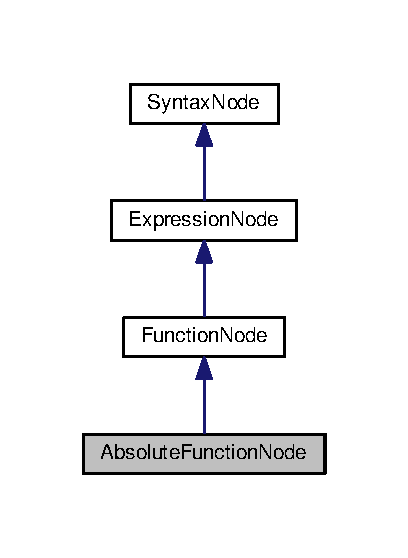
\includegraphics[width=196pt]{d8/d0a/classAbsoluteFunctionNode__inherit__graph}
\end{center}
\end{figure}


Collaboration diagram for Absolute\+Function\+Node\+:
\nopagebreak
\begin{figure}[H]
\begin{center}
\leavevmode
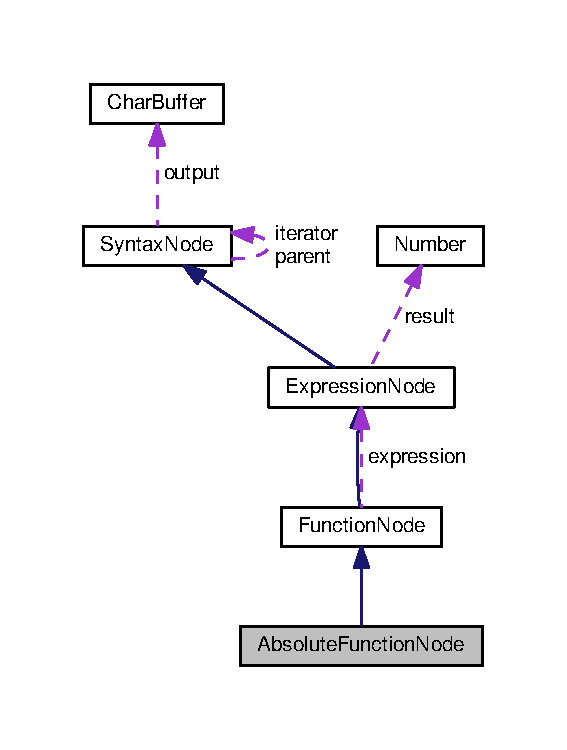
\includegraphics[width=272pt]{df/dc1/classAbsoluteFunctionNode__coll__graph}
\end{center}
\end{figure}
\subsection*{Public Member Functions}
\begin{DoxyCompactItemize}
\item 
\hyperlink{classAbsoluteFunctionNode_adcc843140de3a7435546a293b9b5b882}{Absolute\+Function\+Node} (\hyperlink{classExpressionNode}{Expression\+Node} $\ast$\hyperlink{classFunctionNode_ad7577b179a1937aaf8a0058bb5b546dc}{expression})
\item 
\hyperlink{structNumber}{Number} $\ast$ \hyperlink{classAbsoluteFunctionNode_addd9710c60598aca391822e25d67ab33}{Evaluate} ()
\end{DoxyCompactItemize}
\subsection*{Static Public Member Functions}
\begin{DoxyCompactItemize}
\item 
static \hyperlink{classFunctionNode}{Function\+Node} $\ast$ \hyperlink{classAbsoluteFunctionNode_a9da4bc82d15f41aaf9adde83974af83d}{Create} (\hyperlink{classExpressionNode}{Expression\+Node} $\ast$\hyperlink{classFunctionNode_ad7577b179a1937aaf8a0058bb5b546dc}{expression})
\end{DoxyCompactItemize}
\subsection*{Protected Member Functions}
\begin{DoxyCompactItemize}
\item 
char $\ast$ \hyperlink{classAbsoluteFunctionNode_a4cfc007fc3a4280fc294e04668aae566}{Get\+Node\+Text} ()
\end{DoxyCompactItemize}
\subsection*{Additional Inherited Members}


\subsection{Detailed Description}


Definition at line 178 of file functions.\+h.



\subsection{Constructor \& Destructor Documentation}
\index{Absolute\+Function\+Node@{Absolute\+Function\+Node}!Absolute\+Function\+Node@{Absolute\+Function\+Node}}
\index{Absolute\+Function\+Node@{Absolute\+Function\+Node}!Absolute\+Function\+Node@{Absolute\+Function\+Node}}
\subsubsection[{\texorpdfstring{Absolute\+Function\+Node(\+Expression\+Node $\ast$expression)}{AbsoluteFunctionNode(ExpressionNode *expression)}}]{\setlength{\rightskip}{0pt plus 5cm}Absolute\+Function\+Node\+::\+Absolute\+Function\+Node (
\begin{DoxyParamCaption}
\item[{{\bf Expression\+Node} $\ast$}]{expression}
\end{DoxyParamCaption}
)}\hypertarget{classAbsoluteFunctionNode_adcc843140de3a7435546a293b9b5b882}{}\label{classAbsoluteFunctionNode_adcc843140de3a7435546a293b9b5b882}


Definition at line 491 of file functions.\+cpp.



References Function\+Node\+::\+Function\+Node().



Referenced by Create().


\begin{DoxyCode}
491                                                                      :
492     \hyperlink{classFunctionNode_a41cb7db0162ffbec0902bd8ff7ea435f}{FunctionNode}(expression) \{ \}
\end{DoxyCode}


Here is the call graph for this function\+:
\nopagebreak
\begin{figure}[H]
\begin{center}
\leavevmode
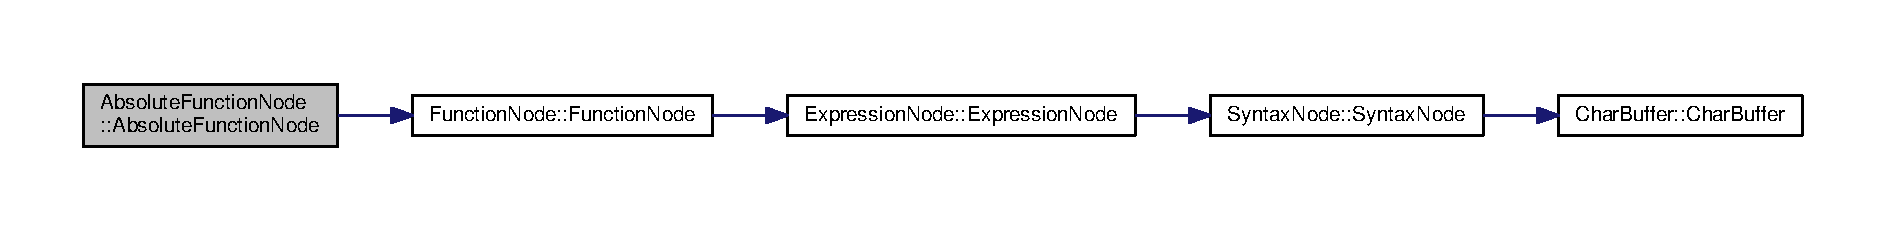
\includegraphics[width=350pt]{dc/d52/classAbsoluteFunctionNode_adcc843140de3a7435546a293b9b5b882_cgraph}
\end{center}
\end{figure}




Here is the caller graph for this function\+:
\nopagebreak
\begin{figure}[H]
\begin{center}
\leavevmode
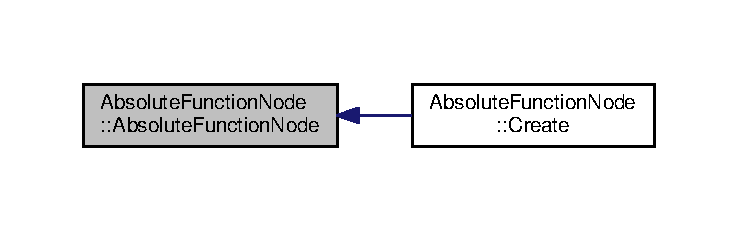
\includegraphics[width=350pt]{dc/d52/classAbsoluteFunctionNode_adcc843140de3a7435546a293b9b5b882_icgraph}
\end{center}
\end{figure}




\subsection{Member Function Documentation}
\index{Absolute\+Function\+Node@{Absolute\+Function\+Node}!Create@{Create}}
\index{Create@{Create}!Absolute\+Function\+Node@{Absolute\+Function\+Node}}
\subsubsection[{\texorpdfstring{Create(\+Expression\+Node $\ast$expression)}{Create(ExpressionNode *expression)}}]{\setlength{\rightskip}{0pt plus 5cm}{\bf Function\+Node} $\ast$ Absolute\+Function\+Node\+::\+Create (
\begin{DoxyParamCaption}
\item[{{\bf Expression\+Node} $\ast$}]{expression}
\end{DoxyParamCaption}
)\hspace{0.3cm}{\ttfamily [static]}}\hypertarget{classAbsoluteFunctionNode_a9da4bc82d15f41aaf9adde83974af83d}{}\label{classAbsoluteFunctionNode_a9da4bc82d15f41aaf9adde83974af83d}


Definition at line 494 of file functions.\+cpp.



References Absolute\+Function\+Node().


\begin{DoxyCode}
495 \{
496     \textcolor{keywordflow}{return} \textcolor{keyword}{new} \hyperlink{classAbsoluteFunctionNode_adcc843140de3a7435546a293b9b5b882}{AbsoluteFunctionNode}(expression);
497 \}
\end{DoxyCode}


Here is the call graph for this function\+:
\nopagebreak
\begin{figure}[H]
\begin{center}
\leavevmode
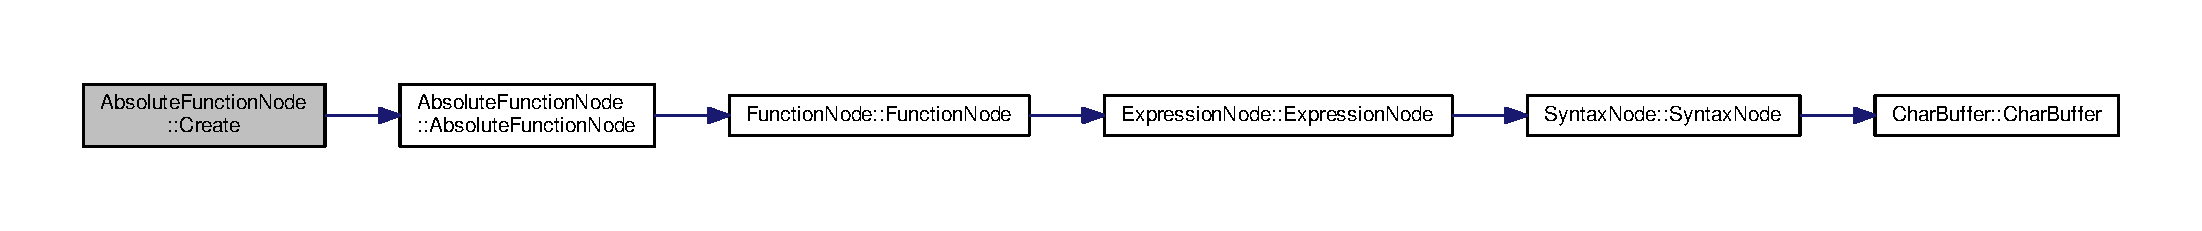
\includegraphics[width=350pt]{dc/d52/classAbsoluteFunctionNode_a9da4bc82d15f41aaf9adde83974af83d_cgraph}
\end{center}
\end{figure}


\index{Absolute\+Function\+Node@{Absolute\+Function\+Node}!Evaluate@{Evaluate}}
\index{Evaluate@{Evaluate}!Absolute\+Function\+Node@{Absolute\+Function\+Node}}
\subsubsection[{\texorpdfstring{Evaluate()}{Evaluate()}}]{\setlength{\rightskip}{0pt plus 5cm}{\bf Number} $\ast$ Absolute\+Function\+Node\+::\+Evaluate (
\begin{DoxyParamCaption}
{}
\end{DoxyParamCaption}
)\hspace{0.3cm}{\ttfamily [virtual]}}\hypertarget{classAbsoluteFunctionNode_addd9710c60598aca391822e25d67ab33}{}\label{classAbsoluteFunctionNode_addd9710c60598aca391822e25d67ab33}


Implements \hyperlink{classExpressionNode_a64975d4dc37742228bd522f6204537f7}{Expression\+Node}.



Definition at line 499 of file functions.\+cpp.



References Number\+::\+Absolute(), Expression\+Node\+::\+Evaluate(), Function\+Node\+::expression, and Expression\+Node\+::result.


\begin{DoxyCode}
500 \{
501     \hyperlink{classExpressionNode_a1f590649f5a5cb30eb7ee912f7bc1262}{result} = \hyperlink{classFunctionNode_ad7577b179a1937aaf8a0058bb5b546dc}{expression}->\hyperlink{classExpressionNode_a64975d4dc37742228bd522f6204537f7}{Evaluate}()->\hyperlink{structNumber_acdbe13cd9862bb73225a893fb14de2a5}{Absolute}();
502     \textcolor{keywordflow}{return} \hyperlink{classExpressionNode_a1f590649f5a5cb30eb7ee912f7bc1262}{result};
503 \}
\end{DoxyCode}


Here is the call graph for this function\+:
\nopagebreak
\begin{figure}[H]
\begin{center}
\leavevmode
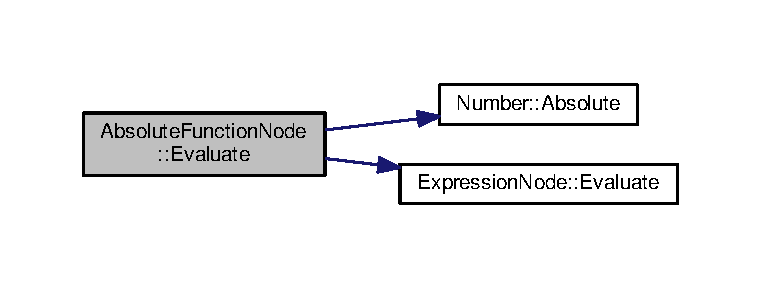
\includegraphics[width=350pt]{dc/d52/classAbsoluteFunctionNode_addd9710c60598aca391822e25d67ab33_cgraph}
\end{center}
\end{figure}


\index{Absolute\+Function\+Node@{Absolute\+Function\+Node}!Get\+Node\+Text@{Get\+Node\+Text}}
\index{Get\+Node\+Text@{Get\+Node\+Text}!Absolute\+Function\+Node@{Absolute\+Function\+Node}}
\subsubsection[{\texorpdfstring{Get\+Node\+Text()}{GetNodeText()}}]{\setlength{\rightskip}{0pt plus 5cm}char $\ast$ Absolute\+Function\+Node\+::\+Get\+Node\+Text (
\begin{DoxyParamCaption}
{}
\end{DoxyParamCaption}
)\hspace{0.3cm}{\ttfamily [protected]}, {\ttfamily [virtual]}}\hypertarget{classAbsoluteFunctionNode_a4cfc007fc3a4280fc294e04668aae566}{}\label{classAbsoluteFunctionNode_a4cfc007fc3a4280fc294e04668aae566}


Implements \hyperlink{classExpressionNode_a42a5e9562b0f645a19dcc83f698069b5}{Expression\+Node}.



Definition at line 505 of file functions.\+cpp.


\begin{DoxyCode}
506 \{
507     \textcolor{keywordflow}{return} (\textcolor{keywordtype}{char}*)\textcolor{stringliteral}{"abs"};
508 \}
\end{DoxyCode}


The documentation for this class was generated from the following files\+:\begin{DoxyCompactItemize}
\item 
app/main/\hyperlink{functions_8h}{functions.\+h}\item 
app/main/\hyperlink{functions_8cpp}{functions.\+cpp}\end{DoxyCompactItemize}

\hypertarget{classAbsoluteNode}{}\section{Absolute\+Node Class Reference}
\label{classAbsoluteNode}\index{Absolute\+Node@{Absolute\+Node}}


{\ttfamily \#include $<$operators.\+h$>$}



Inheritance diagram for Absolute\+Node\+:\nopagebreak
\begin{figure}[H]
\begin{center}
\leavevmode
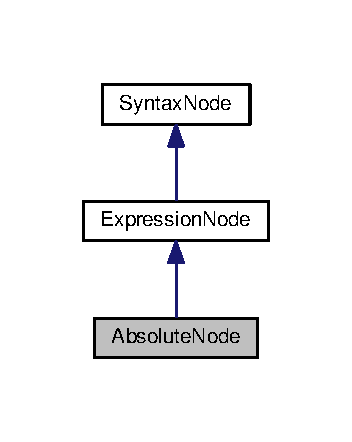
\includegraphics[width=169pt]{classAbsoluteNode__inherit__graph}
\end{center}
\end{figure}


Collaboration diagram for Absolute\+Node\+:\nopagebreak
\begin{figure}[H]
\begin{center}
\leavevmode
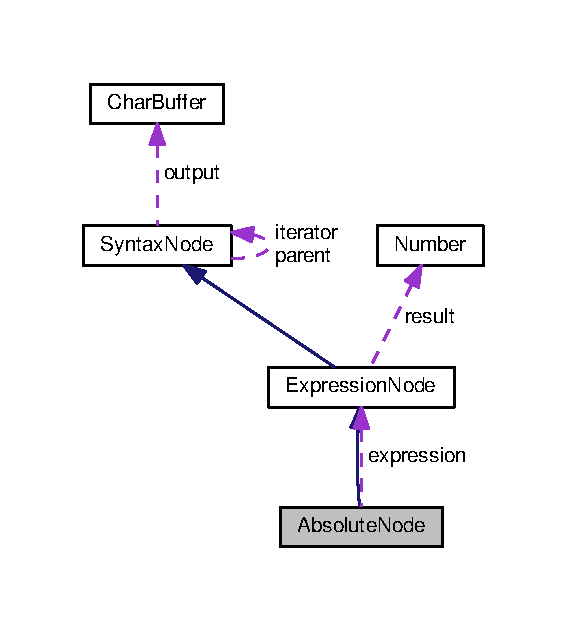
\includegraphics[width=272pt]{classAbsoluteNode__coll__graph}
\end{center}
\end{figure}
\subsection*{Public Member Functions}
\begin{DoxyCompactItemize}
\item 
\hyperlink{classAbsoluteNode_af1206a7293f334c1d544cafe95af3ba5}{Absolute\+Node} (\hyperlink{classExpressionNode}{Expression\+Node} $\ast$\hyperlink{classAbsoluteNode_a1b1bea1b153597964e64c7e15f0aa9e1}{expression})
\item 
\hyperlink{classAbsoluteNode_ac4805b3b37437bb1fd4acb14eb4eeced}{$\sim$\+Absolute\+Node} ()
\item 
char $\ast$ \hyperlink{classAbsoluteNode_ada1094b5e5ed6033f193ac151058c364}{Get\+Text} ()
\item 
\hyperlink{structNumber}{Number} $\ast$ \hyperlink{classAbsoluteNode_a35e012fdac8bff4c5252021254f07cbe}{Evaluate} ()
\item 
int \hyperlink{classAbsoluteNode_a6fb0f08b41c558e8746b24fa79552545}{Get\+Precedence} ()
\item 
\hyperlink{classSyntaxNode}{Syntax\+Node} $\ast$ \hyperlink{classAbsoluteNode_adcc7a1dd7bd20d811c5b9ac8d9e5efb1}{Get\+Next} ()
\item 
void \hyperlink{classAbsoluteNode_a4f947588881076306bf79f69145713b7}{Attach} (\hyperlink{classSyntaxNode}{Syntax\+Node} $\ast$node)
\item 
void \hyperlink{classAbsoluteNode_a5bf1491e1f71c87b38360e0d9231ac11}{Detach} (\hyperlink{classSyntaxNode}{Syntax\+Node} $\ast$node)
\item 
void \hyperlink{classAbsoluteNode_a675d28427432b9947af9441c3bcf5401}{Replace} (\hyperlink{classSyntaxNode}{Syntax\+Node} $\ast$n, \hyperlink{classSyntaxNode}{Syntax\+Node} $\ast$x)
\end{DoxyCompactItemize}
\subsection*{Protected Member Functions}
\begin{DoxyCompactItemize}
\item 
char $\ast$ \hyperlink{classAbsoluteNode_ae5e2148cb9fedaee9137d3c124399c76}{Get\+Node\+Text} ()
\end{DoxyCompactItemize}
\subsection*{Private Attributes}
\begin{DoxyCompactItemize}
\item 
\hyperlink{classExpressionNode}{Expression\+Node} $\ast$ \hyperlink{classAbsoluteNode_a1b1bea1b153597964e64c7e15f0aa9e1}{expression}
\end{DoxyCompactItemize}
\subsection*{Additional Inherited Members}


\subsection{Detailed Description}


Definition at line 60 of file operators.\+h.



\subsection{Constructor \& Destructor Documentation}
\index{Absolute\+Node@{Absolute\+Node}!Absolute\+Node@{Absolute\+Node}}
\index{Absolute\+Node@{Absolute\+Node}!Absolute\+Node@{Absolute\+Node}}
\subsubsection[{\texorpdfstring{Absolute\+Node(\+Expression\+Node $\ast$expression)}{AbsoluteNode(ExpressionNode *expression)}}]{\setlength{\rightskip}{0pt plus 5cm}Absolute\+Node\+::\+Absolute\+Node (
\begin{DoxyParamCaption}
\item[{{\bf Expression\+Node} $\ast$}]{expression}
\end{DoxyParamCaption}
)}\hypertarget{classAbsoluteNode_af1206a7293f334c1d544cafe95af3ba5}{}\label{classAbsoluteNode_af1206a7293f334c1d544cafe95af3ba5}


Definition at line 125 of file operators.\+cpp.



References expression, and Expression\+Node\+::\+Expression\+Node().



Referenced by Parser\+::\+Parse\+Atomic().


\begin{DoxyCode}
125                                                      :
126     \hyperlink{classExpressionNode_adc8888de5329d356224c8a93f3ce2b75}{ExpressionNode}(), \hyperlink{classAbsoluteNode_a1b1bea1b153597964e64c7e15f0aa9e1}{expression}(expression) \{ \}
\end{DoxyCode}


Here is the call graph for this function\+:\nopagebreak
\begin{figure}[H]
\begin{center}
\leavevmode
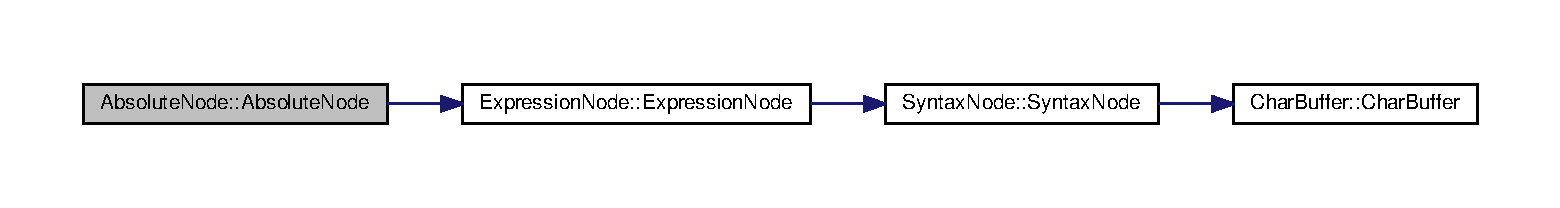
\includegraphics[width=350pt]{classAbsoluteNode_af1206a7293f334c1d544cafe95af3ba5_cgraph}
\end{center}
\end{figure}




Here is the caller graph for this function\+:\nopagebreak
\begin{figure}[H]
\begin{center}
\leavevmode
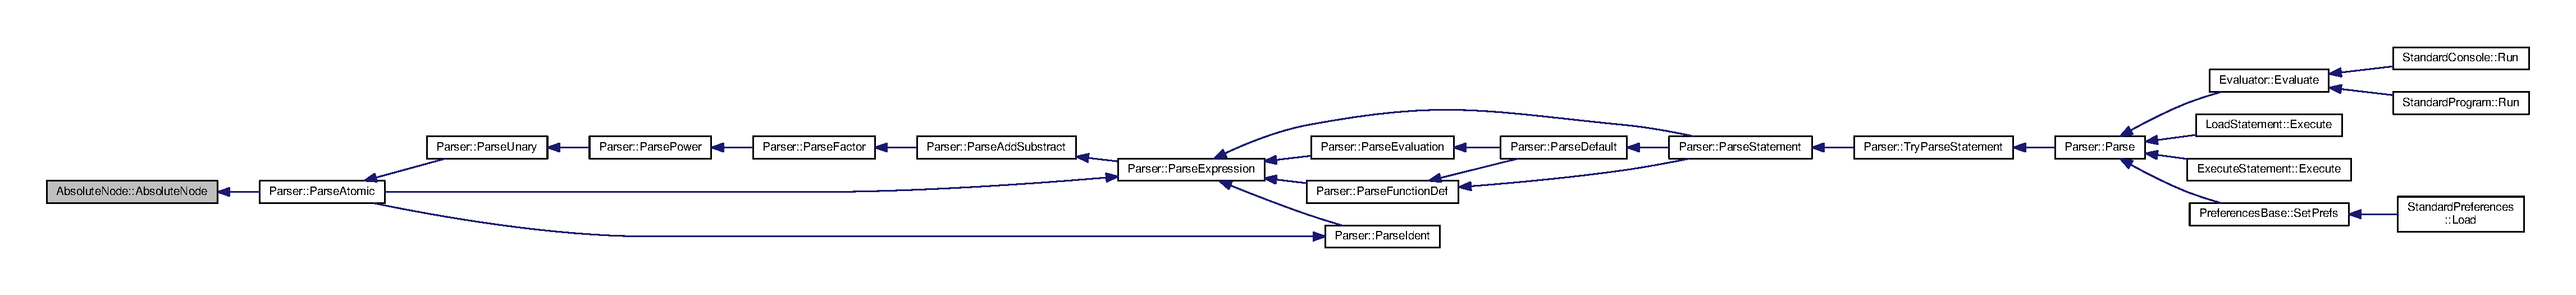
\includegraphics[width=350pt]{classAbsoluteNode_af1206a7293f334c1d544cafe95af3ba5_icgraph}
\end{center}
\end{figure}


\index{Absolute\+Node@{Absolute\+Node}!````~Absolute\+Node@{$\sim$\+Absolute\+Node}}
\index{````~Absolute\+Node@{$\sim$\+Absolute\+Node}!Absolute\+Node@{Absolute\+Node}}
\subsubsection[{\texorpdfstring{$\sim$\+Absolute\+Node()}{~AbsoluteNode()}}]{\setlength{\rightskip}{0pt plus 5cm}Absolute\+Node\+::$\sim$\+Absolute\+Node (
\begin{DoxyParamCaption}
{}
\end{DoxyParamCaption}
)}\hypertarget{classAbsoluteNode_ac4805b3b37437bb1fd4acb14eb4eeced}{}\label{classAbsoluteNode_ac4805b3b37437bb1fd4acb14eb4eeced}


Definition at line 128 of file operators.\+cpp.



References expression.


\begin{DoxyCode}
129 \{
130     \textcolor{keywordflow}{if} (\hyperlink{classAbsoluteNode_a1b1bea1b153597964e64c7e15f0aa9e1}{expression} != \hyperlink{platform_8h_a46ff2bfbf0d44b8466a2251d5bd5e6f8}{NOMEM}) \{
131         \textcolor{keyword}{delete} \hyperlink{classAbsoluteNode_a1b1bea1b153597964e64c7e15f0aa9e1}{expression};
132     \}
133 \}
\end{DoxyCode}


\subsection{Member Function Documentation}
\index{Absolute\+Node@{Absolute\+Node}!Attach@{Attach}}
\index{Attach@{Attach}!Absolute\+Node@{Absolute\+Node}}
\subsubsection[{\texorpdfstring{Attach(\+Syntax\+Node $\ast$node)}{Attach(SyntaxNode *node)}}]{\setlength{\rightskip}{0pt plus 5cm}void Absolute\+Node\+::\+Attach (
\begin{DoxyParamCaption}
\item[{{\bf Syntax\+Node} $\ast$}]{node}
\end{DoxyParamCaption}
)\hspace{0.3cm}{\ttfamily [virtual]}}\hypertarget{classAbsoluteNode_a4f947588881076306bf79f69145713b7}{}\label{classAbsoluteNode_a4f947588881076306bf79f69145713b7}


Implements \hyperlink{classSyntaxNode_af25fd5963125bb2d6b9a1864b9ff79c8}{Syntax\+Node}.



Definition at line 175 of file operators.\+cpp.



References expression, and Syntax\+Node\+::\+Set\+Parent().


\begin{DoxyCode}
176 \{
177     \textcolor{keywordflow}{if} (\hyperlink{classAbsoluteNode_a1b1bea1b153597964e64c7e15f0aa9e1}{expression} == \hyperlink{platform_8h_a46ff2bfbf0d44b8466a2251d5bd5e6f8}{NOMEM}) \{
178         \hyperlink{classAbsoluteNode_a1b1bea1b153597964e64c7e15f0aa9e1}{expression} = (\hyperlink{classExpressionNode}{ExpressionNode}*)node;
179         node->\hyperlink{classSyntaxNode_a7902bb2c389a784c11c2b649a84824e9}{SetParent}(\textcolor{keyword}{this});
180     \}
181 \}
\end{DoxyCode}


Here is the call graph for this function\+:\nopagebreak
\begin{figure}[H]
\begin{center}
\leavevmode
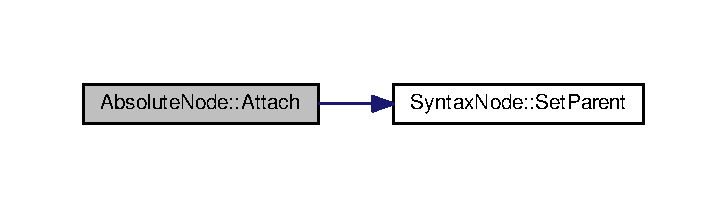
\includegraphics[width=349pt]{classAbsoluteNode_a4f947588881076306bf79f69145713b7_cgraph}
\end{center}
\end{figure}


\index{Absolute\+Node@{Absolute\+Node}!Detach@{Detach}}
\index{Detach@{Detach}!Absolute\+Node@{Absolute\+Node}}
\subsubsection[{\texorpdfstring{Detach(\+Syntax\+Node $\ast$node)}{Detach(SyntaxNode *node)}}]{\setlength{\rightskip}{0pt plus 5cm}void Absolute\+Node\+::\+Detach (
\begin{DoxyParamCaption}
\item[{{\bf Syntax\+Node} $\ast$}]{node}
\end{DoxyParamCaption}
)\hspace{0.3cm}{\ttfamily [virtual]}}\hypertarget{classAbsoluteNode_a5bf1491e1f71c87b38360e0d9231ac11}{}\label{classAbsoluteNode_a5bf1491e1f71c87b38360e0d9231ac11}


Implements \hyperlink{classSyntaxNode_ae57f629a5c5fa0994f036c105396da69}{Syntax\+Node}.



Definition at line 183 of file operators.\+cpp.



References expression.


\begin{DoxyCode}
184 \{
185     \textcolor{keywordflow}{if} (\hyperlink{classAbsoluteNode_a1b1bea1b153597964e64c7e15f0aa9e1}{expression} == node) \{
186         \hyperlink{classAbsoluteNode_a1b1bea1b153597964e64c7e15f0aa9e1}{expression} = \hyperlink{platform_8h_a46ff2bfbf0d44b8466a2251d5bd5e6f8}{NOMEM};
187     \}
188 \}
\end{DoxyCode}
\index{Absolute\+Node@{Absolute\+Node}!Evaluate@{Evaluate}}
\index{Evaluate@{Evaluate}!Absolute\+Node@{Absolute\+Node}}
\subsubsection[{\texorpdfstring{Evaluate()}{Evaluate()}}]{\setlength{\rightskip}{0pt plus 5cm}{\bf Number} $\ast$ Absolute\+Node\+::\+Evaluate (
\begin{DoxyParamCaption}
{}
\end{DoxyParamCaption}
)\hspace{0.3cm}{\ttfamily [virtual]}}\hypertarget{classAbsoluteNode_a35e012fdac8bff4c5252021254f07cbe}{}\label{classAbsoluteNode_a35e012fdac8bff4c5252021254f07cbe}


Implements \hyperlink{classExpressionNode_a64975d4dc37742228bd522f6204537f7}{Expression\+Node}.



Definition at line 154 of file operators.\+cpp.



References Number\+::\+Absolute(), Expression\+Node\+::\+Evaluate(), expression, and Expression\+Node\+::result.


\begin{DoxyCode}
155 \{
156     \hyperlink{classExpressionNode_a1f590649f5a5cb30eb7ee912f7bc1262}{result} = \hyperlink{classAbsoluteNode_a1b1bea1b153597964e64c7e15f0aa9e1}{expression}->\hyperlink{classExpressionNode_a64975d4dc37742228bd522f6204537f7}{Evaluate}()->\hyperlink{structNumber_acdbe13cd9862bb73225a893fb14de2a5}{Absolute}();
157     \textcolor{keywordflow}{return} \hyperlink{classExpressionNode_a1f590649f5a5cb30eb7ee912f7bc1262}{result};
158 \}
\end{DoxyCode}


Here is the call graph for this function\+:\nopagebreak
\begin{figure}[H]
\begin{center}
\leavevmode
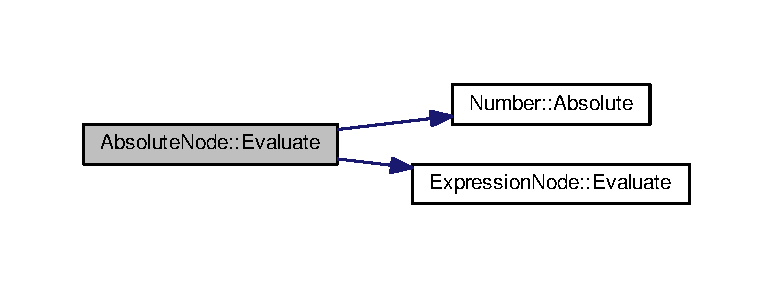
\includegraphics[width=350pt]{classAbsoluteNode_a35e012fdac8bff4c5252021254f07cbe_cgraph}
\end{center}
\end{figure}


\index{Absolute\+Node@{Absolute\+Node}!Get\+Next@{Get\+Next}}
\index{Get\+Next@{Get\+Next}!Absolute\+Node@{Absolute\+Node}}
\subsubsection[{\texorpdfstring{Get\+Next()}{GetNext()}}]{\setlength{\rightskip}{0pt plus 5cm}{\bf Syntax\+Node} $\ast$ Absolute\+Node\+::\+Get\+Next (
\begin{DoxyParamCaption}
{}
\end{DoxyParamCaption}
)\hspace{0.3cm}{\ttfamily [virtual]}}\hypertarget{classAbsoluteNode_adcc7a1dd7bd20d811c5b9ac8d9e5efb1}{}\label{classAbsoluteNode_adcc7a1dd7bd20d811c5b9ac8d9e5efb1}


Implements \hyperlink{classSyntaxNode_af1fa46ba30aa4f2affa2d4e96a4be010}{Syntax\+Node}.



Definition at line 165 of file operators.\+cpp.



References expression, and Syntax\+Node\+::iterator.


\begin{DoxyCode}
166 \{
167     \textcolor{keywordflow}{if} (\hyperlink{classSyntaxNode_a9bd3349d05f33eaa271cca1805a86e1b}{iterator} == \hyperlink{platform_8h_a46ff2bfbf0d44b8466a2251d5bd5e6f8}{NOMEM}) \{
168         \hyperlink{classSyntaxNode_a9bd3349d05f33eaa271cca1805a86e1b}{iterator} = \hyperlink{classAbsoluteNode_a1b1bea1b153597964e64c7e15f0aa9e1}{expression};
169         \textcolor{keywordflow}{return} \hyperlink{classSyntaxNode_a9bd3349d05f33eaa271cca1805a86e1b}{iterator};
170     \}
171 
172     \textcolor{keywordflow}{return} \hyperlink{platform_8h_a46ff2bfbf0d44b8466a2251d5bd5e6f8}{NOMEM};
173 \}
\end{DoxyCode}
\index{Absolute\+Node@{Absolute\+Node}!Get\+Node\+Text@{Get\+Node\+Text}}
\index{Get\+Node\+Text@{Get\+Node\+Text}!Absolute\+Node@{Absolute\+Node}}
\subsubsection[{\texorpdfstring{Get\+Node\+Text()}{GetNodeText()}}]{\setlength{\rightskip}{0pt plus 5cm}char $\ast$ Absolute\+Node\+::\+Get\+Node\+Text (
\begin{DoxyParamCaption}
{}
\end{DoxyParamCaption}
)\hspace{0.3cm}{\ttfamily [protected]}, {\ttfamily [virtual]}}\hypertarget{classAbsoluteNode_ae5e2148cb9fedaee9137d3c124399c76}{}\label{classAbsoluteNode_ae5e2148cb9fedaee9137d3c124399c76}


Implements \hyperlink{classExpressionNode_a42a5e9562b0f645a19dcc83f698069b5}{Expression\+Node}.



Definition at line 160 of file operators.\+cpp.



Referenced by Get\+Text().


\begin{DoxyCode}
161 \{
162     \textcolor{keywordflow}{return} (\textcolor{keywordtype}{char}*)\textcolor{stringliteral}{"|"};
163 \}
\end{DoxyCode}


Here is the caller graph for this function\+:\nopagebreak
\begin{figure}[H]
\begin{center}
\leavevmode
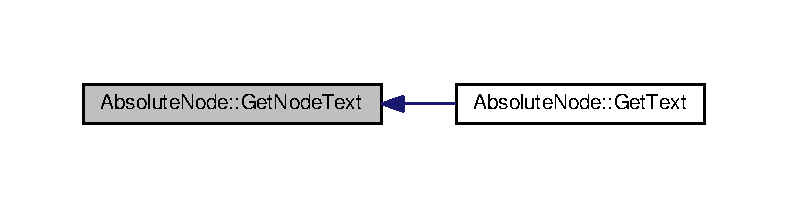
\includegraphics[width=350pt]{classAbsoluteNode_ae5e2148cb9fedaee9137d3c124399c76_icgraph}
\end{center}
\end{figure}


\index{Absolute\+Node@{Absolute\+Node}!Get\+Precedence@{Get\+Precedence}}
\index{Get\+Precedence@{Get\+Precedence}!Absolute\+Node@{Absolute\+Node}}
\subsubsection[{\texorpdfstring{Get\+Precedence()}{GetPrecedence()}}]{\setlength{\rightskip}{0pt plus 5cm}int Absolute\+Node\+::\+Get\+Precedence (
\begin{DoxyParamCaption}
{}
\end{DoxyParamCaption}
)\hspace{0.3cm}{\ttfamily [virtual]}}\hypertarget{classAbsoluteNode_a6fb0f08b41c558e8746b24fa79552545}{}\label{classAbsoluteNode_a6fb0f08b41c558e8746b24fa79552545}


Implements \hyperlink{classExpressionNode_a161b9ea0b79bbfc101d6f687c8481ddd}{Expression\+Node}.



Definition at line 149 of file operators.\+cpp.


\begin{DoxyCode}
150 \{
151     \textcolor{keywordflow}{return} 8;
152 \}
\end{DoxyCode}
\index{Absolute\+Node@{Absolute\+Node}!Get\+Text@{Get\+Text}}
\index{Get\+Text@{Get\+Text}!Absolute\+Node@{Absolute\+Node}}
\subsubsection[{\texorpdfstring{Get\+Text()}{GetText()}}]{\setlength{\rightskip}{0pt plus 5cm}char $\ast$ Absolute\+Node\+::\+Get\+Text (
\begin{DoxyParamCaption}
{}
\end{DoxyParamCaption}
)\hspace{0.3cm}{\ttfamily [virtual]}}\hypertarget{classAbsoluteNode_ada1094b5e5ed6033f193ac151058c364}{}\label{classAbsoluteNode_ada1094b5e5ed6033f193ac151058c364}


Implements \hyperlink{classExpressionNode_a0bbf243108a14eaf963a8161ffd8eb92}{Expression\+Node}.



Definition at line 135 of file operators.\+cpp.



References Char\+Buffer\+::\+Append(), Char\+Buffer\+::\+Empty(), Char\+Buffer\+::\+Ensure\+Size(), expression, Get\+Node\+Text(), Char\+Buffer\+::\+Get\+String(), Expression\+Node\+::\+Get\+Text(), Syntax\+Node\+::output, and Str\+Len().


\begin{DoxyCode}
136 \{
137     \textcolor{keyword}{const} \textcolor{keywordtype}{char} *expText = \hyperlink{classAbsoluteNode_a1b1bea1b153597964e64c7e15f0aa9e1}{expression}->\hyperlink{classExpressionNode_a0bbf243108a14eaf963a8161ffd8eb92}{GetText}();
138     \textcolor{keyword}{const} \textcolor{keywordtype}{char} *nodeText = \hyperlink{classAbsoluteNode_ae5e2148cb9fedaee9137d3c124399c76}{GetNodeText}();
139 
140     \hyperlink{classSyntaxNode_a1180628cbe3fce43930cee0df5a9ce5c}{output}->\hyperlink{classCharBuffer_abe39d3fd7d8b9c8ec343af2cae7adc96}{Empty}();
141     \hyperlink{classSyntaxNode_a1180628cbe3fce43930cee0df5a9ce5c}{output}->\hyperlink{classCharBuffer_ad1907009b5ad136692b989fa96bf2f7e}{EnsureSize}(\hyperlink{clib_8h_a67ec56eb98b49515d35005a5b3bf9a32}{StrLen}(expText) + \hyperlink{clib_8h_a67ec56eb98b49515d35005a5b3bf9a32}{StrLen}(nodeText) * 2 + 1);
142     \hyperlink{classSyntaxNode_a1180628cbe3fce43930cee0df5a9ce5c}{output}->\hyperlink{classCharBuffer_a045b38735f7b3007c1b98d3d7b7feafe}{Append}(nodeText);
143     \hyperlink{classSyntaxNode_a1180628cbe3fce43930cee0df5a9ce5c}{output}->\hyperlink{classCharBuffer_a045b38735f7b3007c1b98d3d7b7feafe}{Append}(expText);
144     \hyperlink{classSyntaxNode_a1180628cbe3fce43930cee0df5a9ce5c}{output}->\hyperlink{classCharBuffer_a045b38735f7b3007c1b98d3d7b7feafe}{Append}(nodeText);
145 
146     \textcolor{keywordflow}{return} \hyperlink{classSyntaxNode_a1180628cbe3fce43930cee0df5a9ce5c}{output}->\hyperlink{classCharBuffer_a7dfd3feaaf80f318ba44efe15b1ec44b}{GetString}();
147 \}
\end{DoxyCode}


Here is the call graph for this function\+:\nopagebreak
\begin{figure}[H]
\begin{center}
\leavevmode
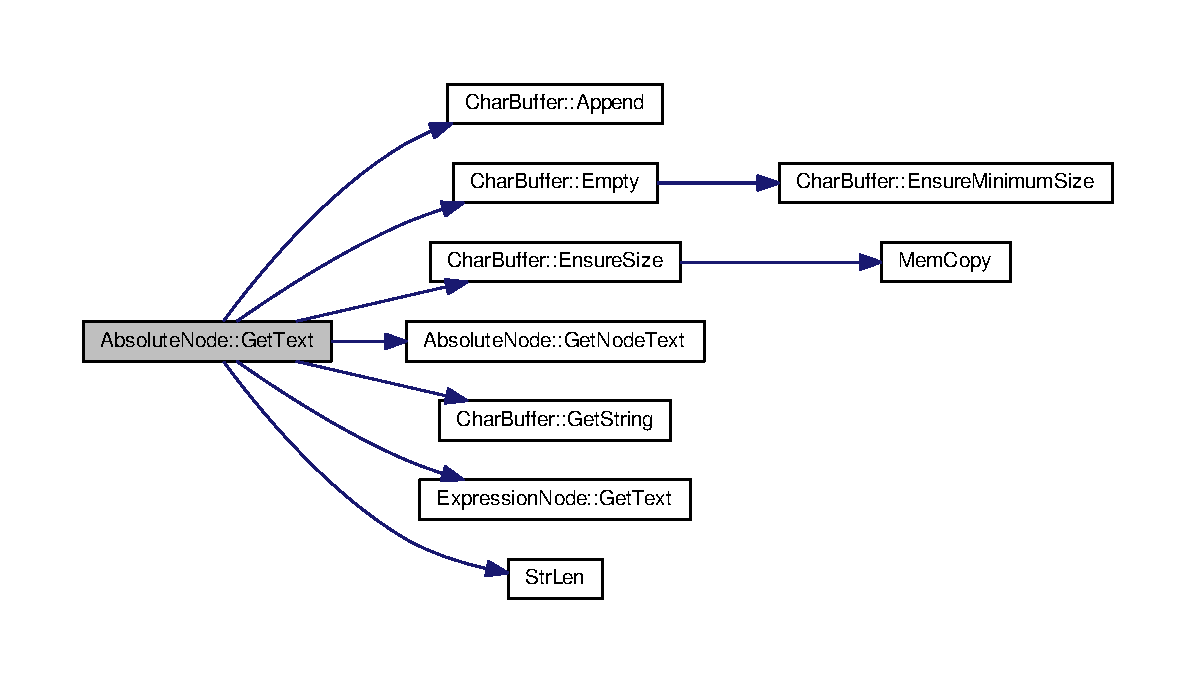
\includegraphics[width=350pt]{classAbsoluteNode_ada1094b5e5ed6033f193ac151058c364_cgraph}
\end{center}
\end{figure}


\index{Absolute\+Node@{Absolute\+Node}!Replace@{Replace}}
\index{Replace@{Replace}!Absolute\+Node@{Absolute\+Node}}
\subsubsection[{\texorpdfstring{Replace(\+Syntax\+Node $\ast$n, Syntax\+Node $\ast$x)}{Replace(SyntaxNode *n, SyntaxNode *x)}}]{\setlength{\rightskip}{0pt plus 5cm}void Absolute\+Node\+::\+Replace (
\begin{DoxyParamCaption}
\item[{{\bf Syntax\+Node} $\ast$}]{n, }
\item[{{\bf Syntax\+Node} $\ast$}]{x}
\end{DoxyParamCaption}
)\hspace{0.3cm}{\ttfamily [virtual]}}\hypertarget{classAbsoluteNode_a675d28427432b9947af9441c3bcf5401}{}\label{classAbsoluteNode_a675d28427432b9947af9441c3bcf5401}


Implements \hyperlink{classSyntaxNode_a2797ff5eb05f3a36ae1be41b70105e05}{Syntax\+Node}.



Definition at line 190 of file operators.\+cpp.



References expression.


\begin{DoxyCode}
191 \{
192     \textcolor{keywordflow}{if} (\hyperlink{classAbsoluteNode_a1b1bea1b153597964e64c7e15f0aa9e1}{expression} == n) \{
193         \textcolor{keyword}{delete} \hyperlink{classAbsoluteNode_a1b1bea1b153597964e64c7e15f0aa9e1}{expression};
194         \hyperlink{classAbsoluteNode_a1b1bea1b153597964e64c7e15f0aa9e1}{expression} = (\hyperlink{classExpressionNode}{ExpressionNode}*)x;
195     \}
196 \}
\end{DoxyCode}


\subsection{Member Data Documentation}
\index{Absolute\+Node@{Absolute\+Node}!expression@{expression}}
\index{expression@{expression}!Absolute\+Node@{Absolute\+Node}}
\subsubsection[{\texorpdfstring{expression}{expression}}]{\setlength{\rightskip}{0pt plus 5cm}{\bf Expression\+Node}$\ast$ Absolute\+Node\+::expression\hspace{0.3cm}{\ttfamily [private]}}\hypertarget{classAbsoluteNode_a1b1bea1b153597964e64c7e15f0aa9e1}{}\label{classAbsoluteNode_a1b1bea1b153597964e64c7e15f0aa9e1}


Definition at line 77 of file operators.\+h.



Referenced by Absolute\+Node(), Attach(), Detach(), Evaluate(), Get\+Next(), Get\+Text(), Replace(), and $\sim$\+Absolute\+Node().



The documentation for this class was generated from the following files\+:\begin{DoxyCompactItemize}
\item 
app/main/\hyperlink{operators_8h}{operators.\+h}\item 
app/main/\hyperlink{operators_8cpp}{operators.\+cpp}\end{DoxyCompactItemize}

\hypertarget{classAdditionNode}{}\section{Addition\+Node Class Reference}
\label{classAdditionNode}\index{Addition\+Node@{Addition\+Node}}


{\ttfamily \#include $<$operators.\+h$>$}



Inheritance diagram for Addition\+Node\+:
\nopagebreak
\begin{figure}[H]
\begin{center}
\leavevmode
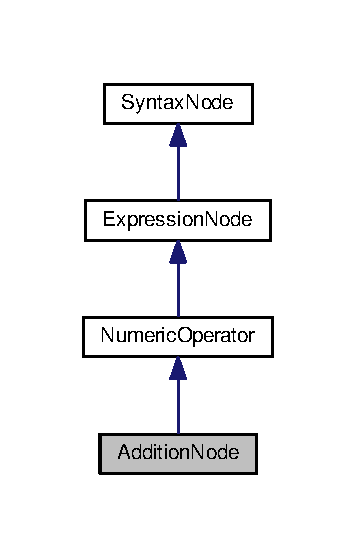
\includegraphics[width=171pt]{dc/d91/classAdditionNode__inherit__graph}
\end{center}
\end{figure}


Collaboration diagram for Addition\+Node\+:
\nopagebreak
\begin{figure}[H]
\begin{center}
\leavevmode
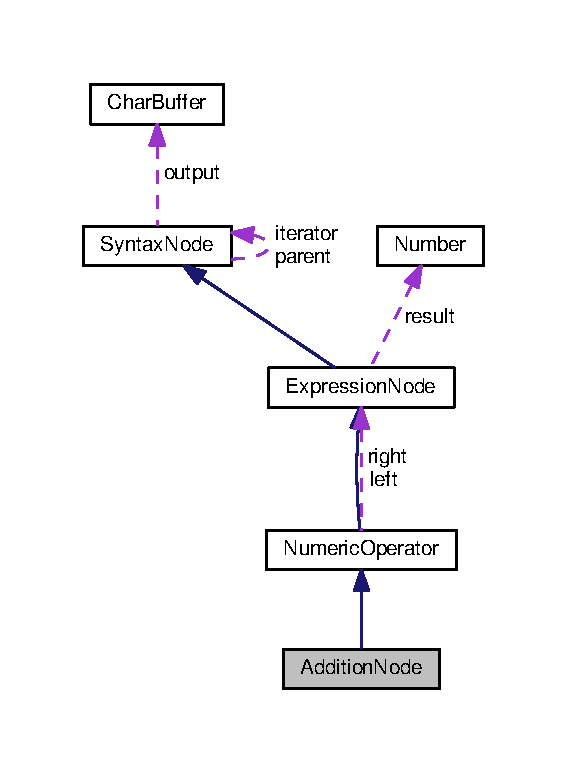
\includegraphics[width=272pt]{d1/d6d/classAdditionNode__coll__graph}
\end{center}
\end{figure}
\subsection*{Public Member Functions}
\begin{DoxyCompactItemize}
\item 
\hyperlink{classAdditionNode_ad887731026da63e83069e3c5a282b02d}{Addition\+Node} (\hyperlink{classExpressionNode}{Expression\+Node} $\ast$\hyperlink{classNumericOperator_a55da3c4075408deff978711030fa8258}{left}, \hyperlink{classExpressionNode}{Expression\+Node} $\ast$\hyperlink{classNumericOperator_aa2c5b5bea59bbb068bc6013bc5cac483}{right})
\item 
\hyperlink{nodes_8h_ab321a69ad5704b704b8dd9e1b3984a29}{Reduction\+Type} \hyperlink{classAdditionNode_a0e397ee6a3a4c8936e6c5a366c030dee}{Get\+Reduction\+Type} ()
\item 
int \hyperlink{classAdditionNode_a2e3b68052c4160597a34966b5654ab4b}{Get\+Precedence} ()
\item 
\hyperlink{structNumber}{Number} $\ast$ \hyperlink{classAdditionNode_a670d80d50ea6f8d1e38855de7130a503}{Evaluate} ()
\end{DoxyCompactItemize}
\subsection*{Protected Member Functions}
\begin{DoxyCompactItemize}
\item 
char $\ast$ \hyperlink{classAdditionNode_acae67b14a0db5b1e972968fa9d00f906}{Get\+Node\+Text} ()
\end{DoxyCompactItemize}
\subsection*{Additional Inherited Members}


\subsection{Detailed Description}


Definition at line 96 of file operators.\+h.



\subsection{Constructor \& Destructor Documentation}
\index{Addition\+Node@{Addition\+Node}!Addition\+Node@{Addition\+Node}}
\index{Addition\+Node@{Addition\+Node}!Addition\+Node@{Addition\+Node}}
\subsubsection[{\texorpdfstring{Addition\+Node(\+Expression\+Node $\ast$left, Expression\+Node $\ast$right)}{AdditionNode(ExpressionNode *left, ExpressionNode *right)}}]{\setlength{\rightskip}{0pt plus 5cm}Addition\+Node\+::\+Addition\+Node (
\begin{DoxyParamCaption}
\item[{{\bf Expression\+Node} $\ast$}]{left, }
\item[{{\bf Expression\+Node} $\ast$}]{right}
\end{DoxyParamCaption}
)}\hypertarget{classAdditionNode_ad887731026da63e83069e3c5a282b02d}{}\label{classAdditionNode_ad887731026da63e83069e3c5a282b02d}


Definition at line 301 of file operators.\+cpp.



References Numeric\+Operator\+::\+Numeric\+Operator().



Referenced by Parser\+::\+Parse\+Add\+Substract().


\begin{DoxyCode}
301                                                                      :
302     \hyperlink{classNumericOperator_a49cd2230b867cdfca64715aaf6e37561}{NumericOperator}(left, right) \{ \}
\end{DoxyCode}


Here is the call graph for this function\+:
\nopagebreak
\begin{figure}[H]
\begin{center}
\leavevmode
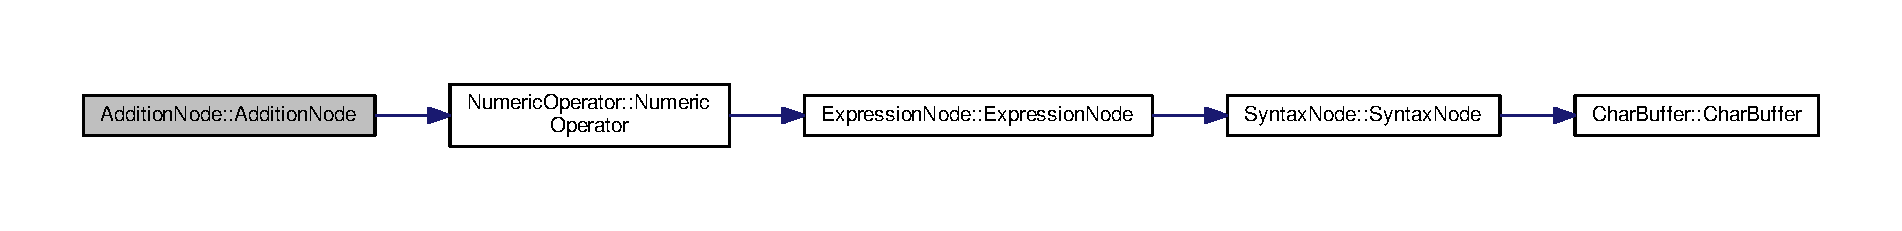
\includegraphics[width=350pt]{d1/d9d/classAdditionNode_ad887731026da63e83069e3c5a282b02d_cgraph}
\end{center}
\end{figure}




Here is the caller graph for this function\+:
\nopagebreak
\begin{figure}[H]
\begin{center}
\leavevmode
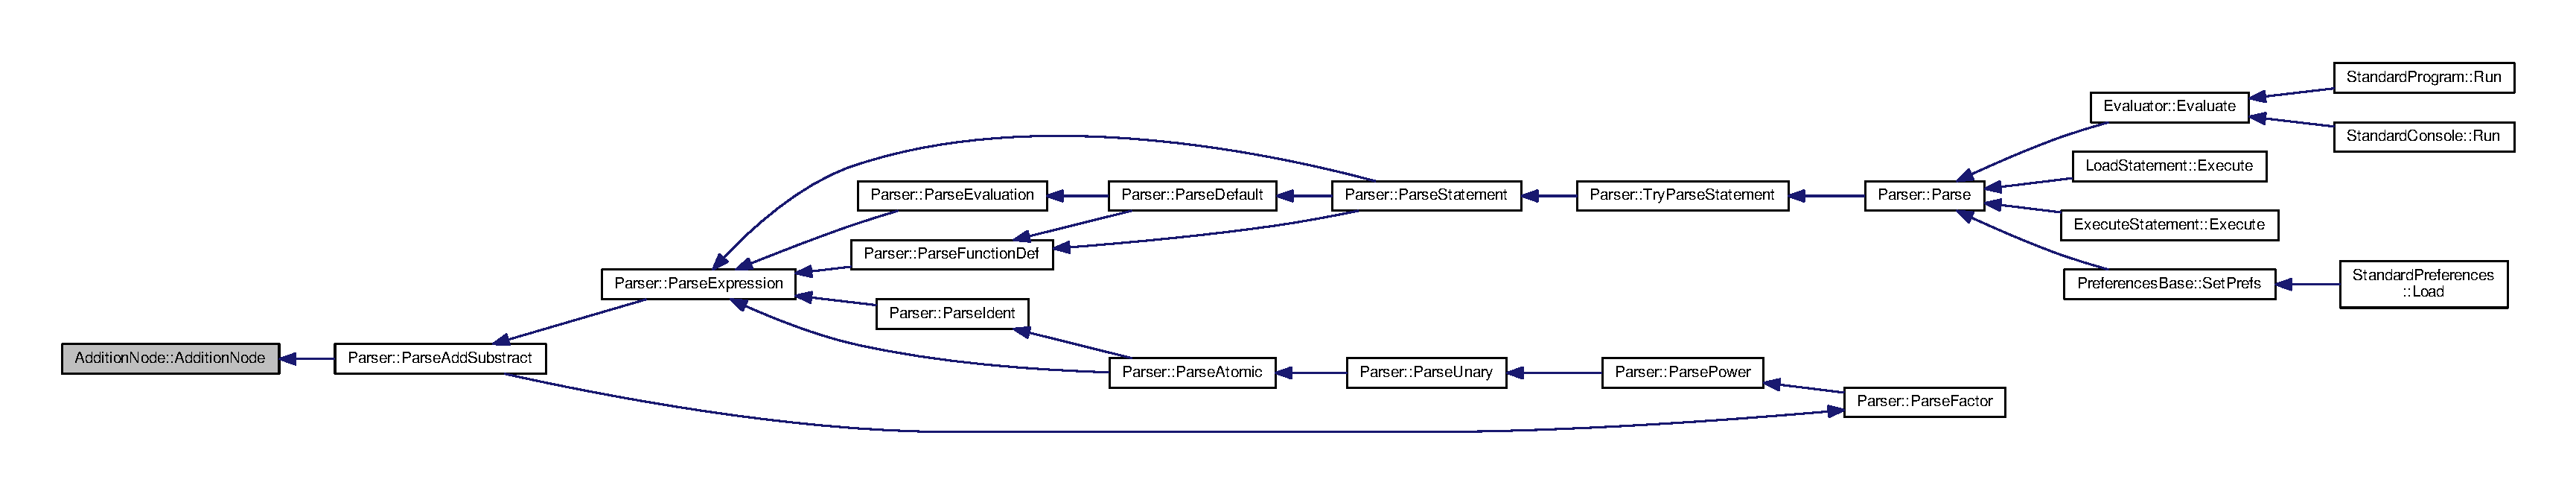
\includegraphics[width=350pt]{d1/d9d/classAdditionNode_ad887731026da63e83069e3c5a282b02d_icgraph}
\end{center}
\end{figure}




\subsection{Member Function Documentation}
\index{Addition\+Node@{Addition\+Node}!Evaluate@{Evaluate}}
\index{Evaluate@{Evaluate}!Addition\+Node@{Addition\+Node}}
\subsubsection[{\texorpdfstring{Evaluate()}{Evaluate()}}]{\setlength{\rightskip}{0pt plus 5cm}{\bf Number} $\ast$ Addition\+Node\+::\+Evaluate (
\begin{DoxyParamCaption}
{}
\end{DoxyParamCaption}
)\hspace{0.3cm}{\ttfamily [virtual]}}\hypertarget{classAdditionNode_a670d80d50ea6f8d1e38855de7130a503}{}\label{classAdditionNode_a670d80d50ea6f8d1e38855de7130a503}


Implements \hyperlink{classExpressionNode_a64975d4dc37742228bd522f6204537f7}{Expression\+Node}.



Definition at line 314 of file operators.\+cpp.



References Number\+::\+Add(), Expression\+Node\+::\+Evaluate(), Numeric\+Operator\+::left, Expression\+Node\+::result, and Numeric\+Operator\+::right.


\begin{DoxyCode}
315 \{
316     \hyperlink{classExpressionNode_a1f590649f5a5cb30eb7ee912f7bc1262}{result} = \hyperlink{classNumericOperator_a55da3c4075408deff978711030fa8258}{left}->\hyperlink{classExpressionNode_a64975d4dc37742228bd522f6204537f7}{Evaluate}()->\hyperlink{structNumber_af38172a47d725f10b8586846cb06e8a4}{Add}(\hyperlink{classNumericOperator_aa2c5b5bea59bbb068bc6013bc5cac483}{right}->\hyperlink{classExpressionNode_a64975d4dc37742228bd522f6204537f7}{Evaluate}());
317     \textcolor{keywordflow}{return} \hyperlink{classExpressionNode_a1f590649f5a5cb30eb7ee912f7bc1262}{result};
318 \}
\end{DoxyCode}


Here is the call graph for this function\+:
\nopagebreak
\begin{figure}[H]
\begin{center}
\leavevmode
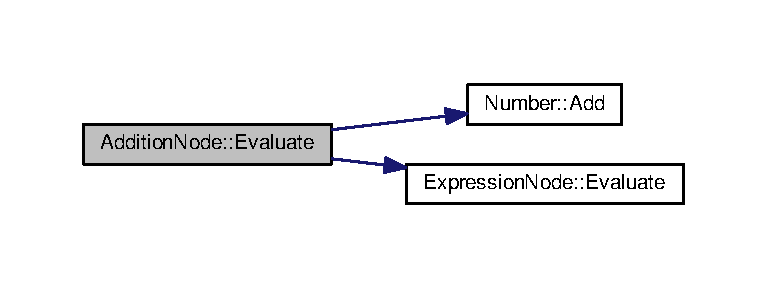
\includegraphics[width=350pt]{d1/d9d/classAdditionNode_a670d80d50ea6f8d1e38855de7130a503_cgraph}
\end{center}
\end{figure}


\index{Addition\+Node@{Addition\+Node}!Get\+Node\+Text@{Get\+Node\+Text}}
\index{Get\+Node\+Text@{Get\+Node\+Text}!Addition\+Node@{Addition\+Node}}
\subsubsection[{\texorpdfstring{Get\+Node\+Text()}{GetNodeText()}}]{\setlength{\rightskip}{0pt plus 5cm}char $\ast$ Addition\+Node\+::\+Get\+Node\+Text (
\begin{DoxyParamCaption}
{}
\end{DoxyParamCaption}
)\hspace{0.3cm}{\ttfamily [protected]}, {\ttfamily [virtual]}}\hypertarget{classAdditionNode_acae67b14a0db5b1e972968fa9d00f906}{}\label{classAdditionNode_acae67b14a0db5b1e972968fa9d00f906}


Implements \hyperlink{classExpressionNode_a42a5e9562b0f645a19dcc83f698069b5}{Expression\+Node}.



Definition at line 320 of file operators.\+cpp.


\begin{DoxyCode}
321 \{
322     \textcolor{keywordflow}{return} (\textcolor{keywordtype}{char}*)\textcolor{stringliteral}{"+"};
323 \}
\end{DoxyCode}
\index{Addition\+Node@{Addition\+Node}!Get\+Precedence@{Get\+Precedence}}
\index{Get\+Precedence@{Get\+Precedence}!Addition\+Node@{Addition\+Node}}
\subsubsection[{\texorpdfstring{Get\+Precedence()}{GetPrecedence()}}]{\setlength{\rightskip}{0pt plus 5cm}int Addition\+Node\+::\+Get\+Precedence (
\begin{DoxyParamCaption}
{}
\end{DoxyParamCaption}
)\hspace{0.3cm}{\ttfamily [virtual]}}\hypertarget{classAdditionNode_a2e3b68052c4160597a34966b5654ab4b}{}\label{classAdditionNode_a2e3b68052c4160597a34966b5654ab4b}


Implements \hyperlink{classExpressionNode_a161b9ea0b79bbfc101d6f687c8481ddd}{Expression\+Node}.



Definition at line 309 of file operators.\+cpp.


\begin{DoxyCode}
310 \{
311     \textcolor{keywordflow}{return} 2;
312 \}
\end{DoxyCode}
\index{Addition\+Node@{Addition\+Node}!Get\+Reduction\+Type@{Get\+Reduction\+Type}}
\index{Get\+Reduction\+Type@{Get\+Reduction\+Type}!Addition\+Node@{Addition\+Node}}
\subsubsection[{\texorpdfstring{Get\+Reduction\+Type()}{GetReductionType()}}]{\setlength{\rightskip}{0pt plus 5cm}{\bf Reduction\+Type} Addition\+Node\+::\+Get\+Reduction\+Type (
\begin{DoxyParamCaption}
{}
\end{DoxyParamCaption}
)\hspace{0.3cm}{\ttfamily [virtual]}}\hypertarget{classAdditionNode_a0e397ee6a3a4c8936e6c5a366c030dee}{}\label{classAdditionNode_a0e397ee6a3a4c8936e6c5a366c030dee}


Reimplemented from \hyperlink{classSyntaxNode_a5384fc779eee947b5e09bf2adb6cc606}{Syntax\+Node}.



Definition at line 304 of file operators.\+cpp.



References compladdreduc.


\begin{DoxyCode}
305 \{
306     \textcolor{keywordflow}{return} \hyperlink{nodes_8h_ab321a69ad5704b704b8dd9e1b3984a29ac930999b75ae22f50a2fa8d774a80936}{compladdreduc};
307 \}
\end{DoxyCode}


The documentation for this class was generated from the following files\+:\begin{DoxyCompactItemize}
\item 
app/main/\hyperlink{operators_8h}{operators.\+h}\item 
app/main/\hyperlink{operators_8cpp}{operators.\+cpp}\end{DoxyCompactItemize}

\hypertarget{structamathargs}{}\section{amathargs Struct Reference}
\label{structamathargs}\index{amathargs@{amathargs}}


{\ttfamily \#include $<$program\+\_\+amiga.\+h$>$}

\subsection*{Public Attributes}
\begin{DoxyCompactItemize}
\item 
long \hyperlink{structamathargs_a13baf6e4bcb57a301c2bb4bc36a8cbcb}{shell}
\item 
char $\ast$ \hyperlink{structamathargs_a78f3b2e3123c64b4f1ff646c1bacac2c}{input}
\end{DoxyCompactItemize}


\subsection{Detailed Description}


Definition at line 31 of file program\+\_\+amiga.\+h.



\subsection{Member Data Documentation}
\index{amathargs@{amathargs}!input@{input}}
\index{input@{input}!amathargs@{amathargs}}
\subsubsection[{\texorpdfstring{input}{input}}]{\setlength{\rightskip}{0pt plus 5cm}char$\ast$ amathargs\+::input}\hypertarget{structamathargs_a78f3b2e3123c64b4f1ff646c1bacac2c}{}\label{structamathargs_a78f3b2e3123c64b4f1ff646c1bacac2c}


Definition at line 33 of file program\+\_\+amiga.\+h.

\index{amathargs@{amathargs}!shell@{shell}}
\index{shell@{shell}!amathargs@{amathargs}}
\subsubsection[{\texorpdfstring{shell}{shell}}]{\setlength{\rightskip}{0pt plus 5cm}long amathargs\+::shell}\hypertarget{structamathargs_a13baf6e4bcb57a301c2bb4bc36a8cbcb}{}\label{structamathargs_a13baf6e4bcb57a301c2bb4bc36a8cbcb}


Definition at line 32 of file program\+\_\+amiga.\+h.



The documentation for this struct was generated from the following file\+:\begin{DoxyCompactItemize}
\item 
app/system/\hyperlink{program__amiga_8h}{program\+\_\+amiga.\+h}\end{DoxyCompactItemize}

\hypertarget{classAmigaLanguage}{}\section{Amiga\+Language Class Reference}
\label{classAmigaLanguage}\index{Amiga\+Language@{Amiga\+Language}}


{\ttfamily \#include $<$language\+\_\+amiga.\+h$>$}



Inheritance diagram for Amiga\+Language\+:
\nopagebreak
\begin{figure}[H]
\begin{center}
\leavevmode
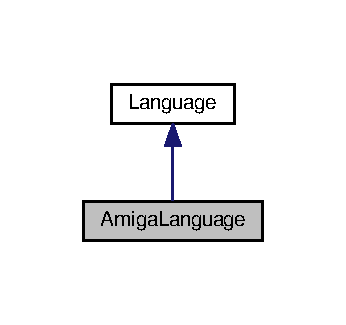
\includegraphics[width=166pt]{d4/d4f/classAmigaLanguage__inherit__graph}
\end{center}
\end{figure}


Collaboration diagram for Amiga\+Language\+:
\nopagebreak
\begin{figure}[H]
\begin{center}
\leavevmode
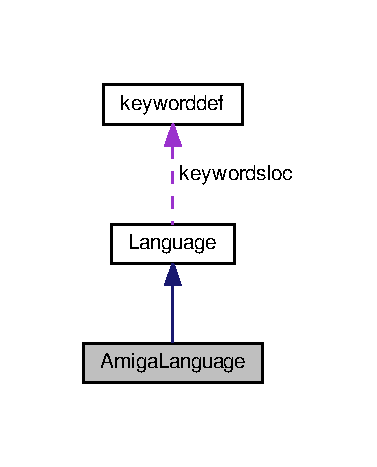
\includegraphics[width=181pt]{da/d4e/classAmigaLanguage__coll__graph}
\end{center}
\end{figure}
\subsection*{Public Member Functions}
\begin{DoxyCompactItemize}
\item 
\hyperlink{classAmigaLanguage_a5c5ba90b1a15f4b2ab7e4c0bdd7ca10d}{Amiga\+Language} ()
\item 
\hyperlink{classAmigaLanguage_a76e791f9eed9a9703c0a7fb7db68b09c}{$\sim$\+Amiga\+Language} ()
\item 
char \hyperlink{classAmigaLanguage_a8a3e470096d156b2c6e42283b5110b02}{Get\+Fraction\+Point} ()
\item 
\hyperlink{platform_8h_a1062901a7428fdd9c7f180f5e01ea056}{bool} \hyperlink{classAmigaLanguage_ae54fcf4c689939e1e0285781d47cf3b0}{Char\+Is\+Al\+Num} (unsigned long character)
\item 
\hyperlink{platform_8h_a1062901a7428fdd9c7f180f5e01ea056}{bool} \hyperlink{classAmigaLanguage_a3e786ae72c994e3d78eb19a5d8e896fc}{Char\+Is\+Alpha} (unsigned long character)
\item 
\hyperlink{platform_8h_a1062901a7428fdd9c7f180f5e01ea056}{bool} \hyperlink{classAmigaLanguage_afe6f40c3f96590d22a3fc6865058cc5c}{Char\+Is\+Digit} (unsigned long character)
\item 
\hyperlink{platform_8h_a1062901a7428fdd9c7f180f5e01ea056}{bool} \hyperlink{classAmigaLanguage_a915f8711f21b74ef2f9ad70f88cfdffb}{Char\+Is\+Punct} (unsigned long character)
\item 
\hyperlink{platform_8h_a1062901a7428fdd9c7f180f5e01ea056}{bool} \hyperlink{classAmigaLanguage_a41efaa7468f213abcaadda4dc4b73c9d}{Char\+Is\+Space} (unsigned long character)
\item 
\hyperlink{platform_8h_a1062901a7428fdd9c7f180f5e01ea056}{bool} \hyperlink{classAmigaLanguage_a2ae24f616652a4fc8af365d0ee50ae76}{Char\+Is\+Cntrl} (unsigned long character)
\item 
\hyperlink{platform_8h_a1062901a7428fdd9c7f180f5e01ea056}{bool} \hyperlink{classAmigaLanguage_a19a04fb8a564dd9fbeaf6f5b822d38e6}{Str\+Is\+Equal\+Loc} (const char $\ast$s1, const char $\ast$s2)
\end{DoxyCompactItemize}
\subsection*{Protected Member Functions}
\begin{DoxyCompactItemize}
\item 
char $\ast$ \hyperlink{classAmigaLanguage_accf773d855875f669a9be99ef807ea0e}{Translate} (\hyperlink{structtextdef}{textdef} $\ast$def)
\item 
char $\ast$ \hyperlink{classAmigaLanguage_a7ee105ba4936bb1782f5a367e920c2a7}{Translate} (\hyperlink{structhelptextdef}{helptextdef} $\ast$def)
\item 
char $\ast$ \hyperlink{classAmigaLanguage_ab77fb07aebba5056bd84d6d8e0bf5a5b}{Translate} (\hyperlink{structidenthelpdef}{identhelpdef} $\ast$def)
\end{DoxyCompactItemize}
\subsection*{Private Attributes}
\begin{DoxyCompactItemize}
\item 
struct Locale $\ast$ \hyperlink{classAmigaLanguage_aa2f016a7aba24dcc49f1324cc6c9e3d9}{locale}
\item 
struct Catalog $\ast$ \hyperlink{classAmigaLanguage_ac0669a78cab7ed334b4b1a0fea654f99}{helpcatalog}
\item 
struct Catalog $\ast$ \hyperlink{classAmigaLanguage_ae1cecac3020a1d4b4215140614b542e8}{identcatalog}
\item 
struct Catalog $\ast$ \hyperlink{classAmigaLanguage_a7f97521ba5db06192872ab72125ed0a4}{textcatalog}
\item 
struct Catalog $\ast$ \hyperlink{classAmigaLanguage_a3ad331ae5de3cbd202c7effdee4fcfc8}{keywordcatalog}
\end{DoxyCompactItemize}
\subsection*{Additional Inherited Members}


\subsection{Detailed Description}


Definition at line 36 of file language\+\_\+amiga.\+h.



\subsection{Constructor \& Destructor Documentation}
\index{Amiga\+Language@{Amiga\+Language}!Amiga\+Language@{Amiga\+Language}}
\index{Amiga\+Language@{Amiga\+Language}!Amiga\+Language@{Amiga\+Language}}
\subsubsection[{\texorpdfstring{Amiga\+Language()}{AmigaLanguage()}}]{\setlength{\rightskip}{0pt plus 5cm}Amiga\+Language\+::\+Amiga\+Language (
\begin{DoxyParamCaption}
{}
\end{DoxyParamCaption}
)}\hypertarget{classAmigaLanguage_a5c5ba90b1a15f4b2ab7e4c0bdd7ca10d}{}\label{classAmigaLanguage_a5c5ba90b1a15f4b2ab7e4c0bdd7ca10d}
\index{Amiga\+Language@{Amiga\+Language}!````~Amiga\+Language@{$\sim$\+Amiga\+Language}}
\index{````~Amiga\+Language@{$\sim$\+Amiga\+Language}!Amiga\+Language@{Amiga\+Language}}
\subsubsection[{\texorpdfstring{$\sim$\+Amiga\+Language()}{~AmigaLanguage()}}]{\setlength{\rightskip}{0pt plus 5cm}Amiga\+Language\+::$\sim$\+Amiga\+Language (
\begin{DoxyParamCaption}
{}
\end{DoxyParamCaption}
)}\hypertarget{classAmigaLanguage_a76e791f9eed9a9703c0a7fb7db68b09c}{}\label{classAmigaLanguage_a76e791f9eed9a9703c0a7fb7db68b09c}


\subsection{Member Function Documentation}
\index{Amiga\+Language@{Amiga\+Language}!Char\+Is\+Al\+Num@{Char\+Is\+Al\+Num}}
\index{Char\+Is\+Al\+Num@{Char\+Is\+Al\+Num}!Amiga\+Language@{Amiga\+Language}}
\subsubsection[{\texorpdfstring{Char\+Is\+Al\+Num(unsigned long character)}{CharIsAlNum(unsigned long character)}}]{\setlength{\rightskip}{0pt plus 5cm}{\bf bool} Amiga\+Language\+::\+Char\+Is\+Al\+Num (
\begin{DoxyParamCaption}
\item[{unsigned long}]{character}
\end{DoxyParamCaption}
)\hspace{0.3cm}{\ttfamily [virtual]}}\hypertarget{classAmigaLanguage_ae54fcf4c689939e1e0285781d47cf3b0}{}\label{classAmigaLanguage_ae54fcf4c689939e1e0285781d47cf3b0}


Implements \hyperlink{classLanguage_aae4b207df20ebca6181cf336b4d7bccb}{Language}.

\index{Amiga\+Language@{Amiga\+Language}!Char\+Is\+Alpha@{Char\+Is\+Alpha}}
\index{Char\+Is\+Alpha@{Char\+Is\+Alpha}!Amiga\+Language@{Amiga\+Language}}
\subsubsection[{\texorpdfstring{Char\+Is\+Alpha(unsigned long character)}{CharIsAlpha(unsigned long character)}}]{\setlength{\rightskip}{0pt plus 5cm}{\bf bool} Amiga\+Language\+::\+Char\+Is\+Alpha (
\begin{DoxyParamCaption}
\item[{unsigned long}]{character}
\end{DoxyParamCaption}
)\hspace{0.3cm}{\ttfamily [virtual]}}\hypertarget{classAmigaLanguage_a3e786ae72c994e3d78eb19a5d8e896fc}{}\label{classAmigaLanguage_a3e786ae72c994e3d78eb19a5d8e896fc}


Implements \hyperlink{classLanguage_a179619af0ab0e5159b9fd4158dcac3a9}{Language}.

\index{Amiga\+Language@{Amiga\+Language}!Char\+Is\+Cntrl@{Char\+Is\+Cntrl}}
\index{Char\+Is\+Cntrl@{Char\+Is\+Cntrl}!Amiga\+Language@{Amiga\+Language}}
\subsubsection[{\texorpdfstring{Char\+Is\+Cntrl(unsigned long character)}{CharIsCntrl(unsigned long character)}}]{\setlength{\rightskip}{0pt plus 5cm}{\bf bool} Amiga\+Language\+::\+Char\+Is\+Cntrl (
\begin{DoxyParamCaption}
\item[{unsigned long}]{character}
\end{DoxyParamCaption}
)\hspace{0.3cm}{\ttfamily [virtual]}}\hypertarget{classAmigaLanguage_a2ae24f616652a4fc8af365d0ee50ae76}{}\label{classAmigaLanguage_a2ae24f616652a4fc8af365d0ee50ae76}


Implements \hyperlink{classLanguage_a392214aa8de840d1cf7b738945ce1799}{Language}.

\index{Amiga\+Language@{Amiga\+Language}!Char\+Is\+Digit@{Char\+Is\+Digit}}
\index{Char\+Is\+Digit@{Char\+Is\+Digit}!Amiga\+Language@{Amiga\+Language}}
\subsubsection[{\texorpdfstring{Char\+Is\+Digit(unsigned long character)}{CharIsDigit(unsigned long character)}}]{\setlength{\rightskip}{0pt plus 5cm}{\bf bool} Amiga\+Language\+::\+Char\+Is\+Digit (
\begin{DoxyParamCaption}
\item[{unsigned long}]{character}
\end{DoxyParamCaption}
)\hspace{0.3cm}{\ttfamily [virtual]}}\hypertarget{classAmigaLanguage_afe6f40c3f96590d22a3fc6865058cc5c}{}\label{classAmigaLanguage_afe6f40c3f96590d22a3fc6865058cc5c}


Implements \hyperlink{classLanguage_a9f165e7098006b44eadd61e0c95f925b}{Language}.

\index{Amiga\+Language@{Amiga\+Language}!Char\+Is\+Punct@{Char\+Is\+Punct}}
\index{Char\+Is\+Punct@{Char\+Is\+Punct}!Amiga\+Language@{Amiga\+Language}}
\subsubsection[{\texorpdfstring{Char\+Is\+Punct(unsigned long character)}{CharIsPunct(unsigned long character)}}]{\setlength{\rightskip}{0pt plus 5cm}{\bf bool} Amiga\+Language\+::\+Char\+Is\+Punct (
\begin{DoxyParamCaption}
\item[{unsigned long}]{character}
\end{DoxyParamCaption}
)\hspace{0.3cm}{\ttfamily [virtual]}}\hypertarget{classAmigaLanguage_a915f8711f21b74ef2f9ad70f88cfdffb}{}\label{classAmigaLanguage_a915f8711f21b74ef2f9ad70f88cfdffb}


Implements \hyperlink{classLanguage_a7f94a1b716febb63aec10f9f10bed945}{Language}.

\index{Amiga\+Language@{Amiga\+Language}!Char\+Is\+Space@{Char\+Is\+Space}}
\index{Char\+Is\+Space@{Char\+Is\+Space}!Amiga\+Language@{Amiga\+Language}}
\subsubsection[{\texorpdfstring{Char\+Is\+Space(unsigned long character)}{CharIsSpace(unsigned long character)}}]{\setlength{\rightskip}{0pt plus 5cm}{\bf bool} Amiga\+Language\+::\+Char\+Is\+Space (
\begin{DoxyParamCaption}
\item[{unsigned long}]{character}
\end{DoxyParamCaption}
)\hspace{0.3cm}{\ttfamily [virtual]}}\hypertarget{classAmigaLanguage_a41efaa7468f213abcaadda4dc4b73c9d}{}\label{classAmigaLanguage_a41efaa7468f213abcaadda4dc4b73c9d}


Implements \hyperlink{classLanguage_a1470832710ca9c4e4695bb442759c0a7}{Language}.

\index{Amiga\+Language@{Amiga\+Language}!Get\+Fraction\+Point@{Get\+Fraction\+Point}}
\index{Get\+Fraction\+Point@{Get\+Fraction\+Point}!Amiga\+Language@{Amiga\+Language}}
\subsubsection[{\texorpdfstring{Get\+Fraction\+Point()}{GetFractionPoint()}}]{\setlength{\rightskip}{0pt plus 5cm}char Amiga\+Language\+::\+Get\+Fraction\+Point (
\begin{DoxyParamCaption}
{}
\end{DoxyParamCaption}
)\hspace{0.3cm}{\ttfamily [virtual]}}\hypertarget{classAmigaLanguage_a8a3e470096d156b2c6e42283b5110b02}{}\label{classAmigaLanguage_a8a3e470096d156b2c6e42283b5110b02}


Implements \hyperlink{classLanguage_a4c214f08d47e84d53f37bcb5b1fe1b65}{Language}.

\index{Amiga\+Language@{Amiga\+Language}!Str\+Is\+Equal\+Loc@{Str\+Is\+Equal\+Loc}}
\index{Str\+Is\+Equal\+Loc@{Str\+Is\+Equal\+Loc}!Amiga\+Language@{Amiga\+Language}}
\subsubsection[{\texorpdfstring{Str\+Is\+Equal\+Loc(const char $\ast$s1, const char $\ast$s2)}{StrIsEqualLoc(const char *s1, const char *s2)}}]{\setlength{\rightskip}{0pt plus 5cm}{\bf bool} Amiga\+Language\+::\+Str\+Is\+Equal\+Loc (
\begin{DoxyParamCaption}
\item[{const char $\ast$}]{s1, }
\item[{const char $\ast$}]{s2}
\end{DoxyParamCaption}
)\hspace{0.3cm}{\ttfamily [virtual]}}\hypertarget{classAmigaLanguage_a19a04fb8a564dd9fbeaf6f5b822d38e6}{}\label{classAmigaLanguage_a19a04fb8a564dd9fbeaf6f5b822d38e6}


Implements \hyperlink{classLanguage_a68d70b8d5232b4fa0b03268531dca0a3}{Language}.

\index{Amiga\+Language@{Amiga\+Language}!Translate@{Translate}}
\index{Translate@{Translate}!Amiga\+Language@{Amiga\+Language}}
\subsubsection[{\texorpdfstring{Translate(textdef $\ast$def)}{Translate(textdef *def)}}]{\setlength{\rightskip}{0pt plus 5cm}char$\ast$ Amiga\+Language\+::\+Translate (
\begin{DoxyParamCaption}
\item[{{\bf textdef} $\ast$}]{def}
\end{DoxyParamCaption}
)\hspace{0.3cm}{\ttfamily [protected]}, {\ttfamily [virtual]}}\hypertarget{classAmigaLanguage_accf773d855875f669a9be99ef807ea0e}{}\label{classAmigaLanguage_accf773d855875f669a9be99ef807ea0e}


Implements \hyperlink{classLanguage_ae4515a9a4191e57c5ccab61e99687818}{Language}.

\index{Amiga\+Language@{Amiga\+Language}!Translate@{Translate}}
\index{Translate@{Translate}!Amiga\+Language@{Amiga\+Language}}
\subsubsection[{\texorpdfstring{Translate(helptextdef $\ast$def)}{Translate(helptextdef *def)}}]{\setlength{\rightskip}{0pt plus 5cm}char$\ast$ Amiga\+Language\+::\+Translate (
\begin{DoxyParamCaption}
\item[{{\bf helptextdef} $\ast$}]{def}
\end{DoxyParamCaption}
)\hspace{0.3cm}{\ttfamily [protected]}, {\ttfamily [virtual]}}\hypertarget{classAmigaLanguage_a7ee105ba4936bb1782f5a367e920c2a7}{}\label{classAmigaLanguage_a7ee105ba4936bb1782f5a367e920c2a7}


Implements \hyperlink{classLanguage_aa51c505262ca738bf4675fc87f96dbf6}{Language}.

\index{Amiga\+Language@{Amiga\+Language}!Translate@{Translate}}
\index{Translate@{Translate}!Amiga\+Language@{Amiga\+Language}}
\subsubsection[{\texorpdfstring{Translate(identhelpdef $\ast$def)}{Translate(identhelpdef *def)}}]{\setlength{\rightskip}{0pt plus 5cm}char$\ast$ Amiga\+Language\+::\+Translate (
\begin{DoxyParamCaption}
\item[{{\bf identhelpdef} $\ast$}]{def}
\end{DoxyParamCaption}
)\hspace{0.3cm}{\ttfamily [protected]}, {\ttfamily [virtual]}}\hypertarget{classAmigaLanguage_ab77fb07aebba5056bd84d6d8e0bf5a5b}{}\label{classAmigaLanguage_ab77fb07aebba5056bd84d6d8e0bf5a5b}


Implements \hyperlink{classLanguage_a232a8b51c7866013363b9916fe89299c}{Language}.



\subsection{Member Data Documentation}
\index{Amiga\+Language@{Amiga\+Language}!helpcatalog@{helpcatalog}}
\index{helpcatalog@{helpcatalog}!Amiga\+Language@{Amiga\+Language}}
\subsubsection[{\texorpdfstring{helpcatalog}{helpcatalog}}]{\setlength{\rightskip}{0pt plus 5cm}struct Catalog$\ast$ Amiga\+Language\+::helpcatalog\hspace{0.3cm}{\ttfamily [private]}}\hypertarget{classAmigaLanguage_ac0669a78cab7ed334b4b1a0fea654f99}{}\label{classAmigaLanguage_ac0669a78cab7ed334b4b1a0fea654f99}


Definition at line 56 of file language\+\_\+amiga.\+h.

\index{Amiga\+Language@{Amiga\+Language}!identcatalog@{identcatalog}}
\index{identcatalog@{identcatalog}!Amiga\+Language@{Amiga\+Language}}
\subsubsection[{\texorpdfstring{identcatalog}{identcatalog}}]{\setlength{\rightskip}{0pt plus 5cm}struct Catalog$\ast$ Amiga\+Language\+::identcatalog\hspace{0.3cm}{\ttfamily [private]}}\hypertarget{classAmigaLanguage_ae1cecac3020a1d4b4215140614b542e8}{}\label{classAmigaLanguage_ae1cecac3020a1d4b4215140614b542e8}


Definition at line 57 of file language\+\_\+amiga.\+h.

\index{Amiga\+Language@{Amiga\+Language}!keywordcatalog@{keywordcatalog}}
\index{keywordcatalog@{keywordcatalog}!Amiga\+Language@{Amiga\+Language}}
\subsubsection[{\texorpdfstring{keywordcatalog}{keywordcatalog}}]{\setlength{\rightskip}{0pt plus 5cm}struct Catalog$\ast$ Amiga\+Language\+::keywordcatalog\hspace{0.3cm}{\ttfamily [private]}}\hypertarget{classAmigaLanguage_a3ad331ae5de3cbd202c7effdee4fcfc8}{}\label{classAmigaLanguage_a3ad331ae5de3cbd202c7effdee4fcfc8}


Definition at line 59 of file language\+\_\+amiga.\+h.

\index{Amiga\+Language@{Amiga\+Language}!locale@{locale}}
\index{locale@{locale}!Amiga\+Language@{Amiga\+Language}}
\subsubsection[{\texorpdfstring{locale}{locale}}]{\setlength{\rightskip}{0pt plus 5cm}struct Locale$\ast$ Amiga\+Language\+::locale\hspace{0.3cm}{\ttfamily [private]}}\hypertarget{classAmigaLanguage_aa2f016a7aba24dcc49f1324cc6c9e3d9}{}\label{classAmigaLanguage_aa2f016a7aba24dcc49f1324cc6c9e3d9}


Definition at line 55 of file language\+\_\+amiga.\+h.

\index{Amiga\+Language@{Amiga\+Language}!textcatalog@{textcatalog}}
\index{textcatalog@{textcatalog}!Amiga\+Language@{Amiga\+Language}}
\subsubsection[{\texorpdfstring{textcatalog}{textcatalog}}]{\setlength{\rightskip}{0pt plus 5cm}struct Catalog$\ast$ Amiga\+Language\+::textcatalog\hspace{0.3cm}{\ttfamily [private]}}\hypertarget{classAmigaLanguage_a7f97521ba5db06192872ab72125ed0a4}{}\label{classAmigaLanguage_a7f97521ba5db06192872ab72125ed0a4}


Definition at line 58 of file language\+\_\+amiga.\+h.



The documentation for this class was generated from the following file\+:\begin{DoxyCompactItemize}
\item 
app/system/\hyperlink{language__amiga_8h}{language\+\_\+amiga.\+h}\end{DoxyCompactItemize}

\hypertarget{classAmigaPreferences}{}\section{Amiga\+Preferences Class Reference}
\label{classAmigaPreferences}\index{Amiga\+Preferences@{Amiga\+Preferences}}


{\ttfamily \#include $<$preferences\+\_\+amiga.\+h$>$}



Inheritance diagram for Amiga\+Preferences\+:
\nopagebreak
\begin{figure}[H]
\begin{center}
\leavevmode
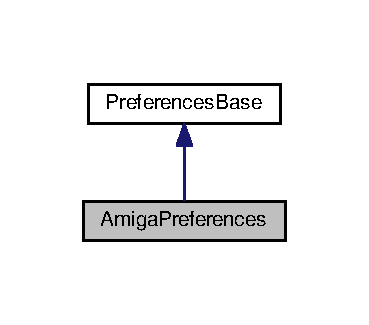
\includegraphics[width=177pt]{da/de8/classAmigaPreferences__inherit__graph}
\end{center}
\end{figure}


Collaboration diagram for Amiga\+Preferences\+:
\nopagebreak
\begin{figure}[H]
\begin{center}
\leavevmode
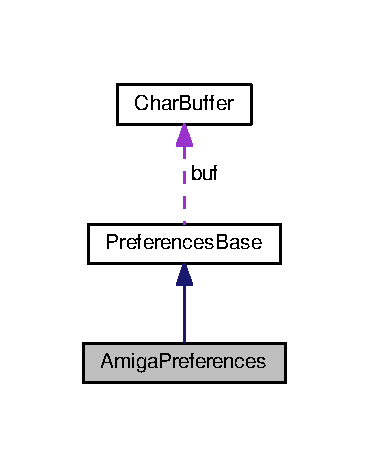
\includegraphics[width=177pt]{d7/d9a/classAmigaPreferences__coll__graph}
\end{center}
\end{figure}
\subsection*{Public Member Functions}
\begin{DoxyCompactItemize}
\item 
virtual \hyperlink{platform_8h_a1062901a7428fdd9c7f180f5e01ea056}{bool} \hyperlink{classAmigaPreferences_ad0afe7aca1e01de83e31d07c0b21dde1}{Load} ()
\item 
virtual \hyperlink{platform_8h_a1062901a7428fdd9c7f180f5e01ea056}{bool} \hyperlink{classAmigaPreferences_a1501b1d109e18004f12d9cf7747bfbdb}{Keep} ()
\item 
virtual \hyperlink{platform_8h_a1062901a7428fdd9c7f180f5e01ea056}{bool} \hyperlink{classAmigaPreferences_a4bfa0037af64c4c7a16b31c85b20444a}{Save} ()
\end{DoxyCompactItemize}
\subsection*{Private Member Functions}
\begin{DoxyCompactItemize}
\item 
\hyperlink{platform_8h_a1062901a7428fdd9c7f180f5e01ea056}{bool} \hyperlink{classAmigaPreferences_ae9f6c44c86e85aadd46cb486478cec11}{Save\+Prefs} (const char $\ast$file)
\end{DoxyCompactItemize}
\subsection*{Additional Inherited Members}


\subsection{Detailed Description}


Definition at line 32 of file preferences\+\_\+amiga.\+h.



\subsection{Member Function Documentation}
\index{Amiga\+Preferences@{Amiga\+Preferences}!Keep@{Keep}}
\index{Keep@{Keep}!Amiga\+Preferences@{Amiga\+Preferences}}
\subsubsection[{\texorpdfstring{Keep()}{Keep()}}]{\setlength{\rightskip}{0pt plus 5cm}virtual {\bf bool} Amiga\+Preferences\+::\+Keep (
\begin{DoxyParamCaption}
{}
\end{DoxyParamCaption}
)\hspace{0.3cm}{\ttfamily [virtual]}}\hypertarget{classAmigaPreferences_a1501b1d109e18004f12d9cf7747bfbdb}{}\label{classAmigaPreferences_a1501b1d109e18004f12d9cf7747bfbdb}


Implements \hyperlink{classPreferencesBase_a83f5750e2780a0bf03cb7a394230637a}{Preferences\+Base}.

\index{Amiga\+Preferences@{Amiga\+Preferences}!Load@{Load}}
\index{Load@{Load}!Amiga\+Preferences@{Amiga\+Preferences}}
\subsubsection[{\texorpdfstring{Load()}{Load()}}]{\setlength{\rightskip}{0pt plus 5cm}virtual {\bf bool} Amiga\+Preferences\+::\+Load (
\begin{DoxyParamCaption}
{}
\end{DoxyParamCaption}
)\hspace{0.3cm}{\ttfamily [virtual]}}\hypertarget{classAmigaPreferences_ad0afe7aca1e01de83e31d07c0b21dde1}{}\label{classAmigaPreferences_ad0afe7aca1e01de83e31d07c0b21dde1}


Implements \hyperlink{classPreferencesBase_ab4e17e21f4377c44fa0ba16a0868a206}{Preferences\+Base}.

\index{Amiga\+Preferences@{Amiga\+Preferences}!Save@{Save}}
\index{Save@{Save}!Amiga\+Preferences@{Amiga\+Preferences}}
\subsubsection[{\texorpdfstring{Save()}{Save()}}]{\setlength{\rightskip}{0pt plus 5cm}virtual {\bf bool} Amiga\+Preferences\+::\+Save (
\begin{DoxyParamCaption}
{}
\end{DoxyParamCaption}
)\hspace{0.3cm}{\ttfamily [virtual]}}\hypertarget{classAmigaPreferences_a4bfa0037af64c4c7a16b31c85b20444a}{}\label{classAmigaPreferences_a4bfa0037af64c4c7a16b31c85b20444a}


Implements \hyperlink{classPreferencesBase_af0c96d85f242caead85d92d2c68fb30b}{Preferences\+Base}.

\index{Amiga\+Preferences@{Amiga\+Preferences}!Save\+Prefs@{Save\+Prefs}}
\index{Save\+Prefs@{Save\+Prefs}!Amiga\+Preferences@{Amiga\+Preferences}}
\subsubsection[{\texorpdfstring{Save\+Prefs(const char $\ast$file)}{SavePrefs(const char *file)}}]{\setlength{\rightskip}{0pt plus 5cm}{\bf bool} Amiga\+Preferences\+::\+Save\+Prefs (
\begin{DoxyParamCaption}
\item[{const char $\ast$}]{file}
\end{DoxyParamCaption}
)\hspace{0.3cm}{\ttfamily [private]}}\hypertarget{classAmigaPreferences_ae9f6c44c86e85aadd46cb486478cec11}{}\label{classAmigaPreferences_ae9f6c44c86e85aadd46cb486478cec11}


The documentation for this class was generated from the following file\+:\begin{DoxyCompactItemize}
\item 
app/system/\hyperlink{preferences__amiga_8h}{preferences\+\_\+amiga.\+h}\end{DoxyCompactItemize}

\hypertarget{classAmigaProgram}{}\section{Amiga\+Program Class Reference}
\label{classAmigaProgram}\index{Amiga\+Program@{Amiga\+Program}}


{\ttfamily \#include $<$program\+\_\+amiga.\+h$>$}



Inheritance diagram for Amiga\+Program\+:\nopagebreak
\begin{figure}[H]
\begin{center}
\leavevmode
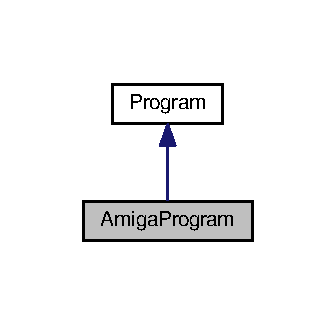
\includegraphics[width=161pt]{classAmigaProgram__inherit__graph}
\end{center}
\end{figure}


Collaboration diagram for Amiga\+Program\+:\nopagebreak
\begin{figure}[H]
\begin{center}
\leavevmode
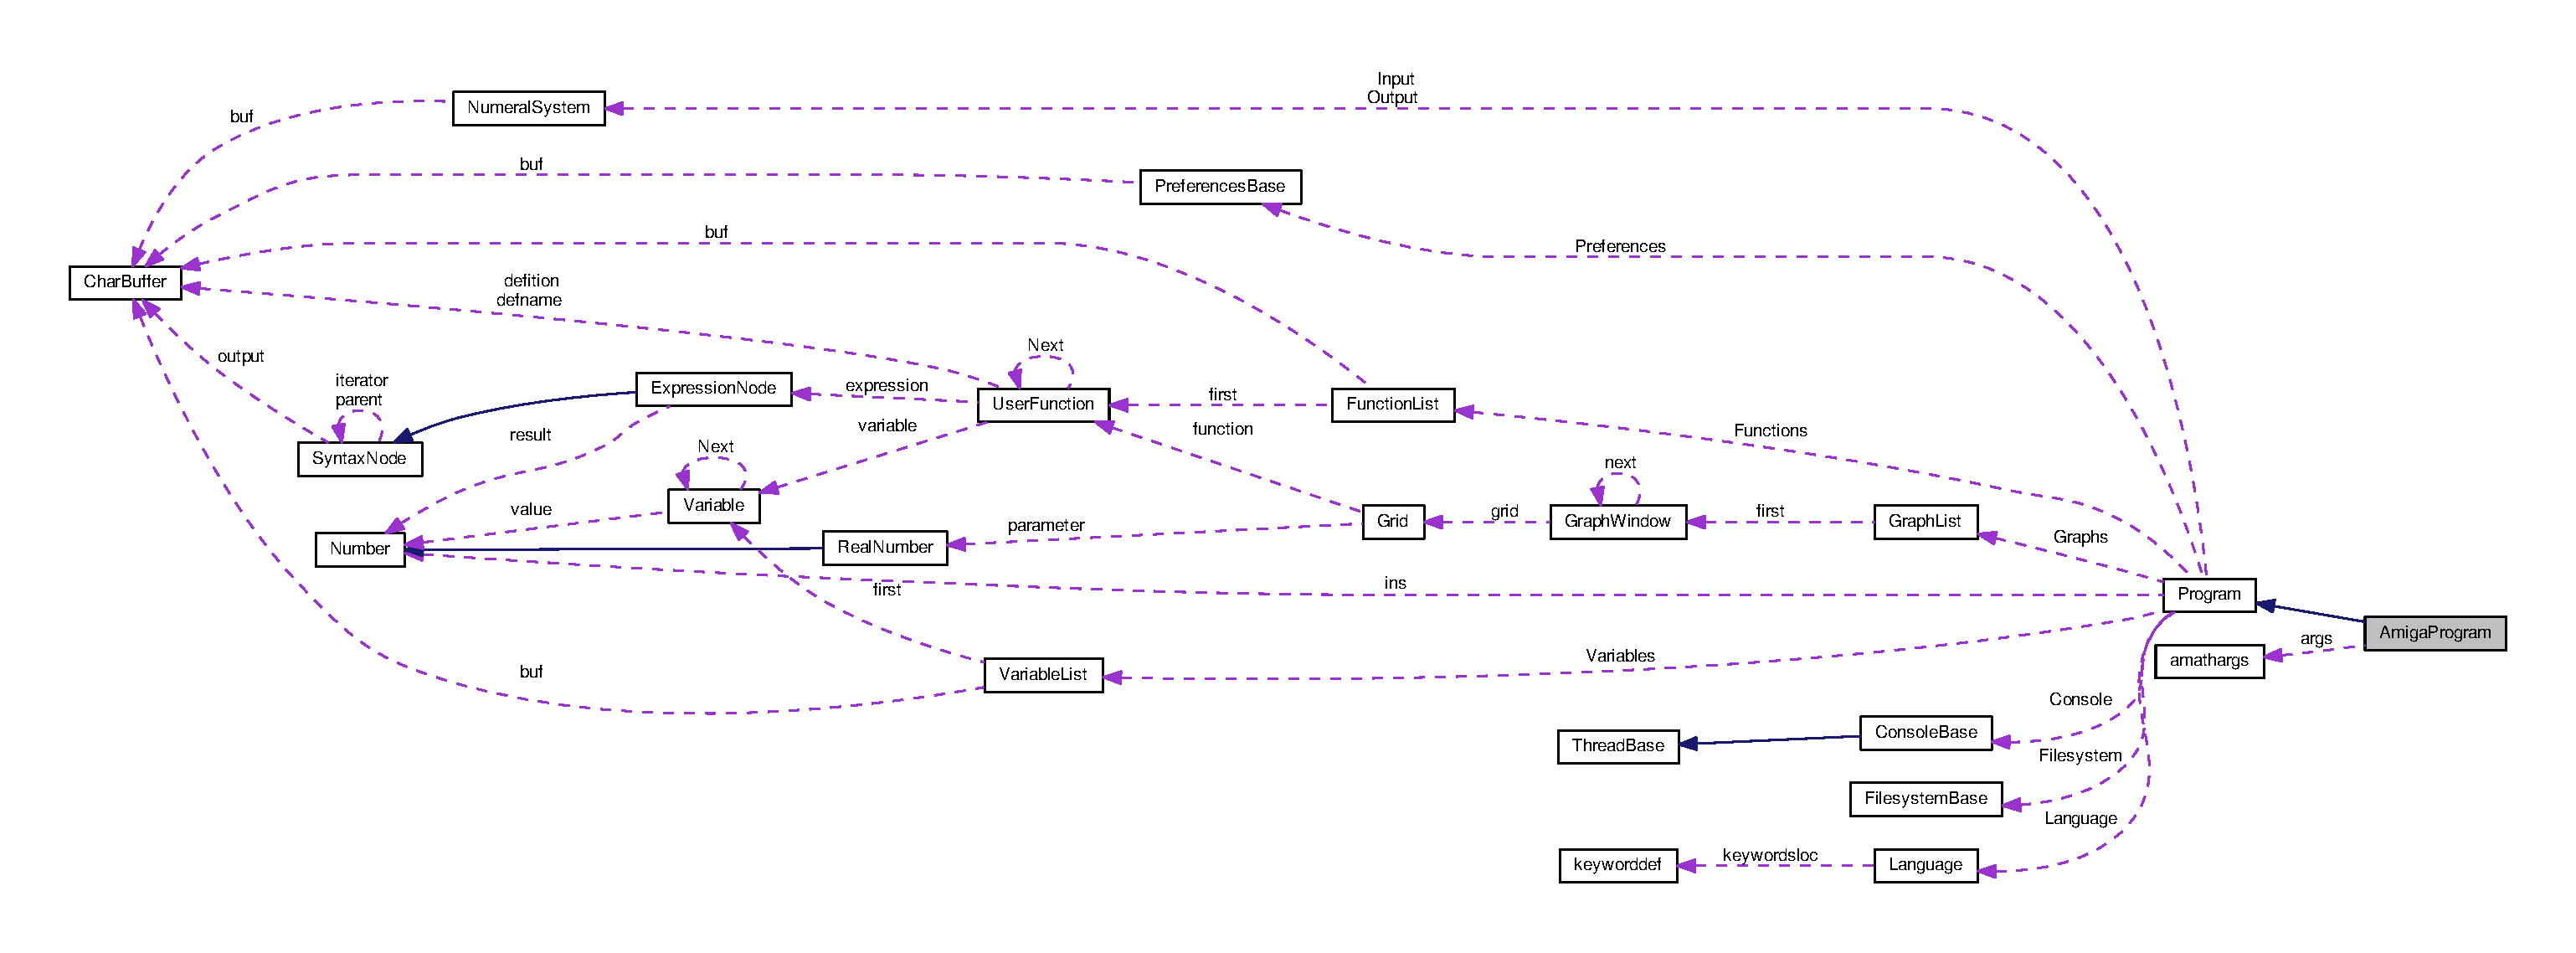
\includegraphics[width=350pt]{classAmigaProgram__coll__graph}
\end{center}
\end{figure}
\subsection*{Public Member Functions}
\begin{DoxyCompactItemize}
\item 
\hyperlink{classAmigaProgram_adaf7552b13bf6526381c5bceb438e1ef}{Amiga\+Program} ()
\item 
virtual \hyperlink{classAmigaProgram_aa93f40c4cba28c4a88c9854c4c5bea6a}{$\sim$\+Amiga\+Program} ()
\item 
virtual void \hyperlink{classAmigaProgram_ac98b0caed0ea8fcb4e8a8a922f9b93de}{Initialize} (int argc, char $\ast$$\ast$argv)
\item 
virtual void \hyperlink{classAmigaProgram_a1bfed5f5b69a85aa3ef1a39ea02dc457}{Run} ()
\item 
virtual void \hyperlink{classAmigaProgram_ad662b535d612f6ed9df4f59ad60fe6a0}{Exit} ()
\end{DoxyCompactItemize}
\subsection*{Private Attributes}
\begin{DoxyCompactItemize}
\item 
R\+D\+Args $\ast$ \hyperlink{classAmigaProgram_a34bbca2534a063c7020487c9138f0534}{rdargs}
\item 
\hyperlink{structamathargs}{amathargs} \hyperlink{classAmigaProgram_acd5b7654dff28b38f6d8e66ddb1dcff7}{args}
\end{DoxyCompactItemize}
\subsection*{Additional Inherited Members}


\subsection{Detailed Description}


Definition at line 36 of file program\+\_\+amiga.\+h.



\subsection{Constructor \& Destructor Documentation}
\index{Amiga\+Program@{Amiga\+Program}!Amiga\+Program@{Amiga\+Program}}
\index{Amiga\+Program@{Amiga\+Program}!Amiga\+Program@{Amiga\+Program}}
\subsubsection[{\texorpdfstring{Amiga\+Program()}{AmigaProgram()}}]{\setlength{\rightskip}{0pt plus 5cm}Amiga\+Program\+::\+Amiga\+Program (
\begin{DoxyParamCaption}
{}
\end{DoxyParamCaption}
)}\hypertarget{classAmigaProgram_adaf7552b13bf6526381c5bceb438e1ef}{}\label{classAmigaProgram_adaf7552b13bf6526381c5bceb438e1ef}
\index{Amiga\+Program@{Amiga\+Program}!````~Amiga\+Program@{$\sim$\+Amiga\+Program}}
\index{````~Amiga\+Program@{$\sim$\+Amiga\+Program}!Amiga\+Program@{Amiga\+Program}}
\subsubsection[{\texorpdfstring{$\sim$\+Amiga\+Program()}{~AmigaProgram()}}]{\setlength{\rightskip}{0pt plus 5cm}virtual Amiga\+Program\+::$\sim$\+Amiga\+Program (
\begin{DoxyParamCaption}
{}
\end{DoxyParamCaption}
)\hspace{0.3cm}{\ttfamily [virtual]}}\hypertarget{classAmigaProgram_aa93f40c4cba28c4a88c9854c4c5bea6a}{}\label{classAmigaProgram_aa93f40c4cba28c4a88c9854c4c5bea6a}


\subsection{Member Function Documentation}
\index{Amiga\+Program@{Amiga\+Program}!Exit@{Exit}}
\index{Exit@{Exit}!Amiga\+Program@{Amiga\+Program}}
\subsubsection[{\texorpdfstring{Exit()}{Exit()}}]{\setlength{\rightskip}{0pt plus 5cm}virtual void Amiga\+Program\+::\+Exit (
\begin{DoxyParamCaption}
{}
\end{DoxyParamCaption}
)\hspace{0.3cm}{\ttfamily [virtual]}}\hypertarget{classAmigaProgram_ad662b535d612f6ed9df4f59ad60fe6a0}{}\label{classAmigaProgram_ad662b535d612f6ed9df4f59ad60fe6a0}


Implements \hyperlink{classProgram_adf53af02e6c4719ec0f019f0d305f80e}{Program}.

\index{Amiga\+Program@{Amiga\+Program}!Initialize@{Initialize}}
\index{Initialize@{Initialize}!Amiga\+Program@{Amiga\+Program}}
\subsubsection[{\texorpdfstring{Initialize(int argc, char $\ast$$\ast$argv)}{Initialize(int argc, char **argv)}}]{\setlength{\rightskip}{0pt plus 5cm}virtual void Amiga\+Program\+::\+Initialize (
\begin{DoxyParamCaption}
\item[{int}]{argc, }
\item[{char $\ast$$\ast$}]{argv}
\end{DoxyParamCaption}
)\hspace{0.3cm}{\ttfamily [virtual]}}\hypertarget{classAmigaProgram_ac98b0caed0ea8fcb4e8a8a922f9b93de}{}\label{classAmigaProgram_ac98b0caed0ea8fcb4e8a8a922f9b93de}


Implements \hyperlink{classProgram_a6c8e48e064937d9c71168ed3a15ccf13}{Program}.

\index{Amiga\+Program@{Amiga\+Program}!Run@{Run}}
\index{Run@{Run}!Amiga\+Program@{Amiga\+Program}}
\subsubsection[{\texorpdfstring{Run()}{Run()}}]{\setlength{\rightskip}{0pt plus 5cm}virtual void Amiga\+Program\+::\+Run (
\begin{DoxyParamCaption}
{}
\end{DoxyParamCaption}
)\hspace{0.3cm}{\ttfamily [virtual]}}\hypertarget{classAmigaProgram_a1bfed5f5b69a85aa3ef1a39ea02dc457}{}\label{classAmigaProgram_a1bfed5f5b69a85aa3ef1a39ea02dc457}


Implements \hyperlink{classProgram_a466c115e35933f7fb3a3775bc8f20ac4}{Program}.



\subsection{Member Data Documentation}
\index{Amiga\+Program@{Amiga\+Program}!args@{args}}
\index{args@{args}!Amiga\+Program@{Amiga\+Program}}
\subsubsection[{\texorpdfstring{args}{args}}]{\setlength{\rightskip}{0pt plus 5cm}{\bf amathargs} Amiga\+Program\+::args\hspace{0.3cm}{\ttfamily [private]}}\hypertarget{classAmigaProgram_acd5b7654dff28b38f6d8e66ddb1dcff7}{}\label{classAmigaProgram_acd5b7654dff28b38f6d8e66ddb1dcff7}


Definition at line 46 of file program\+\_\+amiga.\+h.

\index{Amiga\+Program@{Amiga\+Program}!rdargs@{rdargs}}
\index{rdargs@{rdargs}!Amiga\+Program@{Amiga\+Program}}
\subsubsection[{\texorpdfstring{rdargs}{rdargs}}]{\setlength{\rightskip}{0pt plus 5cm}R\+D\+Args$\ast$ Amiga\+Program\+::rdargs\hspace{0.3cm}{\ttfamily [private]}}\hypertarget{classAmigaProgram_a34bbca2534a063c7020487c9138f0534}{}\label{classAmigaProgram_a34bbca2534a063c7020487c9138f0534}


Definition at line 45 of file program\+\_\+amiga.\+h.



The documentation for this class was generated from the following file\+:\begin{DoxyCompactItemize}
\item 
app/system/\hyperlink{program__amiga_8h}{program\+\_\+amiga.\+h}\end{DoxyCompactItemize}

\hypertarget{classAnsiConoleEngine}{}\section{Ansi\+Conole\+Engine Class Reference}
\label{classAnsiConoleEngine}\index{Ansi\+Conole\+Engine@{Ansi\+Conole\+Engine}}


A\+N\+SI console controller.  




{\ttfamily \#include $<$aengine.\+h$>$}



Collaboration diagram for Ansi\+Conole\+Engine\+:
\nopagebreak
\begin{figure}[H]
\begin{center}
\leavevmode
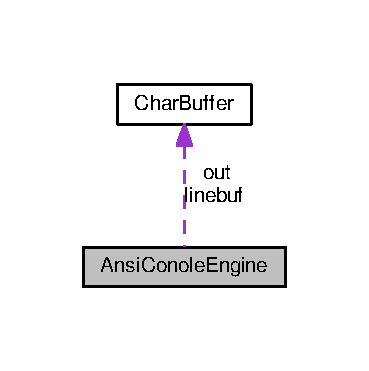
\includegraphics[width=177pt]{db/d6d/classAnsiConoleEngine__coll__graph}
\end{center}
\end{figure}
\subsection*{Public Member Functions}
\begin{DoxyCompactItemize}
\item 
\hyperlink{classAnsiConoleEngine_aac394a191db46deb09a08522bdf72218}{Ansi\+Conole\+Engine} (const char $\ast$\hyperlink{classAnsiConoleEngine_a97ebef63ba0490711ed78733b6a87be5}{prompt})
\item 
\hyperlink{classAnsiConoleEngine_a2023846db9703224facd0c2015528dc3}{$\sim$\+Ansi\+Conole\+Engine} ()
\item 
void \hyperlink{classAnsiConoleEngine_a8ad01a2ddd3ee5182deb4a74f3d2a0c1}{Start\+Input} ()
\item 
\hyperlink{platform_8h_a1062901a7428fdd9c7f180f5e01ea056}{bool} \hyperlink{classAnsiConoleEngine_ab136f725541608d36dedcd8ffa24e820}{Input\+Done} ()
\item 
const char $\ast$ \hyperlink{classAnsiConoleEngine_ae3b0bd4c66cb82f4ff939b45bd6e7446}{Get\+Line} ()
\item 
void \hyperlink{classAnsiConoleEngine_a6c5dd4043aadc0b310f976eb10cbcd9f}{Set\+Prompt} (const char $\ast$string)
\item 
const char $\ast$ \hyperlink{classAnsiConoleEngine_a7bb2dea88ddc5ae76643d2303fcc4bf1}{Process\+Char} (const unsigned char character)
\end{DoxyCompactItemize}
\subsection*{Private Member Functions}
\begin{DoxyCompactItemize}
\item 
void \hyperlink{classAnsiConoleEngine_ae359fe52bf227c3db6edc42b8fc884f0}{Copy\+Line} ()
\item 
void \hyperlink{classAnsiConoleEngine_afc441f10d1c52dba7b3ca1a5f2514e7c}{Show\+Last} ()
\item 
void \hyperlink{classAnsiConoleEngine_a93c3eccd6c1458e1a82bdbf202948d90}{Show\+Next} ()
\end{DoxyCompactItemize}
\subsection*{Private Attributes}
\begin{DoxyCompactItemize}
\item 
char $\ast$ \hyperlink{classAnsiConoleEngine_a97ebef63ba0490711ed78733b6a87be5}{prompt}
\item 
char $\ast$$\ast$ \hyperlink{classAnsiConoleEngine_a624ec5321c326a68de340f9b77e84c2c}{lines}
\item 
\hyperlink{classCharBuffer}{Char\+Buffer} $\ast$ \hyperlink{classAnsiConoleEngine_a6bf88afa72a458e3687972f9e666cd86}{linebuf}
\item 
unsigned int \hyperlink{classAnsiConoleEngine_ad5d65280df848947f5b2dda80dcf35c6}{len}
\item 
char $\ast$ \hyperlink{classAnsiConoleEngine_aea3df1b13bc8ecf2eb68ec693249800f}{cursor}
\item 
char $\ast$ \hyperlink{classAnsiConoleEngine_a28852245082570631c7392411fec89cc}{endpos}
\item 
int \hyperlink{classAnsiConoleEngine_ab029fc4a19c5fbd6f6b23c390af618b8}{curline}
\item 
int \hyperlink{classAnsiConoleEngine_a24fe8cd3b3321c6dd4b26731cb1a8108}{showline}
\item 
\hyperlink{platform_8h_a1062901a7428fdd9c7f180f5e01ea056}{bool} \hyperlink{classAnsiConoleEngine_a23b1b0d4714995d12e7b0aacdecfa0c4}{lineswap}
\item 
char $\ast$ \hyperlink{classAnsiConoleEngine_a465421c5488f2566d12717641a327017}{editline}
\item 
\hyperlink{platform_8h_a1062901a7428fdd9c7f180f5e01ea056}{bool} \hyperlink{classAnsiConoleEngine_af497f5cbdca8bbc350935a90568b06e7}{escmode}
\item 
\hyperlink{platform_8h_a1062901a7428fdd9c7f180f5e01ea056}{bool} \hyperlink{classAnsiConoleEngine_adf2036857a6c6de85836ee2e7b3e5d6d}{csimode}
\item 
\hyperlink{platform_8h_a1062901a7428fdd9c7f180f5e01ea056}{bool} \hyperlink{classAnsiConoleEngine_a5182d9a19cc1fe8681a9faf77a156657}{delmode}
\item 
\hyperlink{platform_8h_a1062901a7428fdd9c7f180f5e01ea056}{bool} \hyperlink{classAnsiConoleEngine_a0931686f3224f07bd3a3fe25c06e32c6}{linedone}
\item 
\hyperlink{classCharBuffer}{Char\+Buffer} $\ast$ \hyperlink{classAnsiConoleEngine_ad6a604fc0a0f544907513076c72434f3}{out}
\end{DoxyCompactItemize}
\subsection*{Static Private Attributes}
\begin{DoxyCompactItemize}
\item 
static const int \hyperlink{classAnsiConoleEngine_a3f94786b1610ac3f038d5115fd8047a3}{max\+Lines} = 20
\item 
static const int \hyperlink{classAnsiConoleEngine_a59042210f69050bdfb531841e8ac0927}{line\+Size} = 1024
\end{DoxyCompactItemize}


\subsection{Detailed Description}
A\+N\+SI console controller. 

More info on the A\+N\+SI console is available at Wikipedia\+: \href{http://en.wikipedia.org/wiki/ANSI_escape_code}{\tt http\+://en.\+wikipedia.\+org/wiki/\+A\+N\+S\+I\+\_\+escape\+\_\+code} 

Definition at line 44 of file aengine.\+h.



\subsection{Constructor \& Destructor Documentation}
\index{Ansi\+Conole\+Engine@{Ansi\+Conole\+Engine}!Ansi\+Conole\+Engine@{Ansi\+Conole\+Engine}}
\index{Ansi\+Conole\+Engine@{Ansi\+Conole\+Engine}!Ansi\+Conole\+Engine@{Ansi\+Conole\+Engine}}
\subsubsection[{\texorpdfstring{Ansi\+Conole\+Engine(const char $\ast$prompt)}{AnsiConoleEngine(const char *prompt)}}]{\setlength{\rightskip}{0pt plus 5cm}Ansi\+Conole\+Engine\+::\+Ansi\+Conole\+Engine (
\begin{DoxyParamCaption}
\item[{const char $\ast$}]{prompt}
\end{DoxyParamCaption}
)}\hypertarget{classAnsiConoleEngine_aac394a191db46deb09a08522bdf72218}{}\label{classAnsiConoleEngine_aac394a191db46deb09a08522bdf72218}


Definition at line 31 of file aengine.\+cpp.



References Alloc\+And\+Copy(), Char\+Buffer\+::\+Char\+Buffer(), curline, editline, linebuf, lines, max\+Lines, out, and prompt.



Referenced by Standard\+Console\+::\+Standard\+Console().


\begin{DoxyCode}
32 \{
33     \hyperlink{clib_8h_a5bed05c70cb17e541fee570b5dc32e1a}{AllocAndCopy}(&this->\hyperlink{classAnsiConoleEngine_a97ebef63ba0490711ed78733b6a87be5}{prompt}, \hyperlink{classAnsiConoleEngine_a97ebef63ba0490711ed78733b6a87be5}{prompt});
34     \hyperlink{classAnsiConoleEngine_a6bf88afa72a458e3687972f9e666cd86}{linebuf} = \textcolor{keyword}{new} \hyperlink{classCharBuffer}{CharBuffer}();
35     \hyperlink{classAnsiConoleEngine_ad6a604fc0a0f544907513076c72434f3}{out} = \textcolor{keyword}{new} \hyperlink{classCharBuffer}{CharBuffer}();
36 
37     \hyperlink{classAnsiConoleEngine_a624ec5321c326a68de340f9b77e84c2c}{lines} = \textcolor{keyword}{new} \textcolor{keywordtype}{char}*[\hyperlink{classAnsiConoleEngine_a3f94786b1610ac3f038d5115fd8047a3}{maxLines}];
38 
39     \textcolor{keywordflow}{for} (\textcolor{keywordtype}{int} i = 0; i < \hyperlink{classAnsiConoleEngine_a3f94786b1610ac3f038d5115fd8047a3}{maxLines}; i++) \{
40         \hyperlink{classAnsiConoleEngine_a624ec5321c326a68de340f9b77e84c2c}{lines}[i] = \hyperlink{platform_8h_a46ff2bfbf0d44b8466a2251d5bd5e6f8}{NOMEM};
41     \}
42 
43     \hyperlink{classAnsiConoleEngine_a465421c5488f2566d12717641a327017}{editline} = \hyperlink{platform_8h_a46ff2bfbf0d44b8466a2251d5bd5e6f8}{NOMEM};
44     \hyperlink{classAnsiConoleEngine_ab029fc4a19c5fbd6f6b23c390af618b8}{curline} = -1;
45 \}
\end{DoxyCode}


Here is the call graph for this function\+:
\nopagebreak
\begin{figure}[H]
\begin{center}
\leavevmode
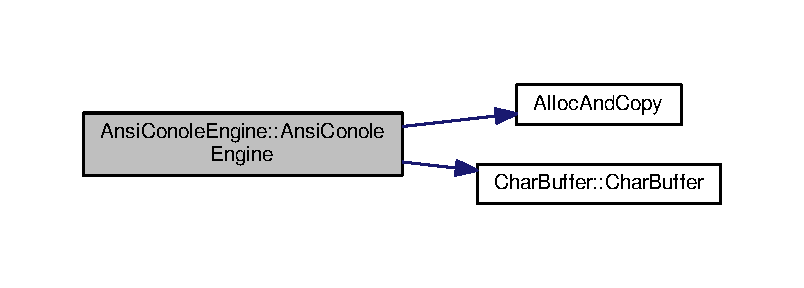
\includegraphics[width=350pt]{df/d87/classAnsiConoleEngine_aac394a191db46deb09a08522bdf72218_cgraph}
\end{center}
\end{figure}




Here is the caller graph for this function\+:
\nopagebreak
\begin{figure}[H]
\begin{center}
\leavevmode
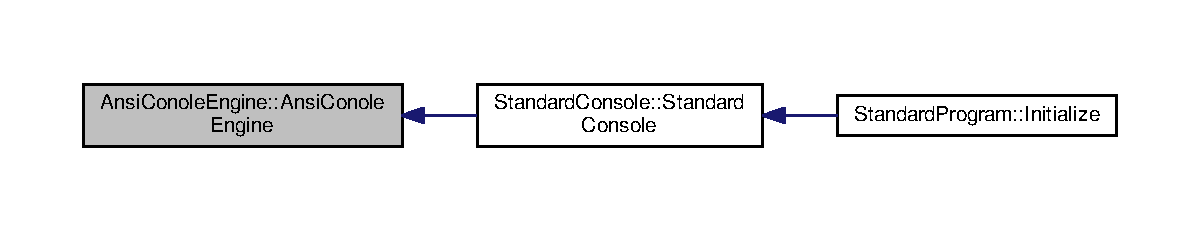
\includegraphics[width=350pt]{df/d87/classAnsiConoleEngine_aac394a191db46deb09a08522bdf72218_icgraph}
\end{center}
\end{figure}


\index{Ansi\+Conole\+Engine@{Ansi\+Conole\+Engine}!````~Ansi\+Conole\+Engine@{$\sim$\+Ansi\+Conole\+Engine}}
\index{````~Ansi\+Conole\+Engine@{$\sim$\+Ansi\+Conole\+Engine}!Ansi\+Conole\+Engine@{Ansi\+Conole\+Engine}}
\subsubsection[{\texorpdfstring{$\sim$\+Ansi\+Conole\+Engine()}{~AnsiConoleEngine()}}]{\setlength{\rightskip}{0pt plus 5cm}Ansi\+Conole\+Engine\+::$\sim$\+Ansi\+Conole\+Engine (
\begin{DoxyParamCaption}
{}
\end{DoxyParamCaption}
)}\hypertarget{classAnsiConoleEngine_a2023846db9703224facd0c2015528dc3}{}\label{classAnsiConoleEngine_a2023846db9703224facd0c2015528dc3}


Definition at line 47 of file aengine.\+cpp.



References linebuf, lines, max\+Lines, out, and prompt.


\begin{DoxyCode}
48 \{
49     \textcolor{keywordflow}{for} (\textcolor{keywordtype}{int} i = 0; i < \hyperlink{classAnsiConoleEngine_a3f94786b1610ac3f038d5115fd8047a3}{maxLines}; i++) \{
50         \textcolor{keywordflow}{if} (\hyperlink{classAnsiConoleEngine_a624ec5321c326a68de340f9b77e84c2c}{lines}[i] != \hyperlink{platform_8h_a46ff2bfbf0d44b8466a2251d5bd5e6f8}{NOMEM}) \{
51             \textcolor{keyword}{delete} [] \hyperlink{classAnsiConoleEngine_a624ec5321c326a68de340f9b77e84c2c}{lines}[i];
52         \}
53     \}
54 
55     \textcolor{keyword}{delete} [] \hyperlink{classAnsiConoleEngine_a624ec5321c326a68de340f9b77e84c2c}{lines};
56     \textcolor{keyword}{delete} \hyperlink{classAnsiConoleEngine_a6bf88afa72a458e3687972f9e666cd86}{linebuf};
57     \textcolor{keyword}{delete} \hyperlink{classAnsiConoleEngine_ad6a604fc0a0f544907513076c72434f3}{out};
58     \textcolor{keyword}{delete} \hyperlink{classAnsiConoleEngine_a97ebef63ba0490711ed78733b6a87be5}{prompt};
59 \}
\end{DoxyCode}


\subsection{Member Function Documentation}
\index{Ansi\+Conole\+Engine@{Ansi\+Conole\+Engine}!Copy\+Line@{Copy\+Line}}
\index{Copy\+Line@{Copy\+Line}!Ansi\+Conole\+Engine@{Ansi\+Conole\+Engine}}
\subsubsection[{\texorpdfstring{Copy\+Line()}{CopyLine()}}]{\setlength{\rightskip}{0pt plus 5cm}void Ansi\+Conole\+Engine\+::\+Copy\+Line (
\begin{DoxyParamCaption}
{}
\end{DoxyParamCaption}
)\hspace{0.3cm}{\ttfamily [private]}}\hypertarget{classAnsiConoleEngine_ae359fe52bf227c3db6edc42b8fc884f0}{}\label{classAnsiConoleEngine_ae359fe52bf227c3db6edc42b8fc884f0}


Definition at line 214 of file aengine.\+cpp.



References Alloc\+And\+Copy(), curline, editline, Char\+Buffer\+::\+Get\+String(), linebuf, lines, and max\+Lines.



Referenced by Process\+Char().


\begin{DoxyCode}
215 \{
216     \hyperlink{classAnsiConoleEngine_ab029fc4a19c5fbd6f6b23c390af618b8}{curline}++;
217 
218     \textcolor{keywordflow}{if} (\hyperlink{classAnsiConoleEngine_ab029fc4a19c5fbd6f6b23c390af618b8}{curline} == \hyperlink{classAnsiConoleEngine_a3f94786b1610ac3f038d5115fd8047a3}{maxLines}) \{
219         \hyperlink{classAnsiConoleEngine_ab029fc4a19c5fbd6f6b23c390af618b8}{curline}--;
220 
221         \textcolor{keyword}{delete} [] \hyperlink{classAnsiConoleEngine_a624ec5321c326a68de340f9b77e84c2c}{lines}[0];
222         \textcolor{keywordflow}{for} (\textcolor{keywordtype}{int} i = 0; i < \hyperlink{classAnsiConoleEngine_a3f94786b1610ac3f038d5115fd8047a3}{maxLines} - 1; i++) \{
223             \hyperlink{classAnsiConoleEngine_a624ec5321c326a68de340f9b77e84c2c}{lines}[i] = \hyperlink{classAnsiConoleEngine_a624ec5321c326a68de340f9b77e84c2c}{lines}[i + 1];
224         \}
225     \}
226 
227     \hyperlink{clib_8h_a5bed05c70cb17e541fee570b5dc32e1a}{AllocAndCopy}(&(\hyperlink{classAnsiConoleEngine_a624ec5321c326a68de340f9b77e84c2c}{lines}[\hyperlink{classAnsiConoleEngine_ab029fc4a19c5fbd6f6b23c390af618b8}{curline}]), \hyperlink{classAnsiConoleEngine_a6bf88afa72a458e3687972f9e666cd86}{linebuf}->
      \hyperlink{classCharBuffer_a7dfd3feaaf80f318ba44efe15b1ec44b}{GetString}());
228 
229     \textcolor{keywordflow}{if} (\hyperlink{classAnsiConoleEngine_a465421c5488f2566d12717641a327017}{editline} != \hyperlink{platform_8h_a46ff2bfbf0d44b8466a2251d5bd5e6f8}{NOMEM}) \{
230         \textcolor{keyword}{delete} [] \hyperlink{classAnsiConoleEngine_a465421c5488f2566d12717641a327017}{editline};
231         \hyperlink{classAnsiConoleEngine_a465421c5488f2566d12717641a327017}{editline} = \hyperlink{platform_8h_a46ff2bfbf0d44b8466a2251d5bd5e6f8}{NOMEM};
232     \}
233 \}
\end{DoxyCode}


Here is the call graph for this function\+:
\nopagebreak
\begin{figure}[H]
\begin{center}
\leavevmode
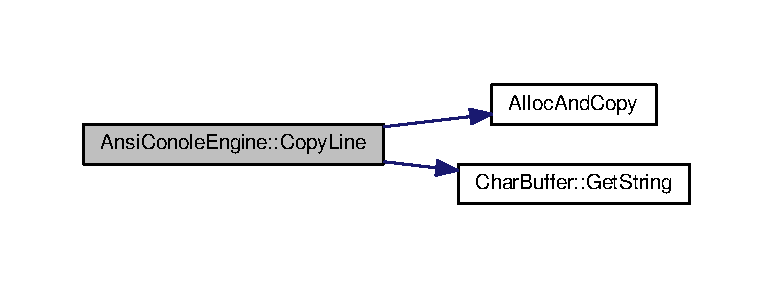
\includegraphics[width=350pt]{df/d87/classAnsiConoleEngine_ae359fe52bf227c3db6edc42b8fc884f0_cgraph}
\end{center}
\end{figure}




Here is the caller graph for this function\+:
\nopagebreak
\begin{figure}[H]
\begin{center}
\leavevmode
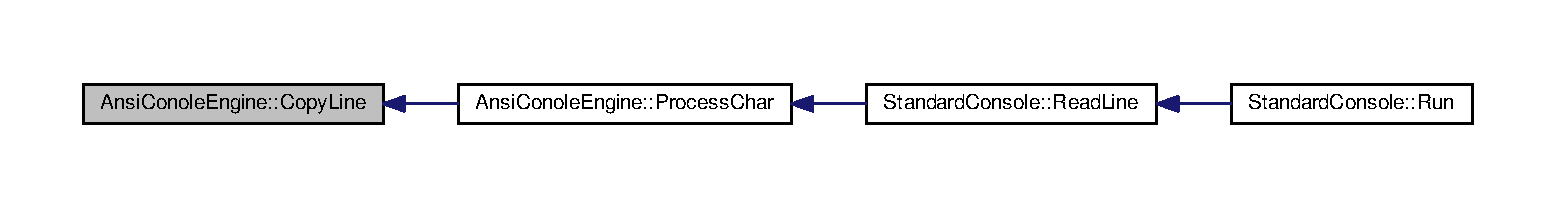
\includegraphics[width=350pt]{df/d87/classAnsiConoleEngine_ae359fe52bf227c3db6edc42b8fc884f0_icgraph}
\end{center}
\end{figure}


\index{Ansi\+Conole\+Engine@{Ansi\+Conole\+Engine}!Get\+Line@{Get\+Line}}
\index{Get\+Line@{Get\+Line}!Ansi\+Conole\+Engine@{Ansi\+Conole\+Engine}}
\subsubsection[{\texorpdfstring{Get\+Line()}{GetLine()}}]{\setlength{\rightskip}{0pt plus 5cm}const char $\ast$ Ansi\+Conole\+Engine\+::\+Get\+Line (
\begin{DoxyParamCaption}
{}
\end{DoxyParamCaption}
)}\hypertarget{classAnsiConoleEngine_ae3b0bd4c66cb82f4ff939b45bd6e7446}{}\label{classAnsiConoleEngine_ae3b0bd4c66cb82f4ff939b45bd6e7446}


Definition at line 318 of file aengine.\+cpp.



References Char\+Buffer\+::\+Get\+String(), and linebuf.



Referenced by Standard\+Console\+::\+Read\+Line().


\begin{DoxyCode}
319 \{
320     \textcolor{keywordflow}{return} \hyperlink{classAnsiConoleEngine_a6bf88afa72a458e3687972f9e666cd86}{linebuf}->\hyperlink{classCharBuffer_a7dfd3feaaf80f318ba44efe15b1ec44b}{GetString}();
321 \}
\end{DoxyCode}


Here is the call graph for this function\+:
\nopagebreak
\begin{figure}[H]
\begin{center}
\leavevmode
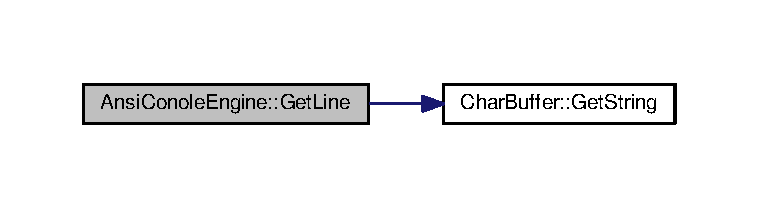
\includegraphics[width=350pt]{df/d87/classAnsiConoleEngine_ae3b0bd4c66cb82f4ff939b45bd6e7446_cgraph}
\end{center}
\end{figure}




Here is the caller graph for this function\+:
\nopagebreak
\begin{figure}[H]
\begin{center}
\leavevmode
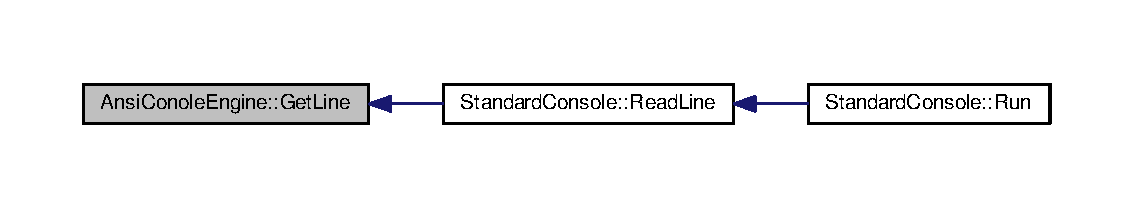
\includegraphics[width=350pt]{df/d87/classAnsiConoleEngine_ae3b0bd4c66cb82f4ff939b45bd6e7446_icgraph}
\end{center}
\end{figure}


\index{Ansi\+Conole\+Engine@{Ansi\+Conole\+Engine}!Input\+Done@{Input\+Done}}
\index{Input\+Done@{Input\+Done}!Ansi\+Conole\+Engine@{Ansi\+Conole\+Engine}}
\subsubsection[{\texorpdfstring{Input\+Done()}{InputDone()}}]{\setlength{\rightskip}{0pt plus 5cm}{\bf bool} Ansi\+Conole\+Engine\+::\+Input\+Done (
\begin{DoxyParamCaption}
{}
\end{DoxyParamCaption}
)}\hypertarget{classAnsiConoleEngine_ab136f725541608d36dedcd8ffa24e820}{}\label{classAnsiConoleEngine_ab136f725541608d36dedcd8ffa24e820}


Definition at line 313 of file aengine.\+cpp.



References linedone.



Referenced by Standard\+Console\+::\+Read\+Line().


\begin{DoxyCode}
314 \{
315     \textcolor{keywordflow}{return} \hyperlink{classAnsiConoleEngine_a0931686f3224f07bd3a3fe25c06e32c6}{linedone};
316 \}
\end{DoxyCode}


Here is the caller graph for this function\+:
\nopagebreak
\begin{figure}[H]
\begin{center}
\leavevmode
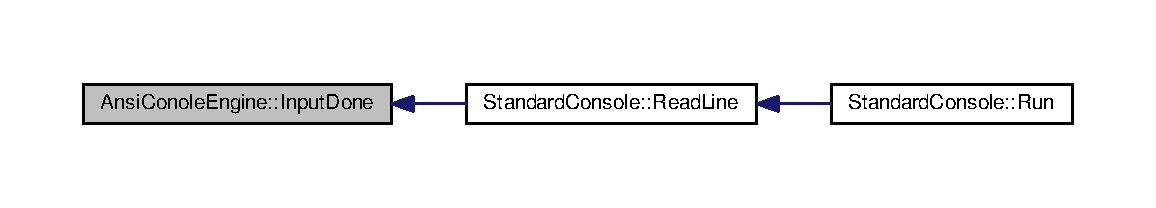
\includegraphics[width=350pt]{df/d87/classAnsiConoleEngine_ab136f725541608d36dedcd8ffa24e820_icgraph}
\end{center}
\end{figure}


\index{Ansi\+Conole\+Engine@{Ansi\+Conole\+Engine}!Process\+Char@{Process\+Char}}
\index{Process\+Char@{Process\+Char}!Ansi\+Conole\+Engine@{Ansi\+Conole\+Engine}}
\subsubsection[{\texorpdfstring{Process\+Char(const unsigned char character)}{ProcessChar(const unsigned char character)}}]{\setlength{\rightskip}{0pt plus 5cm}const char $\ast$ Ansi\+Conole\+Engine\+::\+Process\+Char (
\begin{DoxyParamCaption}
\item[{const unsigned char}]{character}
\end{DoxyParamCaption}
)}\hypertarget{classAnsiConoleEngine_a7bb2dea88ddc5ae76643d2303fcc4bf1}{}\label{classAnsiConoleEngine_a7bb2dea88ddc5ae76643d2303fcc4bf1}


Definition at line 80 of file aengine.\+cpp.



References Char\+Buffer\+::\+Append(), Char\+Buffer\+::buf, Copy\+Line(), csimode, cursor, delmode, Char\+Buffer\+::\+Empty(), endpos, escmode, Char\+Buffer\+::\+Get\+String(), len, linebuf, linedone, out, Char\+Buffer\+::ptr, Show\+Last(), and Show\+Next().



Referenced by Standard\+Console\+::\+Read\+Line().


\begin{DoxyCode}
81 \{
82     \textcolor{keywordtype}{unsigned} \textcolor{keywordtype}{char} ch = character;
83     \hyperlink{classAnsiConoleEngine_ad6a604fc0a0f544907513076c72434f3}{out}->\hyperlink{classCharBuffer_abe39d3fd7d8b9c8ec343af2cae7adc96}{Empty}();
84 
85     \textcolor{comment}{/*}
86 \textcolor{comment}{    // -------------- DEUG ------------------}
87 \textcolor{comment}{    Number *d = new RealNumber((int)ch);}
88 \textcolor{comment}{    NumeralSystem *ns = new DecimalSystem(0);}
89 \textcolor{comment}{    const char *dtext = ns->GetText(d);}
90 \textcolor{comment}{    StrCopy(out->buf, dtext);}
91 \textcolor{comment}{    StrConcat(out->buf, SPACE);}
92 \textcolor{comment}{    delete ns;}
93 \textcolor{comment}{    delete d;}
94 \textcolor{comment}{    return out->buf;}
95 \textcolor{comment}{    // -------------- DEUG ------------------}
96 \textcolor{comment}{    */}
97 
98     \textcolor{keywordflow}{if} (\hyperlink{classAnsiConoleEngine_ad5d65280df848947f5b2dda80dcf35c6}{len} == 0) \{
99         \textcolor{comment}{// TODO: double buffer}
100     \}
101 
102     \textcolor{keywordtype}{bool} processed = \textcolor{keyword}{false};
103 
104     \textcolor{keywordflow}{if} (ch == 0) \{
105         processed = \textcolor{keyword}{true};
106     \} \textcolor{keywordflow}{else} \textcolor{keywordflow}{if} (ch == 27) \{
107         \hyperlink{classAnsiConoleEngine_af497f5cbdca8bbc350935a90568b06e7}{escmode} = \textcolor{keyword}{true};
108         processed = \textcolor{keyword}{true};
109     \} \textcolor{keywordflow}{else} \textcolor{keywordflow}{if} (ch == 155 || (\hyperlink{classAnsiConoleEngine_af497f5cbdca8bbc350935a90568b06e7}{escmode} && ch == 91)) \{
110         \hyperlink{classAnsiConoleEngine_adf2036857a6c6de85836ee2e7b3e5d6d}{csimode} = \textcolor{keyword}{true};
111         processed = \textcolor{keyword}{true};
112     \} \textcolor{keywordflow}{else} \textcolor{keywordflow}{if} (\hyperlink{classAnsiConoleEngine_adf2036857a6c6de85836ee2e7b3e5d6d}{csimode}) \{
113         \textcolor{keywordflow}{switch} (ch) \{
114         \textcolor{keywordflow}{case} 65: \textcolor{comment}{// Arrow up (27 91 65)}
115             \hyperlink{classAnsiConoleEngine_afc441f10d1c52dba7b3ca1a5f2514e7c}{ShowLast}();
116             \textcolor{keywordflow}{break};
117         \textcolor{keywordflow}{case} 66: \textcolor{comment}{// Arrow down (27 91 66)}
118             \hyperlink{classAnsiConoleEngine_a93c3eccd6c1458e1a82bdbf202948d90}{ShowNext}();
119             \textcolor{keywordflow}{break};
120         \textcolor{keywordflow}{case} 67: \textcolor{comment}{// Arrow right (27 91 67)}
121             \textcolor{keywordflow}{if} (\hyperlink{classAnsiConoleEngine_aea3df1b13bc8ecf2eb68ec693249800f}{cursor} != \hyperlink{classAnsiConoleEngine_a28852245082570631c7392411fec89cc}{endpos}) \{
122                 \hyperlink{classAnsiConoleEngine_aea3df1b13bc8ecf2eb68ec693249800f}{cursor}++;
123                 \hyperlink{classAnsiConoleEngine_ad6a604fc0a0f544907513076c72434f3}{out}->\hyperlink{classCharBuffer_a045b38735f7b3007c1b98d3d7b7feafe}{Append}(\hyperlink{platform_8h_a67ab9b76f83cab7d4b7dab79ca50a89d}{CURSORFORWARD});
124             \}
125             \textcolor{keywordflow}{break};
126         \textcolor{keywordflow}{case} 68: \textcolor{comment}{// Arrow left (27 91 68)}
127             \textcolor{keywordflow}{if} (\hyperlink{classAnsiConoleEngine_aea3df1b13bc8ecf2eb68ec693249800f}{cursor} != \hyperlink{classAnsiConoleEngine_a6bf88afa72a458e3687972f9e666cd86}{linebuf}->\hyperlink{classCharBuffer_a8bcd8491b24db4197b311eb361609674}{buf}) \{
128                 \hyperlink{classAnsiConoleEngine_aea3df1b13bc8ecf2eb68ec693249800f}{cursor}--;
129                 \hyperlink{classAnsiConoleEngine_ad6a604fc0a0f544907513076c72434f3}{out}->\hyperlink{classCharBuffer_a045b38735f7b3007c1b98d3d7b7feafe}{Append}(\hyperlink{platform_8h_a0740e3bf50964c04eeaa76ae5fe9c14c}{CURSORBACKWARD});
130             \}
131             \textcolor{keywordflow}{break};
132         \textcolor{keywordflow}{case} 51: \textcolor{comment}{// DEL         27 91 51 126}
133             \hyperlink{classAnsiConoleEngine_a5182d9a19cc1fe8681a9faf77a156657}{delmode} = \textcolor{keyword}{true};
134         \textcolor{keywordflow}{default}:
135             \textcolor{comment}{// F1          27 79 80}
136             \textcolor{comment}{// F2          27 79 81}
137             \textcolor{keywordflow}{break};
138         \}
139 
140         \hyperlink{classAnsiConoleEngine_af497f5cbdca8bbc350935a90568b06e7}{escmode} = \textcolor{keyword}{false};
141         \hyperlink{classAnsiConoleEngine_adf2036857a6c6de85836ee2e7b3e5d6d}{csimode} = \textcolor{keyword}{false};
142         processed = \textcolor{keyword}{true};
143     \} \textcolor{keywordflow}{else} \{
144         \hyperlink{classAnsiConoleEngine_af497f5cbdca8bbc350935a90568b06e7}{escmode} = \textcolor{keyword}{false};
145         \hyperlink{classAnsiConoleEngine_adf2036857a6c6de85836ee2e7b3e5d6d}{csimode} = \textcolor{keyword}{false};
146     \}
147 
148     \textcolor{comment}{// Delete one character to the right}
149     \textcolor{keywordflow}{if} (\hyperlink{classAnsiConoleEngine_a5182d9a19cc1fe8681a9faf77a156657}{delmode} && ch == 126) \{
150         \textcolor{keywordflow}{if} (\hyperlink{classAnsiConoleEngine_aea3df1b13bc8ecf2eb68ec693249800f}{cursor} != \hyperlink{classAnsiConoleEngine_a28852245082570631c7392411fec89cc}{endpos}) \{
151             \textcolor{keywordtype}{char} *i = \hyperlink{classAnsiConoleEngine_aea3df1b13bc8ecf2eb68ec693249800f}{cursor};
152             \textcolor{keywordflow}{do} \{
153                 *i = *(i + 1);
154                 i++;
155             \} \textcolor{keywordflow}{while} (i != \hyperlink{classAnsiConoleEngine_a28852245082570631c7392411fec89cc}{endpos});
156 
157             \hyperlink{classAnsiConoleEngine_ad5d65280df848947f5b2dda80dcf35c6}{len}++;
158             \hyperlink{classAnsiConoleEngine_ad6a604fc0a0f544907513076c72434f3}{out}->\hyperlink{classCharBuffer_a045b38735f7b3007c1b98d3d7b7feafe}{Append}(\hyperlink{platform_8h_a32235c847e9b93b06b2ffebafe31fbc1}{DELETE1CHAR});
159             \hyperlink{classAnsiConoleEngine_a28852245082570631c7392411fec89cc}{endpos}--;
160             \hyperlink{classAnsiConoleEngine_a6bf88afa72a458e3687972f9e666cd86}{linebuf}->\hyperlink{classCharBuffer_a2d313433650506fd6609e6947729dfb0}{ptr} = \hyperlink{classAnsiConoleEngine_a28852245082570631c7392411fec89cc}{endpos};
161         \}
162 
163         processed = \textcolor{keyword}{true};
164         \hyperlink{classAnsiConoleEngine_a5182d9a19cc1fe8681a9faf77a156657}{delmode} = \textcolor{keyword}{false};
165     \}
166 
167     \textcolor{keywordflow}{if} (processed) \{
168         \textcolor{keywordflow}{return} \hyperlink{classAnsiConoleEngine_ad6a604fc0a0f544907513076c72434f3}{out}->\hyperlink{classCharBuffer_a7dfd3feaaf80f318ba44efe15b1ec44b}{GetString}();
169     \}
170 
171     \textcolor{keywordflow}{if} (ch == 13 || ch == 10) \{
172         \hyperlink{classAnsiConoleEngine_ad6a604fc0a0f544907513076c72434f3}{out}->\hyperlink{classCharBuffer_a045b38735f7b3007c1b98d3d7b7feafe}{Append}(\hyperlink{platform_8h_a806511f4930171733227c99101dc0606}{NEWLINE});
173         \hyperlink{classAnsiConoleEngine_a6bf88afa72a458e3687972f9e666cd86}{linebuf}->\hyperlink{classCharBuffer_a2d313433650506fd6609e6947729dfb0}{ptr} = \hyperlink{classAnsiConoleEngine_a28852245082570631c7392411fec89cc}{endpos};
174         \hyperlink{classAnsiConoleEngine_ae359fe52bf227c3db6edc42b8fc884f0}{CopyLine}();
175         \hyperlink{classAnsiConoleEngine_a0931686f3224f07bd3a3fe25c06e32c6}{linedone} = \textcolor{keyword}{true};
176     \} \textcolor{keywordflow}{else} \textcolor{keywordflow}{if} (\hyperlink{classAnsiConoleEngine_aea3df1b13bc8ecf2eb68ec693249800f}{cursor} != \hyperlink{classAnsiConoleEngine_a6bf88afa72a458e3687972f9e666cd86}{linebuf}->\hyperlink{classCharBuffer_a8bcd8491b24db4197b311eb361609674}{buf} && (ch == 8 || ch == 127)) \{
177         \textcolor{comment}{// Deleting in middle of line}
178         \textcolor{keywordflow}{if} (\hyperlink{classAnsiConoleEngine_aea3df1b13bc8ecf2eb68ec693249800f}{cursor} != \hyperlink{classAnsiConoleEngine_a28852245082570631c7392411fec89cc}{endpos}) \{
179             \textcolor{keywordtype}{char} *i = \hyperlink{classAnsiConoleEngine_aea3df1b13bc8ecf2eb68ec693249800f}{cursor} - 1;
180             \textcolor{keywordflow}{do} \{
181                 *i = *(i + 1);
182                 i++;
183             \} \textcolor{keywordflow}{while} (i != \hyperlink{classAnsiConoleEngine_a28852245082570631c7392411fec89cc}{endpos});
184 
185         \}
186 
187         \hyperlink{classAnsiConoleEngine_ad5d65280df848947f5b2dda80dcf35c6}{len}++;
188         \hyperlink{classAnsiConoleEngine_ad6a604fc0a0f544907513076c72434f3}{out}->\hyperlink{classCharBuffer_a045b38735f7b3007c1b98d3d7b7feafe}{Append}(\hyperlink{platform_8h_a0740e3bf50964c04eeaa76ae5fe9c14c}{CURSORBACKWARD});
189         \hyperlink{classAnsiConoleEngine_ad6a604fc0a0f544907513076c72434f3}{out}->\hyperlink{classCharBuffer_a045b38735f7b3007c1b98d3d7b7feafe}{Append}(\hyperlink{platform_8h_a32235c847e9b93b06b2ffebafe31fbc1}{DELETE1CHAR});
190         \hyperlink{classAnsiConoleEngine_aea3df1b13bc8ecf2eb68ec693249800f}{cursor}--;
191         \hyperlink{classAnsiConoleEngine_a28852245082570631c7392411fec89cc}{endpos}--;
192         \hyperlink{classAnsiConoleEngine_a6bf88afa72a458e3687972f9e666cd86}{linebuf}->\hyperlink{classCharBuffer_a2d313433650506fd6609e6947729dfb0}{ptr} = \hyperlink{classAnsiConoleEngine_a28852245082570631c7392411fec89cc}{endpos};
193     \} \textcolor{keywordflow}{else} \textcolor{keywordflow}{if} (ch >= 32 && ch <= 126) \{
194         \textcolor{comment}{// Insert in middle of line}
195         \textcolor{keywordflow}{if} (\hyperlink{classAnsiConoleEngine_aea3df1b13bc8ecf2eb68ec693249800f}{cursor} != \hyperlink{classAnsiConoleEngine_a28852245082570631c7392411fec89cc}{endpos}) \{
196             \textcolor{keywordtype}{char} *i = \hyperlink{classAnsiConoleEngine_a28852245082570631c7392411fec89cc}{endpos};
197             \textcolor{keywordflow}{do} \{
198                 *i = *(i - 1);
199                 i--;
200             \} \textcolor{keywordflow}{while} (i != \hyperlink{classAnsiConoleEngine_aea3df1b13bc8ecf2eb68ec693249800f}{cursor});
201             \hyperlink{classAnsiConoleEngine_ad6a604fc0a0f544907513076c72434f3}{out}->\hyperlink{classCharBuffer_a045b38735f7b3007c1b98d3d7b7feafe}{Append}(\hyperlink{platform_8h_af145bfe17da42ad3645a948d7881292b}{INSERT1CHAR});
202         \}
203 
204         \hyperlink{classAnsiConoleEngine_ad5d65280df848947f5b2dda80dcf35c6}{len}--;
205         \hyperlink{classAnsiConoleEngine_ad6a604fc0a0f544907513076c72434f3}{out}->\hyperlink{classCharBuffer_a045b38735f7b3007c1b98d3d7b7feafe}{Append}(ch);
206         *\hyperlink{classAnsiConoleEngine_aea3df1b13bc8ecf2eb68ec693249800f}{cursor}++ = ch;
207         \hyperlink{classAnsiConoleEngine_a28852245082570631c7392411fec89cc}{endpos}++;
208         \hyperlink{classAnsiConoleEngine_a6bf88afa72a458e3687972f9e666cd86}{linebuf}->\hyperlink{classCharBuffer_a2d313433650506fd6609e6947729dfb0}{ptr} = \hyperlink{classAnsiConoleEngine_a28852245082570631c7392411fec89cc}{endpos};
209     \}
210 
211     \textcolor{keywordflow}{return} \hyperlink{classAnsiConoleEngine_ad6a604fc0a0f544907513076c72434f3}{out}->\hyperlink{classCharBuffer_a7dfd3feaaf80f318ba44efe15b1ec44b}{GetString}();
212 \}
\end{DoxyCode}


Here is the call graph for this function\+:
\nopagebreak
\begin{figure}[H]
\begin{center}
\leavevmode
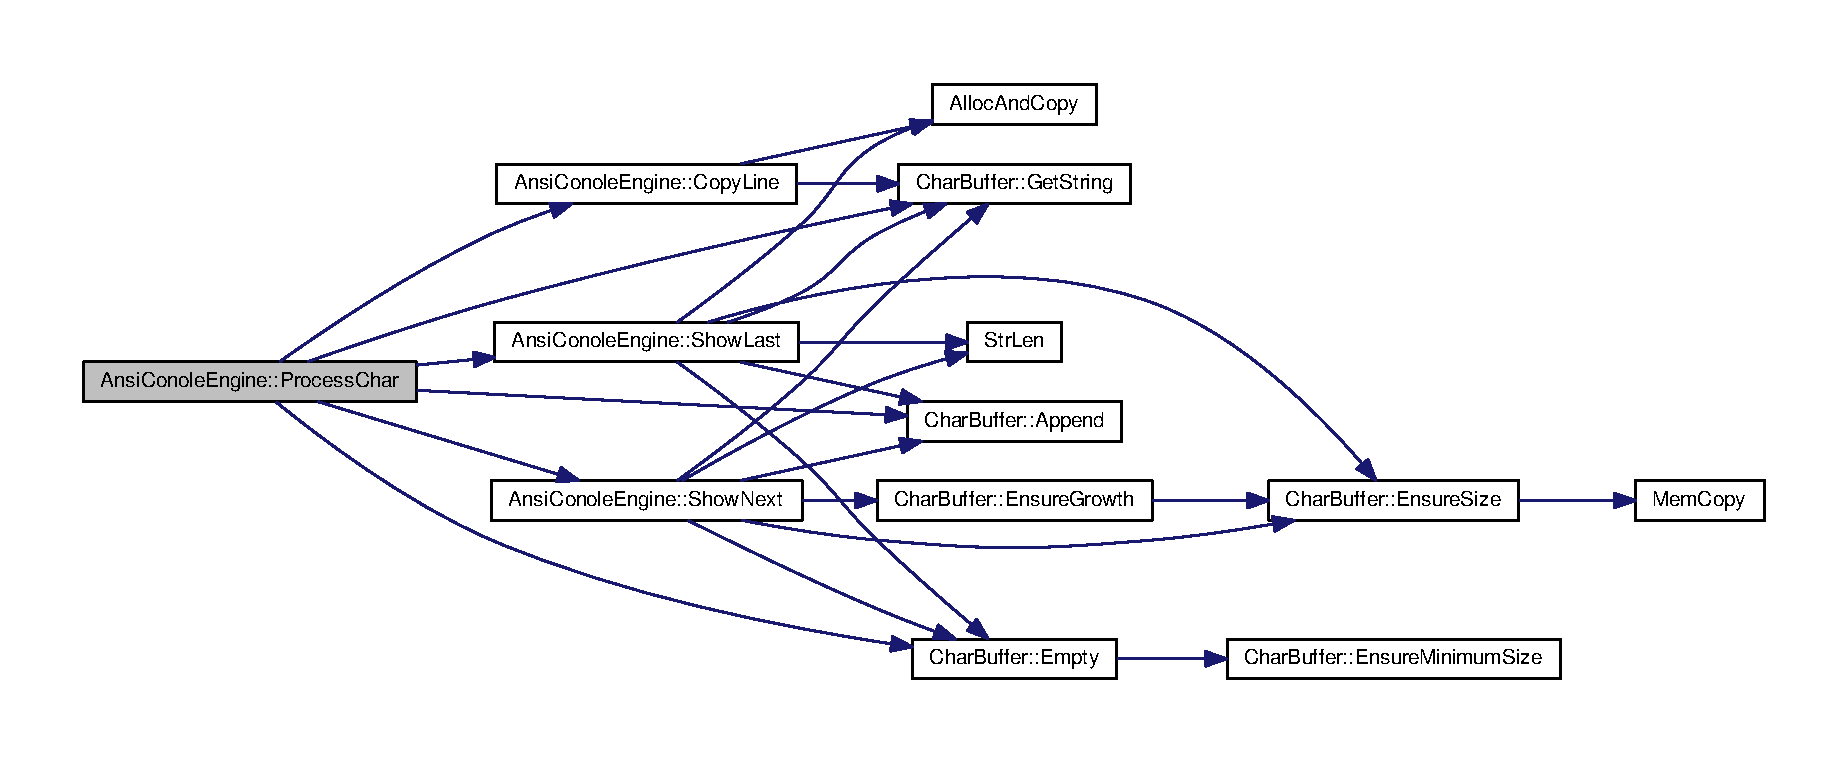
\includegraphics[width=350pt]{df/d87/classAnsiConoleEngine_a7bb2dea88ddc5ae76643d2303fcc4bf1_cgraph}
\end{center}
\end{figure}




Here is the caller graph for this function\+:
\nopagebreak
\begin{figure}[H]
\begin{center}
\leavevmode
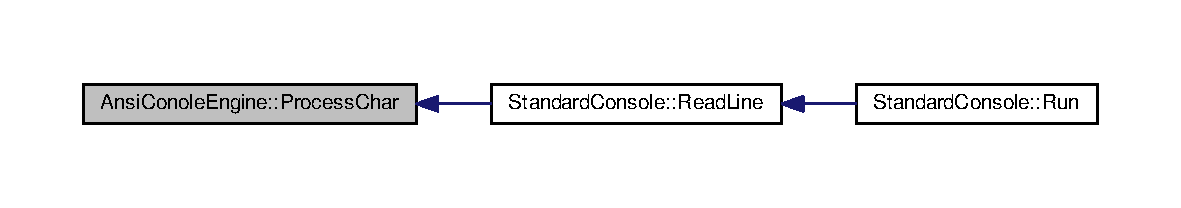
\includegraphics[width=350pt]{df/d87/classAnsiConoleEngine_a7bb2dea88ddc5ae76643d2303fcc4bf1_icgraph}
\end{center}
\end{figure}


\index{Ansi\+Conole\+Engine@{Ansi\+Conole\+Engine}!Set\+Prompt@{Set\+Prompt}}
\index{Set\+Prompt@{Set\+Prompt}!Ansi\+Conole\+Engine@{Ansi\+Conole\+Engine}}
\subsubsection[{\texorpdfstring{Set\+Prompt(const char $\ast$string)}{SetPrompt(const char *string)}}]{\setlength{\rightskip}{0pt plus 5cm}void Ansi\+Conole\+Engine\+::\+Set\+Prompt (
\begin{DoxyParamCaption}
\item[{const char $\ast$}]{string}
\end{DoxyParamCaption}
)}\hypertarget{classAnsiConoleEngine_a6c5dd4043aadc0b310f976eb10cbcd9f}{}\label{classAnsiConoleEngine_a6c5dd4043aadc0b310f976eb10cbcd9f}


Definition at line 323 of file aengine.\+cpp.



References Alloc\+And\+Copy(), and prompt.



Referenced by Standard\+Console\+::\+Set\+Prompt().


\begin{DoxyCode}
324 \{
325     \textcolor{keyword}{delete} \hyperlink{classAnsiConoleEngine_a97ebef63ba0490711ed78733b6a87be5}{prompt};
326     \hyperlink{clib_8h_a5bed05c70cb17e541fee570b5dc32e1a}{AllocAndCopy}(&\hyperlink{classAnsiConoleEngine_a97ebef63ba0490711ed78733b6a87be5}{prompt}, \textcolor{keywordtype}{string});
327 \}
\end{DoxyCode}


Here is the call graph for this function\+:
\nopagebreak
\begin{figure}[H]
\begin{center}
\leavevmode
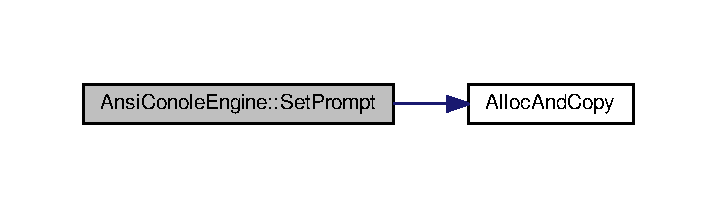
\includegraphics[width=344pt]{df/d87/classAnsiConoleEngine_a6c5dd4043aadc0b310f976eb10cbcd9f_cgraph}
\end{center}
\end{figure}




Here is the caller graph for this function\+:
\nopagebreak
\begin{figure}[H]
\begin{center}
\leavevmode
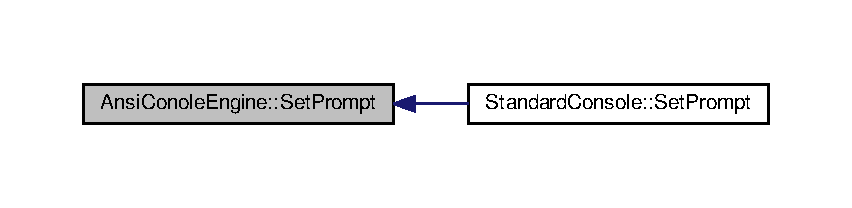
\includegraphics[width=350pt]{df/d87/classAnsiConoleEngine_a6c5dd4043aadc0b310f976eb10cbcd9f_icgraph}
\end{center}
\end{figure}


\index{Ansi\+Conole\+Engine@{Ansi\+Conole\+Engine}!Show\+Last@{Show\+Last}}
\index{Show\+Last@{Show\+Last}!Ansi\+Conole\+Engine@{Ansi\+Conole\+Engine}}
\subsubsection[{\texorpdfstring{Show\+Last()}{ShowLast()}}]{\setlength{\rightskip}{0pt plus 5cm}void Ansi\+Conole\+Engine\+::\+Show\+Last (
\begin{DoxyParamCaption}
{}
\end{DoxyParamCaption}
)\hspace{0.3cm}{\ttfamily [private]}}\hypertarget{classAnsiConoleEngine_afc441f10d1c52dba7b3ca1a5f2514e7c}{}\label{classAnsiConoleEngine_afc441f10d1c52dba7b3ca1a5f2514e7c}


Definition at line 235 of file aengine.\+cpp.



References Alloc\+And\+Copy(), Char\+Buffer\+::\+Append(), Char\+Buffer\+::buf, curline, cursor, editline, Char\+Buffer\+::\+Empty(), endpos, Char\+Buffer\+::\+Ensure\+Size(), Char\+Buffer\+::\+Get\+String(), len, linebuf, lines, line\+Size, lineswap, out, prompt, showline, and Str\+Len().



Referenced by Process\+Char().


\begin{DoxyCode}
236 \{
237     \textcolor{keywordflow}{if} (\hyperlink{classAnsiConoleEngine_ab029fc4a19c5fbd6f6b23c390af618b8}{curline} == -1) \{
238         \textcolor{keywordflow}{return};
239     \}
240 
241     \textcolor{keywordflow}{if} (!\hyperlink{classAnsiConoleEngine_a23b1b0d4714995d12e7b0aacdecfa0c4}{lineswap}) \{
242         \hyperlink{clib_8h_a5bed05c70cb17e541fee570b5dc32e1a}{AllocAndCopy}(&\hyperlink{classAnsiConoleEngine_a465421c5488f2566d12717641a327017}{editline}, \hyperlink{classAnsiConoleEngine_a6bf88afa72a458e3687972f9e666cd86}{linebuf}->\hyperlink{classCharBuffer_a7dfd3feaaf80f318ba44efe15b1ec44b}{GetString}());
243         \hyperlink{classAnsiConoleEngine_a23b1b0d4714995d12e7b0aacdecfa0c4}{lineswap} = \textcolor{keyword}{true};
244         \hyperlink{classAnsiConoleEngine_a24fe8cd3b3321c6dd4b26731cb1a8108}{showline} = \hyperlink{classAnsiConoleEngine_ab029fc4a19c5fbd6f6b23c390af618b8}{curline} + 1;
245     \} \textcolor{keywordflow}{else} \textcolor{keywordflow}{if} (\hyperlink{classAnsiConoleEngine_a24fe8cd3b3321c6dd4b26731cb1a8108}{showline} == \hyperlink{classAnsiConoleEngine_ab029fc4a19c5fbd6f6b23c390af618b8}{curline} + 1) \{
246         \textcolor{keyword}{delete} \hyperlink{classAnsiConoleEngine_a465421c5488f2566d12717641a327017}{editline};
247         \hyperlink{clib_8h_a5bed05c70cb17e541fee570b5dc32e1a}{AllocAndCopy}(&\hyperlink{classAnsiConoleEngine_a465421c5488f2566d12717641a327017}{editline}, \hyperlink{classAnsiConoleEngine_a6bf88afa72a458e3687972f9e666cd86}{linebuf}->\hyperlink{classCharBuffer_a7dfd3feaaf80f318ba44efe15b1ec44b}{GetString}());
248     \}
249 
250     \hyperlink{classAnsiConoleEngine_a24fe8cd3b3321c6dd4b26731cb1a8108}{showline}--;
251     \textcolor{keywordflow}{if} (showline < 0) \{
252         showline = 0;
253     \}
254 
255     \hyperlink{classAnsiConoleEngine_ad6a604fc0a0f544907513076c72434f3}{out}->\hyperlink{classCharBuffer_abe39d3fd7d8b9c8ec343af2cae7adc96}{Empty}();
256     \hyperlink{classAnsiConoleEngine_ad6a604fc0a0f544907513076c72434f3}{out}->\hyperlink{classCharBuffer_ad1907009b5ad136692b989fa96bf2f7e}{EnsureSize}(
257         \hyperlink{clib_8h_a67ec56eb98b49515d35005a5b3bf9a32}{StrLen}(\hyperlink{platform_8h_a0fbdfe13a76e65ec4703155481a97661}{DELETELINE}) +
258         \hyperlink{clib_8h_a67ec56eb98b49515d35005a5b3bf9a32}{StrLen}(\hyperlink{classAnsiConoleEngine_a97ebef63ba0490711ed78733b6a87be5}{prompt}) +
259         \hyperlink{clib_8h_a67ec56eb98b49515d35005a5b3bf9a32}{StrLen}(\hyperlink{classAnsiConoleEngine_a624ec5321c326a68de340f9b77e84c2c}{lines}[showline]) + 1);
260 
261     \hyperlink{classAnsiConoleEngine_ad6a604fc0a0f544907513076c72434f3}{out}->\hyperlink{classCharBuffer_a045b38735f7b3007c1b98d3d7b7feafe}{Append}(\hyperlink{platform_8h_a0fbdfe13a76e65ec4703155481a97661}{DELETELINE});
262     \hyperlink{classAnsiConoleEngine_ad6a604fc0a0f544907513076c72434f3}{out}->\hyperlink{classCharBuffer_a045b38735f7b3007c1b98d3d7b7feafe}{Append}(\hyperlink{classAnsiConoleEngine_a97ebef63ba0490711ed78733b6a87be5}{prompt});
263     \hyperlink{classAnsiConoleEngine_ad6a604fc0a0f544907513076c72434f3}{out}->\hyperlink{classCharBuffer_a045b38735f7b3007c1b98d3d7b7feafe}{Append}(\hyperlink{classAnsiConoleEngine_a624ec5321c326a68de340f9b77e84c2c}{lines}[showline]);
264 
265     \hyperlink{classAnsiConoleEngine_a6bf88afa72a458e3687972f9e666cd86}{linebuf}->\hyperlink{classCharBuffer_abe39d3fd7d8b9c8ec343af2cae7adc96}{Empty}();
266     \hyperlink{classAnsiConoleEngine_a6bf88afa72a458e3687972f9e666cd86}{linebuf}->\hyperlink{classCharBuffer_ad1907009b5ad136692b989fa96bf2f7e}{EnsureSize}(\hyperlink{clib_8h_a67ec56eb98b49515d35005a5b3bf9a32}{StrLen}(\hyperlink{classAnsiConoleEngine_a624ec5321c326a68de340f9b77e84c2c}{lines}[showline]));
267     \hyperlink{classAnsiConoleEngine_a6bf88afa72a458e3687972f9e666cd86}{linebuf}->\hyperlink{classCharBuffer_a045b38735f7b3007c1b98d3d7b7feafe}{Append}(\hyperlink{classAnsiConoleEngine_a624ec5321c326a68de340f9b77e84c2c}{lines}[showline]);
268 
269     \textcolor{keywordtype}{unsigned} \textcolor{keywordtype}{int} linelen = \hyperlink{clib_8h_a67ec56eb98b49515d35005a5b3bf9a32}{StrLen}(\hyperlink{classAnsiConoleEngine_a6bf88afa72a458e3687972f9e666cd86}{linebuf}->\hyperlink{classCharBuffer_a7dfd3feaaf80f318ba44efe15b1ec44b}{GetString}());
270     \hyperlink{classAnsiConoleEngine_aea3df1b13bc8ecf2eb68ec693249800f}{cursor} = \hyperlink{classAnsiConoleEngine_a6bf88afa72a458e3687972f9e666cd86}{linebuf}->\hyperlink{classCharBuffer_a8bcd8491b24db4197b311eb361609674}{buf} + linelen;
271     \hyperlink{classAnsiConoleEngine_a28852245082570631c7392411fec89cc}{endpos} = \hyperlink{classAnsiConoleEngine_aea3df1b13bc8ecf2eb68ec693249800f}{cursor};
272     \hyperlink{classAnsiConoleEngine_ad5d65280df848947f5b2dda80dcf35c6}{len} = \hyperlink{classAnsiConoleEngine_a59042210f69050bdfb531841e8ac0927}{lineSize} - linelen;
273 \}
\end{DoxyCode}


Here is the call graph for this function\+:
\nopagebreak
\begin{figure}[H]
\begin{center}
\leavevmode
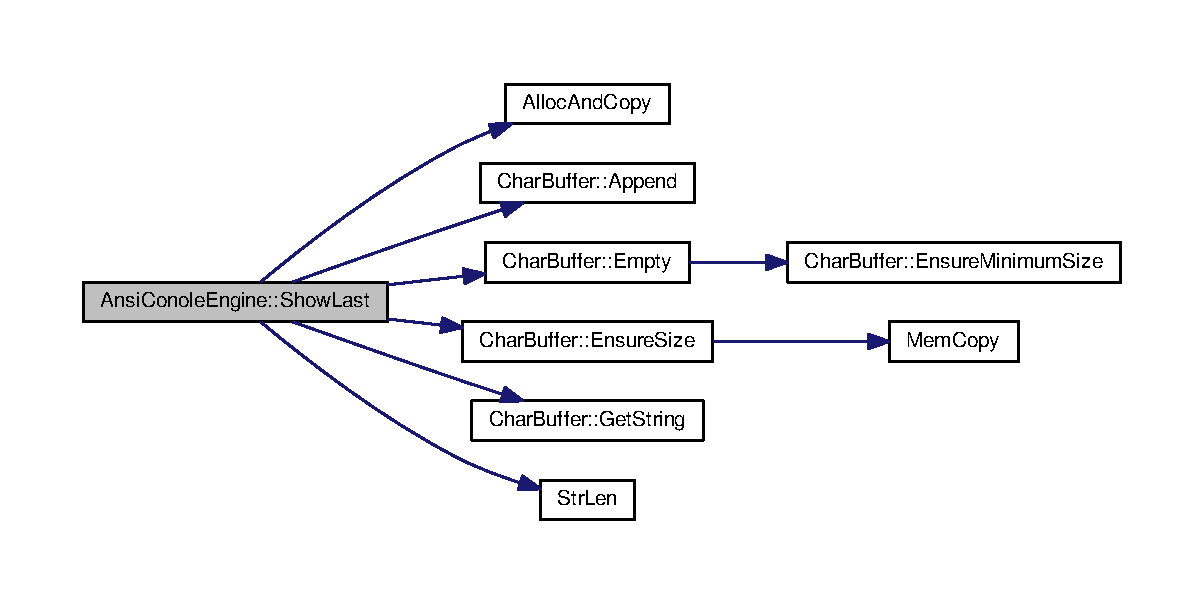
\includegraphics[width=350pt]{df/d87/classAnsiConoleEngine_afc441f10d1c52dba7b3ca1a5f2514e7c_cgraph}
\end{center}
\end{figure}




Here is the caller graph for this function\+:
\nopagebreak
\begin{figure}[H]
\begin{center}
\leavevmode
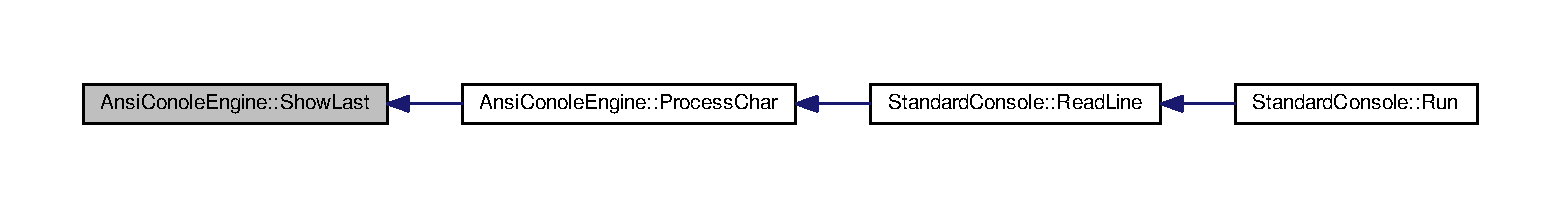
\includegraphics[width=350pt]{df/d87/classAnsiConoleEngine_afc441f10d1c52dba7b3ca1a5f2514e7c_icgraph}
\end{center}
\end{figure}


\index{Ansi\+Conole\+Engine@{Ansi\+Conole\+Engine}!Show\+Next@{Show\+Next}}
\index{Show\+Next@{Show\+Next}!Ansi\+Conole\+Engine@{Ansi\+Conole\+Engine}}
\subsubsection[{\texorpdfstring{Show\+Next()}{ShowNext()}}]{\setlength{\rightskip}{0pt plus 5cm}void Ansi\+Conole\+Engine\+::\+Show\+Next (
\begin{DoxyParamCaption}
{}
\end{DoxyParamCaption}
)\hspace{0.3cm}{\ttfamily [private]}}\hypertarget{classAnsiConoleEngine_a93c3eccd6c1458e1a82bdbf202948d90}{}\label{classAnsiConoleEngine_a93c3eccd6c1458e1a82bdbf202948d90}


Definition at line 275 of file aengine.\+cpp.



References Char\+Buffer\+::\+Append(), Char\+Buffer\+::buf, curline, cursor, editline, Char\+Buffer\+::\+Empty(), endpos, Char\+Buffer\+::\+Ensure\+Growth(), Char\+Buffer\+::\+Ensure\+Size(), Char\+Buffer\+::\+Get\+String(), len, linebuf, lines, line\+Size, lineswap, out, prompt, showline, and Str\+Len().



Referenced by Process\+Char().


\begin{DoxyCode}
276 \{
277     \textcolor{keywordflow}{if} (!\hyperlink{classAnsiConoleEngine_a23b1b0d4714995d12e7b0aacdecfa0c4}{lineswap}) \{
278         \textcolor{keywordflow}{return};
279     \}
280 
281     \hyperlink{classAnsiConoleEngine_a24fe8cd3b3321c6dd4b26731cb1a8108}{showline}++;
282     \textcolor{keywordflow}{if} (\hyperlink{classAnsiConoleEngine_a24fe8cd3b3321c6dd4b26731cb1a8108}{showline} > \hyperlink{classAnsiConoleEngine_ab029fc4a19c5fbd6f6b23c390af618b8}{curline} + 1) \{
283         \hyperlink{classAnsiConoleEngine_a24fe8cd3b3321c6dd4b26731cb1a8108}{showline} = \hyperlink{classAnsiConoleEngine_ab029fc4a19c5fbd6f6b23c390af618b8}{curline} + 1;
284         \textcolor{keywordflow}{return};
285     \}
286 
287     \hyperlink{classAnsiConoleEngine_ad6a604fc0a0f544907513076c72434f3}{out}->\hyperlink{classCharBuffer_abe39d3fd7d8b9c8ec343af2cae7adc96}{Empty}();
288     \hyperlink{classAnsiConoleEngine_ad6a604fc0a0f544907513076c72434f3}{out}->\hyperlink{classCharBuffer_a045b38735f7b3007c1b98d3d7b7feafe}{Append}(\hyperlink{platform_8h_a0fbdfe13a76e65ec4703155481a97661}{DELETELINE});
289     \hyperlink{classAnsiConoleEngine_ad6a604fc0a0f544907513076c72434f3}{out}->\hyperlink{classCharBuffer_a045b38735f7b3007c1b98d3d7b7feafe}{Append}(\hyperlink{classAnsiConoleEngine_a97ebef63ba0490711ed78733b6a87be5}{prompt});
290 
291     \textcolor{keywordflow}{if} (\hyperlink{classAnsiConoleEngine_a24fe8cd3b3321c6dd4b26731cb1a8108}{showline} > \hyperlink{classAnsiConoleEngine_ab029fc4a19c5fbd6f6b23c390af618b8}{curline}) \{
292         \hyperlink{classAnsiConoleEngine_ad6a604fc0a0f544907513076c72434f3}{out}->\hyperlink{classCharBuffer_a73c71d361110b37819a1d681a1504b0e}{EnsureGrowth}(\hyperlink{clib_8h_a67ec56eb98b49515d35005a5b3bf9a32}{StrLen}(\hyperlink{classAnsiConoleEngine_a465421c5488f2566d12717641a327017}{editline}) + 1);
293         \hyperlink{classAnsiConoleEngine_ad6a604fc0a0f544907513076c72434f3}{out}->\hyperlink{classCharBuffer_a045b38735f7b3007c1b98d3d7b7feafe}{Append}(\hyperlink{classAnsiConoleEngine_a465421c5488f2566d12717641a327017}{editline});
294 
295         \hyperlink{classAnsiConoleEngine_a6bf88afa72a458e3687972f9e666cd86}{linebuf}->\hyperlink{classCharBuffer_abe39d3fd7d8b9c8ec343af2cae7adc96}{Empty}();
296         \hyperlink{classAnsiConoleEngine_a6bf88afa72a458e3687972f9e666cd86}{linebuf}->\hyperlink{classCharBuffer_ad1907009b5ad136692b989fa96bf2f7e}{EnsureSize}(\hyperlink{clib_8h_a67ec56eb98b49515d35005a5b3bf9a32}{StrLen}(\hyperlink{classAnsiConoleEngine_a465421c5488f2566d12717641a327017}{editline}));
297         \hyperlink{classAnsiConoleEngine_a6bf88afa72a458e3687972f9e666cd86}{linebuf}->\hyperlink{classCharBuffer_a045b38735f7b3007c1b98d3d7b7feafe}{Append}(\hyperlink{classAnsiConoleEngine_a465421c5488f2566d12717641a327017}{editline});
298     \} \textcolor{keywordflow}{else} \{
299         \hyperlink{classAnsiConoleEngine_ad6a604fc0a0f544907513076c72434f3}{out}->\hyperlink{classCharBuffer_a73c71d361110b37819a1d681a1504b0e}{EnsureGrowth}(\hyperlink{clib_8h_a67ec56eb98b49515d35005a5b3bf9a32}{StrLen}(\hyperlink{classAnsiConoleEngine_a624ec5321c326a68de340f9b77e84c2c}{lines}[\hyperlink{classAnsiConoleEngine_a24fe8cd3b3321c6dd4b26731cb1a8108}{showline}]) + 1);
300         \hyperlink{classAnsiConoleEngine_ad6a604fc0a0f544907513076c72434f3}{out}->\hyperlink{classCharBuffer_a045b38735f7b3007c1b98d3d7b7feafe}{Append}(\hyperlink{classAnsiConoleEngine_a624ec5321c326a68de340f9b77e84c2c}{lines}[showline]);
301 
302         \hyperlink{classAnsiConoleEngine_a6bf88afa72a458e3687972f9e666cd86}{linebuf}->\hyperlink{classCharBuffer_abe39d3fd7d8b9c8ec343af2cae7adc96}{Empty}();
303         \hyperlink{classAnsiConoleEngine_a6bf88afa72a458e3687972f9e666cd86}{linebuf}->\hyperlink{classCharBuffer_ad1907009b5ad136692b989fa96bf2f7e}{EnsureSize}(\hyperlink{clib_8h_a67ec56eb98b49515d35005a5b3bf9a32}{StrLen}(\hyperlink{classAnsiConoleEngine_a624ec5321c326a68de340f9b77e84c2c}{lines}[showline]));
304         \hyperlink{classAnsiConoleEngine_a6bf88afa72a458e3687972f9e666cd86}{linebuf}->\hyperlink{classCharBuffer_a045b38735f7b3007c1b98d3d7b7feafe}{Append}(\hyperlink{classAnsiConoleEngine_a624ec5321c326a68de340f9b77e84c2c}{lines}[showline]);
305     \}
306 
307     \textcolor{keywordtype}{unsigned} \textcolor{keywordtype}{int} linelen = \hyperlink{clib_8h_a67ec56eb98b49515d35005a5b3bf9a32}{StrLen}(\hyperlink{classAnsiConoleEngine_a6bf88afa72a458e3687972f9e666cd86}{linebuf}->\hyperlink{classCharBuffer_a7dfd3feaaf80f318ba44efe15b1ec44b}{GetString}());
308     \hyperlink{classAnsiConoleEngine_aea3df1b13bc8ecf2eb68ec693249800f}{cursor} = \hyperlink{classAnsiConoleEngine_a6bf88afa72a458e3687972f9e666cd86}{linebuf}->\hyperlink{classCharBuffer_a8bcd8491b24db4197b311eb361609674}{buf} + linelen;
309     \hyperlink{classAnsiConoleEngine_a28852245082570631c7392411fec89cc}{endpos} = \hyperlink{classAnsiConoleEngine_aea3df1b13bc8ecf2eb68ec693249800f}{cursor};
310     \hyperlink{classAnsiConoleEngine_ad5d65280df848947f5b2dda80dcf35c6}{len} = \hyperlink{classAnsiConoleEngine_a59042210f69050bdfb531841e8ac0927}{lineSize} - linelen;
311 \}
\end{DoxyCode}


Here is the call graph for this function\+:
\nopagebreak
\begin{figure}[H]
\begin{center}
\leavevmode
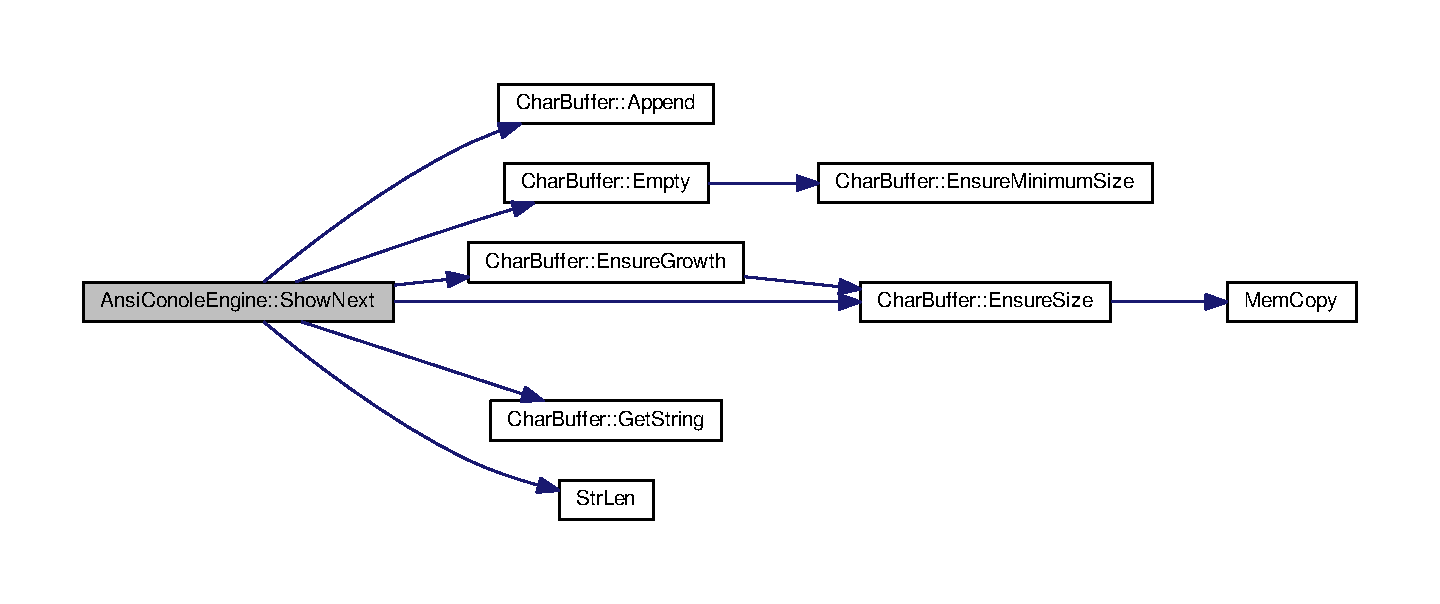
\includegraphics[width=350pt]{df/d87/classAnsiConoleEngine_a93c3eccd6c1458e1a82bdbf202948d90_cgraph}
\end{center}
\end{figure}




Here is the caller graph for this function\+:
\nopagebreak
\begin{figure}[H]
\begin{center}
\leavevmode
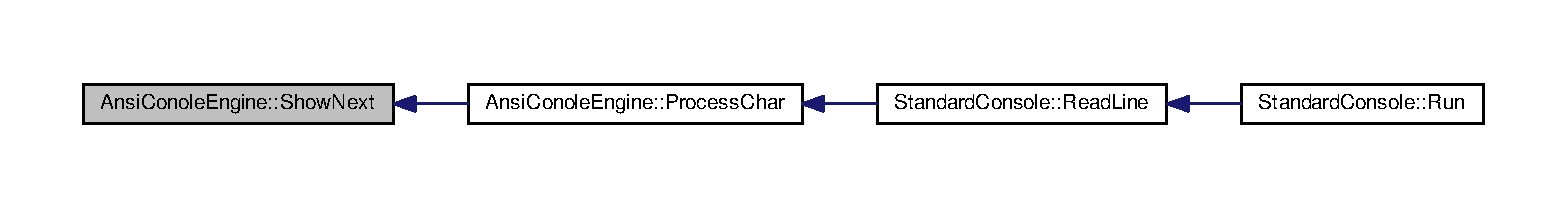
\includegraphics[width=350pt]{df/d87/classAnsiConoleEngine_a93c3eccd6c1458e1a82bdbf202948d90_icgraph}
\end{center}
\end{figure}


\index{Ansi\+Conole\+Engine@{Ansi\+Conole\+Engine}!Start\+Input@{Start\+Input}}
\index{Start\+Input@{Start\+Input}!Ansi\+Conole\+Engine@{Ansi\+Conole\+Engine}}
\subsubsection[{\texorpdfstring{Start\+Input()}{StartInput()}}]{\setlength{\rightskip}{0pt plus 5cm}void Ansi\+Conole\+Engine\+::\+Start\+Input (
\begin{DoxyParamCaption}
{}
\end{DoxyParamCaption}
)}\hypertarget{classAnsiConoleEngine_a8ad01a2ddd3ee5182deb4a74f3d2a0c1}{}\label{classAnsiConoleEngine_a8ad01a2ddd3ee5182deb4a74f3d2a0c1}


Definition at line 61 of file aengine.\+cpp.



References Char\+Buffer\+::buf, Char\+Buffer\+::\+Clear\+And\+Alloc(), csimode, cursor, delmode, endpos, escmode, len, linebuf, linedone, line\+Size, and lineswap.



Referenced by Standard\+Console\+::\+Read\+Line().


\begin{DoxyCode}
62 \{
63     \hyperlink{classAnsiConoleEngine_a6bf88afa72a458e3687972f9e666cd86}{linebuf}->\hyperlink{classCharBuffer_a8c0927c2c05c954161151045f68581c6}{ClearAndAlloc}(\hyperlink{classAnsiConoleEngine_a59042210f69050bdfb531841e8ac0927}{lineSize} + 1);
64     \hyperlink{classAnsiConoleEngine_ad5d65280df848947f5b2dda80dcf35c6}{len} = \hyperlink{classAnsiConoleEngine_a59042210f69050bdfb531841e8ac0927}{lineSize};
65     \hyperlink{classAnsiConoleEngine_aea3df1b13bc8ecf2eb68ec693249800f}{cursor} = \hyperlink{classAnsiConoleEngine_a6bf88afa72a458e3687972f9e666cd86}{linebuf}->\hyperlink{classCharBuffer_a8bcd8491b24db4197b311eb361609674}{buf};
66     \hyperlink{classAnsiConoleEngine_a28852245082570631c7392411fec89cc}{endpos} = \hyperlink{classAnsiConoleEngine_aea3df1b13bc8ecf2eb68ec693249800f}{cursor};
67     *\hyperlink{classAnsiConoleEngine_a28852245082570631c7392411fec89cc}{endpos} = \textcolor{charliteral}{'\(\backslash\)0'};
68 
69     \hyperlink{classAnsiConoleEngine_a23b1b0d4714995d12e7b0aacdecfa0c4}{lineswap} = \textcolor{keyword}{false};
70     \hyperlink{classAnsiConoleEngine_af497f5cbdca8bbc350935a90568b06e7}{escmode} = \textcolor{keyword}{false};
71     \hyperlink{classAnsiConoleEngine_adf2036857a6c6de85836ee2e7b3e5d6d}{csimode} = \textcolor{keyword}{false};
72     \hyperlink{classAnsiConoleEngine_a5182d9a19cc1fe8681a9faf77a156657}{delmode} = \textcolor{keyword}{false};
73     \hyperlink{classAnsiConoleEngine_a0931686f3224f07bd3a3fe25c06e32c6}{linedone} = \textcolor{keyword}{false};
74 \}
\end{DoxyCode}


Here is the call graph for this function\+:
\nopagebreak
\begin{figure}[H]
\begin{center}
\leavevmode
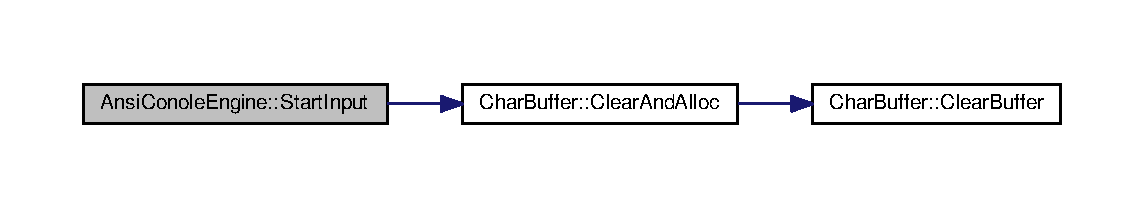
\includegraphics[width=350pt]{df/d87/classAnsiConoleEngine_a8ad01a2ddd3ee5182deb4a74f3d2a0c1_cgraph}
\end{center}
\end{figure}




Here is the caller graph for this function\+:
\nopagebreak
\begin{figure}[H]
\begin{center}
\leavevmode
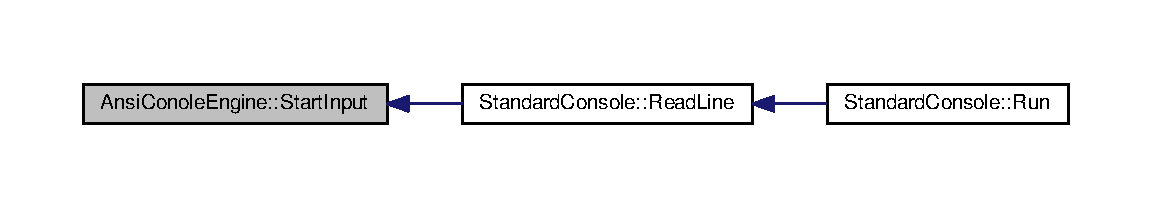
\includegraphics[width=350pt]{df/d87/classAnsiConoleEngine_a8ad01a2ddd3ee5182deb4a74f3d2a0c1_icgraph}
\end{center}
\end{figure}




\subsection{Member Data Documentation}
\index{Ansi\+Conole\+Engine@{Ansi\+Conole\+Engine}!csimode@{csimode}}
\index{csimode@{csimode}!Ansi\+Conole\+Engine@{Ansi\+Conole\+Engine}}
\subsubsection[{\texorpdfstring{csimode}{csimode}}]{\setlength{\rightskip}{0pt plus 5cm}{\bf bool} Ansi\+Conole\+Engine\+::csimode\hspace{0.3cm}{\ttfamily [private]}}\hypertarget{classAnsiConoleEngine_adf2036857a6c6de85836ee2e7b3e5d6d}{}\label{classAnsiConoleEngine_adf2036857a6c6de85836ee2e7b3e5d6d}


Definition at line 76 of file aengine.\+h.



Referenced by Process\+Char(), and Start\+Input().

\index{Ansi\+Conole\+Engine@{Ansi\+Conole\+Engine}!curline@{curline}}
\index{curline@{curline}!Ansi\+Conole\+Engine@{Ansi\+Conole\+Engine}}
\subsubsection[{\texorpdfstring{curline}{curline}}]{\setlength{\rightskip}{0pt plus 5cm}int Ansi\+Conole\+Engine\+::curline\hspace{0.3cm}{\ttfamily [private]}}\hypertarget{classAnsiConoleEngine_ab029fc4a19c5fbd6f6b23c390af618b8}{}\label{classAnsiConoleEngine_ab029fc4a19c5fbd6f6b23c390af618b8}


Definition at line 70 of file aengine.\+h.



Referenced by Ansi\+Conole\+Engine(), Copy\+Line(), Show\+Last(), and Show\+Next().

\index{Ansi\+Conole\+Engine@{Ansi\+Conole\+Engine}!cursor@{cursor}}
\index{cursor@{cursor}!Ansi\+Conole\+Engine@{Ansi\+Conole\+Engine}}
\subsubsection[{\texorpdfstring{cursor}{cursor}}]{\setlength{\rightskip}{0pt plus 5cm}char$\ast$ Ansi\+Conole\+Engine\+::cursor\hspace{0.3cm}{\ttfamily [private]}}\hypertarget{classAnsiConoleEngine_aea3df1b13bc8ecf2eb68ec693249800f}{}\label{classAnsiConoleEngine_aea3df1b13bc8ecf2eb68ec693249800f}


Definition at line 67 of file aengine.\+h.



Referenced by Process\+Char(), Show\+Last(), Show\+Next(), and Start\+Input().

\index{Ansi\+Conole\+Engine@{Ansi\+Conole\+Engine}!delmode@{delmode}}
\index{delmode@{delmode}!Ansi\+Conole\+Engine@{Ansi\+Conole\+Engine}}
\subsubsection[{\texorpdfstring{delmode}{delmode}}]{\setlength{\rightskip}{0pt plus 5cm}{\bf bool} Ansi\+Conole\+Engine\+::delmode\hspace{0.3cm}{\ttfamily [private]}}\hypertarget{classAnsiConoleEngine_a5182d9a19cc1fe8681a9faf77a156657}{}\label{classAnsiConoleEngine_a5182d9a19cc1fe8681a9faf77a156657}


Definition at line 77 of file aengine.\+h.



Referenced by Process\+Char(), and Start\+Input().

\index{Ansi\+Conole\+Engine@{Ansi\+Conole\+Engine}!editline@{editline}}
\index{editline@{editline}!Ansi\+Conole\+Engine@{Ansi\+Conole\+Engine}}
\subsubsection[{\texorpdfstring{editline}{editline}}]{\setlength{\rightskip}{0pt plus 5cm}char$\ast$ Ansi\+Conole\+Engine\+::editline\hspace{0.3cm}{\ttfamily [private]}}\hypertarget{classAnsiConoleEngine_a465421c5488f2566d12717641a327017}{}\label{classAnsiConoleEngine_a465421c5488f2566d12717641a327017}


Definition at line 73 of file aengine.\+h.



Referenced by Ansi\+Conole\+Engine(), Copy\+Line(), Show\+Last(), and Show\+Next().

\index{Ansi\+Conole\+Engine@{Ansi\+Conole\+Engine}!endpos@{endpos}}
\index{endpos@{endpos}!Ansi\+Conole\+Engine@{Ansi\+Conole\+Engine}}
\subsubsection[{\texorpdfstring{endpos}{endpos}}]{\setlength{\rightskip}{0pt plus 5cm}char$\ast$ Ansi\+Conole\+Engine\+::endpos\hspace{0.3cm}{\ttfamily [private]}}\hypertarget{classAnsiConoleEngine_a28852245082570631c7392411fec89cc}{}\label{classAnsiConoleEngine_a28852245082570631c7392411fec89cc}


Definition at line 68 of file aengine.\+h.



Referenced by Process\+Char(), Show\+Last(), Show\+Next(), and Start\+Input().

\index{Ansi\+Conole\+Engine@{Ansi\+Conole\+Engine}!escmode@{escmode}}
\index{escmode@{escmode}!Ansi\+Conole\+Engine@{Ansi\+Conole\+Engine}}
\subsubsection[{\texorpdfstring{escmode}{escmode}}]{\setlength{\rightskip}{0pt plus 5cm}{\bf bool} Ansi\+Conole\+Engine\+::escmode\hspace{0.3cm}{\ttfamily [private]}}\hypertarget{classAnsiConoleEngine_af497f5cbdca8bbc350935a90568b06e7}{}\label{classAnsiConoleEngine_af497f5cbdca8bbc350935a90568b06e7}


Definition at line 75 of file aengine.\+h.



Referenced by Process\+Char(), and Start\+Input().

\index{Ansi\+Conole\+Engine@{Ansi\+Conole\+Engine}!len@{len}}
\index{len@{len}!Ansi\+Conole\+Engine@{Ansi\+Conole\+Engine}}
\subsubsection[{\texorpdfstring{len}{len}}]{\setlength{\rightskip}{0pt plus 5cm}unsigned int Ansi\+Conole\+Engine\+::len\hspace{0.3cm}{\ttfamily [private]}}\hypertarget{classAnsiConoleEngine_ad5d65280df848947f5b2dda80dcf35c6}{}\label{classAnsiConoleEngine_ad5d65280df848947f5b2dda80dcf35c6}


Definition at line 66 of file aengine.\+h.



Referenced by Process\+Char(), Show\+Last(), Show\+Next(), and Start\+Input().

\index{Ansi\+Conole\+Engine@{Ansi\+Conole\+Engine}!linebuf@{linebuf}}
\index{linebuf@{linebuf}!Ansi\+Conole\+Engine@{Ansi\+Conole\+Engine}}
\subsubsection[{\texorpdfstring{linebuf}{linebuf}}]{\setlength{\rightskip}{0pt plus 5cm}{\bf Char\+Buffer}$\ast$ Ansi\+Conole\+Engine\+::linebuf\hspace{0.3cm}{\ttfamily [private]}}\hypertarget{classAnsiConoleEngine_a6bf88afa72a458e3687972f9e666cd86}{}\label{classAnsiConoleEngine_a6bf88afa72a458e3687972f9e666cd86}


Definition at line 65 of file aengine.\+h.



Referenced by Ansi\+Conole\+Engine(), Copy\+Line(), Get\+Line(), Process\+Char(), Show\+Last(), Show\+Next(), Start\+Input(), and $\sim$\+Ansi\+Conole\+Engine().

\index{Ansi\+Conole\+Engine@{Ansi\+Conole\+Engine}!linedone@{linedone}}
\index{linedone@{linedone}!Ansi\+Conole\+Engine@{Ansi\+Conole\+Engine}}
\subsubsection[{\texorpdfstring{linedone}{linedone}}]{\setlength{\rightskip}{0pt plus 5cm}{\bf bool} Ansi\+Conole\+Engine\+::linedone\hspace{0.3cm}{\ttfamily [private]}}\hypertarget{classAnsiConoleEngine_a0931686f3224f07bd3a3fe25c06e32c6}{}\label{classAnsiConoleEngine_a0931686f3224f07bd3a3fe25c06e32c6}


Definition at line 78 of file aengine.\+h.



Referenced by Input\+Done(), Process\+Char(), and Start\+Input().

\index{Ansi\+Conole\+Engine@{Ansi\+Conole\+Engine}!lines@{lines}}
\index{lines@{lines}!Ansi\+Conole\+Engine@{Ansi\+Conole\+Engine}}
\subsubsection[{\texorpdfstring{lines}{lines}}]{\setlength{\rightskip}{0pt plus 5cm}char$\ast$$\ast$ Ansi\+Conole\+Engine\+::lines\hspace{0.3cm}{\ttfamily [private]}}\hypertarget{classAnsiConoleEngine_a624ec5321c326a68de340f9b77e84c2c}{}\label{classAnsiConoleEngine_a624ec5321c326a68de340f9b77e84c2c}


Definition at line 64 of file aengine.\+h.



Referenced by Ansi\+Conole\+Engine(), Copy\+Line(), Show\+Last(), Show\+Next(), and $\sim$\+Ansi\+Conole\+Engine().

\index{Ansi\+Conole\+Engine@{Ansi\+Conole\+Engine}!line\+Size@{line\+Size}}
\index{line\+Size@{line\+Size}!Ansi\+Conole\+Engine@{Ansi\+Conole\+Engine}}
\subsubsection[{\texorpdfstring{line\+Size}{lineSize}}]{\setlength{\rightskip}{0pt plus 5cm}const int Ansi\+Conole\+Engine\+::line\+Size = 1024\hspace{0.3cm}{\ttfamily [static]}, {\ttfamily [private]}}\hypertarget{classAnsiConoleEngine_a59042210f69050bdfb531841e8ac0927}{}\label{classAnsiConoleEngine_a59042210f69050bdfb531841e8ac0927}


Definition at line 63 of file aengine.\+h.



Referenced by Show\+Last(), Show\+Next(), and Start\+Input().

\index{Ansi\+Conole\+Engine@{Ansi\+Conole\+Engine}!lineswap@{lineswap}}
\index{lineswap@{lineswap}!Ansi\+Conole\+Engine@{Ansi\+Conole\+Engine}}
\subsubsection[{\texorpdfstring{lineswap}{lineswap}}]{\setlength{\rightskip}{0pt plus 5cm}{\bf bool} Ansi\+Conole\+Engine\+::lineswap\hspace{0.3cm}{\ttfamily [private]}}\hypertarget{classAnsiConoleEngine_a23b1b0d4714995d12e7b0aacdecfa0c4}{}\label{classAnsiConoleEngine_a23b1b0d4714995d12e7b0aacdecfa0c4}


Definition at line 72 of file aengine.\+h.



Referenced by Show\+Last(), Show\+Next(), and Start\+Input().

\index{Ansi\+Conole\+Engine@{Ansi\+Conole\+Engine}!max\+Lines@{max\+Lines}}
\index{max\+Lines@{max\+Lines}!Ansi\+Conole\+Engine@{Ansi\+Conole\+Engine}}
\subsubsection[{\texorpdfstring{max\+Lines}{maxLines}}]{\setlength{\rightskip}{0pt plus 5cm}const int Ansi\+Conole\+Engine\+::max\+Lines = 20\hspace{0.3cm}{\ttfamily [static]}, {\ttfamily [private]}}\hypertarget{classAnsiConoleEngine_a3f94786b1610ac3f038d5115fd8047a3}{}\label{classAnsiConoleEngine_a3f94786b1610ac3f038d5115fd8047a3}


Definition at line 62 of file aengine.\+h.



Referenced by Ansi\+Conole\+Engine(), Copy\+Line(), and $\sim$\+Ansi\+Conole\+Engine().

\index{Ansi\+Conole\+Engine@{Ansi\+Conole\+Engine}!out@{out}}
\index{out@{out}!Ansi\+Conole\+Engine@{Ansi\+Conole\+Engine}}
\subsubsection[{\texorpdfstring{out}{out}}]{\setlength{\rightskip}{0pt plus 5cm}{\bf Char\+Buffer}$\ast$ Ansi\+Conole\+Engine\+::out\hspace{0.3cm}{\ttfamily [private]}}\hypertarget{classAnsiConoleEngine_ad6a604fc0a0f544907513076c72434f3}{}\label{classAnsiConoleEngine_ad6a604fc0a0f544907513076c72434f3}


Definition at line 79 of file aengine.\+h.



Referenced by Ansi\+Conole\+Engine(), Process\+Char(), Show\+Last(), Show\+Next(), and $\sim$\+Ansi\+Conole\+Engine().

\index{Ansi\+Conole\+Engine@{Ansi\+Conole\+Engine}!prompt@{prompt}}
\index{prompt@{prompt}!Ansi\+Conole\+Engine@{Ansi\+Conole\+Engine}}
\subsubsection[{\texorpdfstring{prompt}{prompt}}]{\setlength{\rightskip}{0pt plus 5cm}char$\ast$ Ansi\+Conole\+Engine\+::prompt\hspace{0.3cm}{\ttfamily [private]}}\hypertarget{classAnsiConoleEngine_a97ebef63ba0490711ed78733b6a87be5}{}\label{classAnsiConoleEngine_a97ebef63ba0490711ed78733b6a87be5}


Definition at line 60 of file aengine.\+h.



Referenced by Ansi\+Conole\+Engine(), Set\+Prompt(), Show\+Last(), Show\+Next(), and $\sim$\+Ansi\+Conole\+Engine().

\index{Ansi\+Conole\+Engine@{Ansi\+Conole\+Engine}!showline@{showline}}
\index{showline@{showline}!Ansi\+Conole\+Engine@{Ansi\+Conole\+Engine}}
\subsubsection[{\texorpdfstring{showline}{showline}}]{\setlength{\rightskip}{0pt plus 5cm}int Ansi\+Conole\+Engine\+::showline\hspace{0.3cm}{\ttfamily [private]}}\hypertarget{classAnsiConoleEngine_a24fe8cd3b3321c6dd4b26731cb1a8108}{}\label{classAnsiConoleEngine_a24fe8cd3b3321c6dd4b26731cb1a8108}


Definition at line 71 of file aengine.\+h.



Referenced by Show\+Last(), and Show\+Next().



The documentation for this class was generated from the following files\+:\begin{DoxyCompactItemize}
\item 
app/lib/\hyperlink{aengine_8h}{aengine.\+h}\item 
app/lib/\hyperlink{aengine_8cpp}{aengine.\+cpp}\end{DoxyCompactItemize}

\hypertarget{classArcCosecantNode}{}\section{Arc\+Cosecant\+Node Class Reference}
\label{classArcCosecantNode}\index{Arc\+Cosecant\+Node@{Arc\+Cosecant\+Node}}


{\ttfamily \#include $<$functions.\+h$>$}



Inheritance diagram for Arc\+Cosecant\+Node\+:\nopagebreak
\begin{figure}[H]
\begin{center}
\leavevmode
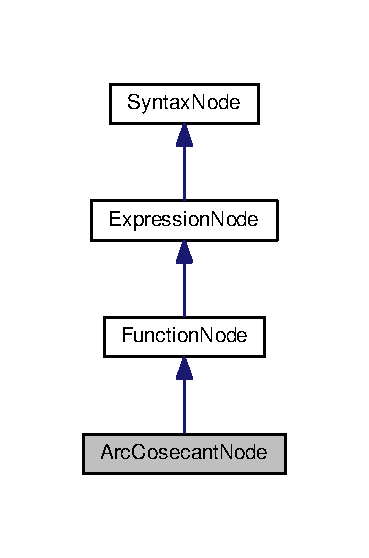
\includegraphics[width=177pt]{classArcCosecantNode__inherit__graph}
\end{center}
\end{figure}


Collaboration diagram for Arc\+Cosecant\+Node\+:\nopagebreak
\begin{figure}[H]
\begin{center}
\leavevmode
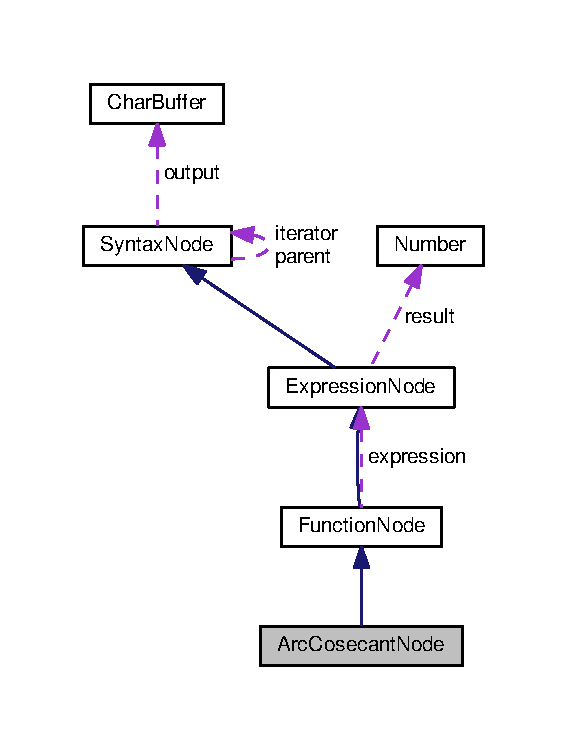
\includegraphics[width=272pt]{classArcCosecantNode__coll__graph}
\end{center}
\end{figure}
\subsection*{Public Member Functions}
\begin{DoxyCompactItemize}
\item 
\hyperlink{classArcCosecantNode_a0a06f57986491b3a1a4f952688bc4036}{Arc\+Cosecant\+Node} (\hyperlink{classExpressionNode}{Expression\+Node} $\ast$\hyperlink{classFunctionNode_ad7577b179a1937aaf8a0058bb5b546dc}{expression})
\item 
\hyperlink{structNumber}{Number} $\ast$ \hyperlink{classArcCosecantNode_a4cb42e104cb77fd303bb57c73d8286b0}{Evaluate} ()
\end{DoxyCompactItemize}
\subsection*{Static Public Member Functions}
\begin{DoxyCompactItemize}
\item 
static \hyperlink{classFunctionNode}{Function\+Node} $\ast$ \hyperlink{classArcCosecantNode_a03cc6abd00b92a4a8d7e801fc0d063bb}{Create} (\hyperlink{classExpressionNode}{Expression\+Node} $\ast$\hyperlink{classFunctionNode_ad7577b179a1937aaf8a0058bb5b546dc}{expression})
\end{DoxyCompactItemize}
\subsection*{Protected Member Functions}
\begin{DoxyCompactItemize}
\item 
char $\ast$ \hyperlink{classArcCosecantNode_ad0cc72410c2754f5befec12cac5e7f01}{Get\+Node\+Text} ()
\end{DoxyCompactItemize}
\subsection*{Additional Inherited Members}


\subsection{Detailed Description}


Definition at line 436 of file functions.\+h.



\subsection{Constructor \& Destructor Documentation}
\index{Arc\+Cosecant\+Node@{Arc\+Cosecant\+Node}!Arc\+Cosecant\+Node@{Arc\+Cosecant\+Node}}
\index{Arc\+Cosecant\+Node@{Arc\+Cosecant\+Node}!Arc\+Cosecant\+Node@{Arc\+Cosecant\+Node}}
\subsubsection[{\texorpdfstring{Arc\+Cosecant\+Node(\+Expression\+Node $\ast$expression)}{ArcCosecantNode(ExpressionNode *expression)}}]{\setlength{\rightskip}{0pt plus 5cm}Arc\+Cosecant\+Node\+::\+Arc\+Cosecant\+Node (
\begin{DoxyParamCaption}
\item[{{\bf Expression\+Node} $\ast$}]{expression}
\end{DoxyParamCaption}
)}\hypertarget{classArcCosecantNode_a0a06f57986491b3a1a4f952688bc4036}{}\label{classArcCosecantNode_a0a06f57986491b3a1a4f952688bc4036}


Definition at line 919 of file functions.\+cpp.



References Function\+Node\+::\+Function\+Node().



Referenced by Create().


\begin{DoxyCode}
919                                                            :
920     \hyperlink{classFunctionNode_a41cb7db0162ffbec0902bd8ff7ea435f}{FunctionNode}(expression) \{ \}
\end{DoxyCode}


Here is the call graph for this function\+:\nopagebreak
\begin{figure}[H]
\begin{center}
\leavevmode
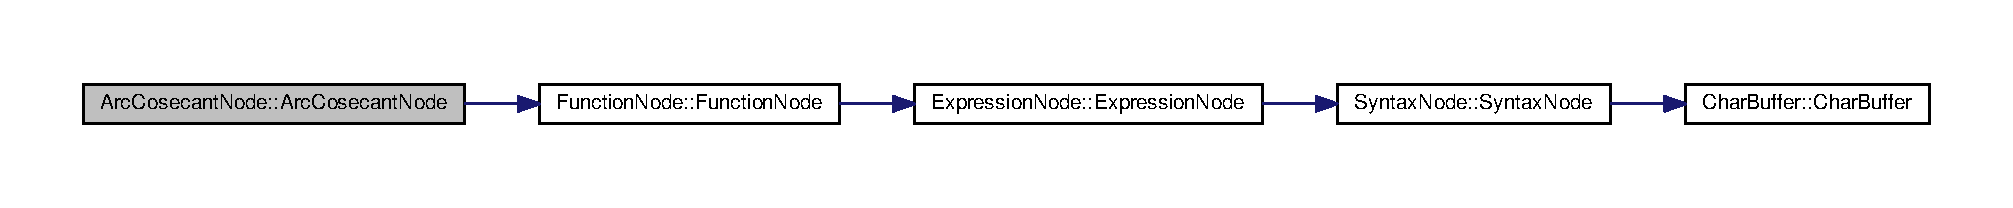
\includegraphics[width=350pt]{classArcCosecantNode_a0a06f57986491b3a1a4f952688bc4036_cgraph}
\end{center}
\end{figure}




Here is the caller graph for this function\+:\nopagebreak
\begin{figure}[H]
\begin{center}
\leavevmode
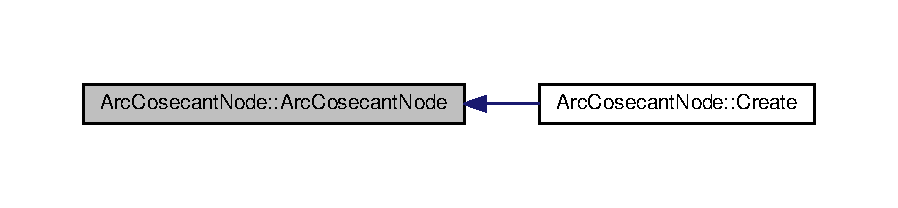
\includegraphics[width=350pt]{classArcCosecantNode_a0a06f57986491b3a1a4f952688bc4036_icgraph}
\end{center}
\end{figure}




\subsection{Member Function Documentation}
\index{Arc\+Cosecant\+Node@{Arc\+Cosecant\+Node}!Create@{Create}}
\index{Create@{Create}!Arc\+Cosecant\+Node@{Arc\+Cosecant\+Node}}
\subsubsection[{\texorpdfstring{Create(\+Expression\+Node $\ast$expression)}{Create(ExpressionNode *expression)}}]{\setlength{\rightskip}{0pt plus 5cm}{\bf Function\+Node} $\ast$ Arc\+Cosecant\+Node\+::\+Create (
\begin{DoxyParamCaption}
\item[{{\bf Expression\+Node} $\ast$}]{expression}
\end{DoxyParamCaption}
)\hspace{0.3cm}{\ttfamily [static]}}\hypertarget{classArcCosecantNode_a03cc6abd00b92a4a8d7e801fc0d063bb}{}\label{classArcCosecantNode_a03cc6abd00b92a4a8d7e801fc0d063bb}


Definition at line 922 of file functions.\+cpp.



References Arc\+Cosecant\+Node().


\begin{DoxyCode}
923 \{
924     \textcolor{keywordflow}{return} \textcolor{keyword}{new} \hyperlink{classArcCosecantNode_a0a06f57986491b3a1a4f952688bc4036}{ArcCosecantNode}(expression);
925 \}
\end{DoxyCode}


Here is the call graph for this function\+:\nopagebreak
\begin{figure}[H]
\begin{center}
\leavevmode
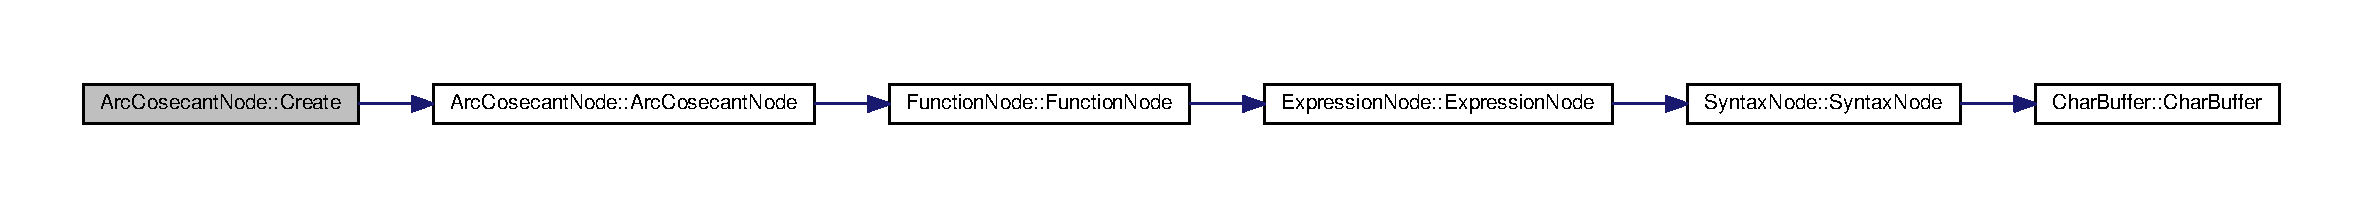
\includegraphics[width=350pt]{classArcCosecantNode_a03cc6abd00b92a4a8d7e801fc0d063bb_cgraph}
\end{center}
\end{figure}


\index{Arc\+Cosecant\+Node@{Arc\+Cosecant\+Node}!Evaluate@{Evaluate}}
\index{Evaluate@{Evaluate}!Arc\+Cosecant\+Node@{Arc\+Cosecant\+Node}}
\subsubsection[{\texorpdfstring{Evaluate()}{Evaluate()}}]{\setlength{\rightskip}{0pt plus 5cm}{\bf Number} $\ast$ Arc\+Cosecant\+Node\+::\+Evaluate (
\begin{DoxyParamCaption}
{}
\end{DoxyParamCaption}
)\hspace{0.3cm}{\ttfamily [virtual]}}\hypertarget{classArcCosecantNode_a4cb42e104cb77fd303bb57c73d8286b0}{}\label{classArcCosecantNode_a4cb42e104cb77fd303bb57c73d8286b0}


Implements \hyperlink{classExpressionNode_a64975d4dc37742228bd522f6204537f7}{Expression\+Node}.



Definition at line 927 of file functions.\+cpp.



References Number\+::\+Arc\+Cosecant(), Expression\+Node\+::\+Evaluate(), Function\+Node\+::expression, and Expression\+Node\+::result.


\begin{DoxyCode}
928 \{
929     \hyperlink{classExpressionNode_a1f590649f5a5cb30eb7ee912f7bc1262}{result} = \hyperlink{classFunctionNode_ad7577b179a1937aaf8a0058bb5b546dc}{expression}->\hyperlink{classExpressionNode_a64975d4dc37742228bd522f6204537f7}{Evaluate}()->\hyperlink{structNumber_a31dc5fa52529b5a7e76459bb984505e8}{ArcCosecant}();
930     \textcolor{keywordflow}{return} \hyperlink{classExpressionNode_a1f590649f5a5cb30eb7ee912f7bc1262}{result};
931 \}
\end{DoxyCode}


Here is the call graph for this function\+:\nopagebreak
\begin{figure}[H]
\begin{center}
\leavevmode
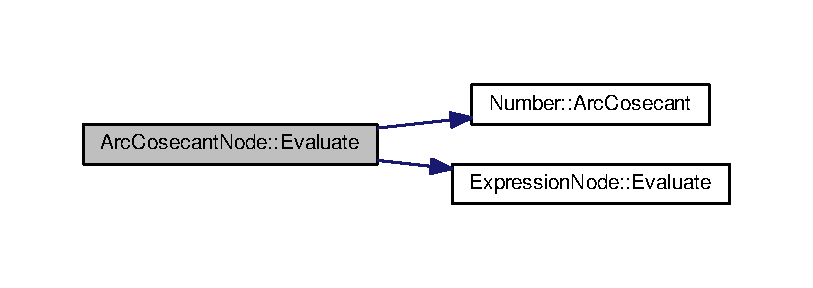
\includegraphics[width=350pt]{classArcCosecantNode_a4cb42e104cb77fd303bb57c73d8286b0_cgraph}
\end{center}
\end{figure}


\index{Arc\+Cosecant\+Node@{Arc\+Cosecant\+Node}!Get\+Node\+Text@{Get\+Node\+Text}}
\index{Get\+Node\+Text@{Get\+Node\+Text}!Arc\+Cosecant\+Node@{Arc\+Cosecant\+Node}}
\subsubsection[{\texorpdfstring{Get\+Node\+Text()}{GetNodeText()}}]{\setlength{\rightskip}{0pt plus 5cm}char $\ast$ Arc\+Cosecant\+Node\+::\+Get\+Node\+Text (
\begin{DoxyParamCaption}
{}
\end{DoxyParamCaption}
)\hspace{0.3cm}{\ttfamily [protected]}, {\ttfamily [virtual]}}\hypertarget{classArcCosecantNode_ad0cc72410c2754f5befec12cac5e7f01}{}\label{classArcCosecantNode_ad0cc72410c2754f5befec12cac5e7f01}


Implements \hyperlink{classExpressionNode_a42a5e9562b0f645a19dcc83f698069b5}{Expression\+Node}.



Definition at line 933 of file functions.\+cpp.


\begin{DoxyCode}
934 \{
935     \textcolor{keywordflow}{return} (\textcolor{keywordtype}{char}*)\textcolor{stringliteral}{"acsc"};
936 \}
\end{DoxyCode}


The documentation for this class was generated from the following files\+:\begin{DoxyCompactItemize}
\item 
app/main/\hyperlink{functions_8h}{functions.\+h}\item 
app/main/\hyperlink{functions_8cpp}{functions.\+cpp}\end{DoxyCompactItemize}

\hypertarget{classArcCosineNode}{}\section{Arc\+Cosine\+Node Class Reference}
\label{classArcCosineNode}\index{Arc\+Cosine\+Node@{Arc\+Cosine\+Node}}


{\ttfamily \#include $<$functions.\+h$>$}



Inheritance diagram for Arc\+Cosine\+Node\+:
\nopagebreak
\begin{figure}[H]
\begin{center}
\leavevmode
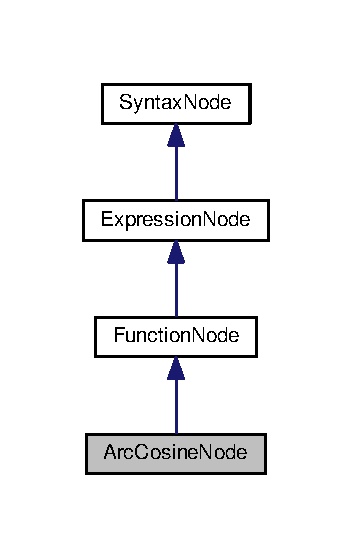
\includegraphics[width=169pt]{d5/de8/classArcCosineNode__inherit__graph}
\end{center}
\end{figure}


Collaboration diagram for Arc\+Cosine\+Node\+:
\nopagebreak
\begin{figure}[H]
\begin{center}
\leavevmode
\includegraphics[width=272pt]{dc/df5/classArcCosineNode__coll__graph}
\end{center}
\end{figure}
\subsection*{Public Member Functions}
\begin{DoxyCompactItemize}
\item 
\hyperlink{classArcCosineNode_aa152120e8ec71299525f1e8054a32f04}{Arc\+Cosine\+Node} (\hyperlink{classExpressionNode}{Expression\+Node} $\ast$\hyperlink{classFunctionNode_ad7577b179a1937aaf8a0058bb5b546dc}{expression})
\item 
\hyperlink{structNumber}{Number} $\ast$ \hyperlink{classArcCosineNode_a67a999999c34f043bd65778669d5d819}{Evaluate} ()
\end{DoxyCompactItemize}
\subsection*{Static Public Member Functions}
\begin{DoxyCompactItemize}
\item 
static \hyperlink{classFunctionNode}{Function\+Node} $\ast$ \hyperlink{classArcCosineNode_a72c4decd858fbf8db24f81581fd693cb}{Create} (\hyperlink{classExpressionNode}{Expression\+Node} $\ast$\hyperlink{classFunctionNode_ad7577b179a1937aaf8a0058bb5b546dc}{expression})
\end{DoxyCompactItemize}
\subsection*{Protected Member Functions}
\begin{DoxyCompactItemize}
\item 
char $\ast$ \hyperlink{classArcCosineNode_a9f519aed56ef36e4bf6c1ffbe269a015}{Get\+Node\+Text} ()
\end{DoxyCompactItemize}
\subsection*{Additional Inherited Members}


\subsection{Detailed Description}


Definition at line 406 of file functions.\+h.



\subsection{Constructor \& Destructor Documentation}
\index{Arc\+Cosine\+Node@{Arc\+Cosine\+Node}!Arc\+Cosine\+Node@{Arc\+Cosine\+Node}}
\index{Arc\+Cosine\+Node@{Arc\+Cosine\+Node}!Arc\+Cosine\+Node@{Arc\+Cosine\+Node}}
\subsubsection[{\texorpdfstring{Arc\+Cosine\+Node(\+Expression\+Node $\ast$expression)}{ArcCosineNode(ExpressionNode *expression)}}]{\setlength{\rightskip}{0pt plus 5cm}Arc\+Cosine\+Node\+::\+Arc\+Cosine\+Node (
\begin{DoxyParamCaption}
\item[{{\bf Expression\+Node} $\ast$}]{expression}
\end{DoxyParamCaption}
)}\hypertarget{classArcCosineNode_aa152120e8ec71299525f1e8054a32f04}{}\label{classArcCosineNode_aa152120e8ec71299525f1e8054a32f04}


Definition at line 881 of file functions.\+cpp.



References Function\+Node\+::\+Function\+Node().



Referenced by Create().


\begin{DoxyCode}
881                                                        :
882     \hyperlink{classFunctionNode_a41cb7db0162ffbec0902bd8ff7ea435f}{FunctionNode}(expression) \{ \}
\end{DoxyCode}


Here is the call graph for this function\+:
\nopagebreak
\begin{figure}[H]
\begin{center}
\leavevmode
\includegraphics[width=350pt]{d9/ddd/classArcCosineNode_aa152120e8ec71299525f1e8054a32f04_cgraph}
\end{center}
\end{figure}




Here is the caller graph for this function\+:
\nopagebreak
\begin{figure}[H]
\begin{center}
\leavevmode
\includegraphics[width=350pt]{d9/ddd/classArcCosineNode_aa152120e8ec71299525f1e8054a32f04_icgraph}
\end{center}
\end{figure}




\subsection{Member Function Documentation}
\index{Arc\+Cosine\+Node@{Arc\+Cosine\+Node}!Create@{Create}}
\index{Create@{Create}!Arc\+Cosine\+Node@{Arc\+Cosine\+Node}}
\subsubsection[{\texorpdfstring{Create(\+Expression\+Node $\ast$expression)}{Create(ExpressionNode *expression)}}]{\setlength{\rightskip}{0pt plus 5cm}{\bf Function\+Node} $\ast$ Arc\+Cosine\+Node\+::\+Create (
\begin{DoxyParamCaption}
\item[{{\bf Expression\+Node} $\ast$}]{expression}
\end{DoxyParamCaption}
)\hspace{0.3cm}{\ttfamily [static]}}\hypertarget{classArcCosineNode_a72c4decd858fbf8db24f81581fd693cb}{}\label{classArcCosineNode_a72c4decd858fbf8db24f81581fd693cb}


Definition at line 884 of file functions.\+cpp.



References Arc\+Cosine\+Node().


\begin{DoxyCode}
885 \{
886     \textcolor{keywordflow}{return} \textcolor{keyword}{new} \hyperlink{classArcCosineNode_aa152120e8ec71299525f1e8054a32f04}{ArcCosineNode}(expression);
887 \}
\end{DoxyCode}


Here is the call graph for this function\+:
\nopagebreak
\begin{figure}[H]
\begin{center}
\leavevmode
\includegraphics[width=350pt]{d9/ddd/classArcCosineNode_a72c4decd858fbf8db24f81581fd693cb_cgraph}
\end{center}
\end{figure}


\index{Arc\+Cosine\+Node@{Arc\+Cosine\+Node}!Evaluate@{Evaluate}}
\index{Evaluate@{Evaluate}!Arc\+Cosine\+Node@{Arc\+Cosine\+Node}}
\subsubsection[{\texorpdfstring{Evaluate()}{Evaluate()}}]{\setlength{\rightskip}{0pt plus 5cm}{\bf Number} $\ast$ Arc\+Cosine\+Node\+::\+Evaluate (
\begin{DoxyParamCaption}
{}
\end{DoxyParamCaption}
)\hspace{0.3cm}{\ttfamily [virtual]}}\hypertarget{classArcCosineNode_a67a999999c34f043bd65778669d5d819}{}\label{classArcCosineNode_a67a999999c34f043bd65778669d5d819}


Implements \hyperlink{classExpressionNode_a64975d4dc37742228bd522f6204537f7}{Expression\+Node}.



Definition at line 889 of file functions.\+cpp.



References Number\+::\+Arc\+Cosine(), Expression\+Node\+::\+Evaluate(), Function\+Node\+::expression, and Expression\+Node\+::result.


\begin{DoxyCode}
890 \{
891     \hyperlink{classExpressionNode_a1f590649f5a5cb30eb7ee912f7bc1262}{result} = \hyperlink{classFunctionNode_ad7577b179a1937aaf8a0058bb5b546dc}{expression}->\hyperlink{classExpressionNode_a64975d4dc37742228bd522f6204537f7}{Evaluate}()->\hyperlink{structNumber_a0056c25bf82bef6565963740ebab7517}{ArcCosine}();
892     \textcolor{keywordflow}{return} \hyperlink{classExpressionNode_a1f590649f5a5cb30eb7ee912f7bc1262}{result};
893 \}
\end{DoxyCode}


Here is the call graph for this function\+:
\nopagebreak
\begin{figure}[H]
\begin{center}
\leavevmode
\includegraphics[width=350pt]{d9/ddd/classArcCosineNode_a67a999999c34f043bd65778669d5d819_cgraph}
\end{center}
\end{figure}


\index{Arc\+Cosine\+Node@{Arc\+Cosine\+Node}!Get\+Node\+Text@{Get\+Node\+Text}}
\index{Get\+Node\+Text@{Get\+Node\+Text}!Arc\+Cosine\+Node@{Arc\+Cosine\+Node}}
\subsubsection[{\texorpdfstring{Get\+Node\+Text()}{GetNodeText()}}]{\setlength{\rightskip}{0pt plus 5cm}char $\ast$ Arc\+Cosine\+Node\+::\+Get\+Node\+Text (
\begin{DoxyParamCaption}
{}
\end{DoxyParamCaption}
)\hspace{0.3cm}{\ttfamily [protected]}, {\ttfamily [virtual]}}\hypertarget{classArcCosineNode_a9f519aed56ef36e4bf6c1ffbe269a015}{}\label{classArcCosineNode_a9f519aed56ef36e4bf6c1ffbe269a015}


Implements \hyperlink{classExpressionNode_a42a5e9562b0f645a19dcc83f698069b5}{Expression\+Node}.



Definition at line 895 of file functions.\+cpp.


\begin{DoxyCode}
896 \{
897     \textcolor{keywordflow}{return} (\textcolor{keywordtype}{char}*)\textcolor{stringliteral}{"acos"};
898 \}
\end{DoxyCode}


The documentation for this class was generated from the following files\+:\begin{DoxyCompactItemize}
\item 
app/main/\hyperlink{functions_8h}{functions.\+h}\item 
app/main/\hyperlink{functions_8cpp}{functions.\+cpp}\end{DoxyCompactItemize}

\hypertarget{classArcCotangentNode}{}\section{Arc\+Cotangent\+Node Class Reference}
\label{classArcCotangentNode}\index{Arc\+Cotangent\+Node@{Arc\+Cotangent\+Node}}


{\ttfamily \#include $<$functions.\+h$>$}



Inheritance diagram for Arc\+Cotangent\+Node\+:\nopagebreak
\begin{figure}[H]
\begin{center}
\leavevmode
\includegraphics[width=180pt]{classArcCotangentNode__inherit__graph}
\end{center}
\end{figure}


Collaboration diagram for Arc\+Cotangent\+Node\+:\nopagebreak
\begin{figure}[H]
\begin{center}
\leavevmode
\includegraphics[width=272pt]{classArcCotangentNode__coll__graph}
\end{center}
\end{figure}
\subsection*{Public Member Functions}
\begin{DoxyCompactItemize}
\item 
\hyperlink{classArcCotangentNode_aa67c2c4d48741e686b660c010c49bd41}{Arc\+Cotangent\+Node} (\hyperlink{classExpressionNode}{Expression\+Node} $\ast$\hyperlink{classFunctionNode_ad7577b179a1937aaf8a0058bb5b546dc}{expression})
\item 
\hyperlink{structNumber}{Number} $\ast$ \hyperlink{classArcCotangentNode_ace4c556eff07fb8352f8f341fa20702a}{Evaluate} ()
\end{DoxyCompactItemize}
\subsection*{Static Public Member Functions}
\begin{DoxyCompactItemize}
\item 
static \hyperlink{classFunctionNode}{Function\+Node} $\ast$ \hyperlink{classArcCotangentNode_a696c949ce9855f55d8e593622ebc0400}{Create} (\hyperlink{classExpressionNode}{Expression\+Node} $\ast$\hyperlink{classFunctionNode_ad7577b179a1937aaf8a0058bb5b546dc}{expression})
\end{DoxyCompactItemize}
\subsection*{Protected Member Functions}
\begin{DoxyCompactItemize}
\item 
char $\ast$ \hyperlink{classArcCotangentNode_aab2b4d2d357a47e4174e3daa82773ab1}{Get\+Node\+Text} ()
\end{DoxyCompactItemize}
\subsection*{Additional Inherited Members}


\subsection{Detailed Description}


Definition at line 426 of file functions.\+h.



\subsection{Constructor \& Destructor Documentation}
\index{Arc\+Cotangent\+Node@{Arc\+Cotangent\+Node}!Arc\+Cotangent\+Node@{Arc\+Cotangent\+Node}}
\index{Arc\+Cotangent\+Node@{Arc\+Cotangent\+Node}!Arc\+Cotangent\+Node@{Arc\+Cotangent\+Node}}
\subsubsection[{\texorpdfstring{Arc\+Cotangent\+Node(\+Expression\+Node $\ast$expression)}{ArcCotangentNode(ExpressionNode *expression)}}]{\setlength{\rightskip}{0pt plus 5cm}Arc\+Cotangent\+Node\+::\+Arc\+Cotangent\+Node (
\begin{DoxyParamCaption}
\item[{{\bf Expression\+Node} $\ast$}]{expression}
\end{DoxyParamCaption}
)}\hypertarget{classArcCotangentNode_aa67c2c4d48741e686b660c010c49bd41}{}\label{classArcCotangentNode_aa67c2c4d48741e686b660c010c49bd41}


Definition at line 957 of file functions.\+cpp.



References Function\+Node\+::\+Function\+Node().



Referenced by Create().


\begin{DoxyCode}
957                                                              :
958     \hyperlink{classFunctionNode_a41cb7db0162ffbec0902bd8ff7ea435f}{FunctionNode}(expression) \{ \}
\end{DoxyCode}


Here is the call graph for this function\+:\nopagebreak
\begin{figure}[H]
\begin{center}
\leavevmode
\includegraphics[width=350pt]{classArcCotangentNode_aa67c2c4d48741e686b660c010c49bd41_cgraph}
\end{center}
\end{figure}




Here is the caller graph for this function\+:\nopagebreak
\begin{figure}[H]
\begin{center}
\leavevmode
\includegraphics[width=350pt]{classArcCotangentNode_aa67c2c4d48741e686b660c010c49bd41_icgraph}
\end{center}
\end{figure}




\subsection{Member Function Documentation}
\index{Arc\+Cotangent\+Node@{Arc\+Cotangent\+Node}!Create@{Create}}
\index{Create@{Create}!Arc\+Cotangent\+Node@{Arc\+Cotangent\+Node}}
\subsubsection[{\texorpdfstring{Create(\+Expression\+Node $\ast$expression)}{Create(ExpressionNode *expression)}}]{\setlength{\rightskip}{0pt plus 5cm}{\bf Function\+Node} $\ast$ Arc\+Cotangent\+Node\+::\+Create (
\begin{DoxyParamCaption}
\item[{{\bf Expression\+Node} $\ast$}]{expression}
\end{DoxyParamCaption}
)\hspace{0.3cm}{\ttfamily [static]}}\hypertarget{classArcCotangentNode_a696c949ce9855f55d8e593622ebc0400}{}\label{classArcCotangentNode_a696c949ce9855f55d8e593622ebc0400}


Definition at line 961 of file functions.\+cpp.



References Arc\+Cotangent\+Node().


\begin{DoxyCode}
962 \{
963     \textcolor{keywordflow}{return} \textcolor{keyword}{new} \hyperlink{classArcCotangentNode_aa67c2c4d48741e686b660c010c49bd41}{ArcCotangentNode}(expression);
964 \}
\end{DoxyCode}


Here is the call graph for this function\+:\nopagebreak
\begin{figure}[H]
\begin{center}
\leavevmode
\includegraphics[width=350pt]{classArcCotangentNode_a696c949ce9855f55d8e593622ebc0400_cgraph}
\end{center}
\end{figure}


\index{Arc\+Cotangent\+Node@{Arc\+Cotangent\+Node}!Evaluate@{Evaluate}}
\index{Evaluate@{Evaluate}!Arc\+Cotangent\+Node@{Arc\+Cotangent\+Node}}
\subsubsection[{\texorpdfstring{Evaluate()}{Evaluate()}}]{\setlength{\rightskip}{0pt plus 5cm}{\bf Number} $\ast$ Arc\+Cotangent\+Node\+::\+Evaluate (
\begin{DoxyParamCaption}
{}
\end{DoxyParamCaption}
)\hspace{0.3cm}{\ttfamily [virtual]}}\hypertarget{classArcCotangentNode_ace4c556eff07fb8352f8f341fa20702a}{}\label{classArcCotangentNode_ace4c556eff07fb8352f8f341fa20702a}


Implements \hyperlink{classExpressionNode_a64975d4dc37742228bd522f6204537f7}{Expression\+Node}.



Definition at line 966 of file functions.\+cpp.



References Number\+::\+Arc\+Cotangent(), Expression\+Node\+::\+Evaluate(), Function\+Node\+::expression, and Expression\+Node\+::result.


\begin{DoxyCode}
967 \{
968     \hyperlink{classExpressionNode_a1f590649f5a5cb30eb7ee912f7bc1262}{result} = \hyperlink{classFunctionNode_ad7577b179a1937aaf8a0058bb5b546dc}{expression}->\hyperlink{classExpressionNode_a64975d4dc37742228bd522f6204537f7}{Evaluate}()->\hyperlink{structNumber_a859439f92698a61407238c4be5c1f1f5}{ArcCotangent}();
969     \textcolor{keywordflow}{return} \hyperlink{classExpressionNode_a1f590649f5a5cb30eb7ee912f7bc1262}{result};
970 \}
\end{DoxyCode}


Here is the call graph for this function\+:\nopagebreak
\begin{figure}[H]
\begin{center}
\leavevmode
\includegraphics[width=350pt]{classArcCotangentNode_ace4c556eff07fb8352f8f341fa20702a_cgraph}
\end{center}
\end{figure}


\index{Arc\+Cotangent\+Node@{Arc\+Cotangent\+Node}!Get\+Node\+Text@{Get\+Node\+Text}}
\index{Get\+Node\+Text@{Get\+Node\+Text}!Arc\+Cotangent\+Node@{Arc\+Cotangent\+Node}}
\subsubsection[{\texorpdfstring{Get\+Node\+Text()}{GetNodeText()}}]{\setlength{\rightskip}{0pt plus 5cm}char $\ast$ Arc\+Cotangent\+Node\+::\+Get\+Node\+Text (
\begin{DoxyParamCaption}
{}
\end{DoxyParamCaption}
)\hspace{0.3cm}{\ttfamily [protected]}, {\ttfamily [virtual]}}\hypertarget{classArcCotangentNode_aab2b4d2d357a47e4174e3daa82773ab1}{}\label{classArcCotangentNode_aab2b4d2d357a47e4174e3daa82773ab1}


Implements \hyperlink{classExpressionNode_a42a5e9562b0f645a19dcc83f698069b5}{Expression\+Node}.



Definition at line 972 of file functions.\+cpp.


\begin{DoxyCode}
973 \{
974     \textcolor{keywordflow}{return} (\textcolor{keywordtype}{char}*)\textcolor{stringliteral}{"acot"};
975 \}
\end{DoxyCode}


The documentation for this class was generated from the following files\+:\begin{DoxyCompactItemize}
\item 
app/main/\hyperlink{functions_8h}{functions.\+h}\item 
app/main/\hyperlink{functions_8cpp}{functions.\+cpp}\end{DoxyCompactItemize}

\hypertarget{classArcSecantNode}{}\section{Arc\+Secant\+Node Class Reference}
\label{classArcSecantNode}\index{Arc\+Secant\+Node@{Arc\+Secant\+Node}}


{\ttfamily \#include $<$functions.\+h$>$}



Inheritance diagram for Arc\+Secant\+Node\+:
\nopagebreak
\begin{figure}[H]
\begin{center}
\leavevmode
\includegraphics[width=169pt]{da/d77/classArcSecantNode__inherit__graph}
\end{center}
\end{figure}


Collaboration diagram for Arc\+Secant\+Node\+:
\nopagebreak
\begin{figure}[H]
\begin{center}
\leavevmode
\includegraphics[width=272pt]{de/dd1/classArcSecantNode__coll__graph}
\end{center}
\end{figure}
\subsection*{Public Member Functions}
\begin{DoxyCompactItemize}
\item 
\hyperlink{classArcSecantNode_af52359509f3d178954501b477ff1db5e}{Arc\+Secant\+Node} (\hyperlink{classExpressionNode}{Expression\+Node} $\ast$\hyperlink{classFunctionNode_ad7577b179a1937aaf8a0058bb5b546dc}{expression})
\item 
\hyperlink{structNumber}{Number} $\ast$ \hyperlink{classArcSecantNode_a4440babc181bf1763a0dca583ad5adbb}{Evaluate} ()
\end{DoxyCompactItemize}
\subsection*{Static Public Member Functions}
\begin{DoxyCompactItemize}
\item 
static \hyperlink{classFunctionNode}{Function\+Node} $\ast$ \hyperlink{classArcSecantNode_abe48bdd0e47a2dd5e5478f551f20c357}{Create} (\hyperlink{classExpressionNode}{Expression\+Node} $\ast$\hyperlink{classFunctionNode_ad7577b179a1937aaf8a0058bb5b546dc}{expression})
\end{DoxyCompactItemize}
\subsection*{Protected Member Functions}
\begin{DoxyCompactItemize}
\item 
char $\ast$ \hyperlink{classArcSecantNode_a75e25b2005cd24caf6b374a662df9975}{Get\+Node\+Text} ()
\end{DoxyCompactItemize}
\subsection*{Additional Inherited Members}


\subsection{Detailed Description}


Definition at line 446 of file functions.\+h.



\subsection{Constructor \& Destructor Documentation}
\index{Arc\+Secant\+Node@{Arc\+Secant\+Node}!Arc\+Secant\+Node@{Arc\+Secant\+Node}}
\index{Arc\+Secant\+Node@{Arc\+Secant\+Node}!Arc\+Secant\+Node@{Arc\+Secant\+Node}}
\subsubsection[{\texorpdfstring{Arc\+Secant\+Node(\+Expression\+Node $\ast$expression)}{ArcSecantNode(ExpressionNode *expression)}}]{\setlength{\rightskip}{0pt plus 5cm}Arc\+Secant\+Node\+::\+Arc\+Secant\+Node (
\begin{DoxyParamCaption}
\item[{{\bf Expression\+Node} $\ast$}]{expression}
\end{DoxyParamCaption}
)}\hypertarget{classArcSecantNode_af52359509f3d178954501b477ff1db5e}{}\label{classArcSecantNode_af52359509f3d178954501b477ff1db5e}


Definition at line 938 of file functions.\+cpp.



References Function\+Node\+::\+Function\+Node().



Referenced by Create().


\begin{DoxyCode}
938                                                        :
939     \hyperlink{classFunctionNode_a41cb7db0162ffbec0902bd8ff7ea435f}{FunctionNode}(expression) \{ \}
\end{DoxyCode}


Here is the call graph for this function\+:
\nopagebreak
\begin{figure}[H]
\begin{center}
\leavevmode
\includegraphics[width=350pt]{dc/d52/classArcSecantNode_af52359509f3d178954501b477ff1db5e_cgraph}
\end{center}
\end{figure}




Here is the caller graph for this function\+:
\nopagebreak
\begin{figure}[H]
\begin{center}
\leavevmode
\includegraphics[width=350pt]{dc/d52/classArcSecantNode_af52359509f3d178954501b477ff1db5e_icgraph}
\end{center}
\end{figure}




\subsection{Member Function Documentation}
\index{Arc\+Secant\+Node@{Arc\+Secant\+Node}!Create@{Create}}
\index{Create@{Create}!Arc\+Secant\+Node@{Arc\+Secant\+Node}}
\subsubsection[{\texorpdfstring{Create(\+Expression\+Node $\ast$expression)}{Create(ExpressionNode *expression)}}]{\setlength{\rightskip}{0pt plus 5cm}{\bf Function\+Node} $\ast$ Arc\+Secant\+Node\+::\+Create (
\begin{DoxyParamCaption}
\item[{{\bf Expression\+Node} $\ast$}]{expression}
\end{DoxyParamCaption}
)\hspace{0.3cm}{\ttfamily [static]}}\hypertarget{classArcSecantNode_abe48bdd0e47a2dd5e5478f551f20c357}{}\label{classArcSecantNode_abe48bdd0e47a2dd5e5478f551f20c357}


Definition at line 941 of file functions.\+cpp.



References Arc\+Secant\+Node().


\begin{DoxyCode}
942 \{
943     \textcolor{keywordflow}{return} \textcolor{keyword}{new} \hyperlink{classArcSecantNode_af52359509f3d178954501b477ff1db5e}{ArcSecantNode}(expression);
944 \}
\end{DoxyCode}


Here is the call graph for this function\+:
\nopagebreak
\begin{figure}[H]
\begin{center}
\leavevmode
\includegraphics[width=350pt]{dc/d52/classArcSecantNode_abe48bdd0e47a2dd5e5478f551f20c357_cgraph}
\end{center}
\end{figure}


\index{Arc\+Secant\+Node@{Arc\+Secant\+Node}!Evaluate@{Evaluate}}
\index{Evaluate@{Evaluate}!Arc\+Secant\+Node@{Arc\+Secant\+Node}}
\subsubsection[{\texorpdfstring{Evaluate()}{Evaluate()}}]{\setlength{\rightskip}{0pt plus 5cm}{\bf Number} $\ast$ Arc\+Secant\+Node\+::\+Evaluate (
\begin{DoxyParamCaption}
{}
\end{DoxyParamCaption}
)\hspace{0.3cm}{\ttfamily [virtual]}}\hypertarget{classArcSecantNode_a4440babc181bf1763a0dca583ad5adbb}{}\label{classArcSecantNode_a4440babc181bf1763a0dca583ad5adbb}


Implements \hyperlink{classExpressionNode_a64975d4dc37742228bd522f6204537f7}{Expression\+Node}.



Definition at line 946 of file functions.\+cpp.



References Number\+::\+Arc\+Secant(), Expression\+Node\+::\+Evaluate(), Function\+Node\+::expression, and Expression\+Node\+::result.


\begin{DoxyCode}
947 \{
948     \hyperlink{classExpressionNode_a1f590649f5a5cb30eb7ee912f7bc1262}{result} = \hyperlink{classFunctionNode_ad7577b179a1937aaf8a0058bb5b546dc}{expression}->\hyperlink{classExpressionNode_a64975d4dc37742228bd522f6204537f7}{Evaluate}()->\hyperlink{structNumber_aa7056bfff596b8d78757cac21a708094}{ArcSecant}();
949     \textcolor{keywordflow}{return} \hyperlink{classExpressionNode_a1f590649f5a5cb30eb7ee912f7bc1262}{result};
950 \}
\end{DoxyCode}


Here is the call graph for this function\+:
\nopagebreak
\begin{figure}[H]
\begin{center}
\leavevmode
\includegraphics[width=350pt]{dc/d52/classArcSecantNode_a4440babc181bf1763a0dca583ad5adbb_cgraph}
\end{center}
\end{figure}


\index{Arc\+Secant\+Node@{Arc\+Secant\+Node}!Get\+Node\+Text@{Get\+Node\+Text}}
\index{Get\+Node\+Text@{Get\+Node\+Text}!Arc\+Secant\+Node@{Arc\+Secant\+Node}}
\subsubsection[{\texorpdfstring{Get\+Node\+Text()}{GetNodeText()}}]{\setlength{\rightskip}{0pt plus 5cm}char $\ast$ Arc\+Secant\+Node\+::\+Get\+Node\+Text (
\begin{DoxyParamCaption}
{}
\end{DoxyParamCaption}
)\hspace{0.3cm}{\ttfamily [protected]}, {\ttfamily [virtual]}}\hypertarget{classArcSecantNode_a75e25b2005cd24caf6b374a662df9975}{}\label{classArcSecantNode_a75e25b2005cd24caf6b374a662df9975}


Implements \hyperlink{classExpressionNode_a42a5e9562b0f645a19dcc83f698069b5}{Expression\+Node}.



Definition at line 952 of file functions.\+cpp.


\begin{DoxyCode}
953 \{
954     \textcolor{keywordflow}{return} (\textcolor{keywordtype}{char}*)\textcolor{stringliteral}{"asec"};
955 \}
\end{DoxyCode}


The documentation for this class was generated from the following files\+:\begin{DoxyCompactItemize}
\item 
app/main/\hyperlink{functions_8h}{functions.\+h}\item 
app/main/\hyperlink{functions_8cpp}{functions.\+cpp}\end{DoxyCompactItemize}

\hypertarget{classArcSineNode}{}\section{Arc\+Sine\+Node Class Reference}
\label{classArcSineNode}\index{Arc\+Sine\+Node@{Arc\+Sine\+Node}}


{\ttfamily \#include $<$functions.\+h$>$}



Inheritance diagram for Arc\+Sine\+Node\+:\nopagebreak
\begin{figure}[H]
\begin{center}
\leavevmode
\includegraphics[width=169pt]{classArcSineNode__inherit__graph}
\end{center}
\end{figure}


Collaboration diagram for Arc\+Sine\+Node\+:\nopagebreak
\begin{figure}[H]
\begin{center}
\leavevmode
\includegraphics[width=272pt]{classArcSineNode__coll__graph}
\end{center}
\end{figure}
\subsection*{Public Member Functions}
\begin{DoxyCompactItemize}
\item 
\hyperlink{classArcSineNode_a4aa122cd2144b5b2339f2fea18c17c9b}{Arc\+Sine\+Node} (\hyperlink{classExpressionNode}{Expression\+Node} $\ast$\hyperlink{classFunctionNode_ad7577b179a1937aaf8a0058bb5b546dc}{expression})
\item 
\hyperlink{structNumber}{Number} $\ast$ \hyperlink{classArcSineNode_a30a268b7f74bba579745399ccf3ac009}{Evaluate} ()
\end{DoxyCompactItemize}
\subsection*{Static Public Member Functions}
\begin{DoxyCompactItemize}
\item 
static \hyperlink{classFunctionNode}{Function\+Node} $\ast$ \hyperlink{classArcSineNode_ad4e718a483da426a9d6000e2a8b80951}{Create} (\hyperlink{classExpressionNode}{Expression\+Node} $\ast$\hyperlink{classFunctionNode_ad7577b179a1937aaf8a0058bb5b546dc}{expression})
\end{DoxyCompactItemize}
\subsection*{Protected Member Functions}
\begin{DoxyCompactItemize}
\item 
char $\ast$ \hyperlink{classArcSineNode_a01aee433d9946e37f74bbde5f83dadff}{Get\+Node\+Text} ()
\end{DoxyCompactItemize}
\subsection*{Additional Inherited Members}


\subsection{Detailed Description}


Definition at line 396 of file functions.\+h.



\subsection{Constructor \& Destructor Documentation}
\index{Arc\+Sine\+Node@{Arc\+Sine\+Node}!Arc\+Sine\+Node@{Arc\+Sine\+Node}}
\index{Arc\+Sine\+Node@{Arc\+Sine\+Node}!Arc\+Sine\+Node@{Arc\+Sine\+Node}}
\subsubsection[{\texorpdfstring{Arc\+Sine\+Node(\+Expression\+Node $\ast$expression)}{ArcSineNode(ExpressionNode *expression)}}]{\setlength{\rightskip}{0pt plus 5cm}Arc\+Sine\+Node\+::\+Arc\+Sine\+Node (
\begin{DoxyParamCaption}
\item[{{\bf Expression\+Node} $\ast$}]{expression}
\end{DoxyParamCaption}
)}\hypertarget{classArcSineNode_a4aa122cd2144b5b2339f2fea18c17c9b}{}\label{classArcSineNode_a4aa122cd2144b5b2339f2fea18c17c9b}


Definition at line 862 of file functions.\+cpp.



References Function\+Node\+::\+Function\+Node().



Referenced by Create().


\begin{DoxyCode}
862                                                    :
863     \hyperlink{classFunctionNode_a41cb7db0162ffbec0902bd8ff7ea435f}{FunctionNode}(expression) \{ \}
\end{DoxyCode}


Here is the call graph for this function\+:\nopagebreak
\begin{figure}[H]
\begin{center}
\leavevmode
\includegraphics[width=350pt]{classArcSineNode_a4aa122cd2144b5b2339f2fea18c17c9b_cgraph}
\end{center}
\end{figure}




Here is the caller graph for this function\+:\nopagebreak
\begin{figure}[H]
\begin{center}
\leavevmode
\includegraphics[width=350pt]{classArcSineNode_a4aa122cd2144b5b2339f2fea18c17c9b_icgraph}
\end{center}
\end{figure}




\subsection{Member Function Documentation}
\index{Arc\+Sine\+Node@{Arc\+Sine\+Node}!Create@{Create}}
\index{Create@{Create}!Arc\+Sine\+Node@{Arc\+Sine\+Node}}
\subsubsection[{\texorpdfstring{Create(\+Expression\+Node $\ast$expression)}{Create(ExpressionNode *expression)}}]{\setlength{\rightskip}{0pt plus 5cm}{\bf Function\+Node} $\ast$ Arc\+Sine\+Node\+::\+Create (
\begin{DoxyParamCaption}
\item[{{\bf Expression\+Node} $\ast$}]{expression}
\end{DoxyParamCaption}
)\hspace{0.3cm}{\ttfamily [static]}}\hypertarget{classArcSineNode_ad4e718a483da426a9d6000e2a8b80951}{}\label{classArcSineNode_ad4e718a483da426a9d6000e2a8b80951}


Definition at line 865 of file functions.\+cpp.



References Arc\+Sine\+Node().


\begin{DoxyCode}
866 \{
867     \textcolor{keywordflow}{return} \textcolor{keyword}{new} \hyperlink{classArcSineNode_a4aa122cd2144b5b2339f2fea18c17c9b}{ArcSineNode}(expression);
868 \}
\end{DoxyCode}


Here is the call graph for this function\+:\nopagebreak
\begin{figure}[H]
\begin{center}
\leavevmode
\includegraphics[width=350pt]{classArcSineNode_ad4e718a483da426a9d6000e2a8b80951_cgraph}
\end{center}
\end{figure}


\index{Arc\+Sine\+Node@{Arc\+Sine\+Node}!Evaluate@{Evaluate}}
\index{Evaluate@{Evaluate}!Arc\+Sine\+Node@{Arc\+Sine\+Node}}
\subsubsection[{\texorpdfstring{Evaluate()}{Evaluate()}}]{\setlength{\rightskip}{0pt plus 5cm}{\bf Number} $\ast$ Arc\+Sine\+Node\+::\+Evaluate (
\begin{DoxyParamCaption}
{}
\end{DoxyParamCaption}
)\hspace{0.3cm}{\ttfamily [virtual]}}\hypertarget{classArcSineNode_a30a268b7f74bba579745399ccf3ac009}{}\label{classArcSineNode_a30a268b7f74bba579745399ccf3ac009}


Implements \hyperlink{classExpressionNode_a64975d4dc37742228bd522f6204537f7}{Expression\+Node}.



Definition at line 870 of file functions.\+cpp.



References Number\+::\+Arc\+Sine(), Expression\+Node\+::\+Evaluate(), Function\+Node\+::expression, and Expression\+Node\+::result.


\begin{DoxyCode}
871 \{
872     \hyperlink{classExpressionNode_a1f590649f5a5cb30eb7ee912f7bc1262}{result} = \hyperlink{classFunctionNode_ad7577b179a1937aaf8a0058bb5b546dc}{expression}->\hyperlink{classExpressionNode_a64975d4dc37742228bd522f6204537f7}{Evaluate}()->\hyperlink{structNumber_aabfd7afb2309911d8f1bc26b6927e4ef}{ArcSine}();
873     \textcolor{keywordflow}{return} \hyperlink{classExpressionNode_a1f590649f5a5cb30eb7ee912f7bc1262}{result};
874 \}
\end{DoxyCode}


Here is the call graph for this function\+:\nopagebreak
\begin{figure}[H]
\begin{center}
\leavevmode
\includegraphics[width=350pt]{classArcSineNode_a30a268b7f74bba579745399ccf3ac009_cgraph}
\end{center}
\end{figure}


\index{Arc\+Sine\+Node@{Arc\+Sine\+Node}!Get\+Node\+Text@{Get\+Node\+Text}}
\index{Get\+Node\+Text@{Get\+Node\+Text}!Arc\+Sine\+Node@{Arc\+Sine\+Node}}
\subsubsection[{\texorpdfstring{Get\+Node\+Text()}{GetNodeText()}}]{\setlength{\rightskip}{0pt plus 5cm}char $\ast$ Arc\+Sine\+Node\+::\+Get\+Node\+Text (
\begin{DoxyParamCaption}
{}
\end{DoxyParamCaption}
)\hspace{0.3cm}{\ttfamily [protected]}, {\ttfamily [virtual]}}\hypertarget{classArcSineNode_a01aee433d9946e37f74bbde5f83dadff}{}\label{classArcSineNode_a01aee433d9946e37f74bbde5f83dadff}


Implements \hyperlink{classExpressionNode_a42a5e9562b0f645a19dcc83f698069b5}{Expression\+Node}.



Definition at line 876 of file functions.\+cpp.


\begin{DoxyCode}
877 \{
878     \textcolor{keywordflow}{return} (\textcolor{keywordtype}{char}*)\textcolor{stringliteral}{"asin"};
879 \}
\end{DoxyCode}


The documentation for this class was generated from the following files\+:\begin{DoxyCompactItemize}
\item 
app/main/\hyperlink{functions_8h}{functions.\+h}\item 
app/main/\hyperlink{functions_8cpp}{functions.\+cpp}\end{DoxyCompactItemize}

\hypertarget{classArcTangentNode}{}\section{Arc\+Tangent\+Node Class Reference}
\label{classArcTangentNode}\index{Arc\+Tangent\+Node@{Arc\+Tangent\+Node}}


{\ttfamily \#include $<$functions.\+h$>$}



Inheritance diagram for Arc\+Tangent\+Node\+:
\nopagebreak
\begin{figure}[H]
\begin{center}
\leavevmode
\includegraphics[width=170pt]{d8/dac/classArcTangentNode__inherit__graph}
\end{center}
\end{figure}


Collaboration diagram for Arc\+Tangent\+Node\+:
\nopagebreak
\begin{figure}[H]
\begin{center}
\leavevmode
\includegraphics[width=272pt]{d4/dad/classArcTangentNode__coll__graph}
\end{center}
\end{figure}
\subsection*{Public Member Functions}
\begin{DoxyCompactItemize}
\item 
\hyperlink{classArcTangentNode_a2b174bed5fa2e62b858ce79654e7bb3c}{Arc\+Tangent\+Node} (\hyperlink{classExpressionNode}{Expression\+Node} $\ast$\hyperlink{classFunctionNode_ad7577b179a1937aaf8a0058bb5b546dc}{expression})
\item 
\hyperlink{structNumber}{Number} $\ast$ \hyperlink{classArcTangentNode_a61ce03a435f72dde99caba3547a0a2a8}{Evaluate} ()
\end{DoxyCompactItemize}
\subsection*{Static Public Member Functions}
\begin{DoxyCompactItemize}
\item 
static \hyperlink{classFunctionNode}{Function\+Node} $\ast$ \hyperlink{classArcTangentNode_a39aefe24ffd196b99a8c110619e5db2b}{Create} (\hyperlink{classExpressionNode}{Expression\+Node} $\ast$\hyperlink{classFunctionNode_ad7577b179a1937aaf8a0058bb5b546dc}{expression})
\end{DoxyCompactItemize}
\subsection*{Protected Member Functions}
\begin{DoxyCompactItemize}
\item 
char $\ast$ \hyperlink{classArcTangentNode_afd1b56cd9bf1c3a3da5191bf9604881d}{Get\+Node\+Text} ()
\end{DoxyCompactItemize}
\subsection*{Additional Inherited Members}


\subsection{Detailed Description}


Definition at line 416 of file functions.\+h.



\subsection{Constructor \& Destructor Documentation}
\index{Arc\+Tangent\+Node@{Arc\+Tangent\+Node}!Arc\+Tangent\+Node@{Arc\+Tangent\+Node}}
\index{Arc\+Tangent\+Node@{Arc\+Tangent\+Node}!Arc\+Tangent\+Node@{Arc\+Tangent\+Node}}
\subsubsection[{\texorpdfstring{Arc\+Tangent\+Node(\+Expression\+Node $\ast$expression)}{ArcTangentNode(ExpressionNode *expression)}}]{\setlength{\rightskip}{0pt plus 5cm}Arc\+Tangent\+Node\+::\+Arc\+Tangent\+Node (
\begin{DoxyParamCaption}
\item[{{\bf Expression\+Node} $\ast$}]{expression}
\end{DoxyParamCaption}
)}\hypertarget{classArcTangentNode_a2b174bed5fa2e62b858ce79654e7bb3c}{}\label{classArcTangentNode_a2b174bed5fa2e62b858ce79654e7bb3c}


Definition at line 900 of file functions.\+cpp.



References Function\+Node\+::\+Function\+Node().



Referenced by Create().


\begin{DoxyCode}
900                                                          :
901     \hyperlink{classFunctionNode_a41cb7db0162ffbec0902bd8ff7ea435f}{FunctionNode}(expression) \{ \}
\end{DoxyCode}


Here is the call graph for this function\+:
\nopagebreak
\begin{figure}[H]
\begin{center}
\leavevmode
\includegraphics[width=350pt]{d9/d88/classArcTangentNode_a2b174bed5fa2e62b858ce79654e7bb3c_cgraph}
\end{center}
\end{figure}




Here is the caller graph for this function\+:
\nopagebreak
\begin{figure}[H]
\begin{center}
\leavevmode
\includegraphics[width=350pt]{d9/d88/classArcTangentNode_a2b174bed5fa2e62b858ce79654e7bb3c_icgraph}
\end{center}
\end{figure}




\subsection{Member Function Documentation}
\index{Arc\+Tangent\+Node@{Arc\+Tangent\+Node}!Create@{Create}}
\index{Create@{Create}!Arc\+Tangent\+Node@{Arc\+Tangent\+Node}}
\subsubsection[{\texorpdfstring{Create(\+Expression\+Node $\ast$expression)}{Create(ExpressionNode *expression)}}]{\setlength{\rightskip}{0pt plus 5cm}{\bf Function\+Node} $\ast$ Arc\+Tangent\+Node\+::\+Create (
\begin{DoxyParamCaption}
\item[{{\bf Expression\+Node} $\ast$}]{expression}
\end{DoxyParamCaption}
)\hspace{0.3cm}{\ttfamily [static]}}\hypertarget{classArcTangentNode_a39aefe24ffd196b99a8c110619e5db2b}{}\label{classArcTangentNode_a39aefe24ffd196b99a8c110619e5db2b}


Definition at line 903 of file functions.\+cpp.



References Arc\+Tangent\+Node().


\begin{DoxyCode}
904 \{
905     \textcolor{keywordflow}{return} \textcolor{keyword}{new} \hyperlink{classArcTangentNode_a2b174bed5fa2e62b858ce79654e7bb3c}{ArcTangentNode}(expression);
906 \}
\end{DoxyCode}


Here is the call graph for this function\+:
\nopagebreak
\begin{figure}[H]
\begin{center}
\leavevmode
\includegraphics[width=350pt]{d9/d88/classArcTangentNode_a39aefe24ffd196b99a8c110619e5db2b_cgraph}
\end{center}
\end{figure}


\index{Arc\+Tangent\+Node@{Arc\+Tangent\+Node}!Evaluate@{Evaluate}}
\index{Evaluate@{Evaluate}!Arc\+Tangent\+Node@{Arc\+Tangent\+Node}}
\subsubsection[{\texorpdfstring{Evaluate()}{Evaluate()}}]{\setlength{\rightskip}{0pt plus 5cm}{\bf Number} $\ast$ Arc\+Tangent\+Node\+::\+Evaluate (
\begin{DoxyParamCaption}
{}
\end{DoxyParamCaption}
)\hspace{0.3cm}{\ttfamily [virtual]}}\hypertarget{classArcTangentNode_a61ce03a435f72dde99caba3547a0a2a8}{}\label{classArcTangentNode_a61ce03a435f72dde99caba3547a0a2a8}


Implements \hyperlink{classExpressionNode_a64975d4dc37742228bd522f6204537f7}{Expression\+Node}.



Definition at line 908 of file functions.\+cpp.



References Number\+::\+Arc\+Tangent(), Expression\+Node\+::\+Evaluate(), Function\+Node\+::expression, and Expression\+Node\+::result.


\begin{DoxyCode}
909 \{
910     \hyperlink{classExpressionNode_a1f590649f5a5cb30eb7ee912f7bc1262}{result} = \hyperlink{classFunctionNode_ad7577b179a1937aaf8a0058bb5b546dc}{expression}->\hyperlink{classExpressionNode_a64975d4dc37742228bd522f6204537f7}{Evaluate}()->\hyperlink{structNumber_aaf001a24205a4062b2cfc79873d2884d}{ArcTangent}();
911     \textcolor{keywordflow}{return} \hyperlink{classExpressionNode_a1f590649f5a5cb30eb7ee912f7bc1262}{result};
912 \}
\end{DoxyCode}


Here is the call graph for this function\+:
\nopagebreak
\begin{figure}[H]
\begin{center}
\leavevmode
\includegraphics[width=350pt]{d9/d88/classArcTangentNode_a61ce03a435f72dde99caba3547a0a2a8_cgraph}
\end{center}
\end{figure}


\index{Arc\+Tangent\+Node@{Arc\+Tangent\+Node}!Get\+Node\+Text@{Get\+Node\+Text}}
\index{Get\+Node\+Text@{Get\+Node\+Text}!Arc\+Tangent\+Node@{Arc\+Tangent\+Node}}
\subsubsection[{\texorpdfstring{Get\+Node\+Text()}{GetNodeText()}}]{\setlength{\rightskip}{0pt plus 5cm}char $\ast$ Arc\+Tangent\+Node\+::\+Get\+Node\+Text (
\begin{DoxyParamCaption}
{}
\end{DoxyParamCaption}
)\hspace{0.3cm}{\ttfamily [protected]}, {\ttfamily [virtual]}}\hypertarget{classArcTangentNode_afd1b56cd9bf1c3a3da5191bf9604881d}{}\label{classArcTangentNode_afd1b56cd9bf1c3a3da5191bf9604881d}


Implements \hyperlink{classExpressionNode_a42a5e9562b0f645a19dcc83f698069b5}{Expression\+Node}.



Definition at line 914 of file functions.\+cpp.


\begin{DoxyCode}
915 \{
916     \textcolor{keywordflow}{return} (\textcolor{keywordtype}{char}*)\textcolor{stringliteral}{"atan"};
917 \}
\end{DoxyCode}


The documentation for this class was generated from the following files\+:\begin{DoxyCompactItemize}
\item 
app/main/\hyperlink{functions_8h}{functions.\+h}\item 
app/main/\hyperlink{functions_8cpp}{functions.\+cpp}\end{DoxyCompactItemize}

\hypertarget{classAssignmentNode}{}\section{Assignment\+Node Class Reference}
\label{classAssignmentNode}\index{Assignment\+Node@{Assignment\+Node}}


{\ttfamily \#include $<$operators.\+h$>$}



Inheritance diagram for Assignment\+Node\+:
\nopagebreak
\begin{figure}[H]
\begin{center}
\leavevmode
\includegraphics[width=172pt]{df/df2/classAssignmentNode__inherit__graph}
\end{center}
\end{figure}


Collaboration diagram for Assignment\+Node\+:
\nopagebreak
\begin{figure}[H]
\begin{center}
\leavevmode
\includegraphics[width=350pt]{d3/d55/classAssignmentNode__coll__graph}
\end{center}
\end{figure}
\subsection*{Public Member Functions}
\begin{DoxyCompactItemize}
\item 
\hyperlink{classAssignmentNode_a8b2b07073d9900677a8ffe93f7d4171d}{Assignment\+Node} (\hyperlink{classVariableNode}{Variable\+Node} $\ast$\hyperlink{classAssignmentNode_ac22933c48c43391f969b412158c729dc}{variable}, \hyperlink{classExpressionNode}{Expression\+Node} $\ast$\hyperlink{classAssignmentNode_a7a3400b79798f10506405c6a242deeaa}{expression})
\item 
int \hyperlink{classAssignmentNode_a8101830017b851c84364ca3ca6f0f204}{Get\+Precedence} ()
\item 
\hyperlink{platform_8h_a1062901a7428fdd9c7f180f5e01ea056}{bool} \hyperlink{classAssignmentNode_ad8468049bcb780828405ccddc06fc79a}{Is\+Silent} ()
\item 
\hyperlink{structNumber}{Number} $\ast$ \hyperlink{classAssignmentNode_ae6b454a04ec82aa97fa8e09c3752deb6}{Evaluate} ()
\end{DoxyCompactItemize}
\subsection*{Protected Member Functions}
\begin{DoxyCompactItemize}
\item 
char $\ast$ \hyperlink{classAssignmentNode_aabd296f88450781851cb521be3b647d4}{Get\+Node\+Text} ()
\end{DoxyCompactItemize}
\subsection*{Private Attributes}
\begin{DoxyCompactItemize}
\item 
\hyperlink{classVariableNode}{Variable\+Node} $\ast$ \hyperlink{classAssignmentNode_ac22933c48c43391f969b412158c729dc}{variable}
\item 
\hyperlink{classExpressionNode}{Expression\+Node} $\ast$ \hyperlink{classAssignmentNode_a7a3400b79798f10506405c6a242deeaa}{expression}
\end{DoxyCompactItemize}
\subsection*{Additional Inherited Members}


\subsection{Detailed Description}


Definition at line 148 of file operators.\+h.



\subsection{Constructor \& Destructor Documentation}
\index{Assignment\+Node@{Assignment\+Node}!Assignment\+Node@{Assignment\+Node}}
\index{Assignment\+Node@{Assignment\+Node}!Assignment\+Node@{Assignment\+Node}}
\subsubsection[{\texorpdfstring{Assignment\+Node(\+Variable\+Node $\ast$variable, Expression\+Node $\ast$expression)}{AssignmentNode(VariableNode *variable, ExpressionNode *expression)}}]{\setlength{\rightskip}{0pt plus 5cm}Assignment\+Node\+::\+Assignment\+Node (
\begin{DoxyParamCaption}
\item[{{\bf Variable\+Node} $\ast$}]{variable, }
\item[{{\bf Expression\+Node} $\ast$}]{expression}
\end{DoxyParamCaption}
)}\hypertarget{classAssignmentNode_a8b2b07073d9900677a8ffe93f7d4171d}{}\label{classAssignmentNode_a8b2b07073d9900677a8ffe93f7d4171d}


Definition at line 427 of file operators.\+cpp.



References expression, Numeric\+Operator\+::\+Numeric\+Operator(), and variable.



Referenced by Parser\+::\+Parse\+Ident().


\begin{DoxyCode}
427                                                                                 :
428     \hyperlink{classNumericOperator_a49cd2230b867cdfca64715aaf6e37561}{NumericOperator}(variable, expression),
429     \hyperlink{classAssignmentNode_ac22933c48c43391f969b412158c729dc}{variable}(variable), \hyperlink{classAssignmentNode_a7a3400b79798f10506405c6a242deeaa}{expression}(expression) \{ \}
\end{DoxyCode}


Here is the call graph for this function\+:
\nopagebreak
\begin{figure}[H]
\begin{center}
\leavevmode
\includegraphics[width=350pt]{df/d93/classAssignmentNode_a8b2b07073d9900677a8ffe93f7d4171d_cgraph}
\end{center}
\end{figure}




Here is the caller graph for this function\+:
\nopagebreak
\begin{figure}[H]
\begin{center}
\leavevmode
\includegraphics[width=350pt]{df/d93/classAssignmentNode_a8b2b07073d9900677a8ffe93f7d4171d_icgraph}
\end{center}
\end{figure}




\subsection{Member Function Documentation}
\index{Assignment\+Node@{Assignment\+Node}!Evaluate@{Evaluate}}
\index{Evaluate@{Evaluate}!Assignment\+Node@{Assignment\+Node}}
\subsubsection[{\texorpdfstring{Evaluate()}{Evaluate()}}]{\setlength{\rightskip}{0pt plus 5cm}{\bf Number} $\ast$ Assignment\+Node\+::\+Evaluate (
\begin{DoxyParamCaption}
{}
\end{DoxyParamCaption}
)\hspace{0.3cm}{\ttfamily [virtual]}}\hypertarget{classAssignmentNode_ae6b454a04ec82aa97fa8e09c3752deb6}{}\label{classAssignmentNode_ae6b454a04ec82aa97fa8e09c3752deb6}


Implements \hyperlink{classExpressionNode_a64975d4dc37742228bd522f6204537f7}{Expression\+Node}.



Definition at line 436 of file operators.\+cpp.



References Variable\+Node\+::\+Assign\+Value(), Expression\+Node\+::\+Evaluate(), Variable\+Node\+::\+Evaluate(), expression, and variable.


\begin{DoxyCode}
437 \{
438     \textcolor{comment}{// NOTICE: Assignment does not generate a value itself.}
439     \hyperlink{classAssignmentNode_ac22933c48c43391f969b412158c729dc}{variable}->\hyperlink{classVariableNode_a8134cc1627925a0327e6c62eef810cdc}{AssignValue}(\hyperlink{classAssignmentNode_a7a3400b79798f10506405c6a242deeaa}{expression}->\hyperlink{classExpressionNode_a64975d4dc37742228bd522f6204537f7}{Evaluate}());
440     \textcolor{keywordflow}{return} \hyperlink{classAssignmentNode_ac22933c48c43391f969b412158c729dc}{variable}->\hyperlink{classVariableNode_a7ebbe9072eb78b5790befed3a42b2dc2}{Evaluate}();
441 \}
\end{DoxyCode}


Here is the call graph for this function\+:
\nopagebreak
\begin{figure}[H]
\begin{center}
\leavevmode
\includegraphics[width=350pt]{df/d93/classAssignmentNode_ae6b454a04ec82aa97fa8e09c3752deb6_cgraph}
\end{center}
\end{figure}


\index{Assignment\+Node@{Assignment\+Node}!Get\+Node\+Text@{Get\+Node\+Text}}
\index{Get\+Node\+Text@{Get\+Node\+Text}!Assignment\+Node@{Assignment\+Node}}
\subsubsection[{\texorpdfstring{Get\+Node\+Text()}{GetNodeText()}}]{\setlength{\rightskip}{0pt plus 5cm}char $\ast$ Assignment\+Node\+::\+Get\+Node\+Text (
\begin{DoxyParamCaption}
{}
\end{DoxyParamCaption}
)\hspace{0.3cm}{\ttfamily [protected]}, {\ttfamily [virtual]}}\hypertarget{classAssignmentNode_aabd296f88450781851cb521be3b647d4}{}\label{classAssignmentNode_aabd296f88450781851cb521be3b647d4}


Implements \hyperlink{classExpressionNode_a42a5e9562b0f645a19dcc83f698069b5}{Expression\+Node}.



Definition at line 448 of file operators.\+cpp.


\begin{DoxyCode}
449 \{
450     \textcolor{keywordflow}{return} (\textcolor{keywordtype}{char}*)\textcolor{stringliteral}{"="};
451 \}
\end{DoxyCode}
\index{Assignment\+Node@{Assignment\+Node}!Get\+Precedence@{Get\+Precedence}}
\index{Get\+Precedence@{Get\+Precedence}!Assignment\+Node@{Assignment\+Node}}
\subsubsection[{\texorpdfstring{Get\+Precedence()}{GetPrecedence()}}]{\setlength{\rightskip}{0pt plus 5cm}int Assignment\+Node\+::\+Get\+Precedence (
\begin{DoxyParamCaption}
{}
\end{DoxyParamCaption}
)\hspace{0.3cm}{\ttfamily [virtual]}}\hypertarget{classAssignmentNode_a8101830017b851c84364ca3ca6f0f204}{}\label{classAssignmentNode_a8101830017b851c84364ca3ca6f0f204}


Implements \hyperlink{classExpressionNode_a161b9ea0b79bbfc101d6f687c8481ddd}{Expression\+Node}.



Definition at line 431 of file operators.\+cpp.


\begin{DoxyCode}
432 \{
433     \textcolor{keywordflow}{return} 6;
434 \}
\end{DoxyCode}
\index{Assignment\+Node@{Assignment\+Node}!Is\+Silent@{Is\+Silent}}
\index{Is\+Silent@{Is\+Silent}!Assignment\+Node@{Assignment\+Node}}
\subsubsection[{\texorpdfstring{Is\+Silent()}{IsSilent()}}]{\setlength{\rightskip}{0pt plus 5cm}{\bf bool} Assignment\+Node\+::\+Is\+Silent (
\begin{DoxyParamCaption}
{}
\end{DoxyParamCaption}
)\hspace{0.3cm}{\ttfamily [virtual]}}\hypertarget{classAssignmentNode_ad8468049bcb780828405ccddc06fc79a}{}\label{classAssignmentNode_ad8468049bcb780828405ccddc06fc79a}


Reimplemented from \hyperlink{classExpressionNode_adc58a4c102b7fa18e9c3a0be361b0663}{Expression\+Node}.



Definition at line 443 of file operators.\+cpp.


\begin{DoxyCode}
444 \{
445     \textcolor{keywordflow}{return} \textcolor{keyword}{true};
446 \}
\end{DoxyCode}


\subsection{Member Data Documentation}
\index{Assignment\+Node@{Assignment\+Node}!expression@{expression}}
\index{expression@{expression}!Assignment\+Node@{Assignment\+Node}}
\subsubsection[{\texorpdfstring{expression}{expression}}]{\setlength{\rightskip}{0pt plus 5cm}{\bf Expression\+Node}$\ast$ Assignment\+Node\+::expression\hspace{0.3cm}{\ttfamily [private]}}\hypertarget{classAssignmentNode_a7a3400b79798f10506405c6a242deeaa}{}\label{classAssignmentNode_a7a3400b79798f10506405c6a242deeaa}


Definition at line 160 of file operators.\+h.



Referenced by Assignment\+Node(), and Evaluate().

\index{Assignment\+Node@{Assignment\+Node}!variable@{variable}}
\index{variable@{variable}!Assignment\+Node@{Assignment\+Node}}
\subsubsection[{\texorpdfstring{variable}{variable}}]{\setlength{\rightskip}{0pt plus 5cm}{\bf Variable\+Node}$\ast$ Assignment\+Node\+::variable\hspace{0.3cm}{\ttfamily [private]}}\hypertarget{classAssignmentNode_ac22933c48c43391f969b412158c729dc}{}\label{classAssignmentNode_ac22933c48c43391f969b412158c729dc}


Definition at line 159 of file operators.\+h.



Referenced by Assignment\+Node(), and Evaluate().



The documentation for this class was generated from the following files\+:\begin{DoxyCompactItemize}
\item 
app/main/\hyperlink{operators_8h}{operators.\+h}\item 
app/main/\hyperlink{operators_8cpp}{operators.\+cpp}\end{DoxyCompactItemize}

\hypertarget{classBinaryLogNode}{}\section{Binary\+Log\+Node Class Reference}
\label{classBinaryLogNode}\index{Binary\+Log\+Node@{Binary\+Log\+Node}}


{\ttfamily \#include $<$functions.\+h$>$}



Inheritance diagram for Binary\+Log\+Node\+:\nopagebreak
\begin{figure}[H]
\begin{center}
\leavevmode
\includegraphics[width=169pt]{classBinaryLogNode__inherit__graph}
\end{center}
\end{figure}


Collaboration diagram for Binary\+Log\+Node\+:\nopagebreak
\begin{figure}[H]
\begin{center}
\leavevmode
\includegraphics[width=272pt]{classBinaryLogNode__coll__graph}
\end{center}
\end{figure}
\subsection*{Public Member Functions}
\begin{DoxyCompactItemize}
\item 
\hyperlink{classBinaryLogNode_aba9e8a080b194de67e58f19c3aef2433}{Binary\+Log\+Node} (\hyperlink{classExpressionNode}{Expression\+Node} $\ast$\hyperlink{classFunctionNode_ad7577b179a1937aaf8a0058bb5b546dc}{expression})
\item 
\hyperlink{structNumber}{Number} $\ast$ \hyperlink{classBinaryLogNode_a0ac91748d2e82ac41b3a86eca6cf51df}{Evaluate} ()
\end{DoxyCompactItemize}
\subsection*{Static Public Member Functions}
\begin{DoxyCompactItemize}
\item 
static \hyperlink{classFunctionNode}{Function\+Node} $\ast$ \hyperlink{classBinaryLogNode_a443a095bddfc93df884e96cf43c2e971}{Create} (\hyperlink{classExpressionNode}{Expression\+Node} $\ast$\hyperlink{classFunctionNode_ad7577b179a1937aaf8a0058bb5b546dc}{expression})
\end{DoxyCompactItemize}
\subsection*{Protected Member Functions}
\begin{DoxyCompactItemize}
\item 
char $\ast$ \hyperlink{classBinaryLogNode_ad530e3055e387682633eb4a055c4260f}{Get\+Node\+Text} ()
\end{DoxyCompactItemize}
\subsection*{Additional Inherited Members}


\subsection{Detailed Description}


Definition at line 318 of file functions.\+h.



\subsection{Constructor \& Destructor Documentation}
\index{Binary\+Log\+Node@{Binary\+Log\+Node}!Binary\+Log\+Node@{Binary\+Log\+Node}}
\index{Binary\+Log\+Node@{Binary\+Log\+Node}!Binary\+Log\+Node@{Binary\+Log\+Node}}
\subsubsection[{\texorpdfstring{Binary\+Log\+Node(\+Expression\+Node $\ast$expression)}{BinaryLogNode(ExpressionNode *expression)}}]{\setlength{\rightskip}{0pt plus 5cm}Binary\+Log\+Node\+::\+Binary\+Log\+Node (
\begin{DoxyParamCaption}
\item[{{\bf Expression\+Node} $\ast$}]{expression}
\end{DoxyParamCaption}
)}\hypertarget{classBinaryLogNode_aba9e8a080b194de67e58f19c3aef2433}{}\label{classBinaryLogNode_aba9e8a080b194de67e58f19c3aef2433}


Definition at line 675 of file functions.\+cpp.



References Function\+Node\+::\+Function\+Node().



Referenced by Create().


\begin{DoxyCode}
675                                                        :
676     \hyperlink{classFunctionNode_a41cb7db0162ffbec0902bd8ff7ea435f}{FunctionNode}(expression) \{ \}
\end{DoxyCode}


Here is the call graph for this function\+:\nopagebreak
\begin{figure}[H]
\begin{center}
\leavevmode
\includegraphics[width=350pt]{classBinaryLogNode_aba9e8a080b194de67e58f19c3aef2433_cgraph}
\end{center}
\end{figure}




Here is the caller graph for this function\+:\nopagebreak
\begin{figure}[H]
\begin{center}
\leavevmode
\includegraphics[width=350pt]{classBinaryLogNode_aba9e8a080b194de67e58f19c3aef2433_icgraph}
\end{center}
\end{figure}




\subsection{Member Function Documentation}
\index{Binary\+Log\+Node@{Binary\+Log\+Node}!Create@{Create}}
\index{Create@{Create}!Binary\+Log\+Node@{Binary\+Log\+Node}}
\subsubsection[{\texorpdfstring{Create(\+Expression\+Node $\ast$expression)}{Create(ExpressionNode *expression)}}]{\setlength{\rightskip}{0pt plus 5cm}{\bf Function\+Node} $\ast$ Binary\+Log\+Node\+::\+Create (
\begin{DoxyParamCaption}
\item[{{\bf Expression\+Node} $\ast$}]{expression}
\end{DoxyParamCaption}
)\hspace{0.3cm}{\ttfamily [static]}}\hypertarget{classBinaryLogNode_a443a095bddfc93df884e96cf43c2e971}{}\label{classBinaryLogNode_a443a095bddfc93df884e96cf43c2e971}


Definition at line 678 of file functions.\+cpp.



References Binary\+Log\+Node().


\begin{DoxyCode}
679 \{
680     \textcolor{keywordflow}{return} \textcolor{keyword}{new} \hyperlink{classBinaryLogNode_aba9e8a080b194de67e58f19c3aef2433}{BinaryLogNode}(expression);
681 \}
\end{DoxyCode}


Here is the call graph for this function\+:\nopagebreak
\begin{figure}[H]
\begin{center}
\leavevmode
\includegraphics[width=350pt]{classBinaryLogNode_a443a095bddfc93df884e96cf43c2e971_cgraph}
\end{center}
\end{figure}


\index{Binary\+Log\+Node@{Binary\+Log\+Node}!Evaluate@{Evaluate}}
\index{Evaluate@{Evaluate}!Binary\+Log\+Node@{Binary\+Log\+Node}}
\subsubsection[{\texorpdfstring{Evaluate()}{Evaluate()}}]{\setlength{\rightskip}{0pt plus 5cm}{\bf Number} $\ast$ Binary\+Log\+Node\+::\+Evaluate (
\begin{DoxyParamCaption}
{}
\end{DoxyParamCaption}
)\hspace{0.3cm}{\ttfamily [virtual]}}\hypertarget{classBinaryLogNode_a0ac91748d2e82ac41b3a86eca6cf51df}{}\label{classBinaryLogNode_a0ac91748d2e82ac41b3a86eca6cf51df}


Implements \hyperlink{classExpressionNode_a64975d4dc37742228bd522f6204537f7}{Expression\+Node}.



Definition at line 683 of file functions.\+cpp.



References Expression\+Node\+::\+Evaluate(), Function\+Node\+::expression, Number\+::\+Log2(), and Expression\+Node\+::result.


\begin{DoxyCode}
684 \{
685     \hyperlink{classExpressionNode_a1f590649f5a5cb30eb7ee912f7bc1262}{result} = \hyperlink{classFunctionNode_ad7577b179a1937aaf8a0058bb5b546dc}{expression}->\hyperlink{classExpressionNode_a64975d4dc37742228bd522f6204537f7}{Evaluate}()->\hyperlink{structNumber_a8ace103bb7d32fabc11b65d00ab70f6a}{Log2}();
686     \textcolor{keywordflow}{return} \hyperlink{classExpressionNode_a1f590649f5a5cb30eb7ee912f7bc1262}{result};
687 \}
\end{DoxyCode}


Here is the call graph for this function\+:\nopagebreak
\begin{figure}[H]
\begin{center}
\leavevmode
\includegraphics[width=350pt]{classBinaryLogNode_a0ac91748d2e82ac41b3a86eca6cf51df_cgraph}
\end{center}
\end{figure}


\index{Binary\+Log\+Node@{Binary\+Log\+Node}!Get\+Node\+Text@{Get\+Node\+Text}}
\index{Get\+Node\+Text@{Get\+Node\+Text}!Binary\+Log\+Node@{Binary\+Log\+Node}}
\subsubsection[{\texorpdfstring{Get\+Node\+Text()}{GetNodeText()}}]{\setlength{\rightskip}{0pt plus 5cm}char $\ast$ Binary\+Log\+Node\+::\+Get\+Node\+Text (
\begin{DoxyParamCaption}
{}
\end{DoxyParamCaption}
)\hspace{0.3cm}{\ttfamily [protected]}, {\ttfamily [virtual]}}\hypertarget{classBinaryLogNode_ad530e3055e387682633eb4a055c4260f}{}\label{classBinaryLogNode_ad530e3055e387682633eb4a055c4260f}


Implements \hyperlink{classExpressionNode_a42a5e9562b0f645a19dcc83f698069b5}{Expression\+Node}.



Definition at line 689 of file functions.\+cpp.


\begin{DoxyCode}
690 \{
691     \textcolor{keywordflow}{return} (\textcolor{keywordtype}{char}*)\textcolor{stringliteral}{"lb"};
692 \}
\end{DoxyCode}


The documentation for this class was generated from the following files\+:\begin{DoxyCompactItemize}
\item 
app/main/\hyperlink{functions_8h}{functions.\+h}\item 
app/main/\hyperlink{functions_8cpp}{functions.\+cpp}\end{DoxyCompactItemize}

\hypertarget{classCeilingNode}{}\section{Ceiling\+Node Class Reference}
\label{classCeilingNode}\index{Ceiling\+Node@{Ceiling\+Node}}


{\ttfamily \#include $<$functions.\+h$>$}



Inheritance diagram for Ceiling\+Node\+:\nopagebreak
\begin{figure}[H]
\begin{center}
\leavevmode
\includegraphics[width=169pt]{classCeilingNode__inherit__graph}
\end{center}
\end{figure}


Collaboration diagram for Ceiling\+Node\+:\nopagebreak
\begin{figure}[H]
\begin{center}
\leavevmode
\includegraphics[width=272pt]{classCeilingNode__coll__graph}
\end{center}
\end{figure}
\subsection*{Public Member Functions}
\begin{DoxyCompactItemize}
\item 
\hyperlink{classCeilingNode_ab3c7e409e41fe1f5c6561e907ff4a5bf}{Ceiling\+Node} (\hyperlink{classExpressionNode}{Expression\+Node} $\ast$\hyperlink{classFunctionNode_ad7577b179a1937aaf8a0058bb5b546dc}{expression})
\item 
\hyperlink{structNumber}{Number} $\ast$ \hyperlink{classCeilingNode_ac5a24bd7b0ef5d280dc9da0723983541}{Evaluate} ()
\end{DoxyCompactItemize}
\subsection*{Static Public Member Functions}
\begin{DoxyCompactItemize}
\item 
static \hyperlink{classFunctionNode}{Function\+Node} $\ast$ \hyperlink{classCeilingNode_a6b935b420b30e2ce311a7fe179585baf}{Create} (\hyperlink{classExpressionNode}{Expression\+Node} $\ast$\hyperlink{classFunctionNode_ad7577b179a1937aaf8a0058bb5b546dc}{expression})
\end{DoxyCompactItemize}
\subsection*{Protected Member Functions}
\begin{DoxyCompactItemize}
\item 
char $\ast$ \hyperlink{classCeilingNode_a42887bd7fd45fdd658a60e6cc1114129}{Get\+Node\+Text} ()
\end{DoxyCompactItemize}
\subsection*{Additional Inherited Members}


\subsection{Detailed Description}


Definition at line 260 of file functions.\+h.



\subsection{Constructor \& Destructor Documentation}
\index{Ceiling\+Node@{Ceiling\+Node}!Ceiling\+Node@{Ceiling\+Node}}
\index{Ceiling\+Node@{Ceiling\+Node}!Ceiling\+Node@{Ceiling\+Node}}
\subsubsection[{\texorpdfstring{Ceiling\+Node(\+Expression\+Node $\ast$expression)}{CeilingNode(ExpressionNode *expression)}}]{\setlength{\rightskip}{0pt plus 5cm}Ceiling\+Node\+::\+Ceiling\+Node (
\begin{DoxyParamCaption}
\item[{{\bf Expression\+Node} $\ast$}]{expression}
\end{DoxyParamCaption}
)}\hypertarget{classCeilingNode_ab3c7e409e41fe1f5c6561e907ff4a5bf}{}\label{classCeilingNode_ab3c7e409e41fe1f5c6561e907ff4a5bf}


Definition at line 606 of file functions.\+cpp.



References Function\+Node\+::\+Function\+Node().



Referenced by Create().


\begin{DoxyCode}
606                                                    :
607     \hyperlink{classFunctionNode_a41cb7db0162ffbec0902bd8ff7ea435f}{FunctionNode}(expression) \{ \}
\end{DoxyCode}


Here is the call graph for this function\+:\nopagebreak
\begin{figure}[H]
\begin{center}
\leavevmode
\includegraphics[width=350pt]{classCeilingNode_ab3c7e409e41fe1f5c6561e907ff4a5bf_cgraph}
\end{center}
\end{figure}




Here is the caller graph for this function\+:\nopagebreak
\begin{figure}[H]
\begin{center}
\leavevmode
\includegraphics[width=350pt]{classCeilingNode_ab3c7e409e41fe1f5c6561e907ff4a5bf_icgraph}
\end{center}
\end{figure}




\subsection{Member Function Documentation}
\index{Ceiling\+Node@{Ceiling\+Node}!Create@{Create}}
\index{Create@{Create}!Ceiling\+Node@{Ceiling\+Node}}
\subsubsection[{\texorpdfstring{Create(\+Expression\+Node $\ast$expression)}{Create(ExpressionNode *expression)}}]{\setlength{\rightskip}{0pt plus 5cm}{\bf Function\+Node} $\ast$ Ceiling\+Node\+::\+Create (
\begin{DoxyParamCaption}
\item[{{\bf Expression\+Node} $\ast$}]{expression}
\end{DoxyParamCaption}
)\hspace{0.3cm}{\ttfamily [static]}}\hypertarget{classCeilingNode_a6b935b420b30e2ce311a7fe179585baf}{}\label{classCeilingNode_a6b935b420b30e2ce311a7fe179585baf}


Definition at line 609 of file functions.\+cpp.



References Ceiling\+Node().


\begin{DoxyCode}
610 \{
611     \textcolor{keywordflow}{return} \textcolor{keyword}{new} \hyperlink{classCeilingNode_ab3c7e409e41fe1f5c6561e907ff4a5bf}{CeilingNode}(expression);
612 \}
\end{DoxyCode}


Here is the call graph for this function\+:\nopagebreak
\begin{figure}[H]
\begin{center}
\leavevmode
\includegraphics[width=350pt]{classCeilingNode_a6b935b420b30e2ce311a7fe179585baf_cgraph}
\end{center}
\end{figure}


\index{Ceiling\+Node@{Ceiling\+Node}!Evaluate@{Evaluate}}
\index{Evaluate@{Evaluate}!Ceiling\+Node@{Ceiling\+Node}}
\subsubsection[{\texorpdfstring{Evaluate()}{Evaluate()}}]{\setlength{\rightskip}{0pt plus 5cm}{\bf Number} $\ast$ Ceiling\+Node\+::\+Evaluate (
\begin{DoxyParamCaption}
{}
\end{DoxyParamCaption}
)\hspace{0.3cm}{\ttfamily [virtual]}}\hypertarget{classCeilingNode_ac5a24bd7b0ef5d280dc9da0723983541}{}\label{classCeilingNode_ac5a24bd7b0ef5d280dc9da0723983541}


Implements \hyperlink{classExpressionNode_a64975d4dc37742228bd522f6204537f7}{Expression\+Node}.



Definition at line 614 of file functions.\+cpp.



References Number\+::\+Ceiling(), Expression\+Node\+::\+Evaluate(), Function\+Node\+::expression, and Expression\+Node\+::result.


\begin{DoxyCode}
615 \{
616     \hyperlink{classExpressionNode_a1f590649f5a5cb30eb7ee912f7bc1262}{result} = \hyperlink{classFunctionNode_ad7577b179a1937aaf8a0058bb5b546dc}{expression}->\hyperlink{classExpressionNode_a64975d4dc37742228bd522f6204537f7}{Evaluate}()->\hyperlink{structNumber_af6cc655e7d0eeb4f68a091456dddc25a}{Ceiling}();
617     \textcolor{keywordflow}{return} \hyperlink{classExpressionNode_a1f590649f5a5cb30eb7ee912f7bc1262}{result};
618 \}
\end{DoxyCode}


Here is the call graph for this function\+:\nopagebreak
\begin{figure}[H]
\begin{center}
\leavevmode
\includegraphics[width=350pt]{classCeilingNode_ac5a24bd7b0ef5d280dc9da0723983541_cgraph}
\end{center}
\end{figure}


\index{Ceiling\+Node@{Ceiling\+Node}!Get\+Node\+Text@{Get\+Node\+Text}}
\index{Get\+Node\+Text@{Get\+Node\+Text}!Ceiling\+Node@{Ceiling\+Node}}
\subsubsection[{\texorpdfstring{Get\+Node\+Text()}{GetNodeText()}}]{\setlength{\rightskip}{0pt plus 5cm}char $\ast$ Ceiling\+Node\+::\+Get\+Node\+Text (
\begin{DoxyParamCaption}
{}
\end{DoxyParamCaption}
)\hspace{0.3cm}{\ttfamily [protected]}, {\ttfamily [virtual]}}\hypertarget{classCeilingNode_a42887bd7fd45fdd658a60e6cc1114129}{}\label{classCeilingNode_a42887bd7fd45fdd658a60e6cc1114129}


Implements \hyperlink{classExpressionNode_a42a5e9562b0f645a19dcc83f698069b5}{Expression\+Node}.



Definition at line 620 of file functions.\+cpp.


\begin{DoxyCode}
621 \{
622     \textcolor{keywordflow}{return} (\textcolor{keywordtype}{char}*)\textcolor{stringliteral}{"ceil"};
623 \}
\end{DoxyCode}


The documentation for this class was generated from the following files\+:\begin{DoxyCompactItemize}
\item 
app/main/\hyperlink{functions_8h}{functions.\+h}\item 
app/main/\hyperlink{functions_8cpp}{functions.\+cpp}\end{DoxyCompactItemize}

\hypertarget{classCharBuffer}{}\section{Char\+Buffer Class Reference}
\label{classCharBuffer}\index{Char\+Buffer@{Char\+Buffer}}


Encapsulate an character array which can be used as a string.  




{\ttfamily \#include $<$charbuf.\+h$>$}

\subsection*{Public Member Functions}
\begin{DoxyCompactItemize}
\item 
\hyperlink{classCharBuffer_a4345e9a5114f5c0292e8f242f26e3a7b}{Char\+Buffer} ()
\begin{DoxyCompactList}\small\item\em Initialize without allocating memory. \end{DoxyCompactList}\item 
\hyperlink{classCharBuffer_a36d153c126a018c5090374ccb5c37508}{Char\+Buffer} (unsigned int size)
\begin{DoxyCompactList}\small\item\em Initialize while allocating specified amount of memory. \end{DoxyCompactList}\item 
\hyperlink{classCharBuffer_a9e62778016bba5191fa9eaa6ea118926}{$\sim$\+Char\+Buffer} ()
\item 
void \hyperlink{classCharBuffer_a0bcdd5708db4b04c887224e83a05086f}{Clear\+Buffer} ()
\begin{DoxyCompactList}\small\item\em Release memory in buffer. \end{DoxyCompactList}\item 
void \hyperlink{classCharBuffer_ac52ed7b91190240eb7db4cf43d1e2abb}{Clear\+And\+Copy} (const char $\ast$source)
\begin{DoxyCompactList}\small\item\em Release memory, allocate and copy source. \end{DoxyCompactList}\item 
void \hyperlink{classCharBuffer_a8c0927c2c05c954161151045f68581c6}{Clear\+And\+Alloc} (unsigned int size)
\begin{DoxyCompactList}\small\item\em Release memory and allocate new size. \end{DoxyCompactList}\item 
void \hyperlink{classCharBuffer_ad1907009b5ad136692b989fa96bf2f7e}{Ensure\+Size} (unsigned int size)
\begin{DoxyCompactList}\small\item\em Ensure a memory block of speficied size is allocated. \end{DoxyCompactList}\item 
void \hyperlink{classCharBuffer_a91ce4f4083b9a29c48f75e2af4071f28}{Ensure\+Size} (unsigned int blocksize, unsigned int blocks)
\item 
void \hyperlink{classCharBuffer_ae742439a2d5d5a0ad64411dcbf4604c8}{Ensure\+Minimum\+Size} ()
\item 
void \hyperlink{classCharBuffer_a73c71d361110b37819a1d681a1504b0e}{Ensure\+Growth} (unsigned int size)
\item 
void \hyperlink{classCharBuffer_abe39d3fd7d8b9c8ec343af2cae7adc96}{Empty} ()
\item 
\hyperlink{platform_8h_a1062901a7428fdd9c7f180f5e01ea056}{bool} \hyperlink{classCharBuffer_a64988275bda43dddb6d2b3b9551cefb0}{Is} (const char $\ast$string)
\begin{DoxyCompactList}\small\item\em Compare content of \hyperlink{classCharBuffer}{Char\+Buffer} with string) \end{DoxyCompactList}\item 
void \hyperlink{classCharBuffer_a9f35562a39a7785e73f09fbd9f6938bf}{Copy} (\hyperlink{classCharBuffer}{Char\+Buffer} $\ast$\hyperlink{classCharBuffer_a8bcd8491b24db4197b311eb361609674}{buf})
\item 
void \hyperlink{classCharBuffer_a045b38735f7b3007c1b98d3d7b7feafe}{Append} (const char $\ast$source)
\item 
void \hyperlink{classCharBuffer_a1ba545a85907bbc9ab26cdc99b031440}{Append} (const char c)
\item 
void \hyperlink{classCharBuffer_af0db379281b7f3f8b4746344521999c1}{Append} (const char c, unsigned int count)
\item 
void \hyperlink{classCharBuffer_a8bc0eaf1a874ccf76c0034299f8459a7}{Delete\+Last\+Char} ()
\item 
\hyperlink{platform_8h_a1062901a7428fdd9c7f180f5e01ea056}{bool} \hyperlink{classCharBuffer_a1071772d1059263f4f880965fcc349ab}{Remove\+Trailing} (const char c)
\item 
\hyperlink{platform_8h_a1062901a7428fdd9c7f180f5e01ea056}{bool} \hyperlink{classCharBuffer_a45beaedff09c0c079075cfced78c8002}{Remove\+Trailing} (const char $\ast$string)
\item 
char $\ast$ \hyperlink{classCharBuffer_a7dfd3feaaf80f318ba44efe15b1ec44b}{Get\+String} ()
\end{DoxyCompactItemize}
\subsection*{Private Attributes}
\begin{DoxyCompactItemize}
\item 
char $\ast$ \hyperlink{classCharBuffer_a8bcd8491b24db4197b311eb361609674}{buf}
\item 
char $\ast$ \hyperlink{classCharBuffer_a2d313433650506fd6609e6947729dfb0}{ptr}
\item 
unsigned int \hyperlink{classCharBuffer_ac3265c68505802fbe8b590d5a423b0d0}{cursize}
\end{DoxyCompactItemize}
\subsection*{Static Private Attributes}
\begin{DoxyCompactItemize}
\item 
static const unsigned int \hyperlink{classCharBuffer_a42fcc0397a2d7cb6d412a124de076aff}{minimum\+Size} = 64
\end{DoxyCompactItemize}
\subsection*{Friends}
\begin{DoxyCompactItemize}
\item 
class \hyperlink{classCharBuffer_ada87df74cf9242ca8f0efe5b88f9c212}{Ansi\+Conole\+Engine}
\end{DoxyCompactItemize}


\subsection{Detailed Description}
Encapsulate an character array which can be used as a string. 

The \hyperlink{classCharBuffer}{Char\+Buffer} class eases the task of allocating a releasing memory. 

Definition at line 43 of file charbuf.\+h.



\subsection{Constructor \& Destructor Documentation}
\index{Char\+Buffer@{Char\+Buffer}!Char\+Buffer@{Char\+Buffer}}
\index{Char\+Buffer@{Char\+Buffer}!Char\+Buffer@{Char\+Buffer}}
\subsubsection[{\texorpdfstring{Char\+Buffer()}{CharBuffer()}}]{\setlength{\rightskip}{0pt plus 5cm}Char\+Buffer\+::\+Char\+Buffer (
\begin{DoxyParamCaption}
{}
\end{DoxyParamCaption}
)}\hypertarget{classCharBuffer_a4345e9a5114f5c0292e8f242f26e3a7b}{}\label{classCharBuffer_a4345e9a5114f5c0292e8f242f26e3a7b}


Initialize without allocating memory. 



Definition at line 38 of file charbuf.\+cpp.



References buf, cursize, and ptr.



Referenced by Ansi\+Conole\+Engine\+::\+Ansi\+Conole\+Engine(), Error\+Node\+::\+Error\+Node(), Evaluator\+::\+Evaluator(), Prompt\+Statement\+::\+Execute(), Function\+List\+::\+Function\+List(), Standard\+Filesystem\+::\+List\+Directory(), Standard\+Preferences\+::\+Load(), Standard\+Filesystem\+::\+Load\+Text\+File(), Numeral\+System\+::\+Numeral\+System(), Preferences\+Base\+::\+Preferences\+Base(), Syntax\+Node\+::\+Syntax\+Node(), User\+Function\+::\+User\+Function(), and Variable\+List\+::\+Variable\+List().


\begin{DoxyCode}
39 \{
40     \hyperlink{classCharBuffer_a8bcd8491b24db4197b311eb361609674}{buf} = \hyperlink{platform_8h_a46ff2bfbf0d44b8466a2251d5bd5e6f8}{NOMEM};
41     \hyperlink{classCharBuffer_a2d313433650506fd6609e6947729dfb0}{ptr} = \hyperlink{classCharBuffer_a8bcd8491b24db4197b311eb361609674}{buf};
42     \hyperlink{classCharBuffer_ac3265c68505802fbe8b590d5a423b0d0}{cursize} = 0;
43 \}
\end{DoxyCode}


Here is the caller graph for this function\+:\nopagebreak
\begin{figure}[H]
\begin{center}
\leavevmode
\includegraphics[width=350pt]{classCharBuffer_a4345e9a5114f5c0292e8f242f26e3a7b_icgraph}
\end{center}
\end{figure}


\index{Char\+Buffer@{Char\+Buffer}!Char\+Buffer@{Char\+Buffer}}
\index{Char\+Buffer@{Char\+Buffer}!Char\+Buffer@{Char\+Buffer}}
\subsubsection[{\texorpdfstring{Char\+Buffer(unsigned int size)}{CharBuffer(unsigned int size)}}]{\setlength{\rightskip}{0pt plus 5cm}Char\+Buffer\+::\+Char\+Buffer (
\begin{DoxyParamCaption}
\item[{unsigned int}]{size}
\end{DoxyParamCaption}
)}\hypertarget{classCharBuffer_a36d153c126a018c5090374ccb5c37508}{}\label{classCharBuffer_a36d153c126a018c5090374ccb5c37508}


Initialize while allocating specified amount of memory. 



Definition at line 49 of file charbuf.\+cpp.



References buf, cursize, minimum\+Size, and ptr.



Referenced by Save\+Statement\+::\+Execute(), Positional\+Numeral\+System\+::\+Get\+Text(), and Standard\+Program\+::\+Initialize().


\begin{DoxyCode}
50 \{
51     \hyperlink{classCharBuffer_ac3265c68505802fbe8b590d5a423b0d0}{cursize} = (size < \hyperlink{classCharBuffer_a42fcc0397a2d7cb6d412a124de076aff}{minimumSize} ? \hyperlink{classCharBuffer_a42fcc0397a2d7cb6d412a124de076aff}{minimumSize} : size);
52     \hyperlink{classCharBuffer_a8bcd8491b24db4197b311eb361609674}{buf} = \textcolor{keyword}{new} \textcolor{keywordtype}{char}[\hyperlink{classCharBuffer_ac3265c68505802fbe8b590d5a423b0d0}{cursize}];
53     \hyperlink{classCharBuffer_a2d313433650506fd6609e6947729dfb0}{ptr} = \hyperlink{classCharBuffer_a8bcd8491b24db4197b311eb361609674}{buf};
54 \}
\end{DoxyCode}


Here is the caller graph for this function\+:\nopagebreak
\begin{figure}[H]
\begin{center}
\leavevmode
\includegraphics[width=350pt]{classCharBuffer_a36d153c126a018c5090374ccb5c37508_icgraph}
\end{center}
\end{figure}


\index{Char\+Buffer@{Char\+Buffer}!````~Char\+Buffer@{$\sim$\+Char\+Buffer}}
\index{````~Char\+Buffer@{$\sim$\+Char\+Buffer}!Char\+Buffer@{Char\+Buffer}}
\subsubsection[{\texorpdfstring{$\sim$\+Char\+Buffer()}{~CharBuffer()}}]{\setlength{\rightskip}{0pt plus 5cm}Char\+Buffer\+::$\sim$\+Char\+Buffer (
\begin{DoxyParamCaption}
{}
\end{DoxyParamCaption}
)}\hypertarget{classCharBuffer_a9e62778016bba5191fa9eaa6ea118926}{}\label{classCharBuffer_a9e62778016bba5191fa9eaa6ea118926}


Definition at line 56 of file charbuf.\+cpp.



References Clear\+Buffer().


\begin{DoxyCode}
57 \{
58     \hyperlink{classCharBuffer_a0bcdd5708db4b04c887224e83a05086f}{ClearBuffer}();
59 \}
\end{DoxyCode}


Here is the call graph for this function\+:\nopagebreak
\begin{figure}[H]
\begin{center}
\leavevmode
\includegraphics[width=350pt]{classCharBuffer_a9e62778016bba5191fa9eaa6ea118926_cgraph}
\end{center}
\end{figure}




\subsection{Member Function Documentation}
\index{Char\+Buffer@{Char\+Buffer}!Append@{Append}}
\index{Append@{Append}!Char\+Buffer@{Char\+Buffer}}
\subsubsection[{\texorpdfstring{Append(const char $\ast$source)}{Append(const char *source)}}]{\setlength{\rightskip}{0pt plus 5cm}void Char\+Buffer\+::\+Append (
\begin{DoxyParamCaption}
\item[{const char $\ast$}]{source}
\end{DoxyParamCaption}
)}\hypertarget{classCharBuffer_a045b38735f7b3007c1b98d3d7b7feafe}{}\label{classCharBuffer_a045b38735f7b3007c1b98d3d7b7feafe}


Definition at line 211 of file charbuf.\+cpp.



References ptr.



Referenced by Error\+Node\+::\+Error\+Node(), Version\+Statement\+::\+Execute(), Memory\+Statement\+::\+Execute(), Error\+Node\+::\+Execute(), Eval\+Statement\+::\+Execute(), Statement\+Block\+Node\+::\+Execute(), Delete\+Statement\+::\+Execute(), Input\+Statement\+::\+Execute(), Output\+Statement\+::\+Execute(), Digits\+Statement\+::\+Execute(), Save\+Statement\+::\+Execute(), Plot\+Statement\+::\+Execute(), Preferences\+Base\+::\+Get\+Description(), Positional\+Numeral\+System\+::\+Get\+Name(), Decimal\+System\+::\+Get\+Real\+Text(), Unary\+Node\+::\+Get\+Text(), Function\+Node\+::\+Get\+Text(), Absolute\+Node\+::\+Get\+Text(), Positional\+Numeral\+System\+::\+Get\+Text(), Numeric\+Operator\+::\+Get\+Text(), Standard\+Program\+::\+Initialize(), User\+Function\+::\+Initialize\+Texts(), Variable\+List\+::\+List\+Content(), Function\+List\+::\+List\+Content(), Standard\+Filesystem\+::\+List\+Directory(), Standard\+Preferences\+::\+Load(), Ansi\+Conole\+Engine\+::\+Process\+Char(), Ansi\+Conole\+Engine\+::\+Show\+Last(), and Ansi\+Conole\+Engine\+::\+Show\+Next().


\begin{DoxyCode}
212 \{
213     \textcolor{keywordflow}{while} ((*\hyperlink{classCharBuffer_a2d313433650506fd6609e6947729dfb0}{ptr}++ = *source++));
214 
215     \hyperlink{classCharBuffer_a2d313433650506fd6609e6947729dfb0}{ptr}--;
216 \}
\end{DoxyCode}


Here is the caller graph for this function\+:\nopagebreak
\begin{figure}[H]
\begin{center}
\leavevmode
\includegraphics[width=350pt]{classCharBuffer_a045b38735f7b3007c1b98d3d7b7feafe_icgraph}
\end{center}
\end{figure}


\index{Char\+Buffer@{Char\+Buffer}!Append@{Append}}
\index{Append@{Append}!Char\+Buffer@{Char\+Buffer}}
\subsubsection[{\texorpdfstring{Append(const char c)}{Append(const char c)}}]{\setlength{\rightskip}{0pt plus 5cm}void Char\+Buffer\+::\+Append (
\begin{DoxyParamCaption}
\item[{const char}]{c}
\end{DoxyParamCaption}
)}\hypertarget{classCharBuffer_a1ba545a85907bbc9ab26cdc99b031440}{}\label{classCharBuffer_a1ba545a85907bbc9ab26cdc99b031440}


Definition at line 195 of file charbuf.\+cpp.



References ptr.



Referenced by Prompt\+Statement\+::\+Execute(), Error\+Node\+::\+Execute(), Plot\+Statement\+::\+Execute(), Preferences\+Base\+::\+Get\+Description(), Positional\+Numeral\+System\+::\+Get\+Text(), Decimal\+System\+::\+Get\+Text(), Standard\+Program\+::\+Initialize(), User\+Function\+::\+Initialize\+Texts(), Positional\+Numeral\+System\+::\+Integer\+To\+Buffer(), Variable\+List\+::\+List\+Content(), Function\+List\+::\+List\+Content(), Standard\+Filesystem\+::\+Load\+Text\+File(), and Ansi\+Conole\+Engine\+::\+Process\+Char().


\begin{DoxyCode}
196 \{
197     *\hyperlink{classCharBuffer_a2d313433650506fd6609e6947729dfb0}{ptr}++ = c;
198 \}
\end{DoxyCode}


Here is the caller graph for this function\+:\nopagebreak
\begin{figure}[H]
\begin{center}
\leavevmode
\includegraphics[width=350pt]{classCharBuffer_a1ba545a85907bbc9ab26cdc99b031440_icgraph}
\end{center}
\end{figure}


\index{Char\+Buffer@{Char\+Buffer}!Append@{Append}}
\index{Append@{Append}!Char\+Buffer@{Char\+Buffer}}
\subsubsection[{\texorpdfstring{Append(const char c, unsigned int count)}{Append(const char c, unsigned int count)}}]{\setlength{\rightskip}{0pt plus 5cm}void Char\+Buffer\+::\+Append (
\begin{DoxyParamCaption}
\item[{const char}]{c, }
\item[{unsigned int}]{count}
\end{DoxyParamCaption}
)}\hypertarget{classCharBuffer_af0db379281b7f3f8b4746344521999c1}{}\label{classCharBuffer_af0db379281b7f3f8b4746344521999c1}


Definition at line 200 of file charbuf.\+cpp.



References ptr.



Referenced by Error\+Node\+::\+Execute(), and Standard\+Filesystem\+::\+List\+Directory().


\begin{DoxyCode}
201 \{
202     \textcolor{keywordflow}{if} (count == 0) \{
203         \textcolor{keywordflow}{return};
204     \}
205 
206     \textcolor{keywordtype}{unsigned} \textcolor{keywordtype}{int} n = count;
207     \textcolor{keywordflow}{while} (n--)
208         *\hyperlink{classCharBuffer_a2d313433650506fd6609e6947729dfb0}{ptr}++ = c;
209 \}
\end{DoxyCode}


Here is the caller graph for this function\+:\nopagebreak
\begin{figure}[H]
\begin{center}
\leavevmode
\includegraphics[width=323pt]{classCharBuffer_af0db379281b7f3f8b4746344521999c1_icgraph}
\end{center}
\end{figure}


\index{Char\+Buffer@{Char\+Buffer}!Clear\+And\+Alloc@{Clear\+And\+Alloc}}
\index{Clear\+And\+Alloc@{Clear\+And\+Alloc}!Char\+Buffer@{Char\+Buffer}}
\subsubsection[{\texorpdfstring{Clear\+And\+Alloc(unsigned int size)}{ClearAndAlloc(unsigned int size)}}]{\setlength{\rightskip}{0pt plus 5cm}void Char\+Buffer\+::\+Clear\+And\+Alloc (
\begin{DoxyParamCaption}
\item[{unsigned int}]{size}
\end{DoxyParamCaption}
)}\hypertarget{classCharBuffer_a8c0927c2c05c954161151045f68581c6}{}\label{classCharBuffer_a8c0927c2c05c954161151045f68581c6}


Release memory and allocate new size. 



Definition at line 91 of file charbuf.\+cpp.



References buf, Clear\+Buffer(), cursize, minimum\+Size, and ptr.



Referenced by Error\+Node\+::\+Execute(), and Ansi\+Conole\+Engine\+::\+Start\+Input().


\begin{DoxyCode}
92 \{
93     \hyperlink{classCharBuffer_a0bcdd5708db4b04c887224e83a05086f}{ClearBuffer}();
94     \hyperlink{classCharBuffer_ac3265c68505802fbe8b590d5a423b0d0}{cursize} = (size < \hyperlink{classCharBuffer_a42fcc0397a2d7cb6d412a124de076aff}{minimumSize} ? \hyperlink{classCharBuffer_a42fcc0397a2d7cb6d412a124de076aff}{minimumSize} : size);
95     \hyperlink{classCharBuffer_a8bcd8491b24db4197b311eb361609674}{buf} = \textcolor{keyword}{new} \textcolor{keywordtype}{char}[\hyperlink{classCharBuffer_ac3265c68505802fbe8b590d5a423b0d0}{cursize}];
96     \hyperlink{classCharBuffer_a2d313433650506fd6609e6947729dfb0}{ptr} = \hyperlink{classCharBuffer_a8bcd8491b24db4197b311eb361609674}{buf};
97 \}
\end{DoxyCode}


Here is the call graph for this function\+:\nopagebreak
\begin{figure}[H]
\begin{center}
\leavevmode
\includegraphics[width=350pt]{classCharBuffer_a8c0927c2c05c954161151045f68581c6_cgraph}
\end{center}
\end{figure}




Here is the caller graph for this function\+:\nopagebreak
\begin{figure}[H]
\begin{center}
\leavevmode
\includegraphics[width=350pt]{classCharBuffer_a8c0927c2c05c954161151045f68581c6_icgraph}
\end{center}
\end{figure}


\index{Char\+Buffer@{Char\+Buffer}!Clear\+And\+Copy@{Clear\+And\+Copy}}
\index{Clear\+And\+Copy@{Clear\+And\+Copy}!Char\+Buffer@{Char\+Buffer}}
\subsubsection[{\texorpdfstring{Clear\+And\+Copy(const char $\ast$source)}{ClearAndCopy(const char *source)}}]{\setlength{\rightskip}{0pt plus 5cm}void Char\+Buffer\+::\+Clear\+And\+Copy (
\begin{DoxyParamCaption}
\item[{const char $\ast$}]{source}
\end{DoxyParamCaption}
)}\hypertarget{classCharBuffer_ac52ed7b91190240eb7db4cf43d1e2abb}{}\label{classCharBuffer_ac52ed7b91190240eb7db4cf43d1e2abb}


Release memory, allocate and copy source. 



Definition at line 80 of file charbuf.\+cpp.



References Alloc\+And\+Copy(), buf, Clear\+Buffer(), cursize, and ptr.



Referenced by Evaluator\+::\+Evaluate(), Prompt\+Statement\+::\+Execute(), Help\+Statement\+::\+Execute(), Execute\+Statement\+::\+Execute(), and Numeric\+Value\+Node\+::\+Get\+Node\+Text().


\begin{DoxyCode}
81 \{
82     \hyperlink{classCharBuffer_a0bcdd5708db4b04c887224e83a05086f}{ClearBuffer}();
83     \hyperlink{classCharBuffer_ac3265c68505802fbe8b590d5a423b0d0}{cursize} = \hyperlink{clib_8h_a5bed05c70cb17e541fee570b5dc32e1a}{AllocAndCopy}(&\hyperlink{classCharBuffer_a8bcd8491b24db4197b311eb361609674}{buf}, source);
84     \hyperlink{classCharBuffer_a2d313433650506fd6609e6947729dfb0}{ptr} = \hyperlink{classCharBuffer_a8bcd8491b24db4197b311eb361609674}{buf} + \hyperlink{classCharBuffer_ac3265c68505802fbe8b590d5a423b0d0}{cursize} - \textcolor{keyword}{sizeof}(char);
85 \}
\end{DoxyCode}


Here is the call graph for this function\+:\nopagebreak
\begin{figure}[H]
\begin{center}
\leavevmode
\includegraphics[width=350pt]{classCharBuffer_ac52ed7b91190240eb7db4cf43d1e2abb_cgraph}
\end{center}
\end{figure}




Here is the caller graph for this function\+:\nopagebreak
\begin{figure}[H]
\begin{center}
\leavevmode
\includegraphics[width=350pt]{classCharBuffer_ac52ed7b91190240eb7db4cf43d1e2abb_icgraph}
\end{center}
\end{figure}


\index{Char\+Buffer@{Char\+Buffer}!Clear\+Buffer@{Clear\+Buffer}}
\index{Clear\+Buffer@{Clear\+Buffer}!Char\+Buffer@{Char\+Buffer}}
\subsubsection[{\texorpdfstring{Clear\+Buffer()}{ClearBuffer()}}]{\setlength{\rightskip}{0pt plus 5cm}void Char\+Buffer\+::\+Clear\+Buffer (
\begin{DoxyParamCaption}
{}
\end{DoxyParamCaption}
)}\hypertarget{classCharBuffer_a0bcdd5708db4b04c887224e83a05086f}{}\label{classCharBuffer_a0bcdd5708db4b04c887224e83a05086f}


Release memory in buffer. 



Definition at line 65 of file charbuf.\+cpp.



References buf, cursize, and ptr.



Referenced by Variable\+List\+::\+Clear(), Function\+List\+::\+Clear(), Clear\+And\+Alloc(), Clear\+And\+Copy(), Evaluator\+::\+Evaluate(), Statement\+Block\+Node\+::\+Execute(), and $\sim$\+Char\+Buffer().


\begin{DoxyCode}
66 \{
67     \textcolor{keywordflow}{if} (\hyperlink{classCharBuffer_a8bcd8491b24db4197b311eb361609674}{buf} != \hyperlink{platform_8h_a46ff2bfbf0d44b8466a2251d5bd5e6f8}{NOMEM}) \{
68         \textcolor{keyword}{delete} [] \hyperlink{classCharBuffer_a8bcd8491b24db4197b311eb361609674}{buf};
69     \}
70 
71     \hyperlink{classCharBuffer_a8bcd8491b24db4197b311eb361609674}{buf} = \hyperlink{platform_8h_a46ff2bfbf0d44b8466a2251d5bd5e6f8}{NOMEM};
72     \hyperlink{classCharBuffer_a2d313433650506fd6609e6947729dfb0}{ptr} = \hyperlink{classCharBuffer_a8bcd8491b24db4197b311eb361609674}{buf};
73     \hyperlink{classCharBuffer_ac3265c68505802fbe8b590d5a423b0d0}{cursize} = 0;
74 \}
\end{DoxyCode}


Here is the caller graph for this function\+:\nopagebreak
\begin{figure}[H]
\begin{center}
\leavevmode
\includegraphics[width=350pt]{classCharBuffer_a0bcdd5708db4b04c887224e83a05086f_icgraph}
\end{center}
\end{figure}


\index{Char\+Buffer@{Char\+Buffer}!Copy@{Copy}}
\index{Copy@{Copy}!Char\+Buffer@{Char\+Buffer}}
\subsubsection[{\texorpdfstring{Copy(\+Char\+Buffer $\ast$buf)}{Copy(CharBuffer *buf)}}]{\setlength{\rightskip}{0pt plus 5cm}void Char\+Buffer\+::\+Copy (
\begin{DoxyParamCaption}
\item[{{\bf Char\+Buffer} $\ast$}]{buf}
\end{DoxyParamCaption}
)}\hypertarget{classCharBuffer_a9f35562a39a7785e73f09fbd9f6938bf}{}\label{classCharBuffer_a9f35562a39a7785e73f09fbd9f6938bf}


Definition at line 183 of file charbuf.\+cpp.



References buf, cursize, Ensure\+Size(), Get\+String(), and ptr.



Referenced by Positional\+Numeral\+System\+::\+Get\+Text().


\begin{DoxyCode}
184 \{
185     \hyperlink{classCharBuffer_ad1907009b5ad136692b989fa96bf2f7e}{EnsureSize}(source->cursize);
186     \textcolor{keyword}{const} \textcolor{keywordtype}{char} *s = source->GetString();
187 
188     \hyperlink{classCharBuffer_a2d313433650506fd6609e6947729dfb0}{ptr} = \hyperlink{classCharBuffer_a8bcd8491b24db4197b311eb361609674}{buf};
189     \textcolor{keywordflow}{while} ((*\hyperlink{classCharBuffer_a2d313433650506fd6609e6947729dfb0}{ptr}++ = *s++))
190         ;
191 
192     \hyperlink{classCharBuffer_a2d313433650506fd6609e6947729dfb0}{ptr}--;
193 \}
\end{DoxyCode}


Here is the call graph for this function\+:\nopagebreak
\begin{figure}[H]
\begin{center}
\leavevmode
\includegraphics[width=350pt]{classCharBuffer_a9f35562a39a7785e73f09fbd9f6938bf_cgraph}
\end{center}
\end{figure}




Here is the caller graph for this function\+:\nopagebreak
\begin{figure}[H]
\begin{center}
\leavevmode
\includegraphics[width=339pt]{classCharBuffer_a9f35562a39a7785e73f09fbd9f6938bf_icgraph}
\end{center}
\end{figure}


\index{Char\+Buffer@{Char\+Buffer}!Delete\+Last\+Char@{Delete\+Last\+Char}}
\index{Delete\+Last\+Char@{Delete\+Last\+Char}!Char\+Buffer@{Char\+Buffer}}
\subsubsection[{\texorpdfstring{Delete\+Last\+Char()}{DeleteLastChar()}}]{\setlength{\rightskip}{0pt plus 5cm}void Char\+Buffer\+::\+Delete\+Last\+Char (
\begin{DoxyParamCaption}
{}
\end{DoxyParamCaption}
)}\hypertarget{classCharBuffer_a8bc0eaf1a874ccf76c0034299f8459a7}{}\label{classCharBuffer_a8bc0eaf1a874ccf76c0034299f8459a7}


Definition at line 177 of file charbuf.\+cpp.



References ptr.



Referenced by Standard\+Program\+::\+Initialize().


\begin{DoxyCode}
178 \{
179     \hyperlink{classCharBuffer_a2d313433650506fd6609e6947729dfb0}{ptr}--;
180 
181 \}
\end{DoxyCode}


Here is the caller graph for this function\+:\nopagebreak
\begin{figure}[H]
\begin{center}
\leavevmode
\includegraphics[width=350pt]{classCharBuffer_a8bc0eaf1a874ccf76c0034299f8459a7_icgraph}
\end{center}
\end{figure}


\index{Char\+Buffer@{Char\+Buffer}!Empty@{Empty}}
\index{Empty@{Empty}!Char\+Buffer@{Char\+Buffer}}
\subsubsection[{\texorpdfstring{Empty()}{Empty()}}]{\setlength{\rightskip}{0pt plus 5cm}void Char\+Buffer\+::\+Empty (
\begin{DoxyParamCaption}
{}
\end{DoxyParamCaption}
)}\hypertarget{classCharBuffer_abe39d3fd7d8b9c8ec343af2cae7adc96}{}\label{classCharBuffer_abe39d3fd7d8b9c8ec343af2cae7adc96}


Definition at line 168 of file charbuf.\+cpp.



References buf, Ensure\+Minimum\+Size(), and ptr.



Referenced by Version\+Statement\+::\+Execute(), Memory\+Statement\+::\+Execute(), Error\+Node\+::\+Execute(), Eval\+Statement\+::\+Execute(), Statement\+Block\+Node\+::\+Execute(), Delete\+Statement\+::\+Execute(), Input\+Statement\+::\+Execute(), Output\+Statement\+::\+Execute(), Digits\+Statement\+::\+Execute(), Save\+Statement\+::\+Execute(), Plot\+Statement\+::\+Execute(), Function\+Definition\+Node\+::\+Function\+Definition\+Node(), Preferences\+Base\+::\+Get\+Description(), Positional\+Numeral\+System\+::\+Get\+Name(), Unary\+Node\+::\+Get\+Text(), Function\+Node\+::\+Get\+Text(), Absolute\+Node\+::\+Get\+Text(), Positional\+Numeral\+System\+::\+Get\+Text(), Numeric\+Operator\+::\+Get\+Text(), Decimal\+System\+::\+Get\+Text(), Standard\+Program\+::\+Initialize(), User\+Function\+::\+Initialize\+Texts(), Variable\+List\+::\+List\+Content(), Function\+List\+::\+List\+Content(), Standard\+Filesystem\+::\+List\+Directory(), Standard\+Preferences\+::\+Load(), Standard\+Filesystem\+::\+Load\+Text\+File(), Numeral\+System\+::\+Numeral\+System(), Ansi\+Conole\+Engine\+::\+Process\+Char(), Ansi\+Conole\+Engine\+::\+Show\+Last(), and Ansi\+Conole\+Engine\+::\+Show\+Next().


\begin{DoxyCode}
169 \{
170     \textcolor{keywordflow}{if} (\hyperlink{classCharBuffer_a8bcd8491b24db4197b311eb361609674}{buf} == \hyperlink{platform_8h_a46ff2bfbf0d44b8466a2251d5bd5e6f8}{NOMEM}) \{
171         \hyperlink{classCharBuffer_ae742439a2d5d5a0ad64411dcbf4604c8}{EnsureMinimumSize}();
172     \}
173 
174     \hyperlink{classCharBuffer_a2d313433650506fd6609e6947729dfb0}{ptr} = \hyperlink{classCharBuffer_a8bcd8491b24db4197b311eb361609674}{buf};
175 \}
\end{DoxyCode}


Here is the call graph for this function\+:\nopagebreak
\begin{figure}[H]
\begin{center}
\leavevmode
\includegraphics[width=350pt]{classCharBuffer_abe39d3fd7d8b9c8ec343af2cae7adc96_cgraph}
\end{center}
\end{figure}




Here is the caller graph for this function\+:\nopagebreak
\begin{figure}[H]
\begin{center}
\leavevmode
\includegraphics[width=350pt]{classCharBuffer_abe39d3fd7d8b9c8ec343af2cae7adc96_icgraph}
\end{center}
\end{figure}


\index{Char\+Buffer@{Char\+Buffer}!Ensure\+Growth@{Ensure\+Growth}}
\index{Ensure\+Growth@{Ensure\+Growth}!Char\+Buffer@{Char\+Buffer}}
\subsubsection[{\texorpdfstring{Ensure\+Growth(unsigned int size)}{EnsureGrowth(unsigned int size)}}]{\setlength{\rightskip}{0pt plus 5cm}void Char\+Buffer\+::\+Ensure\+Growth (
\begin{DoxyParamCaption}
\item[{unsigned int}]{size}
\end{DoxyParamCaption}
)}\hypertarget{classCharBuffer_a73c71d361110b37819a1d681a1504b0e}{}\label{classCharBuffer_a73c71d361110b37819a1d681a1504b0e}


Definition at line 158 of file charbuf.\+cpp.



References buf, Ensure\+Size(), and ptr.



Referenced by Statement\+Block\+Node\+::\+Execute(), Plot\+Statement\+::\+Execute(), Decimal\+System\+::\+Get\+Real\+Text(), Standard\+Filesystem\+::\+List\+Directory(), and Ansi\+Conole\+Engine\+::\+Show\+Next().


\begin{DoxyCode}
159 \{
160     \hyperlink{classCharBuffer_ad1907009b5ad136692b989fa96bf2f7e}{EnsureSize}((\hyperlink{classCharBuffer_a2d313433650506fd6609e6947729dfb0}{ptr} - \hyperlink{classCharBuffer_a8bcd8491b24db4197b311eb361609674}{buf}) + size);
161 \}
\end{DoxyCode}


Here is the call graph for this function\+:\nopagebreak
\begin{figure}[H]
\begin{center}
\leavevmode
\includegraphics[width=350pt]{classCharBuffer_a73c71d361110b37819a1d681a1504b0e_cgraph}
\end{center}
\end{figure}




Here is the caller graph for this function\+:\nopagebreak
\begin{figure}[H]
\begin{center}
\leavevmode
\includegraphics[width=350pt]{classCharBuffer_a73c71d361110b37819a1d681a1504b0e_icgraph}
\end{center}
\end{figure}


\index{Char\+Buffer@{Char\+Buffer}!Ensure\+Minimum\+Size@{Ensure\+Minimum\+Size}}
\index{Ensure\+Minimum\+Size@{Ensure\+Minimum\+Size}!Char\+Buffer@{Char\+Buffer}}
\subsubsection[{\texorpdfstring{Ensure\+Minimum\+Size()}{EnsureMinimumSize()}}]{\setlength{\rightskip}{0pt plus 5cm}void Char\+Buffer\+::\+Ensure\+Minimum\+Size (
\begin{DoxyParamCaption}
{}
\end{DoxyParamCaption}
)}\hypertarget{classCharBuffer_ae742439a2d5d5a0ad64411dcbf4604c8}{}\label{classCharBuffer_ae742439a2d5d5a0ad64411dcbf4604c8}


Definition at line 99 of file charbuf.\+cpp.



References buf, minimum\+Size, and ptr.



Referenced by Empty(), and Function\+Definition\+Node\+::\+Function\+Definition\+Node().


\begin{DoxyCode}
100 \{
101     \textcolor{keywordflow}{if} (\hyperlink{classCharBuffer_a8bcd8491b24db4197b311eb361609674}{buf} == \hyperlink{platform_8h_a46ff2bfbf0d44b8466a2251d5bd5e6f8}{NOMEM}) \{
102         \textcolor{keywordtype}{unsigned} \textcolor{keywordtype}{int} size = \hyperlink{classCharBuffer_a42fcc0397a2d7cb6d412a124de076aff}{minimumSize};
103         \hyperlink{classCharBuffer_a8bcd8491b24db4197b311eb361609674}{buf} = \textcolor{keyword}{new} \textcolor{keywordtype}{char}[size];
104         \hyperlink{classCharBuffer_a2d313433650506fd6609e6947729dfb0}{ptr} = \hyperlink{classCharBuffer_a8bcd8491b24db4197b311eb361609674}{buf};
105     \}
106 \}
\end{DoxyCode}


Here is the caller graph for this function\+:\nopagebreak
\begin{figure}[H]
\begin{center}
\leavevmode
\includegraphics[width=350pt]{classCharBuffer_ae742439a2d5d5a0ad64411dcbf4604c8_icgraph}
\end{center}
\end{figure}


\index{Char\+Buffer@{Char\+Buffer}!Ensure\+Size@{Ensure\+Size}}
\index{Ensure\+Size@{Ensure\+Size}!Char\+Buffer@{Char\+Buffer}}
\subsubsection[{\texorpdfstring{Ensure\+Size(unsigned int size)}{EnsureSize(unsigned int size)}}]{\setlength{\rightskip}{0pt plus 5cm}void Char\+Buffer\+::\+Ensure\+Size (
\begin{DoxyParamCaption}
\item[{unsigned int}]{size}
\end{DoxyParamCaption}
)}\hypertarget{classCharBuffer_ad1907009b5ad136692b989fa96bf2f7e}{}\label{classCharBuffer_ad1907009b5ad136692b989fa96bf2f7e}


Ensure a memory block of speficied size is allocated. 



Definition at line 112 of file charbuf.\+cpp.



References buf, cursize, Mem\+Copy(), minimum\+Size, and ptr.



Referenced by Copy(), Ensure\+Growth(), Error\+Node\+::\+Error\+Node(), Version\+Statement\+::\+Execute(), Memory\+Statement\+::\+Execute(), Eval\+Statement\+::\+Execute(), Delete\+Statement\+::\+Execute(), Input\+Statement\+::\+Execute(), Output\+Statement\+::\+Execute(), Digits\+Statement\+::\+Execute(), Preferences\+Base\+::\+Get\+Description(), Positional\+Numeral\+System\+::\+Get\+Name(), Unary\+Node\+::\+Get\+Text(), Function\+Node\+::\+Get\+Text(), Absolute\+Node\+::\+Get\+Text(), Numeric\+Operator\+::\+Get\+Text(), Variable\+List\+::\+List\+Content(), Function\+List\+::\+List\+Content(), Standard\+Filesystem\+::\+List\+Directory(), Standard\+Preferences\+::\+Load(), Ansi\+Conole\+Engine\+::\+Show\+Last(), and Ansi\+Conole\+Engine\+::\+Show\+Next().


\begin{DoxyCode}
113 \{
114     \textcolor{keywordflow}{if} (\hyperlink{classCharBuffer_ac3265c68505802fbe8b590d5a423b0d0}{cursize} < size) \{
115 
116         \textcolor{keywordtype}{unsigned} \textcolor{keywordtype}{int} tempsize = \hyperlink{classCharBuffer_ac3265c68505802fbe8b590d5a423b0d0}{cursize};
117         \hyperlink{classCharBuffer_ac3265c68505802fbe8b590d5a423b0d0}{cursize} = (size < \hyperlink{classCharBuffer_a42fcc0397a2d7cb6d412a124de076aff}{minimumSize} ? \hyperlink{classCharBuffer_a42fcc0397a2d7cb6d412a124de076aff}{minimumSize} : size);
118 
119         \textcolor{keywordflow}{if} (\hyperlink{classCharBuffer_a8bcd8491b24db4197b311eb361609674}{buf} == \hyperlink{platform_8h_a46ff2bfbf0d44b8466a2251d5bd5e6f8}{NOMEM}) \{ \textcolor{comment}{// Nothing allocated yet. Just allocate requested size.}
120             \hyperlink{classCharBuffer_a8bcd8491b24db4197b311eb361609674}{buf} = \textcolor{keyword}{new} \textcolor{keywordtype}{char}[\hyperlink{classCharBuffer_ac3265c68505802fbe8b590d5a423b0d0}{cursize}];
121             \hyperlink{classCharBuffer_a2d313433650506fd6609e6947729dfb0}{ptr} = \hyperlink{classCharBuffer_a8bcd8491b24db4197b311eb361609674}{buf};
122         \} \textcolor{keywordflow}{else} \textcolor{keywordflow}{if} (\hyperlink{classCharBuffer_a8bcd8491b24db4197b311eb361609674}{buf} == \hyperlink{classCharBuffer_a2d313433650506fd6609e6947729dfb0}{ptr}) \{ \textcolor{comment}{// Already allocated but buffer is empty.}
123             \textcolor{keyword}{delete} [] \hyperlink{classCharBuffer_a8bcd8491b24db4197b311eb361609674}{buf};
124             \hyperlink{classCharBuffer_a8bcd8491b24db4197b311eb361609674}{buf} = \textcolor{keyword}{new} \textcolor{keywordtype}{char}[\hyperlink{classCharBuffer_ac3265c68505802fbe8b590d5a423b0d0}{cursize}];
125             \hyperlink{classCharBuffer_a2d313433650506fd6609e6947729dfb0}{ptr} = \hyperlink{classCharBuffer_a8bcd8491b24db4197b311eb361609674}{buf};
126         \} \textcolor{keywordflow}{else} \{ \textcolor{comment}{// Buffer already in use.}
127             \textcolor{comment}{// Make at least double size}
128             \hyperlink{classCharBuffer_ac3265c68505802fbe8b590d5a423b0d0}{cursize} = \hyperlink{classCharBuffer_ac3265c68505802fbe8b590d5a423b0d0}{cursize} < tempsize * 2 ? tempsize * 2 : 
      \hyperlink{classCharBuffer_ac3265c68505802fbe8b590d5a423b0d0}{cursize};
129             \textcolor{keywordtype}{unsigned} \textcolor{keywordtype}{int} offset = \hyperlink{classCharBuffer_a2d313433650506fd6609e6947729dfb0}{ptr} - \hyperlink{classCharBuffer_a8bcd8491b24db4197b311eb361609674}{buf};
130             \textcolor{keywordtype}{char} *temp = \textcolor{keyword}{new} \textcolor{keywordtype}{char}[\hyperlink{classCharBuffer_ac3265c68505802fbe8b590d5a423b0d0}{cursize}];
131             \hyperlink{clib_8h_a09b7e057c69b9ddd4b481fc746997a7d}{MemCopy}(temp, buf, tempsize);
132             \textcolor{keyword}{delete} [] \hyperlink{classCharBuffer_a8bcd8491b24db4197b311eb361609674}{buf};
133             buf = temp;
134             \hyperlink{classCharBuffer_a2d313433650506fd6609e6947729dfb0}{ptr} = buf + offset;
135         \}
136     \}
137 \}
\end{DoxyCode}


Here is the call graph for this function\+:\nopagebreak
\begin{figure}[H]
\begin{center}
\leavevmode
\includegraphics[width=298pt]{classCharBuffer_ad1907009b5ad136692b989fa96bf2f7e_cgraph}
\end{center}
\end{figure}




Here is the caller graph for this function\+:\nopagebreak
\begin{figure}[H]
\begin{center}
\leavevmode
\includegraphics[width=350pt]{classCharBuffer_ad1907009b5ad136692b989fa96bf2f7e_icgraph}
\end{center}
\end{figure}


\index{Char\+Buffer@{Char\+Buffer}!Ensure\+Size@{Ensure\+Size}}
\index{Ensure\+Size@{Ensure\+Size}!Char\+Buffer@{Char\+Buffer}}
\subsubsection[{\texorpdfstring{Ensure\+Size(unsigned int blocksize, unsigned int blocks)}{EnsureSize(unsigned int blocksize, unsigned int blocks)}}]{\setlength{\rightskip}{0pt plus 5cm}void Char\+Buffer\+::\+Ensure\+Size (
\begin{DoxyParamCaption}
\item[{unsigned int}]{blocksize, }
\item[{unsigned int}]{blocks}
\end{DoxyParamCaption}
)}\hypertarget{classCharBuffer_a91ce4f4083b9a29c48f75e2af4071f28}{}\label{classCharBuffer_a91ce4f4083b9a29c48f75e2af4071f28}


Definition at line 139 of file charbuf.\+cpp.



References buf, cursize, Mem\+Copy(), and ptr.



Referenced by Standard\+Filesystem\+::\+Load\+Text\+File().


\begin{DoxyCode}
140 \{
141     \textcolor{keywordflow}{if} (\hyperlink{classCharBuffer_ac3265c68505802fbe8b590d5a423b0d0}{cursize} < blocksize * blocks) \{
142         \textcolor{keywordflow}{if} (\hyperlink{classCharBuffer_a8bcd8491b24db4197b311eb361609674}{buf} == \hyperlink{platform_8h_a46ff2bfbf0d44b8466a2251d5bd5e6f8}{NOMEM}) \{
143             \hyperlink{classCharBuffer_ac3265c68505802fbe8b590d5a423b0d0}{cursize} = blocksize * blocks;
144             \hyperlink{classCharBuffer_a8bcd8491b24db4197b311eb361609674}{buf} = \textcolor{keyword}{new} \textcolor{keywordtype}{char}[\hyperlink{classCharBuffer_ac3265c68505802fbe8b590d5a423b0d0}{cursize}];
145             \hyperlink{classCharBuffer_a2d313433650506fd6609e6947729dfb0}{ptr} = \hyperlink{classCharBuffer_a8bcd8491b24db4197b311eb361609674}{buf};
146         \} \textcolor{keywordflow}{else} \{
147             \textcolor{keywordtype}{unsigned} \textcolor{keywordtype}{int} tptr = \hyperlink{classCharBuffer_a2d313433650506fd6609e6947729dfb0}{ptr} - \hyperlink{classCharBuffer_a8bcd8491b24db4197b311eb361609674}{buf};
148             \textcolor{keywordtype}{char} *temp = \textcolor{keyword}{new} \textcolor{keywordtype}{char}[blocksize * blocks];
149             \hyperlink{clib_8h_a09b7e057c69b9ddd4b481fc746997a7d}{MemCopy}(temp, buf, \hyperlink{classCharBuffer_ac3265c68505802fbe8b590d5a423b0d0}{cursize});
150             \textcolor{keyword}{delete} [] \hyperlink{classCharBuffer_a8bcd8491b24db4197b311eb361609674}{buf};
151             \hyperlink{classCharBuffer_ac3265c68505802fbe8b590d5a423b0d0}{cursize} = blocksize * blocks;
152             buf = temp;
153             \hyperlink{classCharBuffer_a2d313433650506fd6609e6947729dfb0}{ptr} = buf + tptr;
154         \}
155     \}
156 \}
\end{DoxyCode}


Here is the call graph for this function\+:\nopagebreak
\begin{figure}[H]
\begin{center}
\leavevmode
\includegraphics[width=298pt]{classCharBuffer_a91ce4f4083b9a29c48f75e2af4071f28_cgraph}
\end{center}
\end{figure}




Here is the caller graph for this function\+:\nopagebreak
\begin{figure}[H]
\begin{center}
\leavevmode
\includegraphics[width=340pt]{classCharBuffer_a91ce4f4083b9a29c48f75e2af4071f28_icgraph}
\end{center}
\end{figure}


\index{Char\+Buffer@{Char\+Buffer}!Get\+String@{Get\+String}}
\index{Get\+String@{Get\+String}!Char\+Buffer@{Char\+Buffer}}
\subsubsection[{\texorpdfstring{Get\+String()}{GetString()}}]{\setlength{\rightskip}{0pt plus 5cm}char $\ast$ Char\+Buffer\+::\+Get\+String (
\begin{DoxyParamCaption}
{}
\end{DoxyParamCaption}
)}\hypertarget{classCharBuffer_a7dfd3feaaf80f318ba44efe15b1ec44b}{}\label{classCharBuffer_a7dfd3feaaf80f318ba44efe15b1ec44b}


Definition at line 250 of file charbuf.\+cpp.



References buf, and ptr.



Referenced by Copy(), Ansi\+Conole\+Engine\+::\+Copy\+Line(), Error\+Node\+::\+Error\+Node(), Version\+Statement\+::\+Execute(), Memory\+Statement\+::\+Execute(), Prompt\+Statement\+::\+Execute(), Error\+Node\+::\+Execute(), Function\+Definition\+Node\+::\+Execute(), Eval\+Statement\+::\+Execute(), Statement\+Block\+Node\+::\+Execute(), Help\+Statement\+::\+Execute(), Delete\+Statement\+::\+Execute(), Input\+Statement\+::\+Execute(), Output\+Statement\+::\+Execute(), Digits\+Statement\+::\+Execute(), Show\+Statement\+::\+Execute(), List\+Statement\+::\+Execute(), Load\+Statement\+::\+Execute(), Save\+Statement\+::\+Execute(), Execute\+Statement\+::\+Execute(), Plot\+Statement\+::\+Execute(), User\+Function\+::\+Get\+Defition\+Name(), User\+Function\+::\+Get\+Defition\+Text(), Preferences\+Base\+::\+Get\+Description(), Ansi\+Conole\+Engine\+::\+Get\+Line(), Positional\+Numeral\+System\+::\+Get\+Name(), Numeric\+Value\+Node\+::\+Get\+Node\+Text(), Decimal\+System\+::\+Get\+Real\+Text(), Evaluator\+::\+Get\+Result(), Unary\+Node\+::\+Get\+Text(), Function\+Node\+::\+Get\+Text(), Absolute\+Node\+::\+Get\+Text(), Positional\+Numeral\+System\+::\+Get\+Text(), Numeric\+Operator\+::\+Get\+Text(), Decimal\+System\+::\+Get\+Text(), Function\+Definition\+Node\+::\+Get\+Text(), User\+Function\+::\+Initialize\+Texts(), Is(), Variable\+List\+::\+List\+Content(), Function\+List\+::\+List\+Content(), Standard\+Filesystem\+::\+List\+Directory(), Standard\+Preferences\+::\+Load(), Standard\+Language\+::\+Load\+Catalog(), Ansi\+Conole\+Engine\+::\+Process\+Char(), Standard\+Program\+::\+Run(), Ansi\+Conole\+Engine\+::\+Show\+Last(), and Ansi\+Conole\+Engine\+::\+Show\+Next().


\begin{DoxyCode}
251 \{
252     *\hyperlink{classCharBuffer_a2d313433650506fd6609e6947729dfb0}{ptr} = \textcolor{charliteral}{'\(\backslash\)0'};
253     \textcolor{keywordflow}{return} \hyperlink{classCharBuffer_a8bcd8491b24db4197b311eb361609674}{buf};
254 \}
\end{DoxyCode}


Here is the caller graph for this function\+:
\nopagebreak
\begin{figure}[H]
\begin{center}
\leavevmode
\includegraphics[height=550pt]{classCharBuffer_a7dfd3feaaf80f318ba44efe15b1ec44b_icgraph}
\end{center}
\end{figure}


\index{Char\+Buffer@{Char\+Buffer}!Is@{Is}}
\index{Is@{Is}!Char\+Buffer@{Char\+Buffer}}
\subsubsection[{\texorpdfstring{Is(const char $\ast$string)}{Is(const char *string)}}]{\setlength{\rightskip}{0pt plus 5cm}{\bf bool} Char\+Buffer\+::\+Is (
\begin{DoxyParamCaption}
\item[{const char $\ast$}]{string}
\end{DoxyParamCaption}
)}\hypertarget{classCharBuffer_a64988275bda43dddb6d2b3b9551cefb0}{}\label{classCharBuffer_a64988275bda43dddb6d2b3b9551cefb0}


Compare content of \hyperlink{classCharBuffer}{Char\+Buffer} with string) 



Definition at line 163 of file charbuf.\+cpp.



References Get\+String(), and Str\+Is\+Equal().



Referenced by Positional\+Numeral\+System\+::\+Get\+Text(), and Standard\+Program\+::\+Initialize().


\begin{DoxyCode}
164 \{
165     \textcolor{keywordflow}{return} \hyperlink{clib_8h_a2a1f39d11cbbaac992d42e67557dac4b}{StrIsEqual}(\hyperlink{classCharBuffer_a7dfd3feaaf80f318ba44efe15b1ec44b}{GetString}(), \textcolor{keywordtype}{string});
166 \}
\end{DoxyCode}


Here is the call graph for this function\+:\nopagebreak
\begin{figure}[H]
\begin{center}
\leavevmode
\includegraphics[width=305pt]{classCharBuffer_a64988275bda43dddb6d2b3b9551cefb0_cgraph}
\end{center}
\end{figure}




Here is the caller graph for this function\+:\nopagebreak
\begin{figure}[H]
\begin{center}
\leavevmode
\includegraphics[width=350pt]{classCharBuffer_a64988275bda43dddb6d2b3b9551cefb0_icgraph}
\end{center}
\end{figure}


\index{Char\+Buffer@{Char\+Buffer}!Remove\+Trailing@{Remove\+Trailing}}
\index{Remove\+Trailing@{Remove\+Trailing}!Char\+Buffer@{Char\+Buffer}}
\subsubsection[{\texorpdfstring{Remove\+Trailing(const char c)}{RemoveTrailing(const char c)}}]{\setlength{\rightskip}{0pt plus 5cm}{\bf bool} Char\+Buffer\+::\+Remove\+Trailing (
\begin{DoxyParamCaption}
\item[{const char}]{c}
\end{DoxyParamCaption}
)}\hypertarget{classCharBuffer_a1071772d1059263f4f880965fcc349ab}{}\label{classCharBuffer_a1071772d1059263f4f880965fcc349ab}


Definition at line 218 of file charbuf.\+cpp.



References buf, and ptr.



Referenced by Prompt\+Statement\+::\+Execute(), Decimal\+System\+::\+Get\+Real\+Text(), and Positional\+Numeral\+System\+::\+Get\+Text().


\begin{DoxyCode}
219 \{
220     \textcolor{keywordflow}{if} (\hyperlink{classCharBuffer_a2d313433650506fd6609e6947729dfb0}{ptr} == \hyperlink{classCharBuffer_a8bcd8491b24db4197b311eb361609674}{buf}) \{
221         \textcolor{keywordflow}{return} \textcolor{keyword}{false};
222     \}
223 
224     \textcolor{keywordflow}{if} (*(--\hyperlink{classCharBuffer_a2d313433650506fd6609e6947729dfb0}{ptr}) == c) \{
225         \textcolor{keywordflow}{return} \textcolor{keyword}{true};
226     \}
227 
228     \hyperlink{classCharBuffer_a2d313433650506fd6609e6947729dfb0}{ptr}++;
229     \textcolor{keywordflow}{return} \textcolor{keyword}{false};
230 \}
\end{DoxyCode}


Here is the caller graph for this function\+:\nopagebreak
\begin{figure}[H]
\begin{center}
\leavevmode
\includegraphics[width=350pt]{classCharBuffer_a1071772d1059263f4f880965fcc349ab_icgraph}
\end{center}
\end{figure}


\index{Char\+Buffer@{Char\+Buffer}!Remove\+Trailing@{Remove\+Trailing}}
\index{Remove\+Trailing@{Remove\+Trailing}!Char\+Buffer@{Char\+Buffer}}
\subsubsection[{\texorpdfstring{Remove\+Trailing(const char $\ast$string)}{RemoveTrailing(const char *string)}}]{\setlength{\rightskip}{0pt plus 5cm}{\bf bool} Char\+Buffer\+::\+Remove\+Trailing (
\begin{DoxyParamCaption}
\item[{const char $\ast$}]{string}
\end{DoxyParamCaption}
)}\hypertarget{classCharBuffer_a45beaedff09c0c079075cfced78c8002}{}\label{classCharBuffer_a45beaedff09c0c079075cfced78c8002}


Definition at line 232 of file charbuf.\+cpp.



References buf, ptr, Str\+Is\+Equal(), and Str\+Len().


\begin{DoxyCode}
233 \{
234     \textcolor{keywordtype}{int} len = \hyperlink{clib_8h_a67ec56eb98b49515d35005a5b3bf9a32}{StrLen}(\textcolor{keywordtype}{string}) * \textcolor{keyword}{sizeof}(char);
235     \textcolor{keywordtype}{char}* s = \hyperlink{classCharBuffer_a2d313433650506fd6609e6947729dfb0}{ptr} - len;
236     \textcolor{keywordflow}{if} (s < \hyperlink{classCharBuffer_a8bcd8491b24db4197b311eb361609674}{buf}) \{
237         \textcolor{keywordflow}{return} \textcolor{keyword}{false};
238     \}
239 
240     *\hyperlink{classCharBuffer_a2d313433650506fd6609e6947729dfb0}{ptr} = \textcolor{charliteral}{'\(\backslash\)0'};
241 
242     \textcolor{keywordflow}{if} (\hyperlink{clib_8h_a2a1f39d11cbbaac992d42e67557dac4b}{StrIsEqual}(s, \textcolor{keywordtype}{string})) \{
243         \hyperlink{classCharBuffer_a2d313433650506fd6609e6947729dfb0}{ptr} = s;
244         \textcolor{keywordflow}{return} \textcolor{keyword}{true};
245     \}
246 
247     \textcolor{keywordflow}{return} \textcolor{keyword}{false};
248 \}
\end{DoxyCode}


Here is the call graph for this function\+:\nopagebreak
\begin{figure}[H]
\begin{center}
\leavevmode
\includegraphics[width=316pt]{classCharBuffer_a45beaedff09c0c079075cfced78c8002_cgraph}
\end{center}
\end{figure}




\subsection{Friends And Related Function Documentation}
\index{Char\+Buffer@{Char\+Buffer}!Ansi\+Conole\+Engine@{Ansi\+Conole\+Engine}}
\index{Ansi\+Conole\+Engine@{Ansi\+Conole\+Engine}!Char\+Buffer@{Char\+Buffer}}
\subsubsection[{\texorpdfstring{Ansi\+Conole\+Engine}{AnsiConoleEngine}}]{\setlength{\rightskip}{0pt plus 5cm}friend class {\bf Ansi\+Conole\+Engine}\hspace{0.3cm}{\ttfamily [friend]}}\hypertarget{classCharBuffer_ada87df74cf9242ca8f0efe5b88f9c212}{}\label{classCharBuffer_ada87df74cf9242ca8f0efe5b88f9c212}


Definition at line 74 of file charbuf.\+h.



\subsection{Member Data Documentation}
\index{Char\+Buffer@{Char\+Buffer}!buf@{buf}}
\index{buf@{buf}!Char\+Buffer@{Char\+Buffer}}
\subsubsection[{\texorpdfstring{buf}{buf}}]{\setlength{\rightskip}{0pt plus 5cm}char$\ast$ Char\+Buffer\+::buf\hspace{0.3cm}{\ttfamily [private]}}\hypertarget{classCharBuffer_a8bcd8491b24db4197b311eb361609674}{}\label{classCharBuffer_a8bcd8491b24db4197b311eb361609674}


Definition at line 76 of file charbuf.\+h.



Referenced by Char\+Buffer(), Clear\+And\+Alloc(), Clear\+And\+Copy(), Clear\+Buffer(), Copy(), Empty(), Ensure\+Growth(), Ensure\+Minimum\+Size(), Ensure\+Size(), Get\+String(), Ansi\+Conole\+Engine\+::\+Process\+Char(), Remove\+Trailing(), Ansi\+Conole\+Engine\+::\+Show\+Last(), Ansi\+Conole\+Engine\+::\+Show\+Next(), and Ansi\+Conole\+Engine\+::\+Start\+Input().

\index{Char\+Buffer@{Char\+Buffer}!cursize@{cursize}}
\index{cursize@{cursize}!Char\+Buffer@{Char\+Buffer}}
\subsubsection[{\texorpdfstring{cursize}{cursize}}]{\setlength{\rightskip}{0pt plus 5cm}unsigned int Char\+Buffer\+::cursize\hspace{0.3cm}{\ttfamily [private]}}\hypertarget{classCharBuffer_ac3265c68505802fbe8b590d5a423b0d0}{}\label{classCharBuffer_ac3265c68505802fbe8b590d5a423b0d0}


Definition at line 78 of file charbuf.\+h.



Referenced by Char\+Buffer(), Clear\+And\+Alloc(), Clear\+And\+Copy(), Clear\+Buffer(), Copy(), and Ensure\+Size().

\index{Char\+Buffer@{Char\+Buffer}!minimum\+Size@{minimum\+Size}}
\index{minimum\+Size@{minimum\+Size}!Char\+Buffer@{Char\+Buffer}}
\subsubsection[{\texorpdfstring{minimum\+Size}{minimumSize}}]{\setlength{\rightskip}{0pt plus 5cm}const unsigned int Char\+Buffer\+::minimum\+Size = 64\hspace{0.3cm}{\ttfamily [static]}, {\ttfamily [private]}}\hypertarget{classCharBuffer_a42fcc0397a2d7cb6d412a124de076aff}{}\label{classCharBuffer_a42fcc0397a2d7cb6d412a124de076aff}


Definition at line 79 of file charbuf.\+h.



Referenced by Char\+Buffer(), Clear\+And\+Alloc(), Ensure\+Minimum\+Size(), and Ensure\+Size().

\index{Char\+Buffer@{Char\+Buffer}!ptr@{ptr}}
\index{ptr@{ptr}!Char\+Buffer@{Char\+Buffer}}
\subsubsection[{\texorpdfstring{ptr}{ptr}}]{\setlength{\rightskip}{0pt plus 5cm}char$\ast$ Char\+Buffer\+::ptr\hspace{0.3cm}{\ttfamily [private]}}\hypertarget{classCharBuffer_a2d313433650506fd6609e6947729dfb0}{}\label{classCharBuffer_a2d313433650506fd6609e6947729dfb0}


Definition at line 77 of file charbuf.\+h.



Referenced by Append(), Char\+Buffer(), Clear\+And\+Alloc(), Clear\+And\+Copy(), Clear\+Buffer(), Copy(), Delete\+Last\+Char(), Empty(), Ensure\+Growth(), Ensure\+Minimum\+Size(), Ensure\+Size(), Get\+String(), Ansi\+Conole\+Engine\+::\+Process\+Char(), and Remove\+Trailing().



The documentation for this class was generated from the following files\+:\begin{DoxyCompactItemize}
\item 
app/lib/\hyperlink{charbuf_8h}{charbuf.\+h}\item 
app/lib/\hyperlink{charbuf_8cpp}{charbuf.\+cpp}\end{DoxyCompactItemize}

\hypertarget{classClearStatement}{}\section{Clear\+Statement Class Reference}
\label{classClearStatement}\index{Clear\+Statement@{Clear\+Statement}}


Clear the console window.  




{\ttfamily \#include $<$statements.\+h$>$}



Inheritance diagram for Clear\+Statement\+:\nopagebreak
\begin{figure}[H]
\begin{center}
\leavevmode
\includegraphics[width=165pt]{classClearStatement__inherit__graph}
\end{center}
\end{figure}


Collaboration diagram for Clear\+Statement\+:\nopagebreak
\begin{figure}[H]
\begin{center}
\leavevmode
\includegraphics[width=210pt]{classClearStatement__coll__graph}
\end{center}
\end{figure}
\subsection*{Public Member Functions}
\begin{DoxyCompactItemize}
\item 
\hyperlink{classClearStatement_a5c3069808cd784d6f98916bae6b1b94c}{Clear\+Statement} ()
\item 
\hyperlink{classClearStatement_a30976bfeaef80491e7c75f40f17e7b05}{$\sim$\+Clear\+Statement} ()
\item 
char $\ast$ \hyperlink{classClearStatement_ad01255515180fd5271c491386df560a8}{Execute} ()
\end{DoxyCompactItemize}
\subsection*{Additional Inherited Members}


\subsection{Detailed Description}
Clear the console window. 

Definition at line 47 of file statements.\+h.



\subsection{Constructor \& Destructor Documentation}
\index{Clear\+Statement@{Clear\+Statement}!Clear\+Statement@{Clear\+Statement}}
\index{Clear\+Statement@{Clear\+Statement}!Clear\+Statement@{Clear\+Statement}}
\subsubsection[{\texorpdfstring{Clear\+Statement()}{ClearStatement()}}]{\setlength{\rightskip}{0pt plus 5cm}Clear\+Statement\+::\+Clear\+Statement (
\begin{DoxyParamCaption}
{}
\end{DoxyParamCaption}
)\hspace{0.3cm}{\ttfamily [inline]}}\hypertarget{classClearStatement_a5c3069808cd784d6f98916bae6b1b94c}{}\label{classClearStatement_a5c3069808cd784d6f98916bae6b1b94c}


Definition at line 49 of file statements.\+h.



Referenced by Parser\+::\+Parse\+Statement().


\begin{DoxyCode}
49 \{ \}
\end{DoxyCode}


Here is the caller graph for this function\+:\nopagebreak
\begin{figure}[H]
\begin{center}
\leavevmode
\includegraphics[width=350pt]{classClearStatement_a5c3069808cd784d6f98916bae6b1b94c_icgraph}
\end{center}
\end{figure}


\index{Clear\+Statement@{Clear\+Statement}!````~Clear\+Statement@{$\sim$\+Clear\+Statement}}
\index{````~Clear\+Statement@{$\sim$\+Clear\+Statement}!Clear\+Statement@{Clear\+Statement}}
\subsubsection[{\texorpdfstring{$\sim$\+Clear\+Statement()}{~ClearStatement()}}]{\setlength{\rightskip}{0pt plus 5cm}Clear\+Statement\+::$\sim$\+Clear\+Statement (
\begin{DoxyParamCaption}
{}
\end{DoxyParamCaption}
)\hspace{0.3cm}{\ttfamily [inline]}}\hypertarget{classClearStatement_a30976bfeaef80491e7c75f40f17e7b05}{}\label{classClearStatement_a30976bfeaef80491e7c75f40f17e7b05}


Definition at line 50 of file statements.\+h.


\begin{DoxyCode}
50 \{ \}
\end{DoxyCode}


\subsection{Member Function Documentation}
\index{Clear\+Statement@{Clear\+Statement}!Execute@{Execute}}
\index{Execute@{Execute}!Clear\+Statement@{Clear\+Statement}}
\subsubsection[{\texorpdfstring{Execute()}{Execute()}}]{\setlength{\rightskip}{0pt plus 5cm}char $\ast$ Clear\+Statement\+::\+Execute (
\begin{DoxyParamCaption}
{}
\end{DoxyParamCaption}
)\hspace{0.3cm}{\ttfamily [virtual]}}\hypertarget{classClearStatement_ad01255515180fd5271c491386df560a8}{}\label{classClearStatement_ad01255515180fd5271c491386df560a8}


Implements \hyperlink{classStatementNode_a721589622c930c010927b9a9c55b173e}{Statement\+Node}.



Definition at line 44 of file statements.\+cpp.



References Console\+Base\+::\+Clear(), and Program\+::\+Console.


\begin{DoxyCode}
45 \{
46     \hyperlink{classProgram}{Program}->\hyperlink{classProgram_a7edba60e839230f20ce29716567bc892}{Console}->\hyperlink{classConsoleBase_a2f5aa6f61f903a098c315640e64815c6}{Clear}();
47     \textcolor{keywordflow}{return} (\textcolor{keywordtype}{char}*)\hyperlink{platform_8h_a79ff1b9ff232b38c8b5600659e6bc7c2}{EMPTYSTRING};
48 \}
\end{DoxyCode}


Here is the call graph for this function\+:\nopagebreak
\begin{figure}[H]
\begin{center}
\leavevmode
\includegraphics[width=350pt]{classClearStatement_ad01255515180fd5271c491386df560a8_cgraph}
\end{center}
\end{figure}




The documentation for this class was generated from the following files\+:\begin{DoxyCompactItemize}
\item 
app/main/\hyperlink{statements_8h}{statements.\+h}\item 
app/main/\hyperlink{statements_8cpp}{statements.\+cpp}\end{DoxyCompactItemize}

\hypertarget{unioncomplex}{}\section{complex Union Reference}
\label{unioncomplex}\index{complex@{complex}}


{\ttfamily \#include $<$complex.\+h$>$}

\subsection*{Public Attributes}
\begin{DoxyCompactItemize}
\item 
double \hyperlink{unioncomplex_a71525ae4cc371e8419025b0c4887199a}{parts} \mbox{[}2\mbox{]}
\end{DoxyCompactItemize}


\subsection{Detailed Description}


Definition at line 40 of file complex.\+h.



\subsection{Member Data Documentation}
\index{complex@{complex}!parts@{parts}}
\index{parts@{parts}!complex@{complex}}
\subsubsection[{\texorpdfstring{parts}{parts}}]{\setlength{\rightskip}{0pt plus 5cm}double complex\+::parts\mbox{[}2\mbox{]}}\hypertarget{unioncomplex_a71525ae4cc371e8419025b0c4887199a}{}\label{unioncomplex_a71525ae4cc371e8419025b0c4887199a}


Definition at line 41 of file complex.\+h.



The documentation for this union was generated from the following file\+:\begin{DoxyCompactItemize}
\item 
lib/\hyperlink{complex_8h}{complex.\+h}\end{DoxyCompactItemize}

\hypertarget{classComplexiNode}{}\section{Complexi\+Node Class Reference}
\label{classComplexiNode}\index{Complexi\+Node@{Complexi\+Node}}


Use of the square root of -\/2 in a syntax tree.  




{\ttfamily \#include $<$values.\+h$>$}



Inheritance diagram for Complexi\+Node\+:\nopagebreak
\begin{figure}[H]
\begin{center}
\leavevmode
\includegraphics[width=181pt]{classComplexiNode__inherit__graph}
\end{center}
\end{figure}


Collaboration diagram for Complexi\+Node\+:\nopagebreak
\begin{figure}[H]
\begin{center}
\leavevmode
\includegraphics[width=272pt]{classComplexiNode__coll__graph}
\end{center}
\end{figure}
\subsection*{Public Member Functions}
\begin{DoxyCompactItemize}
\item 
\hyperlink{classComplexiNode_a79e05af8f2290980a8887769e925b228}{Complexi\+Node} ()
\item 
\hyperlink{nodes_8h_ab321a69ad5704b704b8dd9e1b3984a29}{Reduction\+Type} \hyperlink{classComplexiNode_a3c22cac05a059da3b361a1b9ca7638ba}{Get\+Reduction\+Type} ()
\end{DoxyCompactItemize}
\subsection*{Protected Member Functions}
\begin{DoxyCompactItemize}
\item 
char $\ast$ \hyperlink{classComplexiNode_a18998a544112f664e35b7158fa60491c}{Get\+Node\+Text} ()
\end{DoxyCompactItemize}
\subsection*{Additional Inherited Members}


\subsection{Detailed Description}
Use of the square root of -\/2 in a syntax tree. 

Definition at line 191 of file values.\+h.



\subsection{Constructor \& Destructor Documentation}
\index{Complexi\+Node@{Complexi\+Node}!Complexi\+Node@{Complexi\+Node}}
\index{Complexi\+Node@{Complexi\+Node}!Complexi\+Node@{Complexi\+Node}}
\subsubsection[{\texorpdfstring{Complexi\+Node()}{ComplexiNode()}}]{\setlength{\rightskip}{0pt plus 5cm}Complexi\+Node\+::\+Complexi\+Node (
\begin{DoxyParamCaption}
{}
\end{DoxyParamCaption}
)}\hypertarget{classComplexiNode_a79e05af8f2290980a8887769e925b228}{}\label{classComplexiNode_a79e05af8f2290980a8887769e925b228}


Definition at line 434 of file values.\+cpp.



References Complex\+Number\+::\+Complex\+Number(), and Numeric\+Value\+Node\+::\+Numeric\+Value\+Node().



Referenced by Parser\+::\+Parse\+Atomic().


\begin{DoxyCode}
434                            :
435     \hyperlink{classNumericValueNode_a85977b96aa8e3883e409ca549139258b}{NumericValueNode}(\textcolor{keyword}{new} \hyperlink{structComplexNumber}{ComplexNumber}(0.0, 1.0)) \{ \}
\end{DoxyCode}


Here is the call graph for this function\+:\nopagebreak
\begin{figure}[H]
\begin{center}
\leavevmode
\includegraphics[width=350pt]{classComplexiNode_a79e05af8f2290980a8887769e925b228_cgraph}
\end{center}
\end{figure}




Here is the caller graph for this function\+:\nopagebreak
\begin{figure}[H]
\begin{center}
\leavevmode
\includegraphics[width=350pt]{classComplexiNode_a79e05af8f2290980a8887769e925b228_icgraph}
\end{center}
\end{figure}




\subsection{Member Function Documentation}
\index{Complexi\+Node@{Complexi\+Node}!Get\+Node\+Text@{Get\+Node\+Text}}
\index{Get\+Node\+Text@{Get\+Node\+Text}!Complexi\+Node@{Complexi\+Node}}
\subsubsection[{\texorpdfstring{Get\+Node\+Text()}{GetNodeText()}}]{\setlength{\rightskip}{0pt plus 5cm}char $\ast$ Complexi\+Node\+::\+Get\+Node\+Text (
\begin{DoxyParamCaption}
{}
\end{DoxyParamCaption}
)\hspace{0.3cm}{\ttfamily [protected]}, {\ttfamily [virtual]}}\hypertarget{classComplexiNode_a18998a544112f664e35b7158fa60491c}{}\label{classComplexiNode_a18998a544112f664e35b7158fa60491c}


Reimplemented from \hyperlink{classNumericValueNode_a078bf8f0496d2afcb7e3a050110a0c0d}{Numeric\+Value\+Node}.



Definition at line 442 of file values.\+cpp.


\begin{DoxyCode}
443 \{
444     \textcolor{keywordflow}{return} (\textcolor{keywordtype}{char}*)\textcolor{stringliteral}{"i"};
445 \}
\end{DoxyCode}
\index{Complexi\+Node@{Complexi\+Node}!Get\+Reduction\+Type@{Get\+Reduction\+Type}}
\index{Get\+Reduction\+Type@{Get\+Reduction\+Type}!Complexi\+Node@{Complexi\+Node}}
\subsubsection[{\texorpdfstring{Get\+Reduction\+Type()}{GetReductionType()}}]{\setlength{\rightskip}{0pt plus 5cm}{\bf Reduction\+Type} Complexi\+Node\+::\+Get\+Reduction\+Type (
\begin{DoxyParamCaption}
{}
\end{DoxyParamCaption}
)\hspace{0.3cm}{\ttfamily [virtual]}}\hypertarget{classComplexiNode_a3c22cac05a059da3b361a1b9ca7638ba}{}\label{classComplexiNode_a3c22cac05a059da3b361a1b9ca7638ba}


Reimplemented from \hyperlink{classNumericValueNode_ad75510c6a6e06f4004248d072cd5c3cb}{Numeric\+Value\+Node}.



Definition at line 437 of file values.\+cpp.



References nonereduc.


\begin{DoxyCode}
438 \{
439     \textcolor{keywordflow}{return} \hyperlink{nodes_8h_ab321a69ad5704b704b8dd9e1b3984a29aea5f0caa41174fec24bdbc41967fadb2}{nonereduc};
440 \}
\end{DoxyCode}


The documentation for this class was generated from the following files\+:\begin{DoxyCompactItemize}
\item 
app/main/\hyperlink{values_8h}{values.\+h}\item 
app/main/\hyperlink{values_8cpp}{values.\+cpp}\end{DoxyCompactItemize}

\hypertarget{structComplexNumber}{}\section{Complex\+Number Struct Reference}
\label{structComplexNumber}\index{Complex\+Number@{Complex\+Number}}


Represent a complex number with 2 componts of 15 siginificant digits.  




{\ttfamily \#include $<$cplex.\+h$>$}



Inheritance diagram for Complex\+Number\+:
\nopagebreak
\begin{figure}[H]
\begin{center}
\leavevmode
\includegraphics[width=170pt]{d8/dea/structComplexNumber__inherit__graph}
\end{center}
\end{figure}


Collaboration diagram for Complex\+Number\+:
\nopagebreak
\begin{figure}[H]
\begin{center}
\leavevmode
\includegraphics[width=202pt]{d1/d07/structComplexNumber__coll__graph}
\end{center}
\end{figure}
\subsection*{Public Member Functions}
\begin{DoxyCompactItemize}
\item 
\hyperlink{structComplexNumber_a610e9db9ff0ddb0140e30d235ab64e44}{Complex\+Number} ()
\item 
\hyperlink{structComplexNumber_a0d89581ead93385331befcef51698693}{Complex\+Number} (\hyperlink{unioncomplex}{complex} \hyperlink{structComplexNumber_a5f72da71f4ce0d88076a391369239042}{z})
\item 
\hyperlink{structComplexNumber_af0a78be5e675c845b8dc2bf8e5e8f32b}{Complex\+Number} (double real, double imag)
\item 
\hyperlink{structComplexNumber_abc3b759a61e4964ccd712622ce00e0d1}{$\sim$\+Complex\+Number} ()
\item 
\hyperlink{structNumber}{Number} $\ast$ \hyperlink{structComplexNumber_acae8fd1b1c3cd871b9975053b9bcc4d1}{Clone} ()
\item 
int \hyperlink{structComplexNumber_a5d9fb1157a99a97244b306821b1d30c1}{Get\+Integer\+Value} ()
\item 
double \hyperlink{structComplexNumber_ae9f6a3f46c067286dec298358dee3cd7}{Get\+Real\+Value} ()
\item 
double \hyperlink{structComplexNumber_a4b26887c940f046a442815ac154cda66}{Get\+Imag\+Value} ()
\item 
\hyperlink{unioncomplex}{complex} \hyperlink{structComplexNumber_a711b2ce78037a97680c46a5e1e9a4bb8}{Get\+Complex\+Value} ()
\item 
\hyperlink{platform_8h_a1062901a7428fdd9c7f180f5e01ea056}{bool} \hyperlink{structComplexNumber_a5343b272e85da4ea67a5b8aaa53fdac0}{Pure\+Complex\+Value} ()
\item 
int \hyperlink{structComplexNumber_a14e7e0bfb5fe65d667c9ff50634cfdf6}{Get\+Precedence} ()
\item 
int \hyperlink{structComplexNumber_a703a1afdc3223e5cdacff225903e62ef}{Get\+Default\+Precedence} ()
\item 
\hyperlink{structNumber}{Number} $\ast$ \hyperlink{structComplexNumber_a52bb791f848e90072a65841c7402b2c4}{Unary} ()
\item 
\hyperlink{structNumber}{Number} $\ast$ \hyperlink{structComplexNumber_ad6b9fb6fe480c3a626f4e105024d2375}{Add} (\hyperlink{structNumber}{Number} $\ast$other)
\item 
\hyperlink{structNumber}{Number} $\ast$ \hyperlink{structComplexNumber_a8f196f990620e30495f69338a1e40316}{Sub} (\hyperlink{structNumber}{Number} $\ast$other)
\item 
\hyperlink{structNumber}{Number} $\ast$ \hyperlink{structComplexNumber_a8b876b0e7e776fa2f0fa2bc034cc224b}{Mul} (\hyperlink{structNumber}{Number} $\ast$other)
\item 
\hyperlink{structNumber}{Number} $\ast$ \hyperlink{structComplexNumber_a78f07b5e0e9d481629e3814b6037522b}{Div} (\hyperlink{structNumber}{Number} $\ast$other)
\item 
\hyperlink{structNumber}{Number} $\ast$ \hyperlink{structComplexNumber_a0ab40e1cbe5c25629fe62643ed8b9352}{Raise} (\hyperlink{structNumber}{Number} $\ast$exponent)
\item 
\hyperlink{structNumber}{Number} $\ast$ \hyperlink{structComplexNumber_a0dc0f3ef7885f9d6b5a30e6ce983ceeb}{Signum} ()
\item 
\hyperlink{structNumber}{Number} $\ast$ \hyperlink{structComplexNumber_aab24afa1330c3777b0e29c6d85114bf1}{Trunc} ()
\item 
\hyperlink{structNumber}{Number} $\ast$ \hyperlink{structComplexNumber_a5026a3ed13a525843d02acbd0d94a4aa}{Round} ()
\item 
\hyperlink{structNumber}{Number} $\ast$ \hyperlink{structComplexNumber_abf02b60fa622fae2724b7a6768acf2d6}{Floor} ()
\item 
\hyperlink{structNumber}{Number} $\ast$ \hyperlink{structComplexNumber_a4788f638a16773706510bdc2edd0ea49}{Ceiling} ()
\item 
\hyperlink{structNumber}{Number} $\ast$ \hyperlink{structComplexNumber_a7fb865f9bca992bb78dc057f3d8cfd82}{Absolute} ()
\item 
\hyperlink{structNumber}{Number} $\ast$ \hyperlink{structComplexNumber_a9c2d08c5faba8c3db38186264f2361a9}{Square\+Root} ()
\item 
\hyperlink{structNumber}{Number} $\ast$ \hyperlink{structComplexNumber_a1589eac796ec230625298d196fe84c25}{Cube\+Root} ()
\item 
\hyperlink{structNumber}{Number} $\ast$ \hyperlink{structComplexNumber_ac85979812dffce5a38ccf3cab090b320}{Reciprocal} ()
\item 
\hyperlink{structNumber}{Number} $\ast$ \hyperlink{structComplexNumber_af2b337a76672ec647dbe707d3287d6df}{Log} ()
\item 
\hyperlink{structNumber}{Number} $\ast$ \hyperlink{structComplexNumber_ae8ff446ea20c3b1e4dfa979eaed9ea86}{Log2} ()
\item 
\hyperlink{structNumber}{Number} $\ast$ \hyperlink{structComplexNumber_a77a7c95712136b6beeded79210a18c00}{Log10} ()
\item 
\hyperlink{structNumber}{Number} $\ast$ \hyperlink{structComplexNumber_a5125e77b2c28147688cf65f596c9ccb7}{Sine} ()
\item 
\hyperlink{structNumber}{Number} $\ast$ \hyperlink{structComplexNumber_a9c52151f9a5111bf5163f43e5e697f9e}{Cosine} ()
\item 
\hyperlink{structNumber}{Number} $\ast$ \hyperlink{structComplexNumber_a6b7cb0a68c9d44e3367c9a42748af045}{Tangent} ()
\item 
\hyperlink{structNumber}{Number} $\ast$ \hyperlink{structComplexNumber_a9740a470743b92208243140c3f7a8b35}{Cosecant} ()
\item 
\hyperlink{structNumber}{Number} $\ast$ \hyperlink{structComplexNumber_a214e1ed3096e8ed3aa0a3c446fe2ef8a}{Secant} ()
\item 
\hyperlink{structNumber}{Number} $\ast$ \hyperlink{structComplexNumber_a922c244a14dbee2e17bd5dc6dbec7625}{Cotangent} ()
\item 
\hyperlink{structNumber}{Number} $\ast$ \hyperlink{structComplexNumber_ab52b2cfd9cd0ba862346408c580e385c}{Arc\+Sine} ()
\item 
\hyperlink{structNumber}{Number} $\ast$ \hyperlink{structComplexNumber_a5f9bdc56dba5fc8cdf8afb8cd232e7e4}{Arc\+Cosine} ()
\item 
\hyperlink{structNumber}{Number} $\ast$ \hyperlink{structComplexNumber_a69dc018433e7409d5b6b6d87568ae232}{Arc\+Tangent} ()
\item 
\hyperlink{structNumber}{Number} $\ast$ \hyperlink{structComplexNumber_a904a9af5470b037c1931d7d090410c94}{Arc\+Cosecant} ()
\item 
\hyperlink{structNumber}{Number} $\ast$ \hyperlink{structComplexNumber_a66cb3904e4b3127f0e3714ba23a0c981}{Arc\+Secant} ()
\item 
\hyperlink{structNumber}{Number} $\ast$ \hyperlink{structComplexNumber_a412a4480826c808d9358ccc84f24a75f}{Arc\+Cotangent} ()
\item 
\hyperlink{structNumber}{Number} $\ast$ \hyperlink{structComplexNumber_a800a3cce573a4952ffdc61591ef781cc}{Hyp\+Sine} ()
\item 
\hyperlink{structNumber}{Number} $\ast$ \hyperlink{structComplexNumber_a3de3278838400b94d6da3aabc264e467}{Hyp\+Cosine} ()
\item 
\hyperlink{structNumber}{Number} $\ast$ \hyperlink{structComplexNumber_a313bade9f3fdc7171f907c9fbafa06a0}{Hyp\+Tangent} ()
\item 
\hyperlink{structNumber}{Number} $\ast$ \hyperlink{structComplexNumber_ab4ee0dc45e8e43e1fa647bef6c65542c}{Hyp\+Cosecant} ()
\item 
\hyperlink{structNumber}{Number} $\ast$ \hyperlink{structComplexNumber_af3c80a4c100e00445f5e4c52be29c031}{Hyp\+Secant} ()
\item 
\hyperlink{structNumber}{Number} $\ast$ \hyperlink{structComplexNumber_aecf508c5b54725938ffe98f97088d4db}{Hyp\+Cotangent} ()
\item 
\hyperlink{structNumber}{Number} $\ast$ \hyperlink{structComplexNumber_a0081fb3057a6ab825ac0b3dbea62406b}{Hyp\+Arc\+Sine} ()
\item 
\hyperlink{structNumber}{Number} $\ast$ \hyperlink{structComplexNumber_a9d1b26167fb3e3c84e18b724bcfbb48a}{Hyp\+Arc\+Cosine} ()
\item 
\hyperlink{structNumber}{Number} $\ast$ \hyperlink{structComplexNumber_a9c1090310f2f9e656467625e0137c8dc}{Hyp\+Arc\+Tangent} ()
\item 
\hyperlink{structNumber}{Number} $\ast$ \hyperlink{structComplexNumber_af53cdbbf59f07f40118cf05a51cf3d0a}{Hyp\+Arc\+Cosecant} ()
\item 
\hyperlink{structNumber}{Number} $\ast$ \hyperlink{structComplexNumber_af0d9ceb661b6bf3052d3806c84ab6faf}{Hyp\+Arc\+Secant} ()
\item 
\hyperlink{structNumber}{Number} $\ast$ \hyperlink{structComplexNumber_acf624375cf09c48f5209ec3605ca01f6}{Hyp\+Arc\+Cotangent} ()
\end{DoxyCompactItemize}
\subsection*{Private Attributes}
\begin{DoxyCompactItemize}
\item 
\hyperlink{unioncomplex}{complex} \hyperlink{structComplexNumber_a5f72da71f4ce0d88076a391369239042}{z}
\end{DoxyCompactItemize}
\subsection*{Additional Inherited Members}


\subsection{Detailed Description}
Represent a complex number with 2 componts of 15 siginificant digits. 

Calculations are done using 64 bit I\+E\+EE 754 arithmetics. 

Definition at line 46 of file cplex.\+h.



\subsection{Constructor \& Destructor Documentation}
\index{Complex\+Number@{Complex\+Number}!Complex\+Number@{Complex\+Number}}
\index{Complex\+Number@{Complex\+Number}!Complex\+Number@{Complex\+Number}}
\subsubsection[{\texorpdfstring{Complex\+Number()}{ComplexNumber()}}]{\setlength{\rightskip}{0pt plus 5cm}Complex\+Number\+::\+Complex\+Number (
\begin{DoxyParamCaption}
{}
\end{DoxyParamCaption}
)}\hypertarget{structComplexNumber_a610e9db9ff0ddb0140e30d235ab64e44}{}\label{structComplexNumber_a610e9db9ff0ddb0140e30d235ab64e44}


Definition at line 33 of file cplex.\+cpp.



References cpack(), nsyscomplex, Number\+::\+Number(), and z.



Referenced by Add(), Div(), Mul(), Raise(), and Sub().


\begin{DoxyCode}
33                              :
34     \hyperlink{structNumber_afd3c2f9b4b288e339f741a6e4ae54593}{Number}(\hyperlink{numb_8h_a1475a201d2346881ce88dfbacf628c7da3b38c947375a3db3a4bc184a11c8ee42}{nsyscomplex}) \{
35     \hyperlink{structComplexNumber_a5f72da71f4ce0d88076a391369239042}{z} = \hyperlink{complex_8h_a980e6e049f7902b05fc9eb5614b07a5c}{cpack}(0.0, 0.0);
36 \}
\end{DoxyCode}


Here is the call graph for this function\+:
\nopagebreak
\begin{figure}[H]
\begin{center}
\leavevmode
\includegraphics[width=350pt]{db/d8e/structComplexNumber_a610e9db9ff0ddb0140e30d235ab64e44_cgraph}
\end{center}
\end{figure}




Here is the caller graph for this function\+:
\nopagebreak
\begin{figure}[H]
\begin{center}
\leavevmode
\includegraphics[width=350pt]{db/d8e/structComplexNumber_a610e9db9ff0ddb0140e30d235ab64e44_icgraph}
\end{center}
\end{figure}


\index{Complex\+Number@{Complex\+Number}!Complex\+Number@{Complex\+Number}}
\index{Complex\+Number@{Complex\+Number}!Complex\+Number@{Complex\+Number}}
\subsubsection[{\texorpdfstring{Complex\+Number(complex z)}{ComplexNumber(complex z)}}]{\setlength{\rightskip}{0pt plus 5cm}Complex\+Number\+::\+Complex\+Number (
\begin{DoxyParamCaption}
\item[{{\bf complex}}]{z}
\end{DoxyParamCaption}
)}\hypertarget{structComplexNumber_a0d89581ead93385331befcef51698693}{}\label{structComplexNumber_a0d89581ead93385331befcef51698693}


Definition at line 38 of file cplex.\+cpp.



References nsyscomplex, Number\+::\+Number(), and z.



Referenced by Add(), Arc\+Cosecant(), Arc\+Cosine(), Arc\+Cotangent(), Arc\+Secant(), Arc\+Sine(), Arc\+Tangent(), Ceiling(), Clone(), Cosecant(), Cosine(), Cotangent(), Cube\+Root(), Div(), Floor(), Hyp\+Arc\+Cosecant(), Hyp\+Arc\+Cosine(), Hyp\+Arc\+Cotangent(), Hyp\+Arc\+Secant(), Hyp\+Arc\+Sine(), Hyp\+Arc\+Tangent(), Hyp\+Cosecant(), Hyp\+Cosine(), Hyp\+Cotangent(), Hyp\+Secant(), Hyp\+Sine(), Hyp\+Tangent(), Log(), Log10(), Log2(), Mul(), Raise(), Reciprocal(), Round(), Secant(), Sine(), Square\+Root(), Sub(), Tangent(), Trunc(), and Unary().


\begin{DoxyCode}
38                                       :
39     \hyperlink{structNumber_afd3c2f9b4b288e339f741a6e4ae54593}{Number}(\hyperlink{numb_8h_a1475a201d2346881ce88dfbacf628c7da3b38c947375a3db3a4bc184a11c8ee42}{nsyscomplex}) \{
40     this->z = \hyperlink{structComplexNumber_a5f72da71f4ce0d88076a391369239042}{z};
41 \}
\end{DoxyCode}


Here is the call graph for this function\+:
\nopagebreak
\begin{figure}[H]
\begin{center}
\leavevmode
\includegraphics[width=350pt]{db/d8e/structComplexNumber_a0d89581ead93385331befcef51698693_cgraph}
\end{center}
\end{figure}




Here is the caller graph for this function\+:
\nopagebreak
\begin{figure}[H]
\begin{center}
\leavevmode
\includegraphics[height=550pt]{db/d8e/structComplexNumber_a0d89581ead93385331befcef51698693_icgraph}
\end{center}
\end{figure}


\index{Complex\+Number@{Complex\+Number}!Complex\+Number@{Complex\+Number}}
\index{Complex\+Number@{Complex\+Number}!Complex\+Number@{Complex\+Number}}
\subsubsection[{\texorpdfstring{Complex\+Number(double real, double imag)}{ComplexNumber(double real, double imag)}}]{\setlength{\rightskip}{0pt plus 5cm}Complex\+Number\+::\+Complex\+Number (
\begin{DoxyParamCaption}
\item[{double}]{real, }
\item[{double}]{imag}
\end{DoxyParamCaption}
)}\hypertarget{structComplexNumber_af0a78be5e675c845b8dc2bf8e5e8f32b}{}\label{structComplexNumber_af0a78be5e675c845b8dc2bf8e5e8f32b}


Definition at line 43 of file cplex.\+cpp.



References cpack(), nsyscomplex, Number\+::\+Number(), and z.



Referenced by Complexi\+Node\+::\+Complexi\+Node(), Parser\+::\+Parse\+Number(), Real\+Number\+::\+Raise(), and Real\+Number\+::\+Square\+Root().


\begin{DoxyCode}
43                                                      :
44     \hyperlink{structNumber_afd3c2f9b4b288e339f741a6e4ae54593}{Number}(\hyperlink{numb_8h_a1475a201d2346881ce88dfbacf628c7da3b38c947375a3db3a4bc184a11c8ee42}{nsyscomplex}) \{
45     \hyperlink{structComplexNumber_a5f72da71f4ce0d88076a391369239042}{z} = \hyperlink{complex_8h_a980e6e049f7902b05fc9eb5614b07a5c}{cpack}(real, imag);
46 \}
\end{DoxyCode}


Here is the call graph for this function\+:
\nopagebreak
\begin{figure}[H]
\begin{center}
\leavevmode
\includegraphics[width=350pt]{db/d8e/structComplexNumber_af0a78be5e675c845b8dc2bf8e5e8f32b_cgraph}
\end{center}
\end{figure}




Here is the caller graph for this function\+:
\nopagebreak
\begin{figure}[H]
\begin{center}
\leavevmode
\includegraphics[width=350pt]{db/d8e/structComplexNumber_af0a78be5e675c845b8dc2bf8e5e8f32b_icgraph}
\end{center}
\end{figure}


\index{Complex\+Number@{Complex\+Number}!````~Complex\+Number@{$\sim$\+Complex\+Number}}
\index{````~Complex\+Number@{$\sim$\+Complex\+Number}!Complex\+Number@{Complex\+Number}}
\subsubsection[{\texorpdfstring{$\sim$\+Complex\+Number()}{~ComplexNumber()}}]{\setlength{\rightskip}{0pt plus 5cm}Complex\+Number\+::$\sim$\+Complex\+Number (
\begin{DoxyParamCaption}
{}
\end{DoxyParamCaption}
)}\hypertarget{structComplexNumber_abc3b759a61e4964ccd712622ce00e0d1}{}\label{structComplexNumber_abc3b759a61e4964ccd712622ce00e0d1}


Definition at line 48 of file cplex.\+cpp.


\begin{DoxyCode}
49 \{ \}
\end{DoxyCode}


\subsection{Member Function Documentation}
\index{Complex\+Number@{Complex\+Number}!Absolute@{Absolute}}
\index{Absolute@{Absolute}!Complex\+Number@{Complex\+Number}}
\subsubsection[{\texorpdfstring{Absolute()}{Absolute()}}]{\setlength{\rightskip}{0pt plus 5cm}{\bf Number} $\ast$ Complex\+Number\+::\+Absolute (
\begin{DoxyParamCaption}
{}
\end{DoxyParamCaption}
)\hspace{0.3cm}{\ttfamily [virtual]}}\hypertarget{structComplexNumber_a7fb865f9bca992bb78dc057f3d8cfd82}{}\label{structComplexNumber_a7fb865f9bca992bb78dc057f3d8cfd82}


Implements \hyperlink{structNumber_acdbe13cd9862bb73225a893fb14de2a5}{Number}.



Definition at line 173 of file cplex.\+cpp.



References cabs(), Real\+Number\+::\+Real\+Number(), and z.


\begin{DoxyCode}
174 \{
175     \textcolor{keywordflow}{return} \textcolor{keyword}{new} \hyperlink{structNumber_a405f5c7ef806c4c45a1de7647daa6306}{RealNumber}(\hyperlink{complex_8h_af6e02ba9d2566b52e3b0faf2d4ed973a}{cabs}(\hyperlink{structComplexNumber_a5f72da71f4ce0d88076a391369239042}{z}));
176 \}
\end{DoxyCode}


Here is the call graph for this function\+:
\nopagebreak
\begin{figure}[H]
\begin{center}
\leavevmode
\includegraphics[width=350pt]{db/d8e/structComplexNumber_a7fb865f9bca992bb78dc057f3d8cfd82_cgraph}
\end{center}
\end{figure}


\index{Complex\+Number@{Complex\+Number}!Add@{Add}}
\index{Add@{Add}!Complex\+Number@{Complex\+Number}}
\subsubsection[{\texorpdfstring{Add(\+Number $\ast$other)}{Add(Number *other)}}]{\setlength{\rightskip}{0pt plus 5cm}{\bf Number} $\ast$ Complex\+Number\+::\+Add (
\begin{DoxyParamCaption}
\item[{{\bf Number} $\ast$}]{other}
\end{DoxyParamCaption}
)\hspace{0.3cm}{\ttfamily [virtual]}}\hypertarget{structComplexNumber_ad6b9fb6fe480c3a626f4e105024d2375}{}\label{structComplexNumber_ad6b9fb6fe480c3a626f4e105024d2375}


Implements \hyperlink{structNumber_af38172a47d725f10b8586846cb06e8a4}{Number}.



Definition at line 103 of file cplex.\+cpp.



References cadd(), Complex\+Number(), cpack(), nsyscomplex, nsysreal, Number\+::system, Real\+Number\+::x, and z.


\begin{DoxyCode}
104 \{
105     \textcolor{keywordflow}{if} (other->\hyperlink{structNumber_a2ceda5601c42288626e76b06878e7476}{system} == \hyperlink{numb_8h_a1475a201d2346881ce88dfbacf628c7da3b38c947375a3db3a4bc184a11c8ee42}{nsyscomplex}) \{
106         \hyperlink{structComplexNumber}{ComplexNumber} *w = (\hyperlink{structComplexNumber}{ComplexNumber}*)other;
107         \textcolor{keywordflow}{return} \textcolor{keyword}{new} \hyperlink{structComplexNumber_a610e9db9ff0ddb0140e30d235ab64e44}{ComplexNumber}(\hyperlink{complex_8h_a02d8fd1ce9c4fa4e25b1fa676ca96d4e}{cadd}(\hyperlink{structComplexNumber_a5f72da71f4ce0d88076a391369239042}{z}, w->\hyperlink{structComplexNumber_a5f72da71f4ce0d88076a391369239042}{z}));
108     \} \textcolor{keywordflow}{else}  \textcolor{keywordflow}{if} (other->\hyperlink{structNumber_a2ceda5601c42288626e76b06878e7476}{system} == \hyperlink{numb_8h_a1475a201d2346881ce88dfbacf628c7dae72cf8673109b15268d1c0837e8bff86}{nsysreal}) \{
109         \hyperlink{structRealNumber}{RealNumber} *a = (\hyperlink{structRealNumber}{RealNumber}*)other;
110         \textcolor{keywordflow}{return} \textcolor{keyword}{new} \hyperlink{structComplexNumber_a610e9db9ff0ddb0140e30d235ab64e44}{ComplexNumber}(\hyperlink{complex_8h_a02d8fd1ce9c4fa4e25b1fa676ca96d4e}{cadd}(\hyperlink{structComplexNumber_a5f72da71f4ce0d88076a391369239042}{z}, \hyperlink{complex_8h_a980e6e049f7902b05fc9eb5614b07a5c}{cpack}(a->\hyperlink{structRealNumber_ac33d80bee75448490199a0aa48ccce1e}{x}, 0.0)));
111     \} \textcolor{keywordflow}{else} \{
112         \textcolor{keywordflow}{return} \textcolor{keyword}{new} \hyperlink{structComplexNumber_a610e9db9ff0ddb0140e30d235ab64e44}{ComplexNumber}();
113     \}
114 \}
\end{DoxyCode}


Here is the call graph for this function\+:
\nopagebreak
\begin{figure}[H]
\begin{center}
\leavevmode
\includegraphics[width=350pt]{db/d8e/structComplexNumber_ad6b9fb6fe480c3a626f4e105024d2375_cgraph}
\end{center}
\end{figure}


\index{Complex\+Number@{Complex\+Number}!Arc\+Cosecant@{Arc\+Cosecant}}
\index{Arc\+Cosecant@{Arc\+Cosecant}!Complex\+Number@{Complex\+Number}}
\subsubsection[{\texorpdfstring{Arc\+Cosecant()}{ArcCosecant()}}]{\setlength{\rightskip}{0pt plus 5cm}{\bf Number} $\ast$ Complex\+Number\+::\+Arc\+Cosecant (
\begin{DoxyParamCaption}
{}
\end{DoxyParamCaption}
)\hspace{0.3cm}{\ttfamily [virtual]}}\hypertarget{structComplexNumber_a904a9af5470b037c1931d7d090410c94}{}\label{structComplexNumber_a904a9af5470b037c1931d7d090410c94}


Implements \hyperlink{structNumber_a31dc5fa52529b5a7e76459bb984505e8}{Number}.



Definition at line 278 of file cplex.\+cpp.



References cacsc(), Complex\+Number(), and z.


\begin{DoxyCode}
279 \{
280     \textcolor{keywordflow}{return} \textcolor{keyword}{new} \hyperlink{structComplexNumber_a610e9db9ff0ddb0140e30d235ab64e44}{ComplexNumber}(\hyperlink{complex_8h_aa8a49b2418f7bbcf0a8f72a15fbb4984}{cacsc}(\hyperlink{structComplexNumber_a5f72da71f4ce0d88076a391369239042}{z}));
281 \}
\end{DoxyCode}


Here is the call graph for this function\+:
\nopagebreak
\begin{figure}[H]
\begin{center}
\leavevmode
\includegraphics[width=350pt]{db/d8e/structComplexNumber_a904a9af5470b037c1931d7d090410c94_cgraph}
\end{center}
\end{figure}


\index{Complex\+Number@{Complex\+Number}!Arc\+Cosine@{Arc\+Cosine}}
\index{Arc\+Cosine@{Arc\+Cosine}!Complex\+Number@{Complex\+Number}}
\subsubsection[{\texorpdfstring{Arc\+Cosine()}{ArcCosine()}}]{\setlength{\rightskip}{0pt plus 5cm}{\bf Number} $\ast$ Complex\+Number\+::\+Arc\+Cosine (
\begin{DoxyParamCaption}
{}
\end{DoxyParamCaption}
)\hspace{0.3cm}{\ttfamily [virtual]}}\hypertarget{structComplexNumber_a5f9bdc56dba5fc8cdf8afb8cd232e7e4}{}\label{structComplexNumber_a5f9bdc56dba5fc8cdf8afb8cd232e7e4}


Implements \hyperlink{structNumber_a0056c25bf82bef6565963740ebab7517}{Number}.



Definition at line 263 of file cplex.\+cpp.



References cacos(), Complex\+Number(), and z.


\begin{DoxyCode}
264 \{
265     \textcolor{keywordflow}{return} \textcolor{keyword}{new} \hyperlink{structComplexNumber_a610e9db9ff0ddb0140e30d235ab64e44}{ComplexNumber}(\hyperlink{complex_8h_ac182d6022bdabf7f2b6eccb6a0ea497b}{cacos}(\hyperlink{structComplexNumber_a5f72da71f4ce0d88076a391369239042}{z}));
266 \}
\end{DoxyCode}


Here is the call graph for this function\+:
\nopagebreak
\begin{figure}[H]
\begin{center}
\leavevmode
\includegraphics[width=350pt]{db/d8e/structComplexNumber_a5f9bdc56dba5fc8cdf8afb8cd232e7e4_cgraph}
\end{center}
\end{figure}


\index{Complex\+Number@{Complex\+Number}!Arc\+Cotangent@{Arc\+Cotangent}}
\index{Arc\+Cotangent@{Arc\+Cotangent}!Complex\+Number@{Complex\+Number}}
\subsubsection[{\texorpdfstring{Arc\+Cotangent()}{ArcCotangent()}}]{\setlength{\rightskip}{0pt plus 5cm}{\bf Number} $\ast$ Complex\+Number\+::\+Arc\+Cotangent (
\begin{DoxyParamCaption}
{}
\end{DoxyParamCaption}
)\hspace{0.3cm}{\ttfamily [virtual]}}\hypertarget{structComplexNumber_a412a4480826c808d9358ccc84f24a75f}{}\label{structComplexNumber_a412a4480826c808d9358ccc84f24a75f}


Implements \hyperlink{structNumber_a859439f92698a61407238c4be5c1f1f5}{Number}.



Definition at line 283 of file cplex.\+cpp.



References cacot(), Complex\+Number(), and z.


\begin{DoxyCode}
284 \{
285     \textcolor{keywordflow}{return} \textcolor{keyword}{new} \hyperlink{structComplexNumber_a610e9db9ff0ddb0140e30d235ab64e44}{ComplexNumber}(\hyperlink{complex_8h_a9fe610b52824ffaa0764c77e462c9815}{cacot}(\hyperlink{structComplexNumber_a5f72da71f4ce0d88076a391369239042}{z}));
286 \}
\end{DoxyCode}


Here is the call graph for this function\+:
\nopagebreak
\begin{figure}[H]
\begin{center}
\leavevmode
\includegraphics[width=350pt]{db/d8e/structComplexNumber_a412a4480826c808d9358ccc84f24a75f_cgraph}
\end{center}
\end{figure}


\index{Complex\+Number@{Complex\+Number}!Arc\+Secant@{Arc\+Secant}}
\index{Arc\+Secant@{Arc\+Secant}!Complex\+Number@{Complex\+Number}}
\subsubsection[{\texorpdfstring{Arc\+Secant()}{ArcSecant()}}]{\setlength{\rightskip}{0pt plus 5cm}{\bf Number} $\ast$ Complex\+Number\+::\+Arc\+Secant (
\begin{DoxyParamCaption}
{}
\end{DoxyParamCaption}
)\hspace{0.3cm}{\ttfamily [virtual]}}\hypertarget{structComplexNumber_a66cb3904e4b3127f0e3714ba23a0c981}{}\label{structComplexNumber_a66cb3904e4b3127f0e3714ba23a0c981}


Implements \hyperlink{structNumber_aa7056bfff596b8d78757cac21a708094}{Number}.



Definition at line 273 of file cplex.\+cpp.



References casec(), Complex\+Number(), and z.


\begin{DoxyCode}
274 \{
275     \textcolor{keywordflow}{return} \textcolor{keyword}{new} \hyperlink{structComplexNumber_a610e9db9ff0ddb0140e30d235ab64e44}{ComplexNumber}(\hyperlink{complex_8h_ae509596503bb6ea1142d470882e074a7}{casec}(\hyperlink{structComplexNumber_a5f72da71f4ce0d88076a391369239042}{z}));
276 \}
\end{DoxyCode}


Here is the call graph for this function\+:
\nopagebreak
\begin{figure}[H]
\begin{center}
\leavevmode
\includegraphics[width=350pt]{db/d8e/structComplexNumber_a66cb3904e4b3127f0e3714ba23a0c981_cgraph}
\end{center}
\end{figure}


\index{Complex\+Number@{Complex\+Number}!Arc\+Sine@{Arc\+Sine}}
\index{Arc\+Sine@{Arc\+Sine}!Complex\+Number@{Complex\+Number}}
\subsubsection[{\texorpdfstring{Arc\+Sine()}{ArcSine()}}]{\setlength{\rightskip}{0pt plus 5cm}{\bf Number} $\ast$ Complex\+Number\+::\+Arc\+Sine (
\begin{DoxyParamCaption}
{}
\end{DoxyParamCaption}
)\hspace{0.3cm}{\ttfamily [virtual]}}\hypertarget{structComplexNumber_ab52b2cfd9cd0ba862346408c580e385c}{}\label{structComplexNumber_ab52b2cfd9cd0ba862346408c580e385c}


Implements \hyperlink{structNumber_aabfd7afb2309911d8f1bc26b6927e4ef}{Number}.



Definition at line 258 of file cplex.\+cpp.



References casin(), Complex\+Number(), and z.


\begin{DoxyCode}
259 \{
260     \textcolor{keywordflow}{return} \textcolor{keyword}{new} \hyperlink{structComplexNumber_a610e9db9ff0ddb0140e30d235ab64e44}{ComplexNumber}(\hyperlink{complex_8h_a411c00ad70bc1b91a5de261b64d0f131}{casin}(\hyperlink{structComplexNumber_a5f72da71f4ce0d88076a391369239042}{z}));
261 \}
\end{DoxyCode}


Here is the call graph for this function\+:
\nopagebreak
\begin{figure}[H]
\begin{center}
\leavevmode
\includegraphics[width=350pt]{db/d8e/structComplexNumber_ab52b2cfd9cd0ba862346408c580e385c_cgraph}
\end{center}
\end{figure}


\index{Complex\+Number@{Complex\+Number}!Arc\+Tangent@{Arc\+Tangent}}
\index{Arc\+Tangent@{Arc\+Tangent}!Complex\+Number@{Complex\+Number}}
\subsubsection[{\texorpdfstring{Arc\+Tangent()}{ArcTangent()}}]{\setlength{\rightskip}{0pt plus 5cm}{\bf Number} $\ast$ Complex\+Number\+::\+Arc\+Tangent (
\begin{DoxyParamCaption}
{}
\end{DoxyParamCaption}
)\hspace{0.3cm}{\ttfamily [virtual]}}\hypertarget{structComplexNumber_a69dc018433e7409d5b6b6d87568ae232}{}\label{structComplexNumber_a69dc018433e7409d5b6b6d87568ae232}


Implements \hyperlink{structNumber_aaf001a24205a4062b2cfc79873d2884d}{Number}.



Definition at line 268 of file cplex.\+cpp.



References catan(), Complex\+Number(), and z.


\begin{DoxyCode}
269 \{
270     \textcolor{keywordflow}{return} \textcolor{keyword}{new} \hyperlink{structComplexNumber_a610e9db9ff0ddb0140e30d235ab64e44}{ComplexNumber}(\hyperlink{complex_8h_aa4ec5b4617afd43de3b6c7a11e850f04}{catan}(\hyperlink{structComplexNumber_a5f72da71f4ce0d88076a391369239042}{z}));
271 \}
\end{DoxyCode}


Here is the call graph for this function\+:
\nopagebreak
\begin{figure}[H]
\begin{center}
\leavevmode
\includegraphics[width=350pt]{db/d8e/structComplexNumber_a69dc018433e7409d5b6b6d87568ae232_cgraph}
\end{center}
\end{figure}


\index{Complex\+Number@{Complex\+Number}!Ceiling@{Ceiling}}
\index{Ceiling@{Ceiling}!Complex\+Number@{Complex\+Number}}
\subsubsection[{\texorpdfstring{Ceiling()}{Ceiling()}}]{\setlength{\rightskip}{0pt plus 5cm}{\bf Number} $\ast$ Complex\+Number\+::\+Ceiling (
\begin{DoxyParamCaption}
{}
\end{DoxyParamCaption}
)\hspace{0.3cm}{\ttfamily [virtual]}}\hypertarget{structComplexNumber_a4788f638a16773706510bdc2edd0ea49}{}\label{structComplexNumber_a4788f638a16773706510bdc2edd0ea49}


Implements \hyperlink{structNumber_af6cc655e7d0eeb4f68a091456dddc25a}{Number}.



Definition at line 193 of file cplex.\+cpp.



References cceil(), Complex\+Number(), and z.


\begin{DoxyCode}
194 \{
195     \textcolor{keywordflow}{return} \textcolor{keyword}{new} \hyperlink{structComplexNumber_a610e9db9ff0ddb0140e30d235ab64e44}{ComplexNumber}(\hyperlink{complex_8h_a48443015efbd58ce5da6d64d9858f168}{cceil}(\hyperlink{structComplexNumber_a5f72da71f4ce0d88076a391369239042}{z}));
196 \}
\end{DoxyCode}


Here is the call graph for this function\+:
\nopagebreak
\begin{figure}[H]
\begin{center}
\leavevmode
\includegraphics[width=350pt]{db/d8e/structComplexNumber_a4788f638a16773706510bdc2edd0ea49_cgraph}
\end{center}
\end{figure}


\index{Complex\+Number@{Complex\+Number}!Clone@{Clone}}
\index{Clone@{Clone}!Complex\+Number@{Complex\+Number}}
\subsubsection[{\texorpdfstring{Clone()}{Clone()}}]{\setlength{\rightskip}{0pt plus 5cm}{\bf Number} $\ast$ Complex\+Number\+::\+Clone (
\begin{DoxyParamCaption}
{}
\end{DoxyParamCaption}
)\hspace{0.3cm}{\ttfamily [virtual]}}\hypertarget{structComplexNumber_acae8fd1b1c3cd871b9975053b9bcc4d1}{}\label{structComplexNumber_acae8fd1b1c3cd871b9975053b9bcc4d1}


Implements \hyperlink{structNumber_af59101b8a549616be51212fa1c17785e}{Number}.



Definition at line 51 of file cplex.\+cpp.



References Complex\+Number(), and z.


\begin{DoxyCode}
52 \{
53     \textcolor{keywordflow}{return} \textcolor{keyword}{new} \hyperlink{structComplexNumber_a610e9db9ff0ddb0140e30d235ab64e44}{ComplexNumber}(\hyperlink{structComplexNumber_a5f72da71f4ce0d88076a391369239042}{z});
54 \}
\end{DoxyCode}


Here is the call graph for this function\+:
\nopagebreak
\begin{figure}[H]
\begin{center}
\leavevmode
\includegraphics[width=350pt]{db/d8e/structComplexNumber_acae8fd1b1c3cd871b9975053b9bcc4d1_cgraph}
\end{center}
\end{figure}


\index{Complex\+Number@{Complex\+Number}!Cosecant@{Cosecant}}
\index{Cosecant@{Cosecant}!Complex\+Number@{Complex\+Number}}
\subsubsection[{\texorpdfstring{Cosecant()}{Cosecant()}}]{\setlength{\rightskip}{0pt plus 5cm}{\bf Number} $\ast$ Complex\+Number\+::\+Cosecant (
\begin{DoxyParamCaption}
{}
\end{DoxyParamCaption}
)\hspace{0.3cm}{\ttfamily [virtual]}}\hypertarget{structComplexNumber_a9740a470743b92208243140c3f7a8b35}{}\label{structComplexNumber_a9740a470743b92208243140c3f7a8b35}


Implements \hyperlink{structNumber_a267a79888fd185d689e2877b449128d8}{Number}.



Definition at line 248 of file cplex.\+cpp.



References ccsc(), Complex\+Number(), and z.


\begin{DoxyCode}
249 \{
250     \textcolor{keywordflow}{return} \textcolor{keyword}{new} \hyperlink{structComplexNumber_a610e9db9ff0ddb0140e30d235ab64e44}{ComplexNumber}(\hyperlink{complex_8h_a1a06d41ae4e946bed755fe51ffb6ed24}{ccsc}(\hyperlink{structComplexNumber_a5f72da71f4ce0d88076a391369239042}{z}));
251 \}
\end{DoxyCode}


Here is the call graph for this function\+:
\nopagebreak
\begin{figure}[H]
\begin{center}
\leavevmode
\includegraphics[width=350pt]{db/d8e/structComplexNumber_a9740a470743b92208243140c3f7a8b35_cgraph}
\end{center}
\end{figure}


\index{Complex\+Number@{Complex\+Number}!Cosine@{Cosine}}
\index{Cosine@{Cosine}!Complex\+Number@{Complex\+Number}}
\subsubsection[{\texorpdfstring{Cosine()}{Cosine()}}]{\setlength{\rightskip}{0pt plus 5cm}{\bf Number} $\ast$ Complex\+Number\+::\+Cosine (
\begin{DoxyParamCaption}
{}
\end{DoxyParamCaption}
)\hspace{0.3cm}{\ttfamily [virtual]}}\hypertarget{structComplexNumber_a9c52151f9a5111bf5163f43e5e697f9e}{}\label{structComplexNumber_a9c52151f9a5111bf5163f43e5e697f9e}


Implements \hyperlink{structNumber_a39425d97b36e17af4a26f8494a4b6ac4}{Number}.



Definition at line 233 of file cplex.\+cpp.



References ccos(), Complex\+Number(), and z.


\begin{DoxyCode}
234 \{
235     \textcolor{keywordflow}{return} \textcolor{keyword}{new} \hyperlink{structComplexNumber_a610e9db9ff0ddb0140e30d235ab64e44}{ComplexNumber}(\hyperlink{complex_8h_a68da54d02ea0d55bb90dcb06f56d10f5}{ccos}(\hyperlink{structComplexNumber_a5f72da71f4ce0d88076a391369239042}{z}));
236 \}
\end{DoxyCode}


Here is the call graph for this function\+:
\nopagebreak
\begin{figure}[H]
\begin{center}
\leavevmode
\includegraphics[width=350pt]{db/d8e/structComplexNumber_a9c52151f9a5111bf5163f43e5e697f9e_cgraph}
\end{center}
\end{figure}


\index{Complex\+Number@{Complex\+Number}!Cotangent@{Cotangent}}
\index{Cotangent@{Cotangent}!Complex\+Number@{Complex\+Number}}
\subsubsection[{\texorpdfstring{Cotangent()}{Cotangent()}}]{\setlength{\rightskip}{0pt plus 5cm}{\bf Number} $\ast$ Complex\+Number\+::\+Cotangent (
\begin{DoxyParamCaption}
{}
\end{DoxyParamCaption}
)\hspace{0.3cm}{\ttfamily [virtual]}}\hypertarget{structComplexNumber_a922c244a14dbee2e17bd5dc6dbec7625}{}\label{structComplexNumber_a922c244a14dbee2e17bd5dc6dbec7625}


Implements \hyperlink{structNumber_a651d9569abac017baaac7b2edb8f09a8}{Number}.



Definition at line 253 of file cplex.\+cpp.



References ccot(), Complex\+Number(), and z.


\begin{DoxyCode}
254 \{
255     \textcolor{keywordflow}{return} \textcolor{keyword}{new} \hyperlink{structComplexNumber_a610e9db9ff0ddb0140e30d235ab64e44}{ComplexNumber}(\hyperlink{complex_8h_af55c6dec4ec4d7992aea8418480c221c}{ccot}(\hyperlink{structComplexNumber_a5f72da71f4ce0d88076a391369239042}{z}));
256 \}
\end{DoxyCode}


Here is the call graph for this function\+:
\nopagebreak
\begin{figure}[H]
\begin{center}
\leavevmode
\includegraphics[width=350pt]{db/d8e/structComplexNumber_a922c244a14dbee2e17bd5dc6dbec7625_cgraph}
\end{center}
\end{figure}


\index{Complex\+Number@{Complex\+Number}!Cube\+Root@{Cube\+Root}}
\index{Cube\+Root@{Cube\+Root}!Complex\+Number@{Complex\+Number}}
\subsubsection[{\texorpdfstring{Cube\+Root()}{CubeRoot()}}]{\setlength{\rightskip}{0pt plus 5cm}{\bf Number} $\ast$ Complex\+Number\+::\+Cube\+Root (
\begin{DoxyParamCaption}
{}
\end{DoxyParamCaption}
)\hspace{0.3cm}{\ttfamily [virtual]}}\hypertarget{structComplexNumber_a1589eac796ec230625298d196fe84c25}{}\label{structComplexNumber_a1589eac796ec230625298d196fe84c25}


Implements \hyperlink{structNumber_a2c1fed99c53bc717da667e037fbf871b}{Number}.



Definition at line 208 of file cplex.\+cpp.



References ccbrt(), Complex\+Number(), and z.


\begin{DoxyCode}
209 \{
210     \textcolor{keywordflow}{return} \textcolor{keyword}{new} \hyperlink{structComplexNumber_a610e9db9ff0ddb0140e30d235ab64e44}{ComplexNumber}(\hyperlink{complex_8h_a9411d07785a32ac077d24d6c8a5c5554}{ccbrt}(\hyperlink{structComplexNumber_a5f72da71f4ce0d88076a391369239042}{z}));
211 \}
\end{DoxyCode}


Here is the call graph for this function\+:
\nopagebreak
\begin{figure}[H]
\begin{center}
\leavevmode
\includegraphics[width=350pt]{db/d8e/structComplexNumber_a1589eac796ec230625298d196fe84c25_cgraph}
\end{center}
\end{figure}


\index{Complex\+Number@{Complex\+Number}!Div@{Div}}
\index{Div@{Div}!Complex\+Number@{Complex\+Number}}
\subsubsection[{\texorpdfstring{Div(\+Number $\ast$other)}{Div(Number *other)}}]{\setlength{\rightskip}{0pt plus 5cm}{\bf Number} $\ast$ Complex\+Number\+::\+Div (
\begin{DoxyParamCaption}
\item[{{\bf Number} $\ast$}]{other}
\end{DoxyParamCaption}
)\hspace{0.3cm}{\ttfamily [virtual]}}\hypertarget{structComplexNumber_a78f07b5e0e9d481629e3814b6037522b}{}\label{structComplexNumber_a78f07b5e0e9d481629e3814b6037522b}


Implements \hyperlink{structNumber_a63917f8ad27c63f6616107d480ef9b5e}{Number}.



Definition at line 142 of file cplex.\+cpp.



References cdiv(), Complex\+Number(), cpack(), nsyscomplex, nsysreal, Number\+::system, Real\+Number\+::x, and z.


\begin{DoxyCode}
143 \{
144     \textcolor{keywordflow}{if} (other->\hyperlink{structNumber_a2ceda5601c42288626e76b06878e7476}{system} == \hyperlink{numb_8h_a1475a201d2346881ce88dfbacf628c7da3b38c947375a3db3a4bc184a11c8ee42}{nsyscomplex}) \{
145         \hyperlink{structComplexNumber}{ComplexNumber} *w = (\hyperlink{structComplexNumber}{ComplexNumber}*)other;
146         \textcolor{keywordflow}{return} \textcolor{keyword}{new} \hyperlink{structComplexNumber_a610e9db9ff0ddb0140e30d235ab64e44}{ComplexNumber}(\hyperlink{complex_8h_ace985b5f12a681b496bd3ae5f8a966b4}{cdiv}(\hyperlink{structComplexNumber_a5f72da71f4ce0d88076a391369239042}{z}, w->\hyperlink{structComplexNumber_a5f72da71f4ce0d88076a391369239042}{z}));
147     \} \textcolor{keywordflow}{else}  \textcolor{keywordflow}{if} (other->\hyperlink{structNumber_a2ceda5601c42288626e76b06878e7476}{system} == \hyperlink{numb_8h_a1475a201d2346881ce88dfbacf628c7dae72cf8673109b15268d1c0837e8bff86}{nsysreal}) \{
148         \hyperlink{structRealNumber}{RealNumber} *a = (\hyperlink{structRealNumber}{RealNumber}*)other;
149         \textcolor{keywordflow}{return} \textcolor{keyword}{new} \hyperlink{structComplexNumber_a610e9db9ff0ddb0140e30d235ab64e44}{ComplexNumber}(\hyperlink{complex_8h_ace985b5f12a681b496bd3ae5f8a966b4}{cdiv}(\hyperlink{structComplexNumber_a5f72da71f4ce0d88076a391369239042}{z}, \hyperlink{complex_8h_a980e6e049f7902b05fc9eb5614b07a5c}{cpack}(a->\hyperlink{structRealNumber_ac33d80bee75448490199a0aa48ccce1e}{x}, 0.0)));
150     \} \textcolor{keywordflow}{else} \{
151         \textcolor{keywordflow}{return} \textcolor{keyword}{new} \hyperlink{structComplexNumber_a610e9db9ff0ddb0140e30d235ab64e44}{ComplexNumber}();
152     \}
153 \}
\end{DoxyCode}


Here is the call graph for this function\+:
\nopagebreak
\begin{figure}[H]
\begin{center}
\leavevmode
\includegraphics[width=350pt]{db/d8e/structComplexNumber_a78f07b5e0e9d481629e3814b6037522b_cgraph}
\end{center}
\end{figure}


\index{Complex\+Number@{Complex\+Number}!Floor@{Floor}}
\index{Floor@{Floor}!Complex\+Number@{Complex\+Number}}
\subsubsection[{\texorpdfstring{Floor()}{Floor()}}]{\setlength{\rightskip}{0pt plus 5cm}{\bf Number} $\ast$ Complex\+Number\+::\+Floor (
\begin{DoxyParamCaption}
{}
\end{DoxyParamCaption}
)\hspace{0.3cm}{\ttfamily [virtual]}}\hypertarget{structComplexNumber_abf02b60fa622fae2724b7a6768acf2d6}{}\label{structComplexNumber_abf02b60fa622fae2724b7a6768acf2d6}


Implements \hyperlink{structNumber_ae0f6a7e7552384f7a2781aaf0c6c2837}{Number}.



Definition at line 188 of file cplex.\+cpp.



References cfloor(), Complex\+Number(), and z.


\begin{DoxyCode}
189 \{
190     \textcolor{keywordflow}{return} \textcolor{keyword}{new} \hyperlink{structComplexNumber_a610e9db9ff0ddb0140e30d235ab64e44}{ComplexNumber}(\hyperlink{complex_8h_a12886361ac7d752a46ec5cf3bdd0687e}{cfloor}(\hyperlink{structComplexNumber_a5f72da71f4ce0d88076a391369239042}{z}));
191 \}
\end{DoxyCode}


Here is the call graph for this function\+:
\nopagebreak
\begin{figure}[H]
\begin{center}
\leavevmode
\includegraphics[width=350pt]{db/d8e/structComplexNumber_abf02b60fa622fae2724b7a6768acf2d6_cgraph}
\end{center}
\end{figure}


\index{Complex\+Number@{Complex\+Number}!Get\+Complex\+Value@{Get\+Complex\+Value}}
\index{Get\+Complex\+Value@{Get\+Complex\+Value}!Complex\+Number@{Complex\+Number}}
\subsubsection[{\texorpdfstring{Get\+Complex\+Value()}{GetComplexValue()}}]{\setlength{\rightskip}{0pt plus 5cm}{\bf complex} Complex\+Number\+::\+Get\+Complex\+Value (
\begin{DoxyParamCaption}
{}
\end{DoxyParamCaption}
)}\hypertarget{structComplexNumber_a711b2ce78037a97680c46a5e1e9a4bb8}{}\label{structComplexNumber_a711b2ce78037a97680c46a5e1e9a4bb8}


Definition at line 71 of file cplex.\+cpp.



References z.



Referenced by Positional\+Numeral\+System\+::\+Get\+Text(), and Decimal\+System\+::\+Get\+Text().


\begin{DoxyCode}
72 \{
73     \textcolor{keywordflow}{return} \hyperlink{structComplexNumber_a5f72da71f4ce0d88076a391369239042}{z};
74 \}
\end{DoxyCode}


Here is the caller graph for this function\+:
\nopagebreak
\begin{figure}[H]
\begin{center}
\leavevmode
\includegraphics[width=350pt]{db/d8e/structComplexNumber_a711b2ce78037a97680c46a5e1e9a4bb8_icgraph}
\end{center}
\end{figure}


\index{Complex\+Number@{Complex\+Number}!Get\+Default\+Precedence@{Get\+Default\+Precedence}}
\index{Get\+Default\+Precedence@{Get\+Default\+Precedence}!Complex\+Number@{Complex\+Number}}
\subsubsection[{\texorpdfstring{Get\+Default\+Precedence()}{GetDefaultPrecedence()}}]{\setlength{\rightskip}{0pt plus 5cm}int Complex\+Number\+::\+Get\+Default\+Precedence (
\begin{DoxyParamCaption}
{}
\end{DoxyParamCaption}
)\hspace{0.3cm}{\ttfamily [virtual]}}\hypertarget{structComplexNumber_a703a1afdc3223e5cdacff225903e62ef}{}\label{structComplexNumber_a703a1afdc3223e5cdacff225903e62ef}


Implements \hyperlink{structNumber_a63541fd80102c9fc36f8f913446700df}{Number}.



Definition at line 92 of file cplex.\+cpp.



References cimag(), creal(), and z.


\begin{DoxyCode}
93 \{
94     \textcolor{keywordflow}{return} (\hyperlink{complex_8h_a4a236b24c0197821e3489a35a72079ab}{creal}(\hyperlink{structComplexNumber_a5f72da71f4ce0d88076a391369239042}{z}) != 0.0 && \hyperlink{complex_8h_aa1fe0b9371befabef6c41ba73470774a}{cimag}(\hyperlink{structComplexNumber_a5f72da71f4ce0d88076a391369239042}{z}) != 0.0) ? 2 : 0;
95 \}
\end{DoxyCode}


Here is the call graph for this function\+:
\nopagebreak
\begin{figure}[H]
\begin{center}
\leavevmode
\includegraphics[width=302pt]{db/d8e/structComplexNumber_a703a1afdc3223e5cdacff225903e62ef_cgraph}
\end{center}
\end{figure}


\index{Complex\+Number@{Complex\+Number}!Get\+Imag\+Value@{Get\+Imag\+Value}}
\index{Get\+Imag\+Value@{Get\+Imag\+Value}!Complex\+Number@{Complex\+Number}}
\subsubsection[{\texorpdfstring{Get\+Imag\+Value()}{GetImagValue()}}]{\setlength{\rightskip}{0pt plus 5cm}double Complex\+Number\+::\+Get\+Imag\+Value (
\begin{DoxyParamCaption}
{}
\end{DoxyParamCaption}
)}\hypertarget{structComplexNumber_a4b26887c940f046a442815ac154cda66}{}\label{structComplexNumber_a4b26887c940f046a442815ac154cda66}


Definition at line 66 of file cplex.\+cpp.



References cimag(), and z.


\begin{DoxyCode}
67 \{
68     \textcolor{keywordflow}{return} \hyperlink{complex_8h_aa1fe0b9371befabef6c41ba73470774a}{cimag}(\hyperlink{structComplexNumber_a5f72da71f4ce0d88076a391369239042}{z});
69 \}
\end{DoxyCode}


Here is the call graph for this function\+:
\nopagebreak
\begin{figure}[H]
\begin{center}
\leavevmode
\includegraphics[width=317pt]{db/d8e/structComplexNumber_a4b26887c940f046a442815ac154cda66_cgraph}
\end{center}
\end{figure}


\index{Complex\+Number@{Complex\+Number}!Get\+Integer\+Value@{Get\+Integer\+Value}}
\index{Get\+Integer\+Value@{Get\+Integer\+Value}!Complex\+Number@{Complex\+Number}}
\subsubsection[{\texorpdfstring{Get\+Integer\+Value()}{GetIntegerValue()}}]{\setlength{\rightskip}{0pt plus 5cm}int Complex\+Number\+::\+Get\+Integer\+Value (
\begin{DoxyParamCaption}
{}
\end{DoxyParamCaption}
)\hspace{0.3cm}{\ttfamily [virtual]}}\hypertarget{structComplexNumber_a5d9fb1157a99a97244b306821b1d30c1}{}\label{structComplexNumber_a5d9fb1157a99a97244b306821b1d30c1}


Implements \hyperlink{structNumber_aa2c4b207ac557a8bdbc1cf5696d37160}{Number}.



Definition at line 56 of file cplex.\+cpp.



References creal(), and z.


\begin{DoxyCode}
57 \{
58     \textcolor{keywordflow}{return} (\textcolor{keywordtype}{int}) \hyperlink{complex_8h_a4a236b24c0197821e3489a35a72079ab}{creal}(\hyperlink{structComplexNumber_a5f72da71f4ce0d88076a391369239042}{z});
59 \}
\end{DoxyCode}


Here is the call graph for this function\+:
\nopagebreak
\begin{figure}[H]
\begin{center}
\leavevmode
\includegraphics[width=296pt]{db/d8e/structComplexNumber_a5d9fb1157a99a97244b306821b1d30c1_cgraph}
\end{center}
\end{figure}


\index{Complex\+Number@{Complex\+Number}!Get\+Precedence@{Get\+Precedence}}
\index{Get\+Precedence@{Get\+Precedence}!Complex\+Number@{Complex\+Number}}
\subsubsection[{\texorpdfstring{Get\+Precedence()}{GetPrecedence()}}]{\setlength{\rightskip}{0pt plus 5cm}int Complex\+Number\+::\+Get\+Precedence (
\begin{DoxyParamCaption}
{}
\end{DoxyParamCaption}
)\hspace{0.3cm}{\ttfamily [virtual]}}\hypertarget{structComplexNumber_a14e7e0bfb5fe65d667c9ff50634cfdf6}{}\label{structComplexNumber_a14e7e0bfb5fe65d667c9ff50634cfdf6}


Implements \hyperlink{structNumber_a283da553cc9b328c3805611f2d96523d}{Number}.



Definition at line 81 of file cplex.\+cpp.



References cimag(), creal(), and z.


\begin{DoxyCode}
82 \{
83     \textcolor{keywordflow}{if} ((\hyperlink{complex_8h_a4a236b24c0197821e3489a35a72079ab}{creal}(\hyperlink{structComplexNumber_a5f72da71f4ce0d88076a391369239042}{z}) < 0.0) || (\hyperlink{complex_8h_a4a236b24c0197821e3489a35a72079ab}{creal}(\hyperlink{structComplexNumber_a5f72da71f4ce0d88076a391369239042}{z}) == 0.0 && \hyperlink{complex_8h_aa1fe0b9371befabef6c41ba73470774a}{cimag}(\hyperlink{structComplexNumber_a5f72da71f4ce0d88076a391369239042}{z}) < 0.0)) \{
84         \textcolor{keywordflow}{return} -1;
85     \} \textcolor{keywordflow}{else}  \textcolor{keywordflow}{if} (\hyperlink{complex_8h_a4a236b24c0197821e3489a35a72079ab}{creal}(\hyperlink{structComplexNumber_a5f72da71f4ce0d88076a391369239042}{z}) != 0.0 && \hyperlink{complex_8h_aa1fe0b9371befabef6c41ba73470774a}{cimag}(\hyperlink{structComplexNumber_a5f72da71f4ce0d88076a391369239042}{z}) != 0.0) \{
86         \textcolor{keywordflow}{return} 2;
87     \} \textcolor{keywordflow}{else} \{
88         \textcolor{keywordflow}{return} 0;
89     \}
90 \}
\end{DoxyCode}


Here is the call graph for this function\+:
\nopagebreak
\begin{figure}[H]
\begin{center}
\leavevmode
\includegraphics[width=323pt]{db/d8e/structComplexNumber_a14e7e0bfb5fe65d667c9ff50634cfdf6_cgraph}
\end{center}
\end{figure}


\index{Complex\+Number@{Complex\+Number}!Get\+Real\+Value@{Get\+Real\+Value}}
\index{Get\+Real\+Value@{Get\+Real\+Value}!Complex\+Number@{Complex\+Number}}
\subsubsection[{\texorpdfstring{Get\+Real\+Value()}{GetRealValue()}}]{\setlength{\rightskip}{0pt plus 5cm}double Complex\+Number\+::\+Get\+Real\+Value (
\begin{DoxyParamCaption}
{}
\end{DoxyParamCaption}
)\hspace{0.3cm}{\ttfamily [virtual]}}\hypertarget{structComplexNumber_ae9f6a3f46c067286dec298358dee3cd7}{}\label{structComplexNumber_ae9f6a3f46c067286dec298358dee3cd7}


Implements \hyperlink{structNumber_a83da654d465f1344162ce8b8f8c564b9}{Number}.



Definition at line 61 of file cplex.\+cpp.



References creal(), and z.


\begin{DoxyCode}
62 \{
63     \textcolor{keywordflow}{return} \hyperlink{complex_8h_a4a236b24c0197821e3489a35a72079ab}{creal}(\hyperlink{structComplexNumber_a5f72da71f4ce0d88076a391369239042}{z});
64 \}
\end{DoxyCode}


Here is the call graph for this function\+:
\nopagebreak
\begin{figure}[H]
\begin{center}
\leavevmode
\includegraphics[width=311pt]{db/d8e/structComplexNumber_ae9f6a3f46c067286dec298358dee3cd7_cgraph}
\end{center}
\end{figure}


\index{Complex\+Number@{Complex\+Number}!Hyp\+Arc\+Cosecant@{Hyp\+Arc\+Cosecant}}
\index{Hyp\+Arc\+Cosecant@{Hyp\+Arc\+Cosecant}!Complex\+Number@{Complex\+Number}}
\subsubsection[{\texorpdfstring{Hyp\+Arc\+Cosecant()}{HypArcCosecant()}}]{\setlength{\rightskip}{0pt plus 5cm}{\bf Number} $\ast$ Complex\+Number\+::\+Hyp\+Arc\+Cosecant (
\begin{DoxyParamCaption}
{}
\end{DoxyParamCaption}
)\hspace{0.3cm}{\ttfamily [virtual]}}\hypertarget{structComplexNumber_af53cdbbf59f07f40118cf05a51cf3d0a}{}\label{structComplexNumber_af53cdbbf59f07f40118cf05a51cf3d0a}


Implements \hyperlink{structNumber_a161ee9528f4ba95e95e1310d840f7092}{Number}.



Definition at line 338 of file cplex.\+cpp.



References cacsch(), Complex\+Number(), and z.


\begin{DoxyCode}
339 \{
340     \textcolor{keywordflow}{return} \textcolor{keyword}{new} \hyperlink{structComplexNumber_a610e9db9ff0ddb0140e30d235ab64e44}{ComplexNumber}(\hyperlink{complex_8h_a1a3241a96a0225c9ef3113f5e5c48acf}{cacsch}(\hyperlink{structComplexNumber_a5f72da71f4ce0d88076a391369239042}{z}));
341 \}
\end{DoxyCode}


Here is the call graph for this function\+:
\nopagebreak
\begin{figure}[H]
\begin{center}
\leavevmode
\includegraphics[width=350pt]{db/d8e/structComplexNumber_af53cdbbf59f07f40118cf05a51cf3d0a_cgraph}
\end{center}
\end{figure}


\index{Complex\+Number@{Complex\+Number}!Hyp\+Arc\+Cosine@{Hyp\+Arc\+Cosine}}
\index{Hyp\+Arc\+Cosine@{Hyp\+Arc\+Cosine}!Complex\+Number@{Complex\+Number}}
\subsubsection[{\texorpdfstring{Hyp\+Arc\+Cosine()}{HypArcCosine()}}]{\setlength{\rightskip}{0pt plus 5cm}{\bf Number} $\ast$ Complex\+Number\+::\+Hyp\+Arc\+Cosine (
\begin{DoxyParamCaption}
{}
\end{DoxyParamCaption}
)\hspace{0.3cm}{\ttfamily [virtual]}}\hypertarget{structComplexNumber_a9d1b26167fb3e3c84e18b724bcfbb48a}{}\label{structComplexNumber_a9d1b26167fb3e3c84e18b724bcfbb48a}


Implements \hyperlink{structNumber_ae919ea5844a071f26f61a069055429ea}{Number}.



Definition at line 323 of file cplex.\+cpp.



References cacosh(), Complex\+Number(), and z.


\begin{DoxyCode}
324 \{
325     \textcolor{keywordflow}{return} \textcolor{keyword}{new} \hyperlink{structComplexNumber_a610e9db9ff0ddb0140e30d235ab64e44}{ComplexNumber}(\hyperlink{complex_8h_a451ef5c81d4091e547e52a9a03af260d}{cacosh}(\hyperlink{structComplexNumber_a5f72da71f4ce0d88076a391369239042}{z}));
326 \}
\end{DoxyCode}


Here is the call graph for this function\+:
\nopagebreak
\begin{figure}[H]
\begin{center}
\leavevmode
\includegraphics[width=350pt]{db/d8e/structComplexNumber_a9d1b26167fb3e3c84e18b724bcfbb48a_cgraph}
\end{center}
\end{figure}


\index{Complex\+Number@{Complex\+Number}!Hyp\+Arc\+Cotangent@{Hyp\+Arc\+Cotangent}}
\index{Hyp\+Arc\+Cotangent@{Hyp\+Arc\+Cotangent}!Complex\+Number@{Complex\+Number}}
\subsubsection[{\texorpdfstring{Hyp\+Arc\+Cotangent()}{HypArcCotangent()}}]{\setlength{\rightskip}{0pt plus 5cm}{\bf Number} $\ast$ Complex\+Number\+::\+Hyp\+Arc\+Cotangent (
\begin{DoxyParamCaption}
{}
\end{DoxyParamCaption}
)\hspace{0.3cm}{\ttfamily [virtual]}}\hypertarget{structComplexNumber_acf624375cf09c48f5209ec3605ca01f6}{}\label{structComplexNumber_acf624375cf09c48f5209ec3605ca01f6}


Implements \hyperlink{structNumber_a41bd8f9dadae875b260ee4fe50280d3e}{Number}.



Definition at line 343 of file cplex.\+cpp.



References cacoth(), Complex\+Number(), and z.


\begin{DoxyCode}
344 \{
345     \textcolor{keywordflow}{return} \textcolor{keyword}{new} \hyperlink{structComplexNumber_a610e9db9ff0ddb0140e30d235ab64e44}{ComplexNumber}(\hyperlink{complex_8h_ab9d5fbd365098aa6a35e8599e13d7adb}{cacoth}(\hyperlink{structComplexNumber_a5f72da71f4ce0d88076a391369239042}{z}));
346 \}
\end{DoxyCode}


Here is the call graph for this function\+:
\nopagebreak
\begin{figure}[H]
\begin{center}
\leavevmode
\includegraphics[width=350pt]{db/d8e/structComplexNumber_acf624375cf09c48f5209ec3605ca01f6_cgraph}
\end{center}
\end{figure}


\index{Complex\+Number@{Complex\+Number}!Hyp\+Arc\+Secant@{Hyp\+Arc\+Secant}}
\index{Hyp\+Arc\+Secant@{Hyp\+Arc\+Secant}!Complex\+Number@{Complex\+Number}}
\subsubsection[{\texorpdfstring{Hyp\+Arc\+Secant()}{HypArcSecant()}}]{\setlength{\rightskip}{0pt plus 5cm}{\bf Number} $\ast$ Complex\+Number\+::\+Hyp\+Arc\+Secant (
\begin{DoxyParamCaption}
{}
\end{DoxyParamCaption}
)\hspace{0.3cm}{\ttfamily [virtual]}}\hypertarget{structComplexNumber_af0d9ceb661b6bf3052d3806c84ab6faf}{}\label{structComplexNumber_af0d9ceb661b6bf3052d3806c84ab6faf}


Implements \hyperlink{structNumber_aa58d792da89672016b2f58beea9009d7}{Number}.



Definition at line 333 of file cplex.\+cpp.



References casech(), Complex\+Number(), and z.


\begin{DoxyCode}
334 \{
335     \textcolor{keywordflow}{return} \textcolor{keyword}{new} \hyperlink{structComplexNumber_a610e9db9ff0ddb0140e30d235ab64e44}{ComplexNumber}(\hyperlink{complex_8h_ad47f8259620b339981f876087f195cb4}{casech}(\hyperlink{structComplexNumber_a5f72da71f4ce0d88076a391369239042}{z}));
336 \}
\end{DoxyCode}


Here is the call graph for this function\+:
\nopagebreak
\begin{figure}[H]
\begin{center}
\leavevmode
\includegraphics[width=350pt]{db/d8e/structComplexNumber_af0d9ceb661b6bf3052d3806c84ab6faf_cgraph}
\end{center}
\end{figure}


\index{Complex\+Number@{Complex\+Number}!Hyp\+Arc\+Sine@{Hyp\+Arc\+Sine}}
\index{Hyp\+Arc\+Sine@{Hyp\+Arc\+Sine}!Complex\+Number@{Complex\+Number}}
\subsubsection[{\texorpdfstring{Hyp\+Arc\+Sine()}{HypArcSine()}}]{\setlength{\rightskip}{0pt plus 5cm}{\bf Number} $\ast$ Complex\+Number\+::\+Hyp\+Arc\+Sine (
\begin{DoxyParamCaption}
{}
\end{DoxyParamCaption}
)\hspace{0.3cm}{\ttfamily [virtual]}}\hypertarget{structComplexNumber_a0081fb3057a6ab825ac0b3dbea62406b}{}\label{structComplexNumber_a0081fb3057a6ab825ac0b3dbea62406b}


Implements \hyperlink{structNumber_aab0a62427355e8139c6d853c7c7ef8d2}{Number}.



Definition at line 318 of file cplex.\+cpp.



References casinh(), Complex\+Number(), and z.


\begin{DoxyCode}
319 \{
320     \textcolor{keywordflow}{return} \textcolor{keyword}{new} \hyperlink{structComplexNumber_a610e9db9ff0ddb0140e30d235ab64e44}{ComplexNumber}(\hyperlink{complex_8h_a333c9aa02a58163693f67e1d47aa9887}{casinh}(\hyperlink{structComplexNumber_a5f72da71f4ce0d88076a391369239042}{z}));
321 \}
\end{DoxyCode}


Here is the call graph for this function\+:
\nopagebreak
\begin{figure}[H]
\begin{center}
\leavevmode
\includegraphics[width=350pt]{db/d8e/structComplexNumber_a0081fb3057a6ab825ac0b3dbea62406b_cgraph}
\end{center}
\end{figure}


\index{Complex\+Number@{Complex\+Number}!Hyp\+Arc\+Tangent@{Hyp\+Arc\+Tangent}}
\index{Hyp\+Arc\+Tangent@{Hyp\+Arc\+Tangent}!Complex\+Number@{Complex\+Number}}
\subsubsection[{\texorpdfstring{Hyp\+Arc\+Tangent()}{HypArcTangent()}}]{\setlength{\rightskip}{0pt plus 5cm}{\bf Number} $\ast$ Complex\+Number\+::\+Hyp\+Arc\+Tangent (
\begin{DoxyParamCaption}
{}
\end{DoxyParamCaption}
)\hspace{0.3cm}{\ttfamily [virtual]}}\hypertarget{structComplexNumber_a9c1090310f2f9e656467625e0137c8dc}{}\label{structComplexNumber_a9c1090310f2f9e656467625e0137c8dc}


Implements \hyperlink{structNumber_aa1af1928e54054a73c43340fd5238299}{Number}.



Definition at line 328 of file cplex.\+cpp.



References catanh(), Complex\+Number(), and z.


\begin{DoxyCode}
329 \{
330     \textcolor{keywordflow}{return} \textcolor{keyword}{new} \hyperlink{structComplexNumber_a610e9db9ff0ddb0140e30d235ab64e44}{ComplexNumber}(\hyperlink{complex_8h_a0808614b4e465dc4b4827382a9f77447}{catanh}(\hyperlink{structComplexNumber_a5f72da71f4ce0d88076a391369239042}{z}));
331 \}
\end{DoxyCode}


Here is the call graph for this function\+:
\nopagebreak
\begin{figure}[H]
\begin{center}
\leavevmode
\includegraphics[width=350pt]{db/d8e/structComplexNumber_a9c1090310f2f9e656467625e0137c8dc_cgraph}
\end{center}
\end{figure}


\index{Complex\+Number@{Complex\+Number}!Hyp\+Cosecant@{Hyp\+Cosecant}}
\index{Hyp\+Cosecant@{Hyp\+Cosecant}!Complex\+Number@{Complex\+Number}}
\subsubsection[{\texorpdfstring{Hyp\+Cosecant()}{HypCosecant()}}]{\setlength{\rightskip}{0pt plus 5cm}{\bf Number} $\ast$ Complex\+Number\+::\+Hyp\+Cosecant (
\begin{DoxyParamCaption}
{}
\end{DoxyParamCaption}
)\hspace{0.3cm}{\ttfamily [virtual]}}\hypertarget{structComplexNumber_ab4ee0dc45e8e43e1fa647bef6c65542c}{}\label{structComplexNumber_ab4ee0dc45e8e43e1fa647bef6c65542c}


Implements \hyperlink{structNumber_a0f75e1e5a241d6a639e20d8a6c427541}{Number}.



Definition at line 308 of file cplex.\+cpp.



References ccsch(), Complex\+Number(), and z.


\begin{DoxyCode}
309 \{
310     \textcolor{keywordflow}{return} \textcolor{keyword}{new} \hyperlink{structComplexNumber_a610e9db9ff0ddb0140e30d235ab64e44}{ComplexNumber}(\hyperlink{complex_8h_a57a12e1badffcb670631844ad876ceba}{ccsch}(\hyperlink{structComplexNumber_a5f72da71f4ce0d88076a391369239042}{z}));
311 \}
\end{DoxyCode}


Here is the call graph for this function\+:
\nopagebreak
\begin{figure}[H]
\begin{center}
\leavevmode
\includegraphics[width=350pt]{db/d8e/structComplexNumber_ab4ee0dc45e8e43e1fa647bef6c65542c_cgraph}
\end{center}
\end{figure}


\index{Complex\+Number@{Complex\+Number}!Hyp\+Cosine@{Hyp\+Cosine}}
\index{Hyp\+Cosine@{Hyp\+Cosine}!Complex\+Number@{Complex\+Number}}
\subsubsection[{\texorpdfstring{Hyp\+Cosine()}{HypCosine()}}]{\setlength{\rightskip}{0pt plus 5cm}{\bf Number} $\ast$ Complex\+Number\+::\+Hyp\+Cosine (
\begin{DoxyParamCaption}
{}
\end{DoxyParamCaption}
)\hspace{0.3cm}{\ttfamily [virtual]}}\hypertarget{structComplexNumber_a3de3278838400b94d6da3aabc264e467}{}\label{structComplexNumber_a3de3278838400b94d6da3aabc264e467}


Implements \hyperlink{structNumber_abab40aa368d554af3e94c410aeb6c636}{Number}.



Definition at line 293 of file cplex.\+cpp.



References ccosh(), Complex\+Number(), and z.


\begin{DoxyCode}
294 \{
295     \textcolor{keywordflow}{return} \textcolor{keyword}{new} \hyperlink{structComplexNumber_a610e9db9ff0ddb0140e30d235ab64e44}{ComplexNumber}(\hyperlink{complex_8h_aa90df67e0430d042887fa77812458f47}{ccosh}(\hyperlink{structComplexNumber_a5f72da71f4ce0d88076a391369239042}{z}));
296 \}
\end{DoxyCode}


Here is the call graph for this function\+:
\nopagebreak
\begin{figure}[H]
\begin{center}
\leavevmode
\includegraphics[width=350pt]{db/d8e/structComplexNumber_a3de3278838400b94d6da3aabc264e467_cgraph}
\end{center}
\end{figure}


\index{Complex\+Number@{Complex\+Number}!Hyp\+Cotangent@{Hyp\+Cotangent}}
\index{Hyp\+Cotangent@{Hyp\+Cotangent}!Complex\+Number@{Complex\+Number}}
\subsubsection[{\texorpdfstring{Hyp\+Cotangent()}{HypCotangent()}}]{\setlength{\rightskip}{0pt plus 5cm}{\bf Number} $\ast$ Complex\+Number\+::\+Hyp\+Cotangent (
\begin{DoxyParamCaption}
{}
\end{DoxyParamCaption}
)\hspace{0.3cm}{\ttfamily [virtual]}}\hypertarget{structComplexNumber_aecf508c5b54725938ffe98f97088d4db}{}\label{structComplexNumber_aecf508c5b54725938ffe98f97088d4db}


Implements \hyperlink{structNumber_a854b3416ab11151bf64247fcfeb69757}{Number}.



Definition at line 313 of file cplex.\+cpp.



References ccoth(), Complex\+Number(), and z.


\begin{DoxyCode}
314 \{
315     \textcolor{keywordflow}{return} \textcolor{keyword}{new} \hyperlink{structComplexNumber_a610e9db9ff0ddb0140e30d235ab64e44}{ComplexNumber}(\hyperlink{complex_8h_abcc180facc4c06148ed64b7bd028e643}{ccoth}(\hyperlink{structComplexNumber_a5f72da71f4ce0d88076a391369239042}{z}));
316 \}
\end{DoxyCode}


Here is the call graph for this function\+:
\nopagebreak
\begin{figure}[H]
\begin{center}
\leavevmode
\includegraphics[width=350pt]{db/d8e/structComplexNumber_aecf508c5b54725938ffe98f97088d4db_cgraph}
\end{center}
\end{figure}


\index{Complex\+Number@{Complex\+Number}!Hyp\+Secant@{Hyp\+Secant}}
\index{Hyp\+Secant@{Hyp\+Secant}!Complex\+Number@{Complex\+Number}}
\subsubsection[{\texorpdfstring{Hyp\+Secant()}{HypSecant()}}]{\setlength{\rightskip}{0pt plus 5cm}{\bf Number} $\ast$ Complex\+Number\+::\+Hyp\+Secant (
\begin{DoxyParamCaption}
{}
\end{DoxyParamCaption}
)\hspace{0.3cm}{\ttfamily [virtual]}}\hypertarget{structComplexNumber_af3c80a4c100e00445f5e4c52be29c031}{}\label{structComplexNumber_af3c80a4c100e00445f5e4c52be29c031}


Implements \hyperlink{structNumber_a88a320bdba4f338347207f82f71bd287}{Number}.



Definition at line 303 of file cplex.\+cpp.



References Complex\+Number(), csech(), and z.


\begin{DoxyCode}
304 \{
305     \textcolor{keywordflow}{return} \textcolor{keyword}{new} \hyperlink{structComplexNumber_a610e9db9ff0ddb0140e30d235ab64e44}{ComplexNumber}(\hyperlink{complex_8h_aa639638fbf6b2c819fd8fb3c093ca012}{csech}(\hyperlink{structComplexNumber_a5f72da71f4ce0d88076a391369239042}{z}));
306 \}
\end{DoxyCode}


Here is the call graph for this function\+:
\nopagebreak
\begin{figure}[H]
\begin{center}
\leavevmode
\includegraphics[width=350pt]{db/d8e/structComplexNumber_af3c80a4c100e00445f5e4c52be29c031_cgraph}
\end{center}
\end{figure}


\index{Complex\+Number@{Complex\+Number}!Hyp\+Sine@{Hyp\+Sine}}
\index{Hyp\+Sine@{Hyp\+Sine}!Complex\+Number@{Complex\+Number}}
\subsubsection[{\texorpdfstring{Hyp\+Sine()}{HypSine()}}]{\setlength{\rightskip}{0pt plus 5cm}{\bf Number} $\ast$ Complex\+Number\+::\+Hyp\+Sine (
\begin{DoxyParamCaption}
{}
\end{DoxyParamCaption}
)\hspace{0.3cm}{\ttfamily [virtual]}}\hypertarget{structComplexNumber_a800a3cce573a4952ffdc61591ef781cc}{}\label{structComplexNumber_a800a3cce573a4952ffdc61591ef781cc}


Implements \hyperlink{structNumber_a5e05df2319f17aa33da95560f9274042}{Number}.



Definition at line 288 of file cplex.\+cpp.



References Complex\+Number(), csinh(), and z.


\begin{DoxyCode}
289 \{
290     \textcolor{keywordflow}{return} \textcolor{keyword}{new} \hyperlink{structComplexNumber_a610e9db9ff0ddb0140e30d235ab64e44}{ComplexNumber}(\hyperlink{complex_8h_a5a9923cad15c34351bb15bd46d5d6331}{csinh}(\hyperlink{structComplexNumber_a5f72da71f4ce0d88076a391369239042}{z}));
291 \}
\end{DoxyCode}


Here is the call graph for this function\+:
\nopagebreak
\begin{figure}[H]
\begin{center}
\leavevmode
\includegraphics[width=350pt]{db/d8e/structComplexNumber_a800a3cce573a4952ffdc61591ef781cc_cgraph}
\end{center}
\end{figure}


\index{Complex\+Number@{Complex\+Number}!Hyp\+Tangent@{Hyp\+Tangent}}
\index{Hyp\+Tangent@{Hyp\+Tangent}!Complex\+Number@{Complex\+Number}}
\subsubsection[{\texorpdfstring{Hyp\+Tangent()}{HypTangent()}}]{\setlength{\rightskip}{0pt plus 5cm}{\bf Number} $\ast$ Complex\+Number\+::\+Hyp\+Tangent (
\begin{DoxyParamCaption}
{}
\end{DoxyParamCaption}
)\hspace{0.3cm}{\ttfamily [virtual]}}\hypertarget{structComplexNumber_a313bade9f3fdc7171f907c9fbafa06a0}{}\label{structComplexNumber_a313bade9f3fdc7171f907c9fbafa06a0}


Implements \hyperlink{structNumber_a0e121d7ed52086bf35a166355101051a}{Number}.



Definition at line 298 of file cplex.\+cpp.



References Complex\+Number(), ctanh(), and z.


\begin{DoxyCode}
299 \{
300     \textcolor{keywordflow}{return} \textcolor{keyword}{new} \hyperlink{structComplexNumber_a610e9db9ff0ddb0140e30d235ab64e44}{ComplexNumber}(\hyperlink{complex_8h_ad8db0bdd6fef8ff43876c845dc1cfb47}{ctanh}(\hyperlink{structComplexNumber_a5f72da71f4ce0d88076a391369239042}{z}));
301 \}
\end{DoxyCode}


Here is the call graph for this function\+:
\nopagebreak
\begin{figure}[H]
\begin{center}
\leavevmode
\includegraphics[width=350pt]{db/d8e/structComplexNumber_a313bade9f3fdc7171f907c9fbafa06a0_cgraph}
\end{center}
\end{figure}


\index{Complex\+Number@{Complex\+Number}!Log@{Log}}
\index{Log@{Log}!Complex\+Number@{Complex\+Number}}
\subsubsection[{\texorpdfstring{Log()}{Log()}}]{\setlength{\rightskip}{0pt plus 5cm}{\bf Number} $\ast$ Complex\+Number\+::\+Log (
\begin{DoxyParamCaption}
{}
\end{DoxyParamCaption}
)\hspace{0.3cm}{\ttfamily [virtual]}}\hypertarget{structComplexNumber_af2b337a76672ec647dbe707d3287d6df}{}\label{structComplexNumber_af2b337a76672ec647dbe707d3287d6df}


Implements \hyperlink{structNumber_a50a23b917c744ce16f0a4eb4e6f76071}{Number}.



Definition at line 213 of file cplex.\+cpp.



References clog(), Complex\+Number(), and z.


\begin{DoxyCode}
214 \{
215     \textcolor{keywordflow}{return} \textcolor{keyword}{new} \hyperlink{structComplexNumber_a610e9db9ff0ddb0140e30d235ab64e44}{ComplexNumber}(\hyperlink{complex_8h_a888b8eb5ccc46411e68f6d7b99035888}{clog}(\hyperlink{structComplexNumber_a5f72da71f4ce0d88076a391369239042}{z}));
216 \}
\end{DoxyCode}


Here is the call graph for this function\+:
\nopagebreak
\begin{figure}[H]
\begin{center}
\leavevmode
\includegraphics[width=350pt]{db/d8e/structComplexNumber_af2b337a76672ec647dbe707d3287d6df_cgraph}
\end{center}
\end{figure}


\index{Complex\+Number@{Complex\+Number}!Log10@{Log10}}
\index{Log10@{Log10}!Complex\+Number@{Complex\+Number}}
\subsubsection[{\texorpdfstring{Log10()}{Log10()}}]{\setlength{\rightskip}{0pt plus 5cm}{\bf Number} $\ast$ Complex\+Number\+::\+Log10 (
\begin{DoxyParamCaption}
{}
\end{DoxyParamCaption}
)\hspace{0.3cm}{\ttfamily [virtual]}}\hypertarget{structComplexNumber_a77a7c95712136b6beeded79210a18c00}{}\label{structComplexNumber_a77a7c95712136b6beeded79210a18c00}


Implements \hyperlink{structNumber_a53f6451df2a81d0ab48887e41f9c98f9}{Number}.



Definition at line 223 of file cplex.\+cpp.



References clog10(), Complex\+Number(), and z.


\begin{DoxyCode}
224 \{
225     \textcolor{keywordflow}{return} \textcolor{keyword}{new} \hyperlink{structComplexNumber_a610e9db9ff0ddb0140e30d235ab64e44}{ComplexNumber}(\hyperlink{complex_8h_a5e20d88f7f7f17d510ddf62f269c8343}{clog10}(\hyperlink{structComplexNumber_a5f72da71f4ce0d88076a391369239042}{z}));
226 \}
\end{DoxyCode}


Here is the call graph for this function\+:
\nopagebreak
\begin{figure}[H]
\begin{center}
\leavevmode
\includegraphics[width=350pt]{db/d8e/structComplexNumber_a77a7c95712136b6beeded79210a18c00_cgraph}
\end{center}
\end{figure}


\index{Complex\+Number@{Complex\+Number}!Log2@{Log2}}
\index{Log2@{Log2}!Complex\+Number@{Complex\+Number}}
\subsubsection[{\texorpdfstring{Log2()}{Log2()}}]{\setlength{\rightskip}{0pt plus 5cm}{\bf Number} $\ast$ Complex\+Number\+::\+Log2 (
\begin{DoxyParamCaption}
{}
\end{DoxyParamCaption}
)\hspace{0.3cm}{\ttfamily [virtual]}}\hypertarget{structComplexNumber_ae8ff446ea20c3b1e4dfa979eaed9ea86}{}\label{structComplexNumber_ae8ff446ea20c3b1e4dfa979eaed9ea86}


Implements \hyperlink{structNumber_a8ace103bb7d32fabc11b65d00ab70f6a}{Number}.



Definition at line 218 of file cplex.\+cpp.



References clogb(), Complex\+Number(), and z.


\begin{DoxyCode}
219 \{
220     \textcolor{keywordflow}{return} \textcolor{keyword}{new} \hyperlink{structComplexNumber_a610e9db9ff0ddb0140e30d235ab64e44}{ComplexNumber}(\hyperlink{complex_8h_a3951e04bc6370fb9fd7b0ff2c2558d7b}{clogb}(\hyperlink{structComplexNumber_a5f72da71f4ce0d88076a391369239042}{z}));
221 \}
\end{DoxyCode}


Here is the call graph for this function\+:
\nopagebreak
\begin{figure}[H]
\begin{center}
\leavevmode
\includegraphics[width=350pt]{db/d8e/structComplexNumber_ae8ff446ea20c3b1e4dfa979eaed9ea86_cgraph}
\end{center}
\end{figure}


\index{Complex\+Number@{Complex\+Number}!Mul@{Mul}}
\index{Mul@{Mul}!Complex\+Number@{Complex\+Number}}
\subsubsection[{\texorpdfstring{Mul(\+Number $\ast$other)}{Mul(Number *other)}}]{\setlength{\rightskip}{0pt plus 5cm}{\bf Number} $\ast$ Complex\+Number\+::\+Mul (
\begin{DoxyParamCaption}
\item[{{\bf Number} $\ast$}]{other}
\end{DoxyParamCaption}
)\hspace{0.3cm}{\ttfamily [virtual]}}\hypertarget{structComplexNumber_a8b876b0e7e776fa2f0fa2bc034cc224b}{}\label{structComplexNumber_a8b876b0e7e776fa2f0fa2bc034cc224b}


Implements \hyperlink{structNumber_ab853199817c9cd4e43c43aaedc4eef35}{Number}.



Definition at line 129 of file cplex.\+cpp.



References cmul(), Complex\+Number(), cpack(), nsyscomplex, nsysreal, Number\+::system, Real\+Number\+::x, and z.


\begin{DoxyCode}
130 \{
131     \textcolor{keywordflow}{if} (other->\hyperlink{structNumber_a2ceda5601c42288626e76b06878e7476}{system} == \hyperlink{numb_8h_a1475a201d2346881ce88dfbacf628c7da3b38c947375a3db3a4bc184a11c8ee42}{nsyscomplex}) \{
132         \hyperlink{structComplexNumber}{ComplexNumber} *w = (\hyperlink{structComplexNumber}{ComplexNumber}*)other;
133         \textcolor{keywordflow}{return} \textcolor{keyword}{new} \hyperlink{structComplexNumber_a610e9db9ff0ddb0140e30d235ab64e44}{ComplexNumber}(\hyperlink{complex_8h_a340ad83d03bcc727538d25dcf6dd26e9}{cmul}(\hyperlink{structComplexNumber_a5f72da71f4ce0d88076a391369239042}{z}, w->\hyperlink{structComplexNumber_a5f72da71f4ce0d88076a391369239042}{z}));
134     \} \textcolor{keywordflow}{else}  \textcolor{keywordflow}{if} (other->\hyperlink{structNumber_a2ceda5601c42288626e76b06878e7476}{system} == \hyperlink{numb_8h_a1475a201d2346881ce88dfbacf628c7dae72cf8673109b15268d1c0837e8bff86}{nsysreal}) \{
135         \hyperlink{structRealNumber}{RealNumber} *a = (\hyperlink{structRealNumber}{RealNumber}*)other;
136         \textcolor{keywordflow}{return} \textcolor{keyword}{new} \hyperlink{structComplexNumber_a610e9db9ff0ddb0140e30d235ab64e44}{ComplexNumber}(\hyperlink{complex_8h_a340ad83d03bcc727538d25dcf6dd26e9}{cmul}(\hyperlink{structComplexNumber_a5f72da71f4ce0d88076a391369239042}{z}, \hyperlink{complex_8h_a980e6e049f7902b05fc9eb5614b07a5c}{cpack}(a->\hyperlink{structRealNumber_ac33d80bee75448490199a0aa48ccce1e}{x}, 0.0)));
137     \} \textcolor{keywordflow}{else} \{
138         \textcolor{keywordflow}{return} \textcolor{keyword}{new} \hyperlink{structComplexNumber_a610e9db9ff0ddb0140e30d235ab64e44}{ComplexNumber}();
139     \}
140 \}
\end{DoxyCode}


Here is the call graph for this function\+:
\nopagebreak
\begin{figure}[H]
\begin{center}
\leavevmode
\includegraphics[width=350pt]{db/d8e/structComplexNumber_a8b876b0e7e776fa2f0fa2bc034cc224b_cgraph}
\end{center}
\end{figure}


\index{Complex\+Number@{Complex\+Number}!Pure\+Complex\+Value@{Pure\+Complex\+Value}}
\index{Pure\+Complex\+Value@{Pure\+Complex\+Value}!Complex\+Number@{Complex\+Number}}
\subsubsection[{\texorpdfstring{Pure\+Complex\+Value()}{PureComplexValue()}}]{\setlength{\rightskip}{0pt plus 5cm}{\bf bool} Complex\+Number\+::\+Pure\+Complex\+Value (
\begin{DoxyParamCaption}
{}
\end{DoxyParamCaption}
)\hspace{0.3cm}{\ttfamily [virtual]}}\hypertarget{structComplexNumber_a5343b272e85da4ea67a5b8aaa53fdac0}{}\label{structComplexNumber_a5343b272e85da4ea67a5b8aaa53fdac0}


Implements \hyperlink{structNumber_a037b461c2c9189c00b11f395a325735d}{Number}.



Definition at line 76 of file cplex.\+cpp.



References creal(), and z.


\begin{DoxyCode}
77 \{
78     \textcolor{keywordflow}{return} (\hyperlink{complex_8h_a4a236b24c0197821e3489a35a72079ab}{creal}(\hyperlink{structComplexNumber_a5f72da71f4ce0d88076a391369239042}{z}) == 0.0);
79 \}
\end{DoxyCode}


Here is the call graph for this function\+:
\nopagebreak
\begin{figure}[H]
\begin{center}
\leavevmode
\includegraphics[width=309pt]{db/d8e/structComplexNumber_a5343b272e85da4ea67a5b8aaa53fdac0_cgraph}
\end{center}
\end{figure}


\index{Complex\+Number@{Complex\+Number}!Raise@{Raise}}
\index{Raise@{Raise}!Complex\+Number@{Complex\+Number}}
\subsubsection[{\texorpdfstring{Raise(\+Number $\ast$exponent)}{Raise(Number *exponent)}}]{\setlength{\rightskip}{0pt plus 5cm}{\bf Number} $\ast$ Complex\+Number\+::\+Raise (
\begin{DoxyParamCaption}
\item[{{\bf Number} $\ast$}]{exponent}
\end{DoxyParamCaption}
)\hspace{0.3cm}{\ttfamily [virtual]}}\hypertarget{structComplexNumber_a0ab40e1cbe5c25629fe62643ed8b9352}{}\label{structComplexNumber_a0ab40e1cbe5c25629fe62643ed8b9352}


Implements \hyperlink{structNumber_ad258f0357483820672fe2bc41a569dd3}{Number}.



Definition at line 155 of file cplex.\+cpp.



References Complex\+Number(), cpack(), cpow(), nsyscomplex, nsysreal, Number\+::system, Real\+Number\+::x, and z.



Referenced by Real\+Number\+::\+Raise().


\begin{DoxyCode}
156 \{
157     \textcolor{keywordflow}{if} (exponent->\hyperlink{structNumber_a2ceda5601c42288626e76b06878e7476}{system} == \hyperlink{numb_8h_a1475a201d2346881ce88dfbacf628c7da3b38c947375a3db3a4bc184a11c8ee42}{nsyscomplex}) \{
158         \hyperlink{structComplexNumber}{ComplexNumber} *w = (\hyperlink{structComplexNumber}{ComplexNumber}*)exponent;
159         \textcolor{keywordflow}{return} \textcolor{keyword}{new} \hyperlink{structComplexNumber_a610e9db9ff0ddb0140e30d235ab64e44}{ComplexNumber}(\hyperlink{complex_8h_a8d165b5dcf96f12ff8de000474dd020e}{cpow}(\hyperlink{structComplexNumber_a5f72da71f4ce0d88076a391369239042}{z}, w->\hyperlink{structComplexNumber_a5f72da71f4ce0d88076a391369239042}{z}));
160     \} \textcolor{keywordflow}{else}  \textcolor{keywordflow}{if} (exponent->\hyperlink{structNumber_a2ceda5601c42288626e76b06878e7476}{system} == \hyperlink{numb_8h_a1475a201d2346881ce88dfbacf628c7dae72cf8673109b15268d1c0837e8bff86}{nsysreal}) \{
161         \hyperlink{structRealNumber}{RealNumber} *a = (\hyperlink{structRealNumber}{RealNumber}*)exponent;
162         \textcolor{keywordflow}{return} \textcolor{keyword}{new} \hyperlink{structComplexNumber_a610e9db9ff0ddb0140e30d235ab64e44}{ComplexNumber}(\hyperlink{complex_8h_a8d165b5dcf96f12ff8de000474dd020e}{cpow}(\hyperlink{structComplexNumber_a5f72da71f4ce0d88076a391369239042}{z}, \hyperlink{complex_8h_a980e6e049f7902b05fc9eb5614b07a5c}{cpack}(a->\hyperlink{structRealNumber_ac33d80bee75448490199a0aa48ccce1e}{x}, 0.0)));
163     \} \textcolor{keywordflow}{else} \{
164         \textcolor{keywordflow}{return} \textcolor{keyword}{new} \hyperlink{structComplexNumber_a610e9db9ff0ddb0140e30d235ab64e44}{ComplexNumber}();
165     \}
166 \}
\end{DoxyCode}


Here is the call graph for this function\+:
\nopagebreak
\begin{figure}[H]
\begin{center}
\leavevmode
\includegraphics[width=350pt]{db/d8e/structComplexNumber_a0ab40e1cbe5c25629fe62643ed8b9352_cgraph}
\end{center}
\end{figure}




Here is the caller graph for this function\+:
\nopagebreak
\begin{figure}[H]
\begin{center}
\leavevmode
\includegraphics[width=341pt]{db/d8e/structComplexNumber_a0ab40e1cbe5c25629fe62643ed8b9352_icgraph}
\end{center}
\end{figure}


\index{Complex\+Number@{Complex\+Number}!Reciprocal@{Reciprocal}}
\index{Reciprocal@{Reciprocal}!Complex\+Number@{Complex\+Number}}
\subsubsection[{\texorpdfstring{Reciprocal()}{Reciprocal()}}]{\setlength{\rightskip}{0pt plus 5cm}{\bf Number} $\ast$ Complex\+Number\+::\+Reciprocal (
\begin{DoxyParamCaption}
{}
\end{DoxyParamCaption}
)\hspace{0.3cm}{\ttfamily [virtual]}}\hypertarget{structComplexNumber_ac85979812dffce5a38ccf3cab090b320}{}\label{structComplexNumber_ac85979812dffce5a38ccf3cab090b320}


Implements \hyperlink{structNumber_a3048907149c34115a40461c848a34e9e}{Number}.



Definition at line 203 of file cplex.\+cpp.



References Complex\+Number(), creci(), and z.


\begin{DoxyCode}
204 \{
205     \textcolor{keywordflow}{return} \textcolor{keyword}{new} \hyperlink{structComplexNumber_a610e9db9ff0ddb0140e30d235ab64e44}{ComplexNumber}(\hyperlink{complex_8h_a78cdeb0bf6f229c2be3065fc697dac68}{creci}(\hyperlink{structComplexNumber_a5f72da71f4ce0d88076a391369239042}{z}));
206 \}
\end{DoxyCode}


Here is the call graph for this function\+:
\nopagebreak
\begin{figure}[H]
\begin{center}
\leavevmode
\includegraphics[width=350pt]{db/d8e/structComplexNumber_ac85979812dffce5a38ccf3cab090b320_cgraph}
\end{center}
\end{figure}


\index{Complex\+Number@{Complex\+Number}!Round@{Round}}
\index{Round@{Round}!Complex\+Number@{Complex\+Number}}
\subsubsection[{\texorpdfstring{Round()}{Round()}}]{\setlength{\rightskip}{0pt plus 5cm}{\bf Number} $\ast$ Complex\+Number\+::\+Round (
\begin{DoxyParamCaption}
{}
\end{DoxyParamCaption}
)\hspace{0.3cm}{\ttfamily [virtual]}}\hypertarget{structComplexNumber_a5026a3ed13a525843d02acbd0d94a4aa}{}\label{structComplexNumber_a5026a3ed13a525843d02acbd0d94a4aa}


Implements \hyperlink{structNumber_abc34ae359f4b660cccd21d36e7e46334}{Number}.



Definition at line 183 of file cplex.\+cpp.



References Complex\+Number(), cround(), and z.


\begin{DoxyCode}
184 \{
185     \textcolor{keywordflow}{return} \textcolor{keyword}{new} \hyperlink{structComplexNumber_a610e9db9ff0ddb0140e30d235ab64e44}{ComplexNumber}(\hyperlink{complex_8h_a83b50ec7fc882d884c8b740026ab3ef5}{cround}(\hyperlink{structComplexNumber_a5f72da71f4ce0d88076a391369239042}{z}));
186 \}
\end{DoxyCode}


Here is the call graph for this function\+:
\nopagebreak
\begin{figure}[H]
\begin{center}
\leavevmode
\includegraphics[width=350pt]{db/d8e/structComplexNumber_a5026a3ed13a525843d02acbd0d94a4aa_cgraph}
\end{center}
\end{figure}


\index{Complex\+Number@{Complex\+Number}!Secant@{Secant}}
\index{Secant@{Secant}!Complex\+Number@{Complex\+Number}}
\subsubsection[{\texorpdfstring{Secant()}{Secant()}}]{\setlength{\rightskip}{0pt plus 5cm}{\bf Number} $\ast$ Complex\+Number\+::\+Secant (
\begin{DoxyParamCaption}
{}
\end{DoxyParamCaption}
)\hspace{0.3cm}{\ttfamily [virtual]}}\hypertarget{structComplexNumber_a214e1ed3096e8ed3aa0a3c446fe2ef8a}{}\label{structComplexNumber_a214e1ed3096e8ed3aa0a3c446fe2ef8a}


Implements \hyperlink{structNumber_a63ddfeb7b264f76845a0414dc8ade3e6}{Number}.



Definition at line 243 of file cplex.\+cpp.



References Complex\+Number(), csec(), and z.


\begin{DoxyCode}
244 \{
245     \textcolor{keywordflow}{return} \textcolor{keyword}{new} \hyperlink{structComplexNumber_a610e9db9ff0ddb0140e30d235ab64e44}{ComplexNumber}(\hyperlink{complex_8h_a1bbe43785d2b3cc364e50153f203c50d}{csec}(\hyperlink{structComplexNumber_a5f72da71f4ce0d88076a391369239042}{z}));
246 \}
\end{DoxyCode}


Here is the call graph for this function\+:
\nopagebreak
\begin{figure}[H]
\begin{center}
\leavevmode
\includegraphics[width=350pt]{db/d8e/structComplexNumber_a214e1ed3096e8ed3aa0a3c446fe2ef8a_cgraph}
\end{center}
\end{figure}


\index{Complex\+Number@{Complex\+Number}!Signum@{Signum}}
\index{Signum@{Signum}!Complex\+Number@{Complex\+Number}}
\subsubsection[{\texorpdfstring{Signum()}{Signum()}}]{\setlength{\rightskip}{0pt plus 5cm}{\bf Number} $\ast$ Complex\+Number\+::\+Signum (
\begin{DoxyParamCaption}
{}
\end{DoxyParamCaption}
)\hspace{0.3cm}{\ttfamily [virtual]}}\hypertarget{structComplexNumber_a0dc0f3ef7885f9d6b5a30e6ce983ceeb}{}\label{structComplexNumber_a0dc0f3ef7885f9d6b5a30e6ce983ceeb}


Implements \hyperlink{structNumber_ab855ebca1f99be092914ae41aff52204}{Number}.



Definition at line 168 of file cplex.\+cpp.



References csgn(), Real\+Number\+::\+Real\+Number(), and z.


\begin{DoxyCode}
169 \{
170     \textcolor{keywordflow}{return} \textcolor{keyword}{new} \hyperlink{structNumber_a405f5c7ef806c4c45a1de7647daa6306}{RealNumber}(\hyperlink{complex_8h_aaab921fc8e26fcfee85a89e662e41a74}{csgn}(\hyperlink{structComplexNumber_a5f72da71f4ce0d88076a391369239042}{z}));
171 \}
\end{DoxyCode}


Here is the call graph for this function\+:
\nopagebreak
\begin{figure}[H]
\begin{center}
\leavevmode
\includegraphics[width=350pt]{db/d8e/structComplexNumber_a0dc0f3ef7885f9d6b5a30e6ce983ceeb_cgraph}
\end{center}
\end{figure}


\index{Complex\+Number@{Complex\+Number}!Sine@{Sine}}
\index{Sine@{Sine}!Complex\+Number@{Complex\+Number}}
\subsubsection[{\texorpdfstring{Sine()}{Sine()}}]{\setlength{\rightskip}{0pt plus 5cm}{\bf Number} $\ast$ Complex\+Number\+::\+Sine (
\begin{DoxyParamCaption}
{}
\end{DoxyParamCaption}
)\hspace{0.3cm}{\ttfamily [virtual]}}\hypertarget{structComplexNumber_a5125e77b2c28147688cf65f596c9ccb7}{}\label{structComplexNumber_a5125e77b2c28147688cf65f596c9ccb7}


Implements \hyperlink{structNumber_a493b5d26f9791985315624a0e9cb9dd6}{Number}.



Definition at line 228 of file cplex.\+cpp.



References Complex\+Number(), csin(), and z.


\begin{DoxyCode}
229 \{
230     \textcolor{keywordflow}{return} \textcolor{keyword}{new} \hyperlink{structComplexNumber_a610e9db9ff0ddb0140e30d235ab64e44}{ComplexNumber}(\hyperlink{complex_8h_ae17495bc828b9bea6f64da3c21fe0fc7}{csin}(\hyperlink{structComplexNumber_a5f72da71f4ce0d88076a391369239042}{z}));
231 \}
\end{DoxyCode}


Here is the call graph for this function\+:
\nopagebreak
\begin{figure}[H]
\begin{center}
\leavevmode
\includegraphics[width=350pt]{db/d8e/structComplexNumber_a5125e77b2c28147688cf65f596c9ccb7_cgraph}
\end{center}
\end{figure}


\index{Complex\+Number@{Complex\+Number}!Square\+Root@{Square\+Root}}
\index{Square\+Root@{Square\+Root}!Complex\+Number@{Complex\+Number}}
\subsubsection[{\texorpdfstring{Square\+Root()}{SquareRoot()}}]{\setlength{\rightskip}{0pt plus 5cm}{\bf Number} $\ast$ Complex\+Number\+::\+Square\+Root (
\begin{DoxyParamCaption}
{}
\end{DoxyParamCaption}
)\hspace{0.3cm}{\ttfamily [virtual]}}\hypertarget{structComplexNumber_a9c2d08c5faba8c3db38186264f2361a9}{}\label{structComplexNumber_a9c2d08c5faba8c3db38186264f2361a9}


Implements \hyperlink{structNumber_a388fb639e9a8232cb4083e581352311c}{Number}.



Definition at line 198 of file cplex.\+cpp.



References Complex\+Number(), csqrt(), and z.


\begin{DoxyCode}
199 \{
200     \textcolor{keywordflow}{return} \textcolor{keyword}{new} \hyperlink{structComplexNumber_a610e9db9ff0ddb0140e30d235ab64e44}{ComplexNumber}(\hyperlink{complex_8h_afe5b814a44414f20d0f98fe974737edd}{csqrt}(\hyperlink{structComplexNumber_a5f72da71f4ce0d88076a391369239042}{z}));
201 \}
\end{DoxyCode}


Here is the call graph for this function\+:
\nopagebreak
\begin{figure}[H]
\begin{center}
\leavevmode
\includegraphics[width=350pt]{db/d8e/structComplexNumber_a9c2d08c5faba8c3db38186264f2361a9_cgraph}
\end{center}
\end{figure}


\index{Complex\+Number@{Complex\+Number}!Sub@{Sub}}
\index{Sub@{Sub}!Complex\+Number@{Complex\+Number}}
\subsubsection[{\texorpdfstring{Sub(\+Number $\ast$other)}{Sub(Number *other)}}]{\setlength{\rightskip}{0pt plus 5cm}{\bf Number} $\ast$ Complex\+Number\+::\+Sub (
\begin{DoxyParamCaption}
\item[{{\bf Number} $\ast$}]{other}
\end{DoxyParamCaption}
)\hspace{0.3cm}{\ttfamily [virtual]}}\hypertarget{structComplexNumber_a8f196f990620e30495f69338a1e40316}{}\label{structComplexNumber_a8f196f990620e30495f69338a1e40316}


Implements \hyperlink{structNumber_ae64075f6f73ded559499d3156bde0bdb}{Number}.



Definition at line 116 of file cplex.\+cpp.



References Complex\+Number(), cpack(), csub(), nsyscomplex, nsysreal, Number\+::system, Real\+Number\+::x, and z.


\begin{DoxyCode}
117 \{
118     \textcolor{keywordflow}{if} (other->\hyperlink{structNumber_a2ceda5601c42288626e76b06878e7476}{system} == \hyperlink{numb_8h_a1475a201d2346881ce88dfbacf628c7da3b38c947375a3db3a4bc184a11c8ee42}{nsyscomplex}) \{
119         \hyperlink{structComplexNumber}{ComplexNumber} *w = (\hyperlink{structComplexNumber}{ComplexNumber}*)other;
120         \textcolor{keywordflow}{return} \textcolor{keyword}{new} \hyperlink{structComplexNumber_a610e9db9ff0ddb0140e30d235ab64e44}{ComplexNumber}(\hyperlink{complex_8h_a46bb0dd64d87c3aeb85417d1dadf6ddd}{csub}(\hyperlink{structComplexNumber_a5f72da71f4ce0d88076a391369239042}{z}, w->\hyperlink{structComplexNumber_a5f72da71f4ce0d88076a391369239042}{z}));
121     \} \textcolor{keywordflow}{else}  \textcolor{keywordflow}{if} (other->\hyperlink{structNumber_a2ceda5601c42288626e76b06878e7476}{system} == \hyperlink{numb_8h_a1475a201d2346881ce88dfbacf628c7dae72cf8673109b15268d1c0837e8bff86}{nsysreal}) \{
122         \hyperlink{structRealNumber}{RealNumber} *a = (\hyperlink{structRealNumber}{RealNumber}*)other;
123         \textcolor{keywordflow}{return} \textcolor{keyword}{new} \hyperlink{structComplexNumber_a610e9db9ff0ddb0140e30d235ab64e44}{ComplexNumber}(\hyperlink{complex_8h_a46bb0dd64d87c3aeb85417d1dadf6ddd}{csub}(\hyperlink{structComplexNumber_a5f72da71f4ce0d88076a391369239042}{z}, \hyperlink{complex_8h_a980e6e049f7902b05fc9eb5614b07a5c}{cpack}(a->\hyperlink{structRealNumber_ac33d80bee75448490199a0aa48ccce1e}{x}, 0.0)));
124     \} \textcolor{keywordflow}{else} \{
125         \textcolor{keywordflow}{return} \textcolor{keyword}{new} \hyperlink{structComplexNumber_a610e9db9ff0ddb0140e30d235ab64e44}{ComplexNumber}();
126     \}
127 \}
\end{DoxyCode}


Here is the call graph for this function\+:
\nopagebreak
\begin{figure}[H]
\begin{center}
\leavevmode
\includegraphics[width=350pt]{db/d8e/structComplexNumber_a8f196f990620e30495f69338a1e40316_cgraph}
\end{center}
\end{figure}


\index{Complex\+Number@{Complex\+Number}!Tangent@{Tangent}}
\index{Tangent@{Tangent}!Complex\+Number@{Complex\+Number}}
\subsubsection[{\texorpdfstring{Tangent()}{Tangent()}}]{\setlength{\rightskip}{0pt plus 5cm}{\bf Number} $\ast$ Complex\+Number\+::\+Tangent (
\begin{DoxyParamCaption}
{}
\end{DoxyParamCaption}
)\hspace{0.3cm}{\ttfamily [virtual]}}\hypertarget{structComplexNumber_a6b7cb0a68c9d44e3367c9a42748af045}{}\label{structComplexNumber_a6b7cb0a68c9d44e3367c9a42748af045}


Implements \hyperlink{structNumber_a4a49daab06d7311db480e2cf81e1da67}{Number}.



Definition at line 238 of file cplex.\+cpp.



References Complex\+Number(), ctan(), and z.


\begin{DoxyCode}
239 \{
240     \textcolor{keywordflow}{return} \textcolor{keyword}{new} \hyperlink{structComplexNumber_a610e9db9ff0ddb0140e30d235ab64e44}{ComplexNumber}(\hyperlink{complex_8h_a2bd0de3a2299ec26164641bc8f6e117f}{ctan}(\hyperlink{structComplexNumber_a5f72da71f4ce0d88076a391369239042}{z}));
241 \}
\end{DoxyCode}


Here is the call graph for this function\+:
\nopagebreak
\begin{figure}[H]
\begin{center}
\leavevmode
\includegraphics[width=350pt]{db/d8e/structComplexNumber_a6b7cb0a68c9d44e3367c9a42748af045_cgraph}
\end{center}
\end{figure}


\index{Complex\+Number@{Complex\+Number}!Trunc@{Trunc}}
\index{Trunc@{Trunc}!Complex\+Number@{Complex\+Number}}
\subsubsection[{\texorpdfstring{Trunc()}{Trunc()}}]{\setlength{\rightskip}{0pt plus 5cm}{\bf Number} $\ast$ Complex\+Number\+::\+Trunc (
\begin{DoxyParamCaption}
{}
\end{DoxyParamCaption}
)\hspace{0.3cm}{\ttfamily [virtual]}}\hypertarget{structComplexNumber_aab24afa1330c3777b0e29c6d85114bf1}{}\label{structComplexNumber_aab24afa1330c3777b0e29c6d85114bf1}


Implements \hyperlink{structNumber_a18dc6a153c55c3b0295b5d5fe1f6ab7d}{Number}.



Definition at line 178 of file cplex.\+cpp.



References Complex\+Number(), ctrunc(), and z.


\begin{DoxyCode}
179 \{
180     \textcolor{keywordflow}{return} \textcolor{keyword}{new} \hyperlink{structComplexNumber_a610e9db9ff0ddb0140e30d235ab64e44}{ComplexNumber}(\hyperlink{complex_8h_aa760bac9acf6c215294e10188f3c9eb2}{ctrunc}(\hyperlink{structComplexNumber_a5f72da71f4ce0d88076a391369239042}{z}));
181 \}
\end{DoxyCode}


Here is the call graph for this function\+:
\nopagebreak
\begin{figure}[H]
\begin{center}
\leavevmode
\includegraphics[width=350pt]{db/d8e/structComplexNumber_aab24afa1330c3777b0e29c6d85114bf1_cgraph}
\end{center}
\end{figure}


\index{Complex\+Number@{Complex\+Number}!Unary@{Unary}}
\index{Unary@{Unary}!Complex\+Number@{Complex\+Number}}
\subsubsection[{\texorpdfstring{Unary()}{Unary()}}]{\setlength{\rightskip}{0pt plus 5cm}{\bf Number} $\ast$ Complex\+Number\+::\+Unary (
\begin{DoxyParamCaption}
{}
\end{DoxyParamCaption}
)\hspace{0.3cm}{\ttfamily [virtual]}}\hypertarget{structComplexNumber_a52bb791f848e90072a65841c7402b2c4}{}\label{structComplexNumber_a52bb791f848e90072a65841c7402b2c4}


Implements \hyperlink{structNumber_a4283e401f772614fc566db78087cf860}{Number}.



Definition at line 97 of file cplex.\+cpp.



References cimag(), Complex\+Number(), cpack(), creal(), and z.


\begin{DoxyCode}
98 \{
99     \hyperlink{unioncomplex}{complex} w = \hyperlink{complex_8h_a980e6e049f7902b05fc9eb5614b07a5c}{cpack}(-\hyperlink{complex_8h_a4a236b24c0197821e3489a35a72079ab}{creal}(\hyperlink{structComplexNumber_a5f72da71f4ce0d88076a391369239042}{z}), -\hyperlink{complex_8h_aa1fe0b9371befabef6c41ba73470774a}{cimag}(\hyperlink{structComplexNumber_a5f72da71f4ce0d88076a391369239042}{z}));
100     \textcolor{keywordflow}{return} \textcolor{keyword}{new} \hyperlink{structComplexNumber_a610e9db9ff0ddb0140e30d235ab64e44}{ComplexNumber}(w);
101 \}
\end{DoxyCode}


Here is the call graph for this function\+:
\nopagebreak
\begin{figure}[H]
\begin{center}
\leavevmode
\includegraphics[width=350pt]{db/d8e/structComplexNumber_a52bb791f848e90072a65841c7402b2c4_cgraph}
\end{center}
\end{figure}




\subsection{Member Data Documentation}
\index{Complex\+Number@{Complex\+Number}!z@{z}}
\index{z@{z}!Complex\+Number@{Complex\+Number}}
\subsubsection[{\texorpdfstring{z}{z}}]{\setlength{\rightskip}{0pt plus 5cm}{\bf complex} Complex\+Number\+::z\hspace{0.3cm}{\ttfamily [private]}}\hypertarget{structComplexNumber_a5f72da71f4ce0d88076a391369239042}{}\label{structComplexNumber_a5f72da71f4ce0d88076a391369239042}


Definition at line 112 of file cplex.\+h.



Referenced by Absolute(), Add(), Arc\+Cosecant(), Arc\+Cosine(), Arc\+Cotangent(), Arc\+Secant(), Arc\+Sine(), Arc\+Tangent(), Ceiling(), Clone(), Complex\+Number(), Cosecant(), Cosine(), Cotangent(), Cube\+Root(), Div(), Floor(), Get\+Complex\+Value(), Get\+Default\+Precedence(), Get\+Imag\+Value(), Get\+Integer\+Value(), Get\+Precedence(), Get\+Real\+Value(), Hyp\+Arc\+Cosecant(), Hyp\+Arc\+Cosine(), Hyp\+Arc\+Cotangent(), Hyp\+Arc\+Secant(), Hyp\+Arc\+Sine(), Hyp\+Arc\+Tangent(), Hyp\+Cosecant(), Hyp\+Cosine(), Hyp\+Cotangent(), Hyp\+Secant(), Hyp\+Sine(), Hyp\+Tangent(), Log(), Log10(), Log2(), Mul(), Pure\+Complex\+Value(), Raise(), Reciprocal(), Round(), Secant(), Signum(), Sine(), Square\+Root(), Sub(), Tangent(), Trunc(), and Unary().



The documentation for this struct was generated from the following files\+:\begin{DoxyCompactItemize}
\item 
app/lib/\hyperlink{cplex_8h}{cplex.\+h}\item 
app/lib/\hyperlink{cplex_8cpp}{cplex.\+cpp}\end{DoxyCompactItemize}

\hypertarget{classConsoleBase}{}\section{Console\+Base Class Reference}
\label{classConsoleBase}\index{Console\+Base@{Console\+Base}}


Abstract base class encapsulating console logic.  




{\ttfamily \#include $<$console.\+h$>$}



Inheritance diagram for Console\+Base\+:
\nopagebreak
\begin{figure}[H]
\begin{center}
\leavevmode
\includegraphics[width=172pt]{d1/d77/classConsoleBase__inherit__graph}
\end{center}
\end{figure}


Collaboration diagram for Console\+Base\+:
\nopagebreak
\begin{figure}[H]
\begin{center}
\leavevmode
\includegraphics[width=155pt]{d7/dde/classConsoleBase__coll__graph}
\end{center}
\end{figure}
\subsection*{Public Member Functions}
\begin{DoxyCompactItemize}
\item 
\hyperlink{classConsoleBase_a69210c6548727255c817e70cdd167f84}{Console\+Base} (const char $\ast$\hyperlink{classConsoleBase_ac0b5764a1c339ac271d0c44943e4370c}{prompt})
\item 
virtual \hyperlink{classConsoleBase_af249e9199923edc425c201c079d3c04a}{$\sim$\+Console\+Base} ()
\item 
const char $\ast$ \hyperlink{classConsoleBase_a787ac1707ea23d457c452ade014bec1f}{Get\+Name} ()
\item 
virtual void \hyperlink{classConsoleBase_a2f5aa6f61f903a098c315640e64815c6}{Clear} ()
\item 
virtual void \hyperlink{classConsoleBase_a2d23be5ddae9da94a486e05581ed1e35}{Exit} ()=0
\item 
virtual void \hyperlink{classConsoleBase_a9d0c878a925b9f17d67c5c7ba1c1cec3}{Set\+Prompt} (const char $\ast$string)
\item 
virtual void \hyperlink{classConsoleBase_a839801eeb5c25cd0a2cb13523e387bed}{Write\+String} (const char $\ast$string)=0
\end{DoxyCompactItemize}
\subsection*{Protected Member Functions}
\begin{DoxyCompactItemize}
\item 
void \hyperlink{classConsoleBase_a1a390339da026c37c036f87f3a084e87}{Start\+Message} ()
\item 
void \hyperlink{classConsoleBase_a79c5aa072ff3db35944a9825dcbfd9a7}{Prompt} ()
\end{DoxyCompactItemize}
\subsection*{Private Attributes}
\begin{DoxyCompactItemize}
\item 
char $\ast$ \hyperlink{classConsoleBase_ac0b5764a1c339ac271d0c44943e4370c}{prompt}
\end{DoxyCompactItemize}


\subsection{Detailed Description}
Abstract base class encapsulating console logic. 

Definition at line 42 of file console.\+h.



\subsection{Constructor \& Destructor Documentation}
\index{Console\+Base@{Console\+Base}!Console\+Base@{Console\+Base}}
\index{Console\+Base@{Console\+Base}!Console\+Base@{Console\+Base}}
\subsubsection[{\texorpdfstring{Console\+Base(const char $\ast$prompt)}{ConsoleBase(const char *prompt)}}]{\setlength{\rightskip}{0pt plus 5cm}Console\+Base\+::\+Console\+Base (
\begin{DoxyParamCaption}
\item[{const char $\ast$}]{prompt}
\end{DoxyParamCaption}
)}\hypertarget{classConsoleBase_a69210c6548727255c817e70cdd167f84}{}\label{classConsoleBase_a69210c6548727255c817e70cdd167f84}


Definition at line 32 of file console.\+cpp.



References Alloc\+And\+Copy(), and prompt.



Referenced by Standard\+Console\+::\+Standard\+Console().


\begin{DoxyCode}
33 \{
34     \hyperlink{clib_8h_a5bed05c70cb17e541fee570b5dc32e1a}{AllocAndCopy}(&this->\hyperlink{classConsoleBase_ac0b5764a1c339ac271d0c44943e4370c}{prompt}, \hyperlink{classConsoleBase_ac0b5764a1c339ac271d0c44943e4370c}{prompt});
35 \}
\end{DoxyCode}


Here is the call graph for this function\+:
\nopagebreak
\begin{figure}[H]
\begin{center}
\leavevmode
\includegraphics[width=335pt]{d2/dbb/classConsoleBase_a69210c6548727255c817e70cdd167f84_cgraph}
\end{center}
\end{figure}




Here is the caller graph for this function\+:
\nopagebreak
\begin{figure}[H]
\begin{center}
\leavevmode
\includegraphics[width=350pt]{d2/dbb/classConsoleBase_a69210c6548727255c817e70cdd167f84_icgraph}
\end{center}
\end{figure}


\index{Console\+Base@{Console\+Base}!````~Console\+Base@{$\sim$\+Console\+Base}}
\index{````~Console\+Base@{$\sim$\+Console\+Base}!Console\+Base@{Console\+Base}}
\subsubsection[{\texorpdfstring{$\sim$\+Console\+Base()}{~ConsoleBase()}}]{\setlength{\rightskip}{0pt plus 5cm}Console\+Base\+::$\sim$\+Console\+Base (
\begin{DoxyParamCaption}
{}
\end{DoxyParamCaption}
)\hspace{0.3cm}{\ttfamily [virtual]}}\hypertarget{classConsoleBase_af249e9199923edc425c201c079d3c04a}{}\label{classConsoleBase_af249e9199923edc425c201c079d3c04a}


Definition at line 37 of file console.\+cpp.



References prompt.


\begin{DoxyCode}
38 \{
39     \textcolor{keyword}{delete} \hyperlink{classConsoleBase_ac0b5764a1c339ac271d0c44943e4370c}{prompt};
40 \}
\end{DoxyCode}


\subsection{Member Function Documentation}
\index{Console\+Base@{Console\+Base}!Clear@{Clear}}
\index{Clear@{Clear}!Console\+Base@{Console\+Base}}
\subsubsection[{\texorpdfstring{Clear()}{Clear()}}]{\setlength{\rightskip}{0pt plus 5cm}void Console\+Base\+::\+Clear (
\begin{DoxyParamCaption}
{}
\end{DoxyParamCaption}
)\hspace{0.3cm}{\ttfamily [virtual]}}\hypertarget{classConsoleBase_a2f5aa6f61f903a098c315640e64815c6}{}\label{classConsoleBase_a2f5aa6f61f903a098c315640e64815c6}


Definition at line 47 of file console.\+cpp.



References Write\+String().



Referenced by Clear\+Statement\+::\+Execute().


\begin{DoxyCode}
48 \{
49     \hyperlink{classConsoleBase_a839801eeb5c25cd0a2cb13523e387bed}{WriteString}(\hyperlink{platform_8h_aaf5312106eb58227ce4b64ea46e96f0b}{CLEARWINDOW});
50     \hyperlink{classConsoleBase_a839801eeb5c25cd0a2cb13523e387bed}{WriteString}(\hyperlink{platform_8h_abf175904907a69e0ce17289cdc282b59}{NORMALTEXT});
51 \}
\end{DoxyCode}


Here is the call graph for this function\+:
\nopagebreak
\begin{figure}[H]
\begin{center}
\leavevmode
\includegraphics[width=350pt]{d2/dbb/classConsoleBase_a2f5aa6f61f903a098c315640e64815c6_cgraph}
\end{center}
\end{figure}




Here is the caller graph for this function\+:
\nopagebreak
\begin{figure}[H]
\begin{center}
\leavevmode
\includegraphics[width=347pt]{d2/dbb/classConsoleBase_a2f5aa6f61f903a098c315640e64815c6_icgraph}
\end{center}
\end{figure}


\index{Console\+Base@{Console\+Base}!Exit@{Exit}}
\index{Exit@{Exit}!Console\+Base@{Console\+Base}}
\subsubsection[{\texorpdfstring{Exit()=0}{Exit()=0}}]{\setlength{\rightskip}{0pt plus 5cm}virtual void Console\+Base\+::\+Exit (
\begin{DoxyParamCaption}
{}
\end{DoxyParamCaption}
)\hspace{0.3cm}{\ttfamily [pure virtual]}}\hypertarget{classConsoleBase_a2d23be5ddae9da94a486e05581ed1e35}{}\label{classConsoleBase_a2d23be5ddae9da94a486e05581ed1e35}


Implemented in \hyperlink{classStandardConsole_a5cd03a0758b89c116b90fee058d612c3}{Standard\+Console}.



Referenced by Standard\+Program\+::\+Exit().



Here is the caller graph for this function\+:
\nopagebreak
\begin{figure}[H]
\begin{center}
\leavevmode
\includegraphics[width=330pt]{d2/dbb/classConsoleBase_a2d23be5ddae9da94a486e05581ed1e35_icgraph}
\end{center}
\end{figure}


\index{Console\+Base@{Console\+Base}!Get\+Name@{Get\+Name}}
\index{Get\+Name@{Get\+Name}!Console\+Base@{Console\+Base}}
\subsubsection[{\texorpdfstring{Get\+Name()}{GetName()}}]{\setlength{\rightskip}{0pt plus 5cm}const char $\ast$ Console\+Base\+::\+Get\+Name (
\begin{DoxyParamCaption}
{}
\end{DoxyParamCaption}
)\hspace{0.3cm}{\ttfamily [virtual]}}\hypertarget{classConsoleBase_a787ac1707ea23d457c452ade014bec1f}{}\label{classConsoleBase_a787ac1707ea23d457c452ade014bec1f}


Implements \hyperlink{classThreadBase_a1d02a7e6cd287e1d72b9cac00e8061d4}{Thread\+Base}.



Definition at line 42 of file console.\+cpp.


\begin{DoxyCode}
43 \{
44     \textcolor{keywordflow}{return} \hyperlink{io_8h_a555e2a159918ee08dbbb71645bf2348c}{CPROCNAME};
45 \}
\end{DoxyCode}
\index{Console\+Base@{Console\+Base}!Prompt@{Prompt}}
\index{Prompt@{Prompt}!Console\+Base@{Console\+Base}}
\subsubsection[{\texorpdfstring{Prompt()}{Prompt()}}]{\setlength{\rightskip}{0pt plus 5cm}void Console\+Base\+::\+Prompt (
\begin{DoxyParamCaption}
{}
\end{DoxyParamCaption}
)\hspace{0.3cm}{\ttfamily [protected]}}\hypertarget{classConsoleBase_a79c5aa072ff3db35944a9825dcbfd9a7}{}\label{classConsoleBase_a79c5aa072ff3db35944a9825dcbfd9a7}


Definition at line 59 of file console.\+cpp.



References prompt, and Write\+String().



Referenced by Standard\+Console\+::\+Run().


\begin{DoxyCode}
60 \{
61     \hyperlink{classConsoleBase_a839801eeb5c25cd0a2cb13523e387bed}{WriteString}(\hyperlink{platform_8h_abf175904907a69e0ce17289cdc282b59}{NORMALTEXT});
62     \hyperlink{classConsoleBase_a839801eeb5c25cd0a2cb13523e387bed}{WriteString}(\hyperlink{classConsoleBase_ac0b5764a1c339ac271d0c44943e4370c}{prompt});
63     \hyperlink{classConsoleBase_a839801eeb5c25cd0a2cb13523e387bed}{WriteString}(\hyperlink{platform_8h_abf175904907a69e0ce17289cdc282b59}{NORMALTEXT});
64 \}
\end{DoxyCode}


Here is the call graph for this function\+:
\nopagebreak
\begin{figure}[H]
\begin{center}
\leavevmode
\includegraphics[width=350pt]{d2/dbb/classConsoleBase_a79c5aa072ff3db35944a9825dcbfd9a7_cgraph}
\end{center}
\end{figure}




Here is the caller graph for this function\+:
\nopagebreak
\begin{figure}[H]
\begin{center}
\leavevmode
\includegraphics[width=345pt]{d2/dbb/classConsoleBase_a79c5aa072ff3db35944a9825dcbfd9a7_icgraph}
\end{center}
\end{figure}


\index{Console\+Base@{Console\+Base}!Set\+Prompt@{Set\+Prompt}}
\index{Set\+Prompt@{Set\+Prompt}!Console\+Base@{Console\+Base}}
\subsubsection[{\texorpdfstring{Set\+Prompt(const char $\ast$string)}{SetPrompt(const char *string)}}]{\setlength{\rightskip}{0pt plus 5cm}void Console\+Base\+::\+Set\+Prompt (
\begin{DoxyParamCaption}
\item[{const char $\ast$}]{string}
\end{DoxyParamCaption}
)\hspace{0.3cm}{\ttfamily [virtual]}}\hypertarget{classConsoleBase_a9d0c878a925b9f17d67c5c7ba1c1cec3}{}\label{classConsoleBase_a9d0c878a925b9f17d67c5c7ba1c1cec3}


Reimplemented in \hyperlink{classStandardConsole_aa8e28b5271f982514c12bc6c66f310f9}{Standard\+Console}.



Definition at line 66 of file console.\+cpp.



References Alloc\+And\+Copy(), and prompt.



Referenced by Prefs\+Statement\+::\+Execute(), Standard\+Console\+::\+Set\+Prompt(), and Program\+::\+Set\+Prompt().


\begin{DoxyCode}
67 \{
68     \textcolor{keyword}{delete} \hyperlink{classConsoleBase_ac0b5764a1c339ac271d0c44943e4370c}{prompt};
69     \hyperlink{clib_8h_a5bed05c70cb17e541fee570b5dc32e1a}{AllocAndCopy}(&\hyperlink{classConsoleBase_ac0b5764a1c339ac271d0c44943e4370c}{prompt}, \textcolor{keywordtype}{string});
70 \}
\end{DoxyCode}


Here is the call graph for this function\+:
\nopagebreak
\begin{figure}[H]
\begin{center}
\leavevmode
\includegraphics[width=323pt]{d2/dbb/classConsoleBase_a9d0c878a925b9f17d67c5c7ba1c1cec3_cgraph}
\end{center}
\end{figure}




Here is the caller graph for this function\+:
\nopagebreak
\begin{figure}[H]
\begin{center}
\leavevmode
\includegraphics[width=350pt]{d2/dbb/classConsoleBase_a9d0c878a925b9f17d67c5c7ba1c1cec3_icgraph}
\end{center}
\end{figure}


\index{Console\+Base@{Console\+Base}!Start\+Message@{Start\+Message}}
\index{Start\+Message@{Start\+Message}!Console\+Base@{Console\+Base}}
\subsubsection[{\texorpdfstring{Start\+Message()}{StartMessage()}}]{\setlength{\rightskip}{0pt plus 5cm}void Console\+Base\+::\+Start\+Message (
\begin{DoxyParamCaption}
{}
\end{DoxyParamCaption}
)\hspace{0.3cm}{\ttfamily [protected]}}\hypertarget{classConsoleBase_a1a390339da026c37c036f87f3a084e87}{}\label{classConsoleBase_a1a390339da026c37c036f87f3a084e87}


Definition at line 53 of file console.\+cpp.



References Write\+String().



Referenced by Standard\+Console\+::\+Run().


\begin{DoxyCode}
54 \{
55     \hyperlink{classConsoleBase_a839801eeb5c25cd0a2cb13523e387bed}{WriteString}(\hyperlink{text_8h_a75dc5f4a647f8769382c1ea2b11efd7b}{INTROMSG});
56     \hyperlink{classConsoleBase_a839801eeb5c25cd0a2cb13523e387bed}{WriteString}(\hyperlink{platform_8h_abf175904907a69e0ce17289cdc282b59}{NORMALTEXT});
57 \}
\end{DoxyCode}


Here is the call graph for this function\+:
\nopagebreak
\begin{figure}[H]
\begin{center}
\leavevmode
\includegraphics[width=350pt]{d2/dbb/classConsoleBase_a1a390339da026c37c036f87f3a084e87_cgraph}
\end{center}
\end{figure}




Here is the caller graph for this function\+:
\nopagebreak
\begin{figure}[H]
\begin{center}
\leavevmode
\includegraphics[width=350pt]{d2/dbb/classConsoleBase_a1a390339da026c37c036f87f3a084e87_icgraph}
\end{center}
\end{figure}


\index{Console\+Base@{Console\+Base}!Write\+String@{Write\+String}}
\index{Write\+String@{Write\+String}!Console\+Base@{Console\+Base}}
\subsubsection[{\texorpdfstring{Write\+String(const char $\ast$string)=0}{WriteString(const char *string)=0}}]{\setlength{\rightskip}{0pt plus 5cm}virtual void Console\+Base\+::\+Write\+String (
\begin{DoxyParamCaption}
\item[{const char $\ast$}]{string}
\end{DoxyParamCaption}
)\hspace{0.3cm}{\ttfamily [pure virtual]}}\hypertarget{classConsoleBase_a839801eeb5c25cd0a2cb13523e387bed}{}\label{classConsoleBase_a839801eeb5c25cd0a2cb13523e387bed}


Implemented in \hyperlink{classStandardConsole_a4357667b7d80d110aca730ccb1cdca13}{Standard\+Console}.



Referenced by Clear(), Prompt(), and Start\+Message().



Here is the caller graph for this function\+:
\nopagebreak
\begin{figure}[H]
\begin{center}
\leavevmode
\includegraphics[width=350pt]{d2/dbb/classConsoleBase_a839801eeb5c25cd0a2cb13523e387bed_icgraph}
\end{center}
\end{figure}




\subsection{Member Data Documentation}
\index{Console\+Base@{Console\+Base}!prompt@{prompt}}
\index{prompt@{prompt}!Console\+Base@{Console\+Base}}
\subsubsection[{\texorpdfstring{prompt}{prompt}}]{\setlength{\rightskip}{0pt plus 5cm}char$\ast$ Console\+Base\+::prompt\hspace{0.3cm}{\ttfamily [private]}}\hypertarget{classConsoleBase_ac0b5764a1c339ac271d0c44943e4370c}{}\label{classConsoleBase_ac0b5764a1c339ac271d0c44943e4370c}


Definition at line 57 of file console.\+h.



Referenced by Console\+Base(), Prompt(), Set\+Prompt(), and $\sim$\+Console\+Base().



The documentation for this class was generated from the following files\+:\begin{DoxyCompactItemize}
\item 
app/system/\hyperlink{console_8h}{console.\+h}\item 
app/system/\hyperlink{console_8cpp}{console.\+cpp}\end{DoxyCompactItemize}

\hypertarget{classCosecantNode}{}\section{Cosecant\+Node Class Reference}
\label{classCosecantNode}\index{Cosecant\+Node@{Cosecant\+Node}}


{\ttfamily \#include $<$functions.\+h$>$}



Inheritance diagram for Cosecant\+Node\+:\nopagebreak
\begin{figure}[H]
\begin{center}
\leavevmode
\includegraphics[width=169pt]{classCosecantNode__inherit__graph}
\end{center}
\end{figure}


Collaboration diagram for Cosecant\+Node\+:\nopagebreak
\begin{figure}[H]
\begin{center}
\leavevmode
\includegraphics[width=272pt]{classCosecantNode__coll__graph}
\end{center}
\end{figure}
\subsection*{Public Member Functions}
\begin{DoxyCompactItemize}
\item 
\hyperlink{classCosecantNode_a4e92c76b2ee0b9001f935bdf8b572992}{Cosecant\+Node} (\hyperlink{classExpressionNode}{Expression\+Node} $\ast$\hyperlink{classFunctionNode_ad7577b179a1937aaf8a0058bb5b546dc}{expression})
\item 
\hyperlink{structNumber}{Number} $\ast$ \hyperlink{classCosecantNode_a56ecfcf72005dc95477c95df291609e9}{Evaluate} ()
\end{DoxyCompactItemize}
\subsection*{Static Public Member Functions}
\begin{DoxyCompactItemize}
\item 
static \hyperlink{classFunctionNode}{Function\+Node} $\ast$ \hyperlink{classCosecantNode_a8c69199ee5f01bfbb9c5e536626c71a3}{Create} (\hyperlink{classExpressionNode}{Expression\+Node} $\ast$\hyperlink{classFunctionNode_ad7577b179a1937aaf8a0058bb5b546dc}{expression})
\end{DoxyCompactItemize}
\subsection*{Protected Member Functions}
\begin{DoxyCompactItemize}
\item 
char $\ast$ \hyperlink{classCosecantNode_aedd716ab2e6e2a562718168ea3e4a367}{Get\+Node\+Text} ()
\end{DoxyCompactItemize}
\subsection*{Additional Inherited Members}


\subsection{Detailed Description}


Definition at line 372 of file functions.\+h.



\subsection{Constructor \& Destructor Documentation}
\index{Cosecant\+Node@{Cosecant\+Node}!Cosecant\+Node@{Cosecant\+Node}}
\index{Cosecant\+Node@{Cosecant\+Node}!Cosecant\+Node@{Cosecant\+Node}}
\subsubsection[{\texorpdfstring{Cosecant\+Node(\+Expression\+Node $\ast$expression)}{CosecantNode(ExpressionNode *expression)}}]{\setlength{\rightskip}{0pt plus 5cm}Cosecant\+Node\+::\+Cosecant\+Node (
\begin{DoxyParamCaption}
\item[{{\bf Expression\+Node} $\ast$}]{expression}
\end{DoxyParamCaption}
)}\hypertarget{classCosecantNode_a4e92c76b2ee0b9001f935bdf8b572992}{}\label{classCosecantNode_a4e92c76b2ee0b9001f935bdf8b572992}


Definition at line 801 of file functions.\+cpp.



References Function\+Node\+::\+Function\+Node().



Referenced by Create().


\begin{DoxyCode}
801                                                      :
802     \hyperlink{classFunctionNode_a41cb7db0162ffbec0902bd8ff7ea435f}{FunctionNode}(expression) \{ \}
\end{DoxyCode}


Here is the call graph for this function\+:\nopagebreak
\begin{figure}[H]
\begin{center}
\leavevmode
\includegraphics[width=350pt]{classCosecantNode_a4e92c76b2ee0b9001f935bdf8b572992_cgraph}
\end{center}
\end{figure}




Here is the caller graph for this function\+:\nopagebreak
\begin{figure}[H]
\begin{center}
\leavevmode
\includegraphics[width=350pt]{classCosecantNode_a4e92c76b2ee0b9001f935bdf8b572992_icgraph}
\end{center}
\end{figure}




\subsection{Member Function Documentation}
\index{Cosecant\+Node@{Cosecant\+Node}!Create@{Create}}
\index{Create@{Create}!Cosecant\+Node@{Cosecant\+Node}}
\subsubsection[{\texorpdfstring{Create(\+Expression\+Node $\ast$expression)}{Create(ExpressionNode *expression)}}]{\setlength{\rightskip}{0pt plus 5cm}{\bf Function\+Node} $\ast$ Cosecant\+Node\+::\+Create (
\begin{DoxyParamCaption}
\item[{{\bf Expression\+Node} $\ast$}]{expression}
\end{DoxyParamCaption}
)\hspace{0.3cm}{\ttfamily [static]}}\hypertarget{classCosecantNode_a8c69199ee5f01bfbb9c5e536626c71a3}{}\label{classCosecantNode_a8c69199ee5f01bfbb9c5e536626c71a3}


Definition at line 804 of file functions.\+cpp.



References Cosecant\+Node().


\begin{DoxyCode}
805 \{
806     \textcolor{keywordflow}{return} \textcolor{keyword}{new} \hyperlink{classCosecantNode_a4e92c76b2ee0b9001f935bdf8b572992}{CosecantNode}(expression);
807 \}
\end{DoxyCode}


Here is the call graph for this function\+:\nopagebreak
\begin{figure}[H]
\begin{center}
\leavevmode
\includegraphics[width=350pt]{classCosecantNode_a8c69199ee5f01bfbb9c5e536626c71a3_cgraph}
\end{center}
\end{figure}


\index{Cosecant\+Node@{Cosecant\+Node}!Evaluate@{Evaluate}}
\index{Evaluate@{Evaluate}!Cosecant\+Node@{Cosecant\+Node}}
\subsubsection[{\texorpdfstring{Evaluate()}{Evaluate()}}]{\setlength{\rightskip}{0pt plus 5cm}{\bf Number} $\ast$ Cosecant\+Node\+::\+Evaluate (
\begin{DoxyParamCaption}
{}
\end{DoxyParamCaption}
)\hspace{0.3cm}{\ttfamily [virtual]}}\hypertarget{classCosecantNode_a56ecfcf72005dc95477c95df291609e9}{}\label{classCosecantNode_a56ecfcf72005dc95477c95df291609e9}


Implements \hyperlink{classExpressionNode_a64975d4dc37742228bd522f6204537f7}{Expression\+Node}.



Definition at line 809 of file functions.\+cpp.



References Number\+::\+Cosecant(), Expression\+Node\+::\+Evaluate(), Function\+Node\+::expression, and Expression\+Node\+::result.


\begin{DoxyCode}
810 \{
811     \hyperlink{classExpressionNode_a1f590649f5a5cb30eb7ee912f7bc1262}{result} = \hyperlink{classFunctionNode_ad7577b179a1937aaf8a0058bb5b546dc}{expression}->\hyperlink{classExpressionNode_a64975d4dc37742228bd522f6204537f7}{Evaluate}()->\hyperlink{structNumber_a267a79888fd185d689e2877b449128d8}{Cosecant}();
812     \textcolor{keywordflow}{return} \hyperlink{classExpressionNode_a1f590649f5a5cb30eb7ee912f7bc1262}{result};
813 \}
\end{DoxyCode}


Here is the call graph for this function\+:\nopagebreak
\begin{figure}[H]
\begin{center}
\leavevmode
\includegraphics[width=350pt]{classCosecantNode_a56ecfcf72005dc95477c95df291609e9_cgraph}
\end{center}
\end{figure}


\index{Cosecant\+Node@{Cosecant\+Node}!Get\+Node\+Text@{Get\+Node\+Text}}
\index{Get\+Node\+Text@{Get\+Node\+Text}!Cosecant\+Node@{Cosecant\+Node}}
\subsubsection[{\texorpdfstring{Get\+Node\+Text()}{GetNodeText()}}]{\setlength{\rightskip}{0pt plus 5cm}char $\ast$ Cosecant\+Node\+::\+Get\+Node\+Text (
\begin{DoxyParamCaption}
{}
\end{DoxyParamCaption}
)\hspace{0.3cm}{\ttfamily [protected]}, {\ttfamily [virtual]}}\hypertarget{classCosecantNode_aedd716ab2e6e2a562718168ea3e4a367}{}\label{classCosecantNode_aedd716ab2e6e2a562718168ea3e4a367}


Implements \hyperlink{classExpressionNode_a42a5e9562b0f645a19dcc83f698069b5}{Expression\+Node}.



Definition at line 815 of file functions.\+cpp.


\begin{DoxyCode}
816 \{
817     \textcolor{keywordflow}{return} (\textcolor{keywordtype}{char}*)\textcolor{stringliteral}{"csc"};
818 \}
\end{DoxyCode}


The documentation for this class was generated from the following files\+:\begin{DoxyCompactItemize}
\item 
app/main/\hyperlink{functions_8h}{functions.\+h}\item 
app/main/\hyperlink{functions_8cpp}{functions.\+cpp}\end{DoxyCompactItemize}

\hypertarget{classCosineNode}{}\section{Cosine\+Node Class Reference}
\label{classCosineNode}\index{Cosine\+Node@{Cosine\+Node}}


{\ttfamily \#include $<$functions.\+h$>$}



Inheritance diagram for Cosine\+Node\+:
\nopagebreak
\begin{figure}[H]
\begin{center}
\leavevmode
\includegraphics[width=169pt]{d5/dd6/classCosineNode__inherit__graph}
\end{center}
\end{figure}


Collaboration diagram for Cosine\+Node\+:
\nopagebreak
\begin{figure}[H]
\begin{center}
\leavevmode
\includegraphics[width=272pt]{d4/d1a/classCosineNode__coll__graph}
\end{center}
\end{figure}
\subsection*{Public Member Functions}
\begin{DoxyCompactItemize}
\item 
\hyperlink{classCosineNode_aba5e5df8a1d7ddba943df048efd1bf87}{Cosine\+Node} (\hyperlink{classExpressionNode}{Expression\+Node} $\ast$\hyperlink{classFunctionNode_ad7577b179a1937aaf8a0058bb5b546dc}{expression})
\item 
\hyperlink{structNumber}{Number} $\ast$ \hyperlink{classCosineNode_a1dc01c6b70db9882e18d9bf773219447}{Evaluate} ()
\end{DoxyCompactItemize}
\subsection*{Static Public Member Functions}
\begin{DoxyCompactItemize}
\item 
static \hyperlink{classFunctionNode}{Function\+Node} $\ast$ \hyperlink{classCosineNode_ada8e23d238785cb727d3d11d88072bc2}{Create} (\hyperlink{classExpressionNode}{Expression\+Node} $\ast$\hyperlink{classFunctionNode_ad7577b179a1937aaf8a0058bb5b546dc}{expression})
\end{DoxyCompactItemize}
\subsection*{Protected Member Functions}
\begin{DoxyCompactItemize}
\item 
char $\ast$ \hyperlink{classCosineNode_ab57a246c5e637c03af11977c635bc89c}{Get\+Node\+Text} ()
\end{DoxyCompactItemize}
\subsection*{Additional Inherited Members}


\subsection{Detailed Description}


Definition at line 342 of file functions.\+h.



\subsection{Constructor \& Destructor Documentation}
\index{Cosine\+Node@{Cosine\+Node}!Cosine\+Node@{Cosine\+Node}}
\index{Cosine\+Node@{Cosine\+Node}!Cosine\+Node@{Cosine\+Node}}
\subsubsection[{\texorpdfstring{Cosine\+Node(\+Expression\+Node $\ast$expression)}{CosineNode(ExpressionNode *expression)}}]{\setlength{\rightskip}{0pt plus 5cm}Cosine\+Node\+::\+Cosine\+Node (
\begin{DoxyParamCaption}
\item[{{\bf Expression\+Node} $\ast$}]{expression}
\end{DoxyParamCaption}
)}\hypertarget{classCosineNode_aba5e5df8a1d7ddba943df048efd1bf87}{}\label{classCosineNode_aba5e5df8a1d7ddba943df048efd1bf87}


Definition at line 763 of file functions.\+cpp.



References Function\+Node\+::\+Function\+Node().



Referenced by Create().


\begin{DoxyCode}
763                                                  :
764     \hyperlink{classFunctionNode_a41cb7db0162ffbec0902bd8ff7ea435f}{FunctionNode}(expression) \{ \}
\end{DoxyCode}


Here is the call graph for this function\+:
\nopagebreak
\begin{figure}[H]
\begin{center}
\leavevmode
\includegraphics[width=350pt]{d0/d15/classCosineNode_aba5e5df8a1d7ddba943df048efd1bf87_cgraph}
\end{center}
\end{figure}




Here is the caller graph for this function\+:
\nopagebreak
\begin{figure}[H]
\begin{center}
\leavevmode
\includegraphics[width=350pt]{d0/d15/classCosineNode_aba5e5df8a1d7ddba943df048efd1bf87_icgraph}
\end{center}
\end{figure}




\subsection{Member Function Documentation}
\index{Cosine\+Node@{Cosine\+Node}!Create@{Create}}
\index{Create@{Create}!Cosine\+Node@{Cosine\+Node}}
\subsubsection[{\texorpdfstring{Create(\+Expression\+Node $\ast$expression)}{Create(ExpressionNode *expression)}}]{\setlength{\rightskip}{0pt plus 5cm}{\bf Function\+Node} $\ast$ Cosine\+Node\+::\+Create (
\begin{DoxyParamCaption}
\item[{{\bf Expression\+Node} $\ast$}]{expression}
\end{DoxyParamCaption}
)\hspace{0.3cm}{\ttfamily [static]}}\hypertarget{classCosineNode_ada8e23d238785cb727d3d11d88072bc2}{}\label{classCosineNode_ada8e23d238785cb727d3d11d88072bc2}


Definition at line 766 of file functions.\+cpp.



References Cosine\+Node().


\begin{DoxyCode}
767 \{
768     \textcolor{keywordflow}{return} \textcolor{keyword}{new} \hyperlink{classCosineNode_aba5e5df8a1d7ddba943df048efd1bf87}{CosineNode}(expression);
769 \}
\end{DoxyCode}


Here is the call graph for this function\+:
\nopagebreak
\begin{figure}[H]
\begin{center}
\leavevmode
\includegraphics[width=350pt]{d0/d15/classCosineNode_ada8e23d238785cb727d3d11d88072bc2_cgraph}
\end{center}
\end{figure}


\index{Cosine\+Node@{Cosine\+Node}!Evaluate@{Evaluate}}
\index{Evaluate@{Evaluate}!Cosine\+Node@{Cosine\+Node}}
\subsubsection[{\texorpdfstring{Evaluate()}{Evaluate()}}]{\setlength{\rightskip}{0pt plus 5cm}{\bf Number} $\ast$ Cosine\+Node\+::\+Evaluate (
\begin{DoxyParamCaption}
{}
\end{DoxyParamCaption}
)\hspace{0.3cm}{\ttfamily [virtual]}}\hypertarget{classCosineNode_a1dc01c6b70db9882e18d9bf773219447}{}\label{classCosineNode_a1dc01c6b70db9882e18d9bf773219447}


Implements \hyperlink{classExpressionNode_a64975d4dc37742228bd522f6204537f7}{Expression\+Node}.



Definition at line 771 of file functions.\+cpp.



References Number\+::\+Cosine(), Expression\+Node\+::\+Evaluate(), Function\+Node\+::expression, and Expression\+Node\+::result.


\begin{DoxyCode}
772 \{
773     \hyperlink{classExpressionNode_a1f590649f5a5cb30eb7ee912f7bc1262}{result} = \hyperlink{classFunctionNode_ad7577b179a1937aaf8a0058bb5b546dc}{expression}->\hyperlink{classExpressionNode_a64975d4dc37742228bd522f6204537f7}{Evaluate}()->\hyperlink{structNumber_a39425d97b36e17af4a26f8494a4b6ac4}{Cosine}();
774     \textcolor{keywordflow}{return} \hyperlink{classExpressionNode_a1f590649f5a5cb30eb7ee912f7bc1262}{result};
775 \}
\end{DoxyCode}


Here is the call graph for this function\+:
\nopagebreak
\begin{figure}[H]
\begin{center}
\leavevmode
\includegraphics[width=350pt]{d0/d15/classCosineNode_a1dc01c6b70db9882e18d9bf773219447_cgraph}
\end{center}
\end{figure}


\index{Cosine\+Node@{Cosine\+Node}!Get\+Node\+Text@{Get\+Node\+Text}}
\index{Get\+Node\+Text@{Get\+Node\+Text}!Cosine\+Node@{Cosine\+Node}}
\subsubsection[{\texorpdfstring{Get\+Node\+Text()}{GetNodeText()}}]{\setlength{\rightskip}{0pt plus 5cm}char $\ast$ Cosine\+Node\+::\+Get\+Node\+Text (
\begin{DoxyParamCaption}
{}
\end{DoxyParamCaption}
)\hspace{0.3cm}{\ttfamily [protected]}, {\ttfamily [virtual]}}\hypertarget{classCosineNode_ab57a246c5e637c03af11977c635bc89c}{}\label{classCosineNode_ab57a246c5e637c03af11977c635bc89c}


Implements \hyperlink{classExpressionNode_a42a5e9562b0f645a19dcc83f698069b5}{Expression\+Node}.



Definition at line 777 of file functions.\+cpp.


\begin{DoxyCode}
778 \{
779     \textcolor{keywordflow}{return} (\textcolor{keywordtype}{char}*)\textcolor{stringliteral}{"cos"};
780 \}
\end{DoxyCode}


The documentation for this class was generated from the following files\+:\begin{DoxyCompactItemize}
\item 
app/main/\hyperlink{functions_8h}{functions.\+h}\item 
app/main/\hyperlink{functions_8cpp}{functions.\+cpp}\end{DoxyCompactItemize}

\hypertarget{classCotangentNode}{}\section{Cotangent\+Node Class Reference}
\label{classCotangentNode}\index{Cotangent\+Node@{Cotangent\+Node}}


{\ttfamily \#include $<$functions.\+h$>$}



Inheritance diagram for Cotangent\+Node\+:
\nopagebreak
\begin{figure}[H]
\begin{center}
\leavevmode
\includegraphics[width=169pt]{d4/da5/classCotangentNode__inherit__graph}
\end{center}
\end{figure}


Collaboration diagram for Cotangent\+Node\+:
\nopagebreak
\begin{figure}[H]
\begin{center}
\leavevmode
\includegraphics[width=272pt]{d6/dd2/classCotangentNode__coll__graph}
\end{center}
\end{figure}
\subsection*{Public Member Functions}
\begin{DoxyCompactItemize}
\item 
\hyperlink{classCotangentNode_a3457b70c27b59112caa8dea6f9b167d9}{Cotangent\+Node} (\hyperlink{classExpressionNode}{Expression\+Node} $\ast$\hyperlink{classFunctionNode_ad7577b179a1937aaf8a0058bb5b546dc}{expression})
\item 
\hyperlink{structNumber}{Number} $\ast$ \hyperlink{classCotangentNode_a54c895e0369c2b738f12c0534d7d5aa4}{Evaluate} ()
\end{DoxyCompactItemize}
\subsection*{Static Public Member Functions}
\begin{DoxyCompactItemize}
\item 
static \hyperlink{classFunctionNode}{Function\+Node} $\ast$ \hyperlink{classCotangentNode_ac9791f0fe778d4fcbab071a73186e1b0}{Create} (\hyperlink{classExpressionNode}{Expression\+Node} $\ast$\hyperlink{classFunctionNode_ad7577b179a1937aaf8a0058bb5b546dc}{expression})
\end{DoxyCompactItemize}
\subsection*{Protected Member Functions}
\begin{DoxyCompactItemize}
\item 
char $\ast$ \hyperlink{classCotangentNode_acd6fcd18119427e516389403d3a3c1f7}{Get\+Node\+Text} ()
\end{DoxyCompactItemize}
\subsection*{Additional Inherited Members}


\subsection{Detailed Description}


Definition at line 362 of file functions.\+h.



\subsection{Constructor \& Destructor Documentation}
\index{Cotangent\+Node@{Cotangent\+Node}!Cotangent\+Node@{Cotangent\+Node}}
\index{Cotangent\+Node@{Cotangent\+Node}!Cotangent\+Node@{Cotangent\+Node}}
\subsubsection[{\texorpdfstring{Cotangent\+Node(\+Expression\+Node $\ast$expression)}{CotangentNode(ExpressionNode *expression)}}]{\setlength{\rightskip}{0pt plus 5cm}Cotangent\+Node\+::\+Cotangent\+Node (
\begin{DoxyParamCaption}
\item[{{\bf Expression\+Node} $\ast$}]{expression}
\end{DoxyParamCaption}
)}\hypertarget{classCotangentNode_a3457b70c27b59112caa8dea6f9b167d9}{}\label{classCotangentNode_a3457b70c27b59112caa8dea6f9b167d9}


Definition at line 839 of file functions.\+cpp.



References Function\+Node\+::\+Function\+Node().



Referenced by Create().


\begin{DoxyCode}
839                                                        :
840     \hyperlink{classFunctionNode_a41cb7db0162ffbec0902bd8ff7ea435f}{FunctionNode}(expression) \{ \}
\end{DoxyCode}


Here is the call graph for this function\+:
\nopagebreak
\begin{figure}[H]
\begin{center}
\leavevmode
\includegraphics[width=350pt]{dc/d07/classCotangentNode_a3457b70c27b59112caa8dea6f9b167d9_cgraph}
\end{center}
\end{figure}




Here is the caller graph for this function\+:
\nopagebreak
\begin{figure}[H]
\begin{center}
\leavevmode
\includegraphics[width=350pt]{dc/d07/classCotangentNode_a3457b70c27b59112caa8dea6f9b167d9_icgraph}
\end{center}
\end{figure}




\subsection{Member Function Documentation}
\index{Cotangent\+Node@{Cotangent\+Node}!Create@{Create}}
\index{Create@{Create}!Cotangent\+Node@{Cotangent\+Node}}
\subsubsection[{\texorpdfstring{Create(\+Expression\+Node $\ast$expression)}{Create(ExpressionNode *expression)}}]{\setlength{\rightskip}{0pt plus 5cm}{\bf Function\+Node} $\ast$ Cotangent\+Node\+::\+Create (
\begin{DoxyParamCaption}
\item[{{\bf Expression\+Node} $\ast$}]{expression}
\end{DoxyParamCaption}
)\hspace{0.3cm}{\ttfamily [static]}}\hypertarget{classCotangentNode_ac9791f0fe778d4fcbab071a73186e1b0}{}\label{classCotangentNode_ac9791f0fe778d4fcbab071a73186e1b0}


Definition at line 842 of file functions.\+cpp.



References Cotangent\+Node().


\begin{DoxyCode}
843 \{
844     \textcolor{keywordflow}{return} \textcolor{keyword}{new} \hyperlink{classCotangentNode_a3457b70c27b59112caa8dea6f9b167d9}{CotangentNode}(expression);
845 \}
\end{DoxyCode}


Here is the call graph for this function\+:
\nopagebreak
\begin{figure}[H]
\begin{center}
\leavevmode
\includegraphics[width=350pt]{dc/d07/classCotangentNode_ac9791f0fe778d4fcbab071a73186e1b0_cgraph}
\end{center}
\end{figure}


\index{Cotangent\+Node@{Cotangent\+Node}!Evaluate@{Evaluate}}
\index{Evaluate@{Evaluate}!Cotangent\+Node@{Cotangent\+Node}}
\subsubsection[{\texorpdfstring{Evaluate()}{Evaluate()}}]{\setlength{\rightskip}{0pt plus 5cm}{\bf Number} $\ast$ Cotangent\+Node\+::\+Evaluate (
\begin{DoxyParamCaption}
{}
\end{DoxyParamCaption}
)\hspace{0.3cm}{\ttfamily [virtual]}}\hypertarget{classCotangentNode_a54c895e0369c2b738f12c0534d7d5aa4}{}\label{classCotangentNode_a54c895e0369c2b738f12c0534d7d5aa4}


Implements \hyperlink{classExpressionNode_a64975d4dc37742228bd522f6204537f7}{Expression\+Node}.



Definition at line 847 of file functions.\+cpp.



References Number\+::\+Cotangent(), Expression\+Node\+::\+Evaluate(), Function\+Node\+::expression, and Expression\+Node\+::result.


\begin{DoxyCode}
848 \{
849     \hyperlink{classExpressionNode_a1f590649f5a5cb30eb7ee912f7bc1262}{result} = \hyperlink{classFunctionNode_ad7577b179a1937aaf8a0058bb5b546dc}{expression}->\hyperlink{classExpressionNode_a64975d4dc37742228bd522f6204537f7}{Evaluate}()->\hyperlink{structNumber_a651d9569abac017baaac7b2edb8f09a8}{Cotangent}();
850     \textcolor{keywordflow}{return} \hyperlink{classExpressionNode_a1f590649f5a5cb30eb7ee912f7bc1262}{result};
851 \}
\end{DoxyCode}


Here is the call graph for this function\+:
\nopagebreak
\begin{figure}[H]
\begin{center}
\leavevmode
\includegraphics[width=350pt]{dc/d07/classCotangentNode_a54c895e0369c2b738f12c0534d7d5aa4_cgraph}
\end{center}
\end{figure}


\index{Cotangent\+Node@{Cotangent\+Node}!Get\+Node\+Text@{Get\+Node\+Text}}
\index{Get\+Node\+Text@{Get\+Node\+Text}!Cotangent\+Node@{Cotangent\+Node}}
\subsubsection[{\texorpdfstring{Get\+Node\+Text()}{GetNodeText()}}]{\setlength{\rightskip}{0pt plus 5cm}char $\ast$ Cotangent\+Node\+::\+Get\+Node\+Text (
\begin{DoxyParamCaption}
{}
\end{DoxyParamCaption}
)\hspace{0.3cm}{\ttfamily [protected]}, {\ttfamily [virtual]}}\hypertarget{classCotangentNode_acd6fcd18119427e516389403d3a3c1f7}{}\label{classCotangentNode_acd6fcd18119427e516389403d3a3c1f7}


Implements \hyperlink{classExpressionNode_a42a5e9562b0f645a19dcc83f698069b5}{Expression\+Node}.



Definition at line 853 of file functions.\+cpp.


\begin{DoxyCode}
854 \{
855     \textcolor{keywordflow}{return} (\textcolor{keywordtype}{char}*)\textcolor{stringliteral}{"cot"};
856 \}
\end{DoxyCode}


The documentation for this class was generated from the following files\+:\begin{DoxyCompactItemize}
\item 
app/main/\hyperlink{functions_8h}{functions.\+h}\item 
app/main/\hyperlink{functions_8cpp}{functions.\+cpp}\end{DoxyCompactItemize}

\hypertarget{classCubeRootNode}{}\section{Cube\+Root\+Node Class Reference}
\label{classCubeRootNode}\index{Cube\+Root\+Node@{Cube\+Root\+Node}}


{\ttfamily \#include $<$functions.\+h$>$}



Inheritance diagram for Cube\+Root\+Node\+:
\nopagebreak
\begin{figure}[H]
\begin{center}
\leavevmode
\includegraphics[width=169pt]{dc/d0f/classCubeRootNode__inherit__graph}
\end{center}
\end{figure}


Collaboration diagram for Cube\+Root\+Node\+:
\nopagebreak
\begin{figure}[H]
\begin{center}
\leavevmode
\includegraphics[width=272pt]{d0/d6c/classCubeRootNode__coll__graph}
\end{center}
\end{figure}
\subsection*{Public Member Functions}
\begin{DoxyCompactItemize}
\item 
\hyperlink{classCubeRootNode_a07dade3cd376ecd6cff809222234cedb}{Cube\+Root\+Node} (\hyperlink{classExpressionNode}{Expression\+Node} $\ast$\hyperlink{classFunctionNode_ad7577b179a1937aaf8a0058bb5b546dc}{expression})
\item 
\hyperlink{structNumber}{Number} $\ast$ \hyperlink{classCubeRootNode_ac1f62e660cecd6bc3cfca1a2dd9e2dcc}{Evaluate} ()
\end{DoxyCompactItemize}
\subsection*{Static Public Member Functions}
\begin{DoxyCompactItemize}
\item 
static \hyperlink{classFunctionNode}{Function\+Node} $\ast$ \hyperlink{classCubeRootNode_a0daa5b5228c4bf2a2ab64c4e94eb149b}{Create} (\hyperlink{classExpressionNode}{Expression\+Node} $\ast$\hyperlink{classFunctionNode_ad7577b179a1937aaf8a0058bb5b546dc}{expression})
\end{DoxyCompactItemize}
\subsection*{Protected Member Functions}
\begin{DoxyCompactItemize}
\item 
char $\ast$ \hyperlink{classCubeRootNode_a9f7fdffeb143c7101e20fba4dc6a7465}{Get\+Node\+Text} ()
\end{DoxyCompactItemize}
\subsection*{Additional Inherited Members}


\subsection{Detailed Description}


Definition at line 284 of file functions.\+h.



\subsection{Constructor \& Destructor Documentation}
\index{Cube\+Root\+Node@{Cube\+Root\+Node}!Cube\+Root\+Node@{Cube\+Root\+Node}}
\index{Cube\+Root\+Node@{Cube\+Root\+Node}!Cube\+Root\+Node@{Cube\+Root\+Node}}
\subsubsection[{\texorpdfstring{Cube\+Root\+Node(\+Expression\+Node $\ast$expression)}{CubeRootNode(ExpressionNode *expression)}}]{\setlength{\rightskip}{0pt plus 5cm}Cube\+Root\+Node\+::\+Cube\+Root\+Node (
\begin{DoxyParamCaption}
\item[{{\bf Expression\+Node} $\ast$}]{expression}
\end{DoxyParamCaption}
)}\hypertarget{classCubeRootNode_a07dade3cd376ecd6cff809222234cedb}{}\label{classCubeRootNode_a07dade3cd376ecd6cff809222234cedb}


Definition at line 652 of file functions.\+cpp.



References Function\+Node\+::\+Function\+Node().



Referenced by Create().


\begin{DoxyCode}
652                                                      :
653     \hyperlink{classFunctionNode_a41cb7db0162ffbec0902bd8ff7ea435f}{FunctionNode}(expression) \{ \}
\end{DoxyCode}


Here is the call graph for this function\+:
\nopagebreak
\begin{figure}[H]
\begin{center}
\leavevmode
\includegraphics[width=350pt]{df/d8e/classCubeRootNode_a07dade3cd376ecd6cff809222234cedb_cgraph}
\end{center}
\end{figure}




Here is the caller graph for this function\+:
\nopagebreak
\begin{figure}[H]
\begin{center}
\leavevmode
\includegraphics[width=350pt]{df/d8e/classCubeRootNode_a07dade3cd376ecd6cff809222234cedb_icgraph}
\end{center}
\end{figure}




\subsection{Member Function Documentation}
\index{Cube\+Root\+Node@{Cube\+Root\+Node}!Create@{Create}}
\index{Create@{Create}!Cube\+Root\+Node@{Cube\+Root\+Node}}
\subsubsection[{\texorpdfstring{Create(\+Expression\+Node $\ast$expression)}{Create(ExpressionNode *expression)}}]{\setlength{\rightskip}{0pt plus 5cm}{\bf Function\+Node} $\ast$ Cube\+Root\+Node\+::\+Create (
\begin{DoxyParamCaption}
\item[{{\bf Expression\+Node} $\ast$}]{expression}
\end{DoxyParamCaption}
)\hspace{0.3cm}{\ttfamily [static]}}\hypertarget{classCubeRootNode_a0daa5b5228c4bf2a2ab64c4e94eb149b}{}\label{classCubeRootNode_a0daa5b5228c4bf2a2ab64c4e94eb149b}


Definition at line 655 of file functions.\+cpp.



References Cube\+Root\+Node().


\begin{DoxyCode}
656 \{
657     \textcolor{keywordflow}{return} \textcolor{keyword}{new} \hyperlink{classCubeRootNode_a07dade3cd376ecd6cff809222234cedb}{CubeRootNode}(expression);
658 \}
\end{DoxyCode}


Here is the call graph for this function\+:
\nopagebreak
\begin{figure}[H]
\begin{center}
\leavevmode
\includegraphics[width=350pt]{df/d8e/classCubeRootNode_a0daa5b5228c4bf2a2ab64c4e94eb149b_cgraph}
\end{center}
\end{figure}


\index{Cube\+Root\+Node@{Cube\+Root\+Node}!Evaluate@{Evaluate}}
\index{Evaluate@{Evaluate}!Cube\+Root\+Node@{Cube\+Root\+Node}}
\subsubsection[{\texorpdfstring{Evaluate()}{Evaluate()}}]{\setlength{\rightskip}{0pt plus 5cm}{\bf Number} $\ast$ Cube\+Root\+Node\+::\+Evaluate (
\begin{DoxyParamCaption}
{}
\end{DoxyParamCaption}
)\hspace{0.3cm}{\ttfamily [virtual]}}\hypertarget{classCubeRootNode_ac1f62e660cecd6bc3cfca1a2dd9e2dcc}{}\label{classCubeRootNode_ac1f62e660cecd6bc3cfca1a2dd9e2dcc}


Implements \hyperlink{classExpressionNode_a64975d4dc37742228bd522f6204537f7}{Expression\+Node}.



Definition at line 660 of file functions.\+cpp.



References Number\+::\+Cube\+Root(), Expression\+Node\+::\+Evaluate(), Function\+Node\+::expression, and Expression\+Node\+::result.


\begin{DoxyCode}
661 \{
662     \hyperlink{classExpressionNode_a1f590649f5a5cb30eb7ee912f7bc1262}{result} = \hyperlink{classFunctionNode_ad7577b179a1937aaf8a0058bb5b546dc}{expression}->\hyperlink{classExpressionNode_a64975d4dc37742228bd522f6204537f7}{Evaluate}()->\hyperlink{structNumber_a2c1fed99c53bc717da667e037fbf871b}{CubeRoot}();
663     \textcolor{keywordflow}{return} \hyperlink{classExpressionNode_a1f590649f5a5cb30eb7ee912f7bc1262}{result};
664 \}
\end{DoxyCode}


Here is the call graph for this function\+:
\nopagebreak
\begin{figure}[H]
\begin{center}
\leavevmode
\includegraphics[width=350pt]{df/d8e/classCubeRootNode_ac1f62e660cecd6bc3cfca1a2dd9e2dcc_cgraph}
\end{center}
\end{figure}


\index{Cube\+Root\+Node@{Cube\+Root\+Node}!Get\+Node\+Text@{Get\+Node\+Text}}
\index{Get\+Node\+Text@{Get\+Node\+Text}!Cube\+Root\+Node@{Cube\+Root\+Node}}
\subsubsection[{\texorpdfstring{Get\+Node\+Text()}{GetNodeText()}}]{\setlength{\rightskip}{0pt plus 5cm}char $\ast$ Cube\+Root\+Node\+::\+Get\+Node\+Text (
\begin{DoxyParamCaption}
{}
\end{DoxyParamCaption}
)\hspace{0.3cm}{\ttfamily [protected]}, {\ttfamily [virtual]}}\hypertarget{classCubeRootNode_a9f7fdffeb143c7101e20fba4dc6a7465}{}\label{classCubeRootNode_a9f7fdffeb143c7101e20fba4dc6a7465}


Implements \hyperlink{classExpressionNode_a42a5e9562b0f645a19dcc83f698069b5}{Expression\+Node}.



Definition at line 666 of file functions.\+cpp.


\begin{DoxyCode}
667 \{
668     \textcolor{keywordflow}{return} (\textcolor{keywordtype}{char}*)\textcolor{stringliteral}{"cbrt"};
669 \}
\end{DoxyCode}


The documentation for this class was generated from the following files\+:\begin{DoxyCompactItemize}
\item 
app/main/\hyperlink{functions_8h}{functions.\+h}\item 
app/main/\hyperlink{functions_8cpp}{functions.\+cpp}\end{DoxyCompactItemize}

\hypertarget{classDecimalSystem}{}\section{Decimal\+System Class Reference}
\label{classDecimalSystem}\index{Decimal\+System@{Decimal\+System}}


{\ttfamily \#include $<$ntext.\+h$>$}



Inheritance diagram for Decimal\+System\+:
\nopagebreak
\begin{figure}[H]
\begin{center}
\leavevmode
\includegraphics[width=210pt]{d6/d81/classDecimalSystem__inherit__graph}
\end{center}
\end{figure}


Collaboration diagram for Decimal\+System\+:
\nopagebreak
\begin{figure}[H]
\begin{center}
\leavevmode
\includegraphics[width=210pt]{d7/dfc/classDecimalSystem__coll__graph}
\end{center}
\end{figure}
\subsection*{Public Member Functions}
\begin{DoxyCompactItemize}
\item 
\hyperlink{classDecimalSystem_a96bf562ac5934445ce10dd6d973a9db3}{Decimal\+System} ()
\item 
\hyperlink{classDecimalSystem_a726d1a38079ae571c54adfbd0724a0a3}{Decimal\+System} (unsigned int \hyperlink{classPositionalNumeralSystem_a0a9e8e3f5d46e3c12dd3fc994ed2c1e6}{digits})
\item 
\hyperlink{classDecimalSystem_a0622c834a7a4a0dc452ab4cab8d84902}{Decimal\+System} (unsigned int \hyperlink{classPositionalNumeralSystem_a0a9e8e3f5d46e3c12dd3fc994ed2c1e6}{digits}, const char \hyperlink{classPositionalNumeralSystem_ad986e454b020c21e70f2efbc3682e44f}{fractionpoint})
\item 
\hyperlink{classDecimalSystem_a1a3c3296ae4cd214cd94359982e46dee}{$\sim$\+Decimal\+System} ()
\item 
virtual const char $\ast$ \hyperlink{classDecimalSystem_ab43f764ed35fe831a16a356bbdc72441}{Get\+Text} (\hyperlink{structNumber}{Number} $\ast$number)
\end{DoxyCompactItemize}
\subsection*{Private Member Functions}
\begin{DoxyCompactItemize}
\item 
const char $\ast$ \hyperlink{classDecimalSystem_a7b3744c834e092220ab3c2b7ed8eee47}{Get\+Real\+Text} (double value)
\end{DoxyCompactItemize}
\subsection*{Additional Inherited Members}


\subsection{Detailed Description}


Definition at line 98 of file ntext.\+h.



\subsection{Constructor \& Destructor Documentation}
\index{Decimal\+System@{Decimal\+System}!Decimal\+System@{Decimal\+System}}
\index{Decimal\+System@{Decimal\+System}!Decimal\+System@{Decimal\+System}}
\subsubsection[{\texorpdfstring{Decimal\+System()}{DecimalSystem()}}]{\setlength{\rightskip}{0pt plus 5cm}Decimal\+System\+::\+Decimal\+System (
\begin{DoxyParamCaption}
{}
\end{DoxyParamCaption}
)}\hypertarget{classDecimalSystem_a96bf562ac5934445ce10dd6d973a9db3}{}\label{classDecimalSystem_a96bf562ac5934445ce10dd6d973a9db3}


Definition at line 355 of file ntext.\+cpp.



References Positional\+Numeral\+System\+::\+Positional\+Numeral\+System().


\begin{DoxyCode}
355                              :
356     \hyperlink{classPositionalNumeralSystem_a923f36569ecc830f17bcf56dd2811754}{PositionalNumeralSystem}(10, 5, \textcolor{charliteral}{'\(\backslash\)0'})
357 \{ \}
\end{DoxyCode}


Here is the call graph for this function\+:
\nopagebreak
\begin{figure}[H]
\begin{center}
\leavevmode
\includegraphics[width=350pt]{df/d40/classDecimalSystem_a96bf562ac5934445ce10dd6d973a9db3_cgraph}
\end{center}
\end{figure}


\index{Decimal\+System@{Decimal\+System}!Decimal\+System@{Decimal\+System}}
\index{Decimal\+System@{Decimal\+System}!Decimal\+System@{Decimal\+System}}
\subsubsection[{\texorpdfstring{Decimal\+System(unsigned int digits)}{DecimalSystem(unsigned int digits)}}]{\setlength{\rightskip}{0pt plus 5cm}Decimal\+System\+::\+Decimal\+System (
\begin{DoxyParamCaption}
\item[{unsigned int}]{digits}
\end{DoxyParamCaption}
)}\hypertarget{classDecimalSystem_a726d1a38079ae571c54adfbd0724a0a3}{}\label{classDecimalSystem_a726d1a38079ae571c54adfbd0724a0a3}


Definition at line 359 of file ntext.\+cpp.



References Positional\+Numeral\+System\+::\+Positional\+Numeral\+System().



Referenced by Memory\+Statement\+::\+Execute(), Digits\+Statement\+::\+Execute(), Plot\+Statement\+::\+Execute(), Preferences\+Base\+::\+Get\+Description(), Positional\+Numeral\+System\+::\+Get\+Name(), Parser\+::\+Parse\+Digist\+Statement(), and Parser\+::\+Parse\+Numeral\+Statement().


\begin{DoxyCode}
359                                                 :
360     \hyperlink{classPositionalNumeralSystem_a923f36569ecc830f17bcf56dd2811754}{PositionalNumeralSystem}(10, \hyperlink{classPositionalNumeralSystem_a0a9e8e3f5d46e3c12dd3fc994ed2c1e6}{digits}, \textcolor{charliteral}{'.'})
361 \{ \}
\end{DoxyCode}


Here is the call graph for this function\+:
\nopagebreak
\begin{figure}[H]
\begin{center}
\leavevmode
\includegraphics[width=350pt]{df/d40/classDecimalSystem_a726d1a38079ae571c54adfbd0724a0a3_cgraph}
\end{center}
\end{figure}




Here is the caller graph for this function\+:
\nopagebreak
\begin{figure}[H]
\begin{center}
\leavevmode
\includegraphics[width=350pt]{df/d40/classDecimalSystem_a726d1a38079ae571c54adfbd0724a0a3_icgraph}
\end{center}
\end{figure}


\index{Decimal\+System@{Decimal\+System}!Decimal\+System@{Decimal\+System}}
\index{Decimal\+System@{Decimal\+System}!Decimal\+System@{Decimal\+System}}
\subsubsection[{\texorpdfstring{Decimal\+System(unsigned int digits, const char fractionpoint)}{DecimalSystem(unsigned int digits, const char fractionpoint)}}]{\setlength{\rightskip}{0pt plus 5cm}Decimal\+System\+::\+Decimal\+System (
\begin{DoxyParamCaption}
\item[{unsigned int}]{digits, }
\item[{const char}]{fractionpoint}
\end{DoxyParamCaption}
)}\hypertarget{classDecimalSystem_a0622c834a7a4a0dc452ab4cab8d84902}{}\label{classDecimalSystem_a0622c834a7a4a0dc452ab4cab8d84902}


Definition at line 363 of file ntext.\+cpp.



References Positional\+Numeral\+System\+::\+Positional\+Numeral\+System().



Referenced by Program\+::\+New\+Positional\+Input(), Program\+::\+New\+Positional\+Output(), and Program\+::\+Program().


\begin{DoxyCode}
365                               :
366     \hyperlink{classPositionalNumeralSystem_a923f36569ecc830f17bcf56dd2811754}{PositionalNumeralSystem}(10, \hyperlink{classPositionalNumeralSystem_a0a9e8e3f5d46e3c12dd3fc994ed2c1e6}{digits}, 
      \hyperlink{classPositionalNumeralSystem_ad986e454b020c21e70f2efbc3682e44f}{fractionpoint})
367 \{ \}
\end{DoxyCode}


Here is the call graph for this function\+:
\nopagebreak
\begin{figure}[H]
\begin{center}
\leavevmode
\includegraphics[width=350pt]{df/d40/classDecimalSystem_a0622c834a7a4a0dc452ab4cab8d84902_cgraph}
\end{center}
\end{figure}




Here is the caller graph for this function\+:
\nopagebreak
\begin{figure}[H]
\begin{center}
\leavevmode
\includegraphics[width=350pt]{df/d40/classDecimalSystem_a0622c834a7a4a0dc452ab4cab8d84902_icgraph}
\end{center}
\end{figure}


\index{Decimal\+System@{Decimal\+System}!````~Decimal\+System@{$\sim$\+Decimal\+System}}
\index{````~Decimal\+System@{$\sim$\+Decimal\+System}!Decimal\+System@{Decimal\+System}}
\subsubsection[{\texorpdfstring{$\sim$\+Decimal\+System()}{~DecimalSystem()}}]{\setlength{\rightskip}{0pt plus 5cm}Decimal\+System\+::$\sim$\+Decimal\+System (
\begin{DoxyParamCaption}
{}
\end{DoxyParamCaption}
)}\hypertarget{classDecimalSystem_a1a3c3296ae4cd214cd94359982e46dee}{}\label{classDecimalSystem_a1a3c3296ae4cd214cd94359982e46dee}


Definition at line 369 of file ntext.\+cpp.


\begin{DoxyCode}
370 \{ \}
\end{DoxyCode}


\subsection{Member Function Documentation}
\index{Decimal\+System@{Decimal\+System}!Get\+Real\+Text@{Get\+Real\+Text}}
\index{Get\+Real\+Text@{Get\+Real\+Text}!Decimal\+System@{Decimal\+System}}
\subsubsection[{\texorpdfstring{Get\+Real\+Text(double value)}{GetRealText(double value)}}]{\setlength{\rightskip}{0pt plus 5cm}const char $\ast$ Decimal\+System\+::\+Get\+Real\+Text (
\begin{DoxyParamCaption}
\item[{double}]{value}
\end{DoxyParamCaption}
)\hspace{0.3cm}{\ttfamily [private]}}\hypertarget{classDecimalSystem_a7b3744c834e092220ab3c2b7ed8eee47}{}\label{classDecimalSystem_a7b3744c834e092220ab3c2b7ed8eee47}


Definition at line 405 of file ntext.\+cpp.



References Char\+Buffer\+::\+Append(), Numeral\+System\+::buf, Positional\+Numeral\+System\+::digits, Char\+Buffer\+::\+Ensure\+Growth(), Positional\+Numeral\+System\+::fractionpoint, Char\+Buffer\+::\+Get\+String(), log10(), pow(), Print\+Float64(), Print\+Float\+Format\+\_\+\+Positional, Print\+Float\+Format\+\_\+\+Scientific, Char\+Buffer\+::\+Remove\+Trailing(), round(), and trunc().



Referenced by Get\+Text().


\begin{DoxyCode}
406 \{
407     \textcolor{keywordtype}{double} exponent = \hyperlink{math_8h_a6572e82a4891917a9ba7fb2a964f8182}{log10}(\hyperlink{math_8h_a8fb5c0b9b43a108724b355136d29d2f9}{fabs}(value));
408     \textcolor{keywordtype}{int} formatdigits = \hyperlink{classPositionalNumeralSystem_a0a9e8e3f5d46e3c12dd3fc994ed2c1e6}{digits} - (int)\hyperlink{math_8h_a82a151adfde56b28fa8a50355c4f2ff6}{trunc}(exponent) - 1;
409 
410     \textcolor{keywordtype}{double} rounddigits = \hyperlink{classPositionalNumeralSystem_a0a9e8e3f5d46e3c12dd3fc994ed2c1e6}{digits} - 1;
411     \textcolor{keywordflow}{if} (exponent < 0.0) \{
412         rounddigits++;
413         formatdigits++;
414     \}
415 
416     \textcolor{comment}{// Remove output of inaccuracy}
417     \textcolor{keywordflow}{if} (formatdigits > (\textcolor{keywordtype}{int})\hyperlink{classPositionalNumeralSystem_a0a9e8e3f5d46e3c12dd3fc994ed2c1e6}{digits}) \{
418         formatdigits = \hyperlink{classPositionalNumeralSystem_a0a9e8e3f5d46e3c12dd3fc994ed2c1e6}{digits};
419     \}
420 
421     \textcolor{keywordtype}{double} roundfactor = \hyperlink{math_8h_aa56c9494c95edf68386375e97d64159b}{pow}(10.0, rounddigits);
422     \textcolor{keywordtype}{double} roundedvalue = \hyperlink{math_8h_a7df19cf730447c00150569250a4b5e1d}{round}(value * roundfactor) / roundfactor;
423 
424     \textcolor{keywordflow}{if} (roundedvalue == 0.0) \{
425         \textcolor{keywordflow}{return} \textcolor{stringliteral}{"0"};
426     \}
427 
428     \textcolor{keywordtype}{double} ulimit = \hyperlink{math_8h_aa56c9494c95edf68386375e97d64159b}{pow}(10.0, (\textcolor{keywordtype}{double})\hyperlink{classPositionalNumeralSystem_a0a9e8e3f5d46e3c12dd3fc994ed2c1e6}{digits});
429     \textcolor{keywordtype}{double} llimit = \hyperlink{math_8h_aa56c9494c95edf68386375e97d64159b}{pow}(10.0, -(\textcolor{keywordtype}{double})\hyperlink{classPositionalNumeralSystem_a0a9e8e3f5d46e3c12dd3fc994ed2c1e6}{digits});
430 
431     \textcolor{keywordflow}{if} (\hyperlink{math_8h_a8fb5c0b9b43a108724b355136d29d2f9}{fabs}(roundedvalue) > ulimit) \{
432         \textcolor{keywordflow}{return} \textcolor{stringliteral}{"INF"};
433     \} \textcolor{keywordflow}{else} \textcolor{keywordflow}{if} (\hyperlink{math_8h_a8fb5c0b9b43a108724b355136d29d2f9}{fabs}(roundedvalue) < llimit) \{
434         \textcolor{keywordflow}{return} \textcolor{stringliteral}{"-INF"};
435     \}
436 
437     \textcolor{keywordtype}{double} expborder = \hyperlink{math_8h_a6572e82a4891917a9ba7fb2a964f8182}{log10}(\hyperlink{math_8h_a8fb5c0b9b43a108724b355136d29d2f9}{fabs}(roundedvalue));
438     \hyperlink{dprint_8h_ad1a8e21d8398e3c6f757fffea595fbe2}{tPrintFloatFormat} format = (expborder > 6.0 || expborder < -5.0) ?
439                                \hyperlink{dprint_8h_ad1a8e21d8398e3c6f757fffea595fbe2a3503f685e7267ba72c4a17aa390d7706}{PrintFloatFormat\_Scientific} :
440                                \hyperlink{dprint_8h_ad1a8e21d8398e3c6f757fffea595fbe2a8973a8ad28c6a11b3c60e559e60f741c}{PrintFloatFormat\_Positional};
441 
442     \textcolor{keyword}{static} \textcolor{keyword}{const} \textcolor{keywordtype}{int} size = 32;
443     \textcolor{keywordtype}{char} *out = \textcolor{keyword}{new} \textcolor{keywordtype}{char}[size];
444     \hyperlink{dprint_8h_abd2c48bc16cbab3eb5ec361153f21cbe}{PrintFloat64}(out, size, roundedvalue, format, formatdigits, 
      \hyperlink{classPositionalNumeralSystem_ad986e454b020c21e70f2efbc3682e44f}{fractionpoint});
445     \hyperlink{classNumeralSystem_a03e7be944bf3fa5e4c34d80f135cd017}{buf}->\hyperlink{classCharBuffer_a73c71d361110b37819a1d681a1504b0e}{EnsureGrowth}(size);
446     \hyperlink{classNumeralSystem_a03e7be944bf3fa5e4c34d80f135cd017}{buf}->\hyperlink{classCharBuffer_a045b38735f7b3007c1b98d3d7b7feafe}{Append}(out);
447     \textcolor{keywordflow}{while} (\hyperlink{classNumeralSystem_a03e7be944bf3fa5e4c34d80f135cd017}{buf}->\hyperlink{classCharBuffer_a1071772d1059263f4f880965fcc349ab}{RemoveTrailing}(\textcolor{charliteral}{'0'}))
448         ;
449     \hyperlink{classNumeralSystem_a03e7be944bf3fa5e4c34d80f135cd017}{buf}->\hyperlink{classCharBuffer_a1071772d1059263f4f880965fcc349ab}{RemoveTrailing}(\hyperlink{classPositionalNumeralSystem_ad986e454b020c21e70f2efbc3682e44f}{fractionpoint});
450     \textcolor{keyword}{delete}[] out;
451 
452     \textcolor{keywordflow}{return} \hyperlink{classNumeralSystem_a03e7be944bf3fa5e4c34d80f135cd017}{buf}->\hyperlink{classCharBuffer_a7dfd3feaaf80f318ba44efe15b1ec44b}{GetString}();
453 \}
\end{DoxyCode}


Here is the call graph for this function\+:
\nopagebreak
\begin{figure}[H]
\begin{center}
\leavevmode
\includegraphics[width=350pt]{df/d40/classDecimalSystem_a7b3744c834e092220ab3c2b7ed8eee47_cgraph}
\end{center}
\end{figure}




Here is the caller graph for this function\+:
\nopagebreak
\begin{figure}[H]
\begin{center}
\leavevmode
\includegraphics[width=350pt]{df/d40/classDecimalSystem_a7b3744c834e092220ab3c2b7ed8eee47_icgraph}
\end{center}
\end{figure}


\index{Decimal\+System@{Decimal\+System}!Get\+Text@{Get\+Text}}
\index{Get\+Text@{Get\+Text}!Decimal\+System@{Decimal\+System}}
\subsubsection[{\texorpdfstring{Get\+Text(\+Number $\ast$number)}{GetText(Number *number)}}]{\setlength{\rightskip}{0pt plus 5cm}const char $\ast$ Decimal\+System\+::\+Get\+Text (
\begin{DoxyParamCaption}
\item[{{\bf Number} $\ast$}]{number}
\end{DoxyParamCaption}
)\hspace{0.3cm}{\ttfamily [virtual]}}\hypertarget{classDecimalSystem_ab43f764ed35fe831a16a356bbdc72441}{}\label{classDecimalSystem_ab43f764ed35fe831a16a356bbdc72441}


Reimplemented from \hyperlink{classPositionalNumeralSystem_ac4acbb807861e8ff702d9624fb5db87d}{Positional\+Numeral\+System}.



Definition at line 372 of file ntext.\+cpp.



References Char\+Buffer\+::\+Append(), Numeral\+System\+::buf, cimag(), creal(), Char\+Buffer\+::\+Empty(), Complex\+Number\+::\+Get\+Complex\+Value(), Get\+Real\+Text(), Number\+::\+Get\+Real\+Value(), Char\+Buffer\+::\+Get\+String(), nsysreal, and Number\+::system.


\begin{DoxyCode}
373 \{
374     \hyperlink{classNumeralSystem_a03e7be944bf3fa5e4c34d80f135cd017}{buf}->\hyperlink{classCharBuffer_abe39d3fd7d8b9c8ec343af2cae7adc96}{Empty}();
375 
376     \textcolor{keywordflow}{if} (number->\hyperlink{structNumber_a2ceda5601c42288626e76b06878e7476}{system} == \hyperlink{numb_8h_a1475a201d2346881ce88dfbacf628c7dae72cf8673109b15268d1c0837e8bff86}{nsysreal}) \{
377         \textcolor{keywordflow}{return} \hyperlink{classDecimalSystem_a7b3744c834e092220ab3c2b7ed8eee47}{GetRealText}(number->\hyperlink{structNumber_a83da654d465f1344162ce8b8f8c564b9}{GetRealValue}());
378     \}
379 
380     \hyperlink{unioncomplex}{complex} w = ((\hyperlink{structComplexNumber}{ComplexNumber}*)number)->GetComplexValue();
381     \textcolor{keywordtype}{double} a = \hyperlink{complex_8h_a4a236b24c0197821e3489a35a72079ab}{creal}(w);
382     \textcolor{keywordtype}{double} b = \hyperlink{complex_8h_aa1fe0b9371befabef6c41ba73470774a}{cimag}(w);
383 
384     \textcolor{keywordflow}{if} (a == 0.0 && b == 0.0) \{
385         \hyperlink{classNumeralSystem_a03e7be944bf3fa5e4c34d80f135cd017}{buf}->\hyperlink{classCharBuffer_a045b38735f7b3007c1b98d3d7b7feafe}{Append}(\textcolor{charliteral}{'0'});
386         \textcolor{keywordflow}{return} \hyperlink{classNumeralSystem_a03e7be944bf3fa5e4c34d80f135cd017}{buf}->\hyperlink{classCharBuffer_a7dfd3feaaf80f318ba44efe15b1ec44b}{GetString}();
387     \}
388 
389     \textcolor{keywordflow}{if} (a != 0.0) \{
390         \hyperlink{classDecimalSystem_a7b3744c834e092220ab3c2b7ed8eee47}{GetRealText}(a);
391     \}
392 
393     \textcolor{keywordflow}{if} (a != 0.0 && b > 0.0) \{
394         \hyperlink{classNumeralSystem_a03e7be944bf3fa5e4c34d80f135cd017}{buf}->\hyperlink{classCharBuffer_a045b38735f7b3007c1b98d3d7b7feafe}{Append}(\textcolor{charliteral}{'+'});
395     \}
396 
397     \textcolor{keywordflow}{if} (b != 0.0) \{
398         \hyperlink{classDecimalSystem_a7b3744c834e092220ab3c2b7ed8eee47}{GetRealText}(b);
399         \hyperlink{classNumeralSystem_a03e7be944bf3fa5e4c34d80f135cd017}{buf}->\hyperlink{classCharBuffer_a045b38735f7b3007c1b98d3d7b7feafe}{Append}(\textcolor{charliteral}{'i'});
400     \}
401 
402     \textcolor{keywordflow}{return} \hyperlink{classNumeralSystem_a03e7be944bf3fa5e4c34d80f135cd017}{buf}->\hyperlink{classCharBuffer_a7dfd3feaaf80f318ba44efe15b1ec44b}{GetString}();
403 \}
\end{DoxyCode}


Here is the call graph for this function\+:
\nopagebreak
\begin{figure}[H]
\begin{center}
\leavevmode
\includegraphics[width=350pt]{df/d40/classDecimalSystem_ab43f764ed35fe831a16a356bbdc72441_cgraph}
\end{center}
\end{figure}




The documentation for this class was generated from the following files\+:\begin{DoxyCompactItemize}
\item 
app/lib/\hyperlink{ntext_8h}{ntext.\+h}\item 
app/lib/\hyperlink{ntext_8cpp}{ntext.\+cpp}\end{DoxyCompactItemize}

\hypertarget{classDeleteStatement}{}\section{Delete\+Statement Class Reference}
\label{classDeleteStatement}\index{Delete\+Statement@{Delete\+Statement}}


Delete variable or function.  




{\ttfamily \#include $<$statements.\+h$>$}



Inheritance diagram for Delete\+Statement\+:\nopagebreak
\begin{figure}[H]
\begin{center}
\leavevmode
\includegraphics[width=170pt]{classDeleteStatement__inherit__graph}
\end{center}
\end{figure}


Collaboration diagram for Delete\+Statement\+:\nopagebreak
\begin{figure}[H]
\begin{center}
\leavevmode
\includegraphics[width=213pt]{classDeleteStatement__coll__graph}
\end{center}
\end{figure}
\subsection*{Public Member Functions}
\begin{DoxyCompactItemize}
\item 
\hyperlink{classDeleteStatement_a335cfbb9db4b3bad5f0a082f247efcaa}{Delete\+Statement} (\hyperlink{lex_8h_a7feef761cd73fac6e25b8bb80d2c4e54}{Symbol} symbol)
\begin{DoxyCompactList}\small\item\em Constructor used to delete either all variable or functions. \end{DoxyCompactList}\item 
\hyperlink{classDeleteStatement_a9f89688d9c3193cdb7a314f981126ee2}{Delete\+Statement} (const char $\ast$\hyperlink{classDeleteStatement_aec9706bae02a354afec8f639e283e5b9}{name})
\begin{DoxyCompactList}\small\item\em Constructor used to delete a \hyperlink{classVariable}{Variable}. \end{DoxyCompactList}\item 
\hyperlink{classDeleteStatement_ae742b66f6a74b0420e8ee54c8bc4a980}{Delete\+Statement} (const char $\ast$\hyperlink{classDeleteStatement_aec9706bae02a354afec8f639e283e5b9}{name}, const char $\ast$\hyperlink{classDeleteStatement_a0fe7f24dcfd05e0f7f449e19aaabee2d}{argument})
\begin{DoxyCompactList}\small\item\em Constructor used to delete a function. \end{DoxyCompactList}\item 
\hyperlink{classDeleteStatement_aacd65756af692a14e0beaa4b64dc814a}{$\sim$\+Delete\+Statement} ()
\item 
char $\ast$ \hyperlink{classDeleteStatement_a709e8696c9ca4be32679e6a72b82de86}{Execute} ()
\end{DoxyCompactItemize}
\subsection*{Private Attributes}
\begin{DoxyCompactItemize}
\item 
\hyperlink{lex_8h_a7feef761cd73fac6e25b8bb80d2c4e54}{Symbol} \hyperlink{classDeleteStatement_a46629e67cd652c61ccabfc79c4cc8e01}{type}
\item 
char $\ast$ \hyperlink{classDeleteStatement_aec9706bae02a354afec8f639e283e5b9}{name}
\item 
char $\ast$ \hyperlink{classDeleteStatement_a0fe7f24dcfd05e0f7f449e19aaabee2d}{argument}
\end{DoxyCompactItemize}
\subsection*{Additional Inherited Members}


\subsection{Detailed Description}
Delete variable or function. 

Definition at line 191 of file statements.\+h.



\subsection{Constructor \& Destructor Documentation}
\index{Delete\+Statement@{Delete\+Statement}!Delete\+Statement@{Delete\+Statement}}
\index{Delete\+Statement@{Delete\+Statement}!Delete\+Statement@{Delete\+Statement}}
\subsubsection[{\texorpdfstring{Delete\+Statement(\+Symbol symbol)}{DeleteStatement(Symbol symbol)}}]{\setlength{\rightskip}{0pt plus 5cm}Delete\+Statement\+::\+Delete\+Statement (
\begin{DoxyParamCaption}
\item[{{\bf Symbol}}]{symbol}
\end{DoxyParamCaption}
)}\hypertarget{classDeleteStatement_a335cfbb9db4b3bad5f0a082f247efcaa}{}\label{classDeleteStatement_a335cfbb9db4b3bad5f0a082f247efcaa}


Constructor used to delete either all variable or functions. 



Definition at line 361 of file statements.\+cpp.



References argument, name, and type.



Referenced by Parser\+::\+Parse\+Delete\+Statement().


\begin{DoxyCode}
362 \{
363     \hyperlink{classDeleteStatement_a46629e67cd652c61ccabfc79c4cc8e01}{type} = symbol;
364     \hyperlink{classDeleteStatement_aec9706bae02a354afec8f639e283e5b9}{name} = \hyperlink{platform_8h_a46ff2bfbf0d44b8466a2251d5bd5e6f8}{NOMEM};
365     \hyperlink{classDeleteStatement_a0fe7f24dcfd05e0f7f449e19aaabee2d}{argument} = \hyperlink{platform_8h_a46ff2bfbf0d44b8466a2251d5bd5e6f8}{NOMEM};
366 \}
\end{DoxyCode}


Here is the caller graph for this function\+:\nopagebreak
\begin{figure}[H]
\begin{center}
\leavevmode
\includegraphics[width=350pt]{classDeleteStatement_a335cfbb9db4b3bad5f0a082f247efcaa_icgraph}
\end{center}
\end{figure}


\index{Delete\+Statement@{Delete\+Statement}!Delete\+Statement@{Delete\+Statement}}
\index{Delete\+Statement@{Delete\+Statement}!Delete\+Statement@{Delete\+Statement}}
\subsubsection[{\texorpdfstring{Delete\+Statement(const char $\ast$name)}{DeleteStatement(const char *name)}}]{\setlength{\rightskip}{0pt plus 5cm}Delete\+Statement\+::\+Delete\+Statement (
\begin{DoxyParamCaption}
\item[{const char $\ast$}]{name}
\end{DoxyParamCaption}
)}\hypertarget{classDeleteStatement_a9f89688d9c3193cdb7a314f981126ee2}{}\label{classDeleteStatement_a9f89688d9c3193cdb7a314f981126ee2}


Constructor used to delete a \hyperlink{classVariable}{Variable}. 



Definition at line 372 of file statements.\+cpp.



References Alloc\+And\+Copy(), argument, name, Statement\+Node\+::\+Statement\+Node(), symvariable, and type.



Referenced by Parser\+::\+Parse\+Delete\+Statement().


\begin{DoxyCode}
372                                                  :
373     \hyperlink{classStatementNode_a586026d6009a39d087792d621de86360}{StatementNode}()
374 \{
375     \hyperlink{classDeleteStatement_a46629e67cd652c61ccabfc79c4cc8e01}{type} = \hyperlink{lex_8h_a7feef761cd73fac6e25b8bb80d2c4e54ae717993aa487e7090174437eb6239aec}{symvariable};
376     \hyperlink{clib_8h_a5bed05c70cb17e541fee570b5dc32e1a}{AllocAndCopy}(&this->\hyperlink{classDeleteStatement_aec9706bae02a354afec8f639e283e5b9}{name}, \hyperlink{classDeleteStatement_aec9706bae02a354afec8f639e283e5b9}{name});
377     \hyperlink{classDeleteStatement_a0fe7f24dcfd05e0f7f449e19aaabee2d}{argument} = \hyperlink{platform_8h_a46ff2bfbf0d44b8466a2251d5bd5e6f8}{NOMEM};
378 \}
\end{DoxyCode}


Here is the call graph for this function\+:\nopagebreak
\begin{figure}[H]
\begin{center}
\leavevmode
\includegraphics[width=350pt]{classDeleteStatement_a9f89688d9c3193cdb7a314f981126ee2_cgraph}
\end{center}
\end{figure}




Here is the caller graph for this function\+:\nopagebreak
\begin{figure}[H]
\begin{center}
\leavevmode
\includegraphics[width=350pt]{classDeleteStatement_a9f89688d9c3193cdb7a314f981126ee2_icgraph}
\end{center}
\end{figure}


\index{Delete\+Statement@{Delete\+Statement}!Delete\+Statement@{Delete\+Statement}}
\index{Delete\+Statement@{Delete\+Statement}!Delete\+Statement@{Delete\+Statement}}
\subsubsection[{\texorpdfstring{Delete\+Statement(const char $\ast$name, const char $\ast$argument)}{DeleteStatement(const char *name, const char *argument)}}]{\setlength{\rightskip}{0pt plus 5cm}Delete\+Statement\+::\+Delete\+Statement (
\begin{DoxyParamCaption}
\item[{const char $\ast$}]{name, }
\item[{const char $\ast$}]{argument}
\end{DoxyParamCaption}
)}\hypertarget{classDeleteStatement_ae742b66f6a74b0420e8ee54c8bc4a980}{}\label{classDeleteStatement_ae742b66f6a74b0420e8ee54c8bc4a980}


Constructor used to delete a function. 



Definition at line 384 of file statements.\+cpp.



References Alloc\+And\+Copy(), argument, name, Statement\+Node\+::\+Statement\+Node(), symfunction, and type.



Referenced by Parser\+::\+Parse\+Delete\+Statement().


\begin{DoxyCode}
384                                                                        :
385     \hyperlink{classStatementNode_a586026d6009a39d087792d621de86360}{StatementNode}()
386 \{
387     \hyperlink{classDeleteStatement_a46629e67cd652c61ccabfc79c4cc8e01}{type} = \hyperlink{lex_8h_a7feef761cd73fac6e25b8bb80d2c4e54ac0ac9c237f5df41937de351d33daeef4}{symfunction};
388     \hyperlink{clib_8h_a5bed05c70cb17e541fee570b5dc32e1a}{AllocAndCopy}(&this->\hyperlink{classDeleteStatement_aec9706bae02a354afec8f639e283e5b9}{name}, \hyperlink{classDeleteStatement_aec9706bae02a354afec8f639e283e5b9}{name});
389     \hyperlink{clib_8h_a5bed05c70cb17e541fee570b5dc32e1a}{AllocAndCopy}(&this->\hyperlink{classDeleteStatement_a0fe7f24dcfd05e0f7f449e19aaabee2d}{argument}, \hyperlink{classDeleteStatement_a0fe7f24dcfd05e0f7f449e19aaabee2d}{argument});
390 \}
\end{DoxyCode}


Here is the call graph for this function\+:\nopagebreak
\begin{figure}[H]
\begin{center}
\leavevmode
\includegraphics[width=350pt]{classDeleteStatement_ae742b66f6a74b0420e8ee54c8bc4a980_cgraph}
\end{center}
\end{figure}




Here is the caller graph for this function\+:\nopagebreak
\begin{figure}[H]
\begin{center}
\leavevmode
\includegraphics[width=350pt]{classDeleteStatement_ae742b66f6a74b0420e8ee54c8bc4a980_icgraph}
\end{center}
\end{figure}


\index{Delete\+Statement@{Delete\+Statement}!````~Delete\+Statement@{$\sim$\+Delete\+Statement}}
\index{````~Delete\+Statement@{$\sim$\+Delete\+Statement}!Delete\+Statement@{Delete\+Statement}}
\subsubsection[{\texorpdfstring{$\sim$\+Delete\+Statement()}{~DeleteStatement()}}]{\setlength{\rightskip}{0pt plus 5cm}Delete\+Statement\+::$\sim$\+Delete\+Statement (
\begin{DoxyParamCaption}
{}
\end{DoxyParamCaption}
)}\hypertarget{classDeleteStatement_aacd65756af692a14e0beaa4b64dc814a}{}\label{classDeleteStatement_aacd65756af692a14e0beaa4b64dc814a}


Definition at line 393 of file statements.\+cpp.



References argument, and name.


\begin{DoxyCode}
394 \{
395     \textcolor{keywordflow}{if} (\hyperlink{classDeleteStatement_aec9706bae02a354afec8f639e283e5b9}{name} != \hyperlink{platform_8h_a46ff2bfbf0d44b8466a2251d5bd5e6f8}{NOMEM}) \{
396         \textcolor{keyword}{delete} [] \hyperlink{classDeleteStatement_aec9706bae02a354afec8f639e283e5b9}{name};
397     \}
398 
399     \textcolor{keywordflow}{if} (\hyperlink{classDeleteStatement_a0fe7f24dcfd05e0f7f449e19aaabee2d}{argument} != \hyperlink{platform_8h_a46ff2bfbf0d44b8466a2251d5bd5e6f8}{NOMEM}) \{
400         \textcolor{keyword}{delete} [] \hyperlink{classDeleteStatement_a0fe7f24dcfd05e0f7f449e19aaabee2d}{argument};
401     \}
402 \}
\end{DoxyCode}


\subsection{Member Function Documentation}
\index{Delete\+Statement@{Delete\+Statement}!Execute@{Execute}}
\index{Execute@{Execute}!Delete\+Statement@{Delete\+Statement}}
\subsubsection[{\texorpdfstring{Execute()}{Execute()}}]{\setlength{\rightskip}{0pt plus 5cm}char $\ast$ Delete\+Statement\+::\+Execute (
\begin{DoxyParamCaption}
{}
\end{DoxyParamCaption}
)\hspace{0.3cm}{\ttfamily [virtual]}}\hypertarget{classDeleteStatement_a709e8696c9ca4be32679e6a72b82de86}{}\label{classDeleteStatement_a709e8696c9ca4be32679e6a72b82de86}


Implements \hyperlink{classStatementNode_a721589622c930c010927b9a9c55b173e}{Statement\+Node}.



Definition at line 404 of file statements.\+cpp.



References Char\+Buffer\+::\+Append(), argument, Variable\+List\+::\+Clear(), Function\+List\+::\+Clear(), Variable\+List\+::\+Delete(), Function\+List\+::\+Delete(), Char\+Buffer\+::\+Empty(), Char\+Buffer\+::\+Ensure\+Size(), Program\+::\+Functions, Char\+Buffer\+::\+Get\+String(), name, Syntax\+Node\+::output, Str\+Len(), symfunction, symvariable, type, and Program\+::\+Variables.


\begin{DoxyCode}
405 \{
406     \textcolor{keywordtype}{bool} success = \textcolor{keyword}{true};
407     \hyperlink{classSyntaxNode_a1180628cbe3fce43930cee0df5a9ce5c}{output}->\hyperlink{classCharBuffer_abe39d3fd7d8b9c8ec343af2cae7adc96}{Empty}();
408 
409     \textcolor{keywordflow}{if} (\hyperlink{classDeleteStatement_a46629e67cd652c61ccabfc79c4cc8e01}{type} == \hyperlink{lex_8h_a7feef761cd73fac6e25b8bb80d2c4e54ae717993aa487e7090174437eb6239aec}{symvariable} && \hyperlink{classDeleteStatement_aec9706bae02a354afec8f639e283e5b9}{name} == \hyperlink{platform_8h_a46ff2bfbf0d44b8466a2251d5bd5e6f8}{NOMEM}) \{
410         \hyperlink{classProgram}{Program}->\hyperlink{classProgram_a1d4f53befb0270e64c91c24d14061188}{Variables}->\hyperlink{classVariableList_adef9da37cea5f80b9f2cdc899b3235c2}{Clear}();
411     \} \textcolor{keywordflow}{else} \textcolor{keywordflow}{if} (\hyperlink{classDeleteStatement_a46629e67cd652c61ccabfc79c4cc8e01}{type} == \hyperlink{lex_8h_a7feef761cd73fac6e25b8bb80d2c4e54ae717993aa487e7090174437eb6239aec}{symvariable} && \hyperlink{classDeleteStatement_aec9706bae02a354afec8f639e283e5b9}{name} != \hyperlink{platform_8h_a46ff2bfbf0d44b8466a2251d5bd5e6f8}{NOMEM}) \{
412         success = \hyperlink{classProgram}{Program}->\hyperlink{classProgram_a1d4f53befb0270e64c91c24d14061188}{Variables}->\hyperlink{classVariableList_a6f9e2f3a5cb1f8b4e71b0d8123e98264}{Delete}(\hyperlink{classDeleteStatement_aec9706bae02a354afec8f639e283e5b9}{name});
413         \textcolor{keyword}{const} \textcolor{keywordtype}{char} *msg = \hyperlink{text_8h_a9a06b887cb924e98bf181b08a517e072}{HELPVARNDEF};
414 
415         \hyperlink{classSyntaxNode_a1180628cbe3fce43930cee0df5a9ce5c}{output}->\hyperlink{classCharBuffer_ad1907009b5ad136692b989fa96bf2f7e}{EnsureSize}(
416             \hyperlink{clib_8h_a67ec56eb98b49515d35005a5b3bf9a32}{StrLen}(msg) +
417             \hyperlink{clib_8h_a67ec56eb98b49515d35005a5b3bf9a32}{StrLen}(\hyperlink{classDeleteStatement_aec9706bae02a354afec8f639e283e5b9}{name}) +
418             \hyperlink{clib_8h_a67ec56eb98b49515d35005a5b3bf9a32}{StrLen}(\hyperlink{platform_8h_a806511f4930171733227c99101dc0606}{NEWLINE}) + 1);
419 
420         \hyperlink{classSyntaxNode_a1180628cbe3fce43930cee0df5a9ce5c}{output}->\hyperlink{classCharBuffer_a045b38735f7b3007c1b98d3d7b7feafe}{Append}(msg);
421         \hyperlink{classSyntaxNode_a1180628cbe3fce43930cee0df5a9ce5c}{output}->\hyperlink{classCharBuffer_a045b38735f7b3007c1b98d3d7b7feafe}{Append}(\hyperlink{classDeleteStatement_aec9706bae02a354afec8f639e283e5b9}{name});
422         \hyperlink{classSyntaxNode_a1180628cbe3fce43930cee0df5a9ce5c}{output}->\hyperlink{classCharBuffer_a045b38735f7b3007c1b98d3d7b7feafe}{Append}(\hyperlink{platform_8h_a806511f4930171733227c99101dc0606}{NEWLINE});
423 
424     \} \textcolor{keywordflow}{else} \textcolor{keywordflow}{if} (\hyperlink{classDeleteStatement_a46629e67cd652c61ccabfc79c4cc8e01}{type} == \hyperlink{lex_8h_a7feef761cd73fac6e25b8bb80d2c4e54ac0ac9c237f5df41937de351d33daeef4}{symfunction} && \hyperlink{classDeleteStatement_aec9706bae02a354afec8f639e283e5b9}{name} == \hyperlink{platform_8h_a46ff2bfbf0d44b8466a2251d5bd5e6f8}{NOMEM}) \{
425         \hyperlink{classProgram}{Program}->\hyperlink{classProgram_ac643877adc06800a021263b2234cd236}{Functions}->\hyperlink{classFunctionList_afe4ccb5f29da8542a3df84f3fe64f4bb}{Clear}();
426     \} \textcolor{keywordflow}{else} \textcolor{keywordflow}{if} (\hyperlink{classDeleteStatement_a46629e67cd652c61ccabfc79c4cc8e01}{type} == \hyperlink{lex_8h_a7feef761cd73fac6e25b8bb80d2c4e54ac0ac9c237f5df41937de351d33daeef4}{symfunction} && \hyperlink{classDeleteStatement_aec9706bae02a354afec8f639e283e5b9}{name} != \hyperlink{platform_8h_a46ff2bfbf0d44b8466a2251d5bd5e6f8}{NOMEM}) \{
427         success = \hyperlink{classProgram}{Program}->\hyperlink{classProgram_ac643877adc06800a021263b2234cd236}{Functions}->\hyperlink{classFunctionList_ae0e646a32dd118de74ab8d06f3bb775a}{Delete}(\hyperlink{classDeleteStatement_aec9706bae02a354afec8f639e283e5b9}{name}, 
      \hyperlink{classDeleteStatement_a0fe7f24dcfd05e0f7f449e19aaabee2d}{argument});
428         \textcolor{keyword}{const} \textcolor{keywordtype}{char} *msg = \hyperlink{text_8h_ab49ea9e419d0876b12e88563a493cc4e}{HELPFUNNDEF};
429 
430         \hyperlink{classSyntaxNode_a1180628cbe3fce43930cee0df5a9ce5c}{output}->\hyperlink{classCharBuffer_ad1907009b5ad136692b989fa96bf2f7e}{EnsureSize}(
431             \hyperlink{clib_8h_a67ec56eb98b49515d35005a5b3bf9a32}{StrLen}(msg) +
432             \hyperlink{clib_8h_a67ec56eb98b49515d35005a5b3bf9a32}{StrLen}(\hyperlink{classDeleteStatement_aec9706bae02a354afec8f639e283e5b9}{name}) + 2 +
433             \hyperlink{clib_8h_a67ec56eb98b49515d35005a5b3bf9a32}{StrLen}(\hyperlink{classDeleteStatement_a0fe7f24dcfd05e0f7f449e19aaabee2d}{argument}) +
434             \hyperlink{clib_8h_a67ec56eb98b49515d35005a5b3bf9a32}{StrLen}(\hyperlink{platform_8h_a806511f4930171733227c99101dc0606}{NEWLINE}) + 1);
435 
436         \hyperlink{classSyntaxNode_a1180628cbe3fce43930cee0df5a9ce5c}{output}->\hyperlink{classCharBuffer_a045b38735f7b3007c1b98d3d7b7feafe}{Append}(msg);
437         \hyperlink{classSyntaxNode_a1180628cbe3fce43930cee0df5a9ce5c}{output}->\hyperlink{classCharBuffer_a045b38735f7b3007c1b98d3d7b7feafe}{Append}(\hyperlink{classDeleteStatement_aec9706bae02a354afec8f639e283e5b9}{name});
438         \hyperlink{classSyntaxNode_a1180628cbe3fce43930cee0df5a9ce5c}{output}->\hyperlink{classCharBuffer_a045b38735f7b3007c1b98d3d7b7feafe}{Append}(\textcolor{stringliteral}{"("});
439         \hyperlink{classSyntaxNode_a1180628cbe3fce43930cee0df5a9ce5c}{output}->\hyperlink{classCharBuffer_a045b38735f7b3007c1b98d3d7b7feafe}{Append}(\hyperlink{classDeleteStatement_a0fe7f24dcfd05e0f7f449e19aaabee2d}{argument});
440         \hyperlink{classSyntaxNode_a1180628cbe3fce43930cee0df5a9ce5c}{output}->\hyperlink{classCharBuffer_a045b38735f7b3007c1b98d3d7b7feafe}{Append}(\textcolor{stringliteral}{")"});
441         \hyperlink{classSyntaxNode_a1180628cbe3fce43930cee0df5a9ce5c}{output}->\hyperlink{classCharBuffer_a045b38735f7b3007c1b98d3d7b7feafe}{Append}(\hyperlink{platform_8h_a806511f4930171733227c99101dc0606}{NEWLINE});
442     \}
443 
444     \textcolor{keywordflow}{return} (\textcolor{keywordtype}{char}*)(success ? \hyperlink{platform_8h_a79ff1b9ff232b38c8b5600659e6bc7c2}{EMPTYSTRING} : \hyperlink{classSyntaxNode_a1180628cbe3fce43930cee0df5a9ce5c}{output}->\hyperlink{classCharBuffer_a7dfd3feaaf80f318ba44efe15b1ec44b}{GetString}());
445 \}
\end{DoxyCode}


Here is the call graph for this function\+:\nopagebreak
\begin{figure}[H]
\begin{center}
\leavevmode
\includegraphics[width=350pt]{classDeleteStatement_a709e8696c9ca4be32679e6a72b82de86_cgraph}
\end{center}
\end{figure}




\subsection{Member Data Documentation}
\index{Delete\+Statement@{Delete\+Statement}!argument@{argument}}
\index{argument@{argument}!Delete\+Statement@{Delete\+Statement}}
\subsubsection[{\texorpdfstring{argument}{argument}}]{\setlength{\rightskip}{0pt plus 5cm}char$\ast$ Delete\+Statement\+::argument\hspace{0.3cm}{\ttfamily [private]}}\hypertarget{classDeleteStatement_a0fe7f24dcfd05e0f7f449e19aaabee2d}{}\label{classDeleteStatement_a0fe7f24dcfd05e0f7f449e19aaabee2d}


Definition at line 202 of file statements.\+h.



Referenced by Delete\+Statement(), Execute(), and $\sim$\+Delete\+Statement().

\index{Delete\+Statement@{Delete\+Statement}!name@{name}}
\index{name@{name}!Delete\+Statement@{Delete\+Statement}}
\subsubsection[{\texorpdfstring{name}{name}}]{\setlength{\rightskip}{0pt plus 5cm}char$\ast$ Delete\+Statement\+::name\hspace{0.3cm}{\ttfamily [private]}}\hypertarget{classDeleteStatement_aec9706bae02a354afec8f639e283e5b9}{}\label{classDeleteStatement_aec9706bae02a354afec8f639e283e5b9}


Definition at line 201 of file statements.\+h.



Referenced by Delete\+Statement(), Execute(), and $\sim$\+Delete\+Statement().

\index{Delete\+Statement@{Delete\+Statement}!type@{type}}
\index{type@{type}!Delete\+Statement@{Delete\+Statement}}
\subsubsection[{\texorpdfstring{type}{type}}]{\setlength{\rightskip}{0pt plus 5cm}{\bf Symbol} Delete\+Statement\+::type\hspace{0.3cm}{\ttfamily [private]}}\hypertarget{classDeleteStatement_a46629e67cd652c61ccabfc79c4cc8e01}{}\label{classDeleteStatement_a46629e67cd652c61ccabfc79c4cc8e01}


Definition at line 200 of file statements.\+h.



Referenced by Delete\+Statement(), and Execute().



The documentation for this class was generated from the following files\+:\begin{DoxyCompactItemize}
\item 
app/main/\hyperlink{statements_8h}{statements.\+h}\item 
app/main/\hyperlink{statements_8cpp}{statements.\+cpp}\end{DoxyCompactItemize}

\hypertarget{classDigitsStatement}{}\section{Digits\+Statement Class Reference}
\label{classDigitsStatement}\index{Digits\+Statement@{Digits\+Statement}}


Set number of significant digits to show.  




{\ttfamily \#include $<$statements.\+h$>$}



Inheritance diagram for Digits\+Statement\+:
\nopagebreak
\begin{figure}[H]
\begin{center}
\leavevmode
\includegraphics[width=167pt]{dc/de8/classDigitsStatement__inherit__graph}
\end{center}
\end{figure}


Collaboration diagram for Digits\+Statement\+:
\nopagebreak
\begin{figure}[H]
\begin{center}
\leavevmode
\includegraphics[width=211pt]{de/d57/classDigitsStatement__coll__graph}
\end{center}
\end{figure}
\subsection*{Public Member Functions}
\begin{DoxyCompactItemize}
\item 
\hyperlink{classDigitsStatement_a37883ab7d81a7ee7332d81cb2f84abf1}{Digits\+Statement} ()
\begin{DoxyCompactList}\small\item\em Constructor used to show number of active digits. \end{DoxyCompactList}\item 
\hyperlink{classDigitsStatement_ac099980b5e6606bbeb82598dca08813b}{Digits\+Statement} (unsigned int \hyperlink{classDigitsStatement_a9d71ae96bc7bcd432deb9e4700e89550}{digits})
\begin{DoxyCompactList}\small\item\em Constructor used to show number of active digits. \end{DoxyCompactList}\item 
\hyperlink{classDigitsStatement_a82557d796508f17d114c48dbebee00a8}{$\sim$\+Digits\+Statement} ()
\item 
char $\ast$ \hyperlink{classDigitsStatement_a5a16b621b4759cdc0bf980b01858350b}{Execute} ()
\end{DoxyCompactItemize}
\subsection*{Private Attributes}
\begin{DoxyCompactItemize}
\item 
\hyperlink{platform_8h_a1062901a7428fdd9c7f180f5e01ea056}{bool} \hyperlink{classDigitsStatement_ae069e8baf410c17d2b2b60c143daabb5}{show}
\item 
unsigned int \hyperlink{classDigitsStatement_a9d71ae96bc7bcd432deb9e4700e89550}{digits}
\end{DoxyCompactItemize}
\subsection*{Additional Inherited Members}


\subsection{Detailed Description}
Set number of significant digits to show. 

Definition at line 239 of file statements.\+h.



\subsection{Constructor \& Destructor Documentation}
\index{Digits\+Statement@{Digits\+Statement}!Digits\+Statement@{Digits\+Statement}}
\index{Digits\+Statement@{Digits\+Statement}!Digits\+Statement@{Digits\+Statement}}
\subsubsection[{\texorpdfstring{Digits\+Statement()}{DigitsStatement()}}]{\setlength{\rightskip}{0pt plus 5cm}Digits\+Statement\+::\+Digits\+Statement (
\begin{DoxyParamCaption}
{}
\end{DoxyParamCaption}
)}\hypertarget{classDigitsStatement_a37883ab7d81a7ee7332d81cb2f84abf1}{}\label{classDigitsStatement_a37883ab7d81a7ee7332d81cb2f84abf1}


Constructor used to show number of active digits. 



Definition at line 534 of file statements.\+cpp.



References show.



Referenced by Parser\+::\+Parse\+Digist\+Statement().


\begin{DoxyCode}
535 \{
536     \hyperlink{classDigitsStatement_ae069e8baf410c17d2b2b60c143daabb5}{show} = \textcolor{keyword}{true};
537 \}
\end{DoxyCode}


Here is the caller graph for this function\+:
\nopagebreak
\begin{figure}[H]
\begin{center}
\leavevmode
\includegraphics[width=350pt]{d6/dab/classDigitsStatement_a37883ab7d81a7ee7332d81cb2f84abf1_icgraph}
\end{center}
\end{figure}


\index{Digits\+Statement@{Digits\+Statement}!Digits\+Statement@{Digits\+Statement}}
\index{Digits\+Statement@{Digits\+Statement}!Digits\+Statement@{Digits\+Statement}}
\subsubsection[{\texorpdfstring{Digits\+Statement(unsigned int digits)}{DigitsStatement(unsigned int digits)}}]{\setlength{\rightskip}{0pt plus 5cm}Digits\+Statement\+::\+Digits\+Statement (
\begin{DoxyParamCaption}
\item[{unsigned int}]{digits}
\end{DoxyParamCaption}
)}\hypertarget{classDigitsStatement_ac099980b5e6606bbeb82598dca08813b}{}\label{classDigitsStatement_ac099980b5e6606bbeb82598dca08813b}


Constructor used to show number of active digits. 



Definition at line 543 of file statements.\+cpp.



References digits, and show.



Referenced by Parser\+::\+Parse\+Digist\+Statement().


\begin{DoxyCode}
543                                                     :
544     \hyperlink{classDigitsStatement_a9d71ae96bc7bcd432deb9e4700e89550}{digits}(\hyperlink{classDigitsStatement_a9d71ae96bc7bcd432deb9e4700e89550}{digits}) \{
545     \hyperlink{classDigitsStatement_ae069e8baf410c17d2b2b60c143daabb5}{show} = \textcolor{keyword}{false};
546 \}
\end{DoxyCode}


Here is the caller graph for this function\+:
\nopagebreak
\begin{figure}[H]
\begin{center}
\leavevmode
\includegraphics[width=350pt]{d6/dab/classDigitsStatement_ac099980b5e6606bbeb82598dca08813b_icgraph}
\end{center}
\end{figure}


\index{Digits\+Statement@{Digits\+Statement}!````~Digits\+Statement@{$\sim$\+Digits\+Statement}}
\index{````~Digits\+Statement@{$\sim$\+Digits\+Statement}!Digits\+Statement@{Digits\+Statement}}
\subsubsection[{\texorpdfstring{$\sim$\+Digits\+Statement()}{~DigitsStatement()}}]{\setlength{\rightskip}{0pt plus 5cm}Digits\+Statement\+::$\sim$\+Digits\+Statement (
\begin{DoxyParamCaption}
{}
\end{DoxyParamCaption}
)\hspace{0.3cm}{\ttfamily [inline]}}\hypertarget{classDigitsStatement_a82557d796508f17d114c48dbebee00a8}{}\label{classDigitsStatement_a82557d796508f17d114c48dbebee00a8}


Definition at line 243 of file statements.\+h.


\begin{DoxyCode}
243 \{ \}
\end{DoxyCode}


\subsection{Member Function Documentation}
\index{Digits\+Statement@{Digits\+Statement}!Execute@{Execute}}
\index{Execute@{Execute}!Digits\+Statement@{Digits\+Statement}}
\subsubsection[{\texorpdfstring{Execute()}{Execute()}}]{\setlength{\rightskip}{0pt plus 5cm}char $\ast$ Digits\+Statement\+::\+Execute (
\begin{DoxyParamCaption}
{}
\end{DoxyParamCaption}
)\hspace{0.3cm}{\ttfamily [virtual]}}\hypertarget{classDigitsStatement_a5a16b621b4759cdc0bf980b01858350b}{}\label{classDigitsStatement_a5a16b621b4759cdc0bf980b01858350b}


Implements \hyperlink{classStatementNode_a721589622c930c010927b9a9c55b173e}{Statement\+Node}.



Definition at line 548 of file statements.\+cpp.



References Char\+Buffer\+::\+Append(), Decimal\+System\+::\+Decimal\+System(), digits, Char\+Buffer\+::\+Empty(), Char\+Buffer\+::\+Ensure\+Size(), Numeral\+System\+::\+Get\+Digits(), Char\+Buffer\+::\+Get\+String(), Numeral\+System\+::\+Get\+Text(), Program\+::\+Input, Program\+::\+Output, Syntax\+Node\+::output, Program\+::\+Preferences, Real\+Number\+::\+Real\+Number(), Preferences\+Base\+::\+Set\+Digits(), Numeral\+System\+::\+Set\+Digits(), show, and Str\+Len().


\begin{DoxyCode}
549 \{
550     \textcolor{keyword}{const} \textcolor{keywordtype}{char} *text;
551 
552     \textcolor{keywordflow}{if} (!\hyperlink{classDigitsStatement_ae069e8baf410c17d2b2b60c143daabb5}{show}) \{
553         \hyperlink{classProgram}{Program}->\hyperlink{classProgram_a6327f15962926e4f74f15e8ff56e04e5}{Input}->\hyperlink{classNumeralSystem_acd05f991ab35e808f46eacef6d7a4fb8}{SetDigits}(\hyperlink{classDigitsStatement_a9d71ae96bc7bcd432deb9e4700e89550}{digits});
554         \hyperlink{classProgram}{Program}->\hyperlink{classProgram_ac6e84e81a8bbdf99de5beea93713d8ee}{Output}->\hyperlink{classNumeralSystem_acd05f991ab35e808f46eacef6d7a4fb8}{SetDigits}(\hyperlink{classDigitsStatement_a9d71ae96bc7bcd432deb9e4700e89550}{digits});
555         \hyperlink{classProgram}{Program}->\hyperlink{classProgram_ad6baa89972cb4938db341c77c1510793}{Preferences}->\hyperlink{classPreferencesBase_ac4bf26900de7e3aeb3af73f280781e4c}{SetDigits}(\hyperlink{classDigitsStatement_a9d71ae96bc7bcd432deb9e4700e89550}{digits});
556         text = \hyperlink{text_8h_a955f3fcf5b8e8ef98605e3789e176a83}{HELPDIGISETT};
557     \} \textcolor{keywordflow}{else} \{
558         text = \hyperlink{text_8h_a21e22b0669ef41fade881285e4a7ea0e}{HELPDIGISHOW};
559         \hyperlink{classDigitsStatement_a9d71ae96bc7bcd432deb9e4700e89550}{digits} = \hyperlink{classProgram}{Program}->\hyperlink{classProgram_ac6e84e81a8bbdf99de5beea93713d8ee}{Output}->\hyperlink{classNumeralSystem_ace143acf659454d7fa8ae119236b7700}{GetDigits}();
560     \}
561 
562     \hyperlink{structNumber}{Number} *d = \textcolor{keyword}{new} \hyperlink{structRealNumber}{RealNumber}(\hyperlink{classDigitsStatement_a9d71ae96bc7bcd432deb9e4700e89550}{digits});
563     \hyperlink{classNumeralSystem}{NumeralSystem} *ns = \textcolor{keyword}{new} \hyperlink{classDecimalSystem}{DecimalSystem}(2);
564     \textcolor{keyword}{const} \textcolor{keywordtype}{char} *dtext = ns->\hyperlink{classNumeralSystem_a74dc91c4dbab4a88a123b2a32753f485}{GetText}(d);
565     \textcolor{keyword}{delete} d;
566 
567     \hyperlink{classSyntaxNode_a1180628cbe3fce43930cee0df5a9ce5c}{output}->\hyperlink{classCharBuffer_abe39d3fd7d8b9c8ec343af2cae7adc96}{Empty}();
568     \hyperlink{classSyntaxNode_a1180628cbe3fce43930cee0df5a9ce5c}{output}->\hyperlink{classCharBuffer_ad1907009b5ad136692b989fa96bf2f7e}{EnsureSize}(\hyperlink{clib_8h_a67ec56eb98b49515d35005a5b3bf9a32}{StrLen}(text) + \hyperlink{clib_8h_a67ec56eb98b49515d35005a5b3bf9a32}{StrLen}(dtext) + 
      \hyperlink{clib_8h_a67ec56eb98b49515d35005a5b3bf9a32}{StrLen}(\hyperlink{platform_8h_a806511f4930171733227c99101dc0606}{NEWLINE}) + 1);
569     \hyperlink{classSyntaxNode_a1180628cbe3fce43930cee0df5a9ce5c}{output}->\hyperlink{classCharBuffer_a045b38735f7b3007c1b98d3d7b7feafe}{Append}(text);
570     \hyperlink{classSyntaxNode_a1180628cbe3fce43930cee0df5a9ce5c}{output}->\hyperlink{classCharBuffer_a045b38735f7b3007c1b98d3d7b7feafe}{Append}(dtext);
571     \hyperlink{classSyntaxNode_a1180628cbe3fce43930cee0df5a9ce5c}{output}->\hyperlink{classCharBuffer_a045b38735f7b3007c1b98d3d7b7feafe}{Append}(\hyperlink{platform_8h_a806511f4930171733227c99101dc0606}{NEWLINE});
572 
573     \textcolor{keyword}{delete} ns;
574     \textcolor{keywordflow}{return} \hyperlink{classSyntaxNode_a1180628cbe3fce43930cee0df5a9ce5c}{output}->\hyperlink{classCharBuffer_a7dfd3feaaf80f318ba44efe15b1ec44b}{GetString}();
575 \}
\end{DoxyCode}


Here is the call graph for this function\+:
\nopagebreak
\begin{figure}[H]
\begin{center}
\leavevmode
\includegraphics[width=350pt]{d6/dab/classDigitsStatement_a5a16b621b4759cdc0bf980b01858350b_cgraph}
\end{center}
\end{figure}




\subsection{Member Data Documentation}
\index{Digits\+Statement@{Digits\+Statement}!digits@{digits}}
\index{digits@{digits}!Digits\+Statement@{Digits\+Statement}}
\subsubsection[{\texorpdfstring{digits}{digits}}]{\setlength{\rightskip}{0pt plus 5cm}unsigned int Digits\+Statement\+::digits\hspace{0.3cm}{\ttfamily [private]}}\hypertarget{classDigitsStatement_a9d71ae96bc7bcd432deb9e4700e89550}{}\label{classDigitsStatement_a9d71ae96bc7bcd432deb9e4700e89550}


Definition at line 248 of file statements.\+h.



Referenced by Digits\+Statement(), and Execute().

\index{Digits\+Statement@{Digits\+Statement}!show@{show}}
\index{show@{show}!Digits\+Statement@{Digits\+Statement}}
\subsubsection[{\texorpdfstring{show}{show}}]{\setlength{\rightskip}{0pt plus 5cm}{\bf bool} Digits\+Statement\+::show\hspace{0.3cm}{\ttfamily [private]}}\hypertarget{classDigitsStatement_ae069e8baf410c17d2b2b60c143daabb5}{}\label{classDigitsStatement_ae069e8baf410c17d2b2b60c143daabb5}


Definition at line 247 of file statements.\+h.



Referenced by Digits\+Statement(), and Execute().



The documentation for this class was generated from the following files\+:\begin{DoxyCompactItemize}
\item 
app/main/\hyperlink{statements_8h}{statements.\+h}\item 
app/main/\hyperlink{statements_8cpp}{statements.\+cpp}\end{DoxyCompactItemize}

\hypertarget{classDivisionNode}{}\section{Division\+Node Class Reference}
\label{classDivisionNode}\index{Division\+Node@{Division\+Node}}


{\ttfamily \#include $<$operators.\+h$>$}



Inheritance diagram for Division\+Node\+:
\nopagebreak
\begin{figure}[H]
\begin{center}
\leavevmode
\includegraphics[width=171pt]{db/d42/classDivisionNode__inherit__graph}
\end{center}
\end{figure}


Collaboration diagram for Division\+Node\+:
\nopagebreak
\begin{figure}[H]
\begin{center}
\leavevmode
\includegraphics[width=272pt]{da/d33/classDivisionNode__coll__graph}
\end{center}
\end{figure}
\subsection*{Public Member Functions}
\begin{DoxyCompactItemize}
\item 
\hyperlink{classDivisionNode_a39951420a0f89eb5622ec55f99626c19}{Division\+Node} (\hyperlink{classExpressionNode}{Expression\+Node} $\ast$\hyperlink{classNumericOperator_a55da3c4075408deff978711030fa8258}{left}, \hyperlink{classExpressionNode}{Expression\+Node} $\ast$\hyperlink{classNumericOperator_aa2c5b5bea59bbb068bc6013bc5cac483}{right})
\item 
int \hyperlink{classDivisionNode_a53b70bccd31289a360cf046b90481941}{Get\+Precedence} ()
\item 
\hyperlink{structNumber}{Number} $\ast$ \hyperlink{classDivisionNode_aacd5e91fefdd7b6147c4ad02e951130e}{Evaluate} ()
\end{DoxyCompactItemize}
\subsection*{Protected Member Functions}
\begin{DoxyCompactItemize}
\item 
char $\ast$ \hyperlink{classDivisionNode_a491761e800400517048d882d6338274f}{Get\+Node\+Text} ()
\end{DoxyCompactItemize}
\subsection*{Additional Inherited Members}


\subsection{Detailed Description}


Definition at line 128 of file operators.\+h.



\subsection{Constructor \& Destructor Documentation}
\index{Division\+Node@{Division\+Node}!Division\+Node@{Division\+Node}}
\index{Division\+Node@{Division\+Node}!Division\+Node@{Division\+Node}}
\subsubsection[{\texorpdfstring{Division\+Node(\+Expression\+Node $\ast$left, Expression\+Node $\ast$right)}{DivisionNode(ExpressionNode *left, ExpressionNode *right)}}]{\setlength{\rightskip}{0pt plus 5cm}Division\+Node\+::\+Division\+Node (
\begin{DoxyParamCaption}
\item[{{\bf Expression\+Node} $\ast$}]{left, }
\item[{{\bf Expression\+Node} $\ast$}]{right}
\end{DoxyParamCaption}
)}\hypertarget{classDivisionNode_a39951420a0f89eb5622ec55f99626c19}{}\label{classDivisionNode_a39951420a0f89eb5622ec55f99626c19}


Definition at line 380 of file operators.\+cpp.



References Numeric\+Operator\+::\+Numeric\+Operator().



Referenced by Parser\+::\+Parse\+Factor().


\begin{DoxyCode}
380                                                                       :
381     \hyperlink{classNumericOperator_a49cd2230b867cdfca64715aaf6e37561}{NumericOperator}(left, right) \{ \}
\end{DoxyCode}


Here is the call graph for this function\+:
\nopagebreak
\begin{figure}[H]
\begin{center}
\leavevmode
\includegraphics[width=350pt]{d4/d0c/classDivisionNode_a39951420a0f89eb5622ec55f99626c19_cgraph}
\end{center}
\end{figure}




Here is the caller graph for this function\+:
\nopagebreak
\begin{figure}[H]
\begin{center}
\leavevmode
\includegraphics[width=350pt]{d4/d0c/classDivisionNode_a39951420a0f89eb5622ec55f99626c19_icgraph}
\end{center}
\end{figure}




\subsection{Member Function Documentation}
\index{Division\+Node@{Division\+Node}!Evaluate@{Evaluate}}
\index{Evaluate@{Evaluate}!Division\+Node@{Division\+Node}}
\subsubsection[{\texorpdfstring{Evaluate()}{Evaluate()}}]{\setlength{\rightskip}{0pt plus 5cm}{\bf Number} $\ast$ Division\+Node\+::\+Evaluate (
\begin{DoxyParamCaption}
{}
\end{DoxyParamCaption}
)\hspace{0.3cm}{\ttfamily [virtual]}}\hypertarget{classDivisionNode_aacd5e91fefdd7b6147c4ad02e951130e}{}\label{classDivisionNode_aacd5e91fefdd7b6147c4ad02e951130e}


Implements \hyperlink{classExpressionNode_a64975d4dc37742228bd522f6204537f7}{Expression\+Node}.



Definition at line 388 of file operators.\+cpp.



References Number\+::\+Div(), Expression\+Node\+::\+Evaluate(), Numeric\+Operator\+::left, Expression\+Node\+::result, and Numeric\+Operator\+::right.


\begin{DoxyCode}
389 \{
390     \hyperlink{classExpressionNode_a1f590649f5a5cb30eb7ee912f7bc1262}{result} = \hyperlink{classNumericOperator_a55da3c4075408deff978711030fa8258}{left}->\hyperlink{classExpressionNode_a64975d4dc37742228bd522f6204537f7}{Evaluate}()->\hyperlink{structNumber_a63917f8ad27c63f6616107d480ef9b5e}{Div}(\hyperlink{classNumericOperator_aa2c5b5bea59bbb068bc6013bc5cac483}{right}->\hyperlink{classExpressionNode_a64975d4dc37742228bd522f6204537f7}{Evaluate}());
391     \textcolor{keywordflow}{return} \hyperlink{classExpressionNode_a1f590649f5a5cb30eb7ee912f7bc1262}{result};
392 \}
\end{DoxyCode}


Here is the call graph for this function\+:
\nopagebreak
\begin{figure}[H]
\begin{center}
\leavevmode
\includegraphics[width=350pt]{d4/d0c/classDivisionNode_aacd5e91fefdd7b6147c4ad02e951130e_cgraph}
\end{center}
\end{figure}


\index{Division\+Node@{Division\+Node}!Get\+Node\+Text@{Get\+Node\+Text}}
\index{Get\+Node\+Text@{Get\+Node\+Text}!Division\+Node@{Division\+Node}}
\subsubsection[{\texorpdfstring{Get\+Node\+Text()}{GetNodeText()}}]{\setlength{\rightskip}{0pt plus 5cm}char $\ast$ Division\+Node\+::\+Get\+Node\+Text (
\begin{DoxyParamCaption}
{}
\end{DoxyParamCaption}
)\hspace{0.3cm}{\ttfamily [protected]}, {\ttfamily [virtual]}}\hypertarget{classDivisionNode_a491761e800400517048d882d6338274f}{}\label{classDivisionNode_a491761e800400517048d882d6338274f}


Implements \hyperlink{classExpressionNode_a42a5e9562b0f645a19dcc83f698069b5}{Expression\+Node}.



Definition at line 394 of file operators.\+cpp.


\begin{DoxyCode}
395 \{
396     \textcolor{keywordflow}{return} (\textcolor{keywordtype}{char}*)\textcolor{stringliteral}{"/"};
397 \}
\end{DoxyCode}
\index{Division\+Node@{Division\+Node}!Get\+Precedence@{Get\+Precedence}}
\index{Get\+Precedence@{Get\+Precedence}!Division\+Node@{Division\+Node}}
\subsubsection[{\texorpdfstring{Get\+Precedence()}{GetPrecedence()}}]{\setlength{\rightskip}{0pt plus 5cm}int Division\+Node\+::\+Get\+Precedence (
\begin{DoxyParamCaption}
{}
\end{DoxyParamCaption}
)\hspace{0.3cm}{\ttfamily [virtual]}}\hypertarget{classDivisionNode_a53b70bccd31289a360cf046b90481941}{}\label{classDivisionNode_a53b70bccd31289a360cf046b90481941}


Implements \hyperlink{classExpressionNode_a161b9ea0b79bbfc101d6f687c8481ddd}{Expression\+Node}.



Definition at line 383 of file operators.\+cpp.


\begin{DoxyCode}
384 \{
385     \textcolor{keywordflow}{return} 3;
386 \}
\end{DoxyCode}


The documentation for this class was generated from the following files\+:\begin{DoxyCompactItemize}
\item 
app/main/\hyperlink{operators_8h}{operators.\+h}\item 
app/main/\hyperlink{operators_8cpp}{operators.\+cpp}\end{DoxyCompactItemize}

\hypertarget{classDrawStatement}{}\section{Draw\+Statement Class Reference}
\label{classDrawStatement}\index{Draw\+Statement@{Draw\+Statement}}


{\ttfamily \#include $<$statements.\+h$>$}



Inheritance diagram for Draw\+Statement\+:\nopagebreak
\begin{figure}[H]
\begin{center}
\leavevmode
\includegraphics[width=165pt]{classDrawStatement__inherit__graph}
\end{center}
\end{figure}


Collaboration diagram for Draw\+Statement\+:\nopagebreak
\begin{figure}[H]
\begin{center}
\leavevmode
\includegraphics[width=210pt]{classDrawStatement__coll__graph}
\end{center}
\end{figure}
\subsection*{Public Member Functions}
\begin{DoxyCompactItemize}
\item 
\hyperlink{classDrawStatement_a370abbf650f311ecbcc9ff5faf9a451c}{Draw\+Statement} (const char $\ast$\hyperlink{classDrawStatement_a3f94d0d8039a4a683bc0631fc27c6f4c}{name}, const char $\ast$\hyperlink{classDrawStatement_a56f4d974e2408e03e1722c319238e7cf}{parameter})
\item 
\hyperlink{classDrawStatement_a83bf222c75c05d3a083b1d5d68d24ebc}{$\sim$\+Draw\+Statement} ()
\item 
char $\ast$ \hyperlink{classDrawStatement_af3be5149199ab9940b43ee5a2360ba80}{Execute} ()
\end{DoxyCompactItemize}
\subsection*{Private Attributes}
\begin{DoxyCompactItemize}
\item 
char $\ast$ \hyperlink{classDrawStatement_a3f94d0d8039a4a683bc0631fc27c6f4c}{name}
\item 
char $\ast$ \hyperlink{classDrawStatement_a56f4d974e2408e03e1722c319238e7cf}{parameter}
\end{DoxyCompactItemize}
\subsection*{Additional Inherited Members}


\subsection{Detailed Description}


Definition at line 315 of file statements.\+h.



\subsection{Constructor \& Destructor Documentation}
\index{Draw\+Statement@{Draw\+Statement}!Draw\+Statement@{Draw\+Statement}}
\index{Draw\+Statement@{Draw\+Statement}!Draw\+Statement@{Draw\+Statement}}
\subsubsection[{\texorpdfstring{Draw\+Statement(const char $\ast$name, const char $\ast$parameter)}{DrawStatement(const char *name, const char *parameter)}}]{\setlength{\rightskip}{0pt plus 5cm}Draw\+Statement\+::\+Draw\+Statement (
\begin{DoxyParamCaption}
\item[{const char $\ast$}]{name, }
\item[{const char $\ast$}]{parameter}
\end{DoxyParamCaption}
)}\hypertarget{classDrawStatement_a370abbf650f311ecbcc9ff5faf9a451c}{}\label{classDrawStatement_a370abbf650f311ecbcc9ff5faf9a451c}


Definition at line 853 of file statements.\+cpp.



References Alloc\+And\+Copy(), name, and parameter.



Referenced by Parser\+::\+Parse\+Draw\+Statement().


\begin{DoxyCode}
854 \{
855     \hyperlink{clib_8h_a5bed05c70cb17e541fee570b5dc32e1a}{AllocAndCopy}(&this->\hyperlink{classDrawStatement_a3f94d0d8039a4a683bc0631fc27c6f4c}{name}, \hyperlink{classDrawStatement_a3f94d0d8039a4a683bc0631fc27c6f4c}{name});
856     \hyperlink{clib_8h_a5bed05c70cb17e541fee570b5dc32e1a}{AllocAndCopy}(&this->\hyperlink{classDrawStatement_a56f4d974e2408e03e1722c319238e7cf}{parameter}, \hyperlink{classDrawStatement_a56f4d974e2408e03e1722c319238e7cf}{parameter});
857 \}
\end{DoxyCode}


Here is the call graph for this function\+:\nopagebreak
\begin{figure}[H]
\begin{center}
\leavevmode
\includegraphics[width=350pt]{classDrawStatement_a370abbf650f311ecbcc9ff5faf9a451c_cgraph}
\end{center}
\end{figure}




Here is the caller graph for this function\+:\nopagebreak
\begin{figure}[H]
\begin{center}
\leavevmode
\includegraphics[width=350pt]{classDrawStatement_a370abbf650f311ecbcc9ff5faf9a451c_icgraph}
\end{center}
\end{figure}


\index{Draw\+Statement@{Draw\+Statement}!````~Draw\+Statement@{$\sim$\+Draw\+Statement}}
\index{````~Draw\+Statement@{$\sim$\+Draw\+Statement}!Draw\+Statement@{Draw\+Statement}}
\subsubsection[{\texorpdfstring{$\sim$\+Draw\+Statement()}{~DrawStatement()}}]{\setlength{\rightskip}{0pt plus 5cm}Draw\+Statement\+::$\sim$\+Draw\+Statement (
\begin{DoxyParamCaption}
{}
\end{DoxyParamCaption}
)}\hypertarget{classDrawStatement_a83bf222c75c05d3a083b1d5d68d24ebc}{}\label{classDrawStatement_a83bf222c75c05d3a083b1d5d68d24ebc}


Definition at line 859 of file statements.\+cpp.



References name, and parameter.


\begin{DoxyCode}
860 \{
861     \textcolor{keyword}{delete} [] \hyperlink{classDrawStatement_a3f94d0d8039a4a683bc0631fc27c6f4c}{name};
862     \textcolor{keyword}{delete} [] \hyperlink{classDrawStatement_a56f4d974e2408e03e1722c319238e7cf}{parameter};
863 \}
\end{DoxyCode}


\subsection{Member Function Documentation}
\index{Draw\+Statement@{Draw\+Statement}!Execute@{Execute}}
\index{Execute@{Execute}!Draw\+Statement@{Draw\+Statement}}
\subsubsection[{\texorpdfstring{Execute()}{Execute()}}]{\setlength{\rightskip}{0pt plus 5cm}char $\ast$ Draw\+Statement\+::\+Execute (
\begin{DoxyParamCaption}
{}
\end{DoxyParamCaption}
)\hspace{0.3cm}{\ttfamily [virtual]}}\hypertarget{classDrawStatement_af3be5149199ab9940b43ee5a2360ba80}{}\label{classDrawStatement_af3be5149199ab9940b43ee5a2360ba80}


Implements \hyperlink{classStatementNode_a721589622c930c010927b9a9c55b173e}{Statement\+Node}.



Definition at line 865 of file statements.\+cpp.



References Graph\+List\+::\+Create\+New\+Window(), Graph\+Window\+::\+Draw\+Graph(), Program\+::\+Functions, Function\+List\+::\+Get\+Function\+Def(), Program\+::\+Graphs, name, Graph\+Window\+::\+Open\+Graph\+Window(), and parameter.


\begin{DoxyCode}
866 \{
867     \hyperlink{classUserFunction}{UserFunction} *\textcolor{keyword}{function} = \hyperlink{classProgram}{Program}->\hyperlink{classProgram_ac643877adc06800a021263b2234cd236}{Functions}->
      \hyperlink{classFunctionList_acf0716fd18c32a6d52a947052060a2a1}{GetFunctionDef}(\hyperlink{classDrawStatement_a3f94d0d8039a4a683bc0631fc27c6f4c}{name}, \hyperlink{classDrawStatement_a56f4d974e2408e03e1722c319238e7cf}{parameter});
868 
869     \textcolor{keywordflow}{if} (\textcolor{keyword}{function} == \hyperlink{platform_8h_a46ff2bfbf0d44b8466a2251d5bd5e6f8}{NOMEM}) \{
870         \textcolor{keywordflow}{return} (\textcolor{keywordtype}{char}*)(\textcolor{stringliteral}{"Function does not exists."} \hyperlink{platform_8h_a806511f4930171733227c99101dc0606}{NEWLINE});
871     \}
872 
873     \hyperlink{classGraphWindow}{GraphWindow} *graph = \hyperlink{classProgram}{Program}->\hyperlink{classProgram_a9c59323b8c560d2d418a6e6ebcde2e9d}{Graphs}->
      \hyperlink{classGraphList_a184e5ad986cd07281a96dc107ebfcd5d}{CreateNewWindow}();
874 
875     \textcolor{keywordflow}{if} (graph == \hyperlink{platform_8h_a46ff2bfbf0d44b8466a2251d5bd5e6f8}{NOMEM}) \{
876         \textcolor{keywordflow}{return} (\textcolor{keywordtype}{char}*)\textcolor{stringliteral}{"Graphs are not supported in this version."};
877     \}
878 
879     graph->\hyperlink{classGraphWindow_a63309cbe3e1989d9eac566372dc888e8}{OpenGraphWindow}(\textcolor{keyword}{function});
880     graph->\hyperlink{classGraphWindow_a476a4a268feb290df84b6dc4eeac8af2}{DrawGraph}(\textcolor{keyword}{function});
881 
882     \textcolor{keywordflow}{return} (\textcolor{keywordtype}{char}*)\hyperlink{platform_8h_a79ff1b9ff232b38c8b5600659e6bc7c2}{EMPTYSTRING};
883 \}
\end{DoxyCode}


Here is the call graph for this function\+:\nopagebreak
\begin{figure}[H]
\begin{center}
\leavevmode
\includegraphics[width=350pt]{classDrawStatement_af3be5149199ab9940b43ee5a2360ba80_cgraph}
\end{center}
\end{figure}




\subsection{Member Data Documentation}
\index{Draw\+Statement@{Draw\+Statement}!name@{name}}
\index{name@{name}!Draw\+Statement@{Draw\+Statement}}
\subsubsection[{\texorpdfstring{name}{name}}]{\setlength{\rightskip}{0pt plus 5cm}char$\ast$ Draw\+Statement\+::name\hspace{0.3cm}{\ttfamily [private]}}\hypertarget{classDrawStatement_a3f94d0d8039a4a683bc0631fc27c6f4c}{}\label{classDrawStatement_a3f94d0d8039a4a683bc0631fc27c6f4c}


Definition at line 322 of file statements.\+h.



Referenced by Draw\+Statement(), Execute(), and $\sim$\+Draw\+Statement().

\index{Draw\+Statement@{Draw\+Statement}!parameter@{parameter}}
\index{parameter@{parameter}!Draw\+Statement@{Draw\+Statement}}
\subsubsection[{\texorpdfstring{parameter}{parameter}}]{\setlength{\rightskip}{0pt plus 5cm}char$\ast$ Draw\+Statement\+::parameter\hspace{0.3cm}{\ttfamily [private]}}\hypertarget{classDrawStatement_a56f4d974e2408e03e1722c319238e7cf}{}\label{classDrawStatement_a56f4d974e2408e03e1722c319238e7cf}


Definition at line 323 of file statements.\+h.



Referenced by Draw\+Statement(), Execute(), and $\sim$\+Draw\+Statement().



The documentation for this class was generated from the following files\+:\begin{DoxyCompactItemize}
\item 
app/main/\hyperlink{statements_8h}{statements.\+h}\item 
app/main/\hyperlink{statements_8cpp}{statements.\+cpp}\end{DoxyCompactItemize}

\hypertarget{classEmptyStatement}{}\section{Empty\+Statement Class Reference}
\label{classEmptyStatement}\index{Empty\+Statement@{Empty\+Statement}}


An empty statement.  




{\ttfamily \#include $<$statements.\+h$>$}



Inheritance diagram for Empty\+Statement\+:
\nopagebreak
\begin{figure}[H]
\begin{center}
\leavevmode
\includegraphics[width=170pt]{da/def/classEmptyStatement__inherit__graph}
\end{center}
\end{figure}


Collaboration diagram for Empty\+Statement\+:
\nopagebreak
\begin{figure}[H]
\begin{center}
\leavevmode
\includegraphics[width=213pt]{dc/d4a/classEmptyStatement__coll__graph}
\end{center}
\end{figure}
\subsection*{Public Member Functions}
\begin{DoxyCompactItemize}
\item 
\hyperlink{classEmptyStatement_a9e2080de25e56a7f44f9f64836c2236e}{Empty\+Statement} ()
\item 
\hyperlink{classEmptyStatement_ac60b5a87485352b3e8f29117aeffcee0}{$\sim$\+Empty\+Statement} ()
\item 
char $\ast$ \hyperlink{classEmptyStatement_a5d873e1f5f9b48abe4201319f5e687b0}{Execute} ()
\end{DoxyCompactItemize}
\subsection*{Additional Inherited Members}


\subsection{Detailed Description}
An empty statement. 

Statement node which encapsulate an empty statment. This happens fx. if the user only enters a line feed. 

Definition at line 72 of file statements.\+h.



\subsection{Constructor \& Destructor Documentation}
\index{Empty\+Statement@{Empty\+Statement}!Empty\+Statement@{Empty\+Statement}}
\index{Empty\+Statement@{Empty\+Statement}!Empty\+Statement@{Empty\+Statement}}
\subsubsection[{\texorpdfstring{Empty\+Statement()}{EmptyStatement()}}]{\setlength{\rightskip}{0pt plus 5cm}Empty\+Statement\+::\+Empty\+Statement (
\begin{DoxyParamCaption}
{}
\end{DoxyParamCaption}
)\hspace{0.3cm}{\ttfamily [inline]}}\hypertarget{classEmptyStatement_a9e2080de25e56a7f44f9f64836c2236e}{}\label{classEmptyStatement_a9e2080de25e56a7f44f9f64836c2236e}


Definition at line 74 of file statements.\+h.



Referenced by Parser\+::\+Parse().


\begin{DoxyCode}
74 \{ \}
\end{DoxyCode}


Here is the caller graph for this function\+:
\nopagebreak
\begin{figure}[H]
\begin{center}
\leavevmode
\includegraphics[width=350pt]{d1/d77/classEmptyStatement_a9e2080de25e56a7f44f9f64836c2236e_icgraph}
\end{center}
\end{figure}


\index{Empty\+Statement@{Empty\+Statement}!````~Empty\+Statement@{$\sim$\+Empty\+Statement}}
\index{````~Empty\+Statement@{$\sim$\+Empty\+Statement}!Empty\+Statement@{Empty\+Statement}}
\subsubsection[{\texorpdfstring{$\sim$\+Empty\+Statement()}{~EmptyStatement()}}]{\setlength{\rightskip}{0pt plus 5cm}Empty\+Statement\+::$\sim$\+Empty\+Statement (
\begin{DoxyParamCaption}
{}
\end{DoxyParamCaption}
)\hspace{0.3cm}{\ttfamily [inline]}}\hypertarget{classEmptyStatement_ac60b5a87485352b3e8f29117aeffcee0}{}\label{classEmptyStatement_ac60b5a87485352b3e8f29117aeffcee0}


Definition at line 75 of file statements.\+h.


\begin{DoxyCode}
75 \{ \}
\end{DoxyCode}


\subsection{Member Function Documentation}
\index{Empty\+Statement@{Empty\+Statement}!Execute@{Execute}}
\index{Execute@{Execute}!Empty\+Statement@{Empty\+Statement}}
\subsubsection[{\texorpdfstring{Execute()}{Execute()}}]{\setlength{\rightskip}{0pt plus 5cm}char $\ast$ Empty\+Statement\+::\+Execute (
\begin{DoxyParamCaption}
{}
\end{DoxyParamCaption}
)\hspace{0.3cm}{\ttfamily [virtual]}}\hypertarget{classEmptyStatement_a5d873e1f5f9b48abe4201319f5e687b0}{}\label{classEmptyStatement_a5d873e1f5f9b48abe4201319f5e687b0}


Implements \hyperlink{classStatementNode_a721589622c930c010927b9a9c55b173e}{Statement\+Node}.



Definition at line 64 of file statements.\+cpp.


\begin{DoxyCode}
65 \{
66     \textcolor{keywordflow}{return} (\textcolor{keywordtype}{char}*)\hyperlink{platform_8h_a79ff1b9ff232b38c8b5600659e6bc7c2}{EMPTYSTRING};
67 \}
\end{DoxyCode}


The documentation for this class was generated from the following files\+:\begin{DoxyCompactItemize}
\item 
app/main/\hyperlink{statements_8h}{statements.\+h}\item 
app/main/\hyperlink{statements_8cpp}{statements.\+cpp}\end{DoxyCompactItemize}

\hypertarget{classErrorNode}{}\section{Error\+Node Class Reference}
\label{classErrorNode}\index{Error\+Node@{Error\+Node}}


Represents an error message encapsulated in a syntax tree.  




{\ttfamily \#include $<$nodes.\+h$>$}



Inheritance diagram for Error\+Node\+:\nopagebreak
\begin{figure}[H]
\begin{center}
\leavevmode
\includegraphics[width=151pt]{classErrorNode__inherit__graph}
\end{center}
\end{figure}


Collaboration diagram for Error\+Node\+:\nopagebreak
\begin{figure}[H]
\begin{center}
\leavevmode
\includegraphics[width=203pt]{classErrorNode__coll__graph}
\end{center}
\end{figure}
\subsection*{Public Member Functions}
\begin{DoxyCompactItemize}
\item 
\hyperlink{classErrorNode_ac47d46061f61fb60a5c1cf2a61f24a44}{Error\+Node} (const char $\ast$\hyperlink{classErrorNode_ac2cc563162c10fff090113340184bb4b}{input}, int \hyperlink{classErrorNode_a2f9577d7885985f6a5671a14d64a75cf}{pos})
\item 
\hyperlink{classErrorNode_a1c3d4afac02da7fcc0cec125a7ac03ba}{Error\+Node} (const char $\ast$\hyperlink{classErrorNode_ac2cc563162c10fff090113340184bb4b}{input}, const char $\ast$\hyperlink{classErrorNode_abd0f6fbd4876d013fbb7b6a9d5ce673e}{message}, const char $\ast$parameter, int \hyperlink{classErrorNode_a2f9577d7885985f6a5671a14d64a75cf}{pos})
\item 
virtual \hyperlink{classErrorNode_a49380518442827777fa57e620d24d49b}{$\sim$\+Error\+Node} ()
\item 
\hyperlink{nodes_8h_acac9cbaeea226ed297804c012dc12b16}{Node\+Type} \hyperlink{classErrorNode_ae4ef9fa304ae75c7c8fd04627143a8b1}{Get\+Node\+Type} ()
\item 
\hyperlink{classSyntaxNode}{Syntax\+Node} $\ast$ \hyperlink{classErrorNode_acf4a67072dae31ff931446541b873b81}{Get\+Next} ()
\item 
char $\ast$ \hyperlink{classErrorNode_aed876f8645b44aa8081fa62d7e4e3bca}{Get\+Text\+Code} ()
\item 
char $\ast$ \hyperlink{classErrorNode_a351cbedab751832da6a67b12ac0abcab}{Execute} ()
\item 
void \hyperlink{classErrorNode_ae56dac4fba9187e37fc4270871e05a56}{Attach} (\hyperlink{classSyntaxNode}{Syntax\+Node} $\ast$node)
\item 
void \hyperlink{classErrorNode_a26cd4f0a90f8f5fa86efb4d9a707b938}{Detach} (\hyperlink{classSyntaxNode}{Syntax\+Node} $\ast$node)
\item 
void \hyperlink{classErrorNode_a21d26027d05d8051ac3a1add5466dc37}{Replace} (\hyperlink{classSyntaxNode}{Syntax\+Node} $\ast$n, \hyperlink{classSyntaxNode}{Syntax\+Node} $\ast$x)
\end{DoxyCompactItemize}
\subsection*{Private Member Functions}
\begin{DoxyCompactItemize}
\item 
void \hyperlink{classErrorNode_a2e51822b04905fc867d13546af61abb8}{Str\+Copy\+Visible} (char $\ast$destination, const char $\ast$source)
\end{DoxyCompactItemize}
\subsection*{Private Attributes}
\begin{DoxyCompactItemize}
\item 
char $\ast$ \hyperlink{classErrorNode_abd0f6fbd4876d013fbb7b6a9d5ce673e}{message}
\item 
char $\ast$ \hyperlink{classErrorNode_ac2cc563162c10fff090113340184bb4b}{input}
\item 
int \hyperlink{classErrorNode_a2f9577d7885985f6a5671a14d64a75cf}{pos}
\end{DoxyCompactItemize}
\subsection*{Additional Inherited Members}


\subsection{Detailed Description}
Represents an error message encapsulated in a syntax tree. 

Definition at line 129 of file nodes.\+h.



\subsection{Constructor \& Destructor Documentation}
\index{Error\+Node@{Error\+Node}!Error\+Node@{Error\+Node}}
\index{Error\+Node@{Error\+Node}!Error\+Node@{Error\+Node}}
\subsubsection[{\texorpdfstring{Error\+Node(const char $\ast$input, int pos)}{ErrorNode(const char *input, int pos)}}]{\setlength{\rightskip}{0pt plus 5cm}Error\+Node\+::\+Error\+Node (
\begin{DoxyParamCaption}
\item[{const char $\ast$}]{input, }
\item[{int}]{pos}
\end{DoxyParamCaption}
)}\hypertarget{classErrorNode_ac47d46061f61fb60a5c1cf2a61f24a44}{}\label{classErrorNode_ac47d46061f61fb60a5c1cf2a61f24a44}


Definition at line 170 of file nodes.\+cpp.



References Alloc\+And\+Copy(), input, message, pos, Str\+Copy\+Visible(), Str\+Len(), and Syntax\+Node\+::\+Syntax\+Node().



Referenced by Parser\+::\+Parse(), and Parser\+::\+Try\+Parse\+Statement().


\begin{DoxyCode}
170                                                :
171     \hyperlink{classSyntaxNode_ac94372d402f38a118b4e8cd20ba7e520}{SyntaxNode}(), \hyperlink{classErrorNode_a2f9577d7885985f6a5671a14d64a75cf}{pos}(\hyperlink{classErrorNode_a2f9577d7885985f6a5671a14d64a75cf}{pos}) \{
172     \textcolor{keywordtype}{char} *temp = \hyperlink{text_8h_a466f4e6c46f3b09b46f495231a5afc9c}{HELPSYNTAX};
173     this->\hyperlink{classErrorNode_ac2cc563162c10fff090113340184bb4b}{input} = \textcolor{keyword}{new} \textcolor{keywordtype}{char}[\hyperlink{clib_8h_a67ec56eb98b49515d35005a5b3bf9a32}{StrLen}(\hyperlink{classErrorNode_ac2cc563162c10fff090113340184bb4b}{input}) + 1];
174     \hyperlink{classErrorNode_a2e51822b04905fc867d13546af61abb8}{StrCopyVisible}(this->\hyperlink{classErrorNode_ac2cc563162c10fff090113340184bb4b}{input}, \hyperlink{classErrorNode_ac2cc563162c10fff090113340184bb4b}{input});
175     \hyperlink{clib_8h_a5bed05c70cb17e541fee570b5dc32e1a}{AllocAndCopy}(&this->\hyperlink{classErrorNode_abd0f6fbd4876d013fbb7b6a9d5ce673e}{message}, temp);
176 \}
\end{DoxyCode}


Here is the call graph for this function\+:\nopagebreak
\begin{figure}[H]
\begin{center}
\leavevmode
\includegraphics[width=350pt]{classErrorNode_ac47d46061f61fb60a5c1cf2a61f24a44_cgraph}
\end{center}
\end{figure}




Here is the caller graph for this function\+:\nopagebreak
\begin{figure}[H]
\begin{center}
\leavevmode
\includegraphics[width=350pt]{classErrorNode_ac47d46061f61fb60a5c1cf2a61f24a44_icgraph}
\end{center}
\end{figure}


\index{Error\+Node@{Error\+Node}!Error\+Node@{Error\+Node}}
\index{Error\+Node@{Error\+Node}!Error\+Node@{Error\+Node}}
\subsubsection[{\texorpdfstring{Error\+Node(const char $\ast$input, const char $\ast$message, const char $\ast$parameter, int pos)}{ErrorNode(const char *input, const char *message, const char *parameter, int pos)}}]{\setlength{\rightskip}{0pt plus 5cm}Error\+Node\+::\+Error\+Node (
\begin{DoxyParamCaption}
\item[{const char $\ast$}]{input, }
\item[{const char $\ast$}]{message, }
\item[{const char $\ast$}]{parameter, }
\item[{int}]{pos}
\end{DoxyParamCaption}
)}\hypertarget{classErrorNode_a1c3d4afac02da7fcc0cec125a7ac03ba}{}\label{classErrorNode_a1c3d4afac02da7fcc0cec125a7ac03ba}


Definition at line 157 of file nodes.\+cpp.



References Alloc\+And\+Copy(), Char\+Buffer\+::\+Append(), Char\+Buffer\+::\+Char\+Buffer(), Char\+Buffer\+::\+Ensure\+Size(), Char\+Buffer\+::\+Get\+String(), input, message, pos, Str\+Copy\+Visible(), Str\+Len(), and Syntax\+Node\+::\+Syntax\+Node().



Referenced by Parser\+::\+Parse\+Digist\+Statement(), Parser\+::\+Parse\+File\+Statement(), Parser\+::\+Parse\+Function\+Def(), Parser\+::\+Parse\+Ident(), and Parser\+::\+Parse\+Numeral\+Statement().


\begin{DoxyCode}
157                                                                                            :
158     \hyperlink{classSyntaxNode_ac94372d402f38a118b4e8cd20ba7e520}{SyntaxNode}(), \hyperlink{classErrorNode_a2f9577d7885985f6a5671a14d64a75cf}{pos}(\hyperlink{classErrorNode_a2f9577d7885985f6a5671a14d64a75cf}{pos}) \{
159     this->\hyperlink{classErrorNode_ac2cc563162c10fff090113340184bb4b}{input} = \textcolor{keyword}{new} \textcolor{keywordtype}{char}[\hyperlink{clib_8h_a67ec56eb98b49515d35005a5b3bf9a32}{StrLen}(\hyperlink{classErrorNode_ac2cc563162c10fff090113340184bb4b}{input}) + 1];
160     \hyperlink{classErrorNode_a2e51822b04905fc867d13546af61abb8}{StrCopyVisible}(this->\hyperlink{classErrorNode_ac2cc563162c10fff090113340184bb4b}{input}, \hyperlink{classErrorNode_ac2cc563162c10fff090113340184bb4b}{input});
161 
162     \hyperlink{classCharBuffer}{CharBuffer} *temp = \textcolor{keyword}{new} \hyperlink{classCharBuffer}{CharBuffer}();
163     temp->\hyperlink{classCharBuffer_ad1907009b5ad136692b989fa96bf2f7e}{EnsureSize}(\hyperlink{clib_8h_a67ec56eb98b49515d35005a5b3bf9a32}{StrLen}(\hyperlink{classErrorNode_abd0f6fbd4876d013fbb7b6a9d5ce673e}{message}) + \hyperlink{clib_8h_a67ec56eb98b49515d35005a5b3bf9a32}{StrLen}(parameter) + 1);
164     temp->\hyperlink{classCharBuffer_a045b38735f7b3007c1b98d3d7b7feafe}{Append}(\hyperlink{classErrorNode_abd0f6fbd4876d013fbb7b6a9d5ce673e}{message});
165     temp->\hyperlink{classCharBuffer_a045b38735f7b3007c1b98d3d7b7feafe}{Append}(parameter);
166     \hyperlink{clib_8h_a5bed05c70cb17e541fee570b5dc32e1a}{AllocAndCopy}(&this->\hyperlink{classErrorNode_abd0f6fbd4876d013fbb7b6a9d5ce673e}{message}, temp->\hyperlink{classCharBuffer_a7dfd3feaaf80f318ba44efe15b1ec44b}{GetString}());
167     \textcolor{keyword}{delete} temp;
168 \}
\end{DoxyCode}


Here is the call graph for this function\+:\nopagebreak
\begin{figure}[H]
\begin{center}
\leavevmode
\includegraphics[width=350pt]{classErrorNode_a1c3d4afac02da7fcc0cec125a7ac03ba_cgraph}
\end{center}
\end{figure}




Here is the caller graph for this function\+:\nopagebreak
\begin{figure}[H]
\begin{center}
\leavevmode
\includegraphics[width=350pt]{classErrorNode_a1c3d4afac02da7fcc0cec125a7ac03ba_icgraph}
\end{center}
\end{figure}


\index{Error\+Node@{Error\+Node}!````~Error\+Node@{$\sim$\+Error\+Node}}
\index{````~Error\+Node@{$\sim$\+Error\+Node}!Error\+Node@{Error\+Node}}
\subsubsection[{\texorpdfstring{$\sim$\+Error\+Node()}{~ErrorNode()}}]{\setlength{\rightskip}{0pt plus 5cm}Error\+Node\+::$\sim$\+Error\+Node (
\begin{DoxyParamCaption}
{}
\end{DoxyParamCaption}
)\hspace{0.3cm}{\ttfamily [virtual]}}\hypertarget{classErrorNode_a49380518442827777fa57e620d24d49b}{}\label{classErrorNode_a49380518442827777fa57e620d24d49b}


Definition at line 178 of file nodes.\+cpp.



References input, and message.


\begin{DoxyCode}
179 \{
180     \textcolor{keyword}{delete} [] \hyperlink{classErrorNode_ac2cc563162c10fff090113340184bb4b}{input};
181     \textcolor{keyword}{delete} [] \hyperlink{classErrorNode_abd0f6fbd4876d013fbb7b6a9d5ce673e}{message};
182 \}
\end{DoxyCode}


\subsection{Member Function Documentation}
\index{Error\+Node@{Error\+Node}!Attach@{Attach}}
\index{Attach@{Attach}!Error\+Node@{Error\+Node}}
\subsubsection[{\texorpdfstring{Attach(\+Syntax\+Node $\ast$node)}{Attach(SyntaxNode *node)}}]{\setlength{\rightskip}{0pt plus 5cm}void Error\+Node\+::\+Attach (
\begin{DoxyParamCaption}
\item[{{\bf Syntax\+Node} $\ast$}]{node}
\end{DoxyParamCaption}
)\hspace{0.3cm}{\ttfamily [virtual]}}\hypertarget{classErrorNode_ae56dac4fba9187e37fc4270871e05a56}{}\label{classErrorNode_ae56dac4fba9187e37fc4270871e05a56}


Implements \hyperlink{classSyntaxNode_af25fd5963125bb2d6b9a1864b9ff79c8}{Syntax\+Node}.



Definition at line 223 of file nodes.\+cpp.


\begin{DoxyCode}
224 \{ \}
\end{DoxyCode}
\index{Error\+Node@{Error\+Node}!Detach@{Detach}}
\index{Detach@{Detach}!Error\+Node@{Error\+Node}}
\subsubsection[{\texorpdfstring{Detach(\+Syntax\+Node $\ast$node)}{Detach(SyntaxNode *node)}}]{\setlength{\rightskip}{0pt plus 5cm}void Error\+Node\+::\+Detach (
\begin{DoxyParamCaption}
\item[{{\bf Syntax\+Node} $\ast$}]{node}
\end{DoxyParamCaption}
)\hspace{0.3cm}{\ttfamily [virtual]}}\hypertarget{classErrorNode_a26cd4f0a90f8f5fa86efb4d9a707b938}{}\label{classErrorNode_a26cd4f0a90f8f5fa86efb4d9a707b938}


Implements \hyperlink{classSyntaxNode_ae57f629a5c5fa0994f036c105396da69}{Syntax\+Node}.



Definition at line 226 of file nodes.\+cpp.


\begin{DoxyCode}
227 \{ \}
\end{DoxyCode}
\index{Error\+Node@{Error\+Node}!Execute@{Execute}}
\index{Execute@{Execute}!Error\+Node@{Error\+Node}}
\subsubsection[{\texorpdfstring{Execute()}{Execute()}}]{\setlength{\rightskip}{0pt plus 5cm}char $\ast$ Error\+Node\+::\+Execute (
\begin{DoxyParamCaption}
{}
\end{DoxyParamCaption}
)\hspace{0.3cm}{\ttfamily [virtual]}}\hypertarget{classErrorNode_a351cbedab751832da6a67b12ac0abcab}{}\label{classErrorNode_a351cbedab751832da6a67b12ac0abcab}


Implements \hyperlink{classSyntaxNode_ad8418608fa224536b48a590c87f0a509}{Syntax\+Node}.



Definition at line 194 of file nodes.\+cpp.



References Char\+Buffer\+::\+Append(), Char\+Buffer\+::\+Clear\+And\+Alloc(), Char\+Buffer\+::\+Empty(), Char\+Buffer\+::\+Get\+String(), input, message, Syntax\+Node\+::output, pos, and Str\+Len().


\begin{DoxyCode}
195 \{
196     \hyperlink{classSyntaxNode_a1180628cbe3fce43930cee0df5a9ce5c}{output}->\hyperlink{classCharBuffer_a8c0927c2c05c954161151045f68581c6}{ClearAndAlloc}(\hyperlink{clib_8h_a67ec56eb98b49515d35005a5b3bf9a32}{StrLen}(\hyperlink{classErrorNode_abd0f6fbd4876d013fbb7b6a9d5ce673e}{message}) + 
      \hyperlink{clib_8h_a67ec56eb98b49515d35005a5b3bf9a32}{StrLen}(\hyperlink{classErrorNode_ac2cc563162c10fff090113340184bb4b}{input}) + \hyperlink{classErrorNode_a2f9577d7885985f6a5671a14d64a75cf}{pos} + 1 + \hyperlink{clib_8h_a67ec56eb98b49515d35005a5b3bf9a32}{StrLen}(\hyperlink{platform_8h_a806511f4930171733227c99101dc0606}{NEWLINE}) * 3 + 1);
197     \hyperlink{classSyntaxNode_a1180628cbe3fce43930cee0df5a9ce5c}{output}->\hyperlink{classCharBuffer_abe39d3fd7d8b9c8ec343af2cae7adc96}{Empty}();
198     \hyperlink{classSyntaxNode_a1180628cbe3fce43930cee0df5a9ce5c}{output}->\hyperlink{classCharBuffer_a045b38735f7b3007c1b98d3d7b7feafe}{Append}(\hyperlink{classErrorNode_abd0f6fbd4876d013fbb7b6a9d5ce673e}{message});
199     \hyperlink{classSyntaxNode_a1180628cbe3fce43930cee0df5a9ce5c}{output}->\hyperlink{classCharBuffer_a045b38735f7b3007c1b98d3d7b7feafe}{Append}(\hyperlink{platform_8h_a806511f4930171733227c99101dc0606}{NEWLINE});
200     \hyperlink{classSyntaxNode_a1180628cbe3fce43930cee0df5a9ce5c}{output}->\hyperlink{classCharBuffer_a045b38735f7b3007c1b98d3d7b7feafe}{Append}(\hyperlink{classErrorNode_ac2cc563162c10fff090113340184bb4b}{input});
201     \hyperlink{classSyntaxNode_a1180628cbe3fce43930cee0df5a9ce5c}{output}->\hyperlink{classCharBuffer_a045b38735f7b3007c1b98d3d7b7feafe}{Append}(\hyperlink{platform_8h_a806511f4930171733227c99101dc0606}{NEWLINE});
202     \hyperlink{classSyntaxNode_a1180628cbe3fce43930cee0df5a9ce5c}{output}->\hyperlink{classCharBuffer_a045b38735f7b3007c1b98d3d7b7feafe}{Append}(\textcolor{charliteral}{' '}, \hyperlink{classErrorNode_a2f9577d7885985f6a5671a14d64a75cf}{pos});
203     \hyperlink{classSyntaxNode_a1180628cbe3fce43930cee0df5a9ce5c}{output}->\hyperlink{classCharBuffer_a045b38735f7b3007c1b98d3d7b7feafe}{Append}(\textcolor{charliteral}{'^'});
204     \hyperlink{classSyntaxNode_a1180628cbe3fce43930cee0df5a9ce5c}{output}->\hyperlink{classCharBuffer_a045b38735f7b3007c1b98d3d7b7feafe}{Append}(\hyperlink{platform_8h_a806511f4930171733227c99101dc0606}{NEWLINE});
205 
206     \textcolor{keywordflow}{return} \hyperlink{classSyntaxNode_a1180628cbe3fce43930cee0df5a9ce5c}{output}->\hyperlink{classCharBuffer_a7dfd3feaaf80f318ba44efe15b1ec44b}{GetString}();
207 \}
\end{DoxyCode}


Here is the call graph for this function\+:\nopagebreak
\begin{figure}[H]
\begin{center}
\leavevmode
\includegraphics[width=350pt]{classErrorNode_a351cbedab751832da6a67b12ac0abcab_cgraph}
\end{center}
\end{figure}


\index{Error\+Node@{Error\+Node}!Get\+Next@{Get\+Next}}
\index{Get\+Next@{Get\+Next}!Error\+Node@{Error\+Node}}
\subsubsection[{\texorpdfstring{Get\+Next()}{GetNext()}}]{\setlength{\rightskip}{0pt plus 5cm}{\bf Syntax\+Node} $\ast$ Error\+Node\+::\+Get\+Next (
\begin{DoxyParamCaption}
{}
\end{DoxyParamCaption}
)\hspace{0.3cm}{\ttfamily [virtual]}}\hypertarget{classErrorNode_acf4a67072dae31ff931446541b873b81}{}\label{classErrorNode_acf4a67072dae31ff931446541b873b81}


Implements \hyperlink{classSyntaxNode_af1fa46ba30aa4f2affa2d4e96a4be010}{Syntax\+Node}.



Definition at line 218 of file nodes.\+cpp.


\begin{DoxyCode}
219 \{
220     \textcolor{keywordflow}{return} \hyperlink{platform_8h_a46ff2bfbf0d44b8466a2251d5bd5e6f8}{NOMEM};
221 \}
\end{DoxyCode}
\index{Error\+Node@{Error\+Node}!Get\+Node\+Type@{Get\+Node\+Type}}
\index{Get\+Node\+Type@{Get\+Node\+Type}!Error\+Node@{Error\+Node}}
\subsubsection[{\texorpdfstring{Get\+Node\+Type()}{GetNodeType()}}]{\setlength{\rightskip}{0pt plus 5cm}{\bf Node\+Type} Error\+Node\+::\+Get\+Node\+Type (
\begin{DoxyParamCaption}
{}
\end{DoxyParamCaption}
)\hspace{0.3cm}{\ttfamily [virtual]}}\hypertarget{classErrorNode_ae4ef9fa304ae75c7c8fd04627143a8b1}{}\label{classErrorNode_ae4ef9fa304ae75c7c8fd04627143a8b1}


Implements \hyperlink{classSyntaxNode_aef71a18975535d050393f0541b3cdc6a}{Syntax\+Node}.



Definition at line 184 of file nodes.\+cpp.



References othernodetype.


\begin{DoxyCode}
185 \{
186     \textcolor{keywordflow}{return} \hyperlink{nodes_8h_acac9cbaeea226ed297804c012dc12b16a0bdeb2d4e763063449aa298ccde52466}{othernodetype};
187 \}
\end{DoxyCode}
\index{Error\+Node@{Error\+Node}!Get\+Text\+Code@{Get\+Text\+Code}}
\index{Get\+Text\+Code@{Get\+Text\+Code}!Error\+Node@{Error\+Node}}
\subsubsection[{\texorpdfstring{Get\+Text\+Code()}{GetTextCode()}}]{\setlength{\rightskip}{0pt plus 5cm}char $\ast$ Error\+Node\+::\+Get\+Text\+Code (
\begin{DoxyParamCaption}
{}
\end{DoxyParamCaption}
)\hspace{0.3cm}{\ttfamily [virtual]}}\hypertarget{classErrorNode_aed876f8645b44aa8081fa62d7e4e3bca}{}\label{classErrorNode_aed876f8645b44aa8081fa62d7e4e3bca}


Implements \hyperlink{classSyntaxNode_a27f7dd6d00f5c94533477d6d5c2e831c}{Syntax\+Node}.



Definition at line 189 of file nodes.\+cpp.


\begin{DoxyCode}
190 \{
191     \textcolor{keywordflow}{return} (\textcolor{keywordtype}{char}*)\textcolor{stringliteral}{"ERRND"};
192 \}
\end{DoxyCode}
\index{Error\+Node@{Error\+Node}!Replace@{Replace}}
\index{Replace@{Replace}!Error\+Node@{Error\+Node}}
\subsubsection[{\texorpdfstring{Replace(\+Syntax\+Node $\ast$n, Syntax\+Node $\ast$x)}{Replace(SyntaxNode *n, SyntaxNode *x)}}]{\setlength{\rightskip}{0pt plus 5cm}void Error\+Node\+::\+Replace (
\begin{DoxyParamCaption}
\item[{{\bf Syntax\+Node} $\ast$}]{n, }
\item[{{\bf Syntax\+Node} $\ast$}]{x}
\end{DoxyParamCaption}
)\hspace{0.3cm}{\ttfamily [virtual]}}\hypertarget{classErrorNode_a21d26027d05d8051ac3a1add5466dc37}{}\label{classErrorNode_a21d26027d05d8051ac3a1add5466dc37}


Implements \hyperlink{classSyntaxNode_a2797ff5eb05f3a36ae1be41b70105e05}{Syntax\+Node}.



Definition at line 229 of file nodes.\+cpp.


\begin{DoxyCode}
230 \{ \}
\end{DoxyCode}
\index{Error\+Node@{Error\+Node}!Str\+Copy\+Visible@{Str\+Copy\+Visible}}
\index{Str\+Copy\+Visible@{Str\+Copy\+Visible}!Error\+Node@{Error\+Node}}
\subsubsection[{\texorpdfstring{Str\+Copy\+Visible(char $\ast$destination, const char $\ast$source)}{StrCopyVisible(char *destination, const char *source)}}]{\setlength{\rightskip}{0pt plus 5cm}void Error\+Node\+::\+Str\+Copy\+Visible (
\begin{DoxyParamCaption}
\item[{char $\ast$}]{destination, }
\item[{const char $\ast$}]{source}
\end{DoxyParamCaption}
)\hspace{0.3cm}{\ttfamily [private]}}\hypertarget{classErrorNode_a2e51822b04905fc867d13546af61abb8}{}\label{classErrorNode_a2e51822b04905fc867d13546af61abb8}


Definition at line 209 of file nodes.\+cpp.



Referenced by Error\+Node().


\begin{DoxyCode}
210 \{
211     \textcolor{keywordflow}{while} (*source != \textcolor{charliteral}{'\(\backslash\)0'} && *source >= 32 && *source <= 126) \{
212         *destination++ = *source++;
213     \}
214 
215     *destination = \textcolor{charliteral}{'\(\backslash\)0'};
216 \}
\end{DoxyCode}


Here is the caller graph for this function\+:\nopagebreak
\begin{figure}[H]
\begin{center}
\leavevmode
\includegraphics[width=350pt]{classErrorNode_a2e51822b04905fc867d13546af61abb8_icgraph}
\end{center}
\end{figure}




\subsection{Member Data Documentation}
\index{Error\+Node@{Error\+Node}!input@{input}}
\index{input@{input}!Error\+Node@{Error\+Node}}
\subsubsection[{\texorpdfstring{input}{input}}]{\setlength{\rightskip}{0pt plus 5cm}char$\ast$ Error\+Node\+::input\hspace{0.3cm}{\ttfamily [private]}}\hypertarget{classErrorNode_ac2cc563162c10fff090113340184bb4b}{}\label{classErrorNode_ac2cc563162c10fff090113340184bb4b}


Definition at line 146 of file nodes.\+h.



Referenced by Error\+Node(), Execute(), and $\sim$\+Error\+Node().

\index{Error\+Node@{Error\+Node}!message@{message}}
\index{message@{message}!Error\+Node@{Error\+Node}}
\subsubsection[{\texorpdfstring{message}{message}}]{\setlength{\rightskip}{0pt plus 5cm}char$\ast$ Error\+Node\+::message\hspace{0.3cm}{\ttfamily [private]}}\hypertarget{classErrorNode_abd0f6fbd4876d013fbb7b6a9d5ce673e}{}\label{classErrorNode_abd0f6fbd4876d013fbb7b6a9d5ce673e}


Definition at line 145 of file nodes.\+h.



Referenced by Error\+Node(), Execute(), and $\sim$\+Error\+Node().

\index{Error\+Node@{Error\+Node}!pos@{pos}}
\index{pos@{pos}!Error\+Node@{Error\+Node}}
\subsubsection[{\texorpdfstring{pos}{pos}}]{\setlength{\rightskip}{0pt plus 5cm}int Error\+Node\+::pos\hspace{0.3cm}{\ttfamily [private]}}\hypertarget{classErrorNode_a2f9577d7885985f6a5671a14d64a75cf}{}\label{classErrorNode_a2f9577d7885985f6a5671a14d64a75cf}


Definition at line 147 of file nodes.\+h.



Referenced by Error\+Node(), and Execute().



The documentation for this class was generated from the following files\+:\begin{DoxyCompactItemize}
\item 
app/main/\hyperlink{nodes_8h}{nodes.\+h}\item 
app/main/\hyperlink{nodes_8cpp}{nodes.\+cpp}\end{DoxyCompactItemize}

\hypertarget{classEulersNumberNode}{}\section{Eulers\+Number\+Node Class Reference}
\label{classEulersNumberNode}\index{Eulers\+Number\+Node@{Eulers\+Number\+Node}}


Use of Eulers number in a syntax tree.  




{\ttfamily \#include $<$values.\+h$>$}



Inheritance diagram for Eulers\+Number\+Node\+:\nopagebreak
\begin{figure}[H]
\begin{center}
\leavevmode
\includegraphics[width=182pt]{classEulersNumberNode__inherit__graph}
\end{center}
\end{figure}


Collaboration diagram for Eulers\+Number\+Node\+:\nopagebreak
\begin{figure}[H]
\begin{center}
\leavevmode
\includegraphics[width=272pt]{classEulersNumberNode__coll__graph}
\end{center}
\end{figure}
\subsection*{Public Member Functions}
\begin{DoxyCompactItemize}
\item 
\hyperlink{classEulersNumberNode_a5f2feea3aa3eca36d808303f1b10fc65}{Eulers\+Number\+Node} ()
\item 
\hyperlink{nodes_8h_ab321a69ad5704b704b8dd9e1b3984a29}{Reduction\+Type} \hyperlink{classEulersNumberNode_a60821ba3ae914a0e008581b1f591e237}{Get\+Reduction\+Type} ()
\end{DoxyCompactItemize}
\subsection*{Protected Member Functions}
\begin{DoxyCompactItemize}
\item 
char $\ast$ \hyperlink{classEulersNumberNode_a42f765eacbb25a3a7b8d0391ab727e6d}{Get\+Node\+Text} ()
\end{DoxyCompactItemize}
\subsection*{Additional Inherited Members}


\subsection{Detailed Description}
Use of Eulers number in a syntax tree. 

Definition at line 165 of file values.\+h.



\subsection{Constructor \& Destructor Documentation}
\index{Eulers\+Number\+Node@{Eulers\+Number\+Node}!Eulers\+Number\+Node@{Eulers\+Number\+Node}}
\index{Eulers\+Number\+Node@{Eulers\+Number\+Node}!Eulers\+Number\+Node@{Eulers\+Number\+Node}}
\subsubsection[{\texorpdfstring{Eulers\+Number\+Node()}{EulersNumberNode()}}]{\setlength{\rightskip}{0pt plus 5cm}Eulers\+Number\+Node\+::\+Eulers\+Number\+Node (
\begin{DoxyParamCaption}
{}
\end{DoxyParamCaption}
)}\hypertarget{classEulersNumberNode_a5f2feea3aa3eca36d808303f1b10fc65}{}\label{classEulersNumberNode_a5f2feea3aa3eca36d808303f1b10fc65}


Definition at line 400 of file values.\+cpp.



References Numeric\+Value\+Node\+::\+Numeric\+Value\+Node(), and Real\+Number\+::\+Real\+Number().



Referenced by Parser\+::\+Parse\+Atomic().


\begin{DoxyCode}
400                                    :
401     \hyperlink{classNumericValueNode_a85977b96aa8e3883e409ca549139258b}{NumericValueNode}(\textcolor{keyword}{new} \hyperlink{structRealNumber}{RealNumber}(\hyperlink{math_8h_a3864675e7c86521b47396080e59ba03e}{EULERS})) \{ \}
\end{DoxyCode}


Here is the call graph for this function\+:\nopagebreak
\begin{figure}[H]
\begin{center}
\leavevmode
\includegraphics[width=350pt]{classEulersNumberNode_a5f2feea3aa3eca36d808303f1b10fc65_cgraph}
\end{center}
\end{figure}




Here is the caller graph for this function\+:\nopagebreak
\begin{figure}[H]
\begin{center}
\leavevmode
\includegraphics[width=350pt]{classEulersNumberNode_a5f2feea3aa3eca36d808303f1b10fc65_icgraph}
\end{center}
\end{figure}




\subsection{Member Function Documentation}
\index{Eulers\+Number\+Node@{Eulers\+Number\+Node}!Get\+Node\+Text@{Get\+Node\+Text}}
\index{Get\+Node\+Text@{Get\+Node\+Text}!Eulers\+Number\+Node@{Eulers\+Number\+Node}}
\subsubsection[{\texorpdfstring{Get\+Node\+Text()}{GetNodeText()}}]{\setlength{\rightskip}{0pt plus 5cm}char $\ast$ Eulers\+Number\+Node\+::\+Get\+Node\+Text (
\begin{DoxyParamCaption}
{}
\end{DoxyParamCaption}
)\hspace{0.3cm}{\ttfamily [protected]}, {\ttfamily [virtual]}}\hypertarget{classEulersNumberNode_a42f765eacbb25a3a7b8d0391ab727e6d}{}\label{classEulersNumberNode_a42f765eacbb25a3a7b8d0391ab727e6d}


Reimplemented from \hyperlink{classNumericValueNode_a078bf8f0496d2afcb7e3a050110a0c0d}{Numeric\+Value\+Node}.



Definition at line 408 of file values.\+cpp.


\begin{DoxyCode}
409 \{
410     \textcolor{keywordflow}{return} (\textcolor{keywordtype}{char}*)\textcolor{stringliteral}{"e"};
411 \}
\end{DoxyCode}
\index{Eulers\+Number\+Node@{Eulers\+Number\+Node}!Get\+Reduction\+Type@{Get\+Reduction\+Type}}
\index{Get\+Reduction\+Type@{Get\+Reduction\+Type}!Eulers\+Number\+Node@{Eulers\+Number\+Node}}
\subsubsection[{\texorpdfstring{Get\+Reduction\+Type()}{GetReductionType()}}]{\setlength{\rightskip}{0pt plus 5cm}{\bf Reduction\+Type} Eulers\+Number\+Node\+::\+Get\+Reduction\+Type (
\begin{DoxyParamCaption}
{}
\end{DoxyParamCaption}
)\hspace{0.3cm}{\ttfamily [virtual]}}\hypertarget{classEulersNumberNode_a60821ba3ae914a0e008581b1f591e237}{}\label{classEulersNumberNode_a60821ba3ae914a0e008581b1f591e237}


Reimplemented from \hyperlink{classNumericValueNode_ad75510c6a6e06f4004248d072cd5c3cb}{Numeric\+Value\+Node}.



Definition at line 403 of file values.\+cpp.



References nonereduc.


\begin{DoxyCode}
404 \{
405     \textcolor{keywordflow}{return} \hyperlink{nodes_8h_ab321a69ad5704b704b8dd9e1b3984a29aea5f0caa41174fec24bdbc41967fadb2}{nonereduc};
406 \}
\end{DoxyCode}


The documentation for this class was generated from the following files\+:\begin{DoxyCompactItemize}
\item 
app/main/\hyperlink{values_8h}{values.\+h}\item 
app/main/\hyperlink{values_8cpp}{values.\+cpp}\end{DoxyCompactItemize}

\hypertarget{classEvalStatement}{}\section{Eval\+Statement Class Reference}
\label{classEvalStatement}\index{Eval\+Statement@{Eval\+Statement}}


Evaluate arithmetic expression.  




{\ttfamily \#include $<$statements.\+h$>$}



Inheritance diagram for Eval\+Statement\+:
\nopagebreak
\begin{figure}[H]
\begin{center}
\leavevmode
\includegraphics[width=165pt]{da/ddc/classEvalStatement__inherit__graph}
\end{center}
\end{figure}


Collaboration diagram for Eval\+Statement\+:
\nopagebreak
\begin{figure}[H]
\begin{center}
\leavevmode
\includegraphics[width=304pt]{d6/dee/classEvalStatement__coll__graph}
\end{center}
\end{figure}
\subsection*{Public Member Functions}
\begin{DoxyCompactItemize}
\item 
\hyperlink{classEvalStatement_aca4069dd093c588724a5516598ec413f}{Eval\+Statement} (\hyperlink{classExpressionNode}{Expression\+Node} $\ast$\hyperlink{classEvalStatement_a5fe66c1e5aea9236af19ad0bae09b01e}{expression})
\item 
\hyperlink{classEvalStatement_a448472b7904f2733d4b027b873ff6508}{$\sim$\+Eval\+Statement} ()
\item 
char $\ast$ \hyperlink{classEvalStatement_a6d3e0e2db3ed8cbdaa3250bf959a0be7}{Execute} ()
\item 
\hyperlink{classSyntaxNode}{Syntax\+Node} $\ast$ \hyperlink{classEvalStatement_acd7b7d1c82b17b819c899ae574681b79}{Get\+Next} ()
\item 
void \hyperlink{classEvalStatement_a1b689a777c3022a40d042410fc3fac77}{Attach} (\hyperlink{classSyntaxNode}{Syntax\+Node} $\ast$node)
\item 
void \hyperlink{classEvalStatement_a64257c56418096b0615280fe19008f88}{Detach} (\hyperlink{classSyntaxNode}{Syntax\+Node} $\ast$node)
\item 
void \hyperlink{classEvalStatement_a9b77319533fab13e48c720b47a4d26b7}{Replace} (\hyperlink{classSyntaxNode}{Syntax\+Node} $\ast$n, \hyperlink{classSyntaxNode}{Syntax\+Node} $\ast$x)
\end{DoxyCompactItemize}
\subsection*{Private Attributes}
\begin{DoxyCompactItemize}
\item 
\hyperlink{classExpressionNode}{Expression\+Node} $\ast$ \hyperlink{classEvalStatement_a5fe66c1e5aea9236af19ad0bae09b01e}{expression}
\end{DoxyCompactItemize}
\subsection*{Additional Inherited Members}


\subsection{Detailed Description}
Evaluate arithmetic expression. 

Definition at line 155 of file statements.\+h.



\subsection{Constructor \& Destructor Documentation}
\index{Eval\+Statement@{Eval\+Statement}!Eval\+Statement@{Eval\+Statement}}
\index{Eval\+Statement@{Eval\+Statement}!Eval\+Statement@{Eval\+Statement}}
\subsubsection[{\texorpdfstring{Eval\+Statement(\+Expression\+Node $\ast$expression)}{EvalStatement(ExpressionNode *expression)}}]{\setlength{\rightskip}{0pt plus 5cm}Eval\+Statement\+::\+Eval\+Statement (
\begin{DoxyParamCaption}
\item[{{\bf Expression\+Node} $\ast$}]{expression}
\end{DoxyParamCaption}
)}\hypertarget{classEvalStatement_aca4069dd093c588724a5516598ec413f}{}\label{classEvalStatement_aca4069dd093c588724a5516598ec413f}


Definition at line 251 of file statements.\+cpp.



References expression, and Statement\+Node\+::\+Statement\+Node().



Referenced by Parser\+::\+Parse\+Evaluation(), and Parser\+::\+Parse\+Statement().


\begin{DoxyCode}
251                                                        :
252     \hyperlink{classStatementNode_a586026d6009a39d087792d621de86360}{StatementNode}(), \hyperlink{classEvalStatement_a5fe66c1e5aea9236af19ad0bae09b01e}{expression}(expression) \{ \}
\end{DoxyCode}


Here is the call graph for this function\+:
\nopagebreak
\begin{figure}[H]
\begin{center}
\leavevmode
\includegraphics[width=350pt]{dc/d7f/classEvalStatement_aca4069dd093c588724a5516598ec413f_cgraph}
\end{center}
\end{figure}




Here is the caller graph for this function\+:
\nopagebreak
\begin{figure}[H]
\begin{center}
\leavevmode
\includegraphics[width=350pt]{dc/d7f/classEvalStatement_aca4069dd093c588724a5516598ec413f_icgraph}
\end{center}
\end{figure}


\index{Eval\+Statement@{Eval\+Statement}!````~Eval\+Statement@{$\sim$\+Eval\+Statement}}
\index{````~Eval\+Statement@{$\sim$\+Eval\+Statement}!Eval\+Statement@{Eval\+Statement}}
\subsubsection[{\texorpdfstring{$\sim$\+Eval\+Statement()}{~EvalStatement()}}]{\setlength{\rightskip}{0pt plus 5cm}Eval\+Statement\+::$\sim$\+Eval\+Statement (
\begin{DoxyParamCaption}
{}
\end{DoxyParamCaption}
)}\hypertarget{classEvalStatement_a448472b7904f2733d4b027b873ff6508}{}\label{classEvalStatement_a448472b7904f2733d4b027b873ff6508}


Definition at line 254 of file statements.\+cpp.



References expression.


\begin{DoxyCode}
255 \{
256     \textcolor{keywordflow}{if} (\hyperlink{classEvalStatement_a5fe66c1e5aea9236af19ad0bae09b01e}{expression} != \hyperlink{platform_8h_a46ff2bfbf0d44b8466a2251d5bd5e6f8}{NOMEM}) \{
257         \textcolor{keyword}{delete} \hyperlink{classEvalStatement_a5fe66c1e5aea9236af19ad0bae09b01e}{expression};
258     \}
259 \}
\end{DoxyCode}


\subsection{Member Function Documentation}
\index{Eval\+Statement@{Eval\+Statement}!Attach@{Attach}}
\index{Attach@{Attach}!Eval\+Statement@{Eval\+Statement}}
\subsubsection[{\texorpdfstring{Attach(\+Syntax\+Node $\ast$node)}{Attach(SyntaxNode *node)}}]{\setlength{\rightskip}{0pt plus 5cm}void Eval\+Statement\+::\+Attach (
\begin{DoxyParamCaption}
\item[{{\bf Syntax\+Node} $\ast$}]{node}
\end{DoxyParamCaption}
)\hspace{0.3cm}{\ttfamily [virtual]}}\hypertarget{classEvalStatement_a1b689a777c3022a40d042410fc3fac77}{}\label{classEvalStatement_a1b689a777c3022a40d042410fc3fac77}


Reimplemented from \hyperlink{classStatementNode_a9467acb7f6c6c6c0027637475e94fba2}{Statement\+Node}.



Definition at line 292 of file statements.\+cpp.



References expression, and Syntax\+Node\+::\+Set\+Parent().


\begin{DoxyCode}
293 \{
294     \textcolor{keywordflow}{if} (\hyperlink{classEvalStatement_a5fe66c1e5aea9236af19ad0bae09b01e}{expression} == \hyperlink{platform_8h_a46ff2bfbf0d44b8466a2251d5bd5e6f8}{NOMEM}) \{
295         \hyperlink{classEvalStatement_a5fe66c1e5aea9236af19ad0bae09b01e}{expression} = (\hyperlink{classExpressionNode}{ExpressionNode}*)node;
296         node->\hyperlink{classSyntaxNode_a7902bb2c389a784c11c2b649a84824e9}{SetParent}(\textcolor{keyword}{this});
297     \}
298 \}
\end{DoxyCode}


Here is the call graph for this function\+:
\nopagebreak
\begin{figure}[H]
\begin{center}
\leavevmode
\includegraphics[width=350pt]{dc/d7f/classEvalStatement_a1b689a777c3022a40d042410fc3fac77_cgraph}
\end{center}
\end{figure}


\index{Eval\+Statement@{Eval\+Statement}!Detach@{Detach}}
\index{Detach@{Detach}!Eval\+Statement@{Eval\+Statement}}
\subsubsection[{\texorpdfstring{Detach(\+Syntax\+Node $\ast$node)}{Detach(SyntaxNode *node)}}]{\setlength{\rightskip}{0pt plus 5cm}void Eval\+Statement\+::\+Detach (
\begin{DoxyParamCaption}
\item[{{\bf Syntax\+Node} $\ast$}]{node}
\end{DoxyParamCaption}
)\hspace{0.3cm}{\ttfamily [virtual]}}\hypertarget{classEvalStatement_a64257c56418096b0615280fe19008f88}{}\label{classEvalStatement_a64257c56418096b0615280fe19008f88}


Reimplemented from \hyperlink{classStatementNode_a68b34bad1cf1a5d9281cd055760e9fec}{Statement\+Node}.



Definition at line 300 of file statements.\+cpp.



References expression.


\begin{DoxyCode}
301 \{
302     \textcolor{keywordflow}{if} (\hyperlink{classEvalStatement_a5fe66c1e5aea9236af19ad0bae09b01e}{expression} == node) \{
303         \hyperlink{classEvalStatement_a5fe66c1e5aea9236af19ad0bae09b01e}{expression} = \hyperlink{platform_8h_a46ff2bfbf0d44b8466a2251d5bd5e6f8}{NOMEM};
304     \}
305 \}
\end{DoxyCode}
\index{Eval\+Statement@{Eval\+Statement}!Execute@{Execute}}
\index{Execute@{Execute}!Eval\+Statement@{Eval\+Statement}}
\subsubsection[{\texorpdfstring{Execute()}{Execute()}}]{\setlength{\rightskip}{0pt plus 5cm}char $\ast$ Eval\+Statement\+::\+Execute (
\begin{DoxyParamCaption}
{}
\end{DoxyParamCaption}
)\hspace{0.3cm}{\ttfamily [virtual]}}\hypertarget{classEvalStatement_a6d3e0e2db3ed8cbdaa3250bf959a0be7}{}\label{classEvalStatement_a6d3e0e2db3ed8cbdaa3250bf959a0be7}


Implements \hyperlink{classStatementNode_a721589622c930c010927b9a9c55b173e}{Statement\+Node}.



Definition at line 261 of file statements.\+cpp.



References Char\+Buffer\+::\+Append(), Char\+Buffer\+::\+Empty(), Char\+Buffer\+::\+Ensure\+Size(), Expression\+Node\+::\+Evaluate(), expression, Char\+Buffer\+::\+Get\+String(), Numeral\+System\+::\+Get\+Text(), Expression\+Node\+::\+Get\+Text(), Program\+::\+Output, Syntax\+Node\+::output, Program\+::\+Set\+Last\+Result(), and Str\+Len().


\begin{DoxyCode}
262 \{
263     \hyperlink{structNumber}{Number}* result = \hyperlink{classEvalStatement_a5fe66c1e5aea9236af19ad0bae09b01e}{expression}->\hyperlink{classExpressionNode_a64975d4dc37742228bd522f6204537f7}{Evaluate}();
264     \hyperlink{classProgram}{Program}->\hyperlink{classProgram_ad54464237ceca1f54a46c2223cfbcda0}{SetLastResult}(result);
265     \textcolor{keyword}{const} \textcolor{keywordtype}{char} *text = \hyperlink{classEvalStatement_a5fe66c1e5aea9236af19ad0bae09b01e}{expression}->\hyperlink{classExpressionNode_a0bbf243108a14eaf963a8161ffd8eb92}{GetText}();
266     \textcolor{keyword}{const} \textcolor{keywordtype}{char} *val = \hyperlink{classProgram}{Program}->\hyperlink{classProgram_ac6e84e81a8bbdf99de5beea93713d8ee}{Output}->\hyperlink{classNumeralSystem_a74dc91c4dbab4a88a123b2a32753f485}{GetText}(result);
267 
268     \hyperlink{classSyntaxNode_a1180628cbe3fce43930cee0df5a9ce5c}{output}->\hyperlink{classCharBuffer_abe39d3fd7d8b9c8ec343af2cae7adc96}{Empty}();
269     \hyperlink{classSyntaxNode_a1180628cbe3fce43930cee0df5a9ce5c}{output}->\hyperlink{classCharBuffer_ad1907009b5ad136692b989fa96bf2f7e}{EnsureSize}(
270         \hyperlink{clib_8h_a67ec56eb98b49515d35005a5b3bf9a32}{StrLen}(text) + 3 +
271         \hyperlink{clib_8h_a67ec56eb98b49515d35005a5b3bf9a32}{StrLen}(val) +
272         \hyperlink{clib_8h_a67ec56eb98b49515d35005a5b3bf9a32}{StrLen}(\hyperlink{platform_8h_a806511f4930171733227c99101dc0606}{NEWLINE}) + 1);
273 
274     \hyperlink{classSyntaxNode_a1180628cbe3fce43930cee0df5a9ce5c}{output}->\hyperlink{classCharBuffer_a045b38735f7b3007c1b98d3d7b7feafe}{Append}(text);
275     \hyperlink{classSyntaxNode_a1180628cbe3fce43930cee0df5a9ce5c}{output}->\hyperlink{classCharBuffer_a045b38735f7b3007c1b98d3d7b7feafe}{Append}(\textcolor{stringliteral}{" = "});
276     \hyperlink{classSyntaxNode_a1180628cbe3fce43930cee0df5a9ce5c}{output}->\hyperlink{classCharBuffer_a045b38735f7b3007c1b98d3d7b7feafe}{Append}(val);
277     \hyperlink{classSyntaxNode_a1180628cbe3fce43930cee0df5a9ce5c}{output}->\hyperlink{classCharBuffer_a045b38735f7b3007c1b98d3d7b7feafe}{Append}(\hyperlink{platform_8h_a806511f4930171733227c99101dc0606}{NEWLINE});
278 
279     \textcolor{keywordflow}{return} \hyperlink{classSyntaxNode_a1180628cbe3fce43930cee0df5a9ce5c}{output}->\hyperlink{classCharBuffer_a7dfd3feaaf80f318ba44efe15b1ec44b}{GetString}();
280 \}
\end{DoxyCode}


Here is the call graph for this function\+:
\nopagebreak
\begin{figure}[H]
\begin{center}
\leavevmode
\includegraphics[width=350pt]{dc/d7f/classEvalStatement_a6d3e0e2db3ed8cbdaa3250bf959a0be7_cgraph}
\end{center}
\end{figure}


\index{Eval\+Statement@{Eval\+Statement}!Get\+Next@{Get\+Next}}
\index{Get\+Next@{Get\+Next}!Eval\+Statement@{Eval\+Statement}}
\subsubsection[{\texorpdfstring{Get\+Next()}{GetNext()}}]{\setlength{\rightskip}{0pt plus 5cm}{\bf Syntax\+Node} $\ast$ Eval\+Statement\+::\+Get\+Next (
\begin{DoxyParamCaption}
{}
\end{DoxyParamCaption}
)\hspace{0.3cm}{\ttfamily [virtual]}}\hypertarget{classEvalStatement_acd7b7d1c82b17b819c899ae574681b79}{}\label{classEvalStatement_acd7b7d1c82b17b819c899ae574681b79}


Reimplemented from \hyperlink{classStatementNode_a40b21f16cdb3b0e480b552007368f176}{Statement\+Node}.



Definition at line 282 of file statements.\+cpp.



References expression, and Syntax\+Node\+::iterator.


\begin{DoxyCode}
283 \{
284     \textcolor{keywordflow}{if} (\hyperlink{classSyntaxNode_a9bd3349d05f33eaa271cca1805a86e1b}{iterator} == \hyperlink{platform_8h_a46ff2bfbf0d44b8466a2251d5bd5e6f8}{NOMEM}) \{
285         \hyperlink{classSyntaxNode_a9bd3349d05f33eaa271cca1805a86e1b}{iterator} = \hyperlink{classEvalStatement_a5fe66c1e5aea9236af19ad0bae09b01e}{expression};
286         \textcolor{keywordflow}{return} \hyperlink{classSyntaxNode_a9bd3349d05f33eaa271cca1805a86e1b}{iterator};
287     \}
288 
289     \textcolor{keywordflow}{return} \hyperlink{platform_8h_a46ff2bfbf0d44b8466a2251d5bd5e6f8}{NOMEM};
290 \}
\end{DoxyCode}
\index{Eval\+Statement@{Eval\+Statement}!Replace@{Replace}}
\index{Replace@{Replace}!Eval\+Statement@{Eval\+Statement}}
\subsubsection[{\texorpdfstring{Replace(\+Syntax\+Node $\ast$n, Syntax\+Node $\ast$x)}{Replace(SyntaxNode *n, SyntaxNode *x)}}]{\setlength{\rightskip}{0pt plus 5cm}void Eval\+Statement\+::\+Replace (
\begin{DoxyParamCaption}
\item[{{\bf Syntax\+Node} $\ast$}]{n, }
\item[{{\bf Syntax\+Node} $\ast$}]{x}
\end{DoxyParamCaption}
)\hspace{0.3cm}{\ttfamily [virtual]}}\hypertarget{classEvalStatement_a9b77319533fab13e48c720b47a4d26b7}{}\label{classEvalStatement_a9b77319533fab13e48c720b47a4d26b7}


Reimplemented from \hyperlink{classStatementNode_a713efe48098d7f07c6014ca7ba337553}{Statement\+Node}.



Definition at line 307 of file statements.\+cpp.



References expression.


\begin{DoxyCode}
308 \{
309     \textcolor{keywordflow}{if} (\hyperlink{classEvalStatement_a5fe66c1e5aea9236af19ad0bae09b01e}{expression} == n) \{
310         \textcolor{keyword}{delete} \hyperlink{classEvalStatement_a5fe66c1e5aea9236af19ad0bae09b01e}{expression};
311         \hyperlink{classEvalStatement_a5fe66c1e5aea9236af19ad0bae09b01e}{expression} = (\hyperlink{classExpressionNode}{ExpressionNode}*)x;
312     \}
313 \}
\end{DoxyCode}


\subsection{Member Data Documentation}
\index{Eval\+Statement@{Eval\+Statement}!expression@{expression}}
\index{expression@{expression}!Eval\+Statement@{Eval\+Statement}}
\subsubsection[{\texorpdfstring{expression}{expression}}]{\setlength{\rightskip}{0pt plus 5cm}{\bf Expression\+Node}$\ast$ Eval\+Statement\+::expression\hspace{0.3cm}{\ttfamily [private]}}\hypertarget{classEvalStatement_a5fe66c1e5aea9236af19ad0bae09b01e}{}\label{classEvalStatement_a5fe66c1e5aea9236af19ad0bae09b01e}


Definition at line 167 of file statements.\+h.



Referenced by Attach(), Detach(), Eval\+Statement(), Execute(), Get\+Next(), Replace(), and $\sim$\+Eval\+Statement().



The documentation for this class was generated from the following files\+:\begin{DoxyCompactItemize}
\item 
app/main/\hyperlink{statements_8h}{statements.\+h}\item 
app/main/\hyperlink{statements_8cpp}{statements.\+cpp}\end{DoxyCompactItemize}

\hypertarget{classEvaluator}{}\section{Evaluator Class Reference}
\label{classEvaluator}\index{Evaluator@{Evaluator}}


T\+O\+DO\+: Comment.  




{\ttfamily \#include $<$evaluator.\+h$>$}



Collaboration diagram for Evaluator\+:\nopagebreak
\begin{figure}[H]
\begin{center}
\leavevmode
\includegraphics[width=144pt]{classEvaluator__coll__graph}
\end{center}
\end{figure}
\subsection*{Public Member Functions}
\begin{DoxyCompactItemize}
\item 
\hyperlink{classEvaluator_a5eb7fa4c5ccc81b3f9e88980b9d62dd5}{Evaluator} (const char $\ast$\hyperlink{classEvaluator_a13bf216912227688690b87072bffcd59}{input})
\item 
\hyperlink{classEvaluator_ac10971f54d227b1ef9aa5b28872b0272}{$\sim$\+Evaluator} ()
\item 
void \hyperlink{classEvaluator_a40b30ece9d43c658877ee7f52aaec0a8}{Evaluate} ()
\item 
char $\ast$ \hyperlink{classEvaluator_abcc678772175bf00127a3b307463ae4b}{Get\+Result} ()
\end{DoxyCompactItemize}
\subsection*{Private Attributes}
\begin{DoxyCompactItemize}
\item 
const char $\ast$ \hyperlink{classEvaluator_a13bf216912227688690b87072bffcd59}{input}
\item 
\hyperlink{classCharBuffer}{Char\+Buffer} $\ast$ \hyperlink{classEvaluator_a35018fd9dd13289a6dbf967cd1acd13c}{output}
\end{DoxyCompactItemize}


\subsection{Detailed Description}
T\+O\+DO\+: Comment. 

Definition at line 43 of file evaluator.\+h.



\subsection{Constructor \& Destructor Documentation}
\index{Evaluator@{Evaluator}!Evaluator@{Evaluator}}
\index{Evaluator@{Evaluator}!Evaluator@{Evaluator}}
\subsubsection[{\texorpdfstring{Evaluator(const char $\ast$input)}{Evaluator(const char *input)}}]{\setlength{\rightskip}{0pt plus 5cm}Evaluator\+::\+Evaluator (
\begin{DoxyParamCaption}
\item[{const char $\ast$}]{input}
\end{DoxyParamCaption}
)}\hypertarget{classEvaluator_a5eb7fa4c5ccc81b3f9e88980b9d62dd5}{}\label{classEvaluator_a5eb7fa4c5ccc81b3f9e88980b9d62dd5}


Definition at line 33 of file evaluator.\+cpp.



References Char\+Buffer\+::\+Char\+Buffer(), input, and output.



Referenced by Standard\+Program\+::\+Run(), and Standard\+Console\+::\+Run().


\begin{DoxyCode}
34 \{
35     this->\hyperlink{classEvaluator_a13bf216912227688690b87072bffcd59}{input} = \hyperlink{classEvaluator_a13bf216912227688690b87072bffcd59}{input};
36     \hyperlink{classEvaluator_a35018fd9dd13289a6dbf967cd1acd13c}{output} = \textcolor{keyword}{new} \hyperlink{classCharBuffer}{CharBuffer}();
37 \}
\end{DoxyCode}


Here is the call graph for this function\+:\nopagebreak
\begin{figure}[H]
\begin{center}
\leavevmode
\includegraphics[width=338pt]{classEvaluator_a5eb7fa4c5ccc81b3f9e88980b9d62dd5_cgraph}
\end{center}
\end{figure}




Here is the caller graph for this function\+:\nopagebreak
\begin{figure}[H]
\begin{center}
\leavevmode
\includegraphics[width=337pt]{classEvaluator_a5eb7fa4c5ccc81b3f9e88980b9d62dd5_icgraph}
\end{center}
\end{figure}


\index{Evaluator@{Evaluator}!````~Evaluator@{$\sim$\+Evaluator}}
\index{````~Evaluator@{$\sim$\+Evaluator}!Evaluator@{Evaluator}}
\subsubsection[{\texorpdfstring{$\sim$\+Evaluator()}{~Evaluator()}}]{\setlength{\rightskip}{0pt plus 5cm}Evaluator\+::$\sim$\+Evaluator (
\begin{DoxyParamCaption}
{}
\end{DoxyParamCaption}
)}\hypertarget{classEvaluator_ac10971f54d227b1ef9aa5b28872b0272}{}\label{classEvaluator_ac10971f54d227b1ef9aa5b28872b0272}


Definition at line 39 of file evaluator.\+cpp.



References output.


\begin{DoxyCode}
40 \{
41     \textcolor{keywordflow}{if} (\hyperlink{classEvaluator_a35018fd9dd13289a6dbf967cd1acd13c}{output} != \hyperlink{platform_8h_a46ff2bfbf0d44b8466a2251d5bd5e6f8}{NOMEM}) \{
42         \textcolor{keyword}{delete} \hyperlink{classEvaluator_a35018fd9dd13289a6dbf967cd1acd13c}{output};
43     \}
44 \}
\end{DoxyCode}


\subsection{Member Function Documentation}
\index{Evaluator@{Evaluator}!Evaluate@{Evaluate}}
\index{Evaluate@{Evaluate}!Evaluator@{Evaluator}}
\subsubsection[{\texorpdfstring{Evaluate()}{Evaluate()}}]{\setlength{\rightskip}{0pt plus 5cm}void Evaluator\+::\+Evaluate (
\begin{DoxyParamCaption}
{}
\end{DoxyParamCaption}
)}\hypertarget{classEvaluator_a40b30ece9d43c658877ee7f52aaec0a8}{}\label{classEvaluator_a40b30ece9d43c658877ee7f52aaec0a8}


Definition at line 46 of file evaluator.\+cpp.



References Char\+Buffer\+::\+Clear\+And\+Copy(), Char\+Buffer\+::\+Clear\+Buffer(), Syntax\+Node\+::\+Execute(), Optimizer\+::\+Get\+Root(), input, Optimizer\+::\+Optimize(), Optimizer\+::\+Optimizer(), output, Parser\+::\+Parse(), and Parser\+::\+Parser().



Referenced by Standard\+Program\+::\+Run(), and Standard\+Console\+::\+Run().


\begin{DoxyCode}
47 \{
48     \hyperlink{classEvaluator_a35018fd9dd13289a6dbf967cd1acd13c}{output}->\hyperlink{classCharBuffer_a0bcdd5708db4b04c887224e83a05086f}{ClearBuffer}();
49 
50     \hyperlink{classParser}{Parser}* parser = \textcolor{keyword}{new} \hyperlink{classParser}{Parser}(\hyperlink{classEvaluator_a13bf216912227688690b87072bffcd59}{input});
51     \hyperlink{classSyntaxNode}{SyntaxNode}* node = parser->\hyperlink{classParser_a1861d1d9cc6165970cf07e07cacd11df}{Parse}();
52     \textcolor{keyword}{delete} parser;
53 
54 \textcolor{preprocessor}{#ifdef DEBUGTREE}
55     Viewer *viewer = \textcolor{keyword}{new} Viewer(node);
56     \textcolor{keyword}{const} \textcolor{keywordtype}{char} *vout = viewer->GetTree();
57     \hyperlink{classEvaluator_a35018fd9dd13289a6dbf967cd1acd13c}{output}->\hyperlink{classCharBuffer_a73c71d361110b37819a1d681a1504b0e}{EnsureGrowth}(\hyperlink{clib_8h_a67ec56eb98b49515d35005a5b3bf9a32}{StrLen}(vout));
58     \hyperlink{classEvaluator_a35018fd9dd13289a6dbf967cd1acd13c}{output}->\hyperlink{classCharBuffer_a045b38735f7b3007c1b98d3d7b7feafe}{Append}(vout);
59     \textcolor{keyword}{delete} viewer;
60 \textcolor{preprocessor}{#endif}
61 
62     \hyperlink{classOptimizer}{Optimizer}* optimizer = \textcolor{keyword}{new} \hyperlink{classOptimizer}{Optimizer}(node);
63     optimizer->\hyperlink{classOptimizer_a5764ae0825fa43921f74d8b972e53b1e}{Optimize}();
64     node = optimizer->\hyperlink{classOptimizer_ae50ae3a88ea8f5161b9bb072ccf4ea93}{GetRoot}();
65     \textcolor{keyword}{delete} optimizer;
66 
67 \textcolor{preprocessor}{#ifdef DEBUGTREE}
68     viewer = \textcolor{keyword}{new} Viewer(node);
69     vout = viewer->GetTree();
70     \hyperlink{classEvaluator_a35018fd9dd13289a6dbf967cd1acd13c}{output}->\hyperlink{classCharBuffer_a73c71d361110b37819a1d681a1504b0e}{EnsureGrowth}(\hyperlink{clib_8h_a67ec56eb98b49515d35005a5b3bf9a32}{StrLen}(vout));
71     \hyperlink{classEvaluator_a35018fd9dd13289a6dbf967cd1acd13c}{output}->\hyperlink{classCharBuffer_a045b38735f7b3007c1b98d3d7b7feafe}{Append}(vout);
72     \textcolor{keyword}{delete} viewer;
73 
74     \textcolor{keyword}{const} \textcolor{keywordtype}{char} *out = node->\hyperlink{classSyntaxNode_ad8418608fa224536b48a590c87f0a509}{Execute}();
75     \hyperlink{classEvaluator_a35018fd9dd13289a6dbf967cd1acd13c}{output}->\hyperlink{classCharBuffer_a73c71d361110b37819a1d681a1504b0e}{EnsureGrowth}(\hyperlink{clib_8h_a67ec56eb98b49515d35005a5b3bf9a32}{StrLen}(out));
76     \hyperlink{classEvaluator_a35018fd9dd13289a6dbf967cd1acd13c}{output}->\hyperlink{classCharBuffer_a045b38735f7b3007c1b98d3d7b7feafe}{Append}(out);
77 \textcolor{preprocessor}{#endif}
78 
79 \textcolor{preprocessor}{#ifndef DEBUGTREE}
80     \textcolor{keyword}{const} \textcolor{keywordtype}{char} *out = node->\hyperlink{classSyntaxNode_ad8418608fa224536b48a590c87f0a509}{Execute}();
81     \hyperlink{classEvaluator_a35018fd9dd13289a6dbf967cd1acd13c}{output}->\hyperlink{classCharBuffer_ac52ed7b91190240eb7db4cf43d1e2abb}{ClearAndCopy}(out);
82 \textcolor{preprocessor}{#endif}
83 
84     \textcolor{keyword}{delete} node;
85 \}
\end{DoxyCode}


Here is the call graph for this function\+:\nopagebreak
\begin{figure}[H]
\begin{center}
\leavevmode
\includegraphics[width=350pt]{classEvaluator_a40b30ece9d43c658877ee7f52aaec0a8_cgraph}
\end{center}
\end{figure}




Here is the caller graph for this function\+:\nopagebreak
\begin{figure}[H]
\begin{center}
\leavevmode
\includegraphics[width=334pt]{classEvaluator_a40b30ece9d43c658877ee7f52aaec0a8_icgraph}
\end{center}
\end{figure}


\index{Evaluator@{Evaluator}!Get\+Result@{Get\+Result}}
\index{Get\+Result@{Get\+Result}!Evaluator@{Evaluator}}
\subsubsection[{\texorpdfstring{Get\+Result()}{GetResult()}}]{\setlength{\rightskip}{0pt plus 5cm}char $\ast$ Evaluator\+::\+Get\+Result (
\begin{DoxyParamCaption}
{}
\end{DoxyParamCaption}
)}\hypertarget{classEvaluator_abcc678772175bf00127a3b307463ae4b}{}\label{classEvaluator_abcc678772175bf00127a3b307463ae4b}


Definition at line 87 of file evaluator.\+cpp.



References Char\+Buffer\+::\+Get\+String(), and output.



Referenced by Standard\+Program\+::\+Run(), and Standard\+Console\+::\+Run().


\begin{DoxyCode}
88 \{
89     \textcolor{keywordflow}{return} \hyperlink{classEvaluator_a35018fd9dd13289a6dbf967cd1acd13c}{output}->\hyperlink{classCharBuffer_a7dfd3feaaf80f318ba44efe15b1ec44b}{GetString}();
90 \}
\end{DoxyCode}


Here is the call graph for this function\+:\nopagebreak
\begin{figure}[H]
\begin{center}
\leavevmode
\includegraphics[width=335pt]{classEvaluator_abcc678772175bf00127a3b307463ae4b_cgraph}
\end{center}
\end{figure}




Here is the caller graph for this function\+:\nopagebreak
\begin{figure}[H]
\begin{center}
\leavevmode
\includegraphics[width=340pt]{classEvaluator_abcc678772175bf00127a3b307463ae4b_icgraph}
\end{center}
\end{figure}




\subsection{Member Data Documentation}
\index{Evaluator@{Evaluator}!input@{input}}
\index{input@{input}!Evaluator@{Evaluator}}
\subsubsection[{\texorpdfstring{input}{input}}]{\setlength{\rightskip}{0pt plus 5cm}const char$\ast$ Evaluator\+::input\hspace{0.3cm}{\ttfamily [private]}}\hypertarget{classEvaluator_a13bf216912227688690b87072bffcd59}{}\label{classEvaluator_a13bf216912227688690b87072bffcd59}


Definition at line 51 of file evaluator.\+h.



Referenced by Evaluate(), and Evaluator().

\index{Evaluator@{Evaluator}!output@{output}}
\index{output@{output}!Evaluator@{Evaluator}}
\subsubsection[{\texorpdfstring{output}{output}}]{\setlength{\rightskip}{0pt plus 5cm}{\bf Char\+Buffer}$\ast$ Evaluator\+::output\hspace{0.3cm}{\ttfamily [private]}}\hypertarget{classEvaluator_a35018fd9dd13289a6dbf967cd1acd13c}{}\label{classEvaluator_a35018fd9dd13289a6dbf967cd1acd13c}


Definition at line 52 of file evaluator.\+h.



Referenced by Evaluate(), Evaluator(), Get\+Result(), and $\sim$\+Evaluator().



The documentation for this class was generated from the following files\+:\begin{DoxyCompactItemize}
\item 
app/main/\hyperlink{evaluator_8h}{evaluator.\+h}\item 
app/main/\hyperlink{evaluator_8cpp}{evaluator.\+cpp}\end{DoxyCompactItemize}

\hypertarget{classExecuteStatement}{}\section{Execute\+Statement Class Reference}
\label{classExecuteStatement}\index{Execute\+Statement@{Execute\+Statement}}


{\ttfamily \#include $<$statements.\+h$>$}



Inheritance diagram for Execute\+Statement\+:
\nopagebreak
\begin{figure}[H]
\begin{center}
\leavevmode
\includegraphics[width=178pt]{dc/da3/classExecuteStatement__inherit__graph}
\end{center}
\end{figure}


Collaboration diagram for Execute\+Statement\+:
\nopagebreak
\begin{figure}[H]
\begin{center}
\leavevmode
\includegraphics[width=217pt]{db/d9c/classExecuteStatement__coll__graph}
\end{center}
\end{figure}
\subsection*{Public Member Functions}
\begin{DoxyCompactItemize}
\item 
\hyperlink{classExecuteStatement_a69c86b1a4517ba286491742238a234b3}{Execute\+Statement} (const char $\ast$\hyperlink{classExecuteStatement_a9565fccd4169cfcbeb8811085bbdeca5}{file})
\item 
\hyperlink{classExecuteStatement_af7e76841dda31a6f876b2f3cecf8fec1}{$\sim$\+Execute\+Statement} ()
\item 
char $\ast$ \hyperlink{classExecuteStatement_a8a3bbafeb8739749eab6eaf8a4b9969c}{Execute} ()
\end{DoxyCompactItemize}
\subsection*{Private Attributes}
\begin{DoxyCompactItemize}
\item 
char $\ast$ \hyperlink{classExecuteStatement_a9565fccd4169cfcbeb8811085bbdeca5}{file}
\end{DoxyCompactItemize}
\subsection*{Additional Inherited Members}


\subsection{Detailed Description}


Definition at line 292 of file statements.\+h.



\subsection{Constructor \& Destructor Documentation}
\index{Execute\+Statement@{Execute\+Statement}!Execute\+Statement@{Execute\+Statement}}
\index{Execute\+Statement@{Execute\+Statement}!Execute\+Statement@{Execute\+Statement}}
\subsubsection[{\texorpdfstring{Execute\+Statement(const char $\ast$file)}{ExecuteStatement(const char *file)}}]{\setlength{\rightskip}{0pt plus 5cm}Execute\+Statement\+::\+Execute\+Statement (
\begin{DoxyParamCaption}
\item[{const char $\ast$}]{file}
\end{DoxyParamCaption}
)}\hypertarget{classExecuteStatement_a69c86b1a4517ba286491742238a234b3}{}\label{classExecuteStatement_a69c86b1a4517ba286491742238a234b3}


Definition at line 721 of file statements.\+cpp.



References Alloc\+And\+Copy(), and file.



Referenced by Parser\+::\+Parse\+File\+Statement().


\begin{DoxyCode}
722 \{
723     \hyperlink{clib_8h_a5bed05c70cb17e541fee570b5dc32e1a}{AllocAndCopy}(&this->\hyperlink{classExecuteStatement_a9565fccd4169cfcbeb8811085bbdeca5}{file}, \hyperlink{classExecuteStatement_a9565fccd4169cfcbeb8811085bbdeca5}{file});
724 \}
\end{DoxyCode}


Here is the call graph for this function\+:
\nopagebreak
\begin{figure}[H]
\begin{center}
\leavevmode
\includegraphics[width=335pt]{d4/d99/classExecuteStatement_a69c86b1a4517ba286491742238a234b3_cgraph}
\end{center}
\end{figure}




Here is the caller graph for this function\+:
\nopagebreak
\begin{figure}[H]
\begin{center}
\leavevmode
\includegraphics[width=350pt]{d4/d99/classExecuteStatement_a69c86b1a4517ba286491742238a234b3_icgraph}
\end{center}
\end{figure}


\index{Execute\+Statement@{Execute\+Statement}!````~Execute\+Statement@{$\sim$\+Execute\+Statement}}
\index{````~Execute\+Statement@{$\sim$\+Execute\+Statement}!Execute\+Statement@{Execute\+Statement}}
\subsubsection[{\texorpdfstring{$\sim$\+Execute\+Statement()}{~ExecuteStatement()}}]{\setlength{\rightskip}{0pt plus 5cm}Execute\+Statement\+::$\sim$\+Execute\+Statement (
\begin{DoxyParamCaption}
{}
\end{DoxyParamCaption}
)}\hypertarget{classExecuteStatement_af7e76841dda31a6f876b2f3cecf8fec1}{}\label{classExecuteStatement_af7e76841dda31a6f876b2f3cecf8fec1}


Definition at line 726 of file statements.\+cpp.



References file.


\begin{DoxyCode}
727 \{
728     \textcolor{keyword}{delete} [] \hyperlink{classExecuteStatement_a9565fccd4169cfcbeb8811085bbdeca5}{file};
729 \}
\end{DoxyCode}


\subsection{Member Function Documentation}
\index{Execute\+Statement@{Execute\+Statement}!Execute@{Execute}}
\index{Execute@{Execute}!Execute\+Statement@{Execute\+Statement}}
\subsubsection[{\texorpdfstring{Execute()}{Execute()}}]{\setlength{\rightskip}{0pt plus 5cm}char $\ast$ Execute\+Statement\+::\+Execute (
\begin{DoxyParamCaption}
{}
\end{DoxyParamCaption}
)\hspace{0.3cm}{\ttfamily [virtual]}}\hypertarget{classExecuteStatement_a8a3bbafeb8739749eab6eaf8a4b9969c}{}\label{classExecuteStatement_a8a3bbafeb8739749eab6eaf8a4b9969c}


Implements \hyperlink{classStatementNode_a721589622c930c010927b9a9c55b173e}{Statement\+Node}.



Definition at line 731 of file statements.\+cpp.



References Char\+Buffer\+::\+Clear\+And\+Copy(), Syntax\+Node\+::\+Execute(), file, Program\+::\+Filesystem, Char\+Buffer\+::\+Get\+String(), Filesystem\+Base\+::\+Load\+Text\+File(), Syntax\+Node\+::output, Parser\+::\+Parse(), and Parser\+::\+Parser().


\begin{DoxyCode}
732 \{
733     \hyperlink{classCharBuffer}{CharBuffer} *input = \hyperlink{classProgram}{Program}->\hyperlink{classProgram_a54fb0dc3ee40a356fe91cea64e569b26}{Filesystem}->
      \hyperlink{classFilesystemBase_adc4a9e1dc189bcd221e3b994bc854d46}{LoadTextFile}(\hyperlink{classExecuteStatement_a9565fccd4169cfcbeb8811085bbdeca5}{file});
734     \textcolor{keywordflow}{if} (input == \hyperlink{platform_8h_a46ff2bfbf0d44b8466a2251d5bd5e6f8}{NOMEM})
735     \{
736         \textcolor{keywordflow}{return} (\textcolor{keywordtype}{char}*)(\hyperlink{text_8h_ae0de195e949c617eb8a792aeb4d4574e}{MSGNOFILE});
737     \}
738 
739     \hyperlink{classParser}{Parser} *parser = \textcolor{keyword}{new} \hyperlink{classParser}{Parser}(input->\hyperlink{classCharBuffer_a7dfd3feaaf80f318ba44efe15b1ec44b}{GetString}());
740     \textcolor{keyword}{delete} input;
741 
742     \hyperlink{classSyntaxNode}{SyntaxNode} *node = parser->\hyperlink{classParser_a1861d1d9cc6165970cf07e07cacd11df}{Parse}();
743     \textcolor{keyword}{delete} parser;
744 
745     \textcolor{keyword}{const} \textcolor{keywordtype}{char} *res = node->\hyperlink{classSyntaxNode_ad8418608fa224536b48a590c87f0a509}{Execute}();
746     \hyperlink{classSyntaxNode_a1180628cbe3fce43930cee0df5a9ce5c}{output}->\hyperlink{classCharBuffer_ac52ed7b91190240eb7db4cf43d1e2abb}{ClearAndCopy}(res);
747     \textcolor{keyword}{delete} node;
748 
749     \textcolor{keywordflow}{return} \hyperlink{classSyntaxNode_a1180628cbe3fce43930cee0df5a9ce5c}{output}->\hyperlink{classCharBuffer_a7dfd3feaaf80f318ba44efe15b1ec44b}{GetString}();
750 \}
\end{DoxyCode}


Here is the call graph for this function\+:
\nopagebreak
\begin{figure}[H]
\begin{center}
\leavevmode
\includegraphics[width=350pt]{d4/d99/classExecuteStatement_a8a3bbafeb8739749eab6eaf8a4b9969c_cgraph}
\end{center}
\end{figure}




\subsection{Member Data Documentation}
\index{Execute\+Statement@{Execute\+Statement}!file@{file}}
\index{file@{file}!Execute\+Statement@{Execute\+Statement}}
\subsubsection[{\texorpdfstring{file}{file}}]{\setlength{\rightskip}{0pt plus 5cm}char$\ast$ Execute\+Statement\+::file\hspace{0.3cm}{\ttfamily [private]}}\hypertarget{classExecuteStatement_a9565fccd4169cfcbeb8811085bbdeca5}{}\label{classExecuteStatement_a9565fccd4169cfcbeb8811085bbdeca5}


Definition at line 299 of file statements.\+h.



Referenced by Execute(), Execute\+Statement(), and $\sim$\+Execute\+Statement().



The documentation for this class was generated from the following files\+:\begin{DoxyCompactItemize}
\item 
app/main/\hyperlink{statements_8h}{statements.\+h}\item 
app/main/\hyperlink{statements_8cpp}{statements.\+cpp}\end{DoxyCompactItemize}

\hypertarget{classExitStatement}{}\section{Exit\+Statement Class Reference}
\label{classExitStatement}\index{Exit\+Statement@{Exit\+Statement}}


Exit program.  




{\ttfamily \#include $<$statements.\+h$>$}



Inheritance diagram for Exit\+Statement\+:
\nopagebreak
\begin{figure}[H]
\begin{center}
\leavevmode
\includegraphics[width=165pt]{df/dc9/classExitStatement__inherit__graph}
\end{center}
\end{figure}


Collaboration diagram for Exit\+Statement\+:
\nopagebreak
\begin{figure}[H]
\begin{center}
\leavevmode
\includegraphics[width=210pt]{d8/d0b/classExitStatement__coll__graph}
\end{center}
\end{figure}
\subsection*{Public Member Functions}
\begin{DoxyCompactItemize}
\item 
\hyperlink{classExitStatement_aa023a4db5bc1cef8841913c74861c8e3}{Exit\+Statement} ()
\item 
\hyperlink{classExitStatement_a6a45a26f4eb7c2cd78c2feaaed5695a9}{$\sim$\+Exit\+Statement} ()
\item 
char $\ast$ \hyperlink{classExitStatement_a0c7aef922938d7f7f02b8ca402a3bd38}{Execute} ()
\end{DoxyCompactItemize}
\subsection*{Additional Inherited Members}


\subsection{Detailed Description}
Exit program. 

Definition at line 58 of file statements.\+h.



\subsection{Constructor \& Destructor Documentation}
\index{Exit\+Statement@{Exit\+Statement}!Exit\+Statement@{Exit\+Statement}}
\index{Exit\+Statement@{Exit\+Statement}!Exit\+Statement@{Exit\+Statement}}
\subsubsection[{\texorpdfstring{Exit\+Statement()}{ExitStatement()}}]{\setlength{\rightskip}{0pt plus 5cm}Exit\+Statement\+::\+Exit\+Statement (
\begin{DoxyParamCaption}
{}
\end{DoxyParamCaption}
)\hspace{0.3cm}{\ttfamily [inline]}}\hypertarget{classExitStatement_aa023a4db5bc1cef8841913c74861c8e3}{}\label{classExitStatement_aa023a4db5bc1cef8841913c74861c8e3}


Definition at line 60 of file statements.\+h.



Referenced by Parser\+::\+Parse\+Statement().


\begin{DoxyCode}
60 \{ \}
\end{DoxyCode}


Here is the caller graph for this function\+:
\nopagebreak
\begin{figure}[H]
\begin{center}
\leavevmode
\includegraphics[width=350pt]{d7/dba/classExitStatement_aa023a4db5bc1cef8841913c74861c8e3_icgraph}
\end{center}
\end{figure}


\index{Exit\+Statement@{Exit\+Statement}!````~Exit\+Statement@{$\sim$\+Exit\+Statement}}
\index{````~Exit\+Statement@{$\sim$\+Exit\+Statement}!Exit\+Statement@{Exit\+Statement}}
\subsubsection[{\texorpdfstring{$\sim$\+Exit\+Statement()}{~ExitStatement()}}]{\setlength{\rightskip}{0pt plus 5cm}Exit\+Statement\+::$\sim$\+Exit\+Statement (
\begin{DoxyParamCaption}
{}
\end{DoxyParamCaption}
)\hspace{0.3cm}{\ttfamily [inline]}}\hypertarget{classExitStatement_a6a45a26f4eb7c2cd78c2feaaed5695a9}{}\label{classExitStatement_a6a45a26f4eb7c2cd78c2feaaed5695a9}


Definition at line 61 of file statements.\+h.


\begin{DoxyCode}
61 \{ \}
\end{DoxyCode}


\subsection{Member Function Documentation}
\index{Exit\+Statement@{Exit\+Statement}!Execute@{Execute}}
\index{Execute@{Execute}!Exit\+Statement@{Exit\+Statement}}
\subsubsection[{\texorpdfstring{Execute()}{Execute()}}]{\setlength{\rightskip}{0pt plus 5cm}char $\ast$ Exit\+Statement\+::\+Execute (
\begin{DoxyParamCaption}
{}
\end{DoxyParamCaption}
)\hspace{0.3cm}{\ttfamily [virtual]}}\hypertarget{classExitStatement_a0c7aef922938d7f7f02b8ca402a3bd38}{}\label{classExitStatement_a0c7aef922938d7f7f02b8ca402a3bd38}


Implements \hyperlink{classStatementNode_a721589622c930c010927b9a9c55b173e}{Statement\+Node}.



Definition at line 54 of file statements.\+cpp.



References Program\+::\+Exit().


\begin{DoxyCode}
55 \{
56     \hyperlink{classProgram}{Program}->\hyperlink{classProgram_adf53af02e6c4719ec0f019f0d305f80e}{Exit}();
57     \textcolor{keywordflow}{return} (\textcolor{keywordtype}{char}*)\hyperlink{platform_8h_a79ff1b9ff232b38c8b5600659e6bc7c2}{EMPTYSTRING};
58 \}
\end{DoxyCode}


Here is the call graph for this function\+:
\nopagebreak
\begin{figure}[H]
\begin{center}
\leavevmode
\includegraphics[width=314pt]{d7/dba/classExitStatement_a0c7aef922938d7f7f02b8ca402a3bd38_cgraph}
\end{center}
\end{figure}




The documentation for this class was generated from the following files\+:\begin{DoxyCompactItemize}
\item 
app/main/\hyperlink{statements_8h}{statements.\+h}\item 
app/main/\hyperlink{statements_8cpp}{statements.\+cpp}\end{DoxyCompactItemize}

\hypertarget{classExpressionNode}{}\section{Expression\+Node Class Reference}
\label{classExpressionNode}\index{Expression\+Node@{Expression\+Node}}


Base class for all nodes related to mathematical expressions.  




{\ttfamily \#include $<$nodes.\+h$>$}



Inheritance diagram for Expression\+Node\+:\nopagebreak
\begin{figure}[H]
\begin{center}
\leavevmode
\includegraphics[height=550pt]{classExpressionNode__inherit__graph}
\end{center}
\end{figure}


Collaboration diagram for Expression\+Node\+:\nopagebreak
\begin{figure}[H]
\begin{center}
\leavevmode
\includegraphics[width=272pt]{classExpressionNode__coll__graph}
\end{center}
\end{figure}
\subsection*{Public Member Functions}
\begin{DoxyCompactItemize}
\item 
\hyperlink{classExpressionNode_adc8888de5329d356224c8a93f3ce2b75}{Expression\+Node} ()
\item 
\hyperlink{classExpressionNode_a5d67579dd6c9777a18455a1360f29841}{Expression\+Node} (\hyperlink{structNumber}{Number} $\ast$value)
\item 
virtual \hyperlink{classExpressionNode_aa834d6d0e96a958d22609dad612b54b0}{$\sim$\+Expression\+Node} ()
\item 
\hyperlink{nodes_8h_acac9cbaeea226ed297804c012dc12b16}{Node\+Type} \hyperlink{classExpressionNode_aaa0ecd3971c182bbc605623b83afc519}{Get\+Node\+Type} ()
\item 
virtual \hyperlink{platform_8h_a1062901a7428fdd9c7f180f5e01ea056}{bool} \hyperlink{classExpressionNode_adc58a4c102b7fa18e9c3a0be361b0663}{Is\+Silent} ()
\item 
virtual char $\ast$ \hyperlink{classExpressionNode_a0bbf243108a14eaf963a8161ffd8eb92}{Get\+Text} ()=0
\item 
virtual \hyperlink{structNumber}{Number} $\ast$ \hyperlink{classExpressionNode_a64975d4dc37742228bd522f6204537f7}{Evaluate} ()=0
\item 
virtual int \hyperlink{classExpressionNode_a161b9ea0b79bbfc101d6f687c8481ddd}{Get\+Precedence} ()=0
\item 
char $\ast$ \hyperlink{classExpressionNode_abb495de256b8c9a1c7bb61910fab25ab}{Get\+Text\+Code} ()
\item 
char $\ast$ \hyperlink{classExpressionNode_a923ac9b73f5568dd6bc65620d549c4ce}{Execute} ()
\end{DoxyCompactItemize}
\subsection*{Protected Member Functions}
\begin{DoxyCompactItemize}
\item 
virtual char $\ast$ \hyperlink{classExpressionNode_a42a5e9562b0f645a19dcc83f698069b5}{Get\+Node\+Text} ()=0
\end{DoxyCompactItemize}
\subsection*{Protected Attributes}
\begin{DoxyCompactItemize}
\item 
\hyperlink{structNumber}{Number} $\ast$ \hyperlink{classExpressionNode_a1f590649f5a5cb30eb7ee912f7bc1262}{result}
\end{DoxyCompactItemize}


\subsection{Detailed Description}
Base class for all nodes related to mathematical expressions. 

Nodes of this type is used to build trees representing an mathematical expressions. Each node in the tree consist of a number, an operator or any other element in an expression. 

Definition at line 88 of file nodes.\+h.



\subsection{Constructor \& Destructor Documentation}
\index{Expression\+Node@{Expression\+Node}!Expression\+Node@{Expression\+Node}}
\index{Expression\+Node@{Expression\+Node}!Expression\+Node@{Expression\+Node}}
\subsubsection[{\texorpdfstring{Expression\+Node()}{ExpressionNode()}}]{\setlength{\rightskip}{0pt plus 5cm}Expression\+Node\+::\+Expression\+Node (
\begin{DoxyParamCaption}
{}
\end{DoxyParamCaption}
)}\hypertarget{classExpressionNode_adc8888de5329d356224c8a93f3ce2b75}{}\label{classExpressionNode_adc8888de5329d356224c8a93f3ce2b75}


Definition at line 116 of file nodes.\+cpp.



References result, and Syntax\+Node\+::\+Syntax\+Node().



Referenced by Absolute\+Node\+::\+Absolute\+Node(), Function\+Node\+::\+Function\+Node(), Numeric\+Operator\+::\+Numeric\+Operator(), Unary\+Node\+::\+Unary\+Node(), and Variable\+Node\+::\+Variable\+Node().


\begin{DoxyCode}
116                                :
117     \hyperlink{classSyntaxNode_ac94372d402f38a118b4e8cd20ba7e520}{SyntaxNode}() \{
118     \hyperlink{classExpressionNode_a1f590649f5a5cb30eb7ee912f7bc1262}{result} = \hyperlink{platform_8h_a46ff2bfbf0d44b8466a2251d5bd5e6f8}{NOMEM};
119 \}
\end{DoxyCode}


Here is the call graph for this function\+:\nopagebreak
\begin{figure}[H]
\begin{center}
\leavevmode
\includegraphics[width=350pt]{classExpressionNode_adc8888de5329d356224c8a93f3ce2b75_cgraph}
\end{center}
\end{figure}




Here is the caller graph for this function\+:\nopagebreak
\begin{figure}[H]
\begin{center}
\leavevmode
\includegraphics[height=550pt]{classExpressionNode_adc8888de5329d356224c8a93f3ce2b75_icgraph}
\end{center}
\end{figure}


\index{Expression\+Node@{Expression\+Node}!Expression\+Node@{Expression\+Node}}
\index{Expression\+Node@{Expression\+Node}!Expression\+Node@{Expression\+Node}}
\subsubsection[{\texorpdfstring{Expression\+Node(\+Number $\ast$value)}{ExpressionNode(Number *value)}}]{\setlength{\rightskip}{0pt plus 5cm}Expression\+Node\+::\+Expression\+Node (
\begin{DoxyParamCaption}
\item[{{\bf Number} $\ast$}]{value}
\end{DoxyParamCaption}
)}\hypertarget{classExpressionNode_a5d67579dd6c9777a18455a1360f29841}{}\label{classExpressionNode_a5d67579dd6c9777a18455a1360f29841}


Definition at line 121 of file nodes.\+cpp.



References result, and Syntax\+Node\+::\+Syntax\+Node().



Referenced by Numeric\+Value\+Node\+::\+Numeric\+Value\+Node().


\begin{DoxyCode}
121                                             :
122     \hyperlink{classSyntaxNode_ac94372d402f38a118b4e8cd20ba7e520}{SyntaxNode}() \{
123     \hyperlink{classExpressionNode_a1f590649f5a5cb30eb7ee912f7bc1262}{result} = value;
124 \}
\end{DoxyCode}


Here is the call graph for this function\+:\nopagebreak
\begin{figure}[H]
\begin{center}
\leavevmode
\includegraphics[width=350pt]{classExpressionNode_a5d67579dd6c9777a18455a1360f29841_cgraph}
\end{center}
\end{figure}




Here is the caller graph for this function\+:\nopagebreak
\begin{figure}[H]
\begin{center}
\leavevmode
\includegraphics[width=350pt]{classExpressionNode_a5d67579dd6c9777a18455a1360f29841_icgraph}
\end{center}
\end{figure}


\index{Expression\+Node@{Expression\+Node}!````~Expression\+Node@{$\sim$\+Expression\+Node}}
\index{````~Expression\+Node@{$\sim$\+Expression\+Node}!Expression\+Node@{Expression\+Node}}
\subsubsection[{\texorpdfstring{$\sim$\+Expression\+Node()}{~ExpressionNode()}}]{\setlength{\rightskip}{0pt plus 5cm}Expression\+Node\+::$\sim$\+Expression\+Node (
\begin{DoxyParamCaption}
{}
\end{DoxyParamCaption}
)\hspace{0.3cm}{\ttfamily [virtual]}}\hypertarget{classExpressionNode_aa834d6d0e96a958d22609dad612b54b0}{}\label{classExpressionNode_aa834d6d0e96a958d22609dad612b54b0}


Definition at line 126 of file nodes.\+cpp.



References result.


\begin{DoxyCode}
127 \{
128     \textcolor{keywordflow}{if} (\hyperlink{classExpressionNode_a1f590649f5a5cb30eb7ee912f7bc1262}{result} != \hyperlink{platform_8h_a46ff2bfbf0d44b8466a2251d5bd5e6f8}{NOMEM}) \{
129         \textcolor{keyword}{delete} \hyperlink{classExpressionNode_a1f590649f5a5cb30eb7ee912f7bc1262}{result};
130     \}
131 \}
\end{DoxyCode}


\subsection{Member Function Documentation}
\index{Expression\+Node@{Expression\+Node}!Evaluate@{Evaluate}}
\index{Evaluate@{Evaluate}!Expression\+Node@{Expression\+Node}}
\subsubsection[{\texorpdfstring{Evaluate()=0}{Evaluate()=0}}]{\setlength{\rightskip}{0pt plus 5cm}virtual {\bf Number}$\ast$ Expression\+Node\+::\+Evaluate (
\begin{DoxyParamCaption}
{}
\end{DoxyParamCaption}
)\hspace{0.3cm}{\ttfamily [pure virtual]}}\hypertarget{classExpressionNode_a64975d4dc37742228bd522f6204537f7}{}\label{classExpressionNode_a64975d4dc37742228bd522f6204537f7}


Implemented in \hyperlink{classHyperbolicArcSecantNode_a1432e0c3a61b8418994289e11cb7f1a0}{Hyperbolic\+Arc\+Secant\+Node}, \hyperlink{classHyperbolicArcCosecantNode_acefcd296ae5574bc5f57b3b234f23dba}{Hyperbolic\+Arc\+Cosecant\+Node}, \hyperlink{classHyperbolicArcCotangentNode_a517890860c5161dae48ef8e26b952144}{Hyperbolic\+Arc\+Cotangent\+Node}, \hyperlink{classHyperbolicArctangentNode_abd0bcfeba3e6c349955f1b149e813177}{Hyperbolic\+Arctangent\+Node}, \hyperlink{classHyperbolicArcsineNode_a51381b2347b180568af5c26b283156c2}{Hyperbolic\+Arcsine\+Node}, \hyperlink{classHyperbolicArccosineNode_af904405c7245b54f300d47c71ded279e}{Hyperbolic\+Arccosine\+Node}, \hyperlink{classHyperbolicCosecantNode_a974a45cab3da5b79271db954e8d4825a}{Hyperbolic\+Cosecant\+Node}, \hyperlink{classHyperbolicSecantNode_a1ffab630945e5272ba6da8f91f6b22ce}{Hyperbolic\+Secant\+Node}, \hyperlink{classHyperbolicCotangentNode_a399d6bc7f6cb8b8b07b5a55f54c47aef}{Hyperbolic\+Cotangent\+Node}, \hyperlink{classHyperbolicTangentNode_a7ea56cdbc709f28de4ff10486a79c2b5}{Hyperbolic\+Tangent\+Node}, \hyperlink{classHyperbolicCosineNode_a22a3609a695c926aa3dd0b641282bb1f}{Hyperbolic\+Cosine\+Node}, \hyperlink{classHyperbolicSineNode_a8f11c6b2d8d793856f17e3a249f20b69}{Hyperbolic\+Sine\+Node}, \hyperlink{classArcSecantNode_a4440babc181bf1763a0dca583ad5adbb}{Arc\+Secant\+Node}, \hyperlink{classArcCosecantNode_a4cb42e104cb77fd303bb57c73d8286b0}{Arc\+Cosecant\+Node}, \hyperlink{classArcCotangentNode_ace4c556eff07fb8352f8f341fa20702a}{Arc\+Cotangent\+Node}, \hyperlink{classArcTangentNode_a61ce03a435f72dde99caba3547a0a2a8}{Arc\+Tangent\+Node}, \hyperlink{classArcCosineNode_a67a999999c34f043bd65778669d5d819}{Arc\+Cosine\+Node}, \hyperlink{classArcSineNode_a30a268b7f74bba579745399ccf3ac009}{Arc\+Sine\+Node}, \hyperlink{classSecantNode_a114c4b9606adcf184123e7d4a6a95056}{Secant\+Node}, \hyperlink{classCosecantNode_a56ecfcf72005dc95477c95df291609e9}{Cosecant\+Node}, \hyperlink{classCotangentNode_a54c895e0369c2b738f12c0534d7d5aa4}{Cotangent\+Node}, \hyperlink{classTangentNode_a1ec2c48b6f174080a3f121773cf86237}{Tangent\+Node}, \hyperlink{classCosineNode_a1dc01c6b70db9882e18d9bf773219447}{Cosine\+Node}, \hyperlink{classSineNode_a9b1ee27ee5d63e44ce09602b91f633cc}{Sine\+Node}, \hyperlink{classBinaryLogNode_a0ac91748d2e82ac41b3a86eca6cf51df}{Binary\+Log\+Node}, \hyperlink{classLnRootNode_a549db364d3661c94bb9edb587d191439}{Ln\+Root\+Node}, \hyperlink{classLogNode_aa8bf2ac5af5a3b9e2f56c80a496beca8}{Log\+Node}, \hyperlink{classCubeRootNode_ac1f62e660cecd6bc3cfca1a2dd9e2dcc}{Cube\+Root\+Node}, \hyperlink{classSquareRootNode_a2c520265ea3c5174f5b52bba3c4e9050}{Square\+Root\+Node}, \hyperlink{classCeilingNode_ac5a24bd7b0ef5d280dc9da0723983541}{Ceiling\+Node}, \hyperlink{classFloorNode_a9c08ed22595cf33924eeb51160b30432}{Floor\+Node}, \hyperlink{classTruncNode_a6d999ff093e9e92e3aa288b04ba99fb2}{Trunc\+Node}, \hyperlink{classRoundNode_a128e5cfa1f3829cacb373f6740c7f193}{Round\+Node}, \hyperlink{classSignumNode_a4d36a858fda9c051ecddf975bc94a62e}{Signum\+Node}, \hyperlink{classAbsoluteFunctionNode_addd9710c60598aca391822e25d67ab33}{Absolute\+Function\+Node}, \hyperlink{classUserFunctionNode_a2efcbf95707c44463017973693c891db}{User\+Function\+Node}, \hyperlink{classAssignmentNode_ae6b454a04ec82aa97fa8e09c3752deb6}{Assignment\+Node}, \hyperlink{classNumericValueNode_abdd2e6fd1723488a24a645fec481a971}{Numeric\+Value\+Node}, \hyperlink{classPowerNode_aa4cabda6c36a848f86b9af2baca6dcc6}{Power\+Node}, \hyperlink{classInsVariableNode_aad01cefd8321d0a6ddaf0d4ef5e62ddf}{Ins\+Variable\+Node}, \hyperlink{classDivisionNode_aacd5e91fefdd7b6147c4ad02e951130e}{Division\+Node}, \hyperlink{classMultiplicationNode_a6f8b2f1b4a4779fd99acc6cef50545cc}{Multiplication\+Node}, \hyperlink{classSubtractionNode_a6ab885bb5ab826b5d0c70a63e753f5e3}{Subtraction\+Node}, \hyperlink{classVariableNode_a7ebbe9072eb78b5790befed3a42b2dc2}{Variable\+Node}, \hyperlink{classAdditionNode_a670d80d50ea6f8d1e38855de7130a503}{Addition\+Node}, \hyperlink{classAbsoluteNode_a35e012fdac8bff4c5252021254f07cbe}{Absolute\+Node}, and \hyperlink{classUnaryNode_af78161ffb449b18c406c46defe6fa9b3}{Unary\+Node}.



Referenced by Unary\+Node\+::\+Evaluate(), Absolute\+Node\+::\+Evaluate(), Addition\+Node\+::\+Evaluate(), Subtraction\+Node\+::\+Evaluate(), Multiplication\+Node\+::\+Evaluate(), Division\+Node\+::\+Evaluate(), Power\+Node\+::\+Evaluate(), Assignment\+Node\+::\+Evaluate(), User\+Function\+Node\+::\+Evaluate(), Absolute\+Function\+Node\+::\+Evaluate(), Signum\+Node\+::\+Evaluate(), Round\+Node\+::\+Evaluate(), Trunc\+Node\+::\+Evaluate(), Floor\+Node\+::\+Evaluate(), Ceiling\+Node\+::\+Evaluate(), Square\+Root\+Node\+::\+Evaluate(), Cube\+Root\+Node\+::\+Evaluate(), Log\+Node\+::\+Evaluate(), Ln\+Root\+Node\+::\+Evaluate(), Binary\+Log\+Node\+::\+Evaluate(), Sine\+Node\+::\+Evaluate(), Cosine\+Node\+::\+Evaluate(), Tangent\+Node\+::\+Evaluate(), Cotangent\+Node\+::\+Evaluate(), Cosecant\+Node\+::\+Evaluate(), Secant\+Node\+::\+Evaluate(), Arc\+Sine\+Node\+::\+Evaluate(), Arc\+Cosine\+Node\+::\+Evaluate(), Arc\+Tangent\+Node\+::\+Evaluate(), Arc\+Cotangent\+Node\+::\+Evaluate(), Arc\+Cosecant\+Node\+::\+Evaluate(), Arc\+Secant\+Node\+::\+Evaluate(), Hyperbolic\+Sine\+Node\+::\+Evaluate(), Hyperbolic\+Cosine\+Node\+::\+Evaluate(), Hyperbolic\+Tangent\+Node\+::\+Evaluate(), Hyperbolic\+Cotangent\+Node\+::\+Evaluate(), Hyperbolic\+Secant\+Node\+::\+Evaluate(), Hyperbolic\+Cosecant\+Node\+::\+Evaluate(), Hyperbolic\+Arccosine\+Node\+::\+Evaluate(), Hyperbolic\+Arcsine\+Node\+::\+Evaluate(), Hyperbolic\+Arctangent\+Node\+::\+Evaluate(), Hyperbolic\+Arc\+Cotangent\+Node\+::\+Evaluate(), Hyperbolic\+Arc\+Cosecant\+Node\+::\+Evaluate(), Hyperbolic\+Arc\+Secant\+Node\+::\+Evaluate(), Eval\+Statement\+::\+Execute(), and Grid\+::\+Function\+Value().



Here is the caller graph for this function\+:\nopagebreak
\begin{figure}[H]
\begin{center}
\leavevmode
\includegraphics[height=550pt]{classExpressionNode_a64975d4dc37742228bd522f6204537f7_icgraph}
\end{center}
\end{figure}


\index{Expression\+Node@{Expression\+Node}!Execute@{Execute}}
\index{Execute@{Execute}!Expression\+Node@{Expression\+Node}}
\subsubsection[{\texorpdfstring{Execute()}{Execute()}}]{\setlength{\rightskip}{0pt plus 5cm}char $\ast$ Expression\+Node\+::\+Execute (
\begin{DoxyParamCaption}
{}
\end{DoxyParamCaption}
)\hspace{0.3cm}{\ttfamily [virtual]}}\hypertarget{classExpressionNode_a923ac9b73f5568dd6bc65620d549c4ce}{}\label{classExpressionNode_a923ac9b73f5568dd6bc65620d549c4ce}


Implements \hyperlink{classSyntaxNode_ad8418608fa224536b48a590c87f0a509}{Syntax\+Node}.



Definition at line 148 of file nodes.\+cpp.


\begin{DoxyCode}
149 \{
150     \textcolor{keywordflow}{return} \hyperlink{platform_8h_a46ff2bfbf0d44b8466a2251d5bd5e6f8}{NOMEM};
151 \}
\end{DoxyCode}
\index{Expression\+Node@{Expression\+Node}!Get\+Node\+Text@{Get\+Node\+Text}}
\index{Get\+Node\+Text@{Get\+Node\+Text}!Expression\+Node@{Expression\+Node}}
\subsubsection[{\texorpdfstring{Get\+Node\+Text()=0}{GetNodeText()=0}}]{\setlength{\rightskip}{0pt plus 5cm}virtual char$\ast$ Expression\+Node\+::\+Get\+Node\+Text (
\begin{DoxyParamCaption}
{}
\end{DoxyParamCaption}
)\hspace{0.3cm}{\ttfamily [protected]}, {\ttfamily [pure virtual]}}\hypertarget{classExpressionNode_a42a5e9562b0f645a19dcc83f698069b5}{}\label{classExpressionNode_a42a5e9562b0f645a19dcc83f698069b5}


Implemented in \hyperlink{classHyperbolicArcSecantNode_a4585803d2a87bc7de7f5260187139865}{Hyperbolic\+Arc\+Secant\+Node}, \hyperlink{classHyperbolicArcCosecantNode_adfeb956f89ecdab30e57a4e80b2ca5aa}{Hyperbolic\+Arc\+Cosecant\+Node}, \hyperlink{classHyperbolicArcCotangentNode_a6247a90dadcc0e1b301f2e0033865cf2}{Hyperbolic\+Arc\+Cotangent\+Node}, \hyperlink{classHyperbolicArctangentNode_ab0f196a5e39dc14a3659e4e65bf1da87}{Hyperbolic\+Arctangent\+Node}, \hyperlink{classHyperbolicArcsineNode_acf539ab01fb398c7433e22e4ebf9be14}{Hyperbolic\+Arcsine\+Node}, \hyperlink{classHyperbolicArccosineNode_ac2811646745c654182280a06489c752c}{Hyperbolic\+Arccosine\+Node}, \hyperlink{classHyperbolicCosecantNode_a5c7914b05121193ac4adfdbf01166f43}{Hyperbolic\+Cosecant\+Node}, \hyperlink{classHyperbolicSecantNode_a10e7b484494dfb038f60516388179eb9}{Hyperbolic\+Secant\+Node}, \hyperlink{classHyperbolicCotangentNode_a488a6f668cd2870e3715d478457267f9}{Hyperbolic\+Cotangent\+Node}, \hyperlink{classHyperbolicTangentNode_a7013c62abbe2d3248411624bcd32673f}{Hyperbolic\+Tangent\+Node}, \hyperlink{classHyperbolicCosineNode_ab646fad3a064c9d43aa0edeb36aef4d6}{Hyperbolic\+Cosine\+Node}, \hyperlink{classHyperbolicSineNode_a953eb8445e274935e1e7f646ca444fd8}{Hyperbolic\+Sine\+Node}, \hyperlink{classArcSecantNode_a75e25b2005cd24caf6b374a662df9975}{Arc\+Secant\+Node}, \hyperlink{classArcCosecantNode_ad0cc72410c2754f5befec12cac5e7f01}{Arc\+Cosecant\+Node}, \hyperlink{classArcCotangentNode_aab2b4d2d357a47e4174e3daa82773ab1}{Arc\+Cotangent\+Node}, \hyperlink{classArcTangentNode_afd1b56cd9bf1c3a3da5191bf9604881d}{Arc\+Tangent\+Node}, \hyperlink{classArcCosineNode_a9f519aed56ef36e4bf6c1ffbe269a015}{Arc\+Cosine\+Node}, \hyperlink{classArcSineNode_a01aee433d9946e37f74bbde5f83dadff}{Arc\+Sine\+Node}, \hyperlink{classSecantNode_a7d33d09f02a8b56d10c73366be1c792d}{Secant\+Node}, \hyperlink{classCosecantNode_aedd716ab2e6e2a562718168ea3e4a367}{Cosecant\+Node}, \hyperlink{classCotangentNode_acd6fcd18119427e516389403d3a3c1f7}{Cotangent\+Node}, \hyperlink{classTangentNode_a2e5cdc4ca56b858386120cd5e8d89e56}{Tangent\+Node}, \hyperlink{classCosineNode_ab57a246c5e637c03af11977c635bc89c}{Cosine\+Node}, \hyperlink{classSineNode_aceeb647bdd020764589ec00039157ae0}{Sine\+Node}, \hyperlink{classBinaryLogNode_ad530e3055e387682633eb4a055c4260f}{Binary\+Log\+Node}, \hyperlink{classLnRootNode_a6a222d2d605103fe7a6c5d25512d62ce}{Ln\+Root\+Node}, \hyperlink{classLogNode_a069ab53e0b931eba9e7b6530a3287e40}{Log\+Node}, \hyperlink{classCubeRootNode_a9f7fdffeb143c7101e20fba4dc6a7465}{Cube\+Root\+Node}, \hyperlink{classSquareRootNode_aacdecb56100335c99c1469aaae14e871}{Square\+Root\+Node}, \hyperlink{classCeilingNode_a42887bd7fd45fdd658a60e6cc1114129}{Ceiling\+Node}, \hyperlink{classFloorNode_ab585bdc9a3d3d53bae91b935be21d972}{Floor\+Node}, \hyperlink{classTruncNode_ad19cef55faa2ef0e83d6288d4de5230e}{Trunc\+Node}, \hyperlink{classRoundNode_a8045a1a8d7e229a2aface954950f52da}{Round\+Node}, \hyperlink{classSignumNode_a77140b990e0c3e0f75d074d4405a4e4f}{Signum\+Node}, \hyperlink{classComplexiNode_a18998a544112f664e35b7158fa60491c}{Complexi\+Node}, \hyperlink{classAbsoluteFunctionNode_a4cfc007fc3a4280fc294e04668aae566}{Absolute\+Function\+Node}, \hyperlink{classPiNode_ada7408d6c6c1ccc945666d680b7fa299}{Pi\+Node}, \hyperlink{classEulersNumberNode_a42f765eacbb25a3a7b8d0391ab727e6d}{Eulers\+Number\+Node}, \hyperlink{classUserFunctionNode_a89ead37ddfb2fcd44ba3dd7cc2157838}{User\+Function\+Node}, \hyperlink{classNumericValueNode_a078bf8f0496d2afcb7e3a050110a0c0d}{Numeric\+Value\+Node}, \hyperlink{classAssignmentNode_aabd296f88450781851cb521be3b647d4}{Assignment\+Node}, \hyperlink{classPowerNode_a81fd0536a41e8a936c1f42430524d8d0}{Power\+Node}, \hyperlink{classInsVariableNode_a38651b169dbcb8ff1b40546facb88017}{Ins\+Variable\+Node}, \hyperlink{classDivisionNode_a491761e800400517048d882d6338274f}{Division\+Node}, \hyperlink{classMultiplicationNode_a27cfb5744a3f963fa59e9b79d6c14499}{Multiplication\+Node}, \hyperlink{classVariableNode_ab76eda982f1625774b982fd148462102}{Variable\+Node}, \hyperlink{classSubtractionNode_a93deba99c167e46fcb71b129902168de}{Subtraction\+Node}, \hyperlink{classAdditionNode_acae67b14a0db5b1e972968fa9d00f906}{Addition\+Node}, \hyperlink{classAbsoluteNode_ae5e2148cb9fedaee9137d3c124399c76}{Absolute\+Node}, and \hyperlink{classUnaryNode_ac3a91d51907bdc5a1cc781d8b0d0c0c2}{Unary\+Node}.



Referenced by Function\+Node\+::\+Get\+Text(), Numeric\+Operator\+::\+Get\+Text(), and Get\+Text\+Code().



Here is the caller graph for this function\+:\nopagebreak
\begin{figure}[H]
\begin{center}
\leavevmode
\includegraphics[width=350pt]{classExpressionNode_a42a5e9562b0f645a19dcc83f698069b5_icgraph}
\end{center}
\end{figure}


\index{Expression\+Node@{Expression\+Node}!Get\+Node\+Type@{Get\+Node\+Type}}
\index{Get\+Node\+Type@{Get\+Node\+Type}!Expression\+Node@{Expression\+Node}}
\subsubsection[{\texorpdfstring{Get\+Node\+Type()}{GetNodeType()}}]{\setlength{\rightskip}{0pt plus 5cm}{\bf Node\+Type} Expression\+Node\+::\+Get\+Node\+Type (
\begin{DoxyParamCaption}
{}
\end{DoxyParamCaption}
)\hspace{0.3cm}{\ttfamily [virtual]}}\hypertarget{classExpressionNode_aaa0ecd3971c182bbc605623b83afc519}{}\label{classExpressionNode_aaa0ecd3971c182bbc605623b83afc519}


Implements \hyperlink{classSyntaxNode_aef71a18975535d050393f0541b3cdc6a}{Syntax\+Node}.



Definition at line 133 of file nodes.\+cpp.



References expression.


\begin{DoxyCode}
134 \{
135     \textcolor{keywordflow}{return} \hyperlink{nodes_8h_acac9cbaeea226ed297804c012dc12b16ac810bbb61792a076f46cad2c89d87e1d}{expression};
136 \}
\end{DoxyCode}
\index{Expression\+Node@{Expression\+Node}!Get\+Precedence@{Get\+Precedence}}
\index{Get\+Precedence@{Get\+Precedence}!Expression\+Node@{Expression\+Node}}
\subsubsection[{\texorpdfstring{Get\+Precedence()=0}{GetPrecedence()=0}}]{\setlength{\rightskip}{0pt plus 5cm}virtual int Expression\+Node\+::\+Get\+Precedence (
\begin{DoxyParamCaption}
{}
\end{DoxyParamCaption}
)\hspace{0.3cm}{\ttfamily [pure virtual]}}\hypertarget{classExpressionNode_a161b9ea0b79bbfc101d6f687c8481ddd}{}\label{classExpressionNode_a161b9ea0b79bbfc101d6f687c8481ddd}


Implemented in \hyperlink{classAssignmentNode_a8101830017b851c84364ca3ca6f0f204}{Assignment\+Node}, \hyperlink{classNumericValueNode_a711b5772df36814fcb92fc10a0e4924a}{Numeric\+Value\+Node}, \hyperlink{classPowerNode_a9d7fae7daf43e82dc2ce159c8127e3c9}{Power\+Node}, \hyperlink{classDivisionNode_a53b70bccd31289a360cf046b90481941}{Division\+Node}, \hyperlink{classMultiplicationNode_ac4b9d0e5f279a0a2d2b51a2872c298df}{Multiplication\+Node}, \hyperlink{classSubtractionNode_aab0c25ea71d027f844bc332fa0045b6c}{Subtraction\+Node}, \hyperlink{classVariableNode_ad86b7e8ec992434c80ebc1804f483517}{Variable\+Node}, \hyperlink{classAdditionNode_a2e3b68052c4160597a34966b5654ab4b}{Addition\+Node}, \hyperlink{classAbsoluteNode_a6fb0f08b41c558e8746b24fa79552545}{Absolute\+Node}, \hyperlink{classFunctionNode_a410288c74db880d2d3bffadc393d9ede}{Function\+Node}, and \hyperlink{classUnaryNode_a6717d15d53d59718c772dab8f8393f13}{Unary\+Node}.



Referenced by Optimizer\+::\+Balance\+Tree(), Unary\+Node\+::\+Get\+Text(), and Numeric\+Operator\+::\+Get\+Text().



Here is the caller graph for this function\+:\nopagebreak
\begin{figure}[H]
\begin{center}
\leavevmode
\includegraphics[width=350pt]{classExpressionNode_a161b9ea0b79bbfc101d6f687c8481ddd_icgraph}
\end{center}
\end{figure}


\index{Expression\+Node@{Expression\+Node}!Get\+Text@{Get\+Text}}
\index{Get\+Text@{Get\+Text}!Expression\+Node@{Expression\+Node}}
\subsubsection[{\texorpdfstring{Get\+Text()=0}{GetText()=0}}]{\setlength{\rightskip}{0pt plus 5cm}virtual char$\ast$ Expression\+Node\+::\+Get\+Text (
\begin{DoxyParamCaption}
{}
\end{DoxyParamCaption}
)\hspace{0.3cm}{\ttfamily [pure virtual]}}\hypertarget{classExpressionNode_a0bbf243108a14eaf963a8161ffd8eb92}{}\label{classExpressionNode_a0bbf243108a14eaf963a8161ffd8eb92}


Implemented in \hyperlink{classNumericValueNode_a57b1e79016279279f2567937c7e32e12}{Numeric\+Value\+Node}, \hyperlink{classInsVariableNode_a5b116b7004cd061536a4ed3dc2a06abb}{Ins\+Variable\+Node}, \hyperlink{classVariableNode_ae1ebd067d7cb5f996fe629d06db5ec77}{Variable\+Node}, \hyperlink{classNumericOperator_aaeef2885eb34d240cef0f55593354805}{Numeric\+Operator}, \hyperlink{classAbsoluteNode_ada1094b5e5ed6033f193ac151058c364}{Absolute\+Node}, \hyperlink{classFunctionNode_a86b42caf0a4019d8f594dc994bb094e7}{Function\+Node}, and \hyperlink{classUnaryNode_ad753fe89681dca1cf2d9ee840aedf86b}{Unary\+Node}.



Referenced by Eval\+Statement\+::\+Execute(), Unary\+Node\+::\+Get\+Text(), Function\+Node\+::\+Get\+Text(), Absolute\+Node\+::\+Get\+Text(), Numeric\+Operator\+::\+Get\+Text(), User\+Function\+::\+Initialize\+Texts(), and Function\+List\+::\+List\+Content().



Here is the caller graph for this function\+:\nopagebreak
\begin{figure}[H]
\begin{center}
\leavevmode
\includegraphics[width=350pt]{classExpressionNode_a0bbf243108a14eaf963a8161ffd8eb92_icgraph}
\end{center}
\end{figure}


\index{Expression\+Node@{Expression\+Node}!Get\+Text\+Code@{Get\+Text\+Code}}
\index{Get\+Text\+Code@{Get\+Text\+Code}!Expression\+Node@{Expression\+Node}}
\subsubsection[{\texorpdfstring{Get\+Text\+Code()}{GetTextCode()}}]{\setlength{\rightskip}{0pt plus 5cm}char $\ast$ Expression\+Node\+::\+Get\+Text\+Code (
\begin{DoxyParamCaption}
{}
\end{DoxyParamCaption}
)\hspace{0.3cm}{\ttfamily [virtual]}}\hypertarget{classExpressionNode_abb495de256b8c9a1c7bb61910fab25ab}{}\label{classExpressionNode_abb495de256b8c9a1c7bb61910fab25ab}


Implements \hyperlink{classSyntaxNode_a27f7dd6d00f5c94533477d6d5c2e831c}{Syntax\+Node}.



Definition at line 143 of file nodes.\+cpp.



References Get\+Node\+Text().


\begin{DoxyCode}
144 \{
145     \textcolor{keywordflow}{return} \hyperlink{classExpressionNode_a42a5e9562b0f645a19dcc83f698069b5}{GetNodeText}();
146 \}
\end{DoxyCode}


Here is the call graph for this function\+:\nopagebreak
\begin{figure}[H]
\begin{center}
\leavevmode
\includegraphics[width=350pt]{classExpressionNode_abb495de256b8c9a1c7bb61910fab25ab_cgraph}
\end{center}
\end{figure}


\index{Expression\+Node@{Expression\+Node}!Is\+Silent@{Is\+Silent}}
\index{Is\+Silent@{Is\+Silent}!Expression\+Node@{Expression\+Node}}
\subsubsection[{\texorpdfstring{Is\+Silent()}{IsSilent()}}]{\setlength{\rightskip}{0pt plus 5cm}{\bf bool} Expression\+Node\+::\+Is\+Silent (
\begin{DoxyParamCaption}
{}
\end{DoxyParamCaption}
)\hspace{0.3cm}{\ttfamily [virtual]}}\hypertarget{classExpressionNode_adc58a4c102b7fa18e9c3a0be361b0663}{}\label{classExpressionNode_adc58a4c102b7fa18e9c3a0be361b0663}


Reimplemented in \hyperlink{classAssignmentNode_ad8468049bcb780828405ccddc06fc79a}{Assignment\+Node}.



Definition at line 138 of file nodes.\+cpp.



Referenced by Parser\+::\+Parse\+Evaluation().


\begin{DoxyCode}
139 \{
140     \textcolor{keywordflow}{return} \textcolor{keyword}{false};
141 \}
\end{DoxyCode}


Here is the caller graph for this function\+:\nopagebreak
\begin{figure}[H]
\begin{center}
\leavevmode
\includegraphics[width=350pt]{classExpressionNode_adc58a4c102b7fa18e9c3a0be361b0663_icgraph}
\end{center}
\end{figure}




\subsection{Member Data Documentation}
\index{Expression\+Node@{Expression\+Node}!result@{result}}
\index{result@{result}!Expression\+Node@{Expression\+Node}}
\subsubsection[{\texorpdfstring{result}{result}}]{\setlength{\rightskip}{0pt plus 5cm}{\bf Number}$\ast$ Expression\+Node\+::result\hspace{0.3cm}{\ttfamily [protected]}}\hypertarget{classExpressionNode_a1f590649f5a5cb30eb7ee912f7bc1262}{}\label{classExpressionNode_a1f590649f5a5cb30eb7ee912f7bc1262}


Definition at line 104 of file nodes.\+h.



Referenced by Unary\+Node\+::\+Evaluate(), Absolute\+Node\+::\+Evaluate(), Addition\+Node\+::\+Evaluate(), Variable\+Node\+::\+Evaluate(), Subtraction\+Node\+::\+Evaluate(), Multiplication\+Node\+::\+Evaluate(), Division\+Node\+::\+Evaluate(), Power\+Node\+::\+Evaluate(), Numeric\+Value\+Node\+::\+Evaluate(), Absolute\+Function\+Node\+::\+Evaluate(), Signum\+Node\+::\+Evaluate(), Round\+Node\+::\+Evaluate(), Trunc\+Node\+::\+Evaluate(), Floor\+Node\+::\+Evaluate(), Ceiling\+Node\+::\+Evaluate(), Square\+Root\+Node\+::\+Evaluate(), Cube\+Root\+Node\+::\+Evaluate(), Log\+Node\+::\+Evaluate(), Ln\+Root\+Node\+::\+Evaluate(), Binary\+Log\+Node\+::\+Evaluate(), Sine\+Node\+::\+Evaluate(), Cosine\+Node\+::\+Evaluate(), Tangent\+Node\+::\+Evaluate(), Cotangent\+Node\+::\+Evaluate(), Cosecant\+Node\+::\+Evaluate(), Secant\+Node\+::\+Evaluate(), Arc\+Sine\+Node\+::\+Evaluate(), Arc\+Cosine\+Node\+::\+Evaluate(), Arc\+Tangent\+Node\+::\+Evaluate(), Arc\+Cotangent\+Node\+::\+Evaluate(), Arc\+Cosecant\+Node\+::\+Evaluate(), Arc\+Secant\+Node\+::\+Evaluate(), Hyperbolic\+Sine\+Node\+::\+Evaluate(), Hyperbolic\+Cosine\+Node\+::\+Evaluate(), Hyperbolic\+Tangent\+Node\+::\+Evaluate(), Hyperbolic\+Cotangent\+Node\+::\+Evaluate(), Hyperbolic\+Secant\+Node\+::\+Evaluate(), Hyperbolic\+Cosecant\+Node\+::\+Evaluate(), Hyperbolic\+Arccosine\+Node\+::\+Evaluate(), Hyperbolic\+Arcsine\+Node\+::\+Evaluate(), Hyperbolic\+Arctangent\+Node\+::\+Evaluate(), Hyperbolic\+Arc\+Cotangent\+Node\+::\+Evaluate(), Hyperbolic\+Arc\+Cosecant\+Node\+::\+Evaluate(), Hyperbolic\+Arc\+Secant\+Node\+::\+Evaluate(), Expression\+Node(), Numeric\+Value\+Node\+::\+Get\+Node\+Text(), Numeric\+Value\+Node\+::\+Get\+Precedence(), Numeric\+Value\+Node\+::\+Replace\+With(), and $\sim$\+Expression\+Node().



The documentation for this class was generated from the following files\+:\begin{DoxyCompactItemize}
\item 
app/main/\hyperlink{nodes_8h}{nodes.\+h}\item 
app/main/\hyperlink{nodes_8cpp}{nodes.\+cpp}\end{DoxyCompactItemize}

\hypertarget{classFilesystemBase}{}\section{Filesystem\+Base Class Reference}
\label{classFilesystemBase}\index{Filesystem\+Base@{Filesystem\+Base}}


Abstract base class encapsulating file system calls.  




{\ttfamily \#include $<$filesystem.\+h$>$}



Inheritance diagram for Filesystem\+Base\+:\nopagebreak
\begin{figure}[H]
\begin{center}
\leavevmode
\includegraphics[width=184pt]{classFilesystemBase__inherit__graph}
\end{center}
\end{figure}
\subsection*{Public Member Functions}
\begin{DoxyCompactItemize}
\item 
virtual \hyperlink{classFilesystemBase_ad82ff955f62368b9e631f2a39a6f47d1}{$\sim$\+Filesystem\+Base} ()
\item 
virtual \hyperlink{classCharBuffer}{Char\+Buffer} $\ast$ \hyperlink{classFilesystemBase_a2f48a44b0b99b3c23e7c1a7587b5fc9c}{List\+Directory} (const char $\ast$path)=0
\item 
virtual \hyperlink{classCharBuffer}{Char\+Buffer} $\ast$ \hyperlink{classFilesystemBase_adc4a9e1dc189bcd221e3b994bc854d46}{Load\+Text\+File} (const char $\ast$name)=0
\item 
virtual \hyperlink{platform_8h_a1062901a7428fdd9c7f180f5e01ea056}{bool} \hyperlink{classFilesystemBase_a66b54f8151cd8903ac757207b062ef48}{Save\+Text\+File} (const char $\ast$name, const char $\ast$text)=0
\end{DoxyCompactItemize}


\subsection{Detailed Description}
Abstract base class encapsulating file system calls. 

Definition at line 42 of file filesystem.\+h.



\subsection{Constructor \& Destructor Documentation}
\index{Filesystem\+Base@{Filesystem\+Base}!````~Filesystem\+Base@{$\sim$\+Filesystem\+Base}}
\index{````~Filesystem\+Base@{$\sim$\+Filesystem\+Base}!Filesystem\+Base@{Filesystem\+Base}}
\subsubsection[{\texorpdfstring{$\sim$\+Filesystem\+Base()}{~FilesystemBase()}}]{\setlength{\rightskip}{0pt plus 5cm}virtual Filesystem\+Base\+::$\sim$\+Filesystem\+Base (
\begin{DoxyParamCaption}
{}
\end{DoxyParamCaption}
)\hspace{0.3cm}{\ttfamily [inline]}, {\ttfamily [virtual]}}\hypertarget{classFilesystemBase_ad82ff955f62368b9e631f2a39a6f47d1}{}\label{classFilesystemBase_ad82ff955f62368b9e631f2a39a6f47d1}


Definition at line 44 of file filesystem.\+h.


\begin{DoxyCode}
44 \{ \}
\end{DoxyCode}


\subsection{Member Function Documentation}
\index{Filesystem\+Base@{Filesystem\+Base}!List\+Directory@{List\+Directory}}
\index{List\+Directory@{List\+Directory}!Filesystem\+Base@{Filesystem\+Base}}
\subsubsection[{\texorpdfstring{List\+Directory(const char $\ast$path)=0}{ListDirectory(const char *path)=0}}]{\setlength{\rightskip}{0pt plus 5cm}virtual {\bf Char\+Buffer}$\ast$ Filesystem\+Base\+::\+List\+Directory (
\begin{DoxyParamCaption}
\item[{const char $\ast$}]{path}
\end{DoxyParamCaption}
)\hspace{0.3cm}{\ttfamily [pure virtual]}}\hypertarget{classFilesystemBase_a2f48a44b0b99b3c23e7c1a7587b5fc9c}{}\label{classFilesystemBase_a2f48a44b0b99b3c23e7c1a7587b5fc9c}


Implemented in \hyperlink{classStandardFilesystem_a535ef937063f59dcb61560d44ed18e81}{Standard\+Filesystem}.



Referenced by List\+Statement\+::\+Execute().



Here is the caller graph for this function\+:\nopagebreak
\begin{figure}[H]
\begin{center}
\leavevmode
\includegraphics[width=350pt]{classFilesystemBase_a2f48a44b0b99b3c23e7c1a7587b5fc9c_icgraph}
\end{center}
\end{figure}


\index{Filesystem\+Base@{Filesystem\+Base}!Load\+Text\+File@{Load\+Text\+File}}
\index{Load\+Text\+File@{Load\+Text\+File}!Filesystem\+Base@{Filesystem\+Base}}
\subsubsection[{\texorpdfstring{Load\+Text\+File(const char $\ast$name)=0}{LoadTextFile(const char *name)=0}}]{\setlength{\rightskip}{0pt plus 5cm}virtual {\bf Char\+Buffer}$\ast$ Filesystem\+Base\+::\+Load\+Text\+File (
\begin{DoxyParamCaption}
\item[{const char $\ast$}]{name}
\end{DoxyParamCaption}
)\hspace{0.3cm}{\ttfamily [pure virtual]}}\hypertarget{classFilesystemBase_adc4a9e1dc189bcd221e3b994bc854d46}{}\label{classFilesystemBase_adc4a9e1dc189bcd221e3b994bc854d46}


Implemented in \hyperlink{classStandardFilesystem_aa01514561ced127f2453b3a913e077ef}{Standard\+Filesystem}.



Referenced by Show\+Statement\+::\+Execute(), Load\+Statement\+::\+Execute(), Execute\+Statement\+::\+Execute(), and Standard\+Language\+::\+Load\+Catalog().



Here is the caller graph for this function\+:\nopagebreak
\begin{figure}[H]
\begin{center}
\leavevmode
\includegraphics[width=350pt]{classFilesystemBase_adc4a9e1dc189bcd221e3b994bc854d46_icgraph}
\end{center}
\end{figure}


\index{Filesystem\+Base@{Filesystem\+Base}!Save\+Text\+File@{Save\+Text\+File}}
\index{Save\+Text\+File@{Save\+Text\+File}!Filesystem\+Base@{Filesystem\+Base}}
\subsubsection[{\texorpdfstring{Save\+Text\+File(const char $\ast$name, const char $\ast$text)=0}{SaveTextFile(const char *name, const char *text)=0}}]{\setlength{\rightskip}{0pt plus 5cm}virtual {\bf bool} Filesystem\+Base\+::\+Save\+Text\+File (
\begin{DoxyParamCaption}
\item[{const char $\ast$}]{name, }
\item[{const char $\ast$}]{text}
\end{DoxyParamCaption}
)\hspace{0.3cm}{\ttfamily [pure virtual]}}\hypertarget{classFilesystemBase_a66b54f8151cd8903ac757207b062ef48}{}\label{classFilesystemBase_a66b54f8151cd8903ac757207b062ef48}


Implemented in \hyperlink{classStandardFilesystem_ad2e93d1364a5b9491e14b54cb7fe924f}{Standard\+Filesystem}.



Referenced by Save\+Statement\+::\+Execute().



Here is the caller graph for this function\+:\nopagebreak
\begin{figure}[H]
\begin{center}
\leavevmode
\includegraphics[width=350pt]{classFilesystemBase_a66b54f8151cd8903ac757207b062ef48_icgraph}
\end{center}
\end{figure}




The documentation for this class was generated from the following file\+:\begin{DoxyCompactItemize}
\item 
app/system/\hyperlink{filesystem_8h}{filesystem.\+h}\end{DoxyCompactItemize}

\hypertarget{classFloorNode}{}\section{Floor\+Node Class Reference}
\label{classFloorNode}\index{Floor\+Node@{Floor\+Node}}


{\ttfamily \#include $<$functions.\+h$>$}



Inheritance diagram for Floor\+Node\+:\nopagebreak
\begin{figure}[H]
\begin{center}
\leavevmode
\includegraphics[width=169pt]{classFloorNode__inherit__graph}
\end{center}
\end{figure}


Collaboration diagram for Floor\+Node\+:\nopagebreak
\begin{figure}[H]
\begin{center}
\leavevmode
\includegraphics[width=272pt]{classFloorNode__coll__graph}
\end{center}
\end{figure}
\subsection*{Public Member Functions}
\begin{DoxyCompactItemize}
\item 
\hyperlink{classFloorNode_abb0ae020cc7c684e8caba32b15c7e44f}{Floor\+Node} (\hyperlink{classExpressionNode}{Expression\+Node} $\ast$\hyperlink{classFunctionNode_ad7577b179a1937aaf8a0058bb5b546dc}{expression})
\item 
\hyperlink{structNumber}{Number} $\ast$ \hyperlink{classFloorNode_a9c08ed22595cf33924eeb51160b30432}{Evaluate} ()
\end{DoxyCompactItemize}
\subsection*{Static Public Member Functions}
\begin{DoxyCompactItemize}
\item 
static \hyperlink{classFunctionNode}{Function\+Node} $\ast$ \hyperlink{classFloorNode_ad745c4e1c52cb8ad304d5ec5837e695a}{Create} (\hyperlink{classExpressionNode}{Expression\+Node} $\ast$\hyperlink{classFunctionNode_ad7577b179a1937aaf8a0058bb5b546dc}{expression})
\end{DoxyCompactItemize}
\subsection*{Protected Member Functions}
\begin{DoxyCompactItemize}
\item 
char $\ast$ \hyperlink{classFloorNode_ab585bdc9a3d3d53bae91b935be21d972}{Get\+Node\+Text} ()
\end{DoxyCompactItemize}
\subsection*{Additional Inherited Members}


\subsection{Detailed Description}


Definition at line 250 of file functions.\+h.



\subsection{Constructor \& Destructor Documentation}
\index{Floor\+Node@{Floor\+Node}!Floor\+Node@{Floor\+Node}}
\index{Floor\+Node@{Floor\+Node}!Floor\+Node@{Floor\+Node}}
\subsubsection[{\texorpdfstring{Floor\+Node(\+Expression\+Node $\ast$expression)}{FloorNode(ExpressionNode *expression)}}]{\setlength{\rightskip}{0pt plus 5cm}Floor\+Node\+::\+Floor\+Node (
\begin{DoxyParamCaption}
\item[{{\bf Expression\+Node} $\ast$}]{expression}
\end{DoxyParamCaption}
)}\hypertarget{classFloorNode_abb0ae020cc7c684e8caba32b15c7e44f}{}\label{classFloorNode_abb0ae020cc7c684e8caba32b15c7e44f}


Definition at line 583 of file functions.\+cpp.



References Function\+Node\+::\+Function\+Node().



Referenced by Create().


\begin{DoxyCode}
583                                                :
584     \hyperlink{classFunctionNode_a41cb7db0162ffbec0902bd8ff7ea435f}{FunctionNode}(expression) \{ \}
\end{DoxyCode}


Here is the call graph for this function\+:\nopagebreak
\begin{figure}[H]
\begin{center}
\leavevmode
\includegraphics[width=350pt]{classFloorNode_abb0ae020cc7c684e8caba32b15c7e44f_cgraph}
\end{center}
\end{figure}




Here is the caller graph for this function\+:\nopagebreak
\begin{figure}[H]
\begin{center}
\leavevmode
\includegraphics[width=326pt]{classFloorNode_abb0ae020cc7c684e8caba32b15c7e44f_icgraph}
\end{center}
\end{figure}




\subsection{Member Function Documentation}
\index{Floor\+Node@{Floor\+Node}!Create@{Create}}
\index{Create@{Create}!Floor\+Node@{Floor\+Node}}
\subsubsection[{\texorpdfstring{Create(\+Expression\+Node $\ast$expression)}{Create(ExpressionNode *expression)}}]{\setlength{\rightskip}{0pt plus 5cm}{\bf Function\+Node} $\ast$ Floor\+Node\+::\+Create (
\begin{DoxyParamCaption}
\item[{{\bf Expression\+Node} $\ast$}]{expression}
\end{DoxyParamCaption}
)\hspace{0.3cm}{\ttfamily [static]}}\hypertarget{classFloorNode_ad745c4e1c52cb8ad304d5ec5837e695a}{}\label{classFloorNode_ad745c4e1c52cb8ad304d5ec5837e695a}


Definition at line 586 of file functions.\+cpp.



References Floor\+Node().


\begin{DoxyCode}
587 \{
588     \textcolor{keywordflow}{return} \textcolor{keyword}{new} \hyperlink{classFloorNode_abb0ae020cc7c684e8caba32b15c7e44f}{FloorNode}(expression);
589 \}
\end{DoxyCode}


Here is the call graph for this function\+:\nopagebreak
\begin{figure}[H]
\begin{center}
\leavevmode
\includegraphics[width=350pt]{classFloorNode_ad745c4e1c52cb8ad304d5ec5837e695a_cgraph}
\end{center}
\end{figure}


\index{Floor\+Node@{Floor\+Node}!Evaluate@{Evaluate}}
\index{Evaluate@{Evaluate}!Floor\+Node@{Floor\+Node}}
\subsubsection[{\texorpdfstring{Evaluate()}{Evaluate()}}]{\setlength{\rightskip}{0pt plus 5cm}{\bf Number} $\ast$ Floor\+Node\+::\+Evaluate (
\begin{DoxyParamCaption}
{}
\end{DoxyParamCaption}
)\hspace{0.3cm}{\ttfamily [virtual]}}\hypertarget{classFloorNode_a9c08ed22595cf33924eeb51160b30432}{}\label{classFloorNode_a9c08ed22595cf33924eeb51160b30432}


Implements \hyperlink{classExpressionNode_a64975d4dc37742228bd522f6204537f7}{Expression\+Node}.



Definition at line 591 of file functions.\+cpp.



References Expression\+Node\+::\+Evaluate(), Function\+Node\+::expression, Number\+::\+Floor(), and Expression\+Node\+::result.


\begin{DoxyCode}
592 \{
593     \hyperlink{classExpressionNode_a1f590649f5a5cb30eb7ee912f7bc1262}{result} = \hyperlink{classFunctionNode_ad7577b179a1937aaf8a0058bb5b546dc}{expression}->\hyperlink{classExpressionNode_a64975d4dc37742228bd522f6204537f7}{Evaluate}()->\hyperlink{structNumber_ae0f6a7e7552384f7a2781aaf0c6c2837}{Floor}();
594     \textcolor{keywordflow}{return} \hyperlink{classExpressionNode_a1f590649f5a5cb30eb7ee912f7bc1262}{result};
595 \}
\end{DoxyCode}


Here is the call graph for this function\+:\nopagebreak
\begin{figure}[H]
\begin{center}
\leavevmode
\includegraphics[width=350pt]{classFloorNode_a9c08ed22595cf33924eeb51160b30432_cgraph}
\end{center}
\end{figure}


\index{Floor\+Node@{Floor\+Node}!Get\+Node\+Text@{Get\+Node\+Text}}
\index{Get\+Node\+Text@{Get\+Node\+Text}!Floor\+Node@{Floor\+Node}}
\subsubsection[{\texorpdfstring{Get\+Node\+Text()}{GetNodeText()}}]{\setlength{\rightskip}{0pt plus 5cm}char $\ast$ Floor\+Node\+::\+Get\+Node\+Text (
\begin{DoxyParamCaption}
{}
\end{DoxyParamCaption}
)\hspace{0.3cm}{\ttfamily [protected]}, {\ttfamily [virtual]}}\hypertarget{classFloorNode_ab585bdc9a3d3d53bae91b935be21d972}{}\label{classFloorNode_ab585bdc9a3d3d53bae91b935be21d972}


Implements \hyperlink{classExpressionNode_a42a5e9562b0f645a19dcc83f698069b5}{Expression\+Node}.



Definition at line 597 of file functions.\+cpp.


\begin{DoxyCode}
598 \{
599     \textcolor{keywordflow}{return} (\textcolor{keywordtype}{char}*)\textcolor{stringliteral}{"floor"};
600 \}
\end{DoxyCode}


The documentation for this class was generated from the following files\+:\begin{DoxyCompactItemize}
\item 
app/main/\hyperlink{functions_8h}{functions.\+h}\item 
app/main/\hyperlink{functions_8cpp}{functions.\+cpp}\end{DoxyCompactItemize}

\hypertarget{structfunctiondef}{}\section{functiondef Struct Reference}
\label{structfunctiondef}\index{functiondef@{functiondef}}


Function defitions of known mathematical functions.  




{\ttfamily \#include $<$functiondefs.\+h$>$}



Collaboration diagram for functiondef\+:
\nopagebreak
\begin{figure}[H]
\begin{center}
\leavevmode
\includegraphics[width=272pt]{d9/dea/structfunctiondef__coll__graph}
\end{center}
\end{figure}
\subsection*{Public Attributes}
\begin{DoxyCompactItemize}
\item 
const char $\ast$ \hyperlink{structfunctiondef_ae17adb6289e2da9d1b68824afe49d210}{name}
\item 
\hyperlink{functiondefs_8h_afdc10d17fe34c7cad02104a3607b2c28}{Create\+Function\+Node} \hyperlink{structfunctiondef_a323f2d4c5ae5923f8f76c76b3c77b42e}{create}
\end{DoxyCompactItemize}


\subsection{Detailed Description}
Function defitions of known mathematical functions. 

Definition at line 46 of file functiondefs.\+h.



\subsection{Member Data Documentation}
\index{functiondef@{functiondef}!create@{create}}
\index{create@{create}!functiondef@{functiondef}}
\subsubsection[{\texorpdfstring{create}{create}}]{\setlength{\rightskip}{0pt plus 5cm}{\bf Create\+Function\+Node} functiondef\+::create}\hypertarget{structfunctiondef_a323f2d4c5ae5923f8f76c76b3c77b42e}{}\label{structfunctiondef_a323f2d4c5ae5923f8f76c76b3c77b42e}


Definition at line 48 of file functiondefs.\+h.



Referenced by Function\+List\+::\+Get\+Function\+Call().

\index{functiondef@{functiondef}!name@{name}}
\index{name@{name}!functiondef@{functiondef}}
\subsubsection[{\texorpdfstring{name}{name}}]{\setlength{\rightskip}{0pt plus 5cm}const char$\ast$ functiondef\+::name}\hypertarget{structfunctiondef_ae17adb6289e2da9d1b68824afe49d210}{}\label{structfunctiondef_ae17adb6289e2da9d1b68824afe49d210}


Definition at line 47 of file functiondefs.\+h.



Referenced by Function\+List\+::\+Get\+System\+Function().



The documentation for this struct was generated from the following file\+:\begin{DoxyCompactItemize}
\item 
app/main/\hyperlink{functiondefs_8h}{functiondefs.\+h}\end{DoxyCompactItemize}

\hypertarget{classFunctionDefinitionNode}{}\section{Function\+Definition\+Node Class Reference}
\label{classFunctionDefinitionNode}\index{Function\+Definition\+Node@{Function\+Definition\+Node}}


A syntax node able to define a user defined function.  




{\ttfamily \#include $<$functions.\+h$>$}



Inheritance diagram for Function\+Definition\+Node\+:\nopagebreak
\begin{figure}[H]
\begin{center}
\leavevmode
\includegraphics[width=199pt]{classFunctionDefinitionNode__inherit__graph}
\end{center}
\end{figure}


Collaboration diagram for Function\+Definition\+Node\+:\nopagebreak
\begin{figure}[H]
\begin{center}
\leavevmode
\includegraphics[width=227pt]{classFunctionDefinitionNode__coll__graph}
\end{center}
\end{figure}
\subsection*{Public Member Functions}
\begin{DoxyCompactItemize}
\item 
\hyperlink{classFunctionDefinitionNode_a1ecb6319492be964ad5089739cf65d63}{Function\+Definition\+Node} ()
\item 
char $\ast$ \hyperlink{classFunctionDefinitionNode_a36b853a90870fab9f1dbebeaa9b9cc18}{Get\+Text} ()
\item 
char $\ast$ \hyperlink{classFunctionDefinitionNode_af51888496269ad95052794a6898ccc07}{Execute} ()
\end{DoxyCompactItemize}
\subsection*{Additional Inherited Members}


\subsection{Detailed Description}
A syntax node able to define a user defined function. 

Definition at line 147 of file functions.\+h.



\subsection{Constructor \& Destructor Documentation}
\index{Function\+Definition\+Node@{Function\+Definition\+Node}!Function\+Definition\+Node@{Function\+Definition\+Node}}
\index{Function\+Definition\+Node@{Function\+Definition\+Node}!Function\+Definition\+Node@{Function\+Definition\+Node}}
\subsubsection[{\texorpdfstring{Function\+Definition\+Node()}{FunctionDefinitionNode()}}]{\setlength{\rightskip}{0pt plus 5cm}Function\+Definition\+Node\+::\+Function\+Definition\+Node (
\begin{DoxyParamCaption}
{}
\end{DoxyParamCaption}
)}\hypertarget{classFunctionDefinitionNode_a1ecb6319492be964ad5089739cf65d63}{}\label{classFunctionDefinitionNode_a1ecb6319492be964ad5089739cf65d63}


Definition at line 258 of file functions.\+cpp.



References Char\+Buffer\+::\+Empty(), Char\+Buffer\+::\+Ensure\+Minimum\+Size(), Syntax\+Node\+::output, and Statement\+Node\+::\+Statement\+Node().



Referenced by Parser\+::\+Parse\+Function\+Def().


\begin{DoxyCode}
258                                                :
259     \hyperlink{classStatementNode_a586026d6009a39d087792d621de86360}{StatementNode}() \{
260     \hyperlink{classSyntaxNode_a1180628cbe3fce43930cee0df5a9ce5c}{output}->\hyperlink{classCharBuffer_ae742439a2d5d5a0ad64411dcbf4604c8}{EnsureMinimumSize}();
261     \hyperlink{classSyntaxNode_a1180628cbe3fce43930cee0df5a9ce5c}{output}->\hyperlink{classCharBuffer_abe39d3fd7d8b9c8ec343af2cae7adc96}{Empty}();
262 \}
\end{DoxyCode}


Here is the call graph for this function\+:\nopagebreak
\begin{figure}[H]
\begin{center}
\leavevmode
\includegraphics[width=350pt]{classFunctionDefinitionNode_a1ecb6319492be964ad5089739cf65d63_cgraph}
\end{center}
\end{figure}




Here is the caller graph for this function\+:\nopagebreak
\begin{figure}[H]
\begin{center}
\leavevmode
\includegraphics[width=350pt]{classFunctionDefinitionNode_a1ecb6319492be964ad5089739cf65d63_icgraph}
\end{center}
\end{figure}




\subsection{Member Function Documentation}
\index{Function\+Definition\+Node@{Function\+Definition\+Node}!Execute@{Execute}}
\index{Execute@{Execute}!Function\+Definition\+Node@{Function\+Definition\+Node}}
\subsubsection[{\texorpdfstring{Execute()}{Execute()}}]{\setlength{\rightskip}{0pt plus 5cm}char $\ast$ Function\+Definition\+Node\+::\+Execute (
\begin{DoxyParamCaption}
{}
\end{DoxyParamCaption}
)\hspace{0.3cm}{\ttfamily [virtual]}}\hypertarget{classFunctionDefinitionNode_af51888496269ad95052794a6898ccc07}{}\label{classFunctionDefinitionNode_af51888496269ad95052794a6898ccc07}


Implements \hyperlink{classStatementNode_a721589622c930c010927b9a9c55b173e}{Statement\+Node}.



Definition at line 264 of file functions.\+cpp.



References Char\+Buffer\+::\+Get\+String(), and Syntax\+Node\+::output.


\begin{DoxyCode}
265 \{
266     \textcolor{comment}{// TODO: Move function definition logic from parser to here.}
267     \textcolor{keywordflow}{return} \hyperlink{classSyntaxNode_a1180628cbe3fce43930cee0df5a9ce5c}{output}->\hyperlink{classCharBuffer_a7dfd3feaaf80f318ba44efe15b1ec44b}{GetString}();
268 \}
\end{DoxyCode}


Here is the call graph for this function\+:\nopagebreak
\begin{figure}[H]
\begin{center}
\leavevmode
\includegraphics[width=346pt]{classFunctionDefinitionNode_af51888496269ad95052794a6898ccc07_cgraph}
\end{center}
\end{figure}


\index{Function\+Definition\+Node@{Function\+Definition\+Node}!Get\+Text@{Get\+Text}}
\index{Get\+Text@{Get\+Text}!Function\+Definition\+Node@{Function\+Definition\+Node}}
\subsubsection[{\texorpdfstring{Get\+Text()}{GetText()}}]{\setlength{\rightskip}{0pt plus 5cm}char $\ast$ Function\+Definition\+Node\+::\+Get\+Text (
\begin{DoxyParamCaption}
{}
\end{DoxyParamCaption}
)}\hypertarget{classFunctionDefinitionNode_a36b853a90870fab9f1dbebeaa9b9cc18}{}\label{classFunctionDefinitionNode_a36b853a90870fab9f1dbebeaa9b9cc18}


Definition at line 270 of file functions.\+cpp.



References Char\+Buffer\+::\+Get\+String(), and Syntax\+Node\+::output.


\begin{DoxyCode}
271 \{
272     \textcolor{keywordflow}{return} \hyperlink{classSyntaxNode_a1180628cbe3fce43930cee0df5a9ce5c}{output}->\hyperlink{classCharBuffer_a7dfd3feaaf80f318ba44efe15b1ec44b}{GetString}();
273 \}
\end{DoxyCode}


Here is the call graph for this function\+:\nopagebreak
\begin{figure}[H]
\begin{center}
\leavevmode
\includegraphics[width=346pt]{classFunctionDefinitionNode_a36b853a90870fab9f1dbebeaa9b9cc18_cgraph}
\end{center}
\end{figure}




The documentation for this class was generated from the following files\+:\begin{DoxyCompactItemize}
\item 
app/main/\hyperlink{functions_8h}{functions.\+h}\item 
app/main/\hyperlink{functions_8cpp}{functions.\+cpp}\end{DoxyCompactItemize}

\hypertarget{classFunctionList}{}\section{Function\+List Class Reference}
\label{classFunctionList}\index{Function\+List@{Function\+List}}


A list of user defined functions.  




{\ttfamily \#include $<$functions.\+h$>$}



Collaboration diagram for Function\+List\+:\nopagebreak
\begin{figure}[H]
\begin{center}
\leavevmode
\includegraphics[width=350pt]{classFunctionList__coll__graph}
\end{center}
\end{figure}
\subsection*{Public Member Functions}
\begin{DoxyCompactItemize}
\item 
\hyperlink{classFunctionList_a602bd0647dbe5ef4911100c52d1c9388}{Function\+List} ()
\item 
\hyperlink{classFunctionList_a0aa9fcb67c0c042e371c3efb32a1e1e4}{$\sim$\+Function\+List} ()
\item 
void \hyperlink{classFunctionList_afe4ccb5f29da8542a3df84f3fe64f4bb}{Clear} ()
\item 
\hyperlink{platform_8h_a1062901a7428fdd9c7f180f5e01ea056}{bool} \hyperlink{classFunctionList_ae0e646a32dd118de74ab8d06f3bb775a}{Delete} (const char $\ast$name, const char $\ast$argument)
\item 
\hyperlink{platform_8h_a1062901a7428fdd9c7f180f5e01ea056}{bool} \hyperlink{classFunctionList_a7c5872fe4a522983041ac12c2cb37ea3}{Is\+System\+Function} (const char $\ast$name)
\item 
\hyperlink{classUserFunction}{User\+Function} $\ast$ \hyperlink{classFunctionList_af7c68faadee0f219109e02f486b0f239}{Get\+First\+Function} ()
\item 
\hyperlink{classUserFunction}{User\+Function} $\ast$ \hyperlink{classFunctionList_acf0716fd18c32a6d52a947052060a2a1}{Get\+Function\+Def} (const char $\ast$name)
\item 
\hyperlink{classUserFunction}{User\+Function} $\ast$ \hyperlink{classFunctionList_a867e5afb83ce8d6ee658290a76f54614}{Get\+Function\+Def} (const char $\ast$name, const char $\ast$argument)
\item 
\hyperlink{classFunctionNode}{Function\+Node} $\ast$ \hyperlink{classFunctionList_ae8dc9d2913429faefdfed463ae3272c1}{Get\+Function\+Call} (const char $\ast$function, \hyperlink{classExpressionNode}{Expression\+Node} $\ast$value)
\item 
char $\ast$ \hyperlink{classFunctionList_a667bf5683f0b7332b5607781df53c728}{List} ()
\item 
char $\ast$ \hyperlink{classFunctionList_af69593a40790f4d696a74e46c3c9e552}{List\+Definitions} ()
\end{DoxyCompactItemize}
\subsection*{Private Member Functions}
\begin{DoxyCompactItemize}
\item 
char $\ast$ \hyperlink{classFunctionList_ac87c5ecfbdfd7aa7c9c8c611b70c3a63}{List\+Content} (\hyperlink{platform_8h_a1062901a7428fdd9c7f180f5e01ea056}{bool} cmd\+Format)
\item 
\hyperlink{structfunctiondef}{functiondef} $\ast$ \hyperlink{classFunctionList_aabcebb1bdf56aee163f96483dcdc603c}{Get\+System\+Function} (const char $\ast$ident)
\end{DoxyCompactItemize}
\subsection*{Private Attributes}
\begin{DoxyCompactItemize}
\item 
\hyperlink{classCharBuffer}{Char\+Buffer} $\ast$ \hyperlink{classFunctionList_aa69c3feda1c4a6133fe821982b418c39}{buf}
\item 
\hyperlink{classUserFunction}{User\+Function} $\ast$ \hyperlink{classFunctionList_a4a0534f4240022c58c3e06234e7f9f99}{first}
\end{DoxyCompactItemize}


\subsection{Detailed Description}
A list of user defined functions. 

Definition at line 78 of file functions.\+h.



\subsection{Constructor \& Destructor Documentation}
\index{Function\+List@{Function\+List}!Function\+List@{Function\+List}}
\index{Function\+List@{Function\+List}!Function\+List@{Function\+List}}
\subsubsection[{\texorpdfstring{Function\+List()}{FunctionList()}}]{\setlength{\rightskip}{0pt plus 5cm}Function\+List\+::\+Function\+List (
\begin{DoxyParamCaption}
{}
\end{DoxyParamCaption}
)}\hypertarget{classFunctionList_a602bd0647dbe5ef4911100c52d1c9388}{}\label{classFunctionList_a602bd0647dbe5ef4911100c52d1c9388}


Definition at line 279 of file functions.\+cpp.



References buf, Char\+Buffer\+::\+Char\+Buffer(), and first.



Referenced by Program\+::\+Program().


\begin{DoxyCode}
280 \{
281     \hyperlink{classFunctionList_a4a0534f4240022c58c3e06234e7f9f99}{first} = \hyperlink{platform_8h_a46ff2bfbf0d44b8466a2251d5bd5e6f8}{NOMEM};
282     \hyperlink{classFunctionList_aa69c3feda1c4a6133fe821982b418c39}{buf} = \textcolor{keyword}{new} \hyperlink{classCharBuffer}{CharBuffer}();
283 \}
\end{DoxyCode}


Here is the call graph for this function\+:\nopagebreak
\begin{figure}[H]
\begin{center}
\leavevmode
\includegraphics[width=350pt]{classFunctionList_a602bd0647dbe5ef4911100c52d1c9388_cgraph}
\end{center}
\end{figure}




Here is the caller graph for this function\+:\nopagebreak
\begin{figure}[H]
\begin{center}
\leavevmode
\includegraphics[width=350pt]{classFunctionList_a602bd0647dbe5ef4911100c52d1c9388_icgraph}
\end{center}
\end{figure}


\index{Function\+List@{Function\+List}!````~Function\+List@{$\sim$\+Function\+List}}
\index{````~Function\+List@{$\sim$\+Function\+List}!Function\+List@{Function\+List}}
\subsubsection[{\texorpdfstring{$\sim$\+Function\+List()}{~FunctionList()}}]{\setlength{\rightskip}{0pt plus 5cm}Function\+List\+::$\sim$\+Function\+List (
\begin{DoxyParamCaption}
{}
\end{DoxyParamCaption}
)}\hypertarget{classFunctionList_a0aa9fcb67c0c042e371c3efb32a1e1e4}{}\label{classFunctionList_a0aa9fcb67c0c042e371c3efb32a1e1e4}


Definition at line 285 of file functions.\+cpp.



References buf, and first.


\begin{DoxyCode}
286 \{
287     \textcolor{keywordflow}{if} (\hyperlink{classFunctionList_a4a0534f4240022c58c3e06234e7f9f99}{first} != \hyperlink{platform_8h_a46ff2bfbf0d44b8466a2251d5bd5e6f8}{NOMEM}) \{
288         \textcolor{keyword}{delete} \hyperlink{classFunctionList_a4a0534f4240022c58c3e06234e7f9f99}{first};
289     \}
290 
291     \textcolor{keyword}{delete} \hyperlink{classFunctionList_aa69c3feda1c4a6133fe821982b418c39}{buf};
292 \}
\end{DoxyCode}


\subsection{Member Function Documentation}
\index{Function\+List@{Function\+List}!Clear@{Clear}}
\index{Clear@{Clear}!Function\+List@{Function\+List}}
\subsubsection[{\texorpdfstring{Clear()}{Clear()}}]{\setlength{\rightskip}{0pt plus 5cm}void Function\+List\+::\+Clear (
\begin{DoxyParamCaption}
{}
\end{DoxyParamCaption}
)}\hypertarget{classFunctionList_afe4ccb5f29da8542a3df84f3fe64f4bb}{}\label{classFunctionList_afe4ccb5f29da8542a3df84f3fe64f4bb}


Definition at line 294 of file functions.\+cpp.



References buf, Char\+Buffer\+::\+Clear\+Buffer(), and first.



Referenced by Delete\+Statement\+::\+Execute().


\begin{DoxyCode}
295 \{
296     \textcolor{keywordflow}{if} (\hyperlink{classFunctionList_a4a0534f4240022c58c3e06234e7f9f99}{first} != \hyperlink{platform_8h_a46ff2bfbf0d44b8466a2251d5bd5e6f8}{NOMEM}) \{
297         \textcolor{keyword}{delete} \hyperlink{classFunctionList_a4a0534f4240022c58c3e06234e7f9f99}{first};
298         \hyperlink{classFunctionList_a4a0534f4240022c58c3e06234e7f9f99}{first} = \hyperlink{platform_8h_a46ff2bfbf0d44b8466a2251d5bd5e6f8}{NOMEM};
299     \}
300 
301     \hyperlink{classFunctionList_aa69c3feda1c4a6133fe821982b418c39}{buf}->\hyperlink{classCharBuffer_a0bcdd5708db4b04c887224e83a05086f}{ClearBuffer}();
302 \}
\end{DoxyCode}


Here is the call graph for this function\+:\nopagebreak
\begin{figure}[H]
\begin{center}
\leavevmode
\includegraphics[width=334pt]{classFunctionList_afe4ccb5f29da8542a3df84f3fe64f4bb_cgraph}
\end{center}
\end{figure}




Here is the caller graph for this function\+:\nopagebreak
\begin{figure}[H]
\begin{center}
\leavevmode
\includegraphics[width=347pt]{classFunctionList_afe4ccb5f29da8542a3df84f3fe64f4bb_icgraph}
\end{center}
\end{figure}


\index{Function\+List@{Function\+List}!Delete@{Delete}}
\index{Delete@{Delete}!Function\+List@{Function\+List}}
\subsubsection[{\texorpdfstring{Delete(const char $\ast$name, const char $\ast$argument)}{Delete(const char *name, const char *argument)}}]{\setlength{\rightskip}{0pt plus 5cm}{\bf bool} Function\+List\+::\+Delete (
\begin{DoxyParamCaption}
\item[{const char $\ast$}]{name, }
\item[{const char $\ast$}]{argument}
\end{DoxyParamCaption}
)}\hypertarget{classFunctionList_ae0e646a32dd118de74ab8d06f3bb775a}{}\label{classFunctionList_ae0e646a32dd118de74ab8d06f3bb775a}


Definition at line 304 of file functions.\+cpp.



References User\+Function\+::chain\+Delete, first, Variable\+::\+Get\+Name(), User\+Function\+::\+Get\+Name(), User\+Function\+::\+Get\+Variable(), User\+Function\+::\+Next, and Str\+Is\+Equal().



Referenced by Delete\+Statement\+::\+Execute().


\begin{DoxyCode}
305 \{
306     \textcolor{keywordflow}{if} (\hyperlink{classFunctionList_a4a0534f4240022c58c3e06234e7f9f99}{first} == \hyperlink{platform_8h_a46ff2bfbf0d44b8466a2251d5bd5e6f8}{NOMEM})
307     \{
308         \textcolor{keywordflow}{return} \textcolor{keyword}{false};
309     \}
310 
311     \textcolor{keywordflow}{if} (\hyperlink{classFunctionList_a4a0534f4240022c58c3e06234e7f9f99}{first} != \hyperlink{platform_8h_a46ff2bfbf0d44b8466a2251d5bd5e6f8}{NOMEM} && \hyperlink{clib_8h_a2a1f39d11cbbaac992d42e67557dac4b}{StrIsEqual}(\hyperlink{classFunctionList_a4a0534f4240022c58c3e06234e7f9f99}{first}->\hyperlink{classUserFunction_a59c59ebf5b45c5bb4aaa200a1218549d}{GetName}(), name) && 
      \hyperlink{clib_8h_a2a1f39d11cbbaac992d42e67557dac4b}{StrIsEqual}(\hyperlink{classFunctionList_a4a0534f4240022c58c3e06234e7f9f99}{first}->\hyperlink{classUserFunction_a4580afdaa5124951a523de07f3c454a6}{GetVariable}()->\hyperlink{classVariable_accf221d35cec8a9707e84891b715fb6c}{GetName}(), argument)) \{
312         \hyperlink{classUserFunction}{UserFunction} *func = \hyperlink{classFunctionList_a4a0534f4240022c58c3e06234e7f9f99}{first};
313         \hyperlink{classFunctionList_a4a0534f4240022c58c3e06234e7f9f99}{first} = \hyperlink{classFunctionList_a4a0534f4240022c58c3e06234e7f9f99}{first}->\hyperlink{classUserFunction_a5463f575d2ed50c0dbe069ec2841a5c9}{Next};
314         func->\hyperlink{classUserFunction_a86fecef5db791181f188bef0d7898de0}{chainDelete} = \textcolor{keyword}{false};
315         \textcolor{keyword}{delete} func;
316         \textcolor{keywordflow}{return} \textcolor{keyword}{true};
317     \}
318 
319     \hyperlink{classUserFunction}{UserFunction} *current = \hyperlink{classFunctionList_a4a0534f4240022c58c3e06234e7f9f99}{first}->\hyperlink{classUserFunction_a5463f575d2ed50c0dbe069ec2841a5c9}{Next};
320     \hyperlink{classUserFunction}{UserFunction} *last = \hyperlink{classFunctionList_a4a0534f4240022c58c3e06234e7f9f99}{first};
321 
322     \textcolor{keywordflow}{while} (current != \hyperlink{platform_8h_a46ff2bfbf0d44b8466a2251d5bd5e6f8}{NOMEM} && !\hyperlink{clib_8h_a2a1f39d11cbbaac992d42e67557dac4b}{StrIsEqual}(current->\hyperlink{classUserFunction_a59c59ebf5b45c5bb4aaa200a1218549d}{GetName}(), name)) \{
323         current = current->\hyperlink{classUserFunction_a5463f575d2ed50c0dbe069ec2841a5c9}{Next};
324         last = last->\hyperlink{classUserFunction_a5463f575d2ed50c0dbe069ec2841a5c9}{Next};
325     \}
326 
327     \textcolor{keywordflow}{if} (current == \hyperlink{platform_8h_a46ff2bfbf0d44b8466a2251d5bd5e6f8}{NOMEM}) \{
328         \textcolor{keywordflow}{return} \textcolor{keyword}{false};
329     \} \textcolor{keywordflow}{else} \textcolor{keywordflow}{if} (!\hyperlink{clib_8h_a2a1f39d11cbbaac992d42e67557dac4b}{StrIsEqual}(current->\hyperlink{classUserFunction_a4580afdaa5124951a523de07f3c454a6}{GetVariable}()->\hyperlink{classVariable_accf221d35cec8a9707e84891b715fb6c}{GetName}(), argument)) \{
330         \textcolor{keywordflow}{return} \textcolor{keyword}{false};
331     \}
332 
333     last->\hyperlink{classUserFunction_a5463f575d2ed50c0dbe069ec2841a5c9}{Next} = current->\hyperlink{classUserFunction_a5463f575d2ed50c0dbe069ec2841a5c9}{Next};
334 
335     \textcolor{comment}{// Only delete this variable. Not the whole chain.}
336     current->\hyperlink{classUserFunction_a86fecef5db791181f188bef0d7898de0}{chainDelete} = \textcolor{keyword}{false};
337     \textcolor{keyword}{delete} current;
338 
339     \textcolor{keywordflow}{return} \textcolor{keyword}{true};
340 \}
\end{DoxyCode}


Here is the call graph for this function\+:\nopagebreak
\begin{figure}[H]
\begin{center}
\leavevmode
\includegraphics[width=350pt]{classFunctionList_ae0e646a32dd118de74ab8d06f3bb775a_cgraph}
\end{center}
\end{figure}




Here is the caller graph for this function\+:\nopagebreak
\begin{figure}[H]
\begin{center}
\leavevmode
\includegraphics[width=350pt]{classFunctionList_ae0e646a32dd118de74ab8d06f3bb775a_icgraph}
\end{center}
\end{figure}


\index{Function\+List@{Function\+List}!Get\+First\+Function@{Get\+First\+Function}}
\index{Get\+First\+Function@{Get\+First\+Function}!Function\+List@{Function\+List}}
\subsubsection[{\texorpdfstring{Get\+First\+Function()}{GetFirstFunction()}}]{\setlength{\rightskip}{0pt plus 5cm}{\bf User\+Function} $\ast$ Function\+List\+::\+Get\+First\+Function (
\begin{DoxyParamCaption}
{}
\end{DoxyParamCaption}
)}\hypertarget{classFunctionList_af7c68faadee0f219109e02f486b0f239}{}\label{classFunctionList_af7c68faadee0f219109e02f486b0f239}


Definition at line 342 of file functions.\+cpp.



References first.


\begin{DoxyCode}
343 \{
344     \textcolor{keywordflow}{return} \hyperlink{classFunctionList_a4a0534f4240022c58c3e06234e7f9f99}{first};
345 \}
\end{DoxyCode}
\index{Function\+List@{Function\+List}!Get\+Function\+Call@{Get\+Function\+Call}}
\index{Get\+Function\+Call@{Get\+Function\+Call}!Function\+List@{Function\+List}}
\subsubsection[{\texorpdfstring{Get\+Function\+Call(const char $\ast$function, Expression\+Node $\ast$value)}{GetFunctionCall(const char *function, ExpressionNode *value)}}]{\setlength{\rightskip}{0pt plus 5cm}{\bf Function\+Node} $\ast$ Function\+List\+::\+Get\+Function\+Call (
\begin{DoxyParamCaption}
\item[{const char $\ast$}]{function, }
\item[{{\bf Expression\+Node} $\ast$}]{value}
\end{DoxyParamCaption}
)}\hypertarget{classFunctionList_ae8dc9d2913429faefdfed463ae3272c1}{}\label{classFunctionList_ae8dc9d2913429faefdfed463ae3272c1}


Definition at line 388 of file functions.\+cpp.



References functiondef\+::create, first, User\+Function\+::\+Get\+Name(), Get\+System\+Function(), User\+Function\+::\+Next, Str\+Is\+Equal(), and User\+Function\+Node\+::\+User\+Function\+Node().



Referenced by Parser\+::\+Parse\+Ident().


\begin{DoxyCode}
389 \{
390     \textcolor{keyword}{const} \hyperlink{structfunctiondef}{functiondef} *systemFunction = \hyperlink{classFunctionList_aabcebb1bdf56aee163f96483dcdc603c}{GetSystemFunction}(\textcolor{keyword}{function});
391     \textcolor{keywordflow}{if} (systemFunction != \hyperlink{platform_8h_a46ff2bfbf0d44b8466a2251d5bd5e6f8}{NOMEM}) \{
392         \textcolor{keywordflow}{return} (systemFunction->\hyperlink{structfunctiondef_a323f2d4c5ae5923f8f76c76b3c77b42e}{create})(parameter);
393     \}
394 
395     \hyperlink{classUserFunction}{UserFunction} *current = \hyperlink{classFunctionList_a4a0534f4240022c58c3e06234e7f9f99}{first};
396     \textcolor{keywordflow}{while} (current != \hyperlink{platform_8h_a46ff2bfbf0d44b8466a2251d5bd5e6f8}{NOMEM} && !\hyperlink{clib_8h_a2a1f39d11cbbaac992d42e67557dac4b}{StrIsEqual}(current->\hyperlink{classUserFunction_a59c59ebf5b45c5bb4aaa200a1218549d}{GetName}(), \textcolor{keyword}{function})) \{
397         current = current->\hyperlink{classUserFunction_a5463f575d2ed50c0dbe069ec2841a5c9}{Next};
398     \}
399 
400     \textcolor{keywordflow}{if} (current != \hyperlink{platform_8h_a46ff2bfbf0d44b8466a2251d5bd5e6f8}{NOMEM}) \{
401         \textcolor{keywordflow}{return} \textcolor{keyword}{new} \hyperlink{classUserFunctionNode}{UserFunctionNode}(current, parameter);
402     \}
403 
404     \textcolor{keywordflow}{return} \hyperlink{platform_8h_a46ff2bfbf0d44b8466a2251d5bd5e6f8}{NOMEM};
405 \}
\end{DoxyCode}


Here is the call graph for this function\+:\nopagebreak
\begin{figure}[H]
\begin{center}
\leavevmode
\includegraphics[width=350pt]{classFunctionList_ae8dc9d2913429faefdfed463ae3272c1_cgraph}
\end{center}
\end{figure}




Here is the caller graph for this function\+:\nopagebreak
\begin{figure}[H]
\begin{center}
\leavevmode
\includegraphics[width=350pt]{classFunctionList_ae8dc9d2913429faefdfed463ae3272c1_icgraph}
\end{center}
\end{figure}


\index{Function\+List@{Function\+List}!Get\+Function\+Def@{Get\+Function\+Def}}
\index{Get\+Function\+Def@{Get\+Function\+Def}!Function\+List@{Function\+List}}
\subsubsection[{\texorpdfstring{Get\+Function\+Def(const char $\ast$name)}{GetFunctionDef(const char *name)}}]{\setlength{\rightskip}{0pt plus 5cm}{\bf User\+Function} $\ast$ Function\+List\+::\+Get\+Function\+Def (
\begin{DoxyParamCaption}
\item[{const char $\ast$}]{name}
\end{DoxyParamCaption}
)}\hypertarget{classFunctionList_acf0716fd18c32a6d52a947052060a2a1}{}\label{classFunctionList_acf0716fd18c32a6d52a947052060a2a1}


Definition at line 347 of file functions.\+cpp.



References first, User\+Function\+::\+Get\+Name(), User\+Function\+::\+Next, Str\+Is\+Equal(), and User\+Function\+::\+User\+Function().



Referenced by Parser\+::\+Parse\+Function\+Def().


\begin{DoxyCode}
348 \{
349     \textcolor{comment}{// Search the list for function definition. If function not found then create a new definition.}
350     \textcolor{keywordflow}{if} (\hyperlink{classFunctionList_a4a0534f4240022c58c3e06234e7f9f99}{first} == \hyperlink{platform_8h_a46ff2bfbf0d44b8466a2251d5bd5e6f8}{NOMEM}) \{
351         \hyperlink{classFunctionList_a4a0534f4240022c58c3e06234e7f9f99}{first} = \textcolor{keyword}{new} \hyperlink{classUserFunction}{UserFunction}(name);
352         \textcolor{keywordflow}{return} \hyperlink{classFunctionList_a4a0534f4240022c58c3e06234e7f9f99}{first};
353     \}
354 
355     \hyperlink{classUserFunction}{UserFunction} *current = \hyperlink{classFunctionList_a4a0534f4240022c58c3e06234e7f9f99}{first};
356     \hyperlink{classUserFunction}{UserFunction} *last = \hyperlink{platform_8h_a46ff2bfbf0d44b8466a2251d5bd5e6f8}{NOMEM};
357 
358     \textcolor{keywordflow}{while} (current != \hyperlink{platform_8h_a46ff2bfbf0d44b8466a2251d5bd5e6f8}{NOMEM}) \{
359         \textcolor{keywordflow}{if} (\hyperlink{clib_8h_a2a1f39d11cbbaac992d42e67557dac4b}{StrIsEqual}(current->\hyperlink{classUserFunction_a59c59ebf5b45c5bb4aaa200a1218549d}{GetName}(), name)) \{
360             \textcolor{keywordflow}{return} current;
361         \}
362 
363         last = current;
364         current = current->\hyperlink{classUserFunction_a5463f575d2ed50c0dbe069ec2841a5c9}{Next};
365     \}
366 
367     current = \textcolor{keyword}{new} \hyperlink{classUserFunction}{UserFunction}(name);
368     last->\hyperlink{classUserFunction_a5463f575d2ed50c0dbe069ec2841a5c9}{Next} = current;
369 
370     \textcolor{keywordflow}{return} current;
371 \}
\end{DoxyCode}


Here is the call graph for this function\+:\nopagebreak
\begin{figure}[H]
\begin{center}
\leavevmode
\includegraphics[width=350pt]{classFunctionList_acf0716fd18c32a6d52a947052060a2a1_cgraph}
\end{center}
\end{figure}




Here is the caller graph for this function\+:\nopagebreak
\begin{figure}[H]
\begin{center}
\leavevmode
\includegraphics[width=350pt]{classFunctionList_acf0716fd18c32a6d52a947052060a2a1_icgraph}
\end{center}
\end{figure}


\index{Function\+List@{Function\+List}!Get\+Function\+Def@{Get\+Function\+Def}}
\index{Get\+Function\+Def@{Get\+Function\+Def}!Function\+List@{Function\+List}}
\subsubsection[{\texorpdfstring{Get\+Function\+Def(const char $\ast$name, const char $\ast$argument)}{GetFunctionDef(const char *name, const char *argument)}}]{\setlength{\rightskip}{0pt plus 5cm}{\bf User\+Function} $\ast$ Function\+List\+::\+Get\+Function\+Def (
\begin{DoxyParamCaption}
\item[{const char $\ast$}]{name, }
\item[{const char $\ast$}]{argument}
\end{DoxyParamCaption}
)}\hypertarget{classFunctionList_a867e5afb83ce8d6ee658290a76f54614}{}\label{classFunctionList_a867e5afb83ce8d6ee658290a76f54614}


Definition at line 373 of file functions.\+cpp.



References first, Variable\+::\+Get\+Name(), User\+Function\+::\+Get\+Name(), User\+Function\+::\+Get\+Variable(), User\+Function\+::\+Next, and Str\+Is\+Equal().



Referenced by Plot\+Statement\+::\+Execute(), and Draw\+Statement\+::\+Execute().


\begin{DoxyCode}
374 \{
375     \hyperlink{classUserFunction}{UserFunction} *current = \hyperlink{classFunctionList_a4a0534f4240022c58c3e06234e7f9f99}{first};
376 
377     \textcolor{keywordflow}{while} (current != \hyperlink{platform_8h_a46ff2bfbf0d44b8466a2251d5bd5e6f8}{NOMEM}) \{
378         \textcolor{keywordflow}{if} (\hyperlink{clib_8h_a2a1f39d11cbbaac992d42e67557dac4b}{StrIsEqual}(current->\hyperlink{classUserFunction_a59c59ebf5b45c5bb4aaa200a1218549d}{GetName}(), name) && \hyperlink{clib_8h_a2a1f39d11cbbaac992d42e67557dac4b}{StrIsEqual}(current->
      \hyperlink{classUserFunction_a4580afdaa5124951a523de07f3c454a6}{GetVariable}()->\hyperlink{classVariable_accf221d35cec8a9707e84891b715fb6c}{GetName}(), argument)) \{
379             \textcolor{keywordflow}{return} current;
380         \}
381 
382         current = current->\hyperlink{classUserFunction_a5463f575d2ed50c0dbe069ec2841a5c9}{Next};
383     \}
384 
385     \textcolor{keywordflow}{return} \hyperlink{platform_8h_a46ff2bfbf0d44b8466a2251d5bd5e6f8}{NOMEM};
386 \}
\end{DoxyCode}


Here is the call graph for this function\+:\nopagebreak
\begin{figure}[H]
\begin{center}
\leavevmode
\includegraphics[width=350pt]{classFunctionList_a867e5afb83ce8d6ee658290a76f54614_cgraph}
\end{center}
\end{figure}




Here is the caller graph for this function\+:\nopagebreak
\begin{figure}[H]
\begin{center}
\leavevmode
\includegraphics[width=350pt]{classFunctionList_a867e5afb83ce8d6ee658290a76f54614_icgraph}
\end{center}
\end{figure}


\index{Function\+List@{Function\+List}!Get\+System\+Function@{Get\+System\+Function}}
\index{Get\+System\+Function@{Get\+System\+Function}!Function\+List@{Function\+List}}
\subsubsection[{\texorpdfstring{Get\+System\+Function(const char $\ast$ident)}{GetSystemFunction(const char *ident)}}]{\setlength{\rightskip}{0pt plus 5cm}{\bf functiondef} $\ast$ Function\+List\+::\+Get\+System\+Function (
\begin{DoxyParamCaption}
\item[{const char $\ast$}]{ident}
\end{DoxyParamCaption}
)\hspace{0.3cm}{\ttfamily [private]}}\hypertarget{classFunctionList_aabcebb1bdf56aee163f96483dcdc603c}{}\label{classFunctionList_aabcebb1bdf56aee163f96483dcdc603c}


Definition at line 463 of file functions.\+cpp.



References functiondefs, functiondef\+::name, and Str\+Is\+Equal().



Referenced by Get\+Function\+Call(), and Is\+System\+Function().


\begin{DoxyCode}
464 \{
465     \textcolor{keyword}{static} \textcolor{keyword}{const} \textcolor{keywordtype}{unsigned} \textcolor{keywordtype}{int} count = \textcolor{keyword}{sizeof}(\hyperlink{functiondefs_8h_a60118af1b6a3c96367614016418cc6ea}{functiondefs}) / \textcolor{keyword}{sizeof}(
      \hyperlink{structfunctiondef}{functiondef});
466     \textcolor{keywordflow}{for} (\textcolor{keywordtype}{unsigned} \textcolor{keywordtype}{int} i = 0; i < count; i++) \{
467         \textcolor{keywordflow}{if} (\hyperlink{clib_8h_a2a1f39d11cbbaac992d42e67557dac4b}{StrIsEqual}(\hyperlink{functiondefs_8h_a60118af1b6a3c96367614016418cc6ea}{functiondefs}[i].name, ident)) \{
468             \textcolor{keywordflow}{return} (\hyperlink{structfunctiondef}{functiondef}*)&\hyperlink{functiondefs_8h_a60118af1b6a3c96367614016418cc6ea}{functiondefs}[i];
469         \}
470     \}
471 
472     \textcolor{keywordflow}{return} \hyperlink{platform_8h_a46ff2bfbf0d44b8466a2251d5bd5e6f8}{NOMEM};
473 \}
\end{DoxyCode}


Here is the call graph for this function\+:\nopagebreak
\begin{figure}[H]
\begin{center}
\leavevmode
\includegraphics[width=341pt]{classFunctionList_aabcebb1bdf56aee163f96483dcdc603c_cgraph}
\end{center}
\end{figure}




Here is the caller graph for this function\+:\nopagebreak
\begin{figure}[H]
\begin{center}
\leavevmode
\includegraphics[width=350pt]{classFunctionList_aabcebb1bdf56aee163f96483dcdc603c_icgraph}
\end{center}
\end{figure}


\index{Function\+List@{Function\+List}!Is\+System\+Function@{Is\+System\+Function}}
\index{Is\+System\+Function@{Is\+System\+Function}!Function\+List@{Function\+List}}
\subsubsection[{\texorpdfstring{Is\+System\+Function(const char $\ast$name)}{IsSystemFunction(const char *name)}}]{\setlength{\rightskip}{0pt plus 5cm}{\bf bool} Function\+List\+::\+Is\+System\+Function (
\begin{DoxyParamCaption}
\item[{const char $\ast$}]{name}
\end{DoxyParamCaption}
)}\hypertarget{classFunctionList_a7c5872fe4a522983041ac12c2cb37ea3}{}\label{classFunctionList_a7c5872fe4a522983041ac12c2cb37ea3}


Definition at line 458 of file functions.\+cpp.



References Get\+System\+Function().



Referenced by Parser\+::\+Parse\+Function\+Def().


\begin{DoxyCode}
459 \{
460     \textcolor{keywordflow}{return} (\hyperlink{classFunctionList_aabcebb1bdf56aee163f96483dcdc603c}{GetSystemFunction}(name) != \hyperlink{platform_8h_a46ff2bfbf0d44b8466a2251d5bd5e6f8}{NOMEM});
461 \}
\end{DoxyCode}


Here is the call graph for this function\+:\nopagebreak
\begin{figure}[H]
\begin{center}
\leavevmode
\includegraphics[width=350pt]{classFunctionList_a7c5872fe4a522983041ac12c2cb37ea3_cgraph}
\end{center}
\end{figure}




Here is the caller graph for this function\+:\nopagebreak
\begin{figure}[H]
\begin{center}
\leavevmode
\includegraphics[width=350pt]{classFunctionList_a7c5872fe4a522983041ac12c2cb37ea3_icgraph}
\end{center}
\end{figure}


\index{Function\+List@{Function\+List}!List@{List}}
\index{List@{List}!Function\+List@{Function\+List}}
\subsubsection[{\texorpdfstring{List()}{List()}}]{\setlength{\rightskip}{0pt plus 5cm}char $\ast$ Function\+List\+::\+List (
\begin{DoxyParamCaption}
{}
\end{DoxyParamCaption}
)}\hypertarget{classFunctionList_a667bf5683f0b7332b5607781df53c728}{}\label{classFunctionList_a667bf5683f0b7332b5607781df53c728}


Definition at line 407 of file functions.\+cpp.



References List\+Content().



Referenced by List\+Functions\+Statement\+::\+Execute().


\begin{DoxyCode}
408 \{
409     \textcolor{keywordflow}{return} \hyperlink{classFunctionList_ac87c5ecfbdfd7aa7c9c8c611b70c3a63}{ListContent}(\textcolor{keyword}{false});
410 \}
\end{DoxyCode}


Here is the call graph for this function\+:\nopagebreak
\begin{figure}[H]
\begin{center}
\leavevmode
\includegraphics[width=350pt]{classFunctionList_a667bf5683f0b7332b5607781df53c728_cgraph}
\end{center}
\end{figure}




Here is the caller graph for this function\+:\nopagebreak
\begin{figure}[H]
\begin{center}
\leavevmode
\includegraphics[width=328pt]{classFunctionList_a667bf5683f0b7332b5607781df53c728_icgraph}
\end{center}
\end{figure}


\index{Function\+List@{Function\+List}!List\+Content@{List\+Content}}
\index{List\+Content@{List\+Content}!Function\+List@{Function\+List}}
\subsubsection[{\texorpdfstring{List\+Content(bool cmd\+Format)}{ListContent(bool cmdFormat)}}]{\setlength{\rightskip}{0pt plus 5cm}char $\ast$ Function\+List\+::\+List\+Content (
\begin{DoxyParamCaption}
\item[{{\bf bool}}]{cmd\+Format}
\end{DoxyParamCaption}
)\hspace{0.3cm}{\ttfamily [private]}}\hypertarget{classFunctionList_ac87c5ecfbdfd7aa7c9c8c611b70c3a63}{}\label{classFunctionList_ac87c5ecfbdfd7aa7c9c8c611b70c3a63}


Definition at line 417 of file functions.\+cpp.



References Char\+Buffer\+::\+Append(), buf, Char\+Buffer\+::\+Empty(), Char\+Buffer\+::\+Ensure\+Size(), first, User\+Function\+::\+Get\+Expression(), Variable\+::\+Get\+Name(), User\+Function\+::\+Get\+Name(), Char\+Buffer\+::\+Get\+String(), Expression\+Node\+::\+Get\+Text(), User\+Function\+::\+Get\+Variable(), User\+Function\+::\+Next, and Str\+Len().



Referenced by List(), and List\+Definitions().


\begin{DoxyCode}
418 \{
419     \textcolor{keywordflow}{if} (\hyperlink{classFunctionList_a4a0534f4240022c58c3e06234e7f9f99}{first} == \hyperlink{platform_8h_a46ff2bfbf0d44b8466a2251d5bd5e6f8}{NOMEM}) \{
420         \textcolor{keywordflow}{return} (\textcolor{keywordtype}{char}*)(cmdFormat ? \hyperlink{platform_8h_a46ff2bfbf0d44b8466a2251d5bd5e6f8}{NOMEM} : \hyperlink{text_8h_a023ab0a4655054a0c7e03b4f7309b65c}{HELPFUNCNDEF});
421     \}
422 
423     \textcolor{keywordtype}{int} len = 0;
424     \hyperlink{classUserFunction}{UserFunction} *current = \hyperlink{classFunctionList_a4a0534f4240022c58c3e06234e7f9f99}{first};
425 
426     \textcolor{keywordflow}{while} (current != \hyperlink{platform_8h_a46ff2bfbf0d44b8466a2251d5bd5e6f8}{NOMEM}) \{
427         len += \hyperlink{clib_8h_a67ec56eb98b49515d35005a5b3bf9a32}{StrLen}(current->\hyperlink{classUserFunction_a59c59ebf5b45c5bb4aaa200a1218549d}{GetName}());
428         len += 1;
429         len += \hyperlink{clib_8h_a67ec56eb98b49515d35005a5b3bf9a32}{StrLen}(current->\hyperlink{classUserFunction_a4580afdaa5124951a523de07f3c454a6}{GetVariable}()->\hyperlink{classVariable_accf221d35cec8a9707e84891b715fb6c}{GetName}());
430         len += 2;
431         len += \hyperlink{clib_8h_a67ec56eb98b49515d35005a5b3bf9a32}{StrLen}(current->\hyperlink{classUserFunction_a41abe1afc9d481786b78ce7d7ffbde80}{GetExpression}()->\hyperlink{classExpressionNode_a0bbf243108a14eaf963a8161ffd8eb92}{GetText}());
432         len += cmdFormat ? 2 : 1;
433         current = current->\hyperlink{classUserFunction_a5463f575d2ed50c0dbe069ec2841a5c9}{Next};
434     \}
435 
436     \hyperlink{classFunctionList_aa69c3feda1c4a6133fe821982b418c39}{buf}->\hyperlink{classCharBuffer_abe39d3fd7d8b9c8ec343af2cae7adc96}{Empty}();
437     \hyperlink{classFunctionList_aa69c3feda1c4a6133fe821982b418c39}{buf}->\hyperlink{classCharBuffer_ad1907009b5ad136692b989fa96bf2f7e}{EnsureSize}(len + \hyperlink{clib_8h_a67ec56eb98b49515d35005a5b3bf9a32}{StrLen}(\hyperlink{platform_8h_a806511f4930171733227c99101dc0606}{NEWLINE}) + 1);
438 
439     current = \hyperlink{classFunctionList_a4a0534f4240022c58c3e06234e7f9f99}{first};
440     \textcolor{keywordflow}{while} (current != \hyperlink{platform_8h_a46ff2bfbf0d44b8466a2251d5bd5e6f8}{NOMEM}) \{
441         \hyperlink{classFunctionList_aa69c3feda1c4a6133fe821982b418c39}{buf}->\hyperlink{classCharBuffer_a045b38735f7b3007c1b98d3d7b7feafe}{Append}(current->\hyperlink{classUserFunction_a59c59ebf5b45c5bb4aaa200a1218549d}{GetName}());
442         \hyperlink{classFunctionList_aa69c3feda1c4a6133fe821982b418c39}{buf}->\hyperlink{classCharBuffer_a045b38735f7b3007c1b98d3d7b7feafe}{Append}(\textcolor{stringliteral}{"("});
443         \hyperlink{classFunctionList_aa69c3feda1c4a6133fe821982b418c39}{buf}->\hyperlink{classCharBuffer_a045b38735f7b3007c1b98d3d7b7feafe}{Append}(current->\hyperlink{classUserFunction_a4580afdaa5124951a523de07f3c454a6}{GetVariable}()->\hyperlink{classVariable_accf221d35cec8a9707e84891b715fb6c}{GetName}());
444         \hyperlink{classFunctionList_aa69c3feda1c4a6133fe821982b418c39}{buf}->\hyperlink{classCharBuffer_a045b38735f7b3007c1b98d3d7b7feafe}{Append}(\textcolor{stringliteral}{")="});
445         \hyperlink{classFunctionList_aa69c3feda1c4a6133fe821982b418c39}{buf}->\hyperlink{classCharBuffer_a045b38735f7b3007c1b98d3d7b7feafe}{Append}(current->\hyperlink{classUserFunction_a41abe1afc9d481786b78ce7d7ffbde80}{GetExpression}()->\hyperlink{classExpressionNode_a0bbf243108a14eaf963a8161ffd8eb92}{GetText}());
446 
447         \textcolor{keywordflow}{if} (cmdFormat) \{
448             \hyperlink{classFunctionList_aa69c3feda1c4a6133fe821982b418c39}{buf}->\hyperlink{classCharBuffer_a045b38735f7b3007c1b98d3d7b7feafe}{Append}(\textcolor{charliteral}{';'});
449         \}
450 
451         \hyperlink{classFunctionList_aa69c3feda1c4a6133fe821982b418c39}{buf}->\hyperlink{classCharBuffer_a045b38735f7b3007c1b98d3d7b7feafe}{Append}(\hyperlink{platform_8h_a806511f4930171733227c99101dc0606}{NEWLINE});
452         current = current->\hyperlink{classUserFunction_a5463f575d2ed50c0dbe069ec2841a5c9}{Next};
453     \}
454 
455     \textcolor{keywordflow}{return} \hyperlink{classFunctionList_aa69c3feda1c4a6133fe821982b418c39}{buf}->\hyperlink{classCharBuffer_a7dfd3feaaf80f318ba44efe15b1ec44b}{GetString}();
456 \}
\end{DoxyCode}


Here is the call graph for this function\+:\nopagebreak
\begin{figure}[H]
\begin{center}
\leavevmode
\includegraphics[width=350pt]{classFunctionList_ac87c5ecfbdfd7aa7c9c8c611b70c3a63_cgraph}
\end{center}
\end{figure}




Here is the caller graph for this function\+:\nopagebreak
\begin{figure}[H]
\begin{center}
\leavevmode
\includegraphics[width=350pt]{classFunctionList_ac87c5ecfbdfd7aa7c9c8c611b70c3a63_icgraph}
\end{center}
\end{figure}


\index{Function\+List@{Function\+List}!List\+Definitions@{List\+Definitions}}
\index{List\+Definitions@{List\+Definitions}!Function\+List@{Function\+List}}
\subsubsection[{\texorpdfstring{List\+Definitions()}{ListDefinitions()}}]{\setlength{\rightskip}{0pt plus 5cm}char $\ast$ Function\+List\+::\+List\+Definitions (
\begin{DoxyParamCaption}
{}
\end{DoxyParamCaption}
)}\hypertarget{classFunctionList_af69593a40790f4d696a74e46c3c9e552}{}\label{classFunctionList_af69593a40790f4d696a74e46c3c9e552}


Definition at line 412 of file functions.\+cpp.



References List\+Content().



Referenced by Save\+Statement\+::\+Execute().


\begin{DoxyCode}
413 \{
414     \textcolor{keywordflow}{return} \hyperlink{classFunctionList_ac87c5ecfbdfd7aa7c9c8c611b70c3a63}{ListContent}(\textcolor{keyword}{true});
415 \}
\end{DoxyCode}


Here is the call graph for this function\+:\nopagebreak
\begin{figure}[H]
\begin{center}
\leavevmode
\includegraphics[width=350pt]{classFunctionList_af69593a40790f4d696a74e46c3c9e552_cgraph}
\end{center}
\end{figure}




Here is the caller graph for this function\+:\nopagebreak
\begin{figure}[H]
\begin{center}
\leavevmode
\includegraphics[width=350pt]{classFunctionList_af69593a40790f4d696a74e46c3c9e552_icgraph}
\end{center}
\end{figure}




\subsection{Member Data Documentation}
\index{Function\+List@{Function\+List}!buf@{buf}}
\index{buf@{buf}!Function\+List@{Function\+List}}
\subsubsection[{\texorpdfstring{buf}{buf}}]{\setlength{\rightskip}{0pt plus 5cm}{\bf Char\+Buffer}$\ast$ Function\+List\+::buf\hspace{0.3cm}{\ttfamily [private]}}\hypertarget{classFunctionList_aa69c3feda1c4a6133fe821982b418c39}{}\label{classFunctionList_aa69c3feda1c4a6133fe821982b418c39}


Definition at line 96 of file functions.\+h.



Referenced by Clear(), Function\+List(), List\+Content(), and $\sim$\+Function\+List().

\index{Function\+List@{Function\+List}!first@{first}}
\index{first@{first}!Function\+List@{Function\+List}}
\subsubsection[{\texorpdfstring{first}{first}}]{\setlength{\rightskip}{0pt plus 5cm}{\bf User\+Function}$\ast$ Function\+List\+::first\hspace{0.3cm}{\ttfamily [private]}}\hypertarget{classFunctionList_a4a0534f4240022c58c3e06234e7f9f99}{}\label{classFunctionList_a4a0534f4240022c58c3e06234e7f9f99}


Definition at line 97 of file functions.\+h.



Referenced by Clear(), Delete(), Function\+List(), Get\+First\+Function(), Get\+Function\+Call(), Get\+Function\+Def(), List\+Content(), and $\sim$\+Function\+List().



The documentation for this class was generated from the following files\+:\begin{DoxyCompactItemize}
\item 
app/main/\hyperlink{functions_8h}{functions.\+h}\item 
app/main/\hyperlink{functions_8cpp}{functions.\+cpp}\end{DoxyCompactItemize}

\hypertarget{classFunctionNode}{}\section{Function\+Node Class Reference}
\label{classFunctionNode}\index{Function\+Node@{Function\+Node}}


Represents a mathematical function in a syntax tree.  




{\ttfamily \#include $<$functions.\+h$>$}



Inheritance diagram for Function\+Node\+:\nopagebreak
\begin{figure}[H]
\begin{center}
\leavevmode
\includegraphics[height=550pt]{classFunctionNode__inherit__graph}
\end{center}
\end{figure}


Collaboration diagram for Function\+Node\+:\nopagebreak
\begin{figure}[H]
\begin{center}
\leavevmode
\includegraphics[width=272pt]{classFunctionNode__coll__graph}
\end{center}
\end{figure}
\subsection*{Public Member Functions}
\begin{DoxyCompactItemize}
\item 
\hyperlink{classFunctionNode_a41cb7db0162ffbec0902bd8ff7ea435f}{Function\+Node} (\hyperlink{classExpressionNode}{Expression\+Node} $\ast$\hyperlink{classFunctionNode_ad7577b179a1937aaf8a0058bb5b546dc}{expression})
\item 
\hyperlink{classFunctionNode_a24ca76ed6585311b7ee49534f11dbc78}{$\sim$\+Function\+Node} ()
\item 
int \hyperlink{classFunctionNode_a410288c74db880d2d3bffadc393d9ede}{Get\+Precedence} ()
\item 
char $\ast$ \hyperlink{classFunctionNode_a86b42caf0a4019d8f594dc994bb094e7}{Get\+Text} ()
\item 
virtual \hyperlink{classSyntaxNode}{Syntax\+Node} $\ast$ \hyperlink{classFunctionNode_a8f6d3631e6b06af048a87463f34f0b8e}{Get\+Next} ()
\item 
virtual void \hyperlink{classFunctionNode_aec646af849e98f7aee604398dccf1385}{Attach} (\hyperlink{classSyntaxNode}{Syntax\+Node} $\ast$node)
\item 
virtual void \hyperlink{classFunctionNode_a3af90509cddcec47bdf454665c622412}{Detach} (\hyperlink{classSyntaxNode}{Syntax\+Node} $\ast$node)
\item 
virtual void \hyperlink{classFunctionNode_a951101d50e4b4428871986923d5657d8}{Replace} (\hyperlink{classSyntaxNode}{Syntax\+Node} $\ast$n, \hyperlink{classSyntaxNode}{Syntax\+Node} $\ast$x)
\end{DoxyCompactItemize}
\subsection*{Protected Attributes}
\begin{DoxyCompactItemize}
\item 
\hyperlink{classExpressionNode}{Expression\+Node} $\ast$ \hyperlink{classFunctionNode_ad7577b179a1937aaf8a0058bb5b546dc}{expression}
\end{DoxyCompactItemize}
\subsection*{Additional Inherited Members}


\subsection{Detailed Description}
Represents a mathematical function in a syntax tree. 

Function nodes in syntax trees can both be well known functions like cosine (cos) and also user defined functions. The function node represents a function call and not a function definition.

A formal description of mathematical functions can be found at Wikipedia\+: \href{http://en.wikipedia.org/wiki/Function_(mathematics)}{\tt http\+://en.\+wikipedia.\+org/wiki/\+Function\+\_\+(mathematics)}

When instantiating a function node an argument must be supplied. The argument is a pointer to an expression node representing the value which should be used when computing the function value. 

Definition at line 55 of file functions.\+h.



\subsection{Constructor \& Destructor Documentation}
\index{Function\+Node@{Function\+Node}!Function\+Node@{Function\+Node}}
\index{Function\+Node@{Function\+Node}!Function\+Node@{Function\+Node}}
\subsubsection[{\texorpdfstring{Function\+Node(\+Expression\+Node $\ast$expression)}{FunctionNode(ExpressionNode *expression)}}]{\setlength{\rightskip}{0pt plus 5cm}Function\+Node\+::\+Function\+Node (
\begin{DoxyParamCaption}
\item[{{\bf Expression\+Node} $\ast$}]{expression}
\end{DoxyParamCaption}
)}\hypertarget{classFunctionNode_a41cb7db0162ffbec0902bd8ff7ea435f}{}\label{classFunctionNode_a41cb7db0162ffbec0902bd8ff7ea435f}


Definition at line 39 of file functions.\+cpp.



References expression, and Expression\+Node\+::\+Expression\+Node().



Referenced by Absolute\+Function\+Node\+::\+Absolute\+Function\+Node(), Arc\+Cosecant\+Node\+::\+Arc\+Cosecant\+Node(), Arc\+Cosine\+Node\+::\+Arc\+Cosine\+Node(), Arc\+Cotangent\+Node\+::\+Arc\+Cotangent\+Node(), Arc\+Secant\+Node\+::\+Arc\+Secant\+Node(), Arc\+Sine\+Node\+::\+Arc\+Sine\+Node(), Arc\+Tangent\+Node\+::\+Arc\+Tangent\+Node(), Binary\+Log\+Node\+::\+Binary\+Log\+Node(), Ceiling\+Node\+::\+Ceiling\+Node(), Cosecant\+Node\+::\+Cosecant\+Node(), Cosine\+Node\+::\+Cosine\+Node(), Cotangent\+Node\+::\+Cotangent\+Node(), Cube\+Root\+Node\+::\+Cube\+Root\+Node(), Floor\+Node\+::\+Floor\+Node(), Hyperbolic\+Arc\+Cosecant\+Node\+::\+Hyperbolic\+Arc\+Cosecant\+Node(), Hyperbolic\+Arccosine\+Node\+::\+Hyperbolic\+Arccosine\+Node(), Hyperbolic\+Arc\+Cotangent\+Node\+::\+Hyperbolic\+Arc\+Cotangent\+Node(), Hyperbolic\+Arc\+Secant\+Node\+::\+Hyperbolic\+Arc\+Secant\+Node(), Hyperbolic\+Arcsine\+Node\+::\+Hyperbolic\+Arcsine\+Node(), Hyperbolic\+Arctangent\+Node\+::\+Hyperbolic\+Arctangent\+Node(), Hyperbolic\+Cosecant\+Node\+::\+Hyperbolic\+Cosecant\+Node(), Hyperbolic\+Cosine\+Node\+::\+Hyperbolic\+Cosine\+Node(), Hyperbolic\+Cotangent\+Node\+::\+Hyperbolic\+Cotangent\+Node(), Hyperbolic\+Secant\+Node\+::\+Hyperbolic\+Secant\+Node(), Hyperbolic\+Sine\+Node\+::\+Hyperbolic\+Sine\+Node(), Hyperbolic\+Tangent\+Node\+::\+Hyperbolic\+Tangent\+Node(), Ln\+Root\+Node\+::\+Ln\+Root\+Node(), Log\+Node\+::\+Log\+Node(), Round\+Node\+::\+Round\+Node(), Secant\+Node\+::\+Secant\+Node(), Signum\+Node\+::\+Signum\+Node(), Sine\+Node\+::\+Sine\+Node(), Square\+Root\+Node\+::\+Square\+Root\+Node(), Tangent\+Node\+::\+Tangent\+Node(), Trunc\+Node\+::\+Trunc\+Node(), and User\+Function\+Node\+::\+User\+Function\+Node().


\begin{DoxyCode}
39                                                      :
40     \hyperlink{classExpressionNode_adc8888de5329d356224c8a93f3ce2b75}{ExpressionNode}(), \hyperlink{classFunctionNode_ad7577b179a1937aaf8a0058bb5b546dc}{expression}(expression) \{ \}
\end{DoxyCode}


Here is the call graph for this function\+:\nopagebreak
\begin{figure}[H]
\begin{center}
\leavevmode
\includegraphics[width=350pt]{classFunctionNode_a41cb7db0162ffbec0902bd8ff7ea435f_cgraph}
\end{center}
\end{figure}




Here is the caller graph for this function\+:\nopagebreak
\begin{figure}[H]
\begin{center}
\leavevmode
\includegraphics[height=550pt]{classFunctionNode_a41cb7db0162ffbec0902bd8ff7ea435f_icgraph}
\end{center}
\end{figure}


\index{Function\+Node@{Function\+Node}!````~Function\+Node@{$\sim$\+Function\+Node}}
\index{````~Function\+Node@{$\sim$\+Function\+Node}!Function\+Node@{Function\+Node}}
\subsubsection[{\texorpdfstring{$\sim$\+Function\+Node()}{~FunctionNode()}}]{\setlength{\rightskip}{0pt plus 5cm}Function\+Node\+::$\sim$\+Function\+Node (
\begin{DoxyParamCaption}
{}
\end{DoxyParamCaption}
)}\hypertarget{classFunctionNode_a24ca76ed6585311b7ee49534f11dbc78}{}\label{classFunctionNode_a24ca76ed6585311b7ee49534f11dbc78}


Definition at line 42 of file functions.\+cpp.



References expression.


\begin{DoxyCode}
43 \{
44     \textcolor{keywordflow}{if} (\hyperlink{classFunctionNode_ad7577b179a1937aaf8a0058bb5b546dc}{expression} != \hyperlink{platform_8h_a46ff2bfbf0d44b8466a2251d5bd5e6f8}{NOMEM}) \{
45         \textcolor{keyword}{delete} \hyperlink{classFunctionNode_ad7577b179a1937aaf8a0058bb5b546dc}{expression};
46     \}
47 \}
\end{DoxyCode}


\subsection{Member Function Documentation}
\index{Function\+Node@{Function\+Node}!Attach@{Attach}}
\index{Attach@{Attach}!Function\+Node@{Function\+Node}}
\subsubsection[{\texorpdfstring{Attach(\+Syntax\+Node $\ast$node)}{Attach(SyntaxNode *node)}}]{\setlength{\rightskip}{0pt plus 5cm}void Function\+Node\+::\+Attach (
\begin{DoxyParamCaption}
\item[{{\bf Syntax\+Node} $\ast$}]{node}
\end{DoxyParamCaption}
)\hspace{0.3cm}{\ttfamily [virtual]}}\hypertarget{classFunctionNode_aec646af849e98f7aee604398dccf1385}{}\label{classFunctionNode_aec646af849e98f7aee604398dccf1385}


Implements \hyperlink{classSyntaxNode_af25fd5963125bb2d6b9a1864b9ff79c8}{Syntax\+Node}.



Reimplemented in \hyperlink{classUserFunctionNode_ab05c0002a4c62551813238bbdd5632a2}{User\+Function\+Node}.



Definition at line 79 of file functions.\+cpp.



References expression, and Syntax\+Node\+::\+Set\+Parent().


\begin{DoxyCode}
80 \{
81     \textcolor{keywordflow}{if} (\hyperlink{classFunctionNode_ad7577b179a1937aaf8a0058bb5b546dc}{expression} == \hyperlink{platform_8h_a46ff2bfbf0d44b8466a2251d5bd5e6f8}{NOMEM}) \{
82         \hyperlink{classFunctionNode_ad7577b179a1937aaf8a0058bb5b546dc}{expression} = (\hyperlink{classExpressionNode}{ExpressionNode}*)node;
83         node->\hyperlink{classSyntaxNode_a7902bb2c389a784c11c2b649a84824e9}{SetParent}(\textcolor{keyword}{this});
84     \}
85 \}
\end{DoxyCode}


Here is the call graph for this function\+:\nopagebreak
\begin{figure}[H]
\begin{center}
\leavevmode
\includegraphics[width=348pt]{classFunctionNode_aec646af849e98f7aee604398dccf1385_cgraph}
\end{center}
\end{figure}


\index{Function\+Node@{Function\+Node}!Detach@{Detach}}
\index{Detach@{Detach}!Function\+Node@{Function\+Node}}
\subsubsection[{\texorpdfstring{Detach(\+Syntax\+Node $\ast$node)}{Detach(SyntaxNode *node)}}]{\setlength{\rightskip}{0pt plus 5cm}void Function\+Node\+::\+Detach (
\begin{DoxyParamCaption}
\item[{{\bf Syntax\+Node} $\ast$}]{node}
\end{DoxyParamCaption}
)\hspace{0.3cm}{\ttfamily [virtual]}}\hypertarget{classFunctionNode_a3af90509cddcec47bdf454665c622412}{}\label{classFunctionNode_a3af90509cddcec47bdf454665c622412}


Implements \hyperlink{classSyntaxNode_ae57f629a5c5fa0994f036c105396da69}{Syntax\+Node}.



Reimplemented in \hyperlink{classUserFunctionNode_aec00fdd81b01b4257f1631771e50cf28}{User\+Function\+Node}.



Definition at line 87 of file functions.\+cpp.



References expression.


\begin{DoxyCode}
88 \{
89     \textcolor{keywordflow}{if} (\hyperlink{classFunctionNode_ad7577b179a1937aaf8a0058bb5b546dc}{expression} == node) \{
90         \hyperlink{classFunctionNode_ad7577b179a1937aaf8a0058bb5b546dc}{expression} = \hyperlink{platform_8h_a46ff2bfbf0d44b8466a2251d5bd5e6f8}{NOMEM};
91     \}
92 \}
\end{DoxyCode}
\index{Function\+Node@{Function\+Node}!Get\+Next@{Get\+Next}}
\index{Get\+Next@{Get\+Next}!Function\+Node@{Function\+Node}}
\subsubsection[{\texorpdfstring{Get\+Next()}{GetNext()}}]{\setlength{\rightskip}{0pt plus 5cm}{\bf Syntax\+Node} $\ast$ Function\+Node\+::\+Get\+Next (
\begin{DoxyParamCaption}
{}
\end{DoxyParamCaption}
)\hspace{0.3cm}{\ttfamily [virtual]}}\hypertarget{classFunctionNode_a8f6d3631e6b06af048a87463f34f0b8e}{}\label{classFunctionNode_a8f6d3631e6b06af048a87463f34f0b8e}


Implements \hyperlink{classSyntaxNode_af1fa46ba30aa4f2affa2d4e96a4be010}{Syntax\+Node}.



Reimplemented in \hyperlink{classUserFunctionNode_acc4c2efb6727a6aa8d216556434c8a27}{User\+Function\+Node}.



Definition at line 69 of file functions.\+cpp.



References expression, and Syntax\+Node\+::iterator.


\begin{DoxyCode}
70 \{
71     \textcolor{keywordflow}{if} (\hyperlink{classSyntaxNode_a9bd3349d05f33eaa271cca1805a86e1b}{iterator} == \hyperlink{platform_8h_a46ff2bfbf0d44b8466a2251d5bd5e6f8}{NOMEM}) \{
72         \hyperlink{classSyntaxNode_a9bd3349d05f33eaa271cca1805a86e1b}{iterator} = \hyperlink{classFunctionNode_ad7577b179a1937aaf8a0058bb5b546dc}{expression};
73         \textcolor{keywordflow}{return} \hyperlink{classFunctionNode_ad7577b179a1937aaf8a0058bb5b546dc}{expression};
74     \}
75 
76     \textcolor{keywordflow}{return} \hyperlink{platform_8h_a46ff2bfbf0d44b8466a2251d5bd5e6f8}{NOMEM};
77 \}
\end{DoxyCode}
\index{Function\+Node@{Function\+Node}!Get\+Precedence@{Get\+Precedence}}
\index{Get\+Precedence@{Get\+Precedence}!Function\+Node@{Function\+Node}}
\subsubsection[{\texorpdfstring{Get\+Precedence()}{GetPrecedence()}}]{\setlength{\rightskip}{0pt plus 5cm}int Function\+Node\+::\+Get\+Precedence (
\begin{DoxyParamCaption}
{}
\end{DoxyParamCaption}
)\hspace{0.3cm}{\ttfamily [virtual]}}\hypertarget{classFunctionNode_a410288c74db880d2d3bffadc393d9ede}{}\label{classFunctionNode_a410288c74db880d2d3bffadc393d9ede}


Implements \hyperlink{classExpressionNode_a161b9ea0b79bbfc101d6f687c8481ddd}{Expression\+Node}.



Definition at line 49 of file functions.\+cpp.


\begin{DoxyCode}
50 \{
51     \textcolor{keywordflow}{return} 5;
52 \}
\end{DoxyCode}
\index{Function\+Node@{Function\+Node}!Get\+Text@{Get\+Text}}
\index{Get\+Text@{Get\+Text}!Function\+Node@{Function\+Node}}
\subsubsection[{\texorpdfstring{Get\+Text()}{GetText()}}]{\setlength{\rightskip}{0pt plus 5cm}char $\ast$ Function\+Node\+::\+Get\+Text (
\begin{DoxyParamCaption}
{}
\end{DoxyParamCaption}
)\hspace{0.3cm}{\ttfamily [virtual]}}\hypertarget{classFunctionNode_a86b42caf0a4019d8f594dc994bb094e7}{}\label{classFunctionNode_a86b42caf0a4019d8f594dc994bb094e7}


Implements \hyperlink{classExpressionNode_a0bbf243108a14eaf963a8161ffd8eb92}{Expression\+Node}.



Definition at line 54 of file functions.\+cpp.



References Char\+Buffer\+::\+Append(), Char\+Buffer\+::\+Empty(), Char\+Buffer\+::\+Ensure\+Size(), expression, Expression\+Node\+::\+Get\+Node\+Text(), Char\+Buffer\+::\+Get\+String(), Expression\+Node\+::\+Get\+Text(), Syntax\+Node\+::output, and Str\+Len().


\begin{DoxyCode}
55 \{
56     \textcolor{keyword}{const} \textcolor{keywordtype}{char} *functionText = \hyperlink{classExpressionNode_a42a5e9562b0f645a19dcc83f698069b5}{GetNodeText}();
57     \textcolor{keyword}{const} \textcolor{keywordtype}{char} *expText = \hyperlink{classFunctionNode_ad7577b179a1937aaf8a0058bb5b546dc}{expression}->\hyperlink{classExpressionNode_a0bbf243108a14eaf963a8161ffd8eb92}{GetText}();
58 
59     \hyperlink{classSyntaxNode_a1180628cbe3fce43930cee0df5a9ce5c}{output}->\hyperlink{classCharBuffer_ad1907009b5ad136692b989fa96bf2f7e}{EnsureSize}(\hyperlink{clib_8h_a67ec56eb98b49515d35005a5b3bf9a32}{StrLen}(functionText) + \hyperlink{clib_8h_a67ec56eb98b49515d35005a5b3bf9a32}{StrLen}(expText) + 2 + 1);
60     \hyperlink{classSyntaxNode_a1180628cbe3fce43930cee0df5a9ce5c}{output}->\hyperlink{classCharBuffer_abe39d3fd7d8b9c8ec343af2cae7adc96}{Empty}();
61     \hyperlink{classSyntaxNode_a1180628cbe3fce43930cee0df5a9ce5c}{output}->\hyperlink{classCharBuffer_a045b38735f7b3007c1b98d3d7b7feafe}{Append}(functionText);
62     \hyperlink{classSyntaxNode_a1180628cbe3fce43930cee0df5a9ce5c}{output}->\hyperlink{classCharBuffer_a045b38735f7b3007c1b98d3d7b7feafe}{Append}(\textcolor{stringliteral}{"("});
63     \hyperlink{classSyntaxNode_a1180628cbe3fce43930cee0df5a9ce5c}{output}->\hyperlink{classCharBuffer_a045b38735f7b3007c1b98d3d7b7feafe}{Append}(expText);
64     \hyperlink{classSyntaxNode_a1180628cbe3fce43930cee0df5a9ce5c}{output}->\hyperlink{classCharBuffer_a045b38735f7b3007c1b98d3d7b7feafe}{Append}(\textcolor{stringliteral}{")"});
65 
66     \textcolor{keywordflow}{return} \hyperlink{classSyntaxNode_a1180628cbe3fce43930cee0df5a9ce5c}{output}->\hyperlink{classCharBuffer_a7dfd3feaaf80f318ba44efe15b1ec44b}{GetString}();
67 \}
\end{DoxyCode}


Here is the call graph for this function\+:\nopagebreak
\begin{figure}[H]
\begin{center}
\leavevmode
\includegraphics[width=350pt]{classFunctionNode_a86b42caf0a4019d8f594dc994bb094e7_cgraph}
\end{center}
\end{figure}


\index{Function\+Node@{Function\+Node}!Replace@{Replace}}
\index{Replace@{Replace}!Function\+Node@{Function\+Node}}
\subsubsection[{\texorpdfstring{Replace(\+Syntax\+Node $\ast$n, Syntax\+Node $\ast$x)}{Replace(SyntaxNode *n, SyntaxNode *x)}}]{\setlength{\rightskip}{0pt plus 5cm}void Function\+Node\+::\+Replace (
\begin{DoxyParamCaption}
\item[{{\bf Syntax\+Node} $\ast$}]{n, }
\item[{{\bf Syntax\+Node} $\ast$}]{x}
\end{DoxyParamCaption}
)\hspace{0.3cm}{\ttfamily [virtual]}}\hypertarget{classFunctionNode_a951101d50e4b4428871986923d5657d8}{}\label{classFunctionNode_a951101d50e4b4428871986923d5657d8}


Implements \hyperlink{classSyntaxNode_a2797ff5eb05f3a36ae1be41b70105e05}{Syntax\+Node}.



Reimplemented in \hyperlink{classUserFunctionNode_ad12ad72165eb03f17d7fbb1c2a80038b}{User\+Function\+Node}.



Definition at line 94 of file functions.\+cpp.



References expression.


\begin{DoxyCode}
95 \{
96     \textcolor{keywordflow}{if} (\hyperlink{classFunctionNode_ad7577b179a1937aaf8a0058bb5b546dc}{expression} == n) \{
97         \textcolor{keyword}{delete} \hyperlink{classFunctionNode_ad7577b179a1937aaf8a0058bb5b546dc}{expression};
98         \hyperlink{classFunctionNode_ad7577b179a1937aaf8a0058bb5b546dc}{expression} = (\hyperlink{classExpressionNode}{ExpressionNode}*)x;
99     \}
100 \}
\end{DoxyCode}


\subsection{Member Data Documentation}
\index{Function\+Node@{Function\+Node}!expression@{expression}}
\index{expression@{expression}!Function\+Node@{Function\+Node}}
\subsubsection[{\texorpdfstring{expression}{expression}}]{\setlength{\rightskip}{0pt plus 5cm}{\bf Expression\+Node}$\ast$ Function\+Node\+::expression\hspace{0.3cm}{\ttfamily [protected]}}\hypertarget{classFunctionNode_ad7577b179a1937aaf8a0058bb5b546dc}{}\label{classFunctionNode_ad7577b179a1937aaf8a0058bb5b546dc}


Definition at line 68 of file functions.\+h.



Referenced by Attach(), Detach(), User\+Function\+Node\+::\+Evaluate(), Absolute\+Function\+Node\+::\+Evaluate(), Signum\+Node\+::\+Evaluate(), Round\+Node\+::\+Evaluate(), Trunc\+Node\+::\+Evaluate(), Floor\+Node\+::\+Evaluate(), Ceiling\+Node\+::\+Evaluate(), Square\+Root\+Node\+::\+Evaluate(), Cube\+Root\+Node\+::\+Evaluate(), Log\+Node\+::\+Evaluate(), Ln\+Root\+Node\+::\+Evaluate(), Binary\+Log\+Node\+::\+Evaluate(), Sine\+Node\+::\+Evaluate(), Cosine\+Node\+::\+Evaluate(), Tangent\+Node\+::\+Evaluate(), Cotangent\+Node\+::\+Evaluate(), Cosecant\+Node\+::\+Evaluate(), Secant\+Node\+::\+Evaluate(), Arc\+Sine\+Node\+::\+Evaluate(), Arc\+Cosine\+Node\+::\+Evaluate(), Arc\+Tangent\+Node\+::\+Evaluate(), Arc\+Cotangent\+Node\+::\+Evaluate(), Arc\+Cosecant\+Node\+::\+Evaluate(), Arc\+Secant\+Node\+::\+Evaluate(), Hyperbolic\+Sine\+Node\+::\+Evaluate(), Hyperbolic\+Cosine\+Node\+::\+Evaluate(), Hyperbolic\+Tangent\+Node\+::\+Evaluate(), Hyperbolic\+Cotangent\+Node\+::\+Evaluate(), Hyperbolic\+Secant\+Node\+::\+Evaluate(), Hyperbolic\+Cosecant\+Node\+::\+Evaluate(), Hyperbolic\+Arccosine\+Node\+::\+Evaluate(), Hyperbolic\+Arcsine\+Node\+::\+Evaluate(), Hyperbolic\+Arctangent\+Node\+::\+Evaluate(), Hyperbolic\+Arc\+Cotangent\+Node\+::\+Evaluate(), Hyperbolic\+Arc\+Cosecant\+Node\+::\+Evaluate(), Hyperbolic\+Arc\+Secant\+Node\+::\+Evaluate(), Function\+Node(), Get\+Next(), Get\+Text(), Replace(), and $\sim$\+Function\+Node().



The documentation for this class was generated from the following files\+:\begin{DoxyCompactItemize}
\item 
app/main/\hyperlink{functions_8h}{functions.\+h}\item 
app/main/\hyperlink{functions_8cpp}{functions.\+cpp}\end{DoxyCompactItemize}

\hypertarget{classGraphList}{}\section{Graph\+List Class Reference}
\label{classGraphList}\index{Graph\+List@{Graph\+List}}


A list of open graph windows.  




{\ttfamily \#include $<$graphlist.\+h$>$}



Collaboration diagram for Graph\+List\+:
\nopagebreak
\begin{figure}[H]
\begin{center}
\leavevmode
\includegraphics[width=350pt]{de/de2/classGraphList__coll__graph}
\end{center}
\end{figure}
\subsection*{Public Member Functions}
\begin{DoxyCompactItemize}
\item 
\hyperlink{classGraphList_a7a5c8bcb31e753f7b32cbd7da34db063}{Graph\+List} ()
\item 
\hyperlink{classGraphList_a0cf2f539fc2594ae27f35d94deebc232}{$\sim$\+Graph\+List} ()
\item 
\hyperlink{classGraphWindow}{Graph\+Window} $\ast$ \hyperlink{classGraphList_a184e5ad986cd07281a96dc107ebfcd5d}{Create\+New\+Window} ()
\end{DoxyCompactItemize}
\subsection*{Private Attributes}
\begin{DoxyCompactItemize}
\item 
\hyperlink{classGraphWindow}{Graph\+Window} $\ast$ \hyperlink{classGraphList_ad4646aa3e159fc56cd56ff82ebb9b48b}{first}
\end{DoxyCompactItemize}


\subsection{Detailed Description}
A list of open graph windows. 

Definition at line 42 of file graphlist.\+h.



\subsection{Constructor \& Destructor Documentation}
\index{Graph\+List@{Graph\+List}!Graph\+List@{Graph\+List}}
\index{Graph\+List@{Graph\+List}!Graph\+List@{Graph\+List}}
\subsubsection[{\texorpdfstring{Graph\+List()}{GraphList()}}]{\setlength{\rightskip}{0pt plus 5cm}Graph\+List\+::\+Graph\+List (
\begin{DoxyParamCaption}
{}
\end{DoxyParamCaption}
)}\hypertarget{classGraphList_a7a5c8bcb31e753f7b32cbd7da34db063}{}\label{classGraphList_a7a5c8bcb31e753f7b32cbd7da34db063}


Definition at line 32 of file graphlist.\+cpp.



References first.



Referenced by Program\+::\+Program().


\begin{DoxyCode}
33 \{
34     \hyperlink{classGraphList_ad4646aa3e159fc56cd56ff82ebb9b48b}{first} = \hyperlink{platform_8h_a46ff2bfbf0d44b8466a2251d5bd5e6f8}{NOMEM};
35 \}
\end{DoxyCode}


Here is the caller graph for this function\+:
\nopagebreak
\begin{figure}[H]
\begin{center}
\leavevmode
\includegraphics[width=350pt]{d1/d57/classGraphList_a7a5c8bcb31e753f7b32cbd7da34db063_icgraph}
\end{center}
\end{figure}


\index{Graph\+List@{Graph\+List}!````~Graph\+List@{$\sim$\+Graph\+List}}
\index{````~Graph\+List@{$\sim$\+Graph\+List}!Graph\+List@{Graph\+List}}
\subsubsection[{\texorpdfstring{$\sim$\+Graph\+List()}{~GraphList()}}]{\setlength{\rightskip}{0pt plus 5cm}Graph\+List\+::$\sim$\+Graph\+List (
\begin{DoxyParamCaption}
{}
\end{DoxyParamCaption}
)}\hypertarget{classGraphList_a0cf2f539fc2594ae27f35d94deebc232}{}\label{classGraphList_a0cf2f539fc2594ae27f35d94deebc232}


Definition at line 37 of file graphlist.\+cpp.



References first.


\begin{DoxyCode}
38 \{
39     \textcolor{keywordflow}{if} (\hyperlink{classGraphList_ad4646aa3e159fc56cd56ff82ebb9b48b}{first} != \hyperlink{platform_8h_a46ff2bfbf0d44b8466a2251d5bd5e6f8}{NOMEM}) \{
40         \textcolor{keyword}{delete} \hyperlink{classGraphList_ad4646aa3e159fc56cd56ff82ebb9b48b}{first};
41     \}
42 \}
\end{DoxyCode}


\subsection{Member Function Documentation}
\index{Graph\+List@{Graph\+List}!Create\+New\+Window@{Create\+New\+Window}}
\index{Create\+New\+Window@{Create\+New\+Window}!Graph\+List@{Graph\+List}}
\subsubsection[{\texorpdfstring{Create\+New\+Window()}{CreateNewWindow()}}]{\setlength{\rightskip}{0pt plus 5cm}{\bf Graph\+Window} $\ast$ Graph\+List\+::\+Create\+New\+Window (
\begin{DoxyParamCaption}
{}
\end{DoxyParamCaption}
)}\hypertarget{classGraphList_a184e5ad986cd07281a96dc107ebfcd5d}{}\label{classGraphList_a184e5ad986cd07281a96dc107ebfcd5d}


Definition at line 44 of file graphlist.\+cpp.



References Create\+Graph\+Window(), first, and Graph\+Window\+::next.



Referenced by Draw\+Statement\+::\+Execute().


\begin{DoxyCode}
45 \{
46     \textcolor{keywordflow}{if} (\hyperlink{classGraphList_ad4646aa3e159fc56cd56ff82ebb9b48b}{first} == \hyperlink{platform_8h_a46ff2bfbf0d44b8466a2251d5bd5e6f8}{NOMEM}) \{
47         \hyperlink{classGraphList_ad4646aa3e159fc56cd56ff82ebb9b48b}{first} = \hyperlink{io_8h_a99482ffbe19cd5e821359f26620cd89f}{CreateGraphWindow}();
48         \textcolor{keywordflow}{return} \hyperlink{classGraphList_ad4646aa3e159fc56cd56ff82ebb9b48b}{first};
49     \}
50 
51     \hyperlink{classGraphWindow}{GraphWindow} *current = \hyperlink{classGraphList_ad4646aa3e159fc56cd56ff82ebb9b48b}{first};
52     \hyperlink{classGraphWindow}{GraphWindow} *last = \hyperlink{platform_8h_a46ff2bfbf0d44b8466a2251d5bd5e6f8}{NOMEM};
53 
54     \textcolor{keywordflow}{do} \{
55         last = current;
56         current = current->\hyperlink{classGraphWindow_af84f61254f44fd2ef6b45ab703e45feb}{next};
57     \} \textcolor{keywordflow}{while} (current != \hyperlink{platform_8h_a46ff2bfbf0d44b8466a2251d5bd5e6f8}{NOMEM});
58 
59     current = \hyperlink{io_8h_a99482ffbe19cd5e821359f26620cd89f}{CreateGraphWindow}();
60     last->\hyperlink{classGraphWindow_af84f61254f44fd2ef6b45ab703e45feb}{next} = current;
61 
62     \textcolor{keywordflow}{return} current;
63 \}
\end{DoxyCode}


Here is the call graph for this function\+:
\nopagebreak
\begin{figure}[H]
\begin{center}
\leavevmode
\includegraphics[width=350pt]{d1/d57/classGraphList_a184e5ad986cd07281a96dc107ebfcd5d_cgraph}
\end{center}
\end{figure}




Here is the caller graph for this function\+:
\nopagebreak
\begin{figure}[H]
\begin{center}
\leavevmode
\includegraphics[width=350pt]{d1/d57/classGraphList_a184e5ad986cd07281a96dc107ebfcd5d_icgraph}
\end{center}
\end{figure}




\subsection{Member Data Documentation}
\index{Graph\+List@{Graph\+List}!first@{first}}
\index{first@{first}!Graph\+List@{Graph\+List}}
\subsubsection[{\texorpdfstring{first}{first}}]{\setlength{\rightskip}{0pt plus 5cm}{\bf Graph\+Window}$\ast$ Graph\+List\+::first\hspace{0.3cm}{\ttfamily [private]}}\hypertarget{classGraphList_ad4646aa3e159fc56cd56ff82ebb9b48b}{}\label{classGraphList_ad4646aa3e159fc56cd56ff82ebb9b48b}


Definition at line 50 of file graphlist.\+h.



Referenced by Create\+New\+Window(), Graph\+List(), and $\sim$\+Graph\+List().



The documentation for this class was generated from the following files\+:\begin{DoxyCompactItemize}
\item 
app/main/\hyperlink{graphlist_8h}{graphlist.\+h}\item 
app/main/\hyperlink{graphlist_8cpp}{graphlist.\+cpp}\end{DoxyCompactItemize}

\hypertarget{classGraphWindow}{}\section{Graph\+Window Class Reference}
\label{classGraphWindow}\index{Graph\+Window@{Graph\+Window}}


{\ttfamily \#include $<$graph.\+h$>$}



Collaboration diagram for Graph\+Window\+:\nopagebreak
\begin{figure}[H]
\begin{center}
\leavevmode
\includegraphics[width=350pt]{classGraphWindow__coll__graph}
\end{center}
\end{figure}
\subsection*{Public Member Functions}
\begin{DoxyCompactItemize}
\item 
\hyperlink{classGraphWindow_ab8ca84cf6fe5a68e7fb87b7f47636d7d}{Graph\+Window} ()
\item 
virtual \hyperlink{classGraphWindow_acca1dc8c3eefe6608ae2de3cee2e22ee}{$\sim$\+Graph\+Window} ()
\item 
virtual void \hyperlink{classGraphWindow_a63309cbe3e1989d9eac566372dc888e8}{Open\+Graph\+Window} (\hyperlink{classUserFunction}{User\+Function} $\ast$function)=0
\item 
virtual void \hyperlink{classGraphWindow_a8d4db6854a2eb91d5e04fdc91918b56b}{Close\+Graph\+Window} ()=0
\item 
virtual void \hyperlink{classGraphWindow_a476a4a268feb290df84b6dc4eeac8af2}{Draw\+Graph} (\hyperlink{classUserFunction}{User\+Function} $\ast$function)=0
\end{DoxyCompactItemize}
\subsection*{Protected Member Functions}
\begin{DoxyCompactItemize}
\item 
virtual void \hyperlink{classGraphWindow_a2640caf2a36c116253f490a980f5cb1f}{Draw\+Axis} ()=0
\end{DoxyCompactItemize}
\subsection*{Protected Attributes}
\begin{DoxyCompactItemize}
\item 
\hyperlink{classGraphWindow}{Graph\+Window} $\ast$ \hyperlink{classGraphWindow_af84f61254f44fd2ef6b45ab703e45feb}{next}
\item 
\hyperlink{classGrid}{Grid} $\ast$ \hyperlink{classGraphWindow_a53b8af9da3f6900be2e8abd569240be6}{grid}
\end{DoxyCompactItemize}
\subsection*{Friends}
\begin{DoxyCompactItemize}
\item 
class \hyperlink{classGraphWindow_ad6eab2c356c59d79b49d284c72c06671}{Graph\+List}
\end{DoxyCompactItemize}


\subsection{Detailed Description}


Definition at line 42 of file graph.\+h.



\subsection{Constructor \& Destructor Documentation}
\index{Graph\+Window@{Graph\+Window}!Graph\+Window@{Graph\+Window}}
\index{Graph\+Window@{Graph\+Window}!Graph\+Window@{Graph\+Window}}
\subsubsection[{\texorpdfstring{Graph\+Window()}{GraphWindow()}}]{\setlength{\rightskip}{0pt plus 5cm}Graph\+Window\+::\+Graph\+Window (
\begin{DoxyParamCaption}
{}
\end{DoxyParamCaption}
)}\hypertarget{classGraphWindow_ab8ca84cf6fe5a68e7fb87b7f47636d7d}{}\label{classGraphWindow_ab8ca84cf6fe5a68e7fb87b7f47636d7d}


Definition at line 30 of file graph.\+cpp.



References grid, and next.


\begin{DoxyCode}
31 \{
32     \hyperlink{classGraphWindow_a53b8af9da3f6900be2e8abd569240be6}{grid} = \hyperlink{platform_8h_a46ff2bfbf0d44b8466a2251d5bd5e6f8}{NOMEM};
33     \hyperlink{classGraphWindow_af84f61254f44fd2ef6b45ab703e45feb}{next} = \hyperlink{platform_8h_a46ff2bfbf0d44b8466a2251d5bd5e6f8}{NOMEM};
34 \}
\end{DoxyCode}
\index{Graph\+Window@{Graph\+Window}!````~Graph\+Window@{$\sim$\+Graph\+Window}}
\index{````~Graph\+Window@{$\sim$\+Graph\+Window}!Graph\+Window@{Graph\+Window}}
\subsubsection[{\texorpdfstring{$\sim$\+Graph\+Window()}{~GraphWindow()}}]{\setlength{\rightskip}{0pt plus 5cm}Graph\+Window\+::$\sim$\+Graph\+Window (
\begin{DoxyParamCaption}
{}
\end{DoxyParamCaption}
)\hspace{0.3cm}{\ttfamily [virtual]}}\hypertarget{classGraphWindow_acca1dc8c3eefe6608ae2de3cee2e22ee}{}\label{classGraphWindow_acca1dc8c3eefe6608ae2de3cee2e22ee}


Definition at line 36 of file graph.\+cpp.



References grid, and next.


\begin{DoxyCode}
37 \{
38     \textcolor{keywordflow}{if} (\hyperlink{classGraphWindow_a53b8af9da3f6900be2e8abd569240be6}{grid} != \hyperlink{platform_8h_a46ff2bfbf0d44b8466a2251d5bd5e6f8}{NOMEM}) \{
39         \textcolor{keyword}{delete} \hyperlink{classGraphWindow_a53b8af9da3f6900be2e8abd569240be6}{grid};
40     \}
41 
42     \textcolor{keywordflow}{if} (\hyperlink{classGraphWindow_af84f61254f44fd2ef6b45ab703e45feb}{next} != \hyperlink{platform_8h_a46ff2bfbf0d44b8466a2251d5bd5e6f8}{NOMEM}) \{
43         \textcolor{keyword}{delete} \hyperlink{classGraphWindow_af84f61254f44fd2ef6b45ab703e45feb}{next};
44     \}
45 \}
\end{DoxyCode}


\subsection{Member Function Documentation}
\index{Graph\+Window@{Graph\+Window}!Close\+Graph\+Window@{Close\+Graph\+Window}}
\index{Close\+Graph\+Window@{Close\+Graph\+Window}!Graph\+Window@{Graph\+Window}}
\subsubsection[{\texorpdfstring{Close\+Graph\+Window()=0}{CloseGraphWindow()=0}}]{\setlength{\rightskip}{0pt plus 5cm}virtual void Graph\+Window\+::\+Close\+Graph\+Window (
\begin{DoxyParamCaption}
{}
\end{DoxyParamCaption}
)\hspace{0.3cm}{\ttfamily [pure virtual]}}\hypertarget{classGraphWindow_a8d4db6854a2eb91d5e04fdc91918b56b}{}\label{classGraphWindow_a8d4db6854a2eb91d5e04fdc91918b56b}
\index{Graph\+Window@{Graph\+Window}!Draw\+Axis@{Draw\+Axis}}
\index{Draw\+Axis@{Draw\+Axis}!Graph\+Window@{Graph\+Window}}
\subsubsection[{\texorpdfstring{Draw\+Axis()=0}{DrawAxis()=0}}]{\setlength{\rightskip}{0pt plus 5cm}virtual void Graph\+Window\+::\+Draw\+Axis (
\begin{DoxyParamCaption}
{}
\end{DoxyParamCaption}
)\hspace{0.3cm}{\ttfamily [protected]}, {\ttfamily [pure virtual]}}\hypertarget{classGraphWindow_a2640caf2a36c116253f490a980f5cb1f}{}\label{classGraphWindow_a2640caf2a36c116253f490a980f5cb1f}
\index{Graph\+Window@{Graph\+Window}!Draw\+Graph@{Draw\+Graph}}
\index{Draw\+Graph@{Draw\+Graph}!Graph\+Window@{Graph\+Window}}
\subsubsection[{\texorpdfstring{Draw\+Graph(\+User\+Function $\ast$function)=0}{DrawGraph(UserFunction *function)=0}}]{\setlength{\rightskip}{0pt plus 5cm}virtual void Graph\+Window\+::\+Draw\+Graph (
\begin{DoxyParamCaption}
\item[{{\bf User\+Function} $\ast$}]{function}
\end{DoxyParamCaption}
)\hspace{0.3cm}{\ttfamily [pure virtual]}}\hypertarget{classGraphWindow_a476a4a268feb290df84b6dc4eeac8af2}{}\label{classGraphWindow_a476a4a268feb290df84b6dc4eeac8af2}


Referenced by Draw\+Statement\+::\+Execute().



Here is the caller graph for this function\+:\nopagebreak
\begin{figure}[H]
\begin{center}
\leavevmode
\includegraphics[width=350pt]{classGraphWindow_a476a4a268feb290df84b6dc4eeac8af2_icgraph}
\end{center}
\end{figure}


\index{Graph\+Window@{Graph\+Window}!Open\+Graph\+Window@{Open\+Graph\+Window}}
\index{Open\+Graph\+Window@{Open\+Graph\+Window}!Graph\+Window@{Graph\+Window}}
\subsubsection[{\texorpdfstring{Open\+Graph\+Window(\+User\+Function $\ast$function)=0}{OpenGraphWindow(UserFunction *function)=0}}]{\setlength{\rightskip}{0pt plus 5cm}virtual void Graph\+Window\+::\+Open\+Graph\+Window (
\begin{DoxyParamCaption}
\item[{{\bf User\+Function} $\ast$}]{function}
\end{DoxyParamCaption}
)\hspace{0.3cm}{\ttfamily [pure virtual]}}\hypertarget{classGraphWindow_a63309cbe3e1989d9eac566372dc888e8}{}\label{classGraphWindow_a63309cbe3e1989d9eac566372dc888e8}


Referenced by Draw\+Statement\+::\+Execute().



Here is the caller graph for this function\+:\nopagebreak
\begin{figure}[H]
\begin{center}
\leavevmode
\includegraphics[width=350pt]{classGraphWindow_a63309cbe3e1989d9eac566372dc888e8_icgraph}
\end{center}
\end{figure}




\subsection{Friends And Related Function Documentation}
\index{Graph\+Window@{Graph\+Window}!Graph\+List@{Graph\+List}}
\index{Graph\+List@{Graph\+List}!Graph\+Window@{Graph\+Window}}
\subsubsection[{\texorpdfstring{Graph\+List}{GraphList}}]{\setlength{\rightskip}{0pt plus 5cm}friend class {\bf Graph\+List}\hspace{0.3cm}{\ttfamily [friend]}}\hypertarget{classGraphWindow_ad6eab2c356c59d79b49d284c72c06671}{}\label{classGraphWindow_ad6eab2c356c59d79b49d284c72c06671}


Definition at line 55 of file graph.\+h.



\subsection{Member Data Documentation}
\index{Graph\+Window@{Graph\+Window}!grid@{grid}}
\index{grid@{grid}!Graph\+Window@{Graph\+Window}}
\subsubsection[{\texorpdfstring{grid}{grid}}]{\setlength{\rightskip}{0pt plus 5cm}{\bf Grid}$\ast$ Graph\+Window\+::grid\hspace{0.3cm}{\ttfamily [protected]}}\hypertarget{classGraphWindow_a53b8af9da3f6900be2e8abd569240be6}{}\label{classGraphWindow_a53b8af9da3f6900be2e8abd569240be6}


Definition at line 53 of file graph.\+h.



Referenced by Graph\+Window(), and $\sim$\+Graph\+Window().

\index{Graph\+Window@{Graph\+Window}!next@{next}}
\index{next@{next}!Graph\+Window@{Graph\+Window}}
\subsubsection[{\texorpdfstring{next}{next}}]{\setlength{\rightskip}{0pt plus 5cm}{\bf Graph\+Window}$\ast$ Graph\+Window\+::next\hspace{0.3cm}{\ttfamily [protected]}}\hypertarget{classGraphWindow_af84f61254f44fd2ef6b45ab703e45feb}{}\label{classGraphWindow_af84f61254f44fd2ef6b45ab703e45feb}


Definition at line 52 of file graph.\+h.



Referenced by Graph\+List\+::\+Create\+New\+Window(), Graph\+Window(), and $\sim$\+Graph\+Window().



The documentation for this class was generated from the following files\+:\begin{DoxyCompactItemize}
\item 
app/system/\hyperlink{graph_8h}{graph.\+h}\item 
app/system/\hyperlink{graph_8cpp}{graph.\+cpp}\end{DoxyCompactItemize}

\hypertarget{classGrid}{}\section{Grid Class Reference}
\label{classGrid}\index{Grid@{Grid}}


{\ttfamily \#include $<$fgrid.\+h$>$}



Collaboration diagram for Grid\+:
\nopagebreak
\begin{figure}[H]
\begin{center}
\leavevmode
\includegraphics[width=350pt]{d7/d24/classGrid__coll__graph}
\end{center}
\end{figure}
\subsection*{Public Member Functions}
\begin{DoxyCompactItemize}
\item 
\hyperlink{classGrid_af3a182cffb3b2f18ab0de9fb0184c3ca}{Grid} (\hyperlink{classUserFunction}{User\+Function} $\ast$\hyperlink{classGrid_a69d704fb7924b50175b937798fe6d67d}{function})
\item 
\hyperlink{classGrid_a3661d0a7f998caaaf8627d7a67072116}{$\sim$\+Grid} ()
\item 
void \hyperlink{classGrid_ace057fbd3a401428399996eec3cb1577}{Set\+Function\+Bounderies} (double \hyperlink{classGrid_a70c775fad6a2cfa910a7e1f8c5b3e9b2}{minX}, double \hyperlink{classGrid_ad093fee95a663d4b82c85bea9a1241ec}{maxX})
\item 
void \hyperlink{classGrid_ac5386f4f62d3aae6a518fa11d25c7e59}{Set\+Screen\+Bounderues} (int \hyperlink{classGrid_a70c775fad6a2cfa910a7e1f8c5b3e9b2}{minX}, int \hyperlink{classGrid_ad093fee95a663d4b82c85bea9a1241ec}{maxX}, int \hyperlink{classGrid_af592907852d983fe13ef9581ffd77e6b}{minY}, int \hyperlink{classGrid_acca4c514021d9f6733579b699ac68436}{maxY})
\item 
void \hyperlink{classGrid_a430009c581ae9350ec310f63c1b89140}{Get\+Screen\+Coordinates} (double value, int $\ast$x, int $\ast$y)
\item 
void \hyperlink{classGrid_a4a708195cc7b75e134be0c25adac662e}{Get\+Screen\+Coordinates} (double xval, int $\ast$x, double yval, int $\ast$y)
\item 
double \hyperlink{classGrid_a9fa683c5f40922b5da39c647c4f4622d}{Get\+Horizontal\+Resolution} ()
\item 
void \hyperlink{classGrid_aa399e261008779d3d8c442959b1bafaa}{Get\+X\+Axis} (int $\ast$xstart, int $\ast$xend, int $\ast$ystart, int $\ast$yend)
\item 
void \hyperlink{classGrid_a2d97a1b941c705d7e803f90d59024de7}{Get\+Y\+Axis} (int $\ast$xstart, int $\ast$xend, int $\ast$ystart, int $\ast$yend)
\end{DoxyCompactItemize}
\subsection*{Private Member Functions}
\begin{DoxyCompactItemize}
\item 
double \hyperlink{classGrid_a9e403482f403a28e3a152b435526829b}{Function\+Value} (double \hyperlink{classGrid_a37df3261f985852f871847769c8b833c}{parameter})
\end{DoxyCompactItemize}
\subsection*{Private Attributes}
\begin{DoxyCompactItemize}
\item 
\hyperlink{classUserFunction}{User\+Function} $\ast$ \hyperlink{classGrid_a69d704fb7924b50175b937798fe6d67d}{function}
\item 
\hyperlink{structRealNumber}{Real\+Number} $\ast$ \hyperlink{classGrid_a37df3261f985852f871847769c8b833c}{parameter}
\item 
double \hyperlink{classGrid_a70c775fad6a2cfa910a7e1f8c5b3e9b2}{minX}
\item 
double \hyperlink{classGrid_ad093fee95a663d4b82c85bea9a1241ec}{maxX}
\item 
double \hyperlink{classGrid_af592907852d983fe13ef9581ffd77e6b}{minY}
\item 
double \hyperlink{classGrid_acca4c514021d9f6733579b699ac68436}{maxY}
\item 
int \hyperlink{classGrid_a2bf4a157b130ed18d78d2e9a6760a6a8}{pad}
\item 
int \hyperlink{classGrid_a5876a8eaa41c1ac49fec464475d7cbb6}{screen\+MinX}
\item 
int \hyperlink{classGrid_ad662ef34930a80011080a45a975cae79}{screen\+MaxX}
\item 
int \hyperlink{classGrid_a18e1493a917be10c5454f44e1114fbdc}{screen\+MinY}
\item 
int \hyperlink{classGrid_a9ff802b20cf95e066646d24aa284a547}{screen\+MaxY}
\item 
int \hyperlink{classGrid_a0c0e10fa32d7fa78985cba0df1a34a0f}{originX}
\item 
int \hyperlink{classGrid_add0854295a7e36ab9f77889862bfda0e}{originY}
\item 
double \hyperlink{classGrid_a9a224c7ba4c55ff3672ae1b950796768}{zoom}
\item 
double \hyperlink{classGrid_a33d8811a6746553710cd815a535a9f13}{scaleX}
\item 
double \hyperlink{classGrid_ab973a5a172794c1e8d87f2cad3f7cea9}{scaleY}
\end{DoxyCompactItemize}


\subsection{Detailed Description}


Definition at line 39 of file fgrid.\+h.



\subsection{Constructor \& Destructor Documentation}
\index{Grid@{Grid}!Grid@{Grid}}
\index{Grid@{Grid}!Grid@{Grid}}
\subsubsection[{\texorpdfstring{Grid(\+User\+Function $\ast$function)}{Grid(UserFunction *function)}}]{\setlength{\rightskip}{0pt plus 5cm}Grid\+::\+Grid (
\begin{DoxyParamCaption}
\item[{{\bf User\+Function} $\ast$}]{function}
\end{DoxyParamCaption}
)}\hypertarget{classGrid_af3a182cffb3b2f18ab0de9fb0184c3ca}{}\label{classGrid_af3a182cffb3b2f18ab0de9fb0184c3ca}


Definition at line 31 of file fgrid.\+cpp.



References function, pad, parameter, Real\+Number\+::\+Real\+Number(), and zoom.



Referenced by Plot\+Statement\+::\+Execute().


\begin{DoxyCode}
31                                  :
32     \textcolor{keyword}{function}(\textcolor{keyword}{function})
33 \{
34     \hyperlink{classGrid_a37df3261f985852f871847769c8b833c}{parameter} = \textcolor{keyword}{new} \hyperlink{structRealNumber}{RealNumber}();
35     \hyperlink{classGrid_a9a224c7ba4c55ff3672ae1b950796768}{zoom} = 1.0;
36     \hyperlink{classGrid_a2bf4a157b130ed18d78d2e9a6760a6a8}{pad} = 8;
37 \}
\end{DoxyCode}


Here is the call graph for this function\+:
\nopagebreak
\begin{figure}[H]
\begin{center}
\leavevmode
\includegraphics[width=350pt]{d0/daf/classGrid_af3a182cffb3b2f18ab0de9fb0184c3ca_cgraph}
\end{center}
\end{figure}




Here is the caller graph for this function\+:
\nopagebreak
\begin{figure}[H]
\begin{center}
\leavevmode
\includegraphics[width=296pt]{d0/daf/classGrid_af3a182cffb3b2f18ab0de9fb0184c3ca_icgraph}
\end{center}
\end{figure}


\index{Grid@{Grid}!````~Grid@{$\sim$\+Grid}}
\index{````~Grid@{$\sim$\+Grid}!Grid@{Grid}}
\subsubsection[{\texorpdfstring{$\sim$\+Grid()}{~Grid()}}]{\setlength{\rightskip}{0pt plus 5cm}Grid\+::$\sim$\+Grid (
\begin{DoxyParamCaption}
{}
\end{DoxyParamCaption}
)}\hypertarget{classGrid_a3661d0a7f998caaaf8627d7a67072116}{}\label{classGrid_a3661d0a7f998caaaf8627d7a67072116}


Definition at line 39 of file fgrid.\+cpp.



References parameter.


\begin{DoxyCode}
40 \{
41     \textcolor{keyword}{delete} \hyperlink{classGrid_a37df3261f985852f871847769c8b833c}{parameter};
42 \}
\end{DoxyCode}


\subsection{Member Function Documentation}
\index{Grid@{Grid}!Function\+Value@{Function\+Value}}
\index{Function\+Value@{Function\+Value}!Grid@{Grid}}
\subsubsection[{\texorpdfstring{Function\+Value(double parameter)}{FunctionValue(double parameter)}}]{\setlength{\rightskip}{0pt plus 5cm}double Grid\+::\+Function\+Value (
\begin{DoxyParamCaption}
\item[{double}]{parameter}
\end{DoxyParamCaption}
)\hspace{0.3cm}{\ttfamily [private]}}\hypertarget{classGrid_a9e403482f403a28e3a152b435526829b}{}\label{classGrid_a9e403482f403a28e3a152b435526829b}


Definition at line 78 of file fgrid.\+cpp.



References Variable\+::\+Assign\+Value(), Expression\+Node\+::\+Evaluate(), function, User\+Function\+::\+Get\+Expression(), Number\+::\+Get\+Real\+Value(), User\+Function\+::\+Get\+Variable(), parameter, and Real\+Number\+::\+Set\+Real\+Value().



Referenced by Get\+Screen\+Coordinates(), and Set\+Function\+Bounderies().


\begin{DoxyCode}
79 \{
80     this->\hyperlink{classGrid_a37df3261f985852f871847769c8b833c}{parameter}->\hyperlink{structRealNumber_a47b13da91334faba56ece7292f3a8566}{SetRealValue}(\hyperlink{classGrid_a37df3261f985852f871847769c8b833c}{parameter});
81     \textcolor{keyword}{function}->GetVariable()->AssignValue(this->\hyperlink{classGrid_a37df3261f985852f871847769c8b833c}{parameter});
82     \hyperlink{structNumber}{Number} *res = \textcolor{keyword}{function}->GetExpression()->Evaluate();
83     \textcolor{keywordtype}{double} value = res->\hyperlink{structNumber_a83da654d465f1344162ce8b8f8c564b9}{GetRealValue}();
84     \textcolor{keywordflow}{return} value;
85 \}
\end{DoxyCode}


Here is the call graph for this function\+:
\nopagebreak
\begin{figure}[H]
\begin{center}
\leavevmode
\includegraphics[width=350pt]{d0/daf/classGrid_a9e403482f403a28e3a152b435526829b_cgraph}
\end{center}
\end{figure}




Here is the caller graph for this function\+:
\nopagebreak
\begin{figure}[H]
\begin{center}
\leavevmode
\includegraphics[width=350pt]{d0/daf/classGrid_a9e403482f403a28e3a152b435526829b_icgraph}
\end{center}
\end{figure}


\index{Grid@{Grid}!Get\+Horizontal\+Resolution@{Get\+Horizontal\+Resolution}}
\index{Get\+Horizontal\+Resolution@{Get\+Horizontal\+Resolution}!Grid@{Grid}}
\subsubsection[{\texorpdfstring{Get\+Horizontal\+Resolution()}{GetHorizontalResolution()}}]{\setlength{\rightskip}{0pt plus 5cm}double Grid\+::\+Get\+Horizontal\+Resolution (
\begin{DoxyParamCaption}
{}
\end{DoxyParamCaption}
)}\hypertarget{classGrid_a9fa683c5f40922b5da39c647c4f4622d}{}\label{classGrid_a9fa683c5f40922b5da39c647c4f4622d}


Definition at line 44 of file fgrid.\+cpp.



References maxX, minX, screen\+MaxX, and screen\+MinX.



Referenced by Plot\+Statement\+::\+Execute().


\begin{DoxyCode}
45 \{
46     \textcolor{keywordflow}{return} (\hyperlink{classGrid_ad093fee95a663d4b82c85bea9a1241ec}{maxX} - \hyperlink{classGrid_a70c775fad6a2cfa910a7e1f8c5b3e9b2}{minX}) / (\hyperlink{classGrid_ad662ef34930a80011080a45a975cae79}{screenMaxX} - \hyperlink{classGrid_a5876a8eaa41c1ac49fec464475d7cbb6}{screenMinX});
47 \}
\end{DoxyCode}


Here is the caller graph for this function\+:
\nopagebreak
\begin{figure}[H]
\begin{center}
\leavevmode
\includegraphics[width=350pt]{d0/daf/classGrid_a9fa683c5f40922b5da39c647c4f4622d_icgraph}
\end{center}
\end{figure}


\index{Grid@{Grid}!Get\+Screen\+Coordinates@{Get\+Screen\+Coordinates}}
\index{Get\+Screen\+Coordinates@{Get\+Screen\+Coordinates}!Grid@{Grid}}
\subsubsection[{\texorpdfstring{Get\+Screen\+Coordinates(double value, int $\ast$x, int $\ast$y)}{GetScreenCoordinates(double value, int *x, int *y)}}]{\setlength{\rightskip}{0pt plus 5cm}void Grid\+::\+Get\+Screen\+Coordinates (
\begin{DoxyParamCaption}
\item[{double}]{value, }
\item[{int $\ast$}]{x, }
\item[{int $\ast$}]{y}
\end{DoxyParamCaption}
)}\hypertarget{classGrid_a430009c581ae9350ec310f63c1b89140}{}\label{classGrid_a430009c581ae9350ec310f63c1b89140}


Definition at line 87 of file fgrid.\+cpp.



References Function\+Value(), originX, originY, scaleX, scaleY, screen\+MaxX, screen\+MaxY, screen\+MinX, screen\+MinY, and zoom.



Referenced by Plot\+Statement\+::\+Execute().


\begin{DoxyCode}
88 \{
89     \textcolor{keywordtype}{double} valueX = value * \hyperlink{classGrid_a33d8811a6746553710cd815a535a9f13}{scaleX} * \hyperlink{classGrid_a9a224c7ba4c55ff3672ae1b950796768}{zoom} + \hyperlink{classGrid_a0c0e10fa32d7fa78985cba0df1a34a0f}{originX};
90     \textcolor{keywordtype}{double} valueY = \hyperlink{classGrid_a9e403482f403a28e3a152b435526829b}{FunctionValue}(value) * \hyperlink{classGrid_ab973a5a172794c1e8d87f2cad3f7cea9}{scaleY} * \hyperlink{classGrid_a9a224c7ba4c55ff3672ae1b950796768}{zoom} + 
      \hyperlink{classGrid_add0854295a7e36ab9f77889862bfda0e}{originY};
91 
92     *x = valueX < screenMinX || valueX > \hyperlink{classGrid_ad662ef34930a80011080a45a975cae79}{screenMaxX} ? -1 : (int)valueX;
93     *y = valueY < screenMinY || valueY > \hyperlink{classGrid_a9ff802b20cf95e066646d24aa284a547}{screenMaxY} ? -1 : (int)valueY;
94 \}
\end{DoxyCode}


Here is the call graph for this function\+:
\nopagebreak
\begin{figure}[H]
\begin{center}
\leavevmode
\includegraphics[width=350pt]{d0/daf/classGrid_a430009c581ae9350ec310f63c1b89140_cgraph}
\end{center}
\end{figure}




Here is the caller graph for this function\+:
\nopagebreak
\begin{figure}[H]
\begin{center}
\leavevmode
\includegraphics[width=350pt]{d0/daf/classGrid_a430009c581ae9350ec310f63c1b89140_icgraph}
\end{center}
\end{figure}


\index{Grid@{Grid}!Get\+Screen\+Coordinates@{Get\+Screen\+Coordinates}}
\index{Get\+Screen\+Coordinates@{Get\+Screen\+Coordinates}!Grid@{Grid}}
\subsubsection[{\texorpdfstring{Get\+Screen\+Coordinates(double xval, int $\ast$x, double yval, int $\ast$y)}{GetScreenCoordinates(double xval, int *x, double yval, int *y)}}]{\setlength{\rightskip}{0pt plus 5cm}void Grid\+::\+Get\+Screen\+Coordinates (
\begin{DoxyParamCaption}
\item[{double}]{xval, }
\item[{int $\ast$}]{x, }
\item[{double}]{yval, }
\item[{int $\ast$}]{y}
\end{DoxyParamCaption}
)}\hypertarget{classGrid_a4a708195cc7b75e134be0c25adac662e}{}\label{classGrid_a4a708195cc7b75e134be0c25adac662e}


Definition at line 96 of file fgrid.\+cpp.



References originX, originY, scaleX, scaleY, screen\+MaxX, screen\+MaxY, screen\+MinX, screen\+MinY, and zoom.


\begin{DoxyCode}
97 \{
98     \textcolor{keywordtype}{double} valueX = xval * \hyperlink{classGrid_a33d8811a6746553710cd815a535a9f13}{scaleX} * \hyperlink{classGrid_a9a224c7ba4c55ff3672ae1b950796768}{zoom} + \hyperlink{classGrid_a0c0e10fa32d7fa78985cba0df1a34a0f}{originX};
99     \textcolor{keywordtype}{double} valueY = yval * \hyperlink{classGrid_ab973a5a172794c1e8d87f2cad3f7cea9}{scaleY} * \hyperlink{classGrid_a9a224c7ba4c55ff3672ae1b950796768}{zoom} + \hyperlink{classGrid_add0854295a7e36ab9f77889862bfda0e}{originY};
100 
101     *x = valueX < screenMinX || valueX > \hyperlink{classGrid_ad662ef34930a80011080a45a975cae79}{screenMaxX} ? -1 : (int)valueX;
102     *y = valueY < screenMinY || valueY > \hyperlink{classGrid_a9ff802b20cf95e066646d24aa284a547}{screenMaxY} ? -1 : (int)valueY;
103 \}
\end{DoxyCode}
\index{Grid@{Grid}!Get\+X\+Axis@{Get\+X\+Axis}}
\index{Get\+X\+Axis@{Get\+X\+Axis}!Grid@{Grid}}
\subsubsection[{\texorpdfstring{Get\+X\+Axis(int $\ast$xstart, int $\ast$xend, int $\ast$ystart, int $\ast$yend)}{GetXAxis(int *xstart, int *xend, int *ystart, int *yend)}}]{\setlength{\rightskip}{0pt plus 5cm}void Grid\+::\+Get\+X\+Axis (
\begin{DoxyParamCaption}
\item[{int $\ast$}]{xstart, }
\item[{int $\ast$}]{xend, }
\item[{int $\ast$}]{ystart, }
\item[{int $\ast$}]{yend}
\end{DoxyParamCaption}
)}\hypertarget{classGrid_aa399e261008779d3d8c442959b1bafaa}{}\label{classGrid_aa399e261008779d3d8c442959b1bafaa}


Definition at line 105 of file fgrid.\+cpp.



References originY, screen\+MaxX, and screen\+MinX.


\begin{DoxyCode}
106 \{
107     *xstart = \hyperlink{classGrid_a5876a8eaa41c1ac49fec464475d7cbb6}{screenMinX};
108     *xend = \hyperlink{classGrid_ad662ef34930a80011080a45a975cae79}{screenMaxX};
109     *ystart = \hyperlink{classGrid_add0854295a7e36ab9f77889862bfda0e}{originY};
110     *yend = \hyperlink{classGrid_add0854295a7e36ab9f77889862bfda0e}{originY};
111 \}
\end{DoxyCode}
\index{Grid@{Grid}!Get\+Y\+Axis@{Get\+Y\+Axis}}
\index{Get\+Y\+Axis@{Get\+Y\+Axis}!Grid@{Grid}}
\subsubsection[{\texorpdfstring{Get\+Y\+Axis(int $\ast$xstart, int $\ast$xend, int $\ast$ystart, int $\ast$yend)}{GetYAxis(int *xstart, int *xend, int *ystart, int *yend)}}]{\setlength{\rightskip}{0pt plus 5cm}void Grid\+::\+Get\+Y\+Axis (
\begin{DoxyParamCaption}
\item[{int $\ast$}]{xstart, }
\item[{int $\ast$}]{xend, }
\item[{int $\ast$}]{ystart, }
\item[{int $\ast$}]{yend}
\end{DoxyParamCaption}
)}\hypertarget{classGrid_a2d97a1b941c705d7e803f90d59024de7}{}\label{classGrid_a2d97a1b941c705d7e803f90d59024de7}


Definition at line 113 of file fgrid.\+cpp.



References originX, screen\+MaxY, and screen\+MinY.


\begin{DoxyCode}
114 \{
115     *xstart = \hyperlink{classGrid_a0c0e10fa32d7fa78985cba0df1a34a0f}{originX};
116     *xend = \hyperlink{classGrid_a0c0e10fa32d7fa78985cba0df1a34a0f}{originX};
117     *ystart = \hyperlink{classGrid_a18e1493a917be10c5454f44e1114fbdc}{screenMinY};
118     *yend = \hyperlink{classGrid_a9ff802b20cf95e066646d24aa284a547}{screenMaxY};
119 \}
\end{DoxyCode}
\index{Grid@{Grid}!Set\+Function\+Bounderies@{Set\+Function\+Bounderies}}
\index{Set\+Function\+Bounderies@{Set\+Function\+Bounderies}!Grid@{Grid}}
\subsubsection[{\texorpdfstring{Set\+Function\+Bounderies(double min\+X, double max\+X)}{SetFunctionBounderies(double minX, double maxX)}}]{\setlength{\rightskip}{0pt plus 5cm}void Grid\+::\+Set\+Function\+Bounderies (
\begin{DoxyParamCaption}
\item[{double}]{minX, }
\item[{double}]{maxX}
\end{DoxyParamCaption}
)}\hypertarget{classGrid_ace057fbd3a401428399996eec3cb1577}{}\label{classGrid_ace057fbd3a401428399996eec3cb1577}


Definition at line 49 of file fgrid.\+cpp.



References Function\+Value(), maxX, maxY, minX, minY, scaleX, scaleY, screen\+MaxX, screen\+MaxY, screen\+MinX, and screen\+MinY.



Referenced by Plot\+Statement\+::\+Execute().


\begin{DoxyCode}
50 \{
51     this->\hyperlink{classGrid_a70c775fad6a2cfa910a7e1f8c5b3e9b2}{minX} = \hyperlink{classGrid_a70c775fad6a2cfa910a7e1f8c5b3e9b2}{minX};
52     this->\hyperlink{classGrid_ad093fee95a663d4b82c85bea9a1241ec}{maxX} = \hyperlink{classGrid_ad093fee95a663d4b82c85bea9a1241ec}{maxX};
53     \hyperlink{classGrid_af592907852d983fe13ef9581ffd77e6b}{minY} = \hyperlink{classGrid_a9e403482f403a28e3a152b435526829b}{FunctionValue}(\hyperlink{classGrid_a70c775fad6a2cfa910a7e1f8c5b3e9b2}{minX});
54     \hyperlink{classGrid_acca4c514021d9f6733579b699ac68436}{maxY} = \hyperlink{classGrid_a9e403482f403a28e3a152b435526829b}{FunctionValue}(\hyperlink{classGrid_ad093fee95a663d4b82c85bea9a1241ec}{maxX});
55 
56     \hyperlink{classGrid_a33d8811a6746553710cd815a535a9f13}{scaleX} =  (\hyperlink{classGrid_ad662ef34930a80011080a45a975cae79}{screenMaxX} - \hyperlink{classGrid_a5876a8eaa41c1ac49fec464475d7cbb6}{screenMinX}) / (\hyperlink{classGrid_ad093fee95a663d4b82c85bea9a1241ec}{maxX} - 
      \hyperlink{classGrid_a70c775fad6a2cfa910a7e1f8c5b3e9b2}{minX});
57     \hyperlink{classGrid_ab973a5a172794c1e8d87f2cad3f7cea9}{scaleY} =  (\hyperlink{classGrid_a9ff802b20cf95e066646d24aa284a547}{screenMaxY} - \hyperlink{classGrid_a18e1493a917be10c5454f44e1114fbdc}{screenMinY}) / (\hyperlink{classGrid_acca4c514021d9f6733579b699ac68436}{maxY} - 
      \hyperlink{classGrid_af592907852d983fe13ef9581ffd77e6b}{minY});
58 
59     \textcolor{comment}{// Keep ascpect ratio}
60     \textcolor{keywordflow}{if} (\hyperlink{classGrid_a33d8811a6746553710cd815a535a9f13}{scaleX} < \hyperlink{classGrid_ab973a5a172794c1e8d87f2cad3f7cea9}{scaleY}) \{
61         \hyperlink{classGrid_a33d8811a6746553710cd815a535a9f13}{scaleX} = \hyperlink{classGrid_ab973a5a172794c1e8d87f2cad3f7cea9}{scaleY};
62     \} \textcolor{keywordflow}{else} \{
63         \hyperlink{classGrid_ab973a5a172794c1e8d87f2cad3f7cea9}{scaleY} = \hyperlink{classGrid_a33d8811a6746553710cd815a535a9f13}{scaleX};
64     \}
65 \}
\end{DoxyCode}


Here is the call graph for this function\+:
\nopagebreak
\begin{figure}[H]
\begin{center}
\leavevmode
\includegraphics[width=350pt]{d0/daf/classGrid_ace057fbd3a401428399996eec3cb1577_cgraph}
\end{center}
\end{figure}




Here is the caller graph for this function\+:
\nopagebreak
\begin{figure}[H]
\begin{center}
\leavevmode
\includegraphics[width=350pt]{d0/daf/classGrid_ace057fbd3a401428399996eec3cb1577_icgraph}
\end{center}
\end{figure}


\index{Grid@{Grid}!Set\+Screen\+Bounderues@{Set\+Screen\+Bounderues}}
\index{Set\+Screen\+Bounderues@{Set\+Screen\+Bounderues}!Grid@{Grid}}
\subsubsection[{\texorpdfstring{Set\+Screen\+Bounderues(int min\+X, int max\+X, int min\+Y, int max\+Y)}{SetScreenBounderues(int minX, int maxX, int minY, int maxY)}}]{\setlength{\rightskip}{0pt plus 5cm}void Grid\+::\+Set\+Screen\+Bounderues (
\begin{DoxyParamCaption}
\item[{int}]{minX, }
\item[{int}]{maxX, }
\item[{int}]{minY, }
\item[{int}]{maxY}
\end{DoxyParamCaption}
)}\hypertarget{classGrid_ac5386f4f62d3aae6a518fa11d25c7e59}{}\label{classGrid_ac5386f4f62d3aae6a518fa11d25c7e59}


Definition at line 67 of file fgrid.\+cpp.



References originX, originY, pad, screen\+MaxX, screen\+MaxY, screen\+MinX, and screen\+MinY.



Referenced by Plot\+Statement\+::\+Execute().


\begin{DoxyCode}
68 \{
69     \hyperlink{classGrid_a5876a8eaa41c1ac49fec464475d7cbb6}{screenMinX} = \hyperlink{classGrid_a70c775fad6a2cfa910a7e1f8c5b3e9b2}{minX} + \hyperlink{classGrid_a2bf4a157b130ed18d78d2e9a6760a6a8}{pad};
70     \hyperlink{classGrid_ad662ef34930a80011080a45a975cae79}{screenMaxX} = \hyperlink{classGrid_ad093fee95a663d4b82c85bea9a1241ec}{maxX} - \hyperlink{classGrid_a2bf4a157b130ed18d78d2e9a6760a6a8}{pad};
71     \hyperlink{classGrid_a18e1493a917be10c5454f44e1114fbdc}{screenMinY} = \hyperlink{classGrid_af592907852d983fe13ef9581ffd77e6b}{minY} + \hyperlink{classGrid_a2bf4a157b130ed18d78d2e9a6760a6a8}{pad};
72     \hyperlink{classGrid_a9ff802b20cf95e066646d24aa284a547}{screenMaxY} = \hyperlink{classGrid_acca4c514021d9f6733579b699ac68436}{maxY} - \hyperlink{classGrid_a2bf4a157b130ed18d78d2e9a6760a6a8}{pad};
73 
74     \hyperlink{classGrid_a0c0e10fa32d7fa78985cba0df1a34a0f}{originX} = (\hyperlink{classGrid_ad662ef34930a80011080a45a975cae79}{screenMaxX} - \hyperlink{classGrid_a5876a8eaa41c1ac49fec464475d7cbb6}{screenMinX}) / 2;
75     \hyperlink{classGrid_add0854295a7e36ab9f77889862bfda0e}{originY} = (\hyperlink{classGrid_a9ff802b20cf95e066646d24aa284a547}{screenMaxY} - \hyperlink{classGrid_a18e1493a917be10c5454f44e1114fbdc}{screenMinY}) / 2;
76 \}
\end{DoxyCode}


Here is the caller graph for this function\+:
\nopagebreak
\begin{figure}[H]
\begin{center}
\leavevmode
\includegraphics[width=350pt]{d0/daf/classGrid_ac5386f4f62d3aae6a518fa11d25c7e59_icgraph}
\end{center}
\end{figure}




\subsection{Member Data Documentation}
\index{Grid@{Grid}!function@{function}}
\index{function@{function}!Grid@{Grid}}
\subsubsection[{\texorpdfstring{function}{function}}]{\setlength{\rightskip}{0pt plus 5cm}{\bf User\+Function}$\ast$ Grid\+::function\hspace{0.3cm}{\ttfamily [private]}}\hypertarget{classGrid_a69d704fb7924b50175b937798fe6d67d}{}\label{classGrid_a69d704fb7924b50175b937798fe6d67d}


Definition at line 55 of file fgrid.\+h.



Referenced by Function\+Value(), and Grid().

\index{Grid@{Grid}!maxX@{maxX}}
\index{maxX@{maxX}!Grid@{Grid}}
\subsubsection[{\texorpdfstring{maxX}{maxX}}]{\setlength{\rightskip}{0pt plus 5cm}double Grid\+::maxX\hspace{0.3cm}{\ttfamily [private]}}\hypertarget{classGrid_ad093fee95a663d4b82c85bea9a1241ec}{}\label{classGrid_ad093fee95a663d4b82c85bea9a1241ec}


Definition at line 59 of file fgrid.\+h.



Referenced by Get\+Horizontal\+Resolution(), and Set\+Function\+Bounderies().

\index{Grid@{Grid}!maxY@{maxY}}
\index{maxY@{maxY}!Grid@{Grid}}
\subsubsection[{\texorpdfstring{maxY}{maxY}}]{\setlength{\rightskip}{0pt plus 5cm}double Grid\+::maxY\hspace{0.3cm}{\ttfamily [private]}}\hypertarget{classGrid_acca4c514021d9f6733579b699ac68436}{}\label{classGrid_acca4c514021d9f6733579b699ac68436}


Definition at line 61 of file fgrid.\+h.



Referenced by Set\+Function\+Bounderies().

\index{Grid@{Grid}!minX@{minX}}
\index{minX@{minX}!Grid@{Grid}}
\subsubsection[{\texorpdfstring{minX}{minX}}]{\setlength{\rightskip}{0pt plus 5cm}double Grid\+::minX\hspace{0.3cm}{\ttfamily [private]}}\hypertarget{classGrid_a70c775fad6a2cfa910a7e1f8c5b3e9b2}{}\label{classGrid_a70c775fad6a2cfa910a7e1f8c5b3e9b2}


Definition at line 58 of file fgrid.\+h.



Referenced by Get\+Horizontal\+Resolution(), and Set\+Function\+Bounderies().

\index{Grid@{Grid}!minY@{minY}}
\index{minY@{minY}!Grid@{Grid}}
\subsubsection[{\texorpdfstring{minY}{minY}}]{\setlength{\rightskip}{0pt plus 5cm}double Grid\+::minY\hspace{0.3cm}{\ttfamily [private]}}\hypertarget{classGrid_af592907852d983fe13ef9581ffd77e6b}{}\label{classGrid_af592907852d983fe13ef9581ffd77e6b}


Definition at line 60 of file fgrid.\+h.



Referenced by Set\+Function\+Bounderies().

\index{Grid@{Grid}!originX@{originX}}
\index{originX@{originX}!Grid@{Grid}}
\subsubsection[{\texorpdfstring{originX}{originX}}]{\setlength{\rightskip}{0pt plus 5cm}int Grid\+::originX\hspace{0.3cm}{\ttfamily [private]}}\hypertarget{classGrid_a0c0e10fa32d7fa78985cba0df1a34a0f}{}\label{classGrid_a0c0e10fa32d7fa78985cba0df1a34a0f}


Definition at line 69 of file fgrid.\+h.



Referenced by Get\+Screen\+Coordinates(), Get\+Y\+Axis(), and Set\+Screen\+Bounderues().

\index{Grid@{Grid}!originY@{originY}}
\index{originY@{originY}!Grid@{Grid}}
\subsubsection[{\texorpdfstring{originY}{originY}}]{\setlength{\rightskip}{0pt plus 5cm}int Grid\+::originY\hspace{0.3cm}{\ttfamily [private]}}\hypertarget{classGrid_add0854295a7e36ab9f77889862bfda0e}{}\label{classGrid_add0854295a7e36ab9f77889862bfda0e}


Definition at line 70 of file fgrid.\+h.



Referenced by Get\+Screen\+Coordinates(), Get\+X\+Axis(), and Set\+Screen\+Bounderues().

\index{Grid@{Grid}!pad@{pad}}
\index{pad@{pad}!Grid@{Grid}}
\subsubsection[{\texorpdfstring{pad}{pad}}]{\setlength{\rightskip}{0pt plus 5cm}int Grid\+::pad\hspace{0.3cm}{\ttfamily [private]}}\hypertarget{classGrid_a2bf4a157b130ed18d78d2e9a6760a6a8}{}\label{classGrid_a2bf4a157b130ed18d78d2e9a6760a6a8}


Definition at line 63 of file fgrid.\+h.



Referenced by Grid(), and Set\+Screen\+Bounderues().

\index{Grid@{Grid}!parameter@{parameter}}
\index{parameter@{parameter}!Grid@{Grid}}
\subsubsection[{\texorpdfstring{parameter}{parameter}}]{\setlength{\rightskip}{0pt plus 5cm}{\bf Real\+Number}$\ast$ Grid\+::parameter\hspace{0.3cm}{\ttfamily [private]}}\hypertarget{classGrid_a37df3261f985852f871847769c8b833c}{}\label{classGrid_a37df3261f985852f871847769c8b833c}


Definition at line 56 of file fgrid.\+h.



Referenced by Function\+Value(), Grid(), and $\sim$\+Grid().

\index{Grid@{Grid}!scaleX@{scaleX}}
\index{scaleX@{scaleX}!Grid@{Grid}}
\subsubsection[{\texorpdfstring{scaleX}{scaleX}}]{\setlength{\rightskip}{0pt plus 5cm}double Grid\+::scaleX\hspace{0.3cm}{\ttfamily [private]}}\hypertarget{classGrid_a33d8811a6746553710cd815a535a9f13}{}\label{classGrid_a33d8811a6746553710cd815a535a9f13}


Definition at line 72 of file fgrid.\+h.



Referenced by Get\+Screen\+Coordinates(), and Set\+Function\+Bounderies().

\index{Grid@{Grid}!scaleY@{scaleY}}
\index{scaleY@{scaleY}!Grid@{Grid}}
\subsubsection[{\texorpdfstring{scaleY}{scaleY}}]{\setlength{\rightskip}{0pt plus 5cm}double Grid\+::scaleY\hspace{0.3cm}{\ttfamily [private]}}\hypertarget{classGrid_ab973a5a172794c1e8d87f2cad3f7cea9}{}\label{classGrid_ab973a5a172794c1e8d87f2cad3f7cea9}


Definition at line 73 of file fgrid.\+h.



Referenced by Get\+Screen\+Coordinates(), and Set\+Function\+Bounderies().

\index{Grid@{Grid}!screen\+MaxX@{screen\+MaxX}}
\index{screen\+MaxX@{screen\+MaxX}!Grid@{Grid}}
\subsubsection[{\texorpdfstring{screen\+MaxX}{screenMaxX}}]{\setlength{\rightskip}{0pt plus 5cm}int Grid\+::screen\+MaxX\hspace{0.3cm}{\ttfamily [private]}}\hypertarget{classGrid_ad662ef34930a80011080a45a975cae79}{}\label{classGrid_ad662ef34930a80011080a45a975cae79}


Definition at line 65 of file fgrid.\+h.



Referenced by Get\+Horizontal\+Resolution(), Get\+Screen\+Coordinates(), Get\+X\+Axis(), Set\+Function\+Bounderies(), and Set\+Screen\+Bounderues().

\index{Grid@{Grid}!screen\+MaxY@{screen\+MaxY}}
\index{screen\+MaxY@{screen\+MaxY}!Grid@{Grid}}
\subsubsection[{\texorpdfstring{screen\+MaxY}{screenMaxY}}]{\setlength{\rightskip}{0pt plus 5cm}int Grid\+::screen\+MaxY\hspace{0.3cm}{\ttfamily [private]}}\hypertarget{classGrid_a9ff802b20cf95e066646d24aa284a547}{}\label{classGrid_a9ff802b20cf95e066646d24aa284a547}


Definition at line 67 of file fgrid.\+h.



Referenced by Get\+Screen\+Coordinates(), Get\+Y\+Axis(), Set\+Function\+Bounderies(), and Set\+Screen\+Bounderues().

\index{Grid@{Grid}!screen\+MinX@{screen\+MinX}}
\index{screen\+MinX@{screen\+MinX}!Grid@{Grid}}
\subsubsection[{\texorpdfstring{screen\+MinX}{screenMinX}}]{\setlength{\rightskip}{0pt plus 5cm}int Grid\+::screen\+MinX\hspace{0.3cm}{\ttfamily [private]}}\hypertarget{classGrid_a5876a8eaa41c1ac49fec464475d7cbb6}{}\label{classGrid_a5876a8eaa41c1ac49fec464475d7cbb6}


Definition at line 64 of file fgrid.\+h.



Referenced by Get\+Horizontal\+Resolution(), Get\+Screen\+Coordinates(), Get\+X\+Axis(), Set\+Function\+Bounderies(), and Set\+Screen\+Bounderues().

\index{Grid@{Grid}!screen\+MinY@{screen\+MinY}}
\index{screen\+MinY@{screen\+MinY}!Grid@{Grid}}
\subsubsection[{\texorpdfstring{screen\+MinY}{screenMinY}}]{\setlength{\rightskip}{0pt plus 5cm}int Grid\+::screen\+MinY\hspace{0.3cm}{\ttfamily [private]}}\hypertarget{classGrid_a18e1493a917be10c5454f44e1114fbdc}{}\label{classGrid_a18e1493a917be10c5454f44e1114fbdc}


Definition at line 66 of file fgrid.\+h.



Referenced by Get\+Screen\+Coordinates(), Get\+Y\+Axis(), Set\+Function\+Bounderies(), and Set\+Screen\+Bounderues().

\index{Grid@{Grid}!zoom@{zoom}}
\index{zoom@{zoom}!Grid@{Grid}}
\subsubsection[{\texorpdfstring{zoom}{zoom}}]{\setlength{\rightskip}{0pt plus 5cm}double Grid\+::zoom\hspace{0.3cm}{\ttfamily [private]}}\hypertarget{classGrid_a9a224c7ba4c55ff3672ae1b950796768}{}\label{classGrid_a9a224c7ba4c55ff3672ae1b950796768}


Definition at line 71 of file fgrid.\+h.



Referenced by Get\+Screen\+Coordinates(), and Grid().



The documentation for this class was generated from the following files\+:\begin{DoxyCompactItemize}
\item 
app/lib/\hyperlink{fgrid_8h}{fgrid.\+h}\item 
app/lib/\hyperlink{fgrid_8cpp}{fgrid.\+cpp}\end{DoxyCompactItemize}

\hypertarget{classHelpStatement}{}\section{Help\+Statement Class Reference}
\label{classHelpStatement}\index{Help\+Statement@{Help\+Statement}}


Logic related to the help statement.  




{\ttfamily \#include $<$statements.\+h$>$}



Inheritance diagram for Help\+Statement\+:\nopagebreak
\begin{figure}[H]
\begin{center}
\leavevmode
\includegraphics[width=165pt]{classHelpStatement__inherit__graph}
\end{center}
\end{figure}


Collaboration diagram for Help\+Statement\+:\nopagebreak
\begin{figure}[H]
\begin{center}
\leavevmode
\includegraphics[width=210pt]{classHelpStatement__coll__graph}
\end{center}
\end{figure}
\subsection*{Public Member Functions}
\begin{DoxyCompactItemize}
\item 
\hyperlink{classHelpStatement_aed16b9cc1ef9e4d7bf4909d66e4012c0}{Help\+Statement} ()
\item 
\hyperlink{classHelpStatement_a09929d994355a84bebd655be6d463bfb}{Help\+Statement} (\hyperlink{lex_8h_a7feef761cd73fac6e25b8bb80d2c4e54}{Symbol} \hyperlink{classHelpStatement_abef33224fd4d73c2501217dba61dd395}{argument})
\item 
\hyperlink{classHelpStatement_a638be9d0c5c09a437c75f07ba8229cbe}{Help\+Statement} (const char $\ast$\hyperlink{classHelpStatement_a464f49dcbd47d1050df5b822aaffc839}{ident})
\item 
\hyperlink{classHelpStatement_adbab00ec8eacb88cbb252740849d82f1}{$\sim$\+Help\+Statement} ()
\item 
char $\ast$ \hyperlink{classHelpStatement_a733d3471c3bcfdd2d07d4766bbdbf6db}{Execute} ()
\end{DoxyCompactItemize}
\subsection*{Private Attributes}
\begin{DoxyCompactItemize}
\item 
\hyperlink{lex_8h_a7feef761cd73fac6e25b8bb80d2c4e54}{Symbol} \hyperlink{classHelpStatement_abef33224fd4d73c2501217dba61dd395}{argument}
\item 
char $\ast$ \hyperlink{classHelpStatement_a464f49dcbd47d1050df5b822aaffc839}{ident}
\end{DoxyCompactItemize}
\subsection*{Additional Inherited Members}


\subsection{Detailed Description}
Logic related to the help statement. 

Definition at line 174 of file statements.\+h.



\subsection{Constructor \& Destructor Documentation}
\index{Help\+Statement@{Help\+Statement}!Help\+Statement@{Help\+Statement}}
\index{Help\+Statement@{Help\+Statement}!Help\+Statement@{Help\+Statement}}
\subsubsection[{\texorpdfstring{Help\+Statement()}{HelpStatement()}}]{\setlength{\rightskip}{0pt plus 5cm}Help\+Statement\+::\+Help\+Statement (
\begin{DoxyParamCaption}
{}
\end{DoxyParamCaption}
)}\hypertarget{classHelpStatement_aed16b9cc1ef9e4d7bf4909d66e4012c0}{}\label{classHelpStatement_aed16b9cc1ef9e4d7bf4909d66e4012c0}


Definition at line 319 of file statements.\+cpp.



References argument, ident, and Statement\+Node\+::\+Statement\+Node().



Referenced by Parser\+::\+Parse\+Help\+Statement().


\begin{DoxyCode}
319                              :
320     \hyperlink{classStatementNode_a586026d6009a39d087792d621de86360}{StatementNode}() \{
321     \hyperlink{classHelpStatement_abef33224fd4d73c2501217dba61dd395}{argument} = (\hyperlink{lex_8h_a7feef761cd73fac6e25b8bb80d2c4e54}{Symbol})0;
322     \hyperlink{classHelpStatement_a464f49dcbd47d1050df5b822aaffc839}{ident} = \hyperlink{platform_8h_a46ff2bfbf0d44b8466a2251d5bd5e6f8}{NOMEM};
323 \}
\end{DoxyCode}


Here is the call graph for this function\+:\nopagebreak
\begin{figure}[H]
\begin{center}
\leavevmode
\includegraphics[width=350pt]{classHelpStatement_aed16b9cc1ef9e4d7bf4909d66e4012c0_cgraph}
\end{center}
\end{figure}




Here is the caller graph for this function\+:\nopagebreak
\begin{figure}[H]
\begin{center}
\leavevmode
\includegraphics[width=350pt]{classHelpStatement_aed16b9cc1ef9e4d7bf4909d66e4012c0_icgraph}
\end{center}
\end{figure}


\index{Help\+Statement@{Help\+Statement}!Help\+Statement@{Help\+Statement}}
\index{Help\+Statement@{Help\+Statement}!Help\+Statement@{Help\+Statement}}
\subsubsection[{\texorpdfstring{Help\+Statement(\+Symbol argument)}{HelpStatement(Symbol argument)}}]{\setlength{\rightskip}{0pt plus 5cm}Help\+Statement\+::\+Help\+Statement (
\begin{DoxyParamCaption}
\item[{{\bf Symbol}}]{argument}
\end{DoxyParamCaption}
)}\hypertarget{classHelpStatement_a09929d994355a84bebd655be6d463bfb}{}\label{classHelpStatement_a09929d994355a84bebd655be6d463bfb}


Definition at line 325 of file statements.\+cpp.



References argument, ident, and Statement\+Node\+::\+Statement\+Node().



Referenced by Parser\+::\+Parse\+Help\+Statement().


\begin{DoxyCode}
325                                             :
326     \hyperlink{classStatementNode_a586026d6009a39d087792d621de86360}{StatementNode}(), \hyperlink{classHelpStatement_abef33224fd4d73c2501217dba61dd395}{argument}(\hyperlink{classHelpStatement_abef33224fd4d73c2501217dba61dd395}{argument}) \{
327     \hyperlink{classHelpStatement_a464f49dcbd47d1050df5b822aaffc839}{ident} = \hyperlink{platform_8h_a46ff2bfbf0d44b8466a2251d5bd5e6f8}{NOMEM};
328 \}
\end{DoxyCode}


Here is the call graph for this function\+:\nopagebreak
\begin{figure}[H]
\begin{center}
\leavevmode
\includegraphics[width=350pt]{classHelpStatement_a09929d994355a84bebd655be6d463bfb_cgraph}
\end{center}
\end{figure}




Here is the caller graph for this function\+:\nopagebreak
\begin{figure}[H]
\begin{center}
\leavevmode
\includegraphics[width=350pt]{classHelpStatement_a09929d994355a84bebd655be6d463bfb_icgraph}
\end{center}
\end{figure}


\index{Help\+Statement@{Help\+Statement}!Help\+Statement@{Help\+Statement}}
\index{Help\+Statement@{Help\+Statement}!Help\+Statement@{Help\+Statement}}
\subsubsection[{\texorpdfstring{Help\+Statement(const char $\ast$ident)}{HelpStatement(const char *ident)}}]{\setlength{\rightskip}{0pt plus 5cm}Help\+Statement\+::\+Help\+Statement (
\begin{DoxyParamCaption}
\item[{const char $\ast$}]{ident}
\end{DoxyParamCaption}
)}\hypertarget{classHelpStatement_a638be9d0c5c09a437c75f07ba8229cbe}{}\label{classHelpStatement_a638be9d0c5c09a437c75f07ba8229cbe}


Definition at line 330 of file statements.\+cpp.



References Alloc\+And\+Copy(), argument, ident, and symident.



Referenced by Parser\+::\+Parse\+Help\+Statement().


\begin{DoxyCode}
331 \{
332     \hyperlink{classHelpStatement_abef33224fd4d73c2501217dba61dd395}{argument} = \hyperlink{lex_8h_a7feef761cd73fac6e25b8bb80d2c4e54ade7694e5efc9616383548e57122faea5}{symident};
333     \hyperlink{clib_8h_a5bed05c70cb17e541fee570b5dc32e1a}{AllocAndCopy}(&this->\hyperlink{classHelpStatement_a464f49dcbd47d1050df5b822aaffc839}{ident}, \hyperlink{classHelpStatement_a464f49dcbd47d1050df5b822aaffc839}{ident});
334 \}
\end{DoxyCode}


Here is the call graph for this function\+:\nopagebreak
\begin{figure}[H]
\begin{center}
\leavevmode
\includegraphics[width=348pt]{classHelpStatement_a638be9d0c5c09a437c75f07ba8229cbe_cgraph}
\end{center}
\end{figure}




Here is the caller graph for this function\+:\nopagebreak
\begin{figure}[H]
\begin{center}
\leavevmode
\includegraphics[width=350pt]{classHelpStatement_a638be9d0c5c09a437c75f07ba8229cbe_icgraph}
\end{center}
\end{figure}


\index{Help\+Statement@{Help\+Statement}!````~Help\+Statement@{$\sim$\+Help\+Statement}}
\index{````~Help\+Statement@{$\sim$\+Help\+Statement}!Help\+Statement@{Help\+Statement}}
\subsubsection[{\texorpdfstring{$\sim$\+Help\+Statement()}{~HelpStatement()}}]{\setlength{\rightskip}{0pt plus 5cm}Help\+Statement\+::$\sim$\+Help\+Statement (
\begin{DoxyParamCaption}
{}
\end{DoxyParamCaption}
)}\hypertarget{classHelpStatement_adbab00ec8eacb88cbb252740849d82f1}{}\label{classHelpStatement_adbab00ec8eacb88cbb252740849d82f1}


Definition at line 336 of file statements.\+cpp.



References ident.


\begin{DoxyCode}
337 \{
338     \textcolor{keywordflow}{if} (\hyperlink{classHelpStatement_a464f49dcbd47d1050df5b822aaffc839}{ident} != \hyperlink{platform_8h_a46ff2bfbf0d44b8466a2251d5bd5e6f8}{NOMEM}) \{
339         \textcolor{keyword}{delete} [] \hyperlink{classHelpStatement_a464f49dcbd47d1050df5b822aaffc839}{ident};
340     \}
341 \}
\end{DoxyCode}


\subsection{Member Function Documentation}
\index{Help\+Statement@{Help\+Statement}!Execute@{Execute}}
\index{Execute@{Execute}!Help\+Statement@{Help\+Statement}}
\subsubsection[{\texorpdfstring{Execute()}{Execute()}}]{\setlength{\rightskip}{0pt plus 5cm}char $\ast$ Help\+Statement\+::\+Execute (
\begin{DoxyParamCaption}
{}
\end{DoxyParamCaption}
)\hspace{0.3cm}{\ttfamily [virtual]}}\hypertarget{classHelpStatement_a733d3471c3bcfdd2d07d4766bbdbf6db}{}\label{classHelpStatement_a733d3471c3bcfdd2d07d4766bbdbf6db}


Implements \hyperlink{classStatementNode_a721589622c930c010927b9a9c55b173e}{Statement\+Node}.



Definition at line 343 of file statements.\+cpp.



References argument, Char\+Buffer\+::\+Clear\+And\+Copy(), Language\+::\+Get\+Help\+Text(), Char\+Buffer\+::\+Get\+String(), ident, Syntax\+Node\+::output, and symident.


\begin{DoxyCode}
344 \{
345     \textcolor{keywordtype}{char} *text = \hyperlink{classHelpStatement_abef33224fd4d73c2501217dba61dd395}{argument} != \hyperlink{lex_8h_a7feef761cd73fac6e25b8bb80d2c4e54ade7694e5efc9616383548e57122faea5}{symident} ?
346                  \hyperlink{classProgram}{Program}->\hyperlink{classProgram_a7c82b4c429bbee984b8bb287b9e137f7}{Language}->\hyperlink{classLanguage_a0044feceac32f8ce943b88165ade965e}{GetHelpText}(
      \hyperlink{classHelpStatement_abef33224fd4d73c2501217dba61dd395}{argument}) :
347                  \hyperlink{classProgram}{Program}->\hyperlink{classProgram_a7c82b4c429bbee984b8bb287b9e137f7}{Language}->\hyperlink{classLanguage_a0044feceac32f8ce943b88165ade965e}{GetHelpText}(\hyperlink{classHelpStatement_a464f49dcbd47d1050df5b822aaffc839}{ident});
348 
349     \hyperlink{classSyntaxNode_a1180628cbe3fce43930cee0df5a9ce5c}{output}->\hyperlink{classCharBuffer_ac52ed7b91190240eb7db4cf43d1e2abb}{ClearAndCopy}(text);
350     \textcolor{keywordflow}{return} \hyperlink{classSyntaxNode_a1180628cbe3fce43930cee0df5a9ce5c}{output}->\hyperlink{classCharBuffer_a7dfd3feaaf80f318ba44efe15b1ec44b}{GetString}();
351 \}
\end{DoxyCode}


Here is the call graph for this function\+:\nopagebreak
\begin{figure}[H]
\begin{center}
\leavevmode
\includegraphics[width=350pt]{classHelpStatement_a733d3471c3bcfdd2d07d4766bbdbf6db_cgraph}
\end{center}
\end{figure}




\subsection{Member Data Documentation}
\index{Help\+Statement@{Help\+Statement}!argument@{argument}}
\index{argument@{argument}!Help\+Statement@{Help\+Statement}}
\subsubsection[{\texorpdfstring{argument}{argument}}]{\setlength{\rightskip}{0pt plus 5cm}{\bf Symbol} Help\+Statement\+::argument\hspace{0.3cm}{\ttfamily [private]}}\hypertarget{classHelpStatement_abef33224fd4d73c2501217dba61dd395}{}\label{classHelpStatement_abef33224fd4d73c2501217dba61dd395}


Definition at line 183 of file statements.\+h.



Referenced by Execute(), and Help\+Statement().

\index{Help\+Statement@{Help\+Statement}!ident@{ident}}
\index{ident@{ident}!Help\+Statement@{Help\+Statement}}
\subsubsection[{\texorpdfstring{ident}{ident}}]{\setlength{\rightskip}{0pt plus 5cm}char$\ast$ Help\+Statement\+::ident\hspace{0.3cm}{\ttfamily [private]}}\hypertarget{classHelpStatement_a464f49dcbd47d1050df5b822aaffc839}{}\label{classHelpStatement_a464f49dcbd47d1050df5b822aaffc839}


Definition at line 184 of file statements.\+h.



Referenced by Execute(), Help\+Statement(), and $\sim$\+Help\+Statement().



The documentation for this class was generated from the following files\+:\begin{DoxyCompactItemize}
\item 
app/main/\hyperlink{statements_8h}{statements.\+h}\item 
app/main/\hyperlink{statements_8cpp}{statements.\+cpp}\end{DoxyCompactItemize}

\hypertarget{structhelptextdef}{}\section{helptextdef Struct Reference}
\label{structhelptextdef}\index{helptextdef@{helptextdef}}


{\ttfamily \#include $<$help.\+h$>$}

\subsection*{Public Attributes}
\begin{DoxyCompactItemize}
\item 
int \hyperlink{structhelptextdef_a1966e6b243fd4f0c76c550399caeb2b7}{id}
\item 
\hyperlink{lex_8h_a7feef761cd73fac6e25b8bb80d2c4e54}{Symbol} \hyperlink{structhelptextdef_ab81d2160beaa0a3ffd69a4ec3eaa14ba}{symbol}
\item 
const char $\ast$ \hyperlink{structhelptextdef_af80f06e37a0841530529a97d359afba0}{text}
\end{DoxyCompactItemize}


\subsection{Detailed Description}


Definition at line 44 of file help.\+h.



\subsection{Member Data Documentation}
\index{helptextdef@{helptextdef}!id@{id}}
\index{id@{id}!helptextdef@{helptextdef}}
\subsubsection[{\texorpdfstring{id}{id}}]{\setlength{\rightskip}{0pt plus 5cm}int helptextdef\+::id}\hypertarget{structhelptextdef_a1966e6b243fd4f0c76c550399caeb2b7}{}\label{structhelptextdef_a1966e6b243fd4f0c76c550399caeb2b7}


Definition at line 45 of file help.\+h.



Referenced by Standard\+Language\+::\+Load\+Catalogs(), and Standard\+Language\+::\+Translate().

\index{helptextdef@{helptextdef}!symbol@{symbol}}
\index{symbol@{symbol}!helptextdef@{helptextdef}}
\subsubsection[{\texorpdfstring{symbol}{symbol}}]{\setlength{\rightskip}{0pt plus 5cm}{\bf Symbol} helptextdef\+::symbol}\hypertarget{structhelptextdef_ab81d2160beaa0a3ffd69a4ec3eaa14ba}{}\label{structhelptextdef_ab81d2160beaa0a3ffd69a4ec3eaa14ba}


Definition at line 46 of file help.\+h.



Referenced by Language\+::\+Get\+Help\+Text(), and Standard\+Language\+::\+Load\+Catalogs().

\index{helptextdef@{helptextdef}!text@{text}}
\index{text@{text}!helptextdef@{helptextdef}}
\subsubsection[{\texorpdfstring{text}{text}}]{\setlength{\rightskip}{0pt plus 5cm}const char$\ast$ helptextdef\+::text}\hypertarget{structhelptextdef_af80f06e37a0841530529a97d359afba0}{}\label{structhelptextdef_af80f06e37a0841530529a97d359afba0}


Definition at line 47 of file help.\+h.



Referenced by Standard\+Language\+::\+Load\+Catalogs(), Standard\+Language\+::\+Translate(), and Posix\+Language\+::\+Translate().



The documentation for this struct was generated from the following file\+:\begin{DoxyCompactItemize}
\item 
app/localize/\hyperlink{help_8h}{help.\+h}\end{DoxyCompactItemize}

\hypertarget{classHyperbolicArcCosecantNode}{}\section{Hyperbolic\+Arc\+Cosecant\+Node Class Reference}
\label{classHyperbolicArcCosecantNode}\index{Hyperbolic\+Arc\+Cosecant\+Node@{Hyperbolic\+Arc\+Cosecant\+Node}}


{\ttfamily \#include $<$functions.\+h$>$}



Inheritance diagram for Hyperbolic\+Arc\+Cosecant\+Node\+:\nopagebreak
\begin{figure}[H]
\begin{center}
\leavevmode
\includegraphics[width=223pt]{classHyperbolicArcCosecantNode__inherit__graph}
\end{center}
\end{figure}


Collaboration diagram for Hyperbolic\+Arc\+Cosecant\+Node\+:\nopagebreak
\begin{figure}[H]
\begin{center}
\leavevmode
\includegraphics[width=285pt]{classHyperbolicArcCosecantNode__coll__graph}
\end{center}
\end{figure}
\subsection*{Public Member Functions}
\begin{DoxyCompactItemize}
\item 
\hyperlink{classHyperbolicArcCosecantNode_afb3223e893556ffadca8796cec9062f5}{Hyperbolic\+Arc\+Cosecant\+Node} (\hyperlink{classExpressionNode}{Expression\+Node} $\ast$\hyperlink{classFunctionNode_ad7577b179a1937aaf8a0058bb5b546dc}{expression})
\item 
\hyperlink{structNumber}{Number} $\ast$ \hyperlink{classHyperbolicArcCosecantNode_acefcd296ae5574bc5f57b3b234f23dba}{Evaluate} ()
\end{DoxyCompactItemize}
\subsection*{Static Public Member Functions}
\begin{DoxyCompactItemize}
\item 
static \hyperlink{classFunctionNode}{Function\+Node} $\ast$ \hyperlink{classHyperbolicArcCosecantNode_ad40421e2519b6a034f02e5411dbcc58e}{Create} (\hyperlink{classExpressionNode}{Expression\+Node} $\ast$\hyperlink{classFunctionNode_ad7577b179a1937aaf8a0058bb5b546dc}{expression})
\end{DoxyCompactItemize}
\subsection*{Protected Member Functions}
\begin{DoxyCompactItemize}
\item 
char $\ast$ \hyperlink{classHyperbolicArcCosecantNode_adfeb956f89ecdab30e57a4e80b2ca5aa}{Get\+Node\+Text} ()
\end{DoxyCompactItemize}
\subsection*{Additional Inherited Members}


\subsection{Detailed Description}


Definition at line 564 of file functions.\+h.



\subsection{Constructor \& Destructor Documentation}
\index{Hyperbolic\+Arc\+Cosecant\+Node@{Hyperbolic\+Arc\+Cosecant\+Node}!Hyperbolic\+Arc\+Cosecant\+Node@{Hyperbolic\+Arc\+Cosecant\+Node}}
\index{Hyperbolic\+Arc\+Cosecant\+Node@{Hyperbolic\+Arc\+Cosecant\+Node}!Hyperbolic\+Arc\+Cosecant\+Node@{Hyperbolic\+Arc\+Cosecant\+Node}}
\subsubsection[{\texorpdfstring{Hyperbolic\+Arc\+Cosecant\+Node(\+Expression\+Node $\ast$expression)}{HyperbolicArcCosecantNode(ExpressionNode *expression)}}]{\setlength{\rightskip}{0pt plus 5cm}Hyperbolic\+Arc\+Cosecant\+Node\+::\+Hyperbolic\+Arc\+Cosecant\+Node (
\begin{DoxyParamCaption}
\item[{{\bf Expression\+Node} $\ast$}]{expression}
\end{DoxyParamCaption}
)}\hypertarget{classHyperbolicArcCosecantNode_afb3223e893556ffadca8796cec9062f5}{}\label{classHyperbolicArcCosecantNode_afb3223e893556ffadca8796cec9062f5}


Definition at line 1194 of file functions.\+cpp.



References Function\+Node\+::\+Function\+Node().



Referenced by Create().


\begin{DoxyCode}
1194                                                                                :
1195     \hyperlink{classFunctionNode_a41cb7db0162ffbec0902bd8ff7ea435f}{FunctionNode}(expression) \{ \}
\end{DoxyCode}


Here is the call graph for this function\+:\nopagebreak
\begin{figure}[H]
\begin{center}
\leavevmode
\includegraphics[width=350pt]{classHyperbolicArcCosecantNode_afb3223e893556ffadca8796cec9062f5_cgraph}
\end{center}
\end{figure}




Here is the caller graph for this function\+:\nopagebreak
\begin{figure}[H]
\begin{center}
\leavevmode
\includegraphics[width=350pt]{classHyperbolicArcCosecantNode_afb3223e893556ffadca8796cec9062f5_icgraph}
\end{center}
\end{figure}




\subsection{Member Function Documentation}
\index{Hyperbolic\+Arc\+Cosecant\+Node@{Hyperbolic\+Arc\+Cosecant\+Node}!Create@{Create}}
\index{Create@{Create}!Hyperbolic\+Arc\+Cosecant\+Node@{Hyperbolic\+Arc\+Cosecant\+Node}}
\subsubsection[{\texorpdfstring{Create(\+Expression\+Node $\ast$expression)}{Create(ExpressionNode *expression)}}]{\setlength{\rightskip}{0pt plus 5cm}{\bf Function\+Node} $\ast$ Hyperbolic\+Arc\+Cosecant\+Node\+::\+Create (
\begin{DoxyParamCaption}
\item[{{\bf Expression\+Node} $\ast$}]{expression}
\end{DoxyParamCaption}
)\hspace{0.3cm}{\ttfamily [static]}}\hypertarget{classHyperbolicArcCosecantNode_ad40421e2519b6a034f02e5411dbcc58e}{}\label{classHyperbolicArcCosecantNode_ad40421e2519b6a034f02e5411dbcc58e}


Definition at line 1197 of file functions.\+cpp.



References Hyperbolic\+Arc\+Cosecant\+Node().


\begin{DoxyCode}
1198 \{
1199     \textcolor{keywordflow}{return} \textcolor{keyword}{new} \hyperlink{classHyperbolicArcCosecantNode_afb3223e893556ffadca8796cec9062f5}{HyperbolicArcCosecantNode}(expression);
1200 \}
\end{DoxyCode}


Here is the call graph for this function\+:\nopagebreak
\begin{figure}[H]
\begin{center}
\leavevmode
\includegraphics[width=350pt]{classHyperbolicArcCosecantNode_ad40421e2519b6a034f02e5411dbcc58e_cgraph}
\end{center}
\end{figure}


\index{Hyperbolic\+Arc\+Cosecant\+Node@{Hyperbolic\+Arc\+Cosecant\+Node}!Evaluate@{Evaluate}}
\index{Evaluate@{Evaluate}!Hyperbolic\+Arc\+Cosecant\+Node@{Hyperbolic\+Arc\+Cosecant\+Node}}
\subsubsection[{\texorpdfstring{Evaluate()}{Evaluate()}}]{\setlength{\rightskip}{0pt plus 5cm}{\bf Number} $\ast$ Hyperbolic\+Arc\+Cosecant\+Node\+::\+Evaluate (
\begin{DoxyParamCaption}
{}
\end{DoxyParamCaption}
)\hspace{0.3cm}{\ttfamily [virtual]}}\hypertarget{classHyperbolicArcCosecantNode_acefcd296ae5574bc5f57b3b234f23dba}{}\label{classHyperbolicArcCosecantNode_acefcd296ae5574bc5f57b3b234f23dba}


Implements \hyperlink{classExpressionNode_a64975d4dc37742228bd522f6204537f7}{Expression\+Node}.



Definition at line 1202 of file functions.\+cpp.



References Expression\+Node\+::\+Evaluate(), Function\+Node\+::expression, Number\+::\+Hyp\+Arc\+Cosecant(), and Expression\+Node\+::result.


\begin{DoxyCode}
1203 \{
1204     \hyperlink{classExpressionNode_a1f590649f5a5cb30eb7ee912f7bc1262}{result} = \hyperlink{classFunctionNode_ad7577b179a1937aaf8a0058bb5b546dc}{expression}->\hyperlink{classExpressionNode_a64975d4dc37742228bd522f6204537f7}{Evaluate}()->\hyperlink{structNumber_a161ee9528f4ba95e95e1310d840f7092}{HypArcCosecant}();
1205     \textcolor{keywordflow}{return} \hyperlink{classExpressionNode_a1f590649f5a5cb30eb7ee912f7bc1262}{result};
1206 \}
\end{DoxyCode}


Here is the call graph for this function\+:\nopagebreak
\begin{figure}[H]
\begin{center}
\leavevmode
\includegraphics[width=350pt]{classHyperbolicArcCosecantNode_acefcd296ae5574bc5f57b3b234f23dba_cgraph}
\end{center}
\end{figure}


\index{Hyperbolic\+Arc\+Cosecant\+Node@{Hyperbolic\+Arc\+Cosecant\+Node}!Get\+Node\+Text@{Get\+Node\+Text}}
\index{Get\+Node\+Text@{Get\+Node\+Text}!Hyperbolic\+Arc\+Cosecant\+Node@{Hyperbolic\+Arc\+Cosecant\+Node}}
\subsubsection[{\texorpdfstring{Get\+Node\+Text()}{GetNodeText()}}]{\setlength{\rightskip}{0pt plus 5cm}char $\ast$ Hyperbolic\+Arc\+Cosecant\+Node\+::\+Get\+Node\+Text (
\begin{DoxyParamCaption}
{}
\end{DoxyParamCaption}
)\hspace{0.3cm}{\ttfamily [protected]}, {\ttfamily [virtual]}}\hypertarget{classHyperbolicArcCosecantNode_adfeb956f89ecdab30e57a4e80b2ca5aa}{}\label{classHyperbolicArcCosecantNode_adfeb956f89ecdab30e57a4e80b2ca5aa}


Implements \hyperlink{classExpressionNode_a42a5e9562b0f645a19dcc83f698069b5}{Expression\+Node}.



Definition at line 1208 of file functions.\+cpp.


\begin{DoxyCode}
1209 \{
1210     \textcolor{keywordflow}{return} (\textcolor{keywordtype}{char}*)\textcolor{stringliteral}{"acsch"};
1211 \}
\end{DoxyCode}


The documentation for this class was generated from the following files\+:\begin{DoxyCompactItemize}
\item 
app/main/\hyperlink{functions_8h}{functions.\+h}\item 
app/main/\hyperlink{functions_8cpp}{functions.\+cpp}\end{DoxyCompactItemize}

\hypertarget{classHyperbolicArccosineNode}{}\section{Hyperbolic\+Arccosine\+Node Class Reference}
\label{classHyperbolicArccosineNode}\index{Hyperbolic\+Arccosine\+Node@{Hyperbolic\+Arccosine\+Node}}


{\ttfamily \#include $<$functions.\+h$>$}



Inheritance diagram for Hyperbolic\+Arccosine\+Node\+:\nopagebreak
\begin{figure}[H]
\begin{center}
\leavevmode
\includegraphics[width=210pt]{classHyperbolicArccosineNode__inherit__graph}
\end{center}
\end{figure}


Collaboration diagram for Hyperbolic\+Arccosine\+Node\+:\nopagebreak
\begin{figure}[H]
\begin{center}
\leavevmode
\includegraphics[width=279pt]{classHyperbolicArccosineNode__coll__graph}
\end{center}
\end{figure}
\subsection*{Public Member Functions}
\begin{DoxyCompactItemize}
\item 
\hyperlink{classHyperbolicArccosineNode_a39dd6c0bfe96f490eb25b5e695b7042f}{Hyperbolic\+Arccosine\+Node} (\hyperlink{classExpressionNode}{Expression\+Node} $\ast$\hyperlink{classFunctionNode_ad7577b179a1937aaf8a0058bb5b546dc}{expression})
\item 
\hyperlink{structNumber}{Number} $\ast$ \hyperlink{classHyperbolicArccosineNode_af904405c7245b54f300d47c71ded279e}{Evaluate} ()
\end{DoxyCompactItemize}
\subsection*{Static Public Member Functions}
\begin{DoxyCompactItemize}
\item 
static \hyperlink{classFunctionNode}{Function\+Node} $\ast$ \hyperlink{classHyperbolicArccosineNode_a0af1b04547b02be2ab89ed7368e82f59}{Create} (\hyperlink{classExpressionNode}{Expression\+Node} $\ast$\hyperlink{classFunctionNode_ad7577b179a1937aaf8a0058bb5b546dc}{expression})
\end{DoxyCompactItemize}
\subsection*{Protected Member Functions}
\begin{DoxyCompactItemize}
\item 
char $\ast$ \hyperlink{classHyperbolicArccosineNode_ac2811646745c654182280a06489c752c}{Get\+Node\+Text} ()
\end{DoxyCompactItemize}
\subsection*{Additional Inherited Members}


\subsection{Detailed Description}


Definition at line 524 of file functions.\+h.



\subsection{Constructor \& Destructor Documentation}
\index{Hyperbolic\+Arccosine\+Node@{Hyperbolic\+Arccosine\+Node}!Hyperbolic\+Arccosine\+Node@{Hyperbolic\+Arccosine\+Node}}
\index{Hyperbolic\+Arccosine\+Node@{Hyperbolic\+Arccosine\+Node}!Hyperbolic\+Arccosine\+Node@{Hyperbolic\+Arccosine\+Node}}
\subsubsection[{\texorpdfstring{Hyperbolic\+Arccosine\+Node(\+Expression\+Node $\ast$expression)}{HyperbolicArccosineNode(ExpressionNode *expression)}}]{\setlength{\rightskip}{0pt plus 5cm}Hyperbolic\+Arccosine\+Node\+::\+Hyperbolic\+Arccosine\+Node (
\begin{DoxyParamCaption}
\item[{{\bf Expression\+Node} $\ast$}]{expression}
\end{DoxyParamCaption}
)}\hypertarget{classHyperbolicArccosineNode_a39dd6c0bfe96f490eb25b5e695b7042f}{}\label{classHyperbolicArccosineNode_a39dd6c0bfe96f490eb25b5e695b7042f}


Definition at line 1118 of file functions.\+cpp.



References Function\+Node\+::\+Function\+Node().



Referenced by Create().


\begin{DoxyCode}
1118                                                                            :
1119     \hyperlink{classFunctionNode_a41cb7db0162ffbec0902bd8ff7ea435f}{FunctionNode}(expression) \{ \}
\end{DoxyCode}


Here is the call graph for this function\+:\nopagebreak
\begin{figure}[H]
\begin{center}
\leavevmode
\includegraphics[width=350pt]{classHyperbolicArccosineNode_a39dd6c0bfe96f490eb25b5e695b7042f_cgraph}
\end{center}
\end{figure}




Here is the caller graph for this function\+:\nopagebreak
\begin{figure}[H]
\begin{center}
\leavevmode
\includegraphics[width=350pt]{classHyperbolicArccosineNode_a39dd6c0bfe96f490eb25b5e695b7042f_icgraph}
\end{center}
\end{figure}




\subsection{Member Function Documentation}
\index{Hyperbolic\+Arccosine\+Node@{Hyperbolic\+Arccosine\+Node}!Create@{Create}}
\index{Create@{Create}!Hyperbolic\+Arccosine\+Node@{Hyperbolic\+Arccosine\+Node}}
\subsubsection[{\texorpdfstring{Create(\+Expression\+Node $\ast$expression)}{Create(ExpressionNode *expression)}}]{\setlength{\rightskip}{0pt plus 5cm}{\bf Function\+Node} $\ast$ Hyperbolic\+Arccosine\+Node\+::\+Create (
\begin{DoxyParamCaption}
\item[{{\bf Expression\+Node} $\ast$}]{expression}
\end{DoxyParamCaption}
)\hspace{0.3cm}{\ttfamily [static]}}\hypertarget{classHyperbolicArccosineNode_a0af1b04547b02be2ab89ed7368e82f59}{}\label{classHyperbolicArccosineNode_a0af1b04547b02be2ab89ed7368e82f59}


Definition at line 1121 of file functions.\+cpp.



References Hyperbolic\+Arccosine\+Node().


\begin{DoxyCode}
1122 \{
1123     \textcolor{keywordflow}{return} \textcolor{keyword}{new} \hyperlink{classHyperbolicArccosineNode_a39dd6c0bfe96f490eb25b5e695b7042f}{HyperbolicArccosineNode}(expression);
1124 \}
\end{DoxyCode}


Here is the call graph for this function\+:\nopagebreak
\begin{figure}[H]
\begin{center}
\leavevmode
\includegraphics[width=350pt]{classHyperbolicArccosineNode_a0af1b04547b02be2ab89ed7368e82f59_cgraph}
\end{center}
\end{figure}


\index{Hyperbolic\+Arccosine\+Node@{Hyperbolic\+Arccosine\+Node}!Evaluate@{Evaluate}}
\index{Evaluate@{Evaluate}!Hyperbolic\+Arccosine\+Node@{Hyperbolic\+Arccosine\+Node}}
\subsubsection[{\texorpdfstring{Evaluate()}{Evaluate()}}]{\setlength{\rightskip}{0pt plus 5cm}{\bf Number} $\ast$ Hyperbolic\+Arccosine\+Node\+::\+Evaluate (
\begin{DoxyParamCaption}
{}
\end{DoxyParamCaption}
)\hspace{0.3cm}{\ttfamily [virtual]}}\hypertarget{classHyperbolicArccosineNode_af904405c7245b54f300d47c71ded279e}{}\label{classHyperbolicArccosineNode_af904405c7245b54f300d47c71ded279e}


Implements \hyperlink{classExpressionNode_a64975d4dc37742228bd522f6204537f7}{Expression\+Node}.



Definition at line 1126 of file functions.\+cpp.



References Expression\+Node\+::\+Evaluate(), Function\+Node\+::expression, Number\+::\+Hyp\+Arc\+Cosine(), and Expression\+Node\+::result.


\begin{DoxyCode}
1127 \{
1128     \hyperlink{classExpressionNode_a1f590649f5a5cb30eb7ee912f7bc1262}{result} = \hyperlink{classFunctionNode_ad7577b179a1937aaf8a0058bb5b546dc}{expression}->\hyperlink{classExpressionNode_a64975d4dc37742228bd522f6204537f7}{Evaluate}()->\hyperlink{structNumber_ae919ea5844a071f26f61a069055429ea}{HypArcCosine}();
1129     \textcolor{keywordflow}{return} \hyperlink{classExpressionNode_a1f590649f5a5cb30eb7ee912f7bc1262}{result};
1130 \}
\end{DoxyCode}


Here is the call graph for this function\+:\nopagebreak
\begin{figure}[H]
\begin{center}
\leavevmode
\includegraphics[width=350pt]{classHyperbolicArccosineNode_af904405c7245b54f300d47c71ded279e_cgraph}
\end{center}
\end{figure}


\index{Hyperbolic\+Arccosine\+Node@{Hyperbolic\+Arccosine\+Node}!Get\+Node\+Text@{Get\+Node\+Text}}
\index{Get\+Node\+Text@{Get\+Node\+Text}!Hyperbolic\+Arccosine\+Node@{Hyperbolic\+Arccosine\+Node}}
\subsubsection[{\texorpdfstring{Get\+Node\+Text()}{GetNodeText()}}]{\setlength{\rightskip}{0pt plus 5cm}char $\ast$ Hyperbolic\+Arccosine\+Node\+::\+Get\+Node\+Text (
\begin{DoxyParamCaption}
{}
\end{DoxyParamCaption}
)\hspace{0.3cm}{\ttfamily [protected]}, {\ttfamily [virtual]}}\hypertarget{classHyperbolicArccosineNode_ac2811646745c654182280a06489c752c}{}\label{classHyperbolicArccosineNode_ac2811646745c654182280a06489c752c}


Implements \hyperlink{classExpressionNode_a42a5e9562b0f645a19dcc83f698069b5}{Expression\+Node}.



Definition at line 1132 of file functions.\+cpp.


\begin{DoxyCode}
1133 \{
1134     \textcolor{keywordflow}{return} (\textcolor{keywordtype}{char}*)\textcolor{stringliteral}{"acosh"};
1135 \}
\end{DoxyCode}


The documentation for this class was generated from the following files\+:\begin{DoxyCompactItemize}
\item 
app/main/\hyperlink{functions_8h}{functions.\+h}\item 
app/main/\hyperlink{functions_8cpp}{functions.\+cpp}\end{DoxyCompactItemize}

\hypertarget{classHyperbolicArcCotangentNode}{}\section{Hyperbolic\+Arc\+Cotangent\+Node Class Reference}
\label{classHyperbolicArcCotangentNode}\index{Hyperbolic\+Arc\+Cotangent\+Node@{Hyperbolic\+Arc\+Cotangent\+Node}}


{\ttfamily \#include $<$functions.\+h$>$}



Inheritance diagram for Hyperbolic\+Arc\+Cotangent\+Node\+:\nopagebreak
\begin{figure}[H]
\begin{center}
\leavevmode
\includegraphics[width=226pt]{classHyperbolicArcCotangentNode__inherit__graph}
\end{center}
\end{figure}


Collaboration diagram for Hyperbolic\+Arc\+Cotangent\+Node\+:\nopagebreak
\begin{figure}[H]
\begin{center}
\leavevmode
\includegraphics[width=287pt]{classHyperbolicArcCotangentNode__coll__graph}
\end{center}
\end{figure}
\subsection*{Public Member Functions}
\begin{DoxyCompactItemize}
\item 
\hyperlink{classHyperbolicArcCotangentNode_aeb8d5f5d7f623a6f2c0da363e0eec026}{Hyperbolic\+Arc\+Cotangent\+Node} (\hyperlink{classExpressionNode}{Expression\+Node} $\ast$\hyperlink{classFunctionNode_ad7577b179a1937aaf8a0058bb5b546dc}{expression})
\item 
\hyperlink{structNumber}{Number} $\ast$ \hyperlink{classHyperbolicArcCotangentNode_a517890860c5161dae48ef8e26b952144}{Evaluate} ()
\end{DoxyCompactItemize}
\subsection*{Static Public Member Functions}
\begin{DoxyCompactItemize}
\item 
static \hyperlink{classFunctionNode}{Function\+Node} $\ast$ \hyperlink{classHyperbolicArcCotangentNode_a51c29b7be38fc24686add16377b6d883}{Create} (\hyperlink{classExpressionNode}{Expression\+Node} $\ast$\hyperlink{classFunctionNode_ad7577b179a1937aaf8a0058bb5b546dc}{expression})
\end{DoxyCompactItemize}
\subsection*{Protected Member Functions}
\begin{DoxyCompactItemize}
\item 
char $\ast$ \hyperlink{classHyperbolicArcCotangentNode_a6247a90dadcc0e1b301f2e0033865cf2}{Get\+Node\+Text} ()
\end{DoxyCompactItemize}
\subsection*{Additional Inherited Members}


\subsection{Detailed Description}


Definition at line 554 of file functions.\+h.



\subsection{Constructor \& Destructor Documentation}
\index{Hyperbolic\+Arc\+Cotangent\+Node@{Hyperbolic\+Arc\+Cotangent\+Node}!Hyperbolic\+Arc\+Cotangent\+Node@{Hyperbolic\+Arc\+Cotangent\+Node}}
\index{Hyperbolic\+Arc\+Cotangent\+Node@{Hyperbolic\+Arc\+Cotangent\+Node}!Hyperbolic\+Arc\+Cotangent\+Node@{Hyperbolic\+Arc\+Cotangent\+Node}}
\subsubsection[{\texorpdfstring{Hyperbolic\+Arc\+Cotangent\+Node(\+Expression\+Node $\ast$expression)}{HyperbolicArcCotangentNode(ExpressionNode *expression)}}]{\setlength{\rightskip}{0pt plus 5cm}Hyperbolic\+Arc\+Cotangent\+Node\+::\+Hyperbolic\+Arc\+Cotangent\+Node (
\begin{DoxyParamCaption}
\item[{{\bf Expression\+Node} $\ast$}]{expression}
\end{DoxyParamCaption}
)}\hypertarget{classHyperbolicArcCotangentNode_aeb8d5f5d7f623a6f2c0da363e0eec026}{}\label{classHyperbolicArcCotangentNode_aeb8d5f5d7f623a6f2c0da363e0eec026}


Definition at line 1156 of file functions.\+cpp.



References Function\+Node\+::\+Function\+Node().



Referenced by Create().


\begin{DoxyCode}
1156                                                                                  :
1157     \hyperlink{classFunctionNode_a41cb7db0162ffbec0902bd8ff7ea435f}{FunctionNode}(expression) \{ \}
\end{DoxyCode}


Here is the call graph for this function\+:\nopagebreak
\begin{figure}[H]
\begin{center}
\leavevmode
\includegraphics[width=350pt]{classHyperbolicArcCotangentNode_aeb8d5f5d7f623a6f2c0da363e0eec026_cgraph}
\end{center}
\end{figure}




Here is the caller graph for this function\+:\nopagebreak
\begin{figure}[H]
\begin{center}
\leavevmode
\includegraphics[width=350pt]{classHyperbolicArcCotangentNode_aeb8d5f5d7f623a6f2c0da363e0eec026_icgraph}
\end{center}
\end{figure}




\subsection{Member Function Documentation}
\index{Hyperbolic\+Arc\+Cotangent\+Node@{Hyperbolic\+Arc\+Cotangent\+Node}!Create@{Create}}
\index{Create@{Create}!Hyperbolic\+Arc\+Cotangent\+Node@{Hyperbolic\+Arc\+Cotangent\+Node}}
\subsubsection[{\texorpdfstring{Create(\+Expression\+Node $\ast$expression)}{Create(ExpressionNode *expression)}}]{\setlength{\rightskip}{0pt plus 5cm}{\bf Function\+Node} $\ast$ Hyperbolic\+Arc\+Cotangent\+Node\+::\+Create (
\begin{DoxyParamCaption}
\item[{{\bf Expression\+Node} $\ast$}]{expression}
\end{DoxyParamCaption}
)\hspace{0.3cm}{\ttfamily [static]}}\hypertarget{classHyperbolicArcCotangentNode_a51c29b7be38fc24686add16377b6d883}{}\label{classHyperbolicArcCotangentNode_a51c29b7be38fc24686add16377b6d883}


Definition at line 1159 of file functions.\+cpp.



References Hyperbolic\+Arc\+Cotangent\+Node().


\begin{DoxyCode}
1160 \{
1161     \textcolor{keywordflow}{return} \textcolor{keyword}{new} \hyperlink{classHyperbolicArcCotangentNode_aeb8d5f5d7f623a6f2c0da363e0eec026}{HyperbolicArcCotangentNode}(expression);
1162 \}
\end{DoxyCode}


Here is the call graph for this function\+:\nopagebreak
\begin{figure}[H]
\begin{center}
\leavevmode
\includegraphics[width=350pt]{classHyperbolicArcCotangentNode_a51c29b7be38fc24686add16377b6d883_cgraph}
\end{center}
\end{figure}


\index{Hyperbolic\+Arc\+Cotangent\+Node@{Hyperbolic\+Arc\+Cotangent\+Node}!Evaluate@{Evaluate}}
\index{Evaluate@{Evaluate}!Hyperbolic\+Arc\+Cotangent\+Node@{Hyperbolic\+Arc\+Cotangent\+Node}}
\subsubsection[{\texorpdfstring{Evaluate()}{Evaluate()}}]{\setlength{\rightskip}{0pt plus 5cm}{\bf Number} $\ast$ Hyperbolic\+Arc\+Cotangent\+Node\+::\+Evaluate (
\begin{DoxyParamCaption}
{}
\end{DoxyParamCaption}
)\hspace{0.3cm}{\ttfamily [virtual]}}\hypertarget{classHyperbolicArcCotangentNode_a517890860c5161dae48ef8e26b952144}{}\label{classHyperbolicArcCotangentNode_a517890860c5161dae48ef8e26b952144}


Implements \hyperlink{classExpressionNode_a64975d4dc37742228bd522f6204537f7}{Expression\+Node}.



Definition at line 1164 of file functions.\+cpp.



References Expression\+Node\+::\+Evaluate(), Function\+Node\+::expression, Number\+::\+Hyp\+Arc\+Cotangent(), and Expression\+Node\+::result.


\begin{DoxyCode}
1165 \{
1166     \hyperlink{classExpressionNode_a1f590649f5a5cb30eb7ee912f7bc1262}{result} = \hyperlink{classFunctionNode_ad7577b179a1937aaf8a0058bb5b546dc}{expression}->\hyperlink{classExpressionNode_a64975d4dc37742228bd522f6204537f7}{Evaluate}()->\hyperlink{structNumber_a41bd8f9dadae875b260ee4fe50280d3e}{HypArcCotangent}();
1167     \textcolor{keywordflow}{return} \hyperlink{classExpressionNode_a1f590649f5a5cb30eb7ee912f7bc1262}{result};
1168 \}
\end{DoxyCode}


Here is the call graph for this function\+:\nopagebreak
\begin{figure}[H]
\begin{center}
\leavevmode
\includegraphics[width=350pt]{classHyperbolicArcCotangentNode_a517890860c5161dae48ef8e26b952144_cgraph}
\end{center}
\end{figure}


\index{Hyperbolic\+Arc\+Cotangent\+Node@{Hyperbolic\+Arc\+Cotangent\+Node}!Get\+Node\+Text@{Get\+Node\+Text}}
\index{Get\+Node\+Text@{Get\+Node\+Text}!Hyperbolic\+Arc\+Cotangent\+Node@{Hyperbolic\+Arc\+Cotangent\+Node}}
\subsubsection[{\texorpdfstring{Get\+Node\+Text()}{GetNodeText()}}]{\setlength{\rightskip}{0pt plus 5cm}char $\ast$ Hyperbolic\+Arc\+Cotangent\+Node\+::\+Get\+Node\+Text (
\begin{DoxyParamCaption}
{}
\end{DoxyParamCaption}
)\hspace{0.3cm}{\ttfamily [protected]}, {\ttfamily [virtual]}}\hypertarget{classHyperbolicArcCotangentNode_a6247a90dadcc0e1b301f2e0033865cf2}{}\label{classHyperbolicArcCotangentNode_a6247a90dadcc0e1b301f2e0033865cf2}


Implements \hyperlink{classExpressionNode_a42a5e9562b0f645a19dcc83f698069b5}{Expression\+Node}.



Definition at line 1170 of file functions.\+cpp.


\begin{DoxyCode}
1171 \{
1172     \textcolor{keywordflow}{return} (\textcolor{keywordtype}{char}*)\textcolor{stringliteral}{"acoth"};
1173 \}
\end{DoxyCode}


The documentation for this class was generated from the following files\+:\begin{DoxyCompactItemize}
\item 
app/main/\hyperlink{functions_8h}{functions.\+h}\item 
app/main/\hyperlink{functions_8cpp}{functions.\+cpp}\end{DoxyCompactItemize}

\hypertarget{classHyperbolicArcSecantNode}{}\section{Hyperbolic\+Arc\+Secant\+Node Class Reference}
\label{classHyperbolicArcSecantNode}\index{Hyperbolic\+Arc\+Secant\+Node@{Hyperbolic\+Arc\+Secant\+Node}}


{\ttfamily \#include $<$functions.\+h$>$}



Inheritance diagram for Hyperbolic\+Arc\+Secant\+Node\+:
\nopagebreak
\begin{figure}[H]
\begin{center}
\leavevmode
\includegraphics[width=212pt]{db/d8a/classHyperbolicArcSecantNode__inherit__graph}
\end{center}
\end{figure}


Collaboration diagram for Hyperbolic\+Arc\+Secant\+Node\+:
\nopagebreak
\begin{figure}[H]
\begin{center}
\leavevmode
\includegraphics[width=280pt]{d5/d49/classHyperbolicArcSecantNode__coll__graph}
\end{center}
\end{figure}
\subsection*{Public Member Functions}
\begin{DoxyCompactItemize}
\item 
\hyperlink{classHyperbolicArcSecantNode_a07e699822af1ff2ab863550b3f0a50c2}{Hyperbolic\+Arc\+Secant\+Node} (\hyperlink{classExpressionNode}{Expression\+Node} $\ast$\hyperlink{classFunctionNode_ad7577b179a1937aaf8a0058bb5b546dc}{expression})
\item 
\hyperlink{structNumber}{Number} $\ast$ \hyperlink{classHyperbolicArcSecantNode_a1432e0c3a61b8418994289e11cb7f1a0}{Evaluate} ()
\end{DoxyCompactItemize}
\subsection*{Static Public Member Functions}
\begin{DoxyCompactItemize}
\item 
static \hyperlink{classFunctionNode}{Function\+Node} $\ast$ \hyperlink{classHyperbolicArcSecantNode_a767d2539da79424ae9d5b8a004995cbc}{Create} (\hyperlink{classExpressionNode}{Expression\+Node} $\ast$\hyperlink{classFunctionNode_ad7577b179a1937aaf8a0058bb5b546dc}{expression})
\end{DoxyCompactItemize}
\subsection*{Protected Member Functions}
\begin{DoxyCompactItemize}
\item 
char $\ast$ \hyperlink{classHyperbolicArcSecantNode_a4585803d2a87bc7de7f5260187139865}{Get\+Node\+Text} ()
\end{DoxyCompactItemize}
\subsection*{Additional Inherited Members}


\subsection{Detailed Description}


Definition at line 574 of file functions.\+h.



\subsection{Constructor \& Destructor Documentation}
\index{Hyperbolic\+Arc\+Secant\+Node@{Hyperbolic\+Arc\+Secant\+Node}!Hyperbolic\+Arc\+Secant\+Node@{Hyperbolic\+Arc\+Secant\+Node}}
\index{Hyperbolic\+Arc\+Secant\+Node@{Hyperbolic\+Arc\+Secant\+Node}!Hyperbolic\+Arc\+Secant\+Node@{Hyperbolic\+Arc\+Secant\+Node}}
\subsubsection[{\texorpdfstring{Hyperbolic\+Arc\+Secant\+Node(\+Expression\+Node $\ast$expression)}{HyperbolicArcSecantNode(ExpressionNode *expression)}}]{\setlength{\rightskip}{0pt plus 5cm}Hyperbolic\+Arc\+Secant\+Node\+::\+Hyperbolic\+Arc\+Secant\+Node (
\begin{DoxyParamCaption}
\item[{{\bf Expression\+Node} $\ast$}]{expression}
\end{DoxyParamCaption}
)}\hypertarget{classHyperbolicArcSecantNode_a07e699822af1ff2ab863550b3f0a50c2}{}\label{classHyperbolicArcSecantNode_a07e699822af1ff2ab863550b3f0a50c2}


Definition at line 1175 of file functions.\+cpp.



References Function\+Node\+::\+Function\+Node().



Referenced by Create().


\begin{DoxyCode}
1175                                                                            :
1176     \hyperlink{classFunctionNode_a41cb7db0162ffbec0902bd8ff7ea435f}{FunctionNode}(expression) \{ \}
\end{DoxyCode}


Here is the call graph for this function\+:
\nopagebreak
\begin{figure}[H]
\begin{center}
\leavevmode
\includegraphics[width=350pt]{d8/d04/classHyperbolicArcSecantNode_a07e699822af1ff2ab863550b3f0a50c2_cgraph}
\end{center}
\end{figure}




Here is the caller graph for this function\+:
\nopagebreak
\begin{figure}[H]
\begin{center}
\leavevmode
\includegraphics[width=350pt]{d8/d04/classHyperbolicArcSecantNode_a07e699822af1ff2ab863550b3f0a50c2_icgraph}
\end{center}
\end{figure}




\subsection{Member Function Documentation}
\index{Hyperbolic\+Arc\+Secant\+Node@{Hyperbolic\+Arc\+Secant\+Node}!Create@{Create}}
\index{Create@{Create}!Hyperbolic\+Arc\+Secant\+Node@{Hyperbolic\+Arc\+Secant\+Node}}
\subsubsection[{\texorpdfstring{Create(\+Expression\+Node $\ast$expression)}{Create(ExpressionNode *expression)}}]{\setlength{\rightskip}{0pt plus 5cm}{\bf Function\+Node} $\ast$ Hyperbolic\+Arc\+Secant\+Node\+::\+Create (
\begin{DoxyParamCaption}
\item[{{\bf Expression\+Node} $\ast$}]{expression}
\end{DoxyParamCaption}
)\hspace{0.3cm}{\ttfamily [static]}}\hypertarget{classHyperbolicArcSecantNode_a767d2539da79424ae9d5b8a004995cbc}{}\label{classHyperbolicArcSecantNode_a767d2539da79424ae9d5b8a004995cbc}


Definition at line 1178 of file functions.\+cpp.



References Hyperbolic\+Arc\+Secant\+Node().


\begin{DoxyCode}
1179 \{
1180     \textcolor{keywordflow}{return} \textcolor{keyword}{new} \hyperlink{classHyperbolicArcSecantNode_a07e699822af1ff2ab863550b3f0a50c2}{HyperbolicArcSecantNode}(expression);
1181 \}
\end{DoxyCode}


Here is the call graph for this function\+:
\nopagebreak
\begin{figure}[H]
\begin{center}
\leavevmode
\includegraphics[width=350pt]{d8/d04/classHyperbolicArcSecantNode_a767d2539da79424ae9d5b8a004995cbc_cgraph}
\end{center}
\end{figure}


\index{Hyperbolic\+Arc\+Secant\+Node@{Hyperbolic\+Arc\+Secant\+Node}!Evaluate@{Evaluate}}
\index{Evaluate@{Evaluate}!Hyperbolic\+Arc\+Secant\+Node@{Hyperbolic\+Arc\+Secant\+Node}}
\subsubsection[{\texorpdfstring{Evaluate()}{Evaluate()}}]{\setlength{\rightskip}{0pt plus 5cm}{\bf Number} $\ast$ Hyperbolic\+Arc\+Secant\+Node\+::\+Evaluate (
\begin{DoxyParamCaption}
{}
\end{DoxyParamCaption}
)\hspace{0.3cm}{\ttfamily [virtual]}}\hypertarget{classHyperbolicArcSecantNode_a1432e0c3a61b8418994289e11cb7f1a0}{}\label{classHyperbolicArcSecantNode_a1432e0c3a61b8418994289e11cb7f1a0}


Implements \hyperlink{classExpressionNode_a64975d4dc37742228bd522f6204537f7}{Expression\+Node}.



Definition at line 1183 of file functions.\+cpp.



References Expression\+Node\+::\+Evaluate(), Function\+Node\+::expression, Number\+::\+Hyp\+Arc\+Secant(), and Expression\+Node\+::result.


\begin{DoxyCode}
1184 \{
1185     \hyperlink{classExpressionNode_a1f590649f5a5cb30eb7ee912f7bc1262}{result} = \hyperlink{classFunctionNode_ad7577b179a1937aaf8a0058bb5b546dc}{expression}->\hyperlink{classExpressionNode_a64975d4dc37742228bd522f6204537f7}{Evaluate}()->\hyperlink{structNumber_aa58d792da89672016b2f58beea9009d7}{HypArcSecant}();
1186     \textcolor{keywordflow}{return} \hyperlink{classExpressionNode_a1f590649f5a5cb30eb7ee912f7bc1262}{result};
1187 \}
\end{DoxyCode}


Here is the call graph for this function\+:
\nopagebreak
\begin{figure}[H]
\begin{center}
\leavevmode
\includegraphics[width=350pt]{d8/d04/classHyperbolicArcSecantNode_a1432e0c3a61b8418994289e11cb7f1a0_cgraph}
\end{center}
\end{figure}


\index{Hyperbolic\+Arc\+Secant\+Node@{Hyperbolic\+Arc\+Secant\+Node}!Get\+Node\+Text@{Get\+Node\+Text}}
\index{Get\+Node\+Text@{Get\+Node\+Text}!Hyperbolic\+Arc\+Secant\+Node@{Hyperbolic\+Arc\+Secant\+Node}}
\subsubsection[{\texorpdfstring{Get\+Node\+Text()}{GetNodeText()}}]{\setlength{\rightskip}{0pt plus 5cm}char $\ast$ Hyperbolic\+Arc\+Secant\+Node\+::\+Get\+Node\+Text (
\begin{DoxyParamCaption}
{}
\end{DoxyParamCaption}
)\hspace{0.3cm}{\ttfamily [protected]}, {\ttfamily [virtual]}}\hypertarget{classHyperbolicArcSecantNode_a4585803d2a87bc7de7f5260187139865}{}\label{classHyperbolicArcSecantNode_a4585803d2a87bc7de7f5260187139865}


Implements \hyperlink{classExpressionNode_a42a5e9562b0f645a19dcc83f698069b5}{Expression\+Node}.



Definition at line 1189 of file functions.\+cpp.


\begin{DoxyCode}
1190 \{
1191     \textcolor{keywordflow}{return} (\textcolor{keywordtype}{char}*)\textcolor{stringliteral}{"asech"};
1192 \}
\end{DoxyCode}


The documentation for this class was generated from the following files\+:\begin{DoxyCompactItemize}
\item 
app/main/\hyperlink{functions_8h}{functions.\+h}\item 
app/main/\hyperlink{functions_8cpp}{functions.\+cpp}\end{DoxyCompactItemize}

\hypertarget{classHyperbolicArcsineNode}{}\section{Hyperbolic\+Arcsine\+Node Class Reference}
\label{classHyperbolicArcsineNode}\index{Hyperbolic\+Arcsine\+Node@{Hyperbolic\+Arcsine\+Node}}


{\ttfamily \#include $<$functions.\+h$>$}



Inheritance diagram for Hyperbolic\+Arcsine\+Node\+:
\nopagebreak
\begin{figure}[H]
\begin{center}
\leavevmode
\includegraphics[width=199pt]{dd/de6/classHyperbolicArcsineNode__inherit__graph}
\end{center}
\end{figure}


Collaboration diagram for Hyperbolic\+Arcsine\+Node\+:
\nopagebreak
\begin{figure}[H]
\begin{center}
\leavevmode
\includegraphics[width=273pt]{d6/d84/classHyperbolicArcsineNode__coll__graph}
\end{center}
\end{figure}
\subsection*{Public Member Functions}
\begin{DoxyCompactItemize}
\item 
\hyperlink{classHyperbolicArcsineNode_abc5efe8b4f86817a3bf4a20a87c91c84}{Hyperbolic\+Arcsine\+Node} (\hyperlink{classExpressionNode}{Expression\+Node} $\ast$\hyperlink{classFunctionNode_ad7577b179a1937aaf8a0058bb5b546dc}{expression})
\item 
\hyperlink{structNumber}{Number} $\ast$ \hyperlink{classHyperbolicArcsineNode_a51381b2347b180568af5c26b283156c2}{Evaluate} ()
\end{DoxyCompactItemize}
\subsection*{Static Public Member Functions}
\begin{DoxyCompactItemize}
\item 
static \hyperlink{classFunctionNode}{Function\+Node} $\ast$ \hyperlink{classHyperbolicArcsineNode_a1694894ddaa623e53260fd2dfd029415}{Create} (\hyperlink{classExpressionNode}{Expression\+Node} $\ast$\hyperlink{classFunctionNode_ad7577b179a1937aaf8a0058bb5b546dc}{expression})
\end{DoxyCompactItemize}
\subsection*{Protected Member Functions}
\begin{DoxyCompactItemize}
\item 
char $\ast$ \hyperlink{classHyperbolicArcsineNode_acf539ab01fb398c7433e22e4ebf9be14}{Get\+Node\+Text} ()
\end{DoxyCompactItemize}
\subsection*{Additional Inherited Members}


\subsection{Detailed Description}


Definition at line 534 of file functions.\+h.



\subsection{Constructor \& Destructor Documentation}
\index{Hyperbolic\+Arcsine\+Node@{Hyperbolic\+Arcsine\+Node}!Hyperbolic\+Arcsine\+Node@{Hyperbolic\+Arcsine\+Node}}
\index{Hyperbolic\+Arcsine\+Node@{Hyperbolic\+Arcsine\+Node}!Hyperbolic\+Arcsine\+Node@{Hyperbolic\+Arcsine\+Node}}
\subsubsection[{\texorpdfstring{Hyperbolic\+Arcsine\+Node(\+Expression\+Node $\ast$expression)}{HyperbolicArcsineNode(ExpressionNode *expression)}}]{\setlength{\rightskip}{0pt plus 5cm}Hyperbolic\+Arcsine\+Node\+::\+Hyperbolic\+Arcsine\+Node (
\begin{DoxyParamCaption}
\item[{{\bf Expression\+Node} $\ast$}]{expression}
\end{DoxyParamCaption}
)}\hypertarget{classHyperbolicArcsineNode_abc5efe8b4f86817a3bf4a20a87c91c84}{}\label{classHyperbolicArcsineNode_abc5efe8b4f86817a3bf4a20a87c91c84}


Definition at line 1099 of file functions.\+cpp.



References Function\+Node\+::\+Function\+Node().



Referenced by Create().


\begin{DoxyCode}
1099                                                                        :
1100     \hyperlink{classFunctionNode_a41cb7db0162ffbec0902bd8ff7ea435f}{FunctionNode}(expression) \{ \}
\end{DoxyCode}


Here is the call graph for this function\+:
\nopagebreak
\begin{figure}[H]
\begin{center}
\leavevmode
\includegraphics[width=350pt]{df/d6f/classHyperbolicArcsineNode_abc5efe8b4f86817a3bf4a20a87c91c84_cgraph}
\end{center}
\end{figure}




Here is the caller graph for this function\+:
\nopagebreak
\begin{figure}[H]
\begin{center}
\leavevmode
\includegraphics[width=350pt]{df/d6f/classHyperbolicArcsineNode_abc5efe8b4f86817a3bf4a20a87c91c84_icgraph}
\end{center}
\end{figure}




\subsection{Member Function Documentation}
\index{Hyperbolic\+Arcsine\+Node@{Hyperbolic\+Arcsine\+Node}!Create@{Create}}
\index{Create@{Create}!Hyperbolic\+Arcsine\+Node@{Hyperbolic\+Arcsine\+Node}}
\subsubsection[{\texorpdfstring{Create(\+Expression\+Node $\ast$expression)}{Create(ExpressionNode *expression)}}]{\setlength{\rightskip}{0pt plus 5cm}{\bf Function\+Node} $\ast$ Hyperbolic\+Arcsine\+Node\+::\+Create (
\begin{DoxyParamCaption}
\item[{{\bf Expression\+Node} $\ast$}]{expression}
\end{DoxyParamCaption}
)\hspace{0.3cm}{\ttfamily [static]}}\hypertarget{classHyperbolicArcsineNode_a1694894ddaa623e53260fd2dfd029415}{}\label{classHyperbolicArcsineNode_a1694894ddaa623e53260fd2dfd029415}


Definition at line 1102 of file functions.\+cpp.



References Hyperbolic\+Arcsine\+Node().


\begin{DoxyCode}
1103 \{
1104     \textcolor{keywordflow}{return} \textcolor{keyword}{new} \hyperlink{classHyperbolicArcsineNode_abc5efe8b4f86817a3bf4a20a87c91c84}{HyperbolicArcsineNode}(expression);
1105 \}
\end{DoxyCode}


Here is the call graph for this function\+:
\nopagebreak
\begin{figure}[H]
\begin{center}
\leavevmode
\includegraphics[width=350pt]{df/d6f/classHyperbolicArcsineNode_a1694894ddaa623e53260fd2dfd029415_cgraph}
\end{center}
\end{figure}


\index{Hyperbolic\+Arcsine\+Node@{Hyperbolic\+Arcsine\+Node}!Evaluate@{Evaluate}}
\index{Evaluate@{Evaluate}!Hyperbolic\+Arcsine\+Node@{Hyperbolic\+Arcsine\+Node}}
\subsubsection[{\texorpdfstring{Evaluate()}{Evaluate()}}]{\setlength{\rightskip}{0pt plus 5cm}{\bf Number} $\ast$ Hyperbolic\+Arcsine\+Node\+::\+Evaluate (
\begin{DoxyParamCaption}
{}
\end{DoxyParamCaption}
)\hspace{0.3cm}{\ttfamily [virtual]}}\hypertarget{classHyperbolicArcsineNode_a51381b2347b180568af5c26b283156c2}{}\label{classHyperbolicArcsineNode_a51381b2347b180568af5c26b283156c2}


Implements \hyperlink{classExpressionNode_a64975d4dc37742228bd522f6204537f7}{Expression\+Node}.



Definition at line 1107 of file functions.\+cpp.



References Expression\+Node\+::\+Evaluate(), Function\+Node\+::expression, Number\+::\+Hyp\+Arc\+Sine(), and Expression\+Node\+::result.


\begin{DoxyCode}
1108 \{
1109     \hyperlink{classExpressionNode_a1f590649f5a5cb30eb7ee912f7bc1262}{result} = \hyperlink{classFunctionNode_ad7577b179a1937aaf8a0058bb5b546dc}{expression}->\hyperlink{classExpressionNode_a64975d4dc37742228bd522f6204537f7}{Evaluate}()->\hyperlink{structNumber_aab0a62427355e8139c6d853c7c7ef8d2}{HypArcSine}();
1110     \textcolor{keywordflow}{return} \hyperlink{classExpressionNode_a1f590649f5a5cb30eb7ee912f7bc1262}{result};
1111 \}
\end{DoxyCode}


Here is the call graph for this function\+:
\nopagebreak
\begin{figure}[H]
\begin{center}
\leavevmode
\includegraphics[width=350pt]{df/d6f/classHyperbolicArcsineNode_a51381b2347b180568af5c26b283156c2_cgraph}
\end{center}
\end{figure}


\index{Hyperbolic\+Arcsine\+Node@{Hyperbolic\+Arcsine\+Node}!Get\+Node\+Text@{Get\+Node\+Text}}
\index{Get\+Node\+Text@{Get\+Node\+Text}!Hyperbolic\+Arcsine\+Node@{Hyperbolic\+Arcsine\+Node}}
\subsubsection[{\texorpdfstring{Get\+Node\+Text()}{GetNodeText()}}]{\setlength{\rightskip}{0pt plus 5cm}char $\ast$ Hyperbolic\+Arcsine\+Node\+::\+Get\+Node\+Text (
\begin{DoxyParamCaption}
{}
\end{DoxyParamCaption}
)\hspace{0.3cm}{\ttfamily [protected]}, {\ttfamily [virtual]}}\hypertarget{classHyperbolicArcsineNode_acf539ab01fb398c7433e22e4ebf9be14}{}\label{classHyperbolicArcsineNode_acf539ab01fb398c7433e22e4ebf9be14}


Implements \hyperlink{classExpressionNode_a42a5e9562b0f645a19dcc83f698069b5}{Expression\+Node}.



Definition at line 1113 of file functions.\+cpp.


\begin{DoxyCode}
1114 \{
1115     \textcolor{keywordflow}{return} (\textcolor{keywordtype}{char}*)\textcolor{stringliteral}{"asinh"};
1116 \}
\end{DoxyCode}


The documentation for this class was generated from the following files\+:\begin{DoxyCompactItemize}
\item 
app/main/\hyperlink{functions_8h}{functions.\+h}\item 
app/main/\hyperlink{functions_8cpp}{functions.\+cpp}\end{DoxyCompactItemize}

\hypertarget{classHyperbolicArctangentNode}{}\section{Hyperbolic\+Arctangent\+Node Class Reference}
\label{classHyperbolicArctangentNode}\index{Hyperbolic\+Arctangent\+Node@{Hyperbolic\+Arctangent\+Node}}


{\ttfamily \#include $<$functions.\+h$>$}



Inheritance diagram for Hyperbolic\+Arctangent\+Node\+:
\nopagebreak
\begin{figure}[H]
\begin{center}
\leavevmode
\includegraphics[width=214pt]{db/d14/classHyperbolicArctangentNode__inherit__graph}
\end{center}
\end{figure}


Collaboration diagram for Hyperbolic\+Arctangent\+Node\+:
\nopagebreak
\begin{figure}[H]
\begin{center}
\leavevmode
\includegraphics[width=281pt]{d3/d8f/classHyperbolicArctangentNode__coll__graph}
\end{center}
\end{figure}
\subsection*{Public Member Functions}
\begin{DoxyCompactItemize}
\item 
\hyperlink{classHyperbolicArctangentNode_a4e4d9e88d6c095754631e325318e517a}{Hyperbolic\+Arctangent\+Node} (\hyperlink{classExpressionNode}{Expression\+Node} $\ast$\hyperlink{classFunctionNode_ad7577b179a1937aaf8a0058bb5b546dc}{expression})
\item 
\hyperlink{structNumber}{Number} $\ast$ \hyperlink{classHyperbolicArctangentNode_abd0bcfeba3e6c349955f1b149e813177}{Evaluate} ()
\end{DoxyCompactItemize}
\subsection*{Static Public Member Functions}
\begin{DoxyCompactItemize}
\item 
static \hyperlink{classFunctionNode}{Function\+Node} $\ast$ \hyperlink{classHyperbolicArctangentNode_ac18a119c5ad51586132840b788cfff21}{Create} (\hyperlink{classExpressionNode}{Expression\+Node} $\ast$\hyperlink{classFunctionNode_ad7577b179a1937aaf8a0058bb5b546dc}{expression})
\end{DoxyCompactItemize}
\subsection*{Protected Member Functions}
\begin{DoxyCompactItemize}
\item 
char $\ast$ \hyperlink{classHyperbolicArctangentNode_ab0f196a5e39dc14a3659e4e65bf1da87}{Get\+Node\+Text} ()
\end{DoxyCompactItemize}
\subsection*{Additional Inherited Members}


\subsection{Detailed Description}


Definition at line 544 of file functions.\+h.



\subsection{Constructor \& Destructor Documentation}
\index{Hyperbolic\+Arctangent\+Node@{Hyperbolic\+Arctangent\+Node}!Hyperbolic\+Arctangent\+Node@{Hyperbolic\+Arctangent\+Node}}
\index{Hyperbolic\+Arctangent\+Node@{Hyperbolic\+Arctangent\+Node}!Hyperbolic\+Arctangent\+Node@{Hyperbolic\+Arctangent\+Node}}
\subsubsection[{\texorpdfstring{Hyperbolic\+Arctangent\+Node(\+Expression\+Node $\ast$expression)}{HyperbolicArctangentNode(ExpressionNode *expression)}}]{\setlength{\rightskip}{0pt plus 5cm}Hyperbolic\+Arctangent\+Node\+::\+Hyperbolic\+Arctangent\+Node (
\begin{DoxyParamCaption}
\item[{{\bf Expression\+Node} $\ast$}]{expression}
\end{DoxyParamCaption}
)}\hypertarget{classHyperbolicArctangentNode_a4e4d9e88d6c095754631e325318e517a}{}\label{classHyperbolicArctangentNode_a4e4d9e88d6c095754631e325318e517a}


Definition at line 1137 of file functions.\+cpp.



References Function\+Node\+::\+Function\+Node().



Referenced by Create().


\begin{DoxyCode}
1137                                                                              :
1138     \hyperlink{classFunctionNode_a41cb7db0162ffbec0902bd8ff7ea435f}{FunctionNode}(expression) \{ \}
\end{DoxyCode}


Here is the call graph for this function\+:
\nopagebreak
\begin{figure}[H]
\begin{center}
\leavevmode
\includegraphics[width=350pt]{d5/df2/classHyperbolicArctangentNode_a4e4d9e88d6c095754631e325318e517a_cgraph}
\end{center}
\end{figure}




Here is the caller graph for this function\+:
\nopagebreak
\begin{figure}[H]
\begin{center}
\leavevmode
\includegraphics[width=350pt]{d5/df2/classHyperbolicArctangentNode_a4e4d9e88d6c095754631e325318e517a_icgraph}
\end{center}
\end{figure}




\subsection{Member Function Documentation}
\index{Hyperbolic\+Arctangent\+Node@{Hyperbolic\+Arctangent\+Node}!Create@{Create}}
\index{Create@{Create}!Hyperbolic\+Arctangent\+Node@{Hyperbolic\+Arctangent\+Node}}
\subsubsection[{\texorpdfstring{Create(\+Expression\+Node $\ast$expression)}{Create(ExpressionNode *expression)}}]{\setlength{\rightskip}{0pt plus 5cm}{\bf Function\+Node} $\ast$ Hyperbolic\+Arctangent\+Node\+::\+Create (
\begin{DoxyParamCaption}
\item[{{\bf Expression\+Node} $\ast$}]{expression}
\end{DoxyParamCaption}
)\hspace{0.3cm}{\ttfamily [static]}}\hypertarget{classHyperbolicArctangentNode_ac18a119c5ad51586132840b788cfff21}{}\label{classHyperbolicArctangentNode_ac18a119c5ad51586132840b788cfff21}


Definition at line 1140 of file functions.\+cpp.



References Hyperbolic\+Arctangent\+Node().


\begin{DoxyCode}
1141 \{
1142     \textcolor{keywordflow}{return} \textcolor{keyword}{new} \hyperlink{classHyperbolicArctangentNode_a4e4d9e88d6c095754631e325318e517a}{HyperbolicArctangentNode}(expression);
1143 \}
\end{DoxyCode}


Here is the call graph for this function\+:
\nopagebreak
\begin{figure}[H]
\begin{center}
\leavevmode
\includegraphics[width=350pt]{d5/df2/classHyperbolicArctangentNode_ac18a119c5ad51586132840b788cfff21_cgraph}
\end{center}
\end{figure}


\index{Hyperbolic\+Arctangent\+Node@{Hyperbolic\+Arctangent\+Node}!Evaluate@{Evaluate}}
\index{Evaluate@{Evaluate}!Hyperbolic\+Arctangent\+Node@{Hyperbolic\+Arctangent\+Node}}
\subsubsection[{\texorpdfstring{Evaluate()}{Evaluate()}}]{\setlength{\rightskip}{0pt plus 5cm}{\bf Number} $\ast$ Hyperbolic\+Arctangent\+Node\+::\+Evaluate (
\begin{DoxyParamCaption}
{}
\end{DoxyParamCaption}
)\hspace{0.3cm}{\ttfamily [virtual]}}\hypertarget{classHyperbolicArctangentNode_abd0bcfeba3e6c349955f1b149e813177}{}\label{classHyperbolicArctangentNode_abd0bcfeba3e6c349955f1b149e813177}


Implements \hyperlink{classExpressionNode_a64975d4dc37742228bd522f6204537f7}{Expression\+Node}.



Definition at line 1145 of file functions.\+cpp.



References Expression\+Node\+::\+Evaluate(), Function\+Node\+::expression, Number\+::\+Hyp\+Arc\+Tangent(), and Expression\+Node\+::result.


\begin{DoxyCode}
1146 \{
1147     \hyperlink{classExpressionNode_a1f590649f5a5cb30eb7ee912f7bc1262}{result} = \hyperlink{classFunctionNode_ad7577b179a1937aaf8a0058bb5b546dc}{expression}->\hyperlink{classExpressionNode_a64975d4dc37742228bd522f6204537f7}{Evaluate}()->\hyperlink{structNumber_aa1af1928e54054a73c43340fd5238299}{HypArcTangent}();
1148     \textcolor{keywordflow}{return} \hyperlink{classExpressionNode_a1f590649f5a5cb30eb7ee912f7bc1262}{result};
1149 \}
\end{DoxyCode}


Here is the call graph for this function\+:
\nopagebreak
\begin{figure}[H]
\begin{center}
\leavevmode
\includegraphics[width=350pt]{d5/df2/classHyperbolicArctangentNode_abd0bcfeba3e6c349955f1b149e813177_cgraph}
\end{center}
\end{figure}


\index{Hyperbolic\+Arctangent\+Node@{Hyperbolic\+Arctangent\+Node}!Get\+Node\+Text@{Get\+Node\+Text}}
\index{Get\+Node\+Text@{Get\+Node\+Text}!Hyperbolic\+Arctangent\+Node@{Hyperbolic\+Arctangent\+Node}}
\subsubsection[{\texorpdfstring{Get\+Node\+Text()}{GetNodeText()}}]{\setlength{\rightskip}{0pt plus 5cm}char $\ast$ Hyperbolic\+Arctangent\+Node\+::\+Get\+Node\+Text (
\begin{DoxyParamCaption}
{}
\end{DoxyParamCaption}
)\hspace{0.3cm}{\ttfamily [protected]}, {\ttfamily [virtual]}}\hypertarget{classHyperbolicArctangentNode_ab0f196a5e39dc14a3659e4e65bf1da87}{}\label{classHyperbolicArctangentNode_ab0f196a5e39dc14a3659e4e65bf1da87}


Implements \hyperlink{classExpressionNode_a42a5e9562b0f645a19dcc83f698069b5}{Expression\+Node}.



Definition at line 1151 of file functions.\+cpp.


\begin{DoxyCode}
1152 \{
1153     \textcolor{keywordflow}{return} (\textcolor{keywordtype}{char}*)\textcolor{stringliteral}{"atanh"};
1154 \}
\end{DoxyCode}


The documentation for this class was generated from the following files\+:\begin{DoxyCompactItemize}
\item 
app/main/\hyperlink{functions_8h}{functions.\+h}\item 
app/main/\hyperlink{functions_8cpp}{functions.\+cpp}\end{DoxyCompactItemize}

\hypertarget{classHyperbolicCosecantNode}{}\section{Hyperbolic\+Cosecant\+Node Class Reference}
\label{classHyperbolicCosecantNode}\index{Hyperbolic\+Cosecant\+Node@{Hyperbolic\+Cosecant\+Node}}


{\ttfamily \#include $<$functions.\+h$>$}



Inheritance diagram for Hyperbolic\+Cosecant\+Node\+:\nopagebreak
\begin{figure}[H]
\begin{center}
\leavevmode
\includegraphics[width=208pt]{classHyperbolicCosecantNode__inherit__graph}
\end{center}
\end{figure}


Collaboration diagram for Hyperbolic\+Cosecant\+Node\+:\nopagebreak
\begin{figure}[H]
\begin{center}
\leavevmode
\includegraphics[width=278pt]{classHyperbolicCosecantNode__coll__graph}
\end{center}
\end{figure}
\subsection*{Public Member Functions}
\begin{DoxyCompactItemize}
\item 
\hyperlink{classHyperbolicCosecantNode_ad0da5d38d47fa26a9e31e2b3926b914d}{Hyperbolic\+Cosecant\+Node} (\hyperlink{classExpressionNode}{Expression\+Node} $\ast$\hyperlink{classFunctionNode_ad7577b179a1937aaf8a0058bb5b546dc}{expression})
\item 
\hyperlink{structNumber}{Number} $\ast$ \hyperlink{classHyperbolicCosecantNode_a974a45cab3da5b79271db954e8d4825a}{Evaluate} ()
\end{DoxyCompactItemize}
\subsection*{Static Public Member Functions}
\begin{DoxyCompactItemize}
\item 
static \hyperlink{classFunctionNode}{Function\+Node} $\ast$ \hyperlink{classHyperbolicCosecantNode_a36dba4574a0322666733d91973a194ba}{Create} (\hyperlink{classExpressionNode}{Expression\+Node} $\ast$\hyperlink{classFunctionNode_ad7577b179a1937aaf8a0058bb5b546dc}{expression})
\end{DoxyCompactItemize}
\subsection*{Protected Member Functions}
\begin{DoxyCompactItemize}
\item 
char $\ast$ \hyperlink{classHyperbolicCosecantNode_a5c7914b05121193ac4adfdbf01166f43}{Get\+Node\+Text} ()
\end{DoxyCompactItemize}
\subsection*{Additional Inherited Members}


\subsection{Detailed Description}


Definition at line 510 of file functions.\+h.



\subsection{Constructor \& Destructor Documentation}
\index{Hyperbolic\+Cosecant\+Node@{Hyperbolic\+Cosecant\+Node}!Hyperbolic\+Cosecant\+Node@{Hyperbolic\+Cosecant\+Node}}
\index{Hyperbolic\+Cosecant\+Node@{Hyperbolic\+Cosecant\+Node}!Hyperbolic\+Cosecant\+Node@{Hyperbolic\+Cosecant\+Node}}
\subsubsection[{\texorpdfstring{Hyperbolic\+Cosecant\+Node(\+Expression\+Node $\ast$expression)}{HyperbolicCosecantNode(ExpressionNode *expression)}}]{\setlength{\rightskip}{0pt plus 5cm}Hyperbolic\+Cosecant\+Node\+::\+Hyperbolic\+Cosecant\+Node (
\begin{DoxyParamCaption}
\item[{{\bf Expression\+Node} $\ast$}]{expression}
\end{DoxyParamCaption}
)}\hypertarget{classHyperbolicCosecantNode_ad0da5d38d47fa26a9e31e2b3926b914d}{}\label{classHyperbolicCosecantNode_ad0da5d38d47fa26a9e31e2b3926b914d}


Definition at line 1076 of file functions.\+cpp.



References Function\+Node\+::\+Function\+Node().



Referenced by Create().


\begin{DoxyCode}
1076                                                                          :
1077     \hyperlink{classFunctionNode_a41cb7db0162ffbec0902bd8ff7ea435f}{FunctionNode}(expression) \{ \}
\end{DoxyCode}


Here is the call graph for this function\+:\nopagebreak
\begin{figure}[H]
\begin{center}
\leavevmode
\includegraphics[width=350pt]{classHyperbolicCosecantNode_ad0da5d38d47fa26a9e31e2b3926b914d_cgraph}
\end{center}
\end{figure}




Here is the caller graph for this function\+:\nopagebreak
\begin{figure}[H]
\begin{center}
\leavevmode
\includegraphics[width=350pt]{classHyperbolicCosecantNode_ad0da5d38d47fa26a9e31e2b3926b914d_icgraph}
\end{center}
\end{figure}




\subsection{Member Function Documentation}
\index{Hyperbolic\+Cosecant\+Node@{Hyperbolic\+Cosecant\+Node}!Create@{Create}}
\index{Create@{Create}!Hyperbolic\+Cosecant\+Node@{Hyperbolic\+Cosecant\+Node}}
\subsubsection[{\texorpdfstring{Create(\+Expression\+Node $\ast$expression)}{Create(ExpressionNode *expression)}}]{\setlength{\rightskip}{0pt plus 5cm}{\bf Function\+Node} $\ast$ Hyperbolic\+Cosecant\+Node\+::\+Create (
\begin{DoxyParamCaption}
\item[{{\bf Expression\+Node} $\ast$}]{expression}
\end{DoxyParamCaption}
)\hspace{0.3cm}{\ttfamily [static]}}\hypertarget{classHyperbolicCosecantNode_a36dba4574a0322666733d91973a194ba}{}\label{classHyperbolicCosecantNode_a36dba4574a0322666733d91973a194ba}


Definition at line 1079 of file functions.\+cpp.



References Hyperbolic\+Cosecant\+Node().


\begin{DoxyCode}
1080 \{
1081     \textcolor{keywordflow}{return} \textcolor{keyword}{new} \hyperlink{classHyperbolicCosecantNode_ad0da5d38d47fa26a9e31e2b3926b914d}{HyperbolicCosecantNode}(expression);
1082 \}
\end{DoxyCode}


Here is the call graph for this function\+:\nopagebreak
\begin{figure}[H]
\begin{center}
\leavevmode
\includegraphics[width=350pt]{classHyperbolicCosecantNode_a36dba4574a0322666733d91973a194ba_cgraph}
\end{center}
\end{figure}


\index{Hyperbolic\+Cosecant\+Node@{Hyperbolic\+Cosecant\+Node}!Evaluate@{Evaluate}}
\index{Evaluate@{Evaluate}!Hyperbolic\+Cosecant\+Node@{Hyperbolic\+Cosecant\+Node}}
\subsubsection[{\texorpdfstring{Evaluate()}{Evaluate()}}]{\setlength{\rightskip}{0pt plus 5cm}{\bf Number} $\ast$ Hyperbolic\+Cosecant\+Node\+::\+Evaluate (
\begin{DoxyParamCaption}
{}
\end{DoxyParamCaption}
)\hspace{0.3cm}{\ttfamily [virtual]}}\hypertarget{classHyperbolicCosecantNode_a974a45cab3da5b79271db954e8d4825a}{}\label{classHyperbolicCosecantNode_a974a45cab3da5b79271db954e8d4825a}


Implements \hyperlink{classExpressionNode_a64975d4dc37742228bd522f6204537f7}{Expression\+Node}.



Definition at line 1084 of file functions.\+cpp.



References Expression\+Node\+::\+Evaluate(), Function\+Node\+::expression, Number\+::\+Hyp\+Cosecant(), and Expression\+Node\+::result.


\begin{DoxyCode}
1085 \{
1086     \hyperlink{classExpressionNode_a1f590649f5a5cb30eb7ee912f7bc1262}{result} = \hyperlink{classFunctionNode_ad7577b179a1937aaf8a0058bb5b546dc}{expression}->\hyperlink{classExpressionNode_a64975d4dc37742228bd522f6204537f7}{Evaluate}()->\hyperlink{structNumber_a0f75e1e5a241d6a639e20d8a6c427541}{HypCosecant}();
1087     \textcolor{keywordflow}{return} \hyperlink{classExpressionNode_a1f590649f5a5cb30eb7ee912f7bc1262}{result};
1088 \}
\end{DoxyCode}


Here is the call graph for this function\+:\nopagebreak
\begin{figure}[H]
\begin{center}
\leavevmode
\includegraphics[width=350pt]{classHyperbolicCosecantNode_a974a45cab3da5b79271db954e8d4825a_cgraph}
\end{center}
\end{figure}


\index{Hyperbolic\+Cosecant\+Node@{Hyperbolic\+Cosecant\+Node}!Get\+Node\+Text@{Get\+Node\+Text}}
\index{Get\+Node\+Text@{Get\+Node\+Text}!Hyperbolic\+Cosecant\+Node@{Hyperbolic\+Cosecant\+Node}}
\subsubsection[{\texorpdfstring{Get\+Node\+Text()}{GetNodeText()}}]{\setlength{\rightskip}{0pt plus 5cm}char $\ast$ Hyperbolic\+Cosecant\+Node\+::\+Get\+Node\+Text (
\begin{DoxyParamCaption}
{}
\end{DoxyParamCaption}
)\hspace{0.3cm}{\ttfamily [protected]}, {\ttfamily [virtual]}}\hypertarget{classHyperbolicCosecantNode_a5c7914b05121193ac4adfdbf01166f43}{}\label{classHyperbolicCosecantNode_a5c7914b05121193ac4adfdbf01166f43}


Implements \hyperlink{classExpressionNode_a42a5e9562b0f645a19dcc83f698069b5}{Expression\+Node}.



Definition at line 1090 of file functions.\+cpp.


\begin{DoxyCode}
1091 \{
1092     \textcolor{keywordflow}{return} (\textcolor{keywordtype}{char}*)\textcolor{stringliteral}{"csch"};
1093 \}
\end{DoxyCode}


The documentation for this class was generated from the following files\+:\begin{DoxyCompactItemize}
\item 
app/main/\hyperlink{functions_8h}{functions.\+h}\item 
app/main/\hyperlink{functions_8cpp}{functions.\+cpp}\end{DoxyCompactItemize}

\hypertarget{classHyperbolicCosineNode}{}\section{Hyperbolic\+Cosine\+Node Class Reference}
\label{classHyperbolicCosineNode}\index{Hyperbolic\+Cosine\+Node@{Hyperbolic\+Cosine\+Node}}


{\ttfamily \#include $<$functions.\+h$>$}



Inheritance diagram for Hyperbolic\+Cosine\+Node\+:\nopagebreak
\begin{figure}[H]
\begin{center}
\leavevmode
\includegraphics[width=197pt]{classHyperbolicCosineNode__inherit__graph}
\end{center}
\end{figure}


Collaboration diagram for Hyperbolic\+Cosine\+Node\+:\nopagebreak
\begin{figure}[H]
\begin{center}
\leavevmode
\includegraphics[width=272pt]{classHyperbolicCosineNode__coll__graph}
\end{center}
\end{figure}
\subsection*{Public Member Functions}
\begin{DoxyCompactItemize}
\item 
\hyperlink{classHyperbolicCosineNode_a0b67f82a145ad333756d14613919a00c}{Hyperbolic\+Cosine\+Node} (\hyperlink{classExpressionNode}{Expression\+Node} $\ast$\hyperlink{classFunctionNode_ad7577b179a1937aaf8a0058bb5b546dc}{expression})
\item 
\hyperlink{structNumber}{Number} $\ast$ \hyperlink{classHyperbolicCosineNode_a22a3609a695c926aa3dd0b641282bb1f}{Evaluate} ()
\end{DoxyCompactItemize}
\subsection*{Static Public Member Functions}
\begin{DoxyCompactItemize}
\item 
static \hyperlink{classFunctionNode}{Function\+Node} $\ast$ \hyperlink{classHyperbolicCosineNode_ae50b7e2de3943b0eda108e384dbe75a2}{Create} (\hyperlink{classExpressionNode}{Expression\+Node} $\ast$\hyperlink{classFunctionNode_ad7577b179a1937aaf8a0058bb5b546dc}{expression})
\end{DoxyCompactItemize}
\subsection*{Protected Member Functions}
\begin{DoxyCompactItemize}
\item 
char $\ast$ \hyperlink{classHyperbolicCosineNode_ab646fad3a064c9d43aa0edeb36aef4d6}{Get\+Node\+Text} ()
\end{DoxyCompactItemize}
\subsection*{Additional Inherited Members}


\subsection{Detailed Description}


Definition at line 470 of file functions.\+h.



\subsection{Constructor \& Destructor Documentation}
\index{Hyperbolic\+Cosine\+Node@{Hyperbolic\+Cosine\+Node}!Hyperbolic\+Cosine\+Node@{Hyperbolic\+Cosine\+Node}}
\index{Hyperbolic\+Cosine\+Node@{Hyperbolic\+Cosine\+Node}!Hyperbolic\+Cosine\+Node@{Hyperbolic\+Cosine\+Node}}
\subsubsection[{\texorpdfstring{Hyperbolic\+Cosine\+Node(\+Expression\+Node $\ast$expression)}{HyperbolicCosineNode(ExpressionNode *expression)}}]{\setlength{\rightskip}{0pt plus 5cm}Hyperbolic\+Cosine\+Node\+::\+Hyperbolic\+Cosine\+Node (
\begin{DoxyParamCaption}
\item[{{\bf Expression\+Node} $\ast$}]{expression}
\end{DoxyParamCaption}
)}\hypertarget{classHyperbolicCosineNode_a0b67f82a145ad333756d14613919a00c}{}\label{classHyperbolicCosineNode_a0b67f82a145ad333756d14613919a00c}


Definition at line 1000 of file functions.\+cpp.



References Function\+Node\+::\+Function\+Node().



Referenced by Create().


\begin{DoxyCode}
1001     : \hyperlink{classFunctionNode_a41cb7db0162ffbec0902bd8ff7ea435f}{FunctionNode}(expression) \{ \}
\end{DoxyCode}


Here is the call graph for this function\+:\nopagebreak
\begin{figure}[H]
\begin{center}
\leavevmode
\includegraphics[width=350pt]{classHyperbolicCosineNode_a0b67f82a145ad333756d14613919a00c_cgraph}
\end{center}
\end{figure}




Here is the caller graph for this function\+:\nopagebreak
\begin{figure}[H]
\begin{center}
\leavevmode
\includegraphics[width=350pt]{classHyperbolicCosineNode_a0b67f82a145ad333756d14613919a00c_icgraph}
\end{center}
\end{figure}




\subsection{Member Function Documentation}
\index{Hyperbolic\+Cosine\+Node@{Hyperbolic\+Cosine\+Node}!Create@{Create}}
\index{Create@{Create}!Hyperbolic\+Cosine\+Node@{Hyperbolic\+Cosine\+Node}}
\subsubsection[{\texorpdfstring{Create(\+Expression\+Node $\ast$expression)}{Create(ExpressionNode *expression)}}]{\setlength{\rightskip}{0pt plus 5cm}{\bf Function\+Node} $\ast$ Hyperbolic\+Cosine\+Node\+::\+Create (
\begin{DoxyParamCaption}
\item[{{\bf Expression\+Node} $\ast$}]{expression}
\end{DoxyParamCaption}
)\hspace{0.3cm}{\ttfamily [static]}}\hypertarget{classHyperbolicCosineNode_ae50b7e2de3943b0eda108e384dbe75a2}{}\label{classHyperbolicCosineNode_ae50b7e2de3943b0eda108e384dbe75a2}


Definition at line 1003 of file functions.\+cpp.



References Hyperbolic\+Cosine\+Node().


\begin{DoxyCode}
1004 \{
1005     \textcolor{keywordflow}{return} \textcolor{keyword}{new} \hyperlink{classHyperbolicCosineNode_a0b67f82a145ad333756d14613919a00c}{HyperbolicCosineNode}(expression);
1006 \}
\end{DoxyCode}


Here is the call graph for this function\+:\nopagebreak
\begin{figure}[H]
\begin{center}
\leavevmode
\includegraphics[width=350pt]{classHyperbolicCosineNode_ae50b7e2de3943b0eda108e384dbe75a2_cgraph}
\end{center}
\end{figure}


\index{Hyperbolic\+Cosine\+Node@{Hyperbolic\+Cosine\+Node}!Evaluate@{Evaluate}}
\index{Evaluate@{Evaluate}!Hyperbolic\+Cosine\+Node@{Hyperbolic\+Cosine\+Node}}
\subsubsection[{\texorpdfstring{Evaluate()}{Evaluate()}}]{\setlength{\rightskip}{0pt plus 5cm}{\bf Number} $\ast$ Hyperbolic\+Cosine\+Node\+::\+Evaluate (
\begin{DoxyParamCaption}
{}
\end{DoxyParamCaption}
)\hspace{0.3cm}{\ttfamily [virtual]}}\hypertarget{classHyperbolicCosineNode_a22a3609a695c926aa3dd0b641282bb1f}{}\label{classHyperbolicCosineNode_a22a3609a695c926aa3dd0b641282bb1f}


Implements \hyperlink{classExpressionNode_a64975d4dc37742228bd522f6204537f7}{Expression\+Node}.



Definition at line 1008 of file functions.\+cpp.



References Expression\+Node\+::\+Evaluate(), Function\+Node\+::expression, Number\+::\+Hyp\+Cosine(), and Expression\+Node\+::result.


\begin{DoxyCode}
1009 \{
1010     \hyperlink{classExpressionNode_a1f590649f5a5cb30eb7ee912f7bc1262}{result} = \hyperlink{classFunctionNode_ad7577b179a1937aaf8a0058bb5b546dc}{expression}->\hyperlink{classExpressionNode_a64975d4dc37742228bd522f6204537f7}{Evaluate}()->\hyperlink{structNumber_abab40aa368d554af3e94c410aeb6c636}{HypCosine}();
1011     \textcolor{keywordflow}{return} \hyperlink{classExpressionNode_a1f590649f5a5cb30eb7ee912f7bc1262}{result};
1012 \}
\end{DoxyCode}


Here is the call graph for this function\+:\nopagebreak
\begin{figure}[H]
\begin{center}
\leavevmode
\includegraphics[width=350pt]{classHyperbolicCosineNode_a22a3609a695c926aa3dd0b641282bb1f_cgraph}
\end{center}
\end{figure}


\index{Hyperbolic\+Cosine\+Node@{Hyperbolic\+Cosine\+Node}!Get\+Node\+Text@{Get\+Node\+Text}}
\index{Get\+Node\+Text@{Get\+Node\+Text}!Hyperbolic\+Cosine\+Node@{Hyperbolic\+Cosine\+Node}}
\subsubsection[{\texorpdfstring{Get\+Node\+Text()}{GetNodeText()}}]{\setlength{\rightskip}{0pt plus 5cm}char $\ast$ Hyperbolic\+Cosine\+Node\+::\+Get\+Node\+Text (
\begin{DoxyParamCaption}
{}
\end{DoxyParamCaption}
)\hspace{0.3cm}{\ttfamily [protected]}, {\ttfamily [virtual]}}\hypertarget{classHyperbolicCosineNode_ab646fad3a064c9d43aa0edeb36aef4d6}{}\label{classHyperbolicCosineNode_ab646fad3a064c9d43aa0edeb36aef4d6}


Implements \hyperlink{classExpressionNode_a42a5e9562b0f645a19dcc83f698069b5}{Expression\+Node}.



Definition at line 1014 of file functions.\+cpp.


\begin{DoxyCode}
1015 \{
1016     \textcolor{keywordflow}{return} (\textcolor{keywordtype}{char}*)\textcolor{stringliteral}{"cosh"};
1017 \}
\end{DoxyCode}


The documentation for this class was generated from the following files\+:\begin{DoxyCompactItemize}
\item 
app/main/\hyperlink{functions_8h}{functions.\+h}\item 
app/main/\hyperlink{functions_8cpp}{functions.\+cpp}\end{DoxyCompactItemize}

\hypertarget{classHyperbolicCotangentNode}{}\section{Hyperbolic\+Cotangent\+Node Class Reference}
\label{classHyperbolicCotangentNode}\index{Hyperbolic\+Cotangent\+Node@{Hyperbolic\+Cotangent\+Node}}


{\ttfamily \#include $<$functions.\+h$>$}



Inheritance diagram for Hyperbolic\+Cotangent\+Node\+:
\nopagebreak
\begin{figure}[H]
\begin{center}
\leavevmode
\includegraphics[width=211pt]{df/da3/classHyperbolicCotangentNode__inherit__graph}
\end{center}
\end{figure}


Collaboration diagram for Hyperbolic\+Cotangent\+Node\+:
\nopagebreak
\begin{figure}[H]
\begin{center}
\leavevmode
\includegraphics[width=279pt]{de/d7f/classHyperbolicCotangentNode__coll__graph}
\end{center}
\end{figure}
\subsection*{Public Member Functions}
\begin{DoxyCompactItemize}
\item 
\hyperlink{classHyperbolicCotangentNode_a10ec2c243e9572bc4ae3ac43ab654822}{Hyperbolic\+Cotangent\+Node} (\hyperlink{classExpressionNode}{Expression\+Node} $\ast$\hyperlink{classFunctionNode_ad7577b179a1937aaf8a0058bb5b546dc}{expression})
\item 
\hyperlink{structNumber}{Number} $\ast$ \hyperlink{classHyperbolicCotangentNode_a399d6bc7f6cb8b8b07b5a55f54c47aef}{Evaluate} ()
\end{DoxyCompactItemize}
\subsection*{Static Public Member Functions}
\begin{DoxyCompactItemize}
\item 
static \hyperlink{classFunctionNode}{Function\+Node} $\ast$ \hyperlink{classHyperbolicCotangentNode_aae6696fb8049c3b34d9389e81e583697}{Create} (\hyperlink{classExpressionNode}{Expression\+Node} $\ast$\hyperlink{classFunctionNode_ad7577b179a1937aaf8a0058bb5b546dc}{expression})
\end{DoxyCompactItemize}
\subsection*{Protected Member Functions}
\begin{DoxyCompactItemize}
\item 
char $\ast$ \hyperlink{classHyperbolicCotangentNode_a488a6f668cd2870e3715d478457267f9}{Get\+Node\+Text} ()
\end{DoxyCompactItemize}
\subsection*{Additional Inherited Members}


\subsection{Detailed Description}


Definition at line 490 of file functions.\+h.



\subsection{Constructor \& Destructor Documentation}
\index{Hyperbolic\+Cotangent\+Node@{Hyperbolic\+Cotangent\+Node}!Hyperbolic\+Cotangent\+Node@{Hyperbolic\+Cotangent\+Node}}
\index{Hyperbolic\+Cotangent\+Node@{Hyperbolic\+Cotangent\+Node}!Hyperbolic\+Cotangent\+Node@{Hyperbolic\+Cotangent\+Node}}
\subsubsection[{\texorpdfstring{Hyperbolic\+Cotangent\+Node(\+Expression\+Node $\ast$expression)}{HyperbolicCotangentNode(ExpressionNode *expression)}}]{\setlength{\rightskip}{0pt plus 5cm}Hyperbolic\+Cotangent\+Node\+::\+Hyperbolic\+Cotangent\+Node (
\begin{DoxyParamCaption}
\item[{{\bf Expression\+Node} $\ast$}]{expression}
\end{DoxyParamCaption}
)}\hypertarget{classHyperbolicCotangentNode_a10ec2c243e9572bc4ae3ac43ab654822}{}\label{classHyperbolicCotangentNode_a10ec2c243e9572bc4ae3ac43ab654822}


Definition at line 1038 of file functions.\+cpp.



References Function\+Node\+::\+Function\+Node().



Referenced by Create().


\begin{DoxyCode}
1038                                                                            :
1039     \hyperlink{classFunctionNode_a41cb7db0162ffbec0902bd8ff7ea435f}{FunctionNode}(expression) \{ \}
\end{DoxyCode}


Here is the call graph for this function\+:
\nopagebreak
\begin{figure}[H]
\begin{center}
\leavevmode
\includegraphics[width=350pt]{d7/d0c/classHyperbolicCotangentNode_a10ec2c243e9572bc4ae3ac43ab654822_cgraph}
\end{center}
\end{figure}




Here is the caller graph for this function\+:
\nopagebreak
\begin{figure}[H]
\begin{center}
\leavevmode
\includegraphics[width=350pt]{d7/d0c/classHyperbolicCotangentNode_a10ec2c243e9572bc4ae3ac43ab654822_icgraph}
\end{center}
\end{figure}




\subsection{Member Function Documentation}
\index{Hyperbolic\+Cotangent\+Node@{Hyperbolic\+Cotangent\+Node}!Create@{Create}}
\index{Create@{Create}!Hyperbolic\+Cotangent\+Node@{Hyperbolic\+Cotangent\+Node}}
\subsubsection[{\texorpdfstring{Create(\+Expression\+Node $\ast$expression)}{Create(ExpressionNode *expression)}}]{\setlength{\rightskip}{0pt plus 5cm}{\bf Function\+Node} $\ast$ Hyperbolic\+Cotangent\+Node\+::\+Create (
\begin{DoxyParamCaption}
\item[{{\bf Expression\+Node} $\ast$}]{expression}
\end{DoxyParamCaption}
)\hspace{0.3cm}{\ttfamily [static]}}\hypertarget{classHyperbolicCotangentNode_aae6696fb8049c3b34d9389e81e583697}{}\label{classHyperbolicCotangentNode_aae6696fb8049c3b34d9389e81e583697}


Definition at line 1041 of file functions.\+cpp.



References Hyperbolic\+Cotangent\+Node().


\begin{DoxyCode}
1042 \{
1043     \textcolor{keywordflow}{return} \textcolor{keyword}{new} \hyperlink{classHyperbolicCotangentNode_a10ec2c243e9572bc4ae3ac43ab654822}{HyperbolicCotangentNode}(expression);
1044 \}
\end{DoxyCode}


Here is the call graph for this function\+:
\nopagebreak
\begin{figure}[H]
\begin{center}
\leavevmode
\includegraphics[width=350pt]{d7/d0c/classHyperbolicCotangentNode_aae6696fb8049c3b34d9389e81e583697_cgraph}
\end{center}
\end{figure}


\index{Hyperbolic\+Cotangent\+Node@{Hyperbolic\+Cotangent\+Node}!Evaluate@{Evaluate}}
\index{Evaluate@{Evaluate}!Hyperbolic\+Cotangent\+Node@{Hyperbolic\+Cotangent\+Node}}
\subsubsection[{\texorpdfstring{Evaluate()}{Evaluate()}}]{\setlength{\rightskip}{0pt plus 5cm}{\bf Number} $\ast$ Hyperbolic\+Cotangent\+Node\+::\+Evaluate (
\begin{DoxyParamCaption}
{}
\end{DoxyParamCaption}
)\hspace{0.3cm}{\ttfamily [virtual]}}\hypertarget{classHyperbolicCotangentNode_a399d6bc7f6cb8b8b07b5a55f54c47aef}{}\label{classHyperbolicCotangentNode_a399d6bc7f6cb8b8b07b5a55f54c47aef}


Implements \hyperlink{classExpressionNode_a64975d4dc37742228bd522f6204537f7}{Expression\+Node}.



Definition at line 1046 of file functions.\+cpp.



References Expression\+Node\+::\+Evaluate(), Function\+Node\+::expression, Number\+::\+Hyp\+Cotangent(), and Expression\+Node\+::result.


\begin{DoxyCode}
1047 \{
1048     \hyperlink{classExpressionNode_a1f590649f5a5cb30eb7ee912f7bc1262}{result} = \hyperlink{classFunctionNode_ad7577b179a1937aaf8a0058bb5b546dc}{expression}->\hyperlink{classExpressionNode_a64975d4dc37742228bd522f6204537f7}{Evaluate}()->\hyperlink{structNumber_a854b3416ab11151bf64247fcfeb69757}{HypCotangent}();
1049     \textcolor{keywordflow}{return} \hyperlink{classExpressionNode_a1f590649f5a5cb30eb7ee912f7bc1262}{result};
1050 \}
\end{DoxyCode}


Here is the call graph for this function\+:
\nopagebreak
\begin{figure}[H]
\begin{center}
\leavevmode
\includegraphics[width=350pt]{d7/d0c/classHyperbolicCotangentNode_a399d6bc7f6cb8b8b07b5a55f54c47aef_cgraph}
\end{center}
\end{figure}


\index{Hyperbolic\+Cotangent\+Node@{Hyperbolic\+Cotangent\+Node}!Get\+Node\+Text@{Get\+Node\+Text}}
\index{Get\+Node\+Text@{Get\+Node\+Text}!Hyperbolic\+Cotangent\+Node@{Hyperbolic\+Cotangent\+Node}}
\subsubsection[{\texorpdfstring{Get\+Node\+Text()}{GetNodeText()}}]{\setlength{\rightskip}{0pt plus 5cm}char $\ast$ Hyperbolic\+Cotangent\+Node\+::\+Get\+Node\+Text (
\begin{DoxyParamCaption}
{}
\end{DoxyParamCaption}
)\hspace{0.3cm}{\ttfamily [protected]}, {\ttfamily [virtual]}}\hypertarget{classHyperbolicCotangentNode_a488a6f668cd2870e3715d478457267f9}{}\label{classHyperbolicCotangentNode_a488a6f668cd2870e3715d478457267f9}


Implements \hyperlink{classExpressionNode_a42a5e9562b0f645a19dcc83f698069b5}{Expression\+Node}.



Definition at line 1052 of file functions.\+cpp.


\begin{DoxyCode}
1053 \{
1054     \textcolor{keywordflow}{return} (\textcolor{keywordtype}{char}*)\textcolor{stringliteral}{"coth"};
1055 \}
\end{DoxyCode}


The documentation for this class was generated from the following files\+:\begin{DoxyCompactItemize}
\item 
app/main/\hyperlink{functions_8h}{functions.\+h}\item 
app/main/\hyperlink{functions_8cpp}{functions.\+cpp}\end{DoxyCompactItemize}

\hypertarget{classHyperbolicSecantNode}{}\section{Hyperbolic\+Secant\+Node Class Reference}
\label{classHyperbolicSecantNode}\index{Hyperbolic\+Secant\+Node@{Hyperbolic\+Secant\+Node}}


{\ttfamily \#include $<$functions.\+h$>$}



Inheritance diagram for Hyperbolic\+Secant\+Node\+:
\nopagebreak
\begin{figure}[H]
\begin{center}
\leavevmode
\includegraphics[width=197pt]{d9/d4c/classHyperbolicSecantNode__inherit__graph}
\end{center}
\end{figure}


Collaboration diagram for Hyperbolic\+Secant\+Node\+:
\nopagebreak
\begin{figure}[H]
\begin{center}
\leavevmode
\includegraphics[width=272pt]{d6/df7/classHyperbolicSecantNode__coll__graph}
\end{center}
\end{figure}
\subsection*{Public Member Functions}
\begin{DoxyCompactItemize}
\item 
\hyperlink{classHyperbolicSecantNode_a37e6e8b05d445531db7481549b921bef}{Hyperbolic\+Secant\+Node} (\hyperlink{classExpressionNode}{Expression\+Node} $\ast$\hyperlink{classFunctionNode_ad7577b179a1937aaf8a0058bb5b546dc}{expression})
\item 
\hyperlink{structNumber}{Number} $\ast$ \hyperlink{classHyperbolicSecantNode_a1ffab630945e5272ba6da8f91f6b22ce}{Evaluate} ()
\end{DoxyCompactItemize}
\subsection*{Static Public Member Functions}
\begin{DoxyCompactItemize}
\item 
static \hyperlink{classFunctionNode}{Function\+Node} $\ast$ \hyperlink{classHyperbolicSecantNode_a90694b7427bd82908e6bea1624f43fe1}{Create} (\hyperlink{classExpressionNode}{Expression\+Node} $\ast$\hyperlink{classFunctionNode_ad7577b179a1937aaf8a0058bb5b546dc}{expression})
\end{DoxyCompactItemize}
\subsection*{Protected Member Functions}
\begin{DoxyCompactItemize}
\item 
char $\ast$ \hyperlink{classHyperbolicSecantNode_a10e7b484494dfb038f60516388179eb9}{Get\+Node\+Text} ()
\end{DoxyCompactItemize}
\subsection*{Additional Inherited Members}


\subsection{Detailed Description}


Definition at line 500 of file functions.\+h.



\subsection{Constructor \& Destructor Documentation}
\index{Hyperbolic\+Secant\+Node@{Hyperbolic\+Secant\+Node}!Hyperbolic\+Secant\+Node@{Hyperbolic\+Secant\+Node}}
\index{Hyperbolic\+Secant\+Node@{Hyperbolic\+Secant\+Node}!Hyperbolic\+Secant\+Node@{Hyperbolic\+Secant\+Node}}
\subsubsection[{\texorpdfstring{Hyperbolic\+Secant\+Node(\+Expression\+Node $\ast$expression)}{HyperbolicSecantNode(ExpressionNode *expression)}}]{\setlength{\rightskip}{0pt plus 5cm}Hyperbolic\+Secant\+Node\+::\+Hyperbolic\+Secant\+Node (
\begin{DoxyParamCaption}
\item[{{\bf Expression\+Node} $\ast$}]{expression}
\end{DoxyParamCaption}
)}\hypertarget{classHyperbolicSecantNode_a37e6e8b05d445531db7481549b921bef}{}\label{classHyperbolicSecantNode_a37e6e8b05d445531db7481549b921bef}


Definition at line 1057 of file functions.\+cpp.



References Function\+Node\+::\+Function\+Node().



Referenced by Create().


\begin{DoxyCode}
1057                                                                      :
1058     \hyperlink{classFunctionNode_a41cb7db0162ffbec0902bd8ff7ea435f}{FunctionNode}(expression) \{ \}
\end{DoxyCode}


Here is the call graph for this function\+:
\nopagebreak
\begin{figure}[H]
\begin{center}
\leavevmode
\includegraphics[width=350pt]{db/d3d/classHyperbolicSecantNode_a37e6e8b05d445531db7481549b921bef_cgraph}
\end{center}
\end{figure}




Here is the caller graph for this function\+:
\nopagebreak
\begin{figure}[H]
\begin{center}
\leavevmode
\includegraphics[width=350pt]{db/d3d/classHyperbolicSecantNode_a37e6e8b05d445531db7481549b921bef_icgraph}
\end{center}
\end{figure}




\subsection{Member Function Documentation}
\index{Hyperbolic\+Secant\+Node@{Hyperbolic\+Secant\+Node}!Create@{Create}}
\index{Create@{Create}!Hyperbolic\+Secant\+Node@{Hyperbolic\+Secant\+Node}}
\subsubsection[{\texorpdfstring{Create(\+Expression\+Node $\ast$expression)}{Create(ExpressionNode *expression)}}]{\setlength{\rightskip}{0pt plus 5cm}{\bf Function\+Node} $\ast$ Hyperbolic\+Secant\+Node\+::\+Create (
\begin{DoxyParamCaption}
\item[{{\bf Expression\+Node} $\ast$}]{expression}
\end{DoxyParamCaption}
)\hspace{0.3cm}{\ttfamily [static]}}\hypertarget{classHyperbolicSecantNode_a90694b7427bd82908e6bea1624f43fe1}{}\label{classHyperbolicSecantNode_a90694b7427bd82908e6bea1624f43fe1}


Definition at line 1060 of file functions.\+cpp.



References Hyperbolic\+Secant\+Node().


\begin{DoxyCode}
1061 \{
1062     \textcolor{keywordflow}{return} \textcolor{keyword}{new} \hyperlink{classHyperbolicSecantNode_a37e6e8b05d445531db7481549b921bef}{HyperbolicSecantNode}(expression);
1063 \}
\end{DoxyCode}


Here is the call graph for this function\+:
\nopagebreak
\begin{figure}[H]
\begin{center}
\leavevmode
\includegraphics[width=350pt]{db/d3d/classHyperbolicSecantNode_a90694b7427bd82908e6bea1624f43fe1_cgraph}
\end{center}
\end{figure}


\index{Hyperbolic\+Secant\+Node@{Hyperbolic\+Secant\+Node}!Evaluate@{Evaluate}}
\index{Evaluate@{Evaluate}!Hyperbolic\+Secant\+Node@{Hyperbolic\+Secant\+Node}}
\subsubsection[{\texorpdfstring{Evaluate()}{Evaluate()}}]{\setlength{\rightskip}{0pt plus 5cm}{\bf Number} $\ast$ Hyperbolic\+Secant\+Node\+::\+Evaluate (
\begin{DoxyParamCaption}
{}
\end{DoxyParamCaption}
)\hspace{0.3cm}{\ttfamily [virtual]}}\hypertarget{classHyperbolicSecantNode_a1ffab630945e5272ba6da8f91f6b22ce}{}\label{classHyperbolicSecantNode_a1ffab630945e5272ba6da8f91f6b22ce}


Implements \hyperlink{classExpressionNode_a64975d4dc37742228bd522f6204537f7}{Expression\+Node}.



Definition at line 1065 of file functions.\+cpp.



References Expression\+Node\+::\+Evaluate(), Function\+Node\+::expression, Number\+::\+Hyp\+Secant(), and Expression\+Node\+::result.


\begin{DoxyCode}
1066 \{
1067     \hyperlink{classExpressionNode_a1f590649f5a5cb30eb7ee912f7bc1262}{result} = \hyperlink{classFunctionNode_ad7577b179a1937aaf8a0058bb5b546dc}{expression}->\hyperlink{classExpressionNode_a64975d4dc37742228bd522f6204537f7}{Evaluate}()->\hyperlink{structNumber_a88a320bdba4f338347207f82f71bd287}{HypSecant}();
1068     \textcolor{keywordflow}{return} \hyperlink{classExpressionNode_a1f590649f5a5cb30eb7ee912f7bc1262}{result};
1069 \}
\end{DoxyCode}


Here is the call graph for this function\+:
\nopagebreak
\begin{figure}[H]
\begin{center}
\leavevmode
\includegraphics[width=350pt]{db/d3d/classHyperbolicSecantNode_a1ffab630945e5272ba6da8f91f6b22ce_cgraph}
\end{center}
\end{figure}


\index{Hyperbolic\+Secant\+Node@{Hyperbolic\+Secant\+Node}!Get\+Node\+Text@{Get\+Node\+Text}}
\index{Get\+Node\+Text@{Get\+Node\+Text}!Hyperbolic\+Secant\+Node@{Hyperbolic\+Secant\+Node}}
\subsubsection[{\texorpdfstring{Get\+Node\+Text()}{GetNodeText()}}]{\setlength{\rightskip}{0pt plus 5cm}char $\ast$ Hyperbolic\+Secant\+Node\+::\+Get\+Node\+Text (
\begin{DoxyParamCaption}
{}
\end{DoxyParamCaption}
)\hspace{0.3cm}{\ttfamily [protected]}, {\ttfamily [virtual]}}\hypertarget{classHyperbolicSecantNode_a10e7b484494dfb038f60516388179eb9}{}\label{classHyperbolicSecantNode_a10e7b484494dfb038f60516388179eb9}


Implements \hyperlink{classExpressionNode_a42a5e9562b0f645a19dcc83f698069b5}{Expression\+Node}.



Definition at line 1071 of file functions.\+cpp.


\begin{DoxyCode}
1072 \{
1073     \textcolor{keywordflow}{return} (\textcolor{keywordtype}{char}*)\textcolor{stringliteral}{"sech"};
1074 \}
\end{DoxyCode}


The documentation for this class was generated from the following files\+:\begin{DoxyCompactItemize}
\item 
app/main/\hyperlink{functions_8h}{functions.\+h}\item 
app/main/\hyperlink{functions_8cpp}{functions.\+cpp}\end{DoxyCompactItemize}

\hypertarget{classHyperbolicSineNode}{}\section{Hyperbolic\+Sine\+Node Class Reference}
\label{classHyperbolicSineNode}\index{Hyperbolic\+Sine\+Node@{Hyperbolic\+Sine\+Node}}


{\ttfamily \#include $<$functions.\+h$>$}



Inheritance diagram for Hyperbolic\+Sine\+Node\+:\nopagebreak
\begin{figure}[H]
\begin{center}
\leavevmode
\includegraphics[width=186pt]{classHyperbolicSineNode__inherit__graph}
\end{center}
\end{figure}


Collaboration diagram for Hyperbolic\+Sine\+Node\+:\nopagebreak
\begin{figure}[H]
\begin{center}
\leavevmode
\includegraphics[width=272pt]{classHyperbolicSineNode__coll__graph}
\end{center}
\end{figure}
\subsection*{Public Member Functions}
\begin{DoxyCompactItemize}
\item 
\hyperlink{classHyperbolicSineNode_a3ebf3cd088c7f0d2d4a1a2f4ec7ac0b0}{Hyperbolic\+Sine\+Node} (\hyperlink{classExpressionNode}{Expression\+Node} $\ast$\hyperlink{classFunctionNode_ad7577b179a1937aaf8a0058bb5b546dc}{expression})
\item 
\hyperlink{structNumber}{Number} $\ast$ \hyperlink{classHyperbolicSineNode_a8f11c6b2d8d793856f17e3a249f20b69}{Evaluate} ()
\end{DoxyCompactItemize}
\subsection*{Static Public Member Functions}
\begin{DoxyCompactItemize}
\item 
static \hyperlink{classFunctionNode}{Function\+Node} $\ast$ \hyperlink{classHyperbolicSineNode_a32bfb217a9351f882d1a68a76f4d2b94}{Create} (\hyperlink{classExpressionNode}{Expression\+Node} $\ast$\hyperlink{classFunctionNode_ad7577b179a1937aaf8a0058bb5b546dc}{expression})
\end{DoxyCompactItemize}
\subsection*{Protected Member Functions}
\begin{DoxyCompactItemize}
\item 
char $\ast$ \hyperlink{classHyperbolicSineNode_a953eb8445e274935e1e7f646ca444fd8}{Get\+Node\+Text} ()
\end{DoxyCompactItemize}
\subsection*{Additional Inherited Members}


\subsection{Detailed Description}


Definition at line 460 of file functions.\+h.



\subsection{Constructor \& Destructor Documentation}
\index{Hyperbolic\+Sine\+Node@{Hyperbolic\+Sine\+Node}!Hyperbolic\+Sine\+Node@{Hyperbolic\+Sine\+Node}}
\index{Hyperbolic\+Sine\+Node@{Hyperbolic\+Sine\+Node}!Hyperbolic\+Sine\+Node@{Hyperbolic\+Sine\+Node}}
\subsubsection[{\texorpdfstring{Hyperbolic\+Sine\+Node(\+Expression\+Node $\ast$expression)}{HyperbolicSineNode(ExpressionNode *expression)}}]{\setlength{\rightskip}{0pt plus 5cm}Hyperbolic\+Sine\+Node\+::\+Hyperbolic\+Sine\+Node (
\begin{DoxyParamCaption}
\item[{{\bf Expression\+Node} $\ast$}]{expression}
\end{DoxyParamCaption}
)}\hypertarget{classHyperbolicSineNode_a3ebf3cd088c7f0d2d4a1a2f4ec7ac0b0}{}\label{classHyperbolicSineNode_a3ebf3cd088c7f0d2d4a1a2f4ec7ac0b0}


Definition at line 981 of file functions.\+cpp.



References Function\+Node\+::\+Function\+Node().



Referenced by Create().


\begin{DoxyCode}
981                                                                  :
982     \hyperlink{classFunctionNode_a41cb7db0162ffbec0902bd8ff7ea435f}{FunctionNode}(expression) \{ \}
\end{DoxyCode}


Here is the call graph for this function\+:\nopagebreak
\begin{figure}[H]
\begin{center}
\leavevmode
\includegraphics[width=350pt]{classHyperbolicSineNode_a3ebf3cd088c7f0d2d4a1a2f4ec7ac0b0_cgraph}
\end{center}
\end{figure}




Here is the caller graph for this function\+:\nopagebreak
\begin{figure}[H]
\begin{center}
\leavevmode
\includegraphics[width=334pt]{classHyperbolicSineNode_a3ebf3cd088c7f0d2d4a1a2f4ec7ac0b0_icgraph}
\end{center}
\end{figure}




\subsection{Member Function Documentation}
\index{Hyperbolic\+Sine\+Node@{Hyperbolic\+Sine\+Node}!Create@{Create}}
\index{Create@{Create}!Hyperbolic\+Sine\+Node@{Hyperbolic\+Sine\+Node}}
\subsubsection[{\texorpdfstring{Create(\+Expression\+Node $\ast$expression)}{Create(ExpressionNode *expression)}}]{\setlength{\rightskip}{0pt plus 5cm}{\bf Function\+Node} $\ast$ Hyperbolic\+Sine\+Node\+::\+Create (
\begin{DoxyParamCaption}
\item[{{\bf Expression\+Node} $\ast$}]{expression}
\end{DoxyParamCaption}
)\hspace{0.3cm}{\ttfamily [static]}}\hypertarget{classHyperbolicSineNode_a32bfb217a9351f882d1a68a76f4d2b94}{}\label{classHyperbolicSineNode_a32bfb217a9351f882d1a68a76f4d2b94}


Definition at line 984 of file functions.\+cpp.



References Hyperbolic\+Sine\+Node().


\begin{DoxyCode}
985 \{
986     \textcolor{keywordflow}{return} \textcolor{keyword}{new} \hyperlink{classHyperbolicSineNode_a3ebf3cd088c7f0d2d4a1a2f4ec7ac0b0}{HyperbolicSineNode}(expression);
987 \}
\end{DoxyCode}


Here is the call graph for this function\+:\nopagebreak
\begin{figure}[H]
\begin{center}
\leavevmode
\includegraphics[width=350pt]{classHyperbolicSineNode_a32bfb217a9351f882d1a68a76f4d2b94_cgraph}
\end{center}
\end{figure}


\index{Hyperbolic\+Sine\+Node@{Hyperbolic\+Sine\+Node}!Evaluate@{Evaluate}}
\index{Evaluate@{Evaluate}!Hyperbolic\+Sine\+Node@{Hyperbolic\+Sine\+Node}}
\subsubsection[{\texorpdfstring{Evaluate()}{Evaluate()}}]{\setlength{\rightskip}{0pt plus 5cm}{\bf Number} $\ast$ Hyperbolic\+Sine\+Node\+::\+Evaluate (
\begin{DoxyParamCaption}
{}
\end{DoxyParamCaption}
)\hspace{0.3cm}{\ttfamily [virtual]}}\hypertarget{classHyperbolicSineNode_a8f11c6b2d8d793856f17e3a249f20b69}{}\label{classHyperbolicSineNode_a8f11c6b2d8d793856f17e3a249f20b69}


Implements \hyperlink{classExpressionNode_a64975d4dc37742228bd522f6204537f7}{Expression\+Node}.



Definition at line 989 of file functions.\+cpp.



References Expression\+Node\+::\+Evaluate(), Function\+Node\+::expression, Number\+::\+Hyp\+Sine(), and Expression\+Node\+::result.


\begin{DoxyCode}
990 \{
991     \hyperlink{classExpressionNode_a1f590649f5a5cb30eb7ee912f7bc1262}{result} = \hyperlink{classFunctionNode_ad7577b179a1937aaf8a0058bb5b546dc}{expression}->\hyperlink{classExpressionNode_a64975d4dc37742228bd522f6204537f7}{Evaluate}()->\hyperlink{structNumber_a5e05df2319f17aa33da95560f9274042}{HypSine}();
992     \textcolor{keywordflow}{return} \hyperlink{classExpressionNode_a1f590649f5a5cb30eb7ee912f7bc1262}{result};
993 \}
\end{DoxyCode}


Here is the call graph for this function\+:\nopagebreak
\begin{figure}[H]
\begin{center}
\leavevmode
\includegraphics[width=350pt]{classHyperbolicSineNode_a8f11c6b2d8d793856f17e3a249f20b69_cgraph}
\end{center}
\end{figure}


\index{Hyperbolic\+Sine\+Node@{Hyperbolic\+Sine\+Node}!Get\+Node\+Text@{Get\+Node\+Text}}
\index{Get\+Node\+Text@{Get\+Node\+Text}!Hyperbolic\+Sine\+Node@{Hyperbolic\+Sine\+Node}}
\subsubsection[{\texorpdfstring{Get\+Node\+Text()}{GetNodeText()}}]{\setlength{\rightskip}{0pt plus 5cm}char $\ast$ Hyperbolic\+Sine\+Node\+::\+Get\+Node\+Text (
\begin{DoxyParamCaption}
{}
\end{DoxyParamCaption}
)\hspace{0.3cm}{\ttfamily [protected]}, {\ttfamily [virtual]}}\hypertarget{classHyperbolicSineNode_a953eb8445e274935e1e7f646ca444fd8}{}\label{classHyperbolicSineNode_a953eb8445e274935e1e7f646ca444fd8}


Implements \hyperlink{classExpressionNode_a42a5e9562b0f645a19dcc83f698069b5}{Expression\+Node}.



Definition at line 995 of file functions.\+cpp.


\begin{DoxyCode}
996 \{
997     \textcolor{keywordflow}{return} (\textcolor{keywordtype}{char}*)\textcolor{stringliteral}{"sinh"};
998 \}
\end{DoxyCode}


The documentation for this class was generated from the following files\+:\begin{DoxyCompactItemize}
\item 
app/main/\hyperlink{functions_8h}{functions.\+h}\item 
app/main/\hyperlink{functions_8cpp}{functions.\+cpp}\end{DoxyCompactItemize}

\hypertarget{classHyperbolicTangentNode}{}\section{Hyperbolic\+Tangent\+Node Class Reference}
\label{classHyperbolicTangentNode}\index{Hyperbolic\+Tangent\+Node@{Hyperbolic\+Tangent\+Node}}


{\ttfamily \#include $<$functions.\+h$>$}



Inheritance diagram for Hyperbolic\+Tangent\+Node\+:\nopagebreak
\begin{figure}[H]
\begin{center}
\leavevmode
\includegraphics[width=202pt]{classHyperbolicTangentNode__inherit__graph}
\end{center}
\end{figure}


Collaboration diagram for Hyperbolic\+Tangent\+Node\+:\nopagebreak
\begin{figure}[H]
\begin{center}
\leavevmode
\includegraphics[width=275pt]{classHyperbolicTangentNode__coll__graph}
\end{center}
\end{figure}
\subsection*{Public Member Functions}
\begin{DoxyCompactItemize}
\item 
\hyperlink{classHyperbolicTangentNode_a18d198b26efeb8d15efae4fda943212b}{Hyperbolic\+Tangent\+Node} (\hyperlink{classExpressionNode}{Expression\+Node} $\ast$\hyperlink{classFunctionNode_ad7577b179a1937aaf8a0058bb5b546dc}{expression})
\item 
\hyperlink{structNumber}{Number} $\ast$ \hyperlink{classHyperbolicTangentNode_a7ea56cdbc709f28de4ff10486a79c2b5}{Evaluate} ()
\end{DoxyCompactItemize}
\subsection*{Static Public Member Functions}
\begin{DoxyCompactItemize}
\item 
static \hyperlink{classFunctionNode}{Function\+Node} $\ast$ \hyperlink{classHyperbolicTangentNode_a8e207d88423bd62a7a865c1a7b01c870}{Create} (\hyperlink{classExpressionNode}{Expression\+Node} $\ast$\hyperlink{classFunctionNode_ad7577b179a1937aaf8a0058bb5b546dc}{expression})
\end{DoxyCompactItemize}
\subsection*{Protected Member Functions}
\begin{DoxyCompactItemize}
\item 
char $\ast$ \hyperlink{classHyperbolicTangentNode_a7013c62abbe2d3248411624bcd32673f}{Get\+Node\+Text} ()
\end{DoxyCompactItemize}
\subsection*{Additional Inherited Members}


\subsection{Detailed Description}


Definition at line 480 of file functions.\+h.



\subsection{Constructor \& Destructor Documentation}
\index{Hyperbolic\+Tangent\+Node@{Hyperbolic\+Tangent\+Node}!Hyperbolic\+Tangent\+Node@{Hyperbolic\+Tangent\+Node}}
\index{Hyperbolic\+Tangent\+Node@{Hyperbolic\+Tangent\+Node}!Hyperbolic\+Tangent\+Node@{Hyperbolic\+Tangent\+Node}}
\subsubsection[{\texorpdfstring{Hyperbolic\+Tangent\+Node(\+Expression\+Node $\ast$expression)}{HyperbolicTangentNode(ExpressionNode *expression)}}]{\setlength{\rightskip}{0pt plus 5cm}Hyperbolic\+Tangent\+Node\+::\+Hyperbolic\+Tangent\+Node (
\begin{DoxyParamCaption}
\item[{{\bf Expression\+Node} $\ast$}]{expression}
\end{DoxyParamCaption}
)}\hypertarget{classHyperbolicTangentNode_a18d198b26efeb8d15efae4fda943212b}{}\label{classHyperbolicTangentNode_a18d198b26efeb8d15efae4fda943212b}


Definition at line 1019 of file functions.\+cpp.



References Function\+Node\+::\+Function\+Node().



Referenced by Create().


\begin{DoxyCode}
1019                                                                        :
1020     \hyperlink{classFunctionNode_a41cb7db0162ffbec0902bd8ff7ea435f}{FunctionNode}(expression) \{ \}
\end{DoxyCode}


Here is the call graph for this function\+:\nopagebreak
\begin{figure}[H]
\begin{center}
\leavevmode
\includegraphics[width=350pt]{classHyperbolicTangentNode_a18d198b26efeb8d15efae4fda943212b_cgraph}
\end{center}
\end{figure}




Here is the caller graph for this function\+:\nopagebreak
\begin{figure}[H]
\begin{center}
\leavevmode
\includegraphics[width=350pt]{classHyperbolicTangentNode_a18d198b26efeb8d15efae4fda943212b_icgraph}
\end{center}
\end{figure}




\subsection{Member Function Documentation}
\index{Hyperbolic\+Tangent\+Node@{Hyperbolic\+Tangent\+Node}!Create@{Create}}
\index{Create@{Create}!Hyperbolic\+Tangent\+Node@{Hyperbolic\+Tangent\+Node}}
\subsubsection[{\texorpdfstring{Create(\+Expression\+Node $\ast$expression)}{Create(ExpressionNode *expression)}}]{\setlength{\rightskip}{0pt plus 5cm}{\bf Function\+Node} $\ast$ Hyperbolic\+Tangent\+Node\+::\+Create (
\begin{DoxyParamCaption}
\item[{{\bf Expression\+Node} $\ast$}]{expression}
\end{DoxyParamCaption}
)\hspace{0.3cm}{\ttfamily [static]}}\hypertarget{classHyperbolicTangentNode_a8e207d88423bd62a7a865c1a7b01c870}{}\label{classHyperbolicTangentNode_a8e207d88423bd62a7a865c1a7b01c870}


Definition at line 1022 of file functions.\+cpp.



References Hyperbolic\+Tangent\+Node().


\begin{DoxyCode}
1023 \{
1024     \textcolor{keywordflow}{return} \textcolor{keyword}{new} \hyperlink{classHyperbolicTangentNode_a18d198b26efeb8d15efae4fda943212b}{HyperbolicTangentNode}(expression);
1025 \}
\end{DoxyCode}


Here is the call graph for this function\+:\nopagebreak
\begin{figure}[H]
\begin{center}
\leavevmode
\includegraphics[width=350pt]{classHyperbolicTangentNode_a8e207d88423bd62a7a865c1a7b01c870_cgraph}
\end{center}
\end{figure}


\index{Hyperbolic\+Tangent\+Node@{Hyperbolic\+Tangent\+Node}!Evaluate@{Evaluate}}
\index{Evaluate@{Evaluate}!Hyperbolic\+Tangent\+Node@{Hyperbolic\+Tangent\+Node}}
\subsubsection[{\texorpdfstring{Evaluate()}{Evaluate()}}]{\setlength{\rightskip}{0pt plus 5cm}{\bf Number} $\ast$ Hyperbolic\+Tangent\+Node\+::\+Evaluate (
\begin{DoxyParamCaption}
{}
\end{DoxyParamCaption}
)\hspace{0.3cm}{\ttfamily [virtual]}}\hypertarget{classHyperbolicTangentNode_a7ea56cdbc709f28de4ff10486a79c2b5}{}\label{classHyperbolicTangentNode_a7ea56cdbc709f28de4ff10486a79c2b5}


Implements \hyperlink{classExpressionNode_a64975d4dc37742228bd522f6204537f7}{Expression\+Node}.



Definition at line 1027 of file functions.\+cpp.



References Expression\+Node\+::\+Evaluate(), Function\+Node\+::expression, Number\+::\+Hyp\+Tangent(), and Expression\+Node\+::result.


\begin{DoxyCode}
1028 \{
1029     \hyperlink{classExpressionNode_a1f590649f5a5cb30eb7ee912f7bc1262}{result} = \hyperlink{classFunctionNode_ad7577b179a1937aaf8a0058bb5b546dc}{expression}->\hyperlink{classExpressionNode_a64975d4dc37742228bd522f6204537f7}{Evaluate}()->\hyperlink{structNumber_a0e121d7ed52086bf35a166355101051a}{HypTangent}();
1030     \textcolor{keywordflow}{return} \hyperlink{classExpressionNode_a1f590649f5a5cb30eb7ee912f7bc1262}{result};
1031 \}
\end{DoxyCode}


Here is the call graph for this function\+:\nopagebreak
\begin{figure}[H]
\begin{center}
\leavevmode
\includegraphics[width=350pt]{classHyperbolicTangentNode_a7ea56cdbc709f28de4ff10486a79c2b5_cgraph}
\end{center}
\end{figure}


\index{Hyperbolic\+Tangent\+Node@{Hyperbolic\+Tangent\+Node}!Get\+Node\+Text@{Get\+Node\+Text}}
\index{Get\+Node\+Text@{Get\+Node\+Text}!Hyperbolic\+Tangent\+Node@{Hyperbolic\+Tangent\+Node}}
\subsubsection[{\texorpdfstring{Get\+Node\+Text()}{GetNodeText()}}]{\setlength{\rightskip}{0pt plus 5cm}char $\ast$ Hyperbolic\+Tangent\+Node\+::\+Get\+Node\+Text (
\begin{DoxyParamCaption}
{}
\end{DoxyParamCaption}
)\hspace{0.3cm}{\ttfamily [protected]}, {\ttfamily [virtual]}}\hypertarget{classHyperbolicTangentNode_a7013c62abbe2d3248411624bcd32673f}{}\label{classHyperbolicTangentNode_a7013c62abbe2d3248411624bcd32673f}


Implements \hyperlink{classExpressionNode_a42a5e9562b0f645a19dcc83f698069b5}{Expression\+Node}.



Definition at line 1033 of file functions.\+cpp.


\begin{DoxyCode}
1034 \{
1035     \textcolor{keywordflow}{return} (\textcolor{keywordtype}{char}*)\textcolor{stringliteral}{"tanh"};
1036 \}
\end{DoxyCode}


The documentation for this class was generated from the following files\+:\begin{DoxyCompactItemize}
\item 
app/main/\hyperlink{functions_8h}{functions.\+h}\item 
app/main/\hyperlink{functions_8cpp}{functions.\+cpp}\end{DoxyCompactItemize}

\hypertarget{structidentalias}{}\section{identalias Struct Reference}
\label{structidentalias}\index{identalias@{identalias}}


{\ttfamily \#include $<$ialias.\+h$>$}

\subsection*{Public Attributes}
\begin{DoxyCompactItemize}
\item 
const char $\ast$ \hyperlink{structidentalias_af949b7f21d7ee56e5d97fb316304922b}{ident}
\item 
const char $\ast$ \hyperlink{structidentalias_afc7150c842ea263f6015957769a97b4b}{alias}
\end{DoxyCompactItemize}


\subsection{Detailed Description}


Definition at line 30 of file ialias.\+h.



\subsection{Member Data Documentation}
\index{identalias@{identalias}!alias@{alias}}
\index{alias@{alias}!identalias@{identalias}}
\subsubsection[{\texorpdfstring{alias}{alias}}]{\setlength{\rightskip}{0pt plus 5cm}const char$\ast$ identalias\+::alias}\hypertarget{structidentalias_afc7150c842ea263f6015957769a97b4b}{}\label{structidentalias_afc7150c842ea263f6015957769a97b4b}


Definition at line 32 of file ialias.\+h.



Referenced by Language\+::\+Find\+Alias().

\index{identalias@{identalias}!ident@{ident}}
\index{ident@{ident}!identalias@{identalias}}
\subsubsection[{\texorpdfstring{ident}{ident}}]{\setlength{\rightskip}{0pt plus 5cm}const char$\ast$ identalias\+::ident}\hypertarget{structidentalias_af949b7f21d7ee56e5d97fb316304922b}{}\label{structidentalias_af949b7f21d7ee56e5d97fb316304922b}


Definition at line 31 of file ialias.\+h.



Referenced by Language\+::\+Find\+Alias().



The documentation for this struct was generated from the following file\+:\begin{DoxyCompactItemize}
\item 
app/localize/\hyperlink{ialias_8h}{ialias.\+h}\end{DoxyCompactItemize}

\hypertarget{structidenthelpdef}{}\section{identhelpdef Struct Reference}
\label{structidenthelpdef}\index{identhelpdef@{identhelpdef}}


{\ttfamily \#include $<$ident.\+h$>$}

\subsection*{Public Attributes}
\begin{DoxyCompactItemize}
\item 
int \hyperlink{structidenthelpdef_a7591721a8d15073664b95690c21ba57f}{id}
\item 
const char $\ast$ \hyperlink{structidenthelpdef_a9b9e38ad0068a6ee3c9a075f6412e10c}{ident}
\item 
const char $\ast$ \hyperlink{structidenthelpdef_ad2ce2c9f74dd7949618568812da41142}{text}
\end{DoxyCompactItemize}


\subsection{Detailed Description}


Definition at line 41 of file ident.\+h.



\subsection{Member Data Documentation}
\index{identhelpdef@{identhelpdef}!id@{id}}
\index{id@{id}!identhelpdef@{identhelpdef}}
\subsubsection[{\texorpdfstring{id}{id}}]{\setlength{\rightskip}{0pt plus 5cm}int identhelpdef\+::id}\hypertarget{structidenthelpdef_a7591721a8d15073664b95690c21ba57f}{}\label{structidenthelpdef_a7591721a8d15073664b95690c21ba57f}


Definition at line 42 of file ident.\+h.



Referenced by Standard\+Language\+::\+Load\+Catalogs(), and Standard\+Language\+::\+Translate().

\index{identhelpdef@{identhelpdef}!ident@{ident}}
\index{ident@{ident}!identhelpdef@{identhelpdef}}
\subsubsection[{\texorpdfstring{ident}{ident}}]{\setlength{\rightskip}{0pt plus 5cm}const char$\ast$ identhelpdef\+::ident}\hypertarget{structidenthelpdef_a9b9e38ad0068a6ee3c9a075f6412e10c}{}\label{structidenthelpdef_a9b9e38ad0068a6ee3c9a075f6412e10c}


Definition at line 43 of file ident.\+h.



Referenced by Language\+::\+Get\+Help\+Text(), and Standard\+Language\+::\+Load\+Catalogs().

\index{identhelpdef@{identhelpdef}!text@{text}}
\index{text@{text}!identhelpdef@{identhelpdef}}
\subsubsection[{\texorpdfstring{text}{text}}]{\setlength{\rightskip}{0pt plus 5cm}const char$\ast$ identhelpdef\+::text}\hypertarget{structidenthelpdef_ad2ce2c9f74dd7949618568812da41142}{}\label{structidenthelpdef_ad2ce2c9f74dd7949618568812da41142}


Definition at line 44 of file ident.\+h.



Referenced by Standard\+Language\+::\+Load\+Catalogs(), Standard\+Language\+::\+Translate(), and Posix\+Language\+::\+Translate().



The documentation for this struct was generated from the following file\+:\begin{DoxyCompactItemize}
\item 
app/localize/\hyperlink{ident_8h}{ident.\+h}\end{DoxyCompactItemize}

\hypertarget{unionieee__float__shape__type}{}\section{ieee\+\_\+float\+\_\+shape\+\_\+type Union Reference}
\label{unionieee__float__shape__type}\index{ieee\+\_\+float\+\_\+shape\+\_\+type@{ieee\+\_\+float\+\_\+shape\+\_\+type}}


A union which permits us to convert between a float and a 32 bit int.  




{\ttfamily \#include $<$prim.\+h$>$}

\subsection*{Public Attributes}
\begin{DoxyCompactItemize}
\item 
float \hyperlink{unionieee__float__shape__type_aa0c47451f1b974421cbb9e2833ddb68e}{value}
\item 
\hyperlink{real_2prim_8h_a6e60fe0e0f9f8801507e15fe2d893751}{uword} \hyperlink{unionieee__float__shape__type_acc20fbdec65fd390a9eea66249564ffb}{word}
\end{DoxyCompactItemize}


\subsection{Detailed Description}
A union which permits us to convert between a float and a 32 bit int. 

Definition at line 227 of file prim.\+h.



\subsection{Member Data Documentation}
\index{ieee\+\_\+float\+\_\+shape\+\_\+type@{ieee\+\_\+float\+\_\+shape\+\_\+type}!value@{value}}
\index{value@{value}!ieee\+\_\+float\+\_\+shape\+\_\+type@{ieee\+\_\+float\+\_\+shape\+\_\+type}}
\subsubsection[{\texorpdfstring{value}{value}}]{\setlength{\rightskip}{0pt plus 5cm}float ieee\+\_\+float\+\_\+shape\+\_\+type\+::value}\hypertarget{unionieee__float__shape__type_aa0c47451f1b974421cbb9e2833ddb68e}{}\label{unionieee__float__shape__type_aa0c47451f1b974421cbb9e2833ddb68e}


Definition at line 229 of file prim.\+h.

\index{ieee\+\_\+float\+\_\+shape\+\_\+type@{ieee\+\_\+float\+\_\+shape\+\_\+type}!word@{word}}
\index{word@{word}!ieee\+\_\+float\+\_\+shape\+\_\+type@{ieee\+\_\+float\+\_\+shape\+\_\+type}}
\subsubsection[{\texorpdfstring{word}{word}}]{\setlength{\rightskip}{0pt plus 5cm}{\bf uword} ieee\+\_\+float\+\_\+shape\+\_\+type\+::word}\hypertarget{unionieee__float__shape__type_acc20fbdec65fd390a9eea66249564ffb}{}\label{unionieee__float__shape__type_acc20fbdec65fd390a9eea66249564ffb}


Definition at line 230 of file prim.\+h.



The documentation for this union was generated from the following file\+:\begin{DoxyCompactItemize}
\item 
lib/real/\hyperlink{real_2prim_8h}{prim.\+h}\end{DoxyCompactItemize}

\hypertarget{classInputStatement}{}\section{Input\+Statement Class Reference}
\label{classInputStatement}\index{Input\+Statement@{Input\+Statement}}


Change numeral input system.  




{\ttfamily \#include $<$statements.\+h$>$}



Inheritance diagram for Input\+Statement\+:\nopagebreak
\begin{figure}[H]
\begin{center}
\leavevmode
\includegraphics[width=165pt]{classInputStatement__inherit__graph}
\end{center}
\end{figure}


Collaboration diagram for Input\+Statement\+:\nopagebreak
\begin{figure}[H]
\begin{center}
\leavevmode
\includegraphics[width=210pt]{classInputStatement__coll__graph}
\end{center}
\end{figure}
\subsection*{Public Member Functions}
\begin{DoxyCompactItemize}
\item 
\hyperlink{classInputStatement_a93f36b9493387b157b38c44f54952eef}{Input\+Statement} ()
\begin{DoxyCompactList}\small\item\em Constructor used to show number of active digits. \end{DoxyCompactList}\item 
\hyperlink{classInputStatement_a3be3342d08524bb5e3c1caa197926d26}{Input\+Statement} (unsigned int \hyperlink{classInputStatement_aa36f7a6bcb8f164a2b6c910f7199fe9b}{base})
\begin{DoxyCompactList}\small\item\em Constructor used to set number of active digits. \end{DoxyCompactList}\item 
\hyperlink{classInputStatement_a4d473da78746be137aa960129f20c94b}{$\sim$\+Input\+Statement} ()
\item 
char $\ast$ \hyperlink{classInputStatement_ac4a9288ba2fe5002ae78d65c270222a5}{Execute} ()
\end{DoxyCompactItemize}
\subsection*{Private Attributes}
\begin{DoxyCompactItemize}
\item 
unsigned int \hyperlink{classInputStatement_aa36f7a6bcb8f164a2b6c910f7199fe9b}{base}
\end{DoxyCompactItemize}
\subsection*{Additional Inherited Members}


\subsection{Detailed Description}
Change numeral input system. 

Definition at line 209 of file statements.\+h.



\subsection{Constructor \& Destructor Documentation}
\index{Input\+Statement@{Input\+Statement}!Input\+Statement@{Input\+Statement}}
\index{Input\+Statement@{Input\+Statement}!Input\+Statement@{Input\+Statement}}
\subsubsection[{\texorpdfstring{Input\+Statement()}{InputStatement()}}]{\setlength{\rightskip}{0pt plus 5cm}Input\+Statement\+::\+Input\+Statement (
\begin{DoxyParamCaption}
{}
\end{DoxyParamCaption}
)}\hypertarget{classInputStatement_a93f36b9493387b157b38c44f54952eef}{}\label{classInputStatement_a93f36b9493387b157b38c44f54952eef}


Constructor used to show number of active digits. 



Definition at line 455 of file statements.\+cpp.



References base.



Referenced by Parser\+::\+Parse\+Numeral\+Statement().


\begin{DoxyCode}
455                                :
456     \hyperlink{classInputStatement_aa36f7a6bcb8f164a2b6c910f7199fe9b}{base}(0) \{ \}
\end{DoxyCode}


Here is the caller graph for this function\+:\nopagebreak
\begin{figure}[H]
\begin{center}
\leavevmode
\includegraphics[width=350pt]{classInputStatement_a93f36b9493387b157b38c44f54952eef_icgraph}
\end{center}
\end{figure}


\index{Input\+Statement@{Input\+Statement}!Input\+Statement@{Input\+Statement}}
\index{Input\+Statement@{Input\+Statement}!Input\+Statement@{Input\+Statement}}
\subsubsection[{\texorpdfstring{Input\+Statement(unsigned int base)}{InputStatement(unsigned int base)}}]{\setlength{\rightskip}{0pt plus 5cm}Input\+Statement\+::\+Input\+Statement (
\begin{DoxyParamCaption}
\item[{unsigned int}]{base}
\end{DoxyParamCaption}
)}\hypertarget{classInputStatement_a3be3342d08524bb5e3c1caa197926d26}{}\label{classInputStatement_a3be3342d08524bb5e3c1caa197926d26}


Constructor used to set number of active digits. 



Definition at line 462 of file statements.\+cpp.



References base, and Statement\+Node\+::\+Statement\+Node().



Referenced by Parser\+::\+Parse\+Numeral\+Statement().


\begin{DoxyCode}
462                                                 :
463     \hyperlink{classStatementNode_a586026d6009a39d087792d621de86360}{StatementNode}(), \hyperlink{classInputStatement_aa36f7a6bcb8f164a2b6c910f7199fe9b}{base}(\hyperlink{classInputStatement_aa36f7a6bcb8f164a2b6c910f7199fe9b}{base}) \{ \}
\end{DoxyCode}


Here is the call graph for this function\+:\nopagebreak
\begin{figure}[H]
\begin{center}
\leavevmode
\includegraphics[width=350pt]{classInputStatement_a3be3342d08524bb5e3c1caa197926d26_cgraph}
\end{center}
\end{figure}




Here is the caller graph for this function\+:\nopagebreak
\begin{figure}[H]
\begin{center}
\leavevmode
\includegraphics[width=350pt]{classInputStatement_a3be3342d08524bb5e3c1caa197926d26_icgraph}
\end{center}
\end{figure}


\index{Input\+Statement@{Input\+Statement}!````~Input\+Statement@{$\sim$\+Input\+Statement}}
\index{````~Input\+Statement@{$\sim$\+Input\+Statement}!Input\+Statement@{Input\+Statement}}
\subsubsection[{\texorpdfstring{$\sim$\+Input\+Statement()}{~InputStatement()}}]{\setlength{\rightskip}{0pt plus 5cm}Input\+Statement\+::$\sim$\+Input\+Statement (
\begin{DoxyParamCaption}
{}
\end{DoxyParamCaption}
)\hspace{0.3cm}{\ttfamily [inline]}}\hypertarget{classInputStatement_a4d473da78746be137aa960129f20c94b}{}\label{classInputStatement_a4d473da78746be137aa960129f20c94b}


Definition at line 213 of file statements.\+h.


\begin{DoxyCode}
213 \{ \}
\end{DoxyCode}


\subsection{Member Function Documentation}
\index{Input\+Statement@{Input\+Statement}!Execute@{Execute}}
\index{Execute@{Execute}!Input\+Statement@{Input\+Statement}}
\subsubsection[{\texorpdfstring{Execute()}{Execute()}}]{\setlength{\rightskip}{0pt plus 5cm}char $\ast$ Input\+Statement\+::\+Execute (
\begin{DoxyParamCaption}
{}
\end{DoxyParamCaption}
)\hspace{0.3cm}{\ttfamily [virtual]}}\hypertarget{classInputStatement_ac4a9288ba2fe5002ae78d65c270222a5}{}\label{classInputStatement_ac4a9288ba2fe5002ae78d65c270222a5}


Implements \hyperlink{classStatementNode_a721589622c930c010927b9a9c55b173e}{Statement\+Node}.



Definition at line 465 of file statements.\+cpp.



References Char\+Buffer\+::\+Append(), base, Char\+Buffer\+::\+Empty(), Char\+Buffer\+::\+Ensure\+Size(), Numeral\+System\+::\+Get\+Digits(), Numeral\+System\+::\+Get\+Name(), Char\+Buffer\+::\+Get\+String(), Program\+::\+Input, Program\+::\+New\+Positional\+Input(), Syntax\+Node\+::output, and Str\+Len().


\begin{DoxyCode}
466 \{
467     \textcolor{keyword}{const} \textcolor{keywordtype}{char} *text;
468 
469     \textcolor{keywordflow}{if} (\hyperlink{classInputStatement_aa36f7a6bcb8f164a2b6c910f7199fe9b}{base} != 0) \{
470         \textcolor{keywordtype}{int} digits = \hyperlink{classProgram}{Program}->\hyperlink{classProgram_a6327f15962926e4f74f15e8ff56e04e5}{Input}->\hyperlink{classNumeralSystem_ace143acf659454d7fa8ae119236b7700}{GetDigits}();
471         \hyperlink{classProgram}{Program}->\hyperlink{classProgram_aef8e1c957776e550081cb2c47a11d64b}{NewPositionalInput}(\hyperlink{classInputStatement_aa36f7a6bcb8f164a2b6c910f7199fe9b}{base}, digits);
472         text = \hyperlink{text_8h_a34fdc7778ceefdfb737548a95fb146fa}{HELPINPUSETT};
473     \} \textcolor{keywordflow}{else} \{
474         text = \hyperlink{text_8h_aa62c2baf2cbc30e6d886f6d2cfd9aed7}{HELPINPUSHOW};
475     \}
476 
477     \textcolor{keyword}{const} \textcolor{keywordtype}{char} *desc = \hyperlink{classProgram}{Program}->\hyperlink{classProgram_a6327f15962926e4f74f15e8ff56e04e5}{Input}->\hyperlink{classNumeralSystem_a1bfe3fd463e687451a81f7a22cd4264b}{GetName}();
478 
479     \hyperlink{classSyntaxNode_a1180628cbe3fce43930cee0df5a9ce5c}{output}->\hyperlink{classCharBuffer_abe39d3fd7d8b9c8ec343af2cae7adc96}{Empty}();
480     \hyperlink{classSyntaxNode_a1180628cbe3fce43930cee0df5a9ce5c}{output}->\hyperlink{classCharBuffer_ad1907009b5ad136692b989fa96bf2f7e}{EnsureSize}(\hyperlink{clib_8h_a67ec56eb98b49515d35005a5b3bf9a32}{StrLen}(text) + \hyperlink{clib_8h_a67ec56eb98b49515d35005a5b3bf9a32}{StrLen}(desc) + 
      \hyperlink{clib_8h_a67ec56eb98b49515d35005a5b3bf9a32}{StrLen}(\hyperlink{platform_8h_a806511f4930171733227c99101dc0606}{NEWLINE}) + 1);
481     \hyperlink{classSyntaxNode_a1180628cbe3fce43930cee0df5a9ce5c}{output}->\hyperlink{classCharBuffer_a045b38735f7b3007c1b98d3d7b7feafe}{Append}(text);
482     \hyperlink{classSyntaxNode_a1180628cbe3fce43930cee0df5a9ce5c}{output}->\hyperlink{classCharBuffer_a045b38735f7b3007c1b98d3d7b7feafe}{Append}(desc);
483     \hyperlink{classSyntaxNode_a1180628cbe3fce43930cee0df5a9ce5c}{output}->\hyperlink{classCharBuffer_a045b38735f7b3007c1b98d3d7b7feafe}{Append}(\hyperlink{platform_8h_a806511f4930171733227c99101dc0606}{NEWLINE});
484     \textcolor{keywordflow}{return} \hyperlink{classSyntaxNode_a1180628cbe3fce43930cee0df5a9ce5c}{output}->\hyperlink{classCharBuffer_a7dfd3feaaf80f318ba44efe15b1ec44b}{GetString}();
485 \}
\end{DoxyCode}


Here is the call graph for this function\+:\nopagebreak
\begin{figure}[H]
\begin{center}
\leavevmode
\includegraphics[width=350pt]{classInputStatement_ac4a9288ba2fe5002ae78d65c270222a5_cgraph}
\end{center}
\end{figure}




\subsection{Member Data Documentation}
\index{Input\+Statement@{Input\+Statement}!base@{base}}
\index{base@{base}!Input\+Statement@{Input\+Statement}}
\subsubsection[{\texorpdfstring{base}{base}}]{\setlength{\rightskip}{0pt plus 5cm}unsigned int Input\+Statement\+::base\hspace{0.3cm}{\ttfamily [private]}}\hypertarget{classInputStatement_aa36f7a6bcb8f164a2b6c910f7199fe9b}{}\label{classInputStatement_aa36f7a6bcb8f164a2b6c910f7199fe9b}


Definition at line 217 of file statements.\+h.



Referenced by Execute(), and Input\+Statement().



The documentation for this class was generated from the following files\+:\begin{DoxyCompactItemize}
\item 
app/main/\hyperlink{statements_8h}{statements.\+h}\item 
app/main/\hyperlink{statements_8cpp}{statements.\+cpp}\end{DoxyCompactItemize}

\hypertarget{classInsVariableNode}{}\section{Ins\+Variable\+Node Class Reference}
\label{classInsVariableNode}\index{Ins\+Variable\+Node@{Ins\+Variable\+Node}}


Use of last result in a syntax tree.  




{\ttfamily \#include $<$values.\+h$>$}



Inheritance diagram for Ins\+Variable\+Node\+:\nopagebreak
\begin{figure}[H]
\begin{center}
\leavevmode
\includegraphics[width=169pt]{classInsVariableNode__inherit__graph}
\end{center}
\end{figure}


Collaboration diagram for Ins\+Variable\+Node\+:\nopagebreak
\begin{figure}[H]
\begin{center}
\leavevmode
\includegraphics[width=316pt]{classInsVariableNode__coll__graph}
\end{center}
\end{figure}
\subsection*{Public Member Functions}
\begin{DoxyCompactItemize}
\item 
\hyperlink{classInsVariableNode_a76772ab88bcb3dd4d8f5b299ed4bf8ee}{Ins\+Variable\+Node} ()
\item 
char $\ast$ \hyperlink{classInsVariableNode_a5b116b7004cd061536a4ed3dc2a06abb}{Get\+Text} ()
\item 
\hyperlink{structNumber}{Number} $\ast$ \hyperlink{classInsVariableNode_aad01cefd8321d0a6ddaf0d4ef5e62ddf}{Evaluate} ()
\end{DoxyCompactItemize}
\subsection*{Protected Member Functions}
\begin{DoxyCompactItemize}
\item 
char $\ast$ \hyperlink{classInsVariableNode_a38651b169dbcb8ff1b40546facb88017}{Get\+Node\+Text} ()
\end{DoxyCompactItemize}
\subsection*{Additional Inherited Members}


\subsection{Detailed Description}
Use of last result in a syntax tree. 

Definition at line 128 of file values.\+h.



\subsection{Constructor \& Destructor Documentation}
\index{Ins\+Variable\+Node@{Ins\+Variable\+Node}!Ins\+Variable\+Node@{Ins\+Variable\+Node}}
\index{Ins\+Variable\+Node@{Ins\+Variable\+Node}!Ins\+Variable\+Node@{Ins\+Variable\+Node}}
\subsubsection[{\texorpdfstring{Ins\+Variable\+Node()}{InsVariableNode()}}]{\setlength{\rightskip}{0pt plus 5cm}Ins\+Variable\+Node\+::\+Ins\+Variable\+Node (
\begin{DoxyParamCaption}
{}
\end{DoxyParamCaption}
)}\hypertarget{classInsVariableNode_a76772ab88bcb3dd4d8f5b299ed4bf8ee}{}\label{classInsVariableNode_a76772ab88bcb3dd4d8f5b299ed4bf8ee}


Definition at line 318 of file values.\+cpp.



References Variable\+Node\+::\+Variable\+Node().



Referenced by Parser\+::\+Parse\+Atomic().


\begin{DoxyCode}
318                                  :
319     \hyperlink{classVariableNode_a0d3189fa49fab4ac738f114b6a696fd7}{VariableNode}(\hyperlink{platform_8h_a46ff2bfbf0d44b8466a2251d5bd5e6f8}{NOMEM})
320 \{ \}
\end{DoxyCode}


Here is the call graph for this function\+:\nopagebreak
\begin{figure}[H]
\begin{center}
\leavevmode
\includegraphics[width=350pt]{classInsVariableNode_a76772ab88bcb3dd4d8f5b299ed4bf8ee_cgraph}
\end{center}
\end{figure}




Here is the caller graph for this function\+:\nopagebreak
\begin{figure}[H]
\begin{center}
\leavevmode
\includegraphics[width=350pt]{classInsVariableNode_a76772ab88bcb3dd4d8f5b299ed4bf8ee_icgraph}
\end{center}
\end{figure}




\subsection{Member Function Documentation}
\index{Ins\+Variable\+Node@{Ins\+Variable\+Node}!Evaluate@{Evaluate}}
\index{Evaluate@{Evaluate}!Ins\+Variable\+Node@{Ins\+Variable\+Node}}
\subsubsection[{\texorpdfstring{Evaluate()}{Evaluate()}}]{\setlength{\rightskip}{0pt plus 5cm}{\bf Number} $\ast$ Ins\+Variable\+Node\+::\+Evaluate (
\begin{DoxyParamCaption}
{}
\end{DoxyParamCaption}
)\hspace{0.3cm}{\ttfamily [virtual]}}\hypertarget{classInsVariableNode_aad01cefd8321d0a6ddaf0d4ef5e62ddf}{}\label{classInsVariableNode_aad01cefd8321d0a6ddaf0d4ef5e62ddf}


Reimplemented from \hyperlink{classVariableNode_a7ebbe9072eb78b5790befed3a42b2dc2}{Variable\+Node}.



Definition at line 322 of file values.\+cpp.



References Program\+::\+Get\+Last\+Result().


\begin{DoxyCode}
323 \{
324     \textcolor{keywordflow}{return} \hyperlink{classProgram}{Program}->\hyperlink{classProgram_a17fa68f9eb4bb5d0cd72b26dc6a381f5}{GetLastResult}();
325 \}
\end{DoxyCode}


Here is the call graph for this function\+:\nopagebreak
\begin{figure}[H]
\begin{center}
\leavevmode
\includegraphics[width=350pt]{classInsVariableNode_aad01cefd8321d0a6ddaf0d4ef5e62ddf_cgraph}
\end{center}
\end{figure}


\index{Ins\+Variable\+Node@{Ins\+Variable\+Node}!Get\+Node\+Text@{Get\+Node\+Text}}
\index{Get\+Node\+Text@{Get\+Node\+Text}!Ins\+Variable\+Node@{Ins\+Variable\+Node}}
\subsubsection[{\texorpdfstring{Get\+Node\+Text()}{GetNodeText()}}]{\setlength{\rightskip}{0pt plus 5cm}char $\ast$ Ins\+Variable\+Node\+::\+Get\+Node\+Text (
\begin{DoxyParamCaption}
{}
\end{DoxyParamCaption}
)\hspace{0.3cm}{\ttfamily [protected]}, {\ttfamily [virtual]}}\hypertarget{classInsVariableNode_a38651b169dbcb8ff1b40546facb88017}{}\label{classInsVariableNode_a38651b169dbcb8ff1b40546facb88017}


Reimplemented from \hyperlink{classVariableNode_ab76eda982f1625774b982fd148462102}{Variable\+Node}.



Definition at line 332 of file values.\+cpp.


\begin{DoxyCode}
333 \{
334     \textcolor{keywordflow}{return} (\textcolor{keywordtype}{char}*)\textcolor{stringliteral}{"ins"};
335 \}
\end{DoxyCode}
\index{Ins\+Variable\+Node@{Ins\+Variable\+Node}!Get\+Text@{Get\+Text}}
\index{Get\+Text@{Get\+Text}!Ins\+Variable\+Node@{Ins\+Variable\+Node}}
\subsubsection[{\texorpdfstring{Get\+Text()}{GetText()}}]{\setlength{\rightskip}{0pt plus 5cm}char $\ast$ Ins\+Variable\+Node\+::\+Get\+Text (
\begin{DoxyParamCaption}
{}
\end{DoxyParamCaption}
)\hspace{0.3cm}{\ttfamily [virtual]}}\hypertarget{classInsVariableNode_a5b116b7004cd061536a4ed3dc2a06abb}{}\label{classInsVariableNode_a5b116b7004cd061536a4ed3dc2a06abb}


Reimplemented from \hyperlink{classVariableNode_ae1ebd067d7cb5f996fe629d06db5ec77}{Variable\+Node}.



Definition at line 327 of file values.\+cpp.


\begin{DoxyCode}
328 \{
329     \textcolor{keywordflow}{return} (\textcolor{keywordtype}{char}*)\textcolor{stringliteral}{"ins"};
330 \}
\end{DoxyCode}


The documentation for this class was generated from the following files\+:\begin{DoxyCompactItemize}
\item 
app/main/\hyperlink{values_8h}{values.\+h}\item 
app/main/\hyperlink{values_8cpp}{values.\+cpp}\end{DoxyCompactItemize}

\hypertarget{structkeyworddef}{}\section{keyworddef Struct Reference}
\label{structkeyworddef}\index{keyworddef@{keyworddef}}


Character representation of keyword tied with its symbol.  




{\ttfamily \#include $<$kword.\+h$>$}

\subsection*{Public Attributes}
\begin{DoxyCompactItemize}
\item 
int \hyperlink{structkeyworddef_a7f5bc29bae784c5b8af94f858d500be5}{id}
\item 
\hyperlink{lex_8h_a7feef761cd73fac6e25b8bb80d2c4e54}{Symbol} \hyperlink{structkeyworddef_aec6598e221bbce9e131b30989f7e2cce}{symbol}
\item 
const char $\ast$ \hyperlink{structkeyworddef_a03b3d7dd316565c6fac8786186ec66c2}{name}
\end{DoxyCompactItemize}


\subsection{Detailed Description}
Character representation of keyword tied with its symbol. 

Definition at line 46 of file kword.\+h.



\subsection{Member Data Documentation}
\index{keyworddef@{keyworddef}!id@{id}}
\index{id@{id}!keyworddef@{keyworddef}}
\subsubsection[{\texorpdfstring{id}{id}}]{\setlength{\rightskip}{0pt plus 5cm}int keyworddef\+::id}\hypertarget{structkeyworddef_a7f5bc29bae784c5b8af94f858d500be5}{}\label{structkeyworddef_a7f5bc29bae784c5b8af94f858d500be5}


Definition at line 47 of file kword.\+h.



Referenced by Standard\+Language\+::\+Load\+Catalogs().

\index{keyworddef@{keyworddef}!name@{name}}
\index{name@{name}!keyworddef@{keyworddef}}
\subsubsection[{\texorpdfstring{name}{name}}]{\setlength{\rightskip}{0pt plus 5cm}const char$\ast$ keyworddef\+::name}\hypertarget{structkeyworddef_a03b3d7dd316565c6fac8786186ec66c2}{}\label{structkeyworddef_a03b3d7dd316565c6fac8786186ec66c2}


Definition at line 49 of file kword.\+h.



Referenced by Language\+::\+Find\+Keyword(), Lexer\+::\+Find\+Keyword(), and Standard\+Language\+::\+Load\+Catalogs().

\index{keyworddef@{keyworddef}!symbol@{symbol}}
\index{symbol@{symbol}!keyworddef@{keyworddef}}
\subsubsection[{\texorpdfstring{symbol}{symbol}}]{\setlength{\rightskip}{0pt plus 5cm}{\bf Symbol} keyworddef\+::symbol}\hypertarget{structkeyworddef_aec6598e221bbce9e131b30989f7e2cce}{}\label{structkeyworddef_aec6598e221bbce9e131b30989f7e2cce}


Definition at line 48 of file kword.\+h.



Referenced by Language\+::\+Find\+Keyword(), Lexer\+::\+Find\+Keyword(), and Standard\+Language\+::\+Load\+Catalogs().



The documentation for this struct was generated from the following file\+:\begin{DoxyCompactItemize}
\item 
app/localize/\hyperlink{kword_8h}{kword.\+h}\end{DoxyCompactItemize}

\hypertarget{classLanguage}{}\section{Language Class Reference}
\label{classLanguage}\index{Language@{Language}}


{\ttfamily \#include $<$language.\+h$>$}



Inheritance diagram for Language\+:
\nopagebreak
\begin{figure}[H]
\begin{center}
\leavevmode
\includegraphics[width=350pt]{df/d3e/classLanguage__inherit__graph}
\end{center}
\end{figure}


Collaboration diagram for Language\+:
\nopagebreak
\begin{figure}[H]
\begin{center}
\leavevmode
\includegraphics[width=172pt]{d7/ddf/classLanguage__coll__graph}
\end{center}
\end{figure}
\subsection*{Public Member Functions}
\begin{DoxyCompactItemize}
\item 
\hyperlink{classLanguage_a09448361f9188bceaaeebc5576cd6896}{Language} ()
\item 
virtual \hyperlink{classLanguage_a1e78a8e5c6383032a157eef5b08ca942}{$\sim$\+Language} ()
\item 
char $\ast$ \hyperlink{classLanguage_aaed350eac1a57388b010e73826e3ab83}{Get\+Text} (int id)
\item 
char $\ast$ \hyperlink{classLanguage_a0044feceac32f8ce943b88165ade965e}{Get\+Help\+Text} (char $\ast$ident)
\item 
char $\ast$ \hyperlink{classLanguage_ad2c5b22fcacde4bbff0e3c013dce4a96}{Get\+Help\+Text} (\hyperlink{lex_8h_a7feef761cd73fac6e25b8bb80d2c4e54}{Symbol} symbol)
\item 
\hyperlink{lex_8h_a7feef761cd73fac6e25b8bb80d2c4e54}{Symbol} \hyperlink{classLanguage_a8a9aa7fef5a0c2c3626249705292e71a}{Find\+Keyword} (const char $\ast$ident)
\item 
virtual char \hyperlink{classLanguage_a4c214f08d47e84d53f37bcb5b1fe1b65}{Get\+Fraction\+Point} ()=0
\item 
virtual \hyperlink{platform_8h_a1062901a7428fdd9c7f180f5e01ea056}{bool} \hyperlink{classLanguage_aae4b207df20ebca6181cf336b4d7bccb}{Char\+Is\+Al\+Num} (unsigned long character)=0
\item 
virtual \hyperlink{platform_8h_a1062901a7428fdd9c7f180f5e01ea056}{bool} \hyperlink{classLanguage_a179619af0ab0e5159b9fd4158dcac3a9}{Char\+Is\+Alpha} (unsigned long character)=0
\item 
virtual \hyperlink{platform_8h_a1062901a7428fdd9c7f180f5e01ea056}{bool} \hyperlink{classLanguage_a9f165e7098006b44eadd61e0c95f925b}{Char\+Is\+Digit} (unsigned long character)=0
\item 
virtual \hyperlink{platform_8h_a1062901a7428fdd9c7f180f5e01ea056}{bool} \hyperlink{classLanguage_a7f94a1b716febb63aec10f9f10bed945}{Char\+Is\+Punct} (unsigned long character)=0
\item 
virtual \hyperlink{platform_8h_a1062901a7428fdd9c7f180f5e01ea056}{bool} \hyperlink{classLanguage_a1470832710ca9c4e4695bb442759c0a7}{Char\+Is\+Space} (unsigned long character)=0
\item 
virtual \hyperlink{platform_8h_a1062901a7428fdd9c7f180f5e01ea056}{bool} \hyperlink{classLanguage_a392214aa8de840d1cf7b738945ce1799}{Char\+Is\+Cntrl} (unsigned long character)=0
\item 
virtual \hyperlink{platform_8h_a1062901a7428fdd9c7f180f5e01ea056}{bool} \hyperlink{classLanguage_a68d70b8d5232b4fa0b03268531dca0a3}{Str\+Is\+Equal\+Loc} (const char $\ast$s1, const char $\ast$s2)=0
\end{DoxyCompactItemize}
\subsection*{Protected Member Functions}
\begin{DoxyCompactItemize}
\item 
virtual char $\ast$ \hyperlink{classLanguage_ae4515a9a4191e57c5ccab61e99687818}{Translate} (\hyperlink{structtextdef}{textdef} $\ast$def)=0
\item 
virtual char $\ast$ \hyperlink{classLanguage_aa51c505262ca738bf4675fc87f96dbf6}{Translate} (\hyperlink{structhelptextdef}{helptextdef} $\ast$def)=0
\item 
virtual char $\ast$ \hyperlink{classLanguage_a232a8b51c7866013363b9916fe89299c}{Translate} (\hyperlink{structidenthelpdef}{identhelpdef} $\ast$def)=0
\end{DoxyCompactItemize}
\subsection*{Protected Attributes}
\begin{DoxyCompactItemize}
\item 
\hyperlink{structkeyworddef}{keyworddef} $\ast$ \hyperlink{classLanguage_a14560ed53cf2860b61199d2882c52f67}{keywordsloc}
\item 
unsigned int \hyperlink{classLanguage_ab392fc18ba79a2a47bdde99eec400aa1}{keywordcount}
\item 
unsigned int \hyperlink{classLanguage_ac648059e4bb481a66c5a075ab8684cb8}{textcount}
\item 
unsigned int \hyperlink{classLanguage_a470e68c0f7517f8f8ffa9ba315b52b0a}{identcount}
\item 
unsigned int \hyperlink{classLanguage_a9eb566a53c9e64a9abd406a77e97d2f0}{helpcount}
\item 
unsigned int \hyperlink{classLanguage_ac7bd12392a659fa797e123a0d84414e5}{aliascount}
\end{DoxyCompactItemize}
\subsection*{Private Member Functions}
\begin{DoxyCompactItemize}
\item 
char $\ast$ \hyperlink{classLanguage_a14a991ea42d5d0482911d459ee68e8be}{Find\+Alias} (const char $\ast$ident)
\item 
char $\ast$ \hyperlink{classLanguage_a69c5b3269ec8570a2f8f28e8e632cf44}{Untag\+Text} (const char $\ast$text)
\end{DoxyCompactItemize}
\subsection*{Private Attributes}
\begin{DoxyCompactItemize}
\item 
char $\ast$ \hyperlink{classLanguage_ac4d2cf11e858e9d9a972b2cdf927f148}{last\+Text}
\end{DoxyCompactItemize}


\subsection{Detailed Description}


Definition at line 36 of file language.\+h.



\subsection{Constructor \& Destructor Documentation}
\index{Language@{Language}!Language@{Language}}
\index{Language@{Language}!Language@{Language}}
\subsubsection[{\texorpdfstring{Language()}{Language()}}]{\setlength{\rightskip}{0pt plus 5cm}Language\+::\+Language (
\begin{DoxyParamCaption}
{}
\end{DoxyParamCaption}
)}\hypertarget{classLanguage_a09448361f9188bceaaeebc5576cd6896}{}\label{classLanguage_a09448361f9188bceaaeebc5576cd6896}


Definition at line 38 of file language.\+cpp.



References aliascount, helpcount, helptexts, identaliases, identcount, identtexts, keywordcount, keywords, keywordsloc, last\+Text, textcount, and textdefs.



Referenced by Posix\+Language\+::\+Posix\+Language(), and Standard\+Language\+::\+Standard\+Language().


\begin{DoxyCode}
39 \{
40     \hyperlink{classLanguage_ac4d2cf11e858e9d9a972b2cdf927f148}{lastText} = \hyperlink{platform_8h_a46ff2bfbf0d44b8466a2251d5bd5e6f8}{NOMEM};
41     \hyperlink{classLanguage_a14560ed53cf2860b61199d2882c52f67}{keywordsloc} = \hyperlink{platform_8h_a46ff2bfbf0d44b8466a2251d5bd5e6f8}{NOMEM};
42     \hyperlink{classLanguage_ab392fc18ba79a2a47bdde99eec400aa1}{keywordcount} = \textcolor{keyword}{sizeof}(\hyperlink{kword_8h_ae24629a120e041e6b687315832fca587}{keywords}) / \textcolor{keyword}{sizeof}(\hyperlink{structkeyworddef}{keyworddef});
43     \hyperlink{classLanguage_ac648059e4bb481a66c5a075ab8684cb8}{textcount} = \textcolor{keyword}{sizeof}(\hyperlink{text_8h_a4674606a510c074d610dcc16fcfff0c4}{textdefs}) / \textcolor{keyword}{sizeof}(\hyperlink{structtextdef}{textdef});
44     \hyperlink{classLanguage_a470e68c0f7517f8f8ffa9ba315b52b0a}{identcount} = \textcolor{keyword}{sizeof}(\hyperlink{ident_8h_a86edb1ac19ff6f1a138bc71d5d57569a}{identtexts}) / \textcolor{keyword}{sizeof}(\hyperlink{structidenthelpdef}{identhelpdef});
45     \hyperlink{classLanguage_a9eb566a53c9e64a9abd406a77e97d2f0}{helpcount} = \textcolor{keyword}{sizeof}(\hyperlink{help_8h_acdb22c8ec8de155872a1d1e34bcc4a7f}{helptexts}) / \textcolor{keyword}{sizeof}(\hyperlink{structhelptextdef}{helptextdef});
46     \hyperlink{classLanguage_ac7bd12392a659fa797e123a0d84414e5}{aliascount} = \textcolor{keyword}{sizeof}(\hyperlink{ialias_8h_a48d1a2cf20da35a4fa8a12e070389057}{identaliases}) / \textcolor{keyword}{sizeof}(\hyperlink{structidentalias}{identalias});
47 \}
\end{DoxyCode}


Here is the caller graph for this function\+:
\nopagebreak
\begin{figure}[H]
\begin{center}
\leavevmode
\includegraphics[width=350pt]{d0/d41/classLanguage_a09448361f9188bceaaeebc5576cd6896_icgraph}
\end{center}
\end{figure}


\index{Language@{Language}!````~Language@{$\sim$\+Language}}
\index{````~Language@{$\sim$\+Language}!Language@{Language}}
\subsubsection[{\texorpdfstring{$\sim$\+Language()}{~Language()}}]{\setlength{\rightskip}{0pt plus 5cm}Language\+::$\sim$\+Language (
\begin{DoxyParamCaption}
{}
\end{DoxyParamCaption}
)\hspace{0.3cm}{\ttfamily [virtual]}}\hypertarget{classLanguage_a1e78a8e5c6383032a157eef5b08ca942}{}\label{classLanguage_a1e78a8e5c6383032a157eef5b08ca942}


Definition at line 49 of file language.\+cpp.



References keywordsloc, and last\+Text.


\begin{DoxyCode}
50 \{
51     \textcolor{keywordflow}{if} (\hyperlink{classLanguage_ac4d2cf11e858e9d9a972b2cdf927f148}{lastText} != \hyperlink{platform_8h_a46ff2bfbf0d44b8466a2251d5bd5e6f8}{NOMEM}) \{
52         \textcolor{keyword}{delete} \hyperlink{classLanguage_ac4d2cf11e858e9d9a972b2cdf927f148}{lastText};
53     \}
54 
55     \textcolor{keywordflow}{if} (\hyperlink{classLanguage_a14560ed53cf2860b61199d2882c52f67}{keywordsloc} != \hyperlink{platform_8h_a46ff2bfbf0d44b8466a2251d5bd5e6f8}{NOMEM}) \{
56         \textcolor{keyword}{delete} [] \hyperlink{classLanguage_a14560ed53cf2860b61199d2882c52f67}{keywordsloc};
57     \}
58 \}
\end{DoxyCode}


\subsection{Member Function Documentation}
\index{Language@{Language}!Char\+Is\+Al\+Num@{Char\+Is\+Al\+Num}}
\index{Char\+Is\+Al\+Num@{Char\+Is\+Al\+Num}!Language@{Language}}
\subsubsection[{\texorpdfstring{Char\+Is\+Al\+Num(unsigned long character)=0}{CharIsAlNum(unsigned long character)=0}}]{\setlength{\rightskip}{0pt plus 5cm}virtual {\bf bool} Language\+::\+Char\+Is\+Al\+Num (
\begin{DoxyParamCaption}
\item[{unsigned long}]{character}
\end{DoxyParamCaption}
)\hspace{0.3cm}{\ttfamily [pure virtual]}}\hypertarget{classLanguage_aae4b207df20ebca6181cf336b4d7bccb}{}\label{classLanguage_aae4b207df20ebca6181cf336b4d7bccb}


Implemented in \hyperlink{classPosixLanguage_a08b3bcbf2303f731a3bc6e3b1bf8141d}{Posix\+Language}, \hyperlink{classAmigaLanguage_ae54fcf4c689939e1e0285781d47cf3b0}{Amiga\+Language}, and \hyperlink{classStandardLanguage_a1de5d6a7b40037afc079e1d5a3ce65e7}{Standard\+Language}.

\index{Language@{Language}!Char\+Is\+Alpha@{Char\+Is\+Alpha}}
\index{Char\+Is\+Alpha@{Char\+Is\+Alpha}!Language@{Language}}
\subsubsection[{\texorpdfstring{Char\+Is\+Alpha(unsigned long character)=0}{CharIsAlpha(unsigned long character)=0}}]{\setlength{\rightskip}{0pt plus 5cm}virtual {\bf bool} Language\+::\+Char\+Is\+Alpha (
\begin{DoxyParamCaption}
\item[{unsigned long}]{character}
\end{DoxyParamCaption}
)\hspace{0.3cm}{\ttfamily [pure virtual]}}\hypertarget{classLanguage_a179619af0ab0e5159b9fd4158dcac3a9}{}\label{classLanguage_a179619af0ab0e5159b9fd4158dcac3a9}


Implemented in \hyperlink{classPosixLanguage_abfdafb73a75c0ce10f85e1129563d953}{Posix\+Language}, \hyperlink{classAmigaLanguage_a3e786ae72c994e3d78eb19a5d8e896fc}{Amiga\+Language}, and \hyperlink{classStandardLanguage_a615e7e7fe6fd04084f0a59ecaed2f7d6}{Standard\+Language}.



Referenced by Lexer\+::\+Get\+Litteral().



Here is the caller graph for this function\+:
\nopagebreak
\begin{figure}[H]
\begin{center}
\leavevmode
\includegraphics[width=350pt]{d0/d41/classLanguage_a179619af0ab0e5159b9fd4158dcac3a9_icgraph}
\end{center}
\end{figure}


\index{Language@{Language}!Char\+Is\+Cntrl@{Char\+Is\+Cntrl}}
\index{Char\+Is\+Cntrl@{Char\+Is\+Cntrl}!Language@{Language}}
\subsubsection[{\texorpdfstring{Char\+Is\+Cntrl(unsigned long character)=0}{CharIsCntrl(unsigned long character)=0}}]{\setlength{\rightskip}{0pt plus 5cm}virtual {\bf bool} Language\+::\+Char\+Is\+Cntrl (
\begin{DoxyParamCaption}
\item[{unsigned long}]{character}
\end{DoxyParamCaption}
)\hspace{0.3cm}{\ttfamily [pure virtual]}}\hypertarget{classLanguage_a392214aa8de840d1cf7b738945ce1799}{}\label{classLanguage_a392214aa8de840d1cf7b738945ce1799}


Implemented in \hyperlink{classPosixLanguage_a03e67ea023e9cdc9f57034a620513ade}{Posix\+Language}, \hyperlink{classAmigaLanguage_a2ae24f616652a4fc8af365d0ee50ae76}{Amiga\+Language}, and \hyperlink{classStandardLanguage_a6e79e25699739742aa2abd43bf3fd469}{Standard\+Language}.



Referenced by Lexer\+::\+Get\+Quoted\+Ident(), and Lexer\+::\+Should\+Skip().



Here is the caller graph for this function\+:
\nopagebreak
\begin{figure}[H]
\begin{center}
\leavevmode
\includegraphics[width=350pt]{d0/d41/classLanguage_a392214aa8de840d1cf7b738945ce1799_icgraph}
\end{center}
\end{figure}


\index{Language@{Language}!Char\+Is\+Digit@{Char\+Is\+Digit}}
\index{Char\+Is\+Digit@{Char\+Is\+Digit}!Language@{Language}}
\subsubsection[{\texorpdfstring{Char\+Is\+Digit(unsigned long character)=0}{CharIsDigit(unsigned long character)=0}}]{\setlength{\rightskip}{0pt plus 5cm}virtual {\bf bool} Language\+::\+Char\+Is\+Digit (
\begin{DoxyParamCaption}
\item[{unsigned long}]{character}
\end{DoxyParamCaption}
)\hspace{0.3cm}{\ttfamily [pure virtual]}}\hypertarget{classLanguage_a9f165e7098006b44eadd61e0c95f925b}{}\label{classLanguage_a9f165e7098006b44eadd61e0c95f925b}


Implemented in \hyperlink{classPosixLanguage_abc97c9c309aea2bc7da3cdbc3e91b9a8}{Posix\+Language}, \hyperlink{classAmigaLanguage_afe6f40c3f96590d22a3fc6865058cc5c}{Amiga\+Language}, and \hyperlink{classStandardLanguage_aa884e2cd9f3778bb85bf4b7c67a1d62d}{Standard\+Language}.



Referenced by Lexer\+::\+Get\+Litteral().



Here is the caller graph for this function\+:
\nopagebreak
\begin{figure}[H]
\begin{center}
\leavevmode
\includegraphics[width=350pt]{d0/d41/classLanguage_a9f165e7098006b44eadd61e0c95f925b_icgraph}
\end{center}
\end{figure}


\index{Language@{Language}!Char\+Is\+Punct@{Char\+Is\+Punct}}
\index{Char\+Is\+Punct@{Char\+Is\+Punct}!Language@{Language}}
\subsubsection[{\texorpdfstring{Char\+Is\+Punct(unsigned long character)=0}{CharIsPunct(unsigned long character)=0}}]{\setlength{\rightskip}{0pt plus 5cm}virtual {\bf bool} Language\+::\+Char\+Is\+Punct (
\begin{DoxyParamCaption}
\item[{unsigned long}]{character}
\end{DoxyParamCaption}
)\hspace{0.3cm}{\ttfamily [pure virtual]}}\hypertarget{classLanguage_a7f94a1b716febb63aec10f9f10bed945}{}\label{classLanguage_a7f94a1b716febb63aec10f9f10bed945}


Implemented in \hyperlink{classPosixLanguage_a5127a912a10757a323875503165b4f4e}{Posix\+Language}, \hyperlink{classAmigaLanguage_a915f8711f21b74ef2f9ad70f88cfdffb}{Amiga\+Language}, and \hyperlink{classStandardLanguage_a3dbeae5f049069a2646ebf137c6cb4a5}{Standard\+Language}.

\index{Language@{Language}!Char\+Is\+Space@{Char\+Is\+Space}}
\index{Char\+Is\+Space@{Char\+Is\+Space}!Language@{Language}}
\subsubsection[{\texorpdfstring{Char\+Is\+Space(unsigned long character)=0}{CharIsSpace(unsigned long character)=0}}]{\setlength{\rightskip}{0pt plus 5cm}virtual {\bf bool} Language\+::\+Char\+Is\+Space (
\begin{DoxyParamCaption}
\item[{unsigned long}]{character}
\end{DoxyParamCaption}
)\hspace{0.3cm}{\ttfamily [pure virtual]}}\hypertarget{classLanguage_a1470832710ca9c4e4695bb442759c0a7}{}\label{classLanguage_a1470832710ca9c4e4695bb442759c0a7}


Implemented in \hyperlink{classPosixLanguage_a001153a40ba8555a914661495b6879ad}{Posix\+Language}, \hyperlink{classAmigaLanguage_a41efaa7468f213abcaadda4dc4b73c9d}{Amiga\+Language}, and \hyperlink{classStandardLanguage_afcc504da29308380fd0ada0f46ad940d}{Standard\+Language}.



Referenced by Lexer\+::\+Get\+Next\+Token(), and Lexer\+::\+Should\+Skip().



Here is the caller graph for this function\+:
\nopagebreak
\begin{figure}[H]
\begin{center}
\leavevmode
\includegraphics[width=350pt]{d0/d41/classLanguage_a1470832710ca9c4e4695bb442759c0a7_icgraph}
\end{center}
\end{figure}


\index{Language@{Language}!Find\+Alias@{Find\+Alias}}
\index{Find\+Alias@{Find\+Alias}!Language@{Language}}
\subsubsection[{\texorpdfstring{Find\+Alias(const char $\ast$ident)}{FindAlias(const char *ident)}}]{\setlength{\rightskip}{0pt plus 5cm}char $\ast$ Language\+::\+Find\+Alias (
\begin{DoxyParamCaption}
\item[{const char $\ast$}]{ident}
\end{DoxyParamCaption}
)\hspace{0.3cm}{\ttfamily [private]}}\hypertarget{classLanguage_a14a991ea42d5d0482911d459ee68e8be}{}\label{classLanguage_a14a991ea42d5d0482911d459ee68e8be}


Definition at line 60 of file language.\+cpp.



References identalias\+::alias, aliascount, identalias\+::ident, identaliases, and Str\+Is\+Equal().



Referenced by Get\+Help\+Text().


\begin{DoxyCode}
61 \{
62     \textcolor{keywordflow}{for} (\textcolor{keywordtype}{unsigned} \textcolor{keywordtype}{int} i = 0; i < \hyperlink{classLanguage_ac7bd12392a659fa797e123a0d84414e5}{aliascount}; i++) \{
63         \textcolor{keywordflow}{if} (\hyperlink{clib_8h_a2a1f39d11cbbaac992d42e67557dac4b}{StrIsEqual}(\hyperlink{ialias_8h_a48d1a2cf20da35a4fa8a12e070389057}{identaliases}[i].ident, ident)) \{
64             \textcolor{keywordflow}{return} (\textcolor{keywordtype}{char}*)\hyperlink{ialias_8h_a48d1a2cf20da35a4fa8a12e070389057}{identaliases}[i].\hyperlink{structidentalias_afc7150c842ea263f6015957769a97b4b}{alias};
65         \}
66     \}
67     \textcolor{keywordflow}{return} (\textcolor{keywordtype}{char}*)ident;
68 \}
\end{DoxyCode}


Here is the call graph for this function\+:
\nopagebreak
\begin{figure}[H]
\begin{center}
\leavevmode
\includegraphics[width=283pt]{d0/d41/classLanguage_a14a991ea42d5d0482911d459ee68e8be_cgraph}
\end{center}
\end{figure}




Here is the caller graph for this function\+:
\nopagebreak
\begin{figure}[H]
\begin{center}
\leavevmode
\includegraphics[width=350pt]{d0/d41/classLanguage_a14a991ea42d5d0482911d459ee68e8be_icgraph}
\end{center}
\end{figure}


\index{Language@{Language}!Find\+Keyword@{Find\+Keyword}}
\index{Find\+Keyword@{Find\+Keyword}!Language@{Language}}
\subsubsection[{\texorpdfstring{Find\+Keyword(const char $\ast$ident)}{FindKeyword(const char *ident)}}]{\setlength{\rightskip}{0pt plus 5cm}{\bf Symbol} Language\+::\+Find\+Keyword (
\begin{DoxyParamCaption}
\item[{const char $\ast$}]{ident}
\end{DoxyParamCaption}
)}\hypertarget{classLanguage_a8a9aa7fef5a0c2c3626249705292e71a}{}\label{classLanguage_a8a9aa7fef5a0c2c3626249705292e71a}


Definition at line 70 of file language.\+cpp.



References keywordcount, keywords, keywordsloc, keyworddef\+::name, Str\+Is\+Equal\+Loc(), and keyworddef\+::symbol.



Referenced by Lexer\+::\+Find\+Keyword().


\begin{DoxyCode}
71 \{
72     \textcolor{keywordflow}{for} (\textcolor{keywordtype}{unsigned} \textcolor{keywordtype}{int} i = 0; i < \hyperlink{classLanguage_ab392fc18ba79a2a47bdde99eec400aa1}{keywordcount}; i++) \{
73         \textcolor{keywordflow}{if} (
74             \hyperlink{classProgram}{Program}->\hyperlink{classProgram_a7c82b4c429bbee984b8bb287b9e137f7}{Language}->\hyperlink{classLanguage_a68d70b8d5232b4fa0b03268531dca0a3}{StrIsEqualLoc}(
      \hyperlink{kword_8h_ae24629a120e041e6b687315832fca587}{keywords}[i].\hyperlink{structkeyworddef_a03b3d7dd316565c6fac8786186ec66c2}{name}, ident) ||
75             (\hyperlink{classLanguage_a14560ed53cf2860b61199d2882c52f67}{keywordsloc} != NULL &&
76              \hyperlink{classProgram}{Program}->\hyperlink{classProgram_a7c82b4c429bbee984b8bb287b9e137f7}{Language}->\hyperlink{classLanguage_a68d70b8d5232b4fa0b03268531dca0a3}{StrIsEqualLoc}(
      \hyperlink{classLanguage_a14560ed53cf2860b61199d2882c52f67}{keywordsloc}[i].name, ident))) \{
77             \textcolor{keywordflow}{return} \hyperlink{kword_8h_ae24629a120e041e6b687315832fca587}{keywords}[i].\hyperlink{structkeyworddef_aec6598e221bbce9e131b30989f7e2cce}{symbol};
78         \}
79     \}
80     \textcolor{keywordflow}{return} (\hyperlink{lex_8h_a7feef761cd73fac6e25b8bb80d2c4e54}{Symbol})0;
81 \}
\end{DoxyCode}


Here is the call graph for this function\+:
\nopagebreak
\begin{figure}[H]
\begin{center}
\leavevmode
\includegraphics[width=350pt]{d0/d41/classLanguage_a8a9aa7fef5a0c2c3626249705292e71a_cgraph}
\end{center}
\end{figure}




Here is the caller graph for this function\+:
\nopagebreak
\begin{figure}[H]
\begin{center}
\leavevmode
\includegraphics[width=350pt]{d0/d41/classLanguage_a8a9aa7fef5a0c2c3626249705292e71a_icgraph}
\end{center}
\end{figure}


\index{Language@{Language}!Get\+Fraction\+Point@{Get\+Fraction\+Point}}
\index{Get\+Fraction\+Point@{Get\+Fraction\+Point}!Language@{Language}}
\subsubsection[{\texorpdfstring{Get\+Fraction\+Point()=0}{GetFractionPoint()=0}}]{\setlength{\rightskip}{0pt plus 5cm}virtual char Language\+::\+Get\+Fraction\+Point (
\begin{DoxyParamCaption}
{}
\end{DoxyParamCaption}
)\hspace{0.3cm}{\ttfamily [pure virtual]}}\hypertarget{classLanguage_a4c214f08d47e84d53f37bcb5b1fe1b65}{}\label{classLanguage_a4c214f08d47e84d53f37bcb5b1fe1b65}


Implemented in \hyperlink{classPosixLanguage_acf6ccbc2a09c783ce6088302e8ff23dc}{Posix\+Language}, \hyperlink{classAmigaLanguage_a8a3e470096d156b2c6e42283b5110b02}{Amiga\+Language}, and \hyperlink{classStandardLanguage_a291d9c45352a324482f63738f8cbfe9f}{Standard\+Language}.



Referenced by Program\+::\+New\+Positional\+Input(), Program\+::\+New\+Positional\+Output(), and Program\+::\+Program().



Here is the caller graph for this function\+:
\nopagebreak
\begin{figure}[H]
\begin{center}
\leavevmode
\includegraphics[width=350pt]{d0/d41/classLanguage_a4c214f08d47e84d53f37bcb5b1fe1b65_icgraph}
\end{center}
\end{figure}


\index{Language@{Language}!Get\+Help\+Text@{Get\+Help\+Text}}
\index{Get\+Help\+Text@{Get\+Help\+Text}!Language@{Language}}
\subsubsection[{\texorpdfstring{Get\+Help\+Text(char $\ast$ident)}{GetHelpText(char *ident)}}]{\setlength{\rightskip}{0pt plus 5cm}char $\ast$ Language\+::\+Get\+Help\+Text (
\begin{DoxyParamCaption}
\item[{char $\ast$}]{ident}
\end{DoxyParamCaption}
)}\hypertarget{classLanguage_a0044feceac32f8ce943b88165ade965e}{}\label{classLanguage_a0044feceac32f8ce943b88165ade965e}


Definition at line 102 of file language.\+cpp.



References Find\+Alias(), identhelpdef\+::ident, identcount, identtexts, Str\+Is\+Equal(), Translate(), and Untag\+Text().



Referenced by Help\+Statement\+::\+Execute().


\begin{DoxyCode}
103 \{
104     \textcolor{keywordtype}{char} *s = \hyperlink{classLanguage_a14a991ea42d5d0482911d459ee68e8be}{FindAlias}(ident);
105     \hyperlink{structidenthelpdef}{identhelpdef} *def = \hyperlink{platform_8h_a46ff2bfbf0d44b8466a2251d5bd5e6f8}{NOMEM};
106     \textcolor{keywordflow}{for} (\textcolor{keywordtype}{unsigned} \textcolor{keywordtype}{int} i = 0; i < \hyperlink{classLanguage_a470e68c0f7517f8f8ffa9ba315b52b0a}{identcount}; i++) \{
107         \textcolor{keywordflow}{if} (\hyperlink{clib_8h_a2a1f39d11cbbaac992d42e67557dac4b}{StrIsEqual}(\hyperlink{ident_8h_a86edb1ac19ff6f1a138bc71d5d57569a}{identtexts}[i].ident, s)) \{
108             def = (\hyperlink{structidenthelpdef}{identhelpdef}*)&\hyperlink{ident_8h_a86edb1ac19ff6f1a138bc71d5d57569a}{identtexts}[i];
109             \textcolor{keywordflow}{break};
110         \}
111     \}
112 
113     \textcolor{keywordflow}{if} (def == \hyperlink{platform_8h_a46ff2bfbf0d44b8466a2251d5bd5e6f8}{NOMEM}) \{
114         \textcolor{keywordflow}{return} (\textcolor{keywordtype}{char}*)(\hyperlink{text_8h_a45a20702609f9cc519f35b0d9358a2f3}{HELPNOHELP});
115     \}
116 
117     \textcolor{keywordtype}{char} *text = \hyperlink{classLanguage_ae4515a9a4191e57c5ccab61e99687818}{Translate}(def);
118     \textcolor{keywordtype}{char} *untagged = \hyperlink{classLanguage_a69c5b3269ec8570a2f8f28e8e632cf44}{UntagText}(text);
119     \textcolor{keywordflow}{return} untagged;
120 \}
\end{DoxyCode}


Here is the call graph for this function\+:
\nopagebreak
\begin{figure}[H]
\begin{center}
\leavevmode
\includegraphics[width=350pt]{d0/d41/classLanguage_a0044feceac32f8ce943b88165ade965e_cgraph}
\end{center}
\end{figure}




Here is the caller graph for this function\+:
\nopagebreak
\begin{figure}[H]
\begin{center}
\leavevmode
\includegraphics[width=350pt]{d0/d41/classLanguage_a0044feceac32f8ce943b88165ade965e_icgraph}
\end{center}
\end{figure}


\index{Language@{Language}!Get\+Help\+Text@{Get\+Help\+Text}}
\index{Get\+Help\+Text@{Get\+Help\+Text}!Language@{Language}}
\subsubsection[{\texorpdfstring{Get\+Help\+Text(\+Symbol symbol)}{GetHelpText(Symbol symbol)}}]{\setlength{\rightskip}{0pt plus 5cm}char $\ast$ Language\+::\+Get\+Help\+Text (
\begin{DoxyParamCaption}
\item[{{\bf Symbol}}]{symbol}
\end{DoxyParamCaption}
)}\hypertarget{classLanguage_ad2c5b22fcacde4bbff0e3c013dce4a96}{}\label{classLanguage_ad2c5b22fcacde4bbff0e3c013dce4a96}


Definition at line 122 of file language.\+cpp.



References helpcount, helptexts, helptextdef\+::symbol, Translate(), and Untag\+Text().



Referenced by Help\+Statement\+::\+Execute().


\begin{DoxyCode}
123 \{
124     \hyperlink{structhelptextdef}{helptextdef} *def = \hyperlink{platform_8h_a46ff2bfbf0d44b8466a2251d5bd5e6f8}{NOMEM};
125     \textcolor{keywordflow}{for} (\textcolor{keywordtype}{unsigned} \textcolor{keywordtype}{int} i = 0; i < \hyperlink{classLanguage_a9eb566a53c9e64a9abd406a77e97d2f0}{helpcount}; i++) \{
126         \textcolor{keywordflow}{if} (\hyperlink{help_8h_acdb22c8ec8de155872a1d1e34bcc4a7f}{helptexts}[i].symbol == symbol) \{
127             def = (\hyperlink{structhelptextdef}{helptextdef}*)&\hyperlink{help_8h_acdb22c8ec8de155872a1d1e34bcc4a7f}{helptexts}[i];
128             \textcolor{keywordflow}{break};
129         \}
130     \}
131 
132     \textcolor{keywordflow}{if} (def == \hyperlink{platform_8h_a46ff2bfbf0d44b8466a2251d5bd5e6f8}{NOMEM}) \{
133         \textcolor{keywordflow}{return} (\textcolor{keywordtype}{char}*)(\hyperlink{text_8h_a45a20702609f9cc519f35b0d9358a2f3}{HELPNOHELP});
134     \}
135 
136     \textcolor{keywordtype}{char} *text = \hyperlink{classLanguage_ae4515a9a4191e57c5ccab61e99687818}{Translate}(def);
137     \textcolor{keywordtype}{char} *untagged = \hyperlink{classLanguage_a69c5b3269ec8570a2f8f28e8e632cf44}{UntagText}(text);
138     \textcolor{keywordflow}{return} untagged;
139 \}
\end{DoxyCode}


Here is the call graph for this function\+:
\nopagebreak
\begin{figure}[H]
\begin{center}
\leavevmode
\includegraphics[width=350pt]{d0/d41/classLanguage_ad2c5b22fcacde4bbff0e3c013dce4a96_cgraph}
\end{center}
\end{figure}




Here is the caller graph for this function\+:
\nopagebreak
\begin{figure}[H]
\begin{center}
\leavevmode
\includegraphics[width=350pt]{d0/d41/classLanguage_ad2c5b22fcacde4bbff0e3c013dce4a96_icgraph}
\end{center}
\end{figure}


\index{Language@{Language}!Get\+Text@{Get\+Text}}
\index{Get\+Text@{Get\+Text}!Language@{Language}}
\subsubsection[{\texorpdfstring{Get\+Text(int id)}{GetText(int id)}}]{\setlength{\rightskip}{0pt plus 5cm}char $\ast$ Language\+::\+Get\+Text (
\begin{DoxyParamCaption}
\item[{int}]{id}
\end{DoxyParamCaption}
)}\hypertarget{classLanguage_aaed350eac1a57388b010e73826e3ab83}{}\label{classLanguage_aaed350eac1a57388b010e73826e3ab83}


Definition at line 83 of file language.\+cpp.



References textdef\+::id, textcount, textdefs, Translate(), and Untag\+Text().


\begin{DoxyCode}
84 \{
85     \hyperlink{structtextdef}{textdef} *def = \hyperlink{platform_8h_a46ff2bfbf0d44b8466a2251d5bd5e6f8}{NOMEM};
86     \textcolor{keywordflow}{for} (\textcolor{keywordtype}{unsigned} \textcolor{keywordtype}{int} i = 0; i < \hyperlink{classLanguage_ac648059e4bb481a66c5a075ab8684cb8}{textcount}; i++) \{
87         \textcolor{keywordflow}{if} (\hyperlink{text_8h_a4674606a510c074d610dcc16fcfff0c4}{textdefs}[i].\textcolor{keywordtype}{id} == \textcolor{keywordtype}{id}) \{
88             def = (\hyperlink{structtextdef}{textdef}*)&\hyperlink{text_8h_a4674606a510c074d610dcc16fcfff0c4}{textdefs}[i];
89             \textcolor{keywordflow}{break};
90         \}
91     \}
92 
93     \textcolor{keywordflow}{if} (def == \hyperlink{platform_8h_a46ff2bfbf0d44b8466a2251d5bd5e6f8}{NOMEM}) \{
94         \textcolor{keywordflow}{return} (\textcolor{keywordtype}{char}*)(\hyperlink{text_8h_a45a20702609f9cc519f35b0d9358a2f3}{HELPNOHELP});
95     \}
96 
97     \textcolor{keywordtype}{char} *text = \hyperlink{classLanguage_ae4515a9a4191e57c5ccab61e99687818}{Translate}(def);
98     \textcolor{keywordtype}{char} *untagged = \hyperlink{classLanguage_a69c5b3269ec8570a2f8f28e8e632cf44}{UntagText}(text);
99     \textcolor{keywordflow}{return} untagged;
100 \}
\end{DoxyCode}


Here is the call graph for this function\+:
\nopagebreak
\begin{figure}[H]
\begin{center}
\leavevmode
\includegraphics[width=350pt]{d0/d41/classLanguage_aaed350eac1a57388b010e73826e3ab83_cgraph}
\end{center}
\end{figure}


\index{Language@{Language}!Str\+Is\+Equal\+Loc@{Str\+Is\+Equal\+Loc}}
\index{Str\+Is\+Equal\+Loc@{Str\+Is\+Equal\+Loc}!Language@{Language}}
\subsubsection[{\texorpdfstring{Str\+Is\+Equal\+Loc(const char $\ast$s1, const char $\ast$s2)=0}{StrIsEqualLoc(const char *s1, const char *s2)=0}}]{\setlength{\rightskip}{0pt plus 5cm}virtual {\bf bool} Language\+::\+Str\+Is\+Equal\+Loc (
\begin{DoxyParamCaption}
\item[{const char $\ast$}]{s1, }
\item[{const char $\ast$}]{s2}
\end{DoxyParamCaption}
)\hspace{0.3cm}{\ttfamily [pure virtual]}}\hypertarget{classLanguage_a68d70b8d5232b4fa0b03268531dca0a3}{}\label{classLanguage_a68d70b8d5232b4fa0b03268531dca0a3}


Implemented in \hyperlink{classPosixLanguage_a5d9a71c26234345a5266314efbeaba6f}{Posix\+Language}, \hyperlink{classAmigaLanguage_a19a04fb8a564dd9fbeaf6f5b822d38e6}{Amiga\+Language}, and \hyperlink{classStandardLanguage_ac3062fe9cb6298205f0deee955ebf36e}{Standard\+Language}.



Referenced by Find\+Keyword().



Here is the caller graph for this function\+:
\nopagebreak
\begin{figure}[H]
\begin{center}
\leavevmode
\includegraphics[width=350pt]{d0/d41/classLanguage_a68d70b8d5232b4fa0b03268531dca0a3_icgraph}
\end{center}
\end{figure}


\index{Language@{Language}!Translate@{Translate}}
\index{Translate@{Translate}!Language@{Language}}
\subsubsection[{\texorpdfstring{Translate(textdef $\ast$def)=0}{Translate(textdef *def)=0}}]{\setlength{\rightskip}{0pt plus 5cm}virtual char$\ast$ Language\+::\+Translate (
\begin{DoxyParamCaption}
\item[{{\bf textdef} $\ast$}]{def}
\end{DoxyParamCaption}
)\hspace{0.3cm}{\ttfamily [protected]}, {\ttfamily [pure virtual]}}\hypertarget{classLanguage_ae4515a9a4191e57c5ccab61e99687818}{}\label{classLanguage_ae4515a9a4191e57c5ccab61e99687818}


Implemented in \hyperlink{classPosixLanguage_af8a375ee3116dc2bc8970074f0cc5531}{Posix\+Language}, \hyperlink{classAmigaLanguage_accf773d855875f669a9be99ef807ea0e}{Amiga\+Language}, and \hyperlink{classStandardLanguage_a0472d7747cfb0985f20b483756327fdc}{Standard\+Language}.



Referenced by Get\+Text().



Here is the caller graph for this function\+:
\nopagebreak
\begin{figure}[H]
\begin{center}
\leavevmode
\includegraphics[width=321pt]{d0/d41/classLanguage_ae4515a9a4191e57c5ccab61e99687818_icgraph}
\end{center}
\end{figure}


\index{Language@{Language}!Translate@{Translate}}
\index{Translate@{Translate}!Language@{Language}}
\subsubsection[{\texorpdfstring{Translate(helptextdef $\ast$def)=0}{Translate(helptextdef *def)=0}}]{\setlength{\rightskip}{0pt plus 5cm}virtual char$\ast$ Language\+::\+Translate (
\begin{DoxyParamCaption}
\item[{{\bf helptextdef} $\ast$}]{def}
\end{DoxyParamCaption}
)\hspace{0.3cm}{\ttfamily [protected]}, {\ttfamily [pure virtual]}}\hypertarget{classLanguage_aa51c505262ca738bf4675fc87f96dbf6}{}\label{classLanguage_aa51c505262ca738bf4675fc87f96dbf6}


Implemented in \hyperlink{classPosixLanguage_a188eddf1911e19c8bbe520f1637e9ae8}{Posix\+Language}, \hyperlink{classAmigaLanguage_a7ee105ba4936bb1782f5a367e920c2a7}{Amiga\+Language}, and \hyperlink{classStandardLanguage_a5a7011f9307a053509a28706f02f835f}{Standard\+Language}.



Referenced by Get\+Help\+Text().



Here is the caller graph for this function\+:
\nopagebreak
\begin{figure}[H]
\begin{center}
\leavevmode
\includegraphics[width=350pt]{d0/d41/classLanguage_aa51c505262ca738bf4675fc87f96dbf6_icgraph}
\end{center}
\end{figure}


\index{Language@{Language}!Translate@{Translate}}
\index{Translate@{Translate}!Language@{Language}}
\subsubsection[{\texorpdfstring{Translate(identhelpdef $\ast$def)=0}{Translate(identhelpdef *def)=0}}]{\setlength{\rightskip}{0pt plus 5cm}virtual char$\ast$ Language\+::\+Translate (
\begin{DoxyParamCaption}
\item[{{\bf identhelpdef} $\ast$}]{def}
\end{DoxyParamCaption}
)\hspace{0.3cm}{\ttfamily [protected]}, {\ttfamily [pure virtual]}}\hypertarget{classLanguage_a232a8b51c7866013363b9916fe89299c}{}\label{classLanguage_a232a8b51c7866013363b9916fe89299c}


Implemented in \hyperlink{classPosixLanguage_a7a7c9c1974b029707206bd2089afcd59}{Posix\+Language}, \hyperlink{classAmigaLanguage_ab77fb07aebba5056bd84d6d8e0bf5a5b}{Amiga\+Language}, and \hyperlink{classStandardLanguage_a623162a4830eaec08bc266cd3fa6068e}{Standard\+Language}.



Referenced by Get\+Help\+Text().



Here is the caller graph for this function\+:
\nopagebreak
\begin{figure}[H]
\begin{center}
\leavevmode
\includegraphics[width=350pt]{d0/d41/classLanguage_a232a8b51c7866013363b9916fe89299c_icgraph}
\end{center}
\end{figure}


\index{Language@{Language}!Untag\+Text@{Untag\+Text}}
\index{Untag\+Text@{Untag\+Text}!Language@{Language}}
\subsubsection[{\texorpdfstring{Untag\+Text(const char $\ast$text)}{UntagText(const char *text)}}]{\setlength{\rightskip}{0pt plus 5cm}char $\ast$ Language\+::\+Untag\+Text (
\begin{DoxyParamCaption}
\item[{const char $\ast$}]{text}
\end{DoxyParamCaption}
)\hspace{0.3cm}{\ttfamily [private]}}\hypertarget{classLanguage_a69c5b3269ec8570a2f8f28e8e632cf44}{}\label{classLanguage_a69c5b3269ec8570a2f8f28e8e632cf44}


Definition at line 141 of file language.\+cpp.



References last\+Text, Mem\+Copy(), Str\+Len(), texttags, and Untag().



Referenced by Get\+Help\+Text(), and Get\+Text().


\begin{DoxyCode}
142 \{
143     \textcolor{keywordflow}{if} (\hyperlink{classLanguage_ac4d2cf11e858e9d9a972b2cdf927f148}{lastText} != \hyperlink{platform_8h_a46ff2bfbf0d44b8466a2251d5bd5e6f8}{NOMEM}) \{
144         \textcolor{keyword}{delete} \hyperlink{classLanguage_ac4d2cf11e858e9d9a972b2cdf927f148}{lastText};
145         \hyperlink{classLanguage_ac4d2cf11e858e9d9a972b2cdf927f148}{lastText} = NULL;
146     \}
147 
148     \textcolor{keywordflow}{if} (text == \hyperlink{platform_8h_a46ff2bfbf0d44b8466a2251d5bd5e6f8}{NOMEM}) \{
149         \textcolor{keywordflow}{return} \hyperlink{platform_8h_a46ff2bfbf0d44b8466a2251d5bd5e6f8}{NOMEM};
150     \}
151 
152     \textcolor{keywordtype}{unsigned} \textcolor{keywordtype}{int} count = \textcolor{keyword}{sizeof}(\hyperlink{tags_8h_aa6dc5172df91257d7dc995b6c9b58ec0}{texttags}) / \textcolor{keyword}{sizeof}(\hyperlink{structtexttag}{texttag});
153     \textcolor{keywordtype}{char} *untagged = \textcolor{keyword}{new} \textcolor{keywordtype}{char}[\hyperlink{clib_8h_a67ec56eb98b49515d35005a5b3bf9a32}{StrLen}(text) * 2];
154     \hyperlink{clib_8h_a13fd37f0e8fef81a052aab4cd5588fb6}{Untag}(untagged, text, (\hyperlink{structtexttag}{texttag}*)\hyperlink{tags_8h_aa6dc5172df91257d7dc995b6c9b58ec0}{texttags}, count);
155 
156     \textcolor{keywordtype}{unsigned} \textcolor{keywordtype}{int} len = \hyperlink{clib_8h_a67ec56eb98b49515d35005a5b3bf9a32}{StrLen}(untagged) + 1;
157     \hyperlink{classLanguage_ac4d2cf11e858e9d9a972b2cdf927f148}{lastText} = \textcolor{keyword}{new} \textcolor{keywordtype}{char}[len];
158     \hyperlink{clib_8h_a09b7e057c69b9ddd4b481fc746997a7d}{MemCopy}(\hyperlink{classLanguage_ac4d2cf11e858e9d9a972b2cdf927f148}{lastText}, untagged, len);
159     \textcolor{keyword}{delete} [] untagged;
160 
161     \textcolor{keywordflow}{return} \hyperlink{classLanguage_ac4d2cf11e858e9d9a972b2cdf927f148}{lastText};
162 \}
\end{DoxyCode}


Here is the call graph for this function\+:
\nopagebreak
\begin{figure}[H]
\begin{center}
\leavevmode
\includegraphics[width=288pt]{d0/d41/classLanguage_a69c5b3269ec8570a2f8f28e8e632cf44_cgraph}
\end{center}
\end{figure}




Here is the caller graph for this function\+:
\nopagebreak
\begin{figure}[H]
\begin{center}
\leavevmode
\includegraphics[width=350pt]{d0/d41/classLanguage_a69c5b3269ec8570a2f8f28e8e632cf44_icgraph}
\end{center}
\end{figure}




\subsection{Member Data Documentation}
\index{Language@{Language}!aliascount@{aliascount}}
\index{aliascount@{aliascount}!Language@{Language}}
\subsubsection[{\texorpdfstring{aliascount}{aliascount}}]{\setlength{\rightskip}{0pt plus 5cm}unsigned int Language\+::aliascount\hspace{0.3cm}{\ttfamily [protected]}}\hypertarget{classLanguage_ac7bd12392a659fa797e123a0d84414e5}{}\label{classLanguage_ac7bd12392a659fa797e123a0d84414e5}


Definition at line 63 of file language.\+h.



Referenced by Find\+Alias(), and Language().

\index{Language@{Language}!helpcount@{helpcount}}
\index{helpcount@{helpcount}!Language@{Language}}
\subsubsection[{\texorpdfstring{helpcount}{helpcount}}]{\setlength{\rightskip}{0pt plus 5cm}unsigned int Language\+::helpcount\hspace{0.3cm}{\ttfamily [protected]}}\hypertarget{classLanguage_a9eb566a53c9e64a9abd406a77e97d2f0}{}\label{classLanguage_a9eb566a53c9e64a9abd406a77e97d2f0}


Definition at line 62 of file language.\+h.



Referenced by Get\+Help\+Text(), Language(), and Standard\+Language\+::\+Load\+Catalogs().

\index{Language@{Language}!identcount@{identcount}}
\index{identcount@{identcount}!Language@{Language}}
\subsubsection[{\texorpdfstring{identcount}{identcount}}]{\setlength{\rightskip}{0pt plus 5cm}unsigned int Language\+::identcount\hspace{0.3cm}{\ttfamily [protected]}}\hypertarget{classLanguage_a470e68c0f7517f8f8ffa9ba315b52b0a}{}\label{classLanguage_a470e68c0f7517f8f8ffa9ba315b52b0a}


Definition at line 61 of file language.\+h.



Referenced by Get\+Help\+Text(), Language(), and Standard\+Language\+::\+Load\+Catalogs().

\index{Language@{Language}!keywordcount@{keywordcount}}
\index{keywordcount@{keywordcount}!Language@{Language}}
\subsubsection[{\texorpdfstring{keywordcount}{keywordcount}}]{\setlength{\rightskip}{0pt plus 5cm}unsigned int Language\+::keywordcount\hspace{0.3cm}{\ttfamily [protected]}}\hypertarget{classLanguage_ab392fc18ba79a2a47bdde99eec400aa1}{}\label{classLanguage_ab392fc18ba79a2a47bdde99eec400aa1}


Definition at line 59 of file language.\+h.



Referenced by Find\+Keyword(), Language(), and Standard\+Language\+::\+Load\+Catalogs().

\index{Language@{Language}!keywordsloc@{keywordsloc}}
\index{keywordsloc@{keywordsloc}!Language@{Language}}
\subsubsection[{\texorpdfstring{keywordsloc}{keywordsloc}}]{\setlength{\rightskip}{0pt plus 5cm}{\bf keyworddef}$\ast$ Language\+::keywordsloc\hspace{0.3cm}{\ttfamily [protected]}}\hypertarget{classLanguage_a14560ed53cf2860b61199d2882c52f67}{}\label{classLanguage_a14560ed53cf2860b61199d2882c52f67}


Definition at line 58 of file language.\+h.



Referenced by Find\+Keyword(), Language(), Standard\+Language\+::\+Load\+Catalogs(), and $\sim$\+Language().

\index{Language@{Language}!last\+Text@{last\+Text}}
\index{last\+Text@{last\+Text}!Language@{Language}}
\subsubsection[{\texorpdfstring{last\+Text}{lastText}}]{\setlength{\rightskip}{0pt plus 5cm}char$\ast$ Language\+::last\+Text\hspace{0.3cm}{\ttfamily [private]}}\hypertarget{classLanguage_ac4d2cf11e858e9d9a972b2cdf927f148}{}\label{classLanguage_ac4d2cf11e858e9d9a972b2cdf927f148}


Definition at line 68 of file language.\+h.



Referenced by Language(), Untag\+Text(), and $\sim$\+Language().

\index{Language@{Language}!textcount@{textcount}}
\index{textcount@{textcount}!Language@{Language}}
\subsubsection[{\texorpdfstring{textcount}{textcount}}]{\setlength{\rightskip}{0pt plus 5cm}unsigned int Language\+::textcount\hspace{0.3cm}{\ttfamily [protected]}}\hypertarget{classLanguage_ac648059e4bb481a66c5a075ab8684cb8}{}\label{classLanguage_ac648059e4bb481a66c5a075ab8684cb8}


Definition at line 60 of file language.\+h.



Referenced by Get\+Text(), Language(), and Standard\+Language\+::\+Load\+Catalogs().



The documentation for this class was generated from the following files\+:\begin{DoxyCompactItemize}
\item 
app/system/\hyperlink{language_8h}{language.\+h}\item 
app/system/\hyperlink{language_8cpp}{language.\+cpp}\end{DoxyCompactItemize}

\hypertarget{classLexer}{}\section{Lexer Class Reference}
\label{classLexer}\index{Lexer@{Lexer}}


Encapsulates an lexical analyzer. Provides token for the parser.  




{\ttfamily \#include $<$lexer.\+h$>$}



Collaboration diagram for Lexer\+:
\nopagebreak
\begin{figure}[H]
\begin{center}
\leavevmode
\includegraphics[width=164pt]{d3/d75/classLexer__coll__graph}
\end{center}
\end{figure}
\subsection*{Public Member Functions}
\begin{DoxyCompactItemize}
\item 
\hyperlink{classLexer_a8e12946738ee015bac381da30e2b03b0}{Lexer} (const char $\ast$\hyperlink{classLexer_a9ef909535b14de749d95e5a48217f1c9}{input})
\item 
\hyperlink{classLexer_ad26a84af23d8d303723e36e83fc4e556}{$\sim$\+Lexer} ()
\item 
void \hyperlink{classLexer_a02696cb1f974ae74116c2b746dcba365}{Tokenize} ()
\item 
\hyperlink{structToken}{Token} $\ast$ \hyperlink{classLexer_afbb12eaae7cff3bd2960f444cfe98f69}{Get\+First\+Token} ()
\item 
char $\ast$ \hyperlink{classLexer_a3032cbeb851294bccd61b722d9a86265}{Get\+Input} ()
\end{DoxyCompactItemize}
\subsection*{Static Public Member Functions}
\begin{DoxyCompactItemize}
\item 
static char $\ast$ \hyperlink{classLexer_affd4bac61db830383302be71198a372a}{Find\+Keyword} (\hyperlink{lex_8h_a7feef761cd73fac6e25b8bb80d2c4e54}{Symbol} symbol)
\end{DoxyCompactItemize}
\subsection*{Private Member Functions}
\begin{DoxyCompactItemize}
\item 
void \hyperlink{classLexer_a0f32556fc91f85a9ad55ed52321d2ae0}{Get\+Next\+Token} ()
\item 
\hyperlink{platform_8h_a1062901a7428fdd9c7f180f5e01ea056}{bool} \hyperlink{classLexer_a6d8ab3a715307bf89fdfa8f83879c3cf}{Get\+Operator} ()
\item 
\hyperlink{platform_8h_a1062901a7428fdd9c7f180f5e01ea056}{bool} \hyperlink{classLexer_a3444c8c0450b3cd82bb395627095769b}{Get\+Quoted\+Ident} ()
\item 
\hyperlink{platform_8h_a1062901a7428fdd9c7f180f5e01ea056}{bool} \hyperlink{classLexer_a1a2555bec4f29b19fc0edd3989237110}{Get\+Litteral} ()
\item 
\hyperlink{platform_8h_a1062901a7428fdd9c7f180f5e01ea056}{bool} \hyperlink{classLexer_a9cb42b9797270ecbd944d5c5f3043c3a}{Get\+Digit\+Value} ()
\item 
\hyperlink{platform_8h_a1062901a7428fdd9c7f180f5e01ea056}{bool} \hyperlink{classLexer_a864c73023ef6b437a8d58c8158fbc6be}{Should\+Skip} (char character)
\item 
\hyperlink{lex_8h_a7feef761cd73fac6e25b8bb80d2c4e54}{Symbol} \hyperlink{classLexer_ab2f2c675530801d7cc1052b3ca4d1d68}{Find\+Keyword} (const char $\ast$ident)
\end{DoxyCompactItemize}
\subsection*{Private Attributes}
\begin{DoxyCompactItemize}
\item 
char $\ast$ \hyperlink{classLexer_a9ef909535b14de749d95e5a48217f1c9}{input}
\item 
char $\ast$ \hyperlink{classLexer_ab2ebe8e8906184cb2e58ec6779c5f9e7}{str}
\item 
unsigned int \hyperlink{classLexer_a91a95d9b5edaf25f634fabecaf7f40b5}{pos}
\item 
\hyperlink{structToken}{Token} $\ast$ \hyperlink{classLexer_a46cf6921cad18dcebca5eeae831dd9b9}{first}
\item 
\hyperlink{structToken}{Token} $\ast$ \hyperlink{classLexer_a64f66ae0d280ab2d4f4b8e2ac5d8c4c5}{current}
\end{DoxyCompactItemize}


\subsection{Detailed Description}
Encapsulates an lexical analyzer. Provides token for the parser. 

More info on lexical analysis is available at Wikipedia\+: \href{http://en.wikipedia.org/wiki/Lexical_analysis}{\tt http\+://en.\+wikipedia.\+org/wiki/\+Lexical\+\_\+analysis} 

Definition at line 45 of file lexer.\+h.



\subsection{Constructor \& Destructor Documentation}
\index{Lexer@{Lexer}!Lexer@{Lexer}}
\index{Lexer@{Lexer}!Lexer@{Lexer}}
\subsubsection[{\texorpdfstring{Lexer(const char $\ast$input)}{Lexer(const char *input)}}]{\setlength{\rightskip}{0pt plus 5cm}Lexer\+::\+Lexer (
\begin{DoxyParamCaption}
\item[{const char $\ast$}]{input}
\end{DoxyParamCaption}
)}\hypertarget{classLexer_a8e12946738ee015bac381da30e2b03b0}{}\label{classLexer_a8e12946738ee015bac381da30e2b03b0}


Definition at line 34 of file lexer.\+cpp.



References Alloc\+And\+Copy(), current, first, input, pos, and str.



Referenced by Parser\+::\+Parser().


\begin{DoxyCode}
35 \{
36     \hyperlink{clib_8h_a5bed05c70cb17e541fee570b5dc32e1a}{AllocAndCopy}(&this->\hyperlink{classLexer_a9ef909535b14de749d95e5a48217f1c9}{input}, \hyperlink{classLexer_a9ef909535b14de749d95e5a48217f1c9}{input});
37     \hyperlink{classLexer_a91a95d9b5edaf25f634fabecaf7f40b5}{pos} = 0;
38     \hyperlink{classLexer_ab2ebe8e8906184cb2e58ec6779c5f9e7}{str} = this->\hyperlink{classLexer_a9ef909535b14de749d95e5a48217f1c9}{input};
39     \hyperlink{classLexer_a46cf6921cad18dcebca5eeae831dd9b9}{first} = \hyperlink{platform_8h_a46ff2bfbf0d44b8466a2251d5bd5e6f8}{NOMEM};
40     \hyperlink{classLexer_a64f66ae0d280ab2d4f4b8e2ac5d8c4c5}{current} = \hyperlink{platform_8h_a46ff2bfbf0d44b8466a2251d5bd5e6f8}{NOMEM};
41 \}
\end{DoxyCode}


Here is the call graph for this function\+:
\nopagebreak
\begin{figure}[H]
\begin{center}
\leavevmode
\includegraphics[width=266pt]{d6/dc0/classLexer_a8e12946738ee015bac381da30e2b03b0_cgraph}
\end{center}
\end{figure}




Here is the caller graph for this function\+:
\nopagebreak
\begin{figure}[H]
\begin{center}
\leavevmode
\includegraphics[width=350pt]{d6/dc0/classLexer_a8e12946738ee015bac381da30e2b03b0_icgraph}
\end{center}
\end{figure}


\index{Lexer@{Lexer}!````~Lexer@{$\sim$\+Lexer}}
\index{````~Lexer@{$\sim$\+Lexer}!Lexer@{Lexer}}
\subsubsection[{\texorpdfstring{$\sim$\+Lexer()}{~Lexer()}}]{\setlength{\rightskip}{0pt plus 5cm}Lexer\+::$\sim$\+Lexer (
\begin{DoxyParamCaption}
{}
\end{DoxyParamCaption}
)}\hypertarget{classLexer_ad26a84af23d8d303723e36e83fc4e556}{}\label{classLexer_ad26a84af23d8d303723e36e83fc4e556}


Definition at line 43 of file lexer.\+cpp.



References first, and input.


\begin{DoxyCode}
44 \{
45     \textcolor{keyword}{delete} [] \hyperlink{classLexer_a9ef909535b14de749d95e5a48217f1c9}{input};
46 
47     \textcolor{keywordflow}{if} (\hyperlink{classLexer_a46cf6921cad18dcebca5eeae831dd9b9}{first} != \hyperlink{platform_8h_a46ff2bfbf0d44b8466a2251d5bd5e6f8}{NOMEM}) \{
48         \textcolor{keyword}{delete} \hyperlink{classLexer_a46cf6921cad18dcebca5eeae831dd9b9}{first};
49     \}
50 \}
\end{DoxyCode}


\subsection{Member Function Documentation}
\index{Lexer@{Lexer}!Find\+Keyword@{Find\+Keyword}}
\index{Find\+Keyword@{Find\+Keyword}!Lexer@{Lexer}}
\subsubsection[{\texorpdfstring{Find\+Keyword(\+Symbol symbol)}{FindKeyword(Symbol symbol)}}]{\setlength{\rightskip}{0pt plus 5cm}char $\ast$ Lexer\+::\+Find\+Keyword (
\begin{DoxyParamCaption}
\item[{{\bf Symbol}}]{symbol}
\end{DoxyParamCaption}
)\hspace{0.3cm}{\ttfamily [static]}}\hypertarget{classLexer_affd4bac61db830383302be71198a372a}{}\label{classLexer_affd4bac61db830383302be71198a372a}


Definition at line 221 of file lexer.\+cpp.



References operatordef\+::chr, keywords, keyworddef\+::name, operators, keyworddef\+::symbol, and operatordef\+::symbol.



Referenced by Preferences\+Base\+::\+Get\+Description().


\begin{DoxyCode}
222 \{
223     \textcolor{keyword}{static} \textcolor{keyword}{const} \textcolor{keywordtype}{unsigned} \textcolor{keywordtype}{int} kwcount = \textcolor{keyword}{sizeof}(\hyperlink{kword_8h_ae24629a120e041e6b687315832fca587}{keywords}) / \textcolor{keyword}{sizeof}(
      \hyperlink{structkeyworddef}{keyworddef});
224     \textcolor{keywordflow}{for} (\textcolor{keywordtype}{unsigned} \textcolor{keywordtype}{int} i = 0; i < kwcount; i++) \{
225         \textcolor{keywordflow}{if} (\hyperlink{kword_8h_ae24629a120e041e6b687315832fca587}{keywords}[i].symbol == symbol) \{
226             \textcolor{keywordflow}{return} (\textcolor{keywordtype}{char}*)\hyperlink{kword_8h_ae24629a120e041e6b687315832fca587}{keywords}[i].\hyperlink{structkeyworddef_a03b3d7dd316565c6fac8786186ec66c2}{name};
227         \}
228     \}
229 
230     \textcolor{keyword}{static} \textcolor{keyword}{const} \textcolor{keywordtype}{unsigned} \textcolor{keywordtype}{int} ocount = \textcolor{keyword}{sizeof}(\hyperlink{lex_8h_aaa2a2d46273713612114ac54f424c653}{operators}) / \textcolor{keyword}{sizeof}(
      \hyperlink{structoperatordef}{operatordef});
231     \textcolor{keywordflow}{for} (\textcolor{keywordtype}{unsigned} \textcolor{keywordtype}{int} i = 0; i < ocount; i++) \{
232         \textcolor{keywordflow}{if} (\hyperlink{lex_8h_aaa2a2d46273713612114ac54f424c653}{operators}[i].symbol == symbol) \{
233             \textcolor{keywordflow}{return} (\textcolor{keywordtype}{char}*)&(\hyperlink{lex_8h_aaa2a2d46273713612114ac54f424c653}{operators}[i].\hyperlink{structoperatordef_afe0e7e99e83e532bf9d616ed75a133c6}{chr});
234         \}
235     \}
236 
237     \textcolor{keywordflow}{return} \hyperlink{platform_8h_a46ff2bfbf0d44b8466a2251d5bd5e6f8}{NOMEM};
238 \}
\end{DoxyCode}


Here is the caller graph for this function\+:
\nopagebreak
\begin{figure}[H]
\begin{center}
\leavevmode
\includegraphics[width=350pt]{d6/dc0/classLexer_affd4bac61db830383302be71198a372a_icgraph}
\end{center}
\end{figure}


\index{Lexer@{Lexer}!Find\+Keyword@{Find\+Keyword}}
\index{Find\+Keyword@{Find\+Keyword}!Lexer@{Lexer}}
\subsubsection[{\texorpdfstring{Find\+Keyword(const char $\ast$ident)}{FindKeyword(const char *ident)}}]{\setlength{\rightskip}{0pt plus 5cm}{\bf Symbol} Lexer\+::\+Find\+Keyword (
\begin{DoxyParamCaption}
\item[{const char $\ast$}]{ident}
\end{DoxyParamCaption}
)\hspace{0.3cm}{\ttfamily [private]}}\hypertarget{classLexer_ab2f2c675530801d7cc1052b3ca4d1d68}{}\label{classLexer_ab2f2c675530801d7cc1052b3ca4d1d68}


Definition at line 216 of file lexer.\+cpp.



References Language\+::\+Find\+Keyword().



Referenced by Get\+Litteral().


\begin{DoxyCode}
217 \{
218     \textcolor{keywordflow}{return} \hyperlink{classProgram}{Program}->\hyperlink{classProgram_a7c82b4c429bbee984b8bb287b9e137f7}{Language}->\hyperlink{classLanguage_a8a9aa7fef5a0c2c3626249705292e71a}{FindKeyword}(ident);
219 \}
\end{DoxyCode}


Here is the call graph for this function\+:
\nopagebreak
\begin{figure}[H]
\begin{center}
\leavevmode
\includegraphics[width=350pt]{d6/dc0/classLexer_ab2f2c675530801d7cc1052b3ca4d1d68_cgraph}
\end{center}
\end{figure}




Here is the caller graph for this function\+:
\nopagebreak
\begin{figure}[H]
\begin{center}
\leavevmode
\includegraphics[width=350pt]{d6/dc0/classLexer_ab2f2c675530801d7cc1052b3ca4d1d68_icgraph}
\end{center}
\end{figure}


\index{Lexer@{Lexer}!Get\+Digit\+Value@{Get\+Digit\+Value}}
\index{Get\+Digit\+Value@{Get\+Digit\+Value}!Lexer@{Lexer}}
\subsubsection[{\texorpdfstring{Get\+Digit\+Value()}{GetDigitValue()}}]{\setlength{\rightskip}{0pt plus 5cm}{\bf bool} Lexer\+::\+Get\+Digit\+Value (
\begin{DoxyParamCaption}
{}
\end{DoxyParamCaption}
)\hspace{0.3cm}{\ttfamily [private]}}\hypertarget{classLexer_a9cb42b9797270ecbd944d5c5f3043c3a}{}\label{classLexer_a9cb42b9797270ecbd944d5c5f3043c3a}


Definition at line 190 of file lexer.\+cpp.



References current, Program\+::\+Input, Mem\+Copy(), Numeral\+System\+::\+Parse(), pos, str, symnumber, and Token\+::\+Token().



Referenced by Get\+Next\+Token().


\begin{DoxyCode}
191 \{
192     \textcolor{keywordtype}{unsigned} \textcolor{keywordtype}{int} len;
193     \textcolor{keywordtype}{char} *end;
194 
195     \textcolor{comment}{// Only the numeral parser can determine if next token is a value}
196     \hyperlink{structNumber}{Number} *number = \hyperlink{classProgram}{Program}->\hyperlink{classProgram_a6327f15962926e4f74f15e8ff56e04e5}{Input}->\hyperlink{classNumeralSystem_af3643941efdda71a873e2a31276f2d49}{Parse}(\hyperlink{classLexer_ab2ebe8e8906184cb2e58ec6779c5f9e7}{str}, &len, &end);
197 
198     \textcolor{keywordflow}{if} (\hyperlink{classLexer_ab2ebe8e8906184cb2e58ec6779c5f9e7}{str} == end) \{
199         \textcolor{keyword}{delete} number;
200         \textcolor{keywordflow}{return} \textcolor{keyword}{false};
201     \}
202 
203     \textcolor{keywordtype}{char} *text = \textcolor{keyword}{new} \textcolor{keywordtype}{char}[len + 1];
204     \hyperlink{clib_8h_a09b7e057c69b9ddd4b481fc746997a7d}{MemCopy}(text, \hyperlink{classLexer_ab2ebe8e8906184cb2e58ec6779c5f9e7}{str}, len);
205     *(text + len) = \textcolor{charliteral}{'\(\backslash\)0'};
206 
207     \hyperlink{classLexer_a64f66ae0d280ab2d4f4b8e2ac5d8c4c5}{current} = \textcolor{keyword}{new} \hyperlink{structToken}{Token}(\hyperlink{classLexer_a64f66ae0d280ab2d4f4b8e2ac5d8c4c5}{current}, \hyperlink{lex_8h_a7feef761cd73fac6e25b8bb80d2c4e54add691c5ad44197e2c9e9dab9793450a2}{symnumber}, text, 
      \hyperlink{classLexer_a91a95d9b5edaf25f634fabecaf7f40b5}{pos});
208     \textcolor{keyword}{delete} [] text;
209     \textcolor{keyword}{delete} number;
210 
211     \hyperlink{classLexer_a91a95d9b5edaf25f634fabecaf7f40b5}{pos} += len;
212     \hyperlink{classLexer_ab2ebe8e8906184cb2e58ec6779c5f9e7}{str} = end;
213     \textcolor{keywordflow}{return} \textcolor{keyword}{true};
214 \}
\end{DoxyCode}


Here is the call graph for this function\+:
\nopagebreak
\begin{figure}[H]
\begin{center}
\leavevmode
\includegraphics[width=350pt]{d6/dc0/classLexer_a9cb42b9797270ecbd944d5c5f3043c3a_cgraph}
\end{center}
\end{figure}




Here is the caller graph for this function\+:
\nopagebreak
\begin{figure}[H]
\begin{center}
\leavevmode
\includegraphics[width=350pt]{d6/dc0/classLexer_a9cb42b9797270ecbd944d5c5f3043c3a_icgraph}
\end{center}
\end{figure}


\index{Lexer@{Lexer}!Get\+First\+Token@{Get\+First\+Token}}
\index{Get\+First\+Token@{Get\+First\+Token}!Lexer@{Lexer}}
\subsubsection[{\texorpdfstring{Get\+First\+Token()}{GetFirstToken()}}]{\setlength{\rightskip}{0pt plus 5cm}{\bf Token} $\ast$ Lexer\+::\+Get\+First\+Token (
\begin{DoxyParamCaption}
{}
\end{DoxyParamCaption}
)}\hypertarget{classLexer_afbb12eaae7cff3bd2960f444cfe98f69}{}\label{classLexer_afbb12eaae7cff3bd2960f444cfe98f69}


Definition at line 57 of file lexer.\+cpp.



References first.



Referenced by Parser\+::\+Get\+Token().


\begin{DoxyCode}
58 \{
59     \textcolor{keywordflow}{return} \hyperlink{classLexer_a46cf6921cad18dcebca5eeae831dd9b9}{first};
60 \}
\end{DoxyCode}


Here is the caller graph for this function\+:
\nopagebreak
\begin{figure}[H]
\begin{center}
\leavevmode
\includegraphics[width=350pt]{d6/dc0/classLexer_afbb12eaae7cff3bd2960f444cfe98f69_icgraph}
\end{center}
\end{figure}


\index{Lexer@{Lexer}!Get\+Input@{Get\+Input}}
\index{Get\+Input@{Get\+Input}!Lexer@{Lexer}}
\subsubsection[{\texorpdfstring{Get\+Input()}{GetInput()}}]{\setlength{\rightskip}{0pt plus 5cm}char $\ast$ Lexer\+::\+Get\+Input (
\begin{DoxyParamCaption}
{}
\end{DoxyParamCaption}
)}\hypertarget{classLexer_a3032cbeb851294bccd61b722d9a86265}{}\label{classLexer_a3032cbeb851294bccd61b722d9a86265}


Definition at line 52 of file lexer.\+cpp.



References input.



Referenced by Parser\+::\+Parse(), Parser\+::\+Parse\+Digist\+Statement(), Parser\+::\+Parse\+File\+Statement(), Parser\+::\+Parse\+Function\+Def(), Parser\+::\+Parse\+Ident(), Parser\+::\+Parse\+Numeral\+Statement(), and Parser\+::\+Try\+Parse\+Statement().


\begin{DoxyCode}
53 \{
54     \textcolor{keywordflow}{return} \hyperlink{classLexer_a9ef909535b14de749d95e5a48217f1c9}{input};
55 \}
\end{DoxyCode}


Here is the caller graph for this function\+:
\nopagebreak
\begin{figure}[H]
\begin{center}
\leavevmode
\includegraphics[width=350pt]{d6/dc0/classLexer_a3032cbeb851294bccd61b722d9a86265_icgraph}
\end{center}
\end{figure}


\index{Lexer@{Lexer}!Get\+Litteral@{Get\+Litteral}}
\index{Get\+Litteral@{Get\+Litteral}!Lexer@{Lexer}}
\subsubsection[{\texorpdfstring{Get\+Litteral()}{GetLitteral()}}]{\setlength{\rightskip}{0pt plus 5cm}{\bf bool} Lexer\+::\+Get\+Litteral (
\begin{DoxyParamCaption}
{}
\end{DoxyParamCaption}
)\hspace{0.3cm}{\ttfamily [private]}}\hypertarget{classLexer_a1a2555bec4f29b19fc0edd3989237110}{}\label{classLexer_a1a2555bec4f29b19fc0edd3989237110}


Definition at line 150 of file lexer.\+cpp.



References Language\+::\+Char\+Is\+Alpha(), Language\+::\+Char\+Is\+Digit(), current, Find\+Keyword(), Mem\+Copy(), pos, str, symident, and Token\+::\+Token().



Referenced by Get\+Next\+Token().


\begin{DoxyCode}
151 \{
152     \textcolor{keyword}{const} \textcolor{keywordtype}{char} *start = \hyperlink{classLexer_ab2ebe8e8906184cb2e58ec6779c5f9e7}{str};
153     \textcolor{keyword}{const} \textcolor{keywordtype}{unsigned} \textcolor{keywordtype}{int} startPos = \hyperlink{classLexer_a91a95d9b5edaf25f634fabecaf7f40b5}{pos};
154     \textcolor{keywordtype}{int} \textcolor{keywordtype}{unsigned} len = 0;
155     \textcolor{keywordtype}{bool} found = \textcolor{keyword}{true};
156     \hyperlink{lex_8h_a7feef761cd73fac6e25b8bb80d2c4e54}{Symbol} ksymbol;
157 
158     \textcolor{keywordflow}{while} (found) \{
159         \textcolor{keywordflow}{if} (\hyperlink{classProgram}{Program}->\hyperlink{classProgram_a7c82b4c429bbee984b8bb287b9e137f7}{Language}->\hyperlink{classLanguage_a179619af0ab0e5159b9fd4158dcac3a9}{CharIsAlpha}(*\hyperlink{classLexer_ab2ebe8e8906184cb2e58ec6779c5f9e7}{str})) \{
160             \hyperlink{classLexer_ab2ebe8e8906184cb2e58ec6779c5f9e7}{str}++;
161             len++;
162         \} \textcolor{keywordflow}{else} \textcolor{keywordflow}{if} (len != 0 && \hyperlink{classProgram}{Program}->\hyperlink{classProgram_a7c82b4c429bbee984b8bb287b9e137f7}{Language}->\hyperlink{classLanguage_a9f165e7098006b44eadd61e0c95f925b}{CharIsDigit}(*
      \hyperlink{classLexer_ab2ebe8e8906184cb2e58ec6779c5f9e7}{str})) \{
163             \hyperlink{classLexer_ab2ebe8e8906184cb2e58ec6779c5f9e7}{str}++;
164             len++;
165         \} \textcolor{keywordflow}{else} \{
166             found = \textcolor{keyword}{false};
167         \}
168     \}
169 
170     \textcolor{keywordflow}{if} (len == 0) \{
171         \textcolor{keywordflow}{return} \textcolor{keyword}{false};
172     \}
173 
174     \textcolor{keywordtype}{char} *ident = \textcolor{keyword}{new} \textcolor{keywordtype}{char}[len + 1];
175     \hyperlink{clib_8h_a09b7e057c69b9ddd4b481fc746997a7d}{MemCopy}(ident, start, len);
176     ident[len] = 0;
177 
178     \textcolor{keywordflow}{if} ((ksymbol = \hyperlink{classLexer_affd4bac61db830383302be71198a372a}{FindKeyword}(ident))) \{
179         \hyperlink{classLexer_a64f66ae0d280ab2d4f4b8e2ac5d8c4c5}{current} = \textcolor{keyword}{new} \hyperlink{structToken}{Token}(\hyperlink{classLexer_a64f66ae0d280ab2d4f4b8e2ac5d8c4c5}{current}, ksymbol, startPos);
180     \} \textcolor{keywordflow}{else} \{
181         \hyperlink{classLexer_a64f66ae0d280ab2d4f4b8e2ac5d8c4c5}{current} = \textcolor{keyword}{new} \hyperlink{structToken}{Token}(\hyperlink{classLexer_a64f66ae0d280ab2d4f4b8e2ac5d8c4c5}{current}, \hyperlink{lex_8h_a7feef761cd73fac6e25b8bb80d2c4e54ade7694e5efc9616383548e57122faea5}{symident}, ident, startPos);
182     \}
183 
184     \hyperlink{classLexer_a91a95d9b5edaf25f634fabecaf7f40b5}{pos} += len;
185 
186     \textcolor{keyword}{delete} [] ident;
187     \textcolor{keywordflow}{return} \textcolor{keyword}{true};
188 \}
\end{DoxyCode}


Here is the call graph for this function\+:
\nopagebreak
\begin{figure}[H]
\begin{center}
\leavevmode
\includegraphics[width=350pt]{d6/dc0/classLexer_a1a2555bec4f29b19fc0edd3989237110_cgraph}
\end{center}
\end{figure}




Here is the caller graph for this function\+:
\nopagebreak
\begin{figure}[H]
\begin{center}
\leavevmode
\includegraphics[width=350pt]{d6/dc0/classLexer_a1a2555bec4f29b19fc0edd3989237110_icgraph}
\end{center}
\end{figure}


\index{Lexer@{Lexer}!Get\+Next\+Token@{Get\+Next\+Token}}
\index{Get\+Next\+Token@{Get\+Next\+Token}!Lexer@{Lexer}}
\subsubsection[{\texorpdfstring{Get\+Next\+Token()}{GetNextToken()}}]{\setlength{\rightskip}{0pt plus 5cm}void Lexer\+::\+Get\+Next\+Token (
\begin{DoxyParamCaption}
{}
\end{DoxyParamCaption}
)\hspace{0.3cm}{\ttfamily [private]}}\hypertarget{classLexer_a0f32556fc91f85a9ad55ed52321d2ae0}{}\label{classLexer_a0f32556fc91f85a9ad55ed52321d2ae0}


Definition at line 79 of file lexer.\+cpp.



References Language\+::\+Char\+Is\+Space(), current, Get\+Digit\+Value(), Get\+Litteral(), Get\+Operator(), Get\+Quoted\+Ident(), pos, Should\+Skip(), str, symend, symunknown, and Token\+::\+Token().



Referenced by Tokenize().


\begin{DoxyCode}
80 \{
81     \textcolor{comment}{// Skip spaces and non visible characters}
82     \textcolor{keywordflow}{while} (*\hyperlink{classLexer_ab2ebe8e8906184cb2e58ec6779c5f9e7}{str} != 0 && \hyperlink{classLexer_a864c73023ef6b437a8d58c8158fbc6be}{ShouldSkip}(*\hyperlink{classLexer_ab2ebe8e8906184cb2e58ec6779c5f9e7}{str})) \{
83         \hyperlink{classLexer_ab2ebe8e8906184cb2e58ec6779c5f9e7}{str}++;
84         \textcolor{keywordflow}{if} (\hyperlink{classProgram}{Program}->\hyperlink{classProgram_a7c82b4c429bbee984b8bb287b9e137f7}{Language}->\hyperlink{classLanguage_a1470832710ca9c4e4695bb442759c0a7}{CharIsSpace}(*\hyperlink{classLexer_ab2ebe8e8906184cb2e58ec6779c5f9e7}{str})) \{
85             \hyperlink{classLexer_a91a95d9b5edaf25f634fabecaf7f40b5}{pos}++;
86         \}
87     \}
88 
89     \textcolor{keywordflow}{if} (*\hyperlink{classLexer_ab2ebe8e8906184cb2e58ec6779c5f9e7}{str} == 0)
90     \{
91         \hyperlink{classLexer_a64f66ae0d280ab2d4f4b8e2ac5d8c4c5}{current} = \textcolor{keyword}{new} \hyperlink{structToken}{Token}(\hyperlink{classLexer_a64f66ae0d280ab2d4f4b8e2ac5d8c4c5}{current}, \hyperlink{lex_8h_a7feef761cd73fac6e25b8bb80d2c4e54a9be8426421896b360944c1313abeffdb}{symend}, \hyperlink{classLexer_a91a95d9b5edaf25f634fabecaf7f40b5}{pos});
92     \} \textcolor{keywordflow}{else} \textcolor{keywordflow}{if} (\hyperlink{classLexer_a6d8ab3a715307bf89fdfa8f83879c3cf}{GetOperator}() || \hyperlink{classLexer_a3444c8c0450b3cd82bb395627095769b}{GetQuotedIdent}() || 
      \hyperlink{classLexer_a9cb42b9797270ecbd944d5c5f3043c3a}{GetDigitValue}() || \hyperlink{classLexer_a1a2555bec4f29b19fc0edd3989237110}{GetLitteral}()) \{
93         \textcolor{keywordflow}{return};
94     \} \textcolor{keywordflow}{else} \{
95         \hyperlink{classLexer_ab2ebe8e8906184cb2e58ec6779c5f9e7}{str}++;
96         \hyperlink{classLexer_a91a95d9b5edaf25f634fabecaf7f40b5}{pos}++;
97         \hyperlink{classLexer_a64f66ae0d280ab2d4f4b8e2ac5d8c4c5}{current} = \textcolor{keyword}{new} \hyperlink{structToken}{Token}(\hyperlink{classLexer_a64f66ae0d280ab2d4f4b8e2ac5d8c4c5}{current}, \hyperlink{lex_8h_a7feef761cd73fac6e25b8bb80d2c4e54a62771c2338fc3a6b94498cb4554e7f0b}{symunknown}, 
      \hyperlink{classLexer_a91a95d9b5edaf25f634fabecaf7f40b5}{pos} - 1);
98     \}
99 \}
\end{DoxyCode}


Here is the call graph for this function\+:
\nopagebreak
\begin{figure}[H]
\begin{center}
\leavevmode
\includegraphics[width=350pt]{d6/dc0/classLexer_a0f32556fc91f85a9ad55ed52321d2ae0_cgraph}
\end{center}
\end{figure}




Here is the caller graph for this function\+:
\nopagebreak
\begin{figure}[H]
\begin{center}
\leavevmode
\includegraphics[width=350pt]{d6/dc0/classLexer_a0f32556fc91f85a9ad55ed52321d2ae0_icgraph}
\end{center}
\end{figure}


\index{Lexer@{Lexer}!Get\+Operator@{Get\+Operator}}
\index{Get\+Operator@{Get\+Operator}!Lexer@{Lexer}}
\subsubsection[{\texorpdfstring{Get\+Operator()}{GetOperator()}}]{\setlength{\rightskip}{0pt plus 5cm}{\bf bool} Lexer\+::\+Get\+Operator (
\begin{DoxyParamCaption}
{}
\end{DoxyParamCaption}
)\hspace{0.3cm}{\ttfamily [private]}}\hypertarget{classLexer_a6d8ab3a715307bf89fdfa8f83879c3cf}{}\label{classLexer_a6d8ab3a715307bf89fdfa8f83879c3cf}


Definition at line 101 of file lexer.\+cpp.



References operatordef\+::chr, current, operators, pos, str, operatordef\+::symbol, and Token\+::\+Token().



Referenced by Get\+Next\+Token().


\begin{DoxyCode}
102 \{
103     \textcolor{keyword}{static} \textcolor{keyword}{const} \textcolor{keywordtype}{unsigned} \textcolor{keywordtype}{int} count = \textcolor{keyword}{sizeof}(\hyperlink{lex_8h_aaa2a2d46273713612114ac54f424c653}{operators}) / \textcolor{keyword}{sizeof}(
      \hyperlink{structoperatordef}{operatordef});
104     \textcolor{keywordflow}{for} (\textcolor{keywordtype}{unsigned} \textcolor{keywordtype}{int} i = 0; i < count; i++) \{
105         \textcolor{keywordflow}{if} (\hyperlink{lex_8h_aaa2a2d46273713612114ac54f424c653}{operators}[i].chr == *\hyperlink{classLexer_ab2ebe8e8906184cb2e58ec6779c5f9e7}{str}) \{
106             \hyperlink{classLexer_a64f66ae0d280ab2d4f4b8e2ac5d8c4c5}{current} = \textcolor{keyword}{new} \hyperlink{structToken}{Token}(\hyperlink{classLexer_a64f66ae0d280ab2d4f4b8e2ac5d8c4c5}{current}, \hyperlink{lex_8h_aaa2a2d46273713612114ac54f424c653}{operators}[i].symbol, 
      \hyperlink{classLexer_a91a95d9b5edaf25f634fabecaf7f40b5}{pos});
107             \hyperlink{classLexer_ab2ebe8e8906184cb2e58ec6779c5f9e7}{str}++;
108             \hyperlink{classLexer_a91a95d9b5edaf25f634fabecaf7f40b5}{pos}++;
109             \textcolor{keywordflow}{return} \textcolor{keyword}{true};
110         \}
111     \}
112 
113     \textcolor{keywordflow}{return} \textcolor{keyword}{false};
114 \}
\end{DoxyCode}


Here is the call graph for this function\+:
\nopagebreak
\begin{figure}[H]
\begin{center}
\leavevmode
\includegraphics[width=293pt]{d6/dc0/classLexer_a6d8ab3a715307bf89fdfa8f83879c3cf_cgraph}
\end{center}
\end{figure}




Here is the caller graph for this function\+:
\nopagebreak
\begin{figure}[H]
\begin{center}
\leavevmode
\includegraphics[width=350pt]{d6/dc0/classLexer_a6d8ab3a715307bf89fdfa8f83879c3cf_icgraph}
\end{center}
\end{figure}


\index{Lexer@{Lexer}!Get\+Quoted\+Ident@{Get\+Quoted\+Ident}}
\index{Get\+Quoted\+Ident@{Get\+Quoted\+Ident}!Lexer@{Lexer}}
\subsubsection[{\texorpdfstring{Get\+Quoted\+Ident()}{GetQuotedIdent()}}]{\setlength{\rightskip}{0pt plus 5cm}{\bf bool} Lexer\+::\+Get\+Quoted\+Ident (
\begin{DoxyParamCaption}
{}
\end{DoxyParamCaption}
)\hspace{0.3cm}{\ttfamily [private]}}\hypertarget{classLexer_a3444c8c0450b3cd82bb395627095769b}{}\label{classLexer_a3444c8c0450b3cd82bb395627095769b}


Definition at line 116 of file lexer.\+cpp.



References Language\+::\+Char\+Is\+Cntrl(), current, Mem\+Copy(), pos, str, symqident, and Token\+::\+Token().



Referenced by Get\+Next\+Token().


\begin{DoxyCode}
117 \{
118     \textcolor{keywordflow}{if} (*\hyperlink{classLexer_ab2ebe8e8906184cb2e58ec6779c5f9e7}{str} != \textcolor{charliteral}{'"'}) \{
119         \textcolor{keywordflow}{return} \textcolor{keyword}{false};
120     \}
121 
122     \textcolor{keywordtype}{char} *start = \hyperlink{classLexer_ab2ebe8e8906184cb2e58ec6779c5f9e7}{str};
123     \textcolor{keyword}{const} \textcolor{keywordtype}{unsigned} \textcolor{keywordtype}{int} startPos = \hyperlink{classLexer_a91a95d9b5edaf25f634fabecaf7f40b5}{pos};
124     \textcolor{keywordtype}{int} \textcolor{keywordtype}{unsigned} len = 0;
125     \hyperlink{classLexer_ab2ebe8e8906184cb2e58ec6779c5f9e7}{str}++;
126 
127     \textcolor{keywordflow}{while} (*\hyperlink{classLexer_ab2ebe8e8906184cb2e58ec6779c5f9e7}{str} != 0 && *\hyperlink{classLexer_ab2ebe8e8906184cb2e58ec6779c5f9e7}{str} != \textcolor{charliteral}{'"'} && !\hyperlink{classProgram}{Program}->\hyperlink{classProgram_a7c82b4c429bbee984b8bb287b9e137f7}{Language}->
      \hyperlink{classLanguage_a392214aa8de840d1cf7b738945ce1799}{CharIsCntrl}(*\hyperlink{classLexer_ab2ebe8e8906184cb2e58ec6779c5f9e7}{str})) \{
128         \hyperlink{classLexer_ab2ebe8e8906184cb2e58ec6779c5f9e7}{str}++;
129         len++;
130     \}
131 
132     \textcolor{keywordflow}{if} (len == 0 || *\hyperlink{classLexer_ab2ebe8e8906184cb2e58ec6779c5f9e7}{str} != \textcolor{charliteral}{'"'}) \{
133         \hyperlink{classLexer_ab2ebe8e8906184cb2e58ec6779c5f9e7}{str} = start;
134         \textcolor{keywordflow}{return} \textcolor{keyword}{false};
135     \}
136 
137     \textcolor{keywordtype}{char} *ident = \textcolor{keyword}{new} \textcolor{keywordtype}{char}[len + 1];
138     \hyperlink{clib_8h_a09b7e057c69b9ddd4b481fc746997a7d}{MemCopy}(ident, start + 1, len);
139     ident[len] = 0;
140 
141     \hyperlink{classLexer_a64f66ae0d280ab2d4f4b8e2ac5d8c4c5}{current} = \textcolor{keyword}{new} \hyperlink{structToken}{Token}(\hyperlink{classLexer_a64f66ae0d280ab2d4f4b8e2ac5d8c4c5}{current}, \hyperlink{lex_8h_a7feef761cd73fac6e25b8bb80d2c4e54a9a4f2a8a367485e87d9faf675bec17af}{symqident}, ident, startPos);
142 
143     \hyperlink{classLexer_ab2ebe8e8906184cb2e58ec6779c5f9e7}{str}++;
144     \hyperlink{classLexer_a91a95d9b5edaf25f634fabecaf7f40b5}{pos} += len + 1;
145 
146     \textcolor{keyword}{delete} [] ident;
147     \textcolor{keywordflow}{return} \textcolor{keyword}{true};
148 \}
\end{DoxyCode}


Here is the call graph for this function\+:
\nopagebreak
\begin{figure}[H]
\begin{center}
\leavevmode
\includegraphics[width=350pt]{d6/dc0/classLexer_a3444c8c0450b3cd82bb395627095769b_cgraph}
\end{center}
\end{figure}




Here is the caller graph for this function\+:
\nopagebreak
\begin{figure}[H]
\begin{center}
\leavevmode
\includegraphics[width=350pt]{d6/dc0/classLexer_a3444c8c0450b3cd82bb395627095769b_icgraph}
\end{center}
\end{figure}


\index{Lexer@{Lexer}!Should\+Skip@{Should\+Skip}}
\index{Should\+Skip@{Should\+Skip}!Lexer@{Lexer}}
\subsubsection[{\texorpdfstring{Should\+Skip(char character)}{ShouldSkip(char character)}}]{\setlength{\rightskip}{0pt plus 5cm}{\bf bool} Lexer\+::\+Should\+Skip (
\begin{DoxyParamCaption}
\item[{char}]{character}
\end{DoxyParamCaption}
)\hspace{0.3cm}{\ttfamily [private]}}\hypertarget{classLexer_a864c73023ef6b437a8d58c8158fbc6be}{}\label{classLexer_a864c73023ef6b437a8d58c8158fbc6be}


Definition at line 240 of file lexer.\+cpp.



References Language\+::\+Char\+Is\+Cntrl(), and Language\+::\+Char\+Is\+Space().



Referenced by Get\+Next\+Token().


\begin{DoxyCode}
241 \{
242     \textcolor{keywordflow}{if} (character == \textcolor{charliteral}{'\(\backslash\)n'}) \{
243         \textcolor{keywordflow}{return} \textcolor{keyword}{false};
244     \}
245 
246     \textcolor{keywordflow}{if} (\hyperlink{classProgram}{Program}->\hyperlink{classProgram_a7c82b4c429bbee984b8bb287b9e137f7}{Language}->\hyperlink{classLanguage_a392214aa8de840d1cf7b738945ce1799}{CharIsCntrl}(character)) \{
247         \textcolor{keywordflow}{return} \textcolor{keyword}{true};
248     \}
249 
250     \textcolor{keywordflow}{if} (\hyperlink{classProgram}{Program}->\hyperlink{classProgram_a7c82b4c429bbee984b8bb287b9e137f7}{Language}->\hyperlink{classLanguage_a1470832710ca9c4e4695bb442759c0a7}{CharIsSpace}(character)) \{
251         \textcolor{keywordflow}{return} \textcolor{keyword}{true};
252     \}
253 
254     \textcolor{keywordflow}{return} \textcolor{keyword}{false};
255 \}
\end{DoxyCode}


Here is the call graph for this function\+:
\nopagebreak
\begin{figure}[H]
\begin{center}
\leavevmode
\includegraphics[width=334pt]{d6/dc0/classLexer_a864c73023ef6b437a8d58c8158fbc6be_cgraph}
\end{center}
\end{figure}




Here is the caller graph for this function\+:
\nopagebreak
\begin{figure}[H]
\begin{center}
\leavevmode
\includegraphics[width=350pt]{d6/dc0/classLexer_a864c73023ef6b437a8d58c8158fbc6be_icgraph}
\end{center}
\end{figure}


\index{Lexer@{Lexer}!Tokenize@{Tokenize}}
\index{Tokenize@{Tokenize}!Lexer@{Lexer}}
\subsubsection[{\texorpdfstring{Tokenize()}{Tokenize()}}]{\setlength{\rightskip}{0pt plus 5cm}void Lexer\+::\+Tokenize (
\begin{DoxyParamCaption}
{}
\end{DoxyParamCaption}
)}\hypertarget{classLexer_a02696cb1f974ae74116c2b746dcba365}{}\label{classLexer_a02696cb1f974ae74116c2b746dcba365}


Definition at line 62 of file lexer.\+cpp.



References current, first, Get\+Next\+Token(), input, Token\+::next, pos, str, Token\+::symbol, and symend.



Referenced by Parser\+::\+Parse().


\begin{DoxyCode}
63 \{
64     \hyperlink{classLexer_a91a95d9b5edaf25f634fabecaf7f40b5}{pos} = 0;
65     \hyperlink{classLexer_ab2ebe8e8906184cb2e58ec6779c5f9e7}{str} = \hyperlink{classLexer_a9ef909535b14de749d95e5a48217f1c9}{input};
66     \hyperlink{classLexer_a46cf6921cad18dcebca5eeae831dd9b9}{first} = \hyperlink{platform_8h_a46ff2bfbf0d44b8466a2251d5bd5e6f8}{NOMEM};
67     \hyperlink{classLexer_a64f66ae0d280ab2d4f4b8e2ac5d8c4c5}{current} = \hyperlink{platform_8h_a46ff2bfbf0d44b8466a2251d5bd5e6f8}{NOMEM};
68 
69     \hyperlink{classLexer_a0f32556fc91f85a9ad55ed52321d2ae0}{GetNextToken}();
70     \hyperlink{classLexer_a46cf6921cad18dcebca5eeae831dd9b9}{first} = \hyperlink{classLexer_a64f66ae0d280ab2d4f4b8e2ac5d8c4c5}{current};
71 
72     \textcolor{keywordflow}{do} \{
73         \hyperlink{structToken}{Token}* last = \hyperlink{classLexer_a64f66ae0d280ab2d4f4b8e2ac5d8c4c5}{current};
74         \hyperlink{classLexer_a0f32556fc91f85a9ad55ed52321d2ae0}{GetNextToken}();
75         last->\hyperlink{structToken_a32f24a25af788c192e5b387dc8d67914}{next} = \hyperlink{classLexer_a64f66ae0d280ab2d4f4b8e2ac5d8c4c5}{current};
76     \} \textcolor{keywordflow}{while} (\hyperlink{classLexer_a64f66ae0d280ab2d4f4b8e2ac5d8c4c5}{current}->\hyperlink{structToken_aa671eaaae5632c5277e89a090d864820}{symbol} != \hyperlink{lex_8h_a7feef761cd73fac6e25b8bb80d2c4e54a9be8426421896b360944c1313abeffdb}{symend});
77 \}
\end{DoxyCode}


Here is the call graph for this function\+:
\nopagebreak
\begin{figure}[H]
\begin{center}
\leavevmode
\includegraphics[width=350pt]{d6/dc0/classLexer_a02696cb1f974ae74116c2b746dcba365_cgraph}
\end{center}
\end{figure}




Here is the caller graph for this function\+:
\nopagebreak
\begin{figure}[H]
\begin{center}
\leavevmode
\includegraphics[width=350pt]{d6/dc0/classLexer_a02696cb1f974ae74116c2b746dcba365_icgraph}
\end{center}
\end{figure}




\subsection{Member Data Documentation}
\index{Lexer@{Lexer}!current@{current}}
\index{current@{current}!Lexer@{Lexer}}
\subsubsection[{\texorpdfstring{current}{current}}]{\setlength{\rightskip}{0pt plus 5cm}{\bf Token}$\ast$ Lexer\+::current\hspace{0.3cm}{\ttfamily [private]}}\hypertarget{classLexer_a64f66ae0d280ab2d4f4b8e2ac5d8c4c5}{}\label{classLexer_a64f66ae0d280ab2d4f4b8e2ac5d8c4c5}


Definition at line 60 of file lexer.\+h.



Referenced by Get\+Digit\+Value(), Get\+Litteral(), Get\+Next\+Token(), Get\+Operator(), Get\+Quoted\+Ident(), Lexer(), and Tokenize().

\index{Lexer@{Lexer}!first@{first}}
\index{first@{first}!Lexer@{Lexer}}
\subsubsection[{\texorpdfstring{first}{first}}]{\setlength{\rightskip}{0pt plus 5cm}{\bf Token}$\ast$ Lexer\+::first\hspace{0.3cm}{\ttfamily [private]}}\hypertarget{classLexer_a46cf6921cad18dcebca5eeae831dd9b9}{}\label{classLexer_a46cf6921cad18dcebca5eeae831dd9b9}


Definition at line 59 of file lexer.\+h.



Referenced by Get\+First\+Token(), Lexer(), Tokenize(), and $\sim$\+Lexer().

\index{Lexer@{Lexer}!input@{input}}
\index{input@{input}!Lexer@{Lexer}}
\subsubsection[{\texorpdfstring{input}{input}}]{\setlength{\rightskip}{0pt plus 5cm}char$\ast$ Lexer\+::input\hspace{0.3cm}{\ttfamily [private]}}\hypertarget{classLexer_a9ef909535b14de749d95e5a48217f1c9}{}\label{classLexer_a9ef909535b14de749d95e5a48217f1c9}


Definition at line 56 of file lexer.\+h.



Referenced by Get\+Input(), Lexer(), Tokenize(), and $\sim$\+Lexer().

\index{Lexer@{Lexer}!pos@{pos}}
\index{pos@{pos}!Lexer@{Lexer}}
\subsubsection[{\texorpdfstring{pos}{pos}}]{\setlength{\rightskip}{0pt plus 5cm}unsigned int Lexer\+::pos\hspace{0.3cm}{\ttfamily [private]}}\hypertarget{classLexer_a91a95d9b5edaf25f634fabecaf7f40b5}{}\label{classLexer_a91a95d9b5edaf25f634fabecaf7f40b5}


Definition at line 58 of file lexer.\+h.



Referenced by Get\+Digit\+Value(), Get\+Litteral(), Get\+Next\+Token(), Get\+Operator(), Get\+Quoted\+Ident(), Lexer(), and Tokenize().

\index{Lexer@{Lexer}!str@{str}}
\index{str@{str}!Lexer@{Lexer}}
\subsubsection[{\texorpdfstring{str}{str}}]{\setlength{\rightskip}{0pt plus 5cm}char$\ast$ Lexer\+::str\hspace{0.3cm}{\ttfamily [private]}}\hypertarget{classLexer_ab2ebe8e8906184cb2e58ec6779c5f9e7}{}\label{classLexer_ab2ebe8e8906184cb2e58ec6779c5f9e7}


Definition at line 57 of file lexer.\+h.



Referenced by Get\+Digit\+Value(), Get\+Litteral(), Get\+Next\+Token(), Get\+Operator(), Get\+Quoted\+Ident(), Lexer(), and Tokenize().



The documentation for this class was generated from the following files\+:\begin{DoxyCompactItemize}
\item 
app/main/\hyperlink{lexer_8h}{lexer.\+h}\item 
app/main/\hyperlink{lexer_8cpp}{lexer.\+cpp}\end{DoxyCompactItemize}

\hypertarget{classListFunctionsStatement}{}\section{List\+Functions\+Statement Class Reference}
\label{classListFunctionsStatement}\index{List\+Functions\+Statement@{List\+Functions\+Statement}}


A syntax node able to list all user defined functions.  




{\ttfamily \#include $<$functions.\+h$>$}



Inheritance diagram for List\+Functions\+Statement\+:
\nopagebreak
\begin{figure}[H]
\begin{center}
\leavevmode
\includegraphics[width=200pt]{da/d02/classListFunctionsStatement__inherit__graph}
\end{center}
\end{figure}


Collaboration diagram for List\+Functions\+Statement\+:
\nopagebreak
\begin{figure}[H]
\begin{center}
\leavevmode
\includegraphics[width=228pt]{dc/d30/classListFunctionsStatement__coll__graph}
\end{center}
\end{figure}
\subsection*{Public Member Functions}
\begin{DoxyCompactItemize}
\item 
\hyperlink{classListFunctionsStatement_a45535c4ae1a1d56a617d82b51d775e32}{List\+Functions\+Statement} ()
\item 
char $\ast$ \hyperlink{classListFunctionsStatement_aecbd17235ded16103ebed33a8fcca90e}{Execute} ()
\end{DoxyCompactItemize}
\subsection*{Additional Inherited Members}


\subsection{Detailed Description}
A syntax node able to list all user defined functions. 

Definition at line 137 of file functions.\+h.



\subsection{Constructor \& Destructor Documentation}
\index{List\+Functions\+Statement@{List\+Functions\+Statement}!List\+Functions\+Statement@{List\+Functions\+Statement}}
\index{List\+Functions\+Statement@{List\+Functions\+Statement}!List\+Functions\+Statement@{List\+Functions\+Statement}}
\subsubsection[{\texorpdfstring{List\+Functions\+Statement()}{ListFunctionsStatement()}}]{\setlength{\rightskip}{0pt plus 5cm}List\+Functions\+Statement\+::\+List\+Functions\+Statement (
\begin{DoxyParamCaption}
{}
\end{DoxyParamCaption}
)}\hypertarget{classListFunctionsStatement_a45535c4ae1a1d56a617d82b51d775e32}{}\label{classListFunctionsStatement_a45535c4ae1a1d56a617d82b51d775e32}


Definition at line 479 of file functions.\+cpp.



References Statement\+Node\+::\+Statement\+Node().



Referenced by Parser\+::\+Parse\+Statement().


\begin{DoxyCode}
479                                                :
480     \hyperlink{classStatementNode_a586026d6009a39d087792d621de86360}{StatementNode}() \{ \}
\end{DoxyCode}


Here is the call graph for this function\+:
\nopagebreak
\begin{figure}[H]
\begin{center}
\leavevmode
\includegraphics[width=350pt]{da/d2e/classListFunctionsStatement_a45535c4ae1a1d56a617d82b51d775e32_cgraph}
\end{center}
\end{figure}




Here is the caller graph for this function\+:
\nopagebreak
\begin{figure}[H]
\begin{center}
\leavevmode
\includegraphics[width=350pt]{da/d2e/classListFunctionsStatement_a45535c4ae1a1d56a617d82b51d775e32_icgraph}
\end{center}
\end{figure}




\subsection{Member Function Documentation}
\index{List\+Functions\+Statement@{List\+Functions\+Statement}!Execute@{Execute}}
\index{Execute@{Execute}!List\+Functions\+Statement@{List\+Functions\+Statement}}
\subsubsection[{\texorpdfstring{Execute()}{Execute()}}]{\setlength{\rightskip}{0pt plus 5cm}char $\ast$ List\+Functions\+Statement\+::\+Execute (
\begin{DoxyParamCaption}
{}
\end{DoxyParamCaption}
)\hspace{0.3cm}{\ttfamily [virtual]}}\hypertarget{classListFunctionsStatement_aecbd17235ded16103ebed33a8fcca90e}{}\label{classListFunctionsStatement_aecbd17235ded16103ebed33a8fcca90e}


Implements \hyperlink{classStatementNode_a721589622c930c010927b9a9c55b173e}{Statement\+Node}.



Definition at line 482 of file functions.\+cpp.



References Program\+::\+Functions, and Function\+List\+::\+List().


\begin{DoxyCode}
483 \{
484     \textcolor{keywordflow}{return} \hyperlink{classProgram}{Program}->\hyperlink{classProgram_ac643877adc06800a021263b2234cd236}{Functions}->\hyperlink{classFunctionList_a667bf5683f0b7332b5607781df53c728}{List}();
485 \}
\end{DoxyCode}


Here is the call graph for this function\+:
\nopagebreak
\begin{figure}[H]
\begin{center}
\leavevmode
\includegraphics[width=350pt]{da/d2e/classListFunctionsStatement_aecbd17235ded16103ebed33a8fcca90e_cgraph}
\end{center}
\end{figure}




The documentation for this class was generated from the following files\+:\begin{DoxyCompactItemize}
\item 
app/main/\hyperlink{functions_8h}{functions.\+h}\item 
app/main/\hyperlink{functions_8cpp}{functions.\+cpp}\end{DoxyCompactItemize}

\hypertarget{classListStatement}{}\section{List\+Statement Class Reference}
\label{classListStatement}\index{List\+Statement@{List\+Statement}}


{\ttfamily \#include $<$statements.\+h$>$}



Inheritance diagram for List\+Statement\+:\nopagebreak
\begin{figure}[H]
\begin{center}
\leavevmode
\includegraphics[width=165pt]{classListStatement__inherit__graph}
\end{center}
\end{figure}


Collaboration diagram for List\+Statement\+:\nopagebreak
\begin{figure}[H]
\begin{center}
\leavevmode
\includegraphics[width=210pt]{classListStatement__coll__graph}
\end{center}
\end{figure}
\subsection*{Public Member Functions}
\begin{DoxyCompactItemize}
\item 
\hyperlink{classListStatement_af21b0471e6e3eea7f3f5a282e92d2cb9}{List\+Statement} ()
\item 
\hyperlink{classListStatement_a13b22290109d3bffce78fdd2dcffb51d}{List\+Statement} (const char $\ast$\hyperlink{classListStatement_a248d7a5e3b315fb582dff3cf51e36006}{directory})
\item 
\hyperlink{classListStatement_a5e1210934bc86990e7fc9fdb2d105b37}{$\sim$\+List\+Statement} ()
\item 
char $\ast$ \hyperlink{classListStatement_a49cc9fe49b665a1276f288c069e1c78b}{Execute} ()
\end{DoxyCompactItemize}
\subsection*{Private Attributes}
\begin{DoxyCompactItemize}
\item 
char $\ast$ \hyperlink{classListStatement_a248d7a5e3b315fb582dff3cf51e36006}{directory}
\end{DoxyCompactItemize}
\subsection*{Additional Inherited Members}


\subsection{Detailed Description}


Definition at line 261 of file statements.\+h.



\subsection{Constructor \& Destructor Documentation}
\index{List\+Statement@{List\+Statement}!List\+Statement@{List\+Statement}}
\index{List\+Statement@{List\+Statement}!List\+Statement@{List\+Statement}}
\subsubsection[{\texorpdfstring{List\+Statement()}{ListStatement()}}]{\setlength{\rightskip}{0pt plus 5cm}List\+Statement\+::\+List\+Statement (
\begin{DoxyParamCaption}
{}
\end{DoxyParamCaption}
)}\hypertarget{classListStatement_af21b0471e6e3eea7f3f5a282e92d2cb9}{}\label{classListStatement_af21b0471e6e3eea7f3f5a282e92d2cb9}


Definition at line 608 of file statements.\+cpp.



References directory, and Statement\+Node\+::\+Statement\+Node().



Referenced by Parser\+::\+Parse\+List\+Statement().


\begin{DoxyCode}
608                              :
609     \hyperlink{classStatementNode_a586026d6009a39d087792d621de86360}{StatementNode}()
610 \{
611     \hyperlink{classListStatement_a248d7a5e3b315fb582dff3cf51e36006}{directory} = \hyperlink{platform_8h_a46ff2bfbf0d44b8466a2251d5bd5e6f8}{NOMEM};
612 \}
\end{DoxyCode}


Here is the call graph for this function\+:\nopagebreak
\begin{figure}[H]
\begin{center}
\leavevmode
\includegraphics[width=350pt]{classListStatement_af21b0471e6e3eea7f3f5a282e92d2cb9_cgraph}
\end{center}
\end{figure}




Here is the caller graph for this function\+:\nopagebreak
\begin{figure}[H]
\begin{center}
\leavevmode
\includegraphics[width=350pt]{classListStatement_af21b0471e6e3eea7f3f5a282e92d2cb9_icgraph}
\end{center}
\end{figure}


\index{List\+Statement@{List\+Statement}!List\+Statement@{List\+Statement}}
\index{List\+Statement@{List\+Statement}!List\+Statement@{List\+Statement}}
\subsubsection[{\texorpdfstring{List\+Statement(const char $\ast$directory)}{ListStatement(const char *directory)}}]{\setlength{\rightskip}{0pt plus 5cm}List\+Statement\+::\+List\+Statement (
\begin{DoxyParamCaption}
\item[{const char $\ast$}]{directory}
\end{DoxyParamCaption}
)}\hypertarget{classListStatement_a13b22290109d3bffce78fdd2dcffb51d}{}\label{classListStatement_a13b22290109d3bffce78fdd2dcffb51d}


Definition at line 614 of file statements.\+cpp.



References Alloc\+And\+Copy(), directory, and Statement\+Node\+::\+Statement\+Node().



Referenced by Parser\+::\+Parse\+List\+Statement().


\begin{DoxyCode}
614                                                   :
615     \hyperlink{classStatementNode_a586026d6009a39d087792d621de86360}{StatementNode}()
616 \{
617     \hyperlink{clib_8h_a5bed05c70cb17e541fee570b5dc32e1a}{AllocAndCopy}(&this->\hyperlink{classListStatement_a248d7a5e3b315fb582dff3cf51e36006}{directory},  \hyperlink{classListStatement_a248d7a5e3b315fb582dff3cf51e36006}{directory});
618 \}
\end{DoxyCode}


Here is the call graph for this function\+:\nopagebreak
\begin{figure}[H]
\begin{center}
\leavevmode
\includegraphics[width=350pt]{classListStatement_a13b22290109d3bffce78fdd2dcffb51d_cgraph}
\end{center}
\end{figure}




Here is the caller graph for this function\+:\nopagebreak
\begin{figure}[H]
\begin{center}
\leavevmode
\includegraphics[width=350pt]{classListStatement_a13b22290109d3bffce78fdd2dcffb51d_icgraph}
\end{center}
\end{figure}


\index{List\+Statement@{List\+Statement}!````~List\+Statement@{$\sim$\+List\+Statement}}
\index{````~List\+Statement@{$\sim$\+List\+Statement}!List\+Statement@{List\+Statement}}
\subsubsection[{\texorpdfstring{$\sim$\+List\+Statement()}{~ListStatement()}}]{\setlength{\rightskip}{0pt plus 5cm}List\+Statement\+::$\sim$\+List\+Statement (
\begin{DoxyParamCaption}
{}
\end{DoxyParamCaption}
)}\hypertarget{classListStatement_a5e1210934bc86990e7fc9fdb2d105b37}{}\label{classListStatement_a5e1210934bc86990e7fc9fdb2d105b37}


Definition at line 620 of file statements.\+cpp.



References directory.


\begin{DoxyCode}
621 \{
622     \textcolor{keywordflow}{if} (\hyperlink{classListStatement_a248d7a5e3b315fb582dff3cf51e36006}{directory} != \hyperlink{platform_8h_a46ff2bfbf0d44b8466a2251d5bd5e6f8}{NOMEM}) \{
623         \textcolor{keyword}{delete} [] \hyperlink{classListStatement_a248d7a5e3b315fb582dff3cf51e36006}{directory};
624     \}
625 \}
\end{DoxyCode}


\subsection{Member Function Documentation}
\index{List\+Statement@{List\+Statement}!Execute@{Execute}}
\index{Execute@{Execute}!List\+Statement@{List\+Statement}}
\subsubsection[{\texorpdfstring{Execute()}{Execute()}}]{\setlength{\rightskip}{0pt plus 5cm}char $\ast$ List\+Statement\+::\+Execute (
\begin{DoxyParamCaption}
{}
\end{DoxyParamCaption}
)\hspace{0.3cm}{\ttfamily [virtual]}}\hypertarget{classListStatement_a49cc9fe49b665a1276f288c069e1c78b}{}\label{classListStatement_a49cc9fe49b665a1276f288c069e1c78b}


Implements \hyperlink{classStatementNode_a721589622c930c010927b9a9c55b173e}{Statement\+Node}.



Definition at line 627 of file statements.\+cpp.



References directory, Program\+::\+Filesystem, Char\+Buffer\+::\+Get\+String(), Filesystem\+Base\+::\+List\+Directory(), and Syntax\+Node\+::output.


\begin{DoxyCode}
628 \{
629     \hyperlink{classCharBuffer}{CharBuffer} *text = \hyperlink{classProgram}{Program}->\hyperlink{classProgram_a54fb0dc3ee40a356fe91cea64e569b26}{Filesystem}->
      \hyperlink{classFilesystemBase_a2f48a44b0b99b3c23e7c1a7587b5fc9c}{ListDirectory}(\hyperlink{classListStatement_a248d7a5e3b315fb582dff3cf51e36006}{directory});
630     \textcolor{keywordflow}{if} (text == \hyperlink{platform_8h_a46ff2bfbf0d44b8466a2251d5bd5e6f8}{NOMEM})
631     \{
632         \textcolor{keywordflow}{return} (\textcolor{keywordtype}{char}*)(\hyperlink{text_8h_af217b701d2c7369bd72aa21239e94642}{MSGNODIR});
633     \}
634 
635     \textcolor{keyword}{delete} \hyperlink{classSyntaxNode_a1180628cbe3fce43930cee0df5a9ce5c}{output};
636     \hyperlink{classSyntaxNode_a1180628cbe3fce43930cee0df5a9ce5c}{output} = text;
637     \textcolor{keywordflow}{return} text->\hyperlink{classCharBuffer_a7dfd3feaaf80f318ba44efe15b1ec44b}{GetString}();
638 \}
\end{DoxyCode}


Here is the call graph for this function\+:\nopagebreak
\begin{figure}[H]
\begin{center}
\leavevmode
\includegraphics[width=350pt]{classListStatement_a49cc9fe49b665a1276f288c069e1c78b_cgraph}
\end{center}
\end{figure}




\subsection{Member Data Documentation}
\index{List\+Statement@{List\+Statement}!directory@{directory}}
\index{directory@{directory}!List\+Statement@{List\+Statement}}
\subsubsection[{\texorpdfstring{directory}{directory}}]{\setlength{\rightskip}{0pt plus 5cm}char$\ast$ List\+Statement\+::directory\hspace{0.3cm}{\ttfamily [private]}}\hypertarget{classListStatement_a248d7a5e3b315fb582dff3cf51e36006}{}\label{classListStatement_a248d7a5e3b315fb582dff3cf51e36006}


Definition at line 269 of file statements.\+h.



Referenced by Execute(), List\+Statement(), and $\sim$\+List\+Statement().



The documentation for this class was generated from the following files\+:\begin{DoxyCompactItemize}
\item 
app/main/\hyperlink{statements_8h}{statements.\+h}\item 
app/main/\hyperlink{statements_8cpp}{statements.\+cpp}\end{DoxyCompactItemize}

\hypertarget{classListVariablesStatement}{}\section{List\+Variables\+Statement Class Reference}
\label{classListVariablesStatement}\index{List\+Variables\+Statement@{List\+Variables\+Statement}}


Statement to list all user defined variables.  




{\ttfamily \#include $<$values.\+h$>$}



Inheritance diagram for List\+Variables\+Statement\+:\nopagebreak
\begin{figure}[H]
\begin{center}
\leavevmode
\includegraphics[width=198pt]{classListVariablesStatement__inherit__graph}
\end{center}
\end{figure}


Collaboration diagram for List\+Variables\+Statement\+:\nopagebreak
\begin{figure}[H]
\begin{center}
\leavevmode
\includegraphics[width=227pt]{classListVariablesStatement__coll__graph}
\end{center}
\end{figure}
\subsection*{Public Member Functions}
\begin{DoxyCompactItemize}
\item 
\hyperlink{classListVariablesStatement_a99567f05d8c7b39f9d64246584024b83}{List\+Variables\+Statement} ()
\item 
char $\ast$ \hyperlink{classListVariablesStatement_a2ca734439e1c118b8b62d550baac8dc0}{Execute} ()
\end{DoxyCompactItemize}
\subsection*{Additional Inherited Members}


\subsection{Detailed Description}
Statement to list all user defined variables. 

Definition at line 94 of file values.\+h.



\subsection{Constructor \& Destructor Documentation}
\index{List\+Variables\+Statement@{List\+Variables\+Statement}!List\+Variables\+Statement@{List\+Variables\+Statement}}
\index{List\+Variables\+Statement@{List\+Variables\+Statement}!List\+Variables\+Statement@{List\+Variables\+Statement}}
\subsubsection[{\texorpdfstring{List\+Variables\+Statement()}{ListVariablesStatement()}}]{\setlength{\rightskip}{0pt plus 5cm}List\+Variables\+Statement\+::\+List\+Variables\+Statement (
\begin{DoxyParamCaption}
{}
\end{DoxyParamCaption}
)}\hypertarget{classListVariablesStatement_a99567f05d8c7b39f9d64246584024b83}{}\label{classListVariablesStatement_a99567f05d8c7b39f9d64246584024b83}


Definition at line 259 of file values.\+cpp.



References Statement\+Node\+::\+Statement\+Node().



Referenced by Parser\+::\+Parse\+Statement().


\begin{DoxyCode}
260     : \hyperlink{classStatementNode_a586026d6009a39d087792d621de86360}{StatementNode}() \{ \}
\end{DoxyCode}


Here is the call graph for this function\+:\nopagebreak
\begin{figure}[H]
\begin{center}
\leavevmode
\includegraphics[width=350pt]{classListVariablesStatement_a99567f05d8c7b39f9d64246584024b83_cgraph}
\end{center}
\end{figure}




Here is the caller graph for this function\+:\nopagebreak
\begin{figure}[H]
\begin{center}
\leavevmode
\includegraphics[width=350pt]{classListVariablesStatement_a99567f05d8c7b39f9d64246584024b83_icgraph}
\end{center}
\end{figure}




\subsection{Member Function Documentation}
\index{List\+Variables\+Statement@{List\+Variables\+Statement}!Execute@{Execute}}
\index{Execute@{Execute}!List\+Variables\+Statement@{List\+Variables\+Statement}}
\subsubsection[{\texorpdfstring{Execute()}{Execute()}}]{\setlength{\rightskip}{0pt plus 5cm}char $\ast$ List\+Variables\+Statement\+::\+Execute (
\begin{DoxyParamCaption}
{}
\end{DoxyParamCaption}
)\hspace{0.3cm}{\ttfamily [virtual]}}\hypertarget{classListVariablesStatement_a2ca734439e1c118b8b62d550baac8dc0}{}\label{classListVariablesStatement_a2ca734439e1c118b8b62d550baac8dc0}


Implements \hyperlink{classStatementNode_a721589622c930c010927b9a9c55b173e}{Statement\+Node}.



Definition at line 262 of file values.\+cpp.



References Variable\+List\+::\+List(), and Program\+::\+Variables.


\begin{DoxyCode}
263 \{
264     \textcolor{keywordflow}{return} \hyperlink{classProgram}{Program}->\hyperlink{classProgram_a1d4f53befb0270e64c91c24d14061188}{Variables}->\hyperlink{classVariableList_a8ddefb92c0c2f18f096f0fc4363d5af6}{List}();
265 \}
\end{DoxyCode}


Here is the call graph for this function\+:\nopagebreak
\begin{figure}[H]
\begin{center}
\leavevmode
\includegraphics[width=350pt]{classListVariablesStatement_a2ca734439e1c118b8b62d550baac8dc0_cgraph}
\end{center}
\end{figure}




The documentation for this class was generated from the following files\+:\begin{DoxyCompactItemize}
\item 
app/main/\hyperlink{values_8h}{values.\+h}\item 
app/main/\hyperlink{values_8cpp}{values.\+cpp}\end{DoxyCompactItemize}

\hypertarget{classLnRootNode}{}\section{Ln\+Root\+Node Class Reference}
\label{classLnRootNode}\index{Ln\+Root\+Node@{Ln\+Root\+Node}}


{\ttfamily \#include $<$functions.\+h$>$}



Inheritance diagram for Ln\+Root\+Node\+:\nopagebreak
\begin{figure}[H]
\begin{center}
\leavevmode
\includegraphics[width=169pt]{classLnRootNode__inherit__graph}
\end{center}
\end{figure}


Collaboration diagram for Ln\+Root\+Node\+:\nopagebreak
\begin{figure}[H]
\begin{center}
\leavevmode
\includegraphics[width=272pt]{classLnRootNode__coll__graph}
\end{center}
\end{figure}
\subsection*{Public Member Functions}
\begin{DoxyCompactItemize}
\item 
\hyperlink{classLnRootNode_a4424f5992bbad7bc9787c6b13f12b020}{Ln\+Root\+Node} (\hyperlink{classExpressionNode}{Expression\+Node} $\ast$\hyperlink{classFunctionNode_ad7577b179a1937aaf8a0058bb5b546dc}{expression})
\item 
\hyperlink{structNumber}{Number} $\ast$ \hyperlink{classLnRootNode_a549db364d3661c94bb9edb587d191439}{Evaluate} ()
\end{DoxyCompactItemize}
\subsection*{Static Public Member Functions}
\begin{DoxyCompactItemize}
\item 
static \hyperlink{classFunctionNode}{Function\+Node} $\ast$ \hyperlink{classLnRootNode_a4d634842fba548eabb422ee40032bac6}{Create} (\hyperlink{classExpressionNode}{Expression\+Node} $\ast$\hyperlink{classFunctionNode_ad7577b179a1937aaf8a0058bb5b546dc}{expression})
\end{DoxyCompactItemize}
\subsection*{Protected Member Functions}
\begin{DoxyCompactItemize}
\item 
char $\ast$ \hyperlink{classLnRootNode_a6a222d2d605103fe7a6c5d25512d62ce}{Get\+Node\+Text} ()
\end{DoxyCompactItemize}
\subsection*{Additional Inherited Members}


\subsection{Detailed Description}


Definition at line 308 of file functions.\+h.



\subsection{Constructor \& Destructor Documentation}
\index{Ln\+Root\+Node@{Ln\+Root\+Node}!Ln\+Root\+Node@{Ln\+Root\+Node}}
\index{Ln\+Root\+Node@{Ln\+Root\+Node}!Ln\+Root\+Node@{Ln\+Root\+Node}}
\subsubsection[{\texorpdfstring{Ln\+Root\+Node(\+Expression\+Node $\ast$expression)}{LnRootNode(ExpressionNode *expression)}}]{\setlength{\rightskip}{0pt plus 5cm}Ln\+Root\+Node\+::\+Ln\+Root\+Node (
\begin{DoxyParamCaption}
\item[{{\bf Expression\+Node} $\ast$}]{expression}
\end{DoxyParamCaption}
)}\hypertarget{classLnRootNode_a4424f5992bbad7bc9787c6b13f12b020}{}\label{classLnRootNode_a4424f5992bbad7bc9787c6b13f12b020}


Definition at line 698 of file functions.\+cpp.



References Function\+Node\+::\+Function\+Node().



Referenced by Create().


\begin{DoxyCode}
698                                                  :
699     \hyperlink{classFunctionNode_a41cb7db0162ffbec0902bd8ff7ea435f}{FunctionNode}(expression) \{ \}
\end{DoxyCode}


Here is the call graph for this function\+:\nopagebreak
\begin{figure}[H]
\begin{center}
\leavevmode
\includegraphics[width=350pt]{classLnRootNode_a4424f5992bbad7bc9787c6b13f12b020_cgraph}
\end{center}
\end{figure}




Here is the caller graph for this function\+:\nopagebreak
\begin{figure}[H]
\begin{center}
\leavevmode
\includegraphics[width=350pt]{classLnRootNode_a4424f5992bbad7bc9787c6b13f12b020_icgraph}
\end{center}
\end{figure}




\subsection{Member Function Documentation}
\index{Ln\+Root\+Node@{Ln\+Root\+Node}!Create@{Create}}
\index{Create@{Create}!Ln\+Root\+Node@{Ln\+Root\+Node}}
\subsubsection[{\texorpdfstring{Create(\+Expression\+Node $\ast$expression)}{Create(ExpressionNode *expression)}}]{\setlength{\rightskip}{0pt plus 5cm}{\bf Function\+Node} $\ast$ Ln\+Root\+Node\+::\+Create (
\begin{DoxyParamCaption}
\item[{{\bf Expression\+Node} $\ast$}]{expression}
\end{DoxyParamCaption}
)\hspace{0.3cm}{\ttfamily [static]}}\hypertarget{classLnRootNode_a4d634842fba548eabb422ee40032bac6}{}\label{classLnRootNode_a4d634842fba548eabb422ee40032bac6}


Definition at line 701 of file functions.\+cpp.



References Ln\+Root\+Node().


\begin{DoxyCode}
702 \{
703     \textcolor{keywordflow}{return} \textcolor{keyword}{new} \hyperlink{classLnRootNode_a4424f5992bbad7bc9787c6b13f12b020}{LnRootNode}(expression);
704 \}
\end{DoxyCode}


Here is the call graph for this function\+:\nopagebreak
\begin{figure}[H]
\begin{center}
\leavevmode
\includegraphics[width=350pt]{classLnRootNode_a4d634842fba548eabb422ee40032bac6_cgraph}
\end{center}
\end{figure}


\index{Ln\+Root\+Node@{Ln\+Root\+Node}!Evaluate@{Evaluate}}
\index{Evaluate@{Evaluate}!Ln\+Root\+Node@{Ln\+Root\+Node}}
\subsubsection[{\texorpdfstring{Evaluate()}{Evaluate()}}]{\setlength{\rightskip}{0pt plus 5cm}{\bf Number} $\ast$ Ln\+Root\+Node\+::\+Evaluate (
\begin{DoxyParamCaption}
{}
\end{DoxyParamCaption}
)\hspace{0.3cm}{\ttfamily [virtual]}}\hypertarget{classLnRootNode_a549db364d3661c94bb9edb587d191439}{}\label{classLnRootNode_a549db364d3661c94bb9edb587d191439}


Implements \hyperlink{classExpressionNode_a64975d4dc37742228bd522f6204537f7}{Expression\+Node}.



Definition at line 706 of file functions.\+cpp.



References Expression\+Node\+::\+Evaluate(), Function\+Node\+::expression, Number\+::\+Log(), and Expression\+Node\+::result.


\begin{DoxyCode}
707 \{
708     \hyperlink{classExpressionNode_a1f590649f5a5cb30eb7ee912f7bc1262}{result} = \hyperlink{classFunctionNode_ad7577b179a1937aaf8a0058bb5b546dc}{expression}->\hyperlink{classExpressionNode_a64975d4dc37742228bd522f6204537f7}{Evaluate}()->\hyperlink{structNumber_a50a23b917c744ce16f0a4eb4e6f76071}{Log}();
709     \textcolor{keywordflow}{return} \hyperlink{classExpressionNode_a1f590649f5a5cb30eb7ee912f7bc1262}{result};
710 \}
\end{DoxyCode}


Here is the call graph for this function\+:\nopagebreak
\begin{figure}[H]
\begin{center}
\leavevmode
\includegraphics[width=350pt]{classLnRootNode_a549db364d3661c94bb9edb587d191439_cgraph}
\end{center}
\end{figure}


\index{Ln\+Root\+Node@{Ln\+Root\+Node}!Get\+Node\+Text@{Get\+Node\+Text}}
\index{Get\+Node\+Text@{Get\+Node\+Text}!Ln\+Root\+Node@{Ln\+Root\+Node}}
\subsubsection[{\texorpdfstring{Get\+Node\+Text()}{GetNodeText()}}]{\setlength{\rightskip}{0pt plus 5cm}char $\ast$ Ln\+Root\+Node\+::\+Get\+Node\+Text (
\begin{DoxyParamCaption}
{}
\end{DoxyParamCaption}
)\hspace{0.3cm}{\ttfamily [protected]}, {\ttfamily [virtual]}}\hypertarget{classLnRootNode_a6a222d2d605103fe7a6c5d25512d62ce}{}\label{classLnRootNode_a6a222d2d605103fe7a6c5d25512d62ce}


Implements \hyperlink{classExpressionNode_a42a5e9562b0f645a19dcc83f698069b5}{Expression\+Node}.



Definition at line 712 of file functions.\+cpp.


\begin{DoxyCode}
713 \{
714     \textcolor{keywordflow}{return} (\textcolor{keywordtype}{char}*)\textcolor{stringliteral}{"ln"};
715 \}
\end{DoxyCode}


The documentation for this class was generated from the following files\+:\begin{DoxyCompactItemize}
\item 
app/main/\hyperlink{functions_8h}{functions.\+h}\item 
app/main/\hyperlink{functions_8cpp}{functions.\+cpp}\end{DoxyCompactItemize}

\hypertarget{classLoadStatement}{}\section{Load\+Statement Class Reference}
\label{classLoadStatement}\index{Load\+Statement@{Load\+Statement}}


{\ttfamily \#include $<$statements.\+h$>$}



Inheritance diagram for Load\+Statement\+:
\nopagebreak
\begin{figure}[H]
\begin{center}
\leavevmode
\includegraphics[width=165pt]{dc/db3/classLoadStatement__inherit__graph}
\end{center}
\end{figure}


Collaboration diagram for Load\+Statement\+:
\nopagebreak
\begin{figure}[H]
\begin{center}
\leavevmode
\includegraphics[width=210pt]{d5/dc3/classLoadStatement__coll__graph}
\end{center}
\end{figure}
\subsection*{Public Member Functions}
\begin{DoxyCompactItemize}
\item 
\hyperlink{classLoadStatement_a4828300bc260971c2070947a70e710c1}{Load\+Statement} (const char $\ast$\hyperlink{classLoadStatement_acfe90dcc5509b0f26a52ef742362d46b}{file})
\item 
\hyperlink{classLoadStatement_a7630ca1ec4dd27427ec91678e4b951e3}{$\sim$\+Load\+Statement} ()
\item 
char $\ast$ \hyperlink{classLoadStatement_ae3cbd157ad8de73551ff430fa3c089d9}{Execute} ()
\end{DoxyCompactItemize}
\subsection*{Private Attributes}
\begin{DoxyCompactItemize}
\item 
char $\ast$ \hyperlink{classLoadStatement_acfe90dcc5509b0f26a52ef742362d46b}{file}
\end{DoxyCompactItemize}
\subsection*{Additional Inherited Members}


\subsection{Detailed Description}


Definition at line 272 of file statements.\+h.



\subsection{Constructor \& Destructor Documentation}
\index{Load\+Statement@{Load\+Statement}!Load\+Statement@{Load\+Statement}}
\index{Load\+Statement@{Load\+Statement}!Load\+Statement@{Load\+Statement}}
\subsubsection[{\texorpdfstring{Load\+Statement(const char $\ast$file)}{LoadStatement(const char *file)}}]{\setlength{\rightskip}{0pt plus 5cm}Load\+Statement\+::\+Load\+Statement (
\begin{DoxyParamCaption}
\item[{const char $\ast$}]{file}
\end{DoxyParamCaption}
)}\hypertarget{classLoadStatement_a4828300bc260971c2070947a70e710c1}{}\label{classLoadStatement_a4828300bc260971c2070947a70e710c1}


Definition at line 644 of file statements.\+cpp.



References Alloc\+And\+Copy(), and file.



Referenced by Parser\+::\+Parse\+File\+Statement().


\begin{DoxyCode}
645 \{
646     \hyperlink{clib_8h_a5bed05c70cb17e541fee570b5dc32e1a}{AllocAndCopy}(&this->\hyperlink{classLoadStatement_acfe90dcc5509b0f26a52ef742362d46b}{file}, \hyperlink{classLoadStatement_acfe90dcc5509b0f26a52ef742362d46b}{file});
647 \}
\end{DoxyCode}


Here is the call graph for this function\+:
\nopagebreak
\begin{figure}[H]
\begin{center}
\leavevmode
\includegraphics[width=350pt]{dd/d4e/classLoadStatement_a4828300bc260971c2070947a70e710c1_cgraph}
\end{center}
\end{figure}




Here is the caller graph for this function\+:
\nopagebreak
\begin{figure}[H]
\begin{center}
\leavevmode
\includegraphics[width=350pt]{dd/d4e/classLoadStatement_a4828300bc260971c2070947a70e710c1_icgraph}
\end{center}
\end{figure}


\index{Load\+Statement@{Load\+Statement}!````~Load\+Statement@{$\sim$\+Load\+Statement}}
\index{````~Load\+Statement@{$\sim$\+Load\+Statement}!Load\+Statement@{Load\+Statement}}
\subsubsection[{\texorpdfstring{$\sim$\+Load\+Statement()}{~LoadStatement()}}]{\setlength{\rightskip}{0pt plus 5cm}Load\+Statement\+::$\sim$\+Load\+Statement (
\begin{DoxyParamCaption}
{}
\end{DoxyParamCaption}
)}\hypertarget{classLoadStatement_a7630ca1ec4dd27427ec91678e4b951e3}{}\label{classLoadStatement_a7630ca1ec4dd27427ec91678e4b951e3}


Definition at line 649 of file statements.\+cpp.



References file.


\begin{DoxyCode}
650 \{
651     \textcolor{keyword}{delete} [] \hyperlink{classLoadStatement_acfe90dcc5509b0f26a52ef742362d46b}{file};
652 \}
\end{DoxyCode}


\subsection{Member Function Documentation}
\index{Load\+Statement@{Load\+Statement}!Execute@{Execute}}
\index{Execute@{Execute}!Load\+Statement@{Load\+Statement}}
\subsubsection[{\texorpdfstring{Execute()}{Execute()}}]{\setlength{\rightskip}{0pt plus 5cm}char $\ast$ Load\+Statement\+::\+Execute (
\begin{DoxyParamCaption}
{}
\end{DoxyParamCaption}
)\hspace{0.3cm}{\ttfamily [virtual]}}\hypertarget{classLoadStatement_ae3cbd157ad8de73551ff430fa3c089d9}{}\label{classLoadStatement_ae3cbd157ad8de73551ff430fa3c089d9}


Implements \hyperlink{classStatementNode_a721589622c930c010927b9a9c55b173e}{Statement\+Node}.



Definition at line 654 of file statements.\+cpp.



References Syntax\+Node\+::\+Execute(), file, Program\+::\+Filesystem, Char\+Buffer\+::\+Get\+String(), Filesystem\+Base\+::\+Load\+Text\+File(), Parser\+::\+Parse(), and Parser\+::\+Parser().


\begin{DoxyCode}
655 \{
656     \hyperlink{classCharBuffer}{CharBuffer} *input = \hyperlink{classProgram}{Program}->\hyperlink{classProgram_a54fb0dc3ee40a356fe91cea64e569b26}{Filesystem}->
      \hyperlink{classFilesystemBase_adc4a9e1dc189bcd221e3b994bc854d46}{LoadTextFile}(\hyperlink{classLoadStatement_acfe90dcc5509b0f26a52ef742362d46b}{file});
657     \textcolor{keywordflow}{if} (input == \hyperlink{platform_8h_a46ff2bfbf0d44b8466a2251d5bd5e6f8}{NOMEM})
658     \{
659         \textcolor{keywordflow}{return} (\textcolor{keywordtype}{char}*)(\hyperlink{text_8h_ae0de195e949c617eb8a792aeb4d4574e}{MSGNOFILE});
660     \}
661 
662     \hyperlink{classParser}{Parser} *parser = \textcolor{keyword}{new} \hyperlink{classParser}{Parser}(input->\hyperlink{classCharBuffer_a7dfd3feaaf80f318ba44efe15b1ec44b}{GetString}());
663     \textcolor{keyword}{delete} input;
664 
665     \hyperlink{classSyntaxNode}{SyntaxNode} *node = parser->\hyperlink{classParser_a1861d1d9cc6165970cf07e07cacd11df}{Parse}();
666     \textcolor{keyword}{delete} parser;
667 
668     node->\hyperlink{classSyntaxNode_ad8418608fa224536b48a590c87f0a509}{Execute}();
669     \textcolor{keyword}{delete} node;
670 
671     \textcolor{keywordflow}{return} (\textcolor{keywordtype}{char}*)\hyperlink{text_8h_a5d4eccd5e4d8c6e6ce4e1563a01c7873}{HELPLOADSUCC};
672 \}
\end{DoxyCode}


Here is the call graph for this function\+:
\nopagebreak
\begin{figure}[H]
\begin{center}
\leavevmode
\includegraphics[width=350pt]{dd/d4e/classLoadStatement_ae3cbd157ad8de73551ff430fa3c089d9_cgraph}
\end{center}
\end{figure}




\subsection{Member Data Documentation}
\index{Load\+Statement@{Load\+Statement}!file@{file}}
\index{file@{file}!Load\+Statement@{Load\+Statement}}
\subsubsection[{\texorpdfstring{file}{file}}]{\setlength{\rightskip}{0pt plus 5cm}char$\ast$ Load\+Statement\+::file\hspace{0.3cm}{\ttfamily [private]}}\hypertarget{classLoadStatement_acfe90dcc5509b0f26a52ef742362d46b}{}\label{classLoadStatement_acfe90dcc5509b0f26a52ef742362d46b}


Definition at line 279 of file statements.\+h.



Referenced by Execute(), Load\+Statement(), and $\sim$\+Load\+Statement().



The documentation for this class was generated from the following files\+:\begin{DoxyCompactItemize}
\item 
app/main/\hyperlink{statements_8h}{statements.\+h}\item 
app/main/\hyperlink{statements_8cpp}{statements.\+cpp}\end{DoxyCompactItemize}

\hypertarget{classLogNode}{}\section{Log\+Node Class Reference}
\label{classLogNode}\index{Log\+Node@{Log\+Node}}


{\ttfamily \#include $<$functions.\+h$>$}



Inheritance diagram for Log\+Node\+:\nopagebreak
\begin{figure}[H]
\begin{center}
\leavevmode
\includegraphics[width=169pt]{classLogNode__inherit__graph}
\end{center}
\end{figure}


Collaboration diagram for Log\+Node\+:\nopagebreak
\begin{figure}[H]
\begin{center}
\leavevmode
\includegraphics[width=272pt]{classLogNode__coll__graph}
\end{center}
\end{figure}
\subsection*{Public Member Functions}
\begin{DoxyCompactItemize}
\item 
\hyperlink{classLogNode_a6bf6a9d421767f3cf02f0fa2d4dc11a9}{Log\+Node} (\hyperlink{classExpressionNode}{Expression\+Node} $\ast$\hyperlink{classFunctionNode_ad7577b179a1937aaf8a0058bb5b546dc}{expression})
\item 
\hyperlink{structNumber}{Number} $\ast$ \hyperlink{classLogNode_aa8bf2ac5af5a3b9e2f56c80a496beca8}{Evaluate} ()
\end{DoxyCompactItemize}
\subsection*{Static Public Member Functions}
\begin{DoxyCompactItemize}
\item 
static \hyperlink{classFunctionNode}{Function\+Node} $\ast$ \hyperlink{classLogNode_a06ab1d2b9676804d54efed4dca5d3b25}{Create} (\hyperlink{classExpressionNode}{Expression\+Node} $\ast$\hyperlink{classFunctionNode_ad7577b179a1937aaf8a0058bb5b546dc}{expression})
\end{DoxyCompactItemize}
\subsection*{Protected Member Functions}
\begin{DoxyCompactItemize}
\item 
char $\ast$ \hyperlink{classLogNode_a069ab53e0b931eba9e7b6530a3287e40}{Get\+Node\+Text} ()
\end{DoxyCompactItemize}
\subsection*{Additional Inherited Members}


\subsection{Detailed Description}


Definition at line 298 of file functions.\+h.



\subsection{Constructor \& Destructor Documentation}
\index{Log\+Node@{Log\+Node}!Log\+Node@{Log\+Node}}
\index{Log\+Node@{Log\+Node}!Log\+Node@{Log\+Node}}
\subsubsection[{\texorpdfstring{Log\+Node(\+Expression\+Node $\ast$expression)}{LogNode(ExpressionNode *expression)}}]{\setlength{\rightskip}{0pt plus 5cm}Log\+Node\+::\+Log\+Node (
\begin{DoxyParamCaption}
\item[{{\bf Expression\+Node} $\ast$}]{expression}
\end{DoxyParamCaption}
)}\hypertarget{classLogNode_a6bf6a9d421767f3cf02f0fa2d4dc11a9}{}\label{classLogNode_a6bf6a9d421767f3cf02f0fa2d4dc11a9}


Definition at line 721 of file functions.\+cpp.



References Function\+Node\+::\+Function\+Node().



Referenced by Create().


\begin{DoxyCode}
721                                            :
722     \hyperlink{classFunctionNode_a41cb7db0162ffbec0902bd8ff7ea435f}{FunctionNode}(expression) \{ \}
\end{DoxyCode}


Here is the call graph for this function\+:\nopagebreak
\begin{figure}[H]
\begin{center}
\leavevmode
\includegraphics[width=350pt]{classLogNode_a6bf6a9d421767f3cf02f0fa2d4dc11a9_cgraph}
\end{center}
\end{figure}




Here is the caller graph for this function\+:\nopagebreak
\begin{figure}[H]
\begin{center}
\leavevmode
\includegraphics[width=308pt]{classLogNode_a6bf6a9d421767f3cf02f0fa2d4dc11a9_icgraph}
\end{center}
\end{figure}




\subsection{Member Function Documentation}
\index{Log\+Node@{Log\+Node}!Create@{Create}}
\index{Create@{Create}!Log\+Node@{Log\+Node}}
\subsubsection[{\texorpdfstring{Create(\+Expression\+Node $\ast$expression)}{Create(ExpressionNode *expression)}}]{\setlength{\rightskip}{0pt plus 5cm}{\bf Function\+Node} $\ast$ Log\+Node\+::\+Create (
\begin{DoxyParamCaption}
\item[{{\bf Expression\+Node} $\ast$}]{expression}
\end{DoxyParamCaption}
)\hspace{0.3cm}{\ttfamily [static]}}\hypertarget{classLogNode_a06ab1d2b9676804d54efed4dca5d3b25}{}\label{classLogNode_a06ab1d2b9676804d54efed4dca5d3b25}


Definition at line 724 of file functions.\+cpp.



References Log\+Node().


\begin{DoxyCode}
725 \{
726     \textcolor{keywordflow}{return} \textcolor{keyword}{new} \hyperlink{classLogNode_a6bf6a9d421767f3cf02f0fa2d4dc11a9}{LogNode}(expression);
727 \}
\end{DoxyCode}


Here is the call graph for this function\+:\nopagebreak
\begin{figure}[H]
\begin{center}
\leavevmode
\includegraphics[width=350pt]{classLogNode_a06ab1d2b9676804d54efed4dca5d3b25_cgraph}
\end{center}
\end{figure}


\index{Log\+Node@{Log\+Node}!Evaluate@{Evaluate}}
\index{Evaluate@{Evaluate}!Log\+Node@{Log\+Node}}
\subsubsection[{\texorpdfstring{Evaluate()}{Evaluate()}}]{\setlength{\rightskip}{0pt plus 5cm}{\bf Number} $\ast$ Log\+Node\+::\+Evaluate (
\begin{DoxyParamCaption}
{}
\end{DoxyParamCaption}
)\hspace{0.3cm}{\ttfamily [virtual]}}\hypertarget{classLogNode_aa8bf2ac5af5a3b9e2f56c80a496beca8}{}\label{classLogNode_aa8bf2ac5af5a3b9e2f56c80a496beca8}


Implements \hyperlink{classExpressionNode_a64975d4dc37742228bd522f6204537f7}{Expression\+Node}.



Definition at line 729 of file functions.\+cpp.



References Expression\+Node\+::\+Evaluate(), Function\+Node\+::expression, Number\+::\+Log10(), and Expression\+Node\+::result.


\begin{DoxyCode}
730 \{
731     \hyperlink{classExpressionNode_a1f590649f5a5cb30eb7ee912f7bc1262}{result} = \hyperlink{classFunctionNode_ad7577b179a1937aaf8a0058bb5b546dc}{expression}->\hyperlink{classExpressionNode_a64975d4dc37742228bd522f6204537f7}{Evaluate}()->\hyperlink{structNumber_a53f6451df2a81d0ab48887e41f9c98f9}{Log10}();
732     \textcolor{keywordflow}{return} \hyperlink{classExpressionNode_a1f590649f5a5cb30eb7ee912f7bc1262}{result};
733 \}
\end{DoxyCode}


Here is the call graph for this function\+:\nopagebreak
\begin{figure}[H]
\begin{center}
\leavevmode
\includegraphics[width=349pt]{classLogNode_aa8bf2ac5af5a3b9e2f56c80a496beca8_cgraph}
\end{center}
\end{figure}


\index{Log\+Node@{Log\+Node}!Get\+Node\+Text@{Get\+Node\+Text}}
\index{Get\+Node\+Text@{Get\+Node\+Text}!Log\+Node@{Log\+Node}}
\subsubsection[{\texorpdfstring{Get\+Node\+Text()}{GetNodeText()}}]{\setlength{\rightskip}{0pt plus 5cm}char $\ast$ Log\+Node\+::\+Get\+Node\+Text (
\begin{DoxyParamCaption}
{}
\end{DoxyParamCaption}
)\hspace{0.3cm}{\ttfamily [protected]}, {\ttfamily [virtual]}}\hypertarget{classLogNode_a069ab53e0b931eba9e7b6530a3287e40}{}\label{classLogNode_a069ab53e0b931eba9e7b6530a3287e40}


Implements \hyperlink{classExpressionNode_a42a5e9562b0f645a19dcc83f698069b5}{Expression\+Node}.



Definition at line 735 of file functions.\+cpp.


\begin{DoxyCode}
736 \{
737     \textcolor{keywordflow}{return} (\textcolor{keywordtype}{char}*)\textcolor{stringliteral}{"lg"};
738 \}
\end{DoxyCode}


The documentation for this class was generated from the following files\+:\begin{DoxyCompactItemize}
\item 
app/main/\hyperlink{functions_8h}{functions.\+h}\item 
app/main/\hyperlink{functions_8cpp}{functions.\+cpp}\end{DoxyCompactItemize}

\hypertarget{structMemoryBlock}{}\section{Memory\+Block Struct Reference}
\label{structMemoryBlock}\index{Memory\+Block@{Memory\+Block}}


Collaboration diagram for Memory\+Block\+:\nopagebreak
\begin{figure}[H]
\begin{center}
\leavevmode
\includegraphics[width=197pt]{structMemoryBlock__coll__graph}
\end{center}
\end{figure}
\subsection*{Public Attributes}
\begin{DoxyCompactItemize}
\item 
struct \hyperlink{structMemoryBlock}{Memory\+Block} $\ast$ \hyperlink{structMemoryBlock_aead31940b4b95725f6f580e2db3cfb87}{next}
\item 
size\+\_\+t \hyperlink{structMemoryBlock_a1d0be8990a795dfe51c99d3ea0ac774e}{size}
\item 
void $\ast$ \hyperlink{structMemoryBlock_a3725613ab053a5e2a814061362fe215a}{address}
\end{DoxyCompactItemize}


\subsection{Detailed Description}


Definition at line 46 of file mem.\+c.



\subsection{Member Data Documentation}
\index{Memory\+Block@{Memory\+Block}!address@{address}}
\index{address@{address}!Memory\+Block@{Memory\+Block}}
\subsubsection[{\texorpdfstring{address}{address}}]{\setlength{\rightskip}{0pt plus 5cm}void$\ast$ Memory\+Block\+::address}\hypertarget{structMemoryBlock_a3725613ab053a5e2a814061362fe215a}{}\label{structMemoryBlock_a3725613ab053a5e2a814061362fe215a}


Definition at line 50 of file mem.\+c.



Referenced by Alloc\+Mem\+Safe(), Free\+All\+Safe(), and Free\+Mem\+Safe().

\index{Memory\+Block@{Memory\+Block}!next@{next}}
\index{next@{next}!Memory\+Block@{Memory\+Block}}
\subsubsection[{\texorpdfstring{next}{next}}]{\setlength{\rightskip}{0pt plus 5cm}struct {\bf Memory\+Block}$\ast$ Memory\+Block\+::next}\hypertarget{structMemoryBlock_aead31940b4b95725f6f580e2db3cfb87}{}\label{structMemoryBlock_aead31940b4b95725f6f580e2db3cfb87}


Definition at line 48 of file mem.\+c.



Referenced by Alloc\+Mem\+Safe(), Free\+All\+Safe(), and Free\+Mem\+Safe().

\index{Memory\+Block@{Memory\+Block}!size@{size}}
\index{size@{size}!Memory\+Block@{Memory\+Block}}
\subsubsection[{\texorpdfstring{size}{size}}]{\setlength{\rightskip}{0pt plus 5cm}size\+\_\+t Memory\+Block\+::size}\hypertarget{structMemoryBlock_a1d0be8990a795dfe51c99d3ea0ac774e}{}\label{structMemoryBlock_a1d0be8990a795dfe51c99d3ea0ac774e}


Definition at line 49 of file mem.\+c.



The documentation for this struct was generated from the following file\+:\begin{DoxyCompactItemize}
\item 
lib/clib/\hyperlink{mem_8c}{mem.\+c}\end{DoxyCompactItemize}

\hypertarget{structMemoryList}{}\section{Memory\+List Struct Reference}
\label{structMemoryList}\index{Memory\+List@{Memory\+List}}


Collaboration diagram for Memory\+List\+:
\nopagebreak
\begin{figure}[H]
\begin{center}
\leavevmode
\includegraphics[width=197pt]{d6/de3/structMemoryList__coll__graph}
\end{center}
\end{figure}
\subsection*{Public Attributes}
\begin{DoxyCompactItemize}
\item 
struct \hyperlink{structMemoryBlock}{Memory\+Block} $\ast$ \hyperlink{structMemoryList_a0d47ad7371bb5f38e09ca5f35d85cecb}{first}
\item 
struct \hyperlink{structMemoryBlock}{Memory\+Block} $\ast$ \hyperlink{structMemoryList_afea5b720cf2a7c326cb53a604b90c354}{last}
\item 
long \hyperlink{structMemoryList_af2065db30ea83a216adb77fbdb59e1e4}{peak}
\item 
long \hyperlink{structMemoryList_ac481474722f97086e8316d62502c4881}{size}
\item 
long \hyperlink{structMemoryList_a6b5a62d10829b019db9b45eaf1928151}{count}
\end{DoxyCompactItemize}


\subsection{Detailed Description}


Definition at line 53 of file mem.\+c.



\subsection{Member Data Documentation}
\index{Memory\+List@{Memory\+List}!count@{count}}
\index{count@{count}!Memory\+List@{Memory\+List}}
\subsubsection[{\texorpdfstring{count}{count}}]{\setlength{\rightskip}{0pt plus 5cm}long Memory\+List\+::count}\hypertarget{structMemoryList_a6b5a62d10829b019db9b45eaf1928151}{}\label{structMemoryList_a6b5a62d10829b019db9b45eaf1928151}


Definition at line 59 of file mem.\+c.



Referenced by Alloc\+Mem\+Safe(), Free\+Mem\+Safe(), and Mem\+Usage().

\index{Memory\+List@{Memory\+List}!first@{first}}
\index{first@{first}!Memory\+List@{Memory\+List}}
\subsubsection[{\texorpdfstring{first}{first}}]{\setlength{\rightskip}{0pt plus 5cm}struct {\bf Memory\+Block}$\ast$ Memory\+List\+::first}\hypertarget{structMemoryList_a0d47ad7371bb5f38e09ca5f35d85cecb}{}\label{structMemoryList_a0d47ad7371bb5f38e09ca5f35d85cecb}


Definition at line 55 of file mem.\+c.



Referenced by Alloc\+Mem\+Safe(), Free\+All\+Safe(), and Free\+Mem\+Safe().

\index{Memory\+List@{Memory\+List}!last@{last}}
\index{last@{last}!Memory\+List@{Memory\+List}}
\subsubsection[{\texorpdfstring{last}{last}}]{\setlength{\rightskip}{0pt plus 5cm}struct {\bf Memory\+Block}$\ast$ Memory\+List\+::last}\hypertarget{structMemoryList_afea5b720cf2a7c326cb53a604b90c354}{}\label{structMemoryList_afea5b720cf2a7c326cb53a604b90c354}


Definition at line 56 of file mem.\+c.



Referenced by Alloc\+Mem\+Safe(), and Free\+Mem\+Safe().

\index{Memory\+List@{Memory\+List}!peak@{peak}}
\index{peak@{peak}!Memory\+List@{Memory\+List}}
\subsubsection[{\texorpdfstring{peak}{peak}}]{\setlength{\rightskip}{0pt plus 5cm}long Memory\+List\+::peak}\hypertarget{structMemoryList_af2065db30ea83a216adb77fbdb59e1e4}{}\label{structMemoryList_af2065db30ea83a216adb77fbdb59e1e4}


Definition at line 57 of file mem.\+c.



Referenced by Alloc\+Mem\+Safe(), and Mem\+Usage().

\index{Memory\+List@{Memory\+List}!size@{size}}
\index{size@{size}!Memory\+List@{Memory\+List}}
\subsubsection[{\texorpdfstring{size}{size}}]{\setlength{\rightskip}{0pt plus 5cm}long Memory\+List\+::size}\hypertarget{structMemoryList_ac481474722f97086e8316d62502c4881}{}\label{structMemoryList_ac481474722f97086e8316d62502c4881}


Definition at line 58 of file mem.\+c.



Referenced by Alloc\+Mem\+Safe(), and Mem\+Usage().



The documentation for this struct was generated from the following file\+:\begin{DoxyCompactItemize}
\item 
lib/clib/\hyperlink{mem_8c}{mem.\+c}\end{DoxyCompactItemize}

\hypertarget{classMemoryStatement}{}\section{Memory\+Statement Class Reference}
\label{classMemoryStatement}\index{Memory\+Statement@{Memory\+Statement}}


Show memory usage.  




{\ttfamily \#include $<$statements.\+h$>$}



Inheritance diagram for Memory\+Statement\+:\nopagebreak
\begin{figure}[H]
\begin{center}
\leavevmode
\includegraphics[width=177pt]{classMemoryStatement__inherit__graph}
\end{center}
\end{figure}


Collaboration diagram for Memory\+Statement\+:\nopagebreak
\begin{figure}[H]
\begin{center}
\leavevmode
\includegraphics[width=216pt]{classMemoryStatement__coll__graph}
\end{center}
\end{figure}
\subsection*{Public Member Functions}
\begin{DoxyCompactItemize}
\item 
\hyperlink{classMemoryStatement_a7aa2d5e60c07a928e6bcbbee00d29ec6}{Memory\+Statement} ()
\item 
\hyperlink{classMemoryStatement_ae5c26769b5a88d0bf701578791eda398}{$\sim$\+Memory\+Statement} ()
\item 
char $\ast$ \hyperlink{classMemoryStatement_a0cfd7aae34f2103c7734980907426f4e}{Execute} ()
\end{DoxyCompactItemize}
\subsection*{Additional Inherited Members}


\subsection{Detailed Description}
Show memory usage. 

Definition at line 94 of file statements.\+h.



\subsection{Constructor \& Destructor Documentation}
\index{Memory\+Statement@{Memory\+Statement}!Memory\+Statement@{Memory\+Statement}}
\index{Memory\+Statement@{Memory\+Statement}!Memory\+Statement@{Memory\+Statement}}
\subsubsection[{\texorpdfstring{Memory\+Statement()}{MemoryStatement()}}]{\setlength{\rightskip}{0pt plus 5cm}Memory\+Statement\+::\+Memory\+Statement (
\begin{DoxyParamCaption}
{}
\end{DoxyParamCaption}
)\hspace{0.3cm}{\ttfamily [inline]}}\hypertarget{classMemoryStatement_a7aa2d5e60c07a928e6bcbbee00d29ec6}{}\label{classMemoryStatement_a7aa2d5e60c07a928e6bcbbee00d29ec6}


Definition at line 96 of file statements.\+h.



Referenced by Parser\+::\+Parse\+Statement().


\begin{DoxyCode}
96 \{ \}
\end{DoxyCode}


Here is the caller graph for this function\+:\nopagebreak
\begin{figure}[H]
\begin{center}
\leavevmode
\includegraphics[width=350pt]{classMemoryStatement_a7aa2d5e60c07a928e6bcbbee00d29ec6_icgraph}
\end{center}
\end{figure}


\index{Memory\+Statement@{Memory\+Statement}!````~Memory\+Statement@{$\sim$\+Memory\+Statement}}
\index{````~Memory\+Statement@{$\sim$\+Memory\+Statement}!Memory\+Statement@{Memory\+Statement}}
\subsubsection[{\texorpdfstring{$\sim$\+Memory\+Statement()}{~MemoryStatement()}}]{\setlength{\rightskip}{0pt plus 5cm}Memory\+Statement\+::$\sim$\+Memory\+Statement (
\begin{DoxyParamCaption}
{}
\end{DoxyParamCaption}
)\hspace{0.3cm}{\ttfamily [inline]}}\hypertarget{classMemoryStatement_ae5c26769b5a88d0bf701578791eda398}{}\label{classMemoryStatement_ae5c26769b5a88d0bf701578791eda398}


Definition at line 97 of file statements.\+h.


\begin{DoxyCode}
97 \{ \}
\end{DoxyCode}


\subsection{Member Function Documentation}
\index{Memory\+Statement@{Memory\+Statement}!Execute@{Execute}}
\index{Execute@{Execute}!Memory\+Statement@{Memory\+Statement}}
\subsubsection[{\texorpdfstring{Execute()}{Execute()}}]{\setlength{\rightskip}{0pt plus 5cm}char $\ast$ Memory\+Statement\+::\+Execute (
\begin{DoxyParamCaption}
{}
\end{DoxyParamCaption}
)\hspace{0.3cm}{\ttfamily [virtual]}}\hypertarget{classMemoryStatement_a0cfd7aae34f2103c7734980907426f4e}{}\label{classMemoryStatement_a0cfd7aae34f2103c7734980907426f4e}


Implements \hyperlink{classStatementNode_a721589622c930c010927b9a9c55b173e}{Statement\+Node}.



Definition at line 163 of file statements.\+cpp.



References Char\+Buffer\+::\+Append(), Decimal\+System\+::\+Decimal\+System(), Char\+Buffer\+::\+Empty(), Char\+Buffer\+::\+Ensure\+Size(), Char\+Buffer\+::\+Get\+String(), Numeral\+System\+::\+Get\+Text(), Mem\+Usage(), Syntax\+Node\+::output, Real\+Number\+::\+Real\+Number(), and Str\+Len().


\begin{DoxyCode}
164 \{
165     \textcolor{keywordtype}{long} blocks, size, peak;
166     \hyperlink{mem_8h_ab6e9c298bac20e9c2638ecd520e1fb5f}{MemUsage}(&blocks, &size, &peak);
167     \hyperlink{structNumber}{Number} *a = \textcolor{keyword}{new} \hyperlink{structRealNumber}{RealNumber}((\textcolor{keywordtype}{int})blocks);
168     \hyperlink{structNumber}{Number} *b = \textcolor{keyword}{new} \hyperlink{structRealNumber}{RealNumber}((\textcolor{keywordtype}{int})size);
169     \hyperlink{structNumber}{Number} *c = \textcolor{keyword}{new} \hyperlink{structRealNumber}{RealNumber}((\textcolor{keywordtype}{int})peak);
170 
171     \hyperlink{classNumeralSystem}{NumeralSystem} *ns = \textcolor{keyword}{new} \hyperlink{classDecimalSystem}{DecimalSystem}(8);
172     \hyperlink{classSyntaxNode_a1180628cbe3fce43930cee0df5a9ce5c}{output}->\hyperlink{classCharBuffer_abe39d3fd7d8b9c8ec343af2cae7adc96}{Empty}();
173     \hyperlink{classSyntaxNode_a1180628cbe3fce43930cee0df5a9ce5c}{output}->\hyperlink{classCharBuffer_ad1907009b5ad136692b989fa96bf2f7e}{EnsureSize}(
174         \hyperlink{clib_8h_a67ec56eb98b49515d35005a5b3bf9a32}{StrLen}(\hyperlink{text_8h_abcd31bd5669011b77ecbea62103eebfd}{TXTMEMBLOCKS}) + 8 +
175         \hyperlink{clib_8h_a67ec56eb98b49515d35005a5b3bf9a32}{StrLen}(\hyperlink{text_8h_a6664fc01484a43ab07ff5c7ec761a637}{TXTMEMSIZE}) + 12 +
176         \hyperlink{clib_8h_a67ec56eb98b49515d35005a5b3bf9a32}{StrLen}(\hyperlink{text_8h_a9351a4edb0e5a7d13b78c016e5a964c4}{TXTMEMMAXSIZE}) + 12);
177     \hyperlink{classSyntaxNode_a1180628cbe3fce43930cee0df5a9ce5c}{output}->\hyperlink{classCharBuffer_a045b38735f7b3007c1b98d3d7b7feafe}{Append}(\hyperlink{text_8h_abcd31bd5669011b77ecbea62103eebfd}{TXTMEMBLOCKS});
178     \hyperlink{classSyntaxNode_a1180628cbe3fce43930cee0df5a9ce5c}{output}->\hyperlink{classCharBuffer_a045b38735f7b3007c1b98d3d7b7feafe}{Append}(ns->\hyperlink{classNumeralSystem_a74dc91c4dbab4a88a123b2a32753f485}{GetText}(a));
179     \hyperlink{classSyntaxNode_a1180628cbe3fce43930cee0df5a9ce5c}{output}->\hyperlink{classCharBuffer_a045b38735f7b3007c1b98d3d7b7feafe}{Append}(\hyperlink{platform_8h_a806511f4930171733227c99101dc0606}{NEWLINE});
180     \hyperlink{classSyntaxNode_a1180628cbe3fce43930cee0df5a9ce5c}{output}->\hyperlink{classCharBuffer_a045b38735f7b3007c1b98d3d7b7feafe}{Append}(\hyperlink{text_8h_a6664fc01484a43ab07ff5c7ec761a637}{TXTMEMSIZE});
181     \hyperlink{classSyntaxNode_a1180628cbe3fce43930cee0df5a9ce5c}{output}->\hyperlink{classCharBuffer_a045b38735f7b3007c1b98d3d7b7feafe}{Append}(ns->\hyperlink{classNumeralSystem_a74dc91c4dbab4a88a123b2a32753f485}{GetText}(b));
182     \hyperlink{classSyntaxNode_a1180628cbe3fce43930cee0df5a9ce5c}{output}->\hyperlink{classCharBuffer_a045b38735f7b3007c1b98d3d7b7feafe}{Append}(\hyperlink{platform_8h_a806511f4930171733227c99101dc0606}{NEWLINE});
183     \hyperlink{classSyntaxNode_a1180628cbe3fce43930cee0df5a9ce5c}{output}->\hyperlink{classCharBuffer_a045b38735f7b3007c1b98d3d7b7feafe}{Append}(\hyperlink{text_8h_a9351a4edb0e5a7d13b78c016e5a964c4}{TXTMEMMAXSIZE});
184     \hyperlink{classSyntaxNode_a1180628cbe3fce43930cee0df5a9ce5c}{output}->\hyperlink{classCharBuffer_a045b38735f7b3007c1b98d3d7b7feafe}{Append}(ns->\hyperlink{classNumeralSystem_a74dc91c4dbab4a88a123b2a32753f485}{GetText}(c));
185     \hyperlink{classSyntaxNode_a1180628cbe3fce43930cee0df5a9ce5c}{output}->\hyperlink{classCharBuffer_a045b38735f7b3007c1b98d3d7b7feafe}{Append}(\hyperlink{platform_8h_a806511f4930171733227c99101dc0606}{NEWLINE});
186 
187     \textcolor{keyword}{delete} a;
188     \textcolor{keyword}{delete} b;
189     \textcolor{keyword}{delete} c;
190     \textcolor{keyword}{delete} ns;
191     \textcolor{keywordflow}{return} \hyperlink{classSyntaxNode_a1180628cbe3fce43930cee0df5a9ce5c}{output}->\hyperlink{classCharBuffer_a7dfd3feaaf80f318ba44efe15b1ec44b}{GetString}();
192 \}
\end{DoxyCode}


Here is the call graph for this function\+:\nopagebreak
\begin{figure}[H]
\begin{center}
\leavevmode
\includegraphics[width=350pt]{classMemoryStatement_a0cfd7aae34f2103c7734980907426f4e_cgraph}
\end{center}
\end{figure}




The documentation for this class was generated from the following files\+:\begin{DoxyCompactItemize}
\item 
app/main/\hyperlink{statements_8h}{statements.\+h}\item 
app/main/\hyperlink{statements_8cpp}{statements.\+cpp}\end{DoxyCompactItemize}

\hypertarget{classMultiplicationNode}{}\section{Multiplication\+Node Class Reference}
\label{classMultiplicationNode}\index{Multiplication\+Node@{Multiplication\+Node}}


{\ttfamily \#include $<$operators.\+h$>$}



Inheritance diagram for Multiplication\+Node\+:
\nopagebreak
\begin{figure}[H]
\begin{center}
\leavevmode
\includegraphics[width=177pt]{d7/d7e/classMultiplicationNode__inherit__graph}
\end{center}
\end{figure}


Collaboration diagram for Multiplication\+Node\+:
\nopagebreak
\begin{figure}[H]
\begin{center}
\leavevmode
\includegraphics[width=272pt]{d8/d6a/classMultiplicationNode__coll__graph}
\end{center}
\end{figure}
\subsection*{Public Member Functions}
\begin{DoxyCompactItemize}
\item 
\hyperlink{classMultiplicationNode_a3f96a30f283caa7991dd67be334e71af}{Multiplication\+Node} (\hyperlink{classExpressionNode}{Expression\+Node} $\ast$\hyperlink{classNumericOperator_a55da3c4075408deff978711030fa8258}{left}, \hyperlink{classExpressionNode}{Expression\+Node} $\ast$\hyperlink{classNumericOperator_aa2c5b5bea59bbb068bc6013bc5cac483}{right})
\item 
int \hyperlink{classMultiplicationNode_ac4b9d0e5f279a0a2d2b51a2872c298df}{Get\+Precedence} ()
\item 
\hyperlink{structNumber}{Number} $\ast$ \hyperlink{classMultiplicationNode_a6f8b2f1b4a4779fd99acc6cef50545cc}{Evaluate} ()
\end{DoxyCompactItemize}
\subsection*{Protected Member Functions}
\begin{DoxyCompactItemize}
\item 
char $\ast$ \hyperlink{classMultiplicationNode_a27cfb5744a3f963fa59e9b79d6c14499}{Get\+Node\+Text} ()
\end{DoxyCompactItemize}
\subsection*{Additional Inherited Members}


\subsection{Detailed Description}


Definition at line 118 of file operators.\+h.



\subsection{Constructor \& Destructor Documentation}
\index{Multiplication\+Node@{Multiplication\+Node}!Multiplication\+Node@{Multiplication\+Node}}
\index{Multiplication\+Node@{Multiplication\+Node}!Multiplication\+Node@{Multiplication\+Node}}
\subsubsection[{\texorpdfstring{Multiplication\+Node(\+Expression\+Node $\ast$left, Expression\+Node $\ast$right)}{MultiplicationNode(ExpressionNode *left, ExpressionNode *right)}}]{\setlength{\rightskip}{0pt plus 5cm}Multiplication\+Node\+::\+Multiplication\+Node (
\begin{DoxyParamCaption}
\item[{{\bf Expression\+Node} $\ast$}]{left, }
\item[{{\bf Expression\+Node} $\ast$}]{right}
\end{DoxyParamCaption}
)}\hypertarget{classMultiplicationNode_a3f96a30f283caa7991dd67be334e71af}{}\label{classMultiplicationNode_a3f96a30f283caa7991dd67be334e71af}


Definition at line 357 of file operators.\+cpp.



References Numeric\+Operator\+::\+Numeric\+Operator().



Referenced by Parser\+::\+Parse\+Factor().


\begin{DoxyCode}
357                                                                                   :
358     \hyperlink{classNumericOperator_a49cd2230b867cdfca64715aaf6e37561}{NumericOperator}(left, right) \{ \}
\end{DoxyCode}


Here is the call graph for this function\+:
\nopagebreak
\begin{figure}[H]
\begin{center}
\leavevmode
\includegraphics[width=350pt]{d9/d95/classMultiplicationNode_a3f96a30f283caa7991dd67be334e71af_cgraph}
\end{center}
\end{figure}




Here is the caller graph for this function\+:
\nopagebreak
\begin{figure}[H]
\begin{center}
\leavevmode
\includegraphics[width=350pt]{d9/d95/classMultiplicationNode_a3f96a30f283caa7991dd67be334e71af_icgraph}
\end{center}
\end{figure}




\subsection{Member Function Documentation}
\index{Multiplication\+Node@{Multiplication\+Node}!Evaluate@{Evaluate}}
\index{Evaluate@{Evaluate}!Multiplication\+Node@{Multiplication\+Node}}
\subsubsection[{\texorpdfstring{Evaluate()}{Evaluate()}}]{\setlength{\rightskip}{0pt plus 5cm}{\bf Number} $\ast$ Multiplication\+Node\+::\+Evaluate (
\begin{DoxyParamCaption}
{}
\end{DoxyParamCaption}
)\hspace{0.3cm}{\ttfamily [virtual]}}\hypertarget{classMultiplicationNode_a6f8b2f1b4a4779fd99acc6cef50545cc}{}\label{classMultiplicationNode_a6f8b2f1b4a4779fd99acc6cef50545cc}


Implements \hyperlink{classExpressionNode_a64975d4dc37742228bd522f6204537f7}{Expression\+Node}.



Definition at line 365 of file operators.\+cpp.



References Expression\+Node\+::\+Evaluate(), Numeric\+Operator\+::left, Number\+::\+Mul(), Expression\+Node\+::result, and Numeric\+Operator\+::right.


\begin{DoxyCode}
366 \{
367     \hyperlink{classExpressionNode_a1f590649f5a5cb30eb7ee912f7bc1262}{result} = \hyperlink{classNumericOperator_a55da3c4075408deff978711030fa8258}{left}->\hyperlink{classExpressionNode_a64975d4dc37742228bd522f6204537f7}{Evaluate}()->\hyperlink{structNumber_ab853199817c9cd4e43c43aaedc4eef35}{Mul}(\hyperlink{classNumericOperator_aa2c5b5bea59bbb068bc6013bc5cac483}{right}->\hyperlink{classExpressionNode_a64975d4dc37742228bd522f6204537f7}{Evaluate}());
368     \textcolor{keywordflow}{return} \hyperlink{classExpressionNode_a1f590649f5a5cb30eb7ee912f7bc1262}{result};
369 \}
\end{DoxyCode}


Here is the call graph for this function\+:
\nopagebreak
\begin{figure}[H]
\begin{center}
\leavevmode
\includegraphics[width=346pt]{d9/d95/classMultiplicationNode_a6f8b2f1b4a4779fd99acc6cef50545cc_cgraph}
\end{center}
\end{figure}


\index{Multiplication\+Node@{Multiplication\+Node}!Get\+Node\+Text@{Get\+Node\+Text}}
\index{Get\+Node\+Text@{Get\+Node\+Text}!Multiplication\+Node@{Multiplication\+Node}}
\subsubsection[{\texorpdfstring{Get\+Node\+Text()}{GetNodeText()}}]{\setlength{\rightskip}{0pt plus 5cm}char $\ast$ Multiplication\+Node\+::\+Get\+Node\+Text (
\begin{DoxyParamCaption}
{}
\end{DoxyParamCaption}
)\hspace{0.3cm}{\ttfamily [protected]}, {\ttfamily [virtual]}}\hypertarget{classMultiplicationNode_a27cfb5744a3f963fa59e9b79d6c14499}{}\label{classMultiplicationNode_a27cfb5744a3f963fa59e9b79d6c14499}


Implements \hyperlink{classExpressionNode_a42a5e9562b0f645a19dcc83f698069b5}{Expression\+Node}.



Definition at line 371 of file operators.\+cpp.


\begin{DoxyCode}
372 \{
373     \textcolor{keywordflow}{return} (\textcolor{keywordtype}{char}*)\textcolor{stringliteral}{"*"};
374 \}
\end{DoxyCode}
\index{Multiplication\+Node@{Multiplication\+Node}!Get\+Precedence@{Get\+Precedence}}
\index{Get\+Precedence@{Get\+Precedence}!Multiplication\+Node@{Multiplication\+Node}}
\subsubsection[{\texorpdfstring{Get\+Precedence()}{GetPrecedence()}}]{\setlength{\rightskip}{0pt plus 5cm}int Multiplication\+Node\+::\+Get\+Precedence (
\begin{DoxyParamCaption}
{}
\end{DoxyParamCaption}
)\hspace{0.3cm}{\ttfamily [virtual]}}\hypertarget{classMultiplicationNode_ac4b9d0e5f279a0a2d2b51a2872c298df}{}\label{classMultiplicationNode_ac4b9d0e5f279a0a2d2b51a2872c298df}


Implements \hyperlink{classExpressionNode_a161b9ea0b79bbfc101d6f687c8481ddd}{Expression\+Node}.



Definition at line 360 of file operators.\+cpp.


\begin{DoxyCode}
361 \{
362     \textcolor{keywordflow}{return} 3;
363 \}
\end{DoxyCode}


The documentation for this class was generated from the following files\+:\begin{DoxyCompactItemize}
\item 
app/main/\hyperlink{operators_8h}{operators.\+h}\item 
app/main/\hyperlink{operators_8cpp}{operators.\+cpp}\end{DoxyCompactItemize}

\hypertarget{structNumber}{}\section{Number Struct Reference}
\label{structNumber}\index{Number@{Number}}


{\ttfamily \#include $<$numb.\+h$>$}



Inheritance diagram for Number\+:\nopagebreak
\begin{figure}[H]
\begin{center}
\leavevmode
\includegraphics[width=260pt]{structNumber__inherit__graph}
\end{center}
\end{figure}
\subsection*{Public Member Functions}
\begin{DoxyCompactItemize}
\item 
\hyperlink{structNumber_afd3c2f9b4b288e339f741a6e4ae54593}{Number} (\hyperlink{numb_8h_a1475a201d2346881ce88dfbacf628c7d}{Number\+System} \hyperlink{structNumber_a2ceda5601c42288626e76b06878e7476}{system})
\item 
virtual \hyperlink{structNumber_abafeb830a1397e50435815a183228739}{$\sim$\+Number} ()
\item 
virtual \hyperlink{structNumber}{Number} $\ast$ \hyperlink{structNumber_af59101b8a549616be51212fa1c17785e}{Clone} ()=0
\item 
virtual int \hyperlink{structNumber_aa2c4b207ac557a8bdbc1cf5696d37160}{Get\+Integer\+Value} ()=0
\item 
virtual double \hyperlink{structNumber_a83da654d465f1344162ce8b8f8c564b9}{Get\+Real\+Value} ()=0
\item 
virtual \hyperlink{platform_8h_a1062901a7428fdd9c7f180f5e01ea056}{bool} \hyperlink{structNumber_a037b461c2c9189c00b11f395a325735d}{Pure\+Complex\+Value} ()=0
\item 
virtual int \hyperlink{structNumber_a283da553cc9b328c3805611f2d96523d}{Get\+Precedence} ()=0
\item 
virtual int \hyperlink{structNumber_a63541fd80102c9fc36f8f913446700df}{Get\+Default\+Precedence} ()=0
\item 
virtual \hyperlink{structNumber}{Number} $\ast$ \hyperlink{structNumber_a4283e401f772614fc566db78087cf860}{Unary} ()=0
\item 
virtual \hyperlink{structNumber}{Number} $\ast$ \hyperlink{structNumber_af38172a47d725f10b8586846cb06e8a4}{Add} (\hyperlink{structNumber}{Number} $\ast$other)=0
\item 
virtual \hyperlink{structNumber}{Number} $\ast$ \hyperlink{structNumber_ae64075f6f73ded559499d3156bde0bdb}{Sub} (\hyperlink{structNumber}{Number} $\ast$other)=0
\item 
virtual \hyperlink{structNumber}{Number} $\ast$ \hyperlink{structNumber_ab853199817c9cd4e43c43aaedc4eef35}{Mul} (\hyperlink{structNumber}{Number} $\ast$other)=0
\item 
virtual \hyperlink{structNumber}{Number} $\ast$ \hyperlink{structNumber_a63917f8ad27c63f6616107d480ef9b5e}{Div} (\hyperlink{structNumber}{Number} $\ast$other)=0
\item 
virtual \hyperlink{structNumber}{Number} $\ast$ \hyperlink{structNumber_ad258f0357483820672fe2bc41a569dd3}{Raise} (\hyperlink{structNumber}{Number} $\ast$exponent)=0
\item 
virtual \hyperlink{structNumber}{Number} $\ast$ \hyperlink{structNumber_ab855ebca1f99be092914ae41aff52204}{Signum} ()=0
\item 
virtual \hyperlink{structNumber}{Number} $\ast$ \hyperlink{structNumber_a18dc6a153c55c3b0295b5d5fe1f6ab7d}{Trunc} ()=0
\item 
virtual \hyperlink{structNumber}{Number} $\ast$ \hyperlink{structNumber_abc34ae359f4b660cccd21d36e7e46334}{Round} ()=0
\item 
virtual \hyperlink{structNumber}{Number} $\ast$ \hyperlink{structNumber_ae0f6a7e7552384f7a2781aaf0c6c2837}{Floor} ()=0
\item 
virtual \hyperlink{structNumber}{Number} $\ast$ \hyperlink{structNumber_af6cc655e7d0eeb4f68a091456dddc25a}{Ceiling} ()=0
\item 
virtual \hyperlink{structNumber}{Number} $\ast$ \hyperlink{structNumber_acdbe13cd9862bb73225a893fb14de2a5}{Absolute} ()=0
\item 
virtual \hyperlink{structNumber}{Number} $\ast$ \hyperlink{structNumber_a388fb639e9a8232cb4083e581352311c}{Square\+Root} ()=0
\item 
virtual \hyperlink{structNumber}{Number} $\ast$ \hyperlink{structNumber_a2c1fed99c53bc717da667e037fbf871b}{Cube\+Root} ()=0
\item 
virtual \hyperlink{structNumber}{Number} $\ast$ \hyperlink{structNumber_a3048907149c34115a40461c848a34e9e}{Reciprocal} ()=0
\item 
virtual \hyperlink{structNumber}{Number} $\ast$ \hyperlink{structNumber_a50a23b917c744ce16f0a4eb4e6f76071}{Log} ()=0
\item 
virtual \hyperlink{structNumber}{Number} $\ast$ \hyperlink{structNumber_a8ace103bb7d32fabc11b65d00ab70f6a}{Log2} ()=0
\item 
virtual \hyperlink{structNumber}{Number} $\ast$ \hyperlink{structNumber_a53f6451df2a81d0ab48887e41f9c98f9}{Log10} ()=0
\item 
virtual \hyperlink{structNumber}{Number} $\ast$ \hyperlink{structNumber_a493b5d26f9791985315624a0e9cb9dd6}{Sine} ()=0
\item 
virtual \hyperlink{structNumber}{Number} $\ast$ \hyperlink{structNumber_a39425d97b36e17af4a26f8494a4b6ac4}{Cosine} ()=0
\item 
virtual \hyperlink{structNumber}{Number} $\ast$ \hyperlink{structNumber_a4a49daab06d7311db480e2cf81e1da67}{Tangent} ()=0
\item 
virtual \hyperlink{structNumber}{Number} $\ast$ \hyperlink{structNumber_a267a79888fd185d689e2877b449128d8}{Cosecant} ()=0
\item 
virtual \hyperlink{structNumber}{Number} $\ast$ \hyperlink{structNumber_a63ddfeb7b264f76845a0414dc8ade3e6}{Secant} ()=0
\item 
virtual \hyperlink{structNumber}{Number} $\ast$ \hyperlink{structNumber_a651d9569abac017baaac7b2edb8f09a8}{Cotangent} ()=0
\item 
virtual \hyperlink{structNumber}{Number} $\ast$ \hyperlink{structNumber_aabfd7afb2309911d8f1bc26b6927e4ef}{Arc\+Sine} ()=0
\item 
virtual \hyperlink{structNumber}{Number} $\ast$ \hyperlink{structNumber_a0056c25bf82bef6565963740ebab7517}{Arc\+Cosine} ()=0
\item 
virtual \hyperlink{structNumber}{Number} $\ast$ \hyperlink{structNumber_aaf001a24205a4062b2cfc79873d2884d}{Arc\+Tangent} ()=0
\item 
virtual \hyperlink{structNumber}{Number} $\ast$ \hyperlink{structNumber_a31dc5fa52529b5a7e76459bb984505e8}{Arc\+Cosecant} ()=0
\item 
virtual \hyperlink{structNumber}{Number} $\ast$ \hyperlink{structNumber_aa7056bfff596b8d78757cac21a708094}{Arc\+Secant} ()=0
\item 
virtual \hyperlink{structNumber}{Number} $\ast$ \hyperlink{structNumber_a859439f92698a61407238c4be5c1f1f5}{Arc\+Cotangent} ()=0
\item 
virtual \hyperlink{structNumber}{Number} $\ast$ \hyperlink{structNumber_a5e05df2319f17aa33da95560f9274042}{Hyp\+Sine} ()=0
\item 
virtual \hyperlink{structNumber}{Number} $\ast$ \hyperlink{structNumber_abab40aa368d554af3e94c410aeb6c636}{Hyp\+Cosine} ()=0
\item 
virtual \hyperlink{structNumber}{Number} $\ast$ \hyperlink{structNumber_a0e121d7ed52086bf35a166355101051a}{Hyp\+Tangent} ()=0
\item 
virtual \hyperlink{structNumber}{Number} $\ast$ \hyperlink{structNumber_a0f75e1e5a241d6a639e20d8a6c427541}{Hyp\+Cosecant} ()=0
\item 
virtual \hyperlink{structNumber}{Number} $\ast$ \hyperlink{structNumber_a88a320bdba4f338347207f82f71bd287}{Hyp\+Secant} ()=0
\item 
virtual \hyperlink{structNumber}{Number} $\ast$ \hyperlink{structNumber_a854b3416ab11151bf64247fcfeb69757}{Hyp\+Cotangent} ()=0
\item 
virtual \hyperlink{structNumber}{Number} $\ast$ \hyperlink{structNumber_aab0a62427355e8139c6d853c7c7ef8d2}{Hyp\+Arc\+Sine} ()=0
\item 
virtual \hyperlink{structNumber}{Number} $\ast$ \hyperlink{structNumber_ae919ea5844a071f26f61a069055429ea}{Hyp\+Arc\+Cosine} ()=0
\item 
virtual \hyperlink{structNumber}{Number} $\ast$ \hyperlink{structNumber_aa1af1928e54054a73c43340fd5238299}{Hyp\+Arc\+Tangent} ()=0
\item 
virtual \hyperlink{structNumber}{Number} $\ast$ \hyperlink{structNumber_a161ee9528f4ba95e95e1310d840f7092}{Hyp\+Arc\+Cosecant} ()=0
\item 
virtual \hyperlink{structNumber}{Number} $\ast$ \hyperlink{structNumber_aa58d792da89672016b2f58beea9009d7}{Hyp\+Arc\+Secant} ()=0
\item 
virtual \hyperlink{structNumber}{Number} $\ast$ \hyperlink{structNumber_a41bd8f9dadae875b260ee4fe50280d3e}{Hyp\+Arc\+Cotangent} ()=0
\end{DoxyCompactItemize}
\subsection*{Protected Attributes}
\begin{DoxyCompactItemize}
\item 
\hyperlink{numb_8h_a1475a201d2346881ce88dfbacf628c7d}{Number\+System} \hyperlink{structNumber_a2ceda5601c42288626e76b06878e7476}{system}
\end{DoxyCompactItemize}
\subsection*{Friends}
\begin{DoxyCompactItemize}
\item 
class \hyperlink{structNumber_aeedc2a5f26536b10c3e3e505e4ddfb81}{Positional\+Numeral\+System}
\item 
class \hyperlink{structNumber_a78cb487a959b6767c06f83cb19aafc43}{Decimal\+System}
\item 
struct \hyperlink{structNumber_a405f5c7ef806c4c45a1de7647daa6306}{Real\+Number}
\item 
struct \hyperlink{structNumber_ae59451cc698db2f80a85244883578673}{Complex\+Number}
\end{DoxyCompactItemize}


\subsection{Detailed Description}


Definition at line 48 of file numb.\+h.



\subsection{Constructor \& Destructor Documentation}
\index{Number@{Number}!Number@{Number}}
\index{Number@{Number}!Number@{Number}}
\subsubsection[{\texorpdfstring{Number(\+Number\+System system)}{Number(NumberSystem system)}}]{\setlength{\rightskip}{0pt plus 5cm}Number\+::\+Number (
\begin{DoxyParamCaption}
\item[{{\bf Number\+System}}]{system}
\end{DoxyParamCaption}
)\hspace{0.3cm}{\ttfamily [inline]}}\hypertarget{structNumber_afd3c2f9b4b288e339f741a6e4ae54593}{}\label{structNumber_afd3c2f9b4b288e339f741a6e4ae54593}


Definition at line 50 of file numb.\+h.



References system.



Referenced by Complex\+Number\+::\+Complex\+Number(), and Real\+Number\+::\+Real\+Number().


\begin{DoxyCode}
50 : \hyperlink{structNumber_a2ceda5601c42288626e76b06878e7476}{system}(\hyperlink{structNumber_a2ceda5601c42288626e76b06878e7476}{system})  \{ \}
\end{DoxyCode}


Here is the caller graph for this function\+:\nopagebreak
\begin{figure}[H]
\begin{center}
\leavevmode
\includegraphics[width=350pt]{structNumber_afd3c2f9b4b288e339f741a6e4ae54593_icgraph}
\end{center}
\end{figure}


\index{Number@{Number}!````~Number@{$\sim$\+Number}}
\index{````~Number@{$\sim$\+Number}!Number@{Number}}
\subsubsection[{\texorpdfstring{$\sim$\+Number()}{~Number()}}]{\setlength{\rightskip}{0pt plus 5cm}virtual Number\+::$\sim$\+Number (
\begin{DoxyParamCaption}
{}
\end{DoxyParamCaption}
)\hspace{0.3cm}{\ttfamily [inline]}, {\ttfamily [virtual]}}\hypertarget{structNumber_abafeb830a1397e50435815a183228739}{}\label{structNumber_abafeb830a1397e50435815a183228739}


Definition at line 51 of file numb.\+h.


\begin{DoxyCode}
51 \{ \}
\end{DoxyCode}


\subsection{Member Function Documentation}
\index{Number@{Number}!Absolute@{Absolute}}
\index{Absolute@{Absolute}!Number@{Number}}
\subsubsection[{\texorpdfstring{Absolute()=0}{Absolute()=0}}]{\setlength{\rightskip}{0pt plus 5cm}virtual {\bf Number}$\ast$ Number\+::\+Absolute (
\begin{DoxyParamCaption}
{}
\end{DoxyParamCaption}
)\hspace{0.3cm}{\ttfamily [pure virtual]}}\hypertarget{structNumber_acdbe13cd9862bb73225a893fb14de2a5}{}\label{structNumber_acdbe13cd9862bb73225a893fb14de2a5}


Implemented in \hyperlink{structRealNumber_aad63b9d308870c33e3a6eaefb7ceeb8f}{Real\+Number}, and \hyperlink{structComplexNumber_a7fb865f9bca992bb78dc057f3d8cfd82}{Complex\+Number}.



Referenced by Absolute\+Node\+::\+Evaluate(), and Absolute\+Function\+Node\+::\+Evaluate().



Here is the caller graph for this function\+:\nopagebreak
\begin{figure}[H]
\begin{center}
\leavevmode
\includegraphics[width=333pt]{structNumber_acdbe13cd9862bb73225a893fb14de2a5_icgraph}
\end{center}
\end{figure}


\index{Number@{Number}!Add@{Add}}
\index{Add@{Add}!Number@{Number}}
\subsubsection[{\texorpdfstring{Add(\+Number $\ast$other)=0}{Add(Number *other)=0}}]{\setlength{\rightskip}{0pt plus 5cm}virtual {\bf Number}$\ast$ Number\+::\+Add (
\begin{DoxyParamCaption}
\item[{{\bf Number} $\ast$}]{other}
\end{DoxyParamCaption}
)\hspace{0.3cm}{\ttfamily [pure virtual]}}\hypertarget{structNumber_af38172a47d725f10b8586846cb06e8a4}{}\label{structNumber_af38172a47d725f10b8586846cb06e8a4}


Implemented in \hyperlink{structRealNumber_aca23ac8d11fe2c35ea05bfc10ee14ebe}{Real\+Number}, and \hyperlink{structComplexNumber_ad6b9fb6fe480c3a626f4e105024d2375}{Complex\+Number}.



Referenced by Real\+Number\+::\+Add(), Addition\+Node\+::\+Evaluate(), Optimizer\+::\+Reduce\+Value\+Nodes(), and Real\+Number\+::\+Sub().



Here is the caller graph for this function\+:\nopagebreak
\begin{figure}[H]
\begin{center}
\leavevmode
\includegraphics[width=350pt]{structNumber_af38172a47d725f10b8586846cb06e8a4_icgraph}
\end{center}
\end{figure}


\index{Number@{Number}!Arc\+Cosecant@{Arc\+Cosecant}}
\index{Arc\+Cosecant@{Arc\+Cosecant}!Number@{Number}}
\subsubsection[{\texorpdfstring{Arc\+Cosecant()=0}{ArcCosecant()=0}}]{\setlength{\rightskip}{0pt plus 5cm}virtual {\bf Number}$\ast$ Number\+::\+Arc\+Cosecant (
\begin{DoxyParamCaption}
{}
\end{DoxyParamCaption}
)\hspace{0.3cm}{\ttfamily [pure virtual]}}\hypertarget{structNumber_a31dc5fa52529b5a7e76459bb984505e8}{}\label{structNumber_a31dc5fa52529b5a7e76459bb984505e8}


Implemented in \hyperlink{structRealNumber_a852bde63b26d1281396faf8ac0ec9942}{Real\+Number}, and \hyperlink{structComplexNumber_a904a9af5470b037c1931d7d090410c94}{Complex\+Number}.



Referenced by Arc\+Cosecant\+Node\+::\+Evaluate().



Here is the caller graph for this function\+:\nopagebreak
\begin{figure}[H]
\begin{center}
\leavevmode
\includegraphics[width=350pt]{structNumber_a31dc5fa52529b5a7e76459bb984505e8_icgraph}
\end{center}
\end{figure}


\index{Number@{Number}!Arc\+Cosine@{Arc\+Cosine}}
\index{Arc\+Cosine@{Arc\+Cosine}!Number@{Number}}
\subsubsection[{\texorpdfstring{Arc\+Cosine()=0}{ArcCosine()=0}}]{\setlength{\rightskip}{0pt plus 5cm}virtual {\bf Number}$\ast$ Number\+::\+Arc\+Cosine (
\begin{DoxyParamCaption}
{}
\end{DoxyParamCaption}
)\hspace{0.3cm}{\ttfamily [pure virtual]}}\hypertarget{structNumber_a0056c25bf82bef6565963740ebab7517}{}\label{structNumber_a0056c25bf82bef6565963740ebab7517}


Implemented in \hyperlink{structRealNumber_a6e03b5a208301e30e0e26099ae5787e6}{Real\+Number}, and \hyperlink{structComplexNumber_a5f9bdc56dba5fc8cdf8afb8cd232e7e4}{Complex\+Number}.



Referenced by Arc\+Cosine\+Node\+::\+Evaluate().



Here is the caller graph for this function\+:\nopagebreak
\begin{figure}[H]
\begin{center}
\leavevmode
\includegraphics[width=349pt]{structNumber_a0056c25bf82bef6565963740ebab7517_icgraph}
\end{center}
\end{figure}


\index{Number@{Number}!Arc\+Cotangent@{Arc\+Cotangent}}
\index{Arc\+Cotangent@{Arc\+Cotangent}!Number@{Number}}
\subsubsection[{\texorpdfstring{Arc\+Cotangent()=0}{ArcCotangent()=0}}]{\setlength{\rightskip}{0pt plus 5cm}virtual {\bf Number}$\ast$ Number\+::\+Arc\+Cotangent (
\begin{DoxyParamCaption}
{}
\end{DoxyParamCaption}
)\hspace{0.3cm}{\ttfamily [pure virtual]}}\hypertarget{structNumber_a859439f92698a61407238c4be5c1f1f5}{}\label{structNumber_a859439f92698a61407238c4be5c1f1f5}


Implemented in \hyperlink{structRealNumber_af805be2ef7c041b677160859da753893}{Real\+Number}, and \hyperlink{structComplexNumber_a412a4480826c808d9358ccc84f24a75f}{Complex\+Number}.



Referenced by Arc\+Cotangent\+Node\+::\+Evaluate().



Here is the caller graph for this function\+:\nopagebreak
\begin{figure}[H]
\begin{center}
\leavevmode
\includegraphics[width=350pt]{structNumber_a859439f92698a61407238c4be5c1f1f5_icgraph}
\end{center}
\end{figure}


\index{Number@{Number}!Arc\+Secant@{Arc\+Secant}}
\index{Arc\+Secant@{Arc\+Secant}!Number@{Number}}
\subsubsection[{\texorpdfstring{Arc\+Secant()=0}{ArcSecant()=0}}]{\setlength{\rightskip}{0pt plus 5cm}virtual {\bf Number}$\ast$ Number\+::\+Arc\+Secant (
\begin{DoxyParamCaption}
{}
\end{DoxyParamCaption}
)\hspace{0.3cm}{\ttfamily [pure virtual]}}\hypertarget{structNumber_aa7056bfff596b8d78757cac21a708094}{}\label{structNumber_aa7056bfff596b8d78757cac21a708094}


Implemented in \hyperlink{structRealNumber_a9720848058718946a9215b66a69ea05c}{Real\+Number}, and \hyperlink{structComplexNumber_a66cb3904e4b3127f0e3714ba23a0c981}{Complex\+Number}.



Referenced by Arc\+Secant\+Node\+::\+Evaluate().



Here is the caller graph for this function\+:\nopagebreak
\begin{figure}[H]
\begin{center}
\leavevmode
\includegraphics[width=349pt]{structNumber_aa7056bfff596b8d78757cac21a708094_icgraph}
\end{center}
\end{figure}


\index{Number@{Number}!Arc\+Sine@{Arc\+Sine}}
\index{Arc\+Sine@{Arc\+Sine}!Number@{Number}}
\subsubsection[{\texorpdfstring{Arc\+Sine()=0}{ArcSine()=0}}]{\setlength{\rightskip}{0pt plus 5cm}virtual {\bf Number}$\ast$ Number\+::\+Arc\+Sine (
\begin{DoxyParamCaption}
{}
\end{DoxyParamCaption}
)\hspace{0.3cm}{\ttfamily [pure virtual]}}\hypertarget{structNumber_aabfd7afb2309911d8f1bc26b6927e4ef}{}\label{structNumber_aabfd7afb2309911d8f1bc26b6927e4ef}


Implemented in \hyperlink{structRealNumber_aff1b5b8d942f4e160dc0720e67c3765a}{Real\+Number}, and \hyperlink{structComplexNumber_ab52b2cfd9cd0ba862346408c580e385c}{Complex\+Number}.



Referenced by Arc\+Sine\+Node\+::\+Evaluate().



Here is the caller graph for this function\+:\nopagebreak
\begin{figure}[H]
\begin{center}
\leavevmode
\includegraphics[width=327pt]{structNumber_aabfd7afb2309911d8f1bc26b6927e4ef_icgraph}
\end{center}
\end{figure}


\index{Number@{Number}!Arc\+Tangent@{Arc\+Tangent}}
\index{Arc\+Tangent@{Arc\+Tangent}!Number@{Number}}
\subsubsection[{\texorpdfstring{Arc\+Tangent()=0}{ArcTangent()=0}}]{\setlength{\rightskip}{0pt plus 5cm}virtual {\bf Number}$\ast$ Number\+::\+Arc\+Tangent (
\begin{DoxyParamCaption}
{}
\end{DoxyParamCaption}
)\hspace{0.3cm}{\ttfamily [pure virtual]}}\hypertarget{structNumber_aaf001a24205a4062b2cfc79873d2884d}{}\label{structNumber_aaf001a24205a4062b2cfc79873d2884d}


Implemented in \hyperlink{structRealNumber_a3e1c71bcd7ec27804247d5efa538b877}{Real\+Number}, and \hyperlink{structComplexNumber_a69dc018433e7409d5b6b6d87568ae232}{Complex\+Number}.



Referenced by Arc\+Tangent\+Node\+::\+Evaluate().



Here is the caller graph for this function\+:\nopagebreak
\begin{figure}[H]
\begin{center}
\leavevmode
\includegraphics[width=350pt]{structNumber_aaf001a24205a4062b2cfc79873d2884d_icgraph}
\end{center}
\end{figure}


\index{Number@{Number}!Ceiling@{Ceiling}}
\index{Ceiling@{Ceiling}!Number@{Number}}
\subsubsection[{\texorpdfstring{Ceiling()=0}{Ceiling()=0}}]{\setlength{\rightskip}{0pt plus 5cm}virtual {\bf Number}$\ast$ Number\+::\+Ceiling (
\begin{DoxyParamCaption}
{}
\end{DoxyParamCaption}
)\hspace{0.3cm}{\ttfamily [pure virtual]}}\hypertarget{structNumber_af6cc655e7d0eeb4f68a091456dddc25a}{}\label{structNumber_af6cc655e7d0eeb4f68a091456dddc25a}


Implemented in \hyperlink{structRealNumber_ad3d56323d395a89928c66c0ed4d087f8}{Real\+Number}, and \hyperlink{structComplexNumber_a4788f638a16773706510bdc2edd0ea49}{Complex\+Number}.



Referenced by Ceiling\+Node\+::\+Evaluate().



Here is the caller graph for this function\+:\nopagebreak
\begin{figure}[H]
\begin{center}
\leavevmode
\includegraphics[width=317pt]{structNumber_af6cc655e7d0eeb4f68a091456dddc25a_icgraph}
\end{center}
\end{figure}


\index{Number@{Number}!Clone@{Clone}}
\index{Clone@{Clone}!Number@{Number}}
\subsubsection[{\texorpdfstring{Clone()=0}{Clone()=0}}]{\setlength{\rightskip}{0pt plus 5cm}virtual {\bf Number}$\ast$ Number\+::\+Clone (
\begin{DoxyParamCaption}
{}
\end{DoxyParamCaption}
)\hspace{0.3cm}{\ttfamily [pure virtual]}}\hypertarget{structNumber_af59101b8a549616be51212fa1c17785e}{}\label{structNumber_af59101b8a549616be51212fa1c17785e}


Implemented in \hyperlink{structRealNumber_a8b089754dcdf9aab37ca9451ae918a9f}{Real\+Number}, and \hyperlink{structComplexNumber_acae8fd1b1c3cd871b9975053b9bcc4d1}{Complex\+Number}.



Referenced by Variable\+::\+Assign\+Value(), Variable\+::\+Get\+Value(), and Program\+::\+Set\+Last\+Result().



Here is the caller graph for this function\+:\nopagebreak
\begin{figure}[H]
\begin{center}
\leavevmode
\includegraphics[width=350pt]{structNumber_af59101b8a549616be51212fa1c17785e_icgraph}
\end{center}
\end{figure}


\index{Number@{Number}!Cosecant@{Cosecant}}
\index{Cosecant@{Cosecant}!Number@{Number}}
\subsubsection[{\texorpdfstring{Cosecant()=0}{Cosecant()=0}}]{\setlength{\rightskip}{0pt plus 5cm}virtual {\bf Number}$\ast$ Number\+::\+Cosecant (
\begin{DoxyParamCaption}
{}
\end{DoxyParamCaption}
)\hspace{0.3cm}{\ttfamily [pure virtual]}}\hypertarget{structNumber_a267a79888fd185d689e2877b449128d8}{}\label{structNumber_a267a79888fd185d689e2877b449128d8}


Implemented in \hyperlink{structRealNumber_af9b0b74fbe21e7c360d9ca13f2853c3c}{Real\+Number}, and \hyperlink{structComplexNumber_a9740a470743b92208243140c3f7a8b35}{Complex\+Number}.



Referenced by Cosecant\+Node\+::\+Evaluate().



Here is the caller graph for this function\+:\nopagebreak
\begin{figure}[H]
\begin{center}
\leavevmode
\includegraphics[width=341pt]{structNumber_a267a79888fd185d689e2877b449128d8_icgraph}
\end{center}
\end{figure}


\index{Number@{Number}!Cosine@{Cosine}}
\index{Cosine@{Cosine}!Number@{Number}}
\subsubsection[{\texorpdfstring{Cosine()=0}{Cosine()=0}}]{\setlength{\rightskip}{0pt plus 5cm}virtual {\bf Number}$\ast$ Number\+::\+Cosine (
\begin{DoxyParamCaption}
{}
\end{DoxyParamCaption}
)\hspace{0.3cm}{\ttfamily [pure virtual]}}\hypertarget{structNumber_a39425d97b36e17af4a26f8494a4b6ac4}{}\label{structNumber_a39425d97b36e17af4a26f8494a4b6ac4}


Implemented in \hyperlink{structRealNumber_a29ab57ef9d5844b480574f06b83131d1}{Real\+Number}, and \hyperlink{structComplexNumber_a9c52151f9a5111bf5163f43e5e697f9e}{Complex\+Number}.



Referenced by Cosine\+Node\+::\+Evaluate().



Here is the caller graph for this function\+:\nopagebreak
\begin{figure}[H]
\begin{center}
\leavevmode
\includegraphics[width=319pt]{structNumber_a39425d97b36e17af4a26f8494a4b6ac4_icgraph}
\end{center}
\end{figure}


\index{Number@{Number}!Cotangent@{Cotangent}}
\index{Cotangent@{Cotangent}!Number@{Number}}
\subsubsection[{\texorpdfstring{Cotangent()=0}{Cotangent()=0}}]{\setlength{\rightskip}{0pt plus 5cm}virtual {\bf Number}$\ast$ Number\+::\+Cotangent (
\begin{DoxyParamCaption}
{}
\end{DoxyParamCaption}
)\hspace{0.3cm}{\ttfamily [pure virtual]}}\hypertarget{structNumber_a651d9569abac017baaac7b2edb8f09a8}{}\label{structNumber_a651d9569abac017baaac7b2edb8f09a8}


Implemented in \hyperlink{structRealNumber_a326c66036f26f4562277692d179e19a3}{Real\+Number}, and \hyperlink{structComplexNumber_a922c244a14dbee2e17bd5dc6dbec7625}{Complex\+Number}.



Referenced by Cotangent\+Node\+::\+Evaluate().



Here is the caller graph for this function\+:\nopagebreak
\begin{figure}[H]
\begin{center}
\leavevmode
\includegraphics[width=347pt]{structNumber_a651d9569abac017baaac7b2edb8f09a8_icgraph}
\end{center}
\end{figure}


\index{Number@{Number}!Cube\+Root@{Cube\+Root}}
\index{Cube\+Root@{Cube\+Root}!Number@{Number}}
\subsubsection[{\texorpdfstring{Cube\+Root()=0}{CubeRoot()=0}}]{\setlength{\rightskip}{0pt plus 5cm}virtual {\bf Number}$\ast$ Number\+::\+Cube\+Root (
\begin{DoxyParamCaption}
{}
\end{DoxyParamCaption}
)\hspace{0.3cm}{\ttfamily [pure virtual]}}\hypertarget{structNumber_a2c1fed99c53bc717da667e037fbf871b}{}\label{structNumber_a2c1fed99c53bc717da667e037fbf871b}


Implemented in \hyperlink{structRealNumber_af20c2032f5c22719a6a8358963feda9a}{Real\+Number}, and \hyperlink{structComplexNumber_a1589eac796ec230625298d196fe84c25}{Complex\+Number}.



Referenced by Cube\+Root\+Node\+::\+Evaluate().



Here is the caller graph for this function\+:\nopagebreak
\begin{figure}[H]
\begin{center}
\leavevmode
\includegraphics[width=345pt]{structNumber_a2c1fed99c53bc717da667e037fbf871b_icgraph}
\end{center}
\end{figure}


\index{Number@{Number}!Div@{Div}}
\index{Div@{Div}!Number@{Number}}
\subsubsection[{\texorpdfstring{Div(\+Number $\ast$other)=0}{Div(Number *other)=0}}]{\setlength{\rightskip}{0pt plus 5cm}virtual {\bf Number}$\ast$ Number\+::\+Div (
\begin{DoxyParamCaption}
\item[{{\bf Number} $\ast$}]{other}
\end{DoxyParamCaption}
)\hspace{0.3cm}{\ttfamily [pure virtual]}}\hypertarget{structNumber_a63917f8ad27c63f6616107d480ef9b5e}{}\label{structNumber_a63917f8ad27c63f6616107d480ef9b5e}


Implemented in \hyperlink{structRealNumber_a3c9c011cae6212d4b233f4933cd81bd6}{Real\+Number}, and \hyperlink{structComplexNumber_a78f07b5e0e9d481629e3814b6037522b}{Complex\+Number}.



Referenced by Division\+Node\+::\+Evaluate().



Here is the caller graph for this function\+:\nopagebreak
\begin{figure}[H]
\begin{center}
\leavevmode
\includegraphics[width=307pt]{structNumber_a63917f8ad27c63f6616107d480ef9b5e_icgraph}
\end{center}
\end{figure}


\index{Number@{Number}!Floor@{Floor}}
\index{Floor@{Floor}!Number@{Number}}
\subsubsection[{\texorpdfstring{Floor()=0}{Floor()=0}}]{\setlength{\rightskip}{0pt plus 5cm}virtual {\bf Number}$\ast$ Number\+::\+Floor (
\begin{DoxyParamCaption}
{}
\end{DoxyParamCaption}
)\hspace{0.3cm}{\ttfamily [pure virtual]}}\hypertarget{structNumber_ae0f6a7e7552384f7a2781aaf0c6c2837}{}\label{structNumber_ae0f6a7e7552384f7a2781aaf0c6c2837}


Implemented in \hyperlink{structRealNumber_a2b6019c5638bac355924e4b26d60e82a}{Real\+Number}, and \hyperlink{structComplexNumber_abf02b60fa622fae2724b7a6768acf2d6}{Complex\+Number}.



Referenced by Floor\+Node\+::\+Evaluate().



Here is the caller graph for this function\+:\nopagebreak
\begin{figure}[H]
\begin{center}
\leavevmode
\includegraphics[width=301pt]{structNumber_ae0f6a7e7552384f7a2781aaf0c6c2837_icgraph}
\end{center}
\end{figure}


\index{Number@{Number}!Get\+Default\+Precedence@{Get\+Default\+Precedence}}
\index{Get\+Default\+Precedence@{Get\+Default\+Precedence}!Number@{Number}}
\subsubsection[{\texorpdfstring{Get\+Default\+Precedence()=0}{GetDefaultPrecedence()=0}}]{\setlength{\rightskip}{0pt plus 5cm}virtual int Number\+::\+Get\+Default\+Precedence (
\begin{DoxyParamCaption}
{}
\end{DoxyParamCaption}
)\hspace{0.3cm}{\ttfamily [pure virtual]}}\hypertarget{structNumber_a63541fd80102c9fc36f8f913446700df}{}\label{structNumber_a63541fd80102c9fc36f8f913446700df}


Implemented in \hyperlink{structRealNumber_aa737c13eb4e7e0cbb1113488d21d91cf}{Real\+Number}, and \hyperlink{structComplexNumber_a703a1afdc3223e5cdacff225903e62ef}{Complex\+Number}.



Referenced by Numeric\+Value\+Node\+::\+Get\+Precedence().



Here is the caller graph for this function\+:\nopagebreak
\begin{figure}[H]
\begin{center}
\leavevmode
\includegraphics[width=350pt]{structNumber_a63541fd80102c9fc36f8f913446700df_icgraph}
\end{center}
\end{figure}


\index{Number@{Number}!Get\+Integer\+Value@{Get\+Integer\+Value}}
\index{Get\+Integer\+Value@{Get\+Integer\+Value}!Number@{Number}}
\subsubsection[{\texorpdfstring{Get\+Integer\+Value()=0}{GetIntegerValue()=0}}]{\setlength{\rightskip}{0pt plus 5cm}virtual int Number\+::\+Get\+Integer\+Value (
\begin{DoxyParamCaption}
{}
\end{DoxyParamCaption}
)\hspace{0.3cm}{\ttfamily [pure virtual]}}\hypertarget{structNumber_aa2c4b207ac557a8bdbc1cf5696d37160}{}\label{structNumber_aa2c4b207ac557a8bdbc1cf5696d37160}


Implemented in \hyperlink{structRealNumber_ad70a0d7f6886d62194d2f0829384b902}{Real\+Number}, and \hyperlink{structComplexNumber_a5d9fb1157a99a97244b306821b1d30c1}{Complex\+Number}.



Referenced by Parser\+::\+Parse\+Digist\+Statement(), and Parser\+::\+Parse\+Numeral\+Statement().



Here is the caller graph for this function\+:\nopagebreak
\begin{figure}[H]
\begin{center}
\leavevmode
\includegraphics[width=350pt]{structNumber_aa2c4b207ac557a8bdbc1cf5696d37160_icgraph}
\end{center}
\end{figure}


\index{Number@{Number}!Get\+Precedence@{Get\+Precedence}}
\index{Get\+Precedence@{Get\+Precedence}!Number@{Number}}
\subsubsection[{\texorpdfstring{Get\+Precedence()=0}{GetPrecedence()=0}}]{\setlength{\rightskip}{0pt plus 5cm}virtual int Number\+::\+Get\+Precedence (
\begin{DoxyParamCaption}
{}
\end{DoxyParamCaption}
)\hspace{0.3cm}{\ttfamily [pure virtual]}}\hypertarget{structNumber_a283da553cc9b328c3805611f2d96523d}{}\label{structNumber_a283da553cc9b328c3805611f2d96523d}


Implemented in \hyperlink{structRealNumber_ae809f7a1a8d6bf48bbbc808a7ae0474a}{Real\+Number}, and \hyperlink{structComplexNumber_a14e7e0bfb5fe65d667c9ff50634cfdf6}{Complex\+Number}.



Referenced by Numeric\+Value\+Node\+::\+Get\+Precedence().



Here is the caller graph for this function\+:\nopagebreak
\begin{figure}[H]
\begin{center}
\leavevmode
\includegraphics[width=350pt]{structNumber_a283da553cc9b328c3805611f2d96523d_icgraph}
\end{center}
\end{figure}


\index{Number@{Number}!Get\+Real\+Value@{Get\+Real\+Value}}
\index{Get\+Real\+Value@{Get\+Real\+Value}!Number@{Number}}
\subsubsection[{\texorpdfstring{Get\+Real\+Value()=0}{GetRealValue()=0}}]{\setlength{\rightskip}{0pt plus 5cm}virtual double Number\+::\+Get\+Real\+Value (
\begin{DoxyParamCaption}
{}
\end{DoxyParamCaption}
)\hspace{0.3cm}{\ttfamily [pure virtual]}}\hypertarget{structNumber_a83da654d465f1344162ce8b8f8c564b9}{}\label{structNumber_a83da654d465f1344162ce8b8f8c564b9}


Implemented in \hyperlink{structRealNumber_aeb08b00ac6cc793835c14e7bbbc65484}{Real\+Number}, and \hyperlink{structComplexNumber_ae9f6a3f46c067286dec298358dee3cd7}{Complex\+Number}.



Referenced by Grid\+::\+Function\+Value(), Positional\+Numeral\+System\+::\+Get\+Text(), Decimal\+System\+::\+Get\+Text(), and Parser\+::\+Parse\+Number().



Here is the caller graph for this function\+:\nopagebreak
\begin{figure}[H]
\begin{center}
\leavevmode
\includegraphics[width=350pt]{structNumber_a83da654d465f1344162ce8b8f8c564b9_icgraph}
\end{center}
\end{figure}


\index{Number@{Number}!Hyp\+Arc\+Cosecant@{Hyp\+Arc\+Cosecant}}
\index{Hyp\+Arc\+Cosecant@{Hyp\+Arc\+Cosecant}!Number@{Number}}
\subsubsection[{\texorpdfstring{Hyp\+Arc\+Cosecant()=0}{HypArcCosecant()=0}}]{\setlength{\rightskip}{0pt plus 5cm}virtual {\bf Number}$\ast$ Number\+::\+Hyp\+Arc\+Cosecant (
\begin{DoxyParamCaption}
{}
\end{DoxyParamCaption}
)\hspace{0.3cm}{\ttfamily [pure virtual]}}\hypertarget{structNumber_a161ee9528f4ba95e95e1310d840f7092}{}\label{structNumber_a161ee9528f4ba95e95e1310d840f7092}


Implemented in \hyperlink{structComplexNumber_af53cdbbf59f07f40118cf05a51cf3d0a}{Complex\+Number}, and \hyperlink{structRealNumber_a9012f76e46de683e6c826bcdf719ca2f}{Real\+Number}.



Referenced by Hyperbolic\+Arc\+Cosecant\+Node\+::\+Evaluate().



Here is the caller graph for this function\+:\nopagebreak
\begin{figure}[H]
\begin{center}
\leavevmode
\includegraphics[width=350pt]{structNumber_a161ee9528f4ba95e95e1310d840f7092_icgraph}
\end{center}
\end{figure}


\index{Number@{Number}!Hyp\+Arc\+Cosine@{Hyp\+Arc\+Cosine}}
\index{Hyp\+Arc\+Cosine@{Hyp\+Arc\+Cosine}!Number@{Number}}
\subsubsection[{\texorpdfstring{Hyp\+Arc\+Cosine()=0}{HypArcCosine()=0}}]{\setlength{\rightskip}{0pt plus 5cm}virtual {\bf Number}$\ast$ Number\+::\+Hyp\+Arc\+Cosine (
\begin{DoxyParamCaption}
{}
\end{DoxyParamCaption}
)\hspace{0.3cm}{\ttfamily [pure virtual]}}\hypertarget{structNumber_ae919ea5844a071f26f61a069055429ea}{}\label{structNumber_ae919ea5844a071f26f61a069055429ea}


Implemented in \hyperlink{structComplexNumber_a9d1b26167fb3e3c84e18b724bcfbb48a}{Complex\+Number}, and \hyperlink{structRealNumber_a180b1d26d19c53070014c9540ca058a9}{Real\+Number}.



Referenced by Hyperbolic\+Arccosine\+Node\+::\+Evaluate().



Here is the caller graph for this function\+:\nopagebreak
\begin{figure}[H]
\begin{center}
\leavevmode
\includegraphics[width=350pt]{structNumber_ae919ea5844a071f26f61a069055429ea_icgraph}
\end{center}
\end{figure}


\index{Number@{Number}!Hyp\+Arc\+Cotangent@{Hyp\+Arc\+Cotangent}}
\index{Hyp\+Arc\+Cotangent@{Hyp\+Arc\+Cotangent}!Number@{Number}}
\subsubsection[{\texorpdfstring{Hyp\+Arc\+Cotangent()=0}{HypArcCotangent()=0}}]{\setlength{\rightskip}{0pt plus 5cm}virtual {\bf Number}$\ast$ Number\+::\+Hyp\+Arc\+Cotangent (
\begin{DoxyParamCaption}
{}
\end{DoxyParamCaption}
)\hspace{0.3cm}{\ttfamily [pure virtual]}}\hypertarget{structNumber_a41bd8f9dadae875b260ee4fe50280d3e}{}\label{structNumber_a41bd8f9dadae875b260ee4fe50280d3e}


Implemented in \hyperlink{structComplexNumber_acf624375cf09c48f5209ec3605ca01f6}{Complex\+Number}, and \hyperlink{structRealNumber_ab83d64a095c365070fe40273b0bb173c}{Real\+Number}.



Referenced by Hyperbolic\+Arc\+Cotangent\+Node\+::\+Evaluate().



Here is the caller graph for this function\+:\nopagebreak
\begin{figure}[H]
\begin{center}
\leavevmode
\includegraphics[width=350pt]{structNumber_a41bd8f9dadae875b260ee4fe50280d3e_icgraph}
\end{center}
\end{figure}


\index{Number@{Number}!Hyp\+Arc\+Secant@{Hyp\+Arc\+Secant}}
\index{Hyp\+Arc\+Secant@{Hyp\+Arc\+Secant}!Number@{Number}}
\subsubsection[{\texorpdfstring{Hyp\+Arc\+Secant()=0}{HypArcSecant()=0}}]{\setlength{\rightskip}{0pt plus 5cm}virtual {\bf Number}$\ast$ Number\+::\+Hyp\+Arc\+Secant (
\begin{DoxyParamCaption}
{}
\end{DoxyParamCaption}
)\hspace{0.3cm}{\ttfamily [pure virtual]}}\hypertarget{structNumber_aa58d792da89672016b2f58beea9009d7}{}\label{structNumber_aa58d792da89672016b2f58beea9009d7}


Implemented in \hyperlink{structComplexNumber_af0d9ceb661b6bf3052d3806c84ab6faf}{Complex\+Number}, and \hyperlink{structRealNumber_a2c63d0e9efa401cb5ff4a459f339dfb5}{Real\+Number}.



Referenced by Hyperbolic\+Arc\+Secant\+Node\+::\+Evaluate().



Here is the caller graph for this function\+:\nopagebreak
\begin{figure}[H]
\begin{center}
\leavevmode
\includegraphics[width=350pt]{structNumber_aa58d792da89672016b2f58beea9009d7_icgraph}
\end{center}
\end{figure}


\index{Number@{Number}!Hyp\+Arc\+Sine@{Hyp\+Arc\+Sine}}
\index{Hyp\+Arc\+Sine@{Hyp\+Arc\+Sine}!Number@{Number}}
\subsubsection[{\texorpdfstring{Hyp\+Arc\+Sine()=0}{HypArcSine()=0}}]{\setlength{\rightskip}{0pt plus 5cm}virtual {\bf Number}$\ast$ Number\+::\+Hyp\+Arc\+Sine (
\begin{DoxyParamCaption}
{}
\end{DoxyParamCaption}
)\hspace{0.3cm}{\ttfamily [pure virtual]}}\hypertarget{structNumber_aab0a62427355e8139c6d853c7c7ef8d2}{}\label{structNumber_aab0a62427355e8139c6d853c7c7ef8d2}


Implemented in \hyperlink{structComplexNumber_a0081fb3057a6ab825ac0b3dbea62406b}{Complex\+Number}, and \hyperlink{structRealNumber_a304a0afc690e5378aef03aa3d76425a2}{Real\+Number}.



Referenced by Hyperbolic\+Arcsine\+Node\+::\+Evaluate().



Here is the caller graph for this function\+:\nopagebreak
\begin{figure}[H]
\begin{center}
\leavevmode
\includegraphics[width=345pt]{structNumber_aab0a62427355e8139c6d853c7c7ef8d2_icgraph}
\end{center}
\end{figure}


\index{Number@{Number}!Hyp\+Arc\+Tangent@{Hyp\+Arc\+Tangent}}
\index{Hyp\+Arc\+Tangent@{Hyp\+Arc\+Tangent}!Number@{Number}}
\subsubsection[{\texorpdfstring{Hyp\+Arc\+Tangent()=0}{HypArcTangent()=0}}]{\setlength{\rightskip}{0pt plus 5cm}virtual {\bf Number}$\ast$ Number\+::\+Hyp\+Arc\+Tangent (
\begin{DoxyParamCaption}
{}
\end{DoxyParamCaption}
)\hspace{0.3cm}{\ttfamily [pure virtual]}}\hypertarget{structNumber_aa1af1928e54054a73c43340fd5238299}{}\label{structNumber_aa1af1928e54054a73c43340fd5238299}


Implemented in \hyperlink{structComplexNumber_a9c1090310f2f9e656467625e0137c8dc}{Complex\+Number}, and \hyperlink{structRealNumber_a62836390c7edc73ecea5c7455dd04afe}{Real\+Number}.



Referenced by Hyperbolic\+Arctangent\+Node\+::\+Evaluate().



Here is the caller graph for this function\+:\nopagebreak
\begin{figure}[H]
\begin{center}
\leavevmode
\includegraphics[width=350pt]{structNumber_aa1af1928e54054a73c43340fd5238299_icgraph}
\end{center}
\end{figure}


\index{Number@{Number}!Hyp\+Cosecant@{Hyp\+Cosecant}}
\index{Hyp\+Cosecant@{Hyp\+Cosecant}!Number@{Number}}
\subsubsection[{\texorpdfstring{Hyp\+Cosecant()=0}{HypCosecant()=0}}]{\setlength{\rightskip}{0pt plus 5cm}virtual {\bf Number}$\ast$ Number\+::\+Hyp\+Cosecant (
\begin{DoxyParamCaption}
{}
\end{DoxyParamCaption}
)\hspace{0.3cm}{\ttfamily [pure virtual]}}\hypertarget{structNumber_a0f75e1e5a241d6a639e20d8a6c427541}{}\label{structNumber_a0f75e1e5a241d6a639e20d8a6c427541}


Implemented in \hyperlink{structRealNumber_a540b460d8e9c611b37ce00b2e32fc7f1}{Real\+Number}, and \hyperlink{structComplexNumber_ab4ee0dc45e8e43e1fa647bef6c65542c}{Complex\+Number}.



Referenced by Hyperbolic\+Cosecant\+Node\+::\+Evaluate().



Here is the caller graph for this function\+:\nopagebreak
\begin{figure}[H]
\begin{center}
\leavevmode
\includegraphics[width=350pt]{structNumber_a0f75e1e5a241d6a639e20d8a6c427541_icgraph}
\end{center}
\end{figure}


\index{Number@{Number}!Hyp\+Cosine@{Hyp\+Cosine}}
\index{Hyp\+Cosine@{Hyp\+Cosine}!Number@{Number}}
\subsubsection[{\texorpdfstring{Hyp\+Cosine()=0}{HypCosine()=0}}]{\setlength{\rightskip}{0pt plus 5cm}virtual {\bf Number}$\ast$ Number\+::\+Hyp\+Cosine (
\begin{DoxyParamCaption}
{}
\end{DoxyParamCaption}
)\hspace{0.3cm}{\ttfamily [pure virtual]}}\hypertarget{structNumber_abab40aa368d554af3e94c410aeb6c636}{}\label{structNumber_abab40aa368d554af3e94c410aeb6c636}


Implemented in \hyperlink{structRealNumber_a722aa63e33b413ff59de90ed91c3f91d}{Real\+Number}, and \hyperlink{structComplexNumber_a3de3278838400b94d6da3aabc264e467}{Complex\+Number}.



Referenced by Hyperbolic\+Cosine\+Node\+::\+Evaluate().



Here is the caller graph for this function\+:\nopagebreak
\begin{figure}[H]
\begin{center}
\leavevmode
\includegraphics[width=339pt]{structNumber_abab40aa368d554af3e94c410aeb6c636_icgraph}
\end{center}
\end{figure}


\index{Number@{Number}!Hyp\+Cotangent@{Hyp\+Cotangent}}
\index{Hyp\+Cotangent@{Hyp\+Cotangent}!Number@{Number}}
\subsubsection[{\texorpdfstring{Hyp\+Cotangent()=0}{HypCotangent()=0}}]{\setlength{\rightskip}{0pt plus 5cm}virtual {\bf Number}$\ast$ Number\+::\+Hyp\+Cotangent (
\begin{DoxyParamCaption}
{}
\end{DoxyParamCaption}
)\hspace{0.3cm}{\ttfamily [pure virtual]}}\hypertarget{structNumber_a854b3416ab11151bf64247fcfeb69757}{}\label{structNumber_a854b3416ab11151bf64247fcfeb69757}


Implemented in \hyperlink{structRealNumber_a82ad5a573ac31bd03829ed0e39bde26d}{Real\+Number}, and \hyperlink{structComplexNumber_aecf508c5b54725938ffe98f97088d4db}{Complex\+Number}.



Referenced by Hyperbolic\+Cotangent\+Node\+::\+Evaluate().



Here is the caller graph for this function\+:\nopagebreak
\begin{figure}[H]
\begin{center}
\leavevmode
\includegraphics[width=350pt]{structNumber_a854b3416ab11151bf64247fcfeb69757_icgraph}
\end{center}
\end{figure}


\index{Number@{Number}!Hyp\+Secant@{Hyp\+Secant}}
\index{Hyp\+Secant@{Hyp\+Secant}!Number@{Number}}
\subsubsection[{\texorpdfstring{Hyp\+Secant()=0}{HypSecant()=0}}]{\setlength{\rightskip}{0pt plus 5cm}virtual {\bf Number}$\ast$ Number\+::\+Hyp\+Secant (
\begin{DoxyParamCaption}
{}
\end{DoxyParamCaption}
)\hspace{0.3cm}{\ttfamily [pure virtual]}}\hypertarget{structNumber_a88a320bdba4f338347207f82f71bd287}{}\label{structNumber_a88a320bdba4f338347207f82f71bd287}


Implemented in \hyperlink{structRealNumber_a9daeb349df78593a4747f417300cf68b}{Real\+Number}, and \hyperlink{structComplexNumber_af3c80a4c100e00445f5e4c52be29c031}{Complex\+Number}.



Referenced by Hyperbolic\+Secant\+Node\+::\+Evaluate().



Here is the caller graph for this function\+:\nopagebreak
\begin{figure}[H]
\begin{center}
\leavevmode
\includegraphics[width=339pt]{structNumber_a88a320bdba4f338347207f82f71bd287_icgraph}
\end{center}
\end{figure}


\index{Number@{Number}!Hyp\+Sine@{Hyp\+Sine}}
\index{Hyp\+Sine@{Hyp\+Sine}!Number@{Number}}
\subsubsection[{\texorpdfstring{Hyp\+Sine()=0}{HypSine()=0}}]{\setlength{\rightskip}{0pt plus 5cm}virtual {\bf Number}$\ast$ Number\+::\+Hyp\+Sine (
\begin{DoxyParamCaption}
{}
\end{DoxyParamCaption}
)\hspace{0.3cm}{\ttfamily [pure virtual]}}\hypertarget{structNumber_a5e05df2319f17aa33da95560f9274042}{}\label{structNumber_a5e05df2319f17aa33da95560f9274042}


Implemented in \hyperlink{structRealNumber_a977265341f5496a6a44a0231bf8e2db5}{Real\+Number}, and \hyperlink{structComplexNumber_a800a3cce573a4952ffdc61591ef781cc}{Complex\+Number}.



Referenced by Hyperbolic\+Sine\+Node\+::\+Evaluate().



Here is the caller graph for this function\+:\nopagebreak
\begin{figure}[H]
\begin{center}
\leavevmode
\includegraphics[width=317pt]{structNumber_a5e05df2319f17aa33da95560f9274042_icgraph}
\end{center}
\end{figure}


\index{Number@{Number}!Hyp\+Tangent@{Hyp\+Tangent}}
\index{Hyp\+Tangent@{Hyp\+Tangent}!Number@{Number}}
\subsubsection[{\texorpdfstring{Hyp\+Tangent()=0}{HypTangent()=0}}]{\setlength{\rightskip}{0pt plus 5cm}virtual {\bf Number}$\ast$ Number\+::\+Hyp\+Tangent (
\begin{DoxyParamCaption}
{}
\end{DoxyParamCaption}
)\hspace{0.3cm}{\ttfamily [pure virtual]}}\hypertarget{structNumber_a0e121d7ed52086bf35a166355101051a}{}\label{structNumber_a0e121d7ed52086bf35a166355101051a}


Implemented in \hyperlink{structRealNumber_a867a59eb450583c6adf7d35206f18001}{Real\+Number}, and \hyperlink{structComplexNumber_a313bade9f3fdc7171f907c9fbafa06a0}{Complex\+Number}.



Referenced by Hyperbolic\+Tangent\+Node\+::\+Evaluate().



Here is the caller graph for this function\+:\nopagebreak
\begin{figure}[H]
\begin{center}
\leavevmode
\includegraphics[width=348pt]{structNumber_a0e121d7ed52086bf35a166355101051a_icgraph}
\end{center}
\end{figure}


\index{Number@{Number}!Log@{Log}}
\index{Log@{Log}!Number@{Number}}
\subsubsection[{\texorpdfstring{Log()=0}{Log()=0}}]{\setlength{\rightskip}{0pt plus 5cm}virtual {\bf Number}$\ast$ Number\+::\+Log (
\begin{DoxyParamCaption}
{}
\end{DoxyParamCaption}
)\hspace{0.3cm}{\ttfamily [pure virtual]}}\hypertarget{structNumber_a50a23b917c744ce16f0a4eb4e6f76071}{}\label{structNumber_a50a23b917c744ce16f0a4eb4e6f76071}


Implemented in \hyperlink{structRealNumber_aaec064f13111dac3cc8e7a33969873a1}{Real\+Number}, and \hyperlink{structComplexNumber_af2b337a76672ec647dbe707d3287d6df}{Complex\+Number}.



Referenced by Ln\+Root\+Node\+::\+Evaluate().



Here is the caller graph for this function\+:\nopagebreak
\begin{figure}[H]
\begin{center}
\leavevmode
\includegraphics[width=305pt]{structNumber_a50a23b917c744ce16f0a4eb4e6f76071_icgraph}
\end{center}
\end{figure}


\index{Number@{Number}!Log10@{Log10}}
\index{Log10@{Log10}!Number@{Number}}
\subsubsection[{\texorpdfstring{Log10()=0}{Log10()=0}}]{\setlength{\rightskip}{0pt plus 5cm}virtual {\bf Number}$\ast$ Number\+::\+Log10 (
\begin{DoxyParamCaption}
{}
\end{DoxyParamCaption}
)\hspace{0.3cm}{\ttfamily [pure virtual]}}\hypertarget{structNumber_a53f6451df2a81d0ab48887e41f9c98f9}{}\label{structNumber_a53f6451df2a81d0ab48887e41f9c98f9}


Implemented in \hyperlink{structRealNumber_a75fa4835db911de6541e96895a02a59e}{Real\+Number}, and \hyperlink{structComplexNumber_a77a7c95712136b6beeded79210a18c00}{Complex\+Number}.



Referenced by Log\+Node\+::\+Evaluate().



Here is the caller graph for this function\+:\nopagebreak
\begin{figure}[H]
\begin{center}
\leavevmode
\includegraphics[width=299pt]{structNumber_a53f6451df2a81d0ab48887e41f9c98f9_icgraph}
\end{center}
\end{figure}


\index{Number@{Number}!Log2@{Log2}}
\index{Log2@{Log2}!Number@{Number}}
\subsubsection[{\texorpdfstring{Log2()=0}{Log2()=0}}]{\setlength{\rightskip}{0pt plus 5cm}virtual {\bf Number}$\ast$ Number\+::\+Log2 (
\begin{DoxyParamCaption}
{}
\end{DoxyParamCaption}
)\hspace{0.3cm}{\ttfamily [pure virtual]}}\hypertarget{structNumber_a8ace103bb7d32fabc11b65d00ab70f6a}{}\label{structNumber_a8ace103bb7d32fabc11b65d00ab70f6a}


Implemented in \hyperlink{structRealNumber_a8f0a5ce6092079e47d572b61a05f44f4}{Real\+Number}, and \hyperlink{structComplexNumber_ae8ff446ea20c3b1e4dfa979eaed9ea86}{Complex\+Number}.



Referenced by Binary\+Log\+Node\+::\+Evaluate().



Here is the caller graph for this function\+:\nopagebreak
\begin{figure}[H]
\begin{center}
\leavevmode
\includegraphics[width=322pt]{structNumber_a8ace103bb7d32fabc11b65d00ab70f6a_icgraph}
\end{center}
\end{figure}


\index{Number@{Number}!Mul@{Mul}}
\index{Mul@{Mul}!Number@{Number}}
\subsubsection[{\texorpdfstring{Mul(\+Number $\ast$other)=0}{Mul(Number *other)=0}}]{\setlength{\rightskip}{0pt plus 5cm}virtual {\bf Number}$\ast$ Number\+::\+Mul (
\begin{DoxyParamCaption}
\item[{{\bf Number} $\ast$}]{other}
\end{DoxyParamCaption}
)\hspace{0.3cm}{\ttfamily [pure virtual]}}\hypertarget{structNumber_ab853199817c9cd4e43c43aaedc4eef35}{}\label{structNumber_ab853199817c9cd4e43c43aaedc4eef35}


Implemented in \hyperlink{structRealNumber_af5491d836bb591e1291f4f9eee809902}{Real\+Number}, and \hyperlink{structComplexNumber_a8b876b0e7e776fa2f0fa2bc034cc224b}{Complex\+Number}.



Referenced by Multiplication\+Node\+::\+Evaluate(), and Real\+Number\+::\+Mul().



Here is the caller graph for this function\+:\nopagebreak
\begin{figure}[H]
\begin{center}
\leavevmode
\includegraphics[width=350pt]{structNumber_ab853199817c9cd4e43c43aaedc4eef35_icgraph}
\end{center}
\end{figure}


\index{Number@{Number}!Pure\+Complex\+Value@{Pure\+Complex\+Value}}
\index{Pure\+Complex\+Value@{Pure\+Complex\+Value}!Number@{Number}}
\subsubsection[{\texorpdfstring{Pure\+Complex\+Value()=0}{PureComplexValue()=0}}]{\setlength{\rightskip}{0pt plus 5cm}virtual {\bf bool} Number\+::\+Pure\+Complex\+Value (
\begin{DoxyParamCaption}
{}
\end{DoxyParamCaption}
)\hspace{0.3cm}{\ttfamily [pure virtual]}}\hypertarget{structNumber_a037b461c2c9189c00b11f395a325735d}{}\label{structNumber_a037b461c2c9189c00b11f395a325735d}


Implemented in \hyperlink{structRealNumber_ae80613d0522ada8c2f1d27115e5821be}{Real\+Number}, and \hyperlink{structComplexNumber_a5343b272e85da4ea67a5b8aaa53fdac0}{Complex\+Number}.



Referenced by Optimizer\+::\+Reduce\+Value\+Nodes().



Here is the caller graph for this function\+:\nopagebreak
\begin{figure}[H]
\begin{center}
\leavevmode
\includegraphics[width=350pt]{structNumber_a037b461c2c9189c00b11f395a325735d_icgraph}
\end{center}
\end{figure}


\index{Number@{Number}!Raise@{Raise}}
\index{Raise@{Raise}!Number@{Number}}
\subsubsection[{\texorpdfstring{Raise(\+Number $\ast$exponent)=0}{Raise(Number *exponent)=0}}]{\setlength{\rightskip}{0pt plus 5cm}virtual {\bf Number}$\ast$ Number\+::\+Raise (
\begin{DoxyParamCaption}
\item[{{\bf Number} $\ast$}]{exponent}
\end{DoxyParamCaption}
)\hspace{0.3cm}{\ttfamily [pure virtual]}}\hypertarget{structNumber_ad258f0357483820672fe2bc41a569dd3}{}\label{structNumber_ad258f0357483820672fe2bc41a569dd3}


Implemented in \hyperlink{structRealNumber_aaf9c066a4b9e9d845edefd40f614a517}{Real\+Number}, and \hyperlink{structComplexNumber_a0ab40e1cbe5c25629fe62643ed8b9352}{Complex\+Number}.



Referenced by Power\+Node\+::\+Evaluate().



Here is the caller graph for this function\+:\nopagebreak
\begin{figure}[H]
\begin{center}
\leavevmode
\includegraphics[width=311pt]{structNumber_ad258f0357483820672fe2bc41a569dd3_icgraph}
\end{center}
\end{figure}


\index{Number@{Number}!Reciprocal@{Reciprocal}}
\index{Reciprocal@{Reciprocal}!Number@{Number}}
\subsubsection[{\texorpdfstring{Reciprocal()=0}{Reciprocal()=0}}]{\setlength{\rightskip}{0pt plus 5cm}virtual {\bf Number}$\ast$ Number\+::\+Reciprocal (
\begin{DoxyParamCaption}
{}
\end{DoxyParamCaption}
)\hspace{0.3cm}{\ttfamily [pure virtual]}}\hypertarget{structNumber_a3048907149c34115a40461c848a34e9e}{}\label{structNumber_a3048907149c34115a40461c848a34e9e}


Implemented in \hyperlink{structRealNumber_a0254d3b6e1e580f5e95950488c19632d}{Real\+Number}, and \hyperlink{structComplexNumber_ac85979812dffce5a38ccf3cab090b320}{Complex\+Number}.



Referenced by Real\+Number\+::\+Div().



Here is the caller graph for this function\+:\nopagebreak
\begin{figure}[H]
\begin{center}
\leavevmode
\includegraphics[width=312pt]{structNumber_a3048907149c34115a40461c848a34e9e_icgraph}
\end{center}
\end{figure}


\index{Number@{Number}!Round@{Round}}
\index{Round@{Round}!Number@{Number}}
\subsubsection[{\texorpdfstring{Round()=0}{Round()=0}}]{\setlength{\rightskip}{0pt plus 5cm}virtual {\bf Number}$\ast$ Number\+::\+Round (
\begin{DoxyParamCaption}
{}
\end{DoxyParamCaption}
)\hspace{0.3cm}{\ttfamily [pure virtual]}}\hypertarget{structNumber_abc34ae359f4b660cccd21d36e7e46334}{}\label{structNumber_abc34ae359f4b660cccd21d36e7e46334}


Implemented in \hyperlink{structRealNumber_ac8668b36e44ba33ba8fb986347d48bc0}{Real\+Number}, and \hyperlink{structComplexNumber_a5026a3ed13a525843d02acbd0d94a4aa}{Complex\+Number}.



Referenced by Round\+Node\+::\+Evaluate().



Here is the caller graph for this function\+:\nopagebreak
\begin{figure}[H]
\begin{center}
\leavevmode
\includegraphics[width=315pt]{structNumber_abc34ae359f4b660cccd21d36e7e46334_icgraph}
\end{center}
\end{figure}


\index{Number@{Number}!Secant@{Secant}}
\index{Secant@{Secant}!Number@{Number}}
\subsubsection[{\texorpdfstring{Secant()=0}{Secant()=0}}]{\setlength{\rightskip}{0pt plus 5cm}virtual {\bf Number}$\ast$ Number\+::\+Secant (
\begin{DoxyParamCaption}
{}
\end{DoxyParamCaption}
)\hspace{0.3cm}{\ttfamily [pure virtual]}}\hypertarget{structNumber_a63ddfeb7b264f76845a0414dc8ade3e6}{}\label{structNumber_a63ddfeb7b264f76845a0414dc8ade3e6}


Implemented in \hyperlink{structRealNumber_a9e350ff4550f86bc25b6526eb14a823a}{Real\+Number}, and \hyperlink{structComplexNumber_a214e1ed3096e8ed3aa0a3c446fe2ef8a}{Complex\+Number}.



Referenced by Secant\+Node\+::\+Evaluate().



Here is the caller graph for this function\+:\nopagebreak
\begin{figure}[H]
\begin{center}
\leavevmode
\includegraphics[width=319pt]{structNumber_a63ddfeb7b264f76845a0414dc8ade3e6_icgraph}
\end{center}
\end{figure}


\index{Number@{Number}!Signum@{Signum}}
\index{Signum@{Signum}!Number@{Number}}
\subsubsection[{\texorpdfstring{Signum()=0}{Signum()=0}}]{\setlength{\rightskip}{0pt plus 5cm}virtual {\bf Number}$\ast$ Number\+::\+Signum (
\begin{DoxyParamCaption}
{}
\end{DoxyParamCaption}
)\hspace{0.3cm}{\ttfamily [pure virtual]}}\hypertarget{structNumber_ab855ebca1f99be092914ae41aff52204}{}\label{structNumber_ab855ebca1f99be092914ae41aff52204}


Implemented in \hyperlink{structRealNumber_a9c3f6b9bff23ed16f4fce328cd184bcd}{Real\+Number}, and \hyperlink{structComplexNumber_a0dc0f3ef7885f9d6b5a30e6ce983ceeb}{Complex\+Number}.



Referenced by Signum\+Node\+::\+Evaluate().



Here is the caller graph for this function\+:\nopagebreak
\begin{figure}[H]
\begin{center}
\leavevmode
\includegraphics[width=323pt]{structNumber_ab855ebca1f99be092914ae41aff52204_icgraph}
\end{center}
\end{figure}


\index{Number@{Number}!Sine@{Sine}}
\index{Sine@{Sine}!Number@{Number}}
\subsubsection[{\texorpdfstring{Sine()=0}{Sine()=0}}]{\setlength{\rightskip}{0pt plus 5cm}virtual {\bf Number}$\ast$ Number\+::\+Sine (
\begin{DoxyParamCaption}
{}
\end{DoxyParamCaption}
)\hspace{0.3cm}{\ttfamily [pure virtual]}}\hypertarget{structNumber_a493b5d26f9791985315624a0e9cb9dd6}{}\label{structNumber_a493b5d26f9791985315624a0e9cb9dd6}


Implemented in \hyperlink{structRealNumber_a7efbe5a6d43471c317d10c976e1120a5}{Real\+Number}, and \hyperlink{structComplexNumber_a5125e77b2c28147688cf65f596c9ccb7}{Complex\+Number}.



Referenced by Sine\+Node\+::\+Evaluate().



Here is the caller graph for this function\+:\nopagebreak
\begin{figure}[H]
\begin{center}
\leavevmode
\includegraphics[width=297pt]{structNumber_a493b5d26f9791985315624a0e9cb9dd6_icgraph}
\end{center}
\end{figure}


\index{Number@{Number}!Square\+Root@{Square\+Root}}
\index{Square\+Root@{Square\+Root}!Number@{Number}}
\subsubsection[{\texorpdfstring{Square\+Root()=0}{SquareRoot()=0}}]{\setlength{\rightskip}{0pt plus 5cm}virtual {\bf Number}$\ast$ Number\+::\+Square\+Root (
\begin{DoxyParamCaption}
{}
\end{DoxyParamCaption}
)\hspace{0.3cm}{\ttfamily [pure virtual]}}\hypertarget{structNumber_a388fb639e9a8232cb4083e581352311c}{}\label{structNumber_a388fb639e9a8232cb4083e581352311c}


Implemented in \hyperlink{structRealNumber_a721d2c6fb9b5f4a5a41de242909ef4da}{Real\+Number}, and \hyperlink{structComplexNumber_a9c2d08c5faba8c3db38186264f2361a9}{Complex\+Number}.



Referenced by Square\+Root\+Node\+::\+Evaluate(), and Real\+Number\+::\+Square\+Root().



Here is the caller graph for this function\+:\nopagebreak
\begin{figure}[H]
\begin{center}
\leavevmode
\includegraphics[width=350pt]{structNumber_a388fb639e9a8232cb4083e581352311c_icgraph}
\end{center}
\end{figure}


\index{Number@{Number}!Sub@{Sub}}
\index{Sub@{Sub}!Number@{Number}}
\subsubsection[{\texorpdfstring{Sub(\+Number $\ast$other)=0}{Sub(Number *other)=0}}]{\setlength{\rightskip}{0pt plus 5cm}virtual {\bf Number}$\ast$ Number\+::\+Sub (
\begin{DoxyParamCaption}
\item[{{\bf Number} $\ast$}]{other}
\end{DoxyParamCaption}
)\hspace{0.3cm}{\ttfamily [pure virtual]}}\hypertarget{structNumber_ae64075f6f73ded559499d3156bde0bdb}{}\label{structNumber_ae64075f6f73ded559499d3156bde0bdb}


Implemented in \hyperlink{structRealNumber_a16eae9fed4e18d72e80d72b3b3f2ef89}{Real\+Number}, and \hyperlink{structComplexNumber_a8f196f990620e30495f69338a1e40316}{Complex\+Number}.



Referenced by Subtraction\+Node\+::\+Evaluate(), and Optimizer\+::\+Reduce\+Value\+Nodes().



Here is the caller graph for this function\+:\nopagebreak
\begin{figure}[H]
\begin{center}
\leavevmode
\includegraphics[width=350pt]{structNumber_ae64075f6f73ded559499d3156bde0bdb_icgraph}
\end{center}
\end{figure}


\index{Number@{Number}!Tangent@{Tangent}}
\index{Tangent@{Tangent}!Number@{Number}}
\subsubsection[{\texorpdfstring{Tangent()=0}{Tangent()=0}}]{\setlength{\rightskip}{0pt plus 5cm}virtual {\bf Number}$\ast$ Number\+::\+Tangent (
\begin{DoxyParamCaption}
{}
\end{DoxyParamCaption}
)\hspace{0.3cm}{\ttfamily [pure virtual]}}\hypertarget{structNumber_a4a49daab06d7311db480e2cf81e1da67}{}\label{structNumber_a4a49daab06d7311db480e2cf81e1da67}


Implemented in \hyperlink{structRealNumber_a49a5b0cd18ee9763f89f2bc61f7d43ba}{Real\+Number}, and \hyperlink{structComplexNumber_a6b7cb0a68c9d44e3367c9a42748af045}{Complex\+Number}.



Referenced by Tangent\+Node\+::\+Evaluate().



Here is the caller graph for this function\+:\nopagebreak
\begin{figure}[H]
\begin{center}
\leavevmode
\includegraphics[width=327pt]{structNumber_a4a49daab06d7311db480e2cf81e1da67_icgraph}
\end{center}
\end{figure}


\index{Number@{Number}!Trunc@{Trunc}}
\index{Trunc@{Trunc}!Number@{Number}}
\subsubsection[{\texorpdfstring{Trunc()=0}{Trunc()=0}}]{\setlength{\rightskip}{0pt plus 5cm}virtual {\bf Number}$\ast$ Number\+::\+Trunc (
\begin{DoxyParamCaption}
{}
\end{DoxyParamCaption}
)\hspace{0.3cm}{\ttfamily [pure virtual]}}\hypertarget{structNumber_a18dc6a153c55c3b0295b5d5fe1f6ab7d}{}\label{structNumber_a18dc6a153c55c3b0295b5d5fe1f6ab7d}


Implemented in \hyperlink{structRealNumber_aba1f2eea0099d4c1347cd97b2897c0d8}{Real\+Number}, and \hyperlink{structComplexNumber_aab24afa1330c3777b0e29c6d85114bf1}{Complex\+Number}.



Referenced by Trunc\+Node\+::\+Evaluate().



Here is the caller graph for this function\+:\nopagebreak
\begin{figure}[H]
\begin{center}
\leavevmode
\includegraphics[width=307pt]{structNumber_a18dc6a153c55c3b0295b5d5fe1f6ab7d_icgraph}
\end{center}
\end{figure}


\index{Number@{Number}!Unary@{Unary}}
\index{Unary@{Unary}!Number@{Number}}
\subsubsection[{\texorpdfstring{Unary()=0}{Unary()=0}}]{\setlength{\rightskip}{0pt plus 5cm}virtual {\bf Number}$\ast$ Number\+::\+Unary (
\begin{DoxyParamCaption}
{}
\end{DoxyParamCaption}
)\hspace{0.3cm}{\ttfamily [pure virtual]}}\hypertarget{structNumber_a4283e401f772614fc566db78087cf860}{}\label{structNumber_a4283e401f772614fc566db78087cf860}


Implemented in \hyperlink{structRealNumber_a0370c55b92e3ec36270a894918ae53ca}{Real\+Number}, and \hyperlink{structComplexNumber_a52bb791f848e90072a65841c7402b2c4}{Complex\+Number}.



Referenced by Unary\+Node\+::\+Evaluate(), Optimizer\+::\+Reduce\+Unary\+Nodes(), and Real\+Number\+::\+Sub().



Here is the caller graph for this function\+:\nopagebreak
\begin{figure}[H]
\begin{center}
\leavevmode
\includegraphics[width=350pt]{structNumber_a4283e401f772614fc566db78087cf860_icgraph}
\end{center}
\end{figure}




\subsection{Friends And Related Function Documentation}
\index{Number@{Number}!Complex\+Number@{Complex\+Number}}
\index{Complex\+Number@{Complex\+Number}!Number@{Number}}
\subsubsection[{\texorpdfstring{Complex\+Number}{ComplexNumber}}]{\setlength{\rightskip}{0pt plus 5cm}friend struct {\bf Complex\+Number}\hspace{0.3cm}{\ttfamily [friend]}}\hypertarget{structNumber_ae59451cc698db2f80a85244883578673}{}\label{structNumber_ae59451cc698db2f80a85244883578673}


Definition at line 111 of file numb.\+h.

\index{Number@{Number}!Decimal\+System@{Decimal\+System}}
\index{Decimal\+System@{Decimal\+System}!Number@{Number}}
\subsubsection[{\texorpdfstring{Decimal\+System}{DecimalSystem}}]{\setlength{\rightskip}{0pt plus 5cm}friend class {\bf Decimal\+System}\hspace{0.3cm}{\ttfamily [friend]}}\hypertarget{structNumber_a78cb487a959b6767c06f83cb19aafc43}{}\label{structNumber_a78cb487a959b6767c06f83cb19aafc43}


Definition at line 109 of file numb.\+h.

\index{Number@{Number}!Positional\+Numeral\+System@{Positional\+Numeral\+System}}
\index{Positional\+Numeral\+System@{Positional\+Numeral\+System}!Number@{Number}}
\subsubsection[{\texorpdfstring{Positional\+Numeral\+System}{PositionalNumeralSystem}}]{\setlength{\rightskip}{0pt plus 5cm}friend class {\bf Positional\+Numeral\+System}\hspace{0.3cm}{\ttfamily [friend]}}\hypertarget{structNumber_aeedc2a5f26536b10c3e3e505e4ddfb81}{}\label{structNumber_aeedc2a5f26536b10c3e3e505e4ddfb81}


Definition at line 108 of file numb.\+h.

\index{Number@{Number}!Real\+Number@{Real\+Number}}
\index{Real\+Number@{Real\+Number}!Number@{Number}}
\subsubsection[{\texorpdfstring{Real\+Number}{RealNumber}}]{\setlength{\rightskip}{0pt plus 5cm}friend struct {\bf Real\+Number}\hspace{0.3cm}{\ttfamily [friend]}}\hypertarget{structNumber_a405f5c7ef806c4c45a1de7647daa6306}{}\label{structNumber_a405f5c7ef806c4c45a1de7647daa6306}


Definition at line 110 of file numb.\+h.



\subsection{Member Data Documentation}
\index{Number@{Number}!system@{system}}
\index{system@{system}!Number@{Number}}
\subsubsection[{\texorpdfstring{system}{system}}]{\setlength{\rightskip}{0pt plus 5cm}{\bf Number\+System} Number\+::system\hspace{0.3cm}{\ttfamily [protected]}}\hypertarget{structNumber_a2ceda5601c42288626e76b06878e7476}{}\label{structNumber_a2ceda5601c42288626e76b06878e7476}


Definition at line 114 of file numb.\+h.



Referenced by Complex\+Number\+::\+Add(), Real\+Number\+::\+Add(), Complex\+Number\+::\+Div(), Real\+Number\+::\+Div(), Positional\+Numeral\+System\+::\+Get\+Text(), Decimal\+System\+::\+Get\+Text(), Complex\+Number\+::\+Mul(), Real\+Number\+::\+Mul(), Number(), Complex\+Number\+::\+Raise(), Real\+Number\+::\+Raise(), Complex\+Number\+::\+Sub(), and Real\+Number\+::\+Sub().



The documentation for this struct was generated from the following file\+:\begin{DoxyCompactItemize}
\item 
app/lib/\hyperlink{numb_8h}{numb.\+h}\end{DoxyCompactItemize}

\hypertarget{classNumeralSystem}{}\section{Numeral\+System Class Reference}
\label{classNumeralSystem}\index{Numeral\+System@{Numeral\+System}}


Base class for all numeral systems.  




{\ttfamily \#include $<$ntext.\+h$>$}



Inheritance diagram for Numeral\+System\+:\nopagebreak
\begin{figure}[H]
\begin{center}
\leavevmode
\includegraphics[width=210pt]{classNumeralSystem__inherit__graph}
\end{center}
\end{figure}


Collaboration diagram for Numeral\+System\+:\nopagebreak
\begin{figure}[H]
\begin{center}
\leavevmode
\includegraphics[width=167pt]{classNumeralSystem__coll__graph}
\end{center}
\end{figure}
\subsection*{Public Member Functions}
\begin{DoxyCompactItemize}
\item 
\hyperlink{classNumeralSystem_a1bca07a7784148e5505e77cf6ab97123}{Numeral\+System} ()
\item 
virtual \hyperlink{classNumeralSystem_a29ad089499c1d6d2fa8f921e37285b6f}{$\sim$\+Numeral\+System} ()
\item 
virtual const char $\ast$ \hyperlink{classNumeralSystem_a1bfe3fd463e687451a81f7a22cd4264b}{Get\+Name} ()=0
\item 
virtual const char $\ast$ \hyperlink{classNumeralSystem_a04d486781ac3a432fc4d8e0b1915e137}{Get\+Prefix} ()=0
\item 
virtual unsigned int \hyperlink{classNumeralSystem_ace143acf659454d7fa8ae119236b7700}{Get\+Digits} ()=0
\item 
virtual void \hyperlink{classNumeralSystem_acd05f991ab35e808f46eacef6d7a4fb8}{Set\+Digits} (unsigned int digits)=0
\item 
virtual const char \hyperlink{classNumeralSystem_a7212f107938ae55e780208518a16fa2f}{Get\+Fraction\+Point} ()=0
\item 
virtual void \hyperlink{classNumeralSystem_a5af49530e36feadbd24ef90206c5eceb}{Set\+Fraction\+Point} (const char fractionpoint)=0
\item 
virtual const char $\ast$ \hyperlink{classNumeralSystem_a74dc91c4dbab4a88a123b2a32753f485}{Get\+Text} (\hyperlink{structNumber}{Number} $\ast$number)=0
\item 
virtual \hyperlink{structNumber}{Number} $\ast$ \hyperlink{classNumeralSystem_af3643941efdda71a873e2a31276f2d49}{Parse} (const char $\ast$text, unsigned int $\ast$length, char $\ast$$\ast$end)=0
\item 
virtual \hyperlink{structNumber}{Number} $\ast$ \hyperlink{classNumeralSystem_a1f8d8a04e99540260d4fc4f16c63ddc3}{Parse} (const char $\ast$text)
\end{DoxyCompactItemize}
\subsection*{Protected Attributes}
\begin{DoxyCompactItemize}
\item 
\hyperlink{classCharBuffer}{Char\+Buffer} $\ast$ \hyperlink{classNumeralSystem_a03e7be944bf3fa5e4c34d80f135cd017}{buf}
\end{DoxyCompactItemize}


\subsection{Detailed Description}
Base class for all numeral systems. 

More info on numeral systems is available at Wikipedia\+: \href{http://en.wikipedia.org/wiki/Numeral_system}{\tt http\+://en.\+wikipedia.\+org/wiki/\+Numeral\+\_\+system} 

Definition at line 48 of file ntext.\+h.



\subsection{Constructor \& Destructor Documentation}
\index{Numeral\+System@{Numeral\+System}!Numeral\+System@{Numeral\+System}}
\index{Numeral\+System@{Numeral\+System}!Numeral\+System@{Numeral\+System}}
\subsubsection[{\texorpdfstring{Numeral\+System()}{NumeralSystem()}}]{\setlength{\rightskip}{0pt plus 5cm}Numeral\+System\+::\+Numeral\+System (
\begin{DoxyParamCaption}
{}
\end{DoxyParamCaption}
)}\hypertarget{classNumeralSystem_a1bca07a7784148e5505e77cf6ab97123}{}\label{classNumeralSystem_a1bca07a7784148e5505e77cf6ab97123}


Definition at line 38 of file ntext.\+cpp.



References buf, Char\+Buffer\+::\+Char\+Buffer(), and Char\+Buffer\+::\+Empty().


\begin{DoxyCode}
39 \{
40     \hyperlink{classNumeralSystem_a03e7be944bf3fa5e4c34d80f135cd017}{buf} = \textcolor{keyword}{new} \hyperlink{classCharBuffer}{CharBuffer}();
41     \hyperlink{classNumeralSystem_a03e7be944bf3fa5e4c34d80f135cd017}{buf}->\hyperlink{classCharBuffer_abe39d3fd7d8b9c8ec343af2cae7adc96}{Empty}();
42 \}
\end{DoxyCode}


Here is the call graph for this function\+:\nopagebreak
\begin{figure}[H]
\begin{center}
\leavevmode
\includegraphics[width=350pt]{classNumeralSystem_a1bca07a7784148e5505e77cf6ab97123_cgraph}
\end{center}
\end{figure}


\index{Numeral\+System@{Numeral\+System}!````~Numeral\+System@{$\sim$\+Numeral\+System}}
\index{````~Numeral\+System@{$\sim$\+Numeral\+System}!Numeral\+System@{Numeral\+System}}
\subsubsection[{\texorpdfstring{$\sim$\+Numeral\+System()}{~NumeralSystem()}}]{\setlength{\rightskip}{0pt plus 5cm}Numeral\+System\+::$\sim$\+Numeral\+System (
\begin{DoxyParamCaption}
{}
\end{DoxyParamCaption}
)\hspace{0.3cm}{\ttfamily [virtual]}}\hypertarget{classNumeralSystem_a29ad089499c1d6d2fa8f921e37285b6f}{}\label{classNumeralSystem_a29ad089499c1d6d2fa8f921e37285b6f}


Definition at line 44 of file ntext.\+cpp.



References buf.


\begin{DoxyCode}
45 \{
46     \textcolor{keyword}{delete} \hyperlink{classNumeralSystem_a03e7be944bf3fa5e4c34d80f135cd017}{buf};
47 \}
\end{DoxyCode}


\subsection{Member Function Documentation}
\index{Numeral\+System@{Numeral\+System}!Get\+Digits@{Get\+Digits}}
\index{Get\+Digits@{Get\+Digits}!Numeral\+System@{Numeral\+System}}
\subsubsection[{\texorpdfstring{Get\+Digits()=0}{GetDigits()=0}}]{\setlength{\rightskip}{0pt plus 5cm}virtual unsigned int Numeral\+System\+::\+Get\+Digits (
\begin{DoxyParamCaption}
{}
\end{DoxyParamCaption}
)\hspace{0.3cm}{\ttfamily [pure virtual]}}\hypertarget{classNumeralSystem_ace143acf659454d7fa8ae119236b7700}{}\label{classNumeralSystem_ace143acf659454d7fa8ae119236b7700}


Implemented in \hyperlink{classPositionalNumeralSystem_affe52e59623d35844771f6292b140284}{Positional\+Numeral\+System}.



Referenced by Input\+Statement\+::\+Execute(), Output\+Statement\+::\+Execute(), and Digits\+Statement\+::\+Execute().



Here is the caller graph for this function\+:\nopagebreak
\begin{figure}[H]
\begin{center}
\leavevmode
\includegraphics[width=350pt]{classNumeralSystem_ace143acf659454d7fa8ae119236b7700_icgraph}
\end{center}
\end{figure}


\index{Numeral\+System@{Numeral\+System}!Get\+Fraction\+Point@{Get\+Fraction\+Point}}
\index{Get\+Fraction\+Point@{Get\+Fraction\+Point}!Numeral\+System@{Numeral\+System}}
\subsubsection[{\texorpdfstring{Get\+Fraction\+Point()=0}{GetFractionPoint()=0}}]{\setlength{\rightskip}{0pt plus 5cm}virtual const char Numeral\+System\+::\+Get\+Fraction\+Point (
\begin{DoxyParamCaption}
{}
\end{DoxyParamCaption}
)\hspace{0.3cm}{\ttfamily [pure virtual]}}\hypertarget{classNumeralSystem_a7212f107938ae55e780208518a16fa2f}{}\label{classNumeralSystem_a7212f107938ae55e780208518a16fa2f}


Implemented in \hyperlink{classPositionalNumeralSystem_aa5bfa3d33bce0955ace2aa4b8c8c9e4b}{Positional\+Numeral\+System}.

\index{Numeral\+System@{Numeral\+System}!Get\+Name@{Get\+Name}}
\index{Get\+Name@{Get\+Name}!Numeral\+System@{Numeral\+System}}
\subsubsection[{\texorpdfstring{Get\+Name()=0}{GetName()=0}}]{\setlength{\rightskip}{0pt plus 5cm}virtual const char$\ast$ Numeral\+System\+::\+Get\+Name (
\begin{DoxyParamCaption}
{}
\end{DoxyParamCaption}
)\hspace{0.3cm}{\ttfamily [pure virtual]}}\hypertarget{classNumeralSystem_a1bfe3fd463e687451a81f7a22cd4264b}{}\label{classNumeralSystem_a1bfe3fd463e687451a81f7a22cd4264b}


Implemented in \hyperlink{classPositionalNumeralSystem_ab52249b8607a9e67d4676aad39a6e15d}{Positional\+Numeral\+System}.



Referenced by Input\+Statement\+::\+Execute(), and Output\+Statement\+::\+Execute().



Here is the caller graph for this function\+:\nopagebreak
\begin{figure}[H]
\begin{center}
\leavevmode
\includegraphics[width=350pt]{classNumeralSystem_a1bfe3fd463e687451a81f7a22cd4264b_icgraph}
\end{center}
\end{figure}


\index{Numeral\+System@{Numeral\+System}!Get\+Prefix@{Get\+Prefix}}
\index{Get\+Prefix@{Get\+Prefix}!Numeral\+System@{Numeral\+System}}
\subsubsection[{\texorpdfstring{Get\+Prefix()=0}{GetPrefix()=0}}]{\setlength{\rightskip}{0pt plus 5cm}virtual const char$\ast$ Numeral\+System\+::\+Get\+Prefix (
\begin{DoxyParamCaption}
{}
\end{DoxyParamCaption}
)\hspace{0.3cm}{\ttfamily [pure virtual]}}\hypertarget{classNumeralSystem_a04d486781ac3a432fc4d8e0b1915e137}{}\label{classNumeralSystem_a04d486781ac3a432fc4d8e0b1915e137}


Implemented in \hyperlink{classPositionalNumeralSystem_aad925e0a92b3130c2d7c5567bdeca665}{Positional\+Numeral\+System}.

\index{Numeral\+System@{Numeral\+System}!Get\+Text@{Get\+Text}}
\index{Get\+Text@{Get\+Text}!Numeral\+System@{Numeral\+System}}
\subsubsection[{\texorpdfstring{Get\+Text(\+Number $\ast$number)=0}{GetText(Number *number)=0}}]{\setlength{\rightskip}{0pt plus 5cm}virtual const char$\ast$ Numeral\+System\+::\+Get\+Text (
\begin{DoxyParamCaption}
\item[{{\bf Number} $\ast$}]{number}
\end{DoxyParamCaption}
)\hspace{0.3cm}{\ttfamily [pure virtual]}}\hypertarget{classNumeralSystem_a74dc91c4dbab4a88a123b2a32753f485}{}\label{classNumeralSystem_a74dc91c4dbab4a88a123b2a32753f485}


Implemented in \hyperlink{classDecimalSystem_ab43f764ed35fe831a16a356bbdc72441}{Decimal\+System}, and \hyperlink{classPositionalNumeralSystem_ac4acbb807861e8ff702d9624fb5db87d}{Positional\+Numeral\+System}.



Referenced by Memory\+Statement\+::\+Execute(), Eval\+Statement\+::\+Execute(), Digits\+Statement\+::\+Execute(), Plot\+Statement\+::\+Execute(), Preferences\+Base\+::\+Get\+Description(), Positional\+Numeral\+System\+::\+Get\+Name(), Numeric\+Value\+Node\+::\+Get\+Node\+Text(), and Variable\+List\+::\+List\+Content().



Here is the caller graph for this function\+:\nopagebreak
\begin{figure}[H]
\begin{center}
\leavevmode
\includegraphics[width=350pt]{classNumeralSystem_a74dc91c4dbab4a88a123b2a32753f485_icgraph}
\end{center}
\end{figure}


\index{Numeral\+System@{Numeral\+System}!Parse@{Parse}}
\index{Parse@{Parse}!Numeral\+System@{Numeral\+System}}
\subsubsection[{\texorpdfstring{Parse(const char $\ast$text, unsigned int $\ast$length, char $\ast$$\ast$end)=0}{Parse(const char *text, unsigned int *length, char **end)=0}}]{\setlength{\rightskip}{0pt plus 5cm}virtual {\bf Number}$\ast$ Numeral\+System\+::\+Parse (
\begin{DoxyParamCaption}
\item[{const char $\ast$}]{text, }
\item[{unsigned int $\ast$}]{length, }
\item[{char $\ast$$\ast$}]{end}
\end{DoxyParamCaption}
)\hspace{0.3cm}{\ttfamily [pure virtual]}}\hypertarget{classNumeralSystem_af3643941efdda71a873e2a31276f2d49}{}\label{classNumeralSystem_af3643941efdda71a873e2a31276f2d49}


Implemented in \hyperlink{classPositionalNumeralSystem_a6fd2861b5cd8da952191218121df7f56}{Positional\+Numeral\+System}.



Referenced by Lexer\+::\+Get\+Digit\+Value(), and Parse().



Here is the caller graph for this function\+:\nopagebreak
\begin{figure}[H]
\begin{center}
\leavevmode
\includegraphics[width=350pt]{classNumeralSystem_af3643941efdda71a873e2a31276f2d49_icgraph}
\end{center}
\end{figure}


\index{Numeral\+System@{Numeral\+System}!Parse@{Parse}}
\index{Parse@{Parse}!Numeral\+System@{Numeral\+System}}
\subsubsection[{\texorpdfstring{Parse(const char $\ast$text)}{Parse(const char *text)}}]{\setlength{\rightskip}{0pt plus 5cm}{\bf Number} $\ast$ Numeral\+System\+::\+Parse (
\begin{DoxyParamCaption}
\item[{const char $\ast$}]{text}
\end{DoxyParamCaption}
)\hspace{0.3cm}{\ttfamily [virtual]}}\hypertarget{classNumeralSystem_a1f8d8a04e99540260d4fc4f16c63ddc3}{}\label{classNumeralSystem_a1f8d8a04e99540260d4fc4f16c63ddc3}


Definition at line 49 of file ntext.\+cpp.



References Parse().



Referenced by Parser\+::\+Parse\+Digist\+Statement(), Parser\+::\+Parse\+Number(), and Parser\+::\+Parse\+Numeral\+Statement().


\begin{DoxyCode}
50 \{
51     \textcolor{keywordtype}{unsigned} \textcolor{keywordtype}{int} length;
52     \textcolor{keywordtype}{char} *end;
53     \textcolor{keywordflow}{return} \hyperlink{classNumeralSystem_af3643941efdda71a873e2a31276f2d49}{Parse}(text, &length, &end);
54 \}
\end{DoxyCode}


Here is the call graph for this function\+:\nopagebreak
\begin{figure}[H]
\begin{center}
\leavevmode
\includegraphics[width=350pt]{classNumeralSystem_a1f8d8a04e99540260d4fc4f16c63ddc3_cgraph}
\end{center}
\end{figure}




Here is the caller graph for this function\+:\nopagebreak
\begin{figure}[H]
\begin{center}
\leavevmode
\includegraphics[width=350pt]{classNumeralSystem_a1f8d8a04e99540260d4fc4f16c63ddc3_icgraph}
\end{center}
\end{figure}


\index{Numeral\+System@{Numeral\+System}!Set\+Digits@{Set\+Digits}}
\index{Set\+Digits@{Set\+Digits}!Numeral\+System@{Numeral\+System}}
\subsubsection[{\texorpdfstring{Set\+Digits(unsigned int digits)=0}{SetDigits(unsigned int digits)=0}}]{\setlength{\rightskip}{0pt plus 5cm}virtual void Numeral\+System\+::\+Set\+Digits (
\begin{DoxyParamCaption}
\item[{unsigned int}]{digits}
\end{DoxyParamCaption}
)\hspace{0.3cm}{\ttfamily [pure virtual]}}\hypertarget{classNumeralSystem_acd05f991ab35e808f46eacef6d7a4fb8}{}\label{classNumeralSystem_acd05f991ab35e808f46eacef6d7a4fb8}


Implemented in \hyperlink{classPositionalNumeralSystem_aa65a40609c4bb6530507010065c7e750}{Positional\+Numeral\+System}.



Referenced by Prefs\+Statement\+::\+Execute(), and Digits\+Statement\+::\+Execute().



Here is the caller graph for this function\+:\nopagebreak
\begin{figure}[H]
\begin{center}
\leavevmode
\includegraphics[width=350pt]{classNumeralSystem_acd05f991ab35e808f46eacef6d7a4fb8_icgraph}
\end{center}
\end{figure}


\index{Numeral\+System@{Numeral\+System}!Set\+Fraction\+Point@{Set\+Fraction\+Point}}
\index{Set\+Fraction\+Point@{Set\+Fraction\+Point}!Numeral\+System@{Numeral\+System}}
\subsubsection[{\texorpdfstring{Set\+Fraction\+Point(const char fractionpoint)=0}{SetFractionPoint(const char fractionpoint)=0}}]{\setlength{\rightskip}{0pt plus 5cm}virtual void Numeral\+System\+::\+Set\+Fraction\+Point (
\begin{DoxyParamCaption}
\item[{const char}]{fractionpoint}
\end{DoxyParamCaption}
)\hspace{0.3cm}{\ttfamily [pure virtual]}}\hypertarget{classNumeralSystem_a5af49530e36feadbd24ef90206c5eceb}{}\label{classNumeralSystem_a5af49530e36feadbd24ef90206c5eceb}


Implemented in \hyperlink{classPositionalNumeralSystem_aac54178aebc6ac802fc930e6b431f612}{Positional\+Numeral\+System}.



\subsection{Member Data Documentation}
\index{Numeral\+System@{Numeral\+System}!buf@{buf}}
\index{buf@{buf}!Numeral\+System@{Numeral\+System}}
\subsubsection[{\texorpdfstring{buf}{buf}}]{\setlength{\rightskip}{0pt plus 5cm}{\bf Char\+Buffer}$\ast$ Numeral\+System\+::buf\hspace{0.3cm}{\ttfamily [protected]}}\hypertarget{classNumeralSystem_a03e7be944bf3fa5e4c34d80f135cd017}{}\label{classNumeralSystem_a03e7be944bf3fa5e4c34d80f135cd017}


Definition at line 63 of file ntext.\+h.



Referenced by Positional\+Numeral\+System\+::\+Get\+Name(), Decimal\+System\+::\+Get\+Real\+Text(), Positional\+Numeral\+System\+::\+Get\+Text(), Decimal\+System\+::\+Get\+Text(), Positional\+Numeral\+System\+::\+Integer\+To\+Buffer(), Numeral\+System(), and $\sim$\+Numeral\+System().



The documentation for this class was generated from the following files\+:\begin{DoxyCompactItemize}
\item 
app/lib/\hyperlink{ntext_8h}{ntext.\+h}\item 
app/lib/\hyperlink{ntext_8cpp}{ntext.\+cpp}\end{DoxyCompactItemize}

\hypertarget{classNumericOperator}{}\section{Numeric\+Operator Class Reference}
\label{classNumericOperator}\index{Numeric\+Operator@{Numeric\+Operator}}


{\ttfamily \#include $<$operators.\+h$>$}



Inheritance diagram for Numeric\+Operator\+:
\nopagebreak
\begin{figure}[H]
\begin{center}
\leavevmode
\includegraphics[width=350pt]{d6/dd3/classNumericOperator__inherit__graph}
\end{center}
\end{figure}


Collaboration diagram for Numeric\+Operator\+:
\nopagebreak
\begin{figure}[H]
\begin{center}
\leavevmode
\includegraphics[width=272pt]{d5/d04/classNumericOperator__coll__graph}
\end{center}
\end{figure}
\subsection*{Public Member Functions}
\begin{DoxyCompactItemize}
\item 
\hyperlink{classNumericOperator_a49cd2230b867cdfca64715aaf6e37561}{Numeric\+Operator} (\hyperlink{classExpressionNode}{Expression\+Node} $\ast$\hyperlink{classNumericOperator_a55da3c4075408deff978711030fa8258}{left}, \hyperlink{classExpressionNode}{Expression\+Node} $\ast$\hyperlink{classNumericOperator_aa2c5b5bea59bbb068bc6013bc5cac483}{right})
\item 
\hyperlink{classNumericOperator_a230eb1128573672e1c5651bbf67ef16a}{$\sim$\+Numeric\+Operator} ()
\item 
\hyperlink{classSyntaxNode}{Syntax\+Node} $\ast$ \hyperlink{classNumericOperator_a008152aaef6931b7dd70d8fa4be9f7f6}{Get\+Next} ()
\item 
char $\ast$ \hyperlink{classNumericOperator_aaeef2885eb34d240cef0f55593354805}{Get\+Text} ()
\item 
void \hyperlink{classNumericOperator_ab40d02625fde750d08168ca2ef46c432}{Attach} (\hyperlink{classSyntaxNode}{Syntax\+Node} $\ast$node)
\item 
void \hyperlink{classNumericOperator_aacbe002fae709804679443e7fe8f2d36}{Detach} (\hyperlink{classSyntaxNode}{Syntax\+Node} $\ast$node)
\item 
void \hyperlink{classNumericOperator_ad8f69aec49e9a900ca592dbf972df619}{Replace} (\hyperlink{classSyntaxNode}{Syntax\+Node} $\ast$n, \hyperlink{classSyntaxNode}{Syntax\+Node} $\ast$x)
\end{DoxyCompactItemize}
\subsection*{Protected Attributes}
\begin{DoxyCompactItemize}
\item 
\hyperlink{classExpressionNode}{Expression\+Node} $\ast$ \hyperlink{classNumericOperator_a55da3c4075408deff978711030fa8258}{left}
\item 
\hyperlink{classExpressionNode}{Expression\+Node} $\ast$ \hyperlink{classNumericOperator_aa2c5b5bea59bbb068bc6013bc5cac483}{right}
\end{DoxyCompactItemize}
\subsection*{Additional Inherited Members}


\subsection{Detailed Description}


Definition at line 80 of file operators.\+h.



\subsection{Constructor \& Destructor Documentation}
\index{Numeric\+Operator@{Numeric\+Operator}!Numeric\+Operator@{Numeric\+Operator}}
\index{Numeric\+Operator@{Numeric\+Operator}!Numeric\+Operator@{Numeric\+Operator}}
\subsubsection[{\texorpdfstring{Numeric\+Operator(\+Expression\+Node $\ast$left, Expression\+Node $\ast$right)}{NumericOperator(ExpressionNode *left, ExpressionNode *right)}}]{\setlength{\rightskip}{0pt plus 5cm}Numeric\+Operator\+::\+Numeric\+Operator (
\begin{DoxyParamCaption}
\item[{{\bf Expression\+Node} $\ast$}]{left, }
\item[{{\bf Expression\+Node} $\ast$}]{right}
\end{DoxyParamCaption}
)}\hypertarget{classNumericOperator_a49cd2230b867cdfca64715aaf6e37561}{}\label{classNumericOperator_a49cd2230b867cdfca64715aaf6e37561}


Definition at line 202 of file operators.\+cpp.



References Expression\+Node\+::\+Expression\+Node(), left, and right.



Referenced by Addition\+Node\+::\+Addition\+Node(), Assignment\+Node\+::\+Assignment\+Node(), Division\+Node\+::\+Division\+Node(), Multiplication\+Node\+::\+Multiplication\+Node(), Power\+Node\+::\+Power\+Node(), and Subtraction\+Node\+::\+Subtraction\+Node().


\begin{DoxyCode}
202                                                                             :
203     \hyperlink{classExpressionNode_adc8888de5329d356224c8a93f3ce2b75}{ExpressionNode}(), \hyperlink{classNumericOperator_a55da3c4075408deff978711030fa8258}{left}(left), \hyperlink{classNumericOperator_aa2c5b5bea59bbb068bc6013bc5cac483}{right}(right) \{ \}
\end{DoxyCode}


Here is the call graph for this function\+:
\nopagebreak
\begin{figure}[H]
\begin{center}
\leavevmode
\includegraphics[width=350pt]{dc/d84/classNumericOperator_a49cd2230b867cdfca64715aaf6e37561_cgraph}
\end{center}
\end{figure}




Here is the caller graph for this function\+:
\nopagebreak
\begin{figure}[H]
\begin{center}
\leavevmode
\includegraphics[width=350pt]{dc/d84/classNumericOperator_a49cd2230b867cdfca64715aaf6e37561_icgraph}
\end{center}
\end{figure}


\index{Numeric\+Operator@{Numeric\+Operator}!````~Numeric\+Operator@{$\sim$\+Numeric\+Operator}}
\index{````~Numeric\+Operator@{$\sim$\+Numeric\+Operator}!Numeric\+Operator@{Numeric\+Operator}}
\subsubsection[{\texorpdfstring{$\sim$\+Numeric\+Operator()}{~NumericOperator()}}]{\setlength{\rightskip}{0pt plus 5cm}Numeric\+Operator\+::$\sim$\+Numeric\+Operator (
\begin{DoxyParamCaption}
{}
\end{DoxyParamCaption}
)}\hypertarget{classNumericOperator_a230eb1128573672e1c5651bbf67ef16a}{}\label{classNumericOperator_a230eb1128573672e1c5651bbf67ef16a}


Definition at line 205 of file operators.\+cpp.



References left, and right.


\begin{DoxyCode}
206 \{
207     \textcolor{keywordflow}{if} (\hyperlink{classNumericOperator_a55da3c4075408deff978711030fa8258}{left} != \hyperlink{platform_8h_a46ff2bfbf0d44b8466a2251d5bd5e6f8}{NOMEM}) \{
208         \textcolor{keyword}{delete} \hyperlink{classNumericOperator_a55da3c4075408deff978711030fa8258}{left};
209     \}
210 
211     \textcolor{keywordflow}{if} (\hyperlink{classNumericOperator_aa2c5b5bea59bbb068bc6013bc5cac483}{right} != \hyperlink{platform_8h_a46ff2bfbf0d44b8466a2251d5bd5e6f8}{NOMEM}) \{
212         \textcolor{keyword}{delete} \hyperlink{classNumericOperator_aa2c5b5bea59bbb068bc6013bc5cac483}{right};
213     \}
214 \}
\end{DoxyCode}


\subsection{Member Function Documentation}
\index{Numeric\+Operator@{Numeric\+Operator}!Attach@{Attach}}
\index{Attach@{Attach}!Numeric\+Operator@{Numeric\+Operator}}
\subsubsection[{\texorpdfstring{Attach(\+Syntax\+Node $\ast$node)}{Attach(SyntaxNode *node)}}]{\setlength{\rightskip}{0pt plus 5cm}void Numeric\+Operator\+::\+Attach (
\begin{DoxyParamCaption}
\item[{{\bf Syntax\+Node} $\ast$}]{node}
\end{DoxyParamCaption}
)\hspace{0.3cm}{\ttfamily [virtual]}}\hypertarget{classNumericOperator_ab40d02625fde750d08168ca2ef46c432}{}\label{classNumericOperator_ab40d02625fde750d08168ca2ef46c432}


Implements \hyperlink{classSyntaxNode_af25fd5963125bb2d6b9a1864b9ff79c8}{Syntax\+Node}.



Definition at line 259 of file operators.\+cpp.



References left, right, and Syntax\+Node\+::\+Set\+Parent().


\begin{DoxyCode}
260 \{
261     \textcolor{keywordflow}{if}(\hyperlink{classNumericOperator_a55da3c4075408deff978711030fa8258}{left} == \hyperlink{platform_8h_a46ff2bfbf0d44b8466a2251d5bd5e6f8}{NOMEM}) \{
262         \hyperlink{classNumericOperator_a55da3c4075408deff978711030fa8258}{left} = (\hyperlink{classExpressionNode}{ExpressionNode}*)node;
263         node->\hyperlink{classSyntaxNode_a7902bb2c389a784c11c2b649a84824e9}{SetParent}(\textcolor{keyword}{this});
264     \} \textcolor{keywordflow}{else} \textcolor{keywordflow}{if} (\hyperlink{classNumericOperator_aa2c5b5bea59bbb068bc6013bc5cac483}{right} == \hyperlink{platform_8h_a46ff2bfbf0d44b8466a2251d5bd5e6f8}{NOMEM}) \{
265         \hyperlink{classNumericOperator_aa2c5b5bea59bbb068bc6013bc5cac483}{right} = (\hyperlink{classExpressionNode}{ExpressionNode}*)node;
266         node->\hyperlink{classSyntaxNode_a7902bb2c389a784c11c2b649a84824e9}{SetParent}(\textcolor{keyword}{this});
267     \}
268 \}
\end{DoxyCode}


Here is the call graph for this function\+:
\nopagebreak
\begin{figure}[H]
\begin{center}
\leavevmode
\includegraphics[width=350pt]{dc/d84/classNumericOperator_ab40d02625fde750d08168ca2ef46c432_cgraph}
\end{center}
\end{figure}


\index{Numeric\+Operator@{Numeric\+Operator}!Detach@{Detach}}
\index{Detach@{Detach}!Numeric\+Operator@{Numeric\+Operator}}
\subsubsection[{\texorpdfstring{Detach(\+Syntax\+Node $\ast$node)}{Detach(SyntaxNode *node)}}]{\setlength{\rightskip}{0pt plus 5cm}void Numeric\+Operator\+::\+Detach (
\begin{DoxyParamCaption}
\item[{{\bf Syntax\+Node} $\ast$}]{node}
\end{DoxyParamCaption}
)\hspace{0.3cm}{\ttfamily [virtual]}}\hypertarget{classNumericOperator_aacbe002fae709804679443e7fe8f2d36}{}\label{classNumericOperator_aacbe002fae709804679443e7fe8f2d36}


Implements \hyperlink{classSyntaxNode_ae57f629a5c5fa0994f036c105396da69}{Syntax\+Node}.



Definition at line 270 of file operators.\+cpp.



References left, and right.


\begin{DoxyCode}
271 \{
272     \textcolor{keywordflow}{if} (\hyperlink{classNumericOperator_a55da3c4075408deff978711030fa8258}{left} == node) \{
273         \hyperlink{classNumericOperator_a55da3c4075408deff978711030fa8258}{left} = \hyperlink{platform_8h_a46ff2bfbf0d44b8466a2251d5bd5e6f8}{NOMEM};
274     \} \textcolor{keywordflow}{else} \textcolor{keywordflow}{if} (\hyperlink{classNumericOperator_aa2c5b5bea59bbb068bc6013bc5cac483}{right} == node) \{
275         \hyperlink{classNumericOperator_aa2c5b5bea59bbb068bc6013bc5cac483}{right} = \hyperlink{platform_8h_a46ff2bfbf0d44b8466a2251d5bd5e6f8}{NOMEM};
276     \}
277 \}
\end{DoxyCode}
\index{Numeric\+Operator@{Numeric\+Operator}!Get\+Next@{Get\+Next}}
\index{Get\+Next@{Get\+Next}!Numeric\+Operator@{Numeric\+Operator}}
\subsubsection[{\texorpdfstring{Get\+Next()}{GetNext()}}]{\setlength{\rightskip}{0pt plus 5cm}{\bf Syntax\+Node} $\ast$ Numeric\+Operator\+::\+Get\+Next (
\begin{DoxyParamCaption}
{}
\end{DoxyParamCaption}
)\hspace{0.3cm}{\ttfamily [virtual]}}\hypertarget{classNumericOperator_a008152aaef6931b7dd70d8fa4be9f7f6}{}\label{classNumericOperator_a008152aaef6931b7dd70d8fa4be9f7f6}


Implements \hyperlink{classSyntaxNode_af1fa46ba30aa4f2affa2d4e96a4be010}{Syntax\+Node}.



Definition at line 246 of file operators.\+cpp.



References Syntax\+Node\+::iterator, left, and right.


\begin{DoxyCode}
247 \{
248     \textcolor{keywordflow}{if} (\hyperlink{classSyntaxNode_a9bd3349d05f33eaa271cca1805a86e1b}{iterator} == \hyperlink{platform_8h_a46ff2bfbf0d44b8466a2251d5bd5e6f8}{NOMEM}) \{
249         \hyperlink{classSyntaxNode_a9bd3349d05f33eaa271cca1805a86e1b}{iterator} = \hyperlink{classNumericOperator_a55da3c4075408deff978711030fa8258}{left};
250         \textcolor{keywordflow}{return} \hyperlink{classNumericOperator_a55da3c4075408deff978711030fa8258}{left};
251     \} \textcolor{keywordflow}{else} \textcolor{keywordflow}{if} (\hyperlink{classSyntaxNode_a9bd3349d05f33eaa271cca1805a86e1b}{iterator} == \hyperlink{classNumericOperator_a55da3c4075408deff978711030fa8258}{left}) \{
252         \hyperlink{classSyntaxNode_a9bd3349d05f33eaa271cca1805a86e1b}{iterator} = \hyperlink{classNumericOperator_aa2c5b5bea59bbb068bc6013bc5cac483}{right};
253         \textcolor{keywordflow}{return} \hyperlink{classNumericOperator_aa2c5b5bea59bbb068bc6013bc5cac483}{right};
254     \} \textcolor{keywordflow}{else} \{
255         \textcolor{keywordflow}{return} \hyperlink{platform_8h_a46ff2bfbf0d44b8466a2251d5bd5e6f8}{NOMEM};
256     \}
257 \}
\end{DoxyCode}
\index{Numeric\+Operator@{Numeric\+Operator}!Get\+Text@{Get\+Text}}
\index{Get\+Text@{Get\+Text}!Numeric\+Operator@{Numeric\+Operator}}
\subsubsection[{\texorpdfstring{Get\+Text()}{GetText()}}]{\setlength{\rightskip}{0pt plus 5cm}char $\ast$ Numeric\+Operator\+::\+Get\+Text (
\begin{DoxyParamCaption}
{}
\end{DoxyParamCaption}
)\hspace{0.3cm}{\ttfamily [virtual]}}\hypertarget{classNumericOperator_aaeef2885eb34d240cef0f55593354805}{}\label{classNumericOperator_aaeef2885eb34d240cef0f55593354805}


Implements \hyperlink{classExpressionNode_a0bbf243108a14eaf963a8161ffd8eb92}{Expression\+Node}.



Definition at line 216 of file operators.\+cpp.



References Char\+Buffer\+::\+Append(), Char\+Buffer\+::\+Empty(), Char\+Buffer\+::\+Ensure\+Size(), Expression\+Node\+::\+Get\+Node\+Text(), Expression\+Node\+::\+Get\+Precedence(), Char\+Buffer\+::\+Get\+String(), Expression\+Node\+::\+Get\+Text(), left, Syntax\+Node\+::output, right, and Str\+Len().


\begin{DoxyCode}
217 \{
218     \textcolor{keyword}{const} \textcolor{keywordtype}{char} *leftText = \hyperlink{classNumericOperator_a55da3c4075408deff978711030fa8258}{left}->\hyperlink{classExpressionNode_a0bbf243108a14eaf963a8161ffd8eb92}{GetText}();
219     \textcolor{keyword}{const} \textcolor{keywordtype}{char} *nodeText = \hyperlink{classExpressionNode_a42a5e9562b0f645a19dcc83f698069b5}{GetNodeText}();
220     \textcolor{keyword}{const} \textcolor{keywordtype}{char} *rightText = \hyperlink{classNumericOperator_aa2c5b5bea59bbb068bc6013bc5cac483}{right}->\hyperlink{classExpressionNode_a0bbf243108a14eaf963a8161ffd8eb92}{GetText}();
221 
222     \hyperlink{classSyntaxNode_a1180628cbe3fce43930cee0df5a9ce5c}{output}->\hyperlink{classCharBuffer_abe39d3fd7d8b9c8ec343af2cae7adc96}{Empty}();
223     \hyperlink{classSyntaxNode_a1180628cbe3fce43930cee0df5a9ce5c}{output}->\hyperlink{classCharBuffer_ad1907009b5ad136692b989fa96bf2f7e}{EnsureSize}(\hyperlink{clib_8h_a67ec56eb98b49515d35005a5b3bf9a32}{StrLen}(leftText) + 2 + \hyperlink{clib_8h_a67ec56eb98b49515d35005a5b3bf9a32}{StrLen}(nodeText) + 
      \hyperlink{clib_8h_a67ec56eb98b49515d35005a5b3bf9a32}{StrLen}(rightText) + 2 + 1);
224 
225     \textcolor{keywordflow}{if} (\hyperlink{classNumericOperator_a55da3c4075408deff978711030fa8258}{left}->\hyperlink{classExpressionNode_a161b9ea0b79bbfc101d6f687c8481ddd}{GetPrecedence}() != 0 && \hyperlink{classNumericOperator_a55da3c4075408deff978711030fa8258}{left}->\hyperlink{classExpressionNode_a161b9ea0b79bbfc101d6f687c8481ddd}{GetPrecedence}() < 
      \hyperlink{classExpressionNode_a161b9ea0b79bbfc101d6f687c8481ddd}{GetPrecedence}()) \{
226         \hyperlink{classSyntaxNode_a1180628cbe3fce43930cee0df5a9ce5c}{output}->\hyperlink{classCharBuffer_a045b38735f7b3007c1b98d3d7b7feafe}{Append}(\textcolor{stringliteral}{"("});
227         \hyperlink{classSyntaxNode_a1180628cbe3fce43930cee0df5a9ce5c}{output}->\hyperlink{classCharBuffer_a045b38735f7b3007c1b98d3d7b7feafe}{Append}(leftText);
228         \hyperlink{classSyntaxNode_a1180628cbe3fce43930cee0df5a9ce5c}{output}->\hyperlink{classCharBuffer_a045b38735f7b3007c1b98d3d7b7feafe}{Append}(\textcolor{stringliteral}{")"});
229     \} \textcolor{keywordflow}{else} \{
230         \hyperlink{classSyntaxNode_a1180628cbe3fce43930cee0df5a9ce5c}{output}->\hyperlink{classCharBuffer_a045b38735f7b3007c1b98d3d7b7feafe}{Append}(leftText);
231     \}
232 
233     \hyperlink{classSyntaxNode_a1180628cbe3fce43930cee0df5a9ce5c}{output}->\hyperlink{classCharBuffer_a045b38735f7b3007c1b98d3d7b7feafe}{Append}(nodeText);
234 
235     \textcolor{keywordflow}{if} (\hyperlink{classNumericOperator_aa2c5b5bea59bbb068bc6013bc5cac483}{right}->\hyperlink{classExpressionNode_a161b9ea0b79bbfc101d6f687c8481ddd}{GetPrecedence}() != 0 && \hyperlink{classExpressionNode_a161b9ea0b79bbfc101d6f687c8481ddd}{GetPrecedence}() > 
      \hyperlink{classNumericOperator_aa2c5b5bea59bbb068bc6013bc5cac483}{right}->\hyperlink{classExpressionNode_a161b9ea0b79bbfc101d6f687c8481ddd}{GetPrecedence}()) \{
236         \hyperlink{classSyntaxNode_a1180628cbe3fce43930cee0df5a9ce5c}{output}->\hyperlink{classCharBuffer_a045b38735f7b3007c1b98d3d7b7feafe}{Append}(\textcolor{stringliteral}{"("});
237         \hyperlink{classSyntaxNode_a1180628cbe3fce43930cee0df5a9ce5c}{output}->\hyperlink{classCharBuffer_a045b38735f7b3007c1b98d3d7b7feafe}{Append}(rightText);
238         \hyperlink{classSyntaxNode_a1180628cbe3fce43930cee0df5a9ce5c}{output}->\hyperlink{classCharBuffer_a045b38735f7b3007c1b98d3d7b7feafe}{Append}(\textcolor{stringliteral}{")"});
239     \} \textcolor{keywordflow}{else} \{
240         \hyperlink{classSyntaxNode_a1180628cbe3fce43930cee0df5a9ce5c}{output}->\hyperlink{classCharBuffer_a045b38735f7b3007c1b98d3d7b7feafe}{Append}(rightText);
241     \}
242 
243     \textcolor{keywordflow}{return} \hyperlink{classSyntaxNode_a1180628cbe3fce43930cee0df5a9ce5c}{output}->\hyperlink{classCharBuffer_a7dfd3feaaf80f318ba44efe15b1ec44b}{GetString}();
244 \}
\end{DoxyCode}


Here is the call graph for this function\+:
\nopagebreak
\begin{figure}[H]
\begin{center}
\leavevmode
\includegraphics[width=350pt]{dc/d84/classNumericOperator_aaeef2885eb34d240cef0f55593354805_cgraph}
\end{center}
\end{figure}


\index{Numeric\+Operator@{Numeric\+Operator}!Replace@{Replace}}
\index{Replace@{Replace}!Numeric\+Operator@{Numeric\+Operator}}
\subsubsection[{\texorpdfstring{Replace(\+Syntax\+Node $\ast$n, Syntax\+Node $\ast$x)}{Replace(SyntaxNode *n, SyntaxNode *x)}}]{\setlength{\rightskip}{0pt plus 5cm}void Numeric\+Operator\+::\+Replace (
\begin{DoxyParamCaption}
\item[{{\bf Syntax\+Node} $\ast$}]{n, }
\item[{{\bf Syntax\+Node} $\ast$}]{x}
\end{DoxyParamCaption}
)\hspace{0.3cm}{\ttfamily [virtual]}}\hypertarget{classNumericOperator_ad8f69aec49e9a900ca592dbf972df619}{}\label{classNumericOperator_ad8f69aec49e9a900ca592dbf972df619}


Implements \hyperlink{classSyntaxNode_a2797ff5eb05f3a36ae1be41b70105e05}{Syntax\+Node}.



Definition at line 279 of file operators.\+cpp.



References Syntax\+Node\+::iterator, left, and right.


\begin{DoxyCode}
280 \{
281     \textcolor{keywordflow}{if} (\hyperlink{classNumericOperator_a55da3c4075408deff978711030fa8258}{left} == n) \{
282         \textcolor{keywordflow}{if}(\hyperlink{classSyntaxNode_a9bd3349d05f33eaa271cca1805a86e1b}{iterator} == \hyperlink{classNumericOperator_a55da3c4075408deff978711030fa8258}{left}) \{
283             \hyperlink{classSyntaxNode_a9bd3349d05f33eaa271cca1805a86e1b}{iterator} = (\hyperlink{classExpressionNode}{ExpressionNode}*)x;
284         \}
285         \textcolor{keyword}{delete} \hyperlink{classNumericOperator_a55da3c4075408deff978711030fa8258}{left};
286         \hyperlink{classNumericOperator_a55da3c4075408deff978711030fa8258}{left} = (\hyperlink{classExpressionNode}{ExpressionNode}*)x;
287 
288     \} \textcolor{keywordflow}{else} \textcolor{keywordflow}{if} (\hyperlink{classNumericOperator_aa2c5b5bea59bbb068bc6013bc5cac483}{right} == n) \{
289         \textcolor{keywordflow}{if}(\hyperlink{classSyntaxNode_a9bd3349d05f33eaa271cca1805a86e1b}{iterator} == \hyperlink{classNumericOperator_aa2c5b5bea59bbb068bc6013bc5cac483}{right}) \{
290             \hyperlink{classSyntaxNode_a9bd3349d05f33eaa271cca1805a86e1b}{iterator} = (\hyperlink{classExpressionNode}{ExpressionNode}*)x;
291         \}
292         \textcolor{keyword}{delete} \hyperlink{classNumericOperator_aa2c5b5bea59bbb068bc6013bc5cac483}{right};
293         \hyperlink{classNumericOperator_aa2c5b5bea59bbb068bc6013bc5cac483}{right} = (\hyperlink{classExpressionNode}{ExpressionNode}*)x;
294     \}
295 \}
\end{DoxyCode}


\subsection{Member Data Documentation}
\index{Numeric\+Operator@{Numeric\+Operator}!left@{left}}
\index{left@{left}!Numeric\+Operator@{Numeric\+Operator}}
\subsubsection[{\texorpdfstring{left}{left}}]{\setlength{\rightskip}{0pt plus 5cm}{\bf Expression\+Node}$\ast$ Numeric\+Operator\+::left\hspace{0.3cm}{\ttfamily [protected]}}\hypertarget{classNumericOperator_a55da3c4075408deff978711030fa8258}{}\label{classNumericOperator_a55da3c4075408deff978711030fa8258}


Definition at line 92 of file operators.\+h.



Referenced by Attach(), Detach(), Addition\+Node\+::\+Evaluate(), Subtraction\+Node\+::\+Evaluate(), Multiplication\+Node\+::\+Evaluate(), Division\+Node\+::\+Evaluate(), Power\+Node\+::\+Evaluate(), Get\+Next(), Get\+Text(), Numeric\+Operator(), Replace(), and $\sim$\+Numeric\+Operator().

\index{Numeric\+Operator@{Numeric\+Operator}!right@{right}}
\index{right@{right}!Numeric\+Operator@{Numeric\+Operator}}
\subsubsection[{\texorpdfstring{right}{right}}]{\setlength{\rightskip}{0pt plus 5cm}{\bf Expression\+Node}$\ast$ Numeric\+Operator\+::right\hspace{0.3cm}{\ttfamily [protected]}}\hypertarget{classNumericOperator_aa2c5b5bea59bbb068bc6013bc5cac483}{}\label{classNumericOperator_aa2c5b5bea59bbb068bc6013bc5cac483}


Definition at line 93 of file operators.\+h.



Referenced by Attach(), Detach(), Addition\+Node\+::\+Evaluate(), Subtraction\+Node\+::\+Evaluate(), Multiplication\+Node\+::\+Evaluate(), Division\+Node\+::\+Evaluate(), Power\+Node\+::\+Evaluate(), Get\+Next(), Get\+Text(), Numeric\+Operator(), Replace(), and $\sim$\+Numeric\+Operator().



The documentation for this class was generated from the following files\+:\begin{DoxyCompactItemize}
\item 
app/main/\hyperlink{operators_8h}{operators.\+h}\item 
app/main/\hyperlink{operators_8cpp}{operators.\+cpp}\end{DoxyCompactItemize}

\hypertarget{classNumericValueNode}{}\section{Numeric\+Value\+Node Class Reference}
\label{classNumericValueNode}\index{Numeric\+Value\+Node@{Numeric\+Value\+Node}}


Use of a numeric value in a syntax tree.  




{\ttfamily \#include $<$values.\+h$>$}



Inheritance diagram for Numeric\+Value\+Node\+:
\nopagebreak
\begin{figure}[H]
\begin{center}
\leavevmode
\includegraphics[width=348pt]{d9/dd5/classNumericValueNode__inherit__graph}
\end{center}
\end{figure}


Collaboration diagram for Numeric\+Value\+Node\+:
\nopagebreak
\begin{figure}[H]
\begin{center}
\leavevmode
\includegraphics[width=272pt]{d5/d7d/classNumericValueNode__coll__graph}
\end{center}
\end{figure}
\subsection*{Public Member Functions}
\begin{DoxyCompactItemize}
\item 
\hyperlink{classNumericValueNode_a85977b96aa8e3883e409ca549139258b}{Numeric\+Value\+Node} ()
\item 
\hyperlink{classNumericValueNode_a5ad87623d57e875b72d8f166c578231f}{Numeric\+Value\+Node} (\hyperlink{structNumber}{Number} $\ast$value)
\item 
virtual \hyperlink{nodes_8h_ab321a69ad5704b704b8dd9e1b3984a29}{Reduction\+Type} \hyperlink{classNumericValueNode_ad75510c6a6e06f4004248d072cd5c3cb}{Get\+Reduction\+Type} ()
\item 
int \hyperlink{classNumericValueNode_a711b5772df36814fcb92fc10a0e4924a}{Get\+Precedence} ()
\item 
char $\ast$ \hyperlink{classNumericValueNode_a57b1e79016279279f2567937c7e32e12}{Get\+Text} ()
\item 
\hyperlink{classSyntaxNode}{Syntax\+Node} $\ast$ \hyperlink{classNumericValueNode_aaed4656d8f0dfc697b75a47b4852baa4}{Get\+Next} ()
\item 
\hyperlink{structNumber}{Number} $\ast$ \hyperlink{classNumericValueNode_abdd2e6fd1723488a24a645fec481a971}{Evaluate} ()
\item 
void \hyperlink{classNumericValueNode_a566d4509edd41f495d4508bd1bd14949}{Attach} (\hyperlink{classSyntaxNode}{Syntax\+Node} $\ast$node)
\item 
void \hyperlink{classNumericValueNode_ac2a2b87d3cff4f113c57df82e64b76cd}{Detach} (\hyperlink{classSyntaxNode}{Syntax\+Node} $\ast$node)
\item 
void \hyperlink{classNumericValueNode_a5df4820b27e2e69367cb88d973717f1c}{Replace} (\hyperlink{classSyntaxNode}{Syntax\+Node} $\ast$n, \hyperlink{classSyntaxNode}{Syntax\+Node} $\ast$x)
\item 
void \hyperlink{classNumericValueNode_ab46507560d70b5e4396f1f5fba5368ec}{Replace\+With} (\hyperlink{structNumber}{Number} $\ast$value)
\end{DoxyCompactItemize}
\subsection*{Protected Member Functions}
\begin{DoxyCompactItemize}
\item 
char $\ast$ \hyperlink{classNumericValueNode_a078bf8f0496d2afcb7e3a050110a0c0d}{Get\+Node\+Text} ()
\end{DoxyCompactItemize}
\subsection*{Additional Inherited Members}


\subsection{Detailed Description}
Use of a numeric value in a syntax tree. 

Definition at line 142 of file values.\+h.



\subsection{Constructor \& Destructor Documentation}
\index{Numeric\+Value\+Node@{Numeric\+Value\+Node}!Numeric\+Value\+Node@{Numeric\+Value\+Node}}
\index{Numeric\+Value\+Node@{Numeric\+Value\+Node}!Numeric\+Value\+Node@{Numeric\+Value\+Node}}
\subsubsection[{\texorpdfstring{Numeric\+Value\+Node()}{NumericValueNode()}}]{\setlength{\rightskip}{0pt plus 5cm}Numeric\+Value\+Node\+::\+Numeric\+Value\+Node (
\begin{DoxyParamCaption}
{}
\end{DoxyParamCaption}
)}\hypertarget{classNumericValueNode_a85977b96aa8e3883e409ca549139258b}{}\label{classNumericValueNode_a85977b96aa8e3883e409ca549139258b}


Definition at line 341 of file values.\+cpp.



References Expression\+Node\+::\+Expression\+Node(), and Real\+Number\+::\+Real\+Number().



Referenced by Parser\+::\+Parse\+Atomic(), and Parser\+::\+Parse\+Ident().


\begin{DoxyCode}
341                                    :
342     \hyperlink{classExpressionNode_adc8888de5329d356224c8a93f3ce2b75}{ExpressionNode}(\textcolor{keyword}{new} \hyperlink{structRealNumber}{RealNumber}()) \{ \}
\end{DoxyCode}


Here is the call graph for this function\+:
\nopagebreak
\begin{figure}[H]
\begin{center}
\leavevmode
\includegraphics[width=350pt]{d4/d9e/classNumericValueNode_a85977b96aa8e3883e409ca549139258b_cgraph}
\end{center}
\end{figure}




Here is the caller graph for this function\+:
\nopagebreak
\begin{figure}[H]
\begin{center}
\leavevmode
\includegraphics[width=350pt]{d4/d9e/classNumericValueNode_a85977b96aa8e3883e409ca549139258b_icgraph}
\end{center}
\end{figure}


\index{Numeric\+Value\+Node@{Numeric\+Value\+Node}!Numeric\+Value\+Node@{Numeric\+Value\+Node}}
\index{Numeric\+Value\+Node@{Numeric\+Value\+Node}!Numeric\+Value\+Node@{Numeric\+Value\+Node}}
\subsubsection[{\texorpdfstring{Numeric\+Value\+Node(\+Number $\ast$value)}{NumericValueNode(Number *value)}}]{\setlength{\rightskip}{0pt plus 5cm}Numeric\+Value\+Node\+::\+Numeric\+Value\+Node (
\begin{DoxyParamCaption}
\item[{{\bf Number} $\ast$}]{value}
\end{DoxyParamCaption}
)}\hypertarget{classNumericValueNode_a5ad87623d57e875b72d8f166c578231f}{}\label{classNumericValueNode_a5ad87623d57e875b72d8f166c578231f}


Definition at line 344 of file values.\+cpp.



References Expression\+Node\+::\+Expression\+Node().



Referenced by Complexi\+Node\+::\+Complexi\+Node(), Eulers\+Number\+Node\+::\+Eulers\+Number\+Node(), Parser\+::\+Parse\+Number(), Pi\+Node\+::\+Pi\+Node(), and Optimizer\+::\+Reduce\+Value\+Nodes().


\begin{DoxyCode}
344                                                 :
345     \hyperlink{classExpressionNode_adc8888de5329d356224c8a93f3ce2b75}{ExpressionNode}(value) \{ \}
\end{DoxyCode}


Here is the call graph for this function\+:
\nopagebreak
\begin{figure}[H]
\begin{center}
\leavevmode
\includegraphics[width=350pt]{d4/d9e/classNumericValueNode_a5ad87623d57e875b72d8f166c578231f_cgraph}
\end{center}
\end{figure}




Here is the caller graph for this function\+:
\nopagebreak
\begin{figure}[H]
\begin{center}
\leavevmode
\includegraphics[width=350pt]{d4/d9e/classNumericValueNode_a5ad87623d57e875b72d8f166c578231f_icgraph}
\end{center}
\end{figure}




\subsection{Member Function Documentation}
\index{Numeric\+Value\+Node@{Numeric\+Value\+Node}!Attach@{Attach}}
\index{Attach@{Attach}!Numeric\+Value\+Node@{Numeric\+Value\+Node}}
\subsubsection[{\texorpdfstring{Attach(\+Syntax\+Node $\ast$node)}{Attach(SyntaxNode *node)}}]{\setlength{\rightskip}{0pt plus 5cm}void Numeric\+Value\+Node\+::\+Attach (
\begin{DoxyParamCaption}
\item[{{\bf Syntax\+Node} $\ast$}]{node}
\end{DoxyParamCaption}
)\hspace{0.3cm}{\ttfamily [virtual]}}\hypertarget{classNumericValueNode_a566d4509edd41f495d4508bd1bd14949}{}\label{classNumericValueNode_a566d4509edd41f495d4508bd1bd14949}


Implements \hyperlink{classSyntaxNode_af25fd5963125bb2d6b9a1864b9ff79c8}{Syntax\+Node}.



Definition at line 381 of file values.\+cpp.


\begin{DoxyCode}
382 \{ \}
\end{DoxyCode}
\index{Numeric\+Value\+Node@{Numeric\+Value\+Node}!Detach@{Detach}}
\index{Detach@{Detach}!Numeric\+Value\+Node@{Numeric\+Value\+Node}}
\subsubsection[{\texorpdfstring{Detach(\+Syntax\+Node $\ast$node)}{Detach(SyntaxNode *node)}}]{\setlength{\rightskip}{0pt plus 5cm}void Numeric\+Value\+Node\+::\+Detach (
\begin{DoxyParamCaption}
\item[{{\bf Syntax\+Node} $\ast$}]{node}
\end{DoxyParamCaption}
)\hspace{0.3cm}{\ttfamily [virtual]}}\hypertarget{classNumericValueNode_ac2a2b87d3cff4f113c57df82e64b76cd}{}\label{classNumericValueNode_ac2a2b87d3cff4f113c57df82e64b76cd}


Implements \hyperlink{classSyntaxNode_ae57f629a5c5fa0994f036c105396da69}{Syntax\+Node}.



Definition at line 384 of file values.\+cpp.


\begin{DoxyCode}
385 \{ \}
\end{DoxyCode}
\index{Numeric\+Value\+Node@{Numeric\+Value\+Node}!Evaluate@{Evaluate}}
\index{Evaluate@{Evaluate}!Numeric\+Value\+Node@{Numeric\+Value\+Node}}
\subsubsection[{\texorpdfstring{Evaluate()}{Evaluate()}}]{\setlength{\rightskip}{0pt plus 5cm}{\bf Number} $\ast$ Numeric\+Value\+Node\+::\+Evaluate (
\begin{DoxyParamCaption}
{}
\end{DoxyParamCaption}
)\hspace{0.3cm}{\ttfamily [virtual]}}\hypertarget{classNumericValueNode_abdd2e6fd1723488a24a645fec481a971}{}\label{classNumericValueNode_abdd2e6fd1723488a24a645fec481a971}


Implements \hyperlink{classExpressionNode_a64975d4dc37742228bd522f6204537f7}{Expression\+Node}.



Definition at line 359 of file values.\+cpp.



References Expression\+Node\+::result.



Referenced by Optimizer\+::\+Reduce\+Unary\+Nodes(), and Optimizer\+::\+Reduce\+Value\+Nodes().


\begin{DoxyCode}
360 \{
361     \textcolor{keywordflow}{return} \hyperlink{classExpressionNode_a1f590649f5a5cb30eb7ee912f7bc1262}{result};
362 \}
\end{DoxyCode}


Here is the caller graph for this function\+:
\nopagebreak
\begin{figure}[H]
\begin{center}
\leavevmode
\includegraphics[width=350pt]{d4/d9e/classNumericValueNode_abdd2e6fd1723488a24a645fec481a971_icgraph}
\end{center}
\end{figure}


\index{Numeric\+Value\+Node@{Numeric\+Value\+Node}!Get\+Next@{Get\+Next}}
\index{Get\+Next@{Get\+Next}!Numeric\+Value\+Node@{Numeric\+Value\+Node}}
\subsubsection[{\texorpdfstring{Get\+Next()}{GetNext()}}]{\setlength{\rightskip}{0pt plus 5cm}{\bf Syntax\+Node} $\ast$ Numeric\+Value\+Node\+::\+Get\+Next (
\begin{DoxyParamCaption}
{}
\end{DoxyParamCaption}
)\hspace{0.3cm}{\ttfamily [virtual]}}\hypertarget{classNumericValueNode_aaed4656d8f0dfc697b75a47b4852baa4}{}\label{classNumericValueNode_aaed4656d8f0dfc697b75a47b4852baa4}


Implements \hyperlink{classSyntaxNode_af1fa46ba30aa4f2affa2d4e96a4be010}{Syntax\+Node}.



Definition at line 376 of file values.\+cpp.


\begin{DoxyCode}
377 \{
378     \textcolor{keywordflow}{return} \hyperlink{platform_8h_a46ff2bfbf0d44b8466a2251d5bd5e6f8}{NOMEM};
379 \}
\end{DoxyCode}
\index{Numeric\+Value\+Node@{Numeric\+Value\+Node}!Get\+Node\+Text@{Get\+Node\+Text}}
\index{Get\+Node\+Text@{Get\+Node\+Text}!Numeric\+Value\+Node@{Numeric\+Value\+Node}}
\subsubsection[{\texorpdfstring{Get\+Node\+Text()}{GetNodeText()}}]{\setlength{\rightskip}{0pt plus 5cm}char $\ast$ Numeric\+Value\+Node\+::\+Get\+Node\+Text (
\begin{DoxyParamCaption}
{}
\end{DoxyParamCaption}
)\hspace{0.3cm}{\ttfamily [protected]}, {\ttfamily [virtual]}}\hypertarget{classNumericValueNode_a078bf8f0496d2afcb7e3a050110a0c0d}{}\label{classNumericValueNode_a078bf8f0496d2afcb7e3a050110a0c0d}


Implements \hyperlink{classExpressionNode_a42a5e9562b0f645a19dcc83f698069b5}{Expression\+Node}.



Reimplemented in \hyperlink{classComplexiNode_a18998a544112f664e35b7158fa60491c}{Complexi\+Node}, \hyperlink{classPiNode_ada7408d6c6c1ccc945666d680b7fa299}{Pi\+Node}, and \hyperlink{classEulersNumberNode_a42f765eacbb25a3a7b8d0391ab727e6d}{Eulers\+Number\+Node}.



Definition at line 369 of file values.\+cpp.



References Char\+Buffer\+::\+Clear\+And\+Copy(), Char\+Buffer\+::\+Get\+String(), Numeral\+System\+::\+Get\+Text(), Program\+::\+Input, Syntax\+Node\+::output, and Expression\+Node\+::result.



Referenced by Get\+Text().


\begin{DoxyCode}
370 \{
371     \textcolor{keyword}{const} \textcolor{keywordtype}{char} *val = \hyperlink{classProgram}{Program}->\hyperlink{classProgram_a6327f15962926e4f74f15e8ff56e04e5}{Input}->\hyperlink{classNumeralSystem_a74dc91c4dbab4a88a123b2a32753f485}{GetText}(\hyperlink{classExpressionNode_a1f590649f5a5cb30eb7ee912f7bc1262}{result});
372     \hyperlink{classSyntaxNode_a1180628cbe3fce43930cee0df5a9ce5c}{output}->\hyperlink{classCharBuffer_ac52ed7b91190240eb7db4cf43d1e2abb}{ClearAndCopy}(val);
373     \textcolor{keywordflow}{return} \hyperlink{classSyntaxNode_a1180628cbe3fce43930cee0df5a9ce5c}{output}->\hyperlink{classCharBuffer_a7dfd3feaaf80f318ba44efe15b1ec44b}{GetString}();
374 \}
\end{DoxyCode}


Here is the call graph for this function\+:
\nopagebreak
\begin{figure}[H]
\begin{center}
\leavevmode
\includegraphics[width=350pt]{d4/d9e/classNumericValueNode_a078bf8f0496d2afcb7e3a050110a0c0d_cgraph}
\end{center}
\end{figure}




Here is the caller graph for this function\+:
\nopagebreak
\begin{figure}[H]
\begin{center}
\leavevmode
\includegraphics[width=350pt]{d4/d9e/classNumericValueNode_a078bf8f0496d2afcb7e3a050110a0c0d_icgraph}
\end{center}
\end{figure}


\index{Numeric\+Value\+Node@{Numeric\+Value\+Node}!Get\+Precedence@{Get\+Precedence}}
\index{Get\+Precedence@{Get\+Precedence}!Numeric\+Value\+Node@{Numeric\+Value\+Node}}
\subsubsection[{\texorpdfstring{Get\+Precedence()}{GetPrecedence()}}]{\setlength{\rightskip}{0pt plus 5cm}int Numeric\+Value\+Node\+::\+Get\+Precedence (
\begin{DoxyParamCaption}
{}
\end{DoxyParamCaption}
)\hspace{0.3cm}{\ttfamily [virtual]}}\hypertarget{classNumericValueNode_a711b5772df36814fcb92fc10a0e4924a}{}\label{classNumericValueNode_a711b5772df36814fcb92fc10a0e4924a}


Implements \hyperlink{classExpressionNode_a161b9ea0b79bbfc101d6f687c8481ddd}{Expression\+Node}.



Definition at line 352 of file values.\+cpp.



References Number\+::\+Get\+Default\+Precedence(), Number\+::\+Get\+Precedence(), Syntax\+Node\+::left\+Bottom, and Expression\+Node\+::result.


\begin{DoxyCode}
353 \{
354     \textcolor{keywordflow}{return} !\hyperlink{classSyntaxNode_ae0488f07ad7cc43143e44e89ec27bc40}{leftBottom} ?
355            \hyperlink{classExpressionNode_a1f590649f5a5cb30eb7ee912f7bc1262}{result}->\hyperlink{structNumber_a283da553cc9b328c3805611f2d96523d}{GetPrecedence}() :
356            \hyperlink{classExpressionNode_a1f590649f5a5cb30eb7ee912f7bc1262}{result}->\hyperlink{structNumber_a63541fd80102c9fc36f8f913446700df}{GetDefaultPrecedence}();
357 \}
\end{DoxyCode}


Here is the call graph for this function\+:
\nopagebreak
\begin{figure}[H]
\begin{center}
\leavevmode
\includegraphics[width=350pt]{d4/d9e/classNumericValueNode_a711b5772df36814fcb92fc10a0e4924a_cgraph}
\end{center}
\end{figure}


\index{Numeric\+Value\+Node@{Numeric\+Value\+Node}!Get\+Reduction\+Type@{Get\+Reduction\+Type}}
\index{Get\+Reduction\+Type@{Get\+Reduction\+Type}!Numeric\+Value\+Node@{Numeric\+Value\+Node}}
\subsubsection[{\texorpdfstring{Get\+Reduction\+Type()}{GetReductionType()}}]{\setlength{\rightskip}{0pt plus 5cm}{\bf Reduction\+Type} Numeric\+Value\+Node\+::\+Get\+Reduction\+Type (
\begin{DoxyParamCaption}
{}
\end{DoxyParamCaption}
)\hspace{0.3cm}{\ttfamily [virtual]}}\hypertarget{classNumericValueNode_ad75510c6a6e06f4004248d072cd5c3cb}{}\label{classNumericValueNode_ad75510c6a6e06f4004248d072cd5c3cb}


Reimplemented from \hyperlink{classSyntaxNode_a5384fc779eee947b5e09bf2adb6cc606}{Syntax\+Node}.



Reimplemented in \hyperlink{classComplexiNode_a3c22cac05a059da3b361a1b9ca7638ba}{Complexi\+Node}, \hyperlink{classPiNode_a508dc055cbe7e287ff4e7640d60d67d4}{Pi\+Node}, and \hyperlink{classEulersNumberNode_a60821ba3ae914a0e008581b1f591e237}{Eulers\+Number\+Node}.



Definition at line 347 of file values.\+cpp.



References valuereduc.



Referenced by Optimizer\+::\+Reduce\+Value\+Nodes().


\begin{DoxyCode}
348 \{
349     \textcolor{keywordflow}{return} \hyperlink{nodes_8h_ab321a69ad5704b704b8dd9e1b3984a29ab28eba4ada38a77030f8d532ee98a360}{valuereduc};
350 \}
\end{DoxyCode}


Here is the caller graph for this function\+:
\nopagebreak
\begin{figure}[H]
\begin{center}
\leavevmode
\includegraphics[width=350pt]{d4/d9e/classNumericValueNode_ad75510c6a6e06f4004248d072cd5c3cb_icgraph}
\end{center}
\end{figure}


\index{Numeric\+Value\+Node@{Numeric\+Value\+Node}!Get\+Text@{Get\+Text}}
\index{Get\+Text@{Get\+Text}!Numeric\+Value\+Node@{Numeric\+Value\+Node}}
\subsubsection[{\texorpdfstring{Get\+Text()}{GetText()}}]{\setlength{\rightskip}{0pt plus 5cm}char $\ast$ Numeric\+Value\+Node\+::\+Get\+Text (
\begin{DoxyParamCaption}
{}
\end{DoxyParamCaption}
)\hspace{0.3cm}{\ttfamily [virtual]}}\hypertarget{classNumericValueNode_a57b1e79016279279f2567937c7e32e12}{}\label{classNumericValueNode_a57b1e79016279279f2567937c7e32e12}


Implements \hyperlink{classExpressionNode_a0bbf243108a14eaf963a8161ffd8eb92}{Expression\+Node}.



Definition at line 364 of file values.\+cpp.



References Get\+Node\+Text().


\begin{DoxyCode}
365 \{
366     \textcolor{keywordflow}{return} \hyperlink{classNumericValueNode_a078bf8f0496d2afcb7e3a050110a0c0d}{GetNodeText}();
367 \}
\end{DoxyCode}


Here is the call graph for this function\+:
\nopagebreak
\begin{figure}[H]
\begin{center}
\leavevmode
\includegraphics[width=350pt]{d4/d9e/classNumericValueNode_a57b1e79016279279f2567937c7e32e12_cgraph}
\end{center}
\end{figure}


\index{Numeric\+Value\+Node@{Numeric\+Value\+Node}!Replace@{Replace}}
\index{Replace@{Replace}!Numeric\+Value\+Node@{Numeric\+Value\+Node}}
\subsubsection[{\texorpdfstring{Replace(\+Syntax\+Node $\ast$n, Syntax\+Node $\ast$x)}{Replace(SyntaxNode *n, SyntaxNode *x)}}]{\setlength{\rightskip}{0pt plus 5cm}void Numeric\+Value\+Node\+::\+Replace (
\begin{DoxyParamCaption}
\item[{{\bf Syntax\+Node} $\ast$}]{n, }
\item[{{\bf Syntax\+Node} $\ast$}]{x}
\end{DoxyParamCaption}
)\hspace{0.3cm}{\ttfamily [virtual]}}\hypertarget{classNumericValueNode_a5df4820b27e2e69367cb88d973717f1c}{}\label{classNumericValueNode_a5df4820b27e2e69367cb88d973717f1c}


Implements \hyperlink{classSyntaxNode_a2797ff5eb05f3a36ae1be41b70105e05}{Syntax\+Node}.



Definition at line 387 of file values.\+cpp.


\begin{DoxyCode}
388 \{ \}
\end{DoxyCode}
\index{Numeric\+Value\+Node@{Numeric\+Value\+Node}!Replace\+With@{Replace\+With}}
\index{Replace\+With@{Replace\+With}!Numeric\+Value\+Node@{Numeric\+Value\+Node}}
\subsubsection[{\texorpdfstring{Replace\+With(\+Number $\ast$value)}{ReplaceWith(Number *value)}}]{\setlength{\rightskip}{0pt plus 5cm}void Numeric\+Value\+Node\+::\+Replace\+With (
\begin{DoxyParamCaption}
\item[{{\bf Number} $\ast$}]{value}
\end{DoxyParamCaption}
)}\hypertarget{classNumericValueNode_ab46507560d70b5e4396f1f5fba5368ec}{}\label{classNumericValueNode_ab46507560d70b5e4396f1f5fba5368ec}


Definition at line 390 of file values.\+cpp.



References Expression\+Node\+::result.



Referenced by Optimizer\+::\+Reduce\+Unary\+Nodes().


\begin{DoxyCode}
391 \{
392     \textcolor{keyword}{delete} \hyperlink{classExpressionNode_a1f590649f5a5cb30eb7ee912f7bc1262}{result};
393     \hyperlink{classExpressionNode_a1f590649f5a5cb30eb7ee912f7bc1262}{result} = value;
394 \}
\end{DoxyCode}


Here is the caller graph for this function\+:
\nopagebreak
\begin{figure}[H]
\begin{center}
\leavevmode
\includegraphics[width=350pt]{d4/d9e/classNumericValueNode_ab46507560d70b5e4396f1f5fba5368ec_icgraph}
\end{center}
\end{figure}




The documentation for this class was generated from the following files\+:\begin{DoxyCompactItemize}
\item 
app/main/\hyperlink{values_8h}{values.\+h}\item 
app/main/\hyperlink{values_8cpp}{values.\+cpp}\end{DoxyCompactItemize}

\hypertarget{structoperatordef}{}\section{operatordef Struct Reference}
\label{structoperatordef}\index{operatordef@{operatordef}}


Character representation of operator tied with its symbol.  




{\ttfamily \#include $<$lex.\+h$>$}

\subsection*{Public Attributes}
\begin{DoxyCompactItemize}
\item 
char \hyperlink{structoperatordef_afe0e7e99e83e532bf9d616ed75a133c6}{chr}
\item 
\hyperlink{lex_8h_a7feef761cd73fac6e25b8bb80d2c4e54}{Symbol} \hyperlink{structoperatordef_a32edc0834e7c84d88c7e94240b922dc1}{symbol}
\end{DoxyCompactItemize}


\subsection{Detailed Description}
Character representation of operator tied with its symbol. 

Definition at line 60 of file lex.\+h.



\subsection{Member Data Documentation}
\index{operatordef@{operatordef}!chr@{chr}}
\index{chr@{chr}!operatordef@{operatordef}}
\subsubsection[{\texorpdfstring{chr}{chr}}]{\setlength{\rightskip}{0pt plus 5cm}char operatordef\+::chr}\hypertarget{structoperatordef_afe0e7e99e83e532bf9d616ed75a133c6}{}\label{structoperatordef_afe0e7e99e83e532bf9d616ed75a133c6}


Definition at line 61 of file lex.\+h.



Referenced by Lexer\+::\+Find\+Keyword(), and Lexer\+::\+Get\+Operator().

\index{operatordef@{operatordef}!symbol@{symbol}}
\index{symbol@{symbol}!operatordef@{operatordef}}
\subsubsection[{\texorpdfstring{symbol}{symbol}}]{\setlength{\rightskip}{0pt plus 5cm}{\bf Symbol} operatordef\+::symbol}\hypertarget{structoperatordef_a32edc0834e7c84d88c7e94240b922dc1}{}\label{structoperatordef_a32edc0834e7c84d88c7e94240b922dc1}


Definition at line 62 of file lex.\+h.



Referenced by Lexer\+::\+Find\+Keyword(), and Lexer\+::\+Get\+Operator().



The documentation for this struct was generated from the following file\+:\begin{DoxyCompactItemize}
\item 
app/localize/\hyperlink{lex_8h}{lex.\+h}\end{DoxyCompactItemize}

\hypertarget{classOptimizer}{}\section{Optimizer Class Reference}
\label{classOptimizer}\index{Optimizer@{Optimizer}}


{\ttfamily \#include $<$optimizer.\+h$>$}



Collaboration diagram for Optimizer\+:\nopagebreak
\begin{figure}[H]
\begin{center}
\leavevmode
\includegraphics[width=203pt]{classOptimizer__coll__graph}
\end{center}
\end{figure}
\subsection*{Public Member Functions}
\begin{DoxyCompactItemize}
\item 
\hyperlink{classOptimizer_a7b4482e542418f5b32a1c9960428c54a}{Optimizer} (\hyperlink{classSyntaxNode}{Syntax\+Node} $\ast$\hyperlink{classOptimizer_a665ceeca2e548de6fc68827fb910bd98}{root})
\item 
\hyperlink{classOptimizer_ab01202385afea2f09afbd73227736a17}{$\sim$\+Optimizer} ()
\item 
void \hyperlink{classOptimizer_a5764ae0825fa43921f74d8b972e53b1e}{Optimize} ()
\item 
\hyperlink{classSyntaxNode}{Syntax\+Node} $\ast$ \hyperlink{classOptimizer_ae50ae3a88ea8f5161b9bb072ccf4ea93}{Get\+Root} ()
\item 
int \hyperlink{classOptimizer_a4a80c3e845604f1ea53a6bfc187b2bba}{Get\+Tree\+Depth} (\hyperlink{classSyntaxNode}{Syntax\+Node} $\ast$node, int depth)
\end{DoxyCompactItemize}
\subsection*{Private Member Functions}
\begin{DoxyCompactItemize}
\item 
void \hyperlink{classOptimizer_a5227e42d69dcbf08fde579642a98c78c}{Tag\+Children} (\hyperlink{classSyntaxNode}{Syntax\+Node} $\ast$node)
\item 
void \hyperlink{classOptimizer_ad84621adb872b88ab7fdb3672064cfdb}{Balance\+Tree} (\hyperlink{classSyntaxNode}{Syntax\+Node} $\ast$node)
\item 
void \hyperlink{classOptimizer_aef8d80bb6301ee01a7ed271148438733}{Reduce\+Unary\+Nodes} (\hyperlink{classSyntaxNode}{Syntax\+Node} $\ast$node)
\item 
void \hyperlink{classOptimizer_a5b45089aff3c6568f3531faa9e701f21}{Reduce\+Value\+Nodes} (\hyperlink{classSyntaxNode}{Syntax\+Node} $\ast$node)
\item 
void \hyperlink{classOptimizer_a2b71012237663dc9459a908fba6fbecc}{Tag\+Start\+Node} (\hyperlink{classSyntaxNode}{Syntax\+Node} $\ast$node)
\end{DoxyCompactItemize}
\subsection*{Private Attributes}
\begin{DoxyCompactItemize}
\item 
\hyperlink{classSyntaxNode}{Syntax\+Node} $\ast$ \hyperlink{classOptimizer_a665ceeca2e548de6fc68827fb910bd98}{root}
\end{DoxyCompactItemize}


\subsection{Detailed Description}


Definition at line 42 of file optimizer.\+h.



\subsection{Constructor \& Destructor Documentation}
\index{Optimizer@{Optimizer}!Optimizer@{Optimizer}}
\index{Optimizer@{Optimizer}!Optimizer@{Optimizer}}
\subsubsection[{\texorpdfstring{Optimizer(\+Syntax\+Node $\ast$root)}{Optimizer(SyntaxNode *root)}}]{\setlength{\rightskip}{0pt plus 5cm}Optimizer\+::\+Optimizer (
\begin{DoxyParamCaption}
\item[{{\bf Syntax\+Node} $\ast$}]{root}
\end{DoxyParamCaption}
)}\hypertarget{classOptimizer_a7b4482e542418f5b32a1c9960428c54a}{}\label{classOptimizer_a7b4482e542418f5b32a1c9960428c54a}


Definition at line 31 of file optimizer.\+cpp.



References root.



Referenced by Evaluator\+::\+Evaluate().


\begin{DoxyCode}
32 \{
33     this->root = \hyperlink{classOptimizer_a665ceeca2e548de6fc68827fb910bd98}{root};
34 \}
\end{DoxyCode}


Here is the caller graph for this function\+:\nopagebreak
\begin{figure}[H]
\begin{center}
\leavevmode
\includegraphics[width=350pt]{classOptimizer_a7b4482e542418f5b32a1c9960428c54a_icgraph}
\end{center}
\end{figure}


\index{Optimizer@{Optimizer}!````~Optimizer@{$\sim$\+Optimizer}}
\index{````~Optimizer@{$\sim$\+Optimizer}!Optimizer@{Optimizer}}
\subsubsection[{\texorpdfstring{$\sim$\+Optimizer()}{~Optimizer()}}]{\setlength{\rightskip}{0pt plus 5cm}Optimizer\+::$\sim$\+Optimizer (
\begin{DoxyParamCaption}
{}
\end{DoxyParamCaption}
)}\hypertarget{classOptimizer_ab01202385afea2f09afbd73227736a17}{}\label{classOptimizer_ab01202385afea2f09afbd73227736a17}


Definition at line 36 of file optimizer.\+cpp.


\begin{DoxyCode}
37 \{ \}
\end{DoxyCode}


\subsection{Member Function Documentation}
\index{Optimizer@{Optimizer}!Balance\+Tree@{Balance\+Tree}}
\index{Balance\+Tree@{Balance\+Tree}!Optimizer@{Optimizer}}
\subsubsection[{\texorpdfstring{Balance\+Tree(\+Syntax\+Node $\ast$node)}{BalanceTree(SyntaxNode *node)}}]{\setlength{\rightskip}{0pt plus 5cm}void Optimizer\+::\+Balance\+Tree (
\begin{DoxyParamCaption}
\item[{{\bf Syntax\+Node} $\ast$}]{node}
\end{DoxyParamCaption}
)\hspace{0.3cm}{\ttfamily [private]}}\hypertarget{classOptimizer_ad84621adb872b88ab7fdb3672064cfdb}{}\label{classOptimizer_ad84621adb872b88ab7fdb3672064cfdb}


Definition at line 63 of file optimizer.\+cpp.



References Syntax\+Node\+::\+Attach(), Balance\+Tree(), Syntax\+Node\+::\+Detach(), expression, Syntax\+Node\+::\+Get\+Next(), Syntax\+Node\+::\+Get\+Node\+Type(), Syntax\+Node\+::\+Get\+Parent(), Expression\+Node\+::\+Get\+Precedence(), Get\+Tree\+Depth(), and Syntax\+Node\+::\+Reset\+Iterator().



Referenced by Balance\+Tree(), and Optimize().


\begin{DoxyCode}
64 \{
65     \textcolor{keywordflow}{if} (node == \hyperlink{platform_8h_a46ff2bfbf0d44b8466a2251d5bd5e6f8}{NOMEM}) \{
66         \textcolor{keywordflow}{return};
67     \} \textcolor{keywordflow}{else} \{
68         node->\hyperlink{classSyntaxNode_ac51307368fb255aa760b99e137178c89}{ResetIterator}();
69     \}
70 
71     \hyperlink{classSyntaxNode}{SyntaxNode}* current = node->\hyperlink{classSyntaxNode_af1fa46ba30aa4f2affa2d4e96a4be010}{GetNext}();
72 
73     \textcolor{keywordflow}{while} (current != \hyperlink{platform_8h_a46ff2bfbf0d44b8466a2251d5bd5e6f8}{NOMEM}) \{
74         \textcolor{keywordflow}{if} (current->\hyperlink{classSyntaxNode_aef71a18975535d050393f0541b3cdc6a}{GetNodeType}() == \hyperlink{nodes_8h_acac9cbaeea226ed297804c012dc12b16ac810bbb61792a076f46cad2c89d87e1d}{expression}) \{
75             \hyperlink{classExpressionNode}{ExpressionNode} *troot = (\hyperlink{classExpressionNode}{ExpressionNode}*)current;
76             troot->\hyperlink{classSyntaxNode_ac51307368fb255aa760b99e137178c89}{ResetIterator}();
77             \hyperlink{classExpressionNode}{ExpressionNode} *pivot = (\hyperlink{classExpressionNode}{ExpressionNode}*)troot->
      \hyperlink{classSyntaxNode_af1fa46ba30aa4f2affa2d4e96a4be010}{GetNext}();
78             \textcolor{keywordflow}{if} (pivot != \hyperlink{platform_8h_a46ff2bfbf0d44b8466a2251d5bd5e6f8}{NOMEM} && troot->\hyperlink{classExpressionNode_a161b9ea0b79bbfc101d6f687c8481ddd}{GetPrecedence}() == pivot->
      \hyperlink{classExpressionNode_a161b9ea0b79bbfc101d6f687c8481ddd}{GetPrecedence}()) \{
79                 \textcolor{keywordtype}{int} rdepth = \hyperlink{classOptimizer_a4a80c3e845604f1ea53a6bfc187b2bba}{GetTreeDepth}(troot, 1);
80                 \textcolor{keywordtype}{int} pdepth = \hyperlink{classOptimizer_a4a80c3e845604f1ea53a6bfc187b2bba}{GetTreeDepth}(pivot, 0);
81                 \textcolor{keywordflow}{if} (rdepth - pdepth > 1 || rdepth - pdepth < -1) \{
82                     pivot->\hyperlink{classSyntaxNode_ac51307368fb255aa760b99e137178c89}{ResetIterator}();
83                     pivot->\hyperlink{classSyntaxNode_af1fa46ba30aa4f2affa2d4e96a4be010}{GetNext}();
84                     \hyperlink{classExpressionNode}{ExpressionNode} *child = (\hyperlink{classExpressionNode}{ExpressionNode}*)pivot->
      \hyperlink{classSyntaxNode_af1fa46ba30aa4f2affa2d4e96a4be010}{GetNext}();
85                     \textcolor{keywordflow}{if} (child != \hyperlink{platform_8h_a46ff2bfbf0d44b8466a2251d5bd5e6f8}{NOMEM}) \{
86                         \hyperlink{classSyntaxNode}{SyntaxNode}* parent = troot->\hyperlink{classSyntaxNode_a4a85fd710ad44edbc5b3ac625c10cd08}{GetParent}();
87                         parent->\hyperlink{classSyntaxNode_ae57f629a5c5fa0994f036c105396da69}{Detach}(troot);
88                         troot->\hyperlink{classSyntaxNode_ae57f629a5c5fa0994f036c105396da69}{Detach}(pivot);
89                         pivot->\hyperlink{classSyntaxNode_ae57f629a5c5fa0994f036c105396da69}{Detach}(child);
90                         troot->\hyperlink{classSyntaxNode_af25fd5963125bb2d6b9a1864b9ff79c8}{Attach}(child);
91                         pivot->\hyperlink{classSyntaxNode_af25fd5963125bb2d6b9a1864b9ff79c8}{Attach}(troot);
92                         parent->\hyperlink{classSyntaxNode_af25fd5963125bb2d6b9a1864b9ff79c8}{Attach}(pivot);
93                         current = pivot;
94                         current->\hyperlink{classSyntaxNode_ac51307368fb255aa760b99e137178c89}{ResetIterator}();
95                     \}
96                 \}
97             \}
98 
99         \}
100 
101         current = node->\hyperlink{classSyntaxNode_af1fa46ba30aa4f2affa2d4e96a4be010}{GetNext}();
102         \hyperlink{classOptimizer_ad84621adb872b88ab7fdb3672064cfdb}{BalanceTree}(current);
103     \}
104 \}
\end{DoxyCode}


Here is the call graph for this function\+:\nopagebreak
\begin{figure}[H]
\begin{center}
\leavevmode
\includegraphics[width=350pt]{classOptimizer_ad84621adb872b88ab7fdb3672064cfdb_cgraph}
\end{center}
\end{figure}




Here is the caller graph for this function\+:\nopagebreak
\begin{figure}[H]
\begin{center}
\leavevmode
\includegraphics[width=350pt]{classOptimizer_ad84621adb872b88ab7fdb3672064cfdb_icgraph}
\end{center}
\end{figure}


\index{Optimizer@{Optimizer}!Get\+Root@{Get\+Root}}
\index{Get\+Root@{Get\+Root}!Optimizer@{Optimizer}}
\subsubsection[{\texorpdfstring{Get\+Root()}{GetRoot()}}]{\setlength{\rightskip}{0pt plus 5cm}{\bf Syntax\+Node} $\ast$ Optimizer\+::\+Get\+Root (
\begin{DoxyParamCaption}
{}
\end{DoxyParamCaption}
)}\hypertarget{classOptimizer_ae50ae3a88ea8f5161b9bb072ccf4ea93}{}\label{classOptimizer_ae50ae3a88ea8f5161b9bb072ccf4ea93}


Definition at line 39 of file optimizer.\+cpp.



References root.



Referenced by Evaluator\+::\+Evaluate().


\begin{DoxyCode}
40 \{
41     \textcolor{keywordflow}{return} \hyperlink{classOptimizer_a665ceeca2e548de6fc68827fb910bd98}{root};
42 \}
\end{DoxyCode}


Here is the caller graph for this function\+:\nopagebreak
\begin{figure}[H]
\begin{center}
\leavevmode
\includegraphics[width=350pt]{classOptimizer_ae50ae3a88ea8f5161b9bb072ccf4ea93_icgraph}
\end{center}
\end{figure}


\index{Optimizer@{Optimizer}!Get\+Tree\+Depth@{Get\+Tree\+Depth}}
\index{Get\+Tree\+Depth@{Get\+Tree\+Depth}!Optimizer@{Optimizer}}
\subsubsection[{\texorpdfstring{Get\+Tree\+Depth(\+Syntax\+Node $\ast$node, int depth)}{GetTreeDepth(SyntaxNode *node, int depth)}}]{\setlength{\rightskip}{0pt plus 5cm}int Optimizer\+::\+Get\+Tree\+Depth (
\begin{DoxyParamCaption}
\item[{{\bf Syntax\+Node} $\ast$}]{node, }
\item[{int}]{depth}
\end{DoxyParamCaption}
)}\hypertarget{classOptimizer_a4a80c3e845604f1ea53a6bfc187b2bba}{}\label{classOptimizer_a4a80c3e845604f1ea53a6bfc187b2bba}


Definition at line 106 of file optimizer.\+cpp.



References Syntax\+Node\+::\+Get\+Next(), Get\+Tree\+Depth(), and Syntax\+Node\+::\+Reset\+Iterator().



Referenced by Balance\+Tree(), and Get\+Tree\+Depth().


\begin{DoxyCode}
107 \{
108     \textcolor{keywordtype}{int} max = depth;
109     \hyperlink{classSyntaxNode}{SyntaxNode}* current;
110     node->\hyperlink{classSyntaxNode_ac51307368fb255aa760b99e137178c89}{ResetIterator}();
111 
112     \textcolor{keywordflow}{while} ((current = node->\hyperlink{classSyntaxNode_af1fa46ba30aa4f2affa2d4e96a4be010}{GetNext}()) != \hyperlink{platform_8h_a46ff2bfbf0d44b8466a2251d5bd5e6f8}{NOMEM}) \{
113         \textcolor{keywordtype}{int} a = \hyperlink{classOptimizer_a4a80c3e845604f1ea53a6bfc187b2bba}{GetTreeDepth}(current, depth + 1);
114         \textcolor{keywordflow}{if} (a > max) \{
115             max = a;
116         \}
117     \}
118 
119     \textcolor{keywordflow}{return} max;
120 \}
\end{DoxyCode}


Here is the call graph for this function\+:\nopagebreak
\begin{figure}[H]
\begin{center}
\leavevmode
\includegraphics[width=350pt]{classOptimizer_a4a80c3e845604f1ea53a6bfc187b2bba_cgraph}
\end{center}
\end{figure}




Here is the caller graph for this function\+:\nopagebreak
\begin{figure}[H]
\begin{center}
\leavevmode
\includegraphics[width=350pt]{classOptimizer_a4a80c3e845604f1ea53a6bfc187b2bba_icgraph}
\end{center}
\end{figure}


\index{Optimizer@{Optimizer}!Optimize@{Optimize}}
\index{Optimize@{Optimize}!Optimizer@{Optimizer}}
\subsubsection[{\texorpdfstring{Optimize()}{Optimize()}}]{\setlength{\rightskip}{0pt plus 5cm}void Optimizer\+::\+Optimize (
\begin{DoxyParamCaption}
{}
\end{DoxyParamCaption}
)}\hypertarget{classOptimizer_a5764ae0825fa43921f74d8b972e53b1e}{}\label{classOptimizer_a5764ae0825fa43921f74d8b972e53b1e}


Definition at line 44 of file optimizer.\+cpp.



References Balance\+Tree(), Reduce\+Unary\+Nodes(), Reduce\+Value\+Nodes(), root, Tag\+Children(), and Tag\+Start\+Node().



Referenced by Evaluator\+::\+Evaluate().


\begin{DoxyCode}
45 \{
46     \hyperlink{classOptimizer_a5227e42d69dcbf08fde579642a98c78c}{TagChildren}(\hyperlink{classOptimizer_a665ceeca2e548de6fc68827fb910bd98}{root});
47     \hyperlink{classOptimizer_aef8d80bb6301ee01a7ed271148438733}{ReduceUnaryNodes}(\hyperlink{classOptimizer_a665ceeca2e548de6fc68827fb910bd98}{root});
48     \hyperlink{classOptimizer_ad84621adb872b88ab7fdb3672064cfdb}{BalanceTree}(\hyperlink{classOptimizer_a665ceeca2e548de6fc68827fb910bd98}{root});
49     \hyperlink{classOptimizer_a5b45089aff3c6568f3531faa9e701f21}{ReduceValueNodes}(\hyperlink{classOptimizer_a665ceeca2e548de6fc68827fb910bd98}{root});
50     \hyperlink{classOptimizer_a2b71012237663dc9459a908fba6fbecc}{TagStartNode}(\hyperlink{classOptimizer_a665ceeca2e548de6fc68827fb910bd98}{root});
51 \}
\end{DoxyCode}


Here is the call graph for this function\+:\nopagebreak
\begin{figure}[H]
\begin{center}
\leavevmode
\includegraphics[width=350pt]{classOptimizer_a5764ae0825fa43921f74d8b972e53b1e_cgraph}
\end{center}
\end{figure}




Here is the caller graph for this function\+:\nopagebreak
\begin{figure}[H]
\begin{center}
\leavevmode
\includegraphics[width=350pt]{classOptimizer_a5764ae0825fa43921f74d8b972e53b1e_icgraph}
\end{center}
\end{figure}


\index{Optimizer@{Optimizer}!Reduce\+Unary\+Nodes@{Reduce\+Unary\+Nodes}}
\index{Reduce\+Unary\+Nodes@{Reduce\+Unary\+Nodes}!Optimizer@{Optimizer}}
\subsubsection[{\texorpdfstring{Reduce\+Unary\+Nodes(\+Syntax\+Node $\ast$node)}{ReduceUnaryNodes(SyntaxNode *node)}}]{\setlength{\rightskip}{0pt plus 5cm}void Optimizer\+::\+Reduce\+Unary\+Nodes (
\begin{DoxyParamCaption}
\item[{{\bf Syntax\+Node} $\ast$}]{node}
\end{DoxyParamCaption}
)\hspace{0.3cm}{\ttfamily [private]}}\hypertarget{classOptimizer_aef8d80bb6301ee01a7ed271148438733}{}\label{classOptimizer_aef8d80bb6301ee01a7ed271148438733}


Definition at line 122 of file optimizer.\+cpp.



References Syntax\+Node\+::\+Detach(), Numeric\+Value\+Node\+::\+Evaluate(), Syntax\+Node\+::\+Get\+Next(), Syntax\+Node\+::\+Get\+Parent(), Syntax\+Node\+::\+Get\+Reduction\+Type(), Reduce\+Unary\+Nodes(), Syntax\+Node\+::\+Replace(), Numeric\+Value\+Node\+::\+Replace\+With(), Syntax\+Node\+::\+Reset\+Iterator(), Number\+::\+Unary(), unaryreduc, and valuereduc.



Referenced by Optimize(), and Reduce\+Unary\+Nodes().


\begin{DoxyCode}
123 \{
124     \hyperlink{classSyntaxNode}{SyntaxNode}* current;
125     node->\hyperlink{classSyntaxNode_ac51307368fb255aa760b99e137178c89}{ResetIterator}();
126 
127     \textcolor{keywordflow}{while} ((current = node->\hyperlink{classSyntaxNode_af1fa46ba30aa4f2affa2d4e96a4be010}{GetNext}()) != \hyperlink{platform_8h_a46ff2bfbf0d44b8466a2251d5bd5e6f8}{NOMEM}) \{
128         \hyperlink{classOptimizer_aef8d80bb6301ee01a7ed271148438733}{ReduceUnaryNodes}(current);
129 
130         \textcolor{keywordflow}{if} (current->\hyperlink{classSyntaxNode_a5384fc779eee947b5e09bf2adb6cc606}{GetReductionType}() == \hyperlink{nodes_8h_ab321a69ad5704b704b8dd9e1b3984a29aba5ebaece27f25a5bb9dcdc5eb89846e}{unaryreduc}) \{
131             \hyperlink{classExpressionNode}{ExpressionNode} *\hyperlink{nodes_8h_acac9cbaeea226ed297804c012dc12b16ac810bbb61792a076f46cad2c89d87e1d}{expression} = (\hyperlink{classExpressionNode}{ExpressionNode}*)current;
132             expression->\hyperlink{classSyntaxNode_ac51307368fb255aa760b99e137178c89}{ResetIterator}();
133             \hyperlink{classExpressionNode}{ExpressionNode} *next = (\hyperlink{classExpressionNode}{ExpressionNode}*)expression->
      \hyperlink{classSyntaxNode_af1fa46ba30aa4f2affa2d4e96a4be010}{GetNext}();
134 
135             \textcolor{keywordflow}{if} (next->\hyperlink{classSyntaxNode_a5384fc779eee947b5e09bf2adb6cc606}{GetReductionType}() == \hyperlink{nodes_8h_ab321a69ad5704b704b8dd9e1b3984a29aba5ebaece27f25a5bb9dcdc5eb89846e}{unaryreduc}) \{
136                 next->\hyperlink{classSyntaxNode_ac51307368fb255aa760b99e137178c89}{ResetIterator}();
137                 \hyperlink{classSyntaxNode}{SyntaxNode} *temp = next->\hyperlink{classSyntaxNode_af1fa46ba30aa4f2affa2d4e96a4be010}{GetNext}();
138                 next->\hyperlink{classSyntaxNode_ae57f629a5c5fa0994f036c105396da69}{Detach}(temp);
139                 \hyperlink{classSyntaxNode}{SyntaxNode} *parent = expression->\hyperlink{classSyntaxNode_a4a85fd710ad44edbc5b3ac625c10cd08}{GetParent}();
140                 parent->\hyperlink{classSyntaxNode_a2797ff5eb05f3a36ae1be41b70105e05}{Replace}(expression, temp);
141                 current = parent;
142                 current->\hyperlink{classSyntaxNode_ac51307368fb255aa760b99e137178c89}{ResetIterator}();
143             \} \textcolor{keywordflow}{else} \textcolor{keywordflow}{if} (next->\hyperlink{classSyntaxNode_a5384fc779eee947b5e09bf2adb6cc606}{GetReductionType}() == \hyperlink{nodes_8h_ab321a69ad5704b704b8dd9e1b3984a29ab28eba4ada38a77030f8d532ee98a360}{valuereduc}) \{
144                 \hyperlink{classNumericValueNode}{NumericValueNode} *valueNode = (\hyperlink{classNumericValueNode}{NumericValueNode}*)next;
145                 \hyperlink{structNumber}{Number} *number = valueNode->\hyperlink{classNumericValueNode_abdd2e6fd1723488a24a645fec481a971}{Evaluate}();
146                 \hyperlink{structNumber}{Number} *modified = number->\hyperlink{structNumber_a4283e401f772614fc566db78087cf860}{Unary}();
147                 valueNode->\hyperlink{classNumericValueNode_ab46507560d70b5e4396f1f5fba5368ec}{ReplaceWith}(modified);
148 
149                 current->\hyperlink{classSyntaxNode_ae57f629a5c5fa0994f036c105396da69}{Detach}(valueNode);
150                 \hyperlink{classSyntaxNode}{SyntaxNode} *parent = current->\hyperlink{classSyntaxNode_a4a85fd710ad44edbc5b3ac625c10cd08}{GetParent}();
151                 parent->\hyperlink{classSyntaxNode_a2797ff5eb05f3a36ae1be41b70105e05}{Replace}(current, valueNode);
152                 current = parent;
153                 current->\hyperlink{classSyntaxNode_ac51307368fb255aa760b99e137178c89}{ResetIterator}();
154             \}
155         \}
156     \}
157 \}
\end{DoxyCode}


Here is the call graph for this function\+:\nopagebreak
\begin{figure}[H]
\begin{center}
\leavevmode
\includegraphics[width=350pt]{classOptimizer_aef8d80bb6301ee01a7ed271148438733_cgraph}
\end{center}
\end{figure}




Here is the caller graph for this function\+:\nopagebreak
\begin{figure}[H]
\begin{center}
\leavevmode
\includegraphics[width=350pt]{classOptimizer_aef8d80bb6301ee01a7ed271148438733_icgraph}
\end{center}
\end{figure}


\index{Optimizer@{Optimizer}!Reduce\+Value\+Nodes@{Reduce\+Value\+Nodes}}
\index{Reduce\+Value\+Nodes@{Reduce\+Value\+Nodes}!Optimizer@{Optimizer}}
\subsubsection[{\texorpdfstring{Reduce\+Value\+Nodes(\+Syntax\+Node $\ast$node)}{ReduceValueNodes(SyntaxNode *node)}}]{\setlength{\rightskip}{0pt plus 5cm}void Optimizer\+::\+Reduce\+Value\+Nodes (
\begin{DoxyParamCaption}
\item[{{\bf Syntax\+Node} $\ast$}]{node}
\end{DoxyParamCaption}
)\hspace{0.3cm}{\ttfamily [private]}}\hypertarget{classOptimizer_a5b45089aff3c6568f3531faa9e701f21}{}\label{classOptimizer_a5b45089aff3c6568f3531faa9e701f21}


Definition at line 159 of file optimizer.\+cpp.



References Number\+::\+Add(), compladdreduc, complsubreduc, Numeric\+Value\+Node\+::\+Evaluate(), expression, Syntax\+Node\+::\+Get\+Next(), Syntax\+Node\+::\+Get\+Node\+Type(), Syntax\+Node\+::\+Get\+Parent(), Syntax\+Node\+::\+Get\+Reduction\+Type(), Numeric\+Value\+Node\+::\+Get\+Reduction\+Type(), Numeric\+Value\+Node\+::\+Numeric\+Value\+Node(), Number\+::\+Pure\+Complex\+Value(), Reduce\+Value\+Nodes(), Syntax\+Node\+::\+Replace(), Syntax\+Node\+::\+Reset\+Iterator(), Number\+::\+Sub(), and valuereduc.



Referenced by Optimize(), and Reduce\+Value\+Nodes().


\begin{DoxyCode}
160 \{
161     \hyperlink{classSyntaxNode}{SyntaxNode}* current;
162     node->\hyperlink{classSyntaxNode_ac51307368fb255aa760b99e137178c89}{ResetIterator}();
163 
164     \textcolor{keywordflow}{while} ((current = node->\hyperlink{classSyntaxNode_af1fa46ba30aa4f2affa2d4e96a4be010}{GetNext}()) != \hyperlink{platform_8h_a46ff2bfbf0d44b8466a2251d5bd5e6f8}{NOMEM}) \{
165         \textcolor{keywordflow}{if} (current->\hyperlink{classSyntaxNode_aef71a18975535d050393f0541b3cdc6a}{GetNodeType}() == \hyperlink{nodes_8h_acac9cbaeea226ed297804c012dc12b16ac810bbb61792a076f46cad2c89d87e1d}{expression}) \{
166             \hyperlink{classExpressionNode}{ExpressionNode} *\hyperlink{nodes_8h_acac9cbaeea226ed297804c012dc12b16ac810bbb61792a076f46cad2c89d87e1d}{expression} = (\hyperlink{classExpressionNode}{ExpressionNode}*)current;
167             \hyperlink{nodes_8h_ab321a69ad5704b704b8dd9e1b3984a29}{ReductionType} reduction = expression->\hyperlink{classSyntaxNode_a5384fc779eee947b5e09bf2adb6cc606}{GetReductionType}();
168             \textcolor{keywordflow}{if} (reduction == \hyperlink{nodes_8h_ab321a69ad5704b704b8dd9e1b3984a29ac930999b75ae22f50a2fa8d774a80936}{compladdreduc} || reduction == 
      \hyperlink{nodes_8h_ab321a69ad5704b704b8dd9e1b3984a29a86d9dc6f6ce2a9c71c6ce8b4d98567e7}{complsubreduc}) \{
169                 expression->\hyperlink{classSyntaxNode_ac51307368fb255aa760b99e137178c89}{ResetIterator}();
170                 \hyperlink{classNumericValueNode}{NumericValueNode} *first = (\hyperlink{classNumericValueNode}{NumericValueNode}*)expression->
      \hyperlink{classSyntaxNode_af1fa46ba30aa4f2affa2d4e96a4be010}{GetNext}();
171                 \hyperlink{classNumericValueNode}{NumericValueNode} *second = (\hyperlink{classNumericValueNode}{NumericValueNode}*)expression->
      \hyperlink{classSyntaxNode_af1fa46ba30aa4f2affa2d4e96a4be010}{GetNext}();
172                 \textcolor{keywordflow}{if} (
173                     first->\hyperlink{classNumericValueNode_ad75510c6a6e06f4004248d072cd5c3cb}{GetReductionType}() == \hyperlink{nodes_8h_ab321a69ad5704b704b8dd9e1b3984a29ab28eba4ada38a77030f8d532ee98a360}{valuereduc} && second->
      \hyperlink{classNumericValueNode_ad75510c6a6e06f4004248d072cd5c3cb}{GetReductionType}() == \hyperlink{nodes_8h_ab321a69ad5704b704b8dd9e1b3984a29ab28eba4ada38a77030f8d532ee98a360}{valuereduc} &&
174                     ((first->\hyperlink{classNumericValueNode_abdd2e6fd1723488a24a645fec481a971}{Evaluate}()->\hyperlink{structNumber_a037b461c2c9189c00b11f395a325735d}{PureComplexValue}() && !second->
      \hyperlink{classNumericValueNode_abdd2e6fd1723488a24a645fec481a971}{Evaluate}()->\hyperlink{structNumber_a037b461c2c9189c00b11f395a325735d}{PureComplexValue}()) ||
175                      (!first->\hyperlink{classNumericValueNode_abdd2e6fd1723488a24a645fec481a971}{Evaluate}()->\hyperlink{structNumber_a037b461c2c9189c00b11f395a325735d}{PureComplexValue}() && second->
      \hyperlink{classNumericValueNode_abdd2e6fd1723488a24a645fec481a971}{Evaluate}()->\hyperlink{structNumber_a037b461c2c9189c00b11f395a325735d}{PureComplexValue}()))
176                 ) \{
177                     \hyperlink{structNumber}{Number} *number =
178                         reduction == \hyperlink{nodes_8h_ab321a69ad5704b704b8dd9e1b3984a29ac930999b75ae22f50a2fa8d774a80936}{compladdreduc} ?
179                         first->\hyperlink{classNumericValueNode_abdd2e6fd1723488a24a645fec481a971}{Evaluate}()->\hyperlink{structNumber_af38172a47d725f10b8586846cb06e8a4}{Add}(second->\hyperlink{classNumericValueNode_abdd2e6fd1723488a24a645fec481a971}{Evaluate}()):
180                         first->\hyperlink{classNumericValueNode_abdd2e6fd1723488a24a645fec481a971}{Evaluate}()->\hyperlink{structNumber_ae64075f6f73ded559499d3156bde0bdb}{Sub}(second->\hyperlink{classNumericValueNode_abdd2e6fd1723488a24a645fec481a971}{Evaluate}());
181                     \hyperlink{classNumericValueNode}{NumericValueNode} *reducedNode = \textcolor{keyword}{new} 
      \hyperlink{classNumericValueNode}{NumericValueNode}(number);
182                     \hyperlink{classSyntaxNode}{SyntaxNode} *parent = current->\hyperlink{classSyntaxNode_a4a85fd710ad44edbc5b3ac625c10cd08}{GetParent}();
183                     parent->\hyperlink{classSyntaxNode_a2797ff5eb05f3a36ae1be41b70105e05}{Replace}(current, reducedNode);
184                     current = parent;
185                     current->\hyperlink{classSyntaxNode_ac51307368fb255aa760b99e137178c89}{ResetIterator}();
186                 \}
187             \}
188 
189         \}
190 
191         \hyperlink{classOptimizer_a5b45089aff3c6568f3531faa9e701f21}{ReduceValueNodes}(current);
192     \}
193 \}
\end{DoxyCode}


Here is the call graph for this function\+:\nopagebreak
\begin{figure}[H]
\begin{center}
\leavevmode
\includegraphics[width=350pt]{classOptimizer_a5b45089aff3c6568f3531faa9e701f21_cgraph}
\end{center}
\end{figure}




Here is the caller graph for this function\+:\nopagebreak
\begin{figure}[H]
\begin{center}
\leavevmode
\includegraphics[width=350pt]{classOptimizer_a5b45089aff3c6568f3531faa9e701f21_icgraph}
\end{center}
\end{figure}


\index{Optimizer@{Optimizer}!Tag\+Children@{Tag\+Children}}
\index{Tag\+Children@{Tag\+Children}!Optimizer@{Optimizer}}
\subsubsection[{\texorpdfstring{Tag\+Children(\+Syntax\+Node $\ast$node)}{TagChildren(SyntaxNode *node)}}]{\setlength{\rightskip}{0pt plus 5cm}void Optimizer\+::\+Tag\+Children (
\begin{DoxyParamCaption}
\item[{{\bf Syntax\+Node} $\ast$}]{node}
\end{DoxyParamCaption}
)\hspace{0.3cm}{\ttfamily [private]}}\hypertarget{classOptimizer_a5227e42d69dcbf08fde579642a98c78c}{}\label{classOptimizer_a5227e42d69dcbf08fde579642a98c78c}


Definition at line 53 of file optimizer.\+cpp.



References Syntax\+Node\+::\+Get\+Next(), Syntax\+Node\+::\+Reset\+Iterator(), Syntax\+Node\+::\+Set\+Parent(), and Tag\+Children().



Referenced by Optimize(), and Tag\+Children().


\begin{DoxyCode}
54 \{
55     \hyperlink{classSyntaxNode}{SyntaxNode}* current;
56     node->\hyperlink{classSyntaxNode_ac51307368fb255aa760b99e137178c89}{ResetIterator}();
57     \textcolor{keywordflow}{while} ((current = node->\hyperlink{classSyntaxNode_af1fa46ba30aa4f2affa2d4e96a4be010}{GetNext}()) != \hyperlink{platform_8h_a46ff2bfbf0d44b8466a2251d5bd5e6f8}{NOMEM}) \{
58         current->\hyperlink{classSyntaxNode_a7902bb2c389a784c11c2b649a84824e9}{SetParent}(node);
59         \hyperlink{classOptimizer_a5227e42d69dcbf08fde579642a98c78c}{TagChildren}(current);
60     \}
61 \}
\end{DoxyCode}


Here is the call graph for this function\+:\nopagebreak
\begin{figure}[H]
\begin{center}
\leavevmode
\includegraphics[width=350pt]{classOptimizer_a5227e42d69dcbf08fde579642a98c78c_cgraph}
\end{center}
\end{figure}




Here is the caller graph for this function\+:\nopagebreak
\begin{figure}[H]
\begin{center}
\leavevmode
\includegraphics[width=350pt]{classOptimizer_a5227e42d69dcbf08fde579642a98c78c_icgraph}
\end{center}
\end{figure}


\index{Optimizer@{Optimizer}!Tag\+Start\+Node@{Tag\+Start\+Node}}
\index{Tag\+Start\+Node@{Tag\+Start\+Node}!Optimizer@{Optimizer}}
\subsubsection[{\texorpdfstring{Tag\+Start\+Node(\+Syntax\+Node $\ast$node)}{TagStartNode(SyntaxNode *node)}}]{\setlength{\rightskip}{0pt plus 5cm}void Optimizer\+::\+Tag\+Start\+Node (
\begin{DoxyParamCaption}
\item[{{\bf Syntax\+Node} $\ast$}]{node}
\end{DoxyParamCaption}
)\hspace{0.3cm}{\ttfamily [private]}}\hypertarget{classOptimizer_a2b71012237663dc9459a908fba6fbecc}{}\label{classOptimizer_a2b71012237663dc9459a908fba6fbecc}


Definition at line 195 of file optimizer.\+cpp.



References Syntax\+Node\+::\+Get\+Next(), Syntax\+Node\+::\+Reset\+Iterator(), Syntax\+Node\+::\+Set\+First\+Node(), and Tag\+Start\+Node().



Referenced by Optimize(), and Tag\+Start\+Node().


\begin{DoxyCode}
196 \{
197     node->\hyperlink{classSyntaxNode_ac51307368fb255aa760b99e137178c89}{ResetIterator}();
198     \hyperlink{classSyntaxNode}{SyntaxNode}* next = node->\hyperlink{classSyntaxNode_af1fa46ba30aa4f2affa2d4e96a4be010}{GetNext}();
199 
200     \textcolor{keywordflow}{if} (next != \hyperlink{platform_8h_a46ff2bfbf0d44b8466a2251d5bd5e6f8}{NOMEM}) \{
201         \hyperlink{classOptimizer_a2b71012237663dc9459a908fba6fbecc}{TagStartNode}(next);
202     \} \textcolor{keywordflow}{else} \{
203         node->\hyperlink{classSyntaxNode_a24e2d5b5e94a67ce55cea52cd48212e6}{SetFirstNode}();
204     \}
205 \}
\end{DoxyCode}


Here is the call graph for this function\+:\nopagebreak
\begin{figure}[H]
\begin{center}
\leavevmode
\includegraphics[width=350pt]{classOptimizer_a2b71012237663dc9459a908fba6fbecc_cgraph}
\end{center}
\end{figure}




Here is the caller graph for this function\+:\nopagebreak
\begin{figure}[H]
\begin{center}
\leavevmode
\includegraphics[width=350pt]{classOptimizer_a2b71012237663dc9459a908fba6fbecc_icgraph}
\end{center}
\end{figure}




\subsection{Member Data Documentation}
\index{Optimizer@{Optimizer}!root@{root}}
\index{root@{root}!Optimizer@{Optimizer}}
\subsubsection[{\texorpdfstring{root}{root}}]{\setlength{\rightskip}{0pt plus 5cm}{\bf Syntax\+Node}$\ast$ Optimizer\+::root\hspace{0.3cm}{\ttfamily [private]}}\hypertarget{classOptimizer_a665ceeca2e548de6fc68827fb910bd98}{}\label{classOptimizer_a665ceeca2e548de6fc68827fb910bd98}


Definition at line 52 of file optimizer.\+h.



Referenced by Get\+Root(), Optimize(), and Optimizer().



The documentation for this class was generated from the following files\+:\begin{DoxyCompactItemize}
\item 
app/main/\hyperlink{optimizer_8h}{optimizer.\+h}\item 
app/main/\hyperlink{optimizer_8cpp}{optimizer.\+cpp}\end{DoxyCompactItemize}

\hypertarget{classOutputStatement}{}\section{Output\+Statement Class Reference}
\label{classOutputStatement}\index{Output\+Statement@{Output\+Statement}}


Change numeral output system.  




{\ttfamily \#include $<$statements.\+h$>$}



Inheritance diagram for Output\+Statement\+:
\nopagebreak
\begin{figure}[H]
\begin{center}
\leavevmode
\includegraphics[width=171pt]{d4/d1a/classOutputStatement__inherit__graph}
\end{center}
\end{figure}


Collaboration diagram for Output\+Statement\+:
\nopagebreak
\begin{figure}[H]
\begin{center}
\leavevmode
\includegraphics[width=213pt]{dc/d40/classOutputStatement__coll__graph}
\end{center}
\end{figure}
\subsection*{Public Member Functions}
\begin{DoxyCompactItemize}
\item 
\hyperlink{classOutputStatement_ad5e8759afc35877c8c26c24823f14243}{Output\+Statement} ()
\begin{DoxyCompactList}\small\item\em Constructor used to show number of active digits. \end{DoxyCompactList}\item 
\hyperlink{classOutputStatement_a69e4af18b24add7abe276ca1e681ac8b}{Output\+Statement} (unsigned int \hyperlink{classOutputStatement_ab0731e7d23a5d915e8b2ee12ceb1dbc5}{base})
\begin{DoxyCompactList}\small\item\em Constructor used to set number of active digits. \end{DoxyCompactList}\item 
\hyperlink{classOutputStatement_a1bb870374100755a3336152ce64e4dff}{$\sim$\+Output\+Statement} ()
\item 
char $\ast$ \hyperlink{classOutputStatement_a870c0d2b4bffb94e542d1e5890ec3c20}{Execute} ()
\end{DoxyCompactItemize}
\subsection*{Private Attributes}
\begin{DoxyCompactItemize}
\item 
unsigned int \hyperlink{classOutputStatement_ab0731e7d23a5d915e8b2ee12ceb1dbc5}{base}
\end{DoxyCompactItemize}
\subsection*{Additional Inherited Members}


\subsection{Detailed Description}
Change numeral output system. 

Definition at line 224 of file statements.\+h.



\subsection{Constructor \& Destructor Documentation}
\index{Output\+Statement@{Output\+Statement}!Output\+Statement@{Output\+Statement}}
\index{Output\+Statement@{Output\+Statement}!Output\+Statement@{Output\+Statement}}
\subsubsection[{\texorpdfstring{Output\+Statement()}{OutputStatement()}}]{\setlength{\rightskip}{0pt plus 5cm}Output\+Statement\+::\+Output\+Statement (
\begin{DoxyParamCaption}
{}
\end{DoxyParamCaption}
)}\hypertarget{classOutputStatement_ad5e8759afc35877c8c26c24823f14243}{}\label{classOutputStatement_ad5e8759afc35877c8c26c24823f14243}


Constructor used to show number of active digits. 



Definition at line 495 of file statements.\+cpp.



References base.



Referenced by Parser\+::\+Parse\+Numeral\+Statement().


\begin{DoxyCode}
495                                  :
496     \hyperlink{classOutputStatement_ab0731e7d23a5d915e8b2ee12ceb1dbc5}{base}(0) \{ \}
\end{DoxyCode}


Here is the caller graph for this function\+:
\nopagebreak
\begin{figure}[H]
\begin{center}
\leavevmode
\includegraphics[width=350pt]{d0/d4e/classOutputStatement_ad5e8759afc35877c8c26c24823f14243_icgraph}
\end{center}
\end{figure}


\index{Output\+Statement@{Output\+Statement}!Output\+Statement@{Output\+Statement}}
\index{Output\+Statement@{Output\+Statement}!Output\+Statement@{Output\+Statement}}
\subsubsection[{\texorpdfstring{Output\+Statement(unsigned int base)}{OutputStatement(unsigned int base)}}]{\setlength{\rightskip}{0pt plus 5cm}Output\+Statement\+::\+Output\+Statement (
\begin{DoxyParamCaption}
\item[{unsigned int}]{base}
\end{DoxyParamCaption}
)}\hypertarget{classOutputStatement_a69e4af18b24add7abe276ca1e681ac8b}{}\label{classOutputStatement_a69e4af18b24add7abe276ca1e681ac8b}


Constructor used to set number of active digits. 



Definition at line 502 of file statements.\+cpp.



References base, and Statement\+Node\+::\+Statement\+Node().



Referenced by Parser\+::\+Parse\+Numeral\+Statement().


\begin{DoxyCode}
502                                                   :
503     \hyperlink{classStatementNode_a586026d6009a39d087792d621de86360}{StatementNode}(), \hyperlink{classOutputStatement_ab0731e7d23a5d915e8b2ee12ceb1dbc5}{base}(\hyperlink{classOutputStatement_ab0731e7d23a5d915e8b2ee12ceb1dbc5}{base}) \{ \}
\end{DoxyCode}


Here is the call graph for this function\+:
\nopagebreak
\begin{figure}[H]
\begin{center}
\leavevmode
\includegraphics[width=350pt]{d0/d4e/classOutputStatement_a69e4af18b24add7abe276ca1e681ac8b_cgraph}
\end{center}
\end{figure}




Here is the caller graph for this function\+:
\nopagebreak
\begin{figure}[H]
\begin{center}
\leavevmode
\includegraphics[width=350pt]{d0/d4e/classOutputStatement_a69e4af18b24add7abe276ca1e681ac8b_icgraph}
\end{center}
\end{figure}


\index{Output\+Statement@{Output\+Statement}!````~Output\+Statement@{$\sim$\+Output\+Statement}}
\index{````~Output\+Statement@{$\sim$\+Output\+Statement}!Output\+Statement@{Output\+Statement}}
\subsubsection[{\texorpdfstring{$\sim$\+Output\+Statement()}{~OutputStatement()}}]{\setlength{\rightskip}{0pt plus 5cm}Output\+Statement\+::$\sim$\+Output\+Statement (
\begin{DoxyParamCaption}
{}
\end{DoxyParamCaption}
)\hspace{0.3cm}{\ttfamily [inline]}}\hypertarget{classOutputStatement_a1bb870374100755a3336152ce64e4dff}{}\label{classOutputStatement_a1bb870374100755a3336152ce64e4dff}


Definition at line 228 of file statements.\+h.


\begin{DoxyCode}
228 \{ \}
\end{DoxyCode}


\subsection{Member Function Documentation}
\index{Output\+Statement@{Output\+Statement}!Execute@{Execute}}
\index{Execute@{Execute}!Output\+Statement@{Output\+Statement}}
\subsubsection[{\texorpdfstring{Execute()}{Execute()}}]{\setlength{\rightskip}{0pt plus 5cm}char $\ast$ Output\+Statement\+::\+Execute (
\begin{DoxyParamCaption}
{}
\end{DoxyParamCaption}
)\hspace{0.3cm}{\ttfamily [virtual]}}\hypertarget{classOutputStatement_a870c0d2b4bffb94e542d1e5890ec3c20}{}\label{classOutputStatement_a870c0d2b4bffb94e542d1e5890ec3c20}


Implements \hyperlink{classStatementNode_a721589622c930c010927b9a9c55b173e}{Statement\+Node}.



Definition at line 505 of file statements.\+cpp.



References Char\+Buffer\+::\+Append(), base, Char\+Buffer\+::\+Empty(), Char\+Buffer\+::\+Ensure\+Size(), Numeral\+System\+::\+Get\+Digits(), Numeral\+System\+::\+Get\+Name(), Char\+Buffer\+::\+Get\+String(), Program\+::\+New\+Positional\+Output(), Program\+::\+Output, Syntax\+Node\+::output, and Str\+Len().


\begin{DoxyCode}
506 \{
507     \textcolor{keyword}{const} \textcolor{keywordtype}{char} *text;
508 
509     \textcolor{keywordflow}{if} (\hyperlink{classOutputStatement_ab0731e7d23a5d915e8b2ee12ceb1dbc5}{base} != 0) \{
510         \textcolor{keywordtype}{int} digits = \hyperlink{classProgram}{Program}->\hyperlink{classProgram_ac6e84e81a8bbdf99de5beea93713d8ee}{Output}->\hyperlink{classNumeralSystem_ace143acf659454d7fa8ae119236b7700}{GetDigits}();
511         \hyperlink{classProgram}{Program}->\hyperlink{classProgram_a38a8a4a116b01a1bce417488ee235ee7}{NewPositionalOutput}(\hyperlink{classOutputStatement_ab0731e7d23a5d915e8b2ee12ceb1dbc5}{base}, digits);
512         text = \hyperlink{text_8h_a110c470009f8670563542fadb983fe88}{HELPOUTPSETT};
513     \} \textcolor{keywordflow}{else} \{
514         text = \hyperlink{text_8h_adc96729386df145d29fcf509c89474fc}{HELPOUTPSHOW};
515     \}
516 
517     \textcolor{keyword}{const} \textcolor{keywordtype}{char} *desc = \hyperlink{classProgram}{Program}->\hyperlink{classProgram_ac6e84e81a8bbdf99de5beea93713d8ee}{Output}->\hyperlink{classNumeralSystem_a1bfe3fd463e687451a81f7a22cd4264b}{GetName}();
518 
519     \hyperlink{classSyntaxNode_a1180628cbe3fce43930cee0df5a9ce5c}{output}->\hyperlink{classCharBuffer_abe39d3fd7d8b9c8ec343af2cae7adc96}{Empty}();
520     \hyperlink{classSyntaxNode_a1180628cbe3fce43930cee0df5a9ce5c}{output}->\hyperlink{classCharBuffer_ad1907009b5ad136692b989fa96bf2f7e}{EnsureSize}(\hyperlink{clib_8h_a67ec56eb98b49515d35005a5b3bf9a32}{StrLen}(text) + \hyperlink{clib_8h_a67ec56eb98b49515d35005a5b3bf9a32}{StrLen}(desc) + 
      \hyperlink{clib_8h_a67ec56eb98b49515d35005a5b3bf9a32}{StrLen}(\hyperlink{platform_8h_a806511f4930171733227c99101dc0606}{NEWLINE}) + 1);
521     \hyperlink{classSyntaxNode_a1180628cbe3fce43930cee0df5a9ce5c}{output}->\hyperlink{classCharBuffer_a045b38735f7b3007c1b98d3d7b7feafe}{Append}(text);
522     \hyperlink{classSyntaxNode_a1180628cbe3fce43930cee0df5a9ce5c}{output}->\hyperlink{classCharBuffer_a045b38735f7b3007c1b98d3d7b7feafe}{Append}(desc);
523     \hyperlink{classSyntaxNode_a1180628cbe3fce43930cee0df5a9ce5c}{output}->\hyperlink{classCharBuffer_a045b38735f7b3007c1b98d3d7b7feafe}{Append}(\hyperlink{platform_8h_a806511f4930171733227c99101dc0606}{NEWLINE});
524     \textcolor{keywordflow}{return} \hyperlink{classSyntaxNode_a1180628cbe3fce43930cee0df5a9ce5c}{output}->\hyperlink{classCharBuffer_a7dfd3feaaf80f318ba44efe15b1ec44b}{GetString}();
525 \}
\end{DoxyCode}


Here is the call graph for this function\+:
\nopagebreak
\begin{figure}[H]
\begin{center}
\leavevmode
\includegraphics[width=350pt]{d0/d4e/classOutputStatement_a870c0d2b4bffb94e542d1e5890ec3c20_cgraph}
\end{center}
\end{figure}




\subsection{Member Data Documentation}
\index{Output\+Statement@{Output\+Statement}!base@{base}}
\index{base@{base}!Output\+Statement@{Output\+Statement}}
\subsubsection[{\texorpdfstring{base}{base}}]{\setlength{\rightskip}{0pt plus 5cm}unsigned int Output\+Statement\+::base\hspace{0.3cm}{\ttfamily [private]}}\hypertarget{classOutputStatement_ab0731e7d23a5d915e8b2ee12ceb1dbc5}{}\label{classOutputStatement_ab0731e7d23a5d915e8b2ee12ceb1dbc5}


Definition at line 232 of file statements.\+h.



Referenced by Execute(), and Output\+Statement().



The documentation for this class was generated from the following files\+:\begin{DoxyCompactItemize}
\item 
app/main/\hyperlink{statements_8h}{statements.\+h}\item 
app/main/\hyperlink{statements_8cpp}{statements.\+cpp}\end{DoxyCompactItemize}

\hypertarget{classParser}{}\section{Parser Class Reference}
\label{classParser}\index{Parser@{Parser}}


Encapsulates a recursive descent parser.  




{\ttfamily \#include $<$parser.\+h$>$}



Collaboration diagram for Parser\+:
\nopagebreak
\begin{figure}[H]
\begin{center}
\leavevmode
\includegraphics[width=307pt]{d8/db0/classParser__coll__graph}
\end{center}
\end{figure}
\subsection*{Public Member Functions}
\begin{DoxyCompactItemize}
\item 
\hyperlink{classParser_a40600baa2c3d4262fd8b770a4615aed0}{Parser} (const char $\ast$input)
\item 
\hyperlink{classParser_a3e658b5917a93a3ef648050d060e3a93}{$\sim$\+Parser} ()
\item 
\hyperlink{classSyntaxNode}{Syntax\+Node} $\ast$ \hyperlink{classParser_a1861d1d9cc6165970cf07e07cacd11df}{Parse} ()
\begin{DoxyCompactList}\small\item\em Parses the input into a syntax tree. \end{DoxyCompactList}\end{DoxyCompactItemize}
\subsection*{Private Member Functions}
\begin{DoxyCompactItemize}
\item 
\hyperlink{classSyntaxNode}{Syntax\+Node} $\ast$ \hyperlink{classParser_aca8329fb5ee4812398144fd1d647fe39}{Parse\+Default} ()
\item 
\hyperlink{classSyntaxNode}{Syntax\+Node} $\ast$ \hyperlink{classParser_aeef41071b484e09942290ab55953dc4f}{Try\+Parse\+Statement} ()
\item 
\hyperlink{classSyntaxNode}{Syntax\+Node} $\ast$ \hyperlink{classParser_a370277018ad3e0e157a8ff5849892f7d}{Parse\+Statement} ()
\item 
\hyperlink{classSyntaxNode}{Syntax\+Node} $\ast$ \hyperlink{classParser_a19c5b6055d066d21ad39a32287e833c2}{Parse\+Evaluation} ()
\item 
\hyperlink{classExpressionNode}{Expression\+Node} $\ast$ \hyperlink{classParser_ae46b0a87abe76f40ae117c5bdcb2f29d}{Parse\+Expression} ()
\item 
\hyperlink{classExpressionNode}{Expression\+Node} $\ast$ \hyperlink{classParser_a47ba11ddd167c1b0b5cf1d2fd1cf1ccd}{Parse\+Add\+Substract} ()
\item 
\hyperlink{classExpressionNode}{Expression\+Node} $\ast$ \hyperlink{classParser_a70c674c7b40f7a0ab1df0523c4c8c530}{Parse\+Factor} ()
\item 
\hyperlink{classExpressionNode}{Expression\+Node} $\ast$ \hyperlink{classParser_ad6ccc6e873d1fb3dcfa142655a5b0732}{Parse\+Power} ()
\item 
\hyperlink{classExpressionNode}{Expression\+Node} $\ast$ \hyperlink{classParser_a446237993f806a92dd3e78ba8019f4f5}{Parse\+Unary} ()
\item 
\hyperlink{classExpressionNode}{Expression\+Node} $\ast$ \hyperlink{classParser_ac1a69267c9414b54a4b592c9ad084780}{Parse\+Atomic} ()
\item 
\hyperlink{classExpressionNode}{Expression\+Node} $\ast$ \hyperlink{classParser_a84af27a6f4e42888eba6ac36ccd0815c}{Parse\+Ident} ()
\item 
\hyperlink{classExpressionNode}{Expression\+Node} $\ast$ \hyperlink{classParser_a769d580b14d3d097ed255ad869cc1653}{Parse\+Number} ()
\item 
\hyperlink{classSyntaxNode}{Syntax\+Node} $\ast$ \hyperlink{classParser_a0e8b1f794af2b9923bc3fcb7498004f9}{Parse\+Function\+Def} ()
\item 
\hyperlink{classSyntaxNode}{Syntax\+Node} $\ast$ \hyperlink{classParser_a1e00b1a9ee0541508953564442312526}{Parse\+Help\+Statement} ()
\item 
\hyperlink{classSyntaxNode}{Syntax\+Node} $\ast$ \hyperlink{classParser_a41008319e22949c5a6045e3859335000}{Parse\+Delete\+Statement} ()
\item 
\hyperlink{classSyntaxNode}{Syntax\+Node} $\ast$ \hyperlink{classParser_aa0642d13c500401b168035f9fcdbe1f4}{Parse\+List\+Statement} ()
\item 
\hyperlink{classSyntaxNode}{Syntax\+Node} $\ast$ \hyperlink{classParser_a3c671b953bee260ed4eb3f5c30ededc2}{Parse\+File\+Statement} ()
\item 
\hyperlink{classSyntaxNode}{Syntax\+Node} $\ast$ \hyperlink{classParser_ae2a3cdedfb708c19c7552fd402a224c6}{Parse\+Numeral\+Statement} ()
\item 
\hyperlink{classSyntaxNode}{Syntax\+Node} $\ast$ \hyperlink{classParser_a14aa2850063f998f76530e027c3ef399}{Parse\+Digist\+Statement} ()
\item 
\hyperlink{classSyntaxNode}{Syntax\+Node} $\ast$ \hyperlink{classParser_a38a55851f31c226c193090403dfbaff8}{Parse\+Draw\+Statement} ()
\item 
\hyperlink{classSyntaxNode}{Syntax\+Node} $\ast$ \hyperlink{classParser_a3ff34c9305bf6b5f10aacf27e5d20c28}{Parse\+Prompt\+Statement} ()
\item 
\hyperlink{classSyntaxNode}{Syntax\+Node} $\ast$ \hyperlink{classParser_ab655f0d3ad73a8ec8a299d2e2e3248ea}{Parse\+Prefs\+Statement} ()
\item 
void \hyperlink{classParser_a415a103e66558b4d366d9a1420561fe3}{Get\+Token} ()
\item 
void \hyperlink{classParser_adb5c3a188b36f7ecb198ae30f06338b3}{Put\+Token} ()
\item 
\hyperlink{platform_8h_a1062901a7428fdd9c7f180f5e01ea056}{bool} \hyperlink{classParser_a811765334b0cd3f01152c35c9f5bcaec}{Expect} (\hyperlink{lex_8h_a7feef761cd73fac6e25b8bb80d2c4e54}{Symbol} symbol)
\end{DoxyCompactItemize}
\subsection*{Private Attributes}
\begin{DoxyCompactItemize}
\item 
\hyperlink{classLexer}{Lexer} $\ast$ \hyperlink{classParser_a8a8214126b0b0455e3ce375f3e9b20bf}{lexer}
\item 
\hyperlink{structToken}{Token} $\ast$ \hyperlink{classParser_a467028559d31c5b33f16ca8be56715cc}{token}
\item 
int \hyperlink{classParser_ae50a199b804c9f5e8342a4d0a1ae6a95}{syntax\+Error}
\item 
\hyperlink{classErrorNode}{Error\+Node} $\ast$ \hyperlink{classParser_ab482ff79113ad2f1ef60bc6dd18528d1}{error\+Node}
\end{DoxyCompactItemize}


\subsection{Detailed Description}
Encapsulates a recursive descent parser. 

More info on recursive descent parsers is available at Wikipedia\+: \href{http://en.wikipedia.org/wiki/Recursive_descent_parser}{\tt http\+://en.\+wikipedia.\+org/wiki/\+Recursive\+\_\+descent\+\_\+parser} 

Definition at line 49 of file parser.\+h.



\subsection{Constructor \& Destructor Documentation}
\index{Parser@{Parser}!Parser@{Parser}}
\index{Parser@{Parser}!Parser@{Parser}}
\subsubsection[{\texorpdfstring{Parser(const char $\ast$input)}{Parser(const char *input)}}]{\setlength{\rightskip}{0pt plus 5cm}Parser\+::\+Parser (
\begin{DoxyParamCaption}
\item[{const char $\ast$}]{input}
\end{DoxyParamCaption}
)}\hypertarget{classParser_a40600baa2c3d4262fd8b770a4615aed0}{}\label{classParser_a40600baa2c3d4262fd8b770a4615aed0}


Definition at line 39 of file parser.\+cpp.



References Lexer\+::\+Lexer(), and lexer.



Referenced by Evaluator\+::\+Evaluate(), Load\+Statement\+::\+Execute(), Execute\+Statement\+::\+Execute(), and Preferences\+Base\+::\+Set\+Prefs().


\begin{DoxyCode}
40 \{
41     \hyperlink{classParser_a8a8214126b0b0455e3ce375f3e9b20bf}{lexer} = \textcolor{keyword}{new} \hyperlink{classLexer}{Lexer}(input);
42 \}
\end{DoxyCode}


Here is the call graph for this function\+:
\nopagebreak
\begin{figure}[H]
\begin{center}
\leavevmode
\includegraphics[width=350pt]{d0/d40/classParser_a40600baa2c3d4262fd8b770a4615aed0_cgraph}
\end{center}
\end{figure}




Here is the caller graph for this function\+:
\nopagebreak
\begin{figure}[H]
\begin{center}
\leavevmode
\includegraphics[width=350pt]{d0/d40/classParser_a40600baa2c3d4262fd8b770a4615aed0_icgraph}
\end{center}
\end{figure}


\index{Parser@{Parser}!````~Parser@{$\sim$\+Parser}}
\index{````~Parser@{$\sim$\+Parser}!Parser@{Parser}}
\subsubsection[{\texorpdfstring{$\sim$\+Parser()}{~Parser()}}]{\setlength{\rightskip}{0pt plus 5cm}Parser\+::$\sim$\+Parser (
\begin{DoxyParamCaption}
{}
\end{DoxyParamCaption}
)}\hypertarget{classParser_a3e658b5917a93a3ef648050d060e3a93}{}\label{classParser_a3e658b5917a93a3ef648050d060e3a93}


Definition at line 44 of file parser.\+cpp.



References lexer.


\begin{DoxyCode}
45 \{
46     \textcolor{keyword}{delete} \hyperlink{classParser_a8a8214126b0b0455e3ce375f3e9b20bf}{lexer};
47 \}
\end{DoxyCode}


\subsection{Member Function Documentation}
\index{Parser@{Parser}!Expect@{Expect}}
\index{Expect@{Expect}!Parser@{Parser}}
\subsubsection[{\texorpdfstring{Expect(\+Symbol symbol)}{Expect(Symbol symbol)}}]{\setlength{\rightskip}{0pt plus 5cm}{\bf bool} Parser\+::\+Expect (
\begin{DoxyParamCaption}
\item[{{\bf Symbol}}]{symbol}
\end{DoxyParamCaption}
)\hspace{0.3cm}{\ttfamily [private]}}\hypertarget{classParser_a811765334b0cd3f01152c35c9f5bcaec}{}\label{classParser_a811765334b0cd3f01152c35c9f5bcaec}


Definition at line 411 of file parser.\+cpp.



References Token\+::\+Get\+Pos(), Get\+Token(), Token\+::symbol, syntax\+Error, and token.



Referenced by Parse\+Atomic(), Parse\+Default(), Parse\+Delete\+Statement(), Parse\+Draw\+Statement(), Parse\+File\+Statement(), Parse\+Function\+Def(), and Parse\+Ident().


\begin{DoxyCode}
412 \{
413     \hyperlink{classParser_a415a103e66558b4d366d9a1420561fe3}{GetToken}();
414     \textcolor{keywordflow}{if} (\hyperlink{classParser_a467028559d31c5b33f16ca8be56715cc}{token}->\hyperlink{structToken_aa671eaaae5632c5277e89a090d864820}{symbol} != symbol) \{
415         \hyperlink{classParser_ae50a199b804c9f5e8342a4d0a1ae6a95}{syntaxError} = \hyperlink{classParser_a467028559d31c5b33f16ca8be56715cc}{token}->\hyperlink{structToken_a5f93ea94940a6eeb060507e1da594599}{GetPos}();
416         \textcolor{keywordflow}{return} \textcolor{keyword}{false};
417     \} \textcolor{keywordflow}{else} \{
418         \textcolor{keywordflow}{return} \textcolor{keyword}{true};
419     \}
420 \}
\end{DoxyCode}


Here is the call graph for this function\+:
\nopagebreak
\begin{figure}[H]
\begin{center}
\leavevmode
\includegraphics[width=350pt]{d0/d40/classParser_a811765334b0cd3f01152c35c9f5bcaec_cgraph}
\end{center}
\end{figure}




Here is the caller graph for this function\+:
\nopagebreak
\begin{figure}[H]
\begin{center}
\leavevmode
\includegraphics[width=350pt]{d0/d40/classParser_a811765334b0cd3f01152c35c9f5bcaec_icgraph}
\end{center}
\end{figure}


\index{Parser@{Parser}!Get\+Token@{Get\+Token}}
\index{Get\+Token@{Get\+Token}!Parser@{Parser}}
\subsubsection[{\texorpdfstring{Get\+Token()}{GetToken()}}]{\setlength{\rightskip}{0pt plus 5cm}void Parser\+::\+Get\+Token (
\begin{DoxyParamCaption}
{}
\end{DoxyParamCaption}
)\hspace{0.3cm}{\ttfamily [private]}}\hypertarget{classParser_a415a103e66558b4d366d9a1420561fe3}{}\label{classParser_a415a103e66558b4d366d9a1420561fe3}


Definition at line 401 of file parser.\+cpp.



References Lexer\+::\+Get\+First\+Token(), Token\+::\+Get\+Next\+Token(), lexer, and token.



Referenced by Expect(), Parse(), Parse\+Add\+Substract(), Parse\+Atomic(), Parse\+Delete\+Statement(), Parse\+Digist\+Statement(), Parse\+Factor(), Parse\+Help\+Statement(), Parse\+Ident(), Parse\+List\+Statement(), Parse\+Number(), Parse\+Numeral\+Statement(), Parse\+Power(), Parse\+Prefs\+Statement(), Parse\+Prompt\+Statement(), Parse\+Statement(), Parse\+Unary(), and Try\+Parse\+Statement().


\begin{DoxyCode}
402 \{
403     \hyperlink{classParser_a467028559d31c5b33f16ca8be56715cc}{token} = (\hyperlink{classParser_a467028559d31c5b33f16ca8be56715cc}{token} == \hyperlink{platform_8h_a46ff2bfbf0d44b8466a2251d5bd5e6f8}{NOMEM} ? \hyperlink{classParser_a8a8214126b0b0455e3ce375f3e9b20bf}{lexer}->\hyperlink{classLexer_afbb12eaae7cff3bd2960f444cfe98f69}{GetFirstToken}() : 
      \hyperlink{classParser_a467028559d31c5b33f16ca8be56715cc}{token}->\hyperlink{structToken_ac7eb963d5eff544dd48ffc23aa274356}{GetNextToken}());
404 \}
\end{DoxyCode}


Here is the call graph for this function\+:
\nopagebreak
\begin{figure}[H]
\begin{center}
\leavevmode
\includegraphics[width=350pt]{d0/d40/classParser_a415a103e66558b4d366d9a1420561fe3_cgraph}
\end{center}
\end{figure}




Here is the caller graph for this function\+:
\nopagebreak
\begin{figure}[H]
\begin{center}
\leavevmode
\includegraphics[width=350pt]{d0/d40/classParser_a415a103e66558b4d366d9a1420561fe3_icgraph}
\end{center}
\end{figure}


\index{Parser@{Parser}!Parse@{Parse}}
\index{Parse@{Parse}!Parser@{Parser}}
\subsubsection[{\texorpdfstring{Parse()}{Parse()}}]{\setlength{\rightskip}{0pt plus 5cm}{\bf Syntax\+Node} $\ast$ Parser\+::\+Parse (
\begin{DoxyParamCaption}
{}
\end{DoxyParamCaption}
)}\hypertarget{classParser_a1861d1d9cc6165970cf07e07cacd11df}{}\label{classParser_a1861d1d9cc6165970cf07e07cacd11df}


Parses the input into a syntax tree. 

\begin{DoxyReturn}{Returns}
Syntax\+Node$\ast$ representing a pointer to the top node of the tree. Notice\+: The caller is responsible for releasing memory. 
\end{DoxyReturn}


Definition at line 49 of file parser.\+cpp.



References Statement\+Block\+Node\+::\+Add(), Empty\+Statement\+::\+Empty\+Statement(), Error\+Node\+::\+Error\+Node(), Lexer\+::\+Get\+Input(), Token\+::\+Get\+Pos(), Get\+Token(), lexer, Put\+Token(), Statement\+Block\+Node\+::\+Statement\+Block\+Node(), Token\+::symbol, symdelimiter, symend, token, Lexer\+::\+Tokenize(), and Try\+Parse\+Statement().



Referenced by Evaluator\+::\+Evaluate(), Load\+Statement\+::\+Execute(), Execute\+Statement\+::\+Execute(), and Preferences\+Base\+::\+Set\+Prefs().


\begin{DoxyCode}
50 \{
51     \hyperlink{classParser_a8a8214126b0b0455e3ce375f3e9b20bf}{lexer}->\hyperlink{classLexer_a02696cb1f974ae74116c2b746dcba365}{Tokenize}();
52     \hyperlink{classParser_a467028559d31c5b33f16ca8be56715cc}{token} = \hyperlink{platform_8h_a46ff2bfbf0d44b8466a2251d5bd5e6f8}{NOMEM};
53 
54     \hyperlink{classStatementBlockNode}{StatementBlockNode} *block = \hyperlink{platform_8h_a46ff2bfbf0d44b8466a2251d5bd5e6f8}{NOMEM};
55     \hyperlink{classSyntaxNode}{SyntaxNode} *result;
56     \hyperlink{structToken}{Token} *current;
57 
58     \textcolor{keywordflow}{do} \{
59         result = \hyperlink{classParser_aeef41071b484e09942290ab55953dc4f}{TryParseStatement}();
60 
61         \hyperlink{classParser_a415a103e66558b4d366d9a1420561fe3}{GetToken}();
62         \textcolor{keywordflow}{if} (\hyperlink{classParser_a467028559d31c5b33f16ca8be56715cc}{token}->\hyperlink{structToken_aa671eaaae5632c5277e89a090d864820}{symbol} == \hyperlink{lex_8h_a7feef761cd73fac6e25b8bb80d2c4e54ac8e5e4f0940e69be4fca18ed8cbb236f}{symdelimiter} || (\hyperlink{classParser_a467028559d31c5b33f16ca8be56715cc}{token}->
      \hyperlink{structToken_aa671eaaae5632c5277e89a090d864820}{symbol} == \hyperlink{lex_8h_a7feef761cd73fac6e25b8bb80d2c4e54a9be8426421896b360944c1313abeffdb}{symend} && block != \hyperlink{platform_8h_a46ff2bfbf0d44b8466a2251d5bd5e6f8}{NOMEM})) \{
63             \textcolor{keywordflow}{if} (block == \hyperlink{platform_8h_a46ff2bfbf0d44b8466a2251d5bd5e6f8}{NOMEM}) \{
64                 block = \textcolor{keyword}{new} \hyperlink{classStatementBlockNode}{StatementBlockNode}();
65             \}
66 
67             \textcolor{keywordflow}{if} (result != \hyperlink{platform_8h_a46ff2bfbf0d44b8466a2251d5bd5e6f8}{NOMEM}) \{
68                 block->\hyperlink{classStatementBlockNode_a7cdae86c013121c1fdab0ee885c2b559}{Add}(result);
69             \}
70 
71             \textcolor{keywordflow}{while} (\hyperlink{classParser_a467028559d31c5b33f16ca8be56715cc}{token}->\hyperlink{structToken_aa671eaaae5632c5277e89a090d864820}{symbol} == \hyperlink{lex_8h_a7feef761cd73fac6e25b8bb80d2c4e54ac8e5e4f0940e69be4fca18ed8cbb236f}{symdelimiter}) \{
72                 \hyperlink{classParser_a415a103e66558b4d366d9a1420561fe3}{GetToken}();
73             \}
74         \} \textcolor{keywordflow}{else} \textcolor{keywordflow}{if} (\hyperlink{classParser_a467028559d31c5b33f16ca8be56715cc}{token}->\hyperlink{structToken_aa671eaaae5632c5277e89a090d864820}{symbol} != \hyperlink{lex_8h_a7feef761cd73fac6e25b8bb80d2c4e54a9be8426421896b360944c1313abeffdb}{symend}) \{
75             \textcolor{keywordflow}{if} (result != \hyperlink{platform_8h_a46ff2bfbf0d44b8466a2251d5bd5e6f8}{NOMEM}) \{
76                 \textcolor{keyword}{delete} result;
77             \}
78 
79             result = \textcolor{keyword}{new} \hyperlink{classErrorNode}{ErrorNode}(\hyperlink{classParser_a8a8214126b0b0455e3ce375f3e9b20bf}{lexer}->\hyperlink{classLexer_a3032cbeb851294bccd61b722d9a86265}{GetInput}(), 
      \hyperlink{classParser_a467028559d31c5b33f16ca8be56715cc}{token}->\hyperlink{structToken_a5f93ea94940a6eeb060507e1da594599}{GetPos}());
80             \textcolor{keywordflow}{if} (block != \hyperlink{platform_8h_a46ff2bfbf0d44b8466a2251d5bd5e6f8}{NOMEM}) \{
81                 block->\hyperlink{classStatementBlockNode_a7cdae86c013121c1fdab0ee885c2b559}{Add}(result);
82             \}
83 
84             \hyperlink{classParser_a415a103e66558b4d366d9a1420561fe3}{GetToken}();
85         \}
86 
87         current = \hyperlink{classParser_a467028559d31c5b33f16ca8be56715cc}{token};
88         \hyperlink{classParser_adb5c3a188b36f7ecb198ae30f06338b3}{PutToken}();
89     \} \textcolor{keywordflow}{while} (current->\hyperlink{structToken_aa671eaaae5632c5277e89a090d864820}{symbol} != \hyperlink{lex_8h_a7feef761cd73fac6e25b8bb80d2c4e54a9be8426421896b360944c1313abeffdb}{symend});
90 
91     \textcolor{keywordflow}{return} block != \hyperlink{platform_8h_a46ff2bfbf0d44b8466a2251d5bd5e6f8}{NOMEM} ? block :
92            result != \hyperlink{platform_8h_a46ff2bfbf0d44b8466a2251d5bd5e6f8}{NOMEM} ? result : \textcolor{keyword}{new} \hyperlink{classEmptyStatement}{EmptyStatement}();;
93 \}
\end{DoxyCode}


Here is the call graph for this function\+:
\nopagebreak
\begin{figure}[H]
\begin{center}
\leavevmode
\includegraphics[width=350pt]{d0/d40/classParser_a1861d1d9cc6165970cf07e07cacd11df_cgraph}
\end{center}
\end{figure}




Here is the caller graph for this function\+:
\nopagebreak
\begin{figure}[H]
\begin{center}
\leavevmode
\includegraphics[width=350pt]{d0/d40/classParser_a1861d1d9cc6165970cf07e07cacd11df_icgraph}
\end{center}
\end{figure}


\index{Parser@{Parser}!Parse\+Add\+Substract@{Parse\+Add\+Substract}}
\index{Parse\+Add\+Substract@{Parse\+Add\+Substract}!Parser@{Parser}}
\subsubsection[{\texorpdfstring{Parse\+Add\+Substract()}{ParseAddSubstract()}}]{\setlength{\rightskip}{0pt plus 5cm}{\bf Expression\+Node} $\ast$ Parser\+::\+Parse\+Add\+Substract (
\begin{DoxyParamCaption}
{}
\end{DoxyParamCaption}
)\hspace{0.3cm}{\ttfamily [private]}}\hypertarget{classParser_a47ba11ddd167c1b0b5cf1d2fd1cf1ccd}{}\label{classParser_a47ba11ddd167c1b0b5cf1d2fd1cf1ccd}


Definition at line 237 of file parser.\+cpp.



References Addition\+Node\+::\+Addition\+Node(), Get\+Token(), Parse\+Factor(), Put\+Token(), Subtraction\+Node\+::\+Subtraction\+Node(), Token\+::symbol, symminus, symplus, and token.



Referenced by Parse\+Expression().


\begin{DoxyCode}
238 \{
239     \hyperlink{classExpressionNode}{ExpressionNode}* node = \hyperlink{classParser_a70c674c7b40f7a0ab1df0523c4c8c530}{ParseFactor} ();
240 
241     \hyperlink{classParser_a415a103e66558b4d366d9a1420561fe3}{GetToken}();
242     \textcolor{keywordflow}{while} (\hyperlink{classParser_a467028559d31c5b33f16ca8be56715cc}{token}->\hyperlink{structToken_aa671eaaae5632c5277e89a090d864820}{symbol} == \hyperlink{lex_8h_a7feef761cd73fac6e25b8bb80d2c4e54a8b82e1abf6424d09e2381b95f3bd5e00}{symplus} || \hyperlink{classParser_a467028559d31c5b33f16ca8be56715cc}{token}->\hyperlink{structToken_aa671eaaae5632c5277e89a090d864820}{symbol} == 
      \hyperlink{lex_8h_a7feef761cd73fac6e25b8bb80d2c4e54ac9d48bb4c6d7713a366e601a9b95c2c4}{symminus}) \{
243         \textcolor{keywordflow}{if} (\hyperlink{classParser_a467028559d31c5b33f16ca8be56715cc}{token}->\hyperlink{structToken_aa671eaaae5632c5277e89a090d864820}{symbol} == \hyperlink{lex_8h_a7feef761cd73fac6e25b8bb80d2c4e54a8b82e1abf6424d09e2381b95f3bd5e00}{symplus}) \{
244             node = \textcolor{keyword}{new} \hyperlink{classAdditionNode}{AdditionNode} (node, \hyperlink{classParser_a70c674c7b40f7a0ab1df0523c4c8c530}{ParseFactor} ());
245         \} \textcolor{keywordflow}{else} \textcolor{keywordflow}{if} (\hyperlink{classParser_a467028559d31c5b33f16ca8be56715cc}{token}->\hyperlink{structToken_aa671eaaae5632c5277e89a090d864820}{symbol} == \hyperlink{lex_8h_a7feef761cd73fac6e25b8bb80d2c4e54ac9d48bb4c6d7713a366e601a9b95c2c4}{symminus}) \{
246             node = \textcolor{keyword}{new} \hyperlink{classSubtractionNode}{SubtractionNode} (node, \hyperlink{classParser_a70c674c7b40f7a0ab1df0523c4c8c530}{ParseFactor} ());
247         \}
248 
249         \hyperlink{classParser_a415a103e66558b4d366d9a1420561fe3}{GetToken}();
250     \}
251 
252     \hyperlink{classParser_adb5c3a188b36f7ecb198ae30f06338b3}{PutToken}();
253     \textcolor{keywordflow}{return} node;
254 \}
\end{DoxyCode}


Here is the call graph for this function\+:
\nopagebreak
\begin{figure}[H]
\begin{center}
\leavevmode
\includegraphics[width=350pt]{d0/d40/classParser_a47ba11ddd167c1b0b5cf1d2fd1cf1ccd_cgraph}
\end{center}
\end{figure}




Here is the caller graph for this function\+:
\nopagebreak
\begin{figure}[H]
\begin{center}
\leavevmode
\includegraphics[width=350pt]{d0/d40/classParser_a47ba11ddd167c1b0b5cf1d2fd1cf1ccd_icgraph}
\end{center}
\end{figure}


\index{Parser@{Parser}!Parse\+Atomic@{Parse\+Atomic}}
\index{Parse\+Atomic@{Parse\+Atomic}!Parser@{Parser}}
\subsubsection[{\texorpdfstring{Parse\+Atomic()}{ParseAtomic()}}]{\setlength{\rightskip}{0pt plus 5cm}{\bf Expression\+Node} $\ast$ Parser\+::\+Parse\+Atomic (
\begin{DoxyParamCaption}
{}
\end{DoxyParamCaption}
)\hspace{0.3cm}{\ttfamily [private]}}\hypertarget{classParser_ac1a69267c9414b54a4b592c9ad084780}{}\label{classParser_ac1a69267c9414b54a4b592c9ad084780}


Definition at line 304 of file parser.\+cpp.



References Absolute\+Node\+::\+Absolute\+Node(), Complexi\+Node\+::\+Complexi\+Node(), Eulers\+Number\+Node\+::\+Eulers\+Number\+Node(), Expect(), Token\+::\+Get\+Pos(), Get\+Token(), Ins\+Variable\+Node\+::\+Ins\+Variable\+Node(), Numeric\+Value\+Node\+::\+Numeric\+Value\+Node(), Parse\+Expression(), Parse\+Ident(), Parse\+Number(), Pi\+Node\+::\+Pi\+Node(), symabsolute, Token\+::symbol, syme, symi, symident, symins, symlparen, symnumber, sympi, symrparen, syntax\+Error, and token.



Referenced by Parse\+Unary().


\begin{DoxyCode}
305 \{
306     \hyperlink{classExpressionNode}{ExpressionNode}* node;
307 
308     \hyperlink{classParser_a415a103e66558b4d366d9a1420561fe3}{GetToken}();
309     \textcolor{keywordflow}{if} (\hyperlink{classParser_a467028559d31c5b33f16ca8be56715cc}{token}->\hyperlink{structToken_aa671eaaae5632c5277e89a090d864820}{symbol} == \hyperlink{lex_8h_a7feef761cd73fac6e25b8bb80d2c4e54ad92b5471ad4a0b9fc95faae6ca2172ad}{symlparen}) \{
310         node = \hyperlink{classParser_ae46b0a87abe76f40ae117c5bdcb2f29d}{ParseExpression}();
311         \hyperlink{classParser_a811765334b0cd3f01152c35c9f5bcaec}{Expect}(\hyperlink{lex_8h_a7feef761cd73fac6e25b8bb80d2c4e54a59c8837a9f31298813b4703cefbd185e}{symrparen});
312     \} \textcolor{keywordflow}{else} \textcolor{keywordflow}{if} (\hyperlink{classParser_a467028559d31c5b33f16ca8be56715cc}{token}->\hyperlink{structToken_aa671eaaae5632c5277e89a090d864820}{symbol} == \hyperlink{lex_8h_a7feef761cd73fac6e25b8bb80d2c4e54afd88f2e602fee26d5e068bc7920dd67c}{symabsolute}) \{
313         node = \textcolor{keyword}{new} \hyperlink{classAbsoluteNode}{AbsoluteNode}(\hyperlink{classParser_ae46b0a87abe76f40ae117c5bdcb2f29d}{ParseExpression}());
314         \hyperlink{classParser_a811765334b0cd3f01152c35c9f5bcaec}{Expect}(\hyperlink{lex_8h_a7feef761cd73fac6e25b8bb80d2c4e54afd88f2e602fee26d5e068bc7920dd67c}{symabsolute});
315     \} \textcolor{keywordflow}{else} \textcolor{keywordflow}{if} (\hyperlink{classParser_a467028559d31c5b33f16ca8be56715cc}{token}->\hyperlink{structToken_aa671eaaae5632c5277e89a090d864820}{symbol} == \hyperlink{lex_8h_a7feef761cd73fac6e25b8bb80d2c4e54ade7694e5efc9616383548e57122faea5}{symident}) \{
316         node = \hyperlink{classParser_a84af27a6f4e42888eba6ac36ccd0815c}{ParseIdent}();
317     \} \textcolor{keywordflow}{else} \textcolor{keywordflow}{if} (\hyperlink{classParser_a467028559d31c5b33f16ca8be56715cc}{token}->\hyperlink{structToken_aa671eaaae5632c5277e89a090d864820}{symbol} == \hyperlink{lex_8h_a7feef761cd73fac6e25b8bb80d2c4e54ab630a8c6530de2011cdfa1bc51d47bf4}{sympi}) \{
318         node = \textcolor{keyword}{new} \hyperlink{classPiNode}{PiNode}();
319     \} \textcolor{keywordflow}{else} \textcolor{keywordflow}{if} (\hyperlink{classParser_a467028559d31c5b33f16ca8be56715cc}{token}->\hyperlink{structToken_aa671eaaae5632c5277e89a090d864820}{symbol} == \hyperlink{lex_8h_a7feef761cd73fac6e25b8bb80d2c4e54af579f172d6bd42ae3a9ae702189c2b80}{syme}) \{
320         node = \textcolor{keyword}{new} \hyperlink{classEulersNumberNode}{EulersNumberNode}();
321     \} \textcolor{keywordflow}{else} \textcolor{keywordflow}{if} (\hyperlink{classParser_a467028559d31c5b33f16ca8be56715cc}{token}->\hyperlink{structToken_aa671eaaae5632c5277e89a090d864820}{symbol} == \hyperlink{lex_8h_a7feef761cd73fac6e25b8bb80d2c4e54ad05a0339b057b1842d956222973cbd98}{symi}) \{
322         node = \textcolor{keyword}{new} \hyperlink{classComplexiNode}{ComplexiNode}();
323     \} \textcolor{keywordflow}{else} \textcolor{keywordflow}{if} (\hyperlink{classParser_a467028559d31c5b33f16ca8be56715cc}{token}->\hyperlink{structToken_aa671eaaae5632c5277e89a090d864820}{symbol} == \hyperlink{lex_8h_a7feef761cd73fac6e25b8bb80d2c4e54a9d73d7f91bede76e486cd94f75675faf}{symins}) \{
324         node = \textcolor{keyword}{new} \hyperlink{classInsVariableNode}{InsVariableNode}();
325     \} \textcolor{keywordflow}{else} \textcolor{keywordflow}{if} (\hyperlink{classParser_a467028559d31c5b33f16ca8be56715cc}{token}->\hyperlink{structToken_aa671eaaae5632c5277e89a090d864820}{symbol} == \hyperlink{lex_8h_a7feef761cd73fac6e25b8bb80d2c4e54add691c5ad44197e2c9e9dab9793450a2}{symnumber}) \{
326         node = \hyperlink{classParser_a769d580b14d3d097ed255ad869cc1653}{ParseNumber}();
327     \} \textcolor{keywordflow}{else} \{
328         node = \textcolor{keyword}{new} \hyperlink{classNumericValueNode}{NumericValueNode}();
329         \hyperlink{classParser_ae50a199b804c9f5e8342a4d0a1ae6a95}{syntaxError} = \hyperlink{classParser_a467028559d31c5b33f16ca8be56715cc}{token}->\hyperlink{structToken_a5f93ea94940a6eeb060507e1da594599}{GetPos}();
330     \}
331 
332     \textcolor{keywordflow}{return} node;
333 \}
\end{DoxyCode}


Here is the call graph for this function\+:
\nopagebreak
\begin{figure}[H]
\begin{center}
\leavevmode
\includegraphics[width=350pt]{d0/d40/classParser_ac1a69267c9414b54a4b592c9ad084780_cgraph}
\end{center}
\end{figure}




Here is the caller graph for this function\+:
\nopagebreak
\begin{figure}[H]
\begin{center}
\leavevmode
\includegraphics[width=350pt]{d0/d40/classParser_ac1a69267c9414b54a4b592c9ad084780_icgraph}
\end{center}
\end{figure}


\index{Parser@{Parser}!Parse\+Default@{Parse\+Default}}
\index{Parse\+Default@{Parse\+Default}!Parser@{Parser}}
\subsubsection[{\texorpdfstring{Parse\+Default()}{ParseDefault()}}]{\setlength{\rightskip}{0pt plus 5cm}{\bf Syntax\+Node} $\ast$ Parser\+::\+Parse\+Default (
\begin{DoxyParamCaption}
{}
\end{DoxyParamCaption}
)\hspace{0.3cm}{\ttfamily [private]}}\hypertarget{classParser_aca8329fb5ee4812398144fd1d647fe39}{}\label{classParser_aca8329fb5ee4812398144fd1d647fe39}


Definition at line 194 of file parser.\+cpp.



References error\+Node, Expect(), Parse\+Evaluation(), Parse\+Function\+Def(), symassign, symident, symlparen, symrparen, syntax\+Error, and token.



Referenced by Parse\+Statement().


\begin{DoxyCode}
195 \{
196     \hyperlink{structToken}{Token} *temp = \hyperlink{classParser_a467028559d31c5b33f16ca8be56715cc}{token};
197 
198     \textcolor{comment}{// Peek tokens}
199     \textcolor{keywordtype}{bool} funcdef = \hyperlink{classParser_a811765334b0cd3f01152c35c9f5bcaec}{Expect}(\hyperlink{lex_8h_a7feef761cd73fac6e25b8bb80d2c4e54ade7694e5efc9616383548e57122faea5}{symident});
200     funcdef = funcdef && \hyperlink{classParser_a811765334b0cd3f01152c35c9f5bcaec}{Expect}(\hyperlink{lex_8h_a7feef761cd73fac6e25b8bb80d2c4e54ad92b5471ad4a0b9fc95faae6ca2172ad}{symlparen});
201     funcdef = funcdef && \hyperlink{classParser_a811765334b0cd3f01152c35c9f5bcaec}{Expect}(\hyperlink{lex_8h_a7feef761cd73fac6e25b8bb80d2c4e54ade7694e5efc9616383548e57122faea5}{symident});
202     funcdef = funcdef && \hyperlink{classParser_a811765334b0cd3f01152c35c9f5bcaec}{Expect}(\hyperlink{lex_8h_a7feef761cd73fac6e25b8bb80d2c4e54a59c8837a9f31298813b4703cefbd185e}{symrparen});
203     funcdef = funcdef && \hyperlink{classParser_a811765334b0cd3f01152c35c9f5bcaec}{Expect}(\hyperlink{lex_8h_a7feef761cd73fac6e25b8bb80d2c4e54a648933f05e3bcba968a27d425933784d}{symassign});
204 
205     \textcolor{comment}{// Restart parsing}
206     \hyperlink{classParser_ae50a199b804c9f5e8342a4d0a1ae6a95}{syntaxError} = -1;
207     \hyperlink{classParser_ab482ff79113ad2f1ef60bc6dd18528d1}{errorNode} = \hyperlink{platform_8h_a46ff2bfbf0d44b8466a2251d5bd5e6f8}{NOMEM};
208     \hyperlink{classParser_a467028559d31c5b33f16ca8be56715cc}{token} = temp;
209 
210     \textcolor{keywordflow}{if} (funcdef) \{
211         \textcolor{keywordflow}{return} \hyperlink{classParser_a0e8b1f794af2b9923bc3fcb7498004f9}{ParseFunctionDef}();
212     \} \textcolor{keywordflow}{else} \{
213         \textcolor{keywordflow}{return} \hyperlink{classParser_a19c5b6055d066d21ad39a32287e833c2}{ParseEvaluation}();
214     \}
215 \}
\end{DoxyCode}


Here is the call graph for this function\+:
\nopagebreak
\begin{figure}[H]
\begin{center}
\leavevmode
\includegraphics[width=350pt]{d0/d40/classParser_aca8329fb5ee4812398144fd1d647fe39_cgraph}
\end{center}
\end{figure}




Here is the caller graph for this function\+:
\nopagebreak
\begin{figure}[H]
\begin{center}
\leavevmode
\includegraphics[width=350pt]{d0/d40/classParser_aca8329fb5ee4812398144fd1d647fe39_icgraph}
\end{center}
\end{figure}


\index{Parser@{Parser}!Parse\+Delete\+Statement@{Parse\+Delete\+Statement}}
\index{Parse\+Delete\+Statement@{Parse\+Delete\+Statement}!Parser@{Parser}}
\subsubsection[{\texorpdfstring{Parse\+Delete\+Statement()}{ParseDeleteStatement()}}]{\setlength{\rightskip}{0pt plus 5cm}{\bf Syntax\+Node} $\ast$ Parser\+::\+Parse\+Delete\+Statement (
\begin{DoxyParamCaption}
{}
\end{DoxyParamCaption}
)\hspace{0.3cm}{\ttfamily [private]}}\hypertarget{classParser_a41008319e22949c5a6045e3859335000}{}\label{classParser_a41008319e22949c5a6045e3859335000}


Definition at line 470 of file parser.\+cpp.



References Delete\+Statement\+::\+Delete\+Statement(), Expect(), Token\+::\+Get\+Pos(), Token\+::\+Get\+Text(), Get\+Token(), Put\+Token(), Token\+::symbol, symfunction, symident, symlparen, symrparen, symvariable, syntax\+Error, and token.



Referenced by Parse\+Statement().


\begin{DoxyCode}
471 \{
472     \hyperlink{classParser_a415a103e66558b4d366d9a1420561fe3}{GetToken}();
473     \textcolor{keywordflow}{if} (\hyperlink{classParser_a467028559d31c5b33f16ca8be56715cc}{token}->\hyperlink{structToken_aa671eaaae5632c5277e89a090d864820}{symbol} == \hyperlink{lex_8h_a7feef761cd73fac6e25b8bb80d2c4e54ae717993aa487e7090174437eb6239aec}{symvariable} || \hyperlink{classParser_a467028559d31c5b33f16ca8be56715cc}{token}->\hyperlink{structToken_aa671eaaae5632c5277e89a090d864820}{symbol} == 
      \hyperlink{lex_8h_a7feef761cd73fac6e25b8bb80d2c4e54ac0ac9c237f5df41937de351d33daeef4}{symfunction}) \{
474         \textcolor{keywordflow}{return} \textcolor{keyword}{new} \hyperlink{classDeleteStatement}{DeleteStatement}(\hyperlink{classParser_a467028559d31c5b33f16ca8be56715cc}{token}->\hyperlink{structToken_aa671eaaae5632c5277e89a090d864820}{symbol});
475     \} \textcolor{keywordflow}{else} \textcolor{keywordflow}{if} (\hyperlink{classParser_a467028559d31c5b33f16ca8be56715cc}{token}->\hyperlink{structToken_aa671eaaae5632c5277e89a090d864820}{symbol} != \hyperlink{lex_8h_a7feef761cd73fac6e25b8bb80d2c4e54ade7694e5efc9616383548e57122faea5}{symident}) \{
476         \hyperlink{classParser_ae50a199b804c9f5e8342a4d0a1ae6a95}{syntaxError} = \hyperlink{classParser_a467028559d31c5b33f16ca8be56715cc}{token}->\hyperlink{structToken_a5f93ea94940a6eeb060507e1da594599}{GetPos}();
477         \textcolor{keywordflow}{return} \hyperlink{platform_8h_a46ff2bfbf0d44b8466a2251d5bd5e6f8}{NOMEM};
478     \}
479 
480     \hyperlink{structToken}{Token} *identToken = \hyperlink{classParser_a467028559d31c5b33f16ca8be56715cc}{token};
481 
482     \hyperlink{classParser_a415a103e66558b4d366d9a1420561fe3}{GetToken}();
483     \textcolor{keywordflow}{if} (\hyperlink{classParser_a467028559d31c5b33f16ca8be56715cc}{token}->\hyperlink{structToken_aa671eaaae5632c5277e89a090d864820}{symbol} == \hyperlink{lex_8h_a7feef761cd73fac6e25b8bb80d2c4e54ad92b5471ad4a0b9fc95faae6ca2172ad}{symlparen}) \{
484         \hyperlink{classParser_a811765334b0cd3f01152c35c9f5bcaec}{Expect}(\hyperlink{lex_8h_a7feef761cd73fac6e25b8bb80d2c4e54ade7694e5efc9616383548e57122faea5}{symident});
485         \hyperlink{structToken}{Token} *parameter = \hyperlink{classParser_a467028559d31c5b33f16ca8be56715cc}{token};
486         \hyperlink{classParser_a811765334b0cd3f01152c35c9f5bcaec}{Expect}(\hyperlink{lex_8h_a7feef761cd73fac6e25b8bb80d2c4e54a59c8837a9f31298813b4703cefbd185e}{symrparen});
487         \textcolor{keywordflow}{return} \textcolor{keyword}{new} \hyperlink{classDeleteStatement}{DeleteStatement}(identToken->\hyperlink{structToken_a15f1043de07ce8e452fbf115b85def71}{GetText}(), parameter->
      \hyperlink{structToken_a15f1043de07ce8e452fbf115b85def71}{GetText}());
488     \} \textcolor{keywordflow}{else} \{
489         \hyperlink{classParser_adb5c3a188b36f7ecb198ae30f06338b3}{PutToken}();
490         \textcolor{keywordflow}{return} \textcolor{keyword}{new} \hyperlink{classDeleteStatement}{DeleteStatement}(\hyperlink{classParser_a467028559d31c5b33f16ca8be56715cc}{token}->\hyperlink{structToken_a15f1043de07ce8e452fbf115b85def71}{GetText}());
491     \}
492 \}
\end{DoxyCode}


Here is the call graph for this function\+:
\nopagebreak
\begin{figure}[H]
\begin{center}
\leavevmode
\includegraphics[width=350pt]{d0/d40/classParser_a41008319e22949c5a6045e3859335000_cgraph}
\end{center}
\end{figure}




Here is the caller graph for this function\+:
\nopagebreak
\begin{figure}[H]
\begin{center}
\leavevmode
\includegraphics[width=350pt]{d0/d40/classParser_a41008319e22949c5a6045e3859335000_icgraph}
\end{center}
\end{figure}


\index{Parser@{Parser}!Parse\+Digist\+Statement@{Parse\+Digist\+Statement}}
\index{Parse\+Digist\+Statement@{Parse\+Digist\+Statement}!Parser@{Parser}}
\subsubsection[{\texorpdfstring{Parse\+Digist\+Statement()}{ParseDigistStatement()}}]{\setlength{\rightskip}{0pt plus 5cm}{\bf Syntax\+Node} $\ast$ Parser\+::\+Parse\+Digist\+Statement (
\begin{DoxyParamCaption}
{}
\end{DoxyParamCaption}
)\hspace{0.3cm}{\ttfamily [private]}}\hypertarget{classParser_a14aa2850063f998f76530e027c3ef399}{}\label{classParser_a14aa2850063f998f76530e027c3ef399}


Definition at line 588 of file parser.\+cpp.



References Decimal\+System\+::\+Decimal\+System(), Digits\+Statement\+::\+Digits\+Statement(), error\+Node, Error\+Node\+::\+Error\+Node(), Lexer\+::\+Get\+Input(), Number\+::\+Get\+Integer\+Value(), Token\+::\+Get\+Pos(), Token\+::\+Get\+Text(), Get\+Token(), lexer, Numeral\+System\+::\+Parse(), Put\+Token(), Token\+::symbol, symdelimiter, symend, symnumber, syntax\+Error, and token.



Referenced by Parse\+Statement().


\begin{DoxyCode}
589 \{
590     \hyperlink{classParser_a415a103e66558b4d366d9a1420561fe3}{GetToken}();
591     \textcolor{keywordflow}{if} (\hyperlink{classParser_a467028559d31c5b33f16ca8be56715cc}{token}->\hyperlink{structToken_aa671eaaae5632c5277e89a090d864820}{symbol} == \hyperlink{lex_8h_a7feef761cd73fac6e25b8bb80d2c4e54ac8e5e4f0940e69be4fca18ed8cbb236f}{symdelimiter} || \hyperlink{classParser_a467028559d31c5b33f16ca8be56715cc}{token}->
      \hyperlink{structToken_aa671eaaae5632c5277e89a090d864820}{symbol} == \hyperlink{lex_8h_a7feef761cd73fac6e25b8bb80d2c4e54a9be8426421896b360944c1313abeffdb}{symend}) \{
592         \hyperlink{classParser_adb5c3a188b36f7ecb198ae30f06338b3}{PutToken}();
593         \textcolor{keywordflow}{return} \textcolor{keyword}{new} \hyperlink{classDigitsStatement}{DigitsStatement}();
594     \} \textcolor{keywordflow}{else} \textcolor{keywordflow}{if} (\hyperlink{classParser_a467028559d31c5b33f16ca8be56715cc}{token}->\hyperlink{structToken_aa671eaaae5632c5277e89a090d864820}{symbol} != \hyperlink{lex_8h_a7feef761cd73fac6e25b8bb80d2c4e54add691c5ad44197e2c9e9dab9793450a2}{symnumber}) \{
595         \hyperlink{classParser_ae50a199b804c9f5e8342a4d0a1ae6a95}{syntaxError} = \hyperlink{classParser_a467028559d31c5b33f16ca8be56715cc}{token}->\hyperlink{structToken_a5f93ea94940a6eeb060507e1da594599}{GetPos}();
596         \textcolor{keywordflow}{return} \hyperlink{platform_8h_a46ff2bfbf0d44b8466a2251d5bd5e6f8}{NOMEM};
597     \}
598 
599     \hyperlink{classNumeralSystem}{NumeralSystem} *nsys = \textcolor{keyword}{new} \hyperlink{classDecimalSystem}{DecimalSystem}(0);
600     \hyperlink{structNumber}{Number} *number = nsys->\hyperlink{classNumeralSystem_af3643941efdda71a873e2a31276f2d49}{Parse}(\hyperlink{classParser_a467028559d31c5b33f16ca8be56715cc}{token}->\hyperlink{structToken_a15f1043de07ce8e452fbf115b85def71}{GetText}());
601     \textcolor{keywordtype}{int} digits = number->\hyperlink{structNumber_aa2c4b207ac557a8bdbc1cf5696d37160}{GetIntegerValue}();
602     \textcolor{keyword}{delete} number;
603     \textcolor{keyword}{delete} nsys;
604 
605     \textcolor{keywordflow}{if} (digits < 0 || digits > 15) \{
606         \hyperlink{classParser_ab482ff79113ad2f1ef60bc6dd18528d1}{errorNode} = \textcolor{keyword}{new} \hyperlink{classErrorNode}{ErrorNode}(
607             \hyperlink{classParser_a8a8214126b0b0455e3ce375f3e9b20bf}{lexer}->\hyperlink{classLexer_a3032cbeb851294bccd61b722d9a86265}{GetInput}(),
608             \hyperlink{text_8h_a06483f1d13dc5bbd6a855b5c716248a9}{HELPPDIGITS},
609             \hyperlink{classParser_a467028559d31c5b33f16ca8be56715cc}{token}->\hyperlink{structToken_a15f1043de07ce8e452fbf115b85def71}{GetText}(),
610             \hyperlink{classParser_a467028559d31c5b33f16ca8be56715cc}{token}->\hyperlink{structToken_a5f93ea94940a6eeb060507e1da594599}{GetPos}());
611 
612         \textcolor{keywordflow}{return} \hyperlink{platform_8h_a46ff2bfbf0d44b8466a2251d5bd5e6f8}{NOMEM};
613     \}
614 
615     \textcolor{keywordflow}{return} \textcolor{keyword}{new} \hyperlink{classDigitsStatement}{DigitsStatement}(digits);
616 \}
\end{DoxyCode}


Here is the call graph for this function\+:
\nopagebreak
\begin{figure}[H]
\begin{center}
\leavevmode
\includegraphics[width=350pt]{d0/d40/classParser_a14aa2850063f998f76530e027c3ef399_cgraph}
\end{center}
\end{figure}




Here is the caller graph for this function\+:
\nopagebreak
\begin{figure}[H]
\begin{center}
\leavevmode
\includegraphics[width=350pt]{d0/d40/classParser_a14aa2850063f998f76530e027c3ef399_icgraph}
\end{center}
\end{figure}


\index{Parser@{Parser}!Parse\+Draw\+Statement@{Parse\+Draw\+Statement}}
\index{Parse\+Draw\+Statement@{Parse\+Draw\+Statement}!Parser@{Parser}}
\subsubsection[{\texorpdfstring{Parse\+Draw\+Statement()}{ParseDrawStatement()}}]{\setlength{\rightskip}{0pt plus 5cm}{\bf Syntax\+Node} $\ast$ Parser\+::\+Parse\+Draw\+Statement (
\begin{DoxyParamCaption}
{}
\end{DoxyParamCaption}
)\hspace{0.3cm}{\ttfamily [private]}}\hypertarget{classParser_a38a55851f31c226c193090403dfbaff8}{}\label{classParser_a38a55851f31c226c193090403dfbaff8}


Definition at line 640 of file parser.\+cpp.



References Draw\+Statement\+::\+Draw\+Statement(), Expect(), Token\+::\+Get\+Text(), Plot\+Statement\+::\+Plot\+Statement(), Token\+::symbol, symident, symlparen, symplot, symrparen, and token.



Referenced by Parse\+Statement().


\begin{DoxyCode}
641 \{
642     \hyperlink{structToken}{Token} *\hyperlink{nodes_8h_acac9cbaeea226ed297804c012dc12b16a338f0b1773c656a2647feb9e2bf6be09}{statement} = \hyperlink{classParser_a467028559d31c5b33f16ca8be56715cc}{token};
643 
644     \hyperlink{classParser_a811765334b0cd3f01152c35c9f5bcaec}{Expect}(\hyperlink{lex_8h_a7feef761cd73fac6e25b8bb80d2c4e54ade7694e5efc9616383548e57122faea5}{symident});
645     \hyperlink{structToken}{Token} *identToken = \hyperlink{classParser_a467028559d31c5b33f16ca8be56715cc}{token};
646     \hyperlink{classParser_a811765334b0cd3f01152c35c9f5bcaec}{Expect}(\hyperlink{lex_8h_a7feef761cd73fac6e25b8bb80d2c4e54ad92b5471ad4a0b9fc95faae6ca2172ad}{symlparen});
647     \hyperlink{classParser_a811765334b0cd3f01152c35c9f5bcaec}{Expect}(\hyperlink{lex_8h_a7feef761cd73fac6e25b8bb80d2c4e54ade7694e5efc9616383548e57122faea5}{symident});
648     \hyperlink{structToken}{Token} *paramToken = \hyperlink{classParser_a467028559d31c5b33f16ca8be56715cc}{token};
649     \hyperlink{classParser_a811765334b0cd3f01152c35c9f5bcaec}{Expect}(\hyperlink{lex_8h_a7feef761cd73fac6e25b8bb80d2c4e54a59c8837a9f31298813b4703cefbd185e}{symrparen});
650 
651     \textcolor{keywordflow}{if} (statement->\hyperlink{structToken_aa671eaaae5632c5277e89a090d864820}{symbol} == \hyperlink{lex_8h_a7feef761cd73fac6e25b8bb80d2c4e54acda5f0902987563127f09bff0f941be6}{symplot}) \{
652         \textcolor{keywordflow}{return} \textcolor{keyword}{new} \hyperlink{classPlotStatement}{PlotStatement}(identToken->\hyperlink{structToken_a15f1043de07ce8e452fbf115b85def71}{GetText}(), paramToken->
      \hyperlink{structToken_a15f1043de07ce8e452fbf115b85def71}{GetText}());
653     \} \textcolor{keywordflow}{else} \{
654         \textcolor{keywordflow}{return} \textcolor{keyword}{new} \hyperlink{classDrawStatement}{DrawStatement}(identToken->\hyperlink{structToken_a15f1043de07ce8e452fbf115b85def71}{GetText}(), paramToken->
      \hyperlink{structToken_a15f1043de07ce8e452fbf115b85def71}{GetText}());
655     \}
656 \}
\end{DoxyCode}


Here is the call graph for this function\+:
\nopagebreak
\begin{figure}[H]
\begin{center}
\leavevmode
\includegraphics[width=350pt]{d0/d40/classParser_a38a55851f31c226c193090403dfbaff8_cgraph}
\end{center}
\end{figure}




Here is the caller graph for this function\+:
\nopagebreak
\begin{figure}[H]
\begin{center}
\leavevmode
\includegraphics[width=350pt]{d0/d40/classParser_a38a55851f31c226c193090403dfbaff8_icgraph}
\end{center}
\end{figure}


\index{Parser@{Parser}!Parse\+Evaluation@{Parse\+Evaluation}}
\index{Parse\+Evaluation@{Parse\+Evaluation}!Parser@{Parser}}
\subsubsection[{\texorpdfstring{Parse\+Evaluation()}{ParseEvaluation()}}]{\setlength{\rightskip}{0pt plus 5cm}{\bf Syntax\+Node} $\ast$ Parser\+::\+Parse\+Evaluation (
\begin{DoxyParamCaption}
{}
\end{DoxyParamCaption}
)\hspace{0.3cm}{\ttfamily [private]}}\hypertarget{classParser_a19c5b6055d066d21ad39a32287e833c2}{}\label{classParser_a19c5b6055d066d21ad39a32287e833c2}


Definition at line 217 of file parser.\+cpp.



References Eval\+Statement\+::\+Eval\+Statement(), Expression\+Node\+::\+Is\+Silent(), Parse\+Expression(), and Silent\+Statement\+::\+Silent\+Statement().



Referenced by Parse\+Default().


\begin{DoxyCode}
218 \{
219     \hyperlink{classExpressionNode}{ExpressionNode} *\hyperlink{math_8h_ae09128febbbe6372cde4fa0c65608a42}{exp} = \hyperlink{classParser_ae46b0a87abe76f40ae117c5bdcb2f29d}{ParseExpression}();
220     \textcolor{keywordflow}{if} (exp == \hyperlink{platform_8h_a46ff2bfbf0d44b8466a2251d5bd5e6f8}{NOMEM}) \{
221         \textcolor{keywordflow}{return} \hyperlink{platform_8h_a46ff2bfbf0d44b8466a2251d5bd5e6f8}{NOMEM};
222     \}
223 
224     \hyperlink{classStatementNode}{StatementNode} *sta = \textcolor{keyword}{new} \hyperlink{classEvalStatement}{EvalStatement}(exp);
225     \textcolor{keywordflow}{if} (exp->\hyperlink{classExpressionNode_adc58a4c102b7fa18e9c3a0be361b0663}{IsSilent}()) \{
226         sta = \textcolor{keyword}{new} \hyperlink{classSilentStatement}{SilentStatement}(sta);
227     \}
228 
229     \textcolor{keywordflow}{return} sta;
230 \}
\end{DoxyCode}


Here is the call graph for this function\+:
\nopagebreak
\begin{figure}[H]
\begin{center}
\leavevmode
\includegraphics[width=350pt]{d0/d40/classParser_a19c5b6055d066d21ad39a32287e833c2_cgraph}
\end{center}
\end{figure}




Here is the caller graph for this function\+:
\nopagebreak
\begin{figure}[H]
\begin{center}
\leavevmode
\includegraphics[width=350pt]{d0/d40/classParser_a19c5b6055d066d21ad39a32287e833c2_icgraph}
\end{center}
\end{figure}


\index{Parser@{Parser}!Parse\+Expression@{Parse\+Expression}}
\index{Parse\+Expression@{Parse\+Expression}!Parser@{Parser}}
\subsubsection[{\texorpdfstring{Parse\+Expression()}{ParseExpression()}}]{\setlength{\rightskip}{0pt plus 5cm}{\bf Expression\+Node} $\ast$ Parser\+::\+Parse\+Expression (
\begin{DoxyParamCaption}
{}
\end{DoxyParamCaption}
)\hspace{0.3cm}{\ttfamily [private]}}\hypertarget{classParser_ae46b0a87abe76f40ae117c5bdcb2f29d}{}\label{classParser_ae46b0a87abe76f40ae117c5bdcb2f29d}


Definition at line 232 of file parser.\+cpp.



References Parse\+Add\+Substract().



Referenced by Parse\+Atomic(), Parse\+Evaluation(), Parse\+Function\+Def(), Parse\+Ident(), and Parse\+Statement().


\begin{DoxyCode}
233 \{
234     \textcolor{keywordflow}{return} \hyperlink{classParser_a47ba11ddd167c1b0b5cf1d2fd1cf1ccd}{ParseAddSubstract}();
235 \}
\end{DoxyCode}


Here is the call graph for this function\+:
\nopagebreak
\begin{figure}[H]
\begin{center}
\leavevmode
\includegraphics[width=350pt]{d0/d40/classParser_ae46b0a87abe76f40ae117c5bdcb2f29d_cgraph}
\end{center}
\end{figure}




Here is the caller graph for this function\+:
\nopagebreak
\begin{figure}[H]
\begin{center}
\leavevmode
\includegraphics[width=350pt]{d0/d40/classParser_ae46b0a87abe76f40ae117c5bdcb2f29d_icgraph}
\end{center}
\end{figure}


\index{Parser@{Parser}!Parse\+Factor@{Parse\+Factor}}
\index{Parse\+Factor@{Parse\+Factor}!Parser@{Parser}}
\subsubsection[{\texorpdfstring{Parse\+Factor()}{ParseFactor()}}]{\setlength{\rightskip}{0pt plus 5cm}{\bf Expression\+Node} $\ast$ Parser\+::\+Parse\+Factor (
\begin{DoxyParamCaption}
{}
\end{DoxyParamCaption}
)\hspace{0.3cm}{\ttfamily [private]}}\hypertarget{classParser_a70c674c7b40f7a0ab1df0523c4c8c530}{}\label{classParser_a70c674c7b40f7a0ab1df0523c4c8c530}


Definition at line 256 of file parser.\+cpp.



References Division\+Node\+::\+Division\+Node(), Get\+Token(), Multiplication\+Node\+::\+Multiplication\+Node(), Parse\+Power(), Put\+Token(), Token\+::symbol, symslash, symtimes, and token.



Referenced by Parse\+Add\+Substract().


\begin{DoxyCode}
257 \{
258     \hyperlink{classExpressionNode}{ExpressionNode}* node = \hyperlink{classParser_ad6ccc6e873d1fb3dcfa142655a5b0732}{ParsePower} ();
259 
260     \hyperlink{classParser_a415a103e66558b4d366d9a1420561fe3}{GetToken}();
261     \textcolor{keywordflow}{while} (\hyperlink{classParser_a467028559d31c5b33f16ca8be56715cc}{token}->\hyperlink{structToken_aa671eaaae5632c5277e89a090d864820}{symbol} == \hyperlink{lex_8h_a7feef761cd73fac6e25b8bb80d2c4e54a99f46862dfbb8319b675d3c2663eefea}{symtimes} || \hyperlink{classParser_a467028559d31c5b33f16ca8be56715cc}{token}->\hyperlink{structToken_aa671eaaae5632c5277e89a090d864820}{symbol} == 
      \hyperlink{lex_8h_a7feef761cd73fac6e25b8bb80d2c4e54abc5175af79bdc99805f433e519b622d5}{symslash}) \{
262         \textcolor{keywordflow}{if} (\hyperlink{classParser_a467028559d31c5b33f16ca8be56715cc}{token}->\hyperlink{structToken_aa671eaaae5632c5277e89a090d864820}{symbol} == \hyperlink{lex_8h_a7feef761cd73fac6e25b8bb80d2c4e54a99f46862dfbb8319b675d3c2663eefea}{symtimes}) \{
263             node = \textcolor{keyword}{new} \hyperlink{classMultiplicationNode}{MultiplicationNode} (node, \hyperlink{classParser_ad6ccc6e873d1fb3dcfa142655a5b0732}{ParsePower} ());
264         \} \textcolor{keywordflow}{else} \textcolor{keywordflow}{if} (\hyperlink{classParser_a467028559d31c5b33f16ca8be56715cc}{token}->\hyperlink{structToken_aa671eaaae5632c5277e89a090d864820}{symbol} == \hyperlink{lex_8h_a7feef761cd73fac6e25b8bb80d2c4e54abc5175af79bdc99805f433e519b622d5}{symslash}) \{
265             node = \textcolor{keyword}{new} \hyperlink{classDivisionNode}{DivisionNode} (node, \hyperlink{classParser_ad6ccc6e873d1fb3dcfa142655a5b0732}{ParsePower} ());
266         \}
267 
268         \hyperlink{classParser_a415a103e66558b4d366d9a1420561fe3}{GetToken}();
269     \}
270 
271     \hyperlink{classParser_adb5c3a188b36f7ecb198ae30f06338b3}{PutToken}();
272     \textcolor{keywordflow}{return} node;
273 \}
\end{DoxyCode}


Here is the call graph for this function\+:
\nopagebreak
\begin{figure}[H]
\begin{center}
\leavevmode
\includegraphics[width=350pt]{d0/d40/classParser_a70c674c7b40f7a0ab1df0523c4c8c530_cgraph}
\end{center}
\end{figure}




Here is the caller graph for this function\+:
\nopagebreak
\begin{figure}[H]
\begin{center}
\leavevmode
\includegraphics[width=350pt]{d0/d40/classParser_a70c674c7b40f7a0ab1df0523c4c8c530_icgraph}
\end{center}
\end{figure}


\index{Parser@{Parser}!Parse\+File\+Statement@{Parse\+File\+Statement}}
\index{Parse\+File\+Statement@{Parse\+File\+Statement}!Parser@{Parser}}
\subsubsection[{\texorpdfstring{Parse\+File\+Statement()}{ParseFileStatement()}}]{\setlength{\rightskip}{0pt plus 5cm}{\bf Syntax\+Node} $\ast$ Parser\+::\+Parse\+File\+Statement (
\begin{DoxyParamCaption}
{}
\end{DoxyParamCaption}
)\hspace{0.3cm}{\ttfamily [private]}}\hypertarget{classParser_a3c671b953bee260ed4eb3f5c30ededc2}{}\label{classParser_a3c671b953bee260ed4eb3f5c30ededc2}


Definition at line 508 of file parser.\+cpp.



References Error\+Node\+::\+Error\+Node(), Execute\+Statement\+::\+Execute\+Statement(), Expect(), Lexer\+::\+Get\+Input(), Token\+::\+Get\+Pos(), Token\+::\+Get\+Text(), lexer, Load\+Statement\+::\+Load\+Statement(), Save\+Statement\+::\+Save\+Statement(), Show\+Statement\+::\+Show\+Statement(), Token\+::symbol, symexecute, symload, symqident, symsave, symshow, and token.



Referenced by Parse\+Statement().


\begin{DoxyCode}
509 \{
510     \hyperlink{structToken}{Token} *\hyperlink{nodes_8h_acac9cbaeea226ed297804c012dc12b16a338f0b1773c656a2647feb9e2bf6be09}{statement} = \hyperlink{classParser_a467028559d31c5b33f16ca8be56715cc}{token};
511 
512     \hyperlink{classParser_a811765334b0cd3f01152c35c9f5bcaec}{Expect}(\hyperlink{lex_8h_a7feef761cd73fac6e25b8bb80d2c4e54a9a4f2a8a367485e87d9faf675bec17af}{symqident});
513     \hyperlink{structToken}{Token} *identToken = \hyperlink{classParser_a467028559d31c5b33f16ca8be56715cc}{token};
514 
515     \textcolor{keywordflow}{if} (statement->\hyperlink{structToken_aa671eaaae5632c5277e89a090d864820}{symbol} == \hyperlink{lex_8h_a7feef761cd73fac6e25b8bb80d2c4e54a9d1e9fc653c6385101e095e83f2715a5}{symload}) \{
516         \textcolor{keywordflow}{return} \textcolor{keyword}{new} \hyperlink{classLoadStatement}{LoadStatement}(identToken->\hyperlink{structToken_a15f1043de07ce8e452fbf115b85def71}{GetText}());
517     \} \textcolor{keywordflow}{else} \textcolor{keywordflow}{if} (statement->\hyperlink{structToken_aa671eaaae5632c5277e89a090d864820}{symbol} == \hyperlink{lex_8h_a7feef761cd73fac6e25b8bb80d2c4e54a46b88bb5b84403708ad27da26b2177f6}{symsave}) \{
518         \textcolor{keywordflow}{return} \textcolor{keyword}{new} \hyperlink{classSaveStatement}{SaveStatement}(identToken->\hyperlink{structToken_a15f1043de07ce8e452fbf115b85def71}{GetText}());
519     \} \textcolor{keywordflow}{else} \textcolor{keywordflow}{if} (statement->\hyperlink{structToken_aa671eaaae5632c5277e89a090d864820}{symbol} == \hyperlink{lex_8h_a7feef761cd73fac6e25b8bb80d2c4e54a309719a3cb6c488d29f9e1050dfc7fb1}{symexecute}) \{
520         \textcolor{keywordflow}{return} \textcolor{keyword}{new} \hyperlink{classExecuteStatement}{ExecuteStatement}(identToken->\hyperlink{structToken_a15f1043de07ce8e452fbf115b85def71}{GetText}());
521     \} \textcolor{keywordflow}{else} \textcolor{keywordflow}{if} (statement->\hyperlink{structToken_aa671eaaae5632c5277e89a090d864820}{symbol} == \hyperlink{lex_8h_a7feef761cd73fac6e25b8bb80d2c4e54a880d37d6af9654b8295fd1c09794c84a}{symshow}) \{
522         \textcolor{keywordflow}{return} \textcolor{keyword}{new} \hyperlink{classShowStatement}{ShowStatement}(identToken->\hyperlink{structToken_a15f1043de07ce8e452fbf115b85def71}{GetText}());
523     \} \textcolor{keywordflow}{else} \{
524         \textcolor{keywordflow}{return} \textcolor{keyword}{new} \hyperlink{classErrorNode}{ErrorNode}(
525                    \hyperlink{classParser_a8a8214126b0b0455e3ce375f3e9b20bf}{lexer}->\hyperlink{classLexer_a3032cbeb851294bccd61b722d9a86265}{GetInput}(),
526                    \hyperlink{text_8h_ab5098e75c70eb7127fefe6324edc117f}{HELPUERROR}, \hyperlink{platform_8h_a79ff1b9ff232b38c8b5600659e6bc7c2}{EMPTYSTRING},
527                    statement->\hyperlink{structToken_a5f93ea94940a6eeb060507e1da594599}{GetPos}());
528     \}
529 \}
\end{DoxyCode}


Here is the call graph for this function\+:
\nopagebreak
\begin{figure}[H]
\begin{center}
\leavevmode
\includegraphics[width=350pt]{d0/d40/classParser_a3c671b953bee260ed4eb3f5c30ededc2_cgraph}
\end{center}
\end{figure}




Here is the caller graph for this function\+:
\nopagebreak
\begin{figure}[H]
\begin{center}
\leavevmode
\includegraphics[width=350pt]{d0/d40/classParser_a3c671b953bee260ed4eb3f5c30ededc2_icgraph}
\end{center}
\end{figure}


\index{Parser@{Parser}!Parse\+Function\+Def@{Parse\+Function\+Def}}
\index{Parse\+Function\+Def@{Parse\+Function\+Def}!Parser@{Parser}}
\subsubsection[{\texorpdfstring{Parse\+Function\+Def()}{ParseFunctionDef()}}]{\setlength{\rightskip}{0pt plus 5cm}{\bf Syntax\+Node} $\ast$ Parser\+::\+Parse\+Function\+Def (
\begin{DoxyParamCaption}
{}
\end{DoxyParamCaption}
)\hspace{0.3cm}{\ttfamily [private]}}\hypertarget{classParser_a0e8b1f794af2b9923bc3fcb7498004f9}{}\label{classParser_a0e8b1f794af2b9923bc3fcb7498004f9}


Definition at line 426 of file parser.\+cpp.



References User\+Function\+::\+Create\+Variable(), error\+Node, Error\+Node\+::\+Error\+Node(), Expect(), Function\+Definition\+Node\+::\+Function\+Definition\+Node(), Program\+::\+Functions, Function\+List\+::\+Get\+Function\+Def(), Lexer\+::\+Get\+Input(), Token\+::\+Get\+Pos(), Token\+::\+Get\+Text(), Variable\+List\+::\+Insert\+Temporary\+Variable(), Function\+List\+::\+Is\+System\+Function(), lexer, Parse\+Expression(), Variable\+List\+::\+Remove\+Temporary\+Variable(), User\+Function\+::\+Set\+Expression(), symassign, symident, symlparen, symrparen, token, and Program\+::\+Variables.



Referenced by Parse\+Default(), and Parse\+Statement().


\begin{DoxyCode}
427 \{
428     \hyperlink{classParser_a811765334b0cd3f01152c35c9f5bcaec}{Expect}(\hyperlink{lex_8h_a7feef761cd73fac6e25b8bb80d2c4e54ade7694e5efc9616383548e57122faea5}{symident});
429     \hyperlink{structToken}{Token}* funcToken = \hyperlink{classParser_a467028559d31c5b33f16ca8be56715cc}{token};
430     \hyperlink{classParser_a811765334b0cd3f01152c35c9f5bcaec}{Expect}(\hyperlink{lex_8h_a7feef761cd73fac6e25b8bb80d2c4e54ad92b5471ad4a0b9fc95faae6ca2172ad}{symlparen});
431     \hyperlink{classParser_a811765334b0cd3f01152c35c9f5bcaec}{Expect}(\hyperlink{lex_8h_a7feef761cd73fac6e25b8bb80d2c4e54ade7694e5efc9616383548e57122faea5}{symident});
432     \hyperlink{structToken}{Token}* funcVariable = \hyperlink{classParser_a467028559d31c5b33f16ca8be56715cc}{token};
433     \hyperlink{classParser_a811765334b0cd3f01152c35c9f5bcaec}{Expect}(\hyperlink{lex_8h_a7feef761cd73fac6e25b8bb80d2c4e54a59c8837a9f31298813b4703cefbd185e}{symrparen});
434     \hyperlink{classParser_a811765334b0cd3f01152c35c9f5bcaec}{Expect}(\hyperlink{lex_8h_a7feef761cd73fac6e25b8bb80d2c4e54a648933f05e3bcba968a27d425933784d}{symassign});
435 
436     \textcolor{keywordflow}{if} (\hyperlink{classProgram}{Program}->\hyperlink{classProgram_ac643877adc06800a021263b2234cd236}{Functions}->\hyperlink{classFunctionList_a7c5872fe4a522983041ac12c2cb37ea3}{IsSystemFunction}(funcToken->
      \hyperlink{structToken_a15f1043de07ce8e452fbf115b85def71}{GetText}())) \{
437         \hyperlink{classParser_ab482ff79113ad2f1ef60bc6dd18528d1}{errorNode} = \textcolor{keyword}{new} \hyperlink{classErrorNode}{ErrorNode}(
438             \hyperlink{classParser_a8a8214126b0b0455e3ce375f3e9b20bf}{lexer}->\hyperlink{classLexer_a3032cbeb851294bccd61b722d9a86265}{GetInput}(),
439             \hyperlink{text_8h_a9ee0f1bb8b49140eb9eb28fd12a0d229}{HELPFUNRDEF},
440             funcToken->\hyperlink{structToken_a15f1043de07ce8e452fbf115b85def71}{GetText}(),
441             funcToken->\hyperlink{structToken_a5f93ea94940a6eeb060507e1da594599}{GetPos}());
442 
443         \textcolor{keywordflow}{return} \hyperlink{platform_8h_a46ff2bfbf0d44b8466a2251d5bd5e6f8}{NOMEM};
444     \}
445 
446     \hyperlink{classUserFunction}{UserFunction}* \textcolor{keyword}{function} = \hyperlink{classProgram}{Program}->\hyperlink{classProgram_ac643877adc06800a021263b2234cd236}{Functions}->
      \hyperlink{classFunctionList_acf0716fd18c32a6d52a947052060a2a1}{GetFunctionDef}(funcToken->\hyperlink{structToken_a15f1043de07ce8e452fbf115b85def71}{GetText}());
447     \hyperlink{classVariable}{Variable}* variable = \textcolor{keyword}{function}->CreateVariable(funcVariable->\hyperlink{structToken_a15f1043de07ce8e452fbf115b85def71}{GetText}());
448     \hyperlink{classProgram}{Program}->\hyperlink{classProgram_a1d4f53befb0270e64c91c24d14061188}{Variables}->\hyperlink{classVariableList_a4e8c2b729d346ff56cf01c5349931c62}{InsertTemporaryVariable}(variable);
449     \textcolor{keyword}{function}->SetExpression(\hyperlink{classParser_ae46b0a87abe76f40ae117c5bdcb2f29d}{ParseExpression}());
450     \hyperlink{classProgram}{Program}->\hyperlink{classProgram_a1d4f53befb0270e64c91c24d14061188}{Variables}->\hyperlink{classVariableList_a489608dbcd6989a9ffd4092234a8052c}{RemoveTemporaryVariable}();
451 
452     \textcolor{comment}{// TODO: Move logic to FunctionDefinitionNode}
453     \textcolor{keywordflow}{return} \textcolor{keyword}{new} \hyperlink{classFunctionDefinitionNode}{FunctionDefinitionNode}();
454 \}
\end{DoxyCode}


Here is the call graph for this function\+:
\nopagebreak
\begin{figure}[H]
\begin{center}
\leavevmode
\includegraphics[width=350pt]{d0/d40/classParser_a0e8b1f794af2b9923bc3fcb7498004f9_cgraph}
\end{center}
\end{figure}




Here is the caller graph for this function\+:
\nopagebreak
\begin{figure}[H]
\begin{center}
\leavevmode
\includegraphics[width=350pt]{d0/d40/classParser_a0e8b1f794af2b9923bc3fcb7498004f9_icgraph}
\end{center}
\end{figure}


\index{Parser@{Parser}!Parse\+Help\+Statement@{Parse\+Help\+Statement}}
\index{Parse\+Help\+Statement@{Parse\+Help\+Statement}!Parser@{Parser}}
\subsubsection[{\texorpdfstring{Parse\+Help\+Statement()}{ParseHelpStatement()}}]{\setlength{\rightskip}{0pt plus 5cm}{\bf Syntax\+Node} $\ast$ Parser\+::\+Parse\+Help\+Statement (
\begin{DoxyParamCaption}
{}
\end{DoxyParamCaption}
)\hspace{0.3cm}{\ttfamily [private]}}\hypertarget{classParser_a1e00b1a9ee0541508953564442312526}{}\label{classParser_a1e00b1a9ee0541508953564442312526}


Definition at line 456 of file parser.\+cpp.



References Token\+::\+Get\+Text(), Get\+Token(), Help\+Statement\+::\+Help\+Statement(), Put\+Token(), Token\+::symbol, symdelimiter, symend, symident, and token.



Referenced by Parse\+Statement().


\begin{DoxyCode}
457 \{
458     \hyperlink{classParser_a415a103e66558b4d366d9a1420561fe3}{GetToken}();
459 
460     \textcolor{keywordflow}{if} (\hyperlink{classParser_a467028559d31c5b33f16ca8be56715cc}{token}->\hyperlink{structToken_aa671eaaae5632c5277e89a090d864820}{symbol} == \hyperlink{lex_8h_a7feef761cd73fac6e25b8bb80d2c4e54ac8e5e4f0940e69be4fca18ed8cbb236f}{symdelimiter} || \hyperlink{classParser_a467028559d31c5b33f16ca8be56715cc}{token}->
      \hyperlink{structToken_aa671eaaae5632c5277e89a090d864820}{symbol} == \hyperlink{lex_8h_a7feef761cd73fac6e25b8bb80d2c4e54a9be8426421896b360944c1313abeffdb}{symend}) \{
461         \hyperlink{classParser_adb5c3a188b36f7ecb198ae30f06338b3}{PutToken}();
462         \textcolor{keywordflow}{return} \textcolor{keyword}{new} \hyperlink{classHelpStatement}{HelpStatement}();
463     \} \textcolor{keywordflow}{else} \textcolor{keywordflow}{if} (\hyperlink{classParser_a467028559d31c5b33f16ca8be56715cc}{token}->\hyperlink{structToken_aa671eaaae5632c5277e89a090d864820}{symbol} == \hyperlink{lex_8h_a7feef761cd73fac6e25b8bb80d2c4e54ade7694e5efc9616383548e57122faea5}{symident}) \{
464         \textcolor{keywordflow}{return} \textcolor{keyword}{new} \hyperlink{classHelpStatement}{HelpStatement}(\hyperlink{classParser_a467028559d31c5b33f16ca8be56715cc}{token}->\hyperlink{structToken_a15f1043de07ce8e452fbf115b85def71}{GetText}());
465     \} \textcolor{keywordflow}{else} \{
466         \textcolor{keywordflow}{return} \textcolor{keyword}{new} \hyperlink{classHelpStatement}{HelpStatement}(\hyperlink{classParser_a467028559d31c5b33f16ca8be56715cc}{token}->\hyperlink{structToken_aa671eaaae5632c5277e89a090d864820}{symbol});
467     \}
468 \}
\end{DoxyCode}


Here is the call graph for this function\+:
\nopagebreak
\begin{figure}[H]
\begin{center}
\leavevmode
\includegraphics[width=350pt]{d0/d40/classParser_a1e00b1a9ee0541508953564442312526_cgraph}
\end{center}
\end{figure}




Here is the caller graph for this function\+:
\nopagebreak
\begin{figure}[H]
\begin{center}
\leavevmode
\includegraphics[width=350pt]{d0/d40/classParser_a1e00b1a9ee0541508953564442312526_icgraph}
\end{center}
\end{figure}


\index{Parser@{Parser}!Parse\+Ident@{Parse\+Ident}}
\index{Parse\+Ident@{Parse\+Ident}!Parser@{Parser}}
\subsubsection[{\texorpdfstring{Parse\+Ident()}{ParseIdent()}}]{\setlength{\rightskip}{0pt plus 5cm}{\bf Expression\+Node} $\ast$ Parser\+::\+Parse\+Ident (
\begin{DoxyParamCaption}
{}
\end{DoxyParamCaption}
)\hspace{0.3cm}{\ttfamily [private]}}\hypertarget{classParser_a84af27a6f4e42888eba6ac36ccd0815c}{}\label{classParser_a84af27a6f4e42888eba6ac36ccd0815c}


Definition at line 335 of file parser.\+cpp.



References Assignment\+Node\+::\+Assignment\+Node(), Variable\+List\+::\+Create\+Variable(), error\+Node, Error\+Node\+::\+Error\+Node(), Expect(), Program\+::\+Functions, Function\+List\+::\+Get\+Function\+Call(), Lexer\+::\+Get\+Input(), Token\+::\+Get\+Pos(), Token\+::\+Get\+Text(), Get\+Token(), Variable\+List\+::\+Get\+Variable(), lexer, Numeric\+Value\+Node\+::\+Numeric\+Value\+Node(), Parse\+Expression(), Put\+Token(), symassign, Token\+::symbol, symlparen, symrparen, token, Variable\+Node\+::\+Variable\+Node(), and Program\+::\+Variables.



Referenced by Parse\+Atomic().


\begin{DoxyCode}
336 \{
337     \hyperlink{classExpressionNode}{ExpressionNode} *node;
338     \hyperlink{structToken}{Token} *identToken = \hyperlink{classParser_a467028559d31c5b33f16ca8be56715cc}{token};
339 
340     \hyperlink{classParser_a415a103e66558b4d366d9a1420561fe3}{GetToken}();
341     \textcolor{keywordflow}{if} (\hyperlink{classParser_a467028559d31c5b33f16ca8be56715cc}{token}->\hyperlink{structToken_aa671eaaae5632c5277e89a090d864820}{symbol} == \hyperlink{lex_8h_a7feef761cd73fac6e25b8bb80d2c4e54ad92b5471ad4a0b9fc95faae6ca2172ad}{symlparen}) \{
342         \hyperlink{classExpressionNode}{ExpressionNode}* parameter = \hyperlink{classParser_ae46b0a87abe76f40ae117c5bdcb2f29d}{ParseExpression}();
343         \hyperlink{classParser_a811765334b0cd3f01152c35c9f5bcaec}{Expect}(\hyperlink{lex_8h_a7feef761cd73fac6e25b8bb80d2c4e54a59c8837a9f31298813b4703cefbd185e}{symrparen});
344         node = \hyperlink{classProgram}{Program}->\hyperlink{classProgram_ac643877adc06800a021263b2234cd236}{Functions}->\hyperlink{classFunctionList_ae8dc9d2913429faefdfed463ae3272c1}{GetFunctionCall}(identToken->
      \hyperlink{structToken_a15f1043de07ce8e452fbf115b85def71}{GetText}(), parameter);
345 
346         \textcolor{keywordflow}{if} (node == \hyperlink{platform_8h_a46ff2bfbf0d44b8466a2251d5bd5e6f8}{NOMEM}) \{
347             \hyperlink{classParser_ab482ff79113ad2f1ef60bc6dd18528d1}{errorNode} = \textcolor{keyword}{new} \hyperlink{classErrorNode}{ErrorNode}(
348                 \hyperlink{classParser_a8a8214126b0b0455e3ce375f3e9b20bf}{lexer}->\hyperlink{classLexer_a3032cbeb851294bccd61b722d9a86265}{GetInput}(),
349                 \hyperlink{text_8h_ab49ea9e419d0876b12e88563a493cc4e}{HELPFUNNDEF},
350                 identToken->\hyperlink{structToken_a15f1043de07ce8e452fbf115b85def71}{GetText}(),
351                 identToken->\hyperlink{structToken_a5f93ea94940a6eeb060507e1da594599}{GetPos}());
352 
353             \textcolor{keyword}{delete} parameter;
354             node = \textcolor{keyword}{new} \hyperlink{classNumericValueNode}{NumericValueNode}();
355         \}
356     \} \textcolor{keywordflow}{else} \textcolor{keywordflow}{if} (\hyperlink{classParser_a467028559d31c5b33f16ca8be56715cc}{token}->\hyperlink{structToken_aa671eaaae5632c5277e89a090d864820}{symbol} == \hyperlink{lex_8h_a7feef761cd73fac6e25b8bb80d2c4e54a648933f05e3bcba968a27d425933784d}{symassign}) \{
357         \hyperlink{classVariable}{Variable}* var = \hyperlink{classProgram}{Program}->\hyperlink{classProgram_a1d4f53befb0270e64c91c24d14061188}{Variables}->
      \hyperlink{classVariableList_ac78b3d52283bec7cbd8e7e2d217e1608}{CreateVariable}(identToken->\hyperlink{structToken_a15f1043de07ce8e452fbf115b85def71}{GetText}());
358         node = \textcolor{keyword}{new} \hyperlink{classAssignmentNode}{AssignmentNode}(\textcolor{keyword}{new} \hyperlink{classVariableNode}{VariableNode}(var), 
      \hyperlink{classParser_ae46b0a87abe76f40ae117c5bdcb2f29d}{ParseExpression}());
359     \} \textcolor{keywordflow}{else} \{
360         \hyperlink{classParser_adb5c3a188b36f7ecb198ae30f06338b3}{PutToken}();
361         \hyperlink{classVariable}{Variable}* var = \hyperlink{classProgram}{Program}->\hyperlink{classProgram_a1d4f53befb0270e64c91c24d14061188}{Variables}->\hyperlink{classVariableList_a2002862abdb75e088e2dd6bf1e140be6}{GetVariable}(
      \hyperlink{classParser_a467028559d31c5b33f16ca8be56715cc}{token}->\hyperlink{structToken_a15f1043de07ce8e452fbf115b85def71}{GetText}());
362 
363         \textcolor{keywordflow}{if} (var == \hyperlink{platform_8h_a46ff2bfbf0d44b8466a2251d5bd5e6f8}{NOMEM}) \{
364             \hyperlink{classParser_ab482ff79113ad2f1ef60bc6dd18528d1}{errorNode} = \textcolor{keyword}{new} \hyperlink{classErrorNode}{ErrorNode}(
365                 \hyperlink{classParser_a8a8214126b0b0455e3ce375f3e9b20bf}{lexer}->\hyperlink{classLexer_a3032cbeb851294bccd61b722d9a86265}{GetInput}(),
366                 \hyperlink{text_8h_a9a06b887cb924e98bf181b08a517e072}{HELPVARNDEF},
367                 identToken->\hyperlink{structToken_a15f1043de07ce8e452fbf115b85def71}{GetText}(),
368                 identToken->\hyperlink{structToken_a5f93ea94940a6eeb060507e1da594599}{GetPos}());
369 
370             node = \textcolor{keyword}{new} \hyperlink{classNumericValueNode}{NumericValueNode}();
371         \} \textcolor{keywordflow}{else} \{
372             node = \textcolor{keyword}{new} \hyperlink{classVariableNode}{VariableNode}(var);
373         \}
374     \}
375 
376     \textcolor{keywordflow}{return} node;
377 \}
\end{DoxyCode}


Here is the call graph for this function\+:
\nopagebreak
\begin{figure}[H]
\begin{center}
\leavevmode
\includegraphics[width=350pt]{d0/d40/classParser_a84af27a6f4e42888eba6ac36ccd0815c_cgraph}
\end{center}
\end{figure}




Here is the caller graph for this function\+:
\nopagebreak
\begin{figure}[H]
\begin{center}
\leavevmode
\includegraphics[width=350pt]{d0/d40/classParser_a84af27a6f4e42888eba6ac36ccd0815c_icgraph}
\end{center}
\end{figure}


\index{Parser@{Parser}!Parse\+List\+Statement@{Parse\+List\+Statement}}
\index{Parse\+List\+Statement@{Parse\+List\+Statement}!Parser@{Parser}}
\subsubsection[{\texorpdfstring{Parse\+List\+Statement()}{ParseListStatement()}}]{\setlength{\rightskip}{0pt plus 5cm}{\bf Syntax\+Node} $\ast$ Parser\+::\+Parse\+List\+Statement (
\begin{DoxyParamCaption}
{}
\end{DoxyParamCaption}
)\hspace{0.3cm}{\ttfamily [private]}}\hypertarget{classParser_aa0642d13c500401b168035f9fcdbe1f4}{}\label{classParser_aa0642d13c500401b168035f9fcdbe1f4}


Definition at line 494 of file parser.\+cpp.



References Token\+::\+Get\+Pos(), Token\+::\+Get\+Text(), Get\+Token(), List\+Statement\+::\+List\+Statement(), Put\+Token(), Token\+::symbol, symdelimiter, symend, symqident, syntax\+Error, and token.



Referenced by Parse\+Statement().


\begin{DoxyCode}
495 \{
496     \hyperlink{classParser_a415a103e66558b4d366d9a1420561fe3}{GetToken}();
497     \textcolor{keywordflow}{if} (\hyperlink{classParser_a467028559d31c5b33f16ca8be56715cc}{token}->\hyperlink{structToken_aa671eaaae5632c5277e89a090d864820}{symbol} == \hyperlink{lex_8h_a7feef761cd73fac6e25b8bb80d2c4e54a9a4f2a8a367485e87d9faf675bec17af}{symqident})
498         \textcolor{keywordflow}{return} \textcolor{keyword}{new} \hyperlink{classListStatement}{ListStatement}(\hyperlink{classParser_a467028559d31c5b33f16ca8be56715cc}{token}->\hyperlink{structToken_a15f1043de07ce8e452fbf115b85def71}{GetText}());
499     \textcolor{keywordflow}{else} \textcolor{keywordflow}{if} (\hyperlink{classParser_a467028559d31c5b33f16ca8be56715cc}{token}->\hyperlink{structToken_aa671eaaae5632c5277e89a090d864820}{symbol} == \hyperlink{lex_8h_a7feef761cd73fac6e25b8bb80d2c4e54a9be8426421896b360944c1313abeffdb}{symend} || \hyperlink{lex_8h_a7feef761cd73fac6e25b8bb80d2c4e54ac8e5e4f0940e69be4fca18ed8cbb236f}{symdelimiter}) \{
500         \hyperlink{classParser_adb5c3a188b36f7ecb198ae30f06338b3}{PutToken}();
501         \textcolor{keywordflow}{return} \textcolor{keyword}{new} \hyperlink{classListStatement}{ListStatement}();
502     \} \textcolor{keywordflow}{else} \{
503         \hyperlink{classParser_ae50a199b804c9f5e8342a4d0a1ae6a95}{syntaxError} = \hyperlink{classParser_a467028559d31c5b33f16ca8be56715cc}{token}->\hyperlink{structToken_a5f93ea94940a6eeb060507e1da594599}{GetPos}();
504         \textcolor{keywordflow}{return} \hyperlink{platform_8h_a46ff2bfbf0d44b8466a2251d5bd5e6f8}{NOMEM};
505     \}
506 \}
\end{DoxyCode}


Here is the call graph for this function\+:
\nopagebreak
\begin{figure}[H]
\begin{center}
\leavevmode
\includegraphics[width=350pt]{d0/d40/classParser_aa0642d13c500401b168035f9fcdbe1f4_cgraph}
\end{center}
\end{figure}




Here is the caller graph for this function\+:
\nopagebreak
\begin{figure}[H]
\begin{center}
\leavevmode
\includegraphics[width=350pt]{d0/d40/classParser_aa0642d13c500401b168035f9fcdbe1f4_icgraph}
\end{center}
\end{figure}


\index{Parser@{Parser}!Parse\+Number@{Parse\+Number}}
\index{Parse\+Number@{Parse\+Number}!Parser@{Parser}}
\subsubsection[{\texorpdfstring{Parse\+Number()}{ParseNumber()}}]{\setlength{\rightskip}{0pt plus 5cm}{\bf Expression\+Node} $\ast$ Parser\+::\+Parse\+Number (
\begin{DoxyParamCaption}
{}
\end{DoxyParamCaption}
)\hspace{0.3cm}{\ttfamily [private]}}\hypertarget{classParser_a769d580b14d3d097ed255ad869cc1653}{}\label{classParser_a769d580b14d3d097ed255ad869cc1653}


Definition at line 379 of file parser.\+cpp.



References Complex\+Number\+::\+Complex\+Number(), Number\+::\+Get\+Real\+Value(), Token\+::\+Get\+Text(), Get\+Token(), Program\+::\+Input, Numeric\+Value\+Node\+::\+Numeric\+Value\+Node(), Numeral\+System\+::\+Parse(), Put\+Token(), Token\+::symbol, symi, and token.



Referenced by Parse\+Atomic().


\begin{DoxyCode}
380 \{
381     \textcolor{keyword}{const} \textcolor{keywordtype}{char} *a = \hyperlink{classParser_a467028559d31c5b33f16ca8be56715cc}{token}->\hyperlink{structToken_a15f1043de07ce8e452fbf115b85def71}{GetText}();
382     \hyperlink{structNumber}{Number} *number = \hyperlink{platform_8h_a46ff2bfbf0d44b8466a2251d5bd5e6f8}{NOMEM};
383 
384     \hyperlink{classParser_a415a103e66558b4d366d9a1420561fe3}{GetToken}();
385     \textcolor{keywordflow}{if} (\hyperlink{classParser_a467028559d31c5b33f16ca8be56715cc}{token}->\hyperlink{structToken_aa671eaaae5632c5277e89a090d864820}{symbol} == \hyperlink{lex_8h_a7feef761cd73fac6e25b8bb80d2c4e54ad05a0339b057b1842d956222973cbd98}{symi}) \{
386         \hyperlink{structNumber}{Number} *imag = \hyperlink{classProgram}{Program}->\hyperlink{classProgram_a6327f15962926e4f74f15e8ff56e04e5}{Input}->\hyperlink{classNumeralSystem_af3643941efdda71a873e2a31276f2d49}{Parse}(a);
387         number = \textcolor{keyword}{new} \hyperlink{structComplexNumber}{ComplexNumber}(0.0, imag->\hyperlink{structNumber_a83da654d465f1344162ce8b8f8c564b9}{GetRealValue}());
388         \textcolor{keyword}{delete} imag;
389     \} \textcolor{keywordflow}{else} \{
390         \hyperlink{classParser_adb5c3a188b36f7ecb198ae30f06338b3}{PutToken}();
391         number = \hyperlink{classProgram}{Program}->\hyperlink{classProgram_a6327f15962926e4f74f15e8ff56e04e5}{Input}->\hyperlink{classNumeralSystem_af3643941efdda71a873e2a31276f2d49}{Parse}(a);
392     \}
393 
394     \textcolor{keywordflow}{return} \textcolor{keyword}{new} \hyperlink{classNumericValueNode}{NumericValueNode} (number);
395 \}
\end{DoxyCode}


Here is the call graph for this function\+:
\nopagebreak
\begin{figure}[H]
\begin{center}
\leavevmode
\includegraphics[width=350pt]{d0/d40/classParser_a769d580b14d3d097ed255ad869cc1653_cgraph}
\end{center}
\end{figure}




Here is the caller graph for this function\+:
\nopagebreak
\begin{figure}[H]
\begin{center}
\leavevmode
\includegraphics[width=350pt]{d0/d40/classParser_a769d580b14d3d097ed255ad869cc1653_icgraph}
\end{center}
\end{figure}


\index{Parser@{Parser}!Parse\+Numeral\+Statement@{Parse\+Numeral\+Statement}}
\index{Parse\+Numeral\+Statement@{Parse\+Numeral\+Statement}!Parser@{Parser}}
\subsubsection[{\texorpdfstring{Parse\+Numeral\+Statement()}{ParseNumeralStatement()}}]{\setlength{\rightskip}{0pt plus 5cm}{\bf Syntax\+Node} $\ast$ Parser\+::\+Parse\+Numeral\+Statement (
\begin{DoxyParamCaption}
{}
\end{DoxyParamCaption}
)\hspace{0.3cm}{\ttfamily [private]}}\hypertarget{classParser_ae2a3cdedfb708c19c7552fd402a224c6}{}\label{classParser_ae2a3cdedfb708c19c7552fd402a224c6}


Definition at line 531 of file parser.\+cpp.



References Decimal\+System\+::\+Decimal\+System(), error\+Node, Error\+Node\+::\+Error\+Node(), Lexer\+::\+Get\+Input(), Number\+::\+Get\+Integer\+Value(), Token\+::\+Get\+Pos(), Token\+::\+Get\+Text(), Get\+Token(), Input\+Statement\+::\+Input\+Statement(), lexer, Output\+Statement\+::\+Output\+Statement(), Numeral\+System\+::\+Parse(), Put\+Token(), symbin, Token\+::symbol, symdec, symdelimiter, symend, symhex, syminput, symnumber, symoct, syntax\+Error, and token.



Referenced by Parse\+Statement().


\begin{DoxyCode}
532 \{
533     \hyperlink{structToken}{Token} *\hyperlink{nodes_8h_acac9cbaeea226ed297804c012dc12b16a338f0b1773c656a2647feb9e2bf6be09}{statement} = \hyperlink{classParser_a467028559d31c5b33f16ca8be56715cc}{token};
534     \textcolor{keywordtype}{unsigned} \textcolor{keywordtype}{int} base;
535 
536     \hyperlink{classParser_a415a103e66558b4d366d9a1420561fe3}{GetToken}();
537     \textcolor{keywordflow}{switch} (\hyperlink{classParser_a467028559d31c5b33f16ca8be56715cc}{token}->\hyperlink{structToken_aa671eaaae5632c5277e89a090d864820}{symbol}) \{
538     \textcolor{keywordflow}{case} \hyperlink{lex_8h_a7feef761cd73fac6e25b8bb80d2c4e54a9be8426421896b360944c1313abeffdb}{symend}:
539     \textcolor{keywordflow}{case} \hyperlink{lex_8h_a7feef761cd73fac6e25b8bb80d2c4e54ac8e5e4f0940e69be4fca18ed8cbb236f}{symdelimiter}:
540         \hyperlink{classParser_adb5c3a188b36f7ecb198ae30f06338b3}{PutToken}();
541         \textcolor{keywordflow}{return} (statement->\hyperlink{structToken_aa671eaaae5632c5277e89a090d864820}{symbol} == \hyperlink{lex_8h_a7feef761cd73fac6e25b8bb80d2c4e54a1ec9bae9ed39ccb15f6742f30fa7e976}{syminput}) ?
542                (\hyperlink{classSyntaxNode}{SyntaxNode}*)\textcolor{keyword}{new} \hyperlink{classInputStatement}{InputStatement}() :
543                (\hyperlink{classSyntaxNode}{SyntaxNode}*)\textcolor{keyword}{new} \hyperlink{classOutputStatement}{OutputStatement}();
544     \textcolor{keywordflow}{case} \hyperlink{lex_8h_a7feef761cd73fac6e25b8bb80d2c4e54a5358f1827b24c94188219802e4209e42}{symbin}:
545         base = 2;
546         \textcolor{keywordflow}{break};
547     \textcolor{keywordflow}{case} \hyperlink{lex_8h_a7feef761cd73fac6e25b8bb80d2c4e54a8b918ff25297c8b6186bb2c458eb3e06}{symoct}:
548         base = 8;
549         \textcolor{keywordflow}{break};
550     \textcolor{keywordflow}{case} \hyperlink{lex_8h_a7feef761cd73fac6e25b8bb80d2c4e54a99414bd6a46f6a36c37d48a52b7c2d2c}{symdec}:
551         base = 10;
552         \textcolor{keywordflow}{break};
553     \textcolor{keywordflow}{case} \hyperlink{lex_8h_a7feef761cd73fac6e25b8bb80d2c4e54af5932660cac7069b371047c73b3f8e05}{symhex}:
554         base = 16;
555         \textcolor{keywordflow}{break};
556     \textcolor{keywordflow}{default}:
557         base = 0;
558     \}
559 
560     \textcolor{keywordflow}{if} (base == 0 && \hyperlink{classParser_a467028559d31c5b33f16ca8be56715cc}{token}->\hyperlink{structToken_aa671eaaae5632c5277e89a090d864820}{symbol} != \hyperlink{lex_8h_a7feef761cd73fac6e25b8bb80d2c4e54add691c5ad44197e2c9e9dab9793450a2}{symnumber}) \{
561         \hyperlink{classParser_ae50a199b804c9f5e8342a4d0a1ae6a95}{syntaxError} = \hyperlink{classParser_a467028559d31c5b33f16ca8be56715cc}{token}->\hyperlink{structToken_a5f93ea94940a6eeb060507e1da594599}{GetPos}();
562         \textcolor{keywordflow}{return} \hyperlink{platform_8h_a46ff2bfbf0d44b8466a2251d5bd5e6f8}{NOMEM};
563     \}
564 
565     \textcolor{keywordflow}{if} (base == 0) \{
566         \hyperlink{classNumeralSystem}{NumeralSystem} *nsys = \textcolor{keyword}{new} \hyperlink{classDecimalSystem}{DecimalSystem}(0);
567         \hyperlink{structNumber}{Number} *number = nsys->\hyperlink{classNumeralSystem_af3643941efdda71a873e2a31276f2d49}{Parse}(\hyperlink{classParser_a467028559d31c5b33f16ca8be56715cc}{token}->\hyperlink{structToken_a15f1043de07ce8e452fbf115b85def71}{GetText}());
568         base = number->\hyperlink{structNumber_aa2c4b207ac557a8bdbc1cf5696d37160}{GetIntegerValue}();
569         \textcolor{keyword}{delete} number;
570         \textcolor{keyword}{delete} nsys;
571 
572         \textcolor{keywordflow}{if} (base < 2 || base > 32) \{
573             \hyperlink{classParser_ab482ff79113ad2f1ef60bc6dd18528d1}{errorNode} = \textcolor{keyword}{new} \hyperlink{classErrorNode}{ErrorNode}(
574                 \hyperlink{classParser_a8a8214126b0b0455e3ce375f3e9b20bf}{lexer}->\hyperlink{classLexer_a3032cbeb851294bccd61b722d9a86265}{GetInput}(),
575                 \hyperlink{text_8h_a4195f734ffb1e14ca070194fa44d2b47}{HELPPNUMERA},
576                 \hyperlink{classParser_a467028559d31c5b33f16ca8be56715cc}{token}->\hyperlink{structToken_a15f1043de07ce8e452fbf115b85def71}{GetText}(),
577                 \hyperlink{classParser_a467028559d31c5b33f16ca8be56715cc}{token}->\hyperlink{structToken_a5f93ea94940a6eeb060507e1da594599}{GetPos}());
578 
579             \textcolor{keywordflow}{return} \hyperlink{platform_8h_a46ff2bfbf0d44b8466a2251d5bd5e6f8}{NOMEM};
580         \}
581     \}
582 
583     \textcolor{keywordflow}{return} (statement->\hyperlink{structToken_aa671eaaae5632c5277e89a090d864820}{symbol} == \hyperlink{lex_8h_a7feef761cd73fac6e25b8bb80d2c4e54a1ec9bae9ed39ccb15f6742f30fa7e976}{syminput}) ?
584            (\hyperlink{classSyntaxNode}{SyntaxNode}*)\textcolor{keyword}{new} \hyperlink{classInputStatement}{InputStatement}(base) :
585            (\hyperlink{classSyntaxNode}{SyntaxNode}*)\textcolor{keyword}{new} \hyperlink{classOutputStatement}{OutputStatement}(base);
586 \}
\end{DoxyCode}


Here is the call graph for this function\+:
\nopagebreak
\begin{figure}[H]
\begin{center}
\leavevmode
\includegraphics[width=350pt]{d0/d40/classParser_ae2a3cdedfb708c19c7552fd402a224c6_cgraph}
\end{center}
\end{figure}




Here is the caller graph for this function\+:
\nopagebreak
\begin{figure}[H]
\begin{center}
\leavevmode
\includegraphics[width=350pt]{d0/d40/classParser_ae2a3cdedfb708c19c7552fd402a224c6_icgraph}
\end{center}
\end{figure}


\index{Parser@{Parser}!Parse\+Power@{Parse\+Power}}
\index{Parse\+Power@{Parse\+Power}!Parser@{Parser}}
\subsubsection[{\texorpdfstring{Parse\+Power()}{ParsePower()}}]{\setlength{\rightskip}{0pt plus 5cm}{\bf Expression\+Node} $\ast$ Parser\+::\+Parse\+Power (
\begin{DoxyParamCaption}
{}
\end{DoxyParamCaption}
)\hspace{0.3cm}{\ttfamily [private]}}\hypertarget{classParser_ad6ccc6e873d1fb3dcfa142655a5b0732}{}\label{classParser_ad6ccc6e873d1fb3dcfa142655a5b0732}


Definition at line 275 of file parser.\+cpp.



References Get\+Token(), Parse\+Unary(), Power\+Node\+::\+Power\+Node(), Put\+Token(), Token\+::symbol, sympower, and token.



Referenced by Parse\+Factor().


\begin{DoxyCode}
276 \{
277     \hyperlink{classExpressionNode}{ExpressionNode}* node = \hyperlink{classParser_a446237993f806a92dd3e78ba8019f4f5}{ParseUnary} ();
278 
279     \hyperlink{classParser_a415a103e66558b4d366d9a1420561fe3}{GetToken}();
280     \textcolor{keywordflow}{while} (\hyperlink{classParser_a467028559d31c5b33f16ca8be56715cc}{token}->\hyperlink{structToken_aa671eaaae5632c5277e89a090d864820}{symbol} == \hyperlink{lex_8h_a7feef761cd73fac6e25b8bb80d2c4e54aebd05906bb437ef93900f895ecf6ea48}{sympower}) \{
281         node = \textcolor{keyword}{new} \hyperlink{classPowerNode}{PowerNode} (node, \hyperlink{classParser_a446237993f806a92dd3e78ba8019f4f5}{ParseUnary} ());
282         \hyperlink{classParser_a415a103e66558b4d366d9a1420561fe3}{GetToken} ();
283     \}
284 
285     \hyperlink{classParser_adb5c3a188b36f7ecb198ae30f06338b3}{PutToken}();
286     \textcolor{keywordflow}{return} node;
287 \}
\end{DoxyCode}


Here is the call graph for this function\+:
\nopagebreak
\begin{figure}[H]
\begin{center}
\leavevmode
\includegraphics[width=350pt]{d0/d40/classParser_ad6ccc6e873d1fb3dcfa142655a5b0732_cgraph}
\end{center}
\end{figure}




Here is the caller graph for this function\+:
\nopagebreak
\begin{figure}[H]
\begin{center}
\leavevmode
\includegraphics[width=350pt]{d0/d40/classParser_ad6ccc6e873d1fb3dcfa142655a5b0732_icgraph}
\end{center}
\end{figure}


\index{Parser@{Parser}!Parse\+Prefs\+Statement@{Parse\+Prefs\+Statement}}
\index{Parse\+Prefs\+Statement@{Parse\+Prefs\+Statement}!Parser@{Parser}}
\subsubsection[{\texorpdfstring{Parse\+Prefs\+Statement()}{ParsePrefsStatement()}}]{\setlength{\rightskip}{0pt plus 5cm}{\bf Syntax\+Node} $\ast$ Parser\+::\+Parse\+Prefs\+Statement (
\begin{DoxyParamCaption}
{}
\end{DoxyParamCaption}
)\hspace{0.3cm}{\ttfamily [private]}}\hypertarget{classParser_ab655f0d3ad73a8ec8a299d2e2e3248ea}{}\label{classParser_ab655f0d3ad73a8ec8a299d2e2e3248ea}


Definition at line 629 of file parser.\+cpp.



References Get\+Token(), Prefs\+Statement\+::\+Prefs\+Statement(), Put\+Token(), Token\+::symbol, symload, symsave, and token.



Referenced by Parse\+Statement().


\begin{DoxyCode}
630 \{
631     \hyperlink{classParser_a415a103e66558b4d366d9a1420561fe3}{GetToken}();
632     \textcolor{keywordflow}{if} (\hyperlink{classParser_a467028559d31c5b33f16ca8be56715cc}{token}->\hyperlink{structToken_aa671eaaae5632c5277e89a090d864820}{symbol} == \hyperlink{lex_8h_a7feef761cd73fac6e25b8bb80d2c4e54a9d1e9fc653c6385101e095e83f2715a5}{symload} || \hyperlink{classParser_a467028559d31c5b33f16ca8be56715cc}{token}->\hyperlink{structToken_aa671eaaae5632c5277e89a090d864820}{symbol} == 
      \hyperlink{lex_8h_a7feef761cd73fac6e25b8bb80d2c4e54a46b88bb5b84403708ad27da26b2177f6}{symsave}) \{
633         \textcolor{keywordflow}{return} \textcolor{keyword}{new} \hyperlink{classPrefsStatement}{PrefsStatement}(\hyperlink{classParser_a467028559d31c5b33f16ca8be56715cc}{token}->\hyperlink{structToken_aa671eaaae5632c5277e89a090d864820}{symbol});
634     \}
635 
636     \hyperlink{classParser_adb5c3a188b36f7ecb198ae30f06338b3}{PutToken}();
637     \textcolor{keywordflow}{return} \textcolor{keyword}{new} \hyperlink{classPrefsStatement}{PrefsStatement}();;
638 \}
\end{DoxyCode}


Here is the call graph for this function\+:
\nopagebreak
\begin{figure}[H]
\begin{center}
\leavevmode
\includegraphics[width=350pt]{d0/d40/classParser_ab655f0d3ad73a8ec8a299d2e2e3248ea_cgraph}
\end{center}
\end{figure}




Here is the caller graph for this function\+:
\nopagebreak
\begin{figure}[H]
\begin{center}
\leavevmode
\includegraphics[width=350pt]{d0/d40/classParser_ab655f0d3ad73a8ec8a299d2e2e3248ea_icgraph}
\end{center}
\end{figure}


\index{Parser@{Parser}!Parse\+Prompt\+Statement@{Parse\+Prompt\+Statement}}
\index{Parse\+Prompt\+Statement@{Parse\+Prompt\+Statement}!Parser@{Parser}}
\subsubsection[{\texorpdfstring{Parse\+Prompt\+Statement()}{ParsePromptStatement()}}]{\setlength{\rightskip}{0pt plus 5cm}{\bf Syntax\+Node} $\ast$ Parser\+::\+Parse\+Prompt\+Statement (
\begin{DoxyParamCaption}
{}
\end{DoxyParamCaption}
)\hspace{0.3cm}{\ttfamily [private]}}\hypertarget{classParser_a3ff34c9305bf6b5f10aacf27e5d20c28}{}\label{classParser_a3ff34c9305bf6b5f10aacf27e5d20c28}


Definition at line 618 of file parser.\+cpp.



References Token\+::\+Get\+Text(), Get\+Token(), Prompt\+Statement\+::\+Prompt\+Statement(), Put\+Token(), Token\+::symbol, symqident, and token.



Referenced by Parse\+Statement().


\begin{DoxyCode}
619 \{
620     \hyperlink{classParser_a415a103e66558b4d366d9a1420561fe3}{GetToken}();
621     \textcolor{keywordflow}{if} (\hyperlink{classParser_a467028559d31c5b33f16ca8be56715cc}{token}->\hyperlink{structToken_aa671eaaae5632c5277e89a090d864820}{symbol} == \hyperlink{lex_8h_a7feef761cd73fac6e25b8bb80d2c4e54a9a4f2a8a367485e87d9faf675bec17af}{symqident}) \{
622         \textcolor{keywordflow}{return} \textcolor{keyword}{new} \hyperlink{classPromptStatement}{PromptStatement}(\hyperlink{classParser_a467028559d31c5b33f16ca8be56715cc}{token}->\hyperlink{structToken_a15f1043de07ce8e452fbf115b85def71}{GetText}());
623     \}
624 
625     \hyperlink{classParser_adb5c3a188b36f7ecb198ae30f06338b3}{PutToken}();
626     \textcolor{keywordflow}{return} \hyperlink{platform_8h_a46ff2bfbf0d44b8466a2251d5bd5e6f8}{NOMEM};
627 \}
\end{DoxyCode}


Here is the call graph for this function\+:
\nopagebreak
\begin{figure}[H]
\begin{center}
\leavevmode
\includegraphics[width=350pt]{d0/d40/classParser_a3ff34c9305bf6b5f10aacf27e5d20c28_cgraph}
\end{center}
\end{figure}




Here is the caller graph for this function\+:
\nopagebreak
\begin{figure}[H]
\begin{center}
\leavevmode
\includegraphics[width=350pt]{d0/d40/classParser_a3ff34c9305bf6b5f10aacf27e5d20c28_icgraph}
\end{center}
\end{figure}


\index{Parser@{Parser}!Parse\+Statement@{Parse\+Statement}}
\index{Parse\+Statement@{Parse\+Statement}!Parser@{Parser}}
\subsubsection[{\texorpdfstring{Parse\+Statement()}{ParseStatement()}}]{\setlength{\rightskip}{0pt plus 5cm}{\bf Syntax\+Node} $\ast$ Parser\+::\+Parse\+Statement (
\begin{DoxyParamCaption}
{}
\end{DoxyParamCaption}
)\hspace{0.3cm}{\ttfamily [private]}}\hypertarget{classParser_a370277018ad3e0e157a8ff5849892f7d}{}\label{classParser_a370277018ad3e0e157a8ff5849892f7d}


Definition at line 124 of file parser.\+cpp.



References Clear\+Statement\+::\+Clear\+Statement(), Eval\+Statement\+::\+Eval\+Statement(), Exit\+Statement\+::\+Exit\+Statement(), Get\+Token(), List\+Functions\+Statement\+::\+List\+Functions\+Statement(), List\+Variables\+Statement\+::\+List\+Variables\+Statement(), Memory\+Statement\+::\+Memory\+Statement(), Parse\+Default(), Parse\+Delete\+Statement(), Parse\+Digist\+Statement(), Parse\+Draw\+Statement(), Parse\+Expression(), Parse\+File\+Statement(), Parse\+Function\+Def(), Parse\+Help\+Statement(), Parse\+List\+Statement(), Parse\+Numeral\+Statement(), Parse\+Prefs\+Statement(), Parse\+Prompt\+Statement(), Put\+Token(), Token\+::symbol, symclear, symdef, symdelete, symdigits, symdraw, symeval, symexecute, symexit, symfunction, symhelp, syminput, symlist, symload, symmem, symoutput, symplot, symprefs, symprompt, symsave, symshow, symvariable, symversion, token, and Version\+Statement\+::\+Version\+Statement().



Referenced by Try\+Parse\+Statement().


\begin{DoxyCode}
125 \{
126     \hyperlink{classSyntaxNode}{SyntaxNode}* res = \hyperlink{platform_8h_a46ff2bfbf0d44b8466a2251d5bd5e6f8}{NOMEM};
127 
128     \hyperlink{classParser_a415a103e66558b4d366d9a1420561fe3}{GetToken}();
129     \textcolor{keywordflow}{switch} (\hyperlink{classParser_a467028559d31c5b33f16ca8be56715cc}{token}->\hyperlink{structToken_aa671eaaae5632c5277e89a090d864820}{symbol}) \{
130     \textcolor{keywordflow}{case} \hyperlink{lex_8h_a7feef761cd73fac6e25b8bb80d2c4e54a178b07efee6cc97ffdf9f2ffba9c0cfb}{symhelp}:
131         res = \hyperlink{classParser_a1e00b1a9ee0541508953564442312526}{ParseHelpStatement}();
132         \textcolor{keywordflow}{break};
133     \textcolor{keywordflow}{case} \hyperlink{lex_8h_a7feef761cd73fac6e25b8bb80d2c4e54a732ee6db8a0f3a1517c1355ded11a7cd}{symdelete}:
134         res = \hyperlink{classParser_a41008319e22949c5a6045e3859335000}{ParseDeleteStatement}();
135         \textcolor{keywordflow}{break};
136     \textcolor{keywordflow}{case} \hyperlink{lex_8h_a7feef761cd73fac6e25b8bb80d2c4e54ab6586f99b429cda6f164b7f38f5f8437}{symdef}:
137         res = \hyperlink{classParser_a0e8b1f794af2b9923bc3fcb7498004f9}{ParseFunctionDef}();
138         \textcolor{keywordflow}{break};
139     \textcolor{keywordflow}{case} \hyperlink{lex_8h_a7feef761cd73fac6e25b8bb80d2c4e54ae7b30d568bf897576845916870f7304e}{symlist}:
140         res = \hyperlink{classParser_aa0642d13c500401b168035f9fcdbe1f4}{ParseListStatement}();
141         \textcolor{keywordflow}{break};
142     \textcolor{keywordflow}{case} \hyperlink{lex_8h_a7feef761cd73fac6e25b8bb80d2c4e54a880d37d6af9654b8295fd1c09794c84a}{symshow}:
143     \textcolor{keywordflow}{case} \hyperlink{lex_8h_a7feef761cd73fac6e25b8bb80d2c4e54a9d1e9fc653c6385101e095e83f2715a5}{symload}:
144     \textcolor{keywordflow}{case} \hyperlink{lex_8h_a7feef761cd73fac6e25b8bb80d2c4e54a46b88bb5b84403708ad27da26b2177f6}{symsave}:
145     \textcolor{keywordflow}{case} \hyperlink{lex_8h_a7feef761cd73fac6e25b8bb80d2c4e54a309719a3cb6c488d29f9e1050dfc7fb1}{symexecute}:
146         res = \hyperlink{classParser_a3c671b953bee260ed4eb3f5c30ededc2}{ParseFileStatement}();
147         \textcolor{keywordflow}{break};
148     \textcolor{keywordflow}{case} \hyperlink{lex_8h_a7feef761cd73fac6e25b8bb80d2c4e54a1ec9bae9ed39ccb15f6742f30fa7e976}{syminput}:
149     \textcolor{keywordflow}{case} \hyperlink{lex_8h_a7feef761cd73fac6e25b8bb80d2c4e54ab639ed8834b8ccb5b41a300421a96f7c}{symoutput}:
150         res = \hyperlink{classParser_ae2a3cdedfb708c19c7552fd402a224c6}{ParseNumeralStatement}();
151         \textcolor{keywordflow}{break};
152     \textcolor{keywordflow}{case} \hyperlink{lex_8h_a7feef761cd73fac6e25b8bb80d2c4e54a715a6897180c3bb57cce5033fe538a94}{symprompt}:
153         res = \hyperlink{classParser_a3ff34c9305bf6b5f10aacf27e5d20c28}{ParsePromptStatement}();
154         \textcolor{keywordflow}{break};
155     \textcolor{keywordflow}{case} \hyperlink{lex_8h_a7feef761cd73fac6e25b8bb80d2c4e54a7b0c3c7dcf8e66b21e2de3e501d318ee}{symprefs}:
156         res = \hyperlink{classParser_ab655f0d3ad73a8ec8a299d2e2e3248ea}{ParsePrefsStatement}();
157         \textcolor{keywordflow}{break};
158     \textcolor{keywordflow}{case} \hyperlink{lex_8h_a7feef761cd73fac6e25b8bb80d2c4e54a320ad810223a8993b0e647d7ee62f99b}{symdigits}:
159         res = \hyperlink{classParser_a14aa2850063f998f76530e027c3ef399}{ParseDigistStatement}();
160         \textcolor{keywordflow}{break};
161     \textcolor{keywordflow}{case} \hyperlink{lex_8h_a7feef761cd73fac6e25b8bb80d2c4e54a15c302ffe8b27a8ff58096c76eced116}{symdraw}:
162     \textcolor{keywordflow}{case} \hyperlink{lex_8h_a7feef761cd73fac6e25b8bb80d2c4e54acda5f0902987563127f09bff0f941be6}{symplot}:
163         res = \hyperlink{classParser_a38a55851f31c226c193090403dfbaff8}{ParseDrawStatement}();
164         \textcolor{keywordflow}{break};
165     \textcolor{keywordflow}{case} \hyperlink{lex_8h_a7feef761cd73fac6e25b8bb80d2c4e54ac70d18e1ed45c5fa56efa52eef4e6799}{symversion}:
166         res = \textcolor{keyword}{new} \hyperlink{classVersionStatement}{VersionStatement}();
167         \textcolor{keywordflow}{break};
168     \textcolor{keywordflow}{case}  \hyperlink{lex_8h_a7feef761cd73fac6e25b8bb80d2c4e54ae4a4f99672506beee65b40d4ffb0c991}{symexit}:
169         res = \textcolor{keyword}{new} \hyperlink{classExitStatement}{ExitStatement}();
170         \textcolor{keywordflow}{break};
171     \textcolor{keywordflow}{case} \hyperlink{lex_8h_a7feef761cd73fac6e25b8bb80d2c4e54aa7e95e65ef9d6c567b57ba276c06cd45}{symclear}:
172         res =  \textcolor{keyword}{new} \hyperlink{classClearStatement}{ClearStatement}();
173         \textcolor{keywordflow}{break};
174     \textcolor{keywordflow}{case} \hyperlink{lex_8h_a7feef761cd73fac6e25b8bb80d2c4e54a5af729ca0638c22a803d228bcc68f22d}{symmem}:
175         res = \textcolor{keyword}{new} \hyperlink{classMemoryStatement}{MemoryStatement}();
176         \textcolor{keywordflow}{break};
177     \textcolor{keywordflow}{case}  \hyperlink{lex_8h_a7feef761cd73fac6e25b8bb80d2c4e54ae717993aa487e7090174437eb6239aec}{symvariable}:
178         res = \textcolor{keyword}{new} \hyperlink{classListVariablesStatement}{ListVariablesStatement}();
179         \textcolor{keywordflow}{break};
180     \textcolor{keywordflow}{case} \hyperlink{lex_8h_a7feef761cd73fac6e25b8bb80d2c4e54ac0ac9c237f5df41937de351d33daeef4}{symfunction}:
181         res = \textcolor{keyword}{new} \hyperlink{classListFunctionsStatement}{ListFunctionsStatement}();
182         \textcolor{keywordflow}{break};
183     \textcolor{keywordflow}{case} \hyperlink{lex_8h_a7feef761cd73fac6e25b8bb80d2c4e54a57c965a74493e9751bca9cc3735b0365}{symeval}:
184         res = \textcolor{keyword}{new} \hyperlink{classEvalStatement}{EvalStatement}(\hyperlink{classParser_ae46b0a87abe76f40ae117c5bdcb2f29d}{ParseExpression}());
185         \textcolor{keywordflow}{break};
186     \textcolor{keywordflow}{default}:
187         \hyperlink{classParser_adb5c3a188b36f7ecb198ae30f06338b3}{PutToken}();
188         res = \hyperlink{classParser_aca8329fb5ee4812398144fd1d647fe39}{ParseDefault}();
189     \}
190 
191     \textcolor{keywordflow}{return} res;
192 \}
\end{DoxyCode}


Here is the call graph for this function\+:
\nopagebreak
\begin{figure}[H]
\begin{center}
\leavevmode
\includegraphics[width=350pt]{d0/d40/classParser_a370277018ad3e0e157a8ff5849892f7d_cgraph}
\end{center}
\end{figure}




Here is the caller graph for this function\+:
\nopagebreak
\begin{figure}[H]
\begin{center}
\leavevmode
\includegraphics[width=350pt]{d0/d40/classParser_a370277018ad3e0e157a8ff5849892f7d_icgraph}
\end{center}
\end{figure}


\index{Parser@{Parser}!Parse\+Unary@{Parse\+Unary}}
\index{Parse\+Unary@{Parse\+Unary}!Parser@{Parser}}
\subsubsection[{\texorpdfstring{Parse\+Unary()}{ParseUnary()}}]{\setlength{\rightskip}{0pt plus 5cm}{\bf Expression\+Node} $\ast$ Parser\+::\+Parse\+Unary (
\begin{DoxyParamCaption}
{}
\end{DoxyParamCaption}
)\hspace{0.3cm}{\ttfamily [private]}}\hypertarget{classParser_a446237993f806a92dd3e78ba8019f4f5}{}\label{classParser_a446237993f806a92dd3e78ba8019f4f5}


Definition at line 289 of file parser.\+cpp.



References Get\+Token(), Parse\+Atomic(), Put\+Token(), Token\+::symbol, symminus, token, and Unary\+Node\+::\+Unary\+Node().



Referenced by Parse\+Power().


\begin{DoxyCode}
290 \{
291     \hyperlink{classExpressionNode}{ExpressionNode}* node;
292 
293     \hyperlink{classParser_a415a103e66558b4d366d9a1420561fe3}{GetToken}();
294     \textcolor{keywordflow}{if} (\hyperlink{classParser_a467028559d31c5b33f16ca8be56715cc}{token}->\hyperlink{structToken_aa671eaaae5632c5277e89a090d864820}{symbol} == \hyperlink{lex_8h_a7feef761cd73fac6e25b8bb80d2c4e54ac9d48bb4c6d7713a366e601a9b95c2c4}{symminus}) \{
295         node = \textcolor{keyword}{new} \hyperlink{classUnaryNode}{UnaryNode}(\hyperlink{classParser_ac1a69267c9414b54a4b592c9ad084780}{ParseAtomic} ());
296     \} \textcolor{keywordflow}{else} \{
297         \hyperlink{classParser_adb5c3a188b36f7ecb198ae30f06338b3}{PutToken}();
298         node = \hyperlink{classParser_ac1a69267c9414b54a4b592c9ad084780}{ParseAtomic}();
299     \}
300 
301     \textcolor{keywordflow}{return} node;
302 \}
\end{DoxyCode}


Here is the call graph for this function\+:
\nopagebreak
\begin{figure}[H]
\begin{center}
\leavevmode
\includegraphics[width=350pt]{d0/d40/classParser_a446237993f806a92dd3e78ba8019f4f5_cgraph}
\end{center}
\end{figure}




Here is the caller graph for this function\+:
\nopagebreak
\begin{figure}[H]
\begin{center}
\leavevmode
\includegraphics[width=350pt]{d0/d40/classParser_a446237993f806a92dd3e78ba8019f4f5_icgraph}
\end{center}
\end{figure}


\index{Parser@{Parser}!Put\+Token@{Put\+Token}}
\index{Put\+Token@{Put\+Token}!Parser@{Parser}}
\subsubsection[{\texorpdfstring{Put\+Token()}{PutToken()}}]{\setlength{\rightskip}{0pt plus 5cm}void Parser\+::\+Put\+Token (
\begin{DoxyParamCaption}
{}
\end{DoxyParamCaption}
)\hspace{0.3cm}{\ttfamily [private]}}\hypertarget{classParser_adb5c3a188b36f7ecb198ae30f06338b3}{}\label{classParser_adb5c3a188b36f7ecb198ae30f06338b3}


Definition at line 406 of file parser.\+cpp.



References Token\+::\+Get\+Last\+Token(), and token.



Referenced by Parse(), Parse\+Add\+Substract(), Parse\+Delete\+Statement(), Parse\+Digist\+Statement(), Parse\+Factor(), Parse\+Help\+Statement(), Parse\+Ident(), Parse\+List\+Statement(), Parse\+Number(), Parse\+Numeral\+Statement(), Parse\+Power(), Parse\+Prefs\+Statement(), Parse\+Prompt\+Statement(), Parse\+Statement(), Parse\+Unary(), and Try\+Parse\+Statement().


\begin{DoxyCode}
407 \{
408     \hyperlink{classParser_a467028559d31c5b33f16ca8be56715cc}{token} = \hyperlink{classParser_a467028559d31c5b33f16ca8be56715cc}{token}->\hyperlink{structToken_af5213b25192a01f526143461ab47e6af}{GetLastToken}();
409 \}
\end{DoxyCode}


Here is the call graph for this function\+:
\nopagebreak
\begin{figure}[H]
\begin{center}
\leavevmode
\includegraphics[width=320pt]{d0/d40/classParser_adb5c3a188b36f7ecb198ae30f06338b3_cgraph}
\end{center}
\end{figure}




Here is the caller graph for this function\+:
\nopagebreak
\begin{figure}[H]
\begin{center}
\leavevmode
\includegraphics[width=350pt]{d0/d40/classParser_adb5c3a188b36f7ecb198ae30f06338b3_icgraph}
\end{center}
\end{figure}


\index{Parser@{Parser}!Try\+Parse\+Statement@{Try\+Parse\+Statement}}
\index{Try\+Parse\+Statement@{Try\+Parse\+Statement}!Parser@{Parser}}
\subsubsection[{\texorpdfstring{Try\+Parse\+Statement()}{TryParseStatement()}}]{\setlength{\rightskip}{0pt plus 5cm}{\bf Syntax\+Node} $\ast$ Parser\+::\+Try\+Parse\+Statement (
\begin{DoxyParamCaption}
{}
\end{DoxyParamCaption}
)\hspace{0.3cm}{\ttfamily [private]}}\hypertarget{classParser_aeef41071b484e09942290ab55953dc4f}{}\label{classParser_aeef41071b484e09942290ab55953dc4f}


Definition at line 95 of file parser.\+cpp.



References error\+Node, Error\+Node\+::\+Error\+Node(), Lexer\+::\+Get\+Input(), Get\+Token(), lexer, Parse\+Statement(), Put\+Token(), Token\+::symbol, symdelimiter, symend, syntax\+Error, and token.



Referenced by Parse().


\begin{DoxyCode}
96 \{
97     \hyperlink{classParser_a415a103e66558b4d366d9a1420561fe3}{GetToken}();
98     \textcolor{keywordflow}{if}(\hyperlink{classParser_a467028559d31c5b33f16ca8be56715cc}{token}->\hyperlink{structToken_aa671eaaae5632c5277e89a090d864820}{symbol} == \hyperlink{lex_8h_a7feef761cd73fac6e25b8bb80d2c4e54a9be8426421896b360944c1313abeffdb}{symend} || \hyperlink{classParser_a467028559d31c5b33f16ca8be56715cc}{token}->\hyperlink{structToken_aa671eaaae5632c5277e89a090d864820}{symbol} == 
      \hyperlink{lex_8h_a7feef761cd73fac6e25b8bb80d2c4e54ac8e5e4f0940e69be4fca18ed8cbb236f}{symdelimiter}) \{
99         \hyperlink{classParser_adb5c3a188b36f7ecb198ae30f06338b3}{PutToken}();
100         \textcolor{keywordflow}{return} \hyperlink{platform_8h_a46ff2bfbf0d44b8466a2251d5bd5e6f8}{NOMEM};
101     \}
102     \hyperlink{classParser_adb5c3a188b36f7ecb198ae30f06338b3}{PutToken}();
103 
104     \hyperlink{classParser_ab482ff79113ad2f1ef60bc6dd18528d1}{errorNode} = \hyperlink{platform_8h_a46ff2bfbf0d44b8466a2251d5bd5e6f8}{NOMEM};
105     \hyperlink{classParser_ae50a199b804c9f5e8342a4d0a1ae6a95}{syntaxError} = -1;
106     \hyperlink{classSyntaxNode}{SyntaxNode} *result = \hyperlink{classParser_a370277018ad3e0e157a8ff5849892f7d}{ParseStatement}();
107 
108     \textcolor{keywordflow}{if} (\hyperlink{classParser_ab482ff79113ad2f1ef60bc6dd18528d1}{errorNode} == \hyperlink{platform_8h_a46ff2bfbf0d44b8466a2251d5bd5e6f8}{NOMEM} && \hyperlink{classParser_ae50a199b804c9f5e8342a4d0a1ae6a95}{syntaxError} != -1) \{
109         \hyperlink{classParser_ab482ff79113ad2f1ef60bc6dd18528d1}{errorNode} = \textcolor{keyword}{new} \hyperlink{classErrorNode}{ErrorNode}(\hyperlink{classParser_a8a8214126b0b0455e3ce375f3e9b20bf}{lexer}->\hyperlink{classLexer_a3032cbeb851294bccd61b722d9a86265}{GetInput}(), 
      \hyperlink{classParser_ae50a199b804c9f5e8342a4d0a1ae6a95}{syntaxError});
110     \}
111 
112     \textcolor{keywordflow}{if} (\hyperlink{classParser_ab482ff79113ad2f1ef60bc6dd18528d1}{errorNode} != \hyperlink{platform_8h_a46ff2bfbf0d44b8466a2251d5bd5e6f8}{NOMEM}) \{
113         \textcolor{keyword}{delete} result;
114         result = \hyperlink{classParser_ab482ff79113ad2f1ef60bc6dd18528d1}{errorNode};
115     \}
116 
117     \textcolor{keywordflow}{return} result;
118 \}
\end{DoxyCode}


Here is the call graph for this function\+:
\nopagebreak
\begin{figure}[H]
\begin{center}
\leavevmode
\includegraphics[width=350pt]{d0/d40/classParser_aeef41071b484e09942290ab55953dc4f_cgraph}
\end{center}
\end{figure}




Here is the caller graph for this function\+:
\nopagebreak
\begin{figure}[H]
\begin{center}
\leavevmode
\includegraphics[width=350pt]{d0/d40/classParser_aeef41071b484e09942290ab55953dc4f_icgraph}
\end{center}
\end{figure}




\subsection{Member Data Documentation}
\index{Parser@{Parser}!error\+Node@{error\+Node}}
\index{error\+Node@{error\+Node}!Parser@{Parser}}
\subsubsection[{\texorpdfstring{error\+Node}{errorNode}}]{\setlength{\rightskip}{0pt plus 5cm}{\bf Error\+Node}$\ast$ Parser\+::error\+Node\hspace{0.3cm}{\ttfamily [private]}}\hypertarget{classParser_ab482ff79113ad2f1ef60bc6dd18528d1}{}\label{classParser_ab482ff79113ad2f1ef60bc6dd18528d1}


Definition at line 68 of file parser.\+h.



Referenced by Parse\+Default(), Parse\+Digist\+Statement(), Parse\+Function\+Def(), Parse\+Ident(), Parse\+Numeral\+Statement(), and Try\+Parse\+Statement().

\index{Parser@{Parser}!lexer@{lexer}}
\index{lexer@{lexer}!Parser@{Parser}}
\subsubsection[{\texorpdfstring{lexer}{lexer}}]{\setlength{\rightskip}{0pt plus 5cm}{\bf Lexer}$\ast$ Parser\+::lexer\hspace{0.3cm}{\ttfamily [private]}}\hypertarget{classParser_a8a8214126b0b0455e3ce375f3e9b20bf}{}\label{classParser_a8a8214126b0b0455e3ce375f3e9b20bf}


Definition at line 64 of file parser.\+h.



Referenced by Get\+Token(), Parse(), Parse\+Digist\+Statement(), Parse\+File\+Statement(), Parse\+Function\+Def(), Parse\+Ident(), Parse\+Numeral\+Statement(), Parser(), Try\+Parse\+Statement(), and $\sim$\+Parser().

\index{Parser@{Parser}!syntax\+Error@{syntax\+Error}}
\index{syntax\+Error@{syntax\+Error}!Parser@{Parser}}
\subsubsection[{\texorpdfstring{syntax\+Error}{syntaxError}}]{\setlength{\rightskip}{0pt plus 5cm}int Parser\+::syntax\+Error\hspace{0.3cm}{\ttfamily [private]}}\hypertarget{classParser_ae50a199b804c9f5e8342a4d0a1ae6a95}{}\label{classParser_ae50a199b804c9f5e8342a4d0a1ae6a95}


Definition at line 67 of file parser.\+h.



Referenced by Expect(), Parse\+Atomic(), Parse\+Default(), Parse\+Delete\+Statement(), Parse\+Digist\+Statement(), Parse\+List\+Statement(), Parse\+Numeral\+Statement(), and Try\+Parse\+Statement().

\index{Parser@{Parser}!token@{token}}
\index{token@{token}!Parser@{Parser}}
\subsubsection[{\texorpdfstring{token}{token}}]{\setlength{\rightskip}{0pt plus 5cm}{\bf Token}$\ast$ Parser\+::token\hspace{0.3cm}{\ttfamily [private]}}\hypertarget{classParser_a467028559d31c5b33f16ca8be56715cc}{}\label{classParser_a467028559d31c5b33f16ca8be56715cc}


Definition at line 65 of file parser.\+h.



Referenced by Expect(), Get\+Token(), Parse(), Parse\+Add\+Substract(), Parse\+Atomic(), Parse\+Default(), Parse\+Delete\+Statement(), Parse\+Digist\+Statement(), Parse\+Draw\+Statement(), Parse\+Factor(), Parse\+File\+Statement(), Parse\+Function\+Def(), Parse\+Help\+Statement(), Parse\+Ident(), Parse\+List\+Statement(), Parse\+Number(), Parse\+Numeral\+Statement(), Parse\+Power(), Parse\+Prefs\+Statement(), Parse\+Prompt\+Statement(), Parse\+Statement(), Parse\+Unary(), Put\+Token(), and Try\+Parse\+Statement().



The documentation for this class was generated from the following files\+:\begin{DoxyCompactItemize}
\item 
app/main/\hyperlink{parser_8h}{parser.\+h}\item 
app/main/\hyperlink{parser_8cpp}{parser.\+cpp}\end{DoxyCompactItemize}

\hypertarget{classPiNode}{}\section{Pi\+Node Class Reference}
\label{classPiNode}\index{Pi\+Node@{Pi\+Node}}


Use of PI in a syntax tree.  




{\ttfamily \#include $<$values.\+h$>$}



Inheritance diagram for Pi\+Node\+:\nopagebreak
\begin{figure}[H]
\begin{center}
\leavevmode
\includegraphics[width=181pt]{classPiNode__inherit__graph}
\end{center}
\end{figure}


Collaboration diagram for Pi\+Node\+:\nopagebreak
\begin{figure}[H]
\begin{center}
\leavevmode
\includegraphics[width=272pt]{classPiNode__coll__graph}
\end{center}
\end{figure}
\subsection*{Public Member Functions}
\begin{DoxyCompactItemize}
\item 
\hyperlink{classPiNode_a75ae61c6fa1883bca5b253123013c047}{Pi\+Node} ()
\item 
\hyperlink{nodes_8h_ab321a69ad5704b704b8dd9e1b3984a29}{Reduction\+Type} \hyperlink{classPiNode_a508dc055cbe7e287ff4e7640d60d67d4}{Get\+Reduction\+Type} ()
\end{DoxyCompactItemize}
\subsection*{Protected Member Functions}
\begin{DoxyCompactItemize}
\item 
char $\ast$ \hyperlink{classPiNode_ada7408d6c6c1ccc945666d680b7fa299}{Get\+Node\+Text} ()
\end{DoxyCompactItemize}
\subsection*{Additional Inherited Members}


\subsection{Detailed Description}
Use of PI in a syntax tree. 

Definition at line 178 of file values.\+h.



\subsection{Constructor \& Destructor Documentation}
\index{Pi\+Node@{Pi\+Node}!Pi\+Node@{Pi\+Node}}
\index{Pi\+Node@{Pi\+Node}!Pi\+Node@{Pi\+Node}}
\subsubsection[{\texorpdfstring{Pi\+Node()}{PiNode()}}]{\setlength{\rightskip}{0pt plus 5cm}Pi\+Node\+::\+Pi\+Node (
\begin{DoxyParamCaption}
{}
\end{DoxyParamCaption}
)}\hypertarget{classPiNode_a75ae61c6fa1883bca5b253123013c047}{}\label{classPiNode_a75ae61c6fa1883bca5b253123013c047}


Definition at line 417 of file values.\+cpp.



References Numeric\+Value\+Node\+::\+Numeric\+Value\+Node(), and Real\+Number\+::\+Real\+Number().



Referenced by Parser\+::\+Parse\+Atomic().


\begin{DoxyCode}
417                :
418     \hyperlink{classNumericValueNode_a85977b96aa8e3883e409ca549139258b}{NumericValueNode}(\textcolor{keyword}{new} \hyperlink{structRealNumber}{RealNumber}(\hyperlink{math_8h_a598a3330b3c21701223ee0ca14316eca}{PI})) \{ \}
\end{DoxyCode}


Here is the call graph for this function\+:\nopagebreak
\begin{figure}[H]
\begin{center}
\leavevmode
\includegraphics[width=350pt]{classPiNode_a75ae61c6fa1883bca5b253123013c047_cgraph}
\end{center}
\end{figure}




Here is the caller graph for this function\+:\nopagebreak
\begin{figure}[H]
\begin{center}
\leavevmode
\includegraphics[width=350pt]{classPiNode_a75ae61c6fa1883bca5b253123013c047_icgraph}
\end{center}
\end{figure}




\subsection{Member Function Documentation}
\index{Pi\+Node@{Pi\+Node}!Get\+Node\+Text@{Get\+Node\+Text}}
\index{Get\+Node\+Text@{Get\+Node\+Text}!Pi\+Node@{Pi\+Node}}
\subsubsection[{\texorpdfstring{Get\+Node\+Text()}{GetNodeText()}}]{\setlength{\rightskip}{0pt plus 5cm}char $\ast$ Pi\+Node\+::\+Get\+Node\+Text (
\begin{DoxyParamCaption}
{}
\end{DoxyParamCaption}
)\hspace{0.3cm}{\ttfamily [protected]}, {\ttfamily [virtual]}}\hypertarget{classPiNode_ada7408d6c6c1ccc945666d680b7fa299}{}\label{classPiNode_ada7408d6c6c1ccc945666d680b7fa299}


Reimplemented from \hyperlink{classNumericValueNode_a078bf8f0496d2afcb7e3a050110a0c0d}{Numeric\+Value\+Node}.



Definition at line 425 of file values.\+cpp.


\begin{DoxyCode}
426 \{
427     \textcolor{keywordflow}{return} (\textcolor{keywordtype}{char}*)\textcolor{stringliteral}{"pi"};
428 \}
\end{DoxyCode}
\index{Pi\+Node@{Pi\+Node}!Get\+Reduction\+Type@{Get\+Reduction\+Type}}
\index{Get\+Reduction\+Type@{Get\+Reduction\+Type}!Pi\+Node@{Pi\+Node}}
\subsubsection[{\texorpdfstring{Get\+Reduction\+Type()}{GetReductionType()}}]{\setlength{\rightskip}{0pt plus 5cm}{\bf Reduction\+Type} Pi\+Node\+::\+Get\+Reduction\+Type (
\begin{DoxyParamCaption}
{}
\end{DoxyParamCaption}
)\hspace{0.3cm}{\ttfamily [virtual]}}\hypertarget{classPiNode_a508dc055cbe7e287ff4e7640d60d67d4}{}\label{classPiNode_a508dc055cbe7e287ff4e7640d60d67d4}


Reimplemented from \hyperlink{classNumericValueNode_ad75510c6a6e06f4004248d072cd5c3cb}{Numeric\+Value\+Node}.



Definition at line 420 of file values.\+cpp.



References nonereduc.


\begin{DoxyCode}
421 \{
422     \textcolor{keywordflow}{return} \hyperlink{nodes_8h_ab321a69ad5704b704b8dd9e1b3984a29aea5f0caa41174fec24bdbc41967fadb2}{nonereduc};
423 \}
\end{DoxyCode}


The documentation for this class was generated from the following files\+:\begin{DoxyCompactItemize}
\item 
app/main/\hyperlink{values_8h}{values.\+h}\item 
app/main/\hyperlink{values_8cpp}{values.\+cpp}\end{DoxyCompactItemize}

\hypertarget{classPlotStatement}{}\section{Plot\+Statement Class Reference}
\label{classPlotStatement}\index{Plot\+Statement@{Plot\+Statement}}


{\ttfamily \#include $<$statements.\+h$>$}



Inheritance diagram for Plot\+Statement\+:
\nopagebreak
\begin{figure}[H]
\begin{center}
\leavevmode
\includegraphics[width=165pt]{da/d37/classPlotStatement__inherit__graph}
\end{center}
\end{figure}


Collaboration diagram for Plot\+Statement\+:
\nopagebreak
\begin{figure}[H]
\begin{center}
\leavevmode
\includegraphics[width=210pt]{d8/d4b/classPlotStatement__coll__graph}
\end{center}
\end{figure}
\subsection*{Public Member Functions}
\begin{DoxyCompactItemize}
\item 
\hyperlink{classPlotStatement_a47efbe7353578971d93bc9843ffbe2e1}{Plot\+Statement} (const char $\ast$\hyperlink{classPlotStatement_ab057af7c22b9fd7ec06e530174dda200}{name}, const char $\ast$\hyperlink{classPlotStatement_aa0356a6cdd1362b3efb6eb732249dcf2}{parameter}, const char $\ast$\hyperlink{classPlotStatement_af5c41edc8fcd55bbf986e02fbf176885}{file})
\item 
\hyperlink{classPlotStatement_ab627e3becfbdd9d11f13b544c7dfa6c3}{Plot\+Statement} (const char $\ast$\hyperlink{classPlotStatement_ab057af7c22b9fd7ec06e530174dda200}{name}, const char $\ast$\hyperlink{classPlotStatement_aa0356a6cdd1362b3efb6eb732249dcf2}{parameter})
\item 
\hyperlink{classPlotStatement_aa2d08e5d7d33fe68e0a2512fc4457295}{$\sim$\+Plot\+Statement} ()
\item 
char $\ast$ \hyperlink{classPlotStatement_a653ff64c2c918b3209be426f7c243459}{Execute} ()
\end{DoxyCompactItemize}
\subsection*{Private Attributes}
\begin{DoxyCompactItemize}
\item 
char $\ast$ \hyperlink{classPlotStatement_ab057af7c22b9fd7ec06e530174dda200}{name}
\item 
char $\ast$ \hyperlink{classPlotStatement_aa0356a6cdd1362b3efb6eb732249dcf2}{parameter}
\item 
char $\ast$ \hyperlink{classPlotStatement_af5c41edc8fcd55bbf986e02fbf176885}{file}
\end{DoxyCompactItemize}
\subsection*{Additional Inherited Members}


\subsection{Detailed Description}


Definition at line 302 of file statements.\+h.



\subsection{Constructor \& Destructor Documentation}
\index{Plot\+Statement@{Plot\+Statement}!Plot\+Statement@{Plot\+Statement}}
\index{Plot\+Statement@{Plot\+Statement}!Plot\+Statement@{Plot\+Statement}}
\subsubsection[{\texorpdfstring{Plot\+Statement(const char $\ast$name, const char $\ast$parameter, const char $\ast$file)}{PlotStatement(const char *name, const char *parameter, const char *file)}}]{\setlength{\rightskip}{0pt plus 5cm}Plot\+Statement\+::\+Plot\+Statement (
\begin{DoxyParamCaption}
\item[{const char $\ast$}]{name, }
\item[{const char $\ast$}]{parameter, }
\item[{const char $\ast$}]{file}
\end{DoxyParamCaption}
)}\hypertarget{classPlotStatement_a47efbe7353578971d93bc9843ffbe2e1}{}\label{classPlotStatement_a47efbe7353578971d93bc9843ffbe2e1}


Definition at line 756 of file statements.\+cpp.



References Alloc\+And\+Copy(), file, name, parameter, and Statement\+Node\+::\+Statement\+Node().


\begin{DoxyCode}
756                                                                                       :
757     \hyperlink{classStatementNode_a586026d6009a39d087792d621de86360}{StatementNode}()
758 \{
759     \hyperlink{clib_8h_a5bed05c70cb17e541fee570b5dc32e1a}{AllocAndCopy}(&this->\hyperlink{classPlotStatement_ab057af7c22b9fd7ec06e530174dda200}{name}, \hyperlink{classPlotStatement_ab057af7c22b9fd7ec06e530174dda200}{name});
760     \hyperlink{clib_8h_a5bed05c70cb17e541fee570b5dc32e1a}{AllocAndCopy}(&this->\hyperlink{classPlotStatement_aa0356a6cdd1362b3efb6eb732249dcf2}{parameter}, \hyperlink{classPlotStatement_aa0356a6cdd1362b3efb6eb732249dcf2}{parameter});
761     \hyperlink{clib_8h_a5bed05c70cb17e541fee570b5dc32e1a}{AllocAndCopy}(&this->\hyperlink{classPlotStatement_af5c41edc8fcd55bbf986e02fbf176885}{file}, \hyperlink{classPlotStatement_af5c41edc8fcd55bbf986e02fbf176885}{file});
762 \}
\end{DoxyCode}


Here is the call graph for this function\+:
\nopagebreak
\begin{figure}[H]
\begin{center}
\leavevmode
\includegraphics[width=350pt]{d6/d40/classPlotStatement_a47efbe7353578971d93bc9843ffbe2e1_cgraph}
\end{center}
\end{figure}


\index{Plot\+Statement@{Plot\+Statement}!Plot\+Statement@{Plot\+Statement}}
\index{Plot\+Statement@{Plot\+Statement}!Plot\+Statement@{Plot\+Statement}}
\subsubsection[{\texorpdfstring{Plot\+Statement(const char $\ast$name, const char $\ast$parameter)}{PlotStatement(const char *name, const char *parameter)}}]{\setlength{\rightskip}{0pt plus 5cm}Plot\+Statement\+::\+Plot\+Statement (
\begin{DoxyParamCaption}
\item[{const char $\ast$}]{name, }
\item[{const char $\ast$}]{parameter}
\end{DoxyParamCaption}
)}\hypertarget{classPlotStatement_ab627e3becfbdd9d11f13b544c7dfa6c3}{}\label{classPlotStatement_ab627e3becfbdd9d11f13b544c7dfa6c3}


Definition at line 764 of file statements.\+cpp.



References Alloc\+And\+Copy(), file, name, parameter, and Statement\+Node\+::\+Statement\+Node().



Referenced by Parser\+::\+Parse\+Draw\+Statement().


\begin{DoxyCode}
764                                                                     :
765     \hyperlink{classStatementNode_a586026d6009a39d087792d621de86360}{StatementNode}()
766 \{
767     \hyperlink{clib_8h_a5bed05c70cb17e541fee570b5dc32e1a}{AllocAndCopy}(&this->\hyperlink{classPlotStatement_ab057af7c22b9fd7ec06e530174dda200}{name}, \hyperlink{classPlotStatement_ab057af7c22b9fd7ec06e530174dda200}{name});
768     \hyperlink{clib_8h_a5bed05c70cb17e541fee570b5dc32e1a}{AllocAndCopy}(&this->\hyperlink{classPlotStatement_aa0356a6cdd1362b3efb6eb732249dcf2}{parameter}, \hyperlink{classPlotStatement_aa0356a6cdd1362b3efb6eb732249dcf2}{parameter});
769     \hyperlink{classPlotStatement_af5c41edc8fcd55bbf986e02fbf176885}{file} = \hyperlink{platform_8h_a46ff2bfbf0d44b8466a2251d5bd5e6f8}{NOMEM};
770 \}
\end{DoxyCode}


Here is the call graph for this function\+:
\nopagebreak
\begin{figure}[H]
\begin{center}
\leavevmode
\includegraphics[width=350pt]{d6/d40/classPlotStatement_ab627e3becfbdd9d11f13b544c7dfa6c3_cgraph}
\end{center}
\end{figure}




Here is the caller graph for this function\+:
\nopagebreak
\begin{figure}[H]
\begin{center}
\leavevmode
\includegraphics[width=350pt]{d6/d40/classPlotStatement_ab627e3becfbdd9d11f13b544c7dfa6c3_icgraph}
\end{center}
\end{figure}


\index{Plot\+Statement@{Plot\+Statement}!````~Plot\+Statement@{$\sim$\+Plot\+Statement}}
\index{````~Plot\+Statement@{$\sim$\+Plot\+Statement}!Plot\+Statement@{Plot\+Statement}}
\subsubsection[{\texorpdfstring{$\sim$\+Plot\+Statement()}{~PlotStatement()}}]{\setlength{\rightskip}{0pt plus 5cm}Plot\+Statement\+::$\sim$\+Plot\+Statement (
\begin{DoxyParamCaption}
{}
\end{DoxyParamCaption}
)}\hypertarget{classPlotStatement_aa2d08e5d7d33fe68e0a2512fc4457295}{}\label{classPlotStatement_aa2d08e5d7d33fe68e0a2512fc4457295}


Definition at line 772 of file statements.\+cpp.



References file, name, and parameter.


\begin{DoxyCode}
773 \{
774     \textcolor{keyword}{delete} [] \hyperlink{classPlotStatement_ab057af7c22b9fd7ec06e530174dda200}{name};
775     \textcolor{keyword}{delete} [] \hyperlink{classPlotStatement_aa0356a6cdd1362b3efb6eb732249dcf2}{parameter};
776 
777     \textcolor{keywordflow}{if} (\hyperlink{classPlotStatement_af5c41edc8fcd55bbf986e02fbf176885}{file} != \hyperlink{platform_8h_a46ff2bfbf0d44b8466a2251d5bd5e6f8}{NOMEM}) \{
778         \textcolor{keyword}{delete} [] \hyperlink{classPlotStatement_af5c41edc8fcd55bbf986e02fbf176885}{file};
779     \}
780 \}
\end{DoxyCode}


\subsection{Member Function Documentation}
\index{Plot\+Statement@{Plot\+Statement}!Execute@{Execute}}
\index{Execute@{Execute}!Plot\+Statement@{Plot\+Statement}}
\subsubsection[{\texorpdfstring{Execute()}{Execute()}}]{\setlength{\rightskip}{0pt plus 5cm}char $\ast$ Plot\+Statement\+::\+Execute (
\begin{DoxyParamCaption}
{}
\end{DoxyParamCaption}
)\hspace{0.3cm}{\ttfamily [virtual]}}\hypertarget{classPlotStatement_a653ff64c2c918b3209be426f7c243459}{}\label{classPlotStatement_a653ff64c2c918b3209be426f7c243459}


Implements \hyperlink{classStatementNode_a721589622c930c010927b9a9c55b173e}{Statement\+Node}.



Definition at line 782 of file statements.\+cpp.



References Char\+Buffer\+::\+Append(), Decimal\+System\+::\+Decimal\+System(), Char\+Buffer\+::\+Empty(), Char\+Buffer\+::\+Ensure\+Growth(), Program\+::\+Functions, Function\+List\+::\+Get\+Function\+Def(), Grid\+::\+Get\+Horizontal\+Resolution(), Grid\+::\+Get\+Screen\+Coordinates(), Char\+Buffer\+::\+Get\+String(), Numeral\+System\+::\+Get\+Text(), Grid\+::\+Grid(), name, Syntax\+Node\+::output, parameter, Real\+Number\+::\+Real\+Number(), Grid\+::\+Set\+Function\+Bounderies(), Real\+Number\+::\+Set\+Real\+Value(), and Grid\+::\+Set\+Screen\+Bounderues().


\begin{DoxyCode}
783 \{
784     \hyperlink{classUserFunction}{UserFunction} *\textcolor{keyword}{function} = \hyperlink{classProgram}{Program}->\hyperlink{classProgram_ac643877adc06800a021263b2234cd236}{Functions}->
      \hyperlink{classFunctionList_acf0716fd18c32a6d52a947052060a2a1}{GetFunctionDef}(\hyperlink{classPlotStatement_ab057af7c22b9fd7ec06e530174dda200}{name}, \hyperlink{classPlotStatement_aa0356a6cdd1362b3efb6eb732249dcf2}{parameter});
785 
786     \textcolor{keywordflow}{if} (\textcolor{keyword}{function} == \hyperlink{platform_8h_a46ff2bfbf0d44b8466a2251d5bd5e6f8}{NOMEM}) \{
787         \textcolor{keywordflow}{return} (\textcolor{keywordtype}{char}*)(\textcolor{stringliteral}{"Function does not exists."} \hyperlink{platform_8h_a806511f4930171733227c99101dc0606}{NEWLINE});
788     \}
789 
790     \hyperlink{classSyntaxNode_a1180628cbe3fce43930cee0df5a9ce5c}{output}->\hyperlink{classCharBuffer_abe39d3fd7d8b9c8ec343af2cae7adc96}{Empty}();
791 
792     \hyperlink{classGrid}{Grid} *grid = \textcolor{keyword}{new} \hyperlink{classGrid}{Grid}(\textcolor{keyword}{function});
793     \textcolor{keyword}{static} \textcolor{keyword}{const} \textcolor{keywordtype}{int} width = 400;
794     \textcolor{keyword}{static} \textcolor{keyword}{const} \textcolor{keywordtype}{int} height = 300;
795 
796     grid->\hyperlink{classGrid_ac5386f4f62d3aae6a518fa11d25c7e59}{SetScreenBounderues}(0, width, 20, height);
797     \textcolor{keywordtype}{bool} first = \textcolor{keyword}{true};
798 
799     \textcolor{keyword}{static} \textcolor{keyword}{const} \textcolor{keywordtype}{double} min = -5.0;
800     \textcolor{keyword}{static} \textcolor{keyword}{const} \textcolor{keywordtype}{double} max = +5.0;
801     grid->\hyperlink{classGrid_ace057fbd3a401428399996eec3cb1577}{SetFunctionBounderies}(min, max);
802 
803     \textcolor{keywordtype}{double} x = min;
804     \textcolor{keywordtype}{double} step = grid->\hyperlink{classGrid_a9fa683c5f40922b5da39c647c4f4622d}{GetHorizontalResolution}();
805 
806     \textcolor{keywordtype}{int} screenX;
807     \textcolor{keywordtype}{int} screenY;
808 
809     \hyperlink{structRealNumber}{RealNumber} *n = \textcolor{keyword}{new} \hyperlink{structRealNumber}{RealNumber}();
810     \hyperlink{classNumeralSystem}{NumeralSystem} *ns = \textcolor{keyword}{new} \hyperlink{classDecimalSystem}{DecimalSystem}(5);
811 
812     \textcolor{keywordflow}{while} (x < max) \{
813         grid->\hyperlink{classGrid_a430009c581ae9350ec310f63c1b89140}{GetScreenCoordinates}(x, &screenX, &screenY);
814 
815         \hyperlink{classSyntaxNode_a1180628cbe3fce43930cee0df5a9ce5c}{output}->\hyperlink{classCharBuffer_a73c71d361110b37819a1d681a1504b0e}{EnsureGrowth}(32);
816 
817         \textcolor{keywordflow}{if} (screenX != -1 && screenY != -1) \{
818             \textcolor{keywordflow}{if} (first) \{
819                 \hyperlink{classSyntaxNode_a1180628cbe3fce43930cee0df5a9ce5c}{output}->\hyperlink{classCharBuffer_a045b38735f7b3007c1b98d3d7b7feafe}{Append}(\textcolor{charliteral}{'('});
820                 n->\hyperlink{structRealNumber_a47b13da91334faba56ece7292f3a8566}{SetRealValue}(screenX);
821                 \hyperlink{classSyntaxNode_a1180628cbe3fce43930cee0df5a9ce5c}{output}->\hyperlink{classCharBuffer_a045b38735f7b3007c1b98d3d7b7feafe}{Append}(ns->\hyperlink{classNumeralSystem_a74dc91c4dbab4a88a123b2a32753f485}{GetText}(n));
822                 \hyperlink{classSyntaxNode_a1180628cbe3fce43930cee0df5a9ce5c}{output}->\hyperlink{classCharBuffer_a045b38735f7b3007c1b98d3d7b7feafe}{Append}(\textcolor{charliteral}{','});
823                 n->\hyperlink{structRealNumber_a47b13da91334faba56ece7292f3a8566}{SetRealValue}(height - screenY);
824                 \hyperlink{classSyntaxNode_a1180628cbe3fce43930cee0df5a9ce5c}{output}->\hyperlink{classCharBuffer_a045b38735f7b3007c1b98d3d7b7feafe}{Append}(ns->\hyperlink{classNumeralSystem_a74dc91c4dbab4a88a123b2a32753f485}{GetText}(n));
825                 \hyperlink{classSyntaxNode_a1180628cbe3fce43930cee0df5a9ce5c}{output}->\hyperlink{classCharBuffer_a045b38735f7b3007c1b98d3d7b7feafe}{Append}(\textcolor{charliteral}{')'});
826                 \hyperlink{classSyntaxNode_a1180628cbe3fce43930cee0df5a9ce5c}{output}->\hyperlink{classCharBuffer_a045b38735f7b3007c1b98d3d7b7feafe}{Append}(\hyperlink{platform_8h_a806511f4930171733227c99101dc0606}{NEWLINE});
827                 first = \textcolor{keyword}{false};
828             \} \textcolor{keywordflow}{else} \{
829                 \hyperlink{classSyntaxNode_a1180628cbe3fce43930cee0df5a9ce5c}{output}->\hyperlink{classCharBuffer_a045b38735f7b3007c1b98d3d7b7feafe}{Append}(\textcolor{charliteral}{'('});
830                 n->\hyperlink{structRealNumber_a47b13da91334faba56ece7292f3a8566}{SetRealValue}(screenX);
831                 \hyperlink{classSyntaxNode_a1180628cbe3fce43930cee0df5a9ce5c}{output}->\hyperlink{classCharBuffer_a045b38735f7b3007c1b98d3d7b7feafe}{Append}(ns->\hyperlink{classNumeralSystem_a74dc91c4dbab4a88a123b2a32753f485}{GetText}(n));
832                 \hyperlink{classSyntaxNode_a1180628cbe3fce43930cee0df5a9ce5c}{output}->\hyperlink{classCharBuffer_a045b38735f7b3007c1b98d3d7b7feafe}{Append}(\textcolor{charliteral}{','});
833                 n->\hyperlink{structRealNumber_a47b13da91334faba56ece7292f3a8566}{SetRealValue}(height - screenY);
834                 \hyperlink{classSyntaxNode_a1180628cbe3fce43930cee0df5a9ce5c}{output}->\hyperlink{classCharBuffer_a045b38735f7b3007c1b98d3d7b7feafe}{Append}(ns->\hyperlink{classNumeralSystem_a74dc91c4dbab4a88a123b2a32753f485}{GetText}(n));
835                 \hyperlink{classSyntaxNode_a1180628cbe3fce43930cee0df5a9ce5c}{output}->\hyperlink{classCharBuffer_a045b38735f7b3007c1b98d3d7b7feafe}{Append}(\textcolor{charliteral}{')'});
836                 \hyperlink{classSyntaxNode_a1180628cbe3fce43930cee0df5a9ce5c}{output}->\hyperlink{classCharBuffer_a045b38735f7b3007c1b98d3d7b7feafe}{Append}(\hyperlink{platform_8h_a806511f4930171733227c99101dc0606}{NEWLINE});
837             \}
838         \}
839 
840         x = x + step;
841     \}
842 
843     \textcolor{keyword}{delete} n;
844     \textcolor{keyword}{delete} ns;
845 
846     \textcolor{keywordflow}{return} \hyperlink{classSyntaxNode_a1180628cbe3fce43930cee0df5a9ce5c}{output}->\hyperlink{classCharBuffer_a7dfd3feaaf80f318ba44efe15b1ec44b}{GetString}();
847 \}
\end{DoxyCode}


Here is the call graph for this function\+:
\nopagebreak
\begin{figure}[H]
\begin{center}
\leavevmode
\includegraphics[width=350pt]{d6/d40/classPlotStatement_a653ff64c2c918b3209be426f7c243459_cgraph}
\end{center}
\end{figure}




\subsection{Member Data Documentation}
\index{Plot\+Statement@{Plot\+Statement}!file@{file}}
\index{file@{file}!Plot\+Statement@{Plot\+Statement}}
\subsubsection[{\texorpdfstring{file}{file}}]{\setlength{\rightskip}{0pt plus 5cm}char$\ast$ Plot\+Statement\+::file\hspace{0.3cm}{\ttfamily [private]}}\hypertarget{classPlotStatement_af5c41edc8fcd55bbf986e02fbf176885}{}\label{classPlotStatement_af5c41edc8fcd55bbf986e02fbf176885}


Definition at line 312 of file statements.\+h.



Referenced by Plot\+Statement(), and $\sim$\+Plot\+Statement().

\index{Plot\+Statement@{Plot\+Statement}!name@{name}}
\index{name@{name}!Plot\+Statement@{Plot\+Statement}}
\subsubsection[{\texorpdfstring{name}{name}}]{\setlength{\rightskip}{0pt plus 5cm}char$\ast$ Plot\+Statement\+::name\hspace{0.3cm}{\ttfamily [private]}}\hypertarget{classPlotStatement_ab057af7c22b9fd7ec06e530174dda200}{}\label{classPlotStatement_ab057af7c22b9fd7ec06e530174dda200}


Definition at line 310 of file statements.\+h.



Referenced by Execute(), Plot\+Statement(), and $\sim$\+Plot\+Statement().

\index{Plot\+Statement@{Plot\+Statement}!parameter@{parameter}}
\index{parameter@{parameter}!Plot\+Statement@{Plot\+Statement}}
\subsubsection[{\texorpdfstring{parameter}{parameter}}]{\setlength{\rightskip}{0pt plus 5cm}char$\ast$ Plot\+Statement\+::parameter\hspace{0.3cm}{\ttfamily [private]}}\hypertarget{classPlotStatement_aa0356a6cdd1362b3efb6eb732249dcf2}{}\label{classPlotStatement_aa0356a6cdd1362b3efb6eb732249dcf2}


Definition at line 311 of file statements.\+h.



Referenced by Execute(), Plot\+Statement(), and $\sim$\+Plot\+Statement().



The documentation for this class was generated from the following files\+:\begin{DoxyCompactItemize}
\item 
app/main/\hyperlink{statements_8h}{statements.\+h}\item 
app/main/\hyperlink{statements_8cpp}{statements.\+cpp}\end{DoxyCompactItemize}

\hypertarget{classPositionalNumeralSystem}{}\section{Positional\+Numeral\+System Class Reference}
\label{classPositionalNumeralSystem}\index{Positional\+Numeral\+System@{Positional\+Numeral\+System}}


Base class for all numeral systems with a positional notation.  




{\ttfamily \#include $<$ntext.\+h$>$}



Inheritance diagram for Positional\+Numeral\+System\+:
\nopagebreak
\begin{figure}[H]
\begin{center}
\leavevmode
\includegraphics[width=210pt]{d4/d57/classPositionalNumeralSystem__inherit__graph}
\end{center}
\end{figure}


Collaboration diagram for Positional\+Numeral\+System\+:
\nopagebreak
\begin{figure}[H]
\begin{center}
\leavevmode
\includegraphics[width=210pt]{db/dd6/classPositionalNumeralSystem__coll__graph}
\end{center}
\end{figure}
\subsection*{Public Member Functions}
\begin{DoxyCompactItemize}
\item 
\hyperlink{classPositionalNumeralSystem_a923f36569ecc830f17bcf56dd2811754}{Positional\+Numeral\+System} (unsigned int \hyperlink{classPositionalNumeralSystem_a50cd19222978e16cc9c8b481c72c4662}{base}, unsigned int \hyperlink{classPositionalNumeralSystem_a0a9e8e3f5d46e3c12dd3fc994ed2c1e6}{digits}, const char \hyperlink{classPositionalNumeralSystem_ad986e454b020c21e70f2efbc3682e44f}{fractionpoint})
\item 
\hyperlink{classPositionalNumeralSystem_a4b33a259e571a9668ee0348a5f085f43}{$\sim$\+Positional\+Numeral\+System} ()
\item 
virtual const char $\ast$ \hyperlink{classPositionalNumeralSystem_ab52249b8607a9e67d4676aad39a6e15d}{Get\+Name} ()
\item 
virtual const char $\ast$ \hyperlink{classPositionalNumeralSystem_aad925e0a92b3130c2d7c5567bdeca665}{Get\+Prefix} ()
\item 
virtual unsigned int \hyperlink{classPositionalNumeralSystem_affe52e59623d35844771f6292b140284}{Get\+Digits} ()
\item 
virtual void \hyperlink{classPositionalNumeralSystem_aa65a40609c4bb6530507010065c7e750}{Set\+Digits} (unsigned int \hyperlink{classPositionalNumeralSystem_a0a9e8e3f5d46e3c12dd3fc994ed2c1e6}{digits})
\item 
virtual const char \hyperlink{classPositionalNumeralSystem_aa5bfa3d33bce0955ace2aa4b8c8c9e4b}{Get\+Fraction\+Point} ()
\item 
virtual void \hyperlink{classPositionalNumeralSystem_aac54178aebc6ac802fc930e6b431f612}{Set\+Fraction\+Point} (const char \hyperlink{classPositionalNumeralSystem_ad986e454b020c21e70f2efbc3682e44f}{fractionpoint})
\item 
virtual const char $\ast$ \hyperlink{classPositionalNumeralSystem_ac4acbb807861e8ff702d9624fb5db87d}{Get\+Text} (\hyperlink{structNumber}{Number} $\ast$number)
\item 
virtual \hyperlink{structNumber}{Number} $\ast$ \hyperlink{classPositionalNumeralSystem_a6fd2861b5cd8da952191218121df7f56}{Parse} (const char $\ast$text, unsigned int $\ast$length, char $\ast$$\ast$end)
\end{DoxyCompactItemize}
\subsection*{Protected Attributes}
\begin{DoxyCompactItemize}
\item 
double \hyperlink{classPositionalNumeralSystem_a50cd19222978e16cc9c8b481c72c4662}{base}
\item 
unsigned int \hyperlink{classPositionalNumeralSystem_a0a9e8e3f5d46e3c12dd3fc994ed2c1e6}{digits}
\item 
char \hyperlink{classPositionalNumeralSystem_ad986e454b020c21e70f2efbc3682e44f}{fractionpoint}
\end{DoxyCompactItemize}
\subsection*{Private Member Functions}
\begin{DoxyCompactItemize}
\item 
const char $\ast$ \hyperlink{classPositionalNumeralSystem_a2f6ecf8dd5ebff779bd2cba4e356febe}{Get\+Text} (double number)
\item 
void \hyperlink{classPositionalNumeralSystem_ac2edd0c7d5b47dc04908038f3eb03556}{Integer\+To\+Buffer} (double value, unsigned int \hyperlink{classPositionalNumeralSystem_a0a9e8e3f5d46e3c12dd3fc994ed2c1e6}{digits}, int $\ast$outdigits)
\end{DoxyCompactItemize}


\subsection{Detailed Description}
Base class for all numeral systems with a positional notation. 

More info on positional notation is available at Wikipedia\+: \href{http://en.wikipedia.org/wiki/Positional_notation}{\tt http\+://en.\+wikipedia.\+org/wiki/\+Positional\+\_\+notation} 

Definition at line 74 of file ntext.\+h.



\subsection{Constructor \& Destructor Documentation}
\index{Positional\+Numeral\+System@{Positional\+Numeral\+System}!Positional\+Numeral\+System@{Positional\+Numeral\+System}}
\index{Positional\+Numeral\+System@{Positional\+Numeral\+System}!Positional\+Numeral\+System@{Positional\+Numeral\+System}}
\subsubsection[{\texorpdfstring{Positional\+Numeral\+System(unsigned int base, unsigned int digits, const char fractionpoint)}{PositionalNumeralSystem(unsigned int base, unsigned int digits, const char fractionpoint)}}]{\setlength{\rightskip}{0pt plus 5cm}Positional\+Numeral\+System\+::\+Positional\+Numeral\+System (
\begin{DoxyParamCaption}
\item[{unsigned int}]{base, }
\item[{unsigned int}]{digits, }
\item[{const char}]{fractionpoint}
\end{DoxyParamCaption}
)}\hypertarget{classPositionalNumeralSystem_a923f36569ecc830f17bcf56dd2811754}{}\label{classPositionalNumeralSystem_a923f36569ecc830f17bcf56dd2811754}


Definition at line 58 of file ntext.\+cpp.



References base, digits, and fractionpoint.



Referenced by Decimal\+System\+::\+Decimal\+System(), Program\+::\+New\+Positional\+Input(), and Program\+::\+New\+Positional\+Output().


\begin{DoxyCode}
61                               :
62     \hyperlink{classPositionalNumeralSystem_a50cd19222978e16cc9c8b481c72c4662}{base}(\hyperlink{classPositionalNumeralSystem_a50cd19222978e16cc9c8b481c72c4662}{base} * 1.0), \hyperlink{classPositionalNumeralSystem_a0a9e8e3f5d46e3c12dd3fc994ed2c1e6}{digits}(\hyperlink{classPositionalNumeralSystem_a0a9e8e3f5d46e3c12dd3fc994ed2c1e6}{digits}) \{
63     this->\hyperlink{classPositionalNumeralSystem_ad986e454b020c21e70f2efbc3682e44f}{fractionpoint} = \hyperlink{classPositionalNumeralSystem_ad986e454b020c21e70f2efbc3682e44f}{fractionpoint};
64 \}
\end{DoxyCode}


Here is the caller graph for this function\+:
\nopagebreak
\begin{figure}[H]
\begin{center}
\leavevmode
\includegraphics[width=350pt]{d6/ddc/classPositionalNumeralSystem_a923f36569ecc830f17bcf56dd2811754_icgraph}
\end{center}
\end{figure}


\index{Positional\+Numeral\+System@{Positional\+Numeral\+System}!````~Positional\+Numeral\+System@{$\sim$\+Positional\+Numeral\+System}}
\index{````~Positional\+Numeral\+System@{$\sim$\+Positional\+Numeral\+System}!Positional\+Numeral\+System@{Positional\+Numeral\+System}}
\subsubsection[{\texorpdfstring{$\sim$\+Positional\+Numeral\+System()}{~PositionalNumeralSystem()}}]{\setlength{\rightskip}{0pt plus 5cm}Positional\+Numeral\+System\+::$\sim$\+Positional\+Numeral\+System (
\begin{DoxyParamCaption}
{}
\end{DoxyParamCaption}
)}\hypertarget{classPositionalNumeralSystem_a4b33a259e571a9668ee0348a5f085f43}{}\label{classPositionalNumeralSystem_a4b33a259e571a9668ee0348a5f085f43}


Definition at line 66 of file ntext.\+cpp.


\begin{DoxyCode}
67 \{ \}
\end{DoxyCode}


\subsection{Member Function Documentation}
\index{Positional\+Numeral\+System@{Positional\+Numeral\+System}!Get\+Digits@{Get\+Digits}}
\index{Get\+Digits@{Get\+Digits}!Positional\+Numeral\+System@{Positional\+Numeral\+System}}
\subsubsection[{\texorpdfstring{Get\+Digits()}{GetDigits()}}]{\setlength{\rightskip}{0pt plus 5cm}unsigned int Positional\+Numeral\+System\+::\+Get\+Digits (
\begin{DoxyParamCaption}
{}
\end{DoxyParamCaption}
)\hspace{0.3cm}{\ttfamily [virtual]}}\hypertarget{classPositionalNumeralSystem_affe52e59623d35844771f6292b140284}{}\label{classPositionalNumeralSystem_affe52e59623d35844771f6292b140284}


Implements \hyperlink{classNumeralSystem_ace143acf659454d7fa8ae119236b7700}{Numeral\+System}.



Definition at line 107 of file ntext.\+cpp.



References digits.


\begin{DoxyCode}
108 \{
109     \textcolor{keywordflow}{return} \hyperlink{classPositionalNumeralSystem_a0a9e8e3f5d46e3c12dd3fc994ed2c1e6}{digits};
110 \}
\end{DoxyCode}
\index{Positional\+Numeral\+System@{Positional\+Numeral\+System}!Get\+Fraction\+Point@{Get\+Fraction\+Point}}
\index{Get\+Fraction\+Point@{Get\+Fraction\+Point}!Positional\+Numeral\+System@{Positional\+Numeral\+System}}
\subsubsection[{\texorpdfstring{Get\+Fraction\+Point()}{GetFractionPoint()}}]{\setlength{\rightskip}{0pt plus 5cm}const char Positional\+Numeral\+System\+::\+Get\+Fraction\+Point (
\begin{DoxyParamCaption}
{}
\end{DoxyParamCaption}
)\hspace{0.3cm}{\ttfamily [virtual]}}\hypertarget{classPositionalNumeralSystem_aa5bfa3d33bce0955ace2aa4b8c8c9e4b}{}\label{classPositionalNumeralSystem_aa5bfa3d33bce0955ace2aa4b8c8c9e4b}


Implements \hyperlink{classNumeralSystem_a7212f107938ae55e780208518a16fa2f}{Numeral\+System}.



Definition at line 117 of file ntext.\+cpp.



References fractionpoint.


\begin{DoxyCode}
118 \{
119     \textcolor{keywordflow}{return} (\textcolor{keyword}{const} \textcolor{keywordtype}{char})this->\hyperlink{classPositionalNumeralSystem_ad986e454b020c21e70f2efbc3682e44f}{fractionpoint};
120 \}
\end{DoxyCode}
\index{Positional\+Numeral\+System@{Positional\+Numeral\+System}!Get\+Name@{Get\+Name}}
\index{Get\+Name@{Get\+Name}!Positional\+Numeral\+System@{Positional\+Numeral\+System}}
\subsubsection[{\texorpdfstring{Get\+Name()}{GetName()}}]{\setlength{\rightskip}{0pt plus 5cm}const char $\ast$ Positional\+Numeral\+System\+::\+Get\+Name (
\begin{DoxyParamCaption}
{}
\end{DoxyParamCaption}
)\hspace{0.3cm}{\ttfamily [virtual]}}\hypertarget{classPositionalNumeralSystem_ab52249b8607a9e67d4676aad39a6e15d}{}\label{classPositionalNumeralSystem_ab52249b8607a9e67d4676aad39a6e15d}


Implements \hyperlink{classNumeralSystem_a1bfe3fd463e687451a81f7a22cd4264b}{Numeral\+System}.



Definition at line 69 of file ntext.\+cpp.



References Char\+Buffer\+::\+Append(), base, Numeral\+System\+::buf, Decimal\+System\+::\+Decimal\+System(), Char\+Buffer\+::\+Empty(), Char\+Buffer\+::\+Ensure\+Size(), Char\+Buffer\+::\+Get\+String(), Numeral\+System\+::\+Get\+Text(), Real\+Number\+::\+Real\+Number(), and Str\+Len().


\begin{DoxyCode}
70 \{
71     \textcolor{keywordflow}{switch} ((\textcolor{keywordtype}{int})\hyperlink{classPositionalNumeralSystem_a50cd19222978e16cc9c8b481c72c4662}{base}) \{
72     \textcolor{keywordflow}{case} 2:
73         \textcolor{keywordflow}{return} \textcolor{stringliteral}{"binary"};
74         \textcolor{keywordflow}{break};
75     \textcolor{keywordflow}{case} 8:
76         \textcolor{keywordflow}{return} \textcolor{stringliteral}{"octal"};
77         \textcolor{keywordflow}{break};
78     \textcolor{keywordflow}{case} 10:
79         \textcolor{keywordflow}{return} \textcolor{stringliteral}{"decimal"};
80         \textcolor{keywordflow}{break};
81     \textcolor{keywordflow}{case} 16:
82         \textcolor{keywordflow}{return} \textcolor{stringliteral}{"hexadecimal"};
83         \textcolor{keywordflow}{break};
84     \}
85 
86     \textcolor{keyword}{const} \textcolor{keywordtype}{char} *text = \textcolor{stringliteral}{"base "};
87     \hyperlink{structNumber}{Number} *n = \textcolor{keyword}{new} \hyperlink{structRealNumber}{RealNumber}(base);
88     \hyperlink{classNumeralSystem}{NumeralSystem} *ns = \textcolor{keyword}{new} \hyperlink{classDecimalSystem}{DecimalSystem}(2);
89     \textcolor{keyword}{const} \textcolor{keywordtype}{char} *numtext = ns->\hyperlink{classNumeralSystem_a74dc91c4dbab4a88a123b2a32753f485}{GetText}(n);
90 
91     \hyperlink{classNumeralSystem_a03e7be944bf3fa5e4c34d80f135cd017}{buf}->\hyperlink{classCharBuffer_ad1907009b5ad136692b989fa96bf2f7e}{EnsureSize}(\hyperlink{clib_8h_a67ec56eb98b49515d35005a5b3bf9a32}{StrLen}(text) + \hyperlink{clib_8h_a67ec56eb98b49515d35005a5b3bf9a32}{StrLen}(numtext) + 1);
92     \hyperlink{classNumeralSystem_a03e7be944bf3fa5e4c34d80f135cd017}{buf}->\hyperlink{classCharBuffer_abe39d3fd7d8b9c8ec343af2cae7adc96}{Empty}();
93     \hyperlink{classNumeralSystem_a03e7be944bf3fa5e4c34d80f135cd017}{buf}->\hyperlink{classCharBuffer_a045b38735f7b3007c1b98d3d7b7feafe}{Append}(text);
94     \hyperlink{classNumeralSystem_a03e7be944bf3fa5e4c34d80f135cd017}{buf}->\hyperlink{classCharBuffer_a045b38735f7b3007c1b98d3d7b7feafe}{Append}(numtext);
95 
96     \textcolor{keyword}{delete} ns;
97     \textcolor{keyword}{delete} n;
98     \textcolor{keywordflow}{return} \hyperlink{classNumeralSystem_a03e7be944bf3fa5e4c34d80f135cd017}{buf}->\hyperlink{classCharBuffer_a7dfd3feaaf80f318ba44efe15b1ec44b}{GetString}();
99 \}
\end{DoxyCode}


Here is the call graph for this function\+:
\nopagebreak
\begin{figure}[H]
\begin{center}
\leavevmode
\includegraphics[width=350pt]{d6/ddc/classPositionalNumeralSystem_ab52249b8607a9e67d4676aad39a6e15d_cgraph}
\end{center}
\end{figure}


\index{Positional\+Numeral\+System@{Positional\+Numeral\+System}!Get\+Prefix@{Get\+Prefix}}
\index{Get\+Prefix@{Get\+Prefix}!Positional\+Numeral\+System@{Positional\+Numeral\+System}}
\subsubsection[{\texorpdfstring{Get\+Prefix()}{GetPrefix()}}]{\setlength{\rightskip}{0pt plus 5cm}const char $\ast$ Positional\+Numeral\+System\+::\+Get\+Prefix (
\begin{DoxyParamCaption}
{}
\end{DoxyParamCaption}
)\hspace{0.3cm}{\ttfamily [virtual]}}\hypertarget{classPositionalNumeralSystem_aad925e0a92b3130c2d7c5567bdeca665}{}\label{classPositionalNumeralSystem_aad925e0a92b3130c2d7c5567bdeca665}


Implements \hyperlink{classNumeralSystem_a04d486781ac3a432fc4d8e0b1915e137}{Numeral\+System}.



Definition at line 101 of file ntext.\+cpp.


\begin{DoxyCode}
102 \{
103     \textcolor{comment}{// TODO: Implement}
104     \textcolor{keywordflow}{return} \textcolor{stringliteral}{""};
105 \}
\end{DoxyCode}
\index{Positional\+Numeral\+System@{Positional\+Numeral\+System}!Get\+Text@{Get\+Text}}
\index{Get\+Text@{Get\+Text}!Positional\+Numeral\+System@{Positional\+Numeral\+System}}
\subsubsection[{\texorpdfstring{Get\+Text(\+Number $\ast$number)}{GetText(Number *number)}}]{\setlength{\rightskip}{0pt plus 5cm}const char $\ast$ Positional\+Numeral\+System\+::\+Get\+Text (
\begin{DoxyParamCaption}
\item[{{\bf Number} $\ast$}]{number}
\end{DoxyParamCaption}
)\hspace{0.3cm}{\ttfamily [virtual]}}\hypertarget{classPositionalNumeralSystem_ac4acbb807861e8ff702d9624fb5db87d}{}\label{classPositionalNumeralSystem_ac4acbb807861e8ff702d9624fb5db87d}


Implements \hyperlink{classNumeralSystem_a74dc91c4dbab4a88a123b2a32753f485}{Numeral\+System}.



Reimplemented in \hyperlink{classDecimalSystem_ab43f764ed35fe831a16a356bbdc72441}{Decimal\+System}.



Definition at line 127 of file ntext.\+cpp.



References Char\+Buffer\+::\+Append(), Numeral\+System\+::buf, Char\+Buffer\+::\+Char\+Buffer(), cimag(), Char\+Buffer\+::\+Copy(), creal(), Char\+Buffer\+::\+Empty(), Complex\+Number\+::\+Get\+Complex\+Value(), Number\+::\+Get\+Real\+Value(), Char\+Buffer\+::\+Get\+String(), Get\+Text(), nsysreal, and Number\+::system.


\begin{DoxyCode}
128 \{
129     \textcolor{keywordflow}{if} (number->\hyperlink{structNumber_a2ceda5601c42288626e76b06878e7476}{system} == \hyperlink{numb_8h_a1475a201d2346881ce88dfbacf628c7dae72cf8673109b15268d1c0837e8bff86}{nsysreal}) \{
130         \textcolor{keywordflow}{return} \hyperlink{classPositionalNumeralSystem_ac4acbb807861e8ff702d9624fb5db87d}{GetText}(number->\hyperlink{structNumber_a83da654d465f1344162ce8b8f8c564b9}{GetRealValue}());
131     \}
132 
133     \hyperlink{unioncomplex}{complex} w = ((\hyperlink{structComplexNumber}{ComplexNumber}*)number)->GetComplexValue();
134     \textcolor{keywordtype}{double} a = \hyperlink{complex_8h_a4a236b24c0197821e3489a35a72079ab}{creal}(w);
135     \textcolor{keywordtype}{double} b = \hyperlink{complex_8h_aa1fe0b9371befabef6c41ba73470774a}{cimag}(w);
136 
137     \textcolor{keywordflow}{if} (a == 0.0 && b == 0.0) \{
138         \hyperlink{classNumeralSystem_a03e7be944bf3fa5e4c34d80f135cd017}{buf}->\hyperlink{classCharBuffer_abe39d3fd7d8b9c8ec343af2cae7adc96}{Empty}();
139         \hyperlink{classNumeralSystem_a03e7be944bf3fa5e4c34d80f135cd017}{buf}->\hyperlink{classCharBuffer_a045b38735f7b3007c1b98d3d7b7feafe}{Append}(\textcolor{charliteral}{'0'});
140         \textcolor{keywordflow}{return} \hyperlink{classNumeralSystem_a03e7be944bf3fa5e4c34d80f135cd017}{buf}->\hyperlink{classCharBuffer_a7dfd3feaaf80f318ba44efe15b1ec44b}{GetString}();
141     \}
142 
143     \hyperlink{classCharBuffer}{CharBuffer} *val = \textcolor{keyword}{new} \hyperlink{classCharBuffer}{CharBuffer}(512);
144     val->\hyperlink{classCharBuffer_abe39d3fd7d8b9c8ec343af2cae7adc96}{Empty}();
145 
146     \textcolor{keywordflow}{if} (a != 0.0) \{
147         \textcolor{keyword}{const} \textcolor{keywordtype}{char} *real = \hyperlink{classPositionalNumeralSystem_ac4acbb807861e8ff702d9624fb5db87d}{GetText}(a);
148         val->\hyperlink{classCharBuffer_a045b38735f7b3007c1b98d3d7b7feafe}{Append}(real);
149     \}
150 
151     \textcolor{keyword}{const} \textcolor{keywordtype}{char} *imag = \hyperlink{classPositionalNumeralSystem_ac4acbb807861e8ff702d9624fb5db87d}{GetText}(b);
152     \textcolor{keywordflow}{if} (a != 0.0 && b > 0.0) \{
153         val->\hyperlink{classCharBuffer_a045b38735f7b3007c1b98d3d7b7feafe}{Append}(\textcolor{charliteral}{'+'});
154     \}
155 
156     \textcolor{keywordflow}{if} (b != 0.0) \{
157         val->\hyperlink{classCharBuffer_a045b38735f7b3007c1b98d3d7b7feafe}{Append}(imag);
158         val->\hyperlink{classCharBuffer_a045b38735f7b3007c1b98d3d7b7feafe}{Append}(\textcolor{charliteral}{'i'});
159     \}
160 
161     \hyperlink{classNumeralSystem_a03e7be944bf3fa5e4c34d80f135cd017}{buf}->\hyperlink{classCharBuffer_a9f35562a39a7785e73f09fbd9f6938bf}{Copy}(val);
162     \textcolor{keyword}{delete} val;
163 
164     \textcolor{keywordflow}{return} \hyperlink{classNumeralSystem_a03e7be944bf3fa5e4c34d80f135cd017}{buf}->\hyperlink{classCharBuffer_a7dfd3feaaf80f318ba44efe15b1ec44b}{GetString}();
165 \}
\end{DoxyCode}


Here is the call graph for this function\+:
\nopagebreak
\begin{figure}[H]
\begin{center}
\leavevmode
\includegraphics[width=350pt]{d6/ddc/classPositionalNumeralSystem_ac4acbb807861e8ff702d9624fb5db87d_cgraph}
\end{center}
\end{figure}


\index{Positional\+Numeral\+System@{Positional\+Numeral\+System}!Get\+Text@{Get\+Text}}
\index{Get\+Text@{Get\+Text}!Positional\+Numeral\+System@{Positional\+Numeral\+System}}
\subsubsection[{\texorpdfstring{Get\+Text(double number)}{GetText(double number)}}]{\setlength{\rightskip}{0pt plus 5cm}const char $\ast$ Positional\+Numeral\+System\+::\+Get\+Text (
\begin{DoxyParamCaption}
\item[{double}]{number}
\end{DoxyParamCaption}
)\hspace{0.3cm}{\ttfamily [private]}}\hypertarget{classPositionalNumeralSystem_a2f6ecf8dd5ebff779bd2cba4e356febe}{}\label{classPositionalNumeralSystem_a2f6ecf8dd5ebff779bd2cba4e356febe}


Definition at line 167 of file ntext.\+cpp.



References Char\+Buffer\+::\+Append(), base, Numeral\+System\+::buf, digits, Char\+Buffer\+::\+Empty(), finite(), fractionpoint, Char\+Buffer\+::\+Get\+String(), Integer\+To\+Buffer(), Char\+Buffer\+::\+Is(), isnan(), pow(), Char\+Buffer\+::\+Remove\+Trailing(), round(), and trunc().



Referenced by Get\+Text().


\begin{DoxyCode}
168 \{
169     \textcolor{keywordflow}{if} (!\hyperlink{math_8h_a08e754462e6ec13bc05fd41cff9cdd4a}{finite}(number)) \{
170         \textcolor{keywordflow}{return} \textcolor{stringliteral}{"Inf"};
171     \} \textcolor{keywordflow}{else} \textcolor{keywordflow}{if} (\hyperlink{math_8h_afdf433fdb158cbe82ce818a3a2de736b}{isnan}(number)) \{
172         \textcolor{keywordflow}{return} \textcolor{stringliteral}{"NaN"};
173     \} \textcolor{keywordflow}{else} \textcolor{keywordflow}{if} (number == 0.0) \{
174         \textcolor{keywordflow}{return} \textcolor{stringliteral}{"0"};
175     \}
176 
177     \hyperlink{classNumeralSystem_a03e7be944bf3fa5e4c34d80f135cd017}{buf}->\hyperlink{classCharBuffer_abe39d3fd7d8b9c8ec343af2cae7adc96}{Empty}();
178 
179     \textcolor{keywordtype}{double} dnumber = number;
180     \textcolor{keywordflow}{if} (dnumber < 0.0) \{
181         \hyperlink{classNumeralSystem_a03e7be944bf3fa5e4c34d80f135cd017}{buf}->\hyperlink{classCharBuffer_a045b38735f7b3007c1b98d3d7b7feafe}{Append}(\textcolor{charliteral}{'-'});
182         dnumber = -dnumber;
183     \}
184 
185     \textcolor{keywordtype}{double} expborder = \hyperlink{math_8h_a2df129f972d9b1faeabee4d7aeb1b439}{log2p}(\hyperlink{classPositionalNumeralSystem_a50cd19222978e16cc9c8b481c72c4662}{base}, dnumber);
186     \textcolor{keywordtype}{int} exponent = 0;
187 
188     \textcolor{comment}{// Find exponent}
189     \textcolor{keywordflow}{if} (expborder > 6.0 || expborder < -5.0) \{
190         \textcolor{keywordtype}{double} dexp = \hyperlink{math_8h_a82a151adfde56b28fa8a50355c4f2ff6}{trunc}(\hyperlink{math_8h_a2df129f972d9b1faeabee4d7aeb1b439}{log2p}(\hyperlink{classPositionalNumeralSystem_a50cd19222978e16cc9c8b481c72c4662}{base}, dnumber));
191 
192         \textcolor{comment}{// Adjust to keep one digits before dot.}
193         \textcolor{keywordflow}{if} (dexp < 0.0) \{
194             dexp -= 1.0;
195         \}
196 
197         dnumber = dnumber * \hyperlink{math_8h_aa56c9494c95edf68386375e97d64159b}{pow}(\hyperlink{classPositionalNumeralSystem_a50cd19222978e16cc9c8b481c72c4662}{base}, -dexp);
198         exponent = (int)dexp;
199     \}
200 
201     \textcolor{keywordtype}{int} digitout;
202     \textcolor{keywordtype}{int} intdigits;
203 
204     \textcolor{comment}{// NOTICE: 1.5.3 Scaled trunc}
205     \textcolor{keywordtype}{int} intvalue = (int)(\hyperlink{math_8h_a82a151adfde56b28fa8a50355c4f2ff6}{trunc}(dnumber * \hyperlink{classPositionalNumeralSystem_a50cd19222978e16cc9c8b481c72c4662}{base}) / \hyperlink{classPositionalNumeralSystem_a50cd19222978e16cc9c8b481c72c4662}{base});
206     \hyperlink{classPositionalNumeralSystem_ac2edd0c7d5b47dc04908038f3eb03556}{IntegerToBuffer}(intvalue, \hyperlink{classPositionalNumeralSystem_a0a9e8e3f5d46e3c12dd3fc994ed2c1e6}{digits}, &intdigits);
207 
208     \textcolor{keywordtype}{int} fragdigits = \hyperlink{classPositionalNumeralSystem_a0a9e8e3f5d46e3c12dd3fc994ed2c1e6}{digits} - intdigits;
209     \textcolor{keywordflow}{if} (fragdigits > 0) \{
210         \hyperlink{classNumeralSystem_a03e7be944bf3fa5e4c34d80f135cd017}{buf}->\hyperlink{classCharBuffer_a045b38735f7b3007c1b98d3d7b7feafe}{Append}(\textcolor{charliteral}{'.'});
211 
212         \textcolor{comment}{// TODO: Fix fraction error (try 1.5439)}
213         \textcolor{keywordtype}{double} fraction = \hyperlink{math_8h_a8fb5c0b9b43a108724b355136d29d2f9}{fabs}(\hyperlink{math_8h_a7df19cf730447c00150569250a4b5e1d}{round}((dnumber - \hyperlink{math_8h_a7df19cf730447c00150569250a4b5e1d}{round}(dnumber)) * 
      \hyperlink{math_8h_aa56c9494c95edf68386375e97d64159b}{pow}(base, fragdigits)));
214 
215         \textcolor{comment}{// NOTICE: 1.5.3 Changed from trunc to round}
216         \textcolor{keywordtype}{double} actualdigits = \hyperlink{math_8h_a7df19cf730447c00150569250a4b5e1d}{round}(\hyperlink{math_8h_a2df129f972d9b1faeabee4d7aeb1b439}{log2p}(base, fraction));
217         \textcolor{keywordtype}{int} padding = fragdigits - (\hyperlink{math_8h_a08e754462e6ec13bc05fd41cff9cdd4a}{finite}(actualdigits) == 1 ? (int)actualdigits : 0) - 1;
218 
219         \textcolor{comment}{// Pad zeros if needed}
220         \textcolor{keywordflow}{while} (padding-- > 0) \{
221             \hyperlink{classNumeralSystem_a03e7be944bf3fa5e4c34d80f135cd017}{buf}->\hyperlink{classCharBuffer_a045b38735f7b3007c1b98d3d7b7feafe}{Append}(\textcolor{charliteral}{'0'});
222         \}
223 
224         \textcolor{comment}{// NOTICE: 1.5.3 Scaled trunc}
225         intvalue = (int)(\hyperlink{math_8h_a82a151adfde56b28fa8a50355c4f2ff6}{trunc}(fraction * base) / \hyperlink{classPositionalNumeralSystem_a50cd19222978e16cc9c8b481c72c4662}{base});
226         \hyperlink{classPositionalNumeralSystem_ac2edd0c7d5b47dc04908038f3eb03556}{IntegerToBuffer}(intvalue, \hyperlink{classPositionalNumeralSystem_a0a9e8e3f5d46e3c12dd3fc994ed2c1e6}{digits} - intdigits, &digitout);
227 
228         \textcolor{comment}{// Remove trailing zeros}
229         \textcolor{keywordflow}{while} (\hyperlink{classNumeralSystem_a03e7be944bf3fa5e4c34d80f135cd017}{buf}->\hyperlink{classCharBuffer_a1071772d1059263f4f880965fcc349ab}{RemoveTrailing}(\textcolor{charliteral}{'0'}))
230             ;
231 
232         \hyperlink{classNumeralSystem_a03e7be944bf3fa5e4c34d80f135cd017}{buf}->\hyperlink{classCharBuffer_a1071772d1059263f4f880965fcc349ab}{RemoveTrailing}(\hyperlink{classPositionalNumeralSystem_ad986e454b020c21e70f2efbc3682e44f}{fractionpoint});
233     \}
234 
235     \textcolor{comment}{// Add exponent}
236     \textcolor{keywordflow}{if} (exponent != 0) \{
237         \hyperlink{classNumeralSystem_a03e7be944bf3fa5e4c34d80f135cd017}{buf}->\hyperlink{classCharBuffer_a045b38735f7b3007c1b98d3d7b7feafe}{Append}(\textcolor{charliteral}{'e'});
238         \hyperlink{classNumeralSystem_a03e7be944bf3fa5e4c34d80f135cd017}{buf}->\hyperlink{classCharBuffer_a045b38735f7b3007c1b98d3d7b7feafe}{Append}(exponent > 0 ? \textcolor{charliteral}{'+'} : \textcolor{charliteral}{'-'});
239         \hyperlink{classPositionalNumeralSystem_ac2edd0c7d5b47dc04908038f3eb03556}{IntegerToBuffer}(abs(exponent), 3, &digitout);
240     \}
241 
242     \textcolor{comment}{// Make sure no rounding error is returned}
243     \textcolor{keywordflow}{if} (\hyperlink{classNumeralSystem_a03e7be944bf3fa5e4c34d80f135cd017}{buf}->\hyperlink{classCharBuffer_a64988275bda43dddb6d2b3b9551cefb0}{Is}(\textcolor{stringliteral}{"-0"})) \{
244         \hyperlink{classNumeralSystem_a03e7be944bf3fa5e4c34d80f135cd017}{buf}->\hyperlink{classCharBuffer_abe39d3fd7d8b9c8ec343af2cae7adc96}{Empty}();
245         \hyperlink{classNumeralSystem_a03e7be944bf3fa5e4c34d80f135cd017}{buf}->\hyperlink{classCharBuffer_a045b38735f7b3007c1b98d3d7b7feafe}{Append}(\textcolor{charliteral}{'0'});
246     \}
247 
248     \textcolor{keywordflow}{return} \hyperlink{classNumeralSystem_a03e7be944bf3fa5e4c34d80f135cd017}{buf}->\hyperlink{classCharBuffer_a7dfd3feaaf80f318ba44efe15b1ec44b}{GetString}();
249 \}
\end{DoxyCode}


Here is the call graph for this function\+:
\nopagebreak
\begin{figure}[H]
\begin{center}
\leavevmode
\includegraphics[width=350pt]{d6/ddc/classPositionalNumeralSystem_a2f6ecf8dd5ebff779bd2cba4e356febe_cgraph}
\end{center}
\end{figure}




Here is the caller graph for this function\+:
\nopagebreak
\begin{figure}[H]
\begin{center}
\leavevmode
\includegraphics[width=350pt]{d6/ddc/classPositionalNumeralSystem_a2f6ecf8dd5ebff779bd2cba4e356febe_icgraph}
\end{center}
\end{figure}


\index{Positional\+Numeral\+System@{Positional\+Numeral\+System}!Integer\+To\+Buffer@{Integer\+To\+Buffer}}
\index{Integer\+To\+Buffer@{Integer\+To\+Buffer}!Positional\+Numeral\+System@{Positional\+Numeral\+System}}
\subsubsection[{\texorpdfstring{Integer\+To\+Buffer(double value, unsigned int digits, int $\ast$outdigits)}{IntegerToBuffer(double value, unsigned int digits, int *outdigits)}}]{\setlength{\rightskip}{0pt plus 5cm}void Positional\+Numeral\+System\+::\+Integer\+To\+Buffer (
\begin{DoxyParamCaption}
\item[{double}]{value, }
\item[{unsigned int}]{digits, }
\item[{int $\ast$}]{outdigits}
\end{DoxyParamCaption}
)\hspace{0.3cm}{\ttfamily [private]}}\hypertarget{classPositionalNumeralSystem_ac2edd0c7d5b47dc04908038f3eb03556}{}\label{classPositionalNumeralSystem_ac2edd0c7d5b47dc04908038f3eb03556}


Definition at line 251 of file ntext.\+cpp.



References Char\+Buffer\+::\+Append(), base, Numeral\+System\+::buf, and trunc().



Referenced by Get\+Text().


\begin{DoxyCode}
252 \{
253     \textcolor{keyword}{static} \textcolor{keyword}{const} \textcolor{keywordtype}{char} *alphaNumerics = \textcolor{stringliteral}{"0123456789ABCDEFGHIJKLMNOPQRSTUVWXYZ"};
254     \textcolor{keywordtype}{unsigned} \textcolor{keywordtype}{int} count = 0;
255     \textcolor{keywordtype}{char} *chars = \textcolor{keyword}{new} \textcolor{keywordtype}{char}[128]; \textcolor{comment}{// TODO: Find correct size}
256     \textcolor{keywordtype}{char} *start = chars;
257 
258     \textcolor{keywordflow}{do} \{
259         count++;
260         \textcolor{keywordtype}{unsigned} \textcolor{keywordtype}{int} intremainder = (\textcolor{keywordtype}{unsigned} int) \hyperlink{math_8h_a82a151adfde56b28fa8a50355c4f2ff6}{trunc}(\hyperlink{math_8h_a537296d1a8f9fb621676038b99ba7edf}{fmod}(value, 
      \hyperlink{classPositionalNumeralSystem_a50cd19222978e16cc9c8b481c72c4662}{base}));
261         *chars++ = alphaNumerics[intremainder];
262         value /= \hyperlink{classPositionalNumeralSystem_a50cd19222978e16cc9c8b481c72c4662}{base};
263     \} \textcolor{keywordflow}{while} (value >= 1.0);
264 
265     \textcolor{keywordtype}{unsigned} \textcolor{keywordtype}{int} n = count;
266     \textcolor{keywordtype}{unsigned} \textcolor{keywordtype}{int} q = \hyperlink{classPositionalNumeralSystem_a0a9e8e3f5d46e3c12dd3fc994ed2c1e6}{digits};
267     chars--;
268 
269     \textcolor{keywordflow}{while} (n-- != 0 && q-- != 0) \{
270         \hyperlink{classNumeralSystem_a03e7be944bf3fa5e4c34d80f135cd017}{buf}->\hyperlink{classCharBuffer_a045b38735f7b3007c1b98d3d7b7feafe}{Append}(*chars--);
271     \}
272 
273     n++;
274     \textcolor{keywordflow}{while} (n-- != 0) \{
275         \hyperlink{classNumeralSystem_a03e7be944bf3fa5e4c34d80f135cd017}{buf}->\hyperlink{classCharBuffer_a045b38735f7b3007c1b98d3d7b7feafe}{Append}(\textcolor{charliteral}{'0'});
276     \}
277 
278     *outdigits = count;
279     \textcolor{keyword}{delete} [] start;
280 \}
\end{DoxyCode}


Here is the call graph for this function\+:
\nopagebreak
\begin{figure}[H]
\begin{center}
\leavevmode
\includegraphics[width=349pt]{d6/ddc/classPositionalNumeralSystem_ac2edd0c7d5b47dc04908038f3eb03556_cgraph}
\end{center}
\end{figure}




Here is the caller graph for this function\+:
\nopagebreak
\begin{figure}[H]
\begin{center}
\leavevmode
\includegraphics[width=350pt]{d6/ddc/classPositionalNumeralSystem_ac2edd0c7d5b47dc04908038f3eb03556_icgraph}
\end{center}
\end{figure}


\index{Positional\+Numeral\+System@{Positional\+Numeral\+System}!Parse@{Parse}}
\index{Parse@{Parse}!Positional\+Numeral\+System@{Positional\+Numeral\+System}}
\subsubsection[{\texorpdfstring{Parse(const char $\ast$text, unsigned int $\ast$length, char $\ast$$\ast$end)}{Parse(const char *text, unsigned int *length, char **end)}}]{\setlength{\rightskip}{0pt plus 5cm}{\bf Number} $\ast$ Positional\+Numeral\+System\+::\+Parse (
\begin{DoxyParamCaption}
\item[{const char $\ast$}]{text, }
\item[{unsigned int $\ast$}]{length, }
\item[{char $\ast$$\ast$}]{end}
\end{DoxyParamCaption}
)\hspace{0.3cm}{\ttfamily [virtual]}}\hypertarget{classPositionalNumeralSystem_a6fd2861b5cd8da952191218121df7f56}{}\label{classPositionalNumeralSystem_a6fd2861b5cd8da952191218121df7f56}


Implements \hyperlink{classNumeralSystem_af3643941efdda71a873e2a31276f2d49}{Numeral\+System}.



Definition at line 282 of file ntext.\+cpp.



References base, fractionpoint, pow(), and Real\+Number\+::\+Real\+Number().


\begin{DoxyCode}
283 \{
284     \textcolor{keywordtype}{unsigned} \textcolor{keywordtype}{int} intbase = (\textcolor{keywordtype}{unsigned} int)\hyperlink{classPositionalNumeralSystem_a50cd19222978e16cc9c8b481c72c4662}{base};
285     \textcolor{keywordtype}{char} maxNumeric = (intbase > 10 ? 10 : intbase) + \textcolor{charliteral}{'0'} - 1;
286     \textcolor{keywordtype}{char} maxAlpha = intbase > 10 ? intbase + \textcolor{charliteral}{'A'} - 11 : 0;
287 
288     \textcolor{keywordtype}{unsigned} \textcolor{keywordtype}{int} pos = 0;
289     \textcolor{keywordtype}{double} integer = 0;
290     \textcolor{keywordtype}{double} addition;
291 
292     \textcolor{keywordflow}{while} (*text != \textcolor{charliteral}{'\(\backslash\)0'} && ((*text >= \textcolor{charliteral}{'0'} && *text <= maxNumeric) || (maxAlpha != 0 && *text >= \textcolor{charliteral}{'A'} && *
      text <= maxAlpha))) \{
293         addition = ((*text >= \textcolor{charliteral}{'0'} && *text <= maxNumeric) ? (*text - \textcolor{charliteral}{'0'}) : (*text - \textcolor{charliteral}{'A'} + 10)) * 1.0;
294         integer = integer * \hyperlink{classPositionalNumeralSystem_a50cd19222978e16cc9c8b481c72c4662}{base} + addition;
295         text++;
296         pos++;
297     \}
298 
299     \textcolor{comment}{// Digits not found}
300     \textcolor{keywordflow}{if} (pos == 0) \{
301         *length = 0;
302         *end = (\textcolor{keywordtype}{char}*)text;
303         \textcolor{keywordflow}{return} \textcolor{keyword}{new} \hyperlink{structRealNumber}{RealNumber}();
304     \}
305 
306     \textcolor{keywordtype}{double} fraction = 0.0;
307     \textcolor{keywordtype}{double} divisor = 1.0;
308     \textcolor{keywordflow}{if} (*text == \hyperlink{classPositionalNumeralSystem_ad986e454b020c21e70f2efbc3682e44f}{fractionpoint}) \{
309         text++;
310         pos++;
311 
312         \textcolor{keywordflow}{while} (*text != \textcolor{charliteral}{'\(\backslash\)0'} && ((*text >= \textcolor{charliteral}{'0'} && *text <= maxNumeric) || (maxAlpha != \textcolor{charliteral}{'\(\backslash\)0'} && *text >= \textcolor{charliteral}{'A'}
       && *text <= maxAlpha))) \{
313             addition = ((*text >= \textcolor{charliteral}{'0'} && *text <= maxNumeric) ? (*text - \textcolor{charliteral}{'0'}) : (*text - \textcolor{charliteral}{'A'} + 10));
314             fraction = fraction * \hyperlink{classPositionalNumeralSystem_a50cd19222978e16cc9c8b481c72c4662}{base} + addition;
315             divisor *= \hyperlink{classPositionalNumeralSystem_a50cd19222978e16cc9c8b481c72c4662}{base};
316             text++;
317             pos++;
318         \}
319     \}
320 
321     \textcolor{keywordtype}{double} \hyperlink{math_8h_ae09128febbbe6372cde4fa0c65608a42}{exp} = 0;
322     \textcolor{keywordflow}{if} (*text == \textcolor{charliteral}{'e'} || *text == \textcolor{charliteral}{'E'}) \{
323         text++;
324         pos++;
325 
326         \textcolor{keywordtype}{double} sign = *text == \textcolor{charliteral}{'+'} ? 1.0 : *text == \textcolor{charliteral}{'-'} ? -1.0 : 0.0;
327 
328         \textcolor{keywordflow}{if} (sign != 0.0) \{
329             text++;
330             pos++;
331 
332             \textcolor{keywordflow}{while} (*text != \textcolor{charliteral}{'\(\backslash\)0'} && ((*text >= \textcolor{charliteral}{'0'} && *text <= maxNumeric) || (maxAlpha != 0 && *text >= \textcolor{charliteral}{
      'A'} && *text <= maxAlpha))) \{
333                 addition = ((*text >= \textcolor{charliteral}{'0'} && *text <= maxNumeric) ? (*text - \textcolor{charliteral}{'0'}) : (*text - \textcolor{charliteral}{'A'} + 10)) * 1
      .0;
334                 exp = exp * \hyperlink{classPositionalNumeralSystem_a50cd19222978e16cc9c8b481c72c4662}{base} + addition;
335                 text++;
336                 pos++;
337             \}
338 
339             exp *= sign;
340         \} \textcolor{keywordflow}{else} \{
341             text--;
342             pos--;
343         \}
344     \}
345 
346     *length = pos;
347     *end = (\textcolor{keywordtype}{char}*)text;
348     \textcolor{keywordtype}{double} dnumber = (integer + (fraction / divisor)) * \hyperlink{math_8h_aa56c9494c95edf68386375e97d64159b}{pow}(\hyperlink{classPositionalNumeralSystem_a50cd19222978e16cc9c8b481c72c4662}{base}, exp);
349 
350     \textcolor{keywordflow}{return} \textcolor{keyword}{new} \hyperlink{structRealNumber}{RealNumber}(dnumber);
351 \}
\end{DoxyCode}


Here is the call graph for this function\+:
\nopagebreak
\begin{figure}[H]
\begin{center}
\leavevmode
\includegraphics[width=350pt]{d6/ddc/classPositionalNumeralSystem_a6fd2861b5cd8da952191218121df7f56_cgraph}
\end{center}
\end{figure}


\index{Positional\+Numeral\+System@{Positional\+Numeral\+System}!Set\+Digits@{Set\+Digits}}
\index{Set\+Digits@{Set\+Digits}!Positional\+Numeral\+System@{Positional\+Numeral\+System}}
\subsubsection[{\texorpdfstring{Set\+Digits(unsigned int digits)}{SetDigits(unsigned int digits)}}]{\setlength{\rightskip}{0pt plus 5cm}void Positional\+Numeral\+System\+::\+Set\+Digits (
\begin{DoxyParamCaption}
\item[{unsigned int}]{digits}
\end{DoxyParamCaption}
)\hspace{0.3cm}{\ttfamily [virtual]}}\hypertarget{classPositionalNumeralSystem_aa65a40609c4bb6530507010065c7e750}{}\label{classPositionalNumeralSystem_aa65a40609c4bb6530507010065c7e750}


Implements \hyperlink{classNumeralSystem_acd05f991ab35e808f46eacef6d7a4fb8}{Numeral\+System}.



Definition at line 112 of file ntext.\+cpp.



References digits.


\begin{DoxyCode}
113 \{
114     this->\hyperlink{classPositionalNumeralSystem_a0a9e8e3f5d46e3c12dd3fc994ed2c1e6}{digits} = \hyperlink{classPositionalNumeralSystem_a0a9e8e3f5d46e3c12dd3fc994ed2c1e6}{digits};
115 \}
\end{DoxyCode}
\index{Positional\+Numeral\+System@{Positional\+Numeral\+System}!Set\+Fraction\+Point@{Set\+Fraction\+Point}}
\index{Set\+Fraction\+Point@{Set\+Fraction\+Point}!Positional\+Numeral\+System@{Positional\+Numeral\+System}}
\subsubsection[{\texorpdfstring{Set\+Fraction\+Point(const char fractionpoint)}{SetFractionPoint(const char fractionpoint)}}]{\setlength{\rightskip}{0pt plus 5cm}void Positional\+Numeral\+System\+::\+Set\+Fraction\+Point (
\begin{DoxyParamCaption}
\item[{const char}]{fractionpoint}
\end{DoxyParamCaption}
)\hspace{0.3cm}{\ttfamily [virtual]}}\hypertarget{classPositionalNumeralSystem_aac54178aebc6ac802fc930e6b431f612}{}\label{classPositionalNumeralSystem_aac54178aebc6ac802fc930e6b431f612}


Implements \hyperlink{classNumeralSystem_a5af49530e36feadbd24ef90206c5eceb}{Numeral\+System}.



Definition at line 122 of file ntext.\+cpp.



References fractionpoint.


\begin{DoxyCode}
123 \{
124     this->\hyperlink{classPositionalNumeralSystem_ad986e454b020c21e70f2efbc3682e44f}{fractionpoint} = \hyperlink{classPositionalNumeralSystem_ad986e454b020c21e70f2efbc3682e44f}{fractionpoint};
125 \}
\end{DoxyCode}


\subsection{Member Data Documentation}
\index{Positional\+Numeral\+System@{Positional\+Numeral\+System}!base@{base}}
\index{base@{base}!Positional\+Numeral\+System@{Positional\+Numeral\+System}}
\subsubsection[{\texorpdfstring{base}{base}}]{\setlength{\rightskip}{0pt plus 5cm}double Positional\+Numeral\+System\+::base\hspace{0.3cm}{\ttfamily [protected]}}\hypertarget{classPositionalNumeralSystem_a50cd19222978e16cc9c8b481c72c4662}{}\label{classPositionalNumeralSystem_a50cd19222978e16cc9c8b481c72c4662}


Definition at line 89 of file ntext.\+h.



Referenced by Get\+Name(), Get\+Text(), Integer\+To\+Buffer(), Parse(), and Positional\+Numeral\+System().

\index{Positional\+Numeral\+System@{Positional\+Numeral\+System}!digits@{digits}}
\index{digits@{digits}!Positional\+Numeral\+System@{Positional\+Numeral\+System}}
\subsubsection[{\texorpdfstring{digits}{digits}}]{\setlength{\rightskip}{0pt plus 5cm}unsigned int Positional\+Numeral\+System\+::digits\hspace{0.3cm}{\ttfamily [protected]}}\hypertarget{classPositionalNumeralSystem_a0a9e8e3f5d46e3c12dd3fc994ed2c1e6}{}\label{classPositionalNumeralSystem_a0a9e8e3f5d46e3c12dd3fc994ed2c1e6}


Definition at line 90 of file ntext.\+h.



Referenced by Get\+Digits(), Decimal\+System\+::\+Get\+Real\+Text(), Get\+Text(), Positional\+Numeral\+System(), and Set\+Digits().

\index{Positional\+Numeral\+System@{Positional\+Numeral\+System}!fractionpoint@{fractionpoint}}
\index{fractionpoint@{fractionpoint}!Positional\+Numeral\+System@{Positional\+Numeral\+System}}
\subsubsection[{\texorpdfstring{fractionpoint}{fractionpoint}}]{\setlength{\rightskip}{0pt plus 5cm}char Positional\+Numeral\+System\+::fractionpoint\hspace{0.3cm}{\ttfamily [protected]}}\hypertarget{classPositionalNumeralSystem_ad986e454b020c21e70f2efbc3682e44f}{}\label{classPositionalNumeralSystem_ad986e454b020c21e70f2efbc3682e44f}


Definition at line 91 of file ntext.\+h.



Referenced by Get\+Fraction\+Point(), Decimal\+System\+::\+Get\+Real\+Text(), Get\+Text(), Parse(), Positional\+Numeral\+System(), and Set\+Fraction\+Point().



The documentation for this class was generated from the following files\+:\begin{DoxyCompactItemize}
\item 
app/lib/\hyperlink{ntext_8h}{ntext.\+h}\item 
app/lib/\hyperlink{ntext_8cpp}{ntext.\+cpp}\end{DoxyCompactItemize}

\hypertarget{classPosixLanguage}{}\section{Posix\+Language Class Reference}
\label{classPosixLanguage}\index{Posix\+Language@{Posix\+Language}}


{\ttfamily \#include $<$language\+\_\+posix.\+h$>$}



Inheritance diagram for Posix\+Language\+:
\nopagebreak
\begin{figure}[H]
\begin{center}
\leavevmode
\includegraphics[width=163pt]{d4/d87/classPosixLanguage__inherit__graph}
\end{center}
\end{figure}


Collaboration diagram for Posix\+Language\+:
\nopagebreak
\begin{figure}[H]
\begin{center}
\leavevmode
\includegraphics[width=180pt]{d1/d09/classPosixLanguage__coll__graph}
\end{center}
\end{figure}
\subsection*{Public Member Functions}
\begin{DoxyCompactItemize}
\item 
\hyperlink{classPosixLanguage_adec9134e7ac6b7519f9c0de05432a670}{Posix\+Language} ()
\item 
\hyperlink{classPosixLanguage_a66f5e21eff952730deaf82d3c5d09783}{$\sim$\+Posix\+Language} ()
\item 
char \hyperlink{classPosixLanguage_acf6ccbc2a09c783ce6088302e8ff23dc}{Get\+Fraction\+Point} ()
\item 
\hyperlink{platform_8h_a1062901a7428fdd9c7f180f5e01ea056}{bool} \hyperlink{classPosixLanguage_a08b3bcbf2303f731a3bc6e3b1bf8141d}{Char\+Is\+Al\+Num} (unsigned long character)
\item 
\hyperlink{platform_8h_a1062901a7428fdd9c7f180f5e01ea056}{bool} \hyperlink{classPosixLanguage_abfdafb73a75c0ce10f85e1129563d953}{Char\+Is\+Alpha} (unsigned long character)
\item 
\hyperlink{platform_8h_a1062901a7428fdd9c7f180f5e01ea056}{bool} \hyperlink{classPosixLanguage_abc97c9c309aea2bc7da3cdbc3e91b9a8}{Char\+Is\+Digit} (unsigned long character)
\item 
\hyperlink{platform_8h_a1062901a7428fdd9c7f180f5e01ea056}{bool} \hyperlink{classPosixLanguage_a5127a912a10757a323875503165b4f4e}{Char\+Is\+Punct} (unsigned long character)
\item 
\hyperlink{platform_8h_a1062901a7428fdd9c7f180f5e01ea056}{bool} \hyperlink{classPosixLanguage_a001153a40ba8555a914661495b6879ad}{Char\+Is\+Space} (unsigned long character)
\item 
\hyperlink{platform_8h_a1062901a7428fdd9c7f180f5e01ea056}{bool} \hyperlink{classPosixLanguage_a03e67ea023e9cdc9f57034a620513ade}{Char\+Is\+Cntrl} (unsigned long character)
\item 
\hyperlink{platform_8h_a1062901a7428fdd9c7f180f5e01ea056}{bool} \hyperlink{classPosixLanguage_a5d9a71c26234345a5266314efbeaba6f}{Str\+Is\+Equal\+Loc} (const char $\ast$s1, const char $\ast$s2)
\end{DoxyCompactItemize}
\subsection*{Protected Member Functions}
\begin{DoxyCompactItemize}
\item 
char $\ast$ \hyperlink{classPosixLanguage_af8a375ee3116dc2bc8970074f0cc5531}{Translate} (\hyperlink{structtextdef}{textdef} $\ast$def)
\item 
char $\ast$ \hyperlink{classPosixLanguage_a188eddf1911e19c8bbe520f1637e9ae8}{Translate} (\hyperlink{structhelptextdef}{helptextdef} $\ast$def)
\item 
char $\ast$ \hyperlink{classPosixLanguage_a7a7c9c1974b029707206bd2089afcd59}{Translate} (\hyperlink{structidenthelpdef}{identhelpdef} $\ast$def)
\end{DoxyCompactItemize}
\subsection*{Private Attributes}
\begin{DoxyCompactItemize}
\item 
locale\+\_\+t \hyperlink{classPosixLanguage_a51670668b4a1958b8974522daae6b4fa}{locale}
\item 
struct lconv $\ast$ \hyperlink{classPosixLanguage_ae3f849883e2e59c9beb832e0f8d32db9}{conv}
\end{DoxyCompactItemize}
\subsection*{Additional Inherited Members}


\subsection{Detailed Description}


Definition at line 41 of file language\+\_\+posix.\+h.



\subsection{Constructor \& Destructor Documentation}
\index{Posix\+Language@{Posix\+Language}!Posix\+Language@{Posix\+Language}}
\index{Posix\+Language@{Posix\+Language}!Posix\+Language@{Posix\+Language}}
\subsubsection[{\texorpdfstring{Posix\+Language()}{PosixLanguage()}}]{\setlength{\rightskip}{0pt plus 5cm}Posix\+Language\+::\+Posix\+Language (
\begin{DoxyParamCaption}
{}
\end{DoxyParamCaption}
)}\hypertarget{classPosixLanguage_adec9134e7ac6b7519f9c0de05432a670}{}\label{classPosixLanguage_adec9134e7ac6b7519f9c0de05432a670}


Definition at line 45 of file language\+\_\+posix.\+cpp.



References conv, Language\+::\+Language(), and locale.



Referenced by Create\+Language().


\begin{DoxyCode}
45                              :
46     \hyperlink{classLanguage_a09448361f9188bceaaeebc5576cd6896}{Language}()
47 \{
48 \textcolor{comment}{//    locale = newlocale(LC\_ALL, "da\_DK.ISO8859-15", (locale\_t)0);}
49 \textcolor{comment}{//    setlocale(LC\_NUMERIC, "da\_DK.ISO8859-15");}
50     \hyperlink{classPosixLanguage_a51670668b4a1958b8974522daae6b4fa}{locale} = newlocale(LC\_ALL, \textcolor{stringliteral}{""}, (locale\_t)0);
51     setlocale(LC\_NUMERIC, \textcolor{stringliteral}{""});
52     \hyperlink{classPosixLanguage_ae3f849883e2e59c9beb832e0f8d32db9}{conv} = localeconv();
53 \}
\end{DoxyCode}


Here is the call graph for this function\+:
\nopagebreak
\begin{figure}[H]
\begin{center}
\leavevmode
\includegraphics[width=350pt]{d7/db4/classPosixLanguage_adec9134e7ac6b7519f9c0de05432a670_cgraph}
\end{center}
\end{figure}




Here is the caller graph for this function\+:
\nopagebreak
\begin{figure}[H]
\begin{center}
\leavevmode
\includegraphics[width=350pt]{d7/db4/classPosixLanguage_adec9134e7ac6b7519f9c0de05432a670_icgraph}
\end{center}
\end{figure}


\index{Posix\+Language@{Posix\+Language}!````~Posix\+Language@{$\sim$\+Posix\+Language}}
\index{````~Posix\+Language@{$\sim$\+Posix\+Language}!Posix\+Language@{Posix\+Language}}
\subsubsection[{\texorpdfstring{$\sim$\+Posix\+Language()}{~PosixLanguage()}}]{\setlength{\rightskip}{0pt plus 5cm}Posix\+Language\+::$\sim$\+Posix\+Language (
\begin{DoxyParamCaption}
{}
\end{DoxyParamCaption}
)}\hypertarget{classPosixLanguage_a66f5e21eff952730deaf82d3c5d09783}{}\label{classPosixLanguage_a66f5e21eff952730deaf82d3c5d09783}


Definition at line 55 of file language\+\_\+posix.\+cpp.



References locale.


\begin{DoxyCode}
56 \{
57     freelocale(\hyperlink{classPosixLanguage_a51670668b4a1958b8974522daae6b4fa}{locale});
58 \}
\end{DoxyCode}


\subsection{Member Function Documentation}
\index{Posix\+Language@{Posix\+Language}!Char\+Is\+Al\+Num@{Char\+Is\+Al\+Num}}
\index{Char\+Is\+Al\+Num@{Char\+Is\+Al\+Num}!Posix\+Language@{Posix\+Language}}
\subsubsection[{\texorpdfstring{Char\+Is\+Al\+Num(unsigned long character)}{CharIsAlNum(unsigned long character)}}]{\setlength{\rightskip}{0pt plus 5cm}{\bf bool} Posix\+Language\+::\+Char\+Is\+Al\+Num (
\begin{DoxyParamCaption}
\item[{unsigned long}]{character}
\end{DoxyParamCaption}
)\hspace{0.3cm}{\ttfamily [virtual]}}\hypertarget{classPosixLanguage_a08b3bcbf2303f731a3bc6e3b1bf8141d}{}\label{classPosixLanguage_a08b3bcbf2303f731a3bc6e3b1bf8141d}


Implements \hyperlink{classLanguage_aae4b207df20ebca6181cf336b4d7bccb}{Language}.



Definition at line 60 of file language\+\_\+posix.\+cpp.



References locale.


\begin{DoxyCode}
61 \{
62     \textcolor{keywordflow}{return} (\textcolor{keywordtype}{bool})isalnum\_l((\textcolor{keywordtype}{int})character, \hyperlink{classPosixLanguage_a51670668b4a1958b8974522daae6b4fa}{locale});
63 \}
\end{DoxyCode}
\index{Posix\+Language@{Posix\+Language}!Char\+Is\+Alpha@{Char\+Is\+Alpha}}
\index{Char\+Is\+Alpha@{Char\+Is\+Alpha}!Posix\+Language@{Posix\+Language}}
\subsubsection[{\texorpdfstring{Char\+Is\+Alpha(unsigned long character)}{CharIsAlpha(unsigned long character)}}]{\setlength{\rightskip}{0pt plus 5cm}{\bf bool} Posix\+Language\+::\+Char\+Is\+Alpha (
\begin{DoxyParamCaption}
\item[{unsigned long}]{character}
\end{DoxyParamCaption}
)\hspace{0.3cm}{\ttfamily [virtual]}}\hypertarget{classPosixLanguage_abfdafb73a75c0ce10f85e1129563d953}{}\label{classPosixLanguage_abfdafb73a75c0ce10f85e1129563d953}


Implements \hyperlink{classLanguage_a179619af0ab0e5159b9fd4158dcac3a9}{Language}.



Definition at line 65 of file language\+\_\+posix.\+cpp.



References locale.


\begin{DoxyCode}
66 \{
67     \textcolor{keywordflow}{return} (\textcolor{keywordtype}{bool})isalpha\_l((\textcolor{keywordtype}{int})character, \hyperlink{classPosixLanguage_a51670668b4a1958b8974522daae6b4fa}{locale});
68 \}
\end{DoxyCode}
\index{Posix\+Language@{Posix\+Language}!Char\+Is\+Cntrl@{Char\+Is\+Cntrl}}
\index{Char\+Is\+Cntrl@{Char\+Is\+Cntrl}!Posix\+Language@{Posix\+Language}}
\subsubsection[{\texorpdfstring{Char\+Is\+Cntrl(unsigned long character)}{CharIsCntrl(unsigned long character)}}]{\setlength{\rightskip}{0pt plus 5cm}{\bf bool} Posix\+Language\+::\+Char\+Is\+Cntrl (
\begin{DoxyParamCaption}
\item[{unsigned long}]{character}
\end{DoxyParamCaption}
)\hspace{0.3cm}{\ttfamily [virtual]}}\hypertarget{classPosixLanguage_a03e67ea023e9cdc9f57034a620513ade}{}\label{classPosixLanguage_a03e67ea023e9cdc9f57034a620513ade}


Implements \hyperlink{classLanguage_a392214aa8de840d1cf7b738945ce1799}{Language}.



Definition at line 70 of file language\+\_\+posix.\+cpp.



References locale.


\begin{DoxyCode}
71 \{
72     \textcolor{keywordflow}{return} (\textcolor{keywordtype}{bool})iscntrl\_l((\textcolor{keywordtype}{int})character, \hyperlink{classPosixLanguage_a51670668b4a1958b8974522daae6b4fa}{locale});
73 \}
\end{DoxyCode}
\index{Posix\+Language@{Posix\+Language}!Char\+Is\+Digit@{Char\+Is\+Digit}}
\index{Char\+Is\+Digit@{Char\+Is\+Digit}!Posix\+Language@{Posix\+Language}}
\subsubsection[{\texorpdfstring{Char\+Is\+Digit(unsigned long character)}{CharIsDigit(unsigned long character)}}]{\setlength{\rightskip}{0pt plus 5cm}{\bf bool} Posix\+Language\+::\+Char\+Is\+Digit (
\begin{DoxyParamCaption}
\item[{unsigned long}]{character}
\end{DoxyParamCaption}
)\hspace{0.3cm}{\ttfamily [virtual]}}\hypertarget{classPosixLanguage_abc97c9c309aea2bc7da3cdbc3e91b9a8}{}\label{classPosixLanguage_abc97c9c309aea2bc7da3cdbc3e91b9a8}


Implements \hyperlink{classLanguage_a9f165e7098006b44eadd61e0c95f925b}{Language}.



Definition at line 75 of file language\+\_\+posix.\+cpp.



References locale.


\begin{DoxyCode}
76 \{
77     \textcolor{keywordflow}{return} (\textcolor{keywordtype}{bool})isdigit\_l((\textcolor{keywordtype}{int})character, \hyperlink{classPosixLanguage_a51670668b4a1958b8974522daae6b4fa}{locale});
78 \}
\end{DoxyCode}
\index{Posix\+Language@{Posix\+Language}!Char\+Is\+Punct@{Char\+Is\+Punct}}
\index{Char\+Is\+Punct@{Char\+Is\+Punct}!Posix\+Language@{Posix\+Language}}
\subsubsection[{\texorpdfstring{Char\+Is\+Punct(unsigned long character)}{CharIsPunct(unsigned long character)}}]{\setlength{\rightskip}{0pt plus 5cm}{\bf bool} Posix\+Language\+::\+Char\+Is\+Punct (
\begin{DoxyParamCaption}
\item[{unsigned long}]{character}
\end{DoxyParamCaption}
)\hspace{0.3cm}{\ttfamily [virtual]}}\hypertarget{classPosixLanguage_a5127a912a10757a323875503165b4f4e}{}\label{classPosixLanguage_a5127a912a10757a323875503165b4f4e}


Implements \hyperlink{classLanguage_a7f94a1b716febb63aec10f9f10bed945}{Language}.



Definition at line 80 of file language\+\_\+posix.\+cpp.



References locale.


\begin{DoxyCode}
81 \{
82     \textcolor{keywordflow}{return} (\textcolor{keywordtype}{bool})ispunct\_l((\textcolor{keywordtype}{int})character, \hyperlink{classPosixLanguage_a51670668b4a1958b8974522daae6b4fa}{locale});
83 \}
\end{DoxyCode}
\index{Posix\+Language@{Posix\+Language}!Char\+Is\+Space@{Char\+Is\+Space}}
\index{Char\+Is\+Space@{Char\+Is\+Space}!Posix\+Language@{Posix\+Language}}
\subsubsection[{\texorpdfstring{Char\+Is\+Space(unsigned long character)}{CharIsSpace(unsigned long character)}}]{\setlength{\rightskip}{0pt plus 5cm}{\bf bool} Posix\+Language\+::\+Char\+Is\+Space (
\begin{DoxyParamCaption}
\item[{unsigned long}]{character}
\end{DoxyParamCaption}
)\hspace{0.3cm}{\ttfamily [virtual]}}\hypertarget{classPosixLanguage_a001153a40ba8555a914661495b6879ad}{}\label{classPosixLanguage_a001153a40ba8555a914661495b6879ad}


Implements \hyperlink{classLanguage_a1470832710ca9c4e4695bb442759c0a7}{Language}.



Definition at line 85 of file language\+\_\+posix.\+cpp.



References locale.


\begin{DoxyCode}
86 \{
87     \textcolor{keywordflow}{return} (\textcolor{keywordtype}{bool})isspace\_l((\textcolor{keywordtype}{int})character, \hyperlink{classPosixLanguage_a51670668b4a1958b8974522daae6b4fa}{locale});
88 \}
\end{DoxyCode}
\index{Posix\+Language@{Posix\+Language}!Get\+Fraction\+Point@{Get\+Fraction\+Point}}
\index{Get\+Fraction\+Point@{Get\+Fraction\+Point}!Posix\+Language@{Posix\+Language}}
\subsubsection[{\texorpdfstring{Get\+Fraction\+Point()}{GetFractionPoint()}}]{\setlength{\rightskip}{0pt plus 5cm}char Posix\+Language\+::\+Get\+Fraction\+Point (
\begin{DoxyParamCaption}
{}
\end{DoxyParamCaption}
)\hspace{0.3cm}{\ttfamily [virtual]}}\hypertarget{classPosixLanguage_acf6ccbc2a09c783ce6088302e8ff23dc}{}\label{classPosixLanguage_acf6ccbc2a09c783ce6088302e8ff23dc}


Implements \hyperlink{classLanguage_a4c214f08d47e84d53f37bcb5b1fe1b65}{Language}.



Definition at line 90 of file language\+\_\+posix.\+cpp.



References conv.


\begin{DoxyCode}
91 \{
92     \textcolor{keywordflow}{return} *(\hyperlink{classPosixLanguage_ae3f849883e2e59c9beb832e0f8d32db9}{conv}->decimal\_point);
93 \}
\end{DoxyCode}
\index{Posix\+Language@{Posix\+Language}!Str\+Is\+Equal\+Loc@{Str\+Is\+Equal\+Loc}}
\index{Str\+Is\+Equal\+Loc@{Str\+Is\+Equal\+Loc}!Posix\+Language@{Posix\+Language}}
\subsubsection[{\texorpdfstring{Str\+Is\+Equal\+Loc(const char $\ast$s1, const char $\ast$s2)}{StrIsEqualLoc(const char *s1, const char *s2)}}]{\setlength{\rightskip}{0pt plus 5cm}{\bf bool} Posix\+Language\+::\+Str\+Is\+Equal\+Loc (
\begin{DoxyParamCaption}
\item[{const char $\ast$}]{s1, }
\item[{const char $\ast$}]{s2}
\end{DoxyParamCaption}
)\hspace{0.3cm}{\ttfamily [virtual]}}\hypertarget{classPosixLanguage_a5d9a71c26234345a5266314efbeaba6f}{}\label{classPosixLanguage_a5d9a71c26234345a5266314efbeaba6f}


Implements \hyperlink{classLanguage_a68d70b8d5232b4fa0b03268531dca0a3}{Language}.



Definition at line 95 of file language\+\_\+posix.\+cpp.



References Str\+Is\+Equal().


\begin{DoxyCode}
96 \{
97     \textcolor{keywordtype}{size\_t} len = \hyperlink{clib_8h_a67ec56eb98b49515d35005a5b3bf9a32}{StrLen}(s2) * 2;
98     \textcolor{keywordtype}{char} *tmp = \textcolor{keyword}{new} \textcolor{keywordtype}{char}[len];
99     strxfrm(tmp, s2, len);
100     \textcolor{keywordtype}{bool} res = \hyperlink{clib_8h_a2a1f39d11cbbaac992d42e67557dac4b}{StrIsEqual}(s1, tmp);
101     \textcolor{keyword}{delete} [] tmp;
102     \textcolor{keywordflow}{return} res;
103 \}
\end{DoxyCode}


Here is the call graph for this function\+:
\nopagebreak
\begin{figure}[H]
\begin{center}
\leavevmode
\includegraphics[width=329pt]{d7/db4/classPosixLanguage_a5d9a71c26234345a5266314efbeaba6f_cgraph}
\end{center}
\end{figure}


\index{Posix\+Language@{Posix\+Language}!Translate@{Translate}}
\index{Translate@{Translate}!Posix\+Language@{Posix\+Language}}
\subsubsection[{\texorpdfstring{Translate(textdef $\ast$def)}{Translate(textdef *def)}}]{\setlength{\rightskip}{0pt plus 5cm}char $\ast$ Posix\+Language\+::\+Translate (
\begin{DoxyParamCaption}
\item[{{\bf textdef} $\ast$}]{def}
\end{DoxyParamCaption}
)\hspace{0.3cm}{\ttfamily [protected]}, {\ttfamily [virtual]}}\hypertarget{classPosixLanguage_af8a375ee3116dc2bc8970074f0cc5531}{}\label{classPosixLanguage_af8a375ee3116dc2bc8970074f0cc5531}


Implements \hyperlink{classLanguage_ae4515a9a4191e57c5ccab61e99687818}{Language}.



Definition at line 115 of file language\+\_\+posix.\+cpp.



References textdef\+::text.


\begin{DoxyCode}
116 \{
117     \textcolor{keywordflow}{return} (\textcolor{keywordtype}{char}*)def->\hyperlink{structtextdef_a24f4d3af836a1f3c840833df7e388b60}{text};
118 \}
\end{DoxyCode}
\index{Posix\+Language@{Posix\+Language}!Translate@{Translate}}
\index{Translate@{Translate}!Posix\+Language@{Posix\+Language}}
\subsubsection[{\texorpdfstring{Translate(helptextdef $\ast$def)}{Translate(helptextdef *def)}}]{\setlength{\rightskip}{0pt plus 5cm}char $\ast$ Posix\+Language\+::\+Translate (
\begin{DoxyParamCaption}
\item[{{\bf helptextdef} $\ast$}]{def}
\end{DoxyParamCaption}
)\hspace{0.3cm}{\ttfamily [protected]}, {\ttfamily [virtual]}}\hypertarget{classPosixLanguage_a188eddf1911e19c8bbe520f1637e9ae8}{}\label{classPosixLanguage_a188eddf1911e19c8bbe520f1637e9ae8}


Implements \hyperlink{classLanguage_aa51c505262ca738bf4675fc87f96dbf6}{Language}.



Definition at line 110 of file language\+\_\+posix.\+cpp.



References helptextdef\+::text.


\begin{DoxyCode}
111 \{
112     \textcolor{keywordflow}{return} (\textcolor{keywordtype}{char}*)def->\hyperlink{structhelptextdef_af80f06e37a0841530529a97d359afba0}{text};
113 \}
\end{DoxyCode}
\index{Posix\+Language@{Posix\+Language}!Translate@{Translate}}
\index{Translate@{Translate}!Posix\+Language@{Posix\+Language}}
\subsubsection[{\texorpdfstring{Translate(identhelpdef $\ast$def)}{Translate(identhelpdef *def)}}]{\setlength{\rightskip}{0pt plus 5cm}char $\ast$ Posix\+Language\+::\+Translate (
\begin{DoxyParamCaption}
\item[{{\bf identhelpdef} $\ast$}]{def}
\end{DoxyParamCaption}
)\hspace{0.3cm}{\ttfamily [protected]}, {\ttfamily [virtual]}}\hypertarget{classPosixLanguage_a7a7c9c1974b029707206bd2089afcd59}{}\label{classPosixLanguage_a7a7c9c1974b029707206bd2089afcd59}


Implements \hyperlink{classLanguage_a232a8b51c7866013363b9916fe89299c}{Language}.



Definition at line 105 of file language\+\_\+posix.\+cpp.



References identhelpdef\+::text.


\begin{DoxyCode}
106 \{
107     \textcolor{keywordflow}{return} (\textcolor{keywordtype}{char}*)def->\hyperlink{structidenthelpdef_ad2ce2c9f74dd7949618568812da41142}{text};
108 \}
\end{DoxyCode}


\subsection{Member Data Documentation}
\index{Posix\+Language@{Posix\+Language}!conv@{conv}}
\index{conv@{conv}!Posix\+Language@{Posix\+Language}}
\subsubsection[{\texorpdfstring{conv}{conv}}]{\setlength{\rightskip}{0pt plus 5cm}struct lconv$\ast$ Posix\+Language\+::conv\hspace{0.3cm}{\ttfamily [private]}}\hypertarget{classPosixLanguage_ae3f849883e2e59c9beb832e0f8d32db9}{}\label{classPosixLanguage_ae3f849883e2e59c9beb832e0f8d32db9}


Definition at line 61 of file language\+\_\+posix.\+h.



Referenced by Get\+Fraction\+Point(), and Posix\+Language().

\index{Posix\+Language@{Posix\+Language}!locale@{locale}}
\index{locale@{locale}!Posix\+Language@{Posix\+Language}}
\subsubsection[{\texorpdfstring{locale}{locale}}]{\setlength{\rightskip}{0pt plus 5cm}locale\+\_\+t Posix\+Language\+::locale\hspace{0.3cm}{\ttfamily [private]}}\hypertarget{classPosixLanguage_a51670668b4a1958b8974522daae6b4fa}{}\label{classPosixLanguage_a51670668b4a1958b8974522daae6b4fa}


Definition at line 60 of file language\+\_\+posix.\+h.



Referenced by Char\+Is\+Al\+Num(), Char\+Is\+Alpha(), Char\+Is\+Cntrl(), Char\+Is\+Digit(), Char\+Is\+Punct(), Char\+Is\+Space(), Posix\+Language(), and $\sim$\+Posix\+Language().



The documentation for this class was generated from the following files\+:\begin{DoxyCompactItemize}
\item 
app/system/\hyperlink{language__posix_8h}{language\+\_\+posix.\+h}\item 
app/system/\hyperlink{language__posix_8cpp}{language\+\_\+posix.\+cpp}\end{DoxyCompactItemize}

\hypertarget{classPowerNode}{}\section{Power\+Node Class Reference}
\label{classPowerNode}\index{Power\+Node@{Power\+Node}}


{\ttfamily \#include $<$operators.\+h$>$}



Inheritance diagram for Power\+Node\+:
\nopagebreak
\begin{figure}[H]
\begin{center}
\leavevmode
\includegraphics[width=171pt]{de/d80/classPowerNode__inherit__graph}
\end{center}
\end{figure}


Collaboration diagram for Power\+Node\+:
\nopagebreak
\begin{figure}[H]
\begin{center}
\leavevmode
\includegraphics[width=272pt]{d8/dd9/classPowerNode__coll__graph}
\end{center}
\end{figure}
\subsection*{Public Member Functions}
\begin{DoxyCompactItemize}
\item 
\hyperlink{classPowerNode_a55fac2d0658e6381d166c3c112a67351}{Power\+Node} (\hyperlink{classExpressionNode}{Expression\+Node} $\ast$\hyperlink{classNumericOperator_a55da3c4075408deff978711030fa8258}{left}, \hyperlink{classExpressionNode}{Expression\+Node} $\ast$\hyperlink{classNumericOperator_aa2c5b5bea59bbb068bc6013bc5cac483}{right})
\item 
int \hyperlink{classPowerNode_a9d7fae7daf43e82dc2ce159c8127e3c9}{Get\+Precedence} ()
\item 
\hyperlink{structNumber}{Number} $\ast$ \hyperlink{classPowerNode_aa4cabda6c36a848f86b9af2baca6dcc6}{Evaluate} ()
\end{DoxyCompactItemize}
\subsection*{Protected Member Functions}
\begin{DoxyCompactItemize}
\item 
char $\ast$ \hyperlink{classPowerNode_a81fd0536a41e8a936c1f42430524d8d0}{Get\+Node\+Text} ()
\end{DoxyCompactItemize}
\subsection*{Additional Inherited Members}


\subsection{Detailed Description}


Definition at line 138 of file operators.\+h.



\subsection{Constructor \& Destructor Documentation}
\index{Power\+Node@{Power\+Node}!Power\+Node@{Power\+Node}}
\index{Power\+Node@{Power\+Node}!Power\+Node@{Power\+Node}}
\subsubsection[{\texorpdfstring{Power\+Node(\+Expression\+Node $\ast$left, Expression\+Node $\ast$right)}{PowerNode(ExpressionNode *left, ExpressionNode *right)}}]{\setlength{\rightskip}{0pt plus 5cm}Power\+Node\+::\+Power\+Node (
\begin{DoxyParamCaption}
\item[{{\bf Expression\+Node} $\ast$}]{left, }
\item[{{\bf Expression\+Node} $\ast$}]{right}
\end{DoxyParamCaption}
)}\hypertarget{classPowerNode_a55fac2d0658e6381d166c3c112a67351}{}\label{classPowerNode_a55fac2d0658e6381d166c3c112a67351}


Definition at line 403 of file operators.\+cpp.



References Numeric\+Operator\+::\+Numeric\+Operator().



Referenced by Parser\+::\+Parse\+Power().


\begin{DoxyCode}
403                                                                :
404     \hyperlink{classNumericOperator_a49cd2230b867cdfca64715aaf6e37561}{NumericOperator}(left, right) \{ \}
\end{DoxyCode}


Here is the call graph for this function\+:
\nopagebreak
\begin{figure}[H]
\begin{center}
\leavevmode
\includegraphics[width=350pt]{d5/d72/classPowerNode_a55fac2d0658e6381d166c3c112a67351_cgraph}
\end{center}
\end{figure}




Here is the caller graph for this function\+:
\nopagebreak
\begin{figure}[H]
\begin{center}
\leavevmode
\includegraphics[width=350pt]{d5/d72/classPowerNode_a55fac2d0658e6381d166c3c112a67351_icgraph}
\end{center}
\end{figure}




\subsection{Member Function Documentation}
\index{Power\+Node@{Power\+Node}!Evaluate@{Evaluate}}
\index{Evaluate@{Evaluate}!Power\+Node@{Power\+Node}}
\subsubsection[{\texorpdfstring{Evaluate()}{Evaluate()}}]{\setlength{\rightskip}{0pt plus 5cm}{\bf Number} $\ast$ Power\+Node\+::\+Evaluate (
\begin{DoxyParamCaption}
{}
\end{DoxyParamCaption}
)\hspace{0.3cm}{\ttfamily [virtual]}}\hypertarget{classPowerNode_aa4cabda6c36a848f86b9af2baca6dcc6}{}\label{classPowerNode_aa4cabda6c36a848f86b9af2baca6dcc6}


Implements \hyperlink{classExpressionNode_a64975d4dc37742228bd522f6204537f7}{Expression\+Node}.



Definition at line 411 of file operators.\+cpp.



References Expression\+Node\+::\+Evaluate(), Numeric\+Operator\+::left, Number\+::\+Raise(), Expression\+Node\+::result, and Numeric\+Operator\+::right.


\begin{DoxyCode}
412 \{
413     \hyperlink{structNumber}{Number}* exponent = \hyperlink{classNumericOperator_aa2c5b5bea59bbb068bc6013bc5cac483}{right}->\hyperlink{classExpressionNode_a64975d4dc37742228bd522f6204537f7}{Evaluate}();
414     \hyperlink{classExpressionNode_a1f590649f5a5cb30eb7ee912f7bc1262}{result} = \hyperlink{classNumericOperator_a55da3c4075408deff978711030fa8258}{left}->\hyperlink{classExpressionNode_a64975d4dc37742228bd522f6204537f7}{Evaluate}()->\hyperlink{structNumber_ad258f0357483820672fe2bc41a569dd3}{Raise}(exponent);
415     \textcolor{keywordflow}{return} \hyperlink{classExpressionNode_a1f590649f5a5cb30eb7ee912f7bc1262}{result};
416 \}
\end{DoxyCode}


Here is the call graph for this function\+:
\nopagebreak
\begin{figure}[H]
\begin{center}
\leavevmode
\includegraphics[width=350pt]{d5/d72/classPowerNode_aa4cabda6c36a848f86b9af2baca6dcc6_cgraph}
\end{center}
\end{figure}


\index{Power\+Node@{Power\+Node}!Get\+Node\+Text@{Get\+Node\+Text}}
\index{Get\+Node\+Text@{Get\+Node\+Text}!Power\+Node@{Power\+Node}}
\subsubsection[{\texorpdfstring{Get\+Node\+Text()}{GetNodeText()}}]{\setlength{\rightskip}{0pt plus 5cm}char $\ast$ Power\+Node\+::\+Get\+Node\+Text (
\begin{DoxyParamCaption}
{}
\end{DoxyParamCaption}
)\hspace{0.3cm}{\ttfamily [protected]}, {\ttfamily [virtual]}}\hypertarget{classPowerNode_a81fd0536a41e8a936c1f42430524d8d0}{}\label{classPowerNode_a81fd0536a41e8a936c1f42430524d8d0}


Implements \hyperlink{classExpressionNode_a42a5e9562b0f645a19dcc83f698069b5}{Expression\+Node}.



Definition at line 418 of file operators.\+cpp.


\begin{DoxyCode}
419 \{
420     \textcolor{keywordflow}{return} (\textcolor{keywordtype}{char}*)\textcolor{stringliteral}{"^"};
421 \}
\end{DoxyCode}
\index{Power\+Node@{Power\+Node}!Get\+Precedence@{Get\+Precedence}}
\index{Get\+Precedence@{Get\+Precedence}!Power\+Node@{Power\+Node}}
\subsubsection[{\texorpdfstring{Get\+Precedence()}{GetPrecedence()}}]{\setlength{\rightskip}{0pt plus 5cm}int Power\+Node\+::\+Get\+Precedence (
\begin{DoxyParamCaption}
{}
\end{DoxyParamCaption}
)\hspace{0.3cm}{\ttfamily [virtual]}}\hypertarget{classPowerNode_a9d7fae7daf43e82dc2ce159c8127e3c9}{}\label{classPowerNode_a9d7fae7daf43e82dc2ce159c8127e3c9}


Implements \hyperlink{classExpressionNode_a161b9ea0b79bbfc101d6f687c8481ddd}{Expression\+Node}.



Definition at line 406 of file operators.\+cpp.


\begin{DoxyCode}
407 \{
408     \textcolor{keywordflow}{return} 4;
409 \}
\end{DoxyCode}


The documentation for this class was generated from the following files\+:\begin{DoxyCompactItemize}
\item 
app/main/\hyperlink{operators_8h}{operators.\+h}\item 
app/main/\hyperlink{operators_8cpp}{operators.\+cpp}\end{DoxyCompactItemize}

\hypertarget{classPreferencesBase}{}\section{Preferences\+Base Class Reference}
\label{classPreferencesBase}\index{Preferences\+Base@{Preferences\+Base}}


{\ttfamily \#include $<$preferences.\+h$>$}



Inheritance diagram for Preferences\+Base\+:
\nopagebreak
\begin{figure}[H]
\begin{center}
\leavevmode
\includegraphics[width=304pt]{d4/dd8/classPreferencesBase__inherit__graph}
\end{center}
\end{figure}


Collaboration diagram for Preferences\+Base\+:
\nopagebreak
\begin{figure}[H]
\begin{center}
\leavevmode
\includegraphics[width=172pt]{d0/d34/classPreferencesBase__coll__graph}
\end{center}
\end{figure}
\subsection*{Public Member Functions}
\begin{DoxyCompactItemize}
\item 
\hyperlink{classPreferencesBase_a24ab9b2b7d30fbe0a7b3979c0191c783}{Preferences\+Base} ()
\item 
virtual \hyperlink{classPreferencesBase_a7fc312a6820adcd1befcd386ca7f97ad}{$\sim$\+Preferences\+Base} ()
\item 
char $\ast$ \hyperlink{classPreferencesBase_a9452038c67c6592334b6f3908c86833a}{Get\+Description} ()
\item 
char $\ast$ \hyperlink{classPreferencesBase_af6a5391be98aa10d191eed80d683723d}{Get\+Prompt} ()
\item 
void \hyperlink{classPreferencesBase_a84ef7562c15ce4921ea8821e6301d302}{Set\+Prompt} (const char $\ast$\hyperlink{classPreferencesBase_a88a6af58103e0498c366d61a628312e0}{prompt})
\item 
int \hyperlink{classPreferencesBase_a8d693cb289d1f5282f13c0cfb698b8cc}{Get\+Digits} ()
\item 
void \hyperlink{classPreferencesBase_ac4bf26900de7e3aeb3af73f280781e4c}{Set\+Digits} (int \hyperlink{classPreferencesBase_add3d3cf98f920e03e425f11dabb6f984}{digits})
\item 
void \hyperlink{classPreferencesBase_a0b782da503c15f8f79d6ee99cb684fff}{Set\+Defaults} ()
\item 
virtual \hyperlink{platform_8h_a1062901a7428fdd9c7f180f5e01ea056}{bool} \hyperlink{classPreferencesBase_ab4e17e21f4377c44fa0ba16a0868a206}{Load} ()=0
\item 
virtual \hyperlink{platform_8h_a1062901a7428fdd9c7f180f5e01ea056}{bool} \hyperlink{classPreferencesBase_a83f5750e2780a0bf03cb7a394230637a}{Keep} ()=0
\item 
virtual \hyperlink{platform_8h_a1062901a7428fdd9c7f180f5e01ea056}{bool} \hyperlink{classPreferencesBase_af0c96d85f242caead85d92d2c68fb30b}{Save} ()=0
\end{DoxyCompactItemize}
\subsection*{Protected Member Functions}
\begin{DoxyCompactItemize}
\item 
void \hyperlink{classPreferencesBase_a90dcd05552f94429b05df661eb72b5e2}{Set\+Prefs} (char $\ast$prefs)
\end{DoxyCompactItemize}
\subsection*{Private Attributes}
\begin{DoxyCompactItemize}
\item 
\hyperlink{classCharBuffer}{Char\+Buffer} $\ast$ \hyperlink{classPreferencesBase_a56ccdce81b9347c99eacb1839cee0a49}{buf}
\item 
char $\ast$ \hyperlink{classPreferencesBase_a88a6af58103e0498c366d61a628312e0}{prompt}
\item 
int \hyperlink{classPreferencesBase_add3d3cf98f920e03e425f11dabb6f984}{digits}
\end{DoxyCompactItemize}


\subsection{Detailed Description}


Definition at line 32 of file preferences.\+h.



\subsection{Constructor \& Destructor Documentation}
\index{Preferences\+Base@{Preferences\+Base}!Preferences\+Base@{Preferences\+Base}}
\index{Preferences\+Base@{Preferences\+Base}!Preferences\+Base@{Preferences\+Base}}
\subsubsection[{\texorpdfstring{Preferences\+Base()}{PreferencesBase()}}]{\setlength{\rightskip}{0pt plus 5cm}Preferences\+Base\+::\+Preferences\+Base (
\begin{DoxyParamCaption}
{}
\end{DoxyParamCaption}
)}\hypertarget{classPreferencesBase_a24ab9b2b7d30fbe0a7b3979c0191c783}{}\label{classPreferencesBase_a24ab9b2b7d30fbe0a7b3979c0191c783}


Definition at line 37 of file preferences.\+cpp.



References buf, Char\+Buffer\+::\+Char\+Buffer(), and Set\+Defaults().


\begin{DoxyCode}
38 \{
39     \hyperlink{classPreferencesBase_a56ccdce81b9347c99eacb1839cee0a49}{buf} = \textcolor{keyword}{new} \hyperlink{classCharBuffer}{CharBuffer}();
40     \hyperlink{classPreferencesBase_a0b782da503c15f8f79d6ee99cb684fff}{SetDefaults}();
41 \}
\end{DoxyCode}


Here is the call graph for this function\+:
\nopagebreak
\begin{figure}[H]
\begin{center}
\leavevmode
\includegraphics[width=350pt]{da/de5/classPreferencesBase_a24ab9b2b7d30fbe0a7b3979c0191c783_cgraph}
\end{center}
\end{figure}


\index{Preferences\+Base@{Preferences\+Base}!````~Preferences\+Base@{$\sim$\+Preferences\+Base}}
\index{````~Preferences\+Base@{$\sim$\+Preferences\+Base}!Preferences\+Base@{Preferences\+Base}}
\subsubsection[{\texorpdfstring{$\sim$\+Preferences\+Base()}{~PreferencesBase()}}]{\setlength{\rightskip}{0pt plus 5cm}Preferences\+Base\+::$\sim$\+Preferences\+Base (
\begin{DoxyParamCaption}
{}
\end{DoxyParamCaption}
)\hspace{0.3cm}{\ttfamily [virtual]}}\hypertarget{classPreferencesBase_a7fc312a6820adcd1befcd386ca7f97ad}{}\label{classPreferencesBase_a7fc312a6820adcd1befcd386ca7f97ad}


Definition at line 43 of file preferences.\+cpp.



References buf, and prompt.


\begin{DoxyCode}
44 \{
45     \textcolor{keyword}{delete} \hyperlink{classPreferencesBase_a56ccdce81b9347c99eacb1839cee0a49}{buf};
46     \textcolor{keyword}{delete} \hyperlink{classPreferencesBase_a88a6af58103e0498c366d61a628312e0}{prompt};
47 \}
\end{DoxyCode}


\subsection{Member Function Documentation}
\index{Preferences\+Base@{Preferences\+Base}!Get\+Description@{Get\+Description}}
\index{Get\+Description@{Get\+Description}!Preferences\+Base@{Preferences\+Base}}
\subsubsection[{\texorpdfstring{Get\+Description()}{GetDescription()}}]{\setlength{\rightskip}{0pt plus 5cm}char $\ast$ Preferences\+Base\+::\+Get\+Description (
\begin{DoxyParamCaption}
{}
\end{DoxyParamCaption}
)}\hypertarget{classPreferencesBase_a9452038c67c6592334b6f3908c86833a}{}\label{classPreferencesBase_a9452038c67c6592334b6f3908c86833a}


Definition at line 55 of file preferences.\+cpp.



References Char\+Buffer\+::\+Append(), buf, Decimal\+System\+::\+Decimal\+System(), Char\+Buffer\+::\+Empty(), Char\+Buffer\+::\+Ensure\+Size(), Lexer\+::\+Find\+Keyword(), Get\+Digits(), Char\+Buffer\+::\+Get\+String(), Numeral\+System\+::\+Get\+Text(), prompt, Real\+Number\+::\+Real\+Number(), Str\+Len(), symdelimiter, symdigits, and symprompt.



Referenced by Prefs\+Statement\+::\+Execute(), and Standard\+Preferences\+::\+Save\+Prefs().


\begin{DoxyCode}
56 \{
57     \textcolor{keyword}{static} \textcolor{keywordtype}{char} *promptkw = \hyperlink{classLexer_affd4bac61db830383302be71198a372a}{Lexer::FindKeyword}(\hyperlink{lex_8h_a7feef761cd73fac6e25b8bb80d2c4e54a715a6897180c3bb57cce5033fe538a94}{symprompt});
58     \textcolor{keyword}{static} \textcolor{keywordtype}{char} *digitkw  = \hyperlink{classLexer_affd4bac61db830383302be71198a372a}{Lexer::FindKeyword}(\hyperlink{lex_8h_a7feef761cd73fac6e25b8bb80d2c4e54a320ad810223a8993b0e647d7ee62f99b}{symdigits});
59     \textcolor{keyword}{static} \textcolor{keywordtype}{char} delimiter = *(\hyperlink{classLexer_affd4bac61db830383302be71198a372a}{Lexer::FindKeyword}(\hyperlink{lex_8h_a7feef761cd73fac6e25b8bb80d2c4e54ac8e5e4f0940e69be4fca18ed8cbb236f}{symdelimiter}));
60     \textcolor{keyword}{static} \textcolor{keywordtype}{char} promptq   = \textcolor{charliteral}{'"'};
61 
62     \hyperlink{structNumber}{Number} *d = \textcolor{keyword}{new} \hyperlink{structRealNumber}{RealNumber}(\hyperlink{classPreferencesBase_a8d693cb289d1f5282f13c0cfb698b8cc}{GetDigits}());
63     \hyperlink{classNumeralSystem}{NumeralSystem} *ns = \textcolor{keyword}{new} \hyperlink{classDecimalSystem}{DecimalSystem}(2);
64     \textcolor{keyword}{const} \textcolor{keywordtype}{char} *dtext = ns->\hyperlink{classNumeralSystem_a74dc91c4dbab4a88a123b2a32753f485}{GetText}(d);
65     \textcolor{keyword}{delete} d;
66 
67     \hyperlink{classPreferencesBase_a56ccdce81b9347c99eacb1839cee0a49}{buf}->\hyperlink{classCharBuffer_abe39d3fd7d8b9c8ec343af2cae7adc96}{Empty}();
68     \hyperlink{classPreferencesBase_a56ccdce81b9347c99eacb1839cee0a49}{buf}->\hyperlink{classCharBuffer_ad1907009b5ad136692b989fa96bf2f7e}{EnsureSize}(
69         \hyperlink{clib_8h_a67ec56eb98b49515d35005a5b3bf9a32}{StrLen}(promptkw) + \textcolor{keyword}{sizeof}(\hyperlink{platform_8h_a5ff6e798033f03e74730e99f01936f84}{SPACE}) + \textcolor{keyword}{sizeof}(promptq) +
70         \hyperlink{clib_8h_a67ec56eb98b49515d35005a5b3bf9a32}{StrLen}(\hyperlink{classPreferencesBase_a88a6af58103e0498c366d61a628312e0}{prompt}) + \textcolor{keyword}{sizeof}(promptq) + \textcolor{keyword}{sizeof}(delimiter) +
71         \hyperlink{clib_8h_a67ec56eb98b49515d35005a5b3bf9a32}{StrLen}(digitkw) + \textcolor{keyword}{sizeof}(\hyperlink{platform_8h_a5ff6e798033f03e74730e99f01936f84}{SPACE}) + \hyperlink{clib_8h_a67ec56eb98b49515d35005a5b3bf9a32}{StrLen}(dtext) + \textcolor{keyword}{sizeof}(delimiter) + \textcolor{keyword}{sizeof}(\textcolor{keywordtype}{char})
      );
72 
73     \hyperlink{classPreferencesBase_a56ccdce81b9347c99eacb1839cee0a49}{buf}->\hyperlink{classCharBuffer_a045b38735f7b3007c1b98d3d7b7feafe}{Append}(promptkw);
74     \hyperlink{classPreferencesBase_a56ccdce81b9347c99eacb1839cee0a49}{buf}->\hyperlink{classCharBuffer_a045b38735f7b3007c1b98d3d7b7feafe}{Append}(\hyperlink{platform_8h_a5ff6e798033f03e74730e99f01936f84}{SPACE});
75     \hyperlink{classPreferencesBase_a56ccdce81b9347c99eacb1839cee0a49}{buf}->\hyperlink{classCharBuffer_a045b38735f7b3007c1b98d3d7b7feafe}{Append}(promptq);
76     \hyperlink{classPreferencesBase_a56ccdce81b9347c99eacb1839cee0a49}{buf}->\hyperlink{classCharBuffer_a045b38735f7b3007c1b98d3d7b7feafe}{Append}(\hyperlink{classPreferencesBase_a88a6af58103e0498c366d61a628312e0}{prompt});
77     \hyperlink{classPreferencesBase_a56ccdce81b9347c99eacb1839cee0a49}{buf}->\hyperlink{classCharBuffer_a045b38735f7b3007c1b98d3d7b7feafe}{Append}(promptq);
78     \hyperlink{classPreferencesBase_a56ccdce81b9347c99eacb1839cee0a49}{buf}->\hyperlink{classCharBuffer_a045b38735f7b3007c1b98d3d7b7feafe}{Append}(delimiter);
79     \hyperlink{classPreferencesBase_a56ccdce81b9347c99eacb1839cee0a49}{buf}->\hyperlink{classCharBuffer_a045b38735f7b3007c1b98d3d7b7feafe}{Append}(digitkw);
80     \hyperlink{classPreferencesBase_a56ccdce81b9347c99eacb1839cee0a49}{buf}->\hyperlink{classCharBuffer_a045b38735f7b3007c1b98d3d7b7feafe}{Append}(\hyperlink{platform_8h_a5ff6e798033f03e74730e99f01936f84}{SPACE});
81     \hyperlink{classPreferencesBase_a56ccdce81b9347c99eacb1839cee0a49}{buf}->\hyperlink{classCharBuffer_a045b38735f7b3007c1b98d3d7b7feafe}{Append}(dtext);
82     \hyperlink{classPreferencesBase_a56ccdce81b9347c99eacb1839cee0a49}{buf}->\hyperlink{classCharBuffer_a045b38735f7b3007c1b98d3d7b7feafe}{Append}(delimiter);
83 
84     \textcolor{keyword}{delete} ns;
85     \textcolor{keywordflow}{return} \hyperlink{classPreferencesBase_a56ccdce81b9347c99eacb1839cee0a49}{buf}->\hyperlink{classCharBuffer_a7dfd3feaaf80f318ba44efe15b1ec44b}{GetString}();
86 \}
\end{DoxyCode}


Here is the call graph for this function\+:
\nopagebreak
\begin{figure}[H]
\begin{center}
\leavevmode
\includegraphics[width=350pt]{da/de5/classPreferencesBase_a9452038c67c6592334b6f3908c86833a_cgraph}
\end{center}
\end{figure}




Here is the caller graph for this function\+:
\nopagebreak
\begin{figure}[H]
\begin{center}
\leavevmode
\includegraphics[width=350pt]{da/de5/classPreferencesBase_a9452038c67c6592334b6f3908c86833a_icgraph}
\end{center}
\end{figure}


\index{Preferences\+Base@{Preferences\+Base}!Get\+Digits@{Get\+Digits}}
\index{Get\+Digits@{Get\+Digits}!Preferences\+Base@{Preferences\+Base}}
\subsubsection[{\texorpdfstring{Get\+Digits()}{GetDigits()}}]{\setlength{\rightskip}{0pt plus 5cm}int Preferences\+Base\+::\+Get\+Digits (
\begin{DoxyParamCaption}
{}
\end{DoxyParamCaption}
)}\hypertarget{classPreferencesBase_a8d693cb289d1f5282f13c0cfb698b8cc}{}\label{classPreferencesBase_a8d693cb289d1f5282f13c0cfb698b8cc}


Definition at line 112 of file preferences.\+cpp.



References digits.



Referenced by Prefs\+Statement\+::\+Execute(), Get\+Description(), and Program\+::\+Program().


\begin{DoxyCode}
113 \{
114     \textcolor{keywordflow}{return} \hyperlink{classPreferencesBase_add3d3cf98f920e03e425f11dabb6f984}{digits};
115 \}
\end{DoxyCode}


Here is the caller graph for this function\+:
\nopagebreak
\begin{figure}[H]
\begin{center}
\leavevmode
\includegraphics[width=350pt]{da/de5/classPreferencesBase_a8d693cb289d1f5282f13c0cfb698b8cc_icgraph}
\end{center}
\end{figure}


\index{Preferences\+Base@{Preferences\+Base}!Get\+Prompt@{Get\+Prompt}}
\index{Get\+Prompt@{Get\+Prompt}!Preferences\+Base@{Preferences\+Base}}
\subsubsection[{\texorpdfstring{Get\+Prompt()}{GetPrompt()}}]{\setlength{\rightskip}{0pt plus 5cm}char $\ast$ Preferences\+Base\+::\+Get\+Prompt (
\begin{DoxyParamCaption}
{}
\end{DoxyParamCaption}
)}\hypertarget{classPreferencesBase_af6a5391be98aa10d191eed80d683723d}{}\label{classPreferencesBase_af6a5391be98aa10d191eed80d683723d}


Definition at line 101 of file preferences.\+cpp.



References prompt.



Referenced by Prefs\+Statement\+::\+Execute(), and Standard\+Program\+::\+Initialize().


\begin{DoxyCode}
102 \{
103     \textcolor{keywordflow}{return} \hyperlink{classPreferencesBase_a88a6af58103e0498c366d61a628312e0}{prompt};
104 \}
\end{DoxyCode}


Here is the caller graph for this function\+:
\nopagebreak
\begin{figure}[H]
\begin{center}
\leavevmode
\includegraphics[width=350pt]{da/de5/classPreferencesBase_af6a5391be98aa10d191eed80d683723d_icgraph}
\end{center}
\end{figure}


\index{Preferences\+Base@{Preferences\+Base}!Keep@{Keep}}
\index{Keep@{Keep}!Preferences\+Base@{Preferences\+Base}}
\subsubsection[{\texorpdfstring{Keep()=0}{Keep()=0}}]{\setlength{\rightskip}{0pt plus 5cm}virtual {\bf bool} Preferences\+Base\+::\+Keep (
\begin{DoxyParamCaption}
{}
\end{DoxyParamCaption}
)\hspace{0.3cm}{\ttfamily [pure virtual]}}\hypertarget{classPreferencesBase_a83f5750e2780a0bf03cb7a394230637a}{}\label{classPreferencesBase_a83f5750e2780a0bf03cb7a394230637a}


Implemented in \hyperlink{classStandardPreferences_a98a76348fca4d6519fb851b5d8382437}{Standard\+Preferences}, and \hyperlink{classAmigaPreferences_a1501b1d109e18004f12d9cf7747bfbdb}{Amiga\+Preferences}.



Referenced by Prefs\+Statement\+::\+Execute(), and Program\+::$\sim$\+Program().



Here is the caller graph for this function\+:
\nopagebreak
\begin{figure}[H]
\begin{center}
\leavevmode
\includegraphics[width=350pt]{da/de5/classPreferencesBase_a83f5750e2780a0bf03cb7a394230637a_icgraph}
\end{center}
\end{figure}


\index{Preferences\+Base@{Preferences\+Base}!Load@{Load}}
\index{Load@{Load}!Preferences\+Base@{Preferences\+Base}}
\subsubsection[{\texorpdfstring{Load()=0}{Load()=0}}]{\setlength{\rightskip}{0pt plus 5cm}virtual {\bf bool} Preferences\+Base\+::\+Load (
\begin{DoxyParamCaption}
{}
\end{DoxyParamCaption}
)\hspace{0.3cm}{\ttfamily [pure virtual]}}\hypertarget{classPreferencesBase_ab4e17e21f4377c44fa0ba16a0868a206}{}\label{classPreferencesBase_ab4e17e21f4377c44fa0ba16a0868a206}


Implemented in \hyperlink{classStandardPreferences_a883449eac37fb47c01fa2ae23a02bdc4}{Standard\+Preferences}, and \hyperlink{classAmigaPreferences_ad0afe7aca1e01de83e31d07c0b21dde1}{Amiga\+Preferences}.



Referenced by Prefs\+Statement\+::\+Execute(), and Standard\+Program\+::\+Run().



Here is the caller graph for this function\+:
\nopagebreak
\begin{figure}[H]
\begin{center}
\leavevmode
\includegraphics[width=350pt]{da/de5/classPreferencesBase_ab4e17e21f4377c44fa0ba16a0868a206_icgraph}
\end{center}
\end{figure}


\index{Preferences\+Base@{Preferences\+Base}!Save@{Save}}
\index{Save@{Save}!Preferences\+Base@{Preferences\+Base}}
\subsubsection[{\texorpdfstring{Save()=0}{Save()=0}}]{\setlength{\rightskip}{0pt plus 5cm}virtual {\bf bool} Preferences\+Base\+::\+Save (
\begin{DoxyParamCaption}
{}
\end{DoxyParamCaption}
)\hspace{0.3cm}{\ttfamily [pure virtual]}}\hypertarget{classPreferencesBase_af0c96d85f242caead85d92d2c68fb30b}{}\label{classPreferencesBase_af0c96d85f242caead85d92d2c68fb30b}


Implemented in \hyperlink{classStandardPreferences_aa6a0a0f9746d2fba5d00cc896937b950}{Standard\+Preferences}, and \hyperlink{classAmigaPreferences_a4bfa0037af64c4c7a16b31c85b20444a}{Amiga\+Preferences}.



Referenced by Prefs\+Statement\+::\+Execute().



Here is the caller graph for this function\+:
\nopagebreak
\begin{figure}[H]
\begin{center}
\leavevmode
\includegraphics[width=350pt]{da/de5/classPreferencesBase_af0c96d85f242caead85d92d2c68fb30b_icgraph}
\end{center}
\end{figure}


\index{Preferences\+Base@{Preferences\+Base}!Set\+Defaults@{Set\+Defaults}}
\index{Set\+Defaults@{Set\+Defaults}!Preferences\+Base@{Preferences\+Base}}
\subsubsection[{\texorpdfstring{Set\+Defaults()}{SetDefaults()}}]{\setlength{\rightskip}{0pt plus 5cm}void Preferences\+Base\+::\+Set\+Defaults (
\begin{DoxyParamCaption}
{}
\end{DoxyParamCaption}
)}\hypertarget{classPreferencesBase_a0b782da503c15f8f79d6ee99cb684fff}{}\label{classPreferencesBase_a0b782da503c15f8f79d6ee99cb684fff}


Definition at line 49 of file preferences.\+cpp.



References Alloc\+And\+Copy(), digits, and prompt.



Referenced by Preferences\+Base().


\begin{DoxyCode}
50 \{
51     \hyperlink{clib_8h_a5bed05c70cb17e541fee570b5dc32e1a}{AllocAndCopy}(&this->\hyperlink{classPreferencesBase_a88a6af58103e0498c366d61a628312e0}{prompt}, \textcolor{stringliteral}{"> "});
52     \hyperlink{classPreferencesBase_add3d3cf98f920e03e425f11dabb6f984}{digits} = 9;
53 \}
\end{DoxyCode}


Here is the call graph for this function\+:
\nopagebreak
\begin{figure}[H]
\begin{center}
\leavevmode
\includegraphics[width=344pt]{da/de5/classPreferencesBase_a0b782da503c15f8f79d6ee99cb684fff_cgraph}
\end{center}
\end{figure}




Here is the caller graph for this function\+:
\nopagebreak
\begin{figure}[H]
\begin{center}
\leavevmode
\includegraphics[width=350pt]{da/de5/classPreferencesBase_a0b782da503c15f8f79d6ee99cb684fff_icgraph}
\end{center}
\end{figure}


\index{Preferences\+Base@{Preferences\+Base}!Set\+Digits@{Set\+Digits}}
\index{Set\+Digits@{Set\+Digits}!Preferences\+Base@{Preferences\+Base}}
\subsubsection[{\texorpdfstring{Set\+Digits(int digits)}{SetDigits(int digits)}}]{\setlength{\rightskip}{0pt plus 5cm}void Preferences\+Base\+::\+Set\+Digits (
\begin{DoxyParamCaption}
\item[{int}]{digits}
\end{DoxyParamCaption}
)}\hypertarget{classPreferencesBase_ac4bf26900de7e3aeb3af73f280781e4c}{}\label{classPreferencesBase_ac4bf26900de7e3aeb3af73f280781e4c}


Definition at line 117 of file preferences.\+cpp.



References digits.



Referenced by Digits\+Statement\+::\+Execute().


\begin{DoxyCode}
118 \{
119     this->\hyperlink{classPreferencesBase_add3d3cf98f920e03e425f11dabb6f984}{digits} = \hyperlink{classPreferencesBase_add3d3cf98f920e03e425f11dabb6f984}{digits};
120 \}
\end{DoxyCode}


Here is the caller graph for this function\+:
\nopagebreak
\begin{figure}[H]
\begin{center}
\leavevmode
\includegraphics[width=350pt]{da/de5/classPreferencesBase_ac4bf26900de7e3aeb3af73f280781e4c_icgraph}
\end{center}
\end{figure}


\index{Preferences\+Base@{Preferences\+Base}!Set\+Prefs@{Set\+Prefs}}
\index{Set\+Prefs@{Set\+Prefs}!Preferences\+Base@{Preferences\+Base}}
\subsubsection[{\texorpdfstring{Set\+Prefs(char $\ast$prefs)}{SetPrefs(char *prefs)}}]{\setlength{\rightskip}{0pt plus 5cm}void Preferences\+Base\+::\+Set\+Prefs (
\begin{DoxyParamCaption}
\item[{char $\ast$}]{prefs}
\end{DoxyParamCaption}
)\hspace{0.3cm}{\ttfamily [protected]}}\hypertarget{classPreferencesBase_a90dcd05552f94429b05df661eb72b5e2}{}\label{classPreferencesBase_a90dcd05552f94429b05df661eb72b5e2}


Definition at line 88 of file preferences.\+cpp.



References Syntax\+Node\+::\+Execute(), Parser\+::\+Parse(), and Parser\+::\+Parser().



Referenced by Standard\+Preferences\+::\+Load().


\begin{DoxyCode}
89 \{
90     \textcolor{keywordflow}{if} (prefs == \hyperlink{platform_8h_a46ff2bfbf0d44b8466a2251d5bd5e6f8}{NOMEM}) \{
91         \textcolor{keywordflow}{return};
92     \}
93 
94     \hyperlink{classParser}{Parser} *parser = \textcolor{keyword}{new} \hyperlink{classParser}{Parser}(prefs);
95     \hyperlink{classSyntaxNode}{SyntaxNode} *node = parser->\hyperlink{classParser_a1861d1d9cc6165970cf07e07cacd11df}{Parse}();
96     \textcolor{keyword}{delete} parser;
97     node->\hyperlink{classSyntaxNode_ad8418608fa224536b48a590c87f0a509}{Execute}();
98     \textcolor{keyword}{delete} node;
99 \}
\end{DoxyCode}


Here is the call graph for this function\+:
\nopagebreak
\begin{figure}[H]
\begin{center}
\leavevmode
\includegraphics[width=350pt]{da/de5/classPreferencesBase_a90dcd05552f94429b05df661eb72b5e2_cgraph}
\end{center}
\end{figure}




Here is the caller graph for this function\+:
\nopagebreak
\begin{figure}[H]
\begin{center}
\leavevmode
\includegraphics[width=350pt]{da/de5/classPreferencesBase_a90dcd05552f94429b05df661eb72b5e2_icgraph}
\end{center}
\end{figure}


\index{Preferences\+Base@{Preferences\+Base}!Set\+Prompt@{Set\+Prompt}}
\index{Set\+Prompt@{Set\+Prompt}!Preferences\+Base@{Preferences\+Base}}
\subsubsection[{\texorpdfstring{Set\+Prompt(const char $\ast$prompt)}{SetPrompt(const char *prompt)}}]{\setlength{\rightskip}{0pt plus 5cm}void Preferences\+Base\+::\+Set\+Prompt (
\begin{DoxyParamCaption}
\item[{const char $\ast$}]{prompt}
\end{DoxyParamCaption}
)}\hypertarget{classPreferencesBase_a84ef7562c15ce4921ea8821e6301d302}{}\label{classPreferencesBase_a84ef7562c15ce4921ea8821e6301d302}


Definition at line 106 of file preferences.\+cpp.



References Alloc\+And\+Copy(), and prompt.



Referenced by Program\+::\+Set\+Prompt().


\begin{DoxyCode}
107 \{
108     \textcolor{keyword}{delete} this->\hyperlink{classPreferencesBase_a88a6af58103e0498c366d61a628312e0}{prompt};
109     \hyperlink{clib_8h_a5bed05c70cb17e541fee570b5dc32e1a}{AllocAndCopy}(&this->\hyperlink{classPreferencesBase_a88a6af58103e0498c366d61a628312e0}{prompt}, \hyperlink{classPreferencesBase_a88a6af58103e0498c366d61a628312e0}{prompt});
110 \}
\end{DoxyCode}


Here is the call graph for this function\+:
\nopagebreak
\begin{figure}[H]
\begin{center}
\leavevmode
\includegraphics[width=339pt]{da/de5/classPreferencesBase_a84ef7562c15ce4921ea8821e6301d302_cgraph}
\end{center}
\end{figure}




Here is the caller graph for this function\+:
\nopagebreak
\begin{figure}[H]
\begin{center}
\leavevmode
\includegraphics[width=350pt]{da/de5/classPreferencesBase_a84ef7562c15ce4921ea8821e6301d302_icgraph}
\end{center}
\end{figure}




\subsection{Member Data Documentation}
\index{Preferences\+Base@{Preferences\+Base}!buf@{buf}}
\index{buf@{buf}!Preferences\+Base@{Preferences\+Base}}
\subsubsection[{\texorpdfstring{buf}{buf}}]{\setlength{\rightskip}{0pt plus 5cm}{\bf Char\+Buffer}$\ast$ Preferences\+Base\+::buf\hspace{0.3cm}{\ttfamily [private]}}\hypertarget{classPreferencesBase_a56ccdce81b9347c99eacb1839cee0a49}{}\label{classPreferencesBase_a56ccdce81b9347c99eacb1839cee0a49}


Definition at line 50 of file preferences.\+h.



Referenced by Get\+Description(), Preferences\+Base(), and $\sim$\+Preferences\+Base().

\index{Preferences\+Base@{Preferences\+Base}!digits@{digits}}
\index{digits@{digits}!Preferences\+Base@{Preferences\+Base}}
\subsubsection[{\texorpdfstring{digits}{digits}}]{\setlength{\rightskip}{0pt plus 5cm}int Preferences\+Base\+::digits\hspace{0.3cm}{\ttfamily [private]}}\hypertarget{classPreferencesBase_add3d3cf98f920e03e425f11dabb6f984}{}\label{classPreferencesBase_add3d3cf98f920e03e425f11dabb6f984}


Definition at line 52 of file preferences.\+h.



Referenced by Get\+Digits(), Set\+Defaults(), and Set\+Digits().

\index{Preferences\+Base@{Preferences\+Base}!prompt@{prompt}}
\index{prompt@{prompt}!Preferences\+Base@{Preferences\+Base}}
\subsubsection[{\texorpdfstring{prompt}{prompt}}]{\setlength{\rightskip}{0pt plus 5cm}char$\ast$ Preferences\+Base\+::prompt\hspace{0.3cm}{\ttfamily [private]}}\hypertarget{classPreferencesBase_a88a6af58103e0498c366d61a628312e0}{}\label{classPreferencesBase_a88a6af58103e0498c366d61a628312e0}


Definition at line 51 of file preferences.\+h.



Referenced by Get\+Description(), Get\+Prompt(), Set\+Defaults(), Set\+Prompt(), and $\sim$\+Preferences\+Base().



The documentation for this class was generated from the following files\+:\begin{DoxyCompactItemize}
\item 
app/system/\hyperlink{preferences_8h}{preferences.\+h}\item 
app/system/\hyperlink{preferences_8cpp}{preferences.\+cpp}\end{DoxyCompactItemize}

\hypertarget{classPrefsStatement}{}\section{Prefs\+Statement Class Reference}
\label{classPrefsStatement}\index{Prefs\+Statement@{Prefs\+Statement}}


Load or save preferences.  




{\ttfamily \#include $<$statements.\+h$>$}



Inheritance diagram for Prefs\+Statement\+:\nopagebreak
\begin{figure}[H]
\begin{center}
\leavevmode
\includegraphics[width=165pt]{classPrefsStatement__inherit__graph}
\end{center}
\end{figure}


Collaboration diagram for Prefs\+Statement\+:\nopagebreak
\begin{figure}[H]
\begin{center}
\leavevmode
\includegraphics[width=210pt]{classPrefsStatement__coll__graph}
\end{center}
\end{figure}
\subsection*{Public Member Functions}
\begin{DoxyCompactItemize}
\item 
\hyperlink{classPrefsStatement_a4adba94c7162092a864997a259b69f14}{Prefs\+Statement} ()
\item 
\hyperlink{classPrefsStatement_aa24161049ff45e2dadeee7ed1b4949f6}{Prefs\+Statement} (\hyperlink{lex_8h_a7feef761cd73fac6e25b8bb80d2c4e54}{Symbol} \hyperlink{classPrefsStatement_a97e5e2a6f13e06ae966bd32afad5ab48}{argument})
\item 
char $\ast$ \hyperlink{classPrefsStatement_ac53922eb842ba389957300fef95cd98f}{Execute} ()
\end{DoxyCompactItemize}
\subsection*{Private Attributes}
\begin{DoxyCompactItemize}
\item 
\hyperlink{lex_8h_a7feef761cd73fac6e25b8bb80d2c4e54}{Symbol} \hyperlink{classPrefsStatement_a97e5e2a6f13e06ae966bd32afad5ab48}{argument}
\end{DoxyCompactItemize}
\subsection*{Additional Inherited Members}


\subsection{Detailed Description}
Load or save preferences. 

Definition at line 119 of file statements.\+h.



\subsection{Constructor \& Destructor Documentation}
\index{Prefs\+Statement@{Prefs\+Statement}!Prefs\+Statement@{Prefs\+Statement}}
\index{Prefs\+Statement@{Prefs\+Statement}!Prefs\+Statement@{Prefs\+Statement}}
\subsubsection[{\texorpdfstring{Prefs\+Statement()}{PrefsStatement()}}]{\setlength{\rightskip}{0pt plus 5cm}Prefs\+Statement\+::\+Prefs\+Statement (
\begin{DoxyParamCaption}
{}
\end{DoxyParamCaption}
)}\hypertarget{classPrefsStatement_a4adba94c7162092a864997a259b69f14}{}\label{classPrefsStatement_a4adba94c7162092a864997a259b69f14}


Definition at line 122 of file statements.\+cpp.



References argument.



Referenced by Parser\+::\+Parse\+Prefs\+Statement().


\begin{DoxyCode}
123 \{
124     \hyperlink{classPrefsStatement_a97e5e2a6f13e06ae966bd32afad5ab48}{argument} = \hyperlink{lex_8h_a7feef761cd73fac6e25b8bb80d2c4e54}{Symbol}(0);
125 \}
\end{DoxyCode}


Here is the caller graph for this function\+:\nopagebreak
\begin{figure}[H]
\begin{center}
\leavevmode
\includegraphics[width=350pt]{classPrefsStatement_a4adba94c7162092a864997a259b69f14_icgraph}
\end{center}
\end{figure}


\index{Prefs\+Statement@{Prefs\+Statement}!Prefs\+Statement@{Prefs\+Statement}}
\index{Prefs\+Statement@{Prefs\+Statement}!Prefs\+Statement@{Prefs\+Statement}}
\subsubsection[{\texorpdfstring{Prefs\+Statement(\+Symbol argument)}{PrefsStatement(Symbol argument)}}]{\setlength{\rightskip}{0pt plus 5cm}Prefs\+Statement\+::\+Prefs\+Statement (
\begin{DoxyParamCaption}
\item[{{\bf Symbol}}]{argument}
\end{DoxyParamCaption}
)}\hypertarget{classPrefsStatement_aa24161049ff45e2dadeee7ed1b4949f6}{}\label{classPrefsStatement_aa24161049ff45e2dadeee7ed1b4949f6}


Definition at line 127 of file statements.\+cpp.



References argument.



Referenced by Parser\+::\+Parse\+Prefs\+Statement().


\begin{DoxyCode}
128 \{
129     this->\hyperlink{classPrefsStatement_a97e5e2a6f13e06ae966bd32afad5ab48}{argument} = \hyperlink{classPrefsStatement_a97e5e2a6f13e06ae966bd32afad5ab48}{argument};
130 \}
\end{DoxyCode}


Here is the caller graph for this function\+:\nopagebreak
\begin{figure}[H]
\begin{center}
\leavevmode
\includegraphics[width=350pt]{classPrefsStatement_aa24161049ff45e2dadeee7ed1b4949f6_icgraph}
\end{center}
\end{figure}




\subsection{Member Function Documentation}
\index{Prefs\+Statement@{Prefs\+Statement}!Execute@{Execute}}
\index{Execute@{Execute}!Prefs\+Statement@{Prefs\+Statement}}
\subsubsection[{\texorpdfstring{Execute()}{Execute()}}]{\setlength{\rightskip}{0pt plus 5cm}char $\ast$ Prefs\+Statement\+::\+Execute (
\begin{DoxyParamCaption}
{}
\end{DoxyParamCaption}
)\hspace{0.3cm}{\ttfamily [virtual]}}\hypertarget{classPrefsStatement_ac53922eb842ba389957300fef95cd98f}{}\label{classPrefsStatement_ac53922eb842ba389957300fef95cd98f}


Implements \hyperlink{classStatementNode_a721589622c930c010927b9a9c55b173e}{Statement\+Node}.



Definition at line 132 of file statements.\+cpp.



References argument, Program\+::\+Console, Preferences\+Base\+::\+Get\+Description(), Preferences\+Base\+::\+Get\+Digits(), Preferences\+Base\+::\+Get\+Prompt(), Program\+::\+Input, Preferences\+Base\+::\+Keep(), Preferences\+Base\+::\+Load(), Program\+::\+Output, Program\+::\+Preferences, Preferences\+Base\+::\+Save(), Numeral\+System\+::\+Set\+Digits(), Console\+Base\+::\+Set\+Prompt(), symload, and symsave.


\begin{DoxyCode}
133 \{
134     \textcolor{keywordtype}{bool} success;
135 
136     \textcolor{keywordflow}{if} (\hyperlink{classPrefsStatement_a97e5e2a6f13e06ae966bd32afad5ab48}{argument} == \hyperlink{lex_8h_a7feef761cd73fac6e25b8bb80d2c4e54a46b88bb5b84403708ad27da26b2177f6}{symsave}) \{
137         success = \hyperlink{classProgram}{Program}->\hyperlink{classProgram_ad6baa89972cb4938db341c77c1510793}{Preferences}->\hyperlink{classPreferencesBase_a83f5750e2780a0bf03cb7a394230637a}{Keep}();
138         success &= \hyperlink{classProgram}{Program}->\hyperlink{classProgram_ad6baa89972cb4938db341c77c1510793}{Preferences}->\hyperlink{classPreferencesBase_af0c96d85f242caead85d92d2c68fb30b}{Save}();
139         \textcolor{keywordflow}{return} (success ? \hyperlink{text_8h_a6406c1a605e5e338fed7c0de1c9f85cf}{HELPPREFSAVE} : \hyperlink{text_8h_a0cc6b1f0deb22fa87f8b97e1b63dc87f}{HELPPREFNOSA});
140     \} \textcolor{keywordflow}{else} \textcolor{keywordflow}{if} (\hyperlink{classPrefsStatement_a97e5e2a6f13e06ae966bd32afad5ab48}{argument} == \hyperlink{lex_8h_a7feef761cd73fac6e25b8bb80d2c4e54a9d1e9fc653c6385101e095e83f2715a5}{symload}) \{
141         success = \hyperlink{classProgram}{Program}->\hyperlink{classProgram_ad6baa89972cb4938db341c77c1510793}{Preferences}->\hyperlink{classPreferencesBase_ab4e17e21f4377c44fa0ba16a0868a206}{Load}();
142 
143         \textcolor{keywordflow}{if} (success) \{
144             \hyperlink{classProgram}{Program}->\hyperlink{classProgram_a7edba60e839230f20ce29716567bc892}{Console}->\hyperlink{classConsoleBase_a9d0c878a925b9f17d67c5c7ba1c1cec3}{SetPrompt}(
145                 \hyperlink{classProgram}{Program}->\hyperlink{classProgram_ad6baa89972cb4938db341c77c1510793}{Preferences}->\hyperlink{classPreferencesBase_af6a5391be98aa10d191eed80d683723d}{GetPrompt}());
146             \hyperlink{classProgram}{Program}->\hyperlink{classProgram_a6327f15962926e4f74f15e8ff56e04e5}{Input}->\hyperlink{classNumeralSystem_acd05f991ab35e808f46eacef6d7a4fb8}{SetDigits}(
147                 \hyperlink{classProgram}{Program}->\hyperlink{classProgram_ad6baa89972cb4938db341c77c1510793}{Preferences}->\hyperlink{classPreferencesBase_a8d693cb289d1f5282f13c0cfb698b8cc}{GetDigits}());
148             \hyperlink{classProgram}{Program}->\hyperlink{classProgram_ac6e84e81a8bbdf99de5beea93713d8ee}{Output}->\hyperlink{classNumeralSystem_acd05f991ab35e808f46eacef6d7a4fb8}{SetDigits}(
149                 \hyperlink{classProgram}{Program}->\hyperlink{classProgram_ad6baa89972cb4938db341c77c1510793}{Preferences}->\hyperlink{classPreferencesBase_a8d693cb289d1f5282f13c0cfb698b8cc}{GetDigits}());
150             \textcolor{keywordflow}{return}(\hyperlink{text_8h_a255674aee4051e34328ec2ddbaf97e67}{HELPPREFLOAD});
151         \} \textcolor{keywordflow}{else} \{
152             \textcolor{keywordflow}{return}(\hyperlink{text_8h_a61315ef3b31f57f61180bc6ad3156e48}{HELPPREFNOLO});
153         \}
154     \}
155 
156     \textcolor{keywordflow}{return} \hyperlink{classProgram}{Program}->\hyperlink{classProgram_ad6baa89972cb4938db341c77c1510793}{Preferences}->\hyperlink{classPreferencesBase_a9452038c67c6592334b6f3908c86833a}{GetDescription}();
157 \}
\end{DoxyCode}


Here is the call graph for this function\+:\nopagebreak
\begin{figure}[H]
\begin{center}
\leavevmode
\includegraphics[width=350pt]{classPrefsStatement_ac53922eb842ba389957300fef95cd98f_cgraph}
\end{center}
\end{figure}




\subsection{Member Data Documentation}
\index{Prefs\+Statement@{Prefs\+Statement}!argument@{argument}}
\index{argument@{argument}!Prefs\+Statement@{Prefs\+Statement}}
\subsubsection[{\texorpdfstring{argument}{argument}}]{\setlength{\rightskip}{0pt plus 5cm}{\bf Symbol} Prefs\+Statement\+::argument\hspace{0.3cm}{\ttfamily [private]}}\hypertarget{classPrefsStatement_a97e5e2a6f13e06ae966bd32afad5ab48}{}\label{classPrefsStatement_a97e5e2a6f13e06ae966bd32afad5ab48}


Definition at line 126 of file statements.\+h.



Referenced by Execute(), and Prefs\+Statement().



The documentation for this class was generated from the following files\+:\begin{DoxyCompactItemize}
\item 
app/main/\hyperlink{statements_8h}{statements.\+h}\item 
app/main/\hyperlink{statements_8cpp}{statements.\+cpp}\end{DoxyCompactItemize}

\hypertarget{classProgram}{}\section{Program Class Reference}
\label{classProgram}\index{Program@{Program}}


Master control class.  




{\ttfamily \#include $<$program.\+h$>$}



Inheritance diagram for Program\+:
\nopagebreak
\begin{figure}[H]
\begin{center}
\leavevmode
\includegraphics[width=350pt]{de/dca/classProgram__inherit__graph}
\end{center}
\end{figure}


Collaboration diagram for Program\+:
\nopagebreak
\begin{figure}[H]
\begin{center}
\leavevmode
\includegraphics[width=350pt]{d0/d48/classProgram__coll__graph}
\end{center}
\end{figure}
\subsection*{Public Member Functions}
\begin{DoxyCompactItemize}
\item 
\hyperlink{classProgram_aaefaa0df08f3484476fc4d61e97acbdc}{Program} ()
\item 
virtual \hyperlink{classProgram_a986aef1c50e1d338a3315a47ba6df549}{$\sim$\+Program} ()
\item 
virtual void \hyperlink{classProgram_a6c8e48e064937d9c71168ed3a15ccf13}{Initialize} (int argc, char $\ast$$\ast$argv)=0
\item 
virtual void \hyperlink{classProgram_a466c115e35933f7fb3a3775bc8f20ac4}{Run} ()=0
\item 
virtual void \hyperlink{classProgram_adf53af02e6c4719ec0f019f0d305f80e}{Exit} ()=0
\item 
void \hyperlink{classProgram_aef8e1c957776e550081cb2c47a11d64b}{New\+Positional\+Input} (short unsigned int base, short unsigned int digits)
\item 
void \hyperlink{classProgram_a38a8a4a116b01a1bce417488ee235ee7}{New\+Positional\+Output} (short unsigned int base, short unsigned int digits)
\item 
void \hyperlink{classProgram_ad54464237ceca1f54a46c2223cfbcda0}{Set\+Last\+Result} (\hyperlink{structNumber}{Number} $\ast$number)
\item 
void \hyperlink{classProgram_a517c5f08c0c0dd7f79de6fbf0e62aac6}{Set\+Prompt} (const char $\ast$text)
\item 
struct \hyperlink{structNumber}{Number} $\ast$ \hyperlink{classProgram_a17fa68f9eb4bb5d0cd72b26dc6a381f5}{Get\+Last\+Result} ()
\end{DoxyCompactItemize}
\subsection*{Public Attributes}
\begin{DoxyCompactItemize}
\item 
class \hyperlink{classLanguage}{Language} $\ast$ \hyperlink{classProgram_a7c82b4c429bbee984b8bb287b9e137f7}{Language}
\item 
class \hyperlink{classConsoleBase}{Console\+Base} $\ast$ \hyperlink{classProgram_a7edba60e839230f20ce29716567bc892}{Console}
\item 
class \hyperlink{classPreferencesBase}{Preferences\+Base} $\ast$ \hyperlink{classProgram_ad6baa89972cb4938db341c77c1510793}{Preferences}
\item 
class \hyperlink{classFilesystemBase}{Filesystem\+Base} $\ast$ \hyperlink{classProgram_a54fb0dc3ee40a356fe91cea64e569b26}{Filesystem}
\item 
class \hyperlink{classNumeralSystem}{Numeral\+System} $\ast$ \hyperlink{classProgram_a6327f15962926e4f74f15e8ff56e04e5}{Input}
\item 
class \hyperlink{classNumeralSystem}{Numeral\+System} $\ast$ \hyperlink{classProgram_ac6e84e81a8bbdf99de5beea93713d8ee}{Output}
\item 
class \hyperlink{classVariableList}{Variable\+List} $\ast$ \hyperlink{classProgram_a1d4f53befb0270e64c91c24d14061188}{Variables}
\item 
class \hyperlink{classFunctionList}{Function\+List} $\ast$ \hyperlink{classProgram_ac643877adc06800a021263b2234cd236}{Functions}
\item 
class \hyperlink{classGraphList}{Graph\+List} $\ast$ \hyperlink{classProgram_a9c59323b8c560d2d418a6e6ebcde2e9d}{Graphs}
\end{DoxyCompactItemize}
\subsection*{Private Attributes}
\begin{DoxyCompactItemize}
\item 
struct \hyperlink{structNumber}{Number} $\ast$ \hyperlink{classProgram_a2e25341cb34cfdd6446deeadd0629528}{ins}
\end{DoxyCompactItemize}


\subsection{Detailed Description}
Master control class. 

This control class handles all processes and data in the entire program. It usually only exist as a single instance. 

Definition at line 56 of file program.\+h.



\subsection{Constructor \& Destructor Documentation}
\index{Program@{Program}!Program@{Program}}
\index{Program@{Program}!Program@{Program}}
\subsubsection[{\texorpdfstring{Program()}{Program()}}]{\setlength{\rightskip}{0pt plus 5cm}Program\+::\+Program (
\begin{DoxyParamCaption}
{}
\end{DoxyParamCaption}
)}\hypertarget{classProgram_aaefaa0df08f3484476fc4d61e97acbdc}{}\label{classProgram_aaefaa0df08f3484476fc4d61e97acbdc}


Definition at line 35 of file program.\+cpp.



References Create\+Filesystem(), Create\+Language(), Create\+Preferences(), Decimal\+System\+::\+Decimal\+System(), Filesystem, Function\+List\+::\+Function\+List(), Functions, Preferences\+Base\+::\+Get\+Digits(), Language\+::\+Get\+Fraction\+Point(), Graph\+List\+::\+Graph\+List(), Graphs, Input, ins, Output, Preferences, Real\+Number\+::\+Real\+Number(), Variable\+List\+::\+Variable\+List(), and Variables.



Referenced by Standard\+Program\+::\+Standard\+Program().


\begin{DoxyCode}
36 \{
37     \hyperlink{classProgram_a1d4f53befb0270e64c91c24d14061188}{Variables} = \textcolor{keyword}{new} \hyperlink{classVariableList}{VariableList}();
38     \hyperlink{classProgram_ac643877adc06800a021263b2234cd236}{Functions} = \textcolor{keyword}{new} \hyperlink{classFunctionList}{FunctionList}();
39     \hyperlink{classProgram_a9c59323b8c560d2d418a6e6ebcde2e9d}{Graphs} = \textcolor{keyword}{new} \hyperlink{classGraphList}{GraphList}();
40     \hyperlink{classProgram_a2e25341cb34cfdd6446deeadd0629528}{ins} = \textcolor{keyword}{new} \hyperlink{structRealNumber}{RealNumber}();
41     \hyperlink{classLanguage}{Language} = \hyperlink{io_8h_a28bdfc208e3840f49d1af4a4196013e1}{CreateLanguage}();
42     \hyperlink{classProgram_a54fb0dc3ee40a356fe91cea64e569b26}{Filesystem} = \hyperlink{io_8h_aaf891622b11e0bb888ebf08612884aa8}{CreateFilesystem}();
43     \hyperlink{classProgram_ad6baa89972cb4938db341c77c1510793}{Preferences} = \hyperlink{io_8h_ae6bd8b440ad1736316165c2f8aac43bf}{CreatePreferences}();
44     \hyperlink{classProgram_a6327f15962926e4f74f15e8ff56e04e5}{Input} = \textcolor{keyword}{new} \hyperlink{classDecimalSystem}{DecimalSystem}(\hyperlink{classProgram_ad6baa89972cb4938db341c77c1510793}{Preferences}->
      \hyperlink{classPreferencesBase_a8d693cb289d1f5282f13c0cfb698b8cc}{GetDigits}(), \hyperlink{classLanguage}{Language}->\hyperlink{classLanguage_a4c214f08d47e84d53f37bcb5b1fe1b65}{GetFractionPoint}());
45     \hyperlink{classProgram_ac6e84e81a8bbdf99de5beea93713d8ee}{Output} = \textcolor{keyword}{new} \hyperlink{classDecimalSystem}{DecimalSystem}(\hyperlink{classProgram_ad6baa89972cb4938db341c77c1510793}{Preferences}->
      \hyperlink{classPreferencesBase_a8d693cb289d1f5282f13c0cfb698b8cc}{GetDigits}(), \hyperlink{classLanguage}{Language}->\hyperlink{classLanguage_a4c214f08d47e84d53f37bcb5b1fe1b65}{GetFractionPoint}());
46 \}
\end{DoxyCode}


Here is the call graph for this function\+:
\nopagebreak
\begin{figure}[H]
\begin{center}
\leavevmode
\includegraphics[width=350pt]{dc/db5/classProgram_aaefaa0df08f3484476fc4d61e97acbdc_cgraph}
\end{center}
\end{figure}




Here is the caller graph for this function\+:
\nopagebreak
\begin{figure}[H]
\begin{center}
\leavevmode
\includegraphics[width=350pt]{dc/db5/classProgram_aaefaa0df08f3484476fc4d61e97acbdc_icgraph}
\end{center}
\end{figure}


\index{Program@{Program}!````~Program@{$\sim$\+Program}}
\index{````~Program@{$\sim$\+Program}!Program@{Program}}
\subsubsection[{\texorpdfstring{$\sim$\+Program()}{~Program()}}]{\setlength{\rightskip}{0pt plus 5cm}Program\+::$\sim$\+Program (
\begin{DoxyParamCaption}
{}
\end{DoxyParamCaption}
)\hspace{0.3cm}{\ttfamily [virtual]}}\hypertarget{classProgram_a986aef1c50e1d338a3315a47ba6df549}{}\label{classProgram_a986aef1c50e1d338a3315a47ba6df549}


Definition at line 48 of file program.\+cpp.



References Filesystem, Functions, Graphs, Input, ins, Preferences\+Base\+::\+Keep(), Output, Preferences, and Variables.


\begin{DoxyCode}
49 \{
50     \textcolor{keyword}{delete} \hyperlink{classProgram_a1d4f53befb0270e64c91c24d14061188}{Variables};
51     \textcolor{keyword}{delete} \hyperlink{classProgram_ac643877adc06800a021263b2234cd236}{Functions};
52     \textcolor{keyword}{delete} \hyperlink{classProgram_a9c59323b8c560d2d418a6e6ebcde2e9d}{Graphs};
53     \textcolor{keyword}{delete} \hyperlink{classProgram_a54fb0dc3ee40a356fe91cea64e569b26}{Filesystem};
54     \textcolor{keyword}{delete} \hyperlink{classProgram_ac6e84e81a8bbdf99de5beea93713d8ee}{Output};
55     \textcolor{keyword}{delete} \hyperlink{classProgram_a6327f15962926e4f74f15e8ff56e04e5}{Input};
56     \textcolor{keyword}{delete} \hyperlink{classProgram_a7c82b4c429bbee984b8bb287b9e137f7}{Language};
57     \textcolor{keyword}{delete} \hyperlink{classProgram_a2e25341cb34cfdd6446deeadd0629528}{ins};
58 
59     \hyperlink{classProgram_ad6baa89972cb4938db341c77c1510793}{Preferences}->\hyperlink{classPreferencesBase_a83f5750e2780a0bf03cb7a394230637a}{Keep}();
60     \textcolor{keyword}{delete} \hyperlink{classProgram_ad6baa89972cb4938db341c77c1510793}{Preferences};
61 \}
\end{DoxyCode}


Here is the call graph for this function\+:
\nopagebreak
\begin{figure}[H]
\begin{center}
\leavevmode
\includegraphics[width=338pt]{dc/db5/classProgram_a986aef1c50e1d338a3315a47ba6df549_cgraph}
\end{center}
\end{figure}




\subsection{Member Function Documentation}
\index{Program@{Program}!Exit@{Exit}}
\index{Exit@{Exit}!Program@{Program}}
\subsubsection[{\texorpdfstring{Exit()=0}{Exit()=0}}]{\setlength{\rightskip}{0pt plus 5cm}virtual void Program\+::\+Exit (
\begin{DoxyParamCaption}
{}
\end{DoxyParamCaption}
)\hspace{0.3cm}{\ttfamily [pure virtual]}}\hypertarget{classProgram_adf53af02e6c4719ec0f019f0d305f80e}{}\label{classProgram_adf53af02e6c4719ec0f019f0d305f80e}


Implemented in \hyperlink{classTestProgram_ae1cfa129414df137fb05dc811e9f6b56}{Test\+Program}, \hyperlink{classAmigaProgram_ad662b535d612f6ed9df4f59ad60fe6a0}{Amiga\+Program}, and \hyperlink{classStandardProgram_a1354fa2291bf56d90b7d46d841a02b8c}{Standard\+Program}.



Referenced by Exit\+Statement\+::\+Execute().



Here is the caller graph for this function\+:
\nopagebreak
\begin{figure}[H]
\begin{center}
\leavevmode
\includegraphics[width=314pt]{dc/db5/classProgram_adf53af02e6c4719ec0f019f0d305f80e_icgraph}
\end{center}
\end{figure}


\index{Program@{Program}!Get\+Last\+Result@{Get\+Last\+Result}}
\index{Get\+Last\+Result@{Get\+Last\+Result}!Program@{Program}}
\subsubsection[{\texorpdfstring{Get\+Last\+Result()}{GetLastResult()}}]{\setlength{\rightskip}{0pt plus 5cm}{\bf Number} $\ast$ Program\+::\+Get\+Last\+Result (
\begin{DoxyParamCaption}
{}
\end{DoxyParamCaption}
)}\hypertarget{classProgram_a17fa68f9eb4bb5d0cd72b26dc6a381f5}{}\label{classProgram_a17fa68f9eb4bb5d0cd72b26dc6a381f5}


Definition at line 97 of file program.\+cpp.



References ins.



Referenced by Ins\+Variable\+Node\+::\+Evaluate().


\begin{DoxyCode}
98 \{
99     \textcolor{keywordflow}{return} \hyperlink{classProgram_a2e25341cb34cfdd6446deeadd0629528}{ins};
100 \}
\end{DoxyCode}


Here is the caller graph for this function\+:
\nopagebreak
\begin{figure}[H]
\begin{center}
\leavevmode
\includegraphics[width=350pt]{dc/db5/classProgram_a17fa68f9eb4bb5d0cd72b26dc6a381f5_icgraph}
\end{center}
\end{figure}


\index{Program@{Program}!Initialize@{Initialize}}
\index{Initialize@{Initialize}!Program@{Program}}
\subsubsection[{\texorpdfstring{Initialize(int argc, char $\ast$$\ast$argv)=0}{Initialize(int argc, char **argv)=0}}]{\setlength{\rightskip}{0pt plus 5cm}virtual void Program\+::\+Initialize (
\begin{DoxyParamCaption}
\item[{int}]{argc, }
\item[{char $\ast$$\ast$}]{argv}
\end{DoxyParamCaption}
)\hspace{0.3cm}{\ttfamily [pure virtual]}}\hypertarget{classProgram_a6c8e48e064937d9c71168ed3a15ccf13}{}\label{classProgram_a6c8e48e064937d9c71168ed3a15ccf13}


Implemented in \hyperlink{classTestProgram_aaa86d196977b0c510c381100b3c4597d}{Test\+Program}, \hyperlink{classAmigaProgram_ac98b0caed0ea8fcb4e8a8a922f9b93de}{Amiga\+Program}, and \hyperlink{classStandardProgram_a9e887904df28471bc3801384e5a1f151}{Standard\+Program}.



Referenced by main().



Here is the caller graph for this function\+:
\nopagebreak
\begin{figure}[H]
\begin{center}
\leavevmode
\includegraphics[width=249pt]{dc/db5/classProgram_a6c8e48e064937d9c71168ed3a15ccf13_icgraph}
\end{center}
\end{figure}


\index{Program@{Program}!New\+Positional\+Input@{New\+Positional\+Input}}
\index{New\+Positional\+Input@{New\+Positional\+Input}!Program@{Program}}
\subsubsection[{\texorpdfstring{New\+Positional\+Input(short unsigned int base, short unsigned int digits)}{NewPositionalInput(short unsigned int base, short unsigned int digits)}}]{\setlength{\rightskip}{0pt plus 5cm}void Program\+::\+New\+Positional\+Input (
\begin{DoxyParamCaption}
\item[{short unsigned int}]{base, }
\item[{short unsigned int}]{digits}
\end{DoxyParamCaption}
)}\hypertarget{classProgram_aef8e1c957776e550081cb2c47a11d64b}{}\label{classProgram_aef8e1c957776e550081cb2c47a11d64b}


Definition at line 63 of file program.\+cpp.



References Decimal\+System\+::\+Decimal\+System(), Language\+::\+Get\+Fraction\+Point(), Input, and Positional\+Numeral\+System\+::\+Positional\+Numeral\+System().



Referenced by Input\+Statement\+::\+Execute().


\begin{DoxyCode}
64 \{
65     \textcolor{keyword}{delete} \hyperlink{classProgram_a6327f15962926e4f74f15e8ff56e04e5}{Input};
66 
67     \textcolor{keywordtype}{char} fractionpoint = \hyperlink{classLanguage}{Language}->\hyperlink{classLanguage_a4c214f08d47e84d53f37bcb5b1fe1b65}{GetFractionPoint}();
68 
69     \textcolor{keywordflow}{if} (base == 10) \{
70         \hyperlink{classProgram_a6327f15962926e4f74f15e8ff56e04e5}{Input} = \textcolor{keyword}{new} \hyperlink{classDecimalSystem}{DecimalSystem}(digits, fractionpoint);
71     \} \textcolor{keywordflow}{else} \{
72         \hyperlink{classProgram_a6327f15962926e4f74f15e8ff56e04e5}{Input} = \textcolor{keyword}{new} \hyperlink{classPositionalNumeralSystem}{PositionalNumeralSystem}(base, digits, fractionpoint);
73     \}
74 \}
\end{DoxyCode}


Here is the call graph for this function\+:
\nopagebreak
\begin{figure}[H]
\begin{center}
\leavevmode
\includegraphics[width=350pt]{dc/db5/classProgram_aef8e1c957776e550081cb2c47a11d64b_cgraph}
\end{center}
\end{figure}




Here is the caller graph for this function\+:
\nopagebreak
\begin{figure}[H]
\begin{center}
\leavevmode
\includegraphics[width=350pt]{dc/db5/classProgram_aef8e1c957776e550081cb2c47a11d64b_icgraph}
\end{center}
\end{figure}


\index{Program@{Program}!New\+Positional\+Output@{New\+Positional\+Output}}
\index{New\+Positional\+Output@{New\+Positional\+Output}!Program@{Program}}
\subsubsection[{\texorpdfstring{New\+Positional\+Output(short unsigned int base, short unsigned int digits)}{NewPositionalOutput(short unsigned int base, short unsigned int digits)}}]{\setlength{\rightskip}{0pt plus 5cm}void Program\+::\+New\+Positional\+Output (
\begin{DoxyParamCaption}
\item[{short unsigned int}]{base, }
\item[{short unsigned int}]{digits}
\end{DoxyParamCaption}
)}\hypertarget{classProgram_a38a8a4a116b01a1bce417488ee235ee7}{}\label{classProgram_a38a8a4a116b01a1bce417488ee235ee7}


Definition at line 76 of file program.\+cpp.



References Decimal\+System\+::\+Decimal\+System(), Language\+::\+Get\+Fraction\+Point(), Output, and Positional\+Numeral\+System\+::\+Positional\+Numeral\+System().



Referenced by Output\+Statement\+::\+Execute().


\begin{DoxyCode}
77 \{
78     \textcolor{keyword}{delete} \hyperlink{classProgram_ac6e84e81a8bbdf99de5beea93713d8ee}{Output};
79 
80     \textcolor{keywordtype}{char} fractionpoint = \hyperlink{classLanguage}{Language}->\hyperlink{classLanguage_a4c214f08d47e84d53f37bcb5b1fe1b65}{GetFractionPoint}();
81 
82     \textcolor{keywordflow}{if} (base == 10) \{
83         \hyperlink{classProgram_ac6e84e81a8bbdf99de5beea93713d8ee}{Output} = \textcolor{keyword}{new} \hyperlink{classDecimalSystem}{DecimalSystem}(digits, fractionpoint);
84     \} \textcolor{keywordflow}{else} \{
85         \hyperlink{classProgram_ac6e84e81a8bbdf99de5beea93713d8ee}{Output} = \textcolor{keyword}{new} \hyperlink{classPositionalNumeralSystem}{PositionalNumeralSystem}(base, digits, fractionpoint);
86     \}
87 \}
\end{DoxyCode}


Here is the call graph for this function\+:
\nopagebreak
\begin{figure}[H]
\begin{center}
\leavevmode
\includegraphics[width=350pt]{dc/db5/classProgram_a38a8a4a116b01a1bce417488ee235ee7_cgraph}
\end{center}
\end{figure}




Here is the caller graph for this function\+:
\nopagebreak
\begin{figure}[H]
\begin{center}
\leavevmode
\includegraphics[width=350pt]{dc/db5/classProgram_a38a8a4a116b01a1bce417488ee235ee7_icgraph}
\end{center}
\end{figure}


\index{Program@{Program}!Run@{Run}}
\index{Run@{Run}!Program@{Program}}
\subsubsection[{\texorpdfstring{Run()=0}{Run()=0}}]{\setlength{\rightskip}{0pt plus 5cm}virtual void Program\+::\+Run (
\begin{DoxyParamCaption}
{}
\end{DoxyParamCaption}
)\hspace{0.3cm}{\ttfamily [pure virtual]}}\hypertarget{classProgram_a466c115e35933f7fb3a3775bc8f20ac4}{}\label{classProgram_a466c115e35933f7fb3a3775bc8f20ac4}


Implemented in \hyperlink{classTestProgram_a4d6e3f03e1297ccfa7d3b32fc358aa8d}{Test\+Program}, \hyperlink{classAmigaProgram_a1bfed5f5b69a85aa3ef1a39ea02dc457}{Amiga\+Program}, and \hyperlink{classStandardProgram_a71dce9fdccf23ac49ba2362dcae744d3}{Standard\+Program}.



Referenced by main().



Here is the caller graph for this function\+:
\nopagebreak
\begin{figure}[H]
\begin{center}
\leavevmode
\includegraphics[width=231pt]{dc/db5/classProgram_a466c115e35933f7fb3a3775bc8f20ac4_icgraph}
\end{center}
\end{figure}


\index{Program@{Program}!Set\+Last\+Result@{Set\+Last\+Result}}
\index{Set\+Last\+Result@{Set\+Last\+Result}!Program@{Program}}
\subsubsection[{\texorpdfstring{Set\+Last\+Result(\+Number $\ast$number)}{SetLastResult(Number *number)}}]{\setlength{\rightskip}{0pt plus 5cm}void Program\+::\+Set\+Last\+Result (
\begin{DoxyParamCaption}
\item[{{\bf Number} $\ast$}]{number}
\end{DoxyParamCaption}
)}\hypertarget{classProgram_ad54464237ceca1f54a46c2223cfbcda0}{}\label{classProgram_ad54464237ceca1f54a46c2223cfbcda0}


Definition at line 102 of file program.\+cpp.



References Number\+::\+Clone(), and ins.



Referenced by Eval\+Statement\+::\+Execute().


\begin{DoxyCode}
103 \{
104     \textcolor{keyword}{delete} \hyperlink{classProgram_a2e25341cb34cfdd6446deeadd0629528}{ins};
105     \hyperlink{classProgram_a2e25341cb34cfdd6446deeadd0629528}{ins} = number->\hyperlink{structNumber_af59101b8a549616be51212fa1c17785e}{Clone}();
106 \}
\end{DoxyCode}


Here is the call graph for this function\+:
\nopagebreak
\begin{figure}[H]
\begin{center}
\leavevmode
\includegraphics[width=321pt]{dc/db5/classProgram_ad54464237ceca1f54a46c2223cfbcda0_cgraph}
\end{center}
\end{figure}




Here is the caller graph for this function\+:
\nopagebreak
\begin{figure}[H]
\begin{center}
\leavevmode
\includegraphics[width=350pt]{dc/db5/classProgram_ad54464237ceca1f54a46c2223cfbcda0_icgraph}
\end{center}
\end{figure}


\index{Program@{Program}!Set\+Prompt@{Set\+Prompt}}
\index{Set\+Prompt@{Set\+Prompt}!Program@{Program}}
\subsubsection[{\texorpdfstring{Set\+Prompt(const char $\ast$text)}{SetPrompt(const char *text)}}]{\setlength{\rightskip}{0pt plus 5cm}void Program\+::\+Set\+Prompt (
\begin{DoxyParamCaption}
\item[{const char $\ast$}]{text}
\end{DoxyParamCaption}
)}\hypertarget{classProgram_a517c5f08c0c0dd7f79de6fbf0e62aac6}{}\label{classProgram_a517c5f08c0c0dd7f79de6fbf0e62aac6}


Definition at line 89 of file program.\+cpp.



References Console, Preferences, Preferences\+Base\+::\+Set\+Prompt(), and Console\+Base\+::\+Set\+Prompt().



Referenced by Prompt\+Statement\+::\+Execute().


\begin{DoxyCode}
90 \{
91     \textcolor{keywordflow}{if} (\hyperlink{classProgram_a7edba60e839230f20ce29716567bc892}{Console} != \hyperlink{platform_8h_a46ff2bfbf0d44b8466a2251d5bd5e6f8}{NOMEM}) \{
92         \hyperlink{classProgram_a7edba60e839230f20ce29716567bc892}{Console}->\hyperlink{classConsoleBase_a9d0c878a925b9f17d67c5c7ba1c1cec3}{SetPrompt}(text);
93     \}
94     \hyperlink{classProgram_ad6baa89972cb4938db341c77c1510793}{Preferences}->\hyperlink{classPreferencesBase_a84ef7562c15ce4921ea8821e6301d302}{SetPrompt}(text);
95 \}
\end{DoxyCode}


Here is the call graph for this function\+:
\nopagebreak
\begin{figure}[H]
\begin{center}
\leavevmode
\includegraphics[width=350pt]{dc/db5/classProgram_a517c5f08c0c0dd7f79de6fbf0e62aac6_cgraph}
\end{center}
\end{figure}




Here is the caller graph for this function\+:
\nopagebreak
\begin{figure}[H]
\begin{center}
\leavevmode
\includegraphics[width=350pt]{dc/db5/classProgram_a517c5f08c0c0dd7f79de6fbf0e62aac6_icgraph}
\end{center}
\end{figure}




\subsection{Member Data Documentation}
\index{Program@{Program}!Console@{Console}}
\index{Console@{Console}!Program@{Program}}
\subsubsection[{\texorpdfstring{Console}{Console}}]{\setlength{\rightskip}{0pt plus 5cm}class {\bf Console\+Base}$\ast$ Program\+::\+Console}\hypertarget{classProgram_a7edba60e839230f20ce29716567bc892}{}\label{classProgram_a7edba60e839230f20ce29716567bc892}


Definition at line 69 of file program.\+h.



Referenced by Clear\+Statement\+::\+Execute(), Prefs\+Statement\+::\+Execute(), Standard\+Program\+::\+Exit(), Standard\+Program\+::\+Initialize(), Standard\+Program\+::\+Run(), Set\+Prompt(), Standard\+Program\+::\+Standard\+Program(), and Standard\+Program\+::$\sim$\+Standard\+Program().

\index{Program@{Program}!Filesystem@{Filesystem}}
\index{Filesystem@{Filesystem}!Program@{Program}}
\subsubsection[{\texorpdfstring{Filesystem}{Filesystem}}]{\setlength{\rightskip}{0pt plus 5cm}class {\bf Filesystem\+Base}$\ast$ Program\+::\+Filesystem}\hypertarget{classProgram_a54fb0dc3ee40a356fe91cea64e569b26}{}\label{classProgram_a54fb0dc3ee40a356fe91cea64e569b26}


Definition at line 71 of file program.\+h.



Referenced by Show\+Statement\+::\+Execute(), List\+Statement\+::\+Execute(), Load\+Statement\+::\+Execute(), Save\+Statement\+::\+Execute(), Execute\+Statement\+::\+Execute(), Program(), and $\sim$\+Program().

\index{Program@{Program}!Functions@{Functions}}
\index{Functions@{Functions}!Program@{Program}}
\subsubsection[{\texorpdfstring{Functions}{Functions}}]{\setlength{\rightskip}{0pt plus 5cm}class {\bf Function\+List}$\ast$ Program\+::\+Functions}\hypertarget{classProgram_ac643877adc06800a021263b2234cd236}{}\label{classProgram_ac643877adc06800a021263b2234cd236}


Definition at line 75 of file program.\+h.



Referenced by List\+Functions\+Statement\+::\+Execute(), Delete\+Statement\+::\+Execute(), Save\+Statement\+::\+Execute(), Plot\+Statement\+::\+Execute(), Draw\+Statement\+::\+Execute(), Parser\+::\+Parse\+Function\+Def(), Parser\+::\+Parse\+Ident(), Program(), and $\sim$\+Program().

\index{Program@{Program}!Graphs@{Graphs}}
\index{Graphs@{Graphs}!Program@{Program}}
\subsubsection[{\texorpdfstring{Graphs}{Graphs}}]{\setlength{\rightskip}{0pt plus 5cm}class {\bf Graph\+List}$\ast$ Program\+::\+Graphs}\hypertarget{classProgram_a9c59323b8c560d2d418a6e6ebcde2e9d}{}\label{classProgram_a9c59323b8c560d2d418a6e6ebcde2e9d}


Definition at line 76 of file program.\+h.



Referenced by Draw\+Statement\+::\+Execute(), Program(), and $\sim$\+Program().

\index{Program@{Program}!Input@{Input}}
\index{Input@{Input}!Program@{Program}}
\subsubsection[{\texorpdfstring{Input}{Input}}]{\setlength{\rightskip}{0pt plus 5cm}class {\bf Numeral\+System}$\ast$ Program\+::\+Input}\hypertarget{classProgram_a6327f15962926e4f74f15e8ff56e04e5}{}\label{classProgram_a6327f15962926e4f74f15e8ff56e04e5}


Definition at line 72 of file program.\+h.



Referenced by Prefs\+Statement\+::\+Execute(), Input\+Statement\+::\+Execute(), Digits\+Statement\+::\+Execute(), Lexer\+::\+Get\+Digit\+Value(), Numeric\+Value\+Node\+::\+Get\+Node\+Text(), New\+Positional\+Input(), Parser\+::\+Parse\+Number(), Program(), and $\sim$\+Program().

\index{Program@{Program}!ins@{ins}}
\index{ins@{ins}!Program@{Program}}
\subsubsection[{\texorpdfstring{ins}{ins}}]{\setlength{\rightskip}{0pt plus 5cm}struct {\bf Number}$\ast$ Program\+::ins\hspace{0.3cm}{\ttfamily [private]}}\hypertarget{classProgram_a2e25341cb34cfdd6446deeadd0629528}{}\label{classProgram_a2e25341cb34cfdd6446deeadd0629528}


Definition at line 79 of file program.\+h.



Referenced by Get\+Last\+Result(), Program(), Set\+Last\+Result(), and $\sim$\+Program().

\index{Program@{Program}!Language@{Language}}
\index{Language@{Language}!Program@{Program}}
\subsubsection[{\texorpdfstring{Language}{Language}}]{\setlength{\rightskip}{0pt plus 5cm}class {\bf Language}$\ast$ Program\+::\+Language}\hypertarget{classProgram_a7c82b4c429bbee984b8bb287b9e137f7}{}\label{classProgram_a7c82b4c429bbee984b8bb287b9e137f7}


Definition at line 68 of file program.\+h.

\index{Program@{Program}!Output@{Output}}
\index{Output@{Output}!Program@{Program}}
\subsubsection[{\texorpdfstring{Output}{Output}}]{\setlength{\rightskip}{0pt plus 5cm}class {\bf Numeral\+System}$\ast$ Program\+::\+Output}\hypertarget{classProgram_ac6e84e81a8bbdf99de5beea93713d8ee}{}\label{classProgram_ac6e84e81a8bbdf99de5beea93713d8ee}


Definition at line 73 of file program.\+h.



Referenced by Prefs\+Statement\+::\+Execute(), Eval\+Statement\+::\+Execute(), Output\+Statement\+::\+Execute(), Digits\+Statement\+::\+Execute(), Variable\+List\+::\+List\+Content(), New\+Positional\+Output(), Program(), and $\sim$\+Program().

\index{Program@{Program}!Preferences@{Preferences}}
\index{Preferences@{Preferences}!Program@{Program}}
\subsubsection[{\texorpdfstring{Preferences}{Preferences}}]{\setlength{\rightskip}{0pt plus 5cm}class {\bf Preferences\+Base}$\ast$ Program\+::\+Preferences}\hypertarget{classProgram_ad6baa89972cb4938db341c77c1510793}{}\label{classProgram_ad6baa89972cb4938db341c77c1510793}


Definition at line 70 of file program.\+h.



Referenced by Prefs\+Statement\+::\+Execute(), Digits\+Statement\+::\+Execute(), Standard\+Program\+::\+Initialize(), Program(), Standard\+Program\+::\+Run(), Set\+Prompt(), and $\sim$\+Program().

\index{Program@{Program}!Variables@{Variables}}
\index{Variables@{Variables}!Program@{Program}}
\subsubsection[{\texorpdfstring{Variables}{Variables}}]{\setlength{\rightskip}{0pt plus 5cm}class {\bf Variable\+List}$\ast$ Program\+::\+Variables}\hypertarget{classProgram_a1d4f53befb0270e64c91c24d14061188}{}\label{classProgram_a1d4f53befb0270e64c91c24d14061188}


Definition at line 74 of file program.\+h.



Referenced by List\+Variables\+Statement\+::\+Execute(), Delete\+Statement\+::\+Execute(), Save\+Statement\+::\+Execute(), Parser\+::\+Parse\+Function\+Def(), Parser\+::\+Parse\+Ident(), Program(), and $\sim$\+Program().



The documentation for this class was generated from the following files\+:\begin{DoxyCompactItemize}
\item 
app/system/\hyperlink{program_8h}{program.\+h}\item 
app/system/\hyperlink{program_8cpp}{program.\+cpp}\end{DoxyCompactItemize}

\hypertarget{classPromptStatement}{}\section{Prompt\+Statement Class Reference}
\label{classPromptStatement}\index{Prompt\+Statement@{Prompt\+Statement}}


Set prompt string.  




{\ttfamily \#include $<$statements.\+h$>$}



Inheritance diagram for Prompt\+Statement\+:\nopagebreak
\begin{figure}[H]
\begin{center}
\leavevmode
\includegraphics[width=173pt]{classPromptStatement__inherit__graph}
\end{center}
\end{figure}


Collaboration diagram for Prompt\+Statement\+:\nopagebreak
\begin{figure}[H]
\begin{center}
\leavevmode
\includegraphics[width=214pt]{classPromptStatement__coll__graph}
\end{center}
\end{figure}
\subsection*{Public Member Functions}
\begin{DoxyCompactItemize}
\item 
\hyperlink{classPromptStatement_a5a84d6b630d6eec8807ddff3d3b07894}{Prompt\+Statement} (char $\ast$\hyperlink{classPromptStatement_a9430d327c09b2dfa07b5425c183f8837}{prompt})
\item 
\hyperlink{classPromptStatement_ad96a3773c8411d585d10f34850a5f55b}{$\sim$\+Prompt\+Statement} ()
\item 
char $\ast$ \hyperlink{classPromptStatement_ad315c8cc58132641e9b8a62902566318}{Execute} ()
\end{DoxyCompactItemize}
\subsection*{Private Attributes}
\begin{DoxyCompactItemize}
\item 
char $\ast$ \hyperlink{classPromptStatement_a9430d327c09b2dfa07b5425c183f8837}{prompt}
\end{DoxyCompactItemize}
\subsection*{Additional Inherited Members}


\subsection{Detailed Description}
Set prompt string. 

Definition at line 105 of file statements.\+h.



\subsection{Constructor \& Destructor Documentation}
\index{Prompt\+Statement@{Prompt\+Statement}!Prompt\+Statement@{Prompt\+Statement}}
\index{Prompt\+Statement@{Prompt\+Statement}!Prompt\+Statement@{Prompt\+Statement}}
\subsubsection[{\texorpdfstring{Prompt\+Statement(char $\ast$prompt)}{PromptStatement(char *prompt)}}]{\setlength{\rightskip}{0pt plus 5cm}Prompt\+Statement\+::\+Prompt\+Statement (
\begin{DoxyParamCaption}
\item[{char $\ast$}]{prompt}
\end{DoxyParamCaption}
)}\hypertarget{classPromptStatement_a5a84d6b630d6eec8807ddff3d3b07894}{}\label{classPromptStatement_a5a84d6b630d6eec8807ddff3d3b07894}


Definition at line 97 of file statements.\+cpp.



References Alloc\+And\+Copy(), and prompt.



Referenced by Parser\+::\+Parse\+Prompt\+Statement().


\begin{DoxyCode}
98 \{
99     \hyperlink{clib_8h_a5bed05c70cb17e541fee570b5dc32e1a}{AllocAndCopy}(&this->\hyperlink{classPromptStatement_a9430d327c09b2dfa07b5425c183f8837}{prompt},\hyperlink{classPromptStatement_a9430d327c09b2dfa07b5425c183f8837}{prompt});
100 \}
\end{DoxyCode}


Here is the call graph for this function\+:\nopagebreak
\begin{figure}[H]
\begin{center}
\leavevmode
\includegraphics[width=350pt]{classPromptStatement_a5a84d6b630d6eec8807ddff3d3b07894_cgraph}
\end{center}
\end{figure}




Here is the caller graph for this function\+:\nopagebreak
\begin{figure}[H]
\begin{center}
\leavevmode
\includegraphics[width=350pt]{classPromptStatement_a5a84d6b630d6eec8807ddff3d3b07894_icgraph}
\end{center}
\end{figure}


\index{Prompt\+Statement@{Prompt\+Statement}!````~Prompt\+Statement@{$\sim$\+Prompt\+Statement}}
\index{````~Prompt\+Statement@{$\sim$\+Prompt\+Statement}!Prompt\+Statement@{Prompt\+Statement}}
\subsubsection[{\texorpdfstring{$\sim$\+Prompt\+Statement()}{~PromptStatement()}}]{\setlength{\rightskip}{0pt plus 5cm}Prompt\+Statement\+::$\sim$\+Prompt\+Statement (
\begin{DoxyParamCaption}
{}
\end{DoxyParamCaption}
)}\hypertarget{classPromptStatement_ad96a3773c8411d585d10f34850a5f55b}{}\label{classPromptStatement_ad96a3773c8411d585d10f34850a5f55b}


Definition at line 102 of file statements.\+cpp.



References prompt.


\begin{DoxyCode}
103 \{
104     \textcolor{keyword}{delete} \hyperlink{classPromptStatement_a9430d327c09b2dfa07b5425c183f8837}{prompt};
105 \}
\end{DoxyCode}


\subsection{Member Function Documentation}
\index{Prompt\+Statement@{Prompt\+Statement}!Execute@{Execute}}
\index{Execute@{Execute}!Prompt\+Statement@{Prompt\+Statement}}
\subsubsection[{\texorpdfstring{Execute()}{Execute()}}]{\setlength{\rightskip}{0pt plus 5cm}char $\ast$ Prompt\+Statement\+::\+Execute (
\begin{DoxyParamCaption}
{}
\end{DoxyParamCaption}
)\hspace{0.3cm}{\ttfamily [virtual]}}\hypertarget{classPromptStatement_ad315c8cc58132641e9b8a62902566318}{}\label{classPromptStatement_ad315c8cc58132641e9b8a62902566318}


Implements \hyperlink{classStatementNode_a721589622c930c010927b9a9c55b173e}{Statement\+Node}.



Definition at line 107 of file statements.\+cpp.



References Char\+Buffer\+::\+Append(), Char\+Buffer\+::\+Char\+Buffer(), Char\+Buffer\+::\+Clear\+And\+Copy(), Char\+Buffer\+::\+Get\+String(), prompt, Char\+Buffer\+::\+Remove\+Trailing(), and Program\+::\+Set\+Prompt().


\begin{DoxyCode}
108 \{
109     \hyperlink{classCharBuffer}{CharBuffer} *buf = \textcolor{keyword}{new} \hyperlink{classCharBuffer}{CharBuffer}();
110     buf->\hyperlink{classCharBuffer_ac52ed7b91190240eb7db4cf43d1e2abb}{ClearAndCopy}(\hyperlink{classPromptStatement_a9430d327c09b2dfa07b5425c183f8837}{prompt});
111     \textcolor{keywordflow}{while}(buf->\hyperlink{classCharBuffer_a1071772d1059263f4f880965fcc349ab}{RemoveTrailing}(\textcolor{charliteral}{' '}));
112     buf->\hyperlink{classCharBuffer_a045b38735f7b3007c1b98d3d7b7feafe}{Append}(\textcolor{charliteral}{' '});
113     \hyperlink{classProgram}{Program}->\hyperlink{classProgram_a517c5f08c0c0dd7f79de6fbf0e62aac6}{SetPrompt}(buf->\hyperlink{classCharBuffer_a7dfd3feaaf80f318ba44efe15b1ec44b}{GetString}());
114     \textcolor{keyword}{delete} buf;
115     \textcolor{keywordflow}{return} (\textcolor{keywordtype}{char}*)\hyperlink{platform_8h_a79ff1b9ff232b38c8b5600659e6bc7c2}{EMPTYSTRING};
116 \}
\end{DoxyCode}


Here is the call graph for this function\+:\nopagebreak
\begin{figure}[H]
\begin{center}
\leavevmode
\includegraphics[width=350pt]{classPromptStatement_ad315c8cc58132641e9b8a62902566318_cgraph}
\end{center}
\end{figure}




\subsection{Member Data Documentation}
\index{Prompt\+Statement@{Prompt\+Statement}!prompt@{prompt}}
\index{prompt@{prompt}!Prompt\+Statement@{Prompt\+Statement}}
\subsubsection[{\texorpdfstring{prompt}{prompt}}]{\setlength{\rightskip}{0pt plus 5cm}char$\ast$ Prompt\+Statement\+::prompt\hspace{0.3cm}{\ttfamily [private]}}\hypertarget{classPromptStatement_a9430d327c09b2dfa07b5425c183f8837}{}\label{classPromptStatement_a9430d327c09b2dfa07b5425c183f8837}


Definition at line 112 of file statements.\+h.



Referenced by Execute(), Prompt\+Statement(), and $\sim$\+Prompt\+Statement().



The documentation for this class was generated from the following files\+:\begin{DoxyCompactItemize}
\item 
app/main/\hyperlink{statements_8h}{statements.\+h}\item 
app/main/\hyperlink{statements_8cpp}{statements.\+cpp}\end{DoxyCompactItemize}

\hypertarget{structRealNumber}{}\section{Real\+Number Struct Reference}
\label{structRealNumber}\index{Real\+Number@{Real\+Number}}


Represent a real number with 15 siginificant digits.  




{\ttfamily \#include $<$real.\+h$>$}



Inheritance diagram for Real\+Number\+:\nopagebreak
\begin{figure}[H]
\begin{center}
\leavevmode
\includegraphics[width=151pt]{structRealNumber__inherit__graph}
\end{center}
\end{figure}


Collaboration diagram for Real\+Number\+:\nopagebreak
\begin{figure}[H]
\begin{center}
\leavevmode
\includegraphics[width=151pt]{structRealNumber__coll__graph}
\end{center}
\end{figure}
\subsection*{Public Member Functions}
\begin{DoxyCompactItemize}
\item 
\hyperlink{structRealNumber_aa61264f519c95ec9b63ab94c352bcc67}{Real\+Number} ()
\item 
\hyperlink{structRealNumber_a65924261adb775498f3b1b0f41f89091}{Real\+Number} (double \hyperlink{structRealNumber_ac33d80bee75448490199a0aa48ccce1e}{x})
\item 
\hyperlink{structRealNumber_ab4c47ea1155b9ee8b4a2794e7836f892}{Real\+Number} (signed int i)
\item 
\hyperlink{structRealNumber_a93eaa240f780acbe5e8e0eedb52483cc}{Real\+Number} (unsigned int i)
\item 
\hyperlink{structRealNumber_a970623f00512c4ea09b5b5762ccc9bf5}{$\sim$\+Real\+Number} ()
\item 
int \hyperlink{structRealNumber_a250356e32a8c743cc2bc0baa73980ab4}{Is\+NaN} ()
\item 
int \hyperlink{structRealNumber_a52cb76fb0b8f7a91a44172473a509656}{Is\+Finite} ()
\item 
\hyperlink{structNumber}{Number} $\ast$ \hyperlink{structRealNumber_a8b089754dcdf9aab37ca9451ae918a9f}{Clone} ()
\item 
int \hyperlink{structRealNumber_ad70a0d7f6886d62194d2f0829384b902}{Get\+Integer\+Value} ()
\item 
double \hyperlink{structRealNumber_aeb08b00ac6cc793835c14e7bbbc65484}{Get\+Real\+Value} ()
\item 
void \hyperlink{structRealNumber_a47b13da91334faba56ece7292f3a8566}{Set\+Real\+Value} (double value)
\item 
\hyperlink{platform_8h_a1062901a7428fdd9c7f180f5e01ea056}{bool} \hyperlink{structRealNumber_ae80613d0522ada8c2f1d27115e5821be}{Pure\+Complex\+Value} ()
\item 
int \hyperlink{structRealNumber_ae809f7a1a8d6bf48bbbc808a7ae0474a}{Get\+Precedence} ()
\item 
int \hyperlink{structRealNumber_aa737c13eb4e7e0cbb1113488d21d91cf}{Get\+Default\+Precedence} ()
\item 
\hyperlink{structNumber}{Number} $\ast$ \hyperlink{structRealNumber_a0370c55b92e3ec36270a894918ae53ca}{Unary} ()
\item 
\hyperlink{structNumber}{Number} $\ast$ \hyperlink{structRealNumber_aca23ac8d11fe2c35ea05bfc10ee14ebe}{Add} (\hyperlink{structNumber}{Number} $\ast$other)
\item 
\hyperlink{structNumber}{Number} $\ast$ \hyperlink{structRealNumber_a16eae9fed4e18d72e80d72b3b3f2ef89}{Sub} (\hyperlink{structNumber}{Number} $\ast$other)
\item 
\hyperlink{structNumber}{Number} $\ast$ \hyperlink{structRealNumber_af5491d836bb591e1291f4f9eee809902}{Mul} (\hyperlink{structNumber}{Number} $\ast$other)
\item 
\hyperlink{structNumber}{Number} $\ast$ \hyperlink{structRealNumber_a3c9c011cae6212d4b233f4933cd81bd6}{Div} (\hyperlink{structNumber}{Number} $\ast$other)
\item 
\hyperlink{structNumber}{Number} $\ast$ \hyperlink{structRealNumber_aaf9c066a4b9e9d845edefd40f614a517}{Raise} (\hyperlink{structNumber}{Number} $\ast$exponent)
\begin{DoxyCompactList}\small\item\em Expontation function. \end{DoxyCompactList}\item 
\hyperlink{structNumber}{Number} $\ast$ \hyperlink{structRealNumber_a9c3f6b9bff23ed16f4fce328cd184bcd}{Signum} ()
\begin{DoxyCompactList}\small\item\em Mathematical sign function. \end{DoxyCompactList}\item 
\hyperlink{structNumber}{Number} $\ast$ \hyperlink{structRealNumber_aba1f2eea0099d4c1347cd97b2897c0d8}{Trunc} ()
\begin{DoxyCompactList}\small\item\em Mathematical trunc function. \end{DoxyCompactList}\item 
\hyperlink{structNumber}{Number} $\ast$ \hyperlink{structRealNumber_ac8668b36e44ba33ba8fb986347d48bc0}{Round} ()
\begin{DoxyCompactList}\small\item\em Mathematical round function. \end{DoxyCompactList}\item 
\hyperlink{structNumber}{Number} $\ast$ \hyperlink{structRealNumber_a2b6019c5638bac355924e4b26d60e82a}{Floor} ()
\begin{DoxyCompactList}\small\item\em Mathematical floor function. \end{DoxyCompactList}\item 
\hyperlink{structNumber}{Number} $\ast$ \hyperlink{structRealNumber_ad3d56323d395a89928c66c0ed4d087f8}{Ceiling} ()
\begin{DoxyCompactList}\small\item\em Mathematical ceiling function. \end{DoxyCompactList}\item 
\hyperlink{structNumber}{Number} $\ast$ \hyperlink{structRealNumber_aad63b9d308870c33e3a6eaefb7ceeb8f}{Absolute} ()
\begin{DoxyCompactList}\small\item\em Absolute value of number. \end{DoxyCompactList}\item 
\hyperlink{structNumber}{Number} $\ast$ \hyperlink{structRealNumber_a721d2c6fb9b5f4a5a41de242909ef4da}{Square\+Root} ()
\begin{DoxyCompactList}\small\item\em Square root function. \end{DoxyCompactList}\item 
\hyperlink{structNumber}{Number} $\ast$ \hyperlink{structRealNumber_af20c2032f5c22719a6a8358963feda9a}{Cube\+Root} ()
\begin{DoxyCompactList}\small\item\em Cube root function. \end{DoxyCompactList}\item 
\hyperlink{structNumber}{Number} $\ast$ \hyperlink{structRealNumber_a0254d3b6e1e580f5e95950488c19632d}{Reciprocal} ()
\item 
\hyperlink{structNumber}{Number} $\ast$ \hyperlink{structRealNumber_aaec064f13111dac3cc8e7a33969873a1}{Log} ()
\begin{DoxyCompactList}\small\item\em Natural logarithm function (base e). \end{DoxyCompactList}\item 
\hyperlink{structNumber}{Number} $\ast$ \hyperlink{structRealNumber_a8f0a5ce6092079e47d572b61a05f44f4}{Log2} ()
\begin{DoxyCompactList}\small\item\em Binary logarithm function (base 2). \end{DoxyCompactList}\item 
\hyperlink{structNumber}{Number} $\ast$ \hyperlink{structRealNumber_a75fa4835db911de6541e96895a02a59e}{Log10} ()
\begin{DoxyCompactList}\small\item\em Base 10 logarithm function. \end{DoxyCompactList}\item 
\hyperlink{structNumber}{Number} $\ast$ \hyperlink{structRealNumber_a7efbe5a6d43471c317d10c976e1120a5}{Sine} ()
\begin{DoxyCompactList}\small\item\em Trigonometric sine function. \end{DoxyCompactList}\item 
\hyperlink{structNumber}{Number} $\ast$ \hyperlink{structRealNumber_a29ab57ef9d5844b480574f06b83131d1}{Cosine} ()
\begin{DoxyCompactList}\small\item\em Trigonometric cosine function. \end{DoxyCompactList}\item 
\hyperlink{structNumber}{Number} $\ast$ \hyperlink{structRealNumber_a49a5b0cd18ee9763f89f2bc61f7d43ba}{Tangent} ()
\begin{DoxyCompactList}\small\item\em Trigonometric tangent function. \end{DoxyCompactList}\item 
\hyperlink{structNumber}{Number} $\ast$ \hyperlink{structRealNumber_af9b0b74fbe21e7c360d9ca13f2853c3c}{Cosecant} ()
\begin{DoxyCompactList}\small\item\em Trigonometric cosecant function. \end{DoxyCompactList}\item 
\hyperlink{structNumber}{Number} $\ast$ \hyperlink{structRealNumber_a9e350ff4550f86bc25b6526eb14a823a}{Secant} ()
\begin{DoxyCompactList}\small\item\em Trigonometric secant function. \end{DoxyCompactList}\item 
\hyperlink{structNumber}{Number} $\ast$ \hyperlink{structRealNumber_a326c66036f26f4562277692d179e19a3}{Cotangent} ()
\begin{DoxyCompactList}\small\item\em Trigonometric cotangent function. \end{DoxyCompactList}\item 
\hyperlink{structNumber}{Number} $\ast$ \hyperlink{structRealNumber_aff1b5b8d942f4e160dc0720e67c3765a}{Arc\+Sine} ()
\begin{DoxyCompactList}\small\item\em Inverse trigonometric sine function. \end{DoxyCompactList}\item 
\hyperlink{structNumber}{Number} $\ast$ \hyperlink{structRealNumber_a6e03b5a208301e30e0e26099ae5787e6}{Arc\+Cosine} ()
\begin{DoxyCompactList}\small\item\em Inverse trigonometric cosine function. \end{DoxyCompactList}\item 
\hyperlink{structNumber}{Number} $\ast$ \hyperlink{structRealNumber_a3e1c71bcd7ec27804247d5efa538b877}{Arc\+Tangent} ()
\begin{DoxyCompactList}\small\item\em Inverse trigonometric tangent function. \end{DoxyCompactList}\item 
\hyperlink{structNumber}{Number} $\ast$ \hyperlink{structRealNumber_a852bde63b26d1281396faf8ac0ec9942}{Arc\+Cosecant} ()
\begin{DoxyCompactList}\small\item\em Inverse trigonometric cosecant function. \end{DoxyCompactList}\item 
\hyperlink{structNumber}{Number} $\ast$ \hyperlink{structRealNumber_a9720848058718946a9215b66a69ea05c}{Arc\+Secant} ()
\begin{DoxyCompactList}\small\item\em Inverse trigonometric secant function. \end{DoxyCompactList}\item 
\hyperlink{structNumber}{Number} $\ast$ \hyperlink{structRealNumber_af805be2ef7c041b677160859da753893}{Arc\+Cotangent} ()
\begin{DoxyCompactList}\small\item\em Inverse trigonometric cotangent function. \end{DoxyCompactList}\item 
\hyperlink{structNumber}{Number} $\ast$ \hyperlink{structRealNumber_a977265341f5496a6a44a0231bf8e2db5}{Hyp\+Sine} ()
\begin{DoxyCompactList}\small\item\em Hyperbolic sine function. \end{DoxyCompactList}\item 
\hyperlink{structNumber}{Number} $\ast$ \hyperlink{structRealNumber_a722aa63e33b413ff59de90ed91c3f91d}{Hyp\+Cosine} ()
\begin{DoxyCompactList}\small\item\em Hyperbolic cosine function. \end{DoxyCompactList}\item 
\hyperlink{structNumber}{Number} $\ast$ \hyperlink{structRealNumber_a867a59eb450583c6adf7d35206f18001}{Hyp\+Tangent} ()
\begin{DoxyCompactList}\small\item\em Hyperbolic tangent function. \end{DoxyCompactList}\item 
\hyperlink{structNumber}{Number} $\ast$ \hyperlink{structRealNumber_a540b460d8e9c611b37ce00b2e32fc7f1}{Hyp\+Cosecant} ()
\begin{DoxyCompactList}\small\item\em Hyperbolic cosecant function. \end{DoxyCompactList}\item 
\hyperlink{structNumber}{Number} $\ast$ \hyperlink{structRealNumber_a9daeb349df78593a4747f417300cf68b}{Hyp\+Secant} ()
\begin{DoxyCompactList}\small\item\em Hyperbolic secant function. \end{DoxyCompactList}\item 
\hyperlink{structNumber}{Number} $\ast$ \hyperlink{structRealNumber_a82ad5a573ac31bd03829ed0e39bde26d}{Hyp\+Cotangent} ()
\begin{DoxyCompactList}\small\item\em Hyperbolic cotangent function. \end{DoxyCompactList}\item 
\hyperlink{structNumber}{Number} $\ast$ \hyperlink{structRealNumber_a304a0afc690e5378aef03aa3d76425a2}{Hyp\+Arc\+Sine} ()
\begin{DoxyCompactList}\small\item\em Inverse hyperbolic sine function. \end{DoxyCompactList}\item 
\hyperlink{structNumber}{Number} $\ast$ \hyperlink{structRealNumber_a180b1d26d19c53070014c9540ca058a9}{Hyp\+Arc\+Cosine} ()
\begin{DoxyCompactList}\small\item\em Inverse hyperbolic cosine function. \end{DoxyCompactList}\item 
\hyperlink{structNumber}{Number} $\ast$ \hyperlink{structRealNumber_a62836390c7edc73ecea5c7455dd04afe}{Hyp\+Arc\+Tangent} ()
\begin{DoxyCompactList}\small\item\em Inverse hyperbolic tangent function. \end{DoxyCompactList}\item 
\hyperlink{structNumber}{Number} $\ast$ \hyperlink{structRealNumber_a9012f76e46de683e6c826bcdf719ca2f}{Hyp\+Arc\+Cosecant} ()
\begin{DoxyCompactList}\small\item\em Inverse hyperbolic cosecant function. \end{DoxyCompactList}\item 
\hyperlink{structNumber}{Number} $\ast$ \hyperlink{structRealNumber_a2c63d0e9efa401cb5ff4a459f339dfb5}{Hyp\+Arc\+Secant} ()
\begin{DoxyCompactList}\small\item\em Inverse hyperbolic secant function. \end{DoxyCompactList}\item 
\hyperlink{structNumber}{Number} $\ast$ \hyperlink{structRealNumber_ab83d64a095c365070fe40273b0bb173c}{Hyp\+Arc\+Cotangent} ()
\begin{DoxyCompactList}\small\item\em Inverse hyperbolic cotangent function. \end{DoxyCompactList}\end{DoxyCompactItemize}
\subsection*{Private Attributes}
\begin{DoxyCompactItemize}
\item 
double \hyperlink{structRealNumber_ac33d80bee75448490199a0aa48ccce1e}{x}
\end{DoxyCompactItemize}
\subsection*{Friends}
\begin{DoxyCompactItemize}
\item 
struct \hyperlink{structRealNumber_ae59451cc698db2f80a85244883578673}{Complex\+Number}
\end{DoxyCompactItemize}
\subsection*{Additional Inherited Members}


\subsection{Detailed Description}
Represent a real number with 15 siginificant digits. 

Calculations are done using 64 bit I\+E\+EE 754 arithmetics. 

Definition at line 44 of file real.\+h.



\subsection{Constructor \& Destructor Documentation}
\index{Real\+Number@{Real\+Number}!Real\+Number@{Real\+Number}}
\index{Real\+Number@{Real\+Number}!Real\+Number@{Real\+Number}}
\subsubsection[{\texorpdfstring{Real\+Number()}{RealNumber()}}]{\setlength{\rightskip}{0pt plus 5cm}Real\+Number\+::\+Real\+Number (
\begin{DoxyParamCaption}
{}
\end{DoxyParamCaption}
)}\hypertarget{structRealNumber_aa61264f519c95ec9b63ab94c352bcc67}{}\label{structRealNumber_aa61264f519c95ec9b63ab94c352bcc67}


Definition at line 33 of file real.\+cpp.



References nsysreal, Number\+::\+Number(), and x.



Referenced by Plot\+Statement\+::\+Execute(), Grid\+::\+Grid(), Numeric\+Value\+Node\+::\+Numeric\+Value\+Node(), Positional\+Numeral\+System\+::\+Parse(), and Program\+::\+Program().


\begin{DoxyCode}
33                        :
34     \hyperlink{structNumber_afd3c2f9b4b288e339f741a6e4ae54593}{Number}(\hyperlink{numb_8h_a1475a201d2346881ce88dfbacf628c7dae72cf8673109b15268d1c0837e8bff86}{nsysreal}) \{
35     \hyperlink{structRealNumber_ac33d80bee75448490199a0aa48ccce1e}{x} = 0;
36 \}
\end{DoxyCode}


Here is the call graph for this function\+:\nopagebreak
\begin{figure}[H]
\begin{center}
\leavevmode
\includegraphics[width=340pt]{structRealNumber_aa61264f519c95ec9b63ab94c352bcc67_cgraph}
\end{center}
\end{figure}




Here is the caller graph for this function\+:\nopagebreak
\begin{figure}[H]
\begin{center}
\leavevmode
\includegraphics[width=350pt]{structRealNumber_aa61264f519c95ec9b63ab94c352bcc67_icgraph}
\end{center}
\end{figure}


\index{Real\+Number@{Real\+Number}!Real\+Number@{Real\+Number}}
\index{Real\+Number@{Real\+Number}!Real\+Number@{Real\+Number}}
\subsubsection[{\texorpdfstring{Real\+Number(double x)}{RealNumber(double x)}}]{\setlength{\rightskip}{0pt plus 5cm}Real\+Number\+::\+Real\+Number (
\begin{DoxyParamCaption}
\item[{double}]{x}
\end{DoxyParamCaption}
)}\hypertarget{structRealNumber_a65924261adb775498f3b1b0f41f89091}{}\label{structRealNumber_a65924261adb775498f3b1b0f41f89091}


Definition at line 38 of file real.\+cpp.



References nsysreal, Number\+::\+Number(), and x.



Referenced by Complex\+Number\+::\+Absolute(), Absolute(), Add(), Arc\+Cosecant(), Arc\+Cosine(), Arc\+Cotangent(), Arc\+Secant(), Arc\+Sine(), Arc\+Tangent(), Ceiling(), Clone(), Cosecant(), Cosine(), Cotangent(), Cube\+Root(), Div(), Eulers\+Number\+Node\+::\+Eulers\+Number\+Node(), Floor(), Positional\+Numeral\+System\+::\+Get\+Name(), Hyp\+Arc\+Cosecant(), Hyp\+Arc\+Cosine(), Hyp\+Arc\+Cotangent(), Hyp\+Arc\+Secant(), Hyp\+Arc\+Sine(), Hyp\+Arc\+Tangent(), Hyp\+Cosecant(), Hyp\+Cosine(), Hyp\+Cotangent(), Hyp\+Secant(), Hyp\+Sine(), Hyp\+Tangent(), Log(), Log10(), Log2(), Mul(), Positional\+Numeral\+System\+::\+Parse(), Pi\+Node\+::\+Pi\+Node(), Raise(), Reciprocal(), Round(), Secant(), Complex\+Number\+::\+Signum(), Signum(), Sine(), Square\+Root(), Sub(), Tangent(), Trunc(), and Unary().


\begin{DoxyCode}
38                                :
39     \hyperlink{structNumber_afd3c2f9b4b288e339f741a6e4ae54593}{Number}(\hyperlink{numb_8h_a1475a201d2346881ce88dfbacf628c7dae72cf8673109b15268d1c0837e8bff86}{nsysreal}) \{
40     this->\hyperlink{structRealNumber_ac33d80bee75448490199a0aa48ccce1e}{x} = \hyperlink{structRealNumber_ac33d80bee75448490199a0aa48ccce1e}{x};
41 \}
\end{DoxyCode}


Here is the call graph for this function\+:\nopagebreak
\begin{figure}[H]
\begin{center}
\leavevmode
\includegraphics[width=340pt]{structRealNumber_a65924261adb775498f3b1b0f41f89091_cgraph}
\end{center}
\end{figure}




Here is the caller graph for this function\+:\nopagebreak
\begin{figure}[H]
\begin{center}
\leavevmode
\includegraphics[height=550pt]{structRealNumber_a65924261adb775498f3b1b0f41f89091_icgraph}
\end{center}
\end{figure}


\index{Real\+Number@{Real\+Number}!Real\+Number@{Real\+Number}}
\index{Real\+Number@{Real\+Number}!Real\+Number@{Real\+Number}}
\subsubsection[{\texorpdfstring{Real\+Number(signed int i)}{RealNumber(signed int i)}}]{\setlength{\rightskip}{0pt plus 5cm}Real\+Number\+::\+Real\+Number (
\begin{DoxyParamCaption}
\item[{signed int}]{i}
\end{DoxyParamCaption}
)}\hypertarget{structRealNumber_ab4c47ea1155b9ee8b4a2794e7836f892}{}\label{structRealNumber_ab4c47ea1155b9ee8b4a2794e7836f892}


Definition at line 43 of file real.\+cpp.



References nsysreal, Number\+::\+Number(), and x.



Referenced by Memory\+Statement\+::\+Execute(), and Preferences\+Base\+::\+Get\+Description().


\begin{DoxyCode}
43                                    :
44     \hyperlink{structNumber_afd3c2f9b4b288e339f741a6e4ae54593}{Number}(\hyperlink{numb_8h_a1475a201d2346881ce88dfbacf628c7dae72cf8673109b15268d1c0837e8bff86}{nsysreal}) \{
45     \hyperlink{structRealNumber_ac33d80bee75448490199a0aa48ccce1e}{x} = i * 1.0;
46 \}
\end{DoxyCode}


Here is the call graph for this function\+:\nopagebreak
\begin{figure}[H]
\begin{center}
\leavevmode
\includegraphics[width=340pt]{structRealNumber_ab4c47ea1155b9ee8b4a2794e7836f892_cgraph}
\end{center}
\end{figure}




Here is the caller graph for this function\+:\nopagebreak
\begin{figure}[H]
\begin{center}
\leavevmode
\includegraphics[width=350pt]{structRealNumber_ab4c47ea1155b9ee8b4a2794e7836f892_icgraph}
\end{center}
\end{figure}


\index{Real\+Number@{Real\+Number}!Real\+Number@{Real\+Number}}
\index{Real\+Number@{Real\+Number}!Real\+Number@{Real\+Number}}
\subsubsection[{\texorpdfstring{Real\+Number(unsigned int i)}{RealNumber(unsigned int i)}}]{\setlength{\rightskip}{0pt plus 5cm}Real\+Number\+::\+Real\+Number (
\begin{DoxyParamCaption}
\item[{unsigned int}]{i}
\end{DoxyParamCaption}
)}\hypertarget{structRealNumber_a93eaa240f780acbe5e8e0eedb52483cc}{}\label{structRealNumber_a93eaa240f780acbe5e8e0eedb52483cc}


Definition at line 48 of file real.\+cpp.



References nsysreal, Number\+::\+Number(), and x.



Referenced by Digits\+Statement\+::\+Execute().


\begin{DoxyCode}
48                                      :
49     \hyperlink{structNumber_afd3c2f9b4b288e339f741a6e4ae54593}{Number}(\hyperlink{numb_8h_a1475a201d2346881ce88dfbacf628c7dae72cf8673109b15268d1c0837e8bff86}{nsysreal}) \{
50     \hyperlink{structRealNumber_ac33d80bee75448490199a0aa48ccce1e}{x} = i * 1.0;
51 \}
\end{DoxyCode}


Here is the call graph for this function\+:\nopagebreak
\begin{figure}[H]
\begin{center}
\leavevmode
\includegraphics[width=340pt]{structRealNumber_a93eaa240f780acbe5e8e0eedb52483cc_cgraph}
\end{center}
\end{figure}




Here is the caller graph for this function\+:\nopagebreak
\begin{figure}[H]
\begin{center}
\leavevmode
\includegraphics[width=350pt]{structRealNumber_a93eaa240f780acbe5e8e0eedb52483cc_icgraph}
\end{center}
\end{figure}


\index{Real\+Number@{Real\+Number}!````~Real\+Number@{$\sim$\+Real\+Number}}
\index{````~Real\+Number@{$\sim$\+Real\+Number}!Real\+Number@{Real\+Number}}
\subsubsection[{\texorpdfstring{$\sim$\+Real\+Number()}{~RealNumber()}}]{\setlength{\rightskip}{0pt plus 5cm}Real\+Number\+::$\sim$\+Real\+Number (
\begin{DoxyParamCaption}
{}
\end{DoxyParamCaption}
)}\hypertarget{structRealNumber_a970623f00512c4ea09b5b5762ccc9bf5}{}\label{structRealNumber_a970623f00512c4ea09b5b5762ccc9bf5}


Definition at line 53 of file real.\+cpp.


\begin{DoxyCode}
54 \{ \}
\end{DoxyCode}


\subsection{Member Function Documentation}
\index{Real\+Number@{Real\+Number}!Absolute@{Absolute}}
\index{Absolute@{Absolute}!Real\+Number@{Real\+Number}}
\subsubsection[{\texorpdfstring{Absolute()}{Absolute()}}]{\setlength{\rightskip}{0pt plus 5cm}{\bf Number} $\ast$ Real\+Number\+::\+Absolute (
\begin{DoxyParamCaption}
{}
\end{DoxyParamCaption}
)\hspace{0.3cm}{\ttfamily [virtual]}}\hypertarget{structRealNumber_aad63b9d308870c33e3a6eaefb7ceeb8f}{}\label{structRealNumber_aad63b9d308870c33e3a6eaefb7ceeb8f}


Absolute value of number. 

See implementation in \hyperlink{fabs_8c_a8fb5c0b9b43a108724b355136d29d2f9}{fabs(double)} 

Implements \hyperlink{structNumber_acdbe13cd9862bb73225a893fb14de2a5}{Number}.



Definition at line 224 of file real.\+cpp.



References Real\+Number(), and x.


\begin{DoxyCode}
225 \{
226     \textcolor{keywordflow}{return} \textcolor{keyword}{new} \hyperlink{structRealNumber_aa61264f519c95ec9b63ab94c352bcc67}{RealNumber}(\hyperlink{math_8h_a8fb5c0b9b43a108724b355136d29d2f9}{fabs}(\hyperlink{structRealNumber_ac33d80bee75448490199a0aa48ccce1e}{x}));
227 \}
\end{DoxyCode}


Here is the call graph for this function\+:\nopagebreak
\begin{figure}[H]
\begin{center}
\leavevmode
\includegraphics[width=350pt]{structRealNumber_aad63b9d308870c33e3a6eaefb7ceeb8f_cgraph}
\end{center}
\end{figure}


\index{Real\+Number@{Real\+Number}!Add@{Add}}
\index{Add@{Add}!Real\+Number@{Real\+Number}}
\subsubsection[{\texorpdfstring{Add(\+Number $\ast$other)}{Add(Number *other)}}]{\setlength{\rightskip}{0pt plus 5cm}{\bf Number} $\ast$ Real\+Number\+::\+Add (
\begin{DoxyParamCaption}
\item[{{\bf Number} $\ast$}]{other}
\end{DoxyParamCaption}
)\hspace{0.3cm}{\ttfamily [virtual]}}\hypertarget{structRealNumber_aca23ac8d11fe2c35ea05bfc10ee14ebe}{}\label{structRealNumber_aca23ac8d11fe2c35ea05bfc10ee14ebe}


Implements \hyperlink{structNumber_af38172a47d725f10b8586846cb06e8a4}{Number}.



Definition at line 106 of file real.\+cpp.



References Number\+::\+Add(), nsysreal, Real\+Number(), Number\+::system, and x.


\begin{DoxyCode}
107 \{
108     \textcolor{keywordflow}{if} (other->\hyperlink{structNumber_a2ceda5601c42288626e76b06878e7476}{system} == \hyperlink{numb_8h_a1475a201d2346881ce88dfbacf628c7dae72cf8673109b15268d1c0837e8bff86}{nsysreal}) \{
109         \hyperlink{structRealNumber}{RealNumber} *a = (\hyperlink{structRealNumber}{RealNumber}*)other;
110         \textcolor{keywordflow}{return} \textcolor{keyword}{new} \hyperlink{structRealNumber_aa61264f519c95ec9b63ab94c352bcc67}{RealNumber}(\hyperlink{structRealNumber_ac33d80bee75448490199a0aa48ccce1e}{x} + a->\hyperlink{structRealNumber_ac33d80bee75448490199a0aa48ccce1e}{x});
111     \} \textcolor{keywordflow}{else} \{
112         \textcolor{keywordflow}{return} other->\hyperlink{structNumber_af38172a47d725f10b8586846cb06e8a4}{Add}(\textcolor{keyword}{this});
113     \}
114 \}
\end{DoxyCode}


Here is the call graph for this function\+:\nopagebreak
\begin{figure}[H]
\begin{center}
\leavevmode
\includegraphics[width=350pt]{structRealNumber_aca23ac8d11fe2c35ea05bfc10ee14ebe_cgraph}
\end{center}
\end{figure}


\index{Real\+Number@{Real\+Number}!Arc\+Cosecant@{Arc\+Cosecant}}
\index{Arc\+Cosecant@{Arc\+Cosecant}!Real\+Number@{Real\+Number}}
\subsubsection[{\texorpdfstring{Arc\+Cosecant()}{ArcCosecant()}}]{\setlength{\rightskip}{0pt plus 5cm}{\bf Number} $\ast$ Real\+Number\+::\+Arc\+Cosecant (
\begin{DoxyParamCaption}
{}
\end{DoxyParamCaption}
)\hspace{0.3cm}{\ttfamily [virtual]}}\hypertarget{structRealNumber_a852bde63b26d1281396faf8ac0ec9942}{}\label{structRealNumber_a852bde63b26d1281396faf8ac0ec9942}


Inverse trigonometric cosecant function. 

See implementation of inverse trigonometric sine in \hyperlink{asin_8c_aa9528d92a3ae44ad6484da0774604454}{asin(double)} 

Implements \hyperlink{structNumber_a31dc5fa52529b5a7e76459bb984505e8}{Number}.



Definition at line 467 of file real.\+cpp.



References asin(), Real\+Number(), and x.


\begin{DoxyCode}
468 \{
469     \textcolor{keywordflow}{return} \textcolor{keyword}{new} \hyperlink{structRealNumber_aa61264f519c95ec9b63ab94c352bcc67}{RealNumber}(\hyperlink{math_8h_aa9528d92a3ae44ad6484da0774604454}{asin}(1.0/\hyperlink{structRealNumber_ac33d80bee75448490199a0aa48ccce1e}{x}));
470 \}
\end{DoxyCode}


Here is the call graph for this function\+:\nopagebreak
\begin{figure}[H]
\begin{center}
\leavevmode
\includegraphics[width=350pt]{structRealNumber_a852bde63b26d1281396faf8ac0ec9942_cgraph}
\end{center}
\end{figure}


\index{Real\+Number@{Real\+Number}!Arc\+Cosine@{Arc\+Cosine}}
\index{Arc\+Cosine@{Arc\+Cosine}!Real\+Number@{Real\+Number}}
\subsubsection[{\texorpdfstring{Arc\+Cosine()}{ArcCosine()}}]{\setlength{\rightskip}{0pt plus 5cm}{\bf Number} $\ast$ Real\+Number\+::\+Arc\+Cosine (
\begin{DoxyParamCaption}
{}
\end{DoxyParamCaption}
)\hspace{0.3cm}{\ttfamily [virtual]}}\hypertarget{structRealNumber_a6e03b5a208301e30e0e26099ae5787e6}{}\label{structRealNumber_a6e03b5a208301e30e0e26099ae5787e6}


Inverse trigonometric cosine function. 

See implementation of inverse trigonometric cosine in \hyperlink{acos_8c_ae93afe22ff34c79ee97ea3eaf77557db}{acos(double)} 

Implements \hyperlink{structNumber_a0056c25bf82bef6565963740ebab7517}{Number}.



Definition at line 417 of file real.\+cpp.



References acos(), Real\+Number(), and x.


\begin{DoxyCode}
418 \{
419     \textcolor{keywordflow}{return} \textcolor{keyword}{new} \hyperlink{structRealNumber_aa61264f519c95ec9b63ab94c352bcc67}{RealNumber}(\hyperlink{math_8h_ae93afe22ff34c79ee97ea3eaf77557db}{acos}(\hyperlink{structRealNumber_ac33d80bee75448490199a0aa48ccce1e}{x}));
420 \}
\end{DoxyCode}


Here is the call graph for this function\+:\nopagebreak
\begin{figure}[H]
\begin{center}
\leavevmode
\includegraphics[width=350pt]{structRealNumber_a6e03b5a208301e30e0e26099ae5787e6_cgraph}
\end{center}
\end{figure}


\index{Real\+Number@{Real\+Number}!Arc\+Cotangent@{Arc\+Cotangent}}
\index{Arc\+Cotangent@{Arc\+Cotangent}!Real\+Number@{Real\+Number}}
\subsubsection[{\texorpdfstring{Arc\+Cotangent()}{ArcCotangent()}}]{\setlength{\rightskip}{0pt plus 5cm}{\bf Number} $\ast$ Real\+Number\+::\+Arc\+Cotangent (
\begin{DoxyParamCaption}
{}
\end{DoxyParamCaption}
)\hspace{0.3cm}{\ttfamily [virtual]}}\hypertarget{structRealNumber_af805be2ef7c041b677160859da753893}{}\label{structRealNumber_af805be2ef7c041b677160859da753893}


Inverse trigonometric cotangent function. 

See implementation of inverse trigonometric tangent in \hyperlink{atan_8c_a1e2f8f6d64eaa95131bc63fee34970ea}{atan(double)} 

Implements \hyperlink{structNumber_a859439f92698a61407238c4be5c1f1f5}{Number}.



Definition at line 447 of file real.\+cpp.



References atan(), Real\+Number(), and x.


\begin{DoxyCode}
448 \{
449     \textcolor{keywordflow}{return} \textcolor{keyword}{new} \hyperlink{structRealNumber_aa61264f519c95ec9b63ab94c352bcc67}{RealNumber}(\hyperlink{math_8h_a1e2f8f6d64eaa95131bc63fee34970ea}{atan}(1.0/\hyperlink{structRealNumber_ac33d80bee75448490199a0aa48ccce1e}{x}));
450 \}
\end{DoxyCode}


Here is the call graph for this function\+:\nopagebreak
\begin{figure}[H]
\begin{center}
\leavevmode
\includegraphics[width=350pt]{structRealNumber_af805be2ef7c041b677160859da753893_cgraph}
\end{center}
\end{figure}


\index{Real\+Number@{Real\+Number}!Arc\+Secant@{Arc\+Secant}}
\index{Arc\+Secant@{Arc\+Secant}!Real\+Number@{Real\+Number}}
\subsubsection[{\texorpdfstring{Arc\+Secant()}{ArcSecant()}}]{\setlength{\rightskip}{0pt plus 5cm}{\bf Number} $\ast$ Real\+Number\+::\+Arc\+Secant (
\begin{DoxyParamCaption}
{}
\end{DoxyParamCaption}
)\hspace{0.3cm}{\ttfamily [virtual]}}\hypertarget{structRealNumber_a9720848058718946a9215b66a69ea05c}{}\label{structRealNumber_a9720848058718946a9215b66a69ea05c}


Inverse trigonometric secant function. 

See implementation of inverse trigonometric cosine in \hyperlink{acos_8c_ae93afe22ff34c79ee97ea3eaf77557db}{acos(double)} 

Implements \hyperlink{structNumber_aa7056bfff596b8d78757cac21a708094}{Number}.



Definition at line 427 of file real.\+cpp.



References acos(), Real\+Number(), and x.


\begin{DoxyCode}
428 \{
429     \textcolor{keywordflow}{return} \textcolor{keyword}{new} \hyperlink{structRealNumber_aa61264f519c95ec9b63ab94c352bcc67}{RealNumber}(\hyperlink{math_8h_ae93afe22ff34c79ee97ea3eaf77557db}{acos}(1.0/\hyperlink{structRealNumber_ac33d80bee75448490199a0aa48ccce1e}{x}));
430 \}
\end{DoxyCode}


Here is the call graph for this function\+:\nopagebreak
\begin{figure}[H]
\begin{center}
\leavevmode
\includegraphics[width=350pt]{structRealNumber_a9720848058718946a9215b66a69ea05c_cgraph}
\end{center}
\end{figure}


\index{Real\+Number@{Real\+Number}!Arc\+Sine@{Arc\+Sine}}
\index{Arc\+Sine@{Arc\+Sine}!Real\+Number@{Real\+Number}}
\subsubsection[{\texorpdfstring{Arc\+Sine()}{ArcSine()}}]{\setlength{\rightskip}{0pt plus 5cm}{\bf Number} $\ast$ Real\+Number\+::\+Arc\+Sine (
\begin{DoxyParamCaption}
{}
\end{DoxyParamCaption}
)\hspace{0.3cm}{\ttfamily [virtual]}}\hypertarget{structRealNumber_aff1b5b8d942f4e160dc0720e67c3765a}{}\label{structRealNumber_aff1b5b8d942f4e160dc0720e67c3765a}


Inverse trigonometric sine function. 

See implementation of inverse trigonometric sine in \hyperlink{asin_8c_aa9528d92a3ae44ad6484da0774604454}{asin(double)} 

Implements \hyperlink{structNumber_aabfd7afb2309911d8f1bc26b6927e4ef}{Number}.



Definition at line 457 of file real.\+cpp.



References asin(), Real\+Number(), and x.


\begin{DoxyCode}
458 \{
459     \textcolor{keywordflow}{return} \textcolor{keyword}{new} \hyperlink{structRealNumber_aa61264f519c95ec9b63ab94c352bcc67}{RealNumber}(\hyperlink{math_8h_aa9528d92a3ae44ad6484da0774604454}{asin}(\hyperlink{structRealNumber_ac33d80bee75448490199a0aa48ccce1e}{x}));
460 \}
\end{DoxyCode}


Here is the call graph for this function\+:\nopagebreak
\begin{figure}[H]
\begin{center}
\leavevmode
\includegraphics[width=350pt]{structRealNumber_aff1b5b8d942f4e160dc0720e67c3765a_cgraph}
\end{center}
\end{figure}


\index{Real\+Number@{Real\+Number}!Arc\+Tangent@{Arc\+Tangent}}
\index{Arc\+Tangent@{Arc\+Tangent}!Real\+Number@{Real\+Number}}
\subsubsection[{\texorpdfstring{Arc\+Tangent()}{ArcTangent()}}]{\setlength{\rightskip}{0pt plus 5cm}{\bf Number} $\ast$ Real\+Number\+::\+Arc\+Tangent (
\begin{DoxyParamCaption}
{}
\end{DoxyParamCaption}
)\hspace{0.3cm}{\ttfamily [virtual]}}\hypertarget{structRealNumber_a3e1c71bcd7ec27804247d5efa538b877}{}\label{structRealNumber_a3e1c71bcd7ec27804247d5efa538b877}


Inverse trigonometric tangent function. 

See implementation of inverse trigonometric tangent in \hyperlink{atan_8c_a1e2f8f6d64eaa95131bc63fee34970ea}{atan(double)} 

Implements \hyperlink{structNumber_aaf001a24205a4062b2cfc79873d2884d}{Number}.



Definition at line 437 of file real.\+cpp.



References atan(), Real\+Number(), and x.


\begin{DoxyCode}
438 \{
439     \textcolor{keywordflow}{return} \textcolor{keyword}{new} \hyperlink{structRealNumber_aa61264f519c95ec9b63ab94c352bcc67}{RealNumber}(\hyperlink{math_8h_a1e2f8f6d64eaa95131bc63fee34970ea}{atan}(\hyperlink{structRealNumber_ac33d80bee75448490199a0aa48ccce1e}{x}));
440 \}
\end{DoxyCode}


Here is the call graph for this function\+:\nopagebreak
\begin{figure}[H]
\begin{center}
\leavevmode
\includegraphics[width=350pt]{structRealNumber_a3e1c71bcd7ec27804247d5efa538b877_cgraph}
\end{center}
\end{figure}


\index{Real\+Number@{Real\+Number}!Ceiling@{Ceiling}}
\index{Ceiling@{Ceiling}!Real\+Number@{Real\+Number}}
\subsubsection[{\texorpdfstring{Ceiling()}{Ceiling()}}]{\setlength{\rightskip}{0pt plus 5cm}{\bf Number} $\ast$ Real\+Number\+::\+Ceiling (
\begin{DoxyParamCaption}
{}
\end{DoxyParamCaption}
)\hspace{0.3cm}{\ttfamily [virtual]}}\hypertarget{structRealNumber_ad3d56323d395a89928c66c0ed4d087f8}{}\label{structRealNumber_ad3d56323d395a89928c66c0ed4d087f8}


Mathematical ceiling function. 

See implementation in \hyperlink{ceil_8c_a1ea6d7b591132268abc2e843ababd084}{ceil(double)} 

Implements \hyperlink{structNumber_af6cc655e7d0eeb4f68a091456dddc25a}{Number}.



Definition at line 214 of file real.\+cpp.



References Real\+Number(), and x.


\begin{DoxyCode}
215 \{
216     \textcolor{keywordflow}{return} \textcolor{keyword}{new} \hyperlink{structRealNumber_aa61264f519c95ec9b63ab94c352bcc67}{RealNumber}(\hyperlink{math_8h_a1ea6d7b591132268abc2e843ababd084}{ceil}(\hyperlink{structRealNumber_ac33d80bee75448490199a0aa48ccce1e}{x}));
217 \}
\end{DoxyCode}


Here is the call graph for this function\+:\nopagebreak
\begin{figure}[H]
\begin{center}
\leavevmode
\includegraphics[width=350pt]{structRealNumber_ad3d56323d395a89928c66c0ed4d087f8_cgraph}
\end{center}
\end{figure}


\index{Real\+Number@{Real\+Number}!Clone@{Clone}}
\index{Clone@{Clone}!Real\+Number@{Real\+Number}}
\subsubsection[{\texorpdfstring{Clone()}{Clone()}}]{\setlength{\rightskip}{0pt plus 5cm}{\bf Number} $\ast$ Real\+Number\+::\+Clone (
\begin{DoxyParamCaption}
{}
\end{DoxyParamCaption}
)\hspace{0.3cm}{\ttfamily [virtual]}}\hypertarget{structRealNumber_a8b089754dcdf9aab37ca9451ae918a9f}{}\label{structRealNumber_a8b089754dcdf9aab37ca9451ae918a9f}


Implements \hyperlink{structNumber_af59101b8a549616be51212fa1c17785e}{Number}.



Definition at line 56 of file real.\+cpp.



References Real\+Number(), and x.


\begin{DoxyCode}
57 \{
58     \textcolor{keywordflow}{return} \textcolor{keyword}{new} \hyperlink{structRealNumber_aa61264f519c95ec9b63ab94c352bcc67}{RealNumber}(\hyperlink{structRealNumber_ac33d80bee75448490199a0aa48ccce1e}{x});
59 \}
\end{DoxyCode}


Here is the call graph for this function\+:\nopagebreak
\begin{figure}[H]
\begin{center}
\leavevmode
\includegraphics[width=350pt]{structRealNumber_a8b089754dcdf9aab37ca9451ae918a9f_cgraph}
\end{center}
\end{figure}


\index{Real\+Number@{Real\+Number}!Cosecant@{Cosecant}}
\index{Cosecant@{Cosecant}!Real\+Number@{Real\+Number}}
\subsubsection[{\texorpdfstring{Cosecant()}{Cosecant()}}]{\setlength{\rightskip}{0pt plus 5cm}{\bf Number} $\ast$ Real\+Number\+::\+Cosecant (
\begin{DoxyParamCaption}
{}
\end{DoxyParamCaption}
)\hspace{0.3cm}{\ttfamily [virtual]}}\hypertarget{structRealNumber_af9b0b74fbe21e7c360d9ca13f2853c3c}{}\label{structRealNumber_af9b0b74fbe21e7c360d9ca13f2853c3c}


Trigonometric cosecant function. 

See implementation of sine function in \hyperlink{sin_8c_aad4af25633b071b0e2cdb8ebd87eca77}{sin(double)} 

Implements \hyperlink{structNumber_a267a79888fd185d689e2877b449128d8}{Number}.



Definition at line 407 of file real.\+cpp.



References Real\+Number(), sin(), and x.


\begin{DoxyCode}
408 \{
409     \textcolor{keywordflow}{return} \textcolor{keyword}{new} \hyperlink{structRealNumber_aa61264f519c95ec9b63ab94c352bcc67}{RealNumber}(1.0/\hyperlink{math_8h_aad4af25633b071b0e2cdb8ebd87eca77}{sin}(\hyperlink{structRealNumber_ac33d80bee75448490199a0aa48ccce1e}{x}));
410 \}
\end{DoxyCode}


Here is the call graph for this function\+:\nopagebreak
\begin{figure}[H]
\begin{center}
\leavevmode
\includegraphics[width=350pt]{structRealNumber_af9b0b74fbe21e7c360d9ca13f2853c3c_cgraph}
\end{center}
\end{figure}


\index{Real\+Number@{Real\+Number}!Cosine@{Cosine}}
\index{Cosine@{Cosine}!Real\+Number@{Real\+Number}}
\subsubsection[{\texorpdfstring{Cosine()}{Cosine()}}]{\setlength{\rightskip}{0pt plus 5cm}{\bf Number} $\ast$ Real\+Number\+::\+Cosine (
\begin{DoxyParamCaption}
{}
\end{DoxyParamCaption}
)\hspace{0.3cm}{\ttfamily [virtual]}}\hypertarget{structRealNumber_a29ab57ef9d5844b480574f06b83131d1}{}\label{structRealNumber_a29ab57ef9d5844b480574f06b83131d1}


Trigonometric cosine function. 

See implementation of cosine function in \hyperlink{cos_8c_a5e7b53a694b3cf0f2d7debd444140fbd}{cos(double)} 

Implements \hyperlink{structNumber_a39425d97b36e17af4a26f8494a4b6ac4}{Number}.



Definition at line 297 of file real.\+cpp.



References cos(), Real\+Number(), and x.


\begin{DoxyCode}
298 \{
299     \textcolor{keywordflow}{return} \textcolor{keyword}{new} \hyperlink{structRealNumber_aa61264f519c95ec9b63ab94c352bcc67}{RealNumber}(\hyperlink{math_8h_a5e7b53a694b3cf0f2d7debd444140fbd}{cos}(\hyperlink{structRealNumber_ac33d80bee75448490199a0aa48ccce1e}{x}));
300 \}
\end{DoxyCode}


Here is the call graph for this function\+:\nopagebreak
\begin{figure}[H]
\begin{center}
\leavevmode
\includegraphics[width=350pt]{structRealNumber_a29ab57ef9d5844b480574f06b83131d1_cgraph}
\end{center}
\end{figure}


\index{Real\+Number@{Real\+Number}!Cotangent@{Cotangent}}
\index{Cotangent@{Cotangent}!Real\+Number@{Real\+Number}}
\subsubsection[{\texorpdfstring{Cotangent()}{Cotangent()}}]{\setlength{\rightskip}{0pt plus 5cm}{\bf Number} $\ast$ Real\+Number\+::\+Cotangent (
\begin{DoxyParamCaption}
{}
\end{DoxyParamCaption}
)\hspace{0.3cm}{\ttfamily [virtual]}}\hypertarget{structRealNumber_a326c66036f26f4562277692d179e19a3}{}\label{structRealNumber_a326c66036f26f4562277692d179e19a3}


Trigonometric cotangent function. 

See implementation of tangent function in \hyperlink{tan_8c_aa48fdfd5eea5f4f9c33496402b9e4039}{tan(double)} 

Implements \hyperlink{structNumber_a651d9569abac017baaac7b2edb8f09a8}{Number}.



Definition at line 327 of file real.\+cpp.



References Real\+Number(), tan(), and x.


\begin{DoxyCode}
328 \{
329     \textcolor{keywordflow}{return} \textcolor{keyword}{new} \hyperlink{structRealNumber_aa61264f519c95ec9b63ab94c352bcc67}{RealNumber}(1.0/\hyperlink{math_8h_aa48fdfd5eea5f4f9c33496402b9e4039}{tan}(\hyperlink{structRealNumber_ac33d80bee75448490199a0aa48ccce1e}{x}));
330 \}
\end{DoxyCode}


Here is the call graph for this function\+:\nopagebreak
\begin{figure}[H]
\begin{center}
\leavevmode
\includegraphics[width=350pt]{structRealNumber_a326c66036f26f4562277692d179e19a3_cgraph}
\end{center}
\end{figure}


\index{Real\+Number@{Real\+Number}!Cube\+Root@{Cube\+Root}}
\index{Cube\+Root@{Cube\+Root}!Real\+Number@{Real\+Number}}
\subsubsection[{\texorpdfstring{Cube\+Root()}{CubeRoot()}}]{\setlength{\rightskip}{0pt plus 5cm}{\bf Number} $\ast$ Real\+Number\+::\+Cube\+Root (
\begin{DoxyParamCaption}
{}
\end{DoxyParamCaption}
)\hspace{0.3cm}{\ttfamily [virtual]}}\hypertarget{structRealNumber_af20c2032f5c22719a6a8358963feda9a}{}\label{structRealNumber_af20c2032f5c22719a6a8358963feda9a}


Cube root function. 

See implementation of cube root in \hyperlink{cbrt_8c_a8af00e2203928978e0242b4afd1d899f}{cbrt(double)} 

Implements \hyperlink{structNumber_a2c1fed99c53bc717da667e037fbf871b}{Number}.



Definition at line 251 of file real.\+cpp.



References Real\+Number(), and x.


\begin{DoxyCode}
252 \{
253     \textcolor{keywordflow}{return} \textcolor{keyword}{new} \hyperlink{structRealNumber_aa61264f519c95ec9b63ab94c352bcc67}{RealNumber}(\hyperlink{math_8h_a8af00e2203928978e0242b4afd1d899f}{cbrt}(\hyperlink{structRealNumber_ac33d80bee75448490199a0aa48ccce1e}{x}));
254 \}
\end{DoxyCode}


Here is the call graph for this function\+:\nopagebreak
\begin{figure}[H]
\begin{center}
\leavevmode
\includegraphics[width=350pt]{structRealNumber_af20c2032f5c22719a6a8358963feda9a_cgraph}
\end{center}
\end{figure}


\index{Real\+Number@{Real\+Number}!Div@{Div}}
\index{Div@{Div}!Real\+Number@{Real\+Number}}
\subsubsection[{\texorpdfstring{Div(\+Number $\ast$other)}{Div(Number *other)}}]{\setlength{\rightskip}{0pt plus 5cm}{\bf Number} $\ast$ Real\+Number\+::\+Div (
\begin{DoxyParamCaption}
\item[{{\bf Number} $\ast$}]{other}
\end{DoxyParamCaption}
)\hspace{0.3cm}{\ttfamily [virtual]}}\hypertarget{structRealNumber_a3c9c011cae6212d4b233f4933cd81bd6}{}\label{structRealNumber_a3c9c011cae6212d4b233f4933cd81bd6}


Implements \hyperlink{structNumber_a63917f8ad27c63f6616107d480ef9b5e}{Number}.



Definition at line 139 of file real.\+cpp.



References Mul(), nsysreal, Real\+Number(), Number\+::\+Reciprocal(), Number\+::system, and x.


\begin{DoxyCode}
140 \{
141     \textcolor{keywordflow}{if} (other->\hyperlink{structNumber_a2ceda5601c42288626e76b06878e7476}{system} == \hyperlink{numb_8h_a1475a201d2346881ce88dfbacf628c7dae72cf8673109b15268d1c0837e8bff86}{nsysreal}) \{
142         \hyperlink{structRealNumber}{RealNumber} *a = (\hyperlink{structRealNumber}{RealNumber}*)other;
143         \textcolor{keywordflow}{return} \textcolor{keyword}{new} \hyperlink{structRealNumber_aa61264f519c95ec9b63ab94c352bcc67}{RealNumber}(\hyperlink{structRealNumber_ac33d80bee75448490199a0aa48ccce1e}{x} / a->\hyperlink{structRealNumber_ac33d80bee75448490199a0aa48ccce1e}{x});
144     \} \textcolor{keywordflow}{else} \{
145         \hyperlink{structNumber}{Number} *y = other->\hyperlink{structNumber_a3048907149c34115a40461c848a34e9e}{Reciprocal}();
146         \hyperlink{structNumber}{Number} *q = \hyperlink{structRealNumber_af5491d836bb591e1291f4f9eee809902}{Mul}(y);
147         \textcolor{keyword}{delete} y;
148         \textcolor{keywordflow}{return} q;
149     \}
150 \}
\end{DoxyCode}


Here is the call graph for this function\+:\nopagebreak
\begin{figure}[H]
\begin{center}
\leavevmode
\includegraphics[width=350pt]{structRealNumber_a3c9c011cae6212d4b233f4933cd81bd6_cgraph}
\end{center}
\end{figure}


\index{Real\+Number@{Real\+Number}!Floor@{Floor}}
\index{Floor@{Floor}!Real\+Number@{Real\+Number}}
\subsubsection[{\texorpdfstring{Floor()}{Floor()}}]{\setlength{\rightskip}{0pt plus 5cm}{\bf Number} $\ast$ Real\+Number\+::\+Floor (
\begin{DoxyParamCaption}
{}
\end{DoxyParamCaption}
)\hspace{0.3cm}{\ttfamily [virtual]}}\hypertarget{structRealNumber_a2b6019c5638bac355924e4b26d60e82a}{}\label{structRealNumber_a2b6019c5638bac355924e4b26d60e82a}


Mathematical floor function. 

See implementation in \hyperlink{floor_8c_a6de60a3e907dcf0bfe3ea8d64f1e8873}{floor(double)} 

Implements \hyperlink{structNumber_ae0f6a7e7552384f7a2781aaf0c6c2837}{Number}.



Definition at line 204 of file real.\+cpp.



References Real\+Number(), and x.


\begin{DoxyCode}
205 \{
206     \textcolor{keywordflow}{return} \textcolor{keyword}{new} \hyperlink{structRealNumber_aa61264f519c95ec9b63ab94c352bcc67}{RealNumber}(\hyperlink{math_8h_a6de60a3e907dcf0bfe3ea8d64f1e8873}{floor}(\hyperlink{structRealNumber_ac33d80bee75448490199a0aa48ccce1e}{x}));
207 \}
\end{DoxyCode}


Here is the call graph for this function\+:\nopagebreak
\begin{figure}[H]
\begin{center}
\leavevmode
\includegraphics[width=350pt]{structRealNumber_a2b6019c5638bac355924e4b26d60e82a_cgraph}
\end{center}
\end{figure}


\index{Real\+Number@{Real\+Number}!Get\+Default\+Precedence@{Get\+Default\+Precedence}}
\index{Get\+Default\+Precedence@{Get\+Default\+Precedence}!Real\+Number@{Real\+Number}}
\subsubsection[{\texorpdfstring{Get\+Default\+Precedence()}{GetDefaultPrecedence()}}]{\setlength{\rightskip}{0pt plus 5cm}int Real\+Number\+::\+Get\+Default\+Precedence (
\begin{DoxyParamCaption}
{}
\end{DoxyParamCaption}
)\hspace{0.3cm}{\ttfamily [virtual]}}\hypertarget{structRealNumber_aa737c13eb4e7e0cbb1113488d21d91cf}{}\label{structRealNumber_aa737c13eb4e7e0cbb1113488d21d91cf}


Implements \hyperlink{structNumber_a63541fd80102c9fc36f8f913446700df}{Number}.



Definition at line 86 of file real.\+cpp.


\begin{DoxyCode}
87 \{
88     \textcolor{keywordflow}{return} 0;
89 \}
\end{DoxyCode}
\index{Real\+Number@{Real\+Number}!Get\+Integer\+Value@{Get\+Integer\+Value}}
\index{Get\+Integer\+Value@{Get\+Integer\+Value}!Real\+Number@{Real\+Number}}
\subsubsection[{\texorpdfstring{Get\+Integer\+Value()}{GetIntegerValue()}}]{\setlength{\rightskip}{0pt plus 5cm}int Real\+Number\+::\+Get\+Integer\+Value (
\begin{DoxyParamCaption}
{}
\end{DoxyParamCaption}
)\hspace{0.3cm}{\ttfamily [virtual]}}\hypertarget{structRealNumber_ad70a0d7f6886d62194d2f0829384b902}{}\label{structRealNumber_ad70a0d7f6886d62194d2f0829384b902}


Implements \hyperlink{structNumber_aa2c4b207ac557a8bdbc1cf5696d37160}{Number}.



Definition at line 61 of file real.\+cpp.



References x.


\begin{DoxyCode}
62 \{
63     \textcolor{keywordflow}{return} (\textcolor{keywordtype}{int}) \hyperlink{structRealNumber_ac33d80bee75448490199a0aa48ccce1e}{x};
64 \}
\end{DoxyCode}
\index{Real\+Number@{Real\+Number}!Get\+Precedence@{Get\+Precedence}}
\index{Get\+Precedence@{Get\+Precedence}!Real\+Number@{Real\+Number}}
\subsubsection[{\texorpdfstring{Get\+Precedence()}{GetPrecedence()}}]{\setlength{\rightskip}{0pt plus 5cm}int Real\+Number\+::\+Get\+Precedence (
\begin{DoxyParamCaption}
{}
\end{DoxyParamCaption}
)\hspace{0.3cm}{\ttfamily [virtual]}}\hypertarget{structRealNumber_ae809f7a1a8d6bf48bbbc808a7ae0474a}{}\label{structRealNumber_ae809f7a1a8d6bf48bbbc808a7ae0474a}


Implements \hyperlink{structNumber_a283da553cc9b328c3805611f2d96523d}{Number}.



Definition at line 81 of file real.\+cpp.



References x.


\begin{DoxyCode}
82 \{
83     \textcolor{keywordflow}{return} (\hyperlink{structRealNumber_ac33d80bee75448490199a0aa48ccce1e}{x} < 0.0) ? -1 : 0;
84 \}
\end{DoxyCode}
\index{Real\+Number@{Real\+Number}!Get\+Real\+Value@{Get\+Real\+Value}}
\index{Get\+Real\+Value@{Get\+Real\+Value}!Real\+Number@{Real\+Number}}
\subsubsection[{\texorpdfstring{Get\+Real\+Value()}{GetRealValue()}}]{\setlength{\rightskip}{0pt plus 5cm}double Real\+Number\+::\+Get\+Real\+Value (
\begin{DoxyParamCaption}
{}
\end{DoxyParamCaption}
)\hspace{0.3cm}{\ttfamily [virtual]}}\hypertarget{structRealNumber_aeb08b00ac6cc793835c14e7bbbc65484}{}\label{structRealNumber_aeb08b00ac6cc793835c14e7bbbc65484}


Implements \hyperlink{structNumber_a83da654d465f1344162ce8b8f8c564b9}{Number}.



Definition at line 66 of file real.\+cpp.



References x.


\begin{DoxyCode}
67 \{
68     \textcolor{keywordflow}{return} \hyperlink{structRealNumber_ac33d80bee75448490199a0aa48ccce1e}{x};
69 \}
\end{DoxyCode}
\index{Real\+Number@{Real\+Number}!Hyp\+Arc\+Cosecant@{Hyp\+Arc\+Cosecant}}
\index{Hyp\+Arc\+Cosecant@{Hyp\+Arc\+Cosecant}!Real\+Number@{Real\+Number}}
\subsubsection[{\texorpdfstring{Hyp\+Arc\+Cosecant()}{HypArcCosecant()}}]{\setlength{\rightskip}{0pt plus 5cm}{\bf Number} $\ast$ Real\+Number\+::\+Hyp\+Arc\+Cosecant (
\begin{DoxyParamCaption}
{}
\end{DoxyParamCaption}
)\hspace{0.3cm}{\ttfamily [virtual]}}\hypertarget{structRealNumber_a9012f76e46de683e6c826bcdf719ca2f}{}\label{structRealNumber_a9012f76e46de683e6c826bcdf719ca2f}


Inverse hyperbolic cosecant function. 

See implementation of inverse hyperbolic sine in \hyperlink{asinh_8c_a907297107e93ea9c8a0c8409a8e65079}{asinh(double)} 

Implements \hyperlink{structNumber_a161ee9528f4ba95e95e1310d840f7092}{Number}.



Definition at line 507 of file real.\+cpp.



References asinh(), Real\+Number(), and x.


\begin{DoxyCode}
508 \{
509     \textcolor{keywordflow}{return} \textcolor{keyword}{new} \hyperlink{structRealNumber_aa61264f519c95ec9b63ab94c352bcc67}{RealNumber}(\hyperlink{math_8h_a907297107e93ea9c8a0c8409a8e65079}{asinh}(1.0/\hyperlink{structRealNumber_ac33d80bee75448490199a0aa48ccce1e}{x}));
510 \}
\end{DoxyCode}


Here is the call graph for this function\+:\nopagebreak
\begin{figure}[H]
\begin{center}
\leavevmode
\includegraphics[width=350pt]{structRealNumber_a9012f76e46de683e6c826bcdf719ca2f_cgraph}
\end{center}
\end{figure}


\index{Real\+Number@{Real\+Number}!Hyp\+Arc\+Cosine@{Hyp\+Arc\+Cosine}}
\index{Hyp\+Arc\+Cosine@{Hyp\+Arc\+Cosine}!Real\+Number@{Real\+Number}}
\subsubsection[{\texorpdfstring{Hyp\+Arc\+Cosine()}{HypArcCosine()}}]{\setlength{\rightskip}{0pt plus 5cm}{\bf Number} $\ast$ Real\+Number\+::\+Hyp\+Arc\+Cosine (
\begin{DoxyParamCaption}
{}
\end{DoxyParamCaption}
)\hspace{0.3cm}{\ttfamily [virtual]}}\hypertarget{structRealNumber_a180b1d26d19c53070014c9540ca058a9}{}\label{structRealNumber_a180b1d26d19c53070014c9540ca058a9}


Inverse hyperbolic cosine function. 

See implementation of inverse hyperbolic cosine in \hyperlink{acosh_8c_ac862445bcb46911b1782c284829d5e46}{acosh(double)} 

Implements \hyperlink{structNumber_ae919ea5844a071f26f61a069055429ea}{Number}.



Definition at line 477 of file real.\+cpp.



References acosh(), Real\+Number(), and x.


\begin{DoxyCode}
478 \{
479     \textcolor{keywordflow}{return} \textcolor{keyword}{new} \hyperlink{structRealNumber_aa61264f519c95ec9b63ab94c352bcc67}{RealNumber}(\hyperlink{math_8h_ac862445bcb46911b1782c284829d5e46}{acosh}(\hyperlink{structRealNumber_ac33d80bee75448490199a0aa48ccce1e}{x}));
480 \}
\end{DoxyCode}


Here is the call graph for this function\+:\nopagebreak
\begin{figure}[H]
\begin{center}
\leavevmode
\includegraphics[width=350pt]{structRealNumber_a180b1d26d19c53070014c9540ca058a9_cgraph}
\end{center}
\end{figure}


\index{Real\+Number@{Real\+Number}!Hyp\+Arc\+Cotangent@{Hyp\+Arc\+Cotangent}}
\index{Hyp\+Arc\+Cotangent@{Hyp\+Arc\+Cotangent}!Real\+Number@{Real\+Number}}
\subsubsection[{\texorpdfstring{Hyp\+Arc\+Cotangent()}{HypArcCotangent()}}]{\setlength{\rightskip}{0pt plus 5cm}{\bf Number} $\ast$ Real\+Number\+::\+Hyp\+Arc\+Cotangent (
\begin{DoxyParamCaption}
{}
\end{DoxyParamCaption}
)\hspace{0.3cm}{\ttfamily [virtual]}}\hypertarget{structRealNumber_ab83d64a095c365070fe40273b0bb173c}{}\label{structRealNumber_ab83d64a095c365070fe40273b0bb173c}


Inverse hyperbolic cotangent function. 

See implementation hyperbolic tangent in \hyperlink{atanh_8c_ac07fd7b77fa341563abccf9efcc1a711}{atanh(double)} 

Implements \hyperlink{structNumber_a41bd8f9dadae875b260ee4fe50280d3e}{Number}.



Definition at line 527 of file real.\+cpp.



References atanh(), Real\+Number(), and x.


\begin{DoxyCode}
528 \{
529     \textcolor{keywordflow}{return} \textcolor{keyword}{new} \hyperlink{structRealNumber_aa61264f519c95ec9b63ab94c352bcc67}{RealNumber}(\hyperlink{math_8h_ac07fd7b77fa341563abccf9efcc1a711}{atanh}(1.0/\hyperlink{structRealNumber_ac33d80bee75448490199a0aa48ccce1e}{x}));
530 \}
\end{DoxyCode}


Here is the call graph for this function\+:\nopagebreak
\begin{figure}[H]
\begin{center}
\leavevmode
\includegraphics[width=350pt]{structRealNumber_ab83d64a095c365070fe40273b0bb173c_cgraph}
\end{center}
\end{figure}


\index{Real\+Number@{Real\+Number}!Hyp\+Arc\+Secant@{Hyp\+Arc\+Secant}}
\index{Hyp\+Arc\+Secant@{Hyp\+Arc\+Secant}!Real\+Number@{Real\+Number}}
\subsubsection[{\texorpdfstring{Hyp\+Arc\+Secant()}{HypArcSecant()}}]{\setlength{\rightskip}{0pt plus 5cm}{\bf Number} $\ast$ Real\+Number\+::\+Hyp\+Arc\+Secant (
\begin{DoxyParamCaption}
{}
\end{DoxyParamCaption}
)\hspace{0.3cm}{\ttfamily [virtual]}}\hypertarget{structRealNumber_a2c63d0e9efa401cb5ff4a459f339dfb5}{}\label{structRealNumber_a2c63d0e9efa401cb5ff4a459f339dfb5}


Inverse hyperbolic secant function. 

See implementation of inverse hyperbolic cosine in \hyperlink{acosh_8c_ac862445bcb46911b1782c284829d5e46}{acosh(double)} 

Implements \hyperlink{structNumber_aa58d792da89672016b2f58beea9009d7}{Number}.



Definition at line 487 of file real.\+cpp.



References acosh(), Real\+Number(), and x.


\begin{DoxyCode}
488 \{
489     \textcolor{keywordflow}{return} \textcolor{keyword}{new} \hyperlink{structRealNumber_aa61264f519c95ec9b63ab94c352bcc67}{RealNumber}(\hyperlink{math_8h_ac862445bcb46911b1782c284829d5e46}{acosh}(1.0/\hyperlink{structRealNumber_ac33d80bee75448490199a0aa48ccce1e}{x}));
490 \}
\end{DoxyCode}


Here is the call graph for this function\+:\nopagebreak
\begin{figure}[H]
\begin{center}
\leavevmode
\includegraphics[width=350pt]{structRealNumber_a2c63d0e9efa401cb5ff4a459f339dfb5_cgraph}
\end{center}
\end{figure}


\index{Real\+Number@{Real\+Number}!Hyp\+Arc\+Sine@{Hyp\+Arc\+Sine}}
\index{Hyp\+Arc\+Sine@{Hyp\+Arc\+Sine}!Real\+Number@{Real\+Number}}
\subsubsection[{\texorpdfstring{Hyp\+Arc\+Sine()}{HypArcSine()}}]{\setlength{\rightskip}{0pt plus 5cm}{\bf Number} $\ast$ Real\+Number\+::\+Hyp\+Arc\+Sine (
\begin{DoxyParamCaption}
{}
\end{DoxyParamCaption}
)\hspace{0.3cm}{\ttfamily [virtual]}}\hypertarget{structRealNumber_a304a0afc690e5378aef03aa3d76425a2}{}\label{structRealNumber_a304a0afc690e5378aef03aa3d76425a2}


Inverse hyperbolic sine function. 

See implementation of inverse hyperbolic sine in \hyperlink{asinh_8c_a907297107e93ea9c8a0c8409a8e65079}{asinh(double)} 

Implements \hyperlink{structNumber_aab0a62427355e8139c6d853c7c7ef8d2}{Number}.



Definition at line 497 of file real.\+cpp.



References asinh(), Real\+Number(), and x.


\begin{DoxyCode}
498 \{
499     \textcolor{keywordflow}{return} \textcolor{keyword}{new} \hyperlink{structRealNumber_aa61264f519c95ec9b63ab94c352bcc67}{RealNumber}(\hyperlink{math_8h_a907297107e93ea9c8a0c8409a8e65079}{asinh}(\hyperlink{structRealNumber_ac33d80bee75448490199a0aa48ccce1e}{x}));
500 \}
\end{DoxyCode}


Here is the call graph for this function\+:\nopagebreak
\begin{figure}[H]
\begin{center}
\leavevmode
\includegraphics[width=350pt]{structRealNumber_a304a0afc690e5378aef03aa3d76425a2_cgraph}
\end{center}
\end{figure}


\index{Real\+Number@{Real\+Number}!Hyp\+Arc\+Tangent@{Hyp\+Arc\+Tangent}}
\index{Hyp\+Arc\+Tangent@{Hyp\+Arc\+Tangent}!Real\+Number@{Real\+Number}}
\subsubsection[{\texorpdfstring{Hyp\+Arc\+Tangent()}{HypArcTangent()}}]{\setlength{\rightskip}{0pt plus 5cm}{\bf Number} $\ast$ Real\+Number\+::\+Hyp\+Arc\+Tangent (
\begin{DoxyParamCaption}
{}
\end{DoxyParamCaption}
)\hspace{0.3cm}{\ttfamily [virtual]}}\hypertarget{structRealNumber_a62836390c7edc73ecea5c7455dd04afe}{}\label{structRealNumber_a62836390c7edc73ecea5c7455dd04afe}


Inverse hyperbolic tangent function. 

See implementation hyperbolic tangent in \hyperlink{atanh_8c_ac07fd7b77fa341563abccf9efcc1a711}{atanh(double)} 

Implements \hyperlink{structNumber_aa1af1928e54054a73c43340fd5238299}{Number}.



Definition at line 517 of file real.\+cpp.



References atanh(), Real\+Number(), and x.


\begin{DoxyCode}
518 \{
519     \textcolor{keywordflow}{return} \textcolor{keyword}{new} \hyperlink{structRealNumber_aa61264f519c95ec9b63ab94c352bcc67}{RealNumber}(\hyperlink{math_8h_ac07fd7b77fa341563abccf9efcc1a711}{atanh}(\hyperlink{structRealNumber_ac33d80bee75448490199a0aa48ccce1e}{x}));
520 \}
\end{DoxyCode}


Here is the call graph for this function\+:\nopagebreak
\begin{figure}[H]
\begin{center}
\leavevmode
\includegraphics[width=350pt]{structRealNumber_a62836390c7edc73ecea5c7455dd04afe_cgraph}
\end{center}
\end{figure}


\index{Real\+Number@{Real\+Number}!Hyp\+Cosecant@{Hyp\+Cosecant}}
\index{Hyp\+Cosecant@{Hyp\+Cosecant}!Real\+Number@{Real\+Number}}
\subsubsection[{\texorpdfstring{Hyp\+Cosecant()}{HypCosecant()}}]{\setlength{\rightskip}{0pt plus 5cm}{\bf Number} $\ast$ Real\+Number\+::\+Hyp\+Cosecant (
\begin{DoxyParamCaption}
{}
\end{DoxyParamCaption}
)\hspace{0.3cm}{\ttfamily [virtual]}}\hypertarget{structRealNumber_a540b460d8e9c611b37ce00b2e32fc7f1}{}\label{structRealNumber_a540b460d8e9c611b37ce00b2e32fc7f1}


Hyperbolic cosecant function. 

See implementation of hyperbolic sine function in \hyperlink{sinh_8c_a862012e970c977c482507064e2793b45}{sinh(double)} 

Implements \hyperlink{structNumber_a0f75e1e5a241d6a639e20d8a6c427541}{Number}.



Definition at line 347 of file real.\+cpp.



References Real\+Number(), sinh(), and x.


\begin{DoxyCode}
348 \{
349     \textcolor{keywordflow}{return} \textcolor{keyword}{new} \hyperlink{structRealNumber_aa61264f519c95ec9b63ab94c352bcc67}{RealNumber}(1.0/\hyperlink{math_8h_a862012e970c977c482507064e2793b45}{sinh}(\hyperlink{structRealNumber_ac33d80bee75448490199a0aa48ccce1e}{x}));
350 \}
\end{DoxyCode}


Here is the call graph for this function\+:\nopagebreak
\begin{figure}[H]
\begin{center}
\leavevmode
\includegraphics[width=350pt]{structRealNumber_a540b460d8e9c611b37ce00b2e32fc7f1_cgraph}
\end{center}
\end{figure}


\index{Real\+Number@{Real\+Number}!Hyp\+Cosine@{Hyp\+Cosine}}
\index{Hyp\+Cosine@{Hyp\+Cosine}!Real\+Number@{Real\+Number}}
\subsubsection[{\texorpdfstring{Hyp\+Cosine()}{HypCosine()}}]{\setlength{\rightskip}{0pt plus 5cm}{\bf Number} $\ast$ Real\+Number\+::\+Hyp\+Cosine (
\begin{DoxyParamCaption}
{}
\end{DoxyParamCaption}
)\hspace{0.3cm}{\ttfamily [virtual]}}\hypertarget{structRealNumber_a722aa63e33b413ff59de90ed91c3f91d}{}\label{structRealNumber_a722aa63e33b413ff59de90ed91c3f91d}


Hyperbolic cosine function. 

See implementation of hyperbolic cosine function in \hyperlink{cosh_8c_a3795d3c1f1d30819be56da4e4d67f64b}{cosh(double)} 

Implements \hyperlink{structNumber_abab40aa368d554af3e94c410aeb6c636}{Number}.



Definition at line 357 of file real.\+cpp.



References cosh(), Real\+Number(), and x.


\begin{DoxyCode}
358 \{
359     \textcolor{keywordflow}{return} \textcolor{keyword}{new} \hyperlink{structRealNumber_aa61264f519c95ec9b63ab94c352bcc67}{RealNumber}(\hyperlink{math_8h_a3795d3c1f1d30819be56da4e4d67f64b}{cosh}(\hyperlink{structRealNumber_ac33d80bee75448490199a0aa48ccce1e}{x}));
360 \}
\end{DoxyCode}


Here is the call graph for this function\+:\nopagebreak
\begin{figure}[H]
\begin{center}
\leavevmode
\includegraphics[width=350pt]{structRealNumber_a722aa63e33b413ff59de90ed91c3f91d_cgraph}
\end{center}
\end{figure}


\index{Real\+Number@{Real\+Number}!Hyp\+Cotangent@{Hyp\+Cotangent}}
\index{Hyp\+Cotangent@{Hyp\+Cotangent}!Real\+Number@{Real\+Number}}
\subsubsection[{\texorpdfstring{Hyp\+Cotangent()}{HypCotangent()}}]{\setlength{\rightskip}{0pt plus 5cm}{\bf Number} $\ast$ Real\+Number\+::\+Hyp\+Cotangent (
\begin{DoxyParamCaption}
{}
\end{DoxyParamCaption}
)\hspace{0.3cm}{\ttfamily [virtual]}}\hypertarget{structRealNumber_a82ad5a573ac31bd03829ed0e39bde26d}{}\label{structRealNumber_a82ad5a573ac31bd03829ed0e39bde26d}


Hyperbolic cotangent function. 

See implementation of hyperbolic tangent function in \hyperlink{tanh_8c_af85bcf153d7ae805733927f12329dac1}{tanh(double)} 

Implements \hyperlink{structNumber_a854b3416ab11151bf64247fcfeb69757}{Number}.



Definition at line 387 of file real.\+cpp.



References Real\+Number(), tanh(), and x.


\begin{DoxyCode}
388 \{
389     \textcolor{keywordflow}{return} \textcolor{keyword}{new} \hyperlink{structRealNumber_aa61264f519c95ec9b63ab94c352bcc67}{RealNumber}(1.0/\hyperlink{math_8h_af85bcf153d7ae805733927f12329dac1}{tanh}(\hyperlink{structRealNumber_ac33d80bee75448490199a0aa48ccce1e}{x}));
390 \}
\end{DoxyCode}


Here is the call graph for this function\+:\nopagebreak
\begin{figure}[H]
\begin{center}
\leavevmode
\includegraphics[width=350pt]{structRealNumber_a82ad5a573ac31bd03829ed0e39bde26d_cgraph}
\end{center}
\end{figure}


\index{Real\+Number@{Real\+Number}!Hyp\+Secant@{Hyp\+Secant}}
\index{Hyp\+Secant@{Hyp\+Secant}!Real\+Number@{Real\+Number}}
\subsubsection[{\texorpdfstring{Hyp\+Secant()}{HypSecant()}}]{\setlength{\rightskip}{0pt plus 5cm}{\bf Number} $\ast$ Real\+Number\+::\+Hyp\+Secant (
\begin{DoxyParamCaption}
{}
\end{DoxyParamCaption}
)\hspace{0.3cm}{\ttfamily [virtual]}}\hypertarget{structRealNumber_a9daeb349df78593a4747f417300cf68b}{}\label{structRealNumber_a9daeb349df78593a4747f417300cf68b}


Hyperbolic secant function. 

See implementation of hyperbolic cosine function in \hyperlink{cosh_8c_a3795d3c1f1d30819be56da4e4d67f64b}{cosh(double)} 

Implements \hyperlink{structNumber_a88a320bdba4f338347207f82f71bd287}{Number}.



Definition at line 367 of file real.\+cpp.



References cosh(), Real\+Number(), and x.


\begin{DoxyCode}
368 \{
369     \textcolor{keywordflow}{return} \textcolor{keyword}{new} \hyperlink{structRealNumber_aa61264f519c95ec9b63ab94c352bcc67}{RealNumber}(1.0/\hyperlink{math_8h_a3795d3c1f1d30819be56da4e4d67f64b}{cosh}(\hyperlink{structRealNumber_ac33d80bee75448490199a0aa48ccce1e}{x}));
370 \}
\end{DoxyCode}


Here is the call graph for this function\+:\nopagebreak
\begin{figure}[H]
\begin{center}
\leavevmode
\includegraphics[width=350pt]{structRealNumber_a9daeb349df78593a4747f417300cf68b_cgraph}
\end{center}
\end{figure}


\index{Real\+Number@{Real\+Number}!Hyp\+Sine@{Hyp\+Sine}}
\index{Hyp\+Sine@{Hyp\+Sine}!Real\+Number@{Real\+Number}}
\subsubsection[{\texorpdfstring{Hyp\+Sine()}{HypSine()}}]{\setlength{\rightskip}{0pt plus 5cm}{\bf Number} $\ast$ Real\+Number\+::\+Hyp\+Sine (
\begin{DoxyParamCaption}
{}
\end{DoxyParamCaption}
)\hspace{0.3cm}{\ttfamily [virtual]}}\hypertarget{structRealNumber_a977265341f5496a6a44a0231bf8e2db5}{}\label{structRealNumber_a977265341f5496a6a44a0231bf8e2db5}


Hyperbolic sine function. 

See implementation of hyperbolic sine function in \hyperlink{sinh_8c_a862012e970c977c482507064e2793b45}{sinh(double)} 

Implements \hyperlink{structNumber_a5e05df2319f17aa33da95560f9274042}{Number}.



Definition at line 337 of file real.\+cpp.



References Real\+Number(), sinh(), and x.


\begin{DoxyCode}
338 \{
339     \textcolor{keywordflow}{return} \textcolor{keyword}{new} \hyperlink{structRealNumber_aa61264f519c95ec9b63ab94c352bcc67}{RealNumber}(\hyperlink{math_8h_a862012e970c977c482507064e2793b45}{sinh}(\hyperlink{structRealNumber_ac33d80bee75448490199a0aa48ccce1e}{x}));
340 \}
\end{DoxyCode}


Here is the call graph for this function\+:\nopagebreak
\begin{figure}[H]
\begin{center}
\leavevmode
\includegraphics[width=350pt]{structRealNumber_a977265341f5496a6a44a0231bf8e2db5_cgraph}
\end{center}
\end{figure}


\index{Real\+Number@{Real\+Number}!Hyp\+Tangent@{Hyp\+Tangent}}
\index{Hyp\+Tangent@{Hyp\+Tangent}!Real\+Number@{Real\+Number}}
\subsubsection[{\texorpdfstring{Hyp\+Tangent()}{HypTangent()}}]{\setlength{\rightskip}{0pt plus 5cm}{\bf Number} $\ast$ Real\+Number\+::\+Hyp\+Tangent (
\begin{DoxyParamCaption}
{}
\end{DoxyParamCaption}
)\hspace{0.3cm}{\ttfamily [virtual]}}\hypertarget{structRealNumber_a867a59eb450583c6adf7d35206f18001}{}\label{structRealNumber_a867a59eb450583c6adf7d35206f18001}


Hyperbolic tangent function. 

See implementation of hyperbolic tangent function in \hyperlink{tanh_8c_af85bcf153d7ae805733927f12329dac1}{tanh(double)} 

Implements \hyperlink{structNumber_a0e121d7ed52086bf35a166355101051a}{Number}.



Definition at line 377 of file real.\+cpp.



References Real\+Number(), tanh(), and x.


\begin{DoxyCode}
378 \{
379     \textcolor{keywordflow}{return} \textcolor{keyword}{new} \hyperlink{structRealNumber_aa61264f519c95ec9b63ab94c352bcc67}{RealNumber}(\hyperlink{math_8h_af85bcf153d7ae805733927f12329dac1}{tanh}(\hyperlink{structRealNumber_ac33d80bee75448490199a0aa48ccce1e}{x}));
380 \}
\end{DoxyCode}


Here is the call graph for this function\+:\nopagebreak
\begin{figure}[H]
\begin{center}
\leavevmode
\includegraphics[width=350pt]{structRealNumber_a867a59eb450583c6adf7d35206f18001_cgraph}
\end{center}
\end{figure}


\index{Real\+Number@{Real\+Number}!Is\+Finite@{Is\+Finite}}
\index{Is\+Finite@{Is\+Finite}!Real\+Number@{Real\+Number}}
\subsubsection[{\texorpdfstring{Is\+Finite()}{IsFinite()}}]{\setlength{\rightskip}{0pt plus 5cm}int Real\+Number\+::\+Is\+Finite (
\begin{DoxyParamCaption}
{}
\end{DoxyParamCaption}
)}\hypertarget{structRealNumber_a52cb76fb0b8f7a91a44172473a509656}{}\label{structRealNumber_a52cb76fb0b8f7a91a44172473a509656}


Definition at line 91 of file real.\+cpp.



References finite(), and x.


\begin{DoxyCode}
92 \{
93     \textcolor{keywordflow}{return} \hyperlink{math_8h_a08e754462e6ec13bc05fd41cff9cdd4a}{finite}(\hyperlink{structRealNumber_ac33d80bee75448490199a0aa48ccce1e}{x});
94 \}
\end{DoxyCode}


Here is the call graph for this function\+:\nopagebreak
\begin{figure}[H]
\begin{center}
\leavevmode
\includegraphics[width=264pt]{structRealNumber_a52cb76fb0b8f7a91a44172473a509656_cgraph}
\end{center}
\end{figure}


\index{Real\+Number@{Real\+Number}!Is\+NaN@{Is\+NaN}}
\index{Is\+NaN@{Is\+NaN}!Real\+Number@{Real\+Number}}
\subsubsection[{\texorpdfstring{Is\+Na\+N()}{IsNaN()}}]{\setlength{\rightskip}{0pt plus 5cm}int Real\+Number\+::\+Is\+NaN (
\begin{DoxyParamCaption}
{}
\end{DoxyParamCaption}
)}\hypertarget{structRealNumber_a250356e32a8c743cc2bc0baa73980ab4}{}\label{structRealNumber_a250356e32a8c743cc2bc0baa73980ab4}


Definition at line 96 of file real.\+cpp.



References isnan(), and x.


\begin{DoxyCode}
97 \{
98     \textcolor{keywordflow}{return} \hyperlink{math_8h_afdf433fdb158cbe82ce818a3a2de736b}{isnan}(\hyperlink{structRealNumber_ac33d80bee75448490199a0aa48ccce1e}{x});
99 \}
\end{DoxyCode}


Here is the call graph for this function\+:\nopagebreak
\begin{figure}[H]
\begin{center}
\leavevmode
\includegraphics[width=262pt]{structRealNumber_a250356e32a8c743cc2bc0baa73980ab4_cgraph}
\end{center}
\end{figure}


\index{Real\+Number@{Real\+Number}!Log@{Log}}
\index{Log@{Log}!Real\+Number@{Real\+Number}}
\subsubsection[{\texorpdfstring{Log()}{Log()}}]{\setlength{\rightskip}{0pt plus 5cm}{\bf Number} $\ast$ Real\+Number\+::\+Log (
\begin{DoxyParamCaption}
{}
\end{DoxyParamCaption}
)\hspace{0.3cm}{\ttfamily [virtual]}}\hypertarget{structRealNumber_aaec064f13111dac3cc8e7a33969873a1}{}\label{structRealNumber_aaec064f13111dac3cc8e7a33969873a1}


Natural logarithm function (base e). 

See implementation of natural logarithm in \hyperlink{log_8c_adb302c9aafbaa5e180d9f60ee954bb82}{log(double)} 

Implements \hyperlink{structNumber_a50a23b917c744ce16f0a4eb4e6f76071}{Number}.



Definition at line 277 of file real.\+cpp.



References Real\+Number(), and x.


\begin{DoxyCode}
278 \{
279     \textcolor{keywordflow}{return} \textcolor{keyword}{new} \hyperlink{structRealNumber_aa61264f519c95ec9b63ab94c352bcc67}{RealNumber}(\hyperlink{math_8h_adb302c9aafbaa5e180d9f60ee954bb82}{log}(\hyperlink{structRealNumber_ac33d80bee75448490199a0aa48ccce1e}{x}));
280 \}
\end{DoxyCode}


Here is the call graph for this function\+:\nopagebreak
\begin{figure}[H]
\begin{center}
\leavevmode
\includegraphics[width=350pt]{structRealNumber_aaec064f13111dac3cc8e7a33969873a1_cgraph}
\end{center}
\end{figure}


\index{Real\+Number@{Real\+Number}!Log10@{Log10}}
\index{Log10@{Log10}!Real\+Number@{Real\+Number}}
\subsubsection[{\texorpdfstring{Log10()}{Log10()}}]{\setlength{\rightskip}{0pt plus 5cm}{\bf Number} $\ast$ Real\+Number\+::\+Log10 (
\begin{DoxyParamCaption}
{}
\end{DoxyParamCaption}
)\hspace{0.3cm}{\ttfamily [virtual]}}\hypertarget{structRealNumber_a75fa4835db911de6541e96895a02a59e}{}\label{structRealNumber_a75fa4835db911de6541e96895a02a59e}


Base 10 logarithm function. 

See implementation of base 10 logarithm in \hyperlink{log10_8c_a6572e82a4891917a9ba7fb2a964f8182}{log10(double)} 

Implements \hyperlink{structNumber_a53f6451df2a81d0ab48887e41f9c98f9}{Number}.



Definition at line 287 of file real.\+cpp.



References log10(), Real\+Number(), and x.


\begin{DoxyCode}
288 \{
289     \textcolor{keywordflow}{return} \textcolor{keyword}{new} \hyperlink{structRealNumber_aa61264f519c95ec9b63ab94c352bcc67}{RealNumber}(\hyperlink{math_8h_a6572e82a4891917a9ba7fb2a964f8182}{log10}(\hyperlink{structRealNumber_ac33d80bee75448490199a0aa48ccce1e}{x}));
290 \}
\end{DoxyCode}


Here is the call graph for this function\+:\nopagebreak
\begin{figure}[H]
\begin{center}
\leavevmode
\includegraphics[width=350pt]{structRealNumber_a75fa4835db911de6541e96895a02a59e_cgraph}
\end{center}
\end{figure}


\index{Real\+Number@{Real\+Number}!Log2@{Log2}}
\index{Log2@{Log2}!Real\+Number@{Real\+Number}}
\subsubsection[{\texorpdfstring{Log2()}{Log2()}}]{\setlength{\rightskip}{0pt plus 5cm}{\bf Number} $\ast$ Real\+Number\+::\+Log2 (
\begin{DoxyParamCaption}
{}
\end{DoxyParamCaption}
)\hspace{0.3cm}{\ttfamily [virtual]}}\hypertarget{structRealNumber_a8f0a5ce6092079e47d572b61a05f44f4}{}\label{structRealNumber_a8f0a5ce6092079e47d572b61a05f44f4}


Binary logarithm function (base 2). 

See implementation of natural logarithm in \hyperlink{log_8c_adb302c9aafbaa5e180d9f60ee954bb82}{log(double)} 

Implements \hyperlink{structNumber_a8ace103bb7d32fabc11b65d00ab70f6a}{Number}.



Definition at line 267 of file real.\+cpp.



References Real\+Number(), and x.


\begin{DoxyCode}
268 \{
269     \textcolor{keywordflow}{return} \textcolor{keyword}{new} \hyperlink{structRealNumber_aa61264f519c95ec9b63ab94c352bcc67}{RealNumber}(\hyperlink{math_8h_adb302c9aafbaa5e180d9f60ee954bb82}{log}(\hyperlink{structRealNumber_ac33d80bee75448490199a0aa48ccce1e}{x})/\hyperlink{math_8h_adb302c9aafbaa5e180d9f60ee954bb82}{log}(2.0));
270 \}
\end{DoxyCode}


Here is the call graph for this function\+:\nopagebreak
\begin{figure}[H]
\begin{center}
\leavevmode
\includegraphics[width=350pt]{structRealNumber_a8f0a5ce6092079e47d572b61a05f44f4_cgraph}
\end{center}
\end{figure}


\index{Real\+Number@{Real\+Number}!Mul@{Mul}}
\index{Mul@{Mul}!Real\+Number@{Real\+Number}}
\subsubsection[{\texorpdfstring{Mul(\+Number $\ast$other)}{Mul(Number *other)}}]{\setlength{\rightskip}{0pt plus 5cm}{\bf Number} $\ast$ Real\+Number\+::\+Mul (
\begin{DoxyParamCaption}
\item[{{\bf Number} $\ast$}]{other}
\end{DoxyParamCaption}
)\hspace{0.3cm}{\ttfamily [virtual]}}\hypertarget{structRealNumber_af5491d836bb591e1291f4f9eee809902}{}\label{structRealNumber_af5491d836bb591e1291f4f9eee809902}


Implements \hyperlink{structNumber_ab853199817c9cd4e43c43aaedc4eef35}{Number}.



Definition at line 129 of file real.\+cpp.



References Number\+::\+Mul(), nsysreal, Real\+Number(), Number\+::system, and x.



Referenced by Div().


\begin{DoxyCode}
130 \{
131     \textcolor{keywordflow}{if} (other->\hyperlink{structNumber_a2ceda5601c42288626e76b06878e7476}{system} == \hyperlink{numb_8h_a1475a201d2346881ce88dfbacf628c7dae72cf8673109b15268d1c0837e8bff86}{nsysreal}) \{
132         \hyperlink{structRealNumber}{RealNumber} *a = (\hyperlink{structRealNumber}{RealNumber}*)other;
133         \textcolor{keywordflow}{return} \textcolor{keyword}{new} \hyperlink{structRealNumber_aa61264f519c95ec9b63ab94c352bcc67}{RealNumber}(\hyperlink{structRealNumber_ac33d80bee75448490199a0aa48ccce1e}{x} * a->\hyperlink{structRealNumber_ac33d80bee75448490199a0aa48ccce1e}{x});
134     \} \textcolor{keywordflow}{else} \{
135         \textcolor{keywordflow}{return} other->\hyperlink{structNumber_ab853199817c9cd4e43c43aaedc4eef35}{Mul}(\textcolor{keyword}{this});
136     \}
137 \}
\end{DoxyCode}


Here is the call graph for this function\+:\nopagebreak
\begin{figure}[H]
\begin{center}
\leavevmode
\includegraphics[width=350pt]{structRealNumber_af5491d836bb591e1291f4f9eee809902_cgraph}
\end{center}
\end{figure}




Here is the caller graph for this function\+:\nopagebreak
\begin{figure}[H]
\begin{center}
\leavevmode
\includegraphics[width=301pt]{structRealNumber_af5491d836bb591e1291f4f9eee809902_icgraph}
\end{center}
\end{figure}


\index{Real\+Number@{Real\+Number}!Pure\+Complex\+Value@{Pure\+Complex\+Value}}
\index{Pure\+Complex\+Value@{Pure\+Complex\+Value}!Real\+Number@{Real\+Number}}
\subsubsection[{\texorpdfstring{Pure\+Complex\+Value()}{PureComplexValue()}}]{\setlength{\rightskip}{0pt plus 5cm}{\bf bool} Real\+Number\+::\+Pure\+Complex\+Value (
\begin{DoxyParamCaption}
{}
\end{DoxyParamCaption}
)\hspace{0.3cm}{\ttfamily [virtual]}}\hypertarget{structRealNumber_ae80613d0522ada8c2f1d27115e5821be}{}\label{structRealNumber_ae80613d0522ada8c2f1d27115e5821be}


Implements \hyperlink{structNumber_a037b461c2c9189c00b11f395a325735d}{Number}.



Definition at line 76 of file real.\+cpp.


\begin{DoxyCode}
77 \{
78     \textcolor{keywordflow}{return} \textcolor{keyword}{false};
79 \}
\end{DoxyCode}
\index{Real\+Number@{Real\+Number}!Raise@{Raise}}
\index{Raise@{Raise}!Real\+Number@{Real\+Number}}
\subsubsection[{\texorpdfstring{Raise(\+Number $\ast$exponent)}{Raise(Number *exponent)}}]{\setlength{\rightskip}{0pt plus 5cm}{\bf Number} $\ast$ Real\+Number\+::\+Raise (
\begin{DoxyParamCaption}
\item[{{\bf Number} $\ast$}]{exponent}
\end{DoxyParamCaption}
)\hspace{0.3cm}{\ttfamily [virtual]}}\hypertarget{structRealNumber_aaf9c066a4b9e9d845edefd40f614a517}{}\label{structRealNumber_aaf9c066a4b9e9d845edefd40f614a517}


Expontation function. 

See implementation in \hyperlink{pow_8c_aa56c9494c95edf68386375e97d64159b}{pow(double, double)} 

Implements \hyperlink{structNumber_ad258f0357483820672fe2bc41a569dd3}{Number}.



Definition at line 157 of file real.\+cpp.



References Complex\+Number\+::\+Complex\+Number(), nsysreal, pow(), Complex\+Number\+::\+Raise(), Real\+Number(), Number\+::system, and x.


\begin{DoxyCode}
158 \{
159     \textcolor{keywordflow}{if} (exponent->\hyperlink{structNumber_a2ceda5601c42288626e76b06878e7476}{system} == \hyperlink{numb_8h_a1475a201d2346881ce88dfbacf628c7dae72cf8673109b15268d1c0837e8bff86}{nsysreal}) \{
160         \textcolor{keywordflow}{return} \textcolor{keyword}{new} \hyperlink{structRealNumber_aa61264f519c95ec9b63ab94c352bcc67}{RealNumber}(\hyperlink{math_8h_aa56c9494c95edf68386375e97d64159b}{pow}(\hyperlink{structRealNumber_ac33d80bee75448490199a0aa48ccce1e}{x}, ((\hyperlink{structRealNumber}{RealNumber}*)exponent)->
      \hyperlink{structRealNumber_ac33d80bee75448490199a0aa48ccce1e}{x}));
161     \} \textcolor{keywordflow}{else} \{
162         \hyperlink{structComplexNumber}{ComplexNumber} *y = \textcolor{keyword}{new} \hyperlink{structRealNumber_ae59451cc698db2f80a85244883578673}{ComplexNumber}(\hyperlink{structRealNumber_ac33d80bee75448490199a0aa48ccce1e}{x}, 0.0);
163         \hyperlink{structNumber}{Number} *q = y->\hyperlink{structComplexNumber_a0ab40e1cbe5c25629fe62643ed8b9352}{Raise}(exponent);
164         \textcolor{keyword}{delete} y;
165         \textcolor{keywordflow}{return} q;
166     \}
167 \}
\end{DoxyCode}


Here is the call graph for this function\+:\nopagebreak
\begin{figure}[H]
\begin{center}
\leavevmode
\includegraphics[width=350pt]{structRealNumber_aaf9c066a4b9e9d845edefd40f614a517_cgraph}
\end{center}
\end{figure}


\index{Real\+Number@{Real\+Number}!Reciprocal@{Reciprocal}}
\index{Reciprocal@{Reciprocal}!Real\+Number@{Real\+Number}}
\subsubsection[{\texorpdfstring{Reciprocal()}{Reciprocal()}}]{\setlength{\rightskip}{0pt plus 5cm}{\bf Number} $\ast$ Real\+Number\+::\+Reciprocal (
\begin{DoxyParamCaption}
{}
\end{DoxyParamCaption}
)\hspace{0.3cm}{\ttfamily [virtual]}}\hypertarget{structRealNumber_a0254d3b6e1e580f5e95950488c19632d}{}\label{structRealNumber_a0254d3b6e1e580f5e95950488c19632d}


Implements \hyperlink{structNumber_a3048907149c34115a40461c848a34e9e}{Number}.



Definition at line 257 of file real.\+cpp.



References Real\+Number(), and x.


\begin{DoxyCode}
258 \{
259     \textcolor{keywordflow}{return} \textcolor{keyword}{new} \hyperlink{structRealNumber_aa61264f519c95ec9b63ab94c352bcc67}{RealNumber}(1/\hyperlink{structRealNumber_ac33d80bee75448490199a0aa48ccce1e}{x});
260 \}
\end{DoxyCode}


Here is the call graph for this function\+:\nopagebreak
\begin{figure}[H]
\begin{center}
\leavevmode
\includegraphics[width=350pt]{structRealNumber_a0254d3b6e1e580f5e95950488c19632d_cgraph}
\end{center}
\end{figure}


\index{Real\+Number@{Real\+Number}!Round@{Round}}
\index{Round@{Round}!Real\+Number@{Real\+Number}}
\subsubsection[{\texorpdfstring{Round()}{Round()}}]{\setlength{\rightskip}{0pt plus 5cm}{\bf Number} $\ast$ Real\+Number\+::\+Round (
\begin{DoxyParamCaption}
{}
\end{DoxyParamCaption}
)\hspace{0.3cm}{\ttfamily [virtual]}}\hypertarget{structRealNumber_ac8668b36e44ba33ba8fb986347d48bc0}{}\label{structRealNumber_ac8668b36e44ba33ba8fb986347d48bc0}


Mathematical round function. 

See implementation in \hyperlink{round_8c_a7df19cf730447c00150569250a4b5e1d}{round(double)} 

Implements \hyperlink{structNumber_abc34ae359f4b660cccd21d36e7e46334}{Number}.



Definition at line 194 of file real.\+cpp.



References Real\+Number(), round(), and x.


\begin{DoxyCode}
195 \{
196     \textcolor{keywordflow}{return} \textcolor{keyword}{new} \hyperlink{structRealNumber_aa61264f519c95ec9b63ab94c352bcc67}{RealNumber}(\hyperlink{math_8h_a7df19cf730447c00150569250a4b5e1d}{round}(\hyperlink{structRealNumber_ac33d80bee75448490199a0aa48ccce1e}{x}));
197 \}
\end{DoxyCode}


Here is the call graph for this function\+:\nopagebreak
\begin{figure}[H]
\begin{center}
\leavevmode
\includegraphics[width=350pt]{structRealNumber_ac8668b36e44ba33ba8fb986347d48bc0_cgraph}
\end{center}
\end{figure}


\index{Real\+Number@{Real\+Number}!Secant@{Secant}}
\index{Secant@{Secant}!Real\+Number@{Real\+Number}}
\subsubsection[{\texorpdfstring{Secant()}{Secant()}}]{\setlength{\rightskip}{0pt plus 5cm}{\bf Number} $\ast$ Real\+Number\+::\+Secant (
\begin{DoxyParamCaption}
{}
\end{DoxyParamCaption}
)\hspace{0.3cm}{\ttfamily [virtual]}}\hypertarget{structRealNumber_a9e350ff4550f86bc25b6526eb14a823a}{}\label{structRealNumber_a9e350ff4550f86bc25b6526eb14a823a}


Trigonometric secant function. 

See implementation of cosine function in \hyperlink{cos_8c_a5e7b53a694b3cf0f2d7debd444140fbd}{cos(double)} 

Implements \hyperlink{structNumber_a63ddfeb7b264f76845a0414dc8ade3e6}{Number}.



Definition at line 307 of file real.\+cpp.



References cos(), Real\+Number(), and x.


\begin{DoxyCode}
308 \{
309     \textcolor{keywordflow}{return} \textcolor{keyword}{new} \hyperlink{structRealNumber_aa61264f519c95ec9b63ab94c352bcc67}{RealNumber}(1.0/\hyperlink{math_8h_a5e7b53a694b3cf0f2d7debd444140fbd}{cos}(\hyperlink{structRealNumber_ac33d80bee75448490199a0aa48ccce1e}{x}));
310 \}
\end{DoxyCode}


Here is the call graph for this function\+:\nopagebreak
\begin{figure}[H]
\begin{center}
\leavevmode
\includegraphics[width=350pt]{structRealNumber_a9e350ff4550f86bc25b6526eb14a823a_cgraph}
\end{center}
\end{figure}


\index{Real\+Number@{Real\+Number}!Set\+Real\+Value@{Set\+Real\+Value}}
\index{Set\+Real\+Value@{Set\+Real\+Value}!Real\+Number@{Real\+Number}}
\subsubsection[{\texorpdfstring{Set\+Real\+Value(double value)}{SetRealValue(double value)}}]{\setlength{\rightskip}{0pt plus 5cm}void Real\+Number\+::\+Set\+Real\+Value (
\begin{DoxyParamCaption}
\item[{double}]{value}
\end{DoxyParamCaption}
)}\hypertarget{structRealNumber_a47b13da91334faba56ece7292f3a8566}{}\label{structRealNumber_a47b13da91334faba56ece7292f3a8566}


Definition at line 71 of file real.\+cpp.



References x.



Referenced by Plot\+Statement\+::\+Execute(), and Grid\+::\+Function\+Value().


\begin{DoxyCode}
72 \{
73     \hyperlink{structRealNumber_ac33d80bee75448490199a0aa48ccce1e}{x} = value;
74 \}
\end{DoxyCode}


Here is the caller graph for this function\+:\nopagebreak
\begin{figure}[H]
\begin{center}
\leavevmode
\includegraphics[width=350pt]{structRealNumber_a47b13da91334faba56ece7292f3a8566_icgraph}
\end{center}
\end{figure}


\index{Real\+Number@{Real\+Number}!Signum@{Signum}}
\index{Signum@{Signum}!Real\+Number@{Real\+Number}}
\subsubsection[{\texorpdfstring{Signum()}{Signum()}}]{\setlength{\rightskip}{0pt plus 5cm}{\bf Number} $\ast$ Real\+Number\+::\+Signum (
\begin{DoxyParamCaption}
{}
\end{DoxyParamCaption}
)\hspace{0.3cm}{\ttfamily [virtual]}}\hypertarget{structRealNumber_a9c3f6b9bff23ed16f4fce328cd184bcd}{}\label{structRealNumber_a9c3f6b9bff23ed16f4fce328cd184bcd}


Mathematical sign function. 

See implementation in \hyperlink{math_8h_ae1b5a554c1d4d97654c06032a92f800a}{sgn(double)} 

Implements \hyperlink{structNumber_ab855ebca1f99be092914ae41aff52204}{Number}.



Definition at line 174 of file real.\+cpp.



References Real\+Number(), and x.


\begin{DoxyCode}
175 \{
176     \textcolor{keywordflow}{return} \textcolor{keyword}{new} \hyperlink{structRealNumber_aa61264f519c95ec9b63ab94c352bcc67}{RealNumber}(\hyperlink{math_8h_ae1b5a554c1d4d97654c06032a92f800a}{sgn}(\hyperlink{structRealNumber_ac33d80bee75448490199a0aa48ccce1e}{x}));
177 \}
\end{DoxyCode}


Here is the call graph for this function\+:\nopagebreak
\begin{figure}[H]
\begin{center}
\leavevmode
\includegraphics[width=350pt]{structRealNumber_a9c3f6b9bff23ed16f4fce328cd184bcd_cgraph}
\end{center}
\end{figure}


\index{Real\+Number@{Real\+Number}!Sine@{Sine}}
\index{Sine@{Sine}!Real\+Number@{Real\+Number}}
\subsubsection[{\texorpdfstring{Sine()}{Sine()}}]{\setlength{\rightskip}{0pt plus 5cm}{\bf Number} $\ast$ Real\+Number\+::\+Sine (
\begin{DoxyParamCaption}
{}
\end{DoxyParamCaption}
)\hspace{0.3cm}{\ttfamily [virtual]}}\hypertarget{structRealNumber_a7efbe5a6d43471c317d10c976e1120a5}{}\label{structRealNumber_a7efbe5a6d43471c317d10c976e1120a5}


Trigonometric sine function. 

See implementation of sine function in \hyperlink{sin_8c_aad4af25633b071b0e2cdb8ebd87eca77}{sin(double)} 

Implements \hyperlink{structNumber_a493b5d26f9791985315624a0e9cb9dd6}{Number}.



Definition at line 397 of file real.\+cpp.



References Real\+Number(), sin(), and x.


\begin{DoxyCode}
398 \{
399     \textcolor{keywordflow}{return} \textcolor{keyword}{new} \hyperlink{structRealNumber_aa61264f519c95ec9b63ab94c352bcc67}{RealNumber}(\hyperlink{math_8h_aad4af25633b071b0e2cdb8ebd87eca77}{sin}(\hyperlink{structRealNumber_ac33d80bee75448490199a0aa48ccce1e}{x}));
400 \}
\end{DoxyCode}


Here is the call graph for this function\+:\nopagebreak
\begin{figure}[H]
\begin{center}
\leavevmode
\includegraphics[width=350pt]{structRealNumber_a7efbe5a6d43471c317d10c976e1120a5_cgraph}
\end{center}
\end{figure}


\index{Real\+Number@{Real\+Number}!Square\+Root@{Square\+Root}}
\index{Square\+Root@{Square\+Root}!Real\+Number@{Real\+Number}}
\subsubsection[{\texorpdfstring{Square\+Root()}{SquareRoot()}}]{\setlength{\rightskip}{0pt plus 5cm}{\bf Number} $\ast$ Real\+Number\+::\+Square\+Root (
\begin{DoxyParamCaption}
{}
\end{DoxyParamCaption}
)\hspace{0.3cm}{\ttfamily [virtual]}}\hypertarget{structRealNumber_a721d2c6fb9b5f4a5a41de242909ef4da}{}\label{structRealNumber_a721d2c6fb9b5f4a5a41de242909ef4da}


Square root function. 

See implementation of square root in \hyperlink{sqrt_8c_ab87521a75ef827a85807f89a6c10629a}{sqrt(double)} 

Implements \hyperlink{structNumber_a388fb639e9a8232cb4083e581352311c}{Number}.



Definition at line 234 of file real.\+cpp.



References Complex\+Number\+::\+Complex\+Number(), Real\+Number(), sqrt(), Number\+::\+Square\+Root(), and x.


\begin{DoxyCode}
235 \{
236     \textcolor{keywordflow}{if} (\hyperlink{structRealNumber_ac33d80bee75448490199a0aa48ccce1e}{x} > 0.0) \{
237         \textcolor{keywordflow}{return} \textcolor{keyword}{new} \hyperlink{structRealNumber_aa61264f519c95ec9b63ab94c352bcc67}{RealNumber}(\hyperlink{math_8h_ab87521a75ef827a85807f89a6c10629a}{sqrt}(\hyperlink{structRealNumber_ac33d80bee75448490199a0aa48ccce1e}{x}));
238     \}
239 
240     \hyperlink{structNumber}{Number} *n = \textcolor{keyword}{new} \hyperlink{structRealNumber_ae59451cc698db2f80a85244883578673}{ComplexNumber}(\hyperlink{structRealNumber_ac33d80bee75448490199a0aa48ccce1e}{x}, 0);
241     \hyperlink{structNumber}{Number} *r = n->\hyperlink{structNumber_a388fb639e9a8232cb4083e581352311c}{SquareRoot}();
242     \textcolor{keyword}{delete} n;
243     \textcolor{keywordflow}{return} r;
244 \}
\end{DoxyCode}


Here is the call graph for this function\+:\nopagebreak
\begin{figure}[H]
\begin{center}
\leavevmode
\includegraphics[width=350pt]{structRealNumber_a721d2c6fb9b5f4a5a41de242909ef4da_cgraph}
\end{center}
\end{figure}


\index{Real\+Number@{Real\+Number}!Sub@{Sub}}
\index{Sub@{Sub}!Real\+Number@{Real\+Number}}
\subsubsection[{\texorpdfstring{Sub(\+Number $\ast$other)}{Sub(Number *other)}}]{\setlength{\rightskip}{0pt plus 5cm}{\bf Number} $\ast$ Real\+Number\+::\+Sub (
\begin{DoxyParamCaption}
\item[{{\bf Number} $\ast$}]{other}
\end{DoxyParamCaption}
)\hspace{0.3cm}{\ttfamily [virtual]}}\hypertarget{structRealNumber_a16eae9fed4e18d72e80d72b3b3f2ef89}{}\label{structRealNumber_a16eae9fed4e18d72e80d72b3b3f2ef89}


Implements \hyperlink{structNumber_ae64075f6f73ded559499d3156bde0bdb}{Number}.



Definition at line 116 of file real.\+cpp.



References Number\+::\+Add(), nsysreal, Real\+Number(), Number\+::system, Number\+::\+Unary(), and x.


\begin{DoxyCode}
117 \{
118     \textcolor{keywordflow}{if} (other->\hyperlink{structNumber_a2ceda5601c42288626e76b06878e7476}{system} == \hyperlink{numb_8h_a1475a201d2346881ce88dfbacf628c7dae72cf8673109b15268d1c0837e8bff86}{nsysreal}) \{
119         \hyperlink{structRealNumber}{RealNumber} *a = (\hyperlink{structRealNumber}{RealNumber}*)other;
120         \textcolor{keywordflow}{return} \textcolor{keyword}{new} \hyperlink{structRealNumber_aa61264f519c95ec9b63ab94c352bcc67}{RealNumber}(\hyperlink{structRealNumber_ac33d80bee75448490199a0aa48ccce1e}{x} - a->\hyperlink{structRealNumber_ac33d80bee75448490199a0aa48ccce1e}{x});
121     \} \textcolor{keywordflow}{else} \{
122         \hyperlink{structNumber}{Number} *y = other->\hyperlink{structNumber_a4283e401f772614fc566db78087cf860}{Unary}();
123         \hyperlink{structNumber}{Number} *q = y->\hyperlink{structNumber_af38172a47d725f10b8586846cb06e8a4}{Add}(\textcolor{keyword}{this});
124         \textcolor{keyword}{delete} y;
125         \textcolor{keywordflow}{return} q;
126     \}
127 \}
\end{DoxyCode}


Here is the call graph for this function\+:\nopagebreak
\begin{figure}[H]
\begin{center}
\leavevmode
\includegraphics[width=350pt]{structRealNumber_a16eae9fed4e18d72e80d72b3b3f2ef89_cgraph}
\end{center}
\end{figure}


\index{Real\+Number@{Real\+Number}!Tangent@{Tangent}}
\index{Tangent@{Tangent}!Real\+Number@{Real\+Number}}
\subsubsection[{\texorpdfstring{Tangent()}{Tangent()}}]{\setlength{\rightskip}{0pt plus 5cm}{\bf Number} $\ast$ Real\+Number\+::\+Tangent (
\begin{DoxyParamCaption}
{}
\end{DoxyParamCaption}
)\hspace{0.3cm}{\ttfamily [virtual]}}\hypertarget{structRealNumber_a49a5b0cd18ee9763f89f2bc61f7d43ba}{}\label{structRealNumber_a49a5b0cd18ee9763f89f2bc61f7d43ba}


Trigonometric tangent function. 

See implementation of tangent function in \hyperlink{tan_8c_aa48fdfd5eea5f4f9c33496402b9e4039}{tan(double)} 

Implements \hyperlink{structNumber_a4a49daab06d7311db480e2cf81e1da67}{Number}.



Definition at line 317 of file real.\+cpp.



References Real\+Number(), tan(), and x.


\begin{DoxyCode}
318 \{
319     \textcolor{keywordflow}{return} \textcolor{keyword}{new} \hyperlink{structRealNumber_aa61264f519c95ec9b63ab94c352bcc67}{RealNumber}(\hyperlink{math_8h_aa48fdfd5eea5f4f9c33496402b9e4039}{tan}(\hyperlink{structRealNumber_ac33d80bee75448490199a0aa48ccce1e}{x}));
320 \}
\end{DoxyCode}


Here is the call graph for this function\+:\nopagebreak
\begin{figure}[H]
\begin{center}
\leavevmode
\includegraphics[width=350pt]{structRealNumber_a49a5b0cd18ee9763f89f2bc61f7d43ba_cgraph}
\end{center}
\end{figure}


\index{Real\+Number@{Real\+Number}!Trunc@{Trunc}}
\index{Trunc@{Trunc}!Real\+Number@{Real\+Number}}
\subsubsection[{\texorpdfstring{Trunc()}{Trunc()}}]{\setlength{\rightskip}{0pt plus 5cm}{\bf Number} $\ast$ Real\+Number\+::\+Trunc (
\begin{DoxyParamCaption}
{}
\end{DoxyParamCaption}
)\hspace{0.3cm}{\ttfamily [virtual]}}\hypertarget{structRealNumber_aba1f2eea0099d4c1347cd97b2897c0d8}{}\label{structRealNumber_aba1f2eea0099d4c1347cd97b2897c0d8}


Mathematical trunc function. 

See implementation in \hyperlink{trunc_8c_a82a151adfde56b28fa8a50355c4f2ff6}{trunc(double)} 

Implements \hyperlink{structNumber_a18dc6a153c55c3b0295b5d5fe1f6ab7d}{Number}.



Definition at line 184 of file real.\+cpp.



References Real\+Number(), trunc(), and x.


\begin{DoxyCode}
185 \{
186     \textcolor{keywordflow}{return} \textcolor{keyword}{new} \hyperlink{structRealNumber_aa61264f519c95ec9b63ab94c352bcc67}{RealNumber}(\hyperlink{math_8h_a82a151adfde56b28fa8a50355c4f2ff6}{trunc}(\hyperlink{structRealNumber_ac33d80bee75448490199a0aa48ccce1e}{x}));
187 \}
\end{DoxyCode}


Here is the call graph for this function\+:\nopagebreak
\begin{figure}[H]
\begin{center}
\leavevmode
\includegraphics[width=350pt]{structRealNumber_aba1f2eea0099d4c1347cd97b2897c0d8_cgraph}
\end{center}
\end{figure}


\index{Real\+Number@{Real\+Number}!Unary@{Unary}}
\index{Unary@{Unary}!Real\+Number@{Real\+Number}}
\subsubsection[{\texorpdfstring{Unary()}{Unary()}}]{\setlength{\rightskip}{0pt plus 5cm}{\bf Number} $\ast$ Real\+Number\+::\+Unary (
\begin{DoxyParamCaption}
{}
\end{DoxyParamCaption}
)\hspace{0.3cm}{\ttfamily [virtual]}}\hypertarget{structRealNumber_a0370c55b92e3ec36270a894918ae53ca}{}\label{structRealNumber_a0370c55b92e3ec36270a894918ae53ca}


Implements \hyperlink{structNumber_a4283e401f772614fc566db78087cf860}{Number}.



Definition at line 101 of file real.\+cpp.



References Real\+Number(), and x.


\begin{DoxyCode}
102 \{
103     \textcolor{keywordflow}{return} \textcolor{keyword}{new} \hyperlink{structRealNumber_aa61264f519c95ec9b63ab94c352bcc67}{RealNumber}(-\hyperlink{structRealNumber_ac33d80bee75448490199a0aa48ccce1e}{x});
104 \}
\end{DoxyCode}


Here is the call graph for this function\+:\nopagebreak
\begin{figure}[H]
\begin{center}
\leavevmode
\includegraphics[width=350pt]{structRealNumber_a0370c55b92e3ec36270a894918ae53ca_cgraph}
\end{center}
\end{figure}




\subsection{Friends And Related Function Documentation}
\index{Real\+Number@{Real\+Number}!Complex\+Number@{Complex\+Number}}
\index{Complex\+Number@{Complex\+Number}!Real\+Number@{Real\+Number}}
\subsubsection[{\texorpdfstring{Complex\+Number}{ComplexNumber}}]{\setlength{\rightskip}{0pt plus 5cm}friend struct {\bf Complex\+Number}\hspace{0.3cm}{\ttfamily [friend]}}\hypertarget{structRealNumber_ae59451cc698db2f80a85244883578673}{}\label{structRealNumber_ae59451cc698db2f80a85244883578673}


Definition at line 110 of file real.\+h.



\subsection{Member Data Documentation}
\index{Real\+Number@{Real\+Number}!x@{x}}
\index{x@{x}!Real\+Number@{Real\+Number}}
\subsubsection[{\texorpdfstring{x}{x}}]{\setlength{\rightskip}{0pt plus 5cm}double Real\+Number\+::x\hspace{0.3cm}{\ttfamily [private]}}\hypertarget{structRealNumber_ac33d80bee75448490199a0aa48ccce1e}{}\label{structRealNumber_ac33d80bee75448490199a0aa48ccce1e}


Definition at line 113 of file real.\+h.



Referenced by Absolute(), Complex\+Number\+::\+Add(), Add(), Arc\+Cosecant(), Arc\+Cosine(), Arc\+Cotangent(), Arc\+Secant(), Arc\+Sine(), Arc\+Tangent(), Ceiling(), Clone(), Cosecant(), Cosine(), Cotangent(), Cube\+Root(), Complex\+Number\+::\+Div(), Div(), Floor(), Get\+Integer\+Value(), Get\+Precedence(), Get\+Real\+Value(), Hyp\+Arc\+Cosecant(), Hyp\+Arc\+Cosine(), Hyp\+Arc\+Cotangent(), Hyp\+Arc\+Secant(), Hyp\+Arc\+Sine(), Hyp\+Arc\+Tangent(), Hyp\+Cosecant(), Hyp\+Cosine(), Hyp\+Cotangent(), Hyp\+Secant(), Hyp\+Sine(), Hyp\+Tangent(), Is\+Finite(), Is\+Na\+N(), Log(), Log10(), Log2(), Complex\+Number\+::\+Mul(), Mul(), Complex\+Number\+::\+Raise(), Raise(), Real\+Number(), Reciprocal(), Round(), Secant(), Set\+Real\+Value(), Signum(), Sine(), Square\+Root(), Complex\+Number\+::\+Sub(), Sub(), Tangent(), Trunc(), and Unary().



The documentation for this struct was generated from the following files\+:\begin{DoxyCompactItemize}
\item 
app/lib/\hyperlink{real_8h}{real.\+h}\item 
app/lib/\hyperlink{real_8cpp}{real.\+cpp}\end{DoxyCompactItemize}

\hypertarget{classRoundNode}{}\section{Round\+Node Class Reference}
\label{classRoundNode}\index{Round\+Node@{Round\+Node}}


A rounding function in a syntax tree.  




{\ttfamily \#include $<$functions.\+h$>$}



Inheritance diagram for Round\+Node\+:\nopagebreak
\begin{figure}[H]
\begin{center}
\leavevmode
\includegraphics[width=169pt]{classRoundNode__inherit__graph}
\end{center}
\end{figure}


Collaboration diagram for Round\+Node\+:\nopagebreak
\begin{figure}[H]
\begin{center}
\leavevmode
\includegraphics[width=272pt]{classRoundNode__coll__graph}
\end{center}
\end{figure}
\subsection*{Public Member Functions}
\begin{DoxyCompactItemize}
\item 
\hyperlink{classRoundNode_a4f9524cf769e2c45f2556dd7455eb852}{Round\+Node} (\hyperlink{classExpressionNode}{Expression\+Node} $\ast$\hyperlink{classFunctionNode_ad7577b179a1937aaf8a0058bb5b546dc}{expression})
\item 
\hyperlink{structNumber}{Number} $\ast$ \hyperlink{classRoundNode_a128e5cfa1f3829cacb373f6740c7f193}{Evaluate} ()
\end{DoxyCompactItemize}
\subsection*{Static Public Member Functions}
\begin{DoxyCompactItemize}
\item 
static \hyperlink{classFunctionNode}{Function\+Node} $\ast$ \hyperlink{classRoundNode_a4f767ae60f5ec52d1750a3f5a35be246}{Create} (\hyperlink{classExpressionNode}{Expression\+Node} $\ast$\hyperlink{classFunctionNode_ad7577b179a1937aaf8a0058bb5b546dc}{expression})
\end{DoxyCompactItemize}
\subsection*{Protected Member Functions}
\begin{DoxyCompactItemize}
\item 
char $\ast$ \hyperlink{classRoundNode_a8045a1a8d7e229a2aface954950f52da}{Get\+Node\+Text} ()
\end{DoxyCompactItemize}
\subsection*{Additional Inherited Members}


\subsection{Detailed Description}
A rounding function in a syntax tree. 

Round to nearest integer. See \hyperlink{structNumber}{Number} for implementation.

More info on the rounding function is available at Wikipedia\+: \href{http://en.wikipedia.org/wiki/Rounding}{\tt http\+://en.\+wikipedia.\+org/wiki/\+Rounding} 

Definition at line 220 of file functions.\+h.



\subsection{Constructor \& Destructor Documentation}
\index{Round\+Node@{Round\+Node}!Round\+Node@{Round\+Node}}
\index{Round\+Node@{Round\+Node}!Round\+Node@{Round\+Node}}
\subsubsection[{\texorpdfstring{Round\+Node(\+Expression\+Node $\ast$expression)}{RoundNode(ExpressionNode *expression)}}]{\setlength{\rightskip}{0pt plus 5cm}Round\+Node\+::\+Round\+Node (
\begin{DoxyParamCaption}
\item[{{\bf Expression\+Node} $\ast$}]{expression}
\end{DoxyParamCaption}
)}\hypertarget{classRoundNode_a4f9524cf769e2c45f2556dd7455eb852}{}\label{classRoundNode_a4f9524cf769e2c45f2556dd7455eb852}


Definition at line 537 of file functions.\+cpp.



References Function\+Node\+::\+Function\+Node().



Referenced by Create().


\begin{DoxyCode}
537                                                :
538     \hyperlink{classFunctionNode_a41cb7db0162ffbec0902bd8ff7ea435f}{FunctionNode}(expression) \{ \}
\end{DoxyCode}


Here is the call graph for this function\+:\nopagebreak
\begin{figure}[H]
\begin{center}
\leavevmode
\includegraphics[width=350pt]{classRoundNode_a4f9524cf769e2c45f2556dd7455eb852_cgraph}
\end{center}
\end{figure}




Here is the caller graph for this function\+:\nopagebreak
\begin{figure}[H]
\begin{center}
\leavevmode
\includegraphics[width=346pt]{classRoundNode_a4f9524cf769e2c45f2556dd7455eb852_icgraph}
\end{center}
\end{figure}




\subsection{Member Function Documentation}
\index{Round\+Node@{Round\+Node}!Create@{Create}}
\index{Create@{Create}!Round\+Node@{Round\+Node}}
\subsubsection[{\texorpdfstring{Create(\+Expression\+Node $\ast$expression)}{Create(ExpressionNode *expression)}}]{\setlength{\rightskip}{0pt plus 5cm}{\bf Function\+Node} $\ast$ Round\+Node\+::\+Create (
\begin{DoxyParamCaption}
\item[{{\bf Expression\+Node} $\ast$}]{expression}
\end{DoxyParamCaption}
)\hspace{0.3cm}{\ttfamily [static]}}\hypertarget{classRoundNode_a4f767ae60f5ec52d1750a3f5a35be246}{}\label{classRoundNode_a4f767ae60f5ec52d1750a3f5a35be246}


Definition at line 540 of file functions.\+cpp.



References Round\+Node().


\begin{DoxyCode}
541 \{
542     \textcolor{keywordflow}{return} \textcolor{keyword}{new} \hyperlink{classRoundNode_a4f9524cf769e2c45f2556dd7455eb852}{RoundNode}(expression);
543 \}
\end{DoxyCode}


Here is the call graph for this function\+:\nopagebreak
\begin{figure}[H]
\begin{center}
\leavevmode
\includegraphics[width=350pt]{classRoundNode_a4f767ae60f5ec52d1750a3f5a35be246_cgraph}
\end{center}
\end{figure}


\index{Round\+Node@{Round\+Node}!Evaluate@{Evaluate}}
\index{Evaluate@{Evaluate}!Round\+Node@{Round\+Node}}
\subsubsection[{\texorpdfstring{Evaluate()}{Evaluate()}}]{\setlength{\rightskip}{0pt plus 5cm}{\bf Number} $\ast$ Round\+Node\+::\+Evaluate (
\begin{DoxyParamCaption}
{}
\end{DoxyParamCaption}
)\hspace{0.3cm}{\ttfamily [virtual]}}\hypertarget{classRoundNode_a128e5cfa1f3829cacb373f6740c7f193}{}\label{classRoundNode_a128e5cfa1f3829cacb373f6740c7f193}


Implements \hyperlink{classExpressionNode_a64975d4dc37742228bd522f6204537f7}{Expression\+Node}.



Definition at line 545 of file functions.\+cpp.



References Expression\+Node\+::\+Evaluate(), Function\+Node\+::expression, Expression\+Node\+::result, and Number\+::\+Round().


\begin{DoxyCode}
546 \{
547     \hyperlink{classExpressionNode_a1f590649f5a5cb30eb7ee912f7bc1262}{result} = \hyperlink{classFunctionNode_ad7577b179a1937aaf8a0058bb5b546dc}{expression}->\hyperlink{classExpressionNode_a64975d4dc37742228bd522f6204537f7}{Evaluate}()->\hyperlink{structNumber_abc34ae359f4b660cccd21d36e7e46334}{Round}();
548     \textcolor{keywordflow}{return} \hyperlink{classExpressionNode_a1f590649f5a5cb30eb7ee912f7bc1262}{result};
549 \}
\end{DoxyCode}


Here is the call graph for this function\+:\nopagebreak
\begin{figure}[H]
\begin{center}
\leavevmode
\includegraphics[width=350pt]{classRoundNode_a128e5cfa1f3829cacb373f6740c7f193_cgraph}
\end{center}
\end{figure}


\index{Round\+Node@{Round\+Node}!Get\+Node\+Text@{Get\+Node\+Text}}
\index{Get\+Node\+Text@{Get\+Node\+Text}!Round\+Node@{Round\+Node}}
\subsubsection[{\texorpdfstring{Get\+Node\+Text()}{GetNodeText()}}]{\setlength{\rightskip}{0pt plus 5cm}char $\ast$ Round\+Node\+::\+Get\+Node\+Text (
\begin{DoxyParamCaption}
{}
\end{DoxyParamCaption}
)\hspace{0.3cm}{\ttfamily [protected]}, {\ttfamily [virtual]}}\hypertarget{classRoundNode_a8045a1a8d7e229a2aface954950f52da}{}\label{classRoundNode_a8045a1a8d7e229a2aface954950f52da}


Implements \hyperlink{classExpressionNode_a42a5e9562b0f645a19dcc83f698069b5}{Expression\+Node}.



Definition at line 551 of file functions.\+cpp.


\begin{DoxyCode}
552 \{
553     \textcolor{keywordflow}{return} (\textcolor{keywordtype}{char}*)\textcolor{stringliteral}{"round"};
554 \}
\end{DoxyCode}


The documentation for this class was generated from the following files\+:\begin{DoxyCompactItemize}
\item 
app/main/\hyperlink{functions_8h}{functions.\+h}\item 
app/main/\hyperlink{functions_8cpp}{functions.\+cpp}\end{DoxyCompactItemize}

\hypertarget{classSaveStatement}{}\section{Save\+Statement Class Reference}
\label{classSaveStatement}\index{Save\+Statement@{Save\+Statement}}


{\ttfamily \#include $<$statements.\+h$>$}



Inheritance diagram for Save\+Statement\+:\nopagebreak
\begin{figure}[H]
\begin{center}
\leavevmode
\includegraphics[width=165pt]{classSaveStatement__inherit__graph}
\end{center}
\end{figure}


Collaboration diagram for Save\+Statement\+:\nopagebreak
\begin{figure}[H]
\begin{center}
\leavevmode
\includegraphics[width=210pt]{classSaveStatement__coll__graph}
\end{center}
\end{figure}
\subsection*{Public Member Functions}
\begin{DoxyCompactItemize}
\item 
\hyperlink{classSaveStatement_aa4912801d91c2e86737de79aff57471a}{Save\+Statement} (const char $\ast$\hyperlink{classSaveStatement_ad14404fce25b061b62b9b4d9e6e1b830}{file})
\item 
\hyperlink{classSaveStatement_a60b6c9c127ca6712d5633d20f50dc273}{$\sim$\+Save\+Statement} ()
\item 
char $\ast$ \hyperlink{classSaveStatement_ae94aa8533f620634f97b2835cee1eaa2}{Execute} ()
\end{DoxyCompactItemize}
\subsection*{Private Attributes}
\begin{DoxyCompactItemize}
\item 
char $\ast$ \hyperlink{classSaveStatement_ad14404fce25b061b62b9b4d9e6e1b830}{file}
\end{DoxyCompactItemize}
\subsection*{Additional Inherited Members}


\subsection{Detailed Description}


Definition at line 282 of file statements.\+h.



\subsection{Constructor \& Destructor Documentation}
\index{Save\+Statement@{Save\+Statement}!Save\+Statement@{Save\+Statement}}
\index{Save\+Statement@{Save\+Statement}!Save\+Statement@{Save\+Statement}}
\subsubsection[{\texorpdfstring{Save\+Statement(const char $\ast$file)}{SaveStatement(const char *file)}}]{\setlength{\rightskip}{0pt plus 5cm}Save\+Statement\+::\+Save\+Statement (
\begin{DoxyParamCaption}
\item[{const char $\ast$}]{file}
\end{DoxyParamCaption}
)}\hypertarget{classSaveStatement_aa4912801d91c2e86737de79aff57471a}{}\label{classSaveStatement_aa4912801d91c2e86737de79aff57471a}


Definition at line 678 of file statements.\+cpp.



References Alloc\+And\+Copy(), and file.



Referenced by Parser\+::\+Parse\+File\+Statement().


\begin{DoxyCode}
679 \{
680     \hyperlink{clib_8h_a5bed05c70cb17e541fee570b5dc32e1a}{AllocAndCopy}(&this->\hyperlink{classSaveStatement_ad14404fce25b061b62b9b4d9e6e1b830}{file}, \hyperlink{classSaveStatement_ad14404fce25b061b62b9b4d9e6e1b830}{file});
681 \}
\end{DoxyCode}


Here is the call graph for this function\+:\nopagebreak
\begin{figure}[H]
\begin{center}
\leavevmode
\includegraphics[width=350pt]{classSaveStatement_aa4912801d91c2e86737de79aff57471a_cgraph}
\end{center}
\end{figure}




Here is the caller graph for this function\+:\nopagebreak
\begin{figure}[H]
\begin{center}
\leavevmode
\includegraphics[width=350pt]{classSaveStatement_aa4912801d91c2e86737de79aff57471a_icgraph}
\end{center}
\end{figure}


\index{Save\+Statement@{Save\+Statement}!````~Save\+Statement@{$\sim$\+Save\+Statement}}
\index{````~Save\+Statement@{$\sim$\+Save\+Statement}!Save\+Statement@{Save\+Statement}}
\subsubsection[{\texorpdfstring{$\sim$\+Save\+Statement()}{~SaveStatement()}}]{\setlength{\rightskip}{0pt plus 5cm}Save\+Statement\+::$\sim$\+Save\+Statement (
\begin{DoxyParamCaption}
{}
\end{DoxyParamCaption}
)}\hypertarget{classSaveStatement_a60b6c9c127ca6712d5633d20f50dc273}{}\label{classSaveStatement_a60b6c9c127ca6712d5633d20f50dc273}


Definition at line 683 of file statements.\+cpp.



References file.


\begin{DoxyCode}
684 \{
685     \textcolor{keyword}{delete} [] \hyperlink{classSaveStatement_ad14404fce25b061b62b9b4d9e6e1b830}{file};
686 \}
\end{DoxyCode}


\subsection{Member Function Documentation}
\index{Save\+Statement@{Save\+Statement}!Execute@{Execute}}
\index{Execute@{Execute}!Save\+Statement@{Save\+Statement}}
\subsubsection[{\texorpdfstring{Execute()}{Execute()}}]{\setlength{\rightskip}{0pt plus 5cm}char $\ast$ Save\+Statement\+::\+Execute (
\begin{DoxyParamCaption}
{}
\end{DoxyParamCaption}
)\hspace{0.3cm}{\ttfamily [virtual]}}\hypertarget{classSaveStatement_ae94aa8533f620634f97b2835cee1eaa2}{}\label{classSaveStatement_ae94aa8533f620634f97b2835cee1eaa2}


Implements \hyperlink{classStatementNode_a721589622c930c010927b9a9c55b173e}{Statement\+Node}.



Definition at line 688 of file statements.\+cpp.



References Char\+Buffer\+::\+Append(), Char\+Buffer\+::\+Char\+Buffer(), Char\+Buffer\+::\+Empty(), file, Program\+::\+Filesystem, Program\+::\+Functions, Char\+Buffer\+::\+Get\+String(), Variable\+List\+::\+List\+Definitions(), Function\+List\+::\+List\+Definitions(), Filesystem\+Base\+::\+Save\+Text\+File(), Str\+Len(), and Program\+::\+Variables.


\begin{DoxyCode}
689 \{
690     \textcolor{keyword}{const} \textcolor{keywordtype}{char} *vars = \hyperlink{classProgram}{Program}->\hyperlink{classProgram_a1d4f53befb0270e64c91c24d14061188}{Variables}->\hyperlink{classVariableList_aa2726674491d8cd5625859f79df39c9d}{ListDefinitions}();
691     \textcolor{keyword}{const} \textcolor{keywordtype}{char} *funcs = \hyperlink{classProgram}{Program}->\hyperlink{classProgram_ac643877adc06800a021263b2234cd236}{Functions}->\hyperlink{classFunctionList_af69593a40790f4d696a74e46c3c9e552}{ListDefinitions}();
692 
693     \textcolor{keywordflow}{if} (vars == \hyperlink{platform_8h_a46ff2bfbf0d44b8466a2251d5bd5e6f8}{NOMEM} && funcs == \hyperlink{platform_8h_a46ff2bfbf0d44b8466a2251d5bd5e6f8}{NOMEM}) \{
694         \textcolor{keywordflow}{return} (\textcolor{keywordtype}{char}*)\hyperlink{text_8h_a0606a6d7bf54a63410f7bdcdc15d67a3}{HELPSAVENOTH};
695     \}
696 
697     \textcolor{keywordtype}{int} len = 1;
698     len += vars  != \hyperlink{platform_8h_a46ff2bfbf0d44b8466a2251d5bd5e6f8}{NOMEM} ? \hyperlink{clib_8h_a67ec56eb98b49515d35005a5b3bf9a32}{StrLen}(vars)  : 0;
699     len += funcs != \hyperlink{platform_8h_a46ff2bfbf0d44b8466a2251d5bd5e6f8}{NOMEM} ? \hyperlink{clib_8h_a67ec56eb98b49515d35005a5b3bf9a32}{StrLen}(funcs) : 0;
700 
701     \hyperlink{classCharBuffer}{CharBuffer} *text = \textcolor{keyword}{new} \hyperlink{classCharBuffer}{CharBuffer}(len);
702     text->\hyperlink{classCharBuffer_abe39d3fd7d8b9c8ec343af2cae7adc96}{Empty}();
703 
704     \textcolor{keywordflow}{if} (vars != \hyperlink{platform_8h_a46ff2bfbf0d44b8466a2251d5bd5e6f8}{NOMEM}) \{
705         text->\hyperlink{classCharBuffer_a045b38735f7b3007c1b98d3d7b7feafe}{Append}(vars);
706     \}
707     \textcolor{keywordflow}{if} (funcs != \hyperlink{platform_8h_a46ff2bfbf0d44b8466a2251d5bd5e6f8}{NOMEM}) \{
708         text->\hyperlink{classCharBuffer_a045b38735f7b3007c1b98d3d7b7feafe}{Append}(funcs);
709     \}
710 
711     \textcolor{keywordtype}{bool} success = \hyperlink{classProgram}{Program}->\hyperlink{classProgram_a54fb0dc3ee40a356fe91cea64e569b26}{Filesystem}->\hyperlink{classFilesystemBase_a66b54f8151cd8903ac757207b062ef48}{SaveTextFile}(
      \hyperlink{classSaveStatement_ad14404fce25b061b62b9b4d9e6e1b830}{file}, text->\hyperlink{classCharBuffer_a7dfd3feaaf80f318ba44efe15b1ec44b}{GetString}());
712     \textcolor{keyword}{delete} text;
713 
714     \textcolor{keywordflow}{return} (\textcolor{keywordtype}{char}*)(success ? \hyperlink{text_8h_a4aaba5753fff74c4ad98c6f477ea88f0}{HELPSAVESUCC} : \hyperlink{text_8h_a41dc28235b6f58dce65aac1e3b933f30}{HELPSAVEFAIL});
715 \}
\end{DoxyCode}


Here is the call graph for this function\+:\nopagebreak
\begin{figure}[H]
\begin{center}
\leavevmode
\includegraphics[width=350pt]{classSaveStatement_ae94aa8533f620634f97b2835cee1eaa2_cgraph}
\end{center}
\end{figure}




\subsection{Member Data Documentation}
\index{Save\+Statement@{Save\+Statement}!file@{file}}
\index{file@{file}!Save\+Statement@{Save\+Statement}}
\subsubsection[{\texorpdfstring{file}{file}}]{\setlength{\rightskip}{0pt plus 5cm}char$\ast$ Save\+Statement\+::file\hspace{0.3cm}{\ttfamily [private]}}\hypertarget{classSaveStatement_ad14404fce25b061b62b9b4d9e6e1b830}{}\label{classSaveStatement_ad14404fce25b061b62b9b4d9e6e1b830}


Definition at line 289 of file statements.\+h.



Referenced by Execute(), Save\+Statement(), and $\sim$\+Save\+Statement().



The documentation for this class was generated from the following files\+:\begin{DoxyCompactItemize}
\item 
app/main/\hyperlink{statements_8h}{statements.\+h}\item 
app/main/\hyperlink{statements_8cpp}{statements.\+cpp}\end{DoxyCompactItemize}

\hypertarget{classSecantNode}{}\section{Secant\+Node Class Reference}
\label{classSecantNode}\index{Secant\+Node@{Secant\+Node}}


{\ttfamily \#include $<$functions.\+h$>$}



Inheritance diagram for Secant\+Node\+:\nopagebreak
\begin{figure}[H]
\begin{center}
\leavevmode
\includegraphics[width=169pt]{classSecantNode__inherit__graph}
\end{center}
\end{figure}


Collaboration diagram for Secant\+Node\+:\nopagebreak
\begin{figure}[H]
\begin{center}
\leavevmode
\includegraphics[width=272pt]{classSecantNode__coll__graph}
\end{center}
\end{figure}
\subsection*{Public Member Functions}
\begin{DoxyCompactItemize}
\item 
\hyperlink{classSecantNode_a78f1fa342c03aa179720103c514d0ee7}{Secant\+Node} (\hyperlink{classExpressionNode}{Expression\+Node} $\ast$\hyperlink{classFunctionNode_ad7577b179a1937aaf8a0058bb5b546dc}{expression})
\item 
\hyperlink{structNumber}{Number} $\ast$ \hyperlink{classSecantNode_a114c4b9606adcf184123e7d4a6a95056}{Evaluate} ()
\end{DoxyCompactItemize}
\subsection*{Static Public Member Functions}
\begin{DoxyCompactItemize}
\item 
static \hyperlink{classFunctionNode}{Function\+Node} $\ast$ \hyperlink{classSecantNode_a8878d4c01c876fe1b9741cced07ef86b}{Create} (\hyperlink{classExpressionNode}{Expression\+Node} $\ast$\hyperlink{classFunctionNode_ad7577b179a1937aaf8a0058bb5b546dc}{expression})
\end{DoxyCompactItemize}
\subsection*{Protected Member Functions}
\begin{DoxyCompactItemize}
\item 
char $\ast$ \hyperlink{classSecantNode_a7d33d09f02a8b56d10c73366be1c792d}{Get\+Node\+Text} ()
\end{DoxyCompactItemize}
\subsection*{Additional Inherited Members}


\subsection{Detailed Description}


Definition at line 382 of file functions.\+h.



\subsection{Constructor \& Destructor Documentation}
\index{Secant\+Node@{Secant\+Node}!Secant\+Node@{Secant\+Node}}
\index{Secant\+Node@{Secant\+Node}!Secant\+Node@{Secant\+Node}}
\subsubsection[{\texorpdfstring{Secant\+Node(\+Expression\+Node $\ast$expression)}{SecantNode(ExpressionNode *expression)}}]{\setlength{\rightskip}{0pt plus 5cm}Secant\+Node\+::\+Secant\+Node (
\begin{DoxyParamCaption}
\item[{{\bf Expression\+Node} $\ast$}]{expression}
\end{DoxyParamCaption}
)}\hypertarget{classSecantNode_a78f1fa342c03aa179720103c514d0ee7}{}\label{classSecantNode_a78f1fa342c03aa179720103c514d0ee7}


Definition at line 820 of file functions.\+cpp.



References Function\+Node\+::\+Function\+Node().



Referenced by Create().


\begin{DoxyCode}
820                                                  :
821     \hyperlink{classFunctionNode_a41cb7db0162ffbec0902bd8ff7ea435f}{FunctionNode}(expression) \{ \}
\end{DoxyCode}


Here is the call graph for this function\+:\nopagebreak
\begin{figure}[H]
\begin{center}
\leavevmode
\includegraphics[width=350pt]{classSecantNode_a78f1fa342c03aa179720103c514d0ee7_cgraph}
\end{center}
\end{figure}




Here is the caller graph for this function\+:\nopagebreak
\begin{figure}[H]
\begin{center}
\leavevmode
\includegraphics[width=350pt]{classSecantNode_a78f1fa342c03aa179720103c514d0ee7_icgraph}
\end{center}
\end{figure}




\subsection{Member Function Documentation}
\index{Secant\+Node@{Secant\+Node}!Create@{Create}}
\index{Create@{Create}!Secant\+Node@{Secant\+Node}}
\subsubsection[{\texorpdfstring{Create(\+Expression\+Node $\ast$expression)}{Create(ExpressionNode *expression)}}]{\setlength{\rightskip}{0pt plus 5cm}{\bf Function\+Node} $\ast$ Secant\+Node\+::\+Create (
\begin{DoxyParamCaption}
\item[{{\bf Expression\+Node} $\ast$}]{expression}
\end{DoxyParamCaption}
)\hspace{0.3cm}{\ttfamily [static]}}\hypertarget{classSecantNode_a8878d4c01c876fe1b9741cced07ef86b}{}\label{classSecantNode_a8878d4c01c876fe1b9741cced07ef86b}


Definition at line 823 of file functions.\+cpp.



References Secant\+Node().


\begin{DoxyCode}
824 \{
825     \textcolor{keywordflow}{return} \textcolor{keyword}{new} \hyperlink{classSecantNode_a78f1fa342c03aa179720103c514d0ee7}{SecantNode}(expression);
826 \}
\end{DoxyCode}


Here is the call graph for this function\+:\nopagebreak
\begin{figure}[H]
\begin{center}
\leavevmode
\includegraphics[width=350pt]{classSecantNode_a8878d4c01c876fe1b9741cced07ef86b_cgraph}
\end{center}
\end{figure}


\index{Secant\+Node@{Secant\+Node}!Evaluate@{Evaluate}}
\index{Evaluate@{Evaluate}!Secant\+Node@{Secant\+Node}}
\subsubsection[{\texorpdfstring{Evaluate()}{Evaluate()}}]{\setlength{\rightskip}{0pt plus 5cm}{\bf Number} $\ast$ Secant\+Node\+::\+Evaluate (
\begin{DoxyParamCaption}
{}
\end{DoxyParamCaption}
)\hspace{0.3cm}{\ttfamily [virtual]}}\hypertarget{classSecantNode_a114c4b9606adcf184123e7d4a6a95056}{}\label{classSecantNode_a114c4b9606adcf184123e7d4a6a95056}


Implements \hyperlink{classExpressionNode_a64975d4dc37742228bd522f6204537f7}{Expression\+Node}.



Definition at line 828 of file functions.\+cpp.



References Expression\+Node\+::\+Evaluate(), Function\+Node\+::expression, Expression\+Node\+::result, and Number\+::\+Secant().


\begin{DoxyCode}
829 \{
830     \hyperlink{classExpressionNode_a1f590649f5a5cb30eb7ee912f7bc1262}{result} = \hyperlink{classFunctionNode_ad7577b179a1937aaf8a0058bb5b546dc}{expression}->\hyperlink{classExpressionNode_a64975d4dc37742228bd522f6204537f7}{Evaluate}()->\hyperlink{structNumber_a63ddfeb7b264f76845a0414dc8ade3e6}{Secant}();
831     \textcolor{keywordflow}{return} \hyperlink{classExpressionNode_a1f590649f5a5cb30eb7ee912f7bc1262}{result};
832 \}
\end{DoxyCode}


Here is the call graph for this function\+:\nopagebreak
\begin{figure}[H]
\begin{center}
\leavevmode
\includegraphics[width=350pt]{classSecantNode_a114c4b9606adcf184123e7d4a6a95056_cgraph}
\end{center}
\end{figure}


\index{Secant\+Node@{Secant\+Node}!Get\+Node\+Text@{Get\+Node\+Text}}
\index{Get\+Node\+Text@{Get\+Node\+Text}!Secant\+Node@{Secant\+Node}}
\subsubsection[{\texorpdfstring{Get\+Node\+Text()}{GetNodeText()}}]{\setlength{\rightskip}{0pt plus 5cm}char $\ast$ Secant\+Node\+::\+Get\+Node\+Text (
\begin{DoxyParamCaption}
{}
\end{DoxyParamCaption}
)\hspace{0.3cm}{\ttfamily [protected]}, {\ttfamily [virtual]}}\hypertarget{classSecantNode_a7d33d09f02a8b56d10c73366be1c792d}{}\label{classSecantNode_a7d33d09f02a8b56d10c73366be1c792d}


Implements \hyperlink{classExpressionNode_a42a5e9562b0f645a19dcc83f698069b5}{Expression\+Node}.



Definition at line 834 of file functions.\+cpp.


\begin{DoxyCode}
835 \{
836     \textcolor{keywordflow}{return} (\textcolor{keywordtype}{char}*)\textcolor{stringliteral}{"sec"};
837 \}
\end{DoxyCode}


The documentation for this class was generated from the following files\+:\begin{DoxyCompactItemize}
\item 
app/main/\hyperlink{functions_8h}{functions.\+h}\item 
app/main/\hyperlink{functions_8cpp}{functions.\+cpp}\end{DoxyCompactItemize}

\hypertarget{classShowStatement}{}\section{Show\+Statement Class Reference}
\label{classShowStatement}\index{Show\+Statement@{Show\+Statement}}


{\ttfamily \#include $<$statements.\+h$>$}



Inheritance diagram for Show\+Statement\+:
\nopagebreak
\begin{figure}[H]
\begin{center}
\leavevmode
\includegraphics[width=166pt]{da/d26/classShowStatement__inherit__graph}
\end{center}
\end{figure}


Collaboration diagram for Show\+Statement\+:
\nopagebreak
\begin{figure}[H]
\begin{center}
\leavevmode
\includegraphics[width=211pt]{d3/d23/classShowStatement__coll__graph}
\end{center}
\end{figure}
\subsection*{Public Member Functions}
\begin{DoxyCompactItemize}
\item 
\hyperlink{classShowStatement_aab6fd0439344f35d8af36009d994bcb4}{Show\+Statement} (const char $\ast$\hyperlink{classShowStatement_a2f2e42fedd30adf1fee5f68dabcd1f3f}{file})
\item 
\hyperlink{classShowStatement_a023fd6372f6d0831009a31a495836863}{$\sim$\+Show\+Statement} ()
\item 
char $\ast$ \hyperlink{classShowStatement_a8466ad7e0e61918cda0e399713abb6a8}{Execute} ()
\end{DoxyCompactItemize}
\subsection*{Private Attributes}
\begin{DoxyCompactItemize}
\item 
char $\ast$ \hyperlink{classShowStatement_a2f2e42fedd30adf1fee5f68dabcd1f3f}{file}
\end{DoxyCompactItemize}
\subsection*{Additional Inherited Members}


\subsection{Detailed Description}


Definition at line 251 of file statements.\+h.



\subsection{Constructor \& Destructor Documentation}
\index{Show\+Statement@{Show\+Statement}!Show\+Statement@{Show\+Statement}}
\index{Show\+Statement@{Show\+Statement}!Show\+Statement@{Show\+Statement}}
\subsubsection[{\texorpdfstring{Show\+Statement(const char $\ast$file)}{ShowStatement(const char *file)}}]{\setlength{\rightskip}{0pt plus 5cm}Show\+Statement\+::\+Show\+Statement (
\begin{DoxyParamCaption}
\item[{const char $\ast$}]{file}
\end{DoxyParamCaption}
)}\hypertarget{classShowStatement_aab6fd0439344f35d8af36009d994bcb4}{}\label{classShowStatement_aab6fd0439344f35d8af36009d994bcb4}


Definition at line 581 of file statements.\+cpp.



References Alloc\+And\+Copy(), and file.



Referenced by Parser\+::\+Parse\+File\+Statement().


\begin{DoxyCode}
582 \{
583     \hyperlink{clib_8h_a5bed05c70cb17e541fee570b5dc32e1a}{AllocAndCopy}(&this->\hyperlink{classShowStatement_a2f2e42fedd30adf1fee5f68dabcd1f3f}{file}, \hyperlink{classShowStatement_a2f2e42fedd30adf1fee5f68dabcd1f3f}{file});
584 \}
\end{DoxyCode}


Here is the call graph for this function\+:
\nopagebreak
\begin{figure}[H]
\begin{center}
\leavevmode
\includegraphics[width=350pt]{d5/dc4/classShowStatement_aab6fd0439344f35d8af36009d994bcb4_cgraph}
\end{center}
\end{figure}




Here is the caller graph for this function\+:
\nopagebreak
\begin{figure}[H]
\begin{center}
\leavevmode
\includegraphics[width=350pt]{d5/dc4/classShowStatement_aab6fd0439344f35d8af36009d994bcb4_icgraph}
\end{center}
\end{figure}


\index{Show\+Statement@{Show\+Statement}!````~Show\+Statement@{$\sim$\+Show\+Statement}}
\index{````~Show\+Statement@{$\sim$\+Show\+Statement}!Show\+Statement@{Show\+Statement}}
\subsubsection[{\texorpdfstring{$\sim$\+Show\+Statement()}{~ShowStatement()}}]{\setlength{\rightskip}{0pt plus 5cm}Show\+Statement\+::$\sim$\+Show\+Statement (
\begin{DoxyParamCaption}
{}
\end{DoxyParamCaption}
)}\hypertarget{classShowStatement_a023fd6372f6d0831009a31a495836863}{}\label{classShowStatement_a023fd6372f6d0831009a31a495836863}


Definition at line 586 of file statements.\+cpp.



References file.


\begin{DoxyCode}
587 \{
588     \textcolor{keyword}{delete} [] \hyperlink{classShowStatement_a2f2e42fedd30adf1fee5f68dabcd1f3f}{file};
589 \}
\end{DoxyCode}


\subsection{Member Function Documentation}
\index{Show\+Statement@{Show\+Statement}!Execute@{Execute}}
\index{Execute@{Execute}!Show\+Statement@{Show\+Statement}}
\subsubsection[{\texorpdfstring{Execute()}{Execute()}}]{\setlength{\rightskip}{0pt plus 5cm}char $\ast$ Show\+Statement\+::\+Execute (
\begin{DoxyParamCaption}
{}
\end{DoxyParamCaption}
)\hspace{0.3cm}{\ttfamily [virtual]}}\hypertarget{classShowStatement_a8466ad7e0e61918cda0e399713abb6a8}{}\label{classShowStatement_a8466ad7e0e61918cda0e399713abb6a8}


Implements \hyperlink{classStatementNode_a721589622c930c010927b9a9c55b173e}{Statement\+Node}.



Definition at line 591 of file statements.\+cpp.



References file, Program\+::\+Filesystem, Char\+Buffer\+::\+Get\+String(), Filesystem\+Base\+::\+Load\+Text\+File(), and Syntax\+Node\+::output.


\begin{DoxyCode}
592 \{
593     \hyperlink{classCharBuffer}{CharBuffer} *text = \hyperlink{classProgram}{Program}->\hyperlink{classProgram_a54fb0dc3ee40a356fe91cea64e569b26}{Filesystem}->
      \hyperlink{classFilesystemBase_adc4a9e1dc189bcd221e3b994bc854d46}{LoadTextFile}(\hyperlink{classShowStatement_a2f2e42fedd30adf1fee5f68dabcd1f3f}{file});
594     \textcolor{keywordflow}{if} (text == \hyperlink{platform_8h_a46ff2bfbf0d44b8466a2251d5bd5e6f8}{NOMEM})
595     \{
596         \textcolor{keywordflow}{return} (\textcolor{keywordtype}{char}*)(\hyperlink{text_8h_ae0de195e949c617eb8a792aeb4d4574e}{MSGNOFILE});
597     \}
598 
599     \textcolor{keyword}{delete} \hyperlink{classSyntaxNode_a1180628cbe3fce43930cee0df5a9ce5c}{output};
600     \hyperlink{classSyntaxNode_a1180628cbe3fce43930cee0df5a9ce5c}{output} = text;
601     \textcolor{keywordflow}{return} text->\hyperlink{classCharBuffer_a7dfd3feaaf80f318ba44efe15b1ec44b}{GetString}();
602 \}
\end{DoxyCode}


Here is the call graph for this function\+:
\nopagebreak
\begin{figure}[H]
\begin{center}
\leavevmode
\includegraphics[width=350pt]{d5/dc4/classShowStatement_a8466ad7e0e61918cda0e399713abb6a8_cgraph}
\end{center}
\end{figure}




\subsection{Member Data Documentation}
\index{Show\+Statement@{Show\+Statement}!file@{file}}
\index{file@{file}!Show\+Statement@{Show\+Statement}}
\subsubsection[{\texorpdfstring{file}{file}}]{\setlength{\rightskip}{0pt plus 5cm}char$\ast$ Show\+Statement\+::file\hspace{0.3cm}{\ttfamily [private]}}\hypertarget{classShowStatement_a2f2e42fedd30adf1fee5f68dabcd1f3f}{}\label{classShowStatement_a2f2e42fedd30adf1fee5f68dabcd1f3f}


Definition at line 258 of file statements.\+h.



Referenced by Execute(), Show\+Statement(), and $\sim$\+Show\+Statement().



The documentation for this class was generated from the following files\+:\begin{DoxyCompactItemize}
\item 
app/main/\hyperlink{statements_8h}{statements.\+h}\item 
app/main/\hyperlink{statements_8cpp}{statements.\+cpp}\end{DoxyCompactItemize}

\hypertarget{classSignumNode}{}\section{Signum\+Node Class Reference}
\label{classSignumNode}\index{Signum\+Node@{Signum\+Node}}


A signum function in a syntax tree.  




{\ttfamily \#include $<$functions.\+h$>$}



Inheritance diagram for Signum\+Node\+:
\nopagebreak
\begin{figure}[H]
\begin{center}
\leavevmode
\includegraphics[width=169pt]{d4/dd3/classSignumNode__inherit__graph}
\end{center}
\end{figure}


Collaboration diagram for Signum\+Node\+:
\nopagebreak
\begin{figure}[H]
\begin{center}
\leavevmode
\includegraphics[width=272pt]{da/d31/classSignumNode__coll__graph}
\end{center}
\end{figure}
\subsection*{Public Member Functions}
\begin{DoxyCompactItemize}
\item 
\hyperlink{classSignumNode_ab32cce0dffab55958f04a0e1c90c70e5}{Signum\+Node} (\hyperlink{classExpressionNode}{Expression\+Node} $\ast$\hyperlink{classFunctionNode_ad7577b179a1937aaf8a0058bb5b546dc}{expression})
\item 
\hyperlink{structNumber}{Number} $\ast$ \hyperlink{classSignumNode_a4d36a858fda9c051ecddf975bc94a62e}{Evaluate} ()
\end{DoxyCompactItemize}
\subsection*{Static Public Member Functions}
\begin{DoxyCompactItemize}
\item 
static \hyperlink{classFunctionNode}{Function\+Node} $\ast$ \hyperlink{classSignumNode_a7cd36999a3e5fc9ed7466632388044f1}{Create} (\hyperlink{classExpressionNode}{Expression\+Node} $\ast$\hyperlink{classFunctionNode_ad7577b179a1937aaf8a0058bb5b546dc}{expression})
\end{DoxyCompactItemize}
\subsection*{Protected Member Functions}
\begin{DoxyCompactItemize}
\item 
char $\ast$ \hyperlink{classSignumNode_a77140b990e0c3e0f75d074d4405a4e4f}{Get\+Node\+Text} ()
\end{DoxyCompactItemize}
\subsection*{Additional Inherited Members}


\subsection{Detailed Description}
A signum function in a syntax tree. 

Extracts the sign of a real number. See \hyperlink{structNumber}{Number} for implementation.

More info on the signum function is available at Wikipedia\+: \href{http://en.wikipedia.org/wiki/Sign_function}{\tt http\+://en.\+wikipedia.\+org/wiki/\+Sign\+\_\+function} 

Definition at line 197 of file functions.\+h.



\subsection{Constructor \& Destructor Documentation}
\index{Signum\+Node@{Signum\+Node}!Signum\+Node@{Signum\+Node}}
\index{Signum\+Node@{Signum\+Node}!Signum\+Node@{Signum\+Node}}
\subsubsection[{\texorpdfstring{Signum\+Node(\+Expression\+Node $\ast$expression)}{SignumNode(ExpressionNode *expression)}}]{\setlength{\rightskip}{0pt plus 5cm}Signum\+Node\+::\+Signum\+Node (
\begin{DoxyParamCaption}
\item[{{\bf Expression\+Node} $\ast$}]{expression}
\end{DoxyParamCaption}
)}\hypertarget{classSignumNode_ab32cce0dffab55958f04a0e1c90c70e5}{}\label{classSignumNode_ab32cce0dffab55958f04a0e1c90c70e5}


Definition at line 514 of file functions.\+cpp.



References Function\+Node\+::\+Function\+Node().



Referenced by Create().


\begin{DoxyCode}
514                                                  :
515     \hyperlink{classFunctionNode_a41cb7db0162ffbec0902bd8ff7ea435f}{FunctionNode}(expression) \{ \}
\end{DoxyCode}


Here is the call graph for this function\+:
\nopagebreak
\begin{figure}[H]
\begin{center}
\leavevmode
\includegraphics[width=350pt]{d8/d61/classSignumNode_ab32cce0dffab55958f04a0e1c90c70e5_cgraph}
\end{center}
\end{figure}




Here is the caller graph for this function\+:
\nopagebreak
\begin{figure}[H]
\begin{center}
\leavevmode
\includegraphics[width=350pt]{d8/d61/classSignumNode_ab32cce0dffab55958f04a0e1c90c70e5_icgraph}
\end{center}
\end{figure}




\subsection{Member Function Documentation}
\index{Signum\+Node@{Signum\+Node}!Create@{Create}}
\index{Create@{Create}!Signum\+Node@{Signum\+Node}}
\subsubsection[{\texorpdfstring{Create(\+Expression\+Node $\ast$expression)}{Create(ExpressionNode *expression)}}]{\setlength{\rightskip}{0pt plus 5cm}{\bf Function\+Node} $\ast$ Signum\+Node\+::\+Create (
\begin{DoxyParamCaption}
\item[{{\bf Expression\+Node} $\ast$}]{expression}
\end{DoxyParamCaption}
)\hspace{0.3cm}{\ttfamily [static]}}\hypertarget{classSignumNode_a7cd36999a3e5fc9ed7466632388044f1}{}\label{classSignumNode_a7cd36999a3e5fc9ed7466632388044f1}


Definition at line 517 of file functions.\+cpp.



References Signum\+Node().


\begin{DoxyCode}
518 \{
519     \textcolor{keywordflow}{return} \textcolor{keyword}{new} \hyperlink{classSignumNode_ab32cce0dffab55958f04a0e1c90c70e5}{SignumNode}(expression);
520 \}
\end{DoxyCode}


Here is the call graph for this function\+:
\nopagebreak
\begin{figure}[H]
\begin{center}
\leavevmode
\includegraphics[width=350pt]{d8/d61/classSignumNode_a7cd36999a3e5fc9ed7466632388044f1_cgraph}
\end{center}
\end{figure}


\index{Signum\+Node@{Signum\+Node}!Evaluate@{Evaluate}}
\index{Evaluate@{Evaluate}!Signum\+Node@{Signum\+Node}}
\subsubsection[{\texorpdfstring{Evaluate()}{Evaluate()}}]{\setlength{\rightskip}{0pt plus 5cm}{\bf Number} $\ast$ Signum\+Node\+::\+Evaluate (
\begin{DoxyParamCaption}
{}
\end{DoxyParamCaption}
)\hspace{0.3cm}{\ttfamily [virtual]}}\hypertarget{classSignumNode_a4d36a858fda9c051ecddf975bc94a62e}{}\label{classSignumNode_a4d36a858fda9c051ecddf975bc94a62e}


Implements \hyperlink{classExpressionNode_a64975d4dc37742228bd522f6204537f7}{Expression\+Node}.



Definition at line 522 of file functions.\+cpp.



References Expression\+Node\+::\+Evaluate(), Function\+Node\+::expression, Expression\+Node\+::result, and Number\+::\+Signum().


\begin{DoxyCode}
523 \{
524     \hyperlink{classExpressionNode_a1f590649f5a5cb30eb7ee912f7bc1262}{result} = \hyperlink{classFunctionNode_ad7577b179a1937aaf8a0058bb5b546dc}{expression}->\hyperlink{classExpressionNode_a64975d4dc37742228bd522f6204537f7}{Evaluate}()->\hyperlink{structNumber_ab855ebca1f99be092914ae41aff52204}{Signum}();
525     \textcolor{keywordflow}{return} \hyperlink{classExpressionNode_a1f590649f5a5cb30eb7ee912f7bc1262}{result};
526 \}
\end{DoxyCode}


Here is the call graph for this function\+:
\nopagebreak
\begin{figure}[H]
\begin{center}
\leavevmode
\includegraphics[width=350pt]{d8/d61/classSignumNode_a4d36a858fda9c051ecddf975bc94a62e_cgraph}
\end{center}
\end{figure}


\index{Signum\+Node@{Signum\+Node}!Get\+Node\+Text@{Get\+Node\+Text}}
\index{Get\+Node\+Text@{Get\+Node\+Text}!Signum\+Node@{Signum\+Node}}
\subsubsection[{\texorpdfstring{Get\+Node\+Text()}{GetNodeText()}}]{\setlength{\rightskip}{0pt plus 5cm}char $\ast$ Signum\+Node\+::\+Get\+Node\+Text (
\begin{DoxyParamCaption}
{}
\end{DoxyParamCaption}
)\hspace{0.3cm}{\ttfamily [protected]}, {\ttfamily [virtual]}}\hypertarget{classSignumNode_a77140b990e0c3e0f75d074d4405a4e4f}{}\label{classSignumNode_a77140b990e0c3e0f75d074d4405a4e4f}


Implements \hyperlink{classExpressionNode_a42a5e9562b0f645a19dcc83f698069b5}{Expression\+Node}.



Definition at line 528 of file functions.\+cpp.


\begin{DoxyCode}
529 \{
530     \textcolor{keywordflow}{return} (\textcolor{keywordtype}{char}*)\textcolor{stringliteral}{"sgn"};
531 \}
\end{DoxyCode}


The documentation for this class was generated from the following files\+:\begin{DoxyCompactItemize}
\item 
app/main/\hyperlink{functions_8h}{functions.\+h}\item 
app/main/\hyperlink{functions_8cpp}{functions.\+cpp}\end{DoxyCompactItemize}

\hypertarget{classSilentStatement}{}\section{Silent\+Statement Class Reference}
\label{classSilentStatement}\index{Silent\+Statement@{Silent\+Statement}}


Mutes the output of another statement.  




{\ttfamily \#include $<$statements.\+h$>$}



Inheritance diagram for Silent\+Statement\+:
\nopagebreak
\begin{figure}[H]
\begin{center}
\leavevmode
\includegraphics[width=166pt]{d0/d36/classSilentStatement__inherit__graph}
\end{center}
\end{figure}


Collaboration diagram for Silent\+Statement\+:
\nopagebreak
\begin{figure}[H]
\begin{center}
\leavevmode
\includegraphics[width=211pt]{d3/de1/classSilentStatement__coll__graph}
\end{center}
\end{figure}
\subsection*{Public Member Functions}
\begin{DoxyCompactItemize}
\item 
\hyperlink{classSilentStatement_aba2d6f5ec935ec1ecf28bed3e1d01959}{Silent\+Statement} (\hyperlink{classStatementNode}{Statement\+Node} $\ast$\hyperlink{classSilentStatement_a0b9a037a637e7b96459b0540185241d1}{statement})
\item 
\hyperlink{classSilentStatement_a1dfe8a53867fc979451d2e2b89b30c7f}{$\sim$\+Silent\+Statement} ()
\item 
char $\ast$ \hyperlink{classSilentStatement_a8fdf9e3c83dafa43d092282db0bd47b4}{Execute} ()
\item 
\hyperlink{classSyntaxNode}{Syntax\+Node} $\ast$ \hyperlink{classSilentStatement_a8ace65e0240c3063ef33e231704fc3ad}{Get\+Next} ()
\item 
void \hyperlink{classSilentStatement_aa8aa6ca07dca7f225b45610436b1d34b}{Attach} (\hyperlink{classSyntaxNode}{Syntax\+Node} $\ast$node)
\item 
void \hyperlink{classSilentStatement_abb1fe13d3e3f85ac304c39379242ae49}{Detach} (\hyperlink{classSyntaxNode}{Syntax\+Node} $\ast$node)
\item 
void \hyperlink{classSilentStatement_a5778745fefed52ad409b26e778805b03}{Replace} (\hyperlink{classSyntaxNode}{Syntax\+Node} $\ast$n, \hyperlink{classSyntaxNode}{Syntax\+Node} $\ast$x)
\end{DoxyCompactItemize}
\subsection*{Private Attributes}
\begin{DoxyCompactItemize}
\item 
\hyperlink{classStatementNode}{Statement\+Node} $\ast$ \hyperlink{classSilentStatement_a0b9a037a637e7b96459b0540185241d1}{statement}
\end{DoxyCompactItemize}
\subsection*{Additional Inherited Members}


\subsection{Detailed Description}
Mutes the output of another statement. 

Statement node which encapsulate another statement and mutes the output when executing the inner statement. 

Definition at line 136 of file statements.\+h.



\subsection{Constructor \& Destructor Documentation}
\index{Silent\+Statement@{Silent\+Statement}!Silent\+Statement@{Silent\+Statement}}
\index{Silent\+Statement@{Silent\+Statement}!Silent\+Statement@{Silent\+Statement}}
\subsubsection[{\texorpdfstring{Silent\+Statement(\+Statement\+Node $\ast$statement)}{SilentStatement(StatementNode *statement)}}]{\setlength{\rightskip}{0pt plus 5cm}Silent\+Statement\+::\+Silent\+Statement (
\begin{DoxyParamCaption}
\item[{{\bf Statement\+Node} $\ast$}]{statement}
\end{DoxyParamCaption}
)}\hypertarget{classSilentStatement_aba2d6f5ec935ec1ecf28bed3e1d01959}{}\label{classSilentStatement_aba2d6f5ec935ec1ecf28bed3e1d01959}


Definition at line 198 of file statements.\+cpp.



References statement.



Referenced by Parser\+::\+Parse\+Evaluation().


\begin{DoxyCode}
198                                                          :
199     \hyperlink{classSilentStatement_a0b9a037a637e7b96459b0540185241d1}{statement}(statement) \{ \}
\end{DoxyCode}


Here is the caller graph for this function\+:
\nopagebreak
\begin{figure}[H]
\begin{center}
\leavevmode
\includegraphics[width=350pt]{d2/dda/classSilentStatement_aba2d6f5ec935ec1ecf28bed3e1d01959_icgraph}
\end{center}
\end{figure}


\index{Silent\+Statement@{Silent\+Statement}!````~Silent\+Statement@{$\sim$\+Silent\+Statement}}
\index{````~Silent\+Statement@{$\sim$\+Silent\+Statement}!Silent\+Statement@{Silent\+Statement}}
\subsubsection[{\texorpdfstring{$\sim$\+Silent\+Statement()}{~SilentStatement()}}]{\setlength{\rightskip}{0pt plus 5cm}Silent\+Statement\+::$\sim$\+Silent\+Statement (
\begin{DoxyParamCaption}
{}
\end{DoxyParamCaption}
)}\hypertarget{classSilentStatement_a1dfe8a53867fc979451d2e2b89b30c7f}{}\label{classSilentStatement_a1dfe8a53867fc979451d2e2b89b30c7f}


Definition at line 201 of file statements.\+cpp.



References statement.


\begin{DoxyCode}
202 \{
203     \textcolor{keywordflow}{if} (\hyperlink{classSilentStatement_a0b9a037a637e7b96459b0540185241d1}{statement} != \hyperlink{platform_8h_a46ff2bfbf0d44b8466a2251d5bd5e6f8}{NOMEM}) \{
204         \textcolor{keyword}{delete} \hyperlink{classSilentStatement_a0b9a037a637e7b96459b0540185241d1}{statement};
205     \}
206 \}
\end{DoxyCode}


\subsection{Member Function Documentation}
\index{Silent\+Statement@{Silent\+Statement}!Attach@{Attach}}
\index{Attach@{Attach}!Silent\+Statement@{Silent\+Statement}}
\subsubsection[{\texorpdfstring{Attach(\+Syntax\+Node $\ast$node)}{Attach(SyntaxNode *node)}}]{\setlength{\rightskip}{0pt plus 5cm}void Silent\+Statement\+::\+Attach (
\begin{DoxyParamCaption}
\item[{{\bf Syntax\+Node} $\ast$}]{node}
\end{DoxyParamCaption}
)\hspace{0.3cm}{\ttfamily [virtual]}}\hypertarget{classSilentStatement_aa8aa6ca07dca7f225b45610436b1d34b}{}\label{classSilentStatement_aa8aa6ca07dca7f225b45610436b1d34b}


Reimplemented from \hyperlink{classStatementNode_a9467acb7f6c6c6c0027637475e94fba2}{Statement\+Node}.



Definition at line 224 of file statements.\+cpp.



References Syntax\+Node\+::\+Set\+Parent(), and statement.


\begin{DoxyCode}
225 \{
226     \textcolor{keywordflow}{if} (\hyperlink{classSilentStatement_a0b9a037a637e7b96459b0540185241d1}{statement} == \hyperlink{platform_8h_a46ff2bfbf0d44b8466a2251d5bd5e6f8}{NOMEM}) \{
227         \hyperlink{classSilentStatement_a0b9a037a637e7b96459b0540185241d1}{statement} = (\hyperlink{classStatementNode}{StatementNode}*)node;
228         node->\hyperlink{classSyntaxNode_a7902bb2c389a784c11c2b649a84824e9}{SetParent}(\textcolor{keyword}{this});
229     \}
230 \}
\end{DoxyCode}


Here is the call graph for this function\+:
\nopagebreak
\begin{figure}[H]
\begin{center}
\leavevmode
\includegraphics[width=350pt]{d2/dda/classSilentStatement_aa8aa6ca07dca7f225b45610436b1d34b_cgraph}
\end{center}
\end{figure}


\index{Silent\+Statement@{Silent\+Statement}!Detach@{Detach}}
\index{Detach@{Detach}!Silent\+Statement@{Silent\+Statement}}
\subsubsection[{\texorpdfstring{Detach(\+Syntax\+Node $\ast$node)}{Detach(SyntaxNode *node)}}]{\setlength{\rightskip}{0pt plus 5cm}void Silent\+Statement\+::\+Detach (
\begin{DoxyParamCaption}
\item[{{\bf Syntax\+Node} $\ast$}]{node}
\end{DoxyParamCaption}
)\hspace{0.3cm}{\ttfamily [virtual]}}\hypertarget{classSilentStatement_abb1fe13d3e3f85ac304c39379242ae49}{}\label{classSilentStatement_abb1fe13d3e3f85ac304c39379242ae49}


Reimplemented from \hyperlink{classStatementNode_a68b34bad1cf1a5d9281cd055760e9fec}{Statement\+Node}.



Definition at line 232 of file statements.\+cpp.



References statement.


\begin{DoxyCode}
233 \{
234     \textcolor{keywordflow}{if} (\hyperlink{classSilentStatement_a0b9a037a637e7b96459b0540185241d1}{statement} == node) \{
235         \hyperlink{classSilentStatement_a0b9a037a637e7b96459b0540185241d1}{statement} = \hyperlink{platform_8h_a46ff2bfbf0d44b8466a2251d5bd5e6f8}{NOMEM};
236     \}
237 \}
\end{DoxyCode}
\index{Silent\+Statement@{Silent\+Statement}!Execute@{Execute}}
\index{Execute@{Execute}!Silent\+Statement@{Silent\+Statement}}
\subsubsection[{\texorpdfstring{Execute()}{Execute()}}]{\setlength{\rightskip}{0pt plus 5cm}char $\ast$ Silent\+Statement\+::\+Execute (
\begin{DoxyParamCaption}
{}
\end{DoxyParamCaption}
)\hspace{0.3cm}{\ttfamily [virtual]}}\hypertarget{classSilentStatement_a8fdf9e3c83dafa43d092282db0bd47b4}{}\label{classSilentStatement_a8fdf9e3c83dafa43d092282db0bd47b4}


Implements \hyperlink{classStatementNode_a721589622c930c010927b9a9c55b173e}{Statement\+Node}.



Definition at line 208 of file statements.\+cpp.



References Statement\+Node\+::\+Execute(), and statement.


\begin{DoxyCode}
209 \{
210     \hyperlink{classSilentStatement_a0b9a037a637e7b96459b0540185241d1}{statement}->\hyperlink{classStatementNode_a721589622c930c010927b9a9c55b173e}{Execute}();
211     \textcolor{keywordflow}{return} (\textcolor{keywordtype}{char}*)\hyperlink{platform_8h_a79ff1b9ff232b38c8b5600659e6bc7c2}{EMPTYSTRING};
212 \}
\end{DoxyCode}


Here is the call graph for this function\+:
\nopagebreak
\begin{figure}[H]
\begin{center}
\leavevmode
\includegraphics[width=350pt]{d2/dda/classSilentStatement_a8fdf9e3c83dafa43d092282db0bd47b4_cgraph}
\end{center}
\end{figure}


\index{Silent\+Statement@{Silent\+Statement}!Get\+Next@{Get\+Next}}
\index{Get\+Next@{Get\+Next}!Silent\+Statement@{Silent\+Statement}}
\subsubsection[{\texorpdfstring{Get\+Next()}{GetNext()}}]{\setlength{\rightskip}{0pt plus 5cm}{\bf Syntax\+Node} $\ast$ Silent\+Statement\+::\+Get\+Next (
\begin{DoxyParamCaption}
{}
\end{DoxyParamCaption}
)\hspace{0.3cm}{\ttfamily [virtual]}}\hypertarget{classSilentStatement_a8ace65e0240c3063ef33e231704fc3ad}{}\label{classSilentStatement_a8ace65e0240c3063ef33e231704fc3ad}


Reimplemented from \hyperlink{classStatementNode_a40b21f16cdb3b0e480b552007368f176}{Statement\+Node}.



Definition at line 214 of file statements.\+cpp.



References Syntax\+Node\+::iterator, and statement.


\begin{DoxyCode}
215 \{
216     \textcolor{keywordflow}{if} (\hyperlink{classSyntaxNode_a9bd3349d05f33eaa271cca1805a86e1b}{iterator} == \hyperlink{platform_8h_a46ff2bfbf0d44b8466a2251d5bd5e6f8}{NOMEM}) \{
217         \hyperlink{classSyntaxNode_a9bd3349d05f33eaa271cca1805a86e1b}{iterator} = \hyperlink{classSilentStatement_a0b9a037a637e7b96459b0540185241d1}{statement};
218         \textcolor{keywordflow}{return} \hyperlink{classSyntaxNode_a9bd3349d05f33eaa271cca1805a86e1b}{iterator};
219     \}
220 
221     \textcolor{keywordflow}{return} \hyperlink{platform_8h_a46ff2bfbf0d44b8466a2251d5bd5e6f8}{NOMEM};
222 \}
\end{DoxyCode}
\index{Silent\+Statement@{Silent\+Statement}!Replace@{Replace}}
\index{Replace@{Replace}!Silent\+Statement@{Silent\+Statement}}
\subsubsection[{\texorpdfstring{Replace(\+Syntax\+Node $\ast$n, Syntax\+Node $\ast$x)}{Replace(SyntaxNode *n, SyntaxNode *x)}}]{\setlength{\rightskip}{0pt plus 5cm}void Silent\+Statement\+::\+Replace (
\begin{DoxyParamCaption}
\item[{{\bf Syntax\+Node} $\ast$}]{n, }
\item[{{\bf Syntax\+Node} $\ast$}]{x}
\end{DoxyParamCaption}
)\hspace{0.3cm}{\ttfamily [virtual]}}\hypertarget{classSilentStatement_a5778745fefed52ad409b26e778805b03}{}\label{classSilentStatement_a5778745fefed52ad409b26e778805b03}


Reimplemented from \hyperlink{classStatementNode_a713efe48098d7f07c6014ca7ba337553}{Statement\+Node}.



Definition at line 239 of file statements.\+cpp.



References statement.


\begin{DoxyCode}
240 \{
241     \textcolor{keywordflow}{if} (\hyperlink{classSilentStatement_a0b9a037a637e7b96459b0540185241d1}{statement} == n) \{
242         \textcolor{keyword}{delete} \hyperlink{classSilentStatement_a0b9a037a637e7b96459b0540185241d1}{statement};
243         \hyperlink{classSilentStatement_a0b9a037a637e7b96459b0540185241d1}{statement} = (\hyperlink{classStatementNode}{StatementNode}*)x;
244     \}
245 \}
\end{DoxyCode}


\subsection{Member Data Documentation}
\index{Silent\+Statement@{Silent\+Statement}!statement@{statement}}
\index{statement@{statement}!Silent\+Statement@{Silent\+Statement}}
\subsubsection[{\texorpdfstring{statement}{statement}}]{\setlength{\rightskip}{0pt plus 5cm}{\bf Statement\+Node}$\ast$ Silent\+Statement\+::statement\hspace{0.3cm}{\ttfamily [private]}}\hypertarget{classSilentStatement_a0b9a037a637e7b96459b0540185241d1}{}\label{classSilentStatement_a0b9a037a637e7b96459b0540185241d1}


Definition at line 148 of file statements.\+h.



Referenced by Attach(), Detach(), Execute(), Get\+Next(), Replace(), Silent\+Statement(), and $\sim$\+Silent\+Statement().



The documentation for this class was generated from the following files\+:\begin{DoxyCompactItemize}
\item 
app/main/\hyperlink{statements_8h}{statements.\+h}\item 
app/main/\hyperlink{statements_8cpp}{statements.\+cpp}\end{DoxyCompactItemize}

\hypertarget{classSineNode}{}\section{Sine\+Node Class Reference}
\label{classSineNode}\index{Sine\+Node@{Sine\+Node}}


{\ttfamily \#include $<$functions.\+h$>$}



Inheritance diagram for Sine\+Node\+:\nopagebreak
\begin{figure}[H]
\begin{center}
\leavevmode
\includegraphics[width=169pt]{classSineNode__inherit__graph}
\end{center}
\end{figure}


Collaboration diagram for Sine\+Node\+:\nopagebreak
\begin{figure}[H]
\begin{center}
\leavevmode
\includegraphics[width=272pt]{classSineNode__coll__graph}
\end{center}
\end{figure}
\subsection*{Public Member Functions}
\begin{DoxyCompactItemize}
\item 
\hyperlink{classSineNode_ab53ea597377849c487fc4e63157d4f6d}{Sine\+Node} (\hyperlink{classExpressionNode}{Expression\+Node} $\ast$\hyperlink{classFunctionNode_ad7577b179a1937aaf8a0058bb5b546dc}{expression})
\item 
\hyperlink{structNumber}{Number} $\ast$ \hyperlink{classSineNode_a9b1ee27ee5d63e44ce09602b91f633cc}{Evaluate} ()
\end{DoxyCompactItemize}
\subsection*{Static Public Member Functions}
\begin{DoxyCompactItemize}
\item 
static \hyperlink{classFunctionNode}{Function\+Node} $\ast$ \hyperlink{classSineNode_ae1c55d727e6560dfc00a7c66d818c47a}{Create} (\hyperlink{classExpressionNode}{Expression\+Node} $\ast$\hyperlink{classFunctionNode_ad7577b179a1937aaf8a0058bb5b546dc}{expression})
\end{DoxyCompactItemize}
\subsection*{Protected Member Functions}
\begin{DoxyCompactItemize}
\item 
char $\ast$ \hyperlink{classSineNode_aceeb647bdd020764589ec00039157ae0}{Get\+Node\+Text} ()
\end{DoxyCompactItemize}
\subsection*{Additional Inherited Members}


\subsection{Detailed Description}


Definition at line 332 of file functions.\+h.



\subsection{Constructor \& Destructor Documentation}
\index{Sine\+Node@{Sine\+Node}!Sine\+Node@{Sine\+Node}}
\index{Sine\+Node@{Sine\+Node}!Sine\+Node@{Sine\+Node}}
\subsubsection[{\texorpdfstring{Sine\+Node(\+Expression\+Node $\ast$expression)}{SineNode(ExpressionNode *expression)}}]{\setlength{\rightskip}{0pt plus 5cm}Sine\+Node\+::\+Sine\+Node (
\begin{DoxyParamCaption}
\item[{{\bf Expression\+Node} $\ast$}]{expression}
\end{DoxyParamCaption}
)}\hypertarget{classSineNode_ab53ea597377849c487fc4e63157d4f6d}{}\label{classSineNode_ab53ea597377849c487fc4e63157d4f6d}


Definition at line 744 of file functions.\+cpp.



References Function\+Node\+::\+Function\+Node().



Referenced by Create().


\begin{DoxyCode}
744                                              :
745     \hyperlink{classFunctionNode_a41cb7db0162ffbec0902bd8ff7ea435f}{FunctionNode}(expression) \{ \}
\end{DoxyCode}


Here is the call graph for this function\+:\nopagebreak
\begin{figure}[H]
\begin{center}
\leavevmode
\includegraphics[width=350pt]{classSineNode_ab53ea597377849c487fc4e63157d4f6d_cgraph}
\end{center}
\end{figure}




Here is the caller graph for this function\+:\nopagebreak
\begin{figure}[H]
\begin{center}
\leavevmode
\includegraphics[width=319pt]{classSineNode_ab53ea597377849c487fc4e63157d4f6d_icgraph}
\end{center}
\end{figure}




\subsection{Member Function Documentation}
\index{Sine\+Node@{Sine\+Node}!Create@{Create}}
\index{Create@{Create}!Sine\+Node@{Sine\+Node}}
\subsubsection[{\texorpdfstring{Create(\+Expression\+Node $\ast$expression)}{Create(ExpressionNode *expression)}}]{\setlength{\rightskip}{0pt plus 5cm}{\bf Function\+Node} $\ast$ Sine\+Node\+::\+Create (
\begin{DoxyParamCaption}
\item[{{\bf Expression\+Node} $\ast$}]{expression}
\end{DoxyParamCaption}
)\hspace{0.3cm}{\ttfamily [static]}}\hypertarget{classSineNode_ae1c55d727e6560dfc00a7c66d818c47a}{}\label{classSineNode_ae1c55d727e6560dfc00a7c66d818c47a}


Definition at line 747 of file functions.\+cpp.



References Sine\+Node().


\begin{DoxyCode}
748 \{
749     \textcolor{keywordflow}{return} \textcolor{keyword}{new} \hyperlink{classSineNode_ab53ea597377849c487fc4e63157d4f6d}{SineNode}(expression);
750 \}
\end{DoxyCode}


Here is the call graph for this function\+:\nopagebreak
\begin{figure}[H]
\begin{center}
\leavevmode
\includegraphics[width=350pt]{classSineNode_ae1c55d727e6560dfc00a7c66d818c47a_cgraph}
\end{center}
\end{figure}


\index{Sine\+Node@{Sine\+Node}!Evaluate@{Evaluate}}
\index{Evaluate@{Evaluate}!Sine\+Node@{Sine\+Node}}
\subsubsection[{\texorpdfstring{Evaluate()}{Evaluate()}}]{\setlength{\rightskip}{0pt plus 5cm}{\bf Number} $\ast$ Sine\+Node\+::\+Evaluate (
\begin{DoxyParamCaption}
{}
\end{DoxyParamCaption}
)\hspace{0.3cm}{\ttfamily [virtual]}}\hypertarget{classSineNode_a9b1ee27ee5d63e44ce09602b91f633cc}{}\label{classSineNode_a9b1ee27ee5d63e44ce09602b91f633cc}


Implements \hyperlink{classExpressionNode_a64975d4dc37742228bd522f6204537f7}{Expression\+Node}.



Definition at line 752 of file functions.\+cpp.



References Expression\+Node\+::\+Evaluate(), Function\+Node\+::expression, Expression\+Node\+::result, and Number\+::\+Sine().


\begin{DoxyCode}
753 \{
754     \hyperlink{classExpressionNode_a1f590649f5a5cb30eb7ee912f7bc1262}{result} = \hyperlink{classFunctionNode_ad7577b179a1937aaf8a0058bb5b546dc}{expression}->\hyperlink{classExpressionNode_a64975d4dc37742228bd522f6204537f7}{Evaluate}()->\hyperlink{structNumber_a493b5d26f9791985315624a0e9cb9dd6}{Sine}();
755     \textcolor{keywordflow}{return} \hyperlink{classExpressionNode_a1f590649f5a5cb30eb7ee912f7bc1262}{result};
756 \}
\end{DoxyCode}


Here is the call graph for this function\+:\nopagebreak
\begin{figure}[H]
\begin{center}
\leavevmode
\includegraphics[width=350pt]{classSineNode_a9b1ee27ee5d63e44ce09602b91f633cc_cgraph}
\end{center}
\end{figure}


\index{Sine\+Node@{Sine\+Node}!Get\+Node\+Text@{Get\+Node\+Text}}
\index{Get\+Node\+Text@{Get\+Node\+Text}!Sine\+Node@{Sine\+Node}}
\subsubsection[{\texorpdfstring{Get\+Node\+Text()}{GetNodeText()}}]{\setlength{\rightskip}{0pt plus 5cm}char $\ast$ Sine\+Node\+::\+Get\+Node\+Text (
\begin{DoxyParamCaption}
{}
\end{DoxyParamCaption}
)\hspace{0.3cm}{\ttfamily [protected]}, {\ttfamily [virtual]}}\hypertarget{classSineNode_aceeb647bdd020764589ec00039157ae0}{}\label{classSineNode_aceeb647bdd020764589ec00039157ae0}


Implements \hyperlink{classExpressionNode_a42a5e9562b0f645a19dcc83f698069b5}{Expression\+Node}.



Definition at line 758 of file functions.\+cpp.


\begin{DoxyCode}
759 \{
760     \textcolor{keywordflow}{return} (\textcolor{keywordtype}{char}*)\textcolor{stringliteral}{"sin"};
761 \}
\end{DoxyCode}


The documentation for this class was generated from the following files\+:\begin{DoxyCompactItemize}
\item 
app/main/\hyperlink{functions_8h}{functions.\+h}\item 
app/main/\hyperlink{functions_8cpp}{functions.\+cpp}\end{DoxyCompactItemize}

\hypertarget{classSquareRootNode}{}\section{Square\+Root\+Node Class Reference}
\label{classSquareRootNode}\index{Square\+Root\+Node@{Square\+Root\+Node}}


{\ttfamily \#include $<$functions.\+h$>$}



Inheritance diagram for Square\+Root\+Node\+:\nopagebreak
\begin{figure}[H]
\begin{center}
\leavevmode
\includegraphics[width=172pt]{classSquareRootNode__inherit__graph}
\end{center}
\end{figure}


Collaboration diagram for Square\+Root\+Node\+:\nopagebreak
\begin{figure}[H]
\begin{center}
\leavevmode
\includegraphics[width=272pt]{classSquareRootNode__coll__graph}
\end{center}
\end{figure}
\subsection*{Public Member Functions}
\begin{DoxyCompactItemize}
\item 
\hyperlink{classSquareRootNode_a142f55df3e155f5611cf9c0c42d9312f}{Square\+Root\+Node} (\hyperlink{classExpressionNode}{Expression\+Node} $\ast$\hyperlink{classFunctionNode_ad7577b179a1937aaf8a0058bb5b546dc}{expression})
\item 
\hyperlink{structNumber}{Number} $\ast$ \hyperlink{classSquareRootNode_a2c520265ea3c5174f5b52bba3c4e9050}{Evaluate} ()
\end{DoxyCompactItemize}
\subsection*{Static Public Member Functions}
\begin{DoxyCompactItemize}
\item 
static \hyperlink{classFunctionNode}{Function\+Node} $\ast$ \hyperlink{classSquareRootNode_ad4e2da219f372ffdaddb250c9ca5d47e}{Create} (\hyperlink{classExpressionNode}{Expression\+Node} $\ast$\hyperlink{classFunctionNode_ad7577b179a1937aaf8a0058bb5b546dc}{expression})
\end{DoxyCompactItemize}
\subsection*{Protected Member Functions}
\begin{DoxyCompactItemize}
\item 
char $\ast$ \hyperlink{classSquareRootNode_aacdecb56100335c99c1469aaae14e871}{Get\+Node\+Text} ()
\end{DoxyCompactItemize}
\subsection*{Additional Inherited Members}


\subsection{Detailed Description}


Definition at line 274 of file functions.\+h.



\subsection{Constructor \& Destructor Documentation}
\index{Square\+Root\+Node@{Square\+Root\+Node}!Square\+Root\+Node@{Square\+Root\+Node}}
\index{Square\+Root\+Node@{Square\+Root\+Node}!Square\+Root\+Node@{Square\+Root\+Node}}
\subsubsection[{\texorpdfstring{Square\+Root\+Node(\+Expression\+Node $\ast$expression)}{SquareRootNode(ExpressionNode *expression)}}]{\setlength{\rightskip}{0pt plus 5cm}Square\+Root\+Node\+::\+Square\+Root\+Node (
\begin{DoxyParamCaption}
\item[{{\bf Expression\+Node} $\ast$}]{expression}
\end{DoxyParamCaption}
)}\hypertarget{classSquareRootNode_a142f55df3e155f5611cf9c0c42d9312f}{}\label{classSquareRootNode_a142f55df3e155f5611cf9c0c42d9312f}


Definition at line 629 of file functions.\+cpp.



References Function\+Node\+::\+Function\+Node().



Referenced by Create().


\begin{DoxyCode}
629                                                          :
630     \hyperlink{classFunctionNode_a41cb7db0162ffbec0902bd8ff7ea435f}{FunctionNode}(expression) \{ \}
\end{DoxyCode}


Here is the call graph for this function\+:\nopagebreak
\begin{figure}[H]
\begin{center}
\leavevmode
\includegraphics[width=350pt]{classSquareRootNode_a142f55df3e155f5611cf9c0c42d9312f_cgraph}
\end{center}
\end{figure}




Here is the caller graph for this function\+:\nopagebreak
\begin{figure}[H]
\begin{center}
\leavevmode
\includegraphics[width=350pt]{classSquareRootNode_a142f55df3e155f5611cf9c0c42d9312f_icgraph}
\end{center}
\end{figure}




\subsection{Member Function Documentation}
\index{Square\+Root\+Node@{Square\+Root\+Node}!Create@{Create}}
\index{Create@{Create}!Square\+Root\+Node@{Square\+Root\+Node}}
\subsubsection[{\texorpdfstring{Create(\+Expression\+Node $\ast$expression)}{Create(ExpressionNode *expression)}}]{\setlength{\rightskip}{0pt plus 5cm}{\bf Function\+Node} $\ast$ Square\+Root\+Node\+::\+Create (
\begin{DoxyParamCaption}
\item[{{\bf Expression\+Node} $\ast$}]{expression}
\end{DoxyParamCaption}
)\hspace{0.3cm}{\ttfamily [static]}}\hypertarget{classSquareRootNode_ad4e2da219f372ffdaddb250c9ca5d47e}{}\label{classSquareRootNode_ad4e2da219f372ffdaddb250c9ca5d47e}


Definition at line 632 of file functions.\+cpp.



References Square\+Root\+Node().


\begin{DoxyCode}
633 \{
634     \textcolor{keywordflow}{return} \textcolor{keyword}{new} \hyperlink{classSquareRootNode_a142f55df3e155f5611cf9c0c42d9312f}{SquareRootNode}(expression);
635 \}
\end{DoxyCode}


Here is the call graph for this function\+:\nopagebreak
\begin{figure}[H]
\begin{center}
\leavevmode
\includegraphics[width=350pt]{classSquareRootNode_ad4e2da219f372ffdaddb250c9ca5d47e_cgraph}
\end{center}
\end{figure}


\index{Square\+Root\+Node@{Square\+Root\+Node}!Evaluate@{Evaluate}}
\index{Evaluate@{Evaluate}!Square\+Root\+Node@{Square\+Root\+Node}}
\subsubsection[{\texorpdfstring{Evaluate()}{Evaluate()}}]{\setlength{\rightskip}{0pt plus 5cm}{\bf Number} $\ast$ Square\+Root\+Node\+::\+Evaluate (
\begin{DoxyParamCaption}
{}
\end{DoxyParamCaption}
)\hspace{0.3cm}{\ttfamily [virtual]}}\hypertarget{classSquareRootNode_a2c520265ea3c5174f5b52bba3c4e9050}{}\label{classSquareRootNode_a2c520265ea3c5174f5b52bba3c4e9050}


Implements \hyperlink{classExpressionNode_a64975d4dc37742228bd522f6204537f7}{Expression\+Node}.



Definition at line 637 of file functions.\+cpp.



References Expression\+Node\+::\+Evaluate(), Function\+Node\+::expression, Expression\+Node\+::result, and Number\+::\+Square\+Root().


\begin{DoxyCode}
638 \{
639     \hyperlink{classExpressionNode_a1f590649f5a5cb30eb7ee912f7bc1262}{result} = \hyperlink{classFunctionNode_ad7577b179a1937aaf8a0058bb5b546dc}{expression}->\hyperlink{classExpressionNode_a64975d4dc37742228bd522f6204537f7}{Evaluate}()->\hyperlink{structNumber_a388fb639e9a8232cb4083e581352311c}{SquareRoot}();
640     \textcolor{keywordflow}{return} \hyperlink{classExpressionNode_a1f590649f5a5cb30eb7ee912f7bc1262}{result};
641 \}
\end{DoxyCode}


Here is the call graph for this function\+:\nopagebreak
\begin{figure}[H]
\begin{center}
\leavevmode
\includegraphics[width=350pt]{classSquareRootNode_a2c520265ea3c5174f5b52bba3c4e9050_cgraph}
\end{center}
\end{figure}


\index{Square\+Root\+Node@{Square\+Root\+Node}!Get\+Node\+Text@{Get\+Node\+Text}}
\index{Get\+Node\+Text@{Get\+Node\+Text}!Square\+Root\+Node@{Square\+Root\+Node}}
\subsubsection[{\texorpdfstring{Get\+Node\+Text()}{GetNodeText()}}]{\setlength{\rightskip}{0pt plus 5cm}char $\ast$ Square\+Root\+Node\+::\+Get\+Node\+Text (
\begin{DoxyParamCaption}
{}
\end{DoxyParamCaption}
)\hspace{0.3cm}{\ttfamily [protected]}, {\ttfamily [virtual]}}\hypertarget{classSquareRootNode_aacdecb56100335c99c1469aaae14e871}{}\label{classSquareRootNode_aacdecb56100335c99c1469aaae14e871}


Implements \hyperlink{classExpressionNode_a42a5e9562b0f645a19dcc83f698069b5}{Expression\+Node}.



Definition at line 643 of file functions.\+cpp.


\begin{DoxyCode}
644 \{
645     \textcolor{keywordflow}{return} (\textcolor{keywordtype}{char}*)\textcolor{stringliteral}{"sqrt"};
646 \}
\end{DoxyCode}


The documentation for this class was generated from the following files\+:\begin{DoxyCompactItemize}
\item 
app/main/\hyperlink{functions_8h}{functions.\+h}\item 
app/main/\hyperlink{functions_8cpp}{functions.\+cpp}\end{DoxyCompactItemize}

\hypertarget{classStandardConsole}{}\section{Standard\+Console Class Reference}
\label{classStandardConsole}\index{Standard\+Console@{Standard\+Console}}


Encapsulates the IO of a console using Standard C and termios.  




{\ttfamily \#include $<$console\+\_\+stdc.\+h$>$}



Inheritance diagram for Standard\+Console\+:\nopagebreak
\begin{figure}[H]
\begin{center}
\leavevmode
\includegraphics[width=172pt]{classStandardConsole__inherit__graph}
\end{center}
\end{figure}


Collaboration diagram for Standard\+Console\+:\nopagebreak
\begin{figure}[H]
\begin{center}
\leavevmode
\includegraphics[width=270pt]{classStandardConsole__coll__graph}
\end{center}
\end{figure}
\subsection*{Public Member Functions}
\begin{DoxyCompactItemize}
\item 
\hyperlink{classStandardConsole_a8b2990d83e98f8c319894246384e71e1}{Standard\+Console} (const char $\ast$\hyperlink{classConsoleBase_ac0b5764a1c339ac271d0c44943e4370c}{prompt})
\item 
virtual \hyperlink{classStandardConsole_abde73c34d62afc7bf1c658817d36299b}{$\sim$\+Standard\+Console} ()
\item 
virtual int \hyperlink{classStandardConsole_af0b69c487667723a1e33357db6132e94}{Get\+Stack\+Size} ()
\item 
virtual void \hyperlink{classStandardConsole_a9380023bba612b816b134589130bb254}{Run} ()
\item 
virtual void \hyperlink{classStandardConsole_a5cd03a0758b89c116b90fee058d612c3}{Exit} ()
\item 
virtual void \hyperlink{classStandardConsole_aa8e28b5271f982514c12bc6c66f310f9}{Set\+Prompt} (const char $\ast$string)
\item 
virtual void \hyperlink{classStandardConsole_a4357667b7d80d110aca730ccb1cdca13}{Write\+String} (const char $\ast$string)
\end{DoxyCompactItemize}
\subsection*{Private Member Functions}
\begin{DoxyCompactItemize}
\item 
void \hyperlink{classStandardConsole_a387d8a0bf9d6ec722868026f58393942}{Read\+Line} ()
\item 
void \hyperlink{classStandardConsole_a43844eb181d640c0e4860ef21c2e8fa7}{Write} (const char $\ast$string, unsigned int length)
\end{DoxyCompactItemize}
\subsection*{Private Attributes}
\begin{DoxyCompactItemize}
\item 
\hyperlink{classAnsiConoleEngine}{Ansi\+Conole\+Engine} $\ast$ \hyperlink{classStandardConsole_a0b6899785e858b50d8b632cc546b347a}{proc}
\item 
const char $\ast$ \hyperlink{classStandardConsole_a2ed234e29cf0056dfdc40bac5f7dd438}{line}
\item 
\hyperlink{platform_8h_a1062901a7428fdd9c7f180f5e01ea056}{bool} \hyperlink{classStandardConsole_a67538cb9ac4d002b2341386fab0b1f13}{exit}
\end{DoxyCompactItemize}
\subsection*{Additional Inherited Members}


\subsection{Detailed Description}
Encapsulates the IO of a console using Standard C and termios. 

Definition at line 44 of file console\+\_\+stdc.\+h.



\subsection{Constructor \& Destructor Documentation}
\index{Standard\+Console@{Standard\+Console}!Standard\+Console@{Standard\+Console}}
\index{Standard\+Console@{Standard\+Console}!Standard\+Console@{Standard\+Console}}
\subsubsection[{\texorpdfstring{Standard\+Console(const char $\ast$prompt)}{StandardConsole(const char *prompt)}}]{\setlength{\rightskip}{0pt plus 5cm}Standard\+Console\+::\+Standard\+Console (
\begin{DoxyParamCaption}
\item[{const char $\ast$}]{prompt}
\end{DoxyParamCaption}
)}\hypertarget{classStandardConsole_a8b2990d83e98f8c319894246384e71e1}{}\label{classStandardConsole_a8b2990d83e98f8c319894246384e71e1}


Definition at line 33 of file console\+\_\+stdc.\+cpp.



References Ansi\+Conole\+Engine\+::\+Ansi\+Conole\+Engine(), Console\+Base\+::\+Console\+Base(), and proc.



Referenced by Standard\+Program\+::\+Initialize().


\begin{DoxyCode}
33                                                    :
34     \hyperlink{classConsoleBase_a69210c6548727255c817e70cdd167f84}{ConsoleBase}(\hyperlink{classConsoleBase_ac0b5764a1c339ac271d0c44943e4370c}{prompt})
35 \{
36     \hyperlink{classStandardConsole_a0b6899785e858b50d8b632cc546b347a}{proc} = \textcolor{keyword}{new} \hyperlink{classAnsiConoleEngine}{AnsiConoleEngine}(\hyperlink{classConsoleBase_ac0b5764a1c339ac271d0c44943e4370c}{prompt});
37 \}
\end{DoxyCode}


Here is the call graph for this function\+:\nopagebreak
\begin{figure}[H]
\begin{center}
\leavevmode
\includegraphics[width=350pt]{classStandardConsole_a8b2990d83e98f8c319894246384e71e1_cgraph}
\end{center}
\end{figure}




Here is the caller graph for this function\+:\nopagebreak
\begin{figure}[H]
\begin{center}
\leavevmode
\includegraphics[width=350pt]{classStandardConsole_a8b2990d83e98f8c319894246384e71e1_icgraph}
\end{center}
\end{figure}


\index{Standard\+Console@{Standard\+Console}!````~Standard\+Console@{$\sim$\+Standard\+Console}}
\index{````~Standard\+Console@{$\sim$\+Standard\+Console}!Standard\+Console@{Standard\+Console}}
\subsubsection[{\texorpdfstring{$\sim$\+Standard\+Console()}{~StandardConsole()}}]{\setlength{\rightskip}{0pt plus 5cm}Standard\+Console\+::$\sim$\+Standard\+Console (
\begin{DoxyParamCaption}
{}
\end{DoxyParamCaption}
)\hspace{0.3cm}{\ttfamily [virtual]}}\hypertarget{classStandardConsole_abde73c34d62afc7bf1c658817d36299b}{}\label{classStandardConsole_abde73c34d62afc7bf1c658817d36299b}


Definition at line 39 of file console\+\_\+stdc.\+cpp.



References proc.


\begin{DoxyCode}
40 \{
41     \textcolor{keyword}{delete} \hyperlink{classStandardConsole_a0b6899785e858b50d8b632cc546b347a}{proc};
42 \}
\end{DoxyCode}


\subsection{Member Function Documentation}
\index{Standard\+Console@{Standard\+Console}!Exit@{Exit}}
\index{Exit@{Exit}!Standard\+Console@{Standard\+Console}}
\subsubsection[{\texorpdfstring{Exit()}{Exit()}}]{\setlength{\rightskip}{0pt plus 5cm}void Standard\+Console\+::\+Exit (
\begin{DoxyParamCaption}
{}
\end{DoxyParamCaption}
)\hspace{0.3cm}{\ttfamily [virtual]}}\hypertarget{classStandardConsole_a5cd03a0758b89c116b90fee058d612c3}{}\label{classStandardConsole_a5cd03a0758b89c116b90fee058d612c3}


Implements \hyperlink{classConsoleBase_a2d23be5ddae9da94a486e05581ed1e35}{Console\+Base}.



Definition at line 65 of file console\+\_\+stdc.\+cpp.



References exit.


\begin{DoxyCode}
66 \{
67     \hyperlink{classStandardConsole_a67538cb9ac4d002b2341386fab0b1f13}{exit} = \textcolor{keyword}{true};
68 \}
\end{DoxyCode}
\index{Standard\+Console@{Standard\+Console}!Get\+Stack\+Size@{Get\+Stack\+Size}}
\index{Get\+Stack\+Size@{Get\+Stack\+Size}!Standard\+Console@{Standard\+Console}}
\subsubsection[{\texorpdfstring{Get\+Stack\+Size()}{GetStackSize()}}]{\setlength{\rightskip}{0pt plus 5cm}int Standard\+Console\+::\+Get\+Stack\+Size (
\begin{DoxyParamCaption}
{}
\end{DoxyParamCaption}
)\hspace{0.3cm}{\ttfamily [virtual]}}\hypertarget{classStandardConsole_af0b69c487667723a1e33357db6132e94}{}\label{classStandardConsole_af0b69c487667723a1e33357db6132e94}


Implements \hyperlink{classThreadBase_a676ce2be4c9801fdfdc30f484547caef}{Thread\+Base}.



Definition at line 44 of file console\+\_\+stdc.\+cpp.


\begin{DoxyCode}
45 \{
46     \textcolor{keywordflow}{return} 100000;
47 \}
\end{DoxyCode}
\index{Standard\+Console@{Standard\+Console}!Read\+Line@{Read\+Line}}
\index{Read\+Line@{Read\+Line}!Standard\+Console@{Standard\+Console}}
\subsubsection[{\texorpdfstring{Read\+Line()}{ReadLine()}}]{\setlength{\rightskip}{0pt plus 5cm}void Standard\+Console\+::\+Read\+Line (
\begin{DoxyParamCaption}
{}
\end{DoxyParamCaption}
)\hspace{0.3cm}{\ttfamily [private]}}\hypertarget{classStandardConsole_a387d8a0bf9d6ec722868026f58393942}{}\label{classStandardConsole_a387d8a0bf9d6ec722868026f58393942}


Definition at line 70 of file console\+\_\+stdc.\+cpp.



References Ansi\+Conole\+Engine\+::\+Get\+Line(), Ansi\+Conole\+Engine\+::\+Input\+Done(), line, proc, Ansi\+Conole\+Engine\+::\+Process\+Char(), Ansi\+Conole\+Engine\+::\+Start\+Input(), and Write\+String().



Referenced by Run().


\begin{DoxyCode}
71 \{
72 \textcolor{preprocessor}{#ifdef UNIX}
73     termios new\_tio, old\_tio;
74     tcgetattr(STDIN\_FILENO, &old\_tio);
75     new\_tio = old\_tio;
76     new\_tio.c\_lflag &=(~ICANON & ~ECHO);
77     tcsetattr(STDIN\_FILENO, TCSANOW, &new\_tio);
78 \textcolor{preprocessor}{#endif}
79 
80     \hyperlink{classStandardConsole_a0b6899785e858b50d8b632cc546b347a}{proc}->\hyperlink{classAnsiConoleEngine_a8ad01a2ddd3ee5182deb4a74f3d2a0c1}{StartInput}();
81 
82     \textcolor{keywordflow}{while} (!\hyperlink{classStandardConsole_a0b6899785e858b50d8b632cc546b347a}{proc}->\hyperlink{classAnsiConoleEngine_ab136f725541608d36dedcd8ffa24e820}{InputDone}()) \{
83         \textcolor{keywordtype}{unsigned} \textcolor{keywordtype}{char} c = getchar();
84         \textcolor{comment}{//printf("%d ",c);}
85         \textcolor{keyword}{const} \textcolor{keywordtype}{char} *out = \hyperlink{classStandardConsole_a0b6899785e858b50d8b632cc546b347a}{proc}->\hyperlink{classAnsiConoleEngine_a7bb2dea88ddc5ae76643d2303fcc4bf1}{ProcessChar}((\textcolor{keywordtype}{char})c);
86         \hyperlink{classStandardConsole_a4357667b7d80d110aca730ccb1cdca13}{WriteString}(out);
87     \}
88 
89     \hyperlink{classStandardConsole_a2ed234e29cf0056dfdc40bac5f7dd438}{line} = \hyperlink{classStandardConsole_a0b6899785e858b50d8b632cc546b347a}{proc}->\hyperlink{classAnsiConoleEngine_ae3b0bd4c66cb82f4ff939b45bd6e7446}{GetLine}();
90 
91 \textcolor{preprocessor}{#ifdef UNIX}
92     tcsetattr(STDIN\_FILENO, TCSANOW, &old\_tio);
93 \textcolor{preprocessor}{#endif}
94 \}
\end{DoxyCode}


Here is the call graph for this function\+:\nopagebreak
\begin{figure}[H]
\begin{center}
\leavevmode
\includegraphics[width=350pt]{classStandardConsole_a387d8a0bf9d6ec722868026f58393942_cgraph}
\end{center}
\end{figure}




Here is the caller graph for this function\+:\nopagebreak
\begin{figure}[H]
\begin{center}
\leavevmode
\includegraphics[width=350pt]{classStandardConsole_a387d8a0bf9d6ec722868026f58393942_icgraph}
\end{center}
\end{figure}


\index{Standard\+Console@{Standard\+Console}!Run@{Run}}
\index{Run@{Run}!Standard\+Console@{Standard\+Console}}
\subsubsection[{\texorpdfstring{Run()}{Run()}}]{\setlength{\rightskip}{0pt plus 5cm}void Standard\+Console\+::\+Run (
\begin{DoxyParamCaption}
{}
\end{DoxyParamCaption}
)\hspace{0.3cm}{\ttfamily [virtual]}}\hypertarget{classStandardConsole_a9380023bba612b816b134589130bb254}{}\label{classStandardConsole_a9380023bba612b816b134589130bb254}


Implements \hyperlink{classThreadBase_a795d258c1f40c123859d0e83dce6a0ad}{Thread\+Base}.



Definition at line 49 of file console\+\_\+stdc.\+cpp.



References Evaluator\+::\+Evaluate(), Evaluator\+::\+Evaluator(), exit, Evaluator\+::\+Get\+Result(), line, Console\+Base\+::\+Prompt(), Read\+Line(), Console\+Base\+::\+Start\+Message(), Str\+Len(), and Write().


\begin{DoxyCode}
50 \{
51     \hyperlink{classStandardConsole_a67538cb9ac4d002b2341386fab0b1f13}{exit} = \textcolor{keyword}{false};
52     \hyperlink{classConsoleBase_a1a390339da026c37c036f87f3a084e87}{StartMessage}();
53 
54     \textcolor{keywordflow}{while}(!\hyperlink{classStandardConsole_a67538cb9ac4d002b2341386fab0b1f13}{exit}) \{
55         \hyperlink{classConsoleBase_a79c5aa072ff3db35944a9825dcbfd9a7}{Prompt}();
56         \hyperlink{classStandardConsole_a387d8a0bf9d6ec722868026f58393942}{ReadLine}();
57         \hyperlink{classEvaluator}{Evaluator} *evaluator = \textcolor{keyword}{new} \hyperlink{classEvaluator}{Evaluator}(\hyperlink{classStandardConsole_a2ed234e29cf0056dfdc40bac5f7dd438}{line});
58         evaluator->\hyperlink{classEvaluator_a40b30ece9d43c658877ee7f52aaec0a8}{Evaluate}();
59         \textcolor{keyword}{const} \textcolor{keywordtype}{char} *res = evaluator->\hyperlink{classEvaluator_abcc678772175bf00127a3b307463ae4b}{GetResult}();
60         \hyperlink{classStandardConsole_a43844eb181d640c0e4860ef21c2e8fa7}{Write}(res, \hyperlink{clib_8h_a67ec56eb98b49515d35005a5b3bf9a32}{StrLen}(res));
61         \textcolor{keyword}{delete} evaluator;
62     \}
63 \}
\end{DoxyCode}


Here is the call graph for this function\+:\nopagebreak
\begin{figure}[H]
\begin{center}
\leavevmode
\includegraphics[width=350pt]{classStandardConsole_a9380023bba612b816b134589130bb254_cgraph}
\end{center}
\end{figure}


\index{Standard\+Console@{Standard\+Console}!Set\+Prompt@{Set\+Prompt}}
\index{Set\+Prompt@{Set\+Prompt}!Standard\+Console@{Standard\+Console}}
\subsubsection[{\texorpdfstring{Set\+Prompt(const char $\ast$string)}{SetPrompt(const char *string)}}]{\setlength{\rightskip}{0pt plus 5cm}void Standard\+Console\+::\+Set\+Prompt (
\begin{DoxyParamCaption}
\item[{const char $\ast$}]{string}
\end{DoxyParamCaption}
)\hspace{0.3cm}{\ttfamily [virtual]}}\hypertarget{classStandardConsole_aa8e28b5271f982514c12bc6c66f310f9}{}\label{classStandardConsole_aa8e28b5271f982514c12bc6c66f310f9}


Reimplemented from \hyperlink{classConsoleBase_a9d0c878a925b9f17d67c5c7ba1c1cec3}{Console\+Base}.



Definition at line 112 of file console\+\_\+stdc.\+cpp.



References proc, Console\+Base\+::\+Set\+Prompt(), and Ansi\+Conole\+Engine\+::\+Set\+Prompt().


\begin{DoxyCode}
113 \{
114     \hyperlink{classConsoleBase_a9d0c878a925b9f17d67c5c7ba1c1cec3}{ConsoleBase::SetPrompt}(\textcolor{keywordtype}{string});
115     \hyperlink{classStandardConsole_a0b6899785e858b50d8b632cc546b347a}{proc}->\hyperlink{classAnsiConoleEngine_a6c5dd4043aadc0b310f976eb10cbcd9f}{SetPrompt}(\textcolor{keywordtype}{string});
116 \}
\end{DoxyCode}


Here is the call graph for this function\+:\nopagebreak
\begin{figure}[H]
\begin{center}
\leavevmode
\includegraphics[width=350pt]{classStandardConsole_aa8e28b5271f982514c12bc6c66f310f9_cgraph}
\end{center}
\end{figure}


\index{Standard\+Console@{Standard\+Console}!Write@{Write}}
\index{Write@{Write}!Standard\+Console@{Standard\+Console}}
\subsubsection[{\texorpdfstring{Write(const char $\ast$string, unsigned int length)}{Write(const char *string, unsigned int length)}}]{\setlength{\rightskip}{0pt plus 5cm}void Standard\+Console\+::\+Write (
\begin{DoxyParamCaption}
\item[{const char $\ast$}]{string, }
\item[{unsigned int}]{length}
\end{DoxyParamCaption}
)\hspace{0.3cm}{\ttfamily [private]}}\hypertarget{classStandardConsole_a43844eb181d640c0e4860ef21c2e8fa7}{}\label{classStandardConsole_a43844eb181d640c0e4860ef21c2e8fa7}


Definition at line 101 of file console\+\_\+stdc.\+cpp.



Referenced by Run(), and Write\+String().


\begin{DoxyCode}
102 \{
103     \textcolor{keywordtype}{unsigned} \textcolor{keywordtype}{int} i = 0;
104     \textcolor{keywordflow}{while}(i < length && \textcolor{keywordtype}{string}[i] != 0) \{
105         fputc(\textcolor{keywordtype}{string}[i], stdout);
106         i++;
107     \}
108 
109     fflush(stdout);
110 \}
\end{DoxyCode}


Here is the caller graph for this function\+:\nopagebreak
\begin{figure}[H]
\begin{center}
\leavevmode
\includegraphics[width=350pt]{classStandardConsole_a43844eb181d640c0e4860ef21c2e8fa7_icgraph}
\end{center}
\end{figure}


\index{Standard\+Console@{Standard\+Console}!Write\+String@{Write\+String}}
\index{Write\+String@{Write\+String}!Standard\+Console@{Standard\+Console}}
\subsubsection[{\texorpdfstring{Write\+String(const char $\ast$string)}{WriteString(const char *string)}}]{\setlength{\rightskip}{0pt plus 5cm}void Standard\+Console\+::\+Write\+String (
\begin{DoxyParamCaption}
\item[{const char $\ast$}]{string}
\end{DoxyParamCaption}
)\hspace{0.3cm}{\ttfamily [virtual]}}\hypertarget{classStandardConsole_a4357667b7d80d110aca730ccb1cdca13}{}\label{classStandardConsole_a4357667b7d80d110aca730ccb1cdca13}


Implements \hyperlink{classConsoleBase_a839801eeb5c25cd0a2cb13523e387bed}{Console\+Base}.



Definition at line 96 of file console\+\_\+stdc.\+cpp.



References Str\+Len(), and Write().



Referenced by Read\+Line().


\begin{DoxyCode}
97 \{
98     \hyperlink{classStandardConsole_a43844eb181d640c0e4860ef21c2e8fa7}{Write}(\textcolor{keywordtype}{string}, \hyperlink{clib_8h_a67ec56eb98b49515d35005a5b3bf9a32}{StrLen}(\textcolor{keywordtype}{string}));
99 \}
\end{DoxyCode}


Here is the call graph for this function\+:\nopagebreak
\begin{figure}[H]
\begin{center}
\leavevmode
\includegraphics[width=350pt]{classStandardConsole_a4357667b7d80d110aca730ccb1cdca13_cgraph}
\end{center}
\end{figure}




Here is the caller graph for this function\+:\nopagebreak
\begin{figure}[H]
\begin{center}
\leavevmode
\includegraphics[width=350pt]{classStandardConsole_a4357667b7d80d110aca730ccb1cdca13_icgraph}
\end{center}
\end{figure}




\subsection{Member Data Documentation}
\index{Standard\+Console@{Standard\+Console}!exit@{exit}}
\index{exit@{exit}!Standard\+Console@{Standard\+Console}}
\subsubsection[{\texorpdfstring{exit}{exit}}]{\setlength{\rightskip}{0pt plus 5cm}{\bf bool} Standard\+Console\+::exit\hspace{0.3cm}{\ttfamily [private]}}\hypertarget{classStandardConsole_a67538cb9ac4d002b2341386fab0b1f13}{}\label{classStandardConsole_a67538cb9ac4d002b2341386fab0b1f13}


Definition at line 59 of file console\+\_\+stdc.\+h.



Referenced by Exit(), and Run().

\index{Standard\+Console@{Standard\+Console}!line@{line}}
\index{line@{line}!Standard\+Console@{Standard\+Console}}
\subsubsection[{\texorpdfstring{line}{line}}]{\setlength{\rightskip}{0pt plus 5cm}const char$\ast$ Standard\+Console\+::line\hspace{0.3cm}{\ttfamily [private]}}\hypertarget{classStandardConsole_a2ed234e29cf0056dfdc40bac5f7dd438}{}\label{classStandardConsole_a2ed234e29cf0056dfdc40bac5f7dd438}


Definition at line 58 of file console\+\_\+stdc.\+h.



Referenced by Read\+Line(), and Run().

\index{Standard\+Console@{Standard\+Console}!proc@{proc}}
\index{proc@{proc}!Standard\+Console@{Standard\+Console}}
\subsubsection[{\texorpdfstring{proc}{proc}}]{\setlength{\rightskip}{0pt plus 5cm}{\bf Ansi\+Conole\+Engine}$\ast$ Standard\+Console\+::proc\hspace{0.3cm}{\ttfamily [private]}}\hypertarget{classStandardConsole_a0b6899785e858b50d8b632cc546b347a}{}\label{classStandardConsole_a0b6899785e858b50d8b632cc546b347a}


Definition at line 57 of file console\+\_\+stdc.\+h.



Referenced by Read\+Line(), Set\+Prompt(), Standard\+Console(), and $\sim$\+Standard\+Console().



The documentation for this class was generated from the following files\+:\begin{DoxyCompactItemize}
\item 
app/system/\hyperlink{console__stdc_8h}{console\+\_\+stdc.\+h}\item 
app/system/\hyperlink{console__stdc_8cpp}{console\+\_\+stdc.\+cpp}\end{DoxyCompactItemize}

\hypertarget{classStandardFilesystem}{}\section{Standard\+Filesystem Class Reference}
\label{classStandardFilesystem}\index{Standard\+Filesystem@{Standard\+Filesystem}}


{\ttfamily \#include $<$filesystem\+\_\+stdc.\+h$>$}



Inheritance diagram for Standard\+Filesystem\+:
\nopagebreak
\begin{figure}[H]
\begin{center}
\leavevmode
\includegraphics[width=184pt]{d1/dfc/classStandardFilesystem__inherit__graph}
\end{center}
\end{figure}


Collaboration diagram for Standard\+Filesystem\+:
\nopagebreak
\begin{figure}[H]
\begin{center}
\leavevmode
\includegraphics[width=184pt]{d6/d11/classStandardFilesystem__coll__graph}
\end{center}
\end{figure}
\subsection*{Public Member Functions}
\begin{DoxyCompactItemize}
\item 
\hyperlink{classCharBuffer}{Char\+Buffer} $\ast$ \hyperlink{classStandardFilesystem_a535ef937063f59dcb61560d44ed18e81}{List\+Directory} (const char $\ast$path)
\item 
\hyperlink{classCharBuffer}{Char\+Buffer} $\ast$ \hyperlink{classStandardFilesystem_aa01514561ced127f2453b3a913e077ef}{Load\+Text\+File} (const char $\ast$name)
\item 
\hyperlink{platform_8h_a1062901a7428fdd9c7f180f5e01ea056}{bool} \hyperlink{classStandardFilesystem_ad2e93d1364a5b9491e14b54cb7fe924f}{Save\+Text\+File} (const char $\ast$name, const char $\ast$text)
\end{DoxyCompactItemize}
\subsection*{Static Private Attributes}
\begin{DoxyCompactItemize}
\item 
static const int \hyperlink{classStandardFilesystem_aa04dcecabc636b2154a0e55847f689f4}{blocksize} = 512
\end{DoxyCompactItemize}


\subsection{Detailed Description}


Definition at line 42 of file filesystem\+\_\+stdc.\+h.



\subsection{Member Function Documentation}
\index{Standard\+Filesystem@{Standard\+Filesystem}!List\+Directory@{List\+Directory}}
\index{List\+Directory@{List\+Directory}!Standard\+Filesystem@{Standard\+Filesystem}}
\subsubsection[{\texorpdfstring{List\+Directory(const char $\ast$path)}{ListDirectory(const char *path)}}]{\setlength{\rightskip}{0pt plus 5cm}{\bf Char\+Buffer} $\ast$ Standard\+Filesystem\+::\+List\+Directory (
\begin{DoxyParamCaption}
\item[{const char $\ast$}]{path}
\end{DoxyParamCaption}
)\hspace{0.3cm}{\ttfamily [virtual]}}\hypertarget{classStandardFilesystem_a535ef937063f59dcb61560d44ed18e81}{}\label{classStandardFilesystem_a535ef937063f59dcb61560d44ed18e81}


Implements \hyperlink{classFilesystemBase_a2f48a44b0b99b3c23e7c1a7587b5fc9c}{Filesystem\+Base}.



Definition at line 39 of file filesystem\+\_\+stdc.\+cpp.



References Char\+Buffer\+::\+Append(), Char\+Buffer\+::\+Char\+Buffer(), Char\+Buffer\+::\+Empty(), Char\+Buffer\+::\+Ensure\+Growth(), Char\+Buffer\+::\+Ensure\+Size(), Char\+Buffer\+::\+Get\+String(), Str\+Is\+Equal(), and Str\+Len().


\begin{DoxyCode}
40 \{
41 \textcolor{preprocessor}{#ifdef UNIX}
42     \hyperlink{classCharBuffer}{CharBuffer} *pathbuf = \textcolor{keyword}{new} \hyperlink{classCharBuffer}{CharBuffer}();
43     pathbuf->\hyperlink{classCharBuffer_abe39d3fd7d8b9c8ec343af2cae7adc96}{Empty}();
44     \textcolor{keywordflow}{if} (path == \hyperlink{platform_8h_a46ff2bfbf0d44b8466a2251d5bd5e6f8}{NOMEM}) \{
45         pathbuf->\hyperlink{classCharBuffer_a045b38735f7b3007c1b98d3d7b7feafe}{Append}(\textcolor{stringliteral}{"."});
46     \} \textcolor{keywordflow}{else} \{
47         pathbuf->\hyperlink{classCharBuffer_ad1907009b5ad136692b989fa96bf2f7e}{EnsureSize}(\hyperlink{clib_8h_a67ec56eb98b49515d35005a5b3bf9a32}{StrLen}(path) + 1);
48         pathbuf->\hyperlink{classCharBuffer_a045b38735f7b3007c1b98d3d7b7feafe}{Append}(path);
49     \}
50 
51     DIR *dir;
52     \textcolor{keywordflow}{if} ((dir = opendir(pathbuf->\hyperlink{classCharBuffer_a7dfd3feaaf80f318ba44efe15b1ec44b}{GetString}())) == NULL) \{
53         \hyperlink{classCharBuffer}{CharBuffer} *res = \textcolor{keyword}{new} \hyperlink{classCharBuffer}{CharBuffer}();
54         \textcolor{keyword}{const} \textcolor{keywordtype}{char} *msg = \hyperlink{text_8h_af217b701d2c7369bd72aa21239e94642}{MSGNODIR};
55         res->\hyperlink{classCharBuffer_ad1907009b5ad136692b989fa96bf2f7e}{EnsureSize}(\hyperlink{clib_8h_a67ec56eb98b49515d35005a5b3bf9a32}{StrLen}(msg) + \hyperlink{clib_8h_a67ec56eb98b49515d35005a5b3bf9a32}{StrLen}(pathbuf->
      \hyperlink{classCharBuffer_a7dfd3feaaf80f318ba44efe15b1ec44b}{GetString}()) + \hyperlink{clib_8h_a67ec56eb98b49515d35005a5b3bf9a32}{StrLen}(\hyperlink{platform_8h_a806511f4930171733227c99101dc0606}{NEWLINE}) + 1);
56         res->\hyperlink{classCharBuffer_abe39d3fd7d8b9c8ec343af2cae7adc96}{Empty}();
57         res->\hyperlink{classCharBuffer_a045b38735f7b3007c1b98d3d7b7feafe}{Append}(msg);
58         res->\hyperlink{classCharBuffer_a045b38735f7b3007c1b98d3d7b7feafe}{Append}(pathbuf->\hyperlink{classCharBuffer_a7dfd3feaaf80f318ba44efe15b1ec44b}{GetString}());
59         res->\hyperlink{classCharBuffer_a045b38735f7b3007c1b98d3d7b7feafe}{Append}(\hyperlink{platform_8h_a806511f4930171733227c99101dc0606}{NEWLINE});
60 
61         \textcolor{keyword}{delete} pathbuf;
62         \textcolor{keywordflow}{return} res;
63     \}
64 
65     \hyperlink{classCharBuffer}{CharBuffer} *lines = \textcolor{keyword}{new} \hyperlink{classCharBuffer}{CharBuffer}();
66     lines->\hyperlink{classCharBuffer_abe39d3fd7d8b9c8ec343af2cae7adc96}{Empty}();
67 
68     \textcolor{keywordtype}{bool} first = \textcolor{keyword}{true};
69     \textcolor{keyword}{struct }dirent *entry;
70     \textcolor{keywordflow}{while} ((entry = readdir(dir)) != NULL) \{
71         \textcolor{keywordflow}{if} (\hyperlink{clib_8h_a2a1f39d11cbbaac992d42e67557dac4b}{StrIsEqual}(entry->d\_name, \textcolor{stringliteral}{"."}) || \hyperlink{clib_8h_a2a1f39d11cbbaac992d42e67557dac4b}{StrIsEqual}(entry->d\_name, \textcolor{stringliteral}{".."})) \{
72             \textcolor{keywordflow}{continue};
73         \}
74 
75         \textcolor{keywordflow}{if} (first) \{
76             \textcolor{keyword}{const} \textcolor{keywordtype}{char} *header = \hyperlink{text_8h_aaf96ef8c937099c5f6df26c032b79379}{TXTLISTDIRHEADER};
77             lines->\hyperlink{classCharBuffer_ad1907009b5ad136692b989fa96bf2f7e}{EnsureSize}(\hyperlink{clib_8h_a67ec56eb98b49515d35005a5b3bf9a32}{StrLen}(header) + 1);
78             lines->\hyperlink{classCharBuffer_abe39d3fd7d8b9c8ec343af2cae7adc96}{Empty}();
79             lines->\hyperlink{classCharBuffer_a045b38735f7b3007c1b98d3d7b7feafe}{Append}(header);
80             first = \textcolor{keyword}{false};
81         \}
82 
83         \textcolor{keyword}{const} \textcolor{keywordtype}{char} *type;
84 
85         \textcolor{keywordflow}{switch} (entry->d\_type) \{
86         \textcolor{keywordflow}{case} DT\_REG:
87             type = \hyperlink{text_8h_a72b97bf38f1d24b0935ff83d9ac20b65}{TXTLISTDIRTFILE};
88             \textcolor{keywordflow}{break};
89         \textcolor{keywordflow}{case} DT\_DIR:
90             type = \hyperlink{text_8h_aeb8a881be29eed0f59f7164f255d0f1b}{TXTLISTDIRTDIR};
91             \textcolor{keywordflow}{break};
92         \textcolor{keywordflow}{default}:
93             type = \hyperlink{text_8h_a93f9fea30130c8c7277e7ddcc6c1c7fa}{TXTLISTDIRTUNKNOWN};
94         \}
95 
96         \textcolor{keyword}{const} \textcolor{keywordtype}{unsigned} \textcolor{keywordtype}{short} colsize = 12;
97         \textcolor{keywordtype}{unsigned} \textcolor{keywordtype}{int} a = \hyperlink{clib_8h_a67ec56eb98b49515d35005a5b3bf9a32}{StrLen}(type) > colsize ? colsize : \hyperlink{clib_8h_a67ec56eb98b49515d35005a5b3bf9a32}{StrLen}(type);
98         \textcolor{keywordtype}{unsigned} \textcolor{keywordtype}{int} b = colsize - a;
99 
100         lines->\hyperlink{classCharBuffer_a73c71d361110b37819a1d681a1504b0e}{EnsureGrowth}(colsize + \hyperlink{clib_8h_a67ec56eb98b49515d35005a5b3bf9a32}{StrLen}(entry->d\_name) + 
      \hyperlink{clib_8h_a67ec56eb98b49515d35005a5b3bf9a32}{StrLen}(\hyperlink{platform_8h_a806511f4930171733227c99101dc0606}{NEWLINE}) + 1);
101         lines->\hyperlink{classCharBuffer_a045b38735f7b3007c1b98d3d7b7feafe}{Append}(type);
102         lines->\hyperlink{classCharBuffer_a045b38735f7b3007c1b98d3d7b7feafe}{Append}(\textcolor{charliteral}{' '}, b);
103         lines->\hyperlink{classCharBuffer_a045b38735f7b3007c1b98d3d7b7feafe}{Append}(entry->d\_name);
104         lines->\hyperlink{classCharBuffer_a045b38735f7b3007c1b98d3d7b7feafe}{Append}(\hyperlink{platform_8h_a806511f4930171733227c99101dc0606}{NEWLINE});
105     \}
106 
107     closedir(dir);
108     \textcolor{keyword}{delete} pathbuf;
109     \textcolor{keywordflow}{return} lines;
110 \textcolor{preprocessor}{#else}
111     \hyperlink{classCharBuffer}{CharBuffer} *lines = \textcolor{keyword}{new} \hyperlink{classCharBuffer}{CharBuffer}();
112     lines->\hyperlink{classCharBuffer_abe39d3fd7d8b9c8ec343af2cae7adc96}{Empty}();
113     \textcolor{keywordflow}{return} lines;
114 \textcolor{preprocessor}{#endif}
115 \}
\end{DoxyCode}


Here is the call graph for this function\+:
\nopagebreak
\begin{figure}[H]
\begin{center}
\leavevmode
\includegraphics[width=350pt]{d6/d31/classStandardFilesystem_a535ef937063f59dcb61560d44ed18e81_cgraph}
\end{center}
\end{figure}


\index{Standard\+Filesystem@{Standard\+Filesystem}!Load\+Text\+File@{Load\+Text\+File}}
\index{Load\+Text\+File@{Load\+Text\+File}!Standard\+Filesystem@{Standard\+Filesystem}}
\subsubsection[{\texorpdfstring{Load\+Text\+File(const char $\ast$name)}{LoadTextFile(const char *name)}}]{\setlength{\rightskip}{0pt plus 5cm}{\bf Char\+Buffer} $\ast$ Standard\+Filesystem\+::\+Load\+Text\+File (
\begin{DoxyParamCaption}
\item[{const char $\ast$}]{name}
\end{DoxyParamCaption}
)\hspace{0.3cm}{\ttfamily [virtual]}}\hypertarget{classStandardFilesystem_aa01514561ced127f2453b3a913e077ef}{}\label{classStandardFilesystem_aa01514561ced127f2453b3a913e077ef}


Implements \hyperlink{classFilesystemBase_adc4a9e1dc189bcd221e3b994bc854d46}{Filesystem\+Base}.



Definition at line 117 of file filesystem\+\_\+stdc.\+cpp.



References Char\+Buffer\+::\+Append(), blocksize, Char\+Buffer\+::\+Char\+Buffer(), Char\+Buffer\+::\+Empty(), and Char\+Buffer\+::\+Ensure\+Size().


\begin{DoxyCode}
118 \{
119     FILE *file;
120 
121 \textcolor{preprocessor}{#if !defined(\_WIN32)}
122     file = fopen(name, \textcolor{stringliteral}{"r"});
123 \textcolor{preprocessor}{#else}
124     fopen\_s(&file, name, \textcolor{stringliteral}{"r"});
125 \textcolor{preprocessor}{#endif}
126 
127     \textcolor{keywordflow}{if} (!file) \{
128         \textcolor{keywordflow}{return} \hyperlink{platform_8h_a46ff2bfbf0d44b8466a2251d5bd5e6f8}{NOMEM};
129     \}
130 
131     \hyperlink{classCharBuffer}{CharBuffer} *text = \textcolor{keyword}{new} \hyperlink{classCharBuffer}{CharBuffer}();
132     text->\hyperlink{classCharBuffer_abe39d3fd7d8b9c8ec343af2cae7adc96}{Empty}();
133 
134     \textcolor{keywordtype}{int} blocks = 0;
135     \textcolor{keywordtype}{bool} eof = \textcolor{keyword}{false};
136 
137     \textcolor{keywordflow}{while} (!eof) \{
138         blocks++;
139         text->\hyperlink{classCharBuffer_ad1907009b5ad136692b989fa96bf2f7e}{EnsureSize}(\hyperlink{classStandardFilesystem_aa04dcecabc636b2154a0e55847f689f4}{blocksize}, blocks);
140         \textcolor{keywordtype}{int} count = 0;
141 
142         \textcolor{keywordflow}{do}
143         \{
144             \textcolor{keywordtype}{int} c = fgetc(file);
145             eof = c == EOF;
146 
147             \textcolor{keywordflow}{if} (!eof) \{
148                 text->\hyperlink{classCharBuffer_a045b38735f7b3007c1b98d3d7b7feafe}{Append}((\textcolor{keywordtype}{char})c);
149                 count++;
150             \}
151         \}  \textcolor{keywordflow}{while} (!eof && count < \hyperlink{classStandardFilesystem_aa04dcecabc636b2154a0e55847f689f4}{blocksize});
152     \}
153 
154     fclose(file);
155     \textcolor{keywordflow}{return} text;
156 \}
\end{DoxyCode}


Here is the call graph for this function\+:
\nopagebreak
\begin{figure}[H]
\begin{center}
\leavevmode
\includegraphics[width=350pt]{d6/d31/classStandardFilesystem_aa01514561ced127f2453b3a913e077ef_cgraph}
\end{center}
\end{figure}


\index{Standard\+Filesystem@{Standard\+Filesystem}!Save\+Text\+File@{Save\+Text\+File}}
\index{Save\+Text\+File@{Save\+Text\+File}!Standard\+Filesystem@{Standard\+Filesystem}}
\subsubsection[{\texorpdfstring{Save\+Text\+File(const char $\ast$name, const char $\ast$text)}{SaveTextFile(const char *name, const char *text)}}]{\setlength{\rightskip}{0pt plus 5cm}{\bf bool} Standard\+Filesystem\+::\+Save\+Text\+File (
\begin{DoxyParamCaption}
\item[{const char $\ast$}]{name, }
\item[{const char $\ast$}]{text}
\end{DoxyParamCaption}
)\hspace{0.3cm}{\ttfamily [virtual]}}\hypertarget{classStandardFilesystem_ad2e93d1364a5b9491e14b54cb7fe924f}{}\label{classStandardFilesystem_ad2e93d1364a5b9491e14b54cb7fe924f}


Implements \hyperlink{classFilesystemBase_a66b54f8151cd8903ac757207b062ef48}{Filesystem\+Base}.



Definition at line 158 of file filesystem\+\_\+stdc.\+cpp.


\begin{DoxyCode}
159 \{
160     FILE *file;
161 
162 \textcolor{preprocessor}{#if !defined(\_WIN32)}
163     file = fopen(name, \textcolor{stringliteral}{"w"});
164 \textcolor{preprocessor}{#else}
165     fopen\_s(&file, name, \textcolor{stringliteral}{"w"});
166 \textcolor{preprocessor}{#endif}
167 
168     \textcolor{keywordflow}{if} (!file) \{
169         \textcolor{keywordflow}{return} \textcolor{keyword}{false};
170     \}
171 
172     \textcolor{keywordtype}{char} *i = (\textcolor{keywordtype}{char}*)text;
173     \textcolor{keywordtype}{int} r = EOF + 11;
174     \textcolor{keywordflow}{while} (r != EOF && *i) \{
175         r = fputc(*i++, file);
176     \}
177 
178     fclose(file);
179     \textcolor{keywordflow}{return} \textcolor{keyword}{true};
180 \}
\end{DoxyCode}


\subsection{Member Data Documentation}
\index{Standard\+Filesystem@{Standard\+Filesystem}!blocksize@{blocksize}}
\index{blocksize@{blocksize}!Standard\+Filesystem@{Standard\+Filesystem}}
\subsubsection[{\texorpdfstring{blocksize}{blocksize}}]{\setlength{\rightskip}{0pt plus 5cm}const int Standard\+Filesystem\+::blocksize = 512\hspace{0.3cm}{\ttfamily [static]}, {\ttfamily [private]}}\hypertarget{classStandardFilesystem_aa04dcecabc636b2154a0e55847f689f4}{}\label{classStandardFilesystem_aa04dcecabc636b2154a0e55847f689f4}


Definition at line 49 of file filesystem\+\_\+stdc.\+h.



Referenced by Load\+Text\+File().



The documentation for this class was generated from the following files\+:\begin{DoxyCompactItemize}
\item 
app/system/\hyperlink{filesystem__stdc_8h}{filesystem\+\_\+stdc.\+h}\item 
app/system/\hyperlink{filesystem__stdc_8cpp}{filesystem\+\_\+stdc.\+cpp}\end{DoxyCompactItemize}

\hypertarget{classStandardLanguage}{}\section{Standard\+Language Class Reference}
\label{classStandardLanguage}\index{Standard\+Language@{Standard\+Language}}


{\ttfamily \#include $<$language\+\_\+stdc.\+h$>$}



Inheritance diagram for Standard\+Language\+:
\nopagebreak
\begin{figure}[H]
\begin{center}
\leavevmode
\includegraphics[width=178pt]{d0/dab/classStandardLanguage__inherit__graph}
\end{center}
\end{figure}


Collaboration diagram for Standard\+Language\+:
\nopagebreak
\begin{figure}[H]
\begin{center}
\leavevmode
\includegraphics[width=350pt]{d4/d68/classStandardLanguage__coll__graph}
\end{center}
\end{figure}
\subsection*{Public Member Functions}
\begin{DoxyCompactItemize}
\item 
\hyperlink{classStandardLanguage_a0d604e2af2f2bf4dc4abbe7b18c05cea}{Standard\+Language} ()
\item 
\hyperlink{classStandardLanguage_a21a7e329043a38b838b73feee36ebcfa}{$\sim$\+Standard\+Language} ()
\item 
char \hyperlink{classStandardLanguage_a291d9c45352a324482f63738f8cbfe9f}{Get\+Fraction\+Point} ()
\item 
\hyperlink{platform_8h_a1062901a7428fdd9c7f180f5e01ea056}{bool} \hyperlink{classStandardLanguage_a1de5d6a7b40037afc079e1d5a3ce65e7}{Char\+Is\+Al\+Num} (unsigned long character)
\item 
\hyperlink{platform_8h_a1062901a7428fdd9c7f180f5e01ea056}{bool} \hyperlink{classStandardLanguage_a615e7e7fe6fd04084f0a59ecaed2f7d6}{Char\+Is\+Alpha} (unsigned long character)
\item 
\hyperlink{platform_8h_a1062901a7428fdd9c7f180f5e01ea056}{bool} \hyperlink{classStandardLanguage_aa884e2cd9f3778bb85bf4b7c67a1d62d}{Char\+Is\+Digit} (unsigned long character)
\item 
\hyperlink{platform_8h_a1062901a7428fdd9c7f180f5e01ea056}{bool} \hyperlink{classStandardLanguage_a3dbeae5f049069a2646ebf137c6cb4a5}{Char\+Is\+Punct} (unsigned long character)
\item 
\hyperlink{platform_8h_a1062901a7428fdd9c7f180f5e01ea056}{bool} \hyperlink{classStandardLanguage_afcc504da29308380fd0ada0f46ad940d}{Char\+Is\+Space} (unsigned long character)
\item 
\hyperlink{platform_8h_a1062901a7428fdd9c7f180f5e01ea056}{bool} \hyperlink{classStandardLanguage_a6e79e25699739742aa2abd43bf3fd469}{Char\+Is\+Cntrl} (unsigned long character)
\item 
\hyperlink{platform_8h_a1062901a7428fdd9c7f180f5e01ea056}{bool} \hyperlink{classStandardLanguage_ac3062fe9cb6298205f0deee955ebf36e}{Str\+Is\+Equal\+Loc} (const char $\ast$s1, const char $\ast$s2)
\end{DoxyCompactItemize}
\subsection*{Protected Member Functions}
\begin{DoxyCompactItemize}
\item 
char $\ast$ \hyperlink{classStandardLanguage_a0472d7747cfb0985f20b483756327fdc}{Translate} (\hyperlink{structtextdef}{textdef} $\ast$def)
\item 
char $\ast$ \hyperlink{classStandardLanguage_a5a7011f9307a053509a28706f02f835f}{Translate} (\hyperlink{structhelptextdef}{helptextdef} $\ast$def)
\item 
char $\ast$ \hyperlink{classStandardLanguage_a623162a4830eaec08bc266cd3fa6068e}{Translate} (\hyperlink{structidenthelpdef}{identhelpdef} $\ast$def)
\end{DoxyCompactItemize}
\subsection*{Private Member Functions}
\begin{DoxyCompactItemize}
\item 
void \hyperlink{classStandardLanguage_afd0037d341b94b08497842470007e59b}{Load\+Catalogs} ()
\item 
void \hyperlink{classStandardLanguage_a4fe22e49f3ce358690242d0b1058ccfa}{Load\+Catalog} (char $\ast$$\ast$dest, const char $\ast$file)
\item 
void \hyperlink{classStandardLanguage_ab1945e2e3503ce12eac28c0d08234cfb}{Get\+Next\+Pair} (const char $\ast$$\ast$key, const char $\ast$$\ast$value)
\item 
void \hyperlink{classStandardLanguage_a8a4a4a2879f1e907c17f36dfafdebd66}{Get\+Next\+Line} ()
\item 
void \hyperlink{classStandardLanguage_af0078bbe8a06f6e4fb35ddfda1170e19}{Skip\+Comments} ()
\end{DoxyCompactItemize}
\subsection*{Private Attributes}
\begin{DoxyCompactItemize}
\item 
char $\ast$ \hyperlink{classStandardLanguage_a6b73c841d7401e608576087468ccc088}{textbase}
\item 
char $\ast$ \hyperlink{classStandardLanguage_a59e4ecff11a3a1f03aeff6af81004c2a}{helpbase}
\item 
char $\ast$ \hyperlink{classStandardLanguage_af3bade0473bfa891d45f7938043df84f}{identbase}
\item 
char $\ast$ \hyperlink{classStandardLanguage_a02ebeba276a3f355b73533eb8a664673}{kwordbase}
\item 
char $\ast$ \hyperlink{classStandardLanguage_a4cf91a3b08223744f1ef342b0f98bb3b}{ptr}
\item 
\hyperlink{structtextdef}{textdef} $\ast$ \hyperlink{classStandardLanguage_a2b32cc8ca90d4e3da23b83647ce83031}{textcatalog}
\item 
\hyperlink{structhelptextdef}{helptextdef} $\ast$ \hyperlink{classStandardLanguage_a75febfaeb78c26265b46b77d6fc5869c}{helpcatalog}
\item 
\hyperlink{structidenthelpdef}{identhelpdef} $\ast$ \hyperlink{classStandardLanguage_afecc69960bfb65e8658c7bc10d99fd51}{identcatalog}
\end{DoxyCompactItemize}
\subsection*{Additional Inherited Members}


\subsection{Detailed Description}


Definition at line 35 of file language\+\_\+stdc.\+h.



\subsection{Constructor \& Destructor Documentation}
\index{Standard\+Language@{Standard\+Language}!Standard\+Language@{Standard\+Language}}
\index{Standard\+Language@{Standard\+Language}!Standard\+Language@{Standard\+Language}}
\subsubsection[{\texorpdfstring{Standard\+Language()}{StandardLanguage()}}]{\setlength{\rightskip}{0pt plus 5cm}Standard\+Language\+::\+Standard\+Language (
\begin{DoxyParamCaption}
{}
\end{DoxyParamCaption}
)}\hypertarget{classStandardLanguage_a0d604e2af2f2bf4dc4abbe7b18c05cea}{}\label{classStandardLanguage_a0d604e2af2f2bf4dc4abbe7b18c05cea}


Definition at line 38 of file language\+\_\+stdc.\+cpp.



References Language\+::\+Language(), and Load\+Catalogs().



Referenced by Create\+Language().


\begin{DoxyCode}
38                                    :
39     \hyperlink{classLanguage_a09448361f9188bceaaeebc5576cd6896}{Language}()
40 \{
41     \hyperlink{classStandardLanguage_afd0037d341b94b08497842470007e59b}{LoadCatalogs}();
42 \}
\end{DoxyCode}


Here is the call graph for this function\+:
\nopagebreak
\begin{figure}[H]
\begin{center}
\leavevmode
\includegraphics[width=350pt]{d6/db6/classStandardLanguage_a0d604e2af2f2bf4dc4abbe7b18c05cea_cgraph}
\end{center}
\end{figure}




Here is the caller graph for this function\+:
\nopagebreak
\begin{figure}[H]
\begin{center}
\leavevmode
\includegraphics[width=350pt]{d6/db6/classStandardLanguage_a0d604e2af2f2bf4dc4abbe7b18c05cea_icgraph}
\end{center}
\end{figure}


\index{Standard\+Language@{Standard\+Language}!````~Standard\+Language@{$\sim$\+Standard\+Language}}
\index{````~Standard\+Language@{$\sim$\+Standard\+Language}!Standard\+Language@{Standard\+Language}}
\subsubsection[{\texorpdfstring{$\sim$\+Standard\+Language()}{~StandardLanguage()}}]{\setlength{\rightskip}{0pt plus 5cm}Standard\+Language\+::$\sim$\+Standard\+Language (
\begin{DoxyParamCaption}
{}
\end{DoxyParamCaption}
)}\hypertarget{classStandardLanguage_a21a7e329043a38b838b73feee36ebcfa}{}\label{classStandardLanguage_a21a7e329043a38b838b73feee36ebcfa}


Definition at line 44 of file language\+\_\+stdc.\+cpp.



References helpbase, identbase, kwordbase, and textbase.


\begin{DoxyCode}
45 \{
46     \textcolor{keywordflow}{if} (\hyperlink{classStandardLanguage_a6b73c841d7401e608576087468ccc088}{textbase} != \hyperlink{platform_8h_a46ff2bfbf0d44b8466a2251d5bd5e6f8}{NOMEM}) \{
47         \textcolor{keyword}{delete} \hyperlink{classStandardLanguage_a6b73c841d7401e608576087468ccc088}{textbase};
48     \}
49 
50     \textcolor{keywordflow}{if} (\hyperlink{classStandardLanguage_a59e4ecff11a3a1f03aeff6af81004c2a}{helpbase} != \hyperlink{platform_8h_a46ff2bfbf0d44b8466a2251d5bd5e6f8}{NOMEM}) \{
51         \textcolor{keyword}{delete} \hyperlink{classStandardLanguage_a59e4ecff11a3a1f03aeff6af81004c2a}{helpbase};
52     \}
53 
54     \textcolor{keywordflow}{if} (\hyperlink{classStandardLanguage_af3bade0473bfa891d45f7938043df84f}{identbase} != \hyperlink{platform_8h_a46ff2bfbf0d44b8466a2251d5bd5e6f8}{NOMEM}) \{
55         \textcolor{keyword}{delete} \hyperlink{classStandardLanguage_af3bade0473bfa891d45f7938043df84f}{identbase};
56     \}
57 
58     \textcolor{keywordflow}{if} (\hyperlink{classStandardLanguage_a02ebeba276a3f355b73533eb8a664673}{kwordbase} != \hyperlink{platform_8h_a46ff2bfbf0d44b8466a2251d5bd5e6f8}{NOMEM}) \{
59         \textcolor{keyword}{delete} \hyperlink{classStandardLanguage_a02ebeba276a3f355b73533eb8a664673}{kwordbase};
60     \}
61 
62 \}
\end{DoxyCode}


\subsection{Member Function Documentation}
\index{Standard\+Language@{Standard\+Language}!Char\+Is\+Al\+Num@{Char\+Is\+Al\+Num}}
\index{Char\+Is\+Al\+Num@{Char\+Is\+Al\+Num}!Standard\+Language@{Standard\+Language}}
\subsubsection[{\texorpdfstring{Char\+Is\+Al\+Num(unsigned long character)}{CharIsAlNum(unsigned long character)}}]{\setlength{\rightskip}{0pt plus 5cm}{\bf bool} Standard\+Language\+::\+Char\+Is\+Al\+Num (
\begin{DoxyParamCaption}
\item[{unsigned long}]{character}
\end{DoxyParamCaption}
)\hspace{0.3cm}{\ttfamily [virtual]}}\hypertarget{classStandardLanguage_a1de5d6a7b40037afc079e1d5a3ce65e7}{}\label{classStandardLanguage_a1de5d6a7b40037afc079e1d5a3ce65e7}


Implements \hyperlink{classLanguage_aae4b207df20ebca6181cf336b4d7bccb}{Language}.



Definition at line 90 of file language\+\_\+stdc.\+cpp.


\begin{DoxyCode}
91 \{
92     \textcolor{keywordflow}{return} (character >= \textcolor{charliteral}{'a'} && character <= \textcolor{charliteral}{'z'}) ||
93            (character >= \textcolor{charliteral}{'A'} && character <= \textcolor{charliteral}{'Z'}) ||
94            (character >= \textcolor{charliteral}{'0'} && character <= \textcolor{charliteral}{'9'});
95 \}
\end{DoxyCode}
\index{Standard\+Language@{Standard\+Language}!Char\+Is\+Alpha@{Char\+Is\+Alpha}}
\index{Char\+Is\+Alpha@{Char\+Is\+Alpha}!Standard\+Language@{Standard\+Language}}
\subsubsection[{\texorpdfstring{Char\+Is\+Alpha(unsigned long character)}{CharIsAlpha(unsigned long character)}}]{\setlength{\rightskip}{0pt plus 5cm}{\bf bool} Standard\+Language\+::\+Char\+Is\+Alpha (
\begin{DoxyParamCaption}
\item[{unsigned long}]{character}
\end{DoxyParamCaption}
)\hspace{0.3cm}{\ttfamily [virtual]}}\hypertarget{classStandardLanguage_a615e7e7fe6fd04084f0a59ecaed2f7d6}{}\label{classStandardLanguage_a615e7e7fe6fd04084f0a59ecaed2f7d6}


Implements \hyperlink{classLanguage_a179619af0ab0e5159b9fd4158dcac3a9}{Language}.



Definition at line 97 of file language\+\_\+stdc.\+cpp.


\begin{DoxyCode}
98 \{
99     \textcolor{keywordflow}{return} (character >= \textcolor{charliteral}{'a'} && character <= \textcolor{charliteral}{'z'}) ||
100            (character >= \textcolor{charliteral}{'A'} && character <= \textcolor{charliteral}{'Z'});
101 \}
\end{DoxyCode}
\index{Standard\+Language@{Standard\+Language}!Char\+Is\+Cntrl@{Char\+Is\+Cntrl}}
\index{Char\+Is\+Cntrl@{Char\+Is\+Cntrl}!Standard\+Language@{Standard\+Language}}
\subsubsection[{\texorpdfstring{Char\+Is\+Cntrl(unsigned long character)}{CharIsCntrl(unsigned long character)}}]{\setlength{\rightskip}{0pt plus 5cm}{\bf bool} Standard\+Language\+::\+Char\+Is\+Cntrl (
\begin{DoxyParamCaption}
\item[{unsigned long}]{character}
\end{DoxyParamCaption}
)\hspace{0.3cm}{\ttfamily [virtual]}}\hypertarget{classStandardLanguage_a6e79e25699739742aa2abd43bf3fd469}{}\label{classStandardLanguage_a6e79e25699739742aa2abd43bf3fd469}


Implements \hyperlink{classLanguage_a392214aa8de840d1cf7b738945ce1799}{Language}.



Definition at line 118 of file language\+\_\+stdc.\+cpp.


\begin{DoxyCode}
119 \{
120     \textcolor{keywordflow}{return} (character < 32 || character > 125);
121 \}
\end{DoxyCode}
\index{Standard\+Language@{Standard\+Language}!Char\+Is\+Digit@{Char\+Is\+Digit}}
\index{Char\+Is\+Digit@{Char\+Is\+Digit}!Standard\+Language@{Standard\+Language}}
\subsubsection[{\texorpdfstring{Char\+Is\+Digit(unsigned long character)}{CharIsDigit(unsigned long character)}}]{\setlength{\rightskip}{0pt plus 5cm}{\bf bool} Standard\+Language\+::\+Char\+Is\+Digit (
\begin{DoxyParamCaption}
\item[{unsigned long}]{character}
\end{DoxyParamCaption}
)\hspace{0.3cm}{\ttfamily [virtual]}}\hypertarget{classStandardLanguage_aa884e2cd9f3778bb85bf4b7c67a1d62d}{}\label{classStandardLanguage_aa884e2cd9f3778bb85bf4b7c67a1d62d}


Implements \hyperlink{classLanguage_a9f165e7098006b44eadd61e0c95f925b}{Language}.



Definition at line 103 of file language\+\_\+stdc.\+cpp.


\begin{DoxyCode}
104 \{
105     \textcolor{keywordflow}{return} (character >= \textcolor{charliteral}{'0'} && character <= \textcolor{charliteral}{'9'});
106 \}
\end{DoxyCode}
\index{Standard\+Language@{Standard\+Language}!Char\+Is\+Punct@{Char\+Is\+Punct}}
\index{Char\+Is\+Punct@{Char\+Is\+Punct}!Standard\+Language@{Standard\+Language}}
\subsubsection[{\texorpdfstring{Char\+Is\+Punct(unsigned long character)}{CharIsPunct(unsigned long character)}}]{\setlength{\rightskip}{0pt plus 5cm}{\bf bool} Standard\+Language\+::\+Char\+Is\+Punct (
\begin{DoxyParamCaption}
\item[{unsigned long}]{character}
\end{DoxyParamCaption}
)\hspace{0.3cm}{\ttfamily [virtual]}}\hypertarget{classStandardLanguage_a3dbeae5f049069a2646ebf137c6cb4a5}{}\label{classStandardLanguage_a3dbeae5f049069a2646ebf137c6cb4a5}


Implements \hyperlink{classLanguage_a7f94a1b716febb63aec10f9f10bed945}{Language}.



Definition at line 108 of file language\+\_\+stdc.\+cpp.


\begin{DoxyCode}
109 \{
110     \textcolor{keywordflow}{return} (character == \textcolor{charliteral}{'.'});
111 \}
\end{DoxyCode}
\index{Standard\+Language@{Standard\+Language}!Char\+Is\+Space@{Char\+Is\+Space}}
\index{Char\+Is\+Space@{Char\+Is\+Space}!Standard\+Language@{Standard\+Language}}
\subsubsection[{\texorpdfstring{Char\+Is\+Space(unsigned long character)}{CharIsSpace(unsigned long character)}}]{\setlength{\rightskip}{0pt plus 5cm}{\bf bool} Standard\+Language\+::\+Char\+Is\+Space (
\begin{DoxyParamCaption}
\item[{unsigned long}]{character}
\end{DoxyParamCaption}
)\hspace{0.3cm}{\ttfamily [virtual]}}\hypertarget{classStandardLanguage_afcc504da29308380fd0ada0f46ad940d}{}\label{classStandardLanguage_afcc504da29308380fd0ada0f46ad940d}


Implements \hyperlink{classLanguage_a1470832710ca9c4e4695bb442759c0a7}{Language}.



Definition at line 113 of file language\+\_\+stdc.\+cpp.


\begin{DoxyCode}
114 \{
115     \textcolor{keywordflow}{return} (character == 32);
116 \}
\end{DoxyCode}
\index{Standard\+Language@{Standard\+Language}!Get\+Fraction\+Point@{Get\+Fraction\+Point}}
\index{Get\+Fraction\+Point@{Get\+Fraction\+Point}!Standard\+Language@{Standard\+Language}}
\subsubsection[{\texorpdfstring{Get\+Fraction\+Point()}{GetFractionPoint()}}]{\setlength{\rightskip}{0pt plus 5cm}char Standard\+Language\+::\+Get\+Fraction\+Point (
\begin{DoxyParamCaption}
{}
\end{DoxyParamCaption}
)\hspace{0.3cm}{\ttfamily [virtual]}}\hypertarget{classStandardLanguage_a291d9c45352a324482f63738f8cbfe9f}{}\label{classStandardLanguage_a291d9c45352a324482f63738f8cbfe9f}


Implements \hyperlink{classLanguage_a4c214f08d47e84d53f37bcb5b1fe1b65}{Language}.



Definition at line 85 of file language\+\_\+stdc.\+cpp.


\begin{DoxyCode}
86 \{
87     \textcolor{keywordflow}{return} \textcolor{charliteral}{'.'};
88 \}
\end{DoxyCode}
\index{Standard\+Language@{Standard\+Language}!Get\+Next\+Line@{Get\+Next\+Line}}
\index{Get\+Next\+Line@{Get\+Next\+Line}!Standard\+Language@{Standard\+Language}}
\subsubsection[{\texorpdfstring{Get\+Next\+Line()}{GetNextLine()}}]{\setlength{\rightskip}{0pt plus 5cm}void Standard\+Language\+::\+Get\+Next\+Line (
\begin{DoxyParamCaption}
{}
\end{DoxyParamCaption}
)\hspace{0.3cm}{\ttfamily [private]}}\hypertarget{classStandardLanguage_a8a4a4a2879f1e907c17f36dfafdebd66}{}\label{classStandardLanguage_a8a4a4a2879f1e907c17f36dfafdebd66}


Definition at line 204 of file language\+\_\+stdc.\+cpp.



References ptr.



Referenced by Get\+Next\+Pair(), and Skip\+Comments().


\begin{DoxyCode}
205 \{
206     \textcolor{keywordflow}{while} ((*\hyperlink{classStandardLanguage_a4cf91a3b08223744f1ef342b0f98bb3b}{ptr}) != \textcolor{charliteral}{'\(\backslash\)0'} && (*\hyperlink{classStandardLanguage_a4cf91a3b08223744f1ef342b0f98bb3b}{ptr}) != \textcolor{charliteral}{'\(\backslash\)n'}) \{
207         \hyperlink{classStandardLanguage_a4cf91a3b08223744f1ef342b0f98bb3b}{ptr}++;
208     \}
209 
210     \textcolor{keywordflow}{if} ((*\hyperlink{classStandardLanguage_a4cf91a3b08223744f1ef342b0f98bb3b}{ptr}) == \textcolor{charliteral}{'\(\backslash\)n'}) \{
211         *\hyperlink{classStandardLanguage_a4cf91a3b08223744f1ef342b0f98bb3b}{ptr}++ = \textcolor{charliteral}{'\(\backslash\)0'};
212     \}
213 \}
\end{DoxyCode}


Here is the caller graph for this function\+:
\nopagebreak
\begin{figure}[H]
\begin{center}
\leavevmode
\includegraphics[width=350pt]{d6/db6/classStandardLanguage_a8a4a4a2879f1e907c17f36dfafdebd66_icgraph}
\end{center}
\end{figure}


\index{Standard\+Language@{Standard\+Language}!Get\+Next\+Pair@{Get\+Next\+Pair}}
\index{Get\+Next\+Pair@{Get\+Next\+Pair}!Standard\+Language@{Standard\+Language}}
\subsubsection[{\texorpdfstring{Get\+Next\+Pair(const char $\ast$$\ast$key, const char $\ast$$\ast$value)}{GetNextPair(const char **key, const char **value)}}]{\setlength{\rightskip}{0pt plus 5cm}void Standard\+Language\+::\+Get\+Next\+Pair (
\begin{DoxyParamCaption}
\item[{const char $\ast$$\ast$}]{key, }
\item[{const char $\ast$$\ast$}]{value}
\end{DoxyParamCaption}
)\hspace{0.3cm}{\ttfamily [private]}}\hypertarget{classStandardLanguage_ab1945e2e3503ce12eac28c0d08234cfb}{}\label{classStandardLanguage_ab1945e2e3503ce12eac28c0d08234cfb}


Definition at line 194 of file language\+\_\+stdc.\+cpp.



References Get\+Next\+Line(), ptr, and Skip\+Comments().



Referenced by Load\+Catalogs().


\begin{DoxyCode}
195 \{
196     \hyperlink{classStandardLanguage_af0078bbe8a06f6e4fb35ddfda1170e19}{SkipComments}();
197     *key = \hyperlink{classStandardLanguage_a4cf91a3b08223744f1ef342b0f98bb3b}{ptr};
198     \hyperlink{classStandardLanguage_a8a4a4a2879f1e907c17f36dfafdebd66}{GetNextLine}();
199     \hyperlink{classStandardLanguage_af0078bbe8a06f6e4fb35ddfda1170e19}{SkipComments}();
200     *value = \hyperlink{classStandardLanguage_a4cf91a3b08223744f1ef342b0f98bb3b}{ptr};
201     \hyperlink{classStandardLanguage_a8a4a4a2879f1e907c17f36dfafdebd66}{GetNextLine}();
202 \}
\end{DoxyCode}


Here is the call graph for this function\+:
\nopagebreak
\begin{figure}[H]
\begin{center}
\leavevmode
\includegraphics[width=350pt]{d6/db6/classStandardLanguage_ab1945e2e3503ce12eac28c0d08234cfb_cgraph}
\end{center}
\end{figure}




Here is the caller graph for this function\+:
\nopagebreak
\begin{figure}[H]
\begin{center}
\leavevmode
\includegraphics[width=350pt]{d6/db6/classStandardLanguage_ab1945e2e3503ce12eac28c0d08234cfb_icgraph}
\end{center}
\end{figure}


\index{Standard\+Language@{Standard\+Language}!Load\+Catalog@{Load\+Catalog}}
\index{Load\+Catalog@{Load\+Catalog}!Standard\+Language@{Standard\+Language}}
\subsubsection[{\texorpdfstring{Load\+Catalog(char $\ast$$\ast$dest, const char $\ast$file)}{LoadCatalog(char **dest, const char *file)}}]{\setlength{\rightskip}{0pt plus 5cm}void Standard\+Language\+::\+Load\+Catalog (
\begin{DoxyParamCaption}
\item[{char $\ast$$\ast$}]{dest, }
\item[{const char $\ast$}]{file}
\end{DoxyParamCaption}
)\hspace{0.3cm}{\ttfamily [private]}}\hypertarget{classStandardLanguage_a4fe22e49f3ce358690242d0b1058ccfa}{}\label{classStandardLanguage_a4fe22e49f3ce358690242d0b1058ccfa}


Definition at line 178 of file language\+\_\+stdc.\+cpp.



References Alloc\+And\+Copy(), Create\+Filesystem(), Char\+Buffer\+::\+Get\+String(), Filesystem\+Base\+::\+Load\+Text\+File(), and ptr.



Referenced by Load\+Catalogs().


\begin{DoxyCode}
179 \{
180     \hyperlink{classFilesystemBase}{FilesystemBase} *filesystem = \hyperlink{io_8h_aaf891622b11e0bb888ebf08612884aa8}{CreateFilesystem}();
181     \hyperlink{classCharBuffer}{CharBuffer} *cbuf = filesystem->\hyperlink{classFilesystemBase_adc4a9e1dc189bcd221e3b994bc854d46}{LoadTextFile}(file);
182 
183     \textcolor{keywordflow}{if} (cbuf != \hyperlink{platform_8h_a46ff2bfbf0d44b8466a2251d5bd5e6f8}{NOMEM}) \{
184         \hyperlink{clib_8h_a5bed05c70cb17e541fee570b5dc32e1a}{AllocAndCopy}(dest, cbuf->\hyperlink{classCharBuffer_a7dfd3feaaf80f318ba44efe15b1ec44b}{GetString}());
185         \hyperlink{classStandardLanguage_a4cf91a3b08223744f1ef342b0f98bb3b}{ptr} = *dest;
186         \textcolor{keyword}{delete} cbuf;
187     \} \textcolor{keywordflow}{else} \{
188         *dest = \hyperlink{platform_8h_a46ff2bfbf0d44b8466a2251d5bd5e6f8}{NOMEM};
189     \}
190 
191     \textcolor{keyword}{delete} filesystem;
192 \}
\end{DoxyCode}


Here is the call graph for this function\+:
\nopagebreak
\begin{figure}[H]
\begin{center}
\leavevmode
\includegraphics[width=350pt]{d6/db6/classStandardLanguage_a4fe22e49f3ce358690242d0b1058ccfa_cgraph}
\end{center}
\end{figure}




Here is the caller graph for this function\+:
\nopagebreak
\begin{figure}[H]
\begin{center}
\leavevmode
\includegraphics[width=350pt]{d6/db6/classStandardLanguage_a4fe22e49f3ce358690242d0b1058ccfa_icgraph}
\end{center}
\end{figure}


\index{Standard\+Language@{Standard\+Language}!Load\+Catalogs@{Load\+Catalogs}}
\index{Load\+Catalogs@{Load\+Catalogs}!Standard\+Language@{Standard\+Language}}
\subsubsection[{\texorpdfstring{Load\+Catalogs()}{LoadCatalogs()}}]{\setlength{\rightskip}{0pt plus 5cm}void Standard\+Language\+::\+Load\+Catalogs (
\begin{DoxyParamCaption}
{}
\end{DoxyParamCaption}
)\hspace{0.3cm}{\ttfamily [private]}}\hypertarget{classStandardLanguage_afd0037d341b94b08497842470007e59b}{}\label{classStandardLanguage_afd0037d341b94b08497842470007e59b}


Definition at line 129 of file language\+\_\+stdc.\+cpp.



References Get\+Next\+Pair(), helpbase, helpcatalog, Language\+::helpcount, helptexts, identhelpdef\+::id, helptextdef\+::id, keyworddef\+::id, textdef\+::id, identhelpdef\+::ident, identbase, identcatalog, Language\+::identcount, Language\+::keywordcount, keywords, Language\+::keywordsloc, kwordbase, Load\+Catalog(), keyworddef\+::name, helptextdef\+::symbol, keyworddef\+::symbol, identhelpdef\+::text, helptextdef\+::text, textdef\+::text, textbase, textcatalog, and Language\+::textcount.



Referenced by Standard\+Language().


\begin{DoxyCode}
130 \{
131     \textcolor{keyword}{const} \textcolor{keywordtype}{char}* key;
132     \textcolor{keyword}{const} \textcolor{keywordtype}{char}* value;
133 
134     \hyperlink{classStandardLanguage_a4fe22e49f3ce358690242d0b1058ccfa}{LoadCatalog}(&\hyperlink{classStandardLanguage_a6b73c841d7401e608576087468ccc088}{textbase}, \textcolor{stringliteral}{"utext/dk-text.dict"});
135     \textcolor{keywordflow}{if} (\hyperlink{classStandardLanguage_a6b73c841d7401e608576087468ccc088}{textbase} != \hyperlink{platform_8h_a46ff2bfbf0d44b8466a2251d5bd5e6f8}{NOMEM}) \{
136         \hyperlink{classStandardLanguage_a2b32cc8ca90d4e3da23b83647ce83031}{textcatalog} = \textcolor{keyword}{new} \hyperlink{structtextdef}{textdef}[\hyperlink{classLanguage_ac648059e4bb481a66c5a075ab8684cb8}{textcount}];
137         \textcolor{keywordflow}{for} (\textcolor{keywordtype}{unsigned} \textcolor{keywordtype}{int} j = 0; j < \hyperlink{classLanguage_ac648059e4bb481a66c5a075ab8684cb8}{textcount}; j++) \{
138             \hyperlink{classStandardLanguage_ab1945e2e3503ce12eac28c0d08234cfb}{GetNextPair}(&key, &value);
139             \hyperlink{classStandardLanguage_a2b32cc8ca90d4e3da23b83647ce83031}{textcatalog}[j].\hyperlink{structtextdef_a2e28e2dfda198136301df4c8cab970a6}{id} = j;
140             \hyperlink{classStandardLanguage_a2b32cc8ca90d4e3da23b83647ce83031}{textcatalog}[j].\hyperlink{structtextdef_a24f4d3af836a1f3c840833df7e388b60}{text} = value;
141         \}
142     \}
143 
144     \hyperlink{classStandardLanguage_a4fe22e49f3ce358690242d0b1058ccfa}{LoadCatalog}(&\hyperlink{classStandardLanguage_a59e4ecff11a3a1f03aeff6af81004c2a}{helpbase}, \textcolor{stringliteral}{"utext/dk-help.dict"});
145     \textcolor{keywordflow}{if} (\hyperlink{classStandardLanguage_a59e4ecff11a3a1f03aeff6af81004c2a}{helpbase} != \hyperlink{platform_8h_a46ff2bfbf0d44b8466a2251d5bd5e6f8}{NOMEM}) \{
146         \hyperlink{classStandardLanguage_a75febfaeb78c26265b46b77d6fc5869c}{helpcatalog} = \textcolor{keyword}{new} \hyperlink{structhelptextdef}{helptextdef}[\hyperlink{classLanguage_a9eb566a53c9e64a9abd406a77e97d2f0}{helpcount}];
147         \textcolor{keywordflow}{for} (\textcolor{keywordtype}{unsigned} \textcolor{keywordtype}{int} j = 0; j < \hyperlink{classLanguage_a9eb566a53c9e64a9abd406a77e97d2f0}{helpcount}; j++) \{
148             \hyperlink{classStandardLanguage_ab1945e2e3503ce12eac28c0d08234cfb}{GetNextPair}(&key, &value);
149             \hyperlink{classStandardLanguage_a75febfaeb78c26265b46b77d6fc5869c}{helpcatalog}[j].\hyperlink{structhelptextdef_a1966e6b243fd4f0c76c550399caeb2b7}{id} = j;
150             \hyperlink{classStandardLanguage_a75febfaeb78c26265b46b77d6fc5869c}{helpcatalog}[j].\hyperlink{structhelptextdef_ab81d2160beaa0a3ffd69a4ec3eaa14ba}{symbol} = \hyperlink{help_8h_acdb22c8ec8de155872a1d1e34bcc4a7f}{helptexts}[j].
      \hyperlink{structhelptextdef_ab81d2160beaa0a3ffd69a4ec3eaa14ba}{symbol};
151             \hyperlink{classStandardLanguage_a75febfaeb78c26265b46b77d6fc5869c}{helpcatalog}[j].\hyperlink{structhelptextdef_af80f06e37a0841530529a97d359afba0}{text} = value;
152         \}
153     \}
154 
155     \hyperlink{classStandardLanguage_a4fe22e49f3ce358690242d0b1058ccfa}{LoadCatalog}(&\hyperlink{classStandardLanguage_af3bade0473bfa891d45f7938043df84f}{identbase}, \textcolor{stringliteral}{"utext/dk-ident.dict"});
156     \textcolor{keywordflow}{if} (\hyperlink{classStandardLanguage_af3bade0473bfa891d45f7938043df84f}{identbase} != \hyperlink{platform_8h_a46ff2bfbf0d44b8466a2251d5bd5e6f8}{NOMEM}) \{
157         \hyperlink{classStandardLanguage_afecc69960bfb65e8658c7bc10d99fd51}{identcatalog} = \textcolor{keyword}{new} \hyperlink{structidenthelpdef}{identhelpdef}[\hyperlink{classLanguage_a470e68c0f7517f8f8ffa9ba315b52b0a}{identcount}];
158         \textcolor{keywordflow}{for} (\textcolor{keywordtype}{unsigned} \textcolor{keywordtype}{int} j = 0; j < \hyperlink{classLanguage_a470e68c0f7517f8f8ffa9ba315b52b0a}{identcount}; j++) \{
159             \hyperlink{classStandardLanguage_ab1945e2e3503ce12eac28c0d08234cfb}{GetNextPair}(&key, &value);
160             \hyperlink{classStandardLanguage_afecc69960bfb65e8658c7bc10d99fd51}{identcatalog}[j].\hyperlink{structidenthelpdef_a7591721a8d15073664b95690c21ba57f}{id} = j;
161             \hyperlink{classStandardLanguage_afecc69960bfb65e8658c7bc10d99fd51}{identcatalog}[j].\hyperlink{structidenthelpdef_a9b9e38ad0068a6ee3c9a075f6412e10c}{ident} = key;
162             \hyperlink{classStandardLanguage_afecc69960bfb65e8658c7bc10d99fd51}{identcatalog}[j].\hyperlink{structidenthelpdef_ad2ce2c9f74dd7949618568812da41142}{text} = value;
163         \}
164     \}
165 
166     \hyperlink{classStandardLanguage_a4fe22e49f3ce358690242d0b1058ccfa}{LoadCatalog}(&\hyperlink{classStandardLanguage_a02ebeba276a3f355b73533eb8a664673}{kwordbase}, \textcolor{stringliteral}{"utext/dk-keyword.dict"});
167     \textcolor{keywordflow}{if} (\hyperlink{classStandardLanguage_a02ebeba276a3f355b73533eb8a664673}{kwordbase} != \hyperlink{platform_8h_a46ff2bfbf0d44b8466a2251d5bd5e6f8}{NOMEM}) \{
168         \hyperlink{classLanguage_a14560ed53cf2860b61199d2882c52f67}{keywordsloc} = \textcolor{keyword}{new} \hyperlink{structkeyworddef}{keyworddef}[\hyperlink{classLanguage_ab392fc18ba79a2a47bdde99eec400aa1}{keywordcount}];
169         \textcolor{keywordflow}{for} (\textcolor{keywordtype}{unsigned} \textcolor{keywordtype}{int} j = 0; j < \hyperlink{classLanguage_ab392fc18ba79a2a47bdde99eec400aa1}{keywordcount}; j++) \{
170             \hyperlink{classStandardLanguage_ab1945e2e3503ce12eac28c0d08234cfb}{GetNextPair}(&key, &value);
171             \hyperlink{classLanguage_a14560ed53cf2860b61199d2882c52f67}{keywordsloc}[j].\hyperlink{structkeyworddef_a7f5bc29bae784c5b8af94f858d500be5}{id} = j;
172             \hyperlink{classLanguage_a14560ed53cf2860b61199d2882c52f67}{keywordsloc}[j].\hyperlink{structkeyworddef_a03b3d7dd316565c6fac8786186ec66c2}{name} = value;
173             \hyperlink{classLanguage_a14560ed53cf2860b61199d2882c52f67}{keywordsloc}[j].\hyperlink{structkeyworddef_aec6598e221bbce9e131b30989f7e2cce}{symbol} = \hyperlink{kword_8h_ae24629a120e041e6b687315832fca587}{keywords}[j].\hyperlink{structkeyworddef_aec6598e221bbce9e131b30989f7e2cce}{symbol};
174         \}
175     \}
176 \}
\end{DoxyCode}


Here is the call graph for this function\+:
\nopagebreak
\begin{figure}[H]
\begin{center}
\leavevmode
\includegraphics[width=350pt]{d6/db6/classStandardLanguage_afd0037d341b94b08497842470007e59b_cgraph}
\end{center}
\end{figure}




Here is the caller graph for this function\+:
\nopagebreak
\begin{figure}[H]
\begin{center}
\leavevmode
\includegraphics[width=350pt]{d6/db6/classStandardLanguage_afd0037d341b94b08497842470007e59b_icgraph}
\end{center}
\end{figure}


\index{Standard\+Language@{Standard\+Language}!Skip\+Comments@{Skip\+Comments}}
\index{Skip\+Comments@{Skip\+Comments}!Standard\+Language@{Standard\+Language}}
\subsubsection[{\texorpdfstring{Skip\+Comments()}{SkipComments()}}]{\setlength{\rightskip}{0pt plus 5cm}void Standard\+Language\+::\+Skip\+Comments (
\begin{DoxyParamCaption}
{}
\end{DoxyParamCaption}
)\hspace{0.3cm}{\ttfamily [private]}}\hypertarget{classStandardLanguage_af0078bbe8a06f6e4fb35ddfda1170e19}{}\label{classStandardLanguage_af0078bbe8a06f6e4fb35ddfda1170e19}


Definition at line 215 of file language\+\_\+stdc.\+cpp.



References Get\+Next\+Line(), and ptr.



Referenced by Get\+Next\+Pair().


\begin{DoxyCode}
216 \{
217     \textcolor{keywordtype}{bool} skipping;
218     \textcolor{keywordflow}{do} \{
219         \textcolor{keywordflow}{if} ((*\hyperlink{classStandardLanguage_a4cf91a3b08223744f1ef342b0f98bb3b}{ptr}) == \textcolor{charliteral}{';'}) \{
220             \hyperlink{classStandardLanguage_a8a4a4a2879f1e907c17f36dfafdebd66}{GetNextLine}();
221             skipping = \textcolor{keyword}{true};
222         \} \textcolor{keywordflow}{else} \textcolor{keywordflow}{if} ((*\hyperlink{classStandardLanguage_a4cf91a3b08223744f1ef342b0f98bb3b}{ptr}) == \textcolor{charliteral}{'#'} && *(\hyperlink{classStandardLanguage_a4cf91a3b08223744f1ef342b0f98bb3b}{ptr} + \textcolor{keyword}{sizeof}(\textcolor{keywordtype}{char})) == \textcolor{charliteral}{'#'}) \{
223             \hyperlink{classStandardLanguage_a8a4a4a2879f1e907c17f36dfafdebd66}{GetNextLine}();
224             skipping = \textcolor{keyword}{true};
225         \} \textcolor{keywordflow}{else} \{
226             skipping = \textcolor{keyword}{false};
227         \}
228     \} \textcolor{keywordflow}{while} (skipping);
229 \}
\end{DoxyCode}


Here is the call graph for this function\+:
\nopagebreak
\begin{figure}[H]
\begin{center}
\leavevmode
\includegraphics[width=350pt]{d6/db6/classStandardLanguage_af0078bbe8a06f6e4fb35ddfda1170e19_cgraph}
\end{center}
\end{figure}




Here is the caller graph for this function\+:
\nopagebreak
\begin{figure}[H]
\begin{center}
\leavevmode
\includegraphics[width=350pt]{d6/db6/classStandardLanguage_af0078bbe8a06f6e4fb35ddfda1170e19_icgraph}
\end{center}
\end{figure}


\index{Standard\+Language@{Standard\+Language}!Str\+Is\+Equal\+Loc@{Str\+Is\+Equal\+Loc}}
\index{Str\+Is\+Equal\+Loc@{Str\+Is\+Equal\+Loc}!Standard\+Language@{Standard\+Language}}
\subsubsection[{\texorpdfstring{Str\+Is\+Equal\+Loc(const char $\ast$s1, const char $\ast$s2)}{StrIsEqualLoc(const char *s1, const char *s2)}}]{\setlength{\rightskip}{0pt plus 5cm}{\bf bool} Standard\+Language\+::\+Str\+Is\+Equal\+Loc (
\begin{DoxyParamCaption}
\item[{const char $\ast$}]{s1, }
\item[{const char $\ast$}]{s2}
\end{DoxyParamCaption}
)\hspace{0.3cm}{\ttfamily [virtual]}}\hypertarget{classStandardLanguage_ac3062fe9cb6298205f0deee955ebf36e}{}\label{classStandardLanguage_ac3062fe9cb6298205f0deee955ebf36e}


Implements \hyperlink{classLanguage_a68d70b8d5232b4fa0b03268531dca0a3}{Language}.



Definition at line 123 of file language\+\_\+stdc.\+cpp.



References Str\+Is\+Equal().


\begin{DoxyCode}
124 \{
125     \textcolor{keywordflow}{return} \hyperlink{clib_8h_a2a1f39d11cbbaac992d42e67557dac4b}{StrIsEqual}(s1, s2);
126 \}
\end{DoxyCode}


Here is the call graph for this function\+:
\nopagebreak
\begin{figure}[H]
\begin{center}
\leavevmode
\includegraphics[width=343pt]{d6/db6/classStandardLanguage_ac3062fe9cb6298205f0deee955ebf36e_cgraph}
\end{center}
\end{figure}


\index{Standard\+Language@{Standard\+Language}!Translate@{Translate}}
\index{Translate@{Translate}!Standard\+Language@{Standard\+Language}}
\subsubsection[{\texorpdfstring{Translate(textdef $\ast$def)}{Translate(textdef *def)}}]{\setlength{\rightskip}{0pt plus 5cm}char $\ast$ Standard\+Language\+::\+Translate (
\begin{DoxyParamCaption}
\item[{{\bf textdef} $\ast$}]{def}
\end{DoxyParamCaption}
)\hspace{0.3cm}{\ttfamily [protected]}, {\ttfamily [virtual]}}\hypertarget{classStandardLanguage_a0472d7747cfb0985f20b483756327fdc}{}\label{classStandardLanguage_a0472d7747cfb0985f20b483756327fdc}


Implements \hyperlink{classLanguage_ae4515a9a4191e57c5ccab61e99687818}{Language}.



Definition at line 64 of file language\+\_\+stdc.\+cpp.



References textdef\+::id, textdef\+::text, and textcatalog.


\begin{DoxyCode}
65 \{
66     \textcolor{keywordflow}{return} \hyperlink{classStandardLanguage_a2b32cc8ca90d4e3da23b83647ce83031}{textcatalog} == \hyperlink{platform_8h_a46ff2bfbf0d44b8466a2251d5bd5e6f8}{NOMEM} ?
67            (\textcolor{keywordtype}{char}*)def->\hyperlink{structtextdef_a24f4d3af836a1f3c840833df7e388b60}{text} :
68            (\textcolor{keywordtype}{char}*)\hyperlink{classStandardLanguage_a2b32cc8ca90d4e3da23b83647ce83031}{textcatalog}[def->\hyperlink{structtextdef_a2e28e2dfda198136301df4c8cab970a6}{id}].\hyperlink{structtextdef_a24f4d3af836a1f3c840833df7e388b60}{text};
69 \}
\end{DoxyCode}
\index{Standard\+Language@{Standard\+Language}!Translate@{Translate}}
\index{Translate@{Translate}!Standard\+Language@{Standard\+Language}}
\subsubsection[{\texorpdfstring{Translate(helptextdef $\ast$def)}{Translate(helptextdef *def)}}]{\setlength{\rightskip}{0pt plus 5cm}char $\ast$ Standard\+Language\+::\+Translate (
\begin{DoxyParamCaption}
\item[{{\bf helptextdef} $\ast$}]{def}
\end{DoxyParamCaption}
)\hspace{0.3cm}{\ttfamily [protected]}, {\ttfamily [virtual]}}\hypertarget{classStandardLanguage_a5a7011f9307a053509a28706f02f835f}{}\label{classStandardLanguage_a5a7011f9307a053509a28706f02f835f}


Implements \hyperlink{classLanguage_aa51c505262ca738bf4675fc87f96dbf6}{Language}.



Definition at line 71 of file language\+\_\+stdc.\+cpp.



References helpcatalog, helptextdef\+::id, and helptextdef\+::text.


\begin{DoxyCode}
72 \{
73     \textcolor{keywordflow}{return} \hyperlink{classStandardLanguage_a75febfaeb78c26265b46b77d6fc5869c}{helpcatalog} == \hyperlink{platform_8h_a46ff2bfbf0d44b8466a2251d5bd5e6f8}{NOMEM} ?
74            (\textcolor{keywordtype}{char}*)def->\hyperlink{structhelptextdef_af80f06e37a0841530529a97d359afba0}{text} :
75            (\textcolor{keywordtype}{char}*)\hyperlink{classStandardLanguage_a75febfaeb78c26265b46b77d6fc5869c}{helpcatalog}[def->\hyperlink{structhelptextdef_a1966e6b243fd4f0c76c550399caeb2b7}{id}].\hyperlink{structhelptextdef_af80f06e37a0841530529a97d359afba0}{text};
76 \}
\end{DoxyCode}
\index{Standard\+Language@{Standard\+Language}!Translate@{Translate}}
\index{Translate@{Translate}!Standard\+Language@{Standard\+Language}}
\subsubsection[{\texorpdfstring{Translate(identhelpdef $\ast$def)}{Translate(identhelpdef *def)}}]{\setlength{\rightskip}{0pt plus 5cm}char $\ast$ Standard\+Language\+::\+Translate (
\begin{DoxyParamCaption}
\item[{{\bf identhelpdef} $\ast$}]{def}
\end{DoxyParamCaption}
)\hspace{0.3cm}{\ttfamily [protected]}, {\ttfamily [virtual]}}\hypertarget{classStandardLanguage_a623162a4830eaec08bc266cd3fa6068e}{}\label{classStandardLanguage_a623162a4830eaec08bc266cd3fa6068e}


Implements \hyperlink{classLanguage_a232a8b51c7866013363b9916fe89299c}{Language}.



Definition at line 78 of file language\+\_\+stdc.\+cpp.



References identhelpdef\+::id, identcatalog, and identhelpdef\+::text.


\begin{DoxyCode}
79 \{
80     \textcolor{keywordflow}{return} \hyperlink{classStandardLanguage_afecc69960bfb65e8658c7bc10d99fd51}{identcatalog} == \hyperlink{platform_8h_a46ff2bfbf0d44b8466a2251d5bd5e6f8}{NOMEM} ?
81            (\textcolor{keywordtype}{char}*)def->\hyperlink{structidenthelpdef_ad2ce2c9f74dd7949618568812da41142}{text} :
82            (\textcolor{keywordtype}{char}*)\hyperlink{classStandardLanguage_afecc69960bfb65e8658c7bc10d99fd51}{identcatalog}[def->\hyperlink{structidenthelpdef_a7591721a8d15073664b95690c21ba57f}{id}].\hyperlink{structidenthelpdef_ad2ce2c9f74dd7949618568812da41142}{text};
83 \}
\end{DoxyCode}


\subsection{Member Data Documentation}
\index{Standard\+Language@{Standard\+Language}!helpbase@{helpbase}}
\index{helpbase@{helpbase}!Standard\+Language@{Standard\+Language}}
\subsubsection[{\texorpdfstring{helpbase}{helpbase}}]{\setlength{\rightskip}{0pt plus 5cm}char$\ast$ Standard\+Language\+::helpbase\hspace{0.3cm}{\ttfamily [private]}}\hypertarget{classStandardLanguage_a59e4ecff11a3a1f03aeff6af81004c2a}{}\label{classStandardLanguage_a59e4ecff11a3a1f03aeff6af81004c2a}


Definition at line 61 of file language\+\_\+stdc.\+h.



Referenced by Load\+Catalogs(), and $\sim$\+Standard\+Language().

\index{Standard\+Language@{Standard\+Language}!helpcatalog@{helpcatalog}}
\index{helpcatalog@{helpcatalog}!Standard\+Language@{Standard\+Language}}
\subsubsection[{\texorpdfstring{helpcatalog}{helpcatalog}}]{\setlength{\rightskip}{0pt plus 5cm}{\bf helptextdef}$\ast$ Standard\+Language\+::helpcatalog\hspace{0.3cm}{\ttfamily [private]}}\hypertarget{classStandardLanguage_a75febfaeb78c26265b46b77d6fc5869c}{}\label{classStandardLanguage_a75febfaeb78c26265b46b77d6fc5869c}


Definition at line 67 of file language\+\_\+stdc.\+h.



Referenced by Load\+Catalogs(), and Translate().

\index{Standard\+Language@{Standard\+Language}!identbase@{identbase}}
\index{identbase@{identbase}!Standard\+Language@{Standard\+Language}}
\subsubsection[{\texorpdfstring{identbase}{identbase}}]{\setlength{\rightskip}{0pt plus 5cm}char$\ast$ Standard\+Language\+::identbase\hspace{0.3cm}{\ttfamily [private]}}\hypertarget{classStandardLanguage_af3bade0473bfa891d45f7938043df84f}{}\label{classStandardLanguage_af3bade0473bfa891d45f7938043df84f}


Definition at line 62 of file language\+\_\+stdc.\+h.



Referenced by Load\+Catalogs(), and $\sim$\+Standard\+Language().

\index{Standard\+Language@{Standard\+Language}!identcatalog@{identcatalog}}
\index{identcatalog@{identcatalog}!Standard\+Language@{Standard\+Language}}
\subsubsection[{\texorpdfstring{identcatalog}{identcatalog}}]{\setlength{\rightskip}{0pt plus 5cm}{\bf identhelpdef}$\ast$ Standard\+Language\+::identcatalog\hspace{0.3cm}{\ttfamily [private]}}\hypertarget{classStandardLanguage_afecc69960bfb65e8658c7bc10d99fd51}{}\label{classStandardLanguage_afecc69960bfb65e8658c7bc10d99fd51}


Definition at line 68 of file language\+\_\+stdc.\+h.



Referenced by Load\+Catalogs(), and Translate().

\index{Standard\+Language@{Standard\+Language}!kwordbase@{kwordbase}}
\index{kwordbase@{kwordbase}!Standard\+Language@{Standard\+Language}}
\subsubsection[{\texorpdfstring{kwordbase}{kwordbase}}]{\setlength{\rightskip}{0pt plus 5cm}char$\ast$ Standard\+Language\+::kwordbase\hspace{0.3cm}{\ttfamily [private]}}\hypertarget{classStandardLanguage_a02ebeba276a3f355b73533eb8a664673}{}\label{classStandardLanguage_a02ebeba276a3f355b73533eb8a664673}


Definition at line 63 of file language\+\_\+stdc.\+h.



Referenced by Load\+Catalogs(), and $\sim$\+Standard\+Language().

\index{Standard\+Language@{Standard\+Language}!ptr@{ptr}}
\index{ptr@{ptr}!Standard\+Language@{Standard\+Language}}
\subsubsection[{\texorpdfstring{ptr}{ptr}}]{\setlength{\rightskip}{0pt plus 5cm}char$\ast$ Standard\+Language\+::ptr\hspace{0.3cm}{\ttfamily [private]}}\hypertarget{classStandardLanguage_a4cf91a3b08223744f1ef342b0f98bb3b}{}\label{classStandardLanguage_a4cf91a3b08223744f1ef342b0f98bb3b}


Definition at line 65 of file language\+\_\+stdc.\+h.



Referenced by Get\+Next\+Line(), Get\+Next\+Pair(), Load\+Catalog(), and Skip\+Comments().

\index{Standard\+Language@{Standard\+Language}!textbase@{textbase}}
\index{textbase@{textbase}!Standard\+Language@{Standard\+Language}}
\subsubsection[{\texorpdfstring{textbase}{textbase}}]{\setlength{\rightskip}{0pt plus 5cm}char$\ast$ Standard\+Language\+::textbase\hspace{0.3cm}{\ttfamily [private]}}\hypertarget{classStandardLanguage_a6b73c841d7401e608576087468ccc088}{}\label{classStandardLanguage_a6b73c841d7401e608576087468ccc088}


Definition at line 60 of file language\+\_\+stdc.\+h.



Referenced by Load\+Catalogs(), and $\sim$\+Standard\+Language().

\index{Standard\+Language@{Standard\+Language}!textcatalog@{textcatalog}}
\index{textcatalog@{textcatalog}!Standard\+Language@{Standard\+Language}}
\subsubsection[{\texorpdfstring{textcatalog}{textcatalog}}]{\setlength{\rightskip}{0pt plus 5cm}{\bf textdef}$\ast$ Standard\+Language\+::textcatalog\hspace{0.3cm}{\ttfamily [private]}}\hypertarget{classStandardLanguage_a2b32cc8ca90d4e3da23b83647ce83031}{}\label{classStandardLanguage_a2b32cc8ca90d4e3da23b83647ce83031}


Definition at line 66 of file language\+\_\+stdc.\+h.



Referenced by Load\+Catalogs(), and Translate().



The documentation for this class was generated from the following files\+:\begin{DoxyCompactItemize}
\item 
app/system/\hyperlink{language__stdc_8h}{language\+\_\+stdc.\+h}\item 
app/system/\hyperlink{language__stdc_8cpp}{language\+\_\+stdc.\+cpp}\end{DoxyCompactItemize}

\hypertarget{classStandardPreferences}{}\section{Standard\+Preferences Class Reference}
\label{classStandardPreferences}\index{Standard\+Preferences@{Standard\+Preferences}}


{\ttfamily \#include $<$preferences\+\_\+stdc.\+h$>$}



Inheritance diagram for Standard\+Preferences\+:
\nopagebreak
\begin{figure}[H]
\begin{center}
\leavevmode
\includegraphics[width=188pt]{d5/d84/classStandardPreferences__inherit__graph}
\end{center}
\end{figure}


Collaboration diagram for Standard\+Preferences\+:
\nopagebreak
\begin{figure}[H]
\begin{center}
\leavevmode
\includegraphics[width=188pt]{db/d0b/classStandardPreferences__coll__graph}
\end{center}
\end{figure}
\subsection*{Public Member Functions}
\begin{DoxyCompactItemize}
\item 
virtual \hyperlink{platform_8h_a1062901a7428fdd9c7f180f5e01ea056}{bool} \hyperlink{classStandardPreferences_a883449eac37fb47c01fa2ae23a02bdc4}{Load} ()
\item 
virtual \hyperlink{platform_8h_a1062901a7428fdd9c7f180f5e01ea056}{bool} \hyperlink{classStandardPreferences_a98a76348fca4d6519fb851b5d8382437}{Keep} ()
\item 
virtual \hyperlink{platform_8h_a1062901a7428fdd9c7f180f5e01ea056}{bool} \hyperlink{classStandardPreferences_aa6a0a0f9746d2fba5d00cc896937b950}{Save} ()
\end{DoxyCompactItemize}
\subsection*{Private Member Functions}
\begin{DoxyCompactItemize}
\item 
\hyperlink{platform_8h_a1062901a7428fdd9c7f180f5e01ea056}{bool} \hyperlink{classStandardPreferences_af4d99d40f18776348f76fc0b9f5cdda4}{Save\+Prefs} (const char $\ast$file)
\end{DoxyCompactItemize}
\subsection*{Additional Inherited Members}


\subsection{Detailed Description}


Definition at line 32 of file preferences\+\_\+stdc.\+h.



\subsection{Member Function Documentation}
\index{Standard\+Preferences@{Standard\+Preferences}!Keep@{Keep}}
\index{Keep@{Keep}!Standard\+Preferences@{Standard\+Preferences}}
\subsubsection[{\texorpdfstring{Keep()}{Keep()}}]{\setlength{\rightskip}{0pt plus 5cm}{\bf bool} Standard\+Preferences\+::\+Keep (
\begin{DoxyParamCaption}
{}
\end{DoxyParamCaption}
)\hspace{0.3cm}{\ttfamily [virtual]}}\hypertarget{classStandardPreferences_a98a76348fca4d6519fb851b5d8382437}{}\label{classStandardPreferences_a98a76348fca4d6519fb851b5d8382437}


Implements \hyperlink{classPreferencesBase_a83f5750e2780a0bf03cb7a394230637a}{Preferences\+Base}.



Definition at line 76 of file preferences\+\_\+stdc.\+cpp.



References Save\+Prefs(), and tempname.


\begin{DoxyCode}
77 \{
78     \textcolor{keywordflow}{return} \hyperlink{classStandardPreferences_af4d99d40f18776348f76fc0b9f5cdda4}{SavePrefs}(\hyperlink{preferences__stdc_8cpp_a7912698eed685a41c84e260ebb21d818}{tempname});
79 \}
\end{DoxyCode}


Here is the call graph for this function\+:
\nopagebreak
\begin{figure}[H]
\begin{center}
\leavevmode
\includegraphics[width=350pt]{d5/dc4/classStandardPreferences_a98a76348fca4d6519fb851b5d8382437_cgraph}
\end{center}
\end{figure}


\index{Standard\+Preferences@{Standard\+Preferences}!Load@{Load}}
\index{Load@{Load}!Standard\+Preferences@{Standard\+Preferences}}
\subsubsection[{\texorpdfstring{Load()}{Load()}}]{\setlength{\rightskip}{0pt plus 5cm}{\bf bool} Standard\+Preferences\+::\+Load (
\begin{DoxyParamCaption}
{}
\end{DoxyParamCaption}
)\hspace{0.3cm}{\ttfamily [virtual]}}\hypertarget{classStandardPreferences_a883449eac37fb47c01fa2ae23a02bdc4}{}\label{classStandardPreferences_a883449eac37fb47c01fa2ae23a02bdc4}


Implements \hyperlink{classPreferencesBase_ab4e17e21f4377c44fa0ba16a0868a206}{Preferences\+Base}.



Definition at line 44 of file preferences\+\_\+stdc.\+cpp.



References Char\+Buffer\+::\+Append(), Char\+Buffer\+::\+Char\+Buffer(), Char\+Buffer\+::\+Empty(), Char\+Buffer\+::\+Ensure\+Size(), Char\+Buffer\+::\+Get\+String(), Preferences\+Base\+::\+Set\+Prefs(), and tempname.


\begin{DoxyCode}
45 \{
46 \textcolor{preprocessor}{#ifdef UNIX}
47     FILE *file = fopen(\hyperlink{preferences__stdc_8cpp_a7912698eed685a41c84e260ebb21d818}{tempname}, \textcolor{stringliteral}{"r"});
48     \textcolor{keywordflow}{if} (!file) \{
49         \textcolor{keywordflow}{return} \textcolor{keyword}{false};
50     \}
51 
52     \hyperlink{classCharBuffer}{CharBuffer} *text = \textcolor{keyword}{new} \hyperlink{classCharBuffer}{CharBuffer}();
53     text->\hyperlink{classCharBuffer_abe39d3fd7d8b9c8ec343af2cae7adc96}{Empty}();
54 
55     \textcolor{keyword}{const} \textcolor{keywordtype}{int} bufsize = 64;
56     \textcolor{keywordtype}{char}* \hyperlink{classPreferencesBase_a56ccdce81b9347c99eacb1839cee0a49}{buf} = \textcolor{keyword}{new} \textcolor{keywordtype}{char}[bufsize];
57     \textcolor{keywordtype}{char}* c;
58     \textcolor{keywordtype}{int} s = 1;
59 
60     \textcolor{keywordflow}{do} \{
61         c = fgets(buf, bufsize, file);
62         \textcolor{keywordflow}{if} (c != NULL) \{
63             text->\hyperlink{classCharBuffer_ad1907009b5ad136692b989fa96bf2f7e}{EnsureSize}(s++);
64             text->\hyperlink{classCharBuffer_a045b38735f7b3007c1b98d3d7b7feafe}{Append}(c);
65         \}
66     \} \textcolor{keywordflow}{while} (c != NULL);
67 
68     \textcolor{keyword}{delete} [] \hyperlink{classPreferencesBase_a56ccdce81b9347c99eacb1839cee0a49}{buf};
69     fclose(file);
70     \hyperlink{classPreferencesBase_a90dcd05552f94429b05df661eb72b5e2}{SetPrefs}(text->\hyperlink{classCharBuffer_a7dfd3feaaf80f318ba44efe15b1ec44b}{GetString}());
71     \textcolor{keyword}{delete} text;
72 \textcolor{preprocessor}{#endif}
73     \textcolor{keywordflow}{return} \textcolor{keyword}{true};
74 \}
\end{DoxyCode}


Here is the call graph for this function\+:
\nopagebreak
\begin{figure}[H]
\begin{center}
\leavevmode
\includegraphics[width=350pt]{d5/dc4/classStandardPreferences_a883449eac37fb47c01fa2ae23a02bdc4_cgraph}
\end{center}
\end{figure}


\index{Standard\+Preferences@{Standard\+Preferences}!Save@{Save}}
\index{Save@{Save}!Standard\+Preferences@{Standard\+Preferences}}
\subsubsection[{\texorpdfstring{Save()}{Save()}}]{\setlength{\rightskip}{0pt plus 5cm}{\bf bool} Standard\+Preferences\+::\+Save (
\begin{DoxyParamCaption}
{}
\end{DoxyParamCaption}
)\hspace{0.3cm}{\ttfamily [virtual]}}\hypertarget{classStandardPreferences_aa6a0a0f9746d2fba5d00cc896937b950}{}\label{classStandardPreferences_aa6a0a0f9746d2fba5d00cc896937b950}


Implements \hyperlink{classPreferencesBase_af0c96d85f242caead85d92d2c68fb30b}{Preferences\+Base}.



Definition at line 81 of file preferences\+\_\+stdc.\+cpp.



References permname, and Save\+Prefs().


\begin{DoxyCode}
82 \{
83     \textcolor{keywordflow}{return} \hyperlink{classStandardPreferences_af4d99d40f18776348f76fc0b9f5cdda4}{SavePrefs}(\hyperlink{preferences__stdc_8cpp_ace68c3f40b802053355e97b1480bb330}{permname});
84 \}
\end{DoxyCode}


Here is the call graph for this function\+:
\nopagebreak
\begin{figure}[H]
\begin{center}
\leavevmode
\includegraphics[width=350pt]{d5/dc4/classStandardPreferences_aa6a0a0f9746d2fba5d00cc896937b950_cgraph}
\end{center}
\end{figure}


\index{Standard\+Preferences@{Standard\+Preferences}!Save\+Prefs@{Save\+Prefs}}
\index{Save\+Prefs@{Save\+Prefs}!Standard\+Preferences@{Standard\+Preferences}}
\subsubsection[{\texorpdfstring{Save\+Prefs(const char $\ast$file)}{SavePrefs(const char *file)}}]{\setlength{\rightskip}{0pt plus 5cm}{\bf bool} Standard\+Preferences\+::\+Save\+Prefs (
\begin{DoxyParamCaption}
\item[{const char $\ast$}]{file}
\end{DoxyParamCaption}
)\hspace{0.3cm}{\ttfamily [private]}}\hypertarget{classStandardPreferences_af4d99d40f18776348f76fc0b9f5cdda4}{}\label{classStandardPreferences_af4d99d40f18776348f76fc0b9f5cdda4}


Definition at line 86 of file preferences\+\_\+stdc.\+cpp.



References Preferences\+Base\+::\+Get\+Description().



Referenced by Keep(), and Save().


\begin{DoxyCode}
87 \{
88 \textcolor{preprocessor}{#ifdef UNIX}
89     FILE *file = fopen(name, \textcolor{stringliteral}{"w"});
90     \textcolor{keywordflow}{if} (!file) \{
91         \textcolor{keywordflow}{return} \textcolor{keyword}{false};
92     \}
93 
94     \textcolor{keywordtype}{char} *out = \hyperlink{classPreferencesBase_a9452038c67c6592334b6f3908c86833a}{GetDescription}();
95     fputs(out, file);
96     fclose(file);
97 \textcolor{preprocessor}{#endif}
98     \textcolor{keywordflow}{return} \textcolor{keyword}{true};
99 \}
\end{DoxyCode}


Here is the call graph for this function\+:
\nopagebreak
\begin{figure}[H]
\begin{center}
\leavevmode
\includegraphics[width=350pt]{d5/dc4/classStandardPreferences_af4d99d40f18776348f76fc0b9f5cdda4_cgraph}
\end{center}
\end{figure}




Here is the caller graph for this function\+:
\nopagebreak
\begin{figure}[H]
\begin{center}
\leavevmode
\includegraphics[width=332pt]{d5/dc4/classStandardPreferences_af4d99d40f18776348f76fc0b9f5cdda4_icgraph}
\end{center}
\end{figure}




The documentation for this class was generated from the following files\+:\begin{DoxyCompactItemize}
\item 
app/system/\hyperlink{preferences__stdc_8h}{preferences\+\_\+stdc.\+h}\item 
app/system/\hyperlink{preferences__stdc_8cpp}{preferences\+\_\+stdc.\+cpp}\end{DoxyCompactItemize}

\hypertarget{classStandardProgram}{}\section{Standard\+Program Class Reference}
\label{classStandardProgram}\index{Standard\+Program@{Standard\+Program}}


{\ttfamily \#include $<$program\+\_\+stdc.\+h$>$}



Inheritance diagram for Standard\+Program\+:\nopagebreak
\begin{figure}[H]
\begin{center}
\leavevmode
\includegraphics[width=172pt]{classStandardProgram__inherit__graph}
\end{center}
\end{figure}


Collaboration diagram for Standard\+Program\+:\nopagebreak
\begin{figure}[H]
\begin{center}
\leavevmode
\includegraphics[width=350pt]{classStandardProgram__coll__graph}
\end{center}
\end{figure}
\subsection*{Public Member Functions}
\begin{DoxyCompactItemize}
\item 
\hyperlink{classStandardProgram_a8f86a2eaf4593fd52dc4d13c40815f05}{Standard\+Program} ()
\item 
virtual \hyperlink{classStandardProgram_a0951dd7180268e21085aa33914968984}{$\sim$\+Standard\+Program} ()
\item 
virtual void \hyperlink{classStandardProgram_a9e887904df28471bc3801384e5a1f151}{Initialize} (int argc, char $\ast$$\ast$argv)
\item 
virtual void \hyperlink{classStandardProgram_a71dce9fdccf23ac49ba2362dcae744d3}{Run} ()
\item 
virtual void \hyperlink{classStandardProgram_a1354fa2291bf56d90b7d46d841a02b8c}{Exit} ()
\end{DoxyCompactItemize}
\subsection*{Private Attributes}
\begin{DoxyCompactItemize}
\item 
\hyperlink{classCharBuffer}{Char\+Buffer} $\ast$ \hyperlink{classStandardProgram_aba785a89c947a8a2c42aec60e98bd9cd}{line}
\end{DoxyCompactItemize}
\subsection*{Additional Inherited Members}


\subsection{Detailed Description}


Definition at line 30 of file program\+\_\+stdc.\+h.



\subsection{Constructor \& Destructor Documentation}
\index{Standard\+Program@{Standard\+Program}!Standard\+Program@{Standard\+Program}}
\index{Standard\+Program@{Standard\+Program}!Standard\+Program@{Standard\+Program}}
\subsubsection[{\texorpdfstring{Standard\+Program()}{StandardProgram()}}]{\setlength{\rightskip}{0pt plus 5cm}Standard\+Program\+::\+Standard\+Program (
\begin{DoxyParamCaption}
{}
\end{DoxyParamCaption}
)}\hypertarget{classStandardProgram_a8f86a2eaf4593fd52dc4d13c40815f05}{}\label{classStandardProgram_a8f86a2eaf4593fd52dc4d13c40815f05}


Definition at line 37 of file program\+\_\+stdc.\+cpp.



References Program\+::\+Console, line, and Program\+::\+Program().



Referenced by Create\+Program().


\begin{DoxyCode}
38     : \hyperlink{classProgram_aaefaa0df08f3484476fc4d61e97acbdc}{Program}()
39 \{
40     \hyperlink{classProgram_a7edba60e839230f20ce29716567bc892}{Console} = \hyperlink{platform_8h_a46ff2bfbf0d44b8466a2251d5bd5e6f8}{NOMEM};
41     \hyperlink{classStandardProgram_aba785a89c947a8a2c42aec60e98bd9cd}{line} = \hyperlink{platform_8h_a46ff2bfbf0d44b8466a2251d5bd5e6f8}{NOMEM};
42 \}
\end{DoxyCode}


Here is the call graph for this function\+:\nopagebreak
\begin{figure}[H]
\begin{center}
\leavevmode
\includegraphics[width=350pt]{classStandardProgram_a8f86a2eaf4593fd52dc4d13c40815f05_cgraph}
\end{center}
\end{figure}




Here is the caller graph for this function\+:\nopagebreak
\begin{figure}[H]
\begin{center}
\leavevmode
\includegraphics[width=350pt]{classStandardProgram_a8f86a2eaf4593fd52dc4d13c40815f05_icgraph}
\end{center}
\end{figure}


\index{Standard\+Program@{Standard\+Program}!````~Standard\+Program@{$\sim$\+Standard\+Program}}
\index{````~Standard\+Program@{$\sim$\+Standard\+Program}!Standard\+Program@{Standard\+Program}}
\subsubsection[{\texorpdfstring{$\sim$\+Standard\+Program()}{~StandardProgram()}}]{\setlength{\rightskip}{0pt plus 5cm}Standard\+Program\+::$\sim$\+Standard\+Program (
\begin{DoxyParamCaption}
{}
\end{DoxyParamCaption}
)\hspace{0.3cm}{\ttfamily [virtual]}}\hypertarget{classStandardProgram_a0951dd7180268e21085aa33914968984}{}\label{classStandardProgram_a0951dd7180268e21085aa33914968984}


Definition at line 44 of file program\+\_\+stdc.\+cpp.



References Program\+::\+Console, and line.


\begin{DoxyCode}
45 \{
46     \textcolor{keywordflow}{if} (\hyperlink{classProgram_a7edba60e839230f20ce29716567bc892}{Console} != NULL) \{
47         \textcolor{keyword}{delete} \hyperlink{classProgram_a7edba60e839230f20ce29716567bc892}{Console};
48     \}
49 
50     \textcolor{keywordflow}{if} (\hyperlink{classStandardProgram_aba785a89c947a8a2c42aec60e98bd9cd}{line} != NULL) \{
51         \textcolor{keyword}{delete} \hyperlink{classStandardProgram_aba785a89c947a8a2c42aec60e98bd9cd}{line};
52     \}
53 \}
\end{DoxyCode}


\subsection{Member Function Documentation}
\index{Standard\+Program@{Standard\+Program}!Exit@{Exit}}
\index{Exit@{Exit}!Standard\+Program@{Standard\+Program}}
\subsubsection[{\texorpdfstring{Exit()}{Exit()}}]{\setlength{\rightskip}{0pt plus 5cm}void Standard\+Program\+::\+Exit (
\begin{DoxyParamCaption}
{}
\end{DoxyParamCaption}
)\hspace{0.3cm}{\ttfamily [virtual]}}\hypertarget{classStandardProgram_a1354fa2291bf56d90b7d46d841a02b8c}{}\label{classStandardProgram_a1354fa2291bf56d90b7d46d841a02b8c}


Implements \hyperlink{classProgram_adf53af02e6c4719ec0f019f0d305f80e}{Program}.



Definition at line 99 of file program\+\_\+stdc.\+cpp.



References Program\+::\+Console, and Console\+Base\+::\+Exit().


\begin{DoxyCode}
100 \{
101     \hyperlink{classProgram_a7edba60e839230f20ce29716567bc892}{Console}->\hyperlink{classConsoleBase_a2d23be5ddae9da94a486e05581ed1e35}{Exit}();
102 \}
\end{DoxyCode}


Here is the call graph for this function\+:\nopagebreak
\begin{figure}[H]
\begin{center}
\leavevmode
\includegraphics[width=330pt]{classStandardProgram_a1354fa2291bf56d90b7d46d841a02b8c_cgraph}
\end{center}
\end{figure}


\index{Standard\+Program@{Standard\+Program}!Initialize@{Initialize}}
\index{Initialize@{Initialize}!Standard\+Program@{Standard\+Program}}
\subsubsection[{\texorpdfstring{Initialize(int argc, char $\ast$$\ast$argv)}{Initialize(int argc, char **argv)}}]{\setlength{\rightskip}{0pt plus 5cm}void Standard\+Program\+::\+Initialize (
\begin{DoxyParamCaption}
\item[{int}]{argc, }
\item[{char $\ast$$\ast$}]{argv}
\end{DoxyParamCaption}
)\hspace{0.3cm}{\ttfamily [virtual]}}\hypertarget{classStandardProgram_a9e887904df28471bc3801384e5a1f151}{}\label{classStandardProgram_a9e887904df28471bc3801384e5a1f151}


Implements \hyperlink{classProgram_a6c8e48e064937d9c71168ed3a15ccf13}{Program}.



Definition at line 55 of file program\+\_\+stdc.\+cpp.



References Char\+Buffer\+::\+Append(), Char\+Buffer\+::\+Char\+Buffer(), Program\+::\+Console, Char\+Buffer\+::\+Delete\+Last\+Char(), Char\+Buffer\+::\+Empty(), Preferences\+Base\+::\+Get\+Prompt(), Char\+Buffer\+::\+Is(), line, Program\+::\+Preferences, Standard\+Console\+::\+Standard\+Console(), and Str\+Len().


\begin{DoxyCode}
56 \{
57     \textcolor{keywordflow}{if}(argc < 2) \{
58         \textcolor{comment}{// STDC version only has a console}
59         \hyperlink{classProgram_a7edba60e839230f20ce29716567bc892}{Console} = \textcolor{keyword}{new} \hyperlink{classStandardConsole}{StandardConsole}(\hyperlink{classProgram_ad6baa89972cb4938db341c77c1510793}{Preferences}->
      \hyperlink{classPreferencesBase_af6a5391be98aa10d191eed80d683723d}{GetPrompt}());
60         \textcolor{keywordflow}{return};
61     \}
62 
63     \textcolor{keywordtype}{unsigned} \textcolor{keywordtype}{int} len = 1;
64     \textcolor{keywordflow}{for}(\textcolor{keywordtype}{int} i = 1; i < argc; i++) \{
65         len += \hyperlink{clib_8h_a67ec56eb98b49515d35005a5b3bf9a32}{StrLen}(argv[i]) + 1;
66     \}
67 
68     \hyperlink{classStandardProgram_aba785a89c947a8a2c42aec60e98bd9cd}{line} = \textcolor{keyword}{new} \hyperlink{classCharBuffer}{CharBuffer}(len);
69     \hyperlink{classStandardProgram_aba785a89c947a8a2c42aec60e98bd9cd}{line}->\hyperlink{classCharBuffer_abe39d3fd7d8b9c8ec343af2cae7adc96}{Empty}();
70 
71     \textcolor{keywordflow}{for}(\textcolor{keywordtype}{int} i = 1; i < argc; i++) \{
72         \hyperlink{classStandardProgram_aba785a89c947a8a2c42aec60e98bd9cd}{line}->\hyperlink{classCharBuffer_a045b38735f7b3007c1b98d3d7b7feafe}{Append}(argv[i]);
73         \hyperlink{classStandardProgram_aba785a89c947a8a2c42aec60e98bd9cd}{line}->\hyperlink{classCharBuffer_a045b38735f7b3007c1b98d3d7b7feafe}{Append}(\textcolor{charliteral}{' '});
74     \}
75 
76     \hyperlink{classStandardProgram_aba785a89c947a8a2c42aec60e98bd9cd}{line}->\hyperlink{classCharBuffer_a8bc0eaf1a874ccf76c0034299f8459a7}{DeleteLastChar}();
77 
78     \textcolor{keywordflow}{if} (\hyperlink{classStandardProgram_aba785a89c947a8a2c42aec60e98bd9cd}{line}->\hyperlink{classCharBuffer_a64988275bda43dddb6d2b3b9551cefb0}{Is}(\textcolor{stringliteral}{"shell"})) \{
79         \hyperlink{classProgram_a7edba60e839230f20ce29716567bc892}{Console} = \textcolor{keyword}{new} \hyperlink{classStandardConsole}{StandardConsole}(\hyperlink{classProgram_ad6baa89972cb4938db341c77c1510793}{Preferences}->
      \hyperlink{classPreferencesBase_af6a5391be98aa10d191eed80d683723d}{GetPrompt}());
80     \}
81 \}
\end{DoxyCode}


Here is the call graph for this function\+:
\nopagebreak
\begin{figure}[H]
\begin{center}
\leavevmode
\includegraphics[width=350pt]{classStandardProgram_a9e887904df28471bc3801384e5a1f151_cgraph}
\end{center}
\end{figure}


\index{Standard\+Program@{Standard\+Program}!Run@{Run}}
\index{Run@{Run}!Standard\+Program@{Standard\+Program}}
\subsubsection[{\texorpdfstring{Run()}{Run()}}]{\setlength{\rightskip}{0pt plus 5cm}void Standard\+Program\+::\+Run (
\begin{DoxyParamCaption}
{}
\end{DoxyParamCaption}
)\hspace{0.3cm}{\ttfamily [virtual]}}\hypertarget{classStandardProgram_a71dce9fdccf23ac49ba2362dcae744d3}{}\label{classStandardProgram_a71dce9fdccf23ac49ba2362dcae744d3}


Implements \hyperlink{classProgram_a466c115e35933f7fb3a3775bc8f20ac4}{Program}.



Definition at line 83 of file program\+\_\+stdc.\+cpp.



References Program\+::\+Console, Evaluator\+::\+Evaluate(), Evaluator\+::\+Evaluator(), Evaluator\+::\+Get\+Result(), Char\+Buffer\+::\+Get\+String(), line, Preferences\+Base\+::\+Load(), Program\+::\+Preferences, Thread\+Base\+::\+Run(), and Write\+To\+Shell().


\begin{DoxyCode}
84 \{
85     \hyperlink{classProgram_ad6baa89972cb4938db341c77c1510793}{Preferences}->\hyperlink{classPreferencesBase_ab4e17e21f4377c44fa0ba16a0868a206}{Load}();
86 
87     \textcolor{keywordflow}{if} (\hyperlink{classProgram_a7edba60e839230f20ce29716567bc892}{Console} != \hyperlink{platform_8h_a46ff2bfbf0d44b8466a2251d5bd5e6f8}{NOMEM}) \{
88         \hyperlink{classProgram_a7edba60e839230f20ce29716567bc892}{Console}->\hyperlink{classThreadBase_a795d258c1f40c123859d0e83dce6a0ad}{Run}();
89         \textcolor{keywordflow}{return};
90     \}
91 
92     \hyperlink{classEvaluator}{Evaluator} *evaluator = \textcolor{keyword}{new} \hyperlink{classEvaluator}{Evaluator}(\hyperlink{classStandardProgram_aba785a89c947a8a2c42aec60e98bd9cd}{line}->\hyperlink{classCharBuffer_a7dfd3feaaf80f318ba44efe15b1ec44b}{GetString}());
93     evaluator->\hyperlink{classEvaluator_a40b30ece9d43c658877ee7f52aaec0a8}{Evaluate}();
94     \textcolor{keyword}{const} \textcolor{keywordtype}{char} *res = evaluator->\hyperlink{classEvaluator_abcc678772175bf00127a3b307463ae4b}{GetResult}();
95     \hyperlink{io_8h_afabbf967db247cad6ad9a6f416e99e12}{WriteToShell}(res);
96     \textcolor{keyword}{delete} evaluator;
97 \}
\end{DoxyCode}


Here is the call graph for this function\+:\nopagebreak
\begin{figure}[H]
\begin{center}
\leavevmode
\includegraphics[width=350pt]{classStandardProgram_a71dce9fdccf23ac49ba2362dcae744d3_cgraph}
\end{center}
\end{figure}




\subsection{Member Data Documentation}
\index{Standard\+Program@{Standard\+Program}!line@{line}}
\index{line@{line}!Standard\+Program@{Standard\+Program}}
\subsubsection[{\texorpdfstring{line}{line}}]{\setlength{\rightskip}{0pt plus 5cm}{\bf Char\+Buffer}$\ast$ Standard\+Program\+::line\hspace{0.3cm}{\ttfamily [private]}}\hypertarget{classStandardProgram_aba785a89c947a8a2c42aec60e98bd9cd}{}\label{classStandardProgram_aba785a89c947a8a2c42aec60e98bd9cd}


Definition at line 39 of file program\+\_\+stdc.\+h.



Referenced by Initialize(), Run(), Standard\+Program(), and $\sim$\+Standard\+Program().



The documentation for this class was generated from the following files\+:\begin{DoxyCompactItemize}
\item 
app/system/\hyperlink{program__stdc_8h}{program\+\_\+stdc.\+h}\item 
app/system/\hyperlink{program__stdc_8cpp}{program\+\_\+stdc.\+cpp}\end{DoxyCompactItemize}

\hypertarget{classStandardTask}{}\section{Standard\+Task Class Reference}
\label{classStandardTask}\index{Standard\+Task@{Standard\+Task}}


Encapsulates calls to P\+O\+S\+IX task.  




{\ttfamily \#include $<$task\+\_\+stdc.\+h$>$}



Inheritance diagram for Standard\+Task\+:
\nopagebreak
\begin{figure}[H]
\begin{center}
\leavevmode
\includegraphics[width=157pt]{d2/d27/classStandardTask__inherit__graph}
\end{center}
\end{figure}


Collaboration diagram for Standard\+Task\+:
\nopagebreak
\begin{figure}[H]
\begin{center}
\leavevmode
\includegraphics[width=157pt]{d1/dbf/classStandardTask__coll__graph}
\end{center}
\end{figure}
\subsection*{Public Member Functions}
\begin{DoxyCompactItemize}
\item 
\hyperlink{classStandardTask_ad4afb5b0dff5e65fd25a0f01e4152281}{Standard\+Task} ()
\item 
\hyperlink{classStandardTask_a21d94f9838aba597e3b03dfbdf7b4cf5}{$\sim$\+Standard\+Task} ()
\item 
void \hyperlink{classStandardTask_ab454fb19347e79aaaa85151255b630a4}{Start} (\hyperlink{classThreadBase}{Thread\+Base} $\ast$thread)
\item 
void \hyperlink{classStandardTask_a34a72e3871d0322b3078af9a1340b1cf}{Wait\+Exit} ()
\end{DoxyCompactItemize}


\subsection{Detailed Description}
Encapsulates calls to P\+O\+S\+IX task. 

Based on fork and wait. 

Definition at line 48 of file task\+\_\+stdc.\+h.



\subsection{Constructor \& Destructor Documentation}
\index{Standard\+Task@{Standard\+Task}!Standard\+Task@{Standard\+Task}}
\index{Standard\+Task@{Standard\+Task}!Standard\+Task@{Standard\+Task}}
\subsubsection[{\texorpdfstring{Standard\+Task()}{StandardTask()}}]{\setlength{\rightskip}{0pt plus 5cm}Standard\+Task\+::\+Standard\+Task (
\begin{DoxyParamCaption}
{}
\end{DoxyParamCaption}
)}\hypertarget{classStandardTask_ad4afb5b0dff5e65fd25a0f01e4152281}{}\label{classStandardTask_ad4afb5b0dff5e65fd25a0f01e4152281}


Definition at line 37 of file task\+\_\+stdc.\+cpp.


\begin{DoxyCode}
38 \{ \}
\end{DoxyCode}
\index{Standard\+Task@{Standard\+Task}!````~Standard\+Task@{$\sim$\+Standard\+Task}}
\index{````~Standard\+Task@{$\sim$\+Standard\+Task}!Standard\+Task@{Standard\+Task}}
\subsubsection[{\texorpdfstring{$\sim$\+Standard\+Task()}{~StandardTask()}}]{\setlength{\rightskip}{0pt plus 5cm}Standard\+Task\+::$\sim$\+Standard\+Task (
\begin{DoxyParamCaption}
{}
\end{DoxyParamCaption}
)}\hypertarget{classStandardTask_a21d94f9838aba597e3b03dfbdf7b4cf5}{}\label{classStandardTask_a21d94f9838aba597e3b03dfbdf7b4cf5}


Definition at line 40 of file task\+\_\+stdc.\+cpp.


\begin{DoxyCode}
41 \{ \}
\end{DoxyCode}


\subsection{Member Function Documentation}
\index{Standard\+Task@{Standard\+Task}!Start@{Start}}
\index{Start@{Start}!Standard\+Task@{Standard\+Task}}
\subsubsection[{\texorpdfstring{Start(\+Thread\+Base $\ast$thread)}{Start(ThreadBase *thread)}}]{\setlength{\rightskip}{0pt plus 5cm}void Standard\+Task\+::\+Start (
\begin{DoxyParamCaption}
\item[{{\bf Thread\+Base} $\ast$}]{thread}
\end{DoxyParamCaption}
)\hspace{0.3cm}{\ttfamily [virtual]}}\hypertarget{classStandardTask_ab454fb19347e79aaaa85151255b630a4}{}\label{classStandardTask_ab454fb19347e79aaaa85151255b630a4}


Implements \hyperlink{classTaskBase_a3f6301f160a3016d5ddc3fb0caf675b5}{Task\+Base}.



Definition at line 43 of file task\+\_\+stdc.\+cpp.



References Thread\+Base\+::\+Run().


\begin{DoxyCode}
44 \{
45     pid\_t childpid = fork();
46 
47     \textcolor{comment}{// fork() returns 0 to the child process}
48     \textcolor{keywordflow}{if} (childpid == 0)
49     \{
50         thread->\hyperlink{classThreadBase_a795d258c1f40c123859d0e83dce6a0ad}{Run}();
51         exit(0);
52     \}
53 \}
\end{DoxyCode}


Here is the call graph for this function\+:
\nopagebreak
\begin{figure}[H]
\begin{center}
\leavevmode
\includegraphics[width=313pt]{df/d4e/classStandardTask_ab454fb19347e79aaaa85151255b630a4_cgraph}
\end{center}
\end{figure}


\index{Standard\+Task@{Standard\+Task}!Wait\+Exit@{Wait\+Exit}}
\index{Wait\+Exit@{Wait\+Exit}!Standard\+Task@{Standard\+Task}}
\subsubsection[{\texorpdfstring{Wait\+Exit()}{WaitExit()}}]{\setlength{\rightskip}{0pt plus 5cm}void Standard\+Task\+::\+Wait\+Exit (
\begin{DoxyParamCaption}
{}
\end{DoxyParamCaption}
)\hspace{0.3cm}{\ttfamily [virtual]}}\hypertarget{classStandardTask_a34a72e3871d0322b3078af9a1340b1cf}{}\label{classStandardTask_a34a72e3871d0322b3078af9a1340b1cf}


Implements \hyperlink{classTaskBase_a96334f8a739ffb1631965b8dd424af76}{Task\+Base}.



Definition at line 55 of file task\+\_\+stdc.\+cpp.


\begin{DoxyCode}
56 \{
57     wait(NULL);
58 \}
\end{DoxyCode}


The documentation for this class was generated from the following files\+:\begin{DoxyCompactItemize}
\item 
app/system/\hyperlink{task__stdc_8h}{task\+\_\+stdc.\+h}\item 
app/system/\hyperlink{task__stdc_8cpp}{task\+\_\+stdc.\+cpp}\end{DoxyCompactItemize}

\hypertarget{structStatementBlockElement}{}\section{Statement\+Block\+Element Struct Reference}
\label{structStatementBlockElement}\index{Statement\+Block\+Element@{Statement\+Block\+Element}}


Used to create a linked list of statements.  




{\ttfamily \#include $<$nodes.\+h$>$}



Collaboration diagram for Statement\+Block\+Element\+:
\nopagebreak
\begin{figure}[H]
\begin{center}
\leavevmode
\includegraphics[width=242pt]{d0/d5e/structStatementBlockElement__coll__graph}
\end{center}
\end{figure}
\subsection*{Public Attributes}
\begin{DoxyCompactItemize}
\item 
\hyperlink{classSyntaxNode}{Syntax\+Node} $\ast$ \hyperlink{structStatementBlockElement_a9ac07a402a18f927cb895cdbd86d6a06}{statement}
\item 
\hyperlink{structStatementBlockElement}{Statement\+Block\+Element} $\ast$ \hyperlink{structStatementBlockElement_aa6001c0b1578810f85004ae397da2387}{next}
\end{DoxyCompactItemize}


\subsection{Detailed Description}
Used to create a linked list of statements. 

Definition at line 178 of file nodes.\+h.



\subsection{Member Data Documentation}
\index{Statement\+Block\+Element@{Statement\+Block\+Element}!next@{next}}
\index{next@{next}!Statement\+Block\+Element@{Statement\+Block\+Element}}
\subsubsection[{\texorpdfstring{next}{next}}]{\setlength{\rightskip}{0pt plus 5cm}{\bf Statement\+Block\+Element}$\ast$ Statement\+Block\+Element\+::next}\hypertarget{structStatementBlockElement_aa6001c0b1578810f85004ae397da2387}{}\label{structStatementBlockElement_aa6001c0b1578810f85004ae397da2387}


Definition at line 180 of file nodes.\+h.



Referenced by Statement\+Block\+Node\+::\+Add(), Statement\+Block\+Node\+::\+Execute(), and Statement\+Block\+Node\+::$\sim$\+Statement\+Block\+Node().

\index{Statement\+Block\+Element@{Statement\+Block\+Element}!statement@{statement}}
\index{statement@{statement}!Statement\+Block\+Element@{Statement\+Block\+Element}}
\subsubsection[{\texorpdfstring{statement}{statement}}]{\setlength{\rightskip}{0pt plus 5cm}{\bf Syntax\+Node}$\ast$ Statement\+Block\+Element\+::statement}\hypertarget{structStatementBlockElement_a9ac07a402a18f927cb895cdbd86d6a06}{}\label{structStatementBlockElement_a9ac07a402a18f927cb895cdbd86d6a06}


Definition at line 179 of file nodes.\+h.



Referenced by Statement\+Block\+Node\+::\+Add(), Statement\+Block\+Node\+::\+Execute(), and Statement\+Block\+Node\+::$\sim$\+Statement\+Block\+Node().



The documentation for this struct was generated from the following file\+:\begin{DoxyCompactItemize}
\item 
app/main/\hyperlink{nodes_8h}{nodes.\+h}\end{DoxyCompactItemize}

\hypertarget{classStatementBlockNode}{}\section{Statement\+Block\+Node Class Reference}
\label{classStatementBlockNode}\index{Statement\+Block\+Node@{Statement\+Block\+Node}}


A sequence of statements in a syntax tree.  




{\ttfamily \#include $<$nodes.\+h$>$}



Inheritance diagram for Statement\+Block\+Node\+:
\nopagebreak
\begin{figure}[H]
\begin{center}
\leavevmode
\includegraphics[width=190pt]{d8/d7c/classStatementBlockNode__inherit__graph}
\end{center}
\end{figure}


Collaboration diagram for Statement\+Block\+Node\+:
\nopagebreak
\begin{figure}[H]
\begin{center}
\leavevmode
\includegraphics[width=295pt]{dc/d25/classStatementBlockNode__coll__graph}
\end{center}
\end{figure}
\subsection*{Public Member Functions}
\begin{DoxyCompactItemize}
\item 
\hyperlink{classStatementBlockNode_ab7b27f5f9fa24acc63fd588477232c0b}{Statement\+Block\+Node} ()
\item 
\hyperlink{classStatementBlockNode_ae286ab48a4d9c273689c61a8ea80e06d}{$\sim$\+Statement\+Block\+Node} ()
\item 
\hyperlink{nodes_8h_acac9cbaeea226ed297804c012dc12b16}{Node\+Type} \hyperlink{classStatementBlockNode_ac7222752fa573a816eb2786c3f427a78}{Get\+Node\+Type} ()
\item 
\hyperlink{classSyntaxNode}{Syntax\+Node} $\ast$ \hyperlink{classStatementBlockNode_a9bf1b52dd2f683539d0fa1824be52b51}{Get\+Next} ()
\item 
void \hyperlink{classStatementBlockNode_a7cdae86c013121c1fdab0ee885c2b559}{Add} (\hyperlink{classSyntaxNode}{Syntax\+Node} $\ast$node)
\item 
char $\ast$ \hyperlink{classStatementBlockNode_a1b0102189a2ce420661be514b227ea78}{Get\+Text\+Code} ()
\item 
char $\ast$ \hyperlink{classStatementBlockNode_a820aeba99ce1f44084a3f07c734ea4a3}{Execute} ()
\item 
void \hyperlink{classStatementBlockNode_ac84d5c0d9afe4dd8c06dccd345f12310}{Attach} (\hyperlink{classSyntaxNode}{Syntax\+Node} $\ast$node)
\item 
void \hyperlink{classStatementBlockNode_a719b8e541136408805916adbb46829ad}{Detach} (\hyperlink{classSyntaxNode}{Syntax\+Node} $\ast$node)
\item 
void \hyperlink{classStatementBlockNode_ac896dd0efd4a59fca0a5d834d0e89022}{Replace} (\hyperlink{classSyntaxNode}{Syntax\+Node} $\ast$n, \hyperlink{classSyntaxNode}{Syntax\+Node} $\ast$x)
\end{DoxyCompactItemize}
\subsection*{Private Attributes}
\begin{DoxyCompactItemize}
\item 
\hyperlink{structStatementBlockElement}{Statement\+Block\+Element} $\ast$ \hyperlink{classStatementBlockNode_a3861ceb40580ec2c56870c2834c62341}{first}
\end{DoxyCompactItemize}
\subsection*{Additional Inherited Members}


\subsection{Detailed Description}
A sequence of statements in a syntax tree. 

Definition at line 156 of file nodes.\+h.



\subsection{Constructor \& Destructor Documentation}
\index{Statement\+Block\+Node@{Statement\+Block\+Node}!Statement\+Block\+Node@{Statement\+Block\+Node}}
\index{Statement\+Block\+Node@{Statement\+Block\+Node}!Statement\+Block\+Node@{Statement\+Block\+Node}}
\subsubsection[{\texorpdfstring{Statement\+Block\+Node()}{StatementBlockNode()}}]{\setlength{\rightskip}{0pt plus 5cm}Statement\+Block\+Node\+::\+Statement\+Block\+Node (
\begin{DoxyParamCaption}
{}
\end{DoxyParamCaption}
)}\hypertarget{classStatementBlockNode_ab7b27f5f9fa24acc63fd588477232c0b}{}\label{classStatementBlockNode_ab7b27f5f9fa24acc63fd588477232c0b}


Definition at line 236 of file nodes.\+cpp.



References first, Syntax\+Node\+::iterator, and Syntax\+Node\+::\+Syntax\+Node().



Referenced by Parser\+::\+Parse().


\begin{DoxyCode}
236                                        :
237     \hyperlink{classSyntaxNode_ac94372d402f38a118b4e8cd20ba7e520}{SyntaxNode}() \{
238     \hyperlink{classStatementBlockNode_a3861ceb40580ec2c56870c2834c62341}{first} = \hyperlink{platform_8h_a46ff2bfbf0d44b8466a2251d5bd5e6f8}{NOMEM};
239     \hyperlink{classSyntaxNode_a9bd3349d05f33eaa271cca1805a86e1b}{iterator} = \hyperlink{platform_8h_a46ff2bfbf0d44b8466a2251d5bd5e6f8}{NOMEM};
240 \}
\end{DoxyCode}


Here is the call graph for this function\+:
\nopagebreak
\begin{figure}[H]
\begin{center}
\leavevmode
\includegraphics[width=350pt]{d5/d22/classStatementBlockNode_ab7b27f5f9fa24acc63fd588477232c0b_cgraph}
\end{center}
\end{figure}




Here is the caller graph for this function\+:
\nopagebreak
\begin{figure}[H]
\begin{center}
\leavevmode
\includegraphics[width=350pt]{d5/d22/classStatementBlockNode_ab7b27f5f9fa24acc63fd588477232c0b_icgraph}
\end{center}
\end{figure}


\index{Statement\+Block\+Node@{Statement\+Block\+Node}!````~Statement\+Block\+Node@{$\sim$\+Statement\+Block\+Node}}
\index{````~Statement\+Block\+Node@{$\sim$\+Statement\+Block\+Node}!Statement\+Block\+Node@{Statement\+Block\+Node}}
\subsubsection[{\texorpdfstring{$\sim$\+Statement\+Block\+Node()}{~StatementBlockNode()}}]{\setlength{\rightskip}{0pt plus 5cm}Statement\+Block\+Node\+::$\sim$\+Statement\+Block\+Node (
\begin{DoxyParamCaption}
{}
\end{DoxyParamCaption}
)}\hypertarget{classStatementBlockNode_ae286ab48a4d9c273689c61a8ea80e06d}{}\label{classStatementBlockNode_ae286ab48a4d9c273689c61a8ea80e06d}


Definition at line 242 of file nodes.\+cpp.



References first, Statement\+Block\+Element\+::next, and Statement\+Block\+Element\+::statement.


\begin{DoxyCode}
243 \{
244     \hyperlink{structStatementBlockElement}{StatementBlockElement} *e = \hyperlink{classStatementBlockNode_a3861ceb40580ec2c56870c2834c62341}{first};
245 
246     \textcolor{keywordflow}{while} (e != \hyperlink{platform_8h_a46ff2bfbf0d44b8466a2251d5bd5e6f8}{NOMEM}) \{
247         \hyperlink{structStatementBlockElement}{StatementBlockElement} *next = e->\hyperlink{structStatementBlockElement_aa6001c0b1578810f85004ae397da2387}{next};
248         \textcolor{keyword}{delete} e->\hyperlink{structStatementBlockElement_a9ac07a402a18f927cb895cdbd86d6a06}{statement};
249         \textcolor{keyword}{delete} e;
250         e = next;
251     \}
252 \}
\end{DoxyCode}


\subsection{Member Function Documentation}
\index{Statement\+Block\+Node@{Statement\+Block\+Node}!Add@{Add}}
\index{Add@{Add}!Statement\+Block\+Node@{Statement\+Block\+Node}}
\subsubsection[{\texorpdfstring{Add(\+Syntax\+Node $\ast$node)}{Add(SyntaxNode *node)}}]{\setlength{\rightskip}{0pt plus 5cm}void Statement\+Block\+Node\+::\+Add (
\begin{DoxyParamCaption}
\item[{{\bf Syntax\+Node} $\ast$}]{node}
\end{DoxyParamCaption}
)}\hypertarget{classStatementBlockNode_a7cdae86c013121c1fdab0ee885c2b559}{}\label{classStatementBlockNode_a7cdae86c013121c1fdab0ee885c2b559}


Definition at line 259 of file nodes.\+cpp.



References first, Statement\+Block\+Element\+::next, and Statement\+Block\+Element\+::statement.



Referenced by Parser\+::\+Parse().


\begin{DoxyCode}
260 \{
261     \textcolor{keywordflow}{if} (\hyperlink{classStatementBlockNode_a3861ceb40580ec2c56870c2834c62341}{first} == \hyperlink{platform_8h_a46ff2bfbf0d44b8466a2251d5bd5e6f8}{NOMEM}) \{
262         \hyperlink{classStatementBlockNode_a3861ceb40580ec2c56870c2834c62341}{first} = \textcolor{keyword}{new} \hyperlink{structStatementBlockElement}{StatementBlockElement}();
263         \hyperlink{classStatementBlockNode_a3861ceb40580ec2c56870c2834c62341}{first}->\hyperlink{structStatementBlockElement_a9ac07a402a18f927cb895cdbd86d6a06}{statement} = node;
264         \hyperlink{classStatementBlockNode_a3861ceb40580ec2c56870c2834c62341}{first}->\hyperlink{structStatementBlockElement_aa6001c0b1578810f85004ae397da2387}{next} = \hyperlink{platform_8h_a46ff2bfbf0d44b8466a2251d5bd5e6f8}{NOMEM};
265         \textcolor{keywordflow}{return};
266     \}
267 
268     \hyperlink{structStatementBlockElement}{StatementBlockElement} *last = \hyperlink{classStatementBlockNode_a3861ceb40580ec2c56870c2834c62341}{first};
269     \hyperlink{structStatementBlockElement}{StatementBlockElement} *current = \hyperlink{classStatementBlockNode_a3861ceb40580ec2c56870c2834c62341}{first}->\hyperlink{structStatementBlockElement_aa6001c0b1578810f85004ae397da2387}{next};
270 
271     \textcolor{keywordflow}{while} (current != \hyperlink{platform_8h_a46ff2bfbf0d44b8466a2251d5bd5e6f8}{NOMEM}) \{
272         current = current->\hyperlink{structStatementBlockElement_aa6001c0b1578810f85004ae397da2387}{next};
273         last = last->\hyperlink{structStatementBlockElement_aa6001c0b1578810f85004ae397da2387}{next};
274     \}
275 
276     current = \textcolor{keyword}{new} \hyperlink{structStatementBlockElement}{StatementBlockElement}();
277     current->\hyperlink{structStatementBlockElement_a9ac07a402a18f927cb895cdbd86d6a06}{statement} = node;
278     current->\hyperlink{structStatementBlockElement_aa6001c0b1578810f85004ae397da2387}{next} = \hyperlink{platform_8h_a46ff2bfbf0d44b8466a2251d5bd5e6f8}{NOMEM};
279     last->\hyperlink{structStatementBlockElement_aa6001c0b1578810f85004ae397da2387}{next} = current;
280 \}
\end{DoxyCode}


Here is the caller graph for this function\+:
\nopagebreak
\begin{figure}[H]
\begin{center}
\leavevmode
\includegraphics[width=350pt]{d5/d22/classStatementBlockNode_a7cdae86c013121c1fdab0ee885c2b559_icgraph}
\end{center}
\end{figure}


\index{Statement\+Block\+Node@{Statement\+Block\+Node}!Attach@{Attach}}
\index{Attach@{Attach}!Statement\+Block\+Node@{Statement\+Block\+Node}}
\subsubsection[{\texorpdfstring{Attach(\+Syntax\+Node $\ast$node)}{Attach(SyntaxNode *node)}}]{\setlength{\rightskip}{0pt plus 5cm}void Statement\+Block\+Node\+::\+Attach (
\begin{DoxyParamCaption}
\item[{{\bf Syntax\+Node} $\ast$}]{node}
\end{DoxyParamCaption}
)\hspace{0.3cm}{\ttfamily [virtual]}}\hypertarget{classStatementBlockNode_ac84d5c0d9afe4dd8c06dccd345f12310}{}\label{classStatementBlockNode_ac84d5c0d9afe4dd8c06dccd345f12310}


Implements \hyperlink{classSyntaxNode_af25fd5963125bb2d6b9a1864b9ff79c8}{Syntax\+Node}.



Definition at line 308 of file nodes.\+cpp.


\begin{DoxyCode}
309 \{ \}
\end{DoxyCode}
\index{Statement\+Block\+Node@{Statement\+Block\+Node}!Detach@{Detach}}
\index{Detach@{Detach}!Statement\+Block\+Node@{Statement\+Block\+Node}}
\subsubsection[{\texorpdfstring{Detach(\+Syntax\+Node $\ast$node)}{Detach(SyntaxNode *node)}}]{\setlength{\rightskip}{0pt plus 5cm}void Statement\+Block\+Node\+::\+Detach (
\begin{DoxyParamCaption}
\item[{{\bf Syntax\+Node} $\ast$}]{node}
\end{DoxyParamCaption}
)\hspace{0.3cm}{\ttfamily [virtual]}}\hypertarget{classStatementBlockNode_a719b8e541136408805916adbb46829ad}{}\label{classStatementBlockNode_a719b8e541136408805916adbb46829ad}


Implements \hyperlink{classSyntaxNode_ae57f629a5c5fa0994f036c105396da69}{Syntax\+Node}.



Definition at line 311 of file nodes.\+cpp.


\begin{DoxyCode}
312 \{
313     \textcolor{comment}{// TODO: IMPLEMENT}
314 \}
\end{DoxyCode}
\index{Statement\+Block\+Node@{Statement\+Block\+Node}!Execute@{Execute}}
\index{Execute@{Execute}!Statement\+Block\+Node@{Statement\+Block\+Node}}
\subsubsection[{\texorpdfstring{Execute()}{Execute()}}]{\setlength{\rightskip}{0pt plus 5cm}char $\ast$ Statement\+Block\+Node\+::\+Execute (
\begin{DoxyParamCaption}
{}
\end{DoxyParamCaption}
)\hspace{0.3cm}{\ttfamily [virtual]}}\hypertarget{classStatementBlockNode_a820aeba99ce1f44084a3f07c734ea4a3}{}\label{classStatementBlockNode_a820aeba99ce1f44084a3f07c734ea4a3}


Implements \hyperlink{classSyntaxNode_ad8418608fa224536b48a590c87f0a509}{Syntax\+Node}.



Definition at line 287 of file nodes.\+cpp.



References Char\+Buffer\+::\+Append(), Char\+Buffer\+::\+Clear\+Buffer(), Char\+Buffer\+::\+Empty(), Char\+Buffer\+::\+Ensure\+Growth(), Syntax\+Node\+::\+Execute(), first, Char\+Buffer\+::\+Get\+String(), Statement\+Block\+Element\+::next, Syntax\+Node\+::output, Statement\+Block\+Element\+::statement, and Str\+Len().


\begin{DoxyCode}
288 \{
289     \hyperlink{classSyntaxNode_a1180628cbe3fce43930cee0df5a9ce5c}{output}->\hyperlink{classCharBuffer_a0bcdd5708db4b04c887224e83a05086f}{ClearBuffer}();
290     \hyperlink{classSyntaxNode_a1180628cbe3fce43930cee0df5a9ce5c}{output}->\hyperlink{classCharBuffer_abe39d3fd7d8b9c8ec343af2cae7adc96}{Empty}();
291 
292     \hyperlink{structStatementBlockElement}{StatementBlockElement} *e = \hyperlink{classStatementBlockNode_a3861ceb40580ec2c56870c2834c62341}{first};
293     \textcolor{keywordflow}{while} (e != \hyperlink{platform_8h_a46ff2bfbf0d44b8466a2251d5bd5e6f8}{NOMEM}) \{
294         \textcolor{keyword}{const} \textcolor{keywordtype}{char} *out = e->\hyperlink{structStatementBlockElement_a9ac07a402a18f927cb895cdbd86d6a06}{statement}->\hyperlink{classSyntaxNode_ad8418608fa224536b48a590c87f0a509}{Execute}();
295         \hyperlink{classSyntaxNode_a1180628cbe3fce43930cee0df5a9ce5c}{output}->\hyperlink{classCharBuffer_a73c71d361110b37819a1d681a1504b0e}{EnsureGrowth}(\hyperlink{clib_8h_a67ec56eb98b49515d35005a5b3bf9a32}{StrLen}(out) + 1);
296         \hyperlink{classSyntaxNode_a1180628cbe3fce43930cee0df5a9ce5c}{output}->\hyperlink{classCharBuffer_a045b38735f7b3007c1b98d3d7b7feafe}{Append}(out);
297         e = e->\hyperlink{structStatementBlockElement_aa6001c0b1578810f85004ae397da2387}{next};
298     \}
299 
300     \textcolor{keywordflow}{return} \hyperlink{classSyntaxNode_a1180628cbe3fce43930cee0df5a9ce5c}{output}->\hyperlink{classCharBuffer_a7dfd3feaaf80f318ba44efe15b1ec44b}{GetString}();
301 \}
\end{DoxyCode}


Here is the call graph for this function\+:
\nopagebreak
\begin{figure}[H]
\begin{center}
\leavevmode
\includegraphics[width=350pt]{d5/d22/classStatementBlockNode_a820aeba99ce1f44084a3f07c734ea4a3_cgraph}
\end{center}
\end{figure}


\index{Statement\+Block\+Node@{Statement\+Block\+Node}!Get\+Next@{Get\+Next}}
\index{Get\+Next@{Get\+Next}!Statement\+Block\+Node@{Statement\+Block\+Node}}
\subsubsection[{\texorpdfstring{Get\+Next()}{GetNext()}}]{\setlength{\rightskip}{0pt plus 5cm}{\bf Syntax\+Node} $\ast$ Statement\+Block\+Node\+::\+Get\+Next (
\begin{DoxyParamCaption}
{}
\end{DoxyParamCaption}
)\hspace{0.3cm}{\ttfamily [virtual]}}\hypertarget{classStatementBlockNode_a9bf1b52dd2f683539d0fa1824be52b51}{}\label{classStatementBlockNode_a9bf1b52dd2f683539d0fa1824be52b51}


Implements \hyperlink{classSyntaxNode_af1fa46ba30aa4f2affa2d4e96a4be010}{Syntax\+Node}.



Definition at line 303 of file nodes.\+cpp.


\begin{DoxyCode}
304 \{
305     \textcolor{keywordflow}{return} \hyperlink{platform_8h_a46ff2bfbf0d44b8466a2251d5bd5e6f8}{NOMEM}; \textcolor{comment}{// TODO: Implement}
306 \}
\end{DoxyCode}
\index{Statement\+Block\+Node@{Statement\+Block\+Node}!Get\+Node\+Type@{Get\+Node\+Type}}
\index{Get\+Node\+Type@{Get\+Node\+Type}!Statement\+Block\+Node@{Statement\+Block\+Node}}
\subsubsection[{\texorpdfstring{Get\+Node\+Type()}{GetNodeType()}}]{\setlength{\rightskip}{0pt plus 5cm}{\bf Node\+Type} Statement\+Block\+Node\+::\+Get\+Node\+Type (
\begin{DoxyParamCaption}
{}
\end{DoxyParamCaption}
)\hspace{0.3cm}{\ttfamily [virtual]}}\hypertarget{classStatementBlockNode_ac7222752fa573a816eb2786c3f427a78}{}\label{classStatementBlockNode_ac7222752fa573a816eb2786c3f427a78}


Implements \hyperlink{classSyntaxNode_aef71a18975535d050393f0541b3cdc6a}{Syntax\+Node}.



Definition at line 254 of file nodes.\+cpp.



References statement.


\begin{DoxyCode}
255 \{
256     \textcolor{keywordflow}{return} \hyperlink{nodes_8h_acac9cbaeea226ed297804c012dc12b16a338f0b1773c656a2647feb9e2bf6be09}{statement};
257 \}
\end{DoxyCode}
\index{Statement\+Block\+Node@{Statement\+Block\+Node}!Get\+Text\+Code@{Get\+Text\+Code}}
\index{Get\+Text\+Code@{Get\+Text\+Code}!Statement\+Block\+Node@{Statement\+Block\+Node}}
\subsubsection[{\texorpdfstring{Get\+Text\+Code()}{GetTextCode()}}]{\setlength{\rightskip}{0pt plus 5cm}char $\ast$ Statement\+Block\+Node\+::\+Get\+Text\+Code (
\begin{DoxyParamCaption}
{}
\end{DoxyParamCaption}
)\hspace{0.3cm}{\ttfamily [virtual]}}\hypertarget{classStatementBlockNode_a1b0102189a2ce420661be514b227ea78}{}\label{classStatementBlockNode_a1b0102189a2ce420661be514b227ea78}


Implements \hyperlink{classSyntaxNode_a27f7dd6d00f5c94533477d6d5c2e831c}{Syntax\+Node}.



Definition at line 282 of file nodes.\+cpp.


\begin{DoxyCode}
283 \{
284     \textcolor{keywordflow}{return} (\textcolor{keywordtype}{char}*)\textcolor{stringliteral}{"SBLCK"};
285 \}
\end{DoxyCode}
\index{Statement\+Block\+Node@{Statement\+Block\+Node}!Replace@{Replace}}
\index{Replace@{Replace}!Statement\+Block\+Node@{Statement\+Block\+Node}}
\subsubsection[{\texorpdfstring{Replace(\+Syntax\+Node $\ast$n, Syntax\+Node $\ast$x)}{Replace(SyntaxNode *n, SyntaxNode *x)}}]{\setlength{\rightskip}{0pt plus 5cm}void Statement\+Block\+Node\+::\+Replace (
\begin{DoxyParamCaption}
\item[{{\bf Syntax\+Node} $\ast$}]{n, }
\item[{{\bf Syntax\+Node} $\ast$}]{x}
\end{DoxyParamCaption}
)\hspace{0.3cm}{\ttfamily [virtual]}}\hypertarget{classStatementBlockNode_ac896dd0efd4a59fca0a5d834d0e89022}{}\label{classStatementBlockNode_ac896dd0efd4a59fca0a5d834d0e89022}


Implements \hyperlink{classSyntaxNode_a2797ff5eb05f3a36ae1be41b70105e05}{Syntax\+Node}.



Definition at line 316 of file nodes.\+cpp.


\begin{DoxyCode}
317 \{
318     \textcolor{comment}{// TODO: IMPLEMENT}
319 \}
\end{DoxyCode}


\subsection{Member Data Documentation}
\index{Statement\+Block\+Node@{Statement\+Block\+Node}!first@{first}}
\index{first@{first}!Statement\+Block\+Node@{Statement\+Block\+Node}}
\subsubsection[{\texorpdfstring{first}{first}}]{\setlength{\rightskip}{0pt plus 5cm}{\bf Statement\+Block\+Element}$\ast$ Statement\+Block\+Node\+::first\hspace{0.3cm}{\ttfamily [private]}}\hypertarget{classStatementBlockNode_a3861ceb40580ec2c56870c2834c62341}{}\label{classStatementBlockNode_a3861ceb40580ec2c56870c2834c62341}


Definition at line 171 of file nodes.\+h.



Referenced by Add(), Execute(), Statement\+Block\+Node(), and $\sim$\+Statement\+Block\+Node().



The documentation for this class was generated from the following files\+:\begin{DoxyCompactItemize}
\item 
app/main/\hyperlink{nodes_8h}{nodes.\+h}\item 
app/main/\hyperlink{nodes_8cpp}{nodes.\+cpp}\end{DoxyCompactItemize}

\hypertarget{classStatementNode}{}\section{Statement\+Node Class Reference}
\label{classStatementNode}\index{Statement\+Node@{Statement\+Node}}


Base class for all statements in a syntax tree.  




{\ttfamily \#include $<$nodes.\+h$>$}



Inheritance diagram for Statement\+Node\+:\nopagebreak
\begin{figure}[H]
\begin{center}
\leavevmode
\includegraphics[height=550pt]{classStatementNode__inherit__graph}
\end{center}
\end{figure}


Collaboration diagram for Statement\+Node\+:\nopagebreak
\begin{figure}[H]
\begin{center}
\leavevmode
\includegraphics[width=210pt]{classStatementNode__coll__graph}
\end{center}
\end{figure}
\subsection*{Public Member Functions}
\begin{DoxyCompactItemize}
\item 
\hyperlink{classStatementNode_a586026d6009a39d087792d621de86360}{Statement\+Node} ()
\item 
virtual \hyperlink{classStatementNode_a56eb628750a4bf9506eb24380876ae08}{$\sim$\+Statement\+Node} ()
\item 
\hyperlink{nodes_8h_acac9cbaeea226ed297804c012dc12b16}{Node\+Type} \hyperlink{classStatementNode_acde95037b93e7154cae2ce176b155bb3}{Get\+Node\+Type} ()
\item 
virtual \hyperlink{classSyntaxNode}{Syntax\+Node} $\ast$ \hyperlink{classStatementNode_a40b21f16cdb3b0e480b552007368f176}{Get\+Next} ()
\item 
virtual char $\ast$ \hyperlink{classStatementNode_a51c8ea87d60a7a28a4a823bfa7851942}{Get\+Text\+Code} ()
\item 
virtual char $\ast$ \hyperlink{classStatementNode_a721589622c930c010927b9a9c55b173e}{Execute} ()=0
\item 
void \hyperlink{classStatementNode_a9467acb7f6c6c6c0027637475e94fba2}{Attach} (\hyperlink{classSyntaxNode}{Syntax\+Node} $\ast$node)
\item 
void \hyperlink{classStatementNode_a68b34bad1cf1a5d9281cd055760e9fec}{Detach} (\hyperlink{classSyntaxNode}{Syntax\+Node} $\ast$node)
\item 
void \hyperlink{classStatementNode_a713efe48098d7f07c6014ca7ba337553}{Replace} (\hyperlink{classSyntaxNode}{Syntax\+Node} $\ast$n, \hyperlink{classSyntaxNode}{Syntax\+Node} $\ast$x)
\end{DoxyCompactItemize}
\subsection*{Additional Inherited Members}


\subsection{Detailed Description}
Base class for all statements in a syntax tree. 

Definition at line 111 of file nodes.\+h.



\subsection{Constructor \& Destructor Documentation}
\index{Statement\+Node@{Statement\+Node}!Statement\+Node@{Statement\+Node}}
\index{Statement\+Node@{Statement\+Node}!Statement\+Node@{Statement\+Node}}
\subsubsection[{\texorpdfstring{Statement\+Node()}{StatementNode()}}]{\setlength{\rightskip}{0pt plus 5cm}Statement\+Node\+::\+Statement\+Node (
\begin{DoxyParamCaption}
{}
\end{DoxyParamCaption}
)}\hypertarget{classStatementNode_a586026d6009a39d087792d621de86360}{}\label{classStatementNode_a586026d6009a39d087792d621de86360}


Definition at line 85 of file nodes.\+cpp.



References Syntax\+Node\+::\+Syntax\+Node().



Referenced by Delete\+Statement\+::\+Delete\+Statement(), Eval\+Statement\+::\+Eval\+Statement(), Function\+Definition\+Node\+::\+Function\+Definition\+Node(), Help\+Statement\+::\+Help\+Statement(), Input\+Statement\+::\+Input\+Statement(), List\+Functions\+Statement\+::\+List\+Functions\+Statement(), List\+Statement\+::\+List\+Statement(), List\+Variables\+Statement\+::\+List\+Variables\+Statement(), Output\+Statement\+::\+Output\+Statement(), and Plot\+Statement\+::\+Plot\+Statement().


\begin{DoxyCode}
85                              :
86     \hyperlink{classSyntaxNode_ac94372d402f38a118b4e8cd20ba7e520}{SyntaxNode}() \{ \}
\end{DoxyCode}


Here is the call graph for this function\+:\nopagebreak
\begin{figure}[H]
\begin{center}
\leavevmode
\includegraphics[width=350pt]{classStatementNode_a586026d6009a39d087792d621de86360_cgraph}
\end{center}
\end{figure}




Here is the caller graph for this function\+:\nopagebreak
\begin{figure}[H]
\begin{center}
\leavevmode
\includegraphics[width=350pt]{classStatementNode_a586026d6009a39d087792d621de86360_icgraph}
\end{center}
\end{figure}


\index{Statement\+Node@{Statement\+Node}!````~Statement\+Node@{$\sim$\+Statement\+Node}}
\index{````~Statement\+Node@{$\sim$\+Statement\+Node}!Statement\+Node@{Statement\+Node}}
\subsubsection[{\texorpdfstring{$\sim$\+Statement\+Node()}{~StatementNode()}}]{\setlength{\rightskip}{0pt plus 5cm}virtual Statement\+Node\+::$\sim$\+Statement\+Node (
\begin{DoxyParamCaption}
{}
\end{DoxyParamCaption}
)\hspace{0.3cm}{\ttfamily [inline]}, {\ttfamily [virtual]}}\hypertarget{classStatementNode_a56eb628750a4bf9506eb24380876ae08}{}\label{classStatementNode_a56eb628750a4bf9506eb24380876ae08}


Definition at line 114 of file nodes.\+h.


\begin{DoxyCode}
114 \{ \}
\end{DoxyCode}


\subsection{Member Function Documentation}
\index{Statement\+Node@{Statement\+Node}!Attach@{Attach}}
\index{Attach@{Attach}!Statement\+Node@{Statement\+Node}}
\subsubsection[{\texorpdfstring{Attach(\+Syntax\+Node $\ast$node)}{Attach(SyntaxNode *node)}}]{\setlength{\rightskip}{0pt plus 5cm}void Statement\+Node\+::\+Attach (
\begin{DoxyParamCaption}
\item[{{\bf Syntax\+Node} $\ast$}]{node}
\end{DoxyParamCaption}
)\hspace{0.3cm}{\ttfamily [virtual]}}\hypertarget{classStatementNode_a9467acb7f6c6c6c0027637475e94fba2}{}\label{classStatementNode_a9467acb7f6c6c6c0027637475e94fba2}


Implements \hyperlink{classSyntaxNode_af25fd5963125bb2d6b9a1864b9ff79c8}{Syntax\+Node}.



Reimplemented in \hyperlink{classEvalStatement_a1b689a777c3022a40d042410fc3fac77}{Eval\+Statement}, and \hyperlink{classSilentStatement_aa8aa6ca07dca7f225b45610436b1d34b}{Silent\+Statement}.



Definition at line 103 of file nodes.\+cpp.


\begin{DoxyCode}
104 \{ \}
\end{DoxyCode}
\index{Statement\+Node@{Statement\+Node}!Detach@{Detach}}
\index{Detach@{Detach}!Statement\+Node@{Statement\+Node}}
\subsubsection[{\texorpdfstring{Detach(\+Syntax\+Node $\ast$node)}{Detach(SyntaxNode *node)}}]{\setlength{\rightskip}{0pt plus 5cm}void Statement\+Node\+::\+Detach (
\begin{DoxyParamCaption}
\item[{{\bf Syntax\+Node} $\ast$}]{node}
\end{DoxyParamCaption}
)\hspace{0.3cm}{\ttfamily [virtual]}}\hypertarget{classStatementNode_a68b34bad1cf1a5d9281cd055760e9fec}{}\label{classStatementNode_a68b34bad1cf1a5d9281cd055760e9fec}


Implements \hyperlink{classSyntaxNode_ae57f629a5c5fa0994f036c105396da69}{Syntax\+Node}.



Reimplemented in \hyperlink{classEvalStatement_a64257c56418096b0615280fe19008f88}{Eval\+Statement}, and \hyperlink{classSilentStatement_abb1fe13d3e3f85ac304c39379242ae49}{Silent\+Statement}.



Definition at line 106 of file nodes.\+cpp.


\begin{DoxyCode}
107 \{ \}
\end{DoxyCode}
\index{Statement\+Node@{Statement\+Node}!Execute@{Execute}}
\index{Execute@{Execute}!Statement\+Node@{Statement\+Node}}
\subsubsection[{\texorpdfstring{Execute()=0}{Execute()=0}}]{\setlength{\rightskip}{0pt plus 5cm}virtual char$\ast$ Statement\+Node\+::\+Execute (
\begin{DoxyParamCaption}
{}
\end{DoxyParamCaption}
)\hspace{0.3cm}{\ttfamily [pure virtual]}}\hypertarget{classStatementNode_a721589622c930c010927b9a9c55b173e}{}\label{classStatementNode_a721589622c930c010927b9a9c55b173e}


Implements \hyperlink{classSyntaxNode_ad8418608fa224536b48a590c87f0a509}{Syntax\+Node}.



Implemented in \hyperlink{classDrawStatement_af3be5149199ab9940b43ee5a2360ba80}{Draw\+Statement}, \hyperlink{classPlotStatement_a653ff64c2c918b3209be426f7c243459}{Plot\+Statement}, \hyperlink{classExecuteStatement_a8a3bbafeb8739749eab6eaf8a4b9969c}{Execute\+Statement}, \hyperlink{classSaveStatement_ae94aa8533f620634f97b2835cee1eaa2}{Save\+Statement}, \hyperlink{classLoadStatement_ae3cbd157ad8de73551ff430fa3c089d9}{Load\+Statement}, \hyperlink{classListStatement_a49cc9fe49b665a1276f288c069e1c78b}{List\+Statement}, \hyperlink{classShowStatement_a8466ad7e0e61918cda0e399713abb6a8}{Show\+Statement}, \hyperlink{classDigitsStatement_a5a16b621b4759cdc0bf980b01858350b}{Digits\+Statement}, \hyperlink{classOutputStatement_a870c0d2b4bffb94e542d1e5890ec3c20}{Output\+Statement}, \hyperlink{classInputStatement_ac4a9288ba2fe5002ae78d65c270222a5}{Input\+Statement}, \hyperlink{classDeleteStatement_a709e8696c9ca4be32679e6a72b82de86}{Delete\+Statement}, \hyperlink{classHelpStatement_a733d3471c3bcfdd2d07d4766bbdbf6db}{Help\+Statement}, \hyperlink{classEvalStatement_a6d3e0e2db3ed8cbdaa3250bf959a0be7}{Eval\+Statement}, \hyperlink{classFunctionDefinitionNode_af51888496269ad95052794a6898ccc07}{Function\+Definition\+Node}, \hyperlink{classSilentStatement_a8fdf9e3c83dafa43d092282db0bd47b4}{Silent\+Statement}, \hyperlink{classListFunctionsStatement_aecbd17235ded16103ebed33a8fcca90e}{List\+Functions\+Statement}, \hyperlink{classPrefsStatement_ac53922eb842ba389957300fef95cd98f}{Prefs\+Statement}, \hyperlink{classPromptStatement_ad315c8cc58132641e9b8a62902566318}{Prompt\+Statement}, \hyperlink{classMemoryStatement_a0cfd7aae34f2103c7734980907426f4e}{Memory\+Statement}, \hyperlink{classListVariablesStatement_a2ca734439e1c118b8b62d550baac8dc0}{List\+Variables\+Statement}, \hyperlink{classVersionStatement_a0601a810472862583ef4c702c6f1fd0a}{Version\+Statement}, \hyperlink{classEmptyStatement_a5d873e1f5f9b48abe4201319f5e687b0}{Empty\+Statement}, \hyperlink{classExitStatement_a0c7aef922938d7f7f02b8ca402a3bd38}{Exit\+Statement}, and \hyperlink{classClearStatement_ad01255515180fd5271c491386df560a8}{Clear\+Statement}.



Referenced by Silent\+Statement\+::\+Execute().



Here is the caller graph for this function\+:\nopagebreak
\begin{figure}[H]
\begin{center}
\leavevmode
\includegraphics[width=350pt]{classStatementNode_a721589622c930c010927b9a9c55b173e_icgraph}
\end{center}
\end{figure}


\index{Statement\+Node@{Statement\+Node}!Get\+Next@{Get\+Next}}
\index{Get\+Next@{Get\+Next}!Statement\+Node@{Statement\+Node}}
\subsubsection[{\texorpdfstring{Get\+Next()}{GetNext()}}]{\setlength{\rightskip}{0pt plus 5cm}{\bf Syntax\+Node} $\ast$ Statement\+Node\+::\+Get\+Next (
\begin{DoxyParamCaption}
{}
\end{DoxyParamCaption}
)\hspace{0.3cm}{\ttfamily [virtual]}}\hypertarget{classStatementNode_a40b21f16cdb3b0e480b552007368f176}{}\label{classStatementNode_a40b21f16cdb3b0e480b552007368f176}


Implements \hyperlink{classSyntaxNode_af1fa46ba30aa4f2affa2d4e96a4be010}{Syntax\+Node}.



Reimplemented in \hyperlink{classEvalStatement_acd7b7d1c82b17b819c899ae574681b79}{Eval\+Statement}, and \hyperlink{classSilentStatement_a8ace65e0240c3063ef33e231704fc3ad}{Silent\+Statement}.



Definition at line 98 of file nodes.\+cpp.


\begin{DoxyCode}
99 \{
100     \textcolor{keywordflow}{return} \hyperlink{platform_8h_a46ff2bfbf0d44b8466a2251d5bd5e6f8}{NOMEM};
101 \}
\end{DoxyCode}
\index{Statement\+Node@{Statement\+Node}!Get\+Node\+Type@{Get\+Node\+Type}}
\index{Get\+Node\+Type@{Get\+Node\+Type}!Statement\+Node@{Statement\+Node}}
\subsubsection[{\texorpdfstring{Get\+Node\+Type()}{GetNodeType()}}]{\setlength{\rightskip}{0pt plus 5cm}{\bf Node\+Type} Statement\+Node\+::\+Get\+Node\+Type (
\begin{DoxyParamCaption}
{}
\end{DoxyParamCaption}
)\hspace{0.3cm}{\ttfamily [virtual]}}\hypertarget{classStatementNode_acde95037b93e7154cae2ce176b155bb3}{}\label{classStatementNode_acde95037b93e7154cae2ce176b155bb3}


Implements \hyperlink{classSyntaxNode_aef71a18975535d050393f0541b3cdc6a}{Syntax\+Node}.



Definition at line 88 of file nodes.\+cpp.



References statement.


\begin{DoxyCode}
89 \{
90     \textcolor{keywordflow}{return} \hyperlink{nodes_8h_acac9cbaeea226ed297804c012dc12b16a338f0b1773c656a2647feb9e2bf6be09}{statement};
91 \}
\end{DoxyCode}
\index{Statement\+Node@{Statement\+Node}!Get\+Text\+Code@{Get\+Text\+Code}}
\index{Get\+Text\+Code@{Get\+Text\+Code}!Statement\+Node@{Statement\+Node}}
\subsubsection[{\texorpdfstring{Get\+Text\+Code()}{GetTextCode()}}]{\setlength{\rightskip}{0pt plus 5cm}char $\ast$ Statement\+Node\+::\+Get\+Text\+Code (
\begin{DoxyParamCaption}
{}
\end{DoxyParamCaption}
)\hspace{0.3cm}{\ttfamily [virtual]}}\hypertarget{classStatementNode_a51c8ea87d60a7a28a4a823bfa7851942}{}\label{classStatementNode_a51c8ea87d60a7a28a4a823bfa7851942}


Implements \hyperlink{classSyntaxNode_a27f7dd6d00f5c94533477d6d5c2e831c}{Syntax\+Node}.



Definition at line 93 of file nodes.\+cpp.


\begin{DoxyCode}
94 \{
95     \textcolor{keywordflow}{return} (\textcolor{keywordtype}{char}*)\textcolor{stringliteral}{"STA"};
96 \}
\end{DoxyCode}
\index{Statement\+Node@{Statement\+Node}!Replace@{Replace}}
\index{Replace@{Replace}!Statement\+Node@{Statement\+Node}}
\subsubsection[{\texorpdfstring{Replace(\+Syntax\+Node $\ast$n, Syntax\+Node $\ast$x)}{Replace(SyntaxNode *n, SyntaxNode *x)}}]{\setlength{\rightskip}{0pt plus 5cm}void Statement\+Node\+::\+Replace (
\begin{DoxyParamCaption}
\item[{{\bf Syntax\+Node} $\ast$}]{n, }
\item[{{\bf Syntax\+Node} $\ast$}]{x}
\end{DoxyParamCaption}
)\hspace{0.3cm}{\ttfamily [virtual]}}\hypertarget{classStatementNode_a713efe48098d7f07c6014ca7ba337553}{}\label{classStatementNode_a713efe48098d7f07c6014ca7ba337553}


Implements \hyperlink{classSyntaxNode_a2797ff5eb05f3a36ae1be41b70105e05}{Syntax\+Node}.



Reimplemented in \hyperlink{classEvalStatement_a9b77319533fab13e48c720b47a4d26b7}{Eval\+Statement}, and \hyperlink{classSilentStatement_a5778745fefed52ad409b26e778805b03}{Silent\+Statement}.



Definition at line 109 of file nodes.\+cpp.


\begin{DoxyCode}
110 \{ \}
\end{DoxyCode}


The documentation for this class was generated from the following files\+:\begin{DoxyCompactItemize}
\item 
app/main/\hyperlink{nodes_8h}{nodes.\+h}\item 
app/main/\hyperlink{nodes_8cpp}{nodes.\+cpp}\end{DoxyCompactItemize}

\hypertarget{classSubtractionNode}{}\section{Subtraction\+Node Class Reference}
\label{classSubtractionNode}\index{Subtraction\+Node@{Subtraction\+Node}}


{\ttfamily \#include $<$operators.\+h$>$}



Inheritance diagram for Subtraction\+Node\+:\nopagebreak
\begin{figure}[H]
\begin{center}
\leavevmode
\includegraphics[width=171pt]{classSubtractionNode__inherit__graph}
\end{center}
\end{figure}


Collaboration diagram for Subtraction\+Node\+:\nopagebreak
\begin{figure}[H]
\begin{center}
\leavevmode
\includegraphics[width=272pt]{classSubtractionNode__coll__graph}
\end{center}
\end{figure}
\subsection*{Public Member Functions}
\begin{DoxyCompactItemize}
\item 
\hyperlink{classSubtractionNode_a1c08339ecfc99430eec6db0b7687c716}{Subtraction\+Node} (\hyperlink{classExpressionNode}{Expression\+Node} $\ast$\hyperlink{classNumericOperator_a55da3c4075408deff978711030fa8258}{left}, \hyperlink{classExpressionNode}{Expression\+Node} $\ast$\hyperlink{classNumericOperator_aa2c5b5bea59bbb068bc6013bc5cac483}{right})
\item 
\hyperlink{nodes_8h_ab321a69ad5704b704b8dd9e1b3984a29}{Reduction\+Type} \hyperlink{classSubtractionNode_a4116ea8e86864be1a1ae9420d2b93ac4}{Get\+Reduction\+Type} ()
\item 
int \hyperlink{classSubtractionNode_aab0c25ea71d027f844bc332fa0045b6c}{Get\+Precedence} ()
\item 
\hyperlink{structNumber}{Number} $\ast$ \hyperlink{classSubtractionNode_a6ab885bb5ab826b5d0c70a63e753f5e3}{Evaluate} ()
\end{DoxyCompactItemize}
\subsection*{Protected Member Functions}
\begin{DoxyCompactItemize}
\item 
char $\ast$ \hyperlink{classSubtractionNode_a93deba99c167e46fcb71b129902168de}{Get\+Node\+Text} ()
\end{DoxyCompactItemize}
\subsection*{Additional Inherited Members}


\subsection{Detailed Description}


Definition at line 107 of file operators.\+h.



\subsection{Constructor \& Destructor Documentation}
\index{Subtraction\+Node@{Subtraction\+Node}!Subtraction\+Node@{Subtraction\+Node}}
\index{Subtraction\+Node@{Subtraction\+Node}!Subtraction\+Node@{Subtraction\+Node}}
\subsubsection[{\texorpdfstring{Subtraction\+Node(\+Expression\+Node $\ast$left, Expression\+Node $\ast$right)}{SubtractionNode(ExpressionNode *left, ExpressionNode *right)}}]{\setlength{\rightskip}{0pt plus 5cm}Subtraction\+Node\+::\+Subtraction\+Node (
\begin{DoxyParamCaption}
\item[{{\bf Expression\+Node} $\ast$}]{left, }
\item[{{\bf Expression\+Node} $\ast$}]{right}
\end{DoxyParamCaption}
)}\hypertarget{classSubtractionNode_a1c08339ecfc99430eec6db0b7687c716}{}\label{classSubtractionNode_a1c08339ecfc99430eec6db0b7687c716}


Definition at line 329 of file operators.\+cpp.



References Numeric\+Operator\+::\+Numeric\+Operator().



Referenced by Parser\+::\+Parse\+Add\+Substract().


\begin{DoxyCode}
329                                                                             :
330     \hyperlink{classNumericOperator_a49cd2230b867cdfca64715aaf6e37561}{NumericOperator}(left, right) \{ \}
\end{DoxyCode}


Here is the call graph for this function\+:\nopagebreak
\begin{figure}[H]
\begin{center}
\leavevmode
\includegraphics[width=350pt]{classSubtractionNode_a1c08339ecfc99430eec6db0b7687c716_cgraph}
\end{center}
\end{figure}




Here is the caller graph for this function\+:\nopagebreak
\begin{figure}[H]
\begin{center}
\leavevmode
\includegraphics[width=350pt]{classSubtractionNode_a1c08339ecfc99430eec6db0b7687c716_icgraph}
\end{center}
\end{figure}




\subsection{Member Function Documentation}
\index{Subtraction\+Node@{Subtraction\+Node}!Evaluate@{Evaluate}}
\index{Evaluate@{Evaluate}!Subtraction\+Node@{Subtraction\+Node}}
\subsubsection[{\texorpdfstring{Evaluate()}{Evaluate()}}]{\setlength{\rightskip}{0pt plus 5cm}{\bf Number} $\ast$ Subtraction\+Node\+::\+Evaluate (
\begin{DoxyParamCaption}
{}
\end{DoxyParamCaption}
)\hspace{0.3cm}{\ttfamily [virtual]}}\hypertarget{classSubtractionNode_a6ab885bb5ab826b5d0c70a63e753f5e3}{}\label{classSubtractionNode_a6ab885bb5ab826b5d0c70a63e753f5e3}


Implements \hyperlink{classExpressionNode_a64975d4dc37742228bd522f6204537f7}{Expression\+Node}.



Definition at line 342 of file operators.\+cpp.



References Expression\+Node\+::\+Evaluate(), Numeric\+Operator\+::left, Expression\+Node\+::result, Numeric\+Operator\+::right, and Number\+::\+Sub().


\begin{DoxyCode}
343 \{
344     \hyperlink{classExpressionNode_a1f590649f5a5cb30eb7ee912f7bc1262}{result} = \hyperlink{classNumericOperator_a55da3c4075408deff978711030fa8258}{left}->\hyperlink{classExpressionNode_a64975d4dc37742228bd522f6204537f7}{Evaluate}()->\hyperlink{structNumber_ae64075f6f73ded559499d3156bde0bdb}{Sub}(\hyperlink{classNumericOperator_aa2c5b5bea59bbb068bc6013bc5cac483}{right}->\hyperlink{classExpressionNode_a64975d4dc37742228bd522f6204537f7}{Evaluate}());
345     \textcolor{keywordflow}{return} \hyperlink{classExpressionNode_a1f590649f5a5cb30eb7ee912f7bc1262}{result};
346 \}
\end{DoxyCode}


Here is the call graph for this function\+:\nopagebreak
\begin{figure}[H]
\begin{center}
\leavevmode
\includegraphics[width=350pt]{classSubtractionNode_a6ab885bb5ab826b5d0c70a63e753f5e3_cgraph}
\end{center}
\end{figure}


\index{Subtraction\+Node@{Subtraction\+Node}!Get\+Node\+Text@{Get\+Node\+Text}}
\index{Get\+Node\+Text@{Get\+Node\+Text}!Subtraction\+Node@{Subtraction\+Node}}
\subsubsection[{\texorpdfstring{Get\+Node\+Text()}{GetNodeText()}}]{\setlength{\rightskip}{0pt plus 5cm}char $\ast$ Subtraction\+Node\+::\+Get\+Node\+Text (
\begin{DoxyParamCaption}
{}
\end{DoxyParamCaption}
)\hspace{0.3cm}{\ttfamily [protected]}, {\ttfamily [virtual]}}\hypertarget{classSubtractionNode_a93deba99c167e46fcb71b129902168de}{}\label{classSubtractionNode_a93deba99c167e46fcb71b129902168de}


Implements \hyperlink{classExpressionNode_a42a5e9562b0f645a19dcc83f698069b5}{Expression\+Node}.



Definition at line 348 of file operators.\+cpp.


\begin{DoxyCode}
349 \{
350     \textcolor{keywordflow}{return} (\textcolor{keywordtype}{char}*)\textcolor{stringliteral}{"-"};
351 \}
\end{DoxyCode}
\index{Subtraction\+Node@{Subtraction\+Node}!Get\+Precedence@{Get\+Precedence}}
\index{Get\+Precedence@{Get\+Precedence}!Subtraction\+Node@{Subtraction\+Node}}
\subsubsection[{\texorpdfstring{Get\+Precedence()}{GetPrecedence()}}]{\setlength{\rightskip}{0pt plus 5cm}int Subtraction\+Node\+::\+Get\+Precedence (
\begin{DoxyParamCaption}
{}
\end{DoxyParamCaption}
)\hspace{0.3cm}{\ttfamily [virtual]}}\hypertarget{classSubtractionNode_aab0c25ea71d027f844bc332fa0045b6c}{}\label{classSubtractionNode_aab0c25ea71d027f844bc332fa0045b6c}


Implements \hyperlink{classExpressionNode_a161b9ea0b79bbfc101d6f687c8481ddd}{Expression\+Node}.



Definition at line 337 of file operators.\+cpp.


\begin{DoxyCode}
338 \{
339     \textcolor{keywordflow}{return} 2;
340 \}
\end{DoxyCode}
\index{Subtraction\+Node@{Subtraction\+Node}!Get\+Reduction\+Type@{Get\+Reduction\+Type}}
\index{Get\+Reduction\+Type@{Get\+Reduction\+Type}!Subtraction\+Node@{Subtraction\+Node}}
\subsubsection[{\texorpdfstring{Get\+Reduction\+Type()}{GetReductionType()}}]{\setlength{\rightskip}{0pt plus 5cm}{\bf Reduction\+Type} Subtraction\+Node\+::\+Get\+Reduction\+Type (
\begin{DoxyParamCaption}
{}
\end{DoxyParamCaption}
)\hspace{0.3cm}{\ttfamily [virtual]}}\hypertarget{classSubtractionNode_a4116ea8e86864be1a1ae9420d2b93ac4}{}\label{classSubtractionNode_a4116ea8e86864be1a1ae9420d2b93ac4}


Reimplemented from \hyperlink{classSyntaxNode_a5384fc779eee947b5e09bf2adb6cc606}{Syntax\+Node}.



Definition at line 332 of file operators.\+cpp.



References complsubreduc.


\begin{DoxyCode}
333 \{
334     \textcolor{keywordflow}{return} \hyperlink{nodes_8h_ab321a69ad5704b704b8dd9e1b3984a29a86d9dc6f6ce2a9c71c6ce8b4d98567e7}{complsubreduc};
335 \}
\end{DoxyCode}


The documentation for this class was generated from the following files\+:\begin{DoxyCompactItemize}
\item 
app/main/\hyperlink{operators_8h}{operators.\+h}\item 
app/main/\hyperlink{operators_8cpp}{operators.\+cpp}\end{DoxyCompactItemize}

\hypertarget{classSyntaxNode}{}\section{Syntax\+Node Class Reference}
\label{classSyntaxNode}\index{Syntax\+Node@{Syntax\+Node}}


Base class for all nodes in a syntax tree.  




{\ttfamily \#include $<$nodes.\+h$>$}



Inheritance diagram for Syntax\+Node\+:
\nopagebreak
\begin{figure}[H]
\begin{center}
\leavevmode
\includegraphics[height=550pt]{dc/dce/classSyntaxNode__inherit__graph}
\end{center}
\end{figure}


Collaboration diagram for Syntax\+Node\+:
\nopagebreak
\begin{figure}[H]
\begin{center}
\leavevmode
\includegraphics[width=203pt]{dd/dfe/classSyntaxNode__coll__graph}
\end{center}
\end{figure}
\subsection*{Public Member Functions}
\begin{DoxyCompactItemize}
\item 
\hyperlink{classSyntaxNode_ac94372d402f38a118b4e8cd20ba7e520}{Syntax\+Node} ()
\item 
virtual \hyperlink{classSyntaxNode_a8fa3db69c423b60a37b50c48bb79bc2b}{$\sim$\+Syntax\+Node} ()
\item 
void \hyperlink{classSyntaxNode_a24e2d5b5e94a67ce55cea52cd48212e6}{Set\+First\+Node} ()
\item 
\hyperlink{platform_8h_a1062901a7428fdd9c7f180f5e01ea056}{bool} \hyperlink{classSyntaxNode_a65e1789edf8ca46865592e9e6e279749}{Get\+First\+Node} ()
\item 
\hyperlink{classSyntaxNode}{Syntax\+Node} $\ast$ \hyperlink{classSyntaxNode_a4a85fd710ad44edbc5b3ac625c10cd08}{Get\+Parent} ()
\item 
void \hyperlink{classSyntaxNode_a7902bb2c389a784c11c2b649a84824e9}{Set\+Parent} (\hyperlink{classSyntaxNode}{Syntax\+Node} $\ast$node)
\item 
virtual \hyperlink{nodes_8h_acac9cbaeea226ed297804c012dc12b16}{Node\+Type} \hyperlink{classSyntaxNode_aef71a18975535d050393f0541b3cdc6a}{Get\+Node\+Type} ()=0
\item 
virtual \hyperlink{nodes_8h_ab321a69ad5704b704b8dd9e1b3984a29}{Reduction\+Type} \hyperlink{classSyntaxNode_a5384fc779eee947b5e09bf2adb6cc606}{Get\+Reduction\+Type} ()
\item 
virtual void \hyperlink{classSyntaxNode_ac51307368fb255aa760b99e137178c89}{Reset\+Iterator} ()
\item 
virtual \hyperlink{classSyntaxNode}{Syntax\+Node} $\ast$ \hyperlink{classSyntaxNode_af1fa46ba30aa4f2affa2d4e96a4be010}{Get\+Next} ()=0
\item 
virtual char $\ast$ \hyperlink{classSyntaxNode_a27f7dd6d00f5c94533477d6d5c2e831c}{Get\+Text\+Code} ()=0
\item 
virtual char $\ast$ \hyperlink{classSyntaxNode_ad8418608fa224536b48a590c87f0a509}{Execute} ()=0
\item 
virtual void \hyperlink{classSyntaxNode_af25fd5963125bb2d6b9a1864b9ff79c8}{Attach} (\hyperlink{classSyntaxNode}{Syntax\+Node} $\ast$node)=0
\item 
virtual void \hyperlink{classSyntaxNode_ae57f629a5c5fa0994f036c105396da69}{Detach} (\hyperlink{classSyntaxNode}{Syntax\+Node} $\ast$node)=0
\item 
virtual void \hyperlink{classSyntaxNode_a2797ff5eb05f3a36ae1be41b70105e05}{Replace} (\hyperlink{classSyntaxNode}{Syntax\+Node} $\ast$n, \hyperlink{classSyntaxNode}{Syntax\+Node} $\ast$x)=0
\end{DoxyCompactItemize}
\subsection*{Protected Attributes}
\begin{DoxyCompactItemize}
\item 
\hyperlink{classCharBuffer}{Char\+Buffer} $\ast$ \hyperlink{classSyntaxNode_a1180628cbe3fce43930cee0df5a9ce5c}{output}
\item 
\hyperlink{classSyntaxNode}{Syntax\+Node} $\ast$ \hyperlink{classSyntaxNode_a890b17a9d4446c2d2aec4f6e4838e8bd}{parent}
\item 
\hyperlink{classSyntaxNode}{Syntax\+Node} $\ast$ \hyperlink{classSyntaxNode_a9bd3349d05f33eaa271cca1805a86e1b}{iterator}
\item 
\hyperlink{platform_8h_a1062901a7428fdd9c7f180f5e01ea056}{bool} \hyperlink{classSyntaxNode_ae0488f07ad7cc43143e44e89ec27bc40}{left\+Bottom}
\end{DoxyCompactItemize}


\subsection{Detailed Description}
Base class for all nodes in a syntax tree. 

More info is available at Wikipedia\+: \href{http://en.wikipedia.org/wiki/Abstract_syntax_tree}{\tt http\+://en.\+wikipedia.\+org/wiki/\+Abstract\+\_\+syntax\+\_\+tree} 

Definition at line 55 of file nodes.\+h.



\subsection{Constructor \& Destructor Documentation}
\index{Syntax\+Node@{Syntax\+Node}!Syntax\+Node@{Syntax\+Node}}
\index{Syntax\+Node@{Syntax\+Node}!Syntax\+Node@{Syntax\+Node}}
\subsubsection[{\texorpdfstring{Syntax\+Node()}{SyntaxNode()}}]{\setlength{\rightskip}{0pt plus 5cm}Syntax\+Node\+::\+Syntax\+Node (
\begin{DoxyParamCaption}
{}
\end{DoxyParamCaption}
)}\hypertarget{classSyntaxNode_ac94372d402f38a118b4e8cd20ba7e520}{}\label{classSyntaxNode_ac94372d402f38a118b4e8cd20ba7e520}


Definition at line 38 of file nodes.\+cpp.



References Char\+Buffer\+::\+Char\+Buffer(), iterator, left\+Bottom, output, and parent.



Referenced by Error\+Node\+::\+Error\+Node(), Expression\+Node\+::\+Expression\+Node(), Statement\+Block\+Node\+::\+Statement\+Block\+Node(), and Statement\+Node\+::\+Statement\+Node().


\begin{DoxyCode}
39 \{
40     \hyperlink{classSyntaxNode_a1180628cbe3fce43930cee0df5a9ce5c}{output} = \textcolor{keyword}{new} \hyperlink{classCharBuffer}{CharBuffer}();
41     \hyperlink{classSyntaxNode_a890b17a9d4446c2d2aec4f6e4838e8bd}{parent} = \hyperlink{platform_8h_a46ff2bfbf0d44b8466a2251d5bd5e6f8}{NOMEM};
42     \hyperlink{classSyntaxNode_a9bd3349d05f33eaa271cca1805a86e1b}{iterator} = \hyperlink{platform_8h_a46ff2bfbf0d44b8466a2251d5bd5e6f8}{NOMEM};
43     \hyperlink{classSyntaxNode_ae0488f07ad7cc43143e44e89ec27bc40}{leftBottom} = \textcolor{keyword}{false};
44 \}
\end{DoxyCode}


Here is the call graph for this function\+:
\nopagebreak
\begin{figure}[H]
\begin{center}
\leavevmode
\includegraphics[width=350pt]{d8/d5d/classSyntaxNode_ac94372d402f38a118b4e8cd20ba7e520_cgraph}
\end{center}
\end{figure}




Here is the caller graph for this function\+:
\nopagebreak
\begin{figure}[H]
\begin{center}
\leavevmode
\includegraphics[width=350pt]{d8/d5d/classSyntaxNode_ac94372d402f38a118b4e8cd20ba7e520_icgraph}
\end{center}
\end{figure}


\index{Syntax\+Node@{Syntax\+Node}!````~Syntax\+Node@{$\sim$\+Syntax\+Node}}
\index{````~Syntax\+Node@{$\sim$\+Syntax\+Node}!Syntax\+Node@{Syntax\+Node}}
\subsubsection[{\texorpdfstring{$\sim$\+Syntax\+Node()}{~SyntaxNode()}}]{\setlength{\rightskip}{0pt plus 5cm}Syntax\+Node\+::$\sim$\+Syntax\+Node (
\begin{DoxyParamCaption}
{}
\end{DoxyParamCaption}
)\hspace{0.3cm}{\ttfamily [virtual]}}\hypertarget{classSyntaxNode_a8fa3db69c423b60a37b50c48bb79bc2b}{}\label{classSyntaxNode_a8fa3db69c423b60a37b50c48bb79bc2b}


Definition at line 46 of file nodes.\+cpp.



References output.


\begin{DoxyCode}
47 \{
48     \textcolor{keyword}{delete} \hyperlink{classSyntaxNode_a1180628cbe3fce43930cee0df5a9ce5c}{output};
49 \}
\end{DoxyCode}


\subsection{Member Function Documentation}
\index{Syntax\+Node@{Syntax\+Node}!Attach@{Attach}}
\index{Attach@{Attach}!Syntax\+Node@{Syntax\+Node}}
\subsubsection[{\texorpdfstring{Attach(\+Syntax\+Node $\ast$node)=0}{Attach(SyntaxNode *node)=0}}]{\setlength{\rightskip}{0pt plus 5cm}virtual void Syntax\+Node\+::\+Attach (
\begin{DoxyParamCaption}
\item[{{\bf Syntax\+Node} $\ast$}]{node}
\end{DoxyParamCaption}
)\hspace{0.3cm}{\ttfamily [pure virtual]}}\hypertarget{classSyntaxNode_af25fd5963125bb2d6b9a1864b9ff79c8}{}\label{classSyntaxNode_af25fd5963125bb2d6b9a1864b9ff79c8}


Implemented in \hyperlink{classStatementBlockNode_ac84d5c0d9afe4dd8c06dccd345f12310}{Statement\+Block\+Node}, \hyperlink{classUserFunctionNode_ab05c0002a4c62551813238bbdd5632a2}{User\+Function\+Node}, \hyperlink{classEvalStatement_a1b689a777c3022a40d042410fc3fac77}{Eval\+Statement}, \hyperlink{classNumericValueNode_a566d4509edd41f495d4508bd1bd14949}{Numeric\+Value\+Node}, \hyperlink{classSilentStatement_aa8aa6ca07dca7f225b45610436b1d34b}{Silent\+Statement}, \hyperlink{classErrorNode_ae56dac4fba9187e37fc4270871e05a56}{Error\+Node}, \hyperlink{classStatementNode_a9467acb7f6c6c6c0027637475e94fba2}{Statement\+Node}, \hyperlink{classVariableNode_a9ef2e7ff5c7636e789ef9385190a0660}{Variable\+Node}, \hyperlink{classNumericOperator_ab40d02625fde750d08168ca2ef46c432}{Numeric\+Operator}, \hyperlink{classAbsoluteNode_a4f947588881076306bf79f69145713b7}{Absolute\+Node}, \hyperlink{classFunctionNode_aec646af849e98f7aee604398dccf1385}{Function\+Node}, and \hyperlink{classUnaryNode_ab3290a52eba94622c917f0f701883aad}{Unary\+Node}.



Referenced by Optimizer\+::\+Balance\+Tree().



Here is the caller graph for this function\+:
\nopagebreak
\begin{figure}[H]
\begin{center}
\leavevmode
\includegraphics[width=350pt]{d8/d5d/classSyntaxNode_af25fd5963125bb2d6b9a1864b9ff79c8_icgraph}
\end{center}
\end{figure}


\index{Syntax\+Node@{Syntax\+Node}!Detach@{Detach}}
\index{Detach@{Detach}!Syntax\+Node@{Syntax\+Node}}
\subsubsection[{\texorpdfstring{Detach(\+Syntax\+Node $\ast$node)=0}{Detach(SyntaxNode *node)=0}}]{\setlength{\rightskip}{0pt plus 5cm}virtual void Syntax\+Node\+::\+Detach (
\begin{DoxyParamCaption}
\item[{{\bf Syntax\+Node} $\ast$}]{node}
\end{DoxyParamCaption}
)\hspace{0.3cm}{\ttfamily [pure virtual]}}\hypertarget{classSyntaxNode_ae57f629a5c5fa0994f036c105396da69}{}\label{classSyntaxNode_ae57f629a5c5fa0994f036c105396da69}


Implemented in \hyperlink{classStatementBlockNode_a719b8e541136408805916adbb46829ad}{Statement\+Block\+Node}, \hyperlink{classUserFunctionNode_aec00fdd81b01b4257f1631771e50cf28}{User\+Function\+Node}, \hyperlink{classEvalStatement_a64257c56418096b0615280fe19008f88}{Eval\+Statement}, \hyperlink{classNumericValueNode_ac2a2b87d3cff4f113c57df82e64b76cd}{Numeric\+Value\+Node}, \hyperlink{classSilentStatement_abb1fe13d3e3f85ac304c39379242ae49}{Silent\+Statement}, \hyperlink{classErrorNode_a26cd4f0a90f8f5fa86efb4d9a707b938}{Error\+Node}, \hyperlink{classStatementNode_a68b34bad1cf1a5d9281cd055760e9fec}{Statement\+Node}, \hyperlink{classVariableNode_a7d241e4c22a3443a7aca3b73d4882b89}{Variable\+Node}, \hyperlink{classNumericOperator_aacbe002fae709804679443e7fe8f2d36}{Numeric\+Operator}, \hyperlink{classAbsoluteNode_a5bf1491e1f71c87b38360e0d9231ac11}{Absolute\+Node}, \hyperlink{classFunctionNode_a3af90509cddcec47bdf454665c622412}{Function\+Node}, and \hyperlink{classUnaryNode_ad5ed9848bc7cdb4911a79f86ec3e8a43}{Unary\+Node}.



Referenced by Optimizer\+::\+Balance\+Tree(), and Optimizer\+::\+Reduce\+Unary\+Nodes().



Here is the caller graph for this function\+:
\nopagebreak
\begin{figure}[H]
\begin{center}
\leavevmode
\includegraphics[width=350pt]{d8/d5d/classSyntaxNode_ae57f629a5c5fa0994f036c105396da69_icgraph}
\end{center}
\end{figure}


\index{Syntax\+Node@{Syntax\+Node}!Execute@{Execute}}
\index{Execute@{Execute}!Syntax\+Node@{Syntax\+Node}}
\subsubsection[{\texorpdfstring{Execute()=0}{Execute()=0}}]{\setlength{\rightskip}{0pt plus 5cm}virtual char$\ast$ Syntax\+Node\+::\+Execute (
\begin{DoxyParamCaption}
{}
\end{DoxyParamCaption}
)\hspace{0.3cm}{\ttfamily [pure virtual]}}\hypertarget{classSyntaxNode_ad8418608fa224536b48a590c87f0a509}{}\label{classSyntaxNode_ad8418608fa224536b48a590c87f0a509}


Implemented in \hyperlink{classDrawStatement_af3be5149199ab9940b43ee5a2360ba80}{Draw\+Statement}, \hyperlink{classPlotStatement_a653ff64c2c918b3209be426f7c243459}{Plot\+Statement}, \hyperlink{classExecuteStatement_a8a3bbafeb8739749eab6eaf8a4b9969c}{Execute\+Statement}, \hyperlink{classSaveStatement_ae94aa8533f620634f97b2835cee1eaa2}{Save\+Statement}, \hyperlink{classLoadStatement_ae3cbd157ad8de73551ff430fa3c089d9}{Load\+Statement}, \hyperlink{classListStatement_a49cc9fe49b665a1276f288c069e1c78b}{List\+Statement}, \hyperlink{classShowStatement_a8466ad7e0e61918cda0e399713abb6a8}{Show\+Statement}, \hyperlink{classDigitsStatement_a5a16b621b4759cdc0bf980b01858350b}{Digits\+Statement}, \hyperlink{classOutputStatement_a870c0d2b4bffb94e542d1e5890ec3c20}{Output\+Statement}, \hyperlink{classInputStatement_ac4a9288ba2fe5002ae78d65c270222a5}{Input\+Statement}, \hyperlink{classDeleteStatement_a709e8696c9ca4be32679e6a72b82de86}{Delete\+Statement}, \hyperlink{classHelpStatement_a733d3471c3bcfdd2d07d4766bbdbf6db}{Help\+Statement}, \hyperlink{classStatementBlockNode_a820aeba99ce1f44084a3f07c734ea4a3}{Statement\+Block\+Node}, \hyperlink{classEvalStatement_a6d3e0e2db3ed8cbdaa3250bf959a0be7}{Eval\+Statement}, \hyperlink{classFunctionDefinitionNode_af51888496269ad95052794a6898ccc07}{Function\+Definition\+Node}, \hyperlink{classSilentStatement_a8fdf9e3c83dafa43d092282db0bd47b4}{Silent\+Statement}, \hyperlink{classListFunctionsStatement_aecbd17235ded16103ebed33a8fcca90e}{List\+Functions\+Statement}, \hyperlink{classErrorNode_a351cbedab751832da6a67b12ac0abcab}{Error\+Node}, \hyperlink{classPrefsStatement_ac53922eb842ba389957300fef95cd98f}{Prefs\+Statement}, \hyperlink{classStatementNode_a721589622c930c010927b9a9c55b173e}{Statement\+Node}, \hyperlink{classPromptStatement_ad315c8cc58132641e9b8a62902566318}{Prompt\+Statement}, \hyperlink{classExpressionNode_a923ac9b73f5568dd6bc65620d549c4ce}{Expression\+Node}, \hyperlink{classMemoryStatement_a0cfd7aae34f2103c7734980907426f4e}{Memory\+Statement}, \hyperlink{classListVariablesStatement_a2ca734439e1c118b8b62d550baac8dc0}{List\+Variables\+Statement}, \hyperlink{classVersionStatement_a0601a810472862583ef4c702c6f1fd0a}{Version\+Statement}, \hyperlink{classEmptyStatement_a5d873e1f5f9b48abe4201319f5e687b0}{Empty\+Statement}, \hyperlink{classExitStatement_a0c7aef922938d7f7f02b8ca402a3bd38}{Exit\+Statement}, and \hyperlink{classClearStatement_ad01255515180fd5271c491386df560a8}{Clear\+Statement}.



Referenced by Evaluator\+::\+Evaluate(), Statement\+Block\+Node\+::\+Execute(), Load\+Statement\+::\+Execute(), Execute\+Statement\+::\+Execute(), and Preferences\+Base\+::\+Set\+Prefs().



Here is the caller graph for this function\+:
\nopagebreak
\begin{figure}[H]
\begin{center}
\leavevmode
\includegraphics[width=350pt]{d8/d5d/classSyntaxNode_ad8418608fa224536b48a590c87f0a509_icgraph}
\end{center}
\end{figure}


\index{Syntax\+Node@{Syntax\+Node}!Get\+First\+Node@{Get\+First\+Node}}
\index{Get\+First\+Node@{Get\+First\+Node}!Syntax\+Node@{Syntax\+Node}}
\subsubsection[{\texorpdfstring{Get\+First\+Node()}{GetFirstNode()}}]{\setlength{\rightskip}{0pt plus 5cm}{\bf bool} Syntax\+Node\+::\+Get\+First\+Node (
\begin{DoxyParamCaption}
{}
\end{DoxyParamCaption}
)}\hypertarget{classSyntaxNode_a65e1789edf8ca46865592e9e6e279749}{}\label{classSyntaxNode_a65e1789edf8ca46865592e9e6e279749}


Definition at line 56 of file nodes.\+cpp.



References left\+Bottom.


\begin{DoxyCode}
57 \{
58     \textcolor{keywordflow}{return} \hyperlink{classSyntaxNode_ae0488f07ad7cc43143e44e89ec27bc40}{leftBottom};
59 \}
\end{DoxyCode}
\index{Syntax\+Node@{Syntax\+Node}!Get\+Next@{Get\+Next}}
\index{Get\+Next@{Get\+Next}!Syntax\+Node@{Syntax\+Node}}
\subsubsection[{\texorpdfstring{Get\+Next()=0}{GetNext()=0}}]{\setlength{\rightskip}{0pt plus 5cm}virtual {\bf Syntax\+Node}$\ast$ Syntax\+Node\+::\+Get\+Next (
\begin{DoxyParamCaption}
{}
\end{DoxyParamCaption}
)\hspace{0.3cm}{\ttfamily [pure virtual]}}\hypertarget{classSyntaxNode_af1fa46ba30aa4f2affa2d4e96a4be010}{}\label{classSyntaxNode_af1fa46ba30aa4f2affa2d4e96a4be010}


Implemented in \hyperlink{classUserFunctionNode_acc4c2efb6727a6aa8d216556434c8a27}{User\+Function\+Node}, \hyperlink{classStatementBlockNode_a9bf1b52dd2f683539d0fa1824be52b51}{Statement\+Block\+Node}, \hyperlink{classEvalStatement_acd7b7d1c82b17b819c899ae574681b79}{Eval\+Statement}, \hyperlink{classNumericValueNode_aaed4656d8f0dfc697b75a47b4852baa4}{Numeric\+Value\+Node}, \hyperlink{classSilentStatement_a8ace65e0240c3063ef33e231704fc3ad}{Silent\+Statement}, \hyperlink{classErrorNode_acf4a67072dae31ff931446541b873b81}{Error\+Node}, \hyperlink{classStatementNode_a40b21f16cdb3b0e480b552007368f176}{Statement\+Node}, \hyperlink{classVariableNode_a3559e2232ef0e0778fde92883ff8957f}{Variable\+Node}, \hyperlink{classNumericOperator_a008152aaef6931b7dd70d8fa4be9f7f6}{Numeric\+Operator}, \hyperlink{classAbsoluteNode_adcc7a1dd7bd20d811c5b9ac8d9e5efb1}{Absolute\+Node}, \hyperlink{classFunctionNode_a8f6d3631e6b06af048a87463f34f0b8e}{Function\+Node}, and \hyperlink{classUnaryNode_aea757690dc96439db3d88a69321c605a}{Unary\+Node}.



Referenced by Optimizer\+::\+Balance\+Tree(), Optimizer\+::\+Get\+Tree\+Depth(), Optimizer\+::\+Reduce\+Unary\+Nodes(), Optimizer\+::\+Reduce\+Value\+Nodes(), Optimizer\+::\+Tag\+Children(), and Optimizer\+::\+Tag\+Start\+Node().



Here is the caller graph for this function\+:
\nopagebreak
\begin{figure}[H]
\begin{center}
\leavevmode
\includegraphics[width=350pt]{d8/d5d/classSyntaxNode_af1fa46ba30aa4f2affa2d4e96a4be010_icgraph}
\end{center}
\end{figure}


\index{Syntax\+Node@{Syntax\+Node}!Get\+Node\+Type@{Get\+Node\+Type}}
\index{Get\+Node\+Type@{Get\+Node\+Type}!Syntax\+Node@{Syntax\+Node}}
\subsubsection[{\texorpdfstring{Get\+Node\+Type()=0}{GetNodeType()=0}}]{\setlength{\rightskip}{0pt plus 5cm}virtual {\bf Node\+Type} Syntax\+Node\+::\+Get\+Node\+Type (
\begin{DoxyParamCaption}
{}
\end{DoxyParamCaption}
)\hspace{0.3cm}{\ttfamily [pure virtual]}}\hypertarget{classSyntaxNode_aef71a18975535d050393f0541b3cdc6a}{}\label{classSyntaxNode_aef71a18975535d050393f0541b3cdc6a}


Implemented in \hyperlink{classStatementBlockNode_ac7222752fa573a816eb2786c3f427a78}{Statement\+Block\+Node}, \hyperlink{classErrorNode_ae4ef9fa304ae75c7c8fd04627143a8b1}{Error\+Node}, \hyperlink{classStatementNode_acde95037b93e7154cae2ce176b155bb3}{Statement\+Node}, and \hyperlink{classExpressionNode_aaa0ecd3971c182bbc605623b83afc519}{Expression\+Node}.



Referenced by Optimizer\+::\+Balance\+Tree(), and Optimizer\+::\+Reduce\+Value\+Nodes().



Here is the caller graph for this function\+:
\nopagebreak
\begin{figure}[H]
\begin{center}
\leavevmode
\includegraphics[width=350pt]{d8/d5d/classSyntaxNode_aef71a18975535d050393f0541b3cdc6a_icgraph}
\end{center}
\end{figure}


\index{Syntax\+Node@{Syntax\+Node}!Get\+Parent@{Get\+Parent}}
\index{Get\+Parent@{Get\+Parent}!Syntax\+Node@{Syntax\+Node}}
\subsubsection[{\texorpdfstring{Get\+Parent()}{GetParent()}}]{\setlength{\rightskip}{0pt plus 5cm}{\bf Syntax\+Node} $\ast$ Syntax\+Node\+::\+Get\+Parent (
\begin{DoxyParamCaption}
{}
\end{DoxyParamCaption}
)}\hypertarget{classSyntaxNode_a4a85fd710ad44edbc5b3ac625c10cd08}{}\label{classSyntaxNode_a4a85fd710ad44edbc5b3ac625c10cd08}


Definition at line 66 of file nodes.\+cpp.



References parent.



Referenced by Optimizer\+::\+Balance\+Tree(), Optimizer\+::\+Reduce\+Unary\+Nodes(), and Optimizer\+::\+Reduce\+Value\+Nodes().


\begin{DoxyCode}
67 \{
68     \textcolor{keywordflow}{return} \hyperlink{classSyntaxNode_a890b17a9d4446c2d2aec4f6e4838e8bd}{parent};
69 \}
\end{DoxyCode}


Here is the caller graph for this function\+:
\nopagebreak
\begin{figure}[H]
\begin{center}
\leavevmode
\includegraphics[width=350pt]{d8/d5d/classSyntaxNode_a4a85fd710ad44edbc5b3ac625c10cd08_icgraph}
\end{center}
\end{figure}


\index{Syntax\+Node@{Syntax\+Node}!Get\+Reduction\+Type@{Get\+Reduction\+Type}}
\index{Get\+Reduction\+Type@{Get\+Reduction\+Type}!Syntax\+Node@{Syntax\+Node}}
\subsubsection[{\texorpdfstring{Get\+Reduction\+Type()}{GetReductionType()}}]{\setlength{\rightskip}{0pt plus 5cm}{\bf Reduction\+Type} Syntax\+Node\+::\+Get\+Reduction\+Type (
\begin{DoxyParamCaption}
{}
\end{DoxyParamCaption}
)\hspace{0.3cm}{\ttfamily [virtual]}}\hypertarget{classSyntaxNode_a5384fc779eee947b5e09bf2adb6cc606}{}\label{classSyntaxNode_a5384fc779eee947b5e09bf2adb6cc606}


Reimplemented in \hyperlink{classComplexiNode_a3c22cac05a059da3b361a1b9ca7638ba}{Complexi\+Node}, \hyperlink{classPiNode_a508dc055cbe7e287ff4e7640d60d67d4}{Pi\+Node}, \hyperlink{classEulersNumberNode_a60821ba3ae914a0e008581b1f591e237}{Eulers\+Number\+Node}, \hyperlink{classNumericValueNode_ad75510c6a6e06f4004248d072cd5c3cb}{Numeric\+Value\+Node}, \hyperlink{classSubtractionNode_a4116ea8e86864be1a1ae9420d2b93ac4}{Subtraction\+Node}, \hyperlink{classAdditionNode_a0e397ee6a3a4c8936e6c5a366c030dee}{Addition\+Node}, and \hyperlink{classUnaryNode_af0a3f842557e89f22bb14d1124a57a80}{Unary\+Node}.



Definition at line 51 of file nodes.\+cpp.



References nonereduc.



Referenced by Optimizer\+::\+Reduce\+Unary\+Nodes(), and Optimizer\+::\+Reduce\+Value\+Nodes().


\begin{DoxyCode}
52 \{
53     \textcolor{keywordflow}{return} \hyperlink{nodes_8h_ab321a69ad5704b704b8dd9e1b3984a29aea5f0caa41174fec24bdbc41967fadb2}{nonereduc};
54 \}
\end{DoxyCode}


Here is the caller graph for this function\+:
\nopagebreak
\begin{figure}[H]
\begin{center}
\leavevmode
\includegraphics[width=350pt]{d8/d5d/classSyntaxNode_a5384fc779eee947b5e09bf2adb6cc606_icgraph}
\end{center}
\end{figure}


\index{Syntax\+Node@{Syntax\+Node}!Get\+Text\+Code@{Get\+Text\+Code}}
\index{Get\+Text\+Code@{Get\+Text\+Code}!Syntax\+Node@{Syntax\+Node}}
\subsubsection[{\texorpdfstring{Get\+Text\+Code()=0}{GetTextCode()=0}}]{\setlength{\rightskip}{0pt plus 5cm}virtual char$\ast$ Syntax\+Node\+::\+Get\+Text\+Code (
\begin{DoxyParamCaption}
{}
\end{DoxyParamCaption}
)\hspace{0.3cm}{\ttfamily [pure virtual]}}\hypertarget{classSyntaxNode_a27f7dd6d00f5c94533477d6d5c2e831c}{}\label{classSyntaxNode_a27f7dd6d00f5c94533477d6d5c2e831c}


Implemented in \hyperlink{classStatementBlockNode_a1b0102189a2ce420661be514b227ea78}{Statement\+Block\+Node}, \hyperlink{classErrorNode_aed876f8645b44aa8081fa62d7e4e3bca}{Error\+Node}, \hyperlink{classStatementNode_a51c8ea87d60a7a28a4a823bfa7851942}{Statement\+Node}, and \hyperlink{classExpressionNode_abb495de256b8c9a1c7bb61910fab25ab}{Expression\+Node}.

\index{Syntax\+Node@{Syntax\+Node}!Replace@{Replace}}
\index{Replace@{Replace}!Syntax\+Node@{Syntax\+Node}}
\subsubsection[{\texorpdfstring{Replace(\+Syntax\+Node $\ast$n, Syntax\+Node $\ast$x)=0}{Replace(SyntaxNode *n, SyntaxNode *x)=0}}]{\setlength{\rightskip}{0pt plus 5cm}virtual void Syntax\+Node\+::\+Replace (
\begin{DoxyParamCaption}
\item[{{\bf Syntax\+Node} $\ast$}]{n, }
\item[{{\bf Syntax\+Node} $\ast$}]{x}
\end{DoxyParamCaption}
)\hspace{0.3cm}{\ttfamily [pure virtual]}}\hypertarget{classSyntaxNode_a2797ff5eb05f3a36ae1be41b70105e05}{}\label{classSyntaxNode_a2797ff5eb05f3a36ae1be41b70105e05}


Implemented in \hyperlink{classStatementBlockNode_ac896dd0efd4a59fca0a5d834d0e89022}{Statement\+Block\+Node}, \hyperlink{classUserFunctionNode_ad12ad72165eb03f17d7fbb1c2a80038b}{User\+Function\+Node}, \hyperlink{classEvalStatement_a9b77319533fab13e48c720b47a4d26b7}{Eval\+Statement}, \hyperlink{classNumericValueNode_a5df4820b27e2e69367cb88d973717f1c}{Numeric\+Value\+Node}, \hyperlink{classSilentStatement_a5778745fefed52ad409b26e778805b03}{Silent\+Statement}, \hyperlink{classErrorNode_a21d26027d05d8051ac3a1add5466dc37}{Error\+Node}, \hyperlink{classStatementNode_a713efe48098d7f07c6014ca7ba337553}{Statement\+Node}, \hyperlink{classVariableNode_aaea4810a27f9b07552df4bcdf6d59d86}{Variable\+Node}, \hyperlink{classNumericOperator_ad8f69aec49e9a900ca592dbf972df619}{Numeric\+Operator}, \hyperlink{classAbsoluteNode_a675d28427432b9947af9441c3bcf5401}{Absolute\+Node}, \hyperlink{classFunctionNode_a951101d50e4b4428871986923d5657d8}{Function\+Node}, and \hyperlink{classUnaryNode_a82d9151314ef46f671da1127b98b7789}{Unary\+Node}.



Referenced by Optimizer\+::\+Reduce\+Unary\+Nodes(), and Optimizer\+::\+Reduce\+Value\+Nodes().



Here is the caller graph for this function\+:
\nopagebreak
\begin{figure}[H]
\begin{center}
\leavevmode
\includegraphics[width=350pt]{d8/d5d/classSyntaxNode_a2797ff5eb05f3a36ae1be41b70105e05_icgraph}
\end{center}
\end{figure}


\index{Syntax\+Node@{Syntax\+Node}!Reset\+Iterator@{Reset\+Iterator}}
\index{Reset\+Iterator@{Reset\+Iterator}!Syntax\+Node@{Syntax\+Node}}
\subsubsection[{\texorpdfstring{Reset\+Iterator()}{ResetIterator()}}]{\setlength{\rightskip}{0pt plus 5cm}void Syntax\+Node\+::\+Reset\+Iterator (
\begin{DoxyParamCaption}
{}
\end{DoxyParamCaption}
)\hspace{0.3cm}{\ttfamily [virtual]}}\hypertarget{classSyntaxNode_ac51307368fb255aa760b99e137178c89}{}\label{classSyntaxNode_ac51307368fb255aa760b99e137178c89}


Definition at line 76 of file nodes.\+cpp.



References iterator.



Referenced by Optimizer\+::\+Balance\+Tree(), Optimizer\+::\+Get\+Tree\+Depth(), Optimizer\+::\+Reduce\+Unary\+Nodes(), Optimizer\+::\+Reduce\+Value\+Nodes(), Optimizer\+::\+Tag\+Children(), and Optimizer\+::\+Tag\+Start\+Node().


\begin{DoxyCode}
77 \{
78     \hyperlink{classSyntaxNode_a9bd3349d05f33eaa271cca1805a86e1b}{iterator} = \hyperlink{platform_8h_a46ff2bfbf0d44b8466a2251d5bd5e6f8}{NOMEM};
79 \}
\end{DoxyCode}


Here is the caller graph for this function\+:
\nopagebreak
\begin{figure}[H]
\begin{center}
\leavevmode
\includegraphics[width=350pt]{d8/d5d/classSyntaxNode_ac51307368fb255aa760b99e137178c89_icgraph}
\end{center}
\end{figure}


\index{Syntax\+Node@{Syntax\+Node}!Set\+First\+Node@{Set\+First\+Node}}
\index{Set\+First\+Node@{Set\+First\+Node}!Syntax\+Node@{Syntax\+Node}}
\subsubsection[{\texorpdfstring{Set\+First\+Node()}{SetFirstNode()}}]{\setlength{\rightskip}{0pt plus 5cm}void Syntax\+Node\+::\+Set\+First\+Node (
\begin{DoxyParamCaption}
{}
\end{DoxyParamCaption}
)}\hypertarget{classSyntaxNode_a24e2d5b5e94a67ce55cea52cd48212e6}{}\label{classSyntaxNode_a24e2d5b5e94a67ce55cea52cd48212e6}


Definition at line 61 of file nodes.\+cpp.



References left\+Bottom.



Referenced by Optimizer\+::\+Tag\+Start\+Node().


\begin{DoxyCode}
62 \{
63     \hyperlink{classSyntaxNode_ae0488f07ad7cc43143e44e89ec27bc40}{leftBottom} = \textcolor{keyword}{true};
64 \}
\end{DoxyCode}


Here is the caller graph for this function\+:
\nopagebreak
\begin{figure}[H]
\begin{center}
\leavevmode
\includegraphics[width=350pt]{d8/d5d/classSyntaxNode_a24e2d5b5e94a67ce55cea52cd48212e6_icgraph}
\end{center}
\end{figure}


\index{Syntax\+Node@{Syntax\+Node}!Set\+Parent@{Set\+Parent}}
\index{Set\+Parent@{Set\+Parent}!Syntax\+Node@{Syntax\+Node}}
\subsubsection[{\texorpdfstring{Set\+Parent(\+Syntax\+Node $\ast$node)}{SetParent(SyntaxNode *node)}}]{\setlength{\rightskip}{0pt plus 5cm}void Syntax\+Node\+::\+Set\+Parent (
\begin{DoxyParamCaption}
\item[{{\bf Syntax\+Node} $\ast$}]{node}
\end{DoxyParamCaption}
)}\hypertarget{classSyntaxNode_a7902bb2c389a784c11c2b649a84824e9}{}\label{classSyntaxNode_a7902bb2c389a784c11c2b649a84824e9}


Definition at line 71 of file nodes.\+cpp.



References parent.



Referenced by Unary\+Node\+::\+Attach(), Function\+Node\+::\+Attach(), Absolute\+Node\+::\+Attach(), Numeric\+Operator\+::\+Attach(), Silent\+Statement\+::\+Attach(), Eval\+Statement\+::\+Attach(), and Optimizer\+::\+Tag\+Children().


\begin{DoxyCode}
72 \{
73     \hyperlink{classSyntaxNode_a890b17a9d4446c2d2aec4f6e4838e8bd}{parent} = node;
74 \}
\end{DoxyCode}


Here is the caller graph for this function\+:
\nopagebreak
\begin{figure}[H]
\begin{center}
\leavevmode
\includegraphics[width=350pt]{d8/d5d/classSyntaxNode_a7902bb2c389a784c11c2b649a84824e9_icgraph}
\end{center}
\end{figure}




\subsection{Member Data Documentation}
\index{Syntax\+Node@{Syntax\+Node}!iterator@{iterator}}
\index{iterator@{iterator}!Syntax\+Node@{Syntax\+Node}}
\subsubsection[{\texorpdfstring{iterator}{iterator}}]{\setlength{\rightskip}{0pt plus 5cm}{\bf Syntax\+Node}$\ast$ Syntax\+Node\+::iterator\hspace{0.3cm}{\ttfamily [protected]}}\hypertarget{classSyntaxNode_a9bd3349d05f33eaa271cca1805a86e1b}{}\label{classSyntaxNode_a9bd3349d05f33eaa271cca1805a86e1b}


Definition at line 76 of file nodes.\+h.



Referenced by Unary\+Node\+::\+Get\+Next(), Function\+Node\+::\+Get\+Next(), Absolute\+Node\+::\+Get\+Next(), Numeric\+Operator\+::\+Get\+Next(), Silent\+Statement\+::\+Get\+Next(), Eval\+Statement\+::\+Get\+Next(), User\+Function\+Node\+::\+Get\+Next(), Numeric\+Operator\+::\+Replace(), Reset\+Iterator(), Statement\+Block\+Node\+::\+Statement\+Block\+Node(), and Syntax\+Node().

\index{Syntax\+Node@{Syntax\+Node}!left\+Bottom@{left\+Bottom}}
\index{left\+Bottom@{left\+Bottom}!Syntax\+Node@{Syntax\+Node}}
\subsubsection[{\texorpdfstring{left\+Bottom}{leftBottom}}]{\setlength{\rightskip}{0pt plus 5cm}{\bf bool} Syntax\+Node\+::left\+Bottom\hspace{0.3cm}{\ttfamily [protected]}}\hypertarget{classSyntaxNode_ae0488f07ad7cc43143e44e89ec27bc40}{}\label{classSyntaxNode_ae0488f07ad7cc43143e44e89ec27bc40}


Definition at line 77 of file nodes.\+h.



Referenced by Get\+First\+Node(), Numeric\+Value\+Node\+::\+Get\+Precedence(), Set\+First\+Node(), and Syntax\+Node().

\index{Syntax\+Node@{Syntax\+Node}!output@{output}}
\index{output@{output}!Syntax\+Node@{Syntax\+Node}}
\subsubsection[{\texorpdfstring{output}{output}}]{\setlength{\rightskip}{0pt plus 5cm}{\bf Char\+Buffer}$\ast$ Syntax\+Node\+::output\hspace{0.3cm}{\ttfamily [protected]}}\hypertarget{classSyntaxNode_a1180628cbe3fce43930cee0df5a9ce5c}{}\label{classSyntaxNode_a1180628cbe3fce43930cee0df5a9ce5c}


Definition at line 74 of file nodes.\+h.



Referenced by Version\+Statement\+::\+Execute(), Memory\+Statement\+::\+Execute(), Error\+Node\+::\+Execute(), Function\+Definition\+Node\+::\+Execute(), Eval\+Statement\+::\+Execute(), Statement\+Block\+Node\+::\+Execute(), Help\+Statement\+::\+Execute(), Delete\+Statement\+::\+Execute(), Input\+Statement\+::\+Execute(), Output\+Statement\+::\+Execute(), Digits\+Statement\+::\+Execute(), Show\+Statement\+::\+Execute(), List\+Statement\+::\+Execute(), Execute\+Statement\+::\+Execute(), Plot\+Statement\+::\+Execute(), Function\+Definition\+Node\+::\+Function\+Definition\+Node(), Numeric\+Value\+Node\+::\+Get\+Node\+Text(), Unary\+Node\+::\+Get\+Text(), Function\+Node\+::\+Get\+Text(), Absolute\+Node\+::\+Get\+Text(), Numeric\+Operator\+::\+Get\+Text(), Function\+Definition\+Node\+::\+Get\+Text(), Syntax\+Node(), and $\sim$\+Syntax\+Node().

\index{Syntax\+Node@{Syntax\+Node}!parent@{parent}}
\index{parent@{parent}!Syntax\+Node@{Syntax\+Node}}
\subsubsection[{\texorpdfstring{parent}{parent}}]{\setlength{\rightskip}{0pt plus 5cm}{\bf Syntax\+Node}$\ast$ Syntax\+Node\+::parent\hspace{0.3cm}{\ttfamily [protected]}}\hypertarget{classSyntaxNode_a890b17a9d4446c2d2aec4f6e4838e8bd}{}\label{classSyntaxNode_a890b17a9d4446c2d2aec4f6e4838e8bd}


Definition at line 75 of file nodes.\+h.



Referenced by Get\+Parent(), Set\+Parent(), and Syntax\+Node().



The documentation for this class was generated from the following files\+:\begin{DoxyCompactItemize}
\item 
app/main/\hyperlink{nodes_8h}{nodes.\+h}\item 
app/main/\hyperlink{nodes_8cpp}{nodes.\+cpp}\end{DoxyCompactItemize}

\hypertarget{classTangentNode}{}\section{Tangent\+Node Class Reference}
\label{classTangentNode}\index{Tangent\+Node@{Tangent\+Node}}


{\ttfamily \#include $<$functions.\+h$>$}



Inheritance diagram for Tangent\+Node\+:\nopagebreak
\begin{figure}[H]
\begin{center}
\leavevmode
\includegraphics[width=169pt]{classTangentNode__inherit__graph}
\end{center}
\end{figure}


Collaboration diagram for Tangent\+Node\+:\nopagebreak
\begin{figure}[H]
\begin{center}
\leavevmode
\includegraphics[width=272pt]{classTangentNode__coll__graph}
\end{center}
\end{figure}
\subsection*{Public Member Functions}
\begin{DoxyCompactItemize}
\item 
\hyperlink{classTangentNode_a6feab62e09d65651a67a11e691afd9c0}{Tangent\+Node} (\hyperlink{classExpressionNode}{Expression\+Node} $\ast$\hyperlink{classFunctionNode_ad7577b179a1937aaf8a0058bb5b546dc}{expression})
\item 
\hyperlink{structNumber}{Number} $\ast$ \hyperlink{classTangentNode_a1ec2c48b6f174080a3f121773cf86237}{Evaluate} ()
\end{DoxyCompactItemize}
\subsection*{Static Public Member Functions}
\begin{DoxyCompactItemize}
\item 
static \hyperlink{classFunctionNode}{Function\+Node} $\ast$ \hyperlink{classTangentNode_ae71e32f065988aa0536e2d5420b23b52}{Create} (\hyperlink{classExpressionNode}{Expression\+Node} $\ast$\hyperlink{classFunctionNode_ad7577b179a1937aaf8a0058bb5b546dc}{expression})
\end{DoxyCompactItemize}
\subsection*{Protected Member Functions}
\begin{DoxyCompactItemize}
\item 
char $\ast$ \hyperlink{classTangentNode_a2e5cdc4ca56b858386120cd5e8d89e56}{Get\+Node\+Text} ()
\end{DoxyCompactItemize}
\subsection*{Additional Inherited Members}


\subsection{Detailed Description}


Definition at line 352 of file functions.\+h.



\subsection{Constructor \& Destructor Documentation}
\index{Tangent\+Node@{Tangent\+Node}!Tangent\+Node@{Tangent\+Node}}
\index{Tangent\+Node@{Tangent\+Node}!Tangent\+Node@{Tangent\+Node}}
\subsubsection[{\texorpdfstring{Tangent\+Node(\+Expression\+Node $\ast$expression)}{TangentNode(ExpressionNode *expression)}}]{\setlength{\rightskip}{0pt plus 5cm}Tangent\+Node\+::\+Tangent\+Node (
\begin{DoxyParamCaption}
\item[{{\bf Expression\+Node} $\ast$}]{expression}
\end{DoxyParamCaption}
)}\hypertarget{classTangentNode_a6feab62e09d65651a67a11e691afd9c0}{}\label{classTangentNode_a6feab62e09d65651a67a11e691afd9c0}


Definition at line 782 of file functions.\+cpp.



References Function\+Node\+::\+Function\+Node().



Referenced by Create().


\begin{DoxyCode}
782                                                    :
783     \hyperlink{classFunctionNode_a41cb7db0162ffbec0902bd8ff7ea435f}{FunctionNode}(expression) \{ \}
\end{DoxyCode}


Here is the call graph for this function\+:\nopagebreak
\begin{figure}[H]
\begin{center}
\leavevmode
\includegraphics[width=350pt]{classTangentNode_a6feab62e09d65651a67a11e691afd9c0_cgraph}
\end{center}
\end{figure}




Here is the caller graph for this function\+:\nopagebreak
\begin{figure}[H]
\begin{center}
\leavevmode
\includegraphics[width=350pt]{classTangentNode_a6feab62e09d65651a67a11e691afd9c0_icgraph}
\end{center}
\end{figure}




\subsection{Member Function Documentation}
\index{Tangent\+Node@{Tangent\+Node}!Create@{Create}}
\index{Create@{Create}!Tangent\+Node@{Tangent\+Node}}
\subsubsection[{\texorpdfstring{Create(\+Expression\+Node $\ast$expression)}{Create(ExpressionNode *expression)}}]{\setlength{\rightskip}{0pt plus 5cm}{\bf Function\+Node} $\ast$ Tangent\+Node\+::\+Create (
\begin{DoxyParamCaption}
\item[{{\bf Expression\+Node} $\ast$}]{expression}
\end{DoxyParamCaption}
)\hspace{0.3cm}{\ttfamily [static]}}\hypertarget{classTangentNode_ae71e32f065988aa0536e2d5420b23b52}{}\label{classTangentNode_ae71e32f065988aa0536e2d5420b23b52}


Definition at line 785 of file functions.\+cpp.



References Tangent\+Node().


\begin{DoxyCode}
786 \{
787     \textcolor{keywordflow}{return} \textcolor{keyword}{new} \hyperlink{classTangentNode_a6feab62e09d65651a67a11e691afd9c0}{TangentNode}(expression);
788 \}
\end{DoxyCode}


Here is the call graph for this function\+:\nopagebreak
\begin{figure}[H]
\begin{center}
\leavevmode
\includegraphics[width=350pt]{classTangentNode_ae71e32f065988aa0536e2d5420b23b52_cgraph}
\end{center}
\end{figure}


\index{Tangent\+Node@{Tangent\+Node}!Evaluate@{Evaluate}}
\index{Evaluate@{Evaluate}!Tangent\+Node@{Tangent\+Node}}
\subsubsection[{\texorpdfstring{Evaluate()}{Evaluate()}}]{\setlength{\rightskip}{0pt plus 5cm}{\bf Number} $\ast$ Tangent\+Node\+::\+Evaluate (
\begin{DoxyParamCaption}
{}
\end{DoxyParamCaption}
)\hspace{0.3cm}{\ttfamily [virtual]}}\hypertarget{classTangentNode_a1ec2c48b6f174080a3f121773cf86237}{}\label{classTangentNode_a1ec2c48b6f174080a3f121773cf86237}


Implements \hyperlink{classExpressionNode_a64975d4dc37742228bd522f6204537f7}{Expression\+Node}.



Definition at line 790 of file functions.\+cpp.



References Expression\+Node\+::\+Evaluate(), Function\+Node\+::expression, Expression\+Node\+::result, and Number\+::\+Tangent().


\begin{DoxyCode}
791 \{
792     \hyperlink{classExpressionNode_a1f590649f5a5cb30eb7ee912f7bc1262}{result} = \hyperlink{classFunctionNode_ad7577b179a1937aaf8a0058bb5b546dc}{expression}->\hyperlink{classExpressionNode_a64975d4dc37742228bd522f6204537f7}{Evaluate}()->\hyperlink{structNumber_a4a49daab06d7311db480e2cf81e1da67}{Tangent}();
793     \textcolor{keywordflow}{return} \hyperlink{classExpressionNode_a1f590649f5a5cb30eb7ee912f7bc1262}{result};
794 \}
\end{DoxyCode}


Here is the call graph for this function\+:\nopagebreak
\begin{figure}[H]
\begin{center}
\leavevmode
\includegraphics[width=350pt]{classTangentNode_a1ec2c48b6f174080a3f121773cf86237_cgraph}
\end{center}
\end{figure}


\index{Tangent\+Node@{Tangent\+Node}!Get\+Node\+Text@{Get\+Node\+Text}}
\index{Get\+Node\+Text@{Get\+Node\+Text}!Tangent\+Node@{Tangent\+Node}}
\subsubsection[{\texorpdfstring{Get\+Node\+Text()}{GetNodeText()}}]{\setlength{\rightskip}{0pt plus 5cm}char $\ast$ Tangent\+Node\+::\+Get\+Node\+Text (
\begin{DoxyParamCaption}
{}
\end{DoxyParamCaption}
)\hspace{0.3cm}{\ttfamily [protected]}, {\ttfamily [virtual]}}\hypertarget{classTangentNode_a2e5cdc4ca56b858386120cd5e8d89e56}{}\label{classTangentNode_a2e5cdc4ca56b858386120cd5e8d89e56}


Implements \hyperlink{classExpressionNode_a42a5e9562b0f645a19dcc83f698069b5}{Expression\+Node}.



Definition at line 796 of file functions.\+cpp.


\begin{DoxyCode}
797 \{
798     \textcolor{keywordflow}{return} (\textcolor{keywordtype}{char}*)\textcolor{stringliteral}{"tan"};
799 \}
\end{DoxyCode}


The documentation for this class was generated from the following files\+:\begin{DoxyCompactItemize}
\item 
app/main/\hyperlink{functions_8h}{functions.\+h}\item 
app/main/\hyperlink{functions_8cpp}{functions.\+cpp}\end{DoxyCompactItemize}

\hypertarget{classTaskBase}{}\section{Task\+Base Class Reference}
\label{classTaskBase}\index{Task\+Base@{Task\+Base}}


Abstract base class encapsulating a system thread.  




{\ttfamily \#include $<$task.\+h$>$}



Inheritance diagram for Task\+Base\+:\nopagebreak
\begin{figure}[H]
\begin{center}
\leavevmode
\includegraphics[width=157pt]{classTaskBase__inherit__graph}
\end{center}
\end{figure}
\subsection*{Public Member Functions}
\begin{DoxyCompactItemize}
\item 
\hyperlink{classTaskBase_ad1abe361d54207f1bb4e0e2f87e8251c}{Task\+Base} ()
\item 
virtual \hyperlink{classTaskBase_a1a2aee27b7a0004691b02b07c25ff041}{$\sim$\+Task\+Base} ()
\item 
virtual void \hyperlink{classTaskBase_a3f6301f160a3016d5ddc3fb0caf675b5}{Start} (\hyperlink{classThreadBase}{Thread\+Base} $\ast$thread)=0
\item 
virtual void \hyperlink{classTaskBase_a96334f8a739ffb1631965b8dd424af76}{Wait\+Exit} ()=0
\end{DoxyCompactItemize}


\subsection{Detailed Description}
Abstract base class encapsulating a system thread. 

Definition at line 42 of file task.\+h.



\subsection{Constructor \& Destructor Documentation}
\index{Task\+Base@{Task\+Base}!Task\+Base@{Task\+Base}}
\index{Task\+Base@{Task\+Base}!Task\+Base@{Task\+Base}}
\subsubsection[{\texorpdfstring{Task\+Base()}{TaskBase()}}]{\setlength{\rightskip}{0pt plus 5cm}Task\+Base\+::\+Task\+Base (
\begin{DoxyParamCaption}
{}
\end{DoxyParamCaption}
)\hspace{0.3cm}{\ttfamily [inline]}}\hypertarget{classTaskBase_ad1abe361d54207f1bb4e0e2f87e8251c}{}\label{classTaskBase_ad1abe361d54207f1bb4e0e2f87e8251c}


Definition at line 44 of file task.\+h.


\begin{DoxyCode}
44 \{ \}
\end{DoxyCode}
\index{Task\+Base@{Task\+Base}!````~Task\+Base@{$\sim$\+Task\+Base}}
\index{````~Task\+Base@{$\sim$\+Task\+Base}!Task\+Base@{Task\+Base}}
\subsubsection[{\texorpdfstring{$\sim$\+Task\+Base()}{~TaskBase()}}]{\setlength{\rightskip}{0pt plus 5cm}virtual Task\+Base\+::$\sim$\+Task\+Base (
\begin{DoxyParamCaption}
{}
\end{DoxyParamCaption}
)\hspace{0.3cm}{\ttfamily [inline]}, {\ttfamily [virtual]}}\hypertarget{classTaskBase_a1a2aee27b7a0004691b02b07c25ff041}{}\label{classTaskBase_a1a2aee27b7a0004691b02b07c25ff041}


Definition at line 45 of file task.\+h.


\begin{DoxyCode}
45 \{ \}
\end{DoxyCode}


\subsection{Member Function Documentation}
\index{Task\+Base@{Task\+Base}!Start@{Start}}
\index{Start@{Start}!Task\+Base@{Task\+Base}}
\subsubsection[{\texorpdfstring{Start(\+Thread\+Base $\ast$thread)=0}{Start(ThreadBase *thread)=0}}]{\setlength{\rightskip}{0pt plus 5cm}virtual void Task\+Base\+::\+Start (
\begin{DoxyParamCaption}
\item[{{\bf Thread\+Base} $\ast$}]{thread}
\end{DoxyParamCaption}
)\hspace{0.3cm}{\ttfamily [pure virtual]}}\hypertarget{classTaskBase_a3f6301f160a3016d5ddc3fb0caf675b5}{}\label{classTaskBase_a3f6301f160a3016d5ddc3fb0caf675b5}


Implemented in \hyperlink{classStandardTask_ab454fb19347e79aaaa85151255b630a4}{Standard\+Task}.

\index{Task\+Base@{Task\+Base}!Wait\+Exit@{Wait\+Exit}}
\index{Wait\+Exit@{Wait\+Exit}!Task\+Base@{Task\+Base}}
\subsubsection[{\texorpdfstring{Wait\+Exit()=0}{WaitExit()=0}}]{\setlength{\rightskip}{0pt plus 5cm}virtual void Task\+Base\+::\+Wait\+Exit (
\begin{DoxyParamCaption}
{}
\end{DoxyParamCaption}
)\hspace{0.3cm}{\ttfamily [pure virtual]}}\hypertarget{classTaskBase_a96334f8a739ffb1631965b8dd424af76}{}\label{classTaskBase_a96334f8a739ffb1631965b8dd424af76}


Implemented in \hyperlink{classStandardTask_a34a72e3871d0322b3078af9a1340b1cf}{Standard\+Task}.



The documentation for this class was generated from the following file\+:\begin{DoxyCompactItemize}
\item 
app/system/\hyperlink{task_8h}{task.\+h}\end{DoxyCompactItemize}

\hypertarget{structtBigInt}{}\section{t\+Big\+Int Struct Reference}
\label{structtBigInt}\index{t\+Big\+Int@{t\+Big\+Int}}
\subsection*{Public Member Functions}
\begin{DoxyCompactItemize}
\item 
\hyperlink{structtBigInt}{t\+Big\+Int} \& \hyperlink{structtBigInt_a6527277620819a6ff4f9386ad2ad0a41}{operator=} (const \hyperlink{structtBigInt}{t\+Big\+Int} \&rhs)
\item 
\hyperlink{dstandard_8h_aee96db7e18784e05ed6b0bcaeec3f7f6}{t\+U32} \hyperlink{structtBigInt_aee567e4c77187577f77fc1643dc427ba}{Get\+Length} () const 
\item 
\hyperlink{dstandard_8h_aee96db7e18784e05ed6b0bcaeec3f7f6}{t\+U32} \hyperlink{structtBigInt_a22350ff8e7010047b7ac5be70e8906bd}{Get\+Block} (\hyperlink{dstandard_8h_aee96db7e18784e05ed6b0bcaeec3f7f6}{t\+U32} idx) const 
\item 
void \hyperlink{structtBigInt_ae3c29c64e80671de21feffc84d2c18c7}{Set\+Zero} ()
\item 
\hyperlink{dstandard_8h_ad203aed3ab57b120eb54c2043f60dc49}{tB} \hyperlink{structtBigInt_a4e0c59f15fcb292ea4ec5d448fa10b58}{Is\+Zero} () const 
\item 
void \hyperlink{structtBigInt_ab25f77e908d231d8836355cf4586f983}{Set\+U64} (\hyperlink{dstandard_8h_a6625ae5505b2f796350b82c7f52fcf43}{t\+U64} val)
\item 
void \hyperlink{structtBigInt_a1aec50a9a3a9129b283c43eecc6df8c3}{Set\+U32} (\hyperlink{dstandard_8h_aee96db7e18784e05ed6b0bcaeec3f7f6}{t\+U32} val)
\item 
\hyperlink{dstandard_8h_aee96db7e18784e05ed6b0bcaeec3f7f6}{t\+U32} \hyperlink{structtBigInt_ac12a9ba9bd8e710b3853a13a7b789151}{Get\+U32} () const 
\end{DoxyCompactItemize}
\subsection*{Public Attributes}
\begin{DoxyCompactItemize}
\item 
\hyperlink{dstandard_8h_aee96db7e18784e05ed6b0bcaeec3f7f6}{t\+U32} \hyperlink{structtBigInt_a86287c0800ba611962655553025b4920}{m\+\_\+length}
\item 
\hyperlink{dstandard_8h_aee96db7e18784e05ed6b0bcaeec3f7f6}{t\+U32} \hyperlink{structtBigInt_a5e3b7b252d975532d51ae7ced6699351}{m\+\_\+blocks} \mbox{[}\hyperlink{dragon4_8cpp_af3325cd84c7aeec94a132d7a160b4505}{c\+\_\+\+Big\+Int\+\_\+\+Max\+Blocks}\mbox{]}
\end{DoxyCompactItemize}


\subsection{Detailed Description}


Definition at line 70 of file dragon4.\+cpp.



\subsection{Member Function Documentation}
\index{t\+Big\+Int@{t\+Big\+Int}!Get\+Block@{Get\+Block}}
\index{Get\+Block@{Get\+Block}!t\+Big\+Int@{t\+Big\+Int}}
\subsubsection[{\texorpdfstring{Get\+Block(t\+U32 idx) const }{GetBlock(tU32 idx) const }}]{\setlength{\rightskip}{0pt plus 5cm}{\bf t\+U32} t\+Big\+Int\+::\+Get\+Block (
\begin{DoxyParamCaption}
\item[{{\bf t\+U32}}]{idx}
\end{DoxyParamCaption}
) const\hspace{0.3cm}{\ttfamily [inline]}}\hypertarget{structtBigInt_a22350ff8e7010047b7ac5be70e8906bd}{}\label{structtBigInt_a22350ff8e7010047b7ac5be70e8906bd}


Definition at line 91 of file dragon4.\+cpp.



References m\+\_\+blocks.



Referenced by Dragon4().


\begin{DoxyCode}
91                                   \{
92         \textcolor{keywordflow}{return} \hyperlink{structtBigInt_a5e3b7b252d975532d51ae7ced6699351}{m\_blocks}[idx];
93     \}
\end{DoxyCode}


Here is the caller graph for this function\+:
\nopagebreak
\begin{figure}[H]
\begin{center}
\leavevmode
\includegraphics[width=350pt]{d1/d87/structtBigInt_a22350ff8e7010047b7ac5be70e8906bd_icgraph}
\end{center}
\end{figure}


\index{t\+Big\+Int@{t\+Big\+Int}!Get\+Length@{Get\+Length}}
\index{Get\+Length@{Get\+Length}!t\+Big\+Int@{t\+Big\+Int}}
\subsubsection[{\texorpdfstring{Get\+Length() const }{GetLength() const }}]{\setlength{\rightskip}{0pt plus 5cm}{\bf t\+U32} t\+Big\+Int\+::\+Get\+Length (
\begin{DoxyParamCaption}
{}
\end{DoxyParamCaption}
) const\hspace{0.3cm}{\ttfamily [inline]}}\hypertarget{structtBigInt_aee567e4c77187577f77fc1643dc427ba}{}\label{structtBigInt_aee567e4c77187577f77fc1643dc427ba}


Definition at line 88 of file dragon4.\+cpp.



References m\+\_\+length.



Referenced by Dragon4().


\begin{DoxyCode}
88                                   \{
89         \textcolor{keywordflow}{return} \hyperlink{structtBigInt_a86287c0800ba611962655553025b4920}{m\_length};
90     \}
\end{DoxyCode}


Here is the caller graph for this function\+:
\nopagebreak
\begin{figure}[H]
\begin{center}
\leavevmode
\includegraphics[width=350pt]{d1/d87/structtBigInt_aee567e4c77187577f77fc1643dc427ba_icgraph}
\end{center}
\end{figure}


\index{t\+Big\+Int@{t\+Big\+Int}!Get\+U32@{Get\+U32}}
\index{Get\+U32@{Get\+U32}!t\+Big\+Int@{t\+Big\+Int}}
\subsubsection[{\texorpdfstring{Get\+U32() const }{GetU32() const }}]{\setlength{\rightskip}{0pt plus 5cm}{\bf t\+U32} t\+Big\+Int\+::\+Get\+U32 (
\begin{DoxyParamCaption}
{}
\end{DoxyParamCaption}
) const\hspace{0.3cm}{\ttfamily [inline]}}\hypertarget{structtBigInt_ac12a9ba9bd8e710b3853a13a7b789151}{}\label{structtBigInt_ac12a9ba9bd8e710b3853a13a7b789151}


Definition at line 136 of file dragon4.\+cpp.



References m\+\_\+blocks, and m\+\_\+length.


\begin{DoxyCode}
136                         \{
137         \textcolor{keywordflow}{return} (\hyperlink{structtBigInt_a86287c0800ba611962655553025b4920}{m\_length} == 0) ? 0 : \hyperlink{structtBigInt_a5e3b7b252d975532d51ae7ced6699351}{m\_blocks}[0];
138     \}
\end{DoxyCode}
\index{t\+Big\+Int@{t\+Big\+Int}!Is\+Zero@{Is\+Zero}}
\index{Is\+Zero@{Is\+Zero}!t\+Big\+Int@{t\+Big\+Int}}
\subsubsection[{\texorpdfstring{Is\+Zero() const }{IsZero() const }}]{\setlength{\rightskip}{0pt plus 5cm}{\bf tB} t\+Big\+Int\+::\+Is\+Zero (
\begin{DoxyParamCaption}
{}
\end{DoxyParamCaption}
) const\hspace{0.3cm}{\ttfamily [inline]}}\hypertarget{structtBigInt_a4e0c59f15fcb292ea4ec5d448fa10b58}{}\label{structtBigInt_a4e0c59f15fcb292ea4ec5d448fa10b58}


Definition at line 99 of file dragon4.\+cpp.



References m\+\_\+length.



Referenced by Dragon4().


\begin{DoxyCode}
99                             \{
100         \textcolor{keywordflow}{return} \hyperlink{structtBigInt_a86287c0800ba611962655553025b4920}{m\_length} == 0;
101     \}
\end{DoxyCode}


Here is the caller graph for this function\+:
\nopagebreak
\begin{figure}[H]
\begin{center}
\leavevmode
\includegraphics[width=350pt]{d1/d87/structtBigInt_a4e0c59f15fcb292ea4ec5d448fa10b58_icgraph}
\end{center}
\end{figure}


\index{t\+Big\+Int@{t\+Big\+Int}!operator=@{operator=}}
\index{operator=@{operator=}!t\+Big\+Int@{t\+Big\+Int}}
\subsubsection[{\texorpdfstring{operator=(const t\+Big\+Int \&rhs)}{operator=(const tBigInt &rhs)}}]{\setlength{\rightskip}{0pt plus 5cm}{\bf t\+Big\+Int}\& t\+Big\+Int\+::operator= (
\begin{DoxyParamCaption}
\item[{const {\bf t\+Big\+Int} \&}]{rhs}
\end{DoxyParamCaption}
)\hspace{0.3cm}{\ttfamily [inline]}}\hypertarget{structtBigInt_a6527277620819a6ff4f9386ad2ad0a41}{}\label{structtBigInt_a6527277620819a6ff4f9386ad2ad0a41}


Definition at line 73 of file dragon4.\+cpp.



References m\+\_\+blocks, and m\+\_\+length.



Referenced by Big\+Int\+\_\+\+Multiply\+Pow10(), Big\+Int\+\_\+\+Pow10(), and Dragon4().


\begin{DoxyCode}
74     \{
75         \hyperlink{dstandard_8h_aee96db7e18784e05ed6b0bcaeec3f7f6}{tU32} length = rhs.\hyperlink{structtBigInt_a86287c0800ba611962655553025b4920}{m\_length};
76         \hyperlink{dstandard_8h_aee96db7e18784e05ed6b0bcaeec3f7f6}{tU32} * pLhsCur = \hyperlink{structtBigInt_a5e3b7b252d975532d51ae7ced6699351}{m\_blocks};
77         \textcolor{keywordflow}{for} (\textcolor{keyword}{const} \hyperlink{dstandard_8h_aee96db7e18784e05ed6b0bcaeec3f7f6}{tU32} *pRhsCur = rhs.\hyperlink{structtBigInt_a5e3b7b252d975532d51ae7ced6699351}{m\_blocks}, *pRhsEnd = pRhsCur + length;
78                 pRhsCur != pRhsEnd;
79                 ++pLhsCur, ++pRhsCur)
80         \{
81             *pLhsCur = *pRhsCur;
82         \}
83         \hyperlink{structtBigInt_a86287c0800ba611962655553025b4920}{m\_length} = length;
84         \textcolor{keywordflow}{return} *\textcolor{keyword}{this};
85     \}
\end{DoxyCode}


Here is the caller graph for this function\+:
\nopagebreak
\begin{figure}[H]
\begin{center}
\leavevmode
\includegraphics[width=350pt]{d1/d87/structtBigInt_a6527277620819a6ff4f9386ad2ad0a41_icgraph}
\end{center}
\end{figure}


\index{t\+Big\+Int@{t\+Big\+Int}!Set\+U32@{Set\+U32}}
\index{Set\+U32@{Set\+U32}!t\+Big\+Int@{t\+Big\+Int}}
\subsubsection[{\texorpdfstring{Set\+U32(t\+U32 val)}{SetU32(tU32 val)}}]{\setlength{\rightskip}{0pt plus 5cm}void t\+Big\+Int\+::\+Set\+U32 (
\begin{DoxyParamCaption}
\item[{{\bf t\+U32}}]{val}
\end{DoxyParamCaption}
)\hspace{0.3cm}{\ttfamily [inline]}}\hypertarget{structtBigInt_a1aec50a9a3a9129b283c43eecc6df8c3}{}\label{structtBigInt_a1aec50a9a3a9129b283c43eecc6df8c3}


Definition at line 123 of file dragon4.\+cpp.



References m\+\_\+blocks, and m\+\_\+length.



Referenced by Big\+Int\+\_\+\+Pow10(), and Dragon4().


\begin{DoxyCode}
124     \{
125         \textcolor{keywordflow}{if} (val != 0)
126         \{
127             \hyperlink{structtBigInt_a5e3b7b252d975532d51ae7ced6699351}{m\_blocks}[0] = val;
128             \hyperlink{structtBigInt_a86287c0800ba611962655553025b4920}{m\_length}    = (val != 0);
129         \}
130         \textcolor{keywordflow}{else}
131         \{
132             \hyperlink{structtBigInt_a86287c0800ba611962655553025b4920}{m\_length} = 0;
133         \}
134     \}
\end{DoxyCode}


Here is the caller graph for this function\+:
\nopagebreak
\begin{figure}[H]
\begin{center}
\leavevmode
\includegraphics[width=350pt]{d1/d87/structtBigInt_a1aec50a9a3a9129b283c43eecc6df8c3_icgraph}
\end{center}
\end{figure}


\index{t\+Big\+Int@{t\+Big\+Int}!Set\+U64@{Set\+U64}}
\index{Set\+U64@{Set\+U64}!t\+Big\+Int@{t\+Big\+Int}}
\subsubsection[{\texorpdfstring{Set\+U64(t\+U64 val)}{SetU64(tU64 val)}}]{\setlength{\rightskip}{0pt plus 5cm}void t\+Big\+Int\+::\+Set\+U64 (
\begin{DoxyParamCaption}
\item[{{\bf t\+U64}}]{val}
\end{DoxyParamCaption}
)\hspace{0.3cm}{\ttfamily [inline]}}\hypertarget{structtBigInt_ab25f77e908d231d8836355cf4586f983}{}\label{structtBigInt_ab25f77e908d231d8836355cf4586f983}


Definition at line 104 of file dragon4.\+cpp.



References m\+\_\+blocks, and m\+\_\+length.



Referenced by Dragon4().


\begin{DoxyCode}
105     \{
106         \textcolor{keywordflow}{if} (val > 0xFFFFFFFF)
107         \{
108             \hyperlink{structtBigInt_a5e3b7b252d975532d51ae7ced6699351}{m\_blocks}[0] = val & 0xFFFFFFFF;
109             \hyperlink{structtBigInt_a5e3b7b252d975532d51ae7ced6699351}{m\_blocks}[1] = (val >> 32) & 0xFFFFFFFF;
110             \hyperlink{structtBigInt_a86287c0800ba611962655553025b4920}{m\_length}    = 2;
111         \}
112         \textcolor{keywordflow}{else} \textcolor{keywordflow}{if} (val != 0)
113         \{
114             \hyperlink{structtBigInt_a5e3b7b252d975532d51ae7ced6699351}{m\_blocks}[0] = val & 0xFFFFFFFF;
115             \hyperlink{structtBigInt_a86287c0800ba611962655553025b4920}{m\_length}    = 1;
116         \}
117         \textcolor{keywordflow}{else}
118         \{
119             \hyperlink{structtBigInt_a86287c0800ba611962655553025b4920}{m\_length} = 0;
120         \}
121     \}
\end{DoxyCode}


Here is the caller graph for this function\+:
\nopagebreak
\begin{figure}[H]
\begin{center}
\leavevmode
\includegraphics[width=350pt]{d1/d87/structtBigInt_ab25f77e908d231d8836355cf4586f983_icgraph}
\end{center}
\end{figure}


\index{t\+Big\+Int@{t\+Big\+Int}!Set\+Zero@{Set\+Zero}}
\index{Set\+Zero@{Set\+Zero}!t\+Big\+Int@{t\+Big\+Int}}
\subsubsection[{\texorpdfstring{Set\+Zero()}{SetZero()}}]{\setlength{\rightskip}{0pt plus 5cm}void t\+Big\+Int\+::\+Set\+Zero (
\begin{DoxyParamCaption}
{}
\end{DoxyParamCaption}
)\hspace{0.3cm}{\ttfamily [inline]}}\hypertarget{structtBigInt_ae3c29c64e80671de21feffc84d2c18c7}{}\label{structtBigInt_ae3c29c64e80671de21feffc84d2c18c7}


Definition at line 96 of file dragon4.\+cpp.



References m\+\_\+length.


\begin{DoxyCode}
96                             \{
97         \hyperlink{structtBigInt_a86287c0800ba611962655553025b4920}{m\_length} = 0;
98     \}
\end{DoxyCode}


\subsection{Member Data Documentation}
\index{t\+Big\+Int@{t\+Big\+Int}!m\+\_\+blocks@{m\+\_\+blocks}}
\index{m\+\_\+blocks@{m\+\_\+blocks}!t\+Big\+Int@{t\+Big\+Int}}
\subsubsection[{\texorpdfstring{m\+\_\+blocks}{m_blocks}}]{\setlength{\rightskip}{0pt plus 5cm}{\bf t\+U32} t\+Big\+Int\+::m\+\_\+blocks\mbox{[}{\bf c\+\_\+\+Big\+Int\+\_\+\+Max\+Blocks}\mbox{]}}\hypertarget{structtBigInt_a5e3b7b252d975532d51ae7ced6699351}{}\label{structtBigInt_a5e3b7b252d975532d51ae7ced6699351}


Definition at line 142 of file dragon4.\+cpp.



Referenced by Big\+Int\+\_\+\+Add(), Big\+Int\+\_\+\+Compare(), Big\+Int\+\_\+\+Divide\+With\+Remainder\+\_\+\+Max\+Quotient9(), Big\+Int\+\_\+\+Multiply(), Big\+Int\+\_\+\+Multiply10(), Big\+Int\+\_\+\+Multiply2(), Big\+Int\+\_\+\+Pow2(), Big\+Int\+\_\+\+Shift\+Left(), Get\+Block(), Get\+U32(), operator=(), Set\+U32(), and Set\+U64().

\index{t\+Big\+Int@{t\+Big\+Int}!m\+\_\+length@{m\+\_\+length}}
\index{m\+\_\+length@{m\+\_\+length}!t\+Big\+Int@{t\+Big\+Int}}
\subsubsection[{\texorpdfstring{m\+\_\+length}{m_length}}]{\setlength{\rightskip}{0pt plus 5cm}{\bf t\+U32} t\+Big\+Int\+::m\+\_\+length}\hypertarget{structtBigInt_a86287c0800ba611962655553025b4920}{}\label{structtBigInt_a86287c0800ba611962655553025b4920}


Definition at line 141 of file dragon4.\+cpp.



Referenced by Big\+Int\+\_\+\+Add(), Big\+Int\+\_\+\+Compare(), Big\+Int\+\_\+\+Divide\+With\+Remainder\+\_\+\+Max\+Quotient9(), Big\+Int\+\_\+\+Multiply(), Big\+Int\+\_\+\+Multiply10(), Big\+Int\+\_\+\+Multiply2(), Big\+Int\+\_\+\+Pow2(), Big\+Int\+\_\+\+Shift\+Left(), Get\+Length(), Get\+U32(), Is\+Zero(), operator=(), Set\+U32(), Set\+U64(), and Set\+Zero().



The documentation for this struct was generated from the following file\+:\begin{DoxyCompactItemize}
\item 
lib/dconv/\hyperlink{dragon4_8cpp}{dragon4.\+cpp}\end{DoxyCompactItemize}

\hypertarget{classTestProgram}{}\section{Test\+Program Class Reference}
\label{classTestProgram}\index{Test\+Program@{Test\+Program}}


Test control class.  




{\ttfamily \#include $<$program\+\_\+test.\+h$>$}



Inheritance diagram for Test\+Program\+:
\nopagebreak
\begin{figure}[H]
\begin{center}
\leavevmode
\includegraphics[width=153pt]{d0/d23/classTestProgram__inherit__graph}
\end{center}
\end{figure}


Collaboration diagram for Test\+Program\+:
\nopagebreak
\begin{figure}[H]
\begin{center}
\leavevmode
\includegraphics[width=350pt]{d4/dea/classTestProgram__coll__graph}
\end{center}
\end{figure}
\subsection*{Public Member Functions}
\begin{DoxyCompactItemize}
\item 
\hyperlink{classTestProgram_afeddf2867d35e37690e8323f22e2149a}{Test\+Program} ()
\item 
virtual \hyperlink{classTestProgram_a66322eca03b7f7e921c2c1509f3101fb}{$\sim$\+Test\+Program} ()
\item 
virtual void \hyperlink{classTestProgram_aaa86d196977b0c510c381100b3c4597d}{Initialize} (int argc, char $\ast$$\ast$argv)
\item 
virtual void \hyperlink{classTestProgram_a4d6e3f03e1297ccfa7d3b32fc358aa8d}{Run} ()
\item 
virtual void \hyperlink{classTestProgram_ae1cfa129414df137fb05dc811e9f6b56}{Exit} ()
\end{DoxyCompactItemize}
\subsection*{Private Member Functions}
\begin{DoxyCompactItemize}
\item 
void \hyperlink{classTestProgram_a6b073688b81b9aadb58016516714eb07}{Run\+Tests} ()
\item 
void \hyperlink{classTestProgram_aaaff31d39ac7e8b3976ecdfdc8015493}{Run\+Testset1} ()
\item 
void \hyperlink{classTestProgram_aaa193cada01881a89f4c249d60cdecf1}{Run\+Testset2} ()
\item 
void \hyperlink{classTestProgram_a4863994b99184894450e4a78c3134518}{Run\+Testset3} ()
\item 
void \hyperlink{classTestProgram_a36b246943a769dcc3e1c17b9375b191a}{Run\+Testset4} ()
\item 
void \hyperlink{classTestProgram_a71ed492fc30442d79ce302a3819b0736}{Run\+Testset5} ()
\item 
void \hyperlink{classTestProgram_a5c647a62d7a35026f9b773b3f53452cf}{Test\+Expression} (const char $\ast$\hyperlink{nodes_8h_acac9cbaeea226ed297804c012dc12b16ac810bbb61792a076f46cad2c89d87e1d}{expression}, const char $\ast$result)
\item 
void \hyperlink{classTestProgram_a0bca3db236db9a10530519785bdb7346}{Test\+Statement} (const char $\ast$\hyperlink{nodes_8h_acac9cbaeea226ed297804c012dc12b16a338f0b1773c656a2647feb9e2bf6be09}{statement}, const char $\ast$result)
\item 
void \hyperlink{classTestProgram_a4110ed89e2058a8b31a5d3765d664604}{Perform\+Test} (const char $\ast$input, const char $\ast$result, \hyperlink{platform_8h_a1062901a7428fdd9c7f180f5e01ea056}{bool} show)
\end{DoxyCompactItemize}
\subsection*{Private Attributes}
\begin{DoxyCompactItemize}
\item 
int \hyperlink{classTestProgram_a5856de2640ac888878a1d5c732c25e53}{pass}
\item 
int \hyperlink{classTestProgram_a3ba8ef801d7fe3025b0f14eb9d8593fa}{fail}
\end{DoxyCompactItemize}
\subsection*{Additional Inherited Members}


\subsection{Detailed Description}
Test control class. 

This control class handle the execution of tests. 

Definition at line 42 of file program\+\_\+test.\+h.



\subsection{Constructor \& Destructor Documentation}
\index{Test\+Program@{Test\+Program}!Test\+Program@{Test\+Program}}
\index{Test\+Program@{Test\+Program}!Test\+Program@{Test\+Program}}
\subsubsection[{\texorpdfstring{Test\+Program()}{TestProgram()}}]{\setlength{\rightskip}{0pt plus 5cm}Test\+Program\+::\+Test\+Program (
\begin{DoxyParamCaption}
{}
\end{DoxyParamCaption}
)}\hypertarget{classTestProgram_afeddf2867d35e37690e8323f22e2149a}{}\label{classTestProgram_afeddf2867d35e37690e8323f22e2149a}
\index{Test\+Program@{Test\+Program}!````~Test\+Program@{$\sim$\+Test\+Program}}
\index{````~Test\+Program@{$\sim$\+Test\+Program}!Test\+Program@{Test\+Program}}
\subsubsection[{\texorpdfstring{$\sim$\+Test\+Program()}{~TestProgram()}}]{\setlength{\rightskip}{0pt plus 5cm}virtual Test\+Program\+::$\sim$\+Test\+Program (
\begin{DoxyParamCaption}
{}
\end{DoxyParamCaption}
)\hspace{0.3cm}{\ttfamily [virtual]}}\hypertarget{classTestProgram_a66322eca03b7f7e921c2c1509f3101fb}{}\label{classTestProgram_a66322eca03b7f7e921c2c1509f3101fb}


\subsection{Member Function Documentation}
\index{Test\+Program@{Test\+Program}!Exit@{Exit}}
\index{Exit@{Exit}!Test\+Program@{Test\+Program}}
\subsubsection[{\texorpdfstring{Exit()}{Exit()}}]{\setlength{\rightskip}{0pt plus 5cm}virtual void Test\+Program\+::\+Exit (
\begin{DoxyParamCaption}
{}
\end{DoxyParamCaption}
)\hspace{0.3cm}{\ttfamily [virtual]}}\hypertarget{classTestProgram_ae1cfa129414df137fb05dc811e9f6b56}{}\label{classTestProgram_ae1cfa129414df137fb05dc811e9f6b56}


Implements \hyperlink{classProgram_adf53af02e6c4719ec0f019f0d305f80e}{Program}.

\index{Test\+Program@{Test\+Program}!Initialize@{Initialize}}
\index{Initialize@{Initialize}!Test\+Program@{Test\+Program}}
\subsubsection[{\texorpdfstring{Initialize(int argc, char $\ast$$\ast$argv)}{Initialize(int argc, char **argv)}}]{\setlength{\rightskip}{0pt plus 5cm}virtual void Test\+Program\+::\+Initialize (
\begin{DoxyParamCaption}
\item[{int}]{argc, }
\item[{char $\ast$$\ast$}]{argv}
\end{DoxyParamCaption}
)\hspace{0.3cm}{\ttfamily [virtual]}}\hypertarget{classTestProgram_aaa86d196977b0c510c381100b3c4597d}{}\label{classTestProgram_aaa86d196977b0c510c381100b3c4597d}


Implements \hyperlink{classProgram_a6c8e48e064937d9c71168ed3a15ccf13}{Program}.

\index{Test\+Program@{Test\+Program}!Perform\+Test@{Perform\+Test}}
\index{Perform\+Test@{Perform\+Test}!Test\+Program@{Test\+Program}}
\subsubsection[{\texorpdfstring{Perform\+Test(const char $\ast$input, const char $\ast$result, bool show)}{PerformTest(const char *input, const char *result, bool show)}}]{\setlength{\rightskip}{0pt plus 5cm}void Test\+Program\+::\+Perform\+Test (
\begin{DoxyParamCaption}
\item[{const char $\ast$}]{input, }
\item[{const char $\ast$}]{result, }
\item[{{\bf bool}}]{show}
\end{DoxyParamCaption}
)\hspace{0.3cm}{\ttfamily [private]}}\hypertarget{classTestProgram_a4110ed89e2058a8b31a5d3765d664604}{}\label{classTestProgram_a4110ed89e2058a8b31a5d3765d664604}
\index{Test\+Program@{Test\+Program}!Run@{Run}}
\index{Run@{Run}!Test\+Program@{Test\+Program}}
\subsubsection[{\texorpdfstring{Run()}{Run()}}]{\setlength{\rightskip}{0pt plus 5cm}virtual void Test\+Program\+::\+Run (
\begin{DoxyParamCaption}
{}
\end{DoxyParamCaption}
)\hspace{0.3cm}{\ttfamily [virtual]}}\hypertarget{classTestProgram_a4d6e3f03e1297ccfa7d3b32fc358aa8d}{}\label{classTestProgram_a4d6e3f03e1297ccfa7d3b32fc358aa8d}


Implements \hyperlink{classProgram_a466c115e35933f7fb3a3775bc8f20ac4}{Program}.

\index{Test\+Program@{Test\+Program}!Run\+Tests@{Run\+Tests}}
\index{Run\+Tests@{Run\+Tests}!Test\+Program@{Test\+Program}}
\subsubsection[{\texorpdfstring{Run\+Tests()}{RunTests()}}]{\setlength{\rightskip}{0pt plus 5cm}void Test\+Program\+::\+Run\+Tests (
\begin{DoxyParamCaption}
{}
\end{DoxyParamCaption}
)\hspace{0.3cm}{\ttfamily [private]}}\hypertarget{classTestProgram_a6b073688b81b9aadb58016516714eb07}{}\label{classTestProgram_a6b073688b81b9aadb58016516714eb07}
\index{Test\+Program@{Test\+Program}!Run\+Testset1@{Run\+Testset1}}
\index{Run\+Testset1@{Run\+Testset1}!Test\+Program@{Test\+Program}}
\subsubsection[{\texorpdfstring{Run\+Testset1()}{RunTestset1()}}]{\setlength{\rightskip}{0pt plus 5cm}void Test\+Program\+::\+Run\+Testset1 (
\begin{DoxyParamCaption}
{}
\end{DoxyParamCaption}
)\hspace{0.3cm}{\ttfamily [private]}}\hypertarget{classTestProgram_aaaff31d39ac7e8b3976ecdfdc8015493}{}\label{classTestProgram_aaaff31d39ac7e8b3976ecdfdc8015493}
\index{Test\+Program@{Test\+Program}!Run\+Testset2@{Run\+Testset2}}
\index{Run\+Testset2@{Run\+Testset2}!Test\+Program@{Test\+Program}}
\subsubsection[{\texorpdfstring{Run\+Testset2()}{RunTestset2()}}]{\setlength{\rightskip}{0pt plus 5cm}void Test\+Program\+::\+Run\+Testset2 (
\begin{DoxyParamCaption}
{}
\end{DoxyParamCaption}
)\hspace{0.3cm}{\ttfamily [private]}}\hypertarget{classTestProgram_aaa193cada01881a89f4c249d60cdecf1}{}\label{classTestProgram_aaa193cada01881a89f4c249d60cdecf1}
\index{Test\+Program@{Test\+Program}!Run\+Testset3@{Run\+Testset3}}
\index{Run\+Testset3@{Run\+Testset3}!Test\+Program@{Test\+Program}}
\subsubsection[{\texorpdfstring{Run\+Testset3()}{RunTestset3()}}]{\setlength{\rightskip}{0pt plus 5cm}void Test\+Program\+::\+Run\+Testset3 (
\begin{DoxyParamCaption}
{}
\end{DoxyParamCaption}
)\hspace{0.3cm}{\ttfamily [private]}}\hypertarget{classTestProgram_a4863994b99184894450e4a78c3134518}{}\label{classTestProgram_a4863994b99184894450e4a78c3134518}
\index{Test\+Program@{Test\+Program}!Run\+Testset4@{Run\+Testset4}}
\index{Run\+Testset4@{Run\+Testset4}!Test\+Program@{Test\+Program}}
\subsubsection[{\texorpdfstring{Run\+Testset4()}{RunTestset4()}}]{\setlength{\rightskip}{0pt plus 5cm}void Test\+Program\+::\+Run\+Testset4 (
\begin{DoxyParamCaption}
{}
\end{DoxyParamCaption}
)\hspace{0.3cm}{\ttfamily [private]}}\hypertarget{classTestProgram_a36b246943a769dcc3e1c17b9375b191a}{}\label{classTestProgram_a36b246943a769dcc3e1c17b9375b191a}
\index{Test\+Program@{Test\+Program}!Run\+Testset5@{Run\+Testset5}}
\index{Run\+Testset5@{Run\+Testset5}!Test\+Program@{Test\+Program}}
\subsubsection[{\texorpdfstring{Run\+Testset5()}{RunTestset5()}}]{\setlength{\rightskip}{0pt plus 5cm}void Test\+Program\+::\+Run\+Testset5 (
\begin{DoxyParamCaption}
{}
\end{DoxyParamCaption}
)\hspace{0.3cm}{\ttfamily [private]}}\hypertarget{classTestProgram_a71ed492fc30442d79ce302a3819b0736}{}\label{classTestProgram_a71ed492fc30442d79ce302a3819b0736}
\index{Test\+Program@{Test\+Program}!Test\+Expression@{Test\+Expression}}
\index{Test\+Expression@{Test\+Expression}!Test\+Program@{Test\+Program}}
\subsubsection[{\texorpdfstring{Test\+Expression(const char $\ast$expression, const char $\ast$result)}{TestExpression(const char *expression, const char *result)}}]{\setlength{\rightskip}{0pt plus 5cm}void Test\+Program\+::\+Test\+Expression (
\begin{DoxyParamCaption}
\item[{const char $\ast$}]{expression, }
\item[{const char $\ast$}]{result}
\end{DoxyParamCaption}
)\hspace{0.3cm}{\ttfamily [private]}}\hypertarget{classTestProgram_a5c647a62d7a35026f9b773b3f53452cf}{}\label{classTestProgram_a5c647a62d7a35026f9b773b3f53452cf}
\index{Test\+Program@{Test\+Program}!Test\+Statement@{Test\+Statement}}
\index{Test\+Statement@{Test\+Statement}!Test\+Program@{Test\+Program}}
\subsubsection[{\texorpdfstring{Test\+Statement(const char $\ast$statement, const char $\ast$result)}{TestStatement(const char *statement, const char *result)}}]{\setlength{\rightskip}{0pt plus 5cm}void Test\+Program\+::\+Test\+Statement (
\begin{DoxyParamCaption}
\item[{const char $\ast$}]{statement, }
\item[{const char $\ast$}]{result}
\end{DoxyParamCaption}
)\hspace{0.3cm}{\ttfamily [private]}}\hypertarget{classTestProgram_a0bca3db236db9a10530519785bdb7346}{}\label{classTestProgram_a0bca3db236db9a10530519785bdb7346}


\subsection{Member Data Documentation}
\index{Test\+Program@{Test\+Program}!fail@{fail}}
\index{fail@{fail}!Test\+Program@{Test\+Program}}
\subsubsection[{\texorpdfstring{fail}{fail}}]{\setlength{\rightskip}{0pt plus 5cm}int Test\+Program\+::fail\hspace{0.3cm}{\ttfamily [private]}}\hypertarget{classTestProgram_a3ba8ef801d7fe3025b0f14eb9d8593fa}{}\label{classTestProgram_a3ba8ef801d7fe3025b0f14eb9d8593fa}


Definition at line 52 of file program\+\_\+test.\+h.

\index{Test\+Program@{Test\+Program}!pass@{pass}}
\index{pass@{pass}!Test\+Program@{Test\+Program}}
\subsubsection[{\texorpdfstring{pass}{pass}}]{\setlength{\rightskip}{0pt plus 5cm}int Test\+Program\+::pass\hspace{0.3cm}{\ttfamily [private]}}\hypertarget{classTestProgram_a5856de2640ac888878a1d5c732c25e53}{}\label{classTestProgram_a5856de2640ac888878a1d5c732c25e53}


Definition at line 51 of file program\+\_\+test.\+h.



The documentation for this class was generated from the following file\+:\begin{DoxyCompactItemize}
\item 
app/system/\hyperlink{program__test_8h}{program\+\_\+test.\+h}\end{DoxyCompactItemize}

\hypertarget{structtextdef}{}\section{textdef Struct Reference}
\label{structtextdef}\index{textdef@{textdef}}


{\ttfamily \#include $<$text.\+h$>$}

\subsection*{Public Attributes}
\begin{DoxyCompactItemize}
\item 
int \hyperlink{structtextdef_a2e28e2dfda198136301df4c8cab970a6}{id}
\item 
const char $\ast$ \hyperlink{structtextdef_a24f4d3af836a1f3c840833df7e388b60}{text}
\end{DoxyCompactItemize}


\subsection{Detailed Description}


Definition at line 76 of file text.\+h.



\subsection{Member Data Documentation}
\index{textdef@{textdef}!id@{id}}
\index{id@{id}!textdef@{textdef}}
\subsubsection[{\texorpdfstring{id}{id}}]{\setlength{\rightskip}{0pt plus 5cm}int textdef\+::id}\hypertarget{structtextdef_a2e28e2dfda198136301df4c8cab970a6}{}\label{structtextdef_a2e28e2dfda198136301df4c8cab970a6}


Definition at line 77 of file text.\+h.



Referenced by Language\+::\+Get\+Text(), Standard\+Language\+::\+Load\+Catalogs(), and Standard\+Language\+::\+Translate().

\index{textdef@{textdef}!text@{text}}
\index{text@{text}!textdef@{textdef}}
\subsubsection[{\texorpdfstring{text}{text}}]{\setlength{\rightskip}{0pt plus 5cm}const char$\ast$ textdef\+::text}\hypertarget{structtextdef_a24f4d3af836a1f3c840833df7e388b60}{}\label{structtextdef_a24f4d3af836a1f3c840833df7e388b60}


Definition at line 78 of file text.\+h.



Referenced by Standard\+Language\+::\+Load\+Catalogs(), Standard\+Language\+::\+Translate(), and Posix\+Language\+::\+Translate().



The documentation for this struct was generated from the following file\+:\begin{DoxyCompactItemize}
\item 
app/localize/\hyperlink{text_8h}{text.\+h}\end{DoxyCompactItemize}

\hypertarget{structtexttag}{}\section{texttag Struct Reference}
\label{structtexttag}\index{texttag@{texttag}}


{\ttfamily \#include $<$clib.\+h$>$}

\subsection*{Public Attributes}
\begin{DoxyCompactItemize}
\item 
const char $\ast$ \hyperlink{structtexttag_abdc442e3844ddc31013194f47bc098f8}{tag}
\item 
const char $\ast$ \hyperlink{structtexttag_a50dedeb9b187ea41d2465a58e68ec424}{text}
\end{DoxyCompactItemize}


\subsection{Detailed Description}


Definition at line 42 of file clib.\+h.



\subsection{Member Data Documentation}
\index{texttag@{texttag}!tag@{tag}}
\index{tag@{tag}!texttag@{texttag}}
\subsubsection[{\texorpdfstring{tag}{tag}}]{\setlength{\rightskip}{0pt plus 5cm}const char$\ast$ texttag\+::tag}\hypertarget{structtexttag_abdc442e3844ddc31013194f47bc098f8}{}\label{structtexttag_abdc442e3844ddc31013194f47bc098f8}


Definition at line 43 of file clib.\+h.



Referenced by Untag().

\index{texttag@{texttag}!text@{text}}
\index{text@{text}!texttag@{texttag}}
\subsubsection[{\texorpdfstring{text}{text}}]{\setlength{\rightskip}{0pt plus 5cm}const char$\ast$ texttag\+::text}\hypertarget{structtexttag_a50dedeb9b187ea41d2465a58e68ec424}{}\label{structtexttag_a50dedeb9b187ea41d2465a58e68ec424}


Definition at line 44 of file clib.\+h.



Referenced by Untag().



The documentation for this struct was generated from the following file\+:\begin{DoxyCompactItemize}
\item 
lib/\hyperlink{clib_8h}{clib.\+h}\end{DoxyCompactItemize}

\hypertarget{uniontFloatUnion32}{}\section{t\+Float\+Union32 Union Reference}
\label{uniontFloatUnion32}\index{t\+Float\+Union32@{t\+Float\+Union32}}
\subsection*{Public Member Functions}
\begin{DoxyCompactItemize}
\item 
\hyperlink{dstandard_8h_ad203aed3ab57b120eb54c2043f60dc49}{tB} \hyperlink{uniontFloatUnion32_a712fc8a147092d725afef356b58e222d}{Is\+Negative} () const 
\item 
\hyperlink{dstandard_8h_aee96db7e18784e05ed6b0bcaeec3f7f6}{t\+U32} \hyperlink{uniontFloatUnion32_a5fdea8e6c84f336aa35050476f3cd776}{Get\+Exponent} () const 
\item 
\hyperlink{dstandard_8h_aee96db7e18784e05ed6b0bcaeec3f7f6}{t\+U32} \hyperlink{uniontFloatUnion32_a09e9d4d1db976209ea3a5720ae55b373}{Get\+Mantissa} () const 
\end{DoxyCompactItemize}
\subsection*{Public Attributes}
\begin{DoxyCompactItemize}
\item 
\hyperlink{dstandard_8h_adfd1aaaa5a9470e6009d2770939ae5ba}{t\+F32} \hyperlink{uniontFloatUnion32_ad1a5322bcde302e59bcd001125651e6a}{m\+\_\+floating\+Point}
\item 
\hyperlink{dstandard_8h_aee96db7e18784e05ed6b0bcaeec3f7f6}{t\+U32} \hyperlink{uniontFloatUnion32_af3cba3a9212a20888a1a1a6848bd5c26}{m\+\_\+integer}
\end{DoxyCompactItemize}


\subsection{Detailed Description}


Definition at line 68 of file dprint.\+cpp.



\subsection{Member Function Documentation}
\index{t\+Float\+Union32@{t\+Float\+Union32}!Get\+Exponent@{Get\+Exponent}}
\index{Get\+Exponent@{Get\+Exponent}!t\+Float\+Union32@{t\+Float\+Union32}}
\subsubsection[{\texorpdfstring{Get\+Exponent() const }{GetExponent() const }}]{\setlength{\rightskip}{0pt plus 5cm}{\bf t\+U32} t\+Float\+Union32\+::\+Get\+Exponent (
\begin{DoxyParamCaption}
{}
\end{DoxyParamCaption}
) const\hspace{0.3cm}{\ttfamily [inline]}}\hypertarget{uniontFloatUnion32_a5fdea8e6c84f336aa35050476f3cd776}{}\label{uniontFloatUnion32_a5fdea8e6c84f336aa35050476f3cd776}


Definition at line 73 of file dprint.\+cpp.



References m\+\_\+integer.



Referenced by Print\+Float32().


\begin{DoxyCode}
73                              \{
74         \textcolor{keywordflow}{return} (\hyperlink{uniontFloatUnion32_af3cba3a9212a20888a1a1a6848bd5c26}{m\_integer} >> 23) & 0xFF;
75     \}
\end{DoxyCode}


Here is the caller graph for this function\+:\nopagebreak
\begin{figure}[H]
\begin{center}
\leavevmode
\includegraphics[width=325pt]{uniontFloatUnion32_a5fdea8e6c84f336aa35050476f3cd776_icgraph}
\end{center}
\end{figure}


\index{t\+Float\+Union32@{t\+Float\+Union32}!Get\+Mantissa@{Get\+Mantissa}}
\index{Get\+Mantissa@{Get\+Mantissa}!t\+Float\+Union32@{t\+Float\+Union32}}
\subsubsection[{\texorpdfstring{Get\+Mantissa() const }{GetMantissa() const }}]{\setlength{\rightskip}{0pt plus 5cm}{\bf t\+U32} t\+Float\+Union32\+::\+Get\+Mantissa (
\begin{DoxyParamCaption}
{}
\end{DoxyParamCaption}
) const\hspace{0.3cm}{\ttfamily [inline]}}\hypertarget{uniontFloatUnion32_a09e9d4d1db976209ea3a5720ae55b373}{}\label{uniontFloatUnion32_a09e9d4d1db976209ea3a5720ae55b373}


Definition at line 76 of file dprint.\+cpp.



References m\+\_\+integer.



Referenced by Print\+Float32().


\begin{DoxyCode}
76                              \{
77         \textcolor{keywordflow}{return} \hyperlink{uniontFloatUnion32_af3cba3a9212a20888a1a1a6848bd5c26}{m\_integer} & 0x7FFFFF;
78     \}
\end{DoxyCode}


Here is the caller graph for this function\+:\nopagebreak
\begin{figure}[H]
\begin{center}
\leavevmode
\includegraphics[width=324pt]{uniontFloatUnion32_a09e9d4d1db976209ea3a5720ae55b373_icgraph}
\end{center}
\end{figure}


\index{t\+Float\+Union32@{t\+Float\+Union32}!Is\+Negative@{Is\+Negative}}
\index{Is\+Negative@{Is\+Negative}!t\+Float\+Union32@{t\+Float\+Union32}}
\subsubsection[{\texorpdfstring{Is\+Negative() const }{IsNegative() const }}]{\setlength{\rightskip}{0pt plus 5cm}{\bf tB} t\+Float\+Union32\+::\+Is\+Negative (
\begin{DoxyParamCaption}
{}
\end{DoxyParamCaption}
) const\hspace{0.3cm}{\ttfamily [inline]}}\hypertarget{uniontFloatUnion32_a712fc8a147092d725afef356b58e222d}{}\label{uniontFloatUnion32_a712fc8a147092d725afef356b58e222d}


Definition at line 70 of file dprint.\+cpp.



References m\+\_\+integer.



Referenced by Print\+Float32().


\begin{DoxyCode}
70                              \{
71         \textcolor{keywordflow}{return} (\hyperlink{uniontFloatUnion32_af3cba3a9212a20888a1a1a6848bd5c26}{m\_integer} >> 31) != 0;
72     \}
\end{DoxyCode}


Here is the caller graph for this function\+:\nopagebreak
\begin{figure}[H]
\begin{center}
\leavevmode
\includegraphics[width=316pt]{uniontFloatUnion32_a712fc8a147092d725afef356b58e222d_icgraph}
\end{center}
\end{figure}




\subsection{Member Data Documentation}
\index{t\+Float\+Union32@{t\+Float\+Union32}!m\+\_\+floating\+Point@{m\+\_\+floating\+Point}}
\index{m\+\_\+floating\+Point@{m\+\_\+floating\+Point}!t\+Float\+Union32@{t\+Float\+Union32}}
\subsubsection[{\texorpdfstring{m\+\_\+floating\+Point}{m_floatingPoint}}]{\setlength{\rightskip}{0pt plus 5cm}{\bf t\+F32} t\+Float\+Union32\+::m\+\_\+floating\+Point}\hypertarget{uniontFloatUnion32_ad1a5322bcde302e59bcd001125651e6a}{}\label{uniontFloatUnion32_ad1a5322bcde302e59bcd001125651e6a}


Definition at line 80 of file dprint.\+cpp.



Referenced by Print\+Float32().

\index{t\+Float\+Union32@{t\+Float\+Union32}!m\+\_\+integer@{m\+\_\+integer}}
\index{m\+\_\+integer@{m\+\_\+integer}!t\+Float\+Union32@{t\+Float\+Union32}}
\subsubsection[{\texorpdfstring{m\+\_\+integer}{m_integer}}]{\setlength{\rightskip}{0pt plus 5cm}{\bf t\+U32} t\+Float\+Union32\+::m\+\_\+integer}\hypertarget{uniontFloatUnion32_af3cba3a9212a20888a1a1a6848bd5c26}{}\label{uniontFloatUnion32_af3cba3a9212a20888a1a1a6848bd5c26}


Definition at line 81 of file dprint.\+cpp.



Referenced by Get\+Exponent(), Get\+Mantissa(), and Is\+Negative().



The documentation for this union was generated from the following file\+:\begin{DoxyCompactItemize}
\item 
lib/dconv/\hyperlink{dprint_8cpp}{dprint.\+cpp}\end{DoxyCompactItemize}

\hypertarget{uniontFloatUnion64}{}\section{t\+Float\+Union64 Union Reference}
\label{uniontFloatUnion64}\index{t\+Float\+Union64@{t\+Float\+Union64}}
\subsection*{Public Member Functions}
\begin{DoxyCompactItemize}
\item 
\hyperlink{dstandard_8h_ad203aed3ab57b120eb54c2043f60dc49}{tB} \hyperlink{uniontFloatUnion64_acef6b9abed06d568b90ed31592e13242}{Is\+Negative} () const 
\item 
\hyperlink{dstandard_8h_aee96db7e18784e05ed6b0bcaeec3f7f6}{t\+U32} \hyperlink{uniontFloatUnion64_a9a52499d5e9a41152da0368522121dd9}{Get\+Exponent} () const 
\item 
\hyperlink{dstandard_8h_a6625ae5505b2f796350b82c7f52fcf43}{t\+U64} \hyperlink{uniontFloatUnion64_ac19d91a8d0950d68fb2610925e2fe43e}{Get\+Mantissa} () const 
\end{DoxyCompactItemize}
\subsection*{Public Attributes}
\begin{DoxyCompactItemize}
\item 
\hyperlink{dstandard_8h_a401388ecc207be71d44743e3b4cc4b4d}{t\+F64} \hyperlink{uniontFloatUnion64_aac8887130a7750b7ed3e38d2172e0d4d}{m\+\_\+floating\+Point}
\item 
\hyperlink{dstandard_8h_a6625ae5505b2f796350b82c7f52fcf43}{t\+U64} \hyperlink{uniontFloatUnion64_a7579348287571c05c408cda342217d91}{m\+\_\+integer}
\end{DoxyCompactItemize}


\subsection{Detailed Description}


Definition at line 90 of file dprint.\+cpp.



\subsection{Member Function Documentation}
\index{t\+Float\+Union64@{t\+Float\+Union64}!Get\+Exponent@{Get\+Exponent}}
\index{Get\+Exponent@{Get\+Exponent}!t\+Float\+Union64@{t\+Float\+Union64}}
\subsubsection[{\texorpdfstring{Get\+Exponent() const }{GetExponent() const }}]{\setlength{\rightskip}{0pt plus 5cm}{\bf t\+U32} t\+Float\+Union64\+::\+Get\+Exponent (
\begin{DoxyParamCaption}
{}
\end{DoxyParamCaption}
) const\hspace{0.3cm}{\ttfamily [inline]}}\hypertarget{uniontFloatUnion64_a9a52499d5e9a41152da0368522121dd9}{}\label{uniontFloatUnion64_a9a52499d5e9a41152da0368522121dd9}


Definition at line 95 of file dprint.\+cpp.



References m\+\_\+integer.



Referenced by Print\+Float64().


\begin{DoxyCode}
95                              \{
96         \textcolor{keywordflow}{return} (\hyperlink{uniontFloatUnion64_a7579348287571c05c408cda342217d91}{m\_integer} >> 52) & 0x7FF;
97     \}
\end{DoxyCode}


Here is the caller graph for this function\+:\nopagebreak
\begin{figure}[H]
\begin{center}
\leavevmode
\includegraphics[width=350pt]{uniontFloatUnion64_a9a52499d5e9a41152da0368522121dd9_icgraph}
\end{center}
\end{figure}


\index{t\+Float\+Union64@{t\+Float\+Union64}!Get\+Mantissa@{Get\+Mantissa}}
\index{Get\+Mantissa@{Get\+Mantissa}!t\+Float\+Union64@{t\+Float\+Union64}}
\subsubsection[{\texorpdfstring{Get\+Mantissa() const }{GetMantissa() const }}]{\setlength{\rightskip}{0pt plus 5cm}{\bf t\+U64} t\+Float\+Union64\+::\+Get\+Mantissa (
\begin{DoxyParamCaption}
{}
\end{DoxyParamCaption}
) const\hspace{0.3cm}{\ttfamily [inline]}}\hypertarget{uniontFloatUnion64_ac19d91a8d0950d68fb2610925e2fe43e}{}\label{uniontFloatUnion64_ac19d91a8d0950d68fb2610925e2fe43e}


Definition at line 98 of file dprint.\+cpp.



References m\+\_\+integer.



Referenced by Print\+Float64().


\begin{DoxyCode}
98                              \{
99         \textcolor{keywordflow}{return} \hyperlink{uniontFloatUnion64_a7579348287571c05c408cda342217d91}{m\_integer} & 0xFFFFFFFFFFFFFull;
100     \}
\end{DoxyCode}


Here is the caller graph for this function\+:\nopagebreak
\begin{figure}[H]
\begin{center}
\leavevmode
\includegraphics[width=350pt]{uniontFloatUnion64_ac19d91a8d0950d68fb2610925e2fe43e_icgraph}
\end{center}
\end{figure}


\index{t\+Float\+Union64@{t\+Float\+Union64}!Is\+Negative@{Is\+Negative}}
\index{Is\+Negative@{Is\+Negative}!t\+Float\+Union64@{t\+Float\+Union64}}
\subsubsection[{\texorpdfstring{Is\+Negative() const }{IsNegative() const }}]{\setlength{\rightskip}{0pt plus 5cm}{\bf tB} t\+Float\+Union64\+::\+Is\+Negative (
\begin{DoxyParamCaption}
{}
\end{DoxyParamCaption}
) const\hspace{0.3cm}{\ttfamily [inline]}}\hypertarget{uniontFloatUnion64_acef6b9abed06d568b90ed31592e13242}{}\label{uniontFloatUnion64_acef6b9abed06d568b90ed31592e13242}


Definition at line 92 of file dprint.\+cpp.



References m\+\_\+integer.



Referenced by Print\+Float64().


\begin{DoxyCode}
92                              \{
93         \textcolor{keywordflow}{return} (\hyperlink{uniontFloatUnion64_a7579348287571c05c408cda342217d91}{m\_integer} >> 63) != 0;
94     \}
\end{DoxyCode}


Here is the caller graph for this function\+:\nopagebreak
\begin{figure}[H]
\begin{center}
\leavevmode
\includegraphics[width=350pt]{uniontFloatUnion64_acef6b9abed06d568b90ed31592e13242_icgraph}
\end{center}
\end{figure}




\subsection{Member Data Documentation}
\index{t\+Float\+Union64@{t\+Float\+Union64}!m\+\_\+floating\+Point@{m\+\_\+floating\+Point}}
\index{m\+\_\+floating\+Point@{m\+\_\+floating\+Point}!t\+Float\+Union64@{t\+Float\+Union64}}
\subsubsection[{\texorpdfstring{m\+\_\+floating\+Point}{m_floatingPoint}}]{\setlength{\rightskip}{0pt plus 5cm}{\bf t\+F64} t\+Float\+Union64\+::m\+\_\+floating\+Point}\hypertarget{uniontFloatUnion64_aac8887130a7750b7ed3e38d2172e0d4d}{}\label{uniontFloatUnion64_aac8887130a7750b7ed3e38d2172e0d4d}


Definition at line 102 of file dprint.\+cpp.



Referenced by Print\+Float64().

\index{t\+Float\+Union64@{t\+Float\+Union64}!m\+\_\+integer@{m\+\_\+integer}}
\index{m\+\_\+integer@{m\+\_\+integer}!t\+Float\+Union64@{t\+Float\+Union64}}
\subsubsection[{\texorpdfstring{m\+\_\+integer}{m_integer}}]{\setlength{\rightskip}{0pt plus 5cm}{\bf t\+U64} t\+Float\+Union64\+::m\+\_\+integer}\hypertarget{uniontFloatUnion64_a7579348287571c05c408cda342217d91}{}\label{uniontFloatUnion64_a7579348287571c05c408cda342217d91}


Definition at line 103 of file dprint.\+cpp.



Referenced by Get\+Exponent(), Get\+Mantissa(), and Is\+Negative().



The documentation for this union was generated from the following file\+:\begin{DoxyCompactItemize}
\item 
lib/dconv/\hyperlink{dprint_8cpp}{dprint.\+cpp}\end{DoxyCompactItemize}

\hypertarget{classThreadBase}{}\section{Thread\+Base Class Reference}
\label{classThreadBase}\index{Thread\+Base@{Thread\+Base}}


Abstract base class encapsulating runable component.  




{\ttfamily \#include $<$thread.\+h$>$}



Inheritance diagram for Thread\+Base\+:\nopagebreak
\begin{figure}[H]
\begin{center}
\leavevmode
\includegraphics[width=172pt]{classThreadBase__inherit__graph}
\end{center}
\end{figure}
\subsection*{Public Member Functions}
\begin{DoxyCompactItemize}
\item 
\hyperlink{classThreadBase_af66330f2f5605a8f104ec346014da976}{Thread\+Base} ()
\item 
virtual \hyperlink{classThreadBase_a3dbbd3714a3a446c74258c34bf9f6da0}{$\sim$\+Thread\+Base} ()
\item 
virtual void \hyperlink{classThreadBase_a795d258c1f40c123859d0e83dce6a0ad}{Run} ()=0
\item 
virtual const char $\ast$ \hyperlink{classThreadBase_a1d02a7e6cd287e1d72b9cac00e8061d4}{Get\+Name} ()=0
\item 
virtual int \hyperlink{classThreadBase_a676ce2be4c9801fdfdc30f484547caef}{Get\+Stack\+Size} ()=0
\end{DoxyCompactItemize}


\subsection{Detailed Description}
Abstract base class encapsulating runable component. 

Definition at line 40 of file thread.\+h.



\subsection{Constructor \& Destructor Documentation}
\index{Thread\+Base@{Thread\+Base}!Thread\+Base@{Thread\+Base}}
\index{Thread\+Base@{Thread\+Base}!Thread\+Base@{Thread\+Base}}
\subsubsection[{\texorpdfstring{Thread\+Base()}{ThreadBase()}}]{\setlength{\rightskip}{0pt plus 5cm}Thread\+Base\+::\+Thread\+Base (
\begin{DoxyParamCaption}
{}
\end{DoxyParamCaption}
)\hspace{0.3cm}{\ttfamily [inline]}}\hypertarget{classThreadBase_af66330f2f5605a8f104ec346014da976}{}\label{classThreadBase_af66330f2f5605a8f104ec346014da976}


Definition at line 42 of file thread.\+h.


\begin{DoxyCode}
42 \{ \}
\end{DoxyCode}
\index{Thread\+Base@{Thread\+Base}!````~Thread\+Base@{$\sim$\+Thread\+Base}}
\index{````~Thread\+Base@{$\sim$\+Thread\+Base}!Thread\+Base@{Thread\+Base}}
\subsubsection[{\texorpdfstring{$\sim$\+Thread\+Base()}{~ThreadBase()}}]{\setlength{\rightskip}{0pt plus 5cm}virtual Thread\+Base\+::$\sim$\+Thread\+Base (
\begin{DoxyParamCaption}
{}
\end{DoxyParamCaption}
)\hspace{0.3cm}{\ttfamily [inline]}, {\ttfamily [virtual]}}\hypertarget{classThreadBase_a3dbbd3714a3a446c74258c34bf9f6da0}{}\label{classThreadBase_a3dbbd3714a3a446c74258c34bf9f6da0}


Definition at line 43 of file thread.\+h.


\begin{DoxyCode}
43 \{ \}
\end{DoxyCode}


\subsection{Member Function Documentation}
\index{Thread\+Base@{Thread\+Base}!Get\+Name@{Get\+Name}}
\index{Get\+Name@{Get\+Name}!Thread\+Base@{Thread\+Base}}
\subsubsection[{\texorpdfstring{Get\+Name()=0}{GetName()=0}}]{\setlength{\rightskip}{0pt plus 5cm}virtual const char$\ast$ Thread\+Base\+::\+Get\+Name (
\begin{DoxyParamCaption}
{}
\end{DoxyParamCaption}
)\hspace{0.3cm}{\ttfamily [pure virtual]}}\hypertarget{classThreadBase_a1d02a7e6cd287e1d72b9cac00e8061d4}{}\label{classThreadBase_a1d02a7e6cd287e1d72b9cac00e8061d4}


Implemented in \hyperlink{classConsoleBase_a787ac1707ea23d457c452ade014bec1f}{Console\+Base}.

\index{Thread\+Base@{Thread\+Base}!Get\+Stack\+Size@{Get\+Stack\+Size}}
\index{Get\+Stack\+Size@{Get\+Stack\+Size}!Thread\+Base@{Thread\+Base}}
\subsubsection[{\texorpdfstring{Get\+Stack\+Size()=0}{GetStackSize()=0}}]{\setlength{\rightskip}{0pt plus 5cm}virtual int Thread\+Base\+::\+Get\+Stack\+Size (
\begin{DoxyParamCaption}
{}
\end{DoxyParamCaption}
)\hspace{0.3cm}{\ttfamily [pure virtual]}}\hypertarget{classThreadBase_a676ce2be4c9801fdfdc30f484547caef}{}\label{classThreadBase_a676ce2be4c9801fdfdc30f484547caef}


Implemented in \hyperlink{classStandardConsole_af0b69c487667723a1e33357db6132e94}{Standard\+Console}.

\index{Thread\+Base@{Thread\+Base}!Run@{Run}}
\index{Run@{Run}!Thread\+Base@{Thread\+Base}}
\subsubsection[{\texorpdfstring{Run()=0}{Run()=0}}]{\setlength{\rightskip}{0pt plus 5cm}virtual void Thread\+Base\+::\+Run (
\begin{DoxyParamCaption}
{}
\end{DoxyParamCaption}
)\hspace{0.3cm}{\ttfamily [pure virtual]}}\hypertarget{classThreadBase_a795d258c1f40c123859d0e83dce6a0ad}{}\label{classThreadBase_a795d258c1f40c123859d0e83dce6a0ad}


Implemented in \hyperlink{classStandardConsole_a9380023bba612b816b134589130bb254}{Standard\+Console}.



Referenced by Standard\+Program\+::\+Run(), and Standard\+Task\+::\+Start().



Here is the caller graph for this function\+:\nopagebreak
\begin{figure}[H]
\begin{center}
\leavevmode
\includegraphics[width=325pt]{classThreadBase_a795d258c1f40c123859d0e83dce6a0ad_icgraph}
\end{center}
\end{figure}




The documentation for this class was generated from the following file\+:\begin{DoxyCompactItemize}
\item 
app/system/base/\hyperlink{thread_8h}{thread.\+h}\end{DoxyCompactItemize}

\hypertarget{structToken}{}\section{Token Struct Reference}
\label{structToken}\index{Token@{Token}}


Tokens are created by the Lexical Analyzer and provides an intermediate state for input consumed by the parser.  




{\ttfamily \#include $<$token.\+h$>$}



Collaboration diagram for Token\+:
\nopagebreak
\begin{figure}[H]
\begin{center}
\leavevmode
\includegraphics[width=164pt]{d3/da0/structToken__coll__graph}
\end{center}
\end{figure}
\subsection*{Public Member Functions}
\begin{DoxyCompactItemize}
\item 
\hyperlink{structToken_a6331b847b4dc8cebe0e0a79c4de63204}{Token} (\hyperlink{structToken}{Token} $\ast$\hyperlink{structToken_a0ea44230386ca31fabb9a4946249d53f}{last}, \hyperlink{lex_8h_a7feef761cd73fac6e25b8bb80d2c4e54}{Symbol} \hyperlink{structToken_aa671eaaae5632c5277e89a090d864820}{symbol}, int \hyperlink{structToken_afc3014d7e8cbd70e58a55bea24fc2544}{pos})
\item 
\hyperlink{structToken_a5c78001ebd223017c11e5327667d458a}{Token} (\hyperlink{structToken}{Token} $\ast$\hyperlink{structToken_a0ea44230386ca31fabb9a4946249d53f}{last}, \hyperlink{lex_8h_a7feef761cd73fac6e25b8bb80d2c4e54}{Symbol} \hyperlink{structToken_aa671eaaae5632c5277e89a090d864820}{symbol}, const char $\ast$\hyperlink{structToken_ab2d6b41ba04b1a1e272d7e963303f8db}{text}, int \hyperlink{structToken_afc3014d7e8cbd70e58a55bea24fc2544}{pos})
\item 
\hyperlink{structToken_a3d7d59eaac1535df1433357d5d372f84}{$\sim$\+Token} ()
\item 
int \hyperlink{structToken_a5f93ea94940a6eeb060507e1da594599}{Get\+Pos} ()
\item 
char $\ast$ \hyperlink{structToken_a15f1043de07ce8e452fbf115b85def71}{Get\+Text} ()
\item 
\hyperlink{structToken}{Token} $\ast$ \hyperlink{structToken_af5213b25192a01f526143461ab47e6af}{Get\+Last\+Token} ()
\item 
\hyperlink{structToken}{Token} $\ast$ \hyperlink{structToken_ac7eb963d5eff544dd48ffc23aa274356}{Get\+Next\+Token} ()
\end{DoxyCompactItemize}
\subsection*{Public Attributes}
\begin{DoxyCompactItemize}
\item 
\hyperlink{lex_8h_a7feef761cd73fac6e25b8bb80d2c4e54}{Symbol} \hyperlink{structToken_aa671eaaae5632c5277e89a090d864820}{symbol}
\end{DoxyCompactItemize}
\subsection*{Private Attributes}
\begin{DoxyCompactItemize}
\item 
int \hyperlink{structToken_afc3014d7e8cbd70e58a55bea24fc2544}{pos}
\item 
char $\ast$ \hyperlink{structToken_ab2d6b41ba04b1a1e272d7e963303f8db}{text}
\item 
\hyperlink{structToken}{Token} $\ast$ \hyperlink{structToken_a0ea44230386ca31fabb9a4946249d53f}{last}
\item 
\hyperlink{structToken}{Token} $\ast$ \hyperlink{structToken_a32f24a25af788c192e5b387dc8d67914}{next}
\end{DoxyCompactItemize}
\subsection*{Friends}
\begin{DoxyCompactItemize}
\item 
class \hyperlink{structToken_a2e54c4809acbcd06c4bd4f186ad91584}{Lexer}
\end{DoxyCompactItemize}


\subsection{Detailed Description}
Tokens are created by the Lexical Analyzer and provides an intermediate state for input consumed by the parser. 

Definition at line 43 of file token.\+h.



\subsection{Constructor \& Destructor Documentation}
\index{Token@{Token}!Token@{Token}}
\index{Token@{Token}!Token@{Token}}
\subsubsection[{\texorpdfstring{Token(\+Token $\ast$last, Symbol symbol, int pos)}{Token(Token *last, Symbol symbol, int pos)}}]{\setlength{\rightskip}{0pt plus 5cm}Token\+::\+Token (
\begin{DoxyParamCaption}
\item[{{\bf Token} $\ast$}]{last, }
\item[{{\bf Symbol}}]{symbol, }
\item[{int}]{pos}
\end{DoxyParamCaption}
)}\hypertarget{structToken_a6331b847b4dc8cebe0e0a79c4de63204}{}\label{structToken_a6331b847b4dc8cebe0e0a79c4de63204}


Definition at line 34 of file token.\+cpp.



References last, next, pos, symbol, and text.



Referenced by Lexer\+::\+Get\+Litteral(), Get\+Next\+Token(), Lexer\+::\+Get\+Next\+Token(), and Lexer\+::\+Get\+Operator().


\begin{DoxyCode}
35 \{
36     this->last = \hyperlink{structToken_a0ea44230386ca31fabb9a4946249d53f}{last};
37     this->\hyperlink{structToken_aa671eaaae5632c5277e89a090d864820}{symbol} = \hyperlink{structToken_aa671eaaae5632c5277e89a090d864820}{symbol};
38     this->\hyperlink{structToken_afc3014d7e8cbd70e58a55bea24fc2544}{pos} = \hyperlink{structToken_afc3014d7e8cbd70e58a55bea24fc2544}{pos};
39     this->\hyperlink{structToken_ab2d6b41ba04b1a1e272d7e963303f8db}{text} = \hyperlink{platform_8h_a46ff2bfbf0d44b8466a2251d5bd5e6f8}{NOMEM};
40     this->\hyperlink{structToken_a32f24a25af788c192e5b387dc8d67914}{next} = \hyperlink{platform_8h_a46ff2bfbf0d44b8466a2251d5bd5e6f8}{NOMEM};
41 \}
\end{DoxyCode}


Here is the caller graph for this function\+:
\nopagebreak
\begin{figure}[H]
\begin{center}
\leavevmode
\includegraphics[width=350pt]{df/dcd/structToken_a6331b847b4dc8cebe0e0a79c4de63204_icgraph}
\end{center}
\end{figure}


\index{Token@{Token}!Token@{Token}}
\index{Token@{Token}!Token@{Token}}
\subsubsection[{\texorpdfstring{Token(\+Token $\ast$last, Symbol symbol, const char $\ast$text, int pos)}{Token(Token *last, Symbol symbol, const char *text, int pos)}}]{\setlength{\rightskip}{0pt plus 5cm}Token\+::\+Token (
\begin{DoxyParamCaption}
\item[{{\bf Token} $\ast$}]{last, }
\item[{{\bf Symbol}}]{symbol, }
\item[{const char $\ast$}]{text, }
\item[{int}]{pos}
\end{DoxyParamCaption}
)}\hypertarget{structToken_a5c78001ebd223017c11e5327667d458a}{}\label{structToken_a5c78001ebd223017c11e5327667d458a}


Definition at line 43 of file token.\+cpp.



References Alloc\+And\+Copy(), last, next, pos, symbol, and text.



Referenced by Lexer\+::\+Get\+Digit\+Value(), Lexer\+::\+Get\+Litteral(), and Lexer\+::\+Get\+Quoted\+Ident().


\begin{DoxyCode}
44 \{
45     this->last = \hyperlink{structToken_a0ea44230386ca31fabb9a4946249d53f}{last};
46     this->\hyperlink{structToken_aa671eaaae5632c5277e89a090d864820}{symbol} = \hyperlink{structToken_aa671eaaae5632c5277e89a090d864820}{symbol};
47     this->\hyperlink{structToken_afc3014d7e8cbd70e58a55bea24fc2544}{pos} = \hyperlink{structToken_afc3014d7e8cbd70e58a55bea24fc2544}{pos};
48     this->\hyperlink{structToken_a32f24a25af788c192e5b387dc8d67914}{next} = \hyperlink{platform_8h_a46ff2bfbf0d44b8466a2251d5bd5e6f8}{NOMEM};
49     \hyperlink{clib_8h_a5bed05c70cb17e541fee570b5dc32e1a}{AllocAndCopy}(&this->\hyperlink{structToken_ab2d6b41ba04b1a1e272d7e963303f8db}{text}, \hyperlink{structToken_ab2d6b41ba04b1a1e272d7e963303f8db}{text});
50 \}
\end{DoxyCode}


Here is the call graph for this function\+:
\nopagebreak
\begin{figure}[H]
\begin{center}
\leavevmode
\includegraphics[width=272pt]{df/dcd/structToken_a5c78001ebd223017c11e5327667d458a_cgraph}
\end{center}
\end{figure}




Here is the caller graph for this function\+:
\nopagebreak
\begin{figure}[H]
\begin{center}
\leavevmode
\includegraphics[width=350pt]{df/dcd/structToken_a5c78001ebd223017c11e5327667d458a_icgraph}
\end{center}
\end{figure}


\index{Token@{Token}!````~Token@{$\sim$\+Token}}
\index{````~Token@{$\sim$\+Token}!Token@{Token}}
\subsubsection[{\texorpdfstring{$\sim$\+Token()}{~Token()}}]{\setlength{\rightskip}{0pt plus 5cm}Token\+::$\sim$\+Token (
\begin{DoxyParamCaption}
{}
\end{DoxyParamCaption}
)}\hypertarget{structToken_a3d7d59eaac1535df1433357d5d372f84}{}\label{structToken_a3d7d59eaac1535df1433357d5d372f84}


Definition at line 52 of file token.\+cpp.



References next, and text.


\begin{DoxyCode}
53 \{
54     \textcolor{keywordflow}{if} (\hyperlink{structToken_ab2d6b41ba04b1a1e272d7e963303f8db}{text} != \hyperlink{platform_8h_a46ff2bfbf0d44b8466a2251d5bd5e6f8}{NOMEM}) \{
55         \textcolor{keyword}{delete} [] \hyperlink{structToken_ab2d6b41ba04b1a1e272d7e963303f8db}{text};
56     \}
57 
58     \textcolor{keywordflow}{if} (\hyperlink{structToken_a32f24a25af788c192e5b387dc8d67914}{next} != \hyperlink{platform_8h_a46ff2bfbf0d44b8466a2251d5bd5e6f8}{NOMEM}) \{
59         \textcolor{keyword}{delete} \hyperlink{structToken_a32f24a25af788c192e5b387dc8d67914}{next};
60     \}
61 \}
\end{DoxyCode}


\subsection{Member Function Documentation}
\index{Token@{Token}!Get\+Last\+Token@{Get\+Last\+Token}}
\index{Get\+Last\+Token@{Get\+Last\+Token}!Token@{Token}}
\subsubsection[{\texorpdfstring{Get\+Last\+Token()}{GetLastToken()}}]{\setlength{\rightskip}{0pt plus 5cm}{\bf Token} $\ast$ Token\+::\+Get\+Last\+Token (
\begin{DoxyParamCaption}
{}
\end{DoxyParamCaption}
)}\hypertarget{structToken_af5213b25192a01f526143461ab47e6af}{}\label{structToken_af5213b25192a01f526143461ab47e6af}


Definition at line 63 of file token.\+cpp.



References last.



Referenced by Parser\+::\+Put\+Token().


\begin{DoxyCode}
64 \{
65     \textcolor{keywordflow}{return} \hyperlink{structToken_a0ea44230386ca31fabb9a4946249d53f}{last};
66 \}
\end{DoxyCode}


Here is the caller graph for this function\+:
\nopagebreak
\begin{figure}[H]
\begin{center}
\leavevmode
\includegraphics[width=350pt]{df/dcd/structToken_af5213b25192a01f526143461ab47e6af_icgraph}
\end{center}
\end{figure}


\index{Token@{Token}!Get\+Next\+Token@{Get\+Next\+Token}}
\index{Get\+Next\+Token@{Get\+Next\+Token}!Token@{Token}}
\subsubsection[{\texorpdfstring{Get\+Next\+Token()}{GetNextToken()}}]{\setlength{\rightskip}{0pt plus 5cm}{\bf Token} $\ast$ Token\+::\+Get\+Next\+Token (
\begin{DoxyParamCaption}
{}
\end{DoxyParamCaption}
)}\hypertarget{structToken_ac7eb963d5eff544dd48ffc23aa274356}{}\label{structToken_ac7eb963d5eff544dd48ffc23aa274356}


Definition at line 68 of file token.\+cpp.



References next, pos, symend, and Token().



Referenced by Parser\+::\+Get\+Token().


\begin{DoxyCode}
69 \{
70     \textcolor{comment}{// Always return a token if requested}
71     \textcolor{keywordflow}{if} (\hyperlink{structToken_a32f24a25af788c192e5b387dc8d67914}{next} == \hyperlink{platform_8h_a46ff2bfbf0d44b8466a2251d5bd5e6f8}{NOMEM}) \{
72         \hyperlink{structToken_a32f24a25af788c192e5b387dc8d67914}{next} = \textcolor{keyword}{new} \hyperlink{structToken_a6331b847b4dc8cebe0e0a79c4de63204}{Token}(\textcolor{keyword}{this}, \hyperlink{lex_8h_a7feef761cd73fac6e25b8bb80d2c4e54a9be8426421896b360944c1313abeffdb}{symend}, \hyperlink{structToken_afc3014d7e8cbd70e58a55bea24fc2544}{pos});
73     \}
74 
75     \textcolor{keywordflow}{return} \hyperlink{structToken_a32f24a25af788c192e5b387dc8d67914}{next};
76 \}
\end{DoxyCode}


Here is the call graph for this function\+:
\nopagebreak
\begin{figure}[H]
\begin{center}
\leavevmode
\includegraphics[width=306pt]{df/dcd/structToken_ac7eb963d5eff544dd48ffc23aa274356_cgraph}
\end{center}
\end{figure}




Here is the caller graph for this function\+:
\nopagebreak
\begin{figure}[H]
\begin{center}
\leavevmode
\includegraphics[width=350pt]{df/dcd/structToken_ac7eb963d5eff544dd48ffc23aa274356_icgraph}
\end{center}
\end{figure}


\index{Token@{Token}!Get\+Pos@{Get\+Pos}}
\index{Get\+Pos@{Get\+Pos}!Token@{Token}}
\subsubsection[{\texorpdfstring{Get\+Pos()}{GetPos()}}]{\setlength{\rightskip}{0pt plus 5cm}int Token\+::\+Get\+Pos (
\begin{DoxyParamCaption}
{}
\end{DoxyParamCaption}
)}\hypertarget{structToken_a5f93ea94940a6eeb060507e1da594599}{}\label{structToken_a5f93ea94940a6eeb060507e1da594599}


Definition at line 83 of file token.\+cpp.



References pos.



Referenced by Parser\+::\+Expect(), Parser\+::\+Parse(), Parser\+::\+Parse\+Atomic(), Parser\+::\+Parse\+Delete\+Statement(), Parser\+::\+Parse\+Digist\+Statement(), Parser\+::\+Parse\+File\+Statement(), Parser\+::\+Parse\+Function\+Def(), Parser\+::\+Parse\+Ident(), Parser\+::\+Parse\+List\+Statement(), and Parser\+::\+Parse\+Numeral\+Statement().


\begin{DoxyCode}
84 \{
85     \textcolor{keywordflow}{return} \hyperlink{structToken_afc3014d7e8cbd70e58a55bea24fc2544}{pos};
86 \}
\end{DoxyCode}


Here is the caller graph for this function\+:
\nopagebreak
\begin{figure}[H]
\begin{center}
\leavevmode
\includegraphics[width=350pt]{df/dcd/structToken_a5f93ea94940a6eeb060507e1da594599_icgraph}
\end{center}
\end{figure}


\index{Token@{Token}!Get\+Text@{Get\+Text}}
\index{Get\+Text@{Get\+Text}!Token@{Token}}
\subsubsection[{\texorpdfstring{Get\+Text()}{GetText()}}]{\setlength{\rightskip}{0pt plus 5cm}char $\ast$ Token\+::\+Get\+Text (
\begin{DoxyParamCaption}
{}
\end{DoxyParamCaption}
)}\hypertarget{structToken_a15f1043de07ce8e452fbf115b85def71}{}\label{structToken_a15f1043de07ce8e452fbf115b85def71}


Definition at line 78 of file token.\+cpp.



References text.



Referenced by Parser\+::\+Parse\+Delete\+Statement(), Parser\+::\+Parse\+Digist\+Statement(), Parser\+::\+Parse\+Draw\+Statement(), Parser\+::\+Parse\+File\+Statement(), Parser\+::\+Parse\+Function\+Def(), Parser\+::\+Parse\+Help\+Statement(), Parser\+::\+Parse\+Ident(), Parser\+::\+Parse\+List\+Statement(), Parser\+::\+Parse\+Number(), Parser\+::\+Parse\+Numeral\+Statement(), and Parser\+::\+Parse\+Prompt\+Statement().


\begin{DoxyCode}
79 \{
80     \textcolor{keywordflow}{return} \hyperlink{structToken_ab2d6b41ba04b1a1e272d7e963303f8db}{text};
81 \}
\end{DoxyCode}


Here is the caller graph for this function\+:
\nopagebreak
\begin{figure}[H]
\begin{center}
\leavevmode
\includegraphics[width=350pt]{df/dcd/structToken_a15f1043de07ce8e452fbf115b85def71_icgraph}
\end{center}
\end{figure}




\subsection{Friends And Related Function Documentation}
\index{Token@{Token}!Lexer@{Lexer}}
\index{Lexer@{Lexer}!Token@{Token}}
\subsubsection[{\texorpdfstring{Lexer}{Lexer}}]{\setlength{\rightskip}{0pt plus 5cm}friend class {\bf Lexer}\hspace{0.3cm}{\ttfamily [friend]}}\hypertarget{structToken_a2e54c4809acbcd06c4bd4f186ad91584}{}\label{structToken_a2e54c4809acbcd06c4bd4f186ad91584}


Definition at line 60 of file token.\+h.



\subsection{Member Data Documentation}
\index{Token@{Token}!last@{last}}
\index{last@{last}!Token@{Token}}
\subsubsection[{\texorpdfstring{last}{last}}]{\setlength{\rightskip}{0pt plus 5cm}{\bf Token}$\ast$ Token\+::last\hspace{0.3cm}{\ttfamily [private]}}\hypertarget{structToken_a0ea44230386ca31fabb9a4946249d53f}{}\label{structToken_a0ea44230386ca31fabb9a4946249d53f}


Definition at line 58 of file token.\+h.



Referenced by Get\+Last\+Token(), and Token().

\index{Token@{Token}!next@{next}}
\index{next@{next}!Token@{Token}}
\subsubsection[{\texorpdfstring{next}{next}}]{\setlength{\rightskip}{0pt plus 5cm}{\bf Token}$\ast$ Token\+::next\hspace{0.3cm}{\ttfamily [private]}}\hypertarget{structToken_a32f24a25af788c192e5b387dc8d67914}{}\label{structToken_a32f24a25af788c192e5b387dc8d67914}


Definition at line 59 of file token.\+h.



Referenced by Get\+Next\+Token(), Token(), Lexer\+::\+Tokenize(), and $\sim$\+Token().

\index{Token@{Token}!pos@{pos}}
\index{pos@{pos}!Token@{Token}}
\subsubsection[{\texorpdfstring{pos}{pos}}]{\setlength{\rightskip}{0pt plus 5cm}int Token\+::pos\hspace{0.3cm}{\ttfamily [private]}}\hypertarget{structToken_afc3014d7e8cbd70e58a55bea24fc2544}{}\label{structToken_afc3014d7e8cbd70e58a55bea24fc2544}


Definition at line 56 of file token.\+h.



Referenced by Get\+Next\+Token(), Get\+Pos(), and Token().

\index{Token@{Token}!symbol@{symbol}}
\index{symbol@{symbol}!Token@{Token}}
\subsubsection[{\texorpdfstring{symbol}{symbol}}]{\setlength{\rightskip}{0pt plus 5cm}{\bf Symbol} Token\+::symbol}\hypertarget{structToken_aa671eaaae5632c5277e89a090d864820}{}\label{structToken_aa671eaaae5632c5277e89a090d864820}


Definition at line 49 of file token.\+h.



Referenced by Parser\+::\+Expect(), Parser\+::\+Parse(), Parser\+::\+Parse\+Add\+Substract(), Parser\+::\+Parse\+Atomic(), Parser\+::\+Parse\+Delete\+Statement(), Parser\+::\+Parse\+Digist\+Statement(), Parser\+::\+Parse\+Draw\+Statement(), Parser\+::\+Parse\+Factor(), Parser\+::\+Parse\+File\+Statement(), Parser\+::\+Parse\+Help\+Statement(), Parser\+::\+Parse\+Ident(), Parser\+::\+Parse\+List\+Statement(), Parser\+::\+Parse\+Number(), Parser\+::\+Parse\+Numeral\+Statement(), Parser\+::\+Parse\+Power(), Parser\+::\+Parse\+Prefs\+Statement(), Parser\+::\+Parse\+Prompt\+Statement(), Parser\+::\+Parse\+Statement(), Parser\+::\+Parse\+Unary(), Token(), Lexer\+::\+Tokenize(), and Parser\+::\+Try\+Parse\+Statement().

\index{Token@{Token}!text@{text}}
\index{text@{text}!Token@{Token}}
\subsubsection[{\texorpdfstring{text}{text}}]{\setlength{\rightskip}{0pt plus 5cm}char$\ast$ Token\+::text\hspace{0.3cm}{\ttfamily [private]}}\hypertarget{structToken_ab2d6b41ba04b1a1e272d7e963303f8db}{}\label{structToken_ab2d6b41ba04b1a1e272d7e963303f8db}


Definition at line 57 of file token.\+h.



Referenced by Get\+Text(), Token(), and $\sim$\+Token().



The documentation for this struct was generated from the following files\+:\begin{DoxyCompactItemize}
\item 
app/main/\hyperlink{token_8h}{token.\+h}\item 
app/main/\hyperlink{token_8cpp}{token.\+cpp}\end{DoxyCompactItemize}

\hypertarget{classTruncNode}{}\section{Trunc\+Node Class Reference}
\label{classTruncNode}\index{Trunc\+Node@{Trunc\+Node}}


A truncation function in a syntax tree.  




{\ttfamily \#include $<$functions.\+h$>$}



Inheritance diagram for Trunc\+Node\+:
\nopagebreak
\begin{figure}[H]
\begin{center}
\leavevmode
\includegraphics[width=169pt]{dd/de5/classTruncNode__inherit__graph}
\end{center}
\end{figure}


Collaboration diagram for Trunc\+Node\+:
\nopagebreak
\begin{figure}[H]
\begin{center}
\leavevmode
\includegraphics[width=272pt]{d8/d54/classTruncNode__coll__graph}
\end{center}
\end{figure}
\subsection*{Public Member Functions}
\begin{DoxyCompactItemize}
\item 
\hyperlink{classTruncNode_a32e8df2efc73ec374f93e3b60fd8c756}{Trunc\+Node} (\hyperlink{classExpressionNode}{Expression\+Node} $\ast$\hyperlink{classFunctionNode_ad7577b179a1937aaf8a0058bb5b546dc}{expression})
\item 
\hyperlink{structNumber}{Number} $\ast$ \hyperlink{classTruncNode_a6d999ff093e9e92e3aa288b04ba99fb2}{Evaluate} ()
\end{DoxyCompactItemize}
\subsection*{Static Public Member Functions}
\begin{DoxyCompactItemize}
\item 
static \hyperlink{classFunctionNode}{Function\+Node} $\ast$ \hyperlink{classTruncNode_ac3abdd88221a6ced88a01bd95eff258e}{Create} (\hyperlink{classExpressionNode}{Expression\+Node} $\ast$\hyperlink{classFunctionNode_ad7577b179a1937aaf8a0058bb5b546dc}{expression})
\end{DoxyCompactItemize}
\subsection*{Protected Member Functions}
\begin{DoxyCompactItemize}
\item 
char $\ast$ \hyperlink{classTruncNode_ad19cef55faa2ef0e83d6288d4de5230e}{Get\+Node\+Text} ()
\end{DoxyCompactItemize}
\subsection*{Additional Inherited Members}


\subsection{Detailed Description}
A truncation function in a syntax tree. 

Discard the number of digits right of the decimal point. See \hyperlink{structNumber}{Number} for implementation.

More info on the truncation function is available at Wikipedia\+: \href{http://en.wikipedia.org/wiki/Truncation}{\tt http\+://en.\+wikipedia.\+org/wiki/\+Truncation} 

Definition at line 240 of file functions.\+h.



\subsection{Constructor \& Destructor Documentation}
\index{Trunc\+Node@{Trunc\+Node}!Trunc\+Node@{Trunc\+Node}}
\index{Trunc\+Node@{Trunc\+Node}!Trunc\+Node@{Trunc\+Node}}
\subsubsection[{\texorpdfstring{Trunc\+Node(\+Expression\+Node $\ast$expression)}{TruncNode(ExpressionNode *expression)}}]{\setlength{\rightskip}{0pt plus 5cm}Trunc\+Node\+::\+Trunc\+Node (
\begin{DoxyParamCaption}
\item[{{\bf Expression\+Node} $\ast$}]{expression}
\end{DoxyParamCaption}
)}\hypertarget{classTruncNode_a32e8df2efc73ec374f93e3b60fd8c756}{}\label{classTruncNode_a32e8df2efc73ec374f93e3b60fd8c756}


Definition at line 560 of file functions.\+cpp.



References Function\+Node\+::\+Function\+Node().



Referenced by Create().


\begin{DoxyCode}
560                                                :
561     \hyperlink{classFunctionNode_a41cb7db0162ffbec0902bd8ff7ea435f}{FunctionNode}(expression) \{ \}
\end{DoxyCode}


Here is the call graph for this function\+:
\nopagebreak
\begin{figure}[H]
\begin{center}
\leavevmode
\includegraphics[width=350pt]{d6/d9c/classTruncNode_a32e8df2efc73ec374f93e3b60fd8c756_cgraph}
\end{center}
\end{figure}




Here is the caller graph for this function\+:
\nopagebreak
\begin{figure}[H]
\begin{center}
\leavevmode
\includegraphics[width=335pt]{d6/d9c/classTruncNode_a32e8df2efc73ec374f93e3b60fd8c756_icgraph}
\end{center}
\end{figure}




\subsection{Member Function Documentation}
\index{Trunc\+Node@{Trunc\+Node}!Create@{Create}}
\index{Create@{Create}!Trunc\+Node@{Trunc\+Node}}
\subsubsection[{\texorpdfstring{Create(\+Expression\+Node $\ast$expression)}{Create(ExpressionNode *expression)}}]{\setlength{\rightskip}{0pt plus 5cm}{\bf Function\+Node} $\ast$ Trunc\+Node\+::\+Create (
\begin{DoxyParamCaption}
\item[{{\bf Expression\+Node} $\ast$}]{expression}
\end{DoxyParamCaption}
)\hspace{0.3cm}{\ttfamily [static]}}\hypertarget{classTruncNode_ac3abdd88221a6ced88a01bd95eff258e}{}\label{classTruncNode_ac3abdd88221a6ced88a01bd95eff258e}


Definition at line 563 of file functions.\+cpp.



References Trunc\+Node().


\begin{DoxyCode}
564 \{
565     \textcolor{keywordflow}{return} \textcolor{keyword}{new} \hyperlink{classTruncNode_a32e8df2efc73ec374f93e3b60fd8c756}{TruncNode}(expression);
566 \}
\end{DoxyCode}


Here is the call graph for this function\+:
\nopagebreak
\begin{figure}[H]
\begin{center}
\leavevmode
\includegraphics[width=350pt]{d6/d9c/classTruncNode_ac3abdd88221a6ced88a01bd95eff258e_cgraph}
\end{center}
\end{figure}


\index{Trunc\+Node@{Trunc\+Node}!Evaluate@{Evaluate}}
\index{Evaluate@{Evaluate}!Trunc\+Node@{Trunc\+Node}}
\subsubsection[{\texorpdfstring{Evaluate()}{Evaluate()}}]{\setlength{\rightskip}{0pt plus 5cm}{\bf Number} $\ast$ Trunc\+Node\+::\+Evaluate (
\begin{DoxyParamCaption}
{}
\end{DoxyParamCaption}
)\hspace{0.3cm}{\ttfamily [virtual]}}\hypertarget{classTruncNode_a6d999ff093e9e92e3aa288b04ba99fb2}{}\label{classTruncNode_a6d999ff093e9e92e3aa288b04ba99fb2}


Implements \hyperlink{classExpressionNode_a64975d4dc37742228bd522f6204537f7}{Expression\+Node}.



Definition at line 568 of file functions.\+cpp.



References Expression\+Node\+::\+Evaluate(), Function\+Node\+::expression, Expression\+Node\+::result, and Number\+::\+Trunc().


\begin{DoxyCode}
569 \{
570     \hyperlink{classExpressionNode_a1f590649f5a5cb30eb7ee912f7bc1262}{result} = \hyperlink{classFunctionNode_ad7577b179a1937aaf8a0058bb5b546dc}{expression}->\hyperlink{classExpressionNode_a64975d4dc37742228bd522f6204537f7}{Evaluate}()->\hyperlink{structNumber_a18dc6a153c55c3b0295b5d5fe1f6ab7d}{Trunc}();
571     \textcolor{keywordflow}{return} \hyperlink{classExpressionNode_a1f590649f5a5cb30eb7ee912f7bc1262}{result};
572 \}
\end{DoxyCode}


Here is the call graph for this function\+:
\nopagebreak
\begin{figure}[H]
\begin{center}
\leavevmode
\includegraphics[width=350pt]{d6/d9c/classTruncNode_a6d999ff093e9e92e3aa288b04ba99fb2_cgraph}
\end{center}
\end{figure}


\index{Trunc\+Node@{Trunc\+Node}!Get\+Node\+Text@{Get\+Node\+Text}}
\index{Get\+Node\+Text@{Get\+Node\+Text}!Trunc\+Node@{Trunc\+Node}}
\subsubsection[{\texorpdfstring{Get\+Node\+Text()}{GetNodeText()}}]{\setlength{\rightskip}{0pt plus 5cm}char $\ast$ Trunc\+Node\+::\+Get\+Node\+Text (
\begin{DoxyParamCaption}
{}
\end{DoxyParamCaption}
)\hspace{0.3cm}{\ttfamily [protected]}, {\ttfamily [virtual]}}\hypertarget{classTruncNode_ad19cef55faa2ef0e83d6288d4de5230e}{}\label{classTruncNode_ad19cef55faa2ef0e83d6288d4de5230e}


Implements \hyperlink{classExpressionNode_a42a5e9562b0f645a19dcc83f698069b5}{Expression\+Node}.



Definition at line 574 of file functions.\+cpp.


\begin{DoxyCode}
575 \{
576     \textcolor{keywordflow}{return} (\textcolor{keywordtype}{char}*)\textcolor{stringliteral}{"trunc"};
577 \}
\end{DoxyCode}


The documentation for this class was generated from the following files\+:\begin{DoxyCompactItemize}
\item 
app/main/\hyperlink{functions_8h}{functions.\+h}\item 
app/main/\hyperlink{functions_8cpp}{functions.\+cpp}\end{DoxyCompactItemize}

\hypertarget{classUnaryNode}{}\section{Unary\+Node Class Reference}
\label{classUnaryNode}\index{Unary\+Node@{Unary\+Node}}


{\ttfamily \#include $<$operators.\+h$>$}



Inheritance diagram for Unary\+Node\+:\nopagebreak
\begin{figure}[H]
\begin{center}
\leavevmode
\includegraphics[width=169pt]{classUnaryNode__inherit__graph}
\end{center}
\end{figure}


Collaboration diagram for Unary\+Node\+:\nopagebreak
\begin{figure}[H]
\begin{center}
\leavevmode
\includegraphics[width=272pt]{classUnaryNode__coll__graph}
\end{center}
\end{figure}
\subsection*{Public Member Functions}
\begin{DoxyCompactItemize}
\item 
\hyperlink{classUnaryNode_a6d08d4e122b413b28e5163900800ff66}{Unary\+Node} (\hyperlink{classExpressionNode}{Expression\+Node} $\ast$\hyperlink{classUnaryNode_a8041eeaa6edd32c1a2474c504de2889d}{expression})
\item 
\hyperlink{classUnaryNode_ab598f874161ee54d0f4524bcef88126d}{$\sim$\+Unary\+Node} ()
\item 
\hyperlink{nodes_8h_ab321a69ad5704b704b8dd9e1b3984a29}{Reduction\+Type} \hyperlink{classUnaryNode_af0a3f842557e89f22bb14d1124a57a80}{Get\+Reduction\+Type} ()
\item 
int \hyperlink{classUnaryNode_a6717d15d53d59718c772dab8f8393f13}{Get\+Precedence} ()
\item 
\hyperlink{classSyntaxNode}{Syntax\+Node} $\ast$ \hyperlink{classUnaryNode_aea757690dc96439db3d88a69321c605a}{Get\+Next} ()
\item 
char $\ast$ \hyperlink{classUnaryNode_ad753fe89681dca1cf2d9ee840aedf86b}{Get\+Text} ()
\item 
\hyperlink{structNumber}{Number} $\ast$ \hyperlink{classUnaryNode_af78161ffb449b18c406c46defe6fa9b3}{Evaluate} ()
\item 
void \hyperlink{classUnaryNode_ab3290a52eba94622c917f0f701883aad}{Attach} (\hyperlink{classSyntaxNode}{Syntax\+Node} $\ast$node)
\item 
void \hyperlink{classUnaryNode_ad5ed9848bc7cdb4911a79f86ec3e8a43}{Detach} (\hyperlink{classSyntaxNode}{Syntax\+Node} $\ast$node)
\item 
void \hyperlink{classUnaryNode_a82d9151314ef46f671da1127b98b7789}{Replace} (\hyperlink{classSyntaxNode}{Syntax\+Node} $\ast$n, \hyperlink{classSyntaxNode}{Syntax\+Node} $\ast$x)
\end{DoxyCompactItemize}
\subsection*{Protected Member Functions}
\begin{DoxyCompactItemize}
\item 
char $\ast$ \hyperlink{classUnaryNode_ac3a91d51907bdc5a1cc781d8b0d0c0c2}{Get\+Node\+Text} ()
\end{DoxyCompactItemize}
\subsection*{Private Attributes}
\begin{DoxyCompactItemize}
\item 
\hyperlink{classExpressionNode}{Expression\+Node} $\ast$ \hyperlink{classUnaryNode_a8041eeaa6edd32c1a2474c504de2889d}{expression}
\end{DoxyCompactItemize}
\subsection*{Additional Inherited Members}


\subsection{Detailed Description}


Definition at line 39 of file operators.\+h.



\subsection{Constructor \& Destructor Documentation}
\index{Unary\+Node@{Unary\+Node}!Unary\+Node@{Unary\+Node}}
\index{Unary\+Node@{Unary\+Node}!Unary\+Node@{Unary\+Node}}
\subsubsection[{\texorpdfstring{Unary\+Node(\+Expression\+Node $\ast$expression)}{UnaryNode(ExpressionNode *expression)}}]{\setlength{\rightskip}{0pt plus 5cm}Unary\+Node\+::\+Unary\+Node (
\begin{DoxyParamCaption}
\item[{{\bf Expression\+Node} $\ast$}]{expression}
\end{DoxyParamCaption}
)}\hypertarget{classUnaryNode_a6d08d4e122b413b28e5163900800ff66}{}\label{classUnaryNode_a6d08d4e122b413b28e5163900800ff66}


Definition at line 36 of file operators.\+cpp.



References expression, and Expression\+Node\+::\+Expression\+Node().



Referenced by Parser\+::\+Parse\+Unary().


\begin{DoxyCode}
36                                                :
37     \hyperlink{classExpressionNode_adc8888de5329d356224c8a93f3ce2b75}{ExpressionNode}(), \hyperlink{classUnaryNode_a8041eeaa6edd32c1a2474c504de2889d}{expression}(expression) \{ \}
\end{DoxyCode}


Here is the call graph for this function\+:\nopagebreak
\begin{figure}[H]
\begin{center}
\leavevmode
\includegraphics[width=350pt]{classUnaryNode_a6d08d4e122b413b28e5163900800ff66_cgraph}
\end{center}
\end{figure}




Here is the caller graph for this function\+:\nopagebreak
\begin{figure}[H]
\begin{center}
\leavevmode
\includegraphics[width=350pt]{classUnaryNode_a6d08d4e122b413b28e5163900800ff66_icgraph}
\end{center}
\end{figure}


\index{Unary\+Node@{Unary\+Node}!````~Unary\+Node@{$\sim$\+Unary\+Node}}
\index{````~Unary\+Node@{$\sim$\+Unary\+Node}!Unary\+Node@{Unary\+Node}}
\subsubsection[{\texorpdfstring{$\sim$\+Unary\+Node()}{~UnaryNode()}}]{\setlength{\rightskip}{0pt plus 5cm}Unary\+Node\+::$\sim$\+Unary\+Node (
\begin{DoxyParamCaption}
{}
\end{DoxyParamCaption}
)}\hypertarget{classUnaryNode_ab598f874161ee54d0f4524bcef88126d}{}\label{classUnaryNode_ab598f874161ee54d0f4524bcef88126d}


Definition at line 39 of file operators.\+cpp.



References expression.


\begin{DoxyCode}
40 \{
41     \textcolor{keywordflow}{if} (\hyperlink{classUnaryNode_a8041eeaa6edd32c1a2474c504de2889d}{expression} != \hyperlink{platform_8h_a46ff2bfbf0d44b8466a2251d5bd5e6f8}{NOMEM}) \{
42         \textcolor{keyword}{delete} \hyperlink{classUnaryNode_a8041eeaa6edd32c1a2474c504de2889d}{expression};
43     \}
44 \}
\end{DoxyCode}


\subsection{Member Function Documentation}
\index{Unary\+Node@{Unary\+Node}!Attach@{Attach}}
\index{Attach@{Attach}!Unary\+Node@{Unary\+Node}}
\subsubsection[{\texorpdfstring{Attach(\+Syntax\+Node $\ast$node)}{Attach(SyntaxNode *node)}}]{\setlength{\rightskip}{0pt plus 5cm}void Unary\+Node\+::\+Attach (
\begin{DoxyParamCaption}
\item[{{\bf Syntax\+Node} $\ast$}]{node}
\end{DoxyParamCaption}
)\hspace{0.3cm}{\ttfamily [virtual]}}\hypertarget{classUnaryNode_ab3290a52eba94622c917f0f701883aad}{}\label{classUnaryNode_ab3290a52eba94622c917f0f701883aad}


Implements \hyperlink{classSyntaxNode_af25fd5963125bb2d6b9a1864b9ff79c8}{Syntax\+Node}.



Definition at line 98 of file operators.\+cpp.



References expression, and Syntax\+Node\+::\+Set\+Parent().


\begin{DoxyCode}
99 \{
100     \textcolor{keywordflow}{if} (\hyperlink{classUnaryNode_a8041eeaa6edd32c1a2474c504de2889d}{expression} == \hyperlink{platform_8h_a46ff2bfbf0d44b8466a2251d5bd5e6f8}{NOMEM}) \{
101         \hyperlink{classUnaryNode_a8041eeaa6edd32c1a2474c504de2889d}{expression} = (\hyperlink{classExpressionNode}{ExpressionNode}*)node;
102         node->\hyperlink{classSyntaxNode_a7902bb2c389a784c11c2b649a84824e9}{SetParent}(\textcolor{keyword}{this});
103     \}
104 \}
\end{DoxyCode}


Here is the call graph for this function\+:\nopagebreak
\begin{figure}[H]
\begin{center}
\leavevmode
\includegraphics[width=337pt]{classUnaryNode_ab3290a52eba94622c917f0f701883aad_cgraph}
\end{center}
\end{figure}


\index{Unary\+Node@{Unary\+Node}!Detach@{Detach}}
\index{Detach@{Detach}!Unary\+Node@{Unary\+Node}}
\subsubsection[{\texorpdfstring{Detach(\+Syntax\+Node $\ast$node)}{Detach(SyntaxNode *node)}}]{\setlength{\rightskip}{0pt plus 5cm}void Unary\+Node\+::\+Detach (
\begin{DoxyParamCaption}
\item[{{\bf Syntax\+Node} $\ast$}]{node}
\end{DoxyParamCaption}
)\hspace{0.3cm}{\ttfamily [virtual]}}\hypertarget{classUnaryNode_ad5ed9848bc7cdb4911a79f86ec3e8a43}{}\label{classUnaryNode_ad5ed9848bc7cdb4911a79f86ec3e8a43}


Implements \hyperlink{classSyntaxNode_ae57f629a5c5fa0994f036c105396da69}{Syntax\+Node}.



Definition at line 106 of file operators.\+cpp.



References expression.


\begin{DoxyCode}
107 \{
108     \textcolor{keywordflow}{if} (\hyperlink{classUnaryNode_a8041eeaa6edd32c1a2474c504de2889d}{expression} == node) \{
109         \hyperlink{classUnaryNode_a8041eeaa6edd32c1a2474c504de2889d}{expression} = \hyperlink{platform_8h_a46ff2bfbf0d44b8466a2251d5bd5e6f8}{NOMEM};
110     \}
111 \}
\end{DoxyCode}
\index{Unary\+Node@{Unary\+Node}!Evaluate@{Evaluate}}
\index{Evaluate@{Evaluate}!Unary\+Node@{Unary\+Node}}
\subsubsection[{\texorpdfstring{Evaluate()}{Evaluate()}}]{\setlength{\rightskip}{0pt plus 5cm}{\bf Number} $\ast$ Unary\+Node\+::\+Evaluate (
\begin{DoxyParamCaption}
{}
\end{DoxyParamCaption}
)\hspace{0.3cm}{\ttfamily [virtual]}}\hypertarget{classUnaryNode_af78161ffb449b18c406c46defe6fa9b3}{}\label{classUnaryNode_af78161ffb449b18c406c46defe6fa9b3}


Implements \hyperlink{classExpressionNode_a64975d4dc37742228bd522f6204537f7}{Expression\+Node}.



Definition at line 82 of file operators.\+cpp.



References Expression\+Node\+::\+Evaluate(), expression, Expression\+Node\+::result, and Number\+::\+Unary().


\begin{DoxyCode}
83 \{
84     \hyperlink{classExpressionNode_a1f590649f5a5cb30eb7ee912f7bc1262}{result} = \hyperlink{classUnaryNode_a8041eeaa6edd32c1a2474c504de2889d}{expression}->\hyperlink{classExpressionNode_a64975d4dc37742228bd522f6204537f7}{Evaluate}()->\hyperlink{structNumber_a4283e401f772614fc566db78087cf860}{Unary}();
85     \textcolor{keywordflow}{return} \hyperlink{classExpressionNode_a1f590649f5a5cb30eb7ee912f7bc1262}{result};
86 \}
\end{DoxyCode}


Here is the call graph for this function\+:\nopagebreak
\begin{figure}[H]
\begin{center}
\leavevmode
\includegraphics[width=350pt]{classUnaryNode_af78161ffb449b18c406c46defe6fa9b3_cgraph}
\end{center}
\end{figure}


\index{Unary\+Node@{Unary\+Node}!Get\+Next@{Get\+Next}}
\index{Get\+Next@{Get\+Next}!Unary\+Node@{Unary\+Node}}
\subsubsection[{\texorpdfstring{Get\+Next()}{GetNext()}}]{\setlength{\rightskip}{0pt plus 5cm}{\bf Syntax\+Node} $\ast$ Unary\+Node\+::\+Get\+Next (
\begin{DoxyParamCaption}
{}
\end{DoxyParamCaption}
)\hspace{0.3cm}{\ttfamily [virtual]}}\hypertarget{classUnaryNode_aea757690dc96439db3d88a69321c605a}{}\label{classUnaryNode_aea757690dc96439db3d88a69321c605a}


Implements \hyperlink{classSyntaxNode_af1fa46ba30aa4f2affa2d4e96a4be010}{Syntax\+Node}.



Definition at line 88 of file operators.\+cpp.



References expression, and Syntax\+Node\+::iterator.


\begin{DoxyCode}
89 \{
90     \textcolor{keywordflow}{if} (\hyperlink{classSyntaxNode_a9bd3349d05f33eaa271cca1805a86e1b}{iterator} == \hyperlink{platform_8h_a46ff2bfbf0d44b8466a2251d5bd5e6f8}{NOMEM}) \{
91         \hyperlink{classSyntaxNode_a9bd3349d05f33eaa271cca1805a86e1b}{iterator} = \hyperlink{classUnaryNode_a8041eeaa6edd32c1a2474c504de2889d}{expression};
92         \textcolor{keywordflow}{return} \hyperlink{classSyntaxNode_a9bd3349d05f33eaa271cca1805a86e1b}{iterator};
93     \}
94 
95     \textcolor{keywordflow}{return} \hyperlink{platform_8h_a46ff2bfbf0d44b8466a2251d5bd5e6f8}{NOMEM};
96 \}
\end{DoxyCode}
\index{Unary\+Node@{Unary\+Node}!Get\+Node\+Text@{Get\+Node\+Text}}
\index{Get\+Node\+Text@{Get\+Node\+Text}!Unary\+Node@{Unary\+Node}}
\subsubsection[{\texorpdfstring{Get\+Node\+Text()}{GetNodeText()}}]{\setlength{\rightskip}{0pt plus 5cm}char $\ast$ Unary\+Node\+::\+Get\+Node\+Text (
\begin{DoxyParamCaption}
{}
\end{DoxyParamCaption}
)\hspace{0.3cm}{\ttfamily [protected]}, {\ttfamily [virtual]}}\hypertarget{classUnaryNode_ac3a91d51907bdc5a1cc781d8b0d0c0c2}{}\label{classUnaryNode_ac3a91d51907bdc5a1cc781d8b0d0c0c2}


Implements \hyperlink{classExpressionNode_a42a5e9562b0f645a19dcc83f698069b5}{Expression\+Node}.



Definition at line 56 of file operators.\+cpp.



Referenced by Get\+Text().


\begin{DoxyCode}
57 \{
58     \textcolor{keywordflow}{return} (\textcolor{keywordtype}{char}*)\textcolor{stringliteral}{"-"};
59 \}
\end{DoxyCode}


Here is the caller graph for this function\+:\nopagebreak
\begin{figure}[H]
\begin{center}
\leavevmode
\includegraphics[width=350pt]{classUnaryNode_ac3a91d51907bdc5a1cc781d8b0d0c0c2_icgraph}
\end{center}
\end{figure}


\index{Unary\+Node@{Unary\+Node}!Get\+Precedence@{Get\+Precedence}}
\index{Get\+Precedence@{Get\+Precedence}!Unary\+Node@{Unary\+Node}}
\subsubsection[{\texorpdfstring{Get\+Precedence()}{GetPrecedence()}}]{\setlength{\rightskip}{0pt plus 5cm}int Unary\+Node\+::\+Get\+Precedence (
\begin{DoxyParamCaption}
{}
\end{DoxyParamCaption}
)\hspace{0.3cm}{\ttfamily [virtual]}}\hypertarget{classUnaryNode_a6717d15d53d59718c772dab8f8393f13}{}\label{classUnaryNode_a6717d15d53d59718c772dab8f8393f13}


Implements \hyperlink{classExpressionNode_a161b9ea0b79bbfc101d6f687c8481ddd}{Expression\+Node}.



Definition at line 51 of file operators.\+cpp.



Referenced by Get\+Text().


\begin{DoxyCode}
52 \{
53     \textcolor{keywordflow}{return} 7;
54 \}
\end{DoxyCode}


Here is the caller graph for this function\+:\nopagebreak
\begin{figure}[H]
\begin{center}
\leavevmode
\includegraphics[width=350pt]{classUnaryNode_a6717d15d53d59718c772dab8f8393f13_icgraph}
\end{center}
\end{figure}


\index{Unary\+Node@{Unary\+Node}!Get\+Reduction\+Type@{Get\+Reduction\+Type}}
\index{Get\+Reduction\+Type@{Get\+Reduction\+Type}!Unary\+Node@{Unary\+Node}}
\subsubsection[{\texorpdfstring{Get\+Reduction\+Type()}{GetReductionType()}}]{\setlength{\rightskip}{0pt plus 5cm}{\bf Reduction\+Type} Unary\+Node\+::\+Get\+Reduction\+Type (
\begin{DoxyParamCaption}
{}
\end{DoxyParamCaption}
)\hspace{0.3cm}{\ttfamily [virtual]}}\hypertarget{classUnaryNode_af0a3f842557e89f22bb14d1124a57a80}{}\label{classUnaryNode_af0a3f842557e89f22bb14d1124a57a80}


Reimplemented from \hyperlink{classSyntaxNode_a5384fc779eee947b5e09bf2adb6cc606}{Syntax\+Node}.



Definition at line 46 of file operators.\+cpp.



References unaryreduc.


\begin{DoxyCode}
47 \{
48     \textcolor{keywordflow}{return} \hyperlink{nodes_8h_ab321a69ad5704b704b8dd9e1b3984a29aba5ebaece27f25a5bb9dcdc5eb89846e}{unaryreduc};
49 \}
\end{DoxyCode}
\index{Unary\+Node@{Unary\+Node}!Get\+Text@{Get\+Text}}
\index{Get\+Text@{Get\+Text}!Unary\+Node@{Unary\+Node}}
\subsubsection[{\texorpdfstring{Get\+Text()}{GetText()}}]{\setlength{\rightskip}{0pt plus 5cm}char $\ast$ Unary\+Node\+::\+Get\+Text (
\begin{DoxyParamCaption}
{}
\end{DoxyParamCaption}
)\hspace{0.3cm}{\ttfamily [virtual]}}\hypertarget{classUnaryNode_ad753fe89681dca1cf2d9ee840aedf86b}{}\label{classUnaryNode_ad753fe89681dca1cf2d9ee840aedf86b}


Implements \hyperlink{classExpressionNode_a0bbf243108a14eaf963a8161ffd8eb92}{Expression\+Node}.



Definition at line 61 of file operators.\+cpp.



References Char\+Buffer\+::\+Append(), Char\+Buffer\+::\+Empty(), Char\+Buffer\+::\+Ensure\+Size(), expression, Get\+Node\+Text(), Get\+Precedence(), Expression\+Node\+::\+Get\+Precedence(), Char\+Buffer\+::\+Get\+String(), Expression\+Node\+::\+Get\+Text(), Syntax\+Node\+::output, and Str\+Len().


\begin{DoxyCode}
62 \{
63     \textcolor{keyword}{const} \textcolor{keywordtype}{char} *expText = \hyperlink{classUnaryNode_a8041eeaa6edd32c1a2474c504de2889d}{expression}->\hyperlink{classExpressionNode_a0bbf243108a14eaf963a8161ffd8eb92}{GetText}();
64     \textcolor{keyword}{const} \textcolor{keywordtype}{char} *nodeText = \hyperlink{classUnaryNode_ac3a91d51907bdc5a1cc781d8b0d0c0c2}{GetNodeText}();
65 
66     \hyperlink{classSyntaxNode_a1180628cbe3fce43930cee0df5a9ce5c}{output}->\hyperlink{classCharBuffer_abe39d3fd7d8b9c8ec343af2cae7adc96}{Empty}();
67     \hyperlink{classSyntaxNode_a1180628cbe3fce43930cee0df5a9ce5c}{output}->\hyperlink{classCharBuffer_ad1907009b5ad136692b989fa96bf2f7e}{EnsureSize}(\hyperlink{clib_8h_a67ec56eb98b49515d35005a5b3bf9a32}{StrLen}(expText) + \hyperlink{clib_8h_a67ec56eb98b49515d35005a5b3bf9a32}{StrLen}(nodeText) + 2 + 1);
68 
69     \textcolor{keywordflow}{if} (\hyperlink{classUnaryNode_a8041eeaa6edd32c1a2474c504de2889d}{expression}->\hyperlink{classExpressionNode_a161b9ea0b79bbfc101d6f687c8481ddd}{GetPrecedence}() != 0 && \hyperlink{classUnaryNode_a8041eeaa6edd32c1a2474c504de2889d}{expression}->
      \hyperlink{classExpressionNode_a161b9ea0b79bbfc101d6f687c8481ddd}{GetPrecedence}() != 5 && \hyperlink{classUnaryNode_a8041eeaa6edd32c1a2474c504de2889d}{expression}->\hyperlink{classExpressionNode_a161b9ea0b79bbfc101d6f687c8481ddd}{GetPrecedence}() <= 
      \hyperlink{classUnaryNode_a6717d15d53d59718c772dab8f8393f13}{GetPrecedence}()) \{
70         \hyperlink{classSyntaxNode_a1180628cbe3fce43930cee0df5a9ce5c}{output}->\hyperlink{classCharBuffer_a045b38735f7b3007c1b98d3d7b7feafe}{Append}(nodeText);
71         \hyperlink{classSyntaxNode_a1180628cbe3fce43930cee0df5a9ce5c}{output}->\hyperlink{classCharBuffer_a045b38735f7b3007c1b98d3d7b7feafe}{Append}(\textcolor{stringliteral}{"("});
72         \hyperlink{classSyntaxNode_a1180628cbe3fce43930cee0df5a9ce5c}{output}->\hyperlink{classCharBuffer_a045b38735f7b3007c1b98d3d7b7feafe}{Append}(expText);
73         \hyperlink{classSyntaxNode_a1180628cbe3fce43930cee0df5a9ce5c}{output}->\hyperlink{classCharBuffer_a045b38735f7b3007c1b98d3d7b7feafe}{Append}(\textcolor{stringliteral}{")"});
74     \} \textcolor{keywordflow}{else} \{
75         \hyperlink{classSyntaxNode_a1180628cbe3fce43930cee0df5a9ce5c}{output}->\hyperlink{classCharBuffer_a045b38735f7b3007c1b98d3d7b7feafe}{Append}(nodeText);
76         \hyperlink{classSyntaxNode_a1180628cbe3fce43930cee0df5a9ce5c}{output}->\hyperlink{classCharBuffer_a045b38735f7b3007c1b98d3d7b7feafe}{Append}(expText);
77     \}
78 
79     \textcolor{keywordflow}{return} \hyperlink{classSyntaxNode_a1180628cbe3fce43930cee0df5a9ce5c}{output}->\hyperlink{classCharBuffer_a7dfd3feaaf80f318ba44efe15b1ec44b}{GetString}();
80 \}
\end{DoxyCode}


Here is the call graph for this function\+:\nopagebreak
\begin{figure}[H]
\begin{center}
\leavevmode
\includegraphics[width=350pt]{classUnaryNode_ad753fe89681dca1cf2d9ee840aedf86b_cgraph}
\end{center}
\end{figure}


\index{Unary\+Node@{Unary\+Node}!Replace@{Replace}}
\index{Replace@{Replace}!Unary\+Node@{Unary\+Node}}
\subsubsection[{\texorpdfstring{Replace(\+Syntax\+Node $\ast$n, Syntax\+Node $\ast$x)}{Replace(SyntaxNode *n, SyntaxNode *x)}}]{\setlength{\rightskip}{0pt plus 5cm}void Unary\+Node\+::\+Replace (
\begin{DoxyParamCaption}
\item[{{\bf Syntax\+Node} $\ast$}]{n, }
\item[{{\bf Syntax\+Node} $\ast$}]{x}
\end{DoxyParamCaption}
)\hspace{0.3cm}{\ttfamily [virtual]}}\hypertarget{classUnaryNode_a82d9151314ef46f671da1127b98b7789}{}\label{classUnaryNode_a82d9151314ef46f671da1127b98b7789}


Implements \hyperlink{classSyntaxNode_a2797ff5eb05f3a36ae1be41b70105e05}{Syntax\+Node}.



Definition at line 113 of file operators.\+cpp.



References expression.


\begin{DoxyCode}
114 \{
115     \textcolor{keywordflow}{if} (\hyperlink{classUnaryNode_a8041eeaa6edd32c1a2474c504de2889d}{expression} == n) \{
116         \textcolor{keyword}{delete} \hyperlink{classUnaryNode_a8041eeaa6edd32c1a2474c504de2889d}{expression};
117         \hyperlink{classUnaryNode_a8041eeaa6edd32c1a2474c504de2889d}{expression} = (\hyperlink{classExpressionNode}{ExpressionNode}*)x;
118     \}
119 \}
\end{DoxyCode}


\subsection{Member Data Documentation}
\index{Unary\+Node@{Unary\+Node}!expression@{expression}}
\index{expression@{expression}!Unary\+Node@{Unary\+Node}}
\subsubsection[{\texorpdfstring{expression}{expression}}]{\setlength{\rightskip}{0pt plus 5cm}{\bf Expression\+Node}$\ast$ Unary\+Node\+::expression\hspace{0.3cm}{\ttfamily [private]}}\hypertarget{classUnaryNode_a8041eeaa6edd32c1a2474c504de2889d}{}\label{classUnaryNode_a8041eeaa6edd32c1a2474c504de2889d}


Definition at line 57 of file operators.\+h.



Referenced by Attach(), Detach(), Evaluate(), Get\+Next(), Get\+Text(), Replace(), Unary\+Node(), and $\sim$\+Unary\+Node().



The documentation for this class was generated from the following files\+:\begin{DoxyCompactItemize}
\item 
app/main/\hyperlink{operators_8h}{operators.\+h}\item 
app/main/\hyperlink{operators_8cpp}{operators.\+cpp}\end{DoxyCompactItemize}

\hypertarget{classUserFunction}{}\section{User\+Function Class Reference}
\label{classUserFunction}\index{User\+Function@{User\+Function}}


A user defined function.  




{\ttfamily \#include $<$functions.\+h$>$}



Collaboration diagram for User\+Function\+:\nopagebreak
\begin{figure}[H]
\begin{center}
\leavevmode
\includegraphics[width=343pt]{classUserFunction__coll__graph}
\end{center}
\end{figure}
\subsection*{Public Member Functions}
\begin{DoxyCompactItemize}
\item 
\hyperlink{classUserFunction_a2a97a3aea348cdf553fe73add0f6926e}{User\+Function} (const char $\ast$\hyperlink{classUserFunction_a7cb07de0ad054d5001875aa2b3ad639d}{name}, const char $\ast$\hyperlink{classUserFunction_a43e22a8c48e1d4770b0c4eadc3254aa8}{variable}, \hyperlink{classExpressionNode}{Expression\+Node} $\ast$\hyperlink{classUserFunction_ab7a0fb4f1265946883ef4e52dbe032f7}{expression})
\item 
\hyperlink{classUserFunction_a9e07b00bd2ff918fd11767cb627ad7df}{User\+Function} (const char $\ast$\hyperlink{classUserFunction_a7cb07de0ad054d5001875aa2b3ad639d}{name})
\item 
\hyperlink{classUserFunction_a5651163e734130aa94abd857481e582b}{$\sim$\+User\+Function} ()
\item 
char $\ast$ \hyperlink{classUserFunction_a59c59ebf5b45c5bb4aaa200a1218549d}{Get\+Name} ()
\item 
char $\ast$ \hyperlink{classUserFunction_ae75c29d08b4cb351b8d7e19a5e4045d0}{Get\+Defition\+Name} ()
\item 
char $\ast$ \hyperlink{classUserFunction_ae729fe8b29728831f6a7872931b4d2e7}{Get\+Defition\+Text} ()
\item 
\hyperlink{classVariable}{Variable} $\ast$ \hyperlink{classUserFunction_a4580afdaa5124951a523de07f3c454a6}{Get\+Variable} ()
\item 
\hyperlink{classVariable}{Variable} $\ast$ \hyperlink{classUserFunction_a9273684dd9351e945a10799ac6eb7038}{Create\+Variable} (const char $\ast$\hyperlink{classUserFunction_a7cb07de0ad054d5001875aa2b3ad639d}{name})
\item 
\hyperlink{classExpressionNode}{Expression\+Node} $\ast$ \hyperlink{classUserFunction_a41abe1afc9d481786b78ce7d7ffbde80}{Get\+Expression} ()
\item 
void \hyperlink{classUserFunction_ab033663735b65ce885eefd63e6208c24}{Set\+Expression} (\hyperlink{classExpressionNode}{Expression\+Node} $\ast$\hyperlink{classUserFunction_ab7a0fb4f1265946883ef4e52dbe032f7}{expression})
\end{DoxyCompactItemize}
\subsection*{Public Attributes}
\begin{DoxyCompactItemize}
\item 
\hyperlink{classUserFunction}{User\+Function} $\ast$ \hyperlink{classUserFunction_a5463f575d2ed50c0dbe069ec2841a5c9}{Next}
\end{DoxyCompactItemize}
\subsection*{Private Member Functions}
\begin{DoxyCompactItemize}
\item 
void \hyperlink{classUserFunction_a5f22a558f8418f2ef6df952d88c7029b}{Initialize\+Texts} ()
\end{DoxyCompactItemize}
\subsection*{Private Attributes}
\begin{DoxyCompactItemize}
\item 
char $\ast$ \hyperlink{classUserFunction_a7cb07de0ad054d5001875aa2b3ad639d}{name}
\item 
\hyperlink{classVariable}{Variable} $\ast$ \hyperlink{classUserFunction_a43e22a8c48e1d4770b0c4eadc3254aa8}{variable}
\item 
\hyperlink{classExpressionNode}{Expression\+Node} $\ast$ \hyperlink{classUserFunction_ab7a0fb4f1265946883ef4e52dbe032f7}{expression}
\item 
\hyperlink{platform_8h_a1062901a7428fdd9c7f180f5e01ea056}{bool} \hyperlink{classUserFunction_a86fecef5db791181f188bef0d7898de0}{chain\+Delete}
\item 
\hyperlink{classCharBuffer}{Char\+Buffer} $\ast$ \hyperlink{classUserFunction_a722d65ef9f73e516689cb474e318b9f7}{defname}
\item 
\hyperlink{classCharBuffer}{Char\+Buffer} $\ast$ \hyperlink{classUserFunction_aa39d63ff3cb597dc0d97667743d21f77}{defition}
\end{DoxyCompactItemize}
\subsection*{Friends}
\begin{DoxyCompactItemize}
\item 
\hyperlink{platform_8h_a1062901a7428fdd9c7f180f5e01ea056}{bool} \hyperlink{classUserFunction_a3490258d5a76eb0d2688bcf121e5ab48}{Function\+List\+::\+Delete} (const char $\ast$\hyperlink{classUserFunction_a7cb07de0ad054d5001875aa2b3ad639d}{name}, const char $\ast$argument)
\end{DoxyCompactItemize}


\subsection{Detailed Description}
A user defined function. 

Definition at line 105 of file functions.\+h.



\subsection{Constructor \& Destructor Documentation}
\index{User\+Function@{User\+Function}!User\+Function@{User\+Function}}
\index{User\+Function@{User\+Function}!User\+Function@{User\+Function}}
\subsubsection[{\texorpdfstring{User\+Function(const char $\ast$name, const char $\ast$variable, Expression\+Node $\ast$expression)}{UserFunction(const char *name, const char *variable, ExpressionNode *expression)}}]{\setlength{\rightskip}{0pt plus 5cm}User\+Function\+::\+User\+Function (
\begin{DoxyParamCaption}
\item[{const char $\ast$}]{name, }
\item[{const char $\ast$}]{variable, }
\item[{{\bf Expression\+Node} $\ast$}]{expression}
\end{DoxyParamCaption}
)}\hypertarget{classUserFunction_a2a97a3aea348cdf553fe73add0f6926e}{}\label{classUserFunction_a2a97a3aea348cdf553fe73add0f6926e}


Definition at line 106 of file functions.\+cpp.



References Alloc\+And\+Copy(), chain\+Delete, Char\+Buffer\+::\+Char\+Buffer(), defition, defname, expression, Initialize\+Texts(), name, Next, Variable\+::\+Variable(), and variable.


\begin{DoxyCode}
107 \{
108     \hyperlink{clib_8h_a5bed05c70cb17e541fee570b5dc32e1a}{AllocAndCopy}(&this->\hyperlink{classUserFunction_a7cb07de0ad054d5001875aa2b3ad639d}{name}, \hyperlink{classUserFunction_a7cb07de0ad054d5001875aa2b3ad639d}{name});
109     this->\hyperlink{classUserFunction_a43e22a8c48e1d4770b0c4eadc3254aa8}{variable} = \textcolor{keyword}{new} \hyperlink{classVariable}{Variable}(\hyperlink{classUserFunction_a43e22a8c48e1d4770b0c4eadc3254aa8}{variable});
110     this->expression = \hyperlink{classUserFunction_ab7a0fb4f1265946883ef4e52dbe032f7}{expression};
111     this->\hyperlink{classUserFunction_a5463f575d2ed50c0dbe069ec2841a5c9}{Next} = \hyperlink{platform_8h_a46ff2bfbf0d44b8466a2251d5bd5e6f8}{NOMEM};
112 
113     \hyperlink{classUserFunction_a722d65ef9f73e516689cb474e318b9f7}{defname} = \textcolor{keyword}{new} \hyperlink{classCharBuffer}{CharBuffer}();
114     \hyperlink{classUserFunction_aa39d63ff3cb597dc0d97667743d21f77}{defition} = \textcolor{keyword}{new} \hyperlink{classCharBuffer}{CharBuffer}();
115     \hyperlink{classUserFunction_a5f22a558f8418f2ef6df952d88c7029b}{InitializeTexts}();
116 
117     \hyperlink{classUserFunction_a86fecef5db791181f188bef0d7898de0}{chainDelete} = \textcolor{keyword}{true};
118 \}
\end{DoxyCode}


Here is the call graph for this function\+:\nopagebreak
\begin{figure}[H]
\begin{center}
\leavevmode
\includegraphics[width=350pt]{classUserFunction_a2a97a3aea348cdf553fe73add0f6926e_cgraph}
\end{center}
\end{figure}


\index{User\+Function@{User\+Function}!User\+Function@{User\+Function}}
\index{User\+Function@{User\+Function}!User\+Function@{User\+Function}}
\subsubsection[{\texorpdfstring{User\+Function(const char $\ast$name)}{UserFunction(const char *name)}}]{\setlength{\rightskip}{0pt plus 5cm}User\+Function\+::\+User\+Function (
\begin{DoxyParamCaption}
\item[{const char $\ast$}]{name}
\end{DoxyParamCaption}
)}\hypertarget{classUserFunction_a9e07b00bd2ff918fd11767cb627ad7df}{}\label{classUserFunction_a9e07b00bd2ff918fd11767cb627ad7df}


Definition at line 120 of file functions.\+cpp.



References Alloc\+And\+Copy(), chain\+Delete, Char\+Buffer\+::\+Char\+Buffer(), defition, defname, expression, name, Next, and variable.



Referenced by Function\+List\+::\+Get\+Function\+Def().


\begin{DoxyCode}
121 \{
122     \hyperlink{clib_8h_a5bed05c70cb17e541fee570b5dc32e1a}{AllocAndCopy}(&this->\hyperlink{classUserFunction_a7cb07de0ad054d5001875aa2b3ad639d}{name}, \hyperlink{classUserFunction_a7cb07de0ad054d5001875aa2b3ad639d}{name});
123     this->\hyperlink{classUserFunction_a43e22a8c48e1d4770b0c4eadc3254aa8}{variable} = \hyperlink{platform_8h_a46ff2bfbf0d44b8466a2251d5bd5e6f8}{NOMEM};
124     this->\hyperlink{classUserFunction_ab7a0fb4f1265946883ef4e52dbe032f7}{expression} = \hyperlink{platform_8h_a46ff2bfbf0d44b8466a2251d5bd5e6f8}{NOMEM};
125     this->\hyperlink{classUserFunction_a5463f575d2ed50c0dbe069ec2841a5c9}{Next} = \hyperlink{platform_8h_a46ff2bfbf0d44b8466a2251d5bd5e6f8}{NOMEM};
126 
127     \hyperlink{classUserFunction_a722d65ef9f73e516689cb474e318b9f7}{defname} = \textcolor{keyword}{new} \hyperlink{classCharBuffer}{CharBuffer}();
128     \hyperlink{classUserFunction_aa39d63ff3cb597dc0d97667743d21f77}{defition} = \textcolor{keyword}{new} \hyperlink{classCharBuffer}{CharBuffer}();
129 
130     \hyperlink{classUserFunction_a86fecef5db791181f188bef0d7898de0}{chainDelete} = \textcolor{keyword}{true};
131 \}
\end{DoxyCode}


Here is the call graph for this function\+:\nopagebreak
\begin{figure}[H]
\begin{center}
\leavevmode
\includegraphics[width=350pt]{classUserFunction_a9e07b00bd2ff918fd11767cb627ad7df_cgraph}
\end{center}
\end{figure}




Here is the caller graph for this function\+:\nopagebreak
\begin{figure}[H]
\begin{center}
\leavevmode
\includegraphics[width=350pt]{classUserFunction_a9e07b00bd2ff918fd11767cb627ad7df_icgraph}
\end{center}
\end{figure}


\index{User\+Function@{User\+Function}!````~User\+Function@{$\sim$\+User\+Function}}
\index{````~User\+Function@{$\sim$\+User\+Function}!User\+Function@{User\+Function}}
\subsubsection[{\texorpdfstring{$\sim$\+User\+Function()}{~UserFunction()}}]{\setlength{\rightskip}{0pt plus 5cm}User\+Function\+::$\sim$\+User\+Function (
\begin{DoxyParamCaption}
{}
\end{DoxyParamCaption}
)}\hypertarget{classUserFunction_a5651163e734130aa94abd857481e582b}{}\label{classUserFunction_a5651163e734130aa94abd857481e582b}


Definition at line 133 of file functions.\+cpp.



References chain\+Delete, defition, defname, expression, name, Next, and variable.


\begin{DoxyCode}
134 \{
135     \textcolor{keyword}{delete} [] \hyperlink{classUserFunction_a7cb07de0ad054d5001875aa2b3ad639d}{name};
136     \textcolor{keyword}{delete} \hyperlink{classUserFunction_a722d65ef9f73e516689cb474e318b9f7}{defname};
137     \textcolor{keyword}{delete} \hyperlink{classUserFunction_aa39d63ff3cb597dc0d97667743d21f77}{defition};
138 
139     \textcolor{keywordflow}{if} (\hyperlink{classUserFunction_a43e22a8c48e1d4770b0c4eadc3254aa8}{variable} != \hyperlink{platform_8h_a46ff2bfbf0d44b8466a2251d5bd5e6f8}{NOMEM}) \{
140         \textcolor{keyword}{delete} \hyperlink{classUserFunction_a43e22a8c48e1d4770b0c4eadc3254aa8}{variable};
141     \}
142 
143     \textcolor{keywordflow}{if} (\hyperlink{classUserFunction_ab7a0fb4f1265946883ef4e52dbe032f7}{expression} != \hyperlink{platform_8h_a46ff2bfbf0d44b8466a2251d5bd5e6f8}{NOMEM}) \{
144         \textcolor{keyword}{delete} \hyperlink{classUserFunction_ab7a0fb4f1265946883ef4e52dbe032f7}{expression};
145     \}
146 
147     \textcolor{keywordflow}{if} (\hyperlink{classUserFunction_a86fecef5db791181f188bef0d7898de0}{chainDelete} && \hyperlink{classUserFunction_a5463f575d2ed50c0dbe069ec2841a5c9}{Next} != \hyperlink{platform_8h_a46ff2bfbf0d44b8466a2251d5bd5e6f8}{NOMEM}) \{
148         \textcolor{keyword}{delete} \hyperlink{classUserFunction_a5463f575d2ed50c0dbe069ec2841a5c9}{Next};
149     \}
150 \}
\end{DoxyCode}


\subsection{Member Function Documentation}
\index{User\+Function@{User\+Function}!Create\+Variable@{Create\+Variable}}
\index{Create\+Variable@{Create\+Variable}!User\+Function@{User\+Function}}
\subsubsection[{\texorpdfstring{Create\+Variable(const char $\ast$name)}{CreateVariable(const char *name)}}]{\setlength{\rightskip}{0pt plus 5cm}{\bf Variable} $\ast$ User\+Function\+::\+Create\+Variable (
\begin{DoxyParamCaption}
\item[{const char $\ast$}]{name}
\end{DoxyParamCaption}
)}\hypertarget{classUserFunction_a9273684dd9351e945a10799ac6eb7038}{}\label{classUserFunction_a9273684dd9351e945a10799ac6eb7038}


Definition at line 186 of file functions.\+cpp.



References Initialize\+Texts(), Variable\+::\+Variable(), and variable.



Referenced by Parser\+::\+Parse\+Function\+Def().


\begin{DoxyCode}
187 \{
188     \textcolor{keywordflow}{if}(\hyperlink{classUserFunction_a43e22a8c48e1d4770b0c4eadc3254aa8}{variable} != \hyperlink{platform_8h_a46ff2bfbf0d44b8466a2251d5bd5e6f8}{NOMEM}) \{
189         \textcolor{keyword}{delete} \hyperlink{classUserFunction_a43e22a8c48e1d4770b0c4eadc3254aa8}{variable};
190     \}
191 
192     \hyperlink{classUserFunction_a43e22a8c48e1d4770b0c4eadc3254aa8}{variable} = \textcolor{keyword}{new} \hyperlink{classVariable}{Variable}(\hyperlink{classUserFunction_a7cb07de0ad054d5001875aa2b3ad639d}{name});
193     \hyperlink{classUserFunction_a5f22a558f8418f2ef6df952d88c7029b}{InitializeTexts}();
194 
195     \textcolor{keywordflow}{return} \hyperlink{classUserFunction_a43e22a8c48e1d4770b0c4eadc3254aa8}{variable};
196 \}
\end{DoxyCode}


Here is the call graph for this function\+:\nopagebreak
\begin{figure}[H]
\begin{center}
\leavevmode
\includegraphics[width=350pt]{classUserFunction_a9273684dd9351e945a10799ac6eb7038_cgraph}
\end{center}
\end{figure}




Here is the caller graph for this function\+:\nopagebreak
\begin{figure}[H]
\begin{center}
\leavevmode
\includegraphics[width=350pt]{classUserFunction_a9273684dd9351e945a10799ac6eb7038_icgraph}
\end{center}
\end{figure}


\index{User\+Function@{User\+Function}!Get\+Defition\+Name@{Get\+Defition\+Name}}
\index{Get\+Defition\+Name@{Get\+Defition\+Name}!User\+Function@{User\+Function}}
\subsubsection[{\texorpdfstring{Get\+Defition\+Name()}{GetDefitionName()}}]{\setlength{\rightskip}{0pt plus 5cm}char $\ast$ User\+Function\+::\+Get\+Defition\+Name (
\begin{DoxyParamCaption}
{}
\end{DoxyParamCaption}
)}\hypertarget{classUserFunction_ae75c29d08b4cb351b8d7e19a5e4045d0}{}\label{classUserFunction_ae75c29d08b4cb351b8d7e19a5e4045d0}


Definition at line 171 of file functions.\+cpp.



References defname, and Char\+Buffer\+::\+Get\+String().


\begin{DoxyCode}
172 \{
173     \textcolor{keywordflow}{return} \hyperlink{classUserFunction_a722d65ef9f73e516689cb474e318b9f7}{defname}->\hyperlink{classCharBuffer_a7dfd3feaaf80f318ba44efe15b1ec44b}{GetString}();
174 \}
\end{DoxyCode}


Here is the call graph for this function\+:\nopagebreak
\begin{figure}[H]
\begin{center}
\leavevmode
\includegraphics[width=350pt]{classUserFunction_ae75c29d08b4cb351b8d7e19a5e4045d0_cgraph}
\end{center}
\end{figure}


\index{User\+Function@{User\+Function}!Get\+Defition\+Text@{Get\+Defition\+Text}}
\index{Get\+Defition\+Text@{Get\+Defition\+Text}!User\+Function@{User\+Function}}
\subsubsection[{\texorpdfstring{Get\+Defition\+Text()}{GetDefitionText()}}]{\setlength{\rightskip}{0pt plus 5cm}char $\ast$ User\+Function\+::\+Get\+Defition\+Text (
\begin{DoxyParamCaption}
{}
\end{DoxyParamCaption}
)}\hypertarget{classUserFunction_ae729fe8b29728831f6a7872931b4d2e7}{}\label{classUserFunction_ae729fe8b29728831f6a7872931b4d2e7}


Definition at line 176 of file functions.\+cpp.



References defition, and Char\+Buffer\+::\+Get\+String().


\begin{DoxyCode}
177 \{
178     \textcolor{keywordflow}{return} \hyperlink{classUserFunction_aa39d63ff3cb597dc0d97667743d21f77}{defition}->\hyperlink{classCharBuffer_a7dfd3feaaf80f318ba44efe15b1ec44b}{GetString}();
179 \}
\end{DoxyCode}


Here is the call graph for this function\+:\nopagebreak
\begin{figure}[H]
\begin{center}
\leavevmode
\includegraphics[width=350pt]{classUserFunction_ae729fe8b29728831f6a7872931b4d2e7_cgraph}
\end{center}
\end{figure}


\index{User\+Function@{User\+Function}!Get\+Expression@{Get\+Expression}}
\index{Get\+Expression@{Get\+Expression}!User\+Function@{User\+Function}}
\subsubsection[{\texorpdfstring{Get\+Expression()}{GetExpression()}}]{\setlength{\rightskip}{0pt plus 5cm}{\bf Expression\+Node} $\ast$ User\+Function\+::\+Get\+Expression (
\begin{DoxyParamCaption}
{}
\end{DoxyParamCaption}
)}\hypertarget{classUserFunction_a41abe1afc9d481786b78ce7d7ffbde80}{}\label{classUserFunction_a41abe1afc9d481786b78ce7d7ffbde80}


Definition at line 198 of file functions.\+cpp.



References expression.



Referenced by User\+Function\+Node\+::\+Evaluate(), Grid\+::\+Function\+Value(), User\+Function\+Node\+::\+Get\+Next(), and Function\+List\+::\+List\+Content().


\begin{DoxyCode}
199 \{
200     \textcolor{keywordflow}{return} \hyperlink{classUserFunction_ab7a0fb4f1265946883ef4e52dbe032f7}{expression};
201 \}
\end{DoxyCode}


Here is the caller graph for this function\+:\nopagebreak
\begin{figure}[H]
\begin{center}
\leavevmode
\includegraphics[width=350pt]{classUserFunction_a41abe1afc9d481786b78ce7d7ffbde80_icgraph}
\end{center}
\end{figure}


\index{User\+Function@{User\+Function}!Get\+Name@{Get\+Name}}
\index{Get\+Name@{Get\+Name}!User\+Function@{User\+Function}}
\subsubsection[{\texorpdfstring{Get\+Name()}{GetName()}}]{\setlength{\rightskip}{0pt plus 5cm}char $\ast$ User\+Function\+::\+Get\+Name (
\begin{DoxyParamCaption}
{}
\end{DoxyParamCaption}
)}\hypertarget{classUserFunction_a59c59ebf5b45c5bb4aaa200a1218549d}{}\label{classUserFunction_a59c59ebf5b45c5bb4aaa200a1218549d}


Definition at line 166 of file functions.\+cpp.



References name.



Referenced by Function\+List\+::\+Delete(), Function\+List\+::\+Get\+Function\+Call(), Function\+List\+::\+Get\+Function\+Def(), User\+Function\+Node\+::\+Get\+Node\+Text(), and Function\+List\+::\+List\+Content().


\begin{DoxyCode}
167 \{
168     \textcolor{keywordflow}{return} \hyperlink{classUserFunction_a7cb07de0ad054d5001875aa2b3ad639d}{name};
169 \}
\end{DoxyCode}


Here is the caller graph for this function\+:\nopagebreak
\begin{figure}[H]
\begin{center}
\leavevmode
\includegraphics[width=350pt]{classUserFunction_a59c59ebf5b45c5bb4aaa200a1218549d_icgraph}
\end{center}
\end{figure}


\index{User\+Function@{User\+Function}!Get\+Variable@{Get\+Variable}}
\index{Get\+Variable@{Get\+Variable}!User\+Function@{User\+Function}}
\subsubsection[{\texorpdfstring{Get\+Variable()}{GetVariable()}}]{\setlength{\rightskip}{0pt plus 5cm}{\bf Variable} $\ast$ User\+Function\+::\+Get\+Variable (
\begin{DoxyParamCaption}
{}
\end{DoxyParamCaption}
)}\hypertarget{classUserFunction_a4580afdaa5124951a523de07f3c454a6}{}\label{classUserFunction_a4580afdaa5124951a523de07f3c454a6}


Definition at line 181 of file functions.\+cpp.



References variable.



Referenced by Function\+List\+::\+Delete(), User\+Function\+Node\+::\+Evaluate(), Grid\+::\+Function\+Value(), Function\+List\+::\+Get\+Function\+Def(), and Function\+List\+::\+List\+Content().


\begin{DoxyCode}
182 \{
183     \textcolor{keywordflow}{return} \hyperlink{classUserFunction_a43e22a8c48e1d4770b0c4eadc3254aa8}{variable};
184 \}
\end{DoxyCode}


Here is the caller graph for this function\+:\nopagebreak
\begin{figure}[H]
\begin{center}
\leavevmode
\includegraphics[width=350pt]{classUserFunction_a4580afdaa5124951a523de07f3c454a6_icgraph}
\end{center}
\end{figure}


\index{User\+Function@{User\+Function}!Initialize\+Texts@{Initialize\+Texts}}
\index{Initialize\+Texts@{Initialize\+Texts}!User\+Function@{User\+Function}}
\subsubsection[{\texorpdfstring{Initialize\+Texts()}{InitializeTexts()}}]{\setlength{\rightskip}{0pt plus 5cm}void User\+Function\+::\+Initialize\+Texts (
\begin{DoxyParamCaption}
{}
\end{DoxyParamCaption}
)\hspace{0.3cm}{\ttfamily [private]}}\hypertarget{classUserFunction_a5f22a558f8418f2ef6df952d88c7029b}{}\label{classUserFunction_a5f22a558f8418f2ef6df952d88c7029b}


Definition at line 152 of file functions.\+cpp.



References Char\+Buffer\+::\+Append(), defition, defname, Char\+Buffer\+::\+Empty(), expression, Variable\+::\+Get\+Name(), Char\+Buffer\+::\+Get\+String(), Expression\+Node\+::\+Get\+Text(), name, and variable.



Referenced by Create\+Variable(), Set\+Expression(), and User\+Function().


\begin{DoxyCode}
153 \{
154     \hyperlink{classUserFunction_a722d65ef9f73e516689cb474e318b9f7}{defname}->\hyperlink{classCharBuffer_abe39d3fd7d8b9c8ec343af2cae7adc96}{Empty}();
155     \hyperlink{classUserFunction_a722d65ef9f73e516689cb474e318b9f7}{defname}->\hyperlink{classCharBuffer_a045b38735f7b3007c1b98d3d7b7feafe}{Append}(\hyperlink{classUserFunction_a7cb07de0ad054d5001875aa2b3ad639d}{name});
156     \hyperlink{classUserFunction_a722d65ef9f73e516689cb474e318b9f7}{defname}->\hyperlink{classCharBuffer_a045b38735f7b3007c1b98d3d7b7feafe}{Append}(\textcolor{charliteral}{'('});
157     \hyperlink{classUserFunction_a722d65ef9f73e516689cb474e318b9f7}{defname}->\hyperlink{classCharBuffer_a045b38735f7b3007c1b98d3d7b7feafe}{Append}(\hyperlink{classUserFunction_a43e22a8c48e1d4770b0c4eadc3254aa8}{variable} != \hyperlink{platform_8h_a46ff2bfbf0d44b8466a2251d5bd5e6f8}{NOMEM} ? \hyperlink{classUserFunction_a43e22a8c48e1d4770b0c4eadc3254aa8}{variable}->
      \hyperlink{classVariable_accf221d35cec8a9707e84891b715fb6c}{GetName}() : \hyperlink{platform_8h_a79ff1b9ff232b38c8b5600659e6bc7c2}{EMPTYSTRING});
158     \hyperlink{classUserFunction_a722d65ef9f73e516689cb474e318b9f7}{defname}->\hyperlink{classCharBuffer_a045b38735f7b3007c1b98d3d7b7feafe}{Append}(\textcolor{charliteral}{')'});
159 
160     \hyperlink{classUserFunction_aa39d63ff3cb597dc0d97667743d21f77}{defition}->\hyperlink{classCharBuffer_abe39d3fd7d8b9c8ec343af2cae7adc96}{Empty}();
161     \hyperlink{classUserFunction_aa39d63ff3cb597dc0d97667743d21f77}{defition}->\hyperlink{classCharBuffer_a045b38735f7b3007c1b98d3d7b7feafe}{Append}(\hyperlink{classUserFunction_a722d65ef9f73e516689cb474e318b9f7}{defname}->\hyperlink{classCharBuffer_a7dfd3feaaf80f318ba44efe15b1ec44b}{GetString}());
162     \hyperlink{classUserFunction_aa39d63ff3cb597dc0d97667743d21f77}{defition}->\hyperlink{classCharBuffer_a045b38735f7b3007c1b98d3d7b7feafe}{Append}(\textcolor{charliteral}{'='});
163     \hyperlink{classUserFunction_aa39d63ff3cb597dc0d97667743d21f77}{defition}->\hyperlink{classCharBuffer_a045b38735f7b3007c1b98d3d7b7feafe}{Append}(\hyperlink{classUserFunction_ab7a0fb4f1265946883ef4e52dbe032f7}{expression} != \hyperlink{platform_8h_a46ff2bfbf0d44b8466a2251d5bd5e6f8}{NOMEM} ? 
      \hyperlink{classUserFunction_ab7a0fb4f1265946883ef4e52dbe032f7}{expression}->\hyperlink{classExpressionNode_a0bbf243108a14eaf963a8161ffd8eb92}{GetText}() : \hyperlink{platform_8h_a79ff1b9ff232b38c8b5600659e6bc7c2}{EMPTYSTRING});
164 \}
\end{DoxyCode}


Here is the call graph for this function\+:\nopagebreak
\begin{figure}[H]
\begin{center}
\leavevmode
\includegraphics[width=350pt]{classUserFunction_a5f22a558f8418f2ef6df952d88c7029b_cgraph}
\end{center}
\end{figure}




Here is the caller graph for this function\+:\nopagebreak
\begin{figure}[H]
\begin{center}
\leavevmode
\includegraphics[width=350pt]{classUserFunction_a5f22a558f8418f2ef6df952d88c7029b_icgraph}
\end{center}
\end{figure}


\index{User\+Function@{User\+Function}!Set\+Expression@{Set\+Expression}}
\index{Set\+Expression@{Set\+Expression}!User\+Function@{User\+Function}}
\subsubsection[{\texorpdfstring{Set\+Expression(\+Expression\+Node $\ast$expression)}{SetExpression(ExpressionNode *expression)}}]{\setlength{\rightskip}{0pt plus 5cm}void User\+Function\+::\+Set\+Expression (
\begin{DoxyParamCaption}
\item[{{\bf Expression\+Node} $\ast$}]{expression}
\end{DoxyParamCaption}
)}\hypertarget{classUserFunction_ab033663735b65ce885eefd63e6208c24}{}\label{classUserFunction_ab033663735b65ce885eefd63e6208c24}


Definition at line 203 of file functions.\+cpp.



References expression, and Initialize\+Texts().



Referenced by Parser\+::\+Parse\+Function\+Def().


\begin{DoxyCode}
204 \{
205     \textcolor{keyword}{delete} this->\hyperlink{classUserFunction_ab7a0fb4f1265946883ef4e52dbe032f7}{expression};
206     this->expression = \hyperlink{classUserFunction_ab7a0fb4f1265946883ef4e52dbe032f7}{expression};
207     \hyperlink{classUserFunction_a5f22a558f8418f2ef6df952d88c7029b}{InitializeTexts}();
208 \}
\end{DoxyCode}


Here is the call graph for this function\+:\nopagebreak
\begin{figure}[H]
\begin{center}
\leavevmode
\includegraphics[width=350pt]{classUserFunction_ab033663735b65ce885eefd63e6208c24_cgraph}
\end{center}
\end{figure}




Here is the caller graph for this function\+:\nopagebreak
\begin{figure}[H]
\begin{center}
\leavevmode
\includegraphics[width=350pt]{classUserFunction_ab033663735b65ce885eefd63e6208c24_icgraph}
\end{center}
\end{figure}




\subsection{Friends And Related Function Documentation}
\index{User\+Function@{User\+Function}!Function\+List\+::\+Delete@{Function\+List\+::\+Delete}}
\index{Function\+List\+::\+Delete@{Function\+List\+::\+Delete}!User\+Function@{User\+Function}}
\subsubsection[{\texorpdfstring{Function\+List\+::\+Delete}{FunctionList::Delete}}]{\setlength{\rightskip}{0pt plus 5cm}{\bf bool} {\bf Function\+List\+::\+Delete} (
\begin{DoxyParamCaption}
\item[{const char $\ast$}]{name, }
\item[{const char $\ast$}]{argument}
\end{DoxyParamCaption}
)\hspace{0.3cm}{\ttfamily [friend]}}\hypertarget{classUserFunction_a3490258d5a76eb0d2688bcf121e5ab48}{}\label{classUserFunction_a3490258d5a76eb0d2688bcf121e5ab48}


\subsection{Member Data Documentation}
\index{User\+Function@{User\+Function}!chain\+Delete@{chain\+Delete}}
\index{chain\+Delete@{chain\+Delete}!User\+Function@{User\+Function}}
\subsubsection[{\texorpdfstring{chain\+Delete}{chainDelete}}]{\setlength{\rightskip}{0pt plus 5cm}{\bf bool} User\+Function\+::chain\+Delete\hspace{0.3cm}{\ttfamily [private]}}\hypertarget{classUserFunction_a86fecef5db791181f188bef0d7898de0}{}\label{classUserFunction_a86fecef5db791181f188bef0d7898de0}


Definition at line 125 of file functions.\+h.



Referenced by Function\+List\+::\+Delete(), User\+Function(), and $\sim$\+User\+Function().

\index{User\+Function@{User\+Function}!defition@{defition}}
\index{defition@{defition}!User\+Function@{User\+Function}}
\subsubsection[{\texorpdfstring{defition}{defition}}]{\setlength{\rightskip}{0pt plus 5cm}{\bf Char\+Buffer}$\ast$ User\+Function\+::defition\hspace{0.3cm}{\ttfamily [private]}}\hypertarget{classUserFunction_aa39d63ff3cb597dc0d97667743d21f77}{}\label{classUserFunction_aa39d63ff3cb597dc0d97667743d21f77}


Definition at line 130 of file functions.\+h.



Referenced by Get\+Defition\+Text(), Initialize\+Texts(), User\+Function(), and $\sim$\+User\+Function().

\index{User\+Function@{User\+Function}!defname@{defname}}
\index{defname@{defname}!User\+Function@{User\+Function}}
\subsubsection[{\texorpdfstring{defname}{defname}}]{\setlength{\rightskip}{0pt plus 5cm}{\bf Char\+Buffer}$\ast$ User\+Function\+::defname\hspace{0.3cm}{\ttfamily [private]}}\hypertarget{classUserFunction_a722d65ef9f73e516689cb474e318b9f7}{}\label{classUserFunction_a722d65ef9f73e516689cb474e318b9f7}


Definition at line 129 of file functions.\+h.



Referenced by Get\+Defition\+Name(), Initialize\+Texts(), User\+Function(), and $\sim$\+User\+Function().

\index{User\+Function@{User\+Function}!expression@{expression}}
\index{expression@{expression}!User\+Function@{User\+Function}}
\subsubsection[{\texorpdfstring{expression}{expression}}]{\setlength{\rightskip}{0pt plus 5cm}{\bf Expression\+Node}$\ast$ User\+Function\+::expression\hspace{0.3cm}{\ttfamily [private]}}\hypertarget{classUserFunction_ab7a0fb4f1265946883ef4e52dbe032f7}{}\label{classUserFunction_ab7a0fb4f1265946883ef4e52dbe032f7}


Definition at line 124 of file functions.\+h.



Referenced by Get\+Expression(), Initialize\+Texts(), Set\+Expression(), User\+Function(), and $\sim$\+User\+Function().

\index{User\+Function@{User\+Function}!name@{name}}
\index{name@{name}!User\+Function@{User\+Function}}
\subsubsection[{\texorpdfstring{name}{name}}]{\setlength{\rightskip}{0pt plus 5cm}char$\ast$ User\+Function\+::name\hspace{0.3cm}{\ttfamily [private]}}\hypertarget{classUserFunction_a7cb07de0ad054d5001875aa2b3ad639d}{}\label{classUserFunction_a7cb07de0ad054d5001875aa2b3ad639d}


Definition at line 122 of file functions.\+h.



Referenced by Get\+Name(), Initialize\+Texts(), User\+Function(), and $\sim$\+User\+Function().

\index{User\+Function@{User\+Function}!Next@{Next}}
\index{Next@{Next}!User\+Function@{User\+Function}}
\subsubsection[{\texorpdfstring{Next}{Next}}]{\setlength{\rightskip}{0pt plus 5cm}{\bf User\+Function}$\ast$ User\+Function\+::\+Next}\hypertarget{classUserFunction_a5463f575d2ed50c0dbe069ec2841a5c9}{}\label{classUserFunction_a5463f575d2ed50c0dbe069ec2841a5c9}


Definition at line 111 of file functions.\+h.



Referenced by Function\+List\+::\+Delete(), Function\+List\+::\+Get\+Function\+Call(), Function\+List\+::\+Get\+Function\+Def(), Function\+List\+::\+List\+Content(), User\+Function(), and $\sim$\+User\+Function().

\index{User\+Function@{User\+Function}!variable@{variable}}
\index{variable@{variable}!User\+Function@{User\+Function}}
\subsubsection[{\texorpdfstring{variable}{variable}}]{\setlength{\rightskip}{0pt plus 5cm}{\bf Variable}$\ast$ User\+Function\+::variable\hspace{0.3cm}{\ttfamily [private]}}\hypertarget{classUserFunction_a43e22a8c48e1d4770b0c4eadc3254aa8}{}\label{classUserFunction_a43e22a8c48e1d4770b0c4eadc3254aa8}


Definition at line 123 of file functions.\+h.



Referenced by Create\+Variable(), Get\+Variable(), Initialize\+Texts(), User\+Function(), and $\sim$\+User\+Function().



The documentation for this class was generated from the following files\+:\begin{DoxyCompactItemize}
\item 
app/main/\hyperlink{functions_8h}{functions.\+h}\item 
app/main/\hyperlink{functions_8cpp}{functions.\+cpp}\end{DoxyCompactItemize}

\hypertarget{classUserFunctionNode}{}\section{User\+Function\+Node Class Reference}
\label{classUserFunctionNode}\index{User\+Function\+Node@{User\+Function\+Node}}


An expression node able to compute a function value.  




{\ttfamily \#include $<$functions.\+h$>$}



Inheritance diagram for User\+Function\+Node\+:\nopagebreak
\begin{figure}[H]
\begin{center}
\leavevmode
\includegraphics[width=178pt]{classUserFunctionNode__inherit__graph}
\end{center}
\end{figure}


Collaboration diagram for User\+Function\+Node\+:\nopagebreak
\begin{figure}[H]
\begin{center}
\leavevmode
\includegraphics[width=325pt]{classUserFunctionNode__coll__graph}
\end{center}
\end{figure}
\subsection*{Public Member Functions}
\begin{DoxyCompactItemize}
\item 
\hyperlink{classUserFunctionNode_af7a261eca3785022389cd02d36fa33d5}{User\+Function\+Node} (\hyperlink{classUserFunction}{User\+Function} $\ast$\hyperlink{classUserFunctionNode_aea2ba2bacd83f3cceb891b0b3e45580c}{function}, \hyperlink{classExpressionNode}{Expression\+Node} $\ast$parameter)
\item 
\hyperlink{structNumber}{Number} $\ast$ \hyperlink{classUserFunctionNode_a2efcbf95707c44463017973693c891db}{Evaluate} ()
\item 
\hyperlink{classSyntaxNode}{Syntax\+Node} $\ast$ \hyperlink{classUserFunctionNode_acc4c2efb6727a6aa8d216556434c8a27}{Get\+Next} ()
\item 
void \hyperlink{classUserFunctionNode_ab05c0002a4c62551813238bbdd5632a2}{Attach} (\hyperlink{classSyntaxNode}{Syntax\+Node} $\ast$node)
\item 
void \hyperlink{classUserFunctionNode_aec00fdd81b01b4257f1631771e50cf28}{Detach} (\hyperlink{classSyntaxNode}{Syntax\+Node} $\ast$node)
\item 
void \hyperlink{classUserFunctionNode_ad12ad72165eb03f17d7fbb1c2a80038b}{Replace} (\hyperlink{classSyntaxNode}{Syntax\+Node} $\ast$n, \hyperlink{classSyntaxNode}{Syntax\+Node} $\ast$x)
\end{DoxyCompactItemize}
\subsection*{Protected Member Functions}
\begin{DoxyCompactItemize}
\item 
char $\ast$ \hyperlink{classUserFunctionNode_a89ead37ddfb2fcd44ba3dd7cc2157838}{Get\+Node\+Text} ()
\end{DoxyCompactItemize}
\subsection*{Private Attributes}
\begin{DoxyCompactItemize}
\item 
\hyperlink{classUserFunction}{User\+Function} $\ast$ \hyperlink{classUserFunctionNode_aea2ba2bacd83f3cceb891b0b3e45580c}{function}
\end{DoxyCompactItemize}
\subsection*{Additional Inherited Members}


\subsection{Detailed Description}
An expression node able to compute a function value. 

Definition at line 158 of file functions.\+h.



\subsection{Constructor \& Destructor Documentation}
\index{User\+Function\+Node@{User\+Function\+Node}!User\+Function\+Node@{User\+Function\+Node}}
\index{User\+Function\+Node@{User\+Function\+Node}!User\+Function\+Node@{User\+Function\+Node}}
\subsubsection[{\texorpdfstring{User\+Function\+Node(\+User\+Function $\ast$function, Expression\+Node $\ast$parameter)}{UserFunctionNode(UserFunction *function, ExpressionNode *parameter)}}]{\setlength{\rightskip}{0pt plus 5cm}User\+Function\+Node\+::\+User\+Function\+Node (
\begin{DoxyParamCaption}
\item[{{\bf User\+Function} $\ast$}]{function, }
\item[{{\bf Expression\+Node} $\ast$}]{parameter}
\end{DoxyParamCaption}
)}\hypertarget{classUserFunctionNode_af7a261eca3785022389cd02d36fa33d5}{}\label{classUserFunctionNode_af7a261eca3785022389cd02d36fa33d5}


Definition at line 214 of file functions.\+cpp.



References function, and Function\+Node\+::\+Function\+Node().



Referenced by Function\+List\+::\+Get\+Function\+Call().


\begin{DoxyCode}
214                                                                                     :
215     \hyperlink{classFunctionNode_a41cb7db0162ffbec0902bd8ff7ea435f}{FunctionNode}(parameter), \textcolor{keyword}{function}(\textcolor{keyword}{function}) \{ \}
\end{DoxyCode}


Here is the call graph for this function\+:\nopagebreak
\begin{figure}[H]
\begin{center}
\leavevmode
\includegraphics[width=350pt]{classUserFunctionNode_af7a261eca3785022389cd02d36fa33d5_cgraph}
\end{center}
\end{figure}




Here is the caller graph for this function\+:\nopagebreak
\begin{figure}[H]
\begin{center}
\leavevmode
\includegraphics[width=350pt]{classUserFunctionNode_af7a261eca3785022389cd02d36fa33d5_icgraph}
\end{center}
\end{figure}




\subsection{Member Function Documentation}
\index{User\+Function\+Node@{User\+Function\+Node}!Attach@{Attach}}
\index{Attach@{Attach}!User\+Function\+Node@{User\+Function\+Node}}
\subsubsection[{\texorpdfstring{Attach(\+Syntax\+Node $\ast$node)}{Attach(SyntaxNode *node)}}]{\setlength{\rightskip}{0pt plus 5cm}void User\+Function\+Node\+::\+Attach (
\begin{DoxyParamCaption}
\item[{{\bf Syntax\+Node} $\ast$}]{node}
\end{DoxyParamCaption}
)\hspace{0.3cm}{\ttfamily [virtual]}}\hypertarget{classUserFunctionNode_ab05c0002a4c62551813238bbdd5632a2}{}\label{classUserFunctionNode_ab05c0002a4c62551813238bbdd5632a2}


Reimplemented from \hyperlink{classFunctionNode_aec646af849e98f7aee604398dccf1385}{Function\+Node}.



Definition at line 239 of file functions.\+cpp.


\begin{DoxyCode}
240 \{
241     \textcolor{comment}{// TODO: Implement}
242 \}
\end{DoxyCode}
\index{User\+Function\+Node@{User\+Function\+Node}!Detach@{Detach}}
\index{Detach@{Detach}!User\+Function\+Node@{User\+Function\+Node}}
\subsubsection[{\texorpdfstring{Detach(\+Syntax\+Node $\ast$node)}{Detach(SyntaxNode *node)}}]{\setlength{\rightskip}{0pt plus 5cm}void User\+Function\+Node\+::\+Detach (
\begin{DoxyParamCaption}
\item[{{\bf Syntax\+Node} $\ast$}]{node}
\end{DoxyParamCaption}
)\hspace{0.3cm}{\ttfamily [virtual]}}\hypertarget{classUserFunctionNode_aec00fdd81b01b4257f1631771e50cf28}{}\label{classUserFunctionNode_aec00fdd81b01b4257f1631771e50cf28}


Reimplemented from \hyperlink{classFunctionNode_a3af90509cddcec47bdf454665c622412}{Function\+Node}.



Definition at line 244 of file functions.\+cpp.


\begin{DoxyCode}
245 \{
246     \textcolor{comment}{// TODO: Implement}
247 \}
\end{DoxyCode}
\index{User\+Function\+Node@{User\+Function\+Node}!Evaluate@{Evaluate}}
\index{Evaluate@{Evaluate}!User\+Function\+Node@{User\+Function\+Node}}
\subsubsection[{\texorpdfstring{Evaluate()}{Evaluate()}}]{\setlength{\rightskip}{0pt plus 5cm}{\bf Number} $\ast$ User\+Function\+Node\+::\+Evaluate (
\begin{DoxyParamCaption}
{}
\end{DoxyParamCaption}
)\hspace{0.3cm}{\ttfamily [virtual]}}\hypertarget{classUserFunctionNode_a2efcbf95707c44463017973693c891db}{}\label{classUserFunctionNode_a2efcbf95707c44463017973693c891db}


Implements \hyperlink{classExpressionNode_a64975d4dc37742228bd522f6204537f7}{Expression\+Node}.



Definition at line 222 of file functions.\+cpp.



References Variable\+::\+Assign\+Value(), Expression\+Node\+::\+Evaluate(), Function\+Node\+::expression, function, User\+Function\+::\+Get\+Expression(), and User\+Function\+::\+Get\+Variable().


\begin{DoxyCode}
223 \{
224     \textcolor{comment}{// Set value of function parameter and then evaluate function.}
225     \textcolor{keyword}{function}->GetVariable()->AssignValue(\hyperlink{classFunctionNode_ad7577b179a1937aaf8a0058bb5b546dc}{expression}->\hyperlink{classExpressionNode_a64975d4dc37742228bd522f6204537f7}{Evaluate}());
226     \textcolor{keywordflow}{return} \textcolor{keyword}{function}->GetExpression()->Evaluate();
227 \}
\end{DoxyCode}


Here is the call graph for this function\+:\nopagebreak
\begin{figure}[H]
\begin{center}
\leavevmode
\includegraphics[width=350pt]{classUserFunctionNode_a2efcbf95707c44463017973693c891db_cgraph}
\end{center}
\end{figure}


\index{User\+Function\+Node@{User\+Function\+Node}!Get\+Next@{Get\+Next}}
\index{Get\+Next@{Get\+Next}!User\+Function\+Node@{User\+Function\+Node}}
\subsubsection[{\texorpdfstring{Get\+Next()}{GetNext()}}]{\setlength{\rightskip}{0pt plus 5cm}{\bf Syntax\+Node} $\ast$ User\+Function\+Node\+::\+Get\+Next (
\begin{DoxyParamCaption}
{}
\end{DoxyParamCaption}
)\hspace{0.3cm}{\ttfamily [virtual]}}\hypertarget{classUserFunctionNode_acc4c2efb6727a6aa8d216556434c8a27}{}\label{classUserFunctionNode_acc4c2efb6727a6aa8d216556434c8a27}


Reimplemented from \hyperlink{classFunctionNode_a8f6d3631e6b06af048a87463f34f0b8e}{Function\+Node}.



Definition at line 229 of file functions.\+cpp.



References function, User\+Function\+::\+Get\+Expression(), and Syntax\+Node\+::iterator.


\begin{DoxyCode}
230 \{
231     \textcolor{keywordflow}{if} (\hyperlink{classSyntaxNode_a9bd3349d05f33eaa271cca1805a86e1b}{iterator} == \hyperlink{platform_8h_a46ff2bfbf0d44b8466a2251d5bd5e6f8}{NOMEM}) \{
232         \hyperlink{classSyntaxNode_a9bd3349d05f33eaa271cca1805a86e1b}{iterator} = \textcolor{keyword}{function}->GetExpression();
233         \textcolor{keywordflow}{return} \hyperlink{classSyntaxNode_a9bd3349d05f33eaa271cca1805a86e1b}{iterator};
234     \}
235 
236     \textcolor{keywordflow}{return} \hyperlink{platform_8h_a46ff2bfbf0d44b8466a2251d5bd5e6f8}{NOMEM};
237 \}
\end{DoxyCode}


Here is the call graph for this function\+:\nopagebreak
\begin{figure}[H]
\begin{center}
\leavevmode
\includegraphics[width=350pt]{classUserFunctionNode_acc4c2efb6727a6aa8d216556434c8a27_cgraph}
\end{center}
\end{figure}


\index{User\+Function\+Node@{User\+Function\+Node}!Get\+Node\+Text@{Get\+Node\+Text}}
\index{Get\+Node\+Text@{Get\+Node\+Text}!User\+Function\+Node@{User\+Function\+Node}}
\subsubsection[{\texorpdfstring{Get\+Node\+Text()}{GetNodeText()}}]{\setlength{\rightskip}{0pt plus 5cm}char $\ast$ User\+Function\+Node\+::\+Get\+Node\+Text (
\begin{DoxyParamCaption}
{}
\end{DoxyParamCaption}
)\hspace{0.3cm}{\ttfamily [protected]}, {\ttfamily [virtual]}}\hypertarget{classUserFunctionNode_a89ead37ddfb2fcd44ba3dd7cc2157838}{}\label{classUserFunctionNode_a89ead37ddfb2fcd44ba3dd7cc2157838}


Implements \hyperlink{classExpressionNode_a42a5e9562b0f645a19dcc83f698069b5}{Expression\+Node}.



Definition at line 217 of file functions.\+cpp.



References function, and User\+Function\+::\+Get\+Name().


\begin{DoxyCode}
218 \{
219     \textcolor{keywordflow}{return} \textcolor{keyword}{function}->GetName();
220 \}
\end{DoxyCode}


Here is the call graph for this function\+:\nopagebreak
\begin{figure}[H]
\begin{center}
\leavevmode
\includegraphics[width=350pt]{classUserFunctionNode_a89ead37ddfb2fcd44ba3dd7cc2157838_cgraph}
\end{center}
\end{figure}


\index{User\+Function\+Node@{User\+Function\+Node}!Replace@{Replace}}
\index{Replace@{Replace}!User\+Function\+Node@{User\+Function\+Node}}
\subsubsection[{\texorpdfstring{Replace(\+Syntax\+Node $\ast$n, Syntax\+Node $\ast$x)}{Replace(SyntaxNode *n, SyntaxNode *x)}}]{\setlength{\rightskip}{0pt plus 5cm}void User\+Function\+Node\+::\+Replace (
\begin{DoxyParamCaption}
\item[{{\bf Syntax\+Node} $\ast$}]{n, }
\item[{{\bf Syntax\+Node} $\ast$}]{x}
\end{DoxyParamCaption}
)\hspace{0.3cm}{\ttfamily [virtual]}}\hypertarget{classUserFunctionNode_ad12ad72165eb03f17d7fbb1c2a80038b}{}\label{classUserFunctionNode_ad12ad72165eb03f17d7fbb1c2a80038b}


Reimplemented from \hyperlink{classFunctionNode_a951101d50e4b4428871986923d5657d8}{Function\+Node}.



Definition at line 249 of file functions.\+cpp.


\begin{DoxyCode}
250 \{
251     \textcolor{comment}{// TODO: Implement}
252 \}
\end{DoxyCode}


\subsection{Member Data Documentation}
\index{User\+Function\+Node@{User\+Function\+Node}!function@{function}}
\index{function@{function}!User\+Function\+Node@{User\+Function\+Node}}
\subsubsection[{\texorpdfstring{function}{function}}]{\setlength{\rightskip}{0pt plus 5cm}{\bf User\+Function}$\ast$ User\+Function\+Node\+::function\hspace{0.3cm}{\ttfamily [private]}}\hypertarget{classUserFunctionNode_aea2ba2bacd83f3cceb891b0b3e45580c}{}\label{classUserFunctionNode_aea2ba2bacd83f3cceb891b0b3e45580c}


Definition at line 171 of file functions.\+h.



Referenced by Evaluate(), Get\+Next(), Get\+Node\+Text(), and User\+Function\+Node().



The documentation for this class was generated from the following files\+:\begin{DoxyCompactItemize}
\item 
app/main/\hyperlink{functions_8h}{functions.\+h}\item 
app/main/\hyperlink{functions_8cpp}{functions.\+cpp}\end{DoxyCompactItemize}

\hypertarget{classVariable}{}\section{Variable Class Reference}
\label{classVariable}\index{Variable@{Variable}}


A user defined variable.  




{\ttfamily \#include $<$values.\+h$>$}



Collaboration diagram for Variable\+:\nopagebreak
\begin{figure}[H]
\begin{center}
\leavevmode
\includegraphics[width=175pt]{classVariable__coll__graph}
\end{center}
\end{figure}
\subsection*{Public Member Functions}
\begin{DoxyCompactItemize}
\item 
\hyperlink{classVariable_a230014211eb4309bcec965df5799a7eb}{Variable} (const char $\ast$\hyperlink{classVariable_a821b09d0920ea8685fc2e4c804106416}{name})
\item 
\hyperlink{classVariable_acfc14d0ad77af53025f890b4d3a7745a}{$\sim$\+Variable} ()
\item 
char $\ast$ \hyperlink{classVariable_accf221d35cec8a9707e84891b715fb6c}{Get\+Name} ()
\item 
\hyperlink{structNumber}{Number} $\ast$ \hyperlink{classVariable_adb77b2681374245b5d606a1d149d0d91}{Get\+Value} ()
\item 
void \hyperlink{classVariable_ad8c997ea0edab8bf72ada85963800211}{Assign\+Value} (\hyperlink{structNumber}{Number} $\ast$\hyperlink{classVariable_a97f7747dc30797f29b247e26ca585c94}{value})
\end{DoxyCompactItemize}
\subsection*{Public Attributes}
\begin{DoxyCompactItemize}
\item 
\hyperlink{classVariable}{Variable} $\ast$ \hyperlink{classVariable_ac5662d23fccccf25e3565793841ce580}{Next}
\end{DoxyCompactItemize}
\subsection*{Private Attributes}
\begin{DoxyCompactItemize}
\item 
char $\ast$ \hyperlink{classVariable_a821b09d0920ea8685fc2e4c804106416}{name}
\item 
\hyperlink{structNumber}{Number} $\ast$ \hyperlink{classVariable_a97f7747dc30797f29b247e26ca585c94}{value}
\item 
\hyperlink{platform_8h_a1062901a7428fdd9c7f180f5e01ea056}{bool} \hyperlink{classVariable_a6e66c424bc0100bf3d4ab2bb64576a5a}{chain\+Delete}
\end{DoxyCompactItemize}
\subsection*{Friends}
\begin{DoxyCompactItemize}
\item 
\hyperlink{platform_8h_a1062901a7428fdd9c7f180f5e01ea056}{bool} \hyperlink{classVariable_ad5c7006b0b5c87423c5b8217d5e96bde}{Variable\+List\+::\+Delete} (const char $\ast$\hyperlink{classVariable_a821b09d0920ea8685fc2e4c804106416}{name})
\end{DoxyCompactItemize}


\subsection{Detailed Description}
A user defined variable. 

Definition at line 72 of file values.\+h.



\subsection{Constructor \& Destructor Documentation}
\index{Variable@{Variable}!Variable@{Variable}}
\index{Variable@{Variable}!Variable@{Variable}}
\subsubsection[{\texorpdfstring{Variable(const char $\ast$name)}{Variable(const char *name)}}]{\setlength{\rightskip}{0pt plus 5cm}Variable\+::\+Variable (
\begin{DoxyParamCaption}
\item[{const char $\ast$}]{name}
\end{DoxyParamCaption}
)}\hypertarget{classVariable_a230014211eb4309bcec965df5799a7eb}{}\label{classVariable_a230014211eb4309bcec965df5799a7eb}


Definition at line 42 of file values.\+cpp.



References Alloc\+And\+Copy(), chain\+Delete, name, Next, and value.



Referenced by Variable\+List\+::\+Create\+Variable(), User\+Function\+::\+Create\+Variable(), and User\+Function\+::\+User\+Function().


\begin{DoxyCode}
43 \{
44     \hyperlink{clib_8h_a5bed05c70cb17e541fee570b5dc32e1a}{AllocAndCopy}(&this->\hyperlink{classVariable_a821b09d0920ea8685fc2e4c804106416}{name}, \hyperlink{classVariable_a821b09d0920ea8685fc2e4c804106416}{name});
45     \hyperlink{classVariable_a97f7747dc30797f29b247e26ca585c94}{value} = \hyperlink{platform_8h_a46ff2bfbf0d44b8466a2251d5bd5e6f8}{NOMEM};
46     \hyperlink{classVariable_ac5662d23fccccf25e3565793841ce580}{Next} = \hyperlink{platform_8h_a46ff2bfbf0d44b8466a2251d5bd5e6f8}{NOMEM};
47     \hyperlink{classVariable_a6e66c424bc0100bf3d4ab2bb64576a5a}{chainDelete} = \textcolor{keyword}{true};
48 \}
\end{DoxyCode}


Here is the call graph for this function\+:\nopagebreak
\begin{figure}[H]
\begin{center}
\leavevmode
\includegraphics[width=288pt]{classVariable_a230014211eb4309bcec965df5799a7eb_cgraph}
\end{center}
\end{figure}




Here is the caller graph for this function\+:\nopagebreak
\begin{figure}[H]
\begin{center}
\leavevmode
\includegraphics[width=350pt]{classVariable_a230014211eb4309bcec965df5799a7eb_icgraph}
\end{center}
\end{figure}


\index{Variable@{Variable}!````~Variable@{$\sim$\+Variable}}
\index{````~Variable@{$\sim$\+Variable}!Variable@{Variable}}
\subsubsection[{\texorpdfstring{$\sim$\+Variable()}{~Variable()}}]{\setlength{\rightskip}{0pt plus 5cm}Variable\+::$\sim$\+Variable (
\begin{DoxyParamCaption}
{}
\end{DoxyParamCaption}
)}\hypertarget{classVariable_acfc14d0ad77af53025f890b4d3a7745a}{}\label{classVariable_acfc14d0ad77af53025f890b4d3a7745a}


Definition at line 50 of file values.\+cpp.



References chain\+Delete, name, Next, and value.


\begin{DoxyCode}
51 \{
52     \textcolor{keyword}{delete} [] \hyperlink{classVariable_a821b09d0920ea8685fc2e4c804106416}{name};
53 
54     \textcolor{keywordflow}{if} (\hyperlink{classVariable_a97f7747dc30797f29b247e26ca585c94}{value} != \hyperlink{platform_8h_a46ff2bfbf0d44b8466a2251d5bd5e6f8}{NOMEM}) \{
55         \textcolor{keyword}{delete} \hyperlink{classVariable_a97f7747dc30797f29b247e26ca585c94}{value};
56     \}
57 
58     \textcolor{keywordflow}{if} (\hyperlink{classVariable_a6e66c424bc0100bf3d4ab2bb64576a5a}{chainDelete} && \hyperlink{classVariable_ac5662d23fccccf25e3565793841ce580}{Next} != \hyperlink{platform_8h_a46ff2bfbf0d44b8466a2251d5bd5e6f8}{NOMEM}) \{
59         \textcolor{keyword}{delete} \hyperlink{classVariable_ac5662d23fccccf25e3565793841ce580}{Next};
60     \}
61 \}
\end{DoxyCode}


\subsection{Member Function Documentation}
\index{Variable@{Variable}!Assign\+Value@{Assign\+Value}}
\index{Assign\+Value@{Assign\+Value}!Variable@{Variable}}
\subsubsection[{\texorpdfstring{Assign\+Value(\+Number $\ast$value)}{AssignValue(Number *value)}}]{\setlength{\rightskip}{0pt plus 5cm}void Variable\+::\+Assign\+Value (
\begin{DoxyParamCaption}
\item[{{\bf Number} $\ast$}]{value}
\end{DoxyParamCaption}
)}\hypertarget{classVariable_ad8c997ea0edab8bf72ada85963800211}{}\label{classVariable_ad8c997ea0edab8bf72ada85963800211}


Definition at line 73 of file values.\+cpp.



References Number\+::\+Clone(), and value.



Referenced by Variable\+Node\+::\+Assign\+Value(), User\+Function\+Node\+::\+Evaluate(), and Grid\+::\+Function\+Value().


\begin{DoxyCode}
74 \{
75     \textcolor{keywordflow}{if} (this->value != \hyperlink{platform_8h_a46ff2bfbf0d44b8466a2251d5bd5e6f8}{NOMEM}) \{
76         \textcolor{keyword}{delete} this->\hyperlink{classVariable_a97f7747dc30797f29b247e26ca585c94}{value};
77     \}
78 
79     this->value = value->\hyperlink{structNumber_af59101b8a549616be51212fa1c17785e}{Clone}();
80 \}
\end{DoxyCode}


Here is the call graph for this function\+:\nopagebreak
\begin{figure}[H]
\begin{center}
\leavevmode
\includegraphics[width=312pt]{classVariable_ad8c997ea0edab8bf72ada85963800211_cgraph}
\end{center}
\end{figure}




Here is the caller graph for this function\+:\nopagebreak
\begin{figure}[H]
\begin{center}
\leavevmode
\includegraphics[width=350pt]{classVariable_ad8c997ea0edab8bf72ada85963800211_icgraph}
\end{center}
\end{figure}


\index{Variable@{Variable}!Get\+Name@{Get\+Name}}
\index{Get\+Name@{Get\+Name}!Variable@{Variable}}
\subsubsection[{\texorpdfstring{Get\+Name()}{GetName()}}]{\setlength{\rightskip}{0pt plus 5cm}char $\ast$ Variable\+::\+Get\+Name (
\begin{DoxyParamCaption}
{}
\end{DoxyParamCaption}
)}\hypertarget{classVariable_accf221d35cec8a9707e84891b715fb6c}{}\label{classVariable_accf221d35cec8a9707e84891b715fb6c}


Definition at line 63 of file values.\+cpp.



References name.



Referenced by Variable\+List\+::\+Create\+Variable(), Function\+List\+::\+Delete(), Function\+List\+::\+Get\+Function\+Def(), Variable\+Node\+::\+Get\+Node\+Text(), Variable\+Node\+::\+Get\+Text(), Variable\+List\+::\+Get\+Variable(), User\+Function\+::\+Initialize\+Texts(), Variable\+List\+::\+List\+Content(), and Function\+List\+::\+List\+Content().


\begin{DoxyCode}
64 \{
65     \textcolor{keywordflow}{return} \hyperlink{classVariable_a821b09d0920ea8685fc2e4c804106416}{name};
66 \}
\end{DoxyCode}


Here is the caller graph for this function\+:\nopagebreak
\begin{figure}[H]
\begin{center}
\leavevmode
\includegraphics[width=350pt]{classVariable_accf221d35cec8a9707e84891b715fb6c_icgraph}
\end{center}
\end{figure}


\index{Variable@{Variable}!Get\+Value@{Get\+Value}}
\index{Get\+Value@{Get\+Value}!Variable@{Variable}}
\subsubsection[{\texorpdfstring{Get\+Value()}{GetValue()}}]{\setlength{\rightskip}{0pt plus 5cm}{\bf Number} $\ast$ Variable\+::\+Get\+Value (
\begin{DoxyParamCaption}
{}
\end{DoxyParamCaption}
)}\hypertarget{classVariable_adb77b2681374245b5d606a1d149d0d91}{}\label{classVariable_adb77b2681374245b5d606a1d149d0d91}


Definition at line 68 of file values.\+cpp.



References Number\+::\+Clone(), and value.



Referenced by Variable\+Node\+::\+Evaluate(), and Variable\+List\+::\+List\+Content().


\begin{DoxyCode}
69 \{
70     \textcolor{keywordflow}{return} \hyperlink{classVariable_a97f7747dc30797f29b247e26ca585c94}{value}->\hyperlink{structNumber_af59101b8a549616be51212fa1c17785e}{Clone}();;
71 \}
\end{DoxyCode}


Here is the call graph for this function\+:\nopagebreak
\begin{figure}[H]
\begin{center}
\leavevmode
\includegraphics[width=297pt]{classVariable_adb77b2681374245b5d606a1d149d0d91_cgraph}
\end{center}
\end{figure}




Here is the caller graph for this function\+:\nopagebreak
\begin{figure}[H]
\begin{center}
\leavevmode
\includegraphics[width=350pt]{classVariable_adb77b2681374245b5d606a1d149d0d91_icgraph}
\end{center}
\end{figure}




\subsection{Friends And Related Function Documentation}
\index{Variable@{Variable}!Variable\+List\+::\+Delete@{Variable\+List\+::\+Delete}}
\index{Variable\+List\+::\+Delete@{Variable\+List\+::\+Delete}!Variable@{Variable}}
\subsubsection[{\texorpdfstring{Variable\+List\+::\+Delete}{VariableList::Delete}}]{\setlength{\rightskip}{0pt plus 5cm}{\bf bool} {\bf Variable\+List\+::\+Delete} (
\begin{DoxyParamCaption}
\item[{const char $\ast$}]{name}
\end{DoxyParamCaption}
)\hspace{0.3cm}{\ttfamily [friend]}}\hypertarget{classVariable_ad5c7006b0b5c87423c5b8217d5e96bde}{}\label{classVariable_ad5c7006b0b5c87423c5b8217d5e96bde}


\subsection{Member Data Documentation}
\index{Variable@{Variable}!chain\+Delete@{chain\+Delete}}
\index{chain\+Delete@{chain\+Delete}!Variable@{Variable}}
\subsubsection[{\texorpdfstring{chain\+Delete}{chainDelete}}]{\setlength{\rightskip}{0pt plus 5cm}{\bf bool} Variable\+::chain\+Delete\hspace{0.3cm}{\ttfamily [private]}}\hypertarget{classVariable_a6e66c424bc0100bf3d4ab2bb64576a5a}{}\label{classVariable_a6e66c424bc0100bf3d4ab2bb64576a5a}


Definition at line 86 of file values.\+h.



Referenced by Variable\+List\+::\+Delete(), Variable(), and $\sim$\+Variable().

\index{Variable@{Variable}!name@{name}}
\index{name@{name}!Variable@{Variable}}
\subsubsection[{\texorpdfstring{name}{name}}]{\setlength{\rightskip}{0pt plus 5cm}char$\ast$ Variable\+::name\hspace{0.3cm}{\ttfamily [private]}}\hypertarget{classVariable_a821b09d0920ea8685fc2e4c804106416}{}\label{classVariable_a821b09d0920ea8685fc2e4c804106416}


Definition at line 84 of file values.\+h.



Referenced by Get\+Name(), Variable(), and $\sim$\+Variable().

\index{Variable@{Variable}!Next@{Next}}
\index{Next@{Next}!Variable@{Variable}}
\subsubsection[{\texorpdfstring{Next}{Next}}]{\setlength{\rightskip}{0pt plus 5cm}{\bf Variable}$\ast$ Variable\+::\+Next}\hypertarget{classVariable_ac5662d23fccccf25e3565793841ce580}{}\label{classVariable_ac5662d23fccccf25e3565793841ce580}


Definition at line 81 of file values.\+h.



Referenced by Variable\+List\+::\+Create\+Variable(), Variable\+List\+::\+Delete(), Variable\+List\+::\+Get\+Variable(), Variable\+List\+::\+Insert\+Temporary\+Variable(), Variable\+List\+::\+List\+Content(), Variable\+List\+::\+Remove\+Temporary\+Variable(), Variable(), and $\sim$\+Variable().

\index{Variable@{Variable}!value@{value}}
\index{value@{value}!Variable@{Variable}}
\subsubsection[{\texorpdfstring{value}{value}}]{\setlength{\rightskip}{0pt plus 5cm}{\bf Number}$\ast$ Variable\+::value\hspace{0.3cm}{\ttfamily [private]}}\hypertarget{classVariable_a97f7747dc30797f29b247e26ca585c94}{}\label{classVariable_a97f7747dc30797f29b247e26ca585c94}


Definition at line 85 of file values.\+h.



Referenced by Assign\+Value(), Get\+Value(), Variable(), and $\sim$\+Variable().



The documentation for this class was generated from the following files\+:\begin{DoxyCompactItemize}
\item 
app/main/\hyperlink{values_8h}{values.\+h}\item 
app/main/\hyperlink{values_8cpp}{values.\+cpp}\end{DoxyCompactItemize}

\hypertarget{classVariableList}{}\section{Variable\+List Class Reference}
\label{classVariableList}\index{Variable\+List@{Variable\+List}}


A list of user defined variables.  




{\ttfamily \#include $<$values.\+h$>$}



Collaboration diagram for Variable\+List\+:\nopagebreak
\begin{figure}[H]
\begin{center}
\leavevmode
\includegraphics[width=257pt]{classVariableList__coll__graph}
\end{center}
\end{figure}
\subsection*{Public Member Functions}
\begin{DoxyCompactItemize}
\item 
\hyperlink{classVariableList_ab1d9c24d3b93598ee87bc47c9b964ec0}{Variable\+List} ()
\item 
\hyperlink{classVariableList_aade67c5eeb8f3516b6b1f10da7096ba2}{$\sim$\+Variable\+List} ()
\item 
void \hyperlink{classVariableList_adef9da37cea5f80b9f2cdc899b3235c2}{Clear} ()
\item 
\hyperlink{platform_8h_a1062901a7428fdd9c7f180f5e01ea056}{bool} \hyperlink{classVariableList_a6f9e2f3a5cb1f8b4e71b0d8123e98264}{Delete} (const char $\ast$name)
\item 
\hyperlink{classVariable}{Variable} $\ast$ \hyperlink{classVariableList_a4b3bb4c1886ef7e0b15bfa5ecf4c52f4}{Get\+First\+Variable} ()
\item 
\hyperlink{classVariable}{Variable} $\ast$ \hyperlink{classVariableList_a2002862abdb75e088e2dd6bf1e140be6}{Get\+Variable} (const char $\ast$name)
\item 
\hyperlink{classVariable}{Variable} $\ast$ \hyperlink{classVariableList_ac78b3d52283bec7cbd8e7e2d217e1608}{Create\+Variable} (const char $\ast$name)
\item 
\hyperlink{classVariable}{Variable} $\ast$ \hyperlink{classVariableList_a4e8c2b729d346ff56cf01c5349931c62}{Insert\+Temporary\+Variable} (\hyperlink{classVariable}{Variable} $\ast$variable)
\item 
void \hyperlink{classVariableList_a489608dbcd6989a9ffd4092234a8052c}{Remove\+Temporary\+Variable} ()
\item 
char $\ast$ \hyperlink{classVariableList_a8ddefb92c0c2f18f096f0fc4363d5af6}{List} ()
\item 
char $\ast$ \hyperlink{classVariableList_aa2726674491d8cd5625859f79df39c9d}{List\+Definitions} ()
\end{DoxyCompactItemize}
\subsection*{Private Member Functions}
\begin{DoxyCompactItemize}
\item 
char $\ast$ \hyperlink{classVariableList_a2898791757231a476a994741a0f8ab94}{List\+Content} (\hyperlink{platform_8h_a1062901a7428fdd9c7f180f5e01ea056}{bool} cmd\+Format)
\end{DoxyCompactItemize}
\subsection*{Private Attributes}
\begin{DoxyCompactItemize}
\item 
\hyperlink{classCharBuffer}{Char\+Buffer} $\ast$ \hyperlink{classVariableList_a11bf03542fab82869135f3f300890376}{buf}
\item 
\hyperlink{classVariable}{Variable} $\ast$ \hyperlink{classVariableList_a353a26f311a6d98716485f50c6907f7e}{first}
\end{DoxyCompactItemize}


\subsection{Detailed Description}
A list of user defined variables. 

Definition at line 46 of file values.\+h.



\subsection{Constructor \& Destructor Documentation}
\index{Variable\+List@{Variable\+List}!Variable\+List@{Variable\+List}}
\index{Variable\+List@{Variable\+List}!Variable\+List@{Variable\+List}}
\subsubsection[{\texorpdfstring{Variable\+List()}{VariableList()}}]{\setlength{\rightskip}{0pt plus 5cm}Variable\+List\+::\+Variable\+List (
\begin{DoxyParamCaption}
{}
\end{DoxyParamCaption}
)}\hypertarget{classVariableList_ab1d9c24d3b93598ee87bc47c9b964ec0}{}\label{classVariableList_ab1d9c24d3b93598ee87bc47c9b964ec0}


Definition at line 86 of file values.\+cpp.



References buf, Char\+Buffer\+::\+Char\+Buffer(), and first.



Referenced by Program\+::\+Program().


\begin{DoxyCode}
87 \{
88     \hyperlink{classVariableList_a353a26f311a6d98716485f50c6907f7e}{first} = \hyperlink{platform_8h_a46ff2bfbf0d44b8466a2251d5bd5e6f8}{NOMEM};
89     \hyperlink{classVariableList_a11bf03542fab82869135f3f300890376}{buf} = \textcolor{keyword}{new} \hyperlink{classCharBuffer}{CharBuffer}();
90 \}
\end{DoxyCode}


Here is the call graph for this function\+:\nopagebreak
\begin{figure}[H]
\begin{center}
\leavevmode
\includegraphics[width=350pt]{classVariableList_ab1d9c24d3b93598ee87bc47c9b964ec0_cgraph}
\end{center}
\end{figure}




Here is the caller graph for this function\+:\nopagebreak
\begin{figure}[H]
\begin{center}
\leavevmode
\includegraphics[width=350pt]{classVariableList_ab1d9c24d3b93598ee87bc47c9b964ec0_icgraph}
\end{center}
\end{figure}


\index{Variable\+List@{Variable\+List}!````~Variable\+List@{$\sim$\+Variable\+List}}
\index{````~Variable\+List@{$\sim$\+Variable\+List}!Variable\+List@{Variable\+List}}
\subsubsection[{\texorpdfstring{$\sim$\+Variable\+List()}{~VariableList()}}]{\setlength{\rightskip}{0pt plus 5cm}Variable\+List\+::$\sim$\+Variable\+List (
\begin{DoxyParamCaption}
{}
\end{DoxyParamCaption}
)}\hypertarget{classVariableList_aade67c5eeb8f3516b6b1f10da7096ba2}{}\label{classVariableList_aade67c5eeb8f3516b6b1f10da7096ba2}


Definition at line 92 of file values.\+cpp.



References buf, and first.


\begin{DoxyCode}
93 \{
94     \textcolor{keywordflow}{if} (\hyperlink{classVariableList_a353a26f311a6d98716485f50c6907f7e}{first} != \hyperlink{platform_8h_a46ff2bfbf0d44b8466a2251d5bd5e6f8}{NOMEM}) \{
95         \textcolor{keyword}{delete} \hyperlink{classVariableList_a353a26f311a6d98716485f50c6907f7e}{first};
96     \}
97 
98     \textcolor{keyword}{delete} \hyperlink{classVariableList_a11bf03542fab82869135f3f300890376}{buf};
99 \}
\end{DoxyCode}


\subsection{Member Function Documentation}
\index{Variable\+List@{Variable\+List}!Clear@{Clear}}
\index{Clear@{Clear}!Variable\+List@{Variable\+List}}
\subsubsection[{\texorpdfstring{Clear()}{Clear()}}]{\setlength{\rightskip}{0pt plus 5cm}void Variable\+List\+::\+Clear (
\begin{DoxyParamCaption}
{}
\end{DoxyParamCaption}
)}\hypertarget{classVariableList_adef9da37cea5f80b9f2cdc899b3235c2}{}\label{classVariableList_adef9da37cea5f80b9f2cdc899b3235c2}


Definition at line 101 of file values.\+cpp.



References buf, Char\+Buffer\+::\+Clear\+Buffer(), and first.



Referenced by Delete\+Statement\+::\+Execute().


\begin{DoxyCode}
102 \{
103     \textcolor{keywordflow}{if} (\hyperlink{classVariableList_a353a26f311a6d98716485f50c6907f7e}{first} != \hyperlink{platform_8h_a46ff2bfbf0d44b8466a2251d5bd5e6f8}{NOMEM}) \{
104         \textcolor{keyword}{delete} \hyperlink{classVariableList_a353a26f311a6d98716485f50c6907f7e}{first};
105         \hyperlink{classVariableList_a353a26f311a6d98716485f50c6907f7e}{first} = \hyperlink{platform_8h_a46ff2bfbf0d44b8466a2251d5bd5e6f8}{NOMEM};
106     \}
107 
108     \hyperlink{classVariableList_a11bf03542fab82869135f3f300890376}{buf}->\hyperlink{classCharBuffer_a0bcdd5708db4b04c887224e83a05086f}{ClearBuffer}();
109 \}
\end{DoxyCode}


Here is the call graph for this function\+:\nopagebreak
\begin{figure}[H]
\begin{center}
\leavevmode
\includegraphics[width=332pt]{classVariableList_adef9da37cea5f80b9f2cdc899b3235c2_cgraph}
\end{center}
\end{figure}




Here is the caller graph for this function\+:\nopagebreak
\begin{figure}[H]
\begin{center}
\leavevmode
\includegraphics[width=345pt]{classVariableList_adef9da37cea5f80b9f2cdc899b3235c2_icgraph}
\end{center}
\end{figure}


\index{Variable\+List@{Variable\+List}!Create\+Variable@{Create\+Variable}}
\index{Create\+Variable@{Create\+Variable}!Variable\+List@{Variable\+List}}
\subsubsection[{\texorpdfstring{Create\+Variable(const char $\ast$name)}{CreateVariable(const char *name)}}]{\setlength{\rightskip}{0pt plus 5cm}{\bf Variable} $\ast$ Variable\+List\+::\+Create\+Variable (
\begin{DoxyParamCaption}
\item[{const char $\ast$}]{name}
\end{DoxyParamCaption}
)}\hypertarget{classVariableList_ac78b3d52283bec7cbd8e7e2d217e1608}{}\label{classVariableList_ac78b3d52283bec7cbd8e7e2d217e1608}


Definition at line 159 of file values.\+cpp.



References first, Variable\+::\+Get\+Name(), Variable\+::\+Next, Str\+Is\+Equal(), and Variable\+::\+Variable().



Referenced by Parser\+::\+Parse\+Ident().


\begin{DoxyCode}
160 \{
161     \textcolor{keywordflow}{if} (\hyperlink{classVariableList_a353a26f311a6d98716485f50c6907f7e}{first} == \hyperlink{platform_8h_a46ff2bfbf0d44b8466a2251d5bd5e6f8}{NOMEM}) \{
162         \hyperlink{classVariableList_a353a26f311a6d98716485f50c6907f7e}{first} = \textcolor{keyword}{new} \hyperlink{classVariable}{Variable}(name);
163         \textcolor{keywordflow}{return} \hyperlink{classVariableList_a353a26f311a6d98716485f50c6907f7e}{first};
164     \}
165 
166     \hyperlink{classVariable}{Variable}* current = \hyperlink{classVariableList_a353a26f311a6d98716485f50c6907f7e}{first};
167     \hyperlink{classVariable}{Variable}* last = \hyperlink{platform_8h_a46ff2bfbf0d44b8466a2251d5bd5e6f8}{NOMEM};
168 
169     \textcolor{keywordflow}{while} (current != \hyperlink{platform_8h_a46ff2bfbf0d44b8466a2251d5bd5e6f8}{NOMEM}) \{
170         \textcolor{keywordflow}{if} (\hyperlink{clib_8h_a2a1f39d11cbbaac992d42e67557dac4b}{StrIsEqual}(name, current->\hyperlink{classVariable_accf221d35cec8a9707e84891b715fb6c}{GetName}())) \{
171             \textcolor{keywordflow}{return} current;
172         \}
173 
174         last = current;
175         current = current->\hyperlink{classVariable_ac5662d23fccccf25e3565793841ce580}{Next};
176     \}
177 
178     current = \textcolor{keyword}{new} \hyperlink{classVariable}{Variable}(name);
179     last->\hyperlink{classVariable_ac5662d23fccccf25e3565793841ce580}{Next} = current;
180 
181     \textcolor{keywordflow}{return} current;
182 \}
\end{DoxyCode}


Here is the call graph for this function\+:\nopagebreak
\begin{figure}[H]
\begin{center}
\leavevmode
\includegraphics[width=350pt]{classVariableList_ac78b3d52283bec7cbd8e7e2d217e1608_cgraph}
\end{center}
\end{figure}




Here is the caller graph for this function\+:\nopagebreak
\begin{figure}[H]
\begin{center}
\leavevmode
\includegraphics[width=350pt]{classVariableList_ac78b3d52283bec7cbd8e7e2d217e1608_icgraph}
\end{center}
\end{figure}


\index{Variable\+List@{Variable\+List}!Delete@{Delete}}
\index{Delete@{Delete}!Variable\+List@{Variable\+List}}
\subsubsection[{\texorpdfstring{Delete(const char $\ast$name)}{Delete(const char *name)}}]{\setlength{\rightskip}{0pt plus 5cm}{\bf bool} Variable\+List\+::\+Delete (
\begin{DoxyParamCaption}
\item[{const char $\ast$}]{name}
\end{DoxyParamCaption}
)}\hypertarget{classVariableList_a6f9e2f3a5cb1f8b4e71b0d8123e98264}{}\label{classVariableList_a6f9e2f3a5cb1f8b4e71b0d8123e98264}


Definition at line 111 of file values.\+cpp.



References Variable\+::chain\+Delete, first, Get\+Variable(), and Variable\+::\+Next.



Referenced by Delete\+Statement\+::\+Execute().


\begin{DoxyCode}
112 \{
113     \hyperlink{classVariable}{Variable}* var = \hyperlink{classVariableList_a2002862abdb75e088e2dd6bf1e140be6}{GetVariable}(name);
114 
115     \textcolor{keywordflow}{if} (var == \hyperlink{platform_8h_a46ff2bfbf0d44b8466a2251d5bd5e6f8}{NOMEM}) \{
116         \textcolor{keywordflow}{return} \textcolor{keyword}{false};
117     \}
118 
119     \textcolor{keywordflow}{if} (var == \hyperlink{classVariableList_a353a26f311a6d98716485f50c6907f7e}{first}) \{
120         \hyperlink{classVariableList_a353a26f311a6d98716485f50c6907f7e}{first} = var->\hyperlink{classVariable_ac5662d23fccccf25e3565793841ce580}{Next};
121         var->\hyperlink{classVariable_a6e66c424bc0100bf3d4ab2bb64576a5a}{chainDelete} = \textcolor{keyword}{false};
122         \textcolor{keyword}{delete} var;
123         \textcolor{keywordflow}{return} \textcolor{keyword}{true};
124     \}
125 
126     \hyperlink{classVariable}{Variable} *current = \hyperlink{classVariableList_a353a26f311a6d98716485f50c6907f7e}{first}->\hyperlink{classVariable_ac5662d23fccccf25e3565793841ce580}{Next};
127     \hyperlink{classVariable}{Variable} *last = \hyperlink{classVariableList_a353a26f311a6d98716485f50c6907f7e}{first};
128 
129     \textcolor{keywordflow}{while} (current != var) \{
130         current = current->\hyperlink{classVariable_ac5662d23fccccf25e3565793841ce580}{Next};
131         last = last->\hyperlink{classVariable_ac5662d23fccccf25e3565793841ce580}{Next};
132     \}
133 
134     last->\hyperlink{classVariable_ac5662d23fccccf25e3565793841ce580}{Next} = var->\hyperlink{classVariable_ac5662d23fccccf25e3565793841ce580}{Next};
135 
136     \textcolor{comment}{// Only delete this variable. Not the whole chain.}
137     var->\hyperlink{classVariable_a6e66c424bc0100bf3d4ab2bb64576a5a}{chainDelete} = \textcolor{keyword}{false};
138     \textcolor{keyword}{delete} var;
139 
140     \textcolor{keywordflow}{return} \textcolor{keyword}{true};
141 \}
\end{DoxyCode}


Here is the call graph for this function\+:\nopagebreak
\begin{figure}[H]
\begin{center}
\leavevmode
\includegraphics[width=350pt]{classVariableList_a6f9e2f3a5cb1f8b4e71b0d8123e98264_cgraph}
\end{center}
\end{figure}




Here is the caller graph for this function\+:\nopagebreak
\begin{figure}[H]
\begin{center}
\leavevmode
\includegraphics[width=350pt]{classVariableList_a6f9e2f3a5cb1f8b4e71b0d8123e98264_icgraph}
\end{center}
\end{figure}


\index{Variable\+List@{Variable\+List}!Get\+First\+Variable@{Get\+First\+Variable}}
\index{Get\+First\+Variable@{Get\+First\+Variable}!Variable\+List@{Variable\+List}}
\subsubsection[{\texorpdfstring{Get\+First\+Variable()}{GetFirstVariable()}}]{\setlength{\rightskip}{0pt plus 5cm}{\bf Variable} $\ast$ Variable\+List\+::\+Get\+First\+Variable (
\begin{DoxyParamCaption}
{}
\end{DoxyParamCaption}
)}\hypertarget{classVariableList_a4b3bb4c1886ef7e0b15bfa5ecf4c52f4}{}\label{classVariableList_a4b3bb4c1886ef7e0b15bfa5ecf4c52f4}


Definition at line 143 of file values.\+cpp.



References first.



Referenced by List\+Content().


\begin{DoxyCode}
144 \{
145     \textcolor{keywordflow}{return} \hyperlink{classVariableList_a353a26f311a6d98716485f50c6907f7e}{first};
146 \}
\end{DoxyCode}


Here is the caller graph for this function\+:\nopagebreak
\begin{figure}[H]
\begin{center}
\leavevmode
\includegraphics[width=350pt]{classVariableList_a4b3bb4c1886ef7e0b15bfa5ecf4c52f4_icgraph}
\end{center}
\end{figure}


\index{Variable\+List@{Variable\+List}!Get\+Variable@{Get\+Variable}}
\index{Get\+Variable@{Get\+Variable}!Variable\+List@{Variable\+List}}
\subsubsection[{\texorpdfstring{Get\+Variable(const char $\ast$name)}{GetVariable(const char *name)}}]{\setlength{\rightskip}{0pt plus 5cm}{\bf Variable} $\ast$ Variable\+List\+::\+Get\+Variable (
\begin{DoxyParamCaption}
\item[{const char $\ast$}]{name}
\end{DoxyParamCaption}
)}\hypertarget{classVariableList_a2002862abdb75e088e2dd6bf1e140be6}{}\label{classVariableList_a2002862abdb75e088e2dd6bf1e140be6}


Definition at line 148 of file values.\+cpp.



References first, Variable\+::\+Get\+Name(), Variable\+::\+Next, and Str\+Is\+Equal().



Referenced by Delete(), and Parser\+::\+Parse\+Ident().


\begin{DoxyCode}
149 \{
150     \hyperlink{classVariable}{Variable}* current = \hyperlink{classVariableList_a353a26f311a6d98716485f50c6907f7e}{first};
151 
152     \textcolor{keywordflow}{while} (current != \hyperlink{platform_8h_a46ff2bfbf0d44b8466a2251d5bd5e6f8}{NOMEM} && !\hyperlink{clib_8h_a2a1f39d11cbbaac992d42e67557dac4b}{StrIsEqual}(current->\hyperlink{classVariable_accf221d35cec8a9707e84891b715fb6c}{GetName}(), name)) \{
153         current = current->\hyperlink{classVariable_ac5662d23fccccf25e3565793841ce580}{Next};
154     \}
155 
156     \textcolor{keywordflow}{return} current;
157 \}
\end{DoxyCode}


Here is the call graph for this function\+:\nopagebreak
\begin{figure}[H]
\begin{center}
\leavevmode
\includegraphics[width=341pt]{classVariableList_a2002862abdb75e088e2dd6bf1e140be6_cgraph}
\end{center}
\end{figure}




Here is the caller graph for this function\+:\nopagebreak
\begin{figure}[H]
\begin{center}
\leavevmode
\includegraphics[width=350pt]{classVariableList_a2002862abdb75e088e2dd6bf1e140be6_icgraph}
\end{center}
\end{figure}


\index{Variable\+List@{Variable\+List}!Insert\+Temporary\+Variable@{Insert\+Temporary\+Variable}}
\index{Insert\+Temporary\+Variable@{Insert\+Temporary\+Variable}!Variable\+List@{Variable\+List}}
\subsubsection[{\texorpdfstring{Insert\+Temporary\+Variable(\+Variable $\ast$variable)}{InsertTemporaryVariable(Variable *variable)}}]{\setlength{\rightskip}{0pt plus 5cm}{\bf Variable} $\ast$ Variable\+List\+::\+Insert\+Temporary\+Variable (
\begin{DoxyParamCaption}
\item[{{\bf Variable} $\ast$}]{variable}
\end{DoxyParamCaption}
)}\hypertarget{classVariableList_a4e8c2b729d346ff56cf01c5349931c62}{}\label{classVariableList_a4e8c2b729d346ff56cf01c5349931c62}


Definition at line 184 of file values.\+cpp.



References first, and Variable\+::\+Next.



Referenced by Parser\+::\+Parse\+Function\+Def().


\begin{DoxyCode}
185 \{
186     \textcolor{comment}{// Temporary variables are always inserted at the beginning of the list.}
187     \hyperlink{classVariable}{Variable}* oldFirst = \hyperlink{classVariableList_a353a26f311a6d98716485f50c6907f7e}{first};
188     \hyperlink{classVariableList_a353a26f311a6d98716485f50c6907f7e}{first} = variable;
189     variable->\hyperlink{classVariable_ac5662d23fccccf25e3565793841ce580}{Next} = oldFirst;
190 
191     \textcolor{keywordflow}{return} variable;
192 \}
\end{DoxyCode}


Here is the caller graph for this function\+:\nopagebreak
\begin{figure}[H]
\begin{center}
\leavevmode
\includegraphics[width=350pt]{classVariableList_a4e8c2b729d346ff56cf01c5349931c62_icgraph}
\end{center}
\end{figure}


\index{Variable\+List@{Variable\+List}!List@{List}}
\index{List@{List}!Variable\+List@{Variable\+List}}
\subsubsection[{\texorpdfstring{List()}{List()}}]{\setlength{\rightskip}{0pt plus 5cm}char $\ast$ Variable\+List\+::\+List (
\begin{DoxyParamCaption}
{}
\end{DoxyParamCaption}
)}\hypertarget{classVariableList_a8ddefb92c0c2f18f096f0fc4363d5af6}{}\label{classVariableList_a8ddefb92c0c2f18f096f0fc4363d5af6}


Definition at line 202 of file values.\+cpp.



References List\+Content().



Referenced by List\+Variables\+Statement\+::\+Execute().


\begin{DoxyCode}
203 \{
204     \textcolor{keywordflow}{return} \hyperlink{classVariableList_a2898791757231a476a994741a0f8ab94}{ListContent}(\textcolor{keyword}{false});
205 \}
\end{DoxyCode}


Here is the call graph for this function\+:\nopagebreak
\begin{figure}[H]
\begin{center}
\leavevmode
\includegraphics[width=350pt]{classVariableList_a8ddefb92c0c2f18f096f0fc4363d5af6_cgraph}
\end{center}
\end{figure}




Here is the caller graph for this function\+:\nopagebreak
\begin{figure}[H]
\begin{center}
\leavevmode
\includegraphics[width=323pt]{classVariableList_a8ddefb92c0c2f18f096f0fc4363d5af6_icgraph}
\end{center}
\end{figure}


\index{Variable\+List@{Variable\+List}!List\+Content@{List\+Content}}
\index{List\+Content@{List\+Content}!Variable\+List@{Variable\+List}}
\subsubsection[{\texorpdfstring{List\+Content(bool cmd\+Format)}{ListContent(bool cmdFormat)}}]{\setlength{\rightskip}{0pt plus 5cm}char $\ast$ Variable\+List\+::\+List\+Content (
\begin{DoxyParamCaption}
\item[{{\bf bool}}]{cmd\+Format}
\end{DoxyParamCaption}
)\hspace{0.3cm}{\ttfamily [private]}}\hypertarget{classVariableList_a2898791757231a476a994741a0f8ab94}{}\label{classVariableList_a2898791757231a476a994741a0f8ab94}


Definition at line 212 of file values.\+cpp.



References Char\+Buffer\+::\+Append(), buf, Char\+Buffer\+::\+Empty(), Char\+Buffer\+::\+Ensure\+Size(), Get\+First\+Variable(), Variable\+::\+Get\+Name(), Char\+Buffer\+::\+Get\+String(), Numeral\+System\+::\+Get\+Text(), Variable\+::\+Get\+Value(), Variable\+::\+Next, Program\+::\+Output, and Str\+Len().



Referenced by List(), and List\+Definitions().


\begin{DoxyCode}
213 \{
214     \hyperlink{classVariableList_a11bf03542fab82869135f3f300890376}{buf}->\hyperlink{classCharBuffer_abe39d3fd7d8b9c8ec343af2cae7adc96}{Empty}();
215 
216     \textcolor{keywordflow}{if} (\hyperlink{classVariableList_a4b3bb4c1886ef7e0b15bfa5ecf4c52f4}{GetFirstVariable}() == \hyperlink{platform_8h_a46ff2bfbf0d44b8466a2251d5bd5e6f8}{NOMEM}) \{
217         \textcolor{keywordflow}{return} (\textcolor{keywordtype}{char}*)(cmdFormat ? \hyperlink{platform_8h_a46ff2bfbf0d44b8466a2251d5bd5e6f8}{NOMEM} : \hyperlink{text_8h_acff3b9ae20508bdc3020e2ff65665508}{HELPVARSNDEF});
218     \}
219 
220     \textcolor{keywordtype}{int} len = 0;
221     \hyperlink{classVariable}{Variable}* current = \hyperlink{classVariableList_a4b3bb4c1886ef7e0b15bfa5ecf4c52f4}{GetFirstVariable}();
222 
223     \textcolor{keywordflow}{while} (current != \hyperlink{platform_8h_a46ff2bfbf0d44b8466a2251d5bd5e6f8}{NOMEM}) \{
224         len += \hyperlink{clib_8h_a67ec56eb98b49515d35005a5b3bf9a32}{StrLen}(current->\hyperlink{classVariable_accf221d35cec8a9707e84891b715fb6c}{GetName}());
225         len += 3;
226         len += 32; \textcolor{comment}{// Max length of value}
227         len += cmdFormat ? 2 : 1;
228         current = current->\hyperlink{classVariable_ac5662d23fccccf25e3565793841ce580}{Next};
229     \}
230 
231     current = \hyperlink{classVariableList_a4b3bb4c1886ef7e0b15bfa5ecf4c52f4}{GetFirstVariable}();
232 
233     \hyperlink{classVariableList_a11bf03542fab82869135f3f300890376}{buf}->\hyperlink{classCharBuffer_ad1907009b5ad136692b989fa96bf2f7e}{EnsureSize}(len);
234 
235     \textcolor{keywordflow}{while} (current != \hyperlink{platform_8h_a46ff2bfbf0d44b8466a2251d5bd5e6f8}{NOMEM}) \{
236         \hyperlink{classVariableList_a11bf03542fab82869135f3f300890376}{buf}->\hyperlink{classCharBuffer_a045b38735f7b3007c1b98d3d7b7feafe}{Append}(current->\hyperlink{classVariable_accf221d35cec8a9707e84891b715fb6c}{GetName}());
237         \hyperlink{classVariableList_a11bf03542fab82869135f3f300890376}{buf}->\hyperlink{classCharBuffer_a045b38735f7b3007c1b98d3d7b7feafe}{Append}(\textcolor{stringliteral}{" = "});
238 
239         \hyperlink{structNumber}{Number} *num = current->\hyperlink{classVariable_adb77b2681374245b5d606a1d149d0d91}{GetValue}();
240         \textcolor{keyword}{const} \textcolor{keywordtype}{char} *val = \hyperlink{classProgram}{Program}->\hyperlink{classProgram_ac6e84e81a8bbdf99de5beea93713d8ee}{Output}->\hyperlink{classNumeralSystem_a74dc91c4dbab4a88a123b2a32753f485}{GetText}(num);
241         \hyperlink{classVariableList_a11bf03542fab82869135f3f300890376}{buf}->\hyperlink{classCharBuffer_a045b38735f7b3007c1b98d3d7b7feafe}{Append}(val);
242         \textcolor{keyword}{delete} num;
243 
244         \textcolor{keywordflow}{if} (cmdFormat) \{
245             \hyperlink{classVariableList_a11bf03542fab82869135f3f300890376}{buf}->\hyperlink{classCharBuffer_a045b38735f7b3007c1b98d3d7b7feafe}{Append}(\textcolor{charliteral}{';'});
246         \}
247 
248         \hyperlink{classVariableList_a11bf03542fab82869135f3f300890376}{buf}->\hyperlink{classCharBuffer_a045b38735f7b3007c1b98d3d7b7feafe}{Append}(\hyperlink{platform_8h_a806511f4930171733227c99101dc0606}{NEWLINE});
249         current = current->\hyperlink{classVariable_ac5662d23fccccf25e3565793841ce580}{Next};
250     \}
251 
252     \textcolor{keywordflow}{return} \hyperlink{classVariableList_a11bf03542fab82869135f3f300890376}{buf}->\hyperlink{classCharBuffer_a7dfd3feaaf80f318ba44efe15b1ec44b}{GetString}();
253 \}
\end{DoxyCode}


Here is the call graph for this function\+:\nopagebreak
\begin{figure}[H]
\begin{center}
\leavevmode
\includegraphics[width=350pt]{classVariableList_a2898791757231a476a994741a0f8ab94_cgraph}
\end{center}
\end{figure}




Here is the caller graph for this function\+:\nopagebreak
\begin{figure}[H]
\begin{center}
\leavevmode
\includegraphics[width=350pt]{classVariableList_a2898791757231a476a994741a0f8ab94_icgraph}
\end{center}
\end{figure}


\index{Variable\+List@{Variable\+List}!List\+Definitions@{List\+Definitions}}
\index{List\+Definitions@{List\+Definitions}!Variable\+List@{Variable\+List}}
\subsubsection[{\texorpdfstring{List\+Definitions()}{ListDefinitions()}}]{\setlength{\rightskip}{0pt plus 5cm}char $\ast$ Variable\+List\+::\+List\+Definitions (
\begin{DoxyParamCaption}
{}
\end{DoxyParamCaption}
)}\hypertarget{classVariableList_aa2726674491d8cd5625859f79df39c9d}{}\label{classVariableList_aa2726674491d8cd5625859f79df39c9d}


Definition at line 207 of file values.\+cpp.



References List\+Content().



Referenced by Save\+Statement\+::\+Execute().


\begin{DoxyCode}
208 \{
209     \textcolor{keywordflow}{return} \hyperlink{classVariableList_a2898791757231a476a994741a0f8ab94}{ListContent}(\textcolor{keyword}{true});
210 \}
\end{DoxyCode}


Here is the call graph for this function\+:\nopagebreak
\begin{figure}[H]
\begin{center}
\leavevmode
\includegraphics[width=350pt]{classVariableList_aa2726674491d8cd5625859f79df39c9d_cgraph}
\end{center}
\end{figure}




Here is the caller graph for this function\+:\nopagebreak
\begin{figure}[H]
\begin{center}
\leavevmode
\includegraphics[width=350pt]{classVariableList_aa2726674491d8cd5625859f79df39c9d_icgraph}
\end{center}
\end{figure}


\index{Variable\+List@{Variable\+List}!Remove\+Temporary\+Variable@{Remove\+Temporary\+Variable}}
\index{Remove\+Temporary\+Variable@{Remove\+Temporary\+Variable}!Variable\+List@{Variable\+List}}
\subsubsection[{\texorpdfstring{Remove\+Temporary\+Variable()}{RemoveTemporaryVariable()}}]{\setlength{\rightskip}{0pt plus 5cm}void Variable\+List\+::\+Remove\+Temporary\+Variable (
\begin{DoxyParamCaption}
{}
\end{DoxyParamCaption}
)}\hypertarget{classVariableList_a489608dbcd6989a9ffd4092234a8052c}{}\label{classVariableList_a489608dbcd6989a9ffd4092234a8052c}


Definition at line 194 of file values.\+cpp.



References first, and Variable\+::\+Next.



Referenced by Parser\+::\+Parse\+Function\+Def().


\begin{DoxyCode}
195 \{
196     \textcolor{comment}{// Temporary variables are not owned by the variable list. Do not free memory.}
197     \hyperlink{classVariable}{Variable} *newFirst = \hyperlink{classVariableList_a353a26f311a6d98716485f50c6907f7e}{first}->\hyperlink{classVariable_ac5662d23fccccf25e3565793841ce580}{Next};
198     \hyperlink{classVariableList_a353a26f311a6d98716485f50c6907f7e}{first}->\hyperlink{classVariable_ac5662d23fccccf25e3565793841ce580}{Next} = \hyperlink{platform_8h_a46ff2bfbf0d44b8466a2251d5bd5e6f8}{NOMEM};
199     \hyperlink{classVariableList_a353a26f311a6d98716485f50c6907f7e}{first} = newFirst;
200 \}
\end{DoxyCode}


Here is the caller graph for this function\+:\nopagebreak
\begin{figure}[H]
\begin{center}
\leavevmode
\includegraphics[width=350pt]{classVariableList_a489608dbcd6989a9ffd4092234a8052c_icgraph}
\end{center}
\end{figure}




\subsection{Member Data Documentation}
\index{Variable\+List@{Variable\+List}!buf@{buf}}
\index{buf@{buf}!Variable\+List@{Variable\+List}}
\subsubsection[{\texorpdfstring{buf}{buf}}]{\setlength{\rightskip}{0pt plus 5cm}{\bf Char\+Buffer}$\ast$ Variable\+List\+::buf\hspace{0.3cm}{\ttfamily [private]}}\hypertarget{classVariableList_a11bf03542fab82869135f3f300890376}{}\label{classVariableList_a11bf03542fab82869135f3f300890376}


Definition at line 64 of file values.\+h.



Referenced by Clear(), List\+Content(), Variable\+List(), and $\sim$\+Variable\+List().

\index{Variable\+List@{Variable\+List}!first@{first}}
\index{first@{first}!Variable\+List@{Variable\+List}}
\subsubsection[{\texorpdfstring{first}{first}}]{\setlength{\rightskip}{0pt plus 5cm}{\bf Variable}$\ast$ Variable\+List\+::first\hspace{0.3cm}{\ttfamily [private]}}\hypertarget{classVariableList_a353a26f311a6d98716485f50c6907f7e}{}\label{classVariableList_a353a26f311a6d98716485f50c6907f7e}


Definition at line 65 of file values.\+h.



Referenced by Clear(), Create\+Variable(), Delete(), Get\+First\+Variable(), Get\+Variable(), Insert\+Temporary\+Variable(), Remove\+Temporary\+Variable(), Variable\+List(), and $\sim$\+Variable\+List().



The documentation for this class was generated from the following files\+:\begin{DoxyCompactItemize}
\item 
app/main/\hyperlink{values_8h}{values.\+h}\item 
app/main/\hyperlink{values_8cpp}{values.\+cpp}\end{DoxyCompactItemize}

\hypertarget{classVariableNode}{}\section{Variable\+Node Class Reference}
\label{classVariableNode}\index{Variable\+Node@{Variable\+Node}}


Use of a variable in a syntax tree.  




{\ttfamily \#include $<$values.\+h$>$}



Inheritance diagram for Variable\+Node\+:\nopagebreak
\begin{figure}[H]
\begin{center}
\leavevmode
\includegraphics[width=169pt]{classVariableNode__inherit__graph}
\end{center}
\end{figure}


Collaboration diagram for Variable\+Node\+:\nopagebreak
\begin{figure}[H]
\begin{center}
\leavevmode
\includegraphics[width=316pt]{classVariableNode__coll__graph}
\end{center}
\end{figure}
\subsection*{Public Member Functions}
\begin{DoxyCompactItemize}
\item 
\hyperlink{classVariableNode_a0d3189fa49fab4ac738f114b6a696fd7}{Variable\+Node} (\hyperlink{classVariable}{Variable} $\ast$\hyperlink{classVariableNode_a927ec3221853a677fbccfee2a021bf1a}{variable})
\item 
char $\ast$ \hyperlink{classVariableNode_ae1ebd067d7cb5f996fe629d06db5ec77}{Get\+Text} ()
\item 
\hyperlink{structNumber}{Number} $\ast$ \hyperlink{classVariableNode_a7ebbe9072eb78b5790befed3a42b2dc2}{Evaluate} ()
\item 
void \hyperlink{classVariableNode_a8134cc1627925a0327e6c62eef810cdc}{Assign\+Value} (\hyperlink{structNumber}{Number} $\ast$value)
\item 
int \hyperlink{classVariableNode_ad86b7e8ec992434c80ebc1804f483517}{Get\+Precedence} ()
\item 
\hyperlink{classSyntaxNode}{Syntax\+Node} $\ast$ \hyperlink{classVariableNode_a3559e2232ef0e0778fde92883ff8957f}{Get\+Next} ()
\item 
void \hyperlink{classVariableNode_a9ef2e7ff5c7636e789ef9385190a0660}{Attach} (\hyperlink{classSyntaxNode}{Syntax\+Node} $\ast$node)
\item 
void \hyperlink{classVariableNode_a7d241e4c22a3443a7aca3b73d4882b89}{Detach} (\hyperlink{classSyntaxNode}{Syntax\+Node} $\ast$node)
\item 
void \hyperlink{classVariableNode_aaea4810a27f9b07552df4bcdf6d59d86}{Replace} (\hyperlink{classSyntaxNode}{Syntax\+Node} $\ast$n, \hyperlink{classSyntaxNode}{Syntax\+Node} $\ast$x)
\end{DoxyCompactItemize}
\subsection*{Protected Member Functions}
\begin{DoxyCompactItemize}
\item 
char $\ast$ \hyperlink{classVariableNode_ab76eda982f1625774b982fd148462102}{Get\+Node\+Text} ()
\end{DoxyCompactItemize}
\subsection*{Private Attributes}
\begin{DoxyCompactItemize}
\item 
\hyperlink{classVariable}{Variable} $\ast$ \hyperlink{classVariableNode_a927ec3221853a677fbccfee2a021bf1a}{variable}
\end{DoxyCompactItemize}
\subsection*{Additional Inherited Members}


\subsection{Detailed Description}
Use of a variable in a syntax tree. 

Definition at line 104 of file values.\+h.



\subsection{Constructor \& Destructor Documentation}
\index{Variable\+Node@{Variable\+Node}!Variable\+Node@{Variable\+Node}}
\index{Variable\+Node@{Variable\+Node}!Variable\+Node@{Variable\+Node}}
\subsubsection[{\texorpdfstring{Variable\+Node(\+Variable $\ast$variable)}{VariableNode(Variable *variable)}}]{\setlength{\rightskip}{0pt plus 5cm}Variable\+Node\+::\+Variable\+Node (
\begin{DoxyParamCaption}
\item[{{\bf Variable} $\ast$}]{variable}
\end{DoxyParamCaption}
)}\hypertarget{classVariableNode_a0d3189fa49fab4ac738f114b6a696fd7}{}\label{classVariableNode_a0d3189fa49fab4ac738f114b6a696fd7}


Definition at line 271 of file values.\+cpp.



References Expression\+Node\+::\+Expression\+Node(), and variable.



Referenced by Ins\+Variable\+Node\+::\+Ins\+Variable\+Node(), and Parser\+::\+Parse\+Ident().


\begin{DoxyCode}
271                                             :
272     \hyperlink{classExpressionNode_adc8888de5329d356224c8a93f3ce2b75}{ExpressionNode}(), \hyperlink{classVariableNode_a927ec3221853a677fbccfee2a021bf1a}{variable}(variable) \{ \}
\end{DoxyCode}


Here is the call graph for this function\+:\nopagebreak
\begin{figure}[H]
\begin{center}
\leavevmode
\includegraphics[width=350pt]{classVariableNode_a0d3189fa49fab4ac738f114b6a696fd7_cgraph}
\end{center}
\end{figure}




Here is the caller graph for this function\+:\nopagebreak
\begin{figure}[H]
\begin{center}
\leavevmode
\includegraphics[width=350pt]{classVariableNode_a0d3189fa49fab4ac738f114b6a696fd7_icgraph}
\end{center}
\end{figure}




\subsection{Member Function Documentation}
\index{Variable\+Node@{Variable\+Node}!Assign\+Value@{Assign\+Value}}
\index{Assign\+Value@{Assign\+Value}!Variable\+Node@{Variable\+Node}}
\subsubsection[{\texorpdfstring{Assign\+Value(\+Number $\ast$value)}{AssignValue(Number *value)}}]{\setlength{\rightskip}{0pt plus 5cm}void Variable\+Node\+::\+Assign\+Value (
\begin{DoxyParamCaption}
\item[{{\bf Number} $\ast$}]{value}
\end{DoxyParamCaption}
)}\hypertarget{classVariableNode_a8134cc1627925a0327e6c62eef810cdc}{}\label{classVariableNode_a8134cc1627925a0327e6c62eef810cdc}


Definition at line 285 of file values.\+cpp.



References Variable\+::\+Assign\+Value(), and variable.



Referenced by Assignment\+Node\+::\+Evaluate().


\begin{DoxyCode}
286 \{
287     \hyperlink{classVariableNode_a927ec3221853a677fbccfee2a021bf1a}{variable}->\hyperlink{classVariable_ad8c997ea0edab8bf72ada85963800211}{AssignValue}(value);
288 \}
\end{DoxyCode}


Here is the call graph for this function\+:\nopagebreak
\begin{figure}[H]
\begin{center}
\leavevmode
\includegraphics[width=350pt]{classVariableNode_a8134cc1627925a0327e6c62eef810cdc_cgraph}
\end{center}
\end{figure}




Here is the caller graph for this function\+:\nopagebreak
\begin{figure}[H]
\begin{center}
\leavevmode
\includegraphics[width=350pt]{classVariableNode_a8134cc1627925a0327e6c62eef810cdc_icgraph}
\end{center}
\end{figure}


\index{Variable\+Node@{Variable\+Node}!Attach@{Attach}}
\index{Attach@{Attach}!Variable\+Node@{Variable\+Node}}
\subsubsection[{\texorpdfstring{Attach(\+Syntax\+Node $\ast$node)}{Attach(SyntaxNode *node)}}]{\setlength{\rightskip}{0pt plus 5cm}void Variable\+Node\+::\+Attach (
\begin{DoxyParamCaption}
\item[{{\bf Syntax\+Node} $\ast$}]{node}
\end{DoxyParamCaption}
)\hspace{0.3cm}{\ttfamily [virtual]}}\hypertarget{classVariableNode_a9ef2e7ff5c7636e789ef9385190a0660}{}\label{classVariableNode_a9ef2e7ff5c7636e789ef9385190a0660}


Implements \hyperlink{classSyntaxNode_af25fd5963125bb2d6b9a1864b9ff79c8}{Syntax\+Node}.



Definition at line 305 of file values.\+cpp.


\begin{DoxyCode}
306 \{ \}
\end{DoxyCode}
\index{Variable\+Node@{Variable\+Node}!Detach@{Detach}}
\index{Detach@{Detach}!Variable\+Node@{Variable\+Node}}
\subsubsection[{\texorpdfstring{Detach(\+Syntax\+Node $\ast$node)}{Detach(SyntaxNode *node)}}]{\setlength{\rightskip}{0pt plus 5cm}void Variable\+Node\+::\+Detach (
\begin{DoxyParamCaption}
\item[{{\bf Syntax\+Node} $\ast$}]{node}
\end{DoxyParamCaption}
)\hspace{0.3cm}{\ttfamily [virtual]}}\hypertarget{classVariableNode_a7d241e4c22a3443a7aca3b73d4882b89}{}\label{classVariableNode_a7d241e4c22a3443a7aca3b73d4882b89}


Implements \hyperlink{classSyntaxNode_ae57f629a5c5fa0994f036c105396da69}{Syntax\+Node}.



Definition at line 308 of file values.\+cpp.


\begin{DoxyCode}
309 \{ \}
\end{DoxyCode}
\index{Variable\+Node@{Variable\+Node}!Evaluate@{Evaluate}}
\index{Evaluate@{Evaluate}!Variable\+Node@{Variable\+Node}}
\subsubsection[{\texorpdfstring{Evaluate()}{Evaluate()}}]{\setlength{\rightskip}{0pt plus 5cm}{\bf Number} $\ast$ Variable\+Node\+::\+Evaluate (
\begin{DoxyParamCaption}
{}
\end{DoxyParamCaption}
)\hspace{0.3cm}{\ttfamily [virtual]}}\hypertarget{classVariableNode_a7ebbe9072eb78b5790befed3a42b2dc2}{}\label{classVariableNode_a7ebbe9072eb78b5790befed3a42b2dc2}


Implements \hyperlink{classExpressionNode_a64975d4dc37742228bd522f6204537f7}{Expression\+Node}.



Reimplemented in \hyperlink{classInsVariableNode_aad01cefd8321d0a6ddaf0d4ef5e62ddf}{Ins\+Variable\+Node}.



Definition at line 279 of file values.\+cpp.



References Variable\+::\+Get\+Value(), Expression\+Node\+::result, and variable.



Referenced by Assignment\+Node\+::\+Evaluate().


\begin{DoxyCode}
280 \{
281     \hyperlink{classExpressionNode_a1f590649f5a5cb30eb7ee912f7bc1262}{result} = \hyperlink{classVariableNode_a927ec3221853a677fbccfee2a021bf1a}{variable}->\hyperlink{classVariable_adb77b2681374245b5d606a1d149d0d91}{GetValue}();
282     \textcolor{keywordflow}{return} \hyperlink{classExpressionNode_a1f590649f5a5cb30eb7ee912f7bc1262}{result};
283 \}
\end{DoxyCode}


Here is the call graph for this function\+:\nopagebreak
\begin{figure}[H]
\begin{center}
\leavevmode
\includegraphics[width=350pt]{classVariableNode_a7ebbe9072eb78b5790befed3a42b2dc2_cgraph}
\end{center}
\end{figure}




Here is the caller graph for this function\+:\nopagebreak
\begin{figure}[H]
\begin{center}
\leavevmode
\includegraphics[width=350pt]{classVariableNode_a7ebbe9072eb78b5790befed3a42b2dc2_icgraph}
\end{center}
\end{figure}


\index{Variable\+Node@{Variable\+Node}!Get\+Next@{Get\+Next}}
\index{Get\+Next@{Get\+Next}!Variable\+Node@{Variable\+Node}}
\subsubsection[{\texorpdfstring{Get\+Next()}{GetNext()}}]{\setlength{\rightskip}{0pt plus 5cm}{\bf Syntax\+Node} $\ast$ Variable\+Node\+::\+Get\+Next (
\begin{DoxyParamCaption}
{}
\end{DoxyParamCaption}
)\hspace{0.3cm}{\ttfamily [virtual]}}\hypertarget{classVariableNode_a3559e2232ef0e0778fde92883ff8957f}{}\label{classVariableNode_a3559e2232ef0e0778fde92883ff8957f}


Implements \hyperlink{classSyntaxNode_af1fa46ba30aa4f2affa2d4e96a4be010}{Syntax\+Node}.



Definition at line 300 of file values.\+cpp.


\begin{DoxyCode}
301 \{
302     \textcolor{keywordflow}{return} \hyperlink{platform_8h_a46ff2bfbf0d44b8466a2251d5bd5e6f8}{NOMEM};
303 \}
\end{DoxyCode}
\index{Variable\+Node@{Variable\+Node}!Get\+Node\+Text@{Get\+Node\+Text}}
\index{Get\+Node\+Text@{Get\+Node\+Text}!Variable\+Node@{Variable\+Node}}
\subsubsection[{\texorpdfstring{Get\+Node\+Text()}{GetNodeText()}}]{\setlength{\rightskip}{0pt plus 5cm}char $\ast$ Variable\+Node\+::\+Get\+Node\+Text (
\begin{DoxyParamCaption}
{}
\end{DoxyParamCaption}
)\hspace{0.3cm}{\ttfamily [protected]}, {\ttfamily [virtual]}}\hypertarget{classVariableNode_ab76eda982f1625774b982fd148462102}{}\label{classVariableNode_ab76eda982f1625774b982fd148462102}


Implements \hyperlink{classExpressionNode_a42a5e9562b0f645a19dcc83f698069b5}{Expression\+Node}.



Reimplemented in \hyperlink{classInsVariableNode_a38651b169dbcb8ff1b40546facb88017}{Ins\+Variable\+Node}.



Definition at line 295 of file values.\+cpp.



References Variable\+::\+Get\+Name(), and variable.


\begin{DoxyCode}
296 \{
297     \textcolor{keywordflow}{return} \hyperlink{classVariableNode_a927ec3221853a677fbccfee2a021bf1a}{variable}->\hyperlink{classVariable_accf221d35cec8a9707e84891b715fb6c}{GetName}();
298 \}
\end{DoxyCode}


Here is the call graph for this function\+:\nopagebreak
\begin{figure}[H]
\begin{center}
\leavevmode
\includegraphics[width=350pt]{classVariableNode_ab76eda982f1625774b982fd148462102_cgraph}
\end{center}
\end{figure}


\index{Variable\+Node@{Variable\+Node}!Get\+Precedence@{Get\+Precedence}}
\index{Get\+Precedence@{Get\+Precedence}!Variable\+Node@{Variable\+Node}}
\subsubsection[{\texorpdfstring{Get\+Precedence()}{GetPrecedence()}}]{\setlength{\rightskip}{0pt plus 5cm}int Variable\+Node\+::\+Get\+Precedence (
\begin{DoxyParamCaption}
{}
\end{DoxyParamCaption}
)\hspace{0.3cm}{\ttfamily [virtual]}}\hypertarget{classVariableNode_ad86b7e8ec992434c80ebc1804f483517}{}\label{classVariableNode_ad86b7e8ec992434c80ebc1804f483517}


Implements \hyperlink{classExpressionNode_a161b9ea0b79bbfc101d6f687c8481ddd}{Expression\+Node}.



Definition at line 274 of file values.\+cpp.


\begin{DoxyCode}
275 \{
276     \textcolor{keywordflow}{return} 0;
277 \}
\end{DoxyCode}
\index{Variable\+Node@{Variable\+Node}!Get\+Text@{Get\+Text}}
\index{Get\+Text@{Get\+Text}!Variable\+Node@{Variable\+Node}}
\subsubsection[{\texorpdfstring{Get\+Text()}{GetText()}}]{\setlength{\rightskip}{0pt plus 5cm}char $\ast$ Variable\+Node\+::\+Get\+Text (
\begin{DoxyParamCaption}
{}
\end{DoxyParamCaption}
)\hspace{0.3cm}{\ttfamily [virtual]}}\hypertarget{classVariableNode_ae1ebd067d7cb5f996fe629d06db5ec77}{}\label{classVariableNode_ae1ebd067d7cb5f996fe629d06db5ec77}


Implements \hyperlink{classExpressionNode_a0bbf243108a14eaf963a8161ffd8eb92}{Expression\+Node}.



Reimplemented in \hyperlink{classInsVariableNode_a5b116b7004cd061536a4ed3dc2a06abb}{Ins\+Variable\+Node}.



Definition at line 290 of file values.\+cpp.



References Variable\+::\+Get\+Name(), and variable.


\begin{DoxyCode}
291 \{
292     \textcolor{keywordflow}{return} \hyperlink{classVariableNode_a927ec3221853a677fbccfee2a021bf1a}{variable}->\hyperlink{classVariable_accf221d35cec8a9707e84891b715fb6c}{GetName}();
293 \}
\end{DoxyCode}


Here is the call graph for this function\+:\nopagebreak
\begin{figure}[H]
\begin{center}
\leavevmode
\includegraphics[width=332pt]{classVariableNode_ae1ebd067d7cb5f996fe629d06db5ec77_cgraph}
\end{center}
\end{figure}


\index{Variable\+Node@{Variable\+Node}!Replace@{Replace}}
\index{Replace@{Replace}!Variable\+Node@{Variable\+Node}}
\subsubsection[{\texorpdfstring{Replace(\+Syntax\+Node $\ast$n, Syntax\+Node $\ast$x)}{Replace(SyntaxNode *n, SyntaxNode *x)}}]{\setlength{\rightskip}{0pt plus 5cm}void Variable\+Node\+::\+Replace (
\begin{DoxyParamCaption}
\item[{{\bf Syntax\+Node} $\ast$}]{n, }
\item[{{\bf Syntax\+Node} $\ast$}]{x}
\end{DoxyParamCaption}
)\hspace{0.3cm}{\ttfamily [virtual]}}\hypertarget{classVariableNode_aaea4810a27f9b07552df4bcdf6d59d86}{}\label{classVariableNode_aaea4810a27f9b07552df4bcdf6d59d86}


Implements \hyperlink{classSyntaxNode_a2797ff5eb05f3a36ae1be41b70105e05}{Syntax\+Node}.



Definition at line 311 of file values.\+cpp.


\begin{DoxyCode}
312 \{ \}
\end{DoxyCode}


\subsection{Member Data Documentation}
\index{Variable\+Node@{Variable\+Node}!variable@{variable}}
\index{variable@{variable}!Variable\+Node@{Variable\+Node}}
\subsubsection[{\texorpdfstring{variable}{variable}}]{\setlength{\rightskip}{0pt plus 5cm}{\bf Variable}$\ast$ Variable\+Node\+::variable\hspace{0.3cm}{\ttfamily [private]}}\hypertarget{classVariableNode_a927ec3221853a677fbccfee2a021bf1a}{}\label{classVariableNode_a927ec3221853a677fbccfee2a021bf1a}


Definition at line 120 of file values.\+h.



Referenced by Assign\+Value(), Evaluate(), Get\+Node\+Text(), Get\+Text(), and Variable\+Node().



The documentation for this class was generated from the following files\+:\begin{DoxyCompactItemize}
\item 
app/main/\hyperlink{values_8h}{values.\+h}\item 
app/main/\hyperlink{values_8cpp}{values.\+cpp}\end{DoxyCompactItemize}

\hypertarget{classVersionStatement}{}\section{Version\+Statement Class Reference}
\label{classVersionStatement}\index{Version\+Statement@{Version\+Statement}}


Show version string.  




{\ttfamily \#include $<$statements.\+h$>$}



Inheritance diagram for Version\+Statement\+:\nopagebreak
\begin{figure}[H]
\begin{center}
\leavevmode
\includegraphics[width=175pt]{classVersionStatement__inherit__graph}
\end{center}
\end{figure}


Collaboration diagram for Version\+Statement\+:\nopagebreak
\begin{figure}[H]
\begin{center}
\leavevmode
\includegraphics[width=215pt]{classVersionStatement__coll__graph}
\end{center}
\end{figure}
\subsection*{Public Member Functions}
\begin{DoxyCompactItemize}
\item 
\hyperlink{classVersionStatement_a3df915fa8eccedc266750224ff297716}{Version\+Statement} ()
\item 
\hyperlink{classVersionStatement_a79a125c0219016a96ec9dc703a271ed4}{$\sim$\+Version\+Statement} ()
\item 
char $\ast$ \hyperlink{classVersionStatement_a0601a810472862583ef4c702c6f1fd0a}{Execute} ()
\end{DoxyCompactItemize}
\subsection*{Additional Inherited Members}


\subsection{Detailed Description}
Show version string. 

Definition at line 83 of file statements.\+h.



\subsection{Constructor \& Destructor Documentation}
\index{Version\+Statement@{Version\+Statement}!Version\+Statement@{Version\+Statement}}
\index{Version\+Statement@{Version\+Statement}!Version\+Statement@{Version\+Statement}}
\subsubsection[{\texorpdfstring{Version\+Statement()}{VersionStatement()}}]{\setlength{\rightskip}{0pt plus 5cm}Version\+Statement\+::\+Version\+Statement (
\begin{DoxyParamCaption}
{}
\end{DoxyParamCaption}
)\hspace{0.3cm}{\ttfamily [inline]}}\hypertarget{classVersionStatement_a3df915fa8eccedc266750224ff297716}{}\label{classVersionStatement_a3df915fa8eccedc266750224ff297716}


Definition at line 85 of file statements.\+h.



Referenced by Parser\+::\+Parse\+Statement().


\begin{DoxyCode}
85 \{ \}
\end{DoxyCode}


Here is the caller graph for this function\+:\nopagebreak
\begin{figure}[H]
\begin{center}
\leavevmode
\includegraphics[width=350pt]{classVersionStatement_a3df915fa8eccedc266750224ff297716_icgraph}
\end{center}
\end{figure}


\index{Version\+Statement@{Version\+Statement}!````~Version\+Statement@{$\sim$\+Version\+Statement}}
\index{````~Version\+Statement@{$\sim$\+Version\+Statement}!Version\+Statement@{Version\+Statement}}
\subsubsection[{\texorpdfstring{$\sim$\+Version\+Statement()}{~VersionStatement()}}]{\setlength{\rightskip}{0pt plus 5cm}Version\+Statement\+::$\sim$\+Version\+Statement (
\begin{DoxyParamCaption}
{}
\end{DoxyParamCaption}
)\hspace{0.3cm}{\ttfamily [inline]}}\hypertarget{classVersionStatement_a79a125c0219016a96ec9dc703a271ed4}{}\label{classVersionStatement_a79a125c0219016a96ec9dc703a271ed4}


Definition at line 86 of file statements.\+h.


\begin{DoxyCode}
86 \{ \}
\end{DoxyCode}


\subsection{Member Function Documentation}
\index{Version\+Statement@{Version\+Statement}!Execute@{Execute}}
\index{Execute@{Execute}!Version\+Statement@{Version\+Statement}}
\subsubsection[{\texorpdfstring{Execute()}{Execute()}}]{\setlength{\rightskip}{0pt plus 5cm}char $\ast$ Version\+Statement\+::\+Execute (
\begin{DoxyParamCaption}
{}
\end{DoxyParamCaption}
)\hspace{0.3cm}{\ttfamily [virtual]}}\hypertarget{classVersionStatement_a0601a810472862583ef4c702c6f1fd0a}{}\label{classVersionStatement_a0601a810472862583ef4c702c6f1fd0a}


Implements \hyperlink{classStatementNode_a721589622c930c010927b9a9c55b173e}{Statement\+Node}.



Definition at line 73 of file statements.\+cpp.



References Char\+Buffer\+::\+Append(), Char\+Buffer\+::\+Empty(), Char\+Buffer\+::\+Ensure\+Size(), Char\+Buffer\+::\+Get\+String(), Syntax\+Node\+::output, and Str\+Len().


\begin{DoxyCode}
74 \{
75     \hyperlink{classSyntaxNode_a1180628cbe3fce43930cee0df5a9ce5c}{output}->\hyperlink{classCharBuffer_abe39d3fd7d8b9c8ec343af2cae7adc96}{Empty}();
76     \hyperlink{classSyntaxNode_a1180628cbe3fce43930cee0df5a9ce5c}{output}->\hyperlink{classCharBuffer_ad1907009b5ad136692b989fa96bf2f7e}{EnsureSize}(
77         \hyperlink{clib_8h_a67ec56eb98b49515d35005a5b3bf9a32}{StrLen}(\hyperlink{platform_8h_a26cdbb1a00213c810caccf21cd33a631}{BOLD}) +
78         \hyperlink{clib_8h_a67ec56eb98b49515d35005a5b3bf9a32}{StrLen}(\hyperlink{start_8h_ae234346b29018ca0090efff3ff9661c1}{TXTVERSMSG}) +
79         \hyperlink{clib_8h_a67ec56eb98b49515d35005a5b3bf9a32}{StrLen}(\hyperlink{platform_8h_a806511f4930171733227c99101dc0606}{NEWLINE}) * 2 +
80         \hyperlink{clib_8h_a67ec56eb98b49515d35005a5b3bf9a32}{StrLen}(\hyperlink{platform_8h_abf175904907a69e0ce17289cdc282b59}{NORMALTEXT}) +
81         \hyperlink{clib_8h_a67ec56eb98b49515d35005a5b3bf9a32}{StrLen}(\hyperlink{start_8h_a9f39600c856e075ff2375ee4df059235}{TXTCOMPMSG}));
82 
83     \hyperlink{classSyntaxNode_a1180628cbe3fce43930cee0df5a9ce5c}{output}->\hyperlink{classCharBuffer_a045b38735f7b3007c1b98d3d7b7feafe}{Append}(\hyperlink{platform_8h_a26cdbb1a00213c810caccf21cd33a631}{BOLD});
84     \hyperlink{classSyntaxNode_a1180628cbe3fce43930cee0df5a9ce5c}{output}->\hyperlink{classCharBuffer_a045b38735f7b3007c1b98d3d7b7feafe}{Append}(\hyperlink{start_8h_ae234346b29018ca0090efff3ff9661c1}{TXTVERSMSG});
85     \hyperlink{classSyntaxNode_a1180628cbe3fce43930cee0df5a9ce5c}{output}->\hyperlink{classCharBuffer_a045b38735f7b3007c1b98d3d7b7feafe}{Append}(\hyperlink{platform_8h_abf175904907a69e0ce17289cdc282b59}{NORMALTEXT});
86     \hyperlink{classSyntaxNode_a1180628cbe3fce43930cee0df5a9ce5c}{output}->\hyperlink{classCharBuffer_a045b38735f7b3007c1b98d3d7b7feafe}{Append}(\hyperlink{platform_8h_a806511f4930171733227c99101dc0606}{NEWLINE});
87     \hyperlink{classSyntaxNode_a1180628cbe3fce43930cee0df5a9ce5c}{output}->\hyperlink{classCharBuffer_a045b38735f7b3007c1b98d3d7b7feafe}{Append}(\hyperlink{start_8h_a9f39600c856e075ff2375ee4df059235}{TXTCOMPMSG});
88     \hyperlink{classSyntaxNode_a1180628cbe3fce43930cee0df5a9ce5c}{output}->\hyperlink{classCharBuffer_a045b38735f7b3007c1b98d3d7b7feafe}{Append}(\hyperlink{platform_8h_a806511f4930171733227c99101dc0606}{NEWLINE});
89 
90     \textcolor{keywordflow}{return} \hyperlink{classSyntaxNode_a1180628cbe3fce43930cee0df5a9ce5c}{output}->\hyperlink{classCharBuffer_a7dfd3feaaf80f318ba44efe15b1ec44b}{GetString}();
91 \}
\end{DoxyCode}


Here is the call graph for this function\+:\nopagebreak
\begin{figure}[H]
\begin{center}
\leavevmode
\includegraphics[width=350pt]{classVersionStatement_a0601a810472862583ef4c702c6f1fd0a_cgraph}
\end{center}
\end{figure}




The documentation for this class was generated from the following files\+:\begin{DoxyCompactItemize}
\item 
app/main/\hyperlink{statements_8h}{statements.\+h}\item 
app/main/\hyperlink{statements_8cpp}{statements.\+cpp}\end{DoxyCompactItemize}

\chapter{File Documentation}
\hypertarget{aengine_8cpp}{}\section{app/lib/aengine.cpp File Reference}
\label{aengine_8cpp}\index{app/lib/aengine.\+cpp@{app/lib/aengine.\+cpp}}
{\ttfamily \#include \char`\"{}clib.\+h\char`\"{}}\\*
{\ttfamily \#include \char`\"{}lib/charbuf.\+h\char`\"{}}\\*
{\ttfamily \#include \char`\"{}lib/aengine.\+h\char`\"{}}\\*
Include dependency graph for aengine.\+cpp\+:\nopagebreak
\begin{figure}[H]
\begin{center}
\leavevmode
\includegraphics[width=256pt]{aengine_8cpp__incl}
\end{center}
\end{figure}

\hypertarget{aengine_8h}{}\section{app/lib/aengine.h File Reference}
\label{aengine_8h}\index{app/lib/aengine.\+h@{app/lib/aengine.\+h}}


A\+N\+SI Conole Engine.  


This graph shows which files directly or indirectly include this file\+:
\nopagebreak
\begin{figure}[H]
\begin{center}
\leavevmode
\includegraphics[width=350pt]{d9/de9/aengine_8h__dep__incl}
\end{center}
\end{figure}
\subsection*{Classes}
\begin{DoxyCompactItemize}
\item 
class \hyperlink{classAnsiConoleEngine}{Ansi\+Conole\+Engine}
\begin{DoxyCompactList}\small\item\em A\+N\+SI console controller. \end{DoxyCompactList}\end{DoxyCompactItemize}


\subsection{Detailed Description}
A\+N\+SI Conole Engine. 


\hypertarget{charbuf_8cpp}{}\section{app/lib/charbuf.cpp File Reference}
\label{charbuf_8cpp}\index{app/lib/charbuf.\+cpp@{app/lib/charbuf.\+cpp}}
{\ttfamily \#include \char`\"{}clib.\+h\char`\"{}}\\*
{\ttfamily \#include \char`\"{}lib/charbuf.\+h\char`\"{}}\\*
Include dependency graph for charbuf.\+cpp\+:\nopagebreak
\begin{figure}[H]
\begin{center}
\leavevmode
\includegraphics[width=230pt]{charbuf_8cpp__incl}
\end{center}
\end{figure}

\hypertarget{charbuf_8h}{}\section{app/lib/charbuf.h File Reference}
\label{charbuf_8h}\index{app/lib/charbuf.\+h@{app/lib/charbuf.\+h}}


String and character array logic.  


{\ttfamily \#include \char`\"{}lib/aengine.\+h\char`\"{}}\\*
Include dependency graph for charbuf.\+h\+:\nopagebreak
\begin{figure}[H]
\begin{center}
\leavevmode
\includegraphics[width=169pt]{charbuf_8h__incl}
\end{center}
\end{figure}
This graph shows which files directly or indirectly include this file\+:\nopagebreak
\begin{figure}[H]
\begin{center}
\leavevmode
\includegraphics[width=350pt]{charbuf_8h__dep__incl}
\end{center}
\end{figure}
\subsection*{Classes}
\begin{DoxyCompactItemize}
\item 
class \hyperlink{classCharBuffer}{Char\+Buffer}
\begin{DoxyCompactList}\small\item\em Encapsulate an character array which can be used as a string. \end{DoxyCompactList}\end{DoxyCompactItemize}


\subsection{Detailed Description}
String and character array logic. 


\hypertarget{cplex_8cpp}{}\section{app/lib/cplex.cpp File Reference}
\label{cplex_8cpp}\index{app/lib/cplex.\+cpp@{app/lib/cplex.\+cpp}}
{\ttfamily \#include \char`\"{}clib.\+h\char`\"{}}\\*
{\ttfamily \#include \char`\"{}math.\+h\char`\"{}}\\*
{\ttfamily \#include \char`\"{}complex.\+h\char`\"{}}\\*
{\ttfamily \#include \char`\"{}lib/real.\+h\char`\"{}}\\*
{\ttfamily \#include \char`\"{}lib/cplex.\+h\char`\"{}}\\*
Include dependency graph for cplex.\+cpp\+:
\nopagebreak
\begin{figure}[H]
\begin{center}
\leavevmode
\includegraphics[width=350pt]{cplex_8cpp__incl}
\end{center}
\end{figure}

\hypertarget{cplex_8h}{}\section{app/lib/cplex.h File Reference}
\label{cplex_8h}\index{app/lib/cplex.\+h@{app/lib/cplex.\+h}}


Classbased handling of complex numbers.  


{\ttfamily \#include \char`\"{}complex.\+h\char`\"{}}\\*
{\ttfamily \#include \char`\"{}lib/numb.\+h\char`\"{}}\\*
Include dependency graph for cplex.\+h\+:\nopagebreak
\begin{figure}[H]
\begin{center}
\leavevmode
\includegraphics[width=222pt]{cplex_8h__incl}
\end{center}
\end{figure}
This graph shows which files directly or indirectly include this file\+:\nopagebreak
\begin{figure}[H]
\begin{center}
\leavevmode
\includegraphics[width=350pt]{cplex_8h__dep__incl}
\end{center}
\end{figure}
\subsection*{Classes}
\begin{DoxyCompactItemize}
\item 
struct \hyperlink{structComplexNumber}{Complex\+Number}
\begin{DoxyCompactList}\small\item\em Represent a complex number with 2 componts of 15 siginificant digits. \end{DoxyCompactList}\end{DoxyCompactItemize}


\subsection{Detailed Description}
Classbased handling of complex numbers. 


\hypertarget{fgrid_8cpp}{}\section{app/lib/fgrid.cpp File Reference}
\label{fgrid_8cpp}\index{app/lib/fgrid.\+cpp@{app/lib/fgrid.\+cpp}}
{\ttfamily \#include \char`\"{}lib/fgrid.\+h\char`\"{}}\\*
{\ttfamily \#include \char`\"{}lib/real.\+h\char`\"{}}\\*
{\ttfamily \#include \char`\"{}main/functions.\+h\char`\"{}}\\*
Include dependency graph for fgrid.\+cpp\+:
\nopagebreak
\begin{figure}[H]
\begin{center}
\leavevmode
\includegraphics[width=350pt]{d8/dba/fgrid_8cpp__incl}
\end{center}
\end{figure}

\hypertarget{fgrid_8h}{}\section{app/lib/fgrid.h File Reference}
\label{fgrid_8h}\index{app/lib/fgrid.\+h@{app/lib/fgrid.\+h}}


Function grid used with graphs.  


{\ttfamily \#include \char`\"{}lib/real.\+h\char`\"{}}\\*
{\ttfamily \#include \char`\"{}main/functions.\+h\char`\"{}}\\*
Include dependency graph for fgrid.\+h\+:
\nopagebreak
\begin{figure}[H]
\begin{center}
\leavevmode
\includegraphics[width=350pt]{da/de6/fgrid_8h__incl}
\end{center}
\end{figure}
This graph shows which files directly or indirectly include this file\+:
\nopagebreak
\begin{figure}[H]
\begin{center}
\leavevmode
\includegraphics[width=350pt]{dd/d03/fgrid_8h__dep__incl}
\end{center}
\end{figure}
\subsection*{Classes}
\begin{DoxyCompactItemize}
\item 
class \hyperlink{classGrid}{Grid}
\end{DoxyCompactItemize}


\subsection{Detailed Description}
Function grid used with graphs. 


\hypertarget{ntext_8cpp}{}\section{app/lib/ntext.cpp File Reference}
\label{ntext_8cpp}\index{app/lib/ntext.\+cpp@{app/lib/ntext.\+cpp}}
{\ttfamily \#include \char`\"{}clib.\+h\char`\"{}}\\*
{\ttfamily \#include \char`\"{}math.\+h\char`\"{}}\\*
{\ttfamily \#include \char`\"{}dprint.\+h\char`\"{}}\\*
{\ttfamily \#include \char`\"{}complex.\+h\char`\"{}}\\*
{\ttfamily \#include \char`\"{}lib/real.\+h\char`\"{}}\\*
{\ttfamily \#include \char`\"{}lib/cplex.\+h\char`\"{}}\\*
{\ttfamily \#include \char`\"{}lib/ntext.\+h\char`\"{}}\\*
{\ttfamily \#include \char`\"{}lib/charbuf.\+h\char`\"{}}\\*
Include dependency graph for ntext.\+cpp\+:
\nopagebreak
\begin{figure}[H]
\begin{center}
\leavevmode
\includegraphics[width=350pt]{ntext_8cpp__incl}
\end{center}
\end{figure}

\hypertarget{ntext_8h}{}\section{app/lib/ntext.h File Reference}
\label{ntext_8h}\index{app/lib/ntext.\+h@{app/lib/ntext.\+h}}


Text to numbers handling.  


{\ttfamily \#include \char`\"{}lib/numb.\+h\char`\"{}}\\*
{\ttfamily \#include \char`\"{}lib/charbuf.\+h\char`\"{}}\\*
Include dependency graph for ntext.\+h\+:
\nopagebreak
\begin{figure}[H]
\begin{center}
\leavevmode
\includegraphics[width=231pt]{da/dfe/ntext_8h__incl}
\end{center}
\end{figure}
This graph shows which files directly or indirectly include this file\+:
\nopagebreak
\begin{figure}[H]
\begin{center}
\leavevmode
\includegraphics[width=350pt]{df/d02/ntext_8h__dep__incl}
\end{center}
\end{figure}
\subsection*{Classes}
\begin{DoxyCompactItemize}
\item 
class \hyperlink{classNumeralSystem}{Numeral\+System}
\begin{DoxyCompactList}\small\item\em Base class for all numeral systems. \end{DoxyCompactList}\item 
class \hyperlink{classPositionalNumeralSystem}{Positional\+Numeral\+System}
\begin{DoxyCompactList}\small\item\em Base class for all numeral systems with a positional notation. \end{DoxyCompactList}\item 
class \hyperlink{classDecimalSystem}{Decimal\+System}
\end{DoxyCompactItemize}


\subsection{Detailed Description}
Text to numbers handling. 

Converts both between text and numbers A\+ND between numbers and text. 
\hypertarget{numb_8h}{}\section{app/lib/numb.h File Reference}
\label{numb_8h}\index{app/lib/numb.\+h@{app/lib/numb.\+h}}


Classbase handling of numbers.  


This graph shows which files directly or indirectly include this file\+:
\nopagebreak
\begin{figure}[H]
\begin{center}
\leavevmode
\includegraphics[width=350pt]{d7/d88/numb_8h__dep__incl}
\end{center}
\end{figure}
\subsection*{Classes}
\begin{DoxyCompactItemize}
\item 
struct \hyperlink{structNumber}{Number}
\end{DoxyCompactItemize}
\subsection*{Enumerations}
\begin{DoxyCompactItemize}
\item 
enum \hyperlink{numb_8h_a1475a201d2346881ce88dfbacf628c7d}{Number\+System} \{ \\*
\hyperlink{numb_8h_a1475a201d2346881ce88dfbacf628c7da8440500ca69cddba52e6eaefd7597355}{nsysnatural}, 
\hyperlink{numb_8h_a1475a201d2346881ce88dfbacf628c7daae233e042918e457ad5d01803d24ab8a}{nsysintegers}, 
\hyperlink{numb_8h_a1475a201d2346881ce88dfbacf628c7da59208a48514332284db3ef0393a90a2a}{nsysrational}, 
\hyperlink{numb_8h_a1475a201d2346881ce88dfbacf628c7dae72cf8673109b15268d1c0837e8bff86}{nsysreal}, 
\\*
\hyperlink{numb_8h_a1475a201d2346881ce88dfbacf628c7da3b38c947375a3db3a4bc184a11c8ee42}{nsyscomplex}
 \}
\end{DoxyCompactItemize}


\subsection{Detailed Description}
Classbase handling of numbers. 



\subsection{Enumeration Type Documentation}
\index{numb.\+h@{numb.\+h}!Number\+System@{Number\+System}}
\index{Number\+System@{Number\+System}!numb.\+h@{numb.\+h}}
\subsubsection[{\texorpdfstring{Number\+System}{NumberSystem}}]{\setlength{\rightskip}{0pt plus 5cm}enum {\bf Number\+System}}\hypertarget{numb_8h_a1475a201d2346881ce88dfbacf628c7d}{}\label{numb_8h_a1475a201d2346881ce88dfbacf628c7d}
\begin{Desc}
\item[Enumerator]\par
\begin{description}
\index{nsysnatural@{nsysnatural}!numb.\+h@{numb.\+h}}\index{numb.\+h@{numb.\+h}!nsysnatural@{nsysnatural}}\item[{\em 
nsysnatural\hypertarget{numb_8h_a1475a201d2346881ce88dfbacf628c7da8440500ca69cddba52e6eaefd7597355}{}\label{numb_8h_a1475a201d2346881ce88dfbacf628c7da8440500ca69cddba52e6eaefd7597355}
}]\index{nsysintegers@{nsysintegers}!numb.\+h@{numb.\+h}}\index{numb.\+h@{numb.\+h}!nsysintegers@{nsysintegers}}\item[{\em 
nsysintegers\hypertarget{numb_8h_a1475a201d2346881ce88dfbacf628c7daae233e042918e457ad5d01803d24ab8a}{}\label{numb_8h_a1475a201d2346881ce88dfbacf628c7daae233e042918e457ad5d01803d24ab8a}
}]\index{nsysrational@{nsysrational}!numb.\+h@{numb.\+h}}\index{numb.\+h@{numb.\+h}!nsysrational@{nsysrational}}\item[{\em 
nsysrational\hypertarget{numb_8h_a1475a201d2346881ce88dfbacf628c7da59208a48514332284db3ef0393a90a2a}{}\label{numb_8h_a1475a201d2346881ce88dfbacf628c7da59208a48514332284db3ef0393a90a2a}
}]\index{nsysreal@{nsysreal}!numb.\+h@{numb.\+h}}\index{numb.\+h@{numb.\+h}!nsysreal@{nsysreal}}\item[{\em 
nsysreal\hypertarget{numb_8h_a1475a201d2346881ce88dfbacf628c7dae72cf8673109b15268d1c0837e8bff86}{}\label{numb_8h_a1475a201d2346881ce88dfbacf628c7dae72cf8673109b15268d1c0837e8bff86}
}]\index{nsyscomplex@{nsyscomplex}!numb.\+h@{numb.\+h}}\index{numb.\+h@{numb.\+h}!nsyscomplex@{nsyscomplex}}\item[{\em 
nsyscomplex\hypertarget{numb_8h_a1475a201d2346881ce88dfbacf628c7da3b38c947375a3db3a4bc184a11c8ee42}{}\label{numb_8h_a1475a201d2346881ce88dfbacf628c7da3b38c947375a3db3a4bc184a11c8ee42}
}]\end{description}
\end{Desc}


Definition at line 40 of file numb.\+h.


\begin{DoxyCode}
40              \{
41     \hyperlink{numb_8h_a1475a201d2346881ce88dfbacf628c7da8440500ca69cddba52e6eaefd7597355}{nsysnatural},
42     \hyperlink{numb_8h_a1475a201d2346881ce88dfbacf628c7daae233e042918e457ad5d01803d24ab8a}{nsysintegers},
43     \hyperlink{numb_8h_a1475a201d2346881ce88dfbacf628c7da59208a48514332284db3ef0393a90a2a}{nsysrational},
44     \hyperlink{numb_8h_a1475a201d2346881ce88dfbacf628c7dae72cf8673109b15268d1c0837e8bff86}{nsysreal},
45     \hyperlink{numb_8h_a1475a201d2346881ce88dfbacf628c7da3b38c947375a3db3a4bc184a11c8ee42}{nsyscomplex}
46 \} \hyperlink{numb_8h_a1475a201d2346881ce88dfbacf628c7d}{NumberSystem};
\end{DoxyCode}

\hypertarget{real_8cpp}{}\section{app/lib/real.cpp File Reference}
\label{real_8cpp}\index{app/lib/real.\+cpp@{app/lib/real.\+cpp}}
{\ttfamily \#include \char`\"{}clib.\+h\char`\"{}}\\*
{\ttfamily \#include \char`\"{}math.\+h\char`\"{}}\\*
{\ttfamily \#include \char`\"{}lib/numb.\+h\char`\"{}}\\*
{\ttfamily \#include \char`\"{}lib/real.\+h\char`\"{}}\\*
{\ttfamily \#include \char`\"{}lib/cplex.\+h\char`\"{}}\\*
Include dependency graph for real.\+cpp\+:
\nopagebreak
\begin{figure}[H]
\begin{center}
\leavevmode
\includegraphics[width=350pt]{real_8cpp__incl}
\end{center}
\end{figure}

\hypertarget{real_8h}{}\section{app/lib/real.h File Reference}
\label{real_8h}\index{app/lib/real.\+h@{app/lib/real.\+h}}


Classbase handling of complex numbers.  


{\ttfamily \#include \char`\"{}lib/numb.\+h\char`\"{}}\\*
Include dependency graph for real.\+h\+:
\nopagebreak
\begin{figure}[H]
\begin{center}
\leavevmode
\includegraphics[width=152pt]{db/d2b/real_8h__incl}
\end{center}
\end{figure}
This graph shows which files directly or indirectly include this file\+:
\nopagebreak
\begin{figure}[H]
\begin{center}
\leavevmode
\includegraphics[width=350pt]{d6/dae/real_8h__dep__incl}
\end{center}
\end{figure}
\subsection*{Classes}
\begin{DoxyCompactItemize}
\item 
struct \hyperlink{structRealNumber}{Real\+Number}
\begin{DoxyCompactList}\small\item\em Represent a real number with 15 siginificant digits. \end{DoxyCompactList}\end{DoxyCompactItemize}


\subsection{Detailed Description}
Classbase handling of complex numbers. 


\hypertarget{help_8h}{}\section{app/localize/help.h File Reference}
\label{help_8h}\index{app/localize/help.\+h@{app/localize/help.\+h}}


Help texts for statement.  


{\ttfamily \#include \char`\"{}clib.\+h\char`\"{}}\\*
{\ttfamily \#include \char`\"{}localize/lex.\+h\char`\"{}}\\*
Include dependency graph for help.\+h\+:\nopagebreak
\begin{figure}[H]
\begin{center}
\leavevmode
\includegraphics[width=222pt]{help_8h__incl}
\end{center}
\end{figure}
This graph shows which files directly or indirectly include this file\+:\nopagebreak
\begin{figure}[H]
\begin{center}
\leavevmode
\includegraphics[width=350pt]{help_8h__dep__incl}
\end{center}
\end{figure}
\subsection*{Classes}
\begin{DoxyCompactItemize}
\item 
struct \hyperlink{structhelptextdef}{helptextdef}
\end{DoxyCompactItemize}
\subsection*{Macros}
\begin{DoxyCompactItemize}
\item 
\#define \hyperlink{help_8h_a176031b8303334329794826824220f24}{symzero}~\hyperlink{lex_8h_a7feef761cd73fac6e25b8bb80d2c4e54}{Symbol}(0)
\end{DoxyCompactItemize}
\subsection*{Variables}
\begin{DoxyCompactItemize}
\item 
static const \hyperlink{structhelptextdef}{helptextdef} \hyperlink{help_8h_acdb22c8ec8de155872a1d1e34bcc4a7f}{helptexts} \mbox{[}$\,$\mbox{]}
\end{DoxyCompactItemize}


\subsection{Detailed Description}
Help texts for statement. 



\subsection{Macro Definition Documentation}
\index{help.\+h@{help.\+h}!symzero@{symzero}}
\index{symzero@{symzero}!help.\+h@{help.\+h}}
\subsubsection[{\texorpdfstring{symzero}{symzero}}]{\setlength{\rightskip}{0pt plus 5cm}\#define symzero~{\bf Symbol}(0)}\hypertarget{help_8h_a176031b8303334329794826824220f24}{}\label{help_8h_a176031b8303334329794826824220f24}


Definition at line 42 of file help.\+h.



\subsection{Variable Documentation}
\index{help.\+h@{help.\+h}!helptexts@{helptexts}}
\index{helptexts@{helptexts}!help.\+h@{help.\+h}}
\subsubsection[{\texorpdfstring{helptexts}{helptexts}}]{\setlength{\rightskip}{0pt plus 5cm}const {\bf helptextdef} helptexts\mbox{[}$\,$\mbox{]}\hspace{0.3cm}{\ttfamily [static]}}\hypertarget{help_8h_acdb22c8ec8de155872a1d1e34bcc4a7f}{}\label{help_8h_acdb22c8ec8de155872a1d1e34bcc4a7f}


Definition at line 50 of file help.\+h.



Referenced by Language\+::\+Get\+Help\+Text(), Language\+::\+Language(), and Standard\+Language\+::\+Load\+Catalogs().


\hypertarget{ialias_8h}{}\section{app/localize/ialias.h File Reference}
\label{ialias_8h}\index{app/localize/ialias.\+h@{app/localize/ialias.\+h}}
This graph shows which files directly or indirectly include this file\+:\nopagebreak
\begin{figure}[H]
\begin{center}
\leavevmode
\includegraphics[width=208pt]{ialias_8h__dep__incl}
\end{center}
\end{figure}
\subsection*{Classes}
\begin{DoxyCompactItemize}
\item 
struct \hyperlink{structidentalias}{identalias}
\end{DoxyCompactItemize}
\subsection*{Variables}
\begin{DoxyCompactItemize}
\item 
static const \hyperlink{structidentalias}{identalias} \hyperlink{ialias_8h_a48d1a2cf20da35a4fa8a12e070389057}{identaliases} \mbox{[}$\,$\mbox{]}
\end{DoxyCompactItemize}


\subsection{Variable Documentation}
\index{ialias.\+h@{ialias.\+h}!identaliases@{identaliases}}
\index{identaliases@{identaliases}!ialias.\+h@{ialias.\+h}}
\subsubsection[{\texorpdfstring{identaliases}{identaliases}}]{\setlength{\rightskip}{0pt plus 5cm}const {\bf identalias} identaliases\mbox{[}$\,$\mbox{]}\hspace{0.3cm}{\ttfamily [static]}}\hypertarget{ialias_8h_a48d1a2cf20da35a4fa8a12e070389057}{}\label{ialias_8h_a48d1a2cf20da35a4fa8a12e070389057}


Definition at line 35 of file ialias.\+h.



Referenced by Language\+::\+Find\+Alias(), and Language\+::\+Language().


\hypertarget{ident_8h}{}\section{app/localize/ident.h File Reference}
\label{ident_8h}\index{app/localize/ident.\+h@{app/localize/ident.\+h}}


Help texts for built-\/in functions.  


{\ttfamily \#include \char`\"{}clib.\+h\char`\"{}}\\*
Include dependency graph for ident.\+h\+:
\nopagebreak
\begin{figure}[H]
\begin{center}
\leavevmode
\includegraphics[width=181pt]{dd/d76/ident_8h__incl}
\end{center}
\end{figure}
This graph shows which files directly or indirectly include this file\+:
\nopagebreak
\begin{figure}[H]
\begin{center}
\leavevmode
\includegraphics[width=350pt]{d6/d2a/ident_8h__dep__incl}
\end{center}
\end{figure}
\subsection*{Classes}
\begin{DoxyCompactItemize}
\item 
struct \hyperlink{structidenthelpdef}{identhelpdef}
\end{DoxyCompactItemize}
\subsection*{Variables}
\begin{DoxyCompactItemize}
\item 
static const \hyperlink{structidenthelpdef}{identhelpdef} \hyperlink{ident_8h_a86edb1ac19ff6f1a138bc71d5d57569a}{identtexts} \mbox{[}$\,$\mbox{]}
\end{DoxyCompactItemize}


\subsection{Detailed Description}
Help texts for built-\/in functions. 



\subsection{Variable Documentation}
\index{ident.\+h@{ident.\+h}!identtexts@{identtexts}}
\index{identtexts@{identtexts}!ident.\+h@{ident.\+h}}
\subsubsection[{\texorpdfstring{identtexts}{identtexts}}]{\setlength{\rightskip}{0pt plus 5cm}const {\bf identhelpdef} identtexts\mbox{[}$\,$\mbox{]}\hspace{0.3cm}{\ttfamily [static]}}\hypertarget{ident_8h_a86edb1ac19ff6f1a138bc71d5d57569a}{}\label{ident_8h_a86edb1ac19ff6f1a138bc71d5d57569a}


Definition at line 47 of file ident.\+h.



Referenced by Language\+::\+Get\+Help\+Text(), and Language\+::\+Language().


\hypertarget{kword_8h}{}\section{app/localize/kword.h File Reference}
\label{kword_8h}\index{app/localize/kword.\+h@{app/localize/kword.\+h}}


Keywords used by lexer.  


{\ttfamily \#include \char`\"{}clib.\+h\char`\"{}}\\*
{\ttfamily \#include \char`\"{}localize/lex.\+h\char`\"{}}\\*
Include dependency graph for kword.\+h\+:
\nopagebreak
\begin{figure}[H]
\begin{center}
\leavevmode
\includegraphics[width=222pt]{de/da6/kword_8h__incl}
\end{center}
\end{figure}
This graph shows which files directly or indirectly include this file\+:
\nopagebreak
\begin{figure}[H]
\begin{center}
\leavevmode
\includegraphics[width=350pt]{d5/d06/kword_8h__dep__incl}
\end{center}
\end{figure}
\subsection*{Classes}
\begin{DoxyCompactItemize}
\item 
struct \hyperlink{structkeyworddef}{keyworddef}
\begin{DoxyCompactList}\small\item\em Character representation of keyword tied with its symbol. \end{DoxyCompactList}\end{DoxyCompactItemize}
\subsection*{Variables}
\begin{DoxyCompactItemize}
\item 
static const \hyperlink{structkeyworddef}{keyworddef} \hyperlink{kword_8h_ae24629a120e041e6b687315832fca587}{keywords} \mbox{[}$\,$\mbox{]}
\end{DoxyCompactItemize}


\subsection{Detailed Description}
Keywords used by lexer. 



\subsection{Variable Documentation}
\index{kword.\+h@{kword.\+h}!keywords@{keywords}}
\index{keywords@{keywords}!kword.\+h@{kword.\+h}}
\subsubsection[{\texorpdfstring{keywords}{keywords}}]{\setlength{\rightskip}{0pt plus 5cm}const {\bf keyworddef} keywords\mbox{[}$\,$\mbox{]}\hspace{0.3cm}{\ttfamily [static]}}\hypertarget{kword_8h_ae24629a120e041e6b687315832fca587}{}\label{kword_8h_ae24629a120e041e6b687315832fca587}


Definition at line 52 of file kword.\+h.



Referenced by Language\+::\+Find\+Keyword(), Lexer\+::\+Find\+Keyword(), Language\+::\+Language(), and Standard\+Language\+::\+Load\+Catalogs().


\hypertarget{lex_8h}{}\section{app/localize/lex.h File Reference}
\label{lex_8h}\index{app/localize/lex.\+h@{app/localize/lex.\+h}}


\hyperlink{classLexer}{Lexer} defitions used by other classes.  


This graph shows which files directly or indirectly include this file\+:
\nopagebreak
\begin{figure}[H]
\begin{center}
\leavevmode
\includegraphics[width=350pt]{d9/d6a/lex_8h__dep__incl}
\end{center}
\end{figure}
\subsection*{Classes}
\begin{DoxyCompactItemize}
\item 
struct \hyperlink{structoperatordef}{operatordef}
\begin{DoxyCompactList}\small\item\em Character representation of operator tied with its symbol. \end{DoxyCompactList}\end{DoxyCompactItemize}
\subsection*{Enumerations}
\begin{DoxyCompactItemize}
\item 
enum \hyperlink{lex_8h_a7feef761cd73fac6e25b8bb80d2c4e54}{Symbol} \{ \\*
\hyperlink{lex_8h_a7feef761cd73fac6e25b8bb80d2c4e54a62771c2338fc3a6b94498cb4554e7f0b}{symunknown}, 
\hyperlink{lex_8h_a7feef761cd73fac6e25b8bb80d2c4e54ade7694e5efc9616383548e57122faea5}{symident}, 
\hyperlink{lex_8h_a7feef761cd73fac6e25b8bb80d2c4e54a9a4f2a8a367485e87d9faf675bec17af}{symqident}, 
\hyperlink{lex_8h_a7feef761cd73fac6e25b8bb80d2c4e54add691c5ad44197e2c9e9dab9793450a2}{symnumber}, 
\\*
\hyperlink{lex_8h_a7feef761cd73fac6e25b8bb80d2c4e54a8b82e1abf6424d09e2381b95f3bd5e00}{symplus}, 
\hyperlink{lex_8h_a7feef761cd73fac6e25b8bb80d2c4e54ac9d48bb4c6d7713a366e601a9b95c2c4}{symminus}, 
\hyperlink{lex_8h_a7feef761cd73fac6e25b8bb80d2c4e54a99f46862dfbb8319b675d3c2663eefea}{symtimes}, 
\hyperlink{lex_8h_a7feef761cd73fac6e25b8bb80d2c4e54abc5175af79bdc99805f433e519b622d5}{symslash}, 
\\*
\hyperlink{lex_8h_a7feef761cd73fac6e25b8bb80d2c4e54aebd05906bb437ef93900f895ecf6ea48}{sympower}, 
\hyperlink{lex_8h_a7feef761cd73fac6e25b8bb80d2c4e54afd88f2e602fee26d5e068bc7920dd67c}{symabsolute}, 
\hyperlink{lex_8h_a7feef761cd73fac6e25b8bb80d2c4e54a648933f05e3bcba968a27d425933784d}{symassign}, 
\hyperlink{lex_8h_a7feef761cd73fac6e25b8bb80d2c4e54ad92b5471ad4a0b9fc95faae6ca2172ad}{symlparen}, 
\\*
\hyperlink{lex_8h_a7feef761cd73fac6e25b8bb80d2c4e54a59c8837a9f31298813b4703cefbd185e}{symrparen}, 
\hyperlink{lex_8h_a7feef761cd73fac6e25b8bb80d2c4e54a906ac793aea14ad1c6a0b1e0f83503e2}{symfuncsqrt}, 
\hyperlink{lex_8h_a7feef761cd73fac6e25b8bb80d2c4e54ae4862520380f7331fb1a72d0e57eb588}{symfunccbrt}, 
\hyperlink{lex_8h_a7feef761cd73fac6e25b8bb80d2c4e54a190390eb21b826ac23a41f3d281d772a}{symfunclog}, 
\\*
\hyperlink{lex_8h_a7feef761cd73fac6e25b8bb80d2c4e54a656796b1eef97d3647cf6eeeb441b857}{symfuncln}, 
\hyperlink{lex_8h_a7feef761cd73fac6e25b8bb80d2c4e54a178b07efee6cc97ffdf9f2ffba9c0cfb}{symhelp}, 
\hyperlink{lex_8h_a7feef761cd73fac6e25b8bb80d2c4e54a57c965a74493e9751bca9cc3735b0365}{symeval}, 
\hyperlink{lex_8h_a7feef761cd73fac6e25b8bb80d2c4e54a732ee6db8a0f3a1517c1355ded11a7cd}{symdelete}, 
\\*
\hyperlink{lex_8h_a7feef761cd73fac6e25b8bb80d2c4e54a3cf7435fe7c30b7d95364a822739ee39}{symall}, 
\hyperlink{lex_8h_a7feef761cd73fac6e25b8bb80d2c4e54aa7e95e65ef9d6c567b57ba276c06cd45}{symclear}, 
\hyperlink{lex_8h_a7feef761cd73fac6e25b8bb80d2c4e54ab6586f99b429cda6f164b7f38f5f8437}{symdef}, 
\hyperlink{lex_8h_a7feef761cd73fac6e25b8bb80d2c4e54ae4a4f99672506beee65b40d4ffb0c991}{symexit}, 
\\*
\hyperlink{lex_8h_a7feef761cd73fac6e25b8bb80d2c4e54a7869db37b654a0606c42bc783338aaca}{symoperator}, 
\hyperlink{lex_8h_a7feef761cd73fac6e25b8bb80d2c4e54a02fc8eca726eb0e8d1420835e3664c06}{symstatement}, 
\hyperlink{lex_8h_a7feef761cd73fac6e25b8bb80d2c4e54ac0ac9c237f5df41937de351d33daeef4}{symfunction}, 
\hyperlink{lex_8h_a7feef761cd73fac6e25b8bb80d2c4e54ae717993aa487e7090174437eb6239aec}{symvariable}, 
\\*
\hyperlink{lex_8h_a7feef761cd73fac6e25b8bb80d2c4e54ad52e0d39a30f40b7e9c7722f8f939455}{symtrigon}, 
\hyperlink{lex_8h_a7feef761cd73fac6e25b8bb80d2c4e54ad56541c57ec33ce110cf8936b37a3ae1}{symhyper}, 
\hyperlink{lex_8h_a7feef761cd73fac6e25b8bb80d2c4e54a1acb295d6e34bc0b8af0e419bc9d65ba}{symcomplex}, 
\hyperlink{lex_8h_a7feef761cd73fac6e25b8bb80d2c4e54af579f172d6bd42ae3a9ae702189c2b80}{syme}, 
\\*
\hyperlink{lex_8h_a7feef761cd73fac6e25b8bb80d2c4e54ab630a8c6530de2011cdfa1bc51d47bf4}{sympi}, 
\hyperlink{lex_8h_a7feef761cd73fac6e25b8bb80d2c4e54ad05a0339b057b1842d956222973cbd98}{symi}, 
\hyperlink{lex_8h_a7feef761cd73fac6e25b8bb80d2c4e54a9d73d7f91bede76e486cd94f75675faf}{symins}, 
\hyperlink{lex_8h_a7feef761cd73fac6e25b8bb80d2c4e54ac8e5e4f0940e69be4fca18ed8cbb236f}{symdelimiter}, 
\\*
\hyperlink{lex_8h_a7feef761cd73fac6e25b8bb80d2c4e54a9be8426421896b360944c1313abeffdb}{symend}, 
\hyperlink{lex_8h_a7feef761cd73fac6e25b8bb80d2c4e54a880d37d6af9654b8295fd1c09794c84a}{symshow}, 
\hyperlink{lex_8h_a7feef761cd73fac6e25b8bb80d2c4e54ae7b30d568bf897576845916870f7304e}{symlist}, 
\hyperlink{lex_8h_a7feef761cd73fac6e25b8bb80d2c4e54a9d1e9fc653c6385101e095e83f2715a5}{symload}, 
\\*
\hyperlink{lex_8h_a7feef761cd73fac6e25b8bb80d2c4e54a46b88bb5b84403708ad27da26b2177f6}{symsave}, 
\hyperlink{lex_8h_a7feef761cd73fac6e25b8bb80d2c4e54a309719a3cb6c488d29f9e1050dfc7fb1}{symexecute}, 
\hyperlink{lex_8h_a7feef761cd73fac6e25b8bb80d2c4e54a1ec9bae9ed39ccb15f6742f30fa7e976}{syminput}, 
\hyperlink{lex_8h_a7feef761cd73fac6e25b8bb80d2c4e54ab639ed8834b8ccb5b41a300421a96f7c}{symoutput}, 
\\*
\hyperlink{lex_8h_a7feef761cd73fac6e25b8bb80d2c4e54a320ad810223a8993b0e647d7ee62f99b}{symdigits}, 
\hyperlink{lex_8h_a7feef761cd73fac6e25b8bb80d2c4e54a99414bd6a46f6a36c37d48a52b7c2d2c}{symdec}, 
\hyperlink{lex_8h_a7feef761cd73fac6e25b8bb80d2c4e54af5932660cac7069b371047c73b3f8e05}{symhex}, 
\hyperlink{lex_8h_a7feef761cd73fac6e25b8bb80d2c4e54a5358f1827b24c94188219802e4209e42}{symbin}, 
\\*
\hyperlink{lex_8h_a7feef761cd73fac6e25b8bb80d2c4e54a8b918ff25297c8b6186bb2c458eb3e06}{symoct}, 
\hyperlink{lex_8h_a7feef761cd73fac6e25b8bb80d2c4e54a5af729ca0638c22a803d228bcc68f22d}{symmem}, 
\hyperlink{lex_8h_a7feef761cd73fac6e25b8bb80d2c4e54a7b0c3c7dcf8e66b21e2de3e501d318ee}{symprefs}, 
\hyperlink{lex_8h_a7feef761cd73fac6e25b8bb80d2c4e54a715a6897180c3bb57cce5033fe538a94}{symprompt}, 
\\*
\hyperlink{lex_8h_a7feef761cd73fac6e25b8bb80d2c4e54ac70d18e1ed45c5fa56efa52eef4e6799}{symversion}, 
\hyperlink{lex_8h_a7feef761cd73fac6e25b8bb80d2c4e54acda5f0902987563127f09bff0f941be6}{symplot}, 
\hyperlink{lex_8h_a7feef761cd73fac6e25b8bb80d2c4e54a15c302ffe8b27a8ff58096c76eced116}{symdraw}
 \}\begin{DoxyCompactList}\small\item\em Symbols generated by the \hyperlink{classLexer}{Lexer}. \end{DoxyCompactList}
\end{DoxyCompactItemize}
\subsection*{Variables}
\begin{DoxyCompactItemize}
\item 
static const \hyperlink{structoperatordef}{operatordef} \hyperlink{lex_8h_aaa2a2d46273713612114ac54f424c653}{operators} \mbox{[}$\,$\mbox{]}
\end{DoxyCompactItemize}


\subsection{Detailed Description}
\hyperlink{classLexer}{Lexer} defitions used by other classes. 



\subsection{Enumeration Type Documentation}
\index{lex.\+h@{lex.\+h}!Symbol@{Symbol}}
\index{Symbol@{Symbol}!lex.\+h@{lex.\+h}}
\subsubsection[{\texorpdfstring{Symbol}{Symbol}}]{\setlength{\rightskip}{0pt plus 5cm}enum {\bf Symbol}}\hypertarget{lex_8h_a7feef761cd73fac6e25b8bb80d2c4e54}{}\label{lex_8h_a7feef761cd73fac6e25b8bb80d2c4e54}


Symbols generated by the \hyperlink{classLexer}{Lexer}. 

\begin{Desc}
\item[Enumerator]\par
\begin{description}
\index{symunknown@{symunknown}!lex.\+h@{lex.\+h}}\index{lex.\+h@{lex.\+h}!symunknown@{symunknown}}\item[{\em 
symunknown\hypertarget{lex_8h_a7feef761cd73fac6e25b8bb80d2c4e54a62771c2338fc3a6b94498cb4554e7f0b}{}\label{lex_8h_a7feef761cd73fac6e25b8bb80d2c4e54a62771c2338fc3a6b94498cb4554e7f0b}
}]\index{symident@{symident}!lex.\+h@{lex.\+h}}\index{lex.\+h@{lex.\+h}!symident@{symident}}\item[{\em 
symident\hypertarget{lex_8h_a7feef761cd73fac6e25b8bb80d2c4e54ade7694e5efc9616383548e57122faea5}{}\label{lex_8h_a7feef761cd73fac6e25b8bb80d2c4e54ade7694e5efc9616383548e57122faea5}
}]\index{symqident@{symqident}!lex.\+h@{lex.\+h}}\index{lex.\+h@{lex.\+h}!symqident@{symqident}}\item[{\em 
symqident\hypertarget{lex_8h_a7feef761cd73fac6e25b8bb80d2c4e54a9a4f2a8a367485e87d9faf675bec17af}{}\label{lex_8h_a7feef761cd73fac6e25b8bb80d2c4e54a9a4f2a8a367485e87d9faf675bec17af}
}]\index{symnumber@{symnumber}!lex.\+h@{lex.\+h}}\index{lex.\+h@{lex.\+h}!symnumber@{symnumber}}\item[{\em 
symnumber\hypertarget{lex_8h_a7feef761cd73fac6e25b8bb80d2c4e54add691c5ad44197e2c9e9dab9793450a2}{}\label{lex_8h_a7feef761cd73fac6e25b8bb80d2c4e54add691c5ad44197e2c9e9dab9793450a2}
}]\index{symplus@{symplus}!lex.\+h@{lex.\+h}}\index{lex.\+h@{lex.\+h}!symplus@{symplus}}\item[{\em 
symplus\hypertarget{lex_8h_a7feef761cd73fac6e25b8bb80d2c4e54a8b82e1abf6424d09e2381b95f3bd5e00}{}\label{lex_8h_a7feef761cd73fac6e25b8bb80d2c4e54a8b82e1abf6424d09e2381b95f3bd5e00}
}]\index{symminus@{symminus}!lex.\+h@{lex.\+h}}\index{lex.\+h@{lex.\+h}!symminus@{symminus}}\item[{\em 
symminus\hypertarget{lex_8h_a7feef761cd73fac6e25b8bb80d2c4e54ac9d48bb4c6d7713a366e601a9b95c2c4}{}\label{lex_8h_a7feef761cd73fac6e25b8bb80d2c4e54ac9d48bb4c6d7713a366e601a9b95c2c4}
}]\index{symtimes@{symtimes}!lex.\+h@{lex.\+h}}\index{lex.\+h@{lex.\+h}!symtimes@{symtimes}}\item[{\em 
symtimes\hypertarget{lex_8h_a7feef761cd73fac6e25b8bb80d2c4e54a99f46862dfbb8319b675d3c2663eefea}{}\label{lex_8h_a7feef761cd73fac6e25b8bb80d2c4e54a99f46862dfbb8319b675d3c2663eefea}
}]\index{symslash@{symslash}!lex.\+h@{lex.\+h}}\index{lex.\+h@{lex.\+h}!symslash@{symslash}}\item[{\em 
symslash\hypertarget{lex_8h_a7feef761cd73fac6e25b8bb80d2c4e54abc5175af79bdc99805f433e519b622d5}{}\label{lex_8h_a7feef761cd73fac6e25b8bb80d2c4e54abc5175af79bdc99805f433e519b622d5}
}]\index{sympower@{sympower}!lex.\+h@{lex.\+h}}\index{lex.\+h@{lex.\+h}!sympower@{sympower}}\item[{\em 
sympower\hypertarget{lex_8h_a7feef761cd73fac6e25b8bb80d2c4e54aebd05906bb437ef93900f895ecf6ea48}{}\label{lex_8h_a7feef761cd73fac6e25b8bb80d2c4e54aebd05906bb437ef93900f895ecf6ea48}
}]\index{symabsolute@{symabsolute}!lex.\+h@{lex.\+h}}\index{lex.\+h@{lex.\+h}!symabsolute@{symabsolute}}\item[{\em 
symabsolute\hypertarget{lex_8h_a7feef761cd73fac6e25b8bb80d2c4e54afd88f2e602fee26d5e068bc7920dd67c}{}\label{lex_8h_a7feef761cd73fac6e25b8bb80d2c4e54afd88f2e602fee26d5e068bc7920dd67c}
}]\index{symassign@{symassign}!lex.\+h@{lex.\+h}}\index{lex.\+h@{lex.\+h}!symassign@{symassign}}\item[{\em 
symassign\hypertarget{lex_8h_a7feef761cd73fac6e25b8bb80d2c4e54a648933f05e3bcba968a27d425933784d}{}\label{lex_8h_a7feef761cd73fac6e25b8bb80d2c4e54a648933f05e3bcba968a27d425933784d}
}]\index{symlparen@{symlparen}!lex.\+h@{lex.\+h}}\index{lex.\+h@{lex.\+h}!symlparen@{symlparen}}\item[{\em 
symlparen\hypertarget{lex_8h_a7feef761cd73fac6e25b8bb80d2c4e54ad92b5471ad4a0b9fc95faae6ca2172ad}{}\label{lex_8h_a7feef761cd73fac6e25b8bb80d2c4e54ad92b5471ad4a0b9fc95faae6ca2172ad}
}]\index{symrparen@{symrparen}!lex.\+h@{lex.\+h}}\index{lex.\+h@{lex.\+h}!symrparen@{symrparen}}\item[{\em 
symrparen\hypertarget{lex_8h_a7feef761cd73fac6e25b8bb80d2c4e54a59c8837a9f31298813b4703cefbd185e}{}\label{lex_8h_a7feef761cd73fac6e25b8bb80d2c4e54a59c8837a9f31298813b4703cefbd185e}
}]\index{symfuncsqrt@{symfuncsqrt}!lex.\+h@{lex.\+h}}\index{lex.\+h@{lex.\+h}!symfuncsqrt@{symfuncsqrt}}\item[{\em 
symfuncsqrt\hypertarget{lex_8h_a7feef761cd73fac6e25b8bb80d2c4e54a906ac793aea14ad1c6a0b1e0f83503e2}{}\label{lex_8h_a7feef761cd73fac6e25b8bb80d2c4e54a906ac793aea14ad1c6a0b1e0f83503e2}
}]\index{symfunccbrt@{symfunccbrt}!lex.\+h@{lex.\+h}}\index{lex.\+h@{lex.\+h}!symfunccbrt@{symfunccbrt}}\item[{\em 
symfunccbrt\hypertarget{lex_8h_a7feef761cd73fac6e25b8bb80d2c4e54ae4862520380f7331fb1a72d0e57eb588}{}\label{lex_8h_a7feef761cd73fac6e25b8bb80d2c4e54ae4862520380f7331fb1a72d0e57eb588}
}]\index{symfunclog@{symfunclog}!lex.\+h@{lex.\+h}}\index{lex.\+h@{lex.\+h}!symfunclog@{symfunclog}}\item[{\em 
symfunclog\hypertarget{lex_8h_a7feef761cd73fac6e25b8bb80d2c4e54a190390eb21b826ac23a41f3d281d772a}{}\label{lex_8h_a7feef761cd73fac6e25b8bb80d2c4e54a190390eb21b826ac23a41f3d281d772a}
}]\index{symfuncln@{symfuncln}!lex.\+h@{lex.\+h}}\index{lex.\+h@{lex.\+h}!symfuncln@{symfuncln}}\item[{\em 
symfuncln\hypertarget{lex_8h_a7feef761cd73fac6e25b8bb80d2c4e54a656796b1eef97d3647cf6eeeb441b857}{}\label{lex_8h_a7feef761cd73fac6e25b8bb80d2c4e54a656796b1eef97d3647cf6eeeb441b857}
}]\index{symhelp@{symhelp}!lex.\+h@{lex.\+h}}\index{lex.\+h@{lex.\+h}!symhelp@{symhelp}}\item[{\em 
symhelp\hypertarget{lex_8h_a7feef761cd73fac6e25b8bb80d2c4e54a178b07efee6cc97ffdf9f2ffba9c0cfb}{}\label{lex_8h_a7feef761cd73fac6e25b8bb80d2c4e54a178b07efee6cc97ffdf9f2ffba9c0cfb}
}]\index{symeval@{symeval}!lex.\+h@{lex.\+h}}\index{lex.\+h@{lex.\+h}!symeval@{symeval}}\item[{\em 
symeval\hypertarget{lex_8h_a7feef761cd73fac6e25b8bb80d2c4e54a57c965a74493e9751bca9cc3735b0365}{}\label{lex_8h_a7feef761cd73fac6e25b8bb80d2c4e54a57c965a74493e9751bca9cc3735b0365}
}]\index{symdelete@{symdelete}!lex.\+h@{lex.\+h}}\index{lex.\+h@{lex.\+h}!symdelete@{symdelete}}\item[{\em 
symdelete\hypertarget{lex_8h_a7feef761cd73fac6e25b8bb80d2c4e54a732ee6db8a0f3a1517c1355ded11a7cd}{}\label{lex_8h_a7feef761cd73fac6e25b8bb80d2c4e54a732ee6db8a0f3a1517c1355ded11a7cd}
}]\index{symall@{symall}!lex.\+h@{lex.\+h}}\index{lex.\+h@{lex.\+h}!symall@{symall}}\item[{\em 
symall\hypertarget{lex_8h_a7feef761cd73fac6e25b8bb80d2c4e54a3cf7435fe7c30b7d95364a822739ee39}{}\label{lex_8h_a7feef761cd73fac6e25b8bb80d2c4e54a3cf7435fe7c30b7d95364a822739ee39}
}]\index{symclear@{symclear}!lex.\+h@{lex.\+h}}\index{lex.\+h@{lex.\+h}!symclear@{symclear}}\item[{\em 
symclear\hypertarget{lex_8h_a7feef761cd73fac6e25b8bb80d2c4e54aa7e95e65ef9d6c567b57ba276c06cd45}{}\label{lex_8h_a7feef761cd73fac6e25b8bb80d2c4e54aa7e95e65ef9d6c567b57ba276c06cd45}
}]\index{symdef@{symdef}!lex.\+h@{lex.\+h}}\index{lex.\+h@{lex.\+h}!symdef@{symdef}}\item[{\em 
symdef\hypertarget{lex_8h_a7feef761cd73fac6e25b8bb80d2c4e54ab6586f99b429cda6f164b7f38f5f8437}{}\label{lex_8h_a7feef761cd73fac6e25b8bb80d2c4e54ab6586f99b429cda6f164b7f38f5f8437}
}]\index{symexit@{symexit}!lex.\+h@{lex.\+h}}\index{lex.\+h@{lex.\+h}!symexit@{symexit}}\item[{\em 
symexit\hypertarget{lex_8h_a7feef761cd73fac6e25b8bb80d2c4e54ae4a4f99672506beee65b40d4ffb0c991}{}\label{lex_8h_a7feef761cd73fac6e25b8bb80d2c4e54ae4a4f99672506beee65b40d4ffb0c991}
}]\index{symoperator@{symoperator}!lex.\+h@{lex.\+h}}\index{lex.\+h@{lex.\+h}!symoperator@{symoperator}}\item[{\em 
symoperator\hypertarget{lex_8h_a7feef761cd73fac6e25b8bb80d2c4e54a7869db37b654a0606c42bc783338aaca}{}\label{lex_8h_a7feef761cd73fac6e25b8bb80d2c4e54a7869db37b654a0606c42bc783338aaca}
}]\index{symstatement@{symstatement}!lex.\+h@{lex.\+h}}\index{lex.\+h@{lex.\+h}!symstatement@{symstatement}}\item[{\em 
symstatement\hypertarget{lex_8h_a7feef761cd73fac6e25b8bb80d2c4e54a02fc8eca726eb0e8d1420835e3664c06}{}\label{lex_8h_a7feef761cd73fac6e25b8bb80d2c4e54a02fc8eca726eb0e8d1420835e3664c06}
}]\index{symfunction@{symfunction}!lex.\+h@{lex.\+h}}\index{lex.\+h@{lex.\+h}!symfunction@{symfunction}}\item[{\em 
symfunction\hypertarget{lex_8h_a7feef761cd73fac6e25b8bb80d2c4e54ac0ac9c237f5df41937de351d33daeef4}{}\label{lex_8h_a7feef761cd73fac6e25b8bb80d2c4e54ac0ac9c237f5df41937de351d33daeef4}
}]\index{symvariable@{symvariable}!lex.\+h@{lex.\+h}}\index{lex.\+h@{lex.\+h}!symvariable@{symvariable}}\item[{\em 
symvariable\hypertarget{lex_8h_a7feef761cd73fac6e25b8bb80d2c4e54ae717993aa487e7090174437eb6239aec}{}\label{lex_8h_a7feef761cd73fac6e25b8bb80d2c4e54ae717993aa487e7090174437eb6239aec}
}]\index{symtrigon@{symtrigon}!lex.\+h@{lex.\+h}}\index{lex.\+h@{lex.\+h}!symtrigon@{symtrigon}}\item[{\em 
symtrigon\hypertarget{lex_8h_a7feef761cd73fac6e25b8bb80d2c4e54ad52e0d39a30f40b7e9c7722f8f939455}{}\label{lex_8h_a7feef761cd73fac6e25b8bb80d2c4e54ad52e0d39a30f40b7e9c7722f8f939455}
}]\index{symhyper@{symhyper}!lex.\+h@{lex.\+h}}\index{lex.\+h@{lex.\+h}!symhyper@{symhyper}}\item[{\em 
symhyper\hypertarget{lex_8h_a7feef761cd73fac6e25b8bb80d2c4e54ad56541c57ec33ce110cf8936b37a3ae1}{}\label{lex_8h_a7feef761cd73fac6e25b8bb80d2c4e54ad56541c57ec33ce110cf8936b37a3ae1}
}]\index{symcomplex@{symcomplex}!lex.\+h@{lex.\+h}}\index{lex.\+h@{lex.\+h}!symcomplex@{symcomplex}}\item[{\em 
symcomplex\hypertarget{lex_8h_a7feef761cd73fac6e25b8bb80d2c4e54a1acb295d6e34bc0b8af0e419bc9d65ba}{}\label{lex_8h_a7feef761cd73fac6e25b8bb80d2c4e54a1acb295d6e34bc0b8af0e419bc9d65ba}
}]\index{syme@{syme}!lex.\+h@{lex.\+h}}\index{lex.\+h@{lex.\+h}!syme@{syme}}\item[{\em 
syme\hypertarget{lex_8h_a7feef761cd73fac6e25b8bb80d2c4e54af579f172d6bd42ae3a9ae702189c2b80}{}\label{lex_8h_a7feef761cd73fac6e25b8bb80d2c4e54af579f172d6bd42ae3a9ae702189c2b80}
}]\index{sympi@{sympi}!lex.\+h@{lex.\+h}}\index{lex.\+h@{lex.\+h}!sympi@{sympi}}\item[{\em 
sympi\hypertarget{lex_8h_a7feef761cd73fac6e25b8bb80d2c4e54ab630a8c6530de2011cdfa1bc51d47bf4}{}\label{lex_8h_a7feef761cd73fac6e25b8bb80d2c4e54ab630a8c6530de2011cdfa1bc51d47bf4}
}]\index{symi@{symi}!lex.\+h@{lex.\+h}}\index{lex.\+h@{lex.\+h}!symi@{symi}}\item[{\em 
symi\hypertarget{lex_8h_a7feef761cd73fac6e25b8bb80d2c4e54ad05a0339b057b1842d956222973cbd98}{}\label{lex_8h_a7feef761cd73fac6e25b8bb80d2c4e54ad05a0339b057b1842d956222973cbd98}
}]\index{symins@{symins}!lex.\+h@{lex.\+h}}\index{lex.\+h@{lex.\+h}!symins@{symins}}\item[{\em 
symins\hypertarget{lex_8h_a7feef761cd73fac6e25b8bb80d2c4e54a9d73d7f91bede76e486cd94f75675faf}{}\label{lex_8h_a7feef761cd73fac6e25b8bb80d2c4e54a9d73d7f91bede76e486cd94f75675faf}
}]\index{symdelimiter@{symdelimiter}!lex.\+h@{lex.\+h}}\index{lex.\+h@{lex.\+h}!symdelimiter@{symdelimiter}}\item[{\em 
symdelimiter\hypertarget{lex_8h_a7feef761cd73fac6e25b8bb80d2c4e54ac8e5e4f0940e69be4fca18ed8cbb236f}{}\label{lex_8h_a7feef761cd73fac6e25b8bb80d2c4e54ac8e5e4f0940e69be4fca18ed8cbb236f}
}]\index{symend@{symend}!lex.\+h@{lex.\+h}}\index{lex.\+h@{lex.\+h}!symend@{symend}}\item[{\em 
symend\hypertarget{lex_8h_a7feef761cd73fac6e25b8bb80d2c4e54a9be8426421896b360944c1313abeffdb}{}\label{lex_8h_a7feef761cd73fac6e25b8bb80d2c4e54a9be8426421896b360944c1313abeffdb}
}]\index{symshow@{symshow}!lex.\+h@{lex.\+h}}\index{lex.\+h@{lex.\+h}!symshow@{symshow}}\item[{\em 
symshow\hypertarget{lex_8h_a7feef761cd73fac6e25b8bb80d2c4e54a880d37d6af9654b8295fd1c09794c84a}{}\label{lex_8h_a7feef761cd73fac6e25b8bb80d2c4e54a880d37d6af9654b8295fd1c09794c84a}
}]\index{symlist@{symlist}!lex.\+h@{lex.\+h}}\index{lex.\+h@{lex.\+h}!symlist@{symlist}}\item[{\em 
symlist\hypertarget{lex_8h_a7feef761cd73fac6e25b8bb80d2c4e54ae7b30d568bf897576845916870f7304e}{}\label{lex_8h_a7feef761cd73fac6e25b8bb80d2c4e54ae7b30d568bf897576845916870f7304e}
}]\index{symload@{symload}!lex.\+h@{lex.\+h}}\index{lex.\+h@{lex.\+h}!symload@{symload}}\item[{\em 
symload\hypertarget{lex_8h_a7feef761cd73fac6e25b8bb80d2c4e54a9d1e9fc653c6385101e095e83f2715a5}{}\label{lex_8h_a7feef761cd73fac6e25b8bb80d2c4e54a9d1e9fc653c6385101e095e83f2715a5}
}]\index{symsave@{symsave}!lex.\+h@{lex.\+h}}\index{lex.\+h@{lex.\+h}!symsave@{symsave}}\item[{\em 
symsave\hypertarget{lex_8h_a7feef761cd73fac6e25b8bb80d2c4e54a46b88bb5b84403708ad27da26b2177f6}{}\label{lex_8h_a7feef761cd73fac6e25b8bb80d2c4e54a46b88bb5b84403708ad27da26b2177f6}
}]\index{symexecute@{symexecute}!lex.\+h@{lex.\+h}}\index{lex.\+h@{lex.\+h}!symexecute@{symexecute}}\item[{\em 
symexecute\hypertarget{lex_8h_a7feef761cd73fac6e25b8bb80d2c4e54a309719a3cb6c488d29f9e1050dfc7fb1}{}\label{lex_8h_a7feef761cd73fac6e25b8bb80d2c4e54a309719a3cb6c488d29f9e1050dfc7fb1}
}]\index{syminput@{syminput}!lex.\+h@{lex.\+h}}\index{lex.\+h@{lex.\+h}!syminput@{syminput}}\item[{\em 
syminput\hypertarget{lex_8h_a7feef761cd73fac6e25b8bb80d2c4e54a1ec9bae9ed39ccb15f6742f30fa7e976}{}\label{lex_8h_a7feef761cd73fac6e25b8bb80d2c4e54a1ec9bae9ed39ccb15f6742f30fa7e976}
}]\index{symoutput@{symoutput}!lex.\+h@{lex.\+h}}\index{lex.\+h@{lex.\+h}!symoutput@{symoutput}}\item[{\em 
symoutput\hypertarget{lex_8h_a7feef761cd73fac6e25b8bb80d2c4e54ab639ed8834b8ccb5b41a300421a96f7c}{}\label{lex_8h_a7feef761cd73fac6e25b8bb80d2c4e54ab639ed8834b8ccb5b41a300421a96f7c}
}]\index{symdigits@{symdigits}!lex.\+h@{lex.\+h}}\index{lex.\+h@{lex.\+h}!symdigits@{symdigits}}\item[{\em 
symdigits\hypertarget{lex_8h_a7feef761cd73fac6e25b8bb80d2c4e54a320ad810223a8993b0e647d7ee62f99b}{}\label{lex_8h_a7feef761cd73fac6e25b8bb80d2c4e54a320ad810223a8993b0e647d7ee62f99b}
}]\index{symdec@{symdec}!lex.\+h@{lex.\+h}}\index{lex.\+h@{lex.\+h}!symdec@{symdec}}\item[{\em 
symdec\hypertarget{lex_8h_a7feef761cd73fac6e25b8bb80d2c4e54a99414bd6a46f6a36c37d48a52b7c2d2c}{}\label{lex_8h_a7feef761cd73fac6e25b8bb80d2c4e54a99414bd6a46f6a36c37d48a52b7c2d2c}
}]\index{symhex@{symhex}!lex.\+h@{lex.\+h}}\index{lex.\+h@{lex.\+h}!symhex@{symhex}}\item[{\em 
symhex\hypertarget{lex_8h_a7feef761cd73fac6e25b8bb80d2c4e54af5932660cac7069b371047c73b3f8e05}{}\label{lex_8h_a7feef761cd73fac6e25b8bb80d2c4e54af5932660cac7069b371047c73b3f8e05}
}]\index{symbin@{symbin}!lex.\+h@{lex.\+h}}\index{lex.\+h@{lex.\+h}!symbin@{symbin}}\item[{\em 
symbin\hypertarget{lex_8h_a7feef761cd73fac6e25b8bb80d2c4e54a5358f1827b24c94188219802e4209e42}{}\label{lex_8h_a7feef761cd73fac6e25b8bb80d2c4e54a5358f1827b24c94188219802e4209e42}
}]\index{symoct@{symoct}!lex.\+h@{lex.\+h}}\index{lex.\+h@{lex.\+h}!symoct@{symoct}}\item[{\em 
symoct\hypertarget{lex_8h_a7feef761cd73fac6e25b8bb80d2c4e54a8b918ff25297c8b6186bb2c458eb3e06}{}\label{lex_8h_a7feef761cd73fac6e25b8bb80d2c4e54a8b918ff25297c8b6186bb2c458eb3e06}
}]\index{symmem@{symmem}!lex.\+h@{lex.\+h}}\index{lex.\+h@{lex.\+h}!symmem@{symmem}}\item[{\em 
symmem\hypertarget{lex_8h_a7feef761cd73fac6e25b8bb80d2c4e54a5af729ca0638c22a803d228bcc68f22d}{}\label{lex_8h_a7feef761cd73fac6e25b8bb80d2c4e54a5af729ca0638c22a803d228bcc68f22d}
}]\index{symprefs@{symprefs}!lex.\+h@{lex.\+h}}\index{lex.\+h@{lex.\+h}!symprefs@{symprefs}}\item[{\em 
symprefs\hypertarget{lex_8h_a7feef761cd73fac6e25b8bb80d2c4e54a7b0c3c7dcf8e66b21e2de3e501d318ee}{}\label{lex_8h_a7feef761cd73fac6e25b8bb80d2c4e54a7b0c3c7dcf8e66b21e2de3e501d318ee}
}]\index{symprompt@{symprompt}!lex.\+h@{lex.\+h}}\index{lex.\+h@{lex.\+h}!symprompt@{symprompt}}\item[{\em 
symprompt\hypertarget{lex_8h_a7feef761cd73fac6e25b8bb80d2c4e54a715a6897180c3bb57cce5033fe538a94}{}\label{lex_8h_a7feef761cd73fac6e25b8bb80d2c4e54a715a6897180c3bb57cce5033fe538a94}
}]\index{symversion@{symversion}!lex.\+h@{lex.\+h}}\index{lex.\+h@{lex.\+h}!symversion@{symversion}}\item[{\em 
symversion\hypertarget{lex_8h_a7feef761cd73fac6e25b8bb80d2c4e54ac70d18e1ed45c5fa56efa52eef4e6799}{}\label{lex_8h_a7feef761cd73fac6e25b8bb80d2c4e54ac70d18e1ed45c5fa56efa52eef4e6799}
}]\index{symplot@{symplot}!lex.\+h@{lex.\+h}}\index{lex.\+h@{lex.\+h}!symplot@{symplot}}\item[{\em 
symplot\hypertarget{lex_8h_a7feef761cd73fac6e25b8bb80d2c4e54acda5f0902987563127f09bff0f941be6}{}\label{lex_8h_a7feef761cd73fac6e25b8bb80d2c4e54acda5f0902987563127f09bff0f941be6}
}]\index{symdraw@{symdraw}!lex.\+h@{lex.\+h}}\index{lex.\+h@{lex.\+h}!symdraw@{symdraw}}\item[{\em 
symdraw\hypertarget{lex_8h_a7feef761cd73fac6e25b8bb80d2c4e54a15c302ffe8b27a8ff58096c76eced116}{}\label{lex_8h_a7feef761cd73fac6e25b8bb80d2c4e54a15c302ffe8b27a8ff58096c76eced116}
}]\end{description}
\end{Desc}


Definition at line 40 of file lex.\+h.


\begin{DoxyCode}
40              \{
41     \hyperlink{lex_8h_a7feef761cd73fac6e25b8bb80d2c4e54a62771c2338fc3a6b94498cb4554e7f0b}{symunknown}, \hyperlink{lex_8h_a7feef761cd73fac6e25b8bb80d2c4e54ade7694e5efc9616383548e57122faea5}{symident}, \hyperlink{lex_8h_a7feef761cd73fac6e25b8bb80d2c4e54a9a4f2a8a367485e87d9faf675bec17af}{symqident}, \hyperlink{lex_8h_a7feef761cd73fac6e25b8bb80d2c4e54add691c5ad44197e2c9e9dab9793450a2}{symnumber},
42     \hyperlink{lex_8h_a7feef761cd73fac6e25b8bb80d2c4e54a8b82e1abf6424d09e2381b95f3bd5e00}{symplus}, \hyperlink{lex_8h_a7feef761cd73fac6e25b8bb80d2c4e54ac9d48bb4c6d7713a366e601a9b95c2c4}{symminus}, \hyperlink{lex_8h_a7feef761cd73fac6e25b8bb80d2c4e54a99f46862dfbb8319b675d3c2663eefea}{symtimes}, \hyperlink{lex_8h_a7feef761cd73fac6e25b8bb80d2c4e54abc5175af79bdc99805f433e519b622d5}{symslash}, 
      \hyperlink{lex_8h_a7feef761cd73fac6e25b8bb80d2c4e54aebd05906bb437ef93900f895ecf6ea48}{sympower},
43     \hyperlink{lex_8h_a7feef761cd73fac6e25b8bb80d2c4e54afd88f2e602fee26d5e068bc7920dd67c}{symabsolute}, \hyperlink{lex_8h_a7feef761cd73fac6e25b8bb80d2c4e54a648933f05e3bcba968a27d425933784d}{symassign}, \hyperlink{lex_8h_a7feef761cd73fac6e25b8bb80d2c4e54ad92b5471ad4a0b9fc95faae6ca2172ad}{symlparen}, \hyperlink{lex_8h_a7feef761cd73fac6e25b8bb80d2c4e54a59c8837a9f31298813b4703cefbd185e}{symrparen},
44     \hyperlink{lex_8h_a7feef761cd73fac6e25b8bb80d2c4e54a906ac793aea14ad1c6a0b1e0f83503e2}{symfuncsqrt}, \hyperlink{lex_8h_a7feef761cd73fac6e25b8bb80d2c4e54ae4862520380f7331fb1a72d0e57eb588}{symfunccbrt}, \hyperlink{lex_8h_a7feef761cd73fac6e25b8bb80d2c4e54a190390eb21b826ac23a41f3d281d772a}{symfunclog}, 
      \hyperlink{lex_8h_a7feef761cd73fac6e25b8bb80d2c4e54a656796b1eef97d3647cf6eeeb441b857}{symfuncln},
45     \hyperlink{lex_8h_a7feef761cd73fac6e25b8bb80d2c4e54a178b07efee6cc97ffdf9f2ffba9c0cfb}{symhelp}, \hyperlink{lex_8h_a7feef761cd73fac6e25b8bb80d2c4e54a57c965a74493e9751bca9cc3735b0365}{symeval}, \hyperlink{lex_8h_a7feef761cd73fac6e25b8bb80d2c4e54a732ee6db8a0f3a1517c1355ded11a7cd}{symdelete}, \hyperlink{lex_8h_a7feef761cd73fac6e25b8bb80d2c4e54a3cf7435fe7c30b7d95364a822739ee39}{symall}, \hyperlink{lex_8h_a7feef761cd73fac6e25b8bb80d2c4e54aa7e95e65ef9d6c567b57ba276c06cd45}{symclear}, 
      \hyperlink{lex_8h_a7feef761cd73fac6e25b8bb80d2c4e54ab6586f99b429cda6f164b7f38f5f8437}{symdef}, \hyperlink{lex_8h_a7feef761cd73fac6e25b8bb80d2c4e54ae4a4f99672506beee65b40d4ffb0c991}{symexit},
46     \hyperlink{lex_8h_a7feef761cd73fac6e25b8bb80d2c4e54a7869db37b654a0606c42bc783338aaca}{symoperator}, \hyperlink{lex_8h_a7feef761cd73fac6e25b8bb80d2c4e54a02fc8eca726eb0e8d1420835e3664c06}{symstatement}, \hyperlink{lex_8h_a7feef761cd73fac6e25b8bb80d2c4e54ac0ac9c237f5df41937de351d33daeef4}{symfunction}, 
      \hyperlink{lex_8h_a7feef761cd73fac6e25b8bb80d2c4e54ae717993aa487e7090174437eb6239aec}{symvariable},
47     \hyperlink{lex_8h_a7feef761cd73fac6e25b8bb80d2c4e54ad52e0d39a30f40b7e9c7722f8f939455}{symtrigon}, \hyperlink{lex_8h_a7feef761cd73fac6e25b8bb80d2c4e54ad56541c57ec33ce110cf8936b37a3ae1}{symhyper}, \hyperlink{lex_8h_a7feef761cd73fac6e25b8bb80d2c4e54a1acb295d6e34bc0b8af0e419bc9d65ba}{symcomplex},
48     \hyperlink{lex_8h_a7feef761cd73fac6e25b8bb80d2c4e54af579f172d6bd42ae3a9ae702189c2b80}{syme}, \hyperlink{lex_8h_a7feef761cd73fac6e25b8bb80d2c4e54ab630a8c6530de2011cdfa1bc51d47bf4}{sympi}, \hyperlink{lex_8h_a7feef761cd73fac6e25b8bb80d2c4e54ad05a0339b057b1842d956222973cbd98}{symi},\hyperlink{lex_8h_a7feef761cd73fac6e25b8bb80d2c4e54a9d73d7f91bede76e486cd94f75675faf}{symins}, \hyperlink{lex_8h_a7feef761cd73fac6e25b8bb80d2c4e54ac8e5e4f0940e69be4fca18ed8cbb236f}{symdelimiter}, 
      \hyperlink{lex_8h_a7feef761cd73fac6e25b8bb80d2c4e54a9be8426421896b360944c1313abeffdb}{symend},
49     \hyperlink{lex_8h_a7feef761cd73fac6e25b8bb80d2c4e54a880d37d6af9654b8295fd1c09794c84a}{symshow}, \hyperlink{lex_8h_a7feef761cd73fac6e25b8bb80d2c4e54ae7b30d568bf897576845916870f7304e}{symlist}, \hyperlink{lex_8h_a7feef761cd73fac6e25b8bb80d2c4e54a9d1e9fc653c6385101e095e83f2715a5}{symload}, \hyperlink{lex_8h_a7feef761cd73fac6e25b8bb80d2c4e54a46b88bb5b84403708ad27da26b2177f6}{symsave}, \hyperlink{lex_8h_a7feef761cd73fac6e25b8bb80d2c4e54a309719a3cb6c488d29f9e1050dfc7fb1}{symexecute},
50     \hyperlink{lex_8h_a7feef761cd73fac6e25b8bb80d2c4e54a1ec9bae9ed39ccb15f6742f30fa7e976}{syminput}, \hyperlink{lex_8h_a7feef761cd73fac6e25b8bb80d2c4e54ab639ed8834b8ccb5b41a300421a96f7c}{symoutput}, \hyperlink{lex_8h_a7feef761cd73fac6e25b8bb80d2c4e54a320ad810223a8993b0e647d7ee62f99b}{symdigits},
51     \hyperlink{lex_8h_a7feef761cd73fac6e25b8bb80d2c4e54a99414bd6a46f6a36c37d48a52b7c2d2c}{symdec}, \hyperlink{lex_8h_a7feef761cd73fac6e25b8bb80d2c4e54af5932660cac7069b371047c73b3f8e05}{symhex}, \hyperlink{lex_8h_a7feef761cd73fac6e25b8bb80d2c4e54a5358f1827b24c94188219802e4209e42}{symbin}, \hyperlink{lex_8h_a7feef761cd73fac6e25b8bb80d2c4e54a8b918ff25297c8b6186bb2c458eb3e06}{symoct},
52     \hyperlink{lex_8h_a7feef761cd73fac6e25b8bb80d2c4e54a5af729ca0638c22a803d228bcc68f22d}{symmem}, \hyperlink{lex_8h_a7feef761cd73fac6e25b8bb80d2c4e54a7b0c3c7dcf8e66b21e2de3e501d318ee}{symprefs}, \hyperlink{lex_8h_a7feef761cd73fac6e25b8bb80d2c4e54a715a6897180c3bb57cce5033fe538a94}{symprompt}, \hyperlink{lex_8h_a7feef761cd73fac6e25b8bb80d2c4e54ac70d18e1ed45c5fa56efa52eef4e6799}{symversion},
53     \hyperlink{lex_8h_a7feef761cd73fac6e25b8bb80d2c4e54acda5f0902987563127f09bff0f941be6}{symplot}, \hyperlink{lex_8h_a7feef761cd73fac6e25b8bb80d2c4e54a15c302ffe8b27a8ff58096c76eced116}{symdraw}
54 \} \hyperlink{lex_8h_a7feef761cd73fac6e25b8bb80d2c4e54}{Symbol};
\end{DoxyCode}


\subsection{Variable Documentation}
\index{lex.\+h@{lex.\+h}!operators@{operators}}
\index{operators@{operators}!lex.\+h@{lex.\+h}}
\subsubsection[{\texorpdfstring{operators}{operators}}]{\setlength{\rightskip}{0pt plus 5cm}const {\bf operatordef} operators\mbox{[}$\,$\mbox{]}\hspace{0.3cm}{\ttfamily [static]}}\hypertarget{lex_8h_aaa2a2d46273713612114ac54f424c653}{}\label{lex_8h_aaa2a2d46273713612114ac54f424c653}
{\bfseries Initial value\+:}
\begin{DoxyCode}
= \{
    \{ \textcolor{charliteral}{'+'}, \hyperlink{lex_8h_a7feef761cd73fac6e25b8bb80d2c4e54a8b82e1abf6424d09e2381b95f3bd5e00}{symplus}\},
    \{ \textcolor{charliteral}{'-'}, \hyperlink{lex_8h_a7feef761cd73fac6e25b8bb80d2c4e54ac9d48bb4c6d7713a366e601a9b95c2c4}{symminus}\},
    \{ \textcolor{charliteral}{'/'}, \hyperlink{lex_8h_a7feef761cd73fac6e25b8bb80d2c4e54abc5175af79bdc99805f433e519b622d5}{symslash}\},
    \{ \textcolor{charliteral}{'*'}, \hyperlink{lex_8h_a7feef761cd73fac6e25b8bb80d2c4e54a99f46862dfbb8319b675d3c2663eefea}{symtimes}\},
    \{ \textcolor{charliteral}{'^'}, \hyperlink{lex_8h_a7feef761cd73fac6e25b8bb80d2c4e54aebd05906bb437ef93900f895ecf6ea48}{sympower}\},
    \{ \textcolor{charliteral}{'('}, \hyperlink{lex_8h_a7feef761cd73fac6e25b8bb80d2c4e54ad92b5471ad4a0b9fc95faae6ca2172ad}{symlparen}\},
    \{ \textcolor{charliteral}{')'}, \hyperlink{lex_8h_a7feef761cd73fac6e25b8bb80d2c4e54a59c8837a9f31298813b4703cefbd185e}{symrparen}\},
    \{ \textcolor{charliteral}{'|'}, \hyperlink{lex_8h_a7feef761cd73fac6e25b8bb80d2c4e54afd88f2e602fee26d5e068bc7920dd67c}{symabsolute}\},
    \{ \textcolor{charliteral}{'='}, \hyperlink{lex_8h_a7feef761cd73fac6e25b8bb80d2c4e54a648933f05e3bcba968a27d425933784d}{symassign}\},
    \{ \textcolor{charliteral}{'\(\backslash\)n'}, \hyperlink{lex_8h_a7feef761cd73fac6e25b8bb80d2c4e54ac8e5e4f0940e69be4fca18ed8cbb236f}{symdelimiter}\},
    \{ \textcolor{charliteral}{';'}, \hyperlink{lex_8h_a7feef761cd73fac6e25b8bb80d2c4e54ac8e5e4f0940e69be4fca18ed8cbb236f}{symdelimiter}\}
\}
\end{DoxyCode}


Definition at line 65 of file lex.\+h.



Referenced by Lexer\+::\+Find\+Keyword(), and Lexer\+::\+Get\+Operator().


\hypertarget{start_8h}{}\section{app/localize/start.h File Reference}
\label{start_8h}\index{app/localize/start.\+h@{app/localize/start.\+h}}


Start message and version text.  


{\ttfamily \#include \char`\"{}clib.\+h\char`\"{}}\\*
Include dependency graph for start.\+h\+:\nopagebreak
\begin{figure}[H]
\begin{center}
\leavevmode
\includegraphics[width=179pt]{start_8h__incl}
\end{center}
\end{figure}
This graph shows which files directly or indirectly include this file\+:\nopagebreak
\begin{figure}[H]
\begin{center}
\leavevmode
\includegraphics[width=350pt]{start_8h__dep__incl}
\end{center}
\end{figure}
\subsection*{Macros}
\begin{DoxyCompactItemize}
\item 
\#define \hyperlink{start_8h_a469e3f0c7ba767742da9650af5b0da8b}{T\+X\+T\+T\+E\+ST}~\hyperlink{platform_8h_a79ff1b9ff232b38c8b5600659e6bc7c2}{E\+M\+P\+T\+Y\+S\+T\+R\+I\+NG}
\item 
\#define \hyperlink{start_8h_a6e3727f9dd5fb52fca52fba1eb99d7ca}{T\+X\+T\+F\+PU}~\hyperlink{platform_8h_a79ff1b9ff232b38c8b5600659e6bc7c2}{E\+M\+P\+T\+Y\+S\+T\+R\+I\+NG}
\item 
\#define \hyperlink{start_8h_a6f3cf492e3c1ab60818de642faaebfcc}{T\+X\+T\+A\+R\+CH}~T\+X\+T\+C\+PU \hyperlink{start_8h_a6e3727f9dd5fb52fca52fba1eb99d7ca}{T\+X\+T\+F\+PU} \hyperlink{start_8h_a469e3f0c7ba767742da9650af5b0da8b}{T\+X\+T\+T\+E\+ST}
\item 
\#define \hyperlink{start_8h_a83570e3407f62db8cb3b89929e7e1c62}{R\+E\+L\+D\+A\+T\+E\+S\+T\+A\+MP}~\char`\"{}(10-\/01-\/2017)\char`\"{}
\item 
\#define \hyperlink{start_8h_a620fcb33592b82026a6b3a354b6dd381}{T\+X\+T\+D\+O\+S\+V\+E\+R\+S\+I\+ON}~\char`\"{}\textbackslash{}0\$V\+E\+R\+: amath 1.\+61\char`\"{} S\+P\+A\+CE \hyperlink{start_8h_a83570e3407f62db8cb3b89929e7e1c62}{R\+E\+L\+D\+A\+T\+E\+S\+T\+A\+MP} \hyperlink{platform_8h_a5ff6e798033f03e74730e99f01936f84}{S\+P\+A\+CE} \hyperlink{start_8h_a6f3cf492e3c1ab60818de642faaebfcc}{T\+X\+T\+A\+R\+CH}
\item 
\#define \hyperlink{start_8h_a125b73d026b0b5b528330dffcf8730ac}{T\+X\+T\+T\+I\+T\+LE}~\char`\"{}amath version 1.\+6.\+1\char`\"{}
\item 
\#define \hyperlink{start_8h_aeb12e98dcb7fda76a589e3c2691a2c96}{T\+X\+T\+C\+O\+P\+Y\+R\+I\+G\+HT}~\char`\"{}(c) 2017 Carsten Sonne Larsen\char`\"{}
\item 
\#define \hyperlink{start_8h_accfad6945176e2f1f300e5bc5b2d0c7c}{T\+X\+T\+S\+T\+A\+R\+T\+M\+SG}~\hyperlink{start_8h_a125b73d026b0b5b528330dffcf8730ac}{T\+X\+T\+T\+I\+T\+LE} \hyperlink{platform_8h_a5ff6e798033f03e74730e99f01936f84}{S\+P\+A\+CE} \hyperlink{start_8h_aeb12e98dcb7fda76a589e3c2691a2c96}{T\+X\+T\+C\+O\+P\+Y\+R\+I\+G\+HT}
\item 
\#define \hyperlink{start_8h_ae234346b29018ca0090efff3ff9661c1}{T\+X\+T\+V\+E\+R\+S\+M\+SG}~\hyperlink{start_8h_a125b73d026b0b5b528330dffcf8730ac}{T\+X\+T\+T\+I\+T\+LE} \hyperlink{platform_8h_a5ff6e798033f03e74730e99f01936f84}{S\+P\+A\+CE} \hyperlink{start_8h_a83570e3407f62db8cb3b89929e7e1c62}{R\+E\+L\+D\+A\+T\+E\+S\+T\+A\+MP} \hyperlink{platform_8h_a5ff6e798033f03e74730e99f01936f84}{S\+P\+A\+CE} \hyperlink{start_8h_a6f3cf492e3c1ab60818de642faaebfcc}{T\+X\+T\+A\+R\+CH}
\item 
\#define \hyperlink{start_8h_a9f39600c856e075ff2375ee4df059235}{T\+X\+T\+C\+O\+M\+P\+M\+SG}~\char`\"{}Compiled with \char`\"{} C\+O\+M\+P\+\_\+\+N\+A\+ME \hyperlink{platform_8h_a5ff6e798033f03e74730e99f01936f84}{S\+P\+A\+CE} C\+O\+M\+P\+\_\+\+V\+E\+RS
\item 
\#define \hyperlink{start_8h_ae2afb80781b0201f0dd4cda2824c53c1}{T\+X\+T\+E\+X\+T\+C\+O\+P\+Y\+R\+I\+G\+HT}
\end{DoxyCompactItemize}


\subsection{Detailed Description}
Start message and version text. 



\subsection{Macro Definition Documentation}
\index{start.\+h@{start.\+h}!R\+E\+L\+D\+A\+T\+E\+S\+T\+A\+MP@{R\+E\+L\+D\+A\+T\+E\+S\+T\+A\+MP}}
\index{R\+E\+L\+D\+A\+T\+E\+S\+T\+A\+MP@{R\+E\+L\+D\+A\+T\+E\+S\+T\+A\+MP}!start.\+h@{start.\+h}}
\subsubsection[{\texorpdfstring{R\+E\+L\+D\+A\+T\+E\+S\+T\+A\+MP}{RELDATESTAMP}}]{\setlength{\rightskip}{0pt plus 5cm}\#define R\+E\+L\+D\+A\+T\+E\+S\+T\+A\+MP~\char`\"{}(10-\/01-\/2017)\char`\"{}}\hypertarget{start_8h_a83570e3407f62db8cb3b89929e7e1c62}{}\label{start_8h_a83570e3407f62db8cb3b89929e7e1c62}


Definition at line 97 of file start.\+h.

\index{start.\+h@{start.\+h}!T\+X\+T\+A\+R\+CH@{T\+X\+T\+A\+R\+CH}}
\index{T\+X\+T\+A\+R\+CH@{T\+X\+T\+A\+R\+CH}!start.\+h@{start.\+h}}
\subsubsection[{\texorpdfstring{T\+X\+T\+A\+R\+CH}{TXTARCH}}]{\setlength{\rightskip}{0pt plus 5cm}\#define T\+X\+T\+A\+R\+CH~T\+X\+T\+C\+PU {\bf T\+X\+T\+F\+PU} {\bf T\+X\+T\+T\+E\+ST}}\hypertarget{start_8h_a6f3cf492e3c1ab60818de642faaebfcc}{}\label{start_8h_a6f3cf492e3c1ab60818de642faaebfcc}


Definition at line 96 of file start.\+h.

\index{start.\+h@{start.\+h}!T\+X\+T\+C\+O\+M\+P\+M\+SG@{T\+X\+T\+C\+O\+M\+P\+M\+SG}}
\index{T\+X\+T\+C\+O\+M\+P\+M\+SG@{T\+X\+T\+C\+O\+M\+P\+M\+SG}!start.\+h@{start.\+h}}
\subsubsection[{\texorpdfstring{T\+X\+T\+C\+O\+M\+P\+M\+SG}{TXTCOMPMSG}}]{\setlength{\rightskip}{0pt plus 5cm}\#define T\+X\+T\+C\+O\+M\+P\+M\+SG~\char`\"{}Compiled with \char`\"{} C\+O\+M\+P\+\_\+\+N\+A\+ME {\bf S\+P\+A\+CE} C\+O\+M\+P\+\_\+\+V\+E\+RS}\hypertarget{start_8h_a9f39600c856e075ff2375ee4df059235}{}\label{start_8h_a9f39600c856e075ff2375ee4df059235}


Definition at line 104 of file start.\+h.

\index{start.\+h@{start.\+h}!T\+X\+T\+C\+O\+P\+Y\+R\+I\+G\+HT@{T\+X\+T\+C\+O\+P\+Y\+R\+I\+G\+HT}}
\index{T\+X\+T\+C\+O\+P\+Y\+R\+I\+G\+HT@{T\+X\+T\+C\+O\+P\+Y\+R\+I\+G\+HT}!start.\+h@{start.\+h}}
\subsubsection[{\texorpdfstring{T\+X\+T\+C\+O\+P\+Y\+R\+I\+G\+HT}{TXTCOPYRIGHT}}]{\setlength{\rightskip}{0pt plus 5cm}\#define T\+X\+T\+C\+O\+P\+Y\+R\+I\+G\+HT~\char`\"{}(c) 2017 Carsten Sonne Larsen\char`\"{}}\hypertarget{start_8h_aeb12e98dcb7fda76a589e3c2691a2c96}{}\label{start_8h_aeb12e98dcb7fda76a589e3c2691a2c96}


Definition at line 100 of file start.\+h.

\index{start.\+h@{start.\+h}!T\+X\+T\+D\+O\+S\+V\+E\+R\+S\+I\+ON@{T\+X\+T\+D\+O\+S\+V\+E\+R\+S\+I\+ON}}
\index{T\+X\+T\+D\+O\+S\+V\+E\+R\+S\+I\+ON@{T\+X\+T\+D\+O\+S\+V\+E\+R\+S\+I\+ON}!start.\+h@{start.\+h}}
\subsubsection[{\texorpdfstring{T\+X\+T\+D\+O\+S\+V\+E\+R\+S\+I\+ON}{TXTDOSVERSION}}]{\setlength{\rightskip}{0pt plus 5cm}\#define T\+X\+T\+D\+O\+S\+V\+E\+R\+S\+I\+ON~\char`\"{}\textbackslash{}0\$V\+E\+R\+: amath 1.\+61\char`\"{} S\+P\+A\+CE {\bf R\+E\+L\+D\+A\+T\+E\+S\+T\+A\+MP} {\bf S\+P\+A\+CE} {\bf T\+X\+T\+A\+R\+CH}}\hypertarget{start_8h_a620fcb33592b82026a6b3a354b6dd381}{}\label{start_8h_a620fcb33592b82026a6b3a354b6dd381}


Definition at line 98 of file start.\+h.

\index{start.\+h@{start.\+h}!T\+X\+T\+E\+X\+T\+C\+O\+P\+Y\+R\+I\+G\+HT@{T\+X\+T\+E\+X\+T\+C\+O\+P\+Y\+R\+I\+G\+HT}}
\index{T\+X\+T\+E\+X\+T\+C\+O\+P\+Y\+R\+I\+G\+HT@{T\+X\+T\+E\+X\+T\+C\+O\+P\+Y\+R\+I\+G\+HT}!start.\+h@{start.\+h}}
\subsubsection[{\texorpdfstring{T\+X\+T\+E\+X\+T\+C\+O\+P\+Y\+R\+I\+G\+HT}{TXTEXTCOPYRIGHT}}]{\setlength{\rightskip}{0pt plus 5cm}\#define T\+X\+T\+E\+X\+T\+C\+O\+P\+Y\+R\+I\+G\+HT}\hypertarget{start_8h_ae2afb80781b0201f0dd4cda2824c53c1}{}\label{start_8h_ae2afb80781b0201f0dd4cda2824c53c1}
{\bfseries Value\+:}
\begin{DoxyCode}
\textcolor{stringliteral}{"This software contains copyrighted material by:"} \hyperlink{platform_8h_a806511f4930171733227c99101dc0606}{NEWLINE} \(\backslash\)
    \textcolor{stringliteral}{"The Regents of the University of California"} \hyperlink{platform_8h_a806511f4930171733227c99101dc0606}{NEWLINE} \(\backslash\)
    \textcolor{stringliteral}{"The NetBSD Foundation, Inc."} \hyperlink{platform_8h_a806511f4930171733227c99101dc0606}{NEWLINE} \(\backslash\)
    \textcolor{stringliteral}{"Sun Microsystems, Inc."} \hyperlink{platform_8h_a806511f4930171733227c99101dc0606}{NEWLINE} \textcolor{stringliteral}{"Ryan Juckett"} \hyperlink{platform_8h_a806511f4930171733227c99101dc0606}{NEWLINE} 
      \hyperlink{platform_8h_a806511f4930171733227c99101dc0606}{NEWLINE} \(\backslash\)
    \textcolor{stringliteral}{"Portions of the code have been contributed by:"} \hyperlink{platform_8h_a806511f4930171733227c99101dc0606}{NEWLINE} \(\backslash\)
    \textcolor{stringliteral}{"Stephen L. Moshier"} \hyperlink{platform_8h_a806511f4930171733227c99101dc0606}{NEWLINE} \textcolor{stringliteral}{"Stefan Haubenthal"} \hyperlink{platform_8h_a806511f4930171733227c99101dc0606}{NEWLINE} \(\backslash\)
    \textcolor{stringliteral}{"Ryan Juckett"} \hyperlink{platform_8h_a806511f4930171733227c99101dc0606}{NEWLINE} \textcolor{stringliteral}{"Chris Torek"} \hyperlink{platform_8h_a806511f4930171733227c99101dc0606}{NEWLINE} \textcolor{stringliteral}{"Mike Hibler"}
\end{DoxyCode}


Definition at line 106 of file start.\+h.

\index{start.\+h@{start.\+h}!T\+X\+T\+F\+PU@{T\+X\+T\+F\+PU}}
\index{T\+X\+T\+F\+PU@{T\+X\+T\+F\+PU}!start.\+h@{start.\+h}}
\subsubsection[{\texorpdfstring{T\+X\+T\+F\+PU}{TXTFPU}}]{\setlength{\rightskip}{0pt plus 5cm}\#define T\+X\+T\+F\+PU~{\bf E\+M\+P\+T\+Y\+S\+T\+R\+I\+NG}}\hypertarget{start_8h_a6e3727f9dd5fb52fca52fba1eb99d7ca}{}\label{start_8h_a6e3727f9dd5fb52fca52fba1eb99d7ca}


Definition at line 93 of file start.\+h.

\index{start.\+h@{start.\+h}!T\+X\+T\+S\+T\+A\+R\+T\+M\+SG@{T\+X\+T\+S\+T\+A\+R\+T\+M\+SG}}
\index{T\+X\+T\+S\+T\+A\+R\+T\+M\+SG@{T\+X\+T\+S\+T\+A\+R\+T\+M\+SG}!start.\+h@{start.\+h}}
\subsubsection[{\texorpdfstring{T\+X\+T\+S\+T\+A\+R\+T\+M\+SG}{TXTSTARTMSG}}]{\setlength{\rightskip}{0pt plus 5cm}\#define T\+X\+T\+S\+T\+A\+R\+T\+M\+SG~{\bf T\+X\+T\+T\+I\+T\+LE} {\bf S\+P\+A\+CE} {\bf T\+X\+T\+C\+O\+P\+Y\+R\+I\+G\+HT}}\hypertarget{start_8h_accfad6945176e2f1f300e5bc5b2d0c7c}{}\label{start_8h_accfad6945176e2f1f300e5bc5b2d0c7c}


Definition at line 101 of file start.\+h.

\index{start.\+h@{start.\+h}!T\+X\+T\+T\+E\+ST@{T\+X\+T\+T\+E\+ST}}
\index{T\+X\+T\+T\+E\+ST@{T\+X\+T\+T\+E\+ST}!start.\+h@{start.\+h}}
\subsubsection[{\texorpdfstring{T\+X\+T\+T\+E\+ST}{TXTTEST}}]{\setlength{\rightskip}{0pt plus 5cm}\#define T\+X\+T\+T\+E\+ST~{\bf E\+M\+P\+T\+Y\+S\+T\+R\+I\+NG}}\hypertarget{start_8h_a469e3f0c7ba767742da9650af5b0da8b}{}\label{start_8h_a469e3f0c7ba767742da9650af5b0da8b}


Definition at line 87 of file start.\+h.

\index{start.\+h@{start.\+h}!T\+X\+T\+T\+I\+T\+LE@{T\+X\+T\+T\+I\+T\+LE}}
\index{T\+X\+T\+T\+I\+T\+LE@{T\+X\+T\+T\+I\+T\+LE}!start.\+h@{start.\+h}}
\subsubsection[{\texorpdfstring{T\+X\+T\+T\+I\+T\+LE}{TXTTITLE}}]{\setlength{\rightskip}{0pt plus 5cm}\#define T\+X\+T\+T\+I\+T\+LE~\char`\"{}amath version 1.\+6.\+1\char`\"{}}\hypertarget{start_8h_a125b73d026b0b5b528330dffcf8730ac}{}\label{start_8h_a125b73d026b0b5b528330dffcf8730ac}


Definition at line 99 of file start.\+h.

\index{start.\+h@{start.\+h}!T\+X\+T\+V\+E\+R\+S\+M\+SG@{T\+X\+T\+V\+E\+R\+S\+M\+SG}}
\index{T\+X\+T\+V\+E\+R\+S\+M\+SG@{T\+X\+T\+V\+E\+R\+S\+M\+SG}!start.\+h@{start.\+h}}
\subsubsection[{\texorpdfstring{T\+X\+T\+V\+E\+R\+S\+M\+SG}{TXTVERSMSG}}]{\setlength{\rightskip}{0pt plus 5cm}\#define T\+X\+T\+V\+E\+R\+S\+M\+SG~{\bf T\+X\+T\+T\+I\+T\+LE} {\bf S\+P\+A\+CE} {\bf R\+E\+L\+D\+A\+T\+E\+S\+T\+A\+MP} {\bf S\+P\+A\+CE} {\bf T\+X\+T\+A\+R\+CH}}\hypertarget{start_8h_ae234346b29018ca0090efff3ff9661c1}{}\label{start_8h_ae234346b29018ca0090efff3ff9661c1}


Definition at line 103 of file start.\+h.


\hypertarget{tags_8h}{}\section{app/localize/tags.h File Reference}
\label{tags_8h}\index{app/localize/tags.\+h@{app/localize/tags.\+h}}
{\ttfamily \#include \char`\"{}clib.\+h\char`\"{}}\\*
{\ttfamily \#include \char`\"{}localize/start.\+h\char`\"{}}\\*
Include dependency graph for tags.\+h\+:\nopagebreak
\begin{figure}[H]
\begin{center}
\leavevmode
\includegraphics[width=203pt]{tags_8h__incl}
\end{center}
\end{figure}
This graph shows which files directly or indirectly include this file\+:\nopagebreak
\begin{figure}[H]
\begin{center}
\leavevmode
\includegraphics[width=350pt]{tags_8h__dep__incl}
\end{center}
\end{figure}
\subsection*{Variables}
\begin{DoxyCompactItemize}
\item 
static const \hyperlink{structtexttag}{texttag} \hyperlink{tags_8h_aa6dc5172df91257d7dc995b6c9b58ec0}{texttags} \mbox{[}$\,$\mbox{]}
\end{DoxyCompactItemize}


\subsection{Variable Documentation}
\index{tags.\+h@{tags.\+h}!texttags@{texttags}}
\index{texttags@{texttags}!tags.\+h@{tags.\+h}}
\subsubsection[{\texorpdfstring{texttags}{texttags}}]{\setlength{\rightskip}{0pt plus 5cm}const {\bf texttag} texttags\mbox{[}$\,$\mbox{]}\hspace{0.3cm}{\ttfamily [static]}}\hypertarget{tags_8h_aa6dc5172df91257d7dc995b6c9b58ec0}{}\label{tags_8h_aa6dc5172df91257d7dc995b6c9b58ec0}
{\bfseries Initial value\+:}
\begin{DoxyCode}
= \{
    \{ \textcolor{stringliteral}{"#HEADLINE#"}, \hyperlink{platform_8h_af5973c10386a986146264f0990d2a805}{HEADLINE} \},
    \{ \textcolor{stringliteral}{"#SYNTAXHIGHLIGHT#"}, \hyperlink{platform_8h_afef542865220ac3a8903bf61ab3c9944}{SYNTAXHIGHLIGHT} \},
    \{ \textcolor{stringliteral}{"#NORMALTEXT#"}, \hyperlink{platform_8h_abf175904907a69e0ce17289cdc282b59}{NORMALTEXT} \},
    \{ \textcolor{stringliteral}{"#BOLD#"}, \hyperlink{platform_8h_a26cdbb1a00213c810caccf21cd33a631}{BOLD}\},
    \{ \textcolor{stringliteral}{"#ITALICS#"}, \hyperlink{platform_8h_a173fb41bcbf6fbc633920b6b88297e73}{ITALICS}\},
    \{ \textcolor{stringliteral}{"#UNDERLINE#"}, \hyperlink{platform_8h_aaec1a65734e33bc49e8dc8d90e9546bc}{UNDERLINE}\},
    \{ \textcolor{stringliteral}{"#COLOR01#"}, \hyperlink{platform_8h_a597a6692de301396f2f3f4ddb4b1509e}{COLOR01}\},
    \{ \textcolor{stringliteral}{"#COLOR02#"}, \hyperlink{platform_8h_aabe2401229d0f0a2fd8aaa40a5b50f23}{COLOR02}\},
    \{ \textcolor{stringliteral}{"#COLOR03#"}, \hyperlink{platform_8h_a19251d0748f579e32f39848412d18f40}{COLOR03}\},
    \{ \textcolor{stringliteral}{"#SPACE#"}, \hyperlink{platform_8h_a5ff6e798033f03e74730e99f01936f84}{SPACE}\},
    \{ \textcolor{stringliteral}{"#NEWLINE#"}, \hyperlink{platform_8h_a806511f4930171733227c99101dc0606}{NEWLINE}\},
    \{ \textcolor{stringliteral}{"#STARTMSG#"}, \hyperlink{start_8h_accfad6945176e2f1f300e5bc5b2d0c7c}{TXTSTARTMSG}\}
\}
\end{DoxyCode}


Definition at line 33 of file tags.\+h.



Referenced by Language\+::\+Untag\+Text().


\hypertarget{text_8h}{}\section{app/localize/text.h File Reference}
\label{text_8h}\index{app/localize/text.\+h@{app/localize/text.\+h}}


Static texts in amath.  


{\ttfamily \#include \char`\"{}clib.\+h\char`\"{}}\\*
Include dependency graph for text.\+h\+:
\nopagebreak
\begin{figure}[H]
\begin{center}
\leavevmode
\includegraphics[width=178pt]{d9/dbb/text_8h__incl}
\end{center}
\end{figure}
This graph shows which files directly or indirectly include this file\+:
\nopagebreak
\begin{figure}[H]
\begin{center}
\leavevmode
\includegraphics[width=350pt]{db/dba/text_8h__dep__incl}
\end{center}
\end{figure}
\subsection*{Classes}
\begin{DoxyCompactItemize}
\item 
struct \hyperlink{structtextdef}{textdef}
\end{DoxyCompactItemize}
\subsection*{Macros}
\begin{DoxyCompactItemize}
\item 
\#define \hyperlink{text_8h_a75dc5f4a647f8769382c1ea2b11efd7b}{I\+N\+T\+R\+O\+M\+SG}~\hyperlink{classProgram}{Program}-\/$>$\hyperlink{classLanguage}{Language}-\/$>$Get\+Text(0)
\item 
\#define \hyperlink{text_8h_aaf96ef8c937099c5f6df26c032b79379}{T\+X\+T\+L\+I\+S\+T\+D\+I\+R\+H\+E\+A\+D\+ER}~\hyperlink{classProgram}{Program}-\/$>$\hyperlink{classLanguage}{Language}-\/$>$Get\+Text(1)
\item 
\#define \hyperlink{text_8h_a72b97bf38f1d24b0935ff83d9ac20b65}{T\+X\+T\+L\+I\+S\+T\+D\+I\+R\+T\+F\+I\+LE}~\hyperlink{classProgram}{Program}-\/$>$\hyperlink{classLanguage}{Language}-\/$>$Get\+Text(2)
\item 
\#define \hyperlink{text_8h_aeb8a881be29eed0f59f7164f255d0f1b}{T\+X\+T\+L\+I\+S\+T\+D\+I\+R\+T\+D\+IR}~\hyperlink{classProgram}{Program}-\/$>$\hyperlink{classLanguage}{Language}-\/$>$Get\+Text(3)
\item 
\#define \hyperlink{text_8h_a93f9fea30130c8c7277e7ddcc6c1c7fa}{T\+X\+T\+L\+I\+S\+T\+D\+I\+R\+T\+U\+N\+K\+N\+O\+WN}~\hyperlink{classProgram}{Program}-\/$>$\hyperlink{classLanguage}{Language}-\/$>$Get\+Text(4)
\item 
\#define \hyperlink{text_8h_abcd31bd5669011b77ecbea62103eebfd}{T\+X\+T\+M\+E\+M\+B\+L\+O\+C\+KS}~\hyperlink{classProgram}{Program}-\/$>$\hyperlink{classLanguage}{Language}-\/$>$Get\+Text(5)
\item 
\#define \hyperlink{text_8h_a6664fc01484a43ab07ff5c7ec761a637}{T\+X\+T\+M\+E\+M\+S\+I\+ZE}~\hyperlink{classProgram}{Program}-\/$>$\hyperlink{classLanguage}{Language}-\/$>$Get\+Text(6)
\item 
\#define \hyperlink{text_8h_a9351a4edb0e5a7d13b78c016e5a964c4}{T\+X\+T\+M\+E\+M\+M\+A\+X\+S\+I\+ZE}~\hyperlink{classProgram}{Program}-\/$>$\hyperlink{classLanguage}{Language}-\/$>$Get\+Text(7)
\item 
\#define \hyperlink{text_8h_a45a20702609f9cc519f35b0d9358a2f3}{H\+E\+L\+P\+N\+O\+H\+E\+LP}~\hyperlink{classProgram}{Program}-\/$>$\hyperlink{classLanguage}{Language}-\/$>$Get\+Text(8)
\item 
\#define \hyperlink{text_8h_a466f4e6c46f3b09b46f495231a5afc9c}{H\+E\+L\+P\+S\+Y\+N\+T\+AX}~\hyperlink{classProgram}{Program}-\/$>$\hyperlink{classLanguage}{Language}-\/$>$Get\+Text(9)
\item 
\#define \hyperlink{text_8h_ab5098e75c70eb7127fefe6324edc117f}{H\+E\+L\+P\+U\+E\+R\+R\+OR}~\hyperlink{classProgram}{Program}-\/$>$\hyperlink{classLanguage}{Language}-\/$>$Get\+Text(10)
\item 
\#define \hyperlink{text_8h_a9a06b887cb924e98bf181b08a517e072}{H\+E\+L\+P\+V\+A\+R\+N\+D\+EF}~\hyperlink{classProgram}{Program}-\/$>$\hyperlink{classLanguage}{Language}-\/$>$Get\+Text(11)
\item 
\#define \hyperlink{text_8h_ab49ea9e419d0876b12e88563a493cc4e}{H\+E\+L\+P\+F\+U\+N\+N\+D\+EF}~\hyperlink{classProgram}{Program}-\/$>$\hyperlink{classLanguage}{Language}-\/$>$Get\+Text(12)
\item 
\#define \hyperlink{text_8h_a9ee0f1bb8b49140eb9eb28fd12a0d229}{H\+E\+L\+P\+F\+U\+N\+R\+D\+EF}~\hyperlink{classProgram}{Program}-\/$>$\hyperlink{classLanguage}{Language}-\/$>$Get\+Text(13)
\item 
\#define \hyperlink{text_8h_a4195f734ffb1e14ca070194fa44d2b47}{H\+E\+L\+P\+P\+N\+U\+M\+E\+RA}~\hyperlink{classProgram}{Program}-\/$>$\hyperlink{classLanguage}{Language}-\/$>$Get\+Text(14)
\item 
\#define \hyperlink{text_8h_a06483f1d13dc5bbd6a855b5c716248a9}{H\+E\+L\+P\+P\+D\+I\+G\+I\+TS}~\hyperlink{classProgram}{Program}-\/$>$\hyperlink{classLanguage}{Language}-\/$>$Get\+Text(15)
\item 
\#define \hyperlink{text_8h_aa62c2baf2cbc30e6d886f6d2cfd9aed7}{H\+E\+L\+P\+I\+N\+P\+U\+S\+H\+OW}~\hyperlink{classProgram}{Program}-\/$>$\hyperlink{classLanguage}{Language}-\/$>$Get\+Text(16)
\item 
\#define \hyperlink{text_8h_adc96729386df145d29fcf509c89474fc}{H\+E\+L\+P\+O\+U\+T\+P\+S\+H\+OW}~\hyperlink{classProgram}{Program}-\/$>$\hyperlink{classLanguage}{Language}-\/$>$Get\+Text(17)
\item 
\#define \hyperlink{text_8h_a34fdc7778ceefdfb737548a95fb146fa}{H\+E\+L\+P\+I\+N\+P\+U\+S\+E\+TT}~\hyperlink{classProgram}{Program}-\/$>$\hyperlink{classLanguage}{Language}-\/$>$Get\+Text(18)
\item 
\#define \hyperlink{text_8h_a110c470009f8670563542fadb983fe88}{H\+E\+L\+P\+O\+U\+T\+P\+S\+E\+TT}~\hyperlink{classProgram}{Program}-\/$>$\hyperlink{classLanguage}{Language}-\/$>$Get\+Text(19)
\item 
\#define \hyperlink{text_8h_a955f3fcf5b8e8ef98605e3789e176a83}{H\+E\+L\+P\+D\+I\+G\+I\+S\+E\+TT}~\hyperlink{classProgram}{Program}-\/$>$\hyperlink{classLanguage}{Language}-\/$>$Get\+Text(20)
\item 
\#define \hyperlink{text_8h_a21e22b0669ef41fade881285e4a7ea0e}{H\+E\+L\+P\+D\+I\+G\+I\+S\+H\+OW}~\hyperlink{classProgram}{Program}-\/$>$\hyperlink{classLanguage}{Language}-\/$>$Get\+Text(21)
\item 
\#define \hyperlink{text_8h_acff3b9ae20508bdc3020e2ff65665508}{H\+E\+L\+P\+V\+A\+R\+S\+N\+D\+EF}~\hyperlink{classProgram}{Program}-\/$>$\hyperlink{classLanguage}{Language}-\/$>$Get\+Text(22)
\item 
\#define \hyperlink{text_8h_a023ab0a4655054a0c7e03b4f7309b65c}{H\+E\+L\+P\+F\+U\+N\+C\+N\+D\+EF}~\hyperlink{classProgram}{Program}-\/$>$\hyperlink{classLanguage}{Language}-\/$>$Get\+Text(23)
\item 
\#define \hyperlink{text_8h_a5d4eccd5e4d8c6e6ce4e1563a01c7873}{H\+E\+L\+P\+L\+O\+A\+D\+S\+U\+CC}~\hyperlink{classProgram}{Program}-\/$>$\hyperlink{classLanguage}{Language}-\/$>$Get\+Text(24)
\item 
\#define \hyperlink{text_8h_a4aaba5753fff74c4ad98c6f477ea88f0}{H\+E\+L\+P\+S\+A\+V\+E\+S\+U\+CC}~\hyperlink{classProgram}{Program}-\/$>$\hyperlink{classLanguage}{Language}-\/$>$Get\+Text(25)
\item 
\#define \hyperlink{text_8h_a41dc28235b6f58dce65aac1e3b933f30}{H\+E\+L\+P\+S\+A\+V\+E\+F\+A\+IL}~\hyperlink{classProgram}{Program}-\/$>$\hyperlink{classLanguage}{Language}-\/$>$Get\+Text(26)
\item 
\#define \hyperlink{text_8h_a0606a6d7bf54a63410f7bdcdc15d67a3}{H\+E\+L\+P\+S\+A\+V\+E\+N\+O\+TH}~\hyperlink{classProgram}{Program}-\/$>$\hyperlink{classLanguage}{Language}-\/$>$Get\+Text(27)
\item 
\#define \hyperlink{text_8h_a255674aee4051e34328ec2ddbaf97e67}{H\+E\+L\+P\+P\+R\+E\+F\+L\+O\+AD}~\hyperlink{classProgram}{Program}-\/$>$\hyperlink{classLanguage}{Language}-\/$>$Get\+Text(28)
\item 
\#define \hyperlink{text_8h_a61315ef3b31f57f61180bc6ad3156e48}{H\+E\+L\+P\+P\+R\+E\+F\+N\+O\+LO}~\hyperlink{classProgram}{Program}-\/$>$\hyperlink{classLanguage}{Language}-\/$>$Get\+Text(29)
\item 
\#define \hyperlink{text_8h_a6406c1a605e5e338fed7c0de1c9f85cf}{H\+E\+L\+P\+P\+R\+E\+F\+S\+A\+VE}~\hyperlink{classProgram}{Program}-\/$>$\hyperlink{classLanguage}{Language}-\/$>$Get\+Text(30)
\item 
\#define \hyperlink{text_8h_a0cc6b1f0deb22fa87f8b97e1b63dc87f}{H\+E\+L\+P\+P\+R\+E\+F\+N\+O\+SA}~\hyperlink{classProgram}{Program}-\/$>$\hyperlink{classLanguage}{Language}-\/$>$Get\+Text(31)
\item 
\#define \hyperlink{text_8h_af217b701d2c7369bd72aa21239e94642}{M\+S\+G\+N\+O\+D\+IR}~\hyperlink{classProgram}{Program}-\/$>$\hyperlink{classLanguage}{Language}-\/$>$Get\+Text(32)
\item 
\#define \hyperlink{text_8h_ae0de195e949c617eb8a792aeb4d4574e}{M\+S\+G\+N\+O\+F\+I\+LE}~\hyperlink{classProgram}{Program}-\/$>$\hyperlink{classLanguage}{Language}-\/$>$Get\+Text(33)
\end{DoxyCompactItemize}
\subsection*{Variables}
\begin{DoxyCompactItemize}
\item 
static const \hyperlink{structtextdef}{textdef} \hyperlink{text_8h_a4674606a510c074d610dcc16fcfff0c4}{textdefs} \mbox{[}$\,$\mbox{]}
\end{DoxyCompactItemize}


\subsection{Detailed Description}
Static texts in amath. 



\subsection{Macro Definition Documentation}
\index{text.\+h@{text.\+h}!H\+E\+L\+P\+D\+I\+G\+I\+S\+E\+TT@{H\+E\+L\+P\+D\+I\+G\+I\+S\+E\+TT}}
\index{H\+E\+L\+P\+D\+I\+G\+I\+S\+E\+TT@{H\+E\+L\+P\+D\+I\+G\+I\+S\+E\+TT}!text.\+h@{text.\+h}}
\subsubsection[{\texorpdfstring{H\+E\+L\+P\+D\+I\+G\+I\+S\+E\+TT}{HELPDIGISETT}}]{\setlength{\rightskip}{0pt plus 5cm}\#define H\+E\+L\+P\+D\+I\+G\+I\+S\+E\+TT~{\bf Program}-\/$>${\bf Language}-\/$>$Get\+Text(20)}\hypertarget{text_8h_a955f3fcf5b8e8ef98605e3789e176a83}{}\label{text_8h_a955f3fcf5b8e8ef98605e3789e176a83}


Definition at line 61 of file text.\+h.

\index{text.\+h@{text.\+h}!H\+E\+L\+P\+D\+I\+G\+I\+S\+H\+OW@{H\+E\+L\+P\+D\+I\+G\+I\+S\+H\+OW}}
\index{H\+E\+L\+P\+D\+I\+G\+I\+S\+H\+OW@{H\+E\+L\+P\+D\+I\+G\+I\+S\+H\+OW}!text.\+h@{text.\+h}}
\subsubsection[{\texorpdfstring{H\+E\+L\+P\+D\+I\+G\+I\+S\+H\+OW}{HELPDIGISHOW}}]{\setlength{\rightskip}{0pt plus 5cm}\#define H\+E\+L\+P\+D\+I\+G\+I\+S\+H\+OW~{\bf Program}-\/$>${\bf Language}-\/$>$Get\+Text(21)}\hypertarget{text_8h_a21e22b0669ef41fade881285e4a7ea0e}{}\label{text_8h_a21e22b0669ef41fade881285e4a7ea0e}


Definition at line 62 of file text.\+h.

\index{text.\+h@{text.\+h}!H\+E\+L\+P\+F\+U\+N\+C\+N\+D\+EF@{H\+E\+L\+P\+F\+U\+N\+C\+N\+D\+EF}}
\index{H\+E\+L\+P\+F\+U\+N\+C\+N\+D\+EF@{H\+E\+L\+P\+F\+U\+N\+C\+N\+D\+EF}!text.\+h@{text.\+h}}
\subsubsection[{\texorpdfstring{H\+E\+L\+P\+F\+U\+N\+C\+N\+D\+EF}{HELPFUNCNDEF}}]{\setlength{\rightskip}{0pt plus 5cm}\#define H\+E\+L\+P\+F\+U\+N\+C\+N\+D\+EF~{\bf Program}-\/$>${\bf Language}-\/$>$Get\+Text(23)}\hypertarget{text_8h_a023ab0a4655054a0c7e03b4f7309b65c}{}\label{text_8h_a023ab0a4655054a0c7e03b4f7309b65c}


Definition at line 64 of file text.\+h.

\index{text.\+h@{text.\+h}!H\+E\+L\+P\+F\+U\+N\+N\+D\+EF@{H\+E\+L\+P\+F\+U\+N\+N\+D\+EF}}
\index{H\+E\+L\+P\+F\+U\+N\+N\+D\+EF@{H\+E\+L\+P\+F\+U\+N\+N\+D\+EF}!text.\+h@{text.\+h}}
\subsubsection[{\texorpdfstring{H\+E\+L\+P\+F\+U\+N\+N\+D\+EF}{HELPFUNNDEF}}]{\setlength{\rightskip}{0pt plus 5cm}\#define H\+E\+L\+P\+F\+U\+N\+N\+D\+EF~{\bf Program}-\/$>${\bf Language}-\/$>$Get\+Text(12)}\hypertarget{text_8h_ab49ea9e419d0876b12e88563a493cc4e}{}\label{text_8h_ab49ea9e419d0876b12e88563a493cc4e}


Definition at line 53 of file text.\+h.

\index{text.\+h@{text.\+h}!H\+E\+L\+P\+F\+U\+N\+R\+D\+EF@{H\+E\+L\+P\+F\+U\+N\+R\+D\+EF}}
\index{H\+E\+L\+P\+F\+U\+N\+R\+D\+EF@{H\+E\+L\+P\+F\+U\+N\+R\+D\+EF}!text.\+h@{text.\+h}}
\subsubsection[{\texorpdfstring{H\+E\+L\+P\+F\+U\+N\+R\+D\+EF}{HELPFUNRDEF}}]{\setlength{\rightskip}{0pt plus 5cm}\#define H\+E\+L\+P\+F\+U\+N\+R\+D\+EF~{\bf Program}-\/$>${\bf Language}-\/$>$Get\+Text(13)}\hypertarget{text_8h_a9ee0f1bb8b49140eb9eb28fd12a0d229}{}\label{text_8h_a9ee0f1bb8b49140eb9eb28fd12a0d229}


Definition at line 54 of file text.\+h.

\index{text.\+h@{text.\+h}!H\+E\+L\+P\+I\+N\+P\+U\+S\+E\+TT@{H\+E\+L\+P\+I\+N\+P\+U\+S\+E\+TT}}
\index{H\+E\+L\+P\+I\+N\+P\+U\+S\+E\+TT@{H\+E\+L\+P\+I\+N\+P\+U\+S\+E\+TT}!text.\+h@{text.\+h}}
\subsubsection[{\texorpdfstring{H\+E\+L\+P\+I\+N\+P\+U\+S\+E\+TT}{HELPINPUSETT}}]{\setlength{\rightskip}{0pt plus 5cm}\#define H\+E\+L\+P\+I\+N\+P\+U\+S\+E\+TT~{\bf Program}-\/$>${\bf Language}-\/$>$Get\+Text(18)}\hypertarget{text_8h_a34fdc7778ceefdfb737548a95fb146fa}{}\label{text_8h_a34fdc7778ceefdfb737548a95fb146fa}


Definition at line 59 of file text.\+h.

\index{text.\+h@{text.\+h}!H\+E\+L\+P\+I\+N\+P\+U\+S\+H\+OW@{H\+E\+L\+P\+I\+N\+P\+U\+S\+H\+OW}}
\index{H\+E\+L\+P\+I\+N\+P\+U\+S\+H\+OW@{H\+E\+L\+P\+I\+N\+P\+U\+S\+H\+OW}!text.\+h@{text.\+h}}
\subsubsection[{\texorpdfstring{H\+E\+L\+P\+I\+N\+P\+U\+S\+H\+OW}{HELPINPUSHOW}}]{\setlength{\rightskip}{0pt plus 5cm}\#define H\+E\+L\+P\+I\+N\+P\+U\+S\+H\+OW~{\bf Program}-\/$>${\bf Language}-\/$>$Get\+Text(16)}\hypertarget{text_8h_aa62c2baf2cbc30e6d886f6d2cfd9aed7}{}\label{text_8h_aa62c2baf2cbc30e6d886f6d2cfd9aed7}


Definition at line 57 of file text.\+h.

\index{text.\+h@{text.\+h}!H\+E\+L\+P\+L\+O\+A\+D\+S\+U\+CC@{H\+E\+L\+P\+L\+O\+A\+D\+S\+U\+CC}}
\index{H\+E\+L\+P\+L\+O\+A\+D\+S\+U\+CC@{H\+E\+L\+P\+L\+O\+A\+D\+S\+U\+CC}!text.\+h@{text.\+h}}
\subsubsection[{\texorpdfstring{H\+E\+L\+P\+L\+O\+A\+D\+S\+U\+CC}{HELPLOADSUCC}}]{\setlength{\rightskip}{0pt plus 5cm}\#define H\+E\+L\+P\+L\+O\+A\+D\+S\+U\+CC~{\bf Program}-\/$>${\bf Language}-\/$>$Get\+Text(24)}\hypertarget{text_8h_a5d4eccd5e4d8c6e6ce4e1563a01c7873}{}\label{text_8h_a5d4eccd5e4d8c6e6ce4e1563a01c7873}


Definition at line 65 of file text.\+h.

\index{text.\+h@{text.\+h}!H\+E\+L\+P\+N\+O\+H\+E\+LP@{H\+E\+L\+P\+N\+O\+H\+E\+LP}}
\index{H\+E\+L\+P\+N\+O\+H\+E\+LP@{H\+E\+L\+P\+N\+O\+H\+E\+LP}!text.\+h@{text.\+h}}
\subsubsection[{\texorpdfstring{H\+E\+L\+P\+N\+O\+H\+E\+LP}{HELPNOHELP}}]{\setlength{\rightskip}{0pt plus 5cm}\#define H\+E\+L\+P\+N\+O\+H\+E\+LP~{\bf Program}-\/$>${\bf Language}-\/$>$Get\+Text(8)}\hypertarget{text_8h_a45a20702609f9cc519f35b0d9358a2f3}{}\label{text_8h_a45a20702609f9cc519f35b0d9358a2f3}


Definition at line 49 of file text.\+h.

\index{text.\+h@{text.\+h}!H\+E\+L\+P\+O\+U\+T\+P\+S\+E\+TT@{H\+E\+L\+P\+O\+U\+T\+P\+S\+E\+TT}}
\index{H\+E\+L\+P\+O\+U\+T\+P\+S\+E\+TT@{H\+E\+L\+P\+O\+U\+T\+P\+S\+E\+TT}!text.\+h@{text.\+h}}
\subsubsection[{\texorpdfstring{H\+E\+L\+P\+O\+U\+T\+P\+S\+E\+TT}{HELPOUTPSETT}}]{\setlength{\rightskip}{0pt plus 5cm}\#define H\+E\+L\+P\+O\+U\+T\+P\+S\+E\+TT~{\bf Program}-\/$>${\bf Language}-\/$>$Get\+Text(19)}\hypertarget{text_8h_a110c470009f8670563542fadb983fe88}{}\label{text_8h_a110c470009f8670563542fadb983fe88}


Definition at line 60 of file text.\+h.

\index{text.\+h@{text.\+h}!H\+E\+L\+P\+O\+U\+T\+P\+S\+H\+OW@{H\+E\+L\+P\+O\+U\+T\+P\+S\+H\+OW}}
\index{H\+E\+L\+P\+O\+U\+T\+P\+S\+H\+OW@{H\+E\+L\+P\+O\+U\+T\+P\+S\+H\+OW}!text.\+h@{text.\+h}}
\subsubsection[{\texorpdfstring{H\+E\+L\+P\+O\+U\+T\+P\+S\+H\+OW}{HELPOUTPSHOW}}]{\setlength{\rightskip}{0pt plus 5cm}\#define H\+E\+L\+P\+O\+U\+T\+P\+S\+H\+OW~{\bf Program}-\/$>${\bf Language}-\/$>$Get\+Text(17)}\hypertarget{text_8h_adc96729386df145d29fcf509c89474fc}{}\label{text_8h_adc96729386df145d29fcf509c89474fc}


Definition at line 58 of file text.\+h.

\index{text.\+h@{text.\+h}!H\+E\+L\+P\+P\+D\+I\+G\+I\+TS@{H\+E\+L\+P\+P\+D\+I\+G\+I\+TS}}
\index{H\+E\+L\+P\+P\+D\+I\+G\+I\+TS@{H\+E\+L\+P\+P\+D\+I\+G\+I\+TS}!text.\+h@{text.\+h}}
\subsubsection[{\texorpdfstring{H\+E\+L\+P\+P\+D\+I\+G\+I\+TS}{HELPPDIGITS}}]{\setlength{\rightskip}{0pt plus 5cm}\#define H\+E\+L\+P\+P\+D\+I\+G\+I\+TS~{\bf Program}-\/$>${\bf Language}-\/$>$Get\+Text(15)}\hypertarget{text_8h_a06483f1d13dc5bbd6a855b5c716248a9}{}\label{text_8h_a06483f1d13dc5bbd6a855b5c716248a9}


Definition at line 56 of file text.\+h.

\index{text.\+h@{text.\+h}!H\+E\+L\+P\+P\+N\+U\+M\+E\+RA@{H\+E\+L\+P\+P\+N\+U\+M\+E\+RA}}
\index{H\+E\+L\+P\+P\+N\+U\+M\+E\+RA@{H\+E\+L\+P\+P\+N\+U\+M\+E\+RA}!text.\+h@{text.\+h}}
\subsubsection[{\texorpdfstring{H\+E\+L\+P\+P\+N\+U\+M\+E\+RA}{HELPPNUMERA}}]{\setlength{\rightskip}{0pt plus 5cm}\#define H\+E\+L\+P\+P\+N\+U\+M\+E\+RA~{\bf Program}-\/$>${\bf Language}-\/$>$Get\+Text(14)}\hypertarget{text_8h_a4195f734ffb1e14ca070194fa44d2b47}{}\label{text_8h_a4195f734ffb1e14ca070194fa44d2b47}


Definition at line 55 of file text.\+h.

\index{text.\+h@{text.\+h}!H\+E\+L\+P\+P\+R\+E\+F\+L\+O\+AD@{H\+E\+L\+P\+P\+R\+E\+F\+L\+O\+AD}}
\index{H\+E\+L\+P\+P\+R\+E\+F\+L\+O\+AD@{H\+E\+L\+P\+P\+R\+E\+F\+L\+O\+AD}!text.\+h@{text.\+h}}
\subsubsection[{\texorpdfstring{H\+E\+L\+P\+P\+R\+E\+F\+L\+O\+AD}{HELPPREFLOAD}}]{\setlength{\rightskip}{0pt plus 5cm}\#define H\+E\+L\+P\+P\+R\+E\+F\+L\+O\+AD~{\bf Program}-\/$>${\bf Language}-\/$>$Get\+Text(28)}\hypertarget{text_8h_a255674aee4051e34328ec2ddbaf97e67}{}\label{text_8h_a255674aee4051e34328ec2ddbaf97e67}


Definition at line 69 of file text.\+h.

\index{text.\+h@{text.\+h}!H\+E\+L\+P\+P\+R\+E\+F\+N\+O\+LO@{H\+E\+L\+P\+P\+R\+E\+F\+N\+O\+LO}}
\index{H\+E\+L\+P\+P\+R\+E\+F\+N\+O\+LO@{H\+E\+L\+P\+P\+R\+E\+F\+N\+O\+LO}!text.\+h@{text.\+h}}
\subsubsection[{\texorpdfstring{H\+E\+L\+P\+P\+R\+E\+F\+N\+O\+LO}{HELPPREFNOLO}}]{\setlength{\rightskip}{0pt plus 5cm}\#define H\+E\+L\+P\+P\+R\+E\+F\+N\+O\+LO~{\bf Program}-\/$>${\bf Language}-\/$>$Get\+Text(29)}\hypertarget{text_8h_a61315ef3b31f57f61180bc6ad3156e48}{}\label{text_8h_a61315ef3b31f57f61180bc6ad3156e48}


Definition at line 70 of file text.\+h.

\index{text.\+h@{text.\+h}!H\+E\+L\+P\+P\+R\+E\+F\+N\+O\+SA@{H\+E\+L\+P\+P\+R\+E\+F\+N\+O\+SA}}
\index{H\+E\+L\+P\+P\+R\+E\+F\+N\+O\+SA@{H\+E\+L\+P\+P\+R\+E\+F\+N\+O\+SA}!text.\+h@{text.\+h}}
\subsubsection[{\texorpdfstring{H\+E\+L\+P\+P\+R\+E\+F\+N\+O\+SA}{HELPPREFNOSA}}]{\setlength{\rightskip}{0pt plus 5cm}\#define H\+E\+L\+P\+P\+R\+E\+F\+N\+O\+SA~{\bf Program}-\/$>${\bf Language}-\/$>$Get\+Text(31)}\hypertarget{text_8h_a0cc6b1f0deb22fa87f8b97e1b63dc87f}{}\label{text_8h_a0cc6b1f0deb22fa87f8b97e1b63dc87f}


Definition at line 72 of file text.\+h.

\index{text.\+h@{text.\+h}!H\+E\+L\+P\+P\+R\+E\+F\+S\+A\+VE@{H\+E\+L\+P\+P\+R\+E\+F\+S\+A\+VE}}
\index{H\+E\+L\+P\+P\+R\+E\+F\+S\+A\+VE@{H\+E\+L\+P\+P\+R\+E\+F\+S\+A\+VE}!text.\+h@{text.\+h}}
\subsubsection[{\texorpdfstring{H\+E\+L\+P\+P\+R\+E\+F\+S\+A\+VE}{HELPPREFSAVE}}]{\setlength{\rightskip}{0pt plus 5cm}\#define H\+E\+L\+P\+P\+R\+E\+F\+S\+A\+VE~{\bf Program}-\/$>${\bf Language}-\/$>$Get\+Text(30)}\hypertarget{text_8h_a6406c1a605e5e338fed7c0de1c9f85cf}{}\label{text_8h_a6406c1a605e5e338fed7c0de1c9f85cf}


Definition at line 71 of file text.\+h.

\index{text.\+h@{text.\+h}!H\+E\+L\+P\+S\+A\+V\+E\+F\+A\+IL@{H\+E\+L\+P\+S\+A\+V\+E\+F\+A\+IL}}
\index{H\+E\+L\+P\+S\+A\+V\+E\+F\+A\+IL@{H\+E\+L\+P\+S\+A\+V\+E\+F\+A\+IL}!text.\+h@{text.\+h}}
\subsubsection[{\texorpdfstring{H\+E\+L\+P\+S\+A\+V\+E\+F\+A\+IL}{HELPSAVEFAIL}}]{\setlength{\rightskip}{0pt plus 5cm}\#define H\+E\+L\+P\+S\+A\+V\+E\+F\+A\+IL~{\bf Program}-\/$>${\bf Language}-\/$>$Get\+Text(26)}\hypertarget{text_8h_a41dc28235b6f58dce65aac1e3b933f30}{}\label{text_8h_a41dc28235b6f58dce65aac1e3b933f30}


Definition at line 67 of file text.\+h.

\index{text.\+h@{text.\+h}!H\+E\+L\+P\+S\+A\+V\+E\+N\+O\+TH@{H\+E\+L\+P\+S\+A\+V\+E\+N\+O\+TH}}
\index{H\+E\+L\+P\+S\+A\+V\+E\+N\+O\+TH@{H\+E\+L\+P\+S\+A\+V\+E\+N\+O\+TH}!text.\+h@{text.\+h}}
\subsubsection[{\texorpdfstring{H\+E\+L\+P\+S\+A\+V\+E\+N\+O\+TH}{HELPSAVENOTH}}]{\setlength{\rightskip}{0pt plus 5cm}\#define H\+E\+L\+P\+S\+A\+V\+E\+N\+O\+TH~{\bf Program}-\/$>${\bf Language}-\/$>$Get\+Text(27)}\hypertarget{text_8h_a0606a6d7bf54a63410f7bdcdc15d67a3}{}\label{text_8h_a0606a6d7bf54a63410f7bdcdc15d67a3}


Definition at line 68 of file text.\+h.

\index{text.\+h@{text.\+h}!H\+E\+L\+P\+S\+A\+V\+E\+S\+U\+CC@{H\+E\+L\+P\+S\+A\+V\+E\+S\+U\+CC}}
\index{H\+E\+L\+P\+S\+A\+V\+E\+S\+U\+CC@{H\+E\+L\+P\+S\+A\+V\+E\+S\+U\+CC}!text.\+h@{text.\+h}}
\subsubsection[{\texorpdfstring{H\+E\+L\+P\+S\+A\+V\+E\+S\+U\+CC}{HELPSAVESUCC}}]{\setlength{\rightskip}{0pt plus 5cm}\#define H\+E\+L\+P\+S\+A\+V\+E\+S\+U\+CC~{\bf Program}-\/$>${\bf Language}-\/$>$Get\+Text(25)}\hypertarget{text_8h_a4aaba5753fff74c4ad98c6f477ea88f0}{}\label{text_8h_a4aaba5753fff74c4ad98c6f477ea88f0}


Definition at line 66 of file text.\+h.

\index{text.\+h@{text.\+h}!H\+E\+L\+P\+S\+Y\+N\+T\+AX@{H\+E\+L\+P\+S\+Y\+N\+T\+AX}}
\index{H\+E\+L\+P\+S\+Y\+N\+T\+AX@{H\+E\+L\+P\+S\+Y\+N\+T\+AX}!text.\+h@{text.\+h}}
\subsubsection[{\texorpdfstring{H\+E\+L\+P\+S\+Y\+N\+T\+AX}{HELPSYNTAX}}]{\setlength{\rightskip}{0pt plus 5cm}\#define H\+E\+L\+P\+S\+Y\+N\+T\+AX~{\bf Program}-\/$>${\bf Language}-\/$>$Get\+Text(9)}\hypertarget{text_8h_a466f4e6c46f3b09b46f495231a5afc9c}{}\label{text_8h_a466f4e6c46f3b09b46f495231a5afc9c}


Definition at line 50 of file text.\+h.

\index{text.\+h@{text.\+h}!H\+E\+L\+P\+U\+E\+R\+R\+OR@{H\+E\+L\+P\+U\+E\+R\+R\+OR}}
\index{H\+E\+L\+P\+U\+E\+R\+R\+OR@{H\+E\+L\+P\+U\+E\+R\+R\+OR}!text.\+h@{text.\+h}}
\subsubsection[{\texorpdfstring{H\+E\+L\+P\+U\+E\+R\+R\+OR}{HELPUERROR}}]{\setlength{\rightskip}{0pt plus 5cm}\#define H\+E\+L\+P\+U\+E\+R\+R\+OR~{\bf Program}-\/$>${\bf Language}-\/$>$Get\+Text(10)}\hypertarget{text_8h_ab5098e75c70eb7127fefe6324edc117f}{}\label{text_8h_ab5098e75c70eb7127fefe6324edc117f}


Definition at line 51 of file text.\+h.

\index{text.\+h@{text.\+h}!H\+E\+L\+P\+V\+A\+R\+N\+D\+EF@{H\+E\+L\+P\+V\+A\+R\+N\+D\+EF}}
\index{H\+E\+L\+P\+V\+A\+R\+N\+D\+EF@{H\+E\+L\+P\+V\+A\+R\+N\+D\+EF}!text.\+h@{text.\+h}}
\subsubsection[{\texorpdfstring{H\+E\+L\+P\+V\+A\+R\+N\+D\+EF}{HELPVARNDEF}}]{\setlength{\rightskip}{0pt plus 5cm}\#define H\+E\+L\+P\+V\+A\+R\+N\+D\+EF~{\bf Program}-\/$>${\bf Language}-\/$>$Get\+Text(11)}\hypertarget{text_8h_a9a06b887cb924e98bf181b08a517e072}{}\label{text_8h_a9a06b887cb924e98bf181b08a517e072}


Definition at line 52 of file text.\+h.

\index{text.\+h@{text.\+h}!H\+E\+L\+P\+V\+A\+R\+S\+N\+D\+EF@{H\+E\+L\+P\+V\+A\+R\+S\+N\+D\+EF}}
\index{H\+E\+L\+P\+V\+A\+R\+S\+N\+D\+EF@{H\+E\+L\+P\+V\+A\+R\+S\+N\+D\+EF}!text.\+h@{text.\+h}}
\subsubsection[{\texorpdfstring{H\+E\+L\+P\+V\+A\+R\+S\+N\+D\+EF}{HELPVARSNDEF}}]{\setlength{\rightskip}{0pt plus 5cm}\#define H\+E\+L\+P\+V\+A\+R\+S\+N\+D\+EF~{\bf Program}-\/$>${\bf Language}-\/$>$Get\+Text(22)}\hypertarget{text_8h_acff3b9ae20508bdc3020e2ff65665508}{}\label{text_8h_acff3b9ae20508bdc3020e2ff65665508}


Definition at line 63 of file text.\+h.

\index{text.\+h@{text.\+h}!I\+N\+T\+R\+O\+M\+SG@{I\+N\+T\+R\+O\+M\+SG}}
\index{I\+N\+T\+R\+O\+M\+SG@{I\+N\+T\+R\+O\+M\+SG}!text.\+h@{text.\+h}}
\subsubsection[{\texorpdfstring{I\+N\+T\+R\+O\+M\+SG}{INTROMSG}}]{\setlength{\rightskip}{0pt plus 5cm}\#define I\+N\+T\+R\+O\+M\+SG~{\bf Program}-\/$>${\bf Language}-\/$>$Get\+Text(0)}\hypertarget{text_8h_a75dc5f4a647f8769382c1ea2b11efd7b}{}\label{text_8h_a75dc5f4a647f8769382c1ea2b11efd7b}


Definition at line 41 of file text.\+h.

\index{text.\+h@{text.\+h}!M\+S\+G\+N\+O\+D\+IR@{M\+S\+G\+N\+O\+D\+IR}}
\index{M\+S\+G\+N\+O\+D\+IR@{M\+S\+G\+N\+O\+D\+IR}!text.\+h@{text.\+h}}
\subsubsection[{\texorpdfstring{M\+S\+G\+N\+O\+D\+IR}{MSGNODIR}}]{\setlength{\rightskip}{0pt plus 5cm}\#define M\+S\+G\+N\+O\+D\+IR~{\bf Program}-\/$>${\bf Language}-\/$>$Get\+Text(32)}\hypertarget{text_8h_af217b701d2c7369bd72aa21239e94642}{}\label{text_8h_af217b701d2c7369bd72aa21239e94642}


Definition at line 73 of file text.\+h.

\index{text.\+h@{text.\+h}!M\+S\+G\+N\+O\+F\+I\+LE@{M\+S\+G\+N\+O\+F\+I\+LE}}
\index{M\+S\+G\+N\+O\+F\+I\+LE@{M\+S\+G\+N\+O\+F\+I\+LE}!text.\+h@{text.\+h}}
\subsubsection[{\texorpdfstring{M\+S\+G\+N\+O\+F\+I\+LE}{MSGNOFILE}}]{\setlength{\rightskip}{0pt plus 5cm}\#define M\+S\+G\+N\+O\+F\+I\+LE~{\bf Program}-\/$>${\bf Language}-\/$>$Get\+Text(33)}\hypertarget{text_8h_ae0de195e949c617eb8a792aeb4d4574e}{}\label{text_8h_ae0de195e949c617eb8a792aeb4d4574e}


Definition at line 74 of file text.\+h.

\index{text.\+h@{text.\+h}!T\+X\+T\+L\+I\+S\+T\+D\+I\+R\+H\+E\+A\+D\+ER@{T\+X\+T\+L\+I\+S\+T\+D\+I\+R\+H\+E\+A\+D\+ER}}
\index{T\+X\+T\+L\+I\+S\+T\+D\+I\+R\+H\+E\+A\+D\+ER@{T\+X\+T\+L\+I\+S\+T\+D\+I\+R\+H\+E\+A\+D\+ER}!text.\+h@{text.\+h}}
\subsubsection[{\texorpdfstring{T\+X\+T\+L\+I\+S\+T\+D\+I\+R\+H\+E\+A\+D\+ER}{TXTLISTDIRHEADER}}]{\setlength{\rightskip}{0pt plus 5cm}\#define T\+X\+T\+L\+I\+S\+T\+D\+I\+R\+H\+E\+A\+D\+ER~{\bf Program}-\/$>${\bf Language}-\/$>$Get\+Text(1)}\hypertarget{text_8h_aaf96ef8c937099c5f6df26c032b79379}{}\label{text_8h_aaf96ef8c937099c5f6df26c032b79379}


Definition at line 42 of file text.\+h.

\index{text.\+h@{text.\+h}!T\+X\+T\+L\+I\+S\+T\+D\+I\+R\+T\+D\+IR@{T\+X\+T\+L\+I\+S\+T\+D\+I\+R\+T\+D\+IR}}
\index{T\+X\+T\+L\+I\+S\+T\+D\+I\+R\+T\+D\+IR@{T\+X\+T\+L\+I\+S\+T\+D\+I\+R\+T\+D\+IR}!text.\+h@{text.\+h}}
\subsubsection[{\texorpdfstring{T\+X\+T\+L\+I\+S\+T\+D\+I\+R\+T\+D\+IR}{TXTLISTDIRTDIR}}]{\setlength{\rightskip}{0pt plus 5cm}\#define T\+X\+T\+L\+I\+S\+T\+D\+I\+R\+T\+D\+IR~{\bf Program}-\/$>${\bf Language}-\/$>$Get\+Text(3)}\hypertarget{text_8h_aeb8a881be29eed0f59f7164f255d0f1b}{}\label{text_8h_aeb8a881be29eed0f59f7164f255d0f1b}


Definition at line 44 of file text.\+h.

\index{text.\+h@{text.\+h}!T\+X\+T\+L\+I\+S\+T\+D\+I\+R\+T\+F\+I\+LE@{T\+X\+T\+L\+I\+S\+T\+D\+I\+R\+T\+F\+I\+LE}}
\index{T\+X\+T\+L\+I\+S\+T\+D\+I\+R\+T\+F\+I\+LE@{T\+X\+T\+L\+I\+S\+T\+D\+I\+R\+T\+F\+I\+LE}!text.\+h@{text.\+h}}
\subsubsection[{\texorpdfstring{T\+X\+T\+L\+I\+S\+T\+D\+I\+R\+T\+F\+I\+LE}{TXTLISTDIRTFILE}}]{\setlength{\rightskip}{0pt plus 5cm}\#define T\+X\+T\+L\+I\+S\+T\+D\+I\+R\+T\+F\+I\+LE~{\bf Program}-\/$>${\bf Language}-\/$>$Get\+Text(2)}\hypertarget{text_8h_a72b97bf38f1d24b0935ff83d9ac20b65}{}\label{text_8h_a72b97bf38f1d24b0935ff83d9ac20b65}


Definition at line 43 of file text.\+h.

\index{text.\+h@{text.\+h}!T\+X\+T\+L\+I\+S\+T\+D\+I\+R\+T\+U\+N\+K\+N\+O\+WN@{T\+X\+T\+L\+I\+S\+T\+D\+I\+R\+T\+U\+N\+K\+N\+O\+WN}}
\index{T\+X\+T\+L\+I\+S\+T\+D\+I\+R\+T\+U\+N\+K\+N\+O\+WN@{T\+X\+T\+L\+I\+S\+T\+D\+I\+R\+T\+U\+N\+K\+N\+O\+WN}!text.\+h@{text.\+h}}
\subsubsection[{\texorpdfstring{T\+X\+T\+L\+I\+S\+T\+D\+I\+R\+T\+U\+N\+K\+N\+O\+WN}{TXTLISTDIRTUNKNOWN}}]{\setlength{\rightskip}{0pt plus 5cm}\#define T\+X\+T\+L\+I\+S\+T\+D\+I\+R\+T\+U\+N\+K\+N\+O\+WN~{\bf Program}-\/$>${\bf Language}-\/$>$Get\+Text(4)}\hypertarget{text_8h_a93f9fea30130c8c7277e7ddcc6c1c7fa}{}\label{text_8h_a93f9fea30130c8c7277e7ddcc6c1c7fa}


Definition at line 45 of file text.\+h.

\index{text.\+h@{text.\+h}!T\+X\+T\+M\+E\+M\+B\+L\+O\+C\+KS@{T\+X\+T\+M\+E\+M\+B\+L\+O\+C\+KS}}
\index{T\+X\+T\+M\+E\+M\+B\+L\+O\+C\+KS@{T\+X\+T\+M\+E\+M\+B\+L\+O\+C\+KS}!text.\+h@{text.\+h}}
\subsubsection[{\texorpdfstring{T\+X\+T\+M\+E\+M\+B\+L\+O\+C\+KS}{TXTMEMBLOCKS}}]{\setlength{\rightskip}{0pt plus 5cm}\#define T\+X\+T\+M\+E\+M\+B\+L\+O\+C\+KS~{\bf Program}-\/$>${\bf Language}-\/$>$Get\+Text(5)}\hypertarget{text_8h_abcd31bd5669011b77ecbea62103eebfd}{}\label{text_8h_abcd31bd5669011b77ecbea62103eebfd}


Definition at line 46 of file text.\+h.

\index{text.\+h@{text.\+h}!T\+X\+T\+M\+E\+M\+M\+A\+X\+S\+I\+ZE@{T\+X\+T\+M\+E\+M\+M\+A\+X\+S\+I\+ZE}}
\index{T\+X\+T\+M\+E\+M\+M\+A\+X\+S\+I\+ZE@{T\+X\+T\+M\+E\+M\+M\+A\+X\+S\+I\+ZE}!text.\+h@{text.\+h}}
\subsubsection[{\texorpdfstring{T\+X\+T\+M\+E\+M\+M\+A\+X\+S\+I\+ZE}{TXTMEMMAXSIZE}}]{\setlength{\rightskip}{0pt plus 5cm}\#define T\+X\+T\+M\+E\+M\+M\+A\+X\+S\+I\+ZE~{\bf Program}-\/$>${\bf Language}-\/$>$Get\+Text(7)}\hypertarget{text_8h_a9351a4edb0e5a7d13b78c016e5a964c4}{}\label{text_8h_a9351a4edb0e5a7d13b78c016e5a964c4}


Definition at line 48 of file text.\+h.

\index{text.\+h@{text.\+h}!T\+X\+T\+M\+E\+M\+S\+I\+ZE@{T\+X\+T\+M\+E\+M\+S\+I\+ZE}}
\index{T\+X\+T\+M\+E\+M\+S\+I\+ZE@{T\+X\+T\+M\+E\+M\+S\+I\+ZE}!text.\+h@{text.\+h}}
\subsubsection[{\texorpdfstring{T\+X\+T\+M\+E\+M\+S\+I\+ZE}{TXTMEMSIZE}}]{\setlength{\rightskip}{0pt plus 5cm}\#define T\+X\+T\+M\+E\+M\+S\+I\+ZE~{\bf Program}-\/$>${\bf Language}-\/$>$Get\+Text(6)}\hypertarget{text_8h_a6664fc01484a43ab07ff5c7ec761a637}{}\label{text_8h_a6664fc01484a43ab07ff5c7ec761a637}


Definition at line 47 of file text.\+h.



\subsection{Variable Documentation}
\index{text.\+h@{text.\+h}!textdefs@{textdefs}}
\index{textdefs@{textdefs}!text.\+h@{text.\+h}}
\subsubsection[{\texorpdfstring{textdefs}{textdefs}}]{\setlength{\rightskip}{0pt plus 5cm}const {\bf textdef} textdefs\mbox{[}$\,$\mbox{]}\hspace{0.3cm}{\ttfamily [static]}}\hypertarget{text_8h_a4674606a510c074d610dcc16fcfff0c4}{}\label{text_8h_a4674606a510c074d610dcc16fcfff0c4}


Definition at line 81 of file text.\+h.



Referenced by Language\+::\+Get\+Text(), and Language\+::\+Language().


\hypertarget{main_8cpp}{}\section{app/main.cpp File Reference}
\label{main_8cpp}\index{app/main.\+cpp@{app/main.\+cpp}}
{\ttfamily \#include \char`\"{}system/program.\+h\char`\"{}}\\*
{\ttfamily \#include \char`\"{}system/base/io.\+h\char`\"{}}\\*
Include dependency graph for main.\+cpp\+:
\nopagebreak
\begin{figure}[H]
\begin{center}
\leavevmode
\includegraphics[width=350pt]{da/dce/main_8cpp__incl}
\end{center}
\end{figure}
\subsection*{Functions}
\begin{DoxyCompactItemize}
\item 
int \hyperlink{main_8cpp_a3c04138a5bfe5d72780bb7e82a18e627}{main} (int argc, char $\ast$$\ast$argv)
\end{DoxyCompactItemize}


\subsection{Function Documentation}
\index{main.\+cpp@{main.\+cpp}!main@{main}}
\index{main@{main}!main.\+cpp@{main.\+cpp}}
\subsubsection[{\texorpdfstring{main(int argc, char $\ast$$\ast$argv)}{main(int argc, char **argv)}}]{\setlength{\rightskip}{0pt plus 5cm}int main (
\begin{DoxyParamCaption}
\item[{int}]{argc, }
\item[{char $\ast$$\ast$}]{argv}
\end{DoxyParamCaption}
)}\hypertarget{main_8cpp_a3c04138a5bfe5d72780bb7e82a18e627}{}\label{main_8cpp_a3c04138a5bfe5d72780bb7e82a18e627}


Definition at line 30 of file main.\+cpp.



References Cleanup(), Create\+Program(), Program\+::\+Initialize(), and Program\+::\+Run().


\begin{DoxyCode}
31 \{
32     \hyperlink{classProgram}{Program} = \hyperlink{io_8h_acbfdc579e98a99dc390e2ed87a8db15d}{CreateProgram}(argc, argv);
33     \hyperlink{classProgram}{Program}->\hyperlink{classProgram_a6c8e48e064937d9c71168ed3a15ccf13}{Initialize}(argc, argv);
34     \hyperlink{classProgram}{Program}->\hyperlink{classProgram_a466c115e35933f7fb3a3775bc8f20ac4}{Run}();
35     \hyperlink{io_8h_ae89a123aad1c66a76c398b7af216aae4}{Cleanup}();
36     \textcolor{keywordflow}{return} 0;
37 \}
\end{DoxyCode}


Here is the call graph for this function\+:
\nopagebreak
\begin{figure}[H]
\begin{center}
\leavevmode
\includegraphics[width=350pt]{df/d0a/main_8cpp_a3c04138a5bfe5d72780bb7e82a18e627_cgraph}
\end{center}
\end{figure}



\hypertarget{evaluator_8cpp}{}\section{app/main/evaluator.cpp File Reference}
\label{evaluator_8cpp}\index{app/main/evaluator.\+cpp@{app/main/evaluator.\+cpp}}
{\ttfamily \#include \char`\"{}clib.\+h\char`\"{}}\\*
{\ttfamily \#include \char`\"{}main/parser.\+h\char`\"{}}\\*
{\ttfamily \#include \char`\"{}main/viewer.\+h\char`\"{}}\\*
{\ttfamily \#include \char`\"{}main/optimizer.\+h\char`\"{}}\\*
{\ttfamily \#include \char`\"{}main/evaluator.\+h\char`\"{}}\\*
Include dependency graph for evaluator.\+cpp\+:\nopagebreak
\begin{figure}[H]
\begin{center}
\leavevmode
\includegraphics[width=350pt]{evaluator_8cpp__incl}
\end{center}
\end{figure}

\hypertarget{evaluator_8h}{}\section{app/main/evaluator.h File Reference}
\label{evaluator_8h}\index{app/main/evaluator.\+h@{app/main/evaluator.\+h}}


T\+O\+DO\+: Comment.  


{\ttfamily \#include \char`\"{}lib/charbuf.\+h\char`\"{}}\\*
{\ttfamily \#include \char`\"{}main/token.\+h\char`\"{}}\\*
Include dependency graph for evaluator.\+h\+:
\nopagebreak
\begin{figure}[H]
\begin{center}
\leavevmode
\includegraphics[width=244pt]{d3/d09/evaluator_8h__incl}
\end{center}
\end{figure}
This graph shows which files directly or indirectly include this file\+:
\nopagebreak
\begin{figure}[H]
\begin{center}
\leavevmode
\includegraphics[width=350pt]{d7/dbb/evaluator_8h__dep__incl}
\end{center}
\end{figure}
\subsection*{Classes}
\begin{DoxyCompactItemize}
\item 
class \hyperlink{classEvaluator}{Evaluator}
\begin{DoxyCompactList}\small\item\em T\+O\+DO\+: Comment. \end{DoxyCompactList}\end{DoxyCompactItemize}


\subsection{Detailed Description}
T\+O\+DO\+: Comment. 


\hypertarget{functiondefs_8h}{}\section{app/main/functiondefs.h File Reference}
\label{functiondefs_8h}\index{app/main/functiondefs.\+h@{app/main/functiondefs.\+h}}


Function defitions for math logic.  


{\ttfamily \#include \char`\"{}main/nodes.\+h\char`\"{}}\\*
{\ttfamily \#include \char`\"{}main/functions.\+h\char`\"{}}\\*
Include dependency graph for functiondefs.\+h\+:
\nopagebreak
\begin{figure}[H]
\begin{center}
\leavevmode
\includegraphics[width=350pt]{db/d3f/functiondefs_8h__incl}
\end{center}
\end{figure}
This graph shows which files directly or indirectly include this file\+:
\nopagebreak
\begin{figure}[H]
\begin{center}
\leavevmode
\includegraphics[width=201pt]{dc/d67/functiondefs_8h__dep__incl}
\end{center}
\end{figure}
\subsection*{Classes}
\begin{DoxyCompactItemize}
\item 
struct \hyperlink{structfunctiondef}{functiondef}
\begin{DoxyCompactList}\small\item\em Function defitions of known mathematical functions. \end{DoxyCompactList}\end{DoxyCompactItemize}
\subsection*{Typedefs}
\begin{DoxyCompactItemize}
\item 
typedef \hyperlink{classFunctionNode}{Function\+Node} $\ast$($\ast$ \hyperlink{functiondefs_8h_afdc10d17fe34c7cad02104a3607b2c28}{Create\+Function\+Node}) (\hyperlink{classExpressionNode}{Expression\+Node} $\ast$)
\end{DoxyCompactItemize}
\subsection*{Variables}
\begin{DoxyCompactItemize}
\item 
static const \hyperlink{structfunctiondef}{functiondef} \hyperlink{functiondefs_8h_a60118af1b6a3c96367614016418cc6ea}{functiondefs} \mbox{[}$\,$\mbox{]}
\end{DoxyCompactItemize}


\subsection{Detailed Description}
Function defitions for math logic. 



\subsection{Typedef Documentation}
\index{functiondefs.\+h@{functiondefs.\+h}!Create\+Function\+Node@{Create\+Function\+Node}}
\index{Create\+Function\+Node@{Create\+Function\+Node}!functiondefs.\+h@{functiondefs.\+h}}
\subsubsection[{\texorpdfstring{Create\+Function\+Node}{CreateFunctionNode}}]{\setlength{\rightskip}{0pt plus 5cm}typedef {\bf Function\+Node}$\ast$($\ast$ Create\+Function\+Node) ({\bf Expression\+Node} $\ast$)}\hypertarget{functiondefs_8h_afdc10d17fe34c7cad02104a3607b2c28}{}\label{functiondefs_8h_afdc10d17fe34c7cad02104a3607b2c28}


Definition at line 40 of file functiondefs.\+h.



\subsection{Variable Documentation}
\index{functiondefs.\+h@{functiondefs.\+h}!functiondefs@{functiondefs}}
\index{functiondefs@{functiondefs}!functiondefs.\+h@{functiondefs.\+h}}
\subsubsection[{\texorpdfstring{functiondefs}{functiondefs}}]{\setlength{\rightskip}{0pt plus 5cm}const {\bf functiondef} functiondefs\mbox{[}$\,$\mbox{]}\hspace{0.3cm}{\ttfamily [static]}}\hypertarget{functiondefs_8h_a60118af1b6a3c96367614016418cc6ea}{}\label{functiondefs_8h_a60118af1b6a3c96367614016418cc6ea}


Definition at line 51 of file functiondefs.\+h.



Referenced by Function\+List\+::\+Get\+System\+Function().


\hypertarget{functions_8cpp}{}\section{app/main/functions.cpp File Reference}
\label{functions_8cpp}\index{app/main/functions.\+cpp@{app/main/functions.\+cpp}}
{\ttfamily \#include \char`\"{}clib.\+h\char`\"{}}\\*
{\ttfamily \#include \char`\"{}lib/numb.\+h\char`\"{}}\\*
{\ttfamily \#include \char`\"{}main/values.\+h\char`\"{}}\\*
{\ttfamily \#include \char`\"{}main/functions.\+h\char`\"{}}\\*
{\ttfamily \#include \char`\"{}main/functiondefs.\+h\char`\"{}}\\*
{\ttfamily \#include \char`\"{}system/program.\+h\char`\"{}}\\*
{\ttfamily \#include \char`\"{}localize/text.\+h\char`\"{}}\\*
Include dependency graph for functions.\+cpp\+:
\nopagebreak
\begin{figure}[H]
\begin{center}
\leavevmode
\includegraphics[width=350pt]{de/d57/functions_8cpp__incl}
\end{center}
\end{figure}

\hypertarget{functions_8h}{}\section{app/main/functions.h File Reference}
\label{functions_8h}\index{app/main/functions.\+h@{app/main/functions.\+h}}


Application logic tied to functions.  


{\ttfamily \#include \char`\"{}main/nodes.\+h\char`\"{}}\\*
{\ttfamily \#include \char`\"{}main/values.\+h\char`\"{}}\\*
{\ttfamily \#include \char`\"{}main/statements.\+h\char`\"{}}\\*
Include dependency graph for functions.\+h\+:\nopagebreak
\begin{figure}[H]
\begin{center}
\leavevmode
\includegraphics[width=350pt]{functions_8h__incl}
\end{center}
\end{figure}
This graph shows which files directly or indirectly include this file\+:\nopagebreak
\begin{figure}[H]
\begin{center}
\leavevmode
\includegraphics[width=350pt]{functions_8h__dep__incl}
\end{center}
\end{figure}
\subsection*{Classes}
\begin{DoxyCompactItemize}
\item 
class \hyperlink{classFunctionNode}{Function\+Node}
\begin{DoxyCompactList}\small\item\em Represents a mathematical function in a syntax tree. \end{DoxyCompactList}\item 
class \hyperlink{classFunctionList}{Function\+List}
\begin{DoxyCompactList}\small\item\em A list of user defined functions. \end{DoxyCompactList}\item 
class \hyperlink{classUserFunction}{User\+Function}
\begin{DoxyCompactList}\small\item\em A user defined function. \end{DoxyCompactList}\item 
class \hyperlink{classListFunctionsStatement}{List\+Functions\+Statement}
\begin{DoxyCompactList}\small\item\em A syntax node able to list all user defined functions. \end{DoxyCompactList}\item 
class \hyperlink{classFunctionDefinitionNode}{Function\+Definition\+Node}
\begin{DoxyCompactList}\small\item\em A syntax node able to define a user defined function. \end{DoxyCompactList}\item 
class \hyperlink{classUserFunctionNode}{User\+Function\+Node}
\begin{DoxyCompactList}\small\item\em An expression node able to compute a function value. \end{DoxyCompactList}\item 
class \hyperlink{classAbsoluteFunctionNode}{Absolute\+Function\+Node}
\item 
class \hyperlink{classSignumNode}{Signum\+Node}
\begin{DoxyCompactList}\small\item\em A signum function in a syntax tree. \end{DoxyCompactList}\item 
class \hyperlink{classRoundNode}{Round\+Node}
\begin{DoxyCompactList}\small\item\em A rounding function in a syntax tree. \end{DoxyCompactList}\item 
class \hyperlink{classTruncNode}{Trunc\+Node}
\begin{DoxyCompactList}\small\item\em A truncation function in a syntax tree. \end{DoxyCompactList}\item 
class \hyperlink{classFloorNode}{Floor\+Node}
\item 
class \hyperlink{classCeilingNode}{Ceiling\+Node}
\item 
class \hyperlink{classSquareRootNode}{Square\+Root\+Node}
\item 
class \hyperlink{classCubeRootNode}{Cube\+Root\+Node}
\item 
class \hyperlink{classLogNode}{Log\+Node}
\item 
class \hyperlink{classLnRootNode}{Ln\+Root\+Node}
\item 
class \hyperlink{classBinaryLogNode}{Binary\+Log\+Node}
\item 
class \hyperlink{classSineNode}{Sine\+Node}
\item 
class \hyperlink{classCosineNode}{Cosine\+Node}
\item 
class \hyperlink{classTangentNode}{Tangent\+Node}
\item 
class \hyperlink{classCotangentNode}{Cotangent\+Node}
\item 
class \hyperlink{classCosecantNode}{Cosecant\+Node}
\item 
class \hyperlink{classSecantNode}{Secant\+Node}
\item 
class \hyperlink{classArcSineNode}{Arc\+Sine\+Node}
\item 
class \hyperlink{classArcCosineNode}{Arc\+Cosine\+Node}
\item 
class \hyperlink{classArcTangentNode}{Arc\+Tangent\+Node}
\item 
class \hyperlink{classArcCotangentNode}{Arc\+Cotangent\+Node}
\item 
class \hyperlink{classArcCosecantNode}{Arc\+Cosecant\+Node}
\item 
class \hyperlink{classArcSecantNode}{Arc\+Secant\+Node}
\item 
class \hyperlink{classHyperbolicSineNode}{Hyperbolic\+Sine\+Node}
\item 
class \hyperlink{classHyperbolicCosineNode}{Hyperbolic\+Cosine\+Node}
\item 
class \hyperlink{classHyperbolicTangentNode}{Hyperbolic\+Tangent\+Node}
\item 
class \hyperlink{classHyperbolicCotangentNode}{Hyperbolic\+Cotangent\+Node}
\item 
class \hyperlink{classHyperbolicSecantNode}{Hyperbolic\+Secant\+Node}
\item 
class \hyperlink{classHyperbolicCosecantNode}{Hyperbolic\+Cosecant\+Node}
\item 
class \hyperlink{classHyperbolicArccosineNode}{Hyperbolic\+Arccosine\+Node}
\item 
class \hyperlink{classHyperbolicArcsineNode}{Hyperbolic\+Arcsine\+Node}
\item 
class \hyperlink{classHyperbolicArctangentNode}{Hyperbolic\+Arctangent\+Node}
\item 
class \hyperlink{classHyperbolicArcCotangentNode}{Hyperbolic\+Arc\+Cotangent\+Node}
\item 
class \hyperlink{classHyperbolicArcCosecantNode}{Hyperbolic\+Arc\+Cosecant\+Node}
\item 
class \hyperlink{classHyperbolicArcSecantNode}{Hyperbolic\+Arc\+Secant\+Node}
\end{DoxyCompactItemize}


\subsection{Detailed Description}
Application logic tied to functions. 


\hypertarget{graphlist_8cpp}{}\section{app/main/graphlist.cpp File Reference}
\label{graphlist_8cpp}\index{app/main/graphlist.\+cpp@{app/main/graphlist.\+cpp}}
{\ttfamily \#include \char`\"{}clib.\+h\char`\"{}}\\*
{\ttfamily \#include \char`\"{}lib/numb.\+h\char`\"{}}\\*
{\ttfamily \#include \char`\"{}main/graphlist.\+h\char`\"{}}\\*
{\ttfamily \#include \char`\"{}system/base/io.\+h\char`\"{}}\\*
Include dependency graph for graphlist.\+cpp\+:
\nopagebreak
\begin{figure}[H]
\begin{center}
\leavevmode
\includegraphics[width=350pt]{d0/dd2/graphlist_8cpp__incl}
\end{center}
\end{figure}

\hypertarget{graphlist_8h}{}\section{app/main/graphlist.h File Reference}
\label{graphlist_8h}\index{app/main/graphlist.\+h@{app/main/graphlist.\+h}}


Memory maintainance for function of graphs.  


{\ttfamily \#include \char`\"{}system/graph.\+h\char`\"{}}\\*
Include dependency graph for graphlist.\+h\+:
\nopagebreak
\begin{figure}[H]
\begin{center}
\leavevmode
\includegraphics[width=350pt]{d2/d8d/graphlist_8h__incl}
\end{center}
\end{figure}
This graph shows which files directly or indirectly include this file\+:
\nopagebreak
\begin{figure}[H]
\begin{center}
\leavevmode
\includegraphics[width=350pt]{d4/d35/graphlist_8h__dep__incl}
\end{center}
\end{figure}
\subsection*{Classes}
\begin{DoxyCompactItemize}
\item 
class \hyperlink{classGraphList}{Graph\+List}
\begin{DoxyCompactList}\small\item\em A list of open graph windows. \end{DoxyCompactList}\end{DoxyCompactItemize}


\subsection{Detailed Description}
Memory maintainance for function of graphs. 


\hypertarget{lexer_8cpp}{}\section{app/main/lexer.cpp File Reference}
\label{lexer_8cpp}\index{app/main/lexer.\+cpp@{app/main/lexer.\+cpp}}
{\ttfamily \#include \char`\"{}clib.\+h\char`\"{}}\\*
{\ttfamily \#include \char`\"{}main/lexer.\+h\char`\"{}}\\*
{\ttfamily \#include \char`\"{}main/token.\+h\char`\"{}}\\*
{\ttfamily \#include \char`\"{}localize/lex.\+h\char`\"{}}\\*
{\ttfamily \#include \char`\"{}localize/kword.\+h\char`\"{}}\\*
{\ttfamily \#include \char`\"{}system/program.\+h\char`\"{}}\\*
Include dependency graph for lexer.\+cpp\+:
\nopagebreak
\begin{figure}[H]
\begin{center}
\leavevmode
\includegraphics[width=350pt]{lexer_8cpp__incl}
\end{center}
\end{figure}

\hypertarget{lexer_8h}{}\section{app/main/lexer.h File Reference}
\label{lexer_8h}\index{app/main/lexer.\+h@{app/main/lexer.\+h}}


Application logic tied to \hyperlink{classLexer}{Lexer}.  


{\ttfamily \#include \char`\"{}main/token.\+h\char`\"{}}\\*
Include dependency graph for lexer.\+h\+:\nopagebreak
\begin{figure}[H]
\begin{center}
\leavevmode
\includegraphics[width=169pt]{lexer_8h__incl}
\end{center}
\end{figure}
This graph shows which files directly or indirectly include this file\+:\nopagebreak
\begin{figure}[H]
\begin{center}
\leavevmode
\includegraphics[width=350pt]{lexer_8h__dep__incl}
\end{center}
\end{figure}
\subsection*{Classes}
\begin{DoxyCompactItemize}
\item 
class \hyperlink{classLexer}{Lexer}
\begin{DoxyCompactList}\small\item\em Encapsulates an lexical analyzer. Provides token for the parser. \end{DoxyCompactList}\end{DoxyCompactItemize}


\subsection{Detailed Description}
Application logic tied to \hyperlink{classLexer}{Lexer}. 


\hypertarget{nodes_8cpp}{}\section{app/main/nodes.cpp File Reference}
\label{nodes_8cpp}\index{app/main/nodes.\+cpp@{app/main/nodes.\+cpp}}
{\ttfamily \#include \char`\"{}clib.\+h\char`\"{}}\\*
{\ttfamily \#include \char`\"{}lib/numb.\+h\char`\"{}}\\*
{\ttfamily \#include \char`\"{}lib/charbuf.\+h\char`\"{}}\\*
{\ttfamily \#include \char`\"{}main/nodes.\+h\char`\"{}}\\*
{\ttfamily \#include \char`\"{}localize/text.\+h\char`\"{}}\\*
{\ttfamily \#include \char`\"{}system/program.\+h\char`\"{}}\\*
Include dependency graph for nodes.\+cpp\+:
\nopagebreak
\begin{figure}[H]
\begin{center}
\leavevmode
\includegraphics[width=350pt]{nodes_8cpp__incl}
\end{center}
\end{figure}

\hypertarget{nodes_8h}{}\section{app/main/nodes.h File Reference}
\label{nodes_8h}\index{app/main/nodes.\+h@{app/main/nodes.\+h}}


Top nodes in syntax trees.  


{\ttfamily \#include \char`\"{}clib.\+h\char`\"{}}\\*
{\ttfamily \#include \char`\"{}lib/numb.\+h\char`\"{}}\\*
{\ttfamily \#include \char`\"{}lib/charbuf.\+h\char`\"{}}\\*
Include dependency graph for nodes.\+h\+:
\nopagebreak
\begin{figure}[H]
\begin{center}
\leavevmode
\includegraphics[width=299pt]{df/de6/nodes_8h__incl}
\end{center}
\end{figure}
This graph shows which files directly or indirectly include this file\+:
\nopagebreak
\begin{figure}[H]
\begin{center}
\leavevmode
\includegraphics[width=350pt]{de/dce/nodes_8h__dep__incl}
\end{center}
\end{figure}
\subsection*{Classes}
\begin{DoxyCompactItemize}
\item 
class \hyperlink{classSyntaxNode}{Syntax\+Node}
\begin{DoxyCompactList}\small\item\em Base class for all nodes in a syntax tree. \end{DoxyCompactList}\item 
class \hyperlink{classExpressionNode}{Expression\+Node}
\begin{DoxyCompactList}\small\item\em Base class for all nodes related to mathematical expressions. \end{DoxyCompactList}\item 
class \hyperlink{classStatementNode}{Statement\+Node}
\begin{DoxyCompactList}\small\item\em Base class for all statements in a syntax tree. \end{DoxyCompactList}\item 
class \hyperlink{classErrorNode}{Error\+Node}
\begin{DoxyCompactList}\small\item\em Represents an error message encapsulated in a syntax tree. \end{DoxyCompactList}\item 
class \hyperlink{classStatementBlockNode}{Statement\+Block\+Node}
\begin{DoxyCompactList}\small\item\em A sequence of statements in a syntax tree. \end{DoxyCompactList}\item 
struct \hyperlink{structStatementBlockElement}{Statement\+Block\+Element}
\begin{DoxyCompactList}\small\item\em Used to create a linked list of statements. \end{DoxyCompactList}\end{DoxyCompactItemize}
\subsection*{Enumerations}
\begin{DoxyCompactItemize}
\item 
enum \hyperlink{nodes_8h_acac9cbaeea226ed297804c012dc12b16}{Node\+Type} \{ \hyperlink{nodes_8h_acac9cbaeea226ed297804c012dc12b16a0bdeb2d4e763063449aa298ccde52466}{othernodetype}, 
\hyperlink{nodes_8h_acac9cbaeea226ed297804c012dc12b16a338f0b1773c656a2647feb9e2bf6be09}{statement}, 
\hyperlink{nodes_8h_acac9cbaeea226ed297804c012dc12b16ac810bbb61792a076f46cad2c89d87e1d}{expression}
 \}
\item 
enum \hyperlink{nodes_8h_ab321a69ad5704b704b8dd9e1b3984a29}{Reduction\+Type} \{ \\*
\hyperlink{nodes_8h_ab321a69ad5704b704b8dd9e1b3984a29aea5f0caa41174fec24bdbc41967fadb2}{nonereduc}, 
\hyperlink{nodes_8h_ab321a69ad5704b704b8dd9e1b3984a29aba5ebaece27f25a5bb9dcdc5eb89846e}{unaryreduc}, 
\hyperlink{nodes_8h_ab321a69ad5704b704b8dd9e1b3984a29ab28eba4ada38a77030f8d532ee98a360}{valuereduc}, 
\hyperlink{nodes_8h_ab321a69ad5704b704b8dd9e1b3984a29ac930999b75ae22f50a2fa8d774a80936}{compladdreduc}, 
\\*
\hyperlink{nodes_8h_ab321a69ad5704b704b8dd9e1b3984a29a86d9dc6f6ce2a9c71c6ce8b4d98567e7}{complsubreduc}
 \}
\end{DoxyCompactItemize}


\subsection{Detailed Description}
Top nodes in syntax trees. 



\subsection{Enumeration Type Documentation}
\index{nodes.\+h@{nodes.\+h}!Node\+Type@{Node\+Type}}
\index{Node\+Type@{Node\+Type}!nodes.\+h@{nodes.\+h}}
\subsubsection[{\texorpdfstring{Node\+Type}{NodeType}}]{\setlength{\rightskip}{0pt plus 5cm}enum {\bf Node\+Type}}\hypertarget{nodes_8h_acac9cbaeea226ed297804c012dc12b16}{}\label{nodes_8h_acac9cbaeea226ed297804c012dc12b16}
\begin{Desc}
\item[Enumerator]\par
\begin{description}
\index{othernodetype@{othernodetype}!nodes.\+h@{nodes.\+h}}\index{nodes.\+h@{nodes.\+h}!othernodetype@{othernodetype}}\item[{\em 
othernodetype\hypertarget{nodes_8h_acac9cbaeea226ed297804c012dc12b16a0bdeb2d4e763063449aa298ccde52466}{}\label{nodes_8h_acac9cbaeea226ed297804c012dc12b16a0bdeb2d4e763063449aa298ccde52466}
}]\index{statement@{statement}!nodes.\+h@{nodes.\+h}}\index{nodes.\+h@{nodes.\+h}!statement@{statement}}\item[{\em 
statement\hypertarget{nodes_8h_acac9cbaeea226ed297804c012dc12b16a338f0b1773c656a2647feb9e2bf6be09}{}\label{nodes_8h_acac9cbaeea226ed297804c012dc12b16a338f0b1773c656a2647feb9e2bf6be09}
}]\index{expression@{expression}!nodes.\+h@{nodes.\+h}}\index{nodes.\+h@{nodes.\+h}!expression@{expression}}\item[{\em 
expression\hypertarget{nodes_8h_acac9cbaeea226ed297804c012dc12b16ac810bbb61792a076f46cad2c89d87e1d}{}\label{nodes_8h_acac9cbaeea226ed297804c012dc12b16ac810bbb61792a076f46cad2c89d87e1d}
}]\end{description}
\end{Desc}


Definition at line 40 of file nodes.\+h.


\begin{DoxyCode}
40              \{
41     \hyperlink{nodes_8h_acac9cbaeea226ed297804c012dc12b16a0bdeb2d4e763063449aa298ccde52466}{othernodetype}, \hyperlink{nodes_8h_acac9cbaeea226ed297804c012dc12b16a338f0b1773c656a2647feb9e2bf6be09}{statement}, \hyperlink{nodes_8h_acac9cbaeea226ed297804c012dc12b16ac810bbb61792a076f46cad2c89d87e1d}{expression}
42 \} \hyperlink{nodes_8h_acac9cbaeea226ed297804c012dc12b16}{NodeType};
\end{DoxyCode}
\index{nodes.\+h@{nodes.\+h}!Reduction\+Type@{Reduction\+Type}}
\index{Reduction\+Type@{Reduction\+Type}!nodes.\+h@{nodes.\+h}}
\subsubsection[{\texorpdfstring{Reduction\+Type}{ReductionType}}]{\setlength{\rightskip}{0pt plus 5cm}enum {\bf Reduction\+Type}}\hypertarget{nodes_8h_ab321a69ad5704b704b8dd9e1b3984a29}{}\label{nodes_8h_ab321a69ad5704b704b8dd9e1b3984a29}
\begin{Desc}
\item[Enumerator]\par
\begin{description}
\index{nonereduc@{nonereduc}!nodes.\+h@{nodes.\+h}}\index{nodes.\+h@{nodes.\+h}!nonereduc@{nonereduc}}\item[{\em 
nonereduc\hypertarget{nodes_8h_ab321a69ad5704b704b8dd9e1b3984a29aea5f0caa41174fec24bdbc41967fadb2}{}\label{nodes_8h_ab321a69ad5704b704b8dd9e1b3984a29aea5f0caa41174fec24bdbc41967fadb2}
}]\index{unaryreduc@{unaryreduc}!nodes.\+h@{nodes.\+h}}\index{nodes.\+h@{nodes.\+h}!unaryreduc@{unaryreduc}}\item[{\em 
unaryreduc\hypertarget{nodes_8h_ab321a69ad5704b704b8dd9e1b3984a29aba5ebaece27f25a5bb9dcdc5eb89846e}{}\label{nodes_8h_ab321a69ad5704b704b8dd9e1b3984a29aba5ebaece27f25a5bb9dcdc5eb89846e}
}]\index{valuereduc@{valuereduc}!nodes.\+h@{nodes.\+h}}\index{nodes.\+h@{nodes.\+h}!valuereduc@{valuereduc}}\item[{\em 
valuereduc\hypertarget{nodes_8h_ab321a69ad5704b704b8dd9e1b3984a29ab28eba4ada38a77030f8d532ee98a360}{}\label{nodes_8h_ab321a69ad5704b704b8dd9e1b3984a29ab28eba4ada38a77030f8d532ee98a360}
}]\index{compladdreduc@{compladdreduc}!nodes.\+h@{nodes.\+h}}\index{nodes.\+h@{nodes.\+h}!compladdreduc@{compladdreduc}}\item[{\em 
compladdreduc\hypertarget{nodes_8h_ab321a69ad5704b704b8dd9e1b3984a29ac930999b75ae22f50a2fa8d774a80936}{}\label{nodes_8h_ab321a69ad5704b704b8dd9e1b3984a29ac930999b75ae22f50a2fa8d774a80936}
}]\index{complsubreduc@{complsubreduc}!nodes.\+h@{nodes.\+h}}\index{nodes.\+h@{nodes.\+h}!complsubreduc@{complsubreduc}}\item[{\em 
complsubreduc\hypertarget{nodes_8h_ab321a69ad5704b704b8dd9e1b3984a29a86d9dc6f6ce2a9c71c6ce8b4d98567e7}{}\label{nodes_8h_ab321a69ad5704b704b8dd9e1b3984a29a86d9dc6f6ce2a9c71c6ce8b4d98567e7}
}]\end{description}
\end{Desc}


Definition at line 44 of file nodes.\+h.


\begin{DoxyCode}
44              \{
45     \hyperlink{nodes_8h_ab321a69ad5704b704b8dd9e1b3984a29aea5f0caa41174fec24bdbc41967fadb2}{nonereduc}, \hyperlink{nodes_8h_ab321a69ad5704b704b8dd9e1b3984a29aba5ebaece27f25a5bb9dcdc5eb89846e}{unaryreduc}, \hyperlink{nodes_8h_ab321a69ad5704b704b8dd9e1b3984a29ab28eba4ada38a77030f8d532ee98a360}{valuereduc}, 
      \hyperlink{nodes_8h_ab321a69ad5704b704b8dd9e1b3984a29ac930999b75ae22f50a2fa8d774a80936}{compladdreduc}, \hyperlink{nodes_8h_ab321a69ad5704b704b8dd9e1b3984a29a86d9dc6f6ce2a9c71c6ce8b4d98567e7}{complsubreduc}
46 \} \hyperlink{nodes_8h_ab321a69ad5704b704b8dd9e1b3984a29}{ReductionType};
\end{DoxyCode}

\hypertarget{operators_8cpp}{}\section{app/main/operators.cpp File Reference}
\label{operators_8cpp}\index{app/main/operators.\+cpp@{app/main/operators.\+cpp}}
{\ttfamily \#include \char`\"{}clib.\+h\char`\"{}}\\*
{\ttfamily \#include \char`\"{}lib/numb.\+h\char`\"{}}\\*
{\ttfamily \#include \char`\"{}lib/charbuf.\+h\char`\"{}}\\*
{\ttfamily \#include \char`\"{}main/operators.\+h\char`\"{}}\\*
Include dependency graph for operators.\+cpp\+:
\nopagebreak
\begin{figure}[H]
\begin{center}
\leavevmode
\includegraphics[width=344pt]{de/da3/operators_8cpp__incl}
\end{center}
\end{figure}

\hypertarget{operators_8h}{}\section{app/main/operators.h File Reference}
\label{operators_8h}\index{app/main/operators.\+h@{app/main/operators.\+h}}


Application logic tied to arithmetic operators.  


{\ttfamily \#include \char`\"{}main/nodes.\+h\char`\"{}}\\*
{\ttfamily \#include \char`\"{}main/values.\+h\char`\"{}}\\*
Include dependency graph for operators.\+h\+:
\nopagebreak
\begin{figure}[H]
\begin{center}
\leavevmode
\includegraphics[width=318pt]{d1/d50/operators_8h__incl}
\end{center}
\end{figure}
This graph shows which files directly or indirectly include this file\+:
\nopagebreak
\begin{figure}[H]
\begin{center}
\leavevmode
\includegraphics[width=322pt]{d5/da4/operators_8h__dep__incl}
\end{center}
\end{figure}
\subsection*{Classes}
\begin{DoxyCompactItemize}
\item 
class \hyperlink{classUnaryNode}{Unary\+Node}
\item 
class \hyperlink{classAbsoluteNode}{Absolute\+Node}
\item 
class \hyperlink{classNumericOperator}{Numeric\+Operator}
\item 
class \hyperlink{classAdditionNode}{Addition\+Node}
\item 
class \hyperlink{classSubtractionNode}{Subtraction\+Node}
\item 
class \hyperlink{classMultiplicationNode}{Multiplication\+Node}
\item 
class \hyperlink{classDivisionNode}{Division\+Node}
\item 
class \hyperlink{classPowerNode}{Power\+Node}
\item 
class \hyperlink{classAssignmentNode}{Assignment\+Node}
\end{DoxyCompactItemize}


\subsection{Detailed Description}
Application logic tied to arithmetic operators. 


\hypertarget{optimizer_8cpp}{}\section{app/main/optimizer.cpp File Reference}
\label{optimizer_8cpp}\index{app/main/optimizer.\+cpp@{app/main/optimizer.\+cpp}}
{\ttfamily \#include \char`\"{}main/nodes.\+h\char`\"{}}\\*
{\ttfamily \#include \char`\"{}main/values.\+h\char`\"{}}\\*
{\ttfamily \#include \char`\"{}main/optimizer.\+h\char`\"{}}\\*
Include dependency graph for optimizer.\+cpp\+:
\nopagebreak
\begin{figure}[H]
\begin{center}
\leavevmode
\includegraphics[width=318pt]{db/d8a/optimizer_8cpp__incl}
\end{center}
\end{figure}

\hypertarget{optimizer_8h}{}\section{app/main/optimizer.h File Reference}
\label{optimizer_8h}\index{app/main/optimizer.\+h@{app/main/optimizer.\+h}}
{\ttfamily \#include \char`\"{}main/nodes.\+h\char`\"{}}\\*
Include dependency graph for optimizer.\+h\+:\nopagebreak
\begin{figure}[H]
\begin{center}
\leavevmode
\includegraphics[width=299pt]{optimizer_8h__incl}
\end{center}
\end{figure}
This graph shows which files directly or indirectly include this file\+:\nopagebreak
\begin{figure}[H]
\begin{center}
\leavevmode
\includegraphics[width=334pt]{optimizer_8h__dep__incl}
\end{center}
\end{figure}
\subsection*{Classes}
\begin{DoxyCompactItemize}
\item 
class \hyperlink{classOptimizer}{Optimizer}
\end{DoxyCompactItemize}

\hypertarget{parser_8cpp}{}\section{app/main/parser.cpp File Reference}
\label{parser_8cpp}\index{app/main/parser.\+cpp@{app/main/parser.\+cpp}}
{\ttfamily \#include \char`\"{}clib.\+h\char`\"{}}\\*
{\ttfamily \#include \char`\"{}lib/numb.\+h\char`\"{}}\\*
{\ttfamily \#include \char`\"{}lib/real.\+h\char`\"{}}\\*
{\ttfamily \#include \char`\"{}lib/cplex.\+h\char`\"{}}\\*
{\ttfamily \#include \char`\"{}main/parser.\+h\char`\"{}}\\*
{\ttfamily \#include \char`\"{}main/values.\+h\char`\"{}}\\*
{\ttfamily \#include \char`\"{}main/operators.\+h\char`\"{}}\\*
{\ttfamily \#include \char`\"{}main/functions.\+h\char`\"{}}\\*
{\ttfamily \#include \char`\"{}main/statements.\+h\char`\"{}}\\*
{\ttfamily \#include \char`\"{}localize/text.\+h\char`\"{}}\\*
{\ttfamily \#include \char`\"{}system/program.\+h\char`\"{}}\\*
Include dependency graph for parser.\+cpp\+:
\nopagebreak
\begin{figure}[H]
\begin{center}
\leavevmode
\includegraphics[width=350pt]{parser_8cpp__incl}
\end{center}
\end{figure}

\hypertarget{parser_8h}{}\section{app/main/parser.h File Reference}
\label{parser_8h}\index{app/main/parser.\+h@{app/main/parser.\+h}}


Application logic tied to \hyperlink{classParser}{Parser}.  


{\ttfamily \#include \char`\"{}main/nodes.\+h\char`\"{}}\\*
{\ttfamily \#include \char`\"{}main/lexer.\+h\char`\"{}}\\*
{\ttfamily \#include \char`\"{}main/values.\+h\char`\"{}}\\*
{\ttfamily \#include \char`\"{}main/functions.\+h\char`\"{}}\\*
{\ttfamily \#include \char`\"{}main/statements.\+h\char`\"{}}\\*
Include dependency graph for parser.\+h\+:\nopagebreak
\begin{figure}[H]
\begin{center}
\leavevmode
\includegraphics[width=350pt]{parser_8h__incl}
\end{center}
\end{figure}
This graph shows which files directly or indirectly include this file\+:\nopagebreak
\begin{figure}[H]
\begin{center}
\leavevmode
\includegraphics[width=350pt]{parser_8h__dep__incl}
\end{center}
\end{figure}
\subsection*{Classes}
\begin{DoxyCompactItemize}
\item 
class \hyperlink{classParser}{Parser}
\begin{DoxyCompactList}\small\item\em Encapsulates a recursive descent parser. \end{DoxyCompactList}\end{DoxyCompactItemize}


\subsection{Detailed Description}
Application logic tied to \hyperlink{classParser}{Parser}. 


\hypertarget{statements_8cpp}{}\section{app/main/statements.cpp File Reference}
\label{statements_8cpp}\index{app/main/statements.\+cpp@{app/main/statements.\+cpp}}
{\ttfamily \#include \char`\"{}mem.\+h\char`\"{}}\\*
{\ttfamily \#include \char`\"{}clib.\+h\char`\"{}}\\*
{\ttfamily \#include \char`\"{}lib/real.\+h\char`\"{}}\\*
{\ttfamily \#include \char`\"{}lib/charbuf.\+h\char`\"{}}\\*
{\ttfamily \#include \char`\"{}localize/help.\+h\char`\"{}}\\*
{\ttfamily \#include \char`\"{}localize/text.\+h\char`\"{}}\\*
{\ttfamily \#include \char`\"{}localize/start.\+h\char`\"{}}\\*
{\ttfamily \#include \char`\"{}main/parser.\+h\char`\"{}}\\*
{\ttfamily \#include \char`\"{}main/graphlist.\+h\char`\"{}}\\*
{\ttfamily \#include \char`\"{}main/statements.\+h\char`\"{}}\\*
{\ttfamily \#include \char`\"{}system/console.\+h\char`\"{}}\\*
{\ttfamily \#include \char`\"{}system/program.\+h\char`\"{}}\\*
Include dependency graph for statements.\+cpp\+:
\nopagebreak
\begin{figure}[H]
\begin{center}
\leavevmode
\includegraphics[width=350pt]{d8/df0/statements_8cpp__incl}
\end{center}
\end{figure}

\hypertarget{statements_8h}{}\section{app/main/statements.h File Reference}
\label{statements_8h}\index{app/main/statements.\+h@{app/main/statements.\+h}}


General statement nodes.  


{\ttfamily \#include \char`\"{}main/nodes.\+h\char`\"{}}\\*
{\ttfamily \#include \char`\"{}main/token.\+h\char`\"{}}\\*
Include dependency graph for statements.\+h\+:\nopagebreak
\begin{figure}[H]
\begin{center}
\leavevmode
\includegraphics[width=350pt]{statements_8h__incl}
\end{center}
\end{figure}
This graph shows which files directly or indirectly include this file\+:\nopagebreak
\begin{figure}[H]
\begin{center}
\leavevmode
\includegraphics[width=350pt]{statements_8h__dep__incl}
\end{center}
\end{figure}
\subsection*{Classes}
\begin{DoxyCompactItemize}
\item 
class \hyperlink{classClearStatement}{Clear\+Statement}
\begin{DoxyCompactList}\small\item\em Clear the console window. \end{DoxyCompactList}\item 
class \hyperlink{classExitStatement}{Exit\+Statement}
\begin{DoxyCompactList}\small\item\em Exit program. \end{DoxyCompactList}\item 
class \hyperlink{classEmptyStatement}{Empty\+Statement}
\begin{DoxyCompactList}\small\item\em An empty statement. \end{DoxyCompactList}\item 
class \hyperlink{classVersionStatement}{Version\+Statement}
\begin{DoxyCompactList}\small\item\em Show version string. \end{DoxyCompactList}\item 
class \hyperlink{classMemoryStatement}{Memory\+Statement}
\begin{DoxyCompactList}\small\item\em Show memory usage. \end{DoxyCompactList}\item 
class \hyperlink{classPromptStatement}{Prompt\+Statement}
\begin{DoxyCompactList}\small\item\em Set prompt string. \end{DoxyCompactList}\item 
class \hyperlink{classPrefsStatement}{Prefs\+Statement}
\begin{DoxyCompactList}\small\item\em Load or save preferences. \end{DoxyCompactList}\item 
class \hyperlink{classSilentStatement}{Silent\+Statement}
\begin{DoxyCompactList}\small\item\em Mutes the output of another statement. \end{DoxyCompactList}\item 
class \hyperlink{classEvalStatement}{Eval\+Statement}
\begin{DoxyCompactList}\small\item\em Evaluate arithmetic expression. \end{DoxyCompactList}\item 
class \hyperlink{classHelpStatement}{Help\+Statement}
\begin{DoxyCompactList}\small\item\em Logic related to the help statement. \end{DoxyCompactList}\item 
class \hyperlink{classDeleteStatement}{Delete\+Statement}
\begin{DoxyCompactList}\small\item\em Delete variable or function. \end{DoxyCompactList}\item 
class \hyperlink{classInputStatement}{Input\+Statement}
\begin{DoxyCompactList}\small\item\em Change numeral input system. \end{DoxyCompactList}\item 
class \hyperlink{classOutputStatement}{Output\+Statement}
\begin{DoxyCompactList}\small\item\em Change numeral output system. \end{DoxyCompactList}\item 
class \hyperlink{classDigitsStatement}{Digits\+Statement}
\begin{DoxyCompactList}\small\item\em Set number of significant digits to show. \end{DoxyCompactList}\item 
class \hyperlink{classShowStatement}{Show\+Statement}
\item 
class \hyperlink{classListStatement}{List\+Statement}
\item 
class \hyperlink{classLoadStatement}{Load\+Statement}
\item 
class \hyperlink{classSaveStatement}{Save\+Statement}
\item 
class \hyperlink{classExecuteStatement}{Execute\+Statement}
\item 
class \hyperlink{classPlotStatement}{Plot\+Statement}
\item 
class \hyperlink{classDrawStatement}{Draw\+Statement}
\end{DoxyCompactItemize}


\subsection{Detailed Description}
General statement nodes. 

This file contains classes implementing statements in a syntax tree. All statements inherit from the \hyperlink{classStatementNode}{Statement\+Node} base class. 
\hypertarget{token_8cpp}{}\section{app/main/token.cpp File Reference}
\label{token_8cpp}\index{app/main/token.\+cpp@{app/main/token.\+cpp}}
{\ttfamily \#include \char`\"{}clib.\+h\char`\"{}}\\*
{\ttfamily \#include \char`\"{}main/token.\+h\char`\"{}}\\*
Include dependency graph for token.\+cpp\+:
\nopagebreak
\begin{figure}[H]
\begin{center}
\leavevmode
\includegraphics[width=232pt]{db/dd6/token_8cpp__incl}
\end{center}
\end{figure}

\hypertarget{token_8h}{}\section{app/main/token.h File Reference}
\label{token_8h}\index{app/main/token.\+h@{app/main/token.\+h}}


Application logic tied to \hyperlink{structToken}{Token}.  


{\ttfamily \#include \char`\"{}localize/lex.\+h\char`\"{}}\\*
Include dependency graph for token.\+h\+:\nopagebreak
\begin{figure}[H]
\begin{center}
\leavevmode
\includegraphics[width=172pt]{token_8h__incl}
\end{center}
\end{figure}
This graph shows which files directly or indirectly include this file\+:\nopagebreak
\begin{figure}[H]
\begin{center}
\leavevmode
\includegraphics[width=350pt]{token_8h__dep__incl}
\end{center}
\end{figure}
\subsection*{Classes}
\begin{DoxyCompactItemize}
\item 
struct \hyperlink{structToken}{Token}
\begin{DoxyCompactList}\small\item\em Tokens are created by the Lexical Analyzer and provides an intermediate state for input consumed by the parser. \end{DoxyCompactList}\end{DoxyCompactItemize}


\subsection{Detailed Description}
Application logic tied to \hyperlink{structToken}{Token}. 


\hypertarget{values_8cpp}{}\section{app/main/values.cpp File Reference}
\label{values_8cpp}\index{app/main/values.\+cpp@{app/main/values.\+cpp}}
{\ttfamily \#include \char`\"{}clib.\+h\char`\"{}}\\*
{\ttfamily \#include \char`\"{}math.\+h\char`\"{}}\\*
{\ttfamily \#include \char`\"{}lib/numb.\+h\char`\"{}}\\*
{\ttfamily \#include \char`\"{}lib/real.\+h\char`\"{}}\\*
{\ttfamily \#include \char`\"{}lib/cplex.\+h\char`\"{}}\\*
{\ttfamily \#include \char`\"{}lib/charbuf.\+h\char`\"{}}\\*
{\ttfamily \#include \char`\"{}main/nodes.\+h\char`\"{}}\\*
{\ttfamily \#include \char`\"{}main/values.\+h\char`\"{}}\\*
{\ttfamily \#include \char`\"{}localize/text.\+h\char`\"{}}\\*
{\ttfamily \#include \char`\"{}system/program.\+h\char`\"{}}\\*
Include dependency graph for values.\+cpp\+:
\nopagebreak
\begin{figure}[H]
\begin{center}
\leavevmode
\includegraphics[width=350pt]{values_8cpp__incl}
\end{center}
\end{figure}

\hypertarget{values_8h}{}\section{app/main/values.h File Reference}
\label{values_8h}\index{app/main/values.\+h@{app/main/values.\+h}}


Application logic tied to numbers and values.  


{\ttfamily \#include \char`\"{}clib.\+h\char`\"{}}\\*
{\ttfamily \#include \char`\"{}lib/numb.\+h\char`\"{}}\\*
{\ttfamily \#include \char`\"{}main/nodes.\+h\char`\"{}}\\*
Include dependency graph for values.\+h\+:
\nopagebreak
\begin{figure}[H]
\begin{center}
\leavevmode
\includegraphics[width=303pt]{d2/d79/values_8h__incl}
\end{center}
\end{figure}
This graph shows which files directly or indirectly include this file\+:
\nopagebreak
\begin{figure}[H]
\begin{center}
\leavevmode
\includegraphics[width=350pt]{df/de6/values_8h__dep__incl}
\end{center}
\end{figure}
\subsection*{Classes}
\begin{DoxyCompactItemize}
\item 
class \hyperlink{classVariableList}{Variable\+List}
\begin{DoxyCompactList}\small\item\em A list of user defined variables. \end{DoxyCompactList}\item 
class \hyperlink{classVariable}{Variable}
\begin{DoxyCompactList}\small\item\em A user defined variable. \end{DoxyCompactList}\item 
class \hyperlink{classListVariablesStatement}{List\+Variables\+Statement}
\begin{DoxyCompactList}\small\item\em Statement to list all user defined variables. \end{DoxyCompactList}\item 
class \hyperlink{classVariableNode}{Variable\+Node}
\begin{DoxyCompactList}\small\item\em Use of a variable in a syntax tree. \end{DoxyCompactList}\item 
class \hyperlink{classInsVariableNode}{Ins\+Variable\+Node}
\begin{DoxyCompactList}\small\item\em Use of last result in a syntax tree. \end{DoxyCompactList}\item 
class \hyperlink{classNumericValueNode}{Numeric\+Value\+Node}
\begin{DoxyCompactList}\small\item\em Use of a numeric value in a syntax tree. \end{DoxyCompactList}\item 
class \hyperlink{classEulersNumberNode}{Eulers\+Number\+Node}
\begin{DoxyCompactList}\small\item\em Use of Eulers number in a syntax tree. \end{DoxyCompactList}\item 
class \hyperlink{classPiNode}{Pi\+Node}
\begin{DoxyCompactList}\small\item\em Use of PI in a syntax tree. \end{DoxyCompactList}\item 
class \hyperlink{classComplexiNode}{Complexi\+Node}
\begin{DoxyCompactList}\small\item\em Use of the square root of -\/2 in a syntax tree. \end{DoxyCompactList}\end{DoxyCompactItemize}


\subsection{Detailed Description}
Application logic tied to numbers and values. 


\hypertarget{viewer_8cpp}{}\section{app/main/viewer.cpp File Reference}
\label{viewer_8cpp}\index{app/main/viewer.\+cpp@{app/main/viewer.\+cpp}}
{\ttfamily \#include \char`\"{}clib.\+h\char`\"{}}\\*
{\ttfamily \#include \char`\"{}lib/charbuf.\+h\char`\"{}}\\*
{\ttfamily \#include \char`\"{}main/viewer.\+h\char`\"{}}\\*
Include dependency graph for viewer.\+cpp\+:\nopagebreak
\begin{figure}[H]
\begin{center}
\leavevmode
\includegraphics[width=299pt]{viewer_8cpp__incl}
\end{center}
\end{figure}

\hypertarget{viewer_8h}{}\section{app/main/viewer.h File Reference}
\label{viewer_8h}\index{app/main/viewer.\+h@{app/main/viewer.\+h}}


Debug class to view a syntax tree.  


{\ttfamily \#include \char`\"{}lib/charbuf.\+h\char`\"{}}\\*
{\ttfamily \#include \char`\"{}main/nodes.\+h\char`\"{}}\\*
Include dependency graph for viewer.\+h\+:
\nopagebreak
\begin{figure}[H]
\begin{center}
\leavevmode
\includegraphics[width=294pt]{d6/d49/viewer_8h__incl}
\end{center}
\end{figure}
This graph shows which files directly or indirectly include this file\+:
\nopagebreak
\begin{figure}[H]
\begin{center}
\leavevmode
\includegraphics[width=324pt]{d1/da5/viewer_8h__dep__incl}
\end{center}
\end{figure}


\subsection{Detailed Description}
Debug class to view a syntax tree. 


\hypertarget{io_8cpp}{}\section{app/system/base/io.cpp File Reference}
\label{io_8cpp}\index{app/system/base/io.\+cpp@{app/system/base/io.\+cpp}}
{\ttfamily \#include \char`\"{}mem.\+h\char`\"{}}\\*
{\ttfamily \#include \char`\"{}clib.\+h\char`\"{}}\\*
{\ttfamily \#include \char`\"{}localize/start.\+h\char`\"{}}\\*
{\ttfamily \#include \char`\"{}system/program.\+h\char`\"{}}\\*
{\ttfamily \#include \char`\"{}system/program\+\_\+stdc.\+h\char`\"{}}\\*
{\ttfamily \#include \char`\"{}system/program\+\_\+amiga.\+h\char`\"{}}\\*
{\ttfamily \#include \char`\"{}system/program\+\_\+test.\+h\char`\"{}}\\*
{\ttfamily \#include \char`\"{}system/console.\+h\char`\"{}}\\*
{\ttfamily \#include \char`\"{}system/console\+\_\+stdc.\+h\char`\"{}}\\*
{\ttfamily \#include \char`\"{}system/console\+\_\+amiga.\+h\char`\"{}}\\*
{\ttfamily \#include \char`\"{}system/language.\+h\char`\"{}}\\*
{\ttfamily \#include \char`\"{}system/language\+\_\+stdc.\+h\char`\"{}}\\*
{\ttfamily \#include \char`\"{}system/language\+\_\+amiga.\+h\char`\"{}}\\*
{\ttfamily \#include \char`\"{}system/language\+\_\+posix.\+h\char`\"{}}\\*
{\ttfamily \#include \char`\"{}system/filesystem.\+h\char`\"{}}\\*
{\ttfamily \#include \char`\"{}system/filesystem\+\_\+stdc.\+h\char`\"{}}\\*
{\ttfamily \#include \char`\"{}system/filesystem\+\_\+amiga.\+h\char`\"{}}\\*
{\ttfamily \#include \char`\"{}system/preferences.\+h\char`\"{}}\\*
{\ttfamily \#include \char`\"{}system/preferences\+\_\+stdc.\+h\char`\"{}}\\*
{\ttfamily \#include \char`\"{}system/preferences\+\_\+amiga.\+h\char`\"{}}\\*
{\ttfamily \#include \char`\"{}system/window\+\_\+amiga.\+h\char`\"{}}\\*
{\ttfamily \#include \char`\"{}system/graph\+\_\+amiga.\+h\char`\"{}}\\*
{\ttfamily \#include \char`\"{}system/base/io.\+h\char`\"{}}\\*
Include dependency graph for io.\+cpp\+:
\nopagebreak
\begin{figure}[H]
\begin{center}
\leavevmode
\includegraphics[width=350pt]{dd/d14/io_8cpp__incl}
\end{center}
\end{figure}
\subsection*{Functions}
\begin{DoxyCompactItemize}
\item 
class \hyperlink{classProgram}{Program} $\ast$ \hyperlink{io_8cpp_ab181236fa77671f15d24155b5655ef78}{Create\+Program} (int argc, char $\ast$$\ast$argv)
\item 
class \hyperlink{classLanguage}{Language} $\ast$ \hyperlink{io_8cpp_a28bdfc208e3840f49d1af4a4196013e1}{Create\+Language} ()
\item 
class \hyperlink{classPreferencesBase}{Preferences\+Base} $\ast$ \hyperlink{io_8cpp_ae6bd8b440ad1736316165c2f8aac43bf}{Create\+Preferences} ()
\item 
class \hyperlink{classFilesystemBase}{Filesystem\+Base} $\ast$ \hyperlink{io_8cpp_aaf891622b11e0bb888ebf08612884aa8}{Create\+Filesystem} ()
\item 
\hyperlink{classGraphWindow}{Graph\+Window} $\ast$ \hyperlink{io_8cpp_a9814577593e2afd5b40651d217a80bae}{Create\+Graph\+Window} ()
\item 
void \hyperlink{io_8cpp_a9690ccc658730fde8b2b4102372b8860}{Write\+To\+Shell} (const char $\ast$out)
\item 
void \hyperlink{io_8cpp_ae89a123aad1c66a76c398b7af216aae4}{Cleanup} ()
\end{DoxyCompactItemize}
\subsection*{Variables}
\begin{DoxyCompactItemize}
\item 
const char $\ast$ \hyperlink{io_8cpp_a57d2e88965e3e6ba15ff83435ddc8ae0}{vers} = \hyperlink{start_8h_a620fcb33592b82026a6b3a354b6dd381}{T\+X\+T\+D\+O\+S\+V\+E\+R\+S\+I\+ON}
\item 
class \hyperlink{classProgram}{Program} $\ast$ \hyperlink{io_8cpp_ad9c582bdae0ebb60daf0a7673448c9c9}{Program} = N\+U\+LL
\end{DoxyCompactItemize}


\subsection{Function Documentation}
\index{io.\+cpp@{io.\+cpp}!Cleanup@{Cleanup}}
\index{Cleanup@{Cleanup}!io.\+cpp@{io.\+cpp}}
\subsubsection[{\texorpdfstring{Cleanup()}{Cleanup()}}]{\setlength{\rightskip}{0pt plus 5cm}void Cleanup (
\begin{DoxyParamCaption}
{}
\end{DoxyParamCaption}
)}\hypertarget{io_8cpp_ae89a123aad1c66a76c398b7af216aae4}{}\label{io_8cpp_ae89a123aad1c66a76c398b7af216aae4}


Definition at line 155 of file io.\+cpp.



References Free\+All\+Safe().



Referenced by main().


\begin{DoxyCode}
156 \{
157 \textcolor{preprocessor}{#ifdef AMIGA}
158     \textcolor{keywordflow}{if} (DosBase != NULL) \{
159         CloseLibrary((\textcolor{keyword}{struct} Library*)DosBase);
160     \}
161 
162     \textcolor{keywordflow}{if} (LocaleBase != NULL) \{
163         CloseLibrary((\textcolor{keyword}{struct} Library*)LocaleBase);
164     \}
165 
166     \textcolor{keywordflow}{if} (GfxBase != NULL) \{
167         CloseLibrary((\textcolor{keyword}{struct} Library*)GfxBase);
168     \}
169 
170     \textcolor{keywordflow}{if} (IntuitionBase != NULL) \{
171         CloseLibrary((\textcolor{keyword}{struct} Library*)IntuitionBase);
172     \}
173 \textcolor{preprocessor}{#endif}
174     \textcolor{keyword}{delete} \hyperlink{io_8cpp_ad9c582bdae0ebb60daf0a7673448c9c9}{Program};
175     \hyperlink{mem_8h_adcb19646ed930d44f25ddc9f7767a182}{FreeAllSafe}();
176 \}
\end{DoxyCode}


Here is the call graph for this function\+:
\nopagebreak
\begin{figure}[H]
\begin{center}
\leavevmode
\includegraphics[width=237pt]{d5/d5a/io_8cpp_ae89a123aad1c66a76c398b7af216aae4_cgraph}
\end{center}
\end{figure}




Here is the caller graph for this function\+:
\nopagebreak
\begin{figure}[H]
\begin{center}
\leavevmode
\includegraphics[width=207pt]{d5/d5a/io_8cpp_ae89a123aad1c66a76c398b7af216aae4_icgraph}
\end{center}
\end{figure}


\index{io.\+cpp@{io.\+cpp}!Create\+Filesystem@{Create\+Filesystem}}
\index{Create\+Filesystem@{Create\+Filesystem}!io.\+cpp@{io.\+cpp}}
\subsubsection[{\texorpdfstring{Create\+Filesystem()}{CreateFilesystem()}}]{\setlength{\rightskip}{0pt plus 5cm}class {\bf Filesystem\+Base}$\ast$ Create\+Filesystem (
\begin{DoxyParamCaption}
{}
\end{DoxyParamCaption}
)}\hypertarget{io_8cpp_aaf891622b11e0bb888ebf08612884aa8}{}\label{io_8cpp_aaf891622b11e0bb888ebf08612884aa8}


Definition at line 125 of file io.\+cpp.



Referenced by Standard\+Language\+::\+Load\+Catalog(), and Program\+::\+Program().


\begin{DoxyCode}
126 \{
127 \textcolor{preprocessor}{#ifdef AMIGA}
128     DosBase = (\textcolor{keyword}{struct }DosBase*)OpenLibrary(AMIGADOS\_NAME, AMIGADOS\_REV);
129     \textcolor{keywordflow}{if} (DosBase == NULL) \{
130         \textcolor{keywordflow}{return} NULL;
131     \}
132     \textcolor{keywordflow}{return} \textcolor{keyword}{new} AmigaFilesystem();
133 \textcolor{preprocessor}{#else}
134     \textcolor{keywordflow}{return} \textcolor{keyword}{new} \hyperlink{classStandardFilesystem}{StandardFilesystem}();
135 \textcolor{preprocessor}{#endif}
136 \}
\end{DoxyCode}


Here is the caller graph for this function\+:
\nopagebreak
\begin{figure}[H]
\begin{center}
\leavevmode
\includegraphics[width=350pt]{d5/d5a/io_8cpp_aaf891622b11e0bb888ebf08612884aa8_icgraph}
\end{center}
\end{figure}


\index{io.\+cpp@{io.\+cpp}!Create\+Graph\+Window@{Create\+Graph\+Window}}
\index{Create\+Graph\+Window@{Create\+Graph\+Window}!io.\+cpp@{io.\+cpp}}
\subsubsection[{\texorpdfstring{Create\+Graph\+Window()}{CreateGraphWindow()}}]{\setlength{\rightskip}{0pt plus 5cm}{\bf Graph\+Window}$\ast$ Create\+Graph\+Window (
\begin{DoxyParamCaption}
{}
\end{DoxyParamCaption}
)}\hypertarget{io_8cpp_a9814577593e2afd5b40651d217a80bae}{}\label{io_8cpp_a9814577593e2afd5b40651d217a80bae}


Definition at line 138 of file io.\+cpp.



Referenced by Graph\+List\+::\+Create\+New\+Window().


\begin{DoxyCode}
138                                  \{
139 \textcolor{preprocessor}{#ifdef AMIGA}
140     \textcolor{keywordflow}{return} \textcolor{keyword}{new} AmigaGraphWindow();
141 \textcolor{preprocessor}{#else}
142     \textcolor{keywordflow}{return} \hyperlink{platform_8h_a46ff2bfbf0d44b8466a2251d5bd5e6f8}{NOMEM};
143 \textcolor{preprocessor}{#endif}
144 \}
\end{DoxyCode}


Here is the caller graph for this function\+:
\nopagebreak
\begin{figure}[H]
\begin{center}
\leavevmode
\includegraphics[width=350pt]{d5/d5a/io_8cpp_a9814577593e2afd5b40651d217a80bae_icgraph}
\end{center}
\end{figure}


\index{io.\+cpp@{io.\+cpp}!Create\+Language@{Create\+Language}}
\index{Create\+Language@{Create\+Language}!io.\+cpp@{io.\+cpp}}
\subsubsection[{\texorpdfstring{Create\+Language()}{CreateLanguage()}}]{\setlength{\rightskip}{0pt plus 5cm}class {\bf Language}$\ast$ Create\+Language (
\begin{DoxyParamCaption}
{}
\end{DoxyParamCaption}
)}\hypertarget{io_8cpp_a28bdfc208e3840f49d1af4a4196013e1}{}\label{io_8cpp_a28bdfc208e3840f49d1af4a4196013e1}


Definition at line 100 of file io.\+cpp.



References Posix\+Language\+::\+Posix\+Language(), and Standard\+Language\+::\+Standard\+Language().



Referenced by Program\+::\+Program().


\begin{DoxyCode}
101 \{
102 \textcolor{preprocessor}{#ifdef UNIX}
103     \textcolor{keywordflow}{return} \textcolor{keyword}{new} \hyperlink{classPosixLanguage}{PosixLanguage}();
104 \textcolor{preprocessor}{#endif}
105 \textcolor{preprocessor}{#ifdef AMIGA}
106     LocaleBase = (\textcolor{keyword}{struct }LocaleBase*)OpenLibrary(LOCALE\_NAME, LOCALE\_REV);
107     \textcolor{keywordflow}{if} (LocaleBase != NULL) \{
108         \textcolor{keywordflow}{return} \textcolor{keyword}{new} \hyperlink{classAmigaLanguage}{AmigaLanguage}();
109     \} \textcolor{keywordflow}{else}
110 \textcolor{preprocessor}{#endif}
111     \{
112         \textcolor{keywordflow}{return} \textcolor{keyword}{new} \hyperlink{classStandardLanguage}{StandardLanguage}();
113     \}
114 \}
\end{DoxyCode}


Here is the call graph for this function\+:
\nopagebreak
\begin{figure}[H]
\begin{center}
\leavevmode
\includegraphics[width=350pt]{d5/d5a/io_8cpp_a28bdfc208e3840f49d1af4a4196013e1_cgraph}
\end{center}
\end{figure}




Here is the caller graph for this function\+:
\nopagebreak
\begin{figure}[H]
\begin{center}
\leavevmode
\includegraphics[width=350pt]{d5/d5a/io_8cpp_a28bdfc208e3840f49d1af4a4196013e1_icgraph}
\end{center}
\end{figure}


\index{io.\+cpp@{io.\+cpp}!Create\+Preferences@{Create\+Preferences}}
\index{Create\+Preferences@{Create\+Preferences}!io.\+cpp@{io.\+cpp}}
\subsubsection[{\texorpdfstring{Create\+Preferences()}{CreatePreferences()}}]{\setlength{\rightskip}{0pt plus 5cm}class {\bf Preferences\+Base}$\ast$ Create\+Preferences (
\begin{DoxyParamCaption}
{}
\end{DoxyParamCaption}
)}\hypertarget{io_8cpp_ae6bd8b440ad1736316165c2f8aac43bf}{}\label{io_8cpp_ae6bd8b440ad1736316165c2f8aac43bf}


Definition at line 116 of file io.\+cpp.



Referenced by Program\+::\+Program().


\begin{DoxyCode}
117 \{
118 \textcolor{preprocessor}{#ifdef AMIGA}
119     \textcolor{keywordflow}{return} \textcolor{keyword}{new} \hyperlink{classAmigaPreferences}{AmigaPreferences}();
120 \textcolor{preprocessor}{#else}
121     \textcolor{keywordflow}{return} \textcolor{keyword}{new} \hyperlink{classStandardPreferences}{StandardPreferences}();
122 \textcolor{preprocessor}{#endif}
123 \}
\end{DoxyCode}


Here is the caller graph for this function\+:
\nopagebreak
\begin{figure}[H]
\begin{center}
\leavevmode
\includegraphics[width=350pt]{d5/d5a/io_8cpp_ae6bd8b440ad1736316165c2f8aac43bf_icgraph}
\end{center}
\end{figure}


\index{io.\+cpp@{io.\+cpp}!Create\+Program@{Create\+Program}}
\index{Create\+Program@{Create\+Program}!io.\+cpp@{io.\+cpp}}
\subsubsection[{\texorpdfstring{Create\+Program(int argc, char $\ast$$\ast$argv)}{CreateProgram(int argc, char **argv)}}]{\setlength{\rightskip}{0pt plus 5cm}class {\bf Program}$\ast$ Create\+Program (
\begin{DoxyParamCaption}
\item[{int}]{argc, }
\item[{char $\ast$$\ast$}]{argv}
\end{DoxyParamCaption}
)}\hypertarget{io_8cpp_ab181236fa77671f15d24155b5655ef78}{}\label{io_8cpp_ab181236fa77671f15d24155b5655ef78}


Definition at line 77 of file io.\+cpp.



References Standard\+Program\+::\+Standard\+Program().



Referenced by main().


\begin{DoxyCode}
77                                                     \{
78 \textcolor{preprocessor}{#ifdef WITHTEST}
79     \textcolor{keywordflow}{if} (argc == 2 && \hyperlink{clib_8h_a2a1f39d11cbbaac992d42e67557dac4b}{StrIsEqual}(argv[1], \textcolor{stringliteral}{"test"})) \{
80         \textcolor{keywordflow}{return} \textcolor{keyword}{new} \hyperlink{classTestProgram}{TestProgram}();
81     \} \textcolor{keywordflow}{else}
82 \textcolor{preprocessor}{#endif}
83     \{
84 \textcolor{preprocessor}{#ifdef AMIGA}
85         IntuitionBase = (\textcolor{keyword}{struct }IntuitionBase*)OpenLibrary(INTUITION\_NAME, INTUITION\_REV);
86         GfxBase = (\textcolor{keyword}{struct }GfxBase*)OpenLibrary(GRAPHICS\_NAME, GRAPHICS\_REV);
87 
88         \textcolor{keywordflow}{if} (IntuitionBase != NULL && GfxBase != NULL) \{
89             \textcolor{keywordflow}{return} \textcolor{keyword}{new} \hyperlink{classAmigaProgram}{AmigaProgram}();
90         \} \textcolor{keywordflow}{else} \{
91             \textcolor{keywordflow}{return} \textcolor{keyword}{new} \hyperlink{classStandardProgram}{StandardProgram}();
92         \}
93 \textcolor{preprocessor}{#else}
94         \textcolor{keywordflow}{return} \textcolor{keyword}{new} \hyperlink{classStandardProgram}{StandardProgram}();
95 \textcolor{preprocessor}{#endif}
96     \}
97     \textcolor{keywordflow}{return} NULL;
98 \}
\end{DoxyCode}


Here is the call graph for this function\+:
\nopagebreak
\begin{figure}[H]
\begin{center}
\leavevmode
\includegraphics[width=350pt]{d5/d5a/io_8cpp_ab181236fa77671f15d24155b5655ef78_cgraph}
\end{center}
\end{figure}




Here is the caller graph for this function\+:
\nopagebreak
\begin{figure}[H]
\begin{center}
\leavevmode
\includegraphics[width=237pt]{d5/d5a/io_8cpp_ab181236fa77671f15d24155b5655ef78_icgraph}
\end{center}
\end{figure}


\index{io.\+cpp@{io.\+cpp}!Write\+To\+Shell@{Write\+To\+Shell}}
\index{Write\+To\+Shell@{Write\+To\+Shell}!io.\+cpp@{io.\+cpp}}
\subsubsection[{\texorpdfstring{Write\+To\+Shell(const char $\ast$out)}{WriteToShell(const char *out)}}]{\setlength{\rightskip}{0pt plus 5cm}void Write\+To\+Shell (
\begin{DoxyParamCaption}
\item[{const char $\ast$}]{out}
\end{DoxyParamCaption}
)}\hypertarget{io_8cpp_a9690ccc658730fde8b2b4102372b8860}{}\label{io_8cpp_a9690ccc658730fde8b2b4102372b8860}


Definition at line 146 of file io.\+cpp.



Referenced by Standard\+Program\+::\+Run().


\begin{DoxyCode}
146                                    \{
147 \textcolor{preprocessor}{#ifdef AMIGA}
148     Write(Output(), (APTR)out, \hyperlink{clib_8h_a67ec56eb98b49515d35005a5b3bf9a32}{StrLen}(out));
149     Write(Output(), (APTR)\hyperlink{platform_8h_abf175904907a69e0ce17289cdc282b59}{NORMALTEXT}, \hyperlink{clib_8h_a67ec56eb98b49515d35005a5b3bf9a32}{StrLen}(NORMALTEXT));
150 \textcolor{preprocessor}{#else}
151     printf(\textcolor{stringliteral}{"%s%s"}, out, NORMALTEXT);
152 \textcolor{preprocessor}{#endif}
153 \}
\end{DoxyCode}


Here is the caller graph for this function\+:
\nopagebreak
\begin{figure}[H]
\begin{center}
\leavevmode
\includegraphics[width=305pt]{d5/d5a/io_8cpp_a9690ccc658730fde8b2b4102372b8860_icgraph}
\end{center}
\end{figure}




\subsection{Variable Documentation}
\index{io.\+cpp@{io.\+cpp}!Program@{Program}}
\index{Program@{Program}!io.\+cpp@{io.\+cpp}}
\subsubsection[{\texorpdfstring{Program}{Program}}]{\setlength{\rightskip}{0pt plus 5cm}class {\bf Program}$\ast$ {\bf Program} = N\+U\+LL}\hypertarget{io_8cpp_ad9c582bdae0ebb60daf0a7673448c9c9}{}\label{io_8cpp_ad9c582bdae0ebb60daf0a7673448c9c9}


Definition at line 69 of file io.\+cpp.

\index{io.\+cpp@{io.\+cpp}!vers@{vers}}
\index{vers@{vers}!io.\+cpp@{io.\+cpp}}
\subsubsection[{\texorpdfstring{vers}{vers}}]{\setlength{\rightskip}{0pt plus 5cm}const char$\ast$ vers = {\bf T\+X\+T\+D\+O\+S\+V\+E\+R\+S\+I\+ON}}\hypertarget{io_8cpp_a57d2e88965e3e6ba15ff83435ddc8ae0}{}\label{io_8cpp_a57d2e88965e3e6ba15ff83435ddc8ae0}


Definition at line 68 of file io.\+cpp.


\hypertarget{io_8h}{}\section{app/system/base/io.h File Reference}
\label{io_8h}\index{app/system/base/io.\+h@{app/system/base/io.\+h}}


System dependent I/O.  


{\ttfamily \#include \char`\"{}clib.\+h\char`\"{}}\\*
{\ttfamily \#include \char`\"{}platform.\+h\char`\"{}}\\*
{\ttfamily \#include \char`\"{}system/program.\+h\char`\"{}}\\*
Include dependency graph for io.\+h\+:
\nopagebreak
\begin{figure}[H]
\begin{center}
\leavevmode
\includegraphics[width=350pt]{io_8h__incl}
\end{center}
\end{figure}
This graph shows which files directly or indirectly include this file\+:\nopagebreak
\begin{figure}[H]
\begin{center}
\leavevmode
\includegraphics[width=350pt]{io_8h__dep__incl}
\end{center}
\end{figure}
\subsection*{Macros}
\begin{DoxyCompactItemize}
\item 
\#define \hyperlink{io_8h_a555e2a159918ee08dbbb71645bf2348c}{C\+P\+R\+O\+C\+N\+A\+ME}~\char`\"{}amath\+\_\+console\char`\"{}
\end{DoxyCompactItemize}
\subsection*{Functions}
\begin{DoxyCompactItemize}
\item 
class \hyperlink{classProgram}{Program} $\ast$ \hyperlink{io_8h_acbfdc579e98a99dc390e2ed87a8db15d}{Create\+Program} (int, char $\ast$$\ast$)
\item 
class \hyperlink{classLanguage}{Language} $\ast$ \hyperlink{io_8h_a28bdfc208e3840f49d1af4a4196013e1}{Create\+Language} ()
\item 
class \hyperlink{classPreferencesBase}{Preferences\+Base} $\ast$ \hyperlink{io_8h_ae6bd8b440ad1736316165c2f8aac43bf}{Create\+Preferences} ()
\item 
class \hyperlink{classFilesystemBase}{Filesystem\+Base} $\ast$ \hyperlink{io_8h_aaf891622b11e0bb888ebf08612884aa8}{Create\+Filesystem} ()
\item 
class \hyperlink{classGraphWindow}{Graph\+Window} $\ast$ \hyperlink{io_8h_a99482ffbe19cd5e821359f26620cd89f}{Create\+Graph\+Window} ()
\item 
void \hyperlink{io_8h_afabbf967db247cad6ad9a6f416e99e12}{Write\+To\+Shell} (const char $\ast$)
\item 
void \hyperlink{io_8h_ae89a123aad1c66a76c398b7af216aae4}{Cleanup} ()
\end{DoxyCompactItemize}
\subsection*{Variables}
\begin{DoxyCompactItemize}
\item 
const char $\ast$ \hyperlink{io_8h_a57d2e88965e3e6ba15ff83435ddc8ae0}{vers}
\item 
class \hyperlink{classProgram}{Program} $\ast$ \hyperlink{io_8h_ad9c582bdae0ebb60daf0a7673448c9c9}{Program}
\end{DoxyCompactItemize}


\subsection{Detailed Description}
System dependent I/O. 



\subsection{Macro Definition Documentation}
\index{io.\+h@{io.\+h}!C\+P\+R\+O\+C\+N\+A\+ME@{C\+P\+R\+O\+C\+N\+A\+ME}}
\index{C\+P\+R\+O\+C\+N\+A\+ME@{C\+P\+R\+O\+C\+N\+A\+ME}!io.\+h@{io.\+h}}
\subsubsection[{\texorpdfstring{C\+P\+R\+O\+C\+N\+A\+ME}{CPROCNAME}}]{\setlength{\rightskip}{0pt plus 5cm}\#define C\+P\+R\+O\+C\+N\+A\+ME~\char`\"{}amath\+\_\+console\char`\"{}}\hypertarget{io_8h_a555e2a159918ee08dbbb71645bf2348c}{}\label{io_8h_a555e2a159918ee08dbbb71645bf2348c}


Definition at line 40 of file io.\+h.



\subsection{Function Documentation}
\index{io.\+h@{io.\+h}!Cleanup@{Cleanup}}
\index{Cleanup@{Cleanup}!io.\+h@{io.\+h}}
\subsubsection[{\texorpdfstring{Cleanup()}{Cleanup()}}]{\setlength{\rightskip}{0pt plus 5cm}void Cleanup (
\begin{DoxyParamCaption}
{}
\end{DoxyParamCaption}
)}\hypertarget{io_8h_ae89a123aad1c66a76c398b7af216aae4}{}\label{io_8h_ae89a123aad1c66a76c398b7af216aae4}


Definition at line 155 of file io.\+cpp.



References Free\+All\+Safe().



Referenced by main().


\begin{DoxyCode}
156 \{
157 \textcolor{preprocessor}{#ifdef AMIGA}
158     \textcolor{keywordflow}{if} (DosBase != NULL) \{
159         CloseLibrary((\textcolor{keyword}{struct} Library*)DosBase);
160     \}
161 
162     \textcolor{keywordflow}{if} (LocaleBase != NULL) \{
163         CloseLibrary((\textcolor{keyword}{struct} Library*)LocaleBase);
164     \}
165 
166     \textcolor{keywordflow}{if} (GfxBase != NULL) \{
167         CloseLibrary((\textcolor{keyword}{struct} Library*)GfxBase);
168     \}
169 
170     \textcolor{keywordflow}{if} (IntuitionBase != NULL) \{
171         CloseLibrary((\textcolor{keyword}{struct} Library*)IntuitionBase);
172     \}
173 \textcolor{preprocessor}{#endif}
174     \textcolor{keyword}{delete} \hyperlink{io_8cpp_ad9c582bdae0ebb60daf0a7673448c9c9}{Program};
175     \hyperlink{mem_8h_adcb19646ed930d44f25ddc9f7767a182}{FreeAllSafe}();
176 \}
\end{DoxyCode}


Here is the call graph for this function\+:\nopagebreak
\begin{figure}[H]
\begin{center}
\leavevmode
\includegraphics[width=237pt]{io_8h_ae89a123aad1c66a76c398b7af216aae4_cgraph}
\end{center}
\end{figure}




Here is the caller graph for this function\+:\nopagebreak
\begin{figure}[H]
\begin{center}
\leavevmode
\includegraphics[width=207pt]{io_8h_ae89a123aad1c66a76c398b7af216aae4_icgraph}
\end{center}
\end{figure}


\index{io.\+h@{io.\+h}!Create\+Filesystem@{Create\+Filesystem}}
\index{Create\+Filesystem@{Create\+Filesystem}!io.\+h@{io.\+h}}
\subsubsection[{\texorpdfstring{Create\+Filesystem()}{CreateFilesystem()}}]{\setlength{\rightskip}{0pt plus 5cm}class {\bf Filesystem\+Base}$\ast$ Create\+Filesystem (
\begin{DoxyParamCaption}
{}
\end{DoxyParamCaption}
)}\hypertarget{io_8h_aaf891622b11e0bb888ebf08612884aa8}{}\label{io_8h_aaf891622b11e0bb888ebf08612884aa8}


Definition at line 125 of file io.\+cpp.



Referenced by Standard\+Language\+::\+Load\+Catalog(), and Program\+::\+Program().


\begin{DoxyCode}
126 \{
127 \textcolor{preprocessor}{#ifdef AMIGA}
128     DosBase = (\textcolor{keyword}{struct }DosBase*)OpenLibrary(AMIGADOS\_NAME, AMIGADOS\_REV);
129     \textcolor{keywordflow}{if} (DosBase == NULL) \{
130         \textcolor{keywordflow}{return} NULL;
131     \}
132     \textcolor{keywordflow}{return} \textcolor{keyword}{new} AmigaFilesystem();
133 \textcolor{preprocessor}{#else}
134     \textcolor{keywordflow}{return} \textcolor{keyword}{new} \hyperlink{classStandardFilesystem}{StandardFilesystem}();
135 \textcolor{preprocessor}{#endif}
136 \}
\end{DoxyCode}


Here is the caller graph for this function\+:\nopagebreak
\begin{figure}[H]
\begin{center}
\leavevmode
\includegraphics[width=350pt]{io_8h_aaf891622b11e0bb888ebf08612884aa8_icgraph}
\end{center}
\end{figure}


\index{io.\+h@{io.\+h}!Create\+Graph\+Window@{Create\+Graph\+Window}}
\index{Create\+Graph\+Window@{Create\+Graph\+Window}!io.\+h@{io.\+h}}
\subsubsection[{\texorpdfstring{Create\+Graph\+Window()}{CreateGraphWindow()}}]{\setlength{\rightskip}{0pt plus 5cm}class {\bf Graph\+Window}$\ast$ Create\+Graph\+Window (
\begin{DoxyParamCaption}
{}
\end{DoxyParamCaption}
)}\hypertarget{io_8h_a99482ffbe19cd5e821359f26620cd89f}{}\label{io_8h_a99482ffbe19cd5e821359f26620cd89f}


Definition at line 138 of file io.\+cpp.



Referenced by Graph\+List\+::\+Create\+New\+Window().


\begin{DoxyCode}
138                                  \{
139 \textcolor{preprocessor}{#ifdef AMIGA}
140     \textcolor{keywordflow}{return} \textcolor{keyword}{new} AmigaGraphWindow();
141 \textcolor{preprocessor}{#else}
142     \textcolor{keywordflow}{return} \hyperlink{platform_8h_a46ff2bfbf0d44b8466a2251d5bd5e6f8}{NOMEM};
143 \textcolor{preprocessor}{#endif}
144 \}
\end{DoxyCode}


Here is the caller graph for this function\+:\nopagebreak
\begin{figure}[H]
\begin{center}
\leavevmode
\includegraphics[width=350pt]{io_8h_a99482ffbe19cd5e821359f26620cd89f_icgraph}
\end{center}
\end{figure}


\index{io.\+h@{io.\+h}!Create\+Language@{Create\+Language}}
\index{Create\+Language@{Create\+Language}!io.\+h@{io.\+h}}
\subsubsection[{\texorpdfstring{Create\+Language()}{CreateLanguage()}}]{\setlength{\rightskip}{0pt plus 5cm}class {\bf Language}$\ast$ Create\+Language (
\begin{DoxyParamCaption}
{}
\end{DoxyParamCaption}
)}\hypertarget{io_8h_a28bdfc208e3840f49d1af4a4196013e1}{}\label{io_8h_a28bdfc208e3840f49d1af4a4196013e1}


Definition at line 100 of file io.\+cpp.



References Posix\+Language\+::\+Posix\+Language(), and Standard\+Language\+::\+Standard\+Language().



Referenced by Program\+::\+Program().


\begin{DoxyCode}
101 \{
102 \textcolor{preprocessor}{#ifdef UNIX}
103     \textcolor{keywordflow}{return} \textcolor{keyword}{new} \hyperlink{classPosixLanguage}{PosixLanguage}();
104 \textcolor{preprocessor}{#endif}
105 \textcolor{preprocessor}{#ifdef AMIGA}
106     LocaleBase = (\textcolor{keyword}{struct }LocaleBase*)OpenLibrary(LOCALE\_NAME, LOCALE\_REV);
107     \textcolor{keywordflow}{if} (LocaleBase != NULL) \{
108         \textcolor{keywordflow}{return} \textcolor{keyword}{new} \hyperlink{classAmigaLanguage}{AmigaLanguage}();
109     \} \textcolor{keywordflow}{else}
110 \textcolor{preprocessor}{#endif}
111     \{
112         \textcolor{keywordflow}{return} \textcolor{keyword}{new} \hyperlink{classStandardLanguage}{StandardLanguage}();
113     \}
114 \}
\end{DoxyCode}


Here is the call graph for this function\+:\nopagebreak
\begin{figure}[H]
\begin{center}
\leavevmode
\includegraphics[width=350pt]{io_8h_a28bdfc208e3840f49d1af4a4196013e1_cgraph}
\end{center}
\end{figure}




Here is the caller graph for this function\+:\nopagebreak
\begin{figure}[H]
\begin{center}
\leavevmode
\includegraphics[width=350pt]{io_8h_a28bdfc208e3840f49d1af4a4196013e1_icgraph}
\end{center}
\end{figure}


\index{io.\+h@{io.\+h}!Create\+Preferences@{Create\+Preferences}}
\index{Create\+Preferences@{Create\+Preferences}!io.\+h@{io.\+h}}
\subsubsection[{\texorpdfstring{Create\+Preferences()}{CreatePreferences()}}]{\setlength{\rightskip}{0pt plus 5cm}class {\bf Preferences\+Base}$\ast$ Create\+Preferences (
\begin{DoxyParamCaption}
{}
\end{DoxyParamCaption}
)}\hypertarget{io_8h_ae6bd8b440ad1736316165c2f8aac43bf}{}\label{io_8h_ae6bd8b440ad1736316165c2f8aac43bf}


Definition at line 116 of file io.\+cpp.



Referenced by Program\+::\+Program().


\begin{DoxyCode}
117 \{
118 \textcolor{preprocessor}{#ifdef AMIGA}
119     \textcolor{keywordflow}{return} \textcolor{keyword}{new} \hyperlink{classAmigaPreferences}{AmigaPreferences}();
120 \textcolor{preprocessor}{#else}
121     \textcolor{keywordflow}{return} \textcolor{keyword}{new} \hyperlink{classStandardPreferences}{StandardPreferences}();
122 \textcolor{preprocessor}{#endif}
123 \}
\end{DoxyCode}


Here is the caller graph for this function\+:\nopagebreak
\begin{figure}[H]
\begin{center}
\leavevmode
\includegraphics[width=350pt]{io_8h_ae6bd8b440ad1736316165c2f8aac43bf_icgraph}
\end{center}
\end{figure}


\index{io.\+h@{io.\+h}!Create\+Program@{Create\+Program}}
\index{Create\+Program@{Create\+Program}!io.\+h@{io.\+h}}
\subsubsection[{\texorpdfstring{Create\+Program(int, char $\ast$$\ast$)}{CreateProgram(int, char **)}}]{\setlength{\rightskip}{0pt plus 5cm}class {\bf Program}$\ast$ Create\+Program (
\begin{DoxyParamCaption}
\item[{int}]{, }
\item[{char $\ast$$\ast$}]{}
\end{DoxyParamCaption}
)}\hypertarget{io_8h_acbfdc579e98a99dc390e2ed87a8db15d}{}\label{io_8h_acbfdc579e98a99dc390e2ed87a8db15d}


Definition at line 77 of file io.\+cpp.



References Standard\+Program\+::\+Standard\+Program().



Referenced by main().


\begin{DoxyCode}
77                                                     \{
78 \textcolor{preprocessor}{#ifdef WITHTEST}
79     \textcolor{keywordflow}{if} (argc == 2 && \hyperlink{clib_8h_a2a1f39d11cbbaac992d42e67557dac4b}{StrIsEqual}(argv[1], \textcolor{stringliteral}{"test"})) \{
80         \textcolor{keywordflow}{return} \textcolor{keyword}{new} \hyperlink{classTestProgram}{TestProgram}();
81     \} \textcolor{keywordflow}{else}
82 \textcolor{preprocessor}{#endif}
83     \{
84 \textcolor{preprocessor}{#ifdef AMIGA}
85         IntuitionBase = (\textcolor{keyword}{struct }IntuitionBase*)OpenLibrary(INTUITION\_NAME, INTUITION\_REV);
86         GfxBase = (\textcolor{keyword}{struct }GfxBase*)OpenLibrary(GRAPHICS\_NAME, GRAPHICS\_REV);
87 
88         \textcolor{keywordflow}{if} (IntuitionBase != NULL && GfxBase != NULL) \{
89             \textcolor{keywordflow}{return} \textcolor{keyword}{new} \hyperlink{classAmigaProgram}{AmigaProgram}();
90         \} \textcolor{keywordflow}{else} \{
91             \textcolor{keywordflow}{return} \textcolor{keyword}{new} \hyperlink{classStandardProgram}{StandardProgram}();
92         \}
93 \textcolor{preprocessor}{#else}
94         \textcolor{keywordflow}{return} \textcolor{keyword}{new} \hyperlink{classStandardProgram}{StandardProgram}();
95 \textcolor{preprocessor}{#endif}
96     \}
97     \textcolor{keywordflow}{return} NULL;
98 \}
\end{DoxyCode}


Here is the call graph for this function\+:\nopagebreak
\begin{figure}[H]
\begin{center}
\leavevmode
\includegraphics[width=350pt]{io_8h_acbfdc579e98a99dc390e2ed87a8db15d_cgraph}
\end{center}
\end{figure}




Here is the caller graph for this function\+:\nopagebreak
\begin{figure}[H]
\begin{center}
\leavevmode
\includegraphics[width=237pt]{io_8h_acbfdc579e98a99dc390e2ed87a8db15d_icgraph}
\end{center}
\end{figure}


\index{io.\+h@{io.\+h}!Write\+To\+Shell@{Write\+To\+Shell}}
\index{Write\+To\+Shell@{Write\+To\+Shell}!io.\+h@{io.\+h}}
\subsubsection[{\texorpdfstring{Write\+To\+Shell(const char $\ast$)}{WriteToShell(const char *)}}]{\setlength{\rightskip}{0pt plus 5cm}void Write\+To\+Shell (
\begin{DoxyParamCaption}
\item[{const char $\ast$}]{}
\end{DoxyParamCaption}
)}\hypertarget{io_8h_afabbf967db247cad6ad9a6f416e99e12}{}\label{io_8h_afabbf967db247cad6ad9a6f416e99e12}


Definition at line 146 of file io.\+cpp.



Referenced by Standard\+Program\+::\+Run().


\begin{DoxyCode}
146                                    \{
147 \textcolor{preprocessor}{#ifdef AMIGA}
148     Write(Output(), (APTR)out, \hyperlink{clib_8h_a67ec56eb98b49515d35005a5b3bf9a32}{StrLen}(out));
149     Write(Output(), (APTR)\hyperlink{platform_8h_abf175904907a69e0ce17289cdc282b59}{NORMALTEXT}, \hyperlink{clib_8h_a67ec56eb98b49515d35005a5b3bf9a32}{StrLen}(NORMALTEXT));
150 \textcolor{preprocessor}{#else}
151     printf(\textcolor{stringliteral}{"%s%s"}, out, NORMALTEXT);
152 \textcolor{preprocessor}{#endif}
153 \}
\end{DoxyCode}


Here is the caller graph for this function\+:\nopagebreak
\begin{figure}[H]
\begin{center}
\leavevmode
\includegraphics[width=305pt]{io_8h_afabbf967db247cad6ad9a6f416e99e12_icgraph}
\end{center}
\end{figure}




\subsection{Variable Documentation}
\index{io.\+h@{io.\+h}!Program@{Program}}
\index{Program@{Program}!io.\+h@{io.\+h}}
\subsubsection[{\texorpdfstring{Program}{Program}}]{\setlength{\rightskip}{0pt plus 5cm}class {\bf Program}$\ast$ {\bf Program}}\hypertarget{io_8h_ad9c582bdae0ebb60daf0a7673448c9c9}{}\label{io_8h_ad9c582bdae0ebb60daf0a7673448c9c9}


Definition at line 69 of file io.\+cpp.

\index{io.\+h@{io.\+h}!vers@{vers}}
\index{vers@{vers}!io.\+h@{io.\+h}}
\subsubsection[{\texorpdfstring{vers}{vers}}]{\setlength{\rightskip}{0pt plus 5cm}const char$\ast$ vers}\hypertarget{io_8h_a57d2e88965e3e6ba15ff83435ddc8ae0}{}\label{io_8h_a57d2e88965e3e6ba15ff83435ddc8ae0}


Definition at line 68 of file io.\+cpp.


\hypertarget{thread_8h}{}\section{app/system/base/thread.h File Reference}
\label{thread_8h}\index{app/system/base/thread.\+h@{app/system/base/thread.\+h}}


Generic thread logic.  


This graph shows which files directly or indirectly include this file\+:
\nopagebreak
\begin{figure}[H]
\begin{center}
\leavevmode
\includegraphics[width=350pt]{de/d06/thread_8h__dep__incl}
\end{center}
\end{figure}
\subsection*{Classes}
\begin{DoxyCompactItemize}
\item 
class \hyperlink{classThreadBase}{Thread\+Base}
\begin{DoxyCompactList}\small\item\em Abstract base class encapsulating runable component. \end{DoxyCompactList}\end{DoxyCompactItemize}


\subsection{Detailed Description}
Generic thread logic. 


\hypertarget{console_8cpp}{}\section{app/system/console.cpp File Reference}
\label{console_8cpp}\index{app/system/console.\+cpp@{app/system/console.\+cpp}}
{\ttfamily \#include \char`\"{}clib.\+h\char`\"{}}\\*
{\ttfamily \#include \char`\"{}localize/text.\+h\char`\"{}}\\*
{\ttfamily \#include \char`\"{}system/console.\+h\char`\"{}}\\*
{\ttfamily \#include \char`\"{}system/base/io.\+h\char`\"{}}\\*
Include dependency graph for console.\+cpp\+:
\nopagebreak
\begin{figure}[H]
\begin{center}
\leavevmode
\includegraphics[width=350pt]{d2/d43/console_8cpp__incl}
\end{center}
\end{figure}

\hypertarget{console_8h}{}\section{app/system/console.h File Reference}
\label{console_8h}\index{app/system/console.\+h@{app/system/console.\+h}}


Generic console system calls.  


{\ttfamily \#include \char`\"{}system/base/thread.\+h\char`\"{}}\\*
Include dependency graph for console.\+h\+:
\nopagebreak
\begin{figure}[H]
\begin{center}
\leavevmode
\includegraphics[width=193pt]{d5/d5d/console_8h__incl}
\end{center}
\end{figure}
This graph shows which files directly or indirectly include this file\+:
\nopagebreak
\begin{figure}[H]
\begin{center}
\leavevmode
\includegraphics[width=350pt]{dd/d77/console_8h__dep__incl}
\end{center}
\end{figure}
\subsection*{Classes}
\begin{DoxyCompactItemize}
\item 
class \hyperlink{classConsoleBase}{Console\+Base}
\begin{DoxyCompactList}\small\item\em Abstract base class encapsulating console logic. \end{DoxyCompactList}\end{DoxyCompactItemize}


\subsection{Detailed Description}
Generic console system calls. 


\hypertarget{console__amiga_8cpp}{}\section{app/system/console\+\_\+amiga.cpp File Reference}
\label{console__amiga_8cpp}\index{app/system/console\+\_\+amiga.\+cpp@{app/system/console\+\_\+amiga.\+cpp}}
{\ttfamily \#include \char`\"{}clib.\+h\char`\"{}}\\*
{\ttfamily \#include \char`\"{}main/nodes.\+h\char`\"{}}\\*
{\ttfamily \#include \char`\"{}main/evaluator.\+h\char`\"{}}\\*
{\ttfamily \#include \char`\"{}system/console\+\_\+amiga.\+h\char`\"{}}\\*
Include dependency graph for console\+\_\+amiga.\+cpp\+:\nopagebreak
\begin{figure}[H]
\begin{center}
\leavevmode
\includegraphics[width=350pt]{console__amiga_8cpp__incl}
\end{center}
\end{figure}

\hypertarget{console__amiga_8h}{}\section{app/system/console\+\_\+amiga.h File Reference}
\label{console__amiga_8h}\index{app/system/console\+\_\+amiga.\+h@{app/system/console\+\_\+amiga.\+h}}
{\ttfamily \#include \char`\"{}clib.\+h\char`\"{}}\\*
{\ttfamily \#include \char`\"{}system/console.\+h\char`\"{}}\\*
Include dependency graph for console\+\_\+amiga.\+h\+:\nopagebreak
\begin{figure}[H]
\begin{center}
\leavevmode
\includegraphics[width=269pt]{console__amiga_8h__incl}
\end{center}
\end{figure}
This graph shows which files directly or indirectly include this file\+:\nopagebreak
\begin{figure}[H]
\begin{center}
\leavevmode
\includegraphics[width=350pt]{console__amiga_8h__dep__incl}
\end{center}
\end{figure}

\hypertarget{console__stdc_8cpp}{}\section{app/system/console\+\_\+stdc.cpp File Reference}
\label{console__stdc_8cpp}\index{app/system/console\+\_\+stdc.\+cpp@{app/system/console\+\_\+stdc.\+cpp}}
{\ttfamily \#include \char`\"{}clib.\+h\char`\"{}}\\*
{\ttfamily \#include $<$stdio.\+h$>$}\\*
{\ttfamily \#include \char`\"{}main/nodes.\+h\char`\"{}}\\*
{\ttfamily \#include \char`\"{}main/evaluator.\+h\char`\"{}}\\*
{\ttfamily \#include \char`\"{}system/console\+\_\+stdc.\+h\char`\"{}}\\*
Include dependency graph for console\+\_\+stdc.\+cpp\+:\nopagebreak
\begin{figure}[H]
\begin{center}
\leavevmode
\includegraphics[width=350pt]{console__stdc_8cpp__incl}
\end{center}
\end{figure}

\hypertarget{console__stdc_8h}{}\section{app/system/console\+\_\+stdc.h File Reference}
\label{console__stdc_8h}\index{app/system/console\+\_\+stdc.\+h@{app/system/console\+\_\+stdc.\+h}}
{\ttfamily \#include \char`\"{}clib.\+h\char`\"{}}\\*
{\ttfamily \#include \char`\"{}lib/aengine.\+h\char`\"{}}\\*
{\ttfamily \#include \char`\"{}system/console.\+h\char`\"{}}\\*
Include dependency graph for console\+\_\+stdc.\+h\+:
\nopagebreak
\begin{figure}[H]
\begin{center}
\leavevmode
\includegraphics[width=341pt]{d3/d5b/console__stdc_8h__incl}
\end{center}
\end{figure}
This graph shows which files directly or indirectly include this file\+:
\nopagebreak
\begin{figure}[H]
\begin{center}
\leavevmode
\includegraphics[width=350pt]{db/d2d/console__stdc_8h__dep__incl}
\end{center}
\end{figure}
\subsection*{Classes}
\begin{DoxyCompactItemize}
\item 
class \hyperlink{classStandardConsole}{Standard\+Console}
\begin{DoxyCompactList}\small\item\em Encapsulates the IO of a console using Standard C and termios. \end{DoxyCompactList}\end{DoxyCompactItemize}

\hypertarget{filesystem_8h}{}\section{app/system/filesystem.h File Reference}
\label{filesystem_8h}\index{app/system/filesystem.\+h@{app/system/filesystem.\+h}}


Generic file system calls.  


{\ttfamily \#include \char`\"{}lib/charbuf.\+h\char`\"{}}\\*
Include dependency graph for filesystem.\+h\+:\nopagebreak
\begin{figure}[H]
\begin{center}
\leavevmode
\includegraphics[width=204pt]{filesystem_8h__incl}
\end{center}
\end{figure}
This graph shows which files directly or indirectly include this file\+:\nopagebreak
\begin{figure}[H]
\begin{center}
\leavevmode
\includegraphics[width=350pt]{filesystem_8h__dep__incl}
\end{center}
\end{figure}
\subsection*{Classes}
\begin{DoxyCompactItemize}
\item 
class \hyperlink{classFilesystemBase}{Filesystem\+Base}
\begin{DoxyCompactList}\small\item\em Abstract base class encapsulating file system calls. \end{DoxyCompactList}\end{DoxyCompactItemize}


\subsection{Detailed Description}
Generic file system calls. 


\hypertarget{filesystem__amiga_8cpp}{}\section{app/system/filesystem\+\_\+amiga.cpp File Reference}
\label{filesystem__amiga_8cpp}\index{app/system/filesystem\+\_\+amiga.\+cpp@{app/system/filesystem\+\_\+amiga.\+cpp}}
{\ttfamily \#include \char`\"{}clib.\+h\char`\"{}}\\*
{\ttfamily \#include \char`\"{}lib/charbuf.\+h\char`\"{}}\\*
{\ttfamily \#include \char`\"{}localize/text.\+h\char`\"{}}\\*
{\ttfamily \#include \char`\"{}system/program.\+h\char`\"{}}\\*
{\ttfamily \#include \char`\"{}system/filesystem\+\_\+amiga.\+h\char`\"{}}\\*
Include dependency graph for filesystem\+\_\+amiga.\+cpp\+:
\nopagebreak
\begin{figure}[H]
\begin{center}
\leavevmode
\includegraphics[width=350pt]{da/dd0/filesystem__amiga_8cpp__incl}
\end{center}
\end{figure}

\hypertarget{filesystem__amiga_8h}{}\section{app/system/filesystem\+\_\+amiga.h File Reference}
\label{filesystem__amiga_8h}\index{app/system/filesystem\+\_\+amiga.\+h@{app/system/filesystem\+\_\+amiga.\+h}}
{\ttfamily \#include \char`\"{}clib.\+h\char`\"{}}\\*
{\ttfamily \#include \char`\"{}system/filesystem.\+h\char`\"{}}\\*
Include dependency graph for filesystem\+\_\+amiga.\+h\+:\nopagebreak
\begin{figure}[H]
\begin{center}
\leavevmode
\includegraphics[width=269pt]{filesystem__amiga_8h__incl}
\end{center}
\end{figure}
This graph shows which files directly or indirectly include this file\+:\nopagebreak
\begin{figure}[H]
\begin{center}
\leavevmode
\includegraphics[width=350pt]{filesystem__amiga_8h__dep__incl}
\end{center}
\end{figure}

\hypertarget{filesystem__stdc_8cpp}{}\section{app/system/filesystem\+\_\+stdc.cpp File Reference}
\label{filesystem__stdc_8cpp}\index{app/system/filesystem\+\_\+stdc.\+cpp@{app/system/filesystem\+\_\+stdc.\+cpp}}
{\ttfamily \#include \char`\"{}clib.\+h\char`\"{}}\\*
{\ttfamily \#include \char`\"{}lib/charbuf.\+h\char`\"{}}\\*
{\ttfamily \#include \char`\"{}localize/text.\+h\char`\"{}}\\*
{\ttfamily \#include \char`\"{}system/program.\+h\char`\"{}}\\*
{\ttfamily \#include \char`\"{}system/filesystem.\+h\char`\"{}}\\*
{\ttfamily \#include \char`\"{}system/filesystem\+\_\+stdc.\+h\char`\"{}}\\*
{\ttfamily \#include $<$stdio.\+h$>$}\\*
{\ttfamily \#include $<$stdlib.\+h$>$}\\*
Include dependency graph for filesystem\+\_\+stdc.\+cpp\+:
\nopagebreak
\begin{figure}[H]
\begin{center}
\leavevmode
\includegraphics[width=350pt]{filesystem__stdc_8cpp__incl}
\end{center}
\end{figure}

\hypertarget{filesystem__stdc_8h}{}\section{app/system/filesystem\+\_\+stdc.h File Reference}
\label{filesystem__stdc_8h}\index{app/system/filesystem\+\_\+stdc.\+h@{app/system/filesystem\+\_\+stdc.\+h}}
{\ttfamily \#include \char`\"{}clib.\+h\char`\"{}}\\*
{\ttfamily \#include \char`\"{}lib/charbuf.\+h\char`\"{}}\\*
{\ttfamily \#include \char`\"{}system/filesystem.\+h\char`\"{}}\\*
Include dependency graph for filesystem\+\_\+stdc.\+h\+:\nopagebreak
\begin{figure}[H]
\begin{center}
\leavevmode
\includegraphics[width=299pt]{filesystem__stdc_8h__incl}
\end{center}
\end{figure}
This graph shows which files directly or indirectly include this file\+:\nopagebreak
\begin{figure}[H]
\begin{center}
\leavevmode
\includegraphics[width=350pt]{filesystem__stdc_8h__dep__incl}
\end{center}
\end{figure}
\subsection*{Classes}
\begin{DoxyCompactItemize}
\item 
class \hyperlink{classStandardFilesystem}{Standard\+Filesystem}
\end{DoxyCompactItemize}

\hypertarget{graph_8cpp}{}\section{app/system/graph.cpp File Reference}
\label{graph_8cpp}\index{app/system/graph.\+cpp@{app/system/graph.\+cpp}}
{\ttfamily \#include \char`\"{}clib.\+h\char`\"{}}\\*
{\ttfamily \#include \char`\"{}system/graph.\+h\char`\"{}}\\*
Include dependency graph for graph.\+cpp\+:
\nopagebreak
\begin{figure}[H]
\begin{center}
\leavevmode
\includegraphics[width=350pt]{dc/d09/graph_8cpp__incl}
\end{center}
\end{figure}

\hypertarget{graph_8h}{}\section{app/system/graph.h File Reference}
\label{graph_8h}\index{app/system/graph.\+h@{app/system/graph.\+h}}


Logic related to graph of functions.  


{\ttfamily \#include \char`\"{}clib.\+h\char`\"{}}\\*
{\ttfamily \#include \char`\"{}lib/fgrid.\+h\char`\"{}}\\*
{\ttfamily \#include \char`\"{}main/functions.\+h\char`\"{}}\\*
Include dependency graph for graph.\+h\+:
\nopagebreak
\begin{figure}[H]
\begin{center}
\leavevmode
\includegraphics[width=350pt]{d1/dd5/graph_8h__incl}
\end{center}
\end{figure}
This graph shows which files directly or indirectly include this file\+:
\nopagebreak
\begin{figure}[H]
\begin{center}
\leavevmode
\includegraphics[width=350pt]{dd/d84/graph_8h__dep__incl}
\end{center}
\end{figure}
\subsection*{Classes}
\begin{DoxyCompactItemize}
\item 
class \hyperlink{classGraphWindow}{Graph\+Window}
\end{DoxyCompactItemize}


\subsection{Detailed Description}
Logic related to graph of functions. 


\hypertarget{graph__amiga_8cpp}{}\section{app/system/graph\+\_\+amiga.cpp File Reference}
\label{graph__amiga_8cpp}\index{app/system/graph\+\_\+amiga.\+cpp@{app/system/graph\+\_\+amiga.\+cpp}}
{\ttfamily \#include \char`\"{}clib.\+h\char`\"{}}\\*
{\ttfamily \#include \char`\"{}lib/real.\+h\char`\"{}}\\*
{\ttfamily \#include \char`\"{}lib/fgrid.\+h\char`\"{}}\\*
{\ttfamily \#include \char`\"{}main/functions.\+h\char`\"{}}\\*
{\ttfamily \#include \char`\"{}system/graph\+\_\+amiga.\+h\char`\"{}}\\*
Include dependency graph for graph\+\_\+amiga.\+cpp\+:
\nopagebreak
\begin{figure}[H]
\begin{center}
\leavevmode
\includegraphics[width=350pt]{d4/dbf/graph__amiga_8cpp__incl}
\end{center}
\end{figure}

\hypertarget{graph__amiga_8h}{}\section{app/system/graph\+\_\+amiga.h File Reference}
\label{graph__amiga_8h}\index{app/system/graph\+\_\+amiga.\+h@{app/system/graph\+\_\+amiga.\+h}}
{\ttfamily \#include \char`\"{}clib.\+h\char`\"{}}\\*
{\ttfamily \#include \char`\"{}lib/real.\+h\char`\"{}}\\*
{\ttfamily \#include \char`\"{}lib/fgrid.\+h\char`\"{}}\\*
{\ttfamily \#include \char`\"{}main/functions.\+h\char`\"{}}\\*
{\ttfamily \#include \char`\"{}system/graph.\+h\char`\"{}}\\*
Include dependency graph for graph\+\_\+amiga.\+h\+:
\nopagebreak
\begin{figure}[H]
\begin{center}
\leavevmode
\includegraphics[width=350pt]{graph__amiga_8h__incl}
\end{center}
\end{figure}
This graph shows which files directly or indirectly include this file\+:\nopagebreak
\begin{figure}[H]
\begin{center}
\leavevmode
\includegraphics[width=350pt]{graph__amiga_8h__dep__incl}
\end{center}
\end{figure}

\hypertarget{graph__gtk_8cpp}{}\section{app/system/graph\+\_\+gtk.cpp File Reference}
\label{graph__gtk_8cpp}\index{app/system/graph\+\_\+gtk.\+cpp@{app/system/graph\+\_\+gtk.\+cpp}}

\hypertarget{graph__gtk_8h}{}\section{app/system/graph\+\_\+gtk.h File Reference}
\label{graph__gtk_8h}\index{app/system/graph\+\_\+gtk.\+h@{app/system/graph\+\_\+gtk.\+h}}

\hypertarget{language_8cpp}{}\section{app/system/language.cpp File Reference}
\label{language_8cpp}\index{app/system/language.\+cpp@{app/system/language.\+cpp}}
{\ttfamily \#include \char`\"{}clib.\+h\char`\"{}}\\*
{\ttfamily \#include \char`\"{}localize/lex.\+h\char`\"{}}\\*
{\ttfamily \#include \char`\"{}localize/help.\+h\char`\"{}}\\*
{\ttfamily \#include \char`\"{}localize/kword.\+h\char`\"{}}\\*
{\ttfamily \#include \char`\"{}localize/ident.\+h\char`\"{}}\\*
{\ttfamily \#include \char`\"{}localize/text.\+h\char`\"{}}\\*
{\ttfamily \#include \char`\"{}localize/tags.\+h\char`\"{}}\\*
{\ttfamily \#include \char`\"{}localize/ialias.\+h\char`\"{}}\\*
{\ttfamily \#include \char`\"{}system/language.\+h\char`\"{}}\\*
{\ttfamily \#include \char`\"{}system/program.\+h\char`\"{}}\\*
Include dependency graph for language.\+cpp\+:
\nopagebreak
\begin{figure}[H]
\begin{center}
\leavevmode
\includegraphics[width=350pt]{de/d23/language_8cpp__incl}
\end{center}
\end{figure}

\hypertarget{language_8h}{}\section{app/system/language.h File Reference}
\label{language_8h}\index{app/system/language.\+h@{app/system/language.\+h}}
{\ttfamily \#include \char`\"{}localize/lex.\+h\char`\"{}}\\*
{\ttfamily \#include \char`\"{}localize/help.\+h\char`\"{}}\\*
{\ttfamily \#include \char`\"{}localize/text.\+h\char`\"{}}\\*
{\ttfamily \#include \char`\"{}localize/ident.\+h\char`\"{}}\\*
{\ttfamily \#include \char`\"{}localize/kword.\+h\char`\"{}}\\*
Include dependency graph for language.\+h\+:\nopagebreak
\begin{figure}[H]
\begin{center}
\leavevmode
\includegraphics[width=350pt]{language_8h__incl}
\end{center}
\end{figure}
This graph shows which files directly or indirectly include this file\+:\nopagebreak
\begin{figure}[H]
\begin{center}
\leavevmode
\includegraphics[width=350pt]{language_8h__dep__incl}
\end{center}
\end{figure}
\subsection*{Classes}
\begin{DoxyCompactItemize}
\item 
class \hyperlink{classLanguage}{Language}
\end{DoxyCompactItemize}

\hypertarget{language__amiga_8cpp}{}\section{app/system/language\+\_\+amiga.cpp File Reference}
\label{language__amiga_8cpp}\index{app/system/language\+\_\+amiga.\+cpp@{app/system/language\+\_\+amiga.\+cpp}}
{\ttfamily \#include \char`\"{}clib.\+h\char`\"{}}\\*
{\ttfamily \#include \char`\"{}localize/lex.\+h\char`\"{}}\\*
{\ttfamily \#include \char`\"{}localize/help.\+h\char`\"{}}\\*
{\ttfamily \#include \char`\"{}localize/text.\+h\char`\"{}}\\*
{\ttfamily \#include \char`\"{}localize/ident.\+h\char`\"{}}\\*
{\ttfamily \#include \char`\"{}localize/kword.\+h\char`\"{}}\\*
{\ttfamily \#include \char`\"{}localize/tags.\+h\char`\"{}}\\*
{\ttfamily \#include \char`\"{}system/program.\+h\char`\"{}}\\*
{\ttfamily \#include \char`\"{}system/base/io.\+h\char`\"{}}\\*
{\ttfamily \#include \char`\"{}system/language\+\_\+amiga.\+h\char`\"{}}\\*
Include dependency graph for language\+\_\+amiga.\+cpp\+:
\nopagebreak
\begin{figure}[H]
\begin{center}
\leavevmode
\includegraphics[width=350pt]{de/d70/language__amiga_8cpp__incl}
\end{center}
\end{figure}

\hypertarget{language__amiga_8h}{}\section{app/system/language\+\_\+amiga.h File Reference}
\label{language__amiga_8h}\index{app/system/language\+\_\+amiga.\+h@{app/system/language\+\_\+amiga.\+h}}
{\ttfamily \#include \char`\"{}localize/lex.\+h\char`\"{}}\\*
{\ttfamily \#include \char`\"{}localize/help.\+h\char`\"{}}\\*
{\ttfamily \#include \char`\"{}localize/text.\+h\char`\"{}}\\*
{\ttfamily \#include \char`\"{}localize/kword.\+h\char`\"{}}\\*
{\ttfamily \#include \char`\"{}system/language.\+h\char`\"{}}\\*
Include dependency graph for language\+\_\+amiga.\+h\+:\nopagebreak
\begin{figure}[H]
\begin{center}
\leavevmode
\includegraphics[width=350pt]{language__amiga_8h__incl}
\end{center}
\end{figure}
This graph shows which files directly or indirectly include this file\+:\nopagebreak
\begin{figure}[H]
\begin{center}
\leavevmode
\includegraphics[width=350pt]{language__amiga_8h__dep__incl}
\end{center}
\end{figure}
\subsection*{Classes}
\begin{DoxyCompactItemize}
\item 
class \hyperlink{classAmigaLanguage}{Amiga\+Language}
\end{DoxyCompactItemize}

\hypertarget{language__posix_8cpp}{}\section{app/system/language\+\_\+posix.cpp File Reference}
\label{language__posix_8cpp}\index{app/system/language\+\_\+posix.\+cpp@{app/system/language\+\_\+posix.\+cpp}}
{\ttfamily \#include \char`\"{}clib.\+h\char`\"{}}\\*
{\ttfamily \#include \char`\"{}localize/lex.\+h\char`\"{}}\\*
{\ttfamily \#include \char`\"{}localize/tags.\+h\char`\"{}}\\*
{\ttfamily \#include \char`\"{}localize/help.\+h\char`\"{}}\\*
{\ttfamily \#include \char`\"{}localize/text.\+h\char`\"{}}\\*
{\ttfamily \#include \char`\"{}localize/ident.\+h\char`\"{}}\\*
{\ttfamily \#include \char`\"{}localize/kword.\+h\char`\"{}}\\*
{\ttfamily \#include \char`\"{}system/base/io.\+h\char`\"{}}\\*
{\ttfamily \#include \char`\"{}system/program.\+h\char`\"{}}\\*
{\ttfamily \#include \char`\"{}system/language\+\_\+posix.\+h\char`\"{}}\\*
{\ttfamily \#include $<$stdio.\+h$>$}\\*
{\ttfamily \#include $<$ctype.\+h$>$}\\*
{\ttfamily \#include $<$locale.\+h$>$}\\*
{\ttfamily \#include $<$nl\+\_\+types.\+h$>$}\\*
{\ttfamily \#include $<$string.\+h$>$}\\*
Include dependency graph for language\+\_\+posix.\+cpp\+:
\nopagebreak
\begin{figure}[H]
\begin{center}
\leavevmode
\includegraphics[width=350pt]{language__posix_8cpp__incl}
\end{center}
\end{figure}

\hypertarget{language__posix_8h}{}\section{app/system/language\+\_\+posix.h File Reference}
\label{language__posix_8h}\index{app/system/language\+\_\+posix.\+h@{app/system/language\+\_\+posix.\+h}}
{\ttfamily \#include \char`\"{}localize/lex.\+h\char`\"{}}\\*
{\ttfamily \#include \char`\"{}localize/help.\+h\char`\"{}}\\*
{\ttfamily \#include \char`\"{}localize/text.\+h\char`\"{}}\\*
{\ttfamily \#include \char`\"{}localize/kword.\+h\char`\"{}}\\*
{\ttfamily \#include \char`\"{}system/language.\+h\char`\"{}}\\*
{\ttfamily \#include $<$ctype.\+h$>$}\\*
{\ttfamily \#include $<$locale.\+h$>$}\\*
{\ttfamily \#include $<$nl\+\_\+types.\+h$>$}\\*
Include dependency graph for language\+\_\+posix.\+h\+:\nopagebreak
\begin{figure}[H]
\begin{center}
\leavevmode
\includegraphics[width=350pt]{language__posix_8h__incl}
\end{center}
\end{figure}
This graph shows which files directly or indirectly include this file\+:\nopagebreak
\begin{figure}[H]
\begin{center}
\leavevmode
\includegraphics[width=330pt]{language__posix_8h__dep__incl}
\end{center}
\end{figure}
\subsection*{Classes}
\begin{DoxyCompactItemize}
\item 
class \hyperlink{classPosixLanguage}{Posix\+Language}
\end{DoxyCompactItemize}

\hypertarget{language__stdc_8cpp}{}\section{app/system/language\+\_\+stdc.cpp File Reference}
\label{language__stdc_8cpp}\index{app/system/language\+\_\+stdc.\+cpp@{app/system/language\+\_\+stdc.\+cpp}}
{\ttfamily \#include \char`\"{}clib.\+h\char`\"{}}\\*
{\ttfamily \#include \char`\"{}localize/lex.\+h\char`\"{}}\\*
{\ttfamily \#include \char`\"{}localize/tags.\+h\char`\"{}}\\*
{\ttfamily \#include \char`\"{}localize/help.\+h\char`\"{}}\\*
{\ttfamily \#include \char`\"{}localize/text.\+h\char`\"{}}\\*
{\ttfamily \#include \char`\"{}localize/ident.\+h\char`\"{}}\\*
{\ttfamily \#include \char`\"{}localize/kword.\+h\char`\"{}}\\*
{\ttfamily \#include \char`\"{}system/base/io.\+h\char`\"{}}\\*
{\ttfamily \#include \char`\"{}system/program.\+h\char`\"{}}\\*
{\ttfamily \#include \char`\"{}system/language\+\_\+stdc.\+h\char`\"{}}\\*
Include dependency graph for language\+\_\+stdc.\+cpp\+:
\nopagebreak
\begin{figure}[H]
\begin{center}
\leavevmode
\includegraphics[width=350pt]{language__stdc_8cpp__incl}
\end{center}
\end{figure}

\hypertarget{language__stdc_8h}{}\section{app/system/language\+\_\+stdc.h File Reference}
\label{language__stdc_8h}\index{app/system/language\+\_\+stdc.\+h@{app/system/language\+\_\+stdc.\+h}}
{\ttfamily \#include \char`\"{}localize/lex.\+h\char`\"{}}\\*
{\ttfamily \#include \char`\"{}localize/help.\+h\char`\"{}}\\*
{\ttfamily \#include \char`\"{}localize/text.\+h\char`\"{}}\\*
{\ttfamily \#include \char`\"{}system/language.\+h\char`\"{}}\\*
Include dependency graph for language\+\_\+stdc.\+h\+:\nopagebreak
\begin{figure}[H]
\begin{center}
\leavevmode
\includegraphics[width=350pt]{language__stdc_8h__incl}
\end{center}
\end{figure}
This graph shows which files directly or indirectly include this file\+:\nopagebreak
\begin{figure}[H]
\begin{center}
\leavevmode
\includegraphics[width=350pt]{language__stdc_8h__dep__incl}
\end{center}
\end{figure}
\subsection*{Classes}
\begin{DoxyCompactItemize}
\item 
class \hyperlink{classStandardLanguage}{Standard\+Language}
\end{DoxyCompactItemize}

\hypertarget{preferences_8cpp}{}\section{app/system/preferences.cpp File Reference}
\label{preferences_8cpp}\index{app/system/preferences.\+cpp@{app/system/preferences.\+cpp}}
{\ttfamily \#include \char`\"{}clib.\+h\char`\"{}}\\*
{\ttfamily \#include \char`\"{}lib/numb.\+h\char`\"{}}\\*
{\ttfamily \#include \char`\"{}lib/real.\+h\char`\"{}}\\*
{\ttfamily \#include \char`\"{}lib/ntext.\+h\char`\"{}}\\*
{\ttfamily \#include \char`\"{}lib/charbuf.\+h\char`\"{}}\\*
{\ttfamily \#include \char`\"{}main/lexer.\+h\char`\"{}}\\*
{\ttfamily \#include \char`\"{}main/nodes.\+h\char`\"{}}\\*
{\ttfamily \#include \char`\"{}main/parser.\+h\char`\"{}}\\*
{\ttfamily \#include \char`\"{}system/preferences.\+h\char`\"{}}\\*
Include dependency graph for preferences.\+cpp\+:
\nopagebreak
\begin{figure}[H]
\begin{center}
\leavevmode
\includegraphics[width=350pt]{d8/d0c/preferences_8cpp__incl}
\end{center}
\end{figure}

\hypertarget{preferences_8h}{}\section{app/system/preferences.h File Reference}
\label{preferences_8h}\index{app/system/preferences.\+h@{app/system/preferences.\+h}}
{\ttfamily \#include \char`\"{}lib/charbuf.\+h\char`\"{}}\\*
Include dependency graph for preferences.\+h\+:
\nopagebreak
\begin{figure}[H]
\begin{center}
\leavevmode
\includegraphics[width=210pt]{d0/dc7/preferences_8h__incl}
\end{center}
\end{figure}
This graph shows which files directly or indirectly include this file\+:
\nopagebreak
\begin{figure}[H]
\begin{center}
\leavevmode
\includegraphics[width=350pt]{d3/d2f/preferences_8h__dep__incl}
\end{center}
\end{figure}
\subsection*{Classes}
\begin{DoxyCompactItemize}
\item 
class \hyperlink{classPreferencesBase}{Preferences\+Base}
\end{DoxyCompactItemize}

\hypertarget{preferences__amiga_8cpp}{}\section{app/system/preferences\+\_\+amiga.cpp File Reference}
\label{preferences__amiga_8cpp}\index{app/system/preferences\+\_\+amiga.\+cpp@{app/system/preferences\+\_\+amiga.\+cpp}}
{\ttfamily \#include \char`\"{}clib.\+h\char`\"{}}\\*
{\ttfamily \#include \char`\"{}lib/charbuf.\+h\char`\"{}}\\*
{\ttfamily \#include \char`\"{}system/preferences.\+h\char`\"{}}\\*
{\ttfamily \#include \char`\"{}system/preferences\+\_\+amiga.\+h\char`\"{}}\\*
Include dependency graph for preferences\+\_\+amiga.\+cpp\+:
\nopagebreak
\begin{figure}[H]
\begin{center}
\leavevmode
\includegraphics[width=338pt]{d1/d3a/preferences__amiga_8cpp__incl}
\end{center}
\end{figure}

\hypertarget{preferences__amiga_8h}{}\section{app/system/preferences\+\_\+amiga.h File Reference}
\label{preferences__amiga_8h}\index{app/system/preferences\+\_\+amiga.\+h@{app/system/preferences\+\_\+amiga.\+h}}
{\ttfamily \#include \char`\"{}system/preferences.\+h\char`\"{}}\\*
Include dependency graph for preferences\+\_\+amiga.\+h\+:
\nopagebreak
\begin{figure}[H]
\begin{center}
\leavevmode
\includegraphics[width=202pt]{df/d04/preferences__amiga_8h__incl}
\end{center}
\end{figure}
This graph shows which files directly or indirectly include this file\+:
\nopagebreak
\begin{figure}[H]
\begin{center}
\leavevmode
\includegraphics[width=350pt]{d1/d43/preferences__amiga_8h__dep__incl}
\end{center}
\end{figure}
\subsection*{Classes}
\begin{DoxyCompactItemize}
\item 
class \hyperlink{classAmigaPreferences}{Amiga\+Preferences}
\end{DoxyCompactItemize}

\hypertarget{preferences__stdc_8cpp}{}\section{app/system/preferences\+\_\+stdc.cpp File Reference}
\label{preferences__stdc_8cpp}\index{app/system/preferences\+\_\+stdc.\+cpp@{app/system/preferences\+\_\+stdc.\+cpp}}
{\ttfamily \#include \char`\"{}clib.\+h\char`\"{}}\\*
{\ttfamily \#include \char`\"{}lib/charbuf.\+h\char`\"{}}\\*
{\ttfamily \#include \char`\"{}system/preferences.\+h\char`\"{}}\\*
{\ttfamily \#include \char`\"{}system/preferences\+\_\+stdc.\+h\char`\"{}}\\*
{\ttfamily \#include $<$stdio.\+h$>$}\\*
{\ttfamily \#include $<$stdlib.\+h$>$}\\*
Include dependency graph for preferences\+\_\+stdc.\+cpp\+:
\nopagebreak
\begin{figure}[H]
\begin{center}
\leavevmode
\includegraphics[width=350pt]{db/d46/preferences__stdc_8cpp__incl}
\end{center}
\end{figure}
\subsection*{Variables}
\begin{DoxyCompactItemize}
\item 
static const char $\ast$ \hyperlink{preferences__stdc_8cpp_a7912698eed685a41c84e260ebb21d818}{tempname} = \char`\"{}/tmp/amath.\+prefs\char`\"{}
\item 
static const char $\ast$ \hyperlink{preferences__stdc_8cpp_ace68c3f40b802053355e97b1480bb330}{permname} = \char`\"{}/usr/local/etc/amath.\+conf\char`\"{}
\end{DoxyCompactItemize}


\subsection{Variable Documentation}
\index{preferences\+\_\+stdc.\+cpp@{preferences\+\_\+stdc.\+cpp}!permname@{permname}}
\index{permname@{permname}!preferences\+\_\+stdc.\+cpp@{preferences\+\_\+stdc.\+cpp}}
\subsubsection[{\texorpdfstring{permname}{permname}}]{\setlength{\rightskip}{0pt plus 5cm}const char$\ast$ permname = \char`\"{}/usr/local/etc/amath.\+conf\char`\"{}\hspace{0.3cm}{\ttfamily [static]}}\hypertarget{preferences__stdc_8cpp_ace68c3f40b802053355e97b1480bb330}{}\label{preferences__stdc_8cpp_ace68c3f40b802053355e97b1480bb330}


Definition at line 38 of file preferences\+\_\+stdc.\+cpp.



Referenced by Standard\+Preferences\+::\+Save().

\index{preferences\+\_\+stdc.\+cpp@{preferences\+\_\+stdc.\+cpp}!tempname@{tempname}}
\index{tempname@{tempname}!preferences\+\_\+stdc.\+cpp@{preferences\+\_\+stdc.\+cpp}}
\subsubsection[{\texorpdfstring{tempname}{tempname}}]{\setlength{\rightskip}{0pt plus 5cm}const char$\ast$ tempname = \char`\"{}/tmp/amath.\+prefs\char`\"{}\hspace{0.3cm}{\ttfamily [static]}}\hypertarget{preferences__stdc_8cpp_a7912698eed685a41c84e260ebb21d818}{}\label{preferences__stdc_8cpp_a7912698eed685a41c84e260ebb21d818}


Definition at line 37 of file preferences\+\_\+stdc.\+cpp.



Referenced by Standard\+Preferences\+::\+Keep(), and Standard\+Preferences\+::\+Load().


\hypertarget{preferences__stdc_8h}{}\section{app/system/preferences\+\_\+stdc.h File Reference}
\label{preferences__stdc_8h}\index{app/system/preferences\+\_\+stdc.\+h@{app/system/preferences\+\_\+stdc.\+h}}
{\ttfamily \#include \char`\"{}system/preferences.\+h\char`\"{}}\\*
Include dependency graph for preferences\+\_\+stdc.\+h\+:\nopagebreak
\begin{figure}[H]
\begin{center}
\leavevmode
\includegraphics[width=202pt]{preferences__stdc_8h__incl}
\end{center}
\end{figure}
This graph shows which files directly or indirectly include this file\+:\nopagebreak
\begin{figure}[H]
\begin{center}
\leavevmode
\includegraphics[width=350pt]{preferences__stdc_8h__dep__incl}
\end{center}
\end{figure}
\subsection*{Classes}
\begin{DoxyCompactItemize}
\item 
class \hyperlink{classStandardPreferences}{Standard\+Preferences}
\end{DoxyCompactItemize}

\hypertarget{proc__amiga_8cpp}{}\section{app/system/proc\+\_\+amiga.cpp File Reference}
\label{proc__amiga_8cpp}\index{app/system/proc\+\_\+amiga.\+cpp@{app/system/proc\+\_\+amiga.\+cpp}}
{\ttfamily \#include \char`\"{}clib.\+h\char`\"{}}\\*
{\ttfamily \#include \char`\"{}system/task.\+h\char`\"{}}\\*
{\ttfamily \#include \char`\"{}system/proc\+\_\+amiga.\+h\char`\"{}}\\*
{\ttfamily \#include \char`\"{}system/base/thread.\+h\char`\"{}}\\*
Include dependency graph for proc\+\_\+amiga.\+cpp\+:\nopagebreak
\begin{figure}[H]
\begin{center}
\leavevmode
\includegraphics[width=292pt]{proc__amiga_8cpp__incl}
\end{center}
\end{figure}

\hypertarget{proc__amiga_8h}{}\section{app/system/proc\+\_\+amiga.h File Reference}
\label{proc__amiga_8h}\index{app/system/proc\+\_\+amiga.\+h@{app/system/proc\+\_\+amiga.\+h}}
{\ttfamily \#include \char`\"{}clib.\+h\char`\"{}}\\*
{\ttfamily \#include \char`\"{}system/task.\+h\char`\"{}}\\*
{\ttfamily \#include \char`\"{}system/base/thread.\+h\char`\"{}}\\*
Include dependency graph for proc\+\_\+amiga.\+h\+:\nopagebreak
\begin{figure}[H]
\begin{center}
\leavevmode
\includegraphics[width=290pt]{proc__amiga_8h__incl}
\end{center}
\end{figure}
This graph shows which files directly or indirectly include this file\+:\nopagebreak
\begin{figure}[H]
\begin{center}
\leavevmode
\includegraphics[width=220pt]{proc__amiga_8h__dep__incl}
\end{center}
\end{figure}

\hypertarget{program_8cpp}{}\section{app/system/program.cpp File Reference}
\label{program_8cpp}\index{app/system/program.\+cpp@{app/system/program.\+cpp}}
{\ttfamily \#include \char`\"{}clib.\+h\char`\"{}}\\*
{\ttfamily \#include \char`\"{}lib/numb.\+h\char`\"{}}\\*
{\ttfamily \#include \char`\"{}lib/ntext.\+h\char`\"{}}\\*
{\ttfamily \#include \char`\"{}main/values.\+h\char`\"{}}\\*
{\ttfamily \#include \char`\"{}main/functions.\+h\char`\"{}}\\*
{\ttfamily \#include \char`\"{}system/program.\+h\char`\"{}}\\*
{\ttfamily \#include \char`\"{}system/base/io.\+h\char`\"{}}\\*
Include dependency graph for program.\+cpp\+:
\nopagebreak
\begin{figure}[H]
\begin{center}
\leavevmode
\includegraphics[width=350pt]{dc/d30/program_8cpp__incl}
\end{center}
\end{figure}

\hypertarget{program_8h}{}\section{app/system/program.h File Reference}
\label{program_8h}\index{app/system/program.\+h@{app/system/program.\+h}}


\hyperlink{classProgram}{Program} flow and global states.  


{\ttfamily \#include \char`\"{}lib/numb.\+h\char`\"{}}\\*
{\ttfamily \#include \char`\"{}lib/ntext.\+h\char`\"{}}\\*
{\ttfamily \#include \char`\"{}main/values.\+h\char`\"{}}\\*
{\ttfamily \#include \char`\"{}main/graphlist.\+h\char`\"{}}\\*
{\ttfamily \#include \char`\"{}main/functions.\+h\char`\"{}}\\*
{\ttfamily \#include \char`\"{}system/console.\+h\char`\"{}}\\*
{\ttfamily \#include \char`\"{}system/language.\+h\char`\"{}}\\*
{\ttfamily \#include \char`\"{}system/filesystem.\+h\char`\"{}}\\*
{\ttfamily \#include \char`\"{}system/preferences.\+h\char`\"{}}\\*
Include dependency graph for program.\+h\+:
\nopagebreak
\begin{figure}[H]
\begin{center}
\leavevmode
\includegraphics[width=350pt]{program_8h__incl}
\end{center}
\end{figure}
This graph shows which files directly or indirectly include this file\+:\nopagebreak
\begin{figure}[H]
\begin{center}
\leavevmode
\includegraphics[width=350pt]{program_8h__dep__incl}
\end{center}
\end{figure}
\subsection*{Classes}
\begin{DoxyCompactItemize}
\item 
class \hyperlink{classProgram}{Program}
\begin{DoxyCompactList}\small\item\em Master control class. \end{DoxyCompactList}\end{DoxyCompactItemize}
\subsection*{Variables}
\begin{DoxyCompactItemize}
\item 
class \hyperlink{classProgram}{Program} $\ast$ \hyperlink{program_8h_ad9c582bdae0ebb60daf0a7673448c9c9}{Program}
\end{DoxyCompactItemize}


\subsection{Detailed Description}
\hyperlink{classProgram}{Program} flow and global states. 



\subsection{Variable Documentation}
\index{program.\+h@{program.\+h}!Program@{Program}}
\index{Program@{Program}!program.\+h@{program.\+h}}
\subsubsection[{\texorpdfstring{Program}{Program}}]{\setlength{\rightskip}{0pt plus 5cm}class {\bf Program}$\ast$ {\bf Program}}\hypertarget{program_8h_ad9c582bdae0ebb60daf0a7673448c9c9}{}\label{program_8h_ad9c582bdae0ebb60daf0a7673448c9c9}


Definition at line 69 of file io.\+cpp.


\hypertarget{program__amiga_8cpp}{}\section{app/system/program\+\_\+amiga.cpp File Reference}
\label{program__amiga_8cpp}\index{app/system/program\+\_\+amiga.\+cpp@{app/system/program\+\_\+amiga.\+cpp}}
{\ttfamily \#include \char`\"{}clib.\+h\char`\"{}}\\*
{\ttfamily \#include \char`\"{}lib/charbuf.\+h\char`\"{}}\\*
{\ttfamily \#include \char`\"{}main/graphlist.\+h\char`\"{}}\\*
{\ttfamily \#include \char`\"{}main/evaluator.\+h\char`\"{}}\\*
{\ttfamily \#include \char`\"{}system/console.\+h\char`\"{}}\\*
{\ttfamily \#include \char`\"{}system/filesystem.\+h\char`\"{}}\\*
{\ttfamily \#include \char`\"{}system/program\+\_\+amiga.\+h\char`\"{}}\\*
{\ttfamily \#include \char`\"{}system/console\+\_\+amiga.\+h\char`\"{}}\\*
{\ttfamily \#include \char`\"{}system/window\+\_\+amiga.\+h\char`\"{}}\\*
{\ttfamily \#include \char`\"{}system/language\+\_\+amiga.\+h\char`\"{}}\\*
{\ttfamily \#include \char`\"{}system/filesystem\+\_\+amiga.\+h\char`\"{}}\\*
{\ttfamily \#include \char`\"{}system/preferences\+\_\+amiga.\+h\char`\"{}}\\*
{\ttfamily \#include \char`\"{}system/base/io.\+h\char`\"{}}\\*
Include dependency graph for program\+\_\+amiga.\+cpp\+:
\nopagebreak
\begin{figure}[H]
\begin{center}
\leavevmode
\includegraphics[width=350pt]{d2/dfc/program__amiga_8cpp__incl}
\end{center}
\end{figure}

\hypertarget{program__amiga_8h}{}\section{app/system/program\+\_\+amiga.h File Reference}
\label{program__amiga_8h}\index{app/system/program\+\_\+amiga.\+h@{app/system/program\+\_\+amiga.\+h}}
{\ttfamily \#include \char`\"{}system/program.\+h\char`\"{}}\\*
Include dependency graph for program\+\_\+amiga.\+h\+:
\nopagebreak
\begin{figure}[H]
\begin{center}
\leavevmode
\includegraphics[width=350pt]{d6/dd4/program__amiga_8h__incl}
\end{center}
\end{figure}
This graph shows which files directly or indirectly include this file\+:
\nopagebreak
\begin{figure}[H]
\begin{center}
\leavevmode
\includegraphics[width=326pt]{d2/d08/program__amiga_8h__dep__incl}
\end{center}
\end{figure}
\subsection*{Classes}
\begin{DoxyCompactItemize}
\item 
struct \hyperlink{structamathargs}{amathargs}
\item 
class \hyperlink{classAmigaProgram}{Amiga\+Program}
\end{DoxyCompactItemize}

\hypertarget{program__stdc_8cpp}{}\section{app/system/program\+\_\+stdc.cpp File Reference}
\label{program__stdc_8cpp}\index{app/system/program\+\_\+stdc.\+cpp@{app/system/program\+\_\+stdc.\+cpp}}
{\ttfamily \#include \char`\"{}clib.\+h\char`\"{}}\\*
{\ttfamily \#include \char`\"{}lib/charbuf.\+h\char`\"{}}\\*
{\ttfamily \#include \char`\"{}main/evaluator.\+h\char`\"{}}\\*
{\ttfamily \#include \char`\"{}system/program\+\_\+stdc.\+h\char`\"{}}\\*
{\ttfamily \#include \char`\"{}system/console\+\_\+stdc.\+h\char`\"{}}\\*
{\ttfamily \#include \char`\"{}system/language\+\_\+stdc.\+h\char`\"{}}\\*
{\ttfamily \#include \char`\"{}system/filesystem\+\_\+stdc.\+h\char`\"{}}\\*
{\ttfamily \#include \char`\"{}system/preferences\+\_\+stdc.\+h\char`\"{}}\\*
{\ttfamily \#include \char`\"{}system/base/io.\+h\char`\"{}}\\*
Include dependency graph for program\+\_\+stdc.\+cpp\+:
\nopagebreak
\begin{figure}[H]
\begin{center}
\leavevmode
\includegraphics[width=350pt]{program__stdc_8cpp__incl}
\end{center}
\end{figure}

\hypertarget{program__stdc_8h}{}\section{app/system/program\+\_\+stdc.h File Reference}
\label{program__stdc_8h}\index{app/system/program\+\_\+stdc.\+h@{app/system/program\+\_\+stdc.\+h}}
{\ttfamily \#include \char`\"{}lib/charbuf.\+h\char`\"{}}\\*
{\ttfamily \#include \char`\"{}system/program.\+h\char`\"{}}\\*
Include dependency graph for program\+\_\+stdc.\+h\+:
\nopagebreak
\begin{figure}[H]
\begin{center}
\leavevmode
\includegraphics[width=350pt]{program__stdc_8h__incl}
\end{center}
\end{figure}
This graph shows which files directly or indirectly include this file\+:\nopagebreak
\begin{figure}[H]
\begin{center}
\leavevmode
\includegraphics[width=326pt]{program__stdc_8h__dep__incl}
\end{center}
\end{figure}
\subsection*{Classes}
\begin{DoxyCompactItemize}
\item 
class \hyperlink{classStandardProgram}{Standard\+Program}
\end{DoxyCompactItemize}

\hypertarget{program__test_8cpp}{}\section{app/system/program\+\_\+test.cpp File Reference}
\label{program__test_8cpp}\index{app/system/program\+\_\+test.\+cpp@{app/system/program\+\_\+test.\+cpp}}

\hypertarget{program__test_8h}{}\section{app/system/program\+\_\+test.h File Reference}
\label{program__test_8h}\index{app/system/program\+\_\+test.\+h@{app/system/program\+\_\+test.\+h}}


Tests for arithmetic logic.  


{\ttfamily \#include \char`\"{}lib/charbuf.\+h\char`\"{}}\\*
{\ttfamily \#include \char`\"{}system/program.\+h\char`\"{}}\\*
Include dependency graph for program\+\_\+test.\+h\+:
\nopagebreak
\begin{figure}[H]
\begin{center}
\leavevmode
\includegraphics[width=350pt]{df/d06/program__test_8h__incl}
\end{center}
\end{figure}
This graph shows which files directly or indirectly include this file\+:
\nopagebreak
\begin{figure}[H]
\begin{center}
\leavevmode
\includegraphics[width=201pt]{dc/d04/program__test_8h__dep__incl}
\end{center}
\end{figure}
\subsection*{Classes}
\begin{DoxyCompactItemize}
\item 
class \hyperlink{classTestProgram}{Test\+Program}
\begin{DoxyCompactList}\small\item\em Test control class. \end{DoxyCompactList}\end{DoxyCompactItemize}


\subsection{Detailed Description}
Tests for arithmetic logic. 


\hypertarget{task_8h}{}\section{app/system/task.h File Reference}
\label{task_8h}\index{app/system/task.\+h@{app/system/task.\+h}}


Generic task/process logic.  


{\ttfamily \#include \char`\"{}system/base/thread.\+h\char`\"{}}\\*
Include dependency graph for task.\+h\+:
\nopagebreak
\begin{figure}[H]
\begin{center}
\leavevmode
\includegraphics[width=191pt]{d1/d08/task_8h__incl}
\end{center}
\end{figure}
This graph shows which files directly or indirectly include this file\+:
\nopagebreak
\begin{figure}[H]
\begin{center}
\leavevmode
\includegraphics[width=350pt]{d8/d25/task_8h__dep__incl}
\end{center}
\end{figure}
\subsection*{Classes}
\begin{DoxyCompactItemize}
\item 
class \hyperlink{classTaskBase}{Task\+Base}
\begin{DoxyCompactList}\small\item\em Abstract base class encapsulating a system thread. \end{DoxyCompactList}\end{DoxyCompactItemize}


\subsection{Detailed Description}
Generic task/process logic. 


\hypertarget{task__amiga_8cpp}{}\section{app/system/task\+\_\+amiga.cpp File Reference}
\label{task__amiga_8cpp}\index{app/system/task\+\_\+amiga.\+cpp@{app/system/task\+\_\+amiga.\+cpp}}
{\ttfamily \#include \char`\"{}clib.\+h\char`\"{}}\\*
{\ttfamily \#include \char`\"{}system/base/thread.\+h\char`\"{}}\\*
{\ttfamily \#include \char`\"{}system/task\+\_\+amiga.\+h\char`\"{}}\\*
Include dependency graph for task\+\_\+amiga.\+cpp\+:\nopagebreak
\begin{figure}[H]
\begin{center}
\leavevmode
\includegraphics[width=283pt]{task__amiga_8cpp__incl}
\end{center}
\end{figure}

\hypertarget{task__amiga_8h}{}\section{app/system/task\+\_\+amiga.h File Reference}
\label{task__amiga_8h}\index{app/system/task\+\_\+amiga.\+h@{app/system/task\+\_\+amiga.\+h}}
{\ttfamily \#include \char`\"{}clib.\+h\char`\"{}}\\*
{\ttfamily \#include \char`\"{}system/task.\+h\char`\"{}}\\*
{\ttfamily \#include \char`\"{}system/task\+\_\+amiga.\+h\char`\"{}}\\*
{\ttfamily \#include \char`\"{}system/base/thread.\+h\char`\"{}}\\*
Include dependency graph for task\+\_\+amiga.\+h\+:\nopagebreak
\begin{figure}[H]
\begin{center}
\leavevmode
\includegraphics[width=290pt]{task__amiga_8h__incl}
\end{center}
\end{figure}
This graph shows which files directly or indirectly include this file\+:\nopagebreak
\begin{figure}[H]
\begin{center}
\leavevmode
\includegraphics[width=233pt]{task__amiga_8h__dep__incl}
\end{center}
\end{figure}

\hypertarget{task__stdc_8cpp}{}\section{app/system/task\+\_\+stdc.cpp File Reference}
\label{task__stdc_8cpp}\index{app/system/task\+\_\+stdc.\+cpp@{app/system/task\+\_\+stdc.\+cpp}}
{\ttfamily \#include \char`\"{}clib.\+h\char`\"{}}\\*
{\ttfamily \#include \char`\"{}system/task\+\_\+stdc.\+h\char`\"{}}\\*
{\ttfamily \#include \char`\"{}system/base/thread.\+h\char`\"{}}\\*
{\ttfamily \#include $<$unistd.\+h$>$}\\*
{\ttfamily \#include $<$sys/types.\+h$>$}\\*
{\ttfamily \#include $<$sys/wait.\+h$>$}\\*
{\ttfamily \#include $<$stdlib.\+h$>$}\\*
Include dependency graph for task\+\_\+stdc.\+cpp\+:\nopagebreak
\begin{figure}[H]
\begin{center}
\leavevmode
\includegraphics[width=350pt]{task__stdc_8cpp__incl}
\end{center}
\end{figure}

\hypertarget{task__stdc_8h}{}\section{app/system/task\+\_\+stdc.h File Reference}
\label{task__stdc_8h}\index{app/system/task\+\_\+stdc.\+h@{app/system/task\+\_\+stdc.\+h}}
{\ttfamily \#include \char`\"{}clib.\+h\char`\"{}}\\*
{\ttfamily \#include \char`\"{}system/task.\+h\char`\"{}}\\*
{\ttfamily \#include \char`\"{}system/base/thread.\+h\char`\"{}}\\*
Include dependency graph for task\+\_\+stdc.\+h\+:
\nopagebreak
\begin{figure}[H]
\begin{center}
\leavevmode
\includegraphics[width=290pt]{d8/def/task__stdc_8h__incl}
\end{center}
\end{figure}
This graph shows which files directly or indirectly include this file\+:
\nopagebreak
\begin{figure}[H]
\begin{center}
\leavevmode
\includegraphics[width=212pt]{d9/d96/task__stdc_8h__dep__incl}
\end{center}
\end{figure}
\subsection*{Classes}
\begin{DoxyCompactItemize}
\item 
class \hyperlink{classStandardTask}{Standard\+Task}
\begin{DoxyCompactList}\small\item\em Encapsulates calls to P\+O\+S\+IX task. \end{DoxyCompactList}\end{DoxyCompactItemize}

\hypertarget{window__amiga_8cpp}{}\section{app/system/window\+\_\+amiga.cpp File Reference}
\label{window__amiga_8cpp}\index{app/system/window\+\_\+amiga.\+cpp@{app/system/window\+\_\+amiga.\+cpp}}
{\ttfamily \#include \char`\"{}clib.\+h\char`\"{}}\\*
{\ttfamily \#include \char`\"{}lib/aengine.\+h\char`\"{}}\\*
{\ttfamily \#include \char`\"{}localize/start.\+h\char`\"{}}\\*
{\ttfamily \#include \char`\"{}main/evaluator.\+h\char`\"{}}\\*
{\ttfamily \#include \char`\"{}system/window\+\_\+amiga.\+h\char`\"{}}\\*
{\ttfamily \#include \char`\"{}system/base/io.\+h\char`\"{}}\\*
Include dependency graph for window\+\_\+amiga.\+cpp\+:
\nopagebreak
\begin{figure}[H]
\begin{center}
\leavevmode
\includegraphics[width=350pt]{window__amiga_8cpp__incl}
\end{center}
\end{figure}

\hypertarget{window__amiga_8h}{}\section{app/system/window\+\_\+amiga.h File Reference}
\label{window__amiga_8h}\index{app/system/window\+\_\+amiga.\+h@{app/system/window\+\_\+amiga.\+h}}
{\ttfamily \#include \char`\"{}clib.\+h\char`\"{}}\\*
{\ttfamily \#include \char`\"{}lib/aengine.\+h\char`\"{}}\\*
{\ttfamily \#include \char`\"{}system/console.\+h\char`\"{}}\\*
Include dependency graph for window\+\_\+amiga.\+h\+:\nopagebreak
\begin{figure}[H]
\begin{center}
\leavevmode
\includegraphics[width=341pt]{window__amiga_8h__incl}
\end{center}
\end{figure}
This graph shows which files directly or indirectly include this file\+:\nopagebreak
\begin{figure}[H]
\begin{center}
\leavevmode
\includegraphics[width=350pt]{window__amiga_8h__dep__incl}
\end{center}
\end{figure}

\hypertarget{clib_8h}{}\section{lib/clib.h File Reference}
\label{clib_8h}\index{lib/clib.\+h@{lib/clib.\+h}}


C functions for manipulating strings and memory.  


{\ttfamily \#include \char`\"{}platform.\+h\char`\"{}}\\*
Include dependency graph for clib.\+h\+:
\nopagebreak
\begin{figure}[H]
\begin{center}
\leavevmode
\includegraphics[width=160pt]{db/d16/clib_8h__incl}
\end{center}
\end{figure}
\subsection*{Classes}
\begin{DoxyCompactItemize}
\item 
struct \hyperlink{structtexttag}{texttag}
\end{DoxyCompactItemize}
\subsection*{Functions}
\begin{DoxyCompactItemize}
\item 
int \hyperlink{clib_8h_a67ec56eb98b49515d35005a5b3bf9a32}{Str\+Len} (const char $\ast$string)
\begin{DoxyCompactList}\small\item\em Get the length of a null terminated string. \end{DoxyCompactList}\item 
\hyperlink{platform_8h_a1062901a7428fdd9c7f180f5e01ea056}{bool} \hyperlink{clib_8h_a2a1f39d11cbbaac992d42e67557dac4b}{Str\+Is\+Equal} (const char $\ast$s1, const char $\ast$s2)
\begin{DoxyCompactList}\small\item\em Compare two null terminated strings to each other. \end{DoxyCompactList}\item 
void \hyperlink{clib_8h_ad2d145e8bf756b862f006a6ea79578d5}{Mem\+Set} (void $\ast$destination, int c0, unsigned int length)
\item 
void \hyperlink{clib_8h_a09b7e057c69b9ddd4b481fc746997a7d}{Mem\+Copy} (void $\ast$destination, const void $\ast$source, unsigned int length)
\begin{DoxyCompactList}\small\item\em Copy a block of memory, handling overlap. \end{DoxyCompactList}\item 
unsigned int \hyperlink{clib_8h_a5bed05c70cb17e541fee570b5dc32e1a}{Alloc\+And\+Copy} (char $\ast$$\ast$destination, const char $\ast$source)
\begin{DoxyCompactList}\small\item\em Allocate memory and copy a string into the array. \end{DoxyCompactList}\item 
void \hyperlink{clib_8h_a13fd37f0e8fef81a052aab4cd5588fb6}{Untag} (char $\ast$destination, const char $\ast$source, \hyperlink{structtexttag}{texttag} tags\mbox{[}$\,$\mbox{]}, unsigned int tagcount)
\end{DoxyCompactItemize}


\subsection{Detailed Description}
C functions for manipulating strings and memory. 



\subsection{Function Documentation}
\index{clib.\+h@{clib.\+h}!Alloc\+And\+Copy@{Alloc\+And\+Copy}}
\index{Alloc\+And\+Copy@{Alloc\+And\+Copy}!clib.\+h@{clib.\+h}}
\subsubsection[{\texorpdfstring{Alloc\+And\+Copy(char $\ast$$\ast$destination, const char $\ast$source)}{AllocAndCopy(char **destination, const char *source)}}]{\setlength{\rightskip}{0pt plus 5cm}unsigned int Alloc\+And\+Copy (
\begin{DoxyParamCaption}
\item[{char $\ast$$\ast$}]{destination, }
\item[{const char $\ast$}]{source}
\end{DoxyParamCaption}
)}\hypertarget{clib_8h_a5bed05c70cb17e541fee570b5dc32e1a}{}\label{clib_8h_a5bed05c70cb17e541fee570b5dc32e1a}


Allocate memory and copy a string into the array. 



Definition at line 34 of file alloccpy.\+c.



Referenced by Ansi\+Conole\+Engine\+::\+Ansi\+Conole\+Engine(), Char\+Buffer\+::\+Clear\+And\+Copy(), Console\+Base\+::\+Console\+Base(), Ansi\+Conole\+Engine\+::\+Copy\+Line(), Delete\+Statement\+::\+Delete\+Statement(), Draw\+Statement\+::\+Draw\+Statement(), Error\+Node\+::\+Error\+Node(), Execute\+Statement\+::\+Execute\+Statement(), Help\+Statement\+::\+Help\+Statement(), Lexer\+::\+Lexer(), List\+Statement\+::\+List\+Statement(), Standard\+Language\+::\+Load\+Catalog(), Load\+Statement\+::\+Load\+Statement(), Plot\+Statement\+::\+Plot\+Statement(), Prompt\+Statement\+::\+Prompt\+Statement(), Save\+Statement\+::\+Save\+Statement(), Preferences\+Base\+::\+Set\+Defaults(), Preferences\+Base\+::\+Set\+Prompt(), Console\+Base\+::\+Set\+Prompt(), Ansi\+Conole\+Engine\+::\+Set\+Prompt(), Ansi\+Conole\+Engine\+::\+Show\+Last(), Show\+Statement\+::\+Show\+Statement(), Token\+::\+Token(), User\+Function\+::\+User\+Function(), and Variable\+::\+Variable().


\begin{DoxyCode}
35 \{
36     \textcolor{keywordtype}{char} *i, *s, *d;
37     \textcolor{keywordtype}{unsigned} \textcolor{keywordtype}{int} n, size;
38 
39     \textcolor{keywordflow}{if} (source == \hyperlink{platform_8h_a46ff2bfbf0d44b8466a2251d5bd5e6f8}{NOMEM}) \{
40         *destination = \hyperlink{platform_8h_a46ff2bfbf0d44b8466a2251d5bd5e6f8}{NOMEM};
41         \textcolor{keywordflow}{return} 0;
42     \}
43 
44     i = (\textcolor{keywordtype}{char}*)source;
45     s = (\textcolor{keywordtype}{char}*)source;
46     \textcolor{keywordflow}{while} (*i)
47         i++;
48 
49     n = i - s + 1;
50     size = n;
51     *destination = \hyperlink{mem_8h_ad19db35dcf54d18c2a8958f1cca6b299}{AllocMemSafe}(size);
52     d = *destination;
53 
54     \textcolor{keywordflow}{while} (n--)
55         *d++ = *s++;
56 
57     \textcolor{keywordflow}{return} size;
58 \}
\end{DoxyCode}


Here is the caller graph for this function\+:
\nopagebreak
\begin{figure}[H]
\begin{center}
\leavevmode
\includegraphics[width=350pt]{d9/de5/clib_8h_a5bed05c70cb17e541fee570b5dc32e1a_icgraph}
\end{center}
\end{figure}


\index{clib.\+h@{clib.\+h}!Mem\+Copy@{Mem\+Copy}}
\index{Mem\+Copy@{Mem\+Copy}!clib.\+h@{clib.\+h}}
\subsubsection[{\texorpdfstring{Mem\+Copy(void $\ast$destination, const void $\ast$source, unsigned int length)}{MemCopy(void *destination, const void *source, unsigned int length)}}]{\setlength{\rightskip}{0pt plus 5cm}void Mem\+Copy (
\begin{DoxyParamCaption}
\item[{void $\ast$}]{destination, }
\item[{const void $\ast$}]{source, }
\item[{unsigned int}]{length}
\end{DoxyParamCaption}
)}\hypertarget{clib_8h_a09b7e057c69b9ddd4b481fc746997a7d}{}\label{clib_8h_a09b7e057c69b9ddd4b481fc746997a7d}


Copy a block of memory, handling overlap. 

Original file can be found at\+: \href{https://svnweb.freebsd.org/base/release/9.0.0/lib/libc/string/bcopy.c?revision=229286}{\tt https\+://svnweb.\+freebsd.\+org/base/release/9.\+0.\+0/lib/libc/string/bcopy.\+c?revision=229286} 

Definition at line 60 of file memcpy.\+c.



Referenced by Char\+Buffer\+::\+Ensure\+Size(), Format\+Positional(), Format\+Scientific(), Lexer\+::\+Get\+Digit\+Value(), Lexer\+::\+Get\+Litteral(), Lexer\+::\+Get\+Quoted\+Ident(), Print\+Inf\+Nan(), and Language\+::\+Untag\+Text().


\begin{DoxyCode}
61 \{
62     \textcolor{keywordtype}{char} *dst = (\textcolor{keywordtype}{char}*) destination;
63     \textcolor{keyword}{const} \textcolor{keywordtype}{char} *src = (\textcolor{keyword}{const} \textcolor{keywordtype}{char}*) source;
64     \textcolor{keywordtype}{unsigned} \textcolor{keywordtype}{int} t;
65 
66     \textcolor{keywordflow}{if} (length == 0 || dst == src) \textcolor{comment}{// nothing to do}
67         \textcolor{keywordflow}{return};
68 
69     \textcolor{keywordflow}{if} ((\textcolor{keywordtype}{unsigned} \textcolor{keywordtype}{long})dst < (\textcolor{keywordtype}{unsigned} long)src) \{
70         \textcolor{comment}{// Copy forward}
71         t = (\textcolor{keywordtype}{unsigned} long)src; \textcolor{comment}{// only need low bits}
72         \textcolor{keywordflow}{if} ((t | (\textcolor{keywordtype}{unsigned} \textcolor{keywordtype}{long})dst) & \hyperlink{platform_8h_ab5deaef115ff5ca6ef1457d923d8331a}{wmask}) \{
73 
74             \textcolor{comment}{// Try to align operands.  This cannot be done unless the low bits match.}
75             \textcolor{keywordflow}{if} ((t ^ (\textcolor{keywordtype}{unsigned} \textcolor{keywordtype}{long})dst) & wmask || length < \hyperlink{platform_8h_a01c6b59ca21f041b23efbb9845cc4e32}{wsize})
76                 t = length;
77             \textcolor{keywordflow}{else}
78                 t = \hyperlink{platform_8h_a01c6b59ca21f041b23efbb9845cc4e32}{wsize} - (t & \hyperlink{platform_8h_ab5deaef115ff5ca6ef1457d923d8331a}{wmask});
79             length -= t;
80 
81             \hyperlink{memcpy_8c_a4d81791363bd2fd7e37c9a533be06f59}{TLOOP1}(*dst++ = *src++);
82         \}
83 
84         \textcolor{comment}{// Copy whole words, then mop up any trailing bytes.}
85         t = length / \hyperlink{platform_8h_a01c6b59ca21f041b23efbb9845cc4e32}{wsize};
86         \hyperlink{memcpy_8c_a74d8274a661a711f2c9e05a7f19eaf0f}{TLOOP}(*(\hyperlink{memcpy_8c_aafc9a69535613ac225df2d6195518116}{word} *)dst = *(\hyperlink{memcpy_8c_aafc9a69535613ac225df2d6195518116}{word} *)src; src += \hyperlink{platform_8h_a01c6b59ca21f041b23efbb9845cc4e32}{wsize}; dst += 
      \hyperlink{platform_8h_a01c6b59ca21f041b23efbb9845cc4e32}{wsize});
87 
88         t = length & \hyperlink{platform_8h_ab5deaef115ff5ca6ef1457d923d8331a}{wmask};
89         \hyperlink{memcpy_8c_a74d8274a661a711f2c9e05a7f19eaf0f}{TLOOP}(*dst++ = *src++);
90 
91     \} \textcolor{keywordflow}{else} \{
92         \textcolor{comment}{// Copy backwards.  Otherwise essentially the same.}
93         \textcolor{comment}{// Alignment works as before, except that it takes}
94         \textcolor{comment}{// (t&wmask) bytes to align, not wsize-(t&wmask).}
95         src += length;
96         dst += length;
97         t = (\textcolor{keywordtype}{unsigned} long)src;
98         \textcolor{keywordflow}{if} ((t | (\textcolor{keywordtype}{unsigned} \textcolor{keywordtype}{long})dst) & \hyperlink{platform_8h_ab5deaef115ff5ca6ef1457d923d8331a}{wmask}) \{
99 
100             \textcolor{keywordflow}{if} ((t ^ (\textcolor{keywordtype}{unsigned} \textcolor{keywordtype}{long})dst) & wmask || length <= \hyperlink{platform_8h_a01c6b59ca21f041b23efbb9845cc4e32}{wsize})
101                 t = length;
102             \textcolor{keywordflow}{else}
103                 t &= \hyperlink{platform_8h_ab5deaef115ff5ca6ef1457d923d8331a}{wmask};
104             length -= t;
105 
106             \hyperlink{memcpy_8c_a4d81791363bd2fd7e37c9a533be06f59}{TLOOP1}(*--dst = *--src);
107         \}
108 
109         t = length / \hyperlink{platform_8h_a01c6b59ca21f041b23efbb9845cc4e32}{wsize};
110         \hyperlink{memcpy_8c_a74d8274a661a711f2c9e05a7f19eaf0f}{TLOOP}(src -= \hyperlink{platform_8h_a01c6b59ca21f041b23efbb9845cc4e32}{wsize}; dst -= \hyperlink{platform_8h_a01c6b59ca21f041b23efbb9845cc4e32}{wsize}; *(\hyperlink{memcpy_8c_aafc9a69535613ac225df2d6195518116}{word} *)dst = *(
      \hyperlink{memcpy_8c_aafc9a69535613ac225df2d6195518116}{word} *)src);
111 
112         t = length & \hyperlink{platform_8h_ab5deaef115ff5ca6ef1457d923d8331a}{wmask};
113         \hyperlink{memcpy_8c_a74d8274a661a711f2c9e05a7f19eaf0f}{TLOOP}(*--dst = *--src);
114     \}
115 \}
\end{DoxyCode}


Here is the caller graph for this function\+:
\nopagebreak
\begin{figure}[H]
\begin{center}
\leavevmode
\includegraphics[width=350pt]{d9/de5/clib_8h_a09b7e057c69b9ddd4b481fc746997a7d_icgraph}
\end{center}
\end{figure}


\index{clib.\+h@{clib.\+h}!Mem\+Set@{Mem\+Set}}
\index{Mem\+Set@{Mem\+Set}!clib.\+h@{clib.\+h}}
\subsubsection[{\texorpdfstring{Mem\+Set(void $\ast$destination, int c0, unsigned int length)}{MemSet(void *destination, int c0, unsigned int length)}}]{\setlength{\rightskip}{0pt plus 5cm}void Mem\+Set (
\begin{DoxyParamCaption}
\item[{void $\ast$}]{destination, }
\item[{int}]{c0, }
\item[{unsigned int}]{length}
\end{DoxyParamCaption}
)}\hypertarget{clib_8h_ad2d145e8bf756b862f006a6ea79578d5}{}\label{clib_8h_ad2d145e8bf756b862f006a6ea79578d5}


Definition at line 42 of file memset.\+c.


\begin{DoxyCode}
43 \{
44     \textcolor{keywordtype}{unsigned} \textcolor{keywordtype}{char} *dst = (\textcolor{keywordtype}{unsigned} \textcolor{keywordtype}{char}*) dst0;
45     \textcolor{keywordtype}{unsigned} \textcolor{keywordtype}{int}  t;
46     \textcolor{keywordtype}{unsigned} \textcolor{keywordtype}{int}  c;
47 
48     \textcolor{comment}{/*}
49 \textcolor{comment}{     * If not enough words, just fill bytes.  A length >= 2 words}
50 \textcolor{comment}{     * guarantees that at least one of them is `complete' after}
51 \textcolor{comment}{     * any necessary alignment.  For instance:}
52 \textcolor{comment}{     *}
53 \textcolor{comment}{     *  |-----------|-----------|-----------|}
54 \textcolor{comment}{     *  |00|01|02|03|04|05|06|07|08|09|0A|00|}
55 \textcolor{comment}{     *            ^---------------------^}
56 \textcolor{comment}{     *       dst         dst+length-1}
57 \textcolor{comment}{     *}
58 \textcolor{comment}{     * but we use a minimum of 3 here since the overhead of the code}
59 \textcolor{comment}{     * to do word writes is substantial.}
60 \textcolor{comment}{     */}
61     \textcolor{keywordflow}{if} (length < 3 * \hyperlink{platform_8h_a01c6b59ca21f041b23efbb9845cc4e32}{wsize}) \{
62         \textcolor{keywordflow}{while} (length != 0) \{
63             *dst++ = c0;
64             --length;
65         \}
66     \}
67 
68     \textcolor{keywordflow}{if} ((c = (\textcolor{keywordtype}{unsigned} \textcolor{keywordtype}{char})c0) != 0) \{ \textcolor{comment}{/* Fill the word. */}
69         c = (c << 8) | c;   \textcolor{comment}{/* u\_int is 16 bits. */}
70 \textcolor{preprocessor}{#if UINT\_MAX > 0xffff}
71         c = (c << 16) | c;  \textcolor{comment}{/* u\_int is 32 bits. */}
72 \textcolor{preprocessor}{#endif}
73 \textcolor{preprocessor}{#if UINT\_MAX > 0xffffffff}
74         c = (c << 32) | c;  \textcolor{comment}{/* u\_int is 64 bits. */}
75 \textcolor{preprocessor}{#endif}
76     \}
77 
78     \textcolor{comment}{/* Align destination by filling in bytes. */}
79     \textcolor{keywordflow}{if} ((t = (\textcolor{keywordtype}{long})dst & \hyperlink{platform_8h_ab5deaef115ff5ca6ef1457d923d8331a}{wmask}) != 0) \{
80         t = \hyperlink{platform_8h_a01c6b59ca21f041b23efbb9845cc4e32}{wsize} - t;
81         length -= t;
82         \textcolor{keywordflow}{do} \{
83             *dst++ = c0;
84         \} \textcolor{keywordflow}{while} (--t != 0);
85     \}
86 
87     \textcolor{comment}{/* Fill words.  Length was >= 2*words so we know t >= 1 here. */}
88     t = length / \hyperlink{platform_8h_a01c6b59ca21f041b23efbb9845cc4e32}{wsize};
89     \textcolor{keywordflow}{do} \{
90         *(\textcolor{keywordtype}{unsigned} \textcolor{keywordtype}{int}*)dst = c;
91         dst += \hyperlink{platform_8h_a01c6b59ca21f041b23efbb9845cc4e32}{wsize};
92     \} \textcolor{keywordflow}{while} (--t != 0);
93 
94     \textcolor{comment}{/* Mop up trailing bytes, if any. */}
95     t = length & \hyperlink{platform_8h_ab5deaef115ff5ca6ef1457d923d8331a}{wmask};
96     \textcolor{keywordflow}{if} (t != 0)
97         \textcolor{keywordflow}{do} \{
98             *dst++ = c0;
99         \} \textcolor{keywordflow}{while} (--t != 0);
100 \}
\end{DoxyCode}
\index{clib.\+h@{clib.\+h}!Str\+Is\+Equal@{Str\+Is\+Equal}}
\index{Str\+Is\+Equal@{Str\+Is\+Equal}!clib.\+h@{clib.\+h}}
\subsubsection[{\texorpdfstring{Str\+Is\+Equal(const char $\ast$s1, const char $\ast$s2)}{StrIsEqual(const char *s1, const char *s2)}}]{\setlength{\rightskip}{0pt plus 5cm}{\bf bool} Str\+Is\+Equal (
\begin{DoxyParamCaption}
\item[{const char $\ast$}]{s1, }
\item[{const char $\ast$}]{s2}
\end{DoxyParamCaption}
)}\hypertarget{clib_8h_a2a1f39d11cbbaac992d42e67557dac4b}{}\label{clib_8h_a2a1f39d11cbbaac992d42e67557dac4b}


Compare two null terminated strings to each other. 



Definition at line 48 of file strcmp.\+c.



Referenced by Variable\+List\+::\+Create\+Variable(), Function\+List\+::\+Delete(), Language\+::\+Find\+Alias(), Function\+List\+::\+Get\+Function\+Call(), Function\+List\+::\+Get\+Function\+Def(), Language\+::\+Get\+Help\+Text(), Function\+List\+::\+Get\+System\+Function(), Variable\+List\+::\+Get\+Variable(), Char\+Buffer\+::\+Is(), Standard\+Filesystem\+::\+List\+Directory(), Char\+Buffer\+::\+Remove\+Trailing(), Standard\+Language\+::\+Str\+Is\+Equal\+Loc(), and Posix\+Language\+::\+Str\+Is\+Equal\+Loc().


\begin{DoxyCode}
49 \{
50     \textcolor{keywordtype}{int} r;
51 
52     \textcolor{keywordflow}{while} (*s1 == *s2++)
53         \textcolor{keywordflow}{if} (*s1++ == \textcolor{charliteral}{'\(\backslash\)0'})
54             \textcolor{keywordflow}{return} \textcolor{keyword}{true};
55 
56     r = (*(\textcolor{keyword}{const} \textcolor{keywordtype}{unsigned} \textcolor{keywordtype}{char} *)s1 - *(\textcolor{keyword}{const} \textcolor{keywordtype}{unsigned} \textcolor{keywordtype}{char} *)(s2 - 1));
57 
58     \textcolor{keywordflow}{return} r == 0;
59 \}
\end{DoxyCode}


Here is the caller graph for this function\+:
\nopagebreak
\begin{figure}[H]
\begin{center}
\leavevmode
\includegraphics[width=350pt]{d9/de5/clib_8h_a2a1f39d11cbbaac992d42e67557dac4b_icgraph}
\end{center}
\end{figure}


\index{clib.\+h@{clib.\+h}!Str\+Len@{Str\+Len}}
\index{Str\+Len@{Str\+Len}!clib.\+h@{clib.\+h}}
\subsubsection[{\texorpdfstring{Str\+Len(const char $\ast$string)}{StrLen(const char *string)}}]{\setlength{\rightskip}{0pt plus 5cm}int Str\+Len (
\begin{DoxyParamCaption}
\item[{const char $\ast$}]{string}
\end{DoxyParamCaption}
)}\hypertarget{clib_8h_a67ec56eb98b49515d35005a5b3bf9a32}{}\label{clib_8h_a67ec56eb98b49515d35005a5b3bf9a32}


Get the length of a null terminated string. 



Definition at line 31 of file strlen.\+c.



Referenced by Error\+Node\+::\+Error\+Node(), Version\+Statement\+::\+Execute(), Memory\+Statement\+::\+Execute(), Error\+Node\+::\+Execute(), Eval\+Statement\+::\+Execute(), Statement\+Block\+Node\+::\+Execute(), Delete\+Statement\+::\+Execute(), Input\+Statement\+::\+Execute(), Output\+Statement\+::\+Execute(), Digits\+Statement\+::\+Execute(), Save\+Statement\+::\+Execute(), Preferences\+Base\+::\+Get\+Description(), Positional\+Numeral\+System\+::\+Get\+Name(), Unary\+Node\+::\+Get\+Text(), Function\+Node\+::\+Get\+Text(), Absolute\+Node\+::\+Get\+Text(), Numeric\+Operator\+::\+Get\+Text(), Standard\+Program\+::\+Initialize(), Variable\+List\+::\+List\+Content(), Function\+List\+::\+List\+Content(), Standard\+Filesystem\+::\+List\+Directory(), Char\+Buffer\+::\+Remove\+Trailing(), Standard\+Console\+::\+Run(), Ansi\+Conole\+Engine\+::\+Show\+Last(), Ansi\+Conole\+Engine\+::\+Show\+Next(), Language\+::\+Untag\+Text(), and Standard\+Console\+::\+Write\+String().


\begin{DoxyCode}
32 \{
33     \textcolor{keywordtype}{char} *i = (\textcolor{keywordtype}{char}*)\textcolor{keywordtype}{string};
34     \textcolor{keywordtype}{char} *s = i;
35     \textcolor{keywordflow}{while} (*i)
36         i++;
37     \textcolor{keywordflow}{return} i - s;
38 \}
\end{DoxyCode}


Here is the caller graph for this function\+:
\nopagebreak
\begin{figure}[H]
\begin{center}
\leavevmode
\includegraphics[width=350pt]{d9/de5/clib_8h_a67ec56eb98b49515d35005a5b3bf9a32_icgraph}
\end{center}
\end{figure}


\index{clib.\+h@{clib.\+h}!Untag@{Untag}}
\index{Untag@{Untag}!clib.\+h@{clib.\+h}}
\subsubsection[{\texorpdfstring{Untag(char $\ast$destination, const char $\ast$source, texttag tags[], unsigned int tagcount)}{Untag(char *destination, const char *source, texttag tags[], unsigned int tagcount)}}]{\setlength{\rightskip}{0pt plus 5cm}void Untag (
\begin{DoxyParamCaption}
\item[{char $\ast$}]{destination, }
\item[{const char $\ast$}]{source, }
\item[{{\bf texttag}}]{tags\mbox{[}$\,$\mbox{]}, }
\item[{unsigned int}]{tagcount}
\end{DoxyParamCaption}
)}\hypertarget{clib_8h_a13fd37f0e8fef81a052aab4cd5588fb6}{}\label{clib_8h_a13fd37f0e8fef81a052aab4cd5588fb6}


Definition at line 29 of file untag.\+c.



References texttag\+::tag, and texttag\+::text.



Referenced by Language\+::\+Untag\+Text().


\begin{DoxyCode}
30 \{
31     \textcolor{keyword}{const} \textcolor{keywordtype}{char} *pos, *tmp, *tag;
32     \textcolor{keywordtype}{char} *dest;
33     \textcolor{keywordtype}{int} \textcolor{keywordtype}{unsigned} i, j, found;
34 
35     pos = source;
36     dest = destination;
37 
38     \textcolor{keywordflow}{while} (*pos != \textcolor{charliteral}{'\(\backslash\)0'}) \{
39         \textcolor{keywordflow}{if} (*pos != \textcolor{charliteral}{'#'}) \{
40             (*dest++ = *pos++);
41         \} \textcolor{keywordflow}{else} \{
42             \textcolor{comment}{// Try to replace tag}
43             found = 0;
44             \textcolor{keywordflow}{for} (i = 0; i < tagcount; i++) \{
45                 tag = tags[i].\hyperlink{structtexttag_abdc442e3844ddc31013194f47bc098f8}{tag};
46                 tmp = pos;
47                 j = 0;
48                 \textcolor{keywordflow}{while} (*tmp != \textcolor{charliteral}{'\(\backslash\)0'} && *tag != \textcolor{charliteral}{'\(\backslash\)0'} && *tmp == *tag) \{
49                     tmp++;
50                     tag++;
51                     j++;
52                 \}
53 
54                 \textcolor{keywordflow}{if} (j > 1 && *(--tag) == \textcolor{charliteral}{'#'}) \{
55                     \textcolor{comment}{// Tag found. Now replace.}
56                     tag = tags[i].\hyperlink{structtexttag_a50dedeb9b187ea41d2465a58e68ec424}{text};
57                     \textcolor{keywordflow}{while} ((*dest++ = *tag++));
58                     dest--;
59                     pos = tmp;
60                     found = 1;
61                     \textcolor{keywordflow}{break};
62                 \}
63             \}
64 
65             \textcolor{keywordflow}{if}(!found) \{
66                 (*dest++ = *pos++);
67             \}
68         \}
69     \}
70     *dest = \textcolor{charliteral}{'\(\backslash\)0'};
71 \}
\end{DoxyCode}


Here is the caller graph for this function\+:
\nopagebreak
\begin{figure}[H]
\begin{center}
\leavevmode
\includegraphics[width=350pt]{d9/de5/clib_8h_a13fd37f0e8fef81a052aab4cd5588fb6_icgraph}
\end{center}
\end{figure}



\hypertarget{alloccpy_8c}{}\section{lib/clib/alloccpy.c File Reference}
\label{alloccpy_8c}\index{lib/clib/alloccpy.\+c@{lib/clib/alloccpy.\+c}}
{\ttfamily \#include \char`\"{}mem.\+h\char`\"{}}\\*
{\ttfamily \#include \char`\"{}clib.\+h\char`\"{}}\\*
Include dependency graph for alloccpy.\+c\+:\nopagebreak
\begin{figure}[H]
\begin{center}
\leavevmode
\includegraphics[width=188pt]{alloccpy_8c__incl}
\end{center}
\end{figure}
\subsection*{Functions}
\begin{DoxyCompactItemize}
\item 
unsigned int \hyperlink{alloccpy_8c_a5bed05c70cb17e541fee570b5dc32e1a}{Alloc\+And\+Copy} (char $\ast$$\ast$destination, const char $\ast$source)
\begin{DoxyCompactList}\small\item\em Allocate memory and copy a string into the array. \end{DoxyCompactList}\end{DoxyCompactItemize}


\subsection{Function Documentation}
\index{alloccpy.\+c@{alloccpy.\+c}!Alloc\+And\+Copy@{Alloc\+And\+Copy}}
\index{Alloc\+And\+Copy@{Alloc\+And\+Copy}!alloccpy.\+c@{alloccpy.\+c}}
\subsubsection[{\texorpdfstring{Alloc\+And\+Copy(char $\ast$$\ast$destination, const char $\ast$source)}{AllocAndCopy(char **destination, const char *source)}}]{\setlength{\rightskip}{0pt plus 5cm}unsigned int Alloc\+And\+Copy (
\begin{DoxyParamCaption}
\item[{char $\ast$$\ast$}]{destination, }
\item[{const char $\ast$}]{source}
\end{DoxyParamCaption}
)}\hypertarget{alloccpy_8c_a5bed05c70cb17e541fee570b5dc32e1a}{}\label{alloccpy_8c_a5bed05c70cb17e541fee570b5dc32e1a}


Allocate memory and copy a string into the array. 



Definition at line 34 of file alloccpy.\+c.



Referenced by Ansi\+Conole\+Engine\+::\+Ansi\+Conole\+Engine(), Char\+Buffer\+::\+Clear\+And\+Copy(), Console\+Base\+::\+Console\+Base(), Ansi\+Conole\+Engine\+::\+Copy\+Line(), Delete\+Statement\+::\+Delete\+Statement(), Draw\+Statement\+::\+Draw\+Statement(), Error\+Node\+::\+Error\+Node(), Execute\+Statement\+::\+Execute\+Statement(), Help\+Statement\+::\+Help\+Statement(), Lexer\+::\+Lexer(), List\+Statement\+::\+List\+Statement(), Standard\+Language\+::\+Load\+Catalog(), Load\+Statement\+::\+Load\+Statement(), Plot\+Statement\+::\+Plot\+Statement(), Prompt\+Statement\+::\+Prompt\+Statement(), Save\+Statement\+::\+Save\+Statement(), Preferences\+Base\+::\+Set\+Defaults(), Preferences\+Base\+::\+Set\+Prompt(), Console\+Base\+::\+Set\+Prompt(), Ansi\+Conole\+Engine\+::\+Set\+Prompt(), Ansi\+Conole\+Engine\+::\+Show\+Last(), Show\+Statement\+::\+Show\+Statement(), Token\+::\+Token(), User\+Function\+::\+User\+Function(), and Variable\+::\+Variable().


\begin{DoxyCode}
35 \{
36     \textcolor{keywordtype}{char} *i, *s, *d;
37     \textcolor{keywordtype}{unsigned} \textcolor{keywordtype}{int} n, size;
38 
39     \textcolor{keywordflow}{if} (source == \hyperlink{platform_8h_a46ff2bfbf0d44b8466a2251d5bd5e6f8}{NOMEM}) \{
40         *destination = \hyperlink{platform_8h_a46ff2bfbf0d44b8466a2251d5bd5e6f8}{NOMEM};
41         \textcolor{keywordflow}{return} 0;
42     \}
43 
44     i = (\textcolor{keywordtype}{char}*)source;
45     s = (\textcolor{keywordtype}{char}*)source;
46     \textcolor{keywordflow}{while} (*i)
47         i++;
48 
49     n = i - s + 1;
50     size = n;
51     *destination = \hyperlink{mem_8h_ad19db35dcf54d18c2a8958f1cca6b299}{AllocMemSafe}(size);
52     d = *destination;
53 
54     \textcolor{keywordflow}{while} (n--)
55         *d++ = *s++;
56 
57     \textcolor{keywordflow}{return} size;
58 \}
\end{DoxyCode}


Here is the caller graph for this function\+:\nopagebreak
\begin{figure}[H]
\begin{center}
\leavevmode
\includegraphics[width=350pt]{alloccpy_8c_a5bed05c70cb17e541fee570b5dc32e1a_icgraph}
\end{center}
\end{figure}



\hypertarget{mem_8c}{}\section{lib/clib/mem.c File Reference}
\label{mem_8c}\index{lib/clib/mem.\+c@{lib/clib/mem.\+c}}
{\ttfamily \#include \char`\"{}mem.\+h\char`\"{}}\\*
{\ttfamily \#include \char`\"{}clib.\+h\char`\"{}}\\*
{\ttfamily \#include $<$stdlib.\+h$>$}\\*
Include dependency graph for mem.\+c\+:\nopagebreak
\begin{figure}[H]
\begin{center}
\leavevmode
\includegraphics[width=237pt]{mem_8c__incl}
\end{center}
\end{figure}
\subsection*{Classes}
\begin{DoxyCompactItemize}
\item 
struct \hyperlink{structMemoryBlock}{Memory\+Block}
\item 
struct \hyperlink{structMemoryList}{Memory\+List}
\end{DoxyCompactItemize}
\subsection*{Macros}
\begin{DoxyCompactItemize}
\item 
\#define \hyperlink{mem_8c_a10e2f4ab980f721b99607b350e2b78a6}{A\+L\+L\+O\+C\+\_\+\+M\+EM}(x)~calloc(1\+L,x)
\item 
\#define \hyperlink{mem_8c_ab9a68304873c8c763a501b384e9fe9b6}{F\+R\+E\+E\+\_\+\+M\+EM}(x)~free(x)
\item 
\#define \hyperlink{mem_8c_ac50c155efcb03f50543b3ae9cca8f09e}{Debug}(x,  y,  z,  w)
\end{DoxyCompactItemize}
\subsection*{Functions}
\begin{DoxyCompactItemize}
\item 
void \hyperlink{mem_8c_addd1a224479313960a376ac194ea467a}{alloc\+\_\+error} (char $\ast$, size\+\_\+t)
\item 
void \hyperlink{mem_8c_a96cb78338e02e8381392c81761887323}{dealloc\+\_\+error} (char $\ast$, void $\ast$)
\item 
void $\ast$ \hyperlink{mem_8c_a9bce7ee26e868552b3784e98e8a75f0b}{Alloc\+Mem\+Safe} (size\+\_\+t size)
\item 
void \hyperlink{mem_8c_ab4b822e060386ea562cdf7cdb94d57ea}{Free\+Mem\+Safe} (void $\ast$block)
\item 
void \hyperlink{mem_8c_adcb19646ed930d44f25ddc9f7767a182}{Free\+All\+Safe} ()
\item 
void \hyperlink{mem_8c_ad57dfcaf475445feb7cf1274d489707d}{Mem\+Usage} (long $\ast$blocks, long $\ast$size, long $\ast$peak)
\end{DoxyCompactItemize}
\subsection*{Variables}
\begin{DoxyCompactItemize}
\item 
struct \hyperlink{structMemoryList}{Memory\+List} $\ast$ \hyperlink{mem_8c_a0c8f6ac3ab8d4ceae90436f3bfc06616}{list} = N\+U\+LL
\end{DoxyCompactItemize}


\subsection{Macro Definition Documentation}
\index{mem.\+c@{mem.\+c}!A\+L\+L\+O\+C\+\_\+\+M\+EM@{A\+L\+L\+O\+C\+\_\+\+M\+EM}}
\index{A\+L\+L\+O\+C\+\_\+\+M\+EM@{A\+L\+L\+O\+C\+\_\+\+M\+EM}!mem.\+c@{mem.\+c}}
\subsubsection[{\texorpdfstring{A\+L\+L\+O\+C\+\_\+\+M\+EM}{ALLOC_MEM}}]{\setlength{\rightskip}{0pt plus 5cm}\#define A\+L\+L\+O\+C\+\_\+\+M\+EM(
\begin{DoxyParamCaption}
\item[{}]{x}
\end{DoxyParamCaption}
)~calloc(1\+L,x)}\hypertarget{mem_8c_a10e2f4ab980f721b99607b350e2b78a6}{}\label{mem_8c_a10e2f4ab980f721b99607b350e2b78a6}


Definition at line 41 of file mem.\+c.

\index{mem.\+c@{mem.\+c}!Debug@{Debug}}
\index{Debug@{Debug}!mem.\+c@{mem.\+c}}
\subsubsection[{\texorpdfstring{Debug}{Debug}}]{\setlength{\rightskip}{0pt plus 5cm}\#define Debug(
\begin{DoxyParamCaption}
\item[{}]{x, }
\item[{}]{y, }
\item[{}]{z, }
\item[{}]{w}
\end{DoxyParamCaption}
)}\hypertarget{mem_8c_ac50c155efcb03f50543b3ae9cca8f09e}{}\label{mem_8c_ac50c155efcb03f50543b3ae9cca8f09e}


Definition at line 43 of file mem.\+c.

\index{mem.\+c@{mem.\+c}!F\+R\+E\+E\+\_\+\+M\+EM@{F\+R\+E\+E\+\_\+\+M\+EM}}
\index{F\+R\+E\+E\+\_\+\+M\+EM@{F\+R\+E\+E\+\_\+\+M\+EM}!mem.\+c@{mem.\+c}}
\subsubsection[{\texorpdfstring{F\+R\+E\+E\+\_\+\+M\+EM}{FREE_MEM}}]{\setlength{\rightskip}{0pt plus 5cm}\#define F\+R\+E\+E\+\_\+\+M\+EM(
\begin{DoxyParamCaption}
\item[{}]{x}
\end{DoxyParamCaption}
)~free(x)}\hypertarget{mem_8c_ab9a68304873c8c763a501b384e9fe9b6}{}\label{mem_8c_ab9a68304873c8c763a501b384e9fe9b6}


Definition at line 42 of file mem.\+c.



\subsection{Function Documentation}
\index{mem.\+c@{mem.\+c}!alloc\+\_\+error@{alloc\+\_\+error}}
\index{alloc\+\_\+error@{alloc\+\_\+error}!mem.\+c@{mem.\+c}}
\subsubsection[{\texorpdfstring{alloc\+\_\+error(char $\ast$, size\+\_\+t)}{alloc_error(char *, size_t)}}]{\setlength{\rightskip}{0pt plus 5cm}void alloc\+\_\+error (
\begin{DoxyParamCaption}
\item[{char $\ast$}]{descr, }
\item[{size\+\_\+t}]{size}
\end{DoxyParamCaption}
)}\hypertarget{mem_8c_addd1a224479313960a376ac194ea467a}{}\label{mem_8c_addd1a224479313960a376ac194ea467a}


Definition at line 199 of file mem.\+c.



Referenced by Alloc\+Mem\+Safe().


\begin{DoxyCode}
200 \{
201     \hyperlink{mem_8c_ac50c155efcb03f50543b3ae9cca8f09e}{Debug}(NULL, \textcolor{stringliteral}{"Mememory allocation error (%s) with size (%d)\(\backslash\)n"}, descr, size);
202 \}
\end{DoxyCode}


Here is the caller graph for this function\+:\nopagebreak
\begin{figure}[H]
\begin{center}
\leavevmode
\includegraphics[width=258pt]{mem_8c_addd1a224479313960a376ac194ea467a_icgraph}
\end{center}
\end{figure}


\index{mem.\+c@{mem.\+c}!Alloc\+Mem\+Safe@{Alloc\+Mem\+Safe}}
\index{Alloc\+Mem\+Safe@{Alloc\+Mem\+Safe}!mem.\+c@{mem.\+c}}
\subsubsection[{\texorpdfstring{Alloc\+Mem\+Safe(size\+\_\+t size)}{AllocMemSafe(size_t size)}}]{\setlength{\rightskip}{0pt plus 5cm}void$\ast$ Alloc\+Mem\+Safe (
\begin{DoxyParamCaption}
\item[{size\+\_\+t}]{size}
\end{DoxyParamCaption}
)}\hypertarget{mem_8c_a9bce7ee26e868552b3784e98e8a75f0b}{}\label{mem_8c_a9bce7ee26e868552b3784e98e8a75f0b}


Definition at line 67 of file mem.\+c.



References Memory\+Block\+::address, alloc\+\_\+error(), Memory\+List\+::count, Memory\+List\+::first, Memory\+List\+::last, list, Memory\+Block\+::next, Memory\+List\+::peak, and Memory\+List\+::size.


\begin{DoxyCode}
68 \{
69     \textcolor{keyword}{struct }\hyperlink{structMemoryBlock}{MemoryBlock} *newblock;
70     \textcolor{keywordtype}{size\_t} allocsize;
71 
72     \textcolor{keywordflow}{if} (\hyperlink{mem_8c_a0c8f6ac3ab8d4ceae90436f3bfc06616}{list} == NULL) \{
73         \hyperlink{mem_8c_a0c8f6ac3ab8d4ceae90436f3bfc06616}{list} = (\textcolor{keyword}{struct }\hyperlink{structMemoryList}{MemoryList}*)\hyperlink{mem_8c_a10e2f4ab980f721b99607b350e2b78a6}{ALLOC\_MEM}(\textcolor{keyword}{sizeof}(\textcolor{keyword}{struct} 
      \hyperlink{structMemoryList}{MemoryList}));
74         \textcolor{keywordflow}{if} (!\hyperlink{mem_8c_a0c8f6ac3ab8d4ceae90436f3bfc06616}{list}) \{
75             \hyperlink{mem_8c_addd1a224479313960a376ac194ea467a}{alloc\_error}(\textcolor{stringliteral}{"list"}, \textcolor{keyword}{sizeof}(\textcolor{keyword}{struct} \hyperlink{structMemoryList}{MemoryList}));
76             \textcolor{keywordflow}{return} 0;
77         \}
78 
79         \hyperlink{mem_8c_a0c8f6ac3ab8d4ceae90436f3bfc06616}{list}->\hyperlink{structMemoryList_a0d47ad7371bb5f38e09ca5f35d85cecb}{first} = NULL;
80         \hyperlink{mem_8c_a0c8f6ac3ab8d4ceae90436f3bfc06616}{list}->\hyperlink{structMemoryList_afea5b720cf2a7c326cb53a604b90c354}{last} = NULL;
81         \hyperlink{mem_8c_a0c8f6ac3ab8d4ceae90436f3bfc06616}{list}->\hyperlink{structMemoryList_af2065db30ea83a216adb77fbdb59e1e4}{peak} = 0;
82         \hyperlink{mem_8c_a0c8f6ac3ab8d4ceae90436f3bfc06616}{list}->\hyperlink{structMemoryList_ac481474722f97086e8316d62502c4881}{size} = 0;
83         \hyperlink{mem_8c_a0c8f6ac3ab8d4ceae90436f3bfc06616}{list}->\hyperlink{structMemoryList_a6b5a62d10829b019db9b45eaf1928151}{count} = 0;
84     \}
85 
86     \textcolor{comment}{// Align to bytes of 4}
87     allocsize = (\hyperlink{structMemoryList_ac481474722f97086e8316d62502c4881}{size} + 3) & ~0x03;
88 
89     newblock = (\textcolor{keyword}{struct }\hyperlink{structMemoryBlock}{MemoryBlock}*)\hyperlink{mem_8c_a10e2f4ab980f721b99607b350e2b78a6}{ALLOC\_MEM}(\textcolor{keyword}{sizeof}(\textcolor{keyword}{struct} 
      \hyperlink{structMemoryBlock}{MemoryBlock}));
90     \textcolor{keywordflow}{if} (!newblock) \{
91         \hyperlink{mem_8c_addd1a224479313960a376ac194ea467a}{alloc\_error}(\textcolor{stringliteral}{"block"}, \textcolor{keyword}{sizeof}(\textcolor{keyword}{struct} \hyperlink{structMemoryBlock}{MemoryBlock}));
92         \textcolor{keywordflow}{return} 0;
93     \}
94 
95     newblock->\hyperlink{structMemoryBlock_a3725613ab053a5e2a814061362fe215a}{address} = (\textcolor{keyword}{struct }\hyperlink{structMemoryBlock}{MemoryBlock}*)\hyperlink{mem_8c_a10e2f4ab980f721b99607b350e2b78a6}{ALLOC\_MEM}(allocsize);
96     \textcolor{keywordflow}{if} (!newblock->\hyperlink{structMemoryBlock_a3725613ab053a5e2a814061362fe215a}{address}) \{
97         \hyperlink{mem_8c_ab9a68304873c8c763a501b384e9fe9b6}{FREE\_MEM}(newblock);
98         \hyperlink{mem_8c_addd1a224479313960a376ac194ea467a}{alloc\_error}(\textcolor{stringliteral}{"memory"}, allocsize);
99         \textcolor{keywordflow}{return} 0;
100     \}
101 
102     newblock->\hyperlink{structMemoryBlock_a1d0be8990a795dfe51c99d3ea0ac774e}{size} = allocsize;
103     newblock->\hyperlink{structMemoryBlock_aead31940b4b95725f6f580e2db3cfb87}{next} = NULL;
104 
105     \textcolor{keywordflow}{if}(\hyperlink{mem_8c_a0c8f6ac3ab8d4ceae90436f3bfc06616}{list}->\hyperlink{structMemoryList_a0d47ad7371bb5f38e09ca5f35d85cecb}{first} == NULL) \{
106         \hyperlink{mem_8c_a0c8f6ac3ab8d4ceae90436f3bfc06616}{list}->\hyperlink{structMemoryList_a0d47ad7371bb5f38e09ca5f35d85cecb}{first} = newblock;
107         \hyperlink{mem_8c_a0c8f6ac3ab8d4ceae90436f3bfc06616}{list}->\hyperlink{structMemoryList_afea5b720cf2a7c326cb53a604b90c354}{last} = newblock;
108     \} \textcolor{keywordflow}{else} \{
109         \hyperlink{mem_8c_a0c8f6ac3ab8d4ceae90436f3bfc06616}{list}->\hyperlink{structMemoryList_afea5b720cf2a7c326cb53a604b90c354}{last}->\hyperlink{structMemoryBlock_aead31940b4b95725f6f580e2db3cfb87}{next} = newblock;
110         \hyperlink{mem_8c_a0c8f6ac3ab8d4ceae90436f3bfc06616}{list}->\hyperlink{structMemoryList_afea5b720cf2a7c326cb53a604b90c354}{last} = newblock;
111     \}
112 
113     \hyperlink{mem_8c_a0c8f6ac3ab8d4ceae90436f3bfc06616}{list}->\hyperlink{structMemoryList_ac481474722f97086e8316d62502c4881}{size} += allocsize;
114     \hyperlink{mem_8c_a0c8f6ac3ab8d4ceae90436f3bfc06616}{list}->\hyperlink{structMemoryList_a6b5a62d10829b019db9b45eaf1928151}{count}++;
115 
116     \textcolor{keywordflow}{if} (\hyperlink{mem_8c_a0c8f6ac3ab8d4ceae90436f3bfc06616}{list}->\hyperlink{structMemoryList_ac481474722f97086e8316d62502c4881}{size} > \hyperlink{mem_8c_a0c8f6ac3ab8d4ceae90436f3bfc06616}{list}->\hyperlink{structMemoryList_af2065db30ea83a216adb77fbdb59e1e4}{peak}) \{
117         \hyperlink{mem_8c_a0c8f6ac3ab8d4ceae90436f3bfc06616}{list}->\hyperlink{structMemoryList_af2065db30ea83a216adb77fbdb59e1e4}{peak} = \hyperlink{mem_8c_a0c8f6ac3ab8d4ceae90436f3bfc06616}{list}->\hyperlink{structMemoryList_ac481474722f97086e8316d62502c4881}{size};
118     \}
119 
120     \textcolor{comment}{// DEBUG code}
121     \textcolor{comment}{// Debug(NULL, "Mememory allocated at address (%x)\(\backslash\)n", newblock->address);}
122 
123     \textcolor{keywordflow}{return} newblock->\hyperlink{structMemoryBlock_a3725613ab053a5e2a814061362fe215a}{address};
124 \}
\end{DoxyCode}


Here is the call graph for this function\+:\nopagebreak
\begin{figure}[H]
\begin{center}
\leavevmode
\includegraphics[width=258pt]{mem_8c_a9bce7ee26e868552b3784e98e8a75f0b_cgraph}
\end{center}
\end{figure}


\index{mem.\+c@{mem.\+c}!dealloc\+\_\+error@{dealloc\+\_\+error}}
\index{dealloc\+\_\+error@{dealloc\+\_\+error}!mem.\+c@{mem.\+c}}
\subsubsection[{\texorpdfstring{dealloc\+\_\+error(char $\ast$, void $\ast$)}{dealloc_error(char *, void *)}}]{\setlength{\rightskip}{0pt plus 5cm}void dealloc\+\_\+error (
\begin{DoxyParamCaption}
\item[{char $\ast$}]{descr, }
\item[{void $\ast$}]{p}
\end{DoxyParamCaption}
)}\hypertarget{mem_8c_a96cb78338e02e8381392c81761887323}{}\label{mem_8c_a96cb78338e02e8381392c81761887323}


Definition at line 204 of file mem.\+c.



Referenced by Free\+Mem\+Safe().


\begin{DoxyCode}
205 \{
206     \hyperlink{mem_8c_ac50c155efcb03f50543b3ae9cca8f09e}{Debug}(NULL, \textcolor{stringliteral}{"Mememory deallocation error (%s) address (%x)\(\backslash\)n"}, descr, p);
207 \}
\end{DoxyCode}


Here is the caller graph for this function\+:\nopagebreak
\begin{figure}[H]
\begin{center}
\leavevmode
\includegraphics[width=266pt]{mem_8c_a96cb78338e02e8381392c81761887323_icgraph}
\end{center}
\end{figure}


\index{mem.\+c@{mem.\+c}!Free\+All\+Safe@{Free\+All\+Safe}}
\index{Free\+All\+Safe@{Free\+All\+Safe}!mem.\+c@{mem.\+c}}
\subsubsection[{\texorpdfstring{Free\+All\+Safe()}{FreeAllSafe()}}]{\setlength{\rightskip}{0pt plus 5cm}void Free\+All\+Safe (
\begin{DoxyParamCaption}
{}
\end{DoxyParamCaption}
)}\hypertarget{mem_8c_adcb19646ed930d44f25ddc9f7767a182}{}\label{mem_8c_adcb19646ed930d44f25ddc9f7767a182}


Definition at line 172 of file mem.\+c.



References Memory\+Block\+::address, Memory\+List\+::first, list, and Memory\+Block\+::next.



Referenced by Cleanup().


\begin{DoxyCode}
173 \{
174     \textcolor{keyword}{struct }\hyperlink{structMemoryBlock}{MemoryBlock} *current, *\hyperlink{structMemoryBlock_aead31940b4b95725f6f580e2db3cfb87}{next};
175 
176     \textcolor{keywordflow}{if} (\hyperlink{mem_8c_a0c8f6ac3ab8d4ceae90436f3bfc06616}{list} == NULL) \{
177         \textcolor{keywordflow}{return};
178     \}
179 
180     current = \hyperlink{mem_8c_a0c8f6ac3ab8d4ceae90436f3bfc06616}{list}->\hyperlink{structMemoryList_a0d47ad7371bb5f38e09ca5f35d85cecb}{first};
181     \textcolor{keywordflow}{while} (current != NULL) \{
182         next = current->\hyperlink{structMemoryBlock_aead31940b4b95725f6f580e2db3cfb87}{next};
183         \hyperlink{mem_8c_ab9a68304873c8c763a501b384e9fe9b6}{FREE\_MEM}(current->\hyperlink{structMemoryBlock_a3725613ab053a5e2a814061362fe215a}{address});
184         \hyperlink{mem_8c_ab9a68304873c8c763a501b384e9fe9b6}{FREE\_MEM}(current);
185         current = \hyperlink{structMemoryBlock_aead31940b4b95725f6f580e2db3cfb87}{next};
186     \}
187 
188     \hyperlink{mem_8c_ab9a68304873c8c763a501b384e9fe9b6}{FREE\_MEM}(\hyperlink{mem_8c_a0c8f6ac3ab8d4ceae90436f3bfc06616}{list});
189     \hyperlink{mem_8c_a0c8f6ac3ab8d4ceae90436f3bfc06616}{list} = NULL;
190 \}
\end{DoxyCode}


Here is the caller graph for this function\+:\nopagebreak
\begin{figure}[H]
\begin{center}
\leavevmode
\includegraphics[width=311pt]{mem_8c_adcb19646ed930d44f25ddc9f7767a182_icgraph}
\end{center}
\end{figure}


\index{mem.\+c@{mem.\+c}!Free\+Mem\+Safe@{Free\+Mem\+Safe}}
\index{Free\+Mem\+Safe@{Free\+Mem\+Safe}!mem.\+c@{mem.\+c}}
\subsubsection[{\texorpdfstring{Free\+Mem\+Safe(void $\ast$block)}{FreeMemSafe(void *block)}}]{\setlength{\rightskip}{0pt plus 5cm}void Free\+Mem\+Safe (
\begin{DoxyParamCaption}
\item[{void $\ast$}]{block}
\end{DoxyParamCaption}
)}\hypertarget{mem_8c_ab4b822e060386ea562cdf7cdb94d57ea}{}\label{mem_8c_ab4b822e060386ea562cdf7cdb94d57ea}


Definition at line 126 of file mem.\+c.



References Memory\+Block\+::address, Memory\+List\+::count, dealloc\+\_\+error(), Memory\+List\+::first, Memory\+List\+::last, list, and Memory\+Block\+::next.


\begin{DoxyCode}
127 \{
128     \textcolor{keyword}{struct }\hyperlink{structMemoryBlock}{MemoryBlock} *current, *last;
129 
130     \textcolor{keywordflow}{if} (\hyperlink{mem_8c_a0c8f6ac3ab8d4ceae90436f3bfc06616}{list} == NULL || block == NULL) \{
131         \hyperlink{mem_8c_a96cb78338e02e8381392c81761887323}{dealloc\_error}(\textcolor{stringliteral}{"list"}, 0);
132         \textcolor{keywordflow}{return};
133     \}
134 
135     \textcolor{keywordflow}{if} (block == NULL) \{
136         \hyperlink{mem_8c_a96cb78338e02e8381392c81761887323}{dealloc\_error}(\textcolor{stringliteral}{"memory"}, 0);
137         \textcolor{keywordflow}{return};
138     \}
139 
140     last = NULL;
141     current = \hyperlink{mem_8c_a0c8f6ac3ab8d4ceae90436f3bfc06616}{list}->\hyperlink{structMemoryList_a0d47ad7371bb5f38e09ca5f35d85cecb}{first};
142     \textcolor{keywordflow}{while} (current != NULL && current->\hyperlink{structMemoryBlock_a3725613ab053a5e2a814061362fe215a}{address} != block) \{
143         last = current;
144         current = current->\hyperlink{structMemoryBlock_aead31940b4b95725f6f580e2db3cfb87}{next};
145     \}
146 
147     \textcolor{keywordflow}{if} (current == NULL) \{
148         \hyperlink{mem_8c_a96cb78338e02e8381392c81761887323}{dealloc\_error}(\textcolor{stringliteral}{"address not found"}, block);
149         \textcolor{keywordflow}{return};
150     \}
151 
152     \hyperlink{mem_8c_a0c8f6ac3ab8d4ceae90436f3bfc06616}{list}->\hyperlink{structMemoryList_ac481474722f97086e8316d62502c4881}{size} -= current->\hyperlink{structMemoryBlock_a1d0be8990a795dfe51c99d3ea0ac774e}{size};
153     \hyperlink{mem_8c_a0c8f6ac3ab8d4ceae90436f3bfc06616}{list}->\hyperlink{structMemoryList_a6b5a62d10829b019db9b45eaf1928151}{count}--;
154 
155     \textcolor{keywordflow}{if} (\hyperlink{mem_8c_a0c8f6ac3ab8d4ceae90436f3bfc06616}{list}->\hyperlink{structMemoryList_a0d47ad7371bb5f38e09ca5f35d85cecb}{first} == current) \{
156         \hyperlink{mem_8c_a0c8f6ac3ab8d4ceae90436f3bfc06616}{list}->\hyperlink{structMemoryList_a0d47ad7371bb5f38e09ca5f35d85cecb}{first} = NULL;
157         \hyperlink{mem_8c_a0c8f6ac3ab8d4ceae90436f3bfc06616}{list}->\hyperlink{structMemoryList_afea5b720cf2a7c326cb53a604b90c354}{last} = NULL;
158     \} \textcolor{keywordflow}{else} \textcolor{keywordflow}{if} (\hyperlink{mem_8c_a0c8f6ac3ab8d4ceae90436f3bfc06616}{list}->\hyperlink{structMemoryList_afea5b720cf2a7c326cb53a604b90c354}{last} == current) \{
159         last->\hyperlink{structMemoryBlock_aead31940b4b95725f6f580e2db3cfb87}{next} = current->\hyperlink{structMemoryBlock_aead31940b4b95725f6f580e2db3cfb87}{next};
160         \hyperlink{mem_8c_a0c8f6ac3ab8d4ceae90436f3bfc06616}{list}->\hyperlink{structMemoryList_afea5b720cf2a7c326cb53a604b90c354}{last} = last;
161     \} \textcolor{keywordflow}{else} \{
162         last->\hyperlink{structMemoryBlock_aead31940b4b95725f6f580e2db3cfb87}{next} = current->\hyperlink{structMemoryBlock_aead31940b4b95725f6f580e2db3cfb87}{next};
163     \}
164 
165     \hyperlink{mem_8c_ab9a68304873c8c763a501b384e9fe9b6}{FREE\_MEM}(current->\hyperlink{structMemoryBlock_a3725613ab053a5e2a814061362fe215a}{address});
166     \hyperlink{mem_8c_ab9a68304873c8c763a501b384e9fe9b6}{FREE\_MEM}(current);
167 
168     \textcolor{comment}{// DEBUG code}
169     \textcolor{comment}{// Debug(NULL, "Mememory deallocated at address (%x)\(\backslash\)n", block);}
170 \}
\end{DoxyCode}


Here is the call graph for this function\+:\nopagebreak
\begin{figure}[H]
\begin{center}
\leavevmode
\includegraphics[width=266pt]{mem_8c_ab4b822e060386ea562cdf7cdb94d57ea_cgraph}
\end{center}
\end{figure}


\index{mem.\+c@{mem.\+c}!Mem\+Usage@{Mem\+Usage}}
\index{Mem\+Usage@{Mem\+Usage}!mem.\+c@{mem.\+c}}
\subsubsection[{\texorpdfstring{Mem\+Usage(long $\ast$blocks, long $\ast$size, long $\ast$peak)}{MemUsage(long *blocks, long *size, long *peak)}}]{\setlength{\rightskip}{0pt plus 5cm}void Mem\+Usage (
\begin{DoxyParamCaption}
\item[{long $\ast$}]{blocks, }
\item[{long $\ast$}]{size, }
\item[{long $\ast$}]{peak}
\end{DoxyParamCaption}
)}\hypertarget{mem_8c_ad57dfcaf475445feb7cf1274d489707d}{}\label{mem_8c_ad57dfcaf475445feb7cf1274d489707d}


Definition at line 192 of file mem.\+c.



References Memory\+List\+::count, list, Memory\+List\+::peak, and Memory\+List\+::size.



Referenced by Memory\+Statement\+::\+Execute().


\begin{DoxyCode}
193 \{
194     *blocks = \hyperlink{mem_8c_a0c8f6ac3ab8d4ceae90436f3bfc06616}{list}->\hyperlink{structMemoryList_a6b5a62d10829b019db9b45eaf1928151}{count};
195     *\hyperlink{structMemoryBlock_a1d0be8990a795dfe51c99d3ea0ac774e}{size} = \hyperlink{mem_8c_a0c8f6ac3ab8d4ceae90436f3bfc06616}{list}->\hyperlink{structMemoryList_ac481474722f97086e8316d62502c4881}{size};
196     *peak = \hyperlink{mem_8c_a0c8f6ac3ab8d4ceae90436f3bfc06616}{list}->\hyperlink{structMemoryList_af2065db30ea83a216adb77fbdb59e1e4}{peak};;
197 \}
\end{DoxyCode}


Here is the caller graph for this function\+:\nopagebreak
\begin{figure}[H]
\begin{center}
\leavevmode
\includegraphics[width=322pt]{mem_8c_ad57dfcaf475445feb7cf1274d489707d_icgraph}
\end{center}
\end{figure}




\subsection{Variable Documentation}
\index{mem.\+c@{mem.\+c}!list@{list}}
\index{list@{list}!mem.\+c@{mem.\+c}}
\subsubsection[{\texorpdfstring{list}{list}}]{\setlength{\rightskip}{0pt plus 5cm}struct {\bf Memory\+List}$\ast$ list = N\+U\+LL}\hypertarget{mem_8c_a0c8f6ac3ab8d4ceae90436f3bfc06616}{}\label{mem_8c_a0c8f6ac3ab8d4ceae90436f3bfc06616}


Definition at line 62 of file mem.\+c.



Referenced by Alloc\+Mem\+Safe(), Free\+All\+Safe(), Free\+Mem\+Safe(), and Mem\+Usage().


\hypertarget{memcpy_8c}{}\section{lib/clib/memcpy.c File Reference}
\label{memcpy_8c}\index{lib/clib/memcpy.\+c@{lib/clib/memcpy.\+c}}
{\ttfamily \#include \char`\"{}clib.\+h\char`\"{}}\\*
Include dependency graph for memcpy.\+c\+:\nopagebreak
\begin{figure}[H]
\begin{center}
\leavevmode
\includegraphics[width=176pt]{memcpy_8c__incl}
\end{center}
\end{figure}
\subsection*{Macros}
\begin{DoxyCompactItemize}
\item 
\#define \hyperlink{memcpy_8c_a74d8274a661a711f2c9e05a7f19eaf0f}{T\+L\+O\+OP}(s)~if (t) \hyperlink{memcpy_8c_a4d81791363bd2fd7e37c9a533be06f59}{T\+L\+O\+O\+P1}(s)
\item 
\#define \hyperlink{memcpy_8c_a4d81791363bd2fd7e37c9a533be06f59}{T\+L\+O\+O\+P1}(s)~do \{ s; \} while (-\/-\/t)
\end{DoxyCompactItemize}
\subsection*{Typedefs}
\begin{DoxyCompactItemize}
\item 
typedef int \hyperlink{memcpy_8c_aafc9a69535613ac225df2d6195518116}{word}
\end{DoxyCompactItemize}
\subsection*{Functions}
\begin{DoxyCompactItemize}
\item 
void \hyperlink{memcpy_8c_a09b7e057c69b9ddd4b481fc746997a7d}{Mem\+Copy} (void $\ast$destination, const void $\ast$source, unsigned int length)
\begin{DoxyCompactList}\small\item\em Copy a block of memory, handling overlap. \end{DoxyCompactList}\end{DoxyCompactItemize}


\subsection{Macro Definition Documentation}
\index{memcpy.\+c@{memcpy.\+c}!T\+L\+O\+OP@{T\+L\+O\+OP}}
\index{T\+L\+O\+OP@{T\+L\+O\+OP}!memcpy.\+c@{memcpy.\+c}}
\subsubsection[{\texorpdfstring{T\+L\+O\+OP}{TLOOP}}]{\setlength{\rightskip}{0pt plus 5cm}\#define T\+L\+O\+OP(
\begin{DoxyParamCaption}
\item[{}]{s}
\end{DoxyParamCaption}
)~if (t) {\bf T\+L\+O\+O\+P1}(s)}\hypertarget{memcpy_8c_a74d8274a661a711f2c9e05a7f19eaf0f}{}\label{memcpy_8c_a74d8274a661a711f2c9e05a7f19eaf0f}
Macros\+: loop-\/t-\/times; and loop-\/t-\/times, t$>$0 

Definition at line 50 of file memcpy.\+c.

\index{memcpy.\+c@{memcpy.\+c}!T\+L\+O\+O\+P1@{T\+L\+O\+O\+P1}}
\index{T\+L\+O\+O\+P1@{T\+L\+O\+O\+P1}!memcpy.\+c@{memcpy.\+c}}
\subsubsection[{\texorpdfstring{T\+L\+O\+O\+P1}{TLOOP1}}]{\setlength{\rightskip}{0pt plus 5cm}\#define T\+L\+O\+O\+P1(
\begin{DoxyParamCaption}
\item[{}]{s}
\end{DoxyParamCaption}
)~do \{ s; \} while (-\/-\/t)}\hypertarget{memcpy_8c_a4d81791363bd2fd7e37c9a533be06f59}{}\label{memcpy_8c_a4d81791363bd2fd7e37c9a533be06f59}


Definition at line 51 of file memcpy.\+c.



\subsection{Typedef Documentation}
\index{memcpy.\+c@{memcpy.\+c}!word@{word}}
\index{word@{word}!memcpy.\+c@{memcpy.\+c}}
\subsubsection[{\texorpdfstring{word}{word}}]{\setlength{\rightskip}{0pt plus 5cm}typedef int {\bf word}}\hypertarget{memcpy_8c_aafc9a69535613ac225df2d6195518116}{}\label{memcpy_8c_aafc9a69535613ac225df2d6195518116}
sizeof(word) M\+U\+ST BE A P\+O\+W\+ER OF T\+WO SO T\+H\+AT wmask B\+E\+L\+OW IS A\+LL O\+N\+ES 

Definition at line 44 of file memcpy.\+c.



\subsection{Function Documentation}
\index{memcpy.\+c@{memcpy.\+c}!Mem\+Copy@{Mem\+Copy}}
\index{Mem\+Copy@{Mem\+Copy}!memcpy.\+c@{memcpy.\+c}}
\subsubsection[{\texorpdfstring{Mem\+Copy(void $\ast$destination, const void $\ast$source, unsigned int length)}{MemCopy(void *destination, const void *source, unsigned int length)}}]{\setlength{\rightskip}{0pt plus 5cm}void Mem\+Copy (
\begin{DoxyParamCaption}
\item[{void $\ast$}]{destination, }
\item[{const void $\ast$}]{source, }
\item[{unsigned int}]{length}
\end{DoxyParamCaption}
)}\hypertarget{memcpy_8c_a09b7e057c69b9ddd4b481fc746997a7d}{}\label{memcpy_8c_a09b7e057c69b9ddd4b481fc746997a7d}


Copy a block of memory, handling overlap. 

Original file can be found at\+: \href{https://svnweb.freebsd.org/base/release/9.0.0/lib/libc/string/bcopy.c?revision=229286}{\tt https\+://svnweb.\+freebsd.\+org/base/release/9.\+0.\+0/lib/libc/string/bcopy.\+c?revision=229286} 

Definition at line 60 of file memcpy.\+c.



Referenced by Char\+Buffer\+::\+Ensure\+Size(), Format\+Positional(), Format\+Scientific(), Lexer\+::\+Get\+Digit\+Value(), Lexer\+::\+Get\+Litteral(), Lexer\+::\+Get\+Quoted\+Ident(), Print\+Inf\+Nan(), and Language\+::\+Untag\+Text().


\begin{DoxyCode}
61 \{
62     \textcolor{keywordtype}{char} *dst = (\textcolor{keywordtype}{char}*) destination;
63     \textcolor{keyword}{const} \textcolor{keywordtype}{char} *src = (\textcolor{keyword}{const} \textcolor{keywordtype}{char}*) source;
64     \textcolor{keywordtype}{unsigned} \textcolor{keywordtype}{int} t;
65 
66     \textcolor{keywordflow}{if} (length == 0 || dst == src) \textcolor{comment}{// nothing to do}
67         \textcolor{keywordflow}{return};
68 
69     \textcolor{keywordflow}{if} ((\textcolor{keywordtype}{unsigned} \textcolor{keywordtype}{long})dst < (\textcolor{keywordtype}{unsigned} long)src) \{
70         \textcolor{comment}{// Copy forward}
71         t = (\textcolor{keywordtype}{unsigned} long)src; \textcolor{comment}{// only need low bits}
72         \textcolor{keywordflow}{if} ((t | (\textcolor{keywordtype}{unsigned} \textcolor{keywordtype}{long})dst) & \hyperlink{platform_8h_ab5deaef115ff5ca6ef1457d923d8331a}{wmask}) \{
73 
74             \textcolor{comment}{// Try to align operands.  This cannot be done unless the low bits match.}
75             \textcolor{keywordflow}{if} ((t ^ (\textcolor{keywordtype}{unsigned} \textcolor{keywordtype}{long})dst) & wmask || length < \hyperlink{platform_8h_a01c6b59ca21f041b23efbb9845cc4e32}{wsize})
76                 t = length;
77             \textcolor{keywordflow}{else}
78                 t = \hyperlink{platform_8h_a01c6b59ca21f041b23efbb9845cc4e32}{wsize} - (t & \hyperlink{platform_8h_ab5deaef115ff5ca6ef1457d923d8331a}{wmask});
79             length -= t;
80 
81             \hyperlink{memcpy_8c_a4d81791363bd2fd7e37c9a533be06f59}{TLOOP1}(*dst++ = *src++);
82         \}
83 
84         \textcolor{comment}{// Copy whole words, then mop up any trailing bytes.}
85         t = length / \hyperlink{platform_8h_a01c6b59ca21f041b23efbb9845cc4e32}{wsize};
86         \hyperlink{memcpy_8c_a74d8274a661a711f2c9e05a7f19eaf0f}{TLOOP}(*(\hyperlink{memcpy_8c_aafc9a69535613ac225df2d6195518116}{word} *)dst = *(\hyperlink{memcpy_8c_aafc9a69535613ac225df2d6195518116}{word} *)src; src += \hyperlink{platform_8h_a01c6b59ca21f041b23efbb9845cc4e32}{wsize}; dst += 
      \hyperlink{platform_8h_a01c6b59ca21f041b23efbb9845cc4e32}{wsize});
87 
88         t = length & \hyperlink{platform_8h_ab5deaef115ff5ca6ef1457d923d8331a}{wmask};
89         \hyperlink{memcpy_8c_a74d8274a661a711f2c9e05a7f19eaf0f}{TLOOP}(*dst++ = *src++);
90 
91     \} \textcolor{keywordflow}{else} \{
92         \textcolor{comment}{// Copy backwards.  Otherwise essentially the same.}
93         \textcolor{comment}{// Alignment works as before, except that it takes}
94         \textcolor{comment}{// (t&wmask) bytes to align, not wsize-(t&wmask).}
95         src += length;
96         dst += length;
97         t = (\textcolor{keywordtype}{unsigned} long)src;
98         \textcolor{keywordflow}{if} ((t | (\textcolor{keywordtype}{unsigned} \textcolor{keywordtype}{long})dst) & \hyperlink{platform_8h_ab5deaef115ff5ca6ef1457d923d8331a}{wmask}) \{
99 
100             \textcolor{keywordflow}{if} ((t ^ (\textcolor{keywordtype}{unsigned} \textcolor{keywordtype}{long})dst) & wmask || length <= \hyperlink{platform_8h_a01c6b59ca21f041b23efbb9845cc4e32}{wsize})
101                 t = length;
102             \textcolor{keywordflow}{else}
103                 t &= \hyperlink{platform_8h_ab5deaef115ff5ca6ef1457d923d8331a}{wmask};
104             length -= t;
105 
106             \hyperlink{memcpy_8c_a4d81791363bd2fd7e37c9a533be06f59}{TLOOP1}(*--dst = *--src);
107         \}
108 
109         t = length / \hyperlink{platform_8h_a01c6b59ca21f041b23efbb9845cc4e32}{wsize};
110         \hyperlink{memcpy_8c_a74d8274a661a711f2c9e05a7f19eaf0f}{TLOOP}(src -= \hyperlink{platform_8h_a01c6b59ca21f041b23efbb9845cc4e32}{wsize}; dst -= \hyperlink{platform_8h_a01c6b59ca21f041b23efbb9845cc4e32}{wsize}; *(\hyperlink{memcpy_8c_aafc9a69535613ac225df2d6195518116}{word} *)dst = *(
      \hyperlink{memcpy_8c_aafc9a69535613ac225df2d6195518116}{word} *)src);
111 
112         t = length & \hyperlink{platform_8h_ab5deaef115ff5ca6ef1457d923d8331a}{wmask};
113         \hyperlink{memcpy_8c_a74d8274a661a711f2c9e05a7f19eaf0f}{TLOOP}(*--dst = *--src);
114     \}
115 \}
\end{DoxyCode}


Here is the caller graph for this function\+:\nopagebreak
\begin{figure}[H]
\begin{center}
\leavevmode
\includegraphics[width=350pt]{memcpy_8c_a09b7e057c69b9ddd4b481fc746997a7d_icgraph}
\end{center}
\end{figure}



\hypertarget{memset_8c}{}\section{lib/clib/memset.c File Reference}
\label{memset_8c}\index{lib/clib/memset.\+c@{lib/clib/memset.\+c}}
{\ttfamily \#include \char`\"{}clib.\+h\char`\"{}}\\*
Include dependency graph for memset.\+c\+:\nopagebreak
\begin{figure}[H]
\begin{center}
\leavevmode
\includegraphics[width=175pt]{memset_8c__incl}
\end{center}
\end{figure}
\subsection*{Functions}
\begin{DoxyCompactItemize}
\item 
void \hyperlink{memset_8c_af4f643cf8cb70d62cf70100fbabdf2a5}{Mem\+Set} (void $\ast$dst0, int c0, unsigned int length)
\end{DoxyCompactItemize}


\subsection{Function Documentation}
\index{memset.\+c@{memset.\+c}!Mem\+Set@{Mem\+Set}}
\index{Mem\+Set@{Mem\+Set}!memset.\+c@{memset.\+c}}
\subsubsection[{\texorpdfstring{Mem\+Set(void $\ast$dst0, int c0, unsigned int length)}{MemSet(void *dst0, int c0, unsigned int length)}}]{\setlength{\rightskip}{0pt plus 5cm}void Mem\+Set (
\begin{DoxyParamCaption}
\item[{void $\ast$}]{dst0, }
\item[{int}]{c0, }
\item[{unsigned int}]{length}
\end{DoxyParamCaption}
)}\hypertarget{memset_8c_af4f643cf8cb70d62cf70100fbabdf2a5}{}\label{memset_8c_af4f643cf8cb70d62cf70100fbabdf2a5}


Definition at line 42 of file memset.\+c.


\begin{DoxyCode}
43 \{
44     \textcolor{keywordtype}{unsigned} \textcolor{keywordtype}{char} *dst = (\textcolor{keywordtype}{unsigned} \textcolor{keywordtype}{char}*) dst0;
45     \textcolor{keywordtype}{unsigned} \textcolor{keywordtype}{int}  t;
46     \textcolor{keywordtype}{unsigned} \textcolor{keywordtype}{int}  c;
47 
48     \textcolor{comment}{/*}
49 \textcolor{comment}{     * If not enough words, just fill bytes.  A length >= 2 words}
50 \textcolor{comment}{     * guarantees that at least one of them is `complete' after}
51 \textcolor{comment}{     * any necessary alignment.  For instance:}
52 \textcolor{comment}{     *}
53 \textcolor{comment}{     *  |-----------|-----------|-----------|}
54 \textcolor{comment}{     *  |00|01|02|03|04|05|06|07|08|09|0A|00|}
55 \textcolor{comment}{     *            ^---------------------^}
56 \textcolor{comment}{     *       dst         dst+length-1}
57 \textcolor{comment}{     *}
58 \textcolor{comment}{     * but we use a minimum of 3 here since the overhead of the code}
59 \textcolor{comment}{     * to do word writes is substantial.}
60 \textcolor{comment}{     */}
61     \textcolor{keywordflow}{if} (length < 3 * \hyperlink{platform_8h_a01c6b59ca21f041b23efbb9845cc4e32}{wsize}) \{
62         \textcolor{keywordflow}{while} (length != 0) \{
63             *dst++ = c0;
64             --length;
65         \}
66     \}
67 
68     \textcolor{keywordflow}{if} ((c = (\textcolor{keywordtype}{unsigned} \textcolor{keywordtype}{char})c0) != 0) \{ \textcolor{comment}{/* Fill the word. */}
69         c = (c << 8) | c;   \textcolor{comment}{/* u\_int is 16 bits. */}
70 \textcolor{preprocessor}{#if UINT\_MAX > 0xffff}
71         c = (c << 16) | c;  \textcolor{comment}{/* u\_int is 32 bits. */}
72 \textcolor{preprocessor}{#endif}
73 \textcolor{preprocessor}{#if UINT\_MAX > 0xffffffff}
74         c = (c << 32) | c;  \textcolor{comment}{/* u\_int is 64 bits. */}
75 \textcolor{preprocessor}{#endif}
76     \}
77 
78     \textcolor{comment}{/* Align destination by filling in bytes. */}
79     \textcolor{keywordflow}{if} ((t = (\textcolor{keywordtype}{long})dst & \hyperlink{platform_8h_ab5deaef115ff5ca6ef1457d923d8331a}{wmask}) != 0) \{
80         t = \hyperlink{platform_8h_a01c6b59ca21f041b23efbb9845cc4e32}{wsize} - t;
81         length -= t;
82         \textcolor{keywordflow}{do} \{
83             *dst++ = c0;
84         \} \textcolor{keywordflow}{while} (--t != 0);
85     \}
86 
87     \textcolor{comment}{/* Fill words.  Length was >= 2*words so we know t >= 1 here. */}
88     t = length / \hyperlink{platform_8h_a01c6b59ca21f041b23efbb9845cc4e32}{wsize};
89     \textcolor{keywordflow}{do} \{
90         *(\textcolor{keywordtype}{unsigned} \textcolor{keywordtype}{int}*)dst = c;
91         dst += \hyperlink{platform_8h_a01c6b59ca21f041b23efbb9845cc4e32}{wsize};
92     \} \textcolor{keywordflow}{while} (--t != 0);
93 
94     \textcolor{comment}{/* Mop up trailing bytes, if any. */}
95     t = length & \hyperlink{platform_8h_ab5deaef115ff5ca6ef1457d923d8331a}{wmask};
96     \textcolor{keywordflow}{if} (t != 0)
97         \textcolor{keywordflow}{do} \{
98             *dst++ = c0;
99         \} \textcolor{keywordflow}{while} (--t != 0);
100 \}
\end{DoxyCode}

\hypertarget{strcmp_8c}{}\section{lib/clib/strcmp.c File Reference}
\label{strcmp_8c}\index{lib/clib/strcmp.\+c@{lib/clib/strcmp.\+c}}
{\ttfamily \#include \char`\"{}clib.\+h\char`\"{}}\\*
Include dependency graph for strcmp.\+c\+:
\nopagebreak
\begin{figure}[H]
\begin{center}
\leavevmode
\includegraphics[width=173pt]{dc/d6e/strcmp_8c__incl}
\end{center}
\end{figure}
\subsection*{Functions}
\begin{DoxyCompactItemize}
\item 
\hyperlink{platform_8h_a1062901a7428fdd9c7f180f5e01ea056}{bool} \hyperlink{strcmp_8c_a2a1f39d11cbbaac992d42e67557dac4b}{Str\+Is\+Equal} (const char $\ast$s1, const char $\ast$s2)
\begin{DoxyCompactList}\small\item\em Compare two null terminated strings to each other. \end{DoxyCompactList}\end{DoxyCompactItemize}


\subsection{Function Documentation}
\index{strcmp.\+c@{strcmp.\+c}!Str\+Is\+Equal@{Str\+Is\+Equal}}
\index{Str\+Is\+Equal@{Str\+Is\+Equal}!strcmp.\+c@{strcmp.\+c}}
\subsubsection[{\texorpdfstring{Str\+Is\+Equal(const char $\ast$s1, const char $\ast$s2)}{StrIsEqual(const char *s1, const char *s2)}}]{\setlength{\rightskip}{0pt plus 5cm}{\bf bool} Str\+Is\+Equal (
\begin{DoxyParamCaption}
\item[{const char $\ast$}]{s1, }
\item[{const char $\ast$}]{s2}
\end{DoxyParamCaption}
)}\hypertarget{strcmp_8c_a2a1f39d11cbbaac992d42e67557dac4b}{}\label{strcmp_8c_a2a1f39d11cbbaac992d42e67557dac4b}


Compare two null terminated strings to each other. 



Definition at line 48 of file strcmp.\+c.



Referenced by Variable\+List\+::\+Create\+Variable(), Function\+List\+::\+Delete(), Language\+::\+Find\+Alias(), Function\+List\+::\+Get\+Function\+Call(), Function\+List\+::\+Get\+Function\+Def(), Language\+::\+Get\+Help\+Text(), Function\+List\+::\+Get\+System\+Function(), Variable\+List\+::\+Get\+Variable(), Char\+Buffer\+::\+Is(), Standard\+Filesystem\+::\+List\+Directory(), Char\+Buffer\+::\+Remove\+Trailing(), Standard\+Language\+::\+Str\+Is\+Equal\+Loc(), and Posix\+Language\+::\+Str\+Is\+Equal\+Loc().


\begin{DoxyCode}
49 \{
50     \textcolor{keywordtype}{int} r;
51 
52     \textcolor{keywordflow}{while} (*s1 == *s2++)
53         \textcolor{keywordflow}{if} (*s1++ == \textcolor{charliteral}{'\(\backslash\)0'})
54             \textcolor{keywordflow}{return} \textcolor{keyword}{true};
55 
56     r = (*(\textcolor{keyword}{const} \textcolor{keywordtype}{unsigned} \textcolor{keywordtype}{char} *)s1 - *(\textcolor{keyword}{const} \textcolor{keywordtype}{unsigned} \textcolor{keywordtype}{char} *)(s2 - 1));
57 
58     \textcolor{keywordflow}{return} r == 0;
59 \}
\end{DoxyCode}


Here is the caller graph for this function\+:
\nopagebreak
\begin{figure}[H]
\begin{center}
\leavevmode
\includegraphics[width=350pt]{d7/d4b/strcmp_8c_a2a1f39d11cbbaac992d42e67557dac4b_icgraph}
\end{center}
\end{figure}



\hypertarget{strlen_8c}{}\section{lib/clib/strlen.c File Reference}
\label{strlen_8c}\index{lib/clib/strlen.\+c@{lib/clib/strlen.\+c}}
\subsection*{Functions}
\begin{DoxyCompactItemize}
\item 
int \hyperlink{strlen_8c_a67ec56eb98b49515d35005a5b3bf9a32}{Str\+Len} (const char $\ast$string)
\begin{DoxyCompactList}\small\item\em Get the length of a null terminated string. \end{DoxyCompactList}\end{DoxyCompactItemize}


\subsection{Function Documentation}
\index{strlen.\+c@{strlen.\+c}!Str\+Len@{Str\+Len}}
\index{Str\+Len@{Str\+Len}!strlen.\+c@{strlen.\+c}}
\subsubsection[{\texorpdfstring{Str\+Len(const char $\ast$string)}{StrLen(const char *string)}}]{\setlength{\rightskip}{0pt plus 5cm}int Str\+Len (
\begin{DoxyParamCaption}
\item[{const char $\ast$}]{string}
\end{DoxyParamCaption}
)}\hypertarget{strlen_8c_a67ec56eb98b49515d35005a5b3bf9a32}{}\label{strlen_8c_a67ec56eb98b49515d35005a5b3bf9a32}


Get the length of a null terminated string. 



Definition at line 31 of file strlen.\+c.



Referenced by Error\+Node\+::\+Error\+Node(), Version\+Statement\+::\+Execute(), Memory\+Statement\+::\+Execute(), Error\+Node\+::\+Execute(), Eval\+Statement\+::\+Execute(), Statement\+Block\+Node\+::\+Execute(), Delete\+Statement\+::\+Execute(), Input\+Statement\+::\+Execute(), Output\+Statement\+::\+Execute(), Digits\+Statement\+::\+Execute(), Save\+Statement\+::\+Execute(), Preferences\+Base\+::\+Get\+Description(), Positional\+Numeral\+System\+::\+Get\+Name(), Unary\+Node\+::\+Get\+Text(), Function\+Node\+::\+Get\+Text(), Absolute\+Node\+::\+Get\+Text(), Numeric\+Operator\+::\+Get\+Text(), Standard\+Program\+::\+Initialize(), Variable\+List\+::\+List\+Content(), Function\+List\+::\+List\+Content(), Standard\+Filesystem\+::\+List\+Directory(), Char\+Buffer\+::\+Remove\+Trailing(), Standard\+Console\+::\+Run(), Ansi\+Conole\+Engine\+::\+Show\+Last(), Ansi\+Conole\+Engine\+::\+Show\+Next(), Language\+::\+Untag\+Text(), and Standard\+Console\+::\+Write\+String().


\begin{DoxyCode}
32 \{
33     \textcolor{keywordtype}{char} *i = (\textcolor{keywordtype}{char}*)\textcolor{keywordtype}{string};
34     \textcolor{keywordtype}{char} *s = i;
35     \textcolor{keywordflow}{while} (*i)
36         i++;
37     \textcolor{keywordflow}{return} i - s;
38 \}
\end{DoxyCode}


Here is the caller graph for this function\+:
\nopagebreak
\begin{figure}[H]
\begin{center}
\leavevmode
\includegraphics[width=350pt]{d3/d67/strlen_8c_a67ec56eb98b49515d35005a5b3bf9a32_icgraph}
\end{center}
\end{figure}



\hypertarget{untag_8c}{}\section{lib/clib/untag.c File Reference}
\label{untag_8c}\index{lib/clib/untag.\+c@{lib/clib/untag.\+c}}
{\ttfamily \#include \char`\"{}clib.\+h\char`\"{}}\\*
Include dependency graph for untag.\+c\+:
\nopagebreak
\begin{figure}[H]
\begin{center}
\leavevmode
\includegraphics[width=170pt]{d5/db1/untag_8c__incl}
\end{center}
\end{figure}
\subsection*{Functions}
\begin{DoxyCompactItemize}
\item 
void \hyperlink{untag_8c_a13fd37f0e8fef81a052aab4cd5588fb6}{Untag} (char $\ast$destination, const char $\ast$source, \hyperlink{structtexttag}{texttag} tags\mbox{[}$\,$\mbox{]}, unsigned int tagcount)
\end{DoxyCompactItemize}


\subsection{Function Documentation}
\index{untag.\+c@{untag.\+c}!Untag@{Untag}}
\index{Untag@{Untag}!untag.\+c@{untag.\+c}}
\subsubsection[{\texorpdfstring{Untag(char $\ast$destination, const char $\ast$source, texttag tags[], unsigned int tagcount)}{Untag(char *destination, const char *source, texttag tags[], unsigned int tagcount)}}]{\setlength{\rightskip}{0pt plus 5cm}void Untag (
\begin{DoxyParamCaption}
\item[{char $\ast$}]{destination, }
\item[{const char $\ast$}]{source, }
\item[{{\bf texttag}}]{tags\mbox{[}$\,$\mbox{]}, }
\item[{unsigned int}]{tagcount}
\end{DoxyParamCaption}
)}\hypertarget{untag_8c_a13fd37f0e8fef81a052aab4cd5588fb6}{}\label{untag_8c_a13fd37f0e8fef81a052aab4cd5588fb6}


Definition at line 29 of file untag.\+c.



References texttag\+::tag, and texttag\+::text.



Referenced by Language\+::\+Untag\+Text().


\begin{DoxyCode}
30 \{
31     \textcolor{keyword}{const} \textcolor{keywordtype}{char} *pos, *tmp, *tag;
32     \textcolor{keywordtype}{char} *dest;
33     \textcolor{keywordtype}{int} \textcolor{keywordtype}{unsigned} i, j, found;
34 
35     pos = source;
36     dest = destination;
37 
38     \textcolor{keywordflow}{while} (*pos != \textcolor{charliteral}{'\(\backslash\)0'}) \{
39         \textcolor{keywordflow}{if} (*pos != \textcolor{charliteral}{'#'}) \{
40             (*dest++ = *pos++);
41         \} \textcolor{keywordflow}{else} \{
42             \textcolor{comment}{// Try to replace tag}
43             found = 0;
44             \textcolor{keywordflow}{for} (i = 0; i < tagcount; i++) \{
45                 tag = tags[i].\hyperlink{structtexttag_abdc442e3844ddc31013194f47bc098f8}{tag};
46                 tmp = pos;
47                 j = 0;
48                 \textcolor{keywordflow}{while} (*tmp != \textcolor{charliteral}{'\(\backslash\)0'} && *tag != \textcolor{charliteral}{'\(\backslash\)0'} && *tmp == *tag) \{
49                     tmp++;
50                     tag++;
51                     j++;
52                 \}
53 
54                 \textcolor{keywordflow}{if} (j > 1 && *(--tag) == \textcolor{charliteral}{'#'}) \{
55                     \textcolor{comment}{// Tag found. Now replace.}
56                     tag = tags[i].\hyperlink{structtexttag_a50dedeb9b187ea41d2465a58e68ec424}{text};
57                     \textcolor{keywordflow}{while} ((*dest++ = *tag++));
58                     dest--;
59                     pos = tmp;
60                     found = 1;
61                     \textcolor{keywordflow}{break};
62                 \}
63             \}
64 
65             \textcolor{keywordflow}{if}(!found) \{
66                 (*dest++ = *pos++);
67             \}
68         \}
69     \}
70     *dest = \textcolor{charliteral}{'\(\backslash\)0'};
71 \}
\end{DoxyCode}


Here is the caller graph for this function\+:
\nopagebreak
\begin{figure}[H]
\begin{center}
\leavevmode
\includegraphics[width=350pt]{d3/db7/untag_8c_a13fd37f0e8fef81a052aab4cd5588fb6_icgraph}
\end{center}
\end{figure}



\hypertarget{complex_8h}{}\section{lib/complex.h File Reference}
\label{complex_8h}\index{lib/complex.\+h@{lib/complex.\+h}}


Functions in math library for handling complex numbers.  


This graph shows which files directly or indirectly include this file\+:
\nopagebreak
\begin{figure}[H]
\begin{center}
\leavevmode
\includegraphics[width=350pt]{complex_8h__dep__incl}
\end{center}
\end{figure}
\subsection*{Classes}
\begin{DoxyCompactItemize}
\item 
union \hyperlink{unioncomplex}{complex}
\end{DoxyCompactItemize}
\subsection*{Functions}
\begin{DoxyCompactItemize}
\item 
double \hyperlink{complex_8h_aaab921fc8e26fcfee85a89e662e41a74}{csgn} (\hyperlink{unioncomplex}{complex} z)
\begin{DoxyCompactList}\small\item\em Complex signum. \end{DoxyCompactList}\item 
double \hyperlink{complex_8h_af6e02ba9d2566b52e3b0faf2d4ed973a}{cabs} (\hyperlink{unioncomplex}{complex} z)
\begin{DoxyCompactList}\small\item\em Absolute value of complex number. \end{DoxyCompactList}\item 
double \hyperlink{complex_8h_a4a236b24c0197821e3489a35a72079ab}{creal} (\hyperlink{unioncomplex}{complex} z)
\begin{DoxyCompactList}\small\item\em Real part of complex number. \end{DoxyCompactList}\item 
double \hyperlink{complex_8h_aa1fe0b9371befabef6c41ba73470774a}{cimag} (\hyperlink{unioncomplex}{complex} z)
\begin{DoxyCompactList}\small\item\em Imaginary part of complex number. \end{DoxyCompactList}\item 
double \hyperlink{complex_8h_af9071f4836d077dd3290ed8508de99d5}{carg} (\hyperlink{unioncomplex}{complex} z)
\item 
\hyperlink{unioncomplex}{complex} \hyperlink{complex_8h_abf3bfbb727779504c9ddb7023d14fed0}{cexp} (\hyperlink{unioncomplex}{complex} z)
\begin{DoxyCompactList}\small\item\em Returns e to the power of a complex number. \end{DoxyCompactList}\item 
\hyperlink{unioncomplex}{complex} \hyperlink{complex_8h_a888b8eb5ccc46411e68f6d7b99035888}{clog} (\hyperlink{unioncomplex}{complex} z)
\begin{DoxyCompactList}\small\item\em Natural logarithm of a complex number. \end{DoxyCompactList}\item 
\hyperlink{unioncomplex}{complex} \hyperlink{complex_8h_a8d08797ad03191874e9943144da189be}{conj} (\hyperlink{unioncomplex}{complex} z)
\item 
\hyperlink{unioncomplex}{complex} \hyperlink{complex_8h_a06164910835523939fc8bf762872e37b}{cproj} (\hyperlink{unioncomplex}{complex} z)
\item 
\hyperlink{unioncomplex}{complex} \hyperlink{complex_8h_afe5b814a44414f20d0f98fe974737edd}{csqrt} (\hyperlink{unioncomplex}{complex} z)
\begin{DoxyCompactList}\small\item\em Square root of complex number. \end{DoxyCompactList}\item 
\hyperlink{unioncomplex}{complex} \hyperlink{complex_8h_a8d165b5dcf96f12ff8de000474dd020e}{cpow} (\hyperlink{unioncomplex}{complex} x, \hyperlink{unioncomplex}{complex} z)
\begin{DoxyCompactList}\small\item\em Complex number raised to a power. \end{DoxyCompactList}\item 
\hyperlink{unioncomplex}{complex} \hyperlink{complex_8h_a980e6e049f7902b05fc9eb5614b07a5c}{cpack} (double x, double y)
\begin{DoxyCompactList}\small\item\em Pack two real numbers into a complex number. \end{DoxyCompactList}\item 
\hyperlink{unioncomplex}{complex} \hyperlink{complex_8h_a02d8fd1ce9c4fa4e25b1fa676ca96d4e}{cadd} (\hyperlink{unioncomplex}{complex} a, \hyperlink{unioncomplex}{complex} z)
\begin{DoxyCompactList}\small\item\em Addition of two complex numbers. \end{DoxyCompactList}\item 
\hyperlink{unioncomplex}{complex} \hyperlink{complex_8h_a46bb0dd64d87c3aeb85417d1dadf6ddd}{csub} (\hyperlink{unioncomplex}{complex} a, \hyperlink{unioncomplex}{complex} z)
\begin{DoxyCompactList}\small\item\em Subtraction of two complex numbers. \end{DoxyCompactList}\item 
\hyperlink{unioncomplex}{complex} \hyperlink{complex_8h_a340ad83d03bcc727538d25dcf6dd26e9}{cmul} (\hyperlink{unioncomplex}{complex} a, \hyperlink{unioncomplex}{complex} z)
\begin{DoxyCompactList}\small\item\em Multiplication of two complex numbers. \end{DoxyCompactList}\item 
\hyperlink{unioncomplex}{complex} \hyperlink{complex_8h_ace985b5f12a681b496bd3ae5f8a966b4}{cdiv} (\hyperlink{unioncomplex}{complex} a, \hyperlink{unioncomplex}{complex} z)
\begin{DoxyCompactList}\small\item\em Division of two complex numbers. \end{DoxyCompactList}\item 
\hyperlink{unioncomplex}{complex} \hyperlink{complex_8h_a48443015efbd58ce5da6d64d9858f168}{cceil} (\hyperlink{unioncomplex}{complex} z)
\begin{DoxyCompactList}\small\item\em Ceiling value of complex number. \end{DoxyCompactList}\item 
\hyperlink{unioncomplex}{complex} \hyperlink{complex_8h_a12886361ac7d752a46ec5cf3bdd0687e}{cfloor} (\hyperlink{unioncomplex}{complex} z)
\begin{DoxyCompactList}\small\item\em Floor value of complex number. \end{DoxyCompactList}\item 
\hyperlink{unioncomplex}{complex} \hyperlink{complex_8h_aa760bac9acf6c215294e10188f3c9eb2}{ctrunc} (\hyperlink{unioncomplex}{complex} z)
\begin{DoxyCompactList}\small\item\em Truncated value of complex number. \end{DoxyCompactList}\item 
\hyperlink{unioncomplex}{complex} \hyperlink{complex_8h_a83b50ec7fc882d884c8b740026ab3ef5}{cround} (\hyperlink{unioncomplex}{complex} z)
\begin{DoxyCompactList}\small\item\em Division of two complex numbers. \end{DoxyCompactList}\item 
\hyperlink{unioncomplex}{complex} \hyperlink{complex_8h_a78cdeb0bf6f229c2be3065fc697dac68}{creci} (\hyperlink{unioncomplex}{complex} z)
\begin{DoxyCompactList}\small\item\em Reciprocal value of complex number. \end{DoxyCompactList}\item 
\hyperlink{unioncomplex}{complex} \hyperlink{complex_8h_a9411d07785a32ac077d24d6c8a5c5554}{ccbrt} (\hyperlink{unioncomplex}{complex} z)
\begin{DoxyCompactList}\small\item\em Cube root of complex number. \end{DoxyCompactList}\item 
\hyperlink{unioncomplex}{complex} \hyperlink{complex_8h_a3951e04bc6370fb9fd7b0ff2c2558d7b}{clogb} (\hyperlink{unioncomplex}{complex} z)
\begin{DoxyCompactList}\small\item\em Base 2 logarithmic value of complex number. \end{DoxyCompactList}\item 
\hyperlink{unioncomplex}{complex} \hyperlink{complex_8h_a5e20d88f7f7f17d510ddf62f269c8343}{clog10} (\hyperlink{unioncomplex}{complex} z)
\begin{DoxyCompactList}\small\item\em Base 10 logarithmic value of complex number. \end{DoxyCompactList}\item 
\hyperlink{unioncomplex}{complex} \hyperlink{complex_8h_a68da54d02ea0d55bb90dcb06f56d10f5}{ccos} (\hyperlink{unioncomplex}{complex} z)
\begin{DoxyCompactList}\small\item\em Cosine of complex number. \end{DoxyCompactList}\item 
\hyperlink{unioncomplex}{complex} \hyperlink{complex_8h_ae17495bc828b9bea6f64da3c21fe0fc7}{csin} (\hyperlink{unioncomplex}{complex} z)
\begin{DoxyCompactList}\small\item\em Sine of a complex number. \end{DoxyCompactList}\item 
\hyperlink{unioncomplex}{complex} \hyperlink{complex_8h_a2bd0de3a2299ec26164641bc8f6e117f}{ctan} (\hyperlink{unioncomplex}{complex} z)
\begin{DoxyCompactList}\small\item\em Tangent of a complex number. \end{DoxyCompactList}\item 
\hyperlink{unioncomplex}{complex} \hyperlink{complex_8h_a1bbe43785d2b3cc364e50153f203c50d}{csec} (\hyperlink{unioncomplex}{complex} z)
\begin{DoxyCompactList}\small\item\em Secant of a complex number. \end{DoxyCompactList}\item 
\hyperlink{unioncomplex}{complex} \hyperlink{complex_8h_a1a06d41ae4e946bed755fe51ffb6ed24}{ccsc} (\hyperlink{unioncomplex}{complex} z)
\begin{DoxyCompactList}\small\item\em Cosecant of a complex number. \end{DoxyCompactList}\item 
\hyperlink{unioncomplex}{complex} \hyperlink{complex_8h_af55c6dec4ec4d7992aea8418480c221c}{ccot} (\hyperlink{unioncomplex}{complex} z)
\begin{DoxyCompactList}\small\item\em Cotangent of a complex number. \end{DoxyCompactList}\item 
\hyperlink{unioncomplex}{complex} \hyperlink{complex_8h_ac182d6022bdabf7f2b6eccb6a0ea497b}{cacos} (\hyperlink{unioncomplex}{complex} z)
\begin{DoxyCompactList}\small\item\em Inverse cosine of complex number. \end{DoxyCompactList}\item 
\hyperlink{unioncomplex}{complex} \hyperlink{complex_8h_a411c00ad70bc1b91a5de261b64d0f131}{casin} (\hyperlink{unioncomplex}{complex} z)
\begin{DoxyCompactList}\small\item\em Inverse sine of complex number. \end{DoxyCompactList}\item 
\hyperlink{unioncomplex}{complex} \hyperlink{complex_8h_aa4ec5b4617afd43de3b6c7a11e850f04}{catan} (\hyperlink{unioncomplex}{complex} z)
\begin{DoxyCompactList}\small\item\em Inverse tangent of complex number. \end{DoxyCompactList}\item 
\hyperlink{unioncomplex}{complex} \hyperlink{complex_8h_ae509596503bb6ea1142d470882e074a7}{casec} (\hyperlink{unioncomplex}{complex} z)
\begin{DoxyCompactList}\small\item\em Inverse secant expressed using complex logarithms\+: \end{DoxyCompactList}\item 
\hyperlink{unioncomplex}{complex} \hyperlink{complex_8h_aa8a49b2418f7bbcf0a8f72a15fbb4984}{cacsc} (\hyperlink{unioncomplex}{complex} z)
\begin{DoxyCompactList}\small\item\em Inverse cosecant of complex number. \end{DoxyCompactList}\item 
\hyperlink{unioncomplex}{complex} \hyperlink{complex_8h_a9fe610b52824ffaa0764c77e462c9815}{cacot} (\hyperlink{unioncomplex}{complex} z)
\begin{DoxyCompactList}\small\item\em Inverse cotangent of complex number. \end{DoxyCompactList}\item 
\hyperlink{unioncomplex}{complex} \hyperlink{complex_8h_aa90df67e0430d042887fa77812458f47}{ccosh} (\hyperlink{unioncomplex}{complex} z)
\begin{DoxyCompactList}\small\item\em Hyperbolic cosine of a complex number. \end{DoxyCompactList}\item 
\hyperlink{unioncomplex}{complex} \hyperlink{complex_8h_a5a9923cad15c34351bb15bd46d5d6331}{csinh} (\hyperlink{unioncomplex}{complex} z)
\begin{DoxyCompactList}\small\item\em Hyperbolic sine of a complex number. \end{DoxyCompactList}\item 
\hyperlink{unioncomplex}{complex} \hyperlink{complex_8h_ad8db0bdd6fef8ff43876c845dc1cfb47}{ctanh} (\hyperlink{unioncomplex}{complex} z)
\begin{DoxyCompactList}\small\item\em Hyperbolic tangent of a complex number. \end{DoxyCompactList}\item 
\hyperlink{unioncomplex}{complex} \hyperlink{complex_8h_aa639638fbf6b2c819fd8fb3c093ca012}{csech} (\hyperlink{unioncomplex}{complex} z)
\begin{DoxyCompactList}\small\item\em Hyperbolic secant of a complex number. \end{DoxyCompactList}\item 
\hyperlink{unioncomplex}{complex} \hyperlink{complex_8h_a57a12e1badffcb670631844ad876ceba}{ccsch} (\hyperlink{unioncomplex}{complex} z)
\begin{DoxyCompactList}\small\item\em Hyperbolic secant of a complex number. \end{DoxyCompactList}\item 
\hyperlink{unioncomplex}{complex} \hyperlink{complex_8h_abcc180facc4c06148ed64b7bd028e643}{ccoth} (\hyperlink{unioncomplex}{complex} z)
\begin{DoxyCompactList}\small\item\em Hyperbolic cotangent of a complex number. \end{DoxyCompactList}\item 
\hyperlink{unioncomplex}{complex} \hyperlink{complex_8h_a451ef5c81d4091e547e52a9a03af260d}{cacosh} (\hyperlink{unioncomplex}{complex} z)
\begin{DoxyCompactList}\small\item\em Inverse hyperbolic cosine of complex number. \end{DoxyCompactList}\item 
\hyperlink{unioncomplex}{complex} \hyperlink{complex_8h_a333c9aa02a58163693f67e1d47aa9887}{casinh} (\hyperlink{unioncomplex}{complex} z)
\begin{DoxyCompactList}\small\item\em Inverse hyperbolic sine of complex number. \end{DoxyCompactList}\item 
\hyperlink{unioncomplex}{complex} \hyperlink{complex_8h_a0808614b4e465dc4b4827382a9f77447}{catanh} (\hyperlink{unioncomplex}{complex} z)
\begin{DoxyCompactList}\small\item\em Inverse hyperbolic tangent of complex number. \end{DoxyCompactList}\item 
\hyperlink{unioncomplex}{complex} \hyperlink{complex_8h_ad47f8259620b339981f876087f195cb4}{casech} (\hyperlink{unioncomplex}{complex} z)
\begin{DoxyCompactList}\small\item\em Inverse hyperbolic secant of complex numbers. \end{DoxyCompactList}\item 
\hyperlink{unioncomplex}{complex} \hyperlink{complex_8h_a1a3241a96a0225c9ef3113f5e5c48acf}{cacsch} (\hyperlink{unioncomplex}{complex} z)
\begin{DoxyCompactList}\small\item\em Inverse hyperbolic cosecant of complex number. \end{DoxyCompactList}\item 
\hyperlink{unioncomplex}{complex} \hyperlink{complex_8h_ab9d5fbd365098aa6a35e8599e13d7adb}{cacoth} (\hyperlink{unioncomplex}{complex} z)
\begin{DoxyCompactList}\small\item\em Inverse hyperbolic cotangent of complex number. \end{DoxyCompactList}\end{DoxyCompactItemize}


\subsection{Detailed Description}
Functions in math library for handling complex numbers. 



\subsection{Function Documentation}
\index{complex.\+h@{complex.\+h}!cabs@{cabs}}
\index{cabs@{cabs}!complex.\+h@{complex.\+h}}
\subsubsection[{\texorpdfstring{cabs(complex z)}{cabs(complex z)}}]{\setlength{\rightskip}{0pt plus 5cm}double cabs (
\begin{DoxyParamCaption}
\item[{{\bf complex}}]{z}
\end{DoxyParamCaption}
)}\hypertarget{complex_8h_af6e02ba9d2566b52e3b0faf2d4ed973a}{}\label{complex_8h_af6e02ba9d2566b52e3b0faf2d4ed973a}


Absolute value of complex number. 



Definition at line 56 of file prim.\+c.



References cimag(), creal(), and hypot().



Referenced by Complex\+Number\+::\+Absolute(), clog(), cpow(), and csqrt().


\begin{DoxyCode}
57 \{
58     \textcolor{keywordflow}{return} \hyperlink{math_8h_a6d6a905f61d535f8454190433b8c0ea5}{hypot}(\hyperlink{prim_8c_a4a236b24c0197821e3489a35a72079ab}{creal}(z), \hyperlink{prim_8c_aa1fe0b9371befabef6c41ba73470774a}{cimag}(z));
59 \}
\end{DoxyCode}


Here is the call graph for this function\+:\nopagebreak
\begin{figure}[H]
\begin{center}
\leavevmode
\includegraphics[width=266pt]{complex_8h_af6e02ba9d2566b52e3b0faf2d4ed973a_cgraph}
\end{center}
\end{figure}




Here is the caller graph for this function\+:\nopagebreak
\begin{figure}[H]
\begin{center}
\leavevmode
\includegraphics[width=350pt]{complex_8h_af6e02ba9d2566b52e3b0faf2d4ed973a_icgraph}
\end{center}
\end{figure}


\index{complex.\+h@{complex.\+h}!cacos@{cacos}}
\index{cacos@{cacos}!complex.\+h@{complex.\+h}}
\subsubsection[{\texorpdfstring{cacos(complex z)}{cacos(complex z)}}]{\setlength{\rightskip}{0pt plus 5cm}{\bf complex} cacos (
\begin{DoxyParamCaption}
\item[{{\bf complex}}]{z}
\end{DoxyParamCaption}
)}\hypertarget{complex_8h_ac182d6022bdabf7f2b6eccb6a0ea497b}{}\label{complex_8h_ac182d6022bdabf7f2b6eccb6a0ea497b}


Inverse cosine of complex number. 

\begin{DoxyVersion}{Version}
1.\+0 
\end{DoxyVersion}
\begin{DoxyDate}{Date}
14/09/15
\end{DoxyDate}
Inverse cosine expressed using complex logarithms\+: 
\begin{DoxyPre}
arccos z = -i * log(z + i * sqrt(1 - z * z))
\end{DoxyPre}
 More info is available at Wikipedia\+: ~\newline
 \href{http://en.wikipedia.org/wiki/Inverse_trigonometric_functions#Logarithmic_forms}{\tt http\+://en.\+wikipedia.\+org/wiki/\+Inverse\+\_\+trigonometric\+\_\+functions\#\+Logarithmic\+\_\+forms} 

Definition at line 43 of file cacos.\+c.



References cadd(), clog(), cmul(), cpack(), csqrt(), and csub().



Referenced by Complex\+Number\+::\+Arc\+Cosine().


\begin{DoxyCode}
44 \{
45     \hyperlink{unioncomplex}{complex} a = \hyperlink{complex_8h_a980e6e049f7902b05fc9eb5614b07a5c}{cpack}(1.0, 0.0);
46     \hyperlink{unioncomplex}{complex} i = \hyperlink{complex_8h_a980e6e049f7902b05fc9eb5614b07a5c}{cpack}(0.0, 1.0);
47     \hyperlink{unioncomplex}{complex} j = \hyperlink{complex_8h_a980e6e049f7902b05fc9eb5614b07a5c}{cpack}(0.0, -1.0);
48     \hyperlink{unioncomplex}{complex} p = \hyperlink{complex_8h_a46bb0dd64d87c3aeb85417d1dadf6ddd}{csub}(a, \hyperlink{complex_8h_a340ad83d03bcc727538d25dcf6dd26e9}{cmul}(z, z));
49     \hyperlink{unioncomplex}{complex} q = \hyperlink{complex_8h_a888b8eb5ccc46411e68f6d7b99035888}{clog}(\hyperlink{complex_8h_a02d8fd1ce9c4fa4e25b1fa676ca96d4e}{cadd}(z, \hyperlink{complex_8h_a340ad83d03bcc727538d25dcf6dd26e9}{cmul}(i, \hyperlink{complex_8h_afe5b814a44414f20d0f98fe974737edd}{csqrt}(p))));
50     \hyperlink{unioncomplex}{complex} w = \hyperlink{complex_8h_a340ad83d03bcc727538d25dcf6dd26e9}{cmul}(j, q);
51     \textcolor{keywordflow}{return} w;
52 \}
\end{DoxyCode}


Here is the call graph for this function\+:\nopagebreak
\begin{figure}[H]
\begin{center}
\leavevmode
\includegraphics[width=350pt]{complex_8h_ac182d6022bdabf7f2b6eccb6a0ea497b_cgraph}
\end{center}
\end{figure}




Here is the caller graph for this function\+:\nopagebreak
\begin{figure}[H]
\begin{center}
\leavevmode
\includegraphics[width=301pt]{complex_8h_ac182d6022bdabf7f2b6eccb6a0ea497b_icgraph}
\end{center}
\end{figure}


\index{complex.\+h@{complex.\+h}!cacosh@{cacosh}}
\index{cacosh@{cacosh}!complex.\+h@{complex.\+h}}
\subsubsection[{\texorpdfstring{cacosh(complex z)}{cacosh(complex z)}}]{\setlength{\rightskip}{0pt plus 5cm}{\bf complex} cacosh (
\begin{DoxyParamCaption}
\item[{{\bf complex}}]{z}
\end{DoxyParamCaption}
)}\hypertarget{complex_8h_a451ef5c81d4091e547e52a9a03af260d}{}\label{complex_8h_a451ef5c81d4091e547e52a9a03af260d}


Inverse hyperbolic cosine of complex number. 

\begin{DoxyVersion}{Version}
1.\+1 
\end{DoxyVersion}
\begin{DoxyDate}{Date}
15/03/03
\end{DoxyDate}
Inverse hyperbolic cosine expressed using complex logarithms\+: 
\begin{DoxyPre}
acosh(z) = log(z + sqrt(z*z - 1))
\end{DoxyPre}
 More info is available at Wikipedia\+: ~\newline
 \href{http://en.wikipedia.org/wiki/Inverse_hyperbolic_function#Logarithmic_representation}{\tt http\+://en.\+wikipedia.\+org/wiki/\+Inverse\+\_\+hyperbolic\+\_\+function\#\+Logarithmic\+\_\+representation} 

Definition at line 43 of file cacosh.\+c.



References cadd(), clog(), cmul(), cpack(), csqrt(), and csub().



Referenced by Complex\+Number\+::\+Hyp\+Arc\+Cosine().


\begin{DoxyCode}
44 \{
45     \hyperlink{unioncomplex}{complex} \hyperlink{ktan_8c_a7cf126dbeb6f30c606e3b42fea65cfef}{one} = \hyperlink{complex_8h_a980e6e049f7902b05fc9eb5614b07a5c}{cpack}(1.0, 0.0);
46     \hyperlink{unioncomplex}{complex} a = \hyperlink{complex_8h_a46bb0dd64d87c3aeb85417d1dadf6ddd}{csub}(\hyperlink{complex_8h_a340ad83d03bcc727538d25dcf6dd26e9}{cmul}(z, z) , one);
47     \hyperlink{unioncomplex}{complex} b = \hyperlink{complex_8h_a02d8fd1ce9c4fa4e25b1fa676ca96d4e}{cadd}(z, \hyperlink{complex_8h_afe5b814a44414f20d0f98fe974737edd}{csqrt}(a));
48     \hyperlink{unioncomplex}{complex} w = \hyperlink{complex_8h_a888b8eb5ccc46411e68f6d7b99035888}{clog}(b);
49     \textcolor{keywordflow}{return} w;
50 \}
\end{DoxyCode}


Here is the call graph for this function\+:\nopagebreak
\begin{figure}[H]
\begin{center}
\leavevmode
\includegraphics[width=350pt]{complex_8h_a451ef5c81d4091e547e52a9a03af260d_cgraph}
\end{center}
\end{figure}




Here is the caller graph for this function\+:\nopagebreak
\begin{figure}[H]
\begin{center}
\leavevmode
\includegraphics[width=324pt]{complex_8h_a451ef5c81d4091e547e52a9a03af260d_icgraph}
\end{center}
\end{figure}


\index{complex.\+h@{complex.\+h}!cacot@{cacot}}
\index{cacot@{cacot}!complex.\+h@{complex.\+h}}
\subsubsection[{\texorpdfstring{cacot(complex z)}{cacot(complex z)}}]{\setlength{\rightskip}{0pt plus 5cm}{\bf complex} cacot (
\begin{DoxyParamCaption}
\item[{{\bf complex}}]{z}
\end{DoxyParamCaption}
)}\hypertarget{complex_8h_a9fe610b52824ffaa0764c77e462c9815}{}\label{complex_8h_a9fe610b52824ffaa0764c77e462c9815}


Inverse cotangent of complex number. 

\begin{DoxyVersion}{Version}
1.\+1 
\end{DoxyVersion}
\begin{DoxyDate}{Date}
14/10/01
\end{DoxyDate}
Inverse cotangent expressed using complex logarithms\+: 
\begin{DoxyPre}
arccot z = i/2 * (log(1 - i/z) - log(1 + i/z))
\end{DoxyPre}
 More info is available at Wikipedia\+: ~\newline
 \href{http://en.wikipedia.org/wiki/Inverse_trigonometric_functions#Logarithmic_forms}{\tt http\+://en.\+wikipedia.\+org/wiki/\+Inverse\+\_\+trigonometric\+\_\+functions\#\+Logarithmic\+\_\+forms} 

Definition at line 43 of file cacot.\+c.



References cadd(), cdiv(), clog(), cmul(), cpack(), and csub().



Referenced by Complex\+Number\+::\+Arc\+Cotangent().


\begin{DoxyCode}
44 \{
45     \hyperlink{unioncomplex}{complex} \hyperlink{ktan_8c_a7cf126dbeb6f30c606e3b42fea65cfef}{one} = \hyperlink{complex_8h_a980e6e049f7902b05fc9eb5614b07a5c}{cpack}(1.0, 0.0);
46     \hyperlink{unioncomplex}{complex} \hyperlink{erf_8c_a34ba47deba43414c15442161fafb4fab}{two} = \hyperlink{complex_8h_a980e6e049f7902b05fc9eb5614b07a5c}{cpack}(2.0, 0.0);
47     \hyperlink{unioncomplex}{complex} i = \hyperlink{complex_8h_a980e6e049f7902b05fc9eb5614b07a5c}{cpack}(0.0, 1.0);
48     \hyperlink{unioncomplex}{complex} iz = \hyperlink{complex_8h_ace985b5f12a681b496bd3ae5f8a966b4}{cdiv}(i, z);
49     \hyperlink{unioncomplex}{complex} p = \hyperlink{complex_8h_a888b8eb5ccc46411e68f6d7b99035888}{clog}(\hyperlink{complex_8h_a46bb0dd64d87c3aeb85417d1dadf6ddd}{csub}(one, iz));
50     \hyperlink{unioncomplex}{complex} q = \hyperlink{complex_8h_a888b8eb5ccc46411e68f6d7b99035888}{clog}(\hyperlink{complex_8h_a02d8fd1ce9c4fa4e25b1fa676ca96d4e}{cadd}(one, iz));
51     \hyperlink{unioncomplex}{complex} w = \hyperlink{complex_8h_a340ad83d03bcc727538d25dcf6dd26e9}{cmul}(\hyperlink{complex_8h_ace985b5f12a681b496bd3ae5f8a966b4}{cdiv}(i, two), \hyperlink{complex_8h_a46bb0dd64d87c3aeb85417d1dadf6ddd}{csub}(p, q));
52     \textcolor{keywordflow}{return} w;
53 \}
\end{DoxyCode}


Here is the call graph for this function\+:\nopagebreak
\begin{figure}[H]
\begin{center}
\leavevmode
\includegraphics[width=350pt]{complex_8h_a9fe610b52824ffaa0764c77e462c9815_cgraph}
\end{center}
\end{figure}




Here is the caller graph for this function\+:\nopagebreak
\begin{figure}[H]
\begin{center}
\leavevmode
\includegraphics[width=313pt]{complex_8h_a9fe610b52824ffaa0764c77e462c9815_icgraph}
\end{center}
\end{figure}


\index{complex.\+h@{complex.\+h}!cacoth@{cacoth}}
\index{cacoth@{cacoth}!complex.\+h@{complex.\+h}}
\subsubsection[{\texorpdfstring{cacoth(complex z)}{cacoth(complex z)}}]{\setlength{\rightskip}{0pt plus 5cm}{\bf complex} cacoth (
\begin{DoxyParamCaption}
\item[{{\bf complex}}]{z}
\end{DoxyParamCaption}
)}\hypertarget{complex_8h_ab9d5fbd365098aa6a35e8599e13d7adb}{}\label{complex_8h_ab9d5fbd365098aa6a35e8599e13d7adb}


Inverse hyperbolic cotangent of complex number. 

\begin{DoxyVersion}{Version}
1.\+0 
\end{DoxyVersion}
\begin{DoxyDate}{Date}
14/09/15
\end{DoxyDate}
Inverse hyperbolic cotangent expressed using complex logarithms\+: 
\begin{DoxyPre}
acoth(z) = 1/2 * ((log(z + 1) - log(z - 1))
\end{DoxyPre}
 More info is available at Wikipedia\+: ~\newline
 \href{http://en.wikipedia.org/wiki/Inverse_hyperbolic_function#Logarithmic_representation}{\tt http\+://en.\+wikipedia.\+org/wiki/\+Inverse\+\_\+hyperbolic\+\_\+function\#\+Logarithmic\+\_\+representation} 

Definition at line 43 of file cacoth.\+c.



References cadd(), clog(), cmul(), cpack(), and csub().



Referenced by Complex\+Number\+::\+Hyp\+Arc\+Cotangent().


\begin{DoxyCode}
44 \{
45     \hyperlink{unioncomplex}{complex} \hyperlink{cosh_8c_a701d1f7de8380226dbc8825672ae4ef0}{half} = \hyperlink{complex_8h_a980e6e049f7902b05fc9eb5614b07a5c}{cpack}(0.5, 0.0);
46     \hyperlink{unioncomplex}{complex} \hyperlink{ktan_8c_a7cf126dbeb6f30c606e3b42fea65cfef}{one} = \hyperlink{complex_8h_a980e6e049f7902b05fc9eb5614b07a5c}{cpack}(1.0, 0.0);
47     \hyperlink{unioncomplex}{complex} a = \hyperlink{complex_8h_a888b8eb5ccc46411e68f6d7b99035888}{clog}(\hyperlink{complex_8h_a02d8fd1ce9c4fa4e25b1fa676ca96d4e}{cadd}(z, one));
48     \hyperlink{unioncomplex}{complex} b = \hyperlink{complex_8h_a888b8eb5ccc46411e68f6d7b99035888}{clog}(\hyperlink{complex_8h_a46bb0dd64d87c3aeb85417d1dadf6ddd}{csub}(z, one));
49     \hyperlink{unioncomplex}{complex} c = \hyperlink{complex_8h_a46bb0dd64d87c3aeb85417d1dadf6ddd}{csub}(a, b);
50     \hyperlink{unioncomplex}{complex} w = \hyperlink{complex_8h_a340ad83d03bcc727538d25dcf6dd26e9}{cmul}(half, c);
51     \textcolor{keywordflow}{return} w;
52 \}
\end{DoxyCode}


Here is the call graph for this function\+:\nopagebreak
\begin{figure}[H]
\begin{center}
\leavevmode
\includegraphics[width=350pt]{complex_8h_ab9d5fbd365098aa6a35e8599e13d7adb_cgraph}
\end{center}
\end{figure}




Here is the caller graph for this function\+:\nopagebreak
\begin{figure}[H]
\begin{center}
\leavevmode
\includegraphics[width=336pt]{complex_8h_ab9d5fbd365098aa6a35e8599e13d7adb_icgraph}
\end{center}
\end{figure}


\index{complex.\+h@{complex.\+h}!cacsc@{cacsc}}
\index{cacsc@{cacsc}!complex.\+h@{complex.\+h}}
\subsubsection[{\texorpdfstring{cacsc(complex z)}{cacsc(complex z)}}]{\setlength{\rightskip}{0pt plus 5cm}{\bf complex} cacsc (
\begin{DoxyParamCaption}
\item[{{\bf complex}}]{z}
\end{DoxyParamCaption}
)}\hypertarget{complex_8h_aa8a49b2418f7bbcf0a8f72a15fbb4984}{}\label{complex_8h_aa8a49b2418f7bbcf0a8f72a15fbb4984}


Inverse cosecant of complex number. 

\begin{DoxyVersion}{Version}
1.\+1 
\end{DoxyVersion}
\begin{DoxyDate}{Date}
14/10/01
\end{DoxyDate}
Inverse cosecant expressed using complex logarithms\+: 
\begin{DoxyPre}
arccsc z = -i * log(sqr(1 - 1/(z*z)) + i/z)
\end{DoxyPre}
 More info is available at Wikipedia\+: ~\newline
 \href{http://en.wikipedia.org/wiki/Inverse_trigonometric_functions#Logarithmic_forms}{\tt http\+://en.\+wikipedia.\+org/wiki/\+Inverse\+\_\+trigonometric\+\_\+functions\#\+Logarithmic\+\_\+forms} 

Definition at line 43 of file cacsc.\+c.



References cadd(), cdiv(), clog(), cmul(), cpack(), csqrt(), and csub().



Referenced by Complex\+Number\+::\+Arc\+Cosecant().


\begin{DoxyCode}
44 \{
45     \hyperlink{unioncomplex}{complex} \hyperlink{ktan_8c_a7cf126dbeb6f30c606e3b42fea65cfef}{one} = \hyperlink{complex_8h_a980e6e049f7902b05fc9eb5614b07a5c}{cpack}(1.0, 0.0);
46     \hyperlink{unioncomplex}{complex} i = \hyperlink{complex_8h_a980e6e049f7902b05fc9eb5614b07a5c}{cpack}(0.0, 1.0);
47     \hyperlink{unioncomplex}{complex} j = \hyperlink{complex_8h_a980e6e049f7902b05fc9eb5614b07a5c}{cpack}(0.0, -1.0);
48     \hyperlink{unioncomplex}{complex} iz = \hyperlink{complex_8h_ace985b5f12a681b496bd3ae5f8a966b4}{cdiv}(i, z);
49     \hyperlink{unioncomplex}{complex} z2 = \hyperlink{complex_8h_a340ad83d03bcc727538d25dcf6dd26e9}{cmul}(z, z);
50     \hyperlink{unioncomplex}{complex} p = \hyperlink{complex_8h_ace985b5f12a681b496bd3ae5f8a966b4}{cdiv}(one, z2);
51     \hyperlink{unioncomplex}{complex} q = \hyperlink{complex_8h_afe5b814a44414f20d0f98fe974737edd}{csqrt}(\hyperlink{complex_8h_a46bb0dd64d87c3aeb85417d1dadf6ddd}{csub}(one, p));
52     \hyperlink{unioncomplex}{complex} w = \hyperlink{complex_8h_a340ad83d03bcc727538d25dcf6dd26e9}{cmul}(j, \hyperlink{complex_8h_a888b8eb5ccc46411e68f6d7b99035888}{clog}(\hyperlink{complex_8h_a02d8fd1ce9c4fa4e25b1fa676ca96d4e}{cadd}(q, iz)));
53     \textcolor{keywordflow}{return} w;
54 \}
\end{DoxyCode}


Here is the call graph for this function\+:\nopagebreak
\begin{figure}[H]
\begin{center}
\leavevmode
\includegraphics[width=350pt]{complex_8h_aa8a49b2418f7bbcf0a8f72a15fbb4984_cgraph}
\end{center}
\end{figure}




Here is the caller graph for this function\+:\nopagebreak
\begin{figure}[H]
\begin{center}
\leavevmode
\includegraphics[width=312pt]{complex_8h_aa8a49b2418f7bbcf0a8f72a15fbb4984_icgraph}
\end{center}
\end{figure}


\index{complex.\+h@{complex.\+h}!cacsch@{cacsch}}
\index{cacsch@{cacsch}!complex.\+h@{complex.\+h}}
\subsubsection[{\texorpdfstring{cacsch(complex z)}{cacsch(complex z)}}]{\setlength{\rightskip}{0pt plus 5cm}{\bf complex} cacsch (
\begin{DoxyParamCaption}
\item[{{\bf complex}}]{z}
\end{DoxyParamCaption}
)}\hypertarget{complex_8h_a1a3241a96a0225c9ef3113f5e5c48acf}{}\label{complex_8h_a1a3241a96a0225c9ef3113f5e5c48acf}


Inverse hyperbolic cosecant of complex number. 

\begin{DoxyVersion}{Version}
1.\+0 
\end{DoxyVersion}
\begin{DoxyDate}{Date}
14/09/15
\end{DoxyDate}
Inverse hyperbolic cosecant expressed using complex logarithms\+: 
\begin{DoxyPre}
acsch(z) = log(sqrt(1 + 1 / (z * z)) + 1/z)
\end{DoxyPre}
 More info is available at Wikipedia\+: ~\newline
 \href{http://en.wikipedia.org/wiki/Inverse_hyperbolic_function#Logarithmic_representation}{\tt http\+://en.\+wikipedia.\+org/wiki/\+Inverse\+\_\+hyperbolic\+\_\+function\#\+Logarithmic\+\_\+representation} 

Definition at line 43 of file cacsch.\+c.



References cadd(), clog(), cmul(), cpack(), creci(), and csqrt().



Referenced by Complex\+Number\+::\+Hyp\+Arc\+Cosecant().


\begin{DoxyCode}
44 \{
45     \hyperlink{unioncomplex}{complex} \hyperlink{ktan_8c_a7cf126dbeb6f30c606e3b42fea65cfef}{one} = \hyperlink{complex_8h_a980e6e049f7902b05fc9eb5614b07a5c}{cpack}(1.0, 0.0);
46     \hyperlink{unioncomplex}{complex} a = \hyperlink{complex_8h_a78cdeb0bf6f229c2be3065fc697dac68}{creci}(\hyperlink{complex_8h_a340ad83d03bcc727538d25dcf6dd26e9}{cmul}(z, z));
47     \hyperlink{unioncomplex}{complex} b = \hyperlink{complex_8h_afe5b814a44414f20d0f98fe974737edd}{csqrt}(\hyperlink{complex_8h_a02d8fd1ce9c4fa4e25b1fa676ca96d4e}{cadd}(one, a));
48     \hyperlink{unioncomplex}{complex} c = \hyperlink{complex_8h_a02d8fd1ce9c4fa4e25b1fa676ca96d4e}{cadd}(b, \hyperlink{complex_8h_a78cdeb0bf6f229c2be3065fc697dac68}{creci}(z));
49     \hyperlink{unioncomplex}{complex} w = \hyperlink{complex_8h_a888b8eb5ccc46411e68f6d7b99035888}{clog}(c);
50     \textcolor{keywordflow}{return} w;
51 \}
\end{DoxyCode}


Here is the call graph for this function\+:\nopagebreak
\begin{figure}[H]
\begin{center}
\leavevmode
\includegraphics[width=350pt]{complex_8h_a1a3241a96a0225c9ef3113f5e5c48acf_cgraph}
\end{center}
\end{figure}




Here is the caller graph for this function\+:\nopagebreak
\begin{figure}[H]
\begin{center}
\leavevmode
\includegraphics[width=335pt]{complex_8h_a1a3241a96a0225c9ef3113f5e5c48acf_icgraph}
\end{center}
\end{figure}


\index{complex.\+h@{complex.\+h}!cadd@{cadd}}
\index{cadd@{cadd}!complex.\+h@{complex.\+h}}
\subsubsection[{\texorpdfstring{cadd(complex a, complex z)}{cadd(complex a, complex z)}}]{\setlength{\rightskip}{0pt plus 5cm}{\bf complex} cadd (
\begin{DoxyParamCaption}
\item[{{\bf complex}}]{a, }
\item[{{\bf complex}}]{z}
\end{DoxyParamCaption}
)}\hypertarget{complex_8h_a02d8fd1ce9c4fa4e25b1fa676ca96d4e}{}\label{complex_8h_a02d8fd1ce9c4fa4e25b1fa676ca96d4e}


Addition of two complex numbers. 



Definition at line 128 of file prim.\+c.



References cimag(), cpack(), and creal().



Referenced by Complex\+Number\+::\+Add(), cacos(), cacosh(), cacot(), cacoth(), cacsc(), cacsch(), casec(), casech(), casin(), casinh(), catan(), and catanh().


\begin{DoxyCode}
129 \{
130     \hyperlink{unioncomplex}{complex} w;
131     w = \hyperlink{prim_8c_a980e6e049f7902b05fc9eb5614b07a5c}{cpack}(\hyperlink{prim_8c_a4a236b24c0197821e3489a35a72079ab}{creal}(y) + \hyperlink{prim_8c_a4a236b24c0197821e3489a35a72079ab}{creal}(z), \hyperlink{prim_8c_aa1fe0b9371befabef6c41ba73470774a}{cimag}(y) + \hyperlink{prim_8c_aa1fe0b9371befabef6c41ba73470774a}{cimag}(z));
132     \textcolor{keywordflow}{return} w;
133 \}
\end{DoxyCode}


Here is the call graph for this function\+:\nopagebreak
\begin{figure}[H]
\begin{center}
\leavevmode
\includegraphics[width=197pt]{complex_8h_a02d8fd1ce9c4fa4e25b1fa676ca96d4e_cgraph}
\end{center}
\end{figure}




Here is the caller graph for this function\+:\nopagebreak
\begin{figure}[H]
\begin{center}
\leavevmode
\includegraphics[width=350pt]{complex_8h_a02d8fd1ce9c4fa4e25b1fa676ca96d4e_icgraph}
\end{center}
\end{figure}


\index{complex.\+h@{complex.\+h}!carg@{carg}}
\index{carg@{carg}!complex.\+h@{complex.\+h}}
\subsubsection[{\texorpdfstring{carg(complex z)}{carg(complex z)}}]{\setlength{\rightskip}{0pt plus 5cm}double carg (
\begin{DoxyParamCaption}
\item[{{\bf complex}}]{z}
\end{DoxyParamCaption}
)}\hypertarget{complex_8h_af9071f4836d077dd3290ed8508de99d5}{}\label{complex_8h_af9071f4836d077dd3290ed8508de99d5}
\index{complex.\+h@{complex.\+h}!casec@{casec}}
\index{casec@{casec}!complex.\+h@{complex.\+h}}
\subsubsection[{\texorpdfstring{casec(complex z)}{casec(complex z)}}]{\setlength{\rightskip}{0pt plus 5cm}{\bf complex} casec (
\begin{DoxyParamCaption}
\item[{{\bf complex}}]{z}
\end{DoxyParamCaption}
)}\hypertarget{complex_8h_ae509596503bb6ea1142d470882e074a7}{}\label{complex_8h_ae509596503bb6ea1142d470882e074a7}


Inverse secant expressed using complex logarithms\+: 

\begin{DoxyVersion}{Version}
1.\+1 
\end{DoxyVersion}
\begin{DoxyDate}{Date}
14/10/01
\end{DoxyDate}
Inverse secant expressed using complex logarithms\+: 
\begin{DoxyPre}
arcsec z = -i * log(i * sqr(1 - 1/(z*z)) + 1/z)
\end{DoxyPre}
 More info is available at Wikipedia\+: ~\newline
 \href{http://en.wikipedia.org/wiki/Inverse_trigonometric_functions#Logarithmic_forms}{\tt http\+://en.\+wikipedia.\+org/wiki/\+Inverse\+\_\+trigonometric\+\_\+functions\#\+Logarithmic\+\_\+forms} 

Definition at line 43 of file casec.\+c.



References cadd(), cdiv(), clog(), cmul(), cpack(), creci(), csqrt(), and csub().



Referenced by Complex\+Number\+::\+Arc\+Secant().


\begin{DoxyCode}
44 \{
45     \hyperlink{unioncomplex}{complex} \hyperlink{ktan_8c_a7cf126dbeb6f30c606e3b42fea65cfef}{one} = \hyperlink{complex_8h_a980e6e049f7902b05fc9eb5614b07a5c}{cpack}(1.0, 0.0);
46     \hyperlink{unioncomplex}{complex} i = \hyperlink{complex_8h_a980e6e049f7902b05fc9eb5614b07a5c}{cpack}(0.0, 1.0);
47     \hyperlink{unioncomplex}{complex} j = \hyperlink{complex_8h_a980e6e049f7902b05fc9eb5614b07a5c}{cpack}(0.0, -1.0);
48     \hyperlink{unioncomplex}{complex} rz = \hyperlink{complex_8h_a78cdeb0bf6f229c2be3065fc697dac68}{creci}(z);
49     \hyperlink{unioncomplex}{complex} z2 = \hyperlink{complex_8h_a340ad83d03bcc727538d25dcf6dd26e9}{cmul}(z, z);
50     \hyperlink{unioncomplex}{complex} p = \hyperlink{complex_8h_ace985b5f12a681b496bd3ae5f8a966b4}{cdiv}(one, z2);
51     \hyperlink{unioncomplex}{complex} q = \hyperlink{complex_8h_afe5b814a44414f20d0f98fe974737edd}{csqrt}(\hyperlink{complex_8h_a46bb0dd64d87c3aeb85417d1dadf6ddd}{csub}(one, p));
52     \hyperlink{unioncomplex}{complex} w = \hyperlink{complex_8h_a340ad83d03bcc727538d25dcf6dd26e9}{cmul}(j, \hyperlink{complex_8h_a888b8eb5ccc46411e68f6d7b99035888}{clog}(\hyperlink{complex_8h_a02d8fd1ce9c4fa4e25b1fa676ca96d4e}{cadd}(\hyperlink{complex_8h_a340ad83d03bcc727538d25dcf6dd26e9}{cmul}(i, q), rz)));
53     \textcolor{keywordflow}{return} w;
54 \}
\end{DoxyCode}


Here is the call graph for this function\+:\nopagebreak
\begin{figure}[H]
\begin{center}
\leavevmode
\includegraphics[width=350pt]{complex_8h_ae509596503bb6ea1142d470882e074a7_cgraph}
\end{center}
\end{figure}




Here is the caller graph for this function\+:\nopagebreak
\begin{figure}[H]
\begin{center}
\leavevmode
\includegraphics[width=301pt]{complex_8h_ae509596503bb6ea1142d470882e074a7_icgraph}
\end{center}
\end{figure}


\index{complex.\+h@{complex.\+h}!casech@{casech}}
\index{casech@{casech}!complex.\+h@{complex.\+h}}
\subsubsection[{\texorpdfstring{casech(complex z)}{casech(complex z)}}]{\setlength{\rightskip}{0pt plus 5cm}{\bf complex} casech (
\begin{DoxyParamCaption}
\item[{{\bf complex}}]{z}
\end{DoxyParamCaption}
)}\hypertarget{complex_8h_ad47f8259620b339981f876087f195cb4}{}\label{complex_8h_ad47f8259620b339981f876087f195cb4}


Inverse hyperbolic secant of complex numbers. 

\begin{DoxyVersion}{Version}
1.\+1 
\end{DoxyVersion}
\begin{DoxyDate}{Date}
15/03/03
\end{DoxyDate}
Inverse hyperbolic secant expressed using complex logarithms\+: 
\begin{DoxyPre}
asech(z) = log(sqrt(1 / (z * z) - 1) + 1/z)\end{DoxyPre}



\begin{DoxyPre}\end{DoxyPre}
 More info is available at Wikipedia\+: ~\newline
 \href{http://en.wikipedia.org/wiki/Inverse_hyperbolic_function#Logarithmic_representation}{\tt http\+://en.\+wikipedia.\+org/wiki/\+Inverse\+\_\+hyperbolic\+\_\+function\#\+Logarithmic\+\_\+representation} 

Definition at line 44 of file casech.\+c.



References cadd(), clog(), cmul(), cpack(), creci(), csqrt(), and csub().



Referenced by Complex\+Number\+::\+Hyp\+Arc\+Secant().


\begin{DoxyCode}
45 \{
46     \hyperlink{unioncomplex}{complex} \hyperlink{ktan_8c_a7cf126dbeb6f30c606e3b42fea65cfef}{one} = \hyperlink{complex_8h_a980e6e049f7902b05fc9eb5614b07a5c}{cpack}(1.0, 0.0);
47     \hyperlink{unioncomplex}{complex} a = \hyperlink{complex_8h_a78cdeb0bf6f229c2be3065fc697dac68}{creci}(\hyperlink{complex_8h_a340ad83d03bcc727538d25dcf6dd26e9}{cmul}(z, z));
48     \hyperlink{unioncomplex}{complex} b = \hyperlink{complex_8h_afe5b814a44414f20d0f98fe974737edd}{csqrt}(\hyperlink{complex_8h_a46bb0dd64d87c3aeb85417d1dadf6ddd}{csub}(a, one));
49     \hyperlink{unioncomplex}{complex} c = \hyperlink{complex_8h_a02d8fd1ce9c4fa4e25b1fa676ca96d4e}{cadd}(b, \hyperlink{complex_8h_a78cdeb0bf6f229c2be3065fc697dac68}{creci}(z));
50     \hyperlink{unioncomplex}{complex} w = \hyperlink{complex_8h_a888b8eb5ccc46411e68f6d7b99035888}{clog}(c);
51     \textcolor{keywordflow}{return} w;
52 \}
\end{DoxyCode}


Here is the call graph for this function\+:\nopagebreak
\begin{figure}[H]
\begin{center}
\leavevmode
\includegraphics[width=350pt]{complex_8h_ad47f8259620b339981f876087f195cb4_cgraph}
\end{center}
\end{figure}




Here is the caller graph for this function\+:\nopagebreak
\begin{figure}[H]
\begin{center}
\leavevmode
\includegraphics[width=324pt]{complex_8h_ad47f8259620b339981f876087f195cb4_icgraph}
\end{center}
\end{figure}


\index{complex.\+h@{complex.\+h}!casin@{casin}}
\index{casin@{casin}!complex.\+h@{complex.\+h}}
\subsubsection[{\texorpdfstring{casin(complex z)}{casin(complex z)}}]{\setlength{\rightskip}{0pt plus 5cm}{\bf complex} casin (
\begin{DoxyParamCaption}
\item[{{\bf complex}}]{z}
\end{DoxyParamCaption}
)}\hypertarget{complex_8h_a411c00ad70bc1b91a5de261b64d0f131}{}\label{complex_8h_a411c00ad70bc1b91a5de261b64d0f131}


Inverse sine of complex number. 

\begin{DoxyVersion}{Version}
1.\+1 
\end{DoxyVersion}
\begin{DoxyDate}{Date}
14/10/01
\end{DoxyDate}
Inverse sine expressed using complex logarithms\+: 
\begin{DoxyPre}
arcsin z = -i * log(iz + sqrt(1 - z*z))
\end{DoxyPre}
 More info is available at Wikipedia\+: ~\newline
 \href{http://en.wikipedia.org/wiki/Inverse_trigonometric_functions#Logarithmic_forms}{\tt http\+://en.\+wikipedia.\+org/wiki/\+Inverse\+\_\+trigonometric\+\_\+functions\#\+Logarithmic\+\_\+forms} 

Definition at line 43 of file casin.\+c.



References cadd(), clog(), cmul(), cpack(), csqrt(), and csub().



Referenced by Complex\+Number\+::\+Arc\+Sine().


\begin{DoxyCode}
44 \{
45     \hyperlink{unioncomplex}{complex} \hyperlink{ktan_8c_a7cf126dbeb6f30c606e3b42fea65cfef}{one} = \hyperlink{complex_8h_a980e6e049f7902b05fc9eb5614b07a5c}{cpack}(1.0, 0.0);
46     \hyperlink{unioncomplex}{complex} i = \hyperlink{complex_8h_a980e6e049f7902b05fc9eb5614b07a5c}{cpack}(0.0, 1.0);
47     \hyperlink{unioncomplex}{complex} j = \hyperlink{complex_8h_a980e6e049f7902b05fc9eb5614b07a5c}{cpack}(0.0, -1.0);
48     \hyperlink{unioncomplex}{complex} iz = \hyperlink{complex_8h_a340ad83d03bcc727538d25dcf6dd26e9}{cmul}(i, z);
49     \hyperlink{unioncomplex}{complex} z2 = \hyperlink{complex_8h_a340ad83d03bcc727538d25dcf6dd26e9}{cmul}(z, z);
50     \hyperlink{unioncomplex}{complex} p = \hyperlink{complex_8h_afe5b814a44414f20d0f98fe974737edd}{csqrt}(\hyperlink{complex_8h_a46bb0dd64d87c3aeb85417d1dadf6ddd}{csub}(one, z2));
51     \hyperlink{unioncomplex}{complex} q = \hyperlink{complex_8h_a888b8eb5ccc46411e68f6d7b99035888}{clog}(\hyperlink{complex_8h_a02d8fd1ce9c4fa4e25b1fa676ca96d4e}{cadd}(iz, p));
52     \hyperlink{unioncomplex}{complex} w = \hyperlink{complex_8h_a340ad83d03bcc727538d25dcf6dd26e9}{cmul}(j, q);
53     \textcolor{keywordflow}{return} w;
54 \}
\end{DoxyCode}


Here is the call graph for this function\+:\nopagebreak
\begin{figure}[H]
\begin{center}
\leavevmode
\includegraphics[width=350pt]{complex_8h_a411c00ad70bc1b91a5de261b64d0f131_cgraph}
\end{center}
\end{figure}




Here is the caller graph for this function\+:\nopagebreak
\begin{figure}[H]
\begin{center}
\leavevmode
\includegraphics[width=287pt]{complex_8h_a411c00ad70bc1b91a5de261b64d0f131_icgraph}
\end{center}
\end{figure}


\index{complex.\+h@{complex.\+h}!casinh@{casinh}}
\index{casinh@{casinh}!complex.\+h@{complex.\+h}}
\subsubsection[{\texorpdfstring{casinh(complex z)}{casinh(complex z)}}]{\setlength{\rightskip}{0pt plus 5cm}{\bf complex} casinh (
\begin{DoxyParamCaption}
\item[{{\bf complex}}]{z}
\end{DoxyParamCaption}
)}\hypertarget{complex_8h_a333c9aa02a58163693f67e1d47aa9887}{}\label{complex_8h_a333c9aa02a58163693f67e1d47aa9887}


Inverse hyperbolic sine of complex number. 

\begin{DoxyVersion}{Version}
1.\+0 
\end{DoxyVersion}
\begin{DoxyDate}{Date}
14/09/15
\end{DoxyDate}
Inverse hyperbolic sine expressed using complex logarithms\+: 
\begin{DoxyPre}
asinh(z) = log(z + sqrt(z*z + 1))\end{DoxyPre}



\begin{DoxyPre}With branch cuts: -i INF to -i and i to i INF\end{DoxyPre}



\begin{DoxyPre}Domain: -INF to INF
Range:  -INF to INF
\end{DoxyPre}
 More info is available at Wikipedia\+: ~\newline
 \href{http://en.wikipedia.org/wiki/Inverse_hyperbolic_function#Logarithmic_representation}{\tt http\+://en.\+wikipedia.\+org/wiki/\+Inverse\+\_\+hyperbolic\+\_\+function\#\+Logarithmic\+\_\+representation} 

Definition at line 48 of file casinh.\+c.



References cadd(), clog(), cmul(), cpack(), and csqrt().



Referenced by Complex\+Number\+::\+Hyp\+Arc\+Sine().


\begin{DoxyCode}
49 \{
50     \hyperlink{unioncomplex}{complex} \hyperlink{ktan_8c_a7cf126dbeb6f30c606e3b42fea65cfef}{one} = \hyperlink{complex_8h_a980e6e049f7902b05fc9eb5614b07a5c}{cpack}(1.0, 0.0);
51     \hyperlink{unioncomplex}{complex} a = \hyperlink{complex_8h_a02d8fd1ce9c4fa4e25b1fa676ca96d4e}{cadd}(\hyperlink{complex_8h_a340ad83d03bcc727538d25dcf6dd26e9}{cmul}(z, z), one);
52     \hyperlink{unioncomplex}{complex} b = \hyperlink{complex_8h_a02d8fd1ce9c4fa4e25b1fa676ca96d4e}{cadd}(z, \hyperlink{complex_8h_afe5b814a44414f20d0f98fe974737edd}{csqrt}(a));
53     \hyperlink{unioncomplex}{complex} w = \hyperlink{complex_8h_a888b8eb5ccc46411e68f6d7b99035888}{clog}(b);
54     \textcolor{keywordflow}{return} w;
55 \}
\end{DoxyCode}


Here is the call graph for this function\+:\nopagebreak
\begin{figure}[H]
\begin{center}
\leavevmode
\includegraphics[width=350pt]{complex_8h_a333c9aa02a58163693f67e1d47aa9887_cgraph}
\end{center}
\end{figure}




Here is the caller graph for this function\+:\nopagebreak
\begin{figure}[H]
\begin{center}
\leavevmode
\includegraphics[width=310pt]{complex_8h_a333c9aa02a58163693f67e1d47aa9887_icgraph}
\end{center}
\end{figure}


\index{complex.\+h@{complex.\+h}!catan@{catan}}
\index{catan@{catan}!complex.\+h@{complex.\+h}}
\subsubsection[{\texorpdfstring{catan(complex z)}{catan(complex z)}}]{\setlength{\rightskip}{0pt plus 5cm}{\bf complex} catan (
\begin{DoxyParamCaption}
\item[{{\bf complex}}]{z}
\end{DoxyParamCaption}
)}\hypertarget{complex_8h_aa4ec5b4617afd43de3b6c7a11e850f04}{}\label{complex_8h_aa4ec5b4617afd43de3b6c7a11e850f04}


Inverse tangent of complex number. 

\begin{DoxyVersion}{Version}
1.\+1 
\end{DoxyVersion}
\begin{DoxyDate}{Date}
14/10/01
\end{DoxyDate}
Inverse tangent expressed using complex logarithms\+: 
\begin{DoxyPre}
atan(z) = i/2 * (log(1 - i * z) - log(1 + i * z))
\end{DoxyPre}
 More info is available at Wikipedia\+: ~\newline
 \href{http://en.wikipedia.org/wiki/Inverse_trigonometric_functions#Logarithmic_forms}{\tt http\+://en.\+wikipedia.\+org/wiki/\+Inverse\+\_\+trigonometric\+\_\+functions\#\+Logarithmic\+\_\+forms} 

Definition at line 43 of file catan.\+c.



References cadd(), cdiv(), clog(), cmul(), cpack(), and csub().



Referenced by Complex\+Number\+::\+Arc\+Tangent().


\begin{DoxyCode}
44 \{
45     \hyperlink{unioncomplex}{complex} \hyperlink{ktan_8c_a7cf126dbeb6f30c606e3b42fea65cfef}{one} = \hyperlink{complex_8h_a980e6e049f7902b05fc9eb5614b07a5c}{cpack}(1.0, 0.0);
46     \hyperlink{unioncomplex}{complex} \hyperlink{erf_8c_a34ba47deba43414c15442161fafb4fab}{two} = \hyperlink{complex_8h_a980e6e049f7902b05fc9eb5614b07a5c}{cpack}(2.0, 0.0);
47     \hyperlink{unioncomplex}{complex} i = \hyperlink{complex_8h_a980e6e049f7902b05fc9eb5614b07a5c}{cpack}(0.0, 1.0);
48     \hyperlink{unioncomplex}{complex} iz = \hyperlink{complex_8h_a340ad83d03bcc727538d25dcf6dd26e9}{cmul}(i, z);
49     \hyperlink{unioncomplex}{complex} p = \hyperlink{complex_8h_a888b8eb5ccc46411e68f6d7b99035888}{clog}(\hyperlink{complex_8h_a46bb0dd64d87c3aeb85417d1dadf6ddd}{csub}(one, iz));
50     \hyperlink{unioncomplex}{complex} q = \hyperlink{complex_8h_a888b8eb5ccc46411e68f6d7b99035888}{clog}(\hyperlink{complex_8h_a02d8fd1ce9c4fa4e25b1fa676ca96d4e}{cadd}(one, iz));
51     \hyperlink{unioncomplex}{complex} w = \hyperlink{complex_8h_a340ad83d03bcc727538d25dcf6dd26e9}{cmul}(\hyperlink{complex_8h_ace985b5f12a681b496bd3ae5f8a966b4}{cdiv}(i, two), \hyperlink{complex_8h_a46bb0dd64d87c3aeb85417d1dadf6ddd}{csub}(p, q));
52     \textcolor{keywordflow}{return} w;
53 \}
\end{DoxyCode}


Here is the call graph for this function\+:\nopagebreak
\begin{figure}[H]
\begin{center}
\leavevmode
\includegraphics[width=350pt]{complex_8h_aa4ec5b4617afd43de3b6c7a11e850f04_cgraph}
\end{center}
\end{figure}




Here is the caller graph for this function\+:\nopagebreak
\begin{figure}[H]
\begin{center}
\leavevmode
\includegraphics[width=303pt]{complex_8h_aa4ec5b4617afd43de3b6c7a11e850f04_icgraph}
\end{center}
\end{figure}


\index{complex.\+h@{complex.\+h}!catanh@{catanh}}
\index{catanh@{catanh}!complex.\+h@{complex.\+h}}
\subsubsection[{\texorpdfstring{catanh(complex z)}{catanh(complex z)}}]{\setlength{\rightskip}{0pt plus 5cm}{\bf complex} catanh (
\begin{DoxyParamCaption}
\item[{{\bf complex}}]{z}
\end{DoxyParamCaption}
)}\hypertarget{complex_8h_a0808614b4e465dc4b4827382a9f77447}{}\label{complex_8h_a0808614b4e465dc4b4827382a9f77447}


Inverse hyperbolic tangent of complex number. 

\begin{DoxyVersion}{Version}
1.\+0 
\end{DoxyVersion}
\begin{DoxyDate}{Date}
14/09/15
\end{DoxyDate}
Inverse hyperbolic tangent expressed using complex logarithms\+: 
\begin{DoxyPre}
atanh(z) = 1/2 * ((log(1 + z) - log(1 - z))
\end{DoxyPre}
 More info is available at Wikipedia\+: ~\newline
 \href{http://en.wikipedia.org/wiki/Inverse_hyperbolic_function#Logarithmic_representation}{\tt http\+://en.\+wikipedia.\+org/wiki/\+Inverse\+\_\+hyperbolic\+\_\+function\#\+Logarithmic\+\_\+representation} 

Definition at line 43 of file catanh.\+c.



References cadd(), clog(), cmul(), cpack(), and csub().



Referenced by Complex\+Number\+::\+Hyp\+Arc\+Tangent().


\begin{DoxyCode}
44 \{
45     \hyperlink{unioncomplex}{complex} \hyperlink{cosh_8c_a701d1f7de8380226dbc8825672ae4ef0}{half} = \hyperlink{complex_8h_a980e6e049f7902b05fc9eb5614b07a5c}{cpack}(0.5, 0.0);
46     \hyperlink{unioncomplex}{complex} \hyperlink{ktan_8c_a7cf126dbeb6f30c606e3b42fea65cfef}{one} = \hyperlink{complex_8h_a980e6e049f7902b05fc9eb5614b07a5c}{cpack}(1.0, 0.0);
47     \hyperlink{unioncomplex}{complex} a = \hyperlink{complex_8h_a888b8eb5ccc46411e68f6d7b99035888}{clog}(\hyperlink{complex_8h_a02d8fd1ce9c4fa4e25b1fa676ca96d4e}{cadd}(one, z));
48     \hyperlink{unioncomplex}{complex} b = \hyperlink{complex_8h_a888b8eb5ccc46411e68f6d7b99035888}{clog}(\hyperlink{complex_8h_a46bb0dd64d87c3aeb85417d1dadf6ddd}{csub}(one, z));
49     \hyperlink{unioncomplex}{complex} c = \hyperlink{complex_8h_a46bb0dd64d87c3aeb85417d1dadf6ddd}{csub}(a, b);
50     \hyperlink{unioncomplex}{complex} w = \hyperlink{complex_8h_a340ad83d03bcc727538d25dcf6dd26e9}{cmul}(half, c);
51     \textcolor{keywordflow}{return} w;
52 \}
\end{DoxyCode}


Here is the call graph for this function\+:\nopagebreak
\begin{figure}[H]
\begin{center}
\leavevmode
\includegraphics[width=350pt]{complex_8h_a0808614b4e465dc4b4827382a9f77447_cgraph}
\end{center}
\end{figure}




Here is the caller graph for this function\+:\nopagebreak
\begin{figure}[H]
\begin{center}
\leavevmode
\includegraphics[width=326pt]{complex_8h_a0808614b4e465dc4b4827382a9f77447_icgraph}
\end{center}
\end{figure}


\index{complex.\+h@{complex.\+h}!ccbrt@{ccbrt}}
\index{ccbrt@{ccbrt}!complex.\+h@{complex.\+h}}
\subsubsection[{\texorpdfstring{ccbrt(complex z)}{ccbrt(complex z)}}]{\setlength{\rightskip}{0pt plus 5cm}{\bf complex} ccbrt (
\begin{DoxyParamCaption}
\item[{{\bf complex}}]{z}
\end{DoxyParamCaption}
)}\hypertarget{complex_8h_a9411d07785a32ac077d24d6c8a5c5554}{}\label{complex_8h_a9411d07785a32ac077d24d6c8a5c5554}


Cube root of complex number. 


\begin{DoxyPre}
cbrt z = exp(1/3 * log(z))
\end{DoxyPre}
 More info is available at Wikipedia\+: ~\newline
 \href{http://en.wikipedia.org/wiki/Cube_root}{\tt http\+://en.\+wikipedia.\+org/wiki/\+Cube\+\_\+root} 

Definition at line 40 of file ccbrt.\+c.



References cexp(), clog(), cmul(), and cpack().



Referenced by Complex\+Number\+::\+Cube\+Root().


\begin{DoxyCode}
41 \{
42     \hyperlink{unioncomplex}{complex} onethird = \hyperlink{complex_8h_a980e6e049f7902b05fc9eb5614b07a5c}{cpack}(1.0 / 3.0, 0.0);
43     \hyperlink{unioncomplex}{complex} a = \hyperlink{complex_8h_a340ad83d03bcc727538d25dcf6dd26e9}{cmul}(onethird, \hyperlink{complex_8h_a888b8eb5ccc46411e68f6d7b99035888}{clog}(z));
44     \hyperlink{unioncomplex}{complex} w = \hyperlink{complex_8h_abf3bfbb727779504c9ddb7023d14fed0}{cexp}(a);
45     \textcolor{keywordflow}{return} w;
46 \}
\end{DoxyCode}


Here is the call graph for this function\+:\nopagebreak
\begin{figure}[H]
\begin{center}
\leavevmode
\includegraphics[width=350pt]{complex_8h_a9411d07785a32ac077d24d6c8a5c5554_cgraph}
\end{center}
\end{figure}




Here is the caller graph for this function\+:\nopagebreak
\begin{figure}[H]
\begin{center}
\leavevmode
\includegraphics[width=294pt]{complex_8h_a9411d07785a32ac077d24d6c8a5c5554_icgraph}
\end{center}
\end{figure}


\index{complex.\+h@{complex.\+h}!cceil@{cceil}}
\index{cceil@{cceil}!complex.\+h@{complex.\+h}}
\subsubsection[{\texorpdfstring{cceil(complex z)}{cceil(complex z)}}]{\setlength{\rightskip}{0pt plus 5cm}{\bf complex} cceil (
\begin{DoxyParamCaption}
\item[{{\bf complex}}]{z}
\end{DoxyParamCaption}
)}\hypertarget{complex_8h_a48443015efbd58ce5da6d64d9858f168}{}\label{complex_8h_a48443015efbd58ce5da6d64d9858f168}


Ceiling value of complex number. 



Definition at line 106 of file prim.\+c.



References cimag(), cpack(), and creal().



Referenced by Complex\+Number\+::\+Ceiling().


\begin{DoxyCode}
107 \{
108     \hyperlink{unioncomplex}{complex} w;
109     w = \hyperlink{prim_8c_a980e6e049f7902b05fc9eb5614b07a5c}{cpack}(\hyperlink{math_8h_a1ea6d7b591132268abc2e843ababd084}{ceil}(\hyperlink{prim_8c_a4a236b24c0197821e3489a35a72079ab}{creal}(z)), \hyperlink{math_8h_a1ea6d7b591132268abc2e843ababd084}{ceil}(\hyperlink{prim_8c_aa1fe0b9371befabef6c41ba73470774a}{cimag}(z)));
110     \textcolor{keywordflow}{return} w;
111 \}
\end{DoxyCode}


Here is the call graph for this function\+:\nopagebreak
\begin{figure}[H]
\begin{center}
\leavevmode
\includegraphics[width=196pt]{complex_8h_a48443015efbd58ce5da6d64d9858f168_cgraph}
\end{center}
\end{figure}




Here is the caller graph for this function\+:\nopagebreak
\begin{figure}[H]
\begin{center}
\leavevmode
\includegraphics[width=279pt]{complex_8h_a48443015efbd58ce5da6d64d9858f168_icgraph}
\end{center}
\end{figure}


\index{complex.\+h@{complex.\+h}!ccos@{ccos}}
\index{ccos@{ccos}!complex.\+h@{complex.\+h}}
\subsubsection[{\texorpdfstring{ccos(complex z)}{ccos(complex z)}}]{\setlength{\rightskip}{0pt plus 5cm}{\bf complex} ccos (
\begin{DoxyParamCaption}
\item[{{\bf complex}}]{z}
\end{DoxyParamCaption}
)}\hypertarget{complex_8h_a68da54d02ea0d55bb90dcb06f56d10f5}{}\label{complex_8h_a68da54d02ea0d55bb90dcb06f56d10f5}


Cosine of complex number. 

\begin{DoxyVersion}{Version}
1.\+1 
\end{DoxyVersion}
\begin{DoxyDate}{Date}
2007/08/20
\end{DoxyDate}

\begin{DoxyPre}
a+bi
real =  cos(a) * cosh(b)
imag = -sin(a) * sinh(b)
\end{DoxyPre}
 

Definition at line 51 of file ccos.\+c.



References cchsh(), cimag(), cos(), cpack(), creal(), and sin().



Referenced by Complex\+Number\+::\+Cosine().


\begin{DoxyCode}
52 \{
53     \hyperlink{unioncomplex}{complex} w;
54     \textcolor{keywordtype}{double} a, b;
55     \textcolor{keywordtype}{double} ch, sh;
56 
57     a = \hyperlink{complex_8h_a4a236b24c0197821e3489a35a72079ab}{creal}(z);
58     b = \hyperlink{complex_8h_aa1fe0b9371befabef6c41ba73470774a}{cimag}(z);
59     \hyperlink{cplex_2prim_8h_aee34c227a34560e41c3b665a00f1a4f9}{cchsh}(b, &ch, &sh);
60     w = \hyperlink{complex_8h_a980e6e049f7902b05fc9eb5614b07a5c}{cpack}((\hyperlink{math_8h_a5e7b53a694b3cf0f2d7debd444140fbd}{cos}(a) * ch), (-\hyperlink{math_8h_aad4af25633b071b0e2cdb8ebd87eca77}{sin}(a) * sh));
61 
62     \textcolor{keywordflow}{return} w;
63 \}
\end{DoxyCode}


Here is the call graph for this function\+:\nopagebreak
\begin{figure}[H]
\begin{center}
\leavevmode
\includegraphics[width=350pt]{complex_8h_a68da54d02ea0d55bb90dcb06f56d10f5_cgraph}
\end{center}
\end{figure}




Here is the caller graph for this function\+:\nopagebreak
\begin{figure}[H]
\begin{center}
\leavevmode
\includegraphics[width=281pt]{complex_8h_a68da54d02ea0d55bb90dcb06f56d10f5_icgraph}
\end{center}
\end{figure}


\index{complex.\+h@{complex.\+h}!ccosh@{ccosh}}
\index{ccosh@{ccosh}!complex.\+h@{complex.\+h}}
\subsubsection[{\texorpdfstring{ccosh(complex z)}{ccosh(complex z)}}]{\setlength{\rightskip}{0pt plus 5cm}{\bf complex} ccosh (
\begin{DoxyParamCaption}
\item[{{\bf complex}}]{z}
\end{DoxyParamCaption}
)}\hypertarget{complex_8h_aa90df67e0430d042887fa77812458f47}{}\label{complex_8h_aa90df67e0430d042887fa77812458f47}


Hyperbolic cosine of a complex number. 

\begin{DoxyVersion}{Version}
1.\+1 
\end{DoxyVersion}
\begin{DoxyDate}{Date}
2007/08/20
\end{DoxyDate}

\begin{DoxyPre}
a+bi
real = cosh(a) * cos(b)
imag = sinh(a) * sin(b)
\end{DoxyPre}
 

Definition at line 51 of file ccosh.\+c.



References cchsh(), cimag(), cos(), cpack(), creal(), and sin().



Referenced by Complex\+Number\+::\+Hyp\+Cosine().


\begin{DoxyCode}
52 \{
53     \hyperlink{unioncomplex}{complex} w;
54     \textcolor{keywordtype}{double} a, b;
55     \textcolor{keywordtype}{double} ch, sh;
56 
57     a = \hyperlink{complex_8h_a4a236b24c0197821e3489a35a72079ab}{creal}(z);
58     b = \hyperlink{complex_8h_aa1fe0b9371befabef6c41ba73470774a}{cimag}(z);
59     \hyperlink{cplex_2prim_8h_aee34c227a34560e41c3b665a00f1a4f9}{cchsh}(a, &ch, &sh);
60     w = \hyperlink{complex_8h_a980e6e049f7902b05fc9eb5614b07a5c}{cpack}(\hyperlink{math_8h_a5e7b53a694b3cf0f2d7debd444140fbd}{cos}(b) * ch, \hyperlink{math_8h_aad4af25633b071b0e2cdb8ebd87eca77}{sin}(b) * sh);
61 
62     \textcolor{keywordflow}{return} w;
63 \}
\end{DoxyCode}


Here is the call graph for this function\+:\nopagebreak
\begin{figure}[H]
\begin{center}
\leavevmode
\includegraphics[width=350pt]{complex_8h_aa90df67e0430d042887fa77812458f47_cgraph}
\end{center}
\end{figure}




Here is the caller graph for this function\+:\nopagebreak
\begin{figure}[H]
\begin{center}
\leavevmode
\includegraphics[width=304pt]{complex_8h_aa90df67e0430d042887fa77812458f47_icgraph}
\end{center}
\end{figure}


\index{complex.\+h@{complex.\+h}!ccot@{ccot}}
\index{ccot@{ccot}!complex.\+h@{complex.\+h}}
\subsubsection[{\texorpdfstring{ccot(complex z)}{ccot(complex z)}}]{\setlength{\rightskip}{0pt plus 5cm}{\bf complex} ccot (
\begin{DoxyParamCaption}
\item[{{\bf complex}}]{z}
\end{DoxyParamCaption}
)}\hypertarget{complex_8h_af55c6dec4ec4d7992aea8418480c221c}{}\label{complex_8h_af55c6dec4ec4d7992aea8418480c221c}


Cotangent of a complex number. 

Calculated as in Open Office\+: 
\begin{DoxyPre}
a+bi
                sin(2.0 * a)
real  = ------------------------------
         cosh(2.0 * b) - cos(2.0 * a)\end{DoxyPre}



\begin{DoxyPre}               -sinh(2.0 * b)
imag  = ------------------------------
         cosh(2.0 * b) - cos(2.0 * a)
\end{DoxyPre}
 \href{https://wiki.openoffice.org/wiki/Documentation/How_Tos/Calc:_IMCOT_function}{\tt https\+://wiki.\+openoffice.\+org/wiki/\+Documentation/\+How\+\_\+\+Tos/\+Calc\+:\+\_\+\+I\+M\+C\+O\+T\+\_\+function} 

Definition at line 47 of file ccot.\+c.



References cimag(), cos(), cosh(), cpack(), creal(), sin(), and sinh().



Referenced by Complex\+Number\+::\+Cotangent().


\begin{DoxyCode}
48 \{
49     \hyperlink{unioncomplex}{complex} w;
50     \textcolor{keywordtype}{double} a, b;
51     \textcolor{keywordtype}{double} d;
52 
53     a = \hyperlink{complex_8h_a4a236b24c0197821e3489a35a72079ab}{creal}(z);
54     b = \hyperlink{complex_8h_aa1fe0b9371befabef6c41ba73470774a}{cimag}(z);
55     d = \hyperlink{math_8h_a3795d3c1f1d30819be56da4e4d67f64b}{cosh}(2.0 * b) - \hyperlink{math_8h_a5e7b53a694b3cf0f2d7debd444140fbd}{cos}(2.0 * a);
56 
57     \textcolor{keywordflow}{if} (d == 0.0) \{
58         w = \hyperlink{complex_8h_a980e6e049f7902b05fc9eb5614b07a5c}{cpack}(\hyperlink{cplex_2prim_8h_a5f3d17bf39f78da3422ca52e475d7724}{HUGE}, \hyperlink{cplex_2prim_8h_a5f3d17bf39f78da3422ca52e475d7724}{HUGE}); \textcolor{comment}{// TODO: INF, INF}
59     \} \textcolor{keywordflow}{else} \{
60         w = \hyperlink{complex_8h_a980e6e049f7902b05fc9eb5614b07a5c}{cpack}((\hyperlink{math_8h_aad4af25633b071b0e2cdb8ebd87eca77}{sin}(2.0 * a) / d), (-\hyperlink{math_8h_a862012e970c977c482507064e2793b45}{sinh}(2.0 * b) / d));
61     \}
62 
63     \textcolor{keywordflow}{return} w;
64 \}
\end{DoxyCode}


Here is the call graph for this function\+:\nopagebreak
\begin{figure}[H]
\begin{center}
\leavevmode
\includegraphics[width=350pt]{complex_8h_af55c6dec4ec4d7992aea8418480c221c_cgraph}
\end{center}
\end{figure}




Here is the caller graph for this function\+:\nopagebreak
\begin{figure}[H]
\begin{center}
\leavevmode
\includegraphics[width=292pt]{complex_8h_af55c6dec4ec4d7992aea8418480c221c_icgraph}
\end{center}
\end{figure}


\index{complex.\+h@{complex.\+h}!ccoth@{ccoth}}
\index{ccoth@{ccoth}!complex.\+h@{complex.\+h}}
\subsubsection[{\texorpdfstring{ccoth(complex z)}{ccoth(complex z)}}]{\setlength{\rightskip}{0pt plus 5cm}{\bf complex} ccoth (
\begin{DoxyParamCaption}
\item[{{\bf complex}}]{z}
\end{DoxyParamCaption}
)}\hypertarget{complex_8h_abcc180facc4c06148ed64b7bd028e643}{}\label{complex_8h_abcc180facc4c06148ed64b7bd028e643}


Hyperbolic cotangent of a complex number. 


\begin{DoxyPre}
acoth(z) = 0.5 * (log(1 + 1/z) - log(1 - 1/z))
\end{DoxyPre}
 or 
\begin{DoxyPre}
a+bi
               sinh(2.0 * a)
real  = ------------------------------
         cosh(2.0 * a) - cos(2.0 * b)
\begin{DoxyVerb}  -sin(2.0 * b)
\end{DoxyVerb}

imag  = ------------------------------
         cosh(2.0 * a) - cos(2.0 * b)
\end{DoxyPre}
 

Definition at line 49 of file ccoth.\+c.



References cimag(), cos(), cosh(), cpack(), creal(), sin(), and sinh().



Referenced by Complex\+Number\+::\+Hyp\+Cotangent().


\begin{DoxyCode}
50 \{
51     \hyperlink{unioncomplex}{complex} w;
52     \textcolor{keywordtype}{double} a, b;
53     \textcolor{keywordtype}{double} d;
54 
55     a = \hyperlink{complex_8h_a4a236b24c0197821e3489a35a72079ab}{creal}(z);
56     b = \hyperlink{complex_8h_aa1fe0b9371befabef6c41ba73470774a}{cimag}(z);
57     d = \hyperlink{math_8h_a3795d3c1f1d30819be56da4e4d67f64b}{cosh}(2.0 * a) - \hyperlink{math_8h_a5e7b53a694b3cf0f2d7debd444140fbd}{cos}(2.0 * b);
58     w = \hyperlink{complex_8h_a980e6e049f7902b05fc9eb5614b07a5c}{cpack}(\hyperlink{math_8h_a862012e970c977c482507064e2793b45}{sinh}(2.0 * a) / d, -\hyperlink{math_8h_aad4af25633b071b0e2cdb8ebd87eca77}{sin}(2.0 * b) / d);
59 
60     \textcolor{keywordflow}{return} w;
61 \}
\end{DoxyCode}


Here is the call graph for this function\+:\nopagebreak
\begin{figure}[H]
\begin{center}
\leavevmode
\includegraphics[width=350pt]{complex_8h_abcc180facc4c06148ed64b7bd028e643_cgraph}
\end{center}
\end{figure}




Here is the caller graph for this function\+:\nopagebreak
\begin{figure}[H]
\begin{center}
\leavevmode
\includegraphics[width=316pt]{complex_8h_abcc180facc4c06148ed64b7bd028e643_icgraph}
\end{center}
\end{figure}


\index{complex.\+h@{complex.\+h}!ccsc@{ccsc}}
\index{ccsc@{ccsc}!complex.\+h@{complex.\+h}}
\subsubsection[{\texorpdfstring{ccsc(complex z)}{ccsc(complex z)}}]{\setlength{\rightskip}{0pt plus 5cm}{\bf complex} ccsc (
\begin{DoxyParamCaption}
\item[{{\bf complex}}]{z}
\end{DoxyParamCaption}
)}\hypertarget{complex_8h_a1a06d41ae4e946bed755fe51ffb6ed24}{}\label{complex_8h_a1a06d41ae4e946bed755fe51ffb6ed24}


Cosecant of a complex number. 

Calculated as in Open Office\+: 
\begin{DoxyPre}
a+bi
            2.0 * sin(a) * cosh(b)
real  = ------------------------------
         cosh(2.0 * b) - cos(2.0 * a)\end{DoxyPre}



\begin{DoxyPre}           -2.0 * cos(a) * sinh(b)
imag  = ------------------------------
         cosh(2.0 * b) - cos(2.0 * a)
\end{DoxyPre}
 \href{https://wiki.openoffice.org/wiki/Documentation/How_Tos/Calc:_IMCSC_function}{\tt https\+://wiki.\+openoffice.\+org/wiki/\+Documentation/\+How\+\_\+\+Tos/\+Calc\+:\+\_\+\+I\+M\+C\+S\+C\+\_\+function} 

Definition at line 47 of file ccsc.\+c.



References cimag(), cos(), cosh(), cpack(), creal(), sin(), and sinh().



Referenced by Complex\+Number\+::\+Cosecant().


\begin{DoxyCode}
48 \{
49     \hyperlink{unioncomplex}{complex} w;
50     \textcolor{keywordtype}{double} a, b;
51     \textcolor{keywordtype}{double} d;
52 
53     a = \hyperlink{complex_8h_a4a236b24c0197821e3489a35a72079ab}{creal}(z);
54     b = \hyperlink{complex_8h_aa1fe0b9371befabef6c41ba73470774a}{cimag}(z);
55     d = \hyperlink{math_8h_a3795d3c1f1d30819be56da4e4d67f64b}{cosh}(2.0 * b) - \hyperlink{math_8h_a5e7b53a694b3cf0f2d7debd444140fbd}{cos}(2.0 * a);
56 
57     \textcolor{keywordflow}{if} (d == 0.0) \{
58         w = \hyperlink{complex_8h_a980e6e049f7902b05fc9eb5614b07a5c}{cpack}(\hyperlink{cplex_2prim_8h_a5f3d17bf39f78da3422ca52e475d7724}{HUGE}, \hyperlink{cplex_2prim_8h_a5f3d17bf39f78da3422ca52e475d7724}{HUGE}); \textcolor{comment}{// TODO: INF, INF}
59     \} \textcolor{keywordflow}{else} \{
60         w = \hyperlink{complex_8h_a980e6e049f7902b05fc9eb5614b07a5c}{cpack}((2.0 * \hyperlink{math_8h_aad4af25633b071b0e2cdb8ebd87eca77}{sin}(a) * \hyperlink{math_8h_a3795d3c1f1d30819be56da4e4d67f64b}{cosh}(b) / d), (-2.0 * \hyperlink{math_8h_a5e7b53a694b3cf0f2d7debd444140fbd}{cos}(a) * 
      \hyperlink{math_8h_a862012e970c977c482507064e2793b45}{sinh}(b) / d));
61     \}
62 
63     \textcolor{keywordflow}{return} w;
64 \}
\end{DoxyCode}


Here is the call graph for this function\+:\nopagebreak
\begin{figure}[H]
\begin{center}
\leavevmode
\includegraphics[width=350pt]{complex_8h_a1a06d41ae4e946bed755fe51ffb6ed24_cgraph}
\end{center}
\end{figure}




Here is the caller graph for this function\+:\nopagebreak
\begin{figure}[H]
\begin{center}
\leavevmode
\includegraphics[width=292pt]{complex_8h_a1a06d41ae4e946bed755fe51ffb6ed24_icgraph}
\end{center}
\end{figure}


\index{complex.\+h@{complex.\+h}!ccsch@{ccsch}}
\index{ccsch@{ccsch}!complex.\+h@{complex.\+h}}
\subsubsection[{\texorpdfstring{ccsch(complex z)}{ccsch(complex z)}}]{\setlength{\rightskip}{0pt plus 5cm}{\bf complex} ccsch (
\begin{DoxyParamCaption}
\item[{{\bf complex}}]{z}
\end{DoxyParamCaption}
)}\hypertarget{complex_8h_a57a12e1badffcb670631844ad876ceba}{}\label{complex_8h_a57a12e1badffcb670631844ad876ceba}


Hyperbolic secant of a complex number. 

Calculated as in Open Office\+: 
\begin{DoxyPre}
a+bi
            2.0 * sinh(a) * cos(b)
real  = ------------------------------
         cosh(2.0 * a) - cos(2.0 * b)\end{DoxyPre}



\begin{DoxyPre}        -2.0 * cosh(2.0 * a) * sin(b)
imag  = ------------------------------
         cosh(2.0 * a) - cos(2.0 * b)
\end{DoxyPre}
 \href{https://wiki.openoffice.org/wiki/Documentation/How_Tos/Calc:_IMCSCH_function}{\tt https\+://wiki.\+openoffice.\+org/wiki/\+Documentation/\+How\+\_\+\+Tos/\+Calc\+:\+\_\+\+I\+M\+C\+S\+C\+H\+\_\+function} 

Definition at line 47 of file ccsch.\+c.



References cimag(), cos(), cosh(), cpack(), creal(), sin(), and sinh().



Referenced by Complex\+Number\+::\+Hyp\+Cosecant().


\begin{DoxyCode}
48 \{
49     \hyperlink{unioncomplex}{complex} w;
50     \textcolor{keywordtype}{double} a, b;
51     \textcolor{keywordtype}{double} d;
52 
53     a = \hyperlink{complex_8h_a4a236b24c0197821e3489a35a72079ab}{creal}(z);
54     b = \hyperlink{complex_8h_aa1fe0b9371befabef6c41ba73470774a}{cimag}(z);
55     d = \hyperlink{math_8h_a3795d3c1f1d30819be56da4e4d67f64b}{cosh}(2.0 * a) - \hyperlink{math_8h_a5e7b53a694b3cf0f2d7debd444140fbd}{cos}(2.0 * b);
56     w = \hyperlink{complex_8h_a980e6e049f7902b05fc9eb5614b07a5c}{cpack}((2.0 * \hyperlink{math_8h_a862012e970c977c482507064e2793b45}{sinh}(a) * \hyperlink{math_8h_a5e7b53a694b3cf0f2d7debd444140fbd}{cos}(b) / d), (-2.0 * \hyperlink{math_8h_a3795d3c1f1d30819be56da4e4d67f64b}{cosh}(a) * 
      \hyperlink{math_8h_aad4af25633b071b0e2cdb8ebd87eca77}{sin}(b) / d));
57 
58     \textcolor{keywordflow}{return} w;
59 \}
\end{DoxyCode}


Here is the call graph for this function\+:\nopagebreak
\begin{figure}[H]
\begin{center}
\leavevmode
\includegraphics[width=350pt]{complex_8h_a57a12e1badffcb670631844ad876ceba_cgraph}
\end{center}
\end{figure}




Here is the caller graph for this function\+:\nopagebreak
\begin{figure}[H]
\begin{center}
\leavevmode
\includegraphics[width=315pt]{complex_8h_a57a12e1badffcb670631844ad876ceba_icgraph}
\end{center}
\end{figure}


\index{complex.\+h@{complex.\+h}!cdiv@{cdiv}}
\index{cdiv@{cdiv}!complex.\+h@{complex.\+h}}
\subsubsection[{\texorpdfstring{cdiv(complex a, complex z)}{cdiv(complex a, complex z)}}]{\setlength{\rightskip}{0pt plus 5cm}{\bf complex} cdiv (
\begin{DoxyParamCaption}
\item[{{\bf complex}}]{a, }
\item[{{\bf complex}}]{z}
\end{DoxyParamCaption}
)}\hypertarget{complex_8h_ace985b5f12a681b496bd3ae5f8a966b4}{}\label{complex_8h_ace985b5f12a681b496bd3ae5f8a966b4}


Division of two complex numbers. 



Definition at line 170 of file prim.\+c.



References cimag(), cpack(), and creal().



Referenced by cacot(), cacsc(), casec(), catan(), clog10(), clogb(), and Complex\+Number\+::\+Div().


\begin{DoxyCode}
171 \{
172     \hyperlink{unioncomplex}{complex} w;
173     \textcolor{keywordtype}{double} a, b, c, d;
174     \textcolor{keywordtype}{double} q, v, x;
175 
176     a = \hyperlink{prim_8c_a4a236b24c0197821e3489a35a72079ab}{creal}(y);
177     b = \hyperlink{prim_8c_aa1fe0b9371befabef6c41ba73470774a}{cimag}(y);
178     c = \hyperlink{prim_8c_a4a236b24c0197821e3489a35a72079ab}{creal}(z);
179     d = \hyperlink{prim_8c_aa1fe0b9371befabef6c41ba73470774a}{cimag}(z);
180 
181     q = c * c + d * d;
182     v = a * c + b * d;
183     x = b * c - a * d;
184 
185     w = \hyperlink{prim_8c_a980e6e049f7902b05fc9eb5614b07a5c}{cpack}(v / q, x / q);
186     \textcolor{keywordflow}{return} w;
187 \}
\end{DoxyCode}


Here is the call graph for this function\+:\nopagebreak
\begin{figure}[H]
\begin{center}
\leavevmode
\includegraphics[width=194pt]{complex_8h_ace985b5f12a681b496bd3ae5f8a966b4_cgraph}
\end{center}
\end{figure}




Here is the caller graph for this function\+:\nopagebreak
\begin{figure}[H]
\begin{center}
\leavevmode
\includegraphics[width=350pt]{complex_8h_ace985b5f12a681b496bd3ae5f8a966b4_icgraph}
\end{center}
\end{figure}


\index{complex.\+h@{complex.\+h}!cexp@{cexp}}
\index{cexp@{cexp}!complex.\+h@{complex.\+h}}
\subsubsection[{\texorpdfstring{cexp(complex z)}{cexp(complex z)}}]{\setlength{\rightskip}{0pt plus 5cm}{\bf complex} cexp (
\begin{DoxyParamCaption}
\item[{{\bf complex}}]{z}
\end{DoxyParamCaption}
)}\hypertarget{complex_8h_abf3bfbb727779504c9ddb7023d14fed0}{}\label{complex_8h_abf3bfbb727779504c9ddb7023d14fed0}


Returns e to the power of a complex number. 

\begin{DoxyVersion}{Version}
1.\+1 
\end{DoxyVersion}
\begin{DoxyDate}{Date}
2007/08/20 
\end{DoxyDate}


Definition at line 46 of file cexp.\+c.



References cimag(), cos(), cpack(), creal(), exp(), and sin().



Referenced by ccbrt().


\begin{DoxyCode}
47 \{
48     \hyperlink{unioncomplex}{complex} w;
49     \textcolor{keywordtype}{double} r, x, y;
50     x = \hyperlink{complex_8h_a4a236b24c0197821e3489a35a72079ab}{creal}(z);
51     y = \hyperlink{complex_8h_aa1fe0b9371befabef6c41ba73470774a}{cimag}(z);
52     r = \hyperlink{math_8h_ae09128febbbe6372cde4fa0c65608a42}{exp}(x);
53     w = \hyperlink{complex_8h_a980e6e049f7902b05fc9eb5614b07a5c}{cpack}(r * \hyperlink{math_8h_a5e7b53a694b3cf0f2d7debd444140fbd}{cos}(y), r * \hyperlink{math_8h_aad4af25633b071b0e2cdb8ebd87eca77}{sin}(y));
54     \textcolor{keywordflow}{return} w;
55 \}
\end{DoxyCode}


Here is the call graph for this function\+:\nopagebreak
\begin{figure}[H]
\begin{center}
\leavevmode
\includegraphics[width=350pt]{complex_8h_abf3bfbb727779504c9ddb7023d14fed0_cgraph}
\end{center}
\end{figure}




Here is the caller graph for this function\+:\nopagebreak
\begin{figure}[H]
\begin{center}
\leavevmode
\includegraphics[width=350pt]{complex_8h_abf3bfbb727779504c9ddb7023d14fed0_icgraph}
\end{center}
\end{figure}


\index{complex.\+h@{complex.\+h}!cfloor@{cfloor}}
\index{cfloor@{cfloor}!complex.\+h@{complex.\+h}}
\subsubsection[{\texorpdfstring{cfloor(complex z)}{cfloor(complex z)}}]{\setlength{\rightskip}{0pt plus 5cm}{\bf complex} cfloor (
\begin{DoxyParamCaption}
\item[{{\bf complex}}]{z}
\end{DoxyParamCaption}
)}\hypertarget{complex_8h_a12886361ac7d752a46ec5cf3bdd0687e}{}\label{complex_8h_a12886361ac7d752a46ec5cf3bdd0687e}


Floor value of complex number. 



Definition at line 95 of file prim.\+c.



References cimag(), cpack(), and creal().



Referenced by Complex\+Number\+::\+Floor().


\begin{DoxyCode}
96 \{
97     \hyperlink{unioncomplex}{complex} w;
98     w = \hyperlink{prim_8c_a980e6e049f7902b05fc9eb5614b07a5c}{cpack}(\hyperlink{math_8h_a6de60a3e907dcf0bfe3ea8d64f1e8873}{floor}(\hyperlink{prim_8c_a4a236b24c0197821e3489a35a72079ab}{creal}(z)), \hyperlink{math_8h_a6de60a3e907dcf0bfe3ea8d64f1e8873}{floor}(\hyperlink{prim_8c_aa1fe0b9371befabef6c41ba73470774a}{cimag}(z)));
99     \textcolor{keywordflow}{return} w;
100 \}
\end{DoxyCode}


Here is the call graph for this function\+:\nopagebreak
\begin{figure}[H]
\begin{center}
\leavevmode
\includegraphics[width=200pt]{complex_8h_a12886361ac7d752a46ec5cf3bdd0687e_cgraph}
\end{center}
\end{figure}




Here is the caller graph for this function\+:\nopagebreak
\begin{figure}[H]
\begin{center}
\leavevmode
\includegraphics[width=275pt]{complex_8h_a12886361ac7d752a46ec5cf3bdd0687e_icgraph}
\end{center}
\end{figure}


\index{complex.\+h@{complex.\+h}!cimag@{cimag}}
\index{cimag@{cimag}!complex.\+h@{complex.\+h}}
\subsubsection[{\texorpdfstring{cimag(complex z)}{cimag(complex z)}}]{\setlength{\rightskip}{0pt plus 5cm}double cimag (
\begin{DoxyParamCaption}
\item[{{\bf complex}}]{z}
\end{DoxyParamCaption}
)}\hypertarget{complex_8h_aa1fe0b9371befabef6c41ba73470774a}{}\label{complex_8h_aa1fe0b9371befabef6c41ba73470774a}


Imaginary part of complex number. 



Definition at line 47 of file prim.\+c.



Referenced by cabs(), cadd(), cceil(), ccos(), ccosh(), ccot(), ccoth(), ccsc(), ccsch(), cdiv(), cexp(), cfloor(), clog(), cmul(), cpow(), creci(), cround(), csec(), csech(), csgn(), csin(), csinh(), csqrt(), csub(), ctan(), ctanh(), ctrunc(), Complex\+Number\+::\+Get\+Default\+Precedence(), Complex\+Number\+::\+Get\+Imag\+Value(), Complex\+Number\+::\+Get\+Precedence(), Positional\+Numeral\+System\+::\+Get\+Text(), Decimal\+System\+::\+Get\+Text(), and Complex\+Number\+::\+Unary().


\begin{DoxyCode}
48 \{
49     \textcolor{keywordflow}{return} (\hyperlink{prim_8c_af2ec11abad1ad66e6fab43ca0ec74740}{IMAG\_PART}(z));
50 \}
\end{DoxyCode}


Here is the caller graph for this function\+:\nopagebreak
\begin{figure}[H]
\begin{center}
\leavevmode
\includegraphics[height=550pt]{complex_8h_aa1fe0b9371befabef6c41ba73470774a_icgraph}
\end{center}
\end{figure}


\index{complex.\+h@{complex.\+h}!clog@{clog}}
\index{clog@{clog}!complex.\+h@{complex.\+h}}
\subsubsection[{\texorpdfstring{clog(complex z)}{clog(complex z)}}]{\setlength{\rightskip}{0pt plus 5cm}{\bf complex} clog (
\begin{DoxyParamCaption}
\item[{{\bf complex}}]{z}
\end{DoxyParamCaption}
)}\hypertarget{complex_8h_a888b8eb5ccc46411e68f6d7b99035888}{}\label{complex_8h_a888b8eb5ccc46411e68f6d7b99035888}


Natural logarithm of a complex number. 

\begin{DoxyVersion}{Version}
1.\+1 
\end{DoxyVersion}
\begin{DoxyDate}{Date}
2007/08/20 
\end{DoxyDate}


Definition at line 46 of file clog.\+c.



References atan2(), cabs(), cimag(), cpack(), and creal().



Referenced by cacos(), cacosh(), cacot(), cacoth(), cacsc(), cacsch(), casec(), casech(), casin(), casinh(), catan(), catanh(), ccbrt(), clog10(), clogb(), and Complex\+Number\+::\+Log().


\begin{DoxyCode}
47 \{
48     \hyperlink{unioncomplex}{complex} w;
49     \textcolor{keywordtype}{double} p, q;
50     p = \hyperlink{math_8h_adb302c9aafbaa5e180d9f60ee954bb82}{log}(\hyperlink{complex_8h_af6e02ba9d2566b52e3b0faf2d4ed973a}{cabs}(z));
51     q = \hyperlink{math_8h_a349377202ca14f79eb335b1a421fe4d8}{atan2}(\hyperlink{complex_8h_aa1fe0b9371befabef6c41ba73470774a}{cimag}(z), \hyperlink{complex_8h_a4a236b24c0197821e3489a35a72079ab}{creal}(z));
52     w = \hyperlink{complex_8h_a980e6e049f7902b05fc9eb5614b07a5c}{cpack}(p, q);
53     \textcolor{keywordflow}{return} w;
54 \}
\end{DoxyCode}


Here is the call graph for this function\+:\nopagebreak
\begin{figure}[H]
\begin{center}
\leavevmode
\includegraphics[width=342pt]{complex_8h_a888b8eb5ccc46411e68f6d7b99035888_cgraph}
\end{center}
\end{figure}




Here is the caller graph for this function\+:\nopagebreak
\begin{figure}[H]
\begin{center}
\leavevmode
\includegraphics[width=350pt]{complex_8h_a888b8eb5ccc46411e68f6d7b99035888_icgraph}
\end{center}
\end{figure}


\index{complex.\+h@{complex.\+h}!clog10@{clog10}}
\index{clog10@{clog10}!complex.\+h@{complex.\+h}}
\subsubsection[{\texorpdfstring{clog10(complex z)}{clog10(complex z)}}]{\setlength{\rightskip}{0pt plus 5cm}{\bf complex} clog10 (
\begin{DoxyParamCaption}
\item[{{\bf complex}}]{z}
\end{DoxyParamCaption}
)}\hypertarget{complex_8h_a5e20d88f7f7f17d510ddf62f269c8343}{}\label{complex_8h_a5e20d88f7f7f17d510ddf62f269c8343}


Base 10 logarithmic value of complex number. 


\begin{DoxyPre}
log z = log(z) / log(10)
\end{DoxyPre}
 More info is available at Wikipedia\+: ~\newline
 \href{http://en.wikipedia.org/wiki/Complex_logarithm}{\tt http\+://en.\+wikipedia.\+org/wiki/\+Complex\+\_\+logarithm} 

Definition at line 39 of file clog10.\+c.



References cdiv(), clog(), and cpack().



Referenced by Complex\+Number\+::\+Log10().


\begin{DoxyCode}
40 \{
41     \hyperlink{unioncomplex}{complex} teen = \hyperlink{complex_8h_a980e6e049f7902b05fc9eb5614b07a5c}{cpack}(10.0, 0.0);
42     \hyperlink{unioncomplex}{complex} w = \hyperlink{complex_8h_ace985b5f12a681b496bd3ae5f8a966b4}{cdiv}(\hyperlink{complex_8h_a888b8eb5ccc46411e68f6d7b99035888}{clog}(z), \hyperlink{complex_8h_a888b8eb5ccc46411e68f6d7b99035888}{clog}(teen));
43     \textcolor{keywordflow}{return} w;
44 \}
\end{DoxyCode}


Here is the call graph for this function\+:\nopagebreak
\begin{figure}[H]
\begin{center}
\leavevmode
\includegraphics[width=350pt]{complex_8h_a5e20d88f7f7f17d510ddf62f269c8343_cgraph}
\end{center}
\end{figure}




Here is the caller graph for this function\+:\nopagebreak
\begin{figure}[H]
\begin{center}
\leavevmode
\includegraphics[width=283pt]{complex_8h_a5e20d88f7f7f17d510ddf62f269c8343_icgraph}
\end{center}
\end{figure}


\index{complex.\+h@{complex.\+h}!clogb@{clogb}}
\index{clogb@{clogb}!complex.\+h@{complex.\+h}}
\subsubsection[{\texorpdfstring{clogb(complex z)}{clogb(complex z)}}]{\setlength{\rightskip}{0pt plus 5cm}{\bf complex} clogb (
\begin{DoxyParamCaption}
\item[{{\bf complex}}]{z}
\end{DoxyParamCaption}
)}\hypertarget{complex_8h_a3951e04bc6370fb9fd7b0ff2c2558d7b}{}\label{complex_8h_a3951e04bc6370fb9fd7b0ff2c2558d7b}


Base 2 logarithmic value of complex number. 


\begin{DoxyPre}
lb z = log(z) / log(2)
\end{DoxyPre}
 More info is available at Wikipedia\+: ~\newline
 \href{http://en.wikipedia.org/wiki/Complex_logarithm}{\tt http\+://en.\+wikipedia.\+org/wiki/\+Complex\+\_\+logarithm} 

Definition at line 39 of file clogb.\+c.



References cdiv(), clog(), and cpack().



Referenced by Complex\+Number\+::\+Log2().


\begin{DoxyCode}
40 \{
41     \hyperlink{unioncomplex}{complex} \hyperlink{erf_8c_a34ba47deba43414c15442161fafb4fab}{two} = \hyperlink{complex_8h_a980e6e049f7902b05fc9eb5614b07a5c}{cpack}(2.0, 0.0);
42     \hyperlink{unioncomplex}{complex} w = \hyperlink{complex_8h_ace985b5f12a681b496bd3ae5f8a966b4}{cdiv}(\hyperlink{complex_8h_a888b8eb5ccc46411e68f6d7b99035888}{clog}(z), \hyperlink{complex_8h_a888b8eb5ccc46411e68f6d7b99035888}{clog}(two));
43     \textcolor{keywordflow}{return} w;
44 \}
\end{DoxyCode}


Here is the call graph for this function\+:\nopagebreak
\begin{figure}[H]
\begin{center}
\leavevmode
\includegraphics[width=350pt]{complex_8h_a3951e04bc6370fb9fd7b0ff2c2558d7b_cgraph}
\end{center}
\end{figure}




Here is the caller graph for this function\+:\nopagebreak
\begin{figure}[H]
\begin{center}
\leavevmode
\includegraphics[width=273pt]{complex_8h_a3951e04bc6370fb9fd7b0ff2c2558d7b_icgraph}
\end{center}
\end{figure}


\index{complex.\+h@{complex.\+h}!cmul@{cmul}}
\index{cmul@{cmul}!complex.\+h@{complex.\+h}}
\subsubsection[{\texorpdfstring{cmul(complex a, complex z)}{cmul(complex a, complex z)}}]{\setlength{\rightskip}{0pt plus 5cm}{\bf complex} cmul (
\begin{DoxyParamCaption}
\item[{{\bf complex}}]{a, }
\item[{{\bf complex}}]{z}
\end{DoxyParamCaption}
)}\hypertarget{complex_8h_a340ad83d03bcc727538d25dcf6dd26e9}{}\label{complex_8h_a340ad83d03bcc727538d25dcf6dd26e9}


Multiplication of two complex numbers. 



Definition at line 150 of file prim.\+c.



References cimag(), cpack(), and creal().



Referenced by cacos(), cacosh(), cacot(), cacoth(), cacsc(), cacsch(), casec(), casech(), casin(), casinh(), catan(), catanh(), ccbrt(), and Complex\+Number\+::\+Mul().


\begin{DoxyCode}
151 \{
152     \hyperlink{unioncomplex}{complex} w;
153     \textcolor{keywordtype}{double} a, b, c, d;
154 
155     \textcolor{comment}{// (a+bi)(c+di)}
156     a = \hyperlink{prim_8c_a4a236b24c0197821e3489a35a72079ab}{creal}(y);
157     b = \hyperlink{prim_8c_aa1fe0b9371befabef6c41ba73470774a}{cimag}(y);
158     c = \hyperlink{prim_8c_a4a236b24c0197821e3489a35a72079ab}{creal}(z);
159     d = \hyperlink{prim_8c_aa1fe0b9371befabef6c41ba73470774a}{cimag}(z);
160 
161     \textcolor{comment}{// (ac -bd) + (ad + bc)i}
162     w = \hyperlink{prim_8c_a980e6e049f7902b05fc9eb5614b07a5c}{cpack}(a * c - b * d, a * d + b * c);
163     \textcolor{keywordflow}{return} w;
164 \}
\end{DoxyCode}


Here is the call graph for this function\+:\nopagebreak
\begin{figure}[H]
\begin{center}
\leavevmode
\includegraphics[width=197pt]{complex_8h_a340ad83d03bcc727538d25dcf6dd26e9_cgraph}
\end{center}
\end{figure}




Here is the caller graph for this function\+:\nopagebreak
\begin{figure}[H]
\begin{center}
\leavevmode
\includegraphics[width=350pt]{complex_8h_a340ad83d03bcc727538d25dcf6dd26e9_icgraph}
\end{center}
\end{figure}


\index{complex.\+h@{complex.\+h}!conj@{conj}}
\index{conj@{conj}!complex.\+h@{complex.\+h}}
\subsubsection[{\texorpdfstring{conj(complex z)}{conj(complex z)}}]{\setlength{\rightskip}{0pt plus 5cm}{\bf complex} conj (
\begin{DoxyParamCaption}
\item[{{\bf complex}}]{z}
\end{DoxyParamCaption}
)}\hypertarget{complex_8h_a8d08797ad03191874e9943144da189be}{}\label{complex_8h_a8d08797ad03191874e9943144da189be}


Definition at line 61 of file prim.\+c.



References cpack().



Referenced by creci().


\begin{DoxyCode}
62 \{
63     \hyperlink{prim_8c_af2ec11abad1ad66e6fab43ca0ec74740}{IMAG\_PART}(z) = -\hyperlink{prim_8c_af2ec11abad1ad66e6fab43ca0ec74740}{IMAG\_PART}(z);
64     \textcolor{keywordflow}{return} \hyperlink{prim_8c_a980e6e049f7902b05fc9eb5614b07a5c}{cpack}(\hyperlink{prim_8c_abe71472a1db694c210cd45a928ede69d}{REAL\_PART}(z), \hyperlink{prim_8c_af2ec11abad1ad66e6fab43ca0ec74740}{IMAG\_PART}(z));
65 \}
\end{DoxyCode}


Here is the call graph for this function\+:\nopagebreak
\begin{figure}[H]
\begin{center}
\leavevmode
\includegraphics[width=194pt]{complex_8h_a8d08797ad03191874e9943144da189be_cgraph}
\end{center}
\end{figure}




Here is the caller graph for this function\+:\nopagebreak
\begin{figure}[H]
\begin{center}
\leavevmode
\includegraphics[width=350pt]{complex_8h_a8d08797ad03191874e9943144da189be_icgraph}
\end{center}
\end{figure}


\index{complex.\+h@{complex.\+h}!cpack@{cpack}}
\index{cpack@{cpack}!complex.\+h@{complex.\+h}}
\subsubsection[{\texorpdfstring{cpack(double x, double y)}{cpack(double x, double y)}}]{\setlength{\rightskip}{0pt plus 5cm}{\bf complex} cpack (
\begin{DoxyParamCaption}
\item[{double}]{x, }
\item[{double}]{y}
\end{DoxyParamCaption}
)}\hypertarget{complex_8h_a980e6e049f7902b05fc9eb5614b07a5c}{}\label{complex_8h_a980e6e049f7902b05fc9eb5614b07a5c}


Pack two real numbers into a complex number. 



Definition at line 71 of file prim.\+c.



Referenced by Complex\+Number\+::\+Add(), cacos(), cacosh(), cacot(), cacoth(), cacsc(), cacsch(), cadd(), casec(), casech(), casin(), casinh(), catan(), catanh(), ccbrt(), cceil(), ccos(), ccosh(), ccot(), ccoth(), ccsc(), ccsch(), cdiv(), cexp(), cfloor(), clog(), clog10(), clogb(), cmul(), Complex\+Number\+::\+Complex\+Number(), conj(), cpow(), creci(), cround(), csec(), csech(), csin(), csinh(), csqrt(), csub(), ctan(), ctanh(), ctrunc(), Complex\+Number\+::\+Div(), Complex\+Number\+::\+Mul(), Complex\+Number\+::\+Raise(), Complex\+Number\+::\+Sub(), and Complex\+Number\+::\+Unary().


\begin{DoxyCode}
72 \{
73     \hyperlink{unioncomplex}{complex} z;
74 
75     \hyperlink{prim_8c_abe71472a1db694c210cd45a928ede69d}{REAL\_PART}(z) = x;
76     \hyperlink{prim_8c_af2ec11abad1ad66e6fab43ca0ec74740}{IMAG\_PART}(z) = y;
77     \textcolor{keywordflow}{return} (z);
78 \}
\end{DoxyCode}


Here is the caller graph for this function\+:\nopagebreak
\begin{figure}[H]
\begin{center}
\leavevmode
\includegraphics[height=550pt]{complex_8h_a980e6e049f7902b05fc9eb5614b07a5c_icgraph}
\end{center}
\end{figure}


\index{complex.\+h@{complex.\+h}!cpow@{cpow}}
\index{cpow@{cpow}!complex.\+h@{complex.\+h}}
\subsubsection[{\texorpdfstring{cpow(complex x, complex z)}{cpow(complex x, complex z)}}]{\setlength{\rightskip}{0pt plus 5cm}{\bf complex} cpow (
\begin{DoxyParamCaption}
\item[{{\bf complex}}]{a, }
\item[{{\bf complex}}]{z}
\end{DoxyParamCaption}
)}\hypertarget{complex_8h_a8d165b5dcf96f12ff8de000474dd020e}{}\label{complex_8h_a8d165b5dcf96f12ff8de000474dd020e}


Complex number raised to a power. 

\begin{DoxyVersion}{Version}
1.\+1 
\end{DoxyVersion}
\begin{DoxyDate}{Date}
2007/08/20 
\end{DoxyDate}


Definition at line 46 of file cpow.\+c.



References atan2(), cabs(), cimag(), cos(), cpack(), creal(), exp(), pow(), and sin().



Referenced by Complex\+Number\+::\+Raise().


\begin{DoxyCode}
47 \{
48     \hyperlink{unioncomplex}{complex} w;
49     \textcolor{keywordtype}{double} x, y, r, theta, absa, arga;
50 
51     x = \hyperlink{complex_8h_a4a236b24c0197821e3489a35a72079ab}{creal}(z);
52     y = \hyperlink{complex_8h_aa1fe0b9371befabef6c41ba73470774a}{cimag}(z);
53     absa = \hyperlink{complex_8h_af6e02ba9d2566b52e3b0faf2d4ed973a}{cabs}(a);
54     \textcolor{keywordflow}{if} (absa == 0.0) \{
55         \textcolor{keywordflow}{return} \hyperlink{complex_8h_a980e6e049f7902b05fc9eb5614b07a5c}{cpack}(0.0, + 0.0);
56     \}
57     arga = \hyperlink{math_8h_a349377202ca14f79eb335b1a421fe4d8}{atan2}(\hyperlink{complex_8h_aa1fe0b9371befabef6c41ba73470774a}{cimag}(a), \hyperlink{complex_8h_a4a236b24c0197821e3489a35a72079ab}{creal}(a));
58 
59     r = \hyperlink{math_8h_aa56c9494c95edf68386375e97d64159b}{pow}(absa, x);
60     theta = x * arga;
61     \textcolor{keywordflow}{if} (y != 0.0) \{
62         r = r * \hyperlink{math_8h_ae09128febbbe6372cde4fa0c65608a42}{exp}(-y * arga);
63         theta = theta + y * \hyperlink{math_8h_adb302c9aafbaa5e180d9f60ee954bb82}{log}(absa);
64     \}
65 
66     w = \hyperlink{complex_8h_a980e6e049f7902b05fc9eb5614b07a5c}{cpack}(r * \hyperlink{math_8h_a5e7b53a694b3cf0f2d7debd444140fbd}{cos}(theta), r * \hyperlink{math_8h_aad4af25633b071b0e2cdb8ebd87eca77}{sin}(theta));
67     \textcolor{keywordflow}{return} w;
68 \}
\end{DoxyCode}


Here is the call graph for this function\+:\nopagebreak
\begin{figure}[H]
\begin{center}
\leavevmode
\includegraphics[width=350pt]{complex_8h_a8d165b5dcf96f12ff8de000474dd020e_cgraph}
\end{center}
\end{figure}




Here is the caller graph for this function\+:\nopagebreak
\begin{figure}[H]
\begin{center}
\leavevmode
\includegraphics[width=350pt]{complex_8h_a8d165b5dcf96f12ff8de000474dd020e_icgraph}
\end{center}
\end{figure}


\index{complex.\+h@{complex.\+h}!cproj@{cproj}}
\index{cproj@{cproj}!complex.\+h@{complex.\+h}}
\subsubsection[{\texorpdfstring{cproj(complex z)}{cproj(complex z)}}]{\setlength{\rightskip}{0pt plus 5cm}{\bf complex} cproj (
\begin{DoxyParamCaption}
\item[{{\bf complex}}]{z}
\end{DoxyParamCaption}
)}\hypertarget{complex_8h_a06164910835523939fc8bf762872e37b}{}\label{complex_8h_a06164910835523939fc8bf762872e37b}
\index{complex.\+h@{complex.\+h}!creal@{creal}}
\index{creal@{creal}!complex.\+h@{complex.\+h}}
\subsubsection[{\texorpdfstring{creal(complex z)}{creal(complex z)}}]{\setlength{\rightskip}{0pt plus 5cm}double creal (
\begin{DoxyParamCaption}
\item[{{\bf complex}}]{z}
\end{DoxyParamCaption}
)}\hypertarget{complex_8h_a4a236b24c0197821e3489a35a72079ab}{}\label{complex_8h_a4a236b24c0197821e3489a35a72079ab}


Real part of complex number. 



Definition at line 38 of file prim.\+c.



Referenced by cabs(), cadd(), cceil(), ccos(), ccosh(), ccot(), ccoth(), ccsc(), ccsch(), cdiv(), cexp(), cfloor(), clog(), cmul(), cpow(), creci(), cround(), csec(), csech(), csgn(), csin(), csinh(), csqrt(), csub(), ctan(), ctanh(), ctrunc(), Complex\+Number\+::\+Get\+Default\+Precedence(), Complex\+Number\+::\+Get\+Integer\+Value(), Complex\+Number\+::\+Get\+Precedence(), Complex\+Number\+::\+Get\+Real\+Value(), Positional\+Numeral\+System\+::\+Get\+Text(), Decimal\+System\+::\+Get\+Text(), Complex\+Number\+::\+Pure\+Complex\+Value(), and Complex\+Number\+::\+Unary().


\begin{DoxyCode}
39 \{
40     \textcolor{keywordflow}{return} (\hyperlink{prim_8c_abe71472a1db694c210cd45a928ede69d}{REAL\_PART}(z));
41 \}
\end{DoxyCode}


Here is the caller graph for this function\+:\nopagebreak
\begin{figure}[H]
\begin{center}
\leavevmode
\includegraphics[height=550pt]{complex_8h_a4a236b24c0197821e3489a35a72079ab_icgraph}
\end{center}
\end{figure}


\index{complex.\+h@{complex.\+h}!creci@{creci}}
\index{creci@{creci}!complex.\+h@{complex.\+h}}
\subsubsection[{\texorpdfstring{creci(complex z)}{creci(complex z)}}]{\setlength{\rightskip}{0pt plus 5cm}{\bf complex} creci (
\begin{DoxyParamCaption}
\item[{{\bf complex}}]{z}
\end{DoxyParamCaption}
)}\hypertarget{complex_8h_a78cdeb0bf6f229c2be3065fc697dac68}{}\label{complex_8h_a78cdeb0bf6f229c2be3065fc697dac68}


Reciprocal value of complex number. 



Definition at line 193 of file prim.\+c.



References cimag(), conj(), cpack(), and creal().



Referenced by cacsch(), casec(), casech(), and Complex\+Number\+::\+Reciprocal().


\begin{DoxyCode}
194 \{
195     \hyperlink{unioncomplex}{complex} w;
196     \textcolor{keywordtype}{double} q, a, b;
197 
198     a = \hyperlink{prim_8c_a4a236b24c0197821e3489a35a72079ab}{creal}(z);
199     b = \hyperlink{prim_8c_aa1fe0b9371befabef6c41ba73470774a}{cimag}(\hyperlink{prim_8c_a8d08797ad03191874e9943144da189be}{conj}(z));
200     q = a * a + b * b;
201     w = \hyperlink{prim_8c_a980e6e049f7902b05fc9eb5614b07a5c}{cpack}(a / q, b / q);
202 
203     \textcolor{keywordflow}{return} w;
204 \}
\end{DoxyCode}


Here is the call graph for this function\+:\nopagebreak
\begin{figure}[H]
\begin{center}
\leavevmode
\includegraphics[width=276pt]{complex_8h_a78cdeb0bf6f229c2be3065fc697dac68_cgraph}
\end{center}
\end{figure}




Here is the caller graph for this function\+:\nopagebreak
\begin{figure}[H]
\begin{center}
\leavevmode
\includegraphics[width=350pt]{complex_8h_a78cdeb0bf6f229c2be3065fc697dac68_icgraph}
\end{center}
\end{figure}


\index{complex.\+h@{complex.\+h}!cround@{cround}}
\index{cround@{cround}!complex.\+h@{complex.\+h}}
\subsubsection[{\texorpdfstring{cround(complex z)}{cround(complex z)}}]{\setlength{\rightskip}{0pt plus 5cm}{\bf complex} cround (
\begin{DoxyParamCaption}
\item[{{\bf complex}}]{z}
\end{DoxyParamCaption}
)}\hypertarget{complex_8h_a83b50ec7fc882d884c8b740026ab3ef5}{}\label{complex_8h_a83b50ec7fc882d884c8b740026ab3ef5}


Division of two complex numbers. 



Definition at line 117 of file prim.\+c.



References cimag(), cpack(), creal(), and round().



Referenced by Complex\+Number\+::\+Round().


\begin{DoxyCode}
118 \{
119     \hyperlink{unioncomplex}{complex} w;
120     w = \hyperlink{prim_8c_a980e6e049f7902b05fc9eb5614b07a5c}{cpack}(\hyperlink{math_8h_a7df19cf730447c00150569250a4b5e1d}{round}(\hyperlink{prim_8c_a4a236b24c0197821e3489a35a72079ab}{creal}(z)), \hyperlink{math_8h_a7df19cf730447c00150569250a4b5e1d}{round}(\hyperlink{prim_8c_aa1fe0b9371befabef6c41ba73470774a}{cimag}(z)));
121     \textcolor{keywordflow}{return} w;
122 \}
\end{DoxyCode}


Here is the call graph for this function\+:\nopagebreak
\begin{figure}[H]
\begin{center}
\leavevmode
\includegraphics[width=205pt]{complex_8h_a83b50ec7fc882d884c8b740026ab3ef5_cgraph}
\end{center}
\end{figure}




Here is the caller graph for this function\+:\nopagebreak
\begin{figure}[H]
\begin{center}
\leavevmode
\includegraphics[width=287pt]{complex_8h_a83b50ec7fc882d884c8b740026ab3ef5_icgraph}
\end{center}
\end{figure}


\index{complex.\+h@{complex.\+h}!csec@{csec}}
\index{csec@{csec}!complex.\+h@{complex.\+h}}
\subsubsection[{\texorpdfstring{csec(complex z)}{csec(complex z)}}]{\setlength{\rightskip}{0pt plus 5cm}{\bf complex} csec (
\begin{DoxyParamCaption}
\item[{{\bf complex}}]{z}
\end{DoxyParamCaption}
)}\hypertarget{complex_8h_a1bbe43785d2b3cc364e50153f203c50d}{}\label{complex_8h_a1bbe43785d2b3cc364e50153f203c50d}


Secant of a complex number. 

Calculated as in Open Office\+:~\newline
 \href{https://wiki.openoffice.org/wiki/Documentation/How_Tos/Calc:_IMSEC_function}{\tt https\+://wiki.\+openoffice.\+org/wiki/\+Documentation/\+How\+\_\+\+Tos/\+Calc\+:\+\_\+\+I\+M\+S\+E\+C\+\_\+function} 
\begin{DoxyPre}
a+bi
            2.0 * cos(a) * cosh(b)
real  = ------------------------------
         cosh(2.0 * b) + cos(2.0 * a)\end{DoxyPre}



\begin{DoxyPre}            2.0 * sin(a) * sinh(b)
imag  = ------------------------------
         cosh(2.0 * b) + cos(2.0 * a)
\end{DoxyPre}
 

Definition at line 47 of file csec.\+c.



References cimag(), cos(), cosh(), cpack(), creal(), sin(), and sinh().



Referenced by Complex\+Number\+::\+Secant().


\begin{DoxyCode}
48 \{
49     \hyperlink{unioncomplex}{complex} w;
50     \textcolor{keywordtype}{double} a, b;
51     \textcolor{keywordtype}{double} d;
52 
53     a = \hyperlink{complex_8h_a4a236b24c0197821e3489a35a72079ab}{creal}(z);
54     b = \hyperlink{complex_8h_aa1fe0b9371befabef6c41ba73470774a}{cimag}(z);
55     d = \hyperlink{math_8h_a3795d3c1f1d30819be56da4e4d67f64b}{cosh}(2.0 * b) + \hyperlink{math_8h_a5e7b53a694b3cf0f2d7debd444140fbd}{cos}(2.0 * a);
56 
57     \textcolor{keywordflow}{if} (d == 0.0) \{
58         w = \hyperlink{complex_8h_a980e6e049f7902b05fc9eb5614b07a5c}{cpack}(\hyperlink{cplex_2prim_8h_a5f3d17bf39f78da3422ca52e475d7724}{HUGE}, \hyperlink{cplex_2prim_8h_a5f3d17bf39f78da3422ca52e475d7724}{HUGE}); \textcolor{comment}{// TODO: INF, INF}
59     \} \textcolor{keywordflow}{else} \{
60         w = \hyperlink{complex_8h_a980e6e049f7902b05fc9eb5614b07a5c}{cpack}((2.0 * \hyperlink{math_8h_a5e7b53a694b3cf0f2d7debd444140fbd}{cos}(a) * \hyperlink{math_8h_a3795d3c1f1d30819be56da4e4d67f64b}{cosh}(b) / d), (2.0 * \hyperlink{math_8h_aad4af25633b071b0e2cdb8ebd87eca77}{sin}(a) * 
      \hyperlink{math_8h_a862012e970c977c482507064e2793b45}{sinh}(b) / d));
61     \}
62 
63     \textcolor{keywordflow}{return} w;
64 \}
\end{DoxyCode}


Here is the call graph for this function\+:\nopagebreak
\begin{figure}[H]
\begin{center}
\leavevmode
\includegraphics[width=350pt]{complex_8h_a1bbe43785d2b3cc364e50153f203c50d_cgraph}
\end{center}
\end{figure}




Here is the caller graph for this function\+:\nopagebreak
\begin{figure}[H]
\begin{center}
\leavevmode
\includegraphics[width=281pt]{complex_8h_a1bbe43785d2b3cc364e50153f203c50d_icgraph}
\end{center}
\end{figure}


\index{complex.\+h@{complex.\+h}!csech@{csech}}
\index{csech@{csech}!complex.\+h@{complex.\+h}}
\subsubsection[{\texorpdfstring{csech(complex z)}{csech(complex z)}}]{\setlength{\rightskip}{0pt plus 5cm}{\bf complex} csech (
\begin{DoxyParamCaption}
\item[{{\bf complex}}]{z}
\end{DoxyParamCaption}
)}\hypertarget{complex_8h_aa639638fbf6b2c819fd8fb3c093ca012}{}\label{complex_8h_aa639638fbf6b2c819fd8fb3c093ca012}


Hyperbolic secant of a complex number. 

Calculated as in Open Office\+:~\newline
 \href{https://wiki.openoffice.org/wiki/Documentation/How_Tos/Calc:_IMSECH_function}{\tt https\+://wiki.\+openoffice.\+org/wiki/\+Documentation/\+How\+\_\+\+Tos/\+Calc\+:\+\_\+\+I\+M\+S\+E\+C\+H\+\_\+function} 
\begin{DoxyPre}
a+bi
            2.0 * cosh(a) * cos(b)
real  = ------------------------------
         cosh(2.0 * a) + cos(2.0 * b)\end{DoxyPre}



\begin{DoxyPre}        -2.0 * sinh(2.0 * a) * sin(b)
imag  = ------------------------------
         cosh(2.0 * a) + cos(2.0 * b)
\end{DoxyPre}
 

Definition at line 47 of file csech.\+c.



References cimag(), cos(), cosh(), cpack(), creal(), sin(), and sinh().



Referenced by Complex\+Number\+::\+Hyp\+Secant().


\begin{DoxyCode}
48 \{
49     \hyperlink{unioncomplex}{complex} w;
50     \textcolor{keywordtype}{double} a, b;
51     \textcolor{keywordtype}{double} d;
52 
53     a = \hyperlink{complex_8h_a4a236b24c0197821e3489a35a72079ab}{creal}(z);
54     b = \hyperlink{complex_8h_aa1fe0b9371befabef6c41ba73470774a}{cimag}(z);
55     d = \hyperlink{math_8h_a3795d3c1f1d30819be56da4e4d67f64b}{cosh}(2.0 * a) + \hyperlink{math_8h_a5e7b53a694b3cf0f2d7debd444140fbd}{cos}(2.0 * b);
56     w = \hyperlink{complex_8h_a980e6e049f7902b05fc9eb5614b07a5c}{cpack}((2.0 * \hyperlink{math_8h_a3795d3c1f1d30819be56da4e4d67f64b}{cosh}(a) * \hyperlink{math_8h_a5e7b53a694b3cf0f2d7debd444140fbd}{cos}(b) / d), (-2.0 * \hyperlink{math_8h_a862012e970c977c482507064e2793b45}{sinh}(a) * 
      \hyperlink{math_8h_aad4af25633b071b0e2cdb8ebd87eca77}{sin}(b) / d));
57 
58     \textcolor{keywordflow}{return} w;
59 \}
\end{DoxyCode}


Here is the call graph for this function\+:\nopagebreak
\begin{figure}[H]
\begin{center}
\leavevmode
\includegraphics[width=350pt]{complex_8h_aa639638fbf6b2c819fd8fb3c093ca012_cgraph}
\end{center}
\end{figure}




Here is the caller graph for this function\+:\nopagebreak
\begin{figure}[H]
\begin{center}
\leavevmode
\includegraphics[width=304pt]{complex_8h_aa639638fbf6b2c819fd8fb3c093ca012_icgraph}
\end{center}
\end{figure}


\index{complex.\+h@{complex.\+h}!csgn@{csgn}}
\index{csgn@{csgn}!complex.\+h@{complex.\+h}}
\subsubsection[{\texorpdfstring{csgn(complex z)}{csgn(complex z)}}]{\setlength{\rightskip}{0pt plus 5cm}double csgn (
\begin{DoxyParamCaption}
\item[{{\bf complex}}]{z}
\end{DoxyParamCaption}
)}\hypertarget{complex_8h_aaab921fc8e26fcfee85a89e662e41a74}{}\label{complex_8h_aaab921fc8e26fcfee85a89e662e41a74}


Complex signum. 

Mostly as specified in I\+E\+EE Std 1003.\+1, 2013 Edition \href{http://pubs.opengroup.org/onlinepubs/9699919799/basedefs/complex.h.html}{\tt http\+://pubs.\+opengroup.\+org/onlinepubs/9699919799/basedefs/complex.\+h.\+html}

More info is available at Wikipedia\+: ~\newline
 \href{http://en.wikipedia.org/wiki/Sign_function#Complex_signum}{\tt http\+://en.\+wikipedia.\+org/wiki/\+Sign\+\_\+function\#\+Complex\+\_\+signum} 

Definition at line 36 of file csgn.\+c.



References cimag(), and creal().



Referenced by Complex\+Number\+::\+Signum().


\begin{DoxyCode}
37 \{
38     \textcolor{keywordtype}{double} a = \hyperlink{complex_8h_a4a236b24c0197821e3489a35a72079ab}{creal}(z);
39 
40     \textcolor{keywordflow}{if} (a > 0.0) \{
41         \textcolor{keywordflow}{return} 1.0;
42     \} \textcolor{keywordflow}{else} \textcolor{keywordflow}{if} (a < 0.0) \{
43         \textcolor{keywordflow}{return} -1.0;
44     \} \textcolor{keywordflow}{else} \{
45         \textcolor{keywordtype}{double} b = \hyperlink{complex_8h_aa1fe0b9371befabef6c41ba73470774a}{cimag}(z);
46         \textcolor{keywordflow}{return} b > 0.0 ? 1.0 : b < 0.0 ? -1.0 : 0.0;
47     \}
48 \}
\end{DoxyCode}


Here is the call graph for this function\+:\nopagebreak
\begin{figure}[H]
\begin{center}
\leavevmode
\includegraphics[width=197pt]{complex_8h_aaab921fc8e26fcfee85a89e662e41a74_cgraph}
\end{center}
\end{figure}




Here is the caller graph for this function\+:\nopagebreak
\begin{figure}[H]
\begin{center}
\leavevmode
\includegraphics[width=283pt]{complex_8h_aaab921fc8e26fcfee85a89e662e41a74_icgraph}
\end{center}
\end{figure}


\index{complex.\+h@{complex.\+h}!csin@{csin}}
\index{csin@{csin}!complex.\+h@{complex.\+h}}
\subsubsection[{\texorpdfstring{csin(complex z)}{csin(complex z)}}]{\setlength{\rightskip}{0pt plus 5cm}{\bf complex} csin (
\begin{DoxyParamCaption}
\item[{{\bf complex}}]{z}
\end{DoxyParamCaption}
)}\hypertarget{complex_8h_ae17495bc828b9bea6f64da3c21fe0fc7}{}\label{complex_8h_ae17495bc828b9bea6f64da3c21fe0fc7}


Sine of a complex number. 

\begin{DoxyVersion}{Version}
1.\+1 
\end{DoxyVersion}
\begin{DoxyDate}{Date}
2007/08/20
\end{DoxyDate}
Calculated according to description at wikipedia\+:~\newline
 \href{http://en.wikipedia.org/wiki/Sine#Sine_with_a_complex_argument}{\tt http\+://en.\+wikipedia.\+org/wiki/\+Sine\#\+Sine\+\_\+with\+\_\+a\+\_\+complex\+\_\+argument} 
\begin{DoxyPre}
a+bi
real = sin(a) * cosh(b)
imag = cos(a) * sinh(b)
\end{DoxyPre}
 

Definition at line 53 of file csin.\+c.



References cchsh(), cimag(), cos(), cpack(), creal(), and sin().



Referenced by Complex\+Number\+::\+Sine().


\begin{DoxyCode}
54 \{
55     \hyperlink{unioncomplex}{complex} w;
56     \textcolor{keywordtype}{double} a, b;
57     \textcolor{keywordtype}{double} ch, sh;
58 
59     a = \hyperlink{complex_8h_a4a236b24c0197821e3489a35a72079ab}{creal}(z);
60     b = \hyperlink{complex_8h_aa1fe0b9371befabef6c41ba73470774a}{cimag}(z);
61     \hyperlink{cplex_2prim_8h_aee34c227a34560e41c3b665a00f1a4f9}{cchsh}(b, &ch, &sh);
62     w = \hyperlink{complex_8h_a980e6e049f7902b05fc9eb5614b07a5c}{cpack}((\hyperlink{math_8h_aad4af25633b071b0e2cdb8ebd87eca77}{sin}(a) * ch), (\hyperlink{math_8h_a5e7b53a694b3cf0f2d7debd444140fbd}{cos}(a) * sh));
63 
64     \textcolor{keywordflow}{return} w;
65 \}
\end{DoxyCode}


Here is the call graph for this function\+:\nopagebreak
\begin{figure}[H]
\begin{center}
\leavevmode
\includegraphics[width=350pt]{complex_8h_ae17495bc828b9bea6f64da3c21fe0fc7_cgraph}
\end{center}
\end{figure}




Here is the caller graph for this function\+:\nopagebreak
\begin{figure}[H]
\begin{center}
\leavevmode
\includegraphics[width=267pt]{complex_8h_ae17495bc828b9bea6f64da3c21fe0fc7_icgraph}
\end{center}
\end{figure}


\index{complex.\+h@{complex.\+h}!csinh@{csinh}}
\index{csinh@{csinh}!complex.\+h@{complex.\+h}}
\subsubsection[{\texorpdfstring{csinh(complex z)}{csinh(complex z)}}]{\setlength{\rightskip}{0pt plus 5cm}{\bf complex} csinh (
\begin{DoxyParamCaption}
\item[{{\bf complex}}]{z}
\end{DoxyParamCaption}
)}\hypertarget{complex_8h_a5a9923cad15c34351bb15bd46d5d6331}{}\label{complex_8h_a5a9923cad15c34351bb15bd46d5d6331}


Hyperbolic sine of a complex number. 

\begin{DoxyVersion}{Version}
1.\+1 
\end{DoxyVersion}
\begin{DoxyDate}{Date}
2007/08/20
\end{DoxyDate}
Calculated as in Open Office\+:~\newline
 \href{https://wiki.openoffice.org/wiki/Documentation/How_Tos/Calc:_IMSINH_function}{\tt https\+://wiki.\+openoffice.\+org/wiki/\+Documentation/\+How\+\_\+\+Tos/\+Calc\+:\+\_\+\+I\+M\+S\+I\+N\+H\+\_\+function} 
\begin{DoxyPre}
a+bi
real = sinh(a) * cos(b)
imag = cosh(a) * sin(b)
\end{DoxyPre}
 

Definition at line 53 of file csinh.\+c.



References cchsh(), cimag(), cos(), cpack(), creal(), and sin().



Referenced by Complex\+Number\+::\+Hyp\+Sine().


\begin{DoxyCode}
54 \{
55     \hyperlink{unioncomplex}{complex} w;
56     \textcolor{keywordtype}{double} a, b;
57     \textcolor{keywordtype}{double} ch, sh;
58 
59     a = \hyperlink{complex_8h_a4a236b24c0197821e3489a35a72079ab}{creal}(z);
60     b = \hyperlink{complex_8h_aa1fe0b9371befabef6c41ba73470774a}{cimag}(z);
61     \hyperlink{cplex_2prim_8h_aee34c227a34560e41c3b665a00f1a4f9}{cchsh}(a, &ch, &sh);
62     w = \hyperlink{complex_8h_a980e6e049f7902b05fc9eb5614b07a5c}{cpack}(\hyperlink{math_8h_a5e7b53a694b3cf0f2d7debd444140fbd}{cos}(b) * sh, \hyperlink{math_8h_aad4af25633b071b0e2cdb8ebd87eca77}{sin}(b) * ch);
63 
64     \textcolor{keywordflow}{return} w;
65 \}
\end{DoxyCode}


Here is the call graph for this function\+:\nopagebreak
\begin{figure}[H]
\begin{center}
\leavevmode
\includegraphics[width=350pt]{complex_8h_a5a9923cad15c34351bb15bd46d5d6331_cgraph}
\end{center}
\end{figure}




Here is the caller graph for this function\+:\nopagebreak
\begin{figure}[H]
\begin{center}
\leavevmode
\includegraphics[width=290pt]{complex_8h_a5a9923cad15c34351bb15bd46d5d6331_icgraph}
\end{center}
\end{figure}


\index{complex.\+h@{complex.\+h}!csqrt@{csqrt}}
\index{csqrt@{csqrt}!complex.\+h@{complex.\+h}}
\subsubsection[{\texorpdfstring{csqrt(complex z)}{csqrt(complex z)}}]{\setlength{\rightskip}{0pt plus 5cm}{\bf complex} csqrt (
\begin{DoxyParamCaption}
\item[{{\bf complex}}]{z}
\end{DoxyParamCaption}
)}\hypertarget{complex_8h_afe5b814a44414f20d0f98fe974737edd}{}\label{complex_8h_afe5b814a44414f20d0f98fe974737edd}


Square root of complex number. 

\begin{DoxyVersion}{Version}
1.\+1 
\end{DoxyVersion}
\begin{DoxyDate}{Date}
2007/08/20 
\end{DoxyDate}


Definition at line 46 of file csqrt.\+c.



References cabs(), cimag(), cpack(), creal(), and sqrt().



Referenced by cacos(), cacosh(), cacsc(), cacsch(), casec(), casech(), casin(), casinh(), and Complex\+Number\+::\+Square\+Root().


\begin{DoxyCode}
47 \{
48     \hyperlink{unioncomplex}{complex} w;
49     \textcolor{keywordtype}{double} x, y, r, t, scale;
50 
51     x = \hyperlink{complex_8h_a4a236b24c0197821e3489a35a72079ab}{creal} (z);
52     y = \hyperlink{complex_8h_aa1fe0b9371befabef6c41ba73470774a}{cimag} (z);
53 
54     \textcolor{keywordflow}{if} (y == 0.0) \{
55         \textcolor{keywordflow}{if} (x == 0.0) \{
56             w = \hyperlink{complex_8h_a980e6e049f7902b05fc9eb5614b07a5c}{cpack}(0.0, y);
57         \} \textcolor{keywordflow}{else} \{
58             r = \hyperlink{math_8h_a8fb5c0b9b43a108724b355136d29d2f9}{fabs}(x);
59             r = \hyperlink{math_8h_ab87521a75ef827a85807f89a6c10629a}{sqrt}(r);
60             \textcolor{keywordflow}{if} (x < 0.0) \{
61                 w = \hyperlink{complex_8h_a980e6e049f7902b05fc9eb5614b07a5c}{cpack}(0.0, r);
62             \} \textcolor{keywordflow}{else} \{
63                 w = \hyperlink{complex_8h_a980e6e049f7902b05fc9eb5614b07a5c}{cpack}(r, y);
64             \}
65         \}
66         \textcolor{keywordflow}{return} w;
67     \}
68     \textcolor{keywordflow}{if} (x == 0.0) \{
69         r = \hyperlink{math_8h_a8fb5c0b9b43a108724b355136d29d2f9}{fabs}(y);
70         r = \hyperlink{math_8h_ab87521a75ef827a85807f89a6c10629a}{sqrt}(0.5 * r);
71         \textcolor{keywordflow}{if} (y > 0)
72             w =  \hyperlink{complex_8h_a980e6e049f7902b05fc9eb5614b07a5c}{cpack}(r, r);
73         \textcolor{keywordflow}{else}
74             w = \hyperlink{complex_8h_a980e6e049f7902b05fc9eb5614b07a5c}{cpack}(r, -r);
75         \textcolor{keywordflow}{return} w;
76     \}
77     \textcolor{comment}{/* Rescale to avoid internal overflow or underflow.  */}
78     \textcolor{keywordflow}{if} ((\hyperlink{math_8h_a8fb5c0b9b43a108724b355136d29d2f9}{fabs}(x) > 4.0) || (\hyperlink{math_8h_a8fb5c0b9b43a108724b355136d29d2f9}{fabs}(y) > 4.0)) \{
79         x *= 0.25;
80         y *= 0.25;
81         scale = 2.0;
82     \} \textcolor{keywordflow}{else} \{
83 \textcolor{preprocessor}{#if 1}
84         x *= 1.8014398509481984e16;  \textcolor{comment}{/* 2^54 */}
85         y *= 1.8014398509481984e16;
86         scale = 7.450580596923828125e-9; \textcolor{comment}{/* 2^-27 */}
87 \textcolor{preprocessor}{#else}
88         x *= 4.0;
89         y *= 4.0;
90         scale = 0.5;
91 \textcolor{preprocessor}{#endif}
92     \}
93     w = \hyperlink{complex_8h_a980e6e049f7902b05fc9eb5614b07a5c}{cpack}(x, y);
94     r = \hyperlink{complex_8h_af6e02ba9d2566b52e3b0faf2d4ed973a}{cabs}(w);
95     \textcolor{keywordflow}{if} (x > 0) \{
96         t = \hyperlink{math_8h_ab87521a75ef827a85807f89a6c10629a}{sqrt}(0.5 * r + 0.5 * x);
97         r = scale * \hyperlink{math_8h_a8fb5c0b9b43a108724b355136d29d2f9}{fabs}((0.5 * y) / t );
98         t *= scale;
99     \} \textcolor{keywordflow}{else} \{
100         r = \hyperlink{math_8h_ab87521a75ef827a85807f89a6c10629a}{sqrt}(0.5 * r - 0.5 * x);
101         t = scale * \hyperlink{math_8h_a8fb5c0b9b43a108724b355136d29d2f9}{fabs}((0.5 * y) / r);
102         r *= scale;
103     \}
104     \textcolor{keywordflow}{if} (y < 0)
105         w = \hyperlink{complex_8h_a980e6e049f7902b05fc9eb5614b07a5c}{cpack}(t, -r);
106     \textcolor{keywordflow}{else}
107         w = \hyperlink{complex_8h_a980e6e049f7902b05fc9eb5614b07a5c}{cpack}(t, r);
108     \textcolor{keywordflow}{return} w;
109 \}
\end{DoxyCode}


Here is the call graph for this function\+:\nopagebreak
\begin{figure}[H]
\begin{center}
\leavevmode
\includegraphics[width=345pt]{complex_8h_afe5b814a44414f20d0f98fe974737edd_cgraph}
\end{center}
\end{figure}




Here is the caller graph for this function\+:\nopagebreak
\begin{figure}[H]
\begin{center}
\leavevmode
\includegraphics[width=350pt]{complex_8h_afe5b814a44414f20d0f98fe974737edd_icgraph}
\end{center}
\end{figure}


\index{complex.\+h@{complex.\+h}!csub@{csub}}
\index{csub@{csub}!complex.\+h@{complex.\+h}}
\subsubsection[{\texorpdfstring{csub(complex a, complex z)}{csub(complex a, complex z)}}]{\setlength{\rightskip}{0pt plus 5cm}{\bf complex} csub (
\begin{DoxyParamCaption}
\item[{{\bf complex}}]{a, }
\item[{{\bf complex}}]{z}
\end{DoxyParamCaption}
)}\hypertarget{complex_8h_a46bb0dd64d87c3aeb85417d1dadf6ddd}{}\label{complex_8h_a46bb0dd64d87c3aeb85417d1dadf6ddd}


Subtraction of two complex numbers. 



Definition at line 139 of file prim.\+c.



References cimag(), cpack(), and creal().



Referenced by cacos(), cacosh(), cacot(), cacoth(), cacsc(), casec(), casech(), casin(), catan(), catanh(), and Complex\+Number\+::\+Sub().


\begin{DoxyCode}
140 \{
141     \hyperlink{unioncomplex}{complex} w;
142     w = \hyperlink{prim_8c_a980e6e049f7902b05fc9eb5614b07a5c}{cpack}(\hyperlink{prim_8c_a4a236b24c0197821e3489a35a72079ab}{creal}(y) - \hyperlink{prim_8c_a4a236b24c0197821e3489a35a72079ab}{creal}(z), \hyperlink{prim_8c_aa1fe0b9371befabef6c41ba73470774a}{cimag}(y) - \hyperlink{prim_8c_aa1fe0b9371befabef6c41ba73470774a}{cimag}(z));
143     \textcolor{keywordflow}{return} w;
144 \}
\end{DoxyCode}


Here is the call graph for this function\+:\nopagebreak
\begin{figure}[H]
\begin{center}
\leavevmode
\includegraphics[width=197pt]{complex_8h_a46bb0dd64d87c3aeb85417d1dadf6ddd_cgraph}
\end{center}
\end{figure}




Here is the caller graph for this function\+:\nopagebreak
\begin{figure}[H]
\begin{center}
\leavevmode
\includegraphics[width=350pt]{complex_8h_a46bb0dd64d87c3aeb85417d1dadf6ddd_icgraph}
\end{center}
\end{figure}


\index{complex.\+h@{complex.\+h}!ctan@{ctan}}
\index{ctan@{ctan}!complex.\+h@{complex.\+h}}
\subsubsection[{\texorpdfstring{ctan(complex z)}{ctan(complex z)}}]{\setlength{\rightskip}{0pt plus 5cm}{\bf complex} ctan (
\begin{DoxyParamCaption}
\item[{{\bf complex}}]{z}
\end{DoxyParamCaption}
)}\hypertarget{complex_8h_a2bd0de3a2299ec26164641bc8f6e117f}{}\label{complex_8h_a2bd0de3a2299ec26164641bc8f6e117f}


Tangent of a complex number. 

\begin{DoxyVersion}{Version}
1.\+1 
\end{DoxyVersion}
\begin{DoxyDate}{Date}
2007/08/20
\end{DoxyDate}
Calculated as in Open Office\+:~\newline
 \href{https://wiki.openoffice.org/wiki/Documentation/How_Tos/Calc:_IMTAN_function}{\tt https\+://wiki.\+openoffice.\+org/wiki/\+Documentation/\+How\+\_\+\+Tos/\+Calc\+:\+\_\+\+I\+M\+T\+A\+N\+\_\+function} 
\begin{DoxyPre}
a+bi
               sin(2.0 * a)
real  = ------------------------------
         cos(2.0 * a) + cosh(2.0 * b)
\begin{DoxyVerb}  sinh(2.0 * b)
\end{DoxyVerb}

imag  = ------------------------------
         cos(2.0 * a) + cosh(2.0 * b)
\end{DoxyPre}
 

Definition at line 58 of file ctan.\+c.



References cimag(), cos(), cosh(), cpack(), creal(), sin(), and sinh().



Referenced by Complex\+Number\+::\+Tangent().


\begin{DoxyCode}
59 \{
60     \hyperlink{unioncomplex}{complex} w;
61     \textcolor{keywordtype}{double} a, b;
62     \textcolor{keywordtype}{double} d;
63 
64     a = \hyperlink{complex_8h_a4a236b24c0197821e3489a35a72079ab}{creal}(z);
65     b = \hyperlink{complex_8h_aa1fe0b9371befabef6c41ba73470774a}{cimag}(z);
66     d = \hyperlink{math_8h_a5e7b53a694b3cf0f2d7debd444140fbd}{cos}(2.0 * a) + \hyperlink{math_8h_a3795d3c1f1d30819be56da4e4d67f64b}{cosh}(2.0 * b);
67 
68     \textcolor{keywordflow}{if} (d == 0.0) \{
69         w = \hyperlink{complex_8h_a980e6e049f7902b05fc9eb5614b07a5c}{cpack}(\hyperlink{cplex_2prim_8h_a5f3d17bf39f78da3422ca52e475d7724}{HUGE}, \hyperlink{cplex_2prim_8h_a5f3d17bf39f78da3422ca52e475d7724}{HUGE}); \textcolor{comment}{// TODO: INF, INF}
70     \} \textcolor{keywordflow}{else} \{
71         w = \hyperlink{complex_8h_a980e6e049f7902b05fc9eb5614b07a5c}{cpack}((\hyperlink{math_8h_aad4af25633b071b0e2cdb8ebd87eca77}{sin}(2.0 * a) / d), (\hyperlink{math_8h_a862012e970c977c482507064e2793b45}{sinh}(2.0 * b) / d));
72     \}
73 
74     \textcolor{keywordflow}{return} w;
75 \}
\end{DoxyCode}


Here is the call graph for this function\+:\nopagebreak
\begin{figure}[H]
\begin{center}
\leavevmode
\includegraphics[width=350pt]{complex_8h_a2bd0de3a2299ec26164641bc8f6e117f_cgraph}
\end{center}
\end{figure}




Here is the caller graph for this function\+:\nopagebreak
\begin{figure}[H]
\begin{center}
\leavevmode
\includegraphics[width=282pt]{complex_8h_a2bd0de3a2299ec26164641bc8f6e117f_icgraph}
\end{center}
\end{figure}


\index{complex.\+h@{complex.\+h}!ctanh@{ctanh}}
\index{ctanh@{ctanh}!complex.\+h@{complex.\+h}}
\subsubsection[{\texorpdfstring{ctanh(complex z)}{ctanh(complex z)}}]{\setlength{\rightskip}{0pt plus 5cm}{\bf complex} ctanh (
\begin{DoxyParamCaption}
\item[{{\bf complex}}]{z}
\end{DoxyParamCaption}
)}\hypertarget{complex_8h_ad8db0bdd6fef8ff43876c845dc1cfb47}{}\label{complex_8h_ad8db0bdd6fef8ff43876c845dc1cfb47}


Hyperbolic tangent of a complex number. 

\begin{DoxyVersion}{Version}
1.\+1 
\end{DoxyVersion}
\begin{DoxyDate}{Date}
2007/08/20
\end{DoxyDate}

\begin{DoxyPre}
a+bi
               sinh(2.0 * a)
real  = ------------------------------
         cosh(2.0 * a) + cos(2.0 * b)
\begin{DoxyVerb}  sin(2.0 * b)
\end{DoxyVerb}

imag  = ------------------------------
         cosh(2.0 * a) + cos(2.0 * b)
\end{DoxyPre}
 

Definition at line 56 of file ctanh.\+c.



References cimag(), cos(), cosh(), cpack(), creal(), sin(), and sinh().



Referenced by Complex\+Number\+::\+Hyp\+Tangent().


\begin{DoxyCode}
57 \{
58     \hyperlink{unioncomplex}{complex} w;
59     \textcolor{keywordtype}{double} a, b;
60     \textcolor{keywordtype}{double} d;
61 
62     a = \hyperlink{complex_8h_a4a236b24c0197821e3489a35a72079ab}{creal}(z);
63     b = \hyperlink{complex_8h_aa1fe0b9371befabef6c41ba73470774a}{cimag}(z);
64     d = \hyperlink{math_8h_a3795d3c1f1d30819be56da4e4d67f64b}{cosh}(2.0 * a) + \hyperlink{math_8h_a5e7b53a694b3cf0f2d7debd444140fbd}{cos}(2.0 * b);
65     w = \hyperlink{complex_8h_a980e6e049f7902b05fc9eb5614b07a5c}{cpack}((\hyperlink{math_8h_a862012e970c977c482507064e2793b45}{sinh}(2.0 * a) / d), (\hyperlink{math_8h_aad4af25633b071b0e2cdb8ebd87eca77}{sin}(2.0 * b) / d));
66 
67     \textcolor{keywordflow}{return} w;
68 \}
\end{DoxyCode}


Here is the call graph for this function\+:\nopagebreak
\begin{figure}[H]
\begin{center}
\leavevmode
\includegraphics[width=350pt]{complex_8h_ad8db0bdd6fef8ff43876c845dc1cfb47_cgraph}
\end{center}
\end{figure}




Here is the caller graph for this function\+:\nopagebreak
\begin{figure}[H]
\begin{center}
\leavevmode
\includegraphics[width=306pt]{complex_8h_ad8db0bdd6fef8ff43876c845dc1cfb47_icgraph}
\end{center}
\end{figure}


\index{complex.\+h@{complex.\+h}!ctrunc@{ctrunc}}
\index{ctrunc@{ctrunc}!complex.\+h@{complex.\+h}}
\subsubsection[{\texorpdfstring{ctrunc(complex z)}{ctrunc(complex z)}}]{\setlength{\rightskip}{0pt plus 5cm}{\bf complex} ctrunc (
\begin{DoxyParamCaption}
\item[{{\bf complex}}]{z}
\end{DoxyParamCaption}
)}\hypertarget{complex_8h_aa760bac9acf6c215294e10188f3c9eb2}{}\label{complex_8h_aa760bac9acf6c215294e10188f3c9eb2}


Truncated value of complex number. 



Definition at line 84 of file prim.\+c.



References cimag(), cpack(), creal(), and trunc().



Referenced by Complex\+Number\+::\+Trunc().


\begin{DoxyCode}
85 \{
86     \hyperlink{unioncomplex}{complex} w;
87     w = \hyperlink{prim_8c_a980e6e049f7902b05fc9eb5614b07a5c}{cpack}(\hyperlink{math_8h_a82a151adfde56b28fa8a50355c4f2ff6}{trunc}(\hyperlink{prim_8c_a4a236b24c0197821e3489a35a72079ab}{creal}(z)), \hyperlink{math_8h_a82a151adfde56b28fa8a50355c4f2ff6}{trunc}(\hyperlink{prim_8c_aa1fe0b9371befabef6c41ba73470774a}{cimag}(z)));
88     \textcolor{keywordflow}{return} w;
89 \}
\end{DoxyCode}


Here is the call graph for this function\+:\nopagebreak
\begin{figure}[H]
\begin{center}
\leavevmode
\includegraphics[width=203pt]{complex_8h_aa760bac9acf6c215294e10188f3c9eb2_cgraph}
\end{center}
\end{figure}




Here is the caller graph for this function\+:\nopagebreak
\begin{figure}[H]
\begin{center}
\leavevmode
\includegraphics[width=281pt]{complex_8h_aa760bac9acf6c215294e10188f3c9eb2_icgraph}
\end{center}
\end{figure}



\hypertarget{cacos_8c}{}\section{lib/cplex/cacos.c File Reference}
\label{cacos_8c}\index{lib/cplex/cacos.\+c@{lib/cplex/cacos.\+c}}
{\ttfamily \#include \char`\"{}prim.\+h\char`\"{}}\\*
{\ttfamily \#include \char`\"{}math.\+h\char`\"{}}\\*
{\ttfamily \#include \char`\"{}complex.\+h\char`\"{}}\\*
Include dependency graph for cacos.\+c\+:\nopagebreak
\begin{figure}[H]
\begin{center}
\leavevmode
\includegraphics[width=221pt]{cacos_8c__incl}
\end{center}
\end{figure}
\subsection*{Functions}
\begin{DoxyCompactItemize}
\item 
\hyperlink{unioncomplex}{complex} \hyperlink{cacos_8c_ac182d6022bdabf7f2b6eccb6a0ea497b}{cacos} (\hyperlink{unioncomplex}{complex} z)
\begin{DoxyCompactList}\small\item\em Inverse cosine of complex number. \end{DoxyCompactList}\end{DoxyCompactItemize}


\subsection{Function Documentation}
\index{cacos.\+c@{cacos.\+c}!cacos@{cacos}}
\index{cacos@{cacos}!cacos.\+c@{cacos.\+c}}
\subsubsection[{\texorpdfstring{cacos(complex z)}{cacos(complex z)}}]{\setlength{\rightskip}{0pt plus 5cm}{\bf complex} cacos (
\begin{DoxyParamCaption}
\item[{{\bf complex}}]{z}
\end{DoxyParamCaption}
)}\hypertarget{cacos_8c_ac182d6022bdabf7f2b6eccb6a0ea497b}{}\label{cacos_8c_ac182d6022bdabf7f2b6eccb6a0ea497b}


Inverse cosine of complex number. 

\begin{DoxyVersion}{Version}
1.\+0 
\end{DoxyVersion}
\begin{DoxyDate}{Date}
14/09/15
\end{DoxyDate}
Inverse cosine expressed using complex logarithms\+: 
\begin{DoxyPre}
arccos z = -i * log(z + i * sqrt(1 - z * z))
\end{DoxyPre}
 More info is available at Wikipedia\+: ~\newline
 \href{http://en.wikipedia.org/wiki/Inverse_trigonometric_functions#Logarithmic_forms}{\tt http\+://en.\+wikipedia.\+org/wiki/\+Inverse\+\_\+trigonometric\+\_\+functions\#\+Logarithmic\+\_\+forms} 

Definition at line 43 of file cacos.\+c.



References cadd(), clog(), cmul(), cpack(), csqrt(), and csub().



Referenced by Complex\+Number\+::\+Arc\+Cosine().


\begin{DoxyCode}
44 \{
45     \hyperlink{unioncomplex}{complex} a = \hyperlink{complex_8h_a980e6e049f7902b05fc9eb5614b07a5c}{cpack}(1.0, 0.0);
46     \hyperlink{unioncomplex}{complex} i = \hyperlink{complex_8h_a980e6e049f7902b05fc9eb5614b07a5c}{cpack}(0.0, 1.0);
47     \hyperlink{unioncomplex}{complex} j = \hyperlink{complex_8h_a980e6e049f7902b05fc9eb5614b07a5c}{cpack}(0.0, -1.0);
48     \hyperlink{unioncomplex}{complex} p = \hyperlink{complex_8h_a46bb0dd64d87c3aeb85417d1dadf6ddd}{csub}(a, \hyperlink{complex_8h_a340ad83d03bcc727538d25dcf6dd26e9}{cmul}(z, z));
49     \hyperlink{unioncomplex}{complex} q = \hyperlink{complex_8h_a888b8eb5ccc46411e68f6d7b99035888}{clog}(\hyperlink{complex_8h_a02d8fd1ce9c4fa4e25b1fa676ca96d4e}{cadd}(z, \hyperlink{complex_8h_a340ad83d03bcc727538d25dcf6dd26e9}{cmul}(i, \hyperlink{complex_8h_afe5b814a44414f20d0f98fe974737edd}{csqrt}(p))));
50     \hyperlink{unioncomplex}{complex} w = \hyperlink{complex_8h_a340ad83d03bcc727538d25dcf6dd26e9}{cmul}(j, q);
51     \textcolor{keywordflow}{return} w;
52 \}
\end{DoxyCode}


Here is the call graph for this function\+:\nopagebreak
\begin{figure}[H]
\begin{center}
\leavevmode
\includegraphics[width=350pt]{cacos_8c_ac182d6022bdabf7f2b6eccb6a0ea497b_cgraph}
\end{center}
\end{figure}




Here is the caller graph for this function\+:\nopagebreak
\begin{figure}[H]
\begin{center}
\leavevmode
\includegraphics[width=301pt]{cacos_8c_ac182d6022bdabf7f2b6eccb6a0ea497b_icgraph}
\end{center}
\end{figure}



\hypertarget{cacosh_8c}{}\section{lib/cplex/cacosh.c File Reference}
\label{cacosh_8c}\index{lib/cplex/cacosh.\+c@{lib/cplex/cacosh.\+c}}
{\ttfamily \#include \char`\"{}prim.\+h\char`\"{}}\\*
{\ttfamily \#include \char`\"{}math.\+h\char`\"{}}\\*
{\ttfamily \#include \char`\"{}complex.\+h\char`\"{}}\\*
Include dependency graph for cacosh.\+c\+:\nopagebreak
\begin{figure}[H]
\begin{center}
\leavevmode
\includegraphics[width=221pt]{cacosh_8c__incl}
\end{center}
\end{figure}
\subsection*{Functions}
\begin{DoxyCompactItemize}
\item 
\hyperlink{unioncomplex}{complex} \hyperlink{cacosh_8c_a451ef5c81d4091e547e52a9a03af260d}{cacosh} (\hyperlink{unioncomplex}{complex} z)
\begin{DoxyCompactList}\small\item\em Inverse hyperbolic cosine of complex number. \end{DoxyCompactList}\end{DoxyCompactItemize}


\subsection{Function Documentation}
\index{cacosh.\+c@{cacosh.\+c}!cacosh@{cacosh}}
\index{cacosh@{cacosh}!cacosh.\+c@{cacosh.\+c}}
\subsubsection[{\texorpdfstring{cacosh(complex z)}{cacosh(complex z)}}]{\setlength{\rightskip}{0pt plus 5cm}{\bf complex} cacosh (
\begin{DoxyParamCaption}
\item[{{\bf complex}}]{z}
\end{DoxyParamCaption}
)}\hypertarget{cacosh_8c_a451ef5c81d4091e547e52a9a03af260d}{}\label{cacosh_8c_a451ef5c81d4091e547e52a9a03af260d}


Inverse hyperbolic cosine of complex number. 

\begin{DoxyVersion}{Version}
1.\+1 
\end{DoxyVersion}
\begin{DoxyDate}{Date}
15/03/03
\end{DoxyDate}
Inverse hyperbolic cosine expressed using complex logarithms\+: 
\begin{DoxyPre}
acosh(z) = log(z + sqrt(z*z - 1))
\end{DoxyPre}
 More info is available at Wikipedia\+: ~\newline
 \href{http://en.wikipedia.org/wiki/Inverse_hyperbolic_function#Logarithmic_representation}{\tt http\+://en.\+wikipedia.\+org/wiki/\+Inverse\+\_\+hyperbolic\+\_\+function\#\+Logarithmic\+\_\+representation} 

Definition at line 43 of file cacosh.\+c.



References cadd(), clog(), cmul(), cpack(), csqrt(), and csub().



Referenced by Complex\+Number\+::\+Hyp\+Arc\+Cosine().


\begin{DoxyCode}
44 \{
45     \hyperlink{unioncomplex}{complex} \hyperlink{ktan_8c_a7cf126dbeb6f30c606e3b42fea65cfef}{one} = \hyperlink{complex_8h_a980e6e049f7902b05fc9eb5614b07a5c}{cpack}(1.0, 0.0);
46     \hyperlink{unioncomplex}{complex} a = \hyperlink{complex_8h_a46bb0dd64d87c3aeb85417d1dadf6ddd}{csub}(\hyperlink{complex_8h_a340ad83d03bcc727538d25dcf6dd26e9}{cmul}(z, z) , one);
47     \hyperlink{unioncomplex}{complex} b = \hyperlink{complex_8h_a02d8fd1ce9c4fa4e25b1fa676ca96d4e}{cadd}(z, \hyperlink{complex_8h_afe5b814a44414f20d0f98fe974737edd}{csqrt}(a));
48     \hyperlink{unioncomplex}{complex} w = \hyperlink{complex_8h_a888b8eb5ccc46411e68f6d7b99035888}{clog}(b);
49     \textcolor{keywordflow}{return} w;
50 \}
\end{DoxyCode}


Here is the call graph for this function\+:\nopagebreak
\begin{figure}[H]
\begin{center}
\leavevmode
\includegraphics[width=350pt]{cacosh_8c_a451ef5c81d4091e547e52a9a03af260d_cgraph}
\end{center}
\end{figure}




Here is the caller graph for this function\+:\nopagebreak
\begin{figure}[H]
\begin{center}
\leavevmode
\includegraphics[width=324pt]{cacosh_8c_a451ef5c81d4091e547e52a9a03af260d_icgraph}
\end{center}
\end{figure}



\hypertarget{cacot_8c}{}\section{lib/cplex/cacot.c File Reference}
\label{cacot_8c}\index{lib/cplex/cacot.\+c@{lib/cplex/cacot.\+c}}
{\ttfamily \#include \char`\"{}prim.\+h\char`\"{}}\\*
{\ttfamily \#include \char`\"{}math.\+h\char`\"{}}\\*
{\ttfamily \#include \char`\"{}complex.\+h\char`\"{}}\\*
Include dependency graph for cacot.\+c\+:\nopagebreak
\begin{figure}[H]
\begin{center}
\leavevmode
\includegraphics[width=221pt]{cacot_8c__incl}
\end{center}
\end{figure}
\subsection*{Functions}
\begin{DoxyCompactItemize}
\item 
\hyperlink{unioncomplex}{complex} \hyperlink{cacot_8c_a9fe610b52824ffaa0764c77e462c9815}{cacot} (\hyperlink{unioncomplex}{complex} z)
\begin{DoxyCompactList}\small\item\em Inverse cotangent of complex number. \end{DoxyCompactList}\end{DoxyCompactItemize}


\subsection{Function Documentation}
\index{cacot.\+c@{cacot.\+c}!cacot@{cacot}}
\index{cacot@{cacot}!cacot.\+c@{cacot.\+c}}
\subsubsection[{\texorpdfstring{cacot(complex z)}{cacot(complex z)}}]{\setlength{\rightskip}{0pt plus 5cm}{\bf complex} cacot (
\begin{DoxyParamCaption}
\item[{{\bf complex}}]{z}
\end{DoxyParamCaption}
)}\hypertarget{cacot_8c_a9fe610b52824ffaa0764c77e462c9815}{}\label{cacot_8c_a9fe610b52824ffaa0764c77e462c9815}


Inverse cotangent of complex number. 

\begin{DoxyVersion}{Version}
1.\+1 
\end{DoxyVersion}
\begin{DoxyDate}{Date}
14/10/01
\end{DoxyDate}
Inverse cotangent expressed using complex logarithms\+: 
\begin{DoxyPre}
arccot z = i/2 * (log(1 - i/z) - log(1 + i/z))
\end{DoxyPre}
 More info is available at Wikipedia\+: ~\newline
 \href{http://en.wikipedia.org/wiki/Inverse_trigonometric_functions#Logarithmic_forms}{\tt http\+://en.\+wikipedia.\+org/wiki/\+Inverse\+\_\+trigonometric\+\_\+functions\#\+Logarithmic\+\_\+forms} 

Definition at line 43 of file cacot.\+c.



References cadd(), cdiv(), clog(), cmul(), cpack(), and csub().



Referenced by Complex\+Number\+::\+Arc\+Cotangent().


\begin{DoxyCode}
44 \{
45     \hyperlink{unioncomplex}{complex} \hyperlink{ktan_8c_a7cf126dbeb6f30c606e3b42fea65cfef}{one} = \hyperlink{complex_8h_a980e6e049f7902b05fc9eb5614b07a5c}{cpack}(1.0, 0.0);
46     \hyperlink{unioncomplex}{complex} \hyperlink{erf_8c_a34ba47deba43414c15442161fafb4fab}{two} = \hyperlink{complex_8h_a980e6e049f7902b05fc9eb5614b07a5c}{cpack}(2.0, 0.0);
47     \hyperlink{unioncomplex}{complex} i = \hyperlink{complex_8h_a980e6e049f7902b05fc9eb5614b07a5c}{cpack}(0.0, 1.0);
48     \hyperlink{unioncomplex}{complex} iz = \hyperlink{complex_8h_ace985b5f12a681b496bd3ae5f8a966b4}{cdiv}(i, z);
49     \hyperlink{unioncomplex}{complex} p = \hyperlink{complex_8h_a888b8eb5ccc46411e68f6d7b99035888}{clog}(\hyperlink{complex_8h_a46bb0dd64d87c3aeb85417d1dadf6ddd}{csub}(one, iz));
50     \hyperlink{unioncomplex}{complex} q = \hyperlink{complex_8h_a888b8eb5ccc46411e68f6d7b99035888}{clog}(\hyperlink{complex_8h_a02d8fd1ce9c4fa4e25b1fa676ca96d4e}{cadd}(one, iz));
51     \hyperlink{unioncomplex}{complex} w = \hyperlink{complex_8h_a340ad83d03bcc727538d25dcf6dd26e9}{cmul}(\hyperlink{complex_8h_ace985b5f12a681b496bd3ae5f8a966b4}{cdiv}(i, two), \hyperlink{complex_8h_a46bb0dd64d87c3aeb85417d1dadf6ddd}{csub}(p, q));
52     \textcolor{keywordflow}{return} w;
53 \}
\end{DoxyCode}


Here is the call graph for this function\+:\nopagebreak
\begin{figure}[H]
\begin{center}
\leavevmode
\includegraphics[width=350pt]{cacot_8c_a9fe610b52824ffaa0764c77e462c9815_cgraph}
\end{center}
\end{figure}




Here is the caller graph for this function\+:\nopagebreak
\begin{figure}[H]
\begin{center}
\leavevmode
\includegraphics[width=313pt]{cacot_8c_a9fe610b52824ffaa0764c77e462c9815_icgraph}
\end{center}
\end{figure}



\hypertarget{cacoth_8c}{}\section{lib/cplex/cacoth.c File Reference}
\label{cacoth_8c}\index{lib/cplex/cacoth.\+c@{lib/cplex/cacoth.\+c}}
{\ttfamily \#include \char`\"{}prim.\+h\char`\"{}}\\*
{\ttfamily \#include \char`\"{}math.\+h\char`\"{}}\\*
{\ttfamily \#include \char`\"{}complex.\+h\char`\"{}}\\*
Include dependency graph for cacoth.\+c\+:
\nopagebreak
\begin{figure}[H]
\begin{center}
\leavevmode
\includegraphics[width=221pt]{d7/da9/cacoth_8c__incl}
\end{center}
\end{figure}
\subsection*{Functions}
\begin{DoxyCompactItemize}
\item 
\hyperlink{unioncomplex}{complex} \hyperlink{cacoth_8c_ab9d5fbd365098aa6a35e8599e13d7adb}{cacoth} (\hyperlink{unioncomplex}{complex} z)
\begin{DoxyCompactList}\small\item\em Inverse hyperbolic cotangent of complex number. \end{DoxyCompactList}\end{DoxyCompactItemize}


\subsection{Function Documentation}
\index{cacoth.\+c@{cacoth.\+c}!cacoth@{cacoth}}
\index{cacoth@{cacoth}!cacoth.\+c@{cacoth.\+c}}
\subsubsection[{\texorpdfstring{cacoth(complex z)}{cacoth(complex z)}}]{\setlength{\rightskip}{0pt plus 5cm}{\bf complex} cacoth (
\begin{DoxyParamCaption}
\item[{{\bf complex}}]{z}
\end{DoxyParamCaption}
)}\hypertarget{cacoth_8c_ab9d5fbd365098aa6a35e8599e13d7adb}{}\label{cacoth_8c_ab9d5fbd365098aa6a35e8599e13d7adb}


Inverse hyperbolic cotangent of complex number. 

\begin{DoxyVersion}{Version}
1.\+0 
\end{DoxyVersion}
\begin{DoxyDate}{Date}
14/09/15
\end{DoxyDate}
Inverse hyperbolic cotangent expressed using complex logarithms\+: 
\begin{DoxyPre}
acoth(z) = 1/2 * ((log(z + 1) - log(z - 1))
\end{DoxyPre}
 More info is available at Wikipedia\+: ~\newline
 \href{http://en.wikipedia.org/wiki/Inverse_hyperbolic_function#Logarithmic_representation}{\tt http\+://en.\+wikipedia.\+org/wiki/\+Inverse\+\_\+hyperbolic\+\_\+function\#\+Logarithmic\+\_\+representation} 

Definition at line 43 of file cacoth.\+c.



References cadd(), clog(), cmul(), cpack(), and csub().



Referenced by Complex\+Number\+::\+Hyp\+Arc\+Cotangent().


\begin{DoxyCode}
44 \{
45     \hyperlink{unioncomplex}{complex} \hyperlink{cosh_8c_a701d1f7de8380226dbc8825672ae4ef0}{half} = \hyperlink{complex_8h_a980e6e049f7902b05fc9eb5614b07a5c}{cpack}(0.5, 0.0);
46     \hyperlink{unioncomplex}{complex} \hyperlink{ktan_8c_a7cf126dbeb6f30c606e3b42fea65cfef}{one} = \hyperlink{complex_8h_a980e6e049f7902b05fc9eb5614b07a5c}{cpack}(1.0, 0.0);
47     \hyperlink{unioncomplex}{complex} a = \hyperlink{complex_8h_a888b8eb5ccc46411e68f6d7b99035888}{clog}(\hyperlink{complex_8h_a02d8fd1ce9c4fa4e25b1fa676ca96d4e}{cadd}(z, one));
48     \hyperlink{unioncomplex}{complex} b = \hyperlink{complex_8h_a888b8eb5ccc46411e68f6d7b99035888}{clog}(\hyperlink{complex_8h_a46bb0dd64d87c3aeb85417d1dadf6ddd}{csub}(z, one));
49     \hyperlink{unioncomplex}{complex} c = \hyperlink{complex_8h_a46bb0dd64d87c3aeb85417d1dadf6ddd}{csub}(a, b);
50     \hyperlink{unioncomplex}{complex} w = \hyperlink{complex_8h_a340ad83d03bcc727538d25dcf6dd26e9}{cmul}(half, c);
51     \textcolor{keywordflow}{return} w;
52 \}
\end{DoxyCode}


Here is the call graph for this function\+:
\nopagebreak
\begin{figure}[H]
\begin{center}
\leavevmode
\includegraphics[width=350pt]{d5/db4/cacoth_8c_ab9d5fbd365098aa6a35e8599e13d7adb_cgraph}
\end{center}
\end{figure}




Here is the caller graph for this function\+:
\nopagebreak
\begin{figure}[H]
\begin{center}
\leavevmode
\includegraphics[width=336pt]{d5/db4/cacoth_8c_ab9d5fbd365098aa6a35e8599e13d7adb_icgraph}
\end{center}
\end{figure}



\hypertarget{cacsc_8c}{}\section{lib/cplex/cacsc.c File Reference}
\label{cacsc_8c}\index{lib/cplex/cacsc.\+c@{lib/cplex/cacsc.\+c}}
{\ttfamily \#include \char`\"{}prim.\+h\char`\"{}}\\*
{\ttfamily \#include \char`\"{}math.\+h\char`\"{}}\\*
{\ttfamily \#include \char`\"{}complex.\+h\char`\"{}}\\*
Include dependency graph for cacsc.\+c\+:\nopagebreak
\begin{figure}[H]
\begin{center}
\leavevmode
\includegraphics[width=221pt]{cacsc_8c__incl}
\end{center}
\end{figure}
\subsection*{Functions}
\begin{DoxyCompactItemize}
\item 
\hyperlink{unioncomplex}{complex} \hyperlink{cacsc_8c_aa8a49b2418f7bbcf0a8f72a15fbb4984}{cacsc} (\hyperlink{unioncomplex}{complex} z)
\begin{DoxyCompactList}\small\item\em Inverse cosecant of complex number. \end{DoxyCompactList}\end{DoxyCompactItemize}


\subsection{Function Documentation}
\index{cacsc.\+c@{cacsc.\+c}!cacsc@{cacsc}}
\index{cacsc@{cacsc}!cacsc.\+c@{cacsc.\+c}}
\subsubsection[{\texorpdfstring{cacsc(complex z)}{cacsc(complex z)}}]{\setlength{\rightskip}{0pt plus 5cm}{\bf complex} cacsc (
\begin{DoxyParamCaption}
\item[{{\bf complex}}]{z}
\end{DoxyParamCaption}
)}\hypertarget{cacsc_8c_aa8a49b2418f7bbcf0a8f72a15fbb4984}{}\label{cacsc_8c_aa8a49b2418f7bbcf0a8f72a15fbb4984}


Inverse cosecant of complex number. 

\begin{DoxyVersion}{Version}
1.\+1 
\end{DoxyVersion}
\begin{DoxyDate}{Date}
14/10/01
\end{DoxyDate}
Inverse cosecant expressed using complex logarithms\+: 
\begin{DoxyPre}
arccsc z = -i * log(sqr(1 - 1/(z*z)) + i/z)
\end{DoxyPre}
 More info is available at Wikipedia\+: ~\newline
 \href{http://en.wikipedia.org/wiki/Inverse_trigonometric_functions#Logarithmic_forms}{\tt http\+://en.\+wikipedia.\+org/wiki/\+Inverse\+\_\+trigonometric\+\_\+functions\#\+Logarithmic\+\_\+forms} 

Definition at line 43 of file cacsc.\+c.



References cadd(), cdiv(), clog(), cmul(), cpack(), csqrt(), and csub().



Referenced by Complex\+Number\+::\+Arc\+Cosecant().


\begin{DoxyCode}
44 \{
45     \hyperlink{unioncomplex}{complex} \hyperlink{ktan_8c_a7cf126dbeb6f30c606e3b42fea65cfef}{one} = \hyperlink{complex_8h_a980e6e049f7902b05fc9eb5614b07a5c}{cpack}(1.0, 0.0);
46     \hyperlink{unioncomplex}{complex} i = \hyperlink{complex_8h_a980e6e049f7902b05fc9eb5614b07a5c}{cpack}(0.0, 1.0);
47     \hyperlink{unioncomplex}{complex} j = \hyperlink{complex_8h_a980e6e049f7902b05fc9eb5614b07a5c}{cpack}(0.0, -1.0);
48     \hyperlink{unioncomplex}{complex} iz = \hyperlink{complex_8h_ace985b5f12a681b496bd3ae5f8a966b4}{cdiv}(i, z);
49     \hyperlink{unioncomplex}{complex} z2 = \hyperlink{complex_8h_a340ad83d03bcc727538d25dcf6dd26e9}{cmul}(z, z);
50     \hyperlink{unioncomplex}{complex} p = \hyperlink{complex_8h_ace985b5f12a681b496bd3ae5f8a966b4}{cdiv}(one, z2);
51     \hyperlink{unioncomplex}{complex} q = \hyperlink{complex_8h_afe5b814a44414f20d0f98fe974737edd}{csqrt}(\hyperlink{complex_8h_a46bb0dd64d87c3aeb85417d1dadf6ddd}{csub}(one, p));
52     \hyperlink{unioncomplex}{complex} w = \hyperlink{complex_8h_a340ad83d03bcc727538d25dcf6dd26e9}{cmul}(j, \hyperlink{complex_8h_a888b8eb5ccc46411e68f6d7b99035888}{clog}(\hyperlink{complex_8h_a02d8fd1ce9c4fa4e25b1fa676ca96d4e}{cadd}(q, iz)));
53     \textcolor{keywordflow}{return} w;
54 \}
\end{DoxyCode}


Here is the call graph for this function\+:\nopagebreak
\begin{figure}[H]
\begin{center}
\leavevmode
\includegraphics[width=350pt]{cacsc_8c_aa8a49b2418f7bbcf0a8f72a15fbb4984_cgraph}
\end{center}
\end{figure}




Here is the caller graph for this function\+:\nopagebreak
\begin{figure}[H]
\begin{center}
\leavevmode
\includegraphics[width=312pt]{cacsc_8c_aa8a49b2418f7bbcf0a8f72a15fbb4984_icgraph}
\end{center}
\end{figure}



\hypertarget{cacsch_8c}{}\section{lib/cplex/cacsch.c File Reference}
\label{cacsch_8c}\index{lib/cplex/cacsch.\+c@{lib/cplex/cacsch.\+c}}
{\ttfamily \#include \char`\"{}prim.\+h\char`\"{}}\\*
{\ttfamily \#include \char`\"{}math.\+h\char`\"{}}\\*
{\ttfamily \#include \char`\"{}complex.\+h\char`\"{}}\\*
Include dependency graph for cacsch.\+c\+:
\nopagebreak
\begin{figure}[H]
\begin{center}
\leavevmode
\includegraphics[width=221pt]{dc/dad/cacsch_8c__incl}
\end{center}
\end{figure}
\subsection*{Functions}
\begin{DoxyCompactItemize}
\item 
\hyperlink{unioncomplex}{complex} \hyperlink{cacsch_8c_a1a3241a96a0225c9ef3113f5e5c48acf}{cacsch} (\hyperlink{unioncomplex}{complex} z)
\begin{DoxyCompactList}\small\item\em Inverse hyperbolic cosecant of complex number. \end{DoxyCompactList}\end{DoxyCompactItemize}


\subsection{Function Documentation}
\index{cacsch.\+c@{cacsch.\+c}!cacsch@{cacsch}}
\index{cacsch@{cacsch}!cacsch.\+c@{cacsch.\+c}}
\subsubsection[{\texorpdfstring{cacsch(complex z)}{cacsch(complex z)}}]{\setlength{\rightskip}{0pt plus 5cm}{\bf complex} cacsch (
\begin{DoxyParamCaption}
\item[{{\bf complex}}]{z}
\end{DoxyParamCaption}
)}\hypertarget{cacsch_8c_a1a3241a96a0225c9ef3113f5e5c48acf}{}\label{cacsch_8c_a1a3241a96a0225c9ef3113f5e5c48acf}


Inverse hyperbolic cosecant of complex number. 

\begin{DoxyVersion}{Version}
1.\+0 
\end{DoxyVersion}
\begin{DoxyDate}{Date}
14/09/15
\end{DoxyDate}
Inverse hyperbolic cosecant expressed using complex logarithms\+: 
\begin{DoxyPre}
acsch(z) = log(sqrt(1 + 1 / (z * z)) + 1/z)
\end{DoxyPre}
 More info is available at Wikipedia\+: ~\newline
 \href{http://en.wikipedia.org/wiki/Inverse_hyperbolic_function#Logarithmic_representation}{\tt http\+://en.\+wikipedia.\+org/wiki/\+Inverse\+\_\+hyperbolic\+\_\+function\#\+Logarithmic\+\_\+representation} 

Definition at line 43 of file cacsch.\+c.



References cadd(), clog(), cmul(), cpack(), creci(), and csqrt().



Referenced by Complex\+Number\+::\+Hyp\+Arc\+Cosecant().


\begin{DoxyCode}
44 \{
45     \hyperlink{unioncomplex}{complex} \hyperlink{ktan_8c_a7cf126dbeb6f30c606e3b42fea65cfef}{one} = \hyperlink{complex_8h_a980e6e049f7902b05fc9eb5614b07a5c}{cpack}(1.0, 0.0);
46     \hyperlink{unioncomplex}{complex} a = \hyperlink{complex_8h_a78cdeb0bf6f229c2be3065fc697dac68}{creci}(\hyperlink{complex_8h_a340ad83d03bcc727538d25dcf6dd26e9}{cmul}(z, z));
47     \hyperlink{unioncomplex}{complex} b = \hyperlink{complex_8h_afe5b814a44414f20d0f98fe974737edd}{csqrt}(\hyperlink{complex_8h_a02d8fd1ce9c4fa4e25b1fa676ca96d4e}{cadd}(one, a));
48     \hyperlink{unioncomplex}{complex} c = \hyperlink{complex_8h_a02d8fd1ce9c4fa4e25b1fa676ca96d4e}{cadd}(b, \hyperlink{complex_8h_a78cdeb0bf6f229c2be3065fc697dac68}{creci}(z));
49     \hyperlink{unioncomplex}{complex} w = \hyperlink{complex_8h_a888b8eb5ccc46411e68f6d7b99035888}{clog}(c);
50     \textcolor{keywordflow}{return} w;
51 \}
\end{DoxyCode}


Here is the call graph for this function\+:
\nopagebreak
\begin{figure}[H]
\begin{center}
\leavevmode
\includegraphics[width=350pt]{d6/d51/cacsch_8c_a1a3241a96a0225c9ef3113f5e5c48acf_cgraph}
\end{center}
\end{figure}




Here is the caller graph for this function\+:
\nopagebreak
\begin{figure}[H]
\begin{center}
\leavevmode
\includegraphics[width=335pt]{d6/d51/cacsch_8c_a1a3241a96a0225c9ef3113f5e5c48acf_icgraph}
\end{center}
\end{figure}



\hypertarget{casec_8c}{}\section{lib/cplex/casec.c File Reference}
\label{casec_8c}\index{lib/cplex/casec.\+c@{lib/cplex/casec.\+c}}
{\ttfamily \#include \char`\"{}prim.\+h\char`\"{}}\\*
{\ttfamily \#include \char`\"{}math.\+h\char`\"{}}\\*
{\ttfamily \#include \char`\"{}complex.\+h\char`\"{}}\\*
Include dependency graph for casec.\+c\+:\nopagebreak
\begin{figure}[H]
\begin{center}
\leavevmode
\includegraphics[width=221pt]{casec_8c__incl}
\end{center}
\end{figure}
\subsection*{Functions}
\begin{DoxyCompactItemize}
\item 
\hyperlink{unioncomplex}{complex} \hyperlink{casec_8c_ae509596503bb6ea1142d470882e074a7}{casec} (\hyperlink{unioncomplex}{complex} z)
\begin{DoxyCompactList}\small\item\em Inverse secant expressed using complex logarithms\+: \end{DoxyCompactList}\end{DoxyCompactItemize}


\subsection{Function Documentation}
\index{casec.\+c@{casec.\+c}!casec@{casec}}
\index{casec@{casec}!casec.\+c@{casec.\+c}}
\subsubsection[{\texorpdfstring{casec(complex z)}{casec(complex z)}}]{\setlength{\rightskip}{0pt plus 5cm}{\bf complex} casec (
\begin{DoxyParamCaption}
\item[{{\bf complex}}]{z}
\end{DoxyParamCaption}
)}\hypertarget{casec_8c_ae509596503bb6ea1142d470882e074a7}{}\label{casec_8c_ae509596503bb6ea1142d470882e074a7}


Inverse secant expressed using complex logarithms\+: 

\begin{DoxyVersion}{Version}
1.\+1 
\end{DoxyVersion}
\begin{DoxyDate}{Date}
14/10/01
\end{DoxyDate}
Inverse secant expressed using complex logarithms\+: 
\begin{DoxyPre}
arcsec z = -i * log(i * sqr(1 - 1/(z*z)) + 1/z)
\end{DoxyPre}
 More info is available at Wikipedia\+: ~\newline
 \href{http://en.wikipedia.org/wiki/Inverse_trigonometric_functions#Logarithmic_forms}{\tt http\+://en.\+wikipedia.\+org/wiki/\+Inverse\+\_\+trigonometric\+\_\+functions\#\+Logarithmic\+\_\+forms} 

Definition at line 43 of file casec.\+c.



References cadd(), cdiv(), clog(), cmul(), cpack(), creci(), csqrt(), and csub().



Referenced by Complex\+Number\+::\+Arc\+Secant().


\begin{DoxyCode}
44 \{
45     \hyperlink{unioncomplex}{complex} \hyperlink{ktan_8c_a7cf126dbeb6f30c606e3b42fea65cfef}{one} = \hyperlink{complex_8h_a980e6e049f7902b05fc9eb5614b07a5c}{cpack}(1.0, 0.0);
46     \hyperlink{unioncomplex}{complex} i = \hyperlink{complex_8h_a980e6e049f7902b05fc9eb5614b07a5c}{cpack}(0.0, 1.0);
47     \hyperlink{unioncomplex}{complex} j = \hyperlink{complex_8h_a980e6e049f7902b05fc9eb5614b07a5c}{cpack}(0.0, -1.0);
48     \hyperlink{unioncomplex}{complex} rz = \hyperlink{complex_8h_a78cdeb0bf6f229c2be3065fc697dac68}{creci}(z);
49     \hyperlink{unioncomplex}{complex} z2 = \hyperlink{complex_8h_a340ad83d03bcc727538d25dcf6dd26e9}{cmul}(z, z);
50     \hyperlink{unioncomplex}{complex} p = \hyperlink{complex_8h_ace985b5f12a681b496bd3ae5f8a966b4}{cdiv}(one, z2);
51     \hyperlink{unioncomplex}{complex} q = \hyperlink{complex_8h_afe5b814a44414f20d0f98fe974737edd}{csqrt}(\hyperlink{complex_8h_a46bb0dd64d87c3aeb85417d1dadf6ddd}{csub}(one, p));
52     \hyperlink{unioncomplex}{complex} w = \hyperlink{complex_8h_a340ad83d03bcc727538d25dcf6dd26e9}{cmul}(j, \hyperlink{complex_8h_a888b8eb5ccc46411e68f6d7b99035888}{clog}(\hyperlink{complex_8h_a02d8fd1ce9c4fa4e25b1fa676ca96d4e}{cadd}(\hyperlink{complex_8h_a340ad83d03bcc727538d25dcf6dd26e9}{cmul}(i, q), rz)));
53     \textcolor{keywordflow}{return} w;
54 \}
\end{DoxyCode}


Here is the call graph for this function\+:\nopagebreak
\begin{figure}[H]
\begin{center}
\leavevmode
\includegraphics[width=350pt]{casec_8c_ae509596503bb6ea1142d470882e074a7_cgraph}
\end{center}
\end{figure}




Here is the caller graph for this function\+:\nopagebreak
\begin{figure}[H]
\begin{center}
\leavevmode
\includegraphics[width=301pt]{casec_8c_ae509596503bb6ea1142d470882e074a7_icgraph}
\end{center}
\end{figure}



\hypertarget{casech_8c}{}\section{lib/cplex/casech.c File Reference}
\label{casech_8c}\index{lib/cplex/casech.\+c@{lib/cplex/casech.\+c}}
{\ttfamily \#include \char`\"{}prim.\+h\char`\"{}}\\*
{\ttfamily \#include \char`\"{}math.\+h\char`\"{}}\\*
{\ttfamily \#include \char`\"{}complex.\+h\char`\"{}}\\*
Include dependency graph for casech.\+c\+:
\nopagebreak
\begin{figure}[H]
\begin{center}
\leavevmode
\includegraphics[width=221pt]{d4/d11/casech_8c__incl}
\end{center}
\end{figure}
\subsection*{Functions}
\begin{DoxyCompactItemize}
\item 
\hyperlink{unioncomplex}{complex} \hyperlink{casech_8c_ad47f8259620b339981f876087f195cb4}{casech} (\hyperlink{unioncomplex}{complex} z)
\begin{DoxyCompactList}\small\item\em Inverse hyperbolic secant of complex numbers. \end{DoxyCompactList}\end{DoxyCompactItemize}


\subsection{Function Documentation}
\index{casech.\+c@{casech.\+c}!casech@{casech}}
\index{casech@{casech}!casech.\+c@{casech.\+c}}
\subsubsection[{\texorpdfstring{casech(complex z)}{casech(complex z)}}]{\setlength{\rightskip}{0pt plus 5cm}{\bf complex} casech (
\begin{DoxyParamCaption}
\item[{{\bf complex}}]{z}
\end{DoxyParamCaption}
)}\hypertarget{casech_8c_ad47f8259620b339981f876087f195cb4}{}\label{casech_8c_ad47f8259620b339981f876087f195cb4}


Inverse hyperbolic secant of complex numbers. 

\begin{DoxyVersion}{Version}
1.\+1 
\end{DoxyVersion}
\begin{DoxyDate}{Date}
15/03/03
\end{DoxyDate}
Inverse hyperbolic secant expressed using complex logarithms\+: 
\begin{DoxyPre}
asech(z) = log(sqrt(1 / (z * z) - 1) + 1/z)\end{DoxyPre}



\begin{DoxyPre}\end{DoxyPre}
 More info is available at Wikipedia\+: ~\newline
 \href{http://en.wikipedia.org/wiki/Inverse_hyperbolic_function#Logarithmic_representation}{\tt http\+://en.\+wikipedia.\+org/wiki/\+Inverse\+\_\+hyperbolic\+\_\+function\#\+Logarithmic\+\_\+representation} 

Definition at line 44 of file casech.\+c.



References cadd(), clog(), cmul(), cpack(), creci(), csqrt(), and csub().



Referenced by Complex\+Number\+::\+Hyp\+Arc\+Secant().


\begin{DoxyCode}
45 \{
46     \hyperlink{unioncomplex}{complex} \hyperlink{ktan_8c_a7cf126dbeb6f30c606e3b42fea65cfef}{one} = \hyperlink{complex_8h_a980e6e049f7902b05fc9eb5614b07a5c}{cpack}(1.0, 0.0);
47     \hyperlink{unioncomplex}{complex} a = \hyperlink{complex_8h_a78cdeb0bf6f229c2be3065fc697dac68}{creci}(\hyperlink{complex_8h_a340ad83d03bcc727538d25dcf6dd26e9}{cmul}(z, z));
48     \hyperlink{unioncomplex}{complex} b = \hyperlink{complex_8h_afe5b814a44414f20d0f98fe974737edd}{csqrt}(\hyperlink{complex_8h_a46bb0dd64d87c3aeb85417d1dadf6ddd}{csub}(a, one));
49     \hyperlink{unioncomplex}{complex} c = \hyperlink{complex_8h_a02d8fd1ce9c4fa4e25b1fa676ca96d4e}{cadd}(b, \hyperlink{complex_8h_a78cdeb0bf6f229c2be3065fc697dac68}{creci}(z));
50     \hyperlink{unioncomplex}{complex} w = \hyperlink{complex_8h_a888b8eb5ccc46411e68f6d7b99035888}{clog}(c);
51     \textcolor{keywordflow}{return} w;
52 \}
\end{DoxyCode}


Here is the call graph for this function\+:
\nopagebreak
\begin{figure}[H]
\begin{center}
\leavevmode
\includegraphics[width=350pt]{d9/dd5/casech_8c_ad47f8259620b339981f876087f195cb4_cgraph}
\end{center}
\end{figure}




Here is the caller graph for this function\+:
\nopagebreak
\begin{figure}[H]
\begin{center}
\leavevmode
\includegraphics[width=324pt]{d9/dd5/casech_8c_ad47f8259620b339981f876087f195cb4_icgraph}
\end{center}
\end{figure}



\hypertarget{casin_8c}{}\section{lib/cplex/casin.c File Reference}
\label{casin_8c}\index{lib/cplex/casin.\+c@{lib/cplex/casin.\+c}}
{\ttfamily \#include \char`\"{}prim.\+h\char`\"{}}\\*
{\ttfamily \#include \char`\"{}math.\+h\char`\"{}}\\*
{\ttfamily \#include \char`\"{}complex.\+h\char`\"{}}\\*
Include dependency graph for casin.\+c\+:
\nopagebreak
\begin{figure}[H]
\begin{center}
\leavevmode
\includegraphics[width=221pt]{d3/d90/casin_8c__incl}
\end{center}
\end{figure}
\subsection*{Functions}
\begin{DoxyCompactItemize}
\item 
\hyperlink{unioncomplex}{complex} \hyperlink{casin_8c_a411c00ad70bc1b91a5de261b64d0f131}{casin} (\hyperlink{unioncomplex}{complex} z)
\begin{DoxyCompactList}\small\item\em Inverse sine of complex number. \end{DoxyCompactList}\end{DoxyCompactItemize}


\subsection{Function Documentation}
\index{casin.\+c@{casin.\+c}!casin@{casin}}
\index{casin@{casin}!casin.\+c@{casin.\+c}}
\subsubsection[{\texorpdfstring{casin(complex z)}{casin(complex z)}}]{\setlength{\rightskip}{0pt plus 5cm}{\bf complex} casin (
\begin{DoxyParamCaption}
\item[{{\bf complex}}]{z}
\end{DoxyParamCaption}
)}\hypertarget{casin_8c_a411c00ad70bc1b91a5de261b64d0f131}{}\label{casin_8c_a411c00ad70bc1b91a5de261b64d0f131}


Inverse sine of complex number. 

\begin{DoxyVersion}{Version}
1.\+1 
\end{DoxyVersion}
\begin{DoxyDate}{Date}
14/10/01
\end{DoxyDate}
Inverse sine expressed using complex logarithms\+: 
\begin{DoxyPre}
arcsin z = -i * log(iz + sqrt(1 - z*z))
\end{DoxyPre}
 More info is available at Wikipedia\+: ~\newline
 \href{http://en.wikipedia.org/wiki/Inverse_trigonometric_functions#Logarithmic_forms}{\tt http\+://en.\+wikipedia.\+org/wiki/\+Inverse\+\_\+trigonometric\+\_\+functions\#\+Logarithmic\+\_\+forms} 

Definition at line 43 of file casin.\+c.



References cadd(), clog(), cmul(), cpack(), csqrt(), and csub().



Referenced by Complex\+Number\+::\+Arc\+Sine().


\begin{DoxyCode}
44 \{
45     \hyperlink{unioncomplex}{complex} \hyperlink{ktan_8c_a7cf126dbeb6f30c606e3b42fea65cfef}{one} = \hyperlink{complex_8h_a980e6e049f7902b05fc9eb5614b07a5c}{cpack}(1.0, 0.0);
46     \hyperlink{unioncomplex}{complex} i = \hyperlink{complex_8h_a980e6e049f7902b05fc9eb5614b07a5c}{cpack}(0.0, 1.0);
47     \hyperlink{unioncomplex}{complex} j = \hyperlink{complex_8h_a980e6e049f7902b05fc9eb5614b07a5c}{cpack}(0.0, -1.0);
48     \hyperlink{unioncomplex}{complex} iz = \hyperlink{complex_8h_a340ad83d03bcc727538d25dcf6dd26e9}{cmul}(i, z);
49     \hyperlink{unioncomplex}{complex} z2 = \hyperlink{complex_8h_a340ad83d03bcc727538d25dcf6dd26e9}{cmul}(z, z);
50     \hyperlink{unioncomplex}{complex} p = \hyperlink{complex_8h_afe5b814a44414f20d0f98fe974737edd}{csqrt}(\hyperlink{complex_8h_a46bb0dd64d87c3aeb85417d1dadf6ddd}{csub}(one, z2));
51     \hyperlink{unioncomplex}{complex} q = \hyperlink{complex_8h_a888b8eb5ccc46411e68f6d7b99035888}{clog}(\hyperlink{complex_8h_a02d8fd1ce9c4fa4e25b1fa676ca96d4e}{cadd}(iz, p));
52     \hyperlink{unioncomplex}{complex} w = \hyperlink{complex_8h_a340ad83d03bcc727538d25dcf6dd26e9}{cmul}(j, q);
53     \textcolor{keywordflow}{return} w;
54 \}
\end{DoxyCode}


Here is the call graph for this function\+:
\nopagebreak
\begin{figure}[H]
\begin{center}
\leavevmode
\includegraphics[width=350pt]{d9/dcf/casin_8c_a411c00ad70bc1b91a5de261b64d0f131_cgraph}
\end{center}
\end{figure}




Here is the caller graph for this function\+:
\nopagebreak
\begin{figure}[H]
\begin{center}
\leavevmode
\includegraphics[width=287pt]{d9/dcf/casin_8c_a411c00ad70bc1b91a5de261b64d0f131_icgraph}
\end{center}
\end{figure}



\hypertarget{casinh_8c}{}\section{lib/cplex/casinh.c File Reference}
\label{casinh_8c}\index{lib/cplex/casinh.\+c@{lib/cplex/casinh.\+c}}
{\ttfamily \#include \char`\"{}prim.\+h\char`\"{}}\\*
{\ttfamily \#include \char`\"{}math.\+h\char`\"{}}\\*
{\ttfamily \#include \char`\"{}complex.\+h\char`\"{}}\\*
Include dependency graph for casinh.\+c\+:\nopagebreak
\begin{figure}[H]
\begin{center}
\leavevmode
\includegraphics[width=221pt]{casinh_8c__incl}
\end{center}
\end{figure}
\subsection*{Functions}
\begin{DoxyCompactItemize}
\item 
\hyperlink{unioncomplex}{complex} \hyperlink{casinh_8c_a333c9aa02a58163693f67e1d47aa9887}{casinh} (\hyperlink{unioncomplex}{complex} z)
\begin{DoxyCompactList}\small\item\em Inverse hyperbolic sine of complex number. \end{DoxyCompactList}\end{DoxyCompactItemize}


\subsection{Function Documentation}
\index{casinh.\+c@{casinh.\+c}!casinh@{casinh}}
\index{casinh@{casinh}!casinh.\+c@{casinh.\+c}}
\subsubsection[{\texorpdfstring{casinh(complex z)}{casinh(complex z)}}]{\setlength{\rightskip}{0pt plus 5cm}{\bf complex} casinh (
\begin{DoxyParamCaption}
\item[{{\bf complex}}]{z}
\end{DoxyParamCaption}
)}\hypertarget{casinh_8c_a333c9aa02a58163693f67e1d47aa9887}{}\label{casinh_8c_a333c9aa02a58163693f67e1d47aa9887}


Inverse hyperbolic sine of complex number. 

\begin{DoxyVersion}{Version}
1.\+0 
\end{DoxyVersion}
\begin{DoxyDate}{Date}
14/09/15
\end{DoxyDate}
Inverse hyperbolic sine expressed using complex logarithms\+: 
\begin{DoxyPre}
asinh(z) = log(z + sqrt(z*z + 1))\end{DoxyPre}



\begin{DoxyPre}With branch cuts: -i INF to -i and i to i INF\end{DoxyPre}



\begin{DoxyPre}Domain: -INF to INF
Range:  -INF to INF
\end{DoxyPre}
 More info is available at Wikipedia\+: ~\newline
 \href{http://en.wikipedia.org/wiki/Inverse_hyperbolic_function#Logarithmic_representation}{\tt http\+://en.\+wikipedia.\+org/wiki/\+Inverse\+\_\+hyperbolic\+\_\+function\#\+Logarithmic\+\_\+representation} 

Definition at line 48 of file casinh.\+c.



References cadd(), clog(), cmul(), cpack(), and csqrt().



Referenced by Complex\+Number\+::\+Hyp\+Arc\+Sine().


\begin{DoxyCode}
49 \{
50     \hyperlink{unioncomplex}{complex} \hyperlink{ktan_8c_a7cf126dbeb6f30c606e3b42fea65cfef}{one} = \hyperlink{complex_8h_a980e6e049f7902b05fc9eb5614b07a5c}{cpack}(1.0, 0.0);
51     \hyperlink{unioncomplex}{complex} a = \hyperlink{complex_8h_a02d8fd1ce9c4fa4e25b1fa676ca96d4e}{cadd}(\hyperlink{complex_8h_a340ad83d03bcc727538d25dcf6dd26e9}{cmul}(z, z), one);
52     \hyperlink{unioncomplex}{complex} b = \hyperlink{complex_8h_a02d8fd1ce9c4fa4e25b1fa676ca96d4e}{cadd}(z, \hyperlink{complex_8h_afe5b814a44414f20d0f98fe974737edd}{csqrt}(a));
53     \hyperlink{unioncomplex}{complex} w = \hyperlink{complex_8h_a888b8eb5ccc46411e68f6d7b99035888}{clog}(b);
54     \textcolor{keywordflow}{return} w;
55 \}
\end{DoxyCode}


Here is the call graph for this function\+:\nopagebreak
\begin{figure}[H]
\begin{center}
\leavevmode
\includegraphics[width=350pt]{casinh_8c_a333c9aa02a58163693f67e1d47aa9887_cgraph}
\end{center}
\end{figure}




Here is the caller graph for this function\+:\nopagebreak
\begin{figure}[H]
\begin{center}
\leavevmode
\includegraphics[width=310pt]{casinh_8c_a333c9aa02a58163693f67e1d47aa9887_icgraph}
\end{center}
\end{figure}



\hypertarget{catan_8c}{}\section{lib/cplex/catan.c File Reference}
\label{catan_8c}\index{lib/cplex/catan.\+c@{lib/cplex/catan.\+c}}
{\ttfamily \#include \char`\"{}prim.\+h\char`\"{}}\\*
{\ttfamily \#include \char`\"{}math.\+h\char`\"{}}\\*
{\ttfamily \#include \char`\"{}complex.\+h\char`\"{}}\\*
Include dependency graph for catan.\+c\+:\nopagebreak
\begin{figure}[H]
\begin{center}
\leavevmode
\includegraphics[width=221pt]{catan_8c__incl}
\end{center}
\end{figure}
\subsection*{Functions}
\begin{DoxyCompactItemize}
\item 
\hyperlink{unioncomplex}{complex} \hyperlink{catan_8c_aa4ec5b4617afd43de3b6c7a11e850f04}{catan} (\hyperlink{unioncomplex}{complex} z)
\begin{DoxyCompactList}\small\item\em Inverse tangent of complex number. \end{DoxyCompactList}\end{DoxyCompactItemize}


\subsection{Function Documentation}
\index{catan.\+c@{catan.\+c}!catan@{catan}}
\index{catan@{catan}!catan.\+c@{catan.\+c}}
\subsubsection[{\texorpdfstring{catan(complex z)}{catan(complex z)}}]{\setlength{\rightskip}{0pt plus 5cm}{\bf complex} catan (
\begin{DoxyParamCaption}
\item[{{\bf complex}}]{z}
\end{DoxyParamCaption}
)}\hypertarget{catan_8c_aa4ec5b4617afd43de3b6c7a11e850f04}{}\label{catan_8c_aa4ec5b4617afd43de3b6c7a11e850f04}


Inverse tangent of complex number. 

\begin{DoxyVersion}{Version}
1.\+1 
\end{DoxyVersion}
\begin{DoxyDate}{Date}
14/10/01
\end{DoxyDate}
Inverse tangent expressed using complex logarithms\+: 
\begin{DoxyPre}
atan(z) = i/2 * (log(1 - i * z) - log(1 + i * z))
\end{DoxyPre}
 More info is available at Wikipedia\+: ~\newline
 \href{http://en.wikipedia.org/wiki/Inverse_trigonometric_functions#Logarithmic_forms}{\tt http\+://en.\+wikipedia.\+org/wiki/\+Inverse\+\_\+trigonometric\+\_\+functions\#\+Logarithmic\+\_\+forms} 

Definition at line 43 of file catan.\+c.



References cadd(), cdiv(), clog(), cmul(), cpack(), and csub().



Referenced by Complex\+Number\+::\+Arc\+Tangent().


\begin{DoxyCode}
44 \{
45     \hyperlink{unioncomplex}{complex} \hyperlink{ktan_8c_a7cf126dbeb6f30c606e3b42fea65cfef}{one} = \hyperlink{complex_8h_a980e6e049f7902b05fc9eb5614b07a5c}{cpack}(1.0, 0.0);
46     \hyperlink{unioncomplex}{complex} \hyperlink{erf_8c_a34ba47deba43414c15442161fafb4fab}{two} = \hyperlink{complex_8h_a980e6e049f7902b05fc9eb5614b07a5c}{cpack}(2.0, 0.0);
47     \hyperlink{unioncomplex}{complex} i = \hyperlink{complex_8h_a980e6e049f7902b05fc9eb5614b07a5c}{cpack}(0.0, 1.0);
48     \hyperlink{unioncomplex}{complex} iz = \hyperlink{complex_8h_a340ad83d03bcc727538d25dcf6dd26e9}{cmul}(i, z);
49     \hyperlink{unioncomplex}{complex} p = \hyperlink{complex_8h_a888b8eb5ccc46411e68f6d7b99035888}{clog}(\hyperlink{complex_8h_a46bb0dd64d87c3aeb85417d1dadf6ddd}{csub}(one, iz));
50     \hyperlink{unioncomplex}{complex} q = \hyperlink{complex_8h_a888b8eb5ccc46411e68f6d7b99035888}{clog}(\hyperlink{complex_8h_a02d8fd1ce9c4fa4e25b1fa676ca96d4e}{cadd}(one, iz));
51     \hyperlink{unioncomplex}{complex} w = \hyperlink{complex_8h_a340ad83d03bcc727538d25dcf6dd26e9}{cmul}(\hyperlink{complex_8h_ace985b5f12a681b496bd3ae5f8a966b4}{cdiv}(i, two), \hyperlink{complex_8h_a46bb0dd64d87c3aeb85417d1dadf6ddd}{csub}(p, q));
52     \textcolor{keywordflow}{return} w;
53 \}
\end{DoxyCode}


Here is the call graph for this function\+:\nopagebreak
\begin{figure}[H]
\begin{center}
\leavevmode
\includegraphics[width=350pt]{catan_8c_aa4ec5b4617afd43de3b6c7a11e850f04_cgraph}
\end{center}
\end{figure}




Here is the caller graph for this function\+:\nopagebreak
\begin{figure}[H]
\begin{center}
\leavevmode
\includegraphics[width=303pt]{catan_8c_aa4ec5b4617afd43de3b6c7a11e850f04_icgraph}
\end{center}
\end{figure}



\hypertarget{catanh_8c}{}\section{lib/cplex/catanh.c File Reference}
\label{catanh_8c}\index{lib/cplex/catanh.\+c@{lib/cplex/catanh.\+c}}
{\ttfamily \#include \char`\"{}prim.\+h\char`\"{}}\\*
{\ttfamily \#include \char`\"{}math.\+h\char`\"{}}\\*
{\ttfamily \#include \char`\"{}complex.\+h\char`\"{}}\\*
Include dependency graph for catanh.\+c\+:
\nopagebreak
\begin{figure}[H]
\begin{center}
\leavevmode
\includegraphics[width=221pt]{d3/dc3/catanh_8c__incl}
\end{center}
\end{figure}
\subsection*{Functions}
\begin{DoxyCompactItemize}
\item 
\hyperlink{unioncomplex}{complex} \hyperlink{catanh_8c_a0808614b4e465dc4b4827382a9f77447}{catanh} (\hyperlink{unioncomplex}{complex} z)
\begin{DoxyCompactList}\small\item\em Inverse hyperbolic tangent of complex number. \end{DoxyCompactList}\end{DoxyCompactItemize}


\subsection{Function Documentation}
\index{catanh.\+c@{catanh.\+c}!catanh@{catanh}}
\index{catanh@{catanh}!catanh.\+c@{catanh.\+c}}
\subsubsection[{\texorpdfstring{catanh(complex z)}{catanh(complex z)}}]{\setlength{\rightskip}{0pt plus 5cm}{\bf complex} catanh (
\begin{DoxyParamCaption}
\item[{{\bf complex}}]{z}
\end{DoxyParamCaption}
)}\hypertarget{catanh_8c_a0808614b4e465dc4b4827382a9f77447}{}\label{catanh_8c_a0808614b4e465dc4b4827382a9f77447}


Inverse hyperbolic tangent of complex number. 

\begin{DoxyVersion}{Version}
1.\+0 
\end{DoxyVersion}
\begin{DoxyDate}{Date}
14/09/15
\end{DoxyDate}
Inverse hyperbolic tangent expressed using complex logarithms\+: 
\begin{DoxyPre}
atanh(z) = 1/2 * ((log(1 + z) - log(1 - z))
\end{DoxyPre}
 More info is available at Wikipedia\+: ~\newline
 \href{http://en.wikipedia.org/wiki/Inverse_hyperbolic_function#Logarithmic_representation}{\tt http\+://en.\+wikipedia.\+org/wiki/\+Inverse\+\_\+hyperbolic\+\_\+function\#\+Logarithmic\+\_\+representation} 

Definition at line 43 of file catanh.\+c.



References cadd(), clog(), cmul(), cpack(), and csub().



Referenced by Complex\+Number\+::\+Hyp\+Arc\+Tangent().


\begin{DoxyCode}
44 \{
45     \hyperlink{unioncomplex}{complex} \hyperlink{cosh_8c_a701d1f7de8380226dbc8825672ae4ef0}{half} = \hyperlink{complex_8h_a980e6e049f7902b05fc9eb5614b07a5c}{cpack}(0.5, 0.0);
46     \hyperlink{unioncomplex}{complex} \hyperlink{ktan_8c_a7cf126dbeb6f30c606e3b42fea65cfef}{one} = \hyperlink{complex_8h_a980e6e049f7902b05fc9eb5614b07a5c}{cpack}(1.0, 0.0);
47     \hyperlink{unioncomplex}{complex} a = \hyperlink{complex_8h_a888b8eb5ccc46411e68f6d7b99035888}{clog}(\hyperlink{complex_8h_a02d8fd1ce9c4fa4e25b1fa676ca96d4e}{cadd}(one, z));
48     \hyperlink{unioncomplex}{complex} b = \hyperlink{complex_8h_a888b8eb5ccc46411e68f6d7b99035888}{clog}(\hyperlink{complex_8h_a46bb0dd64d87c3aeb85417d1dadf6ddd}{csub}(one, z));
49     \hyperlink{unioncomplex}{complex} c = \hyperlink{complex_8h_a46bb0dd64d87c3aeb85417d1dadf6ddd}{csub}(a, b);
50     \hyperlink{unioncomplex}{complex} w = \hyperlink{complex_8h_a340ad83d03bcc727538d25dcf6dd26e9}{cmul}(half, c);
51     \textcolor{keywordflow}{return} w;
52 \}
\end{DoxyCode}


Here is the call graph for this function\+:
\nopagebreak
\begin{figure}[H]
\begin{center}
\leavevmode
\includegraphics[width=350pt]{d2/da0/catanh_8c_a0808614b4e465dc4b4827382a9f77447_cgraph}
\end{center}
\end{figure}




Here is the caller graph for this function\+:
\nopagebreak
\begin{figure}[H]
\begin{center}
\leavevmode
\includegraphics[width=326pt]{d2/da0/catanh_8c_a0808614b4e465dc4b4827382a9f77447_icgraph}
\end{center}
\end{figure}



\hypertarget{ccbrt_8c}{}\section{lib/cplex/ccbrt.c File Reference}
\label{ccbrt_8c}\index{lib/cplex/ccbrt.\+c@{lib/cplex/ccbrt.\+c}}
{\ttfamily \#include \char`\"{}prim.\+h\char`\"{}}\\*
{\ttfamily \#include \char`\"{}math.\+h\char`\"{}}\\*
{\ttfamily \#include \char`\"{}complex.\+h\char`\"{}}\\*
Include dependency graph for ccbrt.\+c\+:
\nopagebreak
\begin{figure}[H]
\begin{center}
\leavevmode
\includegraphics[width=221pt]{db/d95/ccbrt_8c__incl}
\end{center}
\end{figure}
\subsection*{Functions}
\begin{DoxyCompactItemize}
\item 
\hyperlink{unioncomplex}{complex} \hyperlink{ccbrt_8c_a9411d07785a32ac077d24d6c8a5c5554}{ccbrt} (\hyperlink{unioncomplex}{complex} z)
\begin{DoxyCompactList}\small\item\em Cube root of complex number. \end{DoxyCompactList}\end{DoxyCompactItemize}


\subsection{Function Documentation}
\index{ccbrt.\+c@{ccbrt.\+c}!ccbrt@{ccbrt}}
\index{ccbrt@{ccbrt}!ccbrt.\+c@{ccbrt.\+c}}
\subsubsection[{\texorpdfstring{ccbrt(complex z)}{ccbrt(complex z)}}]{\setlength{\rightskip}{0pt plus 5cm}{\bf complex} ccbrt (
\begin{DoxyParamCaption}
\item[{{\bf complex}}]{z}
\end{DoxyParamCaption}
)}\hypertarget{ccbrt_8c_a9411d07785a32ac077d24d6c8a5c5554}{}\label{ccbrt_8c_a9411d07785a32ac077d24d6c8a5c5554}


Cube root of complex number. 


\begin{DoxyPre}
cbrt z = exp(1/3 * log(z))
\end{DoxyPre}
 More info is available at Wikipedia\+: ~\newline
 \href{http://en.wikipedia.org/wiki/Cube_root}{\tt http\+://en.\+wikipedia.\+org/wiki/\+Cube\+\_\+root} 

Definition at line 40 of file ccbrt.\+c.



References cexp(), clog(), cmul(), and cpack().



Referenced by Complex\+Number\+::\+Cube\+Root().


\begin{DoxyCode}
41 \{
42     \hyperlink{unioncomplex}{complex} onethird = \hyperlink{complex_8h_a980e6e049f7902b05fc9eb5614b07a5c}{cpack}(1.0 / 3.0, 0.0);
43     \hyperlink{unioncomplex}{complex} a = \hyperlink{complex_8h_a340ad83d03bcc727538d25dcf6dd26e9}{cmul}(onethird, \hyperlink{complex_8h_a888b8eb5ccc46411e68f6d7b99035888}{clog}(z));
44     \hyperlink{unioncomplex}{complex} w = \hyperlink{complex_8h_abf3bfbb727779504c9ddb7023d14fed0}{cexp}(a);
45     \textcolor{keywordflow}{return} w;
46 \}
\end{DoxyCode}


Here is the call graph for this function\+:
\nopagebreak
\begin{figure}[H]
\begin{center}
\leavevmode
\includegraphics[width=350pt]{d8/d0f/ccbrt_8c_a9411d07785a32ac077d24d6c8a5c5554_cgraph}
\end{center}
\end{figure}




Here is the caller graph for this function\+:
\nopagebreak
\begin{figure}[H]
\begin{center}
\leavevmode
\includegraphics[width=294pt]{d8/d0f/ccbrt_8c_a9411d07785a32ac077d24d6c8a5c5554_icgraph}
\end{center}
\end{figure}



\hypertarget{ccos_8c}{}\section{lib/cplex/ccos.c File Reference}
\label{ccos_8c}\index{lib/cplex/ccos.\+c@{lib/cplex/ccos.\+c}}
{\ttfamily \#include \char`\"{}prim.\+h\char`\"{}}\\*
{\ttfamily \#include \char`\"{}math.\+h\char`\"{}}\\*
{\ttfamily \#include \char`\"{}complex.\+h\char`\"{}}\\*
Include dependency graph for ccos.\+c\+:
\nopagebreak
\begin{figure}[H]
\begin{center}
\leavevmode
\includegraphics[width=221pt]{d6/dcd/ccos_8c__incl}
\end{center}
\end{figure}
\subsection*{Functions}
\begin{DoxyCompactItemize}
\item 
\hyperlink{unioncomplex}{complex} \hyperlink{ccos_8c_a68da54d02ea0d55bb90dcb06f56d10f5}{ccos} (\hyperlink{unioncomplex}{complex} z)
\begin{DoxyCompactList}\small\item\em Cosine of complex number. \end{DoxyCompactList}\end{DoxyCompactItemize}


\subsection{Function Documentation}
\index{ccos.\+c@{ccos.\+c}!ccos@{ccos}}
\index{ccos@{ccos}!ccos.\+c@{ccos.\+c}}
\subsubsection[{\texorpdfstring{ccos(complex z)}{ccos(complex z)}}]{\setlength{\rightskip}{0pt plus 5cm}{\bf complex} ccos (
\begin{DoxyParamCaption}
\item[{{\bf complex}}]{z}
\end{DoxyParamCaption}
)}\hypertarget{ccos_8c_a68da54d02ea0d55bb90dcb06f56d10f5}{}\label{ccos_8c_a68da54d02ea0d55bb90dcb06f56d10f5}


Cosine of complex number. 

\begin{DoxyVersion}{Version}
1.\+1 
\end{DoxyVersion}
\begin{DoxyDate}{Date}
2007/08/20
\end{DoxyDate}

\begin{DoxyPre}
a+bi
real =  cos(a) * cosh(b)
imag = -sin(a) * sinh(b)
\end{DoxyPre}
 

Definition at line 51 of file ccos.\+c.



References cchsh(), cimag(), cos(), cpack(), creal(), and sin().



Referenced by Complex\+Number\+::\+Cosine().


\begin{DoxyCode}
52 \{
53     \hyperlink{unioncomplex}{complex} w;
54     \textcolor{keywordtype}{double} a, b;
55     \textcolor{keywordtype}{double} ch, sh;
56 
57     a = \hyperlink{complex_8h_a4a236b24c0197821e3489a35a72079ab}{creal}(z);
58     b = \hyperlink{complex_8h_aa1fe0b9371befabef6c41ba73470774a}{cimag}(z);
59     \hyperlink{cplex_2prim_8h_aee34c227a34560e41c3b665a00f1a4f9}{cchsh}(b, &ch, &sh);
60     w = \hyperlink{complex_8h_a980e6e049f7902b05fc9eb5614b07a5c}{cpack}((\hyperlink{math_8h_a5e7b53a694b3cf0f2d7debd444140fbd}{cos}(a) * ch), (-\hyperlink{math_8h_aad4af25633b071b0e2cdb8ebd87eca77}{sin}(a) * sh));
61 
62     \textcolor{keywordflow}{return} w;
63 \}
\end{DoxyCode}


Here is the call graph for this function\+:
\nopagebreak
\begin{figure}[H]
\begin{center}
\leavevmode
\includegraphics[width=350pt]{de/dd6/ccos_8c_a68da54d02ea0d55bb90dcb06f56d10f5_cgraph}
\end{center}
\end{figure}




Here is the caller graph for this function\+:
\nopagebreak
\begin{figure}[H]
\begin{center}
\leavevmode
\includegraphics[width=281pt]{de/dd6/ccos_8c_a68da54d02ea0d55bb90dcb06f56d10f5_icgraph}
\end{center}
\end{figure}



\hypertarget{ccosh_8c}{}\section{lib/cplex/ccosh.c File Reference}
\label{ccosh_8c}\index{lib/cplex/ccosh.\+c@{lib/cplex/ccosh.\+c}}
{\ttfamily \#include \char`\"{}prim.\+h\char`\"{}}\\*
{\ttfamily \#include \char`\"{}math.\+h\char`\"{}}\\*
{\ttfamily \#include \char`\"{}complex.\+h\char`\"{}}\\*
Include dependency graph for ccosh.\+c\+:
\nopagebreak
\begin{figure}[H]
\begin{center}
\leavevmode
\includegraphics[width=221pt]{d3/d5d/ccosh_8c__incl}
\end{center}
\end{figure}
\subsection*{Functions}
\begin{DoxyCompactItemize}
\item 
\hyperlink{unioncomplex}{complex} \hyperlink{ccosh_8c_aa90df67e0430d042887fa77812458f47}{ccosh} (\hyperlink{unioncomplex}{complex} z)
\begin{DoxyCompactList}\small\item\em Hyperbolic cosine of a complex number. \end{DoxyCompactList}\end{DoxyCompactItemize}


\subsection{Function Documentation}
\index{ccosh.\+c@{ccosh.\+c}!ccosh@{ccosh}}
\index{ccosh@{ccosh}!ccosh.\+c@{ccosh.\+c}}
\subsubsection[{\texorpdfstring{ccosh(complex z)}{ccosh(complex z)}}]{\setlength{\rightskip}{0pt plus 5cm}{\bf complex} ccosh (
\begin{DoxyParamCaption}
\item[{{\bf complex}}]{z}
\end{DoxyParamCaption}
)}\hypertarget{ccosh_8c_aa90df67e0430d042887fa77812458f47}{}\label{ccosh_8c_aa90df67e0430d042887fa77812458f47}


Hyperbolic cosine of a complex number. 

\begin{DoxyVersion}{Version}
1.\+1 
\end{DoxyVersion}
\begin{DoxyDate}{Date}
2007/08/20
\end{DoxyDate}

\begin{DoxyPre}
a+bi
real = cosh(a) * cos(b)
imag = sinh(a) * sin(b)
\end{DoxyPre}
 

Definition at line 51 of file ccosh.\+c.



References cchsh(), cimag(), cos(), cpack(), creal(), and sin().



Referenced by Complex\+Number\+::\+Hyp\+Cosine().


\begin{DoxyCode}
52 \{
53     \hyperlink{unioncomplex}{complex} w;
54     \textcolor{keywordtype}{double} a, b;
55     \textcolor{keywordtype}{double} ch, sh;
56 
57     a = \hyperlink{complex_8h_a4a236b24c0197821e3489a35a72079ab}{creal}(z);
58     b = \hyperlink{complex_8h_aa1fe0b9371befabef6c41ba73470774a}{cimag}(z);
59     \hyperlink{cplex_2prim_8h_aee34c227a34560e41c3b665a00f1a4f9}{cchsh}(a, &ch, &sh);
60     w = \hyperlink{complex_8h_a980e6e049f7902b05fc9eb5614b07a5c}{cpack}(\hyperlink{math_8h_a5e7b53a694b3cf0f2d7debd444140fbd}{cos}(b) * ch, \hyperlink{math_8h_aad4af25633b071b0e2cdb8ebd87eca77}{sin}(b) * sh);
61 
62     \textcolor{keywordflow}{return} w;
63 \}
\end{DoxyCode}


Here is the call graph for this function\+:
\nopagebreak
\begin{figure}[H]
\begin{center}
\leavevmode
\includegraphics[width=350pt]{da/d83/ccosh_8c_aa90df67e0430d042887fa77812458f47_cgraph}
\end{center}
\end{figure}




Here is the caller graph for this function\+:
\nopagebreak
\begin{figure}[H]
\begin{center}
\leavevmode
\includegraphics[width=304pt]{da/d83/ccosh_8c_aa90df67e0430d042887fa77812458f47_icgraph}
\end{center}
\end{figure}



\hypertarget{ccot_8c}{}\section{lib/cplex/ccot.c File Reference}
\label{ccot_8c}\index{lib/cplex/ccot.\+c@{lib/cplex/ccot.\+c}}
{\ttfamily \#include \char`\"{}prim.\+h\char`\"{}}\\*
{\ttfamily \#include \char`\"{}math.\+h\char`\"{}}\\*
{\ttfamily \#include \char`\"{}complex.\+h\char`\"{}}\\*
Include dependency graph for ccot.\+c\+:\nopagebreak
\begin{figure}[H]
\begin{center}
\leavevmode
\includegraphics[width=221pt]{ccot_8c__incl}
\end{center}
\end{figure}
\subsection*{Functions}
\begin{DoxyCompactItemize}
\item 
\hyperlink{unioncomplex}{complex} \hyperlink{ccot_8c_af55c6dec4ec4d7992aea8418480c221c}{ccot} (\hyperlink{unioncomplex}{complex} z)
\begin{DoxyCompactList}\small\item\em Cotangent of a complex number. \end{DoxyCompactList}\end{DoxyCompactItemize}


\subsection{Function Documentation}
\index{ccot.\+c@{ccot.\+c}!ccot@{ccot}}
\index{ccot@{ccot}!ccot.\+c@{ccot.\+c}}
\subsubsection[{\texorpdfstring{ccot(complex z)}{ccot(complex z)}}]{\setlength{\rightskip}{0pt plus 5cm}{\bf complex} ccot (
\begin{DoxyParamCaption}
\item[{{\bf complex}}]{z}
\end{DoxyParamCaption}
)}\hypertarget{ccot_8c_af55c6dec4ec4d7992aea8418480c221c}{}\label{ccot_8c_af55c6dec4ec4d7992aea8418480c221c}


Cotangent of a complex number. 

Calculated as in Open Office\+: 
\begin{DoxyPre}
a+bi
                sin(2.0 * a)
real  = ------------------------------
         cosh(2.0 * b) - cos(2.0 * a)\end{DoxyPre}



\begin{DoxyPre}               -sinh(2.0 * b)
imag  = ------------------------------
         cosh(2.0 * b) - cos(2.0 * a)
\end{DoxyPre}
 \href{https://wiki.openoffice.org/wiki/Documentation/How_Tos/Calc:_IMCOT_function}{\tt https\+://wiki.\+openoffice.\+org/wiki/\+Documentation/\+How\+\_\+\+Tos/\+Calc\+:\+\_\+\+I\+M\+C\+O\+T\+\_\+function} 

Definition at line 47 of file ccot.\+c.



References cimag(), cos(), cosh(), cpack(), creal(), sin(), and sinh().



Referenced by Complex\+Number\+::\+Cotangent().


\begin{DoxyCode}
48 \{
49     \hyperlink{unioncomplex}{complex} w;
50     \textcolor{keywordtype}{double} a, b;
51     \textcolor{keywordtype}{double} d;
52 
53     a = \hyperlink{complex_8h_a4a236b24c0197821e3489a35a72079ab}{creal}(z);
54     b = \hyperlink{complex_8h_aa1fe0b9371befabef6c41ba73470774a}{cimag}(z);
55     d = \hyperlink{math_8h_a3795d3c1f1d30819be56da4e4d67f64b}{cosh}(2.0 * b) - \hyperlink{math_8h_a5e7b53a694b3cf0f2d7debd444140fbd}{cos}(2.0 * a);
56 
57     \textcolor{keywordflow}{if} (d == 0.0) \{
58         w = \hyperlink{complex_8h_a980e6e049f7902b05fc9eb5614b07a5c}{cpack}(\hyperlink{cplex_2prim_8h_a5f3d17bf39f78da3422ca52e475d7724}{HUGE}, \hyperlink{cplex_2prim_8h_a5f3d17bf39f78da3422ca52e475d7724}{HUGE}); \textcolor{comment}{// TODO: INF, INF}
59     \} \textcolor{keywordflow}{else} \{
60         w = \hyperlink{complex_8h_a980e6e049f7902b05fc9eb5614b07a5c}{cpack}((\hyperlink{math_8h_aad4af25633b071b0e2cdb8ebd87eca77}{sin}(2.0 * a) / d), (-\hyperlink{math_8h_a862012e970c977c482507064e2793b45}{sinh}(2.0 * b) / d));
61     \}
62 
63     \textcolor{keywordflow}{return} w;
64 \}
\end{DoxyCode}


Here is the call graph for this function\+:\nopagebreak
\begin{figure}[H]
\begin{center}
\leavevmode
\includegraphics[width=350pt]{ccot_8c_af55c6dec4ec4d7992aea8418480c221c_cgraph}
\end{center}
\end{figure}




Here is the caller graph for this function\+:\nopagebreak
\begin{figure}[H]
\begin{center}
\leavevmode
\includegraphics[width=292pt]{ccot_8c_af55c6dec4ec4d7992aea8418480c221c_icgraph}
\end{center}
\end{figure}



\hypertarget{ccoth_8c}{}\section{lib/cplex/ccoth.c File Reference}
\label{ccoth_8c}\index{lib/cplex/ccoth.\+c@{lib/cplex/ccoth.\+c}}
{\ttfamily \#include \char`\"{}prim.\+h\char`\"{}}\\*
{\ttfamily \#include \char`\"{}math.\+h\char`\"{}}\\*
{\ttfamily \#include \char`\"{}complex.\+h\char`\"{}}\\*
Include dependency graph for ccoth.\+c\+:\nopagebreak
\begin{figure}[H]
\begin{center}
\leavevmode
\includegraphics[width=221pt]{ccoth_8c__incl}
\end{center}
\end{figure}
\subsection*{Functions}
\begin{DoxyCompactItemize}
\item 
\hyperlink{unioncomplex}{complex} \hyperlink{ccoth_8c_abcc180facc4c06148ed64b7bd028e643}{ccoth} (\hyperlink{unioncomplex}{complex} z)
\begin{DoxyCompactList}\small\item\em Hyperbolic cotangent of a complex number. \end{DoxyCompactList}\end{DoxyCompactItemize}


\subsection{Function Documentation}
\index{ccoth.\+c@{ccoth.\+c}!ccoth@{ccoth}}
\index{ccoth@{ccoth}!ccoth.\+c@{ccoth.\+c}}
\subsubsection[{\texorpdfstring{ccoth(complex z)}{ccoth(complex z)}}]{\setlength{\rightskip}{0pt plus 5cm}{\bf complex} ccoth (
\begin{DoxyParamCaption}
\item[{{\bf complex}}]{z}
\end{DoxyParamCaption}
)}\hypertarget{ccoth_8c_abcc180facc4c06148ed64b7bd028e643}{}\label{ccoth_8c_abcc180facc4c06148ed64b7bd028e643}


Hyperbolic cotangent of a complex number. 


\begin{DoxyPre}
acoth(z) = 0.5 * (log(1 + 1/z) - log(1 - 1/z))
\end{DoxyPre}
 or 
\begin{DoxyPre}
a+bi
               sinh(2.0 * a)
real  = ------------------------------
         cosh(2.0 * a) - cos(2.0 * b)
\begin{DoxyVerb}  -sin(2.0 * b)
\end{DoxyVerb}

imag  = ------------------------------
         cosh(2.0 * a) - cos(2.0 * b)
\end{DoxyPre}
 

Definition at line 49 of file ccoth.\+c.



References cimag(), cos(), cosh(), cpack(), creal(), sin(), and sinh().



Referenced by Complex\+Number\+::\+Hyp\+Cotangent().


\begin{DoxyCode}
50 \{
51     \hyperlink{unioncomplex}{complex} w;
52     \textcolor{keywordtype}{double} a, b;
53     \textcolor{keywordtype}{double} d;
54 
55     a = \hyperlink{complex_8h_a4a236b24c0197821e3489a35a72079ab}{creal}(z);
56     b = \hyperlink{complex_8h_aa1fe0b9371befabef6c41ba73470774a}{cimag}(z);
57     d = \hyperlink{math_8h_a3795d3c1f1d30819be56da4e4d67f64b}{cosh}(2.0 * a) - \hyperlink{math_8h_a5e7b53a694b3cf0f2d7debd444140fbd}{cos}(2.0 * b);
58     w = \hyperlink{complex_8h_a980e6e049f7902b05fc9eb5614b07a5c}{cpack}(\hyperlink{math_8h_a862012e970c977c482507064e2793b45}{sinh}(2.0 * a) / d, -\hyperlink{math_8h_aad4af25633b071b0e2cdb8ebd87eca77}{sin}(2.0 * b) / d);
59 
60     \textcolor{keywordflow}{return} w;
61 \}
\end{DoxyCode}


Here is the call graph for this function\+:\nopagebreak
\begin{figure}[H]
\begin{center}
\leavevmode
\includegraphics[width=350pt]{ccoth_8c_abcc180facc4c06148ed64b7bd028e643_cgraph}
\end{center}
\end{figure}




Here is the caller graph for this function\+:\nopagebreak
\begin{figure}[H]
\begin{center}
\leavevmode
\includegraphics[width=316pt]{ccoth_8c_abcc180facc4c06148ed64b7bd028e643_icgraph}
\end{center}
\end{figure}



\hypertarget{ccsc_8c}{}\section{lib/cplex/ccsc.c File Reference}
\label{ccsc_8c}\index{lib/cplex/ccsc.\+c@{lib/cplex/ccsc.\+c}}
{\ttfamily \#include \char`\"{}prim.\+h\char`\"{}}\\*
{\ttfamily \#include \char`\"{}math.\+h\char`\"{}}\\*
{\ttfamily \#include \char`\"{}complex.\+h\char`\"{}}\\*
Include dependency graph for ccsc.\+c\+:
\nopagebreak
\begin{figure}[H]
\begin{center}
\leavevmode
\includegraphics[width=221pt]{d5/d0b/ccsc_8c__incl}
\end{center}
\end{figure}
\subsection*{Functions}
\begin{DoxyCompactItemize}
\item 
\hyperlink{unioncomplex}{complex} \hyperlink{ccsc_8c_a1a06d41ae4e946bed755fe51ffb6ed24}{ccsc} (\hyperlink{unioncomplex}{complex} z)
\begin{DoxyCompactList}\small\item\em Cosecant of a complex number. \end{DoxyCompactList}\end{DoxyCompactItemize}


\subsection{Function Documentation}
\index{ccsc.\+c@{ccsc.\+c}!ccsc@{ccsc}}
\index{ccsc@{ccsc}!ccsc.\+c@{ccsc.\+c}}
\subsubsection[{\texorpdfstring{ccsc(complex z)}{ccsc(complex z)}}]{\setlength{\rightskip}{0pt plus 5cm}{\bf complex} ccsc (
\begin{DoxyParamCaption}
\item[{{\bf complex}}]{z}
\end{DoxyParamCaption}
)}\hypertarget{ccsc_8c_a1a06d41ae4e946bed755fe51ffb6ed24}{}\label{ccsc_8c_a1a06d41ae4e946bed755fe51ffb6ed24}


Cosecant of a complex number. 

Calculated as in Open Office\+: 
\begin{DoxyPre}
a+bi
            2.0 * sin(a) * cosh(b)
real  = ------------------------------
         cosh(2.0 * b) - cos(2.0 * a)\end{DoxyPre}



\begin{DoxyPre}           -2.0 * cos(a) * sinh(b)
imag  = ------------------------------
         cosh(2.0 * b) - cos(2.0 * a)
\end{DoxyPre}
 \href{https://wiki.openoffice.org/wiki/Documentation/How_Tos/Calc:_IMCSC_function}{\tt https\+://wiki.\+openoffice.\+org/wiki/\+Documentation/\+How\+\_\+\+Tos/\+Calc\+:\+\_\+\+I\+M\+C\+S\+C\+\_\+function} 

Definition at line 47 of file ccsc.\+c.



References cimag(), cos(), cosh(), cpack(), creal(), sin(), and sinh().



Referenced by Complex\+Number\+::\+Cosecant().


\begin{DoxyCode}
48 \{
49     \hyperlink{unioncomplex}{complex} w;
50     \textcolor{keywordtype}{double} a, b;
51     \textcolor{keywordtype}{double} d;
52 
53     a = \hyperlink{complex_8h_a4a236b24c0197821e3489a35a72079ab}{creal}(z);
54     b = \hyperlink{complex_8h_aa1fe0b9371befabef6c41ba73470774a}{cimag}(z);
55     d = \hyperlink{math_8h_a3795d3c1f1d30819be56da4e4d67f64b}{cosh}(2.0 * b) - \hyperlink{math_8h_a5e7b53a694b3cf0f2d7debd444140fbd}{cos}(2.0 * a);
56 
57     \textcolor{keywordflow}{if} (d == 0.0) \{
58         w = \hyperlink{complex_8h_a980e6e049f7902b05fc9eb5614b07a5c}{cpack}(\hyperlink{cplex_2prim_8h_a5f3d17bf39f78da3422ca52e475d7724}{HUGE}, \hyperlink{cplex_2prim_8h_a5f3d17bf39f78da3422ca52e475d7724}{HUGE}); \textcolor{comment}{// TODO: INF, INF}
59     \} \textcolor{keywordflow}{else} \{
60         w = \hyperlink{complex_8h_a980e6e049f7902b05fc9eb5614b07a5c}{cpack}((2.0 * \hyperlink{math_8h_aad4af25633b071b0e2cdb8ebd87eca77}{sin}(a) * \hyperlink{math_8h_a3795d3c1f1d30819be56da4e4d67f64b}{cosh}(b) / d), (-2.0 * \hyperlink{math_8h_a5e7b53a694b3cf0f2d7debd444140fbd}{cos}(a) * 
      \hyperlink{math_8h_a862012e970c977c482507064e2793b45}{sinh}(b) / d));
61     \}
62 
63     \textcolor{keywordflow}{return} w;
64 \}
\end{DoxyCode}


Here is the call graph for this function\+:
\nopagebreak
\begin{figure}[H]
\begin{center}
\leavevmode
\includegraphics[width=350pt]{da/dfd/ccsc_8c_a1a06d41ae4e946bed755fe51ffb6ed24_cgraph}
\end{center}
\end{figure}




Here is the caller graph for this function\+:
\nopagebreak
\begin{figure}[H]
\begin{center}
\leavevmode
\includegraphics[width=292pt]{da/dfd/ccsc_8c_a1a06d41ae4e946bed755fe51ffb6ed24_icgraph}
\end{center}
\end{figure}



\hypertarget{ccsch_8c}{}\section{lib/cplex/ccsch.c File Reference}
\label{ccsch_8c}\index{lib/cplex/ccsch.\+c@{lib/cplex/ccsch.\+c}}
{\ttfamily \#include \char`\"{}prim.\+h\char`\"{}}\\*
{\ttfamily \#include \char`\"{}math.\+h\char`\"{}}\\*
{\ttfamily \#include \char`\"{}complex.\+h\char`\"{}}\\*
Include dependency graph for ccsch.\+c\+:
\nopagebreak
\begin{figure}[H]
\begin{center}
\leavevmode
\includegraphics[width=221pt]{d5/d13/ccsch_8c__incl}
\end{center}
\end{figure}
\subsection*{Functions}
\begin{DoxyCompactItemize}
\item 
\hyperlink{unioncomplex}{complex} \hyperlink{ccsch_8c_a57a12e1badffcb670631844ad876ceba}{ccsch} (\hyperlink{unioncomplex}{complex} z)
\begin{DoxyCompactList}\small\item\em Hyperbolic secant of a complex number. \end{DoxyCompactList}\end{DoxyCompactItemize}


\subsection{Function Documentation}
\index{ccsch.\+c@{ccsch.\+c}!ccsch@{ccsch}}
\index{ccsch@{ccsch}!ccsch.\+c@{ccsch.\+c}}
\subsubsection[{\texorpdfstring{ccsch(complex z)}{ccsch(complex z)}}]{\setlength{\rightskip}{0pt plus 5cm}{\bf complex} ccsch (
\begin{DoxyParamCaption}
\item[{{\bf complex}}]{z}
\end{DoxyParamCaption}
)}\hypertarget{ccsch_8c_a57a12e1badffcb670631844ad876ceba}{}\label{ccsch_8c_a57a12e1badffcb670631844ad876ceba}


Hyperbolic secant of a complex number. 

Calculated as in Open Office\+: 
\begin{DoxyPre}
a+bi
            2.0 * sinh(a) * cos(b)
real  = ------------------------------
         cosh(2.0 * a) - cos(2.0 * b)\end{DoxyPre}



\begin{DoxyPre}        -2.0 * cosh(2.0 * a) * sin(b)
imag  = ------------------------------
         cosh(2.0 * a) - cos(2.0 * b)
\end{DoxyPre}
 \href{https://wiki.openoffice.org/wiki/Documentation/How_Tos/Calc:_IMCSCH_function}{\tt https\+://wiki.\+openoffice.\+org/wiki/\+Documentation/\+How\+\_\+\+Tos/\+Calc\+:\+\_\+\+I\+M\+C\+S\+C\+H\+\_\+function} 

Definition at line 47 of file ccsch.\+c.



References cimag(), cos(), cosh(), cpack(), creal(), sin(), and sinh().



Referenced by Complex\+Number\+::\+Hyp\+Cosecant().


\begin{DoxyCode}
48 \{
49     \hyperlink{unioncomplex}{complex} w;
50     \textcolor{keywordtype}{double} a, b;
51     \textcolor{keywordtype}{double} d;
52 
53     a = \hyperlink{complex_8h_a4a236b24c0197821e3489a35a72079ab}{creal}(z);
54     b = \hyperlink{complex_8h_aa1fe0b9371befabef6c41ba73470774a}{cimag}(z);
55     d = \hyperlink{math_8h_a3795d3c1f1d30819be56da4e4d67f64b}{cosh}(2.0 * a) - \hyperlink{math_8h_a5e7b53a694b3cf0f2d7debd444140fbd}{cos}(2.0 * b);
56     w = \hyperlink{complex_8h_a980e6e049f7902b05fc9eb5614b07a5c}{cpack}((2.0 * \hyperlink{math_8h_a862012e970c977c482507064e2793b45}{sinh}(a) * \hyperlink{math_8h_a5e7b53a694b3cf0f2d7debd444140fbd}{cos}(b) / d), (-2.0 * \hyperlink{math_8h_a3795d3c1f1d30819be56da4e4d67f64b}{cosh}(a) * 
      \hyperlink{math_8h_aad4af25633b071b0e2cdb8ebd87eca77}{sin}(b) / d));
57 
58     \textcolor{keywordflow}{return} w;
59 \}
\end{DoxyCode}


Here is the call graph for this function\+:
\nopagebreak
\begin{figure}[H]
\begin{center}
\leavevmode
\includegraphics[width=350pt]{d8/d9b/ccsch_8c_a57a12e1badffcb670631844ad876ceba_cgraph}
\end{center}
\end{figure}




Here is the caller graph for this function\+:
\nopagebreak
\begin{figure}[H]
\begin{center}
\leavevmode
\includegraphics[width=315pt]{d8/d9b/ccsch_8c_a57a12e1badffcb670631844ad876ceba_icgraph}
\end{center}
\end{figure}



\hypertarget{cexp_8c}{}\section{lib/cplex/cexp.c File Reference}
\label{cexp_8c}\index{lib/cplex/cexp.\+c@{lib/cplex/cexp.\+c}}
{\ttfamily \#include \char`\"{}prim.\+h\char`\"{}}\\*
{\ttfamily \#include \char`\"{}math.\+h\char`\"{}}\\*
{\ttfamily \#include \char`\"{}complex.\+h\char`\"{}}\\*
Include dependency graph for cexp.\+c\+:\nopagebreak
\begin{figure}[H]
\begin{center}
\leavevmode
\includegraphics[width=221pt]{cexp_8c__incl}
\end{center}
\end{figure}
\subsection*{Functions}
\begin{DoxyCompactItemize}
\item 
\hyperlink{unioncomplex}{complex} \hyperlink{cexp_8c_abf3bfbb727779504c9ddb7023d14fed0}{cexp} (\hyperlink{unioncomplex}{complex} z)
\begin{DoxyCompactList}\small\item\em Returns e to the power of a complex number. \end{DoxyCompactList}\end{DoxyCompactItemize}


\subsection{Function Documentation}
\index{cexp.\+c@{cexp.\+c}!cexp@{cexp}}
\index{cexp@{cexp}!cexp.\+c@{cexp.\+c}}
\subsubsection[{\texorpdfstring{cexp(complex z)}{cexp(complex z)}}]{\setlength{\rightskip}{0pt plus 5cm}{\bf complex} cexp (
\begin{DoxyParamCaption}
\item[{{\bf complex}}]{z}
\end{DoxyParamCaption}
)}\hypertarget{cexp_8c_abf3bfbb727779504c9ddb7023d14fed0}{}\label{cexp_8c_abf3bfbb727779504c9ddb7023d14fed0}


Returns e to the power of a complex number. 

\begin{DoxyVersion}{Version}
1.\+1 
\end{DoxyVersion}
\begin{DoxyDate}{Date}
2007/08/20 
\end{DoxyDate}


Definition at line 46 of file cexp.\+c.



References cimag(), cos(), cpack(), creal(), exp(), and sin().



Referenced by ccbrt().


\begin{DoxyCode}
47 \{
48     \hyperlink{unioncomplex}{complex} w;
49     \textcolor{keywordtype}{double} r, x, y;
50     x = \hyperlink{complex_8h_a4a236b24c0197821e3489a35a72079ab}{creal}(z);
51     y = \hyperlink{complex_8h_aa1fe0b9371befabef6c41ba73470774a}{cimag}(z);
52     r = \hyperlink{math_8h_ae09128febbbe6372cde4fa0c65608a42}{exp}(x);
53     w = \hyperlink{complex_8h_a980e6e049f7902b05fc9eb5614b07a5c}{cpack}(r * \hyperlink{math_8h_a5e7b53a694b3cf0f2d7debd444140fbd}{cos}(y), r * \hyperlink{math_8h_aad4af25633b071b0e2cdb8ebd87eca77}{sin}(y));
54     \textcolor{keywordflow}{return} w;
55 \}
\end{DoxyCode}


Here is the call graph for this function\+:\nopagebreak
\begin{figure}[H]
\begin{center}
\leavevmode
\includegraphics[width=350pt]{cexp_8c_abf3bfbb727779504c9ddb7023d14fed0_cgraph}
\end{center}
\end{figure}




Here is the caller graph for this function\+:\nopagebreak
\begin{figure}[H]
\begin{center}
\leavevmode
\includegraphics[width=350pt]{cexp_8c_abf3bfbb727779504c9ddb7023d14fed0_icgraph}
\end{center}
\end{figure}



\hypertarget{clog_8c}{}\section{lib/cplex/clog.c File Reference}
\label{clog_8c}\index{lib/cplex/clog.\+c@{lib/cplex/clog.\+c}}
{\ttfamily \#include \char`\"{}prim.\+h\char`\"{}}\\*
{\ttfamily \#include \char`\"{}math.\+h\char`\"{}}\\*
{\ttfamily \#include \char`\"{}complex.\+h\char`\"{}}\\*
Include dependency graph for clog.\+c\+:\nopagebreak
\begin{figure}[H]
\begin{center}
\leavevmode
\includegraphics[width=221pt]{clog_8c__incl}
\end{center}
\end{figure}
\subsection*{Functions}
\begin{DoxyCompactItemize}
\item 
\hyperlink{unioncomplex}{complex} \hyperlink{clog_8c_a888b8eb5ccc46411e68f6d7b99035888}{clog} (\hyperlink{unioncomplex}{complex} z)
\begin{DoxyCompactList}\small\item\em Natural logarithm of a complex number. \end{DoxyCompactList}\end{DoxyCompactItemize}


\subsection{Function Documentation}
\index{clog.\+c@{clog.\+c}!clog@{clog}}
\index{clog@{clog}!clog.\+c@{clog.\+c}}
\subsubsection[{\texorpdfstring{clog(complex z)}{clog(complex z)}}]{\setlength{\rightskip}{0pt plus 5cm}{\bf complex} clog (
\begin{DoxyParamCaption}
\item[{{\bf complex}}]{z}
\end{DoxyParamCaption}
)}\hypertarget{clog_8c_a888b8eb5ccc46411e68f6d7b99035888}{}\label{clog_8c_a888b8eb5ccc46411e68f6d7b99035888}


Natural logarithm of a complex number. 

\begin{DoxyVersion}{Version}
1.\+1 
\end{DoxyVersion}
\begin{DoxyDate}{Date}
2007/08/20 
\end{DoxyDate}


Definition at line 46 of file clog.\+c.



References atan2(), cabs(), cimag(), cpack(), and creal().



Referenced by cacos(), cacosh(), cacot(), cacoth(), cacsc(), cacsch(), casec(), casech(), casin(), casinh(), catan(), catanh(), ccbrt(), clog10(), clogb(), and Complex\+Number\+::\+Log().


\begin{DoxyCode}
47 \{
48     \hyperlink{unioncomplex}{complex} w;
49     \textcolor{keywordtype}{double} p, q;
50     p = \hyperlink{math_8h_adb302c9aafbaa5e180d9f60ee954bb82}{log}(\hyperlink{complex_8h_af6e02ba9d2566b52e3b0faf2d4ed973a}{cabs}(z));
51     q = \hyperlink{math_8h_a349377202ca14f79eb335b1a421fe4d8}{atan2}(\hyperlink{complex_8h_aa1fe0b9371befabef6c41ba73470774a}{cimag}(z), \hyperlink{complex_8h_a4a236b24c0197821e3489a35a72079ab}{creal}(z));
52     w = \hyperlink{complex_8h_a980e6e049f7902b05fc9eb5614b07a5c}{cpack}(p, q);
53     \textcolor{keywordflow}{return} w;
54 \}
\end{DoxyCode}


Here is the call graph for this function\+:\nopagebreak
\begin{figure}[H]
\begin{center}
\leavevmode
\includegraphics[width=342pt]{clog_8c_a888b8eb5ccc46411e68f6d7b99035888_cgraph}
\end{center}
\end{figure}




Here is the caller graph for this function\+:\nopagebreak
\begin{figure}[H]
\begin{center}
\leavevmode
\includegraphics[width=350pt]{clog_8c_a888b8eb5ccc46411e68f6d7b99035888_icgraph}
\end{center}
\end{figure}



\hypertarget{clog10_8c}{}\section{lib/cplex/clog10.c File Reference}
\label{clog10_8c}\index{lib/cplex/clog10.\+c@{lib/cplex/clog10.\+c}}
{\ttfamily \#include \char`\"{}prim.\+h\char`\"{}}\\*
{\ttfamily \#include \char`\"{}complex.\+h\char`\"{}}\\*
Include dependency graph for clog10.\+c\+:\nopagebreak
\begin{figure}[H]
\begin{center}
\leavevmode
\includegraphics[width=208pt]{clog10_8c__incl}
\end{center}
\end{figure}
\subsection*{Functions}
\begin{DoxyCompactItemize}
\item 
\hyperlink{unioncomplex}{complex} \hyperlink{clog10_8c_a5e20d88f7f7f17d510ddf62f269c8343}{clog10} (\hyperlink{unioncomplex}{complex} z)
\begin{DoxyCompactList}\small\item\em Base 10 logarithmic value of complex number. \end{DoxyCompactList}\end{DoxyCompactItemize}


\subsection{Function Documentation}
\index{clog10.\+c@{clog10.\+c}!clog10@{clog10}}
\index{clog10@{clog10}!clog10.\+c@{clog10.\+c}}
\subsubsection[{\texorpdfstring{clog10(complex z)}{clog10(complex z)}}]{\setlength{\rightskip}{0pt plus 5cm}{\bf complex} clog10 (
\begin{DoxyParamCaption}
\item[{{\bf complex}}]{z}
\end{DoxyParamCaption}
)}\hypertarget{clog10_8c_a5e20d88f7f7f17d510ddf62f269c8343}{}\label{clog10_8c_a5e20d88f7f7f17d510ddf62f269c8343}


Base 10 logarithmic value of complex number. 


\begin{DoxyPre}
log z = log(z) / log(10)
\end{DoxyPre}
 More info is available at Wikipedia\+: ~\newline
 \href{http://en.wikipedia.org/wiki/Complex_logarithm}{\tt http\+://en.\+wikipedia.\+org/wiki/\+Complex\+\_\+logarithm} 

Definition at line 39 of file clog10.\+c.



References cdiv(), clog(), and cpack().



Referenced by Complex\+Number\+::\+Log10().


\begin{DoxyCode}
40 \{
41     \hyperlink{unioncomplex}{complex} teen = \hyperlink{complex_8h_a980e6e049f7902b05fc9eb5614b07a5c}{cpack}(10.0, 0.0);
42     \hyperlink{unioncomplex}{complex} w = \hyperlink{complex_8h_ace985b5f12a681b496bd3ae5f8a966b4}{cdiv}(\hyperlink{complex_8h_a888b8eb5ccc46411e68f6d7b99035888}{clog}(z), \hyperlink{complex_8h_a888b8eb5ccc46411e68f6d7b99035888}{clog}(teen));
43     \textcolor{keywordflow}{return} w;
44 \}
\end{DoxyCode}


Here is the call graph for this function\+:\nopagebreak
\begin{figure}[H]
\begin{center}
\leavevmode
\includegraphics[width=350pt]{clog10_8c_a5e20d88f7f7f17d510ddf62f269c8343_cgraph}
\end{center}
\end{figure}




Here is the caller graph for this function\+:\nopagebreak
\begin{figure}[H]
\begin{center}
\leavevmode
\includegraphics[width=283pt]{clog10_8c_a5e20d88f7f7f17d510ddf62f269c8343_icgraph}
\end{center}
\end{figure}



\hypertarget{clogb_8c}{}\section{lib/cplex/clogb.c File Reference}
\label{clogb_8c}\index{lib/cplex/clogb.\+c@{lib/cplex/clogb.\+c}}
{\ttfamily \#include \char`\"{}prim.\+h\char`\"{}}\\*
{\ttfamily \#include \char`\"{}complex.\+h\char`\"{}}\\*
Include dependency graph for clogb.\+c\+:
\nopagebreak
\begin{figure}[H]
\begin{center}
\leavevmode
\includegraphics[width=208pt]{dd/d1f/clogb_8c__incl}
\end{center}
\end{figure}
\subsection*{Functions}
\begin{DoxyCompactItemize}
\item 
\hyperlink{unioncomplex}{complex} \hyperlink{clogb_8c_a3951e04bc6370fb9fd7b0ff2c2558d7b}{clogb} (\hyperlink{unioncomplex}{complex} z)
\begin{DoxyCompactList}\small\item\em Base 2 logarithmic value of complex number. \end{DoxyCompactList}\end{DoxyCompactItemize}


\subsection{Function Documentation}
\index{clogb.\+c@{clogb.\+c}!clogb@{clogb}}
\index{clogb@{clogb}!clogb.\+c@{clogb.\+c}}
\subsubsection[{\texorpdfstring{clogb(complex z)}{clogb(complex z)}}]{\setlength{\rightskip}{0pt plus 5cm}{\bf complex} clogb (
\begin{DoxyParamCaption}
\item[{{\bf complex}}]{z}
\end{DoxyParamCaption}
)}\hypertarget{clogb_8c_a3951e04bc6370fb9fd7b0ff2c2558d7b}{}\label{clogb_8c_a3951e04bc6370fb9fd7b0ff2c2558d7b}


Base 2 logarithmic value of complex number. 


\begin{DoxyPre}
lb z = log(z) / log(2)
\end{DoxyPre}
 More info is available at Wikipedia\+: ~\newline
 \href{http://en.wikipedia.org/wiki/Complex_logarithm}{\tt http\+://en.\+wikipedia.\+org/wiki/\+Complex\+\_\+logarithm} 

Definition at line 39 of file clogb.\+c.



References cdiv(), clog(), and cpack().



Referenced by Complex\+Number\+::\+Log2().


\begin{DoxyCode}
40 \{
41     \hyperlink{unioncomplex}{complex} \hyperlink{erf_8c_a34ba47deba43414c15442161fafb4fab}{two} = \hyperlink{complex_8h_a980e6e049f7902b05fc9eb5614b07a5c}{cpack}(2.0, 0.0);
42     \hyperlink{unioncomplex}{complex} w = \hyperlink{complex_8h_ace985b5f12a681b496bd3ae5f8a966b4}{cdiv}(\hyperlink{complex_8h_a888b8eb5ccc46411e68f6d7b99035888}{clog}(z), \hyperlink{complex_8h_a888b8eb5ccc46411e68f6d7b99035888}{clog}(two));
43     \textcolor{keywordflow}{return} w;
44 \}
\end{DoxyCode}


Here is the call graph for this function\+:
\nopagebreak
\begin{figure}[H]
\begin{center}
\leavevmode
\includegraphics[width=350pt]{db/dd0/clogb_8c_a3951e04bc6370fb9fd7b0ff2c2558d7b_cgraph}
\end{center}
\end{figure}




Here is the caller graph for this function\+:
\nopagebreak
\begin{figure}[H]
\begin{center}
\leavevmode
\includegraphics[width=273pt]{db/dd0/clogb_8c_a3951e04bc6370fb9fd7b0ff2c2558d7b_icgraph}
\end{center}
\end{figure}



\hypertarget{cpow_8c}{}\section{lib/cplex/cpow.c File Reference}
\label{cpow_8c}\index{lib/cplex/cpow.\+c@{lib/cplex/cpow.\+c}}
{\ttfamily \#include \char`\"{}prim.\+h\char`\"{}}\\*
{\ttfamily \#include \char`\"{}math.\+h\char`\"{}}\\*
{\ttfamily \#include \char`\"{}complex.\+h\char`\"{}}\\*
Include dependency graph for cpow.\+c\+:
\nopagebreak
\begin{figure}[H]
\begin{center}
\leavevmode
\includegraphics[width=221pt]{df/d69/cpow_8c__incl}
\end{center}
\end{figure}
\subsection*{Functions}
\begin{DoxyCompactItemize}
\item 
\hyperlink{unioncomplex}{complex} \hyperlink{cpow_8c_a2c8af642928f3ec79a10a52983981ffa}{cpow} (\hyperlink{unioncomplex}{complex} a, \hyperlink{unioncomplex}{complex} z)
\begin{DoxyCompactList}\small\item\em Complex number raised to a power. \end{DoxyCompactList}\end{DoxyCompactItemize}


\subsection{Function Documentation}
\index{cpow.\+c@{cpow.\+c}!cpow@{cpow}}
\index{cpow@{cpow}!cpow.\+c@{cpow.\+c}}
\subsubsection[{\texorpdfstring{cpow(complex a, complex z)}{cpow(complex a, complex z)}}]{\setlength{\rightskip}{0pt plus 5cm}{\bf complex} cpow (
\begin{DoxyParamCaption}
\item[{{\bf complex}}]{a, }
\item[{{\bf complex}}]{z}
\end{DoxyParamCaption}
)}\hypertarget{cpow_8c_a2c8af642928f3ec79a10a52983981ffa}{}\label{cpow_8c_a2c8af642928f3ec79a10a52983981ffa}


Complex number raised to a power. 

\begin{DoxyVersion}{Version}
1.\+1 
\end{DoxyVersion}
\begin{DoxyDate}{Date}
2007/08/20 
\end{DoxyDate}


Definition at line 46 of file cpow.\+c.



References atan2(), cabs(), cimag(), cos(), cpack(), creal(), exp(), pow(), and sin().



Referenced by Complex\+Number\+::\+Raise().


\begin{DoxyCode}
47 \{
48     \hyperlink{unioncomplex}{complex} w;
49     \textcolor{keywordtype}{double} x, y, r, theta, absa, arga;
50 
51     x = \hyperlink{complex_8h_a4a236b24c0197821e3489a35a72079ab}{creal}(z);
52     y = \hyperlink{complex_8h_aa1fe0b9371befabef6c41ba73470774a}{cimag}(z);
53     absa = \hyperlink{complex_8h_af6e02ba9d2566b52e3b0faf2d4ed973a}{cabs}(a);
54     \textcolor{keywordflow}{if} (absa == 0.0) \{
55         \textcolor{keywordflow}{return} \hyperlink{complex_8h_a980e6e049f7902b05fc9eb5614b07a5c}{cpack}(0.0, + 0.0);
56     \}
57     arga = \hyperlink{math_8h_a349377202ca14f79eb335b1a421fe4d8}{atan2}(\hyperlink{complex_8h_aa1fe0b9371befabef6c41ba73470774a}{cimag}(a), \hyperlink{complex_8h_a4a236b24c0197821e3489a35a72079ab}{creal}(a));
58 
59     r = \hyperlink{math_8h_aa56c9494c95edf68386375e97d64159b}{pow}(absa, x);
60     theta = x * arga;
61     \textcolor{keywordflow}{if} (y != 0.0) \{
62         r = r * \hyperlink{math_8h_ae09128febbbe6372cde4fa0c65608a42}{exp}(-y * arga);
63         theta = theta + y * \hyperlink{math_8h_adb302c9aafbaa5e180d9f60ee954bb82}{log}(absa);
64     \}
65 
66     w = \hyperlink{complex_8h_a980e6e049f7902b05fc9eb5614b07a5c}{cpack}(r * \hyperlink{math_8h_a5e7b53a694b3cf0f2d7debd444140fbd}{cos}(theta), r * \hyperlink{math_8h_aad4af25633b071b0e2cdb8ebd87eca77}{sin}(theta));
67     \textcolor{keywordflow}{return} w;
68 \}
\end{DoxyCode}


Here is the call graph for this function\+:
\nopagebreak
\begin{figure}[H]
\begin{center}
\leavevmode
\includegraphics[width=350pt]{d5/d7a/cpow_8c_a2c8af642928f3ec79a10a52983981ffa_cgraph}
\end{center}
\end{figure}




Here is the caller graph for this function\+:
\nopagebreak
\begin{figure}[H]
\begin{center}
\leavevmode
\includegraphics[width=350pt]{d5/d7a/cpow_8c_a2c8af642928f3ec79a10a52983981ffa_icgraph}
\end{center}
\end{figure}



\hypertarget{csec_8c}{}\section{lib/cplex/csec.c File Reference}
\label{csec_8c}\index{lib/cplex/csec.\+c@{lib/cplex/csec.\+c}}
{\ttfamily \#include \char`\"{}prim.\+h\char`\"{}}\\*
{\ttfamily \#include \char`\"{}math.\+h\char`\"{}}\\*
{\ttfamily \#include \char`\"{}complex.\+h\char`\"{}}\\*
Include dependency graph for csec.\+c\+:\nopagebreak
\begin{figure}[H]
\begin{center}
\leavevmode
\includegraphics[width=221pt]{csec_8c__incl}
\end{center}
\end{figure}
\subsection*{Functions}
\begin{DoxyCompactItemize}
\item 
\hyperlink{unioncomplex}{complex} \hyperlink{csec_8c_a1bbe43785d2b3cc364e50153f203c50d}{csec} (\hyperlink{unioncomplex}{complex} z)
\begin{DoxyCompactList}\small\item\em Secant of a complex number. \end{DoxyCompactList}\end{DoxyCompactItemize}


\subsection{Function Documentation}
\index{csec.\+c@{csec.\+c}!csec@{csec}}
\index{csec@{csec}!csec.\+c@{csec.\+c}}
\subsubsection[{\texorpdfstring{csec(complex z)}{csec(complex z)}}]{\setlength{\rightskip}{0pt plus 5cm}{\bf complex} csec (
\begin{DoxyParamCaption}
\item[{{\bf complex}}]{z}
\end{DoxyParamCaption}
)}\hypertarget{csec_8c_a1bbe43785d2b3cc364e50153f203c50d}{}\label{csec_8c_a1bbe43785d2b3cc364e50153f203c50d}


Secant of a complex number. 

Calculated as in Open Office\+:~\newline
 \href{https://wiki.openoffice.org/wiki/Documentation/How_Tos/Calc:_IMSEC_function}{\tt https\+://wiki.\+openoffice.\+org/wiki/\+Documentation/\+How\+\_\+\+Tos/\+Calc\+:\+\_\+\+I\+M\+S\+E\+C\+\_\+function} 
\begin{DoxyPre}
a+bi
            2.0 * cos(a) * cosh(b)
real  = ------------------------------
         cosh(2.0 * b) + cos(2.0 * a)\end{DoxyPre}



\begin{DoxyPre}            2.0 * sin(a) * sinh(b)
imag  = ------------------------------
         cosh(2.0 * b) + cos(2.0 * a)
\end{DoxyPre}
 

Definition at line 47 of file csec.\+c.



References cimag(), cos(), cosh(), cpack(), creal(), sin(), and sinh().



Referenced by Complex\+Number\+::\+Secant().


\begin{DoxyCode}
48 \{
49     \hyperlink{unioncomplex}{complex} w;
50     \textcolor{keywordtype}{double} a, b;
51     \textcolor{keywordtype}{double} d;
52 
53     a = \hyperlink{complex_8h_a4a236b24c0197821e3489a35a72079ab}{creal}(z);
54     b = \hyperlink{complex_8h_aa1fe0b9371befabef6c41ba73470774a}{cimag}(z);
55     d = \hyperlink{math_8h_a3795d3c1f1d30819be56da4e4d67f64b}{cosh}(2.0 * b) + \hyperlink{math_8h_a5e7b53a694b3cf0f2d7debd444140fbd}{cos}(2.0 * a);
56 
57     \textcolor{keywordflow}{if} (d == 0.0) \{
58         w = \hyperlink{complex_8h_a980e6e049f7902b05fc9eb5614b07a5c}{cpack}(\hyperlink{cplex_2prim_8h_a5f3d17bf39f78da3422ca52e475d7724}{HUGE}, \hyperlink{cplex_2prim_8h_a5f3d17bf39f78da3422ca52e475d7724}{HUGE}); \textcolor{comment}{// TODO: INF, INF}
59     \} \textcolor{keywordflow}{else} \{
60         w = \hyperlink{complex_8h_a980e6e049f7902b05fc9eb5614b07a5c}{cpack}((2.0 * \hyperlink{math_8h_a5e7b53a694b3cf0f2d7debd444140fbd}{cos}(a) * \hyperlink{math_8h_a3795d3c1f1d30819be56da4e4d67f64b}{cosh}(b) / d), (2.0 * \hyperlink{math_8h_aad4af25633b071b0e2cdb8ebd87eca77}{sin}(a) * 
      \hyperlink{math_8h_a862012e970c977c482507064e2793b45}{sinh}(b) / d));
61     \}
62 
63     \textcolor{keywordflow}{return} w;
64 \}
\end{DoxyCode}


Here is the call graph for this function\+:\nopagebreak
\begin{figure}[H]
\begin{center}
\leavevmode
\includegraphics[width=350pt]{csec_8c_a1bbe43785d2b3cc364e50153f203c50d_cgraph}
\end{center}
\end{figure}




Here is the caller graph for this function\+:\nopagebreak
\begin{figure}[H]
\begin{center}
\leavevmode
\includegraphics[width=281pt]{csec_8c_a1bbe43785d2b3cc364e50153f203c50d_icgraph}
\end{center}
\end{figure}



\hypertarget{csech_8c}{}\section{lib/cplex/csech.c File Reference}
\label{csech_8c}\index{lib/cplex/csech.\+c@{lib/cplex/csech.\+c}}
{\ttfamily \#include \char`\"{}prim.\+h\char`\"{}}\\*
{\ttfamily \#include \char`\"{}math.\+h\char`\"{}}\\*
{\ttfamily \#include \char`\"{}complex.\+h\char`\"{}}\\*
Include dependency graph for csech.\+c\+:\nopagebreak
\begin{figure}[H]
\begin{center}
\leavevmode
\includegraphics[width=221pt]{csech_8c__incl}
\end{center}
\end{figure}
\subsection*{Functions}
\begin{DoxyCompactItemize}
\item 
\hyperlink{unioncomplex}{complex} \hyperlink{csech_8c_aa639638fbf6b2c819fd8fb3c093ca012}{csech} (\hyperlink{unioncomplex}{complex} z)
\begin{DoxyCompactList}\small\item\em Hyperbolic secant of a complex number. \end{DoxyCompactList}\end{DoxyCompactItemize}


\subsection{Function Documentation}
\index{csech.\+c@{csech.\+c}!csech@{csech}}
\index{csech@{csech}!csech.\+c@{csech.\+c}}
\subsubsection[{\texorpdfstring{csech(complex z)}{csech(complex z)}}]{\setlength{\rightskip}{0pt plus 5cm}{\bf complex} csech (
\begin{DoxyParamCaption}
\item[{{\bf complex}}]{z}
\end{DoxyParamCaption}
)}\hypertarget{csech_8c_aa639638fbf6b2c819fd8fb3c093ca012}{}\label{csech_8c_aa639638fbf6b2c819fd8fb3c093ca012}


Hyperbolic secant of a complex number. 

Calculated as in Open Office\+:~\newline
 \href{https://wiki.openoffice.org/wiki/Documentation/How_Tos/Calc:_IMSECH_function}{\tt https\+://wiki.\+openoffice.\+org/wiki/\+Documentation/\+How\+\_\+\+Tos/\+Calc\+:\+\_\+\+I\+M\+S\+E\+C\+H\+\_\+function} 
\begin{DoxyPre}
a+bi
            2.0 * cosh(a) * cos(b)
real  = ------------------------------
         cosh(2.0 * a) + cos(2.0 * b)\end{DoxyPre}



\begin{DoxyPre}        -2.0 * sinh(2.0 * a) * sin(b)
imag  = ------------------------------
         cosh(2.0 * a) + cos(2.0 * b)
\end{DoxyPre}
 

Definition at line 47 of file csech.\+c.



References cimag(), cos(), cosh(), cpack(), creal(), sin(), and sinh().



Referenced by Complex\+Number\+::\+Hyp\+Secant().


\begin{DoxyCode}
48 \{
49     \hyperlink{unioncomplex}{complex} w;
50     \textcolor{keywordtype}{double} a, b;
51     \textcolor{keywordtype}{double} d;
52 
53     a = \hyperlink{complex_8h_a4a236b24c0197821e3489a35a72079ab}{creal}(z);
54     b = \hyperlink{complex_8h_aa1fe0b9371befabef6c41ba73470774a}{cimag}(z);
55     d = \hyperlink{math_8h_a3795d3c1f1d30819be56da4e4d67f64b}{cosh}(2.0 * a) + \hyperlink{math_8h_a5e7b53a694b3cf0f2d7debd444140fbd}{cos}(2.0 * b);
56     w = \hyperlink{complex_8h_a980e6e049f7902b05fc9eb5614b07a5c}{cpack}((2.0 * \hyperlink{math_8h_a3795d3c1f1d30819be56da4e4d67f64b}{cosh}(a) * \hyperlink{math_8h_a5e7b53a694b3cf0f2d7debd444140fbd}{cos}(b) / d), (-2.0 * \hyperlink{math_8h_a862012e970c977c482507064e2793b45}{sinh}(a) * 
      \hyperlink{math_8h_aad4af25633b071b0e2cdb8ebd87eca77}{sin}(b) / d));
57 
58     \textcolor{keywordflow}{return} w;
59 \}
\end{DoxyCode}


Here is the call graph for this function\+:\nopagebreak
\begin{figure}[H]
\begin{center}
\leavevmode
\includegraphics[width=350pt]{csech_8c_aa639638fbf6b2c819fd8fb3c093ca012_cgraph}
\end{center}
\end{figure}




Here is the caller graph for this function\+:\nopagebreak
\begin{figure}[H]
\begin{center}
\leavevmode
\includegraphics[width=304pt]{csech_8c_aa639638fbf6b2c819fd8fb3c093ca012_icgraph}
\end{center}
\end{figure}



\hypertarget{csgn_8c}{}\section{lib/cplex/csgn.c File Reference}
\label{csgn_8c}\index{lib/cplex/csgn.\+c@{lib/cplex/csgn.\+c}}
{\ttfamily \#include \char`\"{}prim.\+h\char`\"{}}\\*
Include dependency graph for csgn.\+c\+:\nopagebreak
\begin{figure}[H]
\begin{center}
\leavevmode
\includegraphics[width=208pt]{csgn_8c__incl}
\end{center}
\end{figure}
\subsection*{Functions}
\begin{DoxyCompactItemize}
\item 
double \hyperlink{csgn_8c_aaab921fc8e26fcfee85a89e662e41a74}{csgn} (\hyperlink{unioncomplex}{complex} z)
\begin{DoxyCompactList}\small\item\em Complex signum. \end{DoxyCompactList}\end{DoxyCompactItemize}


\subsection{Function Documentation}
\index{csgn.\+c@{csgn.\+c}!csgn@{csgn}}
\index{csgn@{csgn}!csgn.\+c@{csgn.\+c}}
\subsubsection[{\texorpdfstring{csgn(complex z)}{csgn(complex z)}}]{\setlength{\rightskip}{0pt plus 5cm}double csgn (
\begin{DoxyParamCaption}
\item[{{\bf complex}}]{z}
\end{DoxyParamCaption}
)}\hypertarget{csgn_8c_aaab921fc8e26fcfee85a89e662e41a74}{}\label{csgn_8c_aaab921fc8e26fcfee85a89e662e41a74}


Complex signum. 

More info is available at Wikipedia\+: ~\newline
 \href{http://en.wikipedia.org/wiki/Sign_function#Complex_signum}{\tt http\+://en.\+wikipedia.\+org/wiki/\+Sign\+\_\+function\#\+Complex\+\_\+signum} 

Definition at line 36 of file csgn.\+c.



References cimag(), and creal().



Referenced by Complex\+Number\+::\+Signum().


\begin{DoxyCode}
37 \{
38     \textcolor{keywordtype}{double} a = \hyperlink{complex_8h_a4a236b24c0197821e3489a35a72079ab}{creal}(z);
39 
40     \textcolor{keywordflow}{if} (a > 0.0) \{
41         \textcolor{keywordflow}{return} 1.0;
42     \} \textcolor{keywordflow}{else} \textcolor{keywordflow}{if} (a < 0.0) \{
43         \textcolor{keywordflow}{return} -1.0;
44     \} \textcolor{keywordflow}{else} \{
45         \textcolor{keywordtype}{double} b = \hyperlink{complex_8h_aa1fe0b9371befabef6c41ba73470774a}{cimag}(z);
46         \textcolor{keywordflow}{return} b > 0.0 ? 1.0 : b < 0.0 ? -1.0 : 0.0;
47     \}
48 \}
\end{DoxyCode}


Here is the call graph for this function\+:\nopagebreak
\begin{figure}[H]
\begin{center}
\leavevmode
\includegraphics[width=197pt]{csgn_8c_aaab921fc8e26fcfee85a89e662e41a74_cgraph}
\end{center}
\end{figure}




Here is the caller graph for this function\+:\nopagebreak
\begin{figure}[H]
\begin{center}
\leavevmode
\includegraphics[width=283pt]{csgn_8c_aaab921fc8e26fcfee85a89e662e41a74_icgraph}
\end{center}
\end{figure}



\hypertarget{csin_8c}{}\section{lib/cplex/csin.c File Reference}
\label{csin_8c}\index{lib/cplex/csin.\+c@{lib/cplex/csin.\+c}}
{\ttfamily \#include \char`\"{}prim.\+h\char`\"{}}\\*
{\ttfamily \#include \char`\"{}math.\+h\char`\"{}}\\*
{\ttfamily \#include \char`\"{}complex.\+h\char`\"{}}\\*
Include dependency graph for csin.\+c\+:\nopagebreak
\begin{figure}[H]
\begin{center}
\leavevmode
\includegraphics[width=221pt]{csin_8c__incl}
\end{center}
\end{figure}
\subsection*{Functions}
\begin{DoxyCompactItemize}
\item 
\hyperlink{unioncomplex}{complex} \hyperlink{csin_8c_ae17495bc828b9bea6f64da3c21fe0fc7}{csin} (\hyperlink{unioncomplex}{complex} z)
\begin{DoxyCompactList}\small\item\em Sine of a complex number. \end{DoxyCompactList}\end{DoxyCompactItemize}


\subsection{Function Documentation}
\index{csin.\+c@{csin.\+c}!csin@{csin}}
\index{csin@{csin}!csin.\+c@{csin.\+c}}
\subsubsection[{\texorpdfstring{csin(complex z)}{csin(complex z)}}]{\setlength{\rightskip}{0pt plus 5cm}{\bf complex} csin (
\begin{DoxyParamCaption}
\item[{{\bf complex}}]{z}
\end{DoxyParamCaption}
)}\hypertarget{csin_8c_ae17495bc828b9bea6f64da3c21fe0fc7}{}\label{csin_8c_ae17495bc828b9bea6f64da3c21fe0fc7}


Sine of a complex number. 

\begin{DoxyVersion}{Version}
1.\+1 
\end{DoxyVersion}
\begin{DoxyDate}{Date}
2007/08/20
\end{DoxyDate}
Calculated according to description at wikipedia\+:~\newline
 \href{http://en.wikipedia.org/wiki/Sine#Sine_with_a_complex_argument}{\tt http\+://en.\+wikipedia.\+org/wiki/\+Sine\#\+Sine\+\_\+with\+\_\+a\+\_\+complex\+\_\+argument} 
\begin{DoxyPre}
a+bi
real = sin(a) * cosh(b)
imag = cos(a) * sinh(b)
\end{DoxyPre}
 

Definition at line 53 of file csin.\+c.



References cchsh(), cimag(), cos(), cpack(), creal(), and sin().



Referenced by Complex\+Number\+::\+Sine().


\begin{DoxyCode}
54 \{
55     \hyperlink{unioncomplex}{complex} w;
56     \textcolor{keywordtype}{double} a, b;
57     \textcolor{keywordtype}{double} ch, sh;
58 
59     a = \hyperlink{complex_8h_a4a236b24c0197821e3489a35a72079ab}{creal}(z);
60     b = \hyperlink{complex_8h_aa1fe0b9371befabef6c41ba73470774a}{cimag}(z);
61     \hyperlink{cplex_2prim_8h_aee34c227a34560e41c3b665a00f1a4f9}{cchsh}(b, &ch, &sh);
62     w = \hyperlink{complex_8h_a980e6e049f7902b05fc9eb5614b07a5c}{cpack}((\hyperlink{math_8h_aad4af25633b071b0e2cdb8ebd87eca77}{sin}(a) * ch), (\hyperlink{math_8h_a5e7b53a694b3cf0f2d7debd444140fbd}{cos}(a) * sh));
63 
64     \textcolor{keywordflow}{return} w;
65 \}
\end{DoxyCode}


Here is the call graph for this function\+:\nopagebreak
\begin{figure}[H]
\begin{center}
\leavevmode
\includegraphics[width=350pt]{csin_8c_ae17495bc828b9bea6f64da3c21fe0fc7_cgraph}
\end{center}
\end{figure}




Here is the caller graph for this function\+:\nopagebreak
\begin{figure}[H]
\begin{center}
\leavevmode
\includegraphics[width=267pt]{csin_8c_ae17495bc828b9bea6f64da3c21fe0fc7_icgraph}
\end{center}
\end{figure}



\hypertarget{csinh_8c}{}\section{lib/cplex/csinh.c File Reference}
\label{csinh_8c}\index{lib/cplex/csinh.\+c@{lib/cplex/csinh.\+c}}
{\ttfamily \#include \char`\"{}prim.\+h\char`\"{}}\\*
{\ttfamily \#include \char`\"{}math.\+h\char`\"{}}\\*
{\ttfamily \#include \char`\"{}complex.\+h\char`\"{}}\\*
Include dependency graph for csinh.\+c\+:
\nopagebreak
\begin{figure}[H]
\begin{center}
\leavevmode
\includegraphics[width=221pt]{d0/dc1/csinh_8c__incl}
\end{center}
\end{figure}
\subsection*{Functions}
\begin{DoxyCompactItemize}
\item 
\hyperlink{unioncomplex}{complex} \hyperlink{csinh_8c_a5a9923cad15c34351bb15bd46d5d6331}{csinh} (\hyperlink{unioncomplex}{complex} z)
\begin{DoxyCompactList}\small\item\em Hyperbolic sine of a complex number. \end{DoxyCompactList}\end{DoxyCompactItemize}


\subsection{Function Documentation}
\index{csinh.\+c@{csinh.\+c}!csinh@{csinh}}
\index{csinh@{csinh}!csinh.\+c@{csinh.\+c}}
\subsubsection[{\texorpdfstring{csinh(complex z)}{csinh(complex z)}}]{\setlength{\rightskip}{0pt plus 5cm}{\bf complex} csinh (
\begin{DoxyParamCaption}
\item[{{\bf complex}}]{z}
\end{DoxyParamCaption}
)}\hypertarget{csinh_8c_a5a9923cad15c34351bb15bd46d5d6331}{}\label{csinh_8c_a5a9923cad15c34351bb15bd46d5d6331}


Hyperbolic sine of a complex number. 

\begin{DoxyVersion}{Version}
1.\+1 
\end{DoxyVersion}
\begin{DoxyDate}{Date}
2007/08/20
\end{DoxyDate}
Calculated as in Open Office\+:~\newline
 \href{https://wiki.openoffice.org/wiki/Documentation/How_Tos/Calc:_IMSINH_function}{\tt https\+://wiki.\+openoffice.\+org/wiki/\+Documentation/\+How\+\_\+\+Tos/\+Calc\+:\+\_\+\+I\+M\+S\+I\+N\+H\+\_\+function} 
\begin{DoxyPre}
a+bi
real = sinh(a) * cos(b)
imag = cosh(a) * sin(b)
\end{DoxyPre}
 

Definition at line 53 of file csinh.\+c.



References cchsh(), cimag(), cos(), cpack(), creal(), and sin().



Referenced by Complex\+Number\+::\+Hyp\+Sine().


\begin{DoxyCode}
54 \{
55     \hyperlink{unioncomplex}{complex} w;
56     \textcolor{keywordtype}{double} a, b;
57     \textcolor{keywordtype}{double} ch, sh;
58 
59     a = \hyperlink{complex_8h_a4a236b24c0197821e3489a35a72079ab}{creal}(z);
60     b = \hyperlink{complex_8h_aa1fe0b9371befabef6c41ba73470774a}{cimag}(z);
61     \hyperlink{cplex_2prim_8h_aee34c227a34560e41c3b665a00f1a4f9}{cchsh}(a, &ch, &sh);
62     w = \hyperlink{complex_8h_a980e6e049f7902b05fc9eb5614b07a5c}{cpack}(\hyperlink{math_8h_a5e7b53a694b3cf0f2d7debd444140fbd}{cos}(b) * sh, \hyperlink{math_8h_aad4af25633b071b0e2cdb8ebd87eca77}{sin}(b) * ch);
63 
64     \textcolor{keywordflow}{return} w;
65 \}
\end{DoxyCode}


Here is the call graph for this function\+:
\nopagebreak
\begin{figure}[H]
\begin{center}
\leavevmode
\includegraphics[width=350pt]{dc/d19/csinh_8c_a5a9923cad15c34351bb15bd46d5d6331_cgraph}
\end{center}
\end{figure}




Here is the caller graph for this function\+:
\nopagebreak
\begin{figure}[H]
\begin{center}
\leavevmode
\includegraphics[width=290pt]{dc/d19/csinh_8c_a5a9923cad15c34351bb15bd46d5d6331_icgraph}
\end{center}
\end{figure}



\hypertarget{csqrt_8c}{}\section{lib/cplex/csqrt.c File Reference}
\label{csqrt_8c}\index{lib/cplex/csqrt.\+c@{lib/cplex/csqrt.\+c}}
{\ttfamily \#include \char`\"{}prim.\+h\char`\"{}}\\*
{\ttfamily \#include \char`\"{}math.\+h\char`\"{}}\\*
{\ttfamily \#include \char`\"{}complex.\+h\char`\"{}}\\*
Include dependency graph for csqrt.\+c\+:\nopagebreak
\begin{figure}[H]
\begin{center}
\leavevmode
\includegraphics[width=221pt]{csqrt_8c__incl}
\end{center}
\end{figure}
\subsection*{Functions}
\begin{DoxyCompactItemize}
\item 
\hyperlink{unioncomplex}{complex} \hyperlink{csqrt_8c_afe5b814a44414f20d0f98fe974737edd}{csqrt} (\hyperlink{unioncomplex}{complex} z)
\begin{DoxyCompactList}\small\item\em Square root of complex number. \end{DoxyCompactList}\end{DoxyCompactItemize}


\subsection{Function Documentation}
\index{csqrt.\+c@{csqrt.\+c}!csqrt@{csqrt}}
\index{csqrt@{csqrt}!csqrt.\+c@{csqrt.\+c}}
\subsubsection[{\texorpdfstring{csqrt(complex z)}{csqrt(complex z)}}]{\setlength{\rightskip}{0pt plus 5cm}{\bf complex} csqrt (
\begin{DoxyParamCaption}
\item[{{\bf complex}}]{z}
\end{DoxyParamCaption}
)}\hypertarget{csqrt_8c_afe5b814a44414f20d0f98fe974737edd}{}\label{csqrt_8c_afe5b814a44414f20d0f98fe974737edd}


Square root of complex number. 

\begin{DoxyVersion}{Version}
1.\+1 
\end{DoxyVersion}
\begin{DoxyDate}{Date}
2007/08/20 
\end{DoxyDate}


Definition at line 46 of file csqrt.\+c.



References cabs(), cimag(), cpack(), creal(), and sqrt().



Referenced by cacos(), cacosh(), cacsc(), cacsch(), casec(), casech(), casin(), casinh(), and Complex\+Number\+::\+Square\+Root().


\begin{DoxyCode}
47 \{
48     \hyperlink{unioncomplex}{complex} w;
49     \textcolor{keywordtype}{double} x, y, r, t, scale;
50 
51     x = \hyperlink{complex_8h_a4a236b24c0197821e3489a35a72079ab}{creal} (z);
52     y = \hyperlink{complex_8h_aa1fe0b9371befabef6c41ba73470774a}{cimag} (z);
53 
54     \textcolor{keywordflow}{if} (y == 0.0) \{
55         \textcolor{keywordflow}{if} (x == 0.0) \{
56             w = \hyperlink{complex_8h_a980e6e049f7902b05fc9eb5614b07a5c}{cpack}(0.0, y);
57         \} \textcolor{keywordflow}{else} \{
58             r = \hyperlink{math_8h_a8fb5c0b9b43a108724b355136d29d2f9}{fabs}(x);
59             r = \hyperlink{math_8h_ab87521a75ef827a85807f89a6c10629a}{sqrt}(r);
60             \textcolor{keywordflow}{if} (x < 0.0) \{
61                 w = \hyperlink{complex_8h_a980e6e049f7902b05fc9eb5614b07a5c}{cpack}(0.0, r);
62             \} \textcolor{keywordflow}{else} \{
63                 w = \hyperlink{complex_8h_a980e6e049f7902b05fc9eb5614b07a5c}{cpack}(r, y);
64             \}
65         \}
66         \textcolor{keywordflow}{return} w;
67     \}
68     \textcolor{keywordflow}{if} (x == 0.0) \{
69         r = \hyperlink{math_8h_a8fb5c0b9b43a108724b355136d29d2f9}{fabs}(y);
70         r = \hyperlink{math_8h_ab87521a75ef827a85807f89a6c10629a}{sqrt}(0.5 * r);
71         \textcolor{keywordflow}{if} (y > 0)
72             w =  \hyperlink{complex_8h_a980e6e049f7902b05fc9eb5614b07a5c}{cpack}(r, r);
73         \textcolor{keywordflow}{else}
74             w = \hyperlink{complex_8h_a980e6e049f7902b05fc9eb5614b07a5c}{cpack}(r, -r);
75         \textcolor{keywordflow}{return} w;
76     \}
77     \textcolor{comment}{/* Rescale to avoid internal overflow or underflow.  */}
78     \textcolor{keywordflow}{if} ((\hyperlink{math_8h_a8fb5c0b9b43a108724b355136d29d2f9}{fabs}(x) > 4.0) || (\hyperlink{math_8h_a8fb5c0b9b43a108724b355136d29d2f9}{fabs}(y) > 4.0)) \{
79         x *= 0.25;
80         y *= 0.25;
81         scale = 2.0;
82     \} \textcolor{keywordflow}{else} \{
83 \textcolor{preprocessor}{#if 1}
84         x *= 1.8014398509481984e16;  \textcolor{comment}{/* 2^54 */}
85         y *= 1.8014398509481984e16;
86         scale = 7.450580596923828125e-9; \textcolor{comment}{/* 2^-27 */}
87 \textcolor{preprocessor}{#else}
88         x *= 4.0;
89         y *= 4.0;
90         scale = 0.5;
91 \textcolor{preprocessor}{#endif}
92     \}
93     w = \hyperlink{complex_8h_a980e6e049f7902b05fc9eb5614b07a5c}{cpack}(x, y);
94     r = \hyperlink{complex_8h_af6e02ba9d2566b52e3b0faf2d4ed973a}{cabs}(w);
95     \textcolor{keywordflow}{if} (x > 0) \{
96         t = \hyperlink{math_8h_ab87521a75ef827a85807f89a6c10629a}{sqrt}(0.5 * r + 0.5 * x);
97         r = scale * \hyperlink{math_8h_a8fb5c0b9b43a108724b355136d29d2f9}{fabs}((0.5 * y) / t );
98         t *= scale;
99     \} \textcolor{keywordflow}{else} \{
100         r = \hyperlink{math_8h_ab87521a75ef827a85807f89a6c10629a}{sqrt}(0.5 * r - 0.5 * x);
101         t = scale * \hyperlink{math_8h_a8fb5c0b9b43a108724b355136d29d2f9}{fabs}((0.5 * y) / r);
102         r *= scale;
103     \}
104     \textcolor{keywordflow}{if} (y < 0)
105         w = \hyperlink{complex_8h_a980e6e049f7902b05fc9eb5614b07a5c}{cpack}(t, -r);
106     \textcolor{keywordflow}{else}
107         w = \hyperlink{complex_8h_a980e6e049f7902b05fc9eb5614b07a5c}{cpack}(t, r);
108     \textcolor{keywordflow}{return} w;
109 \}
\end{DoxyCode}


Here is the call graph for this function\+:\nopagebreak
\begin{figure}[H]
\begin{center}
\leavevmode
\includegraphics[width=345pt]{csqrt_8c_afe5b814a44414f20d0f98fe974737edd_cgraph}
\end{center}
\end{figure}




Here is the caller graph for this function\+:\nopagebreak
\begin{figure}[H]
\begin{center}
\leavevmode
\includegraphics[width=350pt]{csqrt_8c_afe5b814a44414f20d0f98fe974737edd_icgraph}
\end{center}
\end{figure}



\hypertarget{ctan_8c}{}\section{lib/cplex/ctan.c File Reference}
\label{ctan_8c}\index{lib/cplex/ctan.\+c@{lib/cplex/ctan.\+c}}
{\ttfamily \#include \char`\"{}prim.\+h\char`\"{}}\\*
{\ttfamily \#include \char`\"{}math.\+h\char`\"{}}\\*
{\ttfamily \#include \char`\"{}complex.\+h\char`\"{}}\\*
Include dependency graph for ctan.\+c\+:
\nopagebreak
\begin{figure}[H]
\begin{center}
\leavevmode
\includegraphics[width=221pt]{de/d59/ctan_8c__incl}
\end{center}
\end{figure}
\subsection*{Functions}
\begin{DoxyCompactItemize}
\item 
\hyperlink{unioncomplex}{complex} \hyperlink{ctan_8c_a2bd0de3a2299ec26164641bc8f6e117f}{ctan} (\hyperlink{unioncomplex}{complex} z)
\begin{DoxyCompactList}\small\item\em Tangent of a complex number. \end{DoxyCompactList}\end{DoxyCompactItemize}


\subsection{Function Documentation}
\index{ctan.\+c@{ctan.\+c}!ctan@{ctan}}
\index{ctan@{ctan}!ctan.\+c@{ctan.\+c}}
\subsubsection[{\texorpdfstring{ctan(complex z)}{ctan(complex z)}}]{\setlength{\rightskip}{0pt plus 5cm}{\bf complex} ctan (
\begin{DoxyParamCaption}
\item[{{\bf complex}}]{z}
\end{DoxyParamCaption}
)}\hypertarget{ctan_8c_a2bd0de3a2299ec26164641bc8f6e117f}{}\label{ctan_8c_a2bd0de3a2299ec26164641bc8f6e117f}


Tangent of a complex number. 

\begin{DoxyVersion}{Version}
1.\+1 
\end{DoxyVersion}
\begin{DoxyDate}{Date}
2007/08/20
\end{DoxyDate}
Calculated as in Open Office\+:~\newline
 \href{https://wiki.openoffice.org/wiki/Documentation/How_Tos/Calc:_IMTAN_function}{\tt https\+://wiki.\+openoffice.\+org/wiki/\+Documentation/\+How\+\_\+\+Tos/\+Calc\+:\+\_\+\+I\+M\+T\+A\+N\+\_\+function} 
\begin{DoxyPre}
a+bi
               sin(2.0 * a)
real  = ------------------------------
         cos(2.0 * a) + cosh(2.0 * b)
\begin{DoxyVerb}  sinh(2.0 * b)
\end{DoxyVerb}

imag  = ------------------------------
         cos(2.0 * a) + cosh(2.0 * b)
\end{DoxyPre}
 

Definition at line 58 of file ctan.\+c.



References cimag(), cos(), cosh(), cpack(), creal(), sin(), and sinh().



Referenced by Complex\+Number\+::\+Tangent().


\begin{DoxyCode}
59 \{
60     \hyperlink{unioncomplex}{complex} w;
61     \textcolor{keywordtype}{double} a, b;
62     \textcolor{keywordtype}{double} d;
63 
64     a = \hyperlink{complex_8h_a4a236b24c0197821e3489a35a72079ab}{creal}(z);
65     b = \hyperlink{complex_8h_aa1fe0b9371befabef6c41ba73470774a}{cimag}(z);
66     d = \hyperlink{math_8h_a5e7b53a694b3cf0f2d7debd444140fbd}{cos}(2.0 * a) + \hyperlink{math_8h_a3795d3c1f1d30819be56da4e4d67f64b}{cosh}(2.0 * b);
67 
68     \textcolor{keywordflow}{if} (d == 0.0) \{
69         w = \hyperlink{complex_8h_a980e6e049f7902b05fc9eb5614b07a5c}{cpack}(\hyperlink{cplex_2prim_8h_a5f3d17bf39f78da3422ca52e475d7724}{HUGE}, \hyperlink{cplex_2prim_8h_a5f3d17bf39f78da3422ca52e475d7724}{HUGE}); \textcolor{comment}{// TODO: INF, INF}
70     \} \textcolor{keywordflow}{else} \{
71         w = \hyperlink{complex_8h_a980e6e049f7902b05fc9eb5614b07a5c}{cpack}((\hyperlink{math_8h_aad4af25633b071b0e2cdb8ebd87eca77}{sin}(2.0 * a) / d), (\hyperlink{math_8h_a862012e970c977c482507064e2793b45}{sinh}(2.0 * b) / d));
72     \}
73 
74     \textcolor{keywordflow}{return} w;
75 \}
\end{DoxyCode}


Here is the call graph for this function\+:
\nopagebreak
\begin{figure}[H]
\begin{center}
\leavevmode
\includegraphics[width=350pt]{d7/da1/ctan_8c_a2bd0de3a2299ec26164641bc8f6e117f_cgraph}
\end{center}
\end{figure}




Here is the caller graph for this function\+:
\nopagebreak
\begin{figure}[H]
\begin{center}
\leavevmode
\includegraphics[width=282pt]{d7/da1/ctan_8c_a2bd0de3a2299ec26164641bc8f6e117f_icgraph}
\end{center}
\end{figure}



\hypertarget{ctanh_8c}{}\section{lib/cplex/ctanh.c File Reference}
\label{ctanh_8c}\index{lib/cplex/ctanh.\+c@{lib/cplex/ctanh.\+c}}
{\ttfamily \#include \char`\"{}prim.\+h\char`\"{}}\\*
{\ttfamily \#include \char`\"{}math.\+h\char`\"{}}\\*
{\ttfamily \#include \char`\"{}complex.\+h\char`\"{}}\\*
Include dependency graph for ctanh.\+c\+:\nopagebreak
\begin{figure}[H]
\begin{center}
\leavevmode
\includegraphics[width=221pt]{ctanh_8c__incl}
\end{center}
\end{figure}
\subsection*{Functions}
\begin{DoxyCompactItemize}
\item 
\hyperlink{unioncomplex}{complex} \hyperlink{ctanh_8c_ad8db0bdd6fef8ff43876c845dc1cfb47}{ctanh} (\hyperlink{unioncomplex}{complex} z)
\begin{DoxyCompactList}\small\item\em Hyperbolic tangent of a complex number. \end{DoxyCompactList}\end{DoxyCompactItemize}


\subsection{Function Documentation}
\index{ctanh.\+c@{ctanh.\+c}!ctanh@{ctanh}}
\index{ctanh@{ctanh}!ctanh.\+c@{ctanh.\+c}}
\subsubsection[{\texorpdfstring{ctanh(complex z)}{ctanh(complex z)}}]{\setlength{\rightskip}{0pt plus 5cm}{\bf complex} ctanh (
\begin{DoxyParamCaption}
\item[{{\bf complex}}]{z}
\end{DoxyParamCaption}
)}\hypertarget{ctanh_8c_ad8db0bdd6fef8ff43876c845dc1cfb47}{}\label{ctanh_8c_ad8db0bdd6fef8ff43876c845dc1cfb47}


Hyperbolic tangent of a complex number. 

\begin{DoxyVersion}{Version}
1.\+1 
\end{DoxyVersion}
\begin{DoxyDate}{Date}
2007/08/20
\end{DoxyDate}

\begin{DoxyPre}
a+bi
               sinh(2.0 * a)
real  = ------------------------------
         cosh(2.0 * a) + cos(2.0 * b)
\begin{DoxyVerb}  sin(2.0 * b)
\end{DoxyVerb}

imag  = ------------------------------
         cosh(2.0 * a) + cos(2.0 * b)
\end{DoxyPre}
 

Definition at line 56 of file ctanh.\+c.



References cimag(), cos(), cosh(), cpack(), creal(), sin(), and sinh().



Referenced by Complex\+Number\+::\+Hyp\+Tangent().


\begin{DoxyCode}
57 \{
58     \hyperlink{unioncomplex}{complex} w;
59     \textcolor{keywordtype}{double} a, b;
60     \textcolor{keywordtype}{double} d;
61 
62     a = \hyperlink{complex_8h_a4a236b24c0197821e3489a35a72079ab}{creal}(z);
63     b = \hyperlink{complex_8h_aa1fe0b9371befabef6c41ba73470774a}{cimag}(z);
64     d = \hyperlink{math_8h_a3795d3c1f1d30819be56da4e4d67f64b}{cosh}(2.0 * a) + \hyperlink{math_8h_a5e7b53a694b3cf0f2d7debd444140fbd}{cos}(2.0 * b);
65     w = \hyperlink{complex_8h_a980e6e049f7902b05fc9eb5614b07a5c}{cpack}((\hyperlink{math_8h_a862012e970c977c482507064e2793b45}{sinh}(2.0 * a) / d), (\hyperlink{math_8h_aad4af25633b071b0e2cdb8ebd87eca77}{sin}(2.0 * b) / d));
66 
67     \textcolor{keywordflow}{return} w;
68 \}
\end{DoxyCode}


Here is the call graph for this function\+:\nopagebreak
\begin{figure}[H]
\begin{center}
\leavevmode
\includegraphics[width=350pt]{ctanh_8c_ad8db0bdd6fef8ff43876c845dc1cfb47_cgraph}
\end{center}
\end{figure}




Here is the caller graph for this function\+:\nopagebreak
\begin{figure}[H]
\begin{center}
\leavevmode
\includegraphics[width=306pt]{ctanh_8c_ad8db0bdd6fef8ff43876c845dc1cfb47_icgraph}
\end{center}
\end{figure}



\hypertarget{prim_8c}{}\section{lib/cplex/prim.c File Reference}
\label{prim_8c}\index{lib/cplex/prim.\+c@{lib/cplex/prim.\+c}}
{\ttfamily \#include \char`\"{}math.\+h\char`\"{}}\\*
{\ttfamily \#include \char`\"{}prim.\+h\char`\"{}}\\*
{\ttfamily \#include \char`\"{}complex.\+h\char`\"{}}\\*
Include dependency graph for prim.\+c\+:
\nopagebreak
\begin{figure}[H]
\begin{center}
\leavevmode
\includegraphics[width=221pt]{de/d1c/prim_8c__incl}
\end{center}
\end{figure}
\subsection*{Macros}
\begin{DoxyCompactItemize}
\item 
\#define \hyperlink{prim_8c_abe71472a1db694c210cd45a928ede69d}{R\+E\+A\+L\+\_\+\+P\+A\+RT}(z)~((z).parts\mbox{[}0\mbox{]})
\item 
\#define \hyperlink{prim_8c_af2ec11abad1ad66e6fab43ca0ec74740}{I\+M\+A\+G\+\_\+\+P\+A\+RT}(z)~((z).parts\mbox{[}1\mbox{]})
\end{DoxyCompactItemize}
\subsection*{Functions}
\begin{DoxyCompactItemize}
\item 
double \hyperlink{prim_8c_a4a236b24c0197821e3489a35a72079ab}{creal} (\hyperlink{unioncomplex}{complex} z)
\begin{DoxyCompactList}\small\item\em Real part of complex number. \end{DoxyCompactList}\item 
double \hyperlink{prim_8c_aa1fe0b9371befabef6c41ba73470774a}{cimag} (\hyperlink{unioncomplex}{complex} z)
\begin{DoxyCompactList}\small\item\em Imaginary part of complex number. \end{DoxyCompactList}\item 
double \hyperlink{prim_8c_af6e02ba9d2566b52e3b0faf2d4ed973a}{cabs} (\hyperlink{unioncomplex}{complex} z)
\begin{DoxyCompactList}\small\item\em Absolute value of complex number. \end{DoxyCompactList}\item 
\hyperlink{unioncomplex}{complex} \hyperlink{prim_8c_a8d08797ad03191874e9943144da189be}{conj} (\hyperlink{unioncomplex}{complex} z)
\item 
\hyperlink{unioncomplex}{complex} \hyperlink{prim_8c_a980e6e049f7902b05fc9eb5614b07a5c}{cpack} (double x, double y)
\begin{DoxyCompactList}\small\item\em Pack two real numbers into a complex number. \end{DoxyCompactList}\item 
\hyperlink{unioncomplex}{complex} \hyperlink{prim_8c_aa760bac9acf6c215294e10188f3c9eb2}{ctrunc} (\hyperlink{unioncomplex}{complex} z)
\begin{DoxyCompactList}\small\item\em Truncated value of complex number. \end{DoxyCompactList}\item 
\hyperlink{unioncomplex}{complex} \hyperlink{prim_8c_a12886361ac7d752a46ec5cf3bdd0687e}{cfloor} (\hyperlink{unioncomplex}{complex} z)
\begin{DoxyCompactList}\small\item\em Floor value of complex number. \end{DoxyCompactList}\item 
\hyperlink{unioncomplex}{complex} \hyperlink{prim_8c_a48443015efbd58ce5da6d64d9858f168}{cceil} (\hyperlink{unioncomplex}{complex} z)
\begin{DoxyCompactList}\small\item\em Ceiling value of complex number. \end{DoxyCompactList}\item 
\hyperlink{unioncomplex}{complex} \hyperlink{prim_8c_a83b50ec7fc882d884c8b740026ab3ef5}{cround} (\hyperlink{unioncomplex}{complex} z)
\begin{DoxyCompactList}\small\item\em Division of two complex numbers. \end{DoxyCompactList}\item 
\hyperlink{unioncomplex}{complex} \hyperlink{prim_8c_aa334a54c40e3eeb301f2a510a7675070}{cadd} (\hyperlink{unioncomplex}{complex} y, \hyperlink{unioncomplex}{complex} z)
\begin{DoxyCompactList}\small\item\em Addition of two complex numbers. \end{DoxyCompactList}\item 
\hyperlink{unioncomplex}{complex} \hyperlink{prim_8c_a9bebe3fb8e9e03dbe04a2ecedbe4a114}{csub} (\hyperlink{unioncomplex}{complex} y, \hyperlink{unioncomplex}{complex} z)
\begin{DoxyCompactList}\small\item\em Subtraction of two complex numbers. \end{DoxyCompactList}\item 
\hyperlink{unioncomplex}{complex} \hyperlink{prim_8c_a71e6e973f5b98b4c9140c0d374d9223d}{cmul} (\hyperlink{unioncomplex}{complex} y, \hyperlink{unioncomplex}{complex} z)
\begin{DoxyCompactList}\small\item\em Multiplication of two complex numbers. \end{DoxyCompactList}\item 
\hyperlink{unioncomplex}{complex} \hyperlink{prim_8c_afeb504d8fe89e8fc7dea6e6592af70f6}{cdiv} (\hyperlink{unioncomplex}{complex} y, \hyperlink{unioncomplex}{complex} z)
\begin{DoxyCompactList}\small\item\em Division of two complex numbers. \end{DoxyCompactList}\item 
\hyperlink{unioncomplex}{complex} \hyperlink{prim_8c_a78cdeb0bf6f229c2be3065fc697dac68}{creci} (\hyperlink{unioncomplex}{complex} z)
\begin{DoxyCompactList}\small\item\em Reciprocal value of complex number. \end{DoxyCompactList}\item 
void \hyperlink{prim_8c_aee34c227a34560e41c3b665a00f1a4f9}{cchsh} (double x, double $\ast$c, double $\ast$s)
\begin{DoxyCompactList}\small\item\em Calculate cosh and sinh. \end{DoxyCompactList}\item 
void \hyperlink{prim_8c_a995788d5249547ee333b353ddf959f8b}{cchc} (double x, double $\ast$ch, double $\ast$c)
\begin{DoxyCompactList}\small\item\em Calculate cosh and cos. \end{DoxyCompactList}\end{DoxyCompactItemize}


\subsection{Macro Definition Documentation}
\index{prim.\+c@{prim.\+c}!I\+M\+A\+G\+\_\+\+P\+A\+RT@{I\+M\+A\+G\+\_\+\+P\+A\+RT}}
\index{I\+M\+A\+G\+\_\+\+P\+A\+RT@{I\+M\+A\+G\+\_\+\+P\+A\+RT}!prim.\+c@{prim.\+c}}
\subsubsection[{\texorpdfstring{I\+M\+A\+G\+\_\+\+P\+A\+RT}{IMAG_PART}}]{\setlength{\rightskip}{0pt plus 5cm}\#define I\+M\+A\+G\+\_\+\+P\+A\+RT(
\begin{DoxyParamCaption}
\item[{}]{z}
\end{DoxyParamCaption}
)~((z).parts\mbox{[}1\mbox{]})}\hypertarget{prim_8c_af2ec11abad1ad66e6fab43ca0ec74740}{}\label{prim_8c_af2ec11abad1ad66e6fab43ca0ec74740}


Definition at line 32 of file prim.\+c.

\index{prim.\+c@{prim.\+c}!R\+E\+A\+L\+\_\+\+P\+A\+RT@{R\+E\+A\+L\+\_\+\+P\+A\+RT}}
\index{R\+E\+A\+L\+\_\+\+P\+A\+RT@{R\+E\+A\+L\+\_\+\+P\+A\+RT}!prim.\+c@{prim.\+c}}
\subsubsection[{\texorpdfstring{R\+E\+A\+L\+\_\+\+P\+A\+RT}{REAL_PART}}]{\setlength{\rightskip}{0pt plus 5cm}\#define R\+E\+A\+L\+\_\+\+P\+A\+RT(
\begin{DoxyParamCaption}
\item[{}]{z}
\end{DoxyParamCaption}
)~((z).parts\mbox{[}0\mbox{]})}\hypertarget{prim_8c_abe71472a1db694c210cd45a928ede69d}{}\label{prim_8c_abe71472a1db694c210cd45a928ede69d}


Definition at line 31 of file prim.\+c.



\subsection{Function Documentation}
\index{prim.\+c@{prim.\+c}!cabs@{cabs}}
\index{cabs@{cabs}!prim.\+c@{prim.\+c}}
\subsubsection[{\texorpdfstring{cabs(complex z)}{cabs(complex z)}}]{\setlength{\rightskip}{0pt plus 5cm}double cabs (
\begin{DoxyParamCaption}
\item[{{\bf complex}}]{z}
\end{DoxyParamCaption}
)}\hypertarget{prim_8c_af6e02ba9d2566b52e3b0faf2d4ed973a}{}\label{prim_8c_af6e02ba9d2566b52e3b0faf2d4ed973a}


Absolute value of complex number. 



Definition at line 56 of file prim.\+c.



References cimag(), creal(), and hypot().



Referenced by Complex\+Number\+::\+Absolute(), clog(), cpow(), and csqrt().


\begin{DoxyCode}
57 \{
58     \textcolor{keywordflow}{return} \hyperlink{math_8h_a6d6a905f61d535f8454190433b8c0ea5}{hypot}(\hyperlink{prim_8c_a4a236b24c0197821e3489a35a72079ab}{creal}(z), \hyperlink{prim_8c_aa1fe0b9371befabef6c41ba73470774a}{cimag}(z));
59 \}
\end{DoxyCode}


Here is the call graph for this function\+:
\nopagebreak
\begin{figure}[H]
\begin{center}
\leavevmode
\includegraphics[width=266pt]{d9/dcc/prim_8c_af6e02ba9d2566b52e3b0faf2d4ed973a_cgraph}
\end{center}
\end{figure}




Here is the caller graph for this function\+:
\nopagebreak
\begin{figure}[H]
\begin{center}
\leavevmode
\includegraphics[width=350pt]{d9/dcc/prim_8c_af6e02ba9d2566b52e3b0faf2d4ed973a_icgraph}
\end{center}
\end{figure}


\index{prim.\+c@{prim.\+c}!cadd@{cadd}}
\index{cadd@{cadd}!prim.\+c@{prim.\+c}}
\subsubsection[{\texorpdfstring{cadd(complex y, complex z)}{cadd(complex y, complex z)}}]{\setlength{\rightskip}{0pt plus 5cm}{\bf complex} cadd (
\begin{DoxyParamCaption}
\item[{{\bf complex}}]{y, }
\item[{{\bf complex}}]{z}
\end{DoxyParamCaption}
)}\hypertarget{prim_8c_aa334a54c40e3eeb301f2a510a7675070}{}\label{prim_8c_aa334a54c40e3eeb301f2a510a7675070}


Addition of two complex numbers. 



Definition at line 128 of file prim.\+c.



References cimag(), cpack(), and creal().



Referenced by Complex\+Number\+::\+Add(), cacos(), cacosh(), cacot(), cacoth(), cacsc(), cacsch(), casec(), casech(), casin(), casinh(), catan(), and catanh().


\begin{DoxyCode}
129 \{
130     \hyperlink{unioncomplex}{complex} w;
131     w = \hyperlink{prim_8c_a980e6e049f7902b05fc9eb5614b07a5c}{cpack}(\hyperlink{prim_8c_a4a236b24c0197821e3489a35a72079ab}{creal}(y) + \hyperlink{prim_8c_a4a236b24c0197821e3489a35a72079ab}{creal}(z), \hyperlink{prim_8c_aa1fe0b9371befabef6c41ba73470774a}{cimag}(y) + \hyperlink{prim_8c_aa1fe0b9371befabef6c41ba73470774a}{cimag}(z));
132     \textcolor{keywordflow}{return} w;
133 \}
\end{DoxyCode}


Here is the call graph for this function\+:
\nopagebreak
\begin{figure}[H]
\begin{center}
\leavevmode
\includegraphics[width=197pt]{d9/dcc/prim_8c_aa334a54c40e3eeb301f2a510a7675070_cgraph}
\end{center}
\end{figure}




Here is the caller graph for this function\+:
\nopagebreak
\begin{figure}[H]
\begin{center}
\leavevmode
\includegraphics[width=350pt]{d9/dcc/prim_8c_aa334a54c40e3eeb301f2a510a7675070_icgraph}
\end{center}
\end{figure}


\index{prim.\+c@{prim.\+c}!cceil@{cceil}}
\index{cceil@{cceil}!prim.\+c@{prim.\+c}}
\subsubsection[{\texorpdfstring{cceil(complex z)}{cceil(complex z)}}]{\setlength{\rightskip}{0pt plus 5cm}{\bf complex} cceil (
\begin{DoxyParamCaption}
\item[{{\bf complex}}]{z}
\end{DoxyParamCaption}
)}\hypertarget{prim_8c_a48443015efbd58ce5da6d64d9858f168}{}\label{prim_8c_a48443015efbd58ce5da6d64d9858f168}


Ceiling value of complex number. 



Definition at line 106 of file prim.\+c.



References cimag(), cpack(), and creal().



Referenced by Complex\+Number\+::\+Ceiling().


\begin{DoxyCode}
107 \{
108     \hyperlink{unioncomplex}{complex} w;
109     w = \hyperlink{prim_8c_a980e6e049f7902b05fc9eb5614b07a5c}{cpack}(\hyperlink{math_8h_a1ea6d7b591132268abc2e843ababd084}{ceil}(\hyperlink{prim_8c_a4a236b24c0197821e3489a35a72079ab}{creal}(z)), \hyperlink{math_8h_a1ea6d7b591132268abc2e843ababd084}{ceil}(\hyperlink{prim_8c_aa1fe0b9371befabef6c41ba73470774a}{cimag}(z)));
110     \textcolor{keywordflow}{return} w;
111 \}
\end{DoxyCode}


Here is the call graph for this function\+:
\nopagebreak
\begin{figure}[H]
\begin{center}
\leavevmode
\includegraphics[width=196pt]{d9/dcc/prim_8c_a48443015efbd58ce5da6d64d9858f168_cgraph}
\end{center}
\end{figure}




Here is the caller graph for this function\+:
\nopagebreak
\begin{figure}[H]
\begin{center}
\leavevmode
\includegraphics[width=279pt]{d9/dcc/prim_8c_a48443015efbd58ce5da6d64d9858f168_icgraph}
\end{center}
\end{figure}


\index{prim.\+c@{prim.\+c}!cchc@{cchc}}
\index{cchc@{cchc}!prim.\+c@{prim.\+c}}
\subsubsection[{\texorpdfstring{cchc(double x, double $\ast$ch, double $\ast$c)}{cchc(double x, double *ch, double *c)}}]{\setlength{\rightskip}{0pt plus 5cm}void cchc (
\begin{DoxyParamCaption}
\item[{double}]{x, }
\item[{double $\ast$}]{ch, }
\item[{double $\ast$}]{c}
\end{DoxyParamCaption}
)}\hypertarget{prim_8c_a995788d5249547ee333b353ddf959f8b}{}\label{prim_8c_a995788d5249547ee333b353ddf959f8b}


Calculate cosh and cos. 



Definition at line 230 of file prim.\+c.



References cos(), and cosh().


\begin{DoxyCode}
231 \{
232     *ch = \hyperlink{math_8h_a3795d3c1f1d30819be56da4e4d67f64b}{cosh}(2.0 * x);
233     *c = \hyperlink{math_8h_a5e7b53a694b3cf0f2d7debd444140fbd}{cos}(2.0 * x);
234 \}
\end{DoxyCode}


Here is the call graph for this function\+:
\nopagebreak
\begin{figure}[H]
\begin{center}
\leavevmode
\includegraphics[width=350pt]{d9/dcc/prim_8c_a995788d5249547ee333b353ddf959f8b_cgraph}
\end{center}
\end{figure}


\index{prim.\+c@{prim.\+c}!cchsh@{cchsh}}
\index{cchsh@{cchsh}!prim.\+c@{prim.\+c}}
\subsubsection[{\texorpdfstring{cchsh(double x, double $\ast$c, double $\ast$s)}{cchsh(double x, double *c, double *s)}}]{\setlength{\rightskip}{0pt plus 5cm}void cchsh (
\begin{DoxyParamCaption}
\item[{double}]{x, }
\item[{double $\ast$}]{c, }
\item[{double $\ast$}]{s}
\end{DoxyParamCaption}
)}\hypertarget{prim_8c_aee34c227a34560e41c3b665a00f1a4f9}{}\label{prim_8c_aee34c227a34560e41c3b665a00f1a4f9}


Calculate cosh and sinh. 



Definition at line 210 of file prim.\+c.



References cosh(), exp(), and sinh().



Referenced by ccos(), ccosh(), csin(), and csinh().


\begin{DoxyCode}
211 \{
212     \textcolor{keywordtype}{double} e, ei;
213 
214     \textcolor{keywordflow}{if} (\hyperlink{math_8h_a8fb5c0b9b43a108724b355136d29d2f9}{fabs}(x) <= 0.5) \{
215         *c = \hyperlink{math_8h_a3795d3c1f1d30819be56da4e4d67f64b}{cosh}(x);
216         *s = \hyperlink{math_8h_a862012e970c977c482507064e2793b45}{sinh}(x);
217     \} \textcolor{keywordflow}{else} \{
218         e = \hyperlink{math_8h_ae09128febbbe6372cde4fa0c65608a42}{exp}(x);
219         ei = 0.5 / e;
220         e = 0.5 * e;
221         *s = e - ei;
222         *c = e + ei;
223     \}
224 \}
\end{DoxyCode}


Here is the call graph for this function\+:
\nopagebreak
\begin{figure}[H]
\begin{center}
\leavevmode
\includegraphics[width=279pt]{d9/dcc/prim_8c_aee34c227a34560e41c3b665a00f1a4f9_cgraph}
\end{center}
\end{figure}




Here is the caller graph for this function\+:
\nopagebreak
\begin{figure}[H]
\begin{center}
\leavevmode
\includegraphics[width=350pt]{d9/dcc/prim_8c_aee34c227a34560e41c3b665a00f1a4f9_icgraph}
\end{center}
\end{figure}


\index{prim.\+c@{prim.\+c}!cdiv@{cdiv}}
\index{cdiv@{cdiv}!prim.\+c@{prim.\+c}}
\subsubsection[{\texorpdfstring{cdiv(complex y, complex z)}{cdiv(complex y, complex z)}}]{\setlength{\rightskip}{0pt plus 5cm}{\bf complex} cdiv (
\begin{DoxyParamCaption}
\item[{{\bf complex}}]{y, }
\item[{{\bf complex}}]{z}
\end{DoxyParamCaption}
)}\hypertarget{prim_8c_afeb504d8fe89e8fc7dea6e6592af70f6}{}\label{prim_8c_afeb504d8fe89e8fc7dea6e6592af70f6}


Division of two complex numbers. 



Definition at line 170 of file prim.\+c.



References cimag(), cpack(), and creal().



Referenced by cacot(), cacsc(), casec(), catan(), clog10(), clogb(), and Complex\+Number\+::\+Div().


\begin{DoxyCode}
171 \{
172     \hyperlink{unioncomplex}{complex} w;
173     \textcolor{keywordtype}{double} a, b, c, d;
174     \textcolor{keywordtype}{double} q, v, x;
175 
176     a = \hyperlink{prim_8c_a4a236b24c0197821e3489a35a72079ab}{creal}(y);
177     b = \hyperlink{prim_8c_aa1fe0b9371befabef6c41ba73470774a}{cimag}(y);
178     c = \hyperlink{prim_8c_a4a236b24c0197821e3489a35a72079ab}{creal}(z);
179     d = \hyperlink{prim_8c_aa1fe0b9371befabef6c41ba73470774a}{cimag}(z);
180 
181     q = c * c + d * d;
182     v = a * c + b * d;
183     x = b * c - a * d;
184 
185     w = \hyperlink{prim_8c_a980e6e049f7902b05fc9eb5614b07a5c}{cpack}(v / q, x / q);
186     \textcolor{keywordflow}{return} w;
187 \}
\end{DoxyCode}


Here is the call graph for this function\+:
\nopagebreak
\begin{figure}[H]
\begin{center}
\leavevmode
\includegraphics[width=194pt]{d9/dcc/prim_8c_afeb504d8fe89e8fc7dea6e6592af70f6_cgraph}
\end{center}
\end{figure}




Here is the caller graph for this function\+:
\nopagebreak
\begin{figure}[H]
\begin{center}
\leavevmode
\includegraphics[width=350pt]{d9/dcc/prim_8c_afeb504d8fe89e8fc7dea6e6592af70f6_icgraph}
\end{center}
\end{figure}


\index{prim.\+c@{prim.\+c}!cfloor@{cfloor}}
\index{cfloor@{cfloor}!prim.\+c@{prim.\+c}}
\subsubsection[{\texorpdfstring{cfloor(complex z)}{cfloor(complex z)}}]{\setlength{\rightskip}{0pt plus 5cm}{\bf complex} cfloor (
\begin{DoxyParamCaption}
\item[{{\bf complex}}]{z}
\end{DoxyParamCaption}
)}\hypertarget{prim_8c_a12886361ac7d752a46ec5cf3bdd0687e}{}\label{prim_8c_a12886361ac7d752a46ec5cf3bdd0687e}


Floor value of complex number. 



Definition at line 95 of file prim.\+c.



References cimag(), cpack(), and creal().



Referenced by Complex\+Number\+::\+Floor().


\begin{DoxyCode}
96 \{
97     \hyperlink{unioncomplex}{complex} w;
98     w = \hyperlink{prim_8c_a980e6e049f7902b05fc9eb5614b07a5c}{cpack}(\hyperlink{math_8h_a6de60a3e907dcf0bfe3ea8d64f1e8873}{floor}(\hyperlink{prim_8c_a4a236b24c0197821e3489a35a72079ab}{creal}(z)), \hyperlink{math_8h_a6de60a3e907dcf0bfe3ea8d64f1e8873}{floor}(\hyperlink{prim_8c_aa1fe0b9371befabef6c41ba73470774a}{cimag}(z)));
99     \textcolor{keywordflow}{return} w;
100 \}
\end{DoxyCode}


Here is the call graph for this function\+:
\nopagebreak
\begin{figure}[H]
\begin{center}
\leavevmode
\includegraphics[width=200pt]{d9/dcc/prim_8c_a12886361ac7d752a46ec5cf3bdd0687e_cgraph}
\end{center}
\end{figure}




Here is the caller graph for this function\+:
\nopagebreak
\begin{figure}[H]
\begin{center}
\leavevmode
\includegraphics[width=275pt]{d9/dcc/prim_8c_a12886361ac7d752a46ec5cf3bdd0687e_icgraph}
\end{center}
\end{figure}


\index{prim.\+c@{prim.\+c}!cimag@{cimag}}
\index{cimag@{cimag}!prim.\+c@{prim.\+c}}
\subsubsection[{\texorpdfstring{cimag(complex z)}{cimag(complex z)}}]{\setlength{\rightskip}{0pt plus 5cm}double cimag (
\begin{DoxyParamCaption}
\item[{{\bf complex}}]{z}
\end{DoxyParamCaption}
)}\hypertarget{prim_8c_aa1fe0b9371befabef6c41ba73470774a}{}\label{prim_8c_aa1fe0b9371befabef6c41ba73470774a}


Imaginary part of complex number. 



Definition at line 47 of file prim.\+c.



Referenced by cabs(), cadd(), cceil(), ccos(), ccosh(), ccot(), ccoth(), ccsc(), ccsch(), cdiv(), cexp(), cfloor(), clog(), cmul(), cpow(), creci(), cround(), csec(), csech(), csgn(), csin(), csinh(), csqrt(), csub(), ctan(), ctanh(), ctrunc(), Complex\+Number\+::\+Get\+Default\+Precedence(), Complex\+Number\+::\+Get\+Imag\+Value(), Complex\+Number\+::\+Get\+Precedence(), Positional\+Numeral\+System\+::\+Get\+Text(), Decimal\+System\+::\+Get\+Text(), and Complex\+Number\+::\+Unary().


\begin{DoxyCode}
48 \{
49     \textcolor{keywordflow}{return} (\hyperlink{prim_8c_af2ec11abad1ad66e6fab43ca0ec74740}{IMAG\_PART}(z));
50 \}
\end{DoxyCode}


Here is the caller graph for this function\+:
\nopagebreak
\begin{figure}[H]
\begin{center}
\leavevmode
\includegraphics[height=550pt]{d9/dcc/prim_8c_aa1fe0b9371befabef6c41ba73470774a_icgraph}
\end{center}
\end{figure}


\index{prim.\+c@{prim.\+c}!cmul@{cmul}}
\index{cmul@{cmul}!prim.\+c@{prim.\+c}}
\subsubsection[{\texorpdfstring{cmul(complex y, complex z)}{cmul(complex y, complex z)}}]{\setlength{\rightskip}{0pt plus 5cm}{\bf complex} cmul (
\begin{DoxyParamCaption}
\item[{{\bf complex}}]{y, }
\item[{{\bf complex}}]{z}
\end{DoxyParamCaption}
)}\hypertarget{prim_8c_a71e6e973f5b98b4c9140c0d374d9223d}{}\label{prim_8c_a71e6e973f5b98b4c9140c0d374d9223d}


Multiplication of two complex numbers. 



Definition at line 150 of file prim.\+c.



References cimag(), cpack(), and creal().



Referenced by cacos(), cacosh(), cacot(), cacoth(), cacsc(), cacsch(), casec(), casech(), casin(), casinh(), catan(), catanh(), ccbrt(), and Complex\+Number\+::\+Mul().


\begin{DoxyCode}
151 \{
152     \hyperlink{unioncomplex}{complex} w;
153     \textcolor{keywordtype}{double} a, b, c, d;
154 
155     \textcolor{comment}{// (a+bi)(c+di)}
156     a = \hyperlink{prim_8c_a4a236b24c0197821e3489a35a72079ab}{creal}(y);
157     b = \hyperlink{prim_8c_aa1fe0b9371befabef6c41ba73470774a}{cimag}(y);
158     c = \hyperlink{prim_8c_a4a236b24c0197821e3489a35a72079ab}{creal}(z);
159     d = \hyperlink{prim_8c_aa1fe0b9371befabef6c41ba73470774a}{cimag}(z);
160 
161     \textcolor{comment}{// (ac -bd) + (ad + bc)i}
162     w = \hyperlink{prim_8c_a980e6e049f7902b05fc9eb5614b07a5c}{cpack}(a * c - b * d, a * d + b * c);
163     \textcolor{keywordflow}{return} w;
164 \}
\end{DoxyCode}


Here is the call graph for this function\+:
\nopagebreak
\begin{figure}[H]
\begin{center}
\leavevmode
\includegraphics[width=197pt]{d9/dcc/prim_8c_a71e6e973f5b98b4c9140c0d374d9223d_cgraph}
\end{center}
\end{figure}




Here is the caller graph for this function\+:
\nopagebreak
\begin{figure}[H]
\begin{center}
\leavevmode
\includegraphics[width=350pt]{d9/dcc/prim_8c_a71e6e973f5b98b4c9140c0d374d9223d_icgraph}
\end{center}
\end{figure}


\index{prim.\+c@{prim.\+c}!conj@{conj}}
\index{conj@{conj}!prim.\+c@{prim.\+c}}
\subsubsection[{\texorpdfstring{conj(complex z)}{conj(complex z)}}]{\setlength{\rightskip}{0pt plus 5cm}{\bf complex} conj (
\begin{DoxyParamCaption}
\item[{{\bf complex}}]{z}
\end{DoxyParamCaption}
)}\hypertarget{prim_8c_a8d08797ad03191874e9943144da189be}{}\label{prim_8c_a8d08797ad03191874e9943144da189be}


Definition at line 61 of file prim.\+c.



References cpack().



Referenced by creci().


\begin{DoxyCode}
62 \{
63     \hyperlink{prim_8c_af2ec11abad1ad66e6fab43ca0ec74740}{IMAG\_PART}(z) = -\hyperlink{prim_8c_af2ec11abad1ad66e6fab43ca0ec74740}{IMAG\_PART}(z);
64     \textcolor{keywordflow}{return} \hyperlink{prim_8c_a980e6e049f7902b05fc9eb5614b07a5c}{cpack}(\hyperlink{prim_8c_abe71472a1db694c210cd45a928ede69d}{REAL\_PART}(z), \hyperlink{prim_8c_af2ec11abad1ad66e6fab43ca0ec74740}{IMAG\_PART}(z));
65 \}
\end{DoxyCode}


Here is the call graph for this function\+:
\nopagebreak
\begin{figure}[H]
\begin{center}
\leavevmode
\includegraphics[width=194pt]{d9/dcc/prim_8c_a8d08797ad03191874e9943144da189be_cgraph}
\end{center}
\end{figure}




Here is the caller graph for this function\+:
\nopagebreak
\begin{figure}[H]
\begin{center}
\leavevmode
\includegraphics[width=350pt]{d9/dcc/prim_8c_a8d08797ad03191874e9943144da189be_icgraph}
\end{center}
\end{figure}


\index{prim.\+c@{prim.\+c}!cpack@{cpack}}
\index{cpack@{cpack}!prim.\+c@{prim.\+c}}
\subsubsection[{\texorpdfstring{cpack(double x, double y)}{cpack(double x, double y)}}]{\setlength{\rightskip}{0pt plus 5cm}{\bf complex} cpack (
\begin{DoxyParamCaption}
\item[{double}]{x, }
\item[{double}]{y}
\end{DoxyParamCaption}
)}\hypertarget{prim_8c_a980e6e049f7902b05fc9eb5614b07a5c}{}\label{prim_8c_a980e6e049f7902b05fc9eb5614b07a5c}


Pack two real numbers into a complex number. 



Definition at line 71 of file prim.\+c.



Referenced by Complex\+Number\+::\+Add(), cacos(), cacosh(), cacot(), cacoth(), cacsc(), cacsch(), cadd(), casec(), casech(), casin(), casinh(), catan(), catanh(), ccbrt(), cceil(), ccos(), ccosh(), ccot(), ccoth(), ccsc(), ccsch(), cdiv(), cexp(), cfloor(), clog(), clog10(), clogb(), cmul(), Complex\+Number\+::\+Complex\+Number(), conj(), cpow(), creci(), cround(), csec(), csech(), csin(), csinh(), csqrt(), csub(), ctan(), ctanh(), ctrunc(), Complex\+Number\+::\+Div(), Complex\+Number\+::\+Mul(), Complex\+Number\+::\+Raise(), Complex\+Number\+::\+Sub(), and Complex\+Number\+::\+Unary().


\begin{DoxyCode}
72 \{
73     \hyperlink{unioncomplex}{complex} z;
74 
75     \hyperlink{prim_8c_abe71472a1db694c210cd45a928ede69d}{REAL\_PART}(z) = x;
76     \hyperlink{prim_8c_af2ec11abad1ad66e6fab43ca0ec74740}{IMAG\_PART}(z) = y;
77     \textcolor{keywordflow}{return} (z);
78 \}
\end{DoxyCode}


Here is the caller graph for this function\+:
\nopagebreak
\begin{figure}[H]
\begin{center}
\leavevmode
\includegraphics[height=550pt]{d9/dcc/prim_8c_a980e6e049f7902b05fc9eb5614b07a5c_icgraph}
\end{center}
\end{figure}


\index{prim.\+c@{prim.\+c}!creal@{creal}}
\index{creal@{creal}!prim.\+c@{prim.\+c}}
\subsubsection[{\texorpdfstring{creal(complex z)}{creal(complex z)}}]{\setlength{\rightskip}{0pt plus 5cm}double creal (
\begin{DoxyParamCaption}
\item[{{\bf complex}}]{z}
\end{DoxyParamCaption}
)}\hypertarget{prim_8c_a4a236b24c0197821e3489a35a72079ab}{}\label{prim_8c_a4a236b24c0197821e3489a35a72079ab}


Real part of complex number. 



Definition at line 38 of file prim.\+c.



Referenced by cabs(), cadd(), cceil(), ccos(), ccosh(), ccot(), ccoth(), ccsc(), ccsch(), cdiv(), cexp(), cfloor(), clog(), cmul(), cpow(), creci(), cround(), csec(), csech(), csgn(), csin(), csinh(), csqrt(), csub(), ctan(), ctanh(), ctrunc(), Complex\+Number\+::\+Get\+Default\+Precedence(), Complex\+Number\+::\+Get\+Integer\+Value(), Complex\+Number\+::\+Get\+Precedence(), Complex\+Number\+::\+Get\+Real\+Value(), Positional\+Numeral\+System\+::\+Get\+Text(), Decimal\+System\+::\+Get\+Text(), Complex\+Number\+::\+Pure\+Complex\+Value(), and Complex\+Number\+::\+Unary().


\begin{DoxyCode}
39 \{
40     \textcolor{keywordflow}{return} (\hyperlink{prim_8c_abe71472a1db694c210cd45a928ede69d}{REAL\_PART}(z));
41 \}
\end{DoxyCode}


Here is the caller graph for this function\+:
\nopagebreak
\begin{figure}[H]
\begin{center}
\leavevmode
\includegraphics[height=550pt]{d9/dcc/prim_8c_a4a236b24c0197821e3489a35a72079ab_icgraph}
\end{center}
\end{figure}


\index{prim.\+c@{prim.\+c}!creci@{creci}}
\index{creci@{creci}!prim.\+c@{prim.\+c}}
\subsubsection[{\texorpdfstring{creci(complex z)}{creci(complex z)}}]{\setlength{\rightskip}{0pt plus 5cm}{\bf complex} creci (
\begin{DoxyParamCaption}
\item[{{\bf complex}}]{z}
\end{DoxyParamCaption}
)}\hypertarget{prim_8c_a78cdeb0bf6f229c2be3065fc697dac68}{}\label{prim_8c_a78cdeb0bf6f229c2be3065fc697dac68}


Reciprocal value of complex number. 



Definition at line 193 of file prim.\+c.



References cimag(), conj(), cpack(), and creal().



Referenced by cacsch(), casec(), casech(), and Complex\+Number\+::\+Reciprocal().


\begin{DoxyCode}
194 \{
195     \hyperlink{unioncomplex}{complex} w;
196     \textcolor{keywordtype}{double} q, a, b;
197 
198     a = \hyperlink{prim_8c_a4a236b24c0197821e3489a35a72079ab}{creal}(z);
199     b = \hyperlink{prim_8c_aa1fe0b9371befabef6c41ba73470774a}{cimag}(\hyperlink{prim_8c_a8d08797ad03191874e9943144da189be}{conj}(z));
200     q = a * a + b * b;
201     w = \hyperlink{prim_8c_a980e6e049f7902b05fc9eb5614b07a5c}{cpack}(a / q, b / q);
202 
203     \textcolor{keywordflow}{return} w;
204 \}
\end{DoxyCode}


Here is the call graph for this function\+:
\nopagebreak
\begin{figure}[H]
\begin{center}
\leavevmode
\includegraphics[width=276pt]{d9/dcc/prim_8c_a78cdeb0bf6f229c2be3065fc697dac68_cgraph}
\end{center}
\end{figure}




Here is the caller graph for this function\+:
\nopagebreak
\begin{figure}[H]
\begin{center}
\leavevmode
\includegraphics[width=350pt]{d9/dcc/prim_8c_a78cdeb0bf6f229c2be3065fc697dac68_icgraph}
\end{center}
\end{figure}


\index{prim.\+c@{prim.\+c}!cround@{cround}}
\index{cround@{cround}!prim.\+c@{prim.\+c}}
\subsubsection[{\texorpdfstring{cround(complex z)}{cround(complex z)}}]{\setlength{\rightskip}{0pt plus 5cm}{\bf complex} cround (
\begin{DoxyParamCaption}
\item[{{\bf complex}}]{z}
\end{DoxyParamCaption}
)}\hypertarget{prim_8c_a83b50ec7fc882d884c8b740026ab3ef5}{}\label{prim_8c_a83b50ec7fc882d884c8b740026ab3ef5}


Division of two complex numbers. 



Definition at line 117 of file prim.\+c.



References cimag(), cpack(), creal(), and round().



Referenced by Complex\+Number\+::\+Round().


\begin{DoxyCode}
118 \{
119     \hyperlink{unioncomplex}{complex} w;
120     w = \hyperlink{prim_8c_a980e6e049f7902b05fc9eb5614b07a5c}{cpack}(\hyperlink{math_8h_a7df19cf730447c00150569250a4b5e1d}{round}(\hyperlink{prim_8c_a4a236b24c0197821e3489a35a72079ab}{creal}(z)), \hyperlink{math_8h_a7df19cf730447c00150569250a4b5e1d}{round}(\hyperlink{prim_8c_aa1fe0b9371befabef6c41ba73470774a}{cimag}(z)));
121     \textcolor{keywordflow}{return} w;
122 \}
\end{DoxyCode}


Here is the call graph for this function\+:
\nopagebreak
\begin{figure}[H]
\begin{center}
\leavevmode
\includegraphics[width=205pt]{d9/dcc/prim_8c_a83b50ec7fc882d884c8b740026ab3ef5_cgraph}
\end{center}
\end{figure}




Here is the caller graph for this function\+:
\nopagebreak
\begin{figure}[H]
\begin{center}
\leavevmode
\includegraphics[width=287pt]{d9/dcc/prim_8c_a83b50ec7fc882d884c8b740026ab3ef5_icgraph}
\end{center}
\end{figure}


\index{prim.\+c@{prim.\+c}!csub@{csub}}
\index{csub@{csub}!prim.\+c@{prim.\+c}}
\subsubsection[{\texorpdfstring{csub(complex y, complex z)}{csub(complex y, complex z)}}]{\setlength{\rightskip}{0pt plus 5cm}{\bf complex} csub (
\begin{DoxyParamCaption}
\item[{{\bf complex}}]{y, }
\item[{{\bf complex}}]{z}
\end{DoxyParamCaption}
)}\hypertarget{prim_8c_a9bebe3fb8e9e03dbe04a2ecedbe4a114}{}\label{prim_8c_a9bebe3fb8e9e03dbe04a2ecedbe4a114}


Subtraction of two complex numbers. 



Definition at line 139 of file prim.\+c.



References cimag(), cpack(), and creal().



Referenced by cacos(), cacosh(), cacot(), cacoth(), cacsc(), casec(), casech(), casin(), catan(), catanh(), and Complex\+Number\+::\+Sub().


\begin{DoxyCode}
140 \{
141     \hyperlink{unioncomplex}{complex} w;
142     w = \hyperlink{prim_8c_a980e6e049f7902b05fc9eb5614b07a5c}{cpack}(\hyperlink{prim_8c_a4a236b24c0197821e3489a35a72079ab}{creal}(y) - \hyperlink{prim_8c_a4a236b24c0197821e3489a35a72079ab}{creal}(z), \hyperlink{prim_8c_aa1fe0b9371befabef6c41ba73470774a}{cimag}(y) - \hyperlink{prim_8c_aa1fe0b9371befabef6c41ba73470774a}{cimag}(z));
143     \textcolor{keywordflow}{return} w;
144 \}
\end{DoxyCode}


Here is the call graph for this function\+:
\nopagebreak
\begin{figure}[H]
\begin{center}
\leavevmode
\includegraphics[width=197pt]{d9/dcc/prim_8c_a9bebe3fb8e9e03dbe04a2ecedbe4a114_cgraph}
\end{center}
\end{figure}




Here is the caller graph for this function\+:
\nopagebreak
\begin{figure}[H]
\begin{center}
\leavevmode
\includegraphics[width=350pt]{d9/dcc/prim_8c_a9bebe3fb8e9e03dbe04a2ecedbe4a114_icgraph}
\end{center}
\end{figure}


\index{prim.\+c@{prim.\+c}!ctrunc@{ctrunc}}
\index{ctrunc@{ctrunc}!prim.\+c@{prim.\+c}}
\subsubsection[{\texorpdfstring{ctrunc(complex z)}{ctrunc(complex z)}}]{\setlength{\rightskip}{0pt plus 5cm}{\bf complex} ctrunc (
\begin{DoxyParamCaption}
\item[{{\bf complex}}]{z}
\end{DoxyParamCaption}
)}\hypertarget{prim_8c_aa760bac9acf6c215294e10188f3c9eb2}{}\label{prim_8c_aa760bac9acf6c215294e10188f3c9eb2}


Truncated value of complex number. 



Definition at line 84 of file prim.\+c.



References cimag(), cpack(), creal(), and trunc().



Referenced by Complex\+Number\+::\+Trunc().


\begin{DoxyCode}
85 \{
86     \hyperlink{unioncomplex}{complex} w;
87     w = \hyperlink{prim_8c_a980e6e049f7902b05fc9eb5614b07a5c}{cpack}(\hyperlink{math_8h_a82a151adfde56b28fa8a50355c4f2ff6}{trunc}(\hyperlink{prim_8c_a4a236b24c0197821e3489a35a72079ab}{creal}(z)), \hyperlink{math_8h_a82a151adfde56b28fa8a50355c4f2ff6}{trunc}(\hyperlink{prim_8c_aa1fe0b9371befabef6c41ba73470774a}{cimag}(z)));
88     \textcolor{keywordflow}{return} w;
89 \}
\end{DoxyCode}


Here is the call graph for this function\+:
\nopagebreak
\begin{figure}[H]
\begin{center}
\leavevmode
\includegraphics[width=203pt]{d9/dcc/prim_8c_aa760bac9acf6c215294e10188f3c9eb2_cgraph}
\end{center}
\end{figure}




Here is the caller graph for this function\+:
\nopagebreak
\begin{figure}[H]
\begin{center}
\leavevmode
\includegraphics[width=281pt]{d9/dcc/prim_8c_aa760bac9acf6c215294e10188f3c9eb2_icgraph}
\end{center}
\end{figure}



\hypertarget{cplex_2prim_8h}{}\section{lib/cplex/prim.h File Reference}
\label{cplex_2prim_8h}\index{lib/cplex/prim.\+h@{lib/cplex/prim.\+h}}
{\ttfamily \#include \char`\"{}math.\+h\char`\"{}}\\*
{\ttfamily \#include \char`\"{}complex.\+h\char`\"{}}\\*
Include dependency graph for prim.\+h\+:
\nopagebreak
\begin{figure}[H]
\begin{center}
\leavevmode
\includegraphics[width=208pt]{d2/d04/cplex_2prim_8h__incl}
\end{center}
\end{figure}
This graph shows which files directly or indirectly include this file\+:
\nopagebreak
\begin{figure}[H]
\begin{center}
\leavevmode
\includegraphics[width=350pt]{d8/d36/cplex_2prim_8h__dep__incl}
\end{center}
\end{figure}
\subsection*{Macros}
\begin{DoxyCompactItemize}
\item 
\#define \hyperlink{cplex_2prim_8h_a5f3d17bf39f78da3422ca52e475d7724}{H\+U\+GE}~1.\+7976931348623157e+308
\end{DoxyCompactItemize}
\subsection*{Functions}
\begin{DoxyCompactItemize}
\item 
void \hyperlink{cplex_2prim_8h_aee34c227a34560e41c3b665a00f1a4f9}{cchsh} (double x, double $\ast$c, double $\ast$s)
\begin{DoxyCompactList}\small\item\em Calculate cosh and sinh. \end{DoxyCompactList}\item 
double \hyperlink{cplex_2prim_8h_afa74837e1152dd02e2a00a93f2b79400}{redupi} (double x)
\item 
double \hyperlink{cplex_2prim_8h_a8b3196efbc63db057237d269951ad0a0}{ctans} (\hyperlink{unioncomplex}{complex} z)
\end{DoxyCompactItemize}


\subsection{Macro Definition Documentation}
\index{cplex/prim.\+h@{cplex/prim.\+h}!H\+U\+GE@{H\+U\+GE}}
\index{H\+U\+GE@{H\+U\+GE}!cplex/prim.\+h@{cplex/prim.\+h}}
\subsubsection[{\texorpdfstring{H\+U\+GE}{HUGE}}]{\setlength{\rightskip}{0pt plus 5cm}\#define H\+U\+GE~1.\+7976931348623157e+308}\hypertarget{cplex_2prim_8h_a5f3d17bf39f78da3422ca52e475d7724}{}\label{cplex_2prim_8h_a5f3d17bf39f78da3422ca52e475d7724}


Definition at line 40 of file prim.\+h.



\subsection{Function Documentation}
\index{cplex/prim.\+h@{cplex/prim.\+h}!cchsh@{cchsh}}
\index{cchsh@{cchsh}!cplex/prim.\+h@{cplex/prim.\+h}}
\subsubsection[{\texorpdfstring{cchsh(double x, double $\ast$c, double $\ast$s)}{cchsh(double x, double *c, double *s)}}]{\setlength{\rightskip}{0pt plus 5cm}void cchsh (
\begin{DoxyParamCaption}
\item[{double}]{x, }
\item[{double $\ast$}]{c, }
\item[{double $\ast$}]{s}
\end{DoxyParamCaption}
)}\hypertarget{cplex_2prim_8h_aee34c227a34560e41c3b665a00f1a4f9}{}\label{cplex_2prim_8h_aee34c227a34560e41c3b665a00f1a4f9}


Calculate cosh and sinh. 



Definition at line 210 of file prim.\+c.



References cosh(), exp(), and sinh().



Referenced by ccos(), ccosh(), csin(), and csinh().


\begin{DoxyCode}
211 \{
212     \textcolor{keywordtype}{double} e, ei;
213 
214     \textcolor{keywordflow}{if} (\hyperlink{math_8h_a8fb5c0b9b43a108724b355136d29d2f9}{fabs}(x) <= 0.5) \{
215         *c = \hyperlink{math_8h_a3795d3c1f1d30819be56da4e4d67f64b}{cosh}(x);
216         *s = \hyperlink{math_8h_a862012e970c977c482507064e2793b45}{sinh}(x);
217     \} \textcolor{keywordflow}{else} \{
218         e = \hyperlink{math_8h_ae09128febbbe6372cde4fa0c65608a42}{exp}(x);
219         ei = 0.5 / e;
220         e = 0.5 * e;
221         *s = e - ei;
222         *c = e + ei;
223     \}
224 \}
\end{DoxyCode}


Here is the call graph for this function\+:
\nopagebreak
\begin{figure}[H]
\begin{center}
\leavevmode
\includegraphics[width=279pt]{d8/d7f/cplex_2prim_8h_aee34c227a34560e41c3b665a00f1a4f9_cgraph}
\end{center}
\end{figure}




Here is the caller graph for this function\+:
\nopagebreak
\begin{figure}[H]
\begin{center}
\leavevmode
\includegraphics[width=350pt]{d8/d7f/cplex_2prim_8h_aee34c227a34560e41c3b665a00f1a4f9_icgraph}
\end{center}
\end{figure}


\index{cplex/prim.\+h@{cplex/prim.\+h}!ctans@{ctans}}
\index{ctans@{ctans}!cplex/prim.\+h@{cplex/prim.\+h}}
\subsubsection[{\texorpdfstring{ctans(complex z)}{ctans(complex z)}}]{\setlength{\rightskip}{0pt plus 5cm}double ctans (
\begin{DoxyParamCaption}
\item[{{\bf complex}}]{z}
\end{DoxyParamCaption}
)}\hypertarget{cplex_2prim_8h_a8b3196efbc63db057237d269951ad0a0}{}\label{cplex_2prim_8h_a8b3196efbc63db057237d269951ad0a0}
\index{cplex/prim.\+h@{cplex/prim.\+h}!redupi@{redupi}}
\index{redupi@{redupi}!cplex/prim.\+h@{cplex/prim.\+h}}
\subsubsection[{\texorpdfstring{redupi(double x)}{redupi(double x)}}]{\setlength{\rightskip}{0pt plus 5cm}double redupi (
\begin{DoxyParamCaption}
\item[{double}]{x}
\end{DoxyParamCaption}
)}\hypertarget{cplex_2prim_8h_afa74837e1152dd02e2a00a93f2b79400}{}\label{cplex_2prim_8h_afa74837e1152dd02e2a00a93f2b79400}

\hypertarget{real_2prim_8h}{}\section{lib/real/prim.h File Reference}
\label{real_2prim_8h}\index{lib/real/prim.\+h@{lib/real/prim.\+h}}
This graph shows which files directly or indirectly include this file\+:
\nopagebreak
\begin{figure}[H]
\begin{center}
\leavevmode
\includegraphics[width=350pt]{d4/dd9/real_2prim_8h__dep__incl}
\end{center}
\end{figure}
\subsection*{Classes}
\begin{DoxyCompactItemize}
\item 
union \hyperlink{unionieee__float__shape__type}{ieee\+\_\+float\+\_\+shape\+\_\+type}
\begin{DoxyCompactList}\small\item\em A union which permits us to convert between a float and a 32 bit int. \end{DoxyCompactList}\end{DoxyCompactItemize}
\subsection*{Macros}
\begin{DoxyCompactItemize}
\item 
\#define \hyperlink{real_2prim_8h_a5f3d17bf39f78da3422ca52e475d7724}{H\+U\+GE}~1.\+7976931348623157e+308
\item 
\#define \hyperlink{real_2prim_8h_a6dadc713499e14ba3088a55409a18983}{E\+X\+T\+R\+A\+C\+T\+\_\+\+W\+O\+R\+DS}(ix0,  ix1,  d)
\begin{DoxyCompactList}\small\item\em Get two 32 bit ints from a double. \end{DoxyCompactList}\item 
\#define \hyperlink{real_2prim_8h_ae62ee08d06ab4cc06d61dc1246b73195}{G\+E\+T\+\_\+\+H\+I\+G\+H\+\_\+\+W\+O\+RD}(i,  d)
\begin{DoxyCompactList}\small\item\em Get the more significant 32 bit int from a double. \end{DoxyCompactList}\item 
\#define \hyperlink{real_2prim_8h_adee023704c856ea8f310e8e3fd765a22}{G\+E\+T\+\_\+\+L\+O\+W\+\_\+\+W\+O\+RD}(i,  d)
\begin{DoxyCompactList}\small\item\em Get the less significant 32 bit int from a double. \end{DoxyCompactList}\item 
\#define \hyperlink{real_2prim_8h_a7f681b987a25d4692229be4e0be0cdf1}{I\+N\+S\+E\+R\+T\+\_\+\+W\+O\+R\+DS}(d,  ix0,  ix1)
\begin{DoxyCompactList}\small\item\em Set a double from two 32 bit ints. \end{DoxyCompactList}\item 
\#define \hyperlink{real_2prim_8h_a6ca54776127e20149f84c290bf52f89e}{S\+E\+T\+\_\+\+H\+I\+G\+H\+\_\+\+W\+O\+RD}(d,  v)
\begin{DoxyCompactList}\small\item\em Set the more significant 32 bits of a double from an int. \end{DoxyCompactList}\item 
\#define \hyperlink{real_2prim_8h_af4776e0b45c17da39fce08bc7b211a03}{S\+E\+T\+\_\+\+L\+O\+W\+\_\+\+W\+O\+RD}(d,  v)
\begin{DoxyCompactList}\small\item\em Set the less significant 32 bits of a double from an int. \end{DoxyCompactList}\item 
\#define \hyperlink{real_2prim_8h_a0ff03e3dfff0c616f9e742d122ffcf43}{G\+E\+T\+\_\+\+F\+L\+O\+A\+T\+\_\+\+W\+O\+RD}(i,  d)
\begin{DoxyCompactList}\small\item\em Get a 32 bit int from a float. \end{DoxyCompactList}\item 
\#define \hyperlink{real_2prim_8h_a89f7a53fda08f0e3a5c55bc882a1b250}{S\+E\+T\+\_\+\+F\+L\+O\+A\+T\+\_\+\+W\+O\+RD}(d,  i)
\begin{DoxyCompactList}\small\item\em Set a float from a 32 bit int. \end{DoxyCompactList}\end{DoxyCompactItemize}
\subsection*{Typedefs}
\begin{DoxyCompactItemize}
\item 
typedef unsigned int \hyperlink{real_2prim_8h_a6e60fe0e0f9f8801507e15fe2d893751}{uword}
\begin{DoxyCompactList}\small\item\em 32 bit unsigned integer. \end{DoxyCompactList}\item 
typedef signed int \hyperlink{real_2prim_8h_ae91287c8a5f73a8a22a100f50dc4de77}{sword}
\begin{DoxyCompactList}\small\item\em 32 bit signed integer. \end{DoxyCompactList}\end{DoxyCompactItemize}
\subsection*{Functions}
\begin{DoxyCompactItemize}
\item 
double \hyperlink{real_2prim_8h_a5468a5a3c3d5d5e34e73fac9d6bc0122}{\+\_\+\+\_\+kernel\+\_\+cos} (double x, double y)
\begin{DoxyCompactList}\small\item\em Kernel cos function. \end{DoxyCompactList}\item 
double \hyperlink{real_2prim_8h_adcc3cb89edf47f34f1e8058e198be293}{\+\_\+\+\_\+kernel\+\_\+sin} (double x, double y, int iy)
\begin{DoxyCompactList}\small\item\em Kernel sin function. \end{DoxyCompactList}\item 
double \hyperlink{real_2prim_8h_a5f1c9e105e0dbca8a88407dd899043c6}{\+\_\+\+\_\+kernel\+\_\+tan} (double x, double y, int iy)
\begin{DoxyCompactList}\small\item\em Kernel tan function. \end{DoxyCompactList}\item 
int \hyperlink{real_2prim_8h_a8a5e87d33974881295c4ed0d09732f71}{\+\_\+\+\_\+kernel\+\_\+rem\+\_\+pio2} (double $\ast$x, double $\ast$y, int e0, int nx, int prec, const int $\ast$ipio2)
\begin{DoxyCompactList}\small\item\em Kernel reduction function. \end{DoxyCompactList}\end{DoxyCompactItemize}


\subsection{Macro Definition Documentation}
\index{real/prim.\+h@{real/prim.\+h}!E\+X\+T\+R\+A\+C\+T\+\_\+\+W\+O\+R\+DS@{E\+X\+T\+R\+A\+C\+T\+\_\+\+W\+O\+R\+DS}}
\index{E\+X\+T\+R\+A\+C\+T\+\_\+\+W\+O\+R\+DS@{E\+X\+T\+R\+A\+C\+T\+\_\+\+W\+O\+R\+DS}!real/prim.\+h@{real/prim.\+h}}
\subsubsection[{\texorpdfstring{E\+X\+T\+R\+A\+C\+T\+\_\+\+W\+O\+R\+DS}{EXTRACT_WORDS}}]{\setlength{\rightskip}{0pt plus 5cm}\#define E\+X\+T\+R\+A\+C\+T\+\_\+\+W\+O\+R\+DS(
\begin{DoxyParamCaption}
\item[{}]{ix0, }
\item[{}]{ix1, }
\item[{}]{d}
\end{DoxyParamCaption}
)}\hypertarget{real_2prim_8h_a6dadc713499e14ba3088a55409a18983}{}\label{real_2prim_8h_a6dadc713499e14ba3088a55409a18983}
{\bfseries Value\+:}
\begin{DoxyCode}
\textcolor{keywordflow}{do} \{                             \(\backslash\)
    ieee\_double\_shape\_type ew\_u;   \(\backslash\)
    ew\_u.value = (d);              \(\backslash\)
    (ix0) = ew\_u.parts.msw;        \(\backslash\)
    (ix1) = ew\_u.parts.lsw;        \(\backslash\)
  \} \textcolor{keywordflow}{while} (0)
\end{DoxyCode}


Get two 32 bit ints from a double. 



Definition at line 153 of file prim.\+h.

\index{real/prim.\+h@{real/prim.\+h}!G\+E\+T\+\_\+\+F\+L\+O\+A\+T\+\_\+\+W\+O\+RD@{G\+E\+T\+\_\+\+F\+L\+O\+A\+T\+\_\+\+W\+O\+RD}}
\index{G\+E\+T\+\_\+\+F\+L\+O\+A\+T\+\_\+\+W\+O\+RD@{G\+E\+T\+\_\+\+F\+L\+O\+A\+T\+\_\+\+W\+O\+RD}!real/prim.\+h@{real/prim.\+h}}
\subsubsection[{\texorpdfstring{G\+E\+T\+\_\+\+F\+L\+O\+A\+T\+\_\+\+W\+O\+RD}{GET_FLOAT_WORD}}]{\setlength{\rightskip}{0pt plus 5cm}\#define G\+E\+T\+\_\+\+F\+L\+O\+A\+T\+\_\+\+W\+O\+RD(
\begin{DoxyParamCaption}
\item[{}]{i, }
\item[{}]{d}
\end{DoxyParamCaption}
)}\hypertarget{real_2prim_8h_a0ff03e3dfff0c616f9e742d122ffcf43}{}\label{real_2prim_8h_a0ff03e3dfff0c616f9e742d122ffcf43}
{\bfseries Value\+:}
\begin{DoxyCode}
\textcolor{keywordflow}{do} \{                               \(\backslash\)
  ieee\_float\_shape\_type gf\_u;      \(\backslash\)
  gf\_u.value = (d);                \(\backslash\)
  (i) = gf\_u.word;                 \(\backslash\)
\} \textcolor{keywordflow}{while} (0)
\end{DoxyCode}


Get a 32 bit int from a float. 



Definition at line 237 of file prim.\+h.

\index{real/prim.\+h@{real/prim.\+h}!G\+E\+T\+\_\+\+H\+I\+G\+H\+\_\+\+W\+O\+RD@{G\+E\+T\+\_\+\+H\+I\+G\+H\+\_\+\+W\+O\+RD}}
\index{G\+E\+T\+\_\+\+H\+I\+G\+H\+\_\+\+W\+O\+RD@{G\+E\+T\+\_\+\+H\+I\+G\+H\+\_\+\+W\+O\+RD}!real/prim.\+h@{real/prim.\+h}}
\subsubsection[{\texorpdfstring{G\+E\+T\+\_\+\+H\+I\+G\+H\+\_\+\+W\+O\+RD}{GET_HIGH_WORD}}]{\setlength{\rightskip}{0pt plus 5cm}\#define G\+E\+T\+\_\+\+H\+I\+G\+H\+\_\+\+W\+O\+RD(
\begin{DoxyParamCaption}
\item[{}]{i, }
\item[{}]{d}
\end{DoxyParamCaption}
)}\hypertarget{real_2prim_8h_ae62ee08d06ab4cc06d61dc1246b73195}{}\label{real_2prim_8h_ae62ee08d06ab4cc06d61dc1246b73195}
{\bfseries Value\+:}
\begin{DoxyCode}
\textcolor{keywordflow}{do} \{                             \(\backslash\)
    ieee\_double\_shape\_type gh\_u;   \(\backslash\)
    gh\_u.value = (d);              \(\backslash\)
    (i) = gh\_u.parts.msw;          \(\backslash\)
  \} \textcolor{keywordflow}{while} (0)
\end{DoxyCode}


Get the more significant 32 bit int from a double. 



Definition at line 165 of file prim.\+h.

\index{real/prim.\+h@{real/prim.\+h}!G\+E\+T\+\_\+\+L\+O\+W\+\_\+\+W\+O\+RD@{G\+E\+T\+\_\+\+L\+O\+W\+\_\+\+W\+O\+RD}}
\index{G\+E\+T\+\_\+\+L\+O\+W\+\_\+\+W\+O\+RD@{G\+E\+T\+\_\+\+L\+O\+W\+\_\+\+W\+O\+RD}!real/prim.\+h@{real/prim.\+h}}
\subsubsection[{\texorpdfstring{G\+E\+T\+\_\+\+L\+O\+W\+\_\+\+W\+O\+RD}{GET_LOW_WORD}}]{\setlength{\rightskip}{0pt plus 5cm}\#define G\+E\+T\+\_\+\+L\+O\+W\+\_\+\+W\+O\+RD(
\begin{DoxyParamCaption}
\item[{}]{i, }
\item[{}]{d}
\end{DoxyParamCaption}
)}\hypertarget{real_2prim_8h_adee023704c856ea8f310e8e3fd765a22}{}\label{real_2prim_8h_adee023704c856ea8f310e8e3fd765a22}
{\bfseries Value\+:}
\begin{DoxyCode}
\textcolor{keywordflow}{do} \{                             \(\backslash\)
    ieee\_double\_shape\_type gl\_u;   \(\backslash\)
    gl\_u.value = (d);              \(\backslash\)
    (i) = gl\_u.parts.lsw;          \(\backslash\)
  \} \textcolor{keywordflow}{while} (0)
\end{DoxyCode}


Get the less significant 32 bit int from a double. 



Definition at line 176 of file prim.\+h.

\index{real/prim.\+h@{real/prim.\+h}!H\+U\+GE@{H\+U\+GE}}
\index{H\+U\+GE@{H\+U\+GE}!real/prim.\+h@{real/prim.\+h}}
\subsubsection[{\texorpdfstring{H\+U\+GE}{HUGE}}]{\setlength{\rightskip}{0pt plus 5cm}\#define H\+U\+GE~1.\+7976931348623157e+308}\hypertarget{real_2prim_8h_a5f3d17bf39f78da3422ca52e475d7724}{}\label{real_2prim_8h_a5f3d17bf39f78da3422ca52e475d7724}


Definition at line 52 of file prim.\+h.

\index{real/prim.\+h@{real/prim.\+h}!I\+N\+S\+E\+R\+T\+\_\+\+W\+O\+R\+DS@{I\+N\+S\+E\+R\+T\+\_\+\+W\+O\+R\+DS}}
\index{I\+N\+S\+E\+R\+T\+\_\+\+W\+O\+R\+DS@{I\+N\+S\+E\+R\+T\+\_\+\+W\+O\+R\+DS}!real/prim.\+h@{real/prim.\+h}}
\subsubsection[{\texorpdfstring{I\+N\+S\+E\+R\+T\+\_\+\+W\+O\+R\+DS}{INSERT_WORDS}}]{\setlength{\rightskip}{0pt plus 5cm}\#define I\+N\+S\+E\+R\+T\+\_\+\+W\+O\+R\+DS(
\begin{DoxyParamCaption}
\item[{}]{d, }
\item[{}]{ix0, }
\item[{}]{ix1}
\end{DoxyParamCaption}
)}\hypertarget{real_2prim_8h_a7f681b987a25d4692229be4e0be0cdf1}{}\label{real_2prim_8h_a7f681b987a25d4692229be4e0be0cdf1}
{\bfseries Value\+:}
\begin{DoxyCode}
\textcolor{keywordflow}{do} \{                             \(\backslash\)
    ieee\_double\_shape\_type iw\_u;   \(\backslash\)
    iw\_u.parts.msw = (ix0);        \(\backslash\)
    iw\_u.parts.lsw = (ix1);        \(\backslash\)
    (d) = iw\_u.value;              \(\backslash\)
  \} \textcolor{keywordflow}{while} (0)
\end{DoxyCode}


Set a double from two 32 bit ints. 



Definition at line 187 of file prim.\+h.

\index{real/prim.\+h@{real/prim.\+h}!S\+E\+T\+\_\+\+F\+L\+O\+A\+T\+\_\+\+W\+O\+RD@{S\+E\+T\+\_\+\+F\+L\+O\+A\+T\+\_\+\+W\+O\+RD}}
\index{S\+E\+T\+\_\+\+F\+L\+O\+A\+T\+\_\+\+W\+O\+RD@{S\+E\+T\+\_\+\+F\+L\+O\+A\+T\+\_\+\+W\+O\+RD}!real/prim.\+h@{real/prim.\+h}}
\subsubsection[{\texorpdfstring{S\+E\+T\+\_\+\+F\+L\+O\+A\+T\+\_\+\+W\+O\+RD}{SET_FLOAT_WORD}}]{\setlength{\rightskip}{0pt plus 5cm}\#define S\+E\+T\+\_\+\+F\+L\+O\+A\+T\+\_\+\+W\+O\+RD(
\begin{DoxyParamCaption}
\item[{}]{d, }
\item[{}]{i}
\end{DoxyParamCaption}
)}\hypertarget{real_2prim_8h_a89f7a53fda08f0e3a5c55bc882a1b250}{}\label{real_2prim_8h_a89f7a53fda08f0e3a5c55bc882a1b250}
{\bfseries Value\+:}
\begin{DoxyCode}
\textcolor{keywordflow}{do} \{                               \(\backslash\)
  ieee\_float\_shape\_type sf\_u;      \(\backslash\)
  sf\_u.word = (i);                 \(\backslash\)
  (d) = sf\_u.value;                \(\backslash\)
\} \textcolor{keywordflow}{while} (0)
\end{DoxyCode}


Set a float from a 32 bit int. 



Definition at line 248 of file prim.\+h.

\index{real/prim.\+h@{real/prim.\+h}!S\+E\+T\+\_\+\+H\+I\+G\+H\+\_\+\+W\+O\+RD@{S\+E\+T\+\_\+\+H\+I\+G\+H\+\_\+\+W\+O\+RD}}
\index{S\+E\+T\+\_\+\+H\+I\+G\+H\+\_\+\+W\+O\+RD@{S\+E\+T\+\_\+\+H\+I\+G\+H\+\_\+\+W\+O\+RD}!real/prim.\+h@{real/prim.\+h}}
\subsubsection[{\texorpdfstring{S\+E\+T\+\_\+\+H\+I\+G\+H\+\_\+\+W\+O\+RD}{SET_HIGH_WORD}}]{\setlength{\rightskip}{0pt plus 5cm}\#define S\+E\+T\+\_\+\+H\+I\+G\+H\+\_\+\+W\+O\+RD(
\begin{DoxyParamCaption}
\item[{}]{d, }
\item[{}]{v}
\end{DoxyParamCaption}
)}\hypertarget{real_2prim_8h_a6ca54776127e20149f84c290bf52f89e}{}\label{real_2prim_8h_a6ca54776127e20149f84c290bf52f89e}
{\bfseries Value\+:}
\begin{DoxyCode}
\textcolor{keywordflow}{do} \{                             \(\backslash\)
    ieee\_double\_shape\_type sh\_u;   \(\backslash\)
    sh\_u.value = (d);              \(\backslash\)
    sh\_u.parts.msw = (v);          \(\backslash\)
    (d) = sh\_u.value;              \(\backslash\)
  \} \textcolor{keywordflow}{while} (0)
\end{DoxyCode}


Set the more significant 32 bits of a double from an int. 



Definition at line 199 of file prim.\+h.

\index{real/prim.\+h@{real/prim.\+h}!S\+E\+T\+\_\+\+L\+O\+W\+\_\+\+W\+O\+RD@{S\+E\+T\+\_\+\+L\+O\+W\+\_\+\+W\+O\+RD}}
\index{S\+E\+T\+\_\+\+L\+O\+W\+\_\+\+W\+O\+RD@{S\+E\+T\+\_\+\+L\+O\+W\+\_\+\+W\+O\+RD}!real/prim.\+h@{real/prim.\+h}}
\subsubsection[{\texorpdfstring{S\+E\+T\+\_\+\+L\+O\+W\+\_\+\+W\+O\+RD}{SET_LOW_WORD}}]{\setlength{\rightskip}{0pt plus 5cm}\#define S\+E\+T\+\_\+\+L\+O\+W\+\_\+\+W\+O\+RD(
\begin{DoxyParamCaption}
\item[{}]{d, }
\item[{}]{v}
\end{DoxyParamCaption}
)}\hypertarget{real_2prim_8h_af4776e0b45c17da39fce08bc7b211a03}{}\label{real_2prim_8h_af4776e0b45c17da39fce08bc7b211a03}
{\bfseries Value\+:}
\begin{DoxyCode}
\textcolor{keywordflow}{do} \{                             \(\backslash\)
    ieee\_double\_shape\_type sl\_u;   \(\backslash\)
    sl\_u.value = (d);              \(\backslash\)
    sl\_u.parts.lsw = (v);          \(\backslash\)
    (d) = sl\_u.value;              \(\backslash\)
  \} \textcolor{keywordflow}{while} (0)
\end{DoxyCode}


Set the less significant 32 bits of a double from an int. 



Definition at line 211 of file prim.\+h.



\subsection{Typedef Documentation}
\index{real/prim.\+h@{real/prim.\+h}!sword@{sword}}
\index{sword@{sword}!real/prim.\+h@{real/prim.\+h}}
\subsubsection[{\texorpdfstring{sword}{sword}}]{\setlength{\rightskip}{0pt plus 5cm}typedef signed int {\bf sword}}\hypertarget{real_2prim_8h_ae91287c8a5f73a8a22a100f50dc4de77}{}\label{real_2prim_8h_ae91287c8a5f73a8a22a100f50dc4de77}


32 bit signed integer. 



Definition at line 107 of file prim.\+h.

\index{real/prim.\+h@{real/prim.\+h}!uword@{uword}}
\index{uword@{uword}!real/prim.\+h@{real/prim.\+h}}
\subsubsection[{\texorpdfstring{uword}{uword}}]{\setlength{\rightskip}{0pt plus 5cm}typedef unsigned int {\bf uword}}\hypertarget{real_2prim_8h_a6e60fe0e0f9f8801507e15fe2d893751}{}\label{real_2prim_8h_a6e60fe0e0f9f8801507e15fe2d893751}


32 bit unsigned integer. 



Definition at line 101 of file prim.\+h.



\subsection{Function Documentation}
\index{real/prim.\+h@{real/prim.\+h}!\+\_\+\+\_\+kernel\+\_\+cos@{\+\_\+\+\_\+kernel\+\_\+cos}}
\index{\+\_\+\+\_\+kernel\+\_\+cos@{\+\_\+\+\_\+kernel\+\_\+cos}!real/prim.\+h@{real/prim.\+h}}
\subsubsection[{\texorpdfstring{\+\_\+\+\_\+kernel\+\_\+cos(double x, double y)}{__kernel_cos(double x, double y)}}]{\setlength{\rightskip}{0pt plus 5cm}double \+\_\+\+\_\+kernel\+\_\+cos (
\begin{DoxyParamCaption}
\item[{double}]{x, }
\item[{double}]{y}
\end{DoxyParamCaption}
)}\hypertarget{real_2prim_8h_a5468a5a3c3d5d5e34e73fac9d6bc0122}{}\label{real_2prim_8h_a5468a5a3c3d5d5e34e73fac9d6bc0122}


Kernel cos function. 

\begin{DoxyVersion}{Version}
1.\+4 
\end{DoxyVersion}
\begin{DoxyDate}{Date}
96/03/07
\end{DoxyDate}

\begin{DoxyPre}
Kernel cos function on [-pi/4, pi/4], pi/4 ~ 0.785398164
Input x is assumed to be bounded by ~pi/4 in magnitude.
Input y is the tail of x.\end{DoxyPre}



\begin{DoxyPre}Algorithm
 1. Since cos(-x) = cos(x), we need only to consider positive x.
 2. if x < 2^-27 (hx<0x3e400000 0), return 1 with inexact if x!=0.
 3. cos(x) is approximated by a polynomial of degree 14 on
    [0,pi/4]
                         4            14
        cos(x) ~ 1 - x*x/2 + C1*x + ... + C6*x
    where the Remes error is\end{DoxyPre}



\begin{DoxyPre}    |              2     4     6     8     10    12     14 |     -58
    |cos(x)-(1-.5*x +C1*x +C2*x +C3*x +C4*x +C5*x  +C6*x  )| <= 2
    |                                      |\end{DoxyPre}



\begin{DoxyPre}                   4     6     8     10    12     14
 4. let r = C1*x +C2*x +C3*x +C4*x +C5*x  +C6*x  , then
        cos(x) = 1 - x*x/2 + r
    since cos(x+y) ~ cos(x) - sin(x)*y
          ~ cos(x) - x*y,
    a correction term is necessary in cos(x) and hence
    cos(x+y) = 1 - (x*x/2 - (r - x*y))
    For better accuracy when x > 0.3, let qx = |x|/4 with
    the last 32 bits mask off, and if x > 0.78125, let qx = 0.28125.
    Then
    cos(x+y) = (1-qx) - ((x*x/2-qx) - (r-x*y)).
    Note that 1-qx and (x*x/2-qx) is EXACT here, and the
    magnitude of the latter is at least a quarter of x*x/2,
    thus, reducing the rounding error in the subtraction.
\end{DoxyPre}
 \begin{DoxyCopyright}{Copyright}
Copyright (C) 1993 by Sun Microsystems, Inc. All rights reserved.  Developed at Sun\+Soft, a Sun Microsystems, Inc. business. Permission to use, copy, modify, and distribute this software is freely granted, provided that this notice is preserved. 
\end{DoxyCopyright}


Definition at line 100 of file kcos.\+c.



References C1, C2, C3, C4, C5, C6, and one.



Referenced by cos(), and sin().


\begin{DoxyCode}
101 \{
102     \textcolor{keywordtype}{double} a,hz,z,r,qx;
103     \hyperlink{real_2prim_8h_ae91287c8a5f73a8a22a100f50dc4de77}{sword} ix;
104     \hyperlink{real_2prim_8h_ae62ee08d06ab4cc06d61dc1246b73195}{GET\_HIGH\_WORD}(ix, x);
105     ix &= 0x7fffffff;   \textcolor{comment}{/* ix = |x|'s high word*/}
106     \textcolor{keywordflow}{if}(ix<0x3e400000) \{         \textcolor{comment}{/* if x < 2**27 */}
107         \textcolor{keywordflow}{if}(((\textcolor{keywordtype}{int})x)==0) \textcolor{keywordflow}{return} \hyperlink{kcos_8c_ada85e349d35971b32c8ea4238881ff8b}{one};      \textcolor{comment}{/* generate inexact */}
108     \}
109     z  = x*x;
110     r  = z*(\hyperlink{kcos_8c_a904dc404907e943cfad5b4e2ec9278b2}{C1}+z*(\hyperlink{kcos_8c_a63ef11ac7d8fc6f3da5bc06b6a4a323d}{C2}+z*(\hyperlink{kcos_8c_aa4246f6942f2fe095551bdd0f7fa2dfb}{C3}+z*(\hyperlink{kcos_8c_aee1397eff508394bcf741cc14594caa7}{C4}+z*(\hyperlink{kcos_8c_a5103faeaed3da41dc7c97d92185d5fe8}{C5}+z*\hyperlink{kcos_8c_aa28c7916479bad0bf246c357a5b15721}{C6})))));
111     \textcolor{keywordflow}{if}(ix < 0x3FD33333)             \textcolor{comment}{/* if |x| < 0.3 */}
112         \textcolor{keywordflow}{return} \hyperlink{kcos_8c_ada85e349d35971b32c8ea4238881ff8b}{one} - (0.5*z - (z*r - x*y));
113     \textcolor{keywordflow}{else} \{
114         \textcolor{keywordflow}{if}(ix > 0x3fe90000) \{       \textcolor{comment}{/* x > 0.78125 */}
115             qx = 0.28125;
116         \} \textcolor{keywordflow}{else} \{
117             \hyperlink{real_2prim_8h_a7f681b987a25d4692229be4e0be0cdf1}{INSERT\_WORDS}(qx,ix-0x00200000,0);
118         \}
119         hz = 0.5*z-qx;
120         a  = \hyperlink{kcos_8c_ada85e349d35971b32c8ea4238881ff8b}{one}-qx;
121         \textcolor{keywordflow}{return} a - (hz - (z*r-x*y));
122     \}
123 \}
\end{DoxyCode}


Here is the caller graph for this function\+:
\nopagebreak
\begin{figure}[H]
\begin{center}
\leavevmode
\includegraphics[width=350pt]{d3/d85/real_2prim_8h_a5468a5a3c3d5d5e34e73fac9d6bc0122_icgraph}
\end{center}
\end{figure}


\index{real/prim.\+h@{real/prim.\+h}!\+\_\+\+\_\+kernel\+\_\+rem\+\_\+pio2@{\+\_\+\+\_\+kernel\+\_\+rem\+\_\+pio2}}
\index{\+\_\+\+\_\+kernel\+\_\+rem\+\_\+pio2@{\+\_\+\+\_\+kernel\+\_\+rem\+\_\+pio2}!real/prim.\+h@{real/prim.\+h}}
\subsubsection[{\texorpdfstring{\+\_\+\+\_\+kernel\+\_\+rem\+\_\+pio2(double $\ast$x, double $\ast$y, int e0, int nx, int prec, const int $\ast$ipio2)}{__kernel_rem_pio2(double *x, double *y, int e0, int nx, int prec, const int *ipio2)}}]{\setlength{\rightskip}{0pt plus 5cm}int \+\_\+\+\_\+kernel\+\_\+rem\+\_\+pio2 (
\begin{DoxyParamCaption}
\item[{double $\ast$}]{x, }
\item[{double $\ast$}]{y, }
\item[{int}]{e0, }
\item[{int}]{nx, }
\item[{int}]{prec, }
\item[{const int $\ast$}]{ipio2}
\end{DoxyParamCaption}
)}\hypertarget{real_2prim_8h_a8a5e87d33974881295c4ed0d09732f71}{}\label{real_2prim_8h_a8a5e87d33974881295c4ed0d09732f71}


Kernel reduction function. 

\begin{DoxyVersion}{Version}
1.\+4 
\end{DoxyVersion}
\begin{DoxyDate}{Date}
96/03/07
\end{DoxyDate}

\begin{DoxyPre}
\_\_kernel\_rem\_pio2(x,y,e0,nx,prec,ipio2)
double x[],y[]; int e0,nx,prec; int ipio2[];\end{DoxyPre}



\begin{DoxyPre}\_\_kernel\_rem\_pio2 return the last three digits of N with
    y = x - N*pi/2
so that |y| < pi/2.\end{DoxyPre}



\begin{DoxyPre}The method is to compute the integer (mod 8) and fraction parts of
(2/pi)*x without doing the full multiplication. In general we
skip the part of the product that are known to be a huge integer (
more accurately, = 0 mod 8 ). Thus the number of operations are
independent of the exponent of the input.\end{DoxyPre}



\begin{DoxyPre}(2/pi) is represented by an array of 24-bit integers in ipio2[].\end{DoxyPre}



\begin{DoxyPre}Input parameters:
    x[] The input value (must be positive) is broken into nx
    pieces of 24-bit integers in double precision format.
    x[i] will be the i-th 24 bit of x. The scaled exponent
    of x[0] is given in input parameter e0 (i.e., x[0]*2^e0
    match x's up to 24 bits.\end{DoxyPre}



\begin{DoxyPre}    Example of breaking a double positive z into x[0]+x[1]+x[2]:
        e0 = ilogb(z)-23
        z  = scalbn(z,-e0)
    for i = 0,1,2
        x[i] = floor(z)
        z    = (z-x[i])*2**24\end{DoxyPre}



\begin{DoxyPre} y[]    ouput result in an array of double precision numbers.
    The dimension of y[] is:
        24-bit  precision   1
        53-bit  precision   2
        64-bit  precision   2
        113-bit precision   3
    The actual value is the sum of them. Thus for 113-bit
    precison, one may have to do something like:\end{DoxyPre}



\begin{DoxyPre}    long double t,w,r\_head, r\_tail;
    t = (long double)y[2] + (long double)y[1];
    w = (long double)y[0];
    r\_head = t+w;
    r\_tail = w - (r\_head - t);\end{DoxyPre}



\begin{DoxyPre} e0 The exponent of x[0]\end{DoxyPre}



\begin{DoxyPre} nx dimension of x[]\end{DoxyPre}



\begin{DoxyPre}    prec    an integer indicating the precision:
        0   24  bits (single)
        1   53  bits (double)
        2   64  bits (extended)
        3   113 bits (quad)\end{DoxyPre}



\begin{DoxyPre} ipio2[]
    integer array, contains the (24*i)-th to (24*i+23)-th
    bit of 2/pi after binary point. The corresponding
    floating value is\end{DoxyPre}



\begin{DoxyPre}        ipio2[i] * 2^(-24(i+1)).\end{DoxyPre}



\begin{DoxyPre}External function:
 double \hyperlink{math_8h_a0353978ec1ae247f2d95f2dc75856ed6}{scalbn()}, \hyperlink{math_8h_a6de60a3e907dcf0bfe3ea8d64f1e8873}{floor()};\end{DoxyPre}



\begin{DoxyPre}Here is the description of some local variables:\end{DoxyPre}



\begin{DoxyPre}    jk  jk+1 is the initial number of terms of ipio2[] needed
    in the computation. The recommended value is 2,3,4,
    6 for single, double, extended,and quad.\end{DoxyPre}



\begin{DoxyPre}    jz  local integer variable indicating the number of
    terms of ipio2[] used.\end{DoxyPre}



\begin{DoxyPre} jx nx - 1\end{DoxyPre}



\begin{DoxyPre} jv index for pointing to the suitable ipio2[] for the
    computation. In general, we want
        ( 2^e0*x[0] * ipio2[jv-1]*2^(-24jv) )/8
    is an integer. Thus
        e0-3-24*jv >= 0 or (e0-3)/24 >= jv
    Hence jv = max(0,(e0-3)/24).\end{DoxyPre}



\begin{DoxyPre} jp jp+1 is the number of terms in PIo2[] needed, jp = jk.\end{DoxyPre}



\begin{DoxyPre}    q[] double array with integral value, representing the
    24-bits chunk of the product of x and 2/pi.\end{DoxyPre}



\begin{DoxyPre} q0 the corresponding exponent of q[0]. Note that the
    exponent for q[i] would be q0-24*i.\end{DoxyPre}



\begin{DoxyPre} PIo2[] double precision array, obtained by cutting pi/2
    into 24 bits chunks.\end{DoxyPre}



\begin{DoxyPre} f[]    ipio2[] in floating point\end{DoxyPre}



\begin{DoxyPre} iq[]   integer array by breaking up q[] in 24-bits chunk.\end{DoxyPre}



\begin{DoxyPre} fq[]   final product of x*(2/pi) in fq[0],..,fq[jk]\end{DoxyPre}



\begin{DoxyPre} ih integer. If >0 it indicates q[] is >= 0.5, hence
    it also indicates the *sign* of the result.\end{DoxyPre}



\begin{DoxyPre}\end{DoxyPre}
 \begin{DoxyCopyright}{Copyright}
Copyright (C) 1993 by Sun Microsystems, Inc. All rights reserved.  Developed at Sun\+Soft, a Sun Microsystems, Inc. business. Permission to use, copy, modify, and distribute this software is freely granted, provided that this notice is preserved. 
\end{DoxyCopyright}


Definition at line 190 of file kremp2.\+c.



References init\+\_\+jk, one, P\+Io2, scalbn(), two24, twon24, and zero.



Referenced by rempio2().


\begin{DoxyCode}
191 \{
192     \textcolor{keywordtype}{int} jz,jx,jv,jp,jk,carry,n,iq[20],i,j,k,m,q0,ih;
193     \textcolor{keywordtype}{double} z,fw,f[20],fq[20],q[20];
194 
195     \textcolor{comment}{/* initialize jk*/}
196     jk = \hyperlink{kremp2_8c_a591225cae5038cecf9ef2fb8d0bc9b38}{init\_jk}[prec];
197     jp = jk;
198 
199     \textcolor{comment}{/* determine jx,jv,q0, note that 3>q0 */}
200     jx =  nx-1;
201     jv = (e0-3)/24;
202     \textcolor{keywordflow}{if}(jv<0) jv=0;
203     q0 =  e0-24*(jv+1);
204 
205     \textcolor{comment}{/* set up f[0] to f[jx+jk] where f[jx+jk] = ipio2[jv+jk] */}
206     j = jv-jx;
207     m = jx+jk;
208     \textcolor{keywordflow}{for}(i=0; i<=m; i++,j++) f[i] = (j<0)? \hyperlink{kremp2_8c_a554f7b66b1ba49443447eb746978c268}{zero} : (double) ipio2[j];
209 
210     \textcolor{comment}{/* compute q[0],q[1],...q[jk] */}
211     \textcolor{keywordflow}{for} (i=0; i<=jk; i++) \{
212         \textcolor{keywordflow}{for}(j=0,fw=0.0; j<=jx; j++) fw += x[j]*f[jx+i-j];
213         q[i] = fw;
214     \}
215 
216     jz = jk;
217 recompute:
218     \textcolor{comment}{/* distill q[] into iq[] reversingly */}
219     \textcolor{keywordflow}{for}(i=0,j=jz,z=q[jz]; j>0; i++,j--) \{
220         fw    =  (double)((\textcolor{keywordtype}{int})(\hyperlink{kremp2_8c_af34c3d59756eba41a4ba7ae5c403f432}{twon24}* z));
221         iq[i] =  (int)(z-\hyperlink{kremp2_8c_a578df73908b4f4182b101d31c7675202}{two24}*fw);
222         z     =  q[j-1]+fw;
223     \}
224 
225     \textcolor{comment}{/* compute n */}
226     z  = \hyperlink{math_8h_a0353978ec1ae247f2d95f2dc75856ed6}{scalbn}(z,q0);        \textcolor{comment}{/* actual value of z */}
227     z -= 8.0*\hyperlink{math_8h_a6de60a3e907dcf0bfe3ea8d64f1e8873}{floor}(z*0.125);       \textcolor{comment}{/* trim off integer >= 8 */}
228     n  = (int) z;
229     z -= (double)n;
230     ih = 0;
231     \textcolor{keywordflow}{if}(q0>0) \{  \textcolor{comment}{/* need iq[jz-1] to determine n */}
232         i  = (iq[jz-1]>>(24-q0));
233         n += i;
234         iq[jz-1] -= i<<(24-q0);
235         ih = iq[jz-1]>>(23-q0);
236     \}
237     \textcolor{keywordflow}{else} \textcolor{keywordflow}{if}(q0==0) ih = iq[jz-1]>>23;
238     \textcolor{keywordflow}{else} \textcolor{keywordflow}{if}(z>=0.5) ih=2;
239 
240     \textcolor{keywordflow}{if}(ih>0) \{  \textcolor{comment}{/* q > 0.5 */}
241         n += 1;
242         carry = 0;
243         \textcolor{keywordflow}{for}(i=0; i<jz ; i++) \{  \textcolor{comment}{/* compute 1-q */}
244             j = iq[i];
245             \textcolor{keywordflow}{if}(carry==0) \{
246                 \textcolor{keywordflow}{if}(j!=0) \{
247                     carry = 1;
248                     iq[i] = 0x1000000- j;
249                 \}
250             \} \textcolor{keywordflow}{else}  iq[i] = 0xffffff - j;
251         \}
252         \textcolor{keywordflow}{if}(q0>0) \{      \textcolor{comment}{/* rare case: chance is 1 in 12 */}
253             \textcolor{keywordflow}{switch}(q0) \{
254             \textcolor{keywordflow}{case} 1:
255                 iq[jz-1] &= 0x7fffff;
256                 \textcolor{keywordflow}{break};
257             \textcolor{keywordflow}{case} 2:
258                 iq[jz-1] &= 0x3fffff;
259                 \textcolor{keywordflow}{break};
260             \}
261         \}
262         \textcolor{keywordflow}{if}(ih==2) \{
263             z = \hyperlink{kremp2_8c_ada85e349d35971b32c8ea4238881ff8b}{one} - z;
264             \textcolor{keywordflow}{if}(carry!=0) z -= \hyperlink{math_8h_a0353978ec1ae247f2d95f2dc75856ed6}{scalbn}(\hyperlink{kremp2_8c_ada85e349d35971b32c8ea4238881ff8b}{one},q0);
265         \}
266     \}
267 
268     \textcolor{comment}{/* check if recomputation is needed */}
269     \textcolor{keywordflow}{if}(z==\hyperlink{kremp2_8c_a554f7b66b1ba49443447eb746978c268}{zero}) \{
270         j = 0;
271         \textcolor{keywordflow}{for} (i=jz-1; i>=jk; i--) j |= iq[i];
272         \textcolor{keywordflow}{if}(j==0) \{ \textcolor{comment}{/* need recomputation */}
273             \textcolor{keywordflow}{for}(k=1; iq[jk-k]==0; k++); \textcolor{comment}{/* k = no. of terms needed */}
274 
275             \textcolor{keywordflow}{for}(i=jz+1; i<=jz+k; i++) \{ \textcolor{comment}{/* add q[jz+1] to q[jz+k] */}
276                 f[jx+i] = (double) ipio2[jv+i];
277                 \textcolor{keywordflow}{for}(j=0,fw=0.0; j<=jx; j++) fw += x[j]*f[jx+i-j];
278                 q[i] = fw;
279             \}
280             jz += k;
281             \textcolor{keywordflow}{goto} recompute;
282         \}
283     \}
284 
285     \textcolor{comment}{/* chop off zero terms */}
286     \textcolor{keywordflow}{if}(z==0.0) \{
287         jz -= 1;
288         q0 -= 24;
289         \textcolor{keywordflow}{while}(iq[jz]==0) \{
290             jz--;
291             q0-=24;
292         \}
293     \} \textcolor{keywordflow}{else} \{ \textcolor{comment}{/* break z into 24-bit if necessary */}
294         z = \hyperlink{math_8h_a0353978ec1ae247f2d95f2dc75856ed6}{scalbn}(z,-q0);
295         \textcolor{keywordflow}{if}(z>=\hyperlink{kremp2_8c_a578df73908b4f4182b101d31c7675202}{two24}) \{
296             fw = (double)((\textcolor{keywordtype}{int})(\hyperlink{kremp2_8c_af34c3d59756eba41a4ba7ae5c403f432}{twon24}*z));
297             iq[jz] = (int)(z-\hyperlink{kremp2_8c_a578df73908b4f4182b101d31c7675202}{two24}*fw);
298             jz += 1;
299             q0 += 24;
300             iq[jz] = (int) fw;
301         \} \textcolor{keywordflow}{else} iq[jz] = (int) z ;
302     \}
303 
304     \textcolor{comment}{/* convert integer "bit" chunk to floating-point value */}
305     fw = \hyperlink{math_8h_a0353978ec1ae247f2d95f2dc75856ed6}{scalbn}(\hyperlink{kremp2_8c_ada85e349d35971b32c8ea4238881ff8b}{one},q0);
306     \textcolor{keywordflow}{for}(i=jz; i>=0; i--) \{
307         q[i] = fw*(double)iq[i];
308         fw*=\hyperlink{kremp2_8c_af34c3d59756eba41a4ba7ae5c403f432}{twon24};
309     \}
310 
311     \textcolor{comment}{/* compute PIo2[0,...,jp]*q[jz,...,0] */}
312     \textcolor{keywordflow}{for}(i=jz; i>=0; i--) \{
313         \textcolor{keywordflow}{for}(fw=0.0,k=0; k<=jp&&k<=jz-i; k++) fw += \hyperlink{kremp2_8c_a1fe3f83e715fb3fb06eafc76dc16c79d}{PIo2}[k]*q[i+k];
314         fq[jz-i] = fw;
315     \}
316 
317     \textcolor{comment}{/* compress fq[] into y[] */}
318     \textcolor{keywordflow}{switch}(prec) \{
319     \textcolor{keywordflow}{case} 0:
320         fw = 0.0;
321         \textcolor{keywordflow}{for} (i=jz; i>=0; i--) fw += fq[i];
322         y[0] = (ih==0)? fw: -fw;
323         \textcolor{keywordflow}{break};
324     \textcolor{keywordflow}{case} 1:
325     \textcolor{keywordflow}{case} 2:
326         fw = 0.0;
327         \textcolor{keywordflow}{for} (i=jz; i>=0; i--) fw += fq[i];
328         y[0] = (ih==0)? fw: -fw;
329         fw = fq[0]-fw;
330         \textcolor{keywordflow}{for} (i=1; i<=jz; i++) fw += fq[i];
331         y[1] = (ih==0)? fw: -fw;
332         \textcolor{keywordflow}{break};
333     \textcolor{keywordflow}{case} 3: \textcolor{comment}{/* painful */}
334         \textcolor{keywordflow}{for} (i=jz; i>0; i--) \{
335             fw      = fq[i-1]+fq[i];
336             fq[i]  += fq[i-1]-fw;
337             fq[i-1] = fw;
338         \}
339         \textcolor{keywordflow}{for} (i=jz; i>1; i--) \{
340             fw      = fq[i-1]+fq[i];
341             fq[i]  += fq[i-1]-fw;
342             fq[i-1] = fw;
343         \}
344         \textcolor{keywordflow}{for} (fw=0.0,i=jz; i>=2; i--) fw += fq[i];
345         \textcolor{keywordflow}{if}(ih==0) \{
346             y[0] =  fq[0];
347             y[1] =  fq[1];
348             y[2] =  fw;
349         \} \textcolor{keywordflow}{else} \{
350             y[0] = -fq[0];
351             y[1] = -fq[1];
352             y[2] = -fw;
353         \}
354     \}
355     \textcolor{keywordflow}{return} n&7;
356 \}
\end{DoxyCode}


Here is the call graph for this function\+:
\nopagebreak
\begin{figure}[H]
\begin{center}
\leavevmode
\includegraphics[width=259pt]{d3/d85/real_2prim_8h_a8a5e87d33974881295c4ed0d09732f71_cgraph}
\end{center}
\end{figure}




Here is the caller graph for this function\+:
\nopagebreak
\begin{figure}[H]
\begin{center}
\leavevmode
\includegraphics[width=350pt]{d3/d85/real_2prim_8h_a8a5e87d33974881295c4ed0d09732f71_icgraph}
\end{center}
\end{figure}


\index{real/prim.\+h@{real/prim.\+h}!\+\_\+\+\_\+kernel\+\_\+sin@{\+\_\+\+\_\+kernel\+\_\+sin}}
\index{\+\_\+\+\_\+kernel\+\_\+sin@{\+\_\+\+\_\+kernel\+\_\+sin}!real/prim.\+h@{real/prim.\+h}}
\subsubsection[{\texorpdfstring{\+\_\+\+\_\+kernel\+\_\+sin(double x, double y, int iy)}{__kernel_sin(double x, double y, int iy)}}]{\setlength{\rightskip}{0pt plus 5cm}double \+\_\+\+\_\+kernel\+\_\+sin (
\begin{DoxyParamCaption}
\item[{double}]{x, }
\item[{double}]{y, }
\item[{int}]{iy}
\end{DoxyParamCaption}
)}\hypertarget{real_2prim_8h_adcc3cb89edf47f34f1e8058e198be293}{}\label{real_2prim_8h_adcc3cb89edf47f34f1e8058e198be293}


Kernel sin function. 

\begin{DoxyVersion}{Version}
1.\+3 
\end{DoxyVersion}
\begin{DoxyDate}{Date}
95/01/18
\end{DoxyDate}
Kernel sin function on \mbox{[}-\/pi/4, pi/4\mbox{]}, pi/4 $\sim$ 0.\+7854 Input x is assumed to be bounded by $\sim$pi/4 in magnitude. Input y is the tail of x. Input iy indicates whether y is 0. (if iy=0, y assume to be 0).

Algorithm
\begin{DoxyEnumerate}
\item Since sin(-\/x) = -\/sin(x), we need only to consider positive x.
\item if x $<$ 2$^\wedge$-\/27 (hx$<$0x3e400000 0), return x with inexact if x!=0.
\item sin(x) is approximated by a polynomial of degree 13 on \mbox{[}0,pi/4\mbox{]} 3 13 sin(x) $\sim$ x + S1$\ast$x + ... + S6$\ast$x where

$\vert$sin(x) 2 4 6 8 10 12 $\vert$ -\/58 $\vert$-\/-\/-\/-\/-\/ -\/ (1+\+S1$\ast$x +\+S2$\ast$x +\+S3$\ast$x +\+S4$\ast$x +\+S5$\ast$x +\+S6$\ast$x )$\vert$ $<$= 2 $\vert$ x $\vert$
\item sin(x+y) = sin(x) + sin\textquotesingle{}(x\textquotesingle{})$\ast$y $\sim$ sin(x) + (1-\/x$\ast$x/2)$\ast$y For better accuracy, let 3 2 2 2 2 r = x $\ast$(S2+x $\ast$(S3+x $\ast$(S4+x $\ast$(S5+x $\ast$\+S6)))) then 3 2 sin(x) = x + (S1$\ast$x + (x $\ast$(r-\/y/2)+y))  \begin{DoxyCopyright}{Copyright}
Copyright (C) 1993 by Sun Microsystems, Inc. All rights reserved.  Developed at Sun\+Soft, a Sun Microsystems, Inc. business. Permission to use, copy, modify, and distribute this software is freely granted, provided that this notice is preserved. 
\end{DoxyCopyright}

\end{DoxyEnumerate}

Definition at line 92 of file ksin.\+c.



References half, S1, S2, S3, S4, S5, and S6.



Referenced by cos(), and sin().


\begin{DoxyCode}
93 \{
94     \textcolor{keywordtype}{double} z,r,v;
95     \hyperlink{real_2prim_8h_ae91287c8a5f73a8a22a100f50dc4de77}{sword} ix;
96     \hyperlink{real_2prim_8h_ae62ee08d06ab4cc06d61dc1246b73195}{GET\_HIGH\_WORD}(ix,x);
97     ix &=0x7fffffff;    \textcolor{comment}{/* high word of x */}
98     \textcolor{keywordflow}{if}(ix<0x3e400000)           \textcolor{comment}{/* |x| < 2**-27 */}
99     \{
100         \textcolor{keywordflow}{if}((\textcolor{keywordtype}{int})x==0) \textcolor{keywordflow}{return} x;   \textcolor{comment}{/* generate inexact */}
101     \}
102     z   =  x*x;
103     v   =  z*x;
104     r   =  \hyperlink{ksin_8c_a8c3f693401b686cf859fcab159fc8107}{S2}+z*(\hyperlink{ksin_8c_a144f59cad8d7db388163cb7e6cfc2b65}{S3}+z*(\hyperlink{ksin_8c_a6b21eb9a5f7bdf9ecdefa39976e0ad30}{S4}+z*(\hyperlink{ksin_8c_a7130eb5d44ec24267050db30811108bb}{S5}+z*\hyperlink{ksin_8c_a5cb354c0755b50c13a3372eb09fdd978}{S6})));
105     \textcolor{keywordflow}{if}(iy==0) \textcolor{keywordflow}{return} x+v*(\hyperlink{ksin_8c_a838dbbe56fba09f2f8abf920f75d7c90}{S1}+z*r);
106     \textcolor{keywordflow}{else}      \textcolor{keywordflow}{return} x-((z*(\hyperlink{ksin_8c_a701d1f7de8380226dbc8825672ae4ef0}{half}*y-v*r)-y)-v*\hyperlink{ksin_8c_a838dbbe56fba09f2f8abf920f75d7c90}{S1});
107 \}
\end{DoxyCode}


Here is the caller graph for this function\+:
\nopagebreak
\begin{figure}[H]
\begin{center}
\leavevmode
\includegraphics[width=350pt]{d3/d85/real_2prim_8h_adcc3cb89edf47f34f1e8058e198be293_icgraph}
\end{center}
\end{figure}


\index{real/prim.\+h@{real/prim.\+h}!\+\_\+\+\_\+kernel\+\_\+tan@{\+\_\+\+\_\+kernel\+\_\+tan}}
\index{\+\_\+\+\_\+kernel\+\_\+tan@{\+\_\+\+\_\+kernel\+\_\+tan}!real/prim.\+h@{real/prim.\+h}}
\subsubsection[{\texorpdfstring{\+\_\+\+\_\+kernel\+\_\+tan(double x, double y, int iy)}{__kernel_tan(double x, double y, int iy)}}]{\setlength{\rightskip}{0pt plus 5cm}double \+\_\+\+\_\+kernel\+\_\+tan (
\begin{DoxyParamCaption}
\item[{double}]{x, }
\item[{double}]{y, }
\item[{int}]{iy}
\end{DoxyParamCaption}
)}\hypertarget{real_2prim_8h_a5f1c9e105e0dbca8a88407dd899043c6}{}\label{real_2prim_8h_a5f1c9e105e0dbca8a88407dd899043c6}


Kernel tan function. 

\begin{DoxyVersion}{Version}
1.\+5 
\end{DoxyVersion}
\begin{DoxyDate}{Date}
04/04/22
\end{DoxyDate}
Kernel tan function on \mbox{[}-\/pi/4, pi/4\mbox{]}, pi/4 $\sim$ 0.\+7854 Input x is assumed to be bounded by $\sim$pi/4 in magnitude. Input y is the tail of x. Input k indicates whether tan (if k = 1) or -\/1/tan (if k = -\/1) is returned.

Algorithm
\begin{DoxyEnumerate}
\item Since tan(-\/x) = -\/tan(x), we need only to consider positive x.
\item if x $<$ 2$^\wedge$-\/28 (hx$<$0x3e300000 0), return x with inexact if x!=0.
\item tan(x) is approximated by a odd polynomial of degree 27 on \mbox{[}0,0.\+67434\mbox{]} 3 27 tan(x) $\sim$ x + T1$\ast$x + ... + T13$\ast$x where \begin{DoxyVerb}    |tan(x)         2     4            26   |     -59.2
    |----- - (1+T1*x +T2*x +.... +T13*x    )| <= 2
    |  x                    |
\end{DoxyVerb}


Note\+: tan(x+y) = tan(x) + tan\textquotesingle{}(x)$\ast$y $\sim$ tan(x) + (1+x$\ast$x)$\ast$y Therefore, for better accuracy in computing tan(x+y), let 3 2 2 2 2 r = x $\ast$(T2+x $\ast$(T3+x $\ast$(...+x $\ast$(T12+x $\ast$\+T13)))) then 3 2 tan(x+y) = x + (T1$\ast$x + (x $\ast$(r+y)+y))
\begin{DoxyEnumerate}
\item For x in \mbox{[}0.\+67434,pi/4\mbox{]}, let y = pi/4 -\/ x, then tan(x) = tan(pi/4-\/y) = (1-\/tan(y))/(1+tan(y)) = 1 -\/ 2$\ast$(tan(y) -\/ (tan(y)$^\wedge$2)/(1+tan(y)))  \begin{DoxyCopyright}{Copyright}
Copyright (C) 1993 by Sun Microsystems, Inc. All rights reserved.  Developed at Sun\+Soft, a Sun Microsystems, Inc. business. Permission to use, copy, modify, and distribute this software is freely granted, provided that this notice is preserved. 
\end{DoxyCopyright}

\end{DoxyEnumerate}
\end{DoxyEnumerate}

Definition at line 112 of file ktan.\+c.



Referenced by tan().


\begin{DoxyCode}
112                                                 \{
113     \textcolor{keywordtype}{double} z, r, v, w, s;
114     \hyperlink{real_2prim_8h_ae91287c8a5f73a8a22a100f50dc4de77}{sword} ix, hx;
115 
116     \hyperlink{real_2prim_8h_ae62ee08d06ab4cc06d61dc1246b73195}{GET\_HIGH\_WORD}(hx,x); \textcolor{comment}{/* high word of x */}
117     ix = hx & 0x7fffffff;           \textcolor{comment}{/* high word of |x| */}
118     \textcolor{keywordflow}{if} (ix < 0x3e300000) \{          \textcolor{comment}{/* x < 2**-28 */}
119         \textcolor{keywordflow}{if} ((\textcolor{keywordtype}{int}) x == 0) \{     \textcolor{comment}{/* generate inexact */}
120             \hyperlink{real_2prim_8h_a6e60fe0e0f9f8801507e15fe2d893751}{uword} low;
121             \hyperlink{real_2prim_8h_adee023704c856ea8f310e8e3fd765a22}{GET\_LOW\_WORD}(low,x);
122             \textcolor{keywordflow}{if} (((ix | low) | (iy + 1)) == 0)
123                 \textcolor{keywordflow}{return} \hyperlink{ktan_8c_a7cf126dbeb6f30c606e3b42fea65cfef}{one} / \hyperlink{math_8h_a8fb5c0b9b43a108724b355136d29d2f9}{fabs}(x);
124             \textcolor{keywordflow}{else} \{
125                 \textcolor{keywordflow}{if} (iy == 1)
126                     \textcolor{keywordflow}{return} x;
127                 \textcolor{keywordflow}{else} \{  \textcolor{comment}{/* compute -1 / (x+y) carefully */}
128                     \textcolor{keywordtype}{double} a, t;
129 
130                     z = w = x + y;
131                     \hyperlink{real_2prim_8h_af4776e0b45c17da39fce08bc7b211a03}{SET\_LOW\_WORD}(z,0);
132                     v = y - (z - x);
133                     t = a = -\hyperlink{ktan_8c_a7cf126dbeb6f30c606e3b42fea65cfef}{one} / w;
134                     \hyperlink{real_2prim_8h_af4776e0b45c17da39fce08bc7b211a03}{SET\_LOW\_WORD}(t,0);
135                     s = \hyperlink{ktan_8c_a7cf126dbeb6f30c606e3b42fea65cfef}{one} + t * z;
136                     \textcolor{keywordflow}{return} t + a * (s + t * v);
137                 \}
138             \}
139         \}
140     \}
141     \textcolor{keywordflow}{if} (ix >= 0x3FE59428) \{ \textcolor{comment}{/* |x| >= 0.6744 */}
142         \textcolor{keywordflow}{if} (hx < 0) \{
143             x = -x;
144             y = -y;
145         \}
146         z = \hyperlink{ktan_8c_a75e16f8efd77d78a9a4a1fff4e77cb90}{pio4} - x;
147         w = \hyperlink{ktan_8c_a7857585f1affed40b5174c5175a1e389}{pio4lo} - y;
148         x = z + w;
149         y = 0.0;
150     \}
151     z = x * x;
152     w = z * z;
153     \textcolor{comment}{/*}
154 \textcolor{comment}{     * Break x^5*(T[1]+x^2*T[2]+...) into}
155 \textcolor{comment}{     * x^5(T[1]+x^4*T[3]+...+x^20*T[11]) +}
156 \textcolor{comment}{     * x^5(x^2*(T[2]+x^4*T[4]+...+x^22*[T12]))}
157 \textcolor{comment}{     */}
158     r = \hyperlink{ktan_8c_a0acb682b8260ab1c60b918599864e2e5}{T}[1] + w * (\hyperlink{ktan_8c_a0acb682b8260ab1c60b918599864e2e5}{T}[3] + w * (\hyperlink{ktan_8c_a0acb682b8260ab1c60b918599864e2e5}{T}[5] + w * (\hyperlink{ktan_8c_a0acb682b8260ab1c60b918599864e2e5}{T}[7] + w * (\hyperlink{ktan_8c_a0acb682b8260ab1c60b918599864e2e5}{T}[9] +
159                                             w * \hyperlink{ktan_8c_a0acb682b8260ab1c60b918599864e2e5}{T}[11]))));
160     v = z * (\hyperlink{ktan_8c_a0acb682b8260ab1c60b918599864e2e5}{T}[2] + w * (\hyperlink{ktan_8c_a0acb682b8260ab1c60b918599864e2e5}{T}[4] + w * (\hyperlink{ktan_8c_a0acb682b8260ab1c60b918599864e2e5}{T}[6] + w * (\hyperlink{ktan_8c_a0acb682b8260ab1c60b918599864e2e5}{T}[8] + w * (\hyperlink{ktan_8c_a0acb682b8260ab1c60b918599864e2e5}{T}[10] +
161                                      w * \hyperlink{ktan_8c_a0acb682b8260ab1c60b918599864e2e5}{T}[12])))));
162     s = z * x;
163     r = y + z * (s * (r + v) + y);
164     r += \hyperlink{ktan_8c_a0acb682b8260ab1c60b918599864e2e5}{T}[0] * s;
165     w = x + r;
166     \textcolor{keywordflow}{if} (ix >= 0x3FE59428) \{
167         v = (double) iy;
168         \textcolor{keywordflow}{return} (\textcolor{keywordtype}{double}) (1 - ((hx >> 30) & 2)) *
169                (v - 2.0 * (x - (w * w / (w + v) - r)));
170     \}
171     \textcolor{keywordflow}{if} (iy == 1)
172         \textcolor{keywordflow}{return} w;
173     \textcolor{keywordflow}{else} \{
174         \textcolor{comment}{/*}
175 \textcolor{comment}{         * if allow error up to 2 ulp, simply return}
176 \textcolor{comment}{         * -1.0 / (x+r) here}
177 \textcolor{comment}{         */}
178         \textcolor{comment}{/* compute -1.0 / (x+r) accurately */}
179         \textcolor{keywordtype}{double} a, t;
180         z = w;
181         \hyperlink{real_2prim_8h_af4776e0b45c17da39fce08bc7b211a03}{SET\_LOW\_WORD}(z,0);
182         v = r - (z - x);    \textcolor{comment}{/* z+v = r+x */}
183         t = a = -1.0 / w;   \textcolor{comment}{/* a = -1.0/w */}
184         \hyperlink{real_2prim_8h_af4776e0b45c17da39fce08bc7b211a03}{SET\_LOW\_WORD}(t,0);
185         s = 1.0 + t * z;
186         \textcolor{keywordflow}{return} t + a * (s + t * v);
187     \}
188 \}
\end{DoxyCode}


Here is the caller graph for this function\+:
\nopagebreak
\begin{figure}[H]
\begin{center}
\leavevmode
\includegraphics[width=350pt]{d3/d85/real_2prim_8h_a5f1c9e105e0dbca8a88407dd899043c6_icgraph}
\end{center}
\end{figure}



\hypertarget{dmath_8cpp}{}\section{lib/dconv/dmath.cpp File Reference}
\label{dmath_8cpp}\index{lib/dconv/dmath.\+cpp@{lib/dconv/dmath.\+cpp}}
{\ttfamily \#include \char`\"{}dstandard.\+h\char`\"{}}\\*
Include dependency graph for dmath.\+cpp\+:
\nopagebreak
\begin{figure}[H]
\begin{center}
\leavevmode
\includegraphics[width=184pt]{d8/d00/dmath_8cpp__incl}
\end{center}
\end{figure}
\subsection*{Functions}
\begin{DoxyCompactItemize}
\item 
\hyperlink{dstandard_8h_aee96db7e18784e05ed6b0bcaeec3f7f6}{t\+U32} \hyperlink{dmath_8cpp_a835ee0ad31a196742a7a5fd3c21a738b}{Log\+Base2} (\hyperlink{dstandard_8h_aee96db7e18784e05ed6b0bcaeec3f7f6}{t\+U32} val)
\end{DoxyCompactItemize}


\subsection{Function Documentation}
\index{dmath.\+cpp@{dmath.\+cpp}!Log\+Base2@{Log\+Base2}}
\index{Log\+Base2@{Log\+Base2}!dmath.\+cpp@{dmath.\+cpp}}
\subsubsection[{\texorpdfstring{Log\+Base2(t\+U32 val)}{LogBase2(tU32 val)}}]{\setlength{\rightskip}{0pt plus 5cm}{\bf t\+U32} Log\+Base2 (
\begin{DoxyParamCaption}
\item[{{\bf t\+U32}}]{val}
\end{DoxyParamCaption}
)}\hypertarget{dmath_8cpp_a835ee0ad31a196742a7a5fd3c21a738b}{}\label{dmath_8cpp_a835ee0ad31a196742a7a5fd3c21a738b}


Definition at line 59 of file dmath.\+cpp.



Referenced by Dragon4(), Log\+Base2(), and Print\+Float32().


\begin{DoxyCode}
60 \{
61     \textcolor{keyword}{static} \textcolor{keyword}{const} \hyperlink{dstandard_8h_af2d76b8dc67b978a5406fefa537b2eb2}{tU8} logTable[256] =
62     \{
63         0, 0, 1, 1, 2, 2, 2, 2, 3, 3, 3, 3, 3, 3, 3, 3,
64         4, 4, 4, 4, 4, 4, 4, 4, 4, 4, 4, 4, 4, 4, 4, 4,
65         5, 5, 5, 5, 5, 5, 5, 5, 5, 5, 5, 5, 5, 5, 5, 5,
66         5, 5, 5, 5, 5, 5, 5, 5, 5, 5, 5, 5, 5, 5, 5, 5,
67         6, 6, 6, 6, 6, 6, 6, 6, 6, 6, 6, 6, 6, 6, 6, 6,
68         6, 6, 6, 6, 6, 6, 6, 6, 6, 6, 6, 6, 6, 6, 6, 6,
69         6, 6, 6, 6, 6, 6, 6, 6, 6, 6, 6, 6, 6, 6, 6, 6,
70         6, 6, 6, 6, 6, 6, 6, 6, 6, 6, 6, 6, 6, 6, 6, 6,
71         7, 7, 7, 7, 7, 7, 7, 7, 7, 7, 7, 7, 7, 7, 7, 7,
72         7, 7, 7, 7, 7, 7, 7, 7, 7, 7, 7, 7, 7, 7, 7, 7,
73         7, 7, 7, 7, 7, 7, 7, 7, 7, 7, 7, 7, 7, 7, 7, 7,
74         7, 7, 7, 7, 7, 7, 7, 7, 7, 7, 7, 7, 7, 7, 7, 7,
75         7, 7, 7, 7, 7, 7, 7, 7, 7, 7, 7, 7, 7, 7, 7, 7,
76         7, 7, 7, 7, 7, 7, 7, 7, 7, 7, 7, 7, 7, 7, 7, 7,
77         7, 7, 7, 7, 7, 7, 7, 7, 7, 7, 7, 7, 7, 7, 7, 7,
78         7, 7, 7, 7, 7, 7, 7, 7, 7, 7, 7, 7, 7, 7, 7, 7
79     \};
80 
81     \hyperlink{dstandard_8h_aee96db7e18784e05ed6b0bcaeec3f7f6}{tU32} temp;
82 
83     temp = val >> 24;
84     \textcolor{keywordflow}{if} (temp)
85         \textcolor{keywordflow}{return} 24 + logTable[temp];
86 
87     temp = val >> 16;
88     \textcolor{keywordflow}{if} (temp)
89         \textcolor{keywordflow}{return} 16 + logTable[temp];
90 
91     temp = val >> 8;
92     \textcolor{keywordflow}{if} (temp)
93         \textcolor{keywordflow}{return} 8 + logTable[temp];
94 
95     \textcolor{keywordflow}{return} logTable[val];
96 \}
\end{DoxyCode}


Here is the caller graph for this function\+:
\nopagebreak
\begin{figure}[H]
\begin{center}
\leavevmode
\includegraphics[width=350pt]{d4/d29/dmath_8cpp_a835ee0ad31a196742a7a5fd3c21a738b_icgraph}
\end{center}
\end{figure}



\hypertarget{dmath_8h}{}\section{lib/dconv/dmath.h File Reference}
\label{dmath_8h}\index{lib/dconv/dmath.\+h@{lib/dconv/dmath.\+h}}


Math used in the Dragon4 library.  


{\ttfamily \#include \char`\"{}dstandard.\+h\char`\"{}}\\*
Include dependency graph for dmath.\+h\+:
\nopagebreak
\begin{figure}[H]
\begin{center}
\leavevmode
\includegraphics[width=177pt]{d5/dc5/dmath_8h__incl}
\end{center}
\end{figure}
This graph shows which files directly or indirectly include this file\+:
\nopagebreak
\begin{figure}[H]
\begin{center}
\leavevmode
\includegraphics[width=312pt]{d5/ddf/dmath_8h__dep__incl}
\end{center}
\end{figure}
\subsection*{Functions}
\begin{DoxyCompactItemize}
\item 
\hyperlink{dstandard_8h_aee96db7e18784e05ed6b0bcaeec3f7f6}{t\+U32} \hyperlink{dmath_8h_a835ee0ad31a196742a7a5fd3c21a738b}{Log\+Base2} (\hyperlink{dstandard_8h_aee96db7e18784e05ed6b0bcaeec3f7f6}{t\+U32} val)
\item 
\hyperlink{dstandard_8h_aee96db7e18784e05ed6b0bcaeec3f7f6}{t\+U32} \hyperlink{dmath_8h_a360b3d25a9aba33944a7e16f395f5a88}{Log\+Base2} (\hyperlink{dstandard_8h_a6625ae5505b2f796350b82c7f52fcf43}{t\+U64} val)
\end{DoxyCompactItemize}


\subsection{Detailed Description}
Math used in the Dragon4 library. 



\subsection{Function Documentation}
\index{dmath.\+h@{dmath.\+h}!Log\+Base2@{Log\+Base2}}
\index{Log\+Base2@{Log\+Base2}!dmath.\+h@{dmath.\+h}}
\subsubsection[{\texorpdfstring{Log\+Base2(t\+U32 val)}{LogBase2(tU32 val)}}]{\setlength{\rightskip}{0pt plus 5cm}{\bf t\+U32} Log\+Base2 (
\begin{DoxyParamCaption}
\item[{{\bf t\+U32}}]{val}
\end{DoxyParamCaption}
)}\hypertarget{dmath_8h_a835ee0ad31a196742a7a5fd3c21a738b}{}\label{dmath_8h_a835ee0ad31a196742a7a5fd3c21a738b}


Definition at line 59 of file dmath.\+cpp.



Referenced by Dragon4(), Log\+Base2(), and Print\+Float32().


\begin{DoxyCode}
60 \{
61     \textcolor{keyword}{static} \textcolor{keyword}{const} \hyperlink{dstandard_8h_af2d76b8dc67b978a5406fefa537b2eb2}{tU8} logTable[256] =
62     \{
63         0, 0, 1, 1, 2, 2, 2, 2, 3, 3, 3, 3, 3, 3, 3, 3,
64         4, 4, 4, 4, 4, 4, 4, 4, 4, 4, 4, 4, 4, 4, 4, 4,
65         5, 5, 5, 5, 5, 5, 5, 5, 5, 5, 5, 5, 5, 5, 5, 5,
66         5, 5, 5, 5, 5, 5, 5, 5, 5, 5, 5, 5, 5, 5, 5, 5,
67         6, 6, 6, 6, 6, 6, 6, 6, 6, 6, 6, 6, 6, 6, 6, 6,
68         6, 6, 6, 6, 6, 6, 6, 6, 6, 6, 6, 6, 6, 6, 6, 6,
69         6, 6, 6, 6, 6, 6, 6, 6, 6, 6, 6, 6, 6, 6, 6, 6,
70         6, 6, 6, 6, 6, 6, 6, 6, 6, 6, 6, 6, 6, 6, 6, 6,
71         7, 7, 7, 7, 7, 7, 7, 7, 7, 7, 7, 7, 7, 7, 7, 7,
72         7, 7, 7, 7, 7, 7, 7, 7, 7, 7, 7, 7, 7, 7, 7, 7,
73         7, 7, 7, 7, 7, 7, 7, 7, 7, 7, 7, 7, 7, 7, 7, 7,
74         7, 7, 7, 7, 7, 7, 7, 7, 7, 7, 7, 7, 7, 7, 7, 7,
75         7, 7, 7, 7, 7, 7, 7, 7, 7, 7, 7, 7, 7, 7, 7, 7,
76         7, 7, 7, 7, 7, 7, 7, 7, 7, 7, 7, 7, 7, 7, 7, 7,
77         7, 7, 7, 7, 7, 7, 7, 7, 7, 7, 7, 7, 7, 7, 7, 7,
78         7, 7, 7, 7, 7, 7, 7, 7, 7, 7, 7, 7, 7, 7, 7, 7
79     \};
80 
81     \hyperlink{dstandard_8h_aee96db7e18784e05ed6b0bcaeec3f7f6}{tU32} temp;
82 
83     temp = val >> 24;
84     \textcolor{keywordflow}{if} (temp)
85         \textcolor{keywordflow}{return} 24 + logTable[temp];
86 
87     temp = val >> 16;
88     \textcolor{keywordflow}{if} (temp)
89         \textcolor{keywordflow}{return} 16 + logTable[temp];
90 
91     temp = val >> 8;
92     \textcolor{keywordflow}{if} (temp)
93         \textcolor{keywordflow}{return} 8 + logTable[temp];
94 
95     \textcolor{keywordflow}{return} logTable[val];
96 \}
\end{DoxyCode}


Here is the caller graph for this function\+:
\nopagebreak
\begin{figure}[H]
\begin{center}
\leavevmode
\includegraphics[width=350pt]{da/dfb/dmath_8h_a835ee0ad31a196742a7a5fd3c21a738b_icgraph}
\end{center}
\end{figure}


\index{dmath.\+h@{dmath.\+h}!Log\+Base2@{Log\+Base2}}
\index{Log\+Base2@{Log\+Base2}!dmath.\+h@{dmath.\+h}}
\subsubsection[{\texorpdfstring{Log\+Base2(t\+U64 val)}{LogBase2(tU64 val)}}]{\setlength{\rightskip}{0pt plus 5cm}{\bf t\+U32} Log\+Base2 (
\begin{DoxyParamCaption}
\item[{{\bf t\+U64}}]{val}
\end{DoxyParamCaption}
)\hspace{0.3cm}{\ttfamily [inline]}}\hypertarget{dmath_8h_a360b3d25a9aba33944a7e16f395f5a88}{}\label{dmath_8h_a360b3d25a9aba33944a7e16f395f5a88}


Definition at line 73 of file dmath.\+h.



References Log\+Base2().



Referenced by Print\+Float64().


\begin{DoxyCode}
74 \{
75     \hyperlink{dstandard_8h_a6625ae5505b2f796350b82c7f52fcf43}{tU64} temp;
76 
77     temp = val >> 32;
78     \textcolor{keywordflow}{if} (temp)
79         \textcolor{keywordflow}{return} 32 + \hyperlink{dmath_8h_a835ee0ad31a196742a7a5fd3c21a738b}{LogBase2}((\hyperlink{dstandard_8h_aee96db7e18784e05ed6b0bcaeec3f7f6}{tU32})temp);
80 
81     \textcolor{keywordflow}{return} \hyperlink{dmath_8h_a835ee0ad31a196742a7a5fd3c21a738b}{LogBase2}((\hyperlink{dstandard_8h_aee96db7e18784e05ed6b0bcaeec3f7f6}{tU32})val);
82 \}
\end{DoxyCode}


Here is the call graph for this function\+:
\nopagebreak
\begin{figure}[H]
\begin{center}
\leavevmode
\includegraphics[width=236pt]{da/dfb/dmath_8h_a360b3d25a9aba33944a7e16f395f5a88_cgraph}
\end{center}
\end{figure}




Here is the caller graph for this function\+:
\nopagebreak
\begin{figure}[H]
\begin{center}
\leavevmode
\includegraphics[width=350pt]{da/dfb/dmath_8h_a360b3d25a9aba33944a7e16f395f5a88_icgraph}
\end{center}
\end{figure}



\hypertarget{dprint_8cpp}{}\section{lib/dconv/dprint.cpp File Reference}
\label{dprint_8cpp}\index{lib/dconv/dprint.\+cpp@{lib/dconv/dprint.\+cpp}}
{\ttfamily \#include \char`\"{}clib.\+h\char`\"{}}\\*
{\ttfamily \#include \char`\"{}dmath.\+h\char`\"{}}\\*
{\ttfamily \#include \char`\"{}dprint.\+h\char`\"{}}\\*
{\ttfamily \#include \char`\"{}dragon4.\+h\char`\"{}}\\*
{\ttfamily \#include $<$dstandard.\+h$>$}\\*
Include dependency graph for dprint.\+cpp\+:
\nopagebreak
\begin{figure}[H]
\begin{center}
\leavevmode
\includegraphics[width=331pt]{d5/dd4/dprint_8cpp__incl}
\end{center}
\end{figure}
\subsection*{Classes}
\begin{DoxyCompactItemize}
\item 
union \hyperlink{uniontFloatUnion32}{t\+Float\+Union32}
\item 
union \hyperlink{uniontFloatUnion64}{t\+Float\+Union64}
\end{DoxyCompactItemize}
\subsection*{Macros}
\begin{DoxyCompactItemize}
\item 
\#define \hyperlink{dprint_8cpp_a30c75e139b07107ef1c8d3f8490aee7d}{memcpy}~\hyperlink{memcpy_8c_a09b7e057c69b9ddd4b481fc746997a7d}{Mem\+Copy}
\item 
\#define \hyperlink{dprint_8cpp_a7263e7ed2c459f2c42e067c30775ed41}{memmove}~\hyperlink{memcpy_8c_a09b7e057c69b9ddd4b481fc746997a7d}{Mem\+Copy}
\end{DoxyCompactItemize}
\subsection*{Functions}
\begin{DoxyCompactItemize}
\item 
\hyperlink{dstandard_8h_aee96db7e18784e05ed6b0bcaeec3f7f6}{t\+U32} \hyperlink{dprint_8cpp_a73aa4cbb8052f400f03f1706a3eced16}{Format\+Positional} (\hyperlink{dstandard_8h_a0dd9590397b73cba91a188b94be20ee1}{t\+C8} $\ast$p\+Out\+Buffer, \hyperlink{dstandard_8h_aee96db7e18784e05ed6b0bcaeec3f7f6}{t\+U32} buffer\+Size, \hyperlink{dstandard_8h_a6625ae5505b2f796350b82c7f52fcf43}{t\+U64} mantissa, \hyperlink{dstandard_8h_ae3b25aefaa14d98873818cceec369577}{t\+S32} exponent, \hyperlink{dstandard_8h_aee96db7e18784e05ed6b0bcaeec3f7f6}{t\+U32} mantissa\+High\+Bit\+Idx, \hyperlink{dstandard_8h_ad203aed3ab57b120eb54c2043f60dc49}{tB} has\+Unequal\+Margins, \hyperlink{dstandard_8h_ae3b25aefaa14d98873818cceec369577}{t\+S32} precision, \hyperlink{dstandard_8h_a0dd9590397b73cba91a188b94be20ee1}{t\+C8} decimal\+Point)
\item 
\hyperlink{dstandard_8h_aee96db7e18784e05ed6b0bcaeec3f7f6}{t\+U32} \hyperlink{dprint_8cpp_a1fce61f37a054297f0b8898d52dc9f28}{Format\+Scientific} (\hyperlink{dstandard_8h_a0dd9590397b73cba91a188b94be20ee1}{t\+C8} $\ast$p\+Out\+Buffer, \hyperlink{dstandard_8h_aee96db7e18784e05ed6b0bcaeec3f7f6}{t\+U32} buffer\+Size, \hyperlink{dstandard_8h_a6625ae5505b2f796350b82c7f52fcf43}{t\+U64} mantissa, \hyperlink{dstandard_8h_ae3b25aefaa14d98873818cceec369577}{t\+S32} exponent, \hyperlink{dstandard_8h_aee96db7e18784e05ed6b0bcaeec3f7f6}{t\+U32} mantissa\+High\+Bit\+Idx, \hyperlink{dstandard_8h_ad203aed3ab57b120eb54c2043f60dc49}{tB} has\+Unequal\+Margins, \hyperlink{dstandard_8h_ae3b25aefaa14d98873818cceec369577}{t\+S32} precision, \hyperlink{dstandard_8h_a0dd9590397b73cba91a188b94be20ee1}{t\+C8} decimal\+Point)
\item 
static \hyperlink{dstandard_8h_aee96db7e18784e05ed6b0bcaeec3f7f6}{t\+U32} \hyperlink{dprint_8cpp_ad8dae51a6e8f43f36e5c7866583f0e05}{Print\+Hex} (\hyperlink{dstandard_8h_a0dd9590397b73cba91a188b94be20ee1}{t\+C8} $\ast$p\+Out\+Buffer, \hyperlink{dstandard_8h_aee96db7e18784e05ed6b0bcaeec3f7f6}{t\+U32} buffer\+Size, \hyperlink{dstandard_8h_a6625ae5505b2f796350b82c7f52fcf43}{t\+U64} value, \hyperlink{dstandard_8h_aee96db7e18784e05ed6b0bcaeec3f7f6}{t\+U32} width)
\item 
static \hyperlink{dstandard_8h_aee96db7e18784e05ed6b0bcaeec3f7f6}{t\+U32} \hyperlink{dprint_8cpp_ac1192be7b47f41c6b593be33d0ad423f}{Print\+Inf\+Nan} (\hyperlink{dstandard_8h_a0dd9590397b73cba91a188b94be20ee1}{t\+C8} $\ast$p\+Out\+Buffer, \hyperlink{dstandard_8h_aee96db7e18784e05ed6b0bcaeec3f7f6}{t\+U32} buffer\+Size, \hyperlink{dstandard_8h_a6625ae5505b2f796350b82c7f52fcf43}{t\+U64} mantissa, \hyperlink{dstandard_8h_aee96db7e18784e05ed6b0bcaeec3f7f6}{t\+U32} mantissa\+Hex\+Width)
\item 
\hyperlink{dstandard_8h_aee96db7e18784e05ed6b0bcaeec3f7f6}{t\+U32} \hyperlink{dprint_8cpp_a83d135741203dce4201423de8063b2c2}{Print\+Float32} (\hyperlink{dstandard_8h_a0dd9590397b73cba91a188b94be20ee1}{t\+C8} $\ast$p\+Out\+Buffer, \hyperlink{dstandard_8h_aee96db7e18784e05ed6b0bcaeec3f7f6}{t\+U32} buffer\+Size, \hyperlink{dstandard_8h_adfd1aaaa5a9470e6009d2770939ae5ba}{t\+F32} value, \hyperlink{dprint_8h_ad1a8e21d8398e3c6f757fffea595fbe2}{t\+Print\+Float\+Format} format, \hyperlink{dstandard_8h_ae3b25aefaa14d98873818cceec369577}{t\+S32} precision, \hyperlink{dstandard_8h_a0dd9590397b73cba91a188b94be20ee1}{t\+C8} decimal\+Point)
\item 
\hyperlink{dstandard_8h_aee96db7e18784e05ed6b0bcaeec3f7f6}{t\+U32} \hyperlink{dprint_8cpp_abd2c48bc16cbab3eb5ec361153f21cbe}{Print\+Float64} (\hyperlink{dstandard_8h_a0dd9590397b73cba91a188b94be20ee1}{t\+C8} $\ast$p\+Out\+Buffer, \hyperlink{dstandard_8h_aee96db7e18784e05ed6b0bcaeec3f7f6}{t\+U32} buffer\+Size, \hyperlink{dstandard_8h_a401388ecc207be71d44743e3b4cc4b4d}{t\+F64} value, \hyperlink{dprint_8h_ad1a8e21d8398e3c6f757fffea595fbe2}{t\+Print\+Float\+Format} format, \hyperlink{dstandard_8h_ae3b25aefaa14d98873818cceec369577}{t\+S32} precision, \hyperlink{dstandard_8h_a0dd9590397b73cba91a188b94be20ee1}{t\+C8} decimal\+Point)
\end{DoxyCompactItemize}


\subsection{Macro Definition Documentation}
\index{dprint.\+cpp@{dprint.\+cpp}!memcpy@{memcpy}}
\index{memcpy@{memcpy}!dprint.\+cpp@{dprint.\+cpp}}
\subsubsection[{\texorpdfstring{memcpy}{memcpy}}]{\setlength{\rightskip}{0pt plus 5cm}\#define memcpy~{\bf Mem\+Copy}}\hypertarget{dprint_8cpp_a30c75e139b07107ef1c8d3f8490aee7d}{}\label{dprint_8cpp_a30c75e139b07107ef1c8d3f8490aee7d}


Definition at line 59 of file dprint.\+cpp.

\index{dprint.\+cpp@{dprint.\+cpp}!memmove@{memmove}}
\index{memmove@{memmove}!dprint.\+cpp@{dprint.\+cpp}}
\subsubsection[{\texorpdfstring{memmove}{memmove}}]{\setlength{\rightskip}{0pt plus 5cm}\#define memmove~{\bf Mem\+Copy}}\hypertarget{dprint_8cpp_a7263e7ed2c459f2c42e067c30775ed41}{}\label{dprint_8cpp_a7263e7ed2c459f2c42e067c30775ed41}


Definition at line 60 of file dprint.\+cpp.



\subsection{Function Documentation}
\index{dprint.\+cpp@{dprint.\+cpp}!Format\+Positional@{Format\+Positional}}
\index{Format\+Positional@{Format\+Positional}!dprint.\+cpp@{dprint.\+cpp}}
\subsubsection[{\texorpdfstring{Format\+Positional(t\+C8 $\ast$p\+Out\+Buffer, t\+U32 buffer\+Size, t\+U64 mantissa, t\+S32 exponent, t\+U32 mantissa\+High\+Bit\+Idx, t\+B has\+Unequal\+Margins, t\+S32 precision, t\+C8 decimal\+Point)}{FormatPositional(tC8 *pOutBuffer, tU32 bufferSize, tU64 mantissa, tS32 exponent, tU32 mantissaHighBitIdx, tB hasUnequalMargins, tS32 precision, tC8 decimalPoint)}}]{\setlength{\rightskip}{0pt plus 5cm}{\bf t\+U32} Format\+Positional (
\begin{DoxyParamCaption}
\item[{{\bf t\+C8} $\ast$}]{p\+Out\+Buffer, }
\item[{{\bf t\+U32}}]{buffer\+Size, }
\item[{{\bf t\+U64}}]{mantissa, }
\item[{{\bf t\+S32}}]{exponent, }
\item[{{\bf t\+U32}}]{mantissa\+High\+Bit\+Idx, }
\item[{{\bf tB}}]{has\+Unequal\+Margins, }
\item[{{\bf t\+S32}}]{precision, }
\item[{{\bf t\+C8}}]{decimal\+Point}
\end{DoxyParamCaption}
)}\hypertarget{dprint_8cpp_a73aa4cbb8052f400f03f1706a3eced16}{}\label{dprint_8cpp_a73aa4cbb8052f400f03f1706a3eced16}


Definition at line 112 of file dprint.\+cpp.



References Cutoff\+Mode\+\_\+\+Fraction\+Length, Cutoff\+Mode\+\_\+\+Unique, Dragon4(), and Mem\+Copy().



Referenced by Print\+Float32(), and Print\+Float64().


\begin{DoxyCode}
124 \{
125     \hyperlink{dstandard_8h_a89136b38084a3e1d69a63af0db6fec17}{RJ\_ASSERT}(bufferSize > 0);
126 
127     \hyperlink{dstandard_8h_ae3b25aefaa14d98873818cceec369577}{tS32} printExponent;
128     \hyperlink{dstandard_8h_aee96db7e18784e05ed6b0bcaeec3f7f6}{tU32} numPrintDigits;
129 
130     \hyperlink{dstandard_8h_aee96db7e18784e05ed6b0bcaeec3f7f6}{tU32} maxPrintLen = bufferSize - 1;
131 
132     \textcolor{keywordflow}{if} (precision < 0)
133     \{
134         numPrintDigits = \hyperlink{dragon4_8h_a001c1140205cd87fc22f3a9a8de7547e}{Dragon4}(   mantissa,
135                                     exponent,
136                                     mantissaHighBitIdx,
137                                     hasUnequalMargins,
138                                     \hyperlink{dragon4_8h_ae285d109bd9f429145b2656fb0b3220da076774f759c6005f59bf2b5535abf570}{CutoffMode\_Unique},
139                                     0,
140                                     pOutBuffer,
141                                     maxPrintLen,
142                                     &printExponent );
143     \}
144     \textcolor{keywordflow}{else}
145     \{
146         numPrintDigits = \hyperlink{dragon4_8h_a001c1140205cd87fc22f3a9a8de7547e}{Dragon4}(   mantissa,
147                                     exponent,
148                                     mantissaHighBitIdx,
149                                     hasUnequalMargins,
150                                     \hyperlink{dragon4_8h_ae285d109bd9f429145b2656fb0b3220da5ca840f5638b86f243a799c44c16898e}{CutoffMode\_FractionLength},
151                                     precision,
152                                     pOutBuffer,
153                                     maxPrintLen,
154                                     &printExponent );
155     \}
156 
157     \hyperlink{dstandard_8h_a89136b38084a3e1d69a63af0db6fec17}{RJ\_ASSERT}( numPrintDigits > 0 );
158     \hyperlink{dstandard_8h_a89136b38084a3e1d69a63af0db6fec17}{RJ\_ASSERT}( numPrintDigits <= bufferSize );
159 
160     \textcolor{comment}{// track the number of digits past the decimal point that have been printed}
161     \hyperlink{dstandard_8h_aee96db7e18784e05ed6b0bcaeec3f7f6}{tU32} numFractionDigits = 0;
162 
163     \textcolor{comment}{// if output has a whole number}
164     \textcolor{keywordflow}{if} (printExponent >= 0)
165     \{
166         \textcolor{comment}{// leave the whole number at the start of the buffer}
167         \hyperlink{dstandard_8h_aee96db7e18784e05ed6b0bcaeec3f7f6}{tU32} numWholeDigits = printExponent+1;
168         \textcolor{keywordflow}{if} (numPrintDigits < numWholeDigits)
169         \{
170             \textcolor{comment}{// don't overflow the buffer}
171             \textcolor{keywordflow}{if} (numWholeDigits > maxPrintLen)
172                 numWholeDigits = maxPrintLen;
173 
174             \textcolor{comment}{// add trailing zeros up to the decimal point}
175             \textcolor{keywordflow}{for} ( ; numPrintDigits < numWholeDigits; ++numPrintDigits )
176                 pOutBuffer[numPrintDigits] = \textcolor{charliteral}{'0'};
177         \}
178         \textcolor{comment}{// insert the decimal point prior to the fraction}
179         \textcolor{keywordflow}{else} \textcolor{keywordflow}{if} (numPrintDigits > (\hyperlink{dstandard_8h_aee96db7e18784e05ed6b0bcaeec3f7f6}{tU32})numWholeDigits)
180         \{
181             numFractionDigits = numPrintDigits - numWholeDigits;
182             \hyperlink{dstandard_8h_aee96db7e18784e05ed6b0bcaeec3f7f6}{tU32} maxFractionDigits = maxPrintLen - numWholeDigits - 1;
183             \textcolor{keywordflow}{if} (numFractionDigits > maxFractionDigits)
184                 numFractionDigits = maxFractionDigits;
185 
186             \hyperlink{dprint_8cpp_a7263e7ed2c459f2c42e067c30775ed41}{memmove}(pOutBuffer + numWholeDigits + 1, pOutBuffer + numWholeDigits, numFractionDigits)
      ;
187             pOutBuffer[numWholeDigits] = decimalPoint;
188             numPrintDigits = numWholeDigits + 1 + numFractionDigits;
189         \}
190     \}
191     \textcolor{keywordflow}{else}
192     \{
193         \textcolor{comment}{// shift out the fraction to make room for the leading zeros}
194         \textcolor{keywordflow}{if} (maxPrintLen > 2)
195         \{
196             \hyperlink{dstandard_8h_aee96db7e18784e05ed6b0bcaeec3f7f6}{tU32} numFractionZeros = (\hyperlink{dstandard_8h_aee96db7e18784e05ed6b0bcaeec3f7f6}{tU32})-printExponent - 1;
197             \hyperlink{dstandard_8h_aee96db7e18784e05ed6b0bcaeec3f7f6}{tU32} maxFractionZeros = maxPrintLen - 2;
198             \textcolor{keywordflow}{if} (numFractionZeros > maxFractionZeros)
199                 numFractionZeros = maxFractionZeros;
200 
201             \hyperlink{dstandard_8h_aee96db7e18784e05ed6b0bcaeec3f7f6}{tU32} digitsStartIdx = 2 + numFractionZeros;
202 
203             \textcolor{comment}{// shift the significant digits right such that there is room for leading zeros}
204             numFractionDigits = numPrintDigits;
205             \hyperlink{dstandard_8h_aee96db7e18784e05ed6b0bcaeec3f7f6}{tU32} maxFractionDigits = maxPrintLen - digitsStartIdx;
206             \textcolor{keywordflow}{if} (numFractionDigits > maxFractionDigits)
207                 numFractionDigits = maxFractionDigits;
208 
209             \hyperlink{dprint_8cpp_a7263e7ed2c459f2c42e067c30775ed41}{memmove}(pOutBuffer + digitsStartIdx, pOutBuffer, numFractionDigits);
210 
211             \textcolor{comment}{// insert the leading zeros}
212             \textcolor{keywordflow}{for} (\hyperlink{dstandard_8h_aee96db7e18784e05ed6b0bcaeec3f7f6}{tU32} i = 2; i < digitsStartIdx; ++i)
213                 pOutBuffer[i] = \textcolor{charliteral}{'0'};
214 
215             \textcolor{comment}{// update the counts}
216             numFractionDigits += numFractionZeros;
217             numPrintDigits = numFractionDigits;
218         \}
219 
220         \textcolor{comment}{// add the decimal point}
221         \textcolor{keywordflow}{if} (maxPrintLen > 1)
222         \{
223             pOutBuffer[1] = decimalPoint;
224             numPrintDigits += 1;
225         \}
226 
227         \textcolor{comment}{// add the initial zero}
228         \textcolor{keywordflow}{if} (maxPrintLen > 0)
229         \{
230             pOutBuffer[0] = \textcolor{charliteral}{'0'};
231             numPrintDigits += 1;
232         \}
233     \}
234 
235     \textcolor{comment}{// add trailing zeros up to precision length}
236     \textcolor{keywordflow}{if} (precision > (\hyperlink{dstandard_8h_ae3b25aefaa14d98873818cceec369577}{tS32})numFractionDigits && numPrintDigits < maxPrintLen)
237     \{
238         \textcolor{comment}{// add a decimal point if this is the first fractional digit we are printing}
239         \textcolor{keywordflow}{if} (numFractionDigits == 0)
240         \{
241             pOutBuffer[numPrintDigits++] = decimalPoint;
242         \}
243 
244         \textcolor{comment}{// compute the number of trailing zeros needed}
245         \hyperlink{dstandard_8h_aee96db7e18784e05ed6b0bcaeec3f7f6}{tU32} totalDigits = numPrintDigits + (precision - numFractionDigits);
246         \textcolor{keywordflow}{if} (totalDigits > maxPrintLen)
247             totalDigits = maxPrintLen;
248 
249         \textcolor{keywordflow}{for} ( ; numPrintDigits < totalDigits; ++numPrintDigits )
250             pOutBuffer[numPrintDigits] = \textcolor{charliteral}{'0'};
251     \}
252 
253     \textcolor{comment}{// terminate the buffer}
254     \hyperlink{dstandard_8h_a89136b38084a3e1d69a63af0db6fec17}{RJ\_ASSERT}( numPrintDigits <= maxPrintLen );
255     pOutBuffer[numPrintDigits] = \textcolor{charliteral}{'\(\backslash\)0'};
256 
257     \textcolor{keywordflow}{return} numPrintDigits;
258 \}
\end{DoxyCode}


Here is the call graph for this function\+:
\nopagebreak
\begin{figure}[H]
\begin{center}
\leavevmode
\includegraphics[width=350pt]{dd/dd5/dprint_8cpp_a73aa4cbb8052f400f03f1706a3eced16_cgraph}
\end{center}
\end{figure}




Here is the caller graph for this function\+:
\nopagebreak
\begin{figure}[H]
\begin{center}
\leavevmode
\includegraphics[width=350pt]{dd/dd5/dprint_8cpp_a73aa4cbb8052f400f03f1706a3eced16_icgraph}
\end{center}
\end{figure}


\index{dprint.\+cpp@{dprint.\+cpp}!Format\+Scientific@{Format\+Scientific}}
\index{Format\+Scientific@{Format\+Scientific}!dprint.\+cpp@{dprint.\+cpp}}
\subsubsection[{\texorpdfstring{Format\+Scientific(t\+C8 $\ast$p\+Out\+Buffer, t\+U32 buffer\+Size, t\+U64 mantissa, t\+S32 exponent, t\+U32 mantissa\+High\+Bit\+Idx, t\+B has\+Unequal\+Margins, t\+S32 precision, t\+C8 decimal\+Point)}{FormatScientific(tC8 *pOutBuffer, tU32 bufferSize, tU64 mantissa, tS32 exponent, tU32 mantissaHighBitIdx, tB hasUnequalMargins, tS32 precision, tC8 decimalPoint)}}]{\setlength{\rightskip}{0pt plus 5cm}{\bf t\+U32} Format\+Scientific (
\begin{DoxyParamCaption}
\item[{{\bf t\+C8} $\ast$}]{p\+Out\+Buffer, }
\item[{{\bf t\+U32}}]{buffer\+Size, }
\item[{{\bf t\+U64}}]{mantissa, }
\item[{{\bf t\+S32}}]{exponent, }
\item[{{\bf t\+U32}}]{mantissa\+High\+Bit\+Idx, }
\item[{{\bf tB}}]{has\+Unequal\+Margins, }
\item[{{\bf t\+S32}}]{precision, }
\item[{{\bf t\+C8}}]{decimal\+Point}
\end{DoxyParamCaption}
)}\hypertarget{dprint_8cpp_a1fce61f37a054297f0b8898d52dc9f28}{}\label{dprint_8cpp_a1fce61f37a054297f0b8898d52dc9f28}


Definition at line 266 of file dprint.\+cpp.



References Cutoff\+Mode\+\_\+\+Total\+Length, Cutoff\+Mode\+\_\+\+Unique, Dragon4(), and Mem\+Copy().



Referenced by Print\+Float32(), and Print\+Float64().


\begin{DoxyCode}
278 \{
279     \hyperlink{dstandard_8h_a89136b38084a3e1d69a63af0db6fec17}{RJ\_ASSERT}(bufferSize > 0);
280 
281     \hyperlink{dstandard_8h_ae3b25aefaa14d98873818cceec369577}{tS32} printExponent;
282     \hyperlink{dstandard_8h_aee96db7e18784e05ed6b0bcaeec3f7f6}{tU32} numPrintDigits;
283 
284     \textcolor{keywordflow}{if} (precision < 0)
285     \{
286         numPrintDigits = \hyperlink{dragon4_8h_a001c1140205cd87fc22f3a9a8de7547e}{Dragon4}(   mantissa,
287                                     exponent,
288                                     mantissaHighBitIdx,
289                                     hasUnequalMargins,
290                                     \hyperlink{dragon4_8h_ae285d109bd9f429145b2656fb0b3220da076774f759c6005f59bf2b5535abf570}{CutoffMode\_Unique},
291                                     0,
292                                     pOutBuffer,
293                                     bufferSize,
294                                     &printExponent );
295     \}
296     \textcolor{keywordflow}{else}
297     \{
298         numPrintDigits = \hyperlink{dragon4_8h_a001c1140205cd87fc22f3a9a8de7547e}{Dragon4}(   mantissa,
299                                     exponent,
300                                     mantissaHighBitIdx,
301                                     hasUnequalMargins,
302                                     \hyperlink{dragon4_8h_ae285d109bd9f429145b2656fb0b3220dad8310b28d0e03277f3ca31dbf052f112}{CutoffMode\_TotalLength},
303                                     precision + 1,
304                                     pOutBuffer,
305                                     bufferSize,
306                                     &printExponent );
307     \}
308 
309     \hyperlink{dstandard_8h_a89136b38084a3e1d69a63af0db6fec17}{RJ\_ASSERT}( numPrintDigits > 0 );
310     \hyperlink{dstandard_8h_a89136b38084a3e1d69a63af0db6fec17}{RJ\_ASSERT}( numPrintDigits <= bufferSize );
311 
312     \hyperlink{dstandard_8h_a0dd9590397b73cba91a188b94be20ee1}{tC8} * pCurOut = pOutBuffer;
313 
314     \textcolor{comment}{// keep the whole number as the first digit}
315     \textcolor{keywordflow}{if} (bufferSize > 1)
316     \{
317         pCurOut += 1;
318         bufferSize -= 1;
319     \}
320 
321     \textcolor{comment}{// insert the decimal point prior to the fractional number}
322     \hyperlink{dstandard_8h_aee96db7e18784e05ed6b0bcaeec3f7f6}{tU32} numFractionDigits = numPrintDigits-1;
323     \textcolor{keywordflow}{if} (numFractionDigits > 0 && bufferSize > 1)
324     \{
325         \hyperlink{dstandard_8h_aee96db7e18784e05ed6b0bcaeec3f7f6}{tU32} maxFractionDigits = bufferSize-2;
326         \textcolor{keywordflow}{if} (numFractionDigits > maxFractionDigits)
327             numFractionDigits =  maxFractionDigits;
328 
329         \hyperlink{dprint_8cpp_a7263e7ed2c459f2c42e067c30775ed41}{memmove}(pCurOut + 1, pCurOut, numFractionDigits);
330         pCurOut[0] = decimalPoint;
331         pCurOut += (1 + numFractionDigits);
332         bufferSize -= (1 + numFractionDigits);
333     \}
334 
335     \textcolor{comment}{// add trailing zeros up to precision length}
336     \textcolor{keywordflow}{if} (precision > (\hyperlink{dstandard_8h_ae3b25aefaa14d98873818cceec369577}{tS32})numFractionDigits && bufferSize > 1)
337     \{
338         \textcolor{comment}{// add a decimal point if this is the first fractional digit we are printing}
339         \textcolor{keywordflow}{if} (numFractionDigits == 0)
340         \{
341             *pCurOut = decimalPoint;
342             ++pCurOut;
343             --bufferSize;
344         \}
345 
346         \textcolor{comment}{// compute the number of trailing zeros needed}
347         \hyperlink{dstandard_8h_aee96db7e18784e05ed6b0bcaeec3f7f6}{tU32} numZeros = (precision - numFractionDigits);
348         \textcolor{keywordflow}{if} (numZeros > bufferSize-1)
349             numZeros = bufferSize-1;
350 
351         \textcolor{keywordflow}{for} (\hyperlink{dstandard_8h_a0dd9590397b73cba91a188b94be20ee1}{tC8} * pEnd = pCurOut + numZeros; pCurOut < pEnd; ++pCurOut )
352             *pCurOut = \textcolor{charliteral}{'0'};
353     \}
354 
355     \textcolor{comment}{// print the exponent into a local buffer and copy into output buffer}
356     \textcolor{keywordflow}{if} (bufferSize > 1)
357     \{
358         \hyperlink{dstandard_8h_a0dd9590397b73cba91a188b94be20ee1}{tC8} exponentBuffer[5];
359         exponentBuffer[0] = \textcolor{charliteral}{'e'};
360         \textcolor{keywordflow}{if} (printExponent >= 0)
361         \{
362             exponentBuffer[1] = \textcolor{charliteral}{'+'};
363         \}
364         \textcolor{keywordflow}{else}
365         \{
366             exponentBuffer[1] = \textcolor{charliteral}{'-'};
367             printExponent = -printExponent;
368         \}
369 
370         \hyperlink{dstandard_8h_a89136b38084a3e1d69a63af0db6fec17}{RJ\_ASSERT}(printExponent < 1000);
371         \hyperlink{dstandard_8h_aee96db7e18784e05ed6b0bcaeec3f7f6}{tU32} hundredsPlace  = printExponent / 100;
372         \hyperlink{dstandard_8h_aee96db7e18784e05ed6b0bcaeec3f7f6}{tU32} tensPlace      = (printExponent - hundredsPlace*100) / 10;
373         \hyperlink{dstandard_8h_aee96db7e18784e05ed6b0bcaeec3f7f6}{tU32} onesPlace      = (printExponent - hundredsPlace*100 - tensPlace*10);
374 
375         exponentBuffer[2] = (\hyperlink{dstandard_8h_a0dd9590397b73cba91a188b94be20ee1}{tC8})(\textcolor{charliteral}{'0'} + hundredsPlace);
376         exponentBuffer[3] = (\hyperlink{dstandard_8h_a0dd9590397b73cba91a188b94be20ee1}{tC8})(\textcolor{charliteral}{'0'} + tensPlace);
377         exponentBuffer[4] = (\hyperlink{dstandard_8h_a0dd9590397b73cba91a188b94be20ee1}{tC8})(\textcolor{charliteral}{'0'} + onesPlace);
378 
379         \textcolor{comment}{// copy the exponent buffer into the output}
380         \hyperlink{dstandard_8h_aee96db7e18784e05ed6b0bcaeec3f7f6}{tU32} maxExponentSize = bufferSize-1;
381         \hyperlink{dstandard_8h_aee96db7e18784e05ed6b0bcaeec3f7f6}{tU32} exponentSize = (5 < maxExponentSize) ? 5 : maxExponentSize;
382         \hyperlink{dprint_8cpp_a30c75e139b07107ef1c8d3f8490aee7d}{memcpy}( pCurOut, exponentBuffer, exponentSize );
383 
384         pCurOut += exponentSize;
385         bufferSize -= exponentSize;
386     \}
387 
388     \hyperlink{dstandard_8h_a89136b38084a3e1d69a63af0db6fec17}{RJ\_ASSERT}( bufferSize > 0 );
389     pCurOut[0] = \textcolor{charliteral}{'\(\backslash\)0'};
390 
391     \textcolor{keywordflow}{return} pCurOut - pOutBuffer;
392 \}
\end{DoxyCode}


Here is the call graph for this function\+:
\nopagebreak
\begin{figure}[H]
\begin{center}
\leavevmode
\includegraphics[width=350pt]{dd/dd5/dprint_8cpp_a1fce61f37a054297f0b8898d52dc9f28_cgraph}
\end{center}
\end{figure}




Here is the caller graph for this function\+:
\nopagebreak
\begin{figure}[H]
\begin{center}
\leavevmode
\includegraphics[width=350pt]{dd/dd5/dprint_8cpp_a1fce61f37a054297f0b8898d52dc9f28_icgraph}
\end{center}
\end{figure}


\index{dprint.\+cpp@{dprint.\+cpp}!Print\+Float32@{Print\+Float32}}
\index{Print\+Float32@{Print\+Float32}!dprint.\+cpp@{dprint.\+cpp}}
\subsubsection[{\texorpdfstring{Print\+Float32(t\+C8 $\ast$p\+Out\+Buffer, t\+U32 buffer\+Size, t\+F32 value, t\+Print\+Float\+Format format, t\+S32 precision, t\+C8 decimal\+Point)}{PrintFloat32(tC8 *pOutBuffer, tU32 bufferSize, tF32 value, tPrintFloatFormat format, tS32 precision, tC8 decimalPoint)}}]{\setlength{\rightskip}{0pt plus 5cm}{\bf t\+U32} Print\+Float32 (
\begin{DoxyParamCaption}
\item[{{\bf t\+C8} $\ast$}]{p\+Out\+Buffer, }
\item[{{\bf t\+U32}}]{buffer\+Size, }
\item[{{\bf t\+F32}}]{value, }
\item[{{\bf t\+Print\+Float\+Format}}]{format, }
\item[{{\bf t\+S32}}]{precision, }
\item[{{\bf t\+C8}}]{decimal\+Point}
\end{DoxyParamCaption}
)}\hypertarget{dprint_8cpp_a83d135741203dce4201423de8063b2c2}{}\label{dprint_8cpp_a83d135741203dce4201423de8063b2c2}


Definition at line 465 of file dprint.\+cpp.



References Format\+Positional(), Format\+Scientific(), t\+Float\+Union32\+::\+Get\+Exponent(), t\+Float\+Union32\+::\+Get\+Mantissa(), t\+Float\+Union32\+::\+Is\+Negative(), Log\+Base2(), t\+Float\+Union32\+::m\+\_\+floating\+Point, Print\+Float\+Format\+\_\+\+Positional, Print\+Float\+Format\+\_\+\+Scientific, and Print\+Inf\+Nan().


\begin{DoxyCode}
475 \{
476     \textcolor{keywordflow}{if} (bufferSize == 0)
477         \textcolor{keywordflow}{return} 0;
478 
479     \textcolor{keywordflow}{if} (bufferSize == 1)
480     \{
481         pOutBuffer[0] = \textcolor{charliteral}{'\(\backslash\)0'};
482         \textcolor{keywordflow}{return} 1;
483     \}
484 
485     \textcolor{comment}{// deconstruct the floating point value}
486     \hyperlink{uniontFloatUnion32}{tFloatUnion32} floatUnion;
487     floatUnion.\hyperlink{uniontFloatUnion32_ad1a5322bcde302e59bcd001125651e6a}{m\_floatingPoint} = value;
488     \hyperlink{dstandard_8h_aee96db7e18784e05ed6b0bcaeec3f7f6}{tU32} floatExponent = floatUnion.\hyperlink{uniontFloatUnion32_a5fdea8e6c84f336aa35050476f3cd776}{GetExponent}();
489     \hyperlink{dstandard_8h_aee96db7e18784e05ed6b0bcaeec3f7f6}{tU32} floatMantissa = floatUnion.\hyperlink{uniontFloatUnion32_a09e9d4d1db976209ea3a5720ae55b373}{GetMantissa}();
490 
491     \textcolor{comment}{// output the sign}
492     \textcolor{keywordflow}{if} (floatUnion.\hyperlink{uniontFloatUnion32_a712fc8a147092d725afef356b58e222d}{IsNegative}())
493     \{
494         pOutBuffer[0] = \textcolor{charliteral}{'-'};
495         ++pOutBuffer;
496         --bufferSize;
497         \hyperlink{dstandard_8h_a89136b38084a3e1d69a63af0db6fec17}{RJ\_ASSERT}(bufferSize > 0);
498     \}
499 
500     \textcolor{comment}{// if this is a special value}
501     \textcolor{keywordflow}{if} (floatExponent == 0xFF)
502     \{
503         \textcolor{keywordflow}{return} \hyperlink{dprint_8cpp_ac1192be7b47f41c6b593be33d0ad423f}{PrintInfNan}(pOutBuffer, bufferSize, floatMantissa, 6);
504     \}
505     \textcolor{comment}{// else this is a number}
506     \textcolor{keywordflow}{else}
507     \{
508         \textcolor{comment}{// factor the value into its parts}
509         \hyperlink{dstandard_8h_aee96db7e18784e05ed6b0bcaeec3f7f6}{tU32} mantissa;
510         \hyperlink{dstandard_8h_ae3b25aefaa14d98873818cceec369577}{tS32} exponent;
511         \hyperlink{dstandard_8h_aee96db7e18784e05ed6b0bcaeec3f7f6}{tU32} mantissaHighBitIdx;
512         \hyperlink{dstandard_8h_ad203aed3ab57b120eb54c2043f60dc49}{tB} hasUnequalMargins;
513         \textcolor{keywordflow}{if} (floatExponent != 0)
514         \{
515             \textcolor{comment}{// normalized}
516             \textcolor{comment}{// The floating point equation is:}
517             \textcolor{comment}{//  value = (1 + mantissa/2^23) * 2 ^ (exponent-127)}
518             \textcolor{comment}{// We convert the integer equation by factoring a 2^23 out of the exponent}
519             \textcolor{comment}{//  value = (1 + mantissa/2^23) * 2^23 * 2 ^ (exponent-127-23)}
520             \textcolor{comment}{//  value = (2^23 + mantissa) * 2 ^ (exponent-127-23)}
521             \textcolor{comment}{// Because of the implied 1 in front of the mantissa we have 24 bits of precision.}
522             \textcolor{comment}{//   m = (2^23 + mantissa)}
523             \textcolor{comment}{//   e = (exponent-127-23)}
524             mantissa            = (1UL << 23) | floatMantissa;
525             exponent            = floatExponent - 127 - 23;
526             mantissaHighBitIdx  = 23;
527             hasUnequalMargins   = (floatExponent != 1) && (floatMantissa == 0);
528         \}
529         \textcolor{keywordflow}{else}
530         \{
531             \textcolor{comment}{// denormalized}
532             \textcolor{comment}{// The floating point equation is:}
533             \textcolor{comment}{//  value = (mantissa/2^23) * 2 ^ (1-127)}
534             \textcolor{comment}{// We convert the integer equation by factoring a 2^23 out of the exponent}
535             \textcolor{comment}{//  value = (mantissa/2^23) * 2^23 * 2 ^ (1-127-23)}
536             \textcolor{comment}{//  value = mantissa * 2 ^ (1-127-23)}
537             \textcolor{comment}{// We have up to 23 bits of precision.}
538             \textcolor{comment}{//   m = (mantissa)}
539             \textcolor{comment}{//   e = (1-127-23)}
540             mantissa           = floatMantissa;
541             exponent           = 1 - 127 - 23;
542             mantissaHighBitIdx = \hyperlink{dmath_8cpp_a835ee0ad31a196742a7a5fd3c21a738b}{LogBase2}(mantissa);
543             hasUnequalMargins   = \textcolor{keyword}{false};
544         \}
545 
546         \textcolor{comment}{// format the value}
547         \textcolor{keywordflow}{switch} (format)
548         \{
549         \textcolor{keywordflow}{case} \hyperlink{dprint_8h_ad1a8e21d8398e3c6f757fffea595fbe2a8973a8ad28c6a11b3c60e559e60f741c}{PrintFloatFormat\_Positional}:
550             \textcolor{keywordflow}{return} \hyperlink{dprint_8cpp_a73aa4cbb8052f400f03f1706a3eced16}{FormatPositional}(    pOutBuffer,
551                                         bufferSize,
552                                         mantissa,
553                                         exponent,
554                                         mantissaHighBitIdx,
555                                         hasUnequalMargins,
556                                         precision,
557                                         decimalPoint );
558 
559         \textcolor{keywordflow}{case} \hyperlink{dprint_8h_ad1a8e21d8398e3c6f757fffea595fbe2a3503f685e7267ba72c4a17aa390d7706}{PrintFloatFormat\_Scientific}:
560             \textcolor{keywordflow}{return} \hyperlink{dprint_8cpp_a1fce61f37a054297f0b8898d52dc9f28}{FormatScientific}(    pOutBuffer,
561                                         bufferSize,
562                                         mantissa,
563                                         exponent,
564                                         mantissaHighBitIdx,
565                                         hasUnequalMargins,
566                                         precision,
567                                         decimalPoint );
568 
569         \textcolor{keywordflow}{default}:
570             pOutBuffer[0] = \textcolor{charliteral}{'\(\backslash\)0'};
571             \textcolor{keywordflow}{return} 0;
572         \}
573     \}
574 \}
\end{DoxyCode}


Here is the call graph for this function\+:
\nopagebreak
\begin{figure}[H]
\begin{center}
\leavevmode
\includegraphics[width=350pt]{dd/dd5/dprint_8cpp_a83d135741203dce4201423de8063b2c2_cgraph}
\end{center}
\end{figure}


\index{dprint.\+cpp@{dprint.\+cpp}!Print\+Float64@{Print\+Float64}}
\index{Print\+Float64@{Print\+Float64}!dprint.\+cpp@{dprint.\+cpp}}
\subsubsection[{\texorpdfstring{Print\+Float64(t\+C8 $\ast$p\+Out\+Buffer, t\+U32 buffer\+Size, t\+F64 value, t\+Print\+Float\+Format format, t\+S32 precision, t\+C8 decimal\+Point)}{PrintFloat64(tC8 *pOutBuffer, tU32 bufferSize, tF64 value, tPrintFloatFormat format, tS32 precision, tC8 decimalPoint)}}]{\setlength{\rightskip}{0pt plus 5cm}{\bf t\+U32} Print\+Float64 (
\begin{DoxyParamCaption}
\item[{{\bf t\+C8} $\ast$}]{p\+Out\+Buffer, }
\item[{{\bf t\+U32}}]{buffer\+Size, }
\item[{{\bf t\+F64}}]{value, }
\item[{{\bf t\+Print\+Float\+Format}}]{format, }
\item[{{\bf t\+S32}}]{precision, }
\item[{{\bf t\+C8}}]{decimal\+Point}
\end{DoxyParamCaption}
)}\hypertarget{dprint_8cpp_abd2c48bc16cbab3eb5ec361153f21cbe}{}\label{dprint_8cpp_abd2c48bc16cbab3eb5ec361153f21cbe}


Definition at line 582 of file dprint.\+cpp.



References Format\+Positional(), Format\+Scientific(), t\+Float\+Union64\+::\+Get\+Exponent(), t\+Float\+Union64\+::\+Get\+Mantissa(), t\+Float\+Union64\+::\+Is\+Negative(), Log\+Base2(), t\+Float\+Union64\+::m\+\_\+floating\+Point, Print\+Float\+Format\+\_\+\+Positional, Print\+Float\+Format\+\_\+\+Scientific, and Print\+Inf\+Nan().



Referenced by Decimal\+System\+::\+Get\+Real\+Text().


\begin{DoxyCode}
592 \{
593     \textcolor{keywordflow}{if} (bufferSize == 0)
594         \textcolor{keywordflow}{return} 0;
595 
596     \textcolor{keywordflow}{if} (bufferSize == 1)
597     \{
598         pOutBuffer[0] = \textcolor{charliteral}{'\(\backslash\)0'};
599         \textcolor{keywordflow}{return} 1;
600     \}
601 
602     \textcolor{comment}{// deconstruct the floating point value}
603     \hyperlink{uniontFloatUnion64}{tFloatUnion64} floatUnion;
604     floatUnion.\hyperlink{uniontFloatUnion64_aac8887130a7750b7ed3e38d2172e0d4d}{m\_floatingPoint} = value;
605     \hyperlink{dstandard_8h_aee96db7e18784e05ed6b0bcaeec3f7f6}{tU32} floatExponent = floatUnion.\hyperlink{uniontFloatUnion64_a9a52499d5e9a41152da0368522121dd9}{GetExponent}();
606     \hyperlink{dstandard_8h_a6625ae5505b2f796350b82c7f52fcf43}{tU64} floatMantissa = floatUnion.\hyperlink{uniontFloatUnion64_ac19d91a8d0950d68fb2610925e2fe43e}{GetMantissa}();
607 
608     \textcolor{comment}{// output the sign}
609     \textcolor{keywordflow}{if} (floatUnion.\hyperlink{uniontFloatUnion64_acef6b9abed06d568b90ed31592e13242}{IsNegative}())
610     \{
611         pOutBuffer[0] = \textcolor{charliteral}{'-'};
612         ++pOutBuffer;
613         --bufferSize;
614         \hyperlink{dstandard_8h_a89136b38084a3e1d69a63af0db6fec17}{RJ\_ASSERT}(bufferSize > 0);
615     \}
616 
617     \textcolor{comment}{// if this is a special value}
618     \textcolor{keywordflow}{if} (floatExponent == 0x7FF)
619     \{
620         \textcolor{keywordflow}{return} \hyperlink{dprint_8cpp_ac1192be7b47f41c6b593be33d0ad423f}{PrintInfNan}(pOutBuffer, bufferSize, floatMantissa, 13);
621     \}
622     \textcolor{comment}{// else this is a number}
623     \textcolor{keywordflow}{else}
624     \{
625         \textcolor{comment}{// factor the value into its parts}
626         \hyperlink{dstandard_8h_a6625ae5505b2f796350b82c7f52fcf43}{tU64} mantissa;
627         \hyperlink{dstandard_8h_ae3b25aefaa14d98873818cceec369577}{tS32} exponent;
628         \hyperlink{dstandard_8h_aee96db7e18784e05ed6b0bcaeec3f7f6}{tU32} mantissaHighBitIdx;
629         \hyperlink{dstandard_8h_ad203aed3ab57b120eb54c2043f60dc49}{tB} hasUnequalMargins;
630 
631         \textcolor{keywordflow}{if} (floatExponent != 0)
632         \{
633             \textcolor{comment}{// normal}
634             \textcolor{comment}{// The floating point equation is:}
635             \textcolor{comment}{//  value = (1 + mantissa/2^52) * 2 ^ (exponent-1023)}
636             \textcolor{comment}{// We convert the integer equation by factoring a 2^52 out of the exponent}
637             \textcolor{comment}{//  value = (1 + mantissa/2^52) * 2^52 * 2 ^ (exponent-1023-52)}
638             \textcolor{comment}{//  value = (2^52 + mantissa) * 2 ^ (exponent-1023-52)}
639             \textcolor{comment}{// Because of the implied 1 in front of the mantissa we have 53 bits of precision.}
640             \textcolor{comment}{//   m = (2^52 + mantissa)}
641             \textcolor{comment}{//   e = (exponent-1023+1-53)}
642             mantissa            = (1ull << 52) | floatMantissa;
643             exponent            = floatExponent - 1023 - 52;
644             mantissaHighBitIdx  = 52;
645             hasUnequalMargins   = (floatExponent != 1) && (floatMantissa == 0);
646         \}
647         \textcolor{keywordflow}{else}
648         \{
649             \textcolor{comment}{// subnormal}
650             \textcolor{comment}{// The floating point equation is:}
651             \textcolor{comment}{//  value = (mantissa/2^52) * 2 ^ (1-1023)}
652             \textcolor{comment}{// We convert the integer equation by factoring a 2^52 out of the exponent}
653             \textcolor{comment}{//  value = (mantissa/2^52) * 2^52 * 2 ^ (1-1023-52)}
654             \textcolor{comment}{//  value = mantissa * 2 ^ (1-1023-52)}
655             \textcolor{comment}{// We have up to 52 bits of precision.}
656             \textcolor{comment}{//   m = (mantissa)}
657             \textcolor{comment}{//   e = (1-1023-52)}
658             mantissa            = floatMantissa;
659             exponent            = 1 - 1023 - 52;
660             mantissaHighBitIdx  = \hyperlink{dmath_8cpp_a835ee0ad31a196742a7a5fd3c21a738b}{LogBase2}(mantissa);
661             hasUnequalMargins   = \textcolor{keyword}{false};
662         \}
663 
664         \textcolor{comment}{// format the value}
665         \textcolor{keywordflow}{switch} (format)
666         \{
667         \textcolor{keywordflow}{case} \hyperlink{dprint_8h_ad1a8e21d8398e3c6f757fffea595fbe2a8973a8ad28c6a11b3c60e559e60f741c}{PrintFloatFormat\_Positional}:
668             \textcolor{keywordflow}{return} \hyperlink{dprint_8cpp_a73aa4cbb8052f400f03f1706a3eced16}{FormatPositional}(    pOutBuffer,
669                                         bufferSize,
670                                         mantissa,
671                                         exponent,
672                                         mantissaHighBitIdx,
673                                         hasUnequalMargins,
674                                         precision,
675                                         decimalPoint );
676 
677         \textcolor{keywordflow}{case} \hyperlink{dprint_8h_ad1a8e21d8398e3c6f757fffea595fbe2a3503f685e7267ba72c4a17aa390d7706}{PrintFloatFormat\_Scientific}:
678             \textcolor{keywordflow}{return} \hyperlink{dprint_8cpp_a1fce61f37a054297f0b8898d52dc9f28}{FormatScientific}(    pOutBuffer,
679                                         bufferSize,
680                                         mantissa,
681                                         exponent,
682                                         mantissaHighBitIdx,
683                                         hasUnequalMargins,
684                                         precision,
685                                         decimalPoint );
686 
687         \textcolor{keywordflow}{default}:
688             pOutBuffer[0] = \textcolor{charliteral}{'\(\backslash\)0'};
689             \textcolor{keywordflow}{return} 0;
690         \}
691     \}
692 \}
\end{DoxyCode}


Here is the call graph for this function\+:
\nopagebreak
\begin{figure}[H]
\begin{center}
\leavevmode
\includegraphics[width=350pt]{dd/dd5/dprint_8cpp_abd2c48bc16cbab3eb5ec361153f21cbe_cgraph}
\end{center}
\end{figure}




Here is the caller graph for this function\+:
\nopagebreak
\begin{figure}[H]
\begin{center}
\leavevmode
\includegraphics[width=350pt]{dd/dd5/dprint_8cpp_abd2c48bc16cbab3eb5ec361153f21cbe_icgraph}
\end{center}
\end{figure}


\index{dprint.\+cpp@{dprint.\+cpp}!Print\+Hex@{Print\+Hex}}
\index{Print\+Hex@{Print\+Hex}!dprint.\+cpp@{dprint.\+cpp}}
\subsubsection[{\texorpdfstring{Print\+Hex(t\+C8 $\ast$p\+Out\+Buffer, t\+U32 buffer\+Size, t\+U64 value, t\+U32 width)}{PrintHex(tC8 *pOutBuffer, tU32 bufferSize, tU64 value, tU32 width)}}]{\setlength{\rightskip}{0pt plus 5cm}static {\bf t\+U32} Print\+Hex (
\begin{DoxyParamCaption}
\item[{{\bf t\+C8} $\ast$}]{p\+Out\+Buffer, }
\item[{{\bf t\+U32}}]{buffer\+Size, }
\item[{{\bf t\+U64}}]{value, }
\item[{{\bf t\+U32}}]{width}
\end{DoxyParamCaption}
)\hspace{0.3cm}{\ttfamily [static]}}\hypertarget{dprint_8cpp_ad8dae51a6e8f43f36e5c7866583f0e05}{}\label{dprint_8cpp_ad8dae51a6e8f43f36e5c7866583f0e05}


Definition at line 399 of file dprint.\+cpp.



Referenced by Print\+Inf\+Nan().


\begin{DoxyCode}
400 \{
401     \textcolor{keyword}{const} \hyperlink{dstandard_8h_a0dd9590397b73cba91a188b94be20ee1}{tC8} digits[] = \textcolor{stringliteral}{"0123456789abcdef"};
402 
403     \hyperlink{dstandard_8h_a89136b38084a3e1d69a63af0db6fec17}{RJ\_ASSERT}(bufferSize > 0);
404 
405     \hyperlink{dstandard_8h_aee96db7e18784e05ed6b0bcaeec3f7f6}{tU32} maxPrintLen = bufferSize-1;
406     \textcolor{keywordflow}{if} (width > maxPrintLen)
407         width = maxPrintLen;
408 
409     \hyperlink{dstandard_8h_a0dd9590397b73cba91a188b94be20ee1}{tC8} * pCurOut = pOutBuffer;
410     \textcolor{keywordflow}{while} (width > 0)
411     \{
412         --width;
413 
414         \hyperlink{dstandard_8h_af2d76b8dc67b978a5406fefa537b2eb2}{tU8} digit = (\hyperlink{dstandard_8h_af2d76b8dc67b978a5406fefa537b2eb2}{tU8})((value >> 4ull*(\hyperlink{dstandard_8h_a6625ae5505b2f796350b82c7f52fcf43}{tU64})width) & 0xF);
415         *pCurOut = digits[digit];
416 
417         ++pCurOut;
418     \}
419 
420     *pCurOut = \textcolor{charliteral}{'\(\backslash\)0'};
421     \textcolor{keywordflow}{return} pCurOut - pOutBuffer;
422 \}
\end{DoxyCode}


Here is the caller graph for this function\+:
\nopagebreak
\begin{figure}[H]
\begin{center}
\leavevmode
\includegraphics[width=350pt]{dd/dd5/dprint_8cpp_ad8dae51a6e8f43f36e5c7866583f0e05_icgraph}
\end{center}
\end{figure}


\index{dprint.\+cpp@{dprint.\+cpp}!Print\+Inf\+Nan@{Print\+Inf\+Nan}}
\index{Print\+Inf\+Nan@{Print\+Inf\+Nan}!dprint.\+cpp@{dprint.\+cpp}}
\subsubsection[{\texorpdfstring{Print\+Inf\+Nan(t\+C8 $\ast$p\+Out\+Buffer, t\+U32 buffer\+Size, t\+U64 mantissa, t\+U32 mantissa\+Hex\+Width)}{PrintInfNan(tC8 *pOutBuffer, tU32 bufferSize, tU64 mantissa, tU32 mantissaHexWidth)}}]{\setlength{\rightskip}{0pt plus 5cm}static {\bf t\+U32} Print\+Inf\+Nan (
\begin{DoxyParamCaption}
\item[{{\bf t\+C8} $\ast$}]{p\+Out\+Buffer, }
\item[{{\bf t\+U32}}]{buffer\+Size, }
\item[{{\bf t\+U64}}]{mantissa, }
\item[{{\bf t\+U32}}]{mantissa\+Hex\+Width}
\end{DoxyParamCaption}
)\hspace{0.3cm}{\ttfamily [static]}}\hypertarget{dprint_8cpp_ac1192be7b47f41c6b593be33d0ad423f}{}\label{dprint_8cpp_ac1192be7b47f41c6b593be33d0ad423f}


Definition at line 429 of file dprint.\+cpp.



References Mem\+Copy(), and Print\+Hex().



Referenced by Print\+Float32(), and Print\+Float64().


\begin{DoxyCode}
430 \{
431     \hyperlink{dstandard_8h_a89136b38084a3e1d69a63af0db6fec17}{RJ\_ASSERT}(bufferSize > 0);
432 
433     \hyperlink{dstandard_8h_aee96db7e18784e05ed6b0bcaeec3f7f6}{tU32} maxPrintLen = bufferSize-1;
434 
435     \textcolor{comment}{// Check for infinity}
436     \textcolor{keywordflow}{if} (mantissa == 0)
437     \{
438         \textcolor{comment}{// copy and make sure the buffer is terminated}
439         \hyperlink{dstandard_8h_aee96db7e18784e05ed6b0bcaeec3f7f6}{tU32} printLen = (3 < maxPrintLen) ? 3 : maxPrintLen;
440         \hyperlink{dprint_8cpp_a30c75e139b07107ef1c8d3f8490aee7d}{::memcpy}( pOutBuffer, \textcolor{stringliteral}{"Inf"}, printLen );
441         pOutBuffer[printLen] = \textcolor{charliteral}{'\(\backslash\)0'};
442         \textcolor{keywordflow}{return} printLen;
443     \}
444     \textcolor{keywordflow}{else}
445     \{
446         \textcolor{comment}{// copy and make sure the buffer is terminated}
447         \hyperlink{dstandard_8h_aee96db7e18784e05ed6b0bcaeec3f7f6}{tU32} printLen = (3 < maxPrintLen) ? 3 : maxPrintLen;
448         \hyperlink{dprint_8cpp_a30c75e139b07107ef1c8d3f8490aee7d}{::memcpy}( pOutBuffer, \textcolor{stringliteral}{"NaN"}, printLen );
449         pOutBuffer[printLen] = \textcolor{charliteral}{'\(\backslash\)0'};
450 
451         \textcolor{comment}{// append HEX value}
452         \textcolor{keywordflow}{if} (maxPrintLen > 3)
453             printLen += \hyperlink{dprint_8cpp_ad8dae51a6e8f43f36e5c7866583f0e05}{PrintHex}(pOutBuffer+3, bufferSize-3, mantissa, mantissaHexWidth);
454 
455         \textcolor{keywordflow}{return} printLen;
456     \}
457 \}
\end{DoxyCode}


Here is the call graph for this function\+:
\nopagebreak
\begin{figure}[H]
\begin{center}
\leavevmode
\includegraphics[width=244pt]{dd/dd5/dprint_8cpp_ac1192be7b47f41c6b593be33d0ad423f_cgraph}
\end{center}
\end{figure}




Here is the caller graph for this function\+:
\nopagebreak
\begin{figure}[H]
\begin{center}
\leavevmode
\includegraphics[width=350pt]{dd/dd5/dprint_8cpp_ac1192be7b47f41c6b593be33d0ad423f_icgraph}
\end{center}
\end{figure}



\hypertarget{dragon4_8cpp}{}\section{lib/dconv/dragon4.cpp File Reference}
\label{dragon4_8cpp}\index{lib/dconv/dragon4.\+cpp@{lib/dconv/dragon4.\+cpp}}
{\ttfamily \#include \char`\"{}math.\+h\char`\"{}}\\*
{\ttfamily \#include \char`\"{}dmath.\+h\char`\"{}}\\*
{\ttfamily \#include \char`\"{}dragon4.\+h\char`\"{}}\\*
Include dependency graph for dragon4.\+cpp\+:
\nopagebreak
\begin{figure}[H]
\begin{center}
\leavevmode
\includegraphics[width=275pt]{d1/d18/dragon4_8cpp__incl}
\end{center}
\end{figure}
\subsection*{Classes}
\begin{DoxyCompactItemize}
\item 
struct \hyperlink{structtBigInt}{t\+Big\+Int}
\end{DoxyCompactItemize}
\subsection*{Functions}
\begin{DoxyCompactItemize}
\item 
static \hyperlink{dstandard_8h_ae3b25aefaa14d98873818cceec369577}{t\+S32} \hyperlink{dragon4_8cpp_a1c02bba02f26528317e59d6599379d6f}{Big\+Int\+\_\+\+Compare} (const \hyperlink{structtBigInt}{t\+Big\+Int} \&lhs, const \hyperlink{structtBigInt}{t\+Big\+Int} \&rhs)
\item 
static void \hyperlink{dragon4_8cpp_a83565e877dc63daa2fbf89e2835ccc94}{Big\+Int\+\_\+\+Add} (\hyperlink{structtBigInt}{t\+Big\+Int} $\ast$p\+Result, const \hyperlink{structtBigInt}{t\+Big\+Int} \&lhs, const \hyperlink{structtBigInt}{t\+Big\+Int} \&rhs)
\item 
static void \hyperlink{dragon4_8cpp_a706f0dc60cee9f4e28a81787aec73470}{Big\+Int\+\_\+\+Multiply} (\hyperlink{structtBigInt}{t\+Big\+Int} $\ast$p\+Result, const \hyperlink{structtBigInt}{t\+Big\+Int} \&lhs, const \hyperlink{structtBigInt}{t\+Big\+Int} \&rhs)
\item 
static void \hyperlink{dragon4_8cpp_ad042c6d884cdf9b09f77fb537b5dcc65}{Big\+Int\+\_\+\+Multiply} (\hyperlink{structtBigInt}{t\+Big\+Int} $\ast$p\+Result, const \hyperlink{structtBigInt}{t\+Big\+Int} \&lhs, \hyperlink{dstandard_8h_aee96db7e18784e05ed6b0bcaeec3f7f6}{t\+U32} rhs)
\item 
static void \hyperlink{dragon4_8cpp_a1772b026d1a5802fd0214db6346f0cbc}{Big\+Int\+\_\+\+Multiply2} (\hyperlink{structtBigInt}{t\+Big\+Int} $\ast$p\+Result, const \hyperlink{structtBigInt}{t\+Big\+Int} \&in)
\item 
static void \hyperlink{dragon4_8cpp_aa9a15bb474238742ede2b9bc5cce02ff}{Big\+Int\+\_\+\+Multiply2} (\hyperlink{structtBigInt}{t\+Big\+Int} $\ast$p\+Result)
\item 
static void \hyperlink{dragon4_8cpp_a48c80464b1664cb339c7348ef2a2771b}{Big\+Int\+\_\+\+Multiply10} (\hyperlink{structtBigInt}{t\+Big\+Int} $\ast$p\+Result)
\item 
static void \hyperlink{dragon4_8cpp_a29b0dfce8001ff786da11c98281097c4}{Big\+Int\+\_\+\+Pow10} (\hyperlink{structtBigInt}{t\+Big\+Int} $\ast$p\+Result, \hyperlink{dstandard_8h_aee96db7e18784e05ed6b0bcaeec3f7f6}{t\+U32} exponent)
\item 
static void \hyperlink{dragon4_8cpp_a4956a6f2bde27b9ce21f660f4f210183}{Big\+Int\+\_\+\+Multiply\+Pow10} (\hyperlink{structtBigInt}{t\+Big\+Int} $\ast$p\+Result, const \hyperlink{structtBigInt}{t\+Big\+Int} \&in, \hyperlink{dstandard_8h_aee96db7e18784e05ed6b0bcaeec3f7f6}{t\+U32} exponent)
\item 
static void \hyperlink{dragon4_8cpp_aec271fe4eb1817a10d3bb20baa5e7695}{Big\+Int\+\_\+\+Pow2} (\hyperlink{structtBigInt}{t\+Big\+Int} $\ast$p\+Result, \hyperlink{dstandard_8h_aee96db7e18784e05ed6b0bcaeec3f7f6}{t\+U32} exponent)
\item 
static \hyperlink{dstandard_8h_aee96db7e18784e05ed6b0bcaeec3f7f6}{t\+U32} \hyperlink{dragon4_8cpp_a09244488f43f59ceaf0909ef9b405626}{Big\+Int\+\_\+\+Divide\+With\+Remainder\+\_\+\+Max\+Quotient9} (\hyperlink{structtBigInt}{t\+Big\+Int} $\ast$p\+Dividend, const \hyperlink{structtBigInt}{t\+Big\+Int} \&divisor)
\item 
static void \hyperlink{dragon4_8cpp_ad7065d256b1e7c2b3dffe0918776f720}{Big\+Int\+\_\+\+Shift\+Left} (\hyperlink{structtBigInt}{t\+Big\+Int} $\ast$p\+Result, \hyperlink{dstandard_8h_aee96db7e18784e05ed6b0bcaeec3f7f6}{t\+U32} shift)
\item 
\hyperlink{dstandard_8h_aee96db7e18784e05ed6b0bcaeec3f7f6}{t\+U32} \hyperlink{dragon4_8cpp_afc702da0bd9df1a3d2d5a93b5568b6db}{Dragon4} (const \hyperlink{dstandard_8h_a6625ae5505b2f796350b82c7f52fcf43}{t\+U64} mantissa, const \hyperlink{dstandard_8h_ae3b25aefaa14d98873818cceec369577}{t\+S32} exponent, const \hyperlink{dstandard_8h_aee96db7e18784e05ed6b0bcaeec3f7f6}{t\+U32} mantissa\+High\+Bit\+Idx, const \hyperlink{dstandard_8h_ad203aed3ab57b120eb54c2043f60dc49}{tB} has\+Unequal\+Margins, const \hyperlink{dragon4_8h_ae285d109bd9f429145b2656fb0b3220d}{t\+Cutoff\+Mode} cutoff\+Mode, \hyperlink{dstandard_8h_aee96db7e18784e05ed6b0bcaeec3f7f6}{t\+U32} cutoff\+Number, \hyperlink{dstandard_8h_a0dd9590397b73cba91a188b94be20ee1}{t\+C8} $\ast$p\+Out\+Buffer, \hyperlink{dstandard_8h_aee96db7e18784e05ed6b0bcaeec3f7f6}{t\+U32} buffer\+Size, \hyperlink{dstandard_8h_ae3b25aefaa14d98873818cceec369577}{t\+S32} $\ast$p\+Out\+Exponent)
\begin{DoxyCompactList}\small\item\em Dragon4 main. \end{DoxyCompactList}\end{DoxyCompactItemize}
\subsection*{Variables}
\begin{DoxyCompactItemize}
\item 
const \hyperlink{dstandard_8h_aee96db7e18784e05ed6b0bcaeec3f7f6}{t\+U32} \hyperlink{dragon4_8cpp_af3325cd84c7aeec94a132d7a160b4505}{c\+\_\+\+Big\+Int\+\_\+\+Max\+Blocks} = 35
\item 
static \hyperlink{dstandard_8h_aee96db7e18784e05ed6b0bcaeec3f7f6}{t\+U32} \hyperlink{dragon4_8cpp_a4caa72077b00dbfcccd05daf04b74896}{g\+\_\+\+Power\+Of10\+\_\+\+U32} \mbox{[}$\,$\mbox{]}
\item 
static \hyperlink{structtBigInt}{t\+Big\+Int} \hyperlink{dragon4_8cpp_ae87ee958451e3a11f2110fd60d58750f}{g\+\_\+\+Power\+Of10\+\_\+\+Big} \mbox{[}$\,$\mbox{]}
\end{DoxyCompactItemize}


\subsection{Function Documentation}
\index{dragon4.\+cpp@{dragon4.\+cpp}!Big\+Int\+\_\+\+Add@{Big\+Int\+\_\+\+Add}}
\index{Big\+Int\+\_\+\+Add@{Big\+Int\+\_\+\+Add}!dragon4.\+cpp@{dragon4.\+cpp}}
\subsubsection[{\texorpdfstring{Big\+Int\+\_\+\+Add(t\+Big\+Int $\ast$p\+Result, const t\+Big\+Int \&lhs, const t\+Big\+Int \&rhs)}{BigInt_Add(tBigInt *pResult, const tBigInt &lhs, const tBigInt &rhs)}}]{\setlength{\rightskip}{0pt plus 5cm}static void Big\+Int\+\_\+\+Add (
\begin{DoxyParamCaption}
\item[{{\bf t\+Big\+Int} $\ast$}]{p\+Result, }
\item[{const {\bf t\+Big\+Int} \&}]{lhs, }
\item[{const {\bf t\+Big\+Int} \&}]{rhs}
\end{DoxyParamCaption}
)\hspace{0.3cm}{\ttfamily [static]}}\hypertarget{dragon4_8cpp_a83565e877dc63daa2fbf89e2835ccc94}{}\label{dragon4_8cpp_a83565e877dc63daa2fbf89e2835ccc94}


Definition at line 173 of file dragon4.\+cpp.



References t\+Big\+Int\+::m\+\_\+blocks, and t\+Big\+Int\+::m\+\_\+length.



Referenced by Dragon4().


\begin{DoxyCode}
174 \{
175     \textcolor{comment}{// determine which operand has the smaller length}
176     \textcolor{keyword}{const} \hyperlink{structtBigInt}{tBigInt} * pLarge;
177     \textcolor{keyword}{const} \hyperlink{structtBigInt}{tBigInt} * pSmall;
178     \textcolor{keywordflow}{if} (lhs.\hyperlink{structtBigInt_a86287c0800ba611962655553025b4920}{m\_length} < rhs.\hyperlink{structtBigInt_a86287c0800ba611962655553025b4920}{m\_length})
179     \{
180         pSmall = &lhs;
181         pLarge = &rhs;
182     \}
183     \textcolor{keywordflow}{else}
184     \{
185         pSmall = &rhs;
186         pLarge = &lhs;
187     \}
188 
189     \textcolor{keyword}{const} \hyperlink{dstandard_8h_aee96db7e18784e05ed6b0bcaeec3f7f6}{tU32} largeLen = pLarge->\hyperlink{structtBigInt_a86287c0800ba611962655553025b4920}{m\_length};
190     \textcolor{keyword}{const} \hyperlink{dstandard_8h_aee96db7e18784e05ed6b0bcaeec3f7f6}{tU32} smallLen = pSmall->\hyperlink{structtBigInt_a86287c0800ba611962655553025b4920}{m\_length};
191 
192     \textcolor{comment}{// The output will be at least as long as the largest input}
193     pResult->\hyperlink{structtBigInt_a86287c0800ba611962655553025b4920}{m\_length} = largeLen;
194 
195     \textcolor{comment}{// Add each block and add carry the overflow to the next block}
196     \hyperlink{dstandard_8h_a6625ae5505b2f796350b82c7f52fcf43}{tU64} carry = 0;
197     \textcolor{keyword}{const} \hyperlink{dstandard_8h_aee96db7e18784e05ed6b0bcaeec3f7f6}{tU32} * pLargeCur  = pLarge->\hyperlink{structtBigInt_a5e3b7b252d975532d51ae7ced6699351}{m\_blocks};
198     \textcolor{keyword}{const} \hyperlink{dstandard_8h_aee96db7e18784e05ed6b0bcaeec3f7f6}{tU32} * pLargeEnd  = pLargeCur + largeLen;
199     \textcolor{keyword}{const} \hyperlink{dstandard_8h_aee96db7e18784e05ed6b0bcaeec3f7f6}{tU32} * pSmallCur  = pSmall->\hyperlink{structtBigInt_a5e3b7b252d975532d51ae7ced6699351}{m\_blocks};
200     \textcolor{keyword}{const} \hyperlink{dstandard_8h_aee96db7e18784e05ed6b0bcaeec3f7f6}{tU32} * pSmallEnd  = pSmallCur + smallLen;
201     \hyperlink{dstandard_8h_aee96db7e18784e05ed6b0bcaeec3f7f6}{tU32} *       pResultCur = pResult->\hyperlink{structtBigInt_a5e3b7b252d975532d51ae7ced6699351}{m\_blocks};
202     \textcolor{keywordflow}{while} (pSmallCur != pSmallEnd)
203     \{
204         \hyperlink{dstandard_8h_a6625ae5505b2f796350b82c7f52fcf43}{tU64} sum = carry + (\hyperlink{dstandard_8h_a6625ae5505b2f796350b82c7f52fcf43}{tU64})(*pLargeCur) + (\hyperlink{dstandard_8h_a6625ae5505b2f796350b82c7f52fcf43}{tU64})(*pSmallCur);
205         carry = sum >> 32;
206         (*pResultCur) = sum & 0xFFFFFFFF;
207         ++pLargeCur;
208         ++pSmallCur;
209         ++pResultCur;
210     \}
211 
212     \textcolor{comment}{// Add the carry to any blocks that only exist in the large operand}
213     \textcolor{keywordflow}{while} (pLargeCur != pLargeEnd)
214     \{
215         \hyperlink{dstandard_8h_a6625ae5505b2f796350b82c7f52fcf43}{tU64} sum = carry + (\hyperlink{dstandard_8h_a6625ae5505b2f796350b82c7f52fcf43}{tU64})(*pLargeCur);
216         carry = sum >> 32;
217         (*pResultCur) = sum & 0xFFFFFFFF;
218         ++pLargeCur;
219         ++pResultCur;
220     \}
221 
222     \textcolor{comment}{// If there's still a carry, append a new block}
223     \textcolor{keywordflow}{if} (carry != 0)
224     \{
225         \hyperlink{dstandard_8h_a89136b38084a3e1d69a63af0db6fec17}{RJ\_ASSERT}(carry == 1);
226         \hyperlink{dstandard_8h_a89136b38084a3e1d69a63af0db6fec17}{RJ\_ASSERT}((\hyperlink{dstandard_8h_aee96db7e18784e05ed6b0bcaeec3f7f6}{tU32})(pResultCur - pResult->\hyperlink{structtBigInt_a5e3b7b252d975532d51ae7ced6699351}{m\_blocks}) == largeLen && (largeLen < 
      \hyperlink{dragon4_8cpp_af3325cd84c7aeec94a132d7a160b4505}{c\_BigInt\_MaxBlocks}));
227         *pResultCur = 1;
228         pResult->\hyperlink{structtBigInt_a86287c0800ba611962655553025b4920}{m\_length} = largeLen + 1;
229     \}
230     \textcolor{keywordflow}{else}
231     \{
232         pResult->\hyperlink{structtBigInt_a86287c0800ba611962655553025b4920}{m\_length} = largeLen;
233     \}
234 \}
\end{DoxyCode}


Here is the caller graph for this function\+:
\nopagebreak
\begin{figure}[H]
\begin{center}
\leavevmode
\includegraphics[width=350pt]{df/d89/dragon4_8cpp_a83565e877dc63daa2fbf89e2835ccc94_icgraph}
\end{center}
\end{figure}


\index{dragon4.\+cpp@{dragon4.\+cpp}!Big\+Int\+\_\+\+Compare@{Big\+Int\+\_\+\+Compare}}
\index{Big\+Int\+\_\+\+Compare@{Big\+Int\+\_\+\+Compare}!dragon4.\+cpp@{dragon4.\+cpp}}
\subsubsection[{\texorpdfstring{Big\+Int\+\_\+\+Compare(const t\+Big\+Int \&lhs, const t\+Big\+Int \&rhs)}{BigInt_Compare(const tBigInt &lhs, const tBigInt &rhs)}}]{\setlength{\rightskip}{0pt plus 5cm}static {\bf t\+S32} Big\+Int\+\_\+\+Compare (
\begin{DoxyParamCaption}
\item[{const {\bf t\+Big\+Int} \&}]{lhs, }
\item[{const {\bf t\+Big\+Int} \&}]{rhs}
\end{DoxyParamCaption}
)\hspace{0.3cm}{\ttfamily [static]}}\hypertarget{dragon4_8cpp_a1c02bba02f26528317e59d6599379d6f}{}\label{dragon4_8cpp_a1c02bba02f26528317e59d6599379d6f}


Definition at line 148 of file dragon4.\+cpp.



References t\+Big\+Int\+::m\+\_\+blocks, and t\+Big\+Int\+::m\+\_\+length.



Referenced by Big\+Int\+\_\+\+Divide\+With\+Remainder\+\_\+\+Max\+Quotient9(), and Dragon4().


\begin{DoxyCode}
149 \{
150     \textcolor{comment}{// A bigger length implies a bigger number.}
151     \hyperlink{dstandard_8h_ae3b25aefaa14d98873818cceec369577}{tS32} lengthDiff = lhs.\hyperlink{structtBigInt_a86287c0800ba611962655553025b4920}{m\_length} - rhs.\hyperlink{structtBigInt_a86287c0800ba611962655553025b4920}{m\_length};
152     \textcolor{keywordflow}{if} (lengthDiff != 0)
153         \textcolor{keywordflow}{return} lengthDiff;
154 
155     \textcolor{comment}{// Compare blocks one by one from high to low.}
156     \textcolor{keywordflow}{for} (\hyperlink{dstandard_8h_ae3b25aefaa14d98873818cceec369577}{tS32} i = lhs.\hyperlink{structtBigInt_a86287c0800ba611962655553025b4920}{m\_length} - 1; i >= 0; --i)
157     \{
158         \textcolor{keywordflow}{if} (lhs.\hyperlink{structtBigInt_a5e3b7b252d975532d51ae7ced6699351}{m\_blocks}[i] == rhs.\hyperlink{structtBigInt_a5e3b7b252d975532d51ae7ced6699351}{m\_blocks}[i])
159             \textcolor{keywordflow}{continue};
160         \textcolor{keywordflow}{else} \textcolor{keywordflow}{if} (lhs.\hyperlink{structtBigInt_a5e3b7b252d975532d51ae7ced6699351}{m\_blocks}[i] > rhs.\hyperlink{structtBigInt_a5e3b7b252d975532d51ae7ced6699351}{m\_blocks}[i])
161             \textcolor{keywordflow}{return} 1;
162         \textcolor{keywordflow}{else}
163             \textcolor{keywordflow}{return} -1;
164     \}
165 
166     \textcolor{comment}{// no blocks differed}
167     \textcolor{keywordflow}{return} 0;
168 \}
\end{DoxyCode}


Here is the caller graph for this function\+:
\nopagebreak
\begin{figure}[H]
\begin{center}
\leavevmode
\includegraphics[width=350pt]{df/d89/dragon4_8cpp_a1c02bba02f26528317e59d6599379d6f_icgraph}
\end{center}
\end{figure}


\index{dragon4.\+cpp@{dragon4.\+cpp}!Big\+Int\+\_\+\+Divide\+With\+Remainder\+\_\+\+Max\+Quotient9@{Big\+Int\+\_\+\+Divide\+With\+Remainder\+\_\+\+Max\+Quotient9}}
\index{Big\+Int\+\_\+\+Divide\+With\+Remainder\+\_\+\+Max\+Quotient9@{Big\+Int\+\_\+\+Divide\+With\+Remainder\+\_\+\+Max\+Quotient9}!dragon4.\+cpp@{dragon4.\+cpp}}
\subsubsection[{\texorpdfstring{Big\+Int\+\_\+\+Divide\+With\+Remainder\+\_\+\+Max\+Quotient9(t\+Big\+Int $\ast$p\+Dividend, const t\+Big\+Int \&divisor)}{BigInt_DivideWithRemainder_MaxQuotient9(tBigInt *pDividend, const tBigInt &divisor)}}]{\setlength{\rightskip}{0pt plus 5cm}static {\bf t\+U32} Big\+Int\+\_\+\+Divide\+With\+Remainder\+\_\+\+Max\+Quotient9 (
\begin{DoxyParamCaption}
\item[{{\bf t\+Big\+Int} $\ast$}]{p\+Dividend, }
\item[{const {\bf t\+Big\+Int} \&}]{divisor}
\end{DoxyParamCaption}
)\hspace{0.3cm}{\ttfamily [static]}}\hypertarget{dragon4_8cpp_a09244488f43f59ceaf0909ef9b405626}{}\label{dragon4_8cpp_a09244488f43f59ceaf0909ef9b405626}


Definition at line 594 of file dragon4.\+cpp.



References Big\+Int\+\_\+\+Compare(), t\+Big\+Int\+::m\+\_\+blocks, and t\+Big\+Int\+::m\+\_\+length.



Referenced by Dragon4().


\begin{DoxyCode}
595 \{
596     \textcolor{comment}{// Check that the divisor has been correctly shifted into range and that it is not}
597     \textcolor{comment}{// smaller than the dividend in length.}
598     \hyperlink{dstandard_8h_a89136b38084a3e1d69a63af0db6fec17}{RJ\_ASSERT}(  !divisor.\hyperlink{structtBigInt_a4e0c59f15fcb292ea4ec5d448fa10b58}{IsZero}() &&
599                 divisor.\hyperlink{structtBigInt_a5e3b7b252d975532d51ae7ced6699351}{m\_blocks}[divisor.\hyperlink{structtBigInt_a86287c0800ba611962655553025b4920}{m\_length}-1] >= 8 &&
600                 divisor.\hyperlink{structtBigInt_a5e3b7b252d975532d51ae7ced6699351}{m\_blocks}[divisor.\hyperlink{structtBigInt_a86287c0800ba611962655553025b4920}{m\_length}-1] < 0xFFFFFFFF &&
601                 pDividend->\hyperlink{structtBigInt_a86287c0800ba611962655553025b4920}{m\_length} <= divisor.\hyperlink{structtBigInt_a86287c0800ba611962655553025b4920}{m\_length} );
602 
603     \textcolor{comment}{// If the dividend is smaller than the divisor, the quotient is zero and the divisor is already}
604     \textcolor{comment}{// the remainder.}
605     \hyperlink{dstandard_8h_aee96db7e18784e05ed6b0bcaeec3f7f6}{tU32} length = divisor.\hyperlink{structtBigInt_a86287c0800ba611962655553025b4920}{m\_length};
606     \textcolor{keywordflow}{if} (pDividend->\hyperlink{structtBigInt_a86287c0800ba611962655553025b4920}{m\_length} < divisor.\hyperlink{structtBigInt_a86287c0800ba611962655553025b4920}{m\_length})
607         \textcolor{keywordflow}{return} 0;
608 
609     \textcolor{keyword}{const} \hyperlink{dstandard_8h_aee96db7e18784e05ed6b0bcaeec3f7f6}{tU32} * pFinalDivisorBlock  = divisor.\hyperlink{structtBigInt_a5e3b7b252d975532d51ae7ced6699351}{m\_blocks} + length - 1;
610     \hyperlink{dstandard_8h_aee96db7e18784e05ed6b0bcaeec3f7f6}{tU32} *       pFinalDividendBlock = pDividend->\hyperlink{structtBigInt_a5e3b7b252d975532d51ae7ced6699351}{m\_blocks} + length - 1;
611 
612     \textcolor{comment}{// Compute an estimated quotient based on the high block value. This will either match the actual
       quotient or}
613     \textcolor{comment}{// undershoot by one.}
614     \hyperlink{dstandard_8h_aee96db7e18784e05ed6b0bcaeec3f7f6}{tU32}  quotient = *pFinalDividendBlock / (*pFinalDivisorBlock + 1);
615     \hyperlink{dstandard_8h_a89136b38084a3e1d69a63af0db6fec17}{RJ\_ASSERT}(quotient <= 9);
616 
617     \textcolor{comment}{// Divide out the estimated quotient}
618     \textcolor{keywordflow}{if} (quotient != 0)
619     \{
620         \textcolor{comment}{// dividend = dividend - divisor*quotient}
621         \textcolor{keyword}{const} \hyperlink{dstandard_8h_aee96db7e18784e05ed6b0bcaeec3f7f6}{tU32} *pDivisorCur = divisor.\hyperlink{structtBigInt_a5e3b7b252d975532d51ae7ced6699351}{m\_blocks};
622         \hyperlink{dstandard_8h_aee96db7e18784e05ed6b0bcaeec3f7f6}{tU32} *pDividendCur      = pDividend->\hyperlink{structtBigInt_a5e3b7b252d975532d51ae7ced6699351}{m\_blocks};
623 
624         \hyperlink{dstandard_8h_a6625ae5505b2f796350b82c7f52fcf43}{tU64} borrow = 0;
625         \hyperlink{dstandard_8h_a6625ae5505b2f796350b82c7f52fcf43}{tU64} carry = 0;
626         \textcolor{keywordflow}{do}
627         \{
628             \hyperlink{dstandard_8h_a6625ae5505b2f796350b82c7f52fcf43}{tU64} product = (\hyperlink{dstandard_8h_a6625ae5505b2f796350b82c7f52fcf43}{tU64})*pDivisorCur * (\hyperlink{dstandard_8h_a6625ae5505b2f796350b82c7f52fcf43}{tU64})quotient + carry;
629             carry = product >> 32;
630 
631             \hyperlink{dstandard_8h_a6625ae5505b2f796350b82c7f52fcf43}{tU64} difference = (\hyperlink{dstandard_8h_a6625ae5505b2f796350b82c7f52fcf43}{tU64})*pDividendCur - (product & 0xFFFFFFFF) - borrow;
632             borrow = (difference >> 32) & 1;
633 
634             *pDividendCur = difference & 0xFFFFFFFF;
635 
636             ++pDivisorCur;
637             ++pDividendCur;
638         \} \textcolor{keywordflow}{while}(pDivisorCur <= pFinalDivisorBlock);
639 
640         \textcolor{comment}{// remove all leading zero blocks from dividend}
641         \textcolor{keywordflow}{while} (length > 0 && pDividend->\hyperlink{structtBigInt_a5e3b7b252d975532d51ae7ced6699351}{m\_blocks}[length - 1] == 0)
642             --length;
643 
644         pDividend->\hyperlink{structtBigInt_a86287c0800ba611962655553025b4920}{m\_length} = length;
645     \}
646 
647     \textcolor{comment}{// If the dividend is still larger than the divisor, we overshot our estimate quotient. To correct,}
648     \textcolor{comment}{// we increment the quotient and subtract one more divisor from the dividend.}
649     \textcolor{keywordflow}{if} ( \hyperlink{dragon4_8cpp_a1c02bba02f26528317e59d6599379d6f}{BigInt\_Compare}(*pDividend, divisor) >= 0 )
650     \{
651         ++quotient;
652 
653         \textcolor{comment}{// dividend = dividend - divisor}
654         \textcolor{keyword}{const} \hyperlink{dstandard_8h_aee96db7e18784e05ed6b0bcaeec3f7f6}{tU32} *pDivisorCur = divisor.\hyperlink{structtBigInt_a5e3b7b252d975532d51ae7ced6699351}{m\_blocks};
655         \hyperlink{dstandard_8h_aee96db7e18784e05ed6b0bcaeec3f7f6}{tU32} *pDividendCur      = pDividend->\hyperlink{structtBigInt_a5e3b7b252d975532d51ae7ced6699351}{m\_blocks};
656 
657         \hyperlink{dstandard_8h_a6625ae5505b2f796350b82c7f52fcf43}{tU64} borrow = 0;
658         \textcolor{keywordflow}{do}
659         \{
660             \hyperlink{dstandard_8h_a6625ae5505b2f796350b82c7f52fcf43}{tU64} difference = (\hyperlink{dstandard_8h_a6625ae5505b2f796350b82c7f52fcf43}{tU64})*pDividendCur - (\hyperlink{dstandard_8h_a6625ae5505b2f796350b82c7f52fcf43}{tU64})*pDivisorCur - borrow;
661             borrow = (difference >> 32) & 1;
662 
663             *pDividendCur = difference & 0xFFFFFFFF;
664 
665             ++pDivisorCur;
666             ++pDividendCur;
667         \} \textcolor{keywordflow}{while}(pDivisorCur <= pFinalDivisorBlock);
668 
669         \textcolor{comment}{// remove all leading zero blocks from dividend}
670         \textcolor{keywordflow}{while} (length > 0 && pDividend->\hyperlink{structtBigInt_a5e3b7b252d975532d51ae7ced6699351}{m\_blocks}[length - 1] == 0)
671             --length;
672 
673         pDividend->\hyperlink{structtBigInt_a86287c0800ba611962655553025b4920}{m\_length} = length;
674     \}
675 
676     \textcolor{keywordflow}{return} quotient;
677 \}
\end{DoxyCode}


Here is the call graph for this function\+:
\nopagebreak
\begin{figure}[H]
\begin{center}
\leavevmode
\includegraphics[width=346pt]{df/d89/dragon4_8cpp_a09244488f43f59ceaf0909ef9b405626_cgraph}
\end{center}
\end{figure}




Here is the caller graph for this function\+:
\nopagebreak
\begin{figure}[H]
\begin{center}
\leavevmode
\includegraphics[width=350pt]{df/d89/dragon4_8cpp_a09244488f43f59ceaf0909ef9b405626_icgraph}
\end{center}
\end{figure}


\index{dragon4.\+cpp@{dragon4.\+cpp}!Big\+Int\+\_\+\+Multiply@{Big\+Int\+\_\+\+Multiply}}
\index{Big\+Int\+\_\+\+Multiply@{Big\+Int\+\_\+\+Multiply}!dragon4.\+cpp@{dragon4.\+cpp}}
\subsubsection[{\texorpdfstring{Big\+Int\+\_\+\+Multiply(t\+Big\+Int $\ast$p\+Result, const t\+Big\+Int \&lhs, const t\+Big\+Int \&rhs)}{BigInt_Multiply(tBigInt *pResult, const tBigInt &lhs, const tBigInt &rhs)}}]{\setlength{\rightskip}{0pt plus 5cm}static void Big\+Int\+\_\+\+Multiply (
\begin{DoxyParamCaption}
\item[{{\bf t\+Big\+Int} $\ast$}]{p\+Result, }
\item[{const {\bf t\+Big\+Int} \&}]{lhs, }
\item[{const {\bf t\+Big\+Int} \&}]{rhs}
\end{DoxyParamCaption}
)\hspace{0.3cm}{\ttfamily [static]}}\hypertarget{dragon4_8cpp_a706f0dc60cee9f4e28a81787aec73470}{}\label{dragon4_8cpp_a706f0dc60cee9f4e28a81787aec73470}


Definition at line 239 of file dragon4.\+cpp.



References t\+Big\+Int\+::m\+\_\+blocks, and t\+Big\+Int\+::m\+\_\+length.



Referenced by Big\+Int\+\_\+\+Multiply\+Pow10(), Big\+Int\+\_\+\+Pow10(), and Dragon4().


\begin{DoxyCode}
240 \{
241     \hyperlink{dstandard_8h_a89136b38084a3e1d69a63af0db6fec17}{RJ\_ASSERT}( pResult != &lhs && pResult != &rhs );
242 
243     \textcolor{comment}{// determine which operand has the smaller length}
244     \textcolor{keyword}{const} \hyperlink{structtBigInt}{tBigInt} * pLarge;
245     \textcolor{keyword}{const} \hyperlink{structtBigInt}{tBigInt} * pSmall;
246     \textcolor{keywordflow}{if} (lhs.\hyperlink{structtBigInt_a86287c0800ba611962655553025b4920}{m\_length} < rhs.\hyperlink{structtBigInt_a86287c0800ba611962655553025b4920}{m\_length})
247     \{
248         pSmall = &lhs;
249         pLarge = &rhs;
250     \}
251     \textcolor{keywordflow}{else}
252     \{
253         pSmall = &rhs;
254         pLarge = &lhs;
255     \}
256 
257     \textcolor{comment}{// set the maximum possible result length}
258     \hyperlink{dstandard_8h_aee96db7e18784e05ed6b0bcaeec3f7f6}{tU32} maxResultLen = pLarge->\hyperlink{structtBigInt_a86287c0800ba611962655553025b4920}{m\_length} + pSmall->\hyperlink{structtBigInt_a86287c0800ba611962655553025b4920}{m\_length};
259     \hyperlink{dstandard_8h_a89136b38084a3e1d69a63af0db6fec17}{RJ\_ASSERT}( maxResultLen <= \hyperlink{dragon4_8cpp_af3325cd84c7aeec94a132d7a160b4505}{c\_BigInt\_MaxBlocks} );
260 
261     \textcolor{comment}{// clear the result data}
262     \textcolor{keywordflow}{for}(\hyperlink{dstandard_8h_aee96db7e18784e05ed6b0bcaeec3f7f6}{tU32} * pCur = pResult->\hyperlink{structtBigInt_a5e3b7b252d975532d51ae7ced6699351}{m\_blocks}, *pEnd = pCur + maxResultLen; pCur != pEnd; ++pCur)
263         *pCur = 0;
264 
265     \textcolor{comment}{// perform standard long multiplication}
266     \textcolor{keyword}{const} \hyperlink{dstandard_8h_aee96db7e18784e05ed6b0bcaeec3f7f6}{tU32} *pLargeBeg = pLarge->\hyperlink{structtBigInt_a5e3b7b252d975532d51ae7ced6699351}{m\_blocks};
267     \textcolor{keyword}{const} \hyperlink{dstandard_8h_aee96db7e18784e05ed6b0bcaeec3f7f6}{tU32} *pLargeEnd = pLargeBeg + pLarge->\hyperlink{structtBigInt_a86287c0800ba611962655553025b4920}{m\_length};
268 
269     \textcolor{comment}{// for each small block}
270     \hyperlink{dstandard_8h_aee96db7e18784e05ed6b0bcaeec3f7f6}{tU32} *pResultStart = pResult->\hyperlink{structtBigInt_a5e3b7b252d975532d51ae7ced6699351}{m\_blocks};
271     \textcolor{keywordflow}{for}(\textcolor{keyword}{const} \hyperlink{dstandard_8h_aee96db7e18784e05ed6b0bcaeec3f7f6}{tU32} *pSmallCur = pSmall->\hyperlink{structtBigInt_a5e3b7b252d975532d51ae7ced6699351}{m\_blocks}, *pSmallEnd = pSmallCur + pSmall->
      \hyperlink{structtBigInt_a86287c0800ba611962655553025b4920}{m\_length};
272             pSmallCur != pSmallEnd;
273             ++pSmallCur, ++pResultStart)
274     \{
275         \textcolor{comment}{// if non-zero, multiply against all the large blocks and add into the result}
276         \textcolor{keyword}{const} \hyperlink{dstandard_8h_aee96db7e18784e05ed6b0bcaeec3f7f6}{tU32} multiplier = *pSmallCur;
277         \textcolor{keywordflow}{if} (multiplier != 0)
278         \{
279             \textcolor{keyword}{const} \hyperlink{dstandard_8h_aee96db7e18784e05ed6b0bcaeec3f7f6}{tU32} *pLargeCur = pLargeBeg;
280             \hyperlink{dstandard_8h_aee96db7e18784e05ed6b0bcaeec3f7f6}{tU32} *pResultCur = pResultStart;
281             \hyperlink{dstandard_8h_a6625ae5505b2f796350b82c7f52fcf43}{tU64} carry = 0;
282             \textcolor{keywordflow}{do}
283             \{
284                 \hyperlink{dstandard_8h_a6625ae5505b2f796350b82c7f52fcf43}{tU64} product = (*pResultCur) + (*pLargeCur)*(\hyperlink{dstandard_8h_a6625ae5505b2f796350b82c7f52fcf43}{tU64})multiplier + carry;
285                 carry = product >> 32;
286                 *pResultCur = product & 0xFFFFFFFF;
287                 ++pLargeCur;
288                 ++pResultCur;
289             \} \textcolor{keywordflow}{while}(pLargeCur != pLargeEnd);
290 
291             \hyperlink{dstandard_8h_a89136b38084a3e1d69a63af0db6fec17}{RJ\_ASSERT}(pResultCur < pResult->m\_blocks + maxResultLen);
292             *pResultCur = (\hyperlink{dstandard_8h_aee96db7e18784e05ed6b0bcaeec3f7f6}{tU32})(carry & 0xFFFFFFFF);
293         \}
294     \}
295 
296     \textcolor{comment}{// check if the terminating block has no set bits}
297     \textcolor{keywordflow}{if} (maxResultLen > 0 && pResult->\hyperlink{structtBigInt_a5e3b7b252d975532d51ae7ced6699351}{m\_blocks}[maxResultLen - 1] == 0)
298         pResult->\hyperlink{structtBigInt_a86287c0800ba611962655553025b4920}{m\_length} = maxResultLen-1;
299     \textcolor{keywordflow}{else}
300         pResult->\hyperlink{structtBigInt_a86287c0800ba611962655553025b4920}{m\_length} = maxResultLen;
301 \}
\end{DoxyCode}


Here is the caller graph for this function\+:
\nopagebreak
\begin{figure}[H]
\begin{center}
\leavevmode
\includegraphics[width=350pt]{df/d89/dragon4_8cpp_a706f0dc60cee9f4e28a81787aec73470_icgraph}
\end{center}
\end{figure}


\index{dragon4.\+cpp@{dragon4.\+cpp}!Big\+Int\+\_\+\+Multiply@{Big\+Int\+\_\+\+Multiply}}
\index{Big\+Int\+\_\+\+Multiply@{Big\+Int\+\_\+\+Multiply}!dragon4.\+cpp@{dragon4.\+cpp}}
\subsubsection[{\texorpdfstring{Big\+Int\+\_\+\+Multiply(t\+Big\+Int $\ast$p\+Result, const t\+Big\+Int \&lhs, t\+U32 rhs)}{BigInt_Multiply(tBigInt *pResult, const tBigInt &lhs, tU32 rhs)}}]{\setlength{\rightskip}{0pt plus 5cm}static void Big\+Int\+\_\+\+Multiply (
\begin{DoxyParamCaption}
\item[{{\bf t\+Big\+Int} $\ast$}]{p\+Result, }
\item[{const {\bf t\+Big\+Int} \&}]{lhs, }
\item[{{\bf t\+U32}}]{rhs}
\end{DoxyParamCaption}
)\hspace{0.3cm}{\ttfamily [static]}}\hypertarget{dragon4_8cpp_ad042c6d884cdf9b09f77fb537b5dcc65}{}\label{dragon4_8cpp_ad042c6d884cdf9b09f77fb537b5dcc65}


Definition at line 306 of file dragon4.\+cpp.



References t\+Big\+Int\+::m\+\_\+blocks, and t\+Big\+Int\+::m\+\_\+length.



Referenced by Big\+Int\+\_\+\+Multiply\+Pow10().


\begin{DoxyCode}
307 \{
308     \textcolor{comment}{// perform long multiplication}
309     \hyperlink{dstandard_8h_aee96db7e18784e05ed6b0bcaeec3f7f6}{tU32} carry = 0;
310     \hyperlink{dstandard_8h_aee96db7e18784e05ed6b0bcaeec3f7f6}{tU32} *pResultCur = pResult->\hyperlink{structtBigInt_a5e3b7b252d975532d51ae7ced6699351}{m\_blocks};
311     \textcolor{keyword}{const} \hyperlink{dstandard_8h_aee96db7e18784e05ed6b0bcaeec3f7f6}{tU32} *pLhsCur = lhs.\hyperlink{structtBigInt_a5e3b7b252d975532d51ae7ced6699351}{m\_blocks};
312     \textcolor{keyword}{const} \hyperlink{dstandard_8h_aee96db7e18784e05ed6b0bcaeec3f7f6}{tU32} *pLhsEnd = lhs.\hyperlink{structtBigInt_a5e3b7b252d975532d51ae7ced6699351}{m\_blocks} + lhs.\hyperlink{structtBigInt_a86287c0800ba611962655553025b4920}{m\_length};
313     \textcolor{keywordflow}{for} ( ; pLhsCur != pLhsEnd; ++pLhsCur, ++pResultCur )
314     \{
315         \hyperlink{dstandard_8h_a6625ae5505b2f796350b82c7f52fcf43}{tU64} product = (\hyperlink{dstandard_8h_a6625ae5505b2f796350b82c7f52fcf43}{tU64})(*pLhsCur) * rhs + carry;
316         *pResultCur = (\hyperlink{dstandard_8h_aee96db7e18784e05ed6b0bcaeec3f7f6}{tU32})(product & 0xFFFFFFFF);
317         carry = product >> 32;
318     \}
319 
320     \textcolor{comment}{// if there is a remaining carry, grow the array}
321     \textcolor{keywordflow}{if} (carry != 0)
322     \{
323         \textcolor{comment}{// grow the array}
324         \hyperlink{dstandard_8h_a89136b38084a3e1d69a63af0db6fec17}{RJ\_ASSERT}(lhs.\hyperlink{structtBigInt_a86287c0800ba611962655553025b4920}{m\_length} + 1 <= \hyperlink{dragon4_8cpp_af3325cd84c7aeec94a132d7a160b4505}{c\_BigInt\_MaxBlocks});
325         *pResultCur = (\hyperlink{dstandard_8h_aee96db7e18784e05ed6b0bcaeec3f7f6}{tU32})carry;
326         pResult->\hyperlink{structtBigInt_a86287c0800ba611962655553025b4920}{m\_length} = lhs.\hyperlink{structtBigInt_a86287c0800ba611962655553025b4920}{m\_length} + 1;
327     \}
328     \textcolor{keywordflow}{else}
329     \{
330         pResult->\hyperlink{structtBigInt_a86287c0800ba611962655553025b4920}{m\_length} = lhs.\hyperlink{structtBigInt_a86287c0800ba611962655553025b4920}{m\_length};
331     \}
332 \}
\end{DoxyCode}


Here is the caller graph for this function\+:
\nopagebreak
\begin{figure}[H]
\begin{center}
\leavevmode
\includegraphics[width=350pt]{df/d89/dragon4_8cpp_ad042c6d884cdf9b09f77fb537b5dcc65_icgraph}
\end{center}
\end{figure}


\index{dragon4.\+cpp@{dragon4.\+cpp}!Big\+Int\+\_\+\+Multiply10@{Big\+Int\+\_\+\+Multiply10}}
\index{Big\+Int\+\_\+\+Multiply10@{Big\+Int\+\_\+\+Multiply10}!dragon4.\+cpp@{dragon4.\+cpp}}
\subsubsection[{\texorpdfstring{Big\+Int\+\_\+\+Multiply10(t\+Big\+Int $\ast$p\+Result)}{BigInt_Multiply10(tBigInt *pResult)}}]{\setlength{\rightskip}{0pt plus 5cm}static void Big\+Int\+\_\+\+Multiply10 (
\begin{DoxyParamCaption}
\item[{{\bf t\+Big\+Int} $\ast$}]{p\+Result}
\end{DoxyParamCaption}
)\hspace{0.3cm}{\ttfamily [static]}}\hypertarget{dragon4_8cpp_a48c80464b1664cb339c7348ef2a2771b}{}\label{dragon4_8cpp_a48c80464b1664cb339c7348ef2a2771b}


Definition at line 394 of file dragon4.\+cpp.



References t\+Big\+Int\+::m\+\_\+blocks, and t\+Big\+Int\+::m\+\_\+length.



Referenced by Dragon4().


\begin{DoxyCode}
395 \{
396     \textcolor{comment}{// multiply all the blocks}
397     \hyperlink{dstandard_8h_a6625ae5505b2f796350b82c7f52fcf43}{tU64} carry = 0;
398 
399     \hyperlink{dstandard_8h_aee96db7e18784e05ed6b0bcaeec3f7f6}{tU32} *pCur = pResult->\hyperlink{structtBigInt_a5e3b7b252d975532d51ae7ced6699351}{m\_blocks};
400     \hyperlink{dstandard_8h_aee96db7e18784e05ed6b0bcaeec3f7f6}{tU32} *pEnd = pResult->\hyperlink{structtBigInt_a5e3b7b252d975532d51ae7ced6699351}{m\_blocks} + pResult->\hyperlink{structtBigInt_a86287c0800ba611962655553025b4920}{m\_length};
401     \textcolor{keywordflow}{for} ( ; pCur != pEnd; ++pCur )
402     \{
403         \hyperlink{dstandard_8h_a6625ae5505b2f796350b82c7f52fcf43}{tU64} product = (\hyperlink{dstandard_8h_a6625ae5505b2f796350b82c7f52fcf43}{tU64})(*pCur) * 10ull + carry;
404         (*pCur) = (\hyperlink{dstandard_8h_aee96db7e18784e05ed6b0bcaeec3f7f6}{tU32})(product & 0xFFFFFFFF);
405         carry = product >> 32;
406     \}
407 
408     \textcolor{keywordflow}{if} (carry != 0)
409     \{
410         \textcolor{comment}{// grow the array}
411         \hyperlink{dstandard_8h_a89136b38084a3e1d69a63af0db6fec17}{RJ\_ASSERT}(pResult->\hyperlink{structtBigInt_a86287c0800ba611962655553025b4920}{m\_length} + 1 <= \hyperlink{dragon4_8cpp_af3325cd84c7aeec94a132d7a160b4505}{c\_BigInt\_MaxBlocks});
412         *pCur = (\hyperlink{dstandard_8h_aee96db7e18784e05ed6b0bcaeec3f7f6}{tU32})carry;
413         ++pResult->\hyperlink{structtBigInt_a86287c0800ba611962655553025b4920}{m\_length};
414     \}
415 \}
\end{DoxyCode}


Here is the caller graph for this function\+:
\nopagebreak
\begin{figure}[H]
\begin{center}
\leavevmode
\includegraphics[width=350pt]{df/d89/dragon4_8cpp_a48c80464b1664cb339c7348ef2a2771b_icgraph}
\end{center}
\end{figure}


\index{dragon4.\+cpp@{dragon4.\+cpp}!Big\+Int\+\_\+\+Multiply2@{Big\+Int\+\_\+\+Multiply2}}
\index{Big\+Int\+\_\+\+Multiply2@{Big\+Int\+\_\+\+Multiply2}!dragon4.\+cpp@{dragon4.\+cpp}}
\subsubsection[{\texorpdfstring{Big\+Int\+\_\+\+Multiply2(t\+Big\+Int $\ast$p\+Result, const t\+Big\+Int \&in)}{BigInt_Multiply2(tBigInt *pResult, const tBigInt &in)}}]{\setlength{\rightskip}{0pt plus 5cm}static void Big\+Int\+\_\+\+Multiply2 (
\begin{DoxyParamCaption}
\item[{{\bf t\+Big\+Int} $\ast$}]{p\+Result, }
\item[{const {\bf t\+Big\+Int} \&}]{in}
\end{DoxyParamCaption}
)\hspace{0.3cm}{\ttfamily [static]}}\hypertarget{dragon4_8cpp_a1772b026d1a5802fd0214db6346f0cbc}{}\label{dragon4_8cpp_a1772b026d1a5802fd0214db6346f0cbc}


Definition at line 337 of file dragon4.\+cpp.



References t\+Big\+Int\+::m\+\_\+blocks, and t\+Big\+Int\+::m\+\_\+length.



Referenced by Dragon4().


\begin{DoxyCode}
338 \{
339     \textcolor{comment}{// shift all the blocks by one}
340     \hyperlink{dstandard_8h_aee96db7e18784e05ed6b0bcaeec3f7f6}{tU32} carry = 0;
341 
342     \hyperlink{dstandard_8h_aee96db7e18784e05ed6b0bcaeec3f7f6}{tU32} *pResultCur = pResult->\hyperlink{structtBigInt_a5e3b7b252d975532d51ae7ced6699351}{m\_blocks};
343     \textcolor{keyword}{const} \hyperlink{dstandard_8h_aee96db7e18784e05ed6b0bcaeec3f7f6}{tU32} *pLhsCur = in.\hyperlink{structtBigInt_a5e3b7b252d975532d51ae7ced6699351}{m\_blocks};
344     \textcolor{keyword}{const} \hyperlink{dstandard_8h_aee96db7e18784e05ed6b0bcaeec3f7f6}{tU32} *pLhsEnd = in.\hyperlink{structtBigInt_a5e3b7b252d975532d51ae7ced6699351}{m\_blocks} + in.\hyperlink{structtBigInt_a86287c0800ba611962655553025b4920}{m\_length};
345     \textcolor{keywordflow}{for} ( ; pLhsCur != pLhsEnd; ++pLhsCur, ++pResultCur )
346     \{
347         \hyperlink{dstandard_8h_aee96db7e18784e05ed6b0bcaeec3f7f6}{tU32} cur = *pLhsCur;
348         *pResultCur = (cur << 1) | carry;
349         carry = cur >> 31;
350     \}
351 
352     \textcolor{keywordflow}{if} (carry != 0)
353     \{
354         \textcolor{comment}{// grow the array}
355         \hyperlink{dstandard_8h_a89136b38084a3e1d69a63af0db6fec17}{RJ\_ASSERT}(in.\hyperlink{structtBigInt_a86287c0800ba611962655553025b4920}{m\_length} + 1 <= \hyperlink{dragon4_8cpp_af3325cd84c7aeec94a132d7a160b4505}{c\_BigInt\_MaxBlocks});
356         *pResultCur = carry;
357         pResult->\hyperlink{structtBigInt_a86287c0800ba611962655553025b4920}{m\_length} = in.\hyperlink{structtBigInt_a86287c0800ba611962655553025b4920}{m\_length} + 1;
358     \}
359     \textcolor{keywordflow}{else}
360     \{
361         pResult->\hyperlink{structtBigInt_a86287c0800ba611962655553025b4920}{m\_length} = in.\hyperlink{structtBigInt_a86287c0800ba611962655553025b4920}{m\_length};
362     \}
363 \}
\end{DoxyCode}


Here is the caller graph for this function\+:
\nopagebreak
\begin{figure}[H]
\begin{center}
\leavevmode
\includegraphics[width=350pt]{df/d89/dragon4_8cpp_a1772b026d1a5802fd0214db6346f0cbc_icgraph}
\end{center}
\end{figure}


\index{dragon4.\+cpp@{dragon4.\+cpp}!Big\+Int\+\_\+\+Multiply2@{Big\+Int\+\_\+\+Multiply2}}
\index{Big\+Int\+\_\+\+Multiply2@{Big\+Int\+\_\+\+Multiply2}!dragon4.\+cpp@{dragon4.\+cpp}}
\subsubsection[{\texorpdfstring{Big\+Int\+\_\+\+Multiply2(t\+Big\+Int $\ast$p\+Result)}{BigInt_Multiply2(tBigInt *pResult)}}]{\setlength{\rightskip}{0pt plus 5cm}static void Big\+Int\+\_\+\+Multiply2 (
\begin{DoxyParamCaption}
\item[{{\bf t\+Big\+Int} $\ast$}]{p\+Result}
\end{DoxyParamCaption}
)\hspace{0.3cm}{\ttfamily [static]}}\hypertarget{dragon4_8cpp_aa9a15bb474238742ede2b9bc5cce02ff}{}\label{dragon4_8cpp_aa9a15bb474238742ede2b9bc5cce02ff}


Definition at line 368 of file dragon4.\+cpp.



References t\+Big\+Int\+::m\+\_\+blocks, and t\+Big\+Int\+::m\+\_\+length.



Referenced by Dragon4().


\begin{DoxyCode}
369 \{
370     \textcolor{comment}{// shift all the blocks by one}
371     \hyperlink{dstandard_8h_aee96db7e18784e05ed6b0bcaeec3f7f6}{tU32} carry = 0;
372 
373     \hyperlink{dstandard_8h_aee96db7e18784e05ed6b0bcaeec3f7f6}{tU32} *pCur = pResult->\hyperlink{structtBigInt_a5e3b7b252d975532d51ae7ced6699351}{m\_blocks};
374     \hyperlink{dstandard_8h_aee96db7e18784e05ed6b0bcaeec3f7f6}{tU32} *pEnd = pResult->\hyperlink{structtBigInt_a5e3b7b252d975532d51ae7ced6699351}{m\_blocks} + pResult->\hyperlink{structtBigInt_a86287c0800ba611962655553025b4920}{m\_length};
375     \textcolor{keywordflow}{for} ( ; pCur != pEnd; ++pCur )
376     \{
377         \hyperlink{dstandard_8h_aee96db7e18784e05ed6b0bcaeec3f7f6}{tU32} cur = *pCur;
378         *pCur = (cur << 1) | carry;
379         carry = cur >> 31;
380     \}
381 
382     \textcolor{keywordflow}{if} (carry != 0)
383     \{
384         \textcolor{comment}{// grow the array}
385         \hyperlink{dstandard_8h_a89136b38084a3e1d69a63af0db6fec17}{RJ\_ASSERT}(pResult->\hyperlink{structtBigInt_a86287c0800ba611962655553025b4920}{m\_length} + 1 <= \hyperlink{dragon4_8cpp_af3325cd84c7aeec94a132d7a160b4505}{c\_BigInt\_MaxBlocks});
386         *pCur = carry;
387         ++pResult->\hyperlink{structtBigInt_a86287c0800ba611962655553025b4920}{m\_length};
388     \}
389 \}
\end{DoxyCode}


Here is the caller graph for this function\+:
\nopagebreak
\begin{figure}[H]
\begin{center}
\leavevmode
\includegraphics[width=350pt]{df/d89/dragon4_8cpp_aa9a15bb474238742ede2b9bc5cce02ff_icgraph}
\end{center}
\end{figure}


\index{dragon4.\+cpp@{dragon4.\+cpp}!Big\+Int\+\_\+\+Multiply\+Pow10@{Big\+Int\+\_\+\+Multiply\+Pow10}}
\index{Big\+Int\+\_\+\+Multiply\+Pow10@{Big\+Int\+\_\+\+Multiply\+Pow10}!dragon4.\+cpp@{dragon4.\+cpp}}
\subsubsection[{\texorpdfstring{Big\+Int\+\_\+\+Multiply\+Pow10(t\+Big\+Int $\ast$p\+Result, const t\+Big\+Int \&in, t\+U32 exponent)}{BigInt_MultiplyPow10(tBigInt *pResult, const tBigInt &in, tU32 exponent)}}]{\setlength{\rightskip}{0pt plus 5cm}static void Big\+Int\+\_\+\+Multiply\+Pow10 (
\begin{DoxyParamCaption}
\item[{{\bf t\+Big\+Int} $\ast$}]{p\+Result, }
\item[{const {\bf t\+Big\+Int} \&}]{in, }
\item[{{\bf t\+U32}}]{exponent}
\end{DoxyParamCaption}
)\hspace{0.3cm}{\ttfamily [static]}}\hypertarget{dragon4_8cpp_a4956a6f2bde27b9ce21f660f4f210183}{}\label{dragon4_8cpp_a4956a6f2bde27b9ce21f660f4f210183}


Definition at line 511 of file dragon4.\+cpp.



References Big\+Int\+\_\+\+Multiply(), g\+\_\+\+Power\+Of10\+\_\+\+Big, g\+\_\+\+Power\+Of10\+\_\+\+U32, and t\+Big\+Int\+::operator=().



Referenced by Dragon4().


\begin{DoxyCode}
512 \{
513     \textcolor{comment}{// make sure the exponent is within the bounds of the lookup table data}
514     \hyperlink{dstandard_8h_a89136b38084a3e1d69a63af0db6fec17}{RJ\_ASSERT}(exponent < 512);
515 
516     \textcolor{comment}{// create two temporary values to reduce large integer copy operations}
517     \hyperlink{structtBigInt}{tBigInt} temp1;
518     \hyperlink{structtBigInt}{tBigInt} temp2;
519     \hyperlink{structtBigInt}{tBigInt} *pCurTemp = &temp1;
520     \hyperlink{structtBigInt}{tBigInt} *pNextTemp = &temp2;
521 
522     \textcolor{comment}{// initialize the result by looking up a 32-bit power of 10 corresponding to the first 3 bits}
523     \hyperlink{dstandard_8h_aee96db7e18784e05ed6b0bcaeec3f7f6}{tU32} smallExponent = exponent & 0x7;
524     \textcolor{keywordflow}{if} (smallExponent != 0)
525     \{
526         \hyperlink{dragon4_8cpp_a706f0dc60cee9f4e28a81787aec73470}{BigInt\_Multiply}( pCurTemp, in, \hyperlink{dragon4_8cpp_a4caa72077b00dbfcccd05daf04b74896}{g\_PowerOf10\_U32}[smallExponent] );
527     \}
528     \textcolor{keywordflow}{else}
529     \{
530         *pCurTemp = in;
531     \}
532 
533     \textcolor{comment}{// remove the low bits that we used for the 32-bit lookup table}
534     exponent >>= 3;
535     \hyperlink{dstandard_8h_aee96db7e18784e05ed6b0bcaeec3f7f6}{tU32} tableIdx = 0;
536 
537     \textcolor{comment}{// while there are remaining bits in the exponent to be processed}
538     \textcolor{keywordflow}{while} (exponent != 0)
539     \{
540         \textcolor{comment}{// if the current bit is set, multiply it with the corresponding power of 10}
541         \textcolor{keywordflow}{if}(exponent & 1)
542         \{
543             \textcolor{comment}{// multiply into the next temporary}
544             \hyperlink{dragon4_8cpp_a706f0dc60cee9f4e28a81787aec73470}{BigInt\_Multiply}( pNextTemp, *pCurTemp, 
      \hyperlink{dragon4_8cpp_ae87ee958451e3a11f2110fd60d58750f}{g\_PowerOf10\_Big}[tableIdx] );
545 
546             \textcolor{comment}{// swap to the next temporary}
547             \hyperlink{structtBigInt}{tBigInt} * pSwap = pCurTemp;
548             pCurTemp = pNextTemp;
549             pNextTemp = pSwap;
550         \}
551 
552         \textcolor{comment}{// advance to the next bit}
553         ++tableIdx;
554         exponent >>= 1;
555     \}
556 
557     \textcolor{comment}{// output the result}
558     *pResult = *pCurTemp;
559 \}
\end{DoxyCode}


Here is the call graph for this function\+:
\nopagebreak
\begin{figure}[H]
\begin{center}
\leavevmode
\includegraphics[width=319pt]{df/d89/dragon4_8cpp_a4956a6f2bde27b9ce21f660f4f210183_cgraph}
\end{center}
\end{figure}




Here is the caller graph for this function\+:
\nopagebreak
\begin{figure}[H]
\begin{center}
\leavevmode
\includegraphics[width=350pt]{df/d89/dragon4_8cpp_a4956a6f2bde27b9ce21f660f4f210183_icgraph}
\end{center}
\end{figure}


\index{dragon4.\+cpp@{dragon4.\+cpp}!Big\+Int\+\_\+\+Pow10@{Big\+Int\+\_\+\+Pow10}}
\index{Big\+Int\+\_\+\+Pow10@{Big\+Int\+\_\+\+Pow10}!dragon4.\+cpp@{dragon4.\+cpp}}
\subsubsection[{\texorpdfstring{Big\+Int\+\_\+\+Pow10(t\+Big\+Int $\ast$p\+Result, t\+U32 exponent)}{BigInt_Pow10(tBigInt *pResult, tU32 exponent)}}]{\setlength{\rightskip}{0pt plus 5cm}static void Big\+Int\+\_\+\+Pow10 (
\begin{DoxyParamCaption}
\item[{{\bf t\+Big\+Int} $\ast$}]{p\+Result, }
\item[{{\bf t\+U32}}]{exponent}
\end{DoxyParamCaption}
)\hspace{0.3cm}{\ttfamily [static]}}\hypertarget{dragon4_8cpp_a29b0dfce8001ff786da11c98281097c4}{}\label{dragon4_8cpp_a29b0dfce8001ff786da11c98281097c4}


Definition at line 465 of file dragon4.\+cpp.



References Big\+Int\+\_\+\+Multiply(), g\+\_\+\+Power\+Of10\+\_\+\+Big, g\+\_\+\+Power\+Of10\+\_\+\+U32, t\+Big\+Int\+::operator=(), and t\+Big\+Int\+::\+Set\+U32().



Referenced by Dragon4().


\begin{DoxyCode}
466 \{
467     \textcolor{comment}{// make sure the exponent is within the bounds of the lookup table data}
468     \hyperlink{dstandard_8h_a89136b38084a3e1d69a63af0db6fec17}{RJ\_ASSERT}(exponent < 512);
469 
470     \textcolor{comment}{// create two temporary values to reduce large integer copy operations}
471     \hyperlink{structtBigInt}{tBigInt} temp1;
472     \hyperlink{structtBigInt}{tBigInt} temp2;
473     \hyperlink{structtBigInt}{tBigInt} *pCurTemp = &temp1;
474     \hyperlink{structtBigInt}{tBigInt} *pNextTemp = &temp2;
475 
476     \textcolor{comment}{// initialize the result by looking up a 32-bit power of 10 corresponding to the first 3 bits}
477     \hyperlink{dstandard_8h_aee96db7e18784e05ed6b0bcaeec3f7f6}{tU32} smallExponent = exponent & 0x7;
478     pCurTemp->\hyperlink{structtBigInt_a1aec50a9a3a9129b283c43eecc6df8c3}{SetU32}(\hyperlink{dragon4_8cpp_a4caa72077b00dbfcccd05daf04b74896}{g\_PowerOf10\_U32}[smallExponent]);
479 
480     \textcolor{comment}{// remove the low bits that we used for the 32-bit lookup table}
481     exponent >>= 3;
482     \hyperlink{dstandard_8h_aee96db7e18784e05ed6b0bcaeec3f7f6}{tU32} tableIdx = 0;
483 
484     \textcolor{comment}{// while there are remaining bits in the exponent to be processed}
485     \textcolor{keywordflow}{while} (exponent != 0)
486     \{
487         \textcolor{comment}{// if the current bit is set, multiply it with the corresponding power of 10}
488         \textcolor{keywordflow}{if}(exponent & 1)
489         \{
490             \textcolor{comment}{// multiply into the next temporary}
491             \hyperlink{dragon4_8cpp_a706f0dc60cee9f4e28a81787aec73470}{BigInt\_Multiply}( pNextTemp, *pCurTemp, 
      \hyperlink{dragon4_8cpp_ae87ee958451e3a11f2110fd60d58750f}{g\_PowerOf10\_Big}[tableIdx] );
492 
493             \textcolor{comment}{// swap to the next temporary}
494             \hyperlink{structtBigInt}{tBigInt} * pSwap = pCurTemp;
495             pCurTemp = pNextTemp;
496             pNextTemp = pSwap;
497         \}
498 
499         \textcolor{comment}{// advance to the next bit}
500         ++tableIdx;
501         exponent >>= 1;
502     \}
503 
504     \textcolor{comment}{// output the result}
505     *pResult = *pCurTemp;
506 \}
\end{DoxyCode}


Here is the call graph for this function\+:
\nopagebreak
\begin{figure}[H]
\begin{center}
\leavevmode
\includegraphics[width=285pt]{df/d89/dragon4_8cpp_a29b0dfce8001ff786da11c98281097c4_cgraph}
\end{center}
\end{figure}




Here is the caller graph for this function\+:
\nopagebreak
\begin{figure}[H]
\begin{center}
\leavevmode
\includegraphics[width=350pt]{df/d89/dragon4_8cpp_a29b0dfce8001ff786da11c98281097c4_icgraph}
\end{center}
\end{figure}


\index{dragon4.\+cpp@{dragon4.\+cpp}!Big\+Int\+\_\+\+Pow2@{Big\+Int\+\_\+\+Pow2}}
\index{Big\+Int\+\_\+\+Pow2@{Big\+Int\+\_\+\+Pow2}!dragon4.\+cpp@{dragon4.\+cpp}}
\subsubsection[{\texorpdfstring{Big\+Int\+\_\+\+Pow2(t\+Big\+Int $\ast$p\+Result, t\+U32 exponent)}{BigInt_Pow2(tBigInt *pResult, tU32 exponent)}}]{\setlength{\rightskip}{0pt plus 5cm}static void Big\+Int\+\_\+\+Pow2 (
\begin{DoxyParamCaption}
\item[{{\bf t\+Big\+Int} $\ast$}]{p\+Result, }
\item[{{\bf t\+U32}}]{exponent}
\end{DoxyParamCaption}
)\hspace{0.3cm}{\ttfamily [inline]}, {\ttfamily [static]}}\hypertarget{dragon4_8cpp_aec271fe4eb1817a10d3bb20baa5e7695}{}\label{dragon4_8cpp_aec271fe4eb1817a10d3bb20baa5e7695}


Definition at line 564 of file dragon4.\+cpp.



References t\+Big\+Int\+::m\+\_\+blocks, and t\+Big\+Int\+::m\+\_\+length.



Referenced by Dragon4().


\begin{DoxyCode}
565 \{
566     \hyperlink{dstandard_8h_aee96db7e18784e05ed6b0bcaeec3f7f6}{tU32} blockIdx = exponent / 32;
567     \hyperlink{dstandard_8h_a89136b38084a3e1d69a63af0db6fec17}{RJ\_ASSERT}( blockIdx < \hyperlink{dragon4_8cpp_af3325cd84c7aeec94a132d7a160b4505}{c\_BigInt\_MaxBlocks} );
568 
569     \textcolor{keywordflow}{for} ( \hyperlink{dstandard_8h_aee96db7e18784e05ed6b0bcaeec3f7f6}{tU32} i = 0; i <= blockIdx; ++i)
570         pResult->\hyperlink{structtBigInt_a5e3b7b252d975532d51ae7ced6699351}{m\_blocks}[i] = 0;
571 
572     pResult->\hyperlink{structtBigInt_a86287c0800ba611962655553025b4920}{m\_length} = blockIdx + 1;
573 
574     \hyperlink{dstandard_8h_aee96db7e18784e05ed6b0bcaeec3f7f6}{tU32} bitIdx = (exponent % 32);
575     pResult->\hyperlink{structtBigInt_a5e3b7b252d975532d51ae7ced6699351}{m\_blocks}[blockIdx] |= (1 << bitIdx);
576 \}
\end{DoxyCode}


Here is the caller graph for this function\+:
\nopagebreak
\begin{figure}[H]
\begin{center}
\leavevmode
\includegraphics[width=350pt]{df/d89/dragon4_8cpp_aec271fe4eb1817a10d3bb20baa5e7695_icgraph}
\end{center}
\end{figure}


\index{dragon4.\+cpp@{dragon4.\+cpp}!Big\+Int\+\_\+\+Shift\+Left@{Big\+Int\+\_\+\+Shift\+Left}}
\index{Big\+Int\+\_\+\+Shift\+Left@{Big\+Int\+\_\+\+Shift\+Left}!dragon4.\+cpp@{dragon4.\+cpp}}
\subsubsection[{\texorpdfstring{Big\+Int\+\_\+\+Shift\+Left(t\+Big\+Int $\ast$p\+Result, t\+U32 shift)}{BigInt_ShiftLeft(tBigInt *pResult, tU32 shift)}}]{\setlength{\rightskip}{0pt plus 5cm}static void Big\+Int\+\_\+\+Shift\+Left (
\begin{DoxyParamCaption}
\item[{{\bf t\+Big\+Int} $\ast$}]{p\+Result, }
\item[{{\bf t\+U32}}]{shift}
\end{DoxyParamCaption}
)\hspace{0.3cm}{\ttfamily [static]}}\hypertarget{dragon4_8cpp_ad7065d256b1e7c2b3dffe0918776f720}{}\label{dragon4_8cpp_ad7065d256b1e7c2b3dffe0918776f720}


Definition at line 682 of file dragon4.\+cpp.



References t\+Big\+Int\+::m\+\_\+blocks, and t\+Big\+Int\+::m\+\_\+length.



Referenced by Dragon4().


\begin{DoxyCode}
683 \{
684     \hyperlink{dstandard_8h_a89136b38084a3e1d69a63af0db6fec17}{RJ\_ASSERT}( shift != 0 );
685 
686     \hyperlink{dstandard_8h_aee96db7e18784e05ed6b0bcaeec3f7f6}{tU32} shiftBlocks = shift / 32;
687     \hyperlink{dstandard_8h_aee96db7e18784e05ed6b0bcaeec3f7f6}{tU32} shiftBits = shift % 32;
688 
689     \textcolor{comment}{// process blocks high to low so that we can safely process in place}
690     \textcolor{keyword}{const} \hyperlink{dstandard_8h_aee96db7e18784e05ed6b0bcaeec3f7f6}{tU32} *    pInBlocks   = pResult->\hyperlink{structtBigInt_a5e3b7b252d975532d51ae7ced6699351}{m\_blocks};
691     \hyperlink{dstandard_8h_ae3b25aefaa14d98873818cceec369577}{tS32}            inLength    = pResult->\hyperlink{structtBigInt_a86287c0800ba611962655553025b4920}{m\_length};
692     \hyperlink{dstandard_8h_a89136b38084a3e1d69a63af0db6fec17}{RJ\_ASSERT}( inLength + shiftBlocks < \hyperlink{dragon4_8cpp_af3325cd84c7aeec94a132d7a160b4505}{c\_BigInt\_MaxBlocks} );
693 
694     \textcolor{comment}{// check if the shift is block aligned}
695     \textcolor{keywordflow}{if} (shiftBits == 0)
696     \{
697         \textcolor{comment}{// copy blcoks from high to low}
698         \textcolor{keywordflow}{for} (\hyperlink{dstandard_8h_aee96db7e18784e05ed6b0bcaeec3f7f6}{tU32} * pInCur = pResult->\hyperlink{structtBigInt_a5e3b7b252d975532d51ae7ced6699351}{m\_blocks} + inLength, *pOutCur = pInCur + shiftBlocks;
699                 pInCur >= pInBlocks;
700                 --pInCur, --pOutCur)
701         \{
702             *pOutCur = *pInCur;
703         \}
704 
705         \textcolor{comment}{// zero the remaining low blocks}
706         \textcolor{keywordflow}{for} ( \hyperlink{dstandard_8h_aee96db7e18784e05ed6b0bcaeec3f7f6}{tU32} i = 0; i < shiftBlocks; ++i)
707             pResult->\hyperlink{structtBigInt_a5e3b7b252d975532d51ae7ced6699351}{m\_blocks}[i] = 0;
708 
709         pResult->\hyperlink{structtBigInt_a86287c0800ba611962655553025b4920}{m\_length} += shiftBlocks;
710     \}
711     \textcolor{comment}{// else we need to shift partial blocks}
712     \textcolor{keywordflow}{else}
713     \{
714         \hyperlink{dstandard_8h_ae3b25aefaa14d98873818cceec369577}{tS32} inBlockIdx  = inLength - 1;
715         \hyperlink{dstandard_8h_aee96db7e18784e05ed6b0bcaeec3f7f6}{tU32} outBlockIdx = inLength + shiftBlocks;
716 
717         \textcolor{comment}{// set the length to hold the shifted blocks}
718         \hyperlink{dstandard_8h_a89136b38084a3e1d69a63af0db6fec17}{RJ\_ASSERT}( outBlockIdx < \hyperlink{dragon4_8cpp_af3325cd84c7aeec94a132d7a160b4505}{c\_BigInt\_MaxBlocks} );
719         pResult->\hyperlink{structtBigInt_a86287c0800ba611962655553025b4920}{m\_length} = outBlockIdx + 1;
720 
721         \textcolor{comment}{// output the initial blocks}
722         \textcolor{keyword}{const} \hyperlink{dstandard_8h_aee96db7e18784e05ed6b0bcaeec3f7f6}{tU32} lowBitsShift = (32 - shiftBits);
723         \hyperlink{dstandard_8h_aee96db7e18784e05ed6b0bcaeec3f7f6}{tU32} highBits = 0;
724         \hyperlink{dstandard_8h_aee96db7e18784e05ed6b0bcaeec3f7f6}{tU32} block = pResult->\hyperlink{structtBigInt_a5e3b7b252d975532d51ae7ced6699351}{m\_blocks}[inBlockIdx];
725         \hyperlink{dstandard_8h_aee96db7e18784e05ed6b0bcaeec3f7f6}{tU32} lowBits = block >> lowBitsShift;
726         \textcolor{keywordflow}{while} ( inBlockIdx > 0 )
727         \{
728             pResult->\hyperlink{structtBigInt_a5e3b7b252d975532d51ae7ced6699351}{m\_blocks}[outBlockIdx] = highBits | lowBits;
729             highBits = block << shiftBits;
730 
731             --inBlockIdx;
732             --outBlockIdx;
733 
734             block = pResult->\hyperlink{structtBigInt_a5e3b7b252d975532d51ae7ced6699351}{m\_blocks}[inBlockIdx];
735             lowBits = block >> lowBitsShift;
736         \}
737 
738         \textcolor{comment}{// output the final blocks}
739         \hyperlink{dstandard_8h_a89136b38084a3e1d69a63af0db6fec17}{RJ\_ASSERT}( outBlockIdx == shiftBlocks + 1 );
740         pResult->\hyperlink{structtBigInt_a5e3b7b252d975532d51ae7ced6699351}{m\_blocks}[outBlockIdx] = highBits | lowBits;
741         pResult->\hyperlink{structtBigInt_a5e3b7b252d975532d51ae7ced6699351}{m\_blocks}[outBlockIdx-1] = block << shiftBits;
742 
743         \textcolor{comment}{// zero the remaining low blocks}
744         \textcolor{keywordflow}{for} ( \hyperlink{dstandard_8h_aee96db7e18784e05ed6b0bcaeec3f7f6}{tU32} i = 0; i < shiftBlocks; ++i)
745             pResult->\hyperlink{structtBigInt_a5e3b7b252d975532d51ae7ced6699351}{m\_blocks}[i] = 0;
746 
747         \textcolor{comment}{// check if the terminating block has no set bits}
748         if (pResult->\hyperlink{structtBigInt_a5e3b7b252d975532d51ae7ced6699351}{m\_blocks}[pResult->\hyperlink{structtBigInt_a86287c0800ba611962655553025b4920}{m\_length} - 1] == 0)
749             --pResult->\hyperlink{structtBigInt_a86287c0800ba611962655553025b4920}{m\_length};
750     \}
751 \}
\end{DoxyCode}


Here is the caller graph for this function\+:
\nopagebreak
\begin{figure}[H]
\begin{center}
\leavevmode
\includegraphics[width=350pt]{df/d89/dragon4_8cpp_ad7065d256b1e7c2b3dffe0918776f720_icgraph}
\end{center}
\end{figure}


\index{dragon4.\+cpp@{dragon4.\+cpp}!Dragon4@{Dragon4}}
\index{Dragon4@{Dragon4}!dragon4.\+cpp@{dragon4.\+cpp}}
\subsubsection[{\texorpdfstring{Dragon4(const t\+U64 mantissa, const t\+S32 exponent, const t\+U32 mantissa\+High\+Bit\+Idx, const t\+B has\+Unequal\+Margins, const t\+Cutoff\+Mode cutoff\+Mode, t\+U32 cutoff\+Number, t\+C8 $\ast$p\+Out\+Buffer, t\+U32 buffer\+Size, t\+S32 $\ast$p\+Out\+Exponent)}{Dragon4(const tU64 mantissa, const tS32 exponent, const tU32 mantissaHighBitIdx, const tB hasUnequalMargins, const tCutoffMode cutoffMode, tU32 cutoffNumber, tC8 *pOutBuffer, tU32 bufferSize, tS32 *pOutExponent)}}]{\setlength{\rightskip}{0pt plus 5cm}{\bf t\+U32} Dragon4 (
\begin{DoxyParamCaption}
\item[{{\bf t\+U64}}]{mantissa, }
\item[{{\bf t\+S32}}]{exponent, }
\item[{{\bf t\+U32}}]{mantissa\+High\+Bit\+Idx, }
\item[{{\bf tB}}]{has\+Unequal\+Margins, }
\item[{enum {\bf t\+Cutoff\+Mode}}]{cutoff\+Mode, }
\item[{{\bf t\+U32}}]{cutoff\+Number, }
\item[{{\bf t\+C8} $\ast$}]{p\+Out\+Buffer, }
\item[{{\bf t\+U32}}]{buffer\+Size, }
\item[{{\bf t\+S32} $\ast$}]{p\+Out\+Exponent}
\end{DoxyParamCaption}
)}\hypertarget{dragon4_8cpp_afc702da0bd9df1a3d2d5a93b5568b6db}{}\label{dragon4_8cpp_afc702da0bd9df1a3d2d5a93b5568b6db}


Dragon4 main. 

Downloaded from\+:~\newline
 \href{http://www.ryanjuckett.com/}{\tt http\+://www.\+ryanjuckett.\+com/}

This is an implementation the Dragon4 algorithm to convert a binary number in floating point format to a decimal number in string format. The function returns the number of digits written to the output buffer and the output is not N\+UL terminated.

The floating point input value is (mantissa $\ast$ 2$^\wedge$exponent).

See the following papers for more information on the algorithm\+:~\newline
 \char`\"{}\+How to Print Floating-\/\+Point Numbers Accurately\char`\"{}~\newline
 Steele and White~\newline
 \href{http://kurtstephens.com/files/p372-steele.pdf}{\tt http\+://kurtstephens.\+com/files/p372-\/steele.\+pdf}~\newline
 \char`\"{}\+Printing Floating-\/\+Point Numbers Quickly and Accurately\char`\"{}~\newline
 Burger and Dybvig~\newline
 \href{http://citeseerx.ist.psu.edu/viewdoc/download?doi=10.1.1.72.4656&rep=rep1&type=pdf}{\tt http\+://citeseerx.\+ist.\+psu.\+edu/viewdoc/download?doi=10.\+1.\+1.\+72.\+4656\&rep=rep1\&type=pdf}~\newline
 

Definition at line 770 of file dragon4.\+cpp.



References Big\+Int\+\_\+\+Add(), Big\+Int\+\_\+\+Compare(), Big\+Int\+\_\+\+Divide\+With\+Remainder\+\_\+\+Max\+Quotient9(), Big\+Int\+\_\+\+Multiply(), Big\+Int\+\_\+\+Multiply10(), Big\+Int\+\_\+\+Multiply2(), Big\+Int\+\_\+\+Multiply\+Pow10(), Big\+Int\+\_\+\+Pow10(), Big\+Int\+\_\+\+Pow2(), Big\+Int\+\_\+\+Shift\+Left(), Cutoff\+Mode\+\_\+\+Fraction\+Length, Cutoff\+Mode\+\_\+\+Total\+Length, Cutoff\+Mode\+\_\+\+Unique, t\+Big\+Int\+::\+Get\+Block(), t\+Big\+Int\+::\+Get\+Length(), t\+Big\+Int\+::\+Is\+Zero(), Log\+Base2(), t\+Big\+Int\+::operator=(), t\+Big\+Int\+::\+Set\+U32(), and t\+Big\+Int\+::\+Set\+U64().



Referenced by Format\+Positional(), and Format\+Scientific().


\begin{DoxyCode}
781 \{
782     \hyperlink{dstandard_8h_a0dd9590397b73cba91a188b94be20ee1}{tC8} * pCurDigit = pOutBuffer;
783 
784     \hyperlink{dstandard_8h_a89136b38084a3e1d69a63af0db6fec17}{RJ\_ASSERT}( bufferSize > 0 );
785 
786     \textcolor{comment}{// if the mantissa is zero, the value is zero regardless of the exponent}
787     \textcolor{keywordflow}{if} (mantissa == 0)
788     \{
789         *pCurDigit = \textcolor{charliteral}{'0'};
790         *pOutExponent = 0;
791         \textcolor{keywordflow}{return} 1;
792     \}
793 
794     \textcolor{comment}{// compute the initial state in integral form such that}
795     \textcolor{comment}{//  value     = scaledValue / scale}
796     \textcolor{comment}{//  marginLow = scaledMarginLow / scale}
797     \hyperlink{structtBigInt}{tBigInt} scale;              \textcolor{comment}{// positive scale applied to value and margin such that they can be}
798     \textcolor{comment}{//  represented as whole numbers}
799     \hyperlink{structtBigInt}{tBigInt} scaledValue;        \textcolor{comment}{// scale * mantissa}
800     \hyperlink{structtBigInt}{tBigInt} scaledMarginLow;    \textcolor{comment}{// scale * 0.5 * (distance between this floating-point number and
       its}
801     \textcolor{comment}{//  immediate lower value)}
802 
803     \textcolor{comment}{// For normalized IEEE floating point values, each time the exponent is incremented the margin also}
804     \textcolor{comment}{// doubles. That creates a subset of transition numbers where the high margin is twice the size of}
805     \textcolor{comment}{// the low margin.}
806     \hyperlink{structtBigInt}{tBigInt} * pScaledMarginHigh;
807     \hyperlink{structtBigInt}{tBigInt} optionalMarginHigh;
808 
809     \textcolor{keywordflow}{if} ( hasUnequalMargins )
810     \{
811         \textcolor{comment}{// if we have no fractional component}
812         \textcolor{keywordflow}{if} (exponent > 0)
813         \{
814             \textcolor{comment}{// 1) Expand the input value by multiplying out the mantissa and exponent. This represents}
815             \textcolor{comment}{//    the input value in its whole number representation.}
816             \textcolor{comment}{// 2) Apply an additional scale of 2 such that later comparisons against the margin values}
817             \textcolor{comment}{//    are simplified.}
818             \textcolor{comment}{// 3) Set the margin value to the lowest mantissa bit's scale.}
819 
820             \textcolor{comment}{// scaledValue      = 2 * 2 * mantissa*2^exponent}
821             scaledValue.\hyperlink{structtBigInt_ab25f77e908d231d8836355cf4586f983}{SetU64}( 4 * mantissa );
822             \hyperlink{dragon4_8cpp_ad7065d256b1e7c2b3dffe0918776f720}{BigInt\_ShiftLeft}( &scaledValue, exponent );
823 
824             \textcolor{comment}{// scale            = 2 * 2 * 1}
825             scale.\hyperlink{structtBigInt_a1aec50a9a3a9129b283c43eecc6df8c3}{SetU32}( 4 );
826 
827             \textcolor{comment}{// scaledMarginLow  = 2 * 2^(exponent-1)}
828             \hyperlink{dragon4_8cpp_aec271fe4eb1817a10d3bb20baa5e7695}{BigInt\_Pow2}( &scaledMarginLow, exponent );
829 
830             \textcolor{comment}{// scaledMarginHigh = 2 * 2 * 2^(exponent-1)}
831             \hyperlink{dragon4_8cpp_aec271fe4eb1817a10d3bb20baa5e7695}{BigInt\_Pow2}( &optionalMarginHigh, exponent + 1 );
832         \}
833         \textcolor{comment}{// else we have a fractional exponent}
834         \textcolor{keywordflow}{else}
835         \{
836             \textcolor{comment}{// In order to track the mantissa data as an integer, we store it as is with a large scale}
837 
838             \textcolor{comment}{// scaledValue      = 2 * 2 * mantissa}
839             scaledValue.\hyperlink{structtBigInt_ab25f77e908d231d8836355cf4586f983}{SetU64}( 4 * mantissa );
840 
841             \textcolor{comment}{// scale            = 2 * 2 * 2^(-exponent)}
842             \hyperlink{dragon4_8cpp_aec271fe4eb1817a10d3bb20baa5e7695}{BigInt\_Pow2}(&scale, -exponent + 2 );
843 
844             \textcolor{comment}{// scaledMarginLow  = 2 * 2^(-1)}
845             scaledMarginLow.\hyperlink{structtBigInt_a1aec50a9a3a9129b283c43eecc6df8c3}{SetU32}( 1 );
846 
847             \textcolor{comment}{// scaledMarginHigh = 2 * 2 * 2^(-1)}
848             optionalMarginHigh.\hyperlink{structtBigInt_a1aec50a9a3a9129b283c43eecc6df8c3}{SetU32}( 2 );
849         \}
850 
851         \textcolor{comment}{// the high and low margins are different}
852         pScaledMarginHigh = &optionalMarginHigh;
853     \}
854     \textcolor{keywordflow}{else}
855     \{
856         \textcolor{comment}{// if we have no fractional component}
857         \textcolor{keywordflow}{if} (exponent > 0)
858         \{
859             \textcolor{comment}{// 1) Expand the input value by multiplying out the mantissa and exponent. This represents}
860             \textcolor{comment}{//    the input value in its whole number representation.}
861             \textcolor{comment}{// 2) Apply an additional scale of 2 such that later comparisons against the margin values}
862             \textcolor{comment}{//    are simplified.}
863             \textcolor{comment}{// 3) Set the margin value to the lowest mantissa bit's scale.}
864 
865             \textcolor{comment}{// scaledValue     = 2 * mantissa*2^exponent}
866             scaledValue.\hyperlink{structtBigInt_ab25f77e908d231d8836355cf4586f983}{SetU64}( 2 * mantissa );
867             \hyperlink{dragon4_8cpp_ad7065d256b1e7c2b3dffe0918776f720}{BigInt\_ShiftLeft}( &scaledValue, exponent );
868 
869             \textcolor{comment}{// scale           = 2 * 1}
870             scale.\hyperlink{structtBigInt_a1aec50a9a3a9129b283c43eecc6df8c3}{SetU32}( 2 );
871 
872             \textcolor{comment}{// scaledMarginLow = 2 * 2^(exponent-1)}
873             \hyperlink{dragon4_8cpp_aec271fe4eb1817a10d3bb20baa5e7695}{BigInt\_Pow2}( &scaledMarginLow, exponent );
874         \}
875         \textcolor{comment}{// else we have a fractional exponent}
876         \textcolor{keywordflow}{else}
877         \{
878             \textcolor{comment}{// In order to track the mantissa data as an integer, we store it as is with a large scale}
879 
880             \textcolor{comment}{// scaledValue     = 2 * mantissa}
881             scaledValue.\hyperlink{structtBigInt_ab25f77e908d231d8836355cf4586f983}{SetU64}( 2 * mantissa );
882 
883             \textcolor{comment}{// scale           = 2 * 2^(-exponent)}
884             \hyperlink{dragon4_8cpp_aec271fe4eb1817a10d3bb20baa5e7695}{BigInt\_Pow2}(&scale, -exponent + 1 );
885 
886             \textcolor{comment}{// scaledMarginLow = 2 * 2^(-1)}
887             scaledMarginLow.\hyperlink{structtBigInt_a1aec50a9a3a9129b283c43eecc6df8c3}{SetU32}( 1 );
888         \}
889 
890         \textcolor{comment}{// the high and low margins are equal}
891         pScaledMarginHigh = &scaledMarginLow;
892     \}
893 
894     \textcolor{comment}{// Compute an estimate for digitExponent that will be correct or undershoot by one.}
895     \textcolor{comment}{// This optimization is based on the paper "Printing Floating-Point Numbers Quickly and Accurately"}
896     \textcolor{comment}{// by Burger and Dybvig
       http://citeseerx.ist.psu.edu/viewdoc/download?doi=10.1.1.72.4656&rep=rep1&type=pdf}
897     \textcolor{comment}{// We perform an additional subtraction of 0.69 to increase the frequency of a failed estimate}
898     \textcolor{comment}{// because that lets us take a faster branch in the code. 0.69 is chosen because 0.69 + log10(2) is}
899     \textcolor{comment}{// less than one by a reasonable epsilon that will account for any floating point error.}
900     \textcolor{comment}{//}
901     \textcolor{comment}{// We want to set digitExponent to floor(log10(v)) + 1}
902     \textcolor{comment}{//  v = mantissa*2^exponent}
903     \textcolor{comment}{//  log2(v) = log2(mantissa) + exponent;}
904     \textcolor{comment}{//  log10(v) = log2(v) * log10(2)}
905     \textcolor{comment}{//  floor(log2(v)) = mantissaHighBitIdx + exponent;}
906     \textcolor{comment}{//  log10(v) - log10(2) < (mantissaHighBitIdx + exponent) * log10(2) <= log10(v)}
907     \textcolor{comment}{//  log10(v) < (mantissaHighBitIdx + exponent) * log10(2) + log10(2) <= log10(v) + log10(2)}
908     \textcolor{comment}{//  floor( log10(v) ) < ceil( (mantissaHighBitIdx + exponent) * log10(2) ) <= floor( log10(v) ) + 1}
909     \textcolor{keyword}{const} \hyperlink{dstandard_8h_a401388ecc207be71d44743e3b4cc4b4d}{tF64} log10\_2 = 0.30102999566398119521373889472449;
910     \hyperlink{dstandard_8h_ae3b25aefaa14d98873818cceec369577}{tS32} digitExponent = (\hyperlink{dstandard_8h_ae3b25aefaa14d98873818cceec369577}{tS32})(\hyperlink{math_8h_a1ea6d7b591132268abc2e843ababd084}{ceil}(\hyperlink{dstandard_8h_a401388ecc207be71d44743e3b4cc4b4d}{tF64}((\hyperlink{dstandard_8h_ae3b25aefaa14d98873818cceec369577}{tS32})mantissaHighBitIdx + exponent) * 
      log10\_2 - 0.69));
911 
912     \textcolor{comment}{// if the digit exponent is smaller than the smallest desired digit for fractional cutoff,}
913     \textcolor{comment}{// pull the digit back into legal range at which point we will round to the appropriate value.}
914     \textcolor{comment}{// Note that while our value for digitExponent is still an estimate, this is safe because it}
915     \textcolor{comment}{// only increases the number. This will either correct digitExponent to an accurate value or it}
916     \textcolor{comment}{// will clamp it above the accurate value.}
917     \textcolor{keywordflow}{if} (cutoffMode == \hyperlink{dragon4_8h_ae285d109bd9f429145b2656fb0b3220da5ca840f5638b86f243a799c44c16898e}{CutoffMode\_FractionLength} && digitExponent <= -(
      \hyperlink{dstandard_8h_ae3b25aefaa14d98873818cceec369577}{tS32})cutoffNumber)
918     \{
919         digitExponent = -(\hyperlink{dstandard_8h_ae3b25aefaa14d98873818cceec369577}{tS32})cutoffNumber + 1;
920     \}
921 
922     \textcolor{comment}{// Divide value by 10^digitExponent.}
923     \textcolor{keywordflow}{if} (digitExponent > 0)
924     \{
925         \textcolor{comment}{// The exponent is positive creating a division so we multiply up the scale.}
926         \hyperlink{structtBigInt}{tBigInt} temp;
927         \hyperlink{dragon4_8cpp_a4956a6f2bde27b9ce21f660f4f210183}{BigInt\_MultiplyPow10}( &temp, scale, digitExponent );
928         scale = temp;
929     \}
930     \textcolor{keywordflow}{else} \textcolor{keywordflow}{if} (digitExponent < 0)
931     \{
932         \textcolor{comment}{// The exponent is negative creating a multiplication so we multiply up the scaledValue,}
933         \textcolor{comment}{// scaledMarginLow and scaledMarginHigh.}
934         \hyperlink{structtBigInt}{tBigInt} pow10;
935         \hyperlink{dragon4_8cpp_a29b0dfce8001ff786da11c98281097c4}{BigInt\_Pow10}( &pow10, -digitExponent);
936 
937         \hyperlink{structtBigInt}{tBigInt} temp;
938         \hyperlink{dragon4_8cpp_a706f0dc60cee9f4e28a81787aec73470}{BigInt\_Multiply}( &temp, scaledValue, pow10);
939         scaledValue = temp;
940 
941         \hyperlink{dragon4_8cpp_a706f0dc60cee9f4e28a81787aec73470}{BigInt\_Multiply}( &temp, scaledMarginLow, pow10);
942         scaledMarginLow = temp;
943 
944         \textcolor{keywordflow}{if} (pScaledMarginHigh != &scaledMarginLow)
945             \hyperlink{dragon4_8cpp_a1772b026d1a5802fd0214db6346f0cbc}{BigInt\_Multiply2}( pScaledMarginHigh, scaledMarginLow );
946     \}
947 
948     \textcolor{comment}{// If (value + marginHigh) >= 1, our estimate for digitExponent was too low}
949     \hyperlink{structtBigInt}{tBigInt} scaledValueHigh;
950     \hyperlink{dragon4_8cpp_a83565e877dc63daa2fbf89e2835ccc94}{BigInt\_Add}( &scaledValueHigh, scaledValue, *pScaledMarginHigh );
951     \textcolor{keywordflow}{if}( \hyperlink{dragon4_8cpp_a1c02bba02f26528317e59d6599379d6f}{BigInt\_Compare}(scaledValueHigh,scale) >= 0 )
952     \{
953         \textcolor{comment}{// The exponent estimate was incorrect.}
954         \textcolor{comment}{// Increment the exponent and don't perform the premultiply needed}
955         \textcolor{comment}{// for the first loop iteration.}
956         digitExponent = digitExponent + 1;
957     \}
958     \textcolor{keywordflow}{else}
959     \{
960         \textcolor{comment}{// The exponent estimate was correct.}
961         \textcolor{comment}{// Multiply larger by the output base to prepare for the first loop iteration.}
962         \hyperlink{dragon4_8cpp_a48c80464b1664cb339c7348ef2a2771b}{BigInt\_Multiply10}( &scaledValue );
963         \hyperlink{dragon4_8cpp_a48c80464b1664cb339c7348ef2a2771b}{BigInt\_Multiply10}( &scaledMarginLow );
964         \textcolor{keywordflow}{if} (pScaledMarginHigh != &scaledMarginLow)
965             \hyperlink{dragon4_8cpp_a1772b026d1a5802fd0214db6346f0cbc}{BigInt\_Multiply2}( pScaledMarginHigh, scaledMarginLow );
966     \}
967 
968     \textcolor{comment}{// Compute the cutoff exponent (the exponent of the final digit to print).}
969     \textcolor{comment}{// Default to the maximum size of the output buffer.}
970     \hyperlink{dstandard_8h_ae3b25aefaa14d98873818cceec369577}{tS32} cutoffExponent = digitExponent - bufferSize;
971     \textcolor{keywordflow}{switch}(cutoffMode)
972     \{
973         \textcolor{comment}{// print digits until we pass the accuracy margin limits or buffer size}
974     \textcolor{keywordflow}{case} \hyperlink{dragon4_8h_ae285d109bd9f429145b2656fb0b3220da076774f759c6005f59bf2b5535abf570}{CutoffMode\_Unique}:
975         \textcolor{keywordflow}{break};
976 
977         \textcolor{comment}{// print cutoffNumber of digits or until we reach the buffer size}
978     \textcolor{keywordflow}{case} \hyperlink{dragon4_8h_ae285d109bd9f429145b2656fb0b3220dad8310b28d0e03277f3ca31dbf052f112}{CutoffMode\_TotalLength}:
979     \{
980         \hyperlink{dstandard_8h_ae3b25aefaa14d98873818cceec369577}{tS32} desiredCutoffExponent = digitExponent - (\hyperlink{dstandard_8h_ae3b25aefaa14d98873818cceec369577}{tS32})cutoffNumber;
981         \textcolor{keywordflow}{if} (desiredCutoffExponent > cutoffExponent)
982             cutoffExponent = desiredCutoffExponent;
983     \}
984     \textcolor{keywordflow}{break};
985 
986     \textcolor{comment}{// print cutoffNumber digits past the decimal point or until we reach the buffer size}
987     \textcolor{keywordflow}{case} \hyperlink{dragon4_8h_ae285d109bd9f429145b2656fb0b3220da5ca840f5638b86f243a799c44c16898e}{CutoffMode\_FractionLength}:
988     \{
989         \hyperlink{dstandard_8h_ae3b25aefaa14d98873818cceec369577}{tS32} desiredCutoffExponent = -(\hyperlink{dstandard_8h_ae3b25aefaa14d98873818cceec369577}{tS32})cutoffNumber;
990         \textcolor{keywordflow}{if} (desiredCutoffExponent > cutoffExponent)
991             cutoffExponent = desiredCutoffExponent;
992     \}
993     \textcolor{keywordflow}{break};
994     \}
995 
996     \textcolor{comment}{// Output the exponent of the first digit we will print}
997     *pOutExponent = digitExponent-1;
998 
999     \textcolor{comment}{// In preparation for calling BigInt\_DivideWithRemainder\_MaxQuotient9(),}
1000     \textcolor{comment}{// we need to scale up our values such that the highest block of the denominator}
1001     \textcolor{comment}{// is greater than or equal to 8. We also need to guarantee that the numerator}
1002     \textcolor{comment}{// can never have a length greater than the denominator after each loop iteration.}
1003     \textcolor{comment}{// This requires the highest block of the denominator to be less than or equal to}
1004     \textcolor{comment}{// 429496729 which is the highest number that can be multiplied by 10 without}
1005     \textcolor{comment}{// overflowing to a new block.}
1006     \hyperlink{dstandard_8h_a89136b38084a3e1d69a63af0db6fec17}{RJ\_ASSERT}( scale.\hyperlink{structtBigInt_aee567e4c77187577f77fc1643dc427ba}{GetLength}() > 0 );
1007     \hyperlink{dstandard_8h_aee96db7e18784e05ed6b0bcaeec3f7f6}{tU32} hiBlock = scale.\hyperlink{structtBigInt_a22350ff8e7010047b7ac5be70e8906bd}{GetBlock}( scale.\hyperlink{structtBigInt_aee567e4c77187577f77fc1643dc427ba}{GetLength}() - 1 );
1008     \textcolor{keywordflow}{if} (hiBlock < 8 || hiBlock > 429496729)
1009     \{
1010         \textcolor{comment}{// Perform a bit shift on all values to get the highest block of the denominator into}
1011         \textcolor{comment}{// the range [8,429496729]. We are more likely to make accurate quotient estimations}
1012         \textcolor{comment}{// in BigInt\_DivideWithRemainder\_MaxQuotient9() with higher denominator values so}
1013         \textcolor{comment}{// we shift the denominator to place the highest bit at index 27 of the highest block.}
1014         \textcolor{comment}{// This is safe because (2^28 - 1) = 268435455 which is less than 429496729. This means}
1015         \textcolor{comment}{// that all values with a highest bit at index 27 are within range.}
1016         \hyperlink{dstandard_8h_aee96db7e18784e05ed6b0bcaeec3f7f6}{tU32} hiBlockLog2 = \hyperlink{dmath_8cpp_a835ee0ad31a196742a7a5fd3c21a738b}{LogBase2}(hiBlock);
1017         \hyperlink{dstandard_8h_a89136b38084a3e1d69a63af0db6fec17}{RJ\_ASSERT}(hiBlockLog2 < 3 || hiBlockLog2 > 27);
1018         \hyperlink{dstandard_8h_aee96db7e18784e05ed6b0bcaeec3f7f6}{tU32} shift = (32 + 27 - hiBlockLog2) % 32;
1019 
1020         \hyperlink{dragon4_8cpp_ad7065d256b1e7c2b3dffe0918776f720}{BigInt\_ShiftLeft}( &scale, shift );
1021         \hyperlink{dragon4_8cpp_ad7065d256b1e7c2b3dffe0918776f720}{BigInt\_ShiftLeft}( &scaledValue, shift);
1022         \hyperlink{dragon4_8cpp_ad7065d256b1e7c2b3dffe0918776f720}{BigInt\_ShiftLeft}( &scaledMarginLow, shift);
1023         \textcolor{keywordflow}{if} (pScaledMarginHigh != &scaledMarginLow)
1024             \hyperlink{dragon4_8cpp_a1772b026d1a5802fd0214db6346f0cbc}{BigInt\_Multiply2}( pScaledMarginHigh, scaledMarginLow );
1025     \}
1026 
1027     \textcolor{comment}{// These values are used to inspect why the print loop terminated so we can properly}
1028     \textcolor{comment}{// round the final digit.}
1029     \hyperlink{dstandard_8h_ad203aed3ab57b120eb54c2043f60dc49}{tB}      low;            \textcolor{comment}{// did the value get within marginLow distance from zero}
1030     \hyperlink{dstandard_8h_ad203aed3ab57b120eb54c2043f60dc49}{tB}      high;           \textcolor{comment}{// did the value get within marginHigh distance from one}
1031     \hyperlink{dstandard_8h_aee96db7e18784e05ed6b0bcaeec3f7f6}{tU32}    outputDigit;    \textcolor{comment}{// current digit being output}
1032 
1033     \textcolor{keywordflow}{if} (cutoffMode == \hyperlink{dragon4_8h_ae285d109bd9f429145b2656fb0b3220da076774f759c6005f59bf2b5535abf570}{CutoffMode\_Unique})
1034     \{
1035         \textcolor{comment}{// For the unique cutoff mode, we will try to print until we have reached a level of}
1036         \textcolor{comment}{// precision that uniquely distinguishes this value from its neighbors. If we run}
1037         \textcolor{comment}{// out of space in the output buffer, we terminate early.}
1038         \textcolor{keywordflow}{for} (;;)
1039         \{
1040             digitExponent = digitExponent-1;
1041 
1042             \textcolor{comment}{// divide out the scale to extract the digit}
1043             outputDigit = \hyperlink{dragon4_8cpp_a09244488f43f59ceaf0909ef9b405626}{BigInt\_DivideWithRemainder\_MaxQuotient9}(&
      scaledValue, scale);
1044             \hyperlink{dstandard_8h_a89136b38084a3e1d69a63af0db6fec17}{RJ\_ASSERT}( outputDigit < 10 );
1045 
1046             \textcolor{comment}{// update the high end of the value}
1047             \hyperlink{dragon4_8cpp_a83565e877dc63daa2fbf89e2835ccc94}{BigInt\_Add}( &scaledValueHigh, scaledValue, *pScaledMarginHigh );
1048 
1049             \textcolor{comment}{// stop looping if we are far enough away from our neighboring values}
1050             \textcolor{comment}{// or if we have reached the cutoff digit}
1051             low = \hyperlink{dragon4_8cpp_a1c02bba02f26528317e59d6599379d6f}{BigInt\_Compare}(scaledValue, scaledMarginLow) < 0;
1052             high = \hyperlink{dragon4_8cpp_a1c02bba02f26528317e59d6599379d6f}{BigInt\_Compare}(scaledValueHigh, scale) > 0;
1053             \textcolor{keywordflow}{if} (low | high | (digitExponent == cutoffExponent))
1054                 \textcolor{keywordflow}{break};
1055 
1056             \textcolor{comment}{// store the output digit}
1057             *pCurDigit = (\hyperlink{dstandard_8h_a0dd9590397b73cba91a188b94be20ee1}{tC8})(\textcolor{charliteral}{'0'} + outputDigit);
1058             ++pCurDigit;
1059 
1060             \textcolor{comment}{// multiply larger by the output base}
1061             \hyperlink{dragon4_8cpp_a48c80464b1664cb339c7348ef2a2771b}{BigInt\_Multiply10}( &scaledValue );
1062             \hyperlink{dragon4_8cpp_a48c80464b1664cb339c7348ef2a2771b}{BigInt\_Multiply10}( &scaledMarginLow );
1063             \textcolor{keywordflow}{if} (pScaledMarginHigh != &scaledMarginLow)
1064                 \hyperlink{dragon4_8cpp_a1772b026d1a5802fd0214db6346f0cbc}{BigInt\_Multiply2}( pScaledMarginHigh, scaledMarginLow );
1065         \}
1066     \}
1067     \textcolor{keywordflow}{else}
1068     \{
1069         \textcolor{comment}{// For length based cutoff modes, we will try to print until we}
1070         \textcolor{comment}{// have exhausted all precision (i.e. all remaining digits are zeros) or}
1071         \textcolor{comment}{// until we reach the desired cutoff digit.}
1072         low = \textcolor{keyword}{false};
1073         high = \textcolor{keyword}{false};
1074 
1075         \textcolor{keywordflow}{for} (;;)
1076         \{
1077             digitExponent = digitExponent-1;
1078 
1079             \textcolor{comment}{// divide out the scale to extract the digit}
1080             outputDigit = \hyperlink{dragon4_8cpp_a09244488f43f59ceaf0909ef9b405626}{BigInt\_DivideWithRemainder\_MaxQuotient9}(&
      scaledValue, scale);
1081             \hyperlink{dstandard_8h_a89136b38084a3e1d69a63af0db6fec17}{RJ\_ASSERT}( outputDigit < 10 );
1082 
1083             \textcolor{keywordflow}{if} ( scaledValue.\hyperlink{structtBigInt_a4e0c59f15fcb292ea4ec5d448fa10b58}{IsZero}() | (digitExponent == cutoffExponent) )
1084                 \textcolor{keywordflow}{break};
1085 
1086             \textcolor{comment}{// store the output digit}
1087             *pCurDigit = (\hyperlink{dstandard_8h_a0dd9590397b73cba91a188b94be20ee1}{tC8})(\textcolor{charliteral}{'0'} + outputDigit);
1088             ++pCurDigit;
1089 
1090             \textcolor{comment}{// multiply larger by the output base}
1091             \hyperlink{dragon4_8cpp_a48c80464b1664cb339c7348ef2a2771b}{BigInt\_Multiply10}(&scaledValue);
1092         \}
1093     \}
1094 
1095     \textcolor{comment}{// round off the final digit}
1096     \textcolor{comment}{// default to rounding down if value got too close to 0}
1097     \hyperlink{dstandard_8h_ad203aed3ab57b120eb54c2043f60dc49}{tB} roundDown = low;
1098 
1099     \textcolor{comment}{// if it is legal to round up and down}
1100     \textcolor{keywordflow}{if} (low == high)
1101     \{
1102         \textcolor{comment}{// round to the closest digit by comparing value with 0.5. To do this we need to convert}
1103         \textcolor{comment}{// the inequality to large integer values.}
1104         \textcolor{comment}{//  compare( value, 0.5 )}
1105         \textcolor{comment}{//  compare( scale * value, scale * 0.5 )}
1106         \textcolor{comment}{//  compare( 2 * scale * value, scale )}
1107         \hyperlink{dragon4_8cpp_a1772b026d1a5802fd0214db6346f0cbc}{BigInt\_Multiply2}(&scaledValue);
1108         \hyperlink{dstandard_8h_ae3b25aefaa14d98873818cceec369577}{tS32} compare = \hyperlink{dragon4_8cpp_a1c02bba02f26528317e59d6599379d6f}{BigInt\_Compare}(scaledValue, scale);
1109         roundDown = compare < 0;
1110 
1111         \textcolor{comment}{// if we are directly in the middle, round towards the even digit (i.e. IEEE rouding rules)}
1112         \textcolor{keywordflow}{if} (compare == 0)
1113             roundDown = (outputDigit & 1) == 0;
1114     \}
1115 
1116     \textcolor{comment}{// print the rounded digit}
1117     \textcolor{keywordflow}{if} (roundDown)
1118     \{
1119         *pCurDigit = (\hyperlink{dstandard_8h_a0dd9590397b73cba91a188b94be20ee1}{tC8})(\textcolor{charliteral}{'0'} + outputDigit);
1120         ++pCurDigit;
1121     \}
1122     \textcolor{keywordflow}{else}
1123     \{
1124         \textcolor{comment}{// handle rounding up}
1125         \textcolor{keywordflow}{if} (outputDigit == 9)
1126         \{
1127             \textcolor{comment}{// find the first non-nine prior digit}
1128             \textcolor{keywordflow}{for} (;;)
1129             \{
1130                 \textcolor{comment}{// if we are at the first digit}
1131                 \textcolor{keywordflow}{if} (pCurDigit == pOutBuffer)
1132                 \{
1133                     \textcolor{comment}{// output 1 at the next highest exponent}
1134                     *pCurDigit = \textcolor{charliteral}{'1'};
1135                     ++pCurDigit;
1136                     *pOutExponent += 1;
1137                     \textcolor{keywordflow}{break};
1138                 \}
1139 
1140                 --pCurDigit;
1141                 \textcolor{keywordflow}{if} (*pCurDigit != \textcolor{charliteral}{'9'})
1142                 \{
1143                     \textcolor{comment}{// increment the digit}
1144                     *pCurDigit += 1;
1145                     ++pCurDigit;
1146                     \textcolor{keywordflow}{break};
1147                 \}
1148             \}
1149         \}
1150         \textcolor{keywordflow}{else}
1151         \{
1152             \textcolor{comment}{// values in the range [0,8] can perform a simple round up}
1153             *pCurDigit = (\hyperlink{dstandard_8h_a0dd9590397b73cba91a188b94be20ee1}{tC8})(\textcolor{charliteral}{'0'} + outputDigit + 1);
1154             ++pCurDigit;
1155         \}
1156     \}
1157 
1158     \textcolor{comment}{// return the number of digits output}
1159     \hyperlink{dstandard_8h_a89136b38084a3e1d69a63af0db6fec17}{RJ\_ASSERT}(pCurDigit - pOutBuffer <= (\hyperlink{dstandard_8h_a0a9a87afb721643d2bb6fe22a900303c}{tPtrDiff})bufferSize);
1160     \textcolor{keywordflow}{return} pCurDigit - pOutBuffer;
1161 \}
\end{DoxyCode}


Here is the call graph for this function\+:
\nopagebreak
\begin{figure}[H]
\begin{center}
\leavevmode
\includegraphics[height=550pt]{df/d89/dragon4_8cpp_afc702da0bd9df1a3d2d5a93b5568b6db_cgraph}
\end{center}
\end{figure}




Here is the caller graph for this function\+:
\nopagebreak
\begin{figure}[H]
\begin{center}
\leavevmode
\includegraphics[width=350pt]{df/d89/dragon4_8cpp_afc702da0bd9df1a3d2d5a93b5568b6db_icgraph}
\end{center}
\end{figure}




\subsection{Variable Documentation}
\index{dragon4.\+cpp@{dragon4.\+cpp}!c\+\_\+\+Big\+Int\+\_\+\+Max\+Blocks@{c\+\_\+\+Big\+Int\+\_\+\+Max\+Blocks}}
\index{c\+\_\+\+Big\+Int\+\_\+\+Max\+Blocks@{c\+\_\+\+Big\+Int\+\_\+\+Max\+Blocks}!dragon4.\+cpp@{dragon4.\+cpp}}
\subsubsection[{\texorpdfstring{c\+\_\+\+Big\+Int\+\_\+\+Max\+Blocks}{c_BigInt_MaxBlocks}}]{\setlength{\rightskip}{0pt plus 5cm}const {\bf t\+U32} c\+\_\+\+Big\+Int\+\_\+\+Max\+Blocks = 35}\hypertarget{dragon4_8cpp_af3325cd84c7aeec94a132d7a160b4505}{}\label{dragon4_8cpp_af3325cd84c7aeec94a132d7a160b4505}


Definition at line 61 of file dragon4.\+cpp.

\index{dragon4.\+cpp@{dragon4.\+cpp}!g\+\_\+\+Power\+Of10\+\_\+\+Big@{g\+\_\+\+Power\+Of10\+\_\+\+Big}}
\index{g\+\_\+\+Power\+Of10\+\_\+\+Big@{g\+\_\+\+Power\+Of10\+\_\+\+Big}!dragon4.\+cpp@{dragon4.\+cpp}}
\subsubsection[{\texorpdfstring{g\+\_\+\+Power\+Of10\+\_\+\+Big}{g_PowerOf10_Big}}]{\setlength{\rightskip}{0pt plus 5cm}{\bf t\+Big\+Int} g\+\_\+\+Power\+Of10\+\_\+\+Big\mbox{[}$\,$\mbox{]}\hspace{0.3cm}{\ttfamily [static]}}\hypertarget{dragon4_8cpp_ae87ee958451e3a11f2110fd60d58750f}{}\label{dragon4_8cpp_ae87ee958451e3a11f2110fd60d58750f}
{\bfseries Initial value\+:}
\begin{DoxyCode}
=
\{
    
    \{ 1, \{ 100000000 \} \},
    
    \{ 2, \{ 0x6fc10000, 0x002386f2 \} \},
    
    \{ 4, \{ 0x00000000, 0x85acef81, 0x2d6d415b, 0x000004ee, \} \},
    
    \{ 7, \{ 0x00000000, 0x00000000, 0xbf6a1f01, 0x6e38ed64, 0xdaa797ed, 0xe93ff9f4, 0x00184f03, \} \},
    
    \{   14, \{ 0x00000000, 0x00000000, 0x00000000, 0x00000000, 0x2e953e01, 0x03df9909, 0x0f1538fd,
            0x2374e42f, 0xd3cff5ec, 0xc404dc08, 0xbccdb0da, 0xa6337f19, 0xe91f2603, 0x0000024e,
        \}
    \},
    
    \{   27, \{ 0x00000000, 0x00000000, 0x00000000, 0x00000000, 0x00000000, 0x00000000, 0x00000000,
            0x00000000, 0x982e7c01, 0xbed3875b, 0xd8d99f72, 0x12152f87, 0x6bde50c6, 0xcf4a6e70,
            0xd595d80f, 0x26b2716e, 0xadc666b0, 0x1d153624, 0x3c42d35a, 0x63ff540e, 0xcc5573c0,
            0x65f9ef17, 0x55bc28f2, 0x80dcc7f7, 0xf46eeddc, 0x5fdcefce, 0x000553f7,
        \}
    \}
\}
\end{DoxyCode}


Definition at line 438 of file dragon4.\+cpp.



Referenced by Big\+Int\+\_\+\+Multiply\+Pow10(), and Big\+Int\+\_\+\+Pow10().

\index{dragon4.\+cpp@{dragon4.\+cpp}!g\+\_\+\+Power\+Of10\+\_\+\+U32@{g\+\_\+\+Power\+Of10\+\_\+\+U32}}
\index{g\+\_\+\+Power\+Of10\+\_\+\+U32@{g\+\_\+\+Power\+Of10\+\_\+\+U32}!dragon4.\+cpp@{dragon4.\+cpp}}
\subsubsection[{\texorpdfstring{g\+\_\+\+Power\+Of10\+\_\+\+U32}{g_PowerOf10_U32}}]{\setlength{\rightskip}{0pt plus 5cm}{\bf t\+U32} g\+\_\+\+Power\+Of10\+\_\+\+U32\mbox{[}$\,$\mbox{]}\hspace{0.3cm}{\ttfamily [static]}}\hypertarget{dragon4_8cpp_a4caa72077b00dbfcccd05daf04b74896}{}\label{dragon4_8cpp_a4caa72077b00dbfcccd05daf04b74896}
{\bfseries Initial value\+:}
\begin{DoxyCode}
=
\{
    1,          
    10,         
    100,        
    1000,       
    10000,      
    100000,     
    1000000,    
    10000000,   
\}
\end{DoxyCode}


Definition at line 419 of file dragon4.\+cpp.



Referenced by Big\+Int\+\_\+\+Multiply\+Pow10(), and Big\+Int\+\_\+\+Pow10().


\hypertarget{dragon4_8h}{}\section{lib/dconv/dragon4.h File Reference}
\label{dragon4_8h}\index{lib/dconv/dragon4.\+h@{lib/dconv/dragon4.\+h}}


Convert floating point format to a decimal number in string format.  


{\ttfamily \#include \char`\"{}dstandard.\+h\char`\"{}}\\*
Include dependency graph for dragon4.\+h\+:
\nopagebreak
\begin{figure}[H]
\begin{center}
\leavevmode
\includegraphics[width=181pt]{dc/df8/dragon4_8h__incl}
\end{center}
\end{figure}
This graph shows which files directly or indirectly include this file\+:
\nopagebreak
\begin{figure}[H]
\begin{center}
\leavevmode
\includegraphics[width=312pt]{d3/d7a/dragon4_8h__dep__incl}
\end{center}
\end{figure}
\subsection*{Enumerations}
\begin{DoxyCompactItemize}
\item 
enum \hyperlink{dragon4_8h_ae285d109bd9f429145b2656fb0b3220d}{t\+Cutoff\+Mode} \{ \hyperlink{dragon4_8h_ae285d109bd9f429145b2656fb0b3220da076774f759c6005f59bf2b5535abf570}{Cutoff\+Mode\+\_\+\+Unique}, 
\hyperlink{dragon4_8h_ae285d109bd9f429145b2656fb0b3220dad8310b28d0e03277f3ca31dbf052f112}{Cutoff\+Mode\+\_\+\+Total\+Length}, 
\hyperlink{dragon4_8h_ae285d109bd9f429145b2656fb0b3220da5ca840f5638b86f243a799c44c16898e}{Cutoff\+Mode\+\_\+\+Fraction\+Length}
 \}
\end{DoxyCompactItemize}
\subsection*{Functions}
\begin{DoxyCompactItemize}
\item 
\hyperlink{dstandard_8h_aee96db7e18784e05ed6b0bcaeec3f7f6}{t\+U32} \hyperlink{dragon4_8h_a001c1140205cd87fc22f3a9a8de7547e}{Dragon4} (\hyperlink{dstandard_8h_a6625ae5505b2f796350b82c7f52fcf43}{t\+U64} mantissa, \hyperlink{dstandard_8h_ae3b25aefaa14d98873818cceec369577}{t\+S32} exponent, \hyperlink{dstandard_8h_aee96db7e18784e05ed6b0bcaeec3f7f6}{t\+U32} mantissa\+High\+Bit\+Idx, \hyperlink{dstandard_8h_ad203aed3ab57b120eb54c2043f60dc49}{tB} has\+Unequal\+Margins, enum \hyperlink{dragon4_8h_ae285d109bd9f429145b2656fb0b3220d}{t\+Cutoff\+Mode} cutoff\+Mode, \hyperlink{dstandard_8h_aee96db7e18784e05ed6b0bcaeec3f7f6}{t\+U32} cutoff\+Number, \hyperlink{dstandard_8h_a0dd9590397b73cba91a188b94be20ee1}{t\+C8} $\ast$p\+Out\+Buffer, \hyperlink{dstandard_8h_aee96db7e18784e05ed6b0bcaeec3f7f6}{t\+U32} buffer\+Size, \hyperlink{dstandard_8h_ae3b25aefaa14d98873818cceec369577}{t\+S32} $\ast$p\+Out\+Exponent)
\begin{DoxyCompactList}\small\item\em Dragon4 main. \end{DoxyCompactList}\end{DoxyCompactItemize}


\subsection{Detailed Description}
Convert floating point format to a decimal number in string format. 

This is an implementation the Dragon4 algorithm to convert a binary number in floating point format to a decimal number in string format. The function returns the number of digits written to the output buffer and the output is not N\+UL terminated.

Downloaded from\+:~\newline
 \href{http://www.ryanjuckett.com/}{\tt http\+://www.\+ryanjuckett.\+com/} 

\subsection{Enumeration Type Documentation}
\index{dragon4.\+h@{dragon4.\+h}!t\+Cutoff\+Mode@{t\+Cutoff\+Mode}}
\index{t\+Cutoff\+Mode@{t\+Cutoff\+Mode}!dragon4.\+h@{dragon4.\+h}}
\subsubsection[{\texorpdfstring{t\+Cutoff\+Mode}{tCutoffMode}}]{\setlength{\rightskip}{0pt plus 5cm}enum {\bf t\+Cutoff\+Mode}}\hypertarget{dragon4_8h_ae285d109bd9f429145b2656fb0b3220d}{}\label{dragon4_8h_ae285d109bd9f429145b2656fb0b3220d}
\begin{Desc}
\item[Enumerator]\par
\begin{description}
\index{Cutoff\+Mode\+\_\+\+Unique@{Cutoff\+Mode\+\_\+\+Unique}!dragon4.\+h@{dragon4.\+h}}\index{dragon4.\+h@{dragon4.\+h}!Cutoff\+Mode\+\_\+\+Unique@{Cutoff\+Mode\+\_\+\+Unique}}\item[{\em 
Cutoff\+Mode\+\_\+\+Unique\hypertarget{dragon4_8h_ae285d109bd9f429145b2656fb0b3220da076774f759c6005f59bf2b5535abf570}{}\label{dragon4_8h_ae285d109bd9f429145b2656fb0b3220da076774f759c6005f59bf2b5535abf570}
}]\index{Cutoff\+Mode\+\_\+\+Total\+Length@{Cutoff\+Mode\+\_\+\+Total\+Length}!dragon4.\+h@{dragon4.\+h}}\index{dragon4.\+h@{dragon4.\+h}!Cutoff\+Mode\+\_\+\+Total\+Length@{Cutoff\+Mode\+\_\+\+Total\+Length}}\item[{\em 
Cutoff\+Mode\+\_\+\+Total\+Length\hypertarget{dragon4_8h_ae285d109bd9f429145b2656fb0b3220dad8310b28d0e03277f3ca31dbf052f112}{}\label{dragon4_8h_ae285d109bd9f429145b2656fb0b3220dad8310b28d0e03277f3ca31dbf052f112}
}]\index{Cutoff\+Mode\+\_\+\+Fraction\+Length@{Cutoff\+Mode\+\_\+\+Fraction\+Length}!dragon4.\+h@{dragon4.\+h}}\index{dragon4.\+h@{dragon4.\+h}!Cutoff\+Mode\+\_\+\+Fraction\+Length@{Cutoff\+Mode\+\_\+\+Fraction\+Length}}\item[{\em 
Cutoff\+Mode\+\_\+\+Fraction\+Length\hypertarget{dragon4_8h_ae285d109bd9f429145b2656fb0b3220da5ca840f5638b86f243a799c44c16898e}{}\label{dragon4_8h_ae285d109bd9f429145b2656fb0b3220da5ca840f5638b86f243a799c44c16898e}
}]\end{description}
\end{Desc}


Definition at line 75 of file dragon4.\+h.


\begin{DoxyCode}
76 \{
77     \hyperlink{dragon4_8h_ae285d109bd9f429145b2656fb0b3220da076774f759c6005f59bf2b5535abf570}{CutoffMode\_Unique},          \textcolor{comment}{// as many digits as necessary to print a uniquely
       identifiable number}
78     \hyperlink{dragon4_8h_ae285d109bd9f429145b2656fb0b3220dad8310b28d0e03277f3ca31dbf052f112}{CutoffMode\_TotalLength},     \textcolor{comment}{// up to cutoffNumber significant digits}
79     \hyperlink{dragon4_8h_ae285d109bd9f429145b2656fb0b3220da5ca840f5638b86f243a799c44c16898e}{CutoffMode\_FractionLength},  \textcolor{comment}{// up to cutoffNumber significant digits past the
       decimal point}
80 \};
\end{DoxyCode}


\subsection{Function Documentation}
\index{dragon4.\+h@{dragon4.\+h}!Dragon4@{Dragon4}}
\index{Dragon4@{Dragon4}!dragon4.\+h@{dragon4.\+h}}
\subsubsection[{\texorpdfstring{Dragon4(t\+U64 mantissa, t\+S32 exponent, t\+U32 mantissa\+High\+Bit\+Idx, t\+B has\+Unequal\+Margins, enum t\+Cutoff\+Mode cutoff\+Mode, t\+U32 cutoff\+Number, t\+C8 $\ast$p\+Out\+Buffer, t\+U32 buffer\+Size, t\+S32 $\ast$p\+Out\+Exponent)}{Dragon4(tU64 mantissa, tS32 exponent, tU32 mantissaHighBitIdx, tB hasUnequalMargins, enum tCutoffMode cutoffMode, tU32 cutoffNumber, tC8 *pOutBuffer, tU32 bufferSize, tS32 *pOutExponent)}}]{\setlength{\rightskip}{0pt plus 5cm}{\bf t\+U32} Dragon4 (
\begin{DoxyParamCaption}
\item[{{\bf t\+U64}}]{mantissa, }
\item[{{\bf t\+S32}}]{exponent, }
\item[{{\bf t\+U32}}]{mantissa\+High\+Bit\+Idx, }
\item[{{\bf tB}}]{has\+Unequal\+Margins, }
\item[{enum {\bf t\+Cutoff\+Mode}}]{cutoff\+Mode, }
\item[{{\bf t\+U32}}]{cutoff\+Number, }
\item[{{\bf t\+C8} $\ast$}]{p\+Out\+Buffer, }
\item[{{\bf t\+U32}}]{buffer\+Size, }
\item[{{\bf t\+S32} $\ast$}]{p\+Out\+Exponent}
\end{DoxyParamCaption}
)}\hypertarget{dragon4_8h_a001c1140205cd87fc22f3a9a8de7547e}{}\label{dragon4_8h_a001c1140205cd87fc22f3a9a8de7547e}


Dragon4 main. 

Downloaded from\+:~\newline
 \href{http://www.ryanjuckett.com/}{\tt http\+://www.\+ryanjuckett.\+com/}

This is an implementation the Dragon4 algorithm to convert a binary number in floating point format to a decimal number in string format. The function returns the number of digits written to the output buffer and the output is not N\+UL terminated.

The floating point input value is (mantissa $\ast$ 2$^\wedge$exponent).

See the following papers for more information on the algorithm\+:~\newline
 \char`\"{}\+How to Print Floating-\/\+Point Numbers Accurately\char`\"{}~\newline
 Steele and White~\newline
 \href{http://kurtstephens.com/files/p372-steele.pdf}{\tt http\+://kurtstephens.\+com/files/p372-\/steele.\+pdf}~\newline
 \char`\"{}\+Printing Floating-\/\+Point Numbers Quickly and Accurately\char`\"{}~\newline
 Burger and Dybvig~\newline
 \href{http://citeseerx.ist.psu.edu/viewdoc/download?doi=10.1.1.72.4656&rep=rep1&type=pdf}{\tt http\+://citeseerx.\+ist.\+psu.\+edu/viewdoc/download?doi=10.\+1.\+1.\+72.\+4656\&rep=rep1\&type=pdf}~\newline
 

Definition at line 770 of file dragon4.\+cpp.



References Big\+Int\+\_\+\+Add(), Big\+Int\+\_\+\+Compare(), Big\+Int\+\_\+\+Divide\+With\+Remainder\+\_\+\+Max\+Quotient9(), Big\+Int\+\_\+\+Multiply(), Big\+Int\+\_\+\+Multiply10(), Big\+Int\+\_\+\+Multiply2(), Big\+Int\+\_\+\+Multiply\+Pow10(), Big\+Int\+\_\+\+Pow10(), Big\+Int\+\_\+\+Pow2(), Big\+Int\+\_\+\+Shift\+Left(), Cutoff\+Mode\+\_\+\+Fraction\+Length, Cutoff\+Mode\+\_\+\+Total\+Length, Cutoff\+Mode\+\_\+\+Unique, t\+Big\+Int\+::\+Get\+Block(), t\+Big\+Int\+::\+Get\+Length(), t\+Big\+Int\+::\+Is\+Zero(), Log\+Base2(), t\+Big\+Int\+::operator=(), t\+Big\+Int\+::\+Set\+U32(), and t\+Big\+Int\+::\+Set\+U64().



Referenced by Format\+Positional(), and Format\+Scientific().


\begin{DoxyCode}
781 \{
782     \hyperlink{dstandard_8h_a0dd9590397b73cba91a188b94be20ee1}{tC8} * pCurDigit = pOutBuffer;
783 
784     \hyperlink{dstandard_8h_a89136b38084a3e1d69a63af0db6fec17}{RJ\_ASSERT}( bufferSize > 0 );
785 
786     \textcolor{comment}{// if the mantissa is zero, the value is zero regardless of the exponent}
787     \textcolor{keywordflow}{if} (mantissa == 0)
788     \{
789         *pCurDigit = \textcolor{charliteral}{'0'};
790         *pOutExponent = 0;
791         \textcolor{keywordflow}{return} 1;
792     \}
793 
794     \textcolor{comment}{// compute the initial state in integral form such that}
795     \textcolor{comment}{//  value     = scaledValue / scale}
796     \textcolor{comment}{//  marginLow = scaledMarginLow / scale}
797     \hyperlink{structtBigInt}{tBigInt} scale;              \textcolor{comment}{// positive scale applied to value and margin such that they can be}
798     \textcolor{comment}{//  represented as whole numbers}
799     \hyperlink{structtBigInt}{tBigInt} scaledValue;        \textcolor{comment}{// scale * mantissa}
800     \hyperlink{structtBigInt}{tBigInt} scaledMarginLow;    \textcolor{comment}{// scale * 0.5 * (distance between this floating-point number and
       its}
801     \textcolor{comment}{//  immediate lower value)}
802 
803     \textcolor{comment}{// For normalized IEEE floating point values, each time the exponent is incremented the margin also}
804     \textcolor{comment}{// doubles. That creates a subset of transition numbers where the high margin is twice the size of}
805     \textcolor{comment}{// the low margin.}
806     \hyperlink{structtBigInt}{tBigInt} * pScaledMarginHigh;
807     \hyperlink{structtBigInt}{tBigInt} optionalMarginHigh;
808 
809     \textcolor{keywordflow}{if} ( hasUnequalMargins )
810     \{
811         \textcolor{comment}{// if we have no fractional component}
812         \textcolor{keywordflow}{if} (exponent > 0)
813         \{
814             \textcolor{comment}{// 1) Expand the input value by multiplying out the mantissa and exponent. This represents}
815             \textcolor{comment}{//    the input value in its whole number representation.}
816             \textcolor{comment}{// 2) Apply an additional scale of 2 such that later comparisons against the margin values}
817             \textcolor{comment}{//    are simplified.}
818             \textcolor{comment}{// 3) Set the margin value to the lowest mantissa bit's scale.}
819 
820             \textcolor{comment}{// scaledValue      = 2 * 2 * mantissa*2^exponent}
821             scaledValue.\hyperlink{structtBigInt_ab25f77e908d231d8836355cf4586f983}{SetU64}( 4 * mantissa );
822             \hyperlink{dragon4_8cpp_ad7065d256b1e7c2b3dffe0918776f720}{BigInt\_ShiftLeft}( &scaledValue, exponent );
823 
824             \textcolor{comment}{// scale            = 2 * 2 * 1}
825             scale.\hyperlink{structtBigInt_a1aec50a9a3a9129b283c43eecc6df8c3}{SetU32}( 4 );
826 
827             \textcolor{comment}{// scaledMarginLow  = 2 * 2^(exponent-1)}
828             \hyperlink{dragon4_8cpp_aec271fe4eb1817a10d3bb20baa5e7695}{BigInt\_Pow2}( &scaledMarginLow, exponent );
829 
830             \textcolor{comment}{// scaledMarginHigh = 2 * 2 * 2^(exponent-1)}
831             \hyperlink{dragon4_8cpp_aec271fe4eb1817a10d3bb20baa5e7695}{BigInt\_Pow2}( &optionalMarginHigh, exponent + 1 );
832         \}
833         \textcolor{comment}{// else we have a fractional exponent}
834         \textcolor{keywordflow}{else}
835         \{
836             \textcolor{comment}{// In order to track the mantissa data as an integer, we store it as is with a large scale}
837 
838             \textcolor{comment}{// scaledValue      = 2 * 2 * mantissa}
839             scaledValue.\hyperlink{structtBigInt_ab25f77e908d231d8836355cf4586f983}{SetU64}( 4 * mantissa );
840 
841             \textcolor{comment}{// scale            = 2 * 2 * 2^(-exponent)}
842             \hyperlink{dragon4_8cpp_aec271fe4eb1817a10d3bb20baa5e7695}{BigInt\_Pow2}(&scale, -exponent + 2 );
843 
844             \textcolor{comment}{// scaledMarginLow  = 2 * 2^(-1)}
845             scaledMarginLow.\hyperlink{structtBigInt_a1aec50a9a3a9129b283c43eecc6df8c3}{SetU32}( 1 );
846 
847             \textcolor{comment}{// scaledMarginHigh = 2 * 2 * 2^(-1)}
848             optionalMarginHigh.\hyperlink{structtBigInt_a1aec50a9a3a9129b283c43eecc6df8c3}{SetU32}( 2 );
849         \}
850 
851         \textcolor{comment}{// the high and low margins are different}
852         pScaledMarginHigh = &optionalMarginHigh;
853     \}
854     \textcolor{keywordflow}{else}
855     \{
856         \textcolor{comment}{// if we have no fractional component}
857         \textcolor{keywordflow}{if} (exponent > 0)
858         \{
859             \textcolor{comment}{// 1) Expand the input value by multiplying out the mantissa and exponent. This represents}
860             \textcolor{comment}{//    the input value in its whole number representation.}
861             \textcolor{comment}{// 2) Apply an additional scale of 2 such that later comparisons against the margin values}
862             \textcolor{comment}{//    are simplified.}
863             \textcolor{comment}{// 3) Set the margin value to the lowest mantissa bit's scale.}
864 
865             \textcolor{comment}{// scaledValue     = 2 * mantissa*2^exponent}
866             scaledValue.\hyperlink{structtBigInt_ab25f77e908d231d8836355cf4586f983}{SetU64}( 2 * mantissa );
867             \hyperlink{dragon4_8cpp_ad7065d256b1e7c2b3dffe0918776f720}{BigInt\_ShiftLeft}( &scaledValue, exponent );
868 
869             \textcolor{comment}{// scale           = 2 * 1}
870             scale.\hyperlink{structtBigInt_a1aec50a9a3a9129b283c43eecc6df8c3}{SetU32}( 2 );
871 
872             \textcolor{comment}{// scaledMarginLow = 2 * 2^(exponent-1)}
873             \hyperlink{dragon4_8cpp_aec271fe4eb1817a10d3bb20baa5e7695}{BigInt\_Pow2}( &scaledMarginLow, exponent );
874         \}
875         \textcolor{comment}{// else we have a fractional exponent}
876         \textcolor{keywordflow}{else}
877         \{
878             \textcolor{comment}{// In order to track the mantissa data as an integer, we store it as is with a large scale}
879 
880             \textcolor{comment}{// scaledValue     = 2 * mantissa}
881             scaledValue.\hyperlink{structtBigInt_ab25f77e908d231d8836355cf4586f983}{SetU64}( 2 * mantissa );
882 
883             \textcolor{comment}{// scale           = 2 * 2^(-exponent)}
884             \hyperlink{dragon4_8cpp_aec271fe4eb1817a10d3bb20baa5e7695}{BigInt\_Pow2}(&scale, -exponent + 1 );
885 
886             \textcolor{comment}{// scaledMarginLow = 2 * 2^(-1)}
887             scaledMarginLow.\hyperlink{structtBigInt_a1aec50a9a3a9129b283c43eecc6df8c3}{SetU32}( 1 );
888         \}
889 
890         \textcolor{comment}{// the high and low margins are equal}
891         pScaledMarginHigh = &scaledMarginLow;
892     \}
893 
894     \textcolor{comment}{// Compute an estimate for digitExponent that will be correct or undershoot by one.}
895     \textcolor{comment}{// This optimization is based on the paper "Printing Floating-Point Numbers Quickly and Accurately"}
896     \textcolor{comment}{// by Burger and Dybvig
       http://citeseerx.ist.psu.edu/viewdoc/download?doi=10.1.1.72.4656&rep=rep1&type=pdf}
897     \textcolor{comment}{// We perform an additional subtraction of 0.69 to increase the frequency of a failed estimate}
898     \textcolor{comment}{// because that lets us take a faster branch in the code. 0.69 is chosen because 0.69 + log10(2) is}
899     \textcolor{comment}{// less than one by a reasonable epsilon that will account for any floating point error.}
900     \textcolor{comment}{//}
901     \textcolor{comment}{// We want to set digitExponent to floor(log10(v)) + 1}
902     \textcolor{comment}{//  v = mantissa*2^exponent}
903     \textcolor{comment}{//  log2(v) = log2(mantissa) + exponent;}
904     \textcolor{comment}{//  log10(v) = log2(v) * log10(2)}
905     \textcolor{comment}{//  floor(log2(v)) = mantissaHighBitIdx + exponent;}
906     \textcolor{comment}{//  log10(v) - log10(2) < (mantissaHighBitIdx + exponent) * log10(2) <= log10(v)}
907     \textcolor{comment}{//  log10(v) < (mantissaHighBitIdx + exponent) * log10(2) + log10(2) <= log10(v) + log10(2)}
908     \textcolor{comment}{//  floor( log10(v) ) < ceil( (mantissaHighBitIdx + exponent) * log10(2) ) <= floor( log10(v) ) + 1}
909     \textcolor{keyword}{const} \hyperlink{dstandard_8h_a401388ecc207be71d44743e3b4cc4b4d}{tF64} log10\_2 = 0.30102999566398119521373889472449;
910     \hyperlink{dstandard_8h_ae3b25aefaa14d98873818cceec369577}{tS32} digitExponent = (\hyperlink{dstandard_8h_ae3b25aefaa14d98873818cceec369577}{tS32})(\hyperlink{math_8h_a1ea6d7b591132268abc2e843ababd084}{ceil}(\hyperlink{dstandard_8h_a401388ecc207be71d44743e3b4cc4b4d}{tF64}((\hyperlink{dstandard_8h_ae3b25aefaa14d98873818cceec369577}{tS32})mantissaHighBitIdx + exponent) * 
      log10\_2 - 0.69));
911 
912     \textcolor{comment}{// if the digit exponent is smaller than the smallest desired digit for fractional cutoff,}
913     \textcolor{comment}{// pull the digit back into legal range at which point we will round to the appropriate value.}
914     \textcolor{comment}{// Note that while our value for digitExponent is still an estimate, this is safe because it}
915     \textcolor{comment}{// only increases the number. This will either correct digitExponent to an accurate value or it}
916     \textcolor{comment}{// will clamp it above the accurate value.}
917     \textcolor{keywordflow}{if} (cutoffMode == \hyperlink{dragon4_8h_ae285d109bd9f429145b2656fb0b3220da5ca840f5638b86f243a799c44c16898e}{CutoffMode\_FractionLength} && digitExponent <= -(
      \hyperlink{dstandard_8h_ae3b25aefaa14d98873818cceec369577}{tS32})cutoffNumber)
918     \{
919         digitExponent = -(\hyperlink{dstandard_8h_ae3b25aefaa14d98873818cceec369577}{tS32})cutoffNumber + 1;
920     \}
921 
922     \textcolor{comment}{// Divide value by 10^digitExponent.}
923     \textcolor{keywordflow}{if} (digitExponent > 0)
924     \{
925         \textcolor{comment}{// The exponent is positive creating a division so we multiply up the scale.}
926         \hyperlink{structtBigInt}{tBigInt} temp;
927         \hyperlink{dragon4_8cpp_a4956a6f2bde27b9ce21f660f4f210183}{BigInt\_MultiplyPow10}( &temp, scale, digitExponent );
928         scale = temp;
929     \}
930     \textcolor{keywordflow}{else} \textcolor{keywordflow}{if} (digitExponent < 0)
931     \{
932         \textcolor{comment}{// The exponent is negative creating a multiplication so we multiply up the scaledValue,}
933         \textcolor{comment}{// scaledMarginLow and scaledMarginHigh.}
934         \hyperlink{structtBigInt}{tBigInt} pow10;
935         \hyperlink{dragon4_8cpp_a29b0dfce8001ff786da11c98281097c4}{BigInt\_Pow10}( &pow10, -digitExponent);
936 
937         \hyperlink{structtBigInt}{tBigInt} temp;
938         \hyperlink{dragon4_8cpp_a706f0dc60cee9f4e28a81787aec73470}{BigInt\_Multiply}( &temp, scaledValue, pow10);
939         scaledValue = temp;
940 
941         \hyperlink{dragon4_8cpp_a706f0dc60cee9f4e28a81787aec73470}{BigInt\_Multiply}( &temp, scaledMarginLow, pow10);
942         scaledMarginLow = temp;
943 
944         \textcolor{keywordflow}{if} (pScaledMarginHigh != &scaledMarginLow)
945             \hyperlink{dragon4_8cpp_a1772b026d1a5802fd0214db6346f0cbc}{BigInt\_Multiply2}( pScaledMarginHigh, scaledMarginLow );
946     \}
947 
948     \textcolor{comment}{// If (value + marginHigh) >= 1, our estimate for digitExponent was too low}
949     \hyperlink{structtBigInt}{tBigInt} scaledValueHigh;
950     \hyperlink{dragon4_8cpp_a83565e877dc63daa2fbf89e2835ccc94}{BigInt\_Add}( &scaledValueHigh, scaledValue, *pScaledMarginHigh );
951     \textcolor{keywordflow}{if}( \hyperlink{dragon4_8cpp_a1c02bba02f26528317e59d6599379d6f}{BigInt\_Compare}(scaledValueHigh,scale) >= 0 )
952     \{
953         \textcolor{comment}{// The exponent estimate was incorrect.}
954         \textcolor{comment}{// Increment the exponent and don't perform the premultiply needed}
955         \textcolor{comment}{// for the first loop iteration.}
956         digitExponent = digitExponent + 1;
957     \}
958     \textcolor{keywordflow}{else}
959     \{
960         \textcolor{comment}{// The exponent estimate was correct.}
961         \textcolor{comment}{// Multiply larger by the output base to prepare for the first loop iteration.}
962         \hyperlink{dragon4_8cpp_a48c80464b1664cb339c7348ef2a2771b}{BigInt\_Multiply10}( &scaledValue );
963         \hyperlink{dragon4_8cpp_a48c80464b1664cb339c7348ef2a2771b}{BigInt\_Multiply10}( &scaledMarginLow );
964         \textcolor{keywordflow}{if} (pScaledMarginHigh != &scaledMarginLow)
965             \hyperlink{dragon4_8cpp_a1772b026d1a5802fd0214db6346f0cbc}{BigInt\_Multiply2}( pScaledMarginHigh, scaledMarginLow );
966     \}
967 
968     \textcolor{comment}{// Compute the cutoff exponent (the exponent of the final digit to print).}
969     \textcolor{comment}{// Default to the maximum size of the output buffer.}
970     \hyperlink{dstandard_8h_ae3b25aefaa14d98873818cceec369577}{tS32} cutoffExponent = digitExponent - bufferSize;
971     \textcolor{keywordflow}{switch}(cutoffMode)
972     \{
973         \textcolor{comment}{// print digits until we pass the accuracy margin limits or buffer size}
974     \textcolor{keywordflow}{case} \hyperlink{dragon4_8h_ae285d109bd9f429145b2656fb0b3220da076774f759c6005f59bf2b5535abf570}{CutoffMode\_Unique}:
975         \textcolor{keywordflow}{break};
976 
977         \textcolor{comment}{// print cutoffNumber of digits or until we reach the buffer size}
978     \textcolor{keywordflow}{case} \hyperlink{dragon4_8h_ae285d109bd9f429145b2656fb0b3220dad8310b28d0e03277f3ca31dbf052f112}{CutoffMode\_TotalLength}:
979     \{
980         \hyperlink{dstandard_8h_ae3b25aefaa14d98873818cceec369577}{tS32} desiredCutoffExponent = digitExponent - (\hyperlink{dstandard_8h_ae3b25aefaa14d98873818cceec369577}{tS32})cutoffNumber;
981         \textcolor{keywordflow}{if} (desiredCutoffExponent > cutoffExponent)
982             cutoffExponent = desiredCutoffExponent;
983     \}
984     \textcolor{keywordflow}{break};
985 
986     \textcolor{comment}{// print cutoffNumber digits past the decimal point or until we reach the buffer size}
987     \textcolor{keywordflow}{case} \hyperlink{dragon4_8h_ae285d109bd9f429145b2656fb0b3220da5ca840f5638b86f243a799c44c16898e}{CutoffMode\_FractionLength}:
988     \{
989         \hyperlink{dstandard_8h_ae3b25aefaa14d98873818cceec369577}{tS32} desiredCutoffExponent = -(\hyperlink{dstandard_8h_ae3b25aefaa14d98873818cceec369577}{tS32})cutoffNumber;
990         \textcolor{keywordflow}{if} (desiredCutoffExponent > cutoffExponent)
991             cutoffExponent = desiredCutoffExponent;
992     \}
993     \textcolor{keywordflow}{break};
994     \}
995 
996     \textcolor{comment}{// Output the exponent of the first digit we will print}
997     *pOutExponent = digitExponent-1;
998 
999     \textcolor{comment}{// In preparation for calling BigInt\_DivideWithRemainder\_MaxQuotient9(),}
1000     \textcolor{comment}{// we need to scale up our values such that the highest block of the denominator}
1001     \textcolor{comment}{// is greater than or equal to 8. We also need to guarantee that the numerator}
1002     \textcolor{comment}{// can never have a length greater than the denominator after each loop iteration.}
1003     \textcolor{comment}{// This requires the highest block of the denominator to be less than or equal to}
1004     \textcolor{comment}{// 429496729 which is the highest number that can be multiplied by 10 without}
1005     \textcolor{comment}{// overflowing to a new block.}
1006     \hyperlink{dstandard_8h_a89136b38084a3e1d69a63af0db6fec17}{RJ\_ASSERT}( scale.\hyperlink{structtBigInt_aee567e4c77187577f77fc1643dc427ba}{GetLength}() > 0 );
1007     \hyperlink{dstandard_8h_aee96db7e18784e05ed6b0bcaeec3f7f6}{tU32} hiBlock = scale.\hyperlink{structtBigInt_a22350ff8e7010047b7ac5be70e8906bd}{GetBlock}( scale.\hyperlink{structtBigInt_aee567e4c77187577f77fc1643dc427ba}{GetLength}() - 1 );
1008     \textcolor{keywordflow}{if} (hiBlock < 8 || hiBlock > 429496729)
1009     \{
1010         \textcolor{comment}{// Perform a bit shift on all values to get the highest block of the denominator into}
1011         \textcolor{comment}{// the range [8,429496729]. We are more likely to make accurate quotient estimations}
1012         \textcolor{comment}{// in BigInt\_DivideWithRemainder\_MaxQuotient9() with higher denominator values so}
1013         \textcolor{comment}{// we shift the denominator to place the highest bit at index 27 of the highest block.}
1014         \textcolor{comment}{// This is safe because (2^28 - 1) = 268435455 which is less than 429496729. This means}
1015         \textcolor{comment}{// that all values with a highest bit at index 27 are within range.}
1016         \hyperlink{dstandard_8h_aee96db7e18784e05ed6b0bcaeec3f7f6}{tU32} hiBlockLog2 = \hyperlink{dmath_8cpp_a835ee0ad31a196742a7a5fd3c21a738b}{LogBase2}(hiBlock);
1017         \hyperlink{dstandard_8h_a89136b38084a3e1d69a63af0db6fec17}{RJ\_ASSERT}(hiBlockLog2 < 3 || hiBlockLog2 > 27);
1018         \hyperlink{dstandard_8h_aee96db7e18784e05ed6b0bcaeec3f7f6}{tU32} shift = (32 + 27 - hiBlockLog2) % 32;
1019 
1020         \hyperlink{dragon4_8cpp_ad7065d256b1e7c2b3dffe0918776f720}{BigInt\_ShiftLeft}( &scale, shift );
1021         \hyperlink{dragon4_8cpp_ad7065d256b1e7c2b3dffe0918776f720}{BigInt\_ShiftLeft}( &scaledValue, shift);
1022         \hyperlink{dragon4_8cpp_ad7065d256b1e7c2b3dffe0918776f720}{BigInt\_ShiftLeft}( &scaledMarginLow, shift);
1023         \textcolor{keywordflow}{if} (pScaledMarginHigh != &scaledMarginLow)
1024             \hyperlink{dragon4_8cpp_a1772b026d1a5802fd0214db6346f0cbc}{BigInt\_Multiply2}( pScaledMarginHigh, scaledMarginLow );
1025     \}
1026 
1027     \textcolor{comment}{// These values are used to inspect why the print loop terminated so we can properly}
1028     \textcolor{comment}{// round the final digit.}
1029     \hyperlink{dstandard_8h_ad203aed3ab57b120eb54c2043f60dc49}{tB}      low;            \textcolor{comment}{// did the value get within marginLow distance from zero}
1030     \hyperlink{dstandard_8h_ad203aed3ab57b120eb54c2043f60dc49}{tB}      high;           \textcolor{comment}{// did the value get within marginHigh distance from one}
1031     \hyperlink{dstandard_8h_aee96db7e18784e05ed6b0bcaeec3f7f6}{tU32}    outputDigit;    \textcolor{comment}{// current digit being output}
1032 
1033     \textcolor{keywordflow}{if} (cutoffMode == \hyperlink{dragon4_8h_ae285d109bd9f429145b2656fb0b3220da076774f759c6005f59bf2b5535abf570}{CutoffMode\_Unique})
1034     \{
1035         \textcolor{comment}{// For the unique cutoff mode, we will try to print until we have reached a level of}
1036         \textcolor{comment}{// precision that uniquely distinguishes this value from its neighbors. If we run}
1037         \textcolor{comment}{// out of space in the output buffer, we terminate early.}
1038         \textcolor{keywordflow}{for} (;;)
1039         \{
1040             digitExponent = digitExponent-1;
1041 
1042             \textcolor{comment}{// divide out the scale to extract the digit}
1043             outputDigit = \hyperlink{dragon4_8cpp_a09244488f43f59ceaf0909ef9b405626}{BigInt\_DivideWithRemainder\_MaxQuotient9}(&
      scaledValue, scale);
1044             \hyperlink{dstandard_8h_a89136b38084a3e1d69a63af0db6fec17}{RJ\_ASSERT}( outputDigit < 10 );
1045 
1046             \textcolor{comment}{// update the high end of the value}
1047             \hyperlink{dragon4_8cpp_a83565e877dc63daa2fbf89e2835ccc94}{BigInt\_Add}( &scaledValueHigh, scaledValue, *pScaledMarginHigh );
1048 
1049             \textcolor{comment}{// stop looping if we are far enough away from our neighboring values}
1050             \textcolor{comment}{// or if we have reached the cutoff digit}
1051             low = \hyperlink{dragon4_8cpp_a1c02bba02f26528317e59d6599379d6f}{BigInt\_Compare}(scaledValue, scaledMarginLow) < 0;
1052             high = \hyperlink{dragon4_8cpp_a1c02bba02f26528317e59d6599379d6f}{BigInt\_Compare}(scaledValueHigh, scale) > 0;
1053             \textcolor{keywordflow}{if} (low | high | (digitExponent == cutoffExponent))
1054                 \textcolor{keywordflow}{break};
1055 
1056             \textcolor{comment}{// store the output digit}
1057             *pCurDigit = (\hyperlink{dstandard_8h_a0dd9590397b73cba91a188b94be20ee1}{tC8})(\textcolor{charliteral}{'0'} + outputDigit);
1058             ++pCurDigit;
1059 
1060             \textcolor{comment}{// multiply larger by the output base}
1061             \hyperlink{dragon4_8cpp_a48c80464b1664cb339c7348ef2a2771b}{BigInt\_Multiply10}( &scaledValue );
1062             \hyperlink{dragon4_8cpp_a48c80464b1664cb339c7348ef2a2771b}{BigInt\_Multiply10}( &scaledMarginLow );
1063             \textcolor{keywordflow}{if} (pScaledMarginHigh != &scaledMarginLow)
1064                 \hyperlink{dragon4_8cpp_a1772b026d1a5802fd0214db6346f0cbc}{BigInt\_Multiply2}( pScaledMarginHigh, scaledMarginLow );
1065         \}
1066     \}
1067     \textcolor{keywordflow}{else}
1068     \{
1069         \textcolor{comment}{// For length based cutoff modes, we will try to print until we}
1070         \textcolor{comment}{// have exhausted all precision (i.e. all remaining digits are zeros) or}
1071         \textcolor{comment}{// until we reach the desired cutoff digit.}
1072         low = \textcolor{keyword}{false};
1073         high = \textcolor{keyword}{false};
1074 
1075         \textcolor{keywordflow}{for} (;;)
1076         \{
1077             digitExponent = digitExponent-1;
1078 
1079             \textcolor{comment}{// divide out the scale to extract the digit}
1080             outputDigit = \hyperlink{dragon4_8cpp_a09244488f43f59ceaf0909ef9b405626}{BigInt\_DivideWithRemainder\_MaxQuotient9}(&
      scaledValue, scale);
1081             \hyperlink{dstandard_8h_a89136b38084a3e1d69a63af0db6fec17}{RJ\_ASSERT}( outputDigit < 10 );
1082 
1083             \textcolor{keywordflow}{if} ( scaledValue.\hyperlink{structtBigInt_a4e0c59f15fcb292ea4ec5d448fa10b58}{IsZero}() | (digitExponent == cutoffExponent) )
1084                 \textcolor{keywordflow}{break};
1085 
1086             \textcolor{comment}{// store the output digit}
1087             *pCurDigit = (\hyperlink{dstandard_8h_a0dd9590397b73cba91a188b94be20ee1}{tC8})(\textcolor{charliteral}{'0'} + outputDigit);
1088             ++pCurDigit;
1089 
1090             \textcolor{comment}{// multiply larger by the output base}
1091             \hyperlink{dragon4_8cpp_a48c80464b1664cb339c7348ef2a2771b}{BigInt\_Multiply10}(&scaledValue);
1092         \}
1093     \}
1094 
1095     \textcolor{comment}{// round off the final digit}
1096     \textcolor{comment}{// default to rounding down if value got too close to 0}
1097     \hyperlink{dstandard_8h_ad203aed3ab57b120eb54c2043f60dc49}{tB} roundDown = low;
1098 
1099     \textcolor{comment}{// if it is legal to round up and down}
1100     \textcolor{keywordflow}{if} (low == high)
1101     \{
1102         \textcolor{comment}{// round to the closest digit by comparing value with 0.5. To do this we need to convert}
1103         \textcolor{comment}{// the inequality to large integer values.}
1104         \textcolor{comment}{//  compare( value, 0.5 )}
1105         \textcolor{comment}{//  compare( scale * value, scale * 0.5 )}
1106         \textcolor{comment}{//  compare( 2 * scale * value, scale )}
1107         \hyperlink{dragon4_8cpp_a1772b026d1a5802fd0214db6346f0cbc}{BigInt\_Multiply2}(&scaledValue);
1108         \hyperlink{dstandard_8h_ae3b25aefaa14d98873818cceec369577}{tS32} compare = \hyperlink{dragon4_8cpp_a1c02bba02f26528317e59d6599379d6f}{BigInt\_Compare}(scaledValue, scale);
1109         roundDown = compare < 0;
1110 
1111         \textcolor{comment}{// if we are directly in the middle, round towards the even digit (i.e. IEEE rouding rules)}
1112         \textcolor{keywordflow}{if} (compare == 0)
1113             roundDown = (outputDigit & 1) == 0;
1114     \}
1115 
1116     \textcolor{comment}{// print the rounded digit}
1117     \textcolor{keywordflow}{if} (roundDown)
1118     \{
1119         *pCurDigit = (\hyperlink{dstandard_8h_a0dd9590397b73cba91a188b94be20ee1}{tC8})(\textcolor{charliteral}{'0'} + outputDigit);
1120         ++pCurDigit;
1121     \}
1122     \textcolor{keywordflow}{else}
1123     \{
1124         \textcolor{comment}{// handle rounding up}
1125         \textcolor{keywordflow}{if} (outputDigit == 9)
1126         \{
1127             \textcolor{comment}{// find the first non-nine prior digit}
1128             \textcolor{keywordflow}{for} (;;)
1129             \{
1130                 \textcolor{comment}{// if we are at the first digit}
1131                 \textcolor{keywordflow}{if} (pCurDigit == pOutBuffer)
1132                 \{
1133                     \textcolor{comment}{// output 1 at the next highest exponent}
1134                     *pCurDigit = \textcolor{charliteral}{'1'};
1135                     ++pCurDigit;
1136                     *pOutExponent += 1;
1137                     \textcolor{keywordflow}{break};
1138                 \}
1139 
1140                 --pCurDigit;
1141                 \textcolor{keywordflow}{if} (*pCurDigit != \textcolor{charliteral}{'9'})
1142                 \{
1143                     \textcolor{comment}{// increment the digit}
1144                     *pCurDigit += 1;
1145                     ++pCurDigit;
1146                     \textcolor{keywordflow}{break};
1147                 \}
1148             \}
1149         \}
1150         \textcolor{keywordflow}{else}
1151         \{
1152             \textcolor{comment}{// values in the range [0,8] can perform a simple round up}
1153             *pCurDigit = (\hyperlink{dstandard_8h_a0dd9590397b73cba91a188b94be20ee1}{tC8})(\textcolor{charliteral}{'0'} + outputDigit + 1);
1154             ++pCurDigit;
1155         \}
1156     \}
1157 
1158     \textcolor{comment}{// return the number of digits output}
1159     \hyperlink{dstandard_8h_a89136b38084a3e1d69a63af0db6fec17}{RJ\_ASSERT}(pCurDigit - pOutBuffer <= (\hyperlink{dstandard_8h_a0a9a87afb721643d2bb6fe22a900303c}{tPtrDiff})bufferSize);
1160     \textcolor{keywordflow}{return} pCurDigit - pOutBuffer;
1161 \}
\end{DoxyCode}


Here is the call graph for this function\+:
\nopagebreak
\begin{figure}[H]
\begin{center}
\leavevmode
\includegraphics[height=550pt]{df/d2d/dragon4_8h_a001c1140205cd87fc22f3a9a8de7547e_cgraph}
\end{center}
\end{figure}




Here is the caller graph for this function\+:
\nopagebreak
\begin{figure}[H]
\begin{center}
\leavevmode
\includegraphics[width=350pt]{df/d2d/dragon4_8h_a001c1140205cd87fc22f3a9a8de7547e_icgraph}
\end{center}
\end{figure}



\hypertarget{doc_8h}{}\section{lib/doc.h File Reference}
\label{doc_8h}\index{lib/doc.\+h@{lib/doc.\+h}}


Documentation in doxygen format.  




\subsection{Detailed Description}
Documentation in doxygen format. 


\hypertarget{dprint_8h}{}\section{lib/dprint.h File Reference}
\label{dprint_8h}\index{lib/dprint.\+h@{lib/dprint.\+h}}


Format defitions used in the Dragon4 library.  


{\ttfamily \#include \char`\"{}dstandard.\+h\char`\"{}}\\*
Include dependency graph for dprint.\+h\+:
\nopagebreak
\begin{figure}[H]
\begin{center}
\leavevmode
\includegraphics[width=164pt]{d2/dc3/dprint_8h__incl}
\end{center}
\end{figure}
This graph shows which files directly or indirectly include this file\+:
\nopagebreak
\begin{figure}[H]
\begin{center}
\leavevmode
\includegraphics[width=288pt]{d1/dcf/dprint_8h__dep__incl}
\end{center}
\end{figure}
\subsection*{Enumerations}
\begin{DoxyCompactItemize}
\item 
enum \hyperlink{dprint_8h_ad1a8e21d8398e3c6f757fffea595fbe2}{t\+Print\+Float\+Format} \{ \hyperlink{dprint_8h_ad1a8e21d8398e3c6f757fffea595fbe2a8973a8ad28c6a11b3c60e559e60f741c}{Print\+Float\+Format\+\_\+\+Positional}, 
\hyperlink{dprint_8h_ad1a8e21d8398e3c6f757fffea595fbe2a3503f685e7267ba72c4a17aa390d7706}{Print\+Float\+Format\+\_\+\+Scientific}
 \}
\end{DoxyCompactItemize}
\subsection*{Functions}
\begin{DoxyCompactItemize}
\item 
\hyperlink{dstandard_8h_aee96db7e18784e05ed6b0bcaeec3f7f6}{t\+U32} \hyperlink{dprint_8h_a83d135741203dce4201423de8063b2c2}{Print\+Float32} (\hyperlink{dstandard_8h_a0dd9590397b73cba91a188b94be20ee1}{t\+C8} $\ast$p\+Out\+Buffer, \hyperlink{dstandard_8h_aee96db7e18784e05ed6b0bcaeec3f7f6}{t\+U32} buffer\+Size, \hyperlink{dstandard_8h_adfd1aaaa5a9470e6009d2770939ae5ba}{t\+F32} value, \hyperlink{dprint_8h_ad1a8e21d8398e3c6f757fffea595fbe2}{t\+Print\+Float\+Format} format, \hyperlink{dstandard_8h_ae3b25aefaa14d98873818cceec369577}{t\+S32} precision, \hyperlink{dstandard_8h_a0dd9590397b73cba91a188b94be20ee1}{t\+C8} decimal\+Point)
\item 
\hyperlink{dstandard_8h_aee96db7e18784e05ed6b0bcaeec3f7f6}{t\+U32} \hyperlink{dprint_8h_abd2c48bc16cbab3eb5ec361153f21cbe}{Print\+Float64} (\hyperlink{dstandard_8h_a0dd9590397b73cba91a188b94be20ee1}{t\+C8} $\ast$p\+Out\+Buffer, \hyperlink{dstandard_8h_aee96db7e18784e05ed6b0bcaeec3f7f6}{t\+U32} buffer\+Size, \hyperlink{dstandard_8h_a401388ecc207be71d44743e3b4cc4b4d}{t\+F64} value, \hyperlink{dprint_8h_ad1a8e21d8398e3c6f757fffea595fbe2}{t\+Print\+Float\+Format} format, \hyperlink{dstandard_8h_ae3b25aefaa14d98873818cceec369577}{t\+S32} precision, \hyperlink{dstandard_8h_a0dd9590397b73cba91a188b94be20ee1}{t\+C8} decimal\+Point)
\end{DoxyCompactItemize}


\subsection{Detailed Description}
Format defitions used in the Dragon4 library. 



\subsection{Enumeration Type Documentation}
\index{dprint.\+h@{dprint.\+h}!t\+Print\+Float\+Format@{t\+Print\+Float\+Format}}
\index{t\+Print\+Float\+Format@{t\+Print\+Float\+Format}!dprint.\+h@{dprint.\+h}}
\subsubsection[{\texorpdfstring{t\+Print\+Float\+Format}{tPrintFloatFormat}}]{\setlength{\rightskip}{0pt plus 5cm}enum {\bf t\+Print\+Float\+Format}}\hypertarget{dprint_8h_ad1a8e21d8398e3c6f757fffea595fbe2}{}\label{dprint_8h_ad1a8e21d8398e3c6f757fffea595fbe2}
\begin{Desc}
\item[Enumerator]\par
\begin{description}
\index{Print\+Float\+Format\+\_\+\+Positional@{Print\+Float\+Format\+\_\+\+Positional}!dprint.\+h@{dprint.\+h}}\index{dprint.\+h@{dprint.\+h}!Print\+Float\+Format\+\_\+\+Positional@{Print\+Float\+Format\+\_\+\+Positional}}\item[{\em 
Print\+Float\+Format\+\_\+\+Positional\hypertarget{dprint_8h_ad1a8e21d8398e3c6f757fffea595fbe2a8973a8ad28c6a11b3c60e559e60f741c}{}\label{dprint_8h_ad1a8e21d8398e3c6f757fffea595fbe2a8973a8ad28c6a11b3c60e559e60f741c}
}]\index{Print\+Float\+Format\+\_\+\+Scientific@{Print\+Float\+Format\+\_\+\+Scientific}!dprint.\+h@{dprint.\+h}}\index{dprint.\+h@{dprint.\+h}!Print\+Float\+Format\+\_\+\+Scientific@{Print\+Float\+Format\+\_\+\+Scientific}}\item[{\em 
Print\+Float\+Format\+\_\+\+Scientific\hypertarget{dprint_8h_ad1a8e21d8398e3c6f757fffea595fbe2a3503f685e7267ba72c4a17aa390d7706}{}\label{dprint_8h_ad1a8e21d8398e3c6f757fffea595fbe2a3503f685e7267ba72c4a17aa390d7706}
}]\end{description}
\end{Desc}


Definition at line 70 of file dprint.\+h.


\begin{DoxyCode}
71 \{
72     \hyperlink{dprint_8h_ad1a8e21d8398e3c6f757fffea595fbe2a8973a8ad28c6a11b3c60e559e60f741c}{PrintFloatFormat\_Positional},    \textcolor{comment}{// [-]ddddd.dddd}
73     \hyperlink{dprint_8h_ad1a8e21d8398e3c6f757fffea595fbe2a3503f685e7267ba72c4a17aa390d7706}{PrintFloatFormat\_Scientific},    \textcolor{comment}{// [-]d.dddde[sign]ddd}
74 \};
\end{DoxyCode}


\subsection{Function Documentation}
\index{dprint.\+h@{dprint.\+h}!Print\+Float32@{Print\+Float32}}
\index{Print\+Float32@{Print\+Float32}!dprint.\+h@{dprint.\+h}}
\subsubsection[{\texorpdfstring{Print\+Float32(t\+C8 $\ast$p\+Out\+Buffer, t\+U32 buffer\+Size, t\+F32 value, t\+Print\+Float\+Format format, t\+S32 precision, t\+C8 decimal\+Point)}{PrintFloat32(tC8 *pOutBuffer, tU32 bufferSize, tF32 value, tPrintFloatFormat format, tS32 precision, tC8 decimalPoint)}}]{\setlength{\rightskip}{0pt plus 5cm}{\bf t\+U32} Print\+Float32 (
\begin{DoxyParamCaption}
\item[{{\bf t\+C8} $\ast$}]{p\+Out\+Buffer, }
\item[{{\bf t\+U32}}]{buffer\+Size, }
\item[{{\bf t\+F32}}]{value, }
\item[{{\bf t\+Print\+Float\+Format}}]{format, }
\item[{{\bf t\+S32}}]{precision, }
\item[{{\bf t\+C8}}]{decimal\+Point}
\end{DoxyParamCaption}
)}\hypertarget{dprint_8h_a83d135741203dce4201423de8063b2c2}{}\label{dprint_8h_a83d135741203dce4201423de8063b2c2}


Definition at line 465 of file dprint.\+cpp.



References Format\+Positional(), Format\+Scientific(), t\+Float\+Union32\+::\+Get\+Exponent(), t\+Float\+Union32\+::\+Get\+Mantissa(), t\+Float\+Union32\+::\+Is\+Negative(), Log\+Base2(), t\+Float\+Union32\+::m\+\_\+floating\+Point, Print\+Float\+Format\+\_\+\+Positional, Print\+Float\+Format\+\_\+\+Scientific, and Print\+Inf\+Nan().


\begin{DoxyCode}
475 \{
476     \textcolor{keywordflow}{if} (bufferSize == 0)
477         \textcolor{keywordflow}{return} 0;
478 
479     \textcolor{keywordflow}{if} (bufferSize == 1)
480     \{
481         pOutBuffer[0] = \textcolor{charliteral}{'\(\backslash\)0'};
482         \textcolor{keywordflow}{return} 1;
483     \}
484 
485     \textcolor{comment}{// deconstruct the floating point value}
486     \hyperlink{uniontFloatUnion32}{tFloatUnion32} floatUnion;
487     floatUnion.\hyperlink{uniontFloatUnion32_ad1a5322bcde302e59bcd001125651e6a}{m\_floatingPoint} = value;
488     \hyperlink{dstandard_8h_aee96db7e18784e05ed6b0bcaeec3f7f6}{tU32} floatExponent = floatUnion.\hyperlink{uniontFloatUnion32_a5fdea8e6c84f336aa35050476f3cd776}{GetExponent}();
489     \hyperlink{dstandard_8h_aee96db7e18784e05ed6b0bcaeec3f7f6}{tU32} floatMantissa = floatUnion.\hyperlink{uniontFloatUnion32_a09e9d4d1db976209ea3a5720ae55b373}{GetMantissa}();
490 
491     \textcolor{comment}{// output the sign}
492     \textcolor{keywordflow}{if} (floatUnion.\hyperlink{uniontFloatUnion32_a712fc8a147092d725afef356b58e222d}{IsNegative}())
493     \{
494         pOutBuffer[0] = \textcolor{charliteral}{'-'};
495         ++pOutBuffer;
496         --bufferSize;
497         \hyperlink{dstandard_8h_a89136b38084a3e1d69a63af0db6fec17}{RJ\_ASSERT}(bufferSize > 0);
498     \}
499 
500     \textcolor{comment}{// if this is a special value}
501     \textcolor{keywordflow}{if} (floatExponent == 0xFF)
502     \{
503         \textcolor{keywordflow}{return} \hyperlink{dprint_8cpp_ac1192be7b47f41c6b593be33d0ad423f}{PrintInfNan}(pOutBuffer, bufferSize, floatMantissa, 6);
504     \}
505     \textcolor{comment}{// else this is a number}
506     \textcolor{keywordflow}{else}
507     \{
508         \textcolor{comment}{// factor the value into its parts}
509         \hyperlink{dstandard_8h_aee96db7e18784e05ed6b0bcaeec3f7f6}{tU32} mantissa;
510         \hyperlink{dstandard_8h_ae3b25aefaa14d98873818cceec369577}{tS32} exponent;
511         \hyperlink{dstandard_8h_aee96db7e18784e05ed6b0bcaeec3f7f6}{tU32} mantissaHighBitIdx;
512         \hyperlink{dstandard_8h_ad203aed3ab57b120eb54c2043f60dc49}{tB} hasUnequalMargins;
513         \textcolor{keywordflow}{if} (floatExponent != 0)
514         \{
515             \textcolor{comment}{// normalized}
516             \textcolor{comment}{// The floating point equation is:}
517             \textcolor{comment}{//  value = (1 + mantissa/2^23) * 2 ^ (exponent-127)}
518             \textcolor{comment}{// We convert the integer equation by factoring a 2^23 out of the exponent}
519             \textcolor{comment}{//  value = (1 + mantissa/2^23) * 2^23 * 2 ^ (exponent-127-23)}
520             \textcolor{comment}{//  value = (2^23 + mantissa) * 2 ^ (exponent-127-23)}
521             \textcolor{comment}{// Because of the implied 1 in front of the mantissa we have 24 bits of precision.}
522             \textcolor{comment}{//   m = (2^23 + mantissa)}
523             \textcolor{comment}{//   e = (exponent-127-23)}
524             mantissa            = (1UL << 23) | floatMantissa;
525             exponent            = floatExponent - 127 - 23;
526             mantissaHighBitIdx  = 23;
527             hasUnequalMargins   = (floatExponent != 1) && (floatMantissa == 0);
528         \}
529         \textcolor{keywordflow}{else}
530         \{
531             \textcolor{comment}{// denormalized}
532             \textcolor{comment}{// The floating point equation is:}
533             \textcolor{comment}{//  value = (mantissa/2^23) * 2 ^ (1-127)}
534             \textcolor{comment}{// We convert the integer equation by factoring a 2^23 out of the exponent}
535             \textcolor{comment}{//  value = (mantissa/2^23) * 2^23 * 2 ^ (1-127-23)}
536             \textcolor{comment}{//  value = mantissa * 2 ^ (1-127-23)}
537             \textcolor{comment}{// We have up to 23 bits of precision.}
538             \textcolor{comment}{//   m = (mantissa)}
539             \textcolor{comment}{//   e = (1-127-23)}
540             mantissa           = floatMantissa;
541             exponent           = 1 - 127 - 23;
542             mantissaHighBitIdx = \hyperlink{dmath_8cpp_a835ee0ad31a196742a7a5fd3c21a738b}{LogBase2}(mantissa);
543             hasUnequalMargins   = \textcolor{keyword}{false};
544         \}
545 
546         \textcolor{comment}{// format the value}
547         \textcolor{keywordflow}{switch} (format)
548         \{
549         \textcolor{keywordflow}{case} \hyperlink{dprint_8h_ad1a8e21d8398e3c6f757fffea595fbe2a8973a8ad28c6a11b3c60e559e60f741c}{PrintFloatFormat\_Positional}:
550             \textcolor{keywordflow}{return} \hyperlink{dprint_8cpp_a73aa4cbb8052f400f03f1706a3eced16}{FormatPositional}(    pOutBuffer,
551                                         bufferSize,
552                                         mantissa,
553                                         exponent,
554                                         mantissaHighBitIdx,
555                                         hasUnequalMargins,
556                                         precision,
557                                         decimalPoint );
558 
559         \textcolor{keywordflow}{case} \hyperlink{dprint_8h_ad1a8e21d8398e3c6f757fffea595fbe2a3503f685e7267ba72c4a17aa390d7706}{PrintFloatFormat\_Scientific}:
560             \textcolor{keywordflow}{return} \hyperlink{dprint_8cpp_a1fce61f37a054297f0b8898d52dc9f28}{FormatScientific}(    pOutBuffer,
561                                         bufferSize,
562                                         mantissa,
563                                         exponent,
564                                         mantissaHighBitIdx,
565                                         hasUnequalMargins,
566                                         precision,
567                                         decimalPoint );
568 
569         \textcolor{keywordflow}{default}:
570             pOutBuffer[0] = \textcolor{charliteral}{'\(\backslash\)0'};
571             \textcolor{keywordflow}{return} 0;
572         \}
573     \}
574 \}
\end{DoxyCode}


Here is the call graph for this function\+:
\nopagebreak
\begin{figure}[H]
\begin{center}
\leavevmode
\includegraphics[width=350pt]{df/d29/dprint_8h_a83d135741203dce4201423de8063b2c2_cgraph}
\end{center}
\end{figure}


\index{dprint.\+h@{dprint.\+h}!Print\+Float64@{Print\+Float64}}
\index{Print\+Float64@{Print\+Float64}!dprint.\+h@{dprint.\+h}}
\subsubsection[{\texorpdfstring{Print\+Float64(t\+C8 $\ast$p\+Out\+Buffer, t\+U32 buffer\+Size, t\+F64 value, t\+Print\+Float\+Format format, t\+S32 precision, t\+C8 decimal\+Point)}{PrintFloat64(tC8 *pOutBuffer, tU32 bufferSize, tF64 value, tPrintFloatFormat format, tS32 precision, tC8 decimalPoint)}}]{\setlength{\rightskip}{0pt plus 5cm}{\bf t\+U32} Print\+Float64 (
\begin{DoxyParamCaption}
\item[{{\bf t\+C8} $\ast$}]{p\+Out\+Buffer, }
\item[{{\bf t\+U32}}]{buffer\+Size, }
\item[{{\bf t\+F64}}]{value, }
\item[{{\bf t\+Print\+Float\+Format}}]{format, }
\item[{{\bf t\+S32}}]{precision, }
\item[{{\bf t\+C8}}]{decimal\+Point}
\end{DoxyParamCaption}
)}\hypertarget{dprint_8h_abd2c48bc16cbab3eb5ec361153f21cbe}{}\label{dprint_8h_abd2c48bc16cbab3eb5ec361153f21cbe}


Definition at line 582 of file dprint.\+cpp.



References Format\+Positional(), Format\+Scientific(), t\+Float\+Union64\+::\+Get\+Exponent(), t\+Float\+Union64\+::\+Get\+Mantissa(), t\+Float\+Union64\+::\+Is\+Negative(), Log\+Base2(), t\+Float\+Union64\+::m\+\_\+floating\+Point, Print\+Float\+Format\+\_\+\+Positional, Print\+Float\+Format\+\_\+\+Scientific, and Print\+Inf\+Nan().



Referenced by Decimal\+System\+::\+Get\+Real\+Text().


\begin{DoxyCode}
592 \{
593     \textcolor{keywordflow}{if} (bufferSize == 0)
594         \textcolor{keywordflow}{return} 0;
595 
596     \textcolor{keywordflow}{if} (bufferSize == 1)
597     \{
598         pOutBuffer[0] = \textcolor{charliteral}{'\(\backslash\)0'};
599         \textcolor{keywordflow}{return} 1;
600     \}
601 
602     \textcolor{comment}{// deconstruct the floating point value}
603     \hyperlink{uniontFloatUnion64}{tFloatUnion64} floatUnion;
604     floatUnion.\hyperlink{uniontFloatUnion64_aac8887130a7750b7ed3e38d2172e0d4d}{m\_floatingPoint} = value;
605     \hyperlink{dstandard_8h_aee96db7e18784e05ed6b0bcaeec3f7f6}{tU32} floatExponent = floatUnion.\hyperlink{uniontFloatUnion64_a9a52499d5e9a41152da0368522121dd9}{GetExponent}();
606     \hyperlink{dstandard_8h_a6625ae5505b2f796350b82c7f52fcf43}{tU64} floatMantissa = floatUnion.\hyperlink{uniontFloatUnion64_ac19d91a8d0950d68fb2610925e2fe43e}{GetMantissa}();
607 
608     \textcolor{comment}{// output the sign}
609     \textcolor{keywordflow}{if} (floatUnion.\hyperlink{uniontFloatUnion64_acef6b9abed06d568b90ed31592e13242}{IsNegative}())
610     \{
611         pOutBuffer[0] = \textcolor{charliteral}{'-'};
612         ++pOutBuffer;
613         --bufferSize;
614         \hyperlink{dstandard_8h_a89136b38084a3e1d69a63af0db6fec17}{RJ\_ASSERT}(bufferSize > 0);
615     \}
616 
617     \textcolor{comment}{// if this is a special value}
618     \textcolor{keywordflow}{if} (floatExponent == 0x7FF)
619     \{
620         \textcolor{keywordflow}{return} \hyperlink{dprint_8cpp_ac1192be7b47f41c6b593be33d0ad423f}{PrintInfNan}(pOutBuffer, bufferSize, floatMantissa, 13);
621     \}
622     \textcolor{comment}{// else this is a number}
623     \textcolor{keywordflow}{else}
624     \{
625         \textcolor{comment}{// factor the value into its parts}
626         \hyperlink{dstandard_8h_a6625ae5505b2f796350b82c7f52fcf43}{tU64} mantissa;
627         \hyperlink{dstandard_8h_ae3b25aefaa14d98873818cceec369577}{tS32} exponent;
628         \hyperlink{dstandard_8h_aee96db7e18784e05ed6b0bcaeec3f7f6}{tU32} mantissaHighBitIdx;
629         \hyperlink{dstandard_8h_ad203aed3ab57b120eb54c2043f60dc49}{tB} hasUnequalMargins;
630 
631         \textcolor{keywordflow}{if} (floatExponent != 0)
632         \{
633             \textcolor{comment}{// normal}
634             \textcolor{comment}{// The floating point equation is:}
635             \textcolor{comment}{//  value = (1 + mantissa/2^52) * 2 ^ (exponent-1023)}
636             \textcolor{comment}{// We convert the integer equation by factoring a 2^52 out of the exponent}
637             \textcolor{comment}{//  value = (1 + mantissa/2^52) * 2^52 * 2 ^ (exponent-1023-52)}
638             \textcolor{comment}{//  value = (2^52 + mantissa) * 2 ^ (exponent-1023-52)}
639             \textcolor{comment}{// Because of the implied 1 in front of the mantissa we have 53 bits of precision.}
640             \textcolor{comment}{//   m = (2^52 + mantissa)}
641             \textcolor{comment}{//   e = (exponent-1023+1-53)}
642             mantissa            = (1ull << 52) | floatMantissa;
643             exponent            = floatExponent - 1023 - 52;
644             mantissaHighBitIdx  = 52;
645             hasUnequalMargins   = (floatExponent != 1) && (floatMantissa == 0);
646         \}
647         \textcolor{keywordflow}{else}
648         \{
649             \textcolor{comment}{// subnormal}
650             \textcolor{comment}{// The floating point equation is:}
651             \textcolor{comment}{//  value = (mantissa/2^52) * 2 ^ (1-1023)}
652             \textcolor{comment}{// We convert the integer equation by factoring a 2^52 out of the exponent}
653             \textcolor{comment}{//  value = (mantissa/2^52) * 2^52 * 2 ^ (1-1023-52)}
654             \textcolor{comment}{//  value = mantissa * 2 ^ (1-1023-52)}
655             \textcolor{comment}{// We have up to 52 bits of precision.}
656             \textcolor{comment}{//   m = (mantissa)}
657             \textcolor{comment}{//   e = (1-1023-52)}
658             mantissa            = floatMantissa;
659             exponent            = 1 - 1023 - 52;
660             mantissaHighBitIdx  = \hyperlink{dmath_8cpp_a835ee0ad31a196742a7a5fd3c21a738b}{LogBase2}(mantissa);
661             hasUnequalMargins   = \textcolor{keyword}{false};
662         \}
663 
664         \textcolor{comment}{// format the value}
665         \textcolor{keywordflow}{switch} (format)
666         \{
667         \textcolor{keywordflow}{case} \hyperlink{dprint_8h_ad1a8e21d8398e3c6f757fffea595fbe2a8973a8ad28c6a11b3c60e559e60f741c}{PrintFloatFormat\_Positional}:
668             \textcolor{keywordflow}{return} \hyperlink{dprint_8cpp_a73aa4cbb8052f400f03f1706a3eced16}{FormatPositional}(    pOutBuffer,
669                                         bufferSize,
670                                         mantissa,
671                                         exponent,
672                                         mantissaHighBitIdx,
673                                         hasUnequalMargins,
674                                         precision,
675                                         decimalPoint );
676 
677         \textcolor{keywordflow}{case} \hyperlink{dprint_8h_ad1a8e21d8398e3c6f757fffea595fbe2a3503f685e7267ba72c4a17aa390d7706}{PrintFloatFormat\_Scientific}:
678             \textcolor{keywordflow}{return} \hyperlink{dprint_8cpp_a1fce61f37a054297f0b8898d52dc9f28}{FormatScientific}(    pOutBuffer,
679                                         bufferSize,
680                                         mantissa,
681                                         exponent,
682                                         mantissaHighBitIdx,
683                                         hasUnequalMargins,
684                                         precision,
685                                         decimalPoint );
686 
687         \textcolor{keywordflow}{default}:
688             pOutBuffer[0] = \textcolor{charliteral}{'\(\backslash\)0'};
689             \textcolor{keywordflow}{return} 0;
690         \}
691     \}
692 \}
\end{DoxyCode}


Here is the call graph for this function\+:
\nopagebreak
\begin{figure}[H]
\begin{center}
\leavevmode
\includegraphics[width=350pt]{df/d29/dprint_8h_abd2c48bc16cbab3eb5ec361153f21cbe_cgraph}
\end{center}
\end{figure}




Here is the caller graph for this function\+:
\nopagebreak
\begin{figure}[H]
\begin{center}
\leavevmode
\includegraphics[width=350pt]{df/d29/dprint_8h_abd2c48bc16cbab3eb5ec361153f21cbe_icgraph}
\end{center}
\end{figure}



\hypertarget{dstandard_8h}{}\section{lib/dstandard.h File Reference}
\label{dstandard_8h}\index{lib/dstandard.\+h@{lib/dstandard.\+h}}


Type defitions for the Dragon4 library.  


{\ttfamily \#include \char`\"{}clib.\+h\char`\"{}}\\*
Include dependency graph for dstandard.\+h\+:\nopagebreak
\begin{figure}[H]
\begin{center}
\leavevmode
\includegraphics[width=170pt]{dstandard_8h__incl}
\end{center}
\end{figure}
This graph shows which files directly or indirectly include this file\+:\nopagebreak
\begin{figure}[H]
\begin{center}
\leavevmode
\includegraphics[width=350pt]{dstandard_8h__dep__incl}
\end{center}
\end{figure}
\subsection*{Macros}
\begin{DoxyCompactItemize}
\item 
\#define \hyperlink{dstandard_8h_a89136b38084a3e1d69a63af0db6fec17}{R\+J\+\_\+\+A\+S\+S\+E\+RT}(condition)
\end{DoxyCompactItemize}
\subsection*{Typedefs}
\begin{DoxyCompactItemize}
\item 
typedef \hyperlink{platform_8h_a1062901a7428fdd9c7f180f5e01ea056}{bool} \hyperlink{dstandard_8h_ad203aed3ab57b120eb54c2043f60dc49}{tB}
\item 
typedef char \hyperlink{dstandard_8h_a0dd9590397b73cba91a188b94be20ee1}{t\+C8}
\item 
typedef uint8\+\_\+t \hyperlink{dstandard_8h_af2d76b8dc67b978a5406fefa537b2eb2}{t\+U8}
\item 
typedef uint16\+\_\+t \hyperlink{dstandard_8h_a6b68eebd8fa2c564d5e125cde16dad33}{t\+U16}
\item 
typedef uint32\+\_\+t \hyperlink{dstandard_8h_aee96db7e18784e05ed6b0bcaeec3f7f6}{t\+U32}
\item 
typedef uint64\+\_\+t \hyperlink{dstandard_8h_a6625ae5505b2f796350b82c7f52fcf43}{t\+U64}
\item 
typedef int8\+\_\+t \hyperlink{dstandard_8h_acb48b86c875edc9e232c4e576c36b5be}{t\+S8}
\item 
typedef int16\+\_\+t \hyperlink{dstandard_8h_a14eebcc66c796e7a4cff3a8aeb07420f}{t\+S16}
\item 
typedef int32\+\_\+t \hyperlink{dstandard_8h_ae3b25aefaa14d98873818cceec369577}{t\+S32}
\item 
typedef int64\+\_\+t \hyperlink{dstandard_8h_a15f84454dcb2422238b03f8c41e2e52f}{t\+S64}
\item 
typedef float \hyperlink{dstandard_8h_adfd1aaaa5a9470e6009d2770939ae5ba}{t\+F32}
\item 
typedef double \hyperlink{dstandard_8h_a401388ecc207be71d44743e3b4cc4b4d}{t\+F64}
\item 
typedef size\+\_\+t \hyperlink{dstandard_8h_a8f5aad5914bb8afdfbeb80887eb30da9}{t\+Size}
\item 
typedef ptrdiff\+\_\+t \hyperlink{dstandard_8h_a0a9a87afb721643d2bb6fe22a900303c}{t\+Ptr\+Diff}
\end{DoxyCompactItemize}


\subsection{Detailed Description}
Type defitions for the Dragon4 library. 



\subsection{Macro Definition Documentation}
\index{dstandard.\+h@{dstandard.\+h}!R\+J\+\_\+\+A\+S\+S\+E\+RT@{R\+J\+\_\+\+A\+S\+S\+E\+RT}}
\index{R\+J\+\_\+\+A\+S\+S\+E\+RT@{R\+J\+\_\+\+A\+S\+S\+E\+RT}!dstandard.\+h@{dstandard.\+h}}
\subsubsection[{\texorpdfstring{R\+J\+\_\+\+A\+S\+S\+E\+RT}{RJ_ASSERT}}]{\setlength{\rightskip}{0pt plus 5cm}\#define R\+J\+\_\+\+A\+S\+S\+E\+RT(
\begin{DoxyParamCaption}
\item[{}]{condition}
\end{DoxyParamCaption}
)}\hypertarget{dstandard_8h_a89136b38084a3e1d69a63af0db6fec17}{}\label{dstandard_8h_a89136b38084a3e1d69a63af0db6fec17}


Definition at line 63 of file dstandard.\+h.



\subsection{Typedef Documentation}
\index{dstandard.\+h@{dstandard.\+h}!tB@{tB}}
\index{tB@{tB}!dstandard.\+h@{dstandard.\+h}}
\subsubsection[{\texorpdfstring{tB}{tB}}]{\setlength{\rightskip}{0pt plus 5cm}typedef {\bf bool} {\bf tB}}\hypertarget{dstandard_8h_ad203aed3ab57b120eb54c2043f60dc49}{}\label{dstandard_8h_ad203aed3ab57b120eb54c2043f60dc49}


Definition at line 70 of file dstandard.\+h.

\index{dstandard.\+h@{dstandard.\+h}!t\+C8@{t\+C8}}
\index{t\+C8@{t\+C8}!dstandard.\+h@{dstandard.\+h}}
\subsubsection[{\texorpdfstring{t\+C8}{tC8}}]{\setlength{\rightskip}{0pt plus 5cm}typedef char {\bf t\+C8}}\hypertarget{dstandard_8h_a0dd9590397b73cba91a188b94be20ee1}{}\label{dstandard_8h_a0dd9590397b73cba91a188b94be20ee1}


Definition at line 73 of file dstandard.\+h.

\index{dstandard.\+h@{dstandard.\+h}!t\+F32@{t\+F32}}
\index{t\+F32@{t\+F32}!dstandard.\+h@{dstandard.\+h}}
\subsubsection[{\texorpdfstring{t\+F32}{tF32}}]{\setlength{\rightskip}{0pt plus 5cm}typedef float {\bf t\+F32}}\hypertarget{dstandard_8h_adfd1aaaa5a9470e6009d2770939ae5ba}{}\label{dstandard_8h_adfd1aaaa5a9470e6009d2770939ae5ba}


Definition at line 88 of file dstandard.\+h.

\index{dstandard.\+h@{dstandard.\+h}!t\+F64@{t\+F64}}
\index{t\+F64@{t\+F64}!dstandard.\+h@{dstandard.\+h}}
\subsubsection[{\texorpdfstring{t\+F64}{tF64}}]{\setlength{\rightskip}{0pt plus 5cm}typedef double {\bf t\+F64}}\hypertarget{dstandard_8h_a401388ecc207be71d44743e3b4cc4b4d}{}\label{dstandard_8h_a401388ecc207be71d44743e3b4cc4b4d}


Definition at line 89 of file dstandard.\+h.

\index{dstandard.\+h@{dstandard.\+h}!t\+Ptr\+Diff@{t\+Ptr\+Diff}}
\index{t\+Ptr\+Diff@{t\+Ptr\+Diff}!dstandard.\+h@{dstandard.\+h}}
\subsubsection[{\texorpdfstring{t\+Ptr\+Diff}{tPtrDiff}}]{\setlength{\rightskip}{0pt plus 5cm}typedef ptrdiff\+\_\+t {\bf t\+Ptr\+Diff}}\hypertarget{dstandard_8h_a0a9a87afb721643d2bb6fe22a900303c}{}\label{dstandard_8h_a0a9a87afb721643d2bb6fe22a900303c}


Definition at line 93 of file dstandard.\+h.

\index{dstandard.\+h@{dstandard.\+h}!t\+S16@{t\+S16}}
\index{t\+S16@{t\+S16}!dstandard.\+h@{dstandard.\+h}}
\subsubsection[{\texorpdfstring{t\+S16}{tS16}}]{\setlength{\rightskip}{0pt plus 5cm}typedef int16\+\_\+t {\bf t\+S16}}\hypertarget{dstandard_8h_a14eebcc66c796e7a4cff3a8aeb07420f}{}\label{dstandard_8h_a14eebcc66c796e7a4cff3a8aeb07420f}


Definition at line 83 of file dstandard.\+h.

\index{dstandard.\+h@{dstandard.\+h}!t\+S32@{t\+S32}}
\index{t\+S32@{t\+S32}!dstandard.\+h@{dstandard.\+h}}
\subsubsection[{\texorpdfstring{t\+S32}{tS32}}]{\setlength{\rightskip}{0pt plus 5cm}typedef int32\+\_\+t {\bf t\+S32}}\hypertarget{dstandard_8h_ae3b25aefaa14d98873818cceec369577}{}\label{dstandard_8h_ae3b25aefaa14d98873818cceec369577}


Definition at line 84 of file dstandard.\+h.

\index{dstandard.\+h@{dstandard.\+h}!t\+S64@{t\+S64}}
\index{t\+S64@{t\+S64}!dstandard.\+h@{dstandard.\+h}}
\subsubsection[{\texorpdfstring{t\+S64}{tS64}}]{\setlength{\rightskip}{0pt plus 5cm}typedef int64\+\_\+t {\bf t\+S64}}\hypertarget{dstandard_8h_a15f84454dcb2422238b03f8c41e2e52f}{}\label{dstandard_8h_a15f84454dcb2422238b03f8c41e2e52f}


Definition at line 85 of file dstandard.\+h.

\index{dstandard.\+h@{dstandard.\+h}!t\+S8@{t\+S8}}
\index{t\+S8@{t\+S8}!dstandard.\+h@{dstandard.\+h}}
\subsubsection[{\texorpdfstring{t\+S8}{tS8}}]{\setlength{\rightskip}{0pt plus 5cm}typedef int8\+\_\+t {\bf t\+S8}}\hypertarget{dstandard_8h_acb48b86c875edc9e232c4e576c36b5be}{}\label{dstandard_8h_acb48b86c875edc9e232c4e576c36b5be}


Definition at line 82 of file dstandard.\+h.

\index{dstandard.\+h@{dstandard.\+h}!t\+Size@{t\+Size}}
\index{t\+Size@{t\+Size}!dstandard.\+h@{dstandard.\+h}}
\subsubsection[{\texorpdfstring{t\+Size}{tSize}}]{\setlength{\rightskip}{0pt plus 5cm}typedef size\+\_\+t {\bf t\+Size}}\hypertarget{dstandard_8h_a8f5aad5914bb8afdfbeb80887eb30da9}{}\label{dstandard_8h_a8f5aad5914bb8afdfbeb80887eb30da9}


Definition at line 92 of file dstandard.\+h.

\index{dstandard.\+h@{dstandard.\+h}!t\+U16@{t\+U16}}
\index{t\+U16@{t\+U16}!dstandard.\+h@{dstandard.\+h}}
\subsubsection[{\texorpdfstring{t\+U16}{tU16}}]{\setlength{\rightskip}{0pt plus 5cm}typedef uint16\+\_\+t {\bf t\+U16}}\hypertarget{dstandard_8h_a6b68eebd8fa2c564d5e125cde16dad33}{}\label{dstandard_8h_a6b68eebd8fa2c564d5e125cde16dad33}


Definition at line 77 of file dstandard.\+h.

\index{dstandard.\+h@{dstandard.\+h}!t\+U32@{t\+U32}}
\index{t\+U32@{t\+U32}!dstandard.\+h@{dstandard.\+h}}
\subsubsection[{\texorpdfstring{t\+U32}{tU32}}]{\setlength{\rightskip}{0pt plus 5cm}typedef uint32\+\_\+t {\bf t\+U32}}\hypertarget{dstandard_8h_aee96db7e18784e05ed6b0bcaeec3f7f6}{}\label{dstandard_8h_aee96db7e18784e05ed6b0bcaeec3f7f6}


Definition at line 78 of file dstandard.\+h.

\index{dstandard.\+h@{dstandard.\+h}!t\+U64@{t\+U64}}
\index{t\+U64@{t\+U64}!dstandard.\+h@{dstandard.\+h}}
\subsubsection[{\texorpdfstring{t\+U64}{tU64}}]{\setlength{\rightskip}{0pt plus 5cm}typedef uint64\+\_\+t {\bf t\+U64}}\hypertarget{dstandard_8h_a6625ae5505b2f796350b82c7f52fcf43}{}\label{dstandard_8h_a6625ae5505b2f796350b82c7f52fcf43}


Definition at line 79 of file dstandard.\+h.

\index{dstandard.\+h@{dstandard.\+h}!t\+U8@{t\+U8}}
\index{t\+U8@{t\+U8}!dstandard.\+h@{dstandard.\+h}}
\subsubsection[{\texorpdfstring{t\+U8}{tU8}}]{\setlength{\rightskip}{0pt plus 5cm}typedef uint8\+\_\+t {\bf t\+U8}}\hypertarget{dstandard_8h_af2d76b8dc67b978a5406fefa537b2eb2}{}\label{dstandard_8h_af2d76b8dc67b978a5406fefa537b2eb2}


Definition at line 76 of file dstandard.\+h.


\hypertarget{math_8h}{}\section{lib/math.h File Reference}
\label{math_8h}\index{lib/math.\+h@{lib/math.\+h}}


Functions in math library for handling real numbers.  


\subsection*{Macros}
\begin{DoxyCompactItemize}
\item 
\#define \hyperlink{math_8h_a598a3330b3c21701223ee0ca14316eca}{PI}~3.\+141592653589793238462643383279
\item 
\#define \hyperlink{math_8h_a3864675e7c86521b47396080e59ba03e}{E\+U\+L\+E\+RS}~2.\+718281828459045235360287471352
\item 
\#define \hyperlink{math_8h_ae1b5a554c1d4d97654c06032a92f800a}{sgn}(x)~x $>$ 0.\+0 ? 1.\+0 \+: x $<$ 0.\+0 ? -\/1.\+0 \+: 0.\+0
\item 
\#define \hyperlink{math_8h_a2df129f972d9b1faeabee4d7aeb1b439}{log2p}(x,  y)~\hyperlink{log_8c_adb302c9aafbaa5e180d9f60ee954bb82}{log}(x)/\hyperlink{log_8c_adb302c9aafbaa5e180d9f60ee954bb82}{log}(y)
\end{DoxyCompactItemize}
\subsection*{Functions}
\begin{DoxyCompactItemize}
\item 
int \hyperlink{math_8h_afdf433fdb158cbe82ce818a3a2de736b}{isnan} (double x)
\begin{DoxyCompactList}\small\item\em isnan(x) returns 1 is x is nan, else 0. \end{DoxyCompactList}\item 
int \hyperlink{math_8h_a08e754462e6ec13bc05fd41cff9cdd4a}{finite} (double x)
\begin{DoxyCompactList}\small\item\em Finite or infinite number. \end{DoxyCompactList}\item 
double \hyperlink{math_8h_a8fb5c0b9b43a108724b355136d29d2f9}{fabs} (double x)
\begin{DoxyCompactList}\small\item\em Returns the absolute value of x. \end{DoxyCompactList}\item 
double \hyperlink{math_8h_a1ea6d7b591132268abc2e843ababd084}{ceil} (double x)
\begin{DoxyCompactList}\small\item\em Mathematical ceiling function. \end{DoxyCompactList}\item 
double \hyperlink{math_8h_a6de60a3e907dcf0bfe3ea8d64f1e8873}{floor} (double x)
\begin{DoxyCompactList}\small\item\em Mathematical floor function. \end{DoxyCompactList}\item 
double \hyperlink{math_8h_a7df19cf730447c00150569250a4b5e1d}{round} (double x)
\item 
double \hyperlink{math_8h_a82a151adfde56b28fa8a50355c4f2ff6}{trunc} (double x)
\item 
double \hyperlink{math_8h_ae09128febbbe6372cde4fa0c65608a42}{exp} (double x)
\begin{DoxyCompactList}\small\item\em Returns the exponential of x. \end{DoxyCompactList}\item 
double \hyperlink{math_8h_ab87521a75ef827a85807f89a6c10629a}{sqrt} (double x)
\begin{DoxyCompactList}\small\item\em Square root function. \end{DoxyCompactList}\item 
double \hyperlink{math_8h_a8af00e2203928978e0242b4afd1d899f}{cbrt} (double x)
\begin{DoxyCompactList}\small\item\em Cube root function. \end{DoxyCompactList}\item 
double \hyperlink{math_8h_adb302c9aafbaa5e180d9f60ee954bb82}{log} (double x)
\begin{DoxyCompactList}\small\item\em Natural logarithm function (base e). \end{DoxyCompactList}\item 
double \hyperlink{math_8h_a6572e82a4891917a9ba7fb2a964f8182}{log10} (double x)
\begin{DoxyCompactList}\small\item\em Base 10 logarithm function. \end{DoxyCompactList}\item 
double \hyperlink{math_8h_a5e7b53a694b3cf0f2d7debd444140fbd}{cos} (double x)
\begin{DoxyCompactList}\small\item\em Trigonometric cosine function. \end{DoxyCompactList}\item 
double \hyperlink{math_8h_aad4af25633b071b0e2cdb8ebd87eca77}{sin} (double x)
\begin{DoxyCompactList}\small\item\em Trigonometric sine function. \end{DoxyCompactList}\item 
double \hyperlink{math_8h_aa48fdfd5eea5f4f9c33496402b9e4039}{tan} (double x)
\begin{DoxyCompactList}\small\item\em Trigonometric tangent function. \end{DoxyCompactList}\item 
double \hyperlink{math_8h_ae93afe22ff34c79ee97ea3eaf77557db}{acos} (double x)
\begin{DoxyCompactList}\small\item\em Inverse trigonometric cosine function. \end{DoxyCompactList}\item 
double \hyperlink{math_8h_aa9528d92a3ae44ad6484da0774604454}{asin} (double x)
\begin{DoxyCompactList}\small\item\em Inverse trigonometric sine function. \end{DoxyCompactList}\item 
double \hyperlink{math_8h_a1e2f8f6d64eaa95131bc63fee34970ea}{atan} (double x)
\begin{DoxyCompactList}\small\item\em Inverse trigonometric tangent function. \end{DoxyCompactList}\item 
double \hyperlink{math_8h_a3795d3c1f1d30819be56da4e4d67f64b}{cosh} (double x)
\begin{DoxyCompactList}\small\item\em Hyperbolic cosine function. \end{DoxyCompactList}\item 
double \hyperlink{math_8h_a862012e970c977c482507064e2793b45}{sinh} (double x)
\begin{DoxyCompactList}\small\item\em Hyperbolic sine function. \end{DoxyCompactList}\item 
double \hyperlink{math_8h_af85bcf153d7ae805733927f12329dac1}{tanh} (double x)
\begin{DoxyCompactList}\small\item\em Hyperbolic tangent function. \end{DoxyCompactList}\item 
double \hyperlink{math_8h_ac862445bcb46911b1782c284829d5e46}{acosh} (double x)
\begin{DoxyCompactList}\small\item\em Inverse hyperbolic cosine function. \end{DoxyCompactList}\item 
double \hyperlink{math_8h_a907297107e93ea9c8a0c8409a8e65079}{asinh} (double x)
\begin{DoxyCompactList}\small\item\em Inverse hyperbolic sine function. \end{DoxyCompactList}\item 
double \hyperlink{math_8h_ac07fd7b77fa341563abccf9efcc1a711}{atanh} (double x)
\begin{DoxyCompactList}\small\item\em Inverse hyperbolic tangent function. \end{DoxyCompactList}\item 
double \hyperlink{math_8h_aa56c9494c95edf68386375e97d64159b}{pow} (double x, double y)
\begin{DoxyCompactList}\small\item\em Expontation function. \end{DoxyCompactList}\item 
double \hyperlink{math_8h_a537296d1a8f9fb621676038b99ba7edf}{fmod} (double x, double y)
\begin{DoxyCompactList}\small\item\em Return x mod y in exact arithmetic. \end{DoxyCompactList}\item 
double \hyperlink{math_8h_a349377202ca14f79eb335b1a421fe4d8}{atan2} (double y, double x)
\item 
double \hyperlink{math_8h_a6d6a905f61d535f8454190433b8c0ea5}{hypot} (double x, double y)
\item 
double \hyperlink{math_8h_ac2aac20ab1347498e6e4f209148fea84}{log1p} (double x)
\item 
double \hyperlink{math_8h_ae4963ac40f96d4b1fe8af1b1e90a20bb}{expm1} (double x)
\item 
double \hyperlink{math_8h_a0353978ec1ae247f2d95f2dc75856ed6}{scalbn} (double x, int n)
\item 
double \hyperlink{math_8h_ad8d1296592a3e783acdd0de21ff58e2e}{copysign} (double x, double y)
\begin{DoxyCompactList}\small\item\em Returns a value with the magnitude of x and with the sign bit of y. \end{DoxyCompactList}\item 
int \hyperlink{math_8h_a320ce87737d621d713124124e2c02cdc}{rempio2} (double x, double $\ast$y)
\end{DoxyCompactItemize}


\subsection{Detailed Description}
Functions in math library for handling real numbers. 

The library is based on fdlib by Sun Microsystems. The original library can be downloaded at\+: \href{http://www.netlib.org/fdlibm/}{\tt http\+://www.\+netlib.\+org/fdlibm/}

or from mirros site\+: \href{http://www.hensa.ac.uk/}{\tt http\+://www.\+hensa.\+ac.\+uk/}

All headers and dates are preserved. 

\subsection{Macro Definition Documentation}
\index{math.\+h@{math.\+h}!E\+U\+L\+E\+RS@{E\+U\+L\+E\+RS}}
\index{E\+U\+L\+E\+RS@{E\+U\+L\+E\+RS}!math.\+h@{math.\+h}}
\subsubsection[{\texorpdfstring{E\+U\+L\+E\+RS}{EULERS}}]{\setlength{\rightskip}{0pt plus 5cm}\#define E\+U\+L\+E\+RS~2.\+718281828459045235360287471352}\hypertarget{math_8h_a3864675e7c86521b47396080e59ba03e}{}\label{math_8h_a3864675e7c86521b47396080e59ba03e}


Definition at line 46 of file math.\+h.

\index{math.\+h@{math.\+h}!log2p@{log2p}}
\index{log2p@{log2p}!math.\+h@{math.\+h}}
\subsubsection[{\texorpdfstring{log2p}{log2p}}]{\setlength{\rightskip}{0pt plus 5cm}\#define log2p(
\begin{DoxyParamCaption}
\item[{}]{x, }
\item[{}]{y}
\end{DoxyParamCaption}
)~{\bf log}(x)/{\bf log}(y)}\hypertarget{math_8h_a2df129f972d9b1faeabee4d7aeb1b439}{}\label{math_8h_a2df129f972d9b1faeabee4d7aeb1b439}


Definition at line 48 of file math.\+h.

\index{math.\+h@{math.\+h}!PI@{PI}}
\index{PI@{PI}!math.\+h@{math.\+h}}
\subsubsection[{\texorpdfstring{PI}{PI}}]{\setlength{\rightskip}{0pt plus 5cm}\#define PI~3.\+141592653589793238462643383279}\hypertarget{math_8h_a598a3330b3c21701223ee0ca14316eca}{}\label{math_8h_a598a3330b3c21701223ee0ca14316eca}


Definition at line 45 of file math.\+h.

\index{math.\+h@{math.\+h}!sgn@{sgn}}
\index{sgn@{sgn}!math.\+h@{math.\+h}}
\subsubsection[{\texorpdfstring{sgn}{sgn}}]{\setlength{\rightskip}{0pt plus 5cm}\#define sgn(
\begin{DoxyParamCaption}
\item[{}]{x}
\end{DoxyParamCaption}
)~x $>$ 0.\+0 ? 1.\+0 \+: x $<$ 0.\+0 ? -\/1.\+0 \+: 0.\+0}\hypertarget{math_8h_ae1b5a554c1d4d97654c06032a92f800a}{}\label{math_8h_ae1b5a554c1d4d97654c06032a92f800a}


Definition at line 47 of file math.\+h.



\subsection{Function Documentation}
\index{math.\+h@{math.\+h}!acos@{acos}}
\index{acos@{acos}!math.\+h@{math.\+h}}
\subsubsection[{\texorpdfstring{acos(double x)}{acos(double x)}}]{\setlength{\rightskip}{0pt plus 5cm}double acos (
\begin{DoxyParamCaption}
\item[{double}]{x}
\end{DoxyParamCaption}
)}\hypertarget{math_8h_ae93afe22ff34c79ee97ea3eaf77557db}{}\label{math_8h_ae93afe22ff34c79ee97ea3eaf77557db}


Inverse trigonometric cosine function. 

\begin{DoxyVersion}{Version}
1.\+3 
\end{DoxyVersion}
\begin{DoxyDate}{Date}
95/01/18
\end{DoxyDate}

\begin{DoxyPre}
Method :
 acos(x)  = pi/2 - asin(x)
 acos(-x) = pi/2 + asin(x)
For |x|<=0.5
 acos(x) = pi/2 - (x + x*x^2*R(x^2))    (see \hyperlink{asin_8c}{asin.c})
For x>0.5
    acos(x) = pi/2 - (pi/2 - 2asin(sqrt((1-x)/2)))
    = 2asin(sqrt((1-x)/2))
    = 2s + 2s*z*R(z)    ...z=(1-x)/2, s=sqrt(z)
    = 2f + (2c + 2s*z*R(z))
    where f=hi part of s, and c = (z-f*f)/(s+f) is the correction term
    for f so that f+c ~ sqrt(z).
For x<-0.5
 acos(x) = pi - 2asin(sqrt((1-|x|)/2))
    = pi - 0.5*(s+s*z*R(z)), where z=(1-|x|)/2,s=sqrt(z)\end{DoxyPre}



\begin{DoxyPre}Special cases:
 if x is NaN, return x itself;
 if |x|>1, return NaN with invalid signal.\end{DoxyPre}



\begin{DoxyPre}Function needed: sqrt
\end{DoxyPre}
 \begin{DoxyCopyright}{Copyright}
Copyright (C) 1993 by Sun Microsystems, Inc. All rights reserved.  Developed at Sun\+Soft, a Sun Microsystems, Inc. business. Permission to use, copy, modify, and distribute this software is freely granted, provided that this notice is preserved. 
\end{DoxyCopyright}


Definition at line 96 of file acos.\+c.



References one, pi, pio2\+\_\+hi, pio2\+\_\+lo, p\+S0, p\+S1, p\+S2, p\+S3, p\+S4, p\+S5, q\+S1, q\+S2, q\+S3, q\+S4, and sqrt().



Referenced by Real\+Number\+::\+Arc\+Cosine(), and Real\+Number\+::\+Arc\+Secant().


\begin{DoxyCode}
97 \{
98     \textcolor{keywordtype}{double} z,p,q,r,w,s,c,df;
99     \hyperlink{real_2prim_8h_ae91287c8a5f73a8a22a100f50dc4de77}{sword} hx,ix;
100     \hyperlink{real_2prim_8h_ae62ee08d06ab4cc06d61dc1246b73195}{GET\_HIGH\_WORD}(hx,x);
101     ix = hx&0x7fffffff;
102     \textcolor{keywordflow}{if}(ix>=0x3ff00000) \{    \textcolor{comment}{/* |x| >= 1 */}
103         \hyperlink{real_2prim_8h_ae91287c8a5f73a8a22a100f50dc4de77}{sword} lx;
104         \hyperlink{real_2prim_8h_adee023704c856ea8f310e8e3fd765a22}{GET\_LOW\_WORD}(lx,x);
105         \textcolor{keywordflow}{if}(((ix-0x3ff00000)|lx)==0) \{   \textcolor{comment}{/* |x|==1 */}
106             \textcolor{keywordflow}{if}(hx>0) \textcolor{keywordflow}{return} 0.0;        \textcolor{comment}{/* acos(1) = 0  */}
107             \textcolor{keywordflow}{else} \textcolor{keywordflow}{return} \hyperlink{acos_8c_a43016d873124d39034edb8cd164794db}{pi}+2.0*\hyperlink{acos_8c_a4c04e4a8938bd8c06dbcc267cf2d1653}{pio2\_lo};    \textcolor{comment}{/* acos(-1)= pi */}
108         \}
109         \textcolor{keywordflow}{return} (x-x)/(x-x);     \textcolor{comment}{/* acos(|x|>1) is NaN */}
110     \}
111     \textcolor{keywordflow}{if}(ix<0x3fe00000) \{ \textcolor{comment}{/* |x| < 0.5 */}
112         \textcolor{keywordflow}{if}(ix<=0x3c600000) \textcolor{keywordflow}{return} \hyperlink{acos_8c_afb7fbaa5c31ee6a1e6a06cfafc7b4722}{pio2\_hi}+\hyperlink{acos_8c_a4c04e4a8938bd8c06dbcc267cf2d1653}{pio2\_lo};\textcolor{comment}{/*if|x|<2**-57*/}
113         z = x*x;
114         p = z*(\hyperlink{acos_8c_a598e19e166b484e6636a5d2af921178e}{pS0}+z*(\hyperlink{acos_8c_acabe4dc2fe4ed1ed9dd22dbfcc2a4a55}{pS1}+z*(\hyperlink{acos_8c_a06b3d163437b4041ac67f2cda1cc445d}{pS2}+z*(\hyperlink{acos_8c_aaa40612ec8cdb54cc05424e143875d6c}{pS3}+z*(\hyperlink{acos_8c_a4579924a5221b8718a2d834daea875c1}{pS4}+z*\hyperlink{acos_8c_a6fe8ee6da9411328a5a01cc83cb5cafe}{pS5})))));
115         q = \hyperlink{acos_8c_ada85e349d35971b32c8ea4238881ff8b}{one}+z*(\hyperlink{acos_8c_afb566f87cc1d33877c7a4a30d0abc813}{qS1}+z*(\hyperlink{acos_8c_aed4dd3ffd10de8fb416b8066211fc27d}{qS2}+z*(\hyperlink{acos_8c_abb1b119c3d6cf33d182bd48155186510}{qS3}+z*\hyperlink{acos_8c_ae6b27b738027128ae51618db2d6e4c81}{qS4})));
116         r = p/q;
117         \textcolor{keywordflow}{return} \hyperlink{acos_8c_afb7fbaa5c31ee6a1e6a06cfafc7b4722}{pio2\_hi} - (x - (\hyperlink{acos_8c_a4c04e4a8938bd8c06dbcc267cf2d1653}{pio2\_lo}-x*r));
118     \} \textcolor{keywordflow}{else}  \textcolor{keywordflow}{if} (hx<0) \{     \textcolor{comment}{/* x < -0.5 */}
119         z = (\hyperlink{acos_8c_ada85e349d35971b32c8ea4238881ff8b}{one}+x)*0.5;
120         p = z*(\hyperlink{acos_8c_a598e19e166b484e6636a5d2af921178e}{pS0}+z*(\hyperlink{acos_8c_acabe4dc2fe4ed1ed9dd22dbfcc2a4a55}{pS1}+z*(\hyperlink{acos_8c_a06b3d163437b4041ac67f2cda1cc445d}{pS2}+z*(\hyperlink{acos_8c_aaa40612ec8cdb54cc05424e143875d6c}{pS3}+z*(\hyperlink{acos_8c_a4579924a5221b8718a2d834daea875c1}{pS4}+z*\hyperlink{acos_8c_a6fe8ee6da9411328a5a01cc83cb5cafe}{pS5})))));
121         q = \hyperlink{acos_8c_ada85e349d35971b32c8ea4238881ff8b}{one}+z*(\hyperlink{acos_8c_afb566f87cc1d33877c7a4a30d0abc813}{qS1}+z*(\hyperlink{acos_8c_aed4dd3ffd10de8fb416b8066211fc27d}{qS2}+z*(\hyperlink{acos_8c_abb1b119c3d6cf33d182bd48155186510}{qS3}+z*\hyperlink{acos_8c_ae6b27b738027128ae51618db2d6e4c81}{qS4})));
122         s = \hyperlink{math_8h_ab87521a75ef827a85807f89a6c10629a}{sqrt}(z);
123         r = p/q;
124         w = r*s-\hyperlink{acos_8c_a4c04e4a8938bd8c06dbcc267cf2d1653}{pio2\_lo};
125         \textcolor{keywordflow}{return} \hyperlink{acos_8c_a43016d873124d39034edb8cd164794db}{pi} - 2.0*(s+w);
126     \} \textcolor{keywordflow}{else} \{            \textcolor{comment}{/* x > 0.5 */}
127         z = (\hyperlink{acos_8c_ada85e349d35971b32c8ea4238881ff8b}{one}-x)*0.5;
128         s = \hyperlink{math_8h_ab87521a75ef827a85807f89a6c10629a}{sqrt}(z);
129         df = s;
130         \hyperlink{real_2prim_8h_af4776e0b45c17da39fce08bc7b211a03}{SET\_LOW\_WORD}(df,0);
131         c  = (z-df*df)/(s+df);
132         p = z*(\hyperlink{acos_8c_a598e19e166b484e6636a5d2af921178e}{pS0}+z*(\hyperlink{acos_8c_acabe4dc2fe4ed1ed9dd22dbfcc2a4a55}{pS1}+z*(\hyperlink{acos_8c_a06b3d163437b4041ac67f2cda1cc445d}{pS2}+z*(\hyperlink{acos_8c_aaa40612ec8cdb54cc05424e143875d6c}{pS3}+z*(\hyperlink{acos_8c_a4579924a5221b8718a2d834daea875c1}{pS4}+z*\hyperlink{acos_8c_a6fe8ee6da9411328a5a01cc83cb5cafe}{pS5})))));
133         q = \hyperlink{acos_8c_ada85e349d35971b32c8ea4238881ff8b}{one}+z*(\hyperlink{acos_8c_afb566f87cc1d33877c7a4a30d0abc813}{qS1}+z*(\hyperlink{acos_8c_aed4dd3ffd10de8fb416b8066211fc27d}{qS2}+z*(\hyperlink{acos_8c_abb1b119c3d6cf33d182bd48155186510}{qS3}+z*\hyperlink{acos_8c_ae6b27b738027128ae51618db2d6e4c81}{qS4})));
134         r = p/q;
135         w = r*s+c;
136         \textcolor{keywordflow}{return} 2.0*(df+w);
137     \}
138 \}
\end{DoxyCode}


Here is the call graph for this function\+:
\nopagebreak
\begin{figure}[H]
\begin{center}
\leavevmode
\includegraphics[width=187pt]{df/db1/math_8h_ae93afe22ff34c79ee97ea3eaf77557db_cgraph}
\end{center}
\end{figure}




Here is the caller graph for this function\+:
\nopagebreak
\begin{figure}[H]
\begin{center}
\leavevmode
\includegraphics[width=277pt]{df/db1/math_8h_ae93afe22ff34c79ee97ea3eaf77557db_icgraph}
\end{center}
\end{figure}


\index{math.\+h@{math.\+h}!acosh@{acosh}}
\index{acosh@{acosh}!math.\+h@{math.\+h}}
\subsubsection[{\texorpdfstring{acosh(double x)}{acosh(double x)}}]{\setlength{\rightskip}{0pt plus 5cm}double acosh (
\begin{DoxyParamCaption}
\item[{double}]{x}
\end{DoxyParamCaption}
)}\hypertarget{math_8h_ac862445bcb46911b1782c284829d5e46}{}\label{math_8h_ac862445bcb46911b1782c284829d5e46}


Inverse hyperbolic cosine function. 

\begin{DoxyVersion}{Version}
1.\+3 
\end{DoxyVersion}
\begin{DoxyDate}{Date}
95/01/18
\end{DoxyDate}

\begin{DoxyPre}
Method :
 Based on
    acosh(x) = log [ x + sqrt(x*x-1) ]
 we have
    acosh(x) := log(x)+ln2, if x is large; else
    acosh(x) := log(2x-1/(sqrt(x*x-1)+x)) if x>2; else
    acosh(x) := log1p(t+sqrt(2.0*t+t*t)); where t=x-1.\end{DoxyPre}



\begin{DoxyPre}Special cases:
 acosh(x) is NaN with signal if x<1.
 acosh(NaN) is NaN without signal.
\end{DoxyPre}
 \begin{DoxyCopyright}{Copyright}
Copyright (C) 1993 by Sun Microsystems, Inc. All rights reserved.  Developed at Sun\+Soft, a Sun Microsystems, Inc. business. Permission to use, copy, modify, and distribute this software is freely granted, provided that this notice is preserved. 
\end{DoxyCopyright}


Definition at line 75 of file acosh.\+c.



References ln2, log1p(), one, and sqrt().



Referenced by Real\+Number\+::\+Hyp\+Arc\+Cosine(), and Real\+Number\+::\+Hyp\+Arc\+Secant().


\begin{DoxyCode}
76 \{
77     \textcolor{keywordtype}{double} t;
78     \hyperlink{real_2prim_8h_ae91287c8a5f73a8a22a100f50dc4de77}{sword} hx, lx;
79     \hyperlink{real_2prim_8h_ae62ee08d06ab4cc06d61dc1246b73195}{GET\_HIGH\_WORD}(hx,x);
80     \hyperlink{real_2prim_8h_adee023704c856ea8f310e8e3fd765a22}{GET\_LOW\_WORD}(lx,x);
81 
82     \textcolor{keywordflow}{if}(hx<0x3ff00000) \{     \textcolor{comment}{/* x < 1 */}
83         \textcolor{keywordflow}{return} (x-x)/(x-x);
84     \} \textcolor{keywordflow}{else} \textcolor{keywordflow}{if}(hx >=0x41b00000) \{    \textcolor{comment}{/* x > 2**28 */}
85         \textcolor{keywordflow}{if}(hx >=0x7ff00000) \{   \textcolor{comment}{/* x is inf of NaN */}
86             \textcolor{keywordflow}{return} x+x;
87         \} \textcolor{keywordflow}{else}
88             \textcolor{keywordflow}{return} \hyperlink{math_8h_adb302c9aafbaa5e180d9f60ee954bb82}{log}(x)+\hyperlink{acosh_8c_a703f4fc93e5a57058ce6ba2ba196918d}{ln2};    \textcolor{comment}{/* acosh(huge)=log(2x) */}
89     \} \textcolor{keywordflow}{else} \textcolor{keywordflow}{if}(((hx-0x3ff00000)|lx)==0) \{
90         \textcolor{keywordflow}{return} 0.0;         \textcolor{comment}{/* acosh(1) = 0 */}
91     \} \textcolor{keywordflow}{else} \textcolor{keywordflow}{if} (hx > 0x40000000) \{   \textcolor{comment}{/* 2**28 > x > 2 */}
92         t=x*x;
93         \textcolor{keywordflow}{return} \hyperlink{math_8h_adb302c9aafbaa5e180d9f60ee954bb82}{log}(2.0*x-\hyperlink{acosh_8c_ada85e349d35971b32c8ea4238881ff8b}{one}/(x+\hyperlink{math_8h_ab87521a75ef827a85807f89a6c10629a}{sqrt}(t-\hyperlink{acosh_8c_ada85e349d35971b32c8ea4238881ff8b}{one})));
94     \} \textcolor{keywordflow}{else} \{            \textcolor{comment}{/* 1<x<2 */}
95         t = x-\hyperlink{acosh_8c_ada85e349d35971b32c8ea4238881ff8b}{one};
96         \textcolor{keywordflow}{return} \hyperlink{math_8h_ac2aac20ab1347498e6e4f209148fea84}{log1p}(t+\hyperlink{math_8h_ab87521a75ef827a85807f89a6c10629a}{sqrt}(2.0*t+t*t));
97     \}
98 \}
\end{DoxyCode}


Here is the call graph for this function\+:
\nopagebreak
\begin{figure}[H]
\begin{center}
\leavevmode
\includegraphics[width=199pt]{df/db1/math_8h_ac862445bcb46911b1782c284829d5e46_cgraph}
\end{center}
\end{figure}




Here is the caller graph for this function\+:
\nopagebreak
\begin{figure}[H]
\begin{center}
\leavevmode
\includegraphics[width=300pt]{df/db1/math_8h_ac862445bcb46911b1782c284829d5e46_icgraph}
\end{center}
\end{figure}


\index{math.\+h@{math.\+h}!asin@{asin}}
\index{asin@{asin}!math.\+h@{math.\+h}}
\subsubsection[{\texorpdfstring{asin(double x)}{asin(double x)}}]{\setlength{\rightskip}{0pt plus 5cm}double asin (
\begin{DoxyParamCaption}
\item[{double}]{x}
\end{DoxyParamCaption}
)}\hypertarget{math_8h_aa9528d92a3ae44ad6484da0774604454}{}\label{math_8h_aa9528d92a3ae44ad6484da0774604454}


Inverse trigonometric sine function. 

\begin{DoxyVersion}{Version}
1.\+3 
\end{DoxyVersion}
\begin{DoxyDate}{Date}
95/01/18
\end{DoxyDate}

\begin{DoxyPre}
Method :
 Since  asin(x) = x + x^3/6 + x^5*3/40 + x^7*15/336 + ...
 we approximate asin(x) on [0,0.5] by
    asin(x) = x + x*x^2*R(x^2)
 where
    R(x^2) is a rational approximation of (asin(x)-x)/x^3
 and its remez error is bounded by
    |(asin(x)-x)/x^3 - R(x^2)| < 2^(-58.75)\end{DoxyPre}



\begin{DoxyPre} For x in [0.5,1]
    asin(x) = pi/2-2*asin(sqrt((1-x)/2))
 Let y = (1-x), z = y/2, s := sqrt(z), and pio2\_hi+pio2\_lo=pi/2;
 then for x>0.98
    asin(x) = pi/2 - 2*(s+s*z*R(z))
        = pio2\_hi - (2*(s+s*z*R(z)) - pio2\_lo)
 For x<=0.98, let pio4\_hi = pio2\_hi/2, then
    f = hi part of s;
    c = sqrt(z) - f = (z-f*f)/(s+f)     ...f+c=sqrt(z)
 and
    asin(x) = pi/2 - 2*(s+s*z*R(z))
        = pio4\_hi+(pio4-2s)-(2s*z*R(z)-pio2\_lo)
        = pio4\_hi+(pio4-2f)-(2s*z*R(z)-(pio2\_lo+2c))\end{DoxyPre}



\begin{DoxyPre}Special cases:
 if x is NaN, return x itself;
 if |x|>1, return NaN with invalid signal.\end{DoxyPre}



\begin{DoxyPre}\end{DoxyPre}
 \begin{DoxyCopyright}{Copyright}
Copyright (C) 1993 by Sun Microsystems, Inc. All rights reserved.  Developed at Sun\+Soft, a Sun Microsystems, Inc. business. Permission to use, copy, modify, and distribute this software is freely granted, provided that this notice is preserved. 
\end{DoxyCopyright}


Definition at line 104 of file asin.\+c.



References huge, one, pio2\+\_\+hi, pio2\+\_\+lo, pio4\+\_\+hi, p\+S0, p\+S1, p\+S2, p\+S3, p\+S4, p\+S5, q\+S1, q\+S2, q\+S3, q\+S4, and sqrt().



Referenced by Real\+Number\+::\+Arc\+Cosecant(), and Real\+Number\+::\+Arc\+Sine().


\begin{DoxyCode}
105 \{
106     \textcolor{keywordtype}{double} t,w,p,q,c,r,s;
107     \hyperlink{real_2prim_8h_ae91287c8a5f73a8a22a100f50dc4de77}{sword} hx,ix;
108     \hyperlink{real_2prim_8h_ae62ee08d06ab4cc06d61dc1246b73195}{GET\_HIGH\_WORD}(hx,x);
109     ix = hx&0x7fffffff;
110     \textcolor{keywordflow}{if}(ix>= 0x3ff00000) \{       \textcolor{comment}{/* |x|>= 1 */}
111         \hyperlink{real_2prim_8h_a6e60fe0e0f9f8801507e15fe2d893751}{uword} lx;
112         \hyperlink{real_2prim_8h_adee023704c856ea8f310e8e3fd765a22}{GET\_LOW\_WORD}(lx,x);
113         \textcolor{keywordflow}{if}(((ix-0x3ff00000)|lx)==0)
114             \textcolor{comment}{/* asin(1)=+-pi/2 with inexact */}
115             \textcolor{keywordflow}{return} x*\hyperlink{asin_8c_afb7fbaa5c31ee6a1e6a06cfafc7b4722}{pio2\_hi}+x*\hyperlink{asin_8c_a4c04e4a8938bd8c06dbcc267cf2d1653}{pio2\_lo};
116         \textcolor{keywordflow}{return} (x-x)/(x-x);     \textcolor{comment}{/* asin(|x|>1) is NaN */}
117     \} \textcolor{keywordflow}{else} \textcolor{keywordflow}{if} (ix<0x3fe00000) \{ \textcolor{comment}{/* |x|<0.5 */}
118         \textcolor{keywordflow}{if}(ix<0x3e400000) \{     \textcolor{comment}{/* if |x| < 2**-27 */}
119             \textcolor{keywordflow}{if}(\hyperlink{asin_8c_acbd466133274923cc0785707fbdeea9a}{huge}+x>\hyperlink{asin_8c_ada85e349d35971b32c8ea4238881ff8b}{one}) \{
120                 \textcolor{keywordflow}{return} x;\textcolor{comment}{/* return x with inexact if x!=0*/}
121             \} \textcolor{keywordflow}{else} \{
122                 t = 0;
123             \}
124         \} \textcolor{keywordflow}{else} \{
125             t = x*x;
126         \}
127 
128         p = t*(\hyperlink{asin_8c_a598e19e166b484e6636a5d2af921178e}{pS0}+t*(\hyperlink{asin_8c_acabe4dc2fe4ed1ed9dd22dbfcc2a4a55}{pS1}+t*(\hyperlink{asin_8c_a06b3d163437b4041ac67f2cda1cc445d}{pS2}+t*(\hyperlink{asin_8c_aaa40612ec8cdb54cc05424e143875d6c}{pS3}+t*(\hyperlink{asin_8c_a4579924a5221b8718a2d834daea875c1}{pS4}+t*\hyperlink{asin_8c_a6fe8ee6da9411328a5a01cc83cb5cafe}{pS5})))));
129         q = \hyperlink{asin_8c_ada85e349d35971b32c8ea4238881ff8b}{one}+t*(\hyperlink{asin_8c_afb566f87cc1d33877c7a4a30d0abc813}{qS1}+t*(\hyperlink{asin_8c_aed4dd3ffd10de8fb416b8066211fc27d}{qS2}+t*(\hyperlink{asin_8c_abb1b119c3d6cf33d182bd48155186510}{qS3}+t*\hyperlink{asin_8c_ae6b27b738027128ae51618db2d6e4c81}{qS4})));
130         w = p/q;
131         \textcolor{keywordflow}{return} x+x*w;
132     \}
133     \textcolor{comment}{/* 1> |x|>= 0.5 */}
134     w = \hyperlink{asin_8c_ada85e349d35971b32c8ea4238881ff8b}{one}-\hyperlink{math_8h_a8fb5c0b9b43a108724b355136d29d2f9}{fabs}(x);
135     t = w*0.5;
136     p = t*(\hyperlink{asin_8c_a598e19e166b484e6636a5d2af921178e}{pS0}+t*(\hyperlink{asin_8c_acabe4dc2fe4ed1ed9dd22dbfcc2a4a55}{pS1}+t*(\hyperlink{asin_8c_a06b3d163437b4041ac67f2cda1cc445d}{pS2}+t*(\hyperlink{asin_8c_aaa40612ec8cdb54cc05424e143875d6c}{pS3}+t*(\hyperlink{asin_8c_a4579924a5221b8718a2d834daea875c1}{pS4}+t*\hyperlink{asin_8c_a6fe8ee6da9411328a5a01cc83cb5cafe}{pS5})))));
137     q = \hyperlink{asin_8c_ada85e349d35971b32c8ea4238881ff8b}{one}+t*(\hyperlink{asin_8c_afb566f87cc1d33877c7a4a30d0abc813}{qS1}+t*(\hyperlink{asin_8c_aed4dd3ffd10de8fb416b8066211fc27d}{qS2}+t*(\hyperlink{asin_8c_abb1b119c3d6cf33d182bd48155186510}{qS3}+t*\hyperlink{asin_8c_ae6b27b738027128ae51618db2d6e4c81}{qS4})));
138     s = \hyperlink{math_8h_ab87521a75ef827a85807f89a6c10629a}{sqrt}(t);
139     \textcolor{keywordflow}{if}(ix>=0x3FEF3333) \{    \textcolor{comment}{/* if |x| > 0.975 */}
140         w = p/q;
141         t = \hyperlink{asin_8c_afb7fbaa5c31ee6a1e6a06cfafc7b4722}{pio2\_hi}-(2.0*(s+s*w)-\hyperlink{asin_8c_a4c04e4a8938bd8c06dbcc267cf2d1653}{pio2\_lo});
142     \} \textcolor{keywordflow}{else} \{
143         w  = s;
144         \hyperlink{real_2prim_8h_af4776e0b45c17da39fce08bc7b211a03}{SET\_LOW\_WORD}(w,0);
145         c  = (t-w*w)/(s+w);
146         r  = p/q;
147         p  = 2.0*s*r-(\hyperlink{asin_8c_a4c04e4a8938bd8c06dbcc267cf2d1653}{pio2\_lo}-2.0*c);
148         q  = \hyperlink{asin_8c_a5528ffbaf3180832340ec41a3affb60b}{pio4\_hi}-2.0*w;
149         t  = \hyperlink{asin_8c_a5528ffbaf3180832340ec41a3affb60b}{pio4\_hi}-(p-q);
150     \}
151     \textcolor{keywordflow}{if}(hx>0) \textcolor{keywordflow}{return} t;
152     \textcolor{keywordflow}{else} \textcolor{keywordflow}{return} -t;
153 \}
\end{DoxyCode}


Here is the call graph for this function\+:
\nopagebreak
\begin{figure}[H]
\begin{center}
\leavevmode
\includegraphics[width=184pt]{df/db1/math_8h_aa9528d92a3ae44ad6484da0774604454_cgraph}
\end{center}
\end{figure}




Here is the caller graph for this function\+:
\nopagebreak
\begin{figure}[H]
\begin{center}
\leavevmode
\includegraphics[width=285pt]{df/db1/math_8h_aa9528d92a3ae44ad6484da0774604454_icgraph}
\end{center}
\end{figure}


\index{math.\+h@{math.\+h}!asinh@{asinh}}
\index{asinh@{asinh}!math.\+h@{math.\+h}}
\subsubsection[{\texorpdfstring{asinh(double x)}{asinh(double x)}}]{\setlength{\rightskip}{0pt plus 5cm}double asinh (
\begin{DoxyParamCaption}
\item[{double}]{x}
\end{DoxyParamCaption}
)}\hypertarget{math_8h_a907297107e93ea9c8a0c8409a8e65079}{}\label{math_8h_a907297107e93ea9c8a0c8409a8e65079}


Inverse hyperbolic sine function. 

\begin{DoxyVersion}{Version}
1.\+3 
\end{DoxyVersion}
\begin{DoxyDate}{Date}
95/01/18
\end{DoxyDate}

\begin{DoxyPre}
Method :
 Based on
    asinh(x) = sign(x) * log [ |x| + sqrt(x*x+1) ]
 we have
 asinh(x) := x  if  1+x*x=1,
     := sign(x)*(log(x)+ln2)) for large |x|, else
     := sign(x)*log(2|x|+1/(|x|+sqrt(x*x+1))) if|x|>2, else
     := sign(x)*log1p(|x| + x^2/(1 + sqrt(1+x^2)))
\end{DoxyPre}
 \begin{DoxyCopyright}{Copyright}
Copyright (C) 1993 by Sun Microsystems, Inc. All rights reserved.  Developed at Sun\+Soft, a Sun Microsystems, Inc. business. Permission to use, copy, modify, and distribute this software is freely granted, provided that this notice is preserved. 
\end{DoxyCopyright}


Definition at line 73 of file asinh.\+c.



References huge, ln2, log1p(), one, and sqrt().



Referenced by Real\+Number\+::\+Hyp\+Arc\+Cosecant(), and Real\+Number\+::\+Hyp\+Arc\+Sine().


\begin{DoxyCode}
74 \{
75     \textcolor{keywordtype}{double} t,w;
76     \hyperlink{real_2prim_8h_ae91287c8a5f73a8a22a100f50dc4de77}{sword} hx,ix;
77     \hyperlink{real_2prim_8h_ae62ee08d06ab4cc06d61dc1246b73195}{GET\_HIGH\_WORD}(hx,x);
78     ix = hx&0x7fffffff;
79     \textcolor{keywordflow}{if}(ix>=0x7ff00000) \textcolor{keywordflow}{return} x+x;  \textcolor{comment}{/* x is inf or NaN */}
80     \textcolor{keywordflow}{if}(ix< 0x3e300000) \{    \textcolor{comment}{/* |x|<2**-28 */}
81         \textcolor{keywordflow}{if}(\hyperlink{asinh_8c_acbd466133274923cc0785707fbdeea9a}{huge}+x>\hyperlink{asinh_8c_ada85e349d35971b32c8ea4238881ff8b}{one}) \textcolor{keywordflow}{return} x; \textcolor{comment}{/* return x inexact except 0 */}
82     \}
83     \textcolor{keywordflow}{if}(ix>0x41b00000) \{ \textcolor{comment}{/* |x| > 2**28 */}
84         w = \hyperlink{math_8h_adb302c9aafbaa5e180d9f60ee954bb82}{log}(\hyperlink{math_8h_a8fb5c0b9b43a108724b355136d29d2f9}{fabs}(x))+\hyperlink{asinh_8c_a703f4fc93e5a57058ce6ba2ba196918d}{ln2};
85     \} \textcolor{keywordflow}{else} \textcolor{keywordflow}{if} (ix>0x40000000) \{ \textcolor{comment}{/* 2**28 > |x| > 2.0 */}
86         t = \hyperlink{math_8h_a8fb5c0b9b43a108724b355136d29d2f9}{fabs}(x);
87         w = \hyperlink{math_8h_adb302c9aafbaa5e180d9f60ee954bb82}{log}(2.0*t+\hyperlink{asinh_8c_ada85e349d35971b32c8ea4238881ff8b}{one}/(\hyperlink{math_8h_ab87521a75ef827a85807f89a6c10629a}{sqrt}(x*x+\hyperlink{asinh_8c_ada85e349d35971b32c8ea4238881ff8b}{one})+t));
88     \} \textcolor{keywordflow}{else} \{        \textcolor{comment}{/* 2.0 > |x| > 2**-28 */}
89         t = x*x;
90         w =\hyperlink{math_8h_ac2aac20ab1347498e6e4f209148fea84}{log1p}(\hyperlink{math_8h_a8fb5c0b9b43a108724b355136d29d2f9}{fabs}(x)+t/(\hyperlink{asinh_8c_ada85e349d35971b32c8ea4238881ff8b}{one}+\hyperlink{math_8h_ab87521a75ef827a85807f89a6c10629a}{sqrt}(\hyperlink{asinh_8c_ada85e349d35971b32c8ea4238881ff8b}{one}+t)));
91     \}
92     \textcolor{keywordflow}{if}(hx>0) \textcolor{keywordflow}{return} w;
93     \textcolor{keywordflow}{else} \textcolor{keywordflow}{return} -w;
94 \}
\end{DoxyCode}


Here is the call graph for this function\+:
\nopagebreak
\begin{figure}[H]
\begin{center}
\leavevmode
\includegraphics[width=196pt]{df/db1/math_8h_a907297107e93ea9c8a0c8409a8e65079_cgraph}
\end{center}
\end{figure}




Here is the caller graph for this function\+:
\nopagebreak
\begin{figure}[H]
\begin{center}
\leavevmode
\includegraphics[width=308pt]{df/db1/math_8h_a907297107e93ea9c8a0c8409a8e65079_icgraph}
\end{center}
\end{figure}


\index{math.\+h@{math.\+h}!atan@{atan}}
\index{atan@{atan}!math.\+h@{math.\+h}}
\subsubsection[{\texorpdfstring{atan(double x)}{atan(double x)}}]{\setlength{\rightskip}{0pt plus 5cm}double atan (
\begin{DoxyParamCaption}
\item[{double}]{x}
\end{DoxyParamCaption}
)}\hypertarget{math_8h_a1e2f8f6d64eaa95131bc63fee34970ea}{}\label{math_8h_a1e2f8f6d64eaa95131bc63fee34970ea}


Inverse trigonometric tangent function. 

\begin{DoxyVersion}{Version}
1.\+3 
\end{DoxyVersion}
\begin{DoxyDate}{Date}
95/01/18
\end{DoxyDate}

\begin{DoxyPre}
Method
  1. Reduce x to positive by atan(x) = -atan(-x).
  2. According to the integer k=4t+0.25 chopped, t=x, the argument
     is further reduced to one of the following intervals and the
     arctangent of t is evaluated by the corresponding formula:\end{DoxyPre}



\begin{DoxyPre}     [0,7/16]      atan(x) = t-t^3*(a1+t^2*(a2+...(a10+t^2*a11)...)
     [7/16,11/16]  atan(x) = atan(1/2) + atan( (t-0.5)/(1+t/2) )
     [11/16.19/16] atan(x) = atan( 1 ) + atan( (t-1)/(1+t) )
     [19/16,39/16] atan(x) = atan(3/2) + atan( (t-1.5)/(1+1.5t) )
     [39/16,INF]   atan(x) = atan(INF) + atan( -1/t )\end{DoxyPre}



\begin{DoxyPre}Constants:
The hexadecimal values are the intended ones for the following
constants. The decimal values may be used, provided that the
compiler will convert from decimal to binary accurately enough
to produce the hexadecimal values shown.
\end{DoxyPre}
 \begin{DoxyCopyright}{Copyright}
Copyright (C) 1993 by Sun Microsystems, Inc. All rights reserved.  Developed at Sun\+Soft, a Sun Microsystems, Inc. business. Permission to use, copy, modify, and distribute this software is freely granted, provided that this notice is preserved. 
\end{DoxyCopyright}


Definition at line 109 of file atan.\+c.



References aT, atanhi, atanlo, huge, and one.



Referenced by Real\+Number\+::\+Arc\+Cotangent(), Real\+Number\+::\+Arc\+Tangent(), and atan2().


\begin{DoxyCode}
110 \{
111     \textcolor{keywordtype}{double} w,s1,s2,z;
112     \hyperlink{real_2prim_8h_ae91287c8a5f73a8a22a100f50dc4de77}{sword} ix,hx,id;
113 
114     \hyperlink{real_2prim_8h_ae62ee08d06ab4cc06d61dc1246b73195}{GET\_HIGH\_WORD}(hx,x);
115     ix = hx&0x7fffffff;
116     \textcolor{keywordflow}{if}(ix>=0x44100000) \{    \textcolor{comment}{/* if |x| >= 2^66 */}
117         \hyperlink{real_2prim_8h_a6e60fe0e0f9f8801507e15fe2d893751}{uword} low;
118 
119         \hyperlink{real_2prim_8h_adee023704c856ea8f310e8e3fd765a22}{GET\_LOW\_WORD}(low,x);
120         \textcolor{keywordflow}{if}(ix>0x7ff00000||
121                 (ix==0x7ff00000&&(low!=0)))
122             \textcolor{keywordflow}{return} x+x;     \textcolor{comment}{/* NaN */}
123         \textcolor{keywordflow}{if}(hx>0) \textcolor{keywordflow}{return}  \hyperlink{atan_8c_a3ad59cecebe81954b05adb6655a3522d}{atanhi}[3]+\hyperlink{atan_8c_a8e27d24e02eed00dd09eecee7230b8a7}{atanlo}[3];
124         \textcolor{keywordflow}{else}     \textcolor{keywordflow}{return} -\hyperlink{atan_8c_a3ad59cecebe81954b05adb6655a3522d}{atanhi}[3]-atanlo[3];
125     \}
126     \textcolor{keywordflow}{if} (ix < 0x3fdc0000) \{  \textcolor{comment}{/* |x| < 0.4375 */}
127         \textcolor{keywordflow}{if} (ix < 0x3e200000) \{  \textcolor{comment}{/* |x| < 2^-29 */}
128             \textcolor{keywordflow}{if}(\hyperlink{atan_8c_acbd466133274923cc0785707fbdeea9a}{huge}+x>\hyperlink{atan_8c_ada85e349d35971b32c8ea4238881ff8b}{one}) \textcolor{keywordflow}{return} x; \textcolor{comment}{/* raise inexact */}
129         \}
130         \textcolor{keywordtype}{id} = -1;
131     \} \textcolor{keywordflow}{else} \{
132         x = \hyperlink{math_8h_a8fb5c0b9b43a108724b355136d29d2f9}{fabs}(x);
133         \textcolor{keywordflow}{if} (ix < 0x3ff30000) \{      \textcolor{comment}{/* |x| < 1.1875 */}
134             \textcolor{keywordflow}{if} (ix < 0x3fe60000) \{  \textcolor{comment}{/* 7/16 <=|x|<11/16 */}
135                 \textcolor{keywordtype}{id} = 0;
136                 x = (2.0*x-\hyperlink{atan_8c_ada85e349d35971b32c8ea4238881ff8b}{one})/(2.0+x);
137             \} \textcolor{keywordflow}{else} \{            \textcolor{comment}{/* 11/16<=|x|< 19/16 */}
138                 \textcolor{keywordtype}{id} = 1;
139                 x  = (x-\hyperlink{atan_8c_ada85e349d35971b32c8ea4238881ff8b}{one})/(x+\hyperlink{atan_8c_ada85e349d35971b32c8ea4238881ff8b}{one});
140             \}
141         \} \textcolor{keywordflow}{else} \{
142             \textcolor{keywordflow}{if} (ix < 0x40038000) \{  \textcolor{comment}{/* |x| < 2.4375 */}
143                 \textcolor{keywordtype}{id} = 2;
144                 x  = (x-1.5)/(\hyperlink{atan_8c_ada85e349d35971b32c8ea4238881ff8b}{one}+1.5*x);
145             \} \textcolor{keywordflow}{else} \{            \textcolor{comment}{/* 2.4375 <= |x| < 2^66 */}
146                 \textcolor{keywordtype}{id} = 3;
147                 x  = -1.0/x;
148             \}
149         \}
150     \}
151     \textcolor{comment}{/* end of argument reduction */}
152     z = x*x;
153     w = z*z;
154     \textcolor{comment}{/* break sum from i=0 to 10 aT[i]z**(i+1) into odd and even poly */}
155     s1 = z*(\hyperlink{atan_8c_a728d3c586fb7556699ef98d4e277da73}{aT}[0]+w*(\hyperlink{atan_8c_a728d3c586fb7556699ef98d4e277da73}{aT}[2]+w*(\hyperlink{atan_8c_a728d3c586fb7556699ef98d4e277da73}{aT}[4]+w*(\hyperlink{atan_8c_a728d3c586fb7556699ef98d4e277da73}{aT}[6]+w*(\hyperlink{atan_8c_a728d3c586fb7556699ef98d4e277da73}{aT}[8]+w*\hyperlink{atan_8c_a728d3c586fb7556699ef98d4e277da73}{aT}[10])))));
156     s2 = w*(\hyperlink{atan_8c_a728d3c586fb7556699ef98d4e277da73}{aT}[1]+w*(\hyperlink{atan_8c_a728d3c586fb7556699ef98d4e277da73}{aT}[3]+w*(\hyperlink{atan_8c_a728d3c586fb7556699ef98d4e277da73}{aT}[5]+w*(\hyperlink{atan_8c_a728d3c586fb7556699ef98d4e277da73}{aT}[7]+w*\hyperlink{atan_8c_a728d3c586fb7556699ef98d4e277da73}{aT}[9]))));
157     \textcolor{keywordflow}{if} (\textcolor{keywordtype}{id}<0) \textcolor{keywordflow}{return} x - x*(s1+s2);
158     \textcolor{keywordflow}{else} \{
159         z = \hyperlink{atan_8c_a3ad59cecebe81954b05adb6655a3522d}{atanhi}[id] - ((x*(s1+s2) - \hyperlink{atan_8c_a8e27d24e02eed00dd09eecee7230b8a7}{atanlo}[\textcolor{keywordtype}{id}]) - x);
160         \textcolor{keywordflow}{return} (hx<0)? -z:z;
161     \}
162 \}
\end{DoxyCode}


Here is the caller graph for this function\+:
\nopagebreak
\begin{figure}[H]
\begin{center}
\leavevmode
\includegraphics[width=350pt]{df/db1/math_8h_a1e2f8f6d64eaa95131bc63fee34970ea_icgraph}
\end{center}
\end{figure}


\index{math.\+h@{math.\+h}!atan2@{atan2}}
\index{atan2@{atan2}!math.\+h@{math.\+h}}
\subsubsection[{\texorpdfstring{atan2(double y, double x)}{atan2(double y, double x)}}]{\setlength{\rightskip}{0pt plus 5cm}double atan2 (
\begin{DoxyParamCaption}
\item[{double}]{y, }
\item[{double}]{x}
\end{DoxyParamCaption}
)}\hypertarget{math_8h_a349377202ca14f79eb335b1a421fe4d8}{}\label{math_8h_a349377202ca14f79eb335b1a421fe4d8}


Definition at line 86 of file atan2.\+c.



References atan(), pi, pi\+\_\+lo, pi\+\_\+o\+\_\+2, pi\+\_\+o\+\_\+4, tiny, and zero.



Referenced by clog(), and cpow().


\begin{DoxyCode}
87 \{
88     \textcolor{keywordtype}{double} z;
89     \hyperlink{real_2prim_8h_ae91287c8a5f73a8a22a100f50dc4de77}{sword} k,m,hx,hy,ix,iy;
90     \hyperlink{real_2prim_8h_a6e60fe0e0f9f8801507e15fe2d893751}{uword} lx,ly;
91 
92     \hyperlink{real_2prim_8h_a6dadc713499e14ba3088a55409a18983}{EXTRACT\_WORDS}(hx,lx,x);
93     ix = hx&0x7fffffff;
94     \hyperlink{real_2prim_8h_a6dadc713499e14ba3088a55409a18983}{EXTRACT\_WORDS}(hy,ly,y);
95     iy = hy&0x7fffffff;
96     \textcolor{keywordflow}{if}(((ix|((lx|-lx)>>31))>0x7ff00000)||
97             ((iy|((ly|-ly)>>31))>0x7ff00000))   \textcolor{comment}{/* x or y is NaN */}
98         \textcolor{keywordflow}{return} x+y;
99     \textcolor{keywordflow}{if}(((hx-0x3ff00000)|lx)==0) \textcolor{keywordflow}{return} \hyperlink{math_8h_a1e2f8f6d64eaa95131bc63fee34970ea}{atan}(y);   \textcolor{comment}{/* x=1.0 */}
100     m = ((hy>>31)&1)|((hx>>30)&2);  \textcolor{comment}{/* 2*sign(x)+sign(y) */}
101 
102     \textcolor{comment}{/* when y = 0 */}
103     \textcolor{keywordflow}{if}((iy|ly)==0) \{
104         \textcolor{keywordflow}{switch}(m) \{
105         \textcolor{keywordflow}{case} 0:
106         \textcolor{keywordflow}{case} 1:
107             \textcolor{keywordflow}{return} y;   \textcolor{comment}{/* atan(+-0,+anything)=+-0 */}
108         \textcolor{keywordflow}{case} 2:
109             \textcolor{keywordflow}{return}  \hyperlink{atan2_8c_a43016d873124d39034edb8cd164794db}{pi}+\hyperlink{atan2_8c_a4f41fc56ffc7d06df51b6fbccd8c0846}{tiny};\textcolor{comment}{/* atan(+0,-anything) = pi */}
110         \textcolor{keywordflow}{case} 3:
111             \textcolor{keywordflow}{return} -\hyperlink{atan2_8c_a43016d873124d39034edb8cd164794db}{pi}-\hyperlink{atan2_8c_a4f41fc56ffc7d06df51b6fbccd8c0846}{tiny};\textcolor{comment}{/* atan(-0,-anything) =-pi */}
112         \}
113     \}
114     \textcolor{comment}{/* when x = 0 */}
115     \textcolor{keywordflow}{if}((ix|lx)==0) \textcolor{keywordflow}{return} (hy<0)?  -\hyperlink{atan2_8c_a5e2886167c3870717e15666048afd36a}{pi\_o\_2}-\hyperlink{atan2_8c_a4f41fc56ffc7d06df51b6fbccd8c0846}{tiny}: \hyperlink{atan2_8c_a5e2886167c3870717e15666048afd36a}{pi\_o\_2}+\hyperlink{atan2_8c_a4f41fc56ffc7d06df51b6fbccd8c0846}{tiny};
116 
117     \textcolor{comment}{/* when x is INF */}
118     \textcolor{keywordflow}{if}(ix==0x7ff00000) \{
119         \textcolor{keywordflow}{if}(iy==0x7ff00000) \{
120             \textcolor{keywordflow}{switch}(m) \{
121             \textcolor{keywordflow}{case} 0:
122                 \textcolor{keywordflow}{return}  \hyperlink{atan2_8c_a1417df9542e56520aafedb53e1112a59}{pi\_o\_4}+\hyperlink{atan2_8c_a4f41fc56ffc7d06df51b6fbccd8c0846}{tiny};\textcolor{comment}{/* atan(+INF,+INF) */}
123             \textcolor{keywordflow}{case} 1:
124                 \textcolor{keywordflow}{return} -\hyperlink{atan2_8c_a1417df9542e56520aafedb53e1112a59}{pi\_o\_4}-\hyperlink{atan2_8c_a4f41fc56ffc7d06df51b6fbccd8c0846}{tiny};\textcolor{comment}{/* atan(-INF,+INF) */}
125             \textcolor{keywordflow}{case} 2:
126                 \textcolor{keywordflow}{return}  3.0*\hyperlink{atan2_8c_a1417df9542e56520aafedb53e1112a59}{pi\_o\_4}+\hyperlink{atan2_8c_a4f41fc56ffc7d06df51b6fbccd8c0846}{tiny};\textcolor{comment}{/*atan(+INF,-INF)*/}
127             \textcolor{keywordflow}{case} 3:
128                 \textcolor{keywordflow}{return} -3.0*\hyperlink{atan2_8c_a1417df9542e56520aafedb53e1112a59}{pi\_o\_4}-\hyperlink{atan2_8c_a4f41fc56ffc7d06df51b6fbccd8c0846}{tiny};\textcolor{comment}{/*atan(-INF,-INF)*/}
129             \}
130         \} \textcolor{keywordflow}{else} \{
131             \textcolor{keywordflow}{switch}(m) \{
132             \textcolor{keywordflow}{case} 0:
133                 \textcolor{keywordflow}{return}  \hyperlink{atan2_8c_a554f7b66b1ba49443447eb746978c268}{zero}  ; \textcolor{comment}{/* atan(+...,+INF) */}
134             \textcolor{keywordflow}{case} 1:
135                 \textcolor{keywordflow}{return} -\hyperlink{atan2_8c_a554f7b66b1ba49443447eb746978c268}{zero}  ; \textcolor{comment}{/* atan(-...,+INF) */}
136             \textcolor{keywordflow}{case} 2:
137                 \textcolor{keywordflow}{return}  \hyperlink{atan2_8c_a43016d873124d39034edb8cd164794db}{pi}+\hyperlink{atan2_8c_a4f41fc56ffc7d06df51b6fbccd8c0846}{tiny}  ;    \textcolor{comment}{/* atan(+...,-INF) */}
138             \textcolor{keywordflow}{case} 3:
139                 \textcolor{keywordflow}{return} -\hyperlink{atan2_8c_a43016d873124d39034edb8cd164794db}{pi}-\hyperlink{atan2_8c_a4f41fc56ffc7d06df51b6fbccd8c0846}{tiny}  ;    \textcolor{comment}{/* atan(-...,-INF) */}
140             \}
141         \}
142     \}
143     \textcolor{comment}{/* when y is INF */}
144     \textcolor{keywordflow}{if}(iy==0x7ff00000) \textcolor{keywordflow}{return} (hy<0)? -\hyperlink{atan2_8c_a5e2886167c3870717e15666048afd36a}{pi\_o\_2}-tiny: \hyperlink{atan2_8c_a5e2886167c3870717e15666048afd36a}{pi\_o\_2}+\hyperlink{atan2_8c_a4f41fc56ffc7d06df51b6fbccd8c0846}{tiny};
145 
146     \textcolor{comment}{/* compute y/x */}
147     k = (iy-ix)>>20;
148     \textcolor{keywordflow}{if}(k > 60) z=\hyperlink{atan2_8c_a5e2886167c3870717e15666048afd36a}{pi\_o\_2}+0.5*\hyperlink{atan2_8c_ac8cbe1b78ca704e98ce9f3905455f870}{pi\_lo};   \textcolor{comment}{/* |y/x| >  2**60 */}
149     \textcolor{keywordflow}{else} \textcolor{keywordflow}{if}(hx<0&&k<-60) z=0.0;     \textcolor{comment}{/* |y|/x < -2**60 */}
150     \textcolor{keywordflow}{else} z=\hyperlink{math_8h_a1e2f8f6d64eaa95131bc63fee34970ea}{atan}(\hyperlink{math_8h_a8fb5c0b9b43a108724b355136d29d2f9}{fabs}(y/x));     \textcolor{comment}{/* safe to do y/x */}
151     \textcolor{keywordflow}{switch} (m) \{
152     \textcolor{keywordflow}{case} 0:
153         \textcolor{keywordflow}{return}       z  ;   \textcolor{comment}{/* atan(+,+) */}
154     \textcolor{keywordflow}{case} 1: \{
155         \hyperlink{real_2prim_8h_a6e60fe0e0f9f8801507e15fe2d893751}{uword} zh;
156         \hyperlink{real_2prim_8h_ae62ee08d06ab4cc06d61dc1246b73195}{GET\_HIGH\_WORD}(zh,z);
157         \hyperlink{real_2prim_8h_a6ca54776127e20149f84c290bf52f89e}{SET\_HIGH\_WORD}(z, zh ^ 0x80000000);
158     \}
159     \textcolor{keywordflow}{return}       z  ;   \textcolor{comment}{/* atan(-,+) */}
160     \textcolor{keywordflow}{case} 2:
161         \textcolor{keywordflow}{return}  \hyperlink{atan2_8c_a43016d873124d39034edb8cd164794db}{pi}-(z-\hyperlink{atan2_8c_ac8cbe1b78ca704e98ce9f3905455f870}{pi\_lo});\textcolor{comment}{/* atan(+,-) */}
162     \textcolor{keywordflow}{default}: \textcolor{comment}{/* case 3 */}
163         \textcolor{keywordflow}{return}  (z-\hyperlink{atan2_8c_ac8cbe1b78ca704e98ce9f3905455f870}{pi\_lo})-\hyperlink{atan2_8c_a43016d873124d39034edb8cd164794db}{pi};\textcolor{comment}{/* atan(-,-) */}
164     \}
165 \}
\end{DoxyCode}


Here is the call graph for this function\+:
\nopagebreak
\begin{figure}[H]
\begin{center}
\leavevmode
\includegraphics[width=192pt]{df/db1/math_8h_a349377202ca14f79eb335b1a421fe4d8_cgraph}
\end{center}
\end{figure}




Here is the caller graph for this function\+:
\nopagebreak
\begin{figure}[H]
\begin{center}
\leavevmode
\includegraphics[width=350pt]{df/db1/math_8h_a349377202ca14f79eb335b1a421fe4d8_icgraph}
\end{center}
\end{figure}


\index{math.\+h@{math.\+h}!atanh@{atanh}}
\index{atanh@{atanh}!math.\+h@{math.\+h}}
\subsubsection[{\texorpdfstring{atanh(double x)}{atanh(double x)}}]{\setlength{\rightskip}{0pt plus 5cm}double atanh (
\begin{DoxyParamCaption}
\item[{double}]{x}
\end{DoxyParamCaption}
)}\hypertarget{math_8h_ac07fd7b77fa341563abccf9efcc1a711}{}\label{math_8h_ac07fd7b77fa341563abccf9efcc1a711}


Inverse hyperbolic tangent function. 

\begin{DoxyVersion}{Version}
1.\+3 
\end{DoxyVersion}
\begin{DoxyDate}{Date}
95/01/18
\end{DoxyDate}

\begin{DoxyPre}
Method :
   1.Reduced x to positive by atanh(-x) = -atanh(x)
   2.For x>=0.5
                 1              2x                          x
 atanh(x) = --- * log(1 + -------) = 0.5 * log1p(2 * --------)
                 2             1 - x                      1 - x\end{DoxyPre}



\begin{DoxyPre}    For x<0.5
 atanh(x) = 0.5*log1p(2x+2x*x/(1-x))\end{DoxyPre}



\begin{DoxyPre}Special cases:
 atanh(x) is NaN if |x| > 1 with signal;
 atanh(NaN) is that NaN with no signal;
 atanh(+-1) is +-INF with signal.
\end{DoxyPre}
 \begin{DoxyCopyright}{Copyright}
Copyright (C) 1993 by Sun Microsystems, Inc. All rights reserved.  Developed at Sun\+Soft, a Sun Microsystems, Inc. business. Permission to use, copy, modify, and distribute this software is freely granted, provided that this notice is preserved. 
\end{DoxyCopyright}


Definition at line 81 of file atanh.\+c.



References huge, log1p(), one, and zero.



Referenced by Real\+Number\+::\+Hyp\+Arc\+Cotangent(), and Real\+Number\+::\+Hyp\+Arc\+Tangent().


\begin{DoxyCode}
82 \{
83     \textcolor{keywordtype}{double} t;
84     \hyperlink{real_2prim_8h_ae91287c8a5f73a8a22a100f50dc4de77}{sword} hx,ix;
85     \hyperlink{real_2prim_8h_a6e60fe0e0f9f8801507e15fe2d893751}{uword} lx;
86     \hyperlink{real_2prim_8h_ae62ee08d06ab4cc06d61dc1246b73195}{GET\_HIGH\_WORD}(hx,x);
87     \hyperlink{real_2prim_8h_adee023704c856ea8f310e8e3fd765a22}{GET\_LOW\_WORD}(lx,x);
88     ix = hx&0x7fffffff;
89     \textcolor{keywordflow}{if} ((ix|((lx|(-lx))>>31))>0x3ff00000) \textcolor{comment}{/* |x|>1 */}
90         \textcolor{keywordflow}{return} (x-x)/(x-x);
91     \textcolor{keywordflow}{if}(ix==0x3ff00000)
92         \textcolor{keywordflow}{return} x/\hyperlink{atanh_8c_a548c77babcdf18ce7b6b96e73fb912cd}{zero};
93     \textcolor{keywordflow}{if}(ix<0x3e300000&&(\hyperlink{atanh_8c_acbd466133274923cc0785707fbdeea9a}{huge}+x)>\hyperlink{atanh_8c_a548c77babcdf18ce7b6b96e73fb912cd}{zero}) \textcolor{keywordflow}{return} x;  \textcolor{comment}{/* x<2**-28 */}
94     \hyperlink{real_2prim_8h_a6ca54776127e20149f84c290bf52f89e}{SET\_HIGH\_WORD}(x, ix);      \textcolor{comment}{/* x <- |x| */}
95     \textcolor{keywordflow}{if}(ix<0x3fe00000) \{     \textcolor{comment}{/* x < 0.5 */}
96         t = x+x;
97         t = 0.5*\hyperlink{math_8h_ac2aac20ab1347498e6e4f209148fea84}{log1p}(t+t*x/(\hyperlink{atanh_8c_ada85e349d35971b32c8ea4238881ff8b}{one}-x));
98     \} \textcolor{keywordflow}{else}
99         t = 0.5*\hyperlink{math_8h_ac2aac20ab1347498e6e4f209148fea84}{log1p}((x+x)/(\hyperlink{atanh_8c_ada85e349d35971b32c8ea4238881ff8b}{one}-x));
100     \textcolor{keywordflow}{if}(hx>=0) \textcolor{keywordflow}{return} t;
101     \textcolor{keywordflow}{else} \textcolor{keywordflow}{return} -t;
102 \}
\end{DoxyCode}


Here is the call graph for this function\+:
\nopagebreak
\begin{figure}[H]
\begin{center}
\leavevmode
\includegraphics[width=197pt]{df/db1/math_8h_ac07fd7b77fa341563abccf9efcc1a711_cgraph}
\end{center}
\end{figure}




Here is the caller graph for this function\+:
\nopagebreak
\begin{figure}[H]
\begin{center}
\leavevmode
\includegraphics[width=312pt]{df/db1/math_8h_ac07fd7b77fa341563abccf9efcc1a711_icgraph}
\end{center}
\end{figure}


\index{math.\+h@{math.\+h}!cbrt@{cbrt}}
\index{cbrt@{cbrt}!math.\+h@{math.\+h}}
\subsubsection[{\texorpdfstring{cbrt(double x)}{cbrt(double x)}}]{\setlength{\rightskip}{0pt plus 5cm}double cbrt (
\begin{DoxyParamCaption}
\item[{double}]{x}
\end{DoxyParamCaption}
)}\hypertarget{math_8h_a8af00e2203928978e0242b4afd1d899f}{}\label{math_8h_a8af00e2203928978e0242b4afd1d899f}


Cube root function. 

\begin{DoxyVersion}{Version}
1.\+3 
\end{DoxyVersion}
\begin{DoxyDate}{Date}
95/01/18 
\end{DoxyDate}
\begin{DoxyCopyright}{Copyright}
Copyright (C) 1993 by Sun Microsystems, Inc. All rights reserved.  Developed at Sun\+Soft, a Sun Microsystems, Inc. business. Permission to use, copy, modify, and distribute this software is freely granted, provided that this notice is preserved. 
\end{DoxyCopyright}


Definition at line 67 of file cbrt.\+c.



References B1, B2, C, D, E, F, and G.


\begin{DoxyCode}
68 \{
69     \hyperlink{real_2prim_8h_ae91287c8a5f73a8a22a100f50dc4de77}{sword}  hx, lx, ht;
70     \textcolor{keywordtype}{double} r,s,t=0.0,w;
71     \hyperlink{real_2prim_8h_a6e60fe0e0f9f8801507e15fe2d893751}{uword} sign;
72 
73     \hyperlink{real_2prim_8h_ae62ee08d06ab4cc06d61dc1246b73195}{GET\_HIGH\_WORD}(hx,x); \textcolor{comment}{/* high word of x */}
74     sign=hx&0x80000000;         \textcolor{comment}{/* sign= sign(x) */}
75     hx  ^=sign;
76     \textcolor{keywordflow}{if}(hx>=0x7ff00000) \textcolor{keywordflow}{return}(x+x); \textcolor{comment}{/* cbrt(NaN,INF) is itself */}
77     \hyperlink{real_2prim_8h_adee023704c856ea8f310e8e3fd765a22}{GET\_LOW\_WORD}(lx, x);
78     \textcolor{keywordflow}{if}((hx|lx)==0)
79         \textcolor{keywordflow}{return}(x);      \textcolor{comment}{/* cbrt(0) is itself */}
80 
81     \hyperlink{real_2prim_8h_a6ca54776127e20149f84c290bf52f89e}{SET\_HIGH\_WORD}(x,hx); \textcolor{comment}{/* x <- |x| */}
82     \textcolor{comment}{/* rough cbrt to 5 bits */}
83     \textcolor{keywordflow}{if}(hx<0x00100000)       \textcolor{comment}{/* subnormal number */}
84     \{
85         \hyperlink{real_2prim_8h_a6ca54776127e20149f84c290bf52f89e}{SET\_HIGH\_WORD}(t,0x43500000);       \textcolor{comment}{/* set t= 2**54 */}
86         t*=x;
87         \hyperlink{real_2prim_8h_ae62ee08d06ab4cc06d61dc1246b73195}{GET\_HIGH\_WORD}(ht,t);
88         \hyperlink{real_2prim_8h_a6ca54776127e20149f84c290bf52f89e}{SET\_HIGH\_WORD}(t,ht/3+\hyperlink{cbrt_8c_a63d271d6b952319d904e32c7319dbacd}{B2});
89     \}
90     \textcolor{keywordflow}{else}
91         \hyperlink{real_2prim_8h_a6ca54776127e20149f84c290bf52f89e}{SET\_HIGH\_WORD}(t,hx/3+\hyperlink{cbrt_8c_a0340375b1c4fd28d44d3d8f2c21ef4c2}{B1});
92 
93     \textcolor{comment}{/* new cbrt to 23 bits, may be implemented in single precision */}
94     r=t*t/x;
95     s=\hyperlink{cbrt_8c_a9e8a46a0e00368ad98642587ca4ebdbe}{C}+r*t;
96     t*=\hyperlink{cbrt_8c_ab97e4616d23ed4c2961295010c1afc3c}{G}+\hyperlink{cbrt_8c_a480d6423b1e9ca40c69c5a83458b49b0}{F}/(s+\hyperlink{cbrt_8c_ab587ba72a9c23f238cb4fd70e2fdb545}{E}+\hyperlink{cbrt_8c_a412464ee5e4d4e873c365d926d1970bb}{D}/s);
97 
98     \textcolor{comment}{/* chopped to 20 bits and make it larger than cbrt(x) */}
99     \hyperlink{real_2prim_8h_af4776e0b45c17da39fce08bc7b211a03}{SET\_LOW\_WORD}(t,0);
100     \hyperlink{real_2prim_8h_ae62ee08d06ab4cc06d61dc1246b73195}{GET\_HIGH\_WORD}(ht,t);
101     \hyperlink{real_2prim_8h_a6ca54776127e20149f84c290bf52f89e}{SET\_HIGH\_WORD}(t,ht + 0x00000001);
102 
103     \textcolor{comment}{/* one step newton iteration to 53 bits with error less than 0.667 ulps */}
104     s=t*t;      \textcolor{comment}{/* t*t is exact */}
105     r=x/s;
106     w=t+t;
107     r=(r-t)/(w+r);  \textcolor{comment}{/* r-s is exact */}
108     t=t+t*r;
109 
110     \textcolor{comment}{/* retore the sign bit */}
111     \hyperlink{real_2prim_8h_ae62ee08d06ab4cc06d61dc1246b73195}{GET\_HIGH\_WORD}(ht,t);
112     \hyperlink{real_2prim_8h_a6ca54776127e20149f84c290bf52f89e}{SET\_HIGH\_WORD}(t,ht|sign);
113 
114     \textcolor{keywordflow}{return}(t);
115 \}
\end{DoxyCode}
\index{math.\+h@{math.\+h}!ceil@{ceil}}
\index{ceil@{ceil}!math.\+h@{math.\+h}}
\subsubsection[{\texorpdfstring{ceil(double x)}{ceil(double x)}}]{\setlength{\rightskip}{0pt plus 5cm}double ceil (
\begin{DoxyParamCaption}
\item[{double}]{x}
\end{DoxyParamCaption}
)}\hypertarget{math_8h_a1ea6d7b591132268abc2e843ababd084}{}\label{math_8h_a1ea6d7b591132268abc2e843ababd084}


Mathematical ceiling function. 

\begin{DoxyVersion}{Version}
1.\+3 
\end{DoxyVersion}
\begin{DoxyDate}{Date}
95/01/18
\end{DoxyDate}

\begin{DoxyPre}
Return x rounded toward -inf to integral value
Method:
 Bit twiddling.
Exception:
 Inexact flag raised if x not equal to ceil(x).
\end{DoxyPre}
 \begin{DoxyCopyright}{Copyright}
Copyright (C) 1993 by Sun Microsystems, Inc. All rights reserved.  Developed at Sun\+Soft, a Sun Microsystems, Inc. business. Permission to use, copy, modify, and distribute this software is freely granted, provided that this notice is preserved. 
\end{DoxyCopyright}


Definition at line 65 of file ceil.\+c.



References huge.


\begin{DoxyCode}
66 \{
67     \hyperlink{real_2prim_8h_ae91287c8a5f73a8a22a100f50dc4de77}{sword} i0,i1,j0;
68     \hyperlink{real_2prim_8h_a6e60fe0e0f9f8801507e15fe2d893751}{uword} i,j;
69     \hyperlink{real_2prim_8h_a6dadc713499e14ba3088a55409a18983}{EXTRACT\_WORDS}(i0,i1,x);
70     j0 = ((i0>>20)&0x7ff)-0x3ff;
71     \textcolor{keywordflow}{if}(j0<20) \{
72         \textcolor{keywordflow}{if}(j0<0) \{          \textcolor{comment}{/* raise inexact if x != 0 */}
73             \textcolor{keywordflow}{if}(\hyperlink{ceil_8c_acbd466133274923cc0785707fbdeea9a}{huge}+x>0.0) \{        \textcolor{comment}{/* return 0*sign(x) if |x|<1 */}
74                 \textcolor{keywordflow}{if}(i0<0) \{
75                     i0=0x80000000;
76                     i1=0;
77                 \}
78                 \textcolor{keywordflow}{else} \textcolor{keywordflow}{if}((i0|i1)!=0) \{
79                     i0=0x3ff00000;
80                     i1=0;
81                 \}
82             \}
83         \} \textcolor{keywordflow}{else} \{
84             i = (0x000fffff)>>j0;
85             \textcolor{keywordflow}{if}(((i0&i)|i1)==0) \textcolor{keywordflow}{return} x; \textcolor{comment}{/* x is integral */}
86             \textcolor{keywordflow}{if}(\hyperlink{ceil_8c_acbd466133274923cc0785707fbdeea9a}{huge}+x>0.0) \{        \textcolor{comment}{/* raise inexact flag */}
87                 \textcolor{keywordflow}{if}(i0>0) i0 += (0x00100000)>>j0;
88                 i0 &= (~i);
89                 i1=0;
90             \}
91         \}
92     \} \textcolor{keywordflow}{else} \textcolor{keywordflow}{if} (j0>51) \{
93         \textcolor{keywordflow}{if}(j0==0x400) \textcolor{keywordflow}{return} x+x;   \textcolor{comment}{/* inf or NaN */}
94         \textcolor{keywordflow}{else} \textcolor{keywordflow}{return} x;          \textcolor{comment}{/* x is integral */}
95     \} \textcolor{keywordflow}{else} \{
96         i = ((\hyperlink{real_2prim_8h_a6e60fe0e0f9f8801507e15fe2d893751}{uword})(0xffffffff))>>(j0-20);
97         \textcolor{keywordflow}{if}((i1&i)==0) \textcolor{keywordflow}{return} x;     \textcolor{comment}{/* x is integral */}
98         \textcolor{keywordflow}{if}(\hyperlink{ceil_8c_acbd466133274923cc0785707fbdeea9a}{huge}+x>0.0) \{        \textcolor{comment}{/* raise inexact flag */}
99             \textcolor{keywordflow}{if}(i0>0) \{
100                 \textcolor{keywordflow}{if}(j0==20) i0+=1;
101                 \textcolor{keywordflow}{else} \{
102                     j = i1 + (1<<(52-j0));
103                     \textcolor{comment}{// NOTICE: Is this a correct cast?}
104                     \textcolor{keywordflow}{if}((\hyperlink{real_2prim_8h_ae91287c8a5f73a8a22a100f50dc4de77}{sword})j<(\hyperlink{real_2prim_8h_ae91287c8a5f73a8a22a100f50dc4de77}{sword})i1) i0+=1; \textcolor{comment}{/* got a carry */}
105                     i1 = j;
106                 \}
107             \}
108             i1 &= (~i);
109         \}
110     \}
111     \hyperlink{real_2prim_8h_a7f681b987a25d4692229be4e0be0cdf1}{INSERT\_WORDS}(x,i0,i1);
112     \textcolor{keywordflow}{return} x;
113 \}
\end{DoxyCode}
\index{math.\+h@{math.\+h}!copysign@{copysign}}
\index{copysign@{copysign}!math.\+h@{math.\+h}}
\subsubsection[{\texorpdfstring{copysign(double x, double y)}{copysign(double x, double y)}}]{\setlength{\rightskip}{0pt plus 5cm}double copysign (
\begin{DoxyParamCaption}
\item[{double}]{x, }
\item[{double}]{y}
\end{DoxyParamCaption}
)}\hypertarget{math_8h_ad8d1296592a3e783acdd0de21ff58e2e}{}\label{math_8h_ad8d1296592a3e783acdd0de21ff58e2e}


Returns a value with the magnitude of x and with the sign bit of y. 

\begin{DoxyVersion}{Version}
1.\+3 
\end{DoxyVersion}
\begin{DoxyDate}{Date}
95/01/18 
\end{DoxyDate}


Definition at line 52 of file copysign.\+c.


\begin{DoxyCode}
53 \{
54     \hyperlink{real_2prim_8h_a6e60fe0e0f9f8801507e15fe2d893751}{uword} hx, hy;
55     \hyperlink{real_2prim_8h_ae62ee08d06ab4cc06d61dc1246b73195}{GET\_HIGH\_WORD}(hx, x);
56     \hyperlink{real_2prim_8h_ae62ee08d06ab4cc06d61dc1246b73195}{GET\_HIGH\_WORD}(hy, y);
57     \hyperlink{real_2prim_8h_a6ca54776127e20149f84c290bf52f89e}{SET\_HIGH\_WORD}(x, (hx&0x7fffffff)|(hy&0x80000000));
58     \textcolor{keywordflow}{return} x;
59 \}
\end{DoxyCode}
\index{math.\+h@{math.\+h}!cos@{cos}}
\index{cos@{cos}!math.\+h@{math.\+h}}
\subsubsection[{\texorpdfstring{cos(double x)}{cos(double x)}}]{\setlength{\rightskip}{0pt plus 5cm}double cos (
\begin{DoxyParamCaption}
\item[{double}]{x}
\end{DoxyParamCaption}
)}\hypertarget{math_8h_a5e7b53a694b3cf0f2d7debd444140fbd}{}\label{math_8h_a5e7b53a694b3cf0f2d7debd444140fbd}


Trigonometric cosine function. 

\begin{DoxyVersion}{Version}
1.\+3 
\end{DoxyVersion}
\begin{DoxyDate}{Date}
95/01/18
\end{DoxyDate}

\begin{DoxyPre}
Return cosine function of x.\end{DoxyPre}



\begin{DoxyPre}kernel function:
 \_\_kernel\_sin       ... sine function on [-pi/4,pi/4]
 \_\_kernel\_cos       ... cosine function on [-pi/4,pi/4]
 rem\_pio2       ... argument reduction routine\end{DoxyPre}



\begin{DoxyPre}Method.
     Let S,C and T denote the sin, cos and tan respectively on
 [-PI/4, +PI/4]. Reduce the argument x to y1+y2 = x-k*pi/2
 in [-pi/4 , +pi/4], and let n = k mod 4.
 We have\end{DoxyPre}



\begin{DoxyPre}         n        sin(x)      cos(x)        tan(x)
    ----------------------------------------------------------
     0         S       C         T
     1         C      -S        -1/T
     2        -S      -C         T
     3        -C       S        -1/T
    ----------------------------------------------------------\end{DoxyPre}



\begin{DoxyPre}Special cases:
     Let trig be any of sin, cos, or tan.
     trig(+-INF)  is NaN, with signals;
     trig(NaN)    is that NaN;\end{DoxyPre}



\begin{DoxyPre}Accuracy:
 TRIG(x) returns trig(x) nearly rounded
\end{DoxyPre}
 \begin{DoxyCopyright}{Copyright}
Copyright (C) 1993 by Sun Microsystems, Inc. All rights reserved.  Developed at Sun\+Soft, a Sun Microsystems, Inc. business. Permission to use, copy, modify, and distribute this software is freely granted, provided that this notice is preserved. 
\end{DoxyCopyright}


Definition at line 87 of file cos.\+c.



References \+\_\+\+\_\+kernel\+\_\+cos(), \+\_\+\+\_\+kernel\+\_\+sin(), and rempio2().



Referenced by cchc(), ccos(), ccosh(), ccot(), ccoth(), ccsc(), ccsch(), cexp(), Real\+Number\+::\+Cosine(), cpow(), csec(), csech(), csin(), csinh(), ctan(), ctanh(), and Real\+Number\+::\+Secant().


\begin{DoxyCode}
88 \{
89     \textcolor{keywordtype}{double} y[2],z=0.0;
90     \hyperlink{real_2prim_8h_ae91287c8a5f73a8a22a100f50dc4de77}{sword} n, ix;
91 
92     \textcolor{comment}{/* High word of x. */}
93     \hyperlink{real_2prim_8h_ae62ee08d06ab4cc06d61dc1246b73195}{GET\_HIGH\_WORD}(ix,x);
94 
95     \textcolor{comment}{/* |x| ~< pi/4 */}
96     ix &= 0x7fffffff;
97     \textcolor{keywordflow}{if}(ix <= 0x3fe921fb) \textcolor{keywordflow}{return} \hyperlink{real_2prim_8h_a5468a5a3c3d5d5e34e73fac9d6bc0122}{\_\_kernel\_cos}(x,z);
98 
99     \textcolor{comment}{/* cos(Inf or NaN) is NaN */}
100     \textcolor{keywordflow}{else} \textcolor{keywordflow}{if} (ix>=0x7ff00000) \textcolor{keywordflow}{return} x-x;
101 
102     \textcolor{comment}{/* argument reduction needed */}
103     \textcolor{keywordflow}{else} \{
104         n = \hyperlink{math_8h_a320ce87737d621d713124124e2c02cdc}{rempio2}(x,y);
105         \textcolor{keywordflow}{switch}(n&3) \{
106         \textcolor{keywordflow}{case} 0:
107             \textcolor{keywordflow}{return}  \hyperlink{real_2prim_8h_a5468a5a3c3d5d5e34e73fac9d6bc0122}{\_\_kernel\_cos}(y[0],y[1]);
108         \textcolor{keywordflow}{case} 1:
109             \textcolor{keywordflow}{return} -\hyperlink{real_2prim_8h_adcc3cb89edf47f34f1e8058e198be293}{\_\_kernel\_sin}(y[0],y[1],1);
110         \textcolor{keywordflow}{case} 2:
111             \textcolor{keywordflow}{return} -\hyperlink{real_2prim_8h_a5468a5a3c3d5d5e34e73fac9d6bc0122}{\_\_kernel\_cos}(y[0],y[1]);
112         \textcolor{keywordflow}{default}:
113             \textcolor{keywordflow}{return}  \hyperlink{real_2prim_8h_adcc3cb89edf47f34f1e8058e198be293}{\_\_kernel\_sin}(y[0],y[1],1);
114         \}
115     \}
116 \}
\end{DoxyCode}


Here is the call graph for this function\+:
\nopagebreak
\begin{figure}[H]
\begin{center}
\leavevmode
\includegraphics[width=350pt]{df/db1/math_8h_a5e7b53a694b3cf0f2d7debd444140fbd_cgraph}
\end{center}
\end{figure}




Here is the caller graph for this function\+:
\nopagebreak
\begin{figure}[H]
\begin{center}
\leavevmode
\includegraphics[width=350pt]{df/db1/math_8h_a5e7b53a694b3cf0f2d7debd444140fbd_icgraph}
\end{center}
\end{figure}


\index{math.\+h@{math.\+h}!cosh@{cosh}}
\index{cosh@{cosh}!math.\+h@{math.\+h}}
\subsubsection[{\texorpdfstring{cosh(double x)}{cosh(double x)}}]{\setlength{\rightskip}{0pt plus 5cm}double cosh (
\begin{DoxyParamCaption}
\item[{double}]{x}
\end{DoxyParamCaption}
)}\hypertarget{math_8h_a3795d3c1f1d30819be56da4e4d67f64b}{}\label{math_8h_a3795d3c1f1d30819be56da4e4d67f64b}


Hyperbolic cosine function. 

\begin{DoxyVersion}{Version}
1.\+3 
\end{DoxyVersion}
\begin{DoxyDate}{Date}
95/01/18
\end{DoxyDate}

\begin{DoxyPre}
Method :
mathematically cosh(x) if defined to be (exp(x)+exp(-x))/2
 1. Replace x by |x| (cosh(x) = cosh(-x)).
 2.
                                            [ exp(x) - 1 ]^2
     0        <= x <= ln2/2  :  cosh(x) := 1 + -------------------
                                   2*exp(x)\end{DoxyPre}



\begin{DoxyPre}                                      exp(x) +  1/exp(x)
     ln2/2    <= x <= 22     :  cosh(x) := -------------------
                                  2
     22       <= x <= lnovft :  cosh(x) := exp(x)/2
     lnovft   <= x <= ln2ovft:  cosh(x) := exp(x/2)/2 * exp(x/2)
     ln2ovft  <  x      :  cosh(x) := huge*huge (overflow)\end{DoxyPre}



\begin{DoxyPre}Special cases:
 cosh(x) is |x| if x is +INF, -INF, or NaN.
 only cosh(0)=1 is exact for finite x.
\end{DoxyPre}
 \begin{DoxyCopyright}{Copyright}
Copyright (C) 1993 by Sun Microsystems, Inc. All rights reserved.  Developed at Sun\+Soft, a Sun Microsystems, Inc. business. Permission to use, copy, modify, and distribute this software is freely granted, provided that this notice is preserved. 
\end{DoxyCopyright}


Definition at line 84 of file cosh.\+c.



References exp(), expm1(), half, huge, and one.



Referenced by cchc(), cchsh(), ccot(), ccoth(), ccsc(), ccsch(), csec(), csech(), ctan(), ctanh(), Real\+Number\+::\+Hyp\+Cosine(), and Real\+Number\+::\+Hyp\+Secant().


\begin{DoxyCode}
85 \{
86     \textcolor{keywordtype}{double} t,w;
87     \hyperlink{real_2prim_8h_ae91287c8a5f73a8a22a100f50dc4de77}{sword} ix;
88     \hyperlink{real_2prim_8h_a6e60fe0e0f9f8801507e15fe2d893751}{uword} lx;
89 
90     \textcolor{comment}{/* High word of |x|. */}
91     \hyperlink{real_2prim_8h_ae62ee08d06ab4cc06d61dc1246b73195}{GET\_HIGH\_WORD}(ix,x);
92     ix &= 0x7fffffff;
93 
94     \textcolor{comment}{/* x is INF or NaN */}
95     \textcolor{keywordflow}{if}(ix>=0x7ff00000) \textcolor{keywordflow}{return} x*x;
96 
97     \textcolor{comment}{/* |x| in [0,0.5*ln2], return 1+expm1(|x|)^2/(2*exp(|x|)) */}
98     \textcolor{keywordflow}{if}(ix<0x3fd62e43) \{
99         t = \hyperlink{math_8h_ae4963ac40f96d4b1fe8af1b1e90a20bb}{expm1}(\hyperlink{math_8h_a8fb5c0b9b43a108724b355136d29d2f9}{fabs}(x));
100         w = \hyperlink{cosh_8c_ada85e349d35971b32c8ea4238881ff8b}{one}+t;
101         \textcolor{keywordflow}{if} (ix<0x3c800000) \textcolor{keywordflow}{return} w;    \textcolor{comment}{/* cosh(tiny) = 1 */}
102         \textcolor{keywordflow}{return} \hyperlink{cosh_8c_ada85e349d35971b32c8ea4238881ff8b}{one}+(t*t)/(w+w);
103     \}
104 
105     \textcolor{comment}{/* |x| in [0.5*ln2,22], return (exp(|x|)+1/exp(|x|)/2; */}
106     \textcolor{keywordflow}{if} (ix < 0x40360000) \{
107         t = \hyperlink{math_8h_ae09128febbbe6372cde4fa0c65608a42}{exp}(\hyperlink{math_8h_a8fb5c0b9b43a108724b355136d29d2f9}{fabs}(x));
108         \textcolor{keywordflow}{return} \hyperlink{cosh_8c_a701d1f7de8380226dbc8825672ae4ef0}{half}*t+\hyperlink{cosh_8c_a701d1f7de8380226dbc8825672ae4ef0}{half}/t;
109     \}
110 
111     \textcolor{comment}{/* |x| in [22, log(maxdouble)] return half*exp(|x|) */}
112     \textcolor{keywordflow}{if} (ix < 0x40862E42)  \textcolor{keywordflow}{return} \hyperlink{cosh_8c_a701d1f7de8380226dbc8825672ae4ef0}{half}*\hyperlink{math_8h_ae09128febbbe6372cde4fa0c65608a42}{exp}(\hyperlink{math_8h_a8fb5c0b9b43a108724b355136d29d2f9}{fabs}(x));
113 
114     \textcolor{comment}{/* |x| in [log(maxdouble), overflowthresold] */}
115     lx = *( (((*(\textcolor{keywordtype}{unsigned}*)&\hyperlink{cosh_8c_ada85e349d35971b32c8ea4238881ff8b}{one})>>29)) + (\textcolor{keywordtype}{unsigned}*)&x);
116     \textcolor{keywordflow}{if} (ix<0x408633CE ||
117             ((ix==0x408633ce)&&(lx<=(unsigned)0x8fb9f87d))) \{
118         w = \hyperlink{math_8h_ae09128febbbe6372cde4fa0c65608a42}{exp}(\hyperlink{cosh_8c_a701d1f7de8380226dbc8825672ae4ef0}{half}*\hyperlink{math_8h_a8fb5c0b9b43a108724b355136d29d2f9}{fabs}(x));
119         t = \hyperlink{cosh_8c_a701d1f7de8380226dbc8825672ae4ef0}{half}*w;
120         \textcolor{keywordflow}{return} t*w;
121     \}
122 
123     \textcolor{comment}{/* |x| > overflowthresold, cosh(x) overflow */}
124     \textcolor{keywordflow}{return} \hyperlink{cosh_8c_acbd466133274923cc0785707fbdeea9a}{huge}*\hyperlink{cosh_8c_acbd466133274923cc0785707fbdeea9a}{huge};
125 \}
\end{DoxyCode}


Here is the call graph for this function\+:
\nopagebreak
\begin{figure}[H]
\begin{center}
\leavevmode
\includegraphics[width=200pt]{df/db1/math_8h_a3795d3c1f1d30819be56da4e4d67f64b_cgraph}
\end{center}
\end{figure}




Here is the caller graph for this function\+:
\nopagebreak
\begin{figure}[H]
\begin{center}
\leavevmode
\includegraphics[width=350pt]{df/db1/math_8h_a3795d3c1f1d30819be56da4e4d67f64b_icgraph}
\end{center}
\end{figure}


\index{math.\+h@{math.\+h}!exp@{exp}}
\index{exp@{exp}!math.\+h@{math.\+h}}
\subsubsection[{\texorpdfstring{exp(double x)}{exp(double x)}}]{\setlength{\rightskip}{0pt plus 5cm}double exp (
\begin{DoxyParamCaption}
\item[{double}]{x}
\end{DoxyParamCaption}
)}\hypertarget{math_8h_ae09128febbbe6372cde4fa0c65608a42}{}\label{math_8h_ae09128febbbe6372cde4fa0c65608a42}


Returns the exponential of x. 

\begin{DoxyVersion}{Version}
1.\+6 
\end{DoxyVersion}
\begin{DoxyDate}{Date}
04/04/22
\end{DoxyDate}

\begin{DoxyPre}
Method
  1. Argument reduction:
     Reduce x to an r so that |r| <= 0.5*ln2 ~ 0.34658.
 Given x, find r and integer k such that\end{DoxyPre}



\begin{DoxyPre}              x = k*ln2 + r,  |r| <= 0.5*ln2.\end{DoxyPre}



\begin{DoxyPre}     Here r will be represented as r = hi-lo for better
 accuracy.\end{DoxyPre}



\begin{DoxyPre}  2. Approximation of exp(r) by a special rational function on
 the interval [0,0.34658]:
 Write
     R(r**2) = r*(exp(r)+1)/(exp(r)-1) = 2 + r*r/6 - r**4/360 + ...
     We use a special Remes algorithm on [0,0.34658] to generate
    a polynomial of degree 5 to approximate R. The maximum error
 of this polynomial approximation is bounded by 2**-59. In
 other words,
     R(z) ~ 2.0 + P1*z + P2*z**2 + P3*z**3 + P4*z**4 + P5*z**5
    (where z=r*r, and the values of P1 to P5 are listed below)
 and
     |                  5          |     -59
     | 2.0+P1*z+...+P5*z   -  R(z) | <= 2
     |                             |
 The computation of exp(r) thus becomes
                            2*r
    exp(r) = 1 + -------
                  R - r
                                r*R1(r)
           = 1 + r + ----------- (for better accuracy)
                      2 - R1(r)
 where
                 2       4             10
    R1(r) = r - (P1*r  + P2*r  + ... + P5*r   ).\end{DoxyPre}



\begin{DoxyPre}  3. Scale back to obtain exp(x):
 From step 1, we have
    exp(x) = 2^k * exp(r)\end{DoxyPre}



\begin{DoxyPre}Special cases:
 exp(INF) is INF, exp(NaN) is NaN;
 exp(-INF) is 0, and
 for finite argument, only exp(0)=1 is exact.\end{DoxyPre}



\begin{DoxyPre}Accuracy:
 according to an error analysis, the error is always less than
 1 ulp (unit in the last place).\end{DoxyPre}



\begin{DoxyPre}Misc. info.
 For IEEE double
     if x >  7.09782712893383973096e+02 then exp(x) overflow
     if x < -7.45133219101941108420e+02 then exp(x) underflow\end{DoxyPre}



\begin{DoxyPre}Constants:
The hexadecimal values are the intended ones for the following
constants. The decimal values may be used, provided that the
compiler will convert from decimal to binary accurately enough
to produce the hexadecimal values shown.
\end{DoxyPre}
 \begin{DoxyCopyright}{Copyright}
Copyright (C) 1993 by Sun Microsystems, Inc. All rights reserved.  Developed at Sun\+Soft, a Sun Microsystems, Inc. business. Permission to use, copy, modify, and distribute this software is freely granted, provided that this notice is preserved. 
\end{DoxyCopyright}


Definition at line 134 of file exp.\+c.



References halF, huge, invln2, ln2\+HI, ln2\+LO, o\+\_\+threshold, one, P1, P2, P3, P4, P5, twom1000, and u\+\_\+threshold.



Referenced by cchsh(), cexp(), cosh(), cpow(), and sinh().


\begin{DoxyCode}
135 \{
136     \textcolor{keywordtype}{double} y,hi,lo,c,t;
137     \hyperlink{real_2prim_8h_ae91287c8a5f73a8a22a100f50dc4de77}{sword} k,xsb;
138     \hyperlink{real_2prim_8h_a6e60fe0e0f9f8801507e15fe2d893751}{uword} hx;
139 
140     lo = 0.0;
141     hi = 0.0;
142 
143     \hyperlink{real_2prim_8h_ae62ee08d06ab4cc06d61dc1246b73195}{GET\_HIGH\_WORD}(hx,x);   \textcolor{comment}{/* high word of x */}
144     xsb = (hx>>31)&1;       \textcolor{comment}{/* sign bit of x */}
145     hx &= 0x7fffffff;       \textcolor{comment}{/* high word of |x| */}
146 
147     \textcolor{comment}{/* filter out non-finite argument */}
148     \textcolor{keywordflow}{if}(hx >= 0x40862E42) \{          \textcolor{comment}{/* if |x|>=709.78... */}
149         \textcolor{keywordflow}{if}(hx>=0x7ff00000) \{
150             \hyperlink{real_2prim_8h_a6e60fe0e0f9f8801507e15fe2d893751}{uword} lx;
151             \hyperlink{real_2prim_8h_adee023704c856ea8f310e8e3fd765a22}{GET\_LOW\_WORD}(lx,x);
152             \textcolor{keywordflow}{if}(((hx&0xfffff)|lx)!=0)
153                 \textcolor{keywordflow}{return} x+x;             \textcolor{comment}{/* NaN */}
154             \textcolor{keywordflow}{else} \textcolor{keywordflow}{return} (xsb==0)? x:0.0;    \textcolor{comment}{/* exp(+-inf)=\{inf,0\} */}
155         \}
156         \textcolor{keywordflow}{if}(x > \hyperlink{exp_8c_acbb7fb31d7634234372850576e110c91}{o\_threshold}) \textcolor{keywordflow}{return} \hyperlink{exp_8c_acbd466133274923cc0785707fbdeea9a}{huge}*\hyperlink{exp_8c_acbd466133274923cc0785707fbdeea9a}{huge}; \textcolor{comment}{/* overflow */}
157         \textcolor{keywordflow}{if}(x < \hyperlink{exp_8c_aa36ad5f2244c82ebc142bbdbbc7af9bb}{u\_threshold}) \textcolor{keywordflow}{return} \hyperlink{exp_8c_a705fc686c40b3a746e9b61d4d73018ec}{twom1000}*\hyperlink{exp_8c_a705fc686c40b3a746e9b61d4d73018ec}{twom1000}; \textcolor{comment}{/* underflow */}
158     \}
159 
160     \textcolor{comment}{/* argument reduction */}
161     \textcolor{keywordflow}{if}(hx > 0x3fd62e42) \{       \textcolor{comment}{/* if  |x| > 0.5 ln2 */}
162         \textcolor{keywordflow}{if}(hx < 0x3FF0A2B2) \{       \textcolor{comment}{/* and |x| < 1.5 ln2 */}
163             hi = x-\hyperlink{exp_8c_a93ef32de5f0d2bce9014ace3505dee8d}{ln2HI}[xsb];
164             lo=\hyperlink{exp_8c_a72b91c46421cdfaaa1d53ff6013422b4}{ln2LO}[xsb];
165             k = 1-xsb-xsb;
166         \} \textcolor{keywordflow}{else} \{
167             k  = (\hyperlink{real_2prim_8h_ae91287c8a5f73a8a22a100f50dc4de77}{sword})(\hyperlink{exp_8c_a4cf65ab9c76c64c084e1abd8fe5da216}{invln2}*x+\hyperlink{exp_8c_a3569bfad37f52891aa371c2f31e70dac}{halF}[xsb]);
168             t  = k;
169             hi = x - t*\hyperlink{exp_8c_a93ef32de5f0d2bce9014ace3505dee8d}{ln2HI}[0];   \textcolor{comment}{/* t*ln2HI is exact here */}
170             lo = t*\hyperlink{exp_8c_a72b91c46421cdfaaa1d53ff6013422b4}{ln2LO}[0];
171         \}
172         x  = hi - lo;
173     \}
174     \textcolor{keywordflow}{else} \textcolor{keywordflow}{if}(hx < 0x3e300000)  \{     \textcolor{comment}{/* when |x|<2**-28 */}
175         \textcolor{keywordflow}{if}(huge+x>\hyperlink{exp_8c_ada85e349d35971b32c8ea4238881ff8b}{one}) \{
176             \textcolor{keywordflow}{return} \hyperlink{exp_8c_ada85e349d35971b32c8ea4238881ff8b}{one}+x;    \textcolor{comment}{/* trigger inexact */}
177         \} \textcolor{keywordflow}{else} \{
178             k = 0;
179         \}
180     \}
181     \textcolor{keywordflow}{else} k = 0;
182 
183     \textcolor{comment}{/* x is now in primary range */}
184     t  = x*x;
185     c  = x - t*(\hyperlink{exp_8c_a5c2e2e6dd711ceae83536551926d6dd3}{P1}+t*(\hyperlink{exp_8c_acddba71b086f9e3c2b621baef51e45ac}{P2}+t*(\hyperlink{exp_8c_ab48f05f97efef9ea9f554c91a980520a}{P3}+t*(\hyperlink{exp_8c_af783f4afa9878be962b9904dc22e8bab}{P4}+t*\hyperlink{exp_8c_afdc64323c3afde906f161bdf28e5e319}{P5}))));
186     \textcolor{keywordflow}{if}(k==0)    \textcolor{keywordflow}{return} \hyperlink{exp_8c_ada85e349d35971b32c8ea4238881ff8b}{one}-((x*c)/(c-2.0)-x);
187     \textcolor{keywordflow}{else}        y = \hyperlink{exp_8c_ada85e349d35971b32c8ea4238881ff8b}{one}-((lo-(x*c)/(2.0-c))-hi);
188     \textcolor{keywordflow}{if}(k >= -1021) \{
189         \hyperlink{real_2prim_8h_a6e60fe0e0f9f8801507e15fe2d893751}{uword} hy;
190         \hyperlink{real_2prim_8h_ae62ee08d06ab4cc06d61dc1246b73195}{GET\_HIGH\_WORD}(hy, y);
191         \hyperlink{real_2prim_8h_a6ca54776127e20149f84c290bf52f89e}{SET\_HIGH\_WORD}(y, hy + (k<<20));    \textcolor{comment}{/* add k to y's exponent */}
192         \textcolor{keywordflow}{return} y;
193     \} \textcolor{keywordflow}{else} \{
194         \hyperlink{real_2prim_8h_a6e60fe0e0f9f8801507e15fe2d893751}{uword} hy;
195         \hyperlink{real_2prim_8h_ae62ee08d06ab4cc06d61dc1246b73195}{GET\_HIGH\_WORD}(hy, y);
196         \hyperlink{real_2prim_8h_a6ca54776127e20149f84c290bf52f89e}{SET\_HIGH\_WORD}(y, hy + ((k+1000)<<20));\textcolor{comment}{/* add k to y's exponent */}
197         \textcolor{keywordflow}{return} y*\hyperlink{exp_8c_a705fc686c40b3a746e9b61d4d73018ec}{twom1000};
198     \}
199 \}
\end{DoxyCode}


Here is the caller graph for this function\+:
\nopagebreak
\begin{figure}[H]
\begin{center}
\leavevmode
\includegraphics[width=350pt]{df/db1/math_8h_ae09128febbbe6372cde4fa0c65608a42_icgraph}
\end{center}
\end{figure}


\index{math.\+h@{math.\+h}!expm1@{expm1}}
\index{expm1@{expm1}!math.\+h@{math.\+h}}
\subsubsection[{\texorpdfstring{expm1(double x)}{expm1(double x)}}]{\setlength{\rightskip}{0pt plus 5cm}double expm1 (
\begin{DoxyParamCaption}
\item[{double}]{x}
\end{DoxyParamCaption}
)}\hypertarget{math_8h_ae4963ac40f96d4b1fe8af1b1e90a20bb}{}\label{math_8h_ae4963ac40f96d4b1fe8af1b1e90a20bb}


Definition at line 156 of file expm1.\+c.



References huge, invln2, ln2\+\_\+hi, ln2\+\_\+lo, o\+\_\+threshold, one, Q1, Q2, Q3, Q4, Q5, and tiny.



Referenced by cosh(), sinh(), and tanh().


\begin{DoxyCode}
157 \{
158     \textcolor{keywordtype}{double} y,hi,lo,c,t,e,hxs,hfx,r1;
159     \hyperlink{real_2prim_8h_ae91287c8a5f73a8a22a100f50dc4de77}{sword} k,xsb;
160     \hyperlink{real_2prim_8h_a6e60fe0e0f9f8801507e15fe2d893751}{uword} hx;
161 
162     c = 0.0;
163 
164     \hyperlink{real_2prim_8h_ae62ee08d06ab4cc06d61dc1246b73195}{GET\_HIGH\_WORD}(hx,x); \textcolor{comment}{/* high word of x */}
165     xsb = hx&0x80000000;        \textcolor{comment}{/* sign bit of x */}
166     \textcolor{keywordflow}{if}(xsb==0) y=x;
167     \textcolor{keywordflow}{else} y= -x; \textcolor{comment}{/* y = |x| */}
168     hx &= 0x7fffffff;       \textcolor{comment}{/* high word of |x| */}
169 
170     \textcolor{comment}{/* filter out huge and non-finite argument */}
171     \textcolor{keywordflow}{if}(hx >= 0x4043687A) \{          \textcolor{comment}{/* if |x|>=56*ln2 */}
172         \textcolor{keywordflow}{if}(hx >= 0x40862E42) \{      \textcolor{comment}{/* if |x|>=709.78... */}
173             \textcolor{keywordflow}{if}(hx>=0x7ff00000) \{
174                 \hyperlink{real_2prim_8h_a6e60fe0e0f9f8801507e15fe2d893751}{uword} low;
175                 \hyperlink{real_2prim_8h_adee023704c856ea8f310e8e3fd765a22}{GET\_LOW\_WORD}(low,x);
176                 \textcolor{keywordflow}{if}(((hx&0xfffff)|low)!=0)
177                     \textcolor{keywordflow}{return} x+x;      \textcolor{comment}{/* NaN */}
178                 \textcolor{keywordflow}{else} \textcolor{keywordflow}{return} (xsb==0)? x:-1.0;\textcolor{comment}{/* exp(+-inf)=\{inf,-1\} */}
179             \}
180             \textcolor{keywordflow}{if}(x > \hyperlink{expm1_8c_acbb7fb31d7634234372850576e110c91}{o\_threshold}) \textcolor{keywordflow}{return} \hyperlink{expm1_8c_acbd466133274923cc0785707fbdeea9a}{huge}*\hyperlink{expm1_8c_acbd466133274923cc0785707fbdeea9a}{huge}; \textcolor{comment}{/* overflow */}
181         \}
182         \textcolor{keywordflow}{if}(xsb!=0) \{ \textcolor{comment}{/* x < -56*ln2, return -1.0 with inexact */}
183             \textcolor{keywordflow}{if}(x+\hyperlink{expm1_8c_a4f41fc56ffc7d06df51b6fbccd8c0846}{tiny}<0.0)      \textcolor{comment}{/* raise inexact */}
184                 \textcolor{keywordflow}{return} \hyperlink{expm1_8c_a4f41fc56ffc7d06df51b6fbccd8c0846}{tiny}-\hyperlink{expm1_8c_ada85e349d35971b32c8ea4238881ff8b}{one}; \textcolor{comment}{/* return -1 */}
185         \}
186     \}
187 
188     \textcolor{comment}{/* argument reduction */}
189     \textcolor{keywordflow}{if}(hx > 0x3fd62e42) \{       \textcolor{comment}{/* if  |x| > 0.5 ln2 */}
190         \textcolor{keywordflow}{if}(hx < 0x3FF0A2B2) \{   \textcolor{comment}{/* and |x| < 1.5 ln2 */}
191             \textcolor{keywordflow}{if}(xsb==0)
192             \{
193                 hi = x - \hyperlink{expm1_8c_a681dec71eb3b6048386c010ec2444fa4}{ln2\_hi};
194                 lo =  \hyperlink{expm1_8c_aad361cc103aeef29c711917f539eb9bd}{ln2\_lo};
195                 k =  1;
196             \}
197             \textcolor{keywordflow}{else}
198             \{
199                 hi = x + \hyperlink{expm1_8c_a681dec71eb3b6048386c010ec2444fa4}{ln2\_hi};
200                 lo = -\hyperlink{expm1_8c_aad361cc103aeef29c711917f539eb9bd}{ln2\_lo};
201                 k = -1;
202             \}
203         \} \textcolor{keywordflow}{else} \{
204             k  = (\hyperlink{real_2prim_8h_ae91287c8a5f73a8a22a100f50dc4de77}{sword})(\hyperlink{expm1_8c_a4cf65ab9c76c64c084e1abd8fe5da216}{invln2}*x+((xsb==0)?0.5:-0.5));
205             t  = k;
206             hi = x - t*\hyperlink{expm1_8c_a681dec71eb3b6048386c010ec2444fa4}{ln2\_hi};    \textcolor{comment}{/* t*ln2\_hi is exact here */}
207             lo = t*\hyperlink{expm1_8c_aad361cc103aeef29c711917f539eb9bd}{ln2\_lo};
208         \}
209         x  = hi - lo;
210         c  = (hi-x)-lo;
211     \}
212     \textcolor{keywordflow}{else} \textcolor{keywordflow}{if}(hx < 0x3c900000) \{      \textcolor{comment}{/* when |x|<2**-54, return x */}
213         t = \hyperlink{expm1_8c_acbd466133274923cc0785707fbdeea9a}{huge}+x; \textcolor{comment}{/* return x with inexact flags when x!=0 */}
214         \textcolor{keywordflow}{return} x - (t-(\hyperlink{expm1_8c_acbd466133274923cc0785707fbdeea9a}{huge}+x));
215     \}
216     \textcolor{keywordflow}{else} k = 0;
217 
218     \textcolor{comment}{/* x is now in primary range */}
219     hfx = 0.5*x;
220     hxs = x*hfx;
221     r1 = \hyperlink{expm1_8c_ada85e349d35971b32c8ea4238881ff8b}{one}+hxs*(\hyperlink{expm1_8c_a337c7d6482c8cb25098d7923f887b172}{Q1}+hxs*(\hyperlink{expm1_8c_a58f4d8c535a1a29924ab9895ac5e3027}{Q2}+hxs*(\hyperlink{expm1_8c_a1053f84ccfcc301b069f5dfdf0c05af3}{Q3}+hxs*(\hyperlink{expm1_8c_a3214bc1c813c902cb818fa053ac89e7e}{Q4}+hxs*\hyperlink{expm1_8c_a439cf17c0f4c97fda729c7d078fa5d67}{Q5}))));
222     t  = 3.0-r1*hfx;
223     e  = hxs*((r1-t)/(6.0 - x*t));
224     \textcolor{keywordflow}{if}(k==0) \textcolor{keywordflow}{return} x - (x*e-hxs);      \textcolor{comment}{/* c is 0 */}
225     \textcolor{keywordflow}{else} \{
226         e  = (x*(e-c)-c);
227         e -= hxs;
228         \textcolor{keywordflow}{if}(k== -1) \textcolor{keywordflow}{return} 0.5*(x-e)-0.5;
229         \textcolor{keywordflow}{if}(k==1) \{
230             \textcolor{keywordflow}{if}(x < -0.25) \textcolor{keywordflow}{return} -2.0*(e-(x+0.5));
231             \textcolor{keywordflow}{else}          \textcolor{keywordflow}{return}  \hyperlink{expm1_8c_ada85e349d35971b32c8ea4238881ff8b}{one}+2.0*(x-e);
232         \}
233         \textcolor{keywordflow}{if} (k <= -2 || k>56) \{   \textcolor{comment}{/* suffice to return exp(x)-1 */}
234             \hyperlink{real_2prim_8h_a6e60fe0e0f9f8801507e15fe2d893751}{uword} hy;
235 
236             y = \hyperlink{expm1_8c_ada85e349d35971b32c8ea4238881ff8b}{one}-(e-x);
237             \hyperlink{real_2prim_8h_ae62ee08d06ab4cc06d61dc1246b73195}{GET\_HIGH\_WORD}(hy,y);
238             \hyperlink{real_2prim_8h_a6ca54776127e20149f84c290bf52f89e}{SET\_HIGH\_WORD}(y, hy + (k<<20));    \textcolor{comment}{/* add k to y's exponent */}
239             \textcolor{keywordflow}{return} y-\hyperlink{expm1_8c_ada85e349d35971b32c8ea4238881ff8b}{one};
240         \}
241         t = \hyperlink{expm1_8c_ada85e349d35971b32c8ea4238881ff8b}{one};
242         \textcolor{keywordflow}{if}(k<20) \{
243             \hyperlink{real_2prim_8h_a6e60fe0e0f9f8801507e15fe2d893751}{uword} hy;
244 
245             \hyperlink{real_2prim_8h_a6ca54776127e20149f84c290bf52f89e}{SET\_HIGH\_WORD}(t, 0x3ff00000 - (0x200000>>k));  \textcolor{comment}{/* t=1-2^-k */}
246             y = t-(e-x);
247             \hyperlink{real_2prim_8h_ae62ee08d06ab4cc06d61dc1246b73195}{GET\_HIGH\_WORD}(hy, y);
248             \hyperlink{real_2prim_8h_a6ca54776127e20149f84c290bf52f89e}{SET\_HIGH\_WORD}(y, hy + (k<<20));    \textcolor{comment}{/* add k to y's exponent */}
249         \} \textcolor{keywordflow}{else} \{
250             \hyperlink{real_2prim_8h_a6e60fe0e0f9f8801507e15fe2d893751}{uword} hy;
251 
252             \hyperlink{real_2prim_8h_a6ca54776127e20149f84c290bf52f89e}{SET\_HIGH\_WORD}(t, (0x3ff-k)<<20);   \textcolor{comment}{/* 2^-k */}
253             y = x-(e+t);
254             y += \hyperlink{expm1_8c_ada85e349d35971b32c8ea4238881ff8b}{one};
255             \hyperlink{real_2prim_8h_ae62ee08d06ab4cc06d61dc1246b73195}{GET\_HIGH\_WORD}(hy, y);
256             \hyperlink{real_2prim_8h_a6ca54776127e20149f84c290bf52f89e}{SET\_HIGH\_WORD}(y, hy + (k<<20));    \textcolor{comment}{/* add k to y's exponent */}
257         \}
258     \}
259     \textcolor{keywordflow}{return} y;
260 \}
\end{DoxyCode}


Here is the caller graph for this function\+:
\nopagebreak
\begin{figure}[H]
\begin{center}
\leavevmode
\includegraphics[width=350pt]{df/db1/math_8h_ae4963ac40f96d4b1fe8af1b1e90a20bb_icgraph}
\end{center}
\end{figure}


\index{math.\+h@{math.\+h}!fabs@{fabs}}
\index{fabs@{fabs}!math.\+h@{math.\+h}}
\subsubsection[{\texorpdfstring{fabs(double x)}{fabs(double x)}}]{\setlength{\rightskip}{0pt plus 5cm}double fabs (
\begin{DoxyParamCaption}
\item[{double}]{x}
\end{DoxyParamCaption}
)}\hypertarget{math_8h_a8fb5c0b9b43a108724b355136d29d2f9}{}\label{math_8h_a8fb5c0b9b43a108724b355136d29d2f9}


Returns the absolute value of x. 

\begin{DoxyVersion}{Version}
1.\+3 
\end{DoxyVersion}
\begin{DoxyDate}{Date}
95/01/18 
\end{DoxyDate}


Definition at line 51 of file fabs.\+c.


\begin{DoxyCode}
52 \{
53     \hyperlink{real_2prim_8h_a6e60fe0e0f9f8801507e15fe2d893751}{uword} hx;
54     \hyperlink{real_2prim_8h_ae62ee08d06ab4cc06d61dc1246b73195}{GET\_HIGH\_WORD}(hx,x);
55     \hyperlink{real_2prim_8h_a6ca54776127e20149f84c290bf52f89e}{SET\_HIGH\_WORD}(x, hx & 0x7fffffff);
56     \textcolor{keywordflow}{return} x;
57 \}
\end{DoxyCode}
\index{math.\+h@{math.\+h}!finite@{finite}}
\index{finite@{finite}!math.\+h@{math.\+h}}
\subsubsection[{\texorpdfstring{finite(double x)}{finite(double x)}}]{\setlength{\rightskip}{0pt plus 5cm}int finite (
\begin{DoxyParamCaption}
\item[{double}]{x}
\end{DoxyParamCaption}
)}\hypertarget{math_8h_a08e754462e6ec13bc05fd41cff9cdd4a}{}\label{math_8h_a08e754462e6ec13bc05fd41cff9cdd4a}


Finite or infinite number. 

\begin{DoxyVersion}{Version}
1.\+3 
\end{DoxyVersion}
\begin{DoxyDate}{Date}
95/01/18
\end{DoxyDate}
finite(x) returns 1 is x is finite, else 0. N\+O\+T\+I\+CE\+: No branching! 

Definition at line 53 of file finite.\+c.



Referenced by Positional\+Numeral\+System\+::\+Get\+Text(), and Real\+Number\+::\+Is\+Finite().


\begin{DoxyCode}
54 \{
55     \hyperlink{real_2prim_8h_a6e60fe0e0f9f8801507e15fe2d893751}{uword} hx;
56     \hyperlink{real_2prim_8h_ae62ee08d06ab4cc06d61dc1246b73195}{GET\_HIGH\_WORD}(hx,x);
57     \textcolor{keywordflow}{return} (\textcolor{keywordtype}{unsigned})((hx&0x7fffffff)-0x7ff00000)>>31;
58 \}
\end{DoxyCode}


Here is the caller graph for this function\+:
\nopagebreak
\begin{figure}[H]
\begin{center}
\leavevmode
\includegraphics[width=350pt]{df/db1/math_8h_a08e754462e6ec13bc05fd41cff9cdd4a_icgraph}
\end{center}
\end{figure}


\index{math.\+h@{math.\+h}!floor@{floor}}
\index{floor@{floor}!math.\+h@{math.\+h}}
\subsubsection[{\texorpdfstring{floor(double x)}{floor(double x)}}]{\setlength{\rightskip}{0pt plus 5cm}double floor (
\begin{DoxyParamCaption}
\item[{double}]{x}
\end{DoxyParamCaption}
)}\hypertarget{math_8h_a6de60a3e907dcf0bfe3ea8d64f1e8873}{}\label{math_8h_a6de60a3e907dcf0bfe3ea8d64f1e8873}


Mathematical floor function. 

\begin{DoxyVersion}{Version}
1.\+3 
\end{DoxyVersion}
\begin{DoxyDate}{Date}
95/01/18
\end{DoxyDate}

\begin{DoxyPre}
Return x rounded toward -inf to integral value
Method:
 Bit twiddling.
Exception:
 Inexact flag raised if x not equal to floor(x).
\end{DoxyPre}
 \begin{DoxyCopyright}{Copyright}
Copyright (C) 1993 by Sun Microsystems, Inc. All rights reserved.  Developed at Sun\+Soft, a Sun Microsystems, Inc. business. Permission to use, copy, modify, and distribute this software is freely granted, provided that this notice is preserved. 
\end{DoxyCopyright}


Definition at line 66 of file floor.\+c.



References huge.


\begin{DoxyCode}
67 \{
68     \hyperlink{real_2prim_8h_ae91287c8a5f73a8a22a100f50dc4de77}{sword} i0,i1,j0;
69     \hyperlink{real_2prim_8h_a6e60fe0e0f9f8801507e15fe2d893751}{uword} i,j;
70     \hyperlink{real_2prim_8h_a6dadc713499e14ba3088a55409a18983}{EXTRACT\_WORDS}(i0,i1,x);
71     j0 = ((i0>>20)&0x7ff)-0x3ff;
72     \textcolor{keywordflow}{if}(j0<20) \{
73         \textcolor{keywordflow}{if}(j0<0) \{  \textcolor{comment}{/* raise inexact if x != 0 */}
74             \textcolor{keywordflow}{if}(\hyperlink{floor_8c_acbd466133274923cc0785707fbdeea9a}{huge}+x>0.0) \{\textcolor{comment}{/* return 0*sign(x) if |x|<1 */}
75                 \textcolor{keywordflow}{if}(i0>=0) \{
76                     i0=i1=0;
77                 \}
78                 \textcolor{keywordflow}{else} \textcolor{keywordflow}{if}(((i0&0x7fffffff)|i1)!=0)
79                 \{
80                     i0=0xbff00000;
81                     i1=0;
82                 \}
83             \}
84         \} \textcolor{keywordflow}{else} \{
85             i = (0x000fffff)>>j0;
86             \textcolor{keywordflow}{if}(((i0&i)|i1)==0) \textcolor{keywordflow}{return} x; \textcolor{comment}{/* x is integral */}
87             \textcolor{keywordflow}{if}(\hyperlink{floor_8c_acbd466133274923cc0785707fbdeea9a}{huge}+x>0.0) \{    \textcolor{comment}{/* raise inexact flag */}
88                 \textcolor{keywordflow}{if}(i0<0) i0 += (0x00100000)>>j0;
89                 i0 &= (~i);
90                 i1=0;
91             \}
92         \}
93     \} \textcolor{keywordflow}{else} \textcolor{keywordflow}{if} (j0>51) \{
94         \textcolor{keywordflow}{if}(j0==0x400) \textcolor{keywordflow}{return} x+x;   \textcolor{comment}{/* inf or NaN */}
95         \textcolor{keywordflow}{else} \textcolor{keywordflow}{return} x;      \textcolor{comment}{/* x is integral */}
96     \} \textcolor{keywordflow}{else} \{
97         i = ((\hyperlink{real_2prim_8h_a6e60fe0e0f9f8801507e15fe2d893751}{uword})(0xffffffff))>>(j0-20);
98         \textcolor{keywordflow}{if}((i1&i)==0) \textcolor{keywordflow}{return} x; \textcolor{comment}{/* x is integral */}
99         \textcolor{keywordflow}{if}(\hyperlink{floor_8c_acbd466133274923cc0785707fbdeea9a}{huge}+x>0.0) \{        \textcolor{comment}{/* raise inexact flag */}
100             \textcolor{keywordflow}{if}(i0<0) \{
101                 \textcolor{keywordflow}{if}(j0==20) i0+=1;
102                 \textcolor{keywordflow}{else} \{
103                     j = i1+(1<<(52-j0));
104                     \textcolor{keywordflow}{if}(j<(\hyperlink{real_2prim_8h_a6e60fe0e0f9f8801507e15fe2d893751}{uword})i1) i0 +=1 ;   \textcolor{comment}{/* got a carry */}
105                     i1=j;
106                 \}
107             \}
108             i1 &= (~i);
109         \}
110     \}
111     \hyperlink{real_2prim_8h_a7f681b987a25d4692229be4e0be0cdf1}{INSERT\_WORDS}(x,i0,i1);
112     \textcolor{keywordflow}{return} x;
113 \}
\end{DoxyCode}
\index{math.\+h@{math.\+h}!fmod@{fmod}}
\index{fmod@{fmod}!math.\+h@{math.\+h}}
\subsubsection[{\texorpdfstring{fmod(double x, double y)}{fmod(double x, double y)}}]{\setlength{\rightskip}{0pt plus 5cm}double fmod (
\begin{DoxyParamCaption}
\item[{double}]{x, }
\item[{double}]{y}
\end{DoxyParamCaption}
)}\hypertarget{math_8h_a537296d1a8f9fb621676038b99ba7edf}{}\label{math_8h_a537296d1a8f9fb621676038b99ba7edf}


Return x mod y in exact arithmetic. 

\begin{DoxyVersion}{Version}
1.\+3 
\end{DoxyVersion}
\begin{DoxyDate}{Date}
95/01/18
\end{DoxyDate}
Method\+: shift and subtract 

Definition at line 58 of file fmod.\+c.



References one, and Zero.


\begin{DoxyCode}
59 \{
60     \hyperlink{real_2prim_8h_ae91287c8a5f73a8a22a100f50dc4de77}{sword} n,hx,hy,hz,ix,iy,sx,i;
61     \hyperlink{real_2prim_8h_a6e60fe0e0f9f8801507e15fe2d893751}{uword} lx,ly,lz;
62 
63     \hyperlink{real_2prim_8h_a6dadc713499e14ba3088a55409a18983}{EXTRACT\_WORDS}(hx,lx,x);
64     \hyperlink{real_2prim_8h_a6dadc713499e14ba3088a55409a18983}{EXTRACT\_WORDS}(hy,ly,y);
65     sx = hx&0x80000000;     \textcolor{comment}{/* sign of x */}
66     hx ^=sx;        \textcolor{comment}{/* |x| */}
67     hy &= 0x7fffffff;   \textcolor{comment}{/* |y| */}
68 
69     \textcolor{comment}{/* purge off exception values */}
70     \textcolor{keywordflow}{if}((hy|ly)==0||(hx>=0x7ff00000)||   \textcolor{comment}{/* y=0,or x not finite */}
71             ((hy|((ly|-ly)>>31))>0x7ff00000))   \textcolor{comment}{/* or y is NaN */}
72         \textcolor{keywordflow}{return} (x*y)/(x*y);
73     \textcolor{keywordflow}{if}(hx<=hy) \{
74         \textcolor{keywordflow}{if}((hx<hy)||(lx<ly)) \textcolor{keywordflow}{return} x;  \textcolor{comment}{/* |x|<|y| return x */}
75         \textcolor{keywordflow}{if}(lx==ly)
76             \textcolor{keywordflow}{return} \hyperlink{fmod_8c_a4dfc6cb54dc6bacc3251d47de4255c62}{Zero}[(\hyperlink{real_2prim_8h_a6e60fe0e0f9f8801507e15fe2d893751}{uword})sx>>31];    \textcolor{comment}{/* |x|=|y| return x*0*/}
77     \}
78 
79     \textcolor{comment}{/* determine ix = ilogb(x) */}
80     \textcolor{keywordflow}{if}(hx<0x00100000) \{ \textcolor{comment}{/* subnormal x */}
81         \textcolor{keywordflow}{if}(hx==0) \{
82             \textcolor{keywordflow}{for} (ix = -1043, i=lx; i>0; i<<=1) ix -=1;
83         \} \textcolor{keywordflow}{else} \{
84             \textcolor{keywordflow}{for} (ix = -1022,i=(hx<<11); i>0; i<<=1) ix -=1;
85         \}
86     \} \textcolor{keywordflow}{else} ix = (hx>>20)-1023;
87 
88     \textcolor{comment}{/* determine iy = ilogb(y) */}
89     \textcolor{keywordflow}{if}(hy<0x00100000) \{ \textcolor{comment}{/* subnormal y */}
90         \textcolor{keywordflow}{if}(hy==0) \{
91             \textcolor{keywordflow}{for} (iy = -1043, i=ly; i>0; i<<=1) iy -=1;
92         \} \textcolor{keywordflow}{else} \{
93             \textcolor{keywordflow}{for} (iy = -1022,i=(hy<<11); i>0; i<<=1) iy -=1;
94         \}
95     \} \textcolor{keywordflow}{else} iy = (hy>>20)-1023;
96 
97     \textcolor{comment}{/* set up \{hx,lx\}, \{hy,ly\} and align y to x */}
98     \textcolor{keywordflow}{if}(ix >= -1022)
99         hx = 0x00100000|(0x000fffff&hx);
100     \textcolor{keywordflow}{else} \{      \textcolor{comment}{/* subnormal x, shift x to normal */}
101         n = -1022-ix;
102         \textcolor{keywordflow}{if}(n<=31) \{
103             hx = (hx<<n)|(lx>>(32-n));
104             lx <<= n;
105         \} \textcolor{keywordflow}{else} \{
106             hx = lx<<(n-32);
107             lx = 0;
108         \}
109     \}
110     \textcolor{keywordflow}{if}(iy >= -1022)
111         hy = 0x00100000|(0x000fffff&hy);
112     \textcolor{keywordflow}{else} \{      \textcolor{comment}{/* subnormal y, shift y to normal */}
113         n = -1022-iy;
114         \textcolor{keywordflow}{if}(n<=31) \{
115             hy = (hy<<n)|(ly>>(32-n));
116             ly <<= n;
117         \} \textcolor{keywordflow}{else} \{
118             hy = ly<<(n-32);
119             ly = 0;
120         \}
121     \}
122 
123     \textcolor{comment}{/* fix point fmod */}
124     n = ix - iy;
125     \textcolor{keywordflow}{while}(n--) \{
126         hz=hx-hy;
127         lz=lx-ly;
128         \textcolor{keywordflow}{if}(lx<ly) hz -= 1;
129         \textcolor{keywordflow}{if}(hz<0) \{
130             hx = hx+hx+(lx>>31);
131             lx = lx+lx;
132         \}
133         \textcolor{keywordflow}{else} \{
134             \textcolor{keywordflow}{if}((hz|lz)==0)      \textcolor{comment}{/* return sign(x)*0 */}
135                 \textcolor{keywordflow}{return} \hyperlink{fmod_8c_a4dfc6cb54dc6bacc3251d47de4255c62}{Zero}[(\hyperlink{real_2prim_8h_a6e60fe0e0f9f8801507e15fe2d893751}{uword})sx>>31];
136             hx = hz+hz+(lz>>31);
137             lx = lz+lz;
138         \}
139     \}
140     hz=hx-hy;
141     lz=lx-ly;
142     \textcolor{keywordflow}{if}(lx<ly) hz -= 1;
143     \textcolor{keywordflow}{if}(hz>=0) \{
144         hx=hz;
145         lx=lz;
146     \}
147 
148     \textcolor{comment}{/* convert back to floating value and restore the sign */}
149     \textcolor{keywordflow}{if}((hx|lx)==0)          \textcolor{comment}{/* return sign(x)*0 */}
150         \textcolor{keywordflow}{return} \hyperlink{fmod_8c_a4dfc6cb54dc6bacc3251d47de4255c62}{Zero}[(\textcolor{keywordtype}{unsigned})sx>>31];
151     \textcolor{keywordflow}{while}(hx<0x00100000) \{      \textcolor{comment}{/* normalize x */}
152         hx = hx+hx+(lx>>31);
153         lx = lx+lx;
154         iy -= 1;
155     \}
156     \textcolor{keywordflow}{if}(iy>= -1022) \{    \textcolor{comment}{/* normalize output */}
157         hx = ((hx-0x00100000)|((iy+1023)<<20));
158         \hyperlink{real_2prim_8h_a7f681b987a25d4692229be4e0be0cdf1}{INSERT\_WORDS}(x,hx|sx,lx);
159     \} \textcolor{keywordflow}{else} \{        \textcolor{comment}{/* subnormal output */}
160         n = -1022 - iy;
161         \textcolor{keywordflow}{if}(n<=20) \{
162             lx = (lx>>n)|((\hyperlink{real_2prim_8h_a6e60fe0e0f9f8801507e15fe2d893751}{uword})hx<<(32-n));
163             hx >>= n;
164         \} \textcolor{keywordflow}{else} \textcolor{keywordflow}{if} (n<=31) \{
165             lx = (hx<<(32-n))|(lx>>n);
166             hx = sx;
167         \} \textcolor{keywordflow}{else} \{
168             lx = hx>>(n-32);
169             hx = sx;
170         \}
171         \hyperlink{real_2prim_8h_a7f681b987a25d4692229be4e0be0cdf1}{INSERT\_WORDS}(x,hx|sx,lx);
172         x *= \hyperlink{fmod_8c_ada85e349d35971b32c8ea4238881ff8b}{one};        \textcolor{comment}{/* create necessary signal */}
173     \}
174     \textcolor{keywordflow}{return} x;       \textcolor{comment}{/* exact output */}
175 \}
\end{DoxyCode}
\index{math.\+h@{math.\+h}!hypot@{hypot}}
\index{hypot@{hypot}!math.\+h@{math.\+h}}
\subsubsection[{\texorpdfstring{hypot(double x, double y)}{hypot(double x, double y)}}]{\setlength{\rightskip}{0pt plus 5cm}double hypot (
\begin{DoxyParamCaption}
\item[{double}]{x, }
\item[{double}]{y}
\end{DoxyParamCaption}
)}\hypertarget{math_8h_a6d6a905f61d535f8454190433b8c0ea5}{}\label{math_8h_a6d6a905f61d535f8454190433b8c0ea5}


Definition at line 79 of file hypot.\+c.



References sqrt().



Referenced by cabs().


\begin{DoxyCode}
80 \{
81     \textcolor{keywordtype}{double} a=x,b=y,t1,t2,y1,y2,w;
82     \hyperlink{real_2prim_8h_a6e60fe0e0f9f8801507e15fe2d893751}{uword} j,k,ha,hb,hx,hy;
83 
84     \hyperlink{real_2prim_8h_ae62ee08d06ab4cc06d61dc1246b73195}{GET\_HIGH\_WORD}(hx,x);
85     \hyperlink{real_2prim_8h_ae62ee08d06ab4cc06d61dc1246b73195}{GET\_HIGH\_WORD}(hy,y);
86     ha = hx&0x7fffffff; \textcolor{comment}{/* high word of  x */}
87     hb = hy&0x7fffffff; \textcolor{comment}{/* high word of  y */}
88     \textcolor{keywordflow}{if}(hb > ha) \{
89         a=y;
90         b=x;
91         j=ha;
92         ha=hb;
93         hb=j;
94     \}
95     \textcolor{keywordflow}{else} \{
96         a=x;
97         b=y;
98     \}
99     \hyperlink{real_2prim_8h_a6ca54776127e20149f84c290bf52f89e}{SET\_HIGH\_WORD}(a,ha); \textcolor{comment}{/* a <- |a| */}
100     \hyperlink{real_2prim_8h_a6ca54776127e20149f84c290bf52f89e}{SET\_HIGH\_WORD}(b,hb); \textcolor{comment}{/* b <- |b| */}
101     \textcolor{keywordflow}{if}((ha-hb)>0x3c00000) \{
102         \textcolor{keywordflow}{return} a+b;   \textcolor{comment}{/* x/y > 2**60 */}
103     \}
104     k=0;
105     \textcolor{keywordflow}{if}(ha > 0x5f300000) \{   \textcolor{comment}{/* a>2**500 */}
106         \textcolor{keywordflow}{if}(ha >= 0x7ff00000) \{  \textcolor{comment}{/* Inf or NaN */}
107             \hyperlink{real_2prim_8h_a6e60fe0e0f9f8801507e15fe2d893751}{uword} la, lb;
108             w = a+b;            \textcolor{comment}{/* for sNaN */}
109             \hyperlink{real_2prim_8h_adee023704c856ea8f310e8e3fd765a22}{GET\_LOW\_WORD}(la,a);
110             \hyperlink{real_2prim_8h_adee023704c856ea8f310e8e3fd765a22}{GET\_LOW\_WORD}(lb,b);
111             \textcolor{keywordflow}{if}(((ha&0xfffff)|la)==0) w = a;
112             \textcolor{keywordflow}{if}(((hb^0x7ff00000)|lb)==0) w = b;
113             \textcolor{keywordflow}{return} w;
114         \}
115         \textcolor{comment}{/* scale a and b by 2**-600 */}
116         ha -= 0x25800000;
117         hb -= 0x25800000;
118         k += 600;
119         \hyperlink{real_2prim_8h_a6ca54776127e20149f84c290bf52f89e}{SET\_HIGH\_WORD}(a,ha);
120         \hyperlink{real_2prim_8h_a6ca54776127e20149f84c290bf52f89e}{SET\_HIGH\_WORD}(b,hb);
121     \}
122     \textcolor{keywordflow}{if}(hb < 0x20b00000) \{   \textcolor{comment}{/* b < 2**-500 */}
123         \textcolor{keywordflow}{if}(hb <= 0x000fffff) \{  \textcolor{comment}{/* subnormal b or 0 */}
124             \hyperlink{real_2prim_8h_a6e60fe0e0f9f8801507e15fe2d893751}{uword} lb;
125             \hyperlink{real_2prim_8h_adee023704c856ea8f310e8e3fd765a22}{GET\_LOW\_WORD}(lb,b);
126             \textcolor{keywordflow}{if}((hb|lb)==0) \textcolor{keywordflow}{return} a;
127             t1=0;
128             \hyperlink{real_2prim_8h_a6ca54776127e20149f84c290bf52f89e}{SET\_HIGH\_WORD}(t1, 0x7fd00000); \textcolor{comment}{/* t1=2^1022 */}
129             b *= t1;
130             a *= t1;
131             k -= 1022;
132         \} \textcolor{keywordflow}{else} \{        \textcolor{comment}{/* scale a and b by 2^600 */}
133             ha += 0x25800000;   \textcolor{comment}{/* a *= 2^600 */}
134             hb += 0x25800000;   \textcolor{comment}{/* b *= 2^600 */}
135             k -= 600;
136 
137             \hyperlink{real_2prim_8h_a6ca54776127e20149f84c290bf52f89e}{SET\_HIGH\_WORD}(a,ha);
138             \hyperlink{real_2prim_8h_a6ca54776127e20149f84c290bf52f89e}{SET\_HIGH\_WORD}(b,hb);
139         \}
140     \}
141     \textcolor{comment}{/* medium size a and b */}
142     w = a-b;
143     \textcolor{keywordflow}{if} (w>b) \{
144         t1 = 0;
145         \hyperlink{real_2prim_8h_a6ca54776127e20149f84c290bf52f89e}{SET\_HIGH\_WORD}(t1, ha);
146         t2 = a-t1;
147         w  = \hyperlink{math_8h_ab87521a75ef827a85807f89a6c10629a}{sqrt}(t1*t1-(b*(-b)-t2*(a+t1)));
148     \} \textcolor{keywordflow}{else} \{
149         a  = a+a;
150         y1 = 0;
151         \hyperlink{real_2prim_8h_a6ca54776127e20149f84c290bf52f89e}{SET\_HIGH\_WORD}(y1, hb);
152         y2 = b - y1;
153         t1 = 0;
154         \hyperlink{real_2prim_8h_a6ca54776127e20149f84c290bf52f89e}{SET\_HIGH\_WORD}(t1, ha+0x00100000);
155         t2 = a - t1;
156         w  = \hyperlink{math_8h_ab87521a75ef827a85807f89a6c10629a}{sqrt}(t1*y1-(w*(-w)-(t1*y2+t2*b)));
157     \}
158     \textcolor{keywordflow}{if}(k!=0) \{
159         \hyperlink{real_2prim_8h_a6e60fe0e0f9f8801507e15fe2d893751}{uword} ht1;
160 
161         t1 = 1.0;
162         \hyperlink{real_2prim_8h_ae62ee08d06ab4cc06d61dc1246b73195}{GET\_HIGH\_WORD}(ht1, t1);
163         \hyperlink{real_2prim_8h_a6ca54776127e20149f84c290bf52f89e}{SET\_HIGH\_WORD}(t1, ht1 + (k<<20));
164         \textcolor{keywordflow}{return} t1*w;
165     \} \textcolor{keywordflow}{else} \textcolor{keywordflow}{return} w;
166 \}
\end{DoxyCode}


Here is the call graph for this function\+:
\nopagebreak
\begin{figure}[H]
\begin{center}
\leavevmode
\includegraphics[width=190pt]{df/db1/math_8h_a6d6a905f61d535f8454190433b8c0ea5_cgraph}
\end{center}
\end{figure}




Here is the caller graph for this function\+:
\nopagebreak
\begin{figure}[H]
\begin{center}
\leavevmode
\includegraphics[width=350pt]{df/db1/math_8h_a6d6a905f61d535f8454190433b8c0ea5_icgraph}
\end{center}
\end{figure}


\index{math.\+h@{math.\+h}!isnan@{isnan}}
\index{isnan@{isnan}!math.\+h@{math.\+h}}
\subsubsection[{\texorpdfstring{isnan(double x)}{isnan(double x)}}]{\setlength{\rightskip}{0pt plus 5cm}int isnan (
\begin{DoxyParamCaption}
\item[{double}]{x}
\end{DoxyParamCaption}
)}\hypertarget{math_8h_afdf433fdb158cbe82ce818a3a2de736b}{}\label{math_8h_afdf433fdb158cbe82ce818a3a2de736b}


isnan(x) returns 1 is x is nan, else 0. 

\begin{DoxyVersion}{Version}
1.\+3 
\end{DoxyVersion}
\begin{DoxyDate}{Date}
95/01/18
\end{DoxyDate}
N\+O\+T\+I\+CE\+: No branching! 

Definition at line 49 of file isnan.\+c.



Referenced by Positional\+Numeral\+System\+::\+Get\+Text(), and Real\+Number\+::\+Is\+Na\+N().


\begin{DoxyCode}
50 \{
51     \textcolor{keywordflow}{return} ((x) != (x));
52 \}
\end{DoxyCode}


Here is the caller graph for this function\+:
\nopagebreak
\begin{figure}[H]
\begin{center}
\leavevmode
\includegraphics[width=350pt]{df/db1/math_8h_afdf433fdb158cbe82ce818a3a2de736b_icgraph}
\end{center}
\end{figure}


\index{math.\+h@{math.\+h}!log@{log}}
\index{log@{log}!math.\+h@{math.\+h}}
\subsubsection[{\texorpdfstring{log(double x)}{log(double x)}}]{\setlength{\rightskip}{0pt plus 5cm}double log (
\begin{DoxyParamCaption}
\item[{double}]{x}
\end{DoxyParamCaption}
)}\hypertarget{math_8h_adb302c9aafbaa5e180d9f60ee954bb82}{}\label{math_8h_adb302c9aafbaa5e180d9f60ee954bb82}


Natural logarithm function (base e). 

\begin{DoxyVersion}{Version}
1.\+4 
\end{DoxyVersion}
\begin{DoxyDate}{Date}
96/03/07
\end{DoxyDate}

\begin{DoxyPre}
Method :
  1. Argument Reduction: find k and f such that
        x = 2^k * (1+f),
    where  sqrt(2)/2 < 1+f < sqrt(2) .\end{DoxyPre}



\begin{DoxyPre}  2. Approximation of log(1+f).
 Let s = f/(2+f) ; based on log(1+f) = log(1+s) - log(1-s)
     = 2s + 2/3 s**3 + 2/5 s**5 + .....,
         = 2s + s*R
     We use a special Remes algorithm on [0,0.1716] to generate
    a polynomial of degree 14 to approximate R The maximum error
 of this polynomial approximation is bounded by 2**-58.45. In
 other words,
            2      4      6      8      10      12      14
     R(z) ~ Lg1*s +Lg2*s +Lg3*s +Lg4*s +Lg5*s  +Lg6*s  +Lg7*s
    (the values of Lg1 to Lg7 are listed in the program)
 and
     |      2          14          |     -58.45
     | Lg1*s +...+Lg7*s    -  R(z) | <= 2
     |                             |
 Note that 2s = f - s*f = f - hfsq + s*hfsq, where hfsq = f*f/2.
 In order to guarantee error in log below 1ulp, we compute log
 by
    log(1+f) = f - s*(f - R)    (if f is not too large)
    log(1+f) = f - (hfsq - s*(hfsq+R)). (better accuracy)\end{DoxyPre}



\begin{DoxyPre} 3. Finally,  log(x) = k*ln2 + log(1+f).
            = k*ln2\_hi+(f-(hfsq-(s*(hfsq+R)+k*ln2\_lo)))
    Here ln2 is split into two floating point number:
        ln2\_hi + ln2\_lo,
    where n*ln2\_hi is always exact for |n| < 2000.\end{DoxyPre}



\begin{DoxyPre}Special cases:
 log(x) is NaN with signal if x < 0 (including -INF) ;
 log(+INF) is +INF; log(0) is -INF with signal;
 log(NaN) is that NaN with no signal.\end{DoxyPre}



\begin{DoxyPre}Accuracy:
 according to an error analysis, the error is always less than
 1 ulp (unit in the last place).\end{DoxyPre}



\begin{DoxyPre}Constants:
The hexadecimal values are the intended ones for the following
constants. The decimal values may be used, provided that the
compiler will convert from decimal to binary accurately enough
to produce the hexadecimal values shown.
\end{DoxyPre}
 \begin{DoxyCopyright}{Copyright}
Copyright (C) 1993 by Sun Microsystems, Inc. All rights reserved.  Developed at Sun\+Soft, a Sun Microsystems, Inc. business. Permission to use, copy, modify, and distribute this software is freely granted, provided that this notice is preserved. 
\end{DoxyCopyright}


Definition at line 118 of file log.\+c.



References Lg1, Lg2, Lg3, Lg4, Lg5, Lg6, Lg7, ln2\+\_\+hi, ln2\+\_\+lo, two54, and zero.


\begin{DoxyCode}
119 \{
120     \textcolor{keywordtype}{double} hfsq,f,s,z,R,w,t1,t2,dk;
121     \hyperlink{real_2prim_8h_ae91287c8a5f73a8a22a100f50dc4de77}{sword} k,hx,i,j;
122     \hyperlink{real_2prim_8h_a6e60fe0e0f9f8801507e15fe2d893751}{uword} lx;
123 
124     \hyperlink{real_2prim_8h_a6dadc713499e14ba3088a55409a18983}{EXTRACT\_WORDS}(hx,lx,x);
125 
126     k=0;
127     \textcolor{keywordflow}{if} (hx < 0x00100000) \{          \textcolor{comment}{/* x < 2**-1022  */}
128         \textcolor{keywordflow}{if} (((hx&0x7fffffff)|lx)==0)
129             \textcolor{keywordflow}{return} -\hyperlink{log_8c_a38da01c416294eaf7ebdae8ba3afe2e0}{two54}/\hyperlink{log_8c_a548c77babcdf18ce7b6b96e73fb912cd}{zero};        \textcolor{comment}{/* log(+-0)=-inf */}
130         \textcolor{keywordflow}{if} (hx<0) \textcolor{keywordflow}{return} (x-x)/\hyperlink{log_8c_a548c77babcdf18ce7b6b96e73fb912cd}{zero};    \textcolor{comment}{/* log(-#) = NaN */}
131         k -= 54;
132         x *= \hyperlink{log_8c_a38da01c416294eaf7ebdae8ba3afe2e0}{two54}; \textcolor{comment}{/* subnormal number, scale up x */}
133         \hyperlink{real_2prim_8h_ae62ee08d06ab4cc06d61dc1246b73195}{GET\_HIGH\_WORD}(hx,x);       \textcolor{comment}{/* high word of x */}
134     \}
135     \textcolor{keywordflow}{if} (hx >= 0x7ff00000) \textcolor{keywordflow}{return} x+x;
136     k += (hx>>20)-1023;
137     hx &= 0x000fffff;
138     i = (hx+0x95f64)&0x100000;
139     \hyperlink{real_2prim_8h_a6ca54776127e20149f84c290bf52f89e}{SET\_HIGH\_WORD}(x,hx|(i^0x3ff00000));    \textcolor{comment}{/* normalize x or x/2 */}
140     k += (i>>20);
141     f = x-1.0;
142     \textcolor{keywordflow}{if}((0x000fffff&(2+hx))<3) \{ \textcolor{comment}{/* |f| < 2**-20 */}
143         \textcolor{keywordflow}{if}(f==\hyperlink{log_8c_a548c77babcdf18ce7b6b96e73fb912cd}{zero}) \{
144             \textcolor{keywordflow}{if}(k==0)
145                 \textcolor{keywordflow}{return} \hyperlink{log_8c_a548c77babcdf18ce7b6b96e73fb912cd}{zero};
146             \textcolor{keywordflow}{else} \{
147                 dk=(double)k;
148                 \textcolor{keywordflow}{return} dk*\hyperlink{log_8c_a681dec71eb3b6048386c010ec2444fa4}{ln2\_hi}+dk*\hyperlink{log_8c_aad361cc103aeef29c711917f539eb9bd}{ln2\_lo};
149             \}
150         \}
151         R = f*f*(0.5-0.33333333333333333*f);
152         \textcolor{keywordflow}{if}(k==0) \textcolor{keywordflow}{return} f-R;
153         \textcolor{keywordflow}{else} \{
154             dk=(double)k;
155             \textcolor{keywordflow}{return} dk*\hyperlink{log_8c_a681dec71eb3b6048386c010ec2444fa4}{ln2\_hi}-((R-dk*\hyperlink{log_8c_aad361cc103aeef29c711917f539eb9bd}{ln2\_lo})-f);
156         \}
157     \}
158     s = f/(2.0+f);
159     dk = (double)k;
160     z = s*s;
161     i = hx-0x6147a;
162     w = z*z;
163     j = 0x6b851-hx;
164     t1= w*(\hyperlink{log_8c_ac1a4f6174aa4dd099e0a734fc11b0c3e}{Lg2}+w*(\hyperlink{log_8c_a75ba95a9dce0de304a80d47b4031a594}{Lg4}+w*\hyperlink{log_8c_a37c6fabdfdd55cf0a7166ec4cf6cb72f}{Lg6}));
165     t2= z*(\hyperlink{log_8c_aee6b9e56932bed1ba4ee033ddf822554}{Lg1}+w*(\hyperlink{log_8c_abbb475ec79f62ee366fdb3f250c70ca2}{Lg3}+w*(\hyperlink{log_8c_aa722e2f0e2ac3b021fb393d166a358d7}{Lg5}+w*\hyperlink{log_8c_a2d7c634068cd4f7a636178956c67d37c}{Lg7})));
166     i |= j;
167     R = t2+t1;
168     \textcolor{keywordflow}{if}(i>0) \{
169         hfsq=0.5*f*f;
170         \textcolor{keywordflow}{if}(k==0) \textcolor{keywordflow}{return} f-(hfsq-s*(hfsq+R));
171         \textcolor{keywordflow}{else}
172             \textcolor{keywordflow}{return} dk*\hyperlink{log_8c_a681dec71eb3b6048386c010ec2444fa4}{ln2\_hi}-((hfsq-(s*(hfsq+R)+dk*\hyperlink{log_8c_aad361cc103aeef29c711917f539eb9bd}{ln2\_lo}))-f);
173     \} \textcolor{keywordflow}{else} \{
174         \textcolor{keywordflow}{if}(k==0) \textcolor{keywordflow}{return} f-s*(f-R);
175         \textcolor{keywordflow}{else}
176             \textcolor{keywordflow}{return} dk*\hyperlink{log_8c_a681dec71eb3b6048386c010ec2444fa4}{ln2\_hi}-((s*(f-R)-dk*\hyperlink{log_8c_aad361cc103aeef29c711917f539eb9bd}{ln2\_lo})-f);
177     \}
178 \}
\end{DoxyCode}
\index{math.\+h@{math.\+h}!log10@{log10}}
\index{log10@{log10}!math.\+h@{math.\+h}}
\subsubsection[{\texorpdfstring{log10(double x)}{log10(double x)}}]{\setlength{\rightskip}{0pt plus 5cm}double log10 (
\begin{DoxyParamCaption}
\item[{double}]{x}
\end{DoxyParamCaption}
)}\hypertarget{math_8h_a6572e82a4891917a9ba7fb2a964f8182}{}\label{math_8h_a6572e82a4891917a9ba7fb2a964f8182}


Base 10 logarithm function. 

\begin{DoxyVersion}{Version}
1.\+3 
\end{DoxyVersion}
\begin{DoxyDate}{Date}
95/01/18
\end{DoxyDate}

\begin{DoxyPre}
Method :
 Let log10\_2hi = leading 40 bits of log10(2) and
     log10\_2lo = log10(2) - log10\_2hi,
     ivln10   = 1/log(10) rounded.
 Then
    n = ilogb(x),
    if(n<0)  n = n+1;
    x = scalbn(x,-n);
    log10(x) := n*log10\_2hi + (n*log10\_2lo + ivln10*log(x))\end{DoxyPre}



\begin{DoxyPre}Note 1:
 To guarantee log10(10**n)=n, where 10**n is normal, the rounding
 mode must set to Round-to-Nearest.
Note 2:
 [1/log(10)] rounded to 53 bits has error  .198   ulps;
 log10 is monotonic at all binary break points.\end{DoxyPre}



\begin{DoxyPre}Special cases:
 log10(x) is NaN with signal if x < 0;
 log10(+INF) is +INF with no signal; log10(0) is -INF with signal;
 log10(NaN) is that NaN with no signal;
 log10(10**N) = N  for N=0,1,...,22.\end{DoxyPre}



\begin{DoxyPre}Constants:
The hexadecimal values are the intended ones for the following constants.
The decimal values may be used, provided that the compiler will convert
from decimal to binary accurately enough to produce the hexadecimal values
shown.
\end{DoxyPre}
 \begin{DoxyCopyright}{Copyright}
Copyright (C) 1993 by Sun Microsystems, Inc. All rights reserved.  Developed at Sun\+Soft, a Sun Microsystems, Inc. business. Permission to use, copy, modify, and distribute this software is freely granted, provided that this notice is preserved. 
\end{DoxyCopyright}


Definition at line 95 of file log10.\+c.



References ivln10, log10\+\_\+2hi, log10\+\_\+2lo, two54, and zero.



Referenced by Decimal\+System\+::\+Get\+Real\+Text(), and Real\+Number\+::\+Log10().


\begin{DoxyCode}
96 \{
97     \textcolor{keywordtype}{double} y,z;
98     \hyperlink{real_2prim_8h_ae91287c8a5f73a8a22a100f50dc4de77}{sword} i,k,hx;
99     \hyperlink{real_2prim_8h_a6e60fe0e0f9f8801507e15fe2d893751}{uword} lx;
100 
101     \hyperlink{real_2prim_8h_a6dadc713499e14ba3088a55409a18983}{EXTRACT\_WORDS}(hx,lx,x);
102 
103     k=0;
104     \textcolor{keywordflow}{if} (hx < 0x00100000) \{                  \textcolor{comment}{/* x < 2**-1022  */}
105         \textcolor{keywordflow}{if} (((hx&0x7fffffff)|lx)==0)
106             \textcolor{keywordflow}{return} -\hyperlink{log10_8c_a38da01c416294eaf7ebdae8ba3afe2e0}{two54}/\hyperlink{log10_8c_a548c77babcdf18ce7b6b96e73fb912cd}{zero};             \textcolor{comment}{/* log(+-0)=-inf */}
107         \textcolor{keywordflow}{if} (hx<0) \textcolor{keywordflow}{return} (x-x)/\hyperlink{log10_8c_a548c77babcdf18ce7b6b96e73fb912cd}{zero};        \textcolor{comment}{/* log(-#) = NaN */}
108         k -= 54;
109         x *= \hyperlink{log10_8c_a38da01c416294eaf7ebdae8ba3afe2e0}{two54}; \textcolor{comment}{/* subnormal number, scale up x */}
110         \hyperlink{real_2prim_8h_ae62ee08d06ab4cc06d61dc1246b73195}{GET\_HIGH\_WORD}(hx, x);              \textcolor{comment}{/* high word of x */}
111     \}
112     \textcolor{keywordflow}{if} (hx >= 0x7ff00000) \textcolor{keywordflow}{return} x+x;
113     k += (hx>>20)-1023;
114     i  = ((\hyperlink{real_2prim_8h_a6e60fe0e0f9f8801507e15fe2d893751}{uword})k&0x80000000)>>31;
115     hx = (hx&0x000fffff)|((0x3ff-i)<<20);
116     y  = (double)(k+i);
117     \hyperlink{real_2prim_8h_a6ca54776127e20149f84c290bf52f89e}{SET\_HIGH\_WORD}(x,hx);
118     z  = y*\hyperlink{log10_8c_a3d0a247317a150af2b92315571801f57}{log10\_2lo} + \hyperlink{log10_8c_a9e0d02b329f006c4998b2227ab12536f}{ivln10}*\hyperlink{math_8h_adb302c9aafbaa5e180d9f60ee954bb82}{log}(x);
119     \textcolor{keywordflow}{return}  z+y*\hyperlink{log10_8c_aae29d5b8624c0ccbc7e1ed4165b8f050}{log10\_2hi};
120 \}
\end{DoxyCode}


Here is the caller graph for this function\+:
\nopagebreak
\begin{figure}[H]
\begin{center}
\leavevmode
\includegraphics[width=350pt]{df/db1/math_8h_a6572e82a4891917a9ba7fb2a964f8182_icgraph}
\end{center}
\end{figure}


\index{math.\+h@{math.\+h}!log1p@{log1p}}
\index{log1p@{log1p}!math.\+h@{math.\+h}}
\subsubsection[{\texorpdfstring{log1p(double x)}{log1p(double x)}}]{\setlength{\rightskip}{0pt plus 5cm}double log1p (
\begin{DoxyParamCaption}
\item[{double}]{x}
\end{DoxyParamCaption}
)}\hypertarget{math_8h_ac2aac20ab1347498e6e4f209148fea84}{}\label{math_8h_ac2aac20ab1347498e6e4f209148fea84}


Definition at line 125 of file log1p.\+c.



References ln2\+\_\+hi, ln2\+\_\+lo, Lp1, Lp2, Lp3, Lp4, Lp5, Lp6, Lp7, two54, and zero.



Referenced by acosh(), asinh(), and atanh().


\begin{DoxyCode}
126 \{
127     \textcolor{keywordtype}{double} hfsq,f,c,s,z,R,u;
128     \hyperlink{real_2prim_8h_ae91287c8a5f73a8a22a100f50dc4de77}{sword} k,hx,hu,ax;
129 
130     f = 0.0;
131     c = 0.0;
132     hu = 0;
133 
134     \hyperlink{real_2prim_8h_ae62ee08d06ab4cc06d61dc1246b73195}{GET\_HIGH\_WORD}(hx,x); \textcolor{comment}{/* high word of x */}
135     ax = hx&0x7fffffff;
136 
137     k = 1;
138     \textcolor{keywordflow}{if} (hx < 0x3FDA827A) \{          \textcolor{comment}{/* x < 0.41422  */}
139         \textcolor{keywordflow}{if}(ax>=0x3ff00000) \{        \textcolor{comment}{/* x <= -1.0 */}
140             \textcolor{keywordflow}{if}(x==-1.0) \textcolor{keywordflow}{return} -\hyperlink{log1p_8c_a38da01c416294eaf7ebdae8ba3afe2e0}{two54}/\hyperlink{log1p_8c_a548c77babcdf18ce7b6b96e73fb912cd}{zero}; \textcolor{comment}{/* log1p(-1)=+inf */}
141             \textcolor{keywordflow}{else} \textcolor{keywordflow}{return} (x-x)/(x-x);    \textcolor{comment}{/* log1p(x<-1)=NaN */}
142         \}
143         \textcolor{keywordflow}{if}(ax<0x3e200000) \{         \textcolor{comment}{/* |x| < 2**-29 */}
144             \textcolor{keywordflow}{if}(\hyperlink{log1p_8c_a38da01c416294eaf7ebdae8ba3afe2e0}{two54}+x>\hyperlink{log1p_8c_a548c77babcdf18ce7b6b96e73fb912cd}{zero}            \textcolor{comment}{/* raise inexact */}
145                     &&ax<0x3c900000)        \textcolor{comment}{/* |x| < 2**-54 */}
146                 \textcolor{keywordflow}{return} x;
147             \textcolor{keywordflow}{else}
148                 \textcolor{keywordflow}{return} x - x*x*0.5;
149         \}
150         \textcolor{keywordflow}{if}(hx>0||hx<=((\textcolor{keywordtype}{int})0xbfd2bec3)) \{
151             k=0;
152             f=x;
153             hu=1;
154         \}   \textcolor{comment}{/* -0.2929<x<0.41422 */}
155     \}
156     \textcolor{keywordflow}{if} (hx >= 0x7ff00000) \textcolor{keywordflow}{return} x+x;
157     \textcolor{keywordflow}{if}(k!=0) \{
158         \textcolor{keywordflow}{if}(hx<0x43400000) \{
159             u  = 1.0+x;
160             \hyperlink{real_2prim_8h_ae62ee08d06ab4cc06d61dc1246b73195}{GET\_HIGH\_WORD}(hu,u); \textcolor{comment}{/* high word of u */}
161             k  = (hu>>20)-1023;
162             c  = (k>0)? 1.0-(u-x):x-(u-1.0);\textcolor{comment}{/* correction term */}
163             c /= u;
164         \} \textcolor{keywordflow}{else} \{
165             u  = x;
166             \hyperlink{real_2prim_8h_ae62ee08d06ab4cc06d61dc1246b73195}{GET\_HIGH\_WORD}(hu,u); \textcolor{comment}{/* high word of u */}
167             k  = (hu>>20)-1023;
168             c  = 0;
169         \}
170         hu &= 0x000fffff;
171         \textcolor{keywordflow}{if}(hu<0x6a09e) \{
172             \hyperlink{real_2prim_8h_a6ca54776127e20149f84c290bf52f89e}{SET\_HIGH\_WORD}(u, hu|0x3ff00000);   \textcolor{comment}{/* normalize u */}
173         \} \textcolor{keywordflow}{else} \{
174             k += 1;
175             \hyperlink{real_2prim_8h_a6ca54776127e20149f84c290bf52f89e}{SET\_HIGH\_WORD}(u, hu|0x3fe00000);   \textcolor{comment}{/* normalize u/2 */}
176             hu = (0x00100000-hu)>>2;
177         \}
178         f = u-1.0;
179     \}
180     hfsq=0.5*f*f;
181     \textcolor{keywordflow}{if}(hu==0) \{ \textcolor{comment}{/* |f| < 2**-20 */}
182         \textcolor{keywordflow}{if}(f==\hyperlink{log1p_8c_a548c77babcdf18ce7b6b96e73fb912cd}{zero}) \{
183             \textcolor{keywordflow}{if}(k==0) \textcolor{keywordflow}{return} \hyperlink{log1p_8c_a548c77babcdf18ce7b6b96e73fb912cd}{zero};
184             \textcolor{keywordflow}{else} \{
185                 c += k*\hyperlink{log1p_8c_aad361cc103aeef29c711917f539eb9bd}{ln2\_lo};
186                 \textcolor{keywordflow}{return} k*\hyperlink{log1p_8c_a681dec71eb3b6048386c010ec2444fa4}{ln2\_hi}+c;
187             \}
188         \}
189         R = hfsq*(1.0-0.66666666666666666*f);
190         \textcolor{keywordflow}{if}(k==0) \textcolor{keywordflow}{return} f-R;
191         \textcolor{keywordflow}{else}
192             \textcolor{keywordflow}{return} k*\hyperlink{log1p_8c_a681dec71eb3b6048386c010ec2444fa4}{ln2\_hi}-((R-(k*\hyperlink{log1p_8c_aad361cc103aeef29c711917f539eb9bd}{ln2\_lo}+c))-f);
193     \}
194     s = f/(2.0+f);
195     z = s*s;
196     R = z*(\hyperlink{log1p_8c_adf93ac779b293272e7b95f2233c4fe81}{Lp1}+z*(\hyperlink{log1p_8c_a9dc9cb73351580a36dd1d75c1bf6445e}{Lp2}+z*(\hyperlink{log1p_8c_ae6d94c4dd0ba029f46b16fa9754cba4b}{Lp3}+z*(\hyperlink{log1p_8c_ad0eb14292e1de3e1834deac664c5f1d9}{Lp4}+z*(\hyperlink{log1p_8c_ae79f6305ae4721b94610245fb05d6bbe}{Lp5}+z*(\hyperlink{log1p_8c_aa92ed61f17dd34d1d454b5f85cfaab95}{Lp6}+z*\hyperlink{log1p_8c_abc8df4f5562a7e640d0e377c0d7824b1}{Lp7}))))));
197     \textcolor{keywordflow}{if}(k==0) \textcolor{keywordflow}{return} f-(hfsq-s*(hfsq+R));
198     \textcolor{keywordflow}{else}
199         \textcolor{keywordflow}{return} k*\hyperlink{log1p_8c_a681dec71eb3b6048386c010ec2444fa4}{ln2\_hi}-((hfsq-(s*(hfsq+R)+(k*\hyperlink{log1p_8c_aad361cc103aeef29c711917f539eb9bd}{ln2\_lo}+c)))-f);
200 \}
\end{DoxyCode}


Here is the caller graph for this function\+:
\nopagebreak
\begin{figure}[H]
\begin{center}
\leavevmode
\includegraphics[width=350pt]{df/db1/math_8h_ac2aac20ab1347498e6e4f209148fea84_icgraph}
\end{center}
\end{figure}


\index{math.\+h@{math.\+h}!pow@{pow}}
\index{pow@{pow}!math.\+h@{math.\+h}}
\subsubsection[{\texorpdfstring{pow(double x, double y)}{pow(double x, double y)}}]{\setlength{\rightskip}{0pt plus 5cm}double pow (
\begin{DoxyParamCaption}
\item[{double}]{x, }
\item[{double}]{y}
\end{DoxyParamCaption}
)}\hypertarget{math_8h_aa56c9494c95edf68386375e97d64159b}{}\label{math_8h_aa56c9494c95edf68386375e97d64159b}


Expontation function. 

\begin{DoxyVersion}{Version}
1.\+3 
\end{DoxyVersion}
\begin{DoxyDate}{Date}
95/01/18
\end{DoxyDate}

\begin{DoxyPre}
Method:  Let x =  2   * (1+f)
 1. Compute and return log2(x) in two pieces:
    log2(x) = w1 + w2,
    where w1 has 53-24 = 29 bit trailing zeros.
 2. Perform y*log2(x) = n+y' by simulating muti-precision
    arithmetic, where |y'|<=0.5.
 3. Return x**y = 2**n*exp(y'*log2)\end{DoxyPre}



\begin{DoxyPre}Special cases:
 1.  (anything) ** 0  is 1
 2.  (anything) ** 1  is itself
 3.  (anything) ** NAN is NAN
 4.  NAN ** (anything except 0) is NAN
 5.  +-(|x| > 1) **  +INF is +INF
 6.  +-(|x| > 1) **  -INF is +0
 7.  +-(|x| < 1) **  +INF is +0
 8.  +-(|x| < 1) **  -INF is +INF
 9.  +-1         ** +-INF is NAN
 10. +0 ** (+anything except 0, NAN)               is +0
 11. -0 ** (+anything except 0, NAN, odd integer)  is +0
 12. +0 ** (-anything except 0, NAN)               is +INF
 13. -0 ** (-anything except 0, NAN, odd integer)  is +INF
 14. -0 ** (odd integer) = -( +0 ** (odd integer) )
 15. +INF ** (+anything except 0,NAN) is +INF
 16. +INF ** (-anything except 0,NAN) is +0
 17. -INF ** (anything)  = -0 ** (-anything)
 18. (-anything) ** (integer) is (-1)**(integer)*(+anything**integer)
 19. (-anything except 0 and inf) ** (non-integer) is NAN\end{DoxyPre}



\begin{DoxyPre}Accuracy:
 pow(x,y) returns x**y nearly rounded. In particular
        pow(integer,integer)
 always returns the correct integer provided it is
 representable.\end{DoxyPre}



\begin{DoxyPre}Constants :
The hexadecimal values are the intended ones for the following
constants. The decimal values may be used, provided that the
compiler will convert from decimal to binary accurately enough
to produce the hexadecimal values shown.
\end{DoxyPre}
 \begin{DoxyCopyright}{Copyright}
Copyright (C) 1993 by Sun Microsystems, Inc. All rights reserved.  Developed at Sun\+Soft, a Sun Microsystems, Inc. business. Permission to use, copy, modify, and distribute this software is freely granted, provided that this notice is preserved. 
\end{DoxyCopyright}


Definition at line 139 of file pow.\+c.



References bp, cp, cp\+\_\+h, cp\+\_\+l, dp\+\_\+h, dp\+\_\+l, huge, ivln2, ivln2\+\_\+h, ivln2\+\_\+l, L1, L2, L3, L4, L5, L6, lg2, lg2\+\_\+h, lg2\+\_\+l, one, ovt, P1, P2, P3, P4, P5, scalbn(), sqrt(), tiny, two, two53, and zero.



Referenced by cpow(), Decimal\+System\+::\+Get\+Real\+Text(), Positional\+Numeral\+System\+::\+Get\+Text(), Positional\+Numeral\+System\+::\+Parse(), and Real\+Number\+::\+Raise().


\begin{DoxyCode}
140 \{
141     \textcolor{keywordtype}{double} z,ax,z\_h,z\_l,p\_h,p\_l;
142     \textcolor{keywordtype}{double} y1,t1,t2,r,s,t,u,v,w;
143     \hyperlink{real_2prim_8h_ae91287c8a5f73a8a22a100f50dc4de77}{sword} i0,i1,i,j,k,yisint,n;
144     \hyperlink{real_2prim_8h_ae91287c8a5f73a8a22a100f50dc4de77}{sword} hx,hy,ix,iy;
145     \hyperlink{real_2prim_8h_a6e60fe0e0f9f8801507e15fe2d893751}{uword} lx,ly;
146 
147     i0 = ((*(\textcolor{keywordtype}{int}*)&\hyperlink{pow_8c_ada85e349d35971b32c8ea4238881ff8b}{one})>>29)^1;
148     i1=1-i0;
149     \hyperlink{real_2prim_8h_a6dadc713499e14ba3088a55409a18983}{EXTRACT\_WORDS}(hx,lx,x);
150     \hyperlink{real_2prim_8h_a6dadc713499e14ba3088a55409a18983}{EXTRACT\_WORDS}(hy,ly,y);
151     ix = hx&0x7fffffff;
152     iy = hy&0x7fffffff;
153 
154     \textcolor{comment}{/* y==zero: x**0 = 1 */}
155     \textcolor{keywordflow}{if}((iy|ly)==0) \textcolor{keywordflow}{return} \hyperlink{pow_8c_ada85e349d35971b32c8ea4238881ff8b}{one};
156 
157     \textcolor{comment}{/* +-NaN return x+y */}
158     \textcolor{keywordflow}{if}(ix > 0x7ff00000 || ((ix==0x7ff00000)&&(lx!=0)) ||
159             iy > 0x7ff00000 || ((iy==0x7ff00000)&&(ly!=0)))
160         \textcolor{keywordflow}{return} x+y;
161 
162     \textcolor{comment}{/* determine if y is an odd int when x < 0}
163 \textcolor{comment}{     * yisint = 0   ... y is not an integer}
164 \textcolor{comment}{     * yisint = 1   ... y is an odd int}
165 \textcolor{comment}{     * yisint = 2   ... y is an even int}
166 \textcolor{comment}{     */}
167     yisint  = 0;
168     \textcolor{keywordflow}{if}(hx<0) \{
169         \textcolor{keywordflow}{if}(iy>=0x43400000) yisint = 2; \textcolor{comment}{/* even integer y */}
170         \textcolor{keywordflow}{else} \textcolor{keywordflow}{if}(iy>=0x3ff00000) \{
171             k = (iy>>20)-0x3ff;    \textcolor{comment}{/* exponent */}
172             \textcolor{keywordflow}{if}(k>20) \{
173                 j = ly>>(52-k);
174                 \textcolor{keywordflow}{if}((\hyperlink{real_2prim_8h_a6e60fe0e0f9f8801507e15fe2d893751}{uword})(j<<(52-k))==ly) yisint = 2-(j&1);
175             \} \textcolor{keywordflow}{else} \textcolor{keywordflow}{if}(ly==0) \{
176                 j = iy>>(20-k);
177                 \textcolor{keywordflow}{if}((j<<(20-k))==iy) yisint = 2-(j&1);
178             \}
179         \}
180     \}
181 
182     \textcolor{comment}{/* special value of y */}
183     \textcolor{keywordflow}{if}(ly==0) \{
184         \textcolor{keywordflow}{if} (iy==0x7ff00000) \{   \textcolor{comment}{/* y is +-inf */}
185             \textcolor{keywordflow}{if}(((ix-0x3ff00000)|lx)==0)
186                 \textcolor{keywordflow}{return}  y - y;  \textcolor{comment}{/* inf**+-1 is NaN */}
187             \textcolor{keywordflow}{else} \textcolor{keywordflow}{if} (ix >= 0x3ff00000)\textcolor{comment}{/* (|x|>1)**+-inf = inf,0 */}
188                 \textcolor{keywordflow}{return} (hy>=0)? y: \hyperlink{pow_8c_a554f7b66b1ba49443447eb746978c268}{zero};
189             \textcolor{keywordflow}{else}            \textcolor{comment}{/* (|x|<1)**-,+inf = inf,0 */}
190                 \textcolor{keywordflow}{return} (hy<0)?-y: \hyperlink{pow_8c_a554f7b66b1ba49443447eb746978c268}{zero};
191         \}
192         \textcolor{keywordflow}{if}(iy==0x3ff00000) \{    \textcolor{comment}{/* y is  +-1 */}
193             \textcolor{keywordflow}{if}(hy<0) \textcolor{keywordflow}{return} \hyperlink{pow_8c_ada85e349d35971b32c8ea4238881ff8b}{one}/x;
194             \textcolor{keywordflow}{else} \textcolor{keywordflow}{return} x;
195         \}
196         \textcolor{keywordflow}{if}(hy==0x40000000) \textcolor{keywordflow}{return} x*x; \textcolor{comment}{/* y is  2 */}
197         \textcolor{keywordflow}{if}(hy==0x3fe00000) \{    \textcolor{comment}{/* y is  0.5 */}
198             \textcolor{keywordflow}{if}(hx>=0)   \textcolor{comment}{/* x >= +0 */}
199                 \textcolor{keywordflow}{return} \hyperlink{math_8h_ab87521a75ef827a85807f89a6c10629a}{sqrt}(x);
200         \}
201     \}
202 
203     ax   = \hyperlink{math_8h_a8fb5c0b9b43a108724b355136d29d2f9}{fabs}(x);
204     \textcolor{comment}{/* special value of x */}
205     \textcolor{keywordflow}{if}(lx==0) \{
206         \textcolor{keywordflow}{if}(ix==0x7ff00000||ix==0||ix==0x3ff00000) \{
207             z = ax;         \textcolor{comment}{/*x is +-0,+-inf,+-1*/}
208             \textcolor{keywordflow}{if}(hy<0) z = \hyperlink{pow_8c_ada85e349d35971b32c8ea4238881ff8b}{one}/z;  \textcolor{comment}{/* z = (1/|x|) */}
209             \textcolor{keywordflow}{if}(hx<0) \{
210                 \textcolor{keywordflow}{if}(((ix-0x3ff00000)|yisint)==0) \{
211                     z = (z-z)/(z-z); \textcolor{comment}{/* (-1)**non-int is NaN */}
212                 \} \textcolor{keywordflow}{else} \textcolor{keywordflow}{if}(yisint==1)
213                     z = -z;     \textcolor{comment}{/* (x<0)**odd = -(|x|**odd) */}
214             \}
215             \textcolor{keywordflow}{return} z;
216         \}
217     \}
218 
219     n = (hx>>31)+1;
220 
221     \textcolor{comment}{/* (x<0)**(non-int) is NaN */}
222     \textcolor{keywordflow}{if}((n|yisint)==0) \textcolor{keywordflow}{return} (x-x)/(x-x);
223 
224     s = \hyperlink{pow_8c_ada85e349d35971b32c8ea4238881ff8b}{one}; \textcolor{comment}{/* s (sign of result -ve**odd) = -1 else = 1 */}
225     \textcolor{keywordflow}{if}((n|(yisint-1))==0) s = -\hyperlink{pow_8c_ada85e349d35971b32c8ea4238881ff8b}{one};\textcolor{comment}{/* (-ve)**(odd int) */}
226 
227     \textcolor{comment}{/* |y| is huge */}
228     \textcolor{keywordflow}{if}(iy>0x41e00000) \{ \textcolor{comment}{/* if |y| > 2**31 */}
229         \textcolor{keywordflow}{if}(iy>0x43f00000) \{ \textcolor{comment}{/* if |y| > 2**64, must o/uflow */}
230             \textcolor{keywordflow}{if}(ix<=0x3fefffff) \textcolor{keywordflow}{return} (hy<0)? \hyperlink{pow_8c_acbd466133274923cc0785707fbdeea9a}{huge}*\hyperlink{pow_8c_acbd466133274923cc0785707fbdeea9a}{huge}:\hyperlink{pow_8c_a4f41fc56ffc7d06df51b6fbccd8c0846}{tiny}*\hyperlink{pow_8c_a4f41fc56ffc7d06df51b6fbccd8c0846}{tiny};
231             \textcolor{keywordflow}{if}(ix>=0x3ff00000) \textcolor{keywordflow}{return} (hy>0)? \hyperlink{pow_8c_acbd466133274923cc0785707fbdeea9a}{huge}*\hyperlink{pow_8c_acbd466133274923cc0785707fbdeea9a}{huge}:tiny*\hyperlink{pow_8c_a4f41fc56ffc7d06df51b6fbccd8c0846}{tiny};
232         \}
233         \textcolor{comment}{/* over/underflow if x is not close to one */}
234         \textcolor{keywordflow}{if}(ix<0x3fefffff) \textcolor{keywordflow}{return} (hy<0)? s*\hyperlink{pow_8c_acbd466133274923cc0785707fbdeea9a}{huge}*\hyperlink{pow_8c_acbd466133274923cc0785707fbdeea9a}{huge}:s*tiny*\hyperlink{pow_8c_a4f41fc56ffc7d06df51b6fbccd8c0846}{tiny};
235         \textcolor{keywordflow}{if}(ix>0x3ff00000) \textcolor{keywordflow}{return} (hy>0)? s*\hyperlink{pow_8c_acbd466133274923cc0785707fbdeea9a}{huge}*\hyperlink{pow_8c_acbd466133274923cc0785707fbdeea9a}{huge}:s*tiny*\hyperlink{pow_8c_a4f41fc56ffc7d06df51b6fbccd8c0846}{tiny};
236         \textcolor{comment}{/* now |1-x| is tiny <= 2**-20, suffice to compute}
237 \textcolor{comment}{           log(x) by x-x^2/2+x^3/3-x^4/4 */}
238         t = ax-\hyperlink{pow_8c_ada85e349d35971b32c8ea4238881ff8b}{one};      \textcolor{comment}{/* t has 20 trailing zeros */}
239         w = (t*t)*(0.5-t*(0.3333333333333333333333-t*0.25));
240         u = \hyperlink{pow_8c_a6880e0fe9bc35dca451a1d14b9152415}{ivln2\_h}*t;   \textcolor{comment}{/* ivln2\_h has 21 sig. bits */}
241         v = t*\hyperlink{pow_8c_acae36ab3d417386d94f854d6d2d1ee31}{ivln2\_l}-w*\hyperlink{pow_8c_a41ff67db971b4959670ff5b75dcc166b}{ivln2};
242         t1 = u+v;
243         \hyperlink{real_2prim_8h_af4776e0b45c17da39fce08bc7b211a03}{SET\_LOW\_WORD}(t1,0);
244         t2 = v-(t1-u);
245     \} \textcolor{keywordflow}{else} \{
246         \textcolor{keywordtype}{double} ss,s2,s\_h,s\_l,t\_h,t\_l;
247         n = 0;
248         \textcolor{comment}{/* take care subnormal number */}
249         \textcolor{keywordflow}{if}(ix<0x00100000)
250         \{
251             ax *= \hyperlink{pow_8c_a8b3d2ebfb37d2c044b3e1f133b1537cd}{two53};
252             n -= 53;
253             \hyperlink{real_2prim_8h_ae62ee08d06ab4cc06d61dc1246b73195}{GET\_HIGH\_WORD}(ix,ax);
254         \}
255         n  += ((ix)>>20)-0x3ff;
256         j  = ix&0x000fffff;
257         \textcolor{comment}{/* determine interval */}
258         ix = j|0x3ff00000;      \textcolor{comment}{/* normalize ix */}
259         \textcolor{keywordflow}{if}(j<=0x3988E) k=0;     \textcolor{comment}{/* |x|<sqrt(3/2) */}
260         \textcolor{keywordflow}{else} \textcolor{keywordflow}{if}(j<0xBB67A) k=1; \textcolor{comment}{/* |x|<sqrt(3)   */}
261         \textcolor{keywordflow}{else} \{
262             k=0;
263             n+=1;
264             ix -= 0x00100000;
265         \}
266         \hyperlink{real_2prim_8h_a6ca54776127e20149f84c290bf52f89e}{SET\_HIGH\_WORD}(ax,ix);
267 
268         \textcolor{comment}{/* compute ss = s\_h+s\_l = (x-1)/(x+1) or (x-1.5)/(x+1.5) */}
269         u = ax-\hyperlink{pow_8c_a9ec7bdbb3a01ff705aaeb8819fdf9cfa}{bp}[k];     \textcolor{comment}{/* bp[0]=1.0, bp[1]=1.5 */}
270         v = one/(ax+bp[k]);
271         ss = u*v;
272         s\_h = ss;
273         \hyperlink{real_2prim_8h_af4776e0b45c17da39fce08bc7b211a03}{SET\_LOW\_WORD}(s\_h,0);
274         \textcolor{comment}{/* t\_h=ax+bp[k] High */}
275         t\_h = \hyperlink{pow_8c_a554f7b66b1ba49443447eb746978c268}{zero};
276         \hyperlink{real_2prim_8h_a6ca54776127e20149f84c290bf52f89e}{SET\_HIGH\_WORD}(t\_h,((ix>>1)|0x20000000)+0x00080000+(k<<18));
277         t\_l = ax - (t\_h-bp[k]);
278         s\_l = v*((u-s\_h*t\_h)-s\_h*t\_l);
279         \textcolor{comment}{/* compute log(ax) */}
280         s2 = ss*ss;
281         r = s2*s2*(\hyperlink{pow_8c_a906e2b4ba15be0d69c6c15fbb79c9d17}{L1}+s2*(\hyperlink{pow_8c_a11e7daa2934ee96d1430c2ac6df68f2a}{L2}+s2*(\hyperlink{pow_8c_a352b4d77596258cf647e71a74dfbcfb6}{L3}+s2*(\hyperlink{pow_8c_a5e8b11c10141df1888afa0d09e6ebafa}{L4}+s2*(\hyperlink{pow_8c_ab38b66779c8f7671692724fc59abe942}{L5}+s2*\hyperlink{pow_8c_ab144a2b09d7235c795d751025442704f}{L6})))));
282         r += s\_l*(s\_h+ss);
283         s2  = s\_h*s\_h;
284         t\_h = 3.0+s2+r;
285         \hyperlink{real_2prim_8h_af4776e0b45c17da39fce08bc7b211a03}{SET\_LOW\_WORD}(t\_h,0);
286         t\_l = r-((t\_h-3.0)-s2);
287         \textcolor{comment}{/* u+v = ss*(1+...) */}
288         u = s\_h*t\_h;
289         v = s\_l*t\_h+t\_l*ss;
290         \textcolor{comment}{/* 2/(3log2)*(ss+...) */}
291         p\_h = u+v;
292         \hyperlink{real_2prim_8h_af4776e0b45c17da39fce08bc7b211a03}{SET\_LOW\_WORD}(p\_h,0);
293         p\_l = v-(p\_h-u);
294         z\_h = \hyperlink{pow_8c_a10067ed5ff37a14725c27ac8d7666470}{cp\_h}*p\_h;     \textcolor{comment}{/* cp\_h+cp\_l = 2/(3*log2) */}
295         z\_l = \hyperlink{pow_8c_ab67ffef1e57cfd503a90ca8d988b07fe}{cp\_l}*p\_h+p\_l*\hyperlink{pow_8c_a3d95d7052117de6cb188a562c9e80e1f}{cp}+\hyperlink{pow_8c_ad69e225436b9621c5b4638a33cdb5b06}{dp\_l}[k];
296         \textcolor{comment}{/* log2(ax) = (ss+..)*2/(3*log2) = n + dp\_h + z\_h + z\_l */}
297         t = (double)n;
298         t1 = (((z\_h+z\_l)+\hyperlink{pow_8c_a4d2b7a191a77a5d01399f9fd1778f0b5}{dp\_h}[k])+t);
299         \hyperlink{real_2prim_8h_af4776e0b45c17da39fce08bc7b211a03}{SET\_LOW\_WORD}(t1,0);
300         t2 = z\_l-(((t1-t)-\hyperlink{pow_8c_a4d2b7a191a77a5d01399f9fd1778f0b5}{dp\_h}[k])-z\_h);
301     \}
302 
303     \textcolor{comment}{/* split up y into y1+y2 and compute (y1+y2)*(t1+t2) */}
304     y1  = y;
305     \hyperlink{real_2prim_8h_af4776e0b45c17da39fce08bc7b211a03}{SET\_LOW\_WORD}(y1,0);
306     p\_l = (y-y1)*t1+y*t2;
307     p\_h = y1*t1;
308     z = p\_l+p\_h;
309     \hyperlink{real_2prim_8h_a6dadc713499e14ba3088a55409a18983}{EXTRACT\_WORDS}(j,i,z);
310     \textcolor{keywordflow}{if} (j>=0x40900000) \{                \textcolor{comment}{/* z >= 1024 */}
311         \textcolor{keywordflow}{if}(((j-0x40900000)|i)!=0)           \textcolor{comment}{/* if z > 1024 */}
312             \textcolor{keywordflow}{return} s*\hyperlink{pow_8c_acbd466133274923cc0785707fbdeea9a}{huge}*\hyperlink{pow_8c_acbd466133274923cc0785707fbdeea9a}{huge};         \textcolor{comment}{/* overflow */}
313         \textcolor{keywordflow}{else} \{
314             \textcolor{keywordflow}{if}(p\_l+\hyperlink{pow_8c_a39e5a6fb924096b69307b75766789bed}{ovt}>z-p\_h) \textcolor{keywordflow}{return} s*huge*\hyperlink{pow_8c_acbd466133274923cc0785707fbdeea9a}{huge};    \textcolor{comment}{/* overflow */}
315         \}
316     \} \textcolor{keywordflow}{else} \textcolor{keywordflow}{if}((j&0x7fffffff)>=0x4090cc00 ) \{    \textcolor{comment}{/* z <= -1075 */}
317         \textcolor{keywordflow}{if}(((j-0xc090cc00)|i)!=0)       \textcolor{comment}{/* z < -1075 */}
318             \textcolor{keywordflow}{return} s*tiny*\hyperlink{pow_8c_a4f41fc56ffc7d06df51b6fbccd8c0846}{tiny};     \textcolor{comment}{/* underflow */}
319         \textcolor{keywordflow}{else} \{
320             \textcolor{keywordflow}{if}(p\_l<=z-p\_h) \textcolor{keywordflow}{return} s*tiny*\hyperlink{pow_8c_a4f41fc56ffc7d06df51b6fbccd8c0846}{tiny};  \textcolor{comment}{/* underflow */}
321         \}
322     \}
323     \textcolor{comment}{/*}
324 \textcolor{comment}{     * compute 2**(p\_h+p\_l)}
325 \textcolor{comment}{     */}
326     i = j&0x7fffffff;
327     k = (i>>20)-0x3ff;
328     n = 0;
329     \textcolor{keywordflow}{if}(i>0x3fe00000) \{      \textcolor{comment}{/* if |z| > 0.5, set n = [z+0.5] */}
330         n = j+(0x00100000>>(k+1));
331         k = ((n&0x7fffffff)>>20)-0x3ff; \textcolor{comment}{/* new k for n */}
332         t = \hyperlink{pow_8c_a554f7b66b1ba49443447eb746978c268}{zero};
333         \hyperlink{real_2prim_8h_a6ca54776127e20149f84c290bf52f89e}{SET\_HIGH\_WORD}(t,(n&~(0x000fffff>>k)));
334         n = ((n&0x000fffff)|0x00100000)>>(20-k);
335         \textcolor{keywordflow}{if}(j<0) n = -n;
336         p\_h -= t;
337     \}
338     t = p\_l+p\_h;
339     \hyperlink{real_2prim_8h_af4776e0b45c17da39fce08bc7b211a03}{SET\_LOW\_WORD}(t,0);
340     u = t*\hyperlink{pow_8c_a0e921017a3ec6bd51a2c3b0760003359}{lg2\_h};
341     v = (p\_l-(t-p\_h))*\hyperlink{pow_8c_af9a959de40ccd0243fecd6ade9703874}{lg2}+t*\hyperlink{pow_8c_abada47ce3b9b4ec143fa868e4b4cce6f}{lg2\_l};
342     z = u+v;
343     w = v-(z-u);
344     t  = z*z;
345     t1  = z - t*(\hyperlink{pow_8c_a5c2e2e6dd711ceae83536551926d6dd3}{P1}+t*(\hyperlink{pow_8c_acddba71b086f9e3c2b621baef51e45ac}{P2}+t*(\hyperlink{pow_8c_ab48f05f97efef9ea9f554c91a980520a}{P3}+t*(\hyperlink{pow_8c_af783f4afa9878be962b9904dc22e8bab}{P4}+t*\hyperlink{pow_8c_afdc64323c3afde906f161bdf28e5e319}{P5}))));
346     r  = (z*t1)/(t1-\hyperlink{pow_8c_a45c15ebfa63fa10683ebce401df0b836}{two})-(w+z*w);
347     z  = one-(r-z);
348     \hyperlink{real_2prim_8h_ae62ee08d06ab4cc06d61dc1246b73195}{GET\_HIGH\_WORD}(j,z);
349     j += (n<<20);
350     \textcolor{keywordflow}{if}((j>>20)<=0) z = \hyperlink{math_8h_a0353978ec1ae247f2d95f2dc75856ed6}{scalbn}(z,n);   \textcolor{comment}{/* subnormal output */}
351     \textcolor{keywordflow}{else}
352     \{
353         \hyperlink{real_2prim_8h_a6e60fe0e0f9f8801507e15fe2d893751}{uword} hz;
354         \hyperlink{real_2prim_8h_ae62ee08d06ab4cc06d61dc1246b73195}{GET\_HIGH\_WORD}(hz,z);
355         \hyperlink{real_2prim_8h_a6ca54776127e20149f84c290bf52f89e}{SET\_HIGH\_WORD}(z,hz + (n<<20));
356     \}
357     \textcolor{keywordflow}{return} s*z;
358 \}
\end{DoxyCode}


Here is the call graph for this function\+:
\nopagebreak
\begin{figure}[H]
\begin{center}
\leavevmode
\includegraphics[width=196pt]{df/db1/math_8h_aa56c9494c95edf68386375e97d64159b_cgraph}
\end{center}
\end{figure}




Here is the caller graph for this function\+:
\nopagebreak
\begin{figure}[H]
\begin{center}
\leavevmode
\includegraphics[width=350pt]{df/db1/math_8h_aa56c9494c95edf68386375e97d64159b_icgraph}
\end{center}
\end{figure}


\index{math.\+h@{math.\+h}!rempio2@{rempio2}}
\index{rempio2@{rempio2}!math.\+h@{math.\+h}}
\subsubsection[{\texorpdfstring{rempio2(double x, double $\ast$y)}{rempio2(double x, double *y)}}]{\setlength{\rightskip}{0pt plus 5cm}int rempio2 (
\begin{DoxyParamCaption}
\item[{double}]{x, }
\item[{double $\ast$}]{y}
\end{DoxyParamCaption}
)}\hypertarget{math_8h_a320ce87737d621d713124124e2c02cdc}{}\label{math_8h_a320ce87737d621d713124124e2c02cdc}


Definition at line 103 of file remp2.\+c.



References \+\_\+\+\_\+kernel\+\_\+rem\+\_\+pio2(), half, invpio2, npio2\+\_\+hw, pio2\+\_\+1, pio2\+\_\+1t, pio2\+\_\+2, pio2\+\_\+2t, pio2\+\_\+3, pio2\+\_\+3t, two24, two\+\_\+over\+\_\+pi, and zero.



Referenced by cos(), sin(), and tan().


\begin{DoxyCode}
104 \{
105     \textcolor{keywordtype}{double} z = 0.,w,t,r,fn;
106     \textcolor{keywordtype}{double} tx[3];
107     \hyperlink{real_2prim_8h_ae91287c8a5f73a8a22a100f50dc4de77}{sword} i,j,n,ix,hx;
108     \textcolor{keywordtype}{int} e0,nx;
109     \hyperlink{real_2prim_8h_a6e60fe0e0f9f8801507e15fe2d893751}{uword} low;
110 
111     \hyperlink{real_2prim_8h_ae62ee08d06ab4cc06d61dc1246b73195}{GET\_HIGH\_WORD}(hx,x);       \textcolor{comment}{/* high word of x */}
112     ix = hx&0x7fffffff;
113     \textcolor{keywordflow}{if}(ix<=0x3fe921fb)   \textcolor{comment}{/* |x| ~<= pi/4 , no need for reduction */}
114     \{
115         y[0] = x;
116         y[1] = 0;
117         \textcolor{keywordflow}{return} 0;
118     \}
119     \textcolor{keywordflow}{if}(ix<0x4002d97c) \{  \textcolor{comment}{/* |x| < 3pi/4, special case with n=+-1 */}
120         \textcolor{keywordflow}{if}(hx>0) \{
121             z = x - \hyperlink{remp2_8c_aaf958c4a660a2fd7a8750084094419bc}{pio2\_1};
122             \textcolor{keywordflow}{if}(ix!=0x3ff921fb) \{    \textcolor{comment}{/* 33+53 bit pi is good enough */}
123                 y[0] = z - \hyperlink{remp2_8c_a4468c42fbee30f934c91ae8d6c5cc90e}{pio2\_1t};
124                 y[1] = (z-y[0])-pio2\_1t;
125             \} \textcolor{keywordflow}{else} \{        \textcolor{comment}{/* near pi/2, use 33+33+53 bit pi */}
126                 z -= \hyperlink{remp2_8c_af6aea39973983ce1f6314f9158ac885d}{pio2\_2};
127                 y[0] = z - \hyperlink{remp2_8c_a59bed798e158756e8dca5cee80699280}{pio2\_2t};
128                 y[1] = (z-y[0])-pio2\_2t;
129             \}
130             \textcolor{keywordflow}{return} 1;
131         \} \textcolor{keywordflow}{else} \{    \textcolor{comment}{/* negative x */}
132             z = x + \hyperlink{remp2_8c_aaf958c4a660a2fd7a8750084094419bc}{pio2\_1};
133             \textcolor{keywordflow}{if}(ix!=0x3ff921fb) \{    \textcolor{comment}{/* 33+53 bit pi is good enough */}
134                 y[0] = z + \hyperlink{remp2_8c_a4468c42fbee30f934c91ae8d6c5cc90e}{pio2\_1t};
135                 y[1] = (z-y[0])+pio2\_1t;
136             \} \textcolor{keywordflow}{else} \{        \textcolor{comment}{/* near pi/2, use 33+33+53 bit pi */}
137                 z += \hyperlink{remp2_8c_af6aea39973983ce1f6314f9158ac885d}{pio2\_2};
138                 y[0] = z + \hyperlink{remp2_8c_a59bed798e158756e8dca5cee80699280}{pio2\_2t};
139                 y[1] = (z-y[0])+pio2\_2t;
140             \}
141             \textcolor{keywordflow}{return} -1;
142         \}
143     \}
144     \textcolor{keywordflow}{if}(ix<=0x413921fb) \{ \textcolor{comment}{/* |x| ~<= 2^19*(pi/2), medium size */}
145         t  = \hyperlink{math_8h_a8fb5c0b9b43a108724b355136d29d2f9}{fabs}(x);
146         n  = (\hyperlink{real_2prim_8h_ae91287c8a5f73a8a22a100f50dc4de77}{sword}) (t*\hyperlink{remp2_8c_a03a134e339c548e26c774634bfe71100}{invpio2}+\hyperlink{remp2_8c_a701d1f7de8380226dbc8825672ae4ef0}{half});
147         fn = (double)n;
148         r  = t-fn*\hyperlink{remp2_8c_aaf958c4a660a2fd7a8750084094419bc}{pio2\_1};
149         w  = fn*\hyperlink{remp2_8c_a4468c42fbee30f934c91ae8d6c5cc90e}{pio2\_1t}; \textcolor{comment}{/* 1st round good to 85 bit */}
150         \textcolor{keywordflow}{if}(n<32&&ix!=\hyperlink{remp2_8c_ab03299565b9ed58c920072d909fad477}{npio2\_hw}[n-1]) \{
151             y[0] = r-w; \textcolor{comment}{/* quick check no cancellation */}
152         \} \textcolor{keywordflow}{else} \{
153             \hyperlink{real_2prim_8h_a6e60fe0e0f9f8801507e15fe2d893751}{uword} high;
154 
155             j  = ix>>20;
156             y[0] = r-w;
157             \hyperlink{real_2prim_8h_ae62ee08d06ab4cc06d61dc1246b73195}{GET\_HIGH\_WORD}(high, y[0]);
158             i = j-((high>>20)&0x7ff);
159             \textcolor{keywordflow}{if}(i>16) \{  \textcolor{comment}{/* 2nd iteration needed, good to 118 */}
160                 t  = r;
161                 w  = fn*\hyperlink{remp2_8c_af6aea39973983ce1f6314f9158ac885d}{pio2\_2};
162                 r  = t-w;
163                 w  = fn*\hyperlink{remp2_8c_a59bed798e158756e8dca5cee80699280}{pio2\_2t}-((t-r)-w);
164                 y[0] = r-w;
165                 \hyperlink{real_2prim_8h_ae62ee08d06ab4cc06d61dc1246b73195}{GET\_HIGH\_WORD}(high,y[0]);
166                 i = j-((high>>20)&0x7ff);
167                 \textcolor{keywordflow}{if}(i>49)  \{ \textcolor{comment}{/* 3rd iteration need, 151 bits acc */}
168                     t  = r; \textcolor{comment}{/* will cover all possible cases */}
169                     w  = fn*\hyperlink{remp2_8c_ae1934d5e01d08b4f35c23aae592201a9}{pio2\_3};
170                     r  = t-w;
171                     w  = fn*\hyperlink{remp2_8c_a72f07a944e6e926d3de11a6623b7be39}{pio2\_3t}-((t-r)-w);
172                     y[0] = r-w;
173                 \}
174             \}
175         \}
176         y[1] = (r-y[0])-w;
177         \textcolor{keywordflow}{if}(hx<0)    \{
178             y[0] = -y[0];
179             y[1] = -y[1];
180             \textcolor{keywordflow}{return} -n;
181         \}
182         \textcolor{keywordflow}{else}     \textcolor{keywordflow}{return} n;
183     \}
184     \textcolor{comment}{/*}
185 \textcolor{comment}{     * all other (large) arguments}
186 \textcolor{comment}{     */}
187     \textcolor{keywordflow}{if}(ix>=0x7ff00000) \{        \textcolor{comment}{/* x is inf or NaN */}
188         y[0]=y[1]=x-x;
189         \textcolor{keywordflow}{return} 0;
190     \}
191     \textcolor{comment}{/* set z = scalbn(|x|,ilogb(x)-23) */}
192     \hyperlink{real_2prim_8h_adee023704c856ea8f310e8e3fd765a22}{GET\_LOW\_WORD}(low,x);
193     \hyperlink{real_2prim_8h_af4776e0b45c17da39fce08bc7b211a03}{SET\_LOW\_WORD}(z,low);
194     e0  = (\hyperlink{real_2prim_8h_ae91287c8a5f73a8a22a100f50dc4de77}{sword})(ix>>20)-1046;    \textcolor{comment}{/* e0 = ilogb(z)-23; */}
195     \hyperlink{real_2prim_8h_a6ca54776127e20149f84c290bf52f89e}{SET\_HIGH\_WORD}(z,ix - (e0<<20));
196     \textcolor{keywordflow}{for}(i=0; i<2; i++) \{
197         tx[i] = (double)((\hyperlink{real_2prim_8h_ae91287c8a5f73a8a22a100f50dc4de77}{sword})(z));
198         z     = (z-tx[i])*\hyperlink{remp2_8c_a578df73908b4f4182b101d31c7675202}{two24};
199     \}
200     tx[2] = z;
201     nx = 3;
202     \textcolor{keywordflow}{while}(tx[nx-1]==\hyperlink{remp2_8c_a554f7b66b1ba49443447eb746978c268}{zero}) nx--; \textcolor{comment}{/* skip zero term */}
203     n  =  \hyperlink{real_2prim_8h_a8a5e87d33974881295c4ed0d09732f71}{\_\_kernel\_rem\_pio2}(tx,y,e0,nx,2,\hyperlink{remp2_8c_a3f7524a732d3106dbceeddace65a9f28}{two\_over\_pi});
204     \textcolor{keywordflow}{if}(hx<0) \{
205         y[0] = -y[0];
206         y[1] = -y[1];
207         \textcolor{keywordflow}{return} -n;
208     \}
209     \textcolor{keywordflow}{return} n;
210 \}
\end{DoxyCode}


Here is the call graph for this function\+:
\nopagebreak
\begin{figure}[H]
\begin{center}
\leavevmode
\includegraphics[width=346pt]{df/db1/math_8h_a320ce87737d621d713124124e2c02cdc_cgraph}
\end{center}
\end{figure}




Here is the caller graph for this function\+:
\nopagebreak
\begin{figure}[H]
\begin{center}
\leavevmode
\includegraphics[width=350pt]{df/db1/math_8h_a320ce87737d621d713124124e2c02cdc_icgraph}
\end{center}
\end{figure}


\index{math.\+h@{math.\+h}!round@{round}}
\index{round@{round}!math.\+h@{math.\+h}}
\subsubsection[{\texorpdfstring{round(double x)}{round(double x)}}]{\setlength{\rightskip}{0pt plus 5cm}double round (
\begin{DoxyParamCaption}
\item[{double}]{x}
\end{DoxyParamCaption}
)}\hypertarget{math_8h_a7df19cf730447c00150569250a4b5e1d}{}\label{math_8h_a7df19cf730447c00150569250a4b5e1d}


Definition at line 30 of file round.\+c.



Referenced by cround(), Decimal\+System\+::\+Get\+Real\+Text(), Positional\+Numeral\+System\+::\+Get\+Text(), and Real\+Number\+::\+Round().


\begin{DoxyCode}
31 \{
32     \textcolor{keywordflow}{return} x > 0.0 ? \hyperlink{math_8h_a6de60a3e907dcf0bfe3ea8d64f1e8873}{floor}(x + 0.5) : \hyperlink{math_8h_a1ea6d7b591132268abc2e843ababd084}{ceil}(x - 0.5);
33 \}
\end{DoxyCode}


Here is the caller graph for this function\+:
\nopagebreak
\begin{figure}[H]
\begin{center}
\leavevmode
\includegraphics[width=350pt]{df/db1/math_8h_a7df19cf730447c00150569250a4b5e1d_icgraph}
\end{center}
\end{figure}


\index{math.\+h@{math.\+h}!scalbn@{scalbn}}
\index{scalbn@{scalbn}!math.\+h@{math.\+h}}
\subsubsection[{\texorpdfstring{scalbn(double x, int n)}{scalbn(double x, int n)}}]{\setlength{\rightskip}{0pt plus 5cm}double scalbn (
\begin{DoxyParamCaption}
\item[{double}]{x, }
\item[{int}]{n}
\end{DoxyParamCaption}
)}\hypertarget{math_8h_a0353978ec1ae247f2d95f2dc75856ed6}{}\label{math_8h_a0353978ec1ae247f2d95f2dc75856ed6}


Definition at line 60 of file scalbn.\+c.



References huge, tiny, two54, and twom54.



Referenced by \+\_\+\+\_\+kernel\+\_\+rem\+\_\+pio2(), and pow().


\begin{DoxyCode}
61 \{
62     \hyperlink{real_2prim_8h_ae91287c8a5f73a8a22a100f50dc4de77}{sword}  k,hx,lx;
63     \hyperlink{real_2prim_8h_a6dadc713499e14ba3088a55409a18983}{EXTRACT\_WORDS}(hx,lx,x);
64     k = (hx&0x7ff00000)>>20;        \textcolor{comment}{/* extract exponent */}
65     \textcolor{keywordflow}{if} (k==0) \{             \textcolor{comment}{/* 0 or subnormal x */}
66         \textcolor{keywordflow}{if} ((lx|(hx&0x7fffffff))==0) \textcolor{keywordflow}{return} x; \textcolor{comment}{/* +-0 */}
67         x *= \hyperlink{scalbn_8c_a38da01c416294eaf7ebdae8ba3afe2e0}{two54};
68         \hyperlink{real_2prim_8h_ae62ee08d06ab4cc06d61dc1246b73195}{GET\_HIGH\_WORD}(hx,x);
69         k = ((hx&0x7ff00000)>>20) - 54;
70         \textcolor{keywordflow}{if} (n< -50000) \textcolor{keywordflow}{return} \hyperlink{scalbn_8c_a4f41fc56ffc7d06df51b6fbccd8c0846}{tiny}*x;   \textcolor{comment}{/*underflow*/}
71     \}
72     \textcolor{keywordflow}{if} (k==0x7ff) \textcolor{keywordflow}{return} x+x;       \textcolor{comment}{/* NaN or Inf */}
73     k = k+n;
74     \textcolor{keywordflow}{if} (k >  0x7fe) \textcolor{keywordflow}{return} \hyperlink{scalbn_8c_acbd466133274923cc0785707fbdeea9a}{huge}*\hyperlink{math_8h_ad8d1296592a3e783acdd0de21ff58e2e}{copysign}(\hyperlink{scalbn_8c_acbd466133274923cc0785707fbdeea9a}{huge},x); \textcolor{comment}{/* overflow  */}
75     \textcolor{keywordflow}{if} (k > 0)              \textcolor{comment}{/* normal result */}
76     \{
77         \hyperlink{real_2prim_8h_a6ca54776127e20149f84c290bf52f89e}{SET\_HIGH\_WORD}(x,(hx&0x800fffff)|(k<<20));
78         \textcolor{keywordflow}{return} x;
79     \}
80     \textcolor{keywordflow}{if} (k <= -54) \{
81         \textcolor{keywordflow}{if} (n > 50000)      \textcolor{comment}{/* in case integer overflow in n+k */}
82             \textcolor{keywordflow}{return} \hyperlink{scalbn_8c_acbd466133274923cc0785707fbdeea9a}{huge}*\hyperlink{math_8h_ad8d1296592a3e783acdd0de21ff58e2e}{copysign}(\hyperlink{scalbn_8c_acbd466133274923cc0785707fbdeea9a}{huge},x);   \textcolor{comment}{/*overflow*/}
83         \textcolor{keywordflow}{else} \textcolor{keywordflow}{return} \hyperlink{scalbn_8c_a4f41fc56ffc7d06df51b6fbccd8c0846}{tiny}*\hyperlink{math_8h_ad8d1296592a3e783acdd0de21ff58e2e}{copysign}(\hyperlink{scalbn_8c_a4f41fc56ffc7d06df51b6fbccd8c0846}{tiny},x);  \textcolor{comment}{/*underflow*/}
84     \}
85     k += 54;                \textcolor{comment}{/* subnormal result */}
86     \hyperlink{real_2prim_8h_a6ca54776127e20149f84c290bf52f89e}{SET\_HIGH\_WORD}(x,(hx&0x800fffff)|(k<<20));
87     \textcolor{keywordflow}{return} x*\hyperlink{scalbn_8c_ac941f00c94834d7be49faedc1a4ed033}{twom54};
88 \}
\end{DoxyCode}


Here is the caller graph for this function\+:
\nopagebreak
\begin{figure}[H]
\begin{center}
\leavevmode
\includegraphics[width=350pt]{df/db1/math_8h_a0353978ec1ae247f2d95f2dc75856ed6_icgraph}
\end{center}
\end{figure}


\index{math.\+h@{math.\+h}!sin@{sin}}
\index{sin@{sin}!math.\+h@{math.\+h}}
\subsubsection[{\texorpdfstring{sin(double x)}{sin(double x)}}]{\setlength{\rightskip}{0pt plus 5cm}double sin (
\begin{DoxyParamCaption}
\item[{double}]{x}
\end{DoxyParamCaption}
)}\hypertarget{math_8h_aad4af25633b071b0e2cdb8ebd87eca77}{}\label{math_8h_aad4af25633b071b0e2cdb8ebd87eca77}


Trigonometric sine function. 

\begin{DoxyVersion}{Version}
1.\+3 
\end{DoxyVersion}
\begin{DoxyDate}{Date}
95/01/18
\end{DoxyDate}

\begin{DoxyPre}
Return sine function of x.\end{DoxyPre}



\begin{DoxyPre}kernel function:
 \_\_kernel\_sin       ... sine function on [-pi/4,pi/4]
 \_\_kernel\_cos       ... cose function on [-pi/4,pi/4]
 \_\_ieee754\_rem\_pio2 ... argument reduction routine\end{DoxyPre}



\begin{DoxyPre}Method.
     Let S,C and T denote the sin, cos and tan respectively on
 [-PI/4, +PI/4]. Reduce the argument x to y1+y2 = x-k*pi/2
 in [-pi/4 , +pi/4], and let n = k mod 4.
 We have\end{DoxyPre}



\begin{DoxyPre}         n        sin(x)      cos(x)        tan(x)
    ----------------------------------------------------------
     0         S       C         T
     1         C      -S        -1/T
     2        -S      -C         T
     3        -C       S        -1/T
    ----------------------------------------------------------\end{DoxyPre}



\begin{DoxyPre}Special cases:
     Let trig be any of sin, cos, or tan.
     trig(+-INF)  is NaN, with signals;
     trig(NaN)    is that NaN;\end{DoxyPre}



\begin{DoxyPre}Accuracy:
 TRIG(x) returns trig(x) nearly rounded
\end{DoxyPre}
 \begin{DoxyCopyright}{Copyright}
Copyright (C) 1993 by Sun Microsystems, Inc. All rights reserved.  Developed at Sun\+Soft, a Sun Microsystems, Inc. business. Permission to use, copy, modify, and distribute this software is freely granted, provided that this notice is preserved. 
\end{DoxyCopyright}


Definition at line 87 of file sin.\+c.



References \+\_\+\+\_\+kernel\+\_\+cos(), \+\_\+\+\_\+kernel\+\_\+sin(), and rempio2().



Referenced by ccos(), ccosh(), ccot(), ccoth(), ccsc(), ccsch(), cexp(), Real\+Number\+::\+Cosecant(), cpow(), csec(), csech(), csin(), csinh(), ctan(), ctanh(), and Real\+Number\+::\+Sine().


\begin{DoxyCode}
88 \{
89     \textcolor{keywordtype}{double} y[2],z=0.0;
90     \hyperlink{real_2prim_8h_ae91287c8a5f73a8a22a100f50dc4de77}{sword} n, ix;
91 
92     \textcolor{comment}{/* High word of x. */}
93     \hyperlink{real_2prim_8h_ae62ee08d06ab4cc06d61dc1246b73195}{GET\_HIGH\_WORD}(ix,x);
94 
95     \textcolor{comment}{/* |x| ~< pi/4 */}
96     ix &= 0x7fffffff;
97     \textcolor{keywordflow}{if}(ix <= 0x3fe921fb) \textcolor{keywordflow}{return} \hyperlink{real_2prim_8h_adcc3cb89edf47f34f1e8058e198be293}{\_\_kernel\_sin}(x,z,0);
98 
99     \textcolor{comment}{/* sin(Inf or NaN) is NaN */}
100     \textcolor{keywordflow}{else} \textcolor{keywordflow}{if} (ix>=0x7ff00000) \textcolor{keywordflow}{return} x-x;
101 
102     \textcolor{comment}{/* argument reduction needed */}
103     \textcolor{keywordflow}{else} \{
104         n = \hyperlink{math_8h_a320ce87737d621d713124124e2c02cdc}{rempio2}(x,y);
105         \textcolor{keywordflow}{switch}(n&3) \{
106         \textcolor{keywordflow}{case} 0:
107             \textcolor{keywordflow}{return}  \hyperlink{real_2prim_8h_adcc3cb89edf47f34f1e8058e198be293}{\_\_kernel\_sin}(y[0],y[1],1);
108         \textcolor{keywordflow}{case} 1:
109             \textcolor{keywordflow}{return}  \hyperlink{real_2prim_8h_a5468a5a3c3d5d5e34e73fac9d6bc0122}{\_\_kernel\_cos}(y[0],y[1]);
110         \textcolor{keywordflow}{case} 2:
111             \textcolor{keywordflow}{return} -\hyperlink{real_2prim_8h_adcc3cb89edf47f34f1e8058e198be293}{\_\_kernel\_sin}(y[0],y[1],1);
112         \textcolor{keywordflow}{default}:
113             \textcolor{keywordflow}{return} -\hyperlink{real_2prim_8h_a5468a5a3c3d5d5e34e73fac9d6bc0122}{\_\_kernel\_cos}(y[0],y[1]);
114         \}
115     \}
116 \}
\end{DoxyCode}


Here is the call graph for this function\+:
\nopagebreak
\begin{figure}[H]
\begin{center}
\leavevmode
\includegraphics[width=350pt]{df/db1/math_8h_aad4af25633b071b0e2cdb8ebd87eca77_cgraph}
\end{center}
\end{figure}




Here is the caller graph for this function\+:
\nopagebreak
\begin{figure}[H]
\begin{center}
\leavevmode
\includegraphics[width=350pt]{df/db1/math_8h_aad4af25633b071b0e2cdb8ebd87eca77_icgraph}
\end{center}
\end{figure}


\index{math.\+h@{math.\+h}!sinh@{sinh}}
\index{sinh@{sinh}!math.\+h@{math.\+h}}
\subsubsection[{\texorpdfstring{sinh(double x)}{sinh(double x)}}]{\setlength{\rightskip}{0pt plus 5cm}double sinh (
\begin{DoxyParamCaption}
\item[{double}]{x}
\end{DoxyParamCaption}
)}\hypertarget{math_8h_a862012e970c977c482507064e2793b45}{}\label{math_8h_a862012e970c977c482507064e2793b45}


Hyperbolic sine function. 

\begin{DoxyVersion}{Version}
1.\+3 
\end{DoxyVersion}
\begin{DoxyDate}{Date}
95/01/18
\end{DoxyDate}

\begin{DoxyPre}
Method :
mathematically sinh(x) if defined to be (exp(x)-exp(-x))/2
 1. Replace x by |x| (sinh(-x) = -sinh(x)).
 2.
                                        E + E/(E+1)
     0        <= x <= 22     :  sinh(x) := --------------, E=expm1(x)
                                2\end{DoxyPre}



\begin{DoxyPre}     22       <= x <= lnovft :  sinh(x) := exp(x)/2
     lnovft   <= x <= ln2ovft:  sinh(x) := exp(x/2)/2 * exp(x/2)
     ln2ovft  <  x      :  sinh(x) := x*shuge (overflow)\end{DoxyPre}



\begin{DoxyPre}Special cases:
 sinh(x) is |x| if x is +INF, -INF, or NaN.
 only sinh(0)=0 is exact for finite x.
\end{DoxyPre}
 \begin{DoxyCopyright}{Copyright}
Copyright (C) 1993 by Sun Microsystems, Inc. All rights reserved.  Developed at Sun\+Soft, a Sun Microsystems, Inc. business. Permission to use, copy, modify, and distribute this software is freely granted, provided that this notice is preserved. 
\end{DoxyCopyright}


Definition at line 81 of file sinh.\+c.



References exp(), expm1(), one, and shuge.



Referenced by cchsh(), ccot(), ccoth(), ccsc(), ccsch(), csec(), csech(), ctan(), ctanh(), Real\+Number\+::\+Hyp\+Cosecant(), and Real\+Number\+::\+Hyp\+Sine().


\begin{DoxyCode}
82 \{
83     \textcolor{keywordtype}{double} t,w,h;
84     \hyperlink{real_2prim_8h_ae91287c8a5f73a8a22a100f50dc4de77}{sword} ix,jx;
85     \hyperlink{real_2prim_8h_a6e60fe0e0f9f8801507e15fe2d893751}{uword} lx;
86 
87     \textcolor{comment}{/* High word of |x|. */}
88     \hyperlink{real_2prim_8h_ae62ee08d06ab4cc06d61dc1246b73195}{GET\_HIGH\_WORD}(jx,x);
89     ix = jx&0x7fffffff;
90 
91     \textcolor{comment}{/* x is INF or NaN */}
92     \textcolor{keywordflow}{if}(ix>=0x7ff00000) \textcolor{keywordflow}{return} x+x;
93 
94     h = 0.5;
95     \textcolor{keywordflow}{if} (jx<0) h = -h;
96     \textcolor{comment}{/* |x| in [0,22], return sign(x)*0.5*(E+E/(E+1))) */}
97     \textcolor{keywordflow}{if} (ix < 0x40360000) \{      \textcolor{comment}{/* |x|<22 */}
98         \textcolor{keywordflow}{if} (ix<0x3e300000)      \textcolor{comment}{/* |x|<2**-28 */}
99             \textcolor{keywordflow}{if}(\hyperlink{sinh_8c_a3e8bac3f1312bfd07002d1940f9b89a4}{shuge}+x>\hyperlink{sinh_8c_ada85e349d35971b32c8ea4238881ff8b}{one}) \textcolor{keywordflow}{return} x;\textcolor{comment}{/* sinh(tiny) = tiny with inexact */}
100         t = \hyperlink{math_8h_ae4963ac40f96d4b1fe8af1b1e90a20bb}{expm1}(\hyperlink{math_8h_a8fb5c0b9b43a108724b355136d29d2f9}{fabs}(x));
101         \textcolor{keywordflow}{if}(ix<0x3ff00000) \textcolor{keywordflow}{return} h*(2.0*t-t*t/(t+\hyperlink{sinh_8c_ada85e349d35971b32c8ea4238881ff8b}{one}));
102         \textcolor{keywordflow}{return} h*(t+t/(t+\hyperlink{sinh_8c_ada85e349d35971b32c8ea4238881ff8b}{one}));
103     \}
104 
105     \textcolor{comment}{/* |x| in [22, log(maxdouble)] return 0.5*exp(|x|) */}
106     \textcolor{keywordflow}{if} (ix < 0x40862E42)  \textcolor{keywordflow}{return} h*\hyperlink{math_8h_ae09128febbbe6372cde4fa0c65608a42}{exp}(\hyperlink{math_8h_a8fb5c0b9b43a108724b355136d29d2f9}{fabs}(x));
107 
108     \textcolor{comment}{/* |x| in [log(maxdouble), overflowthresold] */}
109     lx = *( (((*(\hyperlink{real_2prim_8h_a6e60fe0e0f9f8801507e15fe2d893751}{uword}*)&\hyperlink{sinh_8c_ada85e349d35971b32c8ea4238881ff8b}{one})>>29)) + (\hyperlink{real_2prim_8h_a6e60fe0e0f9f8801507e15fe2d893751}{uword}*)&x);
110     \textcolor{keywordflow}{if} (ix<0x408633CE || ((ix==0x408633ce)&&(lx<=(\hyperlink{real_2prim_8h_a6e60fe0e0f9f8801507e15fe2d893751}{uword})0x8fb9f87d))) \{
111         w = \hyperlink{math_8h_ae09128febbbe6372cde4fa0c65608a42}{exp}(0.5*\hyperlink{math_8h_a8fb5c0b9b43a108724b355136d29d2f9}{fabs}(x));
112         t = h*w;
113         \textcolor{keywordflow}{return} t*w;
114     \}
115 
116     \textcolor{comment}{/* |x| > overflowthresold, sinh(x) overflow */}
117     \textcolor{keywordflow}{return} x*\hyperlink{sinh_8c_a3e8bac3f1312bfd07002d1940f9b89a4}{shuge};
118 \}
\end{DoxyCode}


Here is the call graph for this function\+:
\nopagebreak
\begin{figure}[H]
\begin{center}
\leavevmode
\includegraphics[width=197pt]{df/db1/math_8h_a862012e970c977c482507064e2793b45_cgraph}
\end{center}
\end{figure}




Here is the caller graph for this function\+:
\nopagebreak
\begin{figure}[H]
\begin{center}
\leavevmode
\includegraphics[width=350pt]{df/db1/math_8h_a862012e970c977c482507064e2793b45_icgraph}
\end{center}
\end{figure}


\index{math.\+h@{math.\+h}!sqrt@{sqrt}}
\index{sqrt@{sqrt}!math.\+h@{math.\+h}}
\subsubsection[{\texorpdfstring{sqrt(double x)}{sqrt(double x)}}]{\setlength{\rightskip}{0pt plus 5cm}double sqrt (
\begin{DoxyParamCaption}
\item[{double}]{x}
\end{DoxyParamCaption}
)}\hypertarget{math_8h_ab87521a75ef827a85807f89a6c10629a}{}\label{math_8h_ab87521a75ef827a85807f89a6c10629a}


Square root function. 

\begin{DoxyVersion}{Version}
1.\+3 
\end{DoxyVersion}
\begin{DoxyDate}{Date}
95/01/18
\end{DoxyDate}

\begin{DoxyPre}
Return correctly rounded sqrt.
          ------------------------------------------
      |  Use the hardware sqrt if you have one |
          ------------------------------------------
Method:
  Bit by bit method using integer arithmetic. (Slow, but portable)
  1. Normalization
 Scale x to y in [1,4) with even powers of 2:
 find an integer k such that  1 <= (y=x*2^(2k)) < 4, then
    sqrt(x) = 2^k * sqrt(y)
  2. Bit by bit computation
 Let q  = sqrt(y) truncated to i bit after binary point (q = 1),
      i                          0
                                    i+1         2
     s  = 2*q , and y  =  2   * ( y - q  ).     (1)
      i      i            i                 i\end{DoxyPre}



\begin{DoxyPre} To compute q    from q , one checks whether
        i+1       i\end{DoxyPre}



\begin{DoxyPre}              -(i+1) 2
        (q + 2      ) <= y.         (2)
                  i
                              -(i+1)
 If (2) is false, then q   = q ; otherwise q   = q  + 2      .
               i+1   i             i+1   i\end{DoxyPre}



\begin{DoxyPre} With some algebric manipulation, it is not difficult to see
 that (2) is equivalent to
                            -(i+1)
        s  +  2       <= y          (3)
         i                i\end{DoxyPre}



\begin{DoxyPre} The advantage of (3) is that s  and y  can be computed by
                  i      i
 the following recurrence formula:
     if (3) is false\end{DoxyPre}



\begin{DoxyPre}     s     =  s  ,  y    = y   ;            (4)
      i+1      i         i+1    i\end{DoxyPre}



\begin{DoxyPre}     otherwise,
                        -i                     -(i+1)
     s    =  s  + 2  ,  y    = y  -  s  - 2         (5)
          i+1      i          i+1    i     i\end{DoxyPre}



\begin{DoxyPre} One may easily use induction to prove (4) and (5).
 Note. Since the left hand side of (3) contain only i+2 bits,
       it does not necessary to do a full (53-bit) comparison
       in (3).
  3. Final rounding
 After generating the 53 bits result, we compute one more bit.
 Together with the remainder, we can decide whether the
 result is exact, bigger than 1/2ulp, or less than 1/2ulp
 (it will never equal to 1/2ulp).
 The rounding mode can be detected by checking whether
 huge + tiny is equal to huge, and whether huge - tiny is
 equal to huge for some floating point number "huge" and "tiny".\end{DoxyPre}



\begin{DoxyPre}Special cases:
 sqrt(+-0) = +-0    ... exact
 sqrt(inf) = inf
 sqrt(-ve) = NaN        ... with invalid signal
 sqrt(NaN) = NaN        ... with invalid signal for signaling NaN
\end{DoxyPre}
 Other methods \+: see the squareroot.

\begin{DoxyCopyright}{Copyright}
Copyright (C) 1993 by Sun Microsystems, Inc. All rights reserved.  Developed at Sun\+Soft, a Sun Microsystems, Inc. business. Permission to use, copy, modify, and distribute this software is freely granted, provided that this notice is preserved. 
\end{DoxyCopyright}


Definition at line 127 of file sqrt.\+c.



References one, and tiny.



Referenced by acos(), acosh(), asin(), asinh(), csqrt(), hypot(), pow(), and Real\+Number\+::\+Square\+Root().


\begin{DoxyCode}
128 \{
129     \textcolor{keywordtype}{double} z;
130     \hyperlink{real_2prim_8h_ae91287c8a5f73a8a22a100f50dc4de77}{sword}  sign = (int)0x80000000;
131     \hyperlink{real_2prim_8h_a6e60fe0e0f9f8801507e15fe2d893751}{uword} r,t1,s1,ix1,q1;
132     \hyperlink{real_2prim_8h_ae91287c8a5f73a8a22a100f50dc4de77}{sword} ix0,s0,q,m,t,i;
133 
134     \hyperlink{real_2prim_8h_a6dadc713499e14ba3088a55409a18983}{EXTRACT\_WORDS}(ix0,ix1,x);
135 
136     \textcolor{comment}{/* take care of Inf and NaN */}
137     \textcolor{keywordflow}{if}((ix0&0x7ff00000)==0x7ff00000) \{
138         \textcolor{keywordflow}{return} x*x+x;       \textcolor{comment}{/* sqrt(NaN)=NaN, sqrt(+inf)=+inf}
139 \textcolor{comment}{                       sqrt(-inf)=sNaN */}
140     \}
141     \textcolor{comment}{/* take care of zero */}
142     \textcolor{keywordflow}{if}(ix0<=0) \{
143         \textcolor{keywordflow}{if}(((ix0&(~sign))|ix1)==0) \textcolor{keywordflow}{return} x;\textcolor{comment}{/* sqrt(+-0) = +-0 */}
144         \textcolor{keywordflow}{else} \textcolor{keywordflow}{if}(ix0<0)
145             \textcolor{keywordflow}{return} (x-x)/(x-x);     \textcolor{comment}{/* sqrt(-ve) = sNaN */}
146     \}
147     \textcolor{comment}{/* normalize x */}
148     m = (ix0>>20);
149     \textcolor{keywordflow}{if}(m==0) \{              \textcolor{comment}{/* subnormal x */}
150         \textcolor{keywordflow}{while}(ix0==0) \{
151             m -= 21;
152             ix0 |= (ix1>>11);
153             ix1 <<= 21;
154         \}
155         \textcolor{keywordflow}{for}(i=0; (ix0&0x00100000)==0; i++) ix0<<=1;
156         m -= i-1;
157         ix0 |= (ix1>>(32-i));
158         ix1 <<= i;
159     \}
160     m -= 1023;  \textcolor{comment}{/* unbias exponent */}
161     ix0 = (ix0&0x000fffff)|0x00100000;
162     \textcolor{keywordflow}{if}(m&1) \{   \textcolor{comment}{/* odd m, double x to make it even */}
163         ix0 += ix0 + ((ix1&sign)>>31);
164         ix1 += ix1;
165     \}
166     m >>= 1;    \textcolor{comment}{/* m = [m/2] */}
167 
168     \textcolor{comment}{/* generate sqrt(x) bit by bit */}
169     ix0 += ix0 + ((ix1&sign)>>31);
170     ix1 += ix1;
171     q = q1 = s0 = s1 = 0;   \textcolor{comment}{/* [q,q1] = sqrt(x) */}
172     r = 0x00200000;     \textcolor{comment}{/* r = moving bit from right to left */}
173 
174     \textcolor{keywordflow}{while}(r!=0) \{
175         t = s0+r;
176         \textcolor{keywordflow}{if}(t<=ix0) \{
177             s0   = t+r;
178             ix0 -= t;
179             q   += r;
180         \}
181         ix0 += ix0 + ((ix1&sign)>>31);
182         ix1 += ix1;
183         r>>=1;
184     \}
185 
186     r = sign;
187     \textcolor{keywordflow}{while}(r!=0) \{
188         t1 = s1+r;
189         t  = s0;
190         \textcolor{keywordflow}{if}((t<ix0)||((t==ix0)&&(t1<=ix1))) \{
191             s1  = t1+r;
192             \textcolor{keywordflow}{if}(((t1&sign)==(\hyperlink{real_2prim_8h_a6e60fe0e0f9f8801507e15fe2d893751}{uword})sign)&&(s1&sign)==0) s0 += 1;
193             ix0 -= t;
194             \textcolor{keywordflow}{if} (ix1 < t1) ix0 -= 1;
195             ix1 -= t1;
196             q1  += r;
197         \}
198         ix0 += ix0 + ((ix1&sign)>>31);
199         ix1 += ix1;
200         r>>=1;
201     \}
202 
203     \textcolor{comment}{/* use floating add to find out rounding direction */}
204     \textcolor{keywordflow}{if}((ix0|ix1)!=0) \{
205         z = \hyperlink{sqrt_8c_ada85e349d35971b32c8ea4238881ff8b}{one}-\hyperlink{sqrt_8c_a4f41fc56ffc7d06df51b6fbccd8c0846}{tiny}; \textcolor{comment}{/* trigger inexact flag */}
206         \textcolor{keywordflow}{if} (z>=\hyperlink{sqrt_8c_ada85e349d35971b32c8ea4238881ff8b}{one}) \{
207             z = \hyperlink{sqrt_8c_ada85e349d35971b32c8ea4238881ff8b}{one}+\hyperlink{sqrt_8c_a4f41fc56ffc7d06df51b6fbccd8c0846}{tiny};
208             \textcolor{keywordflow}{if} (q1==(\hyperlink{real_2prim_8h_a6e60fe0e0f9f8801507e15fe2d893751}{uword})0xffffffff) \{
209                 q1=0;
210                 q += 1;
211             \}
212             \textcolor{keywordflow}{else} \textcolor{keywordflow}{if} (z>\hyperlink{sqrt_8c_ada85e349d35971b32c8ea4238881ff8b}{one}) \{
213                 \textcolor{keywordflow}{if} (q1==(\hyperlink{real_2prim_8h_a6e60fe0e0f9f8801507e15fe2d893751}{uword})0xfffffffe) q+=1;
214                 q1+=2;
215             \} \textcolor{keywordflow}{else}
216                 q1 += (q1&1);
217         \}
218     \}
219     ix0 = (q>>1)+0x3fe00000;
220     ix1 =  q1>>1;
221     \textcolor{keywordflow}{if} ((q&1)==1) ix1 |= sign;
222     ix0 += (m <<20);
223     \hyperlink{real_2prim_8h_a7f681b987a25d4692229be4e0be0cdf1}{INSERT\_WORDS}(z,ix0,ix1);
224     \textcolor{keywordflow}{return} z;
225 \}
\end{DoxyCode}


Here is the caller graph for this function\+:
\nopagebreak
\begin{figure}[H]
\begin{center}
\leavevmode
\includegraphics[width=350pt]{df/db1/math_8h_ab87521a75ef827a85807f89a6c10629a_icgraph}
\end{center}
\end{figure}


\index{math.\+h@{math.\+h}!tan@{tan}}
\index{tan@{tan}!math.\+h@{math.\+h}}
\subsubsection[{\texorpdfstring{tan(double x)}{tan(double x)}}]{\setlength{\rightskip}{0pt plus 5cm}double tan (
\begin{DoxyParamCaption}
\item[{double}]{x}
\end{DoxyParamCaption}
)}\hypertarget{math_8h_aa48fdfd5eea5f4f9c33496402b9e4039}{}\label{math_8h_aa48fdfd5eea5f4f9c33496402b9e4039}


Trigonometric tangent function. 

\begin{DoxyVersion}{Version}
1.\+3 
\end{DoxyVersion}
\begin{DoxyDate}{Date}
95/01/18
\end{DoxyDate}

\begin{DoxyPre}
Return tangent function of x.\end{DoxyPre}



\begin{DoxyPre}kernel function:
 \_\_kernel\_tan       ... tangent function on [-pi/4,pi/4]
 \_\_rem\_pio2     ... argument reduction routine\end{DoxyPre}



\begin{DoxyPre}Method.
     Let S,C and T denote the sin, cos and tan respectively on
 [-PI/4, +PI/4]. Reduce the argument x to y1+y2 = x-k*pi/2
 in [-pi/4 , +pi/4], and let n = k mod 4.
 We have\end{DoxyPre}



\begin{DoxyPre}         n        sin(x)      cos(x)        tan(x)
    ----------------------------------------------------------
     0         S       C         T
     1         C      -S        -1/T
     2        -S      -C         T
     3        -C       S        -1/T
    ----------------------------------------------------------\end{DoxyPre}



\begin{DoxyPre}Special cases:
     Let trig be any of sin, cos, or tan.
     trig(+-INF)  is NaN, with signals;
     trig(NaN)    is that NaN;\end{DoxyPre}



\begin{DoxyPre}Accuracy:
 TRIG(x) returns trig(x) nearly rounded
\end{DoxyPre}
 \begin{DoxyCopyright}{Copyright}
Copyright (C) 1993 by Sun Microsystems, Inc. All rights reserved.  Developed at Sun\+Soft, a Sun Microsystems, Inc. business. Permission to use, copy, modify, and distribute this software is freely granted, provided that this notice is preserved. 
\end{DoxyCopyright}


Definition at line 86 of file tan.\+c.



References \+\_\+\+\_\+kernel\+\_\+tan(), and rempio2().



Referenced by Real\+Number\+::\+Cotangent(), and Real\+Number\+::\+Tangent().


\begin{DoxyCode}
87 \{
88     \textcolor{keywordtype}{double} y[2],z=0.0;
89     \hyperlink{real_2prim_8h_ae91287c8a5f73a8a22a100f50dc4de77}{sword} n, ix;
90 
91     \textcolor{comment}{/* High word of x. */}
92     \hyperlink{real_2prim_8h_ae62ee08d06ab4cc06d61dc1246b73195}{GET\_HIGH\_WORD}(ix,x);
93 
94     \textcolor{comment}{/* |x| ~< pi/4 */}
95     ix &= 0x7fffffff;
96     \textcolor{keywordflow}{if}(ix <= 0x3fe921fb) \textcolor{keywordflow}{return} \hyperlink{real_2prim_8h_a5f1c9e105e0dbca8a88407dd899043c6}{\_\_kernel\_tan}(x,z,1);
97 
98     \textcolor{comment}{/* tan(Inf or NaN) is NaN */}
99     \textcolor{keywordflow}{else} \textcolor{keywordflow}{if} (ix>=0x7ff00000) \textcolor{keywordflow}{return} x-x;        \textcolor{comment}{/* NaN */}
100 
101     \textcolor{comment}{/* argument reduction needed */}
102     \textcolor{keywordflow}{else} \{
103         n = \hyperlink{math_8h_a320ce87737d621d713124124e2c02cdc}{rempio2}(x,y);
104         \textcolor{keywordflow}{return} \hyperlink{real_2prim_8h_a5f1c9e105e0dbca8a88407dd899043c6}{\_\_kernel\_tan}(y[0],y[1],1-((n&1)<<1)); \textcolor{comment}{/*  1 -- n even}
105 \textcolor{comment}{                            -1 -- n odd */}
106     \}
107 \}
\end{DoxyCode}


Here is the call graph for this function\+:
\nopagebreak
\begin{figure}[H]
\begin{center}
\leavevmode
\includegraphics[width=350pt]{df/db1/math_8h_aa48fdfd5eea5f4f9c33496402b9e4039_cgraph}
\end{center}
\end{figure}




Here is the caller graph for this function\+:
\nopagebreak
\begin{figure}[H]
\begin{center}
\leavevmode
\includegraphics[width=268pt]{df/db1/math_8h_aa48fdfd5eea5f4f9c33496402b9e4039_icgraph}
\end{center}
\end{figure}


\index{math.\+h@{math.\+h}!tanh@{tanh}}
\index{tanh@{tanh}!math.\+h@{math.\+h}}
\subsubsection[{\texorpdfstring{tanh(double x)}{tanh(double x)}}]{\setlength{\rightskip}{0pt plus 5cm}double tanh (
\begin{DoxyParamCaption}
\item[{double}]{x}
\end{DoxyParamCaption}
)}\hypertarget{math_8h_af85bcf153d7ae805733927f12329dac1}{}\label{math_8h_af85bcf153d7ae805733927f12329dac1}


Hyperbolic tangent function. 

\begin{DoxyVersion}{Version}
1.\+3 
\end{DoxyVersion}
\begin{DoxyDate}{Date}
95/01/18
\end{DoxyDate}

\begin{DoxyPre}
Return the Hyperbolic Tangent of x\end{DoxyPre}



\begin{DoxyPre}Method :
                   x    -x
                  e  - e
 0. tanh(x) is defined to be -----------
                   x    -x
                  e  + e
 1. reduce x to non-negative by tanh(-x) = -tanh(x).
 2.  0      <= x <= 2**-55 : tanh(x) := x*(one+x)
                        -t
     2**-55 <  x <=  1     : tanh(x) := -----; t = expm1(-2x)
                       t + 2
                         2
     1      <= x <=  22.0  : tanh(x) := 1-  ----- ; t=expm1(2x)
                       t + 2
     22.0   <  x <= INF    : tanh(x) := 1.\end{DoxyPre}



\begin{DoxyPre}Special cases:
 tanh(NaN) is NaN;
 only tanh(0)=0 is exact for finite argument.
\end{DoxyPre}
 \begin{DoxyCopyright}{Copyright}
Copyright (C) 1993 by Sun Microsystems, Inc. All rights reserved.  Developed at Sun\+Soft, a Sun Microsystems, Inc. business. Permission to use, copy, modify, and distribute this software is freely granted, provided that this notice is preserved. 
\end{DoxyCopyright}


Definition at line 83 of file tanh.\+c.



References expm1(), one, tiny, and two.



Referenced by Real\+Number\+::\+Hyp\+Cotangent(), and Real\+Number\+::\+Hyp\+Tangent().


\begin{DoxyCode}
84 \{
85     \textcolor{keywordtype}{double} t,z;
86     \hyperlink{real_2prim_8h_ae91287c8a5f73a8a22a100f50dc4de77}{sword} jx,ix;
87 
88     \textcolor{comment}{/* High word of |x|. */}
89     \hyperlink{real_2prim_8h_ae62ee08d06ab4cc06d61dc1246b73195}{GET\_HIGH\_WORD}(jx,x);
90     ix = jx&0x7fffffff;
91 
92     \textcolor{comment}{/* x is INF or NaN */}
93     \textcolor{keywordflow}{if}(ix>=0x7ff00000) \{
94         \textcolor{keywordflow}{if} (jx>=0) \textcolor{keywordflow}{return} \hyperlink{tanh_8c_ada85e349d35971b32c8ea4238881ff8b}{one}/x+\hyperlink{tanh_8c_ada85e349d35971b32c8ea4238881ff8b}{one};    \textcolor{comment}{/* tanh(+-inf)=+-1 */}
95         \textcolor{keywordflow}{else}       \textcolor{keywordflow}{return} one/x-\hyperlink{tanh_8c_ada85e349d35971b32c8ea4238881ff8b}{one};    \textcolor{comment}{/* tanh(NaN) = NaN */}
96     \}
97 
98     \textcolor{comment}{/* |x| < 22 */}
99     \textcolor{keywordflow}{if} (ix < 0x40360000) \{      \textcolor{comment}{/* |x|<22 */}
100         \textcolor{keywordflow}{if} (ix<0x3c800000)      \textcolor{comment}{/* |x|<2**-55 */}
101             \textcolor{keywordflow}{return} x*(\hyperlink{tanh_8c_ada85e349d35971b32c8ea4238881ff8b}{one}+x);        \textcolor{comment}{/* tanh(small) = small */}
102         \textcolor{keywordflow}{if} (ix>=0x3ff00000) \{   \textcolor{comment}{/* |x|>=1  */}
103             t = \hyperlink{math_8h_ae4963ac40f96d4b1fe8af1b1e90a20bb}{expm1}(\hyperlink{tanh_8c_a45c15ebfa63fa10683ebce401df0b836}{two}*\hyperlink{math_8h_a8fb5c0b9b43a108724b355136d29d2f9}{fabs}(x));
104             z = \hyperlink{tanh_8c_ada85e349d35971b32c8ea4238881ff8b}{one} - \hyperlink{tanh_8c_a45c15ebfa63fa10683ebce401df0b836}{two}/(t+\hyperlink{tanh_8c_a45c15ebfa63fa10683ebce401df0b836}{two});
105         \} \textcolor{keywordflow}{else} \{
106             t = \hyperlink{math_8h_ae4963ac40f96d4b1fe8af1b1e90a20bb}{expm1}(-\hyperlink{tanh_8c_a45c15ebfa63fa10683ebce401df0b836}{two}*\hyperlink{math_8h_a8fb5c0b9b43a108724b355136d29d2f9}{fabs}(x));
107             z= -t/(t+\hyperlink{tanh_8c_a45c15ebfa63fa10683ebce401df0b836}{two});
108         \}
109         \textcolor{comment}{/* |x| > 22, return +-1 */}
110     \} \textcolor{keywordflow}{else} \{
111         z = \hyperlink{tanh_8c_ada85e349d35971b32c8ea4238881ff8b}{one} - \hyperlink{tanh_8c_a4f41fc56ffc7d06df51b6fbccd8c0846}{tiny};      \textcolor{comment}{/* raised inexact flag */}
112     \}
113     \textcolor{keywordflow}{return} (jx>=0)? z: -z;
114 \}
\end{DoxyCode}


Here is the call graph for this function\+:
\nopagebreak
\begin{figure}[H]
\begin{center}
\leavevmode
\includegraphics[width=197pt]{df/db1/math_8h_af85bcf153d7ae805733927f12329dac1_cgraph}
\end{center}
\end{figure}




Here is the caller graph for this function\+:
\nopagebreak
\begin{figure}[H]
\begin{center}
\leavevmode
\includegraphics[width=291pt]{df/db1/math_8h_af85bcf153d7ae805733927f12329dac1_icgraph}
\end{center}
\end{figure}


\index{math.\+h@{math.\+h}!trunc@{trunc}}
\index{trunc@{trunc}!math.\+h@{math.\+h}}
\subsubsection[{\texorpdfstring{trunc(double x)}{trunc(double x)}}]{\setlength{\rightskip}{0pt plus 5cm}double trunc (
\begin{DoxyParamCaption}
\item[{double}]{x}
\end{DoxyParamCaption}
)}\hypertarget{math_8h_a82a151adfde56b28fa8a50355c4f2ff6}{}\label{math_8h_a82a151adfde56b28fa8a50355c4f2ff6}


Definition at line 30 of file trunc.\+c.



Referenced by ctrunc(), Decimal\+System\+::\+Get\+Real\+Text(), Positional\+Numeral\+System\+::\+Get\+Text(), Positional\+Numeral\+System\+::\+Integer\+To\+Buffer(), and Real\+Number\+::\+Trunc().


\begin{DoxyCode}
31 \{
32     \textcolor{keywordflow}{return} x > 0.0 ? \hyperlink{math_8h_a6de60a3e907dcf0bfe3ea8d64f1e8873}{floor}(x) : \hyperlink{math_8h_a1ea6d7b591132268abc2e843ababd084}{ceil}(x);
33 \}
\end{DoxyCode}


Here is the caller graph for this function\+:
\nopagebreak
\begin{figure}[H]
\begin{center}
\leavevmode
\includegraphics[width=350pt]{df/db1/math_8h_a82a151adfde56b28fa8a50355c4f2ff6_icgraph}
\end{center}
\end{figure}



\hypertarget{mem_8h}{}\section{lib/mem.h File Reference}
\label{mem_8h}\index{lib/mem.\+h@{lib/mem.\+h}}
{\ttfamily \#include $<$stddef.\+h$>$}\\*
Include dependency graph for mem.\+h\+:
\nopagebreak
\begin{figure}[H]
\begin{center}
\leavevmode
\includegraphics[width=139pt]{d6/da7/mem_8h__incl}
\end{center}
\end{figure}
This graph shows which files directly or indirectly include this file\+:
\nopagebreak
\begin{figure}[H]
\begin{center}
\leavevmode
\includegraphics[width=350pt]{dc/dc3/mem_8h__dep__incl}
\end{center}
\end{figure}
\subsection*{Functions}
\begin{DoxyCompactItemize}
\item 
void $\ast$ \hyperlink{mem_8h_ad19db35dcf54d18c2a8958f1cca6b299}{Alloc\+Mem\+Safe} (size\+\_\+t)
\item 
void \hyperlink{mem_8h_a7436fb912bde69ba18adebfb6974c5eb}{Free\+Mem\+Safe} (void $\ast$)
\item 
void \hyperlink{mem_8h_adcb19646ed930d44f25ddc9f7767a182}{Free\+All\+Safe} ()
\item 
void \hyperlink{mem_8h_ab6e9c298bac20e9c2638ecd520e1fb5f}{Mem\+Usage} (long $\ast$, long $\ast$, long $\ast$)
\end{DoxyCompactItemize}


\subsection{Function Documentation}
\index{mem.\+h@{mem.\+h}!Alloc\+Mem\+Safe@{Alloc\+Mem\+Safe}}
\index{Alloc\+Mem\+Safe@{Alloc\+Mem\+Safe}!mem.\+h@{mem.\+h}}
\subsubsection[{\texorpdfstring{Alloc\+Mem\+Safe(size\+\_\+t)}{AllocMemSafe(size_t)}}]{\setlength{\rightskip}{0pt plus 5cm}void$\ast$ Alloc\+Mem\+Safe (
\begin{DoxyParamCaption}
\item[{size\+\_\+t}]{}
\end{DoxyParamCaption}
)}\hypertarget{mem_8h_ad19db35dcf54d18c2a8958f1cca6b299}{}\label{mem_8h_ad19db35dcf54d18c2a8958f1cca6b299}


Definition at line 67 of file mem.\+c.



References Memory\+Block\+::address, alloc\+\_\+error(), Memory\+List\+::count, Memory\+List\+::first, Memory\+List\+::last, list, Memory\+Block\+::next, Memory\+List\+::peak, and Memory\+List\+::size.


\begin{DoxyCode}
68 \{
69     \textcolor{keyword}{struct }\hyperlink{structMemoryBlock}{MemoryBlock} *newblock;
70     \textcolor{keywordtype}{size\_t} allocsize;
71 
72     \textcolor{keywordflow}{if} (\hyperlink{mem_8c_a0c8f6ac3ab8d4ceae90436f3bfc06616}{list} == NULL) \{
73         \hyperlink{mem_8c_a0c8f6ac3ab8d4ceae90436f3bfc06616}{list} = (\textcolor{keyword}{struct }\hyperlink{structMemoryList}{MemoryList}*)\hyperlink{mem_8c_a10e2f4ab980f721b99607b350e2b78a6}{ALLOC\_MEM}(\textcolor{keyword}{sizeof}(\textcolor{keyword}{struct} 
      \hyperlink{structMemoryList}{MemoryList}));
74         \textcolor{keywordflow}{if} (!\hyperlink{mem_8c_a0c8f6ac3ab8d4ceae90436f3bfc06616}{list}) \{
75             \hyperlink{mem_8c_addd1a224479313960a376ac194ea467a}{alloc\_error}(\textcolor{stringliteral}{"list"}, \textcolor{keyword}{sizeof}(\textcolor{keyword}{struct} \hyperlink{structMemoryList}{MemoryList}));
76             \textcolor{keywordflow}{return} 0;
77         \}
78 
79         \hyperlink{mem_8c_a0c8f6ac3ab8d4ceae90436f3bfc06616}{list}->\hyperlink{structMemoryList_a0d47ad7371bb5f38e09ca5f35d85cecb}{first} = NULL;
80         \hyperlink{mem_8c_a0c8f6ac3ab8d4ceae90436f3bfc06616}{list}->\hyperlink{structMemoryList_afea5b720cf2a7c326cb53a604b90c354}{last} = NULL;
81         \hyperlink{mem_8c_a0c8f6ac3ab8d4ceae90436f3bfc06616}{list}->\hyperlink{structMemoryList_af2065db30ea83a216adb77fbdb59e1e4}{peak} = 0;
82         \hyperlink{mem_8c_a0c8f6ac3ab8d4ceae90436f3bfc06616}{list}->\hyperlink{structMemoryList_ac481474722f97086e8316d62502c4881}{size} = 0;
83         \hyperlink{mem_8c_a0c8f6ac3ab8d4ceae90436f3bfc06616}{list}->\hyperlink{structMemoryList_a6b5a62d10829b019db9b45eaf1928151}{count} = 0;
84     \}
85 
86     \textcolor{comment}{// Align to bytes of 4}
87     allocsize = (\hyperlink{structMemoryList_ac481474722f97086e8316d62502c4881}{size} + 3) & ~0x03;
88 
89     newblock = (\textcolor{keyword}{struct }\hyperlink{structMemoryBlock}{MemoryBlock}*)\hyperlink{mem_8c_a10e2f4ab980f721b99607b350e2b78a6}{ALLOC\_MEM}(\textcolor{keyword}{sizeof}(\textcolor{keyword}{struct} 
      \hyperlink{structMemoryBlock}{MemoryBlock}));
90     \textcolor{keywordflow}{if} (!newblock) \{
91         \hyperlink{mem_8c_addd1a224479313960a376ac194ea467a}{alloc\_error}(\textcolor{stringliteral}{"block"}, \textcolor{keyword}{sizeof}(\textcolor{keyword}{struct} \hyperlink{structMemoryBlock}{MemoryBlock}));
92         \textcolor{keywordflow}{return} 0;
93     \}
94 
95     newblock->\hyperlink{structMemoryBlock_a3725613ab053a5e2a814061362fe215a}{address} = (\textcolor{keyword}{struct }\hyperlink{structMemoryBlock}{MemoryBlock}*)\hyperlink{mem_8c_a10e2f4ab980f721b99607b350e2b78a6}{ALLOC\_MEM}(allocsize);
96     \textcolor{keywordflow}{if} (!newblock->\hyperlink{structMemoryBlock_a3725613ab053a5e2a814061362fe215a}{address}) \{
97         \hyperlink{mem_8c_ab9a68304873c8c763a501b384e9fe9b6}{FREE\_MEM}(newblock);
98         \hyperlink{mem_8c_addd1a224479313960a376ac194ea467a}{alloc\_error}(\textcolor{stringliteral}{"memory"}, allocsize);
99         \textcolor{keywordflow}{return} 0;
100     \}
101 
102     newblock->\hyperlink{structMemoryBlock_a1d0be8990a795dfe51c99d3ea0ac774e}{size} = allocsize;
103     newblock->\hyperlink{structMemoryBlock_aead31940b4b95725f6f580e2db3cfb87}{next} = NULL;
104 
105     \textcolor{keywordflow}{if}(\hyperlink{mem_8c_a0c8f6ac3ab8d4ceae90436f3bfc06616}{list}->\hyperlink{structMemoryList_a0d47ad7371bb5f38e09ca5f35d85cecb}{first} == NULL) \{
106         \hyperlink{mem_8c_a0c8f6ac3ab8d4ceae90436f3bfc06616}{list}->\hyperlink{structMemoryList_a0d47ad7371bb5f38e09ca5f35d85cecb}{first} = newblock;
107         \hyperlink{mem_8c_a0c8f6ac3ab8d4ceae90436f3bfc06616}{list}->\hyperlink{structMemoryList_afea5b720cf2a7c326cb53a604b90c354}{last} = newblock;
108     \} \textcolor{keywordflow}{else} \{
109         \hyperlink{mem_8c_a0c8f6ac3ab8d4ceae90436f3bfc06616}{list}->\hyperlink{structMemoryList_afea5b720cf2a7c326cb53a604b90c354}{last}->\hyperlink{structMemoryBlock_aead31940b4b95725f6f580e2db3cfb87}{next} = newblock;
110         \hyperlink{mem_8c_a0c8f6ac3ab8d4ceae90436f3bfc06616}{list}->\hyperlink{structMemoryList_afea5b720cf2a7c326cb53a604b90c354}{last} = newblock;
111     \}
112 
113     \hyperlink{mem_8c_a0c8f6ac3ab8d4ceae90436f3bfc06616}{list}->\hyperlink{structMemoryList_ac481474722f97086e8316d62502c4881}{size} += allocsize;
114     \hyperlink{mem_8c_a0c8f6ac3ab8d4ceae90436f3bfc06616}{list}->\hyperlink{structMemoryList_a6b5a62d10829b019db9b45eaf1928151}{count}++;
115 
116     \textcolor{keywordflow}{if} (\hyperlink{mem_8c_a0c8f6ac3ab8d4ceae90436f3bfc06616}{list}->\hyperlink{structMemoryList_ac481474722f97086e8316d62502c4881}{size} > \hyperlink{mem_8c_a0c8f6ac3ab8d4ceae90436f3bfc06616}{list}->\hyperlink{structMemoryList_af2065db30ea83a216adb77fbdb59e1e4}{peak}) \{
117         \hyperlink{mem_8c_a0c8f6ac3ab8d4ceae90436f3bfc06616}{list}->\hyperlink{structMemoryList_af2065db30ea83a216adb77fbdb59e1e4}{peak} = \hyperlink{mem_8c_a0c8f6ac3ab8d4ceae90436f3bfc06616}{list}->\hyperlink{structMemoryList_ac481474722f97086e8316d62502c4881}{size};
118     \}
119 
120     \textcolor{comment}{// DEBUG code}
121     \textcolor{comment}{// Debug(NULL, "Mememory allocated at address (%x)\(\backslash\)n", newblock->address);}
122 
123     \textcolor{keywordflow}{return} newblock->\hyperlink{structMemoryBlock_a3725613ab053a5e2a814061362fe215a}{address};
124 \}
\end{DoxyCode}


Here is the call graph for this function\+:
\nopagebreak
\begin{figure}[H]
\begin{center}
\leavevmode
\includegraphics[width=258pt]{d9/d9a/mem_8h_ad19db35dcf54d18c2a8958f1cca6b299_cgraph}
\end{center}
\end{figure}


\index{mem.\+h@{mem.\+h}!Free\+All\+Safe@{Free\+All\+Safe}}
\index{Free\+All\+Safe@{Free\+All\+Safe}!mem.\+h@{mem.\+h}}
\subsubsection[{\texorpdfstring{Free\+All\+Safe()}{FreeAllSafe()}}]{\setlength{\rightskip}{0pt plus 5cm}void Free\+All\+Safe (
\begin{DoxyParamCaption}
{}
\end{DoxyParamCaption}
)}\hypertarget{mem_8h_adcb19646ed930d44f25ddc9f7767a182}{}\label{mem_8h_adcb19646ed930d44f25ddc9f7767a182}


Definition at line 172 of file mem.\+c.



References Memory\+Block\+::address, Memory\+List\+::first, list, and Memory\+Block\+::next.



Referenced by Cleanup().


\begin{DoxyCode}
173 \{
174     \textcolor{keyword}{struct }\hyperlink{structMemoryBlock}{MemoryBlock} *current, *\hyperlink{structMemoryBlock_aead31940b4b95725f6f580e2db3cfb87}{next};
175 
176     \textcolor{keywordflow}{if} (\hyperlink{mem_8c_a0c8f6ac3ab8d4ceae90436f3bfc06616}{list} == NULL) \{
177         \textcolor{keywordflow}{return};
178     \}
179 
180     current = \hyperlink{mem_8c_a0c8f6ac3ab8d4ceae90436f3bfc06616}{list}->\hyperlink{structMemoryList_a0d47ad7371bb5f38e09ca5f35d85cecb}{first};
181     \textcolor{keywordflow}{while} (current != NULL) \{
182         next = current->\hyperlink{structMemoryBlock_aead31940b4b95725f6f580e2db3cfb87}{next};
183         \hyperlink{mem_8c_ab9a68304873c8c763a501b384e9fe9b6}{FREE\_MEM}(current->\hyperlink{structMemoryBlock_a3725613ab053a5e2a814061362fe215a}{address});
184         \hyperlink{mem_8c_ab9a68304873c8c763a501b384e9fe9b6}{FREE\_MEM}(current);
185         current = \hyperlink{structMemoryBlock_aead31940b4b95725f6f580e2db3cfb87}{next};
186     \}
187 
188     \hyperlink{mem_8c_ab9a68304873c8c763a501b384e9fe9b6}{FREE\_MEM}(\hyperlink{mem_8c_a0c8f6ac3ab8d4ceae90436f3bfc06616}{list});
189     \hyperlink{mem_8c_a0c8f6ac3ab8d4ceae90436f3bfc06616}{list} = NULL;
190 \}
\end{DoxyCode}


Here is the caller graph for this function\+:
\nopagebreak
\begin{figure}[H]
\begin{center}
\leavevmode
\includegraphics[width=311pt]{d9/d9a/mem_8h_adcb19646ed930d44f25ddc9f7767a182_icgraph}
\end{center}
\end{figure}


\index{mem.\+h@{mem.\+h}!Free\+Mem\+Safe@{Free\+Mem\+Safe}}
\index{Free\+Mem\+Safe@{Free\+Mem\+Safe}!mem.\+h@{mem.\+h}}
\subsubsection[{\texorpdfstring{Free\+Mem\+Safe(void $\ast$)}{FreeMemSafe(void *)}}]{\setlength{\rightskip}{0pt plus 5cm}void Free\+Mem\+Safe (
\begin{DoxyParamCaption}
\item[{void $\ast$}]{}
\end{DoxyParamCaption}
)}\hypertarget{mem_8h_a7436fb912bde69ba18adebfb6974c5eb}{}\label{mem_8h_a7436fb912bde69ba18adebfb6974c5eb}


Definition at line 126 of file mem.\+c.



References Memory\+Block\+::address, Memory\+List\+::count, dealloc\+\_\+error(), Memory\+List\+::first, Memory\+List\+::last, list, and Memory\+Block\+::next.


\begin{DoxyCode}
127 \{
128     \textcolor{keyword}{struct }\hyperlink{structMemoryBlock}{MemoryBlock} *current, *last;
129 
130     \textcolor{keywordflow}{if} (\hyperlink{mem_8c_a0c8f6ac3ab8d4ceae90436f3bfc06616}{list} == NULL || block == NULL) \{
131         \hyperlink{mem_8c_a96cb78338e02e8381392c81761887323}{dealloc\_error}(\textcolor{stringliteral}{"list"}, 0);
132         \textcolor{keywordflow}{return};
133     \}
134 
135     \textcolor{keywordflow}{if} (block == NULL) \{
136         \hyperlink{mem_8c_a96cb78338e02e8381392c81761887323}{dealloc\_error}(\textcolor{stringliteral}{"memory"}, 0);
137         \textcolor{keywordflow}{return};
138     \}
139 
140     last = NULL;
141     current = \hyperlink{mem_8c_a0c8f6ac3ab8d4ceae90436f3bfc06616}{list}->\hyperlink{structMemoryList_a0d47ad7371bb5f38e09ca5f35d85cecb}{first};
142     \textcolor{keywordflow}{while} (current != NULL && current->\hyperlink{structMemoryBlock_a3725613ab053a5e2a814061362fe215a}{address} != block) \{
143         last = current;
144         current = current->\hyperlink{structMemoryBlock_aead31940b4b95725f6f580e2db3cfb87}{next};
145     \}
146 
147     \textcolor{keywordflow}{if} (current == NULL) \{
148         \hyperlink{mem_8c_a96cb78338e02e8381392c81761887323}{dealloc\_error}(\textcolor{stringliteral}{"address not found"}, block);
149         \textcolor{keywordflow}{return};
150     \}
151 
152     \hyperlink{mem_8c_a0c8f6ac3ab8d4ceae90436f3bfc06616}{list}->\hyperlink{structMemoryList_ac481474722f97086e8316d62502c4881}{size} -= current->\hyperlink{structMemoryBlock_a1d0be8990a795dfe51c99d3ea0ac774e}{size};
153     \hyperlink{mem_8c_a0c8f6ac3ab8d4ceae90436f3bfc06616}{list}->\hyperlink{structMemoryList_a6b5a62d10829b019db9b45eaf1928151}{count}--;
154 
155     \textcolor{keywordflow}{if} (\hyperlink{mem_8c_a0c8f6ac3ab8d4ceae90436f3bfc06616}{list}->\hyperlink{structMemoryList_a0d47ad7371bb5f38e09ca5f35d85cecb}{first} == current) \{
156         \hyperlink{mem_8c_a0c8f6ac3ab8d4ceae90436f3bfc06616}{list}->\hyperlink{structMemoryList_a0d47ad7371bb5f38e09ca5f35d85cecb}{first} = NULL;
157         \hyperlink{mem_8c_a0c8f6ac3ab8d4ceae90436f3bfc06616}{list}->\hyperlink{structMemoryList_afea5b720cf2a7c326cb53a604b90c354}{last} = NULL;
158     \} \textcolor{keywordflow}{else} \textcolor{keywordflow}{if} (\hyperlink{mem_8c_a0c8f6ac3ab8d4ceae90436f3bfc06616}{list}->\hyperlink{structMemoryList_afea5b720cf2a7c326cb53a604b90c354}{last} == current) \{
159         last->\hyperlink{structMemoryBlock_aead31940b4b95725f6f580e2db3cfb87}{next} = current->\hyperlink{structMemoryBlock_aead31940b4b95725f6f580e2db3cfb87}{next};
160         \hyperlink{mem_8c_a0c8f6ac3ab8d4ceae90436f3bfc06616}{list}->\hyperlink{structMemoryList_afea5b720cf2a7c326cb53a604b90c354}{last} = last;
161     \} \textcolor{keywordflow}{else} \{
162         last->\hyperlink{structMemoryBlock_aead31940b4b95725f6f580e2db3cfb87}{next} = current->\hyperlink{structMemoryBlock_aead31940b4b95725f6f580e2db3cfb87}{next};
163     \}
164 
165     \hyperlink{mem_8c_ab9a68304873c8c763a501b384e9fe9b6}{FREE\_MEM}(current->\hyperlink{structMemoryBlock_a3725613ab053a5e2a814061362fe215a}{address});
166     \hyperlink{mem_8c_ab9a68304873c8c763a501b384e9fe9b6}{FREE\_MEM}(current);
167 
168     \textcolor{comment}{// DEBUG code}
169     \textcolor{comment}{// Debug(NULL, "Mememory deallocated at address (%x)\(\backslash\)n", block);}
170 \}
\end{DoxyCode}


Here is the call graph for this function\+:
\nopagebreak
\begin{figure}[H]
\begin{center}
\leavevmode
\includegraphics[width=266pt]{d9/d9a/mem_8h_a7436fb912bde69ba18adebfb6974c5eb_cgraph}
\end{center}
\end{figure}


\index{mem.\+h@{mem.\+h}!Mem\+Usage@{Mem\+Usage}}
\index{Mem\+Usage@{Mem\+Usage}!mem.\+h@{mem.\+h}}
\subsubsection[{\texorpdfstring{Mem\+Usage(long $\ast$, long $\ast$, long $\ast$)}{MemUsage(long *, long *, long *)}}]{\setlength{\rightskip}{0pt plus 5cm}void Mem\+Usage (
\begin{DoxyParamCaption}
\item[{long $\ast$}]{, }
\item[{long $\ast$}]{, }
\item[{long $\ast$}]{}
\end{DoxyParamCaption}
)}\hypertarget{mem_8h_ab6e9c298bac20e9c2638ecd520e1fb5f}{}\label{mem_8h_ab6e9c298bac20e9c2638ecd520e1fb5f}


Definition at line 192 of file mem.\+c.



References Memory\+List\+::count, list, Memory\+List\+::peak, and Memory\+List\+::size.



Referenced by Memory\+Statement\+::\+Execute().


\begin{DoxyCode}
193 \{
194     *blocks = \hyperlink{mem_8c_a0c8f6ac3ab8d4ceae90436f3bfc06616}{list}->\hyperlink{structMemoryList_a6b5a62d10829b019db9b45eaf1928151}{count};
195     *\hyperlink{structMemoryBlock_a1d0be8990a795dfe51c99d3ea0ac774e}{size} = \hyperlink{mem_8c_a0c8f6ac3ab8d4ceae90436f3bfc06616}{list}->\hyperlink{structMemoryList_ac481474722f97086e8316d62502c4881}{size};
196     *peak = \hyperlink{mem_8c_a0c8f6ac3ab8d4ceae90436f3bfc06616}{list}->\hyperlink{structMemoryList_af2065db30ea83a216adb77fbdb59e1e4}{peak};;
197 \}
\end{DoxyCode}


Here is the caller graph for this function\+:
\nopagebreak
\begin{figure}[H]
\begin{center}
\leavevmode
\includegraphics[width=322pt]{d9/d9a/mem_8h_ab6e9c298bac20e9c2638ecd520e1fb5f_icgraph}
\end{center}
\end{figure}



\hypertarget{platform_8h}{}\section{lib/platform.h File Reference}
\label{platform_8h}\index{lib/platform.\+h@{lib/platform.\+h}}
{\ttfamily \#include $<$stddef.\+h$>$}\\*
{\ttfamily \#include \char`\"{}mem.\+h\char`\"{}}\\*
Include dependency graph for platform.\+h\+:\nopagebreak
\begin{figure}[H]
\begin{center}
\leavevmode
\includegraphics[width=166pt]{platform_8h__incl}
\end{center}
\end{figure}
This graph shows which files directly or indirectly include this file\+:\nopagebreak
\begin{figure}[H]
\begin{center}
\leavevmode
\includegraphics[width=350pt]{platform_8h__dep__incl}
\end{center}
\end{figure}
\subsection*{Macros}
\begin{DoxyCompactItemize}
\item 
\#define \hyperlink{platform_8h_a79ff1b9ff232b38c8b5600659e6bc7c2}{E\+M\+P\+T\+Y\+S\+T\+R\+I\+NG}~\char`\"{}\char`\"{}
\item 
\#define \hyperlink{platform_8h_a5ff6e798033f03e74730e99f01936f84}{S\+P\+A\+CE}~\char`\"{} \char`\"{}
\item 
\#define \hyperlink{platform_8h_a8a5043e7ab655e37e903ffbd8b95d6b2}{D\+OT}~\char`\"{}.\char`\"{}
\item 
\#define \hyperlink{platform_8h_a806511f4930171733227c99101dc0606}{N\+E\+W\+L\+I\+NE}~\char`\"{}\textbackslash{}n\char`\"{}
\item 
\#define \hyperlink{platform_8h_a46ff2bfbf0d44b8466a2251d5bd5e6f8}{N\+O\+M\+EM}~0
\item 
\#define \hyperlink{platform_8h_a88c78a5170af546a3417d28875fd3710}{L\+O\+N\+G\+\_\+\+B\+IT}~32
\item 
\#define \hyperlink{platform_8h_a01c6b59ca21f041b23efbb9845cc4e32}{wsize}~sizeof(unsigned int)
\item 
\#define \hyperlink{platform_8h_ab5deaef115ff5ca6ef1457d923d8331a}{wmask}~(\hyperlink{platform_8h_a01c6b59ca21f041b23efbb9845cc4e32}{wsize} -\/ 1)
\item 
\#define \hyperlink{platform_8h_a41f9c5fb8b08eb5dc3edce4dcb37fee7}{true}~1
\item 
\#define \hyperlink{platform_8h_a65e9886d74aaee76545e83dd09011727}{false}~0
\item 
\#define \hyperlink{platform_8h_af5973c10386a986146264f0990d2a805}{H\+E\+A\+D\+L\+I\+NE}~\hyperlink{platform_8h_a79ff1b9ff232b38c8b5600659e6bc7c2}{E\+M\+P\+T\+Y\+S\+T\+R\+I\+NG}
\begin{DoxyCompactList}\small\item\em \href{https://sourceforge.net/p/predef/wiki/Compilers/}{\tt https\+://sourceforge.\+net/p/predef/wiki/\+Compilers/} \end{DoxyCompactList}\item 
\#define \hyperlink{platform_8h_afef542865220ac3a8903bf61ab3c9944}{S\+Y\+N\+T\+A\+X\+H\+I\+G\+H\+L\+I\+G\+HT}~\hyperlink{platform_8h_a79ff1b9ff232b38c8b5600659e6bc7c2}{E\+M\+P\+T\+Y\+S\+T\+R\+I\+NG}
\item 
\#define \hyperlink{platform_8h_abf175904907a69e0ce17289cdc282b59}{N\+O\+R\+M\+A\+L\+T\+E\+XT}~\hyperlink{platform_8h_a79ff1b9ff232b38c8b5600659e6bc7c2}{E\+M\+P\+T\+Y\+S\+T\+R\+I\+NG}
\item 
\#define \hyperlink{platform_8h_a26cdbb1a00213c810caccf21cd33a631}{B\+O\+LD}~\hyperlink{platform_8h_a79ff1b9ff232b38c8b5600659e6bc7c2}{E\+M\+P\+T\+Y\+S\+T\+R\+I\+NG}
\item 
\#define \hyperlink{platform_8h_a173fb41bcbf6fbc633920b6b88297e73}{I\+T\+A\+L\+I\+CS}~\hyperlink{platform_8h_a79ff1b9ff232b38c8b5600659e6bc7c2}{E\+M\+P\+T\+Y\+S\+T\+R\+I\+NG}
\item 
\#define \hyperlink{platform_8h_aaec1a65734e33bc49e8dc8d90e9546bc}{U\+N\+D\+E\+R\+L\+I\+NE}~\hyperlink{platform_8h_a79ff1b9ff232b38c8b5600659e6bc7c2}{E\+M\+P\+T\+Y\+S\+T\+R\+I\+NG}
\item 
\#define \hyperlink{platform_8h_a597a6692de301396f2f3f4ddb4b1509e}{C\+O\+L\+O\+R01}~\hyperlink{platform_8h_a79ff1b9ff232b38c8b5600659e6bc7c2}{E\+M\+P\+T\+Y\+S\+T\+R\+I\+NG}
\item 
\#define \hyperlink{platform_8h_aabe2401229d0f0a2fd8aaa40a5b50f23}{C\+O\+L\+O\+R02}~\hyperlink{platform_8h_a79ff1b9ff232b38c8b5600659e6bc7c2}{E\+M\+P\+T\+Y\+S\+T\+R\+I\+NG}
\item 
\#define \hyperlink{platform_8h_a19251d0748f579e32f39848412d18f40}{C\+O\+L\+O\+R03}~\hyperlink{platform_8h_a79ff1b9ff232b38c8b5600659e6bc7c2}{E\+M\+P\+T\+Y\+S\+T\+R\+I\+NG}
\item 
\#define \hyperlink{platform_8h_a67ab9b76f83cab7d4b7dab79ca50a89d}{C\+U\+R\+S\+O\+R\+F\+O\+R\+W\+A\+RD}~\hyperlink{platform_8h_a79ff1b9ff232b38c8b5600659e6bc7c2}{E\+M\+P\+T\+Y\+S\+T\+R\+I\+NG}
\item 
\#define \hyperlink{platform_8h_a0740e3bf50964c04eeaa76ae5fe9c14c}{C\+U\+R\+S\+O\+R\+B\+A\+C\+K\+W\+A\+RD}~\hyperlink{platform_8h_a79ff1b9ff232b38c8b5600659e6bc7c2}{E\+M\+P\+T\+Y\+S\+T\+R\+I\+NG}
\item 
\#define \hyperlink{platform_8h_abcbdbbe8b4a62d5fa5642f8b18da7aee}{E\+R\+A\+S\+E\+I\+N\+L\+I\+NE}~\hyperlink{platform_8h_a79ff1b9ff232b38c8b5600659e6bc7c2}{E\+M\+P\+T\+Y\+S\+T\+R\+I\+NG}
\item 
\#define \hyperlink{platform_8h_af145bfe17da42ad3645a948d7881292b}{I\+N\+S\+E\+R\+T1\+C\+H\+AR}~\hyperlink{platform_8h_a79ff1b9ff232b38c8b5600659e6bc7c2}{E\+M\+P\+T\+Y\+S\+T\+R\+I\+NG}
\item 
\#define \hyperlink{platform_8h_a32235c847e9b93b06b2ffebafe31fbc1}{D\+E\+L\+E\+T\+E1\+C\+H\+AR}~\hyperlink{platform_8h_a79ff1b9ff232b38c8b5600659e6bc7c2}{E\+M\+P\+T\+Y\+S\+T\+R\+I\+NG}
\item 
\#define \hyperlink{platform_8h_a0fbdfe13a76e65ec4703155481a97661}{D\+E\+L\+E\+T\+E\+L\+I\+NE}~\hyperlink{platform_8h_a79ff1b9ff232b38c8b5600659e6bc7c2}{E\+M\+P\+T\+Y\+S\+T\+R\+I\+NG}
\item 
\#define \hyperlink{platform_8h_aaf5312106eb58227ce4b64ea46e96f0b}{C\+L\+E\+A\+R\+W\+I\+N\+D\+OW}~\hyperlink{platform_8h_a79ff1b9ff232b38c8b5600659e6bc7c2}{E\+M\+P\+T\+Y\+S\+T\+R\+I\+NG}
\end{DoxyCompactItemize}
\subsection*{Typedefs}
\begin{DoxyCompactItemize}
\item 
typedef int \hyperlink{platform_8h_a1062901a7428fdd9c7f180f5e01ea056}{bool}
\end{DoxyCompactItemize}


\subsection{Macro Definition Documentation}
\index{platform.\+h@{platform.\+h}!B\+O\+LD@{B\+O\+LD}}
\index{B\+O\+LD@{B\+O\+LD}!platform.\+h@{platform.\+h}}
\subsubsection[{\texorpdfstring{B\+O\+LD}{BOLD}}]{\setlength{\rightskip}{0pt plus 5cm}\#define B\+O\+LD~{\bf E\+M\+P\+T\+Y\+S\+T\+R\+I\+NG}}\hypertarget{platform_8h_a26cdbb1a00213c810caccf21cd33a631}{}\label{platform_8h_a26cdbb1a00213c810caccf21cd33a631}


Definition at line 296 of file platform.\+h.

\index{platform.\+h@{platform.\+h}!C\+L\+E\+A\+R\+W\+I\+N\+D\+OW@{C\+L\+E\+A\+R\+W\+I\+N\+D\+OW}}
\index{C\+L\+E\+A\+R\+W\+I\+N\+D\+OW@{C\+L\+E\+A\+R\+W\+I\+N\+D\+OW}!platform.\+h@{platform.\+h}}
\subsubsection[{\texorpdfstring{C\+L\+E\+A\+R\+W\+I\+N\+D\+OW}{CLEARWINDOW}}]{\setlength{\rightskip}{0pt plus 5cm}\#define C\+L\+E\+A\+R\+W\+I\+N\+D\+OW~{\bf E\+M\+P\+T\+Y\+S\+T\+R\+I\+NG}}\hypertarget{platform_8h_aaf5312106eb58227ce4b64ea46e96f0b}{}\label{platform_8h_aaf5312106eb58227ce4b64ea46e96f0b}


Definition at line 308 of file platform.\+h.

\index{platform.\+h@{platform.\+h}!C\+O\+L\+O\+R01@{C\+O\+L\+O\+R01}}
\index{C\+O\+L\+O\+R01@{C\+O\+L\+O\+R01}!platform.\+h@{platform.\+h}}
\subsubsection[{\texorpdfstring{C\+O\+L\+O\+R01}{COLOR01}}]{\setlength{\rightskip}{0pt plus 5cm}\#define C\+O\+L\+O\+R01~{\bf E\+M\+P\+T\+Y\+S\+T\+R\+I\+NG}}\hypertarget{platform_8h_a597a6692de301396f2f3f4ddb4b1509e}{}\label{platform_8h_a597a6692de301396f2f3f4ddb4b1509e}


Definition at line 299 of file platform.\+h.

\index{platform.\+h@{platform.\+h}!C\+O\+L\+O\+R02@{C\+O\+L\+O\+R02}}
\index{C\+O\+L\+O\+R02@{C\+O\+L\+O\+R02}!platform.\+h@{platform.\+h}}
\subsubsection[{\texorpdfstring{C\+O\+L\+O\+R02}{COLOR02}}]{\setlength{\rightskip}{0pt plus 5cm}\#define C\+O\+L\+O\+R02~{\bf E\+M\+P\+T\+Y\+S\+T\+R\+I\+NG}}\hypertarget{platform_8h_aabe2401229d0f0a2fd8aaa40a5b50f23}{}\label{platform_8h_aabe2401229d0f0a2fd8aaa40a5b50f23}


Definition at line 300 of file platform.\+h.

\index{platform.\+h@{platform.\+h}!C\+O\+L\+O\+R03@{C\+O\+L\+O\+R03}}
\index{C\+O\+L\+O\+R03@{C\+O\+L\+O\+R03}!platform.\+h@{platform.\+h}}
\subsubsection[{\texorpdfstring{C\+O\+L\+O\+R03}{COLOR03}}]{\setlength{\rightskip}{0pt plus 5cm}\#define C\+O\+L\+O\+R03~{\bf E\+M\+P\+T\+Y\+S\+T\+R\+I\+NG}}\hypertarget{platform_8h_a19251d0748f579e32f39848412d18f40}{}\label{platform_8h_a19251d0748f579e32f39848412d18f40}


Definition at line 301 of file platform.\+h.

\index{platform.\+h@{platform.\+h}!C\+U\+R\+S\+O\+R\+B\+A\+C\+K\+W\+A\+RD@{C\+U\+R\+S\+O\+R\+B\+A\+C\+K\+W\+A\+RD}}
\index{C\+U\+R\+S\+O\+R\+B\+A\+C\+K\+W\+A\+RD@{C\+U\+R\+S\+O\+R\+B\+A\+C\+K\+W\+A\+RD}!platform.\+h@{platform.\+h}}
\subsubsection[{\texorpdfstring{C\+U\+R\+S\+O\+R\+B\+A\+C\+K\+W\+A\+RD}{CURSORBACKWARD}}]{\setlength{\rightskip}{0pt plus 5cm}\#define C\+U\+R\+S\+O\+R\+B\+A\+C\+K\+W\+A\+RD~{\bf E\+M\+P\+T\+Y\+S\+T\+R\+I\+NG}}\hypertarget{platform_8h_a0740e3bf50964c04eeaa76ae5fe9c14c}{}\label{platform_8h_a0740e3bf50964c04eeaa76ae5fe9c14c}


Definition at line 303 of file platform.\+h.

\index{platform.\+h@{platform.\+h}!C\+U\+R\+S\+O\+R\+F\+O\+R\+W\+A\+RD@{C\+U\+R\+S\+O\+R\+F\+O\+R\+W\+A\+RD}}
\index{C\+U\+R\+S\+O\+R\+F\+O\+R\+W\+A\+RD@{C\+U\+R\+S\+O\+R\+F\+O\+R\+W\+A\+RD}!platform.\+h@{platform.\+h}}
\subsubsection[{\texorpdfstring{C\+U\+R\+S\+O\+R\+F\+O\+R\+W\+A\+RD}{CURSORFORWARD}}]{\setlength{\rightskip}{0pt plus 5cm}\#define C\+U\+R\+S\+O\+R\+F\+O\+R\+W\+A\+RD~{\bf E\+M\+P\+T\+Y\+S\+T\+R\+I\+NG}}\hypertarget{platform_8h_a67ab9b76f83cab7d4b7dab79ca50a89d}{}\label{platform_8h_a67ab9b76f83cab7d4b7dab79ca50a89d}


Definition at line 302 of file platform.\+h.

\index{platform.\+h@{platform.\+h}!D\+E\+L\+E\+T\+E1\+C\+H\+AR@{D\+E\+L\+E\+T\+E1\+C\+H\+AR}}
\index{D\+E\+L\+E\+T\+E1\+C\+H\+AR@{D\+E\+L\+E\+T\+E1\+C\+H\+AR}!platform.\+h@{platform.\+h}}
\subsubsection[{\texorpdfstring{D\+E\+L\+E\+T\+E1\+C\+H\+AR}{DELETE1CHAR}}]{\setlength{\rightskip}{0pt plus 5cm}\#define D\+E\+L\+E\+T\+E1\+C\+H\+AR~{\bf E\+M\+P\+T\+Y\+S\+T\+R\+I\+NG}}\hypertarget{platform_8h_a32235c847e9b93b06b2ffebafe31fbc1}{}\label{platform_8h_a32235c847e9b93b06b2ffebafe31fbc1}


Definition at line 306 of file platform.\+h.

\index{platform.\+h@{platform.\+h}!D\+E\+L\+E\+T\+E\+L\+I\+NE@{D\+E\+L\+E\+T\+E\+L\+I\+NE}}
\index{D\+E\+L\+E\+T\+E\+L\+I\+NE@{D\+E\+L\+E\+T\+E\+L\+I\+NE}!platform.\+h@{platform.\+h}}
\subsubsection[{\texorpdfstring{D\+E\+L\+E\+T\+E\+L\+I\+NE}{DELETELINE}}]{\setlength{\rightskip}{0pt plus 5cm}\#define D\+E\+L\+E\+T\+E\+L\+I\+NE~{\bf E\+M\+P\+T\+Y\+S\+T\+R\+I\+NG}}\hypertarget{platform_8h_a0fbdfe13a76e65ec4703155481a97661}{}\label{platform_8h_a0fbdfe13a76e65ec4703155481a97661}


Definition at line 307 of file platform.\+h.

\index{platform.\+h@{platform.\+h}!D\+OT@{D\+OT}}
\index{D\+OT@{D\+OT}!platform.\+h@{platform.\+h}}
\subsubsection[{\texorpdfstring{D\+OT}{DOT}}]{\setlength{\rightskip}{0pt plus 5cm}\#define D\+OT~\char`\"{}.\char`\"{}}\hypertarget{platform_8h_a8a5043e7ab655e37e903ffbd8b95d6b2}{}\label{platform_8h_a8a5043e7ab655e37e903ffbd8b95d6b2}


Definition at line 35 of file platform.\+h.

\index{platform.\+h@{platform.\+h}!E\+M\+P\+T\+Y\+S\+T\+R\+I\+NG@{E\+M\+P\+T\+Y\+S\+T\+R\+I\+NG}}
\index{E\+M\+P\+T\+Y\+S\+T\+R\+I\+NG@{E\+M\+P\+T\+Y\+S\+T\+R\+I\+NG}!platform.\+h@{platform.\+h}}
\subsubsection[{\texorpdfstring{E\+M\+P\+T\+Y\+S\+T\+R\+I\+NG}{EMPTYSTRING}}]{\setlength{\rightskip}{0pt plus 5cm}\#define E\+M\+P\+T\+Y\+S\+T\+R\+I\+NG~\char`\"{}\char`\"{}}\hypertarget{platform_8h_a79ff1b9ff232b38c8b5600659e6bc7c2}{}\label{platform_8h_a79ff1b9ff232b38c8b5600659e6bc7c2}


Definition at line 33 of file platform.\+h.

\index{platform.\+h@{platform.\+h}!E\+R\+A\+S\+E\+I\+N\+L\+I\+NE@{E\+R\+A\+S\+E\+I\+N\+L\+I\+NE}}
\index{E\+R\+A\+S\+E\+I\+N\+L\+I\+NE@{E\+R\+A\+S\+E\+I\+N\+L\+I\+NE}!platform.\+h@{platform.\+h}}
\subsubsection[{\texorpdfstring{E\+R\+A\+S\+E\+I\+N\+L\+I\+NE}{ERASEINLINE}}]{\setlength{\rightskip}{0pt plus 5cm}\#define E\+R\+A\+S\+E\+I\+N\+L\+I\+NE~{\bf E\+M\+P\+T\+Y\+S\+T\+R\+I\+NG}}\hypertarget{platform_8h_abcbdbbe8b4a62d5fa5642f8b18da7aee}{}\label{platform_8h_abcbdbbe8b4a62d5fa5642f8b18da7aee}


Definition at line 304 of file platform.\+h.

\index{platform.\+h@{platform.\+h}!false@{false}}
\index{false@{false}!platform.\+h@{platform.\+h}}
\subsubsection[{\texorpdfstring{false}{false}}]{\setlength{\rightskip}{0pt plus 5cm}\#define false~0}\hypertarget{platform_8h_a65e9886d74aaee76545e83dd09011727}{}\label{platform_8h_a65e9886d74aaee76545e83dd09011727}


Definition at line 52 of file platform.\+h.

\index{platform.\+h@{platform.\+h}!H\+E\+A\+D\+L\+I\+NE@{H\+E\+A\+D\+L\+I\+NE}}
\index{H\+E\+A\+D\+L\+I\+NE@{H\+E\+A\+D\+L\+I\+NE}!platform.\+h@{platform.\+h}}
\subsubsection[{\texorpdfstring{H\+E\+A\+D\+L\+I\+NE}{HEADLINE}}]{\setlength{\rightskip}{0pt plus 5cm}\#define H\+E\+A\+D\+L\+I\+NE~{\bf E\+M\+P\+T\+Y\+S\+T\+R\+I\+NG}}\hypertarget{platform_8h_af5973c10386a986146264f0990d2a805}{}\label{platform_8h_af5973c10386a986146264f0990d2a805}


\href{https://sourceforge.net/p/predef/wiki/Compilers/}{\tt https\+://sourceforge.\+net/p/predef/wiki/\+Compilers/} 



Definition at line 293 of file platform.\+h.

\index{platform.\+h@{platform.\+h}!I\+N\+S\+E\+R\+T1\+C\+H\+AR@{I\+N\+S\+E\+R\+T1\+C\+H\+AR}}
\index{I\+N\+S\+E\+R\+T1\+C\+H\+AR@{I\+N\+S\+E\+R\+T1\+C\+H\+AR}!platform.\+h@{platform.\+h}}
\subsubsection[{\texorpdfstring{I\+N\+S\+E\+R\+T1\+C\+H\+AR}{INSERT1CHAR}}]{\setlength{\rightskip}{0pt plus 5cm}\#define I\+N\+S\+E\+R\+T1\+C\+H\+AR~{\bf E\+M\+P\+T\+Y\+S\+T\+R\+I\+NG}}\hypertarget{platform_8h_af145bfe17da42ad3645a948d7881292b}{}\label{platform_8h_af145bfe17da42ad3645a948d7881292b}


Definition at line 305 of file platform.\+h.

\index{platform.\+h@{platform.\+h}!I\+T\+A\+L\+I\+CS@{I\+T\+A\+L\+I\+CS}}
\index{I\+T\+A\+L\+I\+CS@{I\+T\+A\+L\+I\+CS}!platform.\+h@{platform.\+h}}
\subsubsection[{\texorpdfstring{I\+T\+A\+L\+I\+CS}{ITALICS}}]{\setlength{\rightskip}{0pt plus 5cm}\#define I\+T\+A\+L\+I\+CS~{\bf E\+M\+P\+T\+Y\+S\+T\+R\+I\+NG}}\hypertarget{platform_8h_a173fb41bcbf6fbc633920b6b88297e73}{}\label{platform_8h_a173fb41bcbf6fbc633920b6b88297e73}


Definition at line 297 of file platform.\+h.

\index{platform.\+h@{platform.\+h}!L\+O\+N\+G\+\_\+\+B\+IT@{L\+O\+N\+G\+\_\+\+B\+IT}}
\index{L\+O\+N\+G\+\_\+\+B\+IT@{L\+O\+N\+G\+\_\+\+B\+IT}!platform.\+h@{platform.\+h}}
\subsubsection[{\texorpdfstring{L\+O\+N\+G\+\_\+\+B\+IT}{LONG_BIT}}]{\setlength{\rightskip}{0pt plus 5cm}\#define L\+O\+N\+G\+\_\+\+B\+IT~32}\hypertarget{platform_8h_a88c78a5170af546a3417d28875fd3710}{}\label{platform_8h_a88c78a5170af546a3417d28875fd3710}


Definition at line 45 of file platform.\+h.

\index{platform.\+h@{platform.\+h}!N\+E\+W\+L\+I\+NE@{N\+E\+W\+L\+I\+NE}}
\index{N\+E\+W\+L\+I\+NE@{N\+E\+W\+L\+I\+NE}!platform.\+h@{platform.\+h}}
\subsubsection[{\texorpdfstring{N\+E\+W\+L\+I\+NE}{NEWLINE}}]{\setlength{\rightskip}{0pt plus 5cm}\#define N\+E\+W\+L\+I\+NE~\char`\"{}\textbackslash{}n\char`\"{}}\hypertarget{platform_8h_a806511f4930171733227c99101dc0606}{}\label{platform_8h_a806511f4930171733227c99101dc0606}


Definition at line 40 of file platform.\+h.

\index{platform.\+h@{platform.\+h}!N\+O\+M\+EM@{N\+O\+M\+EM}}
\index{N\+O\+M\+EM@{N\+O\+M\+EM}!platform.\+h@{platform.\+h}}
\subsubsection[{\texorpdfstring{N\+O\+M\+EM}{NOMEM}}]{\setlength{\rightskip}{0pt plus 5cm}\#define N\+O\+M\+EM~0}\hypertarget{platform_8h_a46ff2bfbf0d44b8466a2251d5bd5e6f8}{}\label{platform_8h_a46ff2bfbf0d44b8466a2251d5bd5e6f8}


Definition at line 43 of file platform.\+h.

\index{platform.\+h@{platform.\+h}!N\+O\+R\+M\+A\+L\+T\+E\+XT@{N\+O\+R\+M\+A\+L\+T\+E\+XT}}
\index{N\+O\+R\+M\+A\+L\+T\+E\+XT@{N\+O\+R\+M\+A\+L\+T\+E\+XT}!platform.\+h@{platform.\+h}}
\subsubsection[{\texorpdfstring{N\+O\+R\+M\+A\+L\+T\+E\+XT}{NORMALTEXT}}]{\setlength{\rightskip}{0pt plus 5cm}\#define N\+O\+R\+M\+A\+L\+T\+E\+XT~{\bf E\+M\+P\+T\+Y\+S\+T\+R\+I\+NG}}\hypertarget{platform_8h_abf175904907a69e0ce17289cdc282b59}{}\label{platform_8h_abf175904907a69e0ce17289cdc282b59}


Definition at line 295 of file platform.\+h.

\index{platform.\+h@{platform.\+h}!S\+P\+A\+CE@{S\+P\+A\+CE}}
\index{S\+P\+A\+CE@{S\+P\+A\+CE}!platform.\+h@{platform.\+h}}
\subsubsection[{\texorpdfstring{S\+P\+A\+CE}{SPACE}}]{\setlength{\rightskip}{0pt plus 5cm}\#define S\+P\+A\+CE~\char`\"{} \char`\"{}}\hypertarget{platform_8h_a5ff6e798033f03e74730e99f01936f84}{}\label{platform_8h_a5ff6e798033f03e74730e99f01936f84}


Definition at line 34 of file platform.\+h.

\index{platform.\+h@{platform.\+h}!S\+Y\+N\+T\+A\+X\+H\+I\+G\+H\+L\+I\+G\+HT@{S\+Y\+N\+T\+A\+X\+H\+I\+G\+H\+L\+I\+G\+HT}}
\index{S\+Y\+N\+T\+A\+X\+H\+I\+G\+H\+L\+I\+G\+HT@{S\+Y\+N\+T\+A\+X\+H\+I\+G\+H\+L\+I\+G\+HT}!platform.\+h@{platform.\+h}}
\subsubsection[{\texorpdfstring{S\+Y\+N\+T\+A\+X\+H\+I\+G\+H\+L\+I\+G\+HT}{SYNTAXHIGHLIGHT}}]{\setlength{\rightskip}{0pt plus 5cm}\#define S\+Y\+N\+T\+A\+X\+H\+I\+G\+H\+L\+I\+G\+HT~{\bf E\+M\+P\+T\+Y\+S\+T\+R\+I\+NG}}\hypertarget{platform_8h_afef542865220ac3a8903bf61ab3c9944}{}\label{platform_8h_afef542865220ac3a8903bf61ab3c9944}


Definition at line 294 of file platform.\+h.

\index{platform.\+h@{platform.\+h}!true@{true}}
\index{true@{true}!platform.\+h@{platform.\+h}}
\subsubsection[{\texorpdfstring{true}{true}}]{\setlength{\rightskip}{0pt plus 5cm}\#define true~1}\hypertarget{platform_8h_a41f9c5fb8b08eb5dc3edce4dcb37fee7}{}\label{platform_8h_a41f9c5fb8b08eb5dc3edce4dcb37fee7}


Definition at line 51 of file platform.\+h.

\index{platform.\+h@{platform.\+h}!U\+N\+D\+E\+R\+L\+I\+NE@{U\+N\+D\+E\+R\+L\+I\+NE}}
\index{U\+N\+D\+E\+R\+L\+I\+NE@{U\+N\+D\+E\+R\+L\+I\+NE}!platform.\+h@{platform.\+h}}
\subsubsection[{\texorpdfstring{U\+N\+D\+E\+R\+L\+I\+NE}{UNDERLINE}}]{\setlength{\rightskip}{0pt plus 5cm}\#define U\+N\+D\+E\+R\+L\+I\+NE~{\bf E\+M\+P\+T\+Y\+S\+T\+R\+I\+NG}}\hypertarget{platform_8h_aaec1a65734e33bc49e8dc8d90e9546bc}{}\label{platform_8h_aaec1a65734e33bc49e8dc8d90e9546bc}


Definition at line 298 of file platform.\+h.

\index{platform.\+h@{platform.\+h}!wmask@{wmask}}
\index{wmask@{wmask}!platform.\+h@{platform.\+h}}
\subsubsection[{\texorpdfstring{wmask}{wmask}}]{\setlength{\rightskip}{0pt plus 5cm}\#define wmask~({\bf wsize} -\/ 1)}\hypertarget{platform_8h_ab5deaef115ff5ca6ef1457d923d8331a}{}\label{platform_8h_ab5deaef115ff5ca6ef1457d923d8331a}


Definition at line 47 of file platform.\+h.

\index{platform.\+h@{platform.\+h}!wsize@{wsize}}
\index{wsize@{wsize}!platform.\+h@{platform.\+h}}
\subsubsection[{\texorpdfstring{wsize}{wsize}}]{\setlength{\rightskip}{0pt plus 5cm}\#define wsize~sizeof(unsigned int)}\hypertarget{platform_8h_a01c6b59ca21f041b23efbb9845cc4e32}{}\label{platform_8h_a01c6b59ca21f041b23efbb9845cc4e32}


Definition at line 46 of file platform.\+h.



\subsection{Typedef Documentation}
\index{platform.\+h@{platform.\+h}!bool@{bool}}
\index{bool@{bool}!platform.\+h@{platform.\+h}}
\subsubsection[{\texorpdfstring{bool}{bool}}]{\setlength{\rightskip}{0pt plus 5cm}typedef int {\bf bool}}\hypertarget{platform_8h_a1062901a7428fdd9c7f180f5e01ea056}{}\label{platform_8h_a1062901a7428fdd9c7f180f5e01ea056}


Definition at line 50 of file platform.\+h.


\hypertarget{acos_8c}{}\section{lib/real/acos.c File Reference}
\label{acos_8c}\index{lib/real/acos.\+c@{lib/real/acos.\+c}}
{\ttfamily \#include \char`\"{}prim.\+h\char`\"{}}\\*
{\ttfamily \#include \char`\"{}math.\+h\char`\"{}}\\*
Include dependency graph for acos.\+c\+:\nopagebreak
\begin{figure}[H]
\begin{center}
\leavevmode
\includegraphics[width=190pt]{acos_8c__incl}
\end{center}
\end{figure}
\subsection*{Functions}
\begin{DoxyCompactItemize}
\item 
double \hyperlink{acos_8c_ae93afe22ff34c79ee97ea3eaf77557db}{acos} (double x)
\begin{DoxyCompactList}\small\item\em Inverse trigonometric cosine function. \end{DoxyCompactList}\end{DoxyCompactItemize}
\subsection*{Variables}
\begin{DoxyCompactItemize}
\item 
static const double \hyperlink{acos_8c_ada85e349d35971b32c8ea4238881ff8b}{one} = 1.\+00000000000000000000e+00
\item 
static const double \hyperlink{acos_8c_a43016d873124d39034edb8cd164794db}{pi} = 3.\+14159265358979311600e+00
\item 
static const double \hyperlink{acos_8c_afb7fbaa5c31ee6a1e6a06cfafc7b4722}{pio2\+\_\+hi} = 1.\+57079632679489655800e+00
\item 
static const double \hyperlink{acos_8c_a4c04e4a8938bd8c06dbcc267cf2d1653}{pio2\+\_\+lo} = 6.\+12323399573676603587e-\/17
\item 
static const double \hyperlink{acos_8c_a598e19e166b484e6636a5d2af921178e}{p\+S0} = 1.\+66666666666666657415e-\/01
\item 
static const double \hyperlink{acos_8c_acabe4dc2fe4ed1ed9dd22dbfcc2a4a55}{p\+S1} = -\/3.\+25565818622400915405e-\/01
\item 
static const double \hyperlink{acos_8c_a06b3d163437b4041ac67f2cda1cc445d}{p\+S2} = 2.\+01212532134862925881e-\/01
\item 
static const double \hyperlink{acos_8c_aaa40612ec8cdb54cc05424e143875d6c}{p\+S3} = -\/4.\+00555345006794114027e-\/02
\item 
static const double \hyperlink{acos_8c_a4579924a5221b8718a2d834daea875c1}{p\+S4} = 7.\+91534994289814532176e-\/04
\item 
static const double \hyperlink{acos_8c_a6fe8ee6da9411328a5a01cc83cb5cafe}{p\+S5} = 3.\+47933107596021167570e-\/05
\item 
static const double \hyperlink{acos_8c_afb566f87cc1d33877c7a4a30d0abc813}{q\+S1} = -\/2.\+40339491173441421878e+00
\item 
static const double \hyperlink{acos_8c_aed4dd3ffd10de8fb416b8066211fc27d}{q\+S2} = 2.\+02094576023350569471e+00
\item 
static const double \hyperlink{acos_8c_abb1b119c3d6cf33d182bd48155186510}{q\+S3} = -\/6.\+88283971605453293030e-\/01
\item 
static const double \hyperlink{acos_8c_ae6b27b738027128ae51618db2d6e4c81}{q\+S4} = 7.\+70381505559019352791e-\/02
\end{DoxyCompactItemize}


\subsection{Function Documentation}
\index{acos.\+c@{acos.\+c}!acos@{acos}}
\index{acos@{acos}!acos.\+c@{acos.\+c}}
\subsubsection[{\texorpdfstring{acos(double x)}{acos(double x)}}]{\setlength{\rightskip}{0pt plus 5cm}double acos (
\begin{DoxyParamCaption}
\item[{double}]{x}
\end{DoxyParamCaption}
)}\hypertarget{acos_8c_ae93afe22ff34c79ee97ea3eaf77557db}{}\label{acos_8c_ae93afe22ff34c79ee97ea3eaf77557db}


Inverse trigonometric cosine function. 

\begin{DoxyVersion}{Version}
1.\+3 
\end{DoxyVersion}
\begin{DoxyDate}{Date}
95/01/18
\end{DoxyDate}

\begin{DoxyPre}
Method :
 acos(x)  = pi/2 - asin(x)
 acos(-x) = pi/2 + asin(x)
For |x|<=0.5
 acos(x) = pi/2 - (x + x*x^2*R(x^2))    (see \hyperlink{asin_8c}{asin.c})
For x>0.5
    acos(x) = pi/2 - (pi/2 - 2asin(sqrt((1-x)/2)))
    = 2asin(sqrt((1-x)/2))
    = 2s + 2s*z*R(z)    ...z=(1-x)/2, s=sqrt(z)
    = 2f + (2c + 2s*z*R(z))
    where f=hi part of s, and c = (z-f*f)/(s+f) is the correction term
    for f so that f+c ~ sqrt(z).
For x<-0.5
 acos(x) = pi - 2asin(sqrt((1-|x|)/2))
    = pi - 0.5*(s+s*z*R(z)), where z=(1-|x|)/2,s=sqrt(z)\end{DoxyPre}



\begin{DoxyPre}Special cases:
 if x is NaN, return x itself;
 if |x|>1, return NaN with invalid signal.\end{DoxyPre}



\begin{DoxyPre}Function needed: sqrt
\end{DoxyPre}
 \begin{DoxyCopyright}{Copyright}
Copyright (C) 1993 by Sun Microsystems, Inc. All rights reserved.  Developed at Sun\+Soft, a Sun Microsystems, Inc. business. Permission to use, copy, modify, and distribute this software is freely granted, provided that this notice is preserved. 
\end{DoxyCopyright}


Definition at line 96 of file acos.\+c.



References one, pi, pio2\+\_\+hi, pio2\+\_\+lo, p\+S0, p\+S1, p\+S2, p\+S3, p\+S4, p\+S5, q\+S1, q\+S2, q\+S3, q\+S4, and sqrt().



Referenced by Real\+Number\+::\+Arc\+Cosine(), and Real\+Number\+::\+Arc\+Secant().


\begin{DoxyCode}
97 \{
98     \textcolor{keywordtype}{double} z,p,q,r,w,s,c,df;
99     \hyperlink{real_2prim_8h_ae91287c8a5f73a8a22a100f50dc4de77}{sword} hx,ix;
100     \hyperlink{real_2prim_8h_ae62ee08d06ab4cc06d61dc1246b73195}{GET\_HIGH\_WORD}(hx,x);
101     ix = hx&0x7fffffff;
102     \textcolor{keywordflow}{if}(ix>=0x3ff00000) \{    \textcolor{comment}{/* |x| >= 1 */}
103         \hyperlink{real_2prim_8h_ae91287c8a5f73a8a22a100f50dc4de77}{sword} lx;
104         \hyperlink{real_2prim_8h_adee023704c856ea8f310e8e3fd765a22}{GET\_LOW\_WORD}(lx,x);
105         \textcolor{keywordflow}{if}(((ix-0x3ff00000)|lx)==0) \{   \textcolor{comment}{/* |x|==1 */}
106             \textcolor{keywordflow}{if}(hx>0) \textcolor{keywordflow}{return} 0.0;        \textcolor{comment}{/* acos(1) = 0  */}
107             \textcolor{keywordflow}{else} \textcolor{keywordflow}{return} \hyperlink{acos_8c_a43016d873124d39034edb8cd164794db}{pi}+2.0*\hyperlink{acos_8c_a4c04e4a8938bd8c06dbcc267cf2d1653}{pio2\_lo};    \textcolor{comment}{/* acos(-1)= pi */}
108         \}
109         \textcolor{keywordflow}{return} (x-x)/(x-x);     \textcolor{comment}{/* acos(|x|>1) is NaN */}
110     \}
111     \textcolor{keywordflow}{if}(ix<0x3fe00000) \{ \textcolor{comment}{/* |x| < 0.5 */}
112         \textcolor{keywordflow}{if}(ix<=0x3c600000) \textcolor{keywordflow}{return} \hyperlink{acos_8c_afb7fbaa5c31ee6a1e6a06cfafc7b4722}{pio2\_hi}+\hyperlink{acos_8c_a4c04e4a8938bd8c06dbcc267cf2d1653}{pio2\_lo};\textcolor{comment}{/*if|x|<2**-57*/}
113         z = x*x;
114         p = z*(\hyperlink{acos_8c_a598e19e166b484e6636a5d2af921178e}{pS0}+z*(\hyperlink{acos_8c_acabe4dc2fe4ed1ed9dd22dbfcc2a4a55}{pS1}+z*(\hyperlink{acos_8c_a06b3d163437b4041ac67f2cda1cc445d}{pS2}+z*(\hyperlink{acos_8c_aaa40612ec8cdb54cc05424e143875d6c}{pS3}+z*(\hyperlink{acos_8c_a4579924a5221b8718a2d834daea875c1}{pS4}+z*\hyperlink{acos_8c_a6fe8ee6da9411328a5a01cc83cb5cafe}{pS5})))));
115         q = \hyperlink{acos_8c_ada85e349d35971b32c8ea4238881ff8b}{one}+z*(\hyperlink{acos_8c_afb566f87cc1d33877c7a4a30d0abc813}{qS1}+z*(\hyperlink{acos_8c_aed4dd3ffd10de8fb416b8066211fc27d}{qS2}+z*(\hyperlink{acos_8c_abb1b119c3d6cf33d182bd48155186510}{qS3}+z*\hyperlink{acos_8c_ae6b27b738027128ae51618db2d6e4c81}{qS4})));
116         r = p/q;
117         \textcolor{keywordflow}{return} \hyperlink{acos_8c_afb7fbaa5c31ee6a1e6a06cfafc7b4722}{pio2\_hi} - (x - (\hyperlink{acos_8c_a4c04e4a8938bd8c06dbcc267cf2d1653}{pio2\_lo}-x*r));
118     \} \textcolor{keywordflow}{else}  \textcolor{keywordflow}{if} (hx<0) \{     \textcolor{comment}{/* x < -0.5 */}
119         z = (\hyperlink{acos_8c_ada85e349d35971b32c8ea4238881ff8b}{one}+x)*0.5;
120         p = z*(\hyperlink{acos_8c_a598e19e166b484e6636a5d2af921178e}{pS0}+z*(\hyperlink{acos_8c_acabe4dc2fe4ed1ed9dd22dbfcc2a4a55}{pS1}+z*(\hyperlink{acos_8c_a06b3d163437b4041ac67f2cda1cc445d}{pS2}+z*(\hyperlink{acos_8c_aaa40612ec8cdb54cc05424e143875d6c}{pS3}+z*(\hyperlink{acos_8c_a4579924a5221b8718a2d834daea875c1}{pS4}+z*\hyperlink{acos_8c_a6fe8ee6da9411328a5a01cc83cb5cafe}{pS5})))));
121         q = \hyperlink{acos_8c_ada85e349d35971b32c8ea4238881ff8b}{one}+z*(\hyperlink{acos_8c_afb566f87cc1d33877c7a4a30d0abc813}{qS1}+z*(\hyperlink{acos_8c_aed4dd3ffd10de8fb416b8066211fc27d}{qS2}+z*(\hyperlink{acos_8c_abb1b119c3d6cf33d182bd48155186510}{qS3}+z*\hyperlink{acos_8c_ae6b27b738027128ae51618db2d6e4c81}{qS4})));
122         s = \hyperlink{math_8h_ab87521a75ef827a85807f89a6c10629a}{sqrt}(z);
123         r = p/q;
124         w = r*s-\hyperlink{acos_8c_a4c04e4a8938bd8c06dbcc267cf2d1653}{pio2\_lo};
125         \textcolor{keywordflow}{return} \hyperlink{acos_8c_a43016d873124d39034edb8cd164794db}{pi} - 2.0*(s+w);
126     \} \textcolor{keywordflow}{else} \{            \textcolor{comment}{/* x > 0.5 */}
127         z = (\hyperlink{acos_8c_ada85e349d35971b32c8ea4238881ff8b}{one}-x)*0.5;
128         s = \hyperlink{math_8h_ab87521a75ef827a85807f89a6c10629a}{sqrt}(z);
129         df = s;
130         \hyperlink{real_2prim_8h_af4776e0b45c17da39fce08bc7b211a03}{SET\_LOW\_WORD}(df,0);
131         c  = (z-df*df)/(s+df);
132         p = z*(\hyperlink{acos_8c_a598e19e166b484e6636a5d2af921178e}{pS0}+z*(\hyperlink{acos_8c_acabe4dc2fe4ed1ed9dd22dbfcc2a4a55}{pS1}+z*(\hyperlink{acos_8c_a06b3d163437b4041ac67f2cda1cc445d}{pS2}+z*(\hyperlink{acos_8c_aaa40612ec8cdb54cc05424e143875d6c}{pS3}+z*(\hyperlink{acos_8c_a4579924a5221b8718a2d834daea875c1}{pS4}+z*\hyperlink{acos_8c_a6fe8ee6da9411328a5a01cc83cb5cafe}{pS5})))));
133         q = \hyperlink{acos_8c_ada85e349d35971b32c8ea4238881ff8b}{one}+z*(\hyperlink{acos_8c_afb566f87cc1d33877c7a4a30d0abc813}{qS1}+z*(\hyperlink{acos_8c_aed4dd3ffd10de8fb416b8066211fc27d}{qS2}+z*(\hyperlink{acos_8c_abb1b119c3d6cf33d182bd48155186510}{qS3}+z*\hyperlink{acos_8c_ae6b27b738027128ae51618db2d6e4c81}{qS4})));
134         r = p/q;
135         w = r*s+c;
136         \textcolor{keywordflow}{return} 2.0*(df+w);
137     \}
138 \}
\end{DoxyCode}


Here is the call graph for this function\+:\nopagebreak
\begin{figure}[H]
\begin{center}
\leavevmode
\includegraphics[width=187pt]{acos_8c_ae93afe22ff34c79ee97ea3eaf77557db_cgraph}
\end{center}
\end{figure}




Here is the caller graph for this function\+:\nopagebreak
\begin{figure}[H]
\begin{center}
\leavevmode
\includegraphics[width=277pt]{acos_8c_ae93afe22ff34c79ee97ea3eaf77557db_icgraph}
\end{center}
\end{figure}




\subsection{Variable Documentation}
\index{acos.\+c@{acos.\+c}!one@{one}}
\index{one@{one}!acos.\+c@{acos.\+c}}
\subsubsection[{\texorpdfstring{one}{one}}]{\setlength{\rightskip}{0pt plus 5cm}const double one = 1.\+00000000000000000000e+00\hspace{0.3cm}{\ttfamily [static]}}\hypertarget{acos_8c_ada85e349d35971b32c8ea4238881ff8b}{}\label{acos_8c_ada85e349d35971b32c8ea4238881ff8b}


Definition at line 48 of file acos.\+c.



Referenced by acos().

\index{acos.\+c@{acos.\+c}!pi@{pi}}
\index{pi@{pi}!acos.\+c@{acos.\+c}}
\subsubsection[{\texorpdfstring{pi}{pi}}]{\setlength{\rightskip}{0pt plus 5cm}const double pi = 3.\+14159265358979311600e+00\hspace{0.3cm}{\ttfamily [static]}}\hypertarget{acos_8c_a43016d873124d39034edb8cd164794db}{}\label{acos_8c_a43016d873124d39034edb8cd164794db}


Definition at line 49 of file acos.\+c.



Referenced by acos().

\index{acos.\+c@{acos.\+c}!pio2\+\_\+hi@{pio2\+\_\+hi}}
\index{pio2\+\_\+hi@{pio2\+\_\+hi}!acos.\+c@{acos.\+c}}
\subsubsection[{\texorpdfstring{pio2\+\_\+hi}{pio2_hi}}]{\setlength{\rightskip}{0pt plus 5cm}const double pio2\+\_\+hi = 1.\+57079632679489655800e+00\hspace{0.3cm}{\ttfamily [static]}}\hypertarget{acos_8c_afb7fbaa5c31ee6a1e6a06cfafc7b4722}{}\label{acos_8c_afb7fbaa5c31ee6a1e6a06cfafc7b4722}


Definition at line 50 of file acos.\+c.



Referenced by acos().

\index{acos.\+c@{acos.\+c}!pio2\+\_\+lo@{pio2\+\_\+lo}}
\index{pio2\+\_\+lo@{pio2\+\_\+lo}!acos.\+c@{acos.\+c}}
\subsubsection[{\texorpdfstring{pio2\+\_\+lo}{pio2_lo}}]{\setlength{\rightskip}{0pt plus 5cm}const double pio2\+\_\+lo = 6.\+12323399573676603587e-\/17\hspace{0.3cm}{\ttfamily [static]}}\hypertarget{acos_8c_a4c04e4a8938bd8c06dbcc267cf2d1653}{}\label{acos_8c_a4c04e4a8938bd8c06dbcc267cf2d1653}


Definition at line 51 of file acos.\+c.



Referenced by acos().

\index{acos.\+c@{acos.\+c}!p\+S0@{p\+S0}}
\index{p\+S0@{p\+S0}!acos.\+c@{acos.\+c}}
\subsubsection[{\texorpdfstring{p\+S0}{pS0}}]{\setlength{\rightskip}{0pt plus 5cm}const double p\+S0 = 1.\+66666666666666657415e-\/01\hspace{0.3cm}{\ttfamily [static]}}\hypertarget{acos_8c_a598e19e166b484e6636a5d2af921178e}{}\label{acos_8c_a598e19e166b484e6636a5d2af921178e}


Definition at line 52 of file acos.\+c.



Referenced by acos().

\index{acos.\+c@{acos.\+c}!p\+S1@{p\+S1}}
\index{p\+S1@{p\+S1}!acos.\+c@{acos.\+c}}
\subsubsection[{\texorpdfstring{p\+S1}{pS1}}]{\setlength{\rightskip}{0pt plus 5cm}const double p\+S1 = -\/3.\+25565818622400915405e-\/01\hspace{0.3cm}{\ttfamily [static]}}\hypertarget{acos_8c_acabe4dc2fe4ed1ed9dd22dbfcc2a4a55}{}\label{acos_8c_acabe4dc2fe4ed1ed9dd22dbfcc2a4a55}


Definition at line 53 of file acos.\+c.



Referenced by acos().

\index{acos.\+c@{acos.\+c}!p\+S2@{p\+S2}}
\index{p\+S2@{p\+S2}!acos.\+c@{acos.\+c}}
\subsubsection[{\texorpdfstring{p\+S2}{pS2}}]{\setlength{\rightskip}{0pt plus 5cm}const double p\+S2 = 2.\+01212532134862925881e-\/01\hspace{0.3cm}{\ttfamily [static]}}\hypertarget{acos_8c_a06b3d163437b4041ac67f2cda1cc445d}{}\label{acos_8c_a06b3d163437b4041ac67f2cda1cc445d}


Definition at line 54 of file acos.\+c.



Referenced by acos().

\index{acos.\+c@{acos.\+c}!p\+S3@{p\+S3}}
\index{p\+S3@{p\+S3}!acos.\+c@{acos.\+c}}
\subsubsection[{\texorpdfstring{p\+S3}{pS3}}]{\setlength{\rightskip}{0pt plus 5cm}const double p\+S3 = -\/4.\+00555345006794114027e-\/02\hspace{0.3cm}{\ttfamily [static]}}\hypertarget{acos_8c_aaa40612ec8cdb54cc05424e143875d6c}{}\label{acos_8c_aaa40612ec8cdb54cc05424e143875d6c}


Definition at line 55 of file acos.\+c.



Referenced by acos().

\index{acos.\+c@{acos.\+c}!p\+S4@{p\+S4}}
\index{p\+S4@{p\+S4}!acos.\+c@{acos.\+c}}
\subsubsection[{\texorpdfstring{p\+S4}{pS4}}]{\setlength{\rightskip}{0pt plus 5cm}const double p\+S4 = 7.\+91534994289814532176e-\/04\hspace{0.3cm}{\ttfamily [static]}}\hypertarget{acos_8c_a4579924a5221b8718a2d834daea875c1}{}\label{acos_8c_a4579924a5221b8718a2d834daea875c1}


Definition at line 56 of file acos.\+c.



Referenced by acos().

\index{acos.\+c@{acos.\+c}!p\+S5@{p\+S5}}
\index{p\+S5@{p\+S5}!acos.\+c@{acos.\+c}}
\subsubsection[{\texorpdfstring{p\+S5}{pS5}}]{\setlength{\rightskip}{0pt plus 5cm}const double p\+S5 = 3.\+47933107596021167570e-\/05\hspace{0.3cm}{\ttfamily [static]}}\hypertarget{acos_8c_a6fe8ee6da9411328a5a01cc83cb5cafe}{}\label{acos_8c_a6fe8ee6da9411328a5a01cc83cb5cafe}


Definition at line 57 of file acos.\+c.



Referenced by acos().

\index{acos.\+c@{acos.\+c}!q\+S1@{q\+S1}}
\index{q\+S1@{q\+S1}!acos.\+c@{acos.\+c}}
\subsubsection[{\texorpdfstring{q\+S1}{qS1}}]{\setlength{\rightskip}{0pt plus 5cm}const double q\+S1 = -\/2.\+40339491173441421878e+00\hspace{0.3cm}{\ttfamily [static]}}\hypertarget{acos_8c_afb566f87cc1d33877c7a4a30d0abc813}{}\label{acos_8c_afb566f87cc1d33877c7a4a30d0abc813}


Definition at line 58 of file acos.\+c.



Referenced by acos().

\index{acos.\+c@{acos.\+c}!q\+S2@{q\+S2}}
\index{q\+S2@{q\+S2}!acos.\+c@{acos.\+c}}
\subsubsection[{\texorpdfstring{q\+S2}{qS2}}]{\setlength{\rightskip}{0pt plus 5cm}const double q\+S2 = 2.\+02094576023350569471e+00\hspace{0.3cm}{\ttfamily [static]}}\hypertarget{acos_8c_aed4dd3ffd10de8fb416b8066211fc27d}{}\label{acos_8c_aed4dd3ffd10de8fb416b8066211fc27d}


Definition at line 59 of file acos.\+c.



Referenced by acos().

\index{acos.\+c@{acos.\+c}!q\+S3@{q\+S3}}
\index{q\+S3@{q\+S3}!acos.\+c@{acos.\+c}}
\subsubsection[{\texorpdfstring{q\+S3}{qS3}}]{\setlength{\rightskip}{0pt plus 5cm}const double q\+S3 = -\/6.\+88283971605453293030e-\/01\hspace{0.3cm}{\ttfamily [static]}}\hypertarget{acos_8c_abb1b119c3d6cf33d182bd48155186510}{}\label{acos_8c_abb1b119c3d6cf33d182bd48155186510}


Definition at line 60 of file acos.\+c.



Referenced by acos().

\index{acos.\+c@{acos.\+c}!q\+S4@{q\+S4}}
\index{q\+S4@{q\+S4}!acos.\+c@{acos.\+c}}
\subsubsection[{\texorpdfstring{q\+S4}{qS4}}]{\setlength{\rightskip}{0pt plus 5cm}const double q\+S4 = 7.\+70381505559019352791e-\/02\hspace{0.3cm}{\ttfamily [static]}}\hypertarget{acos_8c_ae6b27b738027128ae51618db2d6e4c81}{}\label{acos_8c_ae6b27b738027128ae51618db2d6e4c81}


Definition at line 61 of file acos.\+c.



Referenced by acos().


\hypertarget{acosh_8c}{}\section{lib/real/acosh.c File Reference}
\label{acosh_8c}\index{lib/real/acosh.\+c@{lib/real/acosh.\+c}}
{\ttfamily \#include \char`\"{}prim.\+h\char`\"{}}\\*
{\ttfamily \#include \char`\"{}math.\+h\char`\"{}}\\*
Include dependency graph for acosh.\+c\+:
\nopagebreak
\begin{figure}[H]
\begin{center}
\leavevmode
\includegraphics[width=190pt]{d0/db6/acosh_8c__incl}
\end{center}
\end{figure}
\subsection*{Functions}
\begin{DoxyCompactItemize}
\item 
double \hyperlink{acosh_8c_ac862445bcb46911b1782c284829d5e46}{acosh} (double x)
\begin{DoxyCompactList}\small\item\em Inverse hyperbolic cosine function. \end{DoxyCompactList}\end{DoxyCompactItemize}
\subsection*{Variables}
\begin{DoxyCompactItemize}
\item 
static const double \hyperlink{acosh_8c_ada85e349d35971b32c8ea4238881ff8b}{one} = 1.\+0
\item 
static const double \hyperlink{acosh_8c_a703f4fc93e5a57058ce6ba2ba196918d}{ln2} = 6.\+93147180559945286227e-\/01
\end{DoxyCompactItemize}


\subsection{Function Documentation}
\index{acosh.\+c@{acosh.\+c}!acosh@{acosh}}
\index{acosh@{acosh}!acosh.\+c@{acosh.\+c}}
\subsubsection[{\texorpdfstring{acosh(double x)}{acosh(double x)}}]{\setlength{\rightskip}{0pt plus 5cm}double acosh (
\begin{DoxyParamCaption}
\item[{double}]{x}
\end{DoxyParamCaption}
)}\hypertarget{acosh_8c_ac862445bcb46911b1782c284829d5e46}{}\label{acosh_8c_ac862445bcb46911b1782c284829d5e46}


Inverse hyperbolic cosine function. 

\begin{DoxyVersion}{Version}
1.\+3 
\end{DoxyVersion}
\begin{DoxyDate}{Date}
95/01/18
\end{DoxyDate}

\begin{DoxyPre}
Method :
 Based on
    acosh(x) = log [ x + sqrt(x*x-1) ]
 we have
    acosh(x) := log(x)+ln2, if x is large; else
    acosh(x) := log(2x-1/(sqrt(x*x-1)+x)) if x>2; else
    acosh(x) := log1p(t+sqrt(2.0*t+t*t)); where t=x-1.\end{DoxyPre}



\begin{DoxyPre}Special cases:
 acosh(x) is NaN with signal if x<1.
 acosh(NaN) is NaN without signal.
\end{DoxyPre}
 \begin{DoxyCopyright}{Copyright}
Copyright (C) 1993 by Sun Microsystems, Inc. All rights reserved.  Developed at Sun\+Soft, a Sun Microsystems, Inc. business. Permission to use, copy, modify, and distribute this software is freely granted, provided that this notice is preserved. 
\end{DoxyCopyright}


Definition at line 75 of file acosh.\+c.



References ln2, log1p(), one, and sqrt().



Referenced by Real\+Number\+::\+Hyp\+Arc\+Cosine(), and Real\+Number\+::\+Hyp\+Arc\+Secant().


\begin{DoxyCode}
76 \{
77     \textcolor{keywordtype}{double} t;
78     \hyperlink{real_2prim_8h_ae91287c8a5f73a8a22a100f50dc4de77}{sword} hx, lx;
79     \hyperlink{real_2prim_8h_ae62ee08d06ab4cc06d61dc1246b73195}{GET\_HIGH\_WORD}(hx,x);
80     \hyperlink{real_2prim_8h_adee023704c856ea8f310e8e3fd765a22}{GET\_LOW\_WORD}(lx,x);
81 
82     \textcolor{keywordflow}{if}(hx<0x3ff00000) \{     \textcolor{comment}{/* x < 1 */}
83         \textcolor{keywordflow}{return} (x-x)/(x-x);
84     \} \textcolor{keywordflow}{else} \textcolor{keywordflow}{if}(hx >=0x41b00000) \{    \textcolor{comment}{/* x > 2**28 */}
85         \textcolor{keywordflow}{if}(hx >=0x7ff00000) \{   \textcolor{comment}{/* x is inf of NaN */}
86             \textcolor{keywordflow}{return} x+x;
87         \} \textcolor{keywordflow}{else}
88             \textcolor{keywordflow}{return} \hyperlink{math_8h_adb302c9aafbaa5e180d9f60ee954bb82}{log}(x)+\hyperlink{acosh_8c_a703f4fc93e5a57058ce6ba2ba196918d}{ln2};    \textcolor{comment}{/* acosh(huge)=log(2x) */}
89     \} \textcolor{keywordflow}{else} \textcolor{keywordflow}{if}(((hx-0x3ff00000)|lx)==0) \{
90         \textcolor{keywordflow}{return} 0.0;         \textcolor{comment}{/* acosh(1) = 0 */}
91     \} \textcolor{keywordflow}{else} \textcolor{keywordflow}{if} (hx > 0x40000000) \{   \textcolor{comment}{/* 2**28 > x > 2 */}
92         t=x*x;
93         \textcolor{keywordflow}{return} \hyperlink{math_8h_adb302c9aafbaa5e180d9f60ee954bb82}{log}(2.0*x-\hyperlink{acosh_8c_ada85e349d35971b32c8ea4238881ff8b}{one}/(x+\hyperlink{math_8h_ab87521a75ef827a85807f89a6c10629a}{sqrt}(t-\hyperlink{acosh_8c_ada85e349d35971b32c8ea4238881ff8b}{one})));
94     \} \textcolor{keywordflow}{else} \{            \textcolor{comment}{/* 1<x<2 */}
95         t = x-\hyperlink{acosh_8c_ada85e349d35971b32c8ea4238881ff8b}{one};
96         \textcolor{keywordflow}{return} \hyperlink{math_8h_ac2aac20ab1347498e6e4f209148fea84}{log1p}(t+\hyperlink{math_8h_ab87521a75ef827a85807f89a6c10629a}{sqrt}(2.0*t+t*t));
97     \}
98 \}
\end{DoxyCode}


Here is the call graph for this function\+:
\nopagebreak
\begin{figure}[H]
\begin{center}
\leavevmode
\includegraphics[width=199pt]{d7/deb/acosh_8c_ac862445bcb46911b1782c284829d5e46_cgraph}
\end{center}
\end{figure}




Here is the caller graph for this function\+:
\nopagebreak
\begin{figure}[H]
\begin{center}
\leavevmode
\includegraphics[width=300pt]{d7/deb/acosh_8c_ac862445bcb46911b1782c284829d5e46_icgraph}
\end{center}
\end{figure}




\subsection{Variable Documentation}
\index{acosh.\+c@{acosh.\+c}!ln2@{ln2}}
\index{ln2@{ln2}!acosh.\+c@{acosh.\+c}}
\subsubsection[{\texorpdfstring{ln2}{ln2}}]{\setlength{\rightskip}{0pt plus 5cm}const double ln2 = 6.\+93147180559945286227e-\/01\hspace{0.3cm}{\ttfamily [static]}}\hypertarget{acosh_8c_a703f4fc93e5a57058ce6ba2ba196918d}{}\label{acosh_8c_a703f4fc93e5a57058ce6ba2ba196918d}


Definition at line 49 of file acosh.\+c.



Referenced by acosh().

\index{acosh.\+c@{acosh.\+c}!one@{one}}
\index{one@{one}!acosh.\+c@{acosh.\+c}}
\subsubsection[{\texorpdfstring{one}{one}}]{\setlength{\rightskip}{0pt plus 5cm}const double one = 1.\+0\hspace{0.3cm}{\ttfamily [static]}}\hypertarget{acosh_8c_ada85e349d35971b32c8ea4238881ff8b}{}\label{acosh_8c_ada85e349d35971b32c8ea4238881ff8b}


Definition at line 48 of file acosh.\+c.



Referenced by acosh().


\hypertarget{asin_8c}{}\section{lib/real/asin.c File Reference}
\label{asin_8c}\index{lib/real/asin.\+c@{lib/real/asin.\+c}}
{\ttfamily \#include \char`\"{}prim.\+h\char`\"{}}\\*
{\ttfamily \#include \char`\"{}math.\+h\char`\"{}}\\*
Include dependency graph for asin.\+c\+:\nopagebreak
\begin{figure}[H]
\begin{center}
\leavevmode
\includegraphics[width=190pt]{asin_8c__incl}
\end{center}
\end{figure}
\subsection*{Functions}
\begin{DoxyCompactItemize}
\item 
double \hyperlink{asin_8c_aa9528d92a3ae44ad6484da0774604454}{asin} (double x)
\begin{DoxyCompactList}\small\item\em Inverse trigonometric sine function. \end{DoxyCompactList}\end{DoxyCompactItemize}
\subsection*{Variables}
\begin{DoxyCompactItemize}
\item 
static const double \hyperlink{asin_8c_ada85e349d35971b32c8ea4238881ff8b}{one} = 1.\+00000000000000000000e+00
\item 
static const double \hyperlink{asin_8c_acbd466133274923cc0785707fbdeea9a}{huge} = 1.\+000e+300
\item 
static const double \hyperlink{asin_8c_afb7fbaa5c31ee6a1e6a06cfafc7b4722}{pio2\+\_\+hi} = 1.\+57079632679489655800e+00
\item 
static const double \hyperlink{asin_8c_a4c04e4a8938bd8c06dbcc267cf2d1653}{pio2\+\_\+lo} = 6.\+12323399573676603587e-\/17
\item 
static const double \hyperlink{asin_8c_a5528ffbaf3180832340ec41a3affb60b}{pio4\+\_\+hi} = 7.\+85398163397448278999e-\/01
\item 
static const double \hyperlink{asin_8c_a598e19e166b484e6636a5d2af921178e}{p\+S0} = 1.\+66666666666666657415e-\/01
\item 
static const double \hyperlink{asin_8c_acabe4dc2fe4ed1ed9dd22dbfcc2a4a55}{p\+S1} = -\/3.\+25565818622400915405e-\/01
\item 
static const double \hyperlink{asin_8c_a06b3d163437b4041ac67f2cda1cc445d}{p\+S2} = 2.\+01212532134862925881e-\/01
\item 
static const double \hyperlink{asin_8c_aaa40612ec8cdb54cc05424e143875d6c}{p\+S3} = -\/4.\+00555345006794114027e-\/02
\item 
static const double \hyperlink{asin_8c_a4579924a5221b8718a2d834daea875c1}{p\+S4} = 7.\+91534994289814532176e-\/04
\item 
static const double \hyperlink{asin_8c_a6fe8ee6da9411328a5a01cc83cb5cafe}{p\+S5} = 3.\+47933107596021167570e-\/05
\item 
static const double \hyperlink{asin_8c_afb566f87cc1d33877c7a4a30d0abc813}{q\+S1} = -\/2.\+40339491173441421878e+00
\item 
static const double \hyperlink{asin_8c_aed4dd3ffd10de8fb416b8066211fc27d}{q\+S2} = 2.\+02094576023350569471e+00
\item 
static const double \hyperlink{asin_8c_abb1b119c3d6cf33d182bd48155186510}{q\+S3} = -\/6.\+88283971605453293030e-\/01
\item 
static const double \hyperlink{asin_8c_ae6b27b738027128ae51618db2d6e4c81}{q\+S4} = 7.\+70381505559019352791e-\/02
\end{DoxyCompactItemize}


\subsection{Function Documentation}
\index{asin.\+c@{asin.\+c}!asin@{asin}}
\index{asin@{asin}!asin.\+c@{asin.\+c}}
\subsubsection[{\texorpdfstring{asin(double x)}{asin(double x)}}]{\setlength{\rightskip}{0pt plus 5cm}double asin (
\begin{DoxyParamCaption}
\item[{double}]{x}
\end{DoxyParamCaption}
)}\hypertarget{asin_8c_aa9528d92a3ae44ad6484da0774604454}{}\label{asin_8c_aa9528d92a3ae44ad6484da0774604454}


Inverse trigonometric sine function. 

\begin{DoxyVersion}{Version}
1.\+3 
\end{DoxyVersion}
\begin{DoxyDate}{Date}
95/01/18
\end{DoxyDate}

\begin{DoxyPre}
Method :
 Since  asin(x) = x + x^3/6 + x^5*3/40 + x^7*15/336 + ...
 we approximate asin(x) on [0,0.5] by
    asin(x) = x + x*x^2*R(x^2)
 where
    R(x^2) is a rational approximation of (asin(x)-x)/x^3
 and its remez error is bounded by
    |(asin(x)-x)/x^3 - R(x^2)| < 2^(-58.75)\end{DoxyPre}



\begin{DoxyPre} For x in [0.5,1]
    asin(x) = pi/2-2*asin(sqrt((1-x)/2))
 Let y = (1-x), z = y/2, s := sqrt(z), and pio2\_hi+pio2\_lo=pi/2;
 then for x>0.98
    asin(x) = pi/2 - 2*(s+s*z*R(z))
        = pio2\_hi - (2*(s+s*z*R(z)) - pio2\_lo)
 For x<=0.98, let pio4\_hi = pio2\_hi/2, then
    f = hi part of s;
    c = sqrt(z) - f = (z-f*f)/(s+f)     ...f+c=sqrt(z)
 and
    asin(x) = pi/2 - 2*(s+s*z*R(z))
        = pio4\_hi+(pio4-2s)-(2s*z*R(z)-pio2\_lo)
        = pio4\_hi+(pio4-2f)-(2s*z*R(z)-(pio2\_lo+2c))\end{DoxyPre}



\begin{DoxyPre}Special cases:
 if x is NaN, return x itself;
 if |x|>1, return NaN with invalid signal.\end{DoxyPre}



\begin{DoxyPre}\end{DoxyPre}
 \begin{DoxyCopyright}{Copyright}
Copyright (C) 1993 by Sun Microsystems, Inc. All rights reserved.  Developed at Sun\+Soft, a Sun Microsystems, Inc. business. Permission to use, copy, modify, and distribute this software is freely granted, provided that this notice is preserved. 
\end{DoxyCopyright}


Definition at line 104 of file asin.\+c.



References huge, one, pio2\+\_\+hi, pio2\+\_\+lo, pio4\+\_\+hi, p\+S0, p\+S1, p\+S2, p\+S3, p\+S4, p\+S5, q\+S1, q\+S2, q\+S3, q\+S4, and sqrt().



Referenced by Real\+Number\+::\+Arc\+Cosecant(), and Real\+Number\+::\+Arc\+Sine().


\begin{DoxyCode}
105 \{
106     \textcolor{keywordtype}{double} t,w,p,q,c,r,s;
107     \hyperlink{real_2prim_8h_ae91287c8a5f73a8a22a100f50dc4de77}{sword} hx,ix;
108     \hyperlink{real_2prim_8h_ae62ee08d06ab4cc06d61dc1246b73195}{GET\_HIGH\_WORD}(hx,x);
109     ix = hx&0x7fffffff;
110     \textcolor{keywordflow}{if}(ix>= 0x3ff00000) \{       \textcolor{comment}{/* |x|>= 1 */}
111         \hyperlink{real_2prim_8h_a6e60fe0e0f9f8801507e15fe2d893751}{uword} lx;
112         \hyperlink{real_2prim_8h_adee023704c856ea8f310e8e3fd765a22}{GET\_LOW\_WORD}(lx,x);
113         \textcolor{keywordflow}{if}(((ix-0x3ff00000)|lx)==0)
114             \textcolor{comment}{/* asin(1)=+-pi/2 with inexact */}
115             \textcolor{keywordflow}{return} x*\hyperlink{asin_8c_afb7fbaa5c31ee6a1e6a06cfafc7b4722}{pio2\_hi}+x*\hyperlink{asin_8c_a4c04e4a8938bd8c06dbcc267cf2d1653}{pio2\_lo};
116         \textcolor{keywordflow}{return} (x-x)/(x-x);     \textcolor{comment}{/* asin(|x|>1) is NaN */}
117     \} \textcolor{keywordflow}{else} \textcolor{keywordflow}{if} (ix<0x3fe00000) \{ \textcolor{comment}{/* |x|<0.5 */}
118         \textcolor{keywordflow}{if}(ix<0x3e400000) \{     \textcolor{comment}{/* if |x| < 2**-27 */}
119             \textcolor{keywordflow}{if}(\hyperlink{asin_8c_acbd466133274923cc0785707fbdeea9a}{huge}+x>\hyperlink{asin_8c_ada85e349d35971b32c8ea4238881ff8b}{one}) \{
120                 \textcolor{keywordflow}{return} x;\textcolor{comment}{/* return x with inexact if x!=0*/}
121             \} \textcolor{keywordflow}{else} \{
122                 t = 0;
123             \}
124         \} \textcolor{keywordflow}{else} \{
125             t = x*x;
126         \}
127 
128         p = t*(\hyperlink{asin_8c_a598e19e166b484e6636a5d2af921178e}{pS0}+t*(\hyperlink{asin_8c_acabe4dc2fe4ed1ed9dd22dbfcc2a4a55}{pS1}+t*(\hyperlink{asin_8c_a06b3d163437b4041ac67f2cda1cc445d}{pS2}+t*(\hyperlink{asin_8c_aaa40612ec8cdb54cc05424e143875d6c}{pS3}+t*(\hyperlink{asin_8c_a4579924a5221b8718a2d834daea875c1}{pS4}+t*\hyperlink{asin_8c_a6fe8ee6da9411328a5a01cc83cb5cafe}{pS5})))));
129         q = \hyperlink{asin_8c_ada85e349d35971b32c8ea4238881ff8b}{one}+t*(\hyperlink{asin_8c_afb566f87cc1d33877c7a4a30d0abc813}{qS1}+t*(\hyperlink{asin_8c_aed4dd3ffd10de8fb416b8066211fc27d}{qS2}+t*(\hyperlink{asin_8c_abb1b119c3d6cf33d182bd48155186510}{qS3}+t*\hyperlink{asin_8c_ae6b27b738027128ae51618db2d6e4c81}{qS4})));
130         w = p/q;
131         \textcolor{keywordflow}{return} x+x*w;
132     \}
133     \textcolor{comment}{/* 1> |x|>= 0.5 */}
134     w = \hyperlink{asin_8c_ada85e349d35971b32c8ea4238881ff8b}{one}-\hyperlink{math_8h_a8fb5c0b9b43a108724b355136d29d2f9}{fabs}(x);
135     t = w*0.5;
136     p = t*(\hyperlink{asin_8c_a598e19e166b484e6636a5d2af921178e}{pS0}+t*(\hyperlink{asin_8c_acabe4dc2fe4ed1ed9dd22dbfcc2a4a55}{pS1}+t*(\hyperlink{asin_8c_a06b3d163437b4041ac67f2cda1cc445d}{pS2}+t*(\hyperlink{asin_8c_aaa40612ec8cdb54cc05424e143875d6c}{pS3}+t*(\hyperlink{asin_8c_a4579924a5221b8718a2d834daea875c1}{pS4}+t*\hyperlink{asin_8c_a6fe8ee6da9411328a5a01cc83cb5cafe}{pS5})))));
137     q = \hyperlink{asin_8c_ada85e349d35971b32c8ea4238881ff8b}{one}+t*(\hyperlink{asin_8c_afb566f87cc1d33877c7a4a30d0abc813}{qS1}+t*(\hyperlink{asin_8c_aed4dd3ffd10de8fb416b8066211fc27d}{qS2}+t*(\hyperlink{asin_8c_abb1b119c3d6cf33d182bd48155186510}{qS3}+t*\hyperlink{asin_8c_ae6b27b738027128ae51618db2d6e4c81}{qS4})));
138     s = \hyperlink{math_8h_ab87521a75ef827a85807f89a6c10629a}{sqrt}(t);
139     \textcolor{keywordflow}{if}(ix>=0x3FEF3333) \{    \textcolor{comment}{/* if |x| > 0.975 */}
140         w = p/q;
141         t = \hyperlink{asin_8c_afb7fbaa5c31ee6a1e6a06cfafc7b4722}{pio2\_hi}-(2.0*(s+s*w)-\hyperlink{asin_8c_a4c04e4a8938bd8c06dbcc267cf2d1653}{pio2\_lo});
142     \} \textcolor{keywordflow}{else} \{
143         w  = s;
144         \hyperlink{real_2prim_8h_af4776e0b45c17da39fce08bc7b211a03}{SET\_LOW\_WORD}(w,0);
145         c  = (t-w*w)/(s+w);
146         r  = p/q;
147         p  = 2.0*s*r-(\hyperlink{asin_8c_a4c04e4a8938bd8c06dbcc267cf2d1653}{pio2\_lo}-2.0*c);
148         q  = \hyperlink{asin_8c_a5528ffbaf3180832340ec41a3affb60b}{pio4\_hi}-2.0*w;
149         t  = \hyperlink{asin_8c_a5528ffbaf3180832340ec41a3affb60b}{pio4\_hi}-(p-q);
150     \}
151     \textcolor{keywordflow}{if}(hx>0) \textcolor{keywordflow}{return} t;
152     \textcolor{keywordflow}{else} \textcolor{keywordflow}{return} -t;
153 \}
\end{DoxyCode}


Here is the call graph for this function\+:\nopagebreak
\begin{figure}[H]
\begin{center}
\leavevmode
\includegraphics[width=184pt]{asin_8c_aa9528d92a3ae44ad6484da0774604454_cgraph}
\end{center}
\end{figure}




Here is the caller graph for this function\+:\nopagebreak
\begin{figure}[H]
\begin{center}
\leavevmode
\includegraphics[width=285pt]{asin_8c_aa9528d92a3ae44ad6484da0774604454_icgraph}
\end{center}
\end{figure}




\subsection{Variable Documentation}
\index{asin.\+c@{asin.\+c}!huge@{huge}}
\index{huge@{huge}!asin.\+c@{asin.\+c}}
\subsubsection[{\texorpdfstring{huge}{huge}}]{\setlength{\rightskip}{0pt plus 5cm}const double huge = 1.\+000e+300\hspace{0.3cm}{\ttfamily [static]}}\hypertarget{asin_8c_acbd466133274923cc0785707fbdeea9a}{}\label{asin_8c_acbd466133274923cc0785707fbdeea9a}


Definition at line 49 of file asin.\+c.



Referenced by asin().

\index{asin.\+c@{asin.\+c}!one@{one}}
\index{one@{one}!asin.\+c@{asin.\+c}}
\subsubsection[{\texorpdfstring{one}{one}}]{\setlength{\rightskip}{0pt plus 5cm}const double one = 1.\+00000000000000000000e+00\hspace{0.3cm}{\ttfamily [static]}}\hypertarget{asin_8c_ada85e349d35971b32c8ea4238881ff8b}{}\label{asin_8c_ada85e349d35971b32c8ea4238881ff8b}


Definition at line 48 of file asin.\+c.



Referenced by asin().

\index{asin.\+c@{asin.\+c}!pio2\+\_\+hi@{pio2\+\_\+hi}}
\index{pio2\+\_\+hi@{pio2\+\_\+hi}!asin.\+c@{asin.\+c}}
\subsubsection[{\texorpdfstring{pio2\+\_\+hi}{pio2_hi}}]{\setlength{\rightskip}{0pt plus 5cm}const double pio2\+\_\+hi = 1.\+57079632679489655800e+00\hspace{0.3cm}{\ttfamily [static]}}\hypertarget{asin_8c_afb7fbaa5c31ee6a1e6a06cfafc7b4722}{}\label{asin_8c_afb7fbaa5c31ee6a1e6a06cfafc7b4722}


Definition at line 50 of file asin.\+c.



Referenced by asin().

\index{asin.\+c@{asin.\+c}!pio2\+\_\+lo@{pio2\+\_\+lo}}
\index{pio2\+\_\+lo@{pio2\+\_\+lo}!asin.\+c@{asin.\+c}}
\subsubsection[{\texorpdfstring{pio2\+\_\+lo}{pio2_lo}}]{\setlength{\rightskip}{0pt plus 5cm}const double pio2\+\_\+lo = 6.\+12323399573676603587e-\/17\hspace{0.3cm}{\ttfamily [static]}}\hypertarget{asin_8c_a4c04e4a8938bd8c06dbcc267cf2d1653}{}\label{asin_8c_a4c04e4a8938bd8c06dbcc267cf2d1653}


Definition at line 51 of file asin.\+c.



Referenced by asin().

\index{asin.\+c@{asin.\+c}!pio4\+\_\+hi@{pio4\+\_\+hi}}
\index{pio4\+\_\+hi@{pio4\+\_\+hi}!asin.\+c@{asin.\+c}}
\subsubsection[{\texorpdfstring{pio4\+\_\+hi}{pio4_hi}}]{\setlength{\rightskip}{0pt plus 5cm}const double pio4\+\_\+hi = 7.\+85398163397448278999e-\/01\hspace{0.3cm}{\ttfamily [static]}}\hypertarget{asin_8c_a5528ffbaf3180832340ec41a3affb60b}{}\label{asin_8c_a5528ffbaf3180832340ec41a3affb60b}


Definition at line 52 of file asin.\+c.



Referenced by asin().

\index{asin.\+c@{asin.\+c}!p\+S0@{p\+S0}}
\index{p\+S0@{p\+S0}!asin.\+c@{asin.\+c}}
\subsubsection[{\texorpdfstring{p\+S0}{pS0}}]{\setlength{\rightskip}{0pt plus 5cm}const double p\+S0 = 1.\+66666666666666657415e-\/01\hspace{0.3cm}{\ttfamily [static]}}\hypertarget{asin_8c_a598e19e166b484e6636a5d2af921178e}{}\label{asin_8c_a598e19e166b484e6636a5d2af921178e}


Definition at line 54 of file asin.\+c.



Referenced by asin().

\index{asin.\+c@{asin.\+c}!p\+S1@{p\+S1}}
\index{p\+S1@{p\+S1}!asin.\+c@{asin.\+c}}
\subsubsection[{\texorpdfstring{p\+S1}{pS1}}]{\setlength{\rightskip}{0pt plus 5cm}const double p\+S1 = -\/3.\+25565818622400915405e-\/01\hspace{0.3cm}{\ttfamily [static]}}\hypertarget{asin_8c_acabe4dc2fe4ed1ed9dd22dbfcc2a4a55}{}\label{asin_8c_acabe4dc2fe4ed1ed9dd22dbfcc2a4a55}


Definition at line 55 of file asin.\+c.



Referenced by asin().

\index{asin.\+c@{asin.\+c}!p\+S2@{p\+S2}}
\index{p\+S2@{p\+S2}!asin.\+c@{asin.\+c}}
\subsubsection[{\texorpdfstring{p\+S2}{pS2}}]{\setlength{\rightskip}{0pt plus 5cm}const double p\+S2 = 2.\+01212532134862925881e-\/01\hspace{0.3cm}{\ttfamily [static]}}\hypertarget{asin_8c_a06b3d163437b4041ac67f2cda1cc445d}{}\label{asin_8c_a06b3d163437b4041ac67f2cda1cc445d}


Definition at line 56 of file asin.\+c.



Referenced by asin().

\index{asin.\+c@{asin.\+c}!p\+S3@{p\+S3}}
\index{p\+S3@{p\+S3}!asin.\+c@{asin.\+c}}
\subsubsection[{\texorpdfstring{p\+S3}{pS3}}]{\setlength{\rightskip}{0pt plus 5cm}const double p\+S3 = -\/4.\+00555345006794114027e-\/02\hspace{0.3cm}{\ttfamily [static]}}\hypertarget{asin_8c_aaa40612ec8cdb54cc05424e143875d6c}{}\label{asin_8c_aaa40612ec8cdb54cc05424e143875d6c}


Definition at line 57 of file asin.\+c.



Referenced by asin().

\index{asin.\+c@{asin.\+c}!p\+S4@{p\+S4}}
\index{p\+S4@{p\+S4}!asin.\+c@{asin.\+c}}
\subsubsection[{\texorpdfstring{p\+S4}{pS4}}]{\setlength{\rightskip}{0pt plus 5cm}const double p\+S4 = 7.\+91534994289814532176e-\/04\hspace{0.3cm}{\ttfamily [static]}}\hypertarget{asin_8c_a4579924a5221b8718a2d834daea875c1}{}\label{asin_8c_a4579924a5221b8718a2d834daea875c1}


Definition at line 58 of file asin.\+c.



Referenced by asin().

\index{asin.\+c@{asin.\+c}!p\+S5@{p\+S5}}
\index{p\+S5@{p\+S5}!asin.\+c@{asin.\+c}}
\subsubsection[{\texorpdfstring{p\+S5}{pS5}}]{\setlength{\rightskip}{0pt plus 5cm}const double p\+S5 = 3.\+47933107596021167570e-\/05\hspace{0.3cm}{\ttfamily [static]}}\hypertarget{asin_8c_a6fe8ee6da9411328a5a01cc83cb5cafe}{}\label{asin_8c_a6fe8ee6da9411328a5a01cc83cb5cafe}


Definition at line 59 of file asin.\+c.



Referenced by asin().

\index{asin.\+c@{asin.\+c}!q\+S1@{q\+S1}}
\index{q\+S1@{q\+S1}!asin.\+c@{asin.\+c}}
\subsubsection[{\texorpdfstring{q\+S1}{qS1}}]{\setlength{\rightskip}{0pt plus 5cm}const double q\+S1 = -\/2.\+40339491173441421878e+00\hspace{0.3cm}{\ttfamily [static]}}\hypertarget{asin_8c_afb566f87cc1d33877c7a4a30d0abc813}{}\label{asin_8c_afb566f87cc1d33877c7a4a30d0abc813}


Definition at line 60 of file asin.\+c.



Referenced by asin().

\index{asin.\+c@{asin.\+c}!q\+S2@{q\+S2}}
\index{q\+S2@{q\+S2}!asin.\+c@{asin.\+c}}
\subsubsection[{\texorpdfstring{q\+S2}{qS2}}]{\setlength{\rightskip}{0pt plus 5cm}const double q\+S2 = 2.\+02094576023350569471e+00\hspace{0.3cm}{\ttfamily [static]}}\hypertarget{asin_8c_aed4dd3ffd10de8fb416b8066211fc27d}{}\label{asin_8c_aed4dd3ffd10de8fb416b8066211fc27d}


Definition at line 61 of file asin.\+c.



Referenced by asin().

\index{asin.\+c@{asin.\+c}!q\+S3@{q\+S3}}
\index{q\+S3@{q\+S3}!asin.\+c@{asin.\+c}}
\subsubsection[{\texorpdfstring{q\+S3}{qS3}}]{\setlength{\rightskip}{0pt plus 5cm}const double q\+S3 = -\/6.\+88283971605453293030e-\/01\hspace{0.3cm}{\ttfamily [static]}}\hypertarget{asin_8c_abb1b119c3d6cf33d182bd48155186510}{}\label{asin_8c_abb1b119c3d6cf33d182bd48155186510}


Definition at line 62 of file asin.\+c.



Referenced by asin().

\index{asin.\+c@{asin.\+c}!q\+S4@{q\+S4}}
\index{q\+S4@{q\+S4}!asin.\+c@{asin.\+c}}
\subsubsection[{\texorpdfstring{q\+S4}{qS4}}]{\setlength{\rightskip}{0pt plus 5cm}const double q\+S4 = 7.\+70381505559019352791e-\/02\hspace{0.3cm}{\ttfamily [static]}}\hypertarget{asin_8c_ae6b27b738027128ae51618db2d6e4c81}{}\label{asin_8c_ae6b27b738027128ae51618db2d6e4c81}


Definition at line 63 of file asin.\+c.



Referenced by asin().


\hypertarget{asinh_8c}{}\section{lib/real/asinh.c File Reference}
\label{asinh_8c}\index{lib/real/asinh.\+c@{lib/real/asinh.\+c}}
{\ttfamily \#include \char`\"{}prim.\+h\char`\"{}}\\*
{\ttfamily \#include \char`\"{}math.\+h\char`\"{}}\\*
Include dependency graph for asinh.\+c\+:\nopagebreak
\begin{figure}[H]
\begin{center}
\leavevmode
\includegraphics[width=190pt]{asinh_8c__incl}
\end{center}
\end{figure}
\subsection*{Functions}
\begin{DoxyCompactItemize}
\item 
double \hyperlink{asinh_8c_a907297107e93ea9c8a0c8409a8e65079}{asinh} (double x)
\begin{DoxyCompactList}\small\item\em Inverse hyperbolic sine function. \end{DoxyCompactList}\end{DoxyCompactItemize}
\subsection*{Variables}
\begin{DoxyCompactItemize}
\item 
static const double \hyperlink{asinh_8c_ada85e349d35971b32c8ea4238881ff8b}{one} = 1.\+00000000000000000000e+00
\item 
static const double \hyperlink{asinh_8c_a703f4fc93e5a57058ce6ba2ba196918d}{ln2} = 6.\+93147180559945286227e-\/01
\item 
static const double \hyperlink{asinh_8c_acbd466133274923cc0785707fbdeea9a}{huge} = 1.\+00000000000000000000e+300
\end{DoxyCompactItemize}


\subsection{Function Documentation}
\index{asinh.\+c@{asinh.\+c}!asinh@{asinh}}
\index{asinh@{asinh}!asinh.\+c@{asinh.\+c}}
\subsubsection[{\texorpdfstring{asinh(double x)}{asinh(double x)}}]{\setlength{\rightskip}{0pt plus 5cm}double asinh (
\begin{DoxyParamCaption}
\item[{double}]{x}
\end{DoxyParamCaption}
)}\hypertarget{asinh_8c_a907297107e93ea9c8a0c8409a8e65079}{}\label{asinh_8c_a907297107e93ea9c8a0c8409a8e65079}


Inverse hyperbolic sine function. 

\begin{DoxyVersion}{Version}
1.\+3 
\end{DoxyVersion}
\begin{DoxyDate}{Date}
95/01/18
\end{DoxyDate}

\begin{DoxyPre}
Method :
 Based on
    asinh(x) = sign(x) * log [ |x| + sqrt(x*x+1) ]
 we have
 asinh(x) := x  if  1+x*x=1,
     := sign(x)*(log(x)+ln2)) for large |x|, else
     := sign(x)*log(2|x|+1/(|x|+sqrt(x*x+1))) if|x|>2, else
     := sign(x)*log1p(|x| + x^2/(1 + sqrt(1+x^2)))
\end{DoxyPre}
 \begin{DoxyCopyright}{Copyright}
Copyright (C) 1993 by Sun Microsystems, Inc. All rights reserved.  Developed at Sun\+Soft, a Sun Microsystems, Inc. business. Permission to use, copy, modify, and distribute this software is freely granted, provided that this notice is preserved. 
\end{DoxyCopyright}


Definition at line 73 of file asinh.\+c.



References huge, ln2, log1p(), one, and sqrt().



Referenced by Real\+Number\+::\+Hyp\+Arc\+Cosecant(), and Real\+Number\+::\+Hyp\+Arc\+Sine().


\begin{DoxyCode}
74 \{
75     \textcolor{keywordtype}{double} t,w;
76     \hyperlink{real_2prim_8h_ae91287c8a5f73a8a22a100f50dc4de77}{sword} hx,ix;
77     \hyperlink{real_2prim_8h_ae62ee08d06ab4cc06d61dc1246b73195}{GET\_HIGH\_WORD}(hx,x);
78     ix = hx&0x7fffffff;
79     \textcolor{keywordflow}{if}(ix>=0x7ff00000) \textcolor{keywordflow}{return} x+x;  \textcolor{comment}{/* x is inf or NaN */}
80     \textcolor{keywordflow}{if}(ix< 0x3e300000) \{    \textcolor{comment}{/* |x|<2**-28 */}
81         \textcolor{keywordflow}{if}(\hyperlink{asinh_8c_acbd466133274923cc0785707fbdeea9a}{huge}+x>\hyperlink{asinh_8c_ada85e349d35971b32c8ea4238881ff8b}{one}) \textcolor{keywordflow}{return} x; \textcolor{comment}{/* return x inexact except 0 */}
82     \}
83     \textcolor{keywordflow}{if}(ix>0x41b00000) \{ \textcolor{comment}{/* |x| > 2**28 */}
84         w = \hyperlink{math_8h_adb302c9aafbaa5e180d9f60ee954bb82}{log}(\hyperlink{math_8h_a8fb5c0b9b43a108724b355136d29d2f9}{fabs}(x))+\hyperlink{asinh_8c_a703f4fc93e5a57058ce6ba2ba196918d}{ln2};
85     \} \textcolor{keywordflow}{else} \textcolor{keywordflow}{if} (ix>0x40000000) \{ \textcolor{comment}{/* 2**28 > |x| > 2.0 */}
86         t = \hyperlink{math_8h_a8fb5c0b9b43a108724b355136d29d2f9}{fabs}(x);
87         w = \hyperlink{math_8h_adb302c9aafbaa5e180d9f60ee954bb82}{log}(2.0*t+\hyperlink{asinh_8c_ada85e349d35971b32c8ea4238881ff8b}{one}/(\hyperlink{math_8h_ab87521a75ef827a85807f89a6c10629a}{sqrt}(x*x+\hyperlink{asinh_8c_ada85e349d35971b32c8ea4238881ff8b}{one})+t));
88     \} \textcolor{keywordflow}{else} \{        \textcolor{comment}{/* 2.0 > |x| > 2**-28 */}
89         t = x*x;
90         w =\hyperlink{math_8h_ac2aac20ab1347498e6e4f209148fea84}{log1p}(\hyperlink{math_8h_a8fb5c0b9b43a108724b355136d29d2f9}{fabs}(x)+t/(\hyperlink{asinh_8c_ada85e349d35971b32c8ea4238881ff8b}{one}+\hyperlink{math_8h_ab87521a75ef827a85807f89a6c10629a}{sqrt}(\hyperlink{asinh_8c_ada85e349d35971b32c8ea4238881ff8b}{one}+t)));
91     \}
92     \textcolor{keywordflow}{if}(hx>0) \textcolor{keywordflow}{return} w;
93     \textcolor{keywordflow}{else} \textcolor{keywordflow}{return} -w;
94 \}
\end{DoxyCode}


Here is the call graph for this function\+:\nopagebreak
\begin{figure}[H]
\begin{center}
\leavevmode
\includegraphics[width=196pt]{asinh_8c_a907297107e93ea9c8a0c8409a8e65079_cgraph}
\end{center}
\end{figure}




Here is the caller graph for this function\+:\nopagebreak
\begin{figure}[H]
\begin{center}
\leavevmode
\includegraphics[width=308pt]{asinh_8c_a907297107e93ea9c8a0c8409a8e65079_icgraph}
\end{center}
\end{figure}




\subsection{Variable Documentation}
\index{asinh.\+c@{asinh.\+c}!huge@{huge}}
\index{huge@{huge}!asinh.\+c@{asinh.\+c}}
\subsubsection[{\texorpdfstring{huge}{huge}}]{\setlength{\rightskip}{0pt plus 5cm}const double huge = 1.\+00000000000000000000e+300\hspace{0.3cm}{\ttfamily [static]}}\hypertarget{asinh_8c_acbd466133274923cc0785707fbdeea9a}{}\label{asinh_8c_acbd466133274923cc0785707fbdeea9a}


Definition at line 50 of file asinh.\+c.



Referenced by asinh().

\index{asinh.\+c@{asinh.\+c}!ln2@{ln2}}
\index{ln2@{ln2}!asinh.\+c@{asinh.\+c}}
\subsubsection[{\texorpdfstring{ln2}{ln2}}]{\setlength{\rightskip}{0pt plus 5cm}const double ln2 = 6.\+93147180559945286227e-\/01\hspace{0.3cm}{\ttfamily [static]}}\hypertarget{asinh_8c_a703f4fc93e5a57058ce6ba2ba196918d}{}\label{asinh_8c_a703f4fc93e5a57058ce6ba2ba196918d}


Definition at line 49 of file asinh.\+c.



Referenced by asinh().

\index{asinh.\+c@{asinh.\+c}!one@{one}}
\index{one@{one}!asinh.\+c@{asinh.\+c}}
\subsubsection[{\texorpdfstring{one}{one}}]{\setlength{\rightskip}{0pt plus 5cm}const double one = 1.\+00000000000000000000e+00\hspace{0.3cm}{\ttfamily [static]}}\hypertarget{asinh_8c_ada85e349d35971b32c8ea4238881ff8b}{}\label{asinh_8c_ada85e349d35971b32c8ea4238881ff8b}


Definition at line 48 of file asinh.\+c.



Referenced by asinh().


\hypertarget{atan_8c}{}\section{lib/real/atan.c File Reference}
\label{atan_8c}\index{lib/real/atan.\+c@{lib/real/atan.\+c}}
{\ttfamily \#include \char`\"{}prim.\+h\char`\"{}}\\*
{\ttfamily \#include \char`\"{}math.\+h\char`\"{}}\\*
Include dependency graph for atan.\+c\+:\nopagebreak
\begin{figure}[H]
\begin{center}
\leavevmode
\includegraphics[width=190pt]{atan_8c__incl}
\end{center}
\end{figure}
\subsection*{Functions}
\begin{DoxyCompactItemize}
\item 
double \hyperlink{atan_8c_a1e2f8f6d64eaa95131bc63fee34970ea}{atan} (double x)
\begin{DoxyCompactList}\small\item\em Inverse trigonometric tangent function. \end{DoxyCompactList}\end{DoxyCompactItemize}
\subsection*{Variables}
\begin{DoxyCompactItemize}
\item 
static const double \hyperlink{atan_8c_a3ad59cecebe81954b05adb6655a3522d}{atanhi} \mbox{[}$\,$\mbox{]}
\item 
static const double \hyperlink{atan_8c_a8e27d24e02eed00dd09eecee7230b8a7}{atanlo} \mbox{[}$\,$\mbox{]}
\item 
static const double \hyperlink{atan_8c_a728d3c586fb7556699ef98d4e277da73}{aT} \mbox{[}$\,$\mbox{]}
\item 
static const double \hyperlink{atan_8c_ada85e349d35971b32c8ea4238881ff8b}{one} = 1.\+0
\item 
static const double \hyperlink{atan_8c_acbd466133274923cc0785707fbdeea9a}{huge} = 1.\+0e300
\end{DoxyCompactItemize}


\subsection{Function Documentation}
\index{atan.\+c@{atan.\+c}!atan@{atan}}
\index{atan@{atan}!atan.\+c@{atan.\+c}}
\subsubsection[{\texorpdfstring{atan(double x)}{atan(double x)}}]{\setlength{\rightskip}{0pt plus 5cm}double atan (
\begin{DoxyParamCaption}
\item[{double}]{x}
\end{DoxyParamCaption}
)}\hypertarget{atan_8c_a1e2f8f6d64eaa95131bc63fee34970ea}{}\label{atan_8c_a1e2f8f6d64eaa95131bc63fee34970ea}


Inverse trigonometric tangent function. 

\begin{DoxyVersion}{Version}
1.\+3 
\end{DoxyVersion}
\begin{DoxyDate}{Date}
95/01/18
\end{DoxyDate}

\begin{DoxyPre}
Method
  1. Reduce x to positive by atan(x) = -atan(-x).
  2. According to the integer k=4t+0.25 chopped, t=x, the argument
     is further reduced to one of the following intervals and the
     arctangent of t is evaluated by the corresponding formula:\end{DoxyPre}



\begin{DoxyPre}     [0,7/16]      atan(x) = t-t^3*(a1+t^2*(a2+...(a10+t^2*a11)...)
     [7/16,11/16]  atan(x) = atan(1/2) + atan( (t-0.5)/(1+t/2) )
     [11/16.19/16] atan(x) = atan( 1 ) + atan( (t-1)/(1+t) )
     [19/16,39/16] atan(x) = atan(3/2) + atan( (t-1.5)/(1+1.5t) )
     [39/16,INF]   atan(x) = atan(INF) + atan( -1/t )\end{DoxyPre}



\begin{DoxyPre}Constants:
The hexadecimal values are the intended ones for the following
constants. The decimal values may be used, provided that the
compiler will convert from decimal to binary accurately enough
to produce the hexadecimal values shown.
\end{DoxyPre}
 \begin{DoxyCopyright}{Copyright}
Copyright (C) 1993 by Sun Microsystems, Inc. All rights reserved.  Developed at Sun\+Soft, a Sun Microsystems, Inc. business. Permission to use, copy, modify, and distribute this software is freely granted, provided that this notice is preserved. 
\end{DoxyCopyright}


Definition at line 109 of file atan.\+c.



References aT, atanhi, atanlo, huge, and one.



Referenced by Real\+Number\+::\+Arc\+Cotangent(), Real\+Number\+::\+Arc\+Tangent(), and atan2().


\begin{DoxyCode}
110 \{
111     \textcolor{keywordtype}{double} w,s1,s2,z;
112     \hyperlink{real_2prim_8h_ae91287c8a5f73a8a22a100f50dc4de77}{sword} ix,hx,id;
113 
114     \hyperlink{real_2prim_8h_ae62ee08d06ab4cc06d61dc1246b73195}{GET\_HIGH\_WORD}(hx,x);
115     ix = hx&0x7fffffff;
116     \textcolor{keywordflow}{if}(ix>=0x44100000) \{    \textcolor{comment}{/* if |x| >= 2^66 */}
117         \hyperlink{real_2prim_8h_a6e60fe0e0f9f8801507e15fe2d893751}{uword} low;
118 
119         \hyperlink{real_2prim_8h_adee023704c856ea8f310e8e3fd765a22}{GET\_LOW\_WORD}(low,x);
120         \textcolor{keywordflow}{if}(ix>0x7ff00000||
121                 (ix==0x7ff00000&&(low!=0)))
122             \textcolor{keywordflow}{return} x+x;     \textcolor{comment}{/* NaN */}
123         \textcolor{keywordflow}{if}(hx>0) \textcolor{keywordflow}{return}  \hyperlink{atan_8c_a3ad59cecebe81954b05adb6655a3522d}{atanhi}[3]+\hyperlink{atan_8c_a8e27d24e02eed00dd09eecee7230b8a7}{atanlo}[3];
124         \textcolor{keywordflow}{else}     \textcolor{keywordflow}{return} -\hyperlink{atan_8c_a3ad59cecebe81954b05adb6655a3522d}{atanhi}[3]-atanlo[3];
125     \}
126     \textcolor{keywordflow}{if} (ix < 0x3fdc0000) \{  \textcolor{comment}{/* |x| < 0.4375 */}
127         \textcolor{keywordflow}{if} (ix < 0x3e200000) \{  \textcolor{comment}{/* |x| < 2^-29 */}
128             \textcolor{keywordflow}{if}(\hyperlink{atan_8c_acbd466133274923cc0785707fbdeea9a}{huge}+x>\hyperlink{atan_8c_ada85e349d35971b32c8ea4238881ff8b}{one}) \textcolor{keywordflow}{return} x; \textcolor{comment}{/* raise inexact */}
129         \}
130         \textcolor{keywordtype}{id} = -1;
131     \} \textcolor{keywordflow}{else} \{
132         x = \hyperlink{math_8h_a8fb5c0b9b43a108724b355136d29d2f9}{fabs}(x);
133         \textcolor{keywordflow}{if} (ix < 0x3ff30000) \{      \textcolor{comment}{/* |x| < 1.1875 */}
134             \textcolor{keywordflow}{if} (ix < 0x3fe60000) \{  \textcolor{comment}{/* 7/16 <=|x|<11/16 */}
135                 \textcolor{keywordtype}{id} = 0;
136                 x = (2.0*x-\hyperlink{atan_8c_ada85e349d35971b32c8ea4238881ff8b}{one})/(2.0+x);
137             \} \textcolor{keywordflow}{else} \{            \textcolor{comment}{/* 11/16<=|x|< 19/16 */}
138                 \textcolor{keywordtype}{id} = 1;
139                 x  = (x-\hyperlink{atan_8c_ada85e349d35971b32c8ea4238881ff8b}{one})/(x+\hyperlink{atan_8c_ada85e349d35971b32c8ea4238881ff8b}{one});
140             \}
141         \} \textcolor{keywordflow}{else} \{
142             \textcolor{keywordflow}{if} (ix < 0x40038000) \{  \textcolor{comment}{/* |x| < 2.4375 */}
143                 \textcolor{keywordtype}{id} = 2;
144                 x  = (x-1.5)/(\hyperlink{atan_8c_ada85e349d35971b32c8ea4238881ff8b}{one}+1.5*x);
145             \} \textcolor{keywordflow}{else} \{            \textcolor{comment}{/* 2.4375 <= |x| < 2^66 */}
146                 \textcolor{keywordtype}{id} = 3;
147                 x  = -1.0/x;
148             \}
149         \}
150     \}
151     \textcolor{comment}{/* end of argument reduction */}
152     z = x*x;
153     w = z*z;
154     \textcolor{comment}{/* break sum from i=0 to 10 aT[i]z**(i+1) into odd and even poly */}
155     s1 = z*(\hyperlink{atan_8c_a728d3c586fb7556699ef98d4e277da73}{aT}[0]+w*(\hyperlink{atan_8c_a728d3c586fb7556699ef98d4e277da73}{aT}[2]+w*(\hyperlink{atan_8c_a728d3c586fb7556699ef98d4e277da73}{aT}[4]+w*(\hyperlink{atan_8c_a728d3c586fb7556699ef98d4e277da73}{aT}[6]+w*(\hyperlink{atan_8c_a728d3c586fb7556699ef98d4e277da73}{aT}[8]+w*\hyperlink{atan_8c_a728d3c586fb7556699ef98d4e277da73}{aT}[10])))));
156     s2 = w*(\hyperlink{atan_8c_a728d3c586fb7556699ef98d4e277da73}{aT}[1]+w*(\hyperlink{atan_8c_a728d3c586fb7556699ef98d4e277da73}{aT}[3]+w*(\hyperlink{atan_8c_a728d3c586fb7556699ef98d4e277da73}{aT}[5]+w*(\hyperlink{atan_8c_a728d3c586fb7556699ef98d4e277da73}{aT}[7]+w*\hyperlink{atan_8c_a728d3c586fb7556699ef98d4e277da73}{aT}[9]))));
157     \textcolor{keywordflow}{if} (\textcolor{keywordtype}{id}<0) \textcolor{keywordflow}{return} x - x*(s1+s2);
158     \textcolor{keywordflow}{else} \{
159         z = \hyperlink{atan_8c_a3ad59cecebe81954b05adb6655a3522d}{atanhi}[id] - ((x*(s1+s2) - \hyperlink{atan_8c_a8e27d24e02eed00dd09eecee7230b8a7}{atanlo}[\textcolor{keywordtype}{id}]) - x);
160         \textcolor{keywordflow}{return} (hx<0)? -z:z;
161     \}
162 \}
\end{DoxyCode}


Here is the caller graph for this function\+:\nopagebreak
\begin{figure}[H]
\begin{center}
\leavevmode
\includegraphics[width=350pt]{atan_8c_a1e2f8f6d64eaa95131bc63fee34970ea_icgraph}
\end{center}
\end{figure}




\subsection{Variable Documentation}
\index{atan.\+c@{atan.\+c}!aT@{aT}}
\index{aT@{aT}!atan.\+c@{atan.\+c}}
\subsubsection[{\texorpdfstring{aT}{aT}}]{\setlength{\rightskip}{0pt plus 5cm}const double aT\mbox{[}$\,$\mbox{]}\hspace{0.3cm}{\ttfamily [static]}}\hypertarget{atan_8c_a728d3c586fb7556699ef98d4e277da73}{}\label{atan_8c_a728d3c586fb7556699ef98d4e277da73}
{\bfseries Initial value\+:}
\begin{DoxyCode}
= \{
    3.33333333333329318027e-01, 
    -1.99999999998764832476e-01, 
    1.42857142725034663711e-01, 
    -1.11111104054623557880e-01, 
    9.09088713343650656196e-02, 
    -7.69187620504482999495e-02, 
    6.66107313738753120669e-02, 
    -5.83357013379057348645e-02, 
    4.97687799461593236017e-02, 
    -3.65315727442169155270e-02, 
    1.62858201153657823623e-02, 
\}
\end{DoxyCode}


Definition at line 61 of file atan.\+c.



Referenced by atan().

\index{atan.\+c@{atan.\+c}!atanhi@{atanhi}}
\index{atanhi@{atanhi}!atan.\+c@{atan.\+c}}
\subsubsection[{\texorpdfstring{atanhi}{atanhi}}]{\setlength{\rightskip}{0pt plus 5cm}const double atanhi\mbox{[}$\,$\mbox{]}\hspace{0.3cm}{\ttfamily [static]}}\hypertarget{atan_8c_a3ad59cecebe81954b05adb6655a3522d}{}\label{atan_8c_a3ad59cecebe81954b05adb6655a3522d}
{\bfseries Initial value\+:}
\begin{DoxyCode}
= \{
    4.63647609000806093515e-01, 
    7.85398163397448278999e-01, 
    9.82793723247329054082e-01, 
    1.57079632679489655800e+00, 
\}
\end{DoxyCode}


Definition at line 47 of file atan.\+c.



Referenced by atan().

\index{atan.\+c@{atan.\+c}!atanlo@{atanlo}}
\index{atanlo@{atanlo}!atan.\+c@{atan.\+c}}
\subsubsection[{\texorpdfstring{atanlo}{atanlo}}]{\setlength{\rightskip}{0pt plus 5cm}const double atanlo\mbox{[}$\,$\mbox{]}\hspace{0.3cm}{\ttfamily [static]}}\hypertarget{atan_8c_a8e27d24e02eed00dd09eecee7230b8a7}{}\label{atan_8c_a8e27d24e02eed00dd09eecee7230b8a7}
{\bfseries Initial value\+:}
\begin{DoxyCode}
= \{
    2.26987774529616870924e-17, 
    3.06161699786838301793e-17, 
    1.39033110312309984516e-17, 
    6.12323399573676603587e-17, 
\}
\end{DoxyCode}


Definition at line 54 of file atan.\+c.



Referenced by atan().

\index{atan.\+c@{atan.\+c}!huge@{huge}}
\index{huge@{huge}!atan.\+c@{atan.\+c}}
\subsubsection[{\texorpdfstring{huge}{huge}}]{\setlength{\rightskip}{0pt plus 5cm}const double huge = 1.\+0e300\hspace{0.3cm}{\ttfamily [static]}}\hypertarget{atan_8c_acbd466133274923cc0785707fbdeea9a}{}\label{atan_8c_acbd466133274923cc0785707fbdeea9a}


Definition at line 77 of file atan.\+c.



Referenced by atan().

\index{atan.\+c@{atan.\+c}!one@{one}}
\index{one@{one}!atan.\+c@{atan.\+c}}
\subsubsection[{\texorpdfstring{one}{one}}]{\setlength{\rightskip}{0pt plus 5cm}const double one = 1.\+0\hspace{0.3cm}{\ttfamily [static]}}\hypertarget{atan_8c_ada85e349d35971b32c8ea4238881ff8b}{}\label{atan_8c_ada85e349d35971b32c8ea4238881ff8b}


Definition at line 76 of file atan.\+c.



Referenced by atan().


\hypertarget{atan2_8c}{}\section{lib/real/atan2.c File Reference}
\label{atan2_8c}\index{lib/real/atan2.\+c@{lib/real/atan2.\+c}}
{\ttfamily \#include \char`\"{}prim.\+h\char`\"{}}\\*
{\ttfamily \#include \char`\"{}math.\+h\char`\"{}}\\*
Include dependency graph for atan2.\+c\+:\nopagebreak
\begin{figure}[H]
\begin{center}
\leavevmode
\includegraphics[width=190pt]{atan2_8c__incl}
\end{center}
\end{figure}
\subsection*{Functions}
\begin{DoxyCompactItemize}
\item 
double \hyperlink{atan2_8c_a349377202ca14f79eb335b1a421fe4d8}{atan2} (double y, double x)
\end{DoxyCompactItemize}
\subsection*{Variables}
\begin{DoxyCompactItemize}
\item 
static const double \hyperlink{atan2_8c_a4f41fc56ffc7d06df51b6fbccd8c0846}{tiny} = 1.\+0e-\/300
\item 
static const double \hyperlink{atan2_8c_a554f7b66b1ba49443447eb746978c268}{zero} = 0.\+0
\item 
static const double \hyperlink{atan2_8c_a1417df9542e56520aafedb53e1112a59}{pi\+\_\+o\+\_\+4} = 7.\+8539816339744827900\+E-\/01
\item 
static const double \hyperlink{atan2_8c_a5e2886167c3870717e15666048afd36a}{pi\+\_\+o\+\_\+2} = 1.\+5707963267948965580\+E+00
\item 
static const double \hyperlink{atan2_8c_a43016d873124d39034edb8cd164794db}{pi} = 3.\+1415926535897931160\+E+00
\item 
static const double \hyperlink{atan2_8c_ac8cbe1b78ca704e98ce9f3905455f870}{pi\+\_\+lo} = 1.\+2246467991473531772\+E-\/16
\end{DoxyCompactItemize}


\subsection{Function Documentation}
\index{atan2.\+c@{atan2.\+c}!atan2@{atan2}}
\index{atan2@{atan2}!atan2.\+c@{atan2.\+c}}
\subsubsection[{\texorpdfstring{atan2(double y, double x)}{atan2(double y, double x)}}]{\setlength{\rightskip}{0pt plus 5cm}double atan2 (
\begin{DoxyParamCaption}
\item[{double}]{y, }
\item[{double}]{x}
\end{DoxyParamCaption}
)}\hypertarget{atan2_8c_a349377202ca14f79eb335b1a421fe4d8}{}\label{atan2_8c_a349377202ca14f79eb335b1a421fe4d8}


Definition at line 86 of file atan2.\+c.



References atan(), pi, pi\+\_\+lo, pi\+\_\+o\+\_\+2, pi\+\_\+o\+\_\+4, tiny, and zero.



Referenced by clog(), and cpow().


\begin{DoxyCode}
87 \{
88     \textcolor{keywordtype}{double} z;
89     \hyperlink{real_2prim_8h_ae91287c8a5f73a8a22a100f50dc4de77}{sword} k,m,hx,hy,ix,iy;
90     \hyperlink{real_2prim_8h_a6e60fe0e0f9f8801507e15fe2d893751}{uword} lx,ly;
91 
92     \hyperlink{real_2prim_8h_a6dadc713499e14ba3088a55409a18983}{EXTRACT\_WORDS}(hx,lx,x);
93     ix = hx&0x7fffffff;
94     \hyperlink{real_2prim_8h_a6dadc713499e14ba3088a55409a18983}{EXTRACT\_WORDS}(hy,ly,y);
95     iy = hy&0x7fffffff;
96     \textcolor{keywordflow}{if}(((ix|((lx|-lx)>>31))>0x7ff00000)||
97             ((iy|((ly|-ly)>>31))>0x7ff00000))   \textcolor{comment}{/* x or y is NaN */}
98         \textcolor{keywordflow}{return} x+y;
99     \textcolor{keywordflow}{if}(((hx-0x3ff00000)|lx)==0) \textcolor{keywordflow}{return} \hyperlink{math_8h_a1e2f8f6d64eaa95131bc63fee34970ea}{atan}(y);   \textcolor{comment}{/* x=1.0 */}
100     m = ((hy>>31)&1)|((hx>>30)&2);  \textcolor{comment}{/* 2*sign(x)+sign(y) */}
101 
102     \textcolor{comment}{/* when y = 0 */}
103     \textcolor{keywordflow}{if}((iy|ly)==0) \{
104         \textcolor{keywordflow}{switch}(m) \{
105         \textcolor{keywordflow}{case} 0:
106         \textcolor{keywordflow}{case} 1:
107             \textcolor{keywordflow}{return} y;   \textcolor{comment}{/* atan(+-0,+anything)=+-0 */}
108         \textcolor{keywordflow}{case} 2:
109             \textcolor{keywordflow}{return}  \hyperlink{atan2_8c_a43016d873124d39034edb8cd164794db}{pi}+\hyperlink{atan2_8c_a4f41fc56ffc7d06df51b6fbccd8c0846}{tiny};\textcolor{comment}{/* atan(+0,-anything) = pi */}
110         \textcolor{keywordflow}{case} 3:
111             \textcolor{keywordflow}{return} -\hyperlink{atan2_8c_a43016d873124d39034edb8cd164794db}{pi}-\hyperlink{atan2_8c_a4f41fc56ffc7d06df51b6fbccd8c0846}{tiny};\textcolor{comment}{/* atan(-0,-anything) =-pi */}
112         \}
113     \}
114     \textcolor{comment}{/* when x = 0 */}
115     \textcolor{keywordflow}{if}((ix|lx)==0) \textcolor{keywordflow}{return} (hy<0)?  -\hyperlink{atan2_8c_a5e2886167c3870717e15666048afd36a}{pi\_o\_2}-\hyperlink{atan2_8c_a4f41fc56ffc7d06df51b6fbccd8c0846}{tiny}: \hyperlink{atan2_8c_a5e2886167c3870717e15666048afd36a}{pi\_o\_2}+\hyperlink{atan2_8c_a4f41fc56ffc7d06df51b6fbccd8c0846}{tiny};
116 
117     \textcolor{comment}{/* when x is INF */}
118     \textcolor{keywordflow}{if}(ix==0x7ff00000) \{
119         \textcolor{keywordflow}{if}(iy==0x7ff00000) \{
120             \textcolor{keywordflow}{switch}(m) \{
121             \textcolor{keywordflow}{case} 0:
122                 \textcolor{keywordflow}{return}  \hyperlink{atan2_8c_a1417df9542e56520aafedb53e1112a59}{pi\_o\_4}+\hyperlink{atan2_8c_a4f41fc56ffc7d06df51b6fbccd8c0846}{tiny};\textcolor{comment}{/* atan(+INF,+INF) */}
123             \textcolor{keywordflow}{case} 1:
124                 \textcolor{keywordflow}{return} -\hyperlink{atan2_8c_a1417df9542e56520aafedb53e1112a59}{pi\_o\_4}-\hyperlink{atan2_8c_a4f41fc56ffc7d06df51b6fbccd8c0846}{tiny};\textcolor{comment}{/* atan(-INF,+INF) */}
125             \textcolor{keywordflow}{case} 2:
126                 \textcolor{keywordflow}{return}  3.0*\hyperlink{atan2_8c_a1417df9542e56520aafedb53e1112a59}{pi\_o\_4}+\hyperlink{atan2_8c_a4f41fc56ffc7d06df51b6fbccd8c0846}{tiny};\textcolor{comment}{/*atan(+INF,-INF)*/}
127             \textcolor{keywordflow}{case} 3:
128                 \textcolor{keywordflow}{return} -3.0*\hyperlink{atan2_8c_a1417df9542e56520aafedb53e1112a59}{pi\_o\_4}-\hyperlink{atan2_8c_a4f41fc56ffc7d06df51b6fbccd8c0846}{tiny};\textcolor{comment}{/*atan(-INF,-INF)*/}
129             \}
130         \} \textcolor{keywordflow}{else} \{
131             \textcolor{keywordflow}{switch}(m) \{
132             \textcolor{keywordflow}{case} 0:
133                 \textcolor{keywordflow}{return}  \hyperlink{atan2_8c_a554f7b66b1ba49443447eb746978c268}{zero}  ; \textcolor{comment}{/* atan(+...,+INF) */}
134             \textcolor{keywordflow}{case} 1:
135                 \textcolor{keywordflow}{return} -\hyperlink{atan2_8c_a554f7b66b1ba49443447eb746978c268}{zero}  ; \textcolor{comment}{/* atan(-...,+INF) */}
136             \textcolor{keywordflow}{case} 2:
137                 \textcolor{keywordflow}{return}  \hyperlink{atan2_8c_a43016d873124d39034edb8cd164794db}{pi}+\hyperlink{atan2_8c_a4f41fc56ffc7d06df51b6fbccd8c0846}{tiny}  ;    \textcolor{comment}{/* atan(+...,-INF) */}
138             \textcolor{keywordflow}{case} 3:
139                 \textcolor{keywordflow}{return} -\hyperlink{atan2_8c_a43016d873124d39034edb8cd164794db}{pi}-\hyperlink{atan2_8c_a4f41fc56ffc7d06df51b6fbccd8c0846}{tiny}  ;    \textcolor{comment}{/* atan(-...,-INF) */}
140             \}
141         \}
142     \}
143     \textcolor{comment}{/* when y is INF */}
144     \textcolor{keywordflow}{if}(iy==0x7ff00000) \textcolor{keywordflow}{return} (hy<0)? -\hyperlink{atan2_8c_a5e2886167c3870717e15666048afd36a}{pi\_o\_2}-tiny: \hyperlink{atan2_8c_a5e2886167c3870717e15666048afd36a}{pi\_o\_2}+\hyperlink{atan2_8c_a4f41fc56ffc7d06df51b6fbccd8c0846}{tiny};
145 
146     \textcolor{comment}{/* compute y/x */}
147     k = (iy-ix)>>20;
148     \textcolor{keywordflow}{if}(k > 60) z=\hyperlink{atan2_8c_a5e2886167c3870717e15666048afd36a}{pi\_o\_2}+0.5*\hyperlink{atan2_8c_ac8cbe1b78ca704e98ce9f3905455f870}{pi\_lo};   \textcolor{comment}{/* |y/x| >  2**60 */}
149     \textcolor{keywordflow}{else} \textcolor{keywordflow}{if}(hx<0&&k<-60) z=0.0;     \textcolor{comment}{/* |y|/x < -2**60 */}
150     \textcolor{keywordflow}{else} z=\hyperlink{math_8h_a1e2f8f6d64eaa95131bc63fee34970ea}{atan}(\hyperlink{math_8h_a8fb5c0b9b43a108724b355136d29d2f9}{fabs}(y/x));     \textcolor{comment}{/* safe to do y/x */}
151     \textcolor{keywordflow}{switch} (m) \{
152     \textcolor{keywordflow}{case} 0:
153         \textcolor{keywordflow}{return}       z  ;   \textcolor{comment}{/* atan(+,+) */}
154     \textcolor{keywordflow}{case} 1: \{
155         \hyperlink{real_2prim_8h_a6e60fe0e0f9f8801507e15fe2d893751}{uword} zh;
156         \hyperlink{real_2prim_8h_ae62ee08d06ab4cc06d61dc1246b73195}{GET\_HIGH\_WORD}(zh,z);
157         \hyperlink{real_2prim_8h_a6ca54776127e20149f84c290bf52f89e}{SET\_HIGH\_WORD}(z, zh ^ 0x80000000);
158     \}
159     \textcolor{keywordflow}{return}       z  ;   \textcolor{comment}{/* atan(-,+) */}
160     \textcolor{keywordflow}{case} 2:
161         \textcolor{keywordflow}{return}  \hyperlink{atan2_8c_a43016d873124d39034edb8cd164794db}{pi}-(z-\hyperlink{atan2_8c_ac8cbe1b78ca704e98ce9f3905455f870}{pi\_lo});\textcolor{comment}{/* atan(+,-) */}
162     \textcolor{keywordflow}{default}: \textcolor{comment}{/* case 3 */}
163         \textcolor{keywordflow}{return}  (z-\hyperlink{atan2_8c_ac8cbe1b78ca704e98ce9f3905455f870}{pi\_lo})-\hyperlink{atan2_8c_a43016d873124d39034edb8cd164794db}{pi};\textcolor{comment}{/* atan(-,-) */}
164     \}
165 \}
\end{DoxyCode}


Here is the call graph for this function\+:\nopagebreak
\begin{figure}[H]
\begin{center}
\leavevmode
\includegraphics[width=192pt]{atan2_8c_a349377202ca14f79eb335b1a421fe4d8_cgraph}
\end{center}
\end{figure}




Here is the caller graph for this function\+:\nopagebreak
\begin{figure}[H]
\begin{center}
\leavevmode
\includegraphics[width=350pt]{atan2_8c_a349377202ca14f79eb335b1a421fe4d8_icgraph}
\end{center}
\end{figure}




\subsection{Variable Documentation}
\index{atan2.\+c@{atan2.\+c}!pi@{pi}}
\index{pi@{pi}!atan2.\+c@{atan2.\+c}}
\subsubsection[{\texorpdfstring{pi}{pi}}]{\setlength{\rightskip}{0pt plus 5cm}const double pi = 3.\+1415926535897931160\+E+00\hspace{0.3cm}{\ttfamily [static]}}\hypertarget{atan2_8c_a43016d873124d39034edb8cd164794db}{}\label{atan2_8c_a43016d873124d39034edb8cd164794db}


Definition at line 83 of file atan2.\+c.



Referenced by atan2().

\index{atan2.\+c@{atan2.\+c}!pi\+\_\+lo@{pi\+\_\+lo}}
\index{pi\+\_\+lo@{pi\+\_\+lo}!atan2.\+c@{atan2.\+c}}
\subsubsection[{\texorpdfstring{pi\+\_\+lo}{pi_lo}}]{\setlength{\rightskip}{0pt plus 5cm}const double pi\+\_\+lo = 1.\+2246467991473531772\+E-\/16\hspace{0.3cm}{\ttfamily [static]}}\hypertarget{atan2_8c_ac8cbe1b78ca704e98ce9f3905455f870}{}\label{atan2_8c_ac8cbe1b78ca704e98ce9f3905455f870}


Definition at line 84 of file atan2.\+c.



Referenced by atan2().

\index{atan2.\+c@{atan2.\+c}!pi\+\_\+o\+\_\+2@{pi\+\_\+o\+\_\+2}}
\index{pi\+\_\+o\+\_\+2@{pi\+\_\+o\+\_\+2}!atan2.\+c@{atan2.\+c}}
\subsubsection[{\texorpdfstring{pi\+\_\+o\+\_\+2}{pi_o_2}}]{\setlength{\rightskip}{0pt plus 5cm}const double pi\+\_\+o\+\_\+2 = 1.\+5707963267948965580\+E+00\hspace{0.3cm}{\ttfamily [static]}}\hypertarget{atan2_8c_a5e2886167c3870717e15666048afd36a}{}\label{atan2_8c_a5e2886167c3870717e15666048afd36a}


Definition at line 82 of file atan2.\+c.



Referenced by atan2().

\index{atan2.\+c@{atan2.\+c}!pi\+\_\+o\+\_\+4@{pi\+\_\+o\+\_\+4}}
\index{pi\+\_\+o\+\_\+4@{pi\+\_\+o\+\_\+4}!atan2.\+c@{atan2.\+c}}
\subsubsection[{\texorpdfstring{pi\+\_\+o\+\_\+4}{pi_o_4}}]{\setlength{\rightskip}{0pt plus 5cm}const double pi\+\_\+o\+\_\+4 = 7.\+8539816339744827900\+E-\/01\hspace{0.3cm}{\ttfamily [static]}}\hypertarget{atan2_8c_a1417df9542e56520aafedb53e1112a59}{}\label{atan2_8c_a1417df9542e56520aafedb53e1112a59}


Definition at line 81 of file atan2.\+c.



Referenced by atan2().

\index{atan2.\+c@{atan2.\+c}!tiny@{tiny}}
\index{tiny@{tiny}!atan2.\+c@{atan2.\+c}}
\subsubsection[{\texorpdfstring{tiny}{tiny}}]{\setlength{\rightskip}{0pt plus 5cm}const double tiny = 1.\+0e-\/300\hspace{0.3cm}{\ttfamily [static]}}\hypertarget{atan2_8c_a4f41fc56ffc7d06df51b6fbccd8c0846}{}\label{atan2_8c_a4f41fc56ffc7d06df51b6fbccd8c0846}


Definition at line 79 of file atan2.\+c.



Referenced by atan2().

\index{atan2.\+c@{atan2.\+c}!zero@{zero}}
\index{zero@{zero}!atan2.\+c@{atan2.\+c}}
\subsubsection[{\texorpdfstring{zero}{zero}}]{\setlength{\rightskip}{0pt plus 5cm}const double zero = 0.\+0\hspace{0.3cm}{\ttfamily [static]}}\hypertarget{atan2_8c_a554f7b66b1ba49443447eb746978c268}{}\label{atan2_8c_a554f7b66b1ba49443447eb746978c268}


Definition at line 80 of file atan2.\+c.



Referenced by atan2().


\hypertarget{atanh_8c}{}\section{lib/real/atanh.c File Reference}
\label{atanh_8c}\index{lib/real/atanh.\+c@{lib/real/atanh.\+c}}
{\ttfamily \#include \char`\"{}prim.\+h\char`\"{}}\\*
{\ttfamily \#include \char`\"{}math.\+h\char`\"{}}\\*
Include dependency graph for atanh.\+c\+:
\nopagebreak
\begin{figure}[H]
\begin{center}
\leavevmode
\includegraphics[width=190pt]{d3/d74/atanh_8c__incl}
\end{center}
\end{figure}
\subsection*{Functions}
\begin{DoxyCompactItemize}
\item 
double \hyperlink{atanh_8c_ac07fd7b77fa341563abccf9efcc1a711}{atanh} (double x)
\begin{DoxyCompactList}\small\item\em Inverse hyperbolic tangent function. \end{DoxyCompactList}\end{DoxyCompactItemize}
\subsection*{Variables}
\begin{DoxyCompactItemize}
\item 
static const double \hyperlink{atanh_8c_ada85e349d35971b32c8ea4238881ff8b}{one} = 1.\+0
\item 
static const double \hyperlink{atanh_8c_acbd466133274923cc0785707fbdeea9a}{huge} = 1e300
\item 
static double \hyperlink{atanh_8c_a548c77babcdf18ce7b6b96e73fb912cd}{zero} = 0.\+0
\end{DoxyCompactItemize}


\subsection{Function Documentation}
\index{atanh.\+c@{atanh.\+c}!atanh@{atanh}}
\index{atanh@{atanh}!atanh.\+c@{atanh.\+c}}
\subsubsection[{\texorpdfstring{atanh(double x)}{atanh(double x)}}]{\setlength{\rightskip}{0pt plus 5cm}double atanh (
\begin{DoxyParamCaption}
\item[{double}]{x}
\end{DoxyParamCaption}
)}\hypertarget{atanh_8c_ac07fd7b77fa341563abccf9efcc1a711}{}\label{atanh_8c_ac07fd7b77fa341563abccf9efcc1a711}


Inverse hyperbolic tangent function. 

\begin{DoxyVersion}{Version}
1.\+3 
\end{DoxyVersion}
\begin{DoxyDate}{Date}
95/01/18
\end{DoxyDate}

\begin{DoxyPre}
Method :
   1.Reduced x to positive by atanh(-x) = -atanh(x)
   2.For x>=0.5
                 1              2x                          x
 atanh(x) = --- * log(1 + -------) = 0.5 * log1p(2 * --------)
                 2             1 - x                      1 - x\end{DoxyPre}



\begin{DoxyPre}    For x<0.5
 atanh(x) = 0.5*log1p(2x+2x*x/(1-x))\end{DoxyPre}



\begin{DoxyPre}Special cases:
 atanh(x) is NaN if |x| > 1 with signal;
 atanh(NaN) is that NaN with no signal;
 atanh(+-1) is +-INF with signal.
\end{DoxyPre}
 \begin{DoxyCopyright}{Copyright}
Copyright (C) 1993 by Sun Microsystems, Inc. All rights reserved.  Developed at Sun\+Soft, a Sun Microsystems, Inc. business. Permission to use, copy, modify, and distribute this software is freely granted, provided that this notice is preserved. 
\end{DoxyCopyright}


Definition at line 81 of file atanh.\+c.



References huge, log1p(), one, and zero.



Referenced by Real\+Number\+::\+Hyp\+Arc\+Cotangent(), and Real\+Number\+::\+Hyp\+Arc\+Tangent().


\begin{DoxyCode}
82 \{
83     \textcolor{keywordtype}{double} t;
84     \hyperlink{real_2prim_8h_ae91287c8a5f73a8a22a100f50dc4de77}{sword} hx,ix;
85     \hyperlink{real_2prim_8h_a6e60fe0e0f9f8801507e15fe2d893751}{uword} lx;
86     \hyperlink{real_2prim_8h_ae62ee08d06ab4cc06d61dc1246b73195}{GET\_HIGH\_WORD}(hx,x);
87     \hyperlink{real_2prim_8h_adee023704c856ea8f310e8e3fd765a22}{GET\_LOW\_WORD}(lx,x);
88     ix = hx&0x7fffffff;
89     \textcolor{keywordflow}{if} ((ix|((lx|(-lx))>>31))>0x3ff00000) \textcolor{comment}{/* |x|>1 */}
90         \textcolor{keywordflow}{return} (x-x)/(x-x);
91     \textcolor{keywordflow}{if}(ix==0x3ff00000)
92         \textcolor{keywordflow}{return} x/\hyperlink{atanh_8c_a548c77babcdf18ce7b6b96e73fb912cd}{zero};
93     \textcolor{keywordflow}{if}(ix<0x3e300000&&(\hyperlink{atanh_8c_acbd466133274923cc0785707fbdeea9a}{huge}+x)>\hyperlink{atanh_8c_a548c77babcdf18ce7b6b96e73fb912cd}{zero}) \textcolor{keywordflow}{return} x;  \textcolor{comment}{/* x<2**-28 */}
94     \hyperlink{real_2prim_8h_a6ca54776127e20149f84c290bf52f89e}{SET\_HIGH\_WORD}(x, ix);      \textcolor{comment}{/* x <- |x| */}
95     \textcolor{keywordflow}{if}(ix<0x3fe00000) \{     \textcolor{comment}{/* x < 0.5 */}
96         t = x+x;
97         t = 0.5*\hyperlink{math_8h_ac2aac20ab1347498e6e4f209148fea84}{log1p}(t+t*x/(\hyperlink{atanh_8c_ada85e349d35971b32c8ea4238881ff8b}{one}-x));
98     \} \textcolor{keywordflow}{else}
99         t = 0.5*\hyperlink{math_8h_ac2aac20ab1347498e6e4f209148fea84}{log1p}((x+x)/(\hyperlink{atanh_8c_ada85e349d35971b32c8ea4238881ff8b}{one}-x));
100     \textcolor{keywordflow}{if}(hx>=0) \textcolor{keywordflow}{return} t;
101     \textcolor{keywordflow}{else} \textcolor{keywordflow}{return} -t;
102 \}
\end{DoxyCode}


Here is the call graph for this function\+:
\nopagebreak
\begin{figure}[H]
\begin{center}
\leavevmode
\includegraphics[width=197pt]{dd/d65/atanh_8c_ac07fd7b77fa341563abccf9efcc1a711_cgraph}
\end{center}
\end{figure}




Here is the caller graph for this function\+:
\nopagebreak
\begin{figure}[H]
\begin{center}
\leavevmode
\includegraphics[width=312pt]{dd/d65/atanh_8c_ac07fd7b77fa341563abccf9efcc1a711_icgraph}
\end{center}
\end{figure}




\subsection{Variable Documentation}
\index{atanh.\+c@{atanh.\+c}!huge@{huge}}
\index{huge@{huge}!atanh.\+c@{atanh.\+c}}
\subsubsection[{\texorpdfstring{huge}{huge}}]{\setlength{\rightskip}{0pt plus 5cm}const double huge = 1e300\hspace{0.3cm}{\ttfamily [static]}}\hypertarget{atanh_8c_acbd466133274923cc0785707fbdeea9a}{}\label{atanh_8c_acbd466133274923cc0785707fbdeea9a}


Definition at line 51 of file atanh.\+c.



Referenced by atanh().

\index{atanh.\+c@{atanh.\+c}!one@{one}}
\index{one@{one}!atanh.\+c@{atanh.\+c}}
\subsubsection[{\texorpdfstring{one}{one}}]{\setlength{\rightskip}{0pt plus 5cm}const double one = 1.\+0\hspace{0.3cm}{\ttfamily [static]}}\hypertarget{atanh_8c_ada85e349d35971b32c8ea4238881ff8b}{}\label{atanh_8c_ada85e349d35971b32c8ea4238881ff8b}


Definition at line 51 of file atanh.\+c.



Referenced by atanh().

\index{atanh.\+c@{atanh.\+c}!zero@{zero}}
\index{zero@{zero}!atanh.\+c@{atanh.\+c}}
\subsubsection[{\texorpdfstring{zero}{zero}}]{\setlength{\rightskip}{0pt plus 5cm}double zero = 0.\+0\hspace{0.3cm}{\ttfamily [static]}}\hypertarget{atanh_8c_a548c77babcdf18ce7b6b96e73fb912cd}{}\label{atanh_8c_a548c77babcdf18ce7b6b96e73fb912cd}


Definition at line 52 of file atanh.\+c.



Referenced by atanh().


\hypertarget{cbrt_8c}{}\section{lib/real/cbrt.c File Reference}
\label{cbrt_8c}\index{lib/real/cbrt.\+c@{lib/real/cbrt.\+c}}
{\ttfamily \#include \char`\"{}prim.\+h\char`\"{}}\\*
Include dependency graph for cbrt.\+c\+:
\nopagebreak
\begin{figure}[H]
\begin{center}
\leavevmode
\includegraphics[width=153pt]{d1/d46/cbrt_8c__incl}
\end{center}
\end{figure}
\subsection*{Functions}
\begin{DoxyCompactItemize}
\item 
double \hyperlink{cbrt_8c_a8af00e2203928978e0242b4afd1d899f}{cbrt} (double x)
\begin{DoxyCompactList}\small\item\em Cube root function. \end{DoxyCompactList}\end{DoxyCompactItemize}
\subsection*{Variables}
\begin{DoxyCompactItemize}
\item 
static const unsigned \hyperlink{cbrt_8c_a0340375b1c4fd28d44d3d8f2c21ef4c2}{B1} = 715094163
\item 
static const unsigned \hyperlink{cbrt_8c_a63d271d6b952319d904e32c7319dbacd}{B2} = 696219795
\item 
static const double \hyperlink{cbrt_8c_a9e8a46a0e00368ad98642587ca4ebdbe}{C} = 5.\+42857142857142815906e-\/01
\item 
static const double \hyperlink{cbrt_8c_a412464ee5e4d4e873c365d926d1970bb}{D} = -\/7.\+05306122448979611050e-\/01
\item 
static const double \hyperlink{cbrt_8c_ab587ba72a9c23f238cb4fd70e2fdb545}{E} = 1.\+41428571428571436819e+00
\item 
static const double \hyperlink{cbrt_8c_a480d6423b1e9ca40c69c5a83458b49b0}{F} = 1.\+60714285714285720630e+00
\item 
static const double \hyperlink{cbrt_8c_ab97e4616d23ed4c2961295010c1afc3c}{G} = 3.\+57142857142857150787e-\/01
\end{DoxyCompactItemize}


\subsection{Function Documentation}
\index{cbrt.\+c@{cbrt.\+c}!cbrt@{cbrt}}
\index{cbrt@{cbrt}!cbrt.\+c@{cbrt.\+c}}
\subsubsection[{\texorpdfstring{cbrt(double x)}{cbrt(double x)}}]{\setlength{\rightskip}{0pt plus 5cm}double cbrt (
\begin{DoxyParamCaption}
\item[{double}]{x}
\end{DoxyParamCaption}
)}\hypertarget{cbrt_8c_a8af00e2203928978e0242b4afd1d899f}{}\label{cbrt_8c_a8af00e2203928978e0242b4afd1d899f}


Cube root function. 

\begin{DoxyVersion}{Version}
1.\+3 
\end{DoxyVersion}
\begin{DoxyDate}{Date}
95/01/18 
\end{DoxyDate}
\begin{DoxyCopyright}{Copyright}
Copyright (C) 1993 by Sun Microsystems, Inc. All rights reserved.  Developed at Sun\+Soft, a Sun Microsystems, Inc. business. Permission to use, copy, modify, and distribute this software is freely granted, provided that this notice is preserved. 
\end{DoxyCopyright}


Definition at line 67 of file cbrt.\+c.



References B1, B2, C, D, E, F, and G.


\begin{DoxyCode}
68 \{
69     \hyperlink{real_2prim_8h_ae91287c8a5f73a8a22a100f50dc4de77}{sword}  hx, lx, ht;
70     \textcolor{keywordtype}{double} r,s,t=0.0,w;
71     \hyperlink{real_2prim_8h_a6e60fe0e0f9f8801507e15fe2d893751}{uword} sign;
72 
73     \hyperlink{real_2prim_8h_ae62ee08d06ab4cc06d61dc1246b73195}{GET\_HIGH\_WORD}(hx,x); \textcolor{comment}{/* high word of x */}
74     sign=hx&0x80000000;         \textcolor{comment}{/* sign= sign(x) */}
75     hx  ^=sign;
76     \textcolor{keywordflow}{if}(hx>=0x7ff00000) \textcolor{keywordflow}{return}(x+x); \textcolor{comment}{/* cbrt(NaN,INF) is itself */}
77     \hyperlink{real_2prim_8h_adee023704c856ea8f310e8e3fd765a22}{GET\_LOW\_WORD}(lx, x);
78     \textcolor{keywordflow}{if}((hx|lx)==0)
79         \textcolor{keywordflow}{return}(x);      \textcolor{comment}{/* cbrt(0) is itself */}
80 
81     \hyperlink{real_2prim_8h_a6ca54776127e20149f84c290bf52f89e}{SET\_HIGH\_WORD}(x,hx); \textcolor{comment}{/* x <- |x| */}
82     \textcolor{comment}{/* rough cbrt to 5 bits */}
83     \textcolor{keywordflow}{if}(hx<0x00100000)       \textcolor{comment}{/* subnormal number */}
84     \{
85         \hyperlink{real_2prim_8h_a6ca54776127e20149f84c290bf52f89e}{SET\_HIGH\_WORD}(t,0x43500000);       \textcolor{comment}{/* set t= 2**54 */}
86         t*=x;
87         \hyperlink{real_2prim_8h_ae62ee08d06ab4cc06d61dc1246b73195}{GET\_HIGH\_WORD}(ht,t);
88         \hyperlink{real_2prim_8h_a6ca54776127e20149f84c290bf52f89e}{SET\_HIGH\_WORD}(t,ht/3+\hyperlink{cbrt_8c_a63d271d6b952319d904e32c7319dbacd}{B2});
89     \}
90     \textcolor{keywordflow}{else}
91         \hyperlink{real_2prim_8h_a6ca54776127e20149f84c290bf52f89e}{SET\_HIGH\_WORD}(t,hx/3+\hyperlink{cbrt_8c_a0340375b1c4fd28d44d3d8f2c21ef4c2}{B1});
92 
93     \textcolor{comment}{/* new cbrt to 23 bits, may be implemented in single precision */}
94     r=t*t/x;
95     s=\hyperlink{cbrt_8c_a9e8a46a0e00368ad98642587ca4ebdbe}{C}+r*t;
96     t*=\hyperlink{cbrt_8c_ab97e4616d23ed4c2961295010c1afc3c}{G}+\hyperlink{cbrt_8c_a480d6423b1e9ca40c69c5a83458b49b0}{F}/(s+\hyperlink{cbrt_8c_ab587ba72a9c23f238cb4fd70e2fdb545}{E}+\hyperlink{cbrt_8c_a412464ee5e4d4e873c365d926d1970bb}{D}/s);
97 
98     \textcolor{comment}{/* chopped to 20 bits and make it larger than cbrt(x) */}
99     \hyperlink{real_2prim_8h_af4776e0b45c17da39fce08bc7b211a03}{SET\_LOW\_WORD}(t,0);
100     \hyperlink{real_2prim_8h_ae62ee08d06ab4cc06d61dc1246b73195}{GET\_HIGH\_WORD}(ht,t);
101     \hyperlink{real_2prim_8h_a6ca54776127e20149f84c290bf52f89e}{SET\_HIGH\_WORD}(t,ht + 0x00000001);
102 
103     \textcolor{comment}{/* one step newton iteration to 53 bits with error less than 0.667 ulps */}
104     s=t*t;      \textcolor{comment}{/* t*t is exact */}
105     r=x/s;
106     w=t+t;
107     r=(r-t)/(w+r);  \textcolor{comment}{/* r-s is exact */}
108     t=t+t*r;
109 
110     \textcolor{comment}{/* retore the sign bit */}
111     \hyperlink{real_2prim_8h_ae62ee08d06ab4cc06d61dc1246b73195}{GET\_HIGH\_WORD}(ht,t);
112     \hyperlink{real_2prim_8h_a6ca54776127e20149f84c290bf52f89e}{SET\_HIGH\_WORD}(t,ht|sign);
113 
114     \textcolor{keywordflow}{return}(t);
115 \}
\end{DoxyCode}


\subsection{Variable Documentation}
\index{cbrt.\+c@{cbrt.\+c}!B1@{B1}}
\index{B1@{B1}!cbrt.\+c@{cbrt.\+c}}
\subsubsection[{\texorpdfstring{B1}{B1}}]{\setlength{\rightskip}{0pt plus 5cm}const unsigned B1 = 715094163\hspace{0.3cm}{\ttfamily [static]}}\hypertarget{cbrt_8c_a0340375b1c4fd28d44d3d8f2c21ef4c2}{}\label{cbrt_8c_a0340375b1c4fd28d44d3d8f2c21ef4c2}


Definition at line 47 of file cbrt.\+c.



Referenced by cbrt().

\index{cbrt.\+c@{cbrt.\+c}!B2@{B2}}
\index{B2@{B2}!cbrt.\+c@{cbrt.\+c}}
\subsubsection[{\texorpdfstring{B2}{B2}}]{\setlength{\rightskip}{0pt plus 5cm}const unsigned B2 = 696219795\hspace{0.3cm}{\ttfamily [static]}}\hypertarget{cbrt_8c_a63d271d6b952319d904e32c7319dbacd}{}\label{cbrt_8c_a63d271d6b952319d904e32c7319dbacd}


Definition at line 48 of file cbrt.\+c.



Referenced by cbrt().

\index{cbrt.\+c@{cbrt.\+c}!C@{C}}
\index{C@{C}!cbrt.\+c@{cbrt.\+c}}
\subsubsection[{\texorpdfstring{C}{C}}]{\setlength{\rightskip}{0pt plus 5cm}const double C = 5.\+42857142857142815906e-\/01\hspace{0.3cm}{\ttfamily [static]}}\hypertarget{cbrt_8c_a9e8a46a0e00368ad98642587ca4ebdbe}{}\label{cbrt_8c_a9e8a46a0e00368ad98642587ca4ebdbe}


Definition at line 51 of file cbrt.\+c.



Referenced by cbrt().

\index{cbrt.\+c@{cbrt.\+c}!D@{D}}
\index{D@{D}!cbrt.\+c@{cbrt.\+c}}
\subsubsection[{\texorpdfstring{D}{D}}]{\setlength{\rightskip}{0pt plus 5cm}const double D = -\/7.\+05306122448979611050e-\/01\hspace{0.3cm}{\ttfamily [static]}}\hypertarget{cbrt_8c_a412464ee5e4d4e873c365d926d1970bb}{}\label{cbrt_8c_a412464ee5e4d4e873c365d926d1970bb}


Definition at line 52 of file cbrt.\+c.



Referenced by cbrt().

\index{cbrt.\+c@{cbrt.\+c}!E@{E}}
\index{E@{E}!cbrt.\+c@{cbrt.\+c}}
\subsubsection[{\texorpdfstring{E}{E}}]{\setlength{\rightskip}{0pt plus 5cm}const double E = 1.\+41428571428571436819e+00\hspace{0.3cm}{\ttfamily [static]}}\hypertarget{cbrt_8c_ab587ba72a9c23f238cb4fd70e2fdb545}{}\label{cbrt_8c_ab587ba72a9c23f238cb4fd70e2fdb545}


Definition at line 53 of file cbrt.\+c.



Referenced by cbrt().

\index{cbrt.\+c@{cbrt.\+c}!F@{F}}
\index{F@{F}!cbrt.\+c@{cbrt.\+c}}
\subsubsection[{\texorpdfstring{F}{F}}]{\setlength{\rightskip}{0pt plus 5cm}const double F = 1.\+60714285714285720630e+00\hspace{0.3cm}{\ttfamily [static]}}\hypertarget{cbrt_8c_a480d6423b1e9ca40c69c5a83458b49b0}{}\label{cbrt_8c_a480d6423b1e9ca40c69c5a83458b49b0}


Definition at line 54 of file cbrt.\+c.



Referenced by cbrt().

\index{cbrt.\+c@{cbrt.\+c}!G@{G}}
\index{G@{G}!cbrt.\+c@{cbrt.\+c}}
\subsubsection[{\texorpdfstring{G}{G}}]{\setlength{\rightskip}{0pt plus 5cm}const double G = 3.\+57142857142857150787e-\/01\hspace{0.3cm}{\ttfamily [static]}}\hypertarget{cbrt_8c_ab97e4616d23ed4c2961295010c1afc3c}{}\label{cbrt_8c_ab97e4616d23ed4c2961295010c1afc3c}


Definition at line 55 of file cbrt.\+c.



Referenced by cbrt().


\hypertarget{ceil_8c}{}\section{lib/real/ceil.c File Reference}
\label{ceil_8c}\index{lib/real/ceil.\+c@{lib/real/ceil.\+c}}
{\ttfamily \#include \char`\"{}prim.\+h\char`\"{}}\\*
Include dependency graph for ceil.\+c\+:
\nopagebreak
\begin{figure}[H]
\begin{center}
\leavevmode
\includegraphics[width=151pt]{de/d22/ceil_8c__incl}
\end{center}
\end{figure}
\subsection*{Functions}
\begin{DoxyCompactItemize}
\item 
double \hyperlink{ceil_8c_a1ea6d7b591132268abc2e843ababd084}{ceil} (double x)
\begin{DoxyCompactList}\small\item\em Mathematical ceiling function. \end{DoxyCompactList}\end{DoxyCompactItemize}
\subsection*{Variables}
\begin{DoxyCompactItemize}
\item 
static const double \hyperlink{ceil_8c_acbd466133274923cc0785707fbdeea9a}{huge} = 1.\+0e300
\end{DoxyCompactItemize}


\subsection{Function Documentation}
\index{ceil.\+c@{ceil.\+c}!ceil@{ceil}}
\index{ceil@{ceil}!ceil.\+c@{ceil.\+c}}
\subsubsection[{\texorpdfstring{ceil(double x)}{ceil(double x)}}]{\setlength{\rightskip}{0pt plus 5cm}double ceil (
\begin{DoxyParamCaption}
\item[{double}]{x}
\end{DoxyParamCaption}
)}\hypertarget{ceil_8c_a1ea6d7b591132268abc2e843ababd084}{}\label{ceil_8c_a1ea6d7b591132268abc2e843ababd084}


Mathematical ceiling function. 

\begin{DoxyVersion}{Version}
1.\+3 
\end{DoxyVersion}
\begin{DoxyDate}{Date}
95/01/18
\end{DoxyDate}

\begin{DoxyPre}
Return x rounded toward -inf to integral value
Method:
 Bit twiddling.
Exception:
 Inexact flag raised if x not equal to ceil(x).
\end{DoxyPre}
 \begin{DoxyCopyright}{Copyright}
Copyright (C) 1993 by Sun Microsystems, Inc. All rights reserved.  Developed at Sun\+Soft, a Sun Microsystems, Inc. business. Permission to use, copy, modify, and distribute this software is freely granted, provided that this notice is preserved. 
\end{DoxyCopyright}


Definition at line 65 of file ceil.\+c.



References huge.


\begin{DoxyCode}
66 \{
67     \hyperlink{real_2prim_8h_ae91287c8a5f73a8a22a100f50dc4de77}{sword} i0,i1,j0;
68     \hyperlink{real_2prim_8h_a6e60fe0e0f9f8801507e15fe2d893751}{uword} i,j;
69     \hyperlink{real_2prim_8h_a6dadc713499e14ba3088a55409a18983}{EXTRACT\_WORDS}(i0,i1,x);
70     j0 = ((i0>>20)&0x7ff)-0x3ff;
71     \textcolor{keywordflow}{if}(j0<20) \{
72         \textcolor{keywordflow}{if}(j0<0) \{          \textcolor{comment}{/* raise inexact if x != 0 */}
73             \textcolor{keywordflow}{if}(\hyperlink{ceil_8c_acbd466133274923cc0785707fbdeea9a}{huge}+x>0.0) \{        \textcolor{comment}{/* return 0*sign(x) if |x|<1 */}
74                 \textcolor{keywordflow}{if}(i0<0) \{
75                     i0=0x80000000;
76                     i1=0;
77                 \}
78                 \textcolor{keywordflow}{else} \textcolor{keywordflow}{if}((i0|i1)!=0) \{
79                     i0=0x3ff00000;
80                     i1=0;
81                 \}
82             \}
83         \} \textcolor{keywordflow}{else} \{
84             i = (0x000fffff)>>j0;
85             \textcolor{keywordflow}{if}(((i0&i)|i1)==0) \textcolor{keywordflow}{return} x; \textcolor{comment}{/* x is integral */}
86             \textcolor{keywordflow}{if}(\hyperlink{ceil_8c_acbd466133274923cc0785707fbdeea9a}{huge}+x>0.0) \{        \textcolor{comment}{/* raise inexact flag */}
87                 \textcolor{keywordflow}{if}(i0>0) i0 += (0x00100000)>>j0;
88                 i0 &= (~i);
89                 i1=0;
90             \}
91         \}
92     \} \textcolor{keywordflow}{else} \textcolor{keywordflow}{if} (j0>51) \{
93         \textcolor{keywordflow}{if}(j0==0x400) \textcolor{keywordflow}{return} x+x;   \textcolor{comment}{/* inf or NaN */}
94         \textcolor{keywordflow}{else} \textcolor{keywordflow}{return} x;          \textcolor{comment}{/* x is integral */}
95     \} \textcolor{keywordflow}{else} \{
96         i = ((\hyperlink{real_2prim_8h_a6e60fe0e0f9f8801507e15fe2d893751}{uword})(0xffffffff))>>(j0-20);
97         \textcolor{keywordflow}{if}((i1&i)==0) \textcolor{keywordflow}{return} x;     \textcolor{comment}{/* x is integral */}
98         \textcolor{keywordflow}{if}(\hyperlink{ceil_8c_acbd466133274923cc0785707fbdeea9a}{huge}+x>0.0) \{        \textcolor{comment}{/* raise inexact flag */}
99             \textcolor{keywordflow}{if}(i0>0) \{
100                 \textcolor{keywordflow}{if}(j0==20) i0+=1;
101                 \textcolor{keywordflow}{else} \{
102                     j = i1 + (1<<(52-j0));
103                     \textcolor{comment}{// NOTICE: Is this a correct cast?}
104                     \textcolor{keywordflow}{if}((\hyperlink{real_2prim_8h_ae91287c8a5f73a8a22a100f50dc4de77}{sword})j<(\hyperlink{real_2prim_8h_ae91287c8a5f73a8a22a100f50dc4de77}{sword})i1) i0+=1; \textcolor{comment}{/* got a carry */}
105                     i1 = j;
106                 \}
107             \}
108             i1 &= (~i);
109         \}
110     \}
111     \hyperlink{real_2prim_8h_a7f681b987a25d4692229be4e0be0cdf1}{INSERT\_WORDS}(x,i0,i1);
112     \textcolor{keywordflow}{return} x;
113 \}
\end{DoxyCode}


\subsection{Variable Documentation}
\index{ceil.\+c@{ceil.\+c}!huge@{huge}}
\index{huge@{huge}!ceil.\+c@{ceil.\+c}}
\subsubsection[{\texorpdfstring{huge}{huge}}]{\setlength{\rightskip}{0pt plus 5cm}const double huge = 1.\+0e300\hspace{0.3cm}{\ttfamily [static]}}\hypertarget{ceil_8c_acbd466133274923cc0785707fbdeea9a}{}\label{ceil_8c_acbd466133274923cc0785707fbdeea9a}


Definition at line 46 of file ceil.\+c.



Referenced by ceil().


\hypertarget{copysign_8c}{}\section{lib/real/copysign.c File Reference}
\label{copysign_8c}\index{lib/real/copysign.\+c@{lib/real/copysign.\+c}}
{\ttfamily \#include \char`\"{}prim.\+h\char`\"{}}\\*
Include dependency graph for copysign.\+c\+:\nopagebreak
\begin{figure}[H]
\begin{center}
\leavevmode
\includegraphics[width=175pt]{copysign_8c__incl}
\end{center}
\end{figure}
\subsection*{Functions}
\begin{DoxyCompactItemize}
\item 
double \hyperlink{copysign_8c_ad8d1296592a3e783acdd0de21ff58e2e}{copysign} (double x, double y)
\begin{DoxyCompactList}\small\item\em Returns a value with the magnitude of x and with the sign bit of y. \end{DoxyCompactList}\end{DoxyCompactItemize}


\subsection{Function Documentation}
\index{copysign.\+c@{copysign.\+c}!copysign@{copysign}}
\index{copysign@{copysign}!copysign.\+c@{copysign.\+c}}
\subsubsection[{\texorpdfstring{copysign(double x, double y)}{copysign(double x, double y)}}]{\setlength{\rightskip}{0pt plus 5cm}double copysign (
\begin{DoxyParamCaption}
\item[{double}]{x, }
\item[{double}]{y}
\end{DoxyParamCaption}
)}\hypertarget{copysign_8c_ad8d1296592a3e783acdd0de21ff58e2e}{}\label{copysign_8c_ad8d1296592a3e783acdd0de21ff58e2e}


Returns a value with the magnitude of x and with the sign bit of y. 

\begin{DoxyVersion}{Version}
1.\+3 
\end{DoxyVersion}
\begin{DoxyDate}{Date}
95/01/18 
\end{DoxyDate}


Definition at line 52 of file copysign.\+c.


\begin{DoxyCode}
53 \{
54     \hyperlink{real_2prim_8h_a6e60fe0e0f9f8801507e15fe2d893751}{uword} hx, hy;
55     \hyperlink{real_2prim_8h_ae62ee08d06ab4cc06d61dc1246b73195}{GET\_HIGH\_WORD}(hx, x);
56     \hyperlink{real_2prim_8h_ae62ee08d06ab4cc06d61dc1246b73195}{GET\_HIGH\_WORD}(hy, y);
57     \hyperlink{real_2prim_8h_a6ca54776127e20149f84c290bf52f89e}{SET\_HIGH\_WORD}(x, (hx&0x7fffffff)|(hy&0x80000000));
58     \textcolor{keywordflow}{return} x;
59 \}
\end{DoxyCode}

\hypertarget{cos_8c}{}\section{lib/real/cos.c File Reference}
\label{cos_8c}\index{lib/real/cos.\+c@{lib/real/cos.\+c}}
{\ttfamily \#include \char`\"{}prim.\+h\char`\"{}}\\*
{\ttfamily \#include \char`\"{}math.\+h\char`\"{}}\\*
Include dependency graph for cos.\+c\+:
\nopagebreak
\begin{figure}[H]
\begin{center}
\leavevmode
\includegraphics[width=190pt]{da/de2/cos_8c__incl}
\end{center}
\end{figure}
\subsection*{Functions}
\begin{DoxyCompactItemize}
\item 
double \hyperlink{cos_8c_a5e7b53a694b3cf0f2d7debd444140fbd}{cos} (double x)
\begin{DoxyCompactList}\small\item\em Trigonometric cosine function. \end{DoxyCompactList}\end{DoxyCompactItemize}


\subsection{Function Documentation}
\index{cos.\+c@{cos.\+c}!cos@{cos}}
\index{cos@{cos}!cos.\+c@{cos.\+c}}
\subsubsection[{\texorpdfstring{cos(double x)}{cos(double x)}}]{\setlength{\rightskip}{0pt plus 5cm}double cos (
\begin{DoxyParamCaption}
\item[{double}]{x}
\end{DoxyParamCaption}
)}\hypertarget{cos_8c_a5e7b53a694b3cf0f2d7debd444140fbd}{}\label{cos_8c_a5e7b53a694b3cf0f2d7debd444140fbd}


Trigonometric cosine function. 

\begin{DoxyVersion}{Version}
1.\+3 
\end{DoxyVersion}
\begin{DoxyDate}{Date}
95/01/18
\end{DoxyDate}

\begin{DoxyPre}
Return cosine function of x.\end{DoxyPre}



\begin{DoxyPre}kernel function:
 \_\_kernel\_sin       ... sine function on [-pi/4,pi/4]
 \_\_kernel\_cos       ... cosine function on [-pi/4,pi/4]
 rem\_pio2       ... argument reduction routine\end{DoxyPre}



\begin{DoxyPre}Method.
     Let S,C and T denote the sin, cos and tan respectively on
 [-PI/4, +PI/4]. Reduce the argument x to y1+y2 = x-k*pi/2
 in [-pi/4 , +pi/4], and let n = k mod 4.
 We have\end{DoxyPre}



\begin{DoxyPre}         n        sin(x)      cos(x)        tan(x)
    ----------------------------------------------------------
     0         S       C         T
     1         C      -S        -1/T
     2        -S      -C         T
     3        -C       S        -1/T
    ----------------------------------------------------------\end{DoxyPre}



\begin{DoxyPre}Special cases:
     Let trig be any of sin, cos, or tan.
     trig(+-INF)  is NaN, with signals;
     trig(NaN)    is that NaN;\end{DoxyPre}



\begin{DoxyPre}Accuracy:
 TRIG(x) returns trig(x) nearly rounded
\end{DoxyPre}
 \begin{DoxyCopyright}{Copyright}
Copyright (C) 1993 by Sun Microsystems, Inc. All rights reserved.  Developed at Sun\+Soft, a Sun Microsystems, Inc. business. Permission to use, copy, modify, and distribute this software is freely granted, provided that this notice is preserved. 
\end{DoxyCopyright}


Definition at line 87 of file cos.\+c.



References \+\_\+\+\_\+kernel\+\_\+cos(), \+\_\+\+\_\+kernel\+\_\+sin(), and rempio2().



Referenced by cchc(), ccos(), ccosh(), ccot(), ccoth(), ccsc(), ccsch(), cexp(), Real\+Number\+::\+Cosine(), cpow(), csec(), csech(), csin(), csinh(), ctan(), ctanh(), and Real\+Number\+::\+Secant().


\begin{DoxyCode}
88 \{
89     \textcolor{keywordtype}{double} y[2],z=0.0;
90     \hyperlink{real_2prim_8h_ae91287c8a5f73a8a22a100f50dc4de77}{sword} n, ix;
91 
92     \textcolor{comment}{/* High word of x. */}
93     \hyperlink{real_2prim_8h_ae62ee08d06ab4cc06d61dc1246b73195}{GET\_HIGH\_WORD}(ix,x);
94 
95     \textcolor{comment}{/* |x| ~< pi/4 */}
96     ix &= 0x7fffffff;
97     \textcolor{keywordflow}{if}(ix <= 0x3fe921fb) \textcolor{keywordflow}{return} \hyperlink{real_2prim_8h_a5468a5a3c3d5d5e34e73fac9d6bc0122}{\_\_kernel\_cos}(x,z);
98 
99     \textcolor{comment}{/* cos(Inf or NaN) is NaN */}
100     \textcolor{keywordflow}{else} \textcolor{keywordflow}{if} (ix>=0x7ff00000) \textcolor{keywordflow}{return} x-x;
101 
102     \textcolor{comment}{/* argument reduction needed */}
103     \textcolor{keywordflow}{else} \{
104         n = \hyperlink{math_8h_a320ce87737d621d713124124e2c02cdc}{rempio2}(x,y);
105         \textcolor{keywordflow}{switch}(n&3) \{
106         \textcolor{keywordflow}{case} 0:
107             \textcolor{keywordflow}{return}  \hyperlink{real_2prim_8h_a5468a5a3c3d5d5e34e73fac9d6bc0122}{\_\_kernel\_cos}(y[0],y[1]);
108         \textcolor{keywordflow}{case} 1:
109             \textcolor{keywordflow}{return} -\hyperlink{real_2prim_8h_adcc3cb89edf47f34f1e8058e198be293}{\_\_kernel\_sin}(y[0],y[1],1);
110         \textcolor{keywordflow}{case} 2:
111             \textcolor{keywordflow}{return} -\hyperlink{real_2prim_8h_a5468a5a3c3d5d5e34e73fac9d6bc0122}{\_\_kernel\_cos}(y[0],y[1]);
112         \textcolor{keywordflow}{default}:
113             \textcolor{keywordflow}{return}  \hyperlink{real_2prim_8h_adcc3cb89edf47f34f1e8058e198be293}{\_\_kernel\_sin}(y[0],y[1],1);
114         \}
115     \}
116 \}
\end{DoxyCode}


Here is the call graph for this function\+:
\nopagebreak
\begin{figure}[H]
\begin{center}
\leavevmode
\includegraphics[width=350pt]{d1/d09/cos_8c_a5e7b53a694b3cf0f2d7debd444140fbd_cgraph}
\end{center}
\end{figure}




Here is the caller graph for this function\+:
\nopagebreak
\begin{figure}[H]
\begin{center}
\leavevmode
\includegraphics[width=350pt]{d1/d09/cos_8c_a5e7b53a694b3cf0f2d7debd444140fbd_icgraph}
\end{center}
\end{figure}



\hypertarget{cosh_8c}{}\section{lib/real/cosh.c File Reference}
\label{cosh_8c}\index{lib/real/cosh.\+c@{lib/real/cosh.\+c}}
{\ttfamily \#include \char`\"{}prim.\+h\char`\"{}}\\*
{\ttfamily \#include \char`\"{}math.\+h\char`\"{}}\\*
Include dependency graph for cosh.\+c\+:\nopagebreak
\begin{figure}[H]
\begin{center}
\leavevmode
\includegraphics[width=190pt]{cosh_8c__incl}
\end{center}
\end{figure}
\subsection*{Functions}
\begin{DoxyCompactItemize}
\item 
double \hyperlink{cosh_8c_a3795d3c1f1d30819be56da4e4d67f64b}{cosh} (double x)
\begin{DoxyCompactList}\small\item\em Hyperbolic cosine function. \end{DoxyCompactList}\end{DoxyCompactItemize}
\subsection*{Variables}
\begin{DoxyCompactItemize}
\item 
static const double \hyperlink{cosh_8c_ada85e349d35971b32c8ea4238881ff8b}{one} = 1.\+0
\item 
static const double \hyperlink{cosh_8c_a701d1f7de8380226dbc8825672ae4ef0}{half} =0.\+5
\item 
static const double \hyperlink{cosh_8c_acbd466133274923cc0785707fbdeea9a}{huge} = 1.\+0e300
\end{DoxyCompactItemize}


\subsection{Function Documentation}
\index{cosh.\+c@{cosh.\+c}!cosh@{cosh}}
\index{cosh@{cosh}!cosh.\+c@{cosh.\+c}}
\subsubsection[{\texorpdfstring{cosh(double x)}{cosh(double x)}}]{\setlength{\rightskip}{0pt plus 5cm}double cosh (
\begin{DoxyParamCaption}
\item[{double}]{x}
\end{DoxyParamCaption}
)}\hypertarget{cosh_8c_a3795d3c1f1d30819be56da4e4d67f64b}{}\label{cosh_8c_a3795d3c1f1d30819be56da4e4d67f64b}


Hyperbolic cosine function. 

\begin{DoxyVersion}{Version}
1.\+3 
\end{DoxyVersion}
\begin{DoxyDate}{Date}
95/01/18
\end{DoxyDate}

\begin{DoxyPre}
Method :
mathematically cosh(x) if defined to be (exp(x)+exp(-x))/2
 1. Replace x by |x| (cosh(x) = cosh(-x)).
 2.
                                            [ exp(x) - 1 ]^2
     0        <= x <= ln2/2  :  cosh(x) := 1 + -------------------
                                   2*exp(x)\end{DoxyPre}



\begin{DoxyPre}                                      exp(x) +  1/exp(x)
     ln2/2    <= x <= 22     :  cosh(x) := -------------------
                                  2
     22       <= x <= lnovft :  cosh(x) := exp(x)/2
     lnovft   <= x <= ln2ovft:  cosh(x) := exp(x/2)/2 * exp(x/2)
     ln2ovft  <  x      :  cosh(x) := huge*huge (overflow)\end{DoxyPre}



\begin{DoxyPre}Special cases:
 cosh(x) is |x| if x is +INF, -INF, or NaN.
 only cosh(0)=1 is exact for finite x.
\end{DoxyPre}
 \begin{DoxyCopyright}{Copyright}
Copyright (C) 1993 by Sun Microsystems, Inc. All rights reserved.  Developed at Sun\+Soft, a Sun Microsystems, Inc. business. Permission to use, copy, modify, and distribute this software is freely granted, provided that this notice is preserved. 
\end{DoxyCopyright}


Definition at line 84 of file cosh.\+c.



References exp(), expm1(), half, huge, and one.



Referenced by cchc(), cchsh(), ccot(), ccoth(), ccsc(), ccsch(), csec(), csech(), ctan(), ctanh(), Real\+Number\+::\+Hyp\+Cosine(), and Real\+Number\+::\+Hyp\+Secant().


\begin{DoxyCode}
85 \{
86     \textcolor{keywordtype}{double} t,w;
87     \hyperlink{real_2prim_8h_ae91287c8a5f73a8a22a100f50dc4de77}{sword} ix;
88     \hyperlink{real_2prim_8h_a6e60fe0e0f9f8801507e15fe2d893751}{uword} lx;
89 
90     \textcolor{comment}{/* High word of |x|. */}
91     \hyperlink{real_2prim_8h_ae62ee08d06ab4cc06d61dc1246b73195}{GET\_HIGH\_WORD}(ix,x);
92     ix &= 0x7fffffff;
93 
94     \textcolor{comment}{/* x is INF or NaN */}
95     \textcolor{keywordflow}{if}(ix>=0x7ff00000) \textcolor{keywordflow}{return} x*x;
96 
97     \textcolor{comment}{/* |x| in [0,0.5*ln2], return 1+expm1(|x|)^2/(2*exp(|x|)) */}
98     \textcolor{keywordflow}{if}(ix<0x3fd62e43) \{
99         t = \hyperlink{math_8h_ae4963ac40f96d4b1fe8af1b1e90a20bb}{expm1}(\hyperlink{math_8h_a8fb5c0b9b43a108724b355136d29d2f9}{fabs}(x));
100         w = \hyperlink{cosh_8c_ada85e349d35971b32c8ea4238881ff8b}{one}+t;
101         \textcolor{keywordflow}{if} (ix<0x3c800000) \textcolor{keywordflow}{return} w;    \textcolor{comment}{/* cosh(tiny) = 1 */}
102         \textcolor{keywordflow}{return} \hyperlink{cosh_8c_ada85e349d35971b32c8ea4238881ff8b}{one}+(t*t)/(w+w);
103     \}
104 
105     \textcolor{comment}{/* |x| in [0.5*ln2,22], return (exp(|x|)+1/exp(|x|)/2; */}
106     \textcolor{keywordflow}{if} (ix < 0x40360000) \{
107         t = \hyperlink{math_8h_ae09128febbbe6372cde4fa0c65608a42}{exp}(\hyperlink{math_8h_a8fb5c0b9b43a108724b355136d29d2f9}{fabs}(x));
108         \textcolor{keywordflow}{return} \hyperlink{cosh_8c_a701d1f7de8380226dbc8825672ae4ef0}{half}*t+\hyperlink{cosh_8c_a701d1f7de8380226dbc8825672ae4ef0}{half}/t;
109     \}
110 
111     \textcolor{comment}{/* |x| in [22, log(maxdouble)] return half*exp(|x|) */}
112     \textcolor{keywordflow}{if} (ix < 0x40862E42)  \textcolor{keywordflow}{return} \hyperlink{cosh_8c_a701d1f7de8380226dbc8825672ae4ef0}{half}*\hyperlink{math_8h_ae09128febbbe6372cde4fa0c65608a42}{exp}(\hyperlink{math_8h_a8fb5c0b9b43a108724b355136d29d2f9}{fabs}(x));
113 
114     \textcolor{comment}{/* |x| in [log(maxdouble), overflowthresold] */}
115     lx = *( (((*(\textcolor{keywordtype}{unsigned}*)&\hyperlink{cosh_8c_ada85e349d35971b32c8ea4238881ff8b}{one})>>29)) + (\textcolor{keywordtype}{unsigned}*)&x);
116     \textcolor{keywordflow}{if} (ix<0x408633CE ||
117             ((ix==0x408633ce)&&(lx<=(unsigned)0x8fb9f87d))) \{
118         w = \hyperlink{math_8h_ae09128febbbe6372cde4fa0c65608a42}{exp}(\hyperlink{cosh_8c_a701d1f7de8380226dbc8825672ae4ef0}{half}*\hyperlink{math_8h_a8fb5c0b9b43a108724b355136d29d2f9}{fabs}(x));
119         t = \hyperlink{cosh_8c_a701d1f7de8380226dbc8825672ae4ef0}{half}*w;
120         \textcolor{keywordflow}{return} t*w;
121     \}
122 
123     \textcolor{comment}{/* |x| > overflowthresold, cosh(x) overflow */}
124     \textcolor{keywordflow}{return} \hyperlink{cosh_8c_acbd466133274923cc0785707fbdeea9a}{huge}*\hyperlink{cosh_8c_acbd466133274923cc0785707fbdeea9a}{huge};
125 \}
\end{DoxyCode}


Here is the call graph for this function\+:\nopagebreak
\begin{figure}[H]
\begin{center}
\leavevmode
\includegraphics[width=200pt]{cosh_8c_a3795d3c1f1d30819be56da4e4d67f64b_cgraph}
\end{center}
\end{figure}




Here is the caller graph for this function\+:\nopagebreak
\begin{figure}[H]
\begin{center}
\leavevmode
\includegraphics[width=350pt]{cosh_8c_a3795d3c1f1d30819be56da4e4d67f64b_icgraph}
\end{center}
\end{figure}




\subsection{Variable Documentation}
\index{cosh.\+c@{cosh.\+c}!half@{half}}
\index{half@{half}!cosh.\+c@{cosh.\+c}}
\subsubsection[{\texorpdfstring{half}{half}}]{\setlength{\rightskip}{0pt plus 5cm}const double half =0.\+5\hspace{0.3cm}{\ttfamily [static]}}\hypertarget{cosh_8c_a701d1f7de8380226dbc8825672ae4ef0}{}\label{cosh_8c_a701d1f7de8380226dbc8825672ae4ef0}


Definition at line 51 of file cosh.\+c.



Referenced by cosh().

\index{cosh.\+c@{cosh.\+c}!huge@{huge}}
\index{huge@{huge}!cosh.\+c@{cosh.\+c}}
\subsubsection[{\texorpdfstring{huge}{huge}}]{\setlength{\rightskip}{0pt plus 5cm}const double huge = 1.\+0e300\hspace{0.3cm}{\ttfamily [static]}}\hypertarget{cosh_8c_acbd466133274923cc0785707fbdeea9a}{}\label{cosh_8c_acbd466133274923cc0785707fbdeea9a}


Definition at line 51 of file cosh.\+c.



Referenced by cosh().

\index{cosh.\+c@{cosh.\+c}!one@{one}}
\index{one@{one}!cosh.\+c@{cosh.\+c}}
\subsubsection[{\texorpdfstring{one}{one}}]{\setlength{\rightskip}{0pt plus 5cm}const double one = 1.\+0\hspace{0.3cm}{\ttfamily [static]}}\hypertarget{cosh_8c_ada85e349d35971b32c8ea4238881ff8b}{}\label{cosh_8c_ada85e349d35971b32c8ea4238881ff8b}


Definition at line 51 of file cosh.\+c.



Referenced by cosh().


\hypertarget{erf_8c}{}\section{lib/real/erf.c File Reference}
\label{erf_8c}\index{lib/real/erf.\+c@{lib/real/erf.\+c}}
{\ttfamily \#include \char`\"{}fdlibm.\+h\char`\"{}}\\*
Include dependency graph for erf.\+c\+:
\nopagebreak
\begin{figure}[H]
\begin{center}
\leavevmode
\includegraphics[width=148pt]{db/d4b/erf_8c__incl}
\end{center}
\end{figure}
\subsection*{Functions}
\begin{DoxyCompactItemize}
\item 
double \hyperlink{erf_8c_aa8b35382a71885eed509a5f87bf5e266}{erf} (double x)
\item 
double \hyperlink{erf_8c_a0b6c4cfae41124da64c9a2dcc09e6045}{erfc} (double x)
\end{DoxyCompactItemize}
\subsection*{Variables}
\begin{DoxyCompactItemize}
\item 
static double \hyperlink{erf_8c_a480d71e681b85582a50de33f2411e74d}{tiny} = 1e-\/300
\item 
static double \hyperlink{erf_8c_aaad8d6a2a7c43ba9c697808113a6261a}{half} = 5.\+00000000000000000000e-\/01
\item 
static double \hyperlink{erf_8c_aa4767c9b14591d5e6d3b3de6ec20b6bb}{one} = 1.\+00000000000000000000e+00
\item 
static double \hyperlink{erf_8c_a34ba47deba43414c15442161fafb4fab}{two} = 2.\+00000000000000000000e+00
\item 
static double \hyperlink{erf_8c_a1a15161fa73272ec48d9c1ad756bf7f3}{erx} = 8.\+45062911510467529297e-\/01
\item 
static double \hyperlink{erf_8c_a79d4a4c6e25b4ef70a17e89d3e66d74e}{efx} = 1.\+28379167095512586316e-\/01
\item 
static double \hyperlink{erf_8c_aa8d2dad2e495aeb36ebfcd09a05af420}{efx8} = 1.\+02703333676410069053e+00
\item 
static double \hyperlink{erf_8c_ad4dd8a720ed059135b183ba38312a85e}{pp0} = 1.\+28379167095512558561e-\/01
\item 
static double \hyperlink{erf_8c_a7055b7f4e2a47958d2379c26daf24967}{pp1} = -\/3.\+25042107247001499370e-\/01
\item 
static double \hyperlink{erf_8c_af2ec77b0c26f8cef390681f09d72b002}{pp2} = -\/2.\+84817495755985104766e-\/02
\item 
static double \hyperlink{erf_8c_ad92e1636b7612e8e49ae4a0e4dfad9e3}{pp3} = -\/5.\+77027029648944159157e-\/03
\item 
static double \hyperlink{erf_8c_af2b86d386eeaff4ef0bcfddee4fd1917}{pp4} = -\/2.\+37630166566501626084e-\/05
\item 
static double \hyperlink{erf_8c_a12d86b6a135819203ed32f5551cb8beb}{qq1} = 3.\+97917223959155352819e-\/01
\item 
static double \hyperlink{erf_8c_a053a73b0dd5b5617a9b09beee657faf6}{qq2} = 6.\+50222499887672944485e-\/02
\item 
static double \hyperlink{erf_8c_a9e19a977f1d9f9c571eabf24d79339f6}{qq3} = 5.\+08130628187576562776e-\/03
\item 
static double \hyperlink{erf_8c_a0a73ac058d637c7662929310065c461c}{qq4} = 1.\+32494738004321644526e-\/04
\item 
static double \hyperlink{erf_8c_a470d081fbfa9522252772ef9526126c6}{qq5} = -\/3.\+96022827877536812320e-\/06
\item 
static double \hyperlink{erf_8c_a8b5c46e1fe735d681f395a8a5e2df1e4}{pa0} = -\/2.\+36211856075265944077e-\/03
\item 
static double \hyperlink{erf_8c_aa53f2d52f6fbf06e642dc99c8c5efb66}{pa1} = 4.\+14856118683748331666e-\/01
\item 
static double \hyperlink{erf_8c_a0ee1b49aa7c5c19298b662d67e1f69f9}{pa2} = -\/3.\+72207876035701323847e-\/01
\item 
static double \hyperlink{erf_8c_a4d3414e537277242234d7181d3e94d72}{pa3} = 3.\+18346619901161753674e-\/01
\item 
static double \hyperlink{erf_8c_ab9fa2f5964c81e22b49522cd553bad76}{pa4} = -\/1.\+10894694282396677476e-\/01
\item 
static double \hyperlink{erf_8c_a5210c2e30567a360049c1b4b75e4b15f}{pa5} = 3.\+54783043256182359371e-\/02
\item 
static double \hyperlink{erf_8c_aa8082c9470f1d12eb7b972549ac8fcc4}{pa6} = -\/2.\+16637559486879084300e-\/03
\item 
static double \hyperlink{erf_8c_ab887c89b2f9e2d84ad13ce5ddb27473e}{qa1} = 1.\+06420880400844228286e-\/01
\item 
static double \hyperlink{erf_8c_a0fdbc87aa7054b9fb1c7500a4a1da112}{qa2} = 5.\+40397917702171048937e-\/01
\item 
static double \hyperlink{erf_8c_a834289e2a69cdd86258a3c18bc6fed8c}{qa3} = 7.\+18286544141962662868e-\/02
\item 
static double \hyperlink{erf_8c_a340d7de272c890b5567e0df21cd287a1}{qa4} = 1.\+26171219808761642112e-\/01
\item 
static double \hyperlink{erf_8c_aaf272f0bc98c65ed3e1341d3ac1c5bd8}{qa5} = 1.\+36370839120290507362e-\/02
\item 
static double \hyperlink{erf_8c_a0001f46839fd4a3805498e909720f685}{qa6} = 1.\+19844998467991074170e-\/02
\item 
static double \hyperlink{erf_8c_aad7d5cdf429efa7ccdc9f21c1fb1eb2e}{ra0} = -\/9.\+86494403484714822705e-\/03
\item 
static double \hyperlink{erf_8c_ae623a2ec1fa8022d551346c4fec13769}{ra1} = -\/6.\+93858572707181764372e-\/01
\item 
static double \hyperlink{erf_8c_a7f718914c2b9066dda0d574f9ac1ecd7}{ra2} = -\/1.\+05586262253232909814e+01
\item 
static double \hyperlink{erf_8c_adfd3166ca0370a371c9a492004bc4e1b}{ra3} = -\/6.\+23753324503260060396e+01
\item 
static double \hyperlink{erf_8c_ae533f6cc716f67b443072e52aece0fc1}{ra4} = -\/1.\+62396669462573470355e+02
\item 
static double \hyperlink{erf_8c_aad3dab4ecb9154d6788d59d2db358e32}{ra5} = -\/1.\+84605092906711035994e+02
\item 
static double \hyperlink{erf_8c_a6f2aff0e2005e78df602999f1dc5c783}{ra6} = -\/8.\+12874355063065934246e+01
\item 
static double \hyperlink{erf_8c_a01073534976b351b888dd9c206f51d58}{ra7} = -\/9.\+81432934416914548592e+00
\item 
static double \hyperlink{erf_8c_aca661388a52ce10bbfde3eb2f9655f0d}{sa1} = 1.\+96512716674392571292e+01
\item 
static double \hyperlink{erf_8c_ad07dfc18331856471190f1efaf154fa7}{sa2} = 1.\+37657754143519042600e+02
\item 
static double \hyperlink{erf_8c_a0d07e5189ea42ec410619c858c792852}{sa3} = 4.\+34565877475229228821e+02
\item 
static double \hyperlink{erf_8c_a38a175c01e5336fcbc9183ccf6ca2a64}{sa4} = 6.\+45387271733267880336e+02
\item 
static double \hyperlink{erf_8c_ace5b3ae6c61fc549e01f4a167f9958ec}{sa5} = 4.\+29008140027567833386e+02
\item 
static double \hyperlink{erf_8c_ae1d22b39db963e91a94043c2da603552}{sa6} = 1.\+08635005541779435134e+02
\item 
static double \hyperlink{erf_8c_ac85661d3c5f5b6c5e155a35e4460c0a0}{sa7} = 6.\+57024977031928170135e+00
\item 
static double \hyperlink{erf_8c_a42f468fae4cca3ec61a643da0e770600}{sa8} = -\/6.\+04244152148580987438e-\/02
\item 
static double \hyperlink{erf_8c_a033c627cdd5c8b0898560ecb943673aa}{rb0} = -\/9.\+86494292470009928597e-\/03
\item 
static double \hyperlink{erf_8c_a4476f27f4b6cc3c9ef0c03f36aeba568}{rb1} = -\/7.\+99283237680523006574e-\/01
\item 
static double \hyperlink{erf_8c_acec449c303466a8b2cf4b893f17c03ba}{rb2} = -\/1.\+77579549177547519889e+01
\item 
static double \hyperlink{erf_8c_ad284ff3534bd984b24c4f7bf889682bd}{rb3} = -\/1.\+60636384855821916062e+02
\item 
static double \hyperlink{erf_8c_a63bdb18346cb20130013978843dab6cd}{rb4} = -\/6.\+37566443368389627722e+02
\item 
static double \hyperlink{erf_8c_a84fe5c65cf6b0c8a7c55962755a99071}{rb5} = -\/1.\+02509513161107724954e+03
\item 
static double \hyperlink{erf_8c_a94605a754ebb7e856eb09f6ba6030fa5}{rb6} = -\/4.\+83519191608651397019e+02
\item 
static double \hyperlink{erf_8c_a5eb3da4568d8bf327a93cce87e9645b8}{sb1} = 3.\+03380607434824582924e+01
\item 
static double \hyperlink{erf_8c_a47c72296cc5b1bfcc353f507686aee61}{sb2} = 3.\+25792512996573918826e+02
\item 
static double \hyperlink{erf_8c_abb4a785a227b11c9cc7711a81fc90387}{sb3} = 1.\+53672958608443695994e+03
\item 
static double \hyperlink{erf_8c_aa81a8209774367817a5b634c08dbf0bb}{sb4} = 3.\+19985821950859553908e+03
\item 
static double \hyperlink{erf_8c_a3eab95643164a94260552a0edc111b5a}{sb5} = 2.\+55305040643316442583e+03
\item 
static double \hyperlink{erf_8c_a351e6859e81328b075dbf2f573c55667}{sb6} = 4.\+74528541206955367215e+02
\item 
static double \hyperlink{erf_8c_a9075385c9262dd2f0f8f8224f299d467}{sb7} = -\/2.\+24409524465858183362e+01
\end{DoxyCompactItemize}


\subsection{Function Documentation}
\index{erf.\+c@{erf.\+c}!erf@{erf}}
\index{erf@{erf}!erf.\+c@{erf.\+c}}
\subsubsection[{\texorpdfstring{erf(double x)}{erf(double x)}}]{\setlength{\rightskip}{0pt plus 5cm}double erf (
\begin{DoxyParamCaption}
\item[{double}]{x}
\end{DoxyParamCaption}
)}\hypertarget{erf_8c_aa8b35382a71885eed509a5f87bf5e266}{}\label{erf_8c_aa8b35382a71885eed509a5f87bf5e266}


Definition at line 224 of file erf.\+c.


\begin{DoxyCode}
227 \{
228     \textcolor{keywordtype}{int} hx,ix,i;
229     \textcolor{keywordtype}{double} R,S,P,Q,s,y,z,r;
230     hx = \_\_HI(x);
231     ix = hx&0x7fffffff;
232     \textcolor{keywordflow}{if}(ix>=0x7ff00000) \{        \textcolor{comment}{/* erf(nan)=nan */}
233         i = ((unsigned)hx>>31)<<1;
234         \textcolor{keywordflow}{return} (\textcolor{keywordtype}{double})(1-i)+\hyperlink{erf_8c_aa4767c9b14591d5e6d3b3de6ec20b6bb}{one}/x;  \textcolor{comment}{/* erf(+-inf)=+-1 */}
235     \}
236 
237     \textcolor{keywordflow}{if}(ix < 0x3feb0000) \{       \textcolor{comment}{/* |x|<0.84375 */}
238         \textcolor{keywordflow}{if}(ix < 0x3e300000) \{   \textcolor{comment}{/* |x|<2**-28 */}
239             \textcolor{keywordflow}{if} (ix < 0x00800000)
240                 \textcolor{keywordflow}{return} 0.125*(8.0*x+\hyperlink{erf_8c_aa8d2dad2e495aeb36ebfcd09a05af420}{efx8}*x);  \textcolor{comment}{/*avoid underflow */}
241             \textcolor{keywordflow}{return} x + \hyperlink{erf_8c_a79d4a4c6e25b4ef70a17e89d3e66d74e}{efx}*x;
242         \}
243         z = x*x;
244         r = \hyperlink{erf_8c_ad4dd8a720ed059135b183ba38312a85e}{pp0}+z*(\hyperlink{erf_8c_a7055b7f4e2a47958d2379c26daf24967}{pp1}+z*(\hyperlink{erf_8c_af2ec77b0c26f8cef390681f09d72b002}{pp2}+z*(\hyperlink{erf_8c_ad92e1636b7612e8e49ae4a0e4dfad9e3}{pp3}+z*\hyperlink{erf_8c_af2b86d386eeaff4ef0bcfddee4fd1917}{pp4})));
245         s = \hyperlink{erf_8c_aa4767c9b14591d5e6d3b3de6ec20b6bb}{one}+z*(\hyperlink{erf_8c_a12d86b6a135819203ed32f5551cb8beb}{qq1}+z*(\hyperlink{erf_8c_a053a73b0dd5b5617a9b09beee657faf6}{qq2}+z*(\hyperlink{erf_8c_a9e19a977f1d9f9c571eabf24d79339f6}{qq3}+z*(\hyperlink{erf_8c_a0a73ac058d637c7662929310065c461c}{qq4}+z*\hyperlink{erf_8c_a470d081fbfa9522252772ef9526126c6}{qq5}))));
246         y = r/s;
247         \textcolor{keywordflow}{return} x + x*y;
248     \}
249     \textcolor{keywordflow}{if}(ix < 0x3ff40000) \{       \textcolor{comment}{/* 0.84375 <= |x| < 1.25 */}
250         s = \hyperlink{math_8h_a8fb5c0b9b43a108724b355136d29d2f9}{fabs}(x)-\hyperlink{erf_8c_aa4767c9b14591d5e6d3b3de6ec20b6bb}{one};
251         P = \hyperlink{erf_8c_a8b5c46e1fe735d681f395a8a5e2df1e4}{pa0}+s*(\hyperlink{erf_8c_aa53f2d52f6fbf06e642dc99c8c5efb66}{pa1}+s*(\hyperlink{erf_8c_a0ee1b49aa7c5c19298b662d67e1f69f9}{pa2}+s*(\hyperlink{erf_8c_a4d3414e537277242234d7181d3e94d72}{pa3}+s*(\hyperlink{erf_8c_ab9fa2f5964c81e22b49522cd553bad76}{pa4}+s*(\hyperlink{erf_8c_a5210c2e30567a360049c1b4b75e4b15f}{pa5}+s*\hyperlink{erf_8c_aa8082c9470f1d12eb7b972549ac8fcc4}{pa6})))));
252         Q = \hyperlink{erf_8c_aa4767c9b14591d5e6d3b3de6ec20b6bb}{one}+s*(\hyperlink{erf_8c_ab887c89b2f9e2d84ad13ce5ddb27473e}{qa1}+s*(\hyperlink{erf_8c_a0fdbc87aa7054b9fb1c7500a4a1da112}{qa2}+s*(\hyperlink{erf_8c_a834289e2a69cdd86258a3c18bc6fed8c}{qa3}+s*(\hyperlink{erf_8c_a340d7de272c890b5567e0df21cd287a1}{qa4}+s*(\hyperlink{erf_8c_aaf272f0bc98c65ed3e1341d3ac1c5bd8}{qa5}+s*\hyperlink{erf_8c_a0001f46839fd4a3805498e909720f685}{qa6})))));
253         \textcolor{keywordflow}{if}(hx>=0) \textcolor{keywordflow}{return} \hyperlink{erf_8c_a1a15161fa73272ec48d9c1ad756bf7f3}{erx} + P/Q;
254         \textcolor{keywordflow}{else} \textcolor{keywordflow}{return} -\hyperlink{erf_8c_a1a15161fa73272ec48d9c1ad756bf7f3}{erx} - P/Q;
255     \}
256     \textcolor{keywordflow}{if} (ix >= 0x40180000) \{     \textcolor{comment}{/* inf>|x|>=6 */}
257         \textcolor{keywordflow}{if}(hx>=0) \textcolor{keywordflow}{return} \hyperlink{erf_8c_aa4767c9b14591d5e6d3b3de6ec20b6bb}{one}-\hyperlink{erf_8c_a480d71e681b85582a50de33f2411e74d}{tiny};
258         \textcolor{keywordflow}{else} \textcolor{keywordflow}{return} tiny-\hyperlink{erf_8c_aa4767c9b14591d5e6d3b3de6ec20b6bb}{one};
259     \}
260     x = \hyperlink{math_8h_a8fb5c0b9b43a108724b355136d29d2f9}{fabs}(x);
261     s = \hyperlink{erf_8c_aa4767c9b14591d5e6d3b3de6ec20b6bb}{one}/(x*x);
262     \textcolor{keywordflow}{if}(ix< 0x4006DB6E) \{    \textcolor{comment}{/* |x| < 1/0.35 */}
263         R=\hyperlink{erf_8c_aad7d5cdf429efa7ccdc9f21c1fb1eb2e}{ra0}+s*(\hyperlink{erf_8c_ae623a2ec1fa8022d551346c4fec13769}{ra1}+s*(\hyperlink{erf_8c_a7f718914c2b9066dda0d574f9ac1ecd7}{ra2}+s*(\hyperlink{erf_8c_adfd3166ca0370a371c9a492004bc4e1b}{ra3}+s*(\hyperlink{erf_8c_ae533f6cc716f67b443072e52aece0fc1}{ra4}+s*(
264                                           \hyperlink{erf_8c_aad3dab4ecb9154d6788d59d2db358e32}{ra5}+s*(\hyperlink{erf_8c_a6f2aff0e2005e78df602999f1dc5c783}{ra6}+s*\hyperlink{erf_8c_a01073534976b351b888dd9c206f51d58}{ra7}))))));
265         S=\hyperlink{erf_8c_aa4767c9b14591d5e6d3b3de6ec20b6bb}{one}+s*(\hyperlink{erf_8c_aca661388a52ce10bbfde3eb2f9655f0d}{sa1}+s*(\hyperlink{erf_8c_ad07dfc18331856471190f1efaf154fa7}{sa2}+s*(\hyperlink{erf_8c_a0d07e5189ea42ec410619c858c792852}{sa3}+s*(\hyperlink{erf_8c_a38a175c01e5336fcbc9183ccf6ca2a64}{sa4}+s*(
266                                           \hyperlink{erf_8c_ace5b3ae6c61fc549e01f4a167f9958ec}{sa5}+s*(\hyperlink{erf_8c_ae1d22b39db963e91a94043c2da603552}{sa6}+s*(\hyperlink{erf_8c_ac85661d3c5f5b6c5e155a35e4460c0a0}{sa7}+s*\hyperlink{erf_8c_a42f468fae4cca3ec61a643da0e770600}{sa8})))))));
267     \} \textcolor{keywordflow}{else} \{    \textcolor{comment}{/* |x| >= 1/0.35 */}
268         R=\hyperlink{erf_8c_a033c627cdd5c8b0898560ecb943673aa}{rb0}+s*(\hyperlink{erf_8c_a4476f27f4b6cc3c9ef0c03f36aeba568}{rb1}+s*(\hyperlink{erf_8c_acec449c303466a8b2cf4b893f17c03ba}{rb2}+s*(\hyperlink{erf_8c_ad284ff3534bd984b24c4f7bf889682bd}{rb3}+s*(\hyperlink{erf_8c_a63bdb18346cb20130013978843dab6cd}{rb4}+s*(
269                                           \hyperlink{erf_8c_a84fe5c65cf6b0c8a7c55962755a99071}{rb5}+s*\hyperlink{erf_8c_a94605a754ebb7e856eb09f6ba6030fa5}{rb6})))));
270         S=\hyperlink{erf_8c_aa4767c9b14591d5e6d3b3de6ec20b6bb}{one}+s*(\hyperlink{erf_8c_a5eb3da4568d8bf327a93cce87e9645b8}{sb1}+s*(\hyperlink{erf_8c_a47c72296cc5b1bfcc353f507686aee61}{sb2}+s*(\hyperlink{erf_8c_abb4a785a227b11c9cc7711a81fc90387}{sb3}+s*(\hyperlink{erf_8c_aa81a8209774367817a5b634c08dbf0bb}{sb4}+s*(
271                                           \hyperlink{erf_8c_a3eab95643164a94260552a0edc111b5a}{sb5}+s*(\hyperlink{erf_8c_a351e6859e81328b075dbf2f573c55667}{sb6}+s*\hyperlink{erf_8c_a9075385c9262dd2f0f8f8224f299d467}{sb7}))))));
272     \}
273     z  = x;
274     \_\_LO(z) = 0;
275     r  =  \_\_ieee754\_exp(-z*z-0.5625)*\_\_ieee754\_exp((z-x)*(z+x)+R/S);
276     \textcolor{keywordflow}{if}(hx>=0) \textcolor{keywordflow}{return} \hyperlink{erf_8c_aa4767c9b14591d5e6d3b3de6ec20b6bb}{one}-r/x;
277     \textcolor{keywordflow}{else} \textcolor{keywordflow}{return}  r/x-\hyperlink{erf_8c_aa4767c9b14591d5e6d3b3de6ec20b6bb}{one};
278 \}
\end{DoxyCode}
\index{erf.\+c@{erf.\+c}!erfc@{erfc}}
\index{erfc@{erfc}!erf.\+c@{erf.\+c}}
\subsubsection[{\texorpdfstring{erfc(double x)}{erfc(double x)}}]{\setlength{\rightskip}{0pt plus 5cm}double erfc (
\begin{DoxyParamCaption}
\item[{double}]{x}
\end{DoxyParamCaption}
)}\hypertarget{erf_8c_a0b6c4cfae41124da64c9a2dcc09e6045}{}\label{erf_8c_a0b6c4cfae41124da64c9a2dcc09e6045}


Definition at line 283 of file erf.\+c.


\begin{DoxyCode}
286 \{
287     \textcolor{keywordtype}{int} hx,ix;
288     \textcolor{keywordtype}{double} R,S,P,Q,s,y,z,r;
289     hx = \_\_HI(x);
290     ix = hx&0x7fffffff;
291     \textcolor{keywordflow}{if}(ix>=0x7ff00000) \{            \textcolor{comment}{/* erfc(nan)=nan */}
292         \textcolor{comment}{/* erfc(+-inf)=0,2 */}
293         \textcolor{keywordflow}{return} (\textcolor{keywordtype}{double})(((unsigned)hx>>31)<<1)+\hyperlink{erf_8c_aa4767c9b14591d5e6d3b3de6ec20b6bb}{one}/x;
294     \}
295 
296     \textcolor{keywordflow}{if}(ix < 0x3feb0000) \{       \textcolor{comment}{/* |x|<0.84375 */}
297         \textcolor{keywordflow}{if}(ix < 0x3c700000)     \textcolor{comment}{/* |x|<2**-56 */}
298             \textcolor{keywordflow}{return} \hyperlink{erf_8c_aa4767c9b14591d5e6d3b3de6ec20b6bb}{one}-x;
299         z = x*x;
300         r = \hyperlink{erf_8c_ad4dd8a720ed059135b183ba38312a85e}{pp0}+z*(\hyperlink{erf_8c_a7055b7f4e2a47958d2379c26daf24967}{pp1}+z*(\hyperlink{erf_8c_af2ec77b0c26f8cef390681f09d72b002}{pp2}+z*(\hyperlink{erf_8c_ad92e1636b7612e8e49ae4a0e4dfad9e3}{pp3}+z*\hyperlink{erf_8c_af2b86d386eeaff4ef0bcfddee4fd1917}{pp4})));
301         s = \hyperlink{erf_8c_aa4767c9b14591d5e6d3b3de6ec20b6bb}{one}+z*(\hyperlink{erf_8c_a12d86b6a135819203ed32f5551cb8beb}{qq1}+z*(\hyperlink{erf_8c_a053a73b0dd5b5617a9b09beee657faf6}{qq2}+z*(\hyperlink{erf_8c_a9e19a977f1d9f9c571eabf24d79339f6}{qq3}+z*(\hyperlink{erf_8c_a0a73ac058d637c7662929310065c461c}{qq4}+z*\hyperlink{erf_8c_a470d081fbfa9522252772ef9526126c6}{qq5}))));
302         y = r/s;
303         \textcolor{keywordflow}{if}(hx < 0x3fd00000) \{   \textcolor{comment}{/* x<1/4 */}
304             \textcolor{keywordflow}{return} \hyperlink{erf_8c_aa4767c9b14591d5e6d3b3de6ec20b6bb}{one}-(x+x*y);
305         \} \textcolor{keywordflow}{else} \{
306             r = x*y;
307             r += (x-\hyperlink{erf_8c_aaad8d6a2a7c43ba9c697808113a6261a}{half});
308             \textcolor{keywordflow}{return} \hyperlink{erf_8c_aaad8d6a2a7c43ba9c697808113a6261a}{half} - r ;
309         \}
310     \}
311     \textcolor{keywordflow}{if}(ix < 0x3ff40000) \{       \textcolor{comment}{/* 0.84375 <= |x| < 1.25 */}
312         s = \hyperlink{math_8h_a8fb5c0b9b43a108724b355136d29d2f9}{fabs}(x)-\hyperlink{erf_8c_aa4767c9b14591d5e6d3b3de6ec20b6bb}{one};
313         P = \hyperlink{erf_8c_a8b5c46e1fe735d681f395a8a5e2df1e4}{pa0}+s*(\hyperlink{erf_8c_aa53f2d52f6fbf06e642dc99c8c5efb66}{pa1}+s*(\hyperlink{erf_8c_a0ee1b49aa7c5c19298b662d67e1f69f9}{pa2}+s*(\hyperlink{erf_8c_a4d3414e537277242234d7181d3e94d72}{pa3}+s*(\hyperlink{erf_8c_ab9fa2f5964c81e22b49522cd553bad76}{pa4}+s*(\hyperlink{erf_8c_a5210c2e30567a360049c1b4b75e4b15f}{pa5}+s*\hyperlink{erf_8c_aa8082c9470f1d12eb7b972549ac8fcc4}{pa6})))));
314         Q = \hyperlink{erf_8c_aa4767c9b14591d5e6d3b3de6ec20b6bb}{one}+s*(\hyperlink{erf_8c_ab887c89b2f9e2d84ad13ce5ddb27473e}{qa1}+s*(\hyperlink{erf_8c_a0fdbc87aa7054b9fb1c7500a4a1da112}{qa2}+s*(\hyperlink{erf_8c_a834289e2a69cdd86258a3c18bc6fed8c}{qa3}+s*(\hyperlink{erf_8c_a340d7de272c890b5567e0df21cd287a1}{qa4}+s*(\hyperlink{erf_8c_aaf272f0bc98c65ed3e1341d3ac1c5bd8}{qa5}+s*\hyperlink{erf_8c_a0001f46839fd4a3805498e909720f685}{qa6})))));
315         \textcolor{keywordflow}{if}(hx>=0) \{
316             z  = \hyperlink{erf_8c_aa4767c9b14591d5e6d3b3de6ec20b6bb}{one}-\hyperlink{erf_8c_a1a15161fa73272ec48d9c1ad756bf7f3}{erx};
317             \textcolor{keywordflow}{return} z - P/Q;
318         \} \textcolor{keywordflow}{else} \{
319             z = \hyperlink{erf_8c_a1a15161fa73272ec48d9c1ad756bf7f3}{erx}+P/Q;
320             \textcolor{keywordflow}{return} \hyperlink{erf_8c_aa4767c9b14591d5e6d3b3de6ec20b6bb}{one}+z;
321         \}
322     \}
323     \textcolor{keywordflow}{if} (ix < 0x403c0000) \{      \textcolor{comment}{/* |x|<28 */}
324         x = \hyperlink{math_8h_a8fb5c0b9b43a108724b355136d29d2f9}{fabs}(x);
325         s = \hyperlink{erf_8c_aa4767c9b14591d5e6d3b3de6ec20b6bb}{one}/(x*x);
326         \textcolor{keywordflow}{if}(ix< 0x4006DB6D) \{    \textcolor{comment}{/* |x| < 1/.35 ~ 2.857143*/}
327             R=\hyperlink{erf_8c_aad7d5cdf429efa7ccdc9f21c1fb1eb2e}{ra0}+s*(\hyperlink{erf_8c_ae623a2ec1fa8022d551346c4fec13769}{ra1}+s*(\hyperlink{erf_8c_a7f718914c2b9066dda0d574f9ac1ecd7}{ra2}+s*(\hyperlink{erf_8c_adfd3166ca0370a371c9a492004bc4e1b}{ra3}+s*(\hyperlink{erf_8c_ae533f6cc716f67b443072e52aece0fc1}{ra4}+s*(
328                                               \hyperlink{erf_8c_aad3dab4ecb9154d6788d59d2db358e32}{ra5}+s*(\hyperlink{erf_8c_a6f2aff0e2005e78df602999f1dc5c783}{ra6}+s*\hyperlink{erf_8c_a01073534976b351b888dd9c206f51d58}{ra7}))))));
329             S=\hyperlink{erf_8c_aa4767c9b14591d5e6d3b3de6ec20b6bb}{one}+s*(\hyperlink{erf_8c_aca661388a52ce10bbfde3eb2f9655f0d}{sa1}+s*(\hyperlink{erf_8c_ad07dfc18331856471190f1efaf154fa7}{sa2}+s*(\hyperlink{erf_8c_a0d07e5189ea42ec410619c858c792852}{sa3}+s*(\hyperlink{erf_8c_a38a175c01e5336fcbc9183ccf6ca2a64}{sa4}+s*(
330                                               \hyperlink{erf_8c_ace5b3ae6c61fc549e01f4a167f9958ec}{sa5}+s*(\hyperlink{erf_8c_ae1d22b39db963e91a94043c2da603552}{sa6}+s*(\hyperlink{erf_8c_ac85661d3c5f5b6c5e155a35e4460c0a0}{sa7}+s*\hyperlink{erf_8c_a42f468fae4cca3ec61a643da0e770600}{sa8})))))));
331         \} \textcolor{keywordflow}{else} \{            \textcolor{comment}{/* |x| >= 1/.35 ~ 2.857143 */}
332             \textcolor{keywordflow}{if}(hx<0&&ix>=0x40180000) \textcolor{keywordflow}{return} \hyperlink{erf_8c_a34ba47deba43414c15442161fafb4fab}{two}-\hyperlink{erf_8c_a480d71e681b85582a50de33f2411e74d}{tiny};\textcolor{comment}{/* x < -6 */}
333             R=\hyperlink{erf_8c_a033c627cdd5c8b0898560ecb943673aa}{rb0}+s*(\hyperlink{erf_8c_a4476f27f4b6cc3c9ef0c03f36aeba568}{rb1}+s*(\hyperlink{erf_8c_acec449c303466a8b2cf4b893f17c03ba}{rb2}+s*(\hyperlink{erf_8c_ad284ff3534bd984b24c4f7bf889682bd}{rb3}+s*(\hyperlink{erf_8c_a63bdb18346cb20130013978843dab6cd}{rb4}+s*(
334                                               \hyperlink{erf_8c_a84fe5c65cf6b0c8a7c55962755a99071}{rb5}+s*\hyperlink{erf_8c_a94605a754ebb7e856eb09f6ba6030fa5}{rb6})))));
335             S=\hyperlink{erf_8c_aa4767c9b14591d5e6d3b3de6ec20b6bb}{one}+s*(\hyperlink{erf_8c_a5eb3da4568d8bf327a93cce87e9645b8}{sb1}+s*(\hyperlink{erf_8c_a47c72296cc5b1bfcc353f507686aee61}{sb2}+s*(\hyperlink{erf_8c_abb4a785a227b11c9cc7711a81fc90387}{sb3}+s*(\hyperlink{erf_8c_aa81a8209774367817a5b634c08dbf0bb}{sb4}+s*(
336                                               \hyperlink{erf_8c_a3eab95643164a94260552a0edc111b5a}{sb5}+s*(\hyperlink{erf_8c_a351e6859e81328b075dbf2f573c55667}{sb6}+s*\hyperlink{erf_8c_a9075385c9262dd2f0f8f8224f299d467}{sb7}))))));
337         \}
338         z  = x;
339         \_\_LO(z)  = 0;
340         r  =  \_\_ieee754\_exp(-z*z-0.5625)*
341               \_\_ieee754\_exp((z-x)*(z+x)+R/S);
342         \textcolor{keywordflow}{if}(hx>0) \textcolor{keywordflow}{return} r/x;
343         \textcolor{keywordflow}{else} \textcolor{keywordflow}{return} \hyperlink{erf_8c_a34ba47deba43414c15442161fafb4fab}{two}-r/x;
344     \} \textcolor{keywordflow}{else} \{
345         \textcolor{keywordflow}{if}(hx>0) \textcolor{keywordflow}{return} \hyperlink{erf_8c_a480d71e681b85582a50de33f2411e74d}{tiny}*\hyperlink{erf_8c_a480d71e681b85582a50de33f2411e74d}{tiny};
346         \textcolor{keywordflow}{else} \textcolor{keywordflow}{return} \hyperlink{erf_8c_a34ba47deba43414c15442161fafb4fab}{two}-\hyperlink{erf_8c_a480d71e681b85582a50de33f2411e74d}{tiny};
347     \}
348 \}
\end{DoxyCode}


\subsection{Variable Documentation}
\index{erf.\+c@{erf.\+c}!efx@{efx}}
\index{efx@{efx}!erf.\+c@{erf.\+c}}
\subsubsection[{\texorpdfstring{efx}{efx}}]{\setlength{\rightskip}{0pt plus 5cm}double efx = 1.\+28379167095512586316e-\/01\hspace{0.3cm}{\ttfamily [static]}}\hypertarget{erf_8c_a79d4a4c6e25b4ef70a17e89d3e66d74e}{}\label{erf_8c_a79d4a4c6e25b4ef70a17e89d3e66d74e}


Definition at line 156 of file erf.\+c.

\index{erf.\+c@{erf.\+c}!efx8@{efx8}}
\index{efx8@{efx8}!erf.\+c@{erf.\+c}}
\subsubsection[{\texorpdfstring{efx8}{efx8}}]{\setlength{\rightskip}{0pt plus 5cm}double efx8 = 1.\+02703333676410069053e+00\hspace{0.3cm}{\ttfamily [static]}}\hypertarget{erf_8c_aa8d2dad2e495aeb36ebfcd09a05af420}{}\label{erf_8c_aa8d2dad2e495aeb36ebfcd09a05af420}


Definition at line 157 of file erf.\+c.

\index{erf.\+c@{erf.\+c}!erx@{erx}}
\index{erx@{erx}!erf.\+c@{erf.\+c}}
\subsubsection[{\texorpdfstring{erx}{erx}}]{\setlength{\rightskip}{0pt plus 5cm}double erx = 8.\+45062911510467529297e-\/01\hspace{0.3cm}{\ttfamily [static]}}\hypertarget{erf_8c_a1a15161fa73272ec48d9c1ad756bf7f3}{}\label{erf_8c_a1a15161fa73272ec48d9c1ad756bf7f3}


Definition at line 152 of file erf.\+c.

\index{erf.\+c@{erf.\+c}!half@{half}}
\index{half@{half}!erf.\+c@{erf.\+c}}
\subsubsection[{\texorpdfstring{half}{half}}]{\setlength{\rightskip}{0pt plus 5cm}double half = 5.\+00000000000000000000e-\/01\hspace{0.3cm}{\ttfamily [static]}}\hypertarget{erf_8c_aaad8d6a2a7c43ba9c697808113a6261a}{}\label{erf_8c_aaad8d6a2a7c43ba9c697808113a6261a}


Definition at line 148 of file erf.\+c.

\index{erf.\+c@{erf.\+c}!one@{one}}
\index{one@{one}!erf.\+c@{erf.\+c}}
\subsubsection[{\texorpdfstring{one}{one}}]{\setlength{\rightskip}{0pt plus 5cm}double one = 1.\+00000000000000000000e+00\hspace{0.3cm}{\ttfamily [static]}}\hypertarget{erf_8c_aa4767c9b14591d5e6d3b3de6ec20b6bb}{}\label{erf_8c_aa4767c9b14591d5e6d3b3de6ec20b6bb}


Definition at line 149 of file erf.\+c.

\index{erf.\+c@{erf.\+c}!pa0@{pa0}}
\index{pa0@{pa0}!erf.\+c@{erf.\+c}}
\subsubsection[{\texorpdfstring{pa0}{pa0}}]{\setlength{\rightskip}{0pt plus 5cm}double pa0 = -\/2.\+36211856075265944077e-\/03\hspace{0.3cm}{\ttfamily [static]}}\hypertarget{erf_8c_a8b5c46e1fe735d681f395a8a5e2df1e4}{}\label{erf_8c_a8b5c46e1fe735d681f395a8a5e2df1e4}


Definition at line 171 of file erf.\+c.

\index{erf.\+c@{erf.\+c}!pa1@{pa1}}
\index{pa1@{pa1}!erf.\+c@{erf.\+c}}
\subsubsection[{\texorpdfstring{pa1}{pa1}}]{\setlength{\rightskip}{0pt plus 5cm}double pa1 = 4.\+14856118683748331666e-\/01\hspace{0.3cm}{\ttfamily [static]}}\hypertarget{erf_8c_aa53f2d52f6fbf06e642dc99c8c5efb66}{}\label{erf_8c_aa53f2d52f6fbf06e642dc99c8c5efb66}


Definition at line 172 of file erf.\+c.

\index{erf.\+c@{erf.\+c}!pa2@{pa2}}
\index{pa2@{pa2}!erf.\+c@{erf.\+c}}
\subsubsection[{\texorpdfstring{pa2}{pa2}}]{\setlength{\rightskip}{0pt plus 5cm}double pa2 = -\/3.\+72207876035701323847e-\/01\hspace{0.3cm}{\ttfamily [static]}}\hypertarget{erf_8c_a0ee1b49aa7c5c19298b662d67e1f69f9}{}\label{erf_8c_a0ee1b49aa7c5c19298b662d67e1f69f9}


Definition at line 173 of file erf.\+c.

\index{erf.\+c@{erf.\+c}!pa3@{pa3}}
\index{pa3@{pa3}!erf.\+c@{erf.\+c}}
\subsubsection[{\texorpdfstring{pa3}{pa3}}]{\setlength{\rightskip}{0pt plus 5cm}double pa3 = 3.\+18346619901161753674e-\/01\hspace{0.3cm}{\ttfamily [static]}}\hypertarget{erf_8c_a4d3414e537277242234d7181d3e94d72}{}\label{erf_8c_a4d3414e537277242234d7181d3e94d72}


Definition at line 174 of file erf.\+c.

\index{erf.\+c@{erf.\+c}!pa4@{pa4}}
\index{pa4@{pa4}!erf.\+c@{erf.\+c}}
\subsubsection[{\texorpdfstring{pa4}{pa4}}]{\setlength{\rightskip}{0pt plus 5cm}double pa4 = -\/1.\+10894694282396677476e-\/01\hspace{0.3cm}{\ttfamily [static]}}\hypertarget{erf_8c_ab9fa2f5964c81e22b49522cd553bad76}{}\label{erf_8c_ab9fa2f5964c81e22b49522cd553bad76}


Definition at line 175 of file erf.\+c.

\index{erf.\+c@{erf.\+c}!pa5@{pa5}}
\index{pa5@{pa5}!erf.\+c@{erf.\+c}}
\subsubsection[{\texorpdfstring{pa5}{pa5}}]{\setlength{\rightskip}{0pt plus 5cm}double pa5 = 3.\+54783043256182359371e-\/02\hspace{0.3cm}{\ttfamily [static]}}\hypertarget{erf_8c_a5210c2e30567a360049c1b4b75e4b15f}{}\label{erf_8c_a5210c2e30567a360049c1b4b75e4b15f}


Definition at line 176 of file erf.\+c.

\index{erf.\+c@{erf.\+c}!pa6@{pa6}}
\index{pa6@{pa6}!erf.\+c@{erf.\+c}}
\subsubsection[{\texorpdfstring{pa6}{pa6}}]{\setlength{\rightskip}{0pt plus 5cm}double pa6 = -\/2.\+16637559486879084300e-\/03\hspace{0.3cm}{\ttfamily [static]}}\hypertarget{erf_8c_aa8082c9470f1d12eb7b972549ac8fcc4}{}\label{erf_8c_aa8082c9470f1d12eb7b972549ac8fcc4}


Definition at line 177 of file erf.\+c.

\index{erf.\+c@{erf.\+c}!pp0@{pp0}}
\index{pp0@{pp0}!erf.\+c@{erf.\+c}}
\subsubsection[{\texorpdfstring{pp0}{pp0}}]{\setlength{\rightskip}{0pt plus 5cm}double pp0 = 1.\+28379167095512558561e-\/01\hspace{0.3cm}{\ttfamily [static]}}\hypertarget{erf_8c_ad4dd8a720ed059135b183ba38312a85e}{}\label{erf_8c_ad4dd8a720ed059135b183ba38312a85e}


Definition at line 158 of file erf.\+c.

\index{erf.\+c@{erf.\+c}!pp1@{pp1}}
\index{pp1@{pp1}!erf.\+c@{erf.\+c}}
\subsubsection[{\texorpdfstring{pp1}{pp1}}]{\setlength{\rightskip}{0pt plus 5cm}double pp1 = -\/3.\+25042107247001499370e-\/01\hspace{0.3cm}{\ttfamily [static]}}\hypertarget{erf_8c_a7055b7f4e2a47958d2379c26daf24967}{}\label{erf_8c_a7055b7f4e2a47958d2379c26daf24967}


Definition at line 159 of file erf.\+c.

\index{erf.\+c@{erf.\+c}!pp2@{pp2}}
\index{pp2@{pp2}!erf.\+c@{erf.\+c}}
\subsubsection[{\texorpdfstring{pp2}{pp2}}]{\setlength{\rightskip}{0pt plus 5cm}double pp2 = -\/2.\+84817495755985104766e-\/02\hspace{0.3cm}{\ttfamily [static]}}\hypertarget{erf_8c_af2ec77b0c26f8cef390681f09d72b002}{}\label{erf_8c_af2ec77b0c26f8cef390681f09d72b002}


Definition at line 160 of file erf.\+c.

\index{erf.\+c@{erf.\+c}!pp3@{pp3}}
\index{pp3@{pp3}!erf.\+c@{erf.\+c}}
\subsubsection[{\texorpdfstring{pp3}{pp3}}]{\setlength{\rightskip}{0pt plus 5cm}double pp3 = -\/5.\+77027029648944159157e-\/03\hspace{0.3cm}{\ttfamily [static]}}\hypertarget{erf_8c_ad92e1636b7612e8e49ae4a0e4dfad9e3}{}\label{erf_8c_ad92e1636b7612e8e49ae4a0e4dfad9e3}


Definition at line 161 of file erf.\+c.

\index{erf.\+c@{erf.\+c}!pp4@{pp4}}
\index{pp4@{pp4}!erf.\+c@{erf.\+c}}
\subsubsection[{\texorpdfstring{pp4}{pp4}}]{\setlength{\rightskip}{0pt plus 5cm}double pp4 = -\/2.\+37630166566501626084e-\/05\hspace{0.3cm}{\ttfamily [static]}}\hypertarget{erf_8c_af2b86d386eeaff4ef0bcfddee4fd1917}{}\label{erf_8c_af2b86d386eeaff4ef0bcfddee4fd1917}


Definition at line 162 of file erf.\+c.

\index{erf.\+c@{erf.\+c}!qa1@{qa1}}
\index{qa1@{qa1}!erf.\+c@{erf.\+c}}
\subsubsection[{\texorpdfstring{qa1}{qa1}}]{\setlength{\rightskip}{0pt plus 5cm}double qa1 = 1.\+06420880400844228286e-\/01\hspace{0.3cm}{\ttfamily [static]}}\hypertarget{erf_8c_ab887c89b2f9e2d84ad13ce5ddb27473e}{}\label{erf_8c_ab887c89b2f9e2d84ad13ce5ddb27473e}


Definition at line 178 of file erf.\+c.

\index{erf.\+c@{erf.\+c}!qa2@{qa2}}
\index{qa2@{qa2}!erf.\+c@{erf.\+c}}
\subsubsection[{\texorpdfstring{qa2}{qa2}}]{\setlength{\rightskip}{0pt plus 5cm}double qa2 = 5.\+40397917702171048937e-\/01\hspace{0.3cm}{\ttfamily [static]}}\hypertarget{erf_8c_a0fdbc87aa7054b9fb1c7500a4a1da112}{}\label{erf_8c_a0fdbc87aa7054b9fb1c7500a4a1da112}


Definition at line 179 of file erf.\+c.

\index{erf.\+c@{erf.\+c}!qa3@{qa3}}
\index{qa3@{qa3}!erf.\+c@{erf.\+c}}
\subsubsection[{\texorpdfstring{qa3}{qa3}}]{\setlength{\rightskip}{0pt plus 5cm}double qa3 = 7.\+18286544141962662868e-\/02\hspace{0.3cm}{\ttfamily [static]}}\hypertarget{erf_8c_a834289e2a69cdd86258a3c18bc6fed8c}{}\label{erf_8c_a834289e2a69cdd86258a3c18bc6fed8c}


Definition at line 180 of file erf.\+c.

\index{erf.\+c@{erf.\+c}!qa4@{qa4}}
\index{qa4@{qa4}!erf.\+c@{erf.\+c}}
\subsubsection[{\texorpdfstring{qa4}{qa4}}]{\setlength{\rightskip}{0pt plus 5cm}double qa4 = 1.\+26171219808761642112e-\/01\hspace{0.3cm}{\ttfamily [static]}}\hypertarget{erf_8c_a340d7de272c890b5567e0df21cd287a1}{}\label{erf_8c_a340d7de272c890b5567e0df21cd287a1}


Definition at line 181 of file erf.\+c.

\index{erf.\+c@{erf.\+c}!qa5@{qa5}}
\index{qa5@{qa5}!erf.\+c@{erf.\+c}}
\subsubsection[{\texorpdfstring{qa5}{qa5}}]{\setlength{\rightskip}{0pt plus 5cm}double qa5 = 1.\+36370839120290507362e-\/02\hspace{0.3cm}{\ttfamily [static]}}\hypertarget{erf_8c_aaf272f0bc98c65ed3e1341d3ac1c5bd8}{}\label{erf_8c_aaf272f0bc98c65ed3e1341d3ac1c5bd8}


Definition at line 182 of file erf.\+c.

\index{erf.\+c@{erf.\+c}!qa6@{qa6}}
\index{qa6@{qa6}!erf.\+c@{erf.\+c}}
\subsubsection[{\texorpdfstring{qa6}{qa6}}]{\setlength{\rightskip}{0pt plus 5cm}double qa6 = 1.\+19844998467991074170e-\/02\hspace{0.3cm}{\ttfamily [static]}}\hypertarget{erf_8c_a0001f46839fd4a3805498e909720f685}{}\label{erf_8c_a0001f46839fd4a3805498e909720f685}


Definition at line 183 of file erf.\+c.

\index{erf.\+c@{erf.\+c}!qq1@{qq1}}
\index{qq1@{qq1}!erf.\+c@{erf.\+c}}
\subsubsection[{\texorpdfstring{qq1}{qq1}}]{\setlength{\rightskip}{0pt plus 5cm}double qq1 = 3.\+97917223959155352819e-\/01\hspace{0.3cm}{\ttfamily [static]}}\hypertarget{erf_8c_a12d86b6a135819203ed32f5551cb8beb}{}\label{erf_8c_a12d86b6a135819203ed32f5551cb8beb}


Definition at line 163 of file erf.\+c.

\index{erf.\+c@{erf.\+c}!qq2@{qq2}}
\index{qq2@{qq2}!erf.\+c@{erf.\+c}}
\subsubsection[{\texorpdfstring{qq2}{qq2}}]{\setlength{\rightskip}{0pt plus 5cm}double qq2 = 6.\+50222499887672944485e-\/02\hspace{0.3cm}{\ttfamily [static]}}\hypertarget{erf_8c_a053a73b0dd5b5617a9b09beee657faf6}{}\label{erf_8c_a053a73b0dd5b5617a9b09beee657faf6}


Definition at line 164 of file erf.\+c.

\index{erf.\+c@{erf.\+c}!qq3@{qq3}}
\index{qq3@{qq3}!erf.\+c@{erf.\+c}}
\subsubsection[{\texorpdfstring{qq3}{qq3}}]{\setlength{\rightskip}{0pt plus 5cm}double qq3 = 5.\+08130628187576562776e-\/03\hspace{0.3cm}{\ttfamily [static]}}\hypertarget{erf_8c_a9e19a977f1d9f9c571eabf24d79339f6}{}\label{erf_8c_a9e19a977f1d9f9c571eabf24d79339f6}


Definition at line 165 of file erf.\+c.

\index{erf.\+c@{erf.\+c}!qq4@{qq4}}
\index{qq4@{qq4}!erf.\+c@{erf.\+c}}
\subsubsection[{\texorpdfstring{qq4}{qq4}}]{\setlength{\rightskip}{0pt plus 5cm}double qq4 = 1.\+32494738004321644526e-\/04\hspace{0.3cm}{\ttfamily [static]}}\hypertarget{erf_8c_a0a73ac058d637c7662929310065c461c}{}\label{erf_8c_a0a73ac058d637c7662929310065c461c}


Definition at line 166 of file erf.\+c.

\index{erf.\+c@{erf.\+c}!qq5@{qq5}}
\index{qq5@{qq5}!erf.\+c@{erf.\+c}}
\subsubsection[{\texorpdfstring{qq5}{qq5}}]{\setlength{\rightskip}{0pt plus 5cm}double qq5 = -\/3.\+96022827877536812320e-\/06\hspace{0.3cm}{\ttfamily [static]}}\hypertarget{erf_8c_a470d081fbfa9522252772ef9526126c6}{}\label{erf_8c_a470d081fbfa9522252772ef9526126c6}


Definition at line 167 of file erf.\+c.

\index{erf.\+c@{erf.\+c}!ra0@{ra0}}
\index{ra0@{ra0}!erf.\+c@{erf.\+c}}
\subsubsection[{\texorpdfstring{ra0}{ra0}}]{\setlength{\rightskip}{0pt plus 5cm}double ra0 = -\/9.\+86494403484714822705e-\/03\hspace{0.3cm}{\ttfamily [static]}}\hypertarget{erf_8c_aad7d5cdf429efa7ccdc9f21c1fb1eb2e}{}\label{erf_8c_aad7d5cdf429efa7ccdc9f21c1fb1eb2e}


Definition at line 187 of file erf.\+c.

\index{erf.\+c@{erf.\+c}!ra1@{ra1}}
\index{ra1@{ra1}!erf.\+c@{erf.\+c}}
\subsubsection[{\texorpdfstring{ra1}{ra1}}]{\setlength{\rightskip}{0pt plus 5cm}double ra1 = -\/6.\+93858572707181764372e-\/01\hspace{0.3cm}{\ttfamily [static]}}\hypertarget{erf_8c_ae623a2ec1fa8022d551346c4fec13769}{}\label{erf_8c_ae623a2ec1fa8022d551346c4fec13769}


Definition at line 188 of file erf.\+c.

\index{erf.\+c@{erf.\+c}!ra2@{ra2}}
\index{ra2@{ra2}!erf.\+c@{erf.\+c}}
\subsubsection[{\texorpdfstring{ra2}{ra2}}]{\setlength{\rightskip}{0pt plus 5cm}double ra2 = -\/1.\+05586262253232909814e+01\hspace{0.3cm}{\ttfamily [static]}}\hypertarget{erf_8c_a7f718914c2b9066dda0d574f9ac1ecd7}{}\label{erf_8c_a7f718914c2b9066dda0d574f9ac1ecd7}


Definition at line 189 of file erf.\+c.

\index{erf.\+c@{erf.\+c}!ra3@{ra3}}
\index{ra3@{ra3}!erf.\+c@{erf.\+c}}
\subsubsection[{\texorpdfstring{ra3}{ra3}}]{\setlength{\rightskip}{0pt plus 5cm}double ra3 = -\/6.\+23753324503260060396e+01\hspace{0.3cm}{\ttfamily [static]}}\hypertarget{erf_8c_adfd3166ca0370a371c9a492004bc4e1b}{}\label{erf_8c_adfd3166ca0370a371c9a492004bc4e1b}


Definition at line 190 of file erf.\+c.

\index{erf.\+c@{erf.\+c}!ra4@{ra4}}
\index{ra4@{ra4}!erf.\+c@{erf.\+c}}
\subsubsection[{\texorpdfstring{ra4}{ra4}}]{\setlength{\rightskip}{0pt plus 5cm}double ra4 = -\/1.\+62396669462573470355e+02\hspace{0.3cm}{\ttfamily [static]}}\hypertarget{erf_8c_ae533f6cc716f67b443072e52aece0fc1}{}\label{erf_8c_ae533f6cc716f67b443072e52aece0fc1}


Definition at line 191 of file erf.\+c.

\index{erf.\+c@{erf.\+c}!ra5@{ra5}}
\index{ra5@{ra5}!erf.\+c@{erf.\+c}}
\subsubsection[{\texorpdfstring{ra5}{ra5}}]{\setlength{\rightskip}{0pt plus 5cm}double ra5 = -\/1.\+84605092906711035994e+02\hspace{0.3cm}{\ttfamily [static]}}\hypertarget{erf_8c_aad3dab4ecb9154d6788d59d2db358e32}{}\label{erf_8c_aad3dab4ecb9154d6788d59d2db358e32}


Definition at line 192 of file erf.\+c.

\index{erf.\+c@{erf.\+c}!ra6@{ra6}}
\index{ra6@{ra6}!erf.\+c@{erf.\+c}}
\subsubsection[{\texorpdfstring{ra6}{ra6}}]{\setlength{\rightskip}{0pt plus 5cm}double ra6 = -\/8.\+12874355063065934246e+01\hspace{0.3cm}{\ttfamily [static]}}\hypertarget{erf_8c_a6f2aff0e2005e78df602999f1dc5c783}{}\label{erf_8c_a6f2aff0e2005e78df602999f1dc5c783}


Definition at line 193 of file erf.\+c.

\index{erf.\+c@{erf.\+c}!ra7@{ra7}}
\index{ra7@{ra7}!erf.\+c@{erf.\+c}}
\subsubsection[{\texorpdfstring{ra7}{ra7}}]{\setlength{\rightskip}{0pt plus 5cm}double ra7 = -\/9.\+81432934416914548592e+00\hspace{0.3cm}{\ttfamily [static]}}\hypertarget{erf_8c_a01073534976b351b888dd9c206f51d58}{}\label{erf_8c_a01073534976b351b888dd9c206f51d58}


Definition at line 194 of file erf.\+c.

\index{erf.\+c@{erf.\+c}!rb0@{rb0}}
\index{rb0@{rb0}!erf.\+c@{erf.\+c}}
\subsubsection[{\texorpdfstring{rb0}{rb0}}]{\setlength{\rightskip}{0pt plus 5cm}double rb0 = -\/9.\+86494292470009928597e-\/03\hspace{0.3cm}{\ttfamily [static]}}\hypertarget{erf_8c_a033c627cdd5c8b0898560ecb943673aa}{}\label{erf_8c_a033c627cdd5c8b0898560ecb943673aa}


Definition at line 206 of file erf.\+c.

\index{erf.\+c@{erf.\+c}!rb1@{rb1}}
\index{rb1@{rb1}!erf.\+c@{erf.\+c}}
\subsubsection[{\texorpdfstring{rb1}{rb1}}]{\setlength{\rightskip}{0pt plus 5cm}double rb1 = -\/7.\+99283237680523006574e-\/01\hspace{0.3cm}{\ttfamily [static]}}\hypertarget{erf_8c_a4476f27f4b6cc3c9ef0c03f36aeba568}{}\label{erf_8c_a4476f27f4b6cc3c9ef0c03f36aeba568}


Definition at line 207 of file erf.\+c.

\index{erf.\+c@{erf.\+c}!rb2@{rb2}}
\index{rb2@{rb2}!erf.\+c@{erf.\+c}}
\subsubsection[{\texorpdfstring{rb2}{rb2}}]{\setlength{\rightskip}{0pt plus 5cm}double rb2 = -\/1.\+77579549177547519889e+01\hspace{0.3cm}{\ttfamily [static]}}\hypertarget{erf_8c_acec449c303466a8b2cf4b893f17c03ba}{}\label{erf_8c_acec449c303466a8b2cf4b893f17c03ba}


Definition at line 208 of file erf.\+c.

\index{erf.\+c@{erf.\+c}!rb3@{rb3}}
\index{rb3@{rb3}!erf.\+c@{erf.\+c}}
\subsubsection[{\texorpdfstring{rb3}{rb3}}]{\setlength{\rightskip}{0pt plus 5cm}double rb3 = -\/1.\+60636384855821916062e+02\hspace{0.3cm}{\ttfamily [static]}}\hypertarget{erf_8c_ad284ff3534bd984b24c4f7bf889682bd}{}\label{erf_8c_ad284ff3534bd984b24c4f7bf889682bd}


Definition at line 209 of file erf.\+c.

\index{erf.\+c@{erf.\+c}!rb4@{rb4}}
\index{rb4@{rb4}!erf.\+c@{erf.\+c}}
\subsubsection[{\texorpdfstring{rb4}{rb4}}]{\setlength{\rightskip}{0pt plus 5cm}double rb4 = -\/6.\+37566443368389627722e+02\hspace{0.3cm}{\ttfamily [static]}}\hypertarget{erf_8c_a63bdb18346cb20130013978843dab6cd}{}\label{erf_8c_a63bdb18346cb20130013978843dab6cd}


Definition at line 210 of file erf.\+c.

\index{erf.\+c@{erf.\+c}!rb5@{rb5}}
\index{rb5@{rb5}!erf.\+c@{erf.\+c}}
\subsubsection[{\texorpdfstring{rb5}{rb5}}]{\setlength{\rightskip}{0pt plus 5cm}double rb5 = -\/1.\+02509513161107724954e+03\hspace{0.3cm}{\ttfamily [static]}}\hypertarget{erf_8c_a84fe5c65cf6b0c8a7c55962755a99071}{}\label{erf_8c_a84fe5c65cf6b0c8a7c55962755a99071}


Definition at line 211 of file erf.\+c.

\index{erf.\+c@{erf.\+c}!rb6@{rb6}}
\index{rb6@{rb6}!erf.\+c@{erf.\+c}}
\subsubsection[{\texorpdfstring{rb6}{rb6}}]{\setlength{\rightskip}{0pt plus 5cm}double rb6 = -\/4.\+83519191608651397019e+02\hspace{0.3cm}{\ttfamily [static]}}\hypertarget{erf_8c_a94605a754ebb7e856eb09f6ba6030fa5}{}\label{erf_8c_a94605a754ebb7e856eb09f6ba6030fa5}


Definition at line 212 of file erf.\+c.

\index{erf.\+c@{erf.\+c}!sa1@{sa1}}
\index{sa1@{sa1}!erf.\+c@{erf.\+c}}
\subsubsection[{\texorpdfstring{sa1}{sa1}}]{\setlength{\rightskip}{0pt plus 5cm}double sa1 = 1.\+96512716674392571292e+01\hspace{0.3cm}{\ttfamily [static]}}\hypertarget{erf_8c_aca661388a52ce10bbfde3eb2f9655f0d}{}\label{erf_8c_aca661388a52ce10bbfde3eb2f9655f0d}


Definition at line 195 of file erf.\+c.

\index{erf.\+c@{erf.\+c}!sa2@{sa2}}
\index{sa2@{sa2}!erf.\+c@{erf.\+c}}
\subsubsection[{\texorpdfstring{sa2}{sa2}}]{\setlength{\rightskip}{0pt plus 5cm}double sa2 = 1.\+37657754143519042600e+02\hspace{0.3cm}{\ttfamily [static]}}\hypertarget{erf_8c_ad07dfc18331856471190f1efaf154fa7}{}\label{erf_8c_ad07dfc18331856471190f1efaf154fa7}


Definition at line 196 of file erf.\+c.

\index{erf.\+c@{erf.\+c}!sa3@{sa3}}
\index{sa3@{sa3}!erf.\+c@{erf.\+c}}
\subsubsection[{\texorpdfstring{sa3}{sa3}}]{\setlength{\rightskip}{0pt plus 5cm}double sa3 = 4.\+34565877475229228821e+02\hspace{0.3cm}{\ttfamily [static]}}\hypertarget{erf_8c_a0d07e5189ea42ec410619c858c792852}{}\label{erf_8c_a0d07e5189ea42ec410619c858c792852}


Definition at line 197 of file erf.\+c.

\index{erf.\+c@{erf.\+c}!sa4@{sa4}}
\index{sa4@{sa4}!erf.\+c@{erf.\+c}}
\subsubsection[{\texorpdfstring{sa4}{sa4}}]{\setlength{\rightskip}{0pt plus 5cm}double sa4 = 6.\+45387271733267880336e+02\hspace{0.3cm}{\ttfamily [static]}}\hypertarget{erf_8c_a38a175c01e5336fcbc9183ccf6ca2a64}{}\label{erf_8c_a38a175c01e5336fcbc9183ccf6ca2a64}


Definition at line 198 of file erf.\+c.

\index{erf.\+c@{erf.\+c}!sa5@{sa5}}
\index{sa5@{sa5}!erf.\+c@{erf.\+c}}
\subsubsection[{\texorpdfstring{sa5}{sa5}}]{\setlength{\rightskip}{0pt plus 5cm}double sa5 = 4.\+29008140027567833386e+02\hspace{0.3cm}{\ttfamily [static]}}\hypertarget{erf_8c_ace5b3ae6c61fc549e01f4a167f9958ec}{}\label{erf_8c_ace5b3ae6c61fc549e01f4a167f9958ec}


Definition at line 199 of file erf.\+c.

\index{erf.\+c@{erf.\+c}!sa6@{sa6}}
\index{sa6@{sa6}!erf.\+c@{erf.\+c}}
\subsubsection[{\texorpdfstring{sa6}{sa6}}]{\setlength{\rightskip}{0pt plus 5cm}double sa6 = 1.\+08635005541779435134e+02\hspace{0.3cm}{\ttfamily [static]}}\hypertarget{erf_8c_ae1d22b39db963e91a94043c2da603552}{}\label{erf_8c_ae1d22b39db963e91a94043c2da603552}


Definition at line 200 of file erf.\+c.

\index{erf.\+c@{erf.\+c}!sa7@{sa7}}
\index{sa7@{sa7}!erf.\+c@{erf.\+c}}
\subsubsection[{\texorpdfstring{sa7}{sa7}}]{\setlength{\rightskip}{0pt plus 5cm}double sa7 = 6.\+57024977031928170135e+00\hspace{0.3cm}{\ttfamily [static]}}\hypertarget{erf_8c_ac85661d3c5f5b6c5e155a35e4460c0a0}{}\label{erf_8c_ac85661d3c5f5b6c5e155a35e4460c0a0}


Definition at line 201 of file erf.\+c.

\index{erf.\+c@{erf.\+c}!sa8@{sa8}}
\index{sa8@{sa8}!erf.\+c@{erf.\+c}}
\subsubsection[{\texorpdfstring{sa8}{sa8}}]{\setlength{\rightskip}{0pt plus 5cm}double sa8 = -\/6.\+04244152148580987438e-\/02\hspace{0.3cm}{\ttfamily [static]}}\hypertarget{erf_8c_a42f468fae4cca3ec61a643da0e770600}{}\label{erf_8c_a42f468fae4cca3ec61a643da0e770600}


Definition at line 202 of file erf.\+c.

\index{erf.\+c@{erf.\+c}!sb1@{sb1}}
\index{sb1@{sb1}!erf.\+c@{erf.\+c}}
\subsubsection[{\texorpdfstring{sb1}{sb1}}]{\setlength{\rightskip}{0pt plus 5cm}double sb1 = 3.\+03380607434824582924e+01\hspace{0.3cm}{\ttfamily [static]}}\hypertarget{erf_8c_a5eb3da4568d8bf327a93cce87e9645b8}{}\label{erf_8c_a5eb3da4568d8bf327a93cce87e9645b8}


Definition at line 213 of file erf.\+c.

\index{erf.\+c@{erf.\+c}!sb2@{sb2}}
\index{sb2@{sb2}!erf.\+c@{erf.\+c}}
\subsubsection[{\texorpdfstring{sb2}{sb2}}]{\setlength{\rightskip}{0pt plus 5cm}double sb2 = 3.\+25792512996573918826e+02\hspace{0.3cm}{\ttfamily [static]}}\hypertarget{erf_8c_a47c72296cc5b1bfcc353f507686aee61}{}\label{erf_8c_a47c72296cc5b1bfcc353f507686aee61}


Definition at line 214 of file erf.\+c.

\index{erf.\+c@{erf.\+c}!sb3@{sb3}}
\index{sb3@{sb3}!erf.\+c@{erf.\+c}}
\subsubsection[{\texorpdfstring{sb3}{sb3}}]{\setlength{\rightskip}{0pt plus 5cm}double sb3 = 1.\+53672958608443695994e+03\hspace{0.3cm}{\ttfamily [static]}}\hypertarget{erf_8c_abb4a785a227b11c9cc7711a81fc90387}{}\label{erf_8c_abb4a785a227b11c9cc7711a81fc90387}


Definition at line 215 of file erf.\+c.

\index{erf.\+c@{erf.\+c}!sb4@{sb4}}
\index{sb4@{sb4}!erf.\+c@{erf.\+c}}
\subsubsection[{\texorpdfstring{sb4}{sb4}}]{\setlength{\rightskip}{0pt plus 5cm}double sb4 = 3.\+19985821950859553908e+03\hspace{0.3cm}{\ttfamily [static]}}\hypertarget{erf_8c_aa81a8209774367817a5b634c08dbf0bb}{}\label{erf_8c_aa81a8209774367817a5b634c08dbf0bb}


Definition at line 216 of file erf.\+c.

\index{erf.\+c@{erf.\+c}!sb5@{sb5}}
\index{sb5@{sb5}!erf.\+c@{erf.\+c}}
\subsubsection[{\texorpdfstring{sb5}{sb5}}]{\setlength{\rightskip}{0pt plus 5cm}double sb5 = 2.\+55305040643316442583e+03\hspace{0.3cm}{\ttfamily [static]}}\hypertarget{erf_8c_a3eab95643164a94260552a0edc111b5a}{}\label{erf_8c_a3eab95643164a94260552a0edc111b5a}


Definition at line 217 of file erf.\+c.

\index{erf.\+c@{erf.\+c}!sb6@{sb6}}
\index{sb6@{sb6}!erf.\+c@{erf.\+c}}
\subsubsection[{\texorpdfstring{sb6}{sb6}}]{\setlength{\rightskip}{0pt plus 5cm}double sb6 = 4.\+74528541206955367215e+02\hspace{0.3cm}{\ttfamily [static]}}\hypertarget{erf_8c_a351e6859e81328b075dbf2f573c55667}{}\label{erf_8c_a351e6859e81328b075dbf2f573c55667}


Definition at line 218 of file erf.\+c.

\index{erf.\+c@{erf.\+c}!sb7@{sb7}}
\index{sb7@{sb7}!erf.\+c@{erf.\+c}}
\subsubsection[{\texorpdfstring{sb7}{sb7}}]{\setlength{\rightskip}{0pt plus 5cm}double sb7 = -\/2.\+24409524465858183362e+01\hspace{0.3cm}{\ttfamily [static]}}\hypertarget{erf_8c_a9075385c9262dd2f0f8f8224f299d467}{}\label{erf_8c_a9075385c9262dd2f0f8f8224f299d467}


Definition at line 219 of file erf.\+c.

\index{erf.\+c@{erf.\+c}!tiny@{tiny}}
\index{tiny@{tiny}!erf.\+c@{erf.\+c}}
\subsubsection[{\texorpdfstring{tiny}{tiny}}]{\setlength{\rightskip}{0pt plus 5cm}double tiny = 1e-\/300\hspace{0.3cm}{\ttfamily [static]}}\hypertarget{erf_8c_a480d71e681b85582a50de33f2411e74d}{}\label{erf_8c_a480d71e681b85582a50de33f2411e74d}


Definition at line 147 of file erf.\+c.

\index{erf.\+c@{erf.\+c}!two@{two}}
\index{two@{two}!erf.\+c@{erf.\+c}}
\subsubsection[{\texorpdfstring{two}{two}}]{\setlength{\rightskip}{0pt plus 5cm}double two = 2.\+00000000000000000000e+00\hspace{0.3cm}{\ttfamily [static]}}\hypertarget{erf_8c_a34ba47deba43414c15442161fafb4fab}{}\label{erf_8c_a34ba47deba43414c15442161fafb4fab}


Definition at line 150 of file erf.\+c.


\hypertarget{exp_8c}{}\section{lib/real/exp.c File Reference}
\label{exp_8c}\index{lib/real/exp.\+c@{lib/real/exp.\+c}}
{\ttfamily \#include \char`\"{}prim.\+h\char`\"{}}\\*
{\ttfamily \#include \char`\"{}math.\+h\char`\"{}}\\*
Include dependency graph for exp.\+c\+:\nopagebreak
\begin{figure}[H]
\begin{center}
\leavevmode
\includegraphics[width=190pt]{exp_8c__incl}
\end{center}
\end{figure}
\subsection*{Functions}
\begin{DoxyCompactItemize}
\item 
double \hyperlink{exp_8c_ae09128febbbe6372cde4fa0c65608a42}{exp} (double x)
\begin{DoxyCompactList}\small\item\em Returns the exponential of x. \end{DoxyCompactList}\end{DoxyCompactItemize}
\subsection*{Variables}
\begin{DoxyCompactItemize}
\item 
static const double \hyperlink{exp_8c_ada85e349d35971b32c8ea4238881ff8b}{one} = 1.\+0
\item 
static const double \hyperlink{exp_8c_a3569bfad37f52891aa371c2f31e70dac}{halF} \mbox{[}2\mbox{]} = \{0.\+5,-\/0.\+5,\}
\item 
static const double \hyperlink{exp_8c_acbd466133274923cc0785707fbdeea9a}{huge} = 1.\+0e+300
\item 
static const double \hyperlink{exp_8c_a705fc686c40b3a746e9b61d4d73018ec}{twom1000} = 9.\+33263618503218878990e-\/302
\item 
static const double \hyperlink{exp_8c_acbb7fb31d7634234372850576e110c91}{o\+\_\+threshold} = 7.\+09782712893383973096e+02
\item 
static const double \hyperlink{exp_8c_aa36ad5f2244c82ebc142bbdbbc7af9bb}{u\+\_\+threshold} = -\/7.\+45133219101941108420e+02
\item 
static const double \hyperlink{exp_8c_a93ef32de5f0d2bce9014ace3505dee8d}{ln2\+HI} \mbox{[}2\mbox{]}
\item 
static const double \hyperlink{exp_8c_a72b91c46421cdfaaa1d53ff6013422b4}{ln2\+LO} \mbox{[}2\mbox{]}
\item 
static const double \hyperlink{exp_8c_a4cf65ab9c76c64c084e1abd8fe5da216}{invln2} = 1.\+44269504088896338700e+00
\item 
static const double \hyperlink{exp_8c_a5c2e2e6dd711ceae83536551926d6dd3}{P1} = 1.\+66666666666666019037e-\/01
\item 
static const double \hyperlink{exp_8c_acddba71b086f9e3c2b621baef51e45ac}{P2} = -\/2.\+77777777770155933842e-\/03
\item 
static const double \hyperlink{exp_8c_ab48f05f97efef9ea9f554c91a980520a}{P3} = 6.\+61375632143793436117e-\/05
\item 
static const double \hyperlink{exp_8c_af783f4afa9878be962b9904dc22e8bab}{P4} = -\/1.\+65339022054652515390e-\/06
\item 
static const double \hyperlink{exp_8c_afdc64323c3afde906f161bdf28e5e319}{P5} = 4.\+13813679705723846039e-\/08
\end{DoxyCompactItemize}


\subsection{Function Documentation}
\index{exp.\+c@{exp.\+c}!exp@{exp}}
\index{exp@{exp}!exp.\+c@{exp.\+c}}
\subsubsection[{\texorpdfstring{exp(double x)}{exp(double x)}}]{\setlength{\rightskip}{0pt plus 5cm}double exp (
\begin{DoxyParamCaption}
\item[{double}]{x}
\end{DoxyParamCaption}
)}\hypertarget{exp_8c_ae09128febbbe6372cde4fa0c65608a42}{}\label{exp_8c_ae09128febbbe6372cde4fa0c65608a42}


Returns the exponential of x. 

\begin{DoxyVersion}{Version}
1.\+6 
\end{DoxyVersion}
\begin{DoxyDate}{Date}
04/04/22
\end{DoxyDate}

\begin{DoxyPre}
Method
  1. Argument reduction:
     Reduce x to an r so that |r| <= 0.5*ln2 ~ 0.34658.
 Given x, find r and integer k such that\end{DoxyPre}



\begin{DoxyPre}              x = k*ln2 + r,  |r| <= 0.5*ln2.\end{DoxyPre}



\begin{DoxyPre}     Here r will be represented as r = hi-lo for better
 accuracy.\end{DoxyPre}



\begin{DoxyPre}  2. Approximation of exp(r) by a special rational function on
 the interval [0,0.34658]:
 Write
     R(r**2) = r*(exp(r)+1)/(exp(r)-1) = 2 + r*r/6 - r**4/360 + ...
     We use a special Remes algorithm on [0,0.34658] to generate
    a polynomial of degree 5 to approximate R. The maximum error
 of this polynomial approximation is bounded by 2**-59. In
 other words,
     R(z) ~ 2.0 + P1*z + P2*z**2 + P3*z**3 + P4*z**4 + P5*z**5
    (where z=r*r, and the values of P1 to P5 are listed below)
 and
     |                  5          |     -59
     | 2.0+P1*z+...+P5*z   -  R(z) | <= 2
     |                             |
 The computation of exp(r) thus becomes
                            2*r
    exp(r) = 1 + -------
                  R - r
                                r*R1(r)
           = 1 + r + ----------- (for better accuracy)
                      2 - R1(r)
 where
                 2       4             10
    R1(r) = r - (P1*r  + P2*r  + ... + P5*r   ).\end{DoxyPre}



\begin{DoxyPre}  3. Scale back to obtain exp(x):
 From step 1, we have
    exp(x) = 2^k * exp(r)\end{DoxyPre}



\begin{DoxyPre}Special cases:
 exp(INF) is INF, exp(NaN) is NaN;
 exp(-INF) is 0, and
 for finite argument, only exp(0)=1 is exact.\end{DoxyPre}



\begin{DoxyPre}Accuracy:
 according to an error analysis, the error is always less than
 1 ulp (unit in the last place).\end{DoxyPre}



\begin{DoxyPre}Misc. info.
 For IEEE double
     if x >  7.09782712893383973096e+02 then exp(x) overflow
     if x < -7.45133219101941108420e+02 then exp(x) underflow\end{DoxyPre}



\begin{DoxyPre}Constants:
The hexadecimal values are the intended ones for the following
constants. The decimal values may be used, provided that the
compiler will convert from decimal to binary accurately enough
to produce the hexadecimal values shown.
\end{DoxyPre}
 \begin{DoxyCopyright}{Copyright}
Copyright (C) 1993 by Sun Microsystems, Inc. All rights reserved.  Developed at Sun\+Soft, a Sun Microsystems, Inc. business. Permission to use, copy, modify, and distribute this software is freely granted, provided that this notice is preserved. 
\end{DoxyCopyright}


Definition at line 134 of file exp.\+c.



References halF, huge, invln2, ln2\+HI, ln2\+LO, o\+\_\+threshold, one, P1, P2, P3, P4, P5, twom1000, and u\+\_\+threshold.



Referenced by cchsh(), cexp(), cosh(), cpow(), and sinh().


\begin{DoxyCode}
135 \{
136     \textcolor{keywordtype}{double} y,hi,lo,c,t;
137     \hyperlink{real_2prim_8h_ae91287c8a5f73a8a22a100f50dc4de77}{sword} k,xsb;
138     \hyperlink{real_2prim_8h_a6e60fe0e0f9f8801507e15fe2d893751}{uword} hx;
139 
140     lo = 0.0;
141     hi = 0.0;
142 
143     \hyperlink{real_2prim_8h_ae62ee08d06ab4cc06d61dc1246b73195}{GET\_HIGH\_WORD}(hx,x);   \textcolor{comment}{/* high word of x */}
144     xsb = (hx>>31)&1;       \textcolor{comment}{/* sign bit of x */}
145     hx &= 0x7fffffff;       \textcolor{comment}{/* high word of |x| */}
146 
147     \textcolor{comment}{/* filter out non-finite argument */}
148     \textcolor{keywordflow}{if}(hx >= 0x40862E42) \{          \textcolor{comment}{/* if |x|>=709.78... */}
149         \textcolor{keywordflow}{if}(hx>=0x7ff00000) \{
150             \hyperlink{real_2prim_8h_a6e60fe0e0f9f8801507e15fe2d893751}{uword} lx;
151             \hyperlink{real_2prim_8h_adee023704c856ea8f310e8e3fd765a22}{GET\_LOW\_WORD}(lx,x);
152             \textcolor{keywordflow}{if}(((hx&0xfffff)|lx)!=0)
153                 \textcolor{keywordflow}{return} x+x;             \textcolor{comment}{/* NaN */}
154             \textcolor{keywordflow}{else} \textcolor{keywordflow}{return} (xsb==0)? x:0.0;    \textcolor{comment}{/* exp(+-inf)=\{inf,0\} */}
155         \}
156         \textcolor{keywordflow}{if}(x > \hyperlink{exp_8c_acbb7fb31d7634234372850576e110c91}{o\_threshold}) \textcolor{keywordflow}{return} \hyperlink{exp_8c_acbd466133274923cc0785707fbdeea9a}{huge}*\hyperlink{exp_8c_acbd466133274923cc0785707fbdeea9a}{huge}; \textcolor{comment}{/* overflow */}
157         \textcolor{keywordflow}{if}(x < \hyperlink{exp_8c_aa36ad5f2244c82ebc142bbdbbc7af9bb}{u\_threshold}) \textcolor{keywordflow}{return} \hyperlink{exp_8c_a705fc686c40b3a746e9b61d4d73018ec}{twom1000}*\hyperlink{exp_8c_a705fc686c40b3a746e9b61d4d73018ec}{twom1000}; \textcolor{comment}{/* underflow */}
158     \}
159 
160     \textcolor{comment}{/* argument reduction */}
161     \textcolor{keywordflow}{if}(hx > 0x3fd62e42) \{       \textcolor{comment}{/* if  |x| > 0.5 ln2 */}
162         \textcolor{keywordflow}{if}(hx < 0x3FF0A2B2) \{       \textcolor{comment}{/* and |x| < 1.5 ln2 */}
163             hi = x-\hyperlink{exp_8c_a93ef32de5f0d2bce9014ace3505dee8d}{ln2HI}[xsb];
164             lo=\hyperlink{exp_8c_a72b91c46421cdfaaa1d53ff6013422b4}{ln2LO}[xsb];
165             k = 1-xsb-xsb;
166         \} \textcolor{keywordflow}{else} \{
167             k  = (\hyperlink{real_2prim_8h_ae91287c8a5f73a8a22a100f50dc4de77}{sword})(\hyperlink{exp_8c_a4cf65ab9c76c64c084e1abd8fe5da216}{invln2}*x+\hyperlink{exp_8c_a3569bfad37f52891aa371c2f31e70dac}{halF}[xsb]);
168             t  = k;
169             hi = x - t*\hyperlink{exp_8c_a93ef32de5f0d2bce9014ace3505dee8d}{ln2HI}[0];   \textcolor{comment}{/* t*ln2HI is exact here */}
170             lo = t*\hyperlink{exp_8c_a72b91c46421cdfaaa1d53ff6013422b4}{ln2LO}[0];
171         \}
172         x  = hi - lo;
173     \}
174     \textcolor{keywordflow}{else} \textcolor{keywordflow}{if}(hx < 0x3e300000)  \{     \textcolor{comment}{/* when |x|<2**-28 */}
175         \textcolor{keywordflow}{if}(huge+x>\hyperlink{exp_8c_ada85e349d35971b32c8ea4238881ff8b}{one}) \{
176             \textcolor{keywordflow}{return} \hyperlink{exp_8c_ada85e349d35971b32c8ea4238881ff8b}{one}+x;    \textcolor{comment}{/* trigger inexact */}
177         \} \textcolor{keywordflow}{else} \{
178             k = 0;
179         \}
180     \}
181     \textcolor{keywordflow}{else} k = 0;
182 
183     \textcolor{comment}{/* x is now in primary range */}
184     t  = x*x;
185     c  = x - t*(\hyperlink{exp_8c_a5c2e2e6dd711ceae83536551926d6dd3}{P1}+t*(\hyperlink{exp_8c_acddba71b086f9e3c2b621baef51e45ac}{P2}+t*(\hyperlink{exp_8c_ab48f05f97efef9ea9f554c91a980520a}{P3}+t*(\hyperlink{exp_8c_af783f4afa9878be962b9904dc22e8bab}{P4}+t*\hyperlink{exp_8c_afdc64323c3afde906f161bdf28e5e319}{P5}))));
186     \textcolor{keywordflow}{if}(k==0)    \textcolor{keywordflow}{return} \hyperlink{exp_8c_ada85e349d35971b32c8ea4238881ff8b}{one}-((x*c)/(c-2.0)-x);
187     \textcolor{keywordflow}{else}        y = \hyperlink{exp_8c_ada85e349d35971b32c8ea4238881ff8b}{one}-((lo-(x*c)/(2.0-c))-hi);
188     \textcolor{keywordflow}{if}(k >= -1021) \{
189         \hyperlink{real_2prim_8h_a6e60fe0e0f9f8801507e15fe2d893751}{uword} hy;
190         \hyperlink{real_2prim_8h_ae62ee08d06ab4cc06d61dc1246b73195}{GET\_HIGH\_WORD}(hy, y);
191         \hyperlink{real_2prim_8h_a6ca54776127e20149f84c290bf52f89e}{SET\_HIGH\_WORD}(y, hy + (k<<20));    \textcolor{comment}{/* add k to y's exponent */}
192         \textcolor{keywordflow}{return} y;
193     \} \textcolor{keywordflow}{else} \{
194         \hyperlink{real_2prim_8h_a6e60fe0e0f9f8801507e15fe2d893751}{uword} hy;
195         \hyperlink{real_2prim_8h_ae62ee08d06ab4cc06d61dc1246b73195}{GET\_HIGH\_WORD}(hy, y);
196         \hyperlink{real_2prim_8h_a6ca54776127e20149f84c290bf52f89e}{SET\_HIGH\_WORD}(y, hy + ((k+1000)<<20));\textcolor{comment}{/* add k to y's exponent */}
197         \textcolor{keywordflow}{return} y*\hyperlink{exp_8c_a705fc686c40b3a746e9b61d4d73018ec}{twom1000};
198     \}
199 \}
\end{DoxyCode}


Here is the caller graph for this function\+:\nopagebreak
\begin{figure}[H]
\begin{center}
\leavevmode
\includegraphics[width=350pt]{exp_8c_ae09128febbbe6372cde4fa0c65608a42_icgraph}
\end{center}
\end{figure}




\subsection{Variable Documentation}
\index{exp.\+c@{exp.\+c}!halF@{halF}}
\index{halF@{halF}!exp.\+c@{exp.\+c}}
\subsubsection[{\texorpdfstring{halF}{halF}}]{\setlength{\rightskip}{0pt plus 5cm}const double halF\mbox{[}2\mbox{]} = \{0.\+5,-\/0.\+5,\}\hspace{0.3cm}{\ttfamily [static]}}\hypertarget{exp_8c_a3569bfad37f52891aa371c2f31e70dac}{}\label{exp_8c_a3569bfad37f52891aa371c2f31e70dac}


Definition at line 47 of file exp.\+c.



Referenced by exp().

\index{exp.\+c@{exp.\+c}!huge@{huge}}
\index{huge@{huge}!exp.\+c@{exp.\+c}}
\subsubsection[{\texorpdfstring{huge}{huge}}]{\setlength{\rightskip}{0pt plus 5cm}const double huge = 1.\+0e+300\hspace{0.3cm}{\ttfamily [static]}}\hypertarget{exp_8c_acbd466133274923cc0785707fbdeea9a}{}\label{exp_8c_acbd466133274923cc0785707fbdeea9a}


Definition at line 48 of file exp.\+c.



Referenced by exp().

\index{exp.\+c@{exp.\+c}!invln2@{invln2}}
\index{invln2@{invln2}!exp.\+c@{exp.\+c}}
\subsubsection[{\texorpdfstring{invln2}{invln2}}]{\setlength{\rightskip}{0pt plus 5cm}const double invln2 = 1.\+44269504088896338700e+00\hspace{0.3cm}{\ttfamily [static]}}\hypertarget{exp_8c_a4cf65ab9c76c64c084e1abd8fe5da216}{}\label{exp_8c_a4cf65ab9c76c64c084e1abd8fe5da216}


Definition at line 56 of file exp.\+c.



Referenced by exp().

\index{exp.\+c@{exp.\+c}!ln2\+HI@{ln2\+HI}}
\index{ln2\+HI@{ln2\+HI}!exp.\+c@{exp.\+c}}
\subsubsection[{\texorpdfstring{ln2\+HI}{ln2HI}}]{\setlength{\rightskip}{0pt plus 5cm}const double ln2\+HI\mbox{[}2\mbox{]}\hspace{0.3cm}{\ttfamily [static]}}\hypertarget{exp_8c_a93ef32de5f0d2bce9014ace3505dee8d}{}\label{exp_8c_a93ef32de5f0d2bce9014ace3505dee8d}
{\bfseries Initial value\+:}
\begin{DoxyCode}
=\{ 6.93147180369123816490e-01,  
         -6.93147180369123816490e-01,\}
\end{DoxyCode}


Definition at line 52 of file exp.\+c.



Referenced by exp().

\index{exp.\+c@{exp.\+c}!ln2\+LO@{ln2\+LO}}
\index{ln2\+LO@{ln2\+LO}!exp.\+c@{exp.\+c}}
\subsubsection[{\texorpdfstring{ln2\+LO}{ln2LO}}]{\setlength{\rightskip}{0pt plus 5cm}const double ln2\+LO\mbox{[}2\mbox{]}\hspace{0.3cm}{\ttfamily [static]}}\hypertarget{exp_8c_a72b91c46421cdfaaa1d53ff6013422b4}{}\label{exp_8c_a72b91c46421cdfaaa1d53ff6013422b4}
{\bfseries Initial value\+:}
\begin{DoxyCode}
=\{ 1.90821492927058770002e-10,  
         -1.90821492927058770002e-10,\}
\end{DoxyCode}


Definition at line 54 of file exp.\+c.



Referenced by exp().

\index{exp.\+c@{exp.\+c}!o\+\_\+threshold@{o\+\_\+threshold}}
\index{o\+\_\+threshold@{o\+\_\+threshold}!exp.\+c@{exp.\+c}}
\subsubsection[{\texorpdfstring{o\+\_\+threshold}{o_threshold}}]{\setlength{\rightskip}{0pt plus 5cm}const double o\+\_\+threshold = 7.\+09782712893383973096e+02\hspace{0.3cm}{\ttfamily [static]}}\hypertarget{exp_8c_acbb7fb31d7634234372850576e110c91}{}\label{exp_8c_acbb7fb31d7634234372850576e110c91}


Definition at line 50 of file exp.\+c.



Referenced by exp().

\index{exp.\+c@{exp.\+c}!one@{one}}
\index{one@{one}!exp.\+c@{exp.\+c}}
\subsubsection[{\texorpdfstring{one}{one}}]{\setlength{\rightskip}{0pt plus 5cm}const double one = 1.\+0\hspace{0.3cm}{\ttfamily [static]}}\hypertarget{exp_8c_ada85e349d35971b32c8ea4238881ff8b}{}\label{exp_8c_ada85e349d35971b32c8ea4238881ff8b}


Definition at line 46 of file exp.\+c.



Referenced by exp().

\index{exp.\+c@{exp.\+c}!P1@{P1}}
\index{P1@{P1}!exp.\+c@{exp.\+c}}
\subsubsection[{\texorpdfstring{P1}{P1}}]{\setlength{\rightskip}{0pt plus 5cm}const double P1 = 1.\+66666666666666019037e-\/01\hspace{0.3cm}{\ttfamily [static]}}\hypertarget{exp_8c_a5c2e2e6dd711ceae83536551926d6dd3}{}\label{exp_8c_a5c2e2e6dd711ceae83536551926d6dd3}


Definition at line 57 of file exp.\+c.



Referenced by exp().

\index{exp.\+c@{exp.\+c}!P2@{P2}}
\index{P2@{P2}!exp.\+c@{exp.\+c}}
\subsubsection[{\texorpdfstring{P2}{P2}}]{\setlength{\rightskip}{0pt plus 5cm}const double P2 = -\/2.\+77777777770155933842e-\/03\hspace{0.3cm}{\ttfamily [static]}}\hypertarget{exp_8c_acddba71b086f9e3c2b621baef51e45ac}{}\label{exp_8c_acddba71b086f9e3c2b621baef51e45ac}


Definition at line 58 of file exp.\+c.



Referenced by exp().

\index{exp.\+c@{exp.\+c}!P3@{P3}}
\index{P3@{P3}!exp.\+c@{exp.\+c}}
\subsubsection[{\texorpdfstring{P3}{P3}}]{\setlength{\rightskip}{0pt plus 5cm}const double P3 = 6.\+61375632143793436117e-\/05\hspace{0.3cm}{\ttfamily [static]}}\hypertarget{exp_8c_ab48f05f97efef9ea9f554c91a980520a}{}\label{exp_8c_ab48f05f97efef9ea9f554c91a980520a}


Definition at line 59 of file exp.\+c.



Referenced by exp().

\index{exp.\+c@{exp.\+c}!P4@{P4}}
\index{P4@{P4}!exp.\+c@{exp.\+c}}
\subsubsection[{\texorpdfstring{P4}{P4}}]{\setlength{\rightskip}{0pt plus 5cm}const double P4 = -\/1.\+65339022054652515390e-\/06\hspace{0.3cm}{\ttfamily [static]}}\hypertarget{exp_8c_af783f4afa9878be962b9904dc22e8bab}{}\label{exp_8c_af783f4afa9878be962b9904dc22e8bab}


Definition at line 60 of file exp.\+c.



Referenced by exp().

\index{exp.\+c@{exp.\+c}!P5@{P5}}
\index{P5@{P5}!exp.\+c@{exp.\+c}}
\subsubsection[{\texorpdfstring{P5}{P5}}]{\setlength{\rightskip}{0pt plus 5cm}const double P5 = 4.\+13813679705723846039e-\/08\hspace{0.3cm}{\ttfamily [static]}}\hypertarget{exp_8c_afdc64323c3afde906f161bdf28e5e319}{}\label{exp_8c_afdc64323c3afde906f161bdf28e5e319}


Definition at line 61 of file exp.\+c.



Referenced by exp().

\index{exp.\+c@{exp.\+c}!twom1000@{twom1000}}
\index{twom1000@{twom1000}!exp.\+c@{exp.\+c}}
\subsubsection[{\texorpdfstring{twom1000}{twom1000}}]{\setlength{\rightskip}{0pt plus 5cm}const double twom1000 = 9.\+33263618503218878990e-\/302\hspace{0.3cm}{\ttfamily [static]}}\hypertarget{exp_8c_a705fc686c40b3a746e9b61d4d73018ec}{}\label{exp_8c_a705fc686c40b3a746e9b61d4d73018ec}


Definition at line 49 of file exp.\+c.



Referenced by exp().

\index{exp.\+c@{exp.\+c}!u\+\_\+threshold@{u\+\_\+threshold}}
\index{u\+\_\+threshold@{u\+\_\+threshold}!exp.\+c@{exp.\+c}}
\subsubsection[{\texorpdfstring{u\+\_\+threshold}{u_threshold}}]{\setlength{\rightskip}{0pt plus 5cm}const double u\+\_\+threshold = -\/7.\+45133219101941108420e+02\hspace{0.3cm}{\ttfamily [static]}}\hypertarget{exp_8c_aa36ad5f2244c82ebc142bbdbbc7af9bb}{}\label{exp_8c_aa36ad5f2244c82ebc142bbdbbc7af9bb}


Definition at line 51 of file exp.\+c.



Referenced by exp().


\hypertarget{expm1_8c}{}\section{lib/real/expm1.c File Reference}
\label{expm1_8c}\index{lib/real/expm1.\+c@{lib/real/expm1.\+c}}
{\ttfamily \#include \char`\"{}prim.\+h\char`\"{}}\\*
{\ttfamily \#include \char`\"{}math.\+h\char`\"{}}\\*
Include dependency graph for expm1.\+c\+:
\nopagebreak
\begin{figure}[H]
\begin{center}
\leavevmode
\includegraphics[width=190pt]{d1/d0c/expm1_8c__incl}
\end{center}
\end{figure}
\subsection*{Functions}
\begin{DoxyCompactItemize}
\item 
double \hyperlink{expm1_8c_ae4963ac40f96d4b1fe8af1b1e90a20bb}{expm1} (double x)
\end{DoxyCompactItemize}
\subsection*{Variables}
\begin{DoxyCompactItemize}
\item 
static const double \hyperlink{expm1_8c_ada85e349d35971b32c8ea4238881ff8b}{one} = 1.\+0
\item 
static const double \hyperlink{expm1_8c_acbd466133274923cc0785707fbdeea9a}{huge} = 1.\+0e+300
\item 
static const double \hyperlink{expm1_8c_a4f41fc56ffc7d06df51b6fbccd8c0846}{tiny} = 1.\+0e-\/300
\item 
static const double \hyperlink{expm1_8c_acbb7fb31d7634234372850576e110c91}{o\+\_\+threshold} = 7.\+09782712893383973096e+02
\item 
static const double \hyperlink{expm1_8c_a681dec71eb3b6048386c010ec2444fa4}{ln2\+\_\+hi} = 6.\+93147180369123816490e-\/01
\item 
static const double \hyperlink{expm1_8c_aad361cc103aeef29c711917f539eb9bd}{ln2\+\_\+lo} = 1.\+90821492927058770002e-\/10
\item 
static const double \hyperlink{expm1_8c_a4cf65ab9c76c64c084e1abd8fe5da216}{invln2} = 1.\+44269504088896338700e+00
\item 
static const double \hyperlink{expm1_8c_a337c7d6482c8cb25098d7923f887b172}{Q1} = -\/3.\+33333333333331316428e-\/02
\item 
static const double \hyperlink{expm1_8c_a58f4d8c535a1a29924ab9895ac5e3027}{Q2} = 1.\+58730158725481460165e-\/03
\item 
static const double \hyperlink{expm1_8c_a1053f84ccfcc301b069f5dfdf0c05af3}{Q3} = -\/7.\+93650757867487942473e-\/05
\item 
static const double \hyperlink{expm1_8c_a3214bc1c813c902cb818fa053ac89e7e}{Q4} = 4.\+00821782732936239552e-\/06
\item 
static const double \hyperlink{expm1_8c_a439cf17c0f4c97fda729c7d078fa5d67}{Q5} = -\/2.\+01099218183624371326e-\/07
\end{DoxyCompactItemize}


\subsection{Function Documentation}
\index{expm1.\+c@{expm1.\+c}!expm1@{expm1}}
\index{expm1@{expm1}!expm1.\+c@{expm1.\+c}}
\subsubsection[{\texorpdfstring{expm1(double x)}{expm1(double x)}}]{\setlength{\rightskip}{0pt plus 5cm}double expm1 (
\begin{DoxyParamCaption}
\item[{double}]{x}
\end{DoxyParamCaption}
)}\hypertarget{expm1_8c_ae4963ac40f96d4b1fe8af1b1e90a20bb}{}\label{expm1_8c_ae4963ac40f96d4b1fe8af1b1e90a20bb}


Definition at line 156 of file expm1.\+c.



References huge, invln2, ln2\+\_\+hi, ln2\+\_\+lo, o\+\_\+threshold, one, Q1, Q2, Q3, Q4, Q5, and tiny.



Referenced by cosh(), sinh(), and tanh().


\begin{DoxyCode}
157 \{
158     \textcolor{keywordtype}{double} y,hi,lo,c,t,e,hxs,hfx,r1;
159     \hyperlink{real_2prim_8h_ae91287c8a5f73a8a22a100f50dc4de77}{sword} k,xsb;
160     \hyperlink{real_2prim_8h_a6e60fe0e0f9f8801507e15fe2d893751}{uword} hx;
161 
162     c = 0.0;
163 
164     \hyperlink{real_2prim_8h_ae62ee08d06ab4cc06d61dc1246b73195}{GET\_HIGH\_WORD}(hx,x); \textcolor{comment}{/* high word of x */}
165     xsb = hx&0x80000000;        \textcolor{comment}{/* sign bit of x */}
166     \textcolor{keywordflow}{if}(xsb==0) y=x;
167     \textcolor{keywordflow}{else} y= -x; \textcolor{comment}{/* y = |x| */}
168     hx &= 0x7fffffff;       \textcolor{comment}{/* high word of |x| */}
169 
170     \textcolor{comment}{/* filter out huge and non-finite argument */}
171     \textcolor{keywordflow}{if}(hx >= 0x4043687A) \{          \textcolor{comment}{/* if |x|>=56*ln2 */}
172         \textcolor{keywordflow}{if}(hx >= 0x40862E42) \{      \textcolor{comment}{/* if |x|>=709.78... */}
173             \textcolor{keywordflow}{if}(hx>=0x7ff00000) \{
174                 \hyperlink{real_2prim_8h_a6e60fe0e0f9f8801507e15fe2d893751}{uword} low;
175                 \hyperlink{real_2prim_8h_adee023704c856ea8f310e8e3fd765a22}{GET\_LOW\_WORD}(low,x);
176                 \textcolor{keywordflow}{if}(((hx&0xfffff)|low)!=0)
177                     \textcolor{keywordflow}{return} x+x;      \textcolor{comment}{/* NaN */}
178                 \textcolor{keywordflow}{else} \textcolor{keywordflow}{return} (xsb==0)? x:-1.0;\textcolor{comment}{/* exp(+-inf)=\{inf,-1\} */}
179             \}
180             \textcolor{keywordflow}{if}(x > \hyperlink{expm1_8c_acbb7fb31d7634234372850576e110c91}{o\_threshold}) \textcolor{keywordflow}{return} \hyperlink{expm1_8c_acbd466133274923cc0785707fbdeea9a}{huge}*\hyperlink{expm1_8c_acbd466133274923cc0785707fbdeea9a}{huge}; \textcolor{comment}{/* overflow */}
181         \}
182         \textcolor{keywordflow}{if}(xsb!=0) \{ \textcolor{comment}{/* x < -56*ln2, return -1.0 with inexact */}
183             \textcolor{keywordflow}{if}(x+\hyperlink{expm1_8c_a4f41fc56ffc7d06df51b6fbccd8c0846}{tiny}<0.0)      \textcolor{comment}{/* raise inexact */}
184                 \textcolor{keywordflow}{return} \hyperlink{expm1_8c_a4f41fc56ffc7d06df51b6fbccd8c0846}{tiny}-\hyperlink{expm1_8c_ada85e349d35971b32c8ea4238881ff8b}{one}; \textcolor{comment}{/* return -1 */}
185         \}
186     \}
187 
188     \textcolor{comment}{/* argument reduction */}
189     \textcolor{keywordflow}{if}(hx > 0x3fd62e42) \{       \textcolor{comment}{/* if  |x| > 0.5 ln2 */}
190         \textcolor{keywordflow}{if}(hx < 0x3FF0A2B2) \{   \textcolor{comment}{/* and |x| < 1.5 ln2 */}
191             \textcolor{keywordflow}{if}(xsb==0)
192             \{
193                 hi = x - \hyperlink{expm1_8c_a681dec71eb3b6048386c010ec2444fa4}{ln2\_hi};
194                 lo =  \hyperlink{expm1_8c_aad361cc103aeef29c711917f539eb9bd}{ln2\_lo};
195                 k =  1;
196             \}
197             \textcolor{keywordflow}{else}
198             \{
199                 hi = x + \hyperlink{expm1_8c_a681dec71eb3b6048386c010ec2444fa4}{ln2\_hi};
200                 lo = -\hyperlink{expm1_8c_aad361cc103aeef29c711917f539eb9bd}{ln2\_lo};
201                 k = -1;
202             \}
203         \} \textcolor{keywordflow}{else} \{
204             k  = (\hyperlink{real_2prim_8h_ae91287c8a5f73a8a22a100f50dc4de77}{sword})(\hyperlink{expm1_8c_a4cf65ab9c76c64c084e1abd8fe5da216}{invln2}*x+((xsb==0)?0.5:-0.5));
205             t  = k;
206             hi = x - t*\hyperlink{expm1_8c_a681dec71eb3b6048386c010ec2444fa4}{ln2\_hi};    \textcolor{comment}{/* t*ln2\_hi is exact here */}
207             lo = t*\hyperlink{expm1_8c_aad361cc103aeef29c711917f539eb9bd}{ln2\_lo};
208         \}
209         x  = hi - lo;
210         c  = (hi-x)-lo;
211     \}
212     \textcolor{keywordflow}{else} \textcolor{keywordflow}{if}(hx < 0x3c900000) \{      \textcolor{comment}{/* when |x|<2**-54, return x */}
213         t = \hyperlink{expm1_8c_acbd466133274923cc0785707fbdeea9a}{huge}+x; \textcolor{comment}{/* return x with inexact flags when x!=0 */}
214         \textcolor{keywordflow}{return} x - (t-(\hyperlink{expm1_8c_acbd466133274923cc0785707fbdeea9a}{huge}+x));
215     \}
216     \textcolor{keywordflow}{else} k = 0;
217 
218     \textcolor{comment}{/* x is now in primary range */}
219     hfx = 0.5*x;
220     hxs = x*hfx;
221     r1 = \hyperlink{expm1_8c_ada85e349d35971b32c8ea4238881ff8b}{one}+hxs*(\hyperlink{expm1_8c_a337c7d6482c8cb25098d7923f887b172}{Q1}+hxs*(\hyperlink{expm1_8c_a58f4d8c535a1a29924ab9895ac5e3027}{Q2}+hxs*(\hyperlink{expm1_8c_a1053f84ccfcc301b069f5dfdf0c05af3}{Q3}+hxs*(\hyperlink{expm1_8c_a3214bc1c813c902cb818fa053ac89e7e}{Q4}+hxs*\hyperlink{expm1_8c_a439cf17c0f4c97fda729c7d078fa5d67}{Q5}))));
222     t  = 3.0-r1*hfx;
223     e  = hxs*((r1-t)/(6.0 - x*t));
224     \textcolor{keywordflow}{if}(k==0) \textcolor{keywordflow}{return} x - (x*e-hxs);      \textcolor{comment}{/* c is 0 */}
225     \textcolor{keywordflow}{else} \{
226         e  = (x*(e-c)-c);
227         e -= hxs;
228         \textcolor{keywordflow}{if}(k== -1) \textcolor{keywordflow}{return} 0.5*(x-e)-0.5;
229         \textcolor{keywordflow}{if}(k==1) \{
230             \textcolor{keywordflow}{if}(x < -0.25) \textcolor{keywordflow}{return} -2.0*(e-(x+0.5));
231             \textcolor{keywordflow}{else}          \textcolor{keywordflow}{return}  \hyperlink{expm1_8c_ada85e349d35971b32c8ea4238881ff8b}{one}+2.0*(x-e);
232         \}
233         \textcolor{keywordflow}{if} (k <= -2 || k>56) \{   \textcolor{comment}{/* suffice to return exp(x)-1 */}
234             \hyperlink{real_2prim_8h_a6e60fe0e0f9f8801507e15fe2d893751}{uword} hy;
235 
236             y = \hyperlink{expm1_8c_ada85e349d35971b32c8ea4238881ff8b}{one}-(e-x);
237             \hyperlink{real_2prim_8h_ae62ee08d06ab4cc06d61dc1246b73195}{GET\_HIGH\_WORD}(hy,y);
238             \hyperlink{real_2prim_8h_a6ca54776127e20149f84c290bf52f89e}{SET\_HIGH\_WORD}(y, hy + (k<<20));    \textcolor{comment}{/* add k to y's exponent */}
239             \textcolor{keywordflow}{return} y-\hyperlink{expm1_8c_ada85e349d35971b32c8ea4238881ff8b}{one};
240         \}
241         t = \hyperlink{expm1_8c_ada85e349d35971b32c8ea4238881ff8b}{one};
242         \textcolor{keywordflow}{if}(k<20) \{
243             \hyperlink{real_2prim_8h_a6e60fe0e0f9f8801507e15fe2d893751}{uword} hy;
244 
245             \hyperlink{real_2prim_8h_a6ca54776127e20149f84c290bf52f89e}{SET\_HIGH\_WORD}(t, 0x3ff00000 - (0x200000>>k));  \textcolor{comment}{/* t=1-2^-k */}
246             y = t-(e-x);
247             \hyperlink{real_2prim_8h_ae62ee08d06ab4cc06d61dc1246b73195}{GET\_HIGH\_WORD}(hy, y);
248             \hyperlink{real_2prim_8h_a6ca54776127e20149f84c290bf52f89e}{SET\_HIGH\_WORD}(y, hy + (k<<20));    \textcolor{comment}{/* add k to y's exponent */}
249         \} \textcolor{keywordflow}{else} \{
250             \hyperlink{real_2prim_8h_a6e60fe0e0f9f8801507e15fe2d893751}{uword} hy;
251 
252             \hyperlink{real_2prim_8h_a6ca54776127e20149f84c290bf52f89e}{SET\_HIGH\_WORD}(t, (0x3ff-k)<<20);   \textcolor{comment}{/* 2^-k */}
253             y = x-(e+t);
254             y += \hyperlink{expm1_8c_ada85e349d35971b32c8ea4238881ff8b}{one};
255             \hyperlink{real_2prim_8h_ae62ee08d06ab4cc06d61dc1246b73195}{GET\_HIGH\_WORD}(hy, y);
256             \hyperlink{real_2prim_8h_a6ca54776127e20149f84c290bf52f89e}{SET\_HIGH\_WORD}(y, hy + (k<<20));    \textcolor{comment}{/* add k to y's exponent */}
257         \}
258     \}
259     \textcolor{keywordflow}{return} y;
260 \}
\end{DoxyCode}


Here is the caller graph for this function\+:
\nopagebreak
\begin{figure}[H]
\begin{center}
\leavevmode
\includegraphics[width=350pt]{db/ded/expm1_8c_ae4963ac40f96d4b1fe8af1b1e90a20bb_icgraph}
\end{center}
\end{figure}




\subsection{Variable Documentation}
\index{expm1.\+c@{expm1.\+c}!huge@{huge}}
\index{huge@{huge}!expm1.\+c@{expm1.\+c}}
\subsubsection[{\texorpdfstring{huge}{huge}}]{\setlength{\rightskip}{0pt plus 5cm}const double huge = 1.\+0e+300\hspace{0.3cm}{\ttfamily [static]}}\hypertarget{expm1_8c_acbd466133274923cc0785707fbdeea9a}{}\label{expm1_8c_acbd466133274923cc0785707fbdeea9a}


Definition at line 143 of file expm1.\+c.



Referenced by expm1().

\index{expm1.\+c@{expm1.\+c}!invln2@{invln2}}
\index{invln2@{invln2}!expm1.\+c@{expm1.\+c}}
\subsubsection[{\texorpdfstring{invln2}{invln2}}]{\setlength{\rightskip}{0pt plus 5cm}const double invln2 = 1.\+44269504088896338700e+00\hspace{0.3cm}{\ttfamily [static]}}\hypertarget{expm1_8c_a4cf65ab9c76c64c084e1abd8fe5da216}{}\label{expm1_8c_a4cf65ab9c76c64c084e1abd8fe5da216}


Definition at line 148 of file expm1.\+c.



Referenced by expm1().

\index{expm1.\+c@{expm1.\+c}!ln2\+\_\+hi@{ln2\+\_\+hi}}
\index{ln2\+\_\+hi@{ln2\+\_\+hi}!expm1.\+c@{expm1.\+c}}
\subsubsection[{\texorpdfstring{ln2\+\_\+hi}{ln2_hi}}]{\setlength{\rightskip}{0pt plus 5cm}const double ln2\+\_\+hi = 6.\+93147180369123816490e-\/01\hspace{0.3cm}{\ttfamily [static]}}\hypertarget{expm1_8c_a681dec71eb3b6048386c010ec2444fa4}{}\label{expm1_8c_a681dec71eb3b6048386c010ec2444fa4}


Definition at line 146 of file expm1.\+c.



Referenced by expm1().

\index{expm1.\+c@{expm1.\+c}!ln2\+\_\+lo@{ln2\+\_\+lo}}
\index{ln2\+\_\+lo@{ln2\+\_\+lo}!expm1.\+c@{expm1.\+c}}
\subsubsection[{\texorpdfstring{ln2\+\_\+lo}{ln2_lo}}]{\setlength{\rightskip}{0pt plus 5cm}const double ln2\+\_\+lo = 1.\+90821492927058770002e-\/10\hspace{0.3cm}{\ttfamily [static]}}\hypertarget{expm1_8c_aad361cc103aeef29c711917f539eb9bd}{}\label{expm1_8c_aad361cc103aeef29c711917f539eb9bd}


Definition at line 147 of file expm1.\+c.



Referenced by expm1().

\index{expm1.\+c@{expm1.\+c}!o\+\_\+threshold@{o\+\_\+threshold}}
\index{o\+\_\+threshold@{o\+\_\+threshold}!expm1.\+c@{expm1.\+c}}
\subsubsection[{\texorpdfstring{o\+\_\+threshold}{o_threshold}}]{\setlength{\rightskip}{0pt plus 5cm}const double o\+\_\+threshold = 7.\+09782712893383973096e+02\hspace{0.3cm}{\ttfamily [static]}}\hypertarget{expm1_8c_acbb7fb31d7634234372850576e110c91}{}\label{expm1_8c_acbb7fb31d7634234372850576e110c91}


Definition at line 145 of file expm1.\+c.



Referenced by expm1().

\index{expm1.\+c@{expm1.\+c}!one@{one}}
\index{one@{one}!expm1.\+c@{expm1.\+c}}
\subsubsection[{\texorpdfstring{one}{one}}]{\setlength{\rightskip}{0pt plus 5cm}const double one = 1.\+0\hspace{0.3cm}{\ttfamily [static]}}\hypertarget{expm1_8c_ada85e349d35971b32c8ea4238881ff8b}{}\label{expm1_8c_ada85e349d35971b32c8ea4238881ff8b}


Definition at line 142 of file expm1.\+c.



Referenced by expm1().

\index{expm1.\+c@{expm1.\+c}!Q1@{Q1}}
\index{Q1@{Q1}!expm1.\+c@{expm1.\+c}}
\subsubsection[{\texorpdfstring{Q1}{Q1}}]{\setlength{\rightskip}{0pt plus 5cm}const double Q1 = -\/3.\+33333333333331316428e-\/02\hspace{0.3cm}{\ttfamily [static]}}\hypertarget{expm1_8c_a337c7d6482c8cb25098d7923f887b172}{}\label{expm1_8c_a337c7d6482c8cb25098d7923f887b172}


Definition at line 150 of file expm1.\+c.



Referenced by expm1().

\index{expm1.\+c@{expm1.\+c}!Q2@{Q2}}
\index{Q2@{Q2}!expm1.\+c@{expm1.\+c}}
\subsubsection[{\texorpdfstring{Q2}{Q2}}]{\setlength{\rightskip}{0pt plus 5cm}const double Q2 = 1.\+58730158725481460165e-\/03\hspace{0.3cm}{\ttfamily [static]}}\hypertarget{expm1_8c_a58f4d8c535a1a29924ab9895ac5e3027}{}\label{expm1_8c_a58f4d8c535a1a29924ab9895ac5e3027}


Definition at line 151 of file expm1.\+c.



Referenced by expm1().

\index{expm1.\+c@{expm1.\+c}!Q3@{Q3}}
\index{Q3@{Q3}!expm1.\+c@{expm1.\+c}}
\subsubsection[{\texorpdfstring{Q3}{Q3}}]{\setlength{\rightskip}{0pt plus 5cm}const double Q3 = -\/7.\+93650757867487942473e-\/05\hspace{0.3cm}{\ttfamily [static]}}\hypertarget{expm1_8c_a1053f84ccfcc301b069f5dfdf0c05af3}{}\label{expm1_8c_a1053f84ccfcc301b069f5dfdf0c05af3}


Definition at line 152 of file expm1.\+c.



Referenced by expm1().

\index{expm1.\+c@{expm1.\+c}!Q4@{Q4}}
\index{Q4@{Q4}!expm1.\+c@{expm1.\+c}}
\subsubsection[{\texorpdfstring{Q4}{Q4}}]{\setlength{\rightskip}{0pt plus 5cm}const double Q4 = 4.\+00821782732936239552e-\/06\hspace{0.3cm}{\ttfamily [static]}}\hypertarget{expm1_8c_a3214bc1c813c902cb818fa053ac89e7e}{}\label{expm1_8c_a3214bc1c813c902cb818fa053ac89e7e}


Definition at line 153 of file expm1.\+c.



Referenced by expm1().

\index{expm1.\+c@{expm1.\+c}!Q5@{Q5}}
\index{Q5@{Q5}!expm1.\+c@{expm1.\+c}}
\subsubsection[{\texorpdfstring{Q5}{Q5}}]{\setlength{\rightskip}{0pt plus 5cm}const double Q5 = -\/2.\+01099218183624371326e-\/07\hspace{0.3cm}{\ttfamily [static]}}\hypertarget{expm1_8c_a439cf17c0f4c97fda729c7d078fa5d67}{}\label{expm1_8c_a439cf17c0f4c97fda729c7d078fa5d67}


Definition at line 154 of file expm1.\+c.



Referenced by expm1().

\index{expm1.\+c@{expm1.\+c}!tiny@{tiny}}
\index{tiny@{tiny}!expm1.\+c@{expm1.\+c}}
\subsubsection[{\texorpdfstring{tiny}{tiny}}]{\setlength{\rightskip}{0pt plus 5cm}const double tiny = 1.\+0e-\/300\hspace{0.3cm}{\ttfamily [static]}}\hypertarget{expm1_8c_a4f41fc56ffc7d06df51b6fbccd8c0846}{}\label{expm1_8c_a4f41fc56ffc7d06df51b6fbccd8c0846}


Definition at line 144 of file expm1.\+c.



Referenced by expm1().


\hypertarget{fabs_8c}{}\section{lib/real/fabs.c File Reference}
\label{fabs_8c}\index{lib/real/fabs.\+c@{lib/real/fabs.\+c}}
{\ttfamily \#include \char`\"{}prim.\+h\char`\"{}}\\*
Include dependency graph for fabs.\+c\+:
\nopagebreak
\begin{figure}[H]
\begin{center}
\leavevmode
\includegraphics[width=155pt]{d1/db6/fabs_8c__incl}
\end{center}
\end{figure}
\subsection*{Functions}
\begin{DoxyCompactItemize}
\item 
double \hyperlink{fabs_8c_a8fb5c0b9b43a108724b355136d29d2f9}{fabs} (double x)
\begin{DoxyCompactList}\small\item\em Returns the absolute value of x. \end{DoxyCompactList}\end{DoxyCompactItemize}


\subsection{Function Documentation}
\index{fabs.\+c@{fabs.\+c}!fabs@{fabs}}
\index{fabs@{fabs}!fabs.\+c@{fabs.\+c}}
\subsubsection[{\texorpdfstring{fabs(double x)}{fabs(double x)}}]{\setlength{\rightskip}{0pt plus 5cm}double fabs (
\begin{DoxyParamCaption}
\item[{double}]{x}
\end{DoxyParamCaption}
)}\hypertarget{fabs_8c_a8fb5c0b9b43a108724b355136d29d2f9}{}\label{fabs_8c_a8fb5c0b9b43a108724b355136d29d2f9}


Returns the absolute value of x. 

\begin{DoxyVersion}{Version}
1.\+3 
\end{DoxyVersion}
\begin{DoxyDate}{Date}
95/01/18 
\end{DoxyDate}


Definition at line 51 of file fabs.\+c.


\begin{DoxyCode}
52 \{
53     \hyperlink{real_2prim_8h_a6e60fe0e0f9f8801507e15fe2d893751}{uword} hx;
54     \hyperlink{real_2prim_8h_ae62ee08d06ab4cc06d61dc1246b73195}{GET\_HIGH\_WORD}(hx,x);
55     \hyperlink{real_2prim_8h_a6ca54776127e20149f84c290bf52f89e}{SET\_HIGH\_WORD}(x, hx & 0x7fffffff);
56     \textcolor{keywordflow}{return} x;
57 \}
\end{DoxyCode}

\hypertarget{finite_8c}{}\section{lib/real/finite.c File Reference}
\label{finite_8c}\index{lib/real/finite.\+c@{lib/real/finite.\+c}}
{\ttfamily \#include \char`\"{}prim.\+h\char`\"{}}\\*
Include dependency graph for finite.\+c\+:\nopagebreak
\begin{figure}[H]
\begin{center}
\leavevmode
\includegraphics[width=157pt]{finite_8c__incl}
\end{center}
\end{figure}
\subsection*{Functions}
\begin{DoxyCompactItemize}
\item 
int \hyperlink{finite_8c_a08e754462e6ec13bc05fd41cff9cdd4a}{finite} (double x)
\begin{DoxyCompactList}\small\item\em Finite or infinite number. \end{DoxyCompactList}\end{DoxyCompactItemize}


\subsection{Function Documentation}
\index{finite.\+c@{finite.\+c}!finite@{finite}}
\index{finite@{finite}!finite.\+c@{finite.\+c}}
\subsubsection[{\texorpdfstring{finite(double x)}{finite(double x)}}]{\setlength{\rightskip}{0pt plus 5cm}int finite (
\begin{DoxyParamCaption}
\item[{double}]{x}
\end{DoxyParamCaption}
)}\hypertarget{finite_8c_a08e754462e6ec13bc05fd41cff9cdd4a}{}\label{finite_8c_a08e754462e6ec13bc05fd41cff9cdd4a}


Finite or infinite number. 

\begin{DoxyVersion}{Version}
1.\+3 
\end{DoxyVersion}
\begin{DoxyDate}{Date}
95/01/18
\end{DoxyDate}
finite(x) returns 1 is x is finite, else 0. N\+O\+T\+I\+CE\+: No branching! 

Definition at line 53 of file finite.\+c.



Referenced by Positional\+Numeral\+System\+::\+Get\+Text(), and Real\+Number\+::\+Is\+Finite().


\begin{DoxyCode}
54 \{
55     \hyperlink{real_2prim_8h_a6e60fe0e0f9f8801507e15fe2d893751}{uword} hx;
56     \hyperlink{real_2prim_8h_ae62ee08d06ab4cc06d61dc1246b73195}{GET\_HIGH\_WORD}(hx,x);
57     \textcolor{keywordflow}{return} (\textcolor{keywordtype}{unsigned})((hx&0x7fffffff)-0x7ff00000)>>31;
58 \}
\end{DoxyCode}


Here is the caller graph for this function\+:\nopagebreak
\begin{figure}[H]
\begin{center}
\leavevmode
\includegraphics[width=350pt]{finite_8c_a08e754462e6ec13bc05fd41cff9cdd4a_icgraph}
\end{center}
\end{figure}



\hypertarget{floor_8c}{}\section{lib/real/floor.c File Reference}
\label{floor_8c}\index{lib/real/floor.\+c@{lib/real/floor.\+c}}
{\ttfamily \#include \char`\"{}prim.\+h\char`\"{}}\\*
Include dependency graph for floor.\+c\+:
\nopagebreak
\begin{figure}[H]
\begin{center}
\leavevmode
\includegraphics[width=155pt]{d9/d21/floor_8c__incl}
\end{center}
\end{figure}
\subsection*{Functions}
\begin{DoxyCompactItemize}
\item 
double \hyperlink{floor_8c_a6de60a3e907dcf0bfe3ea8d64f1e8873}{floor} (double x)
\begin{DoxyCompactList}\small\item\em Mathematical floor function. \end{DoxyCompactList}\end{DoxyCompactItemize}
\subsection*{Variables}
\begin{DoxyCompactItemize}
\item 
static const double \hyperlink{floor_8c_acbd466133274923cc0785707fbdeea9a}{huge} = 1.\+0e300
\end{DoxyCompactItemize}


\subsection{Function Documentation}
\index{floor.\+c@{floor.\+c}!floor@{floor}}
\index{floor@{floor}!floor.\+c@{floor.\+c}}
\subsubsection[{\texorpdfstring{floor(double x)}{floor(double x)}}]{\setlength{\rightskip}{0pt plus 5cm}double floor (
\begin{DoxyParamCaption}
\item[{double}]{x}
\end{DoxyParamCaption}
)}\hypertarget{floor_8c_a6de60a3e907dcf0bfe3ea8d64f1e8873}{}\label{floor_8c_a6de60a3e907dcf0bfe3ea8d64f1e8873}


Mathematical floor function. 

\begin{DoxyVersion}{Version}
1.\+3 
\end{DoxyVersion}
\begin{DoxyDate}{Date}
95/01/18
\end{DoxyDate}

\begin{DoxyPre}
Return x rounded toward -inf to integral value
Method:
 Bit twiddling.
Exception:
 Inexact flag raised if x not equal to floor(x).
\end{DoxyPre}
 \begin{DoxyCopyright}{Copyright}
Copyright (C) 1993 by Sun Microsystems, Inc. All rights reserved.  Developed at Sun\+Soft, a Sun Microsystems, Inc. business. Permission to use, copy, modify, and distribute this software is freely granted, provided that this notice is preserved. 
\end{DoxyCopyright}


Definition at line 66 of file floor.\+c.



References huge.


\begin{DoxyCode}
67 \{
68     \hyperlink{real_2prim_8h_ae91287c8a5f73a8a22a100f50dc4de77}{sword} i0,i1,j0;
69     \hyperlink{real_2prim_8h_a6e60fe0e0f9f8801507e15fe2d893751}{uword} i,j;
70     \hyperlink{real_2prim_8h_a6dadc713499e14ba3088a55409a18983}{EXTRACT\_WORDS}(i0,i1,x);
71     j0 = ((i0>>20)&0x7ff)-0x3ff;
72     \textcolor{keywordflow}{if}(j0<20) \{
73         \textcolor{keywordflow}{if}(j0<0) \{  \textcolor{comment}{/* raise inexact if x != 0 */}
74             \textcolor{keywordflow}{if}(\hyperlink{floor_8c_acbd466133274923cc0785707fbdeea9a}{huge}+x>0.0) \{\textcolor{comment}{/* return 0*sign(x) if |x|<1 */}
75                 \textcolor{keywordflow}{if}(i0>=0) \{
76                     i0=i1=0;
77                 \}
78                 \textcolor{keywordflow}{else} \textcolor{keywordflow}{if}(((i0&0x7fffffff)|i1)!=0)
79                 \{
80                     i0=0xbff00000;
81                     i1=0;
82                 \}
83             \}
84         \} \textcolor{keywordflow}{else} \{
85             i = (0x000fffff)>>j0;
86             \textcolor{keywordflow}{if}(((i0&i)|i1)==0) \textcolor{keywordflow}{return} x; \textcolor{comment}{/* x is integral */}
87             \textcolor{keywordflow}{if}(\hyperlink{floor_8c_acbd466133274923cc0785707fbdeea9a}{huge}+x>0.0) \{    \textcolor{comment}{/* raise inexact flag */}
88                 \textcolor{keywordflow}{if}(i0<0) i0 += (0x00100000)>>j0;
89                 i0 &= (~i);
90                 i1=0;
91             \}
92         \}
93     \} \textcolor{keywordflow}{else} \textcolor{keywordflow}{if} (j0>51) \{
94         \textcolor{keywordflow}{if}(j0==0x400) \textcolor{keywordflow}{return} x+x;   \textcolor{comment}{/* inf or NaN */}
95         \textcolor{keywordflow}{else} \textcolor{keywordflow}{return} x;      \textcolor{comment}{/* x is integral */}
96     \} \textcolor{keywordflow}{else} \{
97         i = ((\hyperlink{real_2prim_8h_a6e60fe0e0f9f8801507e15fe2d893751}{uword})(0xffffffff))>>(j0-20);
98         \textcolor{keywordflow}{if}((i1&i)==0) \textcolor{keywordflow}{return} x; \textcolor{comment}{/* x is integral */}
99         \textcolor{keywordflow}{if}(\hyperlink{floor_8c_acbd466133274923cc0785707fbdeea9a}{huge}+x>0.0) \{        \textcolor{comment}{/* raise inexact flag */}
100             \textcolor{keywordflow}{if}(i0<0) \{
101                 \textcolor{keywordflow}{if}(j0==20) i0+=1;
102                 \textcolor{keywordflow}{else} \{
103                     j = i1+(1<<(52-j0));
104                     \textcolor{keywordflow}{if}(j<(\hyperlink{real_2prim_8h_a6e60fe0e0f9f8801507e15fe2d893751}{uword})i1) i0 +=1 ;   \textcolor{comment}{/* got a carry */}
105                     i1=j;
106                 \}
107             \}
108             i1 &= (~i);
109         \}
110     \}
111     \hyperlink{real_2prim_8h_a7f681b987a25d4692229be4e0be0cdf1}{INSERT\_WORDS}(x,i0,i1);
112     \textcolor{keywordflow}{return} x;
113 \}
\end{DoxyCode}


\subsection{Variable Documentation}
\index{floor.\+c@{floor.\+c}!huge@{huge}}
\index{huge@{huge}!floor.\+c@{floor.\+c}}
\subsubsection[{\texorpdfstring{huge}{huge}}]{\setlength{\rightskip}{0pt plus 5cm}const double huge = 1.\+0e300\hspace{0.3cm}{\ttfamily [static]}}\hypertarget{floor_8c_acbd466133274923cc0785707fbdeea9a}{}\label{floor_8c_acbd466133274923cc0785707fbdeea9a}


Definition at line 46 of file floor.\+c.



Referenced by floor().


\hypertarget{fmod_8c}{}\section{lib/real/fmod.c File Reference}
\label{fmod_8c}\index{lib/real/fmod.\+c@{lib/real/fmod.\+c}}
{\ttfamily \#include \char`\"{}prim.\+h\char`\"{}}\\*
Include dependency graph for fmod.\+c\+:
\nopagebreak
\begin{figure}[H]
\begin{center}
\leavevmode
\includegraphics[width=158pt]{d3/d7b/fmod_8c__incl}
\end{center}
\end{figure}
\subsection*{Functions}
\begin{DoxyCompactItemize}
\item 
double \hyperlink{fmod_8c_a537296d1a8f9fb621676038b99ba7edf}{fmod} (double x, double y)
\begin{DoxyCompactList}\small\item\em Return x mod y in exact arithmetic. \end{DoxyCompactList}\end{DoxyCompactItemize}
\subsection*{Variables}
\begin{DoxyCompactItemize}
\item 
static const double \hyperlink{fmod_8c_ada85e349d35971b32c8ea4238881ff8b}{one} = 1.\+0
\item 
static const double \hyperlink{fmod_8c_a4dfc6cb54dc6bacc3251d47de4255c62}{Zero} \mbox{[}$\,$\mbox{]} = \{0.\+0, -\/0.\+0,\}
\end{DoxyCompactItemize}


\subsection{Function Documentation}
\index{fmod.\+c@{fmod.\+c}!fmod@{fmod}}
\index{fmod@{fmod}!fmod.\+c@{fmod.\+c}}
\subsubsection[{\texorpdfstring{fmod(double x, double y)}{fmod(double x, double y)}}]{\setlength{\rightskip}{0pt plus 5cm}double fmod (
\begin{DoxyParamCaption}
\item[{double}]{x, }
\item[{double}]{y}
\end{DoxyParamCaption}
)}\hypertarget{fmod_8c_a537296d1a8f9fb621676038b99ba7edf}{}\label{fmod_8c_a537296d1a8f9fb621676038b99ba7edf}


Return x mod y in exact arithmetic. 

\begin{DoxyVersion}{Version}
1.\+3 
\end{DoxyVersion}
\begin{DoxyDate}{Date}
95/01/18
\end{DoxyDate}
Method\+: shift and subtract 

Definition at line 58 of file fmod.\+c.



References one, and Zero.


\begin{DoxyCode}
59 \{
60     \hyperlink{real_2prim_8h_ae91287c8a5f73a8a22a100f50dc4de77}{sword} n,hx,hy,hz,ix,iy,sx,i;
61     \hyperlink{real_2prim_8h_a6e60fe0e0f9f8801507e15fe2d893751}{uword} lx,ly,lz;
62 
63     \hyperlink{real_2prim_8h_a6dadc713499e14ba3088a55409a18983}{EXTRACT\_WORDS}(hx,lx,x);
64     \hyperlink{real_2prim_8h_a6dadc713499e14ba3088a55409a18983}{EXTRACT\_WORDS}(hy,ly,y);
65     sx = hx&0x80000000;     \textcolor{comment}{/* sign of x */}
66     hx ^=sx;        \textcolor{comment}{/* |x| */}
67     hy &= 0x7fffffff;   \textcolor{comment}{/* |y| */}
68 
69     \textcolor{comment}{/* purge off exception values */}
70     \textcolor{keywordflow}{if}((hy|ly)==0||(hx>=0x7ff00000)||   \textcolor{comment}{/* y=0,or x not finite */}
71             ((hy|((ly|-ly)>>31))>0x7ff00000))   \textcolor{comment}{/* or y is NaN */}
72         \textcolor{keywordflow}{return} (x*y)/(x*y);
73     \textcolor{keywordflow}{if}(hx<=hy) \{
74         \textcolor{keywordflow}{if}((hx<hy)||(lx<ly)) \textcolor{keywordflow}{return} x;  \textcolor{comment}{/* |x|<|y| return x */}
75         \textcolor{keywordflow}{if}(lx==ly)
76             \textcolor{keywordflow}{return} \hyperlink{fmod_8c_a4dfc6cb54dc6bacc3251d47de4255c62}{Zero}[(\hyperlink{real_2prim_8h_a6e60fe0e0f9f8801507e15fe2d893751}{uword})sx>>31];    \textcolor{comment}{/* |x|=|y| return x*0*/}
77     \}
78 
79     \textcolor{comment}{/* determine ix = ilogb(x) */}
80     \textcolor{keywordflow}{if}(hx<0x00100000) \{ \textcolor{comment}{/* subnormal x */}
81         \textcolor{keywordflow}{if}(hx==0) \{
82             \textcolor{keywordflow}{for} (ix = -1043, i=lx; i>0; i<<=1) ix -=1;
83         \} \textcolor{keywordflow}{else} \{
84             \textcolor{keywordflow}{for} (ix = -1022,i=(hx<<11); i>0; i<<=1) ix -=1;
85         \}
86     \} \textcolor{keywordflow}{else} ix = (hx>>20)-1023;
87 
88     \textcolor{comment}{/* determine iy = ilogb(y) */}
89     \textcolor{keywordflow}{if}(hy<0x00100000) \{ \textcolor{comment}{/* subnormal y */}
90         \textcolor{keywordflow}{if}(hy==0) \{
91             \textcolor{keywordflow}{for} (iy = -1043, i=ly; i>0; i<<=1) iy -=1;
92         \} \textcolor{keywordflow}{else} \{
93             \textcolor{keywordflow}{for} (iy = -1022,i=(hy<<11); i>0; i<<=1) iy -=1;
94         \}
95     \} \textcolor{keywordflow}{else} iy = (hy>>20)-1023;
96 
97     \textcolor{comment}{/* set up \{hx,lx\}, \{hy,ly\} and align y to x */}
98     \textcolor{keywordflow}{if}(ix >= -1022)
99         hx = 0x00100000|(0x000fffff&hx);
100     \textcolor{keywordflow}{else} \{      \textcolor{comment}{/* subnormal x, shift x to normal */}
101         n = -1022-ix;
102         \textcolor{keywordflow}{if}(n<=31) \{
103             hx = (hx<<n)|(lx>>(32-n));
104             lx <<= n;
105         \} \textcolor{keywordflow}{else} \{
106             hx = lx<<(n-32);
107             lx = 0;
108         \}
109     \}
110     \textcolor{keywordflow}{if}(iy >= -1022)
111         hy = 0x00100000|(0x000fffff&hy);
112     \textcolor{keywordflow}{else} \{      \textcolor{comment}{/* subnormal y, shift y to normal */}
113         n = -1022-iy;
114         \textcolor{keywordflow}{if}(n<=31) \{
115             hy = (hy<<n)|(ly>>(32-n));
116             ly <<= n;
117         \} \textcolor{keywordflow}{else} \{
118             hy = ly<<(n-32);
119             ly = 0;
120         \}
121     \}
122 
123     \textcolor{comment}{/* fix point fmod */}
124     n = ix - iy;
125     \textcolor{keywordflow}{while}(n--) \{
126         hz=hx-hy;
127         lz=lx-ly;
128         \textcolor{keywordflow}{if}(lx<ly) hz -= 1;
129         \textcolor{keywordflow}{if}(hz<0) \{
130             hx = hx+hx+(lx>>31);
131             lx = lx+lx;
132         \}
133         \textcolor{keywordflow}{else} \{
134             \textcolor{keywordflow}{if}((hz|lz)==0)      \textcolor{comment}{/* return sign(x)*0 */}
135                 \textcolor{keywordflow}{return} \hyperlink{fmod_8c_a4dfc6cb54dc6bacc3251d47de4255c62}{Zero}[(\hyperlink{real_2prim_8h_a6e60fe0e0f9f8801507e15fe2d893751}{uword})sx>>31];
136             hx = hz+hz+(lz>>31);
137             lx = lz+lz;
138         \}
139     \}
140     hz=hx-hy;
141     lz=lx-ly;
142     \textcolor{keywordflow}{if}(lx<ly) hz -= 1;
143     \textcolor{keywordflow}{if}(hz>=0) \{
144         hx=hz;
145         lx=lz;
146     \}
147 
148     \textcolor{comment}{/* convert back to floating value and restore the sign */}
149     \textcolor{keywordflow}{if}((hx|lx)==0)          \textcolor{comment}{/* return sign(x)*0 */}
150         \textcolor{keywordflow}{return} \hyperlink{fmod_8c_a4dfc6cb54dc6bacc3251d47de4255c62}{Zero}[(\textcolor{keywordtype}{unsigned})sx>>31];
151     \textcolor{keywordflow}{while}(hx<0x00100000) \{      \textcolor{comment}{/* normalize x */}
152         hx = hx+hx+(lx>>31);
153         lx = lx+lx;
154         iy -= 1;
155     \}
156     \textcolor{keywordflow}{if}(iy>= -1022) \{    \textcolor{comment}{/* normalize output */}
157         hx = ((hx-0x00100000)|((iy+1023)<<20));
158         \hyperlink{real_2prim_8h_a7f681b987a25d4692229be4e0be0cdf1}{INSERT\_WORDS}(x,hx|sx,lx);
159     \} \textcolor{keywordflow}{else} \{        \textcolor{comment}{/* subnormal output */}
160         n = -1022 - iy;
161         \textcolor{keywordflow}{if}(n<=20) \{
162             lx = (lx>>n)|((\hyperlink{real_2prim_8h_a6e60fe0e0f9f8801507e15fe2d893751}{uword})hx<<(32-n));
163             hx >>= n;
164         \} \textcolor{keywordflow}{else} \textcolor{keywordflow}{if} (n<=31) \{
165             lx = (hx<<(32-n))|(lx>>n);
166             hx = sx;
167         \} \textcolor{keywordflow}{else} \{
168             lx = hx>>(n-32);
169             hx = sx;
170         \}
171         \hyperlink{real_2prim_8h_a7f681b987a25d4692229be4e0be0cdf1}{INSERT\_WORDS}(x,hx|sx,lx);
172         x *= \hyperlink{fmod_8c_ada85e349d35971b32c8ea4238881ff8b}{one};        \textcolor{comment}{/* create necessary signal */}
173     \}
174     \textcolor{keywordflow}{return} x;       \textcolor{comment}{/* exact output */}
175 \}
\end{DoxyCode}


\subsection{Variable Documentation}
\index{fmod.\+c@{fmod.\+c}!one@{one}}
\index{one@{one}!fmod.\+c@{fmod.\+c}}
\subsubsection[{\texorpdfstring{one}{one}}]{\setlength{\rightskip}{0pt plus 5cm}const double one = 1.\+0\hspace{0.3cm}{\ttfamily [static]}}\hypertarget{fmod_8c_ada85e349d35971b32c8ea4238881ff8b}{}\label{fmod_8c_ada85e349d35971b32c8ea4238881ff8b}


Definition at line 50 of file fmod.\+c.



Referenced by fmod().

\index{fmod.\+c@{fmod.\+c}!Zero@{Zero}}
\index{Zero@{Zero}!fmod.\+c@{fmod.\+c}}
\subsubsection[{\texorpdfstring{Zero}{Zero}}]{\setlength{\rightskip}{0pt plus 5cm}const double Zero\mbox{[}$\,$\mbox{]} = \{0.\+0, -\/0.\+0,\}\hspace{0.3cm}{\ttfamily [static]}}\hypertarget{fmod_8c_a4dfc6cb54dc6bacc3251d47de4255c62}{}\label{fmod_8c_a4dfc6cb54dc6bacc3251d47de4255c62}


Definition at line 50 of file fmod.\+c.



Referenced by fmod().


\hypertarget{frexp_8c}{}\section{lib/real/frexp.c File Reference}
\label{frexp_8c}\index{lib/real/frexp.\+c@{lib/real/frexp.\+c}}
{\ttfamily \#include \char`\"{}fdlibm.\+h\char`\"{}}\\*
Include dependency graph for frexp.\+c\+:\nopagebreak
\begin{figure}[H]
\begin{center}
\leavevmode
\includegraphics[width=158pt]{frexp_8c__incl}
\end{center}
\end{figure}
\subsection*{Functions}
\begin{DoxyCompactItemize}
\item 
double \hyperlink{frexp_8c_a1b55f9cd0150c3ae0ec36c9a60857632}{frexp} (double x, int $\ast$eptr)
\end{DoxyCompactItemize}
\subsection*{Variables}
\begin{DoxyCompactItemize}
\item 
static double \hyperlink{frexp_8c_adfe597c52ba519af420f9bef9bb9559e}{two54} = 1.\+80143985094819840000e+16
\end{DoxyCompactItemize}


\subsection{Function Documentation}
\index{frexp.\+c@{frexp.\+c}!frexp@{frexp}}
\index{frexp@{frexp}!frexp.\+c@{frexp.\+c}}
\subsubsection[{\texorpdfstring{frexp(double x, int $\ast$eptr)}{frexp(double x, int *eptr)}}]{\setlength{\rightskip}{0pt plus 5cm}double frexp (
\begin{DoxyParamCaption}
\item[{double}]{x, }
\item[{int $\ast$}]{eptr}
\end{DoxyParamCaption}
)}\hypertarget{frexp_8c_a1b55f9cd0150c3ae0ec36c9a60857632}{}\label{frexp_8c_a1b55f9cd0150c3ae0ec36c9a60857632}


Definition at line 67 of file frexp.\+c.


\begin{DoxyCode}
70 \{
71     \textcolor{keywordtype}{int}  hx, ix, lx;
72     hx = \_\_HI(x);
73     ix = 0x7fffffff&hx;
74     lx = \_\_LO(x);
75     *eptr = 0;
76     \textcolor{keywordflow}{if}(ix>=0x7ff00000||((ix|lx)==0)) \textcolor{keywordflow}{return} x;  \textcolor{comment}{/* 0,inf,nan */}
77     \textcolor{keywordflow}{if} (ix<0x00100000) \{        \textcolor{comment}{/* subnormal */}
78         x *= \hyperlink{frexp_8c_adfe597c52ba519af420f9bef9bb9559e}{two54};
79         hx = \_\_HI(x);
80         ix = hx&0x7fffffff;
81         *eptr = -54;
82     \}
83     *eptr += (ix>>20)-1022;
84     hx = (hx&0x800fffff)|0x3fe00000;
85     \_\_HI(x) = hx;
86     \textcolor{keywordflow}{return} x;
87 \}\end{DoxyCode}


\subsection{Variable Documentation}
\index{frexp.\+c@{frexp.\+c}!two54@{two54}}
\index{two54@{two54}!frexp.\+c@{frexp.\+c}}
\subsubsection[{\texorpdfstring{two54}{two54}}]{\setlength{\rightskip}{0pt plus 5cm}double two54 = 1.\+80143985094819840000e+16\hspace{0.3cm}{\ttfamily [static]}}\hypertarget{frexp_8c_adfe597c52ba519af420f9bef9bb9559e}{}\label{frexp_8c_adfe597c52ba519af420f9bef9bb9559e}


Definition at line 62 of file frexp.\+c.


\hypertarget{hypot_8c}{}\section{lib/real/hypot.c File Reference}
\label{hypot_8c}\index{lib/real/hypot.\+c@{lib/real/hypot.\+c}}
{\ttfamily \#include \char`\"{}prim.\+h\char`\"{}}\\*
{\ttfamily \#include \char`\"{}math.\+h\char`\"{}}\\*
Include dependency graph for hypot.\+c\+:\nopagebreak
\begin{figure}[H]
\begin{center}
\leavevmode
\includegraphics[width=190pt]{hypot_8c__incl}
\end{center}
\end{figure}
\subsection*{Functions}
\begin{DoxyCompactItemize}
\item 
double \hyperlink{hypot_8c_a6d6a905f61d535f8454190433b8c0ea5}{hypot} (double x, double y)
\end{DoxyCompactItemize}


\subsection{Function Documentation}
\index{hypot.\+c@{hypot.\+c}!hypot@{hypot}}
\index{hypot@{hypot}!hypot.\+c@{hypot.\+c}}
\subsubsection[{\texorpdfstring{hypot(double x, double y)}{hypot(double x, double y)}}]{\setlength{\rightskip}{0pt plus 5cm}double hypot (
\begin{DoxyParamCaption}
\item[{double}]{x, }
\item[{double}]{y}
\end{DoxyParamCaption}
)}\hypertarget{hypot_8c_a6d6a905f61d535f8454190433b8c0ea5}{}\label{hypot_8c_a6d6a905f61d535f8454190433b8c0ea5}


Definition at line 79 of file hypot.\+c.



References sqrt().



Referenced by cabs().


\begin{DoxyCode}
80 \{
81     \textcolor{keywordtype}{double} a=x,b=y,t1,t2,y1,y2,w;
82     \hyperlink{real_2prim_8h_a6e60fe0e0f9f8801507e15fe2d893751}{uword} j,k,ha,hb,hx,hy;
83 
84     \hyperlink{real_2prim_8h_ae62ee08d06ab4cc06d61dc1246b73195}{GET\_HIGH\_WORD}(hx,x);
85     \hyperlink{real_2prim_8h_ae62ee08d06ab4cc06d61dc1246b73195}{GET\_HIGH\_WORD}(hy,y);
86     ha = hx&0x7fffffff; \textcolor{comment}{/* high word of  x */}
87     hb = hy&0x7fffffff; \textcolor{comment}{/* high word of  y */}
88     \textcolor{keywordflow}{if}(hb > ha) \{
89         a=y;
90         b=x;
91         j=ha;
92         ha=hb;
93         hb=j;
94     \}
95     \textcolor{keywordflow}{else} \{
96         a=x;
97         b=y;
98     \}
99     \hyperlink{real_2prim_8h_a6ca54776127e20149f84c290bf52f89e}{SET\_HIGH\_WORD}(a,ha); \textcolor{comment}{/* a <- |a| */}
100     \hyperlink{real_2prim_8h_a6ca54776127e20149f84c290bf52f89e}{SET\_HIGH\_WORD}(b,hb); \textcolor{comment}{/* b <- |b| */}
101     \textcolor{keywordflow}{if}((ha-hb)>0x3c00000) \{
102         \textcolor{keywordflow}{return} a+b;   \textcolor{comment}{/* x/y > 2**60 */}
103     \}
104     k=0;
105     \textcolor{keywordflow}{if}(ha > 0x5f300000) \{   \textcolor{comment}{/* a>2**500 */}
106         \textcolor{keywordflow}{if}(ha >= 0x7ff00000) \{  \textcolor{comment}{/* Inf or NaN */}
107             \hyperlink{real_2prim_8h_a6e60fe0e0f9f8801507e15fe2d893751}{uword} la, lb;
108             w = a+b;            \textcolor{comment}{/* for sNaN */}
109             \hyperlink{real_2prim_8h_adee023704c856ea8f310e8e3fd765a22}{GET\_LOW\_WORD}(la,a);
110             \hyperlink{real_2prim_8h_adee023704c856ea8f310e8e3fd765a22}{GET\_LOW\_WORD}(lb,b);
111             \textcolor{keywordflow}{if}(((ha&0xfffff)|la)==0) w = a;
112             \textcolor{keywordflow}{if}(((hb^0x7ff00000)|lb)==0) w = b;
113             \textcolor{keywordflow}{return} w;
114         \}
115         \textcolor{comment}{/* scale a and b by 2**-600 */}
116         ha -= 0x25800000;
117         hb -= 0x25800000;
118         k += 600;
119         \hyperlink{real_2prim_8h_a6ca54776127e20149f84c290bf52f89e}{SET\_HIGH\_WORD}(a,ha);
120         \hyperlink{real_2prim_8h_a6ca54776127e20149f84c290bf52f89e}{SET\_HIGH\_WORD}(b,hb);
121     \}
122     \textcolor{keywordflow}{if}(hb < 0x20b00000) \{   \textcolor{comment}{/* b < 2**-500 */}
123         \textcolor{keywordflow}{if}(hb <= 0x000fffff) \{  \textcolor{comment}{/* subnormal b or 0 */}
124             \hyperlink{real_2prim_8h_a6e60fe0e0f9f8801507e15fe2d893751}{uword} lb;
125             \hyperlink{real_2prim_8h_adee023704c856ea8f310e8e3fd765a22}{GET\_LOW\_WORD}(lb,b);
126             \textcolor{keywordflow}{if}((hb|lb)==0) \textcolor{keywordflow}{return} a;
127             t1=0;
128             \hyperlink{real_2prim_8h_a6ca54776127e20149f84c290bf52f89e}{SET\_HIGH\_WORD}(t1, 0x7fd00000); \textcolor{comment}{/* t1=2^1022 */}
129             b *= t1;
130             a *= t1;
131             k -= 1022;
132         \} \textcolor{keywordflow}{else} \{        \textcolor{comment}{/* scale a and b by 2^600 */}
133             ha += 0x25800000;   \textcolor{comment}{/* a *= 2^600 */}
134             hb += 0x25800000;   \textcolor{comment}{/* b *= 2^600 */}
135             k -= 600;
136 
137             \hyperlink{real_2prim_8h_a6ca54776127e20149f84c290bf52f89e}{SET\_HIGH\_WORD}(a,ha);
138             \hyperlink{real_2prim_8h_a6ca54776127e20149f84c290bf52f89e}{SET\_HIGH\_WORD}(b,hb);
139         \}
140     \}
141     \textcolor{comment}{/* medium size a and b */}
142     w = a-b;
143     \textcolor{keywordflow}{if} (w>b) \{
144         t1 = 0;
145         \hyperlink{real_2prim_8h_a6ca54776127e20149f84c290bf52f89e}{SET\_HIGH\_WORD}(t1, ha);
146         t2 = a-t1;
147         w  = \hyperlink{math_8h_ab87521a75ef827a85807f89a6c10629a}{sqrt}(t1*t1-(b*(-b)-t2*(a+t1)));
148     \} \textcolor{keywordflow}{else} \{
149         a  = a+a;
150         y1 = 0;
151         \hyperlink{real_2prim_8h_a6ca54776127e20149f84c290bf52f89e}{SET\_HIGH\_WORD}(y1, hb);
152         y2 = b - y1;
153         t1 = 0;
154         \hyperlink{real_2prim_8h_a6ca54776127e20149f84c290bf52f89e}{SET\_HIGH\_WORD}(t1, ha+0x00100000);
155         t2 = a - t1;
156         w  = \hyperlink{math_8h_ab87521a75ef827a85807f89a6c10629a}{sqrt}(t1*y1-(w*(-w)-(t1*y2+t2*b)));
157     \}
158     \textcolor{keywordflow}{if}(k!=0) \{
159         \hyperlink{real_2prim_8h_a6e60fe0e0f9f8801507e15fe2d893751}{uword} ht1;
160 
161         t1 = 1.0;
162         \hyperlink{real_2prim_8h_ae62ee08d06ab4cc06d61dc1246b73195}{GET\_HIGH\_WORD}(ht1, t1);
163         \hyperlink{real_2prim_8h_a6ca54776127e20149f84c290bf52f89e}{SET\_HIGH\_WORD}(t1, ht1 + (k<<20));
164         \textcolor{keywordflow}{return} t1*w;
165     \} \textcolor{keywordflow}{else} \textcolor{keywordflow}{return} w;
166 \}
\end{DoxyCode}


Here is the call graph for this function\+:\nopagebreak
\begin{figure}[H]
\begin{center}
\leavevmode
\includegraphics[width=190pt]{hypot_8c_a6d6a905f61d535f8454190433b8c0ea5_cgraph}
\end{center}
\end{figure}




Here is the caller graph for this function\+:\nopagebreak
\begin{figure}[H]
\begin{center}
\leavevmode
\includegraphics[width=350pt]{hypot_8c_a6d6a905f61d535f8454190433b8c0ea5_icgraph}
\end{center}
\end{figure}



\hypertarget{isnan_8c}{}\section{lib/real/isnan.c File Reference}
\label{isnan_8c}\index{lib/real/isnan.\+c@{lib/real/isnan.\+c}}
\subsection*{Functions}
\begin{DoxyCompactItemize}
\item 
int \hyperlink{isnan_8c_afdf433fdb158cbe82ce818a3a2de736b}{isnan} (double x)
\begin{DoxyCompactList}\small\item\em isnan(x) returns 1 is x is nan, else 0. \end{DoxyCompactList}\end{DoxyCompactItemize}


\subsection{Function Documentation}
\index{isnan.\+c@{isnan.\+c}!isnan@{isnan}}
\index{isnan@{isnan}!isnan.\+c@{isnan.\+c}}
\subsubsection[{\texorpdfstring{isnan(double x)}{isnan(double x)}}]{\setlength{\rightskip}{0pt plus 5cm}int isnan (
\begin{DoxyParamCaption}
\item[{double}]{x}
\end{DoxyParamCaption}
)}\hypertarget{isnan_8c_afdf433fdb158cbe82ce818a3a2de736b}{}\label{isnan_8c_afdf433fdb158cbe82ce818a3a2de736b}


isnan(x) returns 1 is x is nan, else 0. 

\begin{DoxyVersion}{Version}
1.\+3 
\end{DoxyVersion}
\begin{DoxyDate}{Date}
95/01/18
\end{DoxyDate}
N\+O\+T\+I\+CE\+: No branching! 

Definition at line 49 of file isnan.\+c.



Referenced by Positional\+Numeral\+System\+::\+Get\+Text(), and Real\+Number\+::\+Is\+Na\+N().


\begin{DoxyCode}
50 \{
51     \textcolor{keywordflow}{return} ((x) != (x));
52 \}
\end{DoxyCode}


Here is the caller graph for this function\+:\nopagebreak
\begin{figure}[H]
\begin{center}
\leavevmode
\includegraphics[width=350pt]{isnan_8c_afdf433fdb158cbe82ce818a3a2de736b_icgraph}
\end{center}
\end{figure}



\hypertarget{kcos_8c}{}\section{lib/real/kcos.c File Reference}
\label{kcos_8c}\index{lib/real/kcos.\+c@{lib/real/kcos.\+c}}
{\ttfamily \#include \char`\"{}prim.\+h\char`\"{}}\\*
{\ttfamily \#include \char`\"{}math.\+h\char`\"{}}\\*
Include dependency graph for kcos.\+c\+:\nopagebreak
\begin{figure}[H]
\begin{center}
\leavevmode
\includegraphics[width=190pt]{kcos_8c__incl}
\end{center}
\end{figure}
\subsection*{Functions}
\begin{DoxyCompactItemize}
\item 
double \hyperlink{kcos_8c_a5468a5a3c3d5d5e34e73fac9d6bc0122}{\+\_\+\+\_\+kernel\+\_\+cos} (double x, double y)
\begin{DoxyCompactList}\small\item\em Kernel cos function. \end{DoxyCompactList}\end{DoxyCompactItemize}
\subsection*{Variables}
\begin{DoxyCompactItemize}
\item 
static const double \hyperlink{kcos_8c_ada85e349d35971b32c8ea4238881ff8b}{one} = 1.\+00000000000000000000e+00
\item 
static const double \hyperlink{kcos_8c_a904dc404907e943cfad5b4e2ec9278b2}{C1} = 4.\+16666666666666019037e-\/02
\item 
static const double \hyperlink{kcos_8c_a63ef11ac7d8fc6f3da5bc06b6a4a323d}{C2} = -\/1.\+38888888888741095749e-\/03
\item 
static const double \hyperlink{kcos_8c_aa4246f6942f2fe095551bdd0f7fa2dfb}{C3} = 2.\+48015872894767294178e-\/05
\item 
static const double \hyperlink{kcos_8c_aee1397eff508394bcf741cc14594caa7}{C4} = -\/2.\+75573143513906633035e-\/07
\item 
static const double \hyperlink{kcos_8c_a5103faeaed3da41dc7c97d92185d5fe8}{C5} = 2.\+08757232129817482790e-\/09
\item 
static const double \hyperlink{kcos_8c_aa28c7916479bad0bf246c357a5b15721}{C6} = -\/1.\+13596475577881948265e-\/11
\end{DoxyCompactItemize}


\subsection{Function Documentation}
\index{kcos.\+c@{kcos.\+c}!\+\_\+\+\_\+kernel\+\_\+cos@{\+\_\+\+\_\+kernel\+\_\+cos}}
\index{\+\_\+\+\_\+kernel\+\_\+cos@{\+\_\+\+\_\+kernel\+\_\+cos}!kcos.\+c@{kcos.\+c}}
\subsubsection[{\texorpdfstring{\+\_\+\+\_\+kernel\+\_\+cos(double x, double y)}{__kernel_cos(double x, double y)}}]{\setlength{\rightskip}{0pt plus 5cm}double \+\_\+\+\_\+kernel\+\_\+cos (
\begin{DoxyParamCaption}
\item[{double}]{x, }
\item[{double}]{y}
\end{DoxyParamCaption}
)}\hypertarget{kcos_8c_a5468a5a3c3d5d5e34e73fac9d6bc0122}{}\label{kcos_8c_a5468a5a3c3d5d5e34e73fac9d6bc0122}


Kernel cos function. 

\begin{DoxyVersion}{Version}
1.\+4 
\end{DoxyVersion}
\begin{DoxyDate}{Date}
96/03/07
\end{DoxyDate}

\begin{DoxyPre}
Kernel cos function on [-pi/4, pi/4], pi/4 ~ 0.785398164
Input x is assumed to be bounded by ~pi/4 in magnitude.
Input y is the tail of x.\end{DoxyPre}



\begin{DoxyPre}Algorithm
 1. Since cos(-x) = cos(x), we need only to consider positive x.
 2. if x < 2^-27 (hx<0x3e400000 0), return 1 with inexact if x!=0.
 3. cos(x) is approximated by a polynomial of degree 14 on
    [0,pi/4]
                         4            14
        cos(x) ~ 1 - x*x/2 + C1*x + ... + C6*x
    where the Remes error is\end{DoxyPre}



\begin{DoxyPre}    |              2     4     6     8     10    12     14 |     -58
    |cos(x)-(1-.5*x +C1*x +C2*x +C3*x +C4*x +C5*x  +C6*x  )| <= 2
    |                                      |\end{DoxyPre}



\begin{DoxyPre}                   4     6     8     10    12     14
 4. let r = C1*x +C2*x +C3*x +C4*x +C5*x  +C6*x  , then
        cos(x) = 1 - x*x/2 + r
    since cos(x+y) ~ cos(x) - sin(x)*y
          ~ cos(x) - x*y,
    a correction term is necessary in cos(x) and hence
    cos(x+y) = 1 - (x*x/2 - (r - x*y))
    For better accuracy when x > 0.3, let qx = |x|/4 with
    the last 32 bits mask off, and if x > 0.78125, let qx = 0.28125.
    Then
    cos(x+y) = (1-qx) - ((x*x/2-qx) - (r-x*y)).
    Note that 1-qx and (x*x/2-qx) is EXACT here, and the
    magnitude of the latter is at least a quarter of x*x/2,
    thus, reducing the rounding error in the subtraction.
\end{DoxyPre}
 \begin{DoxyCopyright}{Copyright}
Copyright (C) 1993 by Sun Microsystems, Inc. All rights reserved.  Developed at Sun\+Soft, a Sun Microsystems, Inc. business. Permission to use, copy, modify, and distribute this software is freely granted, provided that this notice is preserved. 
\end{DoxyCopyright}


Definition at line 100 of file kcos.\+c.



References C1, C2, C3, C4, C5, C6, and one.



Referenced by cos(), and sin().


\begin{DoxyCode}
101 \{
102     \textcolor{keywordtype}{double} a,hz,z,r,qx;
103     \hyperlink{real_2prim_8h_ae91287c8a5f73a8a22a100f50dc4de77}{sword} ix;
104     \hyperlink{real_2prim_8h_ae62ee08d06ab4cc06d61dc1246b73195}{GET\_HIGH\_WORD}(ix, x);
105     ix &= 0x7fffffff;   \textcolor{comment}{/* ix = |x|'s high word*/}
106     \textcolor{keywordflow}{if}(ix<0x3e400000) \{         \textcolor{comment}{/* if x < 2**27 */}
107         \textcolor{keywordflow}{if}(((\textcolor{keywordtype}{int})x)==0) \textcolor{keywordflow}{return} \hyperlink{kcos_8c_ada85e349d35971b32c8ea4238881ff8b}{one};      \textcolor{comment}{/* generate inexact */}
108     \}
109     z  = x*x;
110     r  = z*(\hyperlink{kcos_8c_a904dc404907e943cfad5b4e2ec9278b2}{C1}+z*(\hyperlink{kcos_8c_a63ef11ac7d8fc6f3da5bc06b6a4a323d}{C2}+z*(\hyperlink{kcos_8c_aa4246f6942f2fe095551bdd0f7fa2dfb}{C3}+z*(\hyperlink{kcos_8c_aee1397eff508394bcf741cc14594caa7}{C4}+z*(\hyperlink{kcos_8c_a5103faeaed3da41dc7c97d92185d5fe8}{C5}+z*\hyperlink{kcos_8c_aa28c7916479bad0bf246c357a5b15721}{C6})))));
111     \textcolor{keywordflow}{if}(ix < 0x3FD33333)             \textcolor{comment}{/* if |x| < 0.3 */}
112         \textcolor{keywordflow}{return} \hyperlink{kcos_8c_ada85e349d35971b32c8ea4238881ff8b}{one} - (0.5*z - (z*r - x*y));
113     \textcolor{keywordflow}{else} \{
114         \textcolor{keywordflow}{if}(ix > 0x3fe90000) \{       \textcolor{comment}{/* x > 0.78125 */}
115             qx = 0.28125;
116         \} \textcolor{keywordflow}{else} \{
117             \hyperlink{real_2prim_8h_a7f681b987a25d4692229be4e0be0cdf1}{INSERT\_WORDS}(qx,ix-0x00200000,0);
118         \}
119         hz = 0.5*z-qx;
120         a  = \hyperlink{kcos_8c_ada85e349d35971b32c8ea4238881ff8b}{one}-qx;
121         \textcolor{keywordflow}{return} a - (hz - (z*r-x*y));
122     \}
123 \}
\end{DoxyCode}


Here is the caller graph for this function\+:\nopagebreak
\begin{figure}[H]
\begin{center}
\leavevmode
\includegraphics[width=350pt]{kcos_8c_a5468a5a3c3d5d5e34e73fac9d6bc0122_icgraph}
\end{center}
\end{figure}




\subsection{Variable Documentation}
\index{kcos.\+c@{kcos.\+c}!C1@{C1}}
\index{C1@{C1}!kcos.\+c@{kcos.\+c}}
\subsubsection[{\texorpdfstring{C1}{C1}}]{\setlength{\rightskip}{0pt plus 5cm}const double C1 = 4.\+16666666666666019037e-\/02\hspace{0.3cm}{\ttfamily [static]}}\hypertarget{kcos_8c_a904dc404907e943cfad5b4e2ec9278b2}{}\label{kcos_8c_a904dc404907e943cfad5b4e2ec9278b2}


Definition at line 48 of file kcos.\+c.



Referenced by \+\_\+\+\_\+kernel\+\_\+cos().

\index{kcos.\+c@{kcos.\+c}!C2@{C2}}
\index{C2@{C2}!kcos.\+c@{kcos.\+c}}
\subsubsection[{\texorpdfstring{C2}{C2}}]{\setlength{\rightskip}{0pt plus 5cm}const double C2 = -\/1.\+38888888888741095749e-\/03\hspace{0.3cm}{\ttfamily [static]}}\hypertarget{kcos_8c_a63ef11ac7d8fc6f3da5bc06b6a4a323d}{}\label{kcos_8c_a63ef11ac7d8fc6f3da5bc06b6a4a323d}


Definition at line 49 of file kcos.\+c.



Referenced by \+\_\+\+\_\+kernel\+\_\+cos().

\index{kcos.\+c@{kcos.\+c}!C3@{C3}}
\index{C3@{C3}!kcos.\+c@{kcos.\+c}}
\subsubsection[{\texorpdfstring{C3}{C3}}]{\setlength{\rightskip}{0pt plus 5cm}const double C3 = 2.\+48015872894767294178e-\/05\hspace{0.3cm}{\ttfamily [static]}}\hypertarget{kcos_8c_aa4246f6942f2fe095551bdd0f7fa2dfb}{}\label{kcos_8c_aa4246f6942f2fe095551bdd0f7fa2dfb}


Definition at line 50 of file kcos.\+c.



Referenced by \+\_\+\+\_\+kernel\+\_\+cos().

\index{kcos.\+c@{kcos.\+c}!C4@{C4}}
\index{C4@{C4}!kcos.\+c@{kcos.\+c}}
\subsubsection[{\texorpdfstring{C4}{C4}}]{\setlength{\rightskip}{0pt plus 5cm}const double C4 = -\/2.\+75573143513906633035e-\/07\hspace{0.3cm}{\ttfamily [static]}}\hypertarget{kcos_8c_aee1397eff508394bcf741cc14594caa7}{}\label{kcos_8c_aee1397eff508394bcf741cc14594caa7}


Definition at line 51 of file kcos.\+c.



Referenced by \+\_\+\+\_\+kernel\+\_\+cos().

\index{kcos.\+c@{kcos.\+c}!C5@{C5}}
\index{C5@{C5}!kcos.\+c@{kcos.\+c}}
\subsubsection[{\texorpdfstring{C5}{C5}}]{\setlength{\rightskip}{0pt plus 5cm}const double C5 = 2.\+08757232129817482790e-\/09\hspace{0.3cm}{\ttfamily [static]}}\hypertarget{kcos_8c_a5103faeaed3da41dc7c97d92185d5fe8}{}\label{kcos_8c_a5103faeaed3da41dc7c97d92185d5fe8}


Definition at line 52 of file kcos.\+c.



Referenced by \+\_\+\+\_\+kernel\+\_\+cos().

\index{kcos.\+c@{kcos.\+c}!C6@{C6}}
\index{C6@{C6}!kcos.\+c@{kcos.\+c}}
\subsubsection[{\texorpdfstring{C6}{C6}}]{\setlength{\rightskip}{0pt plus 5cm}const double C6 = -\/1.\+13596475577881948265e-\/11\hspace{0.3cm}{\ttfamily [static]}}\hypertarget{kcos_8c_aa28c7916479bad0bf246c357a5b15721}{}\label{kcos_8c_aa28c7916479bad0bf246c357a5b15721}


Definition at line 53 of file kcos.\+c.



Referenced by \+\_\+\+\_\+kernel\+\_\+cos().

\index{kcos.\+c@{kcos.\+c}!one@{one}}
\index{one@{one}!kcos.\+c@{kcos.\+c}}
\subsubsection[{\texorpdfstring{one}{one}}]{\setlength{\rightskip}{0pt plus 5cm}const double one = 1.\+00000000000000000000e+00\hspace{0.3cm}{\ttfamily [static]}}\hypertarget{kcos_8c_ada85e349d35971b32c8ea4238881ff8b}{}\label{kcos_8c_ada85e349d35971b32c8ea4238881ff8b}


Definition at line 47 of file kcos.\+c.



Referenced by \+\_\+\+\_\+kernel\+\_\+cos().


\hypertarget{kremp2_8c}{}\section{lib/real/kremp2.c File Reference}
\label{kremp2_8c}\index{lib/real/kremp2.\+c@{lib/real/kremp2.\+c}}
{\ttfamily \#include \char`\"{}prim.\+h\char`\"{}}\\*
{\ttfamily \#include \char`\"{}math.\+h\char`\"{}}\\*
Include dependency graph for kremp2.\+c\+:
\nopagebreak
\begin{figure}[H]
\begin{center}
\leavevmode
\includegraphics[width=190pt]{d0/d14/kremp2_8c__incl}
\end{center}
\end{figure}
\subsection*{Functions}
\begin{DoxyCompactItemize}
\item 
int \hyperlink{kremp2_8c_a8a5e87d33974881295c4ed0d09732f71}{\+\_\+\+\_\+kernel\+\_\+rem\+\_\+pio2} (double $\ast$x, double $\ast$y, int e0, int nx, int prec, const int $\ast$ipio2)
\begin{DoxyCompactList}\small\item\em Kernel reduction function. \end{DoxyCompactList}\end{DoxyCompactItemize}
\subsection*{Variables}
\begin{DoxyCompactItemize}
\item 
static const int \hyperlink{kremp2_8c_a591225cae5038cecf9ef2fb8d0bc9b38}{init\+\_\+jk} \mbox{[}$\,$\mbox{]} = \{2,3,4,6\}
\item 
static const double \hyperlink{kremp2_8c_a1fe3f83e715fb3fb06eafc76dc16c79d}{P\+Io2} \mbox{[}$\,$\mbox{]}
\item 
static const double \hyperlink{kremp2_8c_a554f7b66b1ba49443447eb746978c268}{zero} = 0.\+0
\item 
static const double \hyperlink{kremp2_8c_ada85e349d35971b32c8ea4238881ff8b}{one} = 1.\+0
\item 
static const double \hyperlink{kremp2_8c_a578df73908b4f4182b101d31c7675202}{two24} = 1.\+67772160000000000000e+07
\item 
static const double \hyperlink{kremp2_8c_af34c3d59756eba41a4ba7ae5c403f432}{twon24} = 5.\+96046447753906250000e-\/08
\end{DoxyCompactItemize}


\subsection{Function Documentation}
\index{kremp2.\+c@{kremp2.\+c}!\+\_\+\+\_\+kernel\+\_\+rem\+\_\+pio2@{\+\_\+\+\_\+kernel\+\_\+rem\+\_\+pio2}}
\index{\+\_\+\+\_\+kernel\+\_\+rem\+\_\+pio2@{\+\_\+\+\_\+kernel\+\_\+rem\+\_\+pio2}!kremp2.\+c@{kremp2.\+c}}
\subsubsection[{\texorpdfstring{\+\_\+\+\_\+kernel\+\_\+rem\+\_\+pio2(double $\ast$x, double $\ast$y, int e0, int nx, int prec, const int $\ast$ipio2)}{__kernel_rem_pio2(double *x, double *y, int e0, int nx, int prec, const int *ipio2)}}]{\setlength{\rightskip}{0pt plus 5cm}int \+\_\+\+\_\+kernel\+\_\+rem\+\_\+pio2 (
\begin{DoxyParamCaption}
\item[{double $\ast$}]{x, }
\item[{double $\ast$}]{y, }
\item[{int}]{e0, }
\item[{int}]{nx, }
\item[{int}]{prec, }
\item[{const int $\ast$}]{ipio2}
\end{DoxyParamCaption}
)}\hypertarget{kremp2_8c_a8a5e87d33974881295c4ed0d09732f71}{}\label{kremp2_8c_a8a5e87d33974881295c4ed0d09732f71}


Kernel reduction function. 

\begin{DoxyVersion}{Version}
1.\+4 
\end{DoxyVersion}
\begin{DoxyDate}{Date}
96/03/07
\end{DoxyDate}

\begin{DoxyPre}
\_\_kernel\_rem\_pio2(x,y,e0,nx,prec,ipio2)
double x[],y[]; int e0,nx,prec; int ipio2[];\end{DoxyPre}



\begin{DoxyPre}\_\_kernel\_rem\_pio2 return the last three digits of N with
    y = x - N*pi/2
so that |y| < pi/2.\end{DoxyPre}



\begin{DoxyPre}The method is to compute the integer (mod 8) and fraction parts of
(2/pi)*x without doing the full multiplication. In general we
skip the part of the product that are known to be a huge integer (
more accurately, = 0 mod 8 ). Thus the number of operations are
independent of the exponent of the input.\end{DoxyPre}



\begin{DoxyPre}(2/pi) is represented by an array of 24-bit integers in ipio2[].\end{DoxyPre}



\begin{DoxyPre}Input parameters:
    x[] The input value (must be positive) is broken into nx
    pieces of 24-bit integers in double precision format.
    x[i] will be the i-th 24 bit of x. The scaled exponent
    of x[0] is given in input parameter e0 (i.e., x[0]*2^e0
    match x's up to 24 bits.\end{DoxyPre}



\begin{DoxyPre}    Example of breaking a double positive z into x[0]+x[1]+x[2]:
        e0 = ilogb(z)-23
        z  = scalbn(z,-e0)
    for i = 0,1,2
        x[i] = floor(z)
        z    = (z-x[i])*2**24\end{DoxyPre}



\begin{DoxyPre} y[]    ouput result in an array of double precision numbers.
    The dimension of y[] is:
        24-bit  precision   1
        53-bit  precision   2
        64-bit  precision   2
        113-bit precision   3
    The actual value is the sum of them. Thus for 113-bit
    precison, one may have to do something like:\end{DoxyPre}



\begin{DoxyPre}    long double t,w,r\_head, r\_tail;
    t = (long double)y[2] + (long double)y[1];
    w = (long double)y[0];
    r\_head = t+w;
    r\_tail = w - (r\_head - t);\end{DoxyPre}



\begin{DoxyPre} e0 The exponent of x[0]\end{DoxyPre}



\begin{DoxyPre} nx dimension of x[]\end{DoxyPre}



\begin{DoxyPre}    prec    an integer indicating the precision:
        0   24  bits (single)
        1   53  bits (double)
        2   64  bits (extended)
        3   113 bits (quad)\end{DoxyPre}



\begin{DoxyPre} ipio2[]
    integer array, contains the (24*i)-th to (24*i+23)-th
    bit of 2/pi after binary point. The corresponding
    floating value is\end{DoxyPre}



\begin{DoxyPre}        ipio2[i] * 2^(-24(i+1)).\end{DoxyPre}



\begin{DoxyPre}External function:
 double \hyperlink{math_8h_a0353978ec1ae247f2d95f2dc75856ed6}{scalbn()}, \hyperlink{math_8h_a6de60a3e907dcf0bfe3ea8d64f1e8873}{floor()};\end{DoxyPre}



\begin{DoxyPre}Here is the description of some local variables:\end{DoxyPre}



\begin{DoxyPre}    jk  jk+1 is the initial number of terms of ipio2[] needed
    in the computation. The recommended value is 2,3,4,
    6 for single, double, extended,and quad.\end{DoxyPre}



\begin{DoxyPre}    jz  local integer variable indicating the number of
    terms of ipio2[] used.\end{DoxyPre}



\begin{DoxyPre} jx nx - 1\end{DoxyPre}



\begin{DoxyPre} jv index for pointing to the suitable ipio2[] for the
    computation. In general, we want
        ( 2^e0*x[0] * ipio2[jv-1]*2^(-24jv) )/8
    is an integer. Thus
        e0-3-24*jv >= 0 or (e0-3)/24 >= jv
    Hence jv = max(0,(e0-3)/24).\end{DoxyPre}



\begin{DoxyPre} jp jp+1 is the number of terms in PIo2[] needed, jp = jk.\end{DoxyPre}



\begin{DoxyPre}    q[] double array with integral value, representing the
    24-bits chunk of the product of x and 2/pi.\end{DoxyPre}



\begin{DoxyPre} q0 the corresponding exponent of q[0]. Note that the
    exponent for q[i] would be q0-24*i.\end{DoxyPre}



\begin{DoxyPre} PIo2[] double precision array, obtained by cutting pi/2
    into 24 bits chunks.\end{DoxyPre}



\begin{DoxyPre} f[]    ipio2[] in floating point\end{DoxyPre}



\begin{DoxyPre} iq[]   integer array by breaking up q[] in 24-bits chunk.\end{DoxyPre}



\begin{DoxyPre} fq[]   final product of x*(2/pi) in fq[0],..,fq[jk]\end{DoxyPre}



\begin{DoxyPre} ih integer. If >0 it indicates q[] is >= 0.5, hence
    it also indicates the *sign* of the result.\end{DoxyPre}



\begin{DoxyPre}\end{DoxyPre}
 \begin{DoxyCopyright}{Copyright}
Copyright (C) 1993 by Sun Microsystems, Inc. All rights reserved.  Developed at Sun\+Soft, a Sun Microsystems, Inc. business. Permission to use, copy, modify, and distribute this software is freely granted, provided that this notice is preserved. 
\end{DoxyCopyright}


Definition at line 190 of file kremp2.\+c.



References init\+\_\+jk, one, P\+Io2, scalbn(), two24, twon24, and zero.



Referenced by rempio2().


\begin{DoxyCode}
191 \{
192     \textcolor{keywordtype}{int} jz,jx,jv,jp,jk,carry,n,iq[20],i,j,k,m,q0,ih;
193     \textcolor{keywordtype}{double} z,fw,f[20],fq[20],q[20];
194 
195     \textcolor{comment}{/* initialize jk*/}
196     jk = \hyperlink{kremp2_8c_a591225cae5038cecf9ef2fb8d0bc9b38}{init\_jk}[prec];
197     jp = jk;
198 
199     \textcolor{comment}{/* determine jx,jv,q0, note that 3>q0 */}
200     jx =  nx-1;
201     jv = (e0-3)/24;
202     \textcolor{keywordflow}{if}(jv<0) jv=0;
203     q0 =  e0-24*(jv+1);
204 
205     \textcolor{comment}{/* set up f[0] to f[jx+jk] where f[jx+jk] = ipio2[jv+jk] */}
206     j = jv-jx;
207     m = jx+jk;
208     \textcolor{keywordflow}{for}(i=0; i<=m; i++,j++) f[i] = (j<0)? \hyperlink{kremp2_8c_a554f7b66b1ba49443447eb746978c268}{zero} : (double) ipio2[j];
209 
210     \textcolor{comment}{/* compute q[0],q[1],...q[jk] */}
211     \textcolor{keywordflow}{for} (i=0; i<=jk; i++) \{
212         \textcolor{keywordflow}{for}(j=0,fw=0.0; j<=jx; j++) fw += x[j]*f[jx+i-j];
213         q[i] = fw;
214     \}
215 
216     jz = jk;
217 recompute:
218     \textcolor{comment}{/* distill q[] into iq[] reversingly */}
219     \textcolor{keywordflow}{for}(i=0,j=jz,z=q[jz]; j>0; i++,j--) \{
220         fw    =  (double)((\textcolor{keywordtype}{int})(\hyperlink{kremp2_8c_af34c3d59756eba41a4ba7ae5c403f432}{twon24}* z));
221         iq[i] =  (int)(z-\hyperlink{kremp2_8c_a578df73908b4f4182b101d31c7675202}{two24}*fw);
222         z     =  q[j-1]+fw;
223     \}
224 
225     \textcolor{comment}{/* compute n */}
226     z  = \hyperlink{math_8h_a0353978ec1ae247f2d95f2dc75856ed6}{scalbn}(z,q0);        \textcolor{comment}{/* actual value of z */}
227     z -= 8.0*\hyperlink{math_8h_a6de60a3e907dcf0bfe3ea8d64f1e8873}{floor}(z*0.125);       \textcolor{comment}{/* trim off integer >= 8 */}
228     n  = (int) z;
229     z -= (double)n;
230     ih = 0;
231     \textcolor{keywordflow}{if}(q0>0) \{  \textcolor{comment}{/* need iq[jz-1] to determine n */}
232         i  = (iq[jz-1]>>(24-q0));
233         n += i;
234         iq[jz-1] -= i<<(24-q0);
235         ih = iq[jz-1]>>(23-q0);
236     \}
237     \textcolor{keywordflow}{else} \textcolor{keywordflow}{if}(q0==0) ih = iq[jz-1]>>23;
238     \textcolor{keywordflow}{else} \textcolor{keywordflow}{if}(z>=0.5) ih=2;
239 
240     \textcolor{keywordflow}{if}(ih>0) \{  \textcolor{comment}{/* q > 0.5 */}
241         n += 1;
242         carry = 0;
243         \textcolor{keywordflow}{for}(i=0; i<jz ; i++) \{  \textcolor{comment}{/* compute 1-q */}
244             j = iq[i];
245             \textcolor{keywordflow}{if}(carry==0) \{
246                 \textcolor{keywordflow}{if}(j!=0) \{
247                     carry = 1;
248                     iq[i] = 0x1000000- j;
249                 \}
250             \} \textcolor{keywordflow}{else}  iq[i] = 0xffffff - j;
251         \}
252         \textcolor{keywordflow}{if}(q0>0) \{      \textcolor{comment}{/* rare case: chance is 1 in 12 */}
253             \textcolor{keywordflow}{switch}(q0) \{
254             \textcolor{keywordflow}{case} 1:
255                 iq[jz-1] &= 0x7fffff;
256                 \textcolor{keywordflow}{break};
257             \textcolor{keywordflow}{case} 2:
258                 iq[jz-1] &= 0x3fffff;
259                 \textcolor{keywordflow}{break};
260             \}
261         \}
262         \textcolor{keywordflow}{if}(ih==2) \{
263             z = \hyperlink{kremp2_8c_ada85e349d35971b32c8ea4238881ff8b}{one} - z;
264             \textcolor{keywordflow}{if}(carry!=0) z -= \hyperlink{math_8h_a0353978ec1ae247f2d95f2dc75856ed6}{scalbn}(\hyperlink{kremp2_8c_ada85e349d35971b32c8ea4238881ff8b}{one},q0);
265         \}
266     \}
267 
268     \textcolor{comment}{/* check if recomputation is needed */}
269     \textcolor{keywordflow}{if}(z==\hyperlink{kremp2_8c_a554f7b66b1ba49443447eb746978c268}{zero}) \{
270         j = 0;
271         \textcolor{keywordflow}{for} (i=jz-1; i>=jk; i--) j |= iq[i];
272         \textcolor{keywordflow}{if}(j==0) \{ \textcolor{comment}{/* need recomputation */}
273             \textcolor{keywordflow}{for}(k=1; iq[jk-k]==0; k++); \textcolor{comment}{/* k = no. of terms needed */}
274 
275             \textcolor{keywordflow}{for}(i=jz+1; i<=jz+k; i++) \{ \textcolor{comment}{/* add q[jz+1] to q[jz+k] */}
276                 f[jx+i] = (double) ipio2[jv+i];
277                 \textcolor{keywordflow}{for}(j=0,fw=0.0; j<=jx; j++) fw += x[j]*f[jx+i-j];
278                 q[i] = fw;
279             \}
280             jz += k;
281             \textcolor{keywordflow}{goto} recompute;
282         \}
283     \}
284 
285     \textcolor{comment}{/* chop off zero terms */}
286     \textcolor{keywordflow}{if}(z==0.0) \{
287         jz -= 1;
288         q0 -= 24;
289         \textcolor{keywordflow}{while}(iq[jz]==0) \{
290             jz--;
291             q0-=24;
292         \}
293     \} \textcolor{keywordflow}{else} \{ \textcolor{comment}{/* break z into 24-bit if necessary */}
294         z = \hyperlink{math_8h_a0353978ec1ae247f2d95f2dc75856ed6}{scalbn}(z,-q0);
295         \textcolor{keywordflow}{if}(z>=\hyperlink{kremp2_8c_a578df73908b4f4182b101d31c7675202}{two24}) \{
296             fw = (double)((\textcolor{keywordtype}{int})(\hyperlink{kremp2_8c_af34c3d59756eba41a4ba7ae5c403f432}{twon24}*z));
297             iq[jz] = (int)(z-\hyperlink{kremp2_8c_a578df73908b4f4182b101d31c7675202}{two24}*fw);
298             jz += 1;
299             q0 += 24;
300             iq[jz] = (int) fw;
301         \} \textcolor{keywordflow}{else} iq[jz] = (int) z ;
302     \}
303 
304     \textcolor{comment}{/* convert integer "bit" chunk to floating-point value */}
305     fw = \hyperlink{math_8h_a0353978ec1ae247f2d95f2dc75856ed6}{scalbn}(\hyperlink{kremp2_8c_ada85e349d35971b32c8ea4238881ff8b}{one},q0);
306     \textcolor{keywordflow}{for}(i=jz; i>=0; i--) \{
307         q[i] = fw*(double)iq[i];
308         fw*=\hyperlink{kremp2_8c_af34c3d59756eba41a4ba7ae5c403f432}{twon24};
309     \}
310 
311     \textcolor{comment}{/* compute PIo2[0,...,jp]*q[jz,...,0] */}
312     \textcolor{keywordflow}{for}(i=jz; i>=0; i--) \{
313         \textcolor{keywordflow}{for}(fw=0.0,k=0; k<=jp&&k<=jz-i; k++) fw += \hyperlink{kremp2_8c_a1fe3f83e715fb3fb06eafc76dc16c79d}{PIo2}[k]*q[i+k];
314         fq[jz-i] = fw;
315     \}
316 
317     \textcolor{comment}{/* compress fq[] into y[] */}
318     \textcolor{keywordflow}{switch}(prec) \{
319     \textcolor{keywordflow}{case} 0:
320         fw = 0.0;
321         \textcolor{keywordflow}{for} (i=jz; i>=0; i--) fw += fq[i];
322         y[0] = (ih==0)? fw: -fw;
323         \textcolor{keywordflow}{break};
324     \textcolor{keywordflow}{case} 1:
325     \textcolor{keywordflow}{case} 2:
326         fw = 0.0;
327         \textcolor{keywordflow}{for} (i=jz; i>=0; i--) fw += fq[i];
328         y[0] = (ih==0)? fw: -fw;
329         fw = fq[0]-fw;
330         \textcolor{keywordflow}{for} (i=1; i<=jz; i++) fw += fq[i];
331         y[1] = (ih==0)? fw: -fw;
332         \textcolor{keywordflow}{break};
333     \textcolor{keywordflow}{case} 3: \textcolor{comment}{/* painful */}
334         \textcolor{keywordflow}{for} (i=jz; i>0; i--) \{
335             fw      = fq[i-1]+fq[i];
336             fq[i]  += fq[i-1]-fw;
337             fq[i-1] = fw;
338         \}
339         \textcolor{keywordflow}{for} (i=jz; i>1; i--) \{
340             fw      = fq[i-1]+fq[i];
341             fq[i]  += fq[i-1]-fw;
342             fq[i-1] = fw;
343         \}
344         \textcolor{keywordflow}{for} (fw=0.0,i=jz; i>=2; i--) fw += fq[i];
345         \textcolor{keywordflow}{if}(ih==0) \{
346             y[0] =  fq[0];
347             y[1] =  fq[1];
348             y[2] =  fw;
349         \} \textcolor{keywordflow}{else} \{
350             y[0] = -fq[0];
351             y[1] = -fq[1];
352             y[2] = -fw;
353         \}
354     \}
355     \textcolor{keywordflow}{return} n&7;
356 \}
\end{DoxyCode}


Here is the call graph for this function\+:
\nopagebreak
\begin{figure}[H]
\begin{center}
\leavevmode
\includegraphics[width=259pt]{de/db9/kremp2_8c_a8a5e87d33974881295c4ed0d09732f71_cgraph}
\end{center}
\end{figure}




Here is the caller graph for this function\+:
\nopagebreak
\begin{figure}[H]
\begin{center}
\leavevmode
\includegraphics[width=350pt]{de/db9/kremp2_8c_a8a5e87d33974881295c4ed0d09732f71_icgraph}
\end{center}
\end{figure}




\subsection{Variable Documentation}
\index{kremp2.\+c@{kremp2.\+c}!init\+\_\+jk@{init\+\_\+jk}}
\index{init\+\_\+jk@{init\+\_\+jk}!kremp2.\+c@{kremp2.\+c}}
\subsubsection[{\texorpdfstring{init\+\_\+jk}{init_jk}}]{\setlength{\rightskip}{0pt plus 5cm}const int init\+\_\+jk\mbox{[}$\,$\mbox{]} = \{2,3,4,6\}\hspace{0.3cm}{\ttfamily [static]}}\hypertarget{kremp2_8c_a591225cae5038cecf9ef2fb8d0bc9b38}{}\label{kremp2_8c_a591225cae5038cecf9ef2fb8d0bc9b38}


Definition at line 54 of file kremp2.\+c.



Referenced by \+\_\+\+\_\+kernel\+\_\+rem\+\_\+pio2().

\index{kremp2.\+c@{kremp2.\+c}!one@{one}}
\index{one@{one}!kremp2.\+c@{kremp2.\+c}}
\subsubsection[{\texorpdfstring{one}{one}}]{\setlength{\rightskip}{0pt plus 5cm}const double one = 1.\+0\hspace{0.3cm}{\ttfamily [static]}}\hypertarget{kremp2_8c_ada85e349d35971b32c8ea4238881ff8b}{}\label{kremp2_8c_ada85e349d35971b32c8ea4238881ff8b}


Definition at line 69 of file kremp2.\+c.



Referenced by \+\_\+\+\_\+kernel\+\_\+rem\+\_\+pio2().

\index{kremp2.\+c@{kremp2.\+c}!P\+Io2@{P\+Io2}}
\index{P\+Io2@{P\+Io2}!kremp2.\+c@{kremp2.\+c}}
\subsubsection[{\texorpdfstring{P\+Io2}{PIo2}}]{\setlength{\rightskip}{0pt plus 5cm}const double P\+Io2\mbox{[}$\,$\mbox{]}\hspace{0.3cm}{\ttfamily [static]}}\hypertarget{kremp2_8c_a1fe3f83e715fb3fb06eafc76dc16c79d}{}\label{kremp2_8c_a1fe3f83e715fb3fb06eafc76dc16c79d}
{\bfseries Initial value\+:}
\begin{DoxyCode}
= \{
    1.57079625129699707031e+00, 
    7.54978941586159635335e-08, 
    5.39030252995776476554e-15, 
    3.28200341580791294123e-22, 
    1.27065575308067607349e-29, 
    1.22933308981111328932e-36, 
    2.73370053816464559624e-44, 
    2.16741683877804819444e-51, 
\}
\end{DoxyCode}


Definition at line 56 of file kremp2.\+c.



Referenced by \+\_\+\+\_\+kernel\+\_\+rem\+\_\+pio2().

\index{kremp2.\+c@{kremp2.\+c}!two24@{two24}}
\index{two24@{two24}!kremp2.\+c@{kremp2.\+c}}
\subsubsection[{\texorpdfstring{two24}{two24}}]{\setlength{\rightskip}{0pt plus 5cm}const double two24 = 1.\+67772160000000000000e+07\hspace{0.3cm}{\ttfamily [static]}}\hypertarget{kremp2_8c_a578df73908b4f4182b101d31c7675202}{}\label{kremp2_8c_a578df73908b4f4182b101d31c7675202}


Definition at line 70 of file kremp2.\+c.



Referenced by \+\_\+\+\_\+kernel\+\_\+rem\+\_\+pio2().

\index{kremp2.\+c@{kremp2.\+c}!twon24@{twon24}}
\index{twon24@{twon24}!kremp2.\+c@{kremp2.\+c}}
\subsubsection[{\texorpdfstring{twon24}{twon24}}]{\setlength{\rightskip}{0pt plus 5cm}const double twon24 = 5.\+96046447753906250000e-\/08\hspace{0.3cm}{\ttfamily [static]}}\hypertarget{kremp2_8c_af34c3d59756eba41a4ba7ae5c403f432}{}\label{kremp2_8c_af34c3d59756eba41a4ba7ae5c403f432}


Definition at line 71 of file kremp2.\+c.



Referenced by \+\_\+\+\_\+kernel\+\_\+rem\+\_\+pio2().

\index{kremp2.\+c@{kremp2.\+c}!zero@{zero}}
\index{zero@{zero}!kremp2.\+c@{kremp2.\+c}}
\subsubsection[{\texorpdfstring{zero}{zero}}]{\setlength{\rightskip}{0pt plus 5cm}const double zero = 0.\+0\hspace{0.3cm}{\ttfamily [static]}}\hypertarget{kremp2_8c_a554f7b66b1ba49443447eb746978c268}{}\label{kremp2_8c_a554f7b66b1ba49443447eb746978c268}


Definition at line 68 of file kremp2.\+c.



Referenced by \+\_\+\+\_\+kernel\+\_\+rem\+\_\+pio2().


\hypertarget{ksin_8c}{}\section{lib/real/ksin.c File Reference}
\label{ksin_8c}\index{lib/real/ksin.\+c@{lib/real/ksin.\+c}}
{\ttfamily \#include \char`\"{}prim.\+h\char`\"{}}\\*
Include dependency graph for ksin.\+c\+:
\nopagebreak
\begin{figure}[H]
\begin{center}
\leavevmode
\includegraphics[width=154pt]{dc/da2/ksin_8c__incl}
\end{center}
\end{figure}
\subsection*{Functions}
\begin{DoxyCompactItemize}
\item 
double \hyperlink{ksin_8c_adcc3cb89edf47f34f1e8058e198be293}{\+\_\+\+\_\+kernel\+\_\+sin} (double x, double y, int iy)
\begin{DoxyCompactList}\small\item\em Kernel sin function. \end{DoxyCompactList}\end{DoxyCompactItemize}
\subsection*{Variables}
\begin{DoxyCompactItemize}
\item 
static const double \hyperlink{ksin_8c_a701d1f7de8380226dbc8825672ae4ef0}{half} = 5.\+00000000000000000000e-\/01
\item 
static const double \hyperlink{ksin_8c_a838dbbe56fba09f2f8abf920f75d7c90}{S1} = -\/1.\+66666666666666324348e-\/01
\item 
static const double \hyperlink{ksin_8c_a8c3f693401b686cf859fcab159fc8107}{S2} = 8.\+33333333332248946124e-\/03
\item 
static const double \hyperlink{ksin_8c_a144f59cad8d7db388163cb7e6cfc2b65}{S3} = -\/1.\+98412698298579493134e-\/04
\item 
static const double \hyperlink{ksin_8c_a6b21eb9a5f7bdf9ecdefa39976e0ad30}{S4} = 2.\+75573137070700676789e-\/06
\item 
static const double \hyperlink{ksin_8c_a7130eb5d44ec24267050db30811108bb}{S5} = -\/2.\+50507602534068634195e-\/08
\item 
static const double \hyperlink{ksin_8c_a5cb354c0755b50c13a3372eb09fdd978}{S6} = 1.\+58969099521155010221e-\/10
\end{DoxyCompactItemize}


\subsection{Function Documentation}
\index{ksin.\+c@{ksin.\+c}!\+\_\+\+\_\+kernel\+\_\+sin@{\+\_\+\+\_\+kernel\+\_\+sin}}
\index{\+\_\+\+\_\+kernel\+\_\+sin@{\+\_\+\+\_\+kernel\+\_\+sin}!ksin.\+c@{ksin.\+c}}
\subsubsection[{\texorpdfstring{\+\_\+\+\_\+kernel\+\_\+sin(double x, double y, int iy)}{__kernel_sin(double x, double y, int iy)}}]{\setlength{\rightskip}{0pt plus 5cm}double \+\_\+\+\_\+kernel\+\_\+sin (
\begin{DoxyParamCaption}
\item[{double}]{x, }
\item[{double}]{y, }
\item[{int}]{iy}
\end{DoxyParamCaption}
)}\hypertarget{ksin_8c_adcc3cb89edf47f34f1e8058e198be293}{}\label{ksin_8c_adcc3cb89edf47f34f1e8058e198be293}


Kernel sin function. 

\begin{DoxyVersion}{Version}
1.\+3 
\end{DoxyVersion}
\begin{DoxyDate}{Date}
95/01/18
\end{DoxyDate}
Kernel sin function on \mbox{[}-\/pi/4, pi/4\mbox{]}, pi/4 $\sim$ 0.\+7854 Input x is assumed to be bounded by $\sim$pi/4 in magnitude. Input y is the tail of x. Input iy indicates whether y is 0. (if iy=0, y assume to be 0).

Algorithm
\begin{DoxyEnumerate}
\item Since sin(-\/x) = -\/sin(x), we need only to consider positive x.
\item if x $<$ 2$^\wedge$-\/27 (hx$<$0x3e400000 0), return x with inexact if x!=0.
\item sin(x) is approximated by a polynomial of degree 13 on \mbox{[}0,pi/4\mbox{]} 3 13 sin(x) $\sim$ x + S1$\ast$x + ... + S6$\ast$x where

$\vert$sin(x) 2 4 6 8 10 12 $\vert$ -\/58 $\vert$-\/-\/-\/-\/-\/ -\/ (1+\+S1$\ast$x +\+S2$\ast$x +\+S3$\ast$x +\+S4$\ast$x +\+S5$\ast$x +\+S6$\ast$x )$\vert$ $<$= 2 $\vert$ x $\vert$
\item sin(x+y) = sin(x) + sin\textquotesingle{}(x\textquotesingle{})$\ast$y $\sim$ sin(x) + (1-\/x$\ast$x/2)$\ast$y For better accuracy, let 3 2 2 2 2 r = x $\ast$(S2+x $\ast$(S3+x $\ast$(S4+x $\ast$(S5+x $\ast$\+S6)))) then 3 2 sin(x) = x + (S1$\ast$x + (x $\ast$(r-\/y/2)+y))  \begin{DoxyCopyright}{Copyright}
Copyright (C) 1993 by Sun Microsystems, Inc. All rights reserved.  Developed at Sun\+Soft, a Sun Microsystems, Inc. business. Permission to use, copy, modify, and distribute this software is freely granted, provided that this notice is preserved. 
\end{DoxyCopyright}

\end{DoxyEnumerate}

Definition at line 92 of file ksin.\+c.



References half, S1, S2, S3, S4, S5, and S6.



Referenced by cos(), and sin().


\begin{DoxyCode}
93 \{
94     \textcolor{keywordtype}{double} z,r,v;
95     \hyperlink{real_2prim_8h_ae91287c8a5f73a8a22a100f50dc4de77}{sword} ix;
96     \hyperlink{real_2prim_8h_ae62ee08d06ab4cc06d61dc1246b73195}{GET\_HIGH\_WORD}(ix,x);
97     ix &=0x7fffffff;    \textcolor{comment}{/* high word of x */}
98     \textcolor{keywordflow}{if}(ix<0x3e400000)           \textcolor{comment}{/* |x| < 2**-27 */}
99     \{
100         \textcolor{keywordflow}{if}((\textcolor{keywordtype}{int})x==0) \textcolor{keywordflow}{return} x;   \textcolor{comment}{/* generate inexact */}
101     \}
102     z   =  x*x;
103     v   =  z*x;
104     r   =  \hyperlink{ksin_8c_a8c3f693401b686cf859fcab159fc8107}{S2}+z*(\hyperlink{ksin_8c_a144f59cad8d7db388163cb7e6cfc2b65}{S3}+z*(\hyperlink{ksin_8c_a6b21eb9a5f7bdf9ecdefa39976e0ad30}{S4}+z*(\hyperlink{ksin_8c_a7130eb5d44ec24267050db30811108bb}{S5}+z*\hyperlink{ksin_8c_a5cb354c0755b50c13a3372eb09fdd978}{S6})));
105     \textcolor{keywordflow}{if}(iy==0) \textcolor{keywordflow}{return} x+v*(\hyperlink{ksin_8c_a838dbbe56fba09f2f8abf920f75d7c90}{S1}+z*r);
106     \textcolor{keywordflow}{else}      \textcolor{keywordflow}{return} x-((z*(\hyperlink{ksin_8c_a701d1f7de8380226dbc8825672ae4ef0}{half}*y-v*r)-y)-v*\hyperlink{ksin_8c_a838dbbe56fba09f2f8abf920f75d7c90}{S1});
107 \}
\end{DoxyCode}


Here is the caller graph for this function\+:
\nopagebreak
\begin{figure}[H]
\begin{center}
\leavevmode
\includegraphics[width=350pt]{d2/d7b/ksin_8c_adcc3cb89edf47f34f1e8058e198be293_icgraph}
\end{center}
\end{figure}




\subsection{Variable Documentation}
\index{ksin.\+c@{ksin.\+c}!half@{half}}
\index{half@{half}!ksin.\+c@{ksin.\+c}}
\subsubsection[{\texorpdfstring{half}{half}}]{\setlength{\rightskip}{0pt plus 5cm}const double half = 5.\+00000000000000000000e-\/01\hspace{0.3cm}{\ttfamily [static]}}\hypertarget{ksin_8c_a701d1f7de8380226dbc8825672ae4ef0}{}\label{ksin_8c_a701d1f7de8380226dbc8825672ae4ef0}


Definition at line 46 of file ksin.\+c.



Referenced by \+\_\+\+\_\+kernel\+\_\+sin().

\index{ksin.\+c@{ksin.\+c}!S1@{S1}}
\index{S1@{S1}!ksin.\+c@{ksin.\+c}}
\subsubsection[{\texorpdfstring{S1}{S1}}]{\setlength{\rightskip}{0pt plus 5cm}const double S1 = -\/1.\+66666666666666324348e-\/01\hspace{0.3cm}{\ttfamily [static]}}\hypertarget{ksin_8c_a838dbbe56fba09f2f8abf920f75d7c90}{}\label{ksin_8c_a838dbbe56fba09f2f8abf920f75d7c90}


Definition at line 47 of file ksin.\+c.



Referenced by \+\_\+\+\_\+kernel\+\_\+sin().

\index{ksin.\+c@{ksin.\+c}!S2@{S2}}
\index{S2@{S2}!ksin.\+c@{ksin.\+c}}
\subsubsection[{\texorpdfstring{S2}{S2}}]{\setlength{\rightskip}{0pt plus 5cm}const double S2 = 8.\+33333333332248946124e-\/03\hspace{0.3cm}{\ttfamily [static]}}\hypertarget{ksin_8c_a8c3f693401b686cf859fcab159fc8107}{}\label{ksin_8c_a8c3f693401b686cf859fcab159fc8107}


Definition at line 48 of file ksin.\+c.



Referenced by \+\_\+\+\_\+kernel\+\_\+sin().

\index{ksin.\+c@{ksin.\+c}!S3@{S3}}
\index{S3@{S3}!ksin.\+c@{ksin.\+c}}
\subsubsection[{\texorpdfstring{S3}{S3}}]{\setlength{\rightskip}{0pt plus 5cm}const double S3 = -\/1.\+98412698298579493134e-\/04\hspace{0.3cm}{\ttfamily [static]}}\hypertarget{ksin_8c_a144f59cad8d7db388163cb7e6cfc2b65}{}\label{ksin_8c_a144f59cad8d7db388163cb7e6cfc2b65}


Definition at line 49 of file ksin.\+c.



Referenced by \+\_\+\+\_\+kernel\+\_\+sin().

\index{ksin.\+c@{ksin.\+c}!S4@{S4}}
\index{S4@{S4}!ksin.\+c@{ksin.\+c}}
\subsubsection[{\texorpdfstring{S4}{S4}}]{\setlength{\rightskip}{0pt plus 5cm}const double S4 = 2.\+75573137070700676789e-\/06\hspace{0.3cm}{\ttfamily [static]}}\hypertarget{ksin_8c_a6b21eb9a5f7bdf9ecdefa39976e0ad30}{}\label{ksin_8c_a6b21eb9a5f7bdf9ecdefa39976e0ad30}


Definition at line 50 of file ksin.\+c.



Referenced by \+\_\+\+\_\+kernel\+\_\+sin().

\index{ksin.\+c@{ksin.\+c}!S5@{S5}}
\index{S5@{S5}!ksin.\+c@{ksin.\+c}}
\subsubsection[{\texorpdfstring{S5}{S5}}]{\setlength{\rightskip}{0pt plus 5cm}const double S5 = -\/2.\+50507602534068634195e-\/08\hspace{0.3cm}{\ttfamily [static]}}\hypertarget{ksin_8c_a7130eb5d44ec24267050db30811108bb}{}\label{ksin_8c_a7130eb5d44ec24267050db30811108bb}


Definition at line 51 of file ksin.\+c.



Referenced by \+\_\+\+\_\+kernel\+\_\+sin().

\index{ksin.\+c@{ksin.\+c}!S6@{S6}}
\index{S6@{S6}!ksin.\+c@{ksin.\+c}}
\subsubsection[{\texorpdfstring{S6}{S6}}]{\setlength{\rightskip}{0pt plus 5cm}const double S6 = 1.\+58969099521155010221e-\/10\hspace{0.3cm}{\ttfamily [static]}}\hypertarget{ksin_8c_a5cb354c0755b50c13a3372eb09fdd978}{}\label{ksin_8c_a5cb354c0755b50c13a3372eb09fdd978}


Definition at line 52 of file ksin.\+c.



Referenced by \+\_\+\+\_\+kernel\+\_\+sin().


\hypertarget{kstandard_8c}{}\section{lib/real/kstandard.c File Reference}
\label{kstandard_8c}\index{lib/real/kstandard.\+c@{lib/real/kstandard.\+c}}
{\ttfamily \#include \char`\"{}fdlibm.\+h\char`\"{}}\\*
{\ttfamily \#include $<$errno.\+h$>$}\\*
{\ttfamily \#include $<$stdio.\+h$>$}\\*
Include dependency graph for kstandard.\+c\+:
\nopagebreak
\begin{figure}[H]
\begin{center}
\leavevmode
\includegraphics[width=261pt]{d1/db1/kstandard_8c__incl}
\end{center}
\end{figure}
\subsection*{Macros}
\begin{DoxyCompactItemize}
\item 
\#define \hyperlink{kstandard_8c_ab22b8e9deca5d44fd863b5d516cb7e7b}{W\+R\+I\+T\+E2}(u,  v)~fputs(u, stderr)
\item 
\#define \hyperlink{kstandard_8c_af2164b2db92d8a0ed3838ad5c28db971}{H\+U\+G\+E\+\_\+\+V\+AL}~inf
\end{DoxyCompactItemize}
\subsection*{Functions}
\begin{DoxyCompactItemize}
\item 
double \hyperlink{kstandard_8c_aaa2b2c25f94d1826d2b501dd16794bf4}{\+\_\+\+\_\+kernel\+\_\+standard} (double x, double y, int type)
\end{DoxyCompactItemize}
\subsection*{Variables}
\begin{DoxyCompactItemize}
\item 
static double \hyperlink{kstandard_8c_a548c77babcdf18ce7b6b96e73fb912cd}{zero} = 0.\+0
\end{DoxyCompactItemize}


\subsection{Macro Definition Documentation}
\index{kstandard.\+c@{kstandard.\+c}!H\+U\+G\+E\+\_\+\+V\+AL@{H\+U\+G\+E\+\_\+\+V\+AL}}
\index{H\+U\+G\+E\+\_\+\+V\+AL@{H\+U\+G\+E\+\_\+\+V\+AL}!kstandard.\+c@{kstandard.\+c}}
\subsubsection[{\texorpdfstring{H\+U\+G\+E\+\_\+\+V\+AL}{HUGE_VAL}}]{\setlength{\rightskip}{0pt plus 5cm}\#define H\+U\+G\+E\+\_\+\+V\+AL~inf}\hypertarget{kstandard_8c_af2164b2db92d8a0ed3838ad5c28db971}{}\label{kstandard_8c_af2164b2db92d8a0ed3838ad5c28db971}
\index{kstandard.\+c@{kstandard.\+c}!W\+R\+I\+T\+E2@{W\+R\+I\+T\+E2}}
\index{W\+R\+I\+T\+E2@{W\+R\+I\+T\+E2}!kstandard.\+c@{kstandard.\+c}}
\subsubsection[{\texorpdfstring{W\+R\+I\+T\+E2}{WRITE2}}]{\setlength{\rightskip}{0pt plus 5cm}\#define W\+R\+I\+T\+E2(
\begin{DoxyParamCaption}
\item[{}]{u, }
\item[{}]{v}
\end{DoxyParamCaption}
)~fputs(u, stderr)}\hypertarget{kstandard_8c_ab22b8e9deca5d44fd863b5d516cb7e7b}{}\label{kstandard_8c_ab22b8e9deca5d44fd863b5d516cb7e7b}


Definition at line 51 of file kstandard.\+c.



\subsection{Function Documentation}
\index{kstandard.\+c@{kstandard.\+c}!\+\_\+\+\_\+kernel\+\_\+standard@{\+\_\+\+\_\+kernel\+\_\+standard}}
\index{\+\_\+\+\_\+kernel\+\_\+standard@{\+\_\+\+\_\+kernel\+\_\+standard}!kstandard.\+c@{kstandard.\+c}}
\subsubsection[{\texorpdfstring{\+\_\+\+\_\+kernel\+\_\+standard(double x, double y, int type)}{__kernel_standard(double x, double y, int type)}}]{\setlength{\rightskip}{0pt plus 5cm}double \+\_\+\+\_\+kernel\+\_\+standard (
\begin{DoxyParamCaption}
\item[{double}]{x, }
\item[{double}]{y, }
\item[{int}]{type}
\end{DoxyParamCaption}
)}\hypertarget{kstandard_8c_aaa2b2c25f94d1826d2b501dd16794bf4}{}\label{kstandard_8c_aaa2b2c25f94d1826d2b501dd16794bf4}


Definition at line 111 of file kstandard.\+c.


\begin{DoxyCode}
115 \{
116     \textcolor{keyword}{struct }exception exc;
117 \textcolor{preprocessor}{#ifndef HUGE\_VAL    }\textcolor{comment}{/* this is the only routine that uses HUGE\_VAL */}\textcolor{preprocessor}{}
118 \textcolor{preprocessor}{#define HUGE\_VAL inf}
119     \textcolor{keywordtype}{double} inf = 0.0;
120 
121     \_\_HI(inf) = 0x7ff00000; \textcolor{comment}{/* set inf to infinite */}
122 \textcolor{preprocessor}{#endif}
123 
124 \textcolor{preprocessor}{#ifdef \_USE\_WRITE}
125     (void) fflush(stdout);
126 \textcolor{preprocessor}{#endif}
127     exc.arg1 = x;
128     exc.arg2 = y;
129     \textcolor{keywordflow}{switch}(type) \{
130     \textcolor{keywordflow}{case} 1:
131         \textcolor{comment}{/* acos(|x|>1) */}
132         exc.type = DOMAIN;
133         exc.name = \textcolor{stringliteral}{"acos"};
134         exc.retval = \hyperlink{kstandard_8c_a548c77babcdf18ce7b6b96e73fb912cd}{zero};
135         \textcolor{keywordflow}{if} (\_LIB\_VERSION == \_POSIX\_)
136             errno = EDOM;
137         \textcolor{keywordflow}{else} \textcolor{keywordflow}{if} (!\hyperlink{matherr_8c_ae79ea974e2ce3b701e2c122c394c260f}{matherr}(&exc)) \{
138             \textcolor{keywordflow}{if}(\_LIB\_VERSION == \_SVID\_) \{
139                 (void) \hyperlink{kstandard_8c_ab22b8e9deca5d44fd863b5d516cb7e7b}{WRITE2}(\textcolor{stringliteral}{"acos: DOMAIN error\(\backslash\)n"}, 19);
140             \}
141             errno = EDOM;
142         \}
143         \textcolor{keywordflow}{break};
144     \textcolor{keywordflow}{case} 2:
145         \textcolor{comment}{/* asin(|x|>1) */}
146         exc.type = DOMAIN;
147         exc.name = \textcolor{stringliteral}{"asin"};
148         exc.retval = \hyperlink{kstandard_8c_a548c77babcdf18ce7b6b96e73fb912cd}{zero};
149         \textcolor{keywordflow}{if}(\_LIB\_VERSION == \_POSIX\_)
150             errno = EDOM;
151         \textcolor{keywordflow}{else} \textcolor{keywordflow}{if} (!\hyperlink{matherr_8c_ae79ea974e2ce3b701e2c122c394c260f}{matherr}(&exc)) \{
152             \textcolor{keywordflow}{if}(\_LIB\_VERSION == \_SVID\_) \{
153                 (void) \hyperlink{kstandard_8c_ab22b8e9deca5d44fd863b5d516cb7e7b}{WRITE2}(\textcolor{stringliteral}{"asin: DOMAIN error\(\backslash\)n"}, 19);
154             \}
155             errno = EDOM;
156         \}
157         \textcolor{keywordflow}{break};
158     \textcolor{keywordflow}{case} 3:
159         \textcolor{comment}{/* atan2(+-0,+-0) */}
160         exc.arg1 = y;
161         exc.arg2 = x;
162         exc.type = DOMAIN;
163         exc.name = \textcolor{stringliteral}{"atan2"};
164         exc.retval = \hyperlink{kstandard_8c_a548c77babcdf18ce7b6b96e73fb912cd}{zero};
165         \textcolor{keywordflow}{if}(\_LIB\_VERSION == \_POSIX\_)
166             errno = EDOM;
167         \textcolor{keywordflow}{else} \textcolor{keywordflow}{if} (!\hyperlink{matherr_8c_ae79ea974e2ce3b701e2c122c394c260f}{matherr}(&exc)) \{
168             \textcolor{keywordflow}{if}(\_LIB\_VERSION == \_SVID\_) \{
169                 (void) \hyperlink{kstandard_8c_ab22b8e9deca5d44fd863b5d516cb7e7b}{WRITE2}(\textcolor{stringliteral}{"atan2: DOMAIN error\(\backslash\)n"}, 20);
170             \}
171             errno = EDOM;
172         \}
173         \textcolor{keywordflow}{break};
174     \textcolor{keywordflow}{case} 4:
175         \textcolor{comment}{/* hypot(finite,finite) overflow */}
176         exc.type = OVERFLOW;
177         exc.name = \textcolor{stringliteral}{"hypot"};
178         \textcolor{keywordflow}{if} (\_LIB\_VERSION == \_SVID\_)
179             exc.retval = \hyperlink{cplex_2prim_8h_a5f3d17bf39f78da3422ca52e475d7724}{HUGE};
180         \textcolor{keywordflow}{else}
181             exc.retval = \hyperlink{kstandard_8c_af2164b2db92d8a0ed3838ad5c28db971}{HUGE\_VAL};
182         \textcolor{keywordflow}{if} (\_LIB\_VERSION == \_POSIX\_)
183             errno = ERANGE;
184         \textcolor{keywordflow}{else} \textcolor{keywordflow}{if} (!\hyperlink{matherr_8c_ae79ea974e2ce3b701e2c122c394c260f}{matherr}(&exc)) \{
185             errno = ERANGE;
186         \}
187         \textcolor{keywordflow}{break};
188     \textcolor{keywordflow}{case} 5:
189         \textcolor{comment}{/* cosh(finite) overflow */}
190         exc.type = OVERFLOW;
191         exc.name = \textcolor{stringliteral}{"cosh"};
192         \textcolor{keywordflow}{if} (\_LIB\_VERSION == \_SVID\_)
193             exc.retval = \hyperlink{cplex_2prim_8h_a5f3d17bf39f78da3422ca52e475d7724}{HUGE};
194         \textcolor{keywordflow}{else}
195             exc.retval = \hyperlink{kstandard_8c_af2164b2db92d8a0ed3838ad5c28db971}{HUGE\_VAL};
196         \textcolor{keywordflow}{if} (\_LIB\_VERSION == \_POSIX\_)
197             errno = ERANGE;
198         \textcolor{keywordflow}{else} \textcolor{keywordflow}{if} (!\hyperlink{matherr_8c_ae79ea974e2ce3b701e2c122c394c260f}{matherr}(&exc)) \{
199             errno = ERANGE;
200         \}
201         \textcolor{keywordflow}{break};
202     \textcolor{keywordflow}{case} 6:
203         \textcolor{comment}{/* exp(finite) overflow */}
204         exc.type = OVERFLOW;
205         exc.name = \textcolor{stringliteral}{"exp"};
206         \textcolor{keywordflow}{if} (\_LIB\_VERSION == \_SVID\_)
207             exc.retval = \hyperlink{cplex_2prim_8h_a5f3d17bf39f78da3422ca52e475d7724}{HUGE};
208         \textcolor{keywordflow}{else}
209             exc.retval = \hyperlink{kstandard_8c_af2164b2db92d8a0ed3838ad5c28db971}{HUGE\_VAL};
210         \textcolor{keywordflow}{if} (\_LIB\_VERSION == \_POSIX\_)
211             errno = ERANGE;
212         \textcolor{keywordflow}{else} \textcolor{keywordflow}{if} (!\hyperlink{matherr_8c_ae79ea974e2ce3b701e2c122c394c260f}{matherr}(&exc)) \{
213             errno = ERANGE;
214         \}
215         \textcolor{keywordflow}{break};
216     \textcolor{keywordflow}{case} 7:
217         \textcolor{comment}{/* exp(finite) underflow */}
218         exc.type = UNDERFLOW;
219         exc.name = \textcolor{stringliteral}{"exp"};
220         exc.retval = \hyperlink{kstandard_8c_a548c77babcdf18ce7b6b96e73fb912cd}{zero};
221         \textcolor{keywordflow}{if} (\_LIB\_VERSION == \_POSIX\_)
222             errno = ERANGE;
223         \textcolor{keywordflow}{else} \textcolor{keywordflow}{if} (!\hyperlink{matherr_8c_ae79ea974e2ce3b701e2c122c394c260f}{matherr}(&exc)) \{
224             errno = ERANGE;
225         \}
226         \textcolor{keywordflow}{break};
227     \textcolor{keywordflow}{case} 8:
228         \textcolor{comment}{/* y0(0) = -inf */}
229         exc.type = DOMAIN;  \textcolor{comment}{/* should be SING for IEEE */}
230         exc.name = \textcolor{stringliteral}{"y0"};
231         \textcolor{keywordflow}{if} (\_LIB\_VERSION == \_SVID\_)
232             exc.retval = -\hyperlink{cplex_2prim_8h_a5f3d17bf39f78da3422ca52e475d7724}{HUGE};
233         \textcolor{keywordflow}{else}
234             exc.retval = -\hyperlink{kstandard_8c_af2164b2db92d8a0ed3838ad5c28db971}{HUGE\_VAL};
235         \textcolor{keywordflow}{if} (\_LIB\_VERSION == \_POSIX\_)
236             errno = EDOM;
237         \textcolor{keywordflow}{else} \textcolor{keywordflow}{if} (!\hyperlink{matherr_8c_ae79ea974e2ce3b701e2c122c394c260f}{matherr}(&exc)) \{
238             \textcolor{keywordflow}{if} (\_LIB\_VERSION == \_SVID\_) \{
239                 (void) \hyperlink{kstandard_8c_ab22b8e9deca5d44fd863b5d516cb7e7b}{WRITE2}(\textcolor{stringliteral}{"y0: DOMAIN error\(\backslash\)n"}, 17);
240             \}
241             errno = EDOM;
242         \}
243         \textcolor{keywordflow}{break};
244     \textcolor{keywordflow}{case} 9:
245         \textcolor{comment}{/* y0(x<0) = NaN */}
246         exc.type = DOMAIN;
247         exc.name = \textcolor{stringliteral}{"y0"};
248         \textcolor{keywordflow}{if} (\_LIB\_VERSION == \_SVID\_)
249             exc.retval = -\hyperlink{cplex_2prim_8h_a5f3d17bf39f78da3422ca52e475d7724}{HUGE};
250         \textcolor{keywordflow}{else}
251             exc.retval = -\hyperlink{kstandard_8c_af2164b2db92d8a0ed3838ad5c28db971}{HUGE\_VAL};
252         \textcolor{keywordflow}{if} (\_LIB\_VERSION == \_POSIX\_)
253             errno = EDOM;
254         \textcolor{keywordflow}{else} \textcolor{keywordflow}{if} (!\hyperlink{matherr_8c_ae79ea974e2ce3b701e2c122c394c260f}{matherr}(&exc)) \{
255             \textcolor{keywordflow}{if} (\_LIB\_VERSION == \_SVID\_) \{
256                 (void) \hyperlink{kstandard_8c_ab22b8e9deca5d44fd863b5d516cb7e7b}{WRITE2}(\textcolor{stringliteral}{"y0: DOMAIN error\(\backslash\)n"}, 17);
257             \}
258             errno = EDOM;
259         \}
260         \textcolor{keywordflow}{break};
261     \textcolor{keywordflow}{case} 10:
262         \textcolor{comment}{/* y1(0) = -inf */}
263         exc.type = DOMAIN;  \textcolor{comment}{/* should be SING for IEEE */}
264         exc.name = \textcolor{stringliteral}{"y1"};
265         \textcolor{keywordflow}{if} (\_LIB\_VERSION == \_SVID\_)
266             exc.retval = -\hyperlink{cplex_2prim_8h_a5f3d17bf39f78da3422ca52e475d7724}{HUGE};
267         \textcolor{keywordflow}{else}
268             exc.retval = -\hyperlink{kstandard_8c_af2164b2db92d8a0ed3838ad5c28db971}{HUGE\_VAL};
269         \textcolor{keywordflow}{if} (\_LIB\_VERSION == \_POSIX\_)
270             errno = EDOM;
271         \textcolor{keywordflow}{else} \textcolor{keywordflow}{if} (!\hyperlink{matherr_8c_ae79ea974e2ce3b701e2c122c394c260f}{matherr}(&exc)) \{
272             \textcolor{keywordflow}{if} (\_LIB\_VERSION == \_SVID\_) \{
273                 (void) \hyperlink{kstandard_8c_ab22b8e9deca5d44fd863b5d516cb7e7b}{WRITE2}(\textcolor{stringliteral}{"y1: DOMAIN error\(\backslash\)n"}, 17);
274             \}
275             errno = EDOM;
276         \}
277         \textcolor{keywordflow}{break};
278     \textcolor{keywordflow}{case} 11:
279         \textcolor{comment}{/* y1(x<0) = NaN */}
280         exc.type = DOMAIN;
281         exc.name = \textcolor{stringliteral}{"y1"};
282         \textcolor{keywordflow}{if} (\_LIB\_VERSION == \_SVID\_)
283             exc.retval = -\hyperlink{cplex_2prim_8h_a5f3d17bf39f78da3422ca52e475d7724}{HUGE};
284         \textcolor{keywordflow}{else}
285             exc.retval = -\hyperlink{kstandard_8c_af2164b2db92d8a0ed3838ad5c28db971}{HUGE\_VAL};
286         \textcolor{keywordflow}{if} (\_LIB\_VERSION == \_POSIX\_)
287             errno = EDOM;
288         \textcolor{keywordflow}{else} \textcolor{keywordflow}{if} (!\hyperlink{matherr_8c_ae79ea974e2ce3b701e2c122c394c260f}{matherr}(&exc)) \{
289             \textcolor{keywordflow}{if} (\_LIB\_VERSION == \_SVID\_) \{
290                 (void) \hyperlink{kstandard_8c_ab22b8e9deca5d44fd863b5d516cb7e7b}{WRITE2}(\textcolor{stringliteral}{"y1: DOMAIN error\(\backslash\)n"}, 17);
291             \}
292             errno = EDOM;
293         \}
294         \textcolor{keywordflow}{break};
295     \textcolor{keywordflow}{case} 12:
296         \textcolor{comment}{/* yn(n,0) = -inf */}
297         exc.type = DOMAIN;  \textcolor{comment}{/* should be SING for IEEE */}
298         exc.name = \textcolor{stringliteral}{"yn"};
299         \textcolor{keywordflow}{if} (\_LIB\_VERSION == \_SVID\_)
300             exc.retval = -\hyperlink{cplex_2prim_8h_a5f3d17bf39f78da3422ca52e475d7724}{HUGE};
301         \textcolor{keywordflow}{else}
302             exc.retval = -\hyperlink{kstandard_8c_af2164b2db92d8a0ed3838ad5c28db971}{HUGE\_VAL};
303         \textcolor{keywordflow}{if} (\_LIB\_VERSION == \_POSIX\_)
304             errno = EDOM;
305         \textcolor{keywordflow}{else} \textcolor{keywordflow}{if} (!\hyperlink{matherr_8c_ae79ea974e2ce3b701e2c122c394c260f}{matherr}(&exc)) \{
306             \textcolor{keywordflow}{if} (\_LIB\_VERSION == \_SVID\_) \{
307                 (void) \hyperlink{kstandard_8c_ab22b8e9deca5d44fd863b5d516cb7e7b}{WRITE2}(\textcolor{stringliteral}{"yn: DOMAIN error\(\backslash\)n"}, 17);
308             \}
309             errno = EDOM;
310         \}
311         \textcolor{keywordflow}{break};
312     \textcolor{keywordflow}{case} 13:
313         \textcolor{comment}{/* yn(x<0) = NaN */}
314         exc.type = DOMAIN;
315         exc.name = \textcolor{stringliteral}{"yn"};
316         \textcolor{keywordflow}{if} (\_LIB\_VERSION == \_SVID\_)
317             exc.retval = -\hyperlink{cplex_2prim_8h_a5f3d17bf39f78da3422ca52e475d7724}{HUGE};
318         \textcolor{keywordflow}{else}
319             exc.retval = -\hyperlink{kstandard_8c_af2164b2db92d8a0ed3838ad5c28db971}{HUGE\_VAL};
320         \textcolor{keywordflow}{if} (\_LIB\_VERSION == \_POSIX\_)
321             errno = EDOM;
322         \textcolor{keywordflow}{else} \textcolor{keywordflow}{if} (!\hyperlink{matherr_8c_ae79ea974e2ce3b701e2c122c394c260f}{matherr}(&exc)) \{
323             \textcolor{keywordflow}{if} (\_LIB\_VERSION == \_SVID\_) \{
324                 (void) \hyperlink{kstandard_8c_ab22b8e9deca5d44fd863b5d516cb7e7b}{WRITE2}(\textcolor{stringliteral}{"yn: DOMAIN error\(\backslash\)n"}, 17);
325             \}
326             errno = EDOM;
327         \}
328         \textcolor{keywordflow}{break};
329     \textcolor{keywordflow}{case} 14:
330         \textcolor{comment}{/* lgamma(finite) overflow */}
331         exc.type = OVERFLOW;
332         exc.name = \textcolor{stringliteral}{"lgamma"};
333         \textcolor{keywordflow}{if} (\_LIB\_VERSION == \_SVID\_)
334             exc.retval = \hyperlink{cplex_2prim_8h_a5f3d17bf39f78da3422ca52e475d7724}{HUGE};
335         \textcolor{keywordflow}{else}
336             exc.retval = \hyperlink{kstandard_8c_af2164b2db92d8a0ed3838ad5c28db971}{HUGE\_VAL};
337         \textcolor{keywordflow}{if} (\_LIB\_VERSION == \_POSIX\_)
338             errno = ERANGE;
339         \textcolor{keywordflow}{else} \textcolor{keywordflow}{if} (!\hyperlink{matherr_8c_ae79ea974e2ce3b701e2c122c394c260f}{matherr}(&exc)) \{
340             errno = ERANGE;
341         \}
342         \textcolor{keywordflow}{break};
343     \textcolor{keywordflow}{case} 15:
344         \textcolor{comment}{/* lgamma(-integer) or lgamma(0) */}
345         exc.type = SING;
346         exc.name = \textcolor{stringliteral}{"lgamma"};
347         \textcolor{keywordflow}{if} (\_LIB\_VERSION == \_SVID\_)
348             exc.retval = \hyperlink{cplex_2prim_8h_a5f3d17bf39f78da3422ca52e475d7724}{HUGE};
349         \textcolor{keywordflow}{else}
350             exc.retval = \hyperlink{kstandard_8c_af2164b2db92d8a0ed3838ad5c28db971}{HUGE\_VAL};
351         \textcolor{keywordflow}{if} (\_LIB\_VERSION == \_POSIX\_)
352             errno = EDOM;
353         \textcolor{keywordflow}{else} \textcolor{keywordflow}{if} (!\hyperlink{matherr_8c_ae79ea974e2ce3b701e2c122c394c260f}{matherr}(&exc)) \{
354             \textcolor{keywordflow}{if} (\_LIB\_VERSION == \_SVID\_) \{
355                 (void) \hyperlink{kstandard_8c_ab22b8e9deca5d44fd863b5d516cb7e7b}{WRITE2}(\textcolor{stringliteral}{"lgamma: SING error\(\backslash\)n"}, 19);
356             \}
357             errno = EDOM;
358         \}
359         \textcolor{keywordflow}{break};
360     \textcolor{keywordflow}{case} 16:
361         \textcolor{comment}{/* log(0) */}
362         exc.type = SING;
363         exc.name = \textcolor{stringliteral}{"log"};
364         \textcolor{keywordflow}{if} (\_LIB\_VERSION == \_SVID\_)
365             exc.retval = -\hyperlink{cplex_2prim_8h_a5f3d17bf39f78da3422ca52e475d7724}{HUGE};
366         \textcolor{keywordflow}{else}
367             exc.retval = -\hyperlink{kstandard_8c_af2164b2db92d8a0ed3838ad5c28db971}{HUGE\_VAL};
368         \textcolor{keywordflow}{if} (\_LIB\_VERSION == \_POSIX\_)
369             errno = ERANGE;
370         \textcolor{keywordflow}{else} \textcolor{keywordflow}{if} (!\hyperlink{matherr_8c_ae79ea974e2ce3b701e2c122c394c260f}{matherr}(&exc)) \{
371             \textcolor{keywordflow}{if} (\_LIB\_VERSION == \_SVID\_) \{
372                 (void) \hyperlink{kstandard_8c_ab22b8e9deca5d44fd863b5d516cb7e7b}{WRITE2}(\textcolor{stringliteral}{"log: SING error\(\backslash\)n"}, 16);
373             \}
374             errno = EDOM;
375         \}
376         \textcolor{keywordflow}{break};
377     \textcolor{keywordflow}{case} 17:
378         \textcolor{comment}{/* log(x<0) */}
379         exc.type = DOMAIN;
380         exc.name = \textcolor{stringliteral}{"log"};
381         \textcolor{keywordflow}{if} (\_LIB\_VERSION == \_SVID\_)
382             exc.retval = -\hyperlink{cplex_2prim_8h_a5f3d17bf39f78da3422ca52e475d7724}{HUGE};
383         \textcolor{keywordflow}{else}
384             exc.retval = -\hyperlink{kstandard_8c_af2164b2db92d8a0ed3838ad5c28db971}{HUGE\_VAL};
385         \textcolor{keywordflow}{if} (\_LIB\_VERSION == \_POSIX\_)
386             errno = EDOM;
387         \textcolor{keywordflow}{else} \textcolor{keywordflow}{if} (!\hyperlink{matherr_8c_ae79ea974e2ce3b701e2c122c394c260f}{matherr}(&exc)) \{
388             \textcolor{keywordflow}{if} (\_LIB\_VERSION == \_SVID\_) \{
389                 (void) \hyperlink{kstandard_8c_ab22b8e9deca5d44fd863b5d516cb7e7b}{WRITE2}(\textcolor{stringliteral}{"log: DOMAIN error\(\backslash\)n"}, 18);
390             \}
391             errno = EDOM;
392         \}
393         \textcolor{keywordflow}{break};
394     \textcolor{keywordflow}{case} 18:
395         \textcolor{comment}{/* log10(0) */}
396         exc.type = SING;
397         exc.name = \textcolor{stringliteral}{"log10"};
398         \textcolor{keywordflow}{if} (\_LIB\_VERSION == \_SVID\_)
399             exc.retval = -\hyperlink{cplex_2prim_8h_a5f3d17bf39f78da3422ca52e475d7724}{HUGE};
400         \textcolor{keywordflow}{else}
401             exc.retval = -\hyperlink{kstandard_8c_af2164b2db92d8a0ed3838ad5c28db971}{HUGE\_VAL};
402         \textcolor{keywordflow}{if} (\_LIB\_VERSION == \_POSIX\_)
403             errno = ERANGE;
404         \textcolor{keywordflow}{else} \textcolor{keywordflow}{if} (!\hyperlink{matherr_8c_ae79ea974e2ce3b701e2c122c394c260f}{matherr}(&exc)) \{
405             \textcolor{keywordflow}{if} (\_LIB\_VERSION == \_SVID\_) \{
406                 (void) \hyperlink{kstandard_8c_ab22b8e9deca5d44fd863b5d516cb7e7b}{WRITE2}(\textcolor{stringliteral}{"log10: SING error\(\backslash\)n"}, 18);
407             \}
408             errno = EDOM;
409         \}
410         \textcolor{keywordflow}{break};
411     \textcolor{keywordflow}{case} 19:
412         \textcolor{comment}{/* log10(x<0) */}
413         exc.type = DOMAIN;
414         exc.name = \textcolor{stringliteral}{"log10"};
415         \textcolor{keywordflow}{if} (\_LIB\_VERSION == \_SVID\_)
416             exc.retval = -\hyperlink{cplex_2prim_8h_a5f3d17bf39f78da3422ca52e475d7724}{HUGE};
417         \textcolor{keywordflow}{else}
418             exc.retval = -\hyperlink{kstandard_8c_af2164b2db92d8a0ed3838ad5c28db971}{HUGE\_VAL};
419         \textcolor{keywordflow}{if} (\_LIB\_VERSION == \_POSIX\_)
420             errno = EDOM;
421         \textcolor{keywordflow}{else} \textcolor{keywordflow}{if} (!\hyperlink{matherr_8c_ae79ea974e2ce3b701e2c122c394c260f}{matherr}(&exc)) \{
422             \textcolor{keywordflow}{if} (\_LIB\_VERSION == \_SVID\_) \{
423                 (void) \hyperlink{kstandard_8c_ab22b8e9deca5d44fd863b5d516cb7e7b}{WRITE2}(\textcolor{stringliteral}{"log10: DOMAIN error\(\backslash\)n"}, 20);
424             \}
425             errno = EDOM;
426         \}
427         \textcolor{keywordflow}{break};
428     \textcolor{keywordflow}{case} 20:
429         \textcolor{comment}{/* pow(0.0,0.0) */}
430         \textcolor{comment}{/* error only if \_LIB\_VERSION == \_SVID\_ */}
431         exc.type = DOMAIN;
432         exc.name = \textcolor{stringliteral}{"pow"};
433         exc.retval = \hyperlink{kstandard_8c_a548c77babcdf18ce7b6b96e73fb912cd}{zero};
434         \textcolor{keywordflow}{if} (\_LIB\_VERSION != \_SVID\_) exc.retval = 1.0;
435         \textcolor{keywordflow}{else} \textcolor{keywordflow}{if} (!\hyperlink{matherr_8c_ae79ea974e2ce3b701e2c122c394c260f}{matherr}(&exc)) \{
436             (void) \hyperlink{kstandard_8c_ab22b8e9deca5d44fd863b5d516cb7e7b}{WRITE2}(\textcolor{stringliteral}{"pow(0,0): DOMAIN error\(\backslash\)n"}, 23);
437             errno = EDOM;
438         \}
439         \textcolor{keywordflow}{break};
440     \textcolor{keywordflow}{case} 21:
441         \textcolor{comment}{/* pow(x,y) overflow */}
442         exc.type = OVERFLOW;
443         exc.name = \textcolor{stringliteral}{"pow"};
444         \textcolor{keywordflow}{if} (\_LIB\_VERSION == \_SVID\_) \{
445             exc.retval = \hyperlink{cplex_2prim_8h_a5f3d17bf39f78da3422ca52e475d7724}{HUGE};
446             y *= 0.5;
447             \textcolor{keywordflow}{if}(x<\hyperlink{kstandard_8c_a548c77babcdf18ce7b6b96e73fb912cd}{zero}&&\hyperlink{rint_8c_ae1f9edd5049d3ff63b0373a3c15c38c1}{rint}(y)!=y) exc.retval = -\hyperlink{cplex_2prim_8h_a5f3d17bf39f78da3422ca52e475d7724}{HUGE};
448         \} \textcolor{keywordflow}{else} \{
449             exc.retval = \hyperlink{kstandard_8c_af2164b2db92d8a0ed3838ad5c28db971}{HUGE\_VAL};
450             y *= 0.5;
451             \textcolor{keywordflow}{if}(x<\hyperlink{kstandard_8c_a548c77babcdf18ce7b6b96e73fb912cd}{zero}&&\hyperlink{rint_8c_ae1f9edd5049d3ff63b0373a3c15c38c1}{rint}(y)!=y) exc.retval = -\hyperlink{kstandard_8c_af2164b2db92d8a0ed3838ad5c28db971}{HUGE\_VAL};
452         \}
453         \textcolor{keywordflow}{if} (\_LIB\_VERSION == \_POSIX\_)
454             errno = ERANGE;
455         \textcolor{keywordflow}{else} \textcolor{keywordflow}{if} (!\hyperlink{matherr_8c_ae79ea974e2ce3b701e2c122c394c260f}{matherr}(&exc)) \{
456             errno = ERANGE;
457         \}
458         \textcolor{keywordflow}{break};
459     \textcolor{keywordflow}{case} 22:
460         \textcolor{comment}{/* pow(x,y) underflow */}
461         exc.type = UNDERFLOW;
462         exc.name = \textcolor{stringliteral}{"pow"};
463         exc.retval =  \hyperlink{kstandard_8c_a548c77babcdf18ce7b6b96e73fb912cd}{zero};
464         \textcolor{keywordflow}{if} (\_LIB\_VERSION == \_POSIX\_)
465             errno = ERANGE;
466         \textcolor{keywordflow}{else} \textcolor{keywordflow}{if} (!\hyperlink{matherr_8c_ae79ea974e2ce3b701e2c122c394c260f}{matherr}(&exc)) \{
467             errno = ERANGE;
468         \}
469         \textcolor{keywordflow}{break};
470     \textcolor{keywordflow}{case} 23:
471         \textcolor{comment}{/* 0**neg */}
472         exc.type = DOMAIN;
473         exc.name = \textcolor{stringliteral}{"pow"};
474         \textcolor{keywordflow}{if} (\_LIB\_VERSION == \_SVID\_)
475             exc.retval = \hyperlink{kstandard_8c_a548c77babcdf18ce7b6b96e73fb912cd}{zero};
476         \textcolor{keywordflow}{else}
477             exc.retval = -\hyperlink{kstandard_8c_af2164b2db92d8a0ed3838ad5c28db971}{HUGE\_VAL};
478         \textcolor{keywordflow}{if} (\_LIB\_VERSION == \_POSIX\_)
479             errno = EDOM;
480         \textcolor{keywordflow}{else} \textcolor{keywordflow}{if} (!\hyperlink{matherr_8c_ae79ea974e2ce3b701e2c122c394c260f}{matherr}(&exc)) \{
481             \textcolor{keywordflow}{if} (\_LIB\_VERSION == \_SVID\_) \{
482                 (void) \hyperlink{kstandard_8c_ab22b8e9deca5d44fd863b5d516cb7e7b}{WRITE2}(\textcolor{stringliteral}{"pow(0,neg): DOMAIN error\(\backslash\)n"}, 25);
483             \}
484             errno = EDOM;
485         \}
486         \textcolor{keywordflow}{break};
487     \textcolor{keywordflow}{case} 24:
488         \textcolor{comment}{/* neg**non-integral */}
489         exc.type = DOMAIN;
490         exc.name = \textcolor{stringliteral}{"pow"};
491         \textcolor{keywordflow}{if} (\_LIB\_VERSION == \_SVID\_)
492             exc.retval = \hyperlink{kstandard_8c_a548c77babcdf18ce7b6b96e73fb912cd}{zero};
493         \textcolor{keywordflow}{else}
494             exc.retval = \hyperlink{kstandard_8c_a548c77babcdf18ce7b6b96e73fb912cd}{zero}/\hyperlink{kstandard_8c_a548c77babcdf18ce7b6b96e73fb912cd}{zero}; \textcolor{comment}{/* X/Open allow NaN */}
495         \textcolor{keywordflow}{if} (\_LIB\_VERSION == \_POSIX\_)
496             errno = EDOM;
497         \textcolor{keywordflow}{else} \textcolor{keywordflow}{if} (!\hyperlink{matherr_8c_ae79ea974e2ce3b701e2c122c394c260f}{matherr}(&exc)) \{
498             \textcolor{keywordflow}{if} (\_LIB\_VERSION == \_SVID\_) \{
499                 (void) \hyperlink{kstandard_8c_ab22b8e9deca5d44fd863b5d516cb7e7b}{WRITE2}(\textcolor{stringliteral}{"neg**non-integral: DOMAIN error\(\backslash\)n"}, 32);
500             \}
501             errno = EDOM;
502         \}
503         \textcolor{keywordflow}{break};
504     \textcolor{keywordflow}{case} 25:
505         \textcolor{comment}{/* sinh(finite) overflow */}
506         exc.type = OVERFLOW;
507         exc.name = \textcolor{stringliteral}{"sinh"};
508         \textcolor{keywordflow}{if} (\_LIB\_VERSION == \_SVID\_)
509             exc.retval = ( (x>\hyperlink{kstandard_8c_a548c77babcdf18ce7b6b96e73fb912cd}{zero}) ? \hyperlink{cplex_2prim_8h_a5f3d17bf39f78da3422ca52e475d7724}{HUGE} : -\hyperlink{cplex_2prim_8h_a5f3d17bf39f78da3422ca52e475d7724}{HUGE});
510         \textcolor{keywordflow}{else}
511             exc.retval = ( (x>\hyperlink{kstandard_8c_a548c77babcdf18ce7b6b96e73fb912cd}{zero}) ? \hyperlink{kstandard_8c_af2164b2db92d8a0ed3838ad5c28db971}{HUGE\_VAL} : -\hyperlink{kstandard_8c_af2164b2db92d8a0ed3838ad5c28db971}{HUGE\_VAL});
512         \textcolor{keywordflow}{if} (\_LIB\_VERSION == \_POSIX\_)
513             errno = ERANGE;
514         \textcolor{keywordflow}{else} \textcolor{keywordflow}{if} (!\hyperlink{matherr_8c_ae79ea974e2ce3b701e2c122c394c260f}{matherr}(&exc)) \{
515             errno = ERANGE;
516         \}
517         \textcolor{keywordflow}{break};
518     \textcolor{keywordflow}{case} 26:
519         \textcolor{comment}{/* sqrt(x<0) */}
520         exc.type = DOMAIN;
521         exc.name = \textcolor{stringliteral}{"sqrt"};
522         \textcolor{keywordflow}{if} (\_LIB\_VERSION == \_SVID\_)
523             exc.retval = \hyperlink{kstandard_8c_a548c77babcdf18ce7b6b96e73fb912cd}{zero};
524         \textcolor{keywordflow}{else}
525             exc.retval = \hyperlink{kstandard_8c_a548c77babcdf18ce7b6b96e73fb912cd}{zero}/\hyperlink{kstandard_8c_a548c77babcdf18ce7b6b96e73fb912cd}{zero};
526         \textcolor{keywordflow}{if} (\_LIB\_VERSION == \_POSIX\_)
527             errno = EDOM;
528         \textcolor{keywordflow}{else} \textcolor{keywordflow}{if} (!\hyperlink{matherr_8c_ae79ea974e2ce3b701e2c122c394c260f}{matherr}(&exc)) \{
529             \textcolor{keywordflow}{if} (\_LIB\_VERSION == \_SVID\_) \{
530                 (void) \hyperlink{kstandard_8c_ab22b8e9deca5d44fd863b5d516cb7e7b}{WRITE2}(\textcolor{stringliteral}{"sqrt: DOMAIN error\(\backslash\)n"}, 19);
531             \}
532             errno = EDOM;
533         \}
534         \textcolor{keywordflow}{break};
535     \textcolor{keywordflow}{case} 27:
536         \textcolor{comment}{/* fmod(x,0) */}
537         exc.type = DOMAIN;
538         exc.name = \textcolor{stringliteral}{"fmod"};
539         \textcolor{keywordflow}{if} (\_LIB\_VERSION == \_SVID\_)
540             exc.retval = x;
541         \textcolor{keywordflow}{else}
542             exc.retval = \hyperlink{kstandard_8c_a548c77babcdf18ce7b6b96e73fb912cd}{zero}/\hyperlink{kstandard_8c_a548c77babcdf18ce7b6b96e73fb912cd}{zero};
543         \textcolor{keywordflow}{if} (\_LIB\_VERSION == \_POSIX\_)
544             errno = EDOM;
545         \textcolor{keywordflow}{else} \textcolor{keywordflow}{if} (!\hyperlink{matherr_8c_ae79ea974e2ce3b701e2c122c394c260f}{matherr}(&exc)) \{
546             \textcolor{keywordflow}{if} (\_LIB\_VERSION == \_SVID\_) \{
547                 (void) \hyperlink{kstandard_8c_ab22b8e9deca5d44fd863b5d516cb7e7b}{WRITE2}(\textcolor{stringliteral}{"fmod:  DOMAIN error\(\backslash\)n"}, 20);
548             \}
549             errno = EDOM;
550         \}
551         \textcolor{keywordflow}{break};
552     \textcolor{keywordflow}{case} 28:
553         \textcolor{comment}{/* remainder(x,0) */}
554         exc.type = DOMAIN;
555         exc.name = \textcolor{stringliteral}{"remainder"};
556         exc.retval = \hyperlink{kstandard_8c_a548c77babcdf18ce7b6b96e73fb912cd}{zero}/\hyperlink{kstandard_8c_a548c77babcdf18ce7b6b96e73fb912cd}{zero};
557         \textcolor{keywordflow}{if} (\_LIB\_VERSION == \_POSIX\_)
558             errno = EDOM;
559         \textcolor{keywordflow}{else} \textcolor{keywordflow}{if} (!\hyperlink{matherr_8c_ae79ea974e2ce3b701e2c122c394c260f}{matherr}(&exc)) \{
560             \textcolor{keywordflow}{if} (\_LIB\_VERSION == \_SVID\_) \{
561                 (void) \hyperlink{kstandard_8c_ab22b8e9deca5d44fd863b5d516cb7e7b}{WRITE2}(\textcolor{stringliteral}{"remainder: DOMAIN error\(\backslash\)n"}, 24);
562             \}
563             errno = EDOM;
564         \}
565         \textcolor{keywordflow}{break};
566     \textcolor{keywordflow}{case} 29:
567         \textcolor{comment}{/* acosh(x<1) */}
568         exc.type = DOMAIN;
569         exc.name = \textcolor{stringliteral}{"acosh"};
570         exc.retval = \hyperlink{kstandard_8c_a548c77babcdf18ce7b6b96e73fb912cd}{zero}/\hyperlink{kstandard_8c_a548c77babcdf18ce7b6b96e73fb912cd}{zero};
571         \textcolor{keywordflow}{if} (\_LIB\_VERSION == \_POSIX\_)
572             errno = EDOM;
573         \textcolor{keywordflow}{else} \textcolor{keywordflow}{if} (!\hyperlink{matherr_8c_ae79ea974e2ce3b701e2c122c394c260f}{matherr}(&exc)) \{
574             \textcolor{keywordflow}{if} (\_LIB\_VERSION == \_SVID\_) \{
575                 (void) \hyperlink{kstandard_8c_ab22b8e9deca5d44fd863b5d516cb7e7b}{WRITE2}(\textcolor{stringliteral}{"acosh: DOMAIN error\(\backslash\)n"}, 20);
576             \}
577             errno = EDOM;
578         \}
579         \textcolor{keywordflow}{break};
580     \textcolor{keywordflow}{case} 30:
581         \textcolor{comment}{/* atanh(|x|>1) */}
582         exc.type = DOMAIN;
583         exc.name = \textcolor{stringliteral}{"atanh"};
584         exc.retval = \hyperlink{kstandard_8c_a548c77babcdf18ce7b6b96e73fb912cd}{zero}/\hyperlink{kstandard_8c_a548c77babcdf18ce7b6b96e73fb912cd}{zero};
585         \textcolor{keywordflow}{if} (\_LIB\_VERSION == \_POSIX\_)
586             errno = EDOM;
587         \textcolor{keywordflow}{else} \textcolor{keywordflow}{if} (!\hyperlink{matherr_8c_ae79ea974e2ce3b701e2c122c394c260f}{matherr}(&exc)) \{
588             \textcolor{keywordflow}{if} (\_LIB\_VERSION == \_SVID\_) \{
589                 (void) \hyperlink{kstandard_8c_ab22b8e9deca5d44fd863b5d516cb7e7b}{WRITE2}(\textcolor{stringliteral}{"atanh: DOMAIN error\(\backslash\)n"}, 20);
590             \}
591             errno = EDOM;
592         \}
593         \textcolor{keywordflow}{break};
594     \textcolor{keywordflow}{case} 31:
595         \textcolor{comment}{/* atanh(|x|=1) */}
596         exc.type = SING;
597         exc.name = \textcolor{stringliteral}{"atanh"};
598         exc.retval = x/\hyperlink{kstandard_8c_a548c77babcdf18ce7b6b96e73fb912cd}{zero};    \textcolor{comment}{/* sign(x)*inf */}
599         \textcolor{keywordflow}{if} (\_LIB\_VERSION == \_POSIX\_)
600             errno = EDOM;
601         \textcolor{keywordflow}{else} \textcolor{keywordflow}{if} (!\hyperlink{matherr_8c_ae79ea974e2ce3b701e2c122c394c260f}{matherr}(&exc)) \{
602             \textcolor{keywordflow}{if} (\_LIB\_VERSION == \_SVID\_) \{
603                 (void) \hyperlink{kstandard_8c_ab22b8e9deca5d44fd863b5d516cb7e7b}{WRITE2}(\textcolor{stringliteral}{"atanh: SING error\(\backslash\)n"}, 18);
604             \}
605             errno = EDOM;
606         \}
607         \textcolor{keywordflow}{break};
608     \textcolor{keywordflow}{case} 32:
609         \textcolor{comment}{/* scalb overflow; SVID also returns +-HUGE\_VAL */}
610         exc.type = OVERFLOW;
611         exc.name = \textcolor{stringliteral}{"scalb"};
612         exc.retval = x > \hyperlink{kstandard_8c_a548c77babcdf18ce7b6b96e73fb912cd}{zero} ? \hyperlink{kstandard_8c_af2164b2db92d8a0ed3838ad5c28db971}{HUGE\_VAL} : -\hyperlink{kstandard_8c_af2164b2db92d8a0ed3838ad5c28db971}{HUGE\_VAL};
613         \textcolor{keywordflow}{if} (\_LIB\_VERSION == \_POSIX\_)
614             errno = ERANGE;
615         \textcolor{keywordflow}{else} \textcolor{keywordflow}{if} (!\hyperlink{matherr_8c_ae79ea974e2ce3b701e2c122c394c260f}{matherr}(&exc)) \{
616             errno = ERANGE;
617         \}
618         \textcolor{keywordflow}{break};
619     \textcolor{keywordflow}{case} 33:
620         \textcolor{comment}{/* scalb underflow */}
621         exc.type = UNDERFLOW;
622         exc.name = \textcolor{stringliteral}{"scalb"};
623         exc.retval = \hyperlink{math_8h_ad8d1296592a3e783acdd0de21ff58e2e}{copysign}(\hyperlink{kstandard_8c_a548c77babcdf18ce7b6b96e73fb912cd}{zero},x);
624         \textcolor{keywordflow}{if} (\_LIB\_VERSION == \_POSIX\_)
625             errno = ERANGE;
626         \textcolor{keywordflow}{else} \textcolor{keywordflow}{if} (!\hyperlink{matherr_8c_ae79ea974e2ce3b701e2c122c394c260f}{matherr}(&exc)) \{
627             errno = ERANGE;
628         \}
629         \textcolor{keywordflow}{break};
630     \textcolor{keywordflow}{case} 34:
631         \textcolor{comment}{/* j0(|x|>X\_TLOSS) */}
632         exc.type = TLOSS;
633         exc.name = \textcolor{stringliteral}{"j0"};
634         exc.retval = \hyperlink{kstandard_8c_a548c77babcdf18ce7b6b96e73fb912cd}{zero};
635         \textcolor{keywordflow}{if} (\_LIB\_VERSION == \_POSIX\_)
636             errno = ERANGE;
637         \textcolor{keywordflow}{else} \textcolor{keywordflow}{if} (!\hyperlink{matherr_8c_ae79ea974e2ce3b701e2c122c394c260f}{matherr}(&exc)) \{
638             \textcolor{keywordflow}{if} (\_LIB\_VERSION == \_SVID\_) \{
639                 (void) \hyperlink{kstandard_8c_ab22b8e9deca5d44fd863b5d516cb7e7b}{WRITE2}(exc.name, 2);
640                 (void) \hyperlink{kstandard_8c_ab22b8e9deca5d44fd863b5d516cb7e7b}{WRITE2}(\textcolor{stringliteral}{": TLOSS error\(\backslash\)n"}, 14);
641             \}
642             errno = ERANGE;
643         \}
644         \textcolor{keywordflow}{break};
645     \textcolor{keywordflow}{case} 35:
646         \textcolor{comment}{/* y0(x>X\_TLOSS) */}
647         exc.type = TLOSS;
648         exc.name = \textcolor{stringliteral}{"y0"};
649         exc.retval = \hyperlink{kstandard_8c_a548c77babcdf18ce7b6b96e73fb912cd}{zero};
650         \textcolor{keywordflow}{if} (\_LIB\_VERSION == \_POSIX\_)
651             errno = ERANGE;
652         \textcolor{keywordflow}{else} \textcolor{keywordflow}{if} (!\hyperlink{matherr_8c_ae79ea974e2ce3b701e2c122c394c260f}{matherr}(&exc)) \{
653             \textcolor{keywordflow}{if} (\_LIB\_VERSION == \_SVID\_) \{
654                 (void) \hyperlink{kstandard_8c_ab22b8e9deca5d44fd863b5d516cb7e7b}{WRITE2}(exc.name, 2);
655                 (void) \hyperlink{kstandard_8c_ab22b8e9deca5d44fd863b5d516cb7e7b}{WRITE2}(\textcolor{stringliteral}{": TLOSS error\(\backslash\)n"}, 14);
656             \}
657             errno = ERANGE;
658         \}
659         \textcolor{keywordflow}{break};
660     \textcolor{keywordflow}{case} 36:
661         \textcolor{comment}{/* j1(|x|>X\_TLOSS) */}
662         exc.type = TLOSS;
663         exc.name = \textcolor{stringliteral}{"j1"};
664         exc.retval = \hyperlink{kstandard_8c_a548c77babcdf18ce7b6b96e73fb912cd}{zero};
665         \textcolor{keywordflow}{if} (\_LIB\_VERSION == \_POSIX\_)
666             errno = ERANGE;
667         \textcolor{keywordflow}{else} \textcolor{keywordflow}{if} (!\hyperlink{matherr_8c_ae79ea974e2ce3b701e2c122c394c260f}{matherr}(&exc)) \{
668             \textcolor{keywordflow}{if} (\_LIB\_VERSION == \_SVID\_) \{
669                 (void) \hyperlink{kstandard_8c_ab22b8e9deca5d44fd863b5d516cb7e7b}{WRITE2}(exc.name, 2);
670                 (void) \hyperlink{kstandard_8c_ab22b8e9deca5d44fd863b5d516cb7e7b}{WRITE2}(\textcolor{stringliteral}{": TLOSS error\(\backslash\)n"}, 14);
671             \}
672             errno = ERANGE;
673         \}
674         \textcolor{keywordflow}{break};
675     \textcolor{keywordflow}{case} 37:
676         \textcolor{comment}{/* y1(x>X\_TLOSS) */}
677         exc.type = TLOSS;
678         exc.name = \textcolor{stringliteral}{"y1"};
679         exc.retval = \hyperlink{kstandard_8c_a548c77babcdf18ce7b6b96e73fb912cd}{zero};
680         \textcolor{keywordflow}{if} (\_LIB\_VERSION == \_POSIX\_)
681             errno = ERANGE;
682         \textcolor{keywordflow}{else} \textcolor{keywordflow}{if} (!\hyperlink{matherr_8c_ae79ea974e2ce3b701e2c122c394c260f}{matherr}(&exc)) \{
683             \textcolor{keywordflow}{if} (\_LIB\_VERSION == \_SVID\_) \{
684                 (void) \hyperlink{kstandard_8c_ab22b8e9deca5d44fd863b5d516cb7e7b}{WRITE2}(exc.name, 2);
685                 (void) \hyperlink{kstandard_8c_ab22b8e9deca5d44fd863b5d516cb7e7b}{WRITE2}(\textcolor{stringliteral}{": TLOSS error\(\backslash\)n"}, 14);
686             \}
687             errno = ERANGE;
688         \}
689         \textcolor{keywordflow}{break};
690     \textcolor{keywordflow}{case} 38:
691         \textcolor{comment}{/* jn(|x|>X\_TLOSS) */}
692         exc.type = TLOSS;
693         exc.name = \textcolor{stringliteral}{"jn"};
694         exc.retval = \hyperlink{kstandard_8c_a548c77babcdf18ce7b6b96e73fb912cd}{zero};
695         \textcolor{keywordflow}{if} (\_LIB\_VERSION == \_POSIX\_)
696             errno = ERANGE;
697         \textcolor{keywordflow}{else} \textcolor{keywordflow}{if} (!\hyperlink{matherr_8c_ae79ea974e2ce3b701e2c122c394c260f}{matherr}(&exc)) \{
698             \textcolor{keywordflow}{if} (\_LIB\_VERSION == \_SVID\_) \{
699                 (void) \hyperlink{kstandard_8c_ab22b8e9deca5d44fd863b5d516cb7e7b}{WRITE2}(exc.name, 2);
700                 (void) \hyperlink{kstandard_8c_ab22b8e9deca5d44fd863b5d516cb7e7b}{WRITE2}(\textcolor{stringliteral}{": TLOSS error\(\backslash\)n"}, 14);
701             \}
702             errno = ERANGE;
703         \}
704         \textcolor{keywordflow}{break};
705     \textcolor{keywordflow}{case} 39:
706         \textcolor{comment}{/* yn(x>X\_TLOSS) */}
707         exc.type = TLOSS;
708         exc.name = \textcolor{stringliteral}{"yn"};
709         exc.retval = \hyperlink{kstandard_8c_a548c77babcdf18ce7b6b96e73fb912cd}{zero};
710         \textcolor{keywordflow}{if} (\_LIB\_VERSION == \_POSIX\_)
711             errno = ERANGE;
712         \textcolor{keywordflow}{else} \textcolor{keywordflow}{if} (!\hyperlink{matherr_8c_ae79ea974e2ce3b701e2c122c394c260f}{matherr}(&exc)) \{
713             \textcolor{keywordflow}{if} (\_LIB\_VERSION == \_SVID\_) \{
714                 (void) \hyperlink{kstandard_8c_ab22b8e9deca5d44fd863b5d516cb7e7b}{WRITE2}(exc.name, 2);
715                 (void) \hyperlink{kstandard_8c_ab22b8e9deca5d44fd863b5d516cb7e7b}{WRITE2}(\textcolor{stringliteral}{": TLOSS error\(\backslash\)n"}, 14);
716             \}
717             errno = ERANGE;
718         \}
719         \textcolor{keywordflow}{break};
720     \textcolor{keywordflow}{case} 40:
721         \textcolor{comment}{/* gamma(finite) overflow */}
722         exc.type = OVERFLOW;
723         exc.name = \textcolor{stringliteral}{"gamma"};
724         \textcolor{keywordflow}{if} (\_LIB\_VERSION == \_SVID\_)
725             exc.retval = \hyperlink{cplex_2prim_8h_a5f3d17bf39f78da3422ca52e475d7724}{HUGE};
726         \textcolor{keywordflow}{else}
727             exc.retval = \hyperlink{kstandard_8c_af2164b2db92d8a0ed3838ad5c28db971}{HUGE\_VAL};
728         \textcolor{keywordflow}{if} (\_LIB\_VERSION == \_POSIX\_)
729             errno = ERANGE;
730         \textcolor{keywordflow}{else} \textcolor{keywordflow}{if} (!\hyperlink{matherr_8c_ae79ea974e2ce3b701e2c122c394c260f}{matherr}(&exc)) \{
731             errno = ERANGE;
732         \}
733         \textcolor{keywordflow}{break};
734     \textcolor{keywordflow}{case} 41:
735         \textcolor{comment}{/* gamma(-integer) or gamma(0) */}
736         exc.type = SING;
737         exc.name = \textcolor{stringliteral}{"gamma"};
738         \textcolor{keywordflow}{if} (\_LIB\_VERSION == \_SVID\_)
739             exc.retval = \hyperlink{cplex_2prim_8h_a5f3d17bf39f78da3422ca52e475d7724}{HUGE};
740         \textcolor{keywordflow}{else}
741             exc.retval = \hyperlink{kstandard_8c_af2164b2db92d8a0ed3838ad5c28db971}{HUGE\_VAL};
742         \textcolor{keywordflow}{if} (\_LIB\_VERSION == \_POSIX\_)
743             errno = EDOM;
744         \textcolor{keywordflow}{else} \textcolor{keywordflow}{if} (!\hyperlink{matherr_8c_ae79ea974e2ce3b701e2c122c394c260f}{matherr}(&exc)) \{
745             \textcolor{keywordflow}{if} (\_LIB\_VERSION == \_SVID\_) \{
746                 (void) \hyperlink{kstandard_8c_ab22b8e9deca5d44fd863b5d516cb7e7b}{WRITE2}(\textcolor{stringliteral}{"gamma: SING error\(\backslash\)n"}, 18);
747             \}
748             errno = EDOM;
749         \}
750         \textcolor{keywordflow}{break};
751     \textcolor{keywordflow}{case} 42:
752         \textcolor{comment}{/* pow(NaN,0.0) */}
753         \textcolor{comment}{/* error only if \_LIB\_VERSION == \_SVID\_ & \_XOPEN\_ */}
754         exc.type = DOMAIN;
755         exc.name = \textcolor{stringliteral}{"pow"};
756         exc.retval = x;
757         \textcolor{keywordflow}{if} (\_LIB\_VERSION == \_IEEE\_ ||
758                 \_LIB\_VERSION == \_POSIX\_) exc.retval = 1.0;
759         \textcolor{keywordflow}{else} \textcolor{keywordflow}{if} (!\hyperlink{matherr_8c_ae79ea974e2ce3b701e2c122c394c260f}{matherr}(&exc)) \{
760             errno = EDOM;
761         \}
762         \textcolor{keywordflow}{break};
763     \}
764     \textcolor{keywordflow}{return} exc.retval;
765 \}
\end{DoxyCode}


\subsection{Variable Documentation}
\index{kstandard.\+c@{kstandard.\+c}!zero@{zero}}
\index{zero@{zero}!kstandard.\+c@{kstandard.\+c}}
\subsubsection[{\texorpdfstring{zero}{zero}}]{\setlength{\rightskip}{0pt plus 5cm}double zero = 0.\+0\hspace{0.3cm}{\ttfamily [static]}}\hypertarget{kstandard_8c_a548c77babcdf18ce7b6b96e73fb912cd}{}\label{kstandard_8c_a548c77babcdf18ce7b6b96e73fb912cd}


Definition at line 58 of file kstandard.\+c.


\hypertarget{ktan_8c}{}\section{lib/real/ktan.c File Reference}
\label{ktan_8c}\index{lib/real/ktan.\+c@{lib/real/ktan.\+c}}
{\ttfamily \#include \char`\"{}prim.\+h\char`\"{}}\\*
{\ttfamily \#include \char`\"{}math.\+h\char`\"{}}\\*
Include dependency graph for ktan.\+c\+:
\nopagebreak
\begin{figure}[H]
\begin{center}
\leavevmode
\includegraphics[width=190pt]{d3/df5/ktan_8c__incl}
\end{center}
\end{figure}
\subsection*{Macros}
\begin{DoxyCompactItemize}
\item 
\#define \hyperlink{ktan_8c_a7cf126dbeb6f30c606e3b42fea65cfef}{one}~\hyperlink{ktan_8c_a6348fdb2c2240f47e505d134c7a33bfe}{xxx}\mbox{[}13\mbox{]}
\item 
\#define \hyperlink{ktan_8c_a75e16f8efd77d78a9a4a1fff4e77cb90}{pio4}~\hyperlink{ktan_8c_a6348fdb2c2240f47e505d134c7a33bfe}{xxx}\mbox{[}14\mbox{]}
\item 
\#define \hyperlink{ktan_8c_a7857585f1affed40b5174c5175a1e389}{pio4lo}~\hyperlink{ktan_8c_a6348fdb2c2240f47e505d134c7a33bfe}{xxx}\mbox{[}15\mbox{]}
\item 
\#define \hyperlink{ktan_8c_a0acb682b8260ab1c60b918599864e2e5}{T}~\hyperlink{ktan_8c_a6348fdb2c2240f47e505d134c7a33bfe}{xxx}
\end{DoxyCompactItemize}
\subsection*{Functions}
\begin{DoxyCompactItemize}
\item 
double \hyperlink{ktan_8c_a5f1c9e105e0dbca8a88407dd899043c6}{\+\_\+\+\_\+kernel\+\_\+tan} (double x, double y, int iy)
\begin{DoxyCompactList}\small\item\em Kernel tan function. \end{DoxyCompactList}\end{DoxyCompactItemize}
\subsection*{Variables}
\begin{DoxyCompactItemize}
\item 
static const double \hyperlink{ktan_8c_a6348fdb2c2240f47e505d134c7a33bfe}{xxx} \mbox{[}$\,$\mbox{]}
\end{DoxyCompactItemize}


\subsection{Macro Definition Documentation}
\index{ktan.\+c@{ktan.\+c}!one@{one}}
\index{one@{one}!ktan.\+c@{ktan.\+c}}
\subsubsection[{\texorpdfstring{one}{one}}]{\setlength{\rightskip}{0pt plus 5cm}\#define one~{\bf xxx}\mbox{[}13\mbox{]}}\hypertarget{ktan_8c_a7cf126dbeb6f30c606e3b42fea65cfef}{}\label{ktan_8c_a7cf126dbeb6f30c606e3b42fea65cfef}


Definition at line 64 of file ktan.\+c.

\index{ktan.\+c@{ktan.\+c}!pio4@{pio4}}
\index{pio4@{pio4}!ktan.\+c@{ktan.\+c}}
\subsubsection[{\texorpdfstring{pio4}{pio4}}]{\setlength{\rightskip}{0pt plus 5cm}\#define pio4~{\bf xxx}\mbox{[}14\mbox{]}}\hypertarget{ktan_8c_a75e16f8efd77d78a9a4a1fff4e77cb90}{}\label{ktan_8c_a75e16f8efd77d78a9a4a1fff4e77cb90}


Definition at line 65 of file ktan.\+c.

\index{ktan.\+c@{ktan.\+c}!pio4lo@{pio4lo}}
\index{pio4lo@{pio4lo}!ktan.\+c@{ktan.\+c}}
\subsubsection[{\texorpdfstring{pio4lo}{pio4lo}}]{\setlength{\rightskip}{0pt plus 5cm}\#define pio4lo~{\bf xxx}\mbox{[}15\mbox{]}}\hypertarget{ktan_8c_a7857585f1affed40b5174c5175a1e389}{}\label{ktan_8c_a7857585f1affed40b5174c5175a1e389}


Definition at line 66 of file ktan.\+c.

\index{ktan.\+c@{ktan.\+c}!T@{T}}
\index{T@{T}!ktan.\+c@{ktan.\+c}}
\subsubsection[{\texorpdfstring{T}{T}}]{\setlength{\rightskip}{0pt plus 5cm}\#define T~{\bf xxx}}\hypertarget{ktan_8c_a0acb682b8260ab1c60b918599864e2e5}{}\label{ktan_8c_a0acb682b8260ab1c60b918599864e2e5}


Definition at line 67 of file ktan.\+c.



\subsection{Function Documentation}
\index{ktan.\+c@{ktan.\+c}!\+\_\+\+\_\+kernel\+\_\+tan@{\+\_\+\+\_\+kernel\+\_\+tan}}
\index{\+\_\+\+\_\+kernel\+\_\+tan@{\+\_\+\+\_\+kernel\+\_\+tan}!ktan.\+c@{ktan.\+c}}
\subsubsection[{\texorpdfstring{\+\_\+\+\_\+kernel\+\_\+tan(double x, double y, int iy)}{__kernel_tan(double x, double y, int iy)}}]{\setlength{\rightskip}{0pt plus 5cm}double \+\_\+\+\_\+kernel\+\_\+tan (
\begin{DoxyParamCaption}
\item[{double}]{x, }
\item[{double}]{y, }
\item[{int}]{iy}
\end{DoxyParamCaption}
)}\hypertarget{ktan_8c_a5f1c9e105e0dbca8a88407dd899043c6}{}\label{ktan_8c_a5f1c9e105e0dbca8a88407dd899043c6}


Kernel tan function. 

\begin{DoxyVersion}{Version}
1.\+5 
\end{DoxyVersion}
\begin{DoxyDate}{Date}
04/04/22
\end{DoxyDate}
Kernel tan function on \mbox{[}-\/pi/4, pi/4\mbox{]}, pi/4 $\sim$ 0.\+7854 Input x is assumed to be bounded by $\sim$pi/4 in magnitude. Input y is the tail of x. Input k indicates whether tan (if k = 1) or -\/1/tan (if k = -\/1) is returned.

Algorithm
\begin{DoxyEnumerate}
\item Since tan(-\/x) = -\/tan(x), we need only to consider positive x.
\item if x $<$ 2$^\wedge$-\/28 (hx$<$0x3e300000 0), return x with inexact if x!=0.
\item tan(x) is approximated by a odd polynomial of degree 27 on \mbox{[}0,0.\+67434\mbox{]} 3 27 tan(x) $\sim$ x + T1$\ast$x + ... + T13$\ast$x where \begin{DoxyVerb}    |tan(x)         2     4            26   |     -59.2
    |----- - (1+T1*x +T2*x +.... +T13*x    )| <= 2
    |  x                    |
\end{DoxyVerb}


Note\+: tan(x+y) = tan(x) + tan\textquotesingle{}(x)$\ast$y $\sim$ tan(x) + (1+x$\ast$x)$\ast$y Therefore, for better accuracy in computing tan(x+y), let 3 2 2 2 2 r = x $\ast$(T2+x $\ast$(T3+x $\ast$(...+x $\ast$(T12+x $\ast$\+T13)))) then 3 2 tan(x+y) = x + (T1$\ast$x + (x $\ast$(r+y)+y))
\begin{DoxyEnumerate}
\item For x in \mbox{[}0.\+67434,pi/4\mbox{]}, let y = pi/4 -\/ x, then tan(x) = tan(pi/4-\/y) = (1-\/tan(y))/(1+tan(y)) = 1 -\/ 2$\ast$(tan(y) -\/ (tan(y)$^\wedge$2)/(1+tan(y)))  \begin{DoxyCopyright}{Copyright}
Copyright (C) 1993 by Sun Microsystems, Inc. All rights reserved.  Developed at Sun\+Soft, a Sun Microsystems, Inc. business. Permission to use, copy, modify, and distribute this software is freely granted, provided that this notice is preserved. 
\end{DoxyCopyright}

\end{DoxyEnumerate}
\end{DoxyEnumerate}

Definition at line 112 of file ktan.\+c.



Referenced by tan().


\begin{DoxyCode}
112                                                 \{
113     \textcolor{keywordtype}{double} z, r, v, w, s;
114     \hyperlink{real_2prim_8h_ae91287c8a5f73a8a22a100f50dc4de77}{sword} ix, hx;
115 
116     \hyperlink{real_2prim_8h_ae62ee08d06ab4cc06d61dc1246b73195}{GET\_HIGH\_WORD}(hx,x); \textcolor{comment}{/* high word of x */}
117     ix = hx & 0x7fffffff;           \textcolor{comment}{/* high word of |x| */}
118     \textcolor{keywordflow}{if} (ix < 0x3e300000) \{          \textcolor{comment}{/* x < 2**-28 */}
119         \textcolor{keywordflow}{if} ((\textcolor{keywordtype}{int}) x == 0) \{     \textcolor{comment}{/* generate inexact */}
120             \hyperlink{real_2prim_8h_a6e60fe0e0f9f8801507e15fe2d893751}{uword} low;
121             \hyperlink{real_2prim_8h_adee023704c856ea8f310e8e3fd765a22}{GET\_LOW\_WORD}(low,x);
122             \textcolor{keywordflow}{if} (((ix | low) | (iy + 1)) == 0)
123                 \textcolor{keywordflow}{return} \hyperlink{ktan_8c_a7cf126dbeb6f30c606e3b42fea65cfef}{one} / \hyperlink{math_8h_a8fb5c0b9b43a108724b355136d29d2f9}{fabs}(x);
124             \textcolor{keywordflow}{else} \{
125                 \textcolor{keywordflow}{if} (iy == 1)
126                     \textcolor{keywordflow}{return} x;
127                 \textcolor{keywordflow}{else} \{  \textcolor{comment}{/* compute -1 / (x+y) carefully */}
128                     \textcolor{keywordtype}{double} a, t;
129 
130                     z = w = x + y;
131                     \hyperlink{real_2prim_8h_af4776e0b45c17da39fce08bc7b211a03}{SET\_LOW\_WORD}(z,0);
132                     v = y - (z - x);
133                     t = a = -\hyperlink{ktan_8c_a7cf126dbeb6f30c606e3b42fea65cfef}{one} / w;
134                     \hyperlink{real_2prim_8h_af4776e0b45c17da39fce08bc7b211a03}{SET\_LOW\_WORD}(t,0);
135                     s = \hyperlink{ktan_8c_a7cf126dbeb6f30c606e3b42fea65cfef}{one} + t * z;
136                     \textcolor{keywordflow}{return} t + a * (s + t * v);
137                 \}
138             \}
139         \}
140     \}
141     \textcolor{keywordflow}{if} (ix >= 0x3FE59428) \{ \textcolor{comment}{/* |x| >= 0.6744 */}
142         \textcolor{keywordflow}{if} (hx < 0) \{
143             x = -x;
144             y = -y;
145         \}
146         z = \hyperlink{ktan_8c_a75e16f8efd77d78a9a4a1fff4e77cb90}{pio4} - x;
147         w = \hyperlink{ktan_8c_a7857585f1affed40b5174c5175a1e389}{pio4lo} - y;
148         x = z + w;
149         y = 0.0;
150     \}
151     z = x * x;
152     w = z * z;
153     \textcolor{comment}{/*}
154 \textcolor{comment}{     * Break x^5*(T[1]+x^2*T[2]+...) into}
155 \textcolor{comment}{     * x^5(T[1]+x^4*T[3]+...+x^20*T[11]) +}
156 \textcolor{comment}{     * x^5(x^2*(T[2]+x^4*T[4]+...+x^22*[T12]))}
157 \textcolor{comment}{     */}
158     r = \hyperlink{ktan_8c_a0acb682b8260ab1c60b918599864e2e5}{T}[1] + w * (\hyperlink{ktan_8c_a0acb682b8260ab1c60b918599864e2e5}{T}[3] + w * (\hyperlink{ktan_8c_a0acb682b8260ab1c60b918599864e2e5}{T}[5] + w * (\hyperlink{ktan_8c_a0acb682b8260ab1c60b918599864e2e5}{T}[7] + w * (\hyperlink{ktan_8c_a0acb682b8260ab1c60b918599864e2e5}{T}[9] +
159                                             w * \hyperlink{ktan_8c_a0acb682b8260ab1c60b918599864e2e5}{T}[11]))));
160     v = z * (\hyperlink{ktan_8c_a0acb682b8260ab1c60b918599864e2e5}{T}[2] + w * (\hyperlink{ktan_8c_a0acb682b8260ab1c60b918599864e2e5}{T}[4] + w * (\hyperlink{ktan_8c_a0acb682b8260ab1c60b918599864e2e5}{T}[6] + w * (\hyperlink{ktan_8c_a0acb682b8260ab1c60b918599864e2e5}{T}[8] + w * (\hyperlink{ktan_8c_a0acb682b8260ab1c60b918599864e2e5}{T}[10] +
161                                      w * \hyperlink{ktan_8c_a0acb682b8260ab1c60b918599864e2e5}{T}[12])))));
162     s = z * x;
163     r = y + z * (s * (r + v) + y);
164     r += \hyperlink{ktan_8c_a0acb682b8260ab1c60b918599864e2e5}{T}[0] * s;
165     w = x + r;
166     \textcolor{keywordflow}{if} (ix >= 0x3FE59428) \{
167         v = (double) iy;
168         \textcolor{keywordflow}{return} (\textcolor{keywordtype}{double}) (1 - ((hx >> 30) & 2)) *
169                (v - 2.0 * (x - (w * w / (w + v) - r)));
170     \}
171     \textcolor{keywordflow}{if} (iy == 1)
172         \textcolor{keywordflow}{return} w;
173     \textcolor{keywordflow}{else} \{
174         \textcolor{comment}{/*}
175 \textcolor{comment}{         * if allow error up to 2 ulp, simply return}
176 \textcolor{comment}{         * -1.0 / (x+r) here}
177 \textcolor{comment}{         */}
178         \textcolor{comment}{/* compute -1.0 / (x+r) accurately */}
179         \textcolor{keywordtype}{double} a, t;
180         z = w;
181         \hyperlink{real_2prim_8h_af4776e0b45c17da39fce08bc7b211a03}{SET\_LOW\_WORD}(z,0);
182         v = r - (z - x);    \textcolor{comment}{/* z+v = r+x */}
183         t = a = -1.0 / w;   \textcolor{comment}{/* a = -1.0/w */}
184         \hyperlink{real_2prim_8h_af4776e0b45c17da39fce08bc7b211a03}{SET\_LOW\_WORD}(t,0);
185         s = 1.0 + t * z;
186         \textcolor{keywordflow}{return} t + a * (s + t * v);
187     \}
188 \}
\end{DoxyCode}


Here is the caller graph for this function\+:
\nopagebreak
\begin{figure}[H]
\begin{center}
\leavevmode
\includegraphics[width=350pt]{de/d4a/ktan_8c_a5f1c9e105e0dbca8a88407dd899043c6_icgraph}
\end{center}
\end{figure}




\subsection{Variable Documentation}
\index{ktan.\+c@{ktan.\+c}!xxx@{xxx}}
\index{xxx@{xxx}!ktan.\+c@{ktan.\+c}}
\subsubsection[{\texorpdfstring{xxx}{xxx}}]{\setlength{\rightskip}{0pt plus 5cm}const double xxx\mbox{[}$\,$\mbox{]}\hspace{0.3cm}{\ttfamily [static]}}\hypertarget{ktan_8c_a6348fdb2c2240f47e505d134c7a33bfe}{}\label{ktan_8c_a6348fdb2c2240f47e505d134c7a33bfe}
{\bfseries Initial value\+:}
\begin{DoxyCode}
= \{
    3.33333333333334091986e-01, 
    1.33333333333201242699e-01, 
    5.39682539762260521377e-02, 
    2.18694882948595424599e-02, 
    8.86323982359930005737e-03, 
    3.59207910759131235356e-03, 
    1.45620945432529025516e-03, 
    5.88041240820264096874e-04, 
    2.46463134818469906812e-04, 
    7.81794442939557092300e-05, 
    7.14072491382608190305e-05, 
    -1.85586374855275456654e-05,    
    2.59073051863633712884e-05, 
         1.00000000000000000000e+00,    
         7.85398163397448278999e-01,    
         3.06161699786838301793e-17 
\}
\end{DoxyCode}


Definition at line 45 of file ktan.\+c.


\hypertarget{log_8c}{}\section{lib/real/log.c File Reference}
\label{log_8c}\index{lib/real/log.\+c@{lib/real/log.\+c}}
{\ttfamily \#include \char`\"{}prim.\+h\char`\"{}}\\*
Include dependency graph for log.\+c\+:\nopagebreak
\begin{figure}[H]
\begin{center}
\leavevmode
\includegraphics[width=149pt]{log_8c__incl}
\end{center}
\end{figure}
\subsection*{Functions}
\begin{DoxyCompactItemize}
\item 
double \hyperlink{log_8c_adb302c9aafbaa5e180d9f60ee954bb82}{log} (double x)
\begin{DoxyCompactList}\small\item\em Natural logarithm function (base e). \end{DoxyCompactList}\end{DoxyCompactItemize}
\subsection*{Variables}
\begin{DoxyCompactItemize}
\item 
static const double \hyperlink{log_8c_a681dec71eb3b6048386c010ec2444fa4}{ln2\+\_\+hi} = 6.\+93147180369123816490e-\/01
\item 
static const double \hyperlink{log_8c_aad361cc103aeef29c711917f539eb9bd}{ln2\+\_\+lo} = 1.\+90821492927058770002e-\/10
\item 
static const double \hyperlink{log_8c_a38da01c416294eaf7ebdae8ba3afe2e0}{two54} = 1.\+80143985094819840000e+16
\item 
static const double \hyperlink{log_8c_aee6b9e56932bed1ba4ee033ddf822554}{Lg1} = 6.\+666666666666735130e-\/01
\item 
static const double \hyperlink{log_8c_ac1a4f6174aa4dd099e0a734fc11b0c3e}{Lg2} = 3.\+999999999940941908e-\/01
\item 
static const double \hyperlink{log_8c_abbb475ec79f62ee366fdb3f250c70ca2}{Lg3} = 2.\+857142874366239149e-\/01
\item 
static const double \hyperlink{log_8c_a75ba95a9dce0de304a80d47b4031a594}{Lg4} = 2.\+222219843214978396e-\/01
\item 
static const double \hyperlink{log_8c_aa722e2f0e2ac3b021fb393d166a358d7}{Lg5} = 1.\+818357216161805012e-\/01
\item 
static const double \hyperlink{log_8c_a37c6fabdfdd55cf0a7166ec4cf6cb72f}{Lg6} = 1.\+531383769920937332e-\/01
\item 
static const double \hyperlink{log_8c_a2d7c634068cd4f7a636178956c67d37c}{Lg7} = 1.\+479819860511658591e-\/01
\item 
static double \hyperlink{log_8c_a548c77babcdf18ce7b6b96e73fb912cd}{zero} = 0.\+0
\end{DoxyCompactItemize}


\subsection{Function Documentation}
\index{log.\+c@{log.\+c}!log@{log}}
\index{log@{log}!log.\+c@{log.\+c}}
\subsubsection[{\texorpdfstring{log(double x)}{log(double x)}}]{\setlength{\rightskip}{0pt plus 5cm}double log (
\begin{DoxyParamCaption}
\item[{double}]{x}
\end{DoxyParamCaption}
)}\hypertarget{log_8c_adb302c9aafbaa5e180d9f60ee954bb82}{}\label{log_8c_adb302c9aafbaa5e180d9f60ee954bb82}


Natural logarithm function (base e). 

\begin{DoxyVersion}{Version}
1.\+4 
\end{DoxyVersion}
\begin{DoxyDate}{Date}
96/03/07
\end{DoxyDate}

\begin{DoxyPre}
Method :
  1. Argument Reduction: find k and f such that
        x = 2^k * (1+f),
    where  sqrt(2)/2 < 1+f < sqrt(2) .\end{DoxyPre}



\begin{DoxyPre}  2. Approximation of log(1+f).
 Let s = f/(2+f) ; based on log(1+f) = log(1+s) - log(1-s)
     = 2s + 2/3 s**3 + 2/5 s**5 + .....,
         = 2s + s*R
     We use a special Remes algorithm on [0,0.1716] to generate
    a polynomial of degree 14 to approximate R The maximum error
 of this polynomial approximation is bounded by 2**-58.45. In
 other words,
            2      4      6      8      10      12      14
     R(z) ~ Lg1*s +Lg2*s +Lg3*s +Lg4*s +Lg5*s  +Lg6*s  +Lg7*s
    (the values of Lg1 to Lg7 are listed in the program)
 and
     |      2          14          |     -58.45
     | Lg1*s +...+Lg7*s    -  R(z) | <= 2
     |                             |
 Note that 2s = f - s*f = f - hfsq + s*hfsq, where hfsq = f*f/2.
 In order to guarantee error in log below 1ulp, we compute log
 by
    log(1+f) = f - s*(f - R)    (if f is not too large)
    log(1+f) = f - (hfsq - s*(hfsq+R)). (better accuracy)\end{DoxyPre}



\begin{DoxyPre} 3. Finally,  log(x) = k*ln2 + log(1+f).
            = k*ln2\_hi+(f-(hfsq-(s*(hfsq+R)+k*ln2\_lo)))
    Here ln2 is split into two floating point number:
        ln2\_hi + ln2\_lo,
    where n*ln2\_hi is always exact for |n| < 2000.\end{DoxyPre}



\begin{DoxyPre}Special cases:
 log(x) is NaN with signal if x < 0 (including -INF) ;
 log(+INF) is +INF; log(0) is -INF with signal;
 log(NaN) is that NaN with no signal.\end{DoxyPre}



\begin{DoxyPre}Accuracy:
 according to an error analysis, the error is always less than
 1 ulp (unit in the last place).\end{DoxyPre}



\begin{DoxyPre}Constants:
The hexadecimal values are the intended ones for the following
constants. The decimal values may be used, provided that the
compiler will convert from decimal to binary accurately enough
to produce the hexadecimal values shown.
\end{DoxyPre}
 \begin{DoxyCopyright}{Copyright}
Copyright (C) 1993 by Sun Microsystems, Inc. All rights reserved.  Developed at Sun\+Soft, a Sun Microsystems, Inc. business. Permission to use, copy, modify, and distribute this software is freely granted, provided that this notice is preserved. 
\end{DoxyCopyright}


Definition at line 118 of file log.\+c.



References Lg1, Lg2, Lg3, Lg4, Lg5, Lg6, Lg7, ln2\+\_\+hi, ln2\+\_\+lo, two54, and zero.


\begin{DoxyCode}
119 \{
120     \textcolor{keywordtype}{double} hfsq,f,s,z,R,w,t1,t2,dk;
121     \hyperlink{real_2prim_8h_ae91287c8a5f73a8a22a100f50dc4de77}{sword} k,hx,i,j;
122     \hyperlink{real_2prim_8h_a6e60fe0e0f9f8801507e15fe2d893751}{uword} lx;
123 
124     \hyperlink{real_2prim_8h_a6dadc713499e14ba3088a55409a18983}{EXTRACT\_WORDS}(hx,lx,x);
125 
126     k=0;
127     \textcolor{keywordflow}{if} (hx < 0x00100000) \{          \textcolor{comment}{/* x < 2**-1022  */}
128         \textcolor{keywordflow}{if} (((hx&0x7fffffff)|lx)==0)
129             \textcolor{keywordflow}{return} -\hyperlink{log_8c_a38da01c416294eaf7ebdae8ba3afe2e0}{two54}/\hyperlink{log_8c_a548c77babcdf18ce7b6b96e73fb912cd}{zero};        \textcolor{comment}{/* log(+-0)=-inf */}
130         \textcolor{keywordflow}{if} (hx<0) \textcolor{keywordflow}{return} (x-x)/\hyperlink{log_8c_a548c77babcdf18ce7b6b96e73fb912cd}{zero};    \textcolor{comment}{/* log(-#) = NaN */}
131         k -= 54;
132         x *= \hyperlink{log_8c_a38da01c416294eaf7ebdae8ba3afe2e0}{two54}; \textcolor{comment}{/* subnormal number, scale up x */}
133         \hyperlink{real_2prim_8h_ae62ee08d06ab4cc06d61dc1246b73195}{GET\_HIGH\_WORD}(hx,x);       \textcolor{comment}{/* high word of x */}
134     \}
135     \textcolor{keywordflow}{if} (hx >= 0x7ff00000) \textcolor{keywordflow}{return} x+x;
136     k += (hx>>20)-1023;
137     hx &= 0x000fffff;
138     i = (hx+0x95f64)&0x100000;
139     \hyperlink{real_2prim_8h_a6ca54776127e20149f84c290bf52f89e}{SET\_HIGH\_WORD}(x,hx|(i^0x3ff00000));    \textcolor{comment}{/* normalize x or x/2 */}
140     k += (i>>20);
141     f = x-1.0;
142     \textcolor{keywordflow}{if}((0x000fffff&(2+hx))<3) \{ \textcolor{comment}{/* |f| < 2**-20 */}
143         \textcolor{keywordflow}{if}(f==\hyperlink{log_8c_a548c77babcdf18ce7b6b96e73fb912cd}{zero}) \{
144             \textcolor{keywordflow}{if}(k==0)
145                 \textcolor{keywordflow}{return} \hyperlink{log_8c_a548c77babcdf18ce7b6b96e73fb912cd}{zero};
146             \textcolor{keywordflow}{else} \{
147                 dk=(double)k;
148                 \textcolor{keywordflow}{return} dk*\hyperlink{log_8c_a681dec71eb3b6048386c010ec2444fa4}{ln2\_hi}+dk*\hyperlink{log_8c_aad361cc103aeef29c711917f539eb9bd}{ln2\_lo};
149             \}
150         \}
151         R = f*f*(0.5-0.33333333333333333*f);
152         \textcolor{keywordflow}{if}(k==0) \textcolor{keywordflow}{return} f-R;
153         \textcolor{keywordflow}{else} \{
154             dk=(double)k;
155             \textcolor{keywordflow}{return} dk*\hyperlink{log_8c_a681dec71eb3b6048386c010ec2444fa4}{ln2\_hi}-((R-dk*\hyperlink{log_8c_aad361cc103aeef29c711917f539eb9bd}{ln2\_lo})-f);
156         \}
157     \}
158     s = f/(2.0+f);
159     dk = (double)k;
160     z = s*s;
161     i = hx-0x6147a;
162     w = z*z;
163     j = 0x6b851-hx;
164     t1= w*(\hyperlink{log_8c_ac1a4f6174aa4dd099e0a734fc11b0c3e}{Lg2}+w*(\hyperlink{log_8c_a75ba95a9dce0de304a80d47b4031a594}{Lg4}+w*\hyperlink{log_8c_a37c6fabdfdd55cf0a7166ec4cf6cb72f}{Lg6}));
165     t2= z*(\hyperlink{log_8c_aee6b9e56932bed1ba4ee033ddf822554}{Lg1}+w*(\hyperlink{log_8c_abbb475ec79f62ee366fdb3f250c70ca2}{Lg3}+w*(\hyperlink{log_8c_aa722e2f0e2ac3b021fb393d166a358d7}{Lg5}+w*\hyperlink{log_8c_a2d7c634068cd4f7a636178956c67d37c}{Lg7})));
166     i |= j;
167     R = t2+t1;
168     \textcolor{keywordflow}{if}(i>0) \{
169         hfsq=0.5*f*f;
170         \textcolor{keywordflow}{if}(k==0) \textcolor{keywordflow}{return} f-(hfsq-s*(hfsq+R));
171         \textcolor{keywordflow}{else}
172             \textcolor{keywordflow}{return} dk*\hyperlink{log_8c_a681dec71eb3b6048386c010ec2444fa4}{ln2\_hi}-((hfsq-(s*(hfsq+R)+dk*\hyperlink{log_8c_aad361cc103aeef29c711917f539eb9bd}{ln2\_lo}))-f);
173     \} \textcolor{keywordflow}{else} \{
174         \textcolor{keywordflow}{if}(k==0) \textcolor{keywordflow}{return} f-s*(f-R);
175         \textcolor{keywordflow}{else}
176             \textcolor{keywordflow}{return} dk*\hyperlink{log_8c_a681dec71eb3b6048386c010ec2444fa4}{ln2\_hi}-((s*(f-R)-dk*\hyperlink{log_8c_aad361cc103aeef29c711917f539eb9bd}{ln2\_lo})-f);
177     \}
178 \}
\end{DoxyCode}


\subsection{Variable Documentation}
\index{log.\+c@{log.\+c}!Lg1@{Lg1}}
\index{Lg1@{Lg1}!log.\+c@{log.\+c}}
\subsubsection[{\texorpdfstring{Lg1}{Lg1}}]{\setlength{\rightskip}{0pt plus 5cm}const double Lg1 = 6.\+666666666666735130e-\/01\hspace{0.3cm}{\ttfamily [static]}}\hypertarget{log_8c_aee6b9e56932bed1ba4ee033ddf822554}{}\label{log_8c_aee6b9e56932bed1ba4ee033ddf822554}


Definition at line 49 of file log.\+c.



Referenced by log().

\index{log.\+c@{log.\+c}!Lg2@{Lg2}}
\index{Lg2@{Lg2}!log.\+c@{log.\+c}}
\subsubsection[{\texorpdfstring{Lg2}{Lg2}}]{\setlength{\rightskip}{0pt plus 5cm}const double Lg2 = 3.\+999999999940941908e-\/01\hspace{0.3cm}{\ttfamily [static]}}\hypertarget{log_8c_ac1a4f6174aa4dd099e0a734fc11b0c3e}{}\label{log_8c_ac1a4f6174aa4dd099e0a734fc11b0c3e}


Definition at line 50 of file log.\+c.



Referenced by log().

\index{log.\+c@{log.\+c}!Lg3@{Lg3}}
\index{Lg3@{Lg3}!log.\+c@{log.\+c}}
\subsubsection[{\texorpdfstring{Lg3}{Lg3}}]{\setlength{\rightskip}{0pt plus 5cm}const double Lg3 = 2.\+857142874366239149e-\/01\hspace{0.3cm}{\ttfamily [static]}}\hypertarget{log_8c_abbb475ec79f62ee366fdb3f250c70ca2}{}\label{log_8c_abbb475ec79f62ee366fdb3f250c70ca2}


Definition at line 51 of file log.\+c.



Referenced by log().

\index{log.\+c@{log.\+c}!Lg4@{Lg4}}
\index{Lg4@{Lg4}!log.\+c@{log.\+c}}
\subsubsection[{\texorpdfstring{Lg4}{Lg4}}]{\setlength{\rightskip}{0pt plus 5cm}const double Lg4 = 2.\+222219843214978396e-\/01\hspace{0.3cm}{\ttfamily [static]}}\hypertarget{log_8c_a75ba95a9dce0de304a80d47b4031a594}{}\label{log_8c_a75ba95a9dce0de304a80d47b4031a594}


Definition at line 52 of file log.\+c.



Referenced by log().

\index{log.\+c@{log.\+c}!Lg5@{Lg5}}
\index{Lg5@{Lg5}!log.\+c@{log.\+c}}
\subsubsection[{\texorpdfstring{Lg5}{Lg5}}]{\setlength{\rightskip}{0pt plus 5cm}const double Lg5 = 1.\+818357216161805012e-\/01\hspace{0.3cm}{\ttfamily [static]}}\hypertarget{log_8c_aa722e2f0e2ac3b021fb393d166a358d7}{}\label{log_8c_aa722e2f0e2ac3b021fb393d166a358d7}


Definition at line 53 of file log.\+c.



Referenced by log().

\index{log.\+c@{log.\+c}!Lg6@{Lg6}}
\index{Lg6@{Lg6}!log.\+c@{log.\+c}}
\subsubsection[{\texorpdfstring{Lg6}{Lg6}}]{\setlength{\rightskip}{0pt plus 5cm}const double Lg6 = 1.\+531383769920937332e-\/01\hspace{0.3cm}{\ttfamily [static]}}\hypertarget{log_8c_a37c6fabdfdd55cf0a7166ec4cf6cb72f}{}\label{log_8c_a37c6fabdfdd55cf0a7166ec4cf6cb72f}


Definition at line 54 of file log.\+c.



Referenced by log().

\index{log.\+c@{log.\+c}!Lg7@{Lg7}}
\index{Lg7@{Lg7}!log.\+c@{log.\+c}}
\subsubsection[{\texorpdfstring{Lg7}{Lg7}}]{\setlength{\rightskip}{0pt plus 5cm}const double Lg7 = 1.\+479819860511658591e-\/01\hspace{0.3cm}{\ttfamily [static]}}\hypertarget{log_8c_a2d7c634068cd4f7a636178956c67d37c}{}\label{log_8c_a2d7c634068cd4f7a636178956c67d37c}


Definition at line 55 of file log.\+c.



Referenced by log().

\index{log.\+c@{log.\+c}!ln2\+\_\+hi@{ln2\+\_\+hi}}
\index{ln2\+\_\+hi@{ln2\+\_\+hi}!log.\+c@{log.\+c}}
\subsubsection[{\texorpdfstring{ln2\+\_\+hi}{ln2_hi}}]{\setlength{\rightskip}{0pt plus 5cm}const double ln2\+\_\+hi = 6.\+93147180369123816490e-\/01\hspace{0.3cm}{\ttfamily [static]}}\hypertarget{log_8c_a681dec71eb3b6048386c010ec2444fa4}{}\label{log_8c_a681dec71eb3b6048386c010ec2444fa4}


Definition at line 46 of file log.\+c.



Referenced by log().

\index{log.\+c@{log.\+c}!ln2\+\_\+lo@{ln2\+\_\+lo}}
\index{ln2\+\_\+lo@{ln2\+\_\+lo}!log.\+c@{log.\+c}}
\subsubsection[{\texorpdfstring{ln2\+\_\+lo}{ln2_lo}}]{\setlength{\rightskip}{0pt plus 5cm}const double ln2\+\_\+lo = 1.\+90821492927058770002e-\/10\hspace{0.3cm}{\ttfamily [static]}}\hypertarget{log_8c_aad361cc103aeef29c711917f539eb9bd}{}\label{log_8c_aad361cc103aeef29c711917f539eb9bd}


Definition at line 47 of file log.\+c.



Referenced by log().

\index{log.\+c@{log.\+c}!two54@{two54}}
\index{two54@{two54}!log.\+c@{log.\+c}}
\subsubsection[{\texorpdfstring{two54}{two54}}]{\setlength{\rightskip}{0pt plus 5cm}const double two54 = 1.\+80143985094819840000e+16\hspace{0.3cm}{\ttfamily [static]}}\hypertarget{log_8c_a38da01c416294eaf7ebdae8ba3afe2e0}{}\label{log_8c_a38da01c416294eaf7ebdae8ba3afe2e0}


Definition at line 48 of file log.\+c.



Referenced by log().

\index{log.\+c@{log.\+c}!zero@{zero}}
\index{zero@{zero}!log.\+c@{log.\+c}}
\subsubsection[{\texorpdfstring{zero}{zero}}]{\setlength{\rightskip}{0pt plus 5cm}double zero = 0.\+0\hspace{0.3cm}{\ttfamily [static]}}\hypertarget{log_8c_a548c77babcdf18ce7b6b96e73fb912cd}{}\label{log_8c_a548c77babcdf18ce7b6b96e73fb912cd}


Definition at line 57 of file log.\+c.



Referenced by log().


\hypertarget{log10_8c}{}\section{lib/real/log10.c File Reference}
\label{log10_8c}\index{lib/real/log10.\+c@{lib/real/log10.\+c}}
{\ttfamily \#include \char`\"{}prim.\+h\char`\"{}}\\*
{\ttfamily \#include \char`\"{}math.\+h\char`\"{}}\\*
Include dependency graph for log10.\+c\+:\nopagebreak
\begin{figure}[H]
\begin{center}
\leavevmode
\includegraphics[width=190pt]{log10_8c__incl}
\end{center}
\end{figure}
\subsection*{Functions}
\begin{DoxyCompactItemize}
\item 
double \hyperlink{log10_8c_a6572e82a4891917a9ba7fb2a964f8182}{log10} (double x)
\begin{DoxyCompactList}\small\item\em Base 10 logarithm function. \end{DoxyCompactList}\end{DoxyCompactItemize}
\subsection*{Variables}
\begin{DoxyCompactItemize}
\item 
static const double \hyperlink{log10_8c_a38da01c416294eaf7ebdae8ba3afe2e0}{two54} = 1.\+80143985094819840000e+16
\item 
static const double \hyperlink{log10_8c_a9e0d02b329f006c4998b2227ab12536f}{ivln10} = 4.\+34294481903251816668e-\/01
\item 
static const double \hyperlink{log10_8c_aae29d5b8624c0ccbc7e1ed4165b8f050}{log10\+\_\+2hi} = 3.\+01029995663611771306e-\/01
\item 
static const double \hyperlink{log10_8c_a3d0a247317a150af2b92315571801f57}{log10\+\_\+2lo} = 3.\+69423907715893078616e-\/13
\item 
static double \hyperlink{log10_8c_a548c77babcdf18ce7b6b96e73fb912cd}{zero} = 0.\+0
\end{DoxyCompactItemize}


\subsection{Function Documentation}
\index{log10.\+c@{log10.\+c}!log10@{log10}}
\index{log10@{log10}!log10.\+c@{log10.\+c}}
\subsubsection[{\texorpdfstring{log10(double x)}{log10(double x)}}]{\setlength{\rightskip}{0pt plus 5cm}double log10 (
\begin{DoxyParamCaption}
\item[{double}]{x}
\end{DoxyParamCaption}
)}\hypertarget{log10_8c_a6572e82a4891917a9ba7fb2a964f8182}{}\label{log10_8c_a6572e82a4891917a9ba7fb2a964f8182}


Base 10 logarithm function. 

\begin{DoxyVersion}{Version}
1.\+3 
\end{DoxyVersion}
\begin{DoxyDate}{Date}
95/01/18
\end{DoxyDate}

\begin{DoxyPre}
Method :
 Let log10\_2hi = leading 40 bits of log10(2) and
     log10\_2lo = log10(2) - log10\_2hi,
     ivln10   = 1/log(10) rounded.
 Then
    n = ilogb(x),
    if(n<0)  n = n+1;
    x = scalbn(x,-n);
    log10(x) := n*log10\_2hi + (n*log10\_2lo + ivln10*log(x))\end{DoxyPre}



\begin{DoxyPre}Note 1:
 To guarantee log10(10**n)=n, where 10**n is normal, the rounding
 mode must set to Round-to-Nearest.
Note 2:
 [1/log(10)] rounded to 53 bits has error  .198   ulps;
 log10 is monotonic at all binary break points.\end{DoxyPre}



\begin{DoxyPre}Special cases:
 log10(x) is NaN with signal if x < 0;
 log10(+INF) is +INF with no signal; log10(0) is -INF with signal;
 log10(NaN) is that NaN with no signal;
 log10(10**N) = N  for N=0,1,...,22.\end{DoxyPre}



\begin{DoxyPre}Constants:
The hexadecimal values are the intended ones for the following constants.
The decimal values may be used, provided that the compiler will convert
from decimal to binary accurately enough to produce the hexadecimal values
shown.
\end{DoxyPre}
 \begin{DoxyCopyright}{Copyright}
Copyright (C) 1993 by Sun Microsystems, Inc. All rights reserved.  Developed at Sun\+Soft, a Sun Microsystems, Inc. business. Permission to use, copy, modify, and distribute this software is freely granted, provided that this notice is preserved. 
\end{DoxyCopyright}


Definition at line 95 of file log10.\+c.



References ivln10, log10\+\_\+2hi, log10\+\_\+2lo, two54, and zero.



Referenced by Decimal\+System\+::\+Get\+Real\+Text(), and Real\+Number\+::\+Log10().


\begin{DoxyCode}
96 \{
97     \textcolor{keywordtype}{double} y,z;
98     \hyperlink{real_2prim_8h_ae91287c8a5f73a8a22a100f50dc4de77}{sword} i,k,hx;
99     \hyperlink{real_2prim_8h_a6e60fe0e0f9f8801507e15fe2d893751}{uword} lx;
100 
101     \hyperlink{real_2prim_8h_a6dadc713499e14ba3088a55409a18983}{EXTRACT\_WORDS}(hx,lx,x);
102 
103     k=0;
104     \textcolor{keywordflow}{if} (hx < 0x00100000) \{                  \textcolor{comment}{/* x < 2**-1022  */}
105         \textcolor{keywordflow}{if} (((hx&0x7fffffff)|lx)==0)
106             \textcolor{keywordflow}{return} -\hyperlink{log10_8c_a38da01c416294eaf7ebdae8ba3afe2e0}{two54}/\hyperlink{log10_8c_a548c77babcdf18ce7b6b96e73fb912cd}{zero};             \textcolor{comment}{/* log(+-0)=-inf */}
107         \textcolor{keywordflow}{if} (hx<0) \textcolor{keywordflow}{return} (x-x)/\hyperlink{log10_8c_a548c77babcdf18ce7b6b96e73fb912cd}{zero};        \textcolor{comment}{/* log(-#) = NaN */}
108         k -= 54;
109         x *= \hyperlink{log10_8c_a38da01c416294eaf7ebdae8ba3afe2e0}{two54}; \textcolor{comment}{/* subnormal number, scale up x */}
110         \hyperlink{real_2prim_8h_ae62ee08d06ab4cc06d61dc1246b73195}{GET\_HIGH\_WORD}(hx, x);              \textcolor{comment}{/* high word of x */}
111     \}
112     \textcolor{keywordflow}{if} (hx >= 0x7ff00000) \textcolor{keywordflow}{return} x+x;
113     k += (hx>>20)-1023;
114     i  = ((\hyperlink{real_2prim_8h_a6e60fe0e0f9f8801507e15fe2d893751}{uword})k&0x80000000)>>31;
115     hx = (hx&0x000fffff)|((0x3ff-i)<<20);
116     y  = (double)(k+i);
117     \hyperlink{real_2prim_8h_a6ca54776127e20149f84c290bf52f89e}{SET\_HIGH\_WORD}(x,hx);
118     z  = y*\hyperlink{log10_8c_a3d0a247317a150af2b92315571801f57}{log10\_2lo} + \hyperlink{log10_8c_a9e0d02b329f006c4998b2227ab12536f}{ivln10}*\hyperlink{math_8h_adb302c9aafbaa5e180d9f60ee954bb82}{log}(x);
119     \textcolor{keywordflow}{return}  z+y*\hyperlink{log10_8c_aae29d5b8624c0ccbc7e1ed4165b8f050}{log10\_2hi};
120 \}
\end{DoxyCode}


Here is the caller graph for this function\+:\nopagebreak
\begin{figure}[H]
\begin{center}
\leavevmode
\includegraphics[width=350pt]{log10_8c_a6572e82a4891917a9ba7fb2a964f8182_icgraph}
\end{center}
\end{figure}




\subsection{Variable Documentation}
\index{log10.\+c@{log10.\+c}!ivln10@{ivln10}}
\index{ivln10@{ivln10}!log10.\+c@{log10.\+c}}
\subsubsection[{\texorpdfstring{ivln10}{ivln10}}]{\setlength{\rightskip}{0pt plus 5cm}const double ivln10 = 4.\+34294481903251816668e-\/01\hspace{0.3cm}{\ttfamily [static]}}\hypertarget{log10_8c_a9e0d02b329f006c4998b2227ab12536f}{}\label{log10_8c_a9e0d02b329f006c4998b2227ab12536f}


Definition at line 49 of file log10.\+c.



Referenced by log10().

\index{log10.\+c@{log10.\+c}!log10\+\_\+2hi@{log10\+\_\+2hi}}
\index{log10\+\_\+2hi@{log10\+\_\+2hi}!log10.\+c@{log10.\+c}}
\subsubsection[{\texorpdfstring{log10\+\_\+2hi}{log10_2hi}}]{\setlength{\rightskip}{0pt plus 5cm}const double log10\+\_\+2hi = 3.\+01029995663611771306e-\/01\hspace{0.3cm}{\ttfamily [static]}}\hypertarget{log10_8c_aae29d5b8624c0ccbc7e1ed4165b8f050}{}\label{log10_8c_aae29d5b8624c0ccbc7e1ed4165b8f050}


Definition at line 50 of file log10.\+c.



Referenced by log10().

\index{log10.\+c@{log10.\+c}!log10\+\_\+2lo@{log10\+\_\+2lo}}
\index{log10\+\_\+2lo@{log10\+\_\+2lo}!log10.\+c@{log10.\+c}}
\subsubsection[{\texorpdfstring{log10\+\_\+2lo}{log10_2lo}}]{\setlength{\rightskip}{0pt plus 5cm}const double log10\+\_\+2lo = 3.\+69423907715893078616e-\/13\hspace{0.3cm}{\ttfamily [static]}}\hypertarget{log10_8c_a3d0a247317a150af2b92315571801f57}{}\label{log10_8c_a3d0a247317a150af2b92315571801f57}


Definition at line 51 of file log10.\+c.



Referenced by log10().

\index{log10.\+c@{log10.\+c}!two54@{two54}}
\index{two54@{two54}!log10.\+c@{log10.\+c}}
\subsubsection[{\texorpdfstring{two54}{two54}}]{\setlength{\rightskip}{0pt plus 5cm}const double two54 = 1.\+80143985094819840000e+16\hspace{0.3cm}{\ttfamily [static]}}\hypertarget{log10_8c_a38da01c416294eaf7ebdae8ba3afe2e0}{}\label{log10_8c_a38da01c416294eaf7ebdae8ba3afe2e0}


Definition at line 48 of file log10.\+c.



Referenced by log10().

\index{log10.\+c@{log10.\+c}!zero@{zero}}
\index{zero@{zero}!log10.\+c@{log10.\+c}}
\subsubsection[{\texorpdfstring{zero}{zero}}]{\setlength{\rightskip}{0pt plus 5cm}double zero = 0.\+0\hspace{0.3cm}{\ttfamily [static]}}\hypertarget{log10_8c_a548c77babcdf18ce7b6b96e73fb912cd}{}\label{log10_8c_a548c77babcdf18ce7b6b96e73fb912cd}


Definition at line 53 of file log10.\+c.



Referenced by log10().


\hypertarget{log1p_8c}{}\section{lib/real/log1p.c File Reference}
\label{log1p_8c}\index{lib/real/log1p.\+c@{lib/real/log1p.\+c}}
{\ttfamily \#include \char`\"{}prim.\+h\char`\"{}}\\*
{\ttfamily \#include \char`\"{}math.\+h\char`\"{}}\\*
Include dependency graph for log1p.\+c\+:
\nopagebreak
\begin{figure}[H]
\begin{center}
\leavevmode
\includegraphics[width=190pt]{d6/d62/log1p_8c__incl}
\end{center}
\end{figure}
\subsection*{Functions}
\begin{DoxyCompactItemize}
\item 
double \hyperlink{log1p_8c_ac2aac20ab1347498e6e4f209148fea84}{log1p} (double x)
\end{DoxyCompactItemize}
\subsection*{Variables}
\begin{DoxyCompactItemize}
\item 
static const double \hyperlink{log1p_8c_a681dec71eb3b6048386c010ec2444fa4}{ln2\+\_\+hi} = 6.\+93147180369123816490e-\/01
\item 
static const double \hyperlink{log1p_8c_aad361cc103aeef29c711917f539eb9bd}{ln2\+\_\+lo} = 1.\+90821492927058770002e-\/10
\item 
static const double \hyperlink{log1p_8c_a38da01c416294eaf7ebdae8ba3afe2e0}{two54} = 1.\+80143985094819840000e+16
\item 
static const double \hyperlink{log1p_8c_adf93ac779b293272e7b95f2233c4fe81}{Lp1} = 6.\+666666666666735130e-\/01
\item 
static const double \hyperlink{log1p_8c_a9dc9cb73351580a36dd1d75c1bf6445e}{Lp2} = 3.\+999999999940941908e-\/01
\item 
static const double \hyperlink{log1p_8c_ae6d94c4dd0ba029f46b16fa9754cba4b}{Lp3} = 2.\+857142874366239149e-\/01
\item 
static const double \hyperlink{log1p_8c_ad0eb14292e1de3e1834deac664c5f1d9}{Lp4} = 2.\+222219843214978396e-\/01
\item 
static const double \hyperlink{log1p_8c_ae79f6305ae4721b94610245fb05d6bbe}{Lp5} = 1.\+818357216161805012e-\/01
\item 
static const double \hyperlink{log1p_8c_aa92ed61f17dd34d1d454b5f85cfaab95}{Lp6} = 1.\+531383769920937332e-\/01
\item 
static const double \hyperlink{log1p_8c_abc8df4f5562a7e640d0e377c0d7824b1}{Lp7} = 1.\+479819860511658591e-\/01
\item 
static double \hyperlink{log1p_8c_a548c77babcdf18ce7b6b96e73fb912cd}{zero} = 0.\+0
\end{DoxyCompactItemize}


\subsection{Function Documentation}
\index{log1p.\+c@{log1p.\+c}!log1p@{log1p}}
\index{log1p@{log1p}!log1p.\+c@{log1p.\+c}}
\subsubsection[{\texorpdfstring{log1p(double x)}{log1p(double x)}}]{\setlength{\rightskip}{0pt plus 5cm}double log1p (
\begin{DoxyParamCaption}
\item[{double}]{x}
\end{DoxyParamCaption}
)}\hypertarget{log1p_8c_ac2aac20ab1347498e6e4f209148fea84}{}\label{log1p_8c_ac2aac20ab1347498e6e4f209148fea84}


Definition at line 125 of file log1p.\+c.



References ln2\+\_\+hi, ln2\+\_\+lo, Lp1, Lp2, Lp3, Lp4, Lp5, Lp6, Lp7, two54, and zero.



Referenced by acosh(), asinh(), and atanh().


\begin{DoxyCode}
126 \{
127     \textcolor{keywordtype}{double} hfsq,f,c,s,z,R,u;
128     \hyperlink{real_2prim_8h_ae91287c8a5f73a8a22a100f50dc4de77}{sword} k,hx,hu,ax;
129 
130     f = 0.0;
131     c = 0.0;
132     hu = 0;
133 
134     \hyperlink{real_2prim_8h_ae62ee08d06ab4cc06d61dc1246b73195}{GET\_HIGH\_WORD}(hx,x); \textcolor{comment}{/* high word of x */}
135     ax = hx&0x7fffffff;
136 
137     k = 1;
138     \textcolor{keywordflow}{if} (hx < 0x3FDA827A) \{          \textcolor{comment}{/* x < 0.41422  */}
139         \textcolor{keywordflow}{if}(ax>=0x3ff00000) \{        \textcolor{comment}{/* x <= -1.0 */}
140             \textcolor{keywordflow}{if}(x==-1.0) \textcolor{keywordflow}{return} -\hyperlink{log1p_8c_a38da01c416294eaf7ebdae8ba3afe2e0}{two54}/\hyperlink{log1p_8c_a548c77babcdf18ce7b6b96e73fb912cd}{zero}; \textcolor{comment}{/* log1p(-1)=+inf */}
141             \textcolor{keywordflow}{else} \textcolor{keywordflow}{return} (x-x)/(x-x);    \textcolor{comment}{/* log1p(x<-1)=NaN */}
142         \}
143         \textcolor{keywordflow}{if}(ax<0x3e200000) \{         \textcolor{comment}{/* |x| < 2**-29 */}
144             \textcolor{keywordflow}{if}(\hyperlink{log1p_8c_a38da01c416294eaf7ebdae8ba3afe2e0}{two54}+x>\hyperlink{log1p_8c_a548c77babcdf18ce7b6b96e73fb912cd}{zero}            \textcolor{comment}{/* raise inexact */}
145                     &&ax<0x3c900000)        \textcolor{comment}{/* |x| < 2**-54 */}
146                 \textcolor{keywordflow}{return} x;
147             \textcolor{keywordflow}{else}
148                 \textcolor{keywordflow}{return} x - x*x*0.5;
149         \}
150         \textcolor{keywordflow}{if}(hx>0||hx<=((\textcolor{keywordtype}{int})0xbfd2bec3)) \{
151             k=0;
152             f=x;
153             hu=1;
154         \}   \textcolor{comment}{/* -0.2929<x<0.41422 */}
155     \}
156     \textcolor{keywordflow}{if} (hx >= 0x7ff00000) \textcolor{keywordflow}{return} x+x;
157     \textcolor{keywordflow}{if}(k!=0) \{
158         \textcolor{keywordflow}{if}(hx<0x43400000) \{
159             u  = 1.0+x;
160             \hyperlink{real_2prim_8h_ae62ee08d06ab4cc06d61dc1246b73195}{GET\_HIGH\_WORD}(hu,u); \textcolor{comment}{/* high word of u */}
161             k  = (hu>>20)-1023;
162             c  = (k>0)? 1.0-(u-x):x-(u-1.0);\textcolor{comment}{/* correction term */}
163             c /= u;
164         \} \textcolor{keywordflow}{else} \{
165             u  = x;
166             \hyperlink{real_2prim_8h_ae62ee08d06ab4cc06d61dc1246b73195}{GET\_HIGH\_WORD}(hu,u); \textcolor{comment}{/* high word of u */}
167             k  = (hu>>20)-1023;
168             c  = 0;
169         \}
170         hu &= 0x000fffff;
171         \textcolor{keywordflow}{if}(hu<0x6a09e) \{
172             \hyperlink{real_2prim_8h_a6ca54776127e20149f84c290bf52f89e}{SET\_HIGH\_WORD}(u, hu|0x3ff00000);   \textcolor{comment}{/* normalize u */}
173         \} \textcolor{keywordflow}{else} \{
174             k += 1;
175             \hyperlink{real_2prim_8h_a6ca54776127e20149f84c290bf52f89e}{SET\_HIGH\_WORD}(u, hu|0x3fe00000);   \textcolor{comment}{/* normalize u/2 */}
176             hu = (0x00100000-hu)>>2;
177         \}
178         f = u-1.0;
179     \}
180     hfsq=0.5*f*f;
181     \textcolor{keywordflow}{if}(hu==0) \{ \textcolor{comment}{/* |f| < 2**-20 */}
182         \textcolor{keywordflow}{if}(f==\hyperlink{log1p_8c_a548c77babcdf18ce7b6b96e73fb912cd}{zero}) \{
183             \textcolor{keywordflow}{if}(k==0) \textcolor{keywordflow}{return} \hyperlink{log1p_8c_a548c77babcdf18ce7b6b96e73fb912cd}{zero};
184             \textcolor{keywordflow}{else} \{
185                 c += k*\hyperlink{log1p_8c_aad361cc103aeef29c711917f539eb9bd}{ln2\_lo};
186                 \textcolor{keywordflow}{return} k*\hyperlink{log1p_8c_a681dec71eb3b6048386c010ec2444fa4}{ln2\_hi}+c;
187             \}
188         \}
189         R = hfsq*(1.0-0.66666666666666666*f);
190         \textcolor{keywordflow}{if}(k==0) \textcolor{keywordflow}{return} f-R;
191         \textcolor{keywordflow}{else}
192             \textcolor{keywordflow}{return} k*\hyperlink{log1p_8c_a681dec71eb3b6048386c010ec2444fa4}{ln2\_hi}-((R-(k*\hyperlink{log1p_8c_aad361cc103aeef29c711917f539eb9bd}{ln2\_lo}+c))-f);
193     \}
194     s = f/(2.0+f);
195     z = s*s;
196     R = z*(\hyperlink{log1p_8c_adf93ac779b293272e7b95f2233c4fe81}{Lp1}+z*(\hyperlink{log1p_8c_a9dc9cb73351580a36dd1d75c1bf6445e}{Lp2}+z*(\hyperlink{log1p_8c_ae6d94c4dd0ba029f46b16fa9754cba4b}{Lp3}+z*(\hyperlink{log1p_8c_ad0eb14292e1de3e1834deac664c5f1d9}{Lp4}+z*(\hyperlink{log1p_8c_ae79f6305ae4721b94610245fb05d6bbe}{Lp5}+z*(\hyperlink{log1p_8c_aa92ed61f17dd34d1d454b5f85cfaab95}{Lp6}+z*\hyperlink{log1p_8c_abc8df4f5562a7e640d0e377c0d7824b1}{Lp7}))))));
197     \textcolor{keywordflow}{if}(k==0) \textcolor{keywordflow}{return} f-(hfsq-s*(hfsq+R));
198     \textcolor{keywordflow}{else}
199         \textcolor{keywordflow}{return} k*\hyperlink{log1p_8c_a681dec71eb3b6048386c010ec2444fa4}{ln2\_hi}-((hfsq-(s*(hfsq+R)+(k*\hyperlink{log1p_8c_aad361cc103aeef29c711917f539eb9bd}{ln2\_lo}+c)))-f);
200 \}
\end{DoxyCode}


Here is the caller graph for this function\+:
\nopagebreak
\begin{figure}[H]
\begin{center}
\leavevmode
\includegraphics[width=350pt]{df/d51/log1p_8c_ac2aac20ab1347498e6e4f209148fea84_icgraph}
\end{center}
\end{figure}




\subsection{Variable Documentation}
\index{log1p.\+c@{log1p.\+c}!ln2\+\_\+hi@{ln2\+\_\+hi}}
\index{ln2\+\_\+hi@{ln2\+\_\+hi}!log1p.\+c@{log1p.\+c}}
\subsubsection[{\texorpdfstring{ln2\+\_\+hi}{ln2_hi}}]{\setlength{\rightskip}{0pt plus 5cm}const double ln2\+\_\+hi = 6.\+93147180369123816490e-\/01\hspace{0.3cm}{\ttfamily [static]}}\hypertarget{log1p_8c_a681dec71eb3b6048386c010ec2444fa4}{}\label{log1p_8c_a681dec71eb3b6048386c010ec2444fa4}


Definition at line 112 of file log1p.\+c.



Referenced by log1p().

\index{log1p.\+c@{log1p.\+c}!ln2\+\_\+lo@{ln2\+\_\+lo}}
\index{ln2\+\_\+lo@{ln2\+\_\+lo}!log1p.\+c@{log1p.\+c}}
\subsubsection[{\texorpdfstring{ln2\+\_\+lo}{ln2_lo}}]{\setlength{\rightskip}{0pt plus 5cm}const double ln2\+\_\+lo = 1.\+90821492927058770002e-\/10\hspace{0.3cm}{\ttfamily [static]}}\hypertarget{log1p_8c_aad361cc103aeef29c711917f539eb9bd}{}\label{log1p_8c_aad361cc103aeef29c711917f539eb9bd}


Definition at line 113 of file log1p.\+c.



Referenced by log1p().

\index{log1p.\+c@{log1p.\+c}!Lp1@{Lp1}}
\index{Lp1@{Lp1}!log1p.\+c@{log1p.\+c}}
\subsubsection[{\texorpdfstring{Lp1}{Lp1}}]{\setlength{\rightskip}{0pt plus 5cm}const double Lp1 = 6.\+666666666666735130e-\/01\hspace{0.3cm}{\ttfamily [static]}}\hypertarget{log1p_8c_adf93ac779b293272e7b95f2233c4fe81}{}\label{log1p_8c_adf93ac779b293272e7b95f2233c4fe81}


Definition at line 115 of file log1p.\+c.



Referenced by log1p().

\index{log1p.\+c@{log1p.\+c}!Lp2@{Lp2}}
\index{Lp2@{Lp2}!log1p.\+c@{log1p.\+c}}
\subsubsection[{\texorpdfstring{Lp2}{Lp2}}]{\setlength{\rightskip}{0pt plus 5cm}const double Lp2 = 3.\+999999999940941908e-\/01\hspace{0.3cm}{\ttfamily [static]}}\hypertarget{log1p_8c_a9dc9cb73351580a36dd1d75c1bf6445e}{}\label{log1p_8c_a9dc9cb73351580a36dd1d75c1bf6445e}


Definition at line 116 of file log1p.\+c.



Referenced by log1p().

\index{log1p.\+c@{log1p.\+c}!Lp3@{Lp3}}
\index{Lp3@{Lp3}!log1p.\+c@{log1p.\+c}}
\subsubsection[{\texorpdfstring{Lp3}{Lp3}}]{\setlength{\rightskip}{0pt plus 5cm}const double Lp3 = 2.\+857142874366239149e-\/01\hspace{0.3cm}{\ttfamily [static]}}\hypertarget{log1p_8c_ae6d94c4dd0ba029f46b16fa9754cba4b}{}\label{log1p_8c_ae6d94c4dd0ba029f46b16fa9754cba4b}


Definition at line 117 of file log1p.\+c.



Referenced by log1p().

\index{log1p.\+c@{log1p.\+c}!Lp4@{Lp4}}
\index{Lp4@{Lp4}!log1p.\+c@{log1p.\+c}}
\subsubsection[{\texorpdfstring{Lp4}{Lp4}}]{\setlength{\rightskip}{0pt plus 5cm}const double Lp4 = 2.\+222219843214978396e-\/01\hspace{0.3cm}{\ttfamily [static]}}\hypertarget{log1p_8c_ad0eb14292e1de3e1834deac664c5f1d9}{}\label{log1p_8c_ad0eb14292e1de3e1834deac664c5f1d9}


Definition at line 118 of file log1p.\+c.



Referenced by log1p().

\index{log1p.\+c@{log1p.\+c}!Lp5@{Lp5}}
\index{Lp5@{Lp5}!log1p.\+c@{log1p.\+c}}
\subsubsection[{\texorpdfstring{Lp5}{Lp5}}]{\setlength{\rightskip}{0pt plus 5cm}const double Lp5 = 1.\+818357216161805012e-\/01\hspace{0.3cm}{\ttfamily [static]}}\hypertarget{log1p_8c_ae79f6305ae4721b94610245fb05d6bbe}{}\label{log1p_8c_ae79f6305ae4721b94610245fb05d6bbe}


Definition at line 119 of file log1p.\+c.



Referenced by log1p().

\index{log1p.\+c@{log1p.\+c}!Lp6@{Lp6}}
\index{Lp6@{Lp6}!log1p.\+c@{log1p.\+c}}
\subsubsection[{\texorpdfstring{Lp6}{Lp6}}]{\setlength{\rightskip}{0pt plus 5cm}const double Lp6 = 1.\+531383769920937332e-\/01\hspace{0.3cm}{\ttfamily [static]}}\hypertarget{log1p_8c_aa92ed61f17dd34d1d454b5f85cfaab95}{}\label{log1p_8c_aa92ed61f17dd34d1d454b5f85cfaab95}


Definition at line 120 of file log1p.\+c.



Referenced by log1p().

\index{log1p.\+c@{log1p.\+c}!Lp7@{Lp7}}
\index{Lp7@{Lp7}!log1p.\+c@{log1p.\+c}}
\subsubsection[{\texorpdfstring{Lp7}{Lp7}}]{\setlength{\rightskip}{0pt plus 5cm}const double Lp7 = 1.\+479819860511658591e-\/01\hspace{0.3cm}{\ttfamily [static]}}\hypertarget{log1p_8c_abc8df4f5562a7e640d0e377c0d7824b1}{}\label{log1p_8c_abc8df4f5562a7e640d0e377c0d7824b1}


Definition at line 121 of file log1p.\+c.



Referenced by log1p().

\index{log1p.\+c@{log1p.\+c}!two54@{two54}}
\index{two54@{two54}!log1p.\+c@{log1p.\+c}}
\subsubsection[{\texorpdfstring{two54}{two54}}]{\setlength{\rightskip}{0pt plus 5cm}const double two54 = 1.\+80143985094819840000e+16\hspace{0.3cm}{\ttfamily [static]}}\hypertarget{log1p_8c_a38da01c416294eaf7ebdae8ba3afe2e0}{}\label{log1p_8c_a38da01c416294eaf7ebdae8ba3afe2e0}


Definition at line 114 of file log1p.\+c.



Referenced by log1p().

\index{log1p.\+c@{log1p.\+c}!zero@{zero}}
\index{zero@{zero}!log1p.\+c@{log1p.\+c}}
\subsubsection[{\texorpdfstring{zero}{zero}}]{\setlength{\rightskip}{0pt plus 5cm}double zero = 0.\+0\hspace{0.3cm}{\ttfamily [static]}}\hypertarget{log1p_8c_a548c77babcdf18ce7b6b96e73fb912cd}{}\label{log1p_8c_a548c77babcdf18ce7b6b96e73fb912cd}


Definition at line 123 of file log1p.\+c.



Referenced by log1p().


\hypertarget{matherr_8c}{}\section{lib/real/matherr.c File Reference}
\label{matherr_8c}\index{lib/real/matherr.\+c@{lib/real/matherr.\+c}}
{\ttfamily \#include \char`\"{}fdlibm.\+h\char`\"{}}\\*
Include dependency graph for matherr.\+c\+:
\nopagebreak
\begin{figure}[H]
\begin{center}
\leavevmode
\includegraphics[width=169pt]{da/d7f/matherr_8c__incl}
\end{center}
\end{figure}
\subsection*{Functions}
\begin{DoxyCompactItemize}
\item 
int \hyperlink{matherr_8c_ae79ea974e2ce3b701e2c122c394c260f}{matherr} (struct exception $\ast$x)
\end{DoxyCompactItemize}


\subsection{Function Documentation}
\index{matherr.\+c@{matherr.\+c}!matherr@{matherr}}
\index{matherr@{matherr}!matherr.\+c@{matherr.\+c}}
\subsubsection[{\texorpdfstring{matherr(struct exception $\ast$x)}{matherr(struct exception *x)}}]{\setlength{\rightskip}{0pt plus 5cm}int matherr (
\begin{DoxyParamCaption}
\item[{struct exception $\ast$}]{x}
\end{DoxyParamCaption}
)}\hypertarget{matherr_8c_ae79ea974e2ce3b701e2c122c394c260f}{}\label{matherr_8c_ae79ea974e2ce3b701e2c122c394c260f}


Definition at line 50 of file matherr.\+c.


\begin{DoxyCode}
53 \{
54     \textcolor{keywordtype}{int} n=0;
55     \textcolor{keywordflow}{if}(x->arg1!=x->arg1) \textcolor{keywordflow}{return} 0;
56     \textcolor{keywordflow}{return} n;
57 \}
\end{DoxyCode}

\hypertarget{modf_8c}{}\section{lib/real/modf.c File Reference}
\label{modf_8c}\index{lib/real/modf.\+c@{lib/real/modf.\+c}}
{\ttfamily \#include \char`\"{}fdlibm.\+h\char`\"{}}\\*
Include dependency graph for modf.\+c\+:
\nopagebreak
\begin{figure}[H]
\begin{center}
\leavevmode
\includegraphics[width=158pt]{dd/da4/modf_8c__incl}
\end{center}
\end{figure}
\subsection*{Functions}
\begin{DoxyCompactItemize}
\item 
double \hyperlink{modf_8c_afcfe25b77e975450988866fea9d3c9f0}{modf} (double x, double $\ast$iptr)
\end{DoxyCompactItemize}
\subsection*{Variables}
\begin{DoxyCompactItemize}
\item 
static double \hyperlink{modf_8c_aa4767c9b14591d5e6d3b3de6ec20b6bb}{one} = 1.\+0
\end{DoxyCompactItemize}


\subsection{Function Documentation}
\index{modf.\+c@{modf.\+c}!modf@{modf}}
\index{modf@{modf}!modf.\+c@{modf.\+c}}
\subsubsection[{\texorpdfstring{modf(double x, double $\ast$iptr)}{modf(double x, double *iptr)}}]{\setlength{\rightskip}{0pt plus 5cm}double modf (
\begin{DoxyParamCaption}
\item[{double}]{x, }
\item[{double$\ast$}]{iptr}
\end{DoxyParamCaption}
)}\hypertarget{modf_8c_afcfe25b77e975450988866fea9d3c9f0}{}\label{modf_8c_afcfe25b77e975450988866fea9d3c9f0}


Definition at line 66 of file modf.\+c.


\begin{DoxyCode}
69 \{
70     \textcolor{keywordtype}{int} i0,i1,j0;
71     \textcolor{keywordtype}{unsigned} i;
72     i0 =  \_\_HI(x);      \textcolor{comment}{/* high x */}
73     i1 =  \_\_LO(x);      \textcolor{comment}{/* low  x */}
74     j0 = ((i0>>20)&0x7ff)-0x3ff;    \textcolor{comment}{/* exponent of x */}
75     \textcolor{keywordflow}{if}(j0<20) \{         \textcolor{comment}{/* integer part in high x */}
76         \textcolor{keywordflow}{if}(j0<0) \{          \textcolor{comment}{/* |x|<1 */}
77             \_\_HIp(iptr) = i0&0x80000000;
78             \_\_LOp(iptr) = 0;        \textcolor{comment}{/* *iptr = +-0 */}
79             \textcolor{keywordflow}{return} x;
80         \} \textcolor{keywordflow}{else} \{
81             i = (0x000fffff)>>j0;
82             \textcolor{keywordflow}{if}(((i0&i)|i1)==0) \{        \textcolor{comment}{/* x is integral */}
83                 *iptr = x;
84                 \_\_HI(x) &= 0x80000000;
85                 \_\_LO(x)  = 0;   \textcolor{comment}{/* return +-0 */}
86                 \textcolor{keywordflow}{return} x;
87             \} \textcolor{keywordflow}{else} \{
88                 \_\_HIp(iptr) = i0&(~i);
89                 \_\_LOp(iptr) = 0;
90                 \textcolor{keywordflow}{return} x - *iptr;
91             \}
92         \}
93     \} \textcolor{keywordflow}{else} \textcolor{keywordflow}{if} (j0>51) \{     \textcolor{comment}{/* no fraction part */}
94         *iptr = x*\hyperlink{modf_8c_aa4767c9b14591d5e6d3b3de6ec20b6bb}{one};
95         \_\_HI(x) &= 0x80000000;
96         \_\_LO(x)  = 0;   \textcolor{comment}{/* return +-0 */}
97         \textcolor{keywordflow}{return} x;
98     \} \textcolor{keywordflow}{else} \{            \textcolor{comment}{/* fraction part in low x */}
99         i = ((unsigned)(0xffffffff))>>(j0-20);
100         \textcolor{keywordflow}{if}((i1&i)==0) \{         \textcolor{comment}{/* x is integral */}
101             *iptr = x;
102             \_\_HI(x) &= 0x80000000;
103             \_\_LO(x)  = 0;   \textcolor{comment}{/* return +-0 */}
104             \textcolor{keywordflow}{return} x;
105         \} \textcolor{keywordflow}{else} \{
106             \_\_HIp(iptr) = i0;
107             \_\_LOp(iptr) = i1&(~i);
108             \textcolor{keywordflow}{return} x - *iptr;
109         \}
110     \}
111 \}
\end{DoxyCode}


\subsection{Variable Documentation}
\index{modf.\+c@{modf.\+c}!one@{one}}
\index{one@{one}!modf.\+c@{modf.\+c}}
\subsubsection[{\texorpdfstring{one}{one}}]{\setlength{\rightskip}{0pt plus 5cm}double one = 1.\+0\hspace{0.3cm}{\ttfamily [static]}}\hypertarget{modf_8c_aa4767c9b14591d5e6d3b3de6ec20b6bb}{}\label{modf_8c_aa4767c9b14591d5e6d3b3de6ec20b6bb}


Definition at line 60 of file modf.\+c.


\hypertarget{nextafter_8c}{}\section{lib/real/nextafter.c File Reference}
\label{nextafter_8c}\index{lib/real/nextafter.\+c@{lib/real/nextafter.\+c}}
{\ttfamily \#include \char`\"{}fdlibm.\+h\char`\"{}}\\*
Include dependency graph for nextafter.\+c\+:
\nopagebreak
\begin{figure}[H]
\begin{center}
\leavevmode
\includegraphics[width=175pt]{de/df6/nextafter_8c__incl}
\end{center}
\end{figure}
\subsection*{Functions}
\begin{DoxyCompactItemize}
\item 
double \hyperlink{nextafter_8c_abed1b7ee913471448c2dbe58dff28db3}{nextafter} (double x, double y)
\end{DoxyCompactItemize}


\subsection{Function Documentation}
\index{nextafter.\+c@{nextafter.\+c}!nextafter@{nextafter}}
\index{nextafter@{nextafter}!nextafter.\+c@{nextafter.\+c}}
\subsubsection[{\texorpdfstring{nextafter(double x, double y)}{nextafter(double x, double y)}}]{\setlength{\rightskip}{0pt plus 5cm}double nextafter (
\begin{DoxyParamCaption}
\item[{double}]{x, }
\item[{double}]{y}
\end{DoxyParamCaption}
)}\hypertarget{nextafter_8c_abed1b7ee913471448c2dbe58dff28db3}{}\label{nextafter_8c_abed1b7ee913471448c2dbe58dff28db3}


Definition at line 57 of file nextafter.\+c.


\begin{DoxyCode}
60 \{
61     \textcolor{keywordtype}{int} hx,hy,ix,iy;
62     \textcolor{keywordtype}{unsigned} lx,ly;
63 
64     hx = \_\_HI(x);       \textcolor{comment}{/* high word of x */}
65     lx = \_\_LO(x);       \textcolor{comment}{/* low  word of x */}
66     hy = \_\_HI(y);       \textcolor{comment}{/* high word of y */}
67     ly = \_\_LO(y);       \textcolor{comment}{/* low  word of y */}
68     ix = hx&0x7fffffff;     \textcolor{comment}{/* |x| */}
69     iy = hy&0x7fffffff;     \textcolor{comment}{/* |y| */}
70 
71     \textcolor{keywordflow}{if}(((ix>=0x7ff00000)&&((ix-0x7ff00000)|lx)!=0) ||   \textcolor{comment}{/* x is nan */}
72             ((iy>=0x7ff00000)&&((iy-0x7ff00000)|ly)!=0))     \textcolor{comment}{/* y is nan */}
73         \textcolor{keywordflow}{return} x+y;
74     \textcolor{keywordflow}{if}(x==y) \textcolor{keywordflow}{return} x;      \textcolor{comment}{/* x=y, return x */}
75     \textcolor{keywordflow}{if}((ix|lx)==0) \{            \textcolor{comment}{/* x == 0 */}
76         \_\_HI(x) = hy&0x80000000;    \textcolor{comment}{/* return +-minsubnormal */}
77         \_\_LO(x) = 1;
78         y = x*x;
79         \textcolor{keywordflow}{if}(y==x) \textcolor{keywordflow}{return} y;
80         \textcolor{keywordflow}{else} \textcolor{keywordflow}{return} x;  \textcolor{comment}{/* raise underflow flag */}
81     \}
82     \textcolor{keywordflow}{if}(hx>=0) \{             \textcolor{comment}{/* x > 0 */}
83         \textcolor{keywordflow}{if}(hx>hy||((hx==hy)&&(lx>ly))) \{    \textcolor{comment}{/* x > y, x -= ulp */}
84             \textcolor{keywordflow}{if}(lx==0) hx -= 1;
85             lx -= 1;
86         \} \textcolor{keywordflow}{else} \{                \textcolor{comment}{/* x < y, x += ulp */}
87             lx += 1;
88             \textcolor{keywordflow}{if}(lx==0) hx += 1;
89         \}
90     \} \textcolor{keywordflow}{else} \{                \textcolor{comment}{/* x < 0 */}
91         \textcolor{keywordflow}{if}(hy>=0||hx>hy||((hx==hy)&&(lx>ly))) \{ \textcolor{comment}{/* x < y, x -= ulp */}
92             \textcolor{keywordflow}{if}(lx==0) hx -= 1;
93             lx -= 1;
94         \} \textcolor{keywordflow}{else} \{                \textcolor{comment}{/* x > y, x += ulp */}
95             lx += 1;
96             \textcolor{keywordflow}{if}(lx==0) hx += 1;
97         \}
98     \}
99     hy = hx&0x7ff00000;
100     \textcolor{keywordflow}{if}(hy>=0x7ff00000) \textcolor{keywordflow}{return} x+x;  \textcolor{comment}{/* overflow  */}
101     \textcolor{keywordflow}{if}(hy<0x00100000) \{     \textcolor{comment}{/* underflow */}
102         y = x*x;
103         \textcolor{keywordflow}{if}(y!=x) \{      \textcolor{comment}{/* raise underflow flag */}
104             \_\_HI(y) = hx;
105             \_\_LO(y) = lx;
106             \textcolor{keywordflow}{return} y;
107         \}
108     \}
109     \_\_HI(x) = hx;
110     \_\_LO(x) = lx;
111     \textcolor{keywordflow}{return} x;
112 \}
\end{DoxyCode}

\hypertarget{pow_8c}{}\section{lib/real/pow.c File Reference}
\label{pow_8c}\index{lib/real/pow.\+c@{lib/real/pow.\+c}}
{\ttfamily \#include \char`\"{}prim.\+h\char`\"{}}\\*
{\ttfamily \#include \char`\"{}math.\+h\char`\"{}}\\*
Include dependency graph for pow.\+c\+:\nopagebreak
\begin{figure}[H]
\begin{center}
\leavevmode
\includegraphics[width=190pt]{pow_8c__incl}
\end{center}
\end{figure}
\subsection*{Functions}
\begin{DoxyCompactItemize}
\item 
double \hyperlink{pow_8c_aa56c9494c95edf68386375e97d64159b}{pow} (double x, double y)
\begin{DoxyCompactList}\small\item\em Expontation function. \end{DoxyCompactList}\end{DoxyCompactItemize}
\subsection*{Variables}
\begin{DoxyCompactItemize}
\item 
static const double \hyperlink{pow_8c_a9ec7bdbb3a01ff705aaeb8819fdf9cfa}{bp} \mbox{[}$\,$\mbox{]} = \{1.\+0, 1.\+5,\}
\item 
static const double \hyperlink{pow_8c_a4d2b7a191a77a5d01399f9fd1778f0b5}{dp\+\_\+h} \mbox{[}$\,$\mbox{]} = \{ 0.\+0, 5.\+84962487220764160156e-\/01,\}
\item 
static const double \hyperlink{pow_8c_ad69e225436b9621c5b4638a33cdb5b06}{dp\+\_\+l} \mbox{[}$\,$\mbox{]} = \{ 0.\+0, 1.\+35003920212974897128e-\/08,\}
\item 
static const double \hyperlink{pow_8c_a554f7b66b1ba49443447eb746978c268}{zero} = 0.\+0
\item 
static const double \hyperlink{pow_8c_ada85e349d35971b32c8ea4238881ff8b}{one} = 1.\+0
\item 
static const double \hyperlink{pow_8c_a45c15ebfa63fa10683ebce401df0b836}{two} = 2.\+0
\item 
static const double \hyperlink{pow_8c_a8b3d2ebfb37d2c044b3e1f133b1537cd}{two53} = 9007199254740992.\+0
\item 
static const double \hyperlink{pow_8c_acbd466133274923cc0785707fbdeea9a}{huge} = 1.\+0e300
\item 
static const double \hyperlink{pow_8c_a4f41fc56ffc7d06df51b6fbccd8c0846}{tiny} = 1.\+0e-\/300
\item 
static const double \hyperlink{pow_8c_a906e2b4ba15be0d69c6c15fbb79c9d17}{L1} = 5.\+99999999999994648725e-\/01
\item 
static const double \hyperlink{pow_8c_a11e7daa2934ee96d1430c2ac6df68f2a}{L2} = 4.\+28571428578550184252e-\/01
\item 
static const double \hyperlink{pow_8c_a352b4d77596258cf647e71a74dfbcfb6}{L3} = 3.\+33333329818377432918e-\/01
\item 
static const double \hyperlink{pow_8c_a5e8b11c10141df1888afa0d09e6ebafa}{L4} = 2.\+72728123808534006489e-\/01
\item 
static const double \hyperlink{pow_8c_ab38b66779c8f7671692724fc59abe942}{L5} = 2.\+30660745775561754067e-\/01
\item 
static const double \hyperlink{pow_8c_ab144a2b09d7235c795d751025442704f}{L6} = 2.\+06975017800338417784e-\/01
\item 
static const double \hyperlink{pow_8c_a5c2e2e6dd711ceae83536551926d6dd3}{P1} = 1.\+66666666666666019037e-\/01
\item 
static const double \hyperlink{pow_8c_acddba71b086f9e3c2b621baef51e45ac}{P2} = -\/2.\+77777777770155933842e-\/03
\item 
static const double \hyperlink{pow_8c_ab48f05f97efef9ea9f554c91a980520a}{P3} = 6.\+61375632143793436117e-\/05
\item 
static const double \hyperlink{pow_8c_af783f4afa9878be962b9904dc22e8bab}{P4} = -\/1.\+65339022054652515390e-\/06
\item 
static const double \hyperlink{pow_8c_afdc64323c3afde906f161bdf28e5e319}{P5} = 4.\+13813679705723846039e-\/08
\item 
static const double \hyperlink{pow_8c_af9a959de40ccd0243fecd6ade9703874}{lg2} = 6.\+93147180559945286227e-\/01
\item 
static const double \hyperlink{pow_8c_a0e921017a3ec6bd51a2c3b0760003359}{lg2\+\_\+h} = 6.\+93147182464599609375e-\/01
\item 
static const double \hyperlink{pow_8c_abada47ce3b9b4ec143fa868e4b4cce6f}{lg2\+\_\+l} = -\/1.\+90465429995776804525e-\/09
\item 
static const double \hyperlink{pow_8c_a39e5a6fb924096b69307b75766789bed}{ovt} = 8.\+0085662595372944372e-\/0017
\item 
static const double \hyperlink{pow_8c_a3d95d7052117de6cb188a562c9e80e1f}{cp} = 9.\+61796693925975554329e-\/01
\item 
static const double \hyperlink{pow_8c_a10067ed5ff37a14725c27ac8d7666470}{cp\+\_\+h} = 9.\+61796700954437255859e-\/01
\item 
static const double \hyperlink{pow_8c_ab67ffef1e57cfd503a90ca8d988b07fe}{cp\+\_\+l} = -\/7.\+02846165095275826516e-\/09
\item 
static const double \hyperlink{pow_8c_a41ff67db971b4959670ff5b75dcc166b}{ivln2} = 1.\+44269504088896338700e+00
\item 
static const double \hyperlink{pow_8c_a6880e0fe9bc35dca451a1d14b9152415}{ivln2\+\_\+h} = 1.\+44269502162933349609e+00
\item 
static const double \hyperlink{pow_8c_acae36ab3d417386d94f854d6d2d1ee31}{ivln2\+\_\+l} = 1.\+92596299112661746887e-\/08
\end{DoxyCompactItemize}


\subsection{Function Documentation}
\index{pow.\+c@{pow.\+c}!pow@{pow}}
\index{pow@{pow}!pow.\+c@{pow.\+c}}
\subsubsection[{\texorpdfstring{pow(double x, double y)}{pow(double x, double y)}}]{\setlength{\rightskip}{0pt plus 5cm}double pow (
\begin{DoxyParamCaption}
\item[{double}]{x, }
\item[{double}]{y}
\end{DoxyParamCaption}
)}\hypertarget{pow_8c_aa56c9494c95edf68386375e97d64159b}{}\label{pow_8c_aa56c9494c95edf68386375e97d64159b}


Expontation function. 

\begin{DoxyVersion}{Version}
1.\+3 
\end{DoxyVersion}
\begin{DoxyDate}{Date}
95/01/18
\end{DoxyDate}

\begin{DoxyPre}
Method:  Let x =  2   * (1+f)
 1. Compute and return log2(x) in two pieces:
    log2(x) = w1 + w2,
    where w1 has 53-24 = 29 bit trailing zeros.
 2. Perform y*log2(x) = n+y' by simulating muti-precision
    arithmetic, where |y'|<=0.5.
 3. Return x**y = 2**n*exp(y'*log2)\end{DoxyPre}



\begin{DoxyPre}Special cases:
 1.  (anything) ** 0  is 1
 2.  (anything) ** 1  is itself
 3.  (anything) ** NAN is NAN
 4.  NAN ** (anything except 0) is NAN
 5.  +-(|x| > 1) **  +INF is +INF
 6.  +-(|x| > 1) **  -INF is +0
 7.  +-(|x| < 1) **  +INF is +0
 8.  +-(|x| < 1) **  -INF is +INF
 9.  +-1         ** +-INF is NAN
 10. +0 ** (+anything except 0, NAN)               is +0
 11. -0 ** (+anything except 0, NAN, odd integer)  is +0
 12. +0 ** (-anything except 0, NAN)               is +INF
 13. -0 ** (-anything except 0, NAN, odd integer)  is +INF
 14. -0 ** (odd integer) = -( +0 ** (odd integer) )
 15. +INF ** (+anything except 0,NAN) is +INF
 16. +INF ** (-anything except 0,NAN) is +0
 17. -INF ** (anything)  = -0 ** (-anything)
 18. (-anything) ** (integer) is (-1)**(integer)*(+anything**integer)
 19. (-anything except 0 and inf) ** (non-integer) is NAN\end{DoxyPre}



\begin{DoxyPre}Accuracy:
 pow(x,y) returns x**y nearly rounded. In particular
        pow(integer,integer)
 always returns the correct integer provided it is
 representable.\end{DoxyPre}



\begin{DoxyPre}Constants :
The hexadecimal values are the intended ones for the following
constants. The decimal values may be used, provided that the
compiler will convert from decimal to binary accurately enough
to produce the hexadecimal values shown.
\end{DoxyPre}
 \begin{DoxyCopyright}{Copyright}
Copyright (C) 1993 by Sun Microsystems, Inc. All rights reserved.  Developed at Sun\+Soft, a Sun Microsystems, Inc. business. Permission to use, copy, modify, and distribute this software is freely granted, provided that this notice is preserved. 
\end{DoxyCopyright}


Definition at line 139 of file pow.\+c.



References bp, cp, cp\+\_\+h, cp\+\_\+l, dp\+\_\+h, dp\+\_\+l, huge, ivln2, ivln2\+\_\+h, ivln2\+\_\+l, L1, L2, L3, L4, L5, L6, lg2, lg2\+\_\+h, lg2\+\_\+l, one, ovt, P1, P2, P3, P4, P5, scalbn(), sqrt(), tiny, two, two53, and zero.



Referenced by cpow(), Decimal\+System\+::\+Get\+Real\+Text(), Positional\+Numeral\+System\+::\+Get\+Text(), Positional\+Numeral\+System\+::\+Parse(), and Real\+Number\+::\+Raise().


\begin{DoxyCode}
140 \{
141     \textcolor{keywordtype}{double} z,ax,z\_h,z\_l,p\_h,p\_l;
142     \textcolor{keywordtype}{double} y1,t1,t2,r,s,t,u,v,w;
143     \hyperlink{real_2prim_8h_ae91287c8a5f73a8a22a100f50dc4de77}{sword} i0,i1,i,j,k,yisint,n;
144     \hyperlink{real_2prim_8h_ae91287c8a5f73a8a22a100f50dc4de77}{sword} hx,hy,ix,iy;
145     \hyperlink{real_2prim_8h_a6e60fe0e0f9f8801507e15fe2d893751}{uword} lx,ly;
146 
147     i0 = ((*(\textcolor{keywordtype}{int}*)&\hyperlink{pow_8c_ada85e349d35971b32c8ea4238881ff8b}{one})>>29)^1;
148     i1=1-i0;
149     \hyperlink{real_2prim_8h_a6dadc713499e14ba3088a55409a18983}{EXTRACT\_WORDS}(hx,lx,x);
150     \hyperlink{real_2prim_8h_a6dadc713499e14ba3088a55409a18983}{EXTRACT\_WORDS}(hy,ly,y);
151     ix = hx&0x7fffffff;
152     iy = hy&0x7fffffff;
153 
154     \textcolor{comment}{/* y==zero: x**0 = 1 */}
155     \textcolor{keywordflow}{if}((iy|ly)==0) \textcolor{keywordflow}{return} \hyperlink{pow_8c_ada85e349d35971b32c8ea4238881ff8b}{one};
156 
157     \textcolor{comment}{/* +-NaN return x+y */}
158     \textcolor{keywordflow}{if}(ix > 0x7ff00000 || ((ix==0x7ff00000)&&(lx!=0)) ||
159             iy > 0x7ff00000 || ((iy==0x7ff00000)&&(ly!=0)))
160         \textcolor{keywordflow}{return} x+y;
161 
162     \textcolor{comment}{/* determine if y is an odd int when x < 0}
163 \textcolor{comment}{     * yisint = 0   ... y is not an integer}
164 \textcolor{comment}{     * yisint = 1   ... y is an odd int}
165 \textcolor{comment}{     * yisint = 2   ... y is an even int}
166 \textcolor{comment}{     */}
167     yisint  = 0;
168     \textcolor{keywordflow}{if}(hx<0) \{
169         \textcolor{keywordflow}{if}(iy>=0x43400000) yisint = 2; \textcolor{comment}{/* even integer y */}
170         \textcolor{keywordflow}{else} \textcolor{keywordflow}{if}(iy>=0x3ff00000) \{
171             k = (iy>>20)-0x3ff;    \textcolor{comment}{/* exponent */}
172             \textcolor{keywordflow}{if}(k>20) \{
173                 j = ly>>(52-k);
174                 \textcolor{keywordflow}{if}((\hyperlink{real_2prim_8h_a6e60fe0e0f9f8801507e15fe2d893751}{uword})(j<<(52-k))==ly) yisint = 2-(j&1);
175             \} \textcolor{keywordflow}{else} \textcolor{keywordflow}{if}(ly==0) \{
176                 j = iy>>(20-k);
177                 \textcolor{keywordflow}{if}((j<<(20-k))==iy) yisint = 2-(j&1);
178             \}
179         \}
180     \}
181 
182     \textcolor{comment}{/* special value of y */}
183     \textcolor{keywordflow}{if}(ly==0) \{
184         \textcolor{keywordflow}{if} (iy==0x7ff00000) \{   \textcolor{comment}{/* y is +-inf */}
185             \textcolor{keywordflow}{if}(((ix-0x3ff00000)|lx)==0)
186                 \textcolor{keywordflow}{return}  y - y;  \textcolor{comment}{/* inf**+-1 is NaN */}
187             \textcolor{keywordflow}{else} \textcolor{keywordflow}{if} (ix >= 0x3ff00000)\textcolor{comment}{/* (|x|>1)**+-inf = inf,0 */}
188                 \textcolor{keywordflow}{return} (hy>=0)? y: \hyperlink{pow_8c_a554f7b66b1ba49443447eb746978c268}{zero};
189             \textcolor{keywordflow}{else}            \textcolor{comment}{/* (|x|<1)**-,+inf = inf,0 */}
190                 \textcolor{keywordflow}{return} (hy<0)?-y: \hyperlink{pow_8c_a554f7b66b1ba49443447eb746978c268}{zero};
191         \}
192         \textcolor{keywordflow}{if}(iy==0x3ff00000) \{    \textcolor{comment}{/* y is  +-1 */}
193             \textcolor{keywordflow}{if}(hy<0) \textcolor{keywordflow}{return} \hyperlink{pow_8c_ada85e349d35971b32c8ea4238881ff8b}{one}/x;
194             \textcolor{keywordflow}{else} \textcolor{keywordflow}{return} x;
195         \}
196         \textcolor{keywordflow}{if}(hy==0x40000000) \textcolor{keywordflow}{return} x*x; \textcolor{comment}{/* y is  2 */}
197         \textcolor{keywordflow}{if}(hy==0x3fe00000) \{    \textcolor{comment}{/* y is  0.5 */}
198             \textcolor{keywordflow}{if}(hx>=0)   \textcolor{comment}{/* x >= +0 */}
199                 \textcolor{keywordflow}{return} \hyperlink{math_8h_ab87521a75ef827a85807f89a6c10629a}{sqrt}(x);
200         \}
201     \}
202 
203     ax   = \hyperlink{math_8h_a8fb5c0b9b43a108724b355136d29d2f9}{fabs}(x);
204     \textcolor{comment}{/* special value of x */}
205     \textcolor{keywordflow}{if}(lx==0) \{
206         \textcolor{keywordflow}{if}(ix==0x7ff00000||ix==0||ix==0x3ff00000) \{
207             z = ax;         \textcolor{comment}{/*x is +-0,+-inf,+-1*/}
208             \textcolor{keywordflow}{if}(hy<0) z = \hyperlink{pow_8c_ada85e349d35971b32c8ea4238881ff8b}{one}/z;  \textcolor{comment}{/* z = (1/|x|) */}
209             \textcolor{keywordflow}{if}(hx<0) \{
210                 \textcolor{keywordflow}{if}(((ix-0x3ff00000)|yisint)==0) \{
211                     z = (z-z)/(z-z); \textcolor{comment}{/* (-1)**non-int is NaN */}
212                 \} \textcolor{keywordflow}{else} \textcolor{keywordflow}{if}(yisint==1)
213                     z = -z;     \textcolor{comment}{/* (x<0)**odd = -(|x|**odd) */}
214             \}
215             \textcolor{keywordflow}{return} z;
216         \}
217     \}
218 
219     n = (hx>>31)+1;
220 
221     \textcolor{comment}{/* (x<0)**(non-int) is NaN */}
222     \textcolor{keywordflow}{if}((n|yisint)==0) \textcolor{keywordflow}{return} (x-x)/(x-x);
223 
224     s = \hyperlink{pow_8c_ada85e349d35971b32c8ea4238881ff8b}{one}; \textcolor{comment}{/* s (sign of result -ve**odd) = -1 else = 1 */}
225     \textcolor{keywordflow}{if}((n|(yisint-1))==0) s = -\hyperlink{pow_8c_ada85e349d35971b32c8ea4238881ff8b}{one};\textcolor{comment}{/* (-ve)**(odd int) */}
226 
227     \textcolor{comment}{/* |y| is huge */}
228     \textcolor{keywordflow}{if}(iy>0x41e00000) \{ \textcolor{comment}{/* if |y| > 2**31 */}
229         \textcolor{keywordflow}{if}(iy>0x43f00000) \{ \textcolor{comment}{/* if |y| > 2**64, must o/uflow */}
230             \textcolor{keywordflow}{if}(ix<=0x3fefffff) \textcolor{keywordflow}{return} (hy<0)? \hyperlink{pow_8c_acbd466133274923cc0785707fbdeea9a}{huge}*\hyperlink{pow_8c_acbd466133274923cc0785707fbdeea9a}{huge}:\hyperlink{pow_8c_a4f41fc56ffc7d06df51b6fbccd8c0846}{tiny}*\hyperlink{pow_8c_a4f41fc56ffc7d06df51b6fbccd8c0846}{tiny};
231             \textcolor{keywordflow}{if}(ix>=0x3ff00000) \textcolor{keywordflow}{return} (hy>0)? \hyperlink{pow_8c_acbd466133274923cc0785707fbdeea9a}{huge}*\hyperlink{pow_8c_acbd466133274923cc0785707fbdeea9a}{huge}:tiny*\hyperlink{pow_8c_a4f41fc56ffc7d06df51b6fbccd8c0846}{tiny};
232         \}
233         \textcolor{comment}{/* over/underflow if x is not close to one */}
234         \textcolor{keywordflow}{if}(ix<0x3fefffff) \textcolor{keywordflow}{return} (hy<0)? s*\hyperlink{pow_8c_acbd466133274923cc0785707fbdeea9a}{huge}*\hyperlink{pow_8c_acbd466133274923cc0785707fbdeea9a}{huge}:s*tiny*\hyperlink{pow_8c_a4f41fc56ffc7d06df51b6fbccd8c0846}{tiny};
235         \textcolor{keywordflow}{if}(ix>0x3ff00000) \textcolor{keywordflow}{return} (hy>0)? s*\hyperlink{pow_8c_acbd466133274923cc0785707fbdeea9a}{huge}*\hyperlink{pow_8c_acbd466133274923cc0785707fbdeea9a}{huge}:s*tiny*\hyperlink{pow_8c_a4f41fc56ffc7d06df51b6fbccd8c0846}{tiny};
236         \textcolor{comment}{/* now |1-x| is tiny <= 2**-20, suffice to compute}
237 \textcolor{comment}{           log(x) by x-x^2/2+x^3/3-x^4/4 */}
238         t = ax-\hyperlink{pow_8c_ada85e349d35971b32c8ea4238881ff8b}{one};      \textcolor{comment}{/* t has 20 trailing zeros */}
239         w = (t*t)*(0.5-t*(0.3333333333333333333333-t*0.25));
240         u = \hyperlink{pow_8c_a6880e0fe9bc35dca451a1d14b9152415}{ivln2\_h}*t;   \textcolor{comment}{/* ivln2\_h has 21 sig. bits */}
241         v = t*\hyperlink{pow_8c_acae36ab3d417386d94f854d6d2d1ee31}{ivln2\_l}-w*\hyperlink{pow_8c_a41ff67db971b4959670ff5b75dcc166b}{ivln2};
242         t1 = u+v;
243         \hyperlink{real_2prim_8h_af4776e0b45c17da39fce08bc7b211a03}{SET\_LOW\_WORD}(t1,0);
244         t2 = v-(t1-u);
245     \} \textcolor{keywordflow}{else} \{
246         \textcolor{keywordtype}{double} ss,s2,s\_h,s\_l,t\_h,t\_l;
247         n = 0;
248         \textcolor{comment}{/* take care subnormal number */}
249         \textcolor{keywordflow}{if}(ix<0x00100000)
250         \{
251             ax *= \hyperlink{pow_8c_a8b3d2ebfb37d2c044b3e1f133b1537cd}{two53};
252             n -= 53;
253             \hyperlink{real_2prim_8h_ae62ee08d06ab4cc06d61dc1246b73195}{GET\_HIGH\_WORD}(ix,ax);
254         \}
255         n  += ((ix)>>20)-0x3ff;
256         j  = ix&0x000fffff;
257         \textcolor{comment}{/* determine interval */}
258         ix = j|0x3ff00000;      \textcolor{comment}{/* normalize ix */}
259         \textcolor{keywordflow}{if}(j<=0x3988E) k=0;     \textcolor{comment}{/* |x|<sqrt(3/2) */}
260         \textcolor{keywordflow}{else} \textcolor{keywordflow}{if}(j<0xBB67A) k=1; \textcolor{comment}{/* |x|<sqrt(3)   */}
261         \textcolor{keywordflow}{else} \{
262             k=0;
263             n+=1;
264             ix -= 0x00100000;
265         \}
266         \hyperlink{real_2prim_8h_a6ca54776127e20149f84c290bf52f89e}{SET\_HIGH\_WORD}(ax,ix);
267 
268         \textcolor{comment}{/* compute ss = s\_h+s\_l = (x-1)/(x+1) or (x-1.5)/(x+1.5) */}
269         u = ax-\hyperlink{pow_8c_a9ec7bdbb3a01ff705aaeb8819fdf9cfa}{bp}[k];     \textcolor{comment}{/* bp[0]=1.0, bp[1]=1.5 */}
270         v = one/(ax+bp[k]);
271         ss = u*v;
272         s\_h = ss;
273         \hyperlink{real_2prim_8h_af4776e0b45c17da39fce08bc7b211a03}{SET\_LOW\_WORD}(s\_h,0);
274         \textcolor{comment}{/* t\_h=ax+bp[k] High */}
275         t\_h = \hyperlink{pow_8c_a554f7b66b1ba49443447eb746978c268}{zero};
276         \hyperlink{real_2prim_8h_a6ca54776127e20149f84c290bf52f89e}{SET\_HIGH\_WORD}(t\_h,((ix>>1)|0x20000000)+0x00080000+(k<<18));
277         t\_l = ax - (t\_h-bp[k]);
278         s\_l = v*((u-s\_h*t\_h)-s\_h*t\_l);
279         \textcolor{comment}{/* compute log(ax) */}
280         s2 = ss*ss;
281         r = s2*s2*(\hyperlink{pow_8c_a906e2b4ba15be0d69c6c15fbb79c9d17}{L1}+s2*(\hyperlink{pow_8c_a11e7daa2934ee96d1430c2ac6df68f2a}{L2}+s2*(\hyperlink{pow_8c_a352b4d77596258cf647e71a74dfbcfb6}{L3}+s2*(\hyperlink{pow_8c_a5e8b11c10141df1888afa0d09e6ebafa}{L4}+s2*(\hyperlink{pow_8c_ab38b66779c8f7671692724fc59abe942}{L5}+s2*\hyperlink{pow_8c_ab144a2b09d7235c795d751025442704f}{L6})))));
282         r += s\_l*(s\_h+ss);
283         s2  = s\_h*s\_h;
284         t\_h = 3.0+s2+r;
285         \hyperlink{real_2prim_8h_af4776e0b45c17da39fce08bc7b211a03}{SET\_LOW\_WORD}(t\_h,0);
286         t\_l = r-((t\_h-3.0)-s2);
287         \textcolor{comment}{/* u+v = ss*(1+...) */}
288         u = s\_h*t\_h;
289         v = s\_l*t\_h+t\_l*ss;
290         \textcolor{comment}{/* 2/(3log2)*(ss+...) */}
291         p\_h = u+v;
292         \hyperlink{real_2prim_8h_af4776e0b45c17da39fce08bc7b211a03}{SET\_LOW\_WORD}(p\_h,0);
293         p\_l = v-(p\_h-u);
294         z\_h = \hyperlink{pow_8c_a10067ed5ff37a14725c27ac8d7666470}{cp\_h}*p\_h;     \textcolor{comment}{/* cp\_h+cp\_l = 2/(3*log2) */}
295         z\_l = \hyperlink{pow_8c_ab67ffef1e57cfd503a90ca8d988b07fe}{cp\_l}*p\_h+p\_l*\hyperlink{pow_8c_a3d95d7052117de6cb188a562c9e80e1f}{cp}+\hyperlink{pow_8c_ad69e225436b9621c5b4638a33cdb5b06}{dp\_l}[k];
296         \textcolor{comment}{/* log2(ax) = (ss+..)*2/(3*log2) = n + dp\_h + z\_h + z\_l */}
297         t = (double)n;
298         t1 = (((z\_h+z\_l)+\hyperlink{pow_8c_a4d2b7a191a77a5d01399f9fd1778f0b5}{dp\_h}[k])+t);
299         \hyperlink{real_2prim_8h_af4776e0b45c17da39fce08bc7b211a03}{SET\_LOW\_WORD}(t1,0);
300         t2 = z\_l-(((t1-t)-\hyperlink{pow_8c_a4d2b7a191a77a5d01399f9fd1778f0b5}{dp\_h}[k])-z\_h);
301     \}
302 
303     \textcolor{comment}{/* split up y into y1+y2 and compute (y1+y2)*(t1+t2) */}
304     y1  = y;
305     \hyperlink{real_2prim_8h_af4776e0b45c17da39fce08bc7b211a03}{SET\_LOW\_WORD}(y1,0);
306     p\_l = (y-y1)*t1+y*t2;
307     p\_h = y1*t1;
308     z = p\_l+p\_h;
309     \hyperlink{real_2prim_8h_a6dadc713499e14ba3088a55409a18983}{EXTRACT\_WORDS}(j,i,z);
310     \textcolor{keywordflow}{if} (j>=0x40900000) \{                \textcolor{comment}{/* z >= 1024 */}
311         \textcolor{keywordflow}{if}(((j-0x40900000)|i)!=0)           \textcolor{comment}{/* if z > 1024 */}
312             \textcolor{keywordflow}{return} s*\hyperlink{pow_8c_acbd466133274923cc0785707fbdeea9a}{huge}*\hyperlink{pow_8c_acbd466133274923cc0785707fbdeea9a}{huge};         \textcolor{comment}{/* overflow */}
313         \textcolor{keywordflow}{else} \{
314             \textcolor{keywordflow}{if}(p\_l+\hyperlink{pow_8c_a39e5a6fb924096b69307b75766789bed}{ovt}>z-p\_h) \textcolor{keywordflow}{return} s*huge*\hyperlink{pow_8c_acbd466133274923cc0785707fbdeea9a}{huge};    \textcolor{comment}{/* overflow */}
315         \}
316     \} \textcolor{keywordflow}{else} \textcolor{keywordflow}{if}((j&0x7fffffff)>=0x4090cc00 ) \{    \textcolor{comment}{/* z <= -1075 */}
317         \textcolor{keywordflow}{if}(((j-0xc090cc00)|i)!=0)       \textcolor{comment}{/* z < -1075 */}
318             \textcolor{keywordflow}{return} s*tiny*\hyperlink{pow_8c_a4f41fc56ffc7d06df51b6fbccd8c0846}{tiny};     \textcolor{comment}{/* underflow */}
319         \textcolor{keywordflow}{else} \{
320             \textcolor{keywordflow}{if}(p\_l<=z-p\_h) \textcolor{keywordflow}{return} s*tiny*\hyperlink{pow_8c_a4f41fc56ffc7d06df51b6fbccd8c0846}{tiny};  \textcolor{comment}{/* underflow */}
321         \}
322     \}
323     \textcolor{comment}{/*}
324 \textcolor{comment}{     * compute 2**(p\_h+p\_l)}
325 \textcolor{comment}{     */}
326     i = j&0x7fffffff;
327     k = (i>>20)-0x3ff;
328     n = 0;
329     \textcolor{keywordflow}{if}(i>0x3fe00000) \{      \textcolor{comment}{/* if |z| > 0.5, set n = [z+0.5] */}
330         n = j+(0x00100000>>(k+1));
331         k = ((n&0x7fffffff)>>20)-0x3ff; \textcolor{comment}{/* new k for n */}
332         t = \hyperlink{pow_8c_a554f7b66b1ba49443447eb746978c268}{zero};
333         \hyperlink{real_2prim_8h_a6ca54776127e20149f84c290bf52f89e}{SET\_HIGH\_WORD}(t,(n&~(0x000fffff>>k)));
334         n = ((n&0x000fffff)|0x00100000)>>(20-k);
335         \textcolor{keywordflow}{if}(j<0) n = -n;
336         p\_h -= t;
337     \}
338     t = p\_l+p\_h;
339     \hyperlink{real_2prim_8h_af4776e0b45c17da39fce08bc7b211a03}{SET\_LOW\_WORD}(t,0);
340     u = t*\hyperlink{pow_8c_a0e921017a3ec6bd51a2c3b0760003359}{lg2\_h};
341     v = (p\_l-(t-p\_h))*\hyperlink{pow_8c_af9a959de40ccd0243fecd6ade9703874}{lg2}+t*\hyperlink{pow_8c_abada47ce3b9b4ec143fa868e4b4cce6f}{lg2\_l};
342     z = u+v;
343     w = v-(z-u);
344     t  = z*z;
345     t1  = z - t*(\hyperlink{pow_8c_a5c2e2e6dd711ceae83536551926d6dd3}{P1}+t*(\hyperlink{pow_8c_acddba71b086f9e3c2b621baef51e45ac}{P2}+t*(\hyperlink{pow_8c_ab48f05f97efef9ea9f554c91a980520a}{P3}+t*(\hyperlink{pow_8c_af783f4afa9878be962b9904dc22e8bab}{P4}+t*\hyperlink{pow_8c_afdc64323c3afde906f161bdf28e5e319}{P5}))));
346     r  = (z*t1)/(t1-\hyperlink{pow_8c_a45c15ebfa63fa10683ebce401df0b836}{two})-(w+z*w);
347     z  = one-(r-z);
348     \hyperlink{real_2prim_8h_ae62ee08d06ab4cc06d61dc1246b73195}{GET\_HIGH\_WORD}(j,z);
349     j += (n<<20);
350     \textcolor{keywordflow}{if}((j>>20)<=0) z = \hyperlink{math_8h_a0353978ec1ae247f2d95f2dc75856ed6}{scalbn}(z,n);   \textcolor{comment}{/* subnormal output */}
351     \textcolor{keywordflow}{else}
352     \{
353         \hyperlink{real_2prim_8h_a6e60fe0e0f9f8801507e15fe2d893751}{uword} hz;
354         \hyperlink{real_2prim_8h_ae62ee08d06ab4cc06d61dc1246b73195}{GET\_HIGH\_WORD}(hz,z);
355         \hyperlink{real_2prim_8h_a6ca54776127e20149f84c290bf52f89e}{SET\_HIGH\_WORD}(z,hz + (n<<20));
356     \}
357     \textcolor{keywordflow}{return} s*z;
358 \}
\end{DoxyCode}


Here is the call graph for this function\+:\nopagebreak
\begin{figure}[H]
\begin{center}
\leavevmode
\includegraphics[width=196pt]{pow_8c_aa56c9494c95edf68386375e97d64159b_cgraph}
\end{center}
\end{figure}




Here is the caller graph for this function\+:\nopagebreak
\begin{figure}[H]
\begin{center}
\leavevmode
\includegraphics[width=350pt]{pow_8c_aa56c9494c95edf68386375e97d64159b_icgraph}
\end{center}
\end{figure}




\subsection{Variable Documentation}
\index{pow.\+c@{pow.\+c}!bp@{bp}}
\index{bp@{bp}!pow.\+c@{pow.\+c}}
\subsubsection[{\texorpdfstring{bp}{bp}}]{\setlength{\rightskip}{0pt plus 5cm}const double bp\mbox{[}$\,$\mbox{]} = \{1.\+0, 1.\+5,\}\hspace{0.3cm}{\ttfamily [static]}}\hypertarget{pow_8c_a9ec7bdbb3a01ff705aaeb8819fdf9cfa}{}\label{pow_8c_a9ec7bdbb3a01ff705aaeb8819fdf9cfa}


Definition at line 54 of file pow.\+c.



Referenced by pow().

\index{pow.\+c@{pow.\+c}!cp@{cp}}
\index{cp@{cp}!pow.\+c@{pow.\+c}}
\subsubsection[{\texorpdfstring{cp}{cp}}]{\setlength{\rightskip}{0pt plus 5cm}const double cp = 9.\+61796693925975554329e-\/01\hspace{0.3cm}{\ttfamily [static]}}\hypertarget{pow_8c_a3d95d7052117de6cb188a562c9e80e1f}{}\label{pow_8c_a3d95d7052117de6cb188a562c9e80e1f}


Definition at line 79 of file pow.\+c.



Referenced by pow().

\index{pow.\+c@{pow.\+c}!cp\+\_\+h@{cp\+\_\+h}}
\index{cp\+\_\+h@{cp\+\_\+h}!pow.\+c@{pow.\+c}}
\subsubsection[{\texorpdfstring{cp\+\_\+h}{cp_h}}]{\setlength{\rightskip}{0pt plus 5cm}const double cp\+\_\+h = 9.\+61796700954437255859e-\/01\hspace{0.3cm}{\ttfamily [static]}}\hypertarget{pow_8c_a10067ed5ff37a14725c27ac8d7666470}{}\label{pow_8c_a10067ed5ff37a14725c27ac8d7666470}


Definition at line 80 of file pow.\+c.



Referenced by pow().

\index{pow.\+c@{pow.\+c}!cp\+\_\+l@{cp\+\_\+l}}
\index{cp\+\_\+l@{cp\+\_\+l}!pow.\+c@{pow.\+c}}
\subsubsection[{\texorpdfstring{cp\+\_\+l}{cp_l}}]{\setlength{\rightskip}{0pt plus 5cm}const double cp\+\_\+l = -\/7.\+02846165095275826516e-\/09\hspace{0.3cm}{\ttfamily [static]}}\hypertarget{pow_8c_ab67ffef1e57cfd503a90ca8d988b07fe}{}\label{pow_8c_ab67ffef1e57cfd503a90ca8d988b07fe}


Definition at line 81 of file pow.\+c.



Referenced by pow().

\index{pow.\+c@{pow.\+c}!dp\+\_\+h@{dp\+\_\+h}}
\index{dp\+\_\+h@{dp\+\_\+h}!pow.\+c@{pow.\+c}}
\subsubsection[{\texorpdfstring{dp\+\_\+h}{dp_h}}]{\setlength{\rightskip}{0pt plus 5cm}const double dp\+\_\+h\mbox{[}$\,$\mbox{]} = \{ 0.\+0, 5.\+84962487220764160156e-\/01,\}\hspace{0.3cm}{\ttfamily [static]}}\hypertarget{pow_8c_a4d2b7a191a77a5d01399f9fd1778f0b5}{}\label{pow_8c_a4d2b7a191a77a5d01399f9fd1778f0b5}


Definition at line 55 of file pow.\+c.



Referenced by pow().

\index{pow.\+c@{pow.\+c}!dp\+\_\+l@{dp\+\_\+l}}
\index{dp\+\_\+l@{dp\+\_\+l}!pow.\+c@{pow.\+c}}
\subsubsection[{\texorpdfstring{dp\+\_\+l}{dp_l}}]{\setlength{\rightskip}{0pt plus 5cm}const double dp\+\_\+l\mbox{[}$\,$\mbox{]} = \{ 0.\+0, 1.\+35003920212974897128e-\/08,\}\hspace{0.3cm}{\ttfamily [static]}}\hypertarget{pow_8c_ad69e225436b9621c5b4638a33cdb5b06}{}\label{pow_8c_ad69e225436b9621c5b4638a33cdb5b06}


Definition at line 56 of file pow.\+c.



Referenced by pow().

\index{pow.\+c@{pow.\+c}!huge@{huge}}
\index{huge@{huge}!pow.\+c@{pow.\+c}}
\subsubsection[{\texorpdfstring{huge}{huge}}]{\setlength{\rightskip}{0pt plus 5cm}const double huge = 1.\+0e300\hspace{0.3cm}{\ttfamily [static]}}\hypertarget{pow_8c_acbd466133274923cc0785707fbdeea9a}{}\label{pow_8c_acbd466133274923cc0785707fbdeea9a}


Definition at line 61 of file pow.\+c.



Referenced by pow().

\index{pow.\+c@{pow.\+c}!ivln2@{ivln2}}
\index{ivln2@{ivln2}!pow.\+c@{pow.\+c}}
\subsubsection[{\texorpdfstring{ivln2}{ivln2}}]{\setlength{\rightskip}{0pt plus 5cm}const double ivln2 = 1.\+44269504088896338700e+00\hspace{0.3cm}{\ttfamily [static]}}\hypertarget{pow_8c_a41ff67db971b4959670ff5b75dcc166b}{}\label{pow_8c_a41ff67db971b4959670ff5b75dcc166b}


Definition at line 82 of file pow.\+c.



Referenced by pow().

\index{pow.\+c@{pow.\+c}!ivln2\+\_\+h@{ivln2\+\_\+h}}
\index{ivln2\+\_\+h@{ivln2\+\_\+h}!pow.\+c@{pow.\+c}}
\subsubsection[{\texorpdfstring{ivln2\+\_\+h}{ivln2_h}}]{\setlength{\rightskip}{0pt plus 5cm}const double ivln2\+\_\+h = 1.\+44269502162933349609e+00\hspace{0.3cm}{\ttfamily [static]}}\hypertarget{pow_8c_a6880e0fe9bc35dca451a1d14b9152415}{}\label{pow_8c_a6880e0fe9bc35dca451a1d14b9152415}


Definition at line 83 of file pow.\+c.



Referenced by pow().

\index{pow.\+c@{pow.\+c}!ivln2\+\_\+l@{ivln2\+\_\+l}}
\index{ivln2\+\_\+l@{ivln2\+\_\+l}!pow.\+c@{pow.\+c}}
\subsubsection[{\texorpdfstring{ivln2\+\_\+l}{ivln2_l}}]{\setlength{\rightskip}{0pt plus 5cm}const double ivln2\+\_\+l = 1.\+92596299112661746887e-\/08\hspace{0.3cm}{\ttfamily [static]}}\hypertarget{pow_8c_acae36ab3d417386d94f854d6d2d1ee31}{}\label{pow_8c_acae36ab3d417386d94f854d6d2d1ee31}


Definition at line 84 of file pow.\+c.



Referenced by pow().

\index{pow.\+c@{pow.\+c}!L1@{L1}}
\index{L1@{L1}!pow.\+c@{pow.\+c}}
\subsubsection[{\texorpdfstring{L1}{L1}}]{\setlength{\rightskip}{0pt plus 5cm}const double L1 = 5.\+99999999999994648725e-\/01\hspace{0.3cm}{\ttfamily [static]}}\hypertarget{pow_8c_a906e2b4ba15be0d69c6c15fbb79c9d17}{}\label{pow_8c_a906e2b4ba15be0d69c6c15fbb79c9d17}


Definition at line 64 of file pow.\+c.



Referenced by pow().

\index{pow.\+c@{pow.\+c}!L2@{L2}}
\index{L2@{L2}!pow.\+c@{pow.\+c}}
\subsubsection[{\texorpdfstring{L2}{L2}}]{\setlength{\rightskip}{0pt plus 5cm}const double L2 = 4.\+28571428578550184252e-\/01\hspace{0.3cm}{\ttfamily [static]}}\hypertarget{pow_8c_a11e7daa2934ee96d1430c2ac6df68f2a}{}\label{pow_8c_a11e7daa2934ee96d1430c2ac6df68f2a}


Definition at line 65 of file pow.\+c.



Referenced by pow().

\index{pow.\+c@{pow.\+c}!L3@{L3}}
\index{L3@{L3}!pow.\+c@{pow.\+c}}
\subsubsection[{\texorpdfstring{L3}{L3}}]{\setlength{\rightskip}{0pt plus 5cm}const double L3 = 3.\+33333329818377432918e-\/01\hspace{0.3cm}{\ttfamily [static]}}\hypertarget{pow_8c_a352b4d77596258cf647e71a74dfbcfb6}{}\label{pow_8c_a352b4d77596258cf647e71a74dfbcfb6}


Definition at line 66 of file pow.\+c.



Referenced by pow().

\index{pow.\+c@{pow.\+c}!L4@{L4}}
\index{L4@{L4}!pow.\+c@{pow.\+c}}
\subsubsection[{\texorpdfstring{L4}{L4}}]{\setlength{\rightskip}{0pt plus 5cm}const double L4 = 2.\+72728123808534006489e-\/01\hspace{0.3cm}{\ttfamily [static]}}\hypertarget{pow_8c_a5e8b11c10141df1888afa0d09e6ebafa}{}\label{pow_8c_a5e8b11c10141df1888afa0d09e6ebafa}


Definition at line 67 of file pow.\+c.



Referenced by pow().

\index{pow.\+c@{pow.\+c}!L5@{L5}}
\index{L5@{L5}!pow.\+c@{pow.\+c}}
\subsubsection[{\texorpdfstring{L5}{L5}}]{\setlength{\rightskip}{0pt plus 5cm}const double L5 = 2.\+30660745775561754067e-\/01\hspace{0.3cm}{\ttfamily [static]}}\hypertarget{pow_8c_ab38b66779c8f7671692724fc59abe942}{}\label{pow_8c_ab38b66779c8f7671692724fc59abe942}


Definition at line 68 of file pow.\+c.



Referenced by pow().

\index{pow.\+c@{pow.\+c}!L6@{L6}}
\index{L6@{L6}!pow.\+c@{pow.\+c}}
\subsubsection[{\texorpdfstring{L6}{L6}}]{\setlength{\rightskip}{0pt plus 5cm}const double L6 = 2.\+06975017800338417784e-\/01\hspace{0.3cm}{\ttfamily [static]}}\hypertarget{pow_8c_ab144a2b09d7235c795d751025442704f}{}\label{pow_8c_ab144a2b09d7235c795d751025442704f}


Definition at line 69 of file pow.\+c.



Referenced by pow().

\index{pow.\+c@{pow.\+c}!lg2@{lg2}}
\index{lg2@{lg2}!pow.\+c@{pow.\+c}}
\subsubsection[{\texorpdfstring{lg2}{lg2}}]{\setlength{\rightskip}{0pt plus 5cm}const double lg2 = 6.\+93147180559945286227e-\/01\hspace{0.3cm}{\ttfamily [static]}}\hypertarget{pow_8c_af9a959de40ccd0243fecd6ade9703874}{}\label{pow_8c_af9a959de40ccd0243fecd6ade9703874}


Definition at line 75 of file pow.\+c.



Referenced by pow().

\index{pow.\+c@{pow.\+c}!lg2\+\_\+h@{lg2\+\_\+h}}
\index{lg2\+\_\+h@{lg2\+\_\+h}!pow.\+c@{pow.\+c}}
\subsubsection[{\texorpdfstring{lg2\+\_\+h}{lg2_h}}]{\setlength{\rightskip}{0pt plus 5cm}const double lg2\+\_\+h = 6.\+93147182464599609375e-\/01\hspace{0.3cm}{\ttfamily [static]}}\hypertarget{pow_8c_a0e921017a3ec6bd51a2c3b0760003359}{}\label{pow_8c_a0e921017a3ec6bd51a2c3b0760003359}


Definition at line 76 of file pow.\+c.



Referenced by pow().

\index{pow.\+c@{pow.\+c}!lg2\+\_\+l@{lg2\+\_\+l}}
\index{lg2\+\_\+l@{lg2\+\_\+l}!pow.\+c@{pow.\+c}}
\subsubsection[{\texorpdfstring{lg2\+\_\+l}{lg2_l}}]{\setlength{\rightskip}{0pt plus 5cm}const double lg2\+\_\+l = -\/1.\+90465429995776804525e-\/09\hspace{0.3cm}{\ttfamily [static]}}\hypertarget{pow_8c_abada47ce3b9b4ec143fa868e4b4cce6f}{}\label{pow_8c_abada47ce3b9b4ec143fa868e4b4cce6f}


Definition at line 77 of file pow.\+c.



Referenced by pow().

\index{pow.\+c@{pow.\+c}!one@{one}}
\index{one@{one}!pow.\+c@{pow.\+c}}
\subsubsection[{\texorpdfstring{one}{one}}]{\setlength{\rightskip}{0pt plus 5cm}const double one = 1.\+0\hspace{0.3cm}{\ttfamily [static]}}\hypertarget{pow_8c_ada85e349d35971b32c8ea4238881ff8b}{}\label{pow_8c_ada85e349d35971b32c8ea4238881ff8b}


Definition at line 58 of file pow.\+c.



Referenced by pow().

\index{pow.\+c@{pow.\+c}!ovt@{ovt}}
\index{ovt@{ovt}!pow.\+c@{pow.\+c}}
\subsubsection[{\texorpdfstring{ovt}{ovt}}]{\setlength{\rightskip}{0pt plus 5cm}const double ovt = 8.\+0085662595372944372e-\/0017\hspace{0.3cm}{\ttfamily [static]}}\hypertarget{pow_8c_a39e5a6fb924096b69307b75766789bed}{}\label{pow_8c_a39e5a6fb924096b69307b75766789bed}


Definition at line 78 of file pow.\+c.



Referenced by pow().

\index{pow.\+c@{pow.\+c}!P1@{P1}}
\index{P1@{P1}!pow.\+c@{pow.\+c}}
\subsubsection[{\texorpdfstring{P1}{P1}}]{\setlength{\rightskip}{0pt plus 5cm}const double P1 = 1.\+66666666666666019037e-\/01\hspace{0.3cm}{\ttfamily [static]}}\hypertarget{pow_8c_a5c2e2e6dd711ceae83536551926d6dd3}{}\label{pow_8c_a5c2e2e6dd711ceae83536551926d6dd3}


Definition at line 70 of file pow.\+c.



Referenced by pow().

\index{pow.\+c@{pow.\+c}!P2@{P2}}
\index{P2@{P2}!pow.\+c@{pow.\+c}}
\subsubsection[{\texorpdfstring{P2}{P2}}]{\setlength{\rightskip}{0pt plus 5cm}const double P2 = -\/2.\+77777777770155933842e-\/03\hspace{0.3cm}{\ttfamily [static]}}\hypertarget{pow_8c_acddba71b086f9e3c2b621baef51e45ac}{}\label{pow_8c_acddba71b086f9e3c2b621baef51e45ac}


Definition at line 71 of file pow.\+c.



Referenced by pow().

\index{pow.\+c@{pow.\+c}!P3@{P3}}
\index{P3@{P3}!pow.\+c@{pow.\+c}}
\subsubsection[{\texorpdfstring{P3}{P3}}]{\setlength{\rightskip}{0pt plus 5cm}const double P3 = 6.\+61375632143793436117e-\/05\hspace{0.3cm}{\ttfamily [static]}}\hypertarget{pow_8c_ab48f05f97efef9ea9f554c91a980520a}{}\label{pow_8c_ab48f05f97efef9ea9f554c91a980520a}


Definition at line 72 of file pow.\+c.



Referenced by pow().

\index{pow.\+c@{pow.\+c}!P4@{P4}}
\index{P4@{P4}!pow.\+c@{pow.\+c}}
\subsubsection[{\texorpdfstring{P4}{P4}}]{\setlength{\rightskip}{0pt plus 5cm}const double P4 = -\/1.\+65339022054652515390e-\/06\hspace{0.3cm}{\ttfamily [static]}}\hypertarget{pow_8c_af783f4afa9878be962b9904dc22e8bab}{}\label{pow_8c_af783f4afa9878be962b9904dc22e8bab}


Definition at line 73 of file pow.\+c.



Referenced by pow().

\index{pow.\+c@{pow.\+c}!P5@{P5}}
\index{P5@{P5}!pow.\+c@{pow.\+c}}
\subsubsection[{\texorpdfstring{P5}{P5}}]{\setlength{\rightskip}{0pt plus 5cm}const double P5 = 4.\+13813679705723846039e-\/08\hspace{0.3cm}{\ttfamily [static]}}\hypertarget{pow_8c_afdc64323c3afde906f161bdf28e5e319}{}\label{pow_8c_afdc64323c3afde906f161bdf28e5e319}


Definition at line 74 of file pow.\+c.



Referenced by pow().

\index{pow.\+c@{pow.\+c}!tiny@{tiny}}
\index{tiny@{tiny}!pow.\+c@{pow.\+c}}
\subsubsection[{\texorpdfstring{tiny}{tiny}}]{\setlength{\rightskip}{0pt plus 5cm}const double tiny = 1.\+0e-\/300\hspace{0.3cm}{\ttfamily [static]}}\hypertarget{pow_8c_a4f41fc56ffc7d06df51b6fbccd8c0846}{}\label{pow_8c_a4f41fc56ffc7d06df51b6fbccd8c0846}


Definition at line 62 of file pow.\+c.



Referenced by pow().

\index{pow.\+c@{pow.\+c}!two@{two}}
\index{two@{two}!pow.\+c@{pow.\+c}}
\subsubsection[{\texorpdfstring{two}{two}}]{\setlength{\rightskip}{0pt plus 5cm}const double two = 2.\+0\hspace{0.3cm}{\ttfamily [static]}}\hypertarget{pow_8c_a45c15ebfa63fa10683ebce401df0b836}{}\label{pow_8c_a45c15ebfa63fa10683ebce401df0b836}


Definition at line 59 of file pow.\+c.



Referenced by pow().

\index{pow.\+c@{pow.\+c}!two53@{two53}}
\index{two53@{two53}!pow.\+c@{pow.\+c}}
\subsubsection[{\texorpdfstring{two53}{two53}}]{\setlength{\rightskip}{0pt plus 5cm}const double two53 = 9007199254740992.\+0\hspace{0.3cm}{\ttfamily [static]}}\hypertarget{pow_8c_a8b3d2ebfb37d2c044b3e1f133b1537cd}{}\label{pow_8c_a8b3d2ebfb37d2c044b3e1f133b1537cd}


Definition at line 60 of file pow.\+c.



Referenced by pow().

\index{pow.\+c@{pow.\+c}!zero@{zero}}
\index{zero@{zero}!pow.\+c@{pow.\+c}}
\subsubsection[{\texorpdfstring{zero}{zero}}]{\setlength{\rightskip}{0pt plus 5cm}const double zero = 0.\+0\hspace{0.3cm}{\ttfamily [static]}}\hypertarget{pow_8c_a554f7b66b1ba49443447eb746978c268}{}\label{pow_8c_a554f7b66b1ba49443447eb746978c268}


Definition at line 57 of file pow.\+c.



Referenced by pow().


\hypertarget{remp2_8c}{}\section{lib/real/remp2.c File Reference}
\label{remp2_8c}\index{lib/real/remp2.\+c@{lib/real/remp2.\+c}}
{\ttfamily \#include \char`\"{}prim.\+h\char`\"{}}\\*
{\ttfamily \#include \char`\"{}math.\+h\char`\"{}}\\*
Include dependency graph for remp2.\+c\+:
\nopagebreak
\begin{figure}[H]
\begin{center}
\leavevmode
\includegraphics[width=190pt]{d5/d17/remp2_8c__incl}
\end{center}
\end{figure}
\subsection*{Functions}
\begin{DoxyCompactItemize}
\item 
int \hyperlink{remp2_8c_a320ce87737d621d713124124e2c02cdc}{rempio2} (double x, double $\ast$y)
\end{DoxyCompactItemize}
\subsection*{Variables}
\begin{DoxyCompactItemize}
\item 
static const int \hyperlink{remp2_8c_a3f7524a732d3106dbceeddace65a9f28}{two\+\_\+over\+\_\+pi} \mbox{[}$\,$\mbox{]}
\item 
static const int \hyperlink{remp2_8c_ab03299565b9ed58c920072d909fad477}{npio2\+\_\+hw} \mbox{[}$\,$\mbox{]}
\item 
static const double \hyperlink{remp2_8c_a554f7b66b1ba49443447eb746978c268}{zero} = 0.\+00000000000000000000e+00
\item 
static const double \hyperlink{remp2_8c_a701d1f7de8380226dbc8825672ae4ef0}{half} = 5.\+00000000000000000000e-\/01
\item 
static const double \hyperlink{remp2_8c_a578df73908b4f4182b101d31c7675202}{two24} = 1.\+67772160000000000000e+07
\item 
static const double \hyperlink{remp2_8c_a03a134e339c548e26c774634bfe71100}{invpio2} = 6.\+36619772367581382433e-\/01
\item 
static const double \hyperlink{remp2_8c_aaf958c4a660a2fd7a8750084094419bc}{pio2\+\_\+1} = 1.\+57079632673412561417e+00
\item 
static const double \hyperlink{remp2_8c_a4468c42fbee30f934c91ae8d6c5cc90e}{pio2\+\_\+1t} = 6.\+07710050650619224932e-\/11
\item 
static const double \hyperlink{remp2_8c_af6aea39973983ce1f6314f9158ac885d}{pio2\+\_\+2} = 6.\+07710050630396597660e-\/11
\item 
static const double \hyperlink{remp2_8c_a59bed798e158756e8dca5cee80699280}{pio2\+\_\+2t} = 2.\+02226624879595063154e-\/21
\item 
static const double \hyperlink{remp2_8c_ae1934d5e01d08b4f35c23aae592201a9}{pio2\+\_\+3} = 2.\+02226624871116645580e-\/21
\item 
static const double \hyperlink{remp2_8c_a72f07a944e6e926d3de11a6623b7be39}{pio2\+\_\+3t} = 8.\+47842766036889956997e-\/32
\end{DoxyCompactItemize}


\subsection{Function Documentation}
\index{remp2.\+c@{remp2.\+c}!rempio2@{rempio2}}
\index{rempio2@{rempio2}!remp2.\+c@{remp2.\+c}}
\subsubsection[{\texorpdfstring{rempio2(double x, double $\ast$y)}{rempio2(double x, double *y)}}]{\setlength{\rightskip}{0pt plus 5cm}int rempio2 (
\begin{DoxyParamCaption}
\item[{double}]{x, }
\item[{double $\ast$}]{y}
\end{DoxyParamCaption}
)}\hypertarget{remp2_8c_a320ce87737d621d713124124e2c02cdc}{}\label{remp2_8c_a320ce87737d621d713124124e2c02cdc}


Definition at line 103 of file remp2.\+c.



References \+\_\+\+\_\+kernel\+\_\+rem\+\_\+pio2(), half, invpio2, npio2\+\_\+hw, pio2\+\_\+1, pio2\+\_\+1t, pio2\+\_\+2, pio2\+\_\+2t, pio2\+\_\+3, pio2\+\_\+3t, two24, two\+\_\+over\+\_\+pi, and zero.



Referenced by cos(), sin(), and tan().


\begin{DoxyCode}
104 \{
105     \textcolor{keywordtype}{double} z = 0.,w,t,r,fn;
106     \textcolor{keywordtype}{double} tx[3];
107     \hyperlink{real_2prim_8h_ae91287c8a5f73a8a22a100f50dc4de77}{sword} i,j,n,ix,hx;
108     \textcolor{keywordtype}{int} e0,nx;
109     \hyperlink{real_2prim_8h_a6e60fe0e0f9f8801507e15fe2d893751}{uword} low;
110 
111     \hyperlink{real_2prim_8h_ae62ee08d06ab4cc06d61dc1246b73195}{GET\_HIGH\_WORD}(hx,x);       \textcolor{comment}{/* high word of x */}
112     ix = hx&0x7fffffff;
113     \textcolor{keywordflow}{if}(ix<=0x3fe921fb)   \textcolor{comment}{/* |x| ~<= pi/4 , no need for reduction */}
114     \{
115         y[0] = x;
116         y[1] = 0;
117         \textcolor{keywordflow}{return} 0;
118     \}
119     \textcolor{keywordflow}{if}(ix<0x4002d97c) \{  \textcolor{comment}{/* |x| < 3pi/4, special case with n=+-1 */}
120         \textcolor{keywordflow}{if}(hx>0) \{
121             z = x - \hyperlink{remp2_8c_aaf958c4a660a2fd7a8750084094419bc}{pio2\_1};
122             \textcolor{keywordflow}{if}(ix!=0x3ff921fb) \{    \textcolor{comment}{/* 33+53 bit pi is good enough */}
123                 y[0] = z - \hyperlink{remp2_8c_a4468c42fbee30f934c91ae8d6c5cc90e}{pio2\_1t};
124                 y[1] = (z-y[0])-pio2\_1t;
125             \} \textcolor{keywordflow}{else} \{        \textcolor{comment}{/* near pi/2, use 33+33+53 bit pi */}
126                 z -= \hyperlink{remp2_8c_af6aea39973983ce1f6314f9158ac885d}{pio2\_2};
127                 y[0] = z - \hyperlink{remp2_8c_a59bed798e158756e8dca5cee80699280}{pio2\_2t};
128                 y[1] = (z-y[0])-pio2\_2t;
129             \}
130             \textcolor{keywordflow}{return} 1;
131         \} \textcolor{keywordflow}{else} \{    \textcolor{comment}{/* negative x */}
132             z = x + \hyperlink{remp2_8c_aaf958c4a660a2fd7a8750084094419bc}{pio2\_1};
133             \textcolor{keywordflow}{if}(ix!=0x3ff921fb) \{    \textcolor{comment}{/* 33+53 bit pi is good enough */}
134                 y[0] = z + \hyperlink{remp2_8c_a4468c42fbee30f934c91ae8d6c5cc90e}{pio2\_1t};
135                 y[1] = (z-y[0])+pio2\_1t;
136             \} \textcolor{keywordflow}{else} \{        \textcolor{comment}{/* near pi/2, use 33+33+53 bit pi */}
137                 z += \hyperlink{remp2_8c_af6aea39973983ce1f6314f9158ac885d}{pio2\_2};
138                 y[0] = z + \hyperlink{remp2_8c_a59bed798e158756e8dca5cee80699280}{pio2\_2t};
139                 y[1] = (z-y[0])+pio2\_2t;
140             \}
141             \textcolor{keywordflow}{return} -1;
142         \}
143     \}
144     \textcolor{keywordflow}{if}(ix<=0x413921fb) \{ \textcolor{comment}{/* |x| ~<= 2^19*(pi/2), medium size */}
145         t  = \hyperlink{math_8h_a8fb5c0b9b43a108724b355136d29d2f9}{fabs}(x);
146         n  = (\hyperlink{real_2prim_8h_ae91287c8a5f73a8a22a100f50dc4de77}{sword}) (t*\hyperlink{remp2_8c_a03a134e339c548e26c774634bfe71100}{invpio2}+\hyperlink{remp2_8c_a701d1f7de8380226dbc8825672ae4ef0}{half});
147         fn = (double)n;
148         r  = t-fn*\hyperlink{remp2_8c_aaf958c4a660a2fd7a8750084094419bc}{pio2\_1};
149         w  = fn*\hyperlink{remp2_8c_a4468c42fbee30f934c91ae8d6c5cc90e}{pio2\_1t}; \textcolor{comment}{/* 1st round good to 85 bit */}
150         \textcolor{keywordflow}{if}(n<32&&ix!=\hyperlink{remp2_8c_ab03299565b9ed58c920072d909fad477}{npio2\_hw}[n-1]) \{
151             y[0] = r-w; \textcolor{comment}{/* quick check no cancellation */}
152         \} \textcolor{keywordflow}{else} \{
153             \hyperlink{real_2prim_8h_a6e60fe0e0f9f8801507e15fe2d893751}{uword} high;
154 
155             j  = ix>>20;
156             y[0] = r-w;
157             \hyperlink{real_2prim_8h_ae62ee08d06ab4cc06d61dc1246b73195}{GET\_HIGH\_WORD}(high, y[0]);
158             i = j-((high>>20)&0x7ff);
159             \textcolor{keywordflow}{if}(i>16) \{  \textcolor{comment}{/* 2nd iteration needed, good to 118 */}
160                 t  = r;
161                 w  = fn*\hyperlink{remp2_8c_af6aea39973983ce1f6314f9158ac885d}{pio2\_2};
162                 r  = t-w;
163                 w  = fn*\hyperlink{remp2_8c_a59bed798e158756e8dca5cee80699280}{pio2\_2t}-((t-r)-w);
164                 y[0] = r-w;
165                 \hyperlink{real_2prim_8h_ae62ee08d06ab4cc06d61dc1246b73195}{GET\_HIGH\_WORD}(high,y[0]);
166                 i = j-((high>>20)&0x7ff);
167                 \textcolor{keywordflow}{if}(i>49)  \{ \textcolor{comment}{/* 3rd iteration need, 151 bits acc */}
168                     t  = r; \textcolor{comment}{/* will cover all possible cases */}
169                     w  = fn*\hyperlink{remp2_8c_ae1934d5e01d08b4f35c23aae592201a9}{pio2\_3};
170                     r  = t-w;
171                     w  = fn*\hyperlink{remp2_8c_a72f07a944e6e926d3de11a6623b7be39}{pio2\_3t}-((t-r)-w);
172                     y[0] = r-w;
173                 \}
174             \}
175         \}
176         y[1] = (r-y[0])-w;
177         \textcolor{keywordflow}{if}(hx<0)    \{
178             y[0] = -y[0];
179             y[1] = -y[1];
180             \textcolor{keywordflow}{return} -n;
181         \}
182         \textcolor{keywordflow}{else}     \textcolor{keywordflow}{return} n;
183     \}
184     \textcolor{comment}{/*}
185 \textcolor{comment}{     * all other (large) arguments}
186 \textcolor{comment}{     */}
187     \textcolor{keywordflow}{if}(ix>=0x7ff00000) \{        \textcolor{comment}{/* x is inf or NaN */}
188         y[0]=y[1]=x-x;
189         \textcolor{keywordflow}{return} 0;
190     \}
191     \textcolor{comment}{/* set z = scalbn(|x|,ilogb(x)-23) */}
192     \hyperlink{real_2prim_8h_adee023704c856ea8f310e8e3fd765a22}{GET\_LOW\_WORD}(low,x);
193     \hyperlink{real_2prim_8h_af4776e0b45c17da39fce08bc7b211a03}{SET\_LOW\_WORD}(z,low);
194     e0  = (\hyperlink{real_2prim_8h_ae91287c8a5f73a8a22a100f50dc4de77}{sword})(ix>>20)-1046;    \textcolor{comment}{/* e0 = ilogb(z)-23; */}
195     \hyperlink{real_2prim_8h_a6ca54776127e20149f84c290bf52f89e}{SET\_HIGH\_WORD}(z,ix - (e0<<20));
196     \textcolor{keywordflow}{for}(i=0; i<2; i++) \{
197         tx[i] = (double)((\hyperlink{real_2prim_8h_ae91287c8a5f73a8a22a100f50dc4de77}{sword})(z));
198         z     = (z-tx[i])*\hyperlink{remp2_8c_a578df73908b4f4182b101d31c7675202}{two24};
199     \}
200     tx[2] = z;
201     nx = 3;
202     \textcolor{keywordflow}{while}(tx[nx-1]==\hyperlink{remp2_8c_a554f7b66b1ba49443447eb746978c268}{zero}) nx--; \textcolor{comment}{/* skip zero term */}
203     n  =  \hyperlink{real_2prim_8h_a8a5e87d33974881295c4ed0d09732f71}{\_\_kernel\_rem\_pio2}(tx,y,e0,nx,2,\hyperlink{remp2_8c_a3f7524a732d3106dbceeddace65a9f28}{two\_over\_pi});
204     \textcolor{keywordflow}{if}(hx<0) \{
205         y[0] = -y[0];
206         y[1] = -y[1];
207         \textcolor{keywordflow}{return} -n;
208     \}
209     \textcolor{keywordflow}{return} n;
210 \}
\end{DoxyCode}


Here is the call graph for this function\+:
\nopagebreak
\begin{figure}[H]
\begin{center}
\leavevmode
\includegraphics[width=346pt]{d0/d27/remp2_8c_a320ce87737d621d713124124e2c02cdc_cgraph}
\end{center}
\end{figure}




Here is the caller graph for this function\+:
\nopagebreak
\begin{figure}[H]
\begin{center}
\leavevmode
\includegraphics[width=350pt]{d0/d27/remp2_8c_a320ce87737d621d713124124e2c02cdc_icgraph}
\end{center}
\end{figure}




\subsection{Variable Documentation}
\index{remp2.\+c@{remp2.\+c}!half@{half}}
\index{half@{half}!remp2.\+c@{remp2.\+c}}
\subsubsection[{\texorpdfstring{half}{half}}]{\setlength{\rightskip}{0pt plus 5cm}const double half = 5.\+00000000000000000000e-\/01\hspace{0.3cm}{\ttfamily [static]}}\hypertarget{remp2_8c_a701d1f7de8380226dbc8825672ae4ef0}{}\label{remp2_8c_a701d1f7de8380226dbc8825672ae4ef0}


Definition at line 93 of file remp2.\+c.



Referenced by rempio2().

\index{remp2.\+c@{remp2.\+c}!invpio2@{invpio2}}
\index{invpio2@{invpio2}!remp2.\+c@{remp2.\+c}}
\subsubsection[{\texorpdfstring{invpio2}{invpio2}}]{\setlength{\rightskip}{0pt plus 5cm}const double invpio2 = 6.\+36619772367581382433e-\/01\hspace{0.3cm}{\ttfamily [static]}}\hypertarget{remp2_8c_a03a134e339c548e26c774634bfe71100}{}\label{remp2_8c_a03a134e339c548e26c774634bfe71100}


Definition at line 95 of file remp2.\+c.



Referenced by rempio2().

\index{remp2.\+c@{remp2.\+c}!npio2\+\_\+hw@{npio2\+\_\+hw}}
\index{npio2\+\_\+hw@{npio2\+\_\+hw}!remp2.\+c@{remp2.\+c}}
\subsubsection[{\texorpdfstring{npio2\+\_\+hw}{npio2_hw}}]{\setlength{\rightskip}{0pt plus 5cm}const int npio2\+\_\+hw\mbox{[}$\,$\mbox{]}\hspace{0.3cm}{\ttfamily [static]}}\hypertarget{remp2_8c_ab03299565b9ed58c920072d909fad477}{}\label{remp2_8c_ab03299565b9ed58c920072d909fad477}
{\bfseries Initial value\+:}
\begin{DoxyCode}
= \{
    0x3FF921FB, 0x400921FB, 0x4012D97C, 0x401921FB, 0x401F6A7A, 0x4022D97C,
    0x4025FDBB, 0x402921FB, 0x402C463A, 0x402F6A7A, 0x4031475C, 0x4032D97C,
    0x40346B9C, 0x4035FDBB, 0x40378FDB, 0x403921FB, 0x403AB41B, 0x403C463A,
    0x403DD85A, 0x403F6A7A, 0x40407E4C, 0x4041475C, 0x4042106C, 0x4042D97C,
    0x4043A28C, 0x40446B9C, 0x404534AC, 0x4045FDBB, 0x4046C6CB, 0x40478FDB,
    0x404858EB, 0x404921FB,
\}
\end{DoxyCode}


Definition at line 72 of file remp2.\+c.



Referenced by rempio2().

\index{remp2.\+c@{remp2.\+c}!pio2\+\_\+1@{pio2\+\_\+1}}
\index{pio2\+\_\+1@{pio2\+\_\+1}!remp2.\+c@{remp2.\+c}}
\subsubsection[{\texorpdfstring{pio2\+\_\+1}{pio2_1}}]{\setlength{\rightskip}{0pt plus 5cm}const double pio2\+\_\+1 = 1.\+57079632673412561417e+00\hspace{0.3cm}{\ttfamily [static]}}\hypertarget{remp2_8c_aaf958c4a660a2fd7a8750084094419bc}{}\label{remp2_8c_aaf958c4a660a2fd7a8750084094419bc}


Definition at line 96 of file remp2.\+c.



Referenced by rempio2().

\index{remp2.\+c@{remp2.\+c}!pio2\+\_\+1t@{pio2\+\_\+1t}}
\index{pio2\+\_\+1t@{pio2\+\_\+1t}!remp2.\+c@{remp2.\+c}}
\subsubsection[{\texorpdfstring{pio2\+\_\+1t}{pio2_1t}}]{\setlength{\rightskip}{0pt plus 5cm}const double pio2\+\_\+1t = 6.\+07710050650619224932e-\/11\hspace{0.3cm}{\ttfamily [static]}}\hypertarget{remp2_8c_a4468c42fbee30f934c91ae8d6c5cc90e}{}\label{remp2_8c_a4468c42fbee30f934c91ae8d6c5cc90e}


Definition at line 97 of file remp2.\+c.



Referenced by rempio2().

\index{remp2.\+c@{remp2.\+c}!pio2\+\_\+2@{pio2\+\_\+2}}
\index{pio2\+\_\+2@{pio2\+\_\+2}!remp2.\+c@{remp2.\+c}}
\subsubsection[{\texorpdfstring{pio2\+\_\+2}{pio2_2}}]{\setlength{\rightskip}{0pt plus 5cm}const double pio2\+\_\+2 = 6.\+07710050630396597660e-\/11\hspace{0.3cm}{\ttfamily [static]}}\hypertarget{remp2_8c_af6aea39973983ce1f6314f9158ac885d}{}\label{remp2_8c_af6aea39973983ce1f6314f9158ac885d}


Definition at line 98 of file remp2.\+c.



Referenced by rempio2().

\index{remp2.\+c@{remp2.\+c}!pio2\+\_\+2t@{pio2\+\_\+2t}}
\index{pio2\+\_\+2t@{pio2\+\_\+2t}!remp2.\+c@{remp2.\+c}}
\subsubsection[{\texorpdfstring{pio2\+\_\+2t}{pio2_2t}}]{\setlength{\rightskip}{0pt plus 5cm}const double pio2\+\_\+2t = 2.\+02226624879595063154e-\/21\hspace{0.3cm}{\ttfamily [static]}}\hypertarget{remp2_8c_a59bed798e158756e8dca5cee80699280}{}\label{remp2_8c_a59bed798e158756e8dca5cee80699280}


Definition at line 99 of file remp2.\+c.



Referenced by rempio2().

\index{remp2.\+c@{remp2.\+c}!pio2\+\_\+3@{pio2\+\_\+3}}
\index{pio2\+\_\+3@{pio2\+\_\+3}!remp2.\+c@{remp2.\+c}}
\subsubsection[{\texorpdfstring{pio2\+\_\+3}{pio2_3}}]{\setlength{\rightskip}{0pt plus 5cm}const double pio2\+\_\+3 = 2.\+02226624871116645580e-\/21\hspace{0.3cm}{\ttfamily [static]}}\hypertarget{remp2_8c_ae1934d5e01d08b4f35c23aae592201a9}{}\label{remp2_8c_ae1934d5e01d08b4f35c23aae592201a9}


Definition at line 100 of file remp2.\+c.



Referenced by rempio2().

\index{remp2.\+c@{remp2.\+c}!pio2\+\_\+3t@{pio2\+\_\+3t}}
\index{pio2\+\_\+3t@{pio2\+\_\+3t}!remp2.\+c@{remp2.\+c}}
\subsubsection[{\texorpdfstring{pio2\+\_\+3t}{pio2_3t}}]{\setlength{\rightskip}{0pt plus 5cm}const double pio2\+\_\+3t = 8.\+47842766036889956997e-\/32\hspace{0.3cm}{\ttfamily [static]}}\hypertarget{remp2_8c_a72f07a944e6e926d3de11a6623b7be39}{}\label{remp2_8c_a72f07a944e6e926d3de11a6623b7be39}


Definition at line 101 of file remp2.\+c.



Referenced by rempio2().

\index{remp2.\+c@{remp2.\+c}!two24@{two24}}
\index{two24@{two24}!remp2.\+c@{remp2.\+c}}
\subsubsection[{\texorpdfstring{two24}{two24}}]{\setlength{\rightskip}{0pt plus 5cm}const double two24 = 1.\+67772160000000000000e+07\hspace{0.3cm}{\ttfamily [static]}}\hypertarget{remp2_8c_a578df73908b4f4182b101d31c7675202}{}\label{remp2_8c_a578df73908b4f4182b101d31c7675202}


Definition at line 94 of file remp2.\+c.



Referenced by rempio2().

\index{remp2.\+c@{remp2.\+c}!two\+\_\+over\+\_\+pi@{two\+\_\+over\+\_\+pi}}
\index{two\+\_\+over\+\_\+pi@{two\+\_\+over\+\_\+pi}!remp2.\+c@{remp2.\+c}}
\subsubsection[{\texorpdfstring{two\+\_\+over\+\_\+pi}{two_over_pi}}]{\setlength{\rightskip}{0pt plus 5cm}const int two\+\_\+over\+\_\+pi\mbox{[}$\,$\mbox{]}\hspace{0.3cm}{\ttfamily [static]}}\hypertarget{remp2_8c_a3f7524a732d3106dbceeddace65a9f28}{}\label{remp2_8c_a3f7524a732d3106dbceeddace65a9f28}
{\bfseries Initial value\+:}
\begin{DoxyCode}
= \{
    0xA2F983, 0x6E4E44, 0x1529FC, 0x2757D1, 0xF534DD, 0xC0DB62,
    0x95993C, 0x439041, 0xFE5163, 0xABDEBB, 0xC561B7, 0x246E3A,
    0x424DD2, 0xE00649, 0x2EEA09, 0xD1921C, 0xFE1DEB, 0x1CB129,
    0xA73EE8, 0x8235F5, 0x2EBB44, 0x84E99C, 0x7026B4, 0x5F7E41,
    0x3991D6, 0x398353, 0x39F49C, 0x845F8B, 0xBDF928, 0x3B1FF8,
    0x97FFDE, 0x05980F, 0xEF2F11, 0x8B5A0A, 0x6D1F6D, 0x367ECF,
    0x27CB09, 0xB74F46, 0x3F669E, 0x5FEA2D, 0x7527BA, 0xC7EBE5,
    0xF17B3D, 0x0739F7, 0x8A5292, 0xEA6BFB, 0x5FB11F, 0x8D5D08,
    0x560330, 0x46FC7B, 0x6BABF0, 0xCFBC20, 0x9AF436, 0x1DA9E3,
    0x91615E, 0xE61B08, 0x659985, 0x5F14A0, 0x68408D, 0xFFD880,
    0x4D7327, 0x310606, 0x1556CA, 0x73A8C9, 0x60E27B, 0xC08C6B,
\}
\end{DoxyCode}


Definition at line 58 of file remp2.\+c.



Referenced by rempio2().

\index{remp2.\+c@{remp2.\+c}!zero@{zero}}
\index{zero@{zero}!remp2.\+c@{remp2.\+c}}
\subsubsection[{\texorpdfstring{zero}{zero}}]{\setlength{\rightskip}{0pt plus 5cm}const double zero = 0.\+00000000000000000000e+00\hspace{0.3cm}{\ttfamily [static]}}\hypertarget{remp2_8c_a554f7b66b1ba49443447eb746978c268}{}\label{remp2_8c_a554f7b66b1ba49443447eb746978c268}


Definition at line 92 of file remp2.\+c.



Referenced by rempio2().


\hypertarget{rint_8c}{}\section{lib/real/rint.c File Reference}
\label{rint_8c}\index{lib/real/rint.\+c@{lib/real/rint.\+c}}
{\ttfamily \#include \char`\"{}fdlibm.\+h\char`\"{}}\\*
Include dependency graph for rint.\+c\+:
\nopagebreak
\begin{figure}[H]
\begin{center}
\leavevmode
\includegraphics[width=150pt]{d2/d41/rint_8c__incl}
\end{center}
\end{figure}
\subsection*{Functions}
\begin{DoxyCompactItemize}
\item 
double \hyperlink{rint_8c_ae1f9edd5049d3ff63b0373a3c15c38c1}{rint} (double x)
\end{DoxyCompactItemize}
\subsection*{Variables}
\begin{DoxyCompactItemize}
\item 
static double \hyperlink{rint_8c_a841fbbf4bcb19cc76b5d7af3037123bd}{T\+W\+O52} \mbox{[}2\mbox{]}
\end{DoxyCompactItemize}


\subsection{Function Documentation}
\index{rint.\+c@{rint.\+c}!rint@{rint}}
\index{rint@{rint}!rint.\+c@{rint.\+c}}
\subsubsection[{\texorpdfstring{rint(double x)}{rint(double x)}}]{\setlength{\rightskip}{0pt plus 5cm}double rint (
\begin{DoxyParamCaption}
\item[{double}]{x}
\end{DoxyParamCaption}
)}\hypertarget{rint_8c_ae1f9edd5049d3ff63b0373a3c15c38c1}{}\label{rint_8c_ae1f9edd5049d3ff63b0373a3c15c38c1}


Definition at line 68 of file rint.\+c.


\begin{DoxyCode}
71 \{
72     \textcolor{keywordtype}{int} i0,j0,sx;
73     \textcolor{keywordtype}{unsigned} i,i1;
74     \textcolor{keywordtype}{double} w,t;
75     i0 =  \_\_HI(x);
76     sx = (i0>>31)&1;
77     i1 =  \_\_LO(x);
78     j0 = ((i0>>20)&0x7ff)-0x3ff;
79     \textcolor{keywordflow}{if}(j0<20) \{
80         \textcolor{keywordflow}{if}(j0<0) \{
81             \textcolor{keywordflow}{if}(((i0&0x7fffffff)|i1)==0) \textcolor{keywordflow}{return} x;
82             i1 |= (i0&0x0fffff);
83             i0 &= 0xfffe0000;
84             i0 |= ((i1|-i1)>>12)&0x80000;
85             \_\_HI(x)=i0;
86             w = \hyperlink{rint_8c_a841fbbf4bcb19cc76b5d7af3037123bd}{TWO52}[sx]+x;
87             t =  w-\hyperlink{rint_8c_a841fbbf4bcb19cc76b5d7af3037123bd}{TWO52}[sx];
88             i0 = \_\_HI(t);
89             \_\_HI(t) = (i0&0x7fffffff)|(sx<<31);
90             \textcolor{keywordflow}{return} t;
91         \} \textcolor{keywordflow}{else} \{
92             i = (0x000fffff)>>j0;
93             \textcolor{keywordflow}{if}(((i0&i)|i1)==0) \textcolor{keywordflow}{return} x; \textcolor{comment}{/* x is integral */}
94             i>>=1;
95             \textcolor{keywordflow}{if}(((i0&i)|i1)!=0) \{
96                 \textcolor{keywordflow}{if}(j0==19) i1 = 0x40000000;
97                 \textcolor{keywordflow}{else}
98                     i0 = (i0&(~i))|((0x20000)>>j0);
99             \}
100         \}
101     \} \textcolor{keywordflow}{else} \textcolor{keywordflow}{if} (j0>51) \{
102         \textcolor{keywordflow}{if}(j0==0x400) \textcolor{keywordflow}{return} x+x;   \textcolor{comment}{/* inf or NaN */}
103         \textcolor{keywordflow}{else} \textcolor{keywordflow}{return} x;      \textcolor{comment}{/* x is integral */}
104     \} \textcolor{keywordflow}{else} \{
105         i = ((unsigned)(0xffffffff))>>(j0-20);
106         \textcolor{keywordflow}{if}((i1&i)==0) \textcolor{keywordflow}{return} x; \textcolor{comment}{/* x is integral */}
107         i>>=1;
108         \textcolor{keywordflow}{if}((i1&i)!=0) i1 = (i1&(~i))|((0x40000000)>>(j0-20));
109     \}
110     \_\_HI(x) = i0;
111     \_\_LO(x) = i1;
112     w = TWO52[sx]+x;
113     \textcolor{keywordflow}{return} w-TWO52[sx];
114 \}
\end{DoxyCode}


\subsection{Variable Documentation}
\index{rint.\+c@{rint.\+c}!T\+W\+O52@{T\+W\+O52}}
\index{T\+W\+O52@{T\+W\+O52}!rint.\+c@{rint.\+c}}
\subsubsection[{\texorpdfstring{T\+W\+O52}{TWO52}}]{\setlength{\rightskip}{0pt plus 5cm}double T\+W\+O52\mbox{[}2\mbox{]}\hspace{0.3cm}{\ttfamily [static]}}\hypertarget{rint_8c_a841fbbf4bcb19cc76b5d7af3037123bd}{}\label{rint_8c_a841fbbf4bcb19cc76b5d7af3037123bd}
{\bfseries Initial value\+:}
\begin{DoxyCode}
= \{
    4.50359962737049600000e+15, 
    -4.50359962737049600000e+15, 
\}
\end{DoxyCode}


Definition at line 60 of file rint.\+c.


\hypertarget{round_8c}{}\section{lib/real/round.c File Reference}
\label{round_8c}\index{lib/real/round.\+c@{lib/real/round.\+c}}
{\ttfamily \#include \char`\"{}prim.\+h\char`\"{}}\\*
{\ttfamily \#include \char`\"{}math.\+h\char`\"{}}\\*
Include dependency graph for round.\+c\+:
\nopagebreak
\begin{figure}[H]
\begin{center}
\leavevmode
\includegraphics[width=190pt]{d5/d8c/round_8c__incl}
\end{center}
\end{figure}
\subsection*{Functions}
\begin{DoxyCompactItemize}
\item 
double \hyperlink{round_8c_a7df19cf730447c00150569250a4b5e1d}{round} (double x)
\end{DoxyCompactItemize}


\subsection{Function Documentation}
\index{round.\+c@{round.\+c}!round@{round}}
\index{round@{round}!round.\+c@{round.\+c}}
\subsubsection[{\texorpdfstring{round(double x)}{round(double x)}}]{\setlength{\rightskip}{0pt plus 5cm}double round (
\begin{DoxyParamCaption}
\item[{double}]{x}
\end{DoxyParamCaption}
)}\hypertarget{round_8c_a7df19cf730447c00150569250a4b5e1d}{}\label{round_8c_a7df19cf730447c00150569250a4b5e1d}


Definition at line 30 of file round.\+c.



Referenced by cround(), Decimal\+System\+::\+Get\+Real\+Text(), Positional\+Numeral\+System\+::\+Get\+Text(), and Real\+Number\+::\+Round().


\begin{DoxyCode}
31 \{
32     \textcolor{keywordflow}{return} x > 0.0 ? \hyperlink{math_8h_a6de60a3e907dcf0bfe3ea8d64f1e8873}{floor}(x + 0.5) : \hyperlink{math_8h_a1ea6d7b591132268abc2e843ababd084}{ceil}(x - 0.5);
33 \}
\end{DoxyCode}


Here is the caller graph for this function\+:
\nopagebreak
\begin{figure}[H]
\begin{center}
\leavevmode
\includegraphics[width=350pt]{d7/d13/round_8c_a7df19cf730447c00150569250a4b5e1d_icgraph}
\end{center}
\end{figure}



\hypertarget{scalbn_8c}{}\section{lib/real/scalbn.c File Reference}
\label{scalbn_8c}\index{lib/real/scalbn.\+c@{lib/real/scalbn.\+c}}
{\ttfamily \#include \char`\"{}prim.\+h\char`\"{}}\\*
{\ttfamily \#include \char`\"{}math.\+h\char`\"{}}\\*
Include dependency graph for scalbn.\+c\+:
\nopagebreak
\begin{figure}[H]
\begin{center}
\leavevmode
\includegraphics[width=190pt]{d9/d6c/scalbn_8c__incl}
\end{center}
\end{figure}
\subsection*{Functions}
\begin{DoxyCompactItemize}
\item 
double \hyperlink{scalbn_8c_a0353978ec1ae247f2d95f2dc75856ed6}{scalbn} (double x, int n)
\end{DoxyCompactItemize}
\subsection*{Variables}
\begin{DoxyCompactItemize}
\item 
static const double \hyperlink{scalbn_8c_a38da01c416294eaf7ebdae8ba3afe2e0}{two54} = 1.\+80143985094819840000e+16
\item 
static const double \hyperlink{scalbn_8c_ac941f00c94834d7be49faedc1a4ed033}{twom54} = 5.\+55111512312578270212e-\/17
\item 
static const double \hyperlink{scalbn_8c_acbd466133274923cc0785707fbdeea9a}{huge} = 1.\+0e+300
\item 
static const double \hyperlink{scalbn_8c_a4f41fc56ffc7d06df51b6fbccd8c0846}{tiny} = 1.\+0e-\/300
\end{DoxyCompactItemize}


\subsection{Function Documentation}
\index{scalbn.\+c@{scalbn.\+c}!scalbn@{scalbn}}
\index{scalbn@{scalbn}!scalbn.\+c@{scalbn.\+c}}
\subsubsection[{\texorpdfstring{scalbn(double x, int n)}{scalbn(double x, int n)}}]{\setlength{\rightskip}{0pt plus 5cm}double scalbn (
\begin{DoxyParamCaption}
\item[{double}]{x, }
\item[{int}]{n}
\end{DoxyParamCaption}
)}\hypertarget{scalbn_8c_a0353978ec1ae247f2d95f2dc75856ed6}{}\label{scalbn_8c_a0353978ec1ae247f2d95f2dc75856ed6}


Definition at line 60 of file scalbn.\+c.



References huge, tiny, two54, and twom54.



Referenced by \+\_\+\+\_\+kernel\+\_\+rem\+\_\+pio2(), and pow().


\begin{DoxyCode}
61 \{
62     \hyperlink{real_2prim_8h_ae91287c8a5f73a8a22a100f50dc4de77}{sword}  k,hx,lx;
63     \hyperlink{real_2prim_8h_a6dadc713499e14ba3088a55409a18983}{EXTRACT\_WORDS}(hx,lx,x);
64     k = (hx&0x7ff00000)>>20;        \textcolor{comment}{/* extract exponent */}
65     \textcolor{keywordflow}{if} (k==0) \{             \textcolor{comment}{/* 0 or subnormal x */}
66         \textcolor{keywordflow}{if} ((lx|(hx&0x7fffffff))==0) \textcolor{keywordflow}{return} x; \textcolor{comment}{/* +-0 */}
67         x *= \hyperlink{scalbn_8c_a38da01c416294eaf7ebdae8ba3afe2e0}{two54};
68         \hyperlink{real_2prim_8h_ae62ee08d06ab4cc06d61dc1246b73195}{GET\_HIGH\_WORD}(hx,x);
69         k = ((hx&0x7ff00000)>>20) - 54;
70         \textcolor{keywordflow}{if} (n< -50000) \textcolor{keywordflow}{return} \hyperlink{scalbn_8c_a4f41fc56ffc7d06df51b6fbccd8c0846}{tiny}*x;   \textcolor{comment}{/*underflow*/}
71     \}
72     \textcolor{keywordflow}{if} (k==0x7ff) \textcolor{keywordflow}{return} x+x;       \textcolor{comment}{/* NaN or Inf */}
73     k = k+n;
74     \textcolor{keywordflow}{if} (k >  0x7fe) \textcolor{keywordflow}{return} \hyperlink{scalbn_8c_acbd466133274923cc0785707fbdeea9a}{huge}*\hyperlink{math_8h_ad8d1296592a3e783acdd0de21ff58e2e}{copysign}(\hyperlink{scalbn_8c_acbd466133274923cc0785707fbdeea9a}{huge},x); \textcolor{comment}{/* overflow  */}
75     \textcolor{keywordflow}{if} (k > 0)              \textcolor{comment}{/* normal result */}
76     \{
77         \hyperlink{real_2prim_8h_a6ca54776127e20149f84c290bf52f89e}{SET\_HIGH\_WORD}(x,(hx&0x800fffff)|(k<<20));
78         \textcolor{keywordflow}{return} x;
79     \}
80     \textcolor{keywordflow}{if} (k <= -54) \{
81         \textcolor{keywordflow}{if} (n > 50000)      \textcolor{comment}{/* in case integer overflow in n+k */}
82             \textcolor{keywordflow}{return} \hyperlink{scalbn_8c_acbd466133274923cc0785707fbdeea9a}{huge}*\hyperlink{math_8h_ad8d1296592a3e783acdd0de21ff58e2e}{copysign}(\hyperlink{scalbn_8c_acbd466133274923cc0785707fbdeea9a}{huge},x);   \textcolor{comment}{/*overflow*/}
83         \textcolor{keywordflow}{else} \textcolor{keywordflow}{return} \hyperlink{scalbn_8c_a4f41fc56ffc7d06df51b6fbccd8c0846}{tiny}*\hyperlink{math_8h_ad8d1296592a3e783acdd0de21ff58e2e}{copysign}(\hyperlink{scalbn_8c_a4f41fc56ffc7d06df51b6fbccd8c0846}{tiny},x);  \textcolor{comment}{/*underflow*/}
84     \}
85     k += 54;                \textcolor{comment}{/* subnormal result */}
86     \hyperlink{real_2prim_8h_a6ca54776127e20149f84c290bf52f89e}{SET\_HIGH\_WORD}(x,(hx&0x800fffff)|(k<<20));
87     \textcolor{keywordflow}{return} x*\hyperlink{scalbn_8c_ac941f00c94834d7be49faedc1a4ed033}{twom54};
88 \}
\end{DoxyCode}


Here is the caller graph for this function\+:
\nopagebreak
\begin{figure}[H]
\begin{center}
\leavevmode
\includegraphics[width=350pt]{dc/d1b/scalbn_8c_a0353978ec1ae247f2d95f2dc75856ed6_icgraph}
\end{center}
\end{figure}




\subsection{Variable Documentation}
\index{scalbn.\+c@{scalbn.\+c}!huge@{huge}}
\index{huge@{huge}!scalbn.\+c@{scalbn.\+c}}
\subsubsection[{\texorpdfstring{huge}{huge}}]{\setlength{\rightskip}{0pt plus 5cm}const double huge = 1.\+0e+300\hspace{0.3cm}{\ttfamily [static]}}\hypertarget{scalbn_8c_acbd466133274923cc0785707fbdeea9a}{}\label{scalbn_8c_acbd466133274923cc0785707fbdeea9a}


Definition at line 57 of file scalbn.\+c.



Referenced by scalbn().

\index{scalbn.\+c@{scalbn.\+c}!tiny@{tiny}}
\index{tiny@{tiny}!scalbn.\+c@{scalbn.\+c}}
\subsubsection[{\texorpdfstring{tiny}{tiny}}]{\setlength{\rightskip}{0pt plus 5cm}const double tiny = 1.\+0e-\/300\hspace{0.3cm}{\ttfamily [static]}}\hypertarget{scalbn_8c_a4f41fc56ffc7d06df51b6fbccd8c0846}{}\label{scalbn_8c_a4f41fc56ffc7d06df51b6fbccd8c0846}


Definition at line 58 of file scalbn.\+c.



Referenced by scalbn().

\index{scalbn.\+c@{scalbn.\+c}!two54@{two54}}
\index{two54@{two54}!scalbn.\+c@{scalbn.\+c}}
\subsubsection[{\texorpdfstring{two54}{two54}}]{\setlength{\rightskip}{0pt plus 5cm}const double two54 = 1.\+80143985094819840000e+16\hspace{0.3cm}{\ttfamily [static]}}\hypertarget{scalbn_8c_a38da01c416294eaf7ebdae8ba3afe2e0}{}\label{scalbn_8c_a38da01c416294eaf7ebdae8ba3afe2e0}


Definition at line 55 of file scalbn.\+c.



Referenced by scalbn().

\index{scalbn.\+c@{scalbn.\+c}!twom54@{twom54}}
\index{twom54@{twom54}!scalbn.\+c@{scalbn.\+c}}
\subsubsection[{\texorpdfstring{twom54}{twom54}}]{\setlength{\rightskip}{0pt plus 5cm}const double twom54 = 5.\+55111512312578270212e-\/17\hspace{0.3cm}{\ttfamily [static]}}\hypertarget{scalbn_8c_ac941f00c94834d7be49faedc1a4ed033}{}\label{scalbn_8c_ac941f00c94834d7be49faedc1a4ed033}


Definition at line 56 of file scalbn.\+c.



Referenced by scalbn().


\hypertarget{sin_8c}{}\section{lib/real/sin.c File Reference}
\label{sin_8c}\index{lib/real/sin.\+c@{lib/real/sin.\+c}}
{\ttfamily \#include \char`\"{}prim.\+h\char`\"{}}\\*
{\ttfamily \#include \char`\"{}math.\+h\char`\"{}}\\*
Include dependency graph for sin.\+c\+:\nopagebreak
\begin{figure}[H]
\begin{center}
\leavevmode
\includegraphics[width=190pt]{sin_8c__incl}
\end{center}
\end{figure}
\subsection*{Functions}
\begin{DoxyCompactItemize}
\item 
double \hyperlink{sin_8c_aad4af25633b071b0e2cdb8ebd87eca77}{sin} (double x)
\begin{DoxyCompactList}\small\item\em Trigonometric sine function. \end{DoxyCompactList}\end{DoxyCompactItemize}


\subsection{Function Documentation}
\index{sin.\+c@{sin.\+c}!sin@{sin}}
\index{sin@{sin}!sin.\+c@{sin.\+c}}
\subsubsection[{\texorpdfstring{sin(double x)}{sin(double x)}}]{\setlength{\rightskip}{0pt plus 5cm}double sin (
\begin{DoxyParamCaption}
\item[{double}]{x}
\end{DoxyParamCaption}
)}\hypertarget{sin_8c_aad4af25633b071b0e2cdb8ebd87eca77}{}\label{sin_8c_aad4af25633b071b0e2cdb8ebd87eca77}


Trigonometric sine function. 

\begin{DoxyVersion}{Version}
1.\+3 
\end{DoxyVersion}
\begin{DoxyDate}{Date}
95/01/18
\end{DoxyDate}

\begin{DoxyPre}
Return sine function of x.\end{DoxyPre}



\begin{DoxyPre}kernel function:
 \_\_kernel\_sin       ... sine function on [-pi/4,pi/4]
 \_\_kernel\_cos       ... cose function on [-pi/4,pi/4]
 \_\_ieee754\_rem\_pio2 ... argument reduction routine\end{DoxyPre}



\begin{DoxyPre}Method.
     Let S,C and T denote the sin, cos and tan respectively on
 [-PI/4, +PI/4]. Reduce the argument x to y1+y2 = x-k*pi/2
 in [-pi/4 , +pi/4], and let n = k mod 4.
 We have\end{DoxyPre}



\begin{DoxyPre}         n        sin(x)      cos(x)        tan(x)
    ----------------------------------------------------------
     0         S       C         T
     1         C      -S        -1/T
     2        -S      -C         T
     3        -C       S        -1/T
    ----------------------------------------------------------\end{DoxyPre}



\begin{DoxyPre}Special cases:
     Let trig be any of sin, cos, or tan.
     trig(+-INF)  is NaN, with signals;
     trig(NaN)    is that NaN;\end{DoxyPre}



\begin{DoxyPre}Accuracy:
 TRIG(x) returns trig(x) nearly rounded
\end{DoxyPre}
 \begin{DoxyCopyright}{Copyright}
Copyright (C) 1993 by Sun Microsystems, Inc. All rights reserved.  Developed at Sun\+Soft, a Sun Microsystems, Inc. business. Permission to use, copy, modify, and distribute this software is freely granted, provided that this notice is preserved. 
\end{DoxyCopyright}


Definition at line 87 of file sin.\+c.



References \+\_\+\+\_\+kernel\+\_\+cos(), \+\_\+\+\_\+kernel\+\_\+sin(), and rempio2().



Referenced by ccos(), ccosh(), ccot(), ccoth(), ccsc(), ccsch(), cexp(), Real\+Number\+::\+Cosecant(), cpow(), csec(), csech(), csin(), csinh(), ctan(), ctanh(), and Real\+Number\+::\+Sine().


\begin{DoxyCode}
88 \{
89     \textcolor{keywordtype}{double} y[2],z=0.0;
90     \hyperlink{real_2prim_8h_ae91287c8a5f73a8a22a100f50dc4de77}{sword} n, ix;
91 
92     \textcolor{comment}{/* High word of x. */}
93     \hyperlink{real_2prim_8h_ae62ee08d06ab4cc06d61dc1246b73195}{GET\_HIGH\_WORD}(ix,x);
94 
95     \textcolor{comment}{/* |x| ~< pi/4 */}
96     ix &= 0x7fffffff;
97     \textcolor{keywordflow}{if}(ix <= 0x3fe921fb) \textcolor{keywordflow}{return} \hyperlink{real_2prim_8h_adcc3cb89edf47f34f1e8058e198be293}{\_\_kernel\_sin}(x,z,0);
98 
99     \textcolor{comment}{/* sin(Inf or NaN) is NaN */}
100     \textcolor{keywordflow}{else} \textcolor{keywordflow}{if} (ix>=0x7ff00000) \textcolor{keywordflow}{return} x-x;
101 
102     \textcolor{comment}{/* argument reduction needed */}
103     \textcolor{keywordflow}{else} \{
104         n = \hyperlink{math_8h_a320ce87737d621d713124124e2c02cdc}{rempio2}(x,y);
105         \textcolor{keywordflow}{switch}(n&3) \{
106         \textcolor{keywordflow}{case} 0:
107             \textcolor{keywordflow}{return}  \hyperlink{real_2prim_8h_adcc3cb89edf47f34f1e8058e198be293}{\_\_kernel\_sin}(y[0],y[1],1);
108         \textcolor{keywordflow}{case} 1:
109             \textcolor{keywordflow}{return}  \hyperlink{real_2prim_8h_a5468a5a3c3d5d5e34e73fac9d6bc0122}{\_\_kernel\_cos}(y[0],y[1]);
110         \textcolor{keywordflow}{case} 2:
111             \textcolor{keywordflow}{return} -\hyperlink{real_2prim_8h_adcc3cb89edf47f34f1e8058e198be293}{\_\_kernel\_sin}(y[0],y[1],1);
112         \textcolor{keywordflow}{default}:
113             \textcolor{keywordflow}{return} -\hyperlink{real_2prim_8h_a5468a5a3c3d5d5e34e73fac9d6bc0122}{\_\_kernel\_cos}(y[0],y[1]);
114         \}
115     \}
116 \}
\end{DoxyCode}


Here is the call graph for this function\+:\nopagebreak
\begin{figure}[H]
\begin{center}
\leavevmode
\includegraphics[width=350pt]{sin_8c_aad4af25633b071b0e2cdb8ebd87eca77_cgraph}
\end{center}
\end{figure}




Here is the caller graph for this function\+:\nopagebreak
\begin{figure}[H]
\begin{center}
\leavevmode
\includegraphics[width=350pt]{sin_8c_aad4af25633b071b0e2cdb8ebd87eca77_icgraph}
\end{center}
\end{figure}



\hypertarget{sinh_8c}{}\section{lib/real/sinh.c File Reference}
\label{sinh_8c}\index{lib/real/sinh.\+c@{lib/real/sinh.\+c}}
{\ttfamily \#include \char`\"{}prim.\+h\char`\"{}}\\*
{\ttfamily \#include \char`\"{}math.\+h\char`\"{}}\\*
Include dependency graph for sinh.\+c\+:\nopagebreak
\begin{figure}[H]
\begin{center}
\leavevmode
\includegraphics[width=190pt]{sinh_8c__incl}
\end{center}
\end{figure}
\subsection*{Functions}
\begin{DoxyCompactItemize}
\item 
double \hyperlink{sinh_8c_a862012e970c977c482507064e2793b45}{sinh} (double x)
\begin{DoxyCompactList}\small\item\em Hyperbolic sine function. \end{DoxyCompactList}\end{DoxyCompactItemize}
\subsection*{Variables}
\begin{DoxyCompactItemize}
\item 
static const double \hyperlink{sinh_8c_ada85e349d35971b32c8ea4238881ff8b}{one} = 1.\+0
\item 
static const double \hyperlink{sinh_8c_a3e8bac3f1312bfd07002d1940f9b89a4}{shuge} = 1.\+0e307
\end{DoxyCompactItemize}


\subsection{Function Documentation}
\index{sinh.\+c@{sinh.\+c}!sinh@{sinh}}
\index{sinh@{sinh}!sinh.\+c@{sinh.\+c}}
\subsubsection[{\texorpdfstring{sinh(double x)}{sinh(double x)}}]{\setlength{\rightskip}{0pt plus 5cm}double sinh (
\begin{DoxyParamCaption}
\item[{double}]{x}
\end{DoxyParamCaption}
)}\hypertarget{sinh_8c_a862012e970c977c482507064e2793b45}{}\label{sinh_8c_a862012e970c977c482507064e2793b45}


Hyperbolic sine function. 

\begin{DoxyVersion}{Version}
1.\+3 
\end{DoxyVersion}
\begin{DoxyDate}{Date}
95/01/18
\end{DoxyDate}

\begin{DoxyPre}
Method :
mathematically sinh(x) if defined to be (exp(x)-exp(-x))/2
 1. Replace x by |x| (sinh(-x) = -sinh(x)).
 2.
                                        E + E/(E+1)
     0        <= x <= 22     :  sinh(x) := --------------, E=expm1(x)
                                2\end{DoxyPre}



\begin{DoxyPre}     22       <= x <= lnovft :  sinh(x) := exp(x)/2
     lnovft   <= x <= ln2ovft:  sinh(x) := exp(x/2)/2 * exp(x/2)
     ln2ovft  <  x      :  sinh(x) := x*shuge (overflow)\end{DoxyPre}



\begin{DoxyPre}Special cases:
 sinh(x) is |x| if x is +INF, -INF, or NaN.
 only sinh(0)=0 is exact for finite x.
\end{DoxyPre}
 \begin{DoxyCopyright}{Copyright}
Copyright (C) 1993 by Sun Microsystems, Inc. All rights reserved.  Developed at Sun\+Soft, a Sun Microsystems, Inc. business. Permission to use, copy, modify, and distribute this software is freely granted, provided that this notice is preserved. 
\end{DoxyCopyright}


Definition at line 81 of file sinh.\+c.



References exp(), expm1(), one, and shuge.



Referenced by cchsh(), ccot(), ccoth(), ccsc(), ccsch(), csec(), csech(), ctan(), ctanh(), Real\+Number\+::\+Hyp\+Cosecant(), and Real\+Number\+::\+Hyp\+Sine().


\begin{DoxyCode}
82 \{
83     \textcolor{keywordtype}{double} t,w,h;
84     \hyperlink{real_2prim_8h_ae91287c8a5f73a8a22a100f50dc4de77}{sword} ix,jx;
85     \hyperlink{real_2prim_8h_a6e60fe0e0f9f8801507e15fe2d893751}{uword} lx;
86 
87     \textcolor{comment}{/* High word of |x|. */}
88     \hyperlink{real_2prim_8h_ae62ee08d06ab4cc06d61dc1246b73195}{GET\_HIGH\_WORD}(jx,x);
89     ix = jx&0x7fffffff;
90 
91     \textcolor{comment}{/* x is INF or NaN */}
92     \textcolor{keywordflow}{if}(ix>=0x7ff00000) \textcolor{keywordflow}{return} x+x;
93 
94     h = 0.5;
95     \textcolor{keywordflow}{if} (jx<0) h = -h;
96     \textcolor{comment}{/* |x| in [0,22], return sign(x)*0.5*(E+E/(E+1))) */}
97     \textcolor{keywordflow}{if} (ix < 0x40360000) \{      \textcolor{comment}{/* |x|<22 */}
98         \textcolor{keywordflow}{if} (ix<0x3e300000)      \textcolor{comment}{/* |x|<2**-28 */}
99             \textcolor{keywordflow}{if}(\hyperlink{sinh_8c_a3e8bac3f1312bfd07002d1940f9b89a4}{shuge}+x>\hyperlink{sinh_8c_ada85e349d35971b32c8ea4238881ff8b}{one}) \textcolor{keywordflow}{return} x;\textcolor{comment}{/* sinh(tiny) = tiny with inexact */}
100         t = \hyperlink{math_8h_ae4963ac40f96d4b1fe8af1b1e90a20bb}{expm1}(\hyperlink{math_8h_a8fb5c0b9b43a108724b355136d29d2f9}{fabs}(x));
101         \textcolor{keywordflow}{if}(ix<0x3ff00000) \textcolor{keywordflow}{return} h*(2.0*t-t*t/(t+\hyperlink{sinh_8c_ada85e349d35971b32c8ea4238881ff8b}{one}));
102         \textcolor{keywordflow}{return} h*(t+t/(t+\hyperlink{sinh_8c_ada85e349d35971b32c8ea4238881ff8b}{one}));
103     \}
104 
105     \textcolor{comment}{/* |x| in [22, log(maxdouble)] return 0.5*exp(|x|) */}
106     \textcolor{keywordflow}{if} (ix < 0x40862E42)  \textcolor{keywordflow}{return} h*\hyperlink{math_8h_ae09128febbbe6372cde4fa0c65608a42}{exp}(\hyperlink{math_8h_a8fb5c0b9b43a108724b355136d29d2f9}{fabs}(x));
107 
108     \textcolor{comment}{/* |x| in [log(maxdouble), overflowthresold] */}
109     lx = *( (((*(\hyperlink{real_2prim_8h_a6e60fe0e0f9f8801507e15fe2d893751}{uword}*)&\hyperlink{sinh_8c_ada85e349d35971b32c8ea4238881ff8b}{one})>>29)) + (\hyperlink{real_2prim_8h_a6e60fe0e0f9f8801507e15fe2d893751}{uword}*)&x);
110     \textcolor{keywordflow}{if} (ix<0x408633CE || ((ix==0x408633ce)&&(lx<=(\hyperlink{real_2prim_8h_a6e60fe0e0f9f8801507e15fe2d893751}{uword})0x8fb9f87d))) \{
111         w = \hyperlink{math_8h_ae09128febbbe6372cde4fa0c65608a42}{exp}(0.5*\hyperlink{math_8h_a8fb5c0b9b43a108724b355136d29d2f9}{fabs}(x));
112         t = h*w;
113         \textcolor{keywordflow}{return} t*w;
114     \}
115 
116     \textcolor{comment}{/* |x| > overflowthresold, sinh(x) overflow */}
117     \textcolor{keywordflow}{return} x*\hyperlink{sinh_8c_a3e8bac3f1312bfd07002d1940f9b89a4}{shuge};
118 \}
\end{DoxyCode}


Here is the call graph for this function\+:\nopagebreak
\begin{figure}[H]
\begin{center}
\leavevmode
\includegraphics[width=197pt]{sinh_8c_a862012e970c977c482507064e2793b45_cgraph}
\end{center}
\end{figure}




Here is the caller graph for this function\+:\nopagebreak
\begin{figure}[H]
\begin{center}
\leavevmode
\includegraphics[width=350pt]{sinh_8c_a862012e970c977c482507064e2793b45_icgraph}
\end{center}
\end{figure}




\subsection{Variable Documentation}
\index{sinh.\+c@{sinh.\+c}!one@{one}}
\index{one@{one}!sinh.\+c@{sinh.\+c}}
\subsubsection[{\texorpdfstring{one}{one}}]{\setlength{\rightskip}{0pt plus 5cm}const double one = 1.\+0\hspace{0.3cm}{\ttfamily [static]}}\hypertarget{sinh_8c_ada85e349d35971b32c8ea4238881ff8b}{}\label{sinh_8c_ada85e349d35971b32c8ea4238881ff8b}


Definition at line 51 of file sinh.\+c.



Referenced by sinh().

\index{sinh.\+c@{sinh.\+c}!shuge@{shuge}}
\index{shuge@{shuge}!sinh.\+c@{sinh.\+c}}
\subsubsection[{\texorpdfstring{shuge}{shuge}}]{\setlength{\rightskip}{0pt plus 5cm}const double shuge = 1.\+0e307\hspace{0.3cm}{\ttfamily [static]}}\hypertarget{sinh_8c_a3e8bac3f1312bfd07002d1940f9b89a4}{}\label{sinh_8c_a3e8bac3f1312bfd07002d1940f9b89a4}


Definition at line 51 of file sinh.\+c.



Referenced by sinh().


\hypertarget{sqrt_8c}{}\section{lib/real/sqrt.c File Reference}
\label{sqrt_8c}\index{lib/real/sqrt.\+c@{lib/real/sqrt.\+c}}
{\ttfamily \#include \char`\"{}prim.\+h\char`\"{}}\\*
{\ttfamily \#include \char`\"{}math.\+h\char`\"{}}\\*
Include dependency graph for sqrt.\+c\+:\nopagebreak
\begin{figure}[H]
\begin{center}
\leavevmode
\includegraphics[width=190pt]{sqrt_8c__incl}
\end{center}
\end{figure}
\subsection*{Functions}
\begin{DoxyCompactItemize}
\item 
double \hyperlink{sqrt_8c_ab87521a75ef827a85807f89a6c10629a}{sqrt} (double x)
\begin{DoxyCompactList}\small\item\em Square root function. \end{DoxyCompactList}\end{DoxyCompactItemize}
\subsection*{Variables}
\begin{DoxyCompactItemize}
\item 
static const double \hyperlink{sqrt_8c_ada85e349d35971b32c8ea4238881ff8b}{one} = 1.\+0
\item 
static const double \hyperlink{sqrt_8c_a4f41fc56ffc7d06df51b6fbccd8c0846}{tiny} = 1.\+0e-\/300
\end{DoxyCompactItemize}


\subsection{Function Documentation}
\index{sqrt.\+c@{sqrt.\+c}!sqrt@{sqrt}}
\index{sqrt@{sqrt}!sqrt.\+c@{sqrt.\+c}}
\subsubsection[{\texorpdfstring{sqrt(double x)}{sqrt(double x)}}]{\setlength{\rightskip}{0pt plus 5cm}double sqrt (
\begin{DoxyParamCaption}
\item[{double}]{x}
\end{DoxyParamCaption}
)}\hypertarget{sqrt_8c_ab87521a75ef827a85807f89a6c10629a}{}\label{sqrt_8c_ab87521a75ef827a85807f89a6c10629a}


Square root function. 

\begin{DoxyVersion}{Version}
1.\+3 
\end{DoxyVersion}
\begin{DoxyDate}{Date}
95/01/18
\end{DoxyDate}

\begin{DoxyPre}
Return correctly rounded sqrt.
          ------------------------------------------
      |  Use the hardware sqrt if you have one |
          ------------------------------------------
Method:
  Bit by bit method using integer arithmetic. (Slow, but portable)
  1. Normalization
 Scale x to y in [1,4) with even powers of 2:
 find an integer k such that  1 <= (y=x*2^(2k)) < 4, then
    sqrt(x) = 2^k * sqrt(y)
  2. Bit by bit computation
 Let q  = sqrt(y) truncated to i bit after binary point (q = 1),
      i                          0
                                    i+1         2
     s  = 2*q , and y  =  2   * ( y - q  ).     (1)
      i      i            i                 i\end{DoxyPre}



\begin{DoxyPre} To compute q    from q , one checks whether
        i+1       i\end{DoxyPre}



\begin{DoxyPre}              -(i+1) 2
        (q + 2      ) <= y.         (2)
                  i
                              -(i+1)
 If (2) is false, then q   = q ; otherwise q   = q  + 2      .
               i+1   i             i+1   i\end{DoxyPre}



\begin{DoxyPre} With some algebric manipulation, it is not difficult to see
 that (2) is equivalent to
                            -(i+1)
        s  +  2       <= y          (3)
         i                i\end{DoxyPre}



\begin{DoxyPre} The advantage of (3) is that s  and y  can be computed by
                  i      i
 the following recurrence formula:
     if (3) is false\end{DoxyPre}



\begin{DoxyPre}     s     =  s  ,  y    = y   ;            (4)
      i+1      i         i+1    i\end{DoxyPre}



\begin{DoxyPre}     otherwise,
                        -i                     -(i+1)
     s    =  s  + 2  ,  y    = y  -  s  - 2         (5)
          i+1      i          i+1    i     i\end{DoxyPre}



\begin{DoxyPre} One may easily use induction to prove (4) and (5).
 Note. Since the left hand side of (3) contain only i+2 bits,
       it does not necessary to do a full (53-bit) comparison
       in (3).
  3. Final rounding
 After generating the 53 bits result, we compute one more bit.
 Together with the remainder, we can decide whether the
 result is exact, bigger than 1/2ulp, or less than 1/2ulp
 (it will never equal to 1/2ulp).
 The rounding mode can be detected by checking whether
 huge + tiny is equal to huge, and whether huge - tiny is
 equal to huge for some floating point number "huge" and "tiny".\end{DoxyPre}



\begin{DoxyPre}Special cases:
 sqrt(+-0) = +-0    ... exact
 sqrt(inf) = inf
 sqrt(-ve) = NaN        ... with invalid signal
 sqrt(NaN) = NaN        ... with invalid signal for signaling NaN
\end{DoxyPre}
 Other methods \+: see the squareroot.

\begin{DoxyCopyright}{Copyright}
Copyright (C) 1993 by Sun Microsystems, Inc. All rights reserved.  Developed at Sun\+Soft, a Sun Microsystems, Inc. business. Permission to use, copy, modify, and distribute this software is freely granted, provided that this notice is preserved. 
\end{DoxyCopyright}


Definition at line 127 of file sqrt.\+c.



References one, and tiny.



Referenced by acos(), acosh(), asin(), asinh(), csqrt(), hypot(), pow(), and Real\+Number\+::\+Square\+Root().


\begin{DoxyCode}
128 \{
129     \textcolor{keywordtype}{double} z;
130     \hyperlink{real_2prim_8h_ae91287c8a5f73a8a22a100f50dc4de77}{sword}  sign = (int)0x80000000;
131     \hyperlink{real_2prim_8h_a6e60fe0e0f9f8801507e15fe2d893751}{uword} r,t1,s1,ix1,q1;
132     \hyperlink{real_2prim_8h_ae91287c8a5f73a8a22a100f50dc4de77}{sword} ix0,s0,q,m,t,i;
133 
134     \hyperlink{real_2prim_8h_a6dadc713499e14ba3088a55409a18983}{EXTRACT\_WORDS}(ix0,ix1,x);
135 
136     \textcolor{comment}{/* take care of Inf and NaN */}
137     \textcolor{keywordflow}{if}((ix0&0x7ff00000)==0x7ff00000) \{
138         \textcolor{keywordflow}{return} x*x+x;       \textcolor{comment}{/* sqrt(NaN)=NaN, sqrt(+inf)=+inf}
139 \textcolor{comment}{                       sqrt(-inf)=sNaN */}
140     \}
141     \textcolor{comment}{/* take care of zero */}
142     \textcolor{keywordflow}{if}(ix0<=0) \{
143         \textcolor{keywordflow}{if}(((ix0&(~sign))|ix1)==0) \textcolor{keywordflow}{return} x;\textcolor{comment}{/* sqrt(+-0) = +-0 */}
144         \textcolor{keywordflow}{else} \textcolor{keywordflow}{if}(ix0<0)
145             \textcolor{keywordflow}{return} (x-x)/(x-x);     \textcolor{comment}{/* sqrt(-ve) = sNaN */}
146     \}
147     \textcolor{comment}{/* normalize x */}
148     m = (ix0>>20);
149     \textcolor{keywordflow}{if}(m==0) \{              \textcolor{comment}{/* subnormal x */}
150         \textcolor{keywordflow}{while}(ix0==0) \{
151             m -= 21;
152             ix0 |= (ix1>>11);
153             ix1 <<= 21;
154         \}
155         \textcolor{keywordflow}{for}(i=0; (ix0&0x00100000)==0; i++) ix0<<=1;
156         m -= i-1;
157         ix0 |= (ix1>>(32-i));
158         ix1 <<= i;
159     \}
160     m -= 1023;  \textcolor{comment}{/* unbias exponent */}
161     ix0 = (ix0&0x000fffff)|0x00100000;
162     \textcolor{keywordflow}{if}(m&1) \{   \textcolor{comment}{/* odd m, double x to make it even */}
163         ix0 += ix0 + ((ix1&sign)>>31);
164         ix1 += ix1;
165     \}
166     m >>= 1;    \textcolor{comment}{/* m = [m/2] */}
167 
168     \textcolor{comment}{/* generate sqrt(x) bit by bit */}
169     ix0 += ix0 + ((ix1&sign)>>31);
170     ix1 += ix1;
171     q = q1 = s0 = s1 = 0;   \textcolor{comment}{/* [q,q1] = sqrt(x) */}
172     r = 0x00200000;     \textcolor{comment}{/* r = moving bit from right to left */}
173 
174     \textcolor{keywordflow}{while}(r!=0) \{
175         t = s0+r;
176         \textcolor{keywordflow}{if}(t<=ix0) \{
177             s0   = t+r;
178             ix0 -= t;
179             q   += r;
180         \}
181         ix0 += ix0 + ((ix1&sign)>>31);
182         ix1 += ix1;
183         r>>=1;
184     \}
185 
186     r = sign;
187     \textcolor{keywordflow}{while}(r!=0) \{
188         t1 = s1+r;
189         t  = s0;
190         \textcolor{keywordflow}{if}((t<ix0)||((t==ix0)&&(t1<=ix1))) \{
191             s1  = t1+r;
192             \textcolor{keywordflow}{if}(((t1&sign)==(\hyperlink{real_2prim_8h_a6e60fe0e0f9f8801507e15fe2d893751}{uword})sign)&&(s1&sign)==0) s0 += 1;
193             ix0 -= t;
194             \textcolor{keywordflow}{if} (ix1 < t1) ix0 -= 1;
195             ix1 -= t1;
196             q1  += r;
197         \}
198         ix0 += ix0 + ((ix1&sign)>>31);
199         ix1 += ix1;
200         r>>=1;
201     \}
202 
203     \textcolor{comment}{/* use floating add to find out rounding direction */}
204     \textcolor{keywordflow}{if}((ix0|ix1)!=0) \{
205         z = \hyperlink{sqrt_8c_ada85e349d35971b32c8ea4238881ff8b}{one}-\hyperlink{sqrt_8c_a4f41fc56ffc7d06df51b6fbccd8c0846}{tiny}; \textcolor{comment}{/* trigger inexact flag */}
206         \textcolor{keywordflow}{if} (z>=\hyperlink{sqrt_8c_ada85e349d35971b32c8ea4238881ff8b}{one}) \{
207             z = \hyperlink{sqrt_8c_ada85e349d35971b32c8ea4238881ff8b}{one}+\hyperlink{sqrt_8c_a4f41fc56ffc7d06df51b6fbccd8c0846}{tiny};
208             \textcolor{keywordflow}{if} (q1==(\hyperlink{real_2prim_8h_a6e60fe0e0f9f8801507e15fe2d893751}{uword})0xffffffff) \{
209                 q1=0;
210                 q += 1;
211             \}
212             \textcolor{keywordflow}{else} \textcolor{keywordflow}{if} (z>\hyperlink{sqrt_8c_ada85e349d35971b32c8ea4238881ff8b}{one}) \{
213                 \textcolor{keywordflow}{if} (q1==(\hyperlink{real_2prim_8h_a6e60fe0e0f9f8801507e15fe2d893751}{uword})0xfffffffe) q+=1;
214                 q1+=2;
215             \} \textcolor{keywordflow}{else}
216                 q1 += (q1&1);
217         \}
218     \}
219     ix0 = (q>>1)+0x3fe00000;
220     ix1 =  q1>>1;
221     \textcolor{keywordflow}{if} ((q&1)==1) ix1 |= sign;
222     ix0 += (m <<20);
223     \hyperlink{real_2prim_8h_a7f681b987a25d4692229be4e0be0cdf1}{INSERT\_WORDS}(z,ix0,ix1);
224     \textcolor{keywordflow}{return} z;
225 \}
\end{DoxyCode}


Here is the caller graph for this function\+:\nopagebreak
\begin{figure}[H]
\begin{center}
\leavevmode
\includegraphics[width=350pt]{sqrt_8c_ab87521a75ef827a85807f89a6c10629a_icgraph}
\end{center}
\end{figure}




\subsection{Variable Documentation}
\index{sqrt.\+c@{sqrt.\+c}!one@{one}}
\index{one@{one}!sqrt.\+c@{sqrt.\+c}}
\subsubsection[{\texorpdfstring{one}{one}}]{\setlength{\rightskip}{0pt plus 5cm}const double one = 1.\+0\hspace{0.3cm}{\ttfamily [static]}}\hypertarget{sqrt_8c_ada85e349d35971b32c8ea4238881ff8b}{}\label{sqrt_8c_ada85e349d35971b32c8ea4238881ff8b}


Definition at line 47 of file sqrt.\+c.



Referenced by sqrt().

\index{sqrt.\+c@{sqrt.\+c}!tiny@{tiny}}
\index{tiny@{tiny}!sqrt.\+c@{sqrt.\+c}}
\subsubsection[{\texorpdfstring{tiny}{tiny}}]{\setlength{\rightskip}{0pt plus 5cm}const double tiny = 1.\+0e-\/300\hspace{0.3cm}{\ttfamily [static]}}\hypertarget{sqrt_8c_a4f41fc56ffc7d06df51b6fbccd8c0846}{}\label{sqrt_8c_a4f41fc56ffc7d06df51b6fbccd8c0846}


Definition at line 47 of file sqrt.\+c.



Referenced by sqrt().


\hypertarget{tan_8c}{}\section{lib/real/tan.c File Reference}
\label{tan_8c}\index{lib/real/tan.\+c@{lib/real/tan.\+c}}
{\ttfamily \#include \char`\"{}prim.\+h\char`\"{}}\\*
{\ttfamily \#include \char`\"{}math.\+h\char`\"{}}\\*
Include dependency graph for tan.\+c\+:
\nopagebreak
\begin{figure}[H]
\begin{center}
\leavevmode
\includegraphics[width=190pt]{d7/d65/tan_8c__incl}
\end{center}
\end{figure}
\subsection*{Functions}
\begin{DoxyCompactItemize}
\item 
double \hyperlink{tan_8c_aa48fdfd5eea5f4f9c33496402b9e4039}{tan} (double x)
\begin{DoxyCompactList}\small\item\em Trigonometric tangent function. \end{DoxyCompactList}\end{DoxyCompactItemize}


\subsection{Function Documentation}
\index{tan.\+c@{tan.\+c}!tan@{tan}}
\index{tan@{tan}!tan.\+c@{tan.\+c}}
\subsubsection[{\texorpdfstring{tan(double x)}{tan(double x)}}]{\setlength{\rightskip}{0pt plus 5cm}double tan (
\begin{DoxyParamCaption}
\item[{double}]{x}
\end{DoxyParamCaption}
)}\hypertarget{tan_8c_aa48fdfd5eea5f4f9c33496402b9e4039}{}\label{tan_8c_aa48fdfd5eea5f4f9c33496402b9e4039}


Trigonometric tangent function. 

\begin{DoxyVersion}{Version}
1.\+3 
\end{DoxyVersion}
\begin{DoxyDate}{Date}
95/01/18
\end{DoxyDate}

\begin{DoxyPre}
Return tangent function of x.\end{DoxyPre}



\begin{DoxyPre}kernel function:
 \_\_kernel\_tan       ... tangent function on [-pi/4,pi/4]
 \_\_rem\_pio2     ... argument reduction routine\end{DoxyPre}



\begin{DoxyPre}Method.
     Let S,C and T denote the sin, cos and tan respectively on
 [-PI/4, +PI/4]. Reduce the argument x to y1+y2 = x-k*pi/2
 in [-pi/4 , +pi/4], and let n = k mod 4.
 We have\end{DoxyPre}



\begin{DoxyPre}         n        sin(x)      cos(x)        tan(x)
    ----------------------------------------------------------
     0         S       C         T
     1         C      -S        -1/T
     2        -S      -C         T
     3        -C       S        -1/T
    ----------------------------------------------------------\end{DoxyPre}



\begin{DoxyPre}Special cases:
     Let trig be any of sin, cos, or tan.
     trig(+-INF)  is NaN, with signals;
     trig(NaN)    is that NaN;\end{DoxyPre}



\begin{DoxyPre}Accuracy:
 TRIG(x) returns trig(x) nearly rounded
\end{DoxyPre}
 \begin{DoxyCopyright}{Copyright}
Copyright (C) 1993 by Sun Microsystems, Inc. All rights reserved.  Developed at Sun\+Soft, a Sun Microsystems, Inc. business. Permission to use, copy, modify, and distribute this software is freely granted, provided that this notice is preserved. 
\end{DoxyCopyright}


Definition at line 86 of file tan.\+c.



References \+\_\+\+\_\+kernel\+\_\+tan(), and rempio2().



Referenced by Real\+Number\+::\+Cotangent(), and Real\+Number\+::\+Tangent().


\begin{DoxyCode}
87 \{
88     \textcolor{keywordtype}{double} y[2],z=0.0;
89     \hyperlink{real_2prim_8h_ae91287c8a5f73a8a22a100f50dc4de77}{sword} n, ix;
90 
91     \textcolor{comment}{/* High word of x. */}
92     \hyperlink{real_2prim_8h_ae62ee08d06ab4cc06d61dc1246b73195}{GET\_HIGH\_WORD}(ix,x);
93 
94     \textcolor{comment}{/* |x| ~< pi/4 */}
95     ix &= 0x7fffffff;
96     \textcolor{keywordflow}{if}(ix <= 0x3fe921fb) \textcolor{keywordflow}{return} \hyperlink{real_2prim_8h_a5f1c9e105e0dbca8a88407dd899043c6}{\_\_kernel\_tan}(x,z,1);
97 
98     \textcolor{comment}{/* tan(Inf or NaN) is NaN */}
99     \textcolor{keywordflow}{else} \textcolor{keywordflow}{if} (ix>=0x7ff00000) \textcolor{keywordflow}{return} x-x;        \textcolor{comment}{/* NaN */}
100 
101     \textcolor{comment}{/* argument reduction needed */}
102     \textcolor{keywordflow}{else} \{
103         n = \hyperlink{math_8h_a320ce87737d621d713124124e2c02cdc}{rempio2}(x,y);
104         \textcolor{keywordflow}{return} \hyperlink{real_2prim_8h_a5f1c9e105e0dbca8a88407dd899043c6}{\_\_kernel\_tan}(y[0],y[1],1-((n&1)<<1)); \textcolor{comment}{/*  1 -- n even}
105 \textcolor{comment}{                            -1 -- n odd */}
106     \}
107 \}
\end{DoxyCode}


Here is the call graph for this function\+:
\nopagebreak
\begin{figure}[H]
\begin{center}
\leavevmode
\includegraphics[width=350pt]{d8/da3/tan_8c_aa48fdfd5eea5f4f9c33496402b9e4039_cgraph}
\end{center}
\end{figure}




Here is the caller graph for this function\+:
\nopagebreak
\begin{figure}[H]
\begin{center}
\leavevmode
\includegraphics[width=268pt]{d8/da3/tan_8c_aa48fdfd5eea5f4f9c33496402b9e4039_icgraph}
\end{center}
\end{figure}



\hypertarget{tanh_8c}{}\section{lib/real/tanh.c File Reference}
\label{tanh_8c}\index{lib/real/tanh.\+c@{lib/real/tanh.\+c}}
{\ttfamily \#include \char`\"{}prim.\+h\char`\"{}}\\*
{\ttfamily \#include \char`\"{}math.\+h\char`\"{}}\\*
Include dependency graph for tanh.\+c\+:\nopagebreak
\begin{figure}[H]
\begin{center}
\leavevmode
\includegraphics[width=190pt]{tanh_8c__incl}
\end{center}
\end{figure}
\subsection*{Functions}
\begin{DoxyCompactItemize}
\item 
double \hyperlink{tanh_8c_af85bcf153d7ae805733927f12329dac1}{tanh} (double x)
\begin{DoxyCompactList}\small\item\em Hyperbolic tangent function. \end{DoxyCompactList}\end{DoxyCompactItemize}
\subsection*{Variables}
\begin{DoxyCompactItemize}
\item 
static const double \hyperlink{tanh_8c_ada85e349d35971b32c8ea4238881ff8b}{one} =1.\+0
\item 
static const double \hyperlink{tanh_8c_a45c15ebfa63fa10683ebce401df0b836}{two} =2.\+0
\item 
static const double \hyperlink{tanh_8c_a4f41fc56ffc7d06df51b6fbccd8c0846}{tiny} = 1.\+0e-\/300
\end{DoxyCompactItemize}


\subsection{Function Documentation}
\index{tanh.\+c@{tanh.\+c}!tanh@{tanh}}
\index{tanh@{tanh}!tanh.\+c@{tanh.\+c}}
\subsubsection[{\texorpdfstring{tanh(double x)}{tanh(double x)}}]{\setlength{\rightskip}{0pt plus 5cm}double tanh (
\begin{DoxyParamCaption}
\item[{double}]{x}
\end{DoxyParamCaption}
)}\hypertarget{tanh_8c_af85bcf153d7ae805733927f12329dac1}{}\label{tanh_8c_af85bcf153d7ae805733927f12329dac1}


Hyperbolic tangent function. 

\begin{DoxyVersion}{Version}
1.\+3 
\end{DoxyVersion}
\begin{DoxyDate}{Date}
95/01/18
\end{DoxyDate}

\begin{DoxyPre}
Return the Hyperbolic Tangent of x\end{DoxyPre}



\begin{DoxyPre}Method :
                   x    -x
                  e  - e
 0. tanh(x) is defined to be -----------
                   x    -x
                  e  + e
 1. reduce x to non-negative by tanh(-x) = -tanh(x).
 2.  0      <= x <= 2**-55 : tanh(x) := x*(one+x)
                        -t
     2**-55 <  x <=  1     : tanh(x) := -----; t = expm1(-2x)
                       t + 2
                         2
     1      <= x <=  22.0  : tanh(x) := 1-  ----- ; t=expm1(2x)
                       t + 2
     22.0   <  x <= INF    : tanh(x) := 1.\end{DoxyPre}



\begin{DoxyPre}Special cases:
 tanh(NaN) is NaN;
 only tanh(0)=0 is exact for finite argument.
\end{DoxyPre}
 \begin{DoxyCopyright}{Copyright}
Copyright (C) 1993 by Sun Microsystems, Inc. All rights reserved.  Developed at Sun\+Soft, a Sun Microsystems, Inc. business. Permission to use, copy, modify, and distribute this software is freely granted, provided that this notice is preserved. 
\end{DoxyCopyright}


Definition at line 83 of file tanh.\+c.



References expm1(), one, tiny, and two.



Referenced by Real\+Number\+::\+Hyp\+Cotangent(), and Real\+Number\+::\+Hyp\+Tangent().


\begin{DoxyCode}
84 \{
85     \textcolor{keywordtype}{double} t,z;
86     \hyperlink{real_2prim_8h_ae91287c8a5f73a8a22a100f50dc4de77}{sword} jx,ix;
87 
88     \textcolor{comment}{/* High word of |x|. */}
89     \hyperlink{real_2prim_8h_ae62ee08d06ab4cc06d61dc1246b73195}{GET\_HIGH\_WORD}(jx,x);
90     ix = jx&0x7fffffff;
91 
92     \textcolor{comment}{/* x is INF or NaN */}
93     \textcolor{keywordflow}{if}(ix>=0x7ff00000) \{
94         \textcolor{keywordflow}{if} (jx>=0) \textcolor{keywordflow}{return} \hyperlink{tanh_8c_ada85e349d35971b32c8ea4238881ff8b}{one}/x+\hyperlink{tanh_8c_ada85e349d35971b32c8ea4238881ff8b}{one};    \textcolor{comment}{/* tanh(+-inf)=+-1 */}
95         \textcolor{keywordflow}{else}       \textcolor{keywordflow}{return} one/x-\hyperlink{tanh_8c_ada85e349d35971b32c8ea4238881ff8b}{one};    \textcolor{comment}{/* tanh(NaN) = NaN */}
96     \}
97 
98     \textcolor{comment}{/* |x| < 22 */}
99     \textcolor{keywordflow}{if} (ix < 0x40360000) \{      \textcolor{comment}{/* |x|<22 */}
100         \textcolor{keywordflow}{if} (ix<0x3c800000)      \textcolor{comment}{/* |x|<2**-55 */}
101             \textcolor{keywordflow}{return} x*(\hyperlink{tanh_8c_ada85e349d35971b32c8ea4238881ff8b}{one}+x);        \textcolor{comment}{/* tanh(small) = small */}
102         \textcolor{keywordflow}{if} (ix>=0x3ff00000) \{   \textcolor{comment}{/* |x|>=1  */}
103             t = \hyperlink{math_8h_ae4963ac40f96d4b1fe8af1b1e90a20bb}{expm1}(\hyperlink{tanh_8c_a45c15ebfa63fa10683ebce401df0b836}{two}*\hyperlink{math_8h_a8fb5c0b9b43a108724b355136d29d2f9}{fabs}(x));
104             z = \hyperlink{tanh_8c_ada85e349d35971b32c8ea4238881ff8b}{one} - \hyperlink{tanh_8c_a45c15ebfa63fa10683ebce401df0b836}{two}/(t+\hyperlink{tanh_8c_a45c15ebfa63fa10683ebce401df0b836}{two});
105         \} \textcolor{keywordflow}{else} \{
106             t = \hyperlink{math_8h_ae4963ac40f96d4b1fe8af1b1e90a20bb}{expm1}(-\hyperlink{tanh_8c_a45c15ebfa63fa10683ebce401df0b836}{two}*\hyperlink{math_8h_a8fb5c0b9b43a108724b355136d29d2f9}{fabs}(x));
107             z= -t/(t+\hyperlink{tanh_8c_a45c15ebfa63fa10683ebce401df0b836}{two});
108         \}
109         \textcolor{comment}{/* |x| > 22, return +-1 */}
110     \} \textcolor{keywordflow}{else} \{
111         z = \hyperlink{tanh_8c_ada85e349d35971b32c8ea4238881ff8b}{one} - \hyperlink{tanh_8c_a4f41fc56ffc7d06df51b6fbccd8c0846}{tiny};      \textcolor{comment}{/* raised inexact flag */}
112     \}
113     \textcolor{keywordflow}{return} (jx>=0)? z: -z;
114 \}
\end{DoxyCode}


Here is the call graph for this function\+:\nopagebreak
\begin{figure}[H]
\begin{center}
\leavevmode
\includegraphics[width=197pt]{tanh_8c_af85bcf153d7ae805733927f12329dac1_cgraph}
\end{center}
\end{figure}




Here is the caller graph for this function\+:\nopagebreak
\begin{figure}[H]
\begin{center}
\leavevmode
\includegraphics[width=291pt]{tanh_8c_af85bcf153d7ae805733927f12329dac1_icgraph}
\end{center}
\end{figure}




\subsection{Variable Documentation}
\index{tanh.\+c@{tanh.\+c}!one@{one}}
\index{one@{one}!tanh.\+c@{tanh.\+c}}
\subsubsection[{\texorpdfstring{one}{one}}]{\setlength{\rightskip}{0pt plus 5cm}const double one =1.\+0\hspace{0.3cm}{\ttfamily [static]}}\hypertarget{tanh_8c_ada85e349d35971b32c8ea4238881ff8b}{}\label{tanh_8c_ada85e349d35971b32c8ea4238881ff8b}


Definition at line 47 of file tanh.\+c.



Referenced by tanh().

\index{tanh.\+c@{tanh.\+c}!tiny@{tiny}}
\index{tiny@{tiny}!tanh.\+c@{tanh.\+c}}
\subsubsection[{\texorpdfstring{tiny}{tiny}}]{\setlength{\rightskip}{0pt plus 5cm}const double tiny = 1.\+0e-\/300\hspace{0.3cm}{\ttfamily [static]}}\hypertarget{tanh_8c_a4f41fc56ffc7d06df51b6fbccd8c0846}{}\label{tanh_8c_a4f41fc56ffc7d06df51b6fbccd8c0846}


Definition at line 47 of file tanh.\+c.



Referenced by tanh().

\index{tanh.\+c@{tanh.\+c}!two@{two}}
\index{two@{two}!tanh.\+c@{tanh.\+c}}
\subsubsection[{\texorpdfstring{two}{two}}]{\setlength{\rightskip}{0pt plus 5cm}const double two =2.\+0\hspace{0.3cm}{\ttfamily [static]}}\hypertarget{tanh_8c_a45c15ebfa63fa10683ebce401df0b836}{}\label{tanh_8c_a45c15ebfa63fa10683ebce401df0b836}


Definition at line 47 of file tanh.\+c.



Referenced by tanh().


\hypertarget{trunc_8c}{}\section{lib/real/trunc.c File Reference}
\label{trunc_8c}\index{lib/real/trunc.\+c@{lib/real/trunc.\+c}}
{\ttfamily \#include \char`\"{}prim.\+h\char`\"{}}\\*
{\ttfamily \#include \char`\"{}math.\+h\char`\"{}}\\*
Include dependency graph for trunc.\+c\+:\nopagebreak
\begin{figure}[H]
\begin{center}
\leavevmode
\includegraphics[width=190pt]{trunc_8c__incl}
\end{center}
\end{figure}
\subsection*{Functions}
\begin{DoxyCompactItemize}
\item 
double \hyperlink{trunc_8c_a82a151adfde56b28fa8a50355c4f2ff6}{trunc} (double x)
\end{DoxyCompactItemize}


\subsection{Function Documentation}
\index{trunc.\+c@{trunc.\+c}!trunc@{trunc}}
\index{trunc@{trunc}!trunc.\+c@{trunc.\+c}}
\subsubsection[{\texorpdfstring{trunc(double x)}{trunc(double x)}}]{\setlength{\rightskip}{0pt plus 5cm}double trunc (
\begin{DoxyParamCaption}
\item[{double}]{x}
\end{DoxyParamCaption}
)}\hypertarget{trunc_8c_a82a151adfde56b28fa8a50355c4f2ff6}{}\label{trunc_8c_a82a151adfde56b28fa8a50355c4f2ff6}


Definition at line 30 of file trunc.\+c.



Referenced by ctrunc(), Decimal\+System\+::\+Get\+Real\+Text(), Positional\+Numeral\+System\+::\+Get\+Text(), Positional\+Numeral\+System\+::\+Integer\+To\+Buffer(), and Real\+Number\+::\+Trunc().


\begin{DoxyCode}
31 \{
32     \textcolor{keywordflow}{return} x > 0.0 ? \hyperlink{math_8h_a6de60a3e907dcf0bfe3ea8d64f1e8873}{floor}(x) : \hyperlink{math_8h_a1ea6d7b591132268abc2e843ababd084}{ceil}(x);
33 \}
\end{DoxyCode}


Here is the caller graph for this function\+:\nopagebreak
\begin{figure}[H]
\begin{center}
\leavevmode
\includegraphics[width=350pt]{trunc_8c_a82a151adfde56b28fa8a50355c4f2ff6_icgraph}
\end{center}
\end{figure}



%--- End generated contents ---

% Index
\backmatter
\newpage
\phantomsection
\clearemptydoublepage
\addcontentsline{toc}{chapter}{Index}
\printindex

\end{document}
